% Options for packages loaded elsewhere
\PassOptionsToPackage{unicode}{hyperref}
\PassOptionsToPackage{hyphens}{url}
\PassOptionsToPackage{dvipsnames,svgnames,x11names}{xcolor}
%
\documentclass[
  letterpaper,
]{book}

\usepackage{amsmath,amssymb}
\usepackage{setspace}
\usepackage{iftex}
\ifPDFTeX
  \usepackage[T1]{fontenc}
  \usepackage[utf8]{inputenc}
  \usepackage{textcomp} % provide euro and other symbols
\else % if luatex or xetex
  \usepackage{unicode-math}
  \defaultfontfeatures{Scale=MatchLowercase}
  \defaultfontfeatures[\rmfamily]{Ligatures=TeX,Scale=1}
\fi
\usepackage{lmodern}
\ifPDFTeX\else  
    % xetex/luatex font selection
\fi
% Use upquote if available, for straight quotes in verbatim environments
\IfFileExists{upquote.sty}{\usepackage{upquote}}{}
\IfFileExists{microtype.sty}{% use microtype if available
  \usepackage[]{microtype}
  \UseMicrotypeSet[protrusion]{basicmath} % disable protrusion for tt fonts
}{}
\makeatletter
\@ifundefined{KOMAClassName}{% if non-KOMA class
  \IfFileExists{parskip.sty}{%
    \usepackage{parskip}
  }{% else
    \setlength{\parindent}{0pt}
    \setlength{\parskip}{6pt plus 2pt minus 1pt}}
}{% if KOMA class
  \KOMAoptions{parskip=half}}
\makeatother
\usepackage{xcolor}
\usepackage[top=2.5cm,bottom=2.5cm,left=2.5cm,right=2.5cm]{geometry}
\setlength{\emergencystretch}{3em} % prevent overfull lines
\setcounter{secnumdepth}{5}
% Make \paragraph and \subparagraph free-standing
\ifx\paragraph\undefined\else
  \let\oldparagraph\paragraph
  \renewcommand{\paragraph}[1]{\oldparagraph{#1}\mbox{}}
\fi
\ifx\subparagraph\undefined\else
  \let\oldsubparagraph\subparagraph
  \renewcommand{\subparagraph}[1]{\oldsubparagraph{#1}\mbox{}}
\fi

\usepackage{color}
\usepackage{fancyvrb}
\newcommand{\VerbBar}{|}
\newcommand{\VERB}{\Verb[commandchars=\\\{\}]}
\DefineVerbatimEnvironment{Highlighting}{Verbatim}{commandchars=\\\{\}}
% Add ',fontsize=\small' for more characters per line
\usepackage{framed}
\definecolor{shadecolor}{RGB}{241,243,245}
\newenvironment{Shaded}{\begin{snugshade}}{\end{snugshade}}
\newcommand{\AlertTok}[1]{\textcolor[rgb]{0.68,0.00,0.00}{#1}}
\newcommand{\AnnotationTok}[1]{\textcolor[rgb]{0.37,0.37,0.37}{#1}}
\newcommand{\AttributeTok}[1]{\textcolor[rgb]{0.40,0.45,0.13}{#1}}
\newcommand{\BaseNTok}[1]{\textcolor[rgb]{0.68,0.00,0.00}{#1}}
\newcommand{\BuiltInTok}[1]{\textcolor[rgb]{0.00,0.23,0.31}{#1}}
\newcommand{\CharTok}[1]{\textcolor[rgb]{0.13,0.47,0.30}{#1}}
\newcommand{\CommentTok}[1]{\textcolor[rgb]{0.37,0.37,0.37}{#1}}
\newcommand{\CommentVarTok}[1]{\textcolor[rgb]{0.37,0.37,0.37}{\textit{#1}}}
\newcommand{\ConstantTok}[1]{\textcolor[rgb]{0.56,0.35,0.01}{#1}}
\newcommand{\ControlFlowTok}[1]{\textcolor[rgb]{0.00,0.23,0.31}{#1}}
\newcommand{\DataTypeTok}[1]{\textcolor[rgb]{0.68,0.00,0.00}{#1}}
\newcommand{\DecValTok}[1]{\textcolor[rgb]{0.68,0.00,0.00}{#1}}
\newcommand{\DocumentationTok}[1]{\textcolor[rgb]{0.37,0.37,0.37}{\textit{#1}}}
\newcommand{\ErrorTok}[1]{\textcolor[rgb]{0.68,0.00,0.00}{#1}}
\newcommand{\ExtensionTok}[1]{\textcolor[rgb]{0.00,0.23,0.31}{#1}}
\newcommand{\FloatTok}[1]{\textcolor[rgb]{0.68,0.00,0.00}{#1}}
\newcommand{\FunctionTok}[1]{\textcolor[rgb]{0.28,0.35,0.67}{#1}}
\newcommand{\ImportTok}[1]{\textcolor[rgb]{0.00,0.46,0.62}{#1}}
\newcommand{\InformationTok}[1]{\textcolor[rgb]{0.37,0.37,0.37}{#1}}
\newcommand{\KeywordTok}[1]{\textcolor[rgb]{0.00,0.23,0.31}{#1}}
\newcommand{\NormalTok}[1]{\textcolor[rgb]{0.00,0.23,0.31}{#1}}
\newcommand{\OperatorTok}[1]{\textcolor[rgb]{0.37,0.37,0.37}{#1}}
\newcommand{\OtherTok}[1]{\textcolor[rgb]{0.00,0.23,0.31}{#1}}
\newcommand{\PreprocessorTok}[1]{\textcolor[rgb]{0.68,0.00,0.00}{#1}}
\newcommand{\RegionMarkerTok}[1]{\textcolor[rgb]{0.00,0.23,0.31}{#1}}
\newcommand{\SpecialCharTok}[1]{\textcolor[rgb]{0.37,0.37,0.37}{#1}}
\newcommand{\SpecialStringTok}[1]{\textcolor[rgb]{0.13,0.47,0.30}{#1}}
\newcommand{\StringTok}[1]{\textcolor[rgb]{0.13,0.47,0.30}{#1}}
\newcommand{\VariableTok}[1]{\textcolor[rgb]{0.07,0.07,0.07}{#1}}
\newcommand{\VerbatimStringTok}[1]{\textcolor[rgb]{0.13,0.47,0.30}{#1}}
\newcommand{\WarningTok}[1]{\textcolor[rgb]{0.37,0.37,0.37}{\textit{#1}}}

\providecommand{\tightlist}{%
  \setlength{\itemsep}{0pt}\setlength{\parskip}{0pt}}\usepackage{longtable,booktabs,array}
\usepackage{calc} % for calculating minipage widths
% Correct order of tables after \paragraph or \subparagraph
\usepackage{etoolbox}
\makeatletter
\patchcmd\longtable{\par}{\if@noskipsec\mbox{}\fi\par}{}{}
\makeatother
% Allow footnotes in longtable head/foot
\IfFileExists{footnotehyper.sty}{\usepackage{footnotehyper}}{\usepackage{footnote}}
\makesavenoteenv{longtable}
\usepackage{graphicx}
\makeatletter
\def\maxwidth{\ifdim\Gin@nat@width>\linewidth\linewidth\else\Gin@nat@width\fi}
\def\maxheight{\ifdim\Gin@nat@height>\textheight\textheight\else\Gin@nat@height\fi}
\makeatother
% Scale images if necessary, so that they will not overflow the page
% margins by default, and it is still possible to overwrite the defaults
% using explicit options in \includegraphics[width, height, ...]{}
\setkeys{Gin}{width=\maxwidth,height=\maxheight,keepaspectratio}
% Set default figure placement to htbp
\makeatletter
\def\fps@figure{htbp}
\makeatother
% definitions for citeproc citations
\NewDocumentCommand\citeproctext{}{}
\NewDocumentCommand\citeproc{mm}{%
  \begingroup\def\citeproctext{#2}\cite{#1}\endgroup}
\makeatletter
 % allow citations to break across lines
 \let\@cite@ofmt\@firstofone
 % avoid brackets around text for \cite:
 \def\@biblabel#1{}
 \def\@cite#1#2{{#1\if@tempswa , #2\fi}}
\makeatother
\newlength{\cslhangindent}
\setlength{\cslhangindent}{1.5em}
\newlength{\csllabelwidth}
\setlength{\csllabelwidth}{3em}
\newenvironment{CSLReferences}[2] % #1 hanging-indent, #2 entry-spacing
 {\begin{list}{}{%
  \setlength{\itemindent}{0pt}
  \setlength{\leftmargin}{0pt}
  \setlength{\parsep}{0pt}
  % turn on hanging indent if param 1 is 1
  \ifodd #1
   \setlength{\leftmargin}{\cslhangindent}
   \setlength{\itemindent}{-1\cslhangindent}
  \fi
  % set entry spacing
  \setlength{\itemsep}{#2\baselineskip}}}
 {\end{list}}
\usepackage{calc}
\newcommand{\CSLBlock}[1]{\hfill\break\parbox[t]{\linewidth}{\strut\ignorespaces#1\strut}}
\newcommand{\CSLLeftMargin}[1]{\parbox[t]{\csllabelwidth}{\strut#1\strut}}
\newcommand{\CSLRightInline}[1]{\parbox[t]{\linewidth - \csllabelwidth}{\strut#1\strut}}
\newcommand{\CSLIndent}[1]{\hspace{\cslhangindent}#1}

% Añade espacio entre párrafos y elimina la sangría
\usepackage{parskip}

% para girar a landscape \blandscape y retornar \elandscape
\usepackage{pdflscape}      
\usepackage{emptypage}   % Elimina números en páginas vacías

% \usepackage[spanish]{babel}

%PAQUETES APRA COLOREO DE TABLAS
\usepackage{colortbl}

% 2. CIRUGÍA DE EMOJIS PARA LUALATEX
% Esto mapea los símbolos que causan error a una fuente compatible
\usepackage{fontspec}
\usepackage{newunicodechar}

% Definición con la ruta exacta que encontró fc-list
\newfontfamily{\symbolsfont}{Symbola}[
  Path=/usr/share/fonts/truetype/ancient-scripts/,
  Extension=.ttf,
  UprightFont=*_hint,
  ErrorIfNotFound=false
]

% Mapeo de caracteres detectados en tu error:
\newunicodechar{🐍}{{\symbolsfont 🐍}}
\newunicodechar{✅}{{\symbolsfont ✅}}
\newunicodechar{❌}{{\symbolsfont ❌}}
\newunicodechar{⚡}{{\symbolsfont ⚡}}
\newunicodechar{🟣}{{\symbolsfont 🟣}}
\newunicodechar{🟤}{{\symbolsfont 🟤}}
\newunicodechar{🏁}{{\symbolsfont 🏁}}
\newunicodechar{🌟}{{\symbolsfont 🌟}}
\newunicodechar{↔}{{\symbolsfont ↔}}

% PAQUETES PARA AJUSTAR CÓDIGO
\usepackage{fvextra}  % Mejoras para listings
\usepackage{xcolor}
\usepackage{listings}

% CONFIGURACIÓN GENERAL PARA TODOS LOS BLOQUES DE CÓDIGO
\lstset{
  basicstyle=\ttfamily\footnotesize,
  breaklines=true,
  breakatwhitespace=false,  % Permite dividir EN CUALQUIER PUNTO
  breakindent=0pt,
  prebreak=\raisebox{0ex}[0ex][0ex]{\ensuremath{\hookrightarrow}},
  postbreak=\raisebox{0ex}[0ex][0ex]{\ensuremath{\hookleftarrow}\space},
  columns=fullflexible,
  showstringspaces=false,
  frame=single,
  framerule=0.5pt,
  framesep=5pt,
  % CARACTERES ESPECIALES QUE PUEDEN DIVIDIRSE
  literate={\\}{{\textbackslash}}1
          {~}{{\textasciitilde}}1
          {|}{{\textbar}}1
          {/}{{/}}1
          {=}{{=}}1
          {-}{{-}}1,
}

% CONFIGURACIÓN ESPECÍFICA PARA BASH/SHELL
\lstdefinestyle{bash}{
  language=bash,
  basicstyle=\ttfamily\footnotesize,
  breaklines=true,
  breakatwhitespace=false,
  morekeywords={sudo, apt-get, curl, docker},
  keywordstyle=\color{blue},
  commentstyle=\color{gray},
  stringstyle=\color{red},
  showstringspaces=false,
}

% APLICAR ESTILO BASH AUTOMÁTICAMENTE
\lstnewenvironment{bashcode}{\lstset{style=bash}}{}

% SOBRESCRIBIR ENTORNOS DE QUARTO
\usepackage{fancyvrb}
\fvset{
  fontsize=\footnotesize,
  frame=single,
  framesep=3mm,
  breaklines=true,
  breakanywhere=true,  % CLAVE: permite dividir en cualquier carácter
  baselinestretch=0.8,
}

% PARA LOS BLOQUES Shaded DE QUARTO
\RecustomVerbatimEnvironment{Highlighting}{Verbatim}{
  breaklines=true,
  breakanywhere=true,
  commandchars=\\\{\},
  fontsize=\footnotesize,
}

% NOTA: NO usar cite-method: biblatex aquí porque:
% 1. Causa conflicto con csl: apa
% 2. Genera error "Option clash for package biblatex"
% 3. Pandoc maneja automáticamente las citas con el CSL APA
\makeatletter
\@ifpackageloaded{tcolorbox}{}{\usepackage[skins,breakable]{tcolorbox}}
\@ifpackageloaded{fontawesome5}{}{\usepackage{fontawesome5}}
\definecolor{quarto-callout-color}{HTML}{909090}
\definecolor{quarto-callout-note-color}{HTML}{0758E5}
\definecolor{quarto-callout-important-color}{HTML}{CC1914}
\definecolor{quarto-callout-warning-color}{HTML}{EB9113}
\definecolor{quarto-callout-tip-color}{HTML}{00A047}
\definecolor{quarto-callout-caution-color}{HTML}{FC5300}
\definecolor{quarto-callout-color-frame}{HTML}{acacac}
\definecolor{quarto-callout-note-color-frame}{HTML}{4582ec}
\definecolor{quarto-callout-important-color-frame}{HTML}{d9534f}
\definecolor{quarto-callout-warning-color-frame}{HTML}{f0ad4e}
\definecolor{quarto-callout-tip-color-frame}{HTML}{02b875}
\definecolor{quarto-callout-caution-color-frame}{HTML}{fd7e14}
\makeatother
\makeatletter
\@ifpackageloaded{bookmark}{}{\usepackage{bookmark}}
\makeatother
\makeatletter
\@ifpackageloaded{caption}{}{\usepackage{caption}}
\AtBeginDocument{%
\ifdefined\contentsname
  \renewcommand*\contentsname{Tabla de contenidos}
\else
  \newcommand\contentsname{Tabla de contenidos}
\fi
\ifdefined\listfigurename
  \renewcommand*\listfigurename{Listado de Figuras}
\else
  \newcommand\listfigurename{Listado de Figuras}
\fi
\ifdefined\listtablename
  \renewcommand*\listtablename{Listado de Tablas}
\else
  \newcommand\listtablename{Listado de Tablas}
\fi
\ifdefined\figurename
  \renewcommand*\figurename{Figura}
\else
  \newcommand\figurename{Figura}
\fi
\ifdefined\tablename
  \renewcommand*\tablename{Tabla}
\else
  \newcommand\tablename{Tabla}
\fi
}
\@ifpackageloaded{float}{}{\usepackage{float}}
\floatstyle{ruled}
\@ifundefined{c@chapter}{\newfloat{codelisting}{h}{lop}}{\newfloat{codelisting}{h}{lop}[chapter]}
\floatname{codelisting}{Listado}
\newcommand*\listoflistings{\listof{codelisting}{Listado de Listados}}
\makeatother
\makeatletter
\makeatother
\makeatletter
\@ifpackageloaded{caption}{}{\usepackage{caption}}
\@ifpackageloaded{subcaption}{}{\usepackage{subcaption}}
\makeatother
\ifLuaTeX
\usepackage[bidi=basic]{babel}
\else
\usepackage[bidi=default]{babel}
\fi
\babelprovide[main,import]{spanish}
% get rid of language-specific shorthands (see #6817):
\let\LanguageShortHands\languageshorthands
\def\languageshorthands#1{}
\ifLuaTeX
  \usepackage{selnolig}  % disable illegal ligatures
\fi
\usepackage{bookmark}

\IfFileExists{xurl.sty}{\usepackage{xurl}}{} % add URL line breaks if available
\urlstyle{same} % disable monospaced font for URLs
\hypersetup{
  pdftitle={Programación SIG: Python, R y Julia},
  pdfauthor={Alexys H. Rodríguez-Avellaneda Ph.D.},
  pdflang={es},
  colorlinks=true,
  linkcolor={Maroon},
  filecolor={Maroon},
  citecolor={Blue},
  urlcolor={Blue},
  pdfcreator={LaTeX via pandoc}}

\title{Programación SIG: Python, R y Julia}
\author{Alexys H. Rodríguez-Avellaneda Ph.D.}
\date{2026-04-28}

\begin{document}
\frontmatter
\maketitle

\renewcommand*\contentsname{Tabla de Contenidos}
{
\hypersetup{linkcolor=}
\setcounter{tocdepth}{2}
\tableofcontents
}
\listoffigures
\listoftables
\setstretch{1.25}
\mainmatter
\bookmarksetup{startatroot}

\chapter*{Bienvenida}\label{bienvenida}
\addcontentsline{toc}{chapter}{Bienvenida}

\markboth{Bienvenida}{Bienvenida}

Bienvenido a la documentación del curso \textbf{Programación en SIG} de
la Maestría en Geomática de la Universidad Nacional de Colombia.

Este recurso ha sido diseñado como una guía teórico-práctica para el
análisis y procesamiento de datos geográficos utilizando los tres
lenguajes más potentes en la ciencia de datos actual: \textbf{Python, R
y Julia}.

\section*{Objetivos del curso}\label{objetivos-del-curso}
\addcontentsline{toc}{section}{Objetivos del curso}

\markright{Objetivos del curso}

El objetivo principal es que el estudiante desarrolle habilidades para
automatizar procesos geoespaciales y construir flujos de trabajo
reproducibles.

\begin{itemize}
\tightlist
\item
  \textbf{Python}: Lenguaje principal de enfoque.
\item
  \textbf{R}: Comparativa para análisis estadístico espacial.
\item
  \textbf{Julia}: Alternativa de alto rendimiento para computación
  científica.
\end{itemize}

\section*{Cómo usar este libro}\label{cuxf3mo-usar-este-libro}
\addcontentsline{toc}{section}{Cómo usar este libro}

\markright{Cómo usar este libro}

A lo largo de los capítulos, encontrarás ejemplos de código organizados
en \textbf{pestañas (tabs)}. Aunque el énfasis de las explicaciones está
en Python, puedes alternar entre lenguajes para ver cómo se implementa
la misma lógica en los otros entornos:

\begin{tcolorbox}[enhanced jigsaw, coltitle=black, leftrule=.75mm, bottomtitle=1mm, title=\textcolor{quarto-callout-note-color}{\faInfo}\hspace{0.5em}{Nota}, colback=white, colbacktitle=quarto-callout-note-color!10!white, left=2mm, toptitle=1mm, rightrule=.15mm, titlerule=0mm, arc=.35mm, colframe=quarto-callout-note-color-frame, bottomrule=.15mm, toprule=.15mm, opacityback=0, opacitybacktitle=0.6, breakable]

Utiliza las pestañas superiores en los bloques de código para cambiar
entre \textbf{Python}, \textbf{R} y \textbf{Julia}.

\end{tcolorbox}

\section*{Requisitos previos}\label{requisitos-previos}
\addcontentsline{toc}{section}{Requisitos previos}

\markright{Requisitos previos}

Para seguir este curso, se proveen guías de instalación de: - Docker
Desktop (para el entorno unificado). - Editor de código VSCode. - QGIS -
ArcGIS Pro - Conocimientos básicos de Sistemas de Información Geográfica
(SIG) y manejo de datos vectoriales/raster.

\section*{Licencia y citación del material}\label{sec-licencia}
\addcontentsline{toc}{section}{Licencia y citación del material}

\markright{Licencia y citación del material}

\subsection*{Licencia de uso}\label{licencia-de-uso}
\addcontentsline{toc}{subsection}{Licencia de uso}

Este material de curso se distribuye bajo una licencia \textbf{Creative
Commons Atribución-NoComercial 4.0 Internacional (CC BY-NC 4.0)}.

\begin{tcolorbox}[enhanced jigsaw, coltitle=black, leftrule=.75mm, bottomtitle=1mm, title=\textcolor{quarto-callout-note-color}{\faInfo}\hspace{0.5em}{Lo que esto significa para el estudiante:}, colback=white, colbacktitle=quarto-callout-note-color!10!white, left=2mm, toptitle=1mm, rightrule=.15mm, titlerule=0mm, arc=.35mm, colframe=quarto-callout-note-color-frame, bottomrule=.15mm, toprule=.15mm, opacityback=0, opacitybacktitle=0.6, breakable]

Bajo los principios de \textbf{Open Science}, usted es libre de:

\begin{enumerate}
\def\labelenumi{\arabic{enumi}.}
\tightlist
\item
  \textbf{Compartir}: Copiar y redistribuir el material en cualquier
  medio o formato.
\item
  \textbf{Adaptar}: Remezclar, transformar y construir sobre el material
  para fines académicos e investigativos.
\end{enumerate}

\textbf{Bajo las siguientes condiciones:}

\begin{itemize}
\tightlist
\item
  \textbf{Atribución}: Debe dar crédito de manera adecuada, brindar un
  enlace a la licencia e indicar si se han realizado cambios.
\item
  \textbf{No comercial}: No puede hacer uso del material con fines
  comerciales o de lucro.
\end{itemize}

\end{tcolorbox}

\begin{center}\rule{0.5\linewidth}{0.5pt}\end{center}

\subsection*{Cómo citar este
material}\label{cuxf3mo-citar-este-material}
\addcontentsline{toc}{subsection}{Cómo citar este material}

Si utiliza este código, las guías o los datos en sus propios proyectos o
investigaciones, por favor incluya las siguientes referencias:

\subsubsection*{Referencia en formato APA (7ma
edición)}\label{referencia-en-formato-apa-7ma-ediciuxf3n}
\addcontentsline{toc}{subsubsection}{Referencia en formato APA (7ma
edición)}

\begin{quote}
Rodríguez-Avellaneda, A. H. (2026). \emph{Programación en SIG: R, Python
y Julia} {[}Material de curso{]}. Maestría en Geomática, Universidad
Nacional de Colombia. Recuperado de
https://github.com/alexyshr/ProgramacionSIG2026
\end{quote}

\subsubsection*{Referencia en formato BibTeX (Para
LaTeX/Zotero)}\label{referencia-en-formato-bibtex-para-latexzotero}
\addcontentsline{toc}{subsubsection}{Referencia en formato BibTeX (Para
LaTeX/Zotero)}

\begin{Shaded}
\begin{Highlighting}[]
\VariableTok{@misc}\NormalTok{\{}\OtherTok{rodriguez2026sig}\NormalTok{,}
  \DataTypeTok{author}\NormalTok{ = \{Rodriguez{-}Avellaneda, Alexys H.\},}
  \DataTypeTok{title}\NormalTok{ = \{Programación en SIG: R, Python y Julia\},}
  \DataTypeTok{year}\NormalTok{ = \{2026\},}
  \DataTypeTok{howpublished}\NormalTok{ = \{Material de curso, Maestría en Geomática\},}
  \DataTypeTok{publisher}\NormalTok{ = \{Universidad Nacional de Colombia\},}
  \DataTypeTok{url}\NormalTok{ = \{[https://github.com/alexyshr/ProgramacionSIG2026](https://github.com/alexyshr/ProgramacionSIG2026)\},}
  \DataTypeTok{note}\NormalTok{ = \{Licencia CC BY{-}NC 4.0\}}
\NormalTok{\}}
\end{Highlighting}
\end{Shaded}

\section*{Contacto y colaboración}\label{sec-contacto}
\addcontentsline{toc}{section}{Contacto y colaboración}

\markright{Contacto y colaboración}

Este documento es una obra en construcción permanente en el marco de la
ciencia abierta. Si encuentra errores, omisiones o desea proponer
mejoras técnicas en los flujos de \textbf{R}, \textbf{Python} o
\textbf{Julia}, puede colaborar de las siguientes formas:

\begin{enumerate}
\def\labelenumi{\arabic{enumi}.}
\tightlist
\item
  \textbf{Abrir un Issue}: Para reportar errores en el código o en la
  redacción.
\item
  \textbf{Enviar un Pull Request}: Si desea proponer una corrección
  directa o una nueva funcionalidad.
\end{enumerate}

\begin{tcolorbox}[enhanced jigsaw, coltitle=black, leftrule=.75mm, bottomtitle=1mm, title=\textcolor{quarto-callout-tip-color}{\faLightbulb}\hspace{0.5em}{Reconocimiento a herramientas de IA}, colback=white, colbacktitle=quarto-callout-tip-color!10!white, left=2mm, toptitle=1mm, rightrule=.15mm, titlerule=0mm, arc=.35mm, colframe=quarto-callout-tip-color-frame, bottomrule=.15mm, toprule=.15mm, opacityback=0, opacitybacktitle=0.6, breakable]

Gran parte de la orquestación técnica de este entorno (especialmente la
resolución de conflictos de librerías en \textbf{Docker} y la creación
de funciones puente como \texttt{j\_eval}) ha sido refinada con el apoyo
de herramientas de Inteligencia Artificial, bajo la supervisión y
validación del autor principal.

\end{tcolorbox}

\bookmarksetup{startatroot}

\chapter*{Prefacio}\label{prefacio}
\addcontentsline{toc}{chapter}{Prefacio}

\markboth{Prefacio}{Prefacio}

Este documento constituye el material de apoyo principal para el curso
de \textbf{Programación en SIG} de la Maestría en Geomática. En un mundo
donde la cantidad de datos geoespaciales crece de forma exponencial, la
capacidad de procesar información mediante interfaces gráficas de
usuario (GUI) tradicionales se vuelve insuficiente. La programación no
es solo una herramienta adicional; es el lenguaje fundamental de la
Geomática moderna.

\section*{Filosofía del curso: El enfoque
``Políglota''}\label{filosofuxeda-del-curso-el-enfoque-poluxedglota}
\addcontentsline{toc}{section}{Filosofía del curso: El enfoque
``Políglota''}

\markright{Filosofía del curso: El enfoque ``Políglota''}

A diferencia de los cursos tradicionales centrados exclusivamente en un
software o un solo lenguaje, este curso adopta una visión inspirada en
el trabajo de Edzer Pebesma y Roger Bivand en \emph{Spatial Data
Science} (\citeproc{ref-sds}{Pebesma \& Bivand, 2023},
\citeproc{ref-sdsrp}{2025}).

Nuestro enfoque es \textbf{Python-céntrico}, reconociendo su dominio en
la industria y la inteligencia artificial, pero integramos \textbf{R} y
\textbf{Julia} como aliados estratégicos:

\begin{itemize}
\tightlist
\item
  \textbf{Python}: Nuestra base para la automatización, desarrollo de
  scripts y flujos de trabajo en la nube.
\item
  \textbf{R}: Para cuando el análisis requiere un rigor estadístico
  espacial profundo y una visualización cartográfica de alta calidad.
\item
  \textbf{Julia}: Para computación científica de alto rendimiento donde
  la velocidad de ejecución es crítica.
\end{itemize}

\section*{¿Por qué tres lenguajes?}\label{por-quuxe9-tres-lenguajes}
\addcontentsline{toc}{section}{¿Por qué tres lenguajes?}

\markright{¿Por qué tres lenguajes?}

El objetivo no es que el estudiante sea un experto programador en los
tres, sino que comprenda que los \textbf{motores geoespaciales}
subyacentes (como GDAL, GEOS y PROJ) son los mismos. Al aprender a
interactuar con ellos desde diferentes sintaxis, el estudiante
desarrolla una flexibilidad mental que le permitirá adaptarse a
cualquier tecnología futura.

\section*{Datos de Colombia como eje
central}\label{datos-de-colombia-como-eje-central}
\addcontentsline{toc}{section}{Datos de Colombia como eje central}

\markright{Datos de Colombia como eje central}

La teoría es universal, pero la práctica es local. Todos los ejemplos y
ejercicios de este curso están diseñados utilizando datos reales del
contexto colombiano:

\begin{itemize}
\tightlist
\item
  Capas vectoriales del \textbf{IGAC} y límites administrativos del
  \textbf{DANE}.
\item
  Modelos Digitales de Elevación y productos satelitales sobre la
  geografía nacional.
\item
  Sistemas de Referencia de Coordenadas basados en
  \textbf{MAGNA-SIRGAS}.
\end{itemize}

\section*{Estructura de la
documentación}\label{estructura-de-la-documentaciuxf3n}
\addcontentsline{toc}{section}{Estructura de la documentación}

\markright{Estructura de la documentación}

Para facilitar el aprendizaje comparado, esta guía utiliza un sistema de
pestañas. En la mayoría de los capítulos, verás bloques de código
organizados así:

\subsection{Python (principal)}

Explicación de la implementación en Python usando librerías como
\texttt{geopandas}, \texttt{rasterio} o \texttt{shapely}.

\subsection{R (alternativa)}

Equivalente funcional utilizando \texttt{sf}, \texttt{terra} o
\texttt{stars}.

\subsection{Julia (alto rendimiento)}

Implementación moderna usando \texttt{ArchGDAL.jl},
\texttt{GeomStats.jl} o \texttt{Rasters.jl}.

\section*{Reproducibilidad}\label{reproducibilidad}
\addcontentsline{toc}{section}{Reproducibilidad}

\markright{Reproducibilidad}

Siguiendo los estándares de la ciencia abierta, todo el entorno de este
curso está preconfigurado en contenedores \textbf{Docker}. Esto
garantiza que el código que funciona en el computador del profesor
funcionará exactamente igual en el del estudiante, eliminando el
``infierno de las dependencias'' de instalación.

\part{Instalación y Entornos}

\chapter{Introducción a Entornos de Desarrollo
SIG}\label{intro-entornos}

\section{Estrategia de Trabajo: Arquitectura
Híbrida}\label{estrategia-de-trabajo-arquitectura-huxedbrida}

Para el desarrollo del curso, utilizaremos tres enfoques que permiten
equilibrar la potencia del software de escritorio (comercial y libre)
con el rigor de la ciencia de datos reproducible. Esta estructura
garantiza que el estudiante adquiera competencias tanto en la
automatización de software SIG tradicional como en el análisis de datos
geoespaciales moderno.

\subsection{Comparativa de Entornos}\label{comparativa-de-entornos}

\begin{longtable}[]{@{}
  >{\raggedright\arraybackslash}p{(\columnwidth - 6\tabcolsep) * \real{0.2500}}
  >{\raggedright\arraybackslash}p{(\columnwidth - 6\tabcolsep) * \real{0.2500}}
  >{\raggedright\arraybackslash}p{(\columnwidth - 6\tabcolsep) * \real{0.2500}}
  >{\raggedright\arraybackslash}p{(\columnwidth - 6\tabcolsep) * \real{0.2500}}@{}}
\toprule\noalign{}
\begin{minipage}[b]{\linewidth}\raggedright
Criterio
\end{minipage} & \begin{minipage}[b]{\linewidth}\raggedright
\textbf{Opción A: Contenedor (Docker)}
\end{minipage} & \begin{minipage}[b]{\linewidth}\raggedright
\textbf{Opción B: Nativo (OSGeo4W)}
\end{minipage} & \begin{minipage}[b]{\linewidth}\raggedright
\textbf{Opción C: Nativo (ArcGIS Pro)}
\end{minipage} \\
\midrule\noalign{}
\endhead
\bottomrule\noalign{}
\endlastfoot
\textbf{Tecnología} & Docker (\citeproc{ref-docker2025}{Inc., 2025})
Compose (JupyterLab). & OSGeo4W - QGIS
(\citeproc{ref-rosas2022qgis}{Rosas-Chavoya et~al., 2022}) LTR. & ArcGIS
Pro (\citeproc{ref-law2019getting}{Law \& Collins, 2019}) (Conda
Environment). \\
\textbf{Uso Principal} & Análisis masivo y Ciencia de Datos. &
Automatización SIG con PyQGIS (\citeproc{ref-lawhead2017qgis}{Lawhead,
2017}). & Geoprocesamiento y ArcPy (\citeproc{ref-toms2015arcpy}{Toms,
2015}). \\
\textbf{Ventaja} & Entorno idéntico y reproducible. & Acceso a drivers
locales y QGIS. & Herramientas comerciales avanzadas. \\
\textbf{Lenguajes} & \textbf{Python
(\citeproc{ref-python2021python}{Python, 2021}), R
(\citeproc{ref-rlanguage}{R Core Team, 2025}) y Julia
(\citeproc{ref-bezanson2017julia}{Bezanson et~al., 2017})}
(Preconfigurados). & \textbf{Python (PyQGIS)}. & \textbf{Python
(ArcPy)}. \\
\end{longtable}

\subsection{Secuencia Didáctica y Uso de
Entornos}\label{secuencia-diduxe1ctica-y-uso-de-entornos}

El curso seguirá una progresión lógica desde la abstracción de datos y
bases de datos hacia la automatización en software especializado:

\begin{longtable}[]{@{}
  >{\raggedright\arraybackslash}p{(\columnwidth - 6\tabcolsep) * \real{0.2500}}
  >{\raggedright\arraybackslash}p{(\columnwidth - 6\tabcolsep) * \real{0.2500}}
  >{\raggedright\arraybackslash}p{(\columnwidth - 6\tabcolsep) * \real{0.2500}}
  >{\raggedright\arraybackslash}p{(\columnwidth - 6\tabcolsep) * \real{0.2500}}@{}}
\toprule\noalign{}
\begin{minipage}[b]{\linewidth}\raggedright
Etapa
\end{minipage} & \begin{minipage}[b]{\linewidth}\raggedright
Entorno Sugerido
\end{minipage} & \begin{minipage}[b]{\linewidth}\raggedright
Contenido Temático
\end{minipage} & \begin{minipage}[b]{\linewidth}\raggedright
Razón
\end{minipage} \\
\midrule\noalign{}
\endhead
\bottomrule\noalign{}
\endlastfoot
\textbf{Fase 1: Fundamentos y DB (Semanas 1-7)} & \textbf{Opción A:
Docker} & Principios de programación, estructuras básicas, Ciencia de
Datos políglota y \textbf{PostGIS}. & Entorno controlado para aprender
lógica de programación y gestión de bases de datos sin conflictos de
instalación. \\
\textbf{Fase 2: Extensibilidad Libre (Semanas 8-11)} & \textbf{Opción B:
OSGeo4W} & Desarrollo de scripts, complementos y automatización dentro
de QGIS. & Uso de Python (PyQGIS) para extender las capacidades del
software libre más relevante. \\
\textbf{Fase 3: Extensibilidad Comercial (Semanas 12-15)} &
\textbf{Opción C: ArcGIS} & Scripts de geoprocesamiento, Toolbox y
flujos de trabajo en ArcGIS Pro. & Uso de Python (ArcPy) para
automatizar procesos en el entorno comercial líder. \\
\end{longtable}

\subsection{Propósito según el
Escenario}\label{propuxf3sito-seguxfan-el-escenario}

\begin{longtable}[]{@{}
  >{\raggedright\arraybackslash}p{(\columnwidth - 6\tabcolsep) * \real{0.2500}}
  >{\raggedright\arraybackslash}p{(\columnwidth - 6\tabcolsep) * \real{0.2500}}
  >{\raggedright\arraybackslash}p{(\columnwidth - 6\tabcolsep) * \real{0.2500}}
  >{\raggedright\arraybackslash}p{(\columnwidth - 6\tabcolsep) * \real{0.2500}}@{}}
\toprule\noalign{}
\begin{minipage}[b]{\linewidth}\raggedright
Escenario
\end{minipage} & \begin{minipage}[b]{\linewidth}\raggedright
\textbf{Usa la Opción A (Docker/PostGIS)}
\end{minipage} & \begin{minipage}[b]{\linewidth}\raggedright
\textbf{Usa la Opción B (QGIS/Python)}
\end{minipage} & \begin{minipage}[b]{\linewidth}\raggedright
\textbf{Usa la Opción C (ArcGIS/Python)}
\end{minipage} \\
\midrule\noalign{}
\endhead
\bottomrule\noalign{}
\endlastfoot
\textbf{Prácticas de clase} & Para aprender Python y consultas SQL
espaciales. & Para automatizar tareas repetitivas en QGIS. & Para crear
herramientas dentro de ArcGIS Pro. \\
\textbf{Automatización} & Para flujos de análisis de datos masivos. &
Para interactuar con la API de QGIS (PyQGIS). & Para interactuar con la
API de ArcGIS (ArcPy). \\
\textbf{Ecosistema} & Independiente del Sistema Operativo. & Ecosistema
de Código Abierto (OSGeo). & Ecosistema Comercial (ESRI). \\
\end{longtable}

\section{Decisiones de Diseño del
Entorno}\label{decisiones-de-diseuxf1o-del-entorno}

La \textbf{Opción A} constituye el núcleo de la Ciencia de Datos
Espaciales del curso. Al integrar \textbf{PostGIS} en este entorno, se
garantiza que los estudiantes practiquen la persistencia de datos y el
análisis SQL desde la primera fase.

Las \textbf{Opciones B y C} tienen como propósito específico el dominio
de Python dentro de los entornos de software SIG de mayor relevancia,
permitiendo al estudiante tener acceso a todas las funcionalidades,
motores de renderizado y herramientas de geoprocesamiento nativas de
QGIS y ArcGIS respectivamente.

\chapter{Guía de Instalación. Opción A: Docker (Python, R,
Julia)}\label{sec-guia_A}

\section{Introducción}\label{introducciuxf3n}

Para garantizar un entorno de análisis SIG reproducible y políglota,
utilizaremos la orquestación de contenedores con Docker
(\citeproc{ref-docker2025}{Inc., 2025}). Este enfoque permite ejecutar,
de forma aislada y coordinada, tanto el motor de procesamiento como el
servidor de datos.

Esta guía establece un entorno de \textbf{reproducibilidad científica}.
Utilizaremos una arquitectura híbrida: \textbf{VSCode} como editor local
(\citeproc{ref-vscode2026}{Microsoft Corporation, 2026}) y
\textbf{Docker} como laboratorio de ejecución
(\citeproc{ref-docker2025}{Inc., 2025}). Esta aproximación garantiza que
todos los estudiantes operen bajo las mismas versiones de motores
geoespaciales (GDAL, GEOS, PROJ), eliminando el problema de ``en mi
computador no funciona''.

Este documento detalla el procedimiento actualizado para la instalación
de las herramientas Docker del curso utilizando un método
\textbf{offline}. Este método es ideal para entornos con conexión
limitada y garantiza la homogeneidad del software.

\section{Preparación de herramientas en equipo
local}\label{preparaciuxf3n-de-herramientas-en-equipo-local}

Para preparar su equipo de trabajo, instale las siguientes herramientas
básicas:

\begin{enumerate}
\def\labelenumi{\arabic{enumi}.}
\tightlist
\item
  \textbf{VSCode IDE}: En Apéndice~\ref{sec-anexo_vscode} encontrará el
  proceso de instalación y las principales extensiones
  (Sección~\ref{sec-extensiones-vscode}) necesarias a instalar en
  VSCode.
\item
  \textbf{Docker Desktop}: En Apéndice~\ref{sec-anexo_docker} encontrará
  la guía de instalación y el proceso de configuración previo
  (Sección~\ref{sec-preparacion_docker}) para garantizar un
  funcionamiento óptimo.
\end{enumerate}

\begin{quote}
Importante: Antes de la instalación, siga el procedimiento descrito en
Sección~\ref{sec-preparacion_docker}.
\end{quote}

\section{Limpieza del entorno (opcional pero
recomendado)}\label{limpieza-del-entorno-opcional-pero-recomendado}

Ver Sección~\ref{sec-limpieza_entorno}.

\section{Descarga y preparación de
archivos}\label{descarga-y-preparaciuxf3n-de-archivos}

Ver Sección~\ref{sec-descarga_tar_yml}.

\section{Instalación de las imágenes (maquinas
virtuales)}\label{instalaciuxf3n-de-las-imuxe1genes-maquinas-virtuales}

Ubique los archivos en una carpeta local que cumpla con los siguientes
requisitos:

\begin{itemize}
\tightlist
\item
  \textbf{No} estar dentro de carpetas sincronizadas (OneDrive, Dropbox,
  etc.).
\item
  Que la ruta (\textbf{path}) no contenga espacios, tildes ni caracteres
  especiales.
\item
  Que sea preferiblemente una \textbf{ruta corta}.
\item
  Evite carpetas temporales o de sistema como \textbf{Descargas} o
  \textbf{Temp}.
\end{itemize}

Dentro de la carpeta deben existir los archivos descargados en el paso
anterior:

\begin{itemize}
\tightlist
\item
  \texttt{sig\_unal\_v1.11\_completo\_final.tar} (El archivo de la
  imagen).
\item
  \texttt{docker-compose.yml} (El archivo de orquestación contenido en
  la descarga).
\end{itemize}

Este procedimiento instalará dos imágenes (una con la base de datos
espacial y otra con Python, R y Julia) y configurará una red interna
para comunicar su máquina anfitriona (Windows) con las dos máquinas
virtuales Linux.

Estando Docker Desktop abierto, desde una terminal situada en la carpeta
que contiene \texttt{sig\_unal\_v1.11\_completo\_final.tar} y
\texttt{docker-compose.yml}, ejecute:

\begin{Shaded}
\begin{Highlighting}[]
\ExtensionTok{docker}\NormalTok{ load }\AttributeTok{{-}i}\NormalTok{ sig\_unal\_v1.11\_completo\_final.tar}
\end{Highlighting}
\end{Shaded}

\begin{quote}
\textbf{Nota}: El terminal quedará en modo de espera sin enviar mensajes
hasta que termine. El proceso suele tardar unos 20 minutos, pero puede
extenderse a más de una hora según su hardware. \textbf{No interrumpa el
proceso}.
\end{quote}

\begin{itemize}
\tightlist
\item
  \textbf{Paciencia}: El comando de carga es pesado. Si el proceso
  falla, el sistema enviará un mensaje de error; de lo contrario,
  simplemente espere a que la terminal le devuelva el control. No olvide
  limpiar el entorno para intentar nuevamente en caso de fallos en el
  proceso.
\end{itemize}

\section{Puesta en marcha}\label{puesta-en-marcha}

Una vez terminada la carga (\texttt{load}), inicie los servicios desde
la misma carpeta con:

\begin{Shaded}
\begin{Highlighting}[]
\ExtensionTok{docker}\NormalTok{ compose up }\AttributeTok{{-}d}
\end{Highlighting}
\end{Shaded}

Si la ejecución es exitosa, verá un mensaje confirmando el inicio de:

\begin{itemize}
\tightlist
\item
  Red: \texttt{final\_default}
\item
  Contenedor: \texttt{contenedor\_postgis\_unal} (basado en la imagen
  \texttt{postgis\_unal:final})
\item
  Contenedor: \texttt{contenedor\_sig\_unal} (basado en la imagen
  \texttt{image\_sig\_unal:final})
\end{itemize}

\section{Iniciar contenedores}\label{iniciar-contenedores}

Ver Sección~\ref{sec-arrancar_detener_contenedores}

\section{Cargar contenedores en
VSCode}\label{cargar-contenedores-en-vscode}

Ver Sección~\ref{sec-cargar_contenedores_vscode}.

\section{Apagar los contenedores}\label{apagar-los-contenedores}

Ver Sección~\ref{sec-arrancar_detener_contenedores}.

\section{Contenido de los
contenedores}\label{contenido-de-los-contenedores}

Ver Sección~\ref{sec-contenedores_instalados}.

\chapter{Guía de Instalación. Opción B: QGIS y PyQGIS}\label{guia-B}

La \textbf{Opción B} realmente se basa en dos alternativas para la
instalación de QGIS (\citeproc{ref-rosas2022qgis}{Rosas-Chavoya et~al.,
2022}): \textbf{OSGeo4W} y \textbf{QGIS + GEE usando Pixi.}

\section{Opción B.1 - OSGeo4W}\label{sec-osgeo4w}

\textbf{OSGeo4W} es un entorno para Windows que agrupa y facilita la
gestión de software geoespacial de código abierto como QGIS
(\citeproc{ref-rosas2022qgis}{Rosas-Chavoya et~al., 2022}), GDAL/OGR
(\citeproc{ref-mitchell2015introduction}{Mitchell, 2015}), GRASS
(\citeproc{ref-neteler2012grass}{Neteler et~al., 2012}) y SAGA
(\citeproc{ref-passy2018use}{Passy \& Théry, 2018}).

En este escenario, \textbf{Python} (\citeproc{ref-python_docs}{Python
Software Foundation, 2025}) es el motor fundamental, permitiendo la
automatización directa de tareas sobre el software de escritorio
(\citeproc{ref-lawhead2017qgis}{Lawhead, 2017}). Para mantener la
estabilidad del sistema, en este entorno nativo no intentaremos vincular
R (\citeproc{ref-rlanguage}{R Core Team, 2025}) o Julia
(\citeproc{ref-bezanson2017julia}{Bezanson et~al., 2017}); para dicho
propósito políglota utilizaremos exclusivamente la \textbf{Opción A
(Docker)} (\citeproc{ref-docker2025}{Inc., 2025}).

\begin{quote}
\textbf{Nota}: OSGeo4W permite instalar diversas aplicaciones de
escritorio, como se muestra en la
Figura~\ref{fig-aplicaciones_desktop_osgeo4w}. Mientras que la
Tabla~\ref{tbl-stack-software-osgeo4w} se centra en las librerías
binarias requeridas para QGIS, el instalador también permite integrar
las demás herramientas mostradas en la figura. El último item de la
figura es el instalador \texttt{Setup} que permitirá agregar mas
componentes en cualquier momento.
\end{quote}

\begin{figure}

\centering{

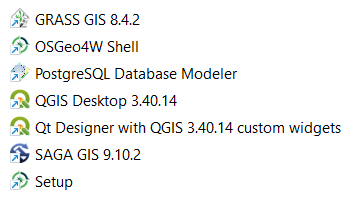
\includegraphics{./images/aplicaciones_desktop_osgeo4w.png}

}

\caption{\label{fig-aplicaciones_desktop_osgeo4w}Aplicaciones Desktop
OSGeo4W.}

\end{figure}%

\subsection{Instrucciones de
Instalación}\label{instrucciones-de-instalaciuxf3n}

\begin{enumerate}
\def\labelenumi{\arabic{enumi}.}
\tightlist
\item
  Descargue el \href{https://qgis.org/download/}{\textbf{Network
  Installer}} de QGIS.
\item
  Ejecute y seleccione \textbf{Advanced Install}.
\item
  Mantenga las rutas por defecto (\texttt{C:\textbackslash{}OSGeo4W}).
\item
  En el paso de \textbf{Select Packages}, busque los elementos de la
  tabla y marque únicamente la casilla \textbf{Bin} (Binarios).
\end{enumerate}

\subsection{Lista de paquetes a
seleccionar}\label{lista-de-paquetes-a-seleccionar}

\begin{longtable}[]{@{}
  >{\raggedright\arraybackslash}p{(\columnwidth - 6\tabcolsep) * \real{0.2500}}
  >{\raggedright\arraybackslash}p{(\columnwidth - 6\tabcolsep) * \real{0.2500}}
  >{\raggedright\arraybackslash}p{(\columnwidth - 6\tabcolsep) * \real{0.2500}}
  >{\raggedright\arraybackslash}p{(\columnwidth - 6\tabcolsep) * \real{0.2500}}@{}}
\caption{Listado de herramientas y librerías OSGeo4W para el
curso}\label{tbl-stack-software-osgeo4w}\tabularnewline
\toprule\noalign{}
\begin{minipage}[b]{\linewidth}\raggedright
Grupo
\end{minipage} & \begin{minipage}[b]{\linewidth}\raggedright
Paquete
\end{minipage} & \begin{minipage}[b]{\linewidth}\raggedright
Módulo
\end{minipage} & \begin{minipage}[b]{\linewidth}\raggedright
Propósito / Uso en Clase
\end{minipage} \\
\midrule\noalign{}
\endfirsthead
\toprule\noalign{}
\begin{minipage}[b]{\linewidth}\raggedright
Grupo
\end{minipage} & \begin{minipage}[b]{\linewidth}\raggedright
Paquete
\end{minipage} & \begin{minipage}[b]{\linewidth}\raggedright
Módulo
\end{minipage} & \begin{minipage}[b]{\linewidth}\raggedright
Propósito / Uso en Clase
\end{minipage} \\
\midrule\noalign{}
\endhead
\bottomrule\noalign{}
\endlastfoot
\textbf{Entorno Core} & \texttt{qgis-ltr} / \texttt{qgis-ltr-full} &
Todo & Software base y metapaquete de dependencias. \\
\textbf{Bases de Datos} & \texttt{pgmodeler} & 5 & Diseño visual de
modelos para PostGIS. \\
\textbf{Bases de Datos} & \texttt{libspatialite} & 5 & Motor de base de
datos espacial liviano para verificación en shell. \\
\textbf{Bases de Datos} & \texttt{python3-psycopg2} & 5 & Adaptador de
Python para PostgreSQL/PostGIS. \\
\textbf{Geoprocesamiento} & \texttt{grass} & 6 & Motor para análisis
topológico e hidrología. \\
\textbf{Geoprocesamiento} & \texttt{saga} & 7 & Algoritmos de terreno y
geomorfometría. \\
\textbf{Geoprocesamiento} & \texttt{gdal} & 6 & Lectura/escritura de
formatos raster y vector. \\
\textbf{Ciencia de Datos} & \texttt{python3-numpy} & 2 & Manejo de
estructuras Arrays y Matrices. \\
\textbf{Ciencia de Datos} & \texttt{python3-pandas} & 3 & Análisis
exploratorio de datos (EDA). \\
\textbf{Ciencia de Datos} & \texttt{python3-geopandas} & 3 & Extensión
espacial para GeoDataFrames. \\
\textbf{Visualización} & \texttt{python3-matplotlib} & 3 & Gráficos
básicos y mapas estáticos. \\
\textbf{Visualización} & \texttt{python3-seaborn} & 3 & Gráficos
estadísticos avanzados. \\
\textbf{Desarrollo} & \texttt{python3-pip} & 1 & Gestor para instalar
librerías adicionales. \\
\textbf{Desarrollo} & \texttt{python3-jupyterlab} & Todo & Entorno
interactivo para prototipado rápido
(\citeproc{ref-wijayaningrum2022jupyter}{Wijayaningrum et~al.,
2022}). \\
\textbf{Motores SIG} & \texttt{proj} / \texttt{geos} & 6 & Cálculos de
proyecciones y geometría. \\
\textbf{Machine Learning} & \texttt{python3-scikit-learn} & 6 & Modelado
predictivo espacial. \\
\end{longtable}

\begin{tcolorbox}[enhanced jigsaw, coltitle=black, leftrule=.75mm, bottomtitle=1mm, title=\textcolor{quarto-callout-important-color}{\faExclamation}\hspace{0.5em}{Aceptación de Dependencias Adicionales}, colback=white, colbacktitle=quarto-callout-important-color!10!white, left=2mm, toptitle=1mm, rightrule=.15mm, titlerule=0mm, arc=.35mm, colframe=quarto-callout-important-color-frame, bottomrule=.15mm, toprule=.15mm, opacityback=0, opacitybacktitle=0.6, breakable]

Al avanzar, el instalador mostrará la ventana \textbf{``Unmet
Dependencies''}. Es obligatorio aceptar todos los paquetes sugeridos
para contar con los controladores de formatos \texttt{.ecw} y
\texttt{.sid} requeridos por la cartografía oficial nacional. Para que
el comando \texttt{spatialite} funcione en la shell, asegúrese de marcar
el paquete \texttt{libspatialite} en la sección \textbf{Libs}.

\end{tcolorbox}

\subsection{Verificación de la
Instalación}\label{verificaciuxf3n-de-la-instalaciuxf3n}

Abra la \textbf{OSGeo4W Shell} y ejecute los comandos para verificar la
correcta integración de Python y los motores SIG:

\begin{Shaded}
\begin{Highlighting}[]
\ExtensionTok{python3} \AttributeTok{{-}{-}version}
\ExtensionTok{gdalinfo} \AttributeTok{{-}{-}version}
\ExtensionTok{spatialite} \AttributeTok{{-}{-}version}
\end{Highlighting}
\end{Shaded}

\subsubsection{Corrección de Errores al Lanzar
QGIS}\label{correcciuxf3n-de-errores-al-lanzar-qgis}

Si al iniciar QGIS aparece un error crítico indicando
\texttt{ModuleNotFoundError:\ No\ module\ named\ \textquotesingle{}gdal\textquotesingle{}},
se debe a una sintaxis de importación obsoleta en ciertos complementos
(\citeproc{ref-rosas2022qgis}{Rosas-Chavoya et~al., 2022}).

\textbf{Error identificado:}
\texttt{File\ ".../agknow\_utils.py",\ line\ 29,\ in\ \textless{}module\textgreater{}\ import\ gdal,\ osr}

\textbf{Solución:} Debe modificar el archivo del plugin para usar el
espacio de nombres de OSGeo:

\begin{enumerate}
\def\labelenumi{\arabic{enumi}.}
\item
  Localice el archivo en:
  \texttt{\%AppData\%\textbackslash{}QGIS\textbackslash{}QGIS3\textbackslash{}profiles\textbackslash{}default\textbackslash{}python\textbackslash{}plugins\textbackslash{}agknow\_qgis\textbackslash{}agknow\_utils.py}.
\item
  Reemplace la línea 29:

  \begin{itemize}
  \tightlist
  \item
    \textbf{Incorrecto:} \texttt{import\ gdal,\ osr}
  \item
    \textbf{Correcto:} \texttt{from\ osgeo\ import\ gdal,\ osr}
  \end{itemize}
\end{enumerate}

\begin{tcolorbox}[enhanced jigsaw, coltitle=black, leftrule=.75mm, bottomtitle=1mm, title=\textcolor{quarto-callout-note-color}{\faInfo}\hspace{0.5em}{Nota sobre R y Julia}, colback=white, colbacktitle=quarto-callout-note-color!10!white, left=2mm, toptitle=1mm, rightrule=.15mm, titlerule=0mm, arc=.35mm, colframe=quarto-callout-note-color-frame, bottomrule=.15mm, toprule=.15mm, opacityback=0, opacitybacktitle=0.6, breakable]

Para el uso intensivo de R y Julia, se recomienda la \textbf{Opción A
(Docker)} (\citeproc{ref-docker2025}{Inc., 2025}) ya que viene con las
librerías espaciales pre-configuradas, evitando errores de vinculación
de DLLs comunes en instalaciones nativas de Windows.

\end{tcolorbox}

\section{Opción B.2: QGIS + GEE usando Pixi}\label{sec-qgis-gee-pixi}

Antes de comenzar, es indispensable contar con una cuenta de
\textbf{Google Cloud} habilitada para \textbf{Google Earth Engine
(GEE)}. Puede dar de alta su cuenta en
\href{https://earthengine.google.com/}{earthengine.google.com}.

\begin{tcolorbox}[enhanced jigsaw, coltitle=black, leftrule=.75mm, bottomtitle=1mm, title=\textcolor{quarto-callout-important-color}{\faExclamation}\hspace{0.5em}{Requisito de Google Cloud}, colback=white, colbacktitle=quarto-callout-important-color!10!white, left=2mm, toptitle=1mm, rightrule=.15mm, titlerule=0mm, arc=.35mm, colframe=quarto-callout-important-color-frame, bottomrule=.15mm, toprule=.15mm, opacityback=0, opacitybacktitle=0.6, breakable]

Asegúrese de haber creado un proyecto en la consola de Google Cloud y de
tener activadas las \textbf{APIs for Earth Engine} para dicho proyecto;
de lo contrario, el proceso de autenticación fallará.

\end{tcolorbox}

\href{https://youtu.be/LoQwc3ne0FU}{Video gúia de creación y registro en
GEE}

\begin{center}\rule{0.5\linewidth}{0.5pt}\end{center}

\subsection{Instalación de Pixi}\label{instalaciuxf3n-de-pixi}

\textbf{Pixi} es un gestor de paquetes extremadamente rápido basado en
el ecosistema de Conda, pero mucho más ligero. Permite crear entornos
aislados sin romper las librerías de su sistema operativo.

\subsubsection{\texorpdfstring{\textbf{En Linux / macOS
(bash/zsh)}}{En Linux / macOS (bash/zsh)}}\label{en-linux-macos-bashzsh}

Ejecute el siguiente comando en su terminal:

\begin{Shaded}
\begin{Highlighting}[]
\ExtensionTok{curl} \AttributeTok{{-}fsSL}\NormalTok{ https://pixi.sh/install.sh }\KeywordTok{|} \FunctionTok{sh}
\end{Highlighting}
\end{Shaded}

\textbf{Nota:} Cierre y vuelva a abrir su terminal para que
\texttt{pixi} se añada a su \texttt{PATH}. Confirme la instalación con:

\begin{Shaded}
\begin{Highlighting}[]
\ExtensionTok{pixi} \AttributeTok{{-}{-}version}
\end{Highlighting}
\end{Shaded}

\subsubsection{\texorpdfstring{\textbf{En Windows
(PowerShell)}}{En Windows (PowerShell)}}\label{en-windows-powershell}

Abra \textbf{PowerShell} (no requiere permisos de Administrador) y
ejecute:

\begin{Shaded}
\begin{Highlighting}[]
\NormalTok{powershell }\OperatorTok{{-}}\NormalTok{ExecutionPolicy Bypass }\OperatorTok{{-}}\NormalTok{c }\StringTok{"irm {-}useb https://pixi.sh/install.ps1 | iex"}
\end{Highlighting}
\end{Shaded}

Reinicie PowerShell y confirme la versión:

\begin{Shaded}
\begin{Highlighting}[]
\NormalTok{pixi }\OperatorTok{{-}{-}}\NormalTok{version}
\end{Highlighting}
\end{Shaded}

\begin{center}\rule{0.5\linewidth}{0.5pt}\end{center}

\subsection{Creación del Proyecto}\label{creaciuxf3n-del-proyecto}

Navegue hasta la carpeta (\textbf{diferente a todas las utilizadas hasta
el momento}) donde desea guardar sus trabajos y cree un nuevo proyecto
llamado \texttt{geocd}:

\begin{Shaded}
\begin{Highlighting}[]
\ExtensionTok{pixi}\NormalTok{ init geocd}
\BuiltInTok{cd}\NormalTok{ geocd}
\end{Highlighting}
\end{Shaded}

\begin{center}\rule{0.5\linewidth}{0.5pt}\end{center}

\subsection{Configuración del Entorno
Geográfico}\label{configuraciuxf3n-del-entorno-geogruxe1fico}

Instalaremos un stack potente que incluye \textbf{QGIS} y las
herramientas necesarias para trabajar con \textbf{Google Earth Engine} y
datos ráster/vectoriales en Python.

Desde la carpeta \texttt{geocd}, ejecute:

\begin{Shaded}
\begin{Highlighting}[]
\ExtensionTok{pixi}\NormalTok{ add qgis geemap geopandas xee rioxarray}
\end{Highlighting}
\end{Shaded}

\begin{tcolorbox}[enhanced jigsaw, coltitle=black, leftrule=.75mm, bottomtitle=1mm, title=\textcolor{quarto-callout-note-color}{\faInfo}\hspace{0.5em}{¿Qué estamos instalando?}, colback=white, colbacktitle=quarto-callout-note-color!10!white, left=2mm, toptitle=1mm, rightrule=.15mm, titlerule=0mm, arc=.35mm, colframe=quarto-callout-note-color-frame, bottomrule=.15mm, toprule=.15mm, opacityback=0, opacitybacktitle=0.6, breakable]

\begin{itemize}
\tightlist
\item
  \textbf{QGIS}: El software SIG profesional de uso libre mas popular.
\item
  \textbf{geemap}: Librería para visualización interactiva de GEE.
\item
  \textbf{geopandas}: Gestión de datos vectoriales.
\item
  \textbf{xee \& rioxarray}: Motores para leer cubos de datos y archivos
  ráster.
\end{itemize}

\end{tcolorbox}

\begin{center}\rule{0.5\linewidth}{0.5pt}\end{center}

\subsection{Autenticación de Earth
Engine}\label{autenticaciuxf3n-de-earth-engine}

Finalmente, debe vincular su entorno local con su cuenta de Google
Cloud. Este comando abrirá una ventana en su navegador para autorizar el
acceso:

\begin{Shaded}
\begin{Highlighting}[]
\ExtensionTok{pixi}\NormalTok{ run earthengine authenticate}
\end{Highlighting}
\end{Shaded}

Siga las instrucciones en pantalla, seleccione su proyecto de Google
Cloud y copie el código de verificación si el sistema se lo solicita.
¡Ya está listo para procesar datos satelitales a escala global!

\subsection{Lanzar QGIS a través de
PIXI}\label{lanzar-qgis-a-travuxe9s-de-pixi}

Una vez realizada la Autenticación de Google Earth Engine, puede lanzar
QGIS usando el siguiente método

\begin{itemize}
\item
  Abra el PowerShell en la carpeta dónde configuró el proyecto PIXI
  (\texttt{geocd})
\item
  Ejecute el siguiente comando:
\end{itemize}

\begin{Shaded}
\begin{Highlighting}[]
\ExtensionTok{pixi}\NormalTok{ run qgis}
\end{Highlighting}
\end{Shaded}

\subsection{Trabajar GEE dentro de
QGIS}\label{trabajar-gee-dentro-de-qgis}

Una vez que el entorno está configurado y autenticado, el siguiente paso
es integrar \textbf{Google Earth Engine} directamente en la interfaz de
QGIS. Para esto, utilizaremos el complemento desarrollado por el equipo
de \textbf{OpenGeos}: El Plugin: \textbf{GEE Data Catalog}. Este
complemento permite navegar por los miles de datasets de Earth Engine
(Sentinel, Landsat, MODIS, etc.) y cargarlos en el lienzo de QGIS con un
solo clic, utilizando el motor de procesamiento en la nube.

\subsubsection{Instalación del Plugin}\label{instalaciuxf3n-del-plugin}

\begin{enumerate}
\def\labelenumi{\arabic{enumi}.}
\tightlist
\item
  Abre QGIS usando \texttt{pixi\ run\ qgis}
\item
  Ve al menú \textbf{Complementos} \(\rightarrow\) \textbf{Administrar e
  instalar complementos\ldots{}}
\item
  Ve a la pestaña \textbf{Configuración}.
\item
  Haz clic en \textbf{Añadir\ldots{}} en la sección ``Repositorios de
  complementos''.
\item
  Asigna un nombre al repositorio, por ejemplo: \texttt{OpenGeos}.
\item
  Ingresa la URL del repositorio:
  \texttt{https://qgis.gishub.org/plugins.xml}
\item
  Haz clic en \textbf{Aceptar}.
\item
  Ve a la pestaña \textbf{Todos}.
\item
  Busca \textbf{``Earth Engine Data Catalogs''}.
\item
  Selecciona \textbf{``Earth Engine Data Catalogs''} en la lista y haz
  clic en \textbf{Instalar complemento}.
\end{enumerate}

\begin{itemize}
\item
  \textbf{Repositorio oficial:}
  \href{https://github.com/opengeos/qgis-gee-data-catalogs-plugin}{opengeos/qgis-gee-data-catalogs-plugin}
\item
  Video Guía \textbf{Earth Engine Data Catalogs Plugin for QGIS}:
  \href{https://youtu.be/nZ3D6wLKJQw}{aquí}
\item
  Video Guía \textbf{Time Series Satellite Images in Seconds}:
  \href{https://youtu.be/8IW6XqnUjgg}{aquí}
\end{itemize}

\begin{tcolorbox}[enhanced jigsaw, coltitle=black, leftrule=.75mm, bottomtitle=1mm, title=\textcolor{quarto-callout-note-color}{\faInfo}\hspace{0.5em}{Forzar autenticación GEE dentro de QGIS (PIXI)}, colback=white, colbacktitle=quarto-callout-note-color!10!white, left=2mm, toptitle=1mm, rightrule=.15mm, titlerule=0mm, arc=.35mm, colframe=quarto-callout-note-color-frame, bottomrule=.15mm, toprule=.15mm, opacityback=0, opacitybacktitle=0.6, breakable]

Si las imágenes de GEE no cargan dentro de QGIS, la
\href{https://youtu.be/nZ3D6wLKJQw?t=574}{video-guía anterior} (en el
tiempo 574 del video) muestra unos comandos alternativos a ejecutar
dentro de la consola de Python. Esos comandos se muestran a
continuación.

Abra la Consola de Python dentro de QGIS (lanzado con
\texttt{pixi\ run\ qgis}) y ejecute los siguientes comandos:

\begin{Shaded}
\begin{Highlighting}[]
\ImportTok{import}\NormalTok{ ee}

\CommentTok{\# Autenticarse con GEE}
\NormalTok{ee.Authenticate()}
\CommentTok{\#Respuesta esperada: True}

\CommentTok{\# Inicializar el Proyecto GEE}
\NormalTok{ee.Initialize(project }\OperatorTok{=} \StringTok{"Tu ID de proyecto GEE"}\NormalTok{)}
\CommentTok{\#Respuesta esperada: Nada}
\end{Highlighting}
\end{Shaded}

\end{tcolorbox}

\subsubsection{Actualizar el plugin dentro de
QGIS}\label{actualizar-el-plugin-dentro-de-qgis}

En el manú \texttt{GEE\ Data\ Catalogs}, asegúrece de ejecutar
\texttt{Check\ for\ Updates}.

\section{Otras referencias
importantes}\label{otras-referencias-importantes}

\begin{itemize}
\tightlist
\item
  PyQGIS cookbook en markdown y Jupyter notebook formats
  (\citeproc{ref-wu2023pyqgis}{Wu, 2023a})
\item
  QGIS Notebook Plugin: Integrate Jupyter Notebooks into QGIS
  (\citeproc{ref-wu2023qgisnotebook}{Wu, 2023b})
\end{itemize}

\chapter{Guía de Instalación. Opción C: ArcGIS Pro y
ArcPy}\label{guia-C}

\section{Instalación GEE en ArcGIS Pro}\label{sec-arcgis-pro-gee}

La guía resumida de instalación y uso se encuentra en el
\href{https://www.esri.com/arcgis-blog/products/arcgis-pro/imagery/bring-google-earth-engines-data-right-into-arcgis-pro}{blog
oficial de Esri}.

\textbf{Procedimiento y requerimientos:}

\begin{enumerate}
\def\labelenumi{\arabic{enumi}.}
\tightlist
\item
  Contar con una licencia activa de ArcGIS Pro.
\item
  Instalar la caja de herramientas siguiendo el
  \href{https://github.com/gee-community/arcgis-earthengine-toolbox/blob/main/docs/03_installation.md}{procedimiento
  oficial}.
\item
  Descargar la caja de herramientas
  \href{https://github.com/gee-community/arcgis-earthengine-toolbox/releases/latest}{desde
  este enlace}.
\item
  Después de descomprimir el archivo, el procedimiento finaliza
  \href{https://pro.arcgis.com/en/pro-app/latest/help/projects/connect-to-a-toolbox.htm}{conectando
  la caja de herramientas} a tu proyecto en ArcGIS Pro.
\end{enumerate}

\subsection{Configuración del ambiente Python con
Conda}\label{configuraciuxf3n-del-ambiente-python-con-conda}

\begin{enumerate}
\def\labelenumi{\arabic{enumi}.}
\tightlist
\item
  Ejecutar \textbf{ArcGIS Python Command Prompt} como administrador:
  Ruta: \textbf{Start Menu} -\textgreater{} \textbf{All Apps}
  -\textgreater{} \textbf{ArcGIS folder} -\textgreater{} \textbf{Python
  Command Prompt} (Clic derecho \textgreater{} Ejecutar como
  administrador).
\end{enumerate}

\begin{figure}[H]

{\centering 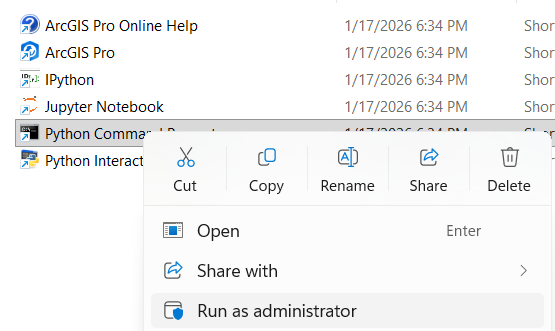
\includegraphics[width=0.6\textwidth,height=\textheight]{images/arcgispro/gee/python_commando_as_administrator.png}

}

\caption{ArcGIS Python Command Prompt como administrador}

\end{figure}%

\begin{enumerate}
\def\labelenumi{\arabic{enumi}.}
\setcounter{enumi}{1}
\tightlist
\item
  Verificar los ambientes Conda disponibles:
\end{enumerate}

\begin{Shaded}
\begin{Highlighting}[]
\ExtensionTok{conda}\NormalTok{ env list}
\end{Highlighting}
\end{Shaded}

\begin{enumerate}
\def\labelenumi{\arabic{enumi}.}
\setcounter{enumi}{2}
\tightlist
\item
  Clonar el entorno principal de ArcGIS Pro para no alterar el entorno
  por defecto:
\end{enumerate}

\begin{Shaded}
\begin{Highlighting}[]
\ExtensionTok{conda}\NormalTok{ create }\AttributeTok{{-}{-}name}\NormalTok{ gee }\AttributeTok{{-}{-}clone}\NormalTok{ arcgispro{-}py3}
\end{Highlighting}
\end{Shaded}

\emph{Mensaje de salida apenas inicia la clonación:}

\begin{Shaded}
\begin{Highlighting}[]
\ExtensionTok{Source:}\NormalTok{      C:}\DataTypeTok{\textbackslash{}P}\NormalTok{rogram Files}\DataTypeTok{\textbackslash{}A}\NormalTok{rcGIS}\DataTypeTok{\textbackslash{}P}\NormalTok{ro}\DataTypeTok{\textbackslash{}b}\NormalTok{in}\DataTypeTok{\textbackslash{}P}\NormalTok{ython}\DataTypeTok{\textbackslash{}e}\NormalTok{nvs}\DataTypeTok{\textbackslash{}a}\NormalTok{rcgispro{-}py3}
\ExtensionTok{Destination:}\NormalTok{ D:}\DataTypeTok{\textbackslash{}P}\NormalTok{rograms}\DataTypeTok{\textbackslash{}m}\NormalTok{iniforge3}\DataTypeTok{\textbackslash{}e}\NormalTok{nvs}\DataTypeTok{\textbackslash{}g}\NormalTok{ee}
\end{Highlighting}
\end{Shaded}

\begin{enumerate}
\def\labelenumi{\arabic{enumi}.}
\setcounter{enumi}{3}
\tightlist
\item
  Inicializar Conda con el shell apropiado (opcional):
\end{enumerate}

\begin{Shaded}
\begin{Highlighting}[]
\ExtensionTok{conda}\NormalTok{ init cmd.exe}
\end{Highlighting}
\end{Shaded}

\begin{enumerate}
\def\labelenumi{\arabic{enumi}.}
\setcounter{enumi}{4}
\item
  \textbf{Reiniciar} el Python Command Prompt (nuevamente como
  Administrador).
\item
  Activar el nuevo entorno \texttt{gee}:
\end{enumerate}

\begin{Shaded}
\begin{Highlighting}[]
\ExtensionTok{conda}\NormalTok{ activate gee}
\end{Highlighting}
\end{Shaded}

\begin{enumerate}
\def\labelenumi{\arabic{enumi}.}
\setcounter{enumi}{6}
\tightlist
\item
  Desactivar la verificación SSL (opcional, útil en redes corporativas
  restrictivas):
\end{enumerate}

\begin{Shaded}
\begin{Highlighting}[]
\ExtensionTok{conda}\NormalTok{ config }\AttributeTok{{-}{-}set}\NormalTok{ ssl\_verify false}
\end{Highlighting}
\end{Shaded}

\begin{enumerate}
\def\labelenumi{\arabic{enumi}.}
\setcounter{enumi}{7}
\tightlist
\item
  Instalar los paquetes necesarios de GEE desde el canal
  \texttt{conda-forge}:
\end{enumerate}

\begin{Shaded}
\begin{Highlighting}[]
\ExtensionTok{conda}\NormalTok{ install earthengine{-}api xee }\AttributeTok{{-}{-}channel}\NormalTok{ conda{-}forge}
\end{Highlighting}
\end{Shaded}

\begin{quote}
\textbf{Alternativa (Si el comando anterior falla):} \textgreater{}
Puedes usar \texttt{pip} para instalar los paquetes limpiando el entorno
e intentándolo de nuevo:

\begin{Shaded}
\begin{Highlighting}[]
\ExtensionTok{conda}\NormalTok{ deactivate}
\ExtensionTok{conda}\NormalTok{ env remove }\AttributeTok{{-}{-}name}\NormalTok{ gee}
\ExtensionTok{conda}\NormalTok{ create }\AttributeTok{{-}{-}name}\NormalTok{ gee }\AttributeTok{{-}{-}clone}\NormalTok{ arcgispro{-}py3}
\ExtensionTok{conda}\NormalTok{ activate gee}
\ExtensionTok{pip}\NormalTok{ install earthengine{-}api xee}

\CommentTok{\# Dependiendo de los warnings en consola, es posible que requieras estos paquetes:}
\ExtensionTok{pip}\NormalTok{ install }\StringTok{"pyarrow\textgreater{}=17,\textless{}21"}\NormalTok{ pywin32}
\end{Highlighting}
\end{Shaded}
\end{quote}

\begin{enumerate}
\def\labelenumi{\arabic{enumi}.}
\setcounter{enumi}{8}
\tightlist
\item
  Instalar otros paquetes requeridos desde el canal oficial de
  \texttt{esri} (dependiendo de tu versión):
\end{enumerate}

\begin{itemize}
\tightlist
\item
  Para \textbf{ArcGIS Pro 3.5 y anteriores}:
\end{itemize}

\begin{Shaded}
\begin{Highlighting}[]
\ExtensionTok{conda}\NormalTok{ install rasterio=1.3.9 }\AttributeTok{{-}{-}channel}\NormalTok{ esri}
\end{Highlighting}
\end{Shaded}

\begin{itemize}
\tightlist
\item
  Para \textbf{ArcGIS Pro 3.6 y posteriores}:
\end{itemize}

\begin{Shaded}
\begin{Highlighting}[]
\ExtensionTok{conda}\NormalTok{ install rasterio=1.4.3 }\AttributeTok{{-}{-}channel}\NormalTok{ esri}
\end{Highlighting}
\end{Shaded}

\begin{enumerate}
\def\labelenumi{\arabic{enumi}.}
\setcounter{enumi}{9}
\tightlist
\item
  Intercambiar el entorno predeterminado de ArcGIS Pro para que use
  \texttt{gee} de ahora en adelante:
\end{enumerate}

\begin{Shaded}
\begin{Highlighting}[]
\ExtensionTok{proswap}\NormalTok{ gee}
\end{Highlighting}
\end{Shaded}

\begin{enumerate}
\def\labelenumi{\arabic{enumi}.}
\setcounter{enumi}{10}
\tightlist
\item
  Cerrar el Python Command Prompt y abrir ArcGIS Pro.
\end{enumerate}

\begin{itemize}
\tightlist
\item
  El ambiente por defecto ahora será \texttt{gee}.
\item
  Verifica que los paquetes funcionen yendo a \textbf{Analysis}
  -\textgreater{} \textbf{Python} -\textgreater{} \textbf{Python Window}
  y ejecutando:
\end{itemize}

\begin{Shaded}
\begin{Highlighting}[]
\ImportTok{import}\NormalTok{ ee}
\ImportTok{import}\NormalTok{ xee}
\ImportTok{import}\NormalTok{ rasterio}
\end{Highlighting}
\end{Shaded}

\begin{center}\rule{0.5\linewidth}{0.5pt}\end{center}

\subsection{Descargar la caja de herramientas
(Toolbox)}\label{descargar-la-caja-de-herramientas-toolbox}

Puedes clonar el repositorio mediante Git:

\begin{Shaded}
\begin{Highlighting}[]
\FunctionTok{git}\NormalTok{ clone https://github.com/gee{-}community/arcgis{-}earthengine{-}toolbox.git}
\end{Highlighting}
\end{Shaded}

Alternativamente, descarga el archivo \texttt{.zip} directamente desde
\href{https://github.com/gee-community/arcgis-earthengine-toolbox}{GitHub}
y descomprímelo.

\begin{itemize}
\item
  \textbf{Opción A:} Guardar la carpeta descargada directamente en el
  directorio de tu proyecto actual:

  \texttt{C:\textbackslash{}Users\textbackslash{}\textless{}username\textgreater{}\textbackslash{}Documents\textbackslash{}ArcGIS\textbackslash{}Projects\textbackslash{}\textless{}project\_name\textgreater{}\textbackslash{}ArcGIS\ Earth\ Engine\ Toolbox}
\item
  \textbf{Opción B:} Guardar la caja de herramientas en un directorio
  global para usarla en múltiples proyectos. Por ejemplo:

  \texttt{D:\textbackslash{}Programs\textbackslash{}ArcGIS\textbackslash{}Pro\textbackslash{}arcgis-earthengine-toolbox}
\end{itemize}

\subsection{Agregar la caja de herramientas GEE a ArcGIS
Pro}\label{agregar-la-caja-de-herramientas-gee-a-arcgis-pro}

\begin{enumerate}
\def\labelenumi{\arabic{enumi}.}
\tightlist
\item
  Abre ArcGIS Pro.
\item
  En el panel \textbf{Catalog} (Catálogo), haz clic derecho en
  \textbf{Toolboxes} (Cajas de herramientas) y selecciona \textbf{Add
  Toolbox} (Agregar caja de herramientas).
\item
  Navega a la ruta donde descomprimiste los archivos (ej:
  \texttt{D:\textbackslash{}Programs\textbackslash{}ArcGIS\textbackslash{}Pro\textbackslash{}arcgis-earthengine-toolbox})
  y selecciona el archivo de la herramienta.
\end{enumerate}

\begin{figure}[H]

{\centering 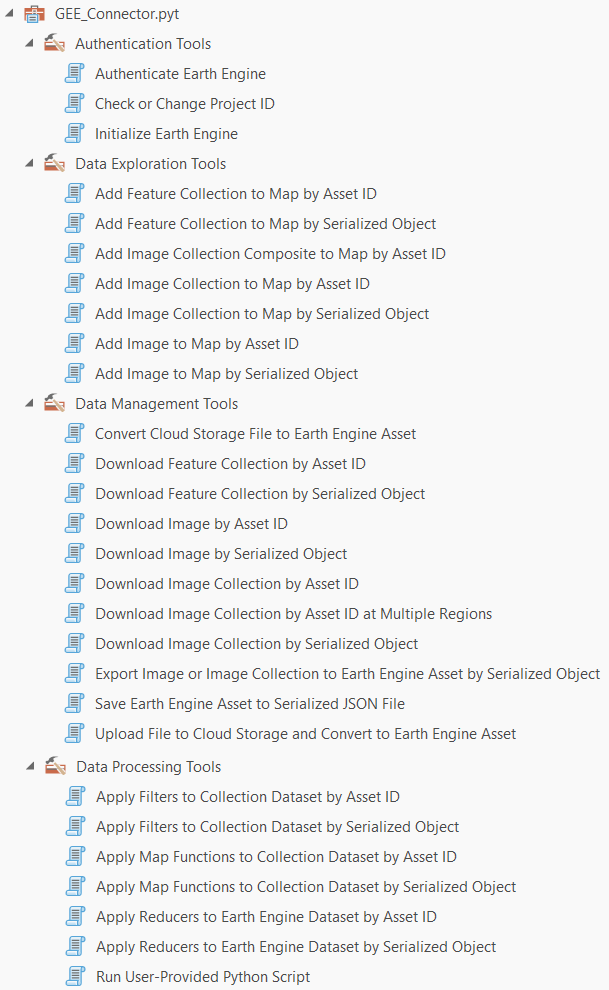
\includegraphics[width=0.7\textwidth,height=\textheight]{images/arcgispro/gee/gee_arcgispro_tool.png}

}

\caption{Caja de Herramientas GEE integrada en ArcGIS Pro}

\end{figure}%

\emph{Consulta el
\href{https://pro.arcgis.com/en/pro-app/latest/help/projects/connect-to-a-toolbox.htm}{procedimiento
oficial de Esri} si tienes dudas sobre cómo conectar una caja de
herramientas.}

\subsection{Actualizar la caja de herramientas GEE
(Opcional)}\label{actualizar-la-caja-de-herramientas-gee-opcional}

Si en el futuro requieres la versión más reciente del Toolbox, sigue el
procedimiento descrito en la
\href{https://github.com/gee-community/arcgis-earthengine-toolbox/blob/main/docs/08_upgrades.md}{documentación
oficial de actualizaciones}.

\begin{center}\rule{0.5\linewidth}{0.5pt}\end{center}

\subsection{Instalar Google Cloud SDK}\label{instalar-google-cloud-sdk}

Dado que GEE requiere validación en la nube de Google, necesitamos su
herramienta de línea de comandos. Encuentra aquí la
\href{https://docs.cloud.google.com/sdk/docs/install-sdk}{guía oficial
de instalación de Google Cloud CLI}.

\begin{enumerate}
\def\labelenumi{\arabic{enumi}.}
\tightlist
\item
  Selecciona o crea tu proyecto de Google Cloud en este
  \href{https://console.cloud.google.com/projectselector2/home/dashboard}{enlace}.
\item
  Verifica que la facturación (\textbf{Billing}) esté habilitada para tu
  proyecto
  \href{https://docs.cloud.google.com/billing/docs/how-to/verify-billing-enabled\#confirm_billing_is_enabled_on_a_project}{aquí}.
  \emph{(Nota: GEE es gratuito, pero requiere tener facturación
  configurada como protocolo de Cloud).}
\item
  Descarga el
  \href{https://dl.google.com/dl/cloudsdk/channels/rapid/GoogleCloudSDKInstaller.exe}{instalador
  de Google Cloud CLI para Windows}.
\item
  Ejecuta el instalador y sigue las instrucciones en pantalla.
\end{enumerate}

\textbf{⚠️ Importante:} Al finalizar, \textbf{desmarca} la opción de
abrir la consola (\emph{Start Google Cloud SDK Shell}).

\begin{enumerate}
\def\labelenumi{\arabic{enumi}.}
\setcounter{enumi}{4}
\tightlist
\item
  Abre una terminal de \textbf{PowerShell} y ejecuta:
\end{enumerate}

\begin{Shaded}
\begin{Highlighting}[]
\ExtensionTok{gcloud}\NormalTok{ init}
\end{Highlighting}
\end{Shaded}

\begin{itemize}
\tightlist
\item
  Se abrirá una pestaña en tu navegador web. Ingresa con tu cuenta de
  Google.
\item
  Después de autorizar, recibirás un mensaje similar a \textbf{``You are
  now authenticated with the gcloud CLI''}.
\end{itemize}

De regreso a tu consola de PowerShell:

\begin{itemize}
\tightlist
\item
  Te pedirá que indiques el número del proyecto que deseas utilizar (ej:
  \texttt{1}). Recuerda seleccionar el proyecto que tiene la facturación
  habilitada.
\item
  Dirígete a \href{https://console.developers.google.com/apis}{este
  enlace de la Consola de APIs} y asegúrate de tener tu proyecto
  seleccionado.
\item
  Ve a la pestaña \textbf{Enable API and Services}.
\item
  Busca \textbf{Compute Engine API}, selecciónala y presiona
  \textbf{Enable}. Esto permitirá a Google Cloud seleccionar una zona y
  región de cómputo automáticamente, optimizando el uso de recursos.
  (Debe aparecer activa en tu lista de APIs).
\end{itemize}

\begin{center}\rule{0.5\linewidth}{0.5pt}\end{center}

\subsection{Credenciales para GEE}\label{credenciales-para-gee}

Una vez que Google Cloud SDK está instalado, GEE utilizará sus
credenciales por defecto para autenticarte dentro de ArcGIS Pro.

\begin{enumerate}
\def\labelenumi{\arabic{enumi}.}
\tightlist
\item
  Encuentra tu \textbf{Google Cloud Project ID}:
\end{enumerate}

\begin{itemize}
\tightlist
\item
  Recuerda que el \texttt{Project\ ID} suele ser diferente al
  \texttt{Project\ Name} (típicamente tiene un formato como
  \texttt{my-project-123456}).
\item
  En la esquina superior derecha de la
  \href{https://console.cloud.google.com/}{Consola de Google Cloud}, haz
  clic en los tres puntos y selecciona \textbf{Project settings}. Allí
  podrás copiar tu \texttt{Project\ ID}.
\end{itemize}

\begin{enumerate}
\def\labelenumi{\arabic{enumi}.}
\setcounter{enumi}{1}
\item
  Abre la consola \textbf{Google Cloud SDK Shell} (búscala en el menú
  inicio de Windows).
\item
  Ejecuta el siguiente comando (esto se hace \textbf{solo la primera
  vez}):
\end{enumerate}

\begin{Shaded}
\begin{Highlighting}[]
\ExtensionTok{gcloud}\NormalTok{ auth application{-}default login}
\end{Highlighting}
\end{Shaded}

\begin{itemize}
\tightlist
\item
  Sigue el proceso en el navegador web para otorgar permisos. Al
  terminar verás el mensaje: \textbf{``You are now authenticated with
  the gcloud CLI!''}.
\item
  Esto creará un archivo de seguridad llamado
  \texttt{application\_default\_credentials.json} en tu computador.
\end{itemize}

\begin{enumerate}
\def\labelenumi{\arabic{enumi}.}
\setcounter{enumi}{3}
\tightlist
\item
  Asocia tu cuota de proyecto a esas credenciales. Ejecuta este comando
  reemplazando \texttt{TU\_PROJECT\_ID} con el ID exacto de tu proyecto:
\end{enumerate}

\begin{Shaded}
\begin{Highlighting}[]
\ExtensionTok{gcloud}\NormalTok{ auth application{-}default set{-}quota{-}project TU\_PROJECT\_ID}
\end{Highlighting}
\end{Shaded}

Si todo es correcto, recibirás una confirmación similar a:

\textbf{\texttt{Credentials\ saved\ to\ file:\ {[}C:\textbackslash{}Users\textbackslash{}tu\_usuario\textbackslash{}AppData\textbackslash{}Roaming\textbackslash{}gcloud\textbackslash{}application\_default\_credentials.json{]}}}

\begin{center}\rule{0.5\linewidth}{0.5pt}\end{center}

\section{Inicializar GEE en ArcGIS
Pro}\label{sec-arcgis-pro-initialize-gee}

Una vez configurado el entorno y descargada la caja de herramientas,
procede a inicializar Earth Engine dentro de la interfaz de ArcGIS Pro.
Antes de usar cualquier función, debemos autenticar nuestra cuenta. En
la caja de herramientas de GEE dentro de ArcGIS Pro, abra la sección
\texttt{Authentication\ Tools}:

\begin{figure}

\centering{

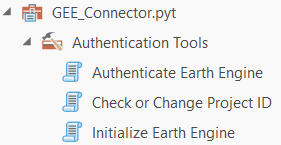
\includegraphics[width=0.3\textwidth,height=\textheight]{images/arcgispro/gee/opciones_inicializacion_gee.png}

}

\caption{\label{fig-arcgis-auth-tools}Herramientas de Autenticación de
GEE en ArcGIS Pro.}

\end{figure}%

\textbf{Paso A:} Abra la herramienta
\texttt{Authenticate\ Earth\ Engine} y escriba su \emph{Project ID} (ej.
\texttt{ee-giswqg}). Al ejecutar (\texttt{Run}) la herramienta y ver los
detalles de la ejecución (\texttt{View\ Details}), deberá observar un
mensaje de éxito como: \emph{Earth Engine is ready to use.
Authentication successful}.

\begin{figure}

\centering{

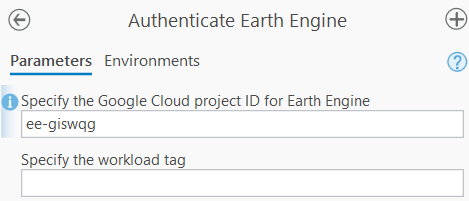
\includegraphics[width=0.4\textwidth,height=\textheight]{images/arcgispro/gee/gee_authenticate_pro.png}

}

\caption{\label{fig-arcgis-auth-success}Herramienta de autenticación en
GEE (Recuerda cambiar el Project ID por el tuyo).}

\end{figure}%

\textbf{Paso B:} A continuación, abra la herramienta
\texttt{Initialize\ Earth\ Engine} y escriba nuevamente su \emph{Project
ID}. Ejecute la herramienta; en los detalles observará el mensaje
confirmando: \emph{Earth Engine is ready to use.}

\begin{center}\rule{0.5\linewidth}{0.5pt}\end{center}

\section{URLs y enlaces de referencia
importantes}\label{urls-y-enlaces-de-referencia-importantes}

\begin{itemize}
\tightlist
\item
  Documentación oficial y
  \href{https://docs.cloud.google.com/sdk/auth_success}{tutoriales de
  Google Cloud SDK}.
\item
  Procedimiento completo de
  \href{https://github.com/gee-community/arcgis-earthengine-toolbox/blob/main/docs/03_installation.md}{instalación
  del GEE Toolbox}.
\item
  Artículo de Esri:
  \href{https://www.esri.com/arcgis-blog/products/arcgis-pro/imagery/bring-google-earth-engines-data-right-into-arcgis-pro}{Cómo
  iniciar a trabajar con GEE en ArcGIS Pro}.
\end{itemize}

\begin{center}\rule{0.5\linewidth}{0.5pt}\end{center}

\section{Fuentes de datos alternativas en ArcGIS
Pro}\label{fuentes-de-datos-alternativas-en-arcgis-pro}

Aunque Earth Engine es muy potente, existen otras fuentes masivas de
datos espaciales y catálogos en la nube que puedes aprovechar
directamente en ArcGIS Pro:

\begin{itemize}
\item
  🌐 \textbf{ArcGIS Living Atlas of the World}

  \begin{itemize}
  \tightlist
  \item
    Totalmente integrado con ArcGIS Online y ArcGIS Pro (mediante la
    pestaña \texttt{Portal} en el Catálogo).
  \item
    Guía:
    \href{https://www.esri.com/arcgis-blog/products/arcgis-living-atlas/imagery/law-imagery-layers-for-analysis}{ArcGIS
    Living Atlas ready-to-use imagery layers for analysis}
  \item
    Guía:
    \href{https://www.esri.com/arcgis-blog/products/arcgis-online/imagery/large-scale-analysis-in-arcgis-online}{Explore
    Ready-to-Use Imagery for Analysis}
  \end{itemize}
\item
  📂 \textbf{STAC Catalogs (SpatioTemporal Asset Catalogs)}

  \begin{itemize}
  \tightlist
  \item
    Permite conectar inmensas bases de datos abiertas, como el
    \href{https://planetarycomputer.microsoft.com/}{Microsoft Planetary
    Computer}.
  \item
    Conecta la información estableciendo una
    \href{https://pro.arcgis.com/en/pro-app/latest/help/data/imagery/create-a-stac-connection.htm}{conexión
    STAC en ArcGIS} y aprovechando archivos
    \href{https://github.com/Esri/arcgis-for-mpc/activity}{.asc}.
  \end{itemize}
\item
  ☁️ \textbf{Cloud sources (Almacenamiento en la nube)}

  \begin{itemize}
  \tightlist
  \item
    Conecta entornos de almacenamiento masivo directamente al Catálogo
    de ArcGIS Pro vía URLs o APIs, como por ejemplo buckets de
    \href{https://enterprise.arcgis.com/en/server/10.8/cloud/amazon/connect-to-arcgis-server-on-aws-from-arcmap.htm}{AWS
    (Amazon Web Services)}.
  \end{itemize}
\item
  🌍 \textbf{Google Earth Engine Data Catalog}

  \begin{itemize}
  \tightlist
  \item
    Operado mediante la caja de herramientas integrada.
  \end{itemize}
\end{itemize}

\part{Fundamentos}

\chapter{Variables y tipos de datos}\label{sec-variables_tipos_datos}

\section{Funciones j\_eval y j\_plot en
R}\label{funciones-j_eval-y-j_plot-en-r}

\begin{Shaded}
\begin{Highlighting}[]
\CommentTok{\# \#| include: false}
\FunctionTok{source}\NormalTok{(}\StringTok{"./docs/j\_eval\_j\_plot.r"}\NormalTok{)}
\end{Highlighting}
\end{Shaded}

\section{Introducción}\label{introducciuxf3n-1}

En el análisis espacial, un dato nunca es solo un número o una letra; es
la representación digital de un fenómeno físico. La latitud de una
estación GPS, el nombre de un municipio en una tabla de atributos o la
firma espectral de una imagen satelital deben almacenarse en la memoria
del computador de una forma específica para poder procesarse.

Una \textbf{variable} actúa como un contenedor etiquetado en la memoria
del sistema, permitiéndonos guardar, recuperar y manipular esa
información. Sin embargo, la forma en que \textbf{Python}, \textbf{R} y
\textbf{Julia} gestionan estos contenedores varía significativamente.

\begin{figure}

\centering{

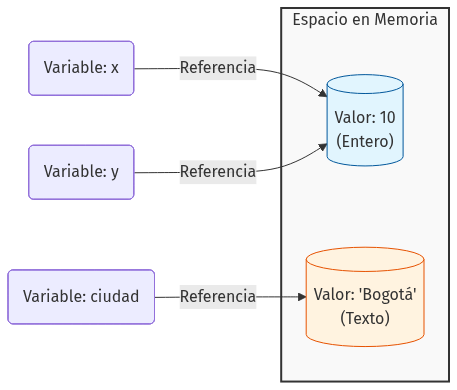
\includegraphics[width=0.5\textwidth,height=\textheight]{images/variables.png}

}

\caption{\label{fig-concepto-variable}Abstracción de una Variable: En
lenguajes modernos como Python o R, funciona más como una etiqueta que
apunta a un objeto en memoria.}

\end{figure}%

Entender la diferencia entre un entero (\texttt{int}) y un decimal de
doble precisión (\texttt{float64}) no es solo una curiosidad
informática: en geomática, usar el tipo de dato incorrecto puede
significar la diferencia entre localizar un punto con precisión
milimétrica o desviarlo por cientos de metros debido a errores de
redondeo. Este capítulo sienta las bases para manipular la ``materia
prima'' de cualquier Sistema de Información Geográfica (SIG).

\section{Objetivos de aprendizaje}\label{objetivos-de-aprendizaje}

Al finalizar este capítulo, el estudiante estará en capacidad de:

\begin{enumerate}
\def\labelenumi{\arabic{enumi}.}
\tightlist
\item
  \textbf{Definir y asignar variables} correctamente en Python, R y
  Julia, comprendiendo las diferencias de sintaxis y asignación de
  memoria.
\item
  \textbf{Diferenciar tipos de datos fundamentales} (enteros, flotantes,
  cadenas y lógicos) y seleccionar el más adecuado para optimizar el
  almacenamiento de datos masivos (Big Data Geoespacial).
\item
  \textbf{Manipular cadenas de texto} para la limpieza y estandarización
  automática de tablas de atributos (corrección de mayúsculas,
  eliminación de espacios, interpolación).
\item
  \textbf{Aplicar formatos de precisión} para controlar la salida de
  coordenadas y datos numéricos en reportes técnicos.
\item
  \textbf{Comprender la mutabilidad}, distinguiendo cuándo una operación
  modifica los datos originales (Python/Julia) y cuándo genera una copia
  nueva (R).
\end{enumerate}

\section{Variables}\label{variables}

\begin{longtable}[]{@{}
  >{\raggedright\arraybackslash}p{(\columnwidth - 6\tabcolsep) * \real{0.1176}}
  >{\centering\arraybackslash}p{(\columnwidth - 6\tabcolsep) * \real{0.1765}}
  >{\centering\arraybackslash}p{(\columnwidth - 6\tabcolsep) * \real{0.1765}}
  >{\raggedright\arraybackslash}p{(\columnwidth - 6\tabcolsep) * \real{0.5294}}@{}}
\caption{Comparación de sintaxis básica entre Python, R y
Julia}\label{tbl-comp_sintaxis_basica}\tabularnewline
\toprule\noalign{}
\begin{minipage}[b]{\linewidth}\raggedright
Lenguaje
\end{minipage} & \begin{minipage}[b]{\linewidth}\centering
Operador de asignación
\end{minipage} & \begin{minipage}[b]{\linewidth}\centering
Comando para imprimir
\end{minipage} & \begin{minipage}[b]{\linewidth}\raggedright
Descripción y Alternativas
\end{minipage} \\
\midrule\noalign{}
\endfirsthead
\toprule\noalign{}
\begin{minipage}[b]{\linewidth}\raggedright
Lenguaje
\end{minipage} & \begin{minipage}[b]{\linewidth}\centering
Operador de asignación
\end{minipage} & \begin{minipage}[b]{\linewidth}\centering
Comando para imprimir
\end{minipage} & \begin{minipage}[b]{\linewidth}\raggedright
Descripción y Alternativas
\end{minipage} \\
\midrule\noalign{}
\endhead
\bottomrule\noalign{}
\endlastfoot
\textbf{Python} & \texttt{=} & \texttt{print()} & El operador \texttt{=}
es el estándar único para asignación. Para imprimir, \texttt{print()}
añade automáticamente un salto de línea. En entornos interactivos, se
puede usar \texttt{display()} para una representación visual más
rica. \\
\textbf{R} & \texttt{\textless{}-} & \texttt{print()} & Aunque
\texttt{=} funciona, se prefiere \texttt{\textless{}-}. Además de
\texttt{print()}, existe \texttt{cat()}, útil para concatenar texto sin
mostrar índices de vector. \\
\textbf{Julia} & \texttt{=} & \texttt{println()} & Se usa \texttt{=}
para asignación. \texttt{println()} imprime con salto de línea, mientras
que \texttt{print()} lo hace sin él. Al igual que en Python, existe
\texttt{display()}. \\
\end{longtable}

\subsection{Python}

\begin{Shaded}
\begin{Highlighting}[]
\CommentTok{\# \#| eval: false}
\CommentTok{\#Variable numérica}
\NormalTok{numero\_dptos }\OperatorTok{=} \DecValTok{32}

\CommentTok{\#Imprimir}
\BuiltInTok{print}\NormalTok{(numero\_dptos)}
\end{Highlighting}
\end{Shaded}

\begin{verbatim}
32
\end{verbatim}

\begin{Shaded}
\begin{Highlighting}[]
\CommentTok{\#Ver contenido (en modo interactivo)}
\NormalTok{numero\_dptos}
\end{Highlighting}
\end{Shaded}

\begin{verbatim}
32
\end{verbatim}

\subsection{R}

\begin{Shaded}
\begin{Highlighting}[]
\CommentTok{\# \#| eval: false}
\CommentTok{\# Variable numérica (en R se prefiere el operador \textless{}{-})}
\NormalTok{numero\_dptos }\OtherTok{\textless{}{-}} \DecValTok{32}

\CommentTok{\# Imprimir}
\FunctionTok{print}\NormalTok{(numero\_dptos)}
\end{Highlighting}
\end{Shaded}

\begin{verbatim}
[1] 32
\end{verbatim}

\begin{Shaded}
\begin{Highlighting}[]
\CommentTok{\# Ver contenido}
\NormalTok{numero\_dptos}
\end{Highlighting}
\end{Shaded}

\begin{verbatim}
[1] 32
\end{verbatim}

\subsection{Julia}

\begin{Shaded}
\begin{Highlighting}[]
\CommentTok{\# \#| eval: false}
\FunctionTok{j\_eval}\NormalTok{(}\StringTok{\textquotesingle{}}
\StringTok{\# Variable numérica}
\StringTok{numero\_dptos = 32}

\StringTok{\# Imprimir}
\StringTok{println(numero\_dptos)}

\StringTok{\# Ver contenido}
\StringTok{numero\_dptos}

\StringTok{atributos\_elemento}
\StringTok{\textquotesingle{}}\NormalTok{)}
\end{Highlighting}
\end{Shaded}

\begin{verbatim}
Starting Julia ...
\end{verbatim}

\subsection{Asignación de variables}\label{asignaciuxf3n-de-variables}

\begin{longtable}[]{@{}
  >{\raggedright\arraybackslash}p{(\columnwidth - 6\tabcolsep) * \real{0.1500}}
  >{\centering\arraybackslash}p{(\columnwidth - 6\tabcolsep) * \real{0.2000}}
  >{\centering\arraybackslash}p{(\columnwidth - 6\tabcolsep) * \real{0.1500}}
  >{\raggedright\arraybackslash}p{(\columnwidth - 6\tabcolsep) * \real{0.5000}}@{}}
\caption{Estructuras de datos y comportamiento de
asignación}\label{tbl-estructuras_reasignacion}\tabularnewline
\toprule\noalign{}
\begin{minipage}[b]{\linewidth}\raggedright
Lenguaje
\end{minipage} & \begin{minipage}[b]{\linewidth}\centering
Colección Base
\end{minipage} & \begin{minipage}[b]{\linewidth}\centering
Operador
\end{minipage} & \begin{minipage}[b]{\linewidth}\raggedright
Descripción y Flexibilidad
\end{minipage} \\
\midrule\noalign{}
\endfirsthead
\toprule\noalign{}
\begin{minipage}[b]{\linewidth}\raggedright
Lenguaje
\end{minipage} & \begin{minipage}[b]{\linewidth}\centering
Colección Base
\end{minipage} & \begin{minipage}[b]{\linewidth}\centering
Operador
\end{minipage} & \begin{minipage}[b]{\linewidth}\raggedright
Descripción y Flexibilidad
\end{minipage} \\
\midrule\noalign{}
\endhead
\bottomrule\noalign{}
\endlastfoot
\textbf{Python} & Lista \texttt{{[}{]}} & \texttt{=} & Permite mezclar
tipos en una lista. Es dinámico y \textbf{fuerte}: no permite
operaciones inválidas entre tipos (ej. sumarle un texto a un número). \\
\textbf{R} & Vector \texttt{c()} & \texttt{\textless{}-} & El vector
atómico (\texttt{c}) exige que todos los elementos sean del mismo tipo.
Si se mezclan, R los convierte automáticamente (coerción). \\
\textbf{Julia} & Arreglo \texttt{{[}{]}} & \texttt{=} & Muy similar a la
lista de Python pero optimizado para rendimiento. Es dinámico pero
permite declarar tipos para ganar velocidad. \\
\end{longtable}

\subsection{Conceptos clave de
programación}\label{conceptos-clave-de-programaciuxf3n}

Para entender cómo estos lenguajes manejan la información de la
Tabla~\ref{tbl-estructuras_reasignacion}, es fundamental diferenciar los
sistemas de tipado:

\begin{enumerate}
\def\labelenumi{\arabic{enumi}.}
\tightlist
\item
  \textbf{Tipado Dinámico:} El tipo de la variable se define en tiempo
  de ejecución. No es necesario declarar que una variable es un entero o
  un texto antes de usarla; el lenguaje lo infiere. (Python, R y Julia
  son dinámicos).
\item
  \textbf{Tipado Estático:} El tipo de la variable debe definirse al
  momento de escribir el código (ej. C++ o Java). Una vez definida como
  ``entero'', no puede guardar texto. Esto previene errores antes de
  ejecutar el programa.
\item
  \textbf{Tipado Fuerte:} El lenguaje no permite operaciones entre tipos
  incompatibles sin una conversión explícita. Por ejemplo, en
  \textbf{Python}, \texttt{5\ +\ "10"} arrojará un error.
\item
  \textbf{Tipado Débil:} El lenguaje intenta realizar conversiones
  automáticas (coerción) para que la operación funcione. En \textbf{R},
  si intentas unir un número y un texto en un vector
  \texttt{c(1,\ "Bogotá")}, R convertirá el \texttt{1} en texto
  \texttt{"1"} silenciosamente.
\end{enumerate}

\begin{figure}

\centering{

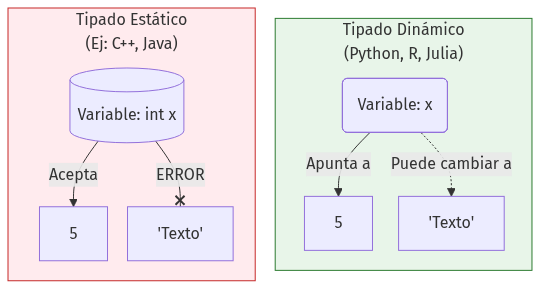
\includegraphics[width=0.6\textwidth,height=\textheight]{images/tipado_estatico_dinamico.png}

}

\caption{\label{fig-tipado}Comparativa de Tipado: La flexibilidad tiene
un costo en seguridad, pero gana en velocidad de desarrollo.}

\end{figure}%

\subsubsection{Python}

\begin{Shaded}
\begin{Highlighting}[]
\CommentTok{\# \#| eval: false}
\CommentTok{\# Iniciar con un número (Latitud de Monserrate)}
\NormalTok{datos\_ubicacion }\OperatorTok{=} \FloatTok{4.6052}

\CommentTok{\# Cambiar a texto (Nombre del lugar)}
\NormalTok{datos\_ubicacion }\OperatorTok{=} \StringTok{"Cerro de Monserrate"}

\CommentTok{\# Cambiar a una lista de coordenadas [Lat, Lon]}
\NormalTok{datos\_ubicacion }\OperatorTok{=}\NormalTok{ [}\FloatTok{4.6052}\NormalTok{, }\OperatorTok{{-}}\FloatTok{74.0554}\NormalTok{]}

\CommentTok{\# Imprimir resultado final}
\BuiltInTok{print}\NormalTok{(datos\_ubicacion)}
\end{Highlighting}
\end{Shaded}

\begin{verbatim}
[4.6052, -74.0554]
\end{verbatim}

\subsubsection{R}

\begin{Shaded}
\begin{Highlighting}[]
\CommentTok{\# \#| eval: false}
\CommentTok{\# Iniciar con un número (Latitud de Monserrate)}
\NormalTok{datos\_ubicacion }\OtherTok{\textless{}{-}} \FloatTok{4.6052}

\CommentTok{\# Cambiar a texto (Nombre del lugar)}
\NormalTok{datos\_ubicacion }\OtherTok{\textless{}{-}} \StringTok{"Cerro de Monserrate"}

\CommentTok{\# Cambiar a un vector de coordenadas (c es para combinar/concatenar)}
\NormalTok{datos\_ubicacion }\OtherTok{\textless{}{-}} \FunctionTok{c}\NormalTok{(}\FloatTok{4.6052}\NormalTok{, }\SpecialCharTok{{-}}\FloatTok{74.0554}\NormalTok{)}

\CommentTok{\# Imprimir resultado final}
\FunctionTok{print}\NormalTok{(datos\_ubicacion)}
\end{Highlighting}
\end{Shaded}

\begin{verbatim}
[1]   4.6052 -74.0554
\end{verbatim}

\subsubsection{Julia}

\begin{Shaded}
\begin{Highlighting}[]
\CommentTok{\# \#| eval: false}
\FunctionTok{j\_eval}\NormalTok{(}\StringTok{\textquotesingle{}}
\StringTok{\# Iniciar con un número (Latitud de Monserrate)}
\StringTok{datos\_ubicacion = 4.6052}

\StringTok{\# Cambiar a texto (Nombre del lugar)}
\StringTok{datos\_ubicacion = "Cerro de Monserrate"}

\StringTok{\# Cambiar a un arreglo (Array) de coordenadas}
\StringTok{datos\_ubicacion = [4.6052, {-}74.0554]}

\StringTok{\# Imprimir resultado final}
\StringTok{println(datos\_ubicacion)}
\StringTok{\textquotesingle{}}\NormalTok{)}
\end{Highlighting}
\end{Shaded}

\section{Nombres para las variables}\label{nombres-para-las-variables}

\textbf{¿Por qué es clave usar nombres adecuados?}

En programación, los nombres que eliges para tus variables no son solo
etiquetas; son las instrucciones que permiten que otras personas (y tú
mismo en el futuro) entiendan la lógica del código sin errores. Usar
nombres estandarizados es vital por las siguientes razones:

\begin{enumerate}
\def\labelenumi{\arabic{enumi}.}
\tightlist
\item
  \textbf{Evitar errores técnicos:} Los lenguajes de programación son
  muy estrictos. Un espacio, una tilde o una \texttt{ñ} pueden hacer que
  un programa que funciona bien en tu computadora falle al abrirlo en
  otra.
\item
  \textbf{Claridad en la lectura:} Es mucho más fácil entender un
  proceso si la variable se llama \texttt{distancia\_metros} en lugar de
  simplemente \texttt{d}.
\item
  \textbf{Portabilidad:} El uso de estándares internacionales asegura
  que tus datos e investigaciones puedan integrarse fácilmente entre
  diferentes plataformas como \textbf{Python}, \textbf{R} o
  \textbf{Julia}.
\end{enumerate}

\begin{tcolorbox}[enhanced jigsaw, coltitle=black, leftrule=.75mm, bottomtitle=1mm, title=\textcolor{quarto-callout-note-color}{\faInfo}\hspace{0.5em}{Resumen de Reglas de Estilo (snake\_case)}, colback=white, colbacktitle=quarto-callout-note-color!10!white, left=2mm, toptitle=1mm, rightrule=.15mm, titlerule=0mm, arc=.35mm, colframe=quarto-callout-note-color-frame, bottomrule=.15mm, toprule=.15mm, opacityback=0, opacitybacktitle=0.6, breakable]

Para que tus programas sean profesionales y compatibles, sigue estas
reglas básicas:

\begin{itemize}
\tightlist
\item
  \textbf{Todo en minúsculas:} Evita mezclar mayúsculas para mantener la
  uniformidad.
\item
  \textbf{Usa el guion bajo (\texttt{\_}):} Dado que los espacios están
  prohibidos, el guion bajo une las palabras (ej.
  \texttt{precio\_gasolina}).
\item
  \textbf{Solo letras básicas y números:} Usa solo caracteres de la
  \texttt{a} a la \texttt{z}. Evita tildes, eñes o símbolos especiales
  (\texttt{!}, \texttt{\#}, \texttt{\$}).
\item
  \textbf{Prohibido el guion medio (\texttt{-}):} El computador lo
  interpreta como una operación de resta.
\end{itemize}

\end{tcolorbox}

\begin{Shaded}
\begin{Highlighting}[]

\CommentTok{\#| code{-}summary: "Ejemplos comparativos (Python, R, Julia)"}

\CommentTok{\# FORMA CORRECTA: Clara y sin errores}
\NormalTok{estacion\_climatologica }\OperatorTok{=} \StringTok{"Dorado"}
\NormalTok{temperatura\_celsius }\OperatorTok{=} \FloatTok{20.5}
\NormalTok{conteo\_puntos\_gps }\OperatorTok{=} \DecValTok{15}

\CommentTok{\# FORMA INCORRECTA: Genera errores o confusión}
\NormalTok{estacion climatologica }\OperatorTok{=} \StringTok{"Dorado"}  \CommentTok{\# ERROR: Los espacios no están permitidos}
\NormalTok{temperatura}\OperatorTok{{-}}\NormalTok{celsius }\OperatorTok{=} \FloatTok{20.5}         \CommentTok{\# ERROR: El guion medio intenta restar}
\NormalTok{t }\OperatorTok{=} \FloatTok{20.5}                           \CommentTok{\# MAL: Es una variable muy vaga}
\NormalTok{año\_inicio }\OperatorTok{=} \DecValTok{2024}                  \CommentTok{\# EVITAR: La \textquotesingle{}ñ\textquotesingle{} causa fallos de lectura}
\end{Highlighting}
\end{Shaded}

\subsection{Python}

\begin{Shaded}
\begin{Highlighting}[]
\CommentTok{\# \#| eval: false}
\CommentTok{\# Nombres de variables recomendados}
\CommentTok{\# Variables geoespaciales claras}
\NormalTok{latitud\_bogota }\OperatorTok{=} \FloatTok{4.7110}
\NormalTok{longitud\_bogota }\OperatorTok{=} \OperatorTok{{-}}\FloatTok{74.0721}
\NormalTok{altura\_msnm }\OperatorTok{=} \FloatTok{2640.0}
\NormalTok{municipio\_nombre }\OperatorTok{=} \StringTok{"Chinchiná"}
\NormalTok{conteo\_viviendas\_afectadas }\OperatorTok{=} \DecValTok{150}
\NormalTok{sistema\_referencia }\OperatorTok{=} \StringTok{"MAGNA{-}SIRGAS / Origen Nacional"}


\CommentTok{\# Nombres de variables NO recomendados}
\CommentTok{\# Evitar nombres genéricos o confusos}
\NormalTok{x }\OperatorTok{=} \FloatTok{4.7110}  \CommentTok{\# ¿Es latitud o un índice?}
\NormalTok{d }\OperatorTok{=} \StringTok{"Chinchiná"}  \CommentTok{\# Muy vago (¿Distrito, Departamento, Dato?)}
\NormalTok{val }\OperatorTok{=} \DecValTok{2640}  \CommentTok{\# Ambiguo: ¿Valor, Valencia, Variable?}
\NormalTok{coords }\OperatorTok{=}\NormalTok{ [}\FloatTok{4.71}\NormalTok{, }\OperatorTok{{-}}\FloatTok{74.07}\NormalTok{]  }\CommentTok{\# Lista sin etiquetas claras}
\end{Highlighting}
\end{Shaded}

\subsection{R}

\begin{Shaded}
\begin{Highlighting}[]
\CommentTok{\# \#| eval: false}
\CommentTok{\# Nombres de variables recomendados}
\CommentTok{\# Estilo snake\_case (común en R para análisis de datos)}
\NormalTok{latitud\_medellin }\OtherTok{\textless{}{-}} \FloatTok{6.2442}
\NormalTok{longitud\_medellin }\OtherTok{\textless{}{-}} \SpecialCharTok{{-}}\FloatTok{75.5812}
\NormalTok{cota\_terreno }\OtherTok{\textless{}{-}} \DecValTok{1495}
\NormalTok{nombre\_departamento }\OtherTok{\textless{}{-}} \StringTok{"Antioquia"}
\NormalTok{poblacion\_censo\_2018 }\OtherTok{\textless{}{-}} \DecValTok{6407000}
\NormalTok{proyeccion\_cartografica }\OtherTok{\textless{}{-}} \StringTok{"EPSG:9377"}


\CommentTok{\# Nombres de variables NO recomendados}
\CommentTok{\# Evitar abreviaturas extremas}
\NormalTok{l }\OtherTok{\textless{}{-}} \FloatTok{6.2442} \CommentTok{\# ¿Latitud, Longitud, Límite, Localidad?}
\NormalTok{nom }\OtherTok{\textless{}{-}} \StringTok{"Antioquia"} \CommentTok{\# "nombre" es mejor}
\NormalTok{temp }\OtherTok{\textless{}{-}} \DecValTok{1495} \CommentTok{\# ¿Temperatura o un archivo temporal?}
\NormalTok{p }\OtherTok{\textless{}{-}} \DecValTok{6407000} \CommentTok{\# ¿Población, Perímetro, Pendiente, P{-}value?}
\end{Highlighting}
\end{Shaded}

\subsection{Julia}

\begin{Shaded}
\begin{Highlighting}[]
\CommentTok{\# \#| eval: false}
\FunctionTok{j\_eval}\NormalTok{(}\StringTok{\textquotesingle{}}
\StringTok{\# Nombres de variables recomendados}
\StringTok{\# Aprovechando el soporte Unicode de Julia}
\StringTok{latitud\_cali = 3.4516}
\StringTok{longitud\_cali = {-}76.5320}
\StringTok{elevación\_cauca = 995.0}
\StringTok{nombre\_vereda = "La Elvira"}
\StringTok{densidad\_poblacional = 120.5}
\StringTok{referencia\_espacial = "MAGNA{-}SIRGAS"}
\StringTok{\textquotesingle{}}\NormalTok{)}
\end{Highlighting}
\end{Shaded}

\begin{Shaded}
\begin{Highlighting}[]
\FunctionTok{j\_eval}\NormalTok{(}\StringTok{\textquotesingle{}}
\StringTok{\# Nombres de variables NO recomendados}
\StringTok{\# Nombres que no dicen nada del contexto geográfico}
\StringTok{var1 = 3.4516}
\StringTok{info = "La Elvira"}
\StringTok{tmp = 995.0 \# Típico error: ¿Temperatura o Temporal?}
\StringTok{lista = [3.45, {-}76.53] \# Difícil de leer en modelos de optimización}
\StringTok{\textquotesingle{}}\NormalTok{)}
\end{Highlighting}
\end{Shaded}

\section{Tipos de datos}\label{tipos-de-datos}

\subsection{Python}

\begin{Shaded}
\begin{Highlighting}[]
\CommentTok{\# \#| eval: false}

\CommentTok{\# Representa el número de elementos en un dataset geoespacial}
\NormalTok{num\_elementos }\OperatorTok{=} \DecValTok{500} \CommentTok{\# Igual a num\_elementos = int(500)}

\CommentTok{\# Validación de tipo (Type Checking)}
\CommentTok{\# Lanza un error si no es un entero, ideal para debugging en scripts de Geomatización}
\ControlFlowTok{if} \KeywordTok{not} \BuiltInTok{isinstance}\NormalTok{(num\_elementos, }\BuiltInTok{int}\NormalTok{):}
    \ControlFlowTok{raise} \PreprocessorTok{TypeError}\NormalTok{(}\SpecialStringTok{f"Se esperaba un entero, pero se recibió }\SpecialCharTok{\{}\BuiltInTok{type}\NormalTok{(num\_elementos)}\SpecialCharTok{\}}\SpecialStringTok{"}\NormalTok{)}

\CommentTok{\# Representa la altitud de un punto (Nevado del Ruiz)}
\ImportTok{import}\NormalTok{ numpy }\ImportTok{as}\NormalTok{ np}
\NormalTok{altitud\_32 }\OperatorTok{=}\NormalTok{ np.float32(}\FloatTok{2640.5}\NormalTok{) }\CommentTok{\# np.float32() para simple}
\NormalTok{altitud\_64 }\OperatorTok{=} \FloatTok{2640.5}   \CommentTok{\# float() es el defecto (doble)}

\CommentTok{\# Representa la latitud de un punto (Nevado del Ruiz)}
\NormalTok{latitud }\OperatorTok{=} \FloatTok{4.8920}  

\CommentTok{\# Representa la longitud de un punto}
\NormalTok{longitud }\OperatorTok{=} \OperatorTok{{-}}\FloatTok{75.3188}  

\CommentTok{\# Representa el sistema de referencia oficial de Colombia}
\NormalTok{sistema\_coordenadas }\OperatorTok{=} \StringTok{"MAGNA{-}SIRGAS / Origen Nacional"}  

\CommentTok{\# Representa si el dataset está georreferenciado o no}
\NormalTok{esta\_georeferenciado }\OperatorTok{=} \VariableTok{True}  

\CommentTok{\# Una lista que representa latitud y longitud}
\NormalTok{coordenadas }\OperatorTok{=}\NormalTok{ [}\FloatTok{4.8920}\NormalTok{, }\OperatorTok{{-}}\FloatTok{75.3188}\NormalTok{]  }

\CommentTok{\# Un diccionario con los atributos del elemento geográfico}
\NormalTok{atributos\_elemento }\OperatorTok{=}\NormalTok{ \{}
    \StringTok{"nombre"}\NormalTok{: }\StringTok{"Nevado del Ruiz"}\NormalTok{,}
    \StringTok{"altura\_msnm"}\NormalTok{: }\DecValTok{5321}\NormalTok{,}
    \StringTok{"tipo"}\NormalTok{: }\StringTok{"Estratovolcán"}\NormalTok{,}
    \StringTok{"ubicacion"}\NormalTok{: [}\FloatTok{4.8920}\NormalTok{, }\OperatorTok{{-}}\FloatTok{75.3188}\NormalTok{],}
\NormalTok{\}}

\BuiltInTok{print}\NormalTok{(atributos\_elemento)}
\end{Highlighting}
\end{Shaded}

\begin{verbatim}
{'nombre': 'Nevado del Ruiz', 'altura_msnm': 5321, 'tipo': 'Estratovolcán', 'ubicacion': [4.892, -75.3188]}
\end{verbatim}

\begin{Shaded}
\begin{Highlighting}[]
\CommentTok{\# Tipo de dato}
\BuiltInTok{type}\NormalTok{(atributos\_elemento)}
\end{Highlighting}
\end{Shaded}

\begin{verbatim}
<class 'dict'>
\end{verbatim}

\begin{Shaded}
\begin{Highlighting}[]
\CommentTok{\# Acceder a la primera coordenada (índice 0) dentro de la clave \textquotesingle{}ubicacion\textquotesingle{}}
\NormalTok{latitud\_ruiz }\OperatorTok{=}\NormalTok{ atributos\_elemento[}\StringTok{"ubicacion"}\NormalTok{][}\DecValTok{0}\NormalTok{]}
\NormalTok{latitud\_ruiz}
\end{Highlighting}
\end{Shaded}

\begin{verbatim}
4.892
\end{verbatim}

\subsection{R}

\begin{Shaded}
\begin{Highlighting}[]
\CommentTok{\# \#| eval: false}

\CommentTok{\# Representa el número de elementos (L indica tipo integer)}
\NormalTok{num\_elementos }\OtherTok{\textless{}{-}} \DecValTok{500}\NormalTok{L  }\CommentTok{\# Diferente a num\_elementos = 500 (numeric)}

\CommentTok{\# Validación del tipo de dato}
\ControlFlowTok{if}\NormalTok{ (}\SpecialCharTok{!}\FunctionTok{is.integer}\NormalTok{(num\_elementos)) \{}
  \FunctionTok{stop}\NormalTok{(}\FunctionTok{paste}\NormalTok{(}\StringTok{"Error: Se esperaba un tipo \textquotesingle{}integer\textquotesingle{}, pero se recibió uno de tipo \textquotesingle{}"}\NormalTok{, }
             \FunctionTok{class}\NormalTok{(num\_elementos), }\StringTok{"\textquotesingle{}."}\NormalTok{, }\AttributeTok{sep =} \StringTok{""}\NormalTok{))}
\NormalTok{\}}

\CommentTok{\# Representa la altitud de un punto (Nevado del Ruiz)}
\NormalTok{altitud\_32 }\OtherTok{\textless{}{-}} \FunctionTok{as.single}\NormalTok{(}\FloatTok{5321.0}\NormalTok{) }\CommentTok{\# as.single() para precisión simple (32 bits)}
\NormalTok{altitud\_64 }\OtherTok{\textless{}{-}} \FloatTok{5321.0}            \CommentTok{\# double es el defecto en R (64 bits)}

\CommentTok{\# Representa la latitud de un punto (Nevado del Ruiz)}
\NormalTok{latitud }\OtherTok{\textless{}{-}} \FloatTok{4.8920}  

\CommentTok{\# Representa la longitud de un punto}
\NormalTok{longitud }\OtherTok{\textless{}{-}} \SpecialCharTok{{-}}\FloatTok{75.3188}  

\CommentTok{\# Representa el sistema de referencia oficial (tipo character)}
\NormalTok{sistema\_coordenadas }\OtherTok{\textless{}{-}} \StringTok{"MAGNA{-}SIRGAS / Origen Nacional"}  

\CommentTok{\# Representa si el dataset está georreferenciado (logical)}
\NormalTok{esta\_georeferenciado }\OtherTok{\textless{}{-}} \ConstantTok{TRUE}  

\CommentTok{\# Un vector que representa latitud y longitud}
\NormalTok{coordenadas }\OtherTok{\textless{}{-}} \FunctionTok{c}\NormalTok{(}\FloatTok{4.8920}\NormalTok{, }\SpecialCharTok{{-}}\FloatTok{75.3188}\NormalTok{)  }

\CommentTok{\# Una lista que representa los atributos del elemento geográfico}
\NormalTok{atributos\_elemento }\OtherTok{\textless{}{-}} \FunctionTok{list}\NormalTok{(}
    \StringTok{"nombre"} \OtherTok{=} \StringTok{"Nevado del Ruiz"}\NormalTok{,}
    \StringTok{"altura\_msnm"} \OtherTok{=} \DecValTok{5321}\NormalTok{,}
    \StringTok{"tipo"} \OtherTok{=} \StringTok{"Estratovolcán"}\NormalTok{,}
    \StringTok{"ubicacion"} \OtherTok{=} \FunctionTok{c}\NormalTok{(}\FloatTok{4.8920}\NormalTok{, }\SpecialCharTok{{-}}\FloatTok{75.3188}\NormalTok{)}
\NormalTok{)}

\FunctionTok{print}\NormalTok{(atributos\_elemento)}
\end{Highlighting}
\end{Shaded}

\begin{verbatim}
$nombre
[1] "Nevado del Ruiz"

$altura_msnm
[1] 5321

$tipo
[1] "Estratovolcán"

$ubicacion
[1]   4.8920 -75.3188
\end{verbatim}

\begin{Shaded}
\begin{Highlighting}[]
\CommentTok{\# Tipo de dato}
\FunctionTok{class}\NormalTok{(atributos\_elemento)}
\end{Highlighting}
\end{Shaded}

\begin{verbatim}
[1] "list"
\end{verbatim}

\begin{Shaded}
\begin{Highlighting}[]
\CommentTok{\# Acceder a la latitud (índice 1 en R) dentro del elemento \textquotesingle{}ubicacion\textquotesingle{}}
\NormalTok{latitud\_ruiz }\OtherTok{\textless{}{-}}\NormalTok{ atributos\_elemento}\SpecialCharTok{$}\NormalTok{ubicacion[}\DecValTok{1}\NormalTok{]}
\NormalTok{latitud\_ruiz}
\end{Highlighting}
\end{Shaded}

\begin{verbatim}
[1] 4.892
\end{verbatim}

\subsection{Julia}

\begin{Shaded}
\begin{Highlighting}[]
\CommentTok{\# \#| eval: false}
\FunctionTok{j\_eval}\NormalTok{(}\StringTok{\textquotesingle{}}
\StringTok{\# Representa el número de elementos en el dataset}
\StringTok{num\_elementos = 500  \# Igual a num\_elementos = Int64(500)}
\StringTok{typeof(num\_elementos)}

\StringTok{\# Validación del tipo de dato}
\StringTok{if !(num\_elementos isa Int64)}
\StringTok{    error("Error: Se esperaba un }\SpecialCharTok{\textbackslash{}\textquotesingle{}}\StringTok{Int64}\SpecialCharTok{\textbackslash{}\textquotesingle{}}\StringTok{, pero se recibió un }\SpecialCharTok{\textbackslash{}\textquotesingle{}}\StringTok{$(typeof(num\_elementos))}\SpecialCharTok{\textbackslash{}\textquotesingle{}}\StringTok{.")}
\StringTok{end}

\StringTok{\# Representa la altitud de un punto (Nevado del Ruiz)}
\StringTok{altitud\_32 = Float32(5321.0) \# Float32() para precisión simple (32 bits)}
\StringTok{altitud\_64 = 5321.0          \# Float64 es el defecto en Julia (64 bits)}

\StringTok{\# Representa la latitud del punto (Nevado del Ruiz)}
\StringTok{latitud = 4.8920  }

\StringTok{\# Representa la longitud del punto}
\StringTok{longitud = {-}75.3188  }

\StringTok{\# Representa el sistema de referencia espacial}
\StringTok{sistema\_coordenadas = "MAGNA{-}SIRGAS / Origen Nacional"  }

\StringTok{\# Representa el estado de georreferenciación (tipo Bool)}
\StringTok{esta\_georeferenciado = true  }

\StringTok{\# Un arreglo que representa latitud y longitud}
\StringTok{coordenadas = [4.8920, {-}75.3188]  }

\StringTok{\# Un diccionario (Dict) para almacenar los atributos}
\StringTok{atributos\_elemento = Dict(}
\StringTok{    "nombre" =\textgreater{} "Nevado del Ruiz",}
\StringTok{    "altura\_msnm" =\textgreater{} 5321,}
\StringTok{    "tipo" =\textgreater{} "Estratovolcán",}
\StringTok{    "ubicacion" =\textgreater{} [4.8920, {-}75.3188],}
\StringTok{)}

\StringTok{println(atributos\_elemento)}

\StringTok{\# Tipo de dato}
\StringTok{typeof(atributos\_elemento)}

\StringTok{\# Acceder a la latitud (índice 1 en Julia) dentro de la clave "ubicacion"}
\StringTok{latitud\_ruiz = atributos\_elemento["ubicacion"][1]}
\StringTok{latitud\_ruiz}
\StringTok{\textquotesingle{}}\NormalTok{)}
\end{Highlighting}
\end{Shaded}

\begin{longtable}[]{@{}
  >{\raggedright\arraybackslash}p{(\columnwidth - 6\tabcolsep) * \real{0.2500}}
  >{\centering\arraybackslash}p{(\columnwidth - 6\tabcolsep) * \real{0.2500}}
  >{\centering\arraybackslash}p{(\columnwidth - 6\tabcolsep) * \real{0.2500}}
  >{\raggedright\arraybackslash}p{(\columnwidth - 6\tabcolsep) * \real{0.2500}}@{}}
\caption{Comparación detallada de sintaxis y tipos de
datos}\label{tbl-comparativa_tecnica_sig}\tabularnewline
\toprule\noalign{}
\begin{minipage}[b]{\linewidth}\raggedright
Característica / Variable
\end{minipage} & \begin{minipage}[b]{\linewidth}\centering
Python
\end{minipage} & \begin{minipage}[b]{\linewidth}\centering
R
\end{minipage} & \begin{minipage}[b]{\linewidth}\raggedright
Julia
\end{minipage} \\
\midrule\noalign{}
\endfirsthead
\toprule\noalign{}
\begin{minipage}[b]{\linewidth}\raggedright
Característica / Variable
\end{minipage} & \begin{minipage}[b]{\linewidth}\centering
Python
\end{minipage} & \begin{minipage}[b]{\linewidth}\centering
R
\end{minipage} & \begin{minipage}[b]{\linewidth}\raggedright
Julia
\end{minipage} \\
\midrule\noalign{}
\endhead
\bottomrule\noalign{}
\endlastfoot
\textbf{Sufijo \texttt{L}} (num\_elementos) & No se usa. \texttt{500} es
entero. & Se usa \texttt{500L} para \texttt{integer}. Sin \texttt{L} es
\texttt{numeric}. & No se usa. \texttt{500} es \texttt{Int64}. \\
\textbf{Asignación en Diccionario} &
\texttt{v\ =\ \{clave:\ valor,\ ...\}} (Usa \texttt{:}). &
\texttt{v\ \textless{}-\ list(clave\ =\ valor,\ ...)}. (Usa \texttt{=} )
& \texttt{v\ =\ Dict(clave\ =\textgreater{}\ valor,\ ...)} (Usa
\texttt{=\textgreater{}}). \\
\textbf{\texttt{num\_elementos}} & \texttt{int} (Automático) &
\texttt{integer} (Requiere \texttt{L}) & \texttt{Int64} (Automático) \\
\textbf{\texttt{latitud} (doble precisión por defecto)} & \texttt{float}
& \texttt{numeric} & \texttt{Float64} \\
\textbf{\texttt{altitud\_32} (simple precisión)} & \texttt{np.float32()}
& \texttt{as.single()} & \texttt{Float32} \\
\textbf{\texttt{sistema\_coordenadas}} & \texttt{str} &
\texttt{character} & \texttt{String} \\
\textbf{\texttt{esta\_georeferenciado}} & \texttt{bool} (\texttt{True} /
\texttt{False}) & \texttt{logical} (\texttt{TRUE} / \texttt{FALSE}) &
\texttt{Bool} (\texttt{true} / \texttt{false}) \\
\textbf{\texttt{coordenadas}} & \texttt{list} \texttt{{[}\ ,\ {]}}:
Colección mutable de objetos. & \texttt{vector} \texttt{c(\ ,\ )}:
Colección indexada de elementos del mismo tipo. & \texttt{Array}
\texttt{{[}\ ,\ {]}} (Vector): Arreglo indexado y optimizado para
cómputo. \\
\textbf{\texttt{atributos\_elemento}} & \texttt{dict}
\texttt{\{\ :\ \}}: Estructura nativa de pares clave-valor. &
\texttt{list} \texttt{list(\ =\ )}: Lista con nombres (etiquetas) para
cada elemento. & \texttt{Dict} \texttt{Dict(\ =\textgreater{}\ )}: Tipo
de dato optimizado para mapeos clave-valor. \\
\end{longtable}

\subsection{¿Qué es un diccionario?}\label{quuxe9-es-un-diccionario}

Un \textbf{Diccionario} es una estructura de datos que organiza la
información mediante pares de \textbf{Clave-Valor} (\emph{Key-Value}). A
diferencia de las secuencias indexadas (como las listas o vectores)
donde los elementos se recuperan por su posición numérica, en un
diccionario se accede a la información a través de etiquetas únicas
llamadas claves.

\begin{itemize}
\tightlist
\item
  \textbf{Identificación:} Cada valor almacenado debe tener una clave
  asociada que funciona como su identificador único.
\item
  \textbf{Heterogeneidad:} Permite agrupar diversos tipos de datos
  (cadenas, números, arreglos) bajo un mismo objeto.
\item
  \textbf{Acceso Directo:} Su implementación técnica permite que la
  recuperación de un dato sea extremadamente eficiente, sin importar el
  volumen de información.
\item
  \textbf{Estándares:} Es el concepto fundamental detrás de formatos
  como JSON, facilitando la organización jerárquica de los datos.
\end{itemize}

\section{Caracteres de escape}\label{caracteres-de-escape}

\subsection{Python}

\begin{Shaded}
\begin{Highlighting}[]
\CommentTok{\# \#| eval: false}

\CommentTok{\# Salto de línea para separar información de capas geográficas}
\BuiltInTok{print}\NormalTok{(}\StringTok{"Capa: Departamentos\_Colombia}\CharTok{\textbackslash{}n}\StringTok{Estado: Procesada exitosamente."}\NormalTok{)}
\end{Highlighting}
\end{Shaded}

\begin{verbatim}
Capa: Departamentos_Colombia
Estado: Procesada exitosamente.
\end{verbatim}

\begin{Shaded}
\begin{Highlighting}[]
\CommentTok{\# Salto de línea y tabulación para jerarquizar metadatos}
\BuiltInTok{print}\NormalTok{(}\StringTok{"Metadatos del proyecto:}\CharTok{\textbackslash{}n\textbackslash{}t}\StringTok{Autor: IGAC}\CharTok{\textbackslash{}n\textbackslash{}t}\StringTok{Escala: 1:100.000"}\NormalTok{)}
\end{Highlighting}
\end{Shaded}

\begin{verbatim}
Metadatos del proyecto:
    Autor: IGAC
    Escala: 1:100.000
\end{verbatim}

\begin{Shaded}
\begin{Highlighting}[]
\CommentTok{\# Uso de comillas simples dentro de dobles para nombres propios}
\BuiltInTok{print}\NormalTok{(}\StringTok{"Nombre del archivo: \textquotesingle{}Mapa\_Relieve\_Colombia.shp\textquotesingle{}"}\NormalTok{)}
\end{Highlighting}
\end{Shaded}

\begin{verbatim}
Nombre del archivo: 'Mapa_Relieve_Colombia.shp'
\end{verbatim}

\subsection{R}

\begin{Shaded}
\begin{Highlighting}[]
\CommentTok{\# \#| eval: false}

\CommentTok{\# Salto de línea para separar información de capas geográficas}
\FunctionTok{print}\NormalTok{(}\StringTok{"Capa: Departamentos\_Colombia}\SpecialCharTok{\textbackslash{}n}\StringTok{Estado: Procesada exitosamente."}\NormalTok{)}
\end{Highlighting}
\end{Shaded}

\begin{verbatim}
[1] "Capa: Departamentos_Colombia\nEstado: Procesada exitosamente."
\end{verbatim}

\begin{Shaded}
\begin{Highlighting}[]
\CommentTok{\# Salto de línea y tabulación para jerarquizar metadatos (cat interpreta mejor los caracteres)}
\FunctionTok{cat}\NormalTok{(}\StringTok{"Metadatos del proyecto:}\SpecialCharTok{\textbackslash{}n\textbackslash{}t}\StringTok{Autor: IGAC}\SpecialCharTok{\textbackslash{}n\textbackslash{}t}\StringTok{Escala: 1:100.000"}\NormalTok{)}
\end{Highlighting}
\end{Shaded}

\begin{verbatim}
Metadatos del proyecto:
    Autor: IGAC
    Escala: 1:100.000
\end{verbatim}

\begin{Shaded}
\begin{Highlighting}[]
\CommentTok{\# Uso de comillas simples dentro de dobles para nombres propios}
\FunctionTok{print}\NormalTok{(}\StringTok{"Nombre del archivo: \textquotesingle{}Mapa\_Relieve\_Colombia.shp\textquotesingle{}"}\NormalTok{)}
\end{Highlighting}
\end{Shaded}

\begin{verbatim}
[1] "Nombre del archivo: 'Mapa_Relieve_Colombia.shp'"
\end{verbatim}

\subsection{Julia}

\begin{Shaded}
\begin{Highlighting}[]
\CommentTok{\# \#| eval: false}
\FunctionTok{j\_eval}\NormalTok{(}\StringTok{\textquotesingle{}}
\StringTok{\# Salto de línea para separar información de capas geográficas}
\StringTok{println("Capa: Departamentos\_Colombia}\SpecialCharTok{\textbackslash{}n}\StringTok{Estado: Procesada exitosamente.")}

\StringTok{\# Salto de línea y tabulación para jerarquizar metadatos}
\StringTok{println("Metadatos del proyecto:}\SpecialCharTok{\textbackslash{}n\textbackslash{}t}\StringTok{Autor: IGAC}\SpecialCharTok{\textbackslash{}n\textbackslash{}t}\StringTok{Escala: 1:100.000")}

\StringTok{\# Uso de comillas simples dentro de dobles para nombres propios}
\StringTok{println("Nombre del archivo: }\SpecialCharTok{\textbackslash{}\textquotesingle{}}\StringTok{Mapa\_Relieve\_Colombia.shp}\SpecialCharTok{\textbackslash{}\textquotesingle{}}\StringTok{")}
\StringTok{\textquotesingle{}}\NormalTok{)}
\end{Highlighting}
\end{Shaded}

\subsection{Caracteres especiales de
escape}\label{caracteres-especiales-de-escape}

\begin{longtable}[]{@{}
  >{\centering\arraybackslash}p{(\columnwidth - 4\tabcolsep) * \real{0.1500}}
  >{\raggedright\arraybackslash}p{(\columnwidth - 4\tabcolsep) * \real{0.2500}}
  >{\raggedright\arraybackslash}p{(\columnwidth - 4\tabcolsep) * \real{0.6000}}@{}}
\caption{Caracteres de escape comunes en lenguajes de
programación}\label{tbl-caracteres_escape}\tabularnewline
\toprule\noalign{}
\begin{minipage}[b]{\linewidth}\centering
Carácter
\end{minipage} & \begin{minipage}[b]{\linewidth}\raggedright
Nombre
\end{minipage} & \begin{minipage}[b]{\linewidth}\raggedright
Descripción Técnica
\end{minipage} \\
\midrule\noalign{}
\endfirsthead
\toprule\noalign{}
\begin{minipage}[b]{\linewidth}\centering
Carácter
\end{minipage} & \begin{minipage}[b]{\linewidth}\raggedright
Nombre
\end{minipage} & \begin{minipage}[b]{\linewidth}\raggedright
Descripción Técnica
\end{minipage} \\
\midrule\noalign{}
\endhead
\bottomrule\noalign{}
\endlastfoot
\texttt{\textbackslash{}n} & Salto de línea (Newline) & Mueve el cursor
al inicio de la siguiente línea para organizar texto. \\
\texttt{\textbackslash{}t} & Tabulación (Tab) & Inserta un espacio
horizontal para crear jerarquías o sangrías. \\
\texttt{\textbackslash{}\textbackslash{}} & Barra invertida & Permite
imprimir el carácter \texttt{\textbackslash{}} (crucial para rutas de
archivos en sistemas locales). \\
\texttt{\textbackslash{}"} & Comilla doble & Permite insertar comillas
dobles sin cerrar prematuramente la cadena de texto. \\
\texttt{\textbackslash{}\textquotesingle{}} & Comilla simple & Permite
insertar comillas simples; en Julia/R dentro de \texttt{j\_eval} suele
requerir escape extra. \\
\end{longtable}

\section{Comentarios}\label{comentarios}

\subsection{Python}

\begin{Shaded}
\begin{Highlighting}[]
\CommentTok{\# \#| eval: false}

\CommentTok{\# Comentario de bloque: Información de procesamiento}
\BuiltInTok{print}\NormalTok{(}\StringTok{"Capa: Departamentos\_Colombia}\CharTok{\textbackslash{}n}\StringTok{Estado: Procesada exitosamente."}\NormalTok{)}
\end{Highlighting}
\end{Shaded}

\begin{verbatim}
Capa: Departamentos_Colombia
Estado: Procesada exitosamente.
\end{verbatim}

\begin{Shaded}
\begin{Highlighting}[]
\CommentTok{\# Comentario en línea: RMSE en metros}
\NormalTok{rmse }\OperatorTok{=} \FloatTok{0.05}  \CommentTok{\# Tolerancia para precisión submétrica}

\CommentTok{\# El intérprete lo procesa (""") como un string, }
\CommentTok{\# pero al no asignarse a una variable, actúa como comentario.}
\CommentTok{"""}
\CommentTok{Este es un comentario multilínea en Python.}
\CommentTok{Se utilizan triples comillas (aunque técnicamente son cadenas}
\CommentTok{de texto no asignadas, se usan para documentar bloques extensos).}
\CommentTok{"""}
\end{Highlighting}
\end{Shaded}

\begin{verbatim}
'\nEste es un comentario multilínea en Python.\nSe utilizan triples comillas (aunque técnicamente son cadenas\nde texto no asignadas, se usan para documentar bloques extensos).\n'
\end{verbatim}

\begin{Shaded}
\begin{Highlighting}[]
\BuiltInTok{print}\NormalTok{(}\StringTok{"Nombre del archivo: \textquotesingle{}Mapa\_Relieve\_Colombia.shp\textquotesingle{}"}\NormalTok{)}
\end{Highlighting}
\end{Shaded}

\begin{verbatim}
Nombre del archivo: 'Mapa_Relieve_Colombia.shp'
\end{verbatim}

\subsection{R}

\begin{Shaded}
\begin{Highlighting}[]
\CommentTok{\# \#| eval: false}

\CommentTok{\# Comentario de bloque: Información de procesamiento}
\FunctionTok{print}\NormalTok{(}\StringTok{"Capa: Departamentos\_Colombia}\SpecialCharTok{\textbackslash{}n}\StringTok{Estado: Procesada exitosamente."}\NormalTok{)}
\end{Highlighting}
\end{Shaded}

\begin{verbatim}
[1] "Capa: Departamentos_Colombia\nEstado: Procesada exitosamente."
\end{verbatim}

\begin{Shaded}
\begin{Highlighting}[]
\CommentTok{\# Comentario en línea: RMSE en metros}
\NormalTok{rmse }\OtherTok{\textless{}{-}} \FloatTok{0.05}  \CommentTok{\# Tolerancia para precisión submétrica}

\CommentTok{\# R no tiene un operador nativo para comentarios multilínea.}
\CommentTok{\# Se deben usar múltiples numerales consecutivos para}
\CommentTok{\# documentar bloques de código extensos.}
\FunctionTok{cat}\NormalTok{(}\StringTok{"Metadatos del proyecto:}\SpecialCharTok{\textbackslash{}n\textbackslash{}t}\StringTok{Autor: IGAC}\SpecialCharTok{\textbackslash{}n\textbackslash{}t}\StringTok{Escala: 1:100.000"}\NormalTok{)}
\end{Highlighting}
\end{Shaded}

\begin{verbatim}
Metadatos del proyecto:
    Autor: IGAC
    Escala: 1:100.000
\end{verbatim}

\subsection{Julia}

\begin{Shaded}
\begin{Highlighting}[]
\CommentTok{\# \#| eval: false}
\FunctionTok{j\_eval}\NormalTok{(}\StringTok{\textquotesingle{}}
\StringTok{\# Comentario de bloque: Información de procesamiento}
\StringTok{println("Capa: Departamentos\_Colombia}\SpecialCharTok{\textbackslash{}n}\StringTok{Estado: Procesada exitosamente.")}

\StringTok{\# Comentario en línea: RMSE en metros}
\StringTok{rmse = 0.05  \# Tolerancia para precisión submétrica}

\StringTok{\#=}
\StringTok{Este es un comentario multilínea nativo en Julia.}
\StringTok{Permite comentar grandes bloques de código o explicaciones}
\StringTok{extensas sin necesidad de colocar numerales en cada línea.}
\StringTok{=\#}

\StringTok{\# En Julia las tres comillas sirven para }
\StringTok{\# definir archivos de texto en memoria (no son comentarios)}
\StringTok{csv\_data = """}
\StringTok{municipio,altitud}
\StringTok{Bogota,2625}
\StringTok{Medellin,1495}
\StringTok{Cali,1018}
\StringTok{Quibdo,43}
\StringTok{"""}
\StringTok{csv\_data}

\StringTok{println("Nombre del archivo: }\SpecialCharTok{\textbackslash{}\textquotesingle{}}\StringTok{Mapa\_Relieve\_Colombia.shp}\SpecialCharTok{\textbackslash{}\textquotesingle{}}\StringTok{")}
\StringTok{\textquotesingle{}}\NormalTok{)}
\end{Highlighting}
\end{Shaded}

\subsection{Documentación y caracteres
especiales}\label{documentaciuxf3n-y-caracteres-especiales}

\begin{longtable}[]{@{}
  >{\centering\arraybackslash}p{(\columnwidth - 4\tabcolsep) * \real{0.1500}}
  >{\raggedright\arraybackslash}p{(\columnwidth - 4\tabcolsep) * \real{0.2500}}
  >{\raggedright\arraybackslash}p{(\columnwidth - 4\tabcolsep) * \real{0.6000}}@{}}
\caption{Sintaxis de documentación, escape y cadenas
especiales}\label{tbl-doc_escape_final}\tabularnewline
\toprule\noalign{}
\begin{minipage}[b]{\linewidth}\centering
Carácter
\end{minipage} & \begin{minipage}[b]{\linewidth}\raggedright
Nombre
\end{minipage} & \begin{minipage}[b]{\linewidth}\raggedright
Función Técnica
\end{minipage} \\
\midrule\noalign{}
\endfirsthead
\toprule\noalign{}
\begin{minipage}[b]{\linewidth}\centering
Carácter
\end{minipage} & \begin{minipage}[b]{\linewidth}\raggedright
Nombre
\end{minipage} & \begin{minipage}[b]{\linewidth}\raggedright
Función Técnica
\end{minipage} \\
\midrule\noalign{}
\endhead
\bottomrule\noalign{}
\endlastfoot
\texttt{\#} & Numeral & Inicia comentarios de una sola línea en los tres
lenguajes. \\
\texttt{\textbackslash{}n} & Newline & Inserta un salto de línea dentro
de una cadena de texto. \\
\texttt{\textbackslash{}t} & Tab & Inserta una tabulación horizontal
(sangría). \\
\texttt{"""} & Triple comilla & \textbf{Python:} Documentación de
bloques (\emph{docstrings}). \textbf{Julia:} Cadenas multilínea (útil
para definir archivos o bloques de texto en memoria). \textbf{R:} No se
utiliza (causa error de sintaxis). \\
\texttt{\#=\ =\#} & Block comment & Delimitador nativo de \textbf{Julia}
para comentarios multilínea. \\
\end{longtable}

\begin{center}\rule{0.5\linewidth}{0.5pt}\end{center}

\textbf{Nota técnica:} En el desarrollo de herramientas automatizadas,
los comentarios multilínea son el estándar para definir el
\textbf{encabezado del script}, detallando licencias, el sistema de
referencia de coordenadas (CRS) y las dependencias. Es fundamental
diferenciar entre un comentario real y una cadena de texto: mientras que
\texttt{\#} y \texttt{\#=\ =\#} son ignorados por el compilador, las
triples comillas \texttt{"""} en Python y Julia generan objetos en la
memoria. En Python, estas actúan como comentarios ``de facto'' solo si
no se asignan a una variable (siendo la base de los \emph{docstrings}),
mientras que en Julia su propósito principal es la creación de bloques
de texto estructurado o archivos en memoria.

\section{Trabajando con variables y tipos de
datos}\label{trabajando-con-variables-y-tipos-de-datos}

\subsection{Python}

\begin{Shaded}
\begin{Highlighting}[]
\CommentTok{\# \#| eval: false}

\ImportTok{import}\NormalTok{ math}

\CommentTok{\# Inicialización de variables para asegurar la ejecución}
\NormalTok{num\_elementos }\OperatorTok{=} \DecValTok{500}

\CommentTok{\# Incrementar el número de elementos existentes}
\NormalTok{num\_elementos }\OperatorTok{+=} \DecValTok{20}
\NormalTok{num\_elementos}
\end{Highlighting}
\end{Shaded}

\begin{verbatim}
520
\end{verbatim}

\begin{Shaded}
\begin{Highlighting}[]
\CommentTok{\# Convertir la latitud de grados decimales a radianes}
\NormalTok{latitud\_ruiz }\OperatorTok{=} \FloatTok{4.8920}
\NormalTok{latitud\_radianes }\OperatorTok{=}\NormalTok{ math.radians(latitud\_ruiz)}

\CommentTok{\# Latitud, Longitud del Nevado del Ruíz}
\NormalTok{coordenadas }\OperatorTok{=}\NormalTok{ [}\FloatTok{4.8920}\NormalTok{, }\OperatorTok{{-}}\FloatTok{75.3188}\NormalTok{]}

\CommentTok{\# Agregar datos de Bogotá al FINAL de la lista}
\NormalTok{coordenadas.append(}\FloatTok{4.6097}\NormalTok{)   }\CommentTok{\# Agrega Latitud de Bogotá al final}
\NormalTok{coordenadas.append(}\OperatorTok{{-}}\FloatTok{74.0817}\NormalTok{)  }\CommentTok{\# Agrega Longitud de Bogotá al final}

\CommentTok{\# {-}{-}{-} Uso de INSERT {-}{-}{-}}
\CommentTok{\# Supongamos que queremos insertar el nombre del país al principio de la lista}
\CommentTok{\# El método .insert(índice, valor) desplaza los demás elementos}
\NormalTok{coordenadas.insert(}\DecValTok{0}\NormalTok{, }\StringTok{"Colombia"}\NormalTok{) }\CommentTok{\# Inserta en la posición inicial (índice 0)}

\CommentTok{\# Ver el resultado final}
\NormalTok{coordenadas}
\end{Highlighting}
\end{Shaded}

\begin{verbatim}
['Colombia', 4.892, -75.3188, 4.6097, -74.0817]
\end{verbatim}

\begin{Shaded}
\begin{Highlighting}[]
\CommentTok{\# Acceso y formateo de cadenas usando el diccionario de atributos}
\NormalTok{nombre\_volcan }\OperatorTok{=}\NormalTok{ atributos\_elemento[}\StringTok{"nombre"}\NormalTok{]}
\NormalTok{altura\_volcan }\OperatorTok{=}\NormalTok{ atributos\_elemento[}\StringTok{"altura\_msnm"}\NormalTok{]}
\NormalTok{mensaje }\OperatorTok{=} \SpecialStringTok{f"}\SpecialCharTok{\{}\NormalTok{nombre\_volcan}\SpecialCharTok{\}}\SpecialStringTok{ tiene una altura de }\SpecialCharTok{\{}\NormalTok{altura\_volcan}\SpecialCharTok{\}}\SpecialStringTok{ metros."}

\CommentTok{\# Mostrar el resultado final}
\NormalTok{mensaje}
\end{Highlighting}
\end{Shaded}

\begin{verbatim}
'Nevado del Ruiz tiene una altura de 5321 metros.'
\end{verbatim}

\subsection{R}

\begin{Shaded}
\begin{Highlighting}[]
\CommentTok{\# \#| eval: false}

\CommentTok{\# Inicialización de variables necesarias}
\NormalTok{num\_elementos }\OtherTok{\textless{}{-}} \DecValTok{500}
\CommentTok{\# Incrementar el número de elementos}
\NormalTok{num\_elementos }\OtherTok{\textless{}{-}}\NormalTok{ num\_elementos }\SpecialCharTok{+} \DecValTok{20}
\NormalTok{num\_elementos}
\end{Highlighting}
\end{Shaded}

\begin{verbatim}
[1] 520
\end{verbatim}

\begin{Shaded}
\begin{Highlighting}[]
\CommentTok{\# Convertir latitud a radianes}
\NormalTok{latitud\_ruiz }\OtherTok{\textless{}{-}} \FloatTok{4.8920}
\NormalTok{latitud\_radianes }\OtherTok{\textless{}{-}}\NormalTok{ latitud\_ruiz }\SpecialCharTok{*}\NormalTok{ (pi }\SpecialCharTok{/} \DecValTok{180}\NormalTok{)}

\CommentTok{\# Latitud, Longitud del Nevado del Ruíz}
\NormalTok{coordenadas }\OtherTok{\textless{}{-}} \FunctionTok{c}\NormalTok{(}\FloatTok{4.8920}\NormalTok{, }\SpecialCharTok{{-}}\FloatTok{75.3188}\NormalTok{)}

\CommentTok{\# {-}{-}{-} Uso de c() para combinar (Equivalente a append) {-}{-}{-}}
\CommentTok{\# Agregar elementos a un vector (creando una copia combinada)}
\CommentTok{\# Adicionamos coordenadas de Bogotá al final}
\NormalTok{coordenadas }\OtherTok{\textless{}{-}} \FunctionTok{c}\NormalTok{(coordenadas, }\FloatTok{4.6097}\NormalTok{, }\SpecialCharTok{{-}}\FloatTok{74.0817}\NormalTok{) }

\CommentTok{\# {-}{-}{-} ADVERTENCIA DE COERCIÓN {-}{-}{-}}
\CommentTok{\# Si intentamos insertar un texto en este vector numérico, }
\CommentTok{\# R convertirá }\AlertTok{TODO}\CommentTok{ el vector a tipo \textquotesingle{}character\textquotesingle{}.}
\CommentTok{\# coordenadas \textless{}{-} c("Colombia", coordenadas) \# ¡Cuidado con esto!}

\CommentTok{\# {-}{-}{-} Uso de append() con after (Equivalente a insert en Python) {-}{-}{-}}
\CommentTok{\# Insertar "Colombia" al inicio (after = 0)}
\CommentTok{\# ¡ADVERTENCIA!: Al insertar un texto, R convertirá todos los números }
\CommentTok{\# del vector a tipo \textquotesingle{}character\textquotesingle{} (coerción).}
\NormalTok{coordenadas }\OtherTok{\textless{}{-}} \FunctionTok{append}\NormalTok{(coordenadas, }\StringTok{"Colombia"}\NormalTok{, }\AttributeTok{after =} \DecValTok{0}\NormalTok{)}

\CommentTok{\# Acceso a lista y formateo de cadenas}
\NormalTok{nombre\_volcan }\OtherTok{\textless{}{-}}\NormalTok{ atributos\_elemento}\SpecialCharTok{$}\NormalTok{nombre}
\NormalTok{altura\_volcan }\OtherTok{\textless{}{-}}\NormalTok{ atributos\_elemento}\SpecialCharTok{$}\NormalTok{altura\_msnm}
\NormalTok{mensaje }\OtherTok{\textless{}{-}} \FunctionTok{paste}\NormalTok{(nombre\_volcan, }\StringTok{"tiene una altura de"}\NormalTok{, altura\_volcan, }\StringTok{"metros."}\NormalTok{, }\AttributeTok{sep =} \StringTok{" "}\NormalTok{)}
\NormalTok{mensaje}
\end{Highlighting}
\end{Shaded}

\begin{verbatim}
[1] "Nevado del Ruiz tiene una altura de 5321 metros."
\end{verbatim}

\begin{Shaded}
\begin{Highlighting}[]
\CommentTok{\# Si no quieres NINGÚN espacio, puedes usar paste0() o sep = ""}
\NormalTok{mensaje }\OtherTok{\textless{}{-}} \FunctionTok{paste}\NormalTok{(nombre\_volcan, }\StringTok{" tiene una altura de "}\NormalTok{, altura\_volcan, }\StringTok{" metros."}\NormalTok{, }\AttributeTok{sep =} \StringTok{""}\NormalTok{)}
\NormalTok{mensaje}
\end{Highlighting}
\end{Shaded}

\begin{verbatim}
[1] "Nevado del Ruiz tiene una altura de 5321 metros."
\end{verbatim}

\begin{Shaded}
\begin{Highlighting}[]
\NormalTok{mensaje }\OtherTok{\textless{}{-}} \FunctionTok{paste0}\NormalTok{(nombre\_volcan, }\StringTok{" tiene una altura de "}\NormalTok{, altura\_volcan, }\StringTok{" metros."}\NormalTok{)}
\NormalTok{mensaje}
\end{Highlighting}
\end{Shaded}

\begin{verbatim}
[1] "Nevado del Ruiz tiene una altura de 5321 metros."
\end{verbatim}

\begin{Shaded}
\begin{Highlighting}[]
\CommentTok{\# El formato define exactamente qué caracteres van entre las variables}
\CommentTok{\# \%s para texto (string), \%d para enteros, \%f para decimales}
\CommentTok{\# La máscara de texto define el espacio natural entre las variables}
\NormalTok{mensaje }\OtherTok{\textless{}{-}} \FunctionTok{sprintf}\NormalTok{(}\StringTok{"\%s tiene una altura de \%d metros."}\NormalTok{, nombre\_volcan, altura\_volcan)}
\NormalTok{mensaje}
\end{Highlighting}
\end{Shaded}

\begin{verbatim}
[1] "Nevado del Ruiz tiene una altura de 5321 metros."
\end{verbatim}

\begin{Shaded}
\begin{Highlighting}[]
\CommentTok{\# Interpolación con más de una variable entera, texto o decimal}
\CommentTok{\# Definición de variables}
\NormalTok{pais }\OtherTok{\textless{}{-}} \StringTok{"Colombia"}
\NormalTok{nombre\_volcan }\OtherTok{\textless{}{-}} \StringTok{"Nevado del Ruiz"}
\NormalTok{altura\_volcan }\OtherTok{\textless{}{-}} \DecValTok{5321}\NormalTok{L          }\CommentTok{\# Entero (Integer)}
\NormalTok{num\_sensores }\OtherTok{\textless{}{-}} \DecValTok{12}\NormalTok{L             }\CommentTok{\# Entero (Integer)}
\NormalTok{latitud }\OtherTok{\textless{}{-}} \FloatTok{4.8920}               \CommentTok{\# Decimal (Double)}
\NormalTok{longitud }\OtherTok{\textless{}{-}} \SpecialCharTok{{-}}\FloatTok{75.3188}            \CommentTok{\# Decimal (Double)}

\CommentTok{\# Interpolación: 2 strings (\%s), 2 enteros (\%d) y 2 decimales con precisión (\%f)}
\CommentTok{\# Usamos \%.4f para asegurar 4 decimales en las coordenadas}
\NormalTok{mensaje }\OtherTok{\textless{}{-}} \FunctionTok{sprintf}\NormalTok{(}\StringTok{"En \%s, el \%s (Altitud: \%d m) tiene \%d sensores. Ubicación: \%.4f, \%.4f"}\NormalTok{, }
\NormalTok{                   pais, }
\NormalTok{                   nombre\_volcan, }
\NormalTok{                   altura\_volcan, }
\NormalTok{                   num\_sensores, }
\NormalTok{                   latitud, }
\NormalTok{                   longitud)}
\NormalTok{mensaje}
\end{Highlighting}
\end{Shaded}

\begin{verbatim}
[1] "En Colombia, el Nevado del Ruiz (Altitud: 5321 m) tiene 12 sensores. Ubicación: 4.8920, -75.3188"
\end{verbatim}

\subsection{Julia}

\begin{Shaded}
\begin{Highlighting}[]
\CommentTok{\# \#| eval: false}
\FunctionTok{j\_eval}\NormalTok{(}\StringTok{\textquotesingle{}}
\StringTok{\# Inicialización de variables necesarias}
\StringTok{num\_elementos = 500}
\StringTok{\# Incrementar el número de elementos}
\StringTok{num\_elementos += 20}
\StringTok{num\_elementos}

\StringTok{\# Convertir latitud a radianes usando la función nativa deg2rad}
\StringTok{latitud\_ruiz = 4.8920}
\StringTok{latitud\_radianes = deg2rad(latitud\_ruiz)}

\StringTok{\# Latitud, Longitud del Nevado del Ruiz}
\StringTok{coordenadas = [4.8920, {-}75.3188]}

\StringTok{\# {-}{-}{-} Uso de push!() (Equivalente a append de Python) {-}{-}{-}}
\StringTok{\# Agregar elementos al final del vector original}
\StringTok{\# Agregar coordenadas de Bogotá al final}
\StringTok{push!(coordenadas, 4.6097, {-}74.0817)}

\StringTok{\# {-}{-}{-} ADVERTENCIA DE TIPO (Type Safety) {-}{-}{-}}
\StringTok{\# A diferencia de R, Julia NO convertirá los números a texto automáticamente.}
\StringTok{\# Si el vector es de tipo Float64, esta línea lanzará un ERROR:}
\StringTok{\# insert!(coordenadas, 1, "Colombia") }

\StringTok{\# Para que funcione como en Python (mezclando tipos), el vector }
\StringTok{\# debe ser de tipo }\SpecialCharTok{\textbackslash{}\textquotesingle{}}\StringTok{Any}\SpecialCharTok{\textbackslash{}\textquotesingle{}}\StringTok{ o estar predefinido para aceptar strings.}
\StringTok{coordenadas\_mix = Any[4.8920, {-}75.3188, 4.6097, {-}74.0817]}

\StringTok{\# {-}{-}{-} Uso de insert!() (Equivalente a insert en Python) {-}{-}{-}}
\StringTok{\# Insertar "Colombia" al inicio (Índice 1 en Julia)}
\StringTok{insert!(coordenadas\_mix, 1, "Colombia")}

\StringTok{\# Ver el resultado}
\StringTok{coordenadas\_mix}

\StringTok{\# Acceso e interpolación de texto}
\StringTok{nombre\_volcan = atributos\_elemento["nombre"]}
\StringTok{altura\_volcan = atributos\_elemento["altura\_msnm"]}
\StringTok{mensaje = "$nombre\_volcan tiene una altura de $altura\_volcan metros."}

\StringTok{\# Mostrar el resultado final}
\StringTok{mensaje}
\StringTok{\textquotesingle{}}\NormalTok{)}
\end{Highlighting}
\end{Shaded}

\begin{longtable}[]{@{}
  >{\raggedright\arraybackslash}p{(\columnwidth - 6\tabcolsep) * \real{0.2500}}
  >{\centering\arraybackslash}p{(\columnwidth - 6\tabcolsep) * \real{0.2500}}
  >{\centering\arraybackslash}p{(\columnwidth - 6\tabcolsep) * \real{0.2500}}
  >{\raggedright\arraybackslash}p{(\columnwidth - 6\tabcolsep) * \real{0.2500}}@{}}
\caption{Comparación de operaciones comunes con
variables}\label{tbl-operaciones_variables}\tabularnewline
\toprule\noalign{}
\begin{minipage}[b]{\linewidth}\raggedright
Operación
\end{minipage} & \begin{minipage}[b]{\linewidth}\centering
Python
\end{minipage} & \begin{minipage}[b]{\linewidth}\centering
R
\end{minipage} & \begin{minipage}[b]{\linewidth}\raggedright
Julia
\end{minipage} \\
\midrule\noalign{}
\endfirsthead
\toprule\noalign{}
\begin{minipage}[b]{\linewidth}\raggedright
Operación
\end{minipage} & \begin{minipage}[b]{\linewidth}\centering
Python
\end{minipage} & \begin{minipage}[b]{\linewidth}\centering
R
\end{minipage} & \begin{minipage}[b]{\linewidth}\raggedright
Julia
\end{minipage} \\
\midrule\noalign{}
\endhead
\bottomrule\noalign{}
\endlastfoot
\textbf{Incremento} & \texttt{+=} & \texttt{x\ \textless{}-\ x\ +\ n} &
\texttt{+=} \\
\textbf{Grados a Radianes} & \texttt{math.radians()} &
\texttt{x\ *\ (pi/180)} & \texttt{deg2rad()} \\
\textbf{Agregar al final} & \texttt{.append()} (Mutable) &
\texttt{c(x,\ n)} (Copia/Coerción) & \texttt{push!()} (Mutable) \\
\textbf{Insertar en posición} & \texttt{.insert(índice,\ v)} &
\texttt{append(x,\ v,\ after=n)} & \texttt{insert!(x,\ índice,\ v)} \\
\textbf{Primer índice} & \texttt{0} & \texttt{1} & \texttt{1} \\
\textbf{Mezclar tipos (Heterogéneo)} & Nativo (Listas) & No (Coerción a
texto) & Requiere \texttt{Any{[}{]}} \\
\textbf{Interpolación de texto} & \texttt{f"\{var\}"} &
\texttt{sprintf()} / \texttt{paste()} & \texttt{"\$var"} \\
\textbf{Marcadores (Formato)} & Ver
Sección~\ref{sec-especificadores-formato} & \texttt{\%s}, \texttt{\%d},
\texttt{\%f} & Ver Sección~\ref{sec-especificadores-formato} \\
\textbf{Precisión (4 dec)} & \texttt{f"\{v:.4f\}"} &
\texttt{sprintf("\%.4f",\ v)} & \texttt{@sprintf("\%.4f",\ v)} \\
\end{longtable}

\textbf{Donde los marcadores representan:}

\begin{itemize}
\tightlist
\item
  \textbf{s}: String (Texto).
\item
  \textbf{d}: Integer (Entero).
\item
  \textbf{f}: Float (Decimal).
\item
  \textbf{.4f}: Precisión a 4 decimales.
\end{itemize}

\textbf{Nota técnica:} En el desarrollo de algoritmos geográficos, la
mutabilidad es un concepto clave. Mientras que Python y Julia permiten
modificar una lista de coordenadas directamente (\texttt{append} /
\texttt{push!}), en R los vectores son atómicos e inmutables; cada vez
que ``agregamos'' un dato, R crea una copia nueva del vector en memoria.
Esta diferencia es explicada en Figura~\ref{fig-mutabilidad} y
Figura~\ref{fig-inmutabilidad}.

\begin{figure}

\begin{minipage}{0.50\linewidth}

\centering{

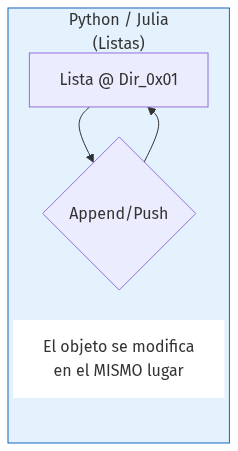
\includegraphics[width=0.5\textwidth,height=\textheight]{images/mutabilidad.png}

}

\subcaption{\label{fig-mutabilidad}Python/Julia: Listas Mutables. El
objeto cambia sin cambiar de dirección de memoria.}

\end{minipage}%
%
\begin{minipage}{0.50\linewidth}

\centering{

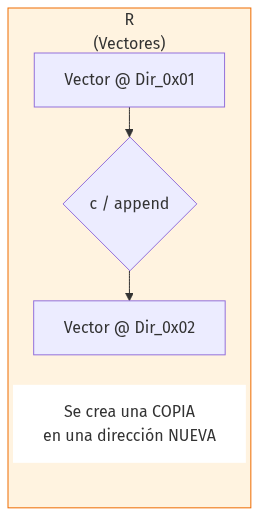
\includegraphics[width=0.5\textwidth,height=\textheight]{images/inmutabilidad.png}

}

\subcaption{\label{fig-inmutabilidad}R: Vectores Inmutables. Al
modificar, R crea una copia nueva silenciosamente.}

\end{minipage}%

\caption{\label{fig-comparacion-memoria}Comparativa de manejo de memoria
y mutabilidad.}

\end{figure}%

\section{Operaciones básicas con
texto}\label{operaciones-buxe1sicas-con-texto}

\subsection{Python}

\begin{Shaded}
\begin{Highlighting}[]
\CommentTok{\# \#| eval: false}

\CommentTok{\# Inicialización de la variable de texto}
\NormalTok{nombre\_ciudad }\OperatorTok{=} \StringTok{"cartagena de indias"}

\CommentTok{\# Convertir a minúsculas}
\NormalTok{ciudad\_minusculas }\OperatorTok{=}\NormalTok{ nombre\_ciudad.lower()}
\BuiltInTok{print}\NormalTok{(}\StringTok{"Minúsculas:"}\NormalTok{, ciudad\_minusculas)}
\end{Highlighting}
\end{Shaded}

\begin{verbatim}
Minúsculas: cartagena de indias
\end{verbatim}

\begin{Shaded}
\begin{Highlighting}[]
\CommentTok{\# Convertir a mayúsculas (útil para estandarizar tablas de atributos)}
\NormalTok{ciudad\_mayusculas }\OperatorTok{=}\NormalTok{ nombre\_ciudad.upper()}
\BuiltInTok{print}\NormalTok{(}\StringTok{"Mayúsculas:"}\NormalTok{, ciudad\_mayusculas)}
\end{Highlighting}
\end{Shaded}

\begin{verbatim}
Mayúsculas: CARTAGENA DE INDIAS
\end{verbatim}

\begin{Shaded}
\begin{Highlighting}[]
\CommentTok{\# Convertir a formato título (primera letra de cada palabra en mayúscula)}
\NormalTok{ciudad\_titulo }\OperatorTok{=}\NormalTok{ nombre\_ciudad.title()}
\BuiltInTok{print}\NormalTok{(}\StringTok{"Formato título:"}\NormalTok{, ciudad\_titulo)}
\end{Highlighting}
\end{Shaded}

\begin{verbatim}
Formato título: Cartagena De Indias
\end{verbatim}

\begin{Shaded}
\begin{Highlighting}[]
\CommentTok{\# Reemplazar texto específico dentro de una cadena}
\NormalTok{ciudad\_original }\OperatorTok{=} \StringTok{"San Andrés"}
\NormalTok{nueva\_ciudad }\OperatorTok{=}\NormalTok{ ciudad\_original.replace(}\StringTok{"San"}\NormalTok{, }\StringTok{"Isla de San"}\NormalTok{)}
\BuiltInTok{print}\NormalTok{(}\StringTok{"Original:"}\NormalTok{, ciudad\_original)}
\end{Highlighting}
\end{Shaded}

\begin{verbatim}
Original: San Andrés
\end{verbatim}

\begin{Shaded}
\begin{Highlighting}[]
\BuiltInTok{print}\NormalTok{(}\StringTok{"Modificada:"}\NormalTok{, nueva\_ciudad)}
\end{Highlighting}
\end{Shaded}

\begin{verbatim}
Modificada: Isla de San Andrés
\end{verbatim}

\begin{Shaded}
\begin{Highlighting}[]
\CommentTok{\# Limpiar espacios en blanco al inicio y al final (Trim)}
\NormalTok{datos\_ubicacion }\OperatorTok{=} \StringTok{"   Bogotá D.C.   "}
\NormalTok{ubicacion\_limpia }\OperatorTok{=}\NormalTok{ datos\_ubicacion.strip()}
\BuiltInTok{print}\NormalTok{(}\StringTok{"Texto limpio:"}\NormalTok{, }\SpecialStringTok{f"\textquotesingle{}}\SpecialCharTok{\{}\NormalTok{ubicacion\_limpia}\SpecialCharTok{\}}\SpecialStringTok{\textquotesingle{}"}\NormalTok{)}
\end{Highlighting}
\end{Shaded}

\begin{verbatim}
Texto limpio: 'Bogotá D.C.'
\end{verbatim}

\subsection{R}

\begin{Shaded}
\begin{Highlighting}[]
\CommentTok{\# \#| eval: false}

\CommentTok{\# Cargar paquete nativo recomendado para formato título}
\FunctionTok{library}\NormalTok{(tools)}

\CommentTok{\# Inicialización de la variable de texto}
\NormalTok{nombre\_ciudad }\OtherTok{\textless{}{-}} \StringTok{"cartagena de indias"}

\CommentTok{\# Convertir a minúsculas}
\NormalTok{ciudad\_minusculas }\OtherTok{\textless{}{-}} \FunctionTok{tolower}\NormalTok{(nombre\_ciudad)}
\FunctionTok{cat}\NormalTok{(}\StringTok{"Minúsculas:"}\NormalTok{, ciudad\_minusculas, }\StringTok{"}\SpecialCharTok{\textbackslash{}n}\StringTok{"}\NormalTok{)}
\end{Highlighting}
\end{Shaded}

\begin{verbatim}
Minúsculas: cartagena de indias 
\end{verbatim}

\begin{Shaded}
\begin{Highlighting}[]
\CommentTok{\# Convertir a mayúsculas (útil para estandarizar tablas de atributos)}
\NormalTok{ciudad\_mayusculas }\OtherTok{\textless{}{-}} \FunctionTok{toupper}\NormalTok{(nombre\_ciudad)}
\FunctionTok{cat}\NormalTok{(}\StringTok{"Mayúsculas:"}\NormalTok{, ciudad\_mayusculas, }\StringTok{"}\SpecialCharTok{\textbackslash{}n}\StringTok{"}\NormalTok{)}
\end{Highlighting}
\end{Shaded}

\begin{verbatim}
Mayúsculas: CARTAGENA DE INDIAS 
\end{verbatim}

\begin{Shaded}
\begin{Highlighting}[]
\CommentTok{\# Convertir a formato título}
\NormalTok{ciudad\_titulo }\OtherTok{\textless{}{-}} \FunctionTok{toTitleCase}\NormalTok{(nombre\_ciudad)}
\FunctionTok{cat}\NormalTok{(}\StringTok{"Formato título:"}\NormalTok{, ciudad\_titulo, }\StringTok{"}\SpecialCharTok{\textbackslash{}n}\StringTok{"}\NormalTok{)}
\end{Highlighting}
\end{Shaded}

\begin{verbatim}
Formato título: Cartagena De Indias 
\end{verbatim}

\begin{Shaded}
\begin{Highlighting}[]
\CommentTok{\# Reemplazar texto específico dentro de una cadena}
\NormalTok{ciudad\_original }\OtherTok{\textless{}{-}} \StringTok{"San Andrés"}
\NormalTok{nueva\_ciudad }\OtherTok{\textless{}{-}} \FunctionTok{gsub}\NormalTok{(}\StringTok{"San"}\NormalTok{, }\StringTok{"Isla de San"}\NormalTok{, ciudad\_original)}
\FunctionTok{cat}\NormalTok{(}\StringTok{"Original:"}\NormalTok{, ciudad\_original, }\StringTok{"}\SpecialCharTok{\textbackslash{}n}\StringTok{"}\NormalTok{)}
\end{Highlighting}
\end{Shaded}

\begin{verbatim}
Original: San Andrés 
\end{verbatim}

\begin{Shaded}
\begin{Highlighting}[]
\FunctionTok{cat}\NormalTok{(}\StringTok{"Modificada:"}\NormalTok{, nueva\_ciudad, }\StringTok{"}\SpecialCharTok{\textbackslash{}n}\StringTok{"}\NormalTok{)}
\end{Highlighting}
\end{Shaded}

\begin{verbatim}
Modificada: Isla de San Andrés 
\end{verbatim}

\begin{Shaded}
\begin{Highlighting}[]
\CommentTok{\# Limpiar espacios en blanco al inicio y al final (Trim)}
\NormalTok{datos\_ubicacion }\OtherTok{\textless{}{-}} \StringTok{"   Bogotá D.C.   "}
\NormalTok{ubicacion\_limpia }\OtherTok{\textless{}{-}} \FunctionTok{trimws}\NormalTok{(datos\_ubicacion)}
\FunctionTok{cat}\NormalTok{(}\StringTok{"Texto limpio: \textquotesingle{}"}\NormalTok{, ubicacion\_limpia, }\StringTok{"\textquotesingle{}}\SpecialCharTok{\textbackslash{}n}\StringTok{"}\NormalTok{, }\AttributeTok{sep=}\StringTok{""}\NormalTok{)}
\end{Highlighting}
\end{Shaded}

\begin{verbatim}
Texto limpio: 'Bogotá D.C.'
\end{verbatim}

\subsection{Julia}

\begin{Shaded}
\begin{Highlighting}[]
\CommentTok{\# \#| eval: false}
\FunctionTok{j\_eval}\NormalTok{(}\StringTok{\textquotesingle{}}
\StringTok{\# Inicialización de la variable de texto}
\StringTok{nombre\_ciudad = "cartagena de indias"}

\StringTok{\# Convertir a minúsculas}
\StringTok{ciudad\_minusculas = lowercase(nombre\_ciudad)}
\StringTok{println("Minúsculas: ", ciudad\_minusculas)}

\StringTok{\# Convertir a mayúsculas (útil para estandarizar tablas de atributos)}
\StringTok{ciudad\_mayusculas = uppercase(nombre\_ciudad)}
\StringTok{println("Mayúsculas: ", ciudad\_mayusculas)}

\StringTok{\# Convertir a formato título (primera letra de cada palabra en mayúscula)}
\StringTok{ciudad\_titulo = titlecase(nombre\_ciudad)}
\StringTok{println("Formato título: ", ciudad\_titulo)}

\StringTok{\# Reemplazar texto específico dentro de una cadena (usa el operador Pair =\textgreater{})}
\StringTok{ciudad\_original = "San Andrés"}
\StringTok{nueva\_ciudad = replace(ciudad\_original, "San" =\textgreater{} "Isla de San")}
\StringTok{println("Original: ", ciudad\_original)}
\StringTok{println("Modificada: ", nueva\_ciudad)}

\StringTok{\# Limpiar espacios en blanco al inicio y al final (Trim)}
\StringTok{datos\_ubicacion = "   Bogotá D.C.   "}
\StringTok{ubicacion\_limpia = strip(datos\_ubicacion)}
\StringTok{println("Texto limpio: }\SpecialCharTok{\textbackslash{}\textquotesingle{}}\StringTok{", ubicacion\_limpia, "}\SpecialCharTok{\textbackslash{}\textquotesingle{}}\StringTok{")}
\StringTok{\textquotesingle{}}\NormalTok{)}
\end{Highlighting}
\end{Shaded}

\begin{longtable}[]{@{}
  >{\raggedright\arraybackslash}p{(\columnwidth - 6\tabcolsep) * \real{0.2000}}
  >{\centering\arraybackslash}p{(\columnwidth - 6\tabcolsep) * \real{0.2500}}
  >{\centering\arraybackslash}p{(\columnwidth - 6\tabcolsep) * \real{0.3000}}
  >{\raggedright\arraybackslash}p{(\columnwidth - 6\tabcolsep) * \real{0.2500}}@{}}
\caption{Equivalencias de funciones para manipulación de cadenas de
texto}\label{tbl-operaciones_texto}\tabularnewline
\toprule\noalign{}
\begin{minipage}[b]{\linewidth}\raggedright
Operación
\end{minipage} & \begin{minipage}[b]{\linewidth}\centering
Python
\end{minipage} & \begin{minipage}[b]{\linewidth}\centering
R
\end{minipage} & \begin{minipage}[b]{\linewidth}\raggedright
Julia
\end{minipage} \\
\midrule\noalign{}
\endfirsthead
\toprule\noalign{}
\begin{minipage}[b]{\linewidth}\raggedright
Operación
\end{minipage} & \begin{minipage}[b]{\linewidth}\centering
Python
\end{minipage} & \begin{minipage}[b]{\linewidth}\centering
R
\end{minipage} & \begin{minipage}[b]{\linewidth}\raggedright
Julia
\end{minipage} \\
\midrule\noalign{}
\endhead
\bottomrule\noalign{}
\endlastfoot
\textbf{Minúsculas} & \texttt{.lower()} & \texttt{tolower()} &
\texttt{lowercase()} \\
\textbf{Mayúsculas} & \texttt{.upper()} & \texttt{toupper()} &
\texttt{uppercase()} \\
\textbf{Formato Título} & \texttt{.title()} &
\texttt{tools::toTitleCase()} & \texttt{titlecase()} \\
\textbf{Reemplazar} & \texttt{.replace("viejo",\ "nuevo")} &
\texttt{gsub("viejo",\ "nuevo",\ var)} &
\texttt{replace(var,\ "viejo"\ =\textgreater{}\ "nuevo")} \\
\textbf{Limpiar Espacios} & \texttt{.strip()} & \texttt{trimws()} &
\texttt{strip()} \\
\end{longtable}

\begin{center}\rule{0.5\linewidth}{0.5pt}\end{center}

\textbf{Nota técnica:} En el geoprocesamiento, la limpieza de cadenas de
texto (\emph{string parsing}) es una fase crítica antes de realizar
cruces espaciales o uniones de tablas (joins). Diferencias
imperceptibles como espacios en blanco accidentales (\texttt{"Bogotá\ "}
vs \texttt{"Bogotá"}) o discrepancias de mayúsculas y minúsculas
provocarán que el software GIS falle al emparejar los registros. Las
funciones de \texttt{strip()} y \texttt{upper()} son la primera línea de
defensa para garantizar la integridad topológica y tabular de los datos.

\section{Resumen de aprendizajes (cheat
sheet)}\label{resumen-de-aprendizajes-cheat-sheet}

En esta sección hemos abordado los cimientos de la programación
aplicados al análisis de datos. A continuación, se presenta un
\textbf{Cheat Sheet (Hoja de Referencia)} consolidado con las
equivalencias sintácticas y funcionales entre Python, R y Julia.

\subsection{1. Asignación y Operaciones
Básicas}\label{asignaciuxf3n-y-operaciones-buxe1sicas}

\begin{longtable}[]{@{}
  >{\raggedright\arraybackslash}p{(\columnwidth - 6\tabcolsep) * \real{0.2500}}
  >{\raggedright\arraybackslash}p{(\columnwidth - 6\tabcolsep) * \real{0.2500}}
  >{\raggedright\arraybackslash}p{(\columnwidth - 6\tabcolsep) * \real{0.2500}}
  >{\raggedright\arraybackslash}p{(\columnwidth - 6\tabcolsep) * \real{0.2500}}@{}}
\caption{Resumen de sintaxis y manejo de
variables}\label{tbl-resumen_variables}\tabularnewline
\toprule\noalign{}
\begin{minipage}[b]{\linewidth}\raggedright
Concepto / Operación
\end{minipage} & \begin{minipage}[b]{\linewidth}\raggedright
Python
\end{minipage} & \begin{minipage}[b]{\linewidth}\raggedright
R
\end{minipage} & \begin{minipage}[b]{\linewidth}\raggedright
Julia
\end{minipage} \\
\midrule\noalign{}
\endfirsthead
\toprule\noalign{}
\begin{minipage}[b]{\linewidth}\raggedright
Concepto / Operación
\end{minipage} & \begin{minipage}[b]{\linewidth}\raggedright
Python
\end{minipage} & \begin{minipage}[b]{\linewidth}\raggedright
R
\end{minipage} & \begin{minipage}[b]{\linewidth}\raggedright
Julia
\end{minipage} \\
\midrule\noalign{}
\endhead
\bottomrule\noalign{}
\endlastfoot
\textbf{Asignación Básica} & \texttt{=} & \texttt{\textless{}-}
(Estándar) & \texttt{=} \\
\textbf{Imprimir en consola} & \texttt{print(var)} & \texttt{print(var)}
o \texttt{cat(var)} & \texttt{println(var)} \\
\textbf{Incrementar valor} & \texttt{x\ +=\ 1} &
\texttt{x\ \textless{}-\ x\ +\ 1} & \texttt{x\ +=\ 1} \\
\textbf{Índice Inicial (Arrays)} & \texttt{{[}0{]}} (Base 0) &
\texttt{{[}1{]}} (Base 1) & \texttt{{[}1{]}} (Base 1) \\
\textbf{Último elemento} & \texttt{{[}-1{]}} & \texttt{{[}length(x){]}}
& \texttt{{[}end{]}} \\
\end{longtable}

\subsection{2. Estructuras, Tipos y Gestión de
Memoria}\label{estructuras-tipos-y-gestiuxf3n-de-memoria}

\begin{longtable}[]{@{}
  >{\raggedright\arraybackslash}p{(\columnwidth - 6\tabcolsep) * \real{0.2000}}
  >{\raggedright\arraybackslash}p{(\columnwidth - 6\tabcolsep) * \real{0.2500}}
  >{\raggedright\arraybackslash}p{(\columnwidth - 6\tabcolsep) * \real{0.3000}}
  >{\raggedright\arraybackslash}p{(\columnwidth - 6\tabcolsep) * \real{0.2500}}@{}}
\caption{Resumen de estructuras de datos y su comportamiento en memoria
(Mutabilidad)}\label{tbl-resumen_tipos_datos}\tabularnewline
\toprule\noalign{}
\begin{minipage}[b]{\linewidth}\raggedright
Concepto
\end{minipage} & \begin{minipage}[b]{\linewidth}\raggedright
Python
\end{minipage} & \begin{minipage}[b]{\linewidth}\raggedright
R
\end{minipage} & \begin{minipage}[b]{\linewidth}\raggedright
Julia
\end{minipage} \\
\midrule\noalign{}
\endfirsthead
\toprule\noalign{}
\begin{minipage}[b]{\linewidth}\raggedright
Concepto
\end{minipage} & \begin{minipage}[b]{\linewidth}\raggedright
Python
\end{minipage} & \begin{minipage}[b]{\linewidth}\raggedright
R
\end{minipage} & \begin{minipage}[b]{\linewidth}\raggedright
Julia
\end{minipage} \\
\midrule\noalign{}
\endhead
\bottomrule\noalign{}
\endlastfoot
\textbf{Número Entero} & \texttt{int} (ej. \texttt{500}) &
\texttt{integer} (ej. \texttt{500L}) & \texttt{Int64} (ej.
\texttt{500}) \\
\textbf{Número Decimal} & \texttt{float} & \texttt{numeric} (Double) &
\texttt{Float64} \\
\textbf{Booleano} & \texttt{bool} (\texttt{True}/\texttt{False}) &
\texttt{logical} (\texttt{TRUE}/\texttt{FALSE}) & \texttt{Bool}
(\texttt{true}/\texttt{false}) \\
\textbf{Lista/Vector} & \texttt{list} \texttt{{[}...{]}} &
\texttt{vector} \texttt{c(...)} & \texttt{Array} \texttt{{[}...{]}} \\
\textbf{Agregar al Final} & \texttt{lista.append(x)} &
\texttt{v\ \textless{}-\ c(v,\ x)} & \texttt{push!(lista,\ x)} \\
\textbf{Insertar en Posición} & \texttt{lista.insert(i,\ x)} &
\texttt{append(v,\ x,\ after=i)} & \texttt{insert!(lista,\ i,\ x)} \\
\textbf{Comportamiento Memoria} & \textbf{Mutable} (In-place). Modifica
el objeto original. & \textbf{Inmutable} (Copy-on-modify). Crea una
copia nueva. & \textbf{Mutable} (In-place). Modifica el objeto
original. \\
\textbf{Diccionario} & \texttt{dict} \texttt{\{k:\ v\}} & \texttt{list}
\texttt{list(k\ =\ v)} & \texttt{Dict}
\texttt{Dict(k\ =\textgreater{}\ v)} \\
\end{longtable}

\subsection{3. Interpolación y Formato de Salida
(Formatters)}\label{interpolaciuxf3n-y-formato-de-salida-formatters}

Esta tabla resume cómo insertar variables dentro de texto y controlar su
precisión (ej. coordenadas).

\begin{longtable}[]{@{}
  >{\raggedright\arraybackslash}p{(\columnwidth - 6\tabcolsep) * \real{0.2500}}
  >{\raggedright\arraybackslash}p{(\columnwidth - 6\tabcolsep) * \real{0.2500}}
  >{\raggedright\arraybackslash}p{(\columnwidth - 6\tabcolsep) * \real{0.2500}}
  >{\raggedright\arraybackslash}p{(\columnwidth - 6\tabcolsep) * \real{0.2500}}@{}}
\caption{Resumen de técnicas de interpolación y formateo numérico. Nota:
En Julia \texttt{@sprintf} requiere
\texttt{using\ Printf}.}\label{tbl-resumen_formato}\tabularnewline
\toprule\noalign{}
\begin{minipage}[b]{\linewidth}\raggedright
Operación
\end{minipage} & \begin{minipage}[b]{\linewidth}\raggedright
Python
\end{minipage} & \begin{minipage}[b]{\linewidth}\raggedright
R
\end{minipage} & \begin{minipage}[b]{\linewidth}\raggedright
Julia
\end{minipage} \\
\midrule\noalign{}
\endfirsthead
\toprule\noalign{}
\begin{minipage}[b]{\linewidth}\raggedright
Operación
\end{minipage} & \begin{minipage}[b]{\linewidth}\raggedright
Python
\end{minipage} & \begin{minipage}[b]{\linewidth}\raggedright
R
\end{minipage} & \begin{minipage}[b]{\linewidth}\raggedright
Julia
\end{minipage} \\
\midrule\noalign{}
\endhead
\bottomrule\noalign{}
\endlastfoot
\textbf{Interpolación Básica} & \texttt{f"Texto\ \{var\}"} &
\texttt{paste("Texto",\ var)} & \texttt{"Texto\ \$var"} \\
\textbf{Interpolación con Formato} & \texttt{f"Valor:\ \{var:.4f\}"} &
\texttt{sprintf("Valor:\ \%.4f",\ var)} &
\texttt{@sprintf\ "Valor:\ \%.4f"\ var} \\
\textbf{Marcador Texto} & \texttt{\{var\}} & \texttt{\%s} &
\texttt{\%s} \\
\textbf{Marcador Entero} & \texttt{\{var\}} o \texttt{\{:d\}} &
\texttt{\%d} & \texttt{\%d} \\
\textbf{Marcador Decimal} & \texttt{\{var\}} o \texttt{\{:f\}} &
\texttt{\%f} & \texttt{\%f} \\
\textbf{Control Decimales} & \texttt{:.4f} (4 decimales) &
\texttt{\%.4f} (4 decimales) & \texttt{\%.4f} (4 decimales) \\
\end{longtable}

\subsection{4. Manipulación de Cadenas de Texto (Limpieza
Tabular)}\label{manipulaciuxf3n-de-cadenas-de-texto-limpieza-tabular}

\begin{longtable}[]{@{}
  >{\raggedright\arraybackslash}p{(\columnwidth - 6\tabcolsep) * \real{0.2500}}
  >{\raggedright\arraybackslash}p{(\columnwidth - 6\tabcolsep) * \real{0.2500}}
  >{\raggedright\arraybackslash}p{(\columnwidth - 6\tabcolsep) * \real{0.2500}}
  >{\raggedright\arraybackslash}p{(\columnwidth - 6\tabcolsep) * \real{0.2500}}@{}}
\caption{Resumen de funciones para limpieza de texto (String
Parsing)}\label{tbl-resumen_texto}\tabularnewline
\toprule\noalign{}
\begin{minipage}[b]{\linewidth}\raggedright
Operación
\end{minipage} & \begin{minipage}[b]{\linewidth}\raggedright
Python
\end{minipage} & \begin{minipage}[b]{\linewidth}\raggedright
R
\end{minipage} & \begin{minipage}[b]{\linewidth}\raggedright
Julia
\end{minipage} \\
\midrule\noalign{}
\endfirsthead
\toprule\noalign{}
\begin{minipage}[b]{\linewidth}\raggedright
Operación
\end{minipage} & \begin{minipage}[b]{\linewidth}\raggedright
Python
\end{minipage} & \begin{minipage}[b]{\linewidth}\raggedright
R
\end{minipage} & \begin{minipage}[b]{\linewidth}\raggedright
Julia
\end{minipage} \\
\midrule\noalign{}
\endhead
\bottomrule\noalign{}
\endlastfoot
\textbf{A minúsculas} & \texttt{var.lower()} & \texttt{tolower(var)} &
\texttt{lowercase(var)} \\
\textbf{A MAYÚSCULAS} & \texttt{var.upper()} & \texttt{toupper(var)} &
\texttt{uppercase(var)} \\
\textbf{Formato Título} & \texttt{var.title()} &
\texttt{tools::toTitleCase(var)} & \texttt{titlecase(var)} \\
\textbf{Reemplazar texto} & \texttt{var.replace("a",\ "b")} &
\texttt{gsub("a",\ "b",\ var)} &
\texttt{replace(var,\ "a"\ =\textgreater{}\ "b")} \\
\textbf{Quitar espacios vacíos} & \texttt{var.strip()} &
\texttt{trimws(var)} & \texttt{strip(var)} \\
\end{longtable}

\subsection{5. Documentación y caracteres
especiales}\label{documentaciuxf3n-y-caracteres-especiales-1}

\begin{longtable}[]{@{}
  >{\centering\arraybackslash}p{(\columnwidth - 6\tabcolsep) * \real{0.1500}}
  >{\raggedright\arraybackslash}p{(\columnwidth - 6\tabcolsep) * \real{0.2500}}
  >{\raggedright\arraybackslash}p{(\columnwidth - 6\tabcolsep) * \real{0.2500}}
  >{\raggedright\arraybackslash}p{(\columnwidth - 6\tabcolsep) * \real{0.3500}}@{}}
\caption{Resumen de caracteres de escape y sintaxis de
documentación}\label{tbl-resumen_caracteres}\tabularnewline
\toprule\noalign{}
\begin{minipage}[b]{\linewidth}\centering
Carácter
\end{minipage} & \begin{minipage}[b]{\linewidth}\raggedright
Python
\end{minipage} & \begin{minipage}[b]{\linewidth}\raggedright
R
\end{minipage} & \begin{minipage}[b]{\linewidth}\raggedright
Julia
\end{minipage} \\
\midrule\noalign{}
\endfirsthead
\toprule\noalign{}
\begin{minipage}[b]{\linewidth}\centering
Carácter
\end{minipage} & \begin{minipage}[b]{\linewidth}\raggedright
Python
\end{minipage} & \begin{minipage}[b]{\linewidth}\raggedright
R
\end{minipage} & \begin{minipage}[b]{\linewidth}\raggedright
Julia
\end{minipage} \\
\midrule\noalign{}
\endhead
\bottomrule\noalign{}
\endlastfoot
\texttt{\#} & Comentario en línea. & Comentario en línea. & Comentario
en línea. \\
\texttt{\textbackslash{}n} & Salto de línea. & Salto de línea. & Salto
de línea. \\
\texttt{\textbackslash{}t} & Tabulación. & Tabulación. & Tabulación. \\
\texttt{"""} & \emph{Docstrings} (Documentación). & No soportado
(Error). & Cadenas/Archivos multilínea. \\
\texttt{\#=\ =\#} & No soportado. & No soportado. & Comentario de bloque
nativo. \\
\end{longtable}

\begin{center}\rule{0.5\linewidth}{0.5pt}\end{center}

\textbf{Conclusión del Módulo:} La correcta elección de los tipos de
datos (Listas vs.~Diccionarios), la comprensión del índice de origen
(Base 0 vs.~Base 1) y el control estricto del formato (\texttt{\%.4f} vs
\texttt{.4f}) son pilares fundamentales para evitar errores de redondeo
en coordenadas. Asimismo, entender la \textbf{mutabilidad} es vital:
mientras Python y Julia permiten \textbf{insertar} o modificar datos
``in-place'' (eficiente), R tiende a generar copias en memoria, lo cual
debe considerarse al procesar grandes volúmenes de información
geoespacial.

\section{Ejercicios}\label{ejercicios}

Para poner en práctica los conceptos aprendidos, deberás resolver los
siguientes dos ejercicios. Puedes elegir resolverlos en \textbf{Python,
R o Julia} (o implementar la solución en varios lenguajes si deseas
retarte).

\subsection{Ejercicio 1: Asignación de variables y operaciones
básicas}\label{ejercicio-1-asignaciuxf3n-de-variables-y-operaciones-buxe1sicas}

\textbf{Contexto:} Formas parte del equipo SIG de una corporación
autónoma regional y necesitas estructurar los metadatos de una nueva
estación de monitoreo ambiental antes de ingresarla a la base de datos
espacial.

\textbf{Instrucciones de código:}

\begin{enumerate}
\def\labelenumi{\arabic{enumi}.}
\tightlist
\item
  Define las siguientes variables respetando estrictamente el estándar
  \texttt{snake\_case}:

  \begin{itemize}
  \tightlist
  \item
    Nombre de la estación: ``Páramo de Santurbán''
  \item
    Latitud: \texttt{7.2514}
  \item
    Longitud: \texttt{-72.9069}
  \item
    Elevación en metros: \texttt{3350}
  \item
    ¿Está activa?: \texttt{Verdadero} (Usa el tipo booleano correcto
    según tu lenguaje).
  \end{itemize}
\item
  Crea una estructura de colección (Lista en Python, Vector en R, o
  Array en Julia) que contenga la Latitud y la Longitud, en ese orden.
\item
  Crea un \textbf{Diccionario} (o Lista con nombres en R) llamado
  \texttt{metadatos\_estacion} que agrupe todas las variables anteriores
  bajo claves descriptivas.
\item
  Usando la indexación adecuada (Base 0 o Base 1, según el lenguaje que
  elegiste), extrae específicamente la \textbf{Longitud} desde la
  colección de coordenadas que está dentro del diccionario y guárdala en
  una nueva variable.
\item
  Se ha realizado una nueva medición topográfica y la elevación real es
  12.5 metros más alta. Actualiza la variable de elevación utilizando el
  operador de incremento.
\item
  Imprime en consola un mensaje dinámico utilizando interpolación de
  texto (ej. \texttt{f-strings}, \texttt{paste()} o \texttt{\$}) que
  diga exactamente: \emph{``La estación {[}Nombre{]} se encuentra
  operativa en la longitud {[}Longitud{]} a una altura actualizada de
  {[}Elevación{]} msnm.''}
\end{enumerate}

\subsection{Ejercicio 2: Trabajando con
strings}\label{ejercicio-2-trabajando-con-strings}

\textbf{Contexto:} Has recibido una tabla de Excel con la toponimia de
áreas protegidas de Colombia capturada manualmente por diferentes
operarios. Los textos están sucios y, si intentas hacer un cruce
espacial (\emph{Spatial Join}) con la capa oficial del IGAC, el software
arrojará errores de topología tabular.

\textbf{Instrucciones de código:}

\begin{enumerate}
\def\labelenumi{\arabic{enumi}.}
\tightlist
\item
  Inicializa una variable con el siguiente texto crudo y problemático:
  \texttt{registro\_crudo\ =\ "\ \ \ sAnTuaRio\ de\ fAuna\ Y\ flora\ iGuaQue\ \ \ "}
\item
  \textbf{Utiliza el método o función nativa de tu lenguaje} (vista en
  la sección anterior) para eliminar los espacios en blanco accidentales
  al inicio y al final del texto.
\item
  \textbf{Usa el comando correspondiente para convertir} el texto limpio
  a formato de Título (\emph{Title Case}), estandarizando así las
  mayúsculas y minúsculas.
\item
  \textbf{Emplea la herramienta de reemplazo} de texto para cambiar la
  letra '' Y '' por '' y '' (en minúscula), de modo que el conector
  gramatical sea correcto.
\item
  Utiliza caracteres de escape (\texttt{\textbackslash{}n} y
  \texttt{\textbackslash{}t}) para imprimir un pequeño reporte
  estructurado que muestre el antes y el después, similar a esto:
\end{enumerate}

\begin{Shaded}
\begin{Highlighting}[]
\NormalTok{Reporte de Limpieza Toponímica:}
\NormalTok{    Registro Original: "   sAnTuaRio de fAuna Y flora iGuaQue   "}
\NormalTok{    Registro Limpio: "Santuario De Fauna y Flora Iguaque"}
\NormalTok{Estado: Listo para cruce espacial.}
\end{Highlighting}
\end{Shaded}

\subsection{Entregables y Criterios de
Evaluación}\label{entregables-y-criterios-de-evaluaciuxf3n}

El objetivo de esta evaluación no es solo que el código funcione, sino
que seas capaz de documentar y explicar tus decisiones técnicas.

\textbf{1. Archivos de Código:} Debes desarrollar los algoritmos en al
menos uno de los siguientes formatos de archivo:

\begin{itemize}
\tightlist
\item
  Script tradicional (\texttt{.py}, \texttt{.R}, \texttt{.jl})
\item
  Notebook interactivo (\texttt{.ipynb})
\item
  Documento computacional (\texttt{.qmd} con \emph{chunks} de código)
\end{itemize}

\textbf{2. Documento Analítico (Quarto):} Independientemente del formato
de tu código fuente, \textbf{debes redactar un documento en Quarto
(\texttt{.qmd}) y renderizarlo tanto en HTML como en PDF}. En este
documento debes incluir tus bloques de código y responder
argumentativamente a las siguientes preguntas:

\begin{itemize}
\tightlist
\item
  \textbf{Sobre el Ejercicio 1:} ¿Qué índice numérico utilizaste para
  extraer la longitud de la colección y por qué ese número
  específicamente? ¿Qué error arrojaría el lenguaje si usas el índice
  del lenguaje opuesto (ej. usar 0 en R o 1 en Python buscando el primer
  elemento)?
\item
  \textbf{Sobre el Ejercicio 2:} En términos de geoprocesamiento de
  bases de datos relacionales, ¿por qué es un paso crítico y obligatorio
  aplicar métodos de limpieza como \texttt{.strip()} o \texttt{trimws()}
  antes de realizar uniones de tablas (\emph{Joins}) basadas en nombres
  de municipios o regiones?
\item
  \textbf{Pregunta General:} Explica brevemente la diferencia
  fundamental entre el uso de triples comillas \texttt{"""} en Python
  versus su uso en Julia.
\end{itemize}

\textbf{3. Repositorio en GitHub:} Sube tu carpeta del proyecto (que
debe contener tus scripts, el archivo \texttt{.qmd} y los renders
finales en HTML y PDF) a un repositorio público en tu cuenta personal de
\textbf{GitHub}.

\begin{itemize}
\tightlist
\item
  \textbf{Entrega:} Deberás enviar únicamente el enlace (URL) a tu
  repositorio de GitHub para la calificación.
\end{itemize}

\chapter{Estructuras de datos}\label{sec-estructuras_datos}

\section{Funciones j\_eval y j\_plot en
R}\label{funciones-j_eval-y-j_plot-en-r-1}

\begin{Shaded}
\begin{Highlighting}[]
\CommentTok{\# \#| include: false}
\FunctionTok{source}\NormalTok{(}\StringTok{"./docs/j\_eval\_j\_plot.r"}\NormalTok{)}
\end{Highlighting}
\end{Shaded}

\section{Introducción}\label{introducciuxf3n-2}

\section{Objetivos de aprendizaje}\label{objetivos-de-aprendizaje-1}

\section{Tuplas}\label{tuplas}

Las \textbf{Tuplas} son estructuras de datos diseñadas para almacenar
una colección de elementos. Su característica más importante es la
\textbf{inmutabilidad}: una vez creada una tupla, sus elementos no
pueden ser alterados, añadidos ni eliminados. Esto las hace perfectas
para almacenar pares de coordenadas estáticas
\texttt{(Latitud,\ Longitud)} que no deben modificarse accidentalmente
durante la ejecución de un algoritmo espacial.

\subsection{Python}

\begin{Shaded}
\begin{Highlighting}[]
\CommentTok{\# \#| eval: false}

\CommentTok{\# Creación de una tupla estática (Latitud, Longitud) de Bogotá}
\NormalTok{punto\_bogota }\OperatorTok{=}\NormalTok{ (}\FloatTok{4.6097}\NormalTok{, }\OperatorTok{{-}}\FloatTok{74.0817}\NormalTok{)}
\BuiltInTok{print}\NormalTok{(}\SpecialStringTok{f"Coordenadas de Bogotá: }\SpecialCharTok{\{}\NormalTok{punto\_bogota}\SpecialCharTok{\}}\SpecialStringTok{"}\NormalTok{)}
\end{Highlighting}
\end{Shaded}

\begin{verbatim}
Coordenadas de Bogotá: (4.6097, -74.0817)
\end{verbatim}

\begin{Shaded}
\begin{Highlighting}[]
\CommentTok{\# Acceso a los elementos de la tupla (Recordar: Índice Base 0)}
\NormalTok{latitud }\OperatorTok{=}\NormalTok{ punto\_bogota[}\DecValTok{0}\NormalTok{]}
\NormalTok{longitud }\OperatorTok{=}\NormalTok{ punto\_bogota[}\DecValTok{1}\NormalTok{]}
\BuiltInTok{print}\NormalTok{(}\SpecialStringTok{f"Latitud: }\SpecialCharTok{\{}\NormalTok{latitud}\SpecialCharTok{\}}\SpecialStringTok{"}\NormalTok{)}
\end{Highlighting}
\end{Shaded}

\begin{verbatim}
Latitud: 4.6097
\end{verbatim}

\begin{Shaded}
\begin{Highlighting}[]
\BuiltInTok{print}\NormalTok{(}\SpecialStringTok{f"Longitud: }\SpecialCharTok{\{}\NormalTok{longitud}\SpecialCharTok{\}}\SpecialStringTok{"}\NormalTok{)}
\end{Highlighting}
\end{Shaded}

\begin{verbatim}
Longitud: -74.0817
\end{verbatim}

\begin{Shaded}
\begin{Highlighting}[]
\CommentTok{\# Desempaquetado de tuplas (Tuple Unpacking) en variables separadas}
\NormalTok{lat, lon }\OperatorTok{=}\NormalTok{ punto\_bogota}
\BuiltInTok{print}\NormalTok{(}\SpecialStringTok{f"Bogotá está ubicada a }\SpecialCharTok{\{}\NormalTok{lat}\SpecialCharTok{\}}\SpecialStringTok{°N, }\SpecialCharTok{\{}\NormalTok{lon}\SpecialCharTok{\}}\SpecialStringTok{°W"}\NormalTok{)}
\end{Highlighting}
\end{Shaded}

\begin{verbatim}
Bogotá está ubicada a 4.6097°N, -74.0817°W
\end{verbatim}

\begin{Shaded}
\begin{Highlighting}[]
\CommentTok{\# Almacenamiento de múltiples puntos geográficos como tuplas}
\NormalTok{medellin }\OperatorTok{=}\NormalTok{ (}\FloatTok{6.2442}\NormalTok{, }\OperatorTok{{-}}\FloatTok{75.5812}\NormalTok{)}
\NormalTok{cali }\OperatorTok{=}\NormalTok{ (}\FloatTok{3.4516}\NormalTok{, }\OperatorTok{{-}}\FloatTok{76.5320}\NormalTok{)}
\NormalTok{cartagena }\OperatorTok{=}\NormalTok{ (}\FloatTok{10.3910}\NormalTok{, }\OperatorTok{{-}}\FloatTok{75.4794}\NormalTok{)}

\BuiltInTok{print}\NormalTok{(}\SpecialStringTok{f"Medellín: }\SpecialCharTok{\{}\NormalTok{medellin}\SpecialCharTok{\}}\SpecialStringTok{"}\NormalTok{)}
\end{Highlighting}
\end{Shaded}

\begin{verbatim}
Medellín: (6.2442, -75.5812)
\end{verbatim}

\begin{Shaded}
\begin{Highlighting}[]
\BuiltInTok{print}\NormalTok{(}\SpecialStringTok{f"Cali: }\SpecialCharTok{\{}\NormalTok{cali}\SpecialCharTok{\}}\SpecialStringTok{"}\NormalTok{)}
\end{Highlighting}
\end{Shaded}

\begin{verbatim}
Cali: (3.4516, -76.532)
\end{verbatim}

\begin{Shaded}
\begin{Highlighting}[]
\BuiltInTok{print}\NormalTok{(}\SpecialStringTok{f"Cartagena: }\SpecialCharTok{\{}\NormalTok{cartagena}\SpecialCharTok{\}}\SpecialStringTok{"}\NormalTok{)}
\end{Highlighting}
\end{Shaded}

\begin{verbatim}
Cartagena: (10.391, -75.4794)
\end{verbatim}

\subsection{R}

\begin{Shaded}
\begin{Highlighting}[]
\CommentTok{\# \#| eval: false}

\CommentTok{\# R no tiene "tuplas" nativas; usamos vectores \textquotesingle{}c()\textquotesingle{} para coordenadas}
\NormalTok{punto\_bogota }\OtherTok{\textless{}{-}} \FunctionTok{c}\NormalTok{(}\FloatTok{4.6097}\NormalTok{, }\SpecialCharTok{{-}}\FloatTok{74.0817}\NormalTok{)}
\FunctionTok{cat}\NormalTok{(}\StringTok{"Coordenadas de Bogotá:"}\NormalTok{, punto\_bogota, }\StringTok{"}\SpecialCharTok{\textbackslash{}n}\StringTok{"}\NormalTok{)}
\end{Highlighting}
\end{Shaded}

\begin{verbatim}
Coordenadas de Bogotá: 4.6097 -74.0817 
\end{verbatim}

\begin{Shaded}
\begin{Highlighting}[]
\CommentTok{\# Acceso a los elementos (Recordar: Índice Base 1)}
\NormalTok{latitud }\OtherTok{\textless{}{-}}\NormalTok{ punto\_bogota[}\DecValTok{1}\NormalTok{]}
\NormalTok{longitud }\OtherTok{\textless{}{-}}\NormalTok{ punto\_bogota[}\DecValTok{2}\NormalTok{]}
\FunctionTok{cat}\NormalTok{(}\StringTok{"Latitud:"}\NormalTok{, latitud, }\StringTok{"}\SpecialCharTok{\textbackslash{}n}\StringTok{"}\NormalTok{)}
\end{Highlighting}
\end{Shaded}

\begin{verbatim}
Latitud: 4.6097 
\end{verbatim}

\begin{Shaded}
\begin{Highlighting}[]
\FunctionTok{cat}\NormalTok{(}\StringTok{"Longitud:"}\NormalTok{, longitud, }\StringTok{"}\SpecialCharTok{\textbackslash{}n}\StringTok{"}\NormalTok{)}
\end{Highlighting}
\end{Shaded}

\begin{verbatim}
Longitud: -74.0817 
\end{verbatim}

\begin{Shaded}
\begin{Highlighting}[]
\CommentTok{\# Asignación de variables (R nativo no tiene desempaquetado automático)}
\NormalTok{lat }\OtherTok{\textless{}{-}}\NormalTok{ punto\_bogota[}\DecValTok{1}\NormalTok{]}
\NormalTok{lon }\OtherTok{\textless{}{-}}\NormalTok{ punto\_bogota[}\DecValTok{2}\NormalTok{]}
\FunctionTok{cat}\NormalTok{(}\FunctionTok{sprintf}\NormalTok{(}\StringTok{"Bogotá está ubicada a \%s°N, \%s°W}\SpecialCharTok{\textbackslash{}n}\StringTok{"}\NormalTok{, lat, lon))}
\end{Highlighting}
\end{Shaded}

\begin{verbatim}
Bogotá está ubicada a 4.6097°N, -74.0817°W
\end{verbatim}

\begin{Shaded}
\begin{Highlighting}[]
\CommentTok{\# Almacenamiento de múltiples puntos geográficos}
\NormalTok{medellin }\OtherTok{\textless{}{-}} \FunctionTok{c}\NormalTok{(}\FloatTok{6.2442}\NormalTok{, }\SpecialCharTok{{-}}\FloatTok{75.5812}\NormalTok{)}
\NormalTok{cali }\OtherTok{\textless{}{-}} \FunctionTok{c}\NormalTok{(}\FloatTok{3.4516}\NormalTok{, }\SpecialCharTok{{-}}\FloatTok{76.5320}\NormalTok{)}
\NormalTok{cartagena }\OtherTok{\textless{}{-}} \FunctionTok{c}\NormalTok{(}\FloatTok{10.3910}\NormalTok{, }\SpecialCharTok{{-}}\FloatTok{75.4794}\NormalTok{)}

\FunctionTok{cat}\NormalTok{(}\StringTok{"Medellín:"}\NormalTok{, medellin, }\StringTok{"}\SpecialCharTok{\textbackslash{}n}\StringTok{"}\NormalTok{)}
\end{Highlighting}
\end{Shaded}

\begin{verbatim}
Medellín: 6.2442 -75.5812 
\end{verbatim}

\begin{Shaded}
\begin{Highlighting}[]
\FunctionTok{cat}\NormalTok{(}\StringTok{"Cali:"}\NormalTok{, cali, }\StringTok{"}\SpecialCharTok{\textbackslash{}n}\StringTok{"}\NormalTok{)}
\end{Highlighting}
\end{Shaded}

\begin{verbatim}
Cali: 3.4516 -76.532 
\end{verbatim}

\begin{Shaded}
\begin{Highlighting}[]
\FunctionTok{cat}\NormalTok{(}\StringTok{"Cartagena:"}\NormalTok{, cartagena, }\StringTok{"}\SpecialCharTok{\textbackslash{}n}\StringTok{"}\NormalTok{)}
\end{Highlighting}
\end{Shaded}

\begin{verbatim}
Cartagena: 10.391 -75.4794 
\end{verbatim}

\subsection{Julia}

\begin{Shaded}
\begin{Highlighting}[]
\CommentTok{\# \#| eval: false}
\FunctionTok{j\_eval}\NormalTok{(}\StringTok{\textquotesingle{}}
\StringTok{\# Creación de una tupla estática (Latitud, Longitud) de Bogotá}
\StringTok{punto\_bogota = (4.6097, {-}74.0817)}
\StringTok{println("Coordenadas de Bogotá: ", punto\_bogota)}

\StringTok{\# Acceso a los elementos de la tupla (Recordar: Índice Base 1)}
\StringTok{latitud = punto\_bogota[1]}
\StringTok{longitud = punto\_bogota[2]}
\StringTok{println("Latitud: ", latitud)}
\StringTok{println("Longitud: ", longitud)}

\StringTok{\# Desempaquetado de tuplas (Tuple Unpacking)}
\StringTok{lat, lon = punto\_bogota}
\StringTok{println("Bogotá está ubicada a $lat°N, $lon°W")}

\StringTok{\# Almacenamiento de múltiples puntos geográficos como tuplas}
\StringTok{medellin = (6.2442, {-}75.5812)}
\StringTok{cali = (3.4516, {-}76.5320)}
\StringTok{cartagena = (10.3910, {-}75.4794)}

\StringTok{println("Medellín: ", medellin)}
\StringTok{println("Cali: ", cali)}
\StringTok{println("Cartagena: ", cartagena)}
\StringTok{\textquotesingle{}}\NormalTok{)}
\end{Highlighting}
\end{Shaded}

\begin{verbatim}
Starting Julia ...
\end{verbatim}

\begin{longtable}[]{@{}
  >{\raggedright\arraybackslash}p{(\columnwidth - 6\tabcolsep) * \real{0.2000}}
  >{\centering\arraybackslash}p{(\columnwidth - 6\tabcolsep) * \real{0.2500}}
  >{\centering\arraybackslash}p{(\columnwidth - 6\tabcolsep) * \real{0.3000}}
  >{\centering\arraybackslash}p{(\columnwidth - 6\tabcolsep) * \real{0.2500}}@{}}
\caption{Comparación técnica de tuplas y
equivalentes}\label{tbl-tuplas}\tabularnewline
\toprule\noalign{}
\begin{minipage}[b]{\linewidth}\raggedright
Característica
\end{minipage} & \begin{minipage}[b]{\linewidth}\centering
Python
\end{minipage} & \begin{minipage}[b]{\linewidth}\centering
R
\end{minipage} & \begin{minipage}[b]{\linewidth}\centering
Julia
\end{minipage} \\
\midrule\noalign{}
\endfirsthead
\toprule\noalign{}
\begin{minipage}[b]{\linewidth}\raggedright
Característica
\end{minipage} & \begin{minipage}[b]{\linewidth}\centering
Python
\end{minipage} & \begin{minipage}[b]{\linewidth}\centering
R
\end{minipage} & \begin{minipage}[b]{\linewidth}\centering
Julia
\end{minipage} \\
\midrule\noalign{}
\endhead
\bottomrule\noalign{}
\endlastfoot
\textbf{Sintaxis de Creación} & \texttt{t\ =\ (x,\ y)} &
\texttt{v\ \textless{}-\ c(x,\ y)} (Vector) & \texttt{t\ =\ (x,\ y)} \\
\textbf{Inmutabilidad estricta} & Sí (genera error si se intenta
alterar). & No aplica. Los vectores hacen una copia en memoria si se
alteran. & Sí (genera error si se intenta alterar). \\
\textbf{Desempaquetado (\emph{Unpacking})} & \texttt{x,\ y\ =\ t} &
Requiere extraer por índice manual
\texttt{x\ \textless{}-\ v{[}1{]};\ y\ \textless{}-\ v{[}2{]}}. &
\texttt{x,\ y\ =\ t} \\
\textbf{Uso Principal en SIG} & Proteger pares de coordenadas estáticas
de alteraciones en iteraciones. & Creación rápida de puntos geométricos.
& Tipado estricto y seguro de coordenadas para máximo rendimiento. \\
\end{longtable}

\begin{center}\rule{0.5\linewidth}{0.5pt}\end{center}

\textbf{Nota técnica:} Las tuplas no existen nativamente en R con el
comportamiento de ``desempaquetado'' e ``inmutabilidad estricta'' que
vemos en Python y Julia. En R, utilizamos \textbf{vectores}
(\texttt{c()}) o \textbf{listas} (\texttt{list()}) para agrupar
coordenadas. Es crucial entender que en Python y Julia, si intentas
ejecutar \texttt{punto\_bogota{[}0{]}\ =\ 5.0}, el programa colapsará
inmediatamente para proteger los datos (porque una tupla es inmutable).
En R, \texttt{punto\_bogota{[}1{]}\ \textless{}-\ 5.0} sí funcionará,
reescribiendo la coordenada silenciosamente.

\section{Listas (y vectores)}\label{listas-y-vectores}

A diferencia de las tuplas, las \textbf{Listas} (en Python y Julia) o
los \textbf{Vectores} (en R) son secuencias \textbf{mutables} y
dinámicas. Son la estructura de datos más utilizada en geomática para
almacenar series temporales, perfiles de elevación, atributos de una
tabla o una secuencia ordenada de vértices que conforman una ruta, ya
que permiten agregar, eliminar o modificar datos sobre la marcha.

\subsection{Python}

\begin{Shaded}
\begin{Highlighting}[]
\CommentTok{\# \#| eval: false}

\CommentTok{\# 1. CREACIÓN DE LISTAS}
\CommentTok{\# Una lista de tuplas de coordenadas representando una ruta de viaje}
\NormalTok{ruta }\OperatorTok{=}\NormalTok{ [}
\NormalTok{    (}\FloatTok{4.6097}\NormalTok{, }\OperatorTok{{-}}\FloatTok{74.0817}\NormalTok{),  }\CommentTok{\# Bogotá}
\NormalTok{    (}\FloatTok{6.2442}\NormalTok{, }\OperatorTok{{-}}\FloatTok{75.5812}\NormalTok{),  }\CommentTok{\# Medellín}
\NormalTok{    (}\FloatTok{3.4516}\NormalTok{, }\OperatorTok{{-}}\FloatTok{76.5320}\NormalTok{),  }\CommentTok{\# Cali}
\NormalTok{]}
\BuiltInTok{print}\NormalTok{(}\StringTok{"Ruta inicial:"}\NormalTok{, ruta)}
\end{Highlighting}
\end{Shaded}

\begin{verbatim}
Ruta inicial: [(4.6097, -74.0817), (6.2442, -75.5812), (3.4516, -76.532)]
\end{verbatim}

\begin{Shaded}
\begin{Highlighting}[]
\CommentTok{\# Una lista de mediciones de elevación (en metros)}
\NormalTok{elevaciones }\OperatorTok{=}\NormalTok{ [}\FloatTok{2600.5}\NormalTok{, }\FloatTok{2650.2}\NormalTok{, }\FloatTok{2710.8}\NormalTok{, }\FloatTok{2800.3}\NormalTok{, }\FloatTok{2950.7}\NormalTok{, }\FloatTok{3100.1}\NormalTok{]}
\BuiltInTok{print}\NormalTok{(}\StringTok{"Perfil de elevación:"}\NormalTok{, elevaciones)}
\end{Highlighting}
\end{Shaded}

\begin{verbatim}
Perfil de elevación: [2600.5, 2650.2, 2710.8, 2800.3, 2950.7, 3100.1]
\end{verbatim}

\begin{Shaded}
\begin{Highlighting}[]
\CommentTok{\# Una lista de cadenas de texto (nombres de ciudades)}
\NormalTok{ciudades }\OperatorTok{=}\NormalTok{ [}\StringTok{"Bogotá"}\NormalTok{, }\StringTok{"Medellín"}\NormalTok{, }\StringTok{"Cali"}\NormalTok{]}
\BuiltInTok{print}\NormalTok{(}\StringTok{"Ciudades a visitar:"}\NormalTok{, ciudades)}
\end{Highlighting}
\end{Shaded}

\begin{verbatim}
Ciudades a visitar: ['Bogotá', 'Medellín', 'Cali']
\end{verbatim}

\begin{Shaded}
\begin{Highlighting}[]
\CommentTok{\# 2. AGREGAR ELEMENTOS (Mutabilidad)}

\CommentTok{\# a. Agregar al final (.append)}
\CommentTok{\# Agregamos Cartagena al final de nuestra ruta (pasa a ser la tercera parada, índice 2)}
\NormalTok{ruta.append((}\FloatTok{10.3910}\NormalTok{, }\OperatorTok{{-}}\FloatTok{75.4794}\NormalTok{))}
\NormalTok{elevaciones.append(}\FloatTok{2.0}\NormalTok{)}
\BuiltInTok{print}\NormalTok{(}\StringTok{"Ruta con Cartagena al final:"}\NormalTok{, ruta)}
\end{Highlighting}
\end{Shaded}

\begin{verbatim}
Ruta con Cartagena al final: [(4.6097, -74.0817), (6.2442, -75.5812), (3.4516, -76.532), (10.391, -75.4794)]
\end{verbatim}

\begin{Shaded}
\begin{Highlighting}[]
\CommentTok{\# b. Insertar en una posición específica (.insert)}
\CommentTok{\# Necesitamos agregar una parada (ej. Manizales) justo DESPUÉS de Medellín.}
\CommentTok{\# Como Medellín es el índice 1, insertamos en el índice 2.}
\CommentTok{\# Esto empuja a Cartagena hacia el índice 3}
\NormalTok{ruta.insert(}\DecValTok{2}\NormalTok{, (}\FloatTok{5.0689}\NormalTok{, }\OperatorTok{{-}}\FloatTok{75.5174}\NormalTok{))}
\NormalTok{elevaciones.insert(}\DecValTok{2}\NormalTok{, }\FloatTok{2160.0}\NormalTok{)}

\BuiltInTok{print}\NormalTok{(}\StringTok{"}\CharTok{\textbackslash{}n}\StringTok{Ruta final con parada intercalada:"}\NormalTok{, ruta)}
\end{Highlighting}
\end{Shaded}

\begin{verbatim}

Ruta final con parada intercalada: [(4.6097, -74.0817), (6.2442, -75.5812), (5.0689, -75.5174), (3.4516, -76.532), (10.391, -75.4794)]
\end{verbatim}

\begin{Shaded}
\begin{Highlighting}[]
\BuiltInTok{print}\NormalTok{(}\StringTok{"Elevaciones finales:"}\NormalTok{, elevaciones)}
\end{Highlighting}
\end{Shaded}

\begin{verbatim}
Elevaciones finales: [2600.5, 2650.2, 2160.0, 2710.8, 2800.3, 2950.7, 3100.1, 2.0]
\end{verbatim}

\begin{Shaded}
\begin{Highlighting}[]
\CommentTok{\# NOTA PEDAGÓGICA:}
\CommentTok{\# Usar .insert(2, valor) asegura que el nuevo elemento ocupe exactamente }
\CommentTok{\# la tercera posición de la lista (Base 0), respetando el orden de las paradas anteriores.}

\CommentTok{\# 3. ACCEDER A ELEMENTOS (Índices)}
\CommentTok{\# Acceder a la primera ciudad de la ruta (Índice 0)}
\NormalTok{primera\_parada }\OperatorTok{=}\NormalTok{ ruta[}\DecValTok{0}\NormalTok{]}
\BuiltInTok{print}\NormalTok{(}\SpecialStringTok{f"Primera parada: }\SpecialCharTok{\{}\NormalTok{primera\_parada}\SpecialCharTok{\}}\SpecialStringTok{"}\NormalTok{)}
\end{Highlighting}
\end{Shaded}

\begin{verbatim}
Primera parada: (4.6097, -74.0817)
\end{verbatim}

\begin{Shaded}
\begin{Highlighting}[]
\CommentTok{\# Acceder a la latitud de la segunda ciudad de la ruta }
\CommentTok{\# Índice 1 (entra a Medellín) y luego Índice 0 (extrae la latitud)}
\CommentTok{\# Nota: A diferencia de R, en Python NO se usan dobles corchetes [[ ]].}
\CommentTok{\# Aquí simplemente encadenamos un corchete al lado del otro: [1][0]}
\NormalTok{sda\_parada\_lat }\OperatorTok{=}\NormalTok{ ruta[}\DecValTok{1}\NormalTok{][}\DecValTok{0}\NormalTok{]}
\BuiltInTok{print}\NormalTok{(}\SpecialStringTok{f"Latitud segunda parada: }\SpecialCharTok{\{}\NormalTok{sda\_parada\_lat}\SpecialCharTok{\}}\SpecialStringTok{"}\NormalTok{)}
\end{Highlighting}
\end{Shaded}

\begin{verbatim}
Latitud segunda parada: 6.2442
\end{verbatim}

\begin{Shaded}
\begin{Highlighting}[]
\CommentTok{\# Alternativa Pythonica: Desempaquetado de tuplas}
\CommentTok{\# Extraemos la tupla entera (ruta[1]) y la desempaquetamos }
\CommentTok{\# directamente en dos variables con nombres claros.}
\CommentTok{\# En este caso decidimos no extraer la longitud}
\NormalTok{latitud, \_ }\OperatorTok{=}\NormalTok{ ruta[}\DecValTok{1}\NormalTok{]}

\BuiltInTok{print}\NormalTok{(}\SpecialStringTok{f"Latitud segunda parada: }\SpecialCharTok{\{}\NormalTok{latitud}\SpecialCharTok{\}}\SpecialStringTok{"}\NormalTok{)}
\end{Highlighting}
\end{Shaded}

\begin{verbatim}
Latitud segunda parada: 6.2442
\end{verbatim}

\begin{Shaded}
\begin{Highlighting}[]
\CommentTok{\# Acceder a la última ciudad usando indexación negativa}
\NormalTok{ultima\_parada }\OperatorTok{=}\NormalTok{ ruta[}\OperatorTok{{-}}\DecValTok{1}\NormalTok{]}
\BuiltInTok{print}\NormalTok{(}\SpecialStringTok{f"Última parada: }\SpecialCharTok{\{}\NormalTok{ultima\_parada}\SpecialCharTok{\}}\SpecialStringTok{"}\NormalTok{)}
\end{Highlighting}
\end{Shaded}

\begin{verbatim}
Última parada: (10.391, -75.4794)
\end{verbatim}

\begin{Shaded}
\begin{Highlighting}[]
\CommentTok{\# 4. SLICING (Extraer porciones de la lista)}
\CommentTok{\# Obtener las dos primeras paradas (índices 0 y 1, el 2 es exclusivo)}
\NormalTok{primeras\_dos }\OperatorTok{=}\NormalTok{ ruta[:}\DecValTok{2}\NormalTok{]}
\BuiltInTok{print}\NormalTok{(}\StringTok{"Primeras dos paradas:"}\NormalTok{, primeras\_dos)}
\end{Highlighting}
\end{Shaded}

\begin{verbatim}
Primeras dos paradas: [(4.6097, -74.0817), (6.2442, -75.5812)]
\end{verbatim}

\begin{Shaded}
\begin{Highlighting}[]
\CommentTok{\# Obtener una porción central de las elevaciones (índices 2, 3 y 4)}
\NormalTok{elevaciones\_medias }\OperatorTok{=}\NormalTok{ elevaciones[}\DecValTok{2}\NormalTok{:}\DecValTok{5}\NormalTok{]}
\BuiltInTok{print}\NormalTok{(}\StringTok{"Elevaciones intermedias:"}\NormalTok{, elevaciones\_medias)}
\end{Highlighting}
\end{Shaded}

\begin{verbatim}
Elevaciones intermedias: [2160.0, 2710.8, 2800.3]
\end{verbatim}

\begin{Shaded}
\begin{Highlighting}[]
\CommentTok{\# 5. OPERACIONES ÚTILES}
\CommentTok{\# Contar el número de vértices (puntos de ruta)}
\NormalTok{num\_vertices }\OperatorTok{=} \BuiltInTok{len}\NormalTok{(ruta)}
\BuiltInTok{print}\NormalTok{(}\SpecialStringTok{f"Número de vértices: }\SpecialCharTok{\{}\NormalTok{num\_vertices}\SpecialCharTok{\}}\SpecialStringTok{"}\NormalTok{)}
\end{Highlighting}
\end{Shaded}

\begin{verbatim}
Número de vértices: 5
\end{verbatim}

\begin{Shaded}
\begin{Highlighting}[]
\CommentTok{\# Encontrar la elevación máxima}
\NormalTok{elev\_maxima }\OperatorTok{=} \BuiltInTok{max}\NormalTok{(elevaciones)}
\BuiltInTok{print}\NormalTok{(}\SpecialStringTok{f"Elevación máxima: }\SpecialCharTok{\{}\NormalTok{elev\_maxima}\SpecialCharTok{\}}\SpecialStringTok{ metros"}\NormalTok{)}
\end{Highlighting}
\end{Shaded}

\begin{verbatim}
Elevación máxima: 3100.1 metros
\end{verbatim}

\begin{Shaded}
\begin{Highlighting}[]
\CommentTok{\# Calcular la elevación promedio}
\NormalTok{elev\_promedio }\OperatorTok{=} \BuiltInTok{sum}\NormalTok{(elevaciones) }\OperatorTok{/} \BuiltInTok{len}\NormalTok{(elevaciones)}
\BuiltInTok{print}\NormalTok{(}\SpecialStringTok{f"Elevación promedio: }\SpecialCharTok{\{}\NormalTok{elev\_promedio}\SpecialCharTok{:.1f\}}\SpecialStringTok{ metros"}\NormalTok{)}
\end{Highlighting}
\end{Shaded}

\begin{verbatim}
Elevación promedio: 2371.8 metros
\end{verbatim}

\subsection{R}

\begin{Shaded}
\begin{Highlighting}[]
\CommentTok{\# \#| eval: false}

\CommentTok{\# 1. CREACIÓN DE LISTAS Y VECTORES}
\CommentTok{\# En R, usamos \textquotesingle{}list\textquotesingle{} para agrupar objetos complejos como vectores de coordenadas}
\NormalTok{ruta }\OtherTok{\textless{}{-}} \FunctionTok{list}\NormalTok{(}
    \FunctionTok{c}\NormalTok{(}\FloatTok{4.6097}\NormalTok{, }\SpecialCharTok{{-}}\FloatTok{74.0817}\NormalTok{),  }\CommentTok{\# Bogotá}
    \FunctionTok{c}\NormalTok{(}\FloatTok{6.2442}\NormalTok{, }\SpecialCharTok{{-}}\FloatTok{75.5812}\NormalTok{),  }\CommentTok{\# Medellín}
    \FunctionTok{c}\NormalTok{(}\FloatTok{3.4516}\NormalTok{, }\SpecialCharTok{{-}}\FloatTok{76.5320}\NormalTok{)   }\CommentTok{\# Cali}
\NormalTok{)}
\FunctionTok{cat}\NormalTok{(}\StringTok{"Ruta inicial:}\SpecialCharTok{\textbackslash{}n}\StringTok{"}\NormalTok{); }\FunctionTok{print}\NormalTok{(ruta)}
\end{Highlighting}
\end{Shaded}

\begin{verbatim}
Ruta inicial:
\end{verbatim}

\begin{verbatim}
[[1]]
[1]   4.6097 -74.0817

[[2]]
[1]   6.2442 -75.5812

[[3]]
[1]   3.4516 -76.5320
\end{verbatim}

\begin{Shaded}
\begin{Highlighting}[]
\CommentTok{\# Los datos homogéneos (números o textos solos) van en vectores atómicos \textquotesingle{}c()\textquotesingle{}}
\NormalTok{elevaciones }\OtherTok{\textless{}{-}} \FunctionTok{c}\NormalTok{(}\FloatTok{2600.5}\NormalTok{, }\FloatTok{2650.2}\NormalTok{, }\FloatTok{2710.8}\NormalTok{, }\FloatTok{2800.3}\NormalTok{, }\FloatTok{2950.7}\NormalTok{, }\FloatTok{3100.1}\NormalTok{)}
\FunctionTok{cat}\NormalTok{(}\StringTok{"Perfil de elevación:"}\NormalTok{, elevaciones, }\StringTok{"}\SpecialCharTok{\textbackslash{}n}\StringTok{"}\NormalTok{)}
\end{Highlighting}
\end{Shaded}

\begin{verbatim}
Perfil de elevación: 2600.5 2650.2 2710.8 2800.3 2950.7 3100.1 
\end{verbatim}

\begin{Shaded}
\begin{Highlighting}[]
\NormalTok{ciudades }\OtherTok{\textless{}{-}} \FunctionTok{c}\NormalTok{(}\StringTok{"Bogotá"}\NormalTok{, }\StringTok{"Medellín"}\NormalTok{, }\StringTok{"Cali"}\NormalTok{)}
\FunctionTok{cat}\NormalTok{(}\StringTok{"Ciudades a visitar:"}\NormalTok{, ciudades, }\StringTok{"}\SpecialCharTok{\textbackslash{}n}\StringTok{"}\NormalTok{)}
\end{Highlighting}
\end{Shaded}

\begin{verbatim}
Ciudades a visitar: Bogotá Medellín Cali 
\end{verbatim}

\begin{Shaded}
\begin{Highlighting}[]
\CommentTok{\# 2. AGREGAR ELEMENTOS (Mutabilidad)}

\CommentTok{\# a. Agregar al final (append / c)}
\CommentTok{\# Agregamos Cartagena al final de la lista de rutas}
\NormalTok{ruta }\OtherTok{\textless{}{-}} \FunctionTok{append}\NormalTok{(ruta, }\FunctionTok{list}\NormalTok{(}\FunctionTok{c}\NormalTok{(}\FloatTok{10.3910}\NormalTok{, }\SpecialCharTok{{-}}\FloatTok{75.4794}\NormalTok{)))}
\CommentTok{\# Agregamos la elevación al final del vector}
\NormalTok{elevaciones }\OtherTok{\textless{}{-}} \FunctionTok{c}\NormalTok{(elevaciones, }\FloatTok{2.0}\NormalTok{)}

\FunctionTok{print}\NormalTok{(}\StringTok{"Ruta con Cartagena al final:"}\NormalTok{)}
\end{Highlighting}
\end{Shaded}

\begin{verbatim}
[1] "Ruta con Cartagena al final:"
\end{verbatim}

\begin{Shaded}
\begin{Highlighting}[]
\FunctionTok{print}\NormalTok{(ruta)}
\end{Highlighting}
\end{Shaded}

\begin{verbatim}
[[1]]
[1]   4.6097 -74.0817

[[2]]
[1]   6.2442 -75.5812

[[3]]
[1]   3.4516 -76.5320

[[4]]
[1]  10.3910 -75.4794
\end{verbatim}

\begin{Shaded}
\begin{Highlighting}[]
\CommentTok{\# b. Insertar en una posición específica (after)}
\CommentTok{\# Necesitamos agregar Manizales justo DESPUÉS de Medellín.}
\CommentTok{\# Como Medellín es la posición 2, indicamos after = 2.}
\CommentTok{\# Esto coloca a Manizales en la posición 3 y desplaza a Cartagena a la 4.}
\NormalTok{ruta }\OtherTok{\textless{}{-}} \FunctionTok{append}\NormalTok{(ruta, }\FunctionTok{list}\NormalTok{(}\FunctionTok{c}\NormalTok{(}\FloatTok{5.0689}\NormalTok{, }\SpecialCharTok{{-}}\FloatTok{75.5174}\NormalTok{)), }\AttributeTok{after =} \DecValTok{2}\NormalTok{)}
\NormalTok{elevaciones }\OtherTok{\textless{}{-}} \FunctionTok{append}\NormalTok{(elevaciones, }\FloatTok{2160.0}\NormalTok{, }\AttributeTok{after =} \DecValTok{2}\NormalTok{)}

\FunctionTok{print}\NormalTok{(}\StringTok{"Ruta final con parada intercalada:"}\NormalTok{)}
\end{Highlighting}
\end{Shaded}

\begin{verbatim}
[1] "Ruta final con parada intercalada:"
\end{verbatim}

\begin{Shaded}
\begin{Highlighting}[]
\FunctionTok{print}\NormalTok{(ruta)}
\end{Highlighting}
\end{Shaded}

\begin{verbatim}
[[1]]
[1]   4.6097 -74.0817

[[2]]
[1]   6.2442 -75.5812

[[3]]
[1]   5.0689 -75.5174

[[4]]
[1]   3.4516 -76.5320

[[5]]
[1]  10.3910 -75.4794
\end{verbatim}

\begin{Shaded}
\begin{Highlighting}[]
\CommentTok{\# NOTA PEDAGÓGICA:}
\CommentTok{\# En R, la función append() es muy versátil. Si no usas \textquotesingle{}after\textquotesingle{}, agrega al final.}
\CommentTok{\# Al usar after = 2, le indicamos que el nuevo "eslabón" se enganche justo }
\CommentTok{\# después de la segunda posición, manteniendo la lógica de nuestra ruta.}

\CommentTok{\# 3. ACCEDER A ELEMENTOS (Índice Base 1)}

\CommentTok{\# LA REGLA DE ORO DE LAS LISTAS EN R:}
\CommentTok{\# ruta[1]   {-}\textgreater{} Devuelve una LISTA (La "caja" cerrada). No podemos hacer cálculos numéricos con esto.}
\CommentTok{\# ruta[[1]] {-}\textgreater{} Devuelve el VECTOR (El contenido de la caja). ¡Esto es lo que necesitamos!}
\NormalTok{primera\_parada }\OtherTok{\textless{}{-}}\NormalTok{ ruta[[}\DecValTok{1}\NormalTok{]]}
\FunctionTok{cat}\NormalTok{(}\StringTok{"Primera parada:"}\NormalTok{, primera\_parada, }\StringTok{"}\SpecialCharTok{\textbackslash{}n}\StringTok{"}\NormalTok{)}
\end{Highlighting}
\end{Shaded}

\begin{verbatim}
Primera parada: 4.6097 -74.0817 
\end{verbatim}

\begin{Shaded}
\begin{Highlighting}[]
\CommentTok{\# ACCEDER A LA LATITUD DE LA SEGUNDA CIUDAD DE LA RUTA (MEDELLÍN)}
\CommentTok{\# {-}{-}{-} ESTRATEGIA MATRIOSHKA EN R {-}{-}{-}}

\CommentTok{\# a. El camino largo (Entender las capas)}
\CommentTok{\# ruta[2]         {-}\textgreater{} Crea una sub{-}lista (caja con el paquete adentro)}
\CommentTok{\# ruta[2][[1]]    {-}\textgreater{} Abre la sub{-}lista para sacar el vector (el paquete)}
\CommentTok{\# ruta[2][[1]][1] {-}\textgreater{} Toma el primer valor del paquete (la latitud)}

\NormalTok{sda\_parada\_lat\_v1 }\OtherTok{\textless{}{-}}\NormalTok{ ruta[}\DecValTok{2}\NormalTok{][[}\DecValTok{1}\NormalTok{]][}\DecValTok{1}\NormalTok{]}
\FunctionTok{cat}\NormalTok{(}\StringTok{"Camino Largo {-} Latitud segunda parada:"}\NormalTok{, sda\_parada\_lat\_v1, }\StringTok{"}\SpecialCharTok{\textbackslash{}n}\StringTok{"}\NormalTok{)}
\end{Highlighting}
\end{Shaded}

\begin{verbatim}
Camino Largo - Latitud segunda parada: 6.2442 
\end{verbatim}

\begin{Shaded}
\begin{Highlighting}[]
\CommentTok{\# b. El camino directo (La forma recomendada)}
\CommentTok{\# ruta[[2]]       {-}\textgreater{} Abre directamente la caja 2 de la lista original}
\CommentTok{\# ruta[[2]][1]    {-}\textgreater{} Toma el primer valor del vector extraído}

\NormalTok{sda\_parada\_lat\_v2 }\OtherTok{\textless{}{-}}\NormalTok{ ruta[[}\DecValTok{2}\NormalTok{]][}\DecValTok{1}\NormalTok{]}
\FunctionTok{cat}\NormalTok{(}\StringTok{"Camino Corto {-} Latitud segunda parada:"}\NormalTok{, sda\_parada\_lat\_v2, }\StringTok{"}\SpecialCharTok{\textbackslash{}n}\StringTok{"}\NormalTok{)}
\end{Highlighting}
\end{Shaded}

\begin{verbatim}
Camino Corto - Latitud segunda parada: 6.2442 
\end{verbatim}

\begin{Shaded}
\begin{Highlighting}[]
\CommentTok{\# NOTA PEDAGÓGICA: }
\CommentTok{\# ruta[2][[1]] es exactamente idéntico a ruta[[2]]. }
\CommentTok{\# Usar la primera opción es como abrir un sobre para sacar una carta }
\CommentTok{\# que está dentro de otro sobre. ¡Doble trabajo innecesario!}

\CommentTok{\# c. Alternativa: Paso a paso para evitar el laberinto de corchetes}
\CommentTok{\# A diferencia de Python/Julia, R Base no tiene un "desempaquetado" de }
\CommentTok{\# múltiples variables en una sola línea. La forma más limpia y "R{-}ónica" }
\CommentTok{\# de hacerlo sin confundirse es usar variables intermedias:}

\NormalTok{medellin\_coords }\OtherTok{\textless{}{-}}\NormalTok{ ruta[[}\DecValTok{2}\NormalTok{]]   }\CommentTok{\# Paso 1: Extraemos el vector completo}
\NormalTok{latitud }\OtherTok{\textless{}{-}}\NormalTok{ medellin\_coords[}\DecValTok{1}\NormalTok{]  }\CommentTok{\# Paso 2: Sacamos solo lo que nos interesa}

\FunctionTok{cat}\NormalTok{(}\StringTok{"Paso a Paso  {-} Latitud segunda parada:"}\NormalTok{, latitud, }\StringTok{"}\SpecialCharTok{\textbackslash{}n}\StringTok{"}\NormalTok{)}
\end{Highlighting}
\end{Shaded}

\begin{verbatim}
Paso a Paso  - Latitud segunda parada: 6.2442 
\end{verbatim}

\begin{Shaded}
\begin{Highlighting}[]
\CommentTok{\# Acceder a la última ciudad usando la longitud total}
\NormalTok{ultima\_parada }\OtherTok{\textless{}{-}}\NormalTok{ ruta[[}\FunctionTok{length}\NormalTok{(ruta)]]}
\FunctionTok{cat}\NormalTok{(}\StringTok{"Última parada:"}\NormalTok{, ultima\_parada, }\StringTok{"}\SpecialCharTok{\textbackslash{}n}\StringTok{"}\NormalTok{)}
\end{Highlighting}
\end{Shaded}

\begin{verbatim}
Última parada: 10.391 -75.4794 
\end{verbatim}

\begin{Shaded}
\begin{Highlighting}[]
\CommentTok{\# 4. SLICING (Extraer porciones)}
\CommentTok{\# En R, el índice final SÍ se incluye en el rango}
\NormalTok{primeras\_dos }\OtherTok{\textless{}{-}}\NormalTok{ ruta[}\DecValTok{1}\SpecialCharTok{:}\DecValTok{2}\NormalTok{] }\CommentTok{\# Usa corchete simple para rebanar listas}

\CommentTok{\# Para extraer las elevaciones equivalentes (3er, 4to y 5to elemento)}
\NormalTok{elevaciones\_medias }\OtherTok{\textless{}{-}}\NormalTok{ elevaciones[}\DecValTok{3}\SpecialCharTok{:}\DecValTok{5}\NormalTok{]}
\FunctionTok{cat}\NormalTok{(}\StringTok{"Elevaciones intermedias:"}\NormalTok{, elevaciones\_medias, }\StringTok{"}\SpecialCharTok{\textbackslash{}n}\StringTok{"}\NormalTok{)}
\end{Highlighting}
\end{Shaded}

\begin{verbatim}
Elevaciones intermedias: 2160 2710.8 2800.3 
\end{verbatim}

\begin{Shaded}
\begin{Highlighting}[]
\CommentTok{\# 5. OPERACIONES ÚTILES}
\NormalTok{num\_vertices }\OtherTok{\textless{}{-}} \FunctionTok{length}\NormalTok{(ruta)}
\FunctionTok{cat}\NormalTok{(}\StringTok{"Número de vértices:"}\NormalTok{, num\_vertices, }\StringTok{"}\SpecialCharTok{\textbackslash{}n}\StringTok{"}\NormalTok{)}
\end{Highlighting}
\end{Shaded}

\begin{verbatim}
Número de vértices: 5 
\end{verbatim}

\begin{Shaded}
\begin{Highlighting}[]
\NormalTok{elev\_maxima }\OtherTok{\textless{}{-}} \FunctionTok{max}\NormalTok{(elevaciones)}
\FunctionTok{cat}\NormalTok{(}\StringTok{"Elevación máxima:"}\NormalTok{, elev\_maxima, }\StringTok{"metros}\SpecialCharTok{\textbackslash{}n}\StringTok{"}\NormalTok{)}
\end{Highlighting}
\end{Shaded}

\begin{verbatim}
Elevación máxima: 3100.1 metros
\end{verbatim}

\begin{Shaded}
\begin{Highlighting}[]
\CommentTok{\# R tiene una función nativa para el promedio}
\NormalTok{elev\_promedio }\OtherTok{\textless{}{-}} \FunctionTok{mean}\NormalTok{(elevaciones)}
\FunctionTok{cat}\NormalTok{(}\FunctionTok{sprintf}\NormalTok{(}\StringTok{"Elevación promedio: \%.1f metros}\SpecialCharTok{\textbackslash{}n}\StringTok{"}\NormalTok{, elev\_promedio))}
\end{Highlighting}
\end{Shaded}

\begin{verbatim}
Elevación promedio: 2371.8 metros
\end{verbatim}

\subsection{Julia}

\begin{Shaded}
\begin{Highlighting}[]
\CommentTok{\# \#| eval: false}
\FunctionTok{j\_eval}\NormalTok{(}\StringTok{\textquotesingle{}}
\StringTok{\# 1. CREACIÓN DE ARREGLOS (Listas)}
\StringTok{\# Un Array de tuplas de coordenadas}
\StringTok{ruta = [}
\StringTok{    (4.6097, {-}74.0817),  \# Bogotá}
\StringTok{    (6.2442, {-}75.5812),  \# Medellín}
\StringTok{    (3.4516, {-}76.5320),  \# Cali}
\StringTok{]}
\StringTok{println("Ruta inicial: ", ruta)}

\StringTok{\# Array de valores numéricos de coma flotante}
\StringTok{elevaciones = [2600.5, 2650.2, 2710.8, 2800.3, 2950.7, 3100.1]}
\StringTok{println("Perfil de elevación: ", elevaciones)}

\StringTok{\# Array de cadenas de texto}
\StringTok{ciudades = ["Bogotá", "Medellín", "Cali"]}
\StringTok{println("Ciudades a visitar: ", ciudades)}

\StringTok{\# 2. AGREGAR ELEMENTOS (Mutabilidad directa con push! e insert!)}

\StringTok{\# a. Agregar al final (push!)}
\StringTok{\# Agregamos Cartagena al final de la ruta (pasa a ser la tercera parada)}
\StringTok{push!(ruta, (10.3910, {-}75.4794))}
\StringTok{push!(elevaciones, 2.0)}

\StringTok{println("Ruta con Cartagena al final: ", ruta)}

\StringTok{\# b. Insertar en una posición específica (insert!)}
\StringTok{\# Queremos a Manizales justo DESPUÉS de Medellín. }
\StringTok{\# Como Medellín es la posición 2, insertamos en la posición 3.}
\StringTok{\# Esto desplaza a Cartagena a la posición 4.}
\StringTok{insert!(ruta, 3, (5.0689, {-}75.5174))}
\StringTok{insert!(elevaciones, 3, 2160.0)}

\StringTok{println("}\SpecialCharTok{\textbackslash{}n}\StringTok{Ruta final con parada intercalada: ", ruta)}
\StringTok{println("Elevaciones finales: ", elevaciones)}

\StringTok{\# NOTA PEDAGÓGICA:}
\StringTok{\# El signo }\SpecialCharTok{\textbackslash{}\textquotesingle{}}\StringTok{!}\SpecialCharTok{\textbackslash{}\textquotesingle{}}\StringTok{ en push! e insert! indica que estas funciones modifican }
\StringTok{\# el objeto original (mutabilidad). Al ser Base 1, la posición 3 es }
\StringTok{\# exactamente el lugar que sigue a Medellín.}

\StringTok{\# 3. ACCEDER A ELEMENTOS (Índice Base 1)}
\StringTok{\# Acceder a la primera ciudad de la ruta (Índice 1)}
\StringTok{primera\_parada = ruta[1]}
\StringTok{println("Primera parada: ", primera\_parada)}

\StringTok{\# Acceder a la latitud de la segunda ciudad de la ruta (Medellín)}
\StringTok{\# Índice 2 (entra a Medellín) y luego Índice 1 (extrae la latitud)}
\StringTok{\# Nota: A diferencia de R, aquí no hay cajas fuertes [[ ]]. }
\StringTok{\# Igual que en Python, simplemente encadenamos corchetes simples: [2][1]}
\StringTok{sda\_parada\_lat = ruta[2][1]}
\StringTok{println("Latitud segunda parada: ", sda\_parada\_lat)}

\StringTok{\# Alternativa elegante: Desempaquetado de tuplas (Destructuring)}
\StringTok{\# Julia hereda esta genialidad de lenguajes modernos. Extraemos la tupla }
\StringTok{\# entera (ruta[2]) y la desempaquetamos directamente en variables.}
\StringTok{\# Usamos el guion bajo (\_) para ignorar el dato que no necesitamos (longitud).}
\StringTok{latitud, \_ = ruta[2]}

\StringTok{println("Latitud segunda parada (desempaquetado): ", latitud)}

\StringTok{\# Julia tiene la palabra clave "end" para acceder al último elemento}
\StringTok{ultima\_parada = ruta[end]}
\StringTok{println("Última parada: ", ultima\_parada)}

\StringTok{\# 4. SLICING (Extraer porciones)}
\StringTok{\# El rango [1:2] incluye ambos límites}
\StringTok{primeras\_dos = ruta[1:2]}
\StringTok{println("Primeras dos paradas: ", primeras\_dos)}

\StringTok{\# Las posiciones equivalentes (3er, 4to y 5to elemento)}
\StringTok{elevaciones\_medias = elevaciones[3:5]}
\StringTok{println("Elevaciones intermedias: ", elevaciones\_medias)}

\StringTok{\# 5. OPERACIONES ÚTILES}
\StringTok{num\_vertices = length(ruta)}
\StringTok{println("Número de vértices: ", num\_vertices)}

\StringTok{\# En Julia se prefiere "maximum" para colecciones completas}
\StringTok{elev\_maxima = maximum(elevaciones)}
\StringTok{println("Elevación máxima: ", elev\_maxima, " metros")}

\StringTok{\# Promedio (sumatoria sobre longitud)}
\StringTok{elev\_promedio = sum(elevaciones) / length(elevaciones)}
\StringTok{println("Elevación promedio: ", round(elev\_promedio, digits=1), " metros")}
\StringTok{\textquotesingle{}}\NormalTok{)}
\end{Highlighting}
\end{Shaded}

\subsection{Diagrama Conceptual: La Metáfora de la Caja y el
Paquete}\label{diagrama-conceptual-la-metuxe1fora-de-la-caja-y-el-paquete}

Para entender cómo cada lenguaje navega por estas estructuras complejas,
vamos a plantearnos un objetivo práctico: \textbf{extraer la latitud de
la segunda parada de nuestra ruta (Medellín)}.

En el siguiente diagrama observaremos el flujo completo, desde cómo se
declara la lista de coordenadas, hasta los comandos exactos que debemos
introducir en la terminal para llegar al número \texttt{6.2442}.

La clave al leer el gráfico está en notar la diferencia de filosofías:
observe cómo Python y Julia le entregan el dato listo para usar o
desempaquetar, mientras que R le pone una trampa. Si usa corchetes
simples (\texttt{{[}\ {]}}), R le entregará una ``caja fuerte'' cerrada
que provocará un error matemático si intenta operarla; para obtener el
dato real, deberá usar la llave doble (\texttt{{[}{[}\ {]}{]}}) que abre
el paquete.

\begin{landscape}

\begin{figure}

\centering{


\includegraphics[width=8in,height=4.49in]{06-estructuras_datos_files/figure-latex/mermaid-figure-1.png}

}

\caption{\label{fig-metafora-indices-obra-maestra-v2}El flujo completo:
Desde la declaración de la estructura hasta el desempaquetado de sus
elementos.}

\end{figure}%

\end{landscape}

\subsection{Resumen de Operaciones en
Listas/Vectores}\label{resumen-de-operaciones-en-listasvectores}

\begin{longtable}[]{@{}
  >{\raggedright\arraybackslash}p{(\columnwidth - 6\tabcolsep) * \real{0.2500}}
  >{\centering\arraybackslash}p{(\columnwidth - 6\tabcolsep) * \real{0.2500}}
  >{\centering\arraybackslash}p{(\columnwidth - 6\tabcolsep) * \real{0.2500}}
  >{\centering\arraybackslash}p{(\columnwidth - 6\tabcolsep) * \real{0.2500}}@{}}
\caption{Equivalencias para el manejo de secuencias
ordenadas}\label{tbl-operaciones_listas}\tabularnewline
\toprule\noalign{}
\begin{minipage}[b]{\linewidth}\raggedright
Operación
\end{minipage} & \begin{minipage}[b]{\linewidth}\centering
Python
\end{minipage} & \begin{minipage}[b]{\linewidth}\centering
R
\end{minipage} & \begin{minipage}[b]{\linewidth}\centering
Julia
\end{minipage} \\
\midrule\noalign{}
\endfirsthead
\toprule\noalign{}
\begin{minipage}[b]{\linewidth}\raggedright
Operación
\end{minipage} & \begin{minipage}[b]{\linewidth}\centering
Python
\end{minipage} & \begin{minipage}[b]{\linewidth}\centering
R
\end{minipage} & \begin{minipage}[b]{\linewidth}\centering
Julia
\end{minipage} \\
\midrule\noalign{}
\endhead
\bottomrule\noalign{}
\endlastfoot
\textbf{Creación} & \texttt{{[}x,\ y,\ z{]}} & \texttt{list(x,\ y,\ z)}
o \texttt{c(x,\ y,\ z)} & \texttt{{[}x,\ y,\ z{]}} \\
\textbf{Extraer contenido (Listas)} & \texttt{{[}i{]}} &
\texttt{{[}{[}i{]}{]}} & \texttt{{[}i{]}} \\
\textbf{Desempaquetado} & \texttt{a,\ b\ =\ lista} & \emph{No nativo
(Base)} & \texttt{a,\ b\ =\ lista} \\
\textbf{Agregar (final)} & \texttt{.append(x)} & \texttt{c(vector,\ x)}
& \texttt{push!(array,\ x)} \\
\textbf{Insertar (pos i)} & \texttt{.insert(i,\ val)} &
\texttt{append(x,\ val,\ after=i)} & \texttt{insert!(x,\ i,\ val)} \\
\textbf{Último Elemento} & \texttt{{[}-1{]}} & \texttt{{[}length(x){]}}
& \texttt{{[}end{]}} \\
\textbf{Rango (\emph{Slicing})} & \texttt{{[}2:5{]}} (Excluye el 5) &
\texttt{{[}3:5{]}} (Incluye el 5) & \texttt{{[}3:5{]}} (Incluye el 5) \\
\textbf{Largo total} & \texttt{len(x)} & \texttt{length(x)} &
\texttt{length(x)} \\
\textbf{Máximo} & \texttt{max(x)} & \texttt{max(x)} &
\texttt{maximum(x)} \\
\textbf{Promedio} & \texttt{sum(x)/len(x)} & \texttt{mean(x)} &
\texttt{sum(x)/length(x)} \\
\end{longtable}

\begin{center}\rule{0.5\linewidth}{0.5pt}\end{center}

\textbf{Nota técnica sobre Slicing (Rebanado):} Extraer porciones de
datos (\emph{slicing}) es una de las mayores fuentes de error topológico
y estadístico al migrar código. * En \textbf{Python}, la sintaxis
\texttt{{[}2:5{]}} extrae los elementos en los índices
\texttt{2,\ 3\ y\ 4} (omitiendo el final). Dado que Python inicia en 0,
esto corresponde al 3er, 4to y 5to elemento real de los datos. * En
\textbf{R y Julia}, la sintaxis \texttt{{[}3:5{]}} extrae los elementos
en los índices \texttt{3,\ 4\ y\ 5} (incluyendo ambos extremos). Como
inician en 1, esto corresponde directamente al 3er, 4to y 5to dato.

\begin{tcolorbox}[enhanced jigsaw, coltitle=black, leftrule=.75mm, bottomtitle=1mm, title={El dilema en R: ¿Vectores \texttt{c()} o Listas \texttt{list()}?}, colback=white, colbacktitle=quarto-callout-note-color!10!white, left=2mm, toptitle=1mm, rightrule=.15mm, titlerule=0mm, arc=.35mm, colframe=quarto-callout-note-color-frame, bottomrule=.15mm, toprule=.15mm, opacityback=0, opacitybacktitle=0.6, breakable]

Existe un choque de terminología fundamental al pasar de lenguajes como
Python o Julia hacia R: \textbf{lo que Python y Julia llaman ``Lista''
(\texttt{{[}1,\ 2,\ 3{]}}), R lo llama ``Vector Atómico''
(\texttt{c(1,\ 2,\ 3)}). Y lo que R llama ``Lista'' (\texttt{list()}),
en Python suele comportarse más como una lista anidada o, si tiene
nombres, como un Diccionario.}

Para evitar errores al manipular datos espaciales en R, es vital
entender esta diferencia práctica:

\begin{enumerate}
\def\labelenumi{\arabic{enumi}.}
\tightlist
\item
  \textbf{Vectores Atómicos \texttt{c()}:} Exigen que \textbf{todos los
  elementos sean del mismo tipo} (todos números o todos texto). Son
  estructuras planas (1D). Se usan para series de datos simples, como un
  perfil de elevaciones o una columna de nombres de municipios.

  \begin{itemize}
  \tightlist
  \item
    \emph{Ejemplo:} \texttt{c(2600.5,\ 2650.2,\ 2710.8)}
  \end{itemize}
\item
  \textbf{Listas \texttt{list()}:} Son contenedores flexibles. Permiten
  mezclar texto con números, e incluso \textbf{pueden contener otros
  vectores u otras listas dentro de sí mismas} (anidación). Se usan para
  agrupar objetos complejos, como los pares de coordenadas
  \texttt{(x,y)} independientes que componen una ruta.

  \begin{itemize}
  \tightlist
  \item
    \emph{Ejemplo:} \texttt{list(\ c(4.6,\ -74.0),\ c(6.2,\ -75.5)\ )}
  \end{itemize}
\end{enumerate}

\textbf{Regla de oro en R:} Usa \texttt{c()} para colecciones de datos
homogéneos. Usa \texttt{list()} cuando necesites agrupar geometrías
complejas, atributos mixtos o emular la estructura de un diccionario
clave-valor.

\end{tcolorbox}

\section{\texorpdfstring{Conjuntos
(\emph{sets})}{Conjuntos (sets)}}\label{conjuntos-sets}

Los \textbf{Conjuntos} son estructuras de datos que almacenan
colecciones de elementos \textbf{sin orden y sin duplicados}. Son la
traducción computacional de la teoría matemática de conjuntos. En el
análisis espacial, son indispensables para obtener listas de valores
únicos (por ejemplo, extraer todos los códigos de municipios de una gran
base de datos sin repeticiones) y para realizar operaciones espaciales
lógicas como intersecciones, uniones o diferencias de atributos entre
dos zonas geográficas.

{[}Image of set theory Venn diagram operations{]}

\subsection{Python}

\begin{Shaded}
\begin{Highlighting}[]
\CommentTok{\# \#| eval: false}

\CommentTok{\# 1. CREACIÓN Y LIMPIEZA DE DUPLICADOS}
\CommentTok{\# Crear un conjunto con llaves \{\}}
\NormalTok{regiones\_visitadas }\OperatorTok{=}\NormalTok{ \{}\StringTok{"Andina"}\NormalTok{, }\StringTok{"Caribe"}\NormalTok{, }\StringTok{"Pacífica"}\NormalTok{\}}
\BuiltInTok{print}\NormalTok{(}\StringTok{"Regiones:"}\NormalTok{, regiones\_visitadas)}
\end{Highlighting}
\end{Shaded}

\begin{verbatim}
Regiones: {'Caribe', 'Pacífica', 'Andina'}
\end{verbatim}

\begin{Shaded}
\begin{Highlighting}[]
\CommentTok{\# Crear un conjunto desde una lista (elimina duplicados automáticamente)}
\NormalTok{codigos\_dptos }\OperatorTok{=}\NormalTok{ [}\StringTok{"ANT"}\NormalTok{, }\StringTok{"BOG"}\NormalTok{, }\StringTok{"VAL"}\NormalTok{, }\StringTok{"ANT"}\NormalTok{, }\StringTok{"BOG"}\NormalTok{]}
\NormalTok{codigos\_unicos }\OperatorTok{=} \BuiltInTok{set}\NormalTok{(codigos\_dptos)}
\BuiltInTok{print}\NormalTok{(}\StringTok{"Códigos únicos:"}\NormalTok{, codigos\_unicos)}
\end{Highlighting}
\end{Shaded}

\begin{verbatim}
Códigos únicos: {'BOG', 'VAL', 'ANT'}
\end{verbatim}

\begin{Shaded}
\begin{Highlighting}[]
\CommentTok{\# 2. AGREGAR ELEMENTOS}
\CommentTok{\# Agregar una región nueva}
\NormalTok{regiones\_visitadas.add(}\StringTok{"Orinoquía"}\NormalTok{)}
\CommentTok{\# Intentar agregar un duplicado (Python lo ignorará sin dar error)}
\NormalTok{regiones\_visitadas.add(}\StringTok{"Caribe"}\NormalTok{) }
\BuiltInTok{print}\NormalTok{(}\StringTok{"Regiones actualizadas:"}\NormalTok{, regiones\_visitadas)}
\end{Highlighting}
\end{Shaded}

\begin{verbatim}
Regiones actualizadas: {'Caribe', 'Orinoquía', 'Pacífica', 'Andina'}
\end{verbatim}

\begin{Shaded}
\begin{Highlighting}[]
\CommentTok{\# 3. OPERACIONES DE CONJUNTOS (Venn)}
\CommentTok{\# Especies observadas en dos polígonos diferentes}
\NormalTok{area\_a }\OperatorTok{=}\NormalTok{ \{}\StringTok{"Roble"}\NormalTok{, }\StringTok{"Pino"}\NormalTok{, }\StringTok{"Frailejón"}\NormalTok{, }\StringTok{"Aliso"}\NormalTok{\}}
\NormalTok{area\_b }\OperatorTok{=}\NormalTok{ \{}\StringTok{"Pino"}\NormalTok{, }\StringTok{"Frailejón"}\NormalTok{, }\StringTok{"Palma de Cera"}\NormalTok{, }\StringTok{"Yagrumo"}\NormalTok{\}}

\CommentTok{\# Intersección: Especies comunes en ambas áreas}
\NormalTok{comunes }\OperatorTok{=}\NormalTok{ area\_a.intersection(area\_b)}
\BuiltInTok{print}\NormalTok{(}\StringTok{"Especies en ambas áreas:"}\NormalTok{, comunes)}
\end{Highlighting}
\end{Shaded}

\begin{verbatim}
Especies en ambas áreas: {'Pino', 'Frailejón'}
\end{verbatim}

\begin{Shaded}
\begin{Highlighting}[]
\CommentTok{\# Diferencia: Especies exclusivas del Área A}
\NormalTok{solo\_a }\OperatorTok{=}\NormalTok{ area\_a }\OperatorTok{{-}}\NormalTok{ area\_b}
\BuiltInTok{print}\NormalTok{(}\StringTok{"Especies exclusivas de A:"}\NormalTok{, solo\_a)}
\end{Highlighting}
\end{Shaded}

\begin{verbatim}
Especies exclusivas de A: {'Roble', 'Aliso'}
\end{verbatim}

\begin{Shaded}
\begin{Highlighting}[]
\CommentTok{\# Unión: Todas las especies registradas}
\NormalTok{todas\_especies }\OperatorTok{=}\NormalTok{ area\_a.union(area\_b)}
\BuiltInTok{print}\NormalTok{(}\StringTok{"Todas las especies:"}\NormalTok{, todas\_especies)}
\end{Highlighting}
\end{Shaded}

\begin{verbatim}
Todas las especies: {'Roble', 'Yagrumo', 'Pino', 'Aliso', 'Palma de Cera', 'Frailejón'}
\end{verbatim}

\begin{Shaded}
\begin{Highlighting}[]
\CommentTok{\# 4. MEMBRESÍA (Comprobar si existe)}
\ControlFlowTok{if} \StringTok{"Pino"} \KeywordTok{in}\NormalTok{ comunes:}
    \BuiltInTok{print}\NormalTok{(}\StringTok{"El Pino está en la zona de intersección."}\NormalTok{)}
\end{Highlighting}
\end{Shaded}

\begin{verbatim}
El Pino está en la zona de intersección.
\end{verbatim}

\subsection{R}

\begin{Shaded}
\begin{Highlighting}[]
\CommentTok{\# \#| eval: false}

\CommentTok{\# 1. CREACIÓN Y LIMPIEZA DE DUPLICADOS}
\CommentTok{\# En R, usamos vectores atómicos normales y les aplicamos funciones lógicas}
\NormalTok{regiones\_visitadas }\OtherTok{\textless{}{-}} \FunctionTok{c}\NormalTok{(}\StringTok{"Andina"}\NormalTok{, }\StringTok{"Caribe"}\NormalTok{, }\StringTok{"Pacífica"}\NormalTok{)}

\CommentTok{\# Eliminar duplicados usando unique()}
\NormalTok{codigos\_dptos }\OtherTok{\textless{}{-}} \FunctionTok{c}\NormalTok{(}\StringTok{"ANT"}\NormalTok{, }\StringTok{"BOG"}\NormalTok{, }\StringTok{"VAL"}\NormalTok{, }\StringTok{"ANT"}\NormalTok{, }\StringTok{"BOG"}\NormalTok{)}
\NormalTok{codigos\_unicos }\OtherTok{\textless{}{-}} \FunctionTok{unique}\NormalTok{(codigos\_dptos)}
\FunctionTok{cat}\NormalTok{(}\StringTok{"Códigos únicos:"}\NormalTok{, codigos\_unicos, }\StringTok{"}\SpecialCharTok{\textbackslash{}n}\StringTok{"}\NormalTok{)}
\end{Highlighting}
\end{Shaded}

\begin{verbatim}
Códigos únicos: ANT BOG VAL 
\end{verbatim}

\begin{Shaded}
\begin{Highlighting}[]
\CommentTok{\# 2. AGREGAR ELEMENTOS}
\CommentTok{\# Concatenamos y aplicamos unique() para mantener la lógica de conjuntos}
\NormalTok{regiones\_visitadas }\OtherTok{\textless{}{-}} \FunctionTok{unique}\NormalTok{(}\FunctionTok{c}\NormalTok{(regiones\_visitadas, }\StringTok{"Orinoquía"}\NormalTok{, }\StringTok{"Caribe"}\NormalTok{))}
\FunctionTok{cat}\NormalTok{(}\StringTok{"Regiones actualizadas:"}\NormalTok{, regiones\_visitadas, }\StringTok{"}\SpecialCharTok{\textbackslash{}n}\StringTok{"}\NormalTok{)}
\end{Highlighting}
\end{Shaded}

\begin{verbatim}
Regiones actualizadas: Andina Caribe Pacífica Orinoquía 
\end{verbatim}

\begin{Shaded}
\begin{Highlighting}[]
\CommentTok{\# 3. OPERACIONES DE CONJUNTOS (Venn)}
\NormalTok{area\_a }\OtherTok{\textless{}{-}} \FunctionTok{c}\NormalTok{(}\StringTok{"Roble"}\NormalTok{, }\StringTok{"Pino"}\NormalTok{, }\StringTok{"Frailejón"}\NormalTok{, }\StringTok{"Aliso"}\NormalTok{)}
\NormalTok{area\_b }\OtherTok{\textless{}{-}} \FunctionTok{c}\NormalTok{(}\StringTok{"Pino"}\NormalTok{, }\StringTok{"Frailejón"}\NormalTok{, }\StringTok{"Palma de Cera"}\NormalTok{, }\StringTok{"Yagrumo"}\NormalTok{)}

\CommentTok{\# Intersección: Especies comunes}
\NormalTok{comunes }\OtherTok{\textless{}{-}} \FunctionTok{intersect}\NormalTok{(area\_a, area\_b)}
\FunctionTok{cat}\NormalTok{(}\StringTok{"Especies en ambas áreas:"}\NormalTok{, comunes, }\StringTok{"}\SpecialCharTok{\textbackslash{}n}\StringTok{"}\NormalTok{)}
\end{Highlighting}
\end{Shaded}

\begin{verbatim}
Especies en ambas áreas: Pino Frailejón 
\end{verbatim}

\begin{Shaded}
\begin{Highlighting}[]
\CommentTok{\# Diferencia: Especies exclusivas de A}
\NormalTok{solo\_a }\OtherTok{\textless{}{-}} \FunctionTok{setdiff}\NormalTok{(area\_a, area\_b)}
\FunctionTok{cat}\NormalTok{(}\StringTok{"Especies exclusivas de A:"}\NormalTok{, solo\_a, }\StringTok{"}\SpecialCharTok{\textbackslash{}n}\StringTok{"}\NormalTok{)}
\end{Highlighting}
\end{Shaded}

\begin{verbatim}
Especies exclusivas de A: Roble Aliso 
\end{verbatim}

\begin{Shaded}
\begin{Highlighting}[]
\CommentTok{\# Unión: Todas las especies (elimina duplicados automáticamente)}
\NormalTok{todas\_especies }\OtherTok{\textless{}{-}} \FunctionTok{union}\NormalTok{(area\_a, area\_b)}
\FunctionTok{cat}\NormalTok{(}\StringTok{"Todas las especies:"}\NormalTok{, todas\_especies, }\StringTok{"}\SpecialCharTok{\textbackslash{}n}\StringTok{"}\NormalTok{)}
\end{Highlighting}
\end{Shaded}

\begin{verbatim}
Todas las especies: Roble Pino Frailejón Aliso Palma de Cera Yagrumo 
\end{verbatim}

\begin{Shaded}
\begin{Highlighting}[]
\CommentTok{\# 4. MEMBRESÍA (Comprobar si existe con \%in\%)}
\ControlFlowTok{if}\NormalTok{ (}\StringTok{"Pino"} \SpecialCharTok{\%in\%}\NormalTok{ comunes) \{}
  \FunctionTok{cat}\NormalTok{(}\StringTok{"El Pino está en la zona de intersección.}\SpecialCharTok{\textbackslash{}n}\StringTok{"}\NormalTok{)}
\NormalTok{\}}
\end{Highlighting}
\end{Shaded}

\begin{verbatim}
El Pino está en la zona de intersección.
\end{verbatim}

\subsection{Julia}

\begin{Shaded}
\begin{Highlighting}[]
\CommentTok{\# \#| eval: false}
\FunctionTok{j\_eval}\NormalTok{(}\StringTok{\textquotesingle{}}
\StringTok{\# 1. CREACIÓN Y LIMPIEZA DE DUPLICADOS}
\StringTok{\# En Julia existe el tipo nativo Set}
\StringTok{regiones\_visitadas = Set(["Andina", "Caribe", "Pacífica"])}

\StringTok{\# Crear un Set a partir de un Array elimina duplicados}
\StringTok{codigos\_dptos = ["ANT", "BOG", "VAL", "ANT", "BOG"]}
\StringTok{codigos\_unicos = Set(codigos\_dptos)}
\StringTok{println("Códigos únicos: ", codigos\_unicos)}

\StringTok{\# 2. AGREGAR ELEMENTOS}
\StringTok{\# Usamos push! para agregar elementos in{-}place}
\StringTok{push!(regiones\_visitadas, "Orinoquía")}
\StringTok{push!(regiones\_visitadas, "Caribe") \# Se ignora el duplicado}
\StringTok{println("Regiones actualizadas: ", regiones\_visitadas)}

\StringTok{\# 3. OPERACIONES DE CONJUNTOS (Venn)}
\StringTok{area\_a = Set(["Roble", "Pino", "Frailejón", "Aliso"])}
\StringTok{area\_b = Set(["Pino", "Frailejón", "Palma de Cera", "Yagrumo"])}

\StringTok{\# Intersección}
\StringTok{comunes = intersect(area\_a, area\_b)}
\StringTok{println("Especies en ambas áreas: ", comunes)}

\StringTok{\# Diferencia}
\StringTok{solo\_a = setdiff(area\_a, area\_b)}
\StringTok{println("Especies exclusivas de A: ", solo\_a)}

\StringTok{\# Unión}
\StringTok{todas\_especies = union(area\_a, area\_b)}
\StringTok{println("Todas las especies: ", todas\_especies)}

\StringTok{\# 4. MEMBRESÍA (Operador in)}
\StringTok{if in("Pino", comunes) \# También se puede escribir: "Pino" in comunes}
\StringTok{    println("El Pino está en la zona de intersección.")}
\StringTok{end}
\StringTok{\textquotesingle{}}\NormalTok{)}
\end{Highlighting}
\end{Shaded}

\subsection{Resumen de Operaciones con
Conjuntos}\label{resumen-de-operaciones-con-conjuntos}

\begin{longtable}[]{@{}
  >{\raggedright\arraybackslash}p{(\columnwidth - 6\tabcolsep) * \real{0.2000}}
  >{\centering\arraybackslash}p{(\columnwidth - 6\tabcolsep) * \real{0.2500}}
  >{\centering\arraybackslash}p{(\columnwidth - 6\tabcolsep) * \real{0.3000}}
  >{\centering\arraybackslash}p{(\columnwidth - 6\tabcolsep) * \real{0.2500}}@{}}
\caption{Equivalencias para operaciones lógicas de
conjuntos}\label{tbl-operaciones_conjuntos}\tabularnewline
\toprule\noalign{}
\begin{minipage}[b]{\linewidth}\raggedright
Operación
\end{minipage} & \begin{minipage}[b]{\linewidth}\centering
Python
\end{minipage} & \begin{minipage}[b]{\linewidth}\centering
R
\end{minipage} & \begin{minipage}[b]{\linewidth}\centering
Julia
\end{minipage} \\
\midrule\noalign{}
\endfirsthead
\toprule\noalign{}
\begin{minipage}[b]{\linewidth}\raggedright
Operación
\end{minipage} & \begin{minipage}[b]{\linewidth}\centering
Python
\end{minipage} & \begin{minipage}[b]{\linewidth}\centering
R
\end{minipage} & \begin{minipage}[b]{\linewidth}\centering
Julia
\end{minipage} \\
\midrule\noalign{}
\endhead
\bottomrule\noalign{}
\endlastfoot
\textbf{Creación Básica} & \texttt{\{"A",\ "B"\}} o \texttt{set()} &
\texttt{c("A",\ "B")} (Vectores) & \texttt{Set({[}"A",\ "B"{]})} \\
\textbf{Eliminar Duplicados} & \texttt{set(lista)} &
\texttt{unique(vector)} & \texttt{Set(array)} o
\texttt{unique(array)} \\
\textbf{Agregar Elemento} & \texttt{set.add(x)} &
\texttt{unique(c(v,\ x))} & \texttt{push!(set,\ x)} \\
\textbf{Intersección (Común)} & \texttt{a.intersection(b)} o
\texttt{a\ \&\ b} & \texttt{intersect(a,\ b)} &
\texttt{intersect(a,\ b)} \\
\textbf{Unión (Todos)} & \texttt{a.union(b)} o \texttt{a\ \textbar{}\ b}
& \texttt{union(a,\ b)} & \texttt{union(a,\ b)} \\
\textbf{Diferencia (Solo en A)} & \texttt{a\ -\ b} &
\texttt{setdiff(a,\ b)} & \texttt{setdiff(a,\ b)} \\
\textbf{Pertenece a} & \texttt{x\ in\ set} & \texttt{x\ \%in\%\ v} &
\texttt{in(x,\ set)} o \texttt{x\ in\ set} \\
\end{longtable}

\begin{center}\rule{0.5\linewidth}{0.5pt}\end{center}

\textbf{Nota técnicas:}

\begin{itemize}
\tightlist
\item
  Tenga cuidado al crear conjuntos vacíos en \textbf{Python}. Si escribe
  \texttt{mis\_datos\ =\ \{\}}, Python creará un \emph{Diccionario}
  vacío, no un conjunto. Para crear un conjunto vacío obligatoriamente
  debe usar \texttt{mis\_datos\ =\ set()}. Por otro lado, si inicializa
  con datos como \texttt{\{"Andina",\ "Caribe"\}}, Python sí entenderá
  automáticamente que es un conjunto.
\item
  A diferencia de Python y Julia, que tienen una estructura de datos
  \texttt{Set} específica (las cuales ignoran intrínsecamente los
  duplicados), \textbf{R no posee un tipo de dato ``Conjunto'' nativo}.
  En R, trabajamos con vectores regulares y utilizamos funciones lógicas
  (\texttt{union}, \texttt{intersect}, \texttt{setdiff},
  \texttt{unique}) que simulan el comportamiento de los conjuntos
  matemáticos al evaluarlos.
\end{itemize}

\section{Diccionarios}\label{diccionarios}

Los \textbf{Diccionarios} son estructuras de datos que almacenan
información mediante pares de \textbf{Clave-Valor} (\emph{Key-Value}). A
diferencia de las listas (donde accedes por la posición numérica), en un
diccionario accedes a los datos a través de ``etiquetas'' únicas (las
claves).

En el ámbito de los Sistemas de Información Geográfica, los diccionarios
son, literalmente, la base técnica de cómo se estructuran los atributos
de un vector. De hecho, el popular formato \textbf{GeoJSON} no es más
que un gran diccionario anidado.

\subsection{Python}

\begin{Shaded}
\begin{Highlighting}[]
\CommentTok{\# \#| eval: false}

\CommentTok{\# 1. CREACIÓN DE DICCIONARIOS}
\CommentTok{\# Diccionario almacenando atributos de una ciudad}
\NormalTok{info\_bogota }\OperatorTok{=}\NormalTok{ \{}
    \StringTok{"nombre"}\NormalTok{: }\StringTok{"Bogotá"}\NormalTok{,}
    \StringTok{"poblacion"}\NormalTok{: }\DecValTok{7181469}\NormalTok{,}
    \StringTok{"coordenadas"}\NormalTok{: (}\FloatTok{4.6097}\NormalTok{, }\OperatorTok{{-}}\FloatTok{74.0817}\NormalTok{),}
    \StringTok{"pais"}\NormalTok{: }\StringTok{"Colombia"}\NormalTok{,}
    \StringTok{"fundacion"}\NormalTok{: }\DecValTok{1538}\NormalTok{,}
\NormalTok{\}}
\BuiltInTok{print}\NormalTok{(}\StringTok{"Información de Bogotá:"}\NormalTok{, info\_bogota)}
\end{Highlighting}
\end{Shaded}

\begin{verbatim}
Información de Bogotá: {'nombre': 'Bogotá', 'poblacion': 7181469, 'coordenadas': (4.6097, -74.0817), 'pais': 'Colombia', 'fundacion': 1538}
\end{verbatim}

\begin{Shaded}
\begin{Highlighting}[]
\CommentTok{\# 2. ACCESO A VALORES}
\CommentTok{\# Acceder a información específica usando la clave entre corchetes}
\NormalTok{nombre\_ciudad }\OperatorTok{=}\NormalTok{ info\_bogota[}\StringTok{"nombre"}\NormalTok{]}
\NormalTok{poblacion\_ciudad }\OperatorTok{=}\NormalTok{ info\_bogota[}\StringTok{"poblacion"}\NormalTok{]}
\BuiltInTok{print}\NormalTok{(}\SpecialStringTok{f"Ciudad: }\SpecialCharTok{\{}\NormalTok{nombre\_ciudad}\SpecialCharTok{\}}\SpecialStringTok{ | Población: }\SpecialCharTok{\{}\NormalTok{poblacion\_ciudad}\SpecialCharTok{:,\}}\SpecialStringTok{"}\NormalTok{)}
\end{Highlighting}
\end{Shaded}

\begin{verbatim}
Ciudad: Bogotá | Población: 7,181,469
\end{verbatim}

\begin{Shaded}
\begin{Highlighting}[]
\CommentTok{\# Acceso seguro con get() para evitar errores si la clave no existe}
\NormalTok{area }\OperatorTok{=}\NormalTok{ info\_bogota.get(}\StringTok{"area\_km2"}\NormalTok{, }\StringTok{"No especificada"}\NormalTok{)}
\BuiltInTok{print}\NormalTok{(}\SpecialStringTok{f"Área: }\SpecialCharTok{\{}\NormalTok{area}\SpecialCharTok{\}}\SpecialStringTok{"}\NormalTok{)}
\end{Highlighting}
\end{Shaded}

\begin{verbatim}
Área: No especificada
\end{verbatim}

\begin{Shaded}
\begin{Highlighting}[]
\CommentTok{\# 3. AGREGAR Y ACTUALIZAR VALORES}
\CommentTok{\# Agregar nueva información al diccionario}
\NormalTok{info\_bogota[}\StringTok{"area\_km2"}\NormalTok{] }\OperatorTok{=} \DecValTok{1775}
\NormalTok{info\_bogota[}\StringTok{"poblacion"}\NormalTok{] }\OperatorTok{=} \DecValTok{7900000}  \CommentTok{\# Actualizar un valor existente}
\BuiltInTok{print}\NormalTok{(}\StringTok{"Info actualizada:"}\NormalTok{, info\_bogota)}
\end{Highlighting}
\end{Shaded}

\begin{verbatim}
Info actualizada: {'nombre': 'Bogotá', 'poblacion': 7900000, 'coordenadas': (4.6097, -74.0817), 'pais': 'Colombia', 'fundacion': 1538, 'area_km2': 1775}
\end{verbatim}

\begin{Shaded}
\begin{Highlighting}[]
\CommentTok{\# 4. TRABAJANDO CON COLECCIONES ANIDADAS (Estilo GeoJSON)}
\NormalTok{capitales\_deptos }\OperatorTok{=}\NormalTok{ \{}
    \StringTok{"Antioquia"}\NormalTok{: \{}
        \StringTok{"capital"}\NormalTok{: }\StringTok{"Medellín"}\NormalTok{,}
        \StringTok{"coordenadas"}\NormalTok{: (}\FloatTok{6.2442}\NormalTok{, }\OperatorTok{{-}}\FloatTok{75.5812}\NormalTok{),}
        \StringTok{"poblacion"}\NormalTok{: }\DecValTok{2533424}
\NormalTok{    \},}
    \StringTok{"Valle del Cauca"}\NormalTok{: \{}
        \StringTok{"capital"}\NormalTok{: }\StringTok{"Cali"}\NormalTok{,}
        \StringTok{"coordenadas"}\NormalTok{: (}\FloatTok{3.4516}\NormalTok{, }\OperatorTok{{-}}\FloatTok{76.5320}\NormalTok{),}
        \StringTok{"poblacion"}\NormalTok{: }\DecValTok{2227642}
\NormalTok{    \}}
\NormalTok{\}}

\CommentTok{\# Acceder a información anidada}
\NormalTok{info\_valle }\OperatorTok{=}\NormalTok{ capitales\_deptos[}\StringTok{"Valle del Cauca"}\NormalTok{]}
\BuiltInTok{print}\NormalTok{(}\SpecialStringTok{f"Capital del Valle: }\SpecialCharTok{\{}\NormalTok{info\_valle[}\StringTok{\textquotesingle{}capital\textquotesingle{}}\NormalTok{]}\SpecialCharTok{\}}\SpecialStringTok{"}\NormalTok{)}
\end{Highlighting}
\end{Shaded}

\begin{verbatim}
Capital del Valle: Cali
\end{verbatim}

\begin{Shaded}
\begin{Highlighting}[]
\CommentTok{\# 5. EXPLORACIÓN DE DICCIONARIOS}
\BuiltInTok{print}\NormalTok{(}\StringTok{"Claves disponibles:"}\NormalTok{, }\BuiltInTok{list}\NormalTok{(info\_bogota.keys()))}
\end{Highlighting}
\end{Shaded}

\begin{verbatim}
Claves disponibles: ['nombre', 'poblacion', 'coordenadas', 'pais', 'fundacion', 'area_km2']
\end{verbatim}

\begin{Shaded}
\begin{Highlighting}[]
\CommentTok{\# Comprobar si una clave existe}
\ControlFlowTok{if} \StringTok{"coordenadas"} \KeywordTok{in}\NormalTok{ info\_bogota:}
    \BuiltInTok{print}\NormalTok{(}\StringTok{"La información de coordenadas está disponible."}\NormalTok{)}
\end{Highlighting}
\end{Shaded}

\begin{verbatim}
La información de coordenadas está disponible.
\end{verbatim}

\begin{Shaded}
\begin{Highlighting}[]
\CommentTok{\# 6. EJEMPLO PRÁCTICO: Metadatos de un Waypoint GPS}
\NormalTok{punto\_gps }\OperatorTok{=}\NormalTok{ \{}
    \StringTok{"id"}\NormalTok{: }\StringTok{"PC001"}\NormalTok{,}
    \StringTok{"nombre"}\NormalTok{: }\StringTok{"Inicio Sendero Cocora"}\NormalTok{,}
    \StringTok{"latitud"}\NormalTok{: }\FloatTok{4.6395}\NormalTok{,}
    \StringTok{"longitud"}\NormalTok{: }\OperatorTok{{-}}\FloatTok{75.4851}\NormalTok{,}
    \StringTok{"elevacion"}\NormalTok{: }\DecValTok{2400}\NormalTok{,}
    \StringTok{"tipo\_cobertura"}\NormalTok{: }\StringTok{"Bosque de Palma"}\NormalTok{,}
    \StringTok{"facilidades"}\NormalTok{: [}\StringTok{"parqueadero"}\NormalTok{, }\StringTok{"guía"}\NormalTok{, }\StringTok{"restaurante"}\NormalTok{]}
\NormalTok{\}}

\BuiltInTok{print}\NormalTok{(}\SpecialStringTok{f"Punto: }\SpecialCharTok{\{}\NormalTok{punto\_gps[}\StringTok{\textquotesingle{}nombre\textquotesingle{}}\NormalTok{]}\SpecialCharTok{\}}\SpecialStringTok{ a }\SpecialCharTok{\{}\NormalTok{punto\_gps[}\StringTok{\textquotesingle{}elevacion\textquotesingle{}}\NormalTok{]}\SpecialCharTok{\}}\SpecialStringTok{ msnm"}\NormalTok{)}
\end{Highlighting}
\end{Shaded}

\begin{verbatim}
Punto: Inicio Sendero Cocora a 2400 msnm
\end{verbatim}

\begin{Shaded}
\begin{Highlighting}[]
\BuiltInTok{print}\NormalTok{(}\SpecialStringTok{f"Servicios: }\SpecialCharTok{\{}\StringTok{\textquotesingle{}, \textquotesingle{}}\SpecialCharTok{.}\NormalTok{join(punto\_gps[}\StringTok{\textquotesingle{}facilidades\textquotesingle{}}\NormalTok{])}\SpecialCharTok{\}}\SpecialStringTok{"}\NormalTok{)}
\end{Highlighting}
\end{Shaded}

\begin{verbatim}
Servicios: parqueadero, guía, restaurante
\end{verbatim}

\subsection{R}

\begin{Shaded}
\begin{Highlighting}[]
\CommentTok{\# \#| eval: false}

\CommentTok{\# 1. CREACIÓN DE DICCIONARIOS}
\CommentTok{\# En R, usamos listas nombradas (named lists) para emular diccionarios}
\NormalTok{info\_bogota }\OtherTok{\textless{}{-}} \FunctionTok{list}\NormalTok{(}
    \AttributeTok{nombre =} \StringTok{"Bogotá"}\NormalTok{,}
    \AttributeTok{poblacion =} \DecValTok{7181469}\NormalTok{,}
    \AttributeTok{coordenadas =} \FunctionTok{c}\NormalTok{(}\FloatTok{4.6097}\NormalTok{, }\SpecialCharTok{{-}}\FloatTok{74.0817}\NormalTok{),}
    \AttributeTok{pais =} \StringTok{"Colombia"}\NormalTok{,}
    \AttributeTok{fundacion =} \DecValTok{1538}
\NormalTok{)}
\FunctionTok{cat}\NormalTok{(}\StringTok{"Información de Bogotá:}\SpecialCharTok{\textbackslash{}n}\StringTok{"}\NormalTok{); }\FunctionTok{print}\NormalTok{(info\_bogota)}
\end{Highlighting}
\end{Shaded}

\begin{verbatim}
Información de Bogotá:
\end{verbatim}

\begin{verbatim}
$nombre
[1] "Bogotá"

$poblacion
[1] 7181469

$coordenadas
[1]   4.6097 -74.0817

$pais
[1] "Colombia"

$fundacion
[1] 1538
\end{verbatim}

\begin{Shaded}
\begin{Highlighting}[]
\CommentTok{\# 2. ACCESO A VALORES}
\CommentTok{\# Accedemos mediante el símbolo del dólar \textquotesingle{}$\textquotesingle{} o doble corchete \textquotesingle{}[[]]\textquotesingle{}}
\NormalTok{nombre\_ciudad }\OtherTok{\textless{}{-}}\NormalTok{ info\_bogota}\SpecialCharTok{$}\NormalTok{nombre}
\NormalTok{poblacion\_ciudad }\OtherTok{\textless{}{-}}\NormalTok{ info\_bogota}\SpecialCharTok{$}\NormalTok{poblacion}
\FunctionTok{cat}\NormalTok{(}\FunctionTok{sprintf}\NormalTok{(}\StringTok{"Ciudad: \%s | Población: \%s}\SpecialCharTok{\textbackslash{}n}\StringTok{"}\NormalTok{, nombre\_ciudad, }\FunctionTok{format}\NormalTok{(poblacion\_ciudad, }\AttributeTok{big.mark=}\StringTok{","}\NormalTok{)))}
\end{Highlighting}
\end{Shaded}

\begin{verbatim}
Ciudad: Bogotá | Población: 7,181,469
\end{verbatim}

\begin{Shaded}
\begin{Highlighting}[]
\CommentTok{\# En R, acceder a una clave inexistente devuelve NULL de forma nativa}
\NormalTok{area }\OtherTok{\textless{}{-}} \ControlFlowTok{if}\NormalTok{(}\FunctionTok{is.null}\NormalTok{(info\_bogota}\SpecialCharTok{$}\NormalTok{area\_km2)) }\StringTok{"No especificada"} \ControlFlowTok{else}\NormalTok{ info\_bogota}\SpecialCharTok{$}\NormalTok{area\_km2}
\FunctionTok{cat}\NormalTok{(}\FunctionTok{sprintf}\NormalTok{(}\StringTok{"Área: \%s}\SpecialCharTok{\textbackslash{}n}\StringTok{"}\NormalTok{, area))}
\end{Highlighting}
\end{Shaded}

\begin{verbatim}
Área: No especificada
\end{verbatim}

\begin{Shaded}
\begin{Highlighting}[]
\CommentTok{\# 3. AGREGAR Y ACTUALIZAR VALORES}
\NormalTok{info\_bogota}\SpecialCharTok{$}\NormalTok{area\_km2 }\OtherTok{\textless{}{-}} \DecValTok{1775}
\NormalTok{info\_bogota}\SpecialCharTok{$}\NormalTok{poblacion }\OtherTok{\textless{}{-}} \DecValTok{7900000}
\FunctionTok{cat}\NormalTok{(}\StringTok{"Info actualizada:}\SpecialCharTok{\textbackslash{}n}\StringTok{"}\NormalTok{); }\FunctionTok{print}\NormalTok{(info\_bogota)}
\end{Highlighting}
\end{Shaded}

\begin{verbatim}
Info actualizada:
\end{verbatim}

\begin{verbatim}
$nombre
[1] "Bogotá"

$poblacion
[1] 7900000

$coordenadas
[1]   4.6097 -74.0817

$pais
[1] "Colombia"

$fundacion
[1] 1538

$area_km2
[1] 1775
\end{verbatim}

\begin{Shaded}
\begin{Highlighting}[]
\CommentTok{\# 4. TRABAJANDO CON COLECCIONES ANIDADAS}
\NormalTok{capitales\_deptos }\OtherTok{\textless{}{-}} \FunctionTok{list}\NormalTok{(}
    \AttributeTok{Antioquia =} \FunctionTok{list}\NormalTok{(}
        \AttributeTok{capital =} \StringTok{"Medellín"}\NormalTok{,}
        \AttributeTok{coordenadas =} \FunctionTok{c}\NormalTok{(}\FloatTok{6.2442}\NormalTok{, }\SpecialCharTok{{-}}\FloatTok{75.5812}\NormalTok{),}
        \AttributeTok{poblacion =} \DecValTok{2533424}
\NormalTok{    ),}
    \AttributeTok{Valle\_del\_Cauca =} \FunctionTok{list}\NormalTok{(}
        \AttributeTok{capital =} \StringTok{"Cali"}\NormalTok{,}
        \AttributeTok{coordenadas =} \FunctionTok{c}\NormalTok{(}\FloatTok{3.4516}\NormalTok{, }\SpecialCharTok{{-}}\FloatTok{76.5320}\NormalTok{),}
        \AttributeTok{poblacion =} \DecValTok{2227642}
\NormalTok{    )}
\NormalTok{)}

\NormalTok{info\_valle }\OtherTok{\textless{}{-}}\NormalTok{ capitales\_deptos}\SpecialCharTok{$}\NormalTok{Valle\_del\_Cauca}
\FunctionTok{cat}\NormalTok{(}\FunctionTok{sprintf}\NormalTok{(}\StringTok{"Capital del Valle: \%s}\SpecialCharTok{\textbackslash{}n}\StringTok{"}\NormalTok{, info\_valle}\SpecialCharTok{$}\NormalTok{capital))}
\end{Highlighting}
\end{Shaded}

\begin{verbatim}
Capital del Valle: Cali
\end{verbatim}

\begin{Shaded}
\begin{Highlighting}[]
\CommentTok{\# 5. EXPLORACIÓN DE DICCIONARIOS}
\FunctionTok{cat}\NormalTok{(}\StringTok{"Claves disponibles:"}\NormalTok{, }\FunctionTok{names}\NormalTok{(info\_bogota), }\StringTok{"}\SpecialCharTok{\textbackslash{}n}\StringTok{"}\NormalTok{)}
\end{Highlighting}
\end{Shaded}

\begin{verbatim}
Claves disponibles: nombre poblacion coordenadas pais fundacion area_km2 
\end{verbatim}

\begin{Shaded}
\begin{Highlighting}[]
\ControlFlowTok{if}\NormalTok{ (}\StringTok{"coordenadas"} \SpecialCharTok{\%in\%} \FunctionTok{names}\NormalTok{(info\_bogota)) \{}
    \FunctionTok{cat}\NormalTok{(}\StringTok{"La información de coordenadas está disponible.}\SpecialCharTok{\textbackslash{}n}\StringTok{"}\NormalTok{)}
\NormalTok{\}}
\end{Highlighting}
\end{Shaded}

\begin{verbatim}
La información de coordenadas está disponible.
\end{verbatim}

\begin{Shaded}
\begin{Highlighting}[]
\CommentTok{\# 6. EJEMPLO PRÁCTICO: Metadatos de un Waypoint GPS}
\NormalTok{punto\_gps }\OtherTok{\textless{}{-}} \FunctionTok{list}\NormalTok{(}
    \AttributeTok{id =} \StringTok{"PC001"}\NormalTok{,}
    \AttributeTok{nombre =} \StringTok{"Inicio Sendero Cocora"}\NormalTok{,}
    \AttributeTok{latitud =} \FloatTok{4.6395}\NormalTok{,}
    \AttributeTok{longitud =} \SpecialCharTok{{-}}\FloatTok{75.4851}\NormalTok{,}
    \AttributeTok{elevacion =} \DecValTok{2400}\NormalTok{,}
    \AttributeTok{tipo\_cobertura =} \StringTok{"Bosque de Palma"}\NormalTok{,}
    \AttributeTok{facilidades =} \FunctionTok{c}\NormalTok{(}\StringTok{"parqueadero"}\NormalTok{, }\StringTok{"guía"}\NormalTok{, }\StringTok{"restaurante"}\NormalTok{)}
\NormalTok{)}

\FunctionTok{cat}\NormalTok{(}\FunctionTok{sprintf}\NormalTok{(}\StringTok{"Punto: \%s a \%s msnm}\SpecialCharTok{\textbackslash{}n}\StringTok{"}\NormalTok{, punto\_gps}\SpecialCharTok{$}\NormalTok{nombre, punto\_gps}\SpecialCharTok{$}\NormalTok{elevacion))}
\end{Highlighting}
\end{Shaded}

\begin{verbatim}
Punto: Inicio Sendero Cocora a 2400 msnm
\end{verbatim}

\begin{Shaded}
\begin{Highlighting}[]
\FunctionTok{cat}\NormalTok{(}\FunctionTok{sprintf}\NormalTok{(}\StringTok{"Servicios: \%s}\SpecialCharTok{\textbackslash{}n}\StringTok{"}\NormalTok{, }\FunctionTok{paste}\NormalTok{(punto\_gps}\SpecialCharTok{$}\NormalTok{facilidades, }\AttributeTok{collapse=}\StringTok{", "}\NormalTok{)))}
\end{Highlighting}
\end{Shaded}

\begin{verbatim}
Servicios: parqueadero, guía, restaurante
\end{verbatim}

\subsection{Julia}

\begin{Shaded}
\begin{Highlighting}[]
\CommentTok{\# \#| eval: false}
\FunctionTok{j\_eval}\NormalTok{(}\StringTok{\textquotesingle{}}
\StringTok{\# 1. CREACIÓN DE DICCIONARIOS}
\StringTok{\# Julia usa Dict() con el operador =\textgreater{}}
\StringTok{info\_bogota = Dict(}
\StringTok{    "nombre" =\textgreater{} "Bogotá",}
\StringTok{    "poblacion" =\textgreater{} 7181469,}
\StringTok{    "coordenadas" =\textgreater{} (4.6097, {-}74.0817),}
\StringTok{    "pais" =\textgreater{} "Colombia",}
\StringTok{    "fundacion" =\textgreater{} 1538}
\StringTok{)}
\StringTok{println("Información de Bogotá: ", info\_bogota)}

\StringTok{\# 2. ACCESO A VALORES}
\StringTok{nombre\_ciudad = info\_bogota["nombre"]}
\StringTok{poblacion\_ciudad = info\_bogota["poblacion"]}
\StringTok{println("Ciudad: $nombre\_ciudad | Población: $poblacion\_ciudad")}

\StringTok{\# Acceso seguro con get()}
\StringTok{area = get(info\_bogota, "area\_km2", "No especificada")}
\StringTok{println("Área: $area")}

\StringTok{\# 3. AGREGAR Y ACTUALIZAR VALORES}
\StringTok{info\_bogota["area\_km2"] = 1775}
\StringTok{info\_bogota["poblacion"] = 7900000}
\StringTok{println("Info actualizada: ", info\_bogota)}

\StringTok{\# 4. TRABAJANDO CON COLECCIONES ANIDADAS}
\StringTok{capitales\_deptos = Dict(}
\StringTok{    "Antioquia" =\textgreater{} Dict(}
\StringTok{        "capital" =\textgreater{} "Medellín",}
\StringTok{        "coordenadas" =\textgreater{} (6.2442, {-}75.5812),}
\StringTok{        "poblacion" =\textgreater{} 2533424}
\StringTok{    ),}
\StringTok{    "Valle del Cauca" =\textgreater{} Dict(}
\StringTok{        "capital" =\textgreater{} "Cali",}
\StringTok{        "coordenadas" =\textgreater{} (3.4516, {-}76.5320),}
\StringTok{        "poblacion" =\textgreater{} 2227642}
\StringTok{    )}
\StringTok{)}

\StringTok{info\_valle = capitales\_deptos["Valle del Cauca"]}
\StringTok{println("Capital del Valle: ", info\_valle["capital"])}

\StringTok{\# 5. EXPLORACIÓN DE DICCIONARIOS}
\StringTok{println("Claves disponibles: ", collect(keys(info\_bogota)))}

\StringTok{if haskey(info\_bogota, "coordenadas")}
\StringTok{    println("La información de coordenadas está disponible.")}
\StringTok{end}

\StringTok{\# 6. EJEMPLO PRÁCTICO: Metadatos de un Waypoint GPS}
\StringTok{punto\_gps = Dict(}
\StringTok{    "id" =\textgreater{} "PC001",}
\StringTok{    "nombre" =\textgreater{} "Inicio Sendero Cocora",}
\StringTok{    "latitud" =\textgreater{} 4.6395,}
\StringTok{    "longitud" =\textgreater{} {-}75.4851,}
\StringTok{    "elevacion" =\textgreater{} 2400,}
\StringTok{    "tipo\_cobertura" =\textgreater{} "Bosque de Palma",}
\StringTok{    "facilidades" =\textgreater{} ["parqueadero", "guía", "restaurante"]}
\StringTok{)}

\StringTok{println("Punto: ", punto\_gps["nombre"], " a ", punto\_gps["elevacion"], " msnm")}
\StringTok{println("Servicios: ", join(punto\_gps["facilidades"], ", "))}
\StringTok{\textquotesingle{}}\NormalTok{)}
\end{Highlighting}
\end{Shaded}

\subsection{Resumen de Diccionarios y Listas
Nombradas}\label{resumen-de-diccionarios-y-listas-nombradas}

\begin{longtable}[]{@{}
  >{\raggedright\arraybackslash}p{(\columnwidth - 6\tabcolsep) * \real{0.2000}}
  >{\centering\arraybackslash}p{(\columnwidth - 6\tabcolsep) * \real{0.2500}}
  >{\centering\arraybackslash}p{(\columnwidth - 6\tabcolsep) * \real{0.3000}}
  >{\centering\arraybackslash}p{(\columnwidth - 6\tabcolsep) * \real{0.2500}}@{}}
\caption{Manejo de estructuras
Clave-Valor}\label{tbl-operaciones_diccionarios}\tabularnewline
\toprule\noalign{}
\begin{minipage}[b]{\linewidth}\raggedright
Operación
\end{minipage} & \begin{minipage}[b]{\linewidth}\centering
Python
\end{minipage} & \begin{minipage}[b]{\linewidth}\centering
R
\end{minipage} & \begin{minipage}[b]{\linewidth}\centering
Julia
\end{minipage} \\
\midrule\noalign{}
\endfirsthead
\toprule\noalign{}
\begin{minipage}[b]{\linewidth}\raggedright
Operación
\end{minipage} & \begin{minipage}[b]{\linewidth}\centering
Python
\end{minipage} & \begin{minipage}[b]{\linewidth}\centering
R
\end{minipage} & \begin{minipage}[b]{\linewidth}\centering
Julia
\end{minipage} \\
\midrule\noalign{}
\endhead
\bottomrule\noalign{}
\endlastfoot
\textbf{Creación} & \texttt{\{"k":\ v\}} & \texttt{list(k\ =\ v)} &
\texttt{Dict("k"\ =\textgreater{}\ v)} \\
\textbf{Acceso a valor} & \texttt{dict{[}"k"{]}} & \texttt{lista\$k} o
\texttt{lista{[}{[}"k"{]}{]}} & \texttt{dict{[}"k"{]}} \\
\textbf{Acceso seguro (Fallback)} & \texttt{dict.get("k",\ "Null")} &
\texttt{if(is.null(lista\$k))} & \texttt{get(dict,\ "k",\ "Null")} \\
\textbf{Actualizar/Añadir} & \texttt{dict{[}"k"{]}\ =\ nuevo} &
\texttt{lista\$k\ \textless{}-\ nuevo} &
\texttt{dict{[}"k"{]}\ =\ nuevo} \\
\textbf{Verificar si existe} & \texttt{"k"\ in\ dict} &
\texttt{"k"\ \%in\%\ names(lista)} & \texttt{haskey(dict,\ "k")} \\
\textbf{Obtener todas las claves} & \texttt{dict.keys()} &
\texttt{names(lista)} & \texttt{keys(dict)} \\
\end{longtable}

\begin{center}\rule{0.5\linewidth}{0.5pt}\end{center}

\textbf{Nota técnica importante sobre errores de acceso:} Uno de los
comportamientos que más confunde a los analistas de datos ocurre cuando
intentan acceder a una clave o atributo que \textbf{no existe} en la
estructura.

\begin{itemize}
\tightlist
\item
  En \textbf{Python y Julia}, pedir una clave inexistente (como
  \texttt{info\_bogota{[}"clima"{]}}) hará que el programa
  \textbf{colapse inmediatamente} (\texttt{KeyError}). Por eso, es mejor
  práctica usar la función segura \texttt{.get()} cuando no estamos
  seguros de si el atributo existe.
\item
  En \textbf{R}, la aproximación es mucho más laxa. Si pides
  \texttt{info\_bogota\$clima}, R no arrojará ningún error, simplemente
  devolverá \texttt{NULL} (vacío). Esto puede ser peligroso porque el
  programa sigue ejecutándose silenciosamente, pero los cálculos
  posteriores podrían fallar o contaminarse con datos nulos.
\end{itemize}

\section{Guía de selección de estructuras de
datos}\label{guuxeda-de-selecciuxf3n-de-estructuras-de-datos}

Saber elegir la estructura de datos correcta es la diferencia entre un
script que procesa millones de coordenadas en segundos y uno que colapsa
tu computadora. A continuación, te presentamos una guía práctica para
tomar esta decisión en tus proyectos de análisis espacial.

\subsection{Árbol de decisión
rápido}\label{uxe1rbol-de-decisiuxf3n-ruxe1pido}

Hazte las siguientes preguntas sobre los datos que necesitas almacenar:

\begin{enumerate}
\def\labelenumi{\arabic{enumi}.}
\tightlist
\item
  \textbf{¿Los datos tienen un orden secuencial que importa?}

  \begin{itemize}
  \tightlist
  \item
    \emph{Ejemplo:} Los vértices de un polígono o los puntos de una ruta
    GPS. El orden define la geometría.
  \item
    \textbf{SÍ:} Pasa a la pregunta 2.
  \item
    \textbf{NO:} Pasa a la pregunta 3.
  \end{itemize}
\item
  \textbf{¿Necesitarás agregar, borrar o intercalar datos después de
  crearlos?}

  \begin{itemize}
  \tightlist
  \item
    \textbf{SÍ (Mutables):} Usa una \textbf{Lista} (o Vector
    \texttt{c()} en R). \emph{Ideal para acumular resultados al final de
    un proceso (\texttt{append}) o intercalar nuevas paradas en medio de
    una ruta (\texttt{insert}).}
  \item
    \textbf{NO (Inmutables):} Usa una \textbf{Tupla} (en Python/Julia).
    \emph{Ideal para fijar pares de coordenadas exactas (Lat, Lon) que
    nadie deba alterar por error.}
  \end{itemize}
\item
  \textbf{¿Cómo vas a buscar la información?}

  \begin{itemize}
  \tightlist
  \item
    \textbf{Por una etiqueta o nombre (Clave-Valor):} Usa un
    \textbf{Diccionario} (o \texttt{list()} nombrada en R). \emph{Ideal
    para almacenar los atributos de un municipio (Nombre, Área,
    Población) o crear metadatos tipo GeoJSON.}
  \item
    \textbf{Solo me importan los valores únicos y sin repeticiones:} Usa
    un \textbf{Conjunto} (\texttt{Set} o funciones lógicas en R).
    \emph{Ideal para limpiar bases de datos (ej. obtener los códigos
    únicos de departamentos desde una tabla nacional de 10,000
    registros).}
  \end{itemize}
\end{enumerate}

\begin{center}\rule{0.5\linewidth}{0.5pt}\end{center}

\subsection{Casos de uso comunes en
geomática}\label{casos-de-uso-comunes-en-geomuxe1tica}

\begin{longtable}[]{@{}
  >{\raggedright\arraybackslash}p{(\columnwidth - 4\tabcolsep) * \real{0.2500}}
  >{\centering\arraybackslash}p{(\columnwidth - 4\tabcolsep) * \real{0.2000}}
  >{\raggedright\arraybackslash}p{(\columnwidth - 4\tabcolsep) * \real{0.5500}}@{}}
\caption{Escenarios prácticos para la selección de estructuras de
datos}\label{tbl-seleccion_estructuras}\tabularnewline
\toprule\noalign{}
\begin{minipage}[b]{\linewidth}\raggedright
Escenario
\end{minipage} & \begin{minipage}[b]{\linewidth}\centering
Estructura Recomendada
\end{minipage} & \begin{minipage}[b]{\linewidth}\raggedright
¿Por qué?
\end{minipage} \\
\midrule\noalign{}
\endfirsthead
\toprule\noalign{}
\begin{minipage}[b]{\linewidth}\raggedright
Escenario
\end{minipage} & \begin{minipage}[b]{\linewidth}\centering
Estructura Recomendada
\end{minipage} & \begin{minipage}[b]{\linewidth}\raggedright
¿Por qué?
\end{minipage} \\
\midrule\noalign{}
\endhead
\bottomrule\noalign{}
\endlastfoot
Coordenada estática \texttt{(X,\ Y)} & \textbf{Tupla} & Protege el dato.
Si un algoritmo intenta mover la X sin mover la Y, el programa arroja
error y salva la topología. \\
Perfil de elevación de una ruta & \textbf{Lista / Vector} & Mantiene el
orden estricto de los datos y permite mutabilidad posicional. Permite
usar funciones matemáticas rápidas (\texttt{max}, \texttt{mean}). \\
Tabla de atributos de un lote & \textbf{Diccionario} & Permite acceder a
los datos intuitivamente por nombre (ej.
\texttt{lote{[}"propietario"{]}}) en lugar de recordar en qué columna
numérica estaban. \\
Intersectar áreas de influencia & \textbf{Conjunto (Set)} & Permite
operaciones de Teoría de Conjuntos nativas y ultrarrápidas
(\texttt{union}, \texttt{intersect}) para saber, por ejemplo, qué fincas
están en zona de riesgo. \\
\end{longtable}

\begin{tcolorbox}[enhanced jigsaw, coltitle=black, leftrule=.75mm, bottomtitle=1mm, title={⚠️ La Trampa de R (Recordatorio)}, colback=white, colbacktitle=quarto-callout-warning-color!10!white, left=2mm, toptitle=1mm, rightrule=.15mm, titlerule=0mm, arc=.35mm, colframe=quarto-callout-warning-color-frame, bottomrule=.15mm, toprule=.15mm, opacityback=0, opacitybacktitle=0.6, breakable]

Si en tu análisis decidiste usar una \textbf{Lista} en R
(\texttt{list()}) para agrupar geometrías complejas, nunca olvides la
regla de oro de la extracción: usar un corchete simple \texttt{{[}i{]}}
te devuelve una caja cerrada con la que no puedes hacer matemáticas.
Para extraer el dato real y operar con él, \textbf{siempre debes abrir
la caja con el doble corchete \texttt{{[}{[}i{]}{]}}}.

\end{tcolorbox}

\begin{tcolorbox}[enhanced jigsaw, coltitle=black, leftrule=.75mm, bottomtitle=1mm, title=\textcolor{quarto-callout-tip-color}{\faLightbulb}\hspace{0.5em}{Consejo de Rendimiento}, colback=white, colbacktitle=quarto-callout-tip-color!10!white, left=2mm, toptitle=1mm, rightrule=.15mm, titlerule=0mm, arc=.35mm, colframe=quarto-callout-tip-color-frame, bottomrule=.15mm, toprule=.15mm, opacityback=0, opacitybacktitle=0.6, breakable]

Si estás procesando \emph{Big Data} espacial (ej. nubes de puntos LiDAR
con millones de registros), evita usar \textbf{Listas} si vas a realizar
búsquedas frecuentes (``¿Existe este punto en la lista?''). Buscar en
una lista obliga al computador a revisar elemento por elemento. Por el
contrario, buscar en un \textbf{Conjunto} o en las claves de un
\textbf{Diccionario} es casi instantáneo debido a cómo se estructuran
internamente en la memoria (Tablas Hash).

\end{tcolorbox}

\section{Resumen de aprendizajes (cheat
sheet)}\label{resumen-de-aprendizajes-cheat-sheet-1}

En este capítulo hemos explorado cómo organizar, almacenar y manipular
grupos de datos usando las cuatro estructuras fundamentales de la
programación. A continuación, se presenta tu \textbf{Hoja de Referencia
(Cheat Sheet)} para traducir estos conceptos entre Python, R y Julia.

\subsection{1. Creación y propiedades
fundamentales}\label{creaciuxf3n-y-propiedades-fundamentales}

\begin{longtable}[]{@{}
  >{\raggedright\arraybackslash}p{(\columnwidth - 8\tabcolsep) * \real{0.2000}}
  >{\raggedright\arraybackslash}p{(\columnwidth - 8\tabcolsep) * \real{0.2000}}
  >{\raggedright\arraybackslash}p{(\columnwidth - 8\tabcolsep) * \real{0.2500}}
  >{\raggedright\arraybackslash}p{(\columnwidth - 8\tabcolsep) * \real{0.2000}}
  >{\centering\arraybackslash}p{(\columnwidth - 8\tabcolsep) * \real{0.1500}}@{}}
\caption{Definición de estructuras de datos y
mutabilidad}\label{tbl-cheat_creacion}\tabularnewline
\toprule\noalign{}
\begin{minipage}[b]{\linewidth}\raggedright
Estructura
\end{minipage} & \begin{minipage}[b]{\linewidth}\raggedright
Python
\end{minipage} & \begin{minipage}[b]{\linewidth}\raggedright
R
\end{minipage} & \begin{minipage}[b]{\linewidth}\raggedright
Julia
\end{minipage} & \begin{minipage}[b]{\linewidth}\centering
Mutabilidad
\end{minipage} \\
\midrule\noalign{}
\endfirsthead
\toprule\noalign{}
\begin{minipage}[b]{\linewidth}\raggedright
Estructura
\end{minipage} & \begin{minipage}[b]{\linewidth}\raggedright
Python
\end{minipage} & \begin{minipage}[b]{\linewidth}\raggedright
R
\end{minipage} & \begin{minipage}[b]{\linewidth}\raggedright
Julia
\end{minipage} & \begin{minipage}[b]{\linewidth}\centering
Mutabilidad
\end{minipage} \\
\midrule\noalign{}
\endhead
\bottomrule\noalign{}
\endlastfoot
\textbf{Tupla} (Pares fijos) & \texttt{t\ =\ (1,\ 2)} & \emph{Usa
vectores} \texttt{c(1,\ 2)} & \texttt{t\ =\ (1,\ 2)} &
\textbf{Inmutable} (Py/Jl) \\
\textbf{Lista / Vector} (Secuencias) & \texttt{l\ =\ {[}1,\ 2,\ 3{]}} &
\texttt{v\ \textless{}-\ c(1,\ 2,\ 3)} & \texttt{a\ =\ {[}1,\ 2,\ 3{]}}
& \textbf{Mutable} \\
\textbf{Conjunto} (Valores únicos) & \texttt{s\ =\ \{"A",\ "B"\}} &
\emph{Usa vectores} \texttt{c("A")} &
\texttt{s\ =\ Set({[}"A",\ "B"{]})} & \textbf{Mutable} \\
\textbf{Diccionario} (Clave-Valor) & \texttt{d\ =\ \{"x":\ 1\}} &
\texttt{d\ \textless{}-\ list(x\ =\ 1)} &
\texttt{d\ =\ Dict("x"\ =\textgreater{}\ 1)} & \textbf{Mutable} \\
\end{longtable}

\subsection{\texorpdfstring{2. Acceso, índices y extracción
(\emph{Slicing})}{2. Acceso, índices y extracción (Slicing)}}\label{acceso-uxedndices-y-extracciuxf3n-slicing}

\begin{longtable}[]{@{}
  >{\raggedright\arraybackslash}p{(\columnwidth - 6\tabcolsep) * \real{0.2500}}
  >{\raggedright\arraybackslash}p{(\columnwidth - 6\tabcolsep) * \real{0.2500}}
  >{\raggedright\arraybackslash}p{(\columnwidth - 6\tabcolsep) * \real{0.2500}}
  >{\raggedright\arraybackslash}p{(\columnwidth - 6\tabcolsep) * \real{0.2500}}@{}}
\caption{Reglas de indexación y acceso a
elementos}\label{tbl-cheat_acceso}\tabularnewline
\toprule\noalign{}
\begin{minipage}[b]{\linewidth}\raggedright
Operación
\end{minipage} & \begin{minipage}[b]{\linewidth}\raggedright
Python (Base 0)
\end{minipage} & \begin{minipage}[b]{\linewidth}\raggedright
R (Base 1)
\end{minipage} & \begin{minipage}[b]{\linewidth}\raggedright
Julia (Base 1)
\end{minipage} \\
\midrule\noalign{}
\endfirsthead
\toprule\noalign{}
\begin{minipage}[b]{\linewidth}\raggedright
Operación
\end{minipage} & \begin{minipage}[b]{\linewidth}\raggedright
Python (Base 0)
\end{minipage} & \begin{minipage}[b]{\linewidth}\raggedright
R (Base 1)
\end{minipage} & \begin{minipage}[b]{\linewidth}\raggedright
Julia (Base 1)
\end{minipage} \\
\midrule\noalign{}
\endhead
\bottomrule\noalign{}
\endlastfoot
\textbf{Primer Elemento} & \texttt{lista{[}0{]}} &
\texttt{vector{[}1{]}} o \texttt{lista{[}{[}1{]}{]}} &
\texttt{array{[}1{]}} \\
\textbf{Desempaquetado} & \texttt{a,\ b\ =\ tupla} & \emph{Paso a paso:}
\texttt{a\ \textless{}-\ v{[}1{]}} & \texttt{a,\ b\ =\ tupla} \\
\textbf{Último Elemento} & \texttt{lista{[}-1{]}} &
\texttt{vector{[}length(vector){]}} & \texttt{array{[}end{]}} \\
\textbf{Rango (\emph{Slicing})} & \texttt{lista{[}2:5{]}} \emph{(Excluye
el 5)} & \texttt{vector{[}3:5{]}} \emph{(Incluye el 5)} &
\texttt{array{[}3:5{]}} \emph{(Incluye el 5)} \\
\textbf{Acceso a Diccionario} & \texttt{dict{[}"clave"{]}} &
\texttt{lista\$clave} & \texttt{dict{[}"clave"{]}} \\
\textbf{Acceso Seguro (Fallback)} & \texttt{dict.get("clave",\ 0)} &
\texttt{if(is.null(l\$c))\ 0\ else\ l\$c} &
\texttt{get(dict,\ "clave",\ 0)} \\
\end{longtable}

\subsection{3. Operaciones principales y
modificaciones}\label{operaciones-principales-y-modificaciones}

\begin{longtable}[]{@{}
  >{\raggedright\arraybackslash}p{(\columnwidth - 6\tabcolsep) * \real{0.2500}}
  >{\raggedright\arraybackslash}p{(\columnwidth - 6\tabcolsep) * \real{0.2500}}
  >{\raggedright\arraybackslash}p{(\columnwidth - 6\tabcolsep) * \real{0.2500}}
  >{\raggedright\arraybackslash}p{(\columnwidth - 6\tabcolsep) * \real{0.2500}}@{}}
\caption{Funciones nativas para manipulación de
colecciones}\label{tbl-cheat_operaciones}\tabularnewline
\toprule\noalign{}
\begin{minipage}[b]{\linewidth}\raggedright
Objetivo / Acción
\end{minipage} & \begin{minipage}[b]{\linewidth}\raggedright
Python
\end{minipage} & \begin{minipage}[b]{\linewidth}\raggedright
R
\end{minipage} & \begin{minipage}[b]{\linewidth}\raggedright
Julia
\end{minipage} \\
\midrule\noalign{}
\endfirsthead
\toprule\noalign{}
\begin{minipage}[b]{\linewidth}\raggedright
Objetivo / Acción
\end{minipage} & \begin{minipage}[b]{\linewidth}\raggedright
Python
\end{minipage} & \begin{minipage}[b]{\linewidth}\raggedright
R
\end{minipage} & \begin{minipage}[b]{\linewidth}\raggedright
Julia
\end{minipage} \\
\midrule\noalign{}
\endhead
\bottomrule\noalign{}
\endlastfoot
\textbf{Tamaño / Longitud} & \texttt{len(datos)} &
\texttt{length(datos)} & \texttt{length(datos)} \\
\textbf{Agregar al final} & \texttt{lista.append(x)} &
\texttt{v\ \textless{}-\ c(v,\ x)} & \texttt{push!(array,\ x)} \\
\textbf{Insertar en posición \emph{i}} & \texttt{lista.insert(i,\ x)} &
\texttt{append(v,\ list(x),\ after=i)} &
\texttt{insert!(array,\ i,\ x)} \\
\textbf{Eliminar Duplicados} & \texttt{set(lista)} &
\texttt{unique(vector)} & \texttt{unique(array)} o
\texttt{Set(array)} \\
\textbf{Valor Máximo} & \texttt{max(lista)} & \texttt{max(vector)} &
\texttt{maximum(array)} \\
\textbf{Intersección (Comunes)} & \texttt{set1\ \&\ set2} &
\texttt{intersect(v1,\ v2)} & \texttt{intersect(s1,\ s2)} \\
\textbf{Comprobar si existe} & \texttt{x\ in\ lista} &
\texttt{x\ \%in\%\ vector} & \texttt{x\ in\ array} \\
\end{longtable}

\begin{center}\rule{0.5\linewidth}{0.5pt}\end{center}

\begin{tcolorbox}[enhanced jigsaw, coltitle=black, leftrule=.75mm, bottomtitle=1mm, title=\textcolor{quarto-callout-important-color}{\faExclamation}\hspace{0.5em}{Conclusiones Críticas del Módulo}, colback=white, colbacktitle=quarto-callout-important-color!10!white, left=2mm, toptitle=1mm, rightrule=.15mm, titlerule=0mm, arc=.35mm, colframe=quarto-callout-important-color-frame, bottomrule=.15mm, toprule=.15mm, opacityback=0, opacitybacktitle=0.6, breakable]

\begin{enumerate}
\def\labelenumi{\arabic{enumi}.}
\tightlist
\item
  \textbf{La trampa del Índice de Origen:} Nunca olvides que Python
  empieza a contar desde \texttt{0}, mientras que R y Julia empiezan
  desde \texttt{1}. Migrar un código de análisis de series de tiempo de
  R a Python sin ajustar los índices resultará en datos desplazados o
  errores de ejecución (\emph{IndexError}).
\item
  \textbf{La ilusión de las Listas en R:} En Python y Julia, los
  corchetes \texttt{{[}{]}} crean listas o arreglos dinámicos. En R, una
  verdadera colección homogénea se crea con la función concatenar
  \texttt{c()}. El comando \texttt{list()} en R equivale en
  comportamiento a un Diccionario o a una estructura anidada.
\item
  \textbf{Tuplas para Topología:} Acostúmbrate a guardar las coordenadas
  geográficas siempre como Tuplas en Python y Julia. Su inmutabilidad
  evitará que un bucle mal programado altere silenciosamente la posición
  espacial de tus datos originales.
\item
  \textbf{El laberinto de los corchetes en R:} Cuando trabajes con
  listas complejas (\texttt{list()}) en R, recuerda la metáfora de la
  caja fuerte. Un corchete simple \texttt{{[}i{]}} te devuelve una
  sub-lista (la caja cerrada), mientras que el doble corchete
  \texttt{{[}{[}i{]}{]}} te entrega el vector operable (el paquete
  abierto listo para usarse). ¡Confundirlos es una causa muy común de
  errores matemáticos!
\end{enumerate}

\end{tcolorbox}

\section{Ejercicios}\label{ejercicios-1}

Para poner en práctica los conceptos aprendidos sobre estructuras de
datos, deberás resolver los siguientes dos ejercicios. Puedes elegir
resolverlos en \textbf{Python, R o Julia} (o implementar la solución en
varios lenguajes si deseas retarte).

\subsection{Ejercicio 1: Rutas de monitoreo (tuplas y
listas)}\label{ejercicio-1-rutas-de-monitoreo-tuplas-y-listas}

\textbf{Contexto:} Trabajas en un proyecto de conservación en la Sierra
Nevada de Santa Marta. Los guardabosques realizan recorridos diarios y
te envían las coordenadas de los puntos de avistamiento de fauna.
Necesitas estructurar esta ruta temporal de forma segura, garantizando
que las coordenadas individuales no se alteren, pero permitiendo que la
ruta crezca a medida que reportan nuevos puntos.

\textbf{Instrucciones de código:}

\begin{enumerate}
\def\labelenumi{\arabic{enumi}.}
\tightlist
\item
  Define tres variables (\texttt{punto\_1}, \texttt{punto\_2},
  \texttt{punto\_3}) que almacenen las coordenadas (Latitud, Longitud)
  como \textbf{Tuplas} estáticas (o su equivalente más seguro en tu
  lenguaje).

  \begin{itemize}
  \tightlist
  \item
    Punto 1: \texttt{11.1198,\ -74.0321}
  \item
    Punto 2: \texttt{11.1250,\ -74.0280}
  \item
    Punto 3: \texttt{11.1302,\ -74.0215}
  \end{itemize}
\item
  Crea una colección secuencial y mutable (\textbf{Lista} en
  Python/Julia o \textbf{Vector/Lista} en R) llamada
  \texttt{ruta\_avistamiento} que contenga los tres puntos iniciales en
  orden.
\item
  Los guardabosques acaban de reportar un cuarto punto
  (\texttt{11.1355,\ -74.0150}). Utiliza el método nativo de tu lenguaje
  para \textbf{agregar} esta nueva coordenada al final de tu ruta.
\item
  Utilizando la indexación dinámica (indexación negativa o comandos como
  \texttt{length/end}), extrae el \textbf{último punto} de la ruta y
  guárdalo en una variable llamada \texttt{ultimo\_reporte}.
\item
  Crea una nueva lista/vector paralela llamada \texttt{elevaciones} que
  contenga las alturas de los cuatro puntos:
  \texttt{{[}850.5,\ 920.0,\ 1050.2,\ 1180.8{]}}.
\item
  Calcula e imprime la elevación máxima alcanzada en el recorrido y el
  número total de puntos visitados (vértices), utilizando las funciones
  nativas (ej. \texttt{max()}, \texttt{len()}, \texttt{length()}).
\end{enumerate}

\subsection{Ejercicio 2: Metadatos y ecosistemas (diccionarios y
conjuntos)}\label{ejercicio-2-metadatos-y-ecosistemas-diccionarios-y-conjuntos}

\textbf{Contexto:} Estás diseñando el esquema de base de datos para los
Parques Nacionales Naturales (PNN). Necesitas estructurar los atributos
de un parque usando un modelo de clave-valor (similar a GeoJSON) y
depurar una lista de observaciones de campo que tiene datos duplicados.

\textbf{Instrucciones de código:}

\begin{enumerate}
\def\labelenumi{\arabic{enumi}.}
\tightlist
\item
  Crea un \textbf{Diccionario} (o Lista nombrada en R) llamado
  \texttt{pnn\_tayrona} que contenga exactamente las siguientes claves y
  valores:

  \begin{itemize}
  \tightlist
  \item
    \texttt{"nombre"}: ``PNN Tayrona''
  \item
    \texttt{"area\_hectareas"}: 15000
  \item
    \texttt{"abierto\_turismo"}: Verdadero (tipo Booleano)
  \item
    \texttt{"ecosistemas"}: Una lista/vector con los textos
    \texttt{"Manglar"}, \texttt{"Bosque\ Seco"}, y \texttt{"Coral"}.
  \end{itemize}
\item
  Emplea la función o método de acceso seguro (ej. \texttt{.get()} en
  Python o condicionales en R/Julia) para intentar extraer la clave
  \texttt{"fecha\_creacion"}. Como no existe, debe devolver el texto
  \texttt{"Dato\ no\ disponible"} sin que el programa colapse. Imprime
  el resultado.
\item
  Actualiza el diccionario añadiendo una nueva clave llamada
  \texttt{"departamento"} con el valor \texttt{"Magdalena"}.
\item
  Recibes un reporte de campo crudo con los ecosistemas observados hoy,
  el cual contiene duplicados:
  \texttt{observaciones\_crudas\ =\ {[}"Manglar",\ "Coral",\ "Bosque\ Seco",\ "Manglar",\ "Coral",\ "Matorral"{]}}
  Convierte esta colección en un \textbf{Conjunto} (\emph{Set} o usando
  \texttt{unique()}) para eliminar los duplicados y guárdalo en la
  variable \texttt{observaciones\_unicas}.
\item
  Utiliza una \textbf{operación lógica de conjuntos} (intersección)
  entre la lista oficial de ecosistemas del parque (guardada dentro de
  tu diccionario en el paso 1) y tus \texttt{observaciones\_unicas}.
  Imprime el resultado para saber qué ecosistemas oficiales fueron
  efectivamente avistados hoy.
\end{enumerate}

\subsection{Entregables y criterios de
evaluación}\label{entregables-y-criterios-de-evaluaciuxf3n-1}

El objetivo de esta evaluación no es solo que el código funcione, sino
que seas capaz de documentar y explicar tus decisiones técnicas.

\textbf{1. Archivos de Código:} Debes desarrollar los algoritmos en al
menos uno de los siguientes formatos de archivo: * Script tradicional
(\texttt{.py}, \texttt{.R}, \texttt{.jl}) * Notebook interactivo
(\texttt{.ipynb}) * Documento computacional (\texttt{.qmd} con
\emph{chunks} de código)

\textbf{2. Documento Analítico (Quarto):} Independientemente del formato
de tu código fuente, \textbf{debes redactar un documento en Quarto
(\texttt{.qmd}) y renderizarlo tanto en HTML como en PDF}. En este
documento debes incluir tus bloques de código y responder
argumentativamente a las siguientes preguntas:

\begin{itemize}
\tightlist
\item
  \textbf{Sobre el Ejercicio 1:} En términos de topología espacial y
  seguridad del código, ¿cuál es la ventaja de guardar las coordenadas
  individuales \texttt{(X,\ Y)} como \emph{Tuplas} inmutables, pero
  guardar la ruta completa como una \emph{Lista} mutable? ¿Qué pasaría
  si intentas modificar directamente la latitud del \texttt{punto\_1}
  usando \texttt{punto\_1{[}0{]}\ =\ 12.0000} en Python o Julia?
\item
  \textbf{Sobre el Ejercicio 2:} En R, existe un debate constante entre
  usar \texttt{c()} o \texttt{list()}. Si estuvieras programando en R y
  necesitaras almacenar la lista de \texttt{"ecosistemas"} dentro de las
  propiedades del parque, ¿qué comando usarías para agrupar esos textos
  específicos y por qué?
\item
  \textbf{Pregunta General (Slicing):} Explica brevemente la diferencia
  crítica en el comportamiento de extracción de rangos (\emph{slicing})
  si ejecutas \texttt{ruta{[}1:3{]}} en \textbf{Python} comparado con
  ejecutar el mismo código en \textbf{R o Julia}. ¿Cuántos elementos te
  devuelve cada uno y por qué?
\end{itemize}

\textbf{3. Repositorio en GitHub:} Sube tu carpeta del proyecto (que
debe contener tus scripts, el archivo \texttt{.qmd} y los renders
finales en HTML y PDF) a un repositorio público en tu cuenta personal de
\textbf{GitHub}. * \textbf{Entrega:} Deberás enviar únicamente el enlace
(URL) a tu repositorio de GitHub para la calificación.

\chapter{Operaciones con Cadenas de Texto
(Strings)}\label{operaciones-con-cadenas-de-texto-strings}

\section{Funciones j\_eval y j\_plot en
R}\label{funciones-j_eval-y-j_plot-en-r-2}

\begin{Shaded}
\begin{Highlighting}[]
\CommentTok{\# \#| include: false}
\FunctionTok{source}\NormalTok{(}\StringTok{"./docs/j\_eval\_j\_plot.r"}\NormalTok{)}
\end{Highlighting}
\end{Shaded}

\section{Introducción}\label{introducciuxf3n-3}

En el análisis de datos espaciales, gran parte del tiempo se invierte en
la limpieza y manipulación de texto. Ya sea para estandarizar nombres de
municipios colombianos, armar rutas de archivos raster, separar
coordenadas o construir consultas SQL espaciales, dominar las cadenas de
texto es fundamental.

\section{Objetivos de aprendizaje}\label{objetivos-de-aprendizaje-2}

\section{1. Creación y propiedades
básicas}\label{creaciuxf3n-y-propiedades-buxe1sicas}

Una cadena de texto (\texttt{string}) se puede definir con comillas
simples o dobles. Para textos largos (como descripciones de metadatos
geográficos), usamos comillas triples.

\subsection{Python}

\begin{Shaded}
\begin{Highlighting}[]
\NormalTok{lugar }\OperatorTok{=} \StringTok{"Pico Cristóbal Colón"}
\NormalTok{departamento }\OperatorTok{=} \StringTok{\textquotesingle{}Magdalena\textquotesingle{}}
\NormalTok{descripcion }\OperatorTok{=} \StringTok{"""El Pico Cristóbal Colón es la montaña más alta}
\StringTok{de Colombia, ubicada en la Sierra Nevada de Santa Marta."""}

\BuiltInTok{print}\NormalTok{(}\SpecialStringTok{f"Lugar: }\SpecialCharTok{\{}\NormalTok{lugar}\SpecialCharTok{\}}\SpecialStringTok{"}\NormalTok{)}
\end{Highlighting}
\end{Shaded}

\begin{verbatim}
Lugar: Pico Cristóbal Colón
\end{verbatim}

\begin{Shaded}
\begin{Highlighting}[]
\BuiltInTok{print}\NormalTok{(}\SpecialStringTok{f"Departamento: }\SpecialCharTok{\{}\NormalTok{departamento}\SpecialCharTok{\}}\SpecialStringTok{"}\NormalTok{)}
\end{Highlighting}
\end{Shaded}

\begin{verbatim}
Departamento: Magdalena
\end{verbatim}

\begin{Shaded}
\begin{Highlighting}[]
\BuiltInTok{print}\NormalTok{(}\SpecialStringTok{f"Descripción: }\SpecialCharTok{\{}\NormalTok{descripcion}\SpecialCharTok{\}}\SpecialStringTok{"}\NormalTok{)}
\end{Highlighting}
\end{Shaded}

\begin{verbatim}
Descripción: El Pico Cristóbal Colón es la montaña más alta
de Colombia, ubicada en la Sierra Nevada de Santa Marta.
\end{verbatim}

\begin{Shaded}
\begin{Highlighting}[]
\CommentTok{\# Concatenación y Repetición}
\NormalTok{ubicacion\_completa }\OperatorTok{=}\NormalTok{ lugar }\OperatorTok{+} \StringTok{", "} \OperatorTok{+}\NormalTok{ departamento}
\NormalTok{separador }\OperatorTok{=} \StringTok{"="} \OperatorTok{*} \DecValTok{40}

\BuiltInTok{print}\NormalTok{(separador)}
\end{Highlighting}
\end{Shaded}

\begin{verbatim}
========================================
\end{verbatim}

\begin{Shaded}
\begin{Highlighting}[]
\BuiltInTok{print}\NormalTok{(}\SpecialStringTok{f"Ubicación Completa: }\SpecialCharTok{\{}\NormalTok{ubicacion\_completa}\SpecialCharTok{\}}\SpecialStringTok{"}\NormalTok{)}
\end{Highlighting}
\end{Shaded}

\begin{verbatim}
Ubicación Completa: Pico Cristóbal Colón, Magdalena
\end{verbatim}

\begin{Shaded}
\begin{Highlighting}[]
\BuiltInTok{print}\NormalTok{(}\SpecialStringTok{f"Longitud del nombre: }\SpecialCharTok{\{}\BuiltInTok{len}\NormalTok{(lugar)}\SpecialCharTok{\}}\SpecialStringTok{ caracteres"}\NormalTok{)}
\end{Highlighting}
\end{Shaded}

\begin{verbatim}
Longitud del nombre: 20 caracteres
\end{verbatim}

\begin{Shaded}
\begin{Highlighting}[]
\BuiltInTok{print}\NormalTok{(separador)}
\end{Highlighting}
\end{Shaded}

\begin{verbatim}
========================================
\end{verbatim}

\subsection{R}

\begin{Shaded}
\begin{Highlighting}[]
\NormalTok{lugar }\OtherTok{\textless{}{-}} \StringTok{"Pico Cristóbal Colón"}
\NormalTok{departamento }\OtherTok{\textless{}{-}} \StringTok{\textquotesingle{}Magdalena\textquotesingle{}}
\NormalTok{descripcion }\OtherTok{\textless{}{-}} \StringTok{"El Pico Cristóbal Colón es la montaña más alta}\SpecialCharTok{\textbackslash{}n}\StringTok{de Colombia, ubicada en la Sierra Nevada de Santa Marta."}

\FunctionTok{cat}\NormalTok{(}\StringTok{"Lugar:"}\NormalTok{, lugar, }\StringTok{"}\SpecialCharTok{\textbackslash{}n}\StringTok{"}\NormalTok{)}
\end{Highlighting}
\end{Shaded}

\begin{verbatim}
Lugar: Pico Cristóbal Colón 
\end{verbatim}

\begin{Shaded}
\begin{Highlighting}[]
\FunctionTok{cat}\NormalTok{(}\StringTok{"Departamento:"}\NormalTok{, departamento, }\StringTok{"}\SpecialCharTok{\textbackslash{}n}\StringTok{"}\NormalTok{)}
\end{Highlighting}
\end{Shaded}

\begin{verbatim}
Departamento: Magdalena 
\end{verbatim}

\begin{Shaded}
\begin{Highlighting}[]
\CommentTok{\# Concatenación y Repetición}
\NormalTok{ubicacion\_completa }\OtherTok{\textless{}{-}} \FunctionTok{paste0}\NormalTok{(lugar, }\StringTok{", "}\NormalTok{, departamento)}
\NormalTok{separador }\OtherTok{\textless{}{-}} \FunctionTok{strrep}\NormalTok{(}\StringTok{"="}\NormalTok{, }\DecValTok{40}\NormalTok{)}

\FunctionTok{cat}\NormalTok{(separador, }\StringTok{"}\SpecialCharTok{\textbackslash{}n}\StringTok{"}\NormalTok{)}
\end{Highlighting}
\end{Shaded}

\begin{verbatim}
======================================== 
\end{verbatim}

\begin{Shaded}
\begin{Highlighting}[]
\FunctionTok{cat}\NormalTok{(}\StringTok{"Ubicación Completa:"}\NormalTok{, ubicacion\_completa, }\StringTok{"}\SpecialCharTok{\textbackslash{}n}\StringTok{"}\NormalTok{)}
\end{Highlighting}
\end{Shaded}

\begin{verbatim}
Ubicación Completa: Pico Cristóbal Colón, Magdalena 
\end{verbatim}

\begin{Shaded}
\begin{Highlighting}[]
\FunctionTok{cat}\NormalTok{(}\StringTok{"Longitud del nombre:"}\NormalTok{, }\FunctionTok{nchar}\NormalTok{(lugar), }\StringTok{"caracteres}\SpecialCharTok{\textbackslash{}n}\StringTok{"}\NormalTok{)}
\end{Highlighting}
\end{Shaded}

\begin{verbatim}
Longitud del nombre: 20 caracteres
\end{verbatim}

\begin{Shaded}
\begin{Highlighting}[]
\FunctionTok{cat}\NormalTok{(separador, }\StringTok{"}\SpecialCharTok{\textbackslash{}n}\StringTok{"}\NormalTok{)}
\end{Highlighting}
\end{Shaded}

\begin{verbatim}
======================================== 
\end{verbatim}

\subsection{Julia}

\begin{Shaded}
\begin{Highlighting}[]
\FunctionTok{j\_eval}\NormalTok{(r}\StringTok{"{-}(}
\StringTok{lugar = "}\NormalTok{Pico Cristóbal Colón}\StringTok{"}
\StringTok{departamento = "}\NormalTok{Magdalena}\StringTok{" \# En Julia siempre comillas dobles}
\StringTok{descripcion = """}\NormalTok{El Pico Cristóbal Colón es la montaña más alta}
\NormalTok{de Colombia, ubicada en la Sierra Nevada de Santa Marta.}\StringTok{"""}

\StringTok{println("}\NormalTok{Lugar}\SpecialCharTok{:} \ErrorTok{$}\NormalTok{lugar}\StringTok{")}
\StringTok{println("}\NormalTok{Departamento}\SpecialCharTok{:} \ErrorTok{$}\NormalTok{departamento}\StringTok{")}

\StringTok{\# Concatenación (*) y Repetición (\^{})}
\StringTok{ubicacion\_completa = lugar * "}\NormalTok{, }\StringTok{" * departamento}
\StringTok{separador = "}\OtherTok{=}\StringTok{" \^{} 40}

\StringTok{println(separador)}
\StringTok{println("}\NormalTok{Ubicación Completa}\SpecialCharTok{:} \ErrorTok{$}\NormalTok{ubicacion\_completa}\StringTok{")}
\StringTok{println("}\NormalTok{Longitud del nombre}\SpecialCharTok{:} \ErrorTok{$}\NormalTok{(}\FunctionTok{length}\NormalTok{(lugar)) caracteres}\StringTok{")}
\StringTok{println(separador)}
\StringTok{){-}"}\NormalTok{)}
\end{Highlighting}
\end{Shaded}

\begin{verbatim}
Starting Julia ...
\end{verbatim}

\subsection{1.1 Interpolación y formateo de
cadenas}\label{sec-especificadores-formato}

La interpolación nos permite insertar variables directamente dentro de
un texto sin tener que estar abriendo y cerrando comillas
constantemente. Además, es la herramienta principal para controlar la
cantidad de decimales que mostramos en pantalla.

Aunque hoy en día lenguajes como Python y Julia tienen herramientas
modernas y muy limpias para hacer esto (\texttt{f""} y \texttt{\$}), la
gran mayoría de los lenguajes heredaron un estándar universal creado
hace décadas por el lenguaje C. Comprender este estándar es vital, no
solo porque es la forma nativa de hacerlo en R, sino porque te permitirá
leer código heredado en casi cualquier otro lenguaje.

\subsubsection{Los especificadores universales (estilo
C)}\label{los-especificadores-universales-estilo-c}

Este estándar utiliza códigos especiales que comienzan con el símbolo de
porcentaje (\texttt{\%}) para reservar el espacio donde irá una variable
y decirle al intérprete qué tipo de dato debe esperar:

\begin{longtable}[]{@{}
  >{\centering\arraybackslash}p{(\columnwidth - 6\tabcolsep) * \real{0.1500}}
  >{\raggedright\arraybackslash}p{(\columnwidth - 6\tabcolsep) * \real{0.2500}}
  >{\raggedright\arraybackslash}p{(\columnwidth - 6\tabcolsep) * \real{0.2500}}
  >{\raggedright\arraybackslash}p{(\columnwidth - 6\tabcolsep) * \real{0.3500}}@{}}
\caption{Especificadores de formato estándar heredados de
C}\label{tbl-especificadores-formato}\tabularnewline
\toprule\noalign{}
\begin{minipage}[b]{\linewidth}\centering
Código
\end{minipage} & \begin{minipage}[b]{\linewidth}\raggedright
Significado
\end{minipage} & \begin{minipage}[b]{\linewidth}\raggedright
Tipo de Dato Esperado
\end{minipage} & \begin{minipage}[b]{\linewidth}\raggedright
Ejemplo de uso
\end{minipage} \\
\midrule\noalign{}
\endfirsthead
\toprule\noalign{}
\begin{minipage}[b]{\linewidth}\centering
Código
\end{minipage} & \begin{minipage}[b]{\linewidth}\raggedright
Significado
\end{minipage} & \begin{minipage}[b]{\linewidth}\raggedright
Tipo de Dato Esperado
\end{minipage} & \begin{minipage}[b]{\linewidth}\raggedright
Ejemplo de uso
\end{minipage} \\
\midrule\noalign{}
\endhead
\bottomrule\noalign{}
\endlastfoot
\textbf{\texttt{\%s}} & \textbf{S}tring & Cadenas de texto & Nombres de
ciudades, IDs de parcelas. \\
\textbf{\texttt{\%d}} & \textbf{D}ecimal / Integer & Números enteros &
Conteo de población, años, vértices. \\
\textbf{\texttt{\%f}} & \textbf{F}loat & Números decimales &
Coordenadas, elevaciones, áreas. \\
\end{longtable}

\subsubsection{\texorpdfstring{Control de precisión decimal (el uso de
\texttt{.4f})}{Control de precisión decimal (el uso de .4f)}}\label{control-de-precisiuxf3n-decimal-el-uso-de-.4f}

El caso de uso más importante en geomática es el control de los
decimales. Las coordenadas suelen tener una precisión altísima en la
memoria (ej. \texttt{10.836482}), pero en un reporte quizás solo
necesitamos 4 decimales.

Para lograr esto, modificamos el especificador \texttt{\%f} agregándole
un punto y el número de decimales deseados: \textbf{\texttt{.4f}}. Esto
le indica al computador que debe mostrar el número redondeándolo
exactamente a 4 cifras, rellenando con ceros si es necesario. En Python,
esta misma lógica se aplica dentro de las llaves de las f-strings usando
dos puntos (\texttt{:.4f}).

Veamos cómo conviven los métodos modernos y los clásicos en los tres
lenguajes:

\subsection{Python}

\begin{Shaded}
\begin{Highlighting}[]
\NormalTok{pico }\OperatorTok{=} \StringTok{"Pico Cristóbal Colón"}
\NormalTok{altura }\OperatorTok{=} \DecValTok{5700}
\NormalTok{latitud }\OperatorTok{=} \FloatTok{10.836482}

\CommentTok{\# 1. F{-}strings (Interpolación directa y moderna)}
\BuiltInTok{print}\NormalTok{(}\SpecialStringTok{f"El }\SpecialCharTok{\{}\NormalTok{pico}\SpecialCharTok{\}}\SpecialStringTok{ tiene una altitud de }\SpecialCharTok{\{}\NormalTok{altura}\SpecialCharTok{\}}\SpecialStringTok{ msnm."}\NormalTok{)}
\end{Highlighting}
\end{Shaded}

\begin{verbatim}
El Pico Cristóbal Colón tiene una altitud de 5700 msnm.
\end{verbatim}

\begin{Shaded}
\begin{Highlighting}[]
\CommentTok{\# Control de decimales con F{-}strings (Ej. 4 decimales)}
\BuiltInTok{print}\NormalTok{(}\SpecialStringTok{f"Latitud exacta: }\SpecialCharTok{\{}\NormalTok{latitud}\SpecialCharTok{:.4f\}}\SpecialStringTok{"}\NormalTok{)}
\end{Highlighting}
\end{Shaded}

\begin{verbatim}
Latitud exacta: 10.8365
\end{verbatim}

\begin{Shaded}
\begin{Highlighting}[]
\CommentTok{\# 2. Método antiguo (Estilo C con operador \%)}
\CommentTok{\# Es muy común encontrarlo en código heredado o librerías antiguas}
\CommentTok{\# \%s para texto, \%d para enteros, \%f para decimales}
\BuiltInTok{print}\NormalTok{(}\StringTok{"El }\SpecialCharTok{\%s}\StringTok{ tiene una altitud de }\SpecialCharTok{\%d}\StringTok{ msnm y latitud }\SpecialCharTok{\%.4f}\StringTok{."} \OperatorTok{\%}\NormalTok{ (pico, altura, latitud))}
\end{Highlighting}
\end{Shaded}

\begin{verbatim}
El Pico Cristóbal Colón tiene una altitud de 5700 msnm y latitud 10.8365.
\end{verbatim}

\subsection{R}

\begin{Shaded}
\begin{Highlighting}[]
\NormalTok{pico }\OtherTok{\textless{}{-}} \StringTok{"Pico Cristóbal Colón"}
\NormalTok{altura }\OtherTok{\textless{}{-}} \DecValTok{5700}
\NormalTok{latitud }\OtherTok{\textless{}{-}} \FloatTok{10.836482}

\CommentTok{\# En R usamos sprintf de forma nativa como estándar principal}
\CommentTok{\# \%s para texto, \%d para enteros, \%f para decimales}
\NormalTok{mensaje }\OtherTok{\textless{}{-}} \FunctionTok{sprintf}\NormalTok{(}\StringTok{"El \%s tiene una altitud de \%d msnm."}\NormalTok{, pico, altura)}
\FunctionTok{cat}\NormalTok{(mensaje, }\StringTok{"}\SpecialCharTok{\textbackslash{}n}\StringTok{"}\NormalTok{)}
\end{Highlighting}
\end{Shaded}

\begin{verbatim}
El Pico Cristóbal Colón tiene una altitud de 5700 msnm. 
\end{verbatim}

\begin{Shaded}
\begin{Highlighting}[]
\CommentTok{\# Control de decimales obligando a 4 cifras (\%.4f)}
\FunctionTok{cat}\NormalTok{(}\FunctionTok{sprintf}\NormalTok{(}\StringTok{"Latitud exacta: \%.4f}\SpecialCharTok{\textbackslash{}n}\StringTok{"}\NormalTok{, latitud))}
\end{Highlighting}
\end{Shaded}

\begin{verbatim}
Latitud exacta: 10.8365
\end{verbatim}

\begin{Shaded}
\begin{Highlighting}[]
\CommentTok{\# Todo en una sola línea combinada}
\FunctionTok{cat}\NormalTok{(}\FunctionTok{sprintf}\NormalTok{(}\StringTok{"El \%s está en la latitud \%.4f}\SpecialCharTok{\textbackslash{}n}\StringTok{"}\NormalTok{, pico, latitud))}
\end{Highlighting}
\end{Shaded}

\begin{verbatim}
El Pico Cristóbal Colón está en la latitud 10.8365
\end{verbatim}

\subsection{Julia}

\begin{Shaded}
\begin{Highlighting}[]
\FunctionTok{j\_eval}\NormalTok{(r}\StringTok{"{-}(}
\StringTok{pico = "}\NormalTok{Pico Cristóbal Colón}\StringTok{"}
\StringTok{altura = 5700}
\StringTok{latitud = 10.836482}

\StringTok{\# 1. Julia usa el símbolo $ para interpolar variables (Recomendado)}
\StringTok{println("}\NormalTok{El }\SpecialCharTok{$}\NormalTok{pico tiene una altitud de }\SpecialCharTok{$}\NormalTok{altura msnm.}\StringTok{")}

\StringTok{\# 2. Método clásico y control de decimales}
\StringTok{\# Requiere cargar la librería estándar Printf para usar @sprintf}
\StringTok{using Printf}

\StringTok{\# Controlando la latitud a 4 decimales}
\StringTok{lat\_formateada = @sprintf("}\NormalTok{\%.}\DecValTok{4}\NormalTok{f}\StringTok{", latitud)}
\StringTok{println("}\NormalTok{Latitud exacta}\SpecialCharTok{:} \ErrorTok{$}\NormalTok{lat\_formateada}\StringTok{")}

\StringTok{\# Usando el estilo C completo}
\StringTok{\# \%s para texto, \%d para enteros, \%f para decimales}
\StringTok{println(@sprintf("}\NormalTok{El }\SpecialCharTok{\%s está en la latitud \%}\NormalTok{.}\DecValTok{4}\NormalTok{f}\StringTok{", pico, latitud))}
\StringTok{){-}"}\NormalTok{)}
\end{Highlighting}
\end{Shaded}

\textbf{Resumen de Sintaxis: Creación y Propiedades}

\begin{longtable}[]{@{}
  >{\raggedright\arraybackslash}p{(\columnwidth - 6\tabcolsep) * \real{0.2800}}
  >{\raggedright\arraybackslash}p{(\columnwidth - 6\tabcolsep) * \real{0.2400}}
  >{\raggedright\arraybackslash}p{(\columnwidth - 6\tabcolsep) * \real{0.2400}}
  >{\raggedright\arraybackslash}p{(\columnwidth - 6\tabcolsep) * \real{0.2400}}@{}}
\caption{Operaciones principales con cadenas de
texto}\label{tbl-operaciones_strings}\tabularnewline
\toprule\noalign{}
\begin{minipage}[b]{\linewidth}\raggedright
Operación
\end{minipage} & \begin{minipage}[b]{\linewidth}\raggedright
Python
\end{minipage} & \begin{minipage}[b]{\linewidth}\raggedright
R
\end{minipage} & \begin{minipage}[b]{\linewidth}\raggedright
Julia
\end{minipage} \\
\midrule\noalign{}
\endfirsthead
\toprule\noalign{}
\begin{minipage}[b]{\linewidth}\raggedright
Operación
\end{minipage} & \begin{minipage}[b]{\linewidth}\raggedright
Python
\end{minipage} & \begin{minipage}[b]{\linewidth}\raggedright
R
\end{minipage} & \begin{minipage}[b]{\linewidth}\raggedright
Julia
\end{minipage} \\
\midrule\noalign{}
\endhead
\bottomrule\noalign{}
\endlastfoot
\textbf{Definir String} & \texttt{"Col"},
\texttt{\textquotesingle{}Col\textquotesingle{}} & \texttt{"Col"},
\texttt{\textquotesingle{}Col\textquotesingle{}} & \texttt{"Col"} (Solo
dobles) \\
\textbf{Multilínea} & \texttt{"""Texto"""} &
\texttt{"Texto\textbackslash{}nTexto"} & \texttt{"""Texto"""} \\
\textbf{Concatenar} & \texttt{+} & \texttt{paste0(a,\ b)} &
\texttt{*} \\
\textbf{Repetir} & \texttt{*\ n} & \texttt{strrep(str,\ n)} &
\texttt{\^{}\ n} \\
\textbf{Longitud} & \texttt{len(str)} & \texttt{nchar(str)} &
\texttt{length(str)} \\
\textbf{Interpolación} & \texttt{f"Texto\ \{var\}"} &
\texttt{sprintf("Texto\ \%s",\ var)} & \texttt{"Texto\ \$var"} \\
\textbf{Marcadores (Formato)} & \texttt{\%s}, \texttt{\%d},
\texttt{\%f}\emph{(Método clásico)} & \texttt{\%s}, \texttt{\%d},
\texttt{\%f} & \texttt{\%s}, \texttt{\%d}, \texttt{\%f}\emph{(Req.
\texttt{Printf})} \\
\textbf{Precisión (4 dec)} & \texttt{f"\{v:.4f\}"} &
\texttt{sprintf("\%.4f",\ v)} & \texttt{@sprintf("\%.4f",\ v)} \\
\end{longtable}

\section{2. Métodos de limpieza y
transformación}\label{muxe9todos-de-limpieza-y-transformaciuxf3n}

Los datos de entidades como el DANE o el IGAC a veces vienen con errores
de digitación o espacios accidentales. Veamos cómo limpiar un topónimo
colombiano.

\subsection{Python}

\begin{Shaded}
\begin{Highlighting}[]
\NormalTok{toponimo }\OperatorTok{=} \StringTok{"   sAnTuaRio de fAuna Y flora iGuaQue   "}

\CommentTok{\# 1. Quitar espacios laterales}
\NormalTok{texto\_limpio }\OperatorTok{=}\NormalTok{ toponimo.strip()}

\CommentTok{\# 2. Formato Título}
\NormalTok{texto\_titulo }\OperatorTok{=}\NormalTok{ texto\_limpio.title()}

\CommentTok{\# 3. Reemplazo de caracteres (Corregir la \textquotesingle{}y\textquotesingle{})}
\NormalTok{registro\_final }\OperatorTok{=}\NormalTok{ texto\_titulo.replace(}\StringTok{" Y "}\NormalTok{, }\StringTok{" y "}\NormalTok{)}

\BuiltInTok{print}\NormalTok{(}\SpecialStringTok{f"Original: \textquotesingle{}}\SpecialCharTok{\{}\NormalTok{toponimo}\SpecialCharTok{\}}\SpecialStringTok{\textquotesingle{}"}\NormalTok{)}
\end{Highlighting}
\end{Shaded}

\begin{verbatim}
Original: '   sAnTuaRio de fAuna Y flora iGuaQue   '
\end{verbatim}

\begin{Shaded}
\begin{Highlighting}[]
\BuiltInTok{print}\NormalTok{(}\SpecialStringTok{f"Mayúsculas: \textquotesingle{}}\SpecialCharTok{\{}\NormalTok{registro\_final}\SpecialCharTok{.}\NormalTok{upper()}\SpecialCharTok{\}}\SpecialStringTok{\textquotesingle{}"}\NormalTok{)}
\end{Highlighting}
\end{Shaded}

\begin{verbatim}
Mayúsculas: 'SANTUARIO DE FAUNA Y FLORA IGUAQUE'
\end{verbatim}

\begin{Shaded}
\begin{Highlighting}[]
\BuiltInTok{print}\NormalTok{(}\SpecialStringTok{f"Limpio:   \textquotesingle{}}\SpecialCharTok{\{}\NormalTok{registro\_final}\SpecialCharTok{\}}\SpecialStringTok{\textquotesingle{}"}\NormalTok{)}
\end{Highlighting}
\end{Shaded}

\begin{verbatim}
Limpio:   'Santuario De Fauna y Flora Iguaque'
\end{verbatim}

\subsection{R}

\begin{Shaded}
\begin{Highlighting}[]
\NormalTok{toponimo }\OtherTok{\textless{}{-}} \StringTok{"   sAnTuaRio de fAuna Y flora iGuaQue   "}

\CommentTok{\# 1. Quitar espacios}
\NormalTok{texto\_limpio }\OtherTok{\textless{}{-}} \FunctionTok{trimws}\NormalTok{(toponimo)}

\CommentTok{\# 2. Formato Título (Requiere pasar a minúscula primero)}
\NormalTok{texto\_titulo }\OtherTok{\textless{}{-}}\NormalTok{ tools}\SpecialCharTok{::}\FunctionTok{toTitleCase}\NormalTok{(}\FunctionTok{tolower}\NormalTok{(texto\_limpio))}

\CommentTok{\# 3. Reemplazo de caracteres}
\NormalTok{registro\_final }\OtherTok{\textless{}{-}} \FunctionTok{gsub}\NormalTok{(}\StringTok{" Y "}\NormalTok{, }\StringTok{" y "}\NormalTok{, texto\_titulo)}

\FunctionTok{cat}\NormalTok{(}\FunctionTok{sprintf}\NormalTok{(}\StringTok{"Original: \textquotesingle{}\%s\textquotesingle{}}\SpecialCharTok{\textbackslash{}n}\StringTok{"}\NormalTok{, toponimo))}
\end{Highlighting}
\end{Shaded}

\begin{verbatim}
Original: '   sAnTuaRio de fAuna Y flora iGuaQue   '
\end{verbatim}

\begin{Shaded}
\begin{Highlighting}[]
\FunctionTok{cat}\NormalTok{(}\FunctionTok{sprintf}\NormalTok{(}\StringTok{"Mayúsculas: \textquotesingle{}\%s\textquotesingle{}}\SpecialCharTok{\textbackslash{}n}\StringTok{"}\NormalTok{, }\FunctionTok{toupper}\NormalTok{(registro\_final)))}
\end{Highlighting}
\end{Shaded}

\begin{verbatim}
Mayúsculas: 'SANTUARIO DE FAUNA Y FLORA IGUAQUE'
\end{verbatim}

\begin{Shaded}
\begin{Highlighting}[]
\FunctionTok{cat}\NormalTok{(}\FunctionTok{sprintf}\NormalTok{(}\StringTok{"Limpio:   \textquotesingle{}\%s\textquotesingle{}}\SpecialCharTok{\textbackslash{}n}\StringTok{"}\NormalTok{, registro\_final))}
\end{Highlighting}
\end{Shaded}

\begin{verbatim}
Limpio:   'Santuario De Fauna y Flora Iguaque'
\end{verbatim}

\subsection{Julia}

\begin{Shaded}
\begin{Highlighting}[]
\FunctionTok{j\_eval}\NormalTok{(r}\StringTok{"{-}(}
\StringTok{toponimo = "}\NormalTok{   sAnTuaRio de fAuna Y flora iGuaQue   }\StringTok{"}

\StringTok{\# 1. Quitar espacios}
\StringTok{texto\_limpio = strip(toponimo)}

\StringTok{\# 2. Formato Título}
\StringTok{texto\_titulo = titlecase(texto\_limpio)}

\StringTok{\# 3. Reemplazo de caracteres}
\StringTok{registro\_final = replace(texto\_titulo, "}\NormalTok{ Y }\StringTok{" =\textgreater{} "}\NormalTok{ y }\StringTok{")}

\StringTok{println("}\NormalTok{Original}\SpecialCharTok{:} \StringTok{\textquotesingle{}$toponimo\textquotesingle{}")}
\StringTok{println("}\NormalTok{Mayúsculas}\SpecialCharTok{:} \StringTok{\textquotesingle{}$(uppercase(registro\_final))\textquotesingle{}")}
\StringTok{println("}\NormalTok{Limpio}\SpecialCharTok{:}   \StringTok{\textquotesingle{}$registro\_final\textquotesingle{}")}
\StringTok{){-}"}\NormalTok{)}
\end{Highlighting}
\end{Shaded}

\textbf{Resumen de Sintaxis: Transformaciones}

\begin{longtable}[]{@{}
  >{\raggedright\arraybackslash}p{(\columnwidth - 6\tabcolsep) * \real{0.2500}}
  >{\raggedright\arraybackslash}p{(\columnwidth - 6\tabcolsep) * \real{0.2500}}
  >{\raggedright\arraybackslash}p{(\columnwidth - 6\tabcolsep) * \real{0.2500}}
  >{\raggedright\arraybackslash}p{(\columnwidth - 6\tabcolsep) * \real{0.2500}}@{}}
\toprule\noalign{}
\begin{minipage}[b]{\linewidth}\raggedright
Operación
\end{minipage} & \begin{minipage}[b]{\linewidth}\raggedright
Python
\end{minipage} & \begin{minipage}[b]{\linewidth}\raggedright
R
\end{minipage} & \begin{minipage}[b]{\linewidth}\raggedright
Julia
\end{minipage} \\
\midrule\noalign{}
\endhead
\bottomrule\noalign{}
\endlastfoot
\textbf{Mayúsculas} & \texttt{.upper()} & \texttt{toupper()} &
\texttt{uppercase()} \\
\textbf{Minúsculas} & \texttt{.lower()} & \texttt{tolower()} &
\texttt{lowercase()} \\
\textbf{Formato Título} & \texttt{.title()} &
\texttt{tools::toTitleCase()} & \texttt{titlecase()} \\
\textbf{Quitar Espacios} & \texttt{.strip()} & \texttt{trimws()} &
\texttt{strip()} \\
\textbf{Reemplazar} & \texttt{.replace(old,\ new)} &
\texttt{gsub(old,\ new,\ str)} &
\texttt{replace(str,\ old=\textgreater{}new)} \\
\end{longtable}

\begin{center}\rule{0.5\linewidth}{0.5pt}\end{center}

\section{3. Separación y unión (Split \&
Join)}\label{separaciuxf3n-y-uniuxf3n-split-join}

Es muy común recibir coordenadas en formato de texto separado por comas,
o necesitar armar rutas de archivos uniendo directorios para exportar
nuestros Shapefiles.

\subsection{Python}

\begin{Shaded}
\begin{Highlighting}[]
\CommentTok{\# Separar coordenadas (Plaza de Bolívar, Bogotá)}
\NormalTok{coord\_str }\OperatorTok{=} \StringTok{"4.5981,{-}74.0758"}
\NormalTok{lat\_str, lon\_str }\OperatorTok{=}\NormalTok{ coord\_str.split(}\StringTok{","}\NormalTok{)}

\BuiltInTok{print}\NormalTok{(}\SpecialStringTok{f"Latitud: }\SpecialCharTok{\{}\BuiltInTok{float}\NormalTok{(lat\_str)}\SpecialCharTok{\}}\SpecialStringTok{, Longitud: }\SpecialCharTok{\{}\BuiltInTok{float}\NormalTok{(lon\_str)}\SpecialCharTok{\}}\SpecialStringTok{"}\NormalTok{)}
\end{Highlighting}
\end{Shaded}

\begin{verbatim}
Latitud: 4.5981, Longitud: -74.0758
\end{verbatim}

\begin{Shaded}
\begin{Highlighting}[]
\CommentTok{\# Unir elementos de una lista (Ruta de archivo)}
\NormalTok{carpetas }\OperatorTok{=}\NormalTok{ [}\StringTok{"datos"}\NormalTok{, }\StringTok{"colombia"}\NormalTok{, }\StringTok{"cundinamarca"}\NormalTok{, }\StringTok{"bogota.geojson"}\NormalTok{]}
\NormalTok{ruta\_completa }\OperatorTok{=} \StringTok{"/"}\NormalTok{.join(carpetas)}

\BuiltInTok{print}\NormalTok{(}\SpecialStringTok{f"Ruta generada: }\SpecialCharTok{\{}\NormalTok{ruta\_completa}\SpecialCharTok{\}}\SpecialStringTok{"}\NormalTok{)}
\end{Highlighting}
\end{Shaded}

\begin{verbatim}
Ruta generada: datos/colombia/cundinamarca/bogota.geojson
\end{verbatim}

\subsection{R}

\begin{Shaded}
\begin{Highlighting}[]
\CommentTok{\# Separar coordenadas}
\CommentTok{\# TABLA COMPARATIVA DE EXTRACCIÓN EN R:}
\CommentTok{\# | Método                       | Resultado | Metáfora                      |}
\CommentTok{\# |{-}{-}{-}{-}{-}{-}{-}{-}{-}{-}{-}{-}{-}{-}{-}{-}{-}{-}{-}{-}{-}{-}{-}{-}{-}{-}{-}{-}{-}{-}|{-}{-}{-}{-}{-}{-}{-}{-}{-}{-}{-}|{-}{-}{-}{-}{-}{-}{-}{-}{-}{-}{-}{-}{-}{-}{-}{-}{-}{-}{-}{-}{-}{-}{-}{-}{-}{-}{-}{-}{-}{-}{-}|}
\CommentTok{\# | strsplit(x, ",")[1]          | Lista     | La caja con el sobre adentro  |}
\CommentTok{\# | strsplit(x, ",")[[1]]        | Vector    | El sobre abierto (Contenido)  |}
\CommentTok{\# | unlist(strsplit(x, ","))     | Vector    | El contenido sin el sobre     |}

\NormalTok{coord\_str }\OtherTok{\textless{}{-}} \StringTok{"4.5981,{-}74.0758"}

\CommentTok{\# Explicación: strsplit es \textquotesingle{}vectorizada\textquotesingle{} (está lista para procesar miles de textos a la vez).}
\CommentTok{\# Por eso, siempre devuelve una "Gran Caja" (Lista). }
\CommentTok{\# Para sacar el "Sobre" con nuestras coordenadas, usamos [[1]]. }
\CommentTok{\# Si usaras solo [1], tendrías la caja pero no podrías tocar los números.}
\NormalTok{partes }\OtherTok{\textless{}{-}} \FunctionTok{strsplit}\NormalTok{(coord\_str, }\StringTok{","}\NormalTok{)[[}\DecValTok{1}\NormalTok{]]}

\CommentTok{\# Alternativa más legible (El \textquotesingle{}machete\textquotesingle{}): unlist()}
\CommentTok{\# Esta función "desempaqueta" automáticamente la lista y nos entrega el vector puro.}
\NormalTok{partes\_alt }\OtherTok{\textless{}{-}} \FunctionTok{unlist}\NormalTok{(}\FunctionTok{strsplit}\NormalTok{(coord\_str, }\StringTok{","}\NormalTok{))}

\FunctionTok{cat}\NormalTok{(}\StringTok{"Resultado con [[1]]:"}\NormalTok{, partes[}\DecValTok{1}\NormalTok{], }\StringTok{"}\SpecialCharTok{\textbackslash{}n}\StringTok{"}\NormalTok{)}
\end{Highlighting}
\end{Shaded}

\begin{verbatim}
Resultado con [[1]]: 4.5981 
\end{verbatim}

\begin{Shaded}
\begin{Highlighting}[]
\FunctionTok{cat}\NormalTok{(}\StringTok{"Resultado con unlist:"}\NormalTok{, partes\_alt[}\DecValTok{1}\NormalTok{], }\StringTok{"}\SpecialCharTok{\textbackslash{}n}\StringTok{"}\NormalTok{)}
\end{Highlighting}
\end{Shaded}

\begin{verbatim}
Resultado con unlist: 4.5981 
\end{verbatim}

\begin{Shaded}
\begin{Highlighting}[]
\FunctionTok{cat}\NormalTok{(}\FunctionTok{sprintf}\NormalTok{(}\StringTok{"Latitud: \%f, Longitud: \%f}\SpecialCharTok{\textbackslash{}n}\StringTok{"}\NormalTok{, }\FunctionTok{as.numeric}\NormalTok{(partes[}\DecValTok{1}\NormalTok{]), }\FunctionTok{as.numeric}\NormalTok{(partes[}\DecValTok{2}\NormalTok{])))}
\end{Highlighting}
\end{Shaded}

\begin{verbatim}
Latitud: 4.598100, Longitud: -74.075800
\end{verbatim}

\begin{Shaded}
\begin{Highlighting}[]
\CommentTok{\# Unir elementos de una lista}
\NormalTok{carpetas }\OtherTok{\textless{}{-}} \FunctionTok{c}\NormalTok{(}\StringTok{"datos"}\NormalTok{, }\StringTok{"colombia"}\NormalTok{, }\StringTok{"cundinamarca"}\NormalTok{, }\StringTok{"bogota.geojson"}\NormalTok{)}
\NormalTok{ruta\_completa }\OtherTok{\textless{}{-}} \FunctionTok{paste}\NormalTok{(carpetas, }\AttributeTok{collapse =} \StringTok{"/"}\NormalTok{)}

\FunctionTok{cat}\NormalTok{(}\FunctionTok{paste}\NormalTok{(}\StringTok{"Ruta generada:"}\NormalTok{, ruta\_completa, }\StringTok{"}\SpecialCharTok{\textbackslash{}n}\StringTok{"}\NormalTok{))}
\end{Highlighting}
\end{Shaded}

\begin{verbatim}
Ruta generada: datos/colombia/cundinamarca/bogota.geojson 
\end{verbatim}

\subsection{Julia}

\begin{Shaded}
\begin{Highlighting}[]
\FunctionTok{j\_eval}\NormalTok{(r}\StringTok{"{-}(}
\StringTok{\# Separar coordenadas}
\StringTok{coord\_str = "}\FloatTok{4.5981}\NormalTok{,}\SpecialCharTok{{-}}\FloatTok{74.0758}\StringTok{"}
\StringTok{lat\_str, lon\_str = split(coord\_str, "}\NormalTok{,}\StringTok{")}

\StringTok{println("}\NormalTok{Latitud}\SpecialCharTok{:} \ErrorTok{$}\NormalTok{(}\FunctionTok{parse}\NormalTok{(Float64, lat\_str)), Longitud}\SpecialCharTok{:} \ErrorTok{$}\NormalTok{(}\FunctionTok{parse}\NormalTok{(Float64, lon\_str))}\StringTok{")}

\StringTok{\# Unir elementos de una lista}
\StringTok{carpetas = ["}\NormalTok{datos}\StringTok{", "}\NormalTok{colombia}\StringTok{", "}\NormalTok{cundinamarca}\StringTok{", "}\NormalTok{bogota.geojson}\StringTok{"]}
\StringTok{ruta\_completa = join(carpetas, "}\SpecialCharTok{/}\StringTok{")}

\StringTok{println("}\NormalTok{Ruta generada}\SpecialCharTok{:} \ErrorTok{$}\NormalTok{ruta\_completa}\StringTok{")}
\StringTok{){-}"}\NormalTok{)}
\end{Highlighting}
\end{Shaded}

\textbf{Resumen de Sintaxis: Split y Join}

\begin{longtable}[]{@{}
  >{\raggedright\arraybackslash}p{(\columnwidth - 6\tabcolsep) * \real{0.2143}}
  >{\raggedright\arraybackslash}p{(\columnwidth - 6\tabcolsep) * \real{0.2143}}
  >{\raggedright\arraybackslash}p{(\columnwidth - 6\tabcolsep) * \real{0.3571}}
  >{\raggedright\arraybackslash}p{(\columnwidth - 6\tabcolsep) * \real{0.2143}}@{}}
\toprule\noalign{}
\begin{minipage}[b]{\linewidth}\raggedright
Operación
\end{minipage} & \begin{minipage}[b]{\linewidth}\raggedright
Python
\end{minipage} & \begin{minipage}[b]{\linewidth}\raggedright
R
\end{minipage} & \begin{minipage}[b]{\linewidth}\raggedright
Julia
\end{minipage} \\
\midrule\noalign{}
\endhead
\bottomrule\noalign{}
\endlastfoot
\textbf{Separar (Split)} & \texttt{str.split(",")} &
\texttt{strsplit(str,\ ","){[}{[}1{]}{]}} o
\texttt{unlist(strsplit(str,\ ","))} & \texttt{split(str,\ ",")} \\
\textbf{Unir (Join)} & \texttt{"/".join(array)} &
\texttt{paste(arr,\ collapse="/")} & \texttt{join(array,\ "/")} \\
\textbf{Texto a Decimal (Float)} & \texttt{float(cadena)} &
\texttt{as.numeric(cadena)} & \texttt{parse(Float64,\ cadena)} \\
\end{longtable}

\begin{center}\rule{0.5\linewidth}{0.5pt}\end{center}

\section{4. Formateo de precisión (WKT y
SQL)}\label{formateo-de-precisiuxf3n-wkt-y-sql}

Construir geometrías en formato de texto (Well-Known Text) o consultas a
bases de datos espaciales requiere un control preciso de la
interpolación y los decimales.

\subsection{Python}

\begin{Shaded}
\begin{Highlighting}[]
\CommentTok{\# 1. Definición de variables (Medellín, Antioquia)}
\NormalTok{lat, lon }\OperatorTok{=} \FloatTok{6.244203}\NormalTok{, }\OperatorTok{{-}}\FloatTok{75.581211}
\NormalTok{ciudad }\OperatorTok{=} \StringTok{"Medellín"}
\NormalTok{poblacion }\OperatorTok{=} \DecValTok{2529000}
\NormalTok{poblacion\_min }\OperatorTok{=} \DecValTok{1000000}

\CommentTok{\# 2. WKT con precisión decimal (.4f)}
\NormalTok{wkt\_point }\OperatorTok{=} \SpecialStringTok{f"POINT(}\SpecialCharTok{\{}\NormalTok{lon}\SpecialCharTok{:.4f\}}\SpecialStringTok{ }\SpecialCharTok{\{}\NormalTok{lat}\SpecialCharTok{:.4f\}}\SpecialStringTok{)"}

\CommentTok{\# 3. Reporte con separador de miles (:,)}
\NormalTok{reporte }\OperatorTok{=} \SpecialStringTok{f"Población de }\SpecialCharTok{\{}\NormalTok{ciudad}\SpecialCharTok{\}}\SpecialStringTok{: }\SpecialCharTok{\{}\NormalTok{poblacion}\SpecialCharTok{:,\}}\SpecialStringTok{ hab."}

\BuiltInTok{print}\NormalTok{(}\SpecialStringTok{f"Geometría: }\SpecialCharTok{\{}\NormalTok{wkt\_point}\SpecialCharTok{\}}\SpecialStringTok{"}\NormalTok{)}
\end{Highlighting}
\end{Shaded}

\begin{verbatim}
Geometría: POINT(-75.5812 6.2442)
\end{verbatim}

\begin{Shaded}
\begin{Highlighting}[]
\BuiltInTok{print}\NormalTok{(reporte)}
\end{Highlighting}
\end{Shaded}

\begin{verbatim}
Población de Medellín: 2,529,000 hab.
\end{verbatim}

\begin{Shaded}
\begin{Highlighting}[]
\CommentTok{\# 4. Consulta SQL Dinámica (Multilínea)}
\NormalTok{sql\_query }\OperatorTok{=} \SpecialStringTok{f"""}
\SpecialStringTok{SELECT geom, nombre FROM municipios }
\SpecialStringTok{WHERE depto = \textquotesingle{}Antioquia\textquotesingle{} AND poblacion \textgreater{} }\SpecialCharTok{\{}\NormalTok{poblacion\_min}\SpecialCharTok{:,\}}
\SpecialStringTok{"""}
\BuiltInTok{print}\NormalTok{(}\StringTok{"Consulta SQL:"}\NormalTok{)}
\end{Highlighting}
\end{Shaded}

\begin{verbatim}
Consulta SQL:
\end{verbatim}

\begin{Shaded}
\begin{Highlighting}[]
\BuiltInTok{print}\NormalTok{(sql\_query)}
\end{Highlighting}
\end{Shaded}

\begin{verbatim}

SELECT geom, nombre FROM municipios 
WHERE depto = 'Antioquia' AND poblacion > 1,000,000
\end{verbatim}

\subsection{R}

\begin{Shaded}
\begin{Highlighting}[]
\CommentTok{\# 1. Definición de variables (Medellín, Antioquia)}
\NormalTok{lat }\OtherTok{\textless{}{-}} \FloatTok{6.244203}
\NormalTok{lon }\OtherTok{\textless{}{-}} \SpecialCharTok{{-}}\FloatTok{75.581211}
\NormalTok{ciudad }\OtherTok{\textless{}{-}} \StringTok{"Medellín"}
\NormalTok{poblacion }\OtherTok{\textless{}{-}} \DecValTok{2529000}
\NormalTok{poblacion\_min }\OtherTok{\textless{}{-}} \DecValTok{1000000}

\CommentTok{\# 2. WKT con precisión decimal (\%.4f)}
\NormalTok{wkt\_point }\OtherTok{\textless{}{-}} \FunctionTok{sprintf}\NormalTok{(}\StringTok{"POINT(\%.4f \%.4f)"}\NormalTok{, lon, lat)}

\CommentTok{\# 3. Reporte con separador de miles (big.mark)}
\NormalTok{poblacion\_fmt }\OtherTok{\textless{}{-}} \FunctionTok{format}\NormalTok{(poblacion, }\AttributeTok{big.mark=}\StringTok{","}\NormalTok{)}
\NormalTok{reporte }\OtherTok{\textless{}{-}} \FunctionTok{sprintf}\NormalTok{(}\StringTok{"Población de \%s: \%s hab."}\NormalTok{, ciudad, poblacion\_fmt)}

\FunctionTok{cat}\NormalTok{(}\StringTok{"Geometría:"}\NormalTok{, wkt\_point, }\StringTok{"}\SpecialCharTok{\textbackslash{}n}\StringTok{"}\NormalTok{)}
\end{Highlighting}
\end{Shaded}

\begin{verbatim}
Geometría: POINT(-75.5812 6.2442) 
\end{verbatim}

\begin{Shaded}
\begin{Highlighting}[]
\FunctionTok{cat}\NormalTok{(reporte, }\StringTok{"}\SpecialCharTok{\textbackslash{}n}\StringTok{"}\NormalTok{)}
\end{Highlighting}
\end{Shaded}

\begin{verbatim}
Población de Medellín: 2,529,000 hab. 
\end{verbatim}

\begin{Shaded}
\begin{Highlighting}[]
\CommentTok{\# 4. Consulta SQL Dinámica (sprintf para multilínea)}
\NormalTok{sql\_query }\OtherTok{\textless{}{-}} \FunctionTok{sprintf}\NormalTok{(}\StringTok{"}
\StringTok{SELECT geom, nombre FROM municipios }
\StringTok{WHERE depto = \textquotesingle{}Antioquia\textquotesingle{} AND poblacion \textgreater{} \%s}
\StringTok{"}\NormalTok{, }\FunctionTok{format}\NormalTok{(poblacion\_min, }\AttributeTok{big.mark=}\StringTok{","}\NormalTok{, }\AttributeTok{scientific =} \ConstantTok{FALSE}\NormalTok{))}

\FunctionTok{cat}\NormalTok{(}\StringTok{"Consulta SQL:}\SpecialCharTok{\textbackslash{}n}\StringTok{"}\NormalTok{)}
\end{Highlighting}
\end{Shaded}

\begin{verbatim}
Consulta SQL:
\end{verbatim}

\begin{Shaded}
\begin{Highlighting}[]
\FunctionTok{cat}\NormalTok{(sql\_query)}
\end{Highlighting}
\end{Shaded}

\begin{verbatim}

SELECT geom, nombre FROM municipios 
WHERE depto = 'Antioquia' AND poblacion > 1,000,000
\end{verbatim}

\subsection{Julia}

\begin{Shaded}
\begin{Highlighting}[]
\FunctionTok{j\_eval}\NormalTok{(r}\StringTok{"{-}(}
\StringTok{using Printf}

\StringTok{\# 1. Definición de variables (Medellín, Antioquia)}
\StringTok{lat, lon = 6.244203, {-}75.581211}
\StringTok{ciudad = "}\NormalTok{Medellín}\StringTok{"}
\StringTok{poblacion = 2529000}
\StringTok{poblacion\_min = 1000000}

\StringTok{\# 2. WKT con precisión decimal (@sprintf)}
\StringTok{wkt\_point = @sprintf("}\FunctionTok{POINT}\NormalTok{(}\SpecialCharTok{\%.4f \%}\NormalTok{.}\DecValTok{4}\NormalTok{f)}\StringTok{", lon, lat)}

\StringTok{\# 3. Reporte con separador de miles (Regex)}
\StringTok{poblacion\_coma = replace(string(poblacion), r"}\NormalTok{(?}\SpecialCharTok{\textless{}=}\NormalTok{\textbackslash{}d)(?}\OtherTok{=}\NormalTok{(\textbackslash{}d\{}\DecValTok{3}\NormalTok{\})}\SpecialCharTok{+}\NormalTok{(?}\SpecialCharTok{!}\NormalTok{\textbackslash{}d))}\StringTok{" =\textgreater{} "}\NormalTok{,}\StringTok{")}
\StringTok{println("}\NormalTok{Geometría}\SpecialCharTok{:} \ErrorTok{$}\NormalTok{wkt\_point}\StringTok{")}
\StringTok{println("}\NormalTok{Población de }\SpecialCharTok{$}\NormalTok{ciudad}\SpecialCharTok{:} \ErrorTok{$}\NormalTok{poblacion\_coma hab.}\StringTok{")}

\StringTok{\# 4. Consulta SQL Dinámica (Triples comillas)}
\StringTok{poblacion\_min\_coma = replace(string(poblacion\_min), r"}\NormalTok{(?}\SpecialCharTok{\textless{}=}\NormalTok{\textbackslash{}d)(?}\OtherTok{=}\NormalTok{(\textbackslash{}d\{}\DecValTok{3}\NormalTok{\})}\SpecialCharTok{+}\NormalTok{(?}\SpecialCharTok{!}\NormalTok{\textbackslash{}d))}\StringTok{" =\textgreater{} "}\NormalTok{,}\StringTok{")}
\StringTok{sql\_query = """}
\NormalTok{SELECT geom, nombre FROM municipios }
\NormalTok{WHERE }\AttributeTok{depto =} \StringTok{\textquotesingle{}Antioquia\textquotesingle{}}\NormalTok{ AND poblacion }\SpecialCharTok{\textgreater{}} \ErrorTok{$}\NormalTok{poblacion\_min\_coma}
\StringTok{"""}
\StringTok{println("}\NormalTok{Consulta SQL}\SpecialCharTok{:}\StringTok{")}
\StringTok{println(sql\_query)}
\StringTok{){-}"}\NormalTok{)}
\end{Highlighting}
\end{Shaded}

\subsection{Explicación técnica: el ``radar'' de miles en
Julia}\label{explicaciuxf3n-tuxe9cnica-el-radar-de-miles-en-julia}

A diferencia de Python, Julia no tiene un flag nativo (como el
\texttt{:,}) para formatear miles automáticamente en el macro
\texttt{@sprintf}. Por ello, utilizamos una \textbf{Expresión Regular
(Regex)} que actúa como un ``radar'' de posiciones:

\begin{itemize}
\tightlist
\item
  \textbf{\texttt{(?\textless{}=\textbackslash{}d)} (Lookbehind):} Le
  dice al motor: ``asegúrate de que haya un número justo antes de esta
  posición''.
\item
  \textbf{\texttt{(?=(\textbackslash{}d\{3\})+(?!\textbackslash{}d))}
  (Lookahead):} Le dice: ``busca grupos de exactamente tres dígitos
  hacia adelante que lleguen hasta el final del texto (o antes de un
  punto decimal)''.
\end{itemize}

Lo interesante es que este Regex tiene un ancho de cero; no captura
caracteres, sino que localiza el \textbf{espacio vacío} exacto donde
debe ``inyectarse'' el separador.

\subsection{Julia (Explicación Regex)}

\begin{Shaded}
\begin{Highlighting}[]
\FunctionTok{j\_eval}\NormalTok{(r}\StringTok{"{-}(}
\StringTok{\# Ejemplo con la población estimada de la sabana de Bogotá}
\StringTok{poblacion = 10700000}

\StringTok{\# Usamos replace con el radar de posiciones (Regex)}
\StringTok{\# El símbolo =\textgreater{} indica el reemplazo en el hueco hallado}
\StringTok{poblacion\_fmt = replace(string(poblacion), r"}\NormalTok{(?}\SpecialCharTok{\textless{}=}\NormalTok{\textbackslash{}d)(?}\OtherTok{=}\NormalTok{(\textbackslash{}d\{}\DecValTok{3}\NormalTok{\})}\SpecialCharTok{+}\NormalTok{(?}\SpecialCharTok{!}\NormalTok{\textbackslash{}d))}\StringTok{" =\textgreater{} "}\NormalTok{,}\StringTok{")}

\StringTok{println("}\NormalTok{Población formateada}\SpecialCharTok{:} \ErrorTok{$}\NormalTok{poblacion\_fmt}\StringTok{")}
\StringTok{){-}"}\NormalTok{)}
\end{Highlighting}
\end{Shaded}

\textbf{Resumen de Sintaxis: Formateo de Precisión y Consultas}

\begin{longtable}[]{@{}
  >{\raggedright\arraybackslash}p{(\columnwidth - 6\tabcolsep) * \real{0.2500}}
  >{\raggedright\arraybackslash}p{(\columnwidth - 6\tabcolsep) * \real{0.2500}}
  >{\raggedright\arraybackslash}p{(\columnwidth - 6\tabcolsep) * \real{0.2500}}
  >{\raggedright\arraybackslash}p{(\columnwidth - 6\tabcolsep) * \real{0.2500}}@{}}
\toprule\noalign{}
\begin{minipage}[b]{\linewidth}\raggedright
Operación
\end{minipage} & \begin{minipage}[b]{\linewidth}\raggedright
Python
\end{minipage} & \begin{minipage}[b]{\linewidth}\raggedright
R
\end{minipage} & \begin{minipage}[b]{\linewidth}\raggedright
Julia
\end{minipage} \\
\midrule\noalign{}
\endhead
\bottomrule\noalign{}
\endlastfoot
\textbf{Interpolación Básica} & \texttt{f"Texto\ \{var\}"} &
\texttt{sprintf("Texto\ \%s",\ var)} & \texttt{"Texto\ \$var"} \\
\textbf{Control Decimal (ej. 4)} & \texttt{f"\{lon:.4f\}"} &
\texttt{sprintf("\%.4f",\ lon)} & \texttt{@sprintf("\%.4f",\ lon)} \\
\textbf{Separador de Miles}\footnote{En Colombia, el estándar suele
  preferir el punto (.) como separador de miles. Para aplicarlo,
  simplemente cambie el carácter de reemplazo en cada función:
  \texttt{f"\{var:,\}"},
  \texttt{format(var,\ big.mark=",",\ scientific\ =\ FALSE)},
  \texttt{replace(string(v),\ r"..."\ =\textgreater{}\ ",")}.} &
\texttt{f"\{var:,\}"} &
\texttt{format(var,\ big.mark=",",\ scientific\ =\ FALSE)} &
\texttt{replace(string(v),\ r"..."\ =\textgreater{}\ ",")} \\
\textbf{Consulta SQL / Multilínea} &
\texttt{f"""\ ...\ \{var\}\ ...\ """} &
\texttt{sprintf("\textbackslash{}n\ ...\ \%s\ \textbackslash{}n",\ var)}
& \texttt{"""\ ...\ \$var\ ...\ """} \\
\end{longtable}

\section{Resumen de aprendizajes (Cheat
Sheet)}\label{resumen-de-aprendizajes-cheat-sheet-2}

En este capítulo hemos explorado cómo limpiar, transformar, dividir y
dar formato de precisión a los datos de texto (Strings), habilidades
esenciales para procesar topónimos, coordenadas crudas y construir
consultas espaciales. A continuación, se presenta tu \textbf{Hoja de
Referencia (Cheat Sheet)} para traducir estos conceptos entre Python, R
y Julia.

\subsection{1. Creación y propiedades
fundamentales}\label{creaciuxf3n-y-propiedades-fundamentales-1}

\begin{longtable}[]{@{}
  >{\raggedright\arraybackslash}p{(\columnwidth - 6\tabcolsep) * \real{0.2500}}
  >{\raggedright\arraybackslash}p{(\columnwidth - 6\tabcolsep) * \real{0.2500}}
  >{\raggedright\arraybackslash}p{(\columnwidth - 6\tabcolsep) * \real{0.2500}}
  >{\raggedright\arraybackslash}p{(\columnwidth - 6\tabcolsep) * \real{0.2500}}@{}}
\caption{Sintaxis básica para creación y medición de
cadenas}\label{tbl-cheat_str_creacion}\tabularnewline
\toprule\noalign{}
\begin{minipage}[b]{\linewidth}\raggedright
Operación
\end{minipage} & \begin{minipage}[b]{\linewidth}\raggedright
Python
\end{minipage} & \begin{minipage}[b]{\linewidth}\raggedright
R
\end{minipage} & \begin{minipage}[b]{\linewidth}\raggedright
Julia
\end{minipage} \\
\midrule\noalign{}
\endfirsthead
\toprule\noalign{}
\begin{minipage}[b]{\linewidth}\raggedright
Operación
\end{minipage} & \begin{minipage}[b]{\linewidth}\raggedright
Python
\end{minipage} & \begin{minipage}[b]{\linewidth}\raggedright
R
\end{minipage} & \begin{minipage}[b]{\linewidth}\raggedright
Julia
\end{minipage} \\
\midrule\noalign{}
\endhead
\bottomrule\noalign{}
\endlastfoot
\textbf{Definir String} & \texttt{"Col"},
\texttt{\textquotesingle{}Col\textquotesingle{}} & \texttt{"Col"},
\texttt{\textquotesingle{}Col\textquotesingle{}} & \texttt{"Col"} (Solo
dobles) \\
\textbf{Multilínea} & \texttt{"""Texto"""} &
\texttt{"Texto\textbackslash{}nTexto"} & \texttt{"""Texto"""} \\
\textbf{Concatenar} & \texttt{+} & \texttt{paste0(a,\ b)} &
\texttt{*} \\
\textbf{Repetir} & \texttt{*\ n} & \texttt{strrep(str,\ n)} &
\texttt{\^{}\ n} \\
\textbf{Longitud} & \texttt{len(str)} & \texttt{nchar(str)} &
\texttt{length(str)} \\
\textbf{Interpolación} & \texttt{f"Texto\ \{var\}"} &
\texttt{sprintf("Texto\ \%s",\ var)} & \texttt{"Texto\ \$var"} \\
\textbf{Marcadores (Formato)} & \texttt{\%s}, \texttt{\%d},
\texttt{\%f}\emph{(Método clásico)} & \texttt{\%s}, \texttt{\%d},
\texttt{\%f} & \texttt{\%s}, \texttt{\%d}, \texttt{\%f}\emph{(Req.
\texttt{Printf})} \\
\end{longtable}

\subsection{2. Transformaciones y
limpieza}\label{transformaciones-y-limpieza}

\begin{longtable}[]{@{}
  >{\raggedright\arraybackslash}p{(\columnwidth - 6\tabcolsep) * \real{0.2500}}
  >{\raggedright\arraybackslash}p{(\columnwidth - 6\tabcolsep) * \real{0.2500}}
  >{\raggedright\arraybackslash}p{(\columnwidth - 6\tabcolsep) * \real{0.2500}}
  >{\raggedright\arraybackslash}p{(\columnwidth - 6\tabcolsep) * \real{0.2500}}@{}}
\caption{Métodos nativos para estandarización de
texto}\label{tbl-cheat_str_limpieza}\tabularnewline
\toprule\noalign{}
\begin{minipage}[b]{\linewidth}\raggedright
Operación
\end{minipage} & \begin{minipage}[b]{\linewidth}\raggedright
Python
\end{minipage} & \begin{minipage}[b]{\linewidth}\raggedright
R
\end{minipage} & \begin{minipage}[b]{\linewidth}\raggedright
Julia
\end{minipage} \\
\midrule\noalign{}
\endfirsthead
\toprule\noalign{}
\begin{minipage}[b]{\linewidth}\raggedright
Operación
\end{minipage} & \begin{minipage}[b]{\linewidth}\raggedright
Python
\end{minipage} & \begin{minipage}[b]{\linewidth}\raggedright
R
\end{minipage} & \begin{minipage}[b]{\linewidth}\raggedright
Julia
\end{minipage} \\
\midrule\noalign{}
\endhead
\bottomrule\noalign{}
\endlastfoot
\textbf{Mayúsculas} & \texttt{.upper()} & \texttt{toupper()} &
\texttt{uppercase()} \\
\textbf{Minúsculas} & \texttt{.lower()} & \texttt{tolower()} &
\texttt{lowercase()} \\
\textbf{Formato Título} & \texttt{.title()} &
\texttt{tools::toTitleCase()} & \texttt{titlecase()} \\
\textbf{Quitar Espacios} & \texttt{.strip()} & \texttt{trimws()} &
\texttt{strip()} \\
\textbf{Reemplazar} & \texttt{.replace(old,\ new)} &
\texttt{gsub(old,\ new,\ str)} &
\texttt{replace(str,\ old=\textgreater{}new)} \\
\end{longtable}

\subsection{3. Split, join y formateo de
precisión}\label{split-join-y-formateo-de-precisiuxf3n}

\begin{longtable}[]{@{}
  >{\raggedright\arraybackslash}p{(\columnwidth - 6\tabcolsep) * \real{0.2500}}
  >{\raggedright\arraybackslash}p{(\columnwidth - 6\tabcolsep) * \real{0.2500}}
  >{\raggedright\arraybackslash}p{(\columnwidth - 6\tabcolsep) * \real{0.2500}}
  >{\raggedright\arraybackslash}p{(\columnwidth - 6\tabcolsep) * \real{0.2500}}@{}}
\caption{Funciones críticas para parseo de coordenadas y
WKT}\label{tbl-cheat_str_format}\tabularnewline
\toprule\noalign{}
\begin{minipage}[b]{\linewidth}\raggedright
Operación
\end{minipage} & \begin{minipage}[b]{\linewidth}\raggedright
Python
\end{minipage} & \begin{minipage}[b]{\linewidth}\raggedright
R
\end{minipage} & \begin{minipage}[b]{\linewidth}\raggedright
Julia
\end{minipage} \\
\midrule\noalign{}
\endfirsthead
\toprule\noalign{}
\begin{minipage}[b]{\linewidth}\raggedright
Operación
\end{minipage} & \begin{minipage}[b]{\linewidth}\raggedright
Python
\end{minipage} & \begin{minipage}[b]{\linewidth}\raggedright
R
\end{minipage} & \begin{minipage}[b]{\linewidth}\raggedright
Julia
\end{minipage} \\
\midrule\noalign{}
\endhead
\bottomrule\noalign{}
\endlastfoot
\textbf{Separar (Split)} & \texttt{str.split(",")} &
\texttt{unlist(strsplit(str,\ ","))} & \texttt{split(str,\ ",")} \\
\textbf{Unir (Join)} & \texttt{"/".join(array)} &
\texttt{paste(arr,\ collapse="/")} & \texttt{join(array,\ "/")} \\
\textbf{Texto a Decimal} & \texttt{float(cadena)} &
\texttt{as.numeric(cadena)} & \texttt{parse(Float64,\ cadena)} \\
\textbf{Control Decimal (4 dec)} & \texttt{f"\{lon:.4f\}"} &
\texttt{sprintf("\%.4f",\ lon)} & \texttt{@sprintf("\%.4f",\ lon)} \\
\textbf{Separador Miles} & \texttt{f"\{v:,\}"} &
\texttt{format(v,\ big.mark=",",\ scientific=F)} &
\texttt{replace(string(v),\ r"..."\ =\textgreater{}\ ",")} \\
\end{longtable}

\begin{center}\rule{0.5\linewidth}{0.5pt}\end{center}

\begin{tcolorbox}[enhanced jigsaw, coltitle=black, leftrule=.75mm, bottomtitle=1mm, title=\textcolor{quarto-callout-important-color}{\faExclamation}\hspace{0.5em}{Conclusiones críticas del módulo}, colback=white, colbacktitle=quarto-callout-important-color!10!white, left=2mm, toptitle=1mm, rightrule=.15mm, titlerule=0mm, arc=.35mm, colframe=quarto-callout-important-color-frame, bottomrule=.15mm, toprule=.15mm, opacityback=0, opacitybacktitle=0.6, breakable]

\begin{enumerate}
\def\labelenumi{\arabic{enumi}.}
\tightlist
\item
  \textbf{La trampa del Split en R:} A diferencia de Python y Julia (que
  devuelven arreglos simples), la función \texttt{strsplit()} en R
  siempre devuelve una \emph{Lista}. Si intentas aplicar cálculos
  matemáticos directamente al resultado de un \texttt{strsplit} sin
  desempaquetarlo antes (usando \texttt{{[}{[}1{]}{]}} o
  \texttt{unlist()}), R arrojará un error.
\item
  \textbf{Cuidado con la Notación Científica:} Al formatear grandes
  números (como poblaciones o áreas en metros cuadrados), R y Julia
  pueden saltar a notación científica (ej. \texttt{1e+06}). En
  geomática, esto rompe las consultas SQL y las etiquetas de los mapas.
  Acostúmbrate a forzar la salida decimal (ej.
  \texttt{scientific\ =\ FALSE} en R).
\item
  \textbf{El poder de la Interpolación:} Construir geometrías WKT o
  sentencias SQL concatenando pedazos de texto con el símbolo \texttt{+}
  o \texttt{*} es propenso a errores de espacios y comillas. Usa siempre
  las herramientas de interpolación literal (\texttt{f-strings} en
  Python, \texttt{sprintf} en R, y \texttt{\$} en Julia) para mantener
  tu código legible y seguro.
\end{enumerate}

\end{tcolorbox}

\section{Ejercicios}\label{ejercicios-2}

Para poner en práctica los conceptos aprendidos sobre manipulación de
cadenas de texto, deberás resolver los siguientes dos ejercicios. Puedes
elegir resolverlos en \textbf{Python, R o Julia} (o implementar la
solución en varios lenguajes si deseas retarte).

\subsection{Ejercicio 1: Limpieza de topónimos (PNN
Macarena)}\label{ejercicio-1-limpieza-de-topuxf3nimos-pnn-macarena}

\textbf{Contexto:} Has recibido una base de datos antigua del IGAC con
los nombres de las áreas protegidas de Colombia. Los datos fueron
ingresados manualmente a lo largo de los años, por lo que tienen serios
problemas de formato (espacios extra, mayúsculas inconsistentes y
errores de digitación). Necesitas estandarizar el nombre del Parque
Nacional Natural Serranía de la Macarena para cruzarlo con el sistema
actual.

\textbf{Instrucciones de código:}

\begin{enumerate}
\def\labelenumi{\arabic{enumi}.}
\tightlist
\item
  Define una variable llamada \texttt{registro\_crudo} que contenga
  exactamente este texto:
  \texttt{"\ \ \ pnn\ \ seRRania\ de\ la\ mACaRena\ \ \ "}
\item
  Utiliza el método nativo de tu lenguaje para \textbf{eliminar los
  espacios en blanco} al principio y al final del texto. Guarda el
  resultado en \texttt{texto\_sin\_espacios}.
\item
  Convierte el texto resultante a \textbf{Formato Título} (donde la
  primera letra de cada palabra es mayúscula) y guárdalo en
  \texttt{texto\_titulo}.
\item
  El sistema oficial requiere que las siglas ``PNN'' estén en mayúscula
  sostenida. Utiliza la función de \textbf{reemplazo} para cambiar la
  subcadena ``Pnn'' por ``PNN'' dentro de tu \texttt{texto\_titulo}.
  Guarda esto como \texttt{registro\_oficial}.
\item
  Calcula la \textbf{longitud} (cantidad de caracteres) de tu
  \texttt{registro\_oficial}.
\item
  Imprime un reporte final utilizando \textbf{interpolación de cadenas}
  que diga exactamente:
  \texttt{"El\ área\ protegida\ limpia\ es:\ {[}AQUI\_TU\_VARIABLE{]}\ y\ su\ nombre\ tiene\ {[}AQUI\_LONGITUD{]}\ caracteres."}
\end{enumerate}

\subsection{Ejercicio 2: Parseo de coordenadas y WKT (Volcán
Galeras)}\label{ejercicio-2-parseo-de-coordenadas-y-wkt-volcuxe1n-galeras}

\textbf{Contexto:} Un sensor sísmico ubicado en el Volcán Galeras
(Nariño) envía las alertas a través de mensajes de texto planos. Tu
objetivo es extraer las coordenadas de ese mensaje de texto,
convertirlas a formato numérico, y ensamblar un punto espacial estándar
(Well-Known Text) para insertarlo en la base de datos PostGIS del
Servicio Geológico.

\textbf{Instrucciones de código:}

\begin{enumerate}
\def\labelenumi{\arabic{enumi}.}
\tightlist
\item
  Define la variable \texttt{mensaje\_sensor} con el siguiente texto:
  \texttt{"ALERTA\_SISMICA:1.221,-77.359:PROFUNDIDAD\_5KM"}
\item
  Utiliza la función de \textbf{separación (Split)} usando los dos
  puntos (\texttt{:}) como delimitador. Extrae únicamente el bloque
  central que contiene las coordenadas y guárdalo en la variable
  \texttt{bloque\_coords}.
\item
  Vuelve a aplicar la función de \textbf{separación (Split)}, esta vez
  sobre \texttt{bloque\_coords}, usando la coma (\texttt{,}) como
  delimitador para separar la latitud de la longitud.
\item
  Las coordenadas extraídas siguen siendo texto. Conviértelas a
  \textbf{formato numérico decimal (Float)} y guárdalas en las variables
  \texttt{latitud} y \texttt{longitud}.
\item
  La base de datos requiere una precisión estricta. Utilizando las
  herramientas de formateo de tu lenguaje, construye una cadena de texto
  en formato WKT (\texttt{POINT(lon\ lat)}) asegurando que tanto la
  latitud como la longitud tengan \textbf{exactamente 4 decimales}.
  Guarda esto en \texttt{punto\_wkt}. \emph{(Nota: Recuerda que WKT usa
  el orden Longitud Latitud, separados por un espacio, no por coma).}
\item
  El sensor reportó una anomalía térmica que afectó un área de
  \texttt{1250000} metros cuadrados. Formatea este número agregando un
  \textbf{separador de miles} (coma o punto) para que sea legible en el
  reporte final.
\item
  Imprime el WKT generado y el área afectada formateada.
\end{enumerate}

\subsection{Entregables y criterios de
evaluación}\label{entregables-y-criterios-de-evaluaciuxf3n-2}

El objetivo de esta evaluación no es solo que el código funcione, sino
que seas capaz de documentar y explicar tus decisiones técnicas.

\textbf{1. Archivos de Código:} Debes desarrollar los algoritmos en al
menos uno de los siguientes formatos de archivo:

\begin{itemize}
\tightlist
\item
  Script tradicional (\texttt{.py}, \texttt{.R}, \texttt{.jl})
\item
  Notebook interactivo (\texttt{.ipynb})
\item
  Documento computacional (\texttt{.qmd} con \emph{chunks} de código)
\end{itemize}

\textbf{2. Documento Analítico (Quarto):} Independientemente del formato
de tu código fuente, \textbf{debes redactar un documento en Quarto
(\texttt{.qmd}) y renderizarlo tanto en HTML como en PDF}. En este
documento debes incluir tus bloques de código y responder
argumentativamente a las siguientes preguntas:

\begin{itemize}
\tightlist
\item
  \textbf{Sobre el Ejercicio 1:} ¿Por qué es una mala práctica depender
  únicamente de la función ``Reemplazar'' (\texttt{.replace()} /
  \texttt{gsub()}) para quitar espacios accidentales al inicio o final
  de un texto en bases de datos geográficas grandes, en lugar de usar
  funciones dedicadas como \texttt{strip()} o \texttt{trimws()}?
\item
  \textbf{Sobre el Ejercicio 2:} En la creación de la geometría WKT, si
  omitieras el paso de convertir el texto extraído a número decimal
  (Float) y construyeras el WKT directamente concatenando los textos
  originales, ¿qué impacto tendría esto al intentar realizar un cálculo
  de distancia espacial dentro de PostGIS o QGIS posteriormente?
\item
  \textbf{Pregunta General (Split en R):} Si decidiste resolver el
  Ejercicio 2 usando \textbf{R}, explica por qué fue necesario utilizar
  \texttt{unlist()} o los dobles corchetes \texttt{{[}{[}1{]}{]}}
  después de ejecutar la función \texttt{strsplit}. Si usaste Python o
  Julia, explica cómo se diferencia la salida de la función
  \texttt{split} en tu lenguaje respecto a R.
\end{itemize}

\textbf{3. Repositorio en GitHub:} Sube tu carpeta del proyecto (que
debe contener tus scripts, el archivo \texttt{.qmd} y los renders
finales en HTML y PDF) a un repositorio público en tu cuenta personal de
\textbf{GitHub}.

\begin{itemize}
\tightlist
\item
  \textbf{Entrega:} Deberás enviar únicamente el enlace (URL) a tu
  repositorio de GitHub para la calificación.
\end{itemize}

\chapter{Bucles y Declaraciones
Condicionales}\label{sec-ciclos_condicionales}

\section{Funciones j\_eval y j\_plot en
R}\label{funciones-j_eval-y-j_plot-en-r-3}

\begin{Shaded}
\begin{Highlighting}[]
\CommentTok{\# \#| include: false}
\FunctionTok{source}\NormalTok{(}\StringTok{"./docs/j\_eval\_j\_plot.r"}\NormalTok{)}
\end{Highlighting}
\end{Shaded}

\section{Introducción}\label{introducciuxf3n-4}

\section{Objetivos de aprendizaje}\label{objetivos-de-aprendizaje-3}

\section{Ciclos for}\label{ciclos-for}

Los \textbf{ciclos for} (bucles \texttt{for}) son la herramienta
principal para la automatización de tareas repetitivas. En el análisis
espacial, casi siempre trabajamos con colecciones de datos: cientos de
coordenadas en una ruta, múltiples polígonos en un \emph{Shapefile} o
docenas de imágenes satelitales en una carpeta. Un ciclo \texttt{for}
nos permite tomar cada uno de esos elementos, uno por uno, y aplicarle
una misma operación matemática o lógica.

A continuación, veremos tres aplicaciones clásicas:

\begin{enumerate}
\def\labelenumi{\arabic{enumi}.}
\tightlist
\item
  Iterar y ``desempaquetar'' coordenadas.
\item
  Aplicar una función de distancia a múltiples puntos.
\item
  Recorrer una lista de nombres de ciudades llevando la cuenta de su
  posición (índice).
\end{enumerate}

Trabajaremos con coordenadas de nuestras principales ciudades en
Colombia.

\subsection{Python}

\begin{Shaded}
\begin{Highlighting}[]
\CommentTok{\# \#| eval: false}

\CommentTok{\# 1. Sintaxis básica del ciclo for}
\CommentTok{\# Creamos una lista de tuplas con las coordenadas geográficas de las ciudades}
\NormalTok{coordenadas }\OperatorTok{=}\NormalTok{ [}
\NormalTok{    (}\FloatTok{4.6097}\NormalTok{, }\OperatorTok{{-}}\FloatTok{74.0817}\NormalTok{),  }\CommentTok{\# Bogotá}
\NormalTok{    (}\FloatTok{6.2442}\NormalTok{, }\OperatorTok{{-}}\FloatTok{75.5812}\NormalTok{),  }\CommentTok{\# Medellín}
\NormalTok{    (}\FloatTok{3.4516}\NormalTok{, }\OperatorTok{{-}}\FloatTok{76.5320}\NormalTok{),  }\CommentTok{\# Cali}
\NormalTok{]}

\CommentTok{\# Python permite desempaquetar la tupla directamente en el for}
\BuiltInTok{print}\NormalTok{(}\StringTok{"{-}{-}{-} Extracción de coordenadas {-}{-}{-}"}\NormalTok{)}
\end{Highlighting}
\end{Shaded}

\begin{verbatim}
--- Extracción de coordenadas ---
\end{verbatim}

\begin{Shaded}
\begin{Highlighting}[]
\ControlFlowTok{for}\NormalTok{ lat, lon }\KeywordTok{in}\NormalTok{ coordenadas:}
    \CommentTok{\# IMPORTANTE: Observa el espacio (tabulador) al inicio de esta línea. }
    \CommentTok{\# Así sabe Python que esta instrucción pertenece al bucle for.}
    \BuiltInTok{print}\NormalTok{(}\SpecialStringTok{f"Latitud: }\SpecialCharTok{\{}\NormalTok{lat}\SpecialCharTok{\}}\SpecialStringTok{, Longitud: }\SpecialCharTok{\{}\NormalTok{lon}\SpecialCharTok{\}}\SpecialStringTok{"}\NormalTok{)}
\end{Highlighting}
\end{Shaded}

\begin{verbatim}
Latitud: 4.6097, Longitud: -74.0817
Latitud: 6.2442, Longitud: -75.5812
Latitud: 3.4516, Longitud: -76.532
\end{verbatim}

\begin{Shaded}
\begin{Highlighting}[]
\CommentTok{\# 2. Procesamiento de múltiples puntos}
\KeywordTok{def}\NormalTok{ calcular\_distancia(lat1, lon1, lat2, lon2):}
    \CommentTok{\# Cálculo de distancia euclidiana simple (fines pedagógicos)}
    \ControlFlowTok{return}\NormalTok{ ((lat2 }\OperatorTok{{-}}\NormalTok{ lat1) }\OperatorTok{**} \DecValTok{2} \OperatorTok{+}\NormalTok{ (lon2 }\OperatorTok{{-}}\NormalTok{ lon1) }\OperatorTok{**} \DecValTok{2}\NormalTok{) }\OperatorTok{**} \FloatTok{0.5}

\NormalTok{punto\_referencia }\OperatorTok{=}\NormalTok{ (}\FloatTok{4.0846}\NormalTok{, }\OperatorTok{{-}}\FloatTok{72.9560}\NormalTok{)  }\CommentTok{\# Centro geográfico (Puerto López)}

\BuiltInTok{print}\NormalTok{(}\StringTok{"}\CharTok{\textbackslash{}n}\StringTok{{-}{-}{-} Distancia al centro geográfico {-}{-}{-}"}\NormalTok{)}
\end{Highlighting}
\end{Shaded}

\begin{verbatim}

--- Distancia al centro geográfico ---
\end{verbatim}

\begin{Shaded}
\begin{Highlighting}[]
\ControlFlowTok{for}\NormalTok{ lat, lon }\KeywordTok{in}\NormalTok{ coordenadas:}
\NormalTok{    distancia }\OperatorTok{=}\NormalTok{ calcular\_distancia(punto\_referencia[}\DecValTok{0}\NormalTok{], punto\_referencia[}\DecValTok{1}\NormalTok{], lat, lon)}
    \BuiltInTok{print}\NormalTok{(}\SpecialStringTok{f"Distancia a (}\SpecialCharTok{\{}\NormalTok{lat}\SpecialCharTok{\}}\SpecialStringTok{, }\SpecialCharTok{\{}\NormalTok{lon}\SpecialCharTok{\}}\SpecialStringTok{): }\SpecialCharTok{\{}\NormalTok{distancia}\SpecialCharTok{:.2f\}}\SpecialStringTok{ grados"}\NormalTok{)}
\end{Highlighting}
\end{Shaded}

\begin{verbatim}
Distancia a (4.6097, -74.0817): 1.24 grados
Distancia a (6.2442, -75.5812): 3.40 grados
Distancia a (3.4516, -76.532): 3.63 grados
\end{verbatim}

\begin{Shaded}
\begin{Highlighting}[]
\CommentTok{\# 3. Iterar colecciones llevando la cuenta (enumerate)}
\CommentTok{\# Creamos una lista simple de textos con los nombres}
\NormalTok{ciudades }\OperatorTok{=}\NormalTok{ [}\StringTok{"Bogotá"}\NormalTok{, }\StringTok{"Medellín"}\NormalTok{, }\StringTok{"Cali"}\NormalTok{, }\StringTok{"Barranquilla"}\NormalTok{, }\StringTok{"Cartagena"}\NormalTok{]}

\BuiltInTok{print}\NormalTok{(}\StringTok{"}\CharTok{\textbackslash{}n}\StringTok{{-}{-}{-} Principales ciudades de Colombia {-}{-}{-}"}\NormalTok{)}
\end{Highlighting}
\end{Shaded}

\begin{verbatim}

--- Principales ciudades de Colombia ---
\end{verbatim}

\begin{Shaded}
\begin{Highlighting}[]
\CommentTok{\# enumerate nos da el índice (i) y el valor (ciudad) en cada vuelta}
\ControlFlowTok{for}\NormalTok{ i, ciudad }\KeywordTok{in} \BuiltInTok{enumerate}\NormalTok{(ciudades):}
    \BuiltInTok{print}\NormalTok{(}\SpecialStringTok{f"}\SpecialCharTok{\{}\NormalTok{i}\OperatorTok{+}\DecValTok{1}\SpecialCharTok{\}}\SpecialStringTok{. }\SpecialCharTok{\{}\NormalTok{ciudad}\SpecialCharTok{\}}\SpecialStringTok{"}\NormalTok{)}
\end{Highlighting}
\end{Shaded}

\begin{verbatim}
1. Bogotá
2. Medellín
3. Cali
4. Barranquilla
5. Cartagena
\end{verbatim}

\subsection{R}

\begin{Shaded}
\begin{Highlighting}[]
\CommentTok{\# \#| eval: false}

\CommentTok{\# 1. Sintaxis básica del ciclo for}
\CommentTok{\# En R usamos una lista que contiene vectores numéricos \textquotesingle{}c()\textquotesingle{} para las coordenadas}
\NormalTok{coordenadas }\OtherTok{\textless{}{-}} \FunctionTok{list}\NormalTok{(}
    \FunctionTok{c}\NormalTok{(}\FloatTok{4.6097}\NormalTok{, }\SpecialCharTok{{-}}\FloatTok{74.0817}\NormalTok{),  }\CommentTok{\# Bogotá}
    \FunctionTok{c}\NormalTok{(}\FloatTok{6.2442}\NormalTok{, }\SpecialCharTok{{-}}\FloatTok{75.5812}\NormalTok{),  }\CommentTok{\# Medellín}
    \FunctionTok{c}\NormalTok{(}\FloatTok{3.4516}\NormalTok{, }\SpecialCharTok{{-}}\FloatTok{76.5320}\NormalTok{)   }\CommentTok{\# Cali}
\NormalTok{)}

\FunctionTok{cat}\NormalTok{(}\StringTok{"{-}{-}{-} Extracción de coordenadas {-}{-}{-}}\SpecialCharTok{\textbackslash{}n}\StringTok{"}\NormalTok{)}
\end{Highlighting}
\end{Shaded}

\begin{verbatim}
--- Extracción de coordenadas ---
\end{verbatim}

\begin{Shaded}
\begin{Highlighting}[]
\CommentTok{\# En R, el bloque de código del ciclo se encierra entre llaves \{ \}}
\ControlFlowTok{for}\NormalTok{ (coord }\ControlFlowTok{in}\NormalTok{ coordenadas) \{}
\NormalTok{    lat }\OtherTok{\textless{}{-}}\NormalTok{ coord[}\DecValTok{1}\NormalTok{]}
\NormalTok{    lon }\OtherTok{\textless{}{-}}\NormalTok{ coord[}\DecValTok{2}\NormalTok{]}
    \FunctionTok{cat}\NormalTok{(}\FunctionTok{sprintf}\NormalTok{(}\StringTok{"Latitud: \%.4f, Longitud: \%.4f}\SpecialCharTok{\textbackslash{}n}\StringTok{"}\NormalTok{, lat, lon))}
\NormalTok{\}}
\end{Highlighting}
\end{Shaded}

\begin{verbatim}
Latitud: 4.6097, Longitud: -74.0817
Latitud: 6.2442, Longitud: -75.5812
Latitud: 3.4516, Longitud: -76.5320
\end{verbatim}

\begin{Shaded}
\begin{Highlighting}[]
\CommentTok{\# 2. Procesamiento de múltiples puntos}
\NormalTok{calcular\_distancia }\OtherTok{\textless{}{-}} \ControlFlowTok{function}\NormalTok{(lat1, lon1, lat2, lon2) \{}
    \FunctionTok{return}\NormalTok{(}\FunctionTok{sqrt}\NormalTok{((lat2 }\SpecialCharTok{{-}}\NormalTok{ lat1)}\SpecialCharTok{\^{}}\DecValTok{2} \SpecialCharTok{+}\NormalTok{ (lon2 }\SpecialCharTok{{-}}\NormalTok{ lon1)}\SpecialCharTok{\^{}}\DecValTok{2}\NormalTok{))}
\NormalTok{\}}

\NormalTok{punto\_referencia }\OtherTok{\textless{}{-}} \FunctionTok{c}\NormalTok{(}\FloatTok{4.0846}\NormalTok{, }\SpecialCharTok{{-}}\FloatTok{72.9560}\NormalTok{)  }\CommentTok{\# Centro geográfico (Puerto López)}

\FunctionTok{cat}\NormalTok{(}\StringTok{"}\SpecialCharTok{\textbackslash{}n}\StringTok{{-}{-}{-} Distancia al centro geográfico {-}{-}{-}}\SpecialCharTok{\textbackslash{}n}\StringTok{"}\NormalTok{)}
\end{Highlighting}
\end{Shaded}

\begin{verbatim}

--- Distancia al centro geográfico ---
\end{verbatim}

\begin{Shaded}
\begin{Highlighting}[]
\ControlFlowTok{for}\NormalTok{ (coord }\ControlFlowTok{in}\NormalTok{ coordenadas) \{}
\NormalTok{    distancia }\OtherTok{\textless{}{-}} \FunctionTok{calcular\_distancia}\NormalTok{(punto\_referencia[}\DecValTok{1}\NormalTok{], punto\_referencia[}\DecValTok{2}\NormalTok{], coord[}\DecValTok{1}\NormalTok{], coord[}\DecValTok{2}\NormalTok{])}
    \FunctionTok{cat}\NormalTok{(}\FunctionTok{sprintf}\NormalTok{(}\StringTok{"Distancia a (\%.4f, \%.4f): \%.2f grados}\SpecialCharTok{\textbackslash{}n}\StringTok{"}\NormalTok{, coord[}\DecValTok{1}\NormalTok{], coord[}\DecValTok{2}\NormalTok{], distancia))}
\NormalTok{\}}
\end{Highlighting}
\end{Shaded}

\begin{verbatim}
Distancia a (4.6097, -74.0817): 1.24 grados
Distancia a (6.2442, -75.5812): 3.40 grados
Distancia a (3.4516, -76.5320): 3.63 grados
\end{verbatim}

\begin{Shaded}
\begin{Highlighting}[]
\CommentTok{\# 3. Iterar colecciones llevando la cuenta (seq\_along)}
\NormalTok{ciudades }\OtherTok{\textless{}{-}} \FunctionTok{c}\NormalTok{(}\StringTok{"Bogotá"}\NormalTok{, }\StringTok{"Medellín"}\NormalTok{, }\StringTok{"Cali"}\NormalTok{, }\StringTok{"Barranquilla"}\NormalTok{, }\StringTok{"Cartagena"}\NormalTok{)}

\FunctionTok{cat}\NormalTok{(}\StringTok{"}\SpecialCharTok{\textbackslash{}n}\StringTok{{-}{-}{-} Principales ciudades de Colombia {-}{-}{-}}\SpecialCharTok{\textbackslash{}n}\StringTok{"}\NormalTok{)}
\end{Highlighting}
\end{Shaded}

\begin{verbatim}

--- Principales ciudades de Colombia ---
\end{verbatim}

\begin{Shaded}
\begin{Highlighting}[]
\CommentTok{\# seq\_along genera una secuencia de números del 1 al tamaño del vector}
\ControlFlowTok{for}\NormalTok{ (i }\ControlFlowTok{in} \FunctionTok{seq\_along}\NormalTok{(ciudades)) \{}
    \FunctionTok{cat}\NormalTok{(}\FunctionTok{sprintf}\NormalTok{(}\StringTok{"\%d. \%s}\SpecialCharTok{\textbackslash{}n}\StringTok{"}\NormalTok{, i, ciudades[i]))}
\NormalTok{\}}
\end{Highlighting}
\end{Shaded}

\begin{verbatim}
1. Bogotá
2. Medellín
3. Cali
4. Barranquilla
5. Cartagena
\end{verbatim}

\subsection{Julia}

\begin{Shaded}
\begin{Highlighting}[]
\CommentTok{\# \#| eval: false}
\FunctionTok{j\_eval}\NormalTok{(r}\StringTok{"{-}(}
\StringTok{\# 1. Sintaxis básica del ciclo for}
\StringTok{\# Creamos un arreglo (Array) de tuplas con las coordenadas geográficas}
\StringTok{coordenadas = [}
\StringTok{    (4.6097, {-}74.0817),  \# Bogotá}
\StringTok{    (6.2442, {-}75.5812),  \# Medellín}
\StringTok{    (3.4516, {-}76.5320),  \# Cali}
\StringTok{]}

\StringTok{\# Al igual que Python, Julia puede desempaquetar la tupla}
\StringTok{println("}\SpecialCharTok{{-}{-}{-}}\NormalTok{ Extracción de coordenadas }\SpecialCharTok{{-}{-}{-}}\StringTok{")}
\StringTok{\# En Julia el ciclo finaliza explícitamente con la palabra \textquotesingle{}end\textquotesingle{}}
\StringTok{for (lat, lon) in coordenadas}
\StringTok{    println("}\NormalTok{Latitud}\SpecialCharTok{:} \ErrorTok{$}\NormalTok{lat, Longitud}\SpecialCharTok{:} \ErrorTok{$}\NormalTok{lon}\StringTok{")}
\StringTok{end}

\StringTok{\# 2. Procesamiento de múltiples puntos}
\StringTok{function calcular\_distancia(lat1, lon1, lat2, lon2)}
\StringTok{    return sqrt((lat2 {-} lat1)\^{}2 + (lon2 {-} lon1)\^{}2)}
\StringTok{end}

\StringTok{punto\_referencia = (4.0846, {-}72.9560)  \# Centro geográfico}

\StringTok{using Printf}
\StringTok{println("}\NormalTok{\textbackslash{}n}\SpecialCharTok{{-}{-}{-}}\NormalTok{ Distancia al centro geográfico }\SpecialCharTok{{-}{-}{-}}\StringTok{")}
\StringTok{for (lat, lon) in coordenadas}
\StringTok{    distancia = calcular\_distancia(punto\_referencia[1], punto\_referencia[2], lat, lon)}
\StringTok{    @printf("}\NormalTok{Distancia }\FunctionTok{a}\NormalTok{ (}\SpecialCharTok{\%.4f, \%}\NormalTok{.}\DecValTok{4}\NormalTok{f)}\SpecialCharTok{:}\NormalTok{ \%.}\DecValTok{2}\NormalTok{f grados\textbackslash{}n}\StringTok{", lat, lon, distancia)}
\StringTok{end}

\StringTok{\# 3. Iterar colecciones llevando la cuenta (enumerate)}
\StringTok{ciudades = ["}\NormalTok{Bogotá}\StringTok{", "}\NormalTok{Medellín}\StringTok{", "}\NormalTok{Cali}\StringTok{", "}\NormalTok{Barranquilla}\StringTok{", "}\NormalTok{Cartagena}\StringTok{"]}

\StringTok{println("}\NormalTok{\textbackslash{}n}\SpecialCharTok{{-}{-}{-}}\NormalTok{ Principales ciudades de Colombia }\SpecialCharTok{{-}{-}{-}}\StringTok{")}
\StringTok{\# enumerate funciona idéntico que en Python, pero arrancando en 1}
\StringTok{for (i, ciudad) in enumerate(ciudades)}
\StringTok{    println("}\SpecialCharTok{$}\NormalTok{i. }\SpecialCharTok{$}\NormalTok{ciudad}\StringTok{")}
\StringTok{end}
\StringTok{){-}"}\NormalTok{)}
\end{Highlighting}
\end{Shaded}

\begin{verbatim}
Starting Julia ...
\end{verbatim}

\subsection{Resumen de sintaxis: ciclos
for}\label{resumen-de-sintaxis-ciclos-for}

\begin{longtable}[]{@{}
  >{\raggedright\arraybackslash}p{(\columnwidth - 6\tabcolsep) * \real{0.2000}}
  >{\raggedright\arraybackslash}p{(\columnwidth - 6\tabcolsep) * \real{0.2800}}
  >{\raggedright\arraybackslash}p{(\columnwidth - 6\tabcolsep) * \real{0.2600}}
  >{\raggedright\arraybackslash}p{(\columnwidth - 6\tabcolsep) * \real{0.2600}}@{}}
\caption{Equivalencias para el manejo de bucles
for}\label{tbl-operaciones_for}\tabularnewline
\toprule\noalign{}
\begin{minipage}[b]{\linewidth}\raggedright
Operación
\end{minipage} & \begin{minipage}[b]{\linewidth}\raggedright
Python
\end{minipage} & \begin{minipage}[b]{\linewidth}\raggedright
R
\end{minipage} & \begin{minipage}[b]{\linewidth}\raggedright
Julia
\end{minipage} \\
\midrule\noalign{}
\endfirsthead
\toprule\noalign{}
\begin{minipage}[b]{\linewidth}\raggedright
Operación
\end{minipage} & \begin{minipage}[b]{\linewidth}\raggedright
Python
\end{minipage} & \begin{minipage}[b]{\linewidth}\raggedright
R
\end{minipage} & \begin{minipage}[b]{\linewidth}\raggedright
Julia
\end{minipage} \\
\midrule\noalign{}
\endhead
\bottomrule\noalign{}
\endlastfoot
\textbf{Sintaxis Básica} & \texttt{for\ item\ in\ lista:} &
\texttt{for\ (item\ in\ vector)\ \{\ \}} &
\texttt{for\ item\ in\ lista\ ...\ end} \\
\textbf{Desempaquetar} & \texttt{for\ x,\ y\ in\ tuplas:} & \emph{(No
nativo, extraer manual)} & \texttt{for\ (x,\ y)\ in\ tuplas} \\
\textbf{Iterar con Índice} & \texttt{for\ i,\ v\ in\ enumerate(L):} &
\texttt{for\ (i\ in\ seq\_along(v))\ \{\ \}} &
\texttt{for\ (i,\ v)\ in\ enumerate(L)} \\
\textbf{Rango Numérico} & \texttt{for\ i\ in\ range(1,\ 6):} &
\texttt{for\ (i\ in\ 1:5)\ \{\ \}} & \texttt{for\ i\ in\ 1:5} \\
\end{longtable}

\begin{center}\rule{0.5\linewidth}{0.5pt}\end{center}

\textbf{Nota técnica de iteración:} Observe un detalle fundamental al
usar la función de enumeración. En Python, \texttt{enumerate()} genera
índices comenzando desde \texttt{0}, por lo que tuvimos que imprimir
\texttt{i\ +\ 1} para que la lista de ciudades empezara en el número
uno. Por el contrario, tanto R (\texttt{seq\_along()}) como Julia
(\texttt{enumerate()}) son lenguajes de \textbf{Base 1}, por lo que sus
índices naturales arrancan directamente en el número 1, haciendo la
impresión mucho más directa.

\section{Ciclos while}\label{ciclos-while}

A diferencia del ciclo \texttt{for} (que se usa cuando sabemos
exactamente cuántos elementos vamos a recorrer), el \textbf{ciclo while}
se ejecuta de manera indefinida \textbf{mientras una condición siga
siendo verdadera}.

En el contexto espacial, esto es sumamente útil para procesos de
simulación o lectura de sensores. Por ejemplo: ``\emph{sigue leyendo el
puerto del GPS mientras la precisión sea mayor a 5 metros}'' o
``\emph{sigue intentando descargar la imagen satelital mientras el
servidor devuelva un error}''.

A continuación, exploraremos dos escenarios:

\begin{enumerate}
\def\labelenumi{\arabic{enumi}.}
\tightlist
\item
  Usar un \texttt{while} como contador tradicional para recorrer una
  lista de coordenadas.
\item
  Simular un sensor GPS que busca ``enganchar'' una coordenada cerca de
  Bogotá (Latitud 4.6), con un número máximo de intentos para no crear
  un ciclo infinito.
\end{enumerate}

\subsection{Python}

\begin{Shaded}
\begin{Highlighting}[]
\CommentTok{\# \#| eval: false}

\CommentTok{\# 1. Estructura básica de un ciclo while}
\CommentTok{\# Crearemos un vector de tuplas con coordenadas de Bogotá y Medellín}
\NormalTok{coordenadas }\OperatorTok{=}\NormalTok{ [(}\FloatTok{4.6097}\NormalTok{, }\OperatorTok{{-}}\FloatTok{74.0817}\NormalTok{), (}\FloatTok{6.2442}\NormalTok{, }\OperatorTok{{-}}\FloatTok{75.5812}\NormalTok{)]}
\NormalTok{contador }\OperatorTok{=} \DecValTok{0}

\BuiltInTok{print}\NormalTok{(}\StringTok{"{-}{-}{-} Procesamiento secuencial {-}{-}{-}"}\NormalTok{)}
\end{Highlighting}
\end{Shaded}

\begin{verbatim}
--- Procesamiento secuencial ---
\end{verbatim}

\begin{Shaded}
\begin{Highlighting}[]
\ControlFlowTok{while}\NormalTok{ contador }\OperatorTok{\textless{}} \BuiltInTok{len}\NormalTok{(coordenadas):}
\NormalTok{    lat, lon }\OperatorTok{=}\NormalTok{ coordenadas[contador]}
    \CommentTok{\# Todo lo que esté indentado (movido a la derecha) se repetirá}
    \BuiltInTok{print}\NormalTok{(}\SpecialStringTok{f"Procesando coordenada: (}\SpecialCharTok{\{}\NormalTok{lat}\SpecialCharTok{\}}\SpecialStringTok{, }\SpecialCharTok{\{}\NormalTok{lon}\SpecialCharTok{\}}\SpecialStringTok{)"}\NormalTok{)}
\NormalTok{    contador }\OperatorTok{+=} \DecValTok{1}  \CommentTok{\# Crucial: Si no incrementamos, el ciclo será infinito}
\end{Highlighting}
\end{Shaded}

\begin{verbatim}
Procesando coordenada: (4.6097, -74.0817)
Procesando coordenada: (6.2442, -75.5812)
\end{verbatim}

\begin{Shaded}
\begin{Highlighting}[]
\CommentTok{\# 2. Ejemplo práctico: Simulador de señal GPS}
\ImportTok{import}\NormalTok{ random}

\NormalTok{latitud\_objetivo }\OperatorTok{=} \FloatTok{4.6097}  \CommentTok{\# Objetivo: Latitud de Bogotá}
\NormalTok{tolerancia }\OperatorTok{=} \FloatTok{0.1}
\NormalTok{intentos }\OperatorTok{=} \DecValTok{0}
\NormalTok{max\_intentos }\OperatorTok{=} \DecValTok{10}

\BuiltInTok{print}\NormalTok{(}\SpecialStringTok{f"}\CharTok{\textbackslash{}n}\SpecialStringTok{{-}{-}{-} Buscando señal GPS cerca de la latitud }\SpecialCharTok{\{}\NormalTok{latitud\_objetivo}\SpecialCharTok{\}}\SpecialStringTok{ {-}{-}{-}"}\NormalTok{)}
\end{Highlighting}
\end{Shaded}

\begin{verbatim}

--- Buscando señal GPS cerca de la latitud 4.6097 ---
\end{verbatim}

\begin{Shaded}
\begin{Highlighting}[]
\ControlFlowTok{while}\NormalTok{ intentos }\OperatorTok{\textless{}}\NormalTok{ max\_intentos:}
    \CommentTok{\# random.uniform genera un número con decimales de manera aleatoria.}
    \CommentTok{\# El primer parámetro (4.0) es el límite inferior y el segundo (5.0) es el límite superior.}
\NormalTok{    lat\_aleatoria }\OperatorTok{=}\NormalTok{ random.uniform(}\FloatTok{4.0}\NormalTok{, }\FloatTok{5.0}\NormalTok{)}
\NormalTok{    intentos }\OperatorTok{+=} \DecValTok{1}
    
    \BuiltInTok{print}\NormalTok{(}\SpecialStringTok{f"Intento }\SpecialCharTok{\{}\NormalTok{intentos}\SpecialCharTok{\}}\SpecialStringTok{: Lectura (}\SpecialCharTok{\{}\NormalTok{lat\_aleatoria}\SpecialCharTok{:.4f\}}\SpecialStringTok{)"}\NormalTok{)}
    
    \CommentTok{\# Comprobamos si la lectura está dentro del rango aceptable}
    \ControlFlowTok{if} \BuiltInTok{abs}\NormalTok{(lat\_aleatoria }\OperatorTok{{-}}\NormalTok{ latitud\_objetivo) }\OperatorTok{\textless{}=}\NormalTok{ tolerancia:}
        \BuiltInTok{print}\NormalTok{(}\SpecialStringTok{f"✓ Señal estable encontrada en }\SpecialCharTok{\{}\NormalTok{intentos}\SpecialCharTok{\}}\SpecialStringTok{ intentos!"}\NormalTok{)}
        \ControlFlowTok{break}  \CommentTok{\# Rompe el ciclo inmediatamente y no ejecuta el \textquotesingle{}else\textquotesingle{}}
\ControlFlowTok{else}\NormalTok{:}
    \CommentTok{\# Python tiene esta estructura única: el bloque \textquotesingle{}else\textquotesingle{} se ejecuta }
    \CommentTok{\# SOLO si el ciclo while terminó de forma natural (sin usar \textquotesingle{}break\textquotesingle{}).}
    \BuiltInTok{print}\NormalTok{(}\SpecialStringTok{f"✗ No se logró estabilizar la señal tras }\SpecialCharTok{\{}\NormalTok{max\_intentos}\SpecialCharTok{\}}\SpecialStringTok{ intentos."}\NormalTok{)}
\end{Highlighting}
\end{Shaded}

\begin{verbatim}
Intento 1: Lectura (4.7558)
Intento 2: Lectura (4.1575)
Intento 3: Lectura (4.7561)
Intento 4: Lectura (4.4257)
Intento 5: Lectura (4.6989)
✓ Señal estable encontrada en 5 intentos!
\end{verbatim}

\subsection{R}

\begin{Shaded}
\begin{Highlighting}[]
\CommentTok{\# \#| eval: false}

\CommentTok{\# 1. Estructura básica de un ciclo while}
\CommentTok{\# Crearemos una lista que contiene vectores numéricos de coordenadas}
\NormalTok{coordenadas }\OtherTok{\textless{}{-}} \FunctionTok{list}\NormalTok{(}\FunctionTok{c}\NormalTok{(}\FloatTok{4.6097}\NormalTok{, }\SpecialCharTok{{-}}\FloatTok{74.0817}\NormalTok{), }\FunctionTok{c}\NormalTok{(}\FloatTok{6.2442}\NormalTok{, }\SpecialCharTok{{-}}\FloatTok{75.5812}\NormalTok{))}
\NormalTok{contador }\OtherTok{\textless{}{-}} \DecValTok{1}  \CommentTok{\# Recuerda: R usa Base 1}

\FunctionTok{cat}\NormalTok{(}\StringTok{"{-}{-}{-} Procesamiento secuencial {-}{-}{-}}\SpecialCharTok{\textbackslash{}n}\StringTok{"}\NormalTok{)}
\end{Highlighting}
\end{Shaded}

\begin{verbatim}
--- Procesamiento secuencial ---
\end{verbatim}

\begin{Shaded}
\begin{Highlighting}[]
\ControlFlowTok{while}\NormalTok{ (contador }\SpecialCharTok{\textless{}=} \FunctionTok{length}\NormalTok{(coordenadas)) \{}
    \CommentTok{\# Todo lo que esté entre las llaves \{ \} se repetirá}
\NormalTok{    coord }\OtherTok{\textless{}{-}}\NormalTok{ coordenadas[[contador]] }\CommentTok{\# Abrimos la caja fuerte con [[ ]]}
    \FunctionTok{cat}\NormalTok{(}\FunctionTok{sprintf}\NormalTok{(}\StringTok{"Procesando coordenada: (\%.4f, \%.4f)}\SpecialCharTok{\textbackslash{}n}\StringTok{"}\NormalTok{, coord[}\DecValTok{1}\NormalTok{], coord[}\DecValTok{2}\NormalTok{]))}
\NormalTok{    contador }\OtherTok{\textless{}{-}}\NormalTok{ contador }\SpecialCharTok{+} \DecValTok{1}
\NormalTok{\}}
\end{Highlighting}
\end{Shaded}

\begin{verbatim}
Procesando coordenada: (4.6097, -74.0817)
Procesando coordenada: (6.2442, -75.5812)
\end{verbatim}

\begin{Shaded}
\begin{Highlighting}[]
\CommentTok{\# 2. Ejemplo práctico: Simulador de señal GPS}
\NormalTok{latitud\_objetivo }\OtherTok{\textless{}{-}} \FloatTok{4.6097}  \CommentTok{\# Objetivo: Latitud de Bogotá}
\NormalTok{tolerancia }\OtherTok{\textless{}{-}} \FloatTok{0.1}
\NormalTok{intentos }\OtherTok{\textless{}{-}} \DecValTok{0}
\NormalTok{max\_intentos }\OtherTok{\textless{}{-}} \DecValTok{10}

\CommentTok{\# R no tiene el "while...else" de Python, así que usamos una bandera lógica (flag)}
\NormalTok{senal\_encontrada }\OtherTok{\textless{}{-}} \ConstantTok{FALSE} 

\FunctionTok{cat}\NormalTok{(}\FunctionTok{sprintf}\NormalTok{(}\StringTok{"}\SpecialCharTok{\textbackslash{}n}\StringTok{{-}{-}{-} Buscando señal GPS cerca de la latitud \%.4f {-}{-}{-}}\SpecialCharTok{\textbackslash{}n}\StringTok{"}\NormalTok{, latitud\_objetivo))}
\end{Highlighting}
\end{Shaded}

\begin{verbatim}

--- Buscando señal GPS cerca de la latitud 4.6097 ---
\end{verbatim}

\begin{Shaded}
\begin{Highlighting}[]
\ControlFlowTok{while}\NormalTok{ (intentos }\SpecialCharTok{\textless{}}\NormalTok{ max\_intentos) \{}
    \CommentTok{\# runif genera números aleatorios con decimales.}
    \CommentTok{\# El primer parámetro (1) es la cantidad. min (4.0) y max (5.0) son los límites.}
\NormalTok{    lat\_aleatoria }\OtherTok{\textless{}{-}} \FunctionTok{runif}\NormalTok{(}\DecValTok{1}\NormalTok{, }\AttributeTok{min =} \FloatTok{4.0}\NormalTok{, }\AttributeTok{max =} \FloatTok{5.0}\NormalTok{)}
\NormalTok{    intentos }\OtherTok{\textless{}{-}}\NormalTok{ intentos }\SpecialCharTok{+} \DecValTok{1}
    
    \FunctionTok{cat}\NormalTok{(}\FunctionTok{sprintf}\NormalTok{(}\StringTok{"Intento \%d: Lectura (\%.4f)}\SpecialCharTok{\textbackslash{}n}\StringTok{"}\NormalTok{, intentos, lat\_aleatoria))}
    
    \ControlFlowTok{if}\NormalTok{ (}\FunctionTok{abs}\NormalTok{(lat\_aleatoria }\SpecialCharTok{{-}}\NormalTok{ latitud\_objetivo) }\SpecialCharTok{\textless{}=}\NormalTok{ tolerancia) \{}
        \FunctionTok{cat}\NormalTok{(}\FunctionTok{sprintf}\NormalTok{(}\StringTok{"✓ Señal estable encontrada en \%d intentos!}\SpecialCharTok{\textbackslash{}n}\StringTok{"}\NormalTok{, intentos))}
\NormalTok{        senal\_encontrada }\OtherTok{\textless{}{-}} \ConstantTok{TRUE}
        \ControlFlowTok{break}
\NormalTok{    \}}
\NormalTok{\}}
\end{Highlighting}
\end{Shaded}

\begin{verbatim}
Intento 1: Lectura (4.4060)
Intento 2: Lectura (4.3280)
Intento 3: Lectura (4.1587)
Intento 4: Lectura (4.0095)
Intento 5: Lectura (4.5275)
✓ Señal estable encontrada en 5 intentos!
\end{verbatim}

\begin{Shaded}
\begin{Highlighting}[]
\CommentTok{\# Comprobamos la bandera fuera del ciclo}
\ControlFlowTok{if}\NormalTok{ (}\SpecialCharTok{!}\NormalTok{senal\_encontrada) \{}
    \FunctionTok{cat}\NormalTok{(}\FunctionTok{sprintf}\NormalTok{(}\StringTok{"✗ No se logró estabilizar la señal tras \%d intentos.}\SpecialCharTok{\textbackslash{}n}\StringTok{"}\NormalTok{, max\_intentos))}
\NormalTok{\}}
\end{Highlighting}
\end{Shaded}

\subsection{Julia}

\begin{Shaded}
\begin{Highlighting}[]
\CommentTok{\# \#| eval: false}
\FunctionTok{j\_eval}\NormalTok{(r}\StringTok{"{-}(}
\StringTok{\# 1. Estructura básica de un ciclo while}
\StringTok{\# Creamos un arreglo de tuplas con coordenadas de Bogotá y Medellín}
\StringTok{coordenadas = [(4.6097, {-}74.0817), (6.2442, {-}75.5812)]}
\StringTok{contador = 1  \# Julia usa Base 1}

\StringTok{println("}\SpecialCharTok{{-}{-}{-}}\NormalTok{ Procesamiento secuencial }\SpecialCharTok{{-}{-}{-}}\StringTok{")}
\StringTok{while contador \textless{}= length(coordenadas)}
\StringTok{    lat, lon = coordenadas[contador]}
\StringTok{    println("}\NormalTok{Procesando coordenada}\SpecialCharTok{:}\NormalTok{ (}\SpecialCharTok{$}\NormalTok{lat, }\SpecialCharTok{$}\NormalTok{lon)}\StringTok{")}
\StringTok{    global contador += 1 }
\StringTok{end \# La palabra \textquotesingle{}end\textquotesingle{} marca donde termina el bucle}

\StringTok{\# 2. Ejemplo práctico: Simulador de señal GPS}
\StringTok{using Printf}

\StringTok{latitud\_objetivo = 4.6097  \# Objetivo: Latitud de Bogotá}
\StringTok{tolerancia = 0.1}
\StringTok{intentos = 0}
\StringTok{max\_intentos = 10}
\StringTok{senal\_encontrada = false \# Bandera lógica de control}

\StringTok{println("}\NormalTok{\textbackslash{}n}\SpecialCharTok{{-}{-}{-}}\NormalTok{ Buscando señal GPS cerca de la latitud }\SpecialCharTok{$}\NormalTok{latitud\_objetivo }\SpecialCharTok{{-}{-}{-}}\StringTok{")}

\StringTok{while intentos \textless{} max\_intentos}
\StringTok{    \# rand() genera un decimal entre 0.0 y 1.0}
\StringTok{    \# Multiplicar por 1.0 (tamaño del rango deseado) y sumar 4.0 (límite inferior)}
\StringTok{    \# nos da un valor aleatorio entre 4.0 y 5.0}
\StringTok{    lat\_aleatoria = 4.0 + rand() * 1.0}
\StringTok{    global intentos += 1}
\StringTok{    }
\StringTok{    @printf("}\NormalTok{Intento }\SpecialCharTok{\%d: Lectura (\%}\NormalTok{.}\DecValTok{4}\NormalTok{f)\textbackslash{}n}\StringTok{", intentos, lat\_aleatoria)}
\StringTok{    }
\StringTok{    if abs(lat\_aleatoria {-} latitud\_objetivo) \textless{}= tolerancia}
\StringTok{        println("}\NormalTok{✓ Señal estable encontrada en }\SpecialCharTok{$}\NormalTok{intentos intentos}\SpecialCharTok{!}\StringTok{")}
\StringTok{        global senal\_encontrada = true}
\StringTok{        break}
\StringTok{    end}
\StringTok{end}

\StringTok{if !senal\_encontrada}
\StringTok{    println("}\NormalTok{✗ No se logró estabilizar la señal tras }\SpecialCharTok{$}\NormalTok{max\_intentos intentos.}\StringTok{")}
\StringTok{end}
\StringTok{){-}"}\ErrorTok{)}
\end{Highlighting}
\end{Shaded}

\subsection{Resumen de sintaxis: ciclos
while}\label{resumen-de-sintaxis-ciclos-while}

\begin{longtable}[]{@{}
  >{\raggedright\arraybackslash}p{(\columnwidth - 6\tabcolsep) * \real{0.2500}}
  >{\raggedright\arraybackslash}p{(\columnwidth - 6\tabcolsep) * \real{0.2500}}
  >{\raggedright\arraybackslash}p{(\columnwidth - 6\tabcolsep) * \real{0.2500}}
  >{\raggedright\arraybackslash}p{(\columnwidth - 6\tabcolsep) * \real{0.2500}}@{}}
\caption{Equivalencias para el manejo de bucles
while}\label{tbl-operaciones_while}\tabularnewline
\toprule\noalign{}
\begin{minipage}[b]{\linewidth}\raggedright
Operación
\end{minipage} & \begin{minipage}[b]{\linewidth}\raggedright
Python
\end{minipage} & \begin{minipage}[b]{\linewidth}\raggedright
R
\end{minipage} & \begin{minipage}[b]{\linewidth}\raggedright
Julia
\end{minipage} \\
\midrule\noalign{}
\endfirsthead
\toprule\noalign{}
\begin{minipage}[b]{\linewidth}\raggedright
Operación
\end{minipage} & \begin{minipage}[b]{\linewidth}\raggedright
Python
\end{minipage} & \begin{minipage}[b]{\linewidth}\raggedright
R
\end{minipage} & \begin{minipage}[b]{\linewidth}\raggedright
Julia
\end{minipage} \\
\midrule\noalign{}
\endhead
\bottomrule\noalign{}
\endlastfoot
\textbf{Delimitador de Bloque} & Indentación (Tabulador) & Llaves
\texttt{\{\ \}} & Palabra clave \texttt{end} \\
\textbf{Sintaxis Básica} & \texttt{while\ condicion:} &
\texttt{while\ (condicion)\ \{\ \}} &
\texttt{while\ condicion\ ...\ end} \\
\textbf{Romper Ciclo} & \texttt{break} & \texttt{break} &
\texttt{break} \\
\textbf{Saltar a siguiente iteración} & \texttt{continue} &
\texttt{next} & \texttt{continue} \\
\textbf{Control de Cierre Natural} & \texttt{while...\ else:} &
\emph{(Usar banderas lógicas)} & \emph{(Usar banderas lógicas)} \\
\end{longtable}

\begin{tcolorbox}[enhanced jigsaw, coltitle=black, leftrule=.75mm, bottomtitle=1mm, title=\textcolor{quarto-callout-important-color}{\faExclamation}\hspace{0.5em}{La trampa de la indentación en Python}, colback=white, colbacktitle=quarto-callout-important-color!10!white, left=2mm, toptitle=1mm, rightrule=.15mm, titlerule=0mm, arc=.35mm, colframe=quarto-callout-important-color-frame, bottomrule=.15mm, toprule=.15mm, opacityback=0, opacitybacktitle=0.6, breakable]

Note un cambio crítico en la primera fila de la tabla anterior. En
\textbf{R} y \textbf{Julia}, el computador sabe qué instrucciones
pertenecen a un bucle porque están atrapadas entre llaves \texttt{\{\}}
o terminan con la palabra \texttt{end}.

En \textbf{Python}, las llaves no existen. El lenguaje utiliza la
\textbf{indentación} (los 4 espacios en blanco o tabuladores a la
izquierda del código en VSCode) para definir qué pertenece a cada ciclo
o condición. Si olvidas presionar la tecla \emph{Tab} (en VSCode: 4
espacios en blanco) después de declarar un \texttt{while:} o un
\texttt{for:}, Python te arrojará un error de sintaxis inmediatamente.

\end{tcolorbox}

\section{Declaraciones de control (toma de
decisiones)}\label{declaraciones-de-control-toma-de-decisiones}

En la programación espacial, rara vez aplicamos la misma regla a todos
los datos. Las \textbf{declaraciones condicionales} (\texttt{if},
\texttt{else\ if}, \texttt{else}) funcionan como ``agujas de tren'' que
desvían el flujo de nuestro programa dependiendo de si los datos cumplen
o no con ciertas condiciones lógicas.

Por ejemplo, podríamos necesitar un algoritmo que dicte: ``Si el predio
es rural, aplique el impuesto A; si es urbano, aplique el impuesto B; y
si no tiene categoría, clasifíquelo como error''.

Antes de construir estas condiciones, necesitamos conocer las
herramientas básicas para comparar datos matemáticamente.
Afortunadamente, los \textbf{operadores de comparación} son
prácticamente idénticos en Python, R y Julia:

\begin{longtable}[]{@{}
  >{\raggedright\arraybackslash}p{(\columnwidth - 4\tabcolsep) * \real{0.3000}}
  >{\centering\arraybackslash}p{(\columnwidth - 4\tabcolsep) * \real{0.2000}}
  >{\raggedright\arraybackslash}p{(\columnwidth - 4\tabcolsep) * \real{0.5000}}@{}}
\caption{Operadores de comparación
matemáticos}\label{tbl-operadores_comparacion}\tabularnewline
\toprule\noalign{}
\begin{minipage}[b]{\linewidth}\raggedright
Comparación
\end{minipage} & \begin{minipage}[b]{\linewidth}\centering
Operador universal
\end{minipage} & \begin{minipage}[b]{\linewidth}\raggedright
Ejemplo
\end{minipage} \\
\midrule\noalign{}
\endfirsthead
\toprule\noalign{}
\begin{minipage}[b]{\linewidth}\raggedright
Comparación
\end{minipage} & \begin{minipage}[b]{\linewidth}\centering
Operador universal
\end{minipage} & \begin{minipage}[b]{\linewidth}\raggedright
Ejemplo
\end{minipage} \\
\midrule\noalign{}
\endhead
\bottomrule\noalign{}
\endlastfoot
\textbf{Igual a} & \texttt{==} & \texttt{lat\ ==\ 0} \emph{(Nota: ¡Doble
igual! Un solo \texttt{=} es para asignar variables)} \\
\textbf{Diferente de} & \texttt{!=} & \texttt{depto\ !=\ "Bogotá"} \\
\textbf{Mayor / Menor que} & \texttt{\textgreater{}},
\texttt{\textless{}} & \texttt{poblacion\ \textgreater{}\ 1000} \\
\textbf{Mayor o igual / Menor o igual} & \texttt{\textgreater{}=},
\texttt{\textless{}=} & \texttt{elevacion\ \textgreater{}=\ 2600} \\
\end{longtable}

A continuación, analizaremos un conjunto mixto de coordenadas
(colombianas, internacionales y un error intencional) para clasificarlas
según su hemisferio y cuadrante global.

Para que este ejercicio tenga sentido geográfico y matemático, es
fundamental recordar que \textbf{las latitudes válidas van de -90° a
90°}, y \textbf{las longitudes válidas van de -180° a 180°}. Usaremos
esta regla para filtrar datos erróneos.

\subsection{Python}

\begin{Shaded}
\begin{Highlighting}[]
\CommentTok{\# \#| eval: false}

\CommentTok{\# Conjunto de análisis: Bogotá, Leticia, Tokio, y una coordenada errónea}
\NormalTok{coordenadas }\OperatorTok{=}\NormalTok{ [}
\NormalTok{    (}\FloatTok{4.6097}\NormalTok{, }\OperatorTok{{-}}\FloatTok{74.0817}\NormalTok{),   }\CommentTok{\# Bogotá (Norte, Oeste)}
\NormalTok{    (}\OperatorTok{{-}}\FloatTok{4.2153}\NormalTok{, }\OperatorTok{{-}}\FloatTok{69.9406}\NormalTok{),  }\CommentTok{\# Leticia (Sur, Oeste)}
\NormalTok{    (}\FloatTok{0.0000}\NormalTok{, }\OperatorTok{{-}}\FloatTok{76.0000}\NormalTok{),   }\CommentTok{\# Sobre el Ecuador}
\NormalTok{    (}\FloatTok{35.6762}\NormalTok{, }\FloatTok{139.6503}\NormalTok{),  }\CommentTok{\# Tokio (Norte, Este)}
\NormalTok{    (}\FloatTok{105.0000}\NormalTok{, }\OperatorTok{{-}}\FloatTok{75.0000}\NormalTok{)  }\CommentTok{\# ¡Error! La latitud no puede pasar de 90}
\NormalTok{]}

\NormalTok{norte\_count }\OperatorTok{=} \DecValTok{0}
\NormalTok{sur\_count }\OperatorTok{=} \DecValTok{0}
\NormalTok{este\_count }\OperatorTok{=} \DecValTok{0}
\NormalTok{oeste\_count }\OperatorTok{=} \DecValTok{0}
\NormalTok{coordenadas\_validas }\OperatorTok{=}\NormalTok{ []}

\BuiltInTok{print}\NormalTok{(}\StringTok{"{-}{-}{-} Análisis de Coordenadas {-}{-}{-}"}\NormalTok{)}
\end{Highlighting}
\end{Shaded}

\begin{verbatim}
--- Análisis de Coordenadas ---
\end{verbatim}

\begin{Shaded}
\begin{Highlighting}[]
\ControlFlowTok{for}\NormalTok{ lat, lon }\KeywordTok{in}\NormalTok{ coordenadas:}
    
    \CommentTok{\# 1. Validación de rango (Operador lógico \textquotesingle{}and\textquotesingle{} y encadenamiento)}
    \CommentTok{\# Python permite encadenar comparaciones matemáticas directamente}
    \ControlFlowTok{if} \OperatorTok{{-}}\DecValTok{90} \OperatorTok{\textless{}=}\NormalTok{ lat }\OperatorTok{\textless{}=} \DecValTok{90} \KeywordTok{and} \OperatorTok{{-}}\DecValTok{180} \OperatorTok{\textless{}=}\NormalTok{ lon }\OperatorTok{\textless{}=} \DecValTok{180}\NormalTok{:}
        
\NormalTok{        coordenadas\_validas.append((lat, lon))}
        
        \CommentTok{\# 2. Clasificación simple (if / elif / else)}
        \ControlFlowTok{if}\NormalTok{ lat }\OperatorTok{\textgreater{}} \DecValTok{0}\NormalTok{:}
\NormalTok{            hemisferio }\OperatorTok{=} \StringTok{"Norte"}
\NormalTok{            norte\_count }\OperatorTok{+=} \DecValTok{1}
        \ControlFlowTok{elif}\NormalTok{ lat }\OperatorTok{\textless{}} \DecValTok{0}\NormalTok{:}
\NormalTok{            hemisferio }\OperatorTok{=} \StringTok{"Sur"}
\NormalTok{            sur\_count }\OperatorTok{+=} \DecValTok{1}
        \ControlFlowTok{else}\NormalTok{:}
\NormalTok{            hemisferio }\OperatorTok{=} \StringTok{"Ecuador"}
            
        \ControlFlowTok{if}\NormalTok{ lon }\OperatorTok{\textgreater{}} \DecValTok{0}\NormalTok{:}
\NormalTok{            este\_count }\OperatorTok{+=} \DecValTok{1}
        \ControlFlowTok{else}\NormalTok{:}
\NormalTok{            oeste\_count }\OperatorTok{+=} \DecValTok{1}

        \CommentTok{\# 3. Clasificación compleja por cuadrantes (múltiples condiciones)}
        \ControlFlowTok{if}\NormalTok{ lat }\OperatorTok{\textgreater{}} \DecValTok{0} \KeywordTok{and}\NormalTok{ lon }\OperatorTok{\textgreater{}} \DecValTok{0}\NormalTok{:}
\NormalTok{            cuadrante }\OperatorTok{=} \StringTok{"Noreste"}
        \ControlFlowTok{elif}\NormalTok{ lat }\OperatorTok{\textgreater{}} \DecValTok{0} \KeywordTok{and}\NormalTok{ lon }\OperatorTok{\textless{}} \DecValTok{0}\NormalTok{:}
\NormalTok{            cuadrante }\OperatorTok{=} \StringTok{"Noroeste"}
        \ControlFlowTok{elif}\NormalTok{ lat }\OperatorTok{\textless{}} \DecValTok{0} \KeywordTok{and}\NormalTok{ lon }\OperatorTok{\textgreater{}} \DecValTok{0}\NormalTok{:}
\NormalTok{            cuadrante }\OperatorTok{=} \StringTok{"Sureste"}
        \ControlFlowTok{else}\NormalTok{:  }\CommentTok{\# Por descarte}
\NormalTok{            cuadrante }\OperatorTok{=} \StringTok{"Suroeste"}
            
        \BuiltInTok{print}\NormalTok{(}\SpecialStringTok{f"✓ Válida: (}\SpecialCharTok{\{}\NormalTok{lat}\SpecialCharTok{:7.4f\}}\SpecialStringTok{, }\SpecialCharTok{\{}\NormalTok{lon}\SpecialCharTok{:8.4f\}}\SpecialStringTok{) {-}\textgreater{} }\SpecialCharTok{\{}\NormalTok{cuadrante}\SpecialCharTok{\}}\SpecialStringTok{ (}\SpecialCharTok{\{}\NormalTok{hemisferio}\SpecialCharTok{\}}\SpecialStringTok{)"}\NormalTok{)}
        
    \ControlFlowTok{else}\NormalTok{:}
        \BuiltInTok{print}\NormalTok{(}\SpecialStringTok{f"✗ Inválida: (}\SpecialCharTok{\{}\NormalTok{lat}\SpecialCharTok{\}}\SpecialStringTok{, }\SpecialCharTok{\{}\NormalTok{lon}\SpecialCharTok{\}}\SpecialStringTok{) {-} Fuera de rango global."}\NormalTok{)}
\end{Highlighting}
\end{Shaded}

\begin{verbatim}
✓ Válida: ( 4.6097, -74.0817) -> Noroeste (Norte)
✓ Válida: (-4.2153, -69.9406) -> Suroeste (Sur)
✓ Válida: ( 0.0000, -76.0000) -> Suroeste (Ecuador)
✓ Válida: (35.6762, 139.6503) -> Noreste (Norte)
✗ Inválida: (105.0, -75.0) - Fuera de rango global.
\end{verbatim}

\begin{Shaded}
\begin{Highlighting}[]
\BuiltInTok{print}\NormalTok{(}\StringTok{"}\CharTok{\textbackslash{}n}\StringTok{{-}{-}{-} Resumen Estadístico {-}{-}{-}"}\NormalTok{)}
\end{Highlighting}
\end{Shaded}

\begin{verbatim}

--- Resumen Estadístico ---
\end{verbatim}

\begin{Shaded}
\begin{Highlighting}[]
\BuiltInTok{print}\NormalTok{(}\SpecialStringTok{f"Total válidas: }\SpecialCharTok{\{}\BuiltInTok{len}\NormalTok{(coordenadas\_validas)}\SpecialCharTok{\}}\SpecialStringTok{"}\NormalTok{)}
\end{Highlighting}
\end{Shaded}

\begin{verbatim}
Total válidas: 4
\end{verbatim}

\begin{Shaded}
\begin{Highlighting}[]
\BuiltInTok{print}\NormalTok{(}\SpecialStringTok{f"Puntos en el Norte: }\SpecialCharTok{\{}\NormalTok{norte\_count}\SpecialCharTok{\}}\SpecialStringTok{ | Sur: }\SpecialCharTok{\{}\NormalTok{sur\_count}\SpecialCharTok{\}}\SpecialStringTok{"}\NormalTok{)}
\end{Highlighting}
\end{Shaded}

\begin{verbatim}
Puntos en el Norte: 2 | Sur: 1
\end{verbatim}

\begin{Shaded}
\begin{Highlighting}[]
\BuiltInTok{print}\NormalTok{(}\SpecialStringTok{f"Puntos en el Este: }\SpecialCharTok{\{}\NormalTok{este\_count}\SpecialCharTok{\}}\SpecialStringTok{ | Oeste: }\SpecialCharTok{\{}\NormalTok{oeste\_count}\SpecialCharTok{\}}\SpecialStringTok{"}\NormalTok{)}
\end{Highlighting}
\end{Shaded}

\begin{verbatim}
Puntos en el Este: 1 | Oeste: 3
\end{verbatim}

\subsection{R}

\begin{Shaded}
\begin{Highlighting}[]
\CommentTok{\# \#| eval: false}

\NormalTok{coordenadas }\OtherTok{\textless{}{-}} \FunctionTok{list}\NormalTok{(}
    \FunctionTok{c}\NormalTok{(}\FloatTok{4.6097}\NormalTok{, }\SpecialCharTok{{-}}\FloatTok{74.0817}\NormalTok{),   }
    \FunctionTok{c}\NormalTok{(}\SpecialCharTok{{-}}\FloatTok{4.2153}\NormalTok{, }\SpecialCharTok{{-}}\FloatTok{69.9406}\NormalTok{),  }
    \FunctionTok{c}\NormalTok{(}\FloatTok{0.0000}\NormalTok{, }\SpecialCharTok{{-}}\FloatTok{76.0000}\NormalTok{),   }
    \FunctionTok{c}\NormalTok{(}\FloatTok{35.6762}\NormalTok{, }\FloatTok{139.6503}\NormalTok{),  }
    \FunctionTok{c}\NormalTok{(}\FloatTok{105.0000}\NormalTok{, }\SpecialCharTok{{-}}\FloatTok{75.0000}\NormalTok{)  }
\NormalTok{)}

\NormalTok{norte\_count }\OtherTok{\textless{}{-}} \DecValTok{0}
\NormalTok{sur\_count }\OtherTok{\textless{}{-}} \DecValTok{0}
\NormalTok{este\_count }\OtherTok{\textless{}{-}} \DecValTok{0}
\NormalTok{oeste\_count }\OtherTok{\textless{}{-}} \DecValTok{0}
\NormalTok{coordenadas\_validas }\OtherTok{\textless{}{-}} \FunctionTok{list}\NormalTok{()}

\FunctionTok{cat}\NormalTok{(}\StringTok{"{-}{-}{-} Análisis de Coordenadas {-}{-}{-}}\SpecialCharTok{\textbackslash{}n}\StringTok{"}\NormalTok{)}
\end{Highlighting}
\end{Shaded}

\begin{verbatim}
--- Análisis de Coordenadas ---
\end{verbatim}

\begin{Shaded}
\begin{Highlighting}[]
\ControlFlowTok{for}\NormalTok{ (coord }\ControlFlowTok{in}\NormalTok{ coordenadas) \{}
\NormalTok{    lat }\OtherTok{\textless{}{-}}\NormalTok{ coord[}\DecValTok{1}\NormalTok{]}
\NormalTok{    lon }\OtherTok{\textless{}{-}}\NormalTok{ coord[}\DecValTok{2}\NormalTok{]}
    
    \CommentTok{\# 1. Validación con el operador \&\& (AND lógico para valores individuales)}
    \CommentTok{\# A diferencia de Python, en R debemos separar las condiciones completas}
    \ControlFlowTok{if}\NormalTok{ (lat }\SpecialCharTok{\textgreater{}=} \SpecialCharTok{{-}}\DecValTok{90} \SpecialCharTok{\&\&}\NormalTok{ lat }\SpecialCharTok{\textless{}=} \DecValTok{90} \SpecialCharTok{\&\&}\NormalTok{ lon }\SpecialCharTok{\textgreater{}=} \SpecialCharTok{{-}}\DecValTok{180} \SpecialCharTok{\&\&}\NormalTok{ lon }\SpecialCharTok{\textless{}=} \DecValTok{180}\NormalTok{) \{}
        
\NormalTok{        coordenadas\_validas }\OtherTok{\textless{}{-}} \FunctionTok{append}\NormalTok{(coordenadas\_validas, }\FunctionTok{list}\NormalTok{(}\FunctionTok{c}\NormalTok{(lat, lon)))}
        
        \CommentTok{\# 2. Clasificación simple}
        \CommentTok{\# R estila poner el \textquotesingle{}else if\textquotesingle{} en la misma línea que cierra la llave anterior}
        \ControlFlowTok{if}\NormalTok{ (lat }\SpecialCharTok{\textgreater{}} \DecValTok{0}\NormalTok{) \{}
\NormalTok{            hemisferio }\OtherTok{\textless{}{-}} \StringTok{"Norte"}
\NormalTok{            norte\_count }\OtherTok{\textless{}{-}}\NormalTok{ norte\_count }\SpecialCharTok{+} \DecValTok{1}
\NormalTok{        \} }\ControlFlowTok{else} \ControlFlowTok{if}\NormalTok{ (lat }\SpecialCharTok{\textless{}} \DecValTok{0}\NormalTok{) \{}
\NormalTok{            hemisferio }\OtherTok{\textless{}{-}} \StringTok{"Sur"}
\NormalTok{            sur\_count }\OtherTok{\textless{}{-}}\NormalTok{ sur\_count }\SpecialCharTok{+} \DecValTok{1}
\NormalTok{        \} }\ControlFlowTok{else}\NormalTok{ \{}
\NormalTok{            hemisferio }\OtherTok{\textless{}{-}} \StringTok{"Ecuador"}
\NormalTok{        \}}
            
        \ControlFlowTok{if}\NormalTok{ (lon }\SpecialCharTok{\textgreater{}} \DecValTok{0}\NormalTok{) \{}
\NormalTok{            este\_count }\OtherTok{\textless{}{-}}\NormalTok{ este\_count }\SpecialCharTok{+} \DecValTok{1}
\NormalTok{        \} }\ControlFlowTok{else}\NormalTok{ \{}
\NormalTok{            oeste\_count }\OtherTok{\textless{}{-}}\NormalTok{ oeste\_count }\SpecialCharTok{+} \DecValTok{1}
\NormalTok{        \}}

        \CommentTok{\# 3. Clasificación por cuadrantes}
        \ControlFlowTok{if}\NormalTok{ (lat }\SpecialCharTok{\textgreater{}} \DecValTok{0} \SpecialCharTok{\&\&}\NormalTok{ lon }\SpecialCharTok{\textgreater{}} \DecValTok{0}\NormalTok{) \{}
\NormalTok{            cuadrante }\OtherTok{\textless{}{-}} \StringTok{"Noreste"}
\NormalTok{        \} }\ControlFlowTok{else} \ControlFlowTok{if}\NormalTok{ (lat }\SpecialCharTok{\textgreater{}} \DecValTok{0} \SpecialCharTok{\&\&}\NormalTok{ lon }\SpecialCharTok{\textless{}} \DecValTok{0}\NormalTok{) \{}
\NormalTok{            cuadrante }\OtherTok{\textless{}{-}} \StringTok{"Noroeste"}
\NormalTok{        \} }\ControlFlowTok{else} \ControlFlowTok{if}\NormalTok{ (lat }\SpecialCharTok{\textless{}} \DecValTok{0} \SpecialCharTok{\&\&}\NormalTok{ lon }\SpecialCharTok{\textgreater{}} \DecValTok{0}\NormalTok{) \{}
\NormalTok{            cuadrante }\OtherTok{\textless{}{-}} \StringTok{"Sureste"}
\NormalTok{        \} }\ControlFlowTok{else}\NormalTok{ \{}
\NormalTok{            cuadrante }\OtherTok{\textless{}{-}} \StringTok{"Suroeste"}
\NormalTok{        \}}
            
        \FunctionTok{cat}\NormalTok{(}\FunctionTok{sprintf}\NormalTok{(}\StringTok{"✓ Válida: (\%7.4f, \%8.4f) {-}\textgreater{} \%s (\%s)}\SpecialCharTok{\textbackslash{}n}\StringTok{"}\NormalTok{, lat, lon, cuadrante, hemisferio))}
        
\NormalTok{    \} }\ControlFlowTok{else}\NormalTok{ \{}
        \FunctionTok{cat}\NormalTok{(}\FunctionTok{sprintf}\NormalTok{(}\StringTok{"✗ Inválida: (\%.4f, \%.4f) {-} Fuera de rango global.}\SpecialCharTok{\textbackslash{}n}\StringTok{"}\NormalTok{, lat, lon))}
\NormalTok{    \}}
\NormalTok{\}}
\end{Highlighting}
\end{Shaded}

\begin{verbatim}
✓ Válida: ( 4.6097, -74.0817) -> Noroeste (Norte)
✓ Válida: (-4.2153, -69.9406) -> Suroeste (Sur)
✓ Válida: ( 0.0000, -76.0000) -> Suroeste (Ecuador)
✓ Válida: (35.6762, 139.6503) -> Noreste (Norte)
✗ Inválida: (105.0000, -75.0000) - Fuera de rango global.
\end{verbatim}

\begin{Shaded}
\begin{Highlighting}[]
\FunctionTok{cat}\NormalTok{(}\StringTok{"}\SpecialCharTok{\textbackslash{}n}\StringTok{{-}{-}{-} Resumen Estadístico {-}{-}{-}}\SpecialCharTok{\textbackslash{}n}\StringTok{"}\NormalTok{)}
\end{Highlighting}
\end{Shaded}

\begin{verbatim}

--- Resumen Estadístico ---
\end{verbatim}

\begin{Shaded}
\begin{Highlighting}[]
\FunctionTok{cat}\NormalTok{(}\FunctionTok{sprintf}\NormalTok{(}\StringTok{"Total válidas: \%d}\SpecialCharTok{\textbackslash{}n}\StringTok{"}\NormalTok{, }\FunctionTok{length}\NormalTok{(coordenadas\_validas)))}
\end{Highlighting}
\end{Shaded}

\begin{verbatim}
Total válidas: 4
\end{verbatim}

\begin{Shaded}
\begin{Highlighting}[]
\FunctionTok{cat}\NormalTok{(}\FunctionTok{sprintf}\NormalTok{(}\StringTok{"Puntos en el Norte: \%d | Sur: \%d}\SpecialCharTok{\textbackslash{}n}\StringTok{"}\NormalTok{, norte\_count, sur\_count))}
\end{Highlighting}
\end{Shaded}

\begin{verbatim}
Puntos en el Norte: 2 | Sur: 1
\end{verbatim}

\begin{Shaded}
\begin{Highlighting}[]
\FunctionTok{cat}\NormalTok{(}\FunctionTok{sprintf}\NormalTok{(}\StringTok{"Puntos en el Este: \%d | Oeste: \%d}\SpecialCharTok{\textbackslash{}n}\StringTok{"}\NormalTok{, este\_count, oeste\_count))}
\end{Highlighting}
\end{Shaded}

\begin{verbatim}
Puntos en el Este: 1 | Oeste: 3
\end{verbatim}

\subsection{Julia}

\begin{Shaded}
\begin{Highlighting}[]
\CommentTok{\# \#| eval: false}
\FunctionTok{j\_eval}\NormalTok{(r}\StringTok{"{-}(}
\StringTok{coordenadas = [}
\StringTok{    (4.6097, {-}74.0817),   }
\StringTok{    ({-}4.2153, {-}69.9406),  }
\StringTok{    (0.0000, {-}76.0000),   }
\StringTok{    (35.6762, 139.6503),  }
\StringTok{    (105.0000, {-}75.0000)  }
\StringTok{]}

\StringTok{norte\_count = 0}
\StringTok{sur\_count = 0}
\StringTok{este\_count = 0}
\StringTok{oeste\_count = 0}
\StringTok{coordenadas\_validas = []}

\StringTok{using Printf}
\StringTok{println("}\SpecialCharTok{{-}{-}{-}}\NormalTok{ Análisis de Coordenadas }\SpecialCharTok{{-}{-}{-}}\StringTok{")}

\StringTok{for (lat, lon) in coordenadas}
\StringTok{    }
\StringTok{    \# 1. Julia soporta el encadenamiento matemático igual que Python}
\StringTok{    \# pero el operador AND se escribe \&\& (como en R)}
\StringTok{    if {-}90 \textless{}= lat \textless{}= 90 \&\& {-}180 \textless{}= lon \textless{}= 180}
\StringTok{        }
\StringTok{        push!(coordenadas\_validas, (lat, lon))}
\StringTok{        }
\StringTok{        \# 2. Clasificación simple (if / elseif / else)}
\StringTok{        if lat \textgreater{} 0}
\StringTok{            hemisferio = "}\NormalTok{Norte}\StringTok{"}
\StringTok{            global norte\_count += 1}
\StringTok{        elseif lat \textless{} 0}
\StringTok{            hemisferio = "}\NormalTok{Sur}\StringTok{"}
\StringTok{            global sur\_count += 1}
\StringTok{        else}
\StringTok{            hemisferio = "}\NormalTok{Ecuador}\StringTok{"}
\StringTok{        end}
\StringTok{            }
\StringTok{        if lon \textgreater{} 0}
\StringTok{            global este\_count += 1}
\StringTok{        else}
\StringTok{            global oeste\_count += 1}
\StringTok{        end}

\StringTok{        \# 3. Clasificación por cuadrantes}
\StringTok{        if lat \textgreater{} 0 \&\& lon \textgreater{} 0}
\StringTok{            cuadrante = "}\NormalTok{Noreste}\StringTok{"}
\StringTok{        elseif lat \textgreater{} 0 \&\& lon \textless{} 0}
\StringTok{            cuadrante = "}\NormalTok{Noroeste}\StringTok{"}
\StringTok{        elseif lat \textless{} 0 \&\& lon \textgreater{} 0}
\StringTok{            cuadrante = "}\NormalTok{Sureste}\StringTok{"}
\StringTok{        else}
\StringTok{            cuadrante = "}\NormalTok{Suroeste}\StringTok{"}
\StringTok{        end}
\StringTok{            }
\StringTok{        @printf("}\NormalTok{✓ Válida}\SpecialCharTok{:}\NormalTok{ (}\SpecialCharTok{\%7.4f, \%}\FloatTok{8.4}\NormalTok{f) }\OtherTok{{-}\textgreater{}} \SpecialCharTok{\%s (\%}\NormalTok{s)\textbackslash{}n}\StringTok{", lat, lon, cuadrante, hemisferio)}
\StringTok{        }
\StringTok{    else}
\StringTok{        println("}\NormalTok{✗ Inválida}\SpecialCharTok{:}\NormalTok{ (}\SpecialCharTok{$}\NormalTok{lat, }\SpecialCharTok{$}\NormalTok{lon) }\SpecialCharTok{{-}}\NormalTok{ Fuera de rango global.}\StringTok{")}
\StringTok{    end}
\StringTok{end}

\StringTok{println("}\NormalTok{\textbackslash{}n}\SpecialCharTok{{-}{-}{-}}\NormalTok{ Resumen Estadístico }\SpecialCharTok{{-}{-}{-}}\StringTok{")}
\StringTok{println("}\NormalTok{Total válidas}\SpecialCharTok{:} \ErrorTok{$}\NormalTok{(}\FunctionTok{length}\NormalTok{(coordenadas\_validas))}\StringTok{")}
\StringTok{println("}\NormalTok{Puntos en el Norte}\SpecialCharTok{:} \ErrorTok{$}\NormalTok{norte\_count }\SpecialCharTok{|}\NormalTok{ Sur}\SpecialCharTok{:} \ErrorTok{$}\NormalTok{sur\_count}\StringTok{")}
\StringTok{println("}\NormalTok{Puntos en el Este}\SpecialCharTok{:} \ErrorTok{$}\NormalTok{este\_count }\SpecialCharTok{|}\NormalTok{ Oeste}\SpecialCharTok{:} \ErrorTok{$}\NormalTok{oeste\_count}\StringTok{")}
\StringTok{){-}"}\ErrorTok{)}
\end{Highlighting}
\end{Shaded}

\subsection{Resumen de sintaxis: condicionales y operadores
lógicos}\label{resumen-de-sintaxis-condicionales-y-operadores-luxf3gicos}

\begin{longtable}[]{@{}
  >{\raggedright\arraybackslash}p{(\columnwidth - 6\tabcolsep) * \real{0.2000}}
  >{\raggedright\arraybackslash}p{(\columnwidth - 6\tabcolsep) * \real{0.2000}}
  >{\raggedright\arraybackslash}p{(\columnwidth - 6\tabcolsep) * \real{0.3000}}
  >{\raggedright\arraybackslash}p{(\columnwidth - 6\tabcolsep) * \real{0.3000}}@{}}
\caption{Equivalencias para el manejo de condicionales
lógicos}\label{tbl-operaciones_condicionales}\tabularnewline
\toprule\noalign{}
\begin{minipage}[b]{\linewidth}\raggedright
Operación
\end{minipage} & \begin{minipage}[b]{\linewidth}\raggedright
Python
\end{minipage} & \begin{minipage}[b]{\linewidth}\raggedright
R
\end{minipage} & \begin{minipage}[b]{\linewidth}\raggedright
Julia
\end{minipage} \\
\midrule\noalign{}
\endfirsthead
\toprule\noalign{}
\begin{minipage}[b]{\linewidth}\raggedright
Operación
\end{minipage} & \begin{minipage}[b]{\linewidth}\raggedright
Python
\end{minipage} & \begin{minipage}[b]{\linewidth}\raggedright
R
\end{minipage} & \begin{minipage}[b]{\linewidth}\raggedright
Julia
\end{minipage} \\
\midrule\noalign{}
\endhead
\bottomrule\noalign{}
\endlastfoot
\textbf{Si (Principal)} & \texttt{if\ condicion:} &
\texttt{if\ (condicion)\ \{\ \}} & \texttt{if\ condicion} \\
\textbf{O si (Intermedio)} & \texttt{elif\ condicion:} &
\texttt{else\ if\ (condicion)\ \{\ \}} & \texttt{elseif\ condicion} \\
\textbf{Sino (Descarte)} & \texttt{else:} & \texttt{else\ \{\ \}} &
\texttt{else} \\
\textbf{Cierre del bloque} & Indentación & Llave de cierre \texttt{\}} &
Palabra \texttt{end} \\
\textbf{Y lógico (AND)} & \texttt{and} & \texttt{\&\&} &
\texttt{\&\&} \\
\textbf{O lógico (OR)} & \texttt{or} & \texttt{\textbar{}\textbar{}} &
\texttt{\textbar{}\textbar{}} \\
\textbf{NO lógico (NOT)} & \texttt{not} & \texttt{!} & \texttt{!} \\
\end{longtable}

\subsection{Agrupación y orden de evaluación (el poder de los
paréntesis)}\label{agrupaciuxf3n-y-orden-de-evaluaciuxf3n-el-poder-de-los-paruxe9ntesis}

Cuando combinamos múltiples condiciones (usando \texttt{AND} y
\texttt{OR} en la misma frase), el computador evalúa las reglas en un
orden estricto (generalmente el \texttt{AND} tiene prioridad sobre el
\texttt{OR}). Esto puede llevar a resultados desastrosos si no le
decimos explícitamente qué agrupar.

\textbf{Imagina este escenario:} Queremos filtrar los puntos que caigan
en el cuadrante \emph{Noroeste} \textbf{O} en el cuadrante
\emph{Sureste}, pero en ambos casos, su elevación \textbf{DEBE} ser
mayor a 1000 metros.

\begin{itemize}
\item
  ❌ \textbf{Forma incorrecta (Ambigua):}
  \texttt{if\ lat\ \textgreater{}\ 0\ and\ lon\ \textless{}\ 0\ or\ lat\ \textless{}\ 0\ and\ lon\ \textgreater{}\ 0\ and\ elevacion\ \textgreater{}\ 1000:}
  \emph{¿Qué hará el computador aquí?} Podría aprobar puntos del
  Noroeste sin importar su elevación, porque el \texttt{OR} partió la
  regla en dos universos distintos.
\item
  ✅ \textbf{Forma correcta (Agrupada con paréntesis):}
  \texttt{if\ ((lat\ \textgreater{}\ 0\ and\ lon\ \textless{}\ 0)\ or\ (lat\ \textless{}\ 0\ and\ lon\ \textgreater{}\ 0))\ and\ elevacion\ \textgreater{}\ 1000:}
  \emph{Aquí le dijimos:} ``Primero evalúa los paréntesis internos (los
  cuadrantes). Luego, agarra el resultado de eso y, obligatoriamente,
  exígele la elevación''.
\end{itemize}

\textbf{Regla de oro:} Siempre que mezcles un \texttt{AND} y un
\texttt{OR} en la misma línea, usa paréntesis \texttt{()} para aislar la
lógica, independientemente del lenguaje que estés usando.

\begin{center}\rule{0.5\linewidth}{0.5pt}\end{center}

\begin{tcolorbox}[enhanced jigsaw, coltitle=black, leftrule=.75mm, bottomtitle=1mm, title={La metáfora del portero y el colador (Operadores lógicos en R y Julia)}, colback=white, colbacktitle=quarto-callout-warning-color!10!white, left=2mm, toptitle=1mm, rightrule=.15mm, titlerule=0mm, arc=.35mm, colframe=quarto-callout-warning-color-frame, bottomrule=.15mm, toprule=.15mm, opacityback=0, opacitybacktitle=0.6, breakable]

R y Julia tienen \textbf{dos familias} de operadores lógicos que
confunden constantemente a los analistas de datos. Para no olvidarlos
nunca, piensa en ellos así:

\begin{enumerate}
\def\labelenumi{\arabic{enumi}.}
\tightlist
\item
  \textbf{El operador doble (\texttt{\&\&},
  \texttt{\textbar{}\textbar{}}) es el ``portero de la discoteca'':}
  Está diseñado para decidir si abre o no la puerta (el \texttt{if}).
  Por lo tanto, exige revisar \textbf{una sola cédula a la vez} (un
  valor escalar). Si tú le entregas una lista completa con 30 cédulas de
  golpe (un vector), el portero se confunde, se bloquea y arroja un
  error. Además, es perezoso (\emph{cortocircuito}): si ve que la
  primera condición falla, ni siquiera mira la segunda.
\item
  \textbf{El operador sencillo (\texttt{\&}, \texttt{\textbar{}} en R;
  \texttt{.\&}, \texttt{.\textbar{}} en Julia) es el ``filtro de
  colador'':} Está diseñado exactamente para trabajar con datos masivos.
  Recibe la lista completa de 30 datos, los evalúa todos al mismo tiempo
  (recuerda que en Julia el punto \texttt{.} de \emph{broadcasting} es
  obligatorio para que el filtro actúe elemento por elemento), y te
  devuelve una lista nueva diciéndote cuáles pasaron la prueba
  (\texttt{TRUE}) y cuáles no (\texttt{FALSE}). Esa lista resultante es
  la que usamos para filtrar la base de datos original.
\end{enumerate}

A continuación, veremos cómo el ``colador'' filtra correctamente un
vector de alturas (elevaciones topográficas), y cómo el ``portero'' hace
que el programa colapse al no saber qué hacer con tantos datos a la vez.

\subsection{R}

\begin{Shaded}
\begin{Highlighting}[]
\CommentTok{\# \#| eval: false}

\NormalTok{alturas }\OtherTok{\textless{}{-}} \FunctionTok{c}\NormalTok{(}\DecValTok{1500}\NormalTok{, }\DecValTok{2500}\NormalTok{, }\DecValTok{800}\NormalTok{)}

\FunctionTok{cat}\NormalTok{(}\StringTok{"{-}{-}{-} 1. El Colador: Operador sencillo \textquotesingle{}\&\textquotesingle{} (Vectorizado) {-}{-}{-}}\SpecialCharTok{\textbackslash{}n}\StringTok{"}\NormalTok{)}
\DocumentationTok{\#\# {-}{-}{-} 1. El Colador: Operador sencillo \textquotesingle{}\&\textquotesingle{} (Vectorizado) {-}{-}{-}}
\CommentTok{\# Evalúa elemento por elemento y devuelve un vector lógico:}
\NormalTok{filtro\_logico }\OtherTok{\textless{}{-}}\NormalTok{ alturas }\SpecialCharTok{\textgreater{}} \DecValTok{1000} \SpecialCharTok{\&}\NormalTok{ alturas }\SpecialCharTok{\textless{}} \DecValTok{3000}
\FunctionTok{print}\NormalTok{(filtro\_logico)}
\DocumentationTok{\#\# [1]  TRUE  TRUE FALSE}

\CommentTok{\# Usamos ese vector de TRUE/FALSE para extraer los datos originales:}
\NormalTok{alturas\_validas }\OtherTok{\textless{}{-}}\NormalTok{ alturas[filtro\_logico]}
\FunctionTok{cat}\NormalTok{(}\StringTok{"Alturas filtradas:"}\NormalTok{, alturas\_validas, }\StringTok{"}\SpecialCharTok{\textbackslash{}n\textbackslash{}n}\StringTok{"}\NormalTok{)}
\DocumentationTok{\#\# Alturas filtradas: 1500 2500}

\FunctionTok{cat}\NormalTok{(}\StringTok{"{-}{-}{-} 2. El Portero: Operador doble \textquotesingle{}\&\&\textquotesingle{} en un vector {-}{-}{-}}\SpecialCharTok{\textbackslash{}n}\StringTok{"}\NormalTok{)}
\DocumentationTok{\#\# {-}{-}{-} 2. El Portero: Operador doble \textquotesingle{}\&\&\textquotesingle{} en un vector {-}{-}{-}}
\CommentTok{\# Esto generará un error porque el portero (\&\&) espera una sola cédula para el \textquotesingle{}if\textquotesingle{}}
\ControlFlowTok{if}\NormalTok{ (alturas }\SpecialCharTok{\textgreater{}} \DecValTok{1000} \SpecialCharTok{\&\&}\NormalTok{ alturas }\SpecialCharTok{\textless{}} \DecValTok{3000}\NormalTok{) \{}
    \FunctionTok{cat}\NormalTok{(}\StringTok{"Esto no se imprimirá.}\SpecialCharTok{\textbackslash{}n}\StringTok{"}\NormalTok{)}
\NormalTok{\}}
\DocumentationTok{\#\# Error in \textasciigrave{}alturas \textgreater{} 1000 \&\& alturas \textless{} 3000\textasciigrave{}:}
\DocumentationTok{\#\# ! \textquotesingle{}length = 3\textquotesingle{} in coercion to \textquotesingle{}logical(1)\textquotesingle{}}
\end{Highlighting}
\end{Shaded}

\subsection{Julia}

\begin{Shaded}
\begin{Highlighting}[]
\CommentTok{\# \#| eval: false}
\FunctionTok{j\_eval}\NormalTok{(r}\StringTok{"{-}(}
\StringTok{alturas = [1500, 2500, 800]}

\StringTok{println("}\SpecialCharTok{{-}{-}{-}} \FloatTok{1.}\NormalTok{ El Colador}\SpecialCharTok{:}\NormalTok{ Operador sencillo }\StringTok{\textquotesingle{}.\&\textquotesingle{}}\NormalTok{ (Vectorizado) }\SpecialCharTok{{-}{-}{-}}\StringTok{")}
\StringTok{\# En Julia agregamos un punto (.) antes del operador matemático y lógico }
\StringTok{\# para indicar explícitamente que la operación es elemento por elemento.}
\StringTok{filtro\_logico = (alturas .\textgreater{} 1000) .\& (alturas .\textless{} 3000)}
\StringTok{println(filtro\_logico)}

\StringTok{\# Usamos el resultado para filtrar el arreglo:}
\StringTok{alturas\_validas = alturas[filtro\_logico]}
\StringTok{println("}\NormalTok{Alturas filtradas}\SpecialCharTok{:} \StringTok{", alturas\_validas, "}\NormalTok{\textbackslash{}n}\StringTok{")}

\StringTok{println("}\SpecialCharTok{{-}{-}{-}} \FloatTok{2.}\NormalTok{ El Portero}\SpecialCharTok{:}\NormalTok{ Operador doble }\StringTok{\textquotesingle{}\&\&\textquotesingle{}}\NormalTok{ en un vector }\SpecialCharTok{{-}{-}{-}}\StringTok{")}
\StringTok{\# Intentar meter un arreglo completo en un condicional doble genera error.}
\StringTok{\# Usamos try/catch para atrapar el error y que el programa no explote.}
\StringTok{try}
\StringTok{    if (alturas .\textgreater{} 1000) \&\& (alturas .\textless{} 3000)}
\StringTok{        println("}\NormalTok{Esto no se imprimirá.}\StringTok{")}
\StringTok{    end}
\StringTok{catch e}
\StringTok{    println("}\NormalTok{¡ERROR}\SpecialCharTok{!}\ErrorTok{:} \StringTok{", typeof(e))}
\StringTok{    println("}\NormalTok{Motivo}\SpecialCharTok{:}\NormalTok{ El }\StringTok{\textquotesingle{}if\textquotesingle{}}\NormalTok{ y el }\StringTok{\textquotesingle{}\&\&\textquotesingle{}}\NormalTok{ exigen una sola cédula (true}\SpecialCharTok{/}\NormalTok{false), no la lista completa.}\StringTok{")}
\StringTok{end}
\StringTok{){-}"}\NormalTok{)}
\end{Highlighting}
\end{Shaded}

\end{tcolorbox}

\section{Guía de toma de decisiones sobre declaraciones de control y
bucles}\label{guuxeda-de-toma-de-decisiones-sobre-declaraciones-de-control-y-bucles}

Cuando nos enfrentamos a un problema de programación espacial, el mayor
reto no es escribir el código, sino saber \textbf{qué estructura lógica
elegir}. Para no perder tiempo intentando forzar una herramienta que no
es la adecuada, hazte las siguientes preguntas en orden:

\begin{enumerate}
\def\labelenumi{\arabic{enumi}.}
\item
  \textbf{¿Necesito tomar una decisión o clasificar un dato?}

  \begin{itemize}
  \tightlist
  \item
    \emph{Ejemplo:} Si la elevación es \textgreater{} 2000m, clasificar
    como ``Páramo''.
  \item
    👉 \textbf{Usa:} \texttt{if} / \texttt{elif} (\texttt{else\ if}) /
    \texttt{else}.
  \end{itemize}
\item
  \textbf{¿Necesito repetir una tarea varias veces?}

  \begin{itemize}
  \tightlist
  \item
    \textbf{Opción A: Sé exactamente cuántos datos hay.}

    \begin{itemize}
    \tightlist
    \item
      \emph{Ejemplo:} Tengo una lista de 50 municipios y quiero calcular
      el área de cada uno.
    \item
      👉 \textbf{Usa:} Ciclo \texttt{for}. Es seguro, predecible y se
      detiene solo cuando se acaban los elementos.
    \end{itemize}
  \item
    \textbf{Opción B: No sé cuántas veces debo repetir, depende de un
    evento.}

    \begin{itemize}
    \tightlist
    \item
      \emph{Ejemplo:} Quiero intentar descargar un mapa hasta que el
      servidor de la NASA responda correctamente.
    \item
      👉 \textbf{Usa:} Ciclo \texttt{while}. Asegúrate de incluir un
      contador de intentos o un \texttt{break} para evitar un ciclo
      infinito.
    \end{itemize}
  \end{itemize}
\item
  \textbf{¿Estoy trabajando con R o Julia y necesito filtrar miles de
  datos de un solo golpe?}

  \begin{itemize}
  \tightlist
  \item
    \emph{Ejemplo:} Extraer todas las parcelas con área \textgreater{}
    100 hectáreas de un vector completo.
  \item
    👉 \textbf{Usa:} Operadores lógicos sencillos para crear un ``filtro
    de colador'' (vectorizado), evitando usar un \texttt{if}
    tradicional. En \textbf{R} usa \texttt{\&} o \texttt{\textbar{}}. En
    \textbf{Julia}, no olvides el punto de \emph{broadcasting}:
    \texttt{.\&} o \texttt{.\textbar{}}.
  \end{itemize}
\end{enumerate}

\section{Resumen de aprendizajes (cheat
sheet)}\label{resumen-de-aprendizajes-cheat-sheet-3}

En este capítulo hemos explorado cómo tomar decisiones lógicas y
automatizar tareas repetitivas. A continuación, se presenta tu
\textbf{Hoja de Referencia (Cheat Sheet)} para traducir estos conceptos
estructurales entre Python, R y Julia.

\subsection{1. Declaraciones condicionales y
lógica}\label{declaraciones-condicionales-y-luxf3gica}

\begin{longtable}[]{@{}
  >{\raggedright\arraybackslash}p{(\columnwidth - 6\tabcolsep) * \real{0.2500}}
  >{\raggedright\arraybackslash}p{(\columnwidth - 6\tabcolsep) * \real{0.2500}}
  >{\raggedright\arraybackslash}p{(\columnwidth - 6\tabcolsep) * \real{0.2500}}
  >{\raggedright\arraybackslash}p{(\columnwidth - 6\tabcolsep) * \real{0.2500}}@{}}
\caption{Equivalencias de toma de decisiones
lógicas}\label{tbl-cheat_condicionales}\tabularnewline
\toprule\noalign{}
\begin{minipage}[b]{\linewidth}\raggedright
Estructura / Operador
\end{minipage} & \begin{minipage}[b]{\linewidth}\raggedright
Python
\end{minipage} & \begin{minipage}[b]{\linewidth}\raggedright
R
\end{minipage} & \begin{minipage}[b]{\linewidth}\raggedright
Julia
\end{minipage} \\
\midrule\noalign{}
\endfirsthead
\toprule\noalign{}
\begin{minipage}[b]{\linewidth}\raggedright
Estructura / Operador
\end{minipage} & \begin{minipage}[b]{\linewidth}\raggedright
Python
\end{minipage} & \begin{minipage}[b]{\linewidth}\raggedright
R
\end{minipage} & \begin{minipage}[b]{\linewidth}\raggedright
Julia
\end{minipage} \\
\midrule\noalign{}
\endhead
\bottomrule\noalign{}
\endlastfoot
\textbf{Condicional Básico} & \texttt{if\ x\ \textgreater{}\ 0:} &
\texttt{if\ (x\ \textgreater{}\ 0)\ \{\ \}} &
\texttt{if\ x\ \textgreater{}\ 0\ ...\ end} \\
\textbf{Condicional Múltiple} & \texttt{elif\ x\ ==\ 0:} &
\texttt{else\ if\ (x\ ==\ 0)\ \{\ \}} & \texttt{elseif\ x\ ==\ 0} \\
\textbf{Descarte (Sino)} & \texttt{else:} & \texttt{else\ \{\ \}} &
\texttt{else} \\
\textbf{Delimitador de Bloque} & Indentación (Tab) & Llaves
\texttt{\{\ \}} & Palabra \texttt{end} \\
\textbf{Y (Escalar - para `if')} & \texttt{and} & \texttt{\&\&} &
\texttt{\&\&} \\
\textbf{O (Escalar - para `if')} & \texttt{or} &
\texttt{\textbar{}\textbar{}} & \texttt{\textbar{}\textbar{}} \\
\textbf{Y (Vectorizado - filtros)} & \emph{(Usa Pandas/Numpy)} &
\texttt{\&} & \texttt{.\&} \\
\textbf{O (Vectorizado - filtros)} & \emph{(Usa Pandas/Numpy)} &
\texttt{\textbar{}} & \texttt{.\textbar{}} \\
\end{longtable}

\subsection{2. Ciclos for (iteraciones
definidas)}\label{ciclos-for-iteraciones-definidas}

\begin{longtable}[]{@{}
  >{\raggedright\arraybackslash}p{(\columnwidth - 6\tabcolsep) * \real{0.2500}}
  >{\raggedright\arraybackslash}p{(\columnwidth - 6\tabcolsep) * \real{0.2500}}
  >{\raggedright\arraybackslash}p{(\columnwidth - 6\tabcolsep) * \real{0.2500}}
  >{\raggedright\arraybackslash}p{(\columnwidth - 6\tabcolsep) * \real{0.2500}}@{}}
\caption{Equivalencias para bucles
definidos}\label{tbl-cheat_for}\tabularnewline
\toprule\noalign{}
\begin{minipage}[b]{\linewidth}\raggedright
Objetivo / Acción
\end{minipage} & \begin{minipage}[b]{\linewidth}\raggedright
Python
\end{minipage} & \begin{minipage}[b]{\linewidth}\raggedright
R
\end{minipage} & \begin{minipage}[b]{\linewidth}\raggedright
Julia
\end{minipage} \\
\midrule\noalign{}
\endfirsthead
\toprule\noalign{}
\begin{minipage}[b]{\linewidth}\raggedright
Objetivo / Acción
\end{minipage} & \begin{minipage}[b]{\linewidth}\raggedright
Python
\end{minipage} & \begin{minipage}[b]{\linewidth}\raggedright
R
\end{minipage} & \begin{minipage}[b]{\linewidth}\raggedright
Julia
\end{minipage} \\
\midrule\noalign{}
\endhead
\bottomrule\noalign{}
\endlastfoot
\textbf{Sintaxis Básica} & \texttt{for\ v\ in\ lista:} &
\texttt{for\ (v\ in\ lista)\ \{\ \}} & \texttt{for\ v\ in\ lista} \\
\textbf{Rango Numérico} & \texttt{for\ i\ in\ range(1,\ 6):} &
\texttt{for\ (i\ in\ 1:5)\ \{\ \}} & \texttt{for\ i\ in\ 1:5} \\
\textbf{Iterar con Índice} & \texttt{for\ i,\ v\ in\ enumerate(L):} &
\texttt{for\ (i\ in\ seq\_along(L))} &
\texttt{for\ (i,\ v)\ in\ enumerate(L)} \\
\textbf{Inicio del Índice} & \textbf{Empieza en 0} & \textbf{Empieza en
1} & \textbf{Empieza en 1} \\
\textbf{Desempaquetar Tupla} & \texttt{for\ lat,\ lon\ in\ coords:} &
\emph{(Extracción manual)} & \texttt{for\ (lat,\ lon)\ in\ coords} \\
\end{longtable}

\subsection{3. Ciclos while (iteraciones
indefinidas)}\label{ciclos-while-iteraciones-indefinidas}

\begin{longtable}[]{@{}
  >{\raggedright\arraybackslash}p{(\columnwidth - 6\tabcolsep) * \real{0.2500}}
  >{\raggedright\arraybackslash}p{(\columnwidth - 6\tabcolsep) * \real{0.2500}}
  >{\raggedright\arraybackslash}p{(\columnwidth - 6\tabcolsep) * \real{0.2500}}
  >{\raggedright\arraybackslash}p{(\columnwidth - 6\tabcolsep) * \real{0.2500}}@{}}
\caption{Equivalencias para bucles indefinidos y control de
flujo}\label{tbl-cheat_while}\tabularnewline
\toprule\noalign{}
\begin{minipage}[b]{\linewidth}\raggedright
Objetivo / Acción
\end{minipage} & \begin{minipage}[b]{\linewidth}\raggedright
Python
\end{minipage} & \begin{minipage}[b]{\linewidth}\raggedright
R
\end{minipage} & \begin{minipage}[b]{\linewidth}\raggedright
Julia
\end{minipage} \\
\midrule\noalign{}
\endfirsthead
\toprule\noalign{}
\begin{minipage}[b]{\linewidth}\raggedright
Objetivo / Acción
\end{minipage} & \begin{minipage}[b]{\linewidth}\raggedright
Python
\end{minipage} & \begin{minipage}[b]{\linewidth}\raggedright
R
\end{minipage} & \begin{minipage}[b]{\linewidth}\raggedright
Julia
\end{minipage} \\
\midrule\noalign{}
\endhead
\bottomrule\noalign{}
\endlastfoot
\textbf{Sintaxis Básica} & \texttt{while\ condicion:} &
\texttt{while\ (condicion)\ \{\ \}} & \texttt{while\ condicion} \\
\textbf{Romper el Ciclo} & \texttt{break} & \texttt{break} &
\texttt{break} \\
\textbf{Saltar Iteración} & \texttt{continue} & \texttt{next} &
\texttt{continue} \\
\textbf{Cierre sin `break'} & \texttt{while...\ else:} & \emph{(Bandera
lógica)} & \emph{(Bandera lógica)} \\
\end{longtable}

\begin{center}\rule{0.5\linewidth}{0.5pt}\end{center}

\begin{tcolorbox}[enhanced jigsaw, coltitle=black, leftrule=.75mm, bottomtitle=1mm, title=\textcolor{quarto-callout-important-color}{\faExclamation}\hspace{0.5em}{Conclusiones críticas del módulo}, colback=white, colbacktitle=quarto-callout-important-color!10!white, left=2mm, toptitle=1mm, rightrule=.15mm, titlerule=0mm, arc=.35mm, colframe=quarto-callout-important-color-frame, bottomrule=.15mm, toprule=.15mm, opacityback=0, opacitybacktitle=0.6, breakable]

\begin{enumerate}
\def\labelenumi{\arabic{enumi}.}
\tightlist
\item
  \textbf{La tiranía de la indentación en Python:} A diferencia de R
  (que usa \texttt{\{\}}) y Julia (que usa \texttt{end}), Python lee los
  espacios en blanco para saber qué código va dentro de un \texttt{if} o
  un \texttt{for}. Olvidar un tabulador o mezclar espacios con
  tabuladores destruirá tu código inmediatamente
  (\emph{IndentationError}).
\item
  \textbf{El ``portero'' vs el ``colador'' en R y Julia:} Nunca metas un
  vector entero dentro de un
  \texttt{if(x\ \textgreater{}\ 0\ \&\&\ y\ \textgreater{}\ 0)}. El
  operador doble (\texttt{\&\&}, \texttt{\textbar{}\textbar{}})
  colapsará al ver tantos datos. Si necesitas filtrar cientos de
  parcelas o coordenadas simultáneamente, usa la evaluación vectorizada
  con el operador simple (\texttt{\&}, \texttt{\textbar{}} en R;
  \texttt{.\&}, \texttt{.\textbar{}} en Julia).
\item
  \textbf{El desfase de los índices numéricos:} Al usar funciones como
  \texttt{enumerate()} (Python/Julia) o \texttt{seq\_along()} (R) para
  numerar elementos en un bucle, recuerda tu base matemática. En Python
  tu primera ciudad será la número \texttt{0}, mientras que en R y Julia
  será la número \texttt{1}. Ajusta tus impresiones en pantalla
  (\texttt{i\ +\ 1}) para no confundir al usuario final.
\item
  \textbf{La trampa del ciclo infinito:} El error más común al programar
  un \texttt{while} es olvidar actualizar la condición que lo mantiene
  vivo. Si usas un contador numérico, asegúrate de sumarle 1
  (\texttt{contador\ +=\ 1}) dentro del bloque de repetición; de lo
  contrario, tu programa se congelará para siempre.
\end{enumerate}

\end{tcolorbox}

\section{Ejercicios}\label{ejercicios-3}

Para poner en práctica los conceptos aprendidos sobre bucles y
declaraciones condicionales, deberás resolver los siguientes dos
ejercicios. Puedes elegir resolverlos en \textbf{Python, R o Julia} (o
implementar la solución en varios lenguajes si deseas retarte).

\subsection{Ejercicio 1: Clasificación iterativa (ciclo for e
if-else)}\label{ejercicio-1-clasificaciuxf3n-iterativa-ciclo-for-e-if-else}

\textbf{Contexto:} Estás trabajando en un proyecto de zonificación
agrícola en el Eje Cafetero. Tienes una lista de fincas con su
respectiva altitud. Sabiendo que el café de especialidad de la región
requiere alturas entre los 1700 y los 2200 metros sobre el nivel del mar
(msnm), necesitas crear un algoritmo que clasifique automáticamente cada
finca.

\textbf{Instrucciones de código:}

\begin{enumerate}
\def\labelenumi{\arabic{enumi}.}
\item
  Crea una colección (lista o vector) llamada \texttt{altitudes\_fincas}
  que contenga los siguientes valores numéricos:
  \texttt{1350,\ 1750,\ 1900,\ 2300,\ 1600,\ 2100}.
\item
  Inicializa dos contadores en cero: \texttt{conteo\_especial} y
  \texttt{conteo\_tradicional}.
\item
  Inicializa dos colecciones vacías (listas o vectores) llamadas
  \texttt{fincas\_especiales} y \texttt{fincas\_tradicionales}.
\item
  Construye un ciclo \textbf{\texttt{for}} que recorra uno a uno los
  valores de \texttt{altitudes\_fincas}.
\item
  Dentro del ciclo, utiliza una declaración
  \textbf{\texttt{if\ -\ else}} con operadores lógicos (\texttt{AND})
  para evaluar cada altitud:

  \begin{itemize}
  \tightlist
  \item
    \textbf{Si} la altitud es mayor o igual a 1700 \textbf{Y} menor o
    igual a 2200, agrega la altitud a la colección
    \texttt{fincas\_especiales} y suma 1 al \texttt{conteo\_especial}.
  \item
    \textbf{De lo contrario}, agrégala a la colección
    \texttt{fincas\_tradicionales} y suma 1 al
    \texttt{conteo\_tradicional}.
  \end{itemize}
\item
  Fuera del ciclo, imprime un reporte final que muestre cuántas fincas
  son aptas para café de especialidad y cuántas para café tradicional,
  mostrando además los valores guardados en ambas colecciones.
\end{enumerate}

\subsection{Ejercicio 2: Monitoreo de sensores (ciclo while y control de
flujo)}\label{ejercicio-2-monitoreo-de-sensores-ciclo-while-y-control-de-flujo}

\textbf{Contexto:} El IDEAM te ha encargado programar el software de una
estación hidrológica automatizada en el Río Magdalena. El sensor debe
tomar lecturas continuas del nivel del agua. Si el río supera los 8.5
metros, el sistema debe disparar una alerta de inundación y detener las
mediciones para proteger el equipo. Si después de cierto número de
lecturas todo está normal, el sensor entra en modo de reposo.

\textbf{Instrucciones de código:}

\begin{enumerate}
\def\labelenumi{\arabic{enumi}.}
\item
  Define las siguientes variables de configuración:

  \begin{itemize}
  \tightlist
  \item
    \texttt{nivel\_alerta} = 8.5
  \item
    \texttt{max\_lecturas} = 12
  \item
    \texttt{lectura\_actual} = 0
  \item
    Una bandera lógica (Booleana) llamada \texttt{alerta\_inundacion}
    inicializada como Falsa (\texttt{False} / \texttt{FALSE} /
    \texttt{false}).
  \end{itemize}
\item
  Construye un ciclo \textbf{\texttt{while}} que se ejecute
  \textbf{mientras} \texttt{lectura\_actual} sea menor a
  \texttt{max\_lecturas}.
\item
  Dentro del ciclo, simula la medición del río generando un número
  decimal aleatorio entre 5.0 y 9.0 (usa la función nativa de tu
  lenguaje para números aleatorios, ej. \texttt{random.uniform} en
  Python, \texttt{runif} en R, o \texttt{rand} en Julia).
\item
  Incrementa en 1 la variable \texttt{lectura\_actual}. Imprime en
  pantalla el número del intento y el nivel del agua medido (con dos
  decimales).
\item
  Usa un condicional \textbf{\texttt{if}} para verificar si la medición
  superó o igualó el \texttt{nivel\_alerta}. Si es así:

  \begin{itemize}
  \tightlist
  \item
    Cambia la bandera \texttt{alerta\_inundacion} a Verdadera.
  \item
    Imprime un mensaje de ``¡ALERTA ROJA! Posible desbordamiento.''
  \item
    Rompe el ciclo inmediatamente usando el comando adecuado
    (\texttt{break}).
  \end{itemize}
\item
  Fuera del ciclo \texttt{while}, utiliza un condicional para evaluar tu
  bandera lógica. Si la bandera sigue siendo Falsa, imprime: ``Monitoreo
  finalizado. Niveles estables.''
\end{enumerate}

\subsection{Entregables y criterios de
evaluación}\label{entregables-y-criterios-de-evaluaciuxf3n-3}

El objetivo de esta evaluación no es solo que el código funcione, sino
que seas capaz de documentar y explicar tus decisiones técnicas de
control de flujo.

\textbf{1. Archivos de Código:} Debes desarrollar los algoritmos en al
menos uno de los siguientes formatos de archivo:

\begin{itemize}
\tightlist
\item
  Script tradicional (\texttt{.py}, \texttt{.R}, \texttt{.jl})
\item
  Notebook interactivo (\texttt{.ipynb})
\item
  Documento computacional (\texttt{.qmd} con \emph{chunks} de código)
\end{itemize}

\textbf{2. Documento Analítico (Quarto):} Independientemente del formato
de tu código fuente, \textbf{debes redactar un documento en Quarto
(\texttt{.qmd}) y renderizarlo tanto en HTML como en PDF}. En este
documento debes incluir tus bloques de código y responder
argumentativamente a las siguientes preguntas:

\begin{itemize}
\tightlist
\item
  \textbf{Sobre el Ejercicio 1 (Indentación y Bloques):} Si estuvieras
  desarrollando el código en \textbf{Python}, ¿cómo sabe el computador
  qué instrucciones pertenecen dentro del ciclo \texttt{for}, cuáles
  pertenecen al \texttt{if}, y cuáles deben ejecutarse solo al final del
  programa? ¿Qué diferencia estructural existe frente a cómo lo
  resolverías en \textbf{R} o \textbf{Julia}?
\item
  \textbf{Sobre el Ejercicio 2 (Ciclos Infinitos):} En el ciclo
  \texttt{while} de la simulación del río, ¿qué sucedería exactamente
  con la memoria y la ejecución del programa si olvidas incluir la
  instrucción que incrementa la variable \texttt{lectura\_actual} en 1?
  ¿Por qué este riesgo no existe al usar un ciclo \texttt{for}?
\item
  \textbf{Pregunta General (Operadores Lógicos):} Si estás programando
  en \textbf{R} o \textbf{Julia}, explica detalladamente por qué es
  peligroso usar el operador doble (\texttt{\&\&}) cuando intentas
  filtrar un vector completo de altitudes, y por qué en ese caso
  específico debes usar el operador sencillo (\texttt{\&} o
  \texttt{.\&}).
\end{itemize}

\textbf{3. Repositorio en GitHub:} Sube tu carpeta del proyecto (que
debe contener tus scripts, el archivo \texttt{.qmd} y los renders
finales en HTML y PDF) a un repositorio público en tu cuenta personal de
\textbf{GitHub}.

\begin{itemize}
\tightlist
\item
  \textbf{Entrega:} Deberás enviar únicamente el enlace (URL) a tu
  repositorio de GitHub para la calificación.
\end{itemize}

\chapter{Funciones y Clases: El camino a la
Modularización}\label{sec-funciones_clases}

\section{Funciones j\_eval y j\_plot en
R}\label{funciones-j_eval-y-j_plot-en-r-4}

\begin{Shaded}
\begin{Highlighting}[]
\CommentTok{\# \#| include: false}
\FunctionTok{source}\NormalTok{(}\StringTok{"./docs/j\_eval\_j\_plot.r"}\NormalTok{)}
\end{Highlighting}
\end{Shaded}

\section{Introducción}\label{introducciuxf3n-5}

Hasta ahora, hemos escrito código que se ejecuta de arriba hacia abajo,
como una lista de mercado. Pero en proyectos reales de geomática,
necesitamos reutilizar lógica. Si tienes un cálculo complejo para medir
distancias o para valuar un predio, no quieres copiar y pegar ese código
cien veces.

Para eso existen las \textbf{funciones} (máquinas que procesan datos) y
las \textbf{clases} (moldes para crear objetos complejos). En este
capítulo aprenderás a encapsular tu lógica para que tu código sea
modular, limpio y fácil de mantener.

\section{Objetivos de aprendizaje}\label{objetivos-de-aprendizaje-4}

\begin{itemize}
\tightlist
\item
  Crear funciones reutilizables para automatizar cálculos espaciales
  recurrentes.
\item
  Manejar parámetros opcionales, valores por defecto y argumentos
  dinámicos.
\item
  Entender los principios básicos de la Programación Orientada a Objetos
  (POO) para modelar elementos del mundo real.
\end{itemize}

\section{Funciones: bloques de código
reutilizables}\label{funciones-bloques-de-cuxf3digo-reutilizables}

Una función es como una receta de cocina: tú le pasas los ingredientes
(parámetros de entrada), ella realiza un proceso interno (cuerpo de la
función) y te entrega un resultado (valor de retorno).

Para ilustrar el poder de las funciones, vamos a construir tres
herramientas fundamentales para cualquier analista espacial. Cada una
nos enseñará un concepto nuevo de programación:

\begin{enumerate}
\def\labelenumi{\arabic{enumi}.}
\tightlist
\item
  \textbf{La calculadora matemática (\texttt{haversine}):} Resolveremos
  el cálculo de la distancia entre dos ciudades. Como la Tierra no es
  plana, no podemos usar una simple línea recta (Pitágoras).
\item
  \textbf{El procesador por lotes (\texttt{medir\_ruta}):} Crearemos una
  función que reciba una lista completa de coordenadas, la recorra con
  un ciclo \texttt{for} y llame a nuestra primera función
  (\texttt{haversine}) repetidas veces para medir los tramos de una
  ruta.
\item
  \textbf{El recolector dinámico (\texttt{describir\_punto}):} Crearemos
  una función que use \textbf{argumentos dinámicos} (\texttt{**kwargs}
  en Python, \texttt{...} en R y \texttt{kwargs...} en Julia) para
  atrapar cualquier cantidad de variables extra (clima, población, etc.)
  que el usuario decida enviarnos.
\end{enumerate}

\subsection{La matemática detrás de nuestra calculadora
espacial}\label{la-matemuxe1tica-detruxe1s-de-nuestra-calculadora-espacial}

La \textbf{fórmula de Haversine} calcula la distancia de círculo máximo
(\emph{great-circle distance}) (Figura~\ref{fig-great_circle}) entre dos
puntos en la superficie de una esfera, como la Tierra, a partir de sus
coordenadas de latitud y longitud. La fórmula tiene en cuenta la
curvatura de la esfera, lo que la hace mucho más precisa que una simple
distancia euclidiana (línea recta) para aplicaciones geoespaciales.

\begin{figure}

\centering{

\includegraphics[width=0.6\textwidth,height=\textheight]{./images/great_circle_distance.png}

}

\caption{\label{fig-great_circle}Distancia de Círculo Máximo - fórmula
de Haversine}

\end{figure}%

Matemáticamente, adaptada a las variables de nuestro código, la ecuación
general se ve así:

\[\textstyle distancia = 2 \cdot radio \cdot \arcsin\left(\sqrt{\sin^2\left(\frac{lat2 - lat1}{2}\right) + \cos(lat1) \cdot \cos(lat2) \cdot \sin^2\left(\frac{lon2 - lon1}{2}\right)}\right)\]

Donde:

\begin{itemize}
\tightlist
\item
  \textbf{\(distancia\)}: Distancia física entre los dos puntos a lo
  largo de la curva de la esfera.
\item
  \textbf{\(radio\)}: Radio de la esfera de referencia (para la Tierra,
  aproximadamente 6371.0 km).
\item
  \textbf{\(lat1\), \(lat2\)}: Latitudes del punto de origen y destino,
  estrictamente en radianes.
\item
  \textbf{\(lon1\), \(lon2\)}: Longitudes del punto de origen y destino,
  estrictamente en radianes.
\end{itemize}

\emph{El truco del radio:} El cálculo trigonométrico interno solo
produce un ángulo sin unidad física (radianes). Para convertirlo en
distancia real, lo multiplicamos por el radio de la Tierra. Si metemos
el radio en kilómetros (6371.0), sale en kilómetros; si lo metemos en
millas (3958.8), sale en millas.

En programación, solemos dividir esta gran fórmula en partes más
pequeñas (las variables \texttt{dlat}, \texttt{dlon}, \texttt{a} y
\texttt{c}) para facilitar la lectura del código y evitar errores,
reemplazando el \(\arcsin\) por la función \texttt{atan2} que es
computacionalmente más estable.

En la práctica, para que el computador procese esta gran ecuación sin
ahogarse (y para evitar errores de paréntesis), los programadores la
dividen en tres pasos secuenciales usando las variables \texttt{a},
\texttt{c} y \texttt{distancia}:

\begin{enumerate}
\def\labelenumi{\arabic{enumi}.}
\item
  \textbf{El ajuste esférico (\(a\)):} Calcula el cuadrado de la mitad
  de la cuerda recta entre los dos puntos.
  \[a = \sin^2\left(\frac{dlat}{2}\right) + \cos(lat1) \cdot \cos(lat2) \cdot \sin^2\left(\frac{dlon}{2}\right)\]
\item
  \textbf{El ángulo central (\(c\)):} Usa la función arcotangente
  (\texttt{atan2}) para hallar el ángulo exacto en radianes desde el
  centro de la Tierra.
  \[c = 2 \cdot \text{atan2}\left(\sqrt{a}, \sqrt{1 - a}\right)\]
\item
  \textbf{La distancia física (\(distancia\)):} Convierte el ángulo en
  una longitud real multiplicándolo por el radio.
  \[distancia = radio \cdot c\]
\end{enumerate}

\begin{tcolorbox}[enhanced jigsaw, coltitle=black, leftrule=.75mm, bottomtitle=1mm, title=\textcolor{quarto-callout-note-color}{\faInfo}\hspace{0.5em}{Nota técnica: ¿Por qué usamos atan2 en lugar de arcsin en el código?}, colback=white, colbacktitle=quarto-callout-note-color!10!white, left=2mm, toptitle=1mm, rightrule=.15mm, titlerule=0mm, arc=.35mm, colframe=quarto-callout-note-color-frame, bottomrule=.15mm, toprule=.15mm, opacityback=0, opacitybacktitle=0.6, breakable]

Si buscas la fórmula matemática clásica de Haversine en un libro,
notarás que utiliza la función arcoseno (\(\arcsin\)). Sin embargo, en
nuestro código de programación usamos la función arcotangente
(\texttt{atan2}). ¿Por qué esta diferencia?

Todo se reduce a la \textbf{precisión computacional (punto flotante)}.
Cuando dos coordenadas están muy cerca la una de la otra, usar
\(\arcsin(\sqrt{a})\) puede generar imprecisiones severas de redondeo en
el procesador.

Para solucionarlo, la programación aprovecha la trigonometría básica
(\(\tan = \frac{\sin}{\cos}\)) usando la función \texttt{atan2(y,\ x)}:

\begin{itemize}
\tightlist
\item
  Sabiendo que \(a = \sin^2\), entonces el seno (cateto opuesto, \(y\))
  es \(\sqrt{a}\).
\item
  Por la regla pitagórica (\(\sin^2 + \cos^2 = 1\)), el coseno (cateto
  adyacente, \(x\)) es \(\sqrt{1 - a}\).
\end{itemize}

Al ingresar
\(c = 2 \cdot \text{atan2}\left(\sqrt{a}, \sqrt{1 - a}\right)\),
obligamos al computador a calcular el ángulo exacto usando ambos lados
del triángulo, garantizando mediciones perfectas ya sea que midamos la
distancia entre dos continentes o entre dos pasos en la calle.

\end{tcolorbox}

Veamos cómo se programan estas máquinas paso a paso, explicando cada
línea de su funcionamiento:

\subsection{Python}

\begin{Shaded}
\begin{Highlighting}[]
\CommentTok{\# \#| eval: false}

\CommentTok{\# Importamos la librería matemática nativa de Python para usar senos, cosenos y radianes}
\ImportTok{import}\NormalTok{ math}

\CommentTok{\# {-}{-}{-} FUNCIÓN 1: CÁLCULO MATEMÁTICO BÁSICO {-}{-}{-}}
\KeywordTok{def}\NormalTok{ haversine(lat1, lon1, lat2, lon2, radio}\OperatorTok{=}\FloatTok{6371.0}\NormalTok{):}
    \CommentTok{\# RECIBE: 4 números (lat/lon de dos puntos) y un radio opcional (por defecto 6371.0)}
    
    \CommentTok{\# Convierte la diferencia de latitudes a radianes (el idioma de los computadores)}
\NormalTok{    dlat }\OperatorTok{=}\NormalTok{ math.radians(lat2 }\OperatorTok{{-}}\NormalTok{ lat1)}
    
    \CommentTok{\# Convierte la diferencia de longitudes a radianes}
\NormalTok{    dlon }\OperatorTok{=}\NormalTok{ math.radians(lon2 }\OperatorTok{{-}}\NormalTok{ lon1)}
    
    \CommentTok{\# Calcula \textquotesingle{}a\textquotesingle{}: el cuadrado de la mitad de la cuerda recta entre los puntos}
\NormalTok{    a }\OperatorTok{=}\NormalTok{ (math.sin(dlat }\OperatorTok{/} \DecValTok{2}\NormalTok{) }\OperatorTok{**} \DecValTok{2} \OperatorTok{+} 
\NormalTok{         math.cos(math.radians(lat1)) }\OperatorTok{*}\NormalTok{ math.cos(math.radians(lat2)) }\OperatorTok{*}\NormalTok{ math.sin(dlon }\OperatorTok{/} \DecValTok{2}\NormalTok{) }\OperatorTok{**} \DecValTok{2}\NormalTok{)}
    
    \CommentTok{\# Calcula \textquotesingle{}c\textquotesingle{}: la distancia angular central usando la función arcotangente (atan2)}
\NormalTok{    c }\OperatorTok{=} \DecValTok{2} \OperatorTok{*}\NormalTok{ math.atan2(math.sqrt(a), math.sqrt(}\DecValTok{1} \OperatorTok{{-}}\NormalTok{ a))}
    
    \CommentTok{\# SACA: La multiplicación del ángulo por el radio, dando la distancia física real}
    \ControlFlowTok{return}\NormalTok{ radio }\OperatorTok{*}\NormalTok{ c}

\BuiltInTok{print}\NormalTok{(}\StringTok{"{-}{-}{-} Cálculo de distancia simple {-}{-}{-}"}\NormalTok{)}
\end{Highlighting}
\end{Shaded}

\begin{verbatim}
--- Cálculo de distancia simple ---
\end{verbatim}

\begin{Shaded}
\begin{Highlighting}[]
\CommentTok{\# Ejecutamos la función. Como no le damos el radio, usa el defecto en km.}
\NormalTok{distancia\_km }\OperatorTok{=}\NormalTok{ haversine(}\FloatTok{4.6097}\NormalTok{, }\OperatorTok{{-}}\FloatTok{74.0817}\NormalTok{, }\FloatTok{6.2442}\NormalTok{, }\OperatorTok{{-}}\FloatTok{75.5812}\NormalTok{)}
\BuiltInTok{print}\NormalTok{(}\SpecialStringTok{f"Distancia Bogotá{-}Medellín: }\SpecialCharTok{\{}\NormalTok{distancia\_km}\SpecialCharTok{:.2f\}}\SpecialStringTok{ km"}\NormalTok{)}
\end{Highlighting}
\end{Shaded}

\begin{verbatim}
Distancia Bogotá-Medellín: 246.14 km
\end{verbatim}

\begin{Shaded}
\begin{Highlighting}[]
\CommentTok{\# Sobrescribimos el parámetro \textquotesingle{}radio\textquotesingle{} para obtener el resultado en millas (3958.8)}
\NormalTok{distancia\_millas }\OperatorTok{=}\NormalTok{ haversine(}\FloatTok{4.6097}\NormalTok{, }\OperatorTok{{-}}\FloatTok{74.0817}\NormalTok{, }\FloatTok{6.2442}\NormalTok{, }\OperatorTok{{-}}\FloatTok{75.5812}\NormalTok{, radio}\OperatorTok{=}\FloatTok{3958.8}\NormalTok{)}
\BuiltInTok{print}\NormalTok{(}\SpecialStringTok{f"Distancia en millas: }\SpecialCharTok{\{}\NormalTok{distancia\_millas}\SpecialCharTok{:.2f\}}\SpecialStringTok{ mi"}\NormalTok{)}
\end{Highlighting}
\end{Shaded}

\begin{verbatim}
Distancia en millas: 152.94 mi
\end{verbatim}

\begin{Shaded}
\begin{Highlighting}[]
\CommentTok{\# Aplicamos el "truco" matemático: si le pasamos el radio en metros, el resultado sale en metros}
\NormalTok{distancia\_metros }\OperatorTok{=}\NormalTok{ haversine(}\FloatTok{4.6097}\NormalTok{, }\OperatorTok{{-}}\FloatTok{74.0817}\NormalTok{, }\FloatTok{6.2442}\NormalTok{, }\OperatorTok{{-}}\FloatTok{75.5812}\NormalTok{, radio}\OperatorTok{=}\FloatTok{6371000.0}\NormalTok{)}
\BuiltInTok{print}\NormalTok{(}\SpecialStringTok{f"Distancia en metros: }\SpecialCharTok{\{}\NormalTok{distancia\_metros}\SpecialCharTok{:.2f\}}\SpecialStringTok{ m"}\NormalTok{)}
\end{Highlighting}
\end{Shaded}

\begin{verbatim}
Distancia en metros: 246135.99 m
\end{verbatim}

\begin{Shaded}
\begin{Highlighting}[]
\CommentTok{\# {-}{-}{-} FUNCIÓN 2: PROCESADOR POR LOTES {-}{-}{-}}
\KeywordTok{def}\NormalTok{ medir\_ruta(lista\_coords):}
    \CommentTok{\# RECIBE: Una lista que contiene múltiples tuplas de coordenadas}
    
    \CommentTok{\# Creamos una lista vacía para ir guardando las distancias calculadas}
\NormalTok{    distancias\_tramos }\OperatorTok{=}\NormalTok{ []}
    
    \CommentTok{\# Iniciamos un ciclo que recorre la lista. Paramos un índice antes del final ({-} 1)}
    \CommentTok{\# para no desbordar la lista cuando intentemos buscar el punto \textquotesingle{}i + 1\textquotesingle{}}
    \ControlFlowTok{for}\NormalTok{ i }\KeywordTok{in} \BuiltInTok{range}\NormalTok{(}\BuiltInTok{len}\NormalTok{(lista\_coords) }\OperatorTok{{-}} \DecValTok{1}\NormalTok{):}
        
        \CommentTok{\# Extraemos latitud y longitud del punto actual (donde estamos parados)}
\NormalTok{        lat1, lon1 }\OperatorTok{=}\NormalTok{ lista\_coords[i]}
        
        \CommentTok{\# Extraemos latitud y longitud del punto siguiente (hacia donde vamos)}
\NormalTok{        lat2, lon2 }\OperatorTok{=}\NormalTok{ lista\_coords[i }\OperatorTok{+} \DecValTok{1}\NormalTok{]}
        
        \CommentTok{\# Llamamos a nuestra función \textquotesingle{}haversine\textquotesingle{} para calcular la distancia de este tramo}
\NormalTok{        distancia\_tramo }\OperatorTok{=}\NormalTok{ haversine(lat1, lon1, lat2, lon2)}
        
        \CommentTok{\# Guardamos el resultado de este tramo en nuestra lista final}
\NormalTok{        distancias\_tramos.append(distancia\_tramo)}
        
    \CommentTok{\# SACA: La lista completa con todas las distancias de los tramos calculados}
    \ControlFlowTok{return}\NormalTok{ distancias\_tramos}

\CommentTok{\# Definimos una ruta con 3 puntos (2 tramos)}
\NormalTok{ruta\_colombiana }\OperatorTok{=}\NormalTok{ [(}\FloatTok{4.6097}\NormalTok{, }\OperatorTok{{-}}\FloatTok{74.0817}\NormalTok{), (}\FloatTok{6.2442}\NormalTok{, }\OperatorTok{{-}}\FloatTok{75.5812}\NormalTok{), (}\FloatTok{3.4516}\NormalTok{, }\OperatorTok{{-}}\FloatTok{76.5320}\NormalTok{)]}
\CommentTok{\# Ejecutamos nuestra función procesadora}
\NormalTok{tramos }\OperatorTok{=}\NormalTok{ medir\_ruta(ruta\_colombiana)}

\BuiltInTok{print}\NormalTok{(}\StringTok{"}\CharTok{\textbackslash{}n}\StringTok{{-}{-}{-} Distancia por tramos en una ruta {-}{-}{-}"}\NormalTok{)}
\end{Highlighting}
\end{Shaded}

\begin{verbatim}

--- Distancia por tramos en una ruta ---
\end{verbatim}

\begin{Shaded}
\begin{Highlighting}[]
\CommentTok{\# Imprimimos la lista de resultados usando una comprensión de lista para redondear a 2 decimales}
\BuiltInTok{print}\NormalTok{(}\SpecialStringTok{f"Tramos (km): }\SpecialCharTok{\{}\NormalTok{[}\BuiltInTok{round}\NormalTok{(d, }\DecValTok{2}\NormalTok{) }\ControlFlowTok{for}\NormalTok{ d }\KeywordTok{in}\NormalTok{ tramos]}\SpecialCharTok{\}}\SpecialStringTok{"}\NormalTok{)}
\end{Highlighting}
\end{Shaded}

\begin{verbatim}
Tramos (km): [246.14, 327.9]
\end{verbatim}

\begin{Shaded}
\begin{Highlighting}[]
\CommentTok{\# {-}{-}{-} FUNCIÓN 3: RECOLECTOR DINÁMICO {-}{-}{-}}
\KeywordTok{def}\NormalTok{ describir\_punto(lat, lon, }\OperatorTok{**}\NormalTok{kwargs):}
    \CommentTok{\# RECIBE: Latitud, longitud obligatorias, y un diccionario \textquotesingle{}**kwargs\textquotesingle{} con datos extra inventados}
    
    \CommentTok{\# Iniciamos creando un texto base con las coordenadas obligatorias}
\NormalTok{    descripcion }\OperatorTok{=} \SpecialStringTok{f"Punto (}\SpecialCharTok{\{}\NormalTok{lat}\SpecialCharTok{\}}\SpecialStringTok{, }\SpecialCharTok{\{}\NormalTok{lon}\SpecialCharTok{\}}\SpecialStringTok{)"}
    
    \CommentTok{\# Iniciamos un ciclo para "abrir" el diccionario de parámetros extra.}
    \CommentTok{\# .items() nos separa el nombre de la variable (clave) y su contenido (valor)}
    \ControlFlowTok{for}\NormalTok{ clave, valor }\KeywordTok{in}\NormalTok{ kwargs.items():}
        
        \CommentTok{\# Sumamos al texto base una barrita (|) seguida del nombre y valor del dato extra}
\NormalTok{        descripcion }\OperatorTok{+=} \SpecialStringTok{f" | }\SpecialCharTok{\{}\NormalTok{clave}\SpecialCharTok{\}}\SpecialStringTok{: }\SpecialCharTok{\{}\NormalTok{valor}\SpecialCharTok{\}}\SpecialStringTok{"}
        
    \CommentTok{\# SACA: Un solo texto largo que concatena toda la información del punto}
    \ControlFlowTok{return}\NormalTok{ descripcion}

\BuiltInTok{print}\NormalTok{(}\StringTok{"}\CharTok{\textbackslash{}n}\StringTok{{-}{-}{-} Creación de atributos dinámicos {-}{-}{-}"}\NormalTok{)}
\end{Highlighting}
\end{Shaded}

\begin{verbatim}

--- Creación de atributos dinámicos ---
\end{verbatim}

\begin{Shaded}
\begin{Highlighting}[]
\CommentTok{\# Ejecutamos enviando variables inventadas (ciudad, elevacion, costero, clima)}
\BuiltInTok{print}\NormalTok{(describir\_punto(}\FloatTok{4.6097}\NormalTok{, }\OperatorTok{{-}}\FloatTok{74.0817}\NormalTok{, ciudad}\OperatorTok{=}\StringTok{"Bogotá"}\NormalTok{, elevacion}\OperatorTok{=}\DecValTok{2640}\NormalTok{))}
\end{Highlighting}
\end{Shaded}

\begin{verbatim}
Punto (4.6097, -74.0817) | ciudad: Bogotá | elevacion: 2640
\end{verbatim}

\begin{Shaded}
\begin{Highlighting}[]
\BuiltInTok{print}\NormalTok{(describir\_punto(}\FloatTok{10.3997}\NormalTok{, }\OperatorTok{{-}}\FloatTok{75.4795}\NormalTok{, ciudad}\OperatorTok{=}\StringTok{"Cartagena"}\NormalTok{, costero}\OperatorTok{=}\VariableTok{True}\NormalTok{, clima}\OperatorTok{=}\StringTok{"Cálido"}\NormalTok{))}
\end{Highlighting}
\end{Shaded}

\begin{verbatim}
Punto (10.3997, -75.4795) | ciudad: Cartagena | costero: True | clima: Cálido
\end{verbatim}

\subsection{R}

\begin{Shaded}
\begin{Highlighting}[]
\CommentTok{\# \#| eval: false}

\CommentTok{\# R no tiene una función nativa directa para radianes, la creamos rápido}
\NormalTok{pasar\_a\_radianes }\OtherTok{\textless{}{-}} \ControlFlowTok{function}\NormalTok{(grados) \{ }
    \FunctionTok{return}\NormalTok{(grados }\SpecialCharTok{*}\NormalTok{ pi }\SpecialCharTok{/} \DecValTok{180}\NormalTok{) }
\NormalTok{\}}

\CommentTok{\# {-}{-}{-} FUNCIÓN 1: CÁLCULO MATEMÁTICO BÁSICO {-}{-}{-}}
\NormalTok{haversine }\OtherTok{\textless{}{-}} \ControlFlowTok{function}\NormalTok{(lat1, lon1, lat2, lon2, }\AttributeTok{radio =} \FloatTok{6371.0}\NormalTok{) \{}
    \CommentTok{\# RECIBE: 4 coordenadas decimales y un radio opcional (por defecto 6371.0)}
    
    \CommentTok{\# Convierte la diferencia de latitudes a radianes llamando a nuestra mini{-}función}
\NormalTok{    dlat }\OtherTok{\textless{}{-}} \FunctionTok{pasar\_a\_radianes}\NormalTok{(lat2 }\SpecialCharTok{{-}}\NormalTok{ lat1)}
    
    \CommentTok{\# Convierte la diferencia de longitudes a radianes}
\NormalTok{    dlon }\OtherTok{\textless{}{-}} \FunctionTok{pasar\_a\_radianes}\NormalTok{(lon2 }\SpecialCharTok{{-}}\NormalTok{ lon1)}
    
    \CommentTok{\# Calcula \textquotesingle{}a\textquotesingle{}: Ajuste trigonométrico esférico}
\NormalTok{    a }\OtherTok{\textless{}{-}}\NormalTok{ (}\FunctionTok{sin}\NormalTok{(dlat }\SpecialCharTok{/} \DecValTok{2}\NormalTok{)}\SpecialCharTok{\^{}}\DecValTok{2} \SpecialCharTok{+} 
          \FunctionTok{cos}\NormalTok{(}\FunctionTok{pasar\_a\_radianes}\NormalTok{(lat1)) }\SpecialCharTok{*} \FunctionTok{cos}\NormalTok{(}\FunctionTok{pasar\_a\_radianes}\NormalTok{(lat2)) }\SpecialCharTok{*} \FunctionTok{sin}\NormalTok{(dlon }\SpecialCharTok{/} \DecValTok{2}\NormalTok{)}\SpecialCharTok{\^{}}\DecValTok{2}\NormalTok{)}
          
    \CommentTok{\# Calcula \textquotesingle{}c\textquotesingle{}: Ángulo central en radianes usando arcotangente (atan2)}
\NormalTok{    c }\OtherTok{\textless{}{-}} \DecValTok{2} \SpecialCharTok{*} \FunctionTok{atan2}\NormalTok{(}\FunctionTok{sqrt}\NormalTok{(a), }\FunctionTok{sqrt}\NormalTok{(}\DecValTok{1} \SpecialCharTok{{-}}\NormalTok{ a))}
    
    \CommentTok{\# SACA: Multiplica el ángulo por el radio para darnos la distancia física}
\NormalTok{    distancia }\OtherTok{\textless{}{-}}\NormalTok{ radio }\SpecialCharTok{*}\NormalTok{ c}
    \FunctionTok{return}\NormalTok{(distancia) }
\NormalTok{\}}

\FunctionTok{cat}\NormalTok{(}\StringTok{"{-}{-}{-} Cálculo de distancia simple {-}{-}{-}}\SpecialCharTok{\textbackslash{}n}\StringTok{"}\NormalTok{)}
\end{Highlighting}
\end{Shaded}

\begin{verbatim}
--- Cálculo de distancia simple ---
\end{verbatim}

\begin{Shaded}
\begin{Highlighting}[]
\CommentTok{\# Ejecutamos la función usando el radio en kilómetros por defecto}
\NormalTok{distancia\_km }\OtherTok{\textless{}{-}} \FunctionTok{haversine}\NormalTok{(}\FloatTok{4.6097}\NormalTok{, }\SpecialCharTok{{-}}\FloatTok{74.0817}\NormalTok{, }\FloatTok{6.2442}\NormalTok{, }\SpecialCharTok{{-}}\FloatTok{75.5812}\NormalTok{)}
\FunctionTok{cat}\NormalTok{(}\FunctionTok{sprintf}\NormalTok{(}\StringTok{"Distancia Bogotá{-}Medellín: \%.2f km}\SpecialCharTok{\textbackslash{}n}\StringTok{"}\NormalTok{, distancia\_km))}
\end{Highlighting}
\end{Shaded}

\begin{verbatim}
Distancia Bogotá-Medellín: 246.14 km
\end{verbatim}

\begin{Shaded}
\begin{Highlighting}[]
\CommentTok{\# Sobrescribimos el parámetro \textquotesingle{}radio\textquotesingle{} para obtener el resultado en millas (3958.8)}
\NormalTok{distancia\_millas }\OtherTok{\textless{}{-}} \FunctionTok{haversine}\NormalTok{(}\FloatTok{4.6097}\NormalTok{, }\SpecialCharTok{{-}}\FloatTok{74.0817}\NormalTok{, }\FloatTok{6.2442}\NormalTok{, }\SpecialCharTok{{-}}\FloatTok{75.5812}\NormalTok{, }\AttributeTok{radio =} \FloatTok{3958.8}\NormalTok{)}
\FunctionTok{cat}\NormalTok{(}\FunctionTok{sprintf}\NormalTok{(}\StringTok{"Distancia en millas: \%.2f mi}\SpecialCharTok{\textbackslash{}n}\StringTok{"}\NormalTok{, distancia\_millas))}
\end{Highlighting}
\end{Shaded}

\begin{verbatim}
Distancia en millas: 152.94 mi
\end{verbatim}

\begin{Shaded}
\begin{Highlighting}[]
\CommentTok{\# Aplicamos el "truco" matemático: si le pasamos el radio en metros, el resultado sale en metros}
\NormalTok{distancia\_metros }\OtherTok{\textless{}{-}} \FunctionTok{haversine}\NormalTok{(}\FloatTok{4.6097}\NormalTok{, }\SpecialCharTok{{-}}\FloatTok{74.0817}\NormalTok{, }\FloatTok{6.2442}\NormalTok{, }\SpecialCharTok{{-}}\FloatTok{75.5812}\NormalTok{, }\AttributeTok{radio =} \FloatTok{6371000.0}\NormalTok{)}
\FunctionTok{cat}\NormalTok{(}\FunctionTok{sprintf}\NormalTok{(}\StringTok{"Distancia en metros: \%.2f m}\SpecialCharTok{\textbackslash{}n}\StringTok{"}\NormalTok{, distancia\_metros))}
\end{Highlighting}
\end{Shaded}

\begin{verbatim}
Distancia en metros: 246135.99 m
\end{verbatim}

\begin{Shaded}
\begin{Highlighting}[]
\CommentTok{\# {-}{-}{-} FUNCIÓN 2: PROCESADOR POR LOTES {-}{-}{-}}
\NormalTok{medir\_ruta }\OtherTok{\textless{}{-}} \ControlFlowTok{function}\NormalTok{(lista\_coords) \{}
    \CommentTok{\# RECIBE: Una lista de listas numéricas (coordenadas)}
    
    \CommentTok{\# Creamos un vector numérico vacío donde depositaremos las respuestas}
\NormalTok{    distancias\_tramos }\OtherTok{\textless{}{-}} \FunctionTok{c}\NormalTok{() }
    
    \CommentTok{\# Iniciamos el ciclo restando 1 al tamaño total. Si no restamos 1, }
    \CommentTok{\# al final del ciclo R buscará el punto \textquotesingle{}i + 1\textquotesingle{} que no existe y arrojará error.}
    \ControlFlowTok{for}\NormalTok{ (i }\ControlFlowTok{in} \DecValTok{1}\SpecialCharTok{:}\NormalTok{(}\FunctionTok{length}\NormalTok{(lista\_coords) }\SpecialCharTok{{-}} \DecValTok{1}\NormalTok{)) \{}
        
        \CommentTok{\# Extraemos el punto actual (i)}
\NormalTok{        punto\_a }\OtherTok{\textless{}{-}}\NormalTok{ lista\_coords[[i]]}
        
        \CommentTok{\# Extraemos el punto siguiente (i+1)}
\NormalTok{        punto\_b }\OtherTok{\textless{}{-}}\NormalTok{ lista\_coords[[i }\SpecialCharTok{+} \DecValTok{1}\NormalTok{]]}
        
        \CommentTok{\# Llamamos a \textquotesingle{}haversine\textquotesingle{} dándole latitud y longitud de ambos puntos}
\NormalTok{        d }\OtherTok{\textless{}{-}} \FunctionTok{haversine}\NormalTok{(punto\_a[}\DecValTok{1}\NormalTok{], punto\_a[}\DecValTok{2}\NormalTok{], punto\_b[}\DecValTok{1}\NormalTok{], punto\_b[}\DecValTok{2}\NormalTok{])}
        
        \CommentTok{\# Añadimos (concatenamos) la distancia recién calculada a nuestro vector}
\NormalTok{        distancias\_tramos }\OtherTok{\textless{}{-}} \FunctionTok{c}\NormalTok{(distancias\_tramos, d)}
\NormalTok{    \}}
    
    \CommentTok{\# SACA: El vector repleto con las distancias de todos los tramos}
    \FunctionTok{return}\NormalTok{(distancias\_tramos)}
\NormalTok{\}}

\CommentTok{\# Definimos una ruta con 3 puntos (2 tramos)}
\NormalTok{ruta\_colombiana }\OtherTok{\textless{}{-}} \FunctionTok{list}\NormalTok{(}\FunctionTok{c}\NormalTok{(}\FloatTok{4.6097}\NormalTok{, }\SpecialCharTok{{-}}\FloatTok{74.0817}\NormalTok{), }\FunctionTok{c}\NormalTok{(}\FloatTok{6.2442}\NormalTok{, }\SpecialCharTok{{-}}\FloatTok{75.5812}\NormalTok{), }\FunctionTok{c}\NormalTok{(}\FloatTok{3.4516}\NormalTok{, }\SpecialCharTok{{-}}\FloatTok{76.5320}\NormalTok{))}
\CommentTok{\# Ejecutamos la función}
\NormalTok{tramos }\OtherTok{\textless{}{-}} \FunctionTok{medir\_ruta}\NormalTok{(ruta\_colombiana)}

\FunctionTok{cat}\NormalTok{(}\StringTok{"}\SpecialCharTok{\textbackslash{}n}\StringTok{{-}{-}{-} Distancia por tramos en una ruta {-}{-}{-}}\SpecialCharTok{\textbackslash{}n}\StringTok{"}\NormalTok{)}
\end{Highlighting}
\end{Shaded}

\begin{verbatim}

--- Distancia por tramos en una ruta ---
\end{verbatim}

\begin{Shaded}
\begin{Highlighting}[]
\FunctionTok{cat}\NormalTok{(}\FunctionTok{sprintf}\NormalTok{(}\StringTok{"Tramos (km): \%.2f, \%.2f}\SpecialCharTok{\textbackslash{}n}\StringTok{"}\NormalTok{, tramos[}\DecValTok{1}\NormalTok{], tramos[}\DecValTok{2}\NormalTok{]))}
\end{Highlighting}
\end{Shaded}

\begin{verbatim}
Tramos (km): 246.14, 327.90
\end{verbatim}

\begin{Shaded}
\begin{Highlighting}[]
\CommentTok{\# {-}{-}{-} FUNCIÓN 3: RECOLECTOR DINÁMICO {-}{-}{-}}
\NormalTok{describir\_punto }\OtherTok{\textless{}{-}} \ControlFlowTok{function}\NormalTok{(lat, lon, ...) \{}
    \CommentTok{\# RECIBE: lat, lon, y unos tres puntos (...) que atrapan variables extra nombradas}
    
    \CommentTok{\# Creamos el texto base principal}
\NormalTok{    descripcion }\OtherTok{\textless{}{-}} \FunctionTok{sprintf}\NormalTok{(}\StringTok{"Punto (\%.4f, \%.4f)"}\NormalTok{, lat, lon)}
    
    \CommentTok{\# Extraemos las variables atrapadas en los \textquotesingle{}...\textquotesingle{} y las metemos a una lista}
\NormalTok{    args\_extra }\OtherTok{\textless{}{-}} \FunctionTok{list}\NormalTok{(...)}
    
    \CommentTok{\# Verificamos si la lista tiene datos (si el usuario envió algo extra)}
    \ControlFlowTok{if}\NormalTok{ (}\FunctionTok{length}\NormalTok{(args\_extra) }\SpecialCharTok{\textgreater{}} \DecValTok{0}\NormalTok{) \{}
        
        \CommentTok{\# Recorremos cada nombre de variable (clave) en la lista extra}
        \ControlFlowTok{for}\NormalTok{ (clave }\ControlFlowTok{in} \FunctionTok{names}\NormalTok{(args\_extra)) \{}
            
            \CommentTok{\# Pegamos (paste0) la barra, la clave y su valor al texto original}
\NormalTok{            descripcion }\OtherTok{\textless{}{-}} \FunctionTok{paste0}\NormalTok{(descripcion, }\FunctionTok{sprintf}\NormalTok{(}\StringTok{" | \%s: \%s"}\NormalTok{, clave, args\_extra[[clave]]))}
\NormalTok{        \}}
\NormalTok{    \}}
    
    \CommentTok{\# SACA: El texto unificado}
    \FunctionTok{return}\NormalTok{(descripcion)}
\NormalTok{\}}

\FunctionTok{cat}\NormalTok{(}\StringTok{"}\SpecialCharTok{\textbackslash{}n}\StringTok{{-}{-}{-} Creación de atributos dinámicos {-}{-}{-}}\SpecialCharTok{\textbackslash{}n}\StringTok{"}\NormalTok{)}
\end{Highlighting}
\end{Shaded}

\begin{verbatim}

--- Creación de atributos dinámicos ---
\end{verbatim}

\begin{Shaded}
\begin{Highlighting}[]
\CommentTok{\# Pasamos las coordenadas y le inventamos datos (ciudad, elevacion, etc.)}
\FunctionTok{cat}\NormalTok{(}\FunctionTok{describir\_punto}\NormalTok{(}\FloatTok{4.6097}\NormalTok{, }\SpecialCharTok{{-}}\FloatTok{74.0817}\NormalTok{, }\AttributeTok{ciudad=}\StringTok{"Bogotá"}\NormalTok{, }\AttributeTok{elevacion=}\DecValTok{2640}\NormalTok{), }\StringTok{"}\SpecialCharTok{\textbackslash{}n}\StringTok{"}\NormalTok{)}
\end{Highlighting}
\end{Shaded}

\begin{verbatim}
Punto (4.6097, -74.0817) | ciudad: Bogotá | elevacion: 2640 
\end{verbatim}

\begin{Shaded}
\begin{Highlighting}[]
\FunctionTok{cat}\NormalTok{(}\FunctionTok{describir\_punto}\NormalTok{(}\FloatTok{10.3997}\NormalTok{, }\SpecialCharTok{{-}}\FloatTok{75.4795}\NormalTok{, }\AttributeTok{ciudad=}\StringTok{"Cartagena"}\NormalTok{, }\AttributeTok{costero=}\ConstantTok{TRUE}\NormalTok{), }\StringTok{"}\SpecialCharTok{\textbackslash{}n}\StringTok{"}\NormalTok{)}
\end{Highlighting}
\end{Shaded}

\begin{verbatim}
Punto (10.3997, -75.4795) | ciudad: Cartagena | costero: TRUE 
\end{verbatim}

\subsection{Julia}

\begin{Shaded}
\begin{Highlighting}[]
\CommentTok{\# \#| eval: false}
\FunctionTok{j\_eval}\NormalTok{(r}\StringTok{"{-}(}
\StringTok{\# {-}{-}{-} FUNCIÓN 1: CÁLCULO MATEMÁTICO BÁSICO {-}{-}{-}}
\StringTok{\# En Julia, los argumentos opcionales con nombre DEBEN ir después de un punto y coma (;)}
\StringTok{function haversine(lat1, lon1, lat2, lon2; radio=6371.0)}
\StringTok{    \# RECIBE: 4 números flotantes y un radio (por defecto en km)}
\StringTok{    }
\StringTok{    \# Convierte la diferencia de latitudes a radianes con la función nativa \textquotesingle{}deg2rad\textquotesingle{}}
\StringTok{    dlat = deg2rad(lat2 {-} lat1)}
\StringTok{    }
\StringTok{    \# Convierte la diferencia de longitudes a radianes}
\StringTok{    dlon = deg2rad(lon2 {-} lon1)}
\StringTok{    }
\StringTok{    \# Calcula \textquotesingle{}a\textquotesingle{}: Ajuste esférico para la Tierra}
\StringTok{    a = (sin(dlat / 2)\^{}2 + }
\StringTok{         cos(deg2rad(lat1)) * cos(deg2rad(lat2)) * sin(dlon / 2)\^{}2)}
\StringTok{         }
\StringTok{    \# Calcula \textquotesingle{}c\textquotesingle{}: Ángulo central en radianes (Ojo: en Julia es solo \textquotesingle{}atan\textquotesingle{}, no \textquotesingle{}atan2\textquotesingle{})}
\StringTok{    c = 2 * atan(sqrt(a), sqrt(1 {-} a)) }
\StringTok{    }
\StringTok{    \# SACA: Multiplica el ángulo por el radio para la distancia real}
\StringTok{    return radio * c}
\StringTok{end}

\StringTok{using Printf}

\StringTok{println("}\SpecialCharTok{{-}{-}{-}}\NormalTok{ Cálculo de distancia simple }\SpecialCharTok{{-}{-}{-}}\StringTok{")}
\StringTok{\# Ejecutamos con el radio por defecto (km)}
\StringTok{distancia\_km = haversine(4.6097, {-}74.0817, 6.2442, {-}75.5812)}
\StringTok{@printf("}\NormalTok{Distancia Bogotá}\SpecialCharTok{{-}}\NormalTok{Medellín}\SpecialCharTok{:}\NormalTok{ \%.}\DecValTok{2}\NormalTok{f km\textbackslash{}n}\StringTok{", distancia\_km)}

\StringTok{\# Sobrescribimos el parámetro \textquotesingle{}radio\textquotesingle{} para obtener el resultado en millas (3958.8)}
\StringTok{distancia\_millas = haversine(4.6097, {-}74.0817, 6.2442, {-}75.5812, radio=3958.8)}
\StringTok{@printf("}\NormalTok{Distancia en millas}\SpecialCharTok{:}\NormalTok{ \%.}\DecValTok{2}\NormalTok{f mi\textbackslash{}n}\StringTok{", distancia\_millas)}

\StringTok{\# Aplicamos el "}\NormalTok{truco}\StringTok{" matemático: si le pasamos el radio en metros, el resultado sale en metros}
\StringTok{distancia\_metros = haversine(4.6097, {-}74.0817, 6.2442, {-}75.5812, radio=6371000.0)}
\StringTok{@printf("}\NormalTok{Distancia en metros}\SpecialCharTok{:}\NormalTok{ \%.}\DecValTok{2}\NormalTok{f m\textbackslash{}n}\StringTok{", distancia\_metros)}


\StringTok{\# {-}{-}{-} FUNCIÓN 2: PROCESADOR POR LOTES {-}{-}{-}}
\StringTok{function medir\_ruta(lista\_coords)}
\StringTok{    \# RECIBE: Un arreglo con tuplas de coordenadas}
\StringTok{    }
\StringTok{    \# Creamos un arreglo vacío pero tipado (Float64) para que Julia procese más rápido}
\StringTok{    distancias\_tramos = Float64[] }
\StringTok{    }
\StringTok{    \# Iniciamos el ciclo restando 1. Si no restamos 1, al final del ciclo}
\StringTok{    \# Julia intentará buscar el punto \textquotesingle{}i + 1\textquotesingle{}, el cual no existe, y colapsará.}
\StringTok{    for i in 1:(length(lista\_coords) {-} 1)}
\StringTok{        }
\StringTok{        \# Extraemos coordenadas iniciales (i) y finales (i+1)}
\StringTok{        lat1, lon1 = lista\_coords[i]}
\StringTok{        lat2, lon2 = lista\_coords[i + 1]}
\StringTok{        }
\StringTok{        \# Invocamos la función \textquotesingle{}haversine\textquotesingle{} y \textquotesingle{}empujamos\textquotesingle{} (push!) el dato al arreglo final}
\StringTok{        push!(distancias\_tramos, haversine(lat1, lon1, lat2, lon2))}
\StringTok{    end}
\StringTok{    }
\StringTok{    \# SACA: Arreglo con las distancias parciales}
\StringTok{    return distancias\_tramos}
\StringTok{end}

\StringTok{\# Definimos una ruta con 3 puntos (2 tramos)}
\StringTok{ruta\_colombiana = [(4.6097, {-}74.0817), (6.2442, {-}75.5812), (3.4516, {-}76.5320)]}
\StringTok{\# Ejecutamos la función}
\StringTok{tramos = medir\_ruta(ruta\_colombiana)}

\StringTok{println("}\NormalTok{\textbackslash{}n}\SpecialCharTok{{-}{-}{-}}\NormalTok{ Distancia por tramos en una ruta }\SpecialCharTok{{-}{-}{-}}\StringTok{")}
\StringTok{@printf("}\FunctionTok{Tramos}\NormalTok{ (km)}\SpecialCharTok{:}\NormalTok{ [}\SpecialCharTok{\%.2f, \%}\NormalTok{.}\DecValTok{2}\NormalTok{f]\textbackslash{}n}\StringTok{", tramos[1], tramos[2])}


\StringTok{\# {-}{-}{-} FUNCIÓN 3: RECOLECTOR DINÁMICO {-}{-}{-}}
\StringTok{\# Usamos \textquotesingle{}kwargs...\textquotesingle{} después del punto y coma (;) para atrapar variables extra con nombre}
\StringTok{function describir\_punto(lat, lon; kwargs...)}
\StringTok{    \# RECIBE: Coordenadas y una "}\NormalTok{bolsa}\StringTok{" con parámetros extra}
\StringTok{    }
\StringTok{    \# Creamos la cadena de texto base}
\StringTok{    descripcion = "}\FunctionTok{Punto}\NormalTok{ (}\SpecialCharTok{$}\NormalTok{lat, }\SpecialCharTok{$}\NormalTok{lon)}\StringTok{"}
\StringTok{    }
\StringTok{    \# Desempaquetamos la bolsa iterando sobre la clave (nombre de variable) y el valor}
\StringTok{    for (clave, valor) in kwargs}
\StringTok{        }
\StringTok{        \# En Julia el operador *= sirve para concatenarle más texto a una cadena existente}
\StringTok{        descripcion *= "} \SpecialCharTok{|} \ErrorTok{$}\NormalTok{clave}\SpecialCharTok{:} \ErrorTok{$}\NormalTok{valor}\StringTok{"}
\StringTok{    end}
\StringTok{    }
\StringTok{    \# SACA: El texto concatenado}
\StringTok{    return descripcion}
\StringTok{end}

\StringTok{println("}\NormalTok{\textbackslash{}n}\SpecialCharTok{{-}{-}{-}}\NormalTok{ Creación de atributos dinámicos }\SpecialCharTok{{-}{-}{-}}\StringTok{")}
\StringTok{\# Le mandamos variables extra (ciudad, elevacion, etc)}
\StringTok{println(describir\_punto(4.6097, {-}74.0817, ciudad="}\NormalTok{Bogotá}\StringTok{", elevacion=2640))}
\StringTok{println(describir\_punto(10.3997, {-}75.4795, ciudad="}\NormalTok{Cartagena}\StringTok{", costero=true))}
\StringTok{){-}"}\NormalTok{)}
\end{Highlighting}
\end{Shaded}

\begin{verbatim}
Starting Julia ...
\end{verbatim}

\subsection{\texorpdfstring{Un ejemplo en R para entender fácilmente el
uso de
\texttt{...}}{Un ejemplo en R para entender fácilmente el uso de ...}}\label{un-ejemplo-en-r-para-entender-fuxe1cilmente-el-uso-de-...}

\textbf{El poder de los tres puntos (\texttt{...}) en R: Creando
funciones envolventes (Wrappers)}

En los ejemplos anteriores vimos cómo capturar argumentos adicionales.
Sin embargo, una de las utilidades más prácticas y utilizadas de los
tres puntos (\texttt{...}) en R (el equivalente directo a
\texttt{**kwargs} en Python) es la creación de \textbf{funciones
envolventes o \emph{wrappers}}.

Imagina que en tu grupo de investigación han decidido estandarizar el
estilo visual de todas sus publicaciones. Quieren que todas las gráficas
de dispersión usen por defecto un tipo de punto sólido y el color verde
institucional de la Universidad.

Sería extremadamente tedioso y poco eficiente programar una función
personalizada que tenga que declarar explícitamente decenas de
parámetros gráficos posibles (\texttt{main}, \texttt{xlab},
\texttt{ylab}, \texttt{cex}, \texttt{lwd}, \texttt{xlim}, \texttt{ylim},
etc.) solo para pasárselos a la función base \texttt{plot()}.

Gracias a los \texttt{...}, podemos definir nuestros valores por defecto
(nuestro sello institucional) y decirle a R: \emph{``Atrapa cualquier
otro parámetro extra que el usuario envíe y pásalo directamente al motor
de ploteo interno''}. Veamos cómo implementar esto:

\begin{Shaded}
\begin{Highlighting}[]
\CommentTok{\# \#| eval: false}

\CommentTok{\# {-}{-}{-} FUNCIÓN 4: WRAPPER GRÁFICO (Uso práctico de los tres puntos \textquotesingle{}...\textquotesingle{}) {-}{-}{-}}

\CommentTok{\# Vamos a crear una función de ploteo institucional llamada \textquotesingle{}plot\_unal\textquotesingle{}.}
\CommentTok{\# Queremos que por defecto siempre use un tipo de punto sólido (pch = 16) }
\CommentTok{\# y un color verde específico, pero que el usuario pueda cambiar libremente }
\CommentTok{\# el título, los ejes o cualquier otro parámetro gráfico de la función original plot().}

\NormalTok{plot\_unal }\OtherTok{\textless{}{-}} \ControlFlowTok{function}\NormalTok{(x, y, ...) \{}
    \CommentTok{\# RECIBE: }
    \CommentTok{\# x: Vector de datos para el eje X}
    \CommentTok{\# y: Vector de datos para el eje Y}
    \CommentTok{\# ... : Los tres puntos atrapan CUALQUIER otro parámetro con nombre }
    \CommentTok{\#       (como main="Título", xlab="Eje X", col="red", etc.) que el usuario envíe.}
    
    \CommentTok{\# 1. Ejecutamos la función base \textquotesingle{}plot\textquotesingle{}}
    \CommentTok{\# 2. Le pasamos obligatoriamente \textquotesingle{}x\textquotesingle{} e \textquotesingle{}y\textquotesingle{}}
    \CommentTok{\# 3. Le pasamos nuestros valores por defecto (pch y col)}
    \CommentTok{\# 4. Y le "entregamos" los tres puntos (...) al final.}
    \CommentTok{\#    Esto significa: "R, toma todos los parámetros extra que el usuario }
    \CommentTok{\#    haya escrito y pásaselos directamente a tu función interna plot()".}
    
    \FunctionTok{plot}\NormalTok{(x, y, }\AttributeTok{pch =} \DecValTok{16}\NormalTok{, }\AttributeTok{col =} \StringTok{"\#8CC63F"}\NormalTok{, ...)}
\NormalTok{\}}

\FunctionTok{cat}\NormalTok{(}\StringTok{"}\SpecialCharTok{\textbackslash{}n}\StringTok{{-}{-}{-} Ploteo con parámetros dinámicos (...){-}{-}{-}}\SpecialCharTok{\textbackslash{}n}\StringTok{"}\NormalTok{)}
\end{Highlighting}
\end{Shaded}

\begin{verbatim}

--- Ploteo con parámetros dinámicos (...)---
\end{verbatim}

\begin{Shaded}
\begin{Highlighting}[]
\CommentTok{\# Creamos unos datos de ejemplo (ej. Temperaturas a lo largo de 5 días)}
\NormalTok{dias }\OtherTok{\textless{}{-}} \FunctionTok{c}\NormalTok{(}\DecValTok{1}\NormalTok{, }\DecValTok{2}\NormalTok{, }\DecValTok{3}\NormalTok{, }\DecValTok{4}\NormalTok{, }\DecValTok{5}\NormalTok{)}
\NormalTok{temperaturas }\OtherTok{\textless{}{-}} \FunctionTok{c}\NormalTok{(}\FloatTok{14.5}\NormalTok{, }\FloatTok{15.2}\NormalTok{, }\FloatTok{13.8}\NormalTok{, }\FloatTok{16.0}\NormalTok{, }\FloatTok{15.5}\NormalTok{)}

\CommentTok{\# USO 1: Llamada básica. }
\CommentTok{\# Solo pasamos \textquotesingle{}x\textquotesingle{} e \textquotesingle{}y\textquotesingle{}. R usará los círculos verdes que definimos por defecto,}
\CommentTok{\# y dejará los nombres de los ejes y el título en blanco (o con valores estándar).}
\FunctionTok{plot\_unal}\NormalTok{(dias, temperaturas)}
\end{Highlighting}
\end{Shaded}

\begin{center}
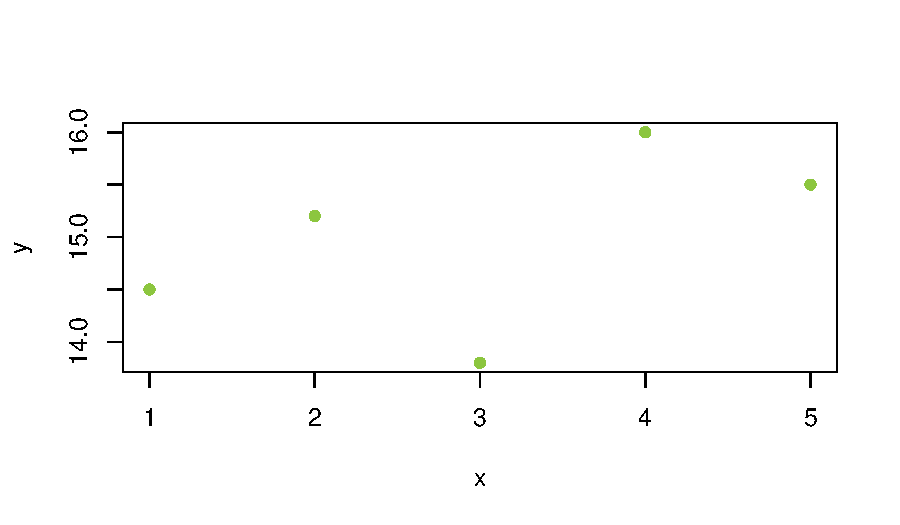
\includegraphics[width=0.5\textwidth,height=\textheight]{09-funciones_clases_files/figure-pdf/r_plot_unal_ejemplo-1.pdf}
\end{center}

\begin{Shaded}
\begin{Highlighting}[]
\CommentTok{\# USO 2: Llamada avanzada aprovechando los tres puntos (...).}
\CommentTok{\# Pasamos \textquotesingle{}x\textquotesingle{} e \textquotesingle{}y\textquotesingle{}, pero también enviamos \textquotesingle{}main\textquotesingle{}, \textquotesingle{}xlab\textquotesingle{} e \textquotesingle{}ylab\textquotesingle{}.}
\CommentTok{\# Nuestra función plot\_unal NO sabe qué son estos parámetros, pero gracias }
\CommentTok{\# a los \textquotesingle{}...\textquotesingle{}, los atrapa y se los reenvía intactos a la función interna plot().}
\FunctionTok{plot\_unal}\NormalTok{(dias, temperaturas, }
          \AttributeTok{main =} \StringTok{"Temperaturas en el Campus Bogotá"}\NormalTok{, }
          \AttributeTok{xlab =} \StringTok{"Día de la semana"}\NormalTok{, }
          \AttributeTok{ylab =} \StringTok{"Temperatura (°C)"}\NormalTok{)}
\end{Highlighting}
\end{Shaded}

\begin{center}
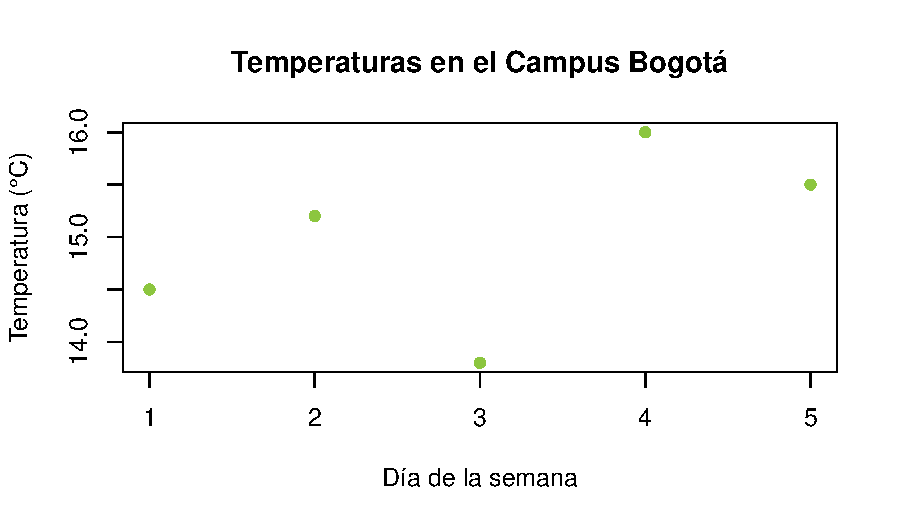
\includegraphics[width=0.5\textwidth,height=\textheight]{09-funciones_clases_files/figure-pdf/r_plot_unal_ejemplo-2.pdf}
\end{center}

\begin{Shaded}
\begin{Highlighting}[]
\CommentTok{\# USO 3: Sobrescribiendo parámetros.}
\CommentTok{\# Si el usuario pasa un parámetro que la función interna plot() reconoce, }
\CommentTok{\# se aplicará. Por ejemplo, podemos cambiar el tamaño del punto con \textquotesingle{}cex\textquotesingle{}.}
\FunctionTok{plot\_unal}\NormalTok{(dias, temperaturas, }
          \AttributeTok{main =} \StringTok{"Temperaturas (Puntos Grandes)"}\NormalTok{, }
          \AttributeTok{cex =} \FloatTok{2.5}\NormalTok{) }\CommentTok{\# \textquotesingle{}cex\textquotesingle{} es atrapado por los \textquotesingle{}...\textquotesingle{} y agranda los puntos}
\end{Highlighting}
\end{Shaded}

\begin{center}
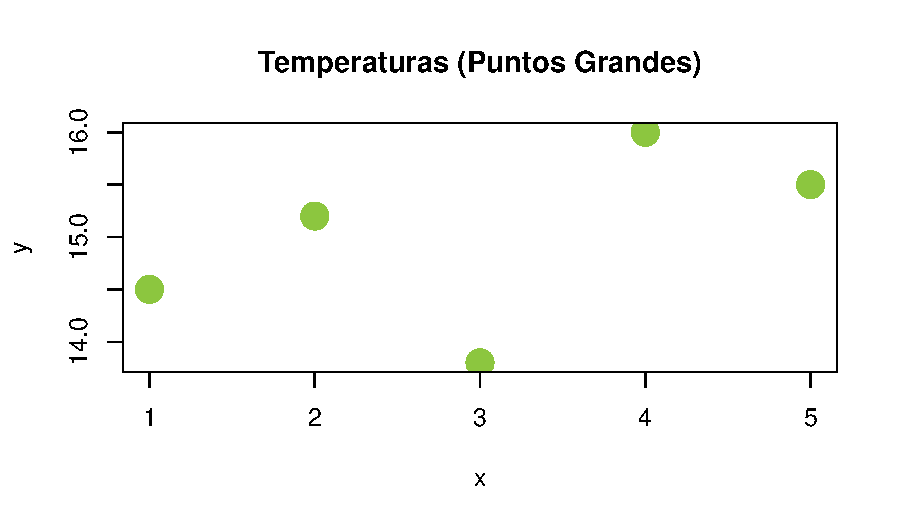
\includegraphics[width=0.5\textwidth,height=\textheight]{09-funciones_clases_files/figure-pdf/r_plot_unal_ejemplo-3.pdf}
\end{center}

\subsection{Resumen de sintaxis: estructura de
funciones}\label{resumen-de-sintaxis-estructura-de-funciones}

\begin{longtable}[]{@{}
  >{\raggedright\arraybackslash}p{(\columnwidth - 6\tabcolsep) * \real{0.2500}}
  >{\raggedright\arraybackslash}p{(\columnwidth - 6\tabcolsep) * \real{0.2500}}
  >{\raggedright\arraybackslash}p{(\columnwidth - 6\tabcolsep) * \real{0.2500}}
  >{\raggedright\arraybackslash}p{(\columnwidth - 6\tabcolsep) * \real{0.2500}}@{}}
\caption{Diferencias en el empaquetado y argumentos de
funciones}\label{tbl-funciones_argumentos}\tabularnewline
\toprule\noalign{}
\begin{minipage}[b]{\linewidth}\raggedright
Característica
\end{minipage} & \begin{minipage}[b]{\linewidth}\raggedright
Python
\end{minipage} & \begin{minipage}[b]{\linewidth}\raggedright
R
\end{minipage} & \begin{minipage}[b]{\linewidth}\raggedright
Julia
\end{minipage} \\
\midrule\noalign{}
\endfirsthead
\toprule\noalign{}
\begin{minipage}[b]{\linewidth}\raggedright
Característica
\end{minipage} & \begin{minipage}[b]{\linewidth}\raggedright
Python
\end{minipage} & \begin{minipage}[b]{\linewidth}\raggedright
R
\end{minipage} & \begin{minipage}[b]{\linewidth}\raggedright
Julia
\end{minipage} \\
\midrule\noalign{}
\endhead
\bottomrule\noalign{}
\endlastfoot
\textbf{Declaración} & \texttt{def\ calc(x):} &
\texttt{calc\ \textless{}-\ function(x)\ \{\ \}} &
\texttt{function\ calc(x)\ ...\ end} \\
\textbf{Retorno} & \texttt{return\ y} & \texttt{return(y)} &
\texttt{return\ y} \\
\textbf{Parámetro x defecto} & \texttt{def\ calc(r=6371):} &
\texttt{function(r=6371)} & \texttt{function\ calc(;\ r=6371)} \\
\textbf{Múltiples args extra} & \texttt{**kwargs} & \texttt{...} &
\texttt{kwargs...} \\
\end{longtable}

\section{Clases: organizando datos y comportamiento
juntos}\label{clases-organizando-datos-y-comportamiento-juntos}

En el mundo del desarrollo de software, existen diferentes formas de
estructurar el código. Tradicionalmente, la programación separaba los
datos por un lado y las funciones que operaban sobre esos datos por el
otro. Sin embargo, la \textbf{Programación Orientada a Objetos (POO)}
propone un paradigma distinto: agrupar los datos y los comportamientos
relacionados en una sola entidad unificada.

Para dominar este paradigma, primero debemos entender sus conceptos
genéricos fundamentales:

\begin{itemize}
\tightlist
\item
  \textbf{Clase:} Es el plano, la plantilla o el molde abstracto. No
  contiene datos reales, sino que define qué estructura tendrán los
  datos y qué acciones se podrán realizar.
\item
  \textbf{Objeto (o instancia):} Es la materialización de la clase. Es
  el producto final creado a partir del molde, que ocupa un espacio real
  en la memoria de la computadora y contiene datos específicos.
\item
  \textbf{Atributos (o estado):} Son las variables internas que guardan
  las características únicas de cada objeto.
\item
  \textbf{Métodos (o comportamiento):} Son las funciones que viven
  dentro (o asociadas) al objeto. Definen lo que el objeto ``sabe
  hacer'' con sus propios datos.
\item
  \textbf{Constructor:} Es la puerta de entrada. Es el mecanismo inicial
  que toma los datos crudos y los ensambla siguiendo las reglas de la
  clase para dar vida a un nuevo objeto.
\end{itemize}

\subsection{Analogía entre clases/objetos y
moldes/arepas}\label{analoguxeda-entre-clasesobjetos-y-moldesarepas}

\begin{itemize}
\tightlist
\item
  \textbf{La Clase (el molde):} Es como el plano arquitectónico de una
  casa o el molde para hacer arepas. El molde define que toda arepa
  tendrá un grosor y un diámetro, pero el molde en sí no se puede comer.
\item
  \textbf{El Objeto (la instancia):} Es la arepa ya hecha, salida del
  molde. Puedes sacar mil arepas distintas (unas de queso, otras de
  carne) usando el mismo molde. Todas comparten la misma estructura,
  pero contienen datos (rellenos) diferentes.
\end{itemize}

\subsection{El reto: de simples números a entidades
inteligentes}\label{el-reto-de-simples-nuxfameros-a-entidades-inteligentes}

En el análisis de datos espaciales, solemos trabajar con coordenadas
crudas (simples pares de números). Si los dejamos sueltos, son solo
texto sin significado. Nuestro objetivo en este ejercicio es aplicar los
conceptos de la POO para tomar esos números y ``darles vida''.

Queremos tomar dos simples coordenadas geográficas y convertirlas en un
\textbf{Objeto Espacial Inteligente} que tenga la capacidad intrínseca
de realizar tres tareas fundamentales:

\begin{enumerate}
\def\labelenumi{\arabic{enumi}.}
\tightlist
\item
  \textbf{Representarse a sí mismo (Texto):} Que el objeto pueda
  decirnos su nombre y ubicación en un formato legible para humanos.
\item
  \textbf{Analítica espacial (Matemáticas):} Que el objeto tenga la
  capacidad de calcular la distancia hacia otro punto.
\item
  \textbf{Visualización (Gráficos):} Que el objeto, al recibir un punto
  de destino, sepa cómo dibujar un mapa interactivo mostrando la ruta y
  la distancia entre ambos.
\end{enumerate}

A continuación, ilustramos conceptualmente este flujo de transformación:

\begin{figure}

\centering{

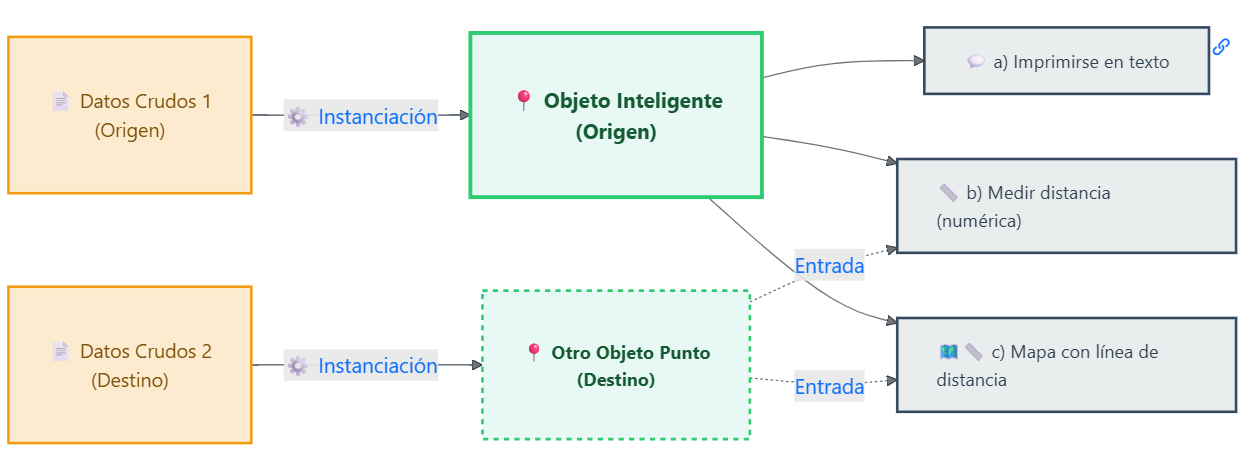
\includegraphics{./images/ejercicio_clases.png}

}

\caption{\label{fig-flujo-conceptual}Flujo conceptual: Transformación de
datos crudos en un objeto inteligente con capacidades.}

\end{figure}%

En esta sección, crearemos una Clase llamada \texttt{PuntoEspacial}.
Este ``molde'' le enseñará a la computadora cuatro cosas fundamentales:

\subsection{Python y la Programación Orientada a Objetos
(OOP)}\label{python-y-la-programaciuxf3n-orientada-a-objetos-oop}

En Python, la creación de estructuras de datos y su comportamiento sigue
un enfoque clásico y estricto de \textbf{Programación Orientada a
Objetos (OOP)}. A diferencia de otros lenguajes donde los datos y las
funciones operan por separado, Python prefiere encapsularlo todo (el
estado y las acciones) dentro de una única fortaleza lógica: \textbf{La
Clase}.

\begin{tcolorbox}[enhanced jigsaw, coltitle=black, leftrule=.75mm, bottomtitle=1mm, title=\textcolor{quarto-callout-tip-color}{\faLightbulb}\hspace{0.5em}{La Analogía: El Molde y la Arepa}, colback=white, colbacktitle=quarto-callout-tip-color!10!white, left=2mm, toptitle=1mm, rightrule=.15mm, titlerule=0mm, arc=.35mm, colframe=quarto-callout-tip-color-frame, bottomrule=.15mm, toprule=.15mm, opacityback=0, opacitybacktitle=0.6, breakable]

Para visualizar cómo Python maneja la memoria, imaginemos una cocina:

\begin{itemize}
\tightlist
\item
  \textbf{La Clase (\texttt{class\ PuntoEspacial}):} Es el \textbf{molde
  de hierro}. Por sí solo no contiene ingredientes ni alimenta a nadie;
  es simplemente un diseño estático que dicta la estructura geométrica,
  qué datos son obligatorios y qué acciones se pueden realizar.
\item
  \textbf{El Objeto (La Instancia):} Es la \textbf{arepa física y
  calientita}. Cuando pasamos ingredientes reales (latitud, longitud,
  nombre) a través del molde, el computador reserva un espacio en
  memoria para crear una instancia concreta y única. Podemos sacar mil
  ``arepas'' (objetos) del mismo molde, y cada una tendrá sus propios
  datos independientes.
\end{itemize}

\end{tcolorbox}

\emph{Como ilustra la siguiente figura, en Python el paradigma es
encapsulado: el objeto nace con sus datos y sus herramientas listas para
usar.}

\begin{figure}

\centering{

\includegraphics[width=0.5\textwidth,height=\textheight]{./images/python_classes_analogy.png}

}

\caption{\label{fig-analogia-python}\textbf{El paradigma de Python (POO
Clásica):} La Clase actúa como una fábrica o molde que estampa objetos.
Cada objeto (la arepa) no solo contiene datos, sino que lleva
incrustadas sus propias herramientas y métodos (como la navaja suiza o
la calculadora) para resolver problemas por sí mismo.}

\end{figure}%

\subsubsection{La anatomía del molde}\label{la-anatomuxeda-del-molde}

Cuando diseñamos una clase en Python, establecemos un contrato estricto
con la máquina a través de métodos mágicos y atributos:

\begin{enumerate}
\def\labelenumi{\arabic{enumi}.}
\item
  \textbf{El Constructor (\texttt{\_\_init\_\_}):} Es la puerta de
  entrada. Cada vez que intentamos crear un objeto nuevo, Python llama
  automáticamente a esta función para recibir los parámetros iniciales y
  ``ensamblar'' la estructura en la memoria.
\item
  \textbf{El Auto-reconocimiento (\texttt{self}):} En Python, la clase
  necesita una forma de referirse a la ``arepa'' específica que está
  cocinando en ese momento. El parámetro \texttt{self} es ese ancla;
  garantiza que si modificamos la latitud del ``Punto A'', no
  estropeemos accidentalmente la latitud del ``Punto B''.
\item
  \textbf{La representación (\texttt{\_\_str\_\_}):} Cómo debe
  presentarse el objeto si intentamos imprimirlo en pantalla.
\item
  \textbf{Los Métodos (Comportamiento):} Son las funciones que viven
  \textbf{dentro} de la clase. Una vez instanciado el objeto, este carga
  consigo mismo todas sus herramientas. Un punto espacial en Python
  ``sabe'' cómo calcular su propia distancia hacia otro punto o cómo
  graficarse a sí mismo en un mapa.

  \begin{itemize}
  \tightlist
  \item
    \textbf{Los métodos analíticos (\texttt{distancia\_hacia}):}
    Funciones que viven \emph{dentro} del objeto. Nuestro punto será tan
    inteligente que sabrá calcular la distancia hacia otro punto por sí
    mismo, invocando internamente a la función \texttt{haversine} que
    programamos en la sección anterior. Además, le agregaremos un
    parámetro dinámico para que pueda devolver la distancia en
    \textbf{metros} si se lo pedimos.
  \item
    \textbf{El método gráfico (\texttt{graficar\_ruta}):} Un método que
    le permite al objeto usar una librería cartográfica para dibujarse a
    sí mismo en un mapa base. Además, usaremos nuestro método analítico
    para calcular el punto medio y ¡escribir la distancia calculada
    directamente sobre la línea de la ruta!
  \end{itemize}
\end{enumerate}

A continuación, visualizamos este ciclo de vida completo: primero, el
diagrama estructural del molde (la Clase) y sus métodos internos; y
luego, el mapa de ejecución que muestra cómo sacamos las instancias
(Objetos) a la memoria para interactuar con ellas.

\begin{figure}

\centering{

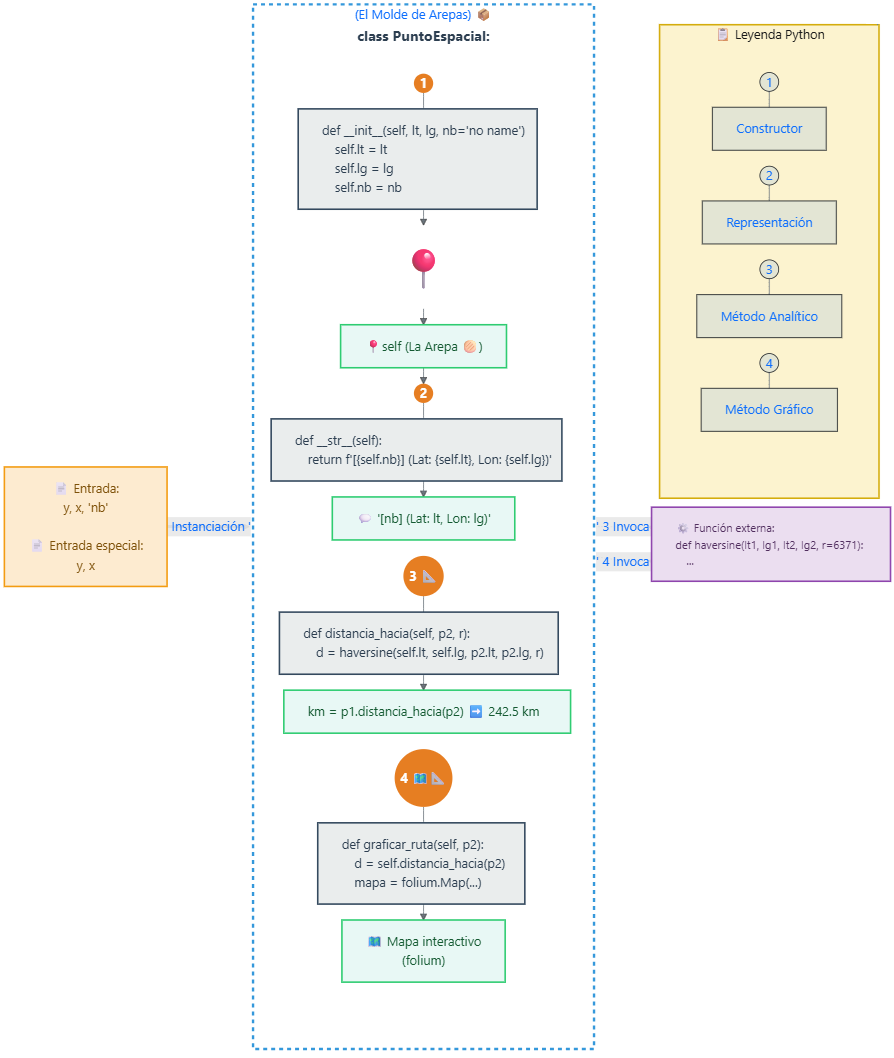
\includegraphics{./images/clase_python.png}

}

\caption{\label{fig-clases-python-final-vertical}Diagrama del flujo de
instanciación: El molde (Clase) y las arepas (Objetos).}

\end{figure}%

Resumen del código necesario para crear una clase en Python:

\begin{Shaded}
\begin{Highlighting}[]
\CommentTok{\# {-}{-}{-} 1. DEFINICIÓN DEL MOLDE (LA CLASE) {-}{-}{-}}
\KeywordTok{class}\NormalTok{ PuntoEspacial:}

    \CommentTok{\# [1 📍] 1.1 EL CONSTRUCTOR (\_\_init\_\_)}
    \KeywordTok{def} \FunctionTok{\_\_init\_\_}\NormalTok{(}\VariableTok{self}\NormalTok{, ...):}
\NormalTok{        ...}

    \CommentTok{\# [2 💬] 1.2 LA REPRESENTACIÓN TEXTUAL (\_\_str\_\_)}
    \KeywordTok{def} \FunctionTok{\_\_str\_\_}\NormalTok{(}\VariableTok{self}\NormalTok{):}
\NormalTok{        ...}

    \CommentTok{\# [3 📐] 1.3 LOS MÉTODOS (COMPORTAMIENTO ANALÍTICO)}
    \KeywordTok{def}\NormalTok{ distancia\_hacia(}\VariableTok{self}\NormalTok{, ...):}
\NormalTok{        ...}

    \CommentTok{\# [4 🗺️📐] 1.4 EL MÉTODO GRÁFICO (MAPA BASE CON ETIQUETA VISIBLE)}
    \KeywordTok{def}\NormalTok{ graficar\_ruta(}\VariableTok{self}\NormalTok{, otro\_punto):}
\NormalTok{        ...        }
\end{Highlighting}
\end{Shaded}

\begin{figure}

\centering{

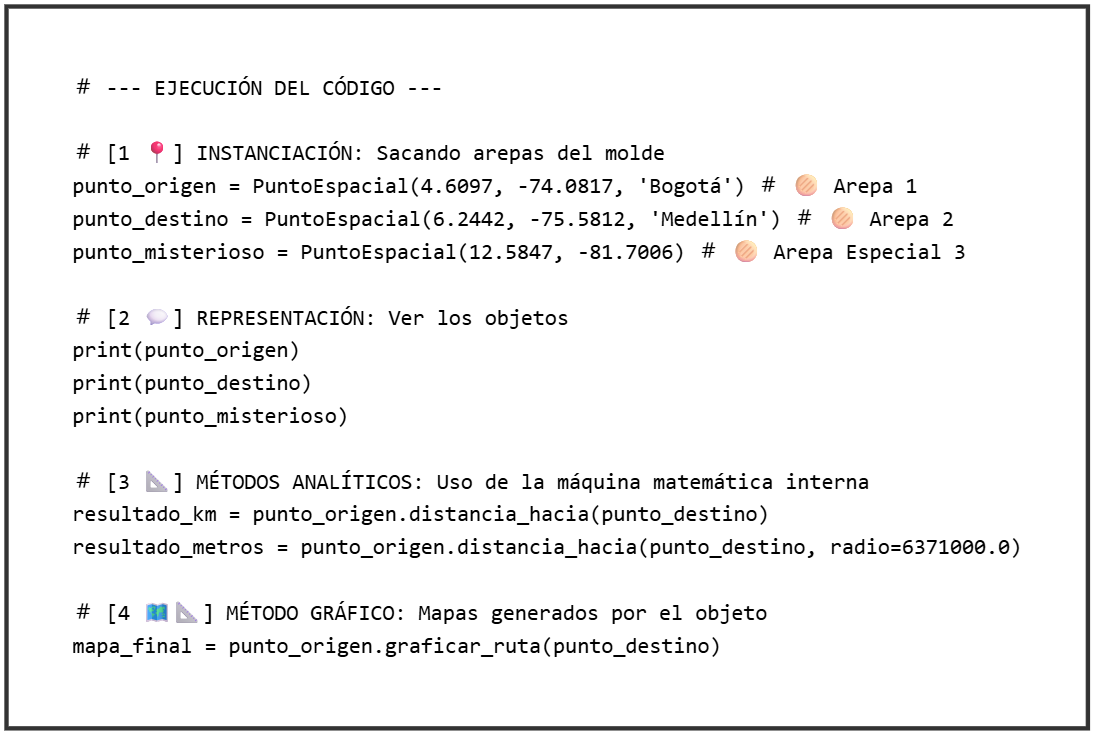
\includegraphics{./images/clase_python_codigo.png}

}

\caption{\label{fig-clases-python-codigo}Ejecución del código
instanciando los objetos en memoria.}

\end{figure}%

\subsection{R y el sistema S3: la ilusión del molde y el poder de la
etiqueta}\label{r-y-el-sistema-s3-la-ilusiuxf3n-del-molde-y-el-poder-de-la-etiqueta}

Mientras que Python utiliza un enfoque estricto donde cada objeto nace
de un ``molde de hierro'' predefinido, R aborda la programación
orientada a objetos de una manera mucho más relajada e informal,
principalmente a través de su \textbf{sistema S3}.

En R, las clases no se definen formalmente. No hay una bóveda blindada
que encierre los datos y los métodos juntos. En su lugar, el sistema S3
confía en el ``sistema de honor'' y en el uso inteligente de etiquetas.

\begin{tcolorbox}[enhanced jigsaw, coltitle=black, leftrule=.75mm, bottomtitle=1mm, title=\textcolor{quarto-callout-note-color}{\faInfo}\hspace{0.5em}{La analogía: el recipiente común y el post-it}, colback=white, colbacktitle=quarto-callout-note-color!10!white, left=2mm, toptitle=1mm, rightrule=.15mm, titlerule=0mm, arc=.35mm, colframe=quarto-callout-note-color-frame, bottomrule=.15mm, toprule=.15mm, opacityback=0, opacitybacktitle=0.6, breakable]

Si en Python teníamos un molde de hierro para hacer arepas, en R la
cocina funciona muy distinto:

\begin{itemize}
\tightlist
\item
  \textbf{Los ingredientes (la lista):} En lugar de un molde, tomamos un
  recipiente plástico común y corriente (como el ``porta'' del almuerzo
  o una \texttt{list} en R), y echamos ahí nuestros ingredientes crudos
  (latitud, longitud y nombre).
\item
  \textbf{La ``clase'' (el post-it):} Para convertir esa lista genérica
  en un objeto espacial, literalmente le pegamos un ``post-it'' en la
  tapa del recipiente. Al asignarle un atributo de clase
  (\texttt{class(objeto)\ \textless{}-\ \textquotesingle{}PuntoEspacial\textquotesingle{}}),
  le estamos diciendo a R: \emph{``De ahora en adelante, confía en mí y
  trata a este recipiente como si fuera una arepa''}.
\end{itemize}

\end{tcolorbox}

\emph{En R, el sistema es mucho más flexible e informal, dependiendo
enteramente de cómo etiquetamos nuestros contenedores de datos:}

\begin{figure}

\centering{

\includegraphics[width=0.5\textwidth,height=\textheight]{./images/r_classes_analogy.png}

}

\caption{\label{fig-analogia-r}\textbf{El paradigma de R (Sistema S3):}
Los objetos no tienen herramientas por dentro; son contenedores
plásticos estándar (listas) llenos de datos crudos. Lo que les da
``poder'' es una simple etiqueta o post-it (la Clase S3). Las funciones
externas actúan como inspectores que leen esta etiqueta para decidir qué
herramienta usar.}

\end{figure}%

\subsubsection{La anatomía del sistema
S3}\label{la-anatomuxeda-del-sistema-s3}

Dado que no hay un ``molde'' real, la instanciación y el comportamiento
en R se dividen en tres pilares fundamentales que flotan libremente en
el entorno:

\begin{enumerate}
\def\labelenumi{\arabic{enumi}.}
\tightlist
\item
  \textbf{El constructor informal:} Es simplemente una función normal
  (como \texttt{nuevo\_punto\_espacial()}) que recibe los datos, los
  empaqueta en una lista y, lo más importante, le estampa la etiqueta de
  la clase antes de devolverla.
\item
  \textbf{Las funciones genéricas (los inspectores):} Funciones como
  \texttt{print()} o \texttt{distancia\_hacia()} son genéricas. No saben
  cómo calcular nada por sí mismas; su único trabajo es mirar el
  ``post-it'' del objeto que reciben y decir: \emph{``Ah, eres un
  PuntoEspacial, déjame buscar al experto que sabe tratar contigo''}.
  Esto se logra mediante el comando interno \texttt{UseMethod()}.
\item
  \textbf{Los métodos específicos (el despacho):} Son las funciones que
  realmente hacen el trabajo duro, y se nombran uniendo el genérico y la
  clase (por ejemplo, \texttt{distancia\_hacia.PuntoEspacial()}). El
  genérico le ``despacha'' el objeto a esta función especializada.
\end{enumerate}

A continuación, visualizamos este paradigma en acción: primero, el
diagrama arquitectónico que muestra cómo los métodos flotan fuera de la
estructura de datos; y luego, el bloque de ejecución donde vemos la
magia del etiquetado y el despacho S3 en tiempo real.

\begin{figure}

\centering{

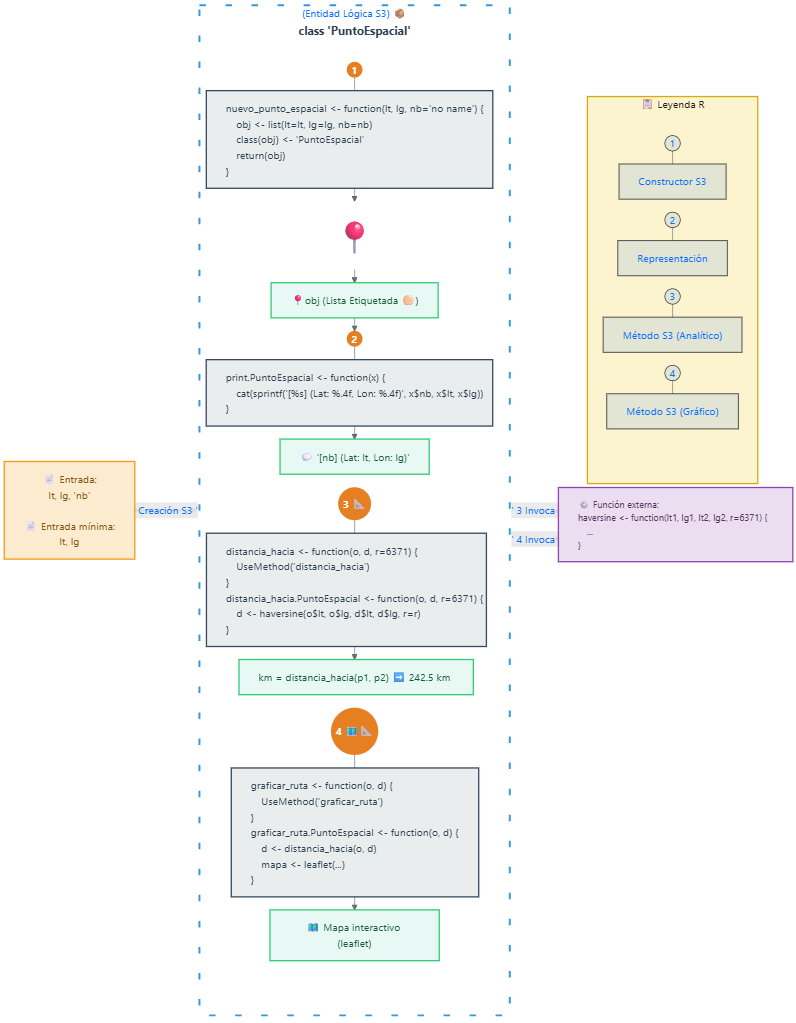
\includegraphics{./images/clase_r.png}

}

\caption{\label{fig-clases-r-final-vertical}Diagrama del flujo de
instanciación en R (S3): El molde y las arepas.}

\end{figure}%

Resumen del código para una clase en R:

\begin{Shaded}
\begin{Highlighting}[]
\CommentTok{\# {-}{-}{-} 1. DEFINICIÓN DEL MOLDE (FUNCIÓN CONSTRUCTORA) {-}{-}{-}}
\CommentTok{\# [1 📍] 1.1 EL CONSTRUCTOR INFORMAL}
\NormalTok{nuevo\_punto\_espacial }\OtherTok{\textless{}{-}} \ControlFlowTok{function}\NormalTok{(...) \{}
    \CommentTok{\# Creamos una lista para los atributos}
\NormalTok{    objeto }\OtherTok{\textless{}{-}} \FunctionTok{list}\NormalTok{(}
        \AttributeTok{latitud =}\NormalTok{ ...,}
\NormalTok{        ...}
\NormalTok{    )}
    
    \CommentTok{\# Etiquetado de clase (MAGIA)}
    \FunctionTok{class}\NormalTok{(objeto) }\OtherTok{\textless{}{-}} \StringTok{"PuntoEspacial"}
    
    \FunctionTok{return}\NormalTok{(objeto)}
\NormalTok{\}}

\CommentTok{\# [2 💬] 1.2 LA REPRESENTACIÓN TEXTUAL (Sobrescribir \textquotesingle{}print\textquotesingle{})}
\NormalTok{print.PuntoEspacial }\OtherTok{\textless{}{-}} \ControlFlowTok{function}\NormalTok{(obj) \{}
\NormalTok{    ...}
\NormalTok{\}}

\CommentTok{\# [3 📐] 1.3 LOS MÉTODOS (COMPORTAMIENTO ANALÍTICO)}
\CommentTok{\# función genérica}
\NormalTok{distancia\_hacia }\OtherTok{\textless{}{-}} \ControlFlowTok{function}\NormalTok{(...) \{}
    \FunctionTok{UseMethod}\NormalTok{(}\StringTok{"distancia\_hacia"}\NormalTok{)}
\NormalTok{\}}

\CommentTok{\# Ese método SOLO para la clase "PuntoEspacial"}
\NormalTok{distancia\_hacia.PuntoEspacial }\OtherTok{\textless{}{-}} \ControlFlowTok{function}\NormalTok{(...) \{}
\NormalTok{    ...}
\NormalTok{\}}

\CommentTok{\# [4 🗺️📐] 1.4 EL MÉTODO GRÁFICO}
\NormalTok{graficar\_ruta }\OtherTok{\textless{}{-}} \ControlFlowTok{function}\NormalTok{(...) \{}
    \FunctionTok{UseMethod}\NormalTok{(}\StringTok{"graficar\_ruta"}\NormalTok{)}
\NormalTok{\}}

\CommentTok{\# Ese método SOLO para la clase PuntoEspacial}
\NormalTok{graficar\_ruta.PuntoEspacial }\OtherTok{\textless{}{-}} \ControlFlowTok{function}\NormalTok{(...) \{}
\NormalTok{    ...}
\NormalTok{\}}
\end{Highlighting}
\end{Shaded}

\begin{figure}

\centering{

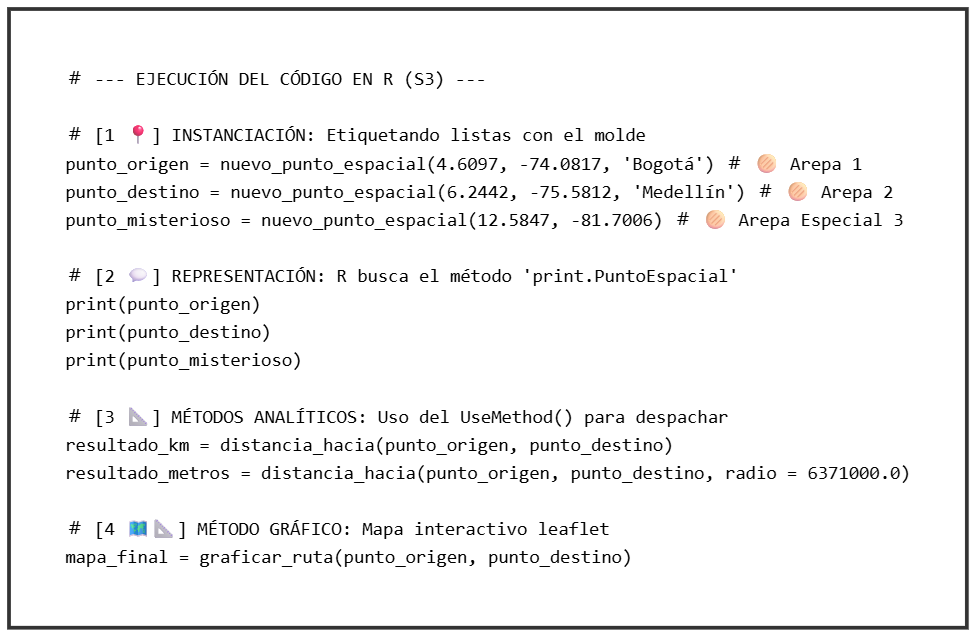
\includegraphics{./images/clase_r_codigo.png}

}

\caption{\label{fig-clases-r-codigo}Ejecución del código en R (S3)
instanciando los objetos en memoria.}

\end{figure}%

\subsection{Julia y el despacho múltiple: separando los ingredientes de
la
receta}\label{julia-y-el-despacho-muxfaltiple-separando-los-ingredientes-de-la-receta}

Julia rechaza por completo el concepto tradicional de clases que vimos
en Python. En su lugar, abraza un paradigma donde los datos (las
variables) y el comportamiento (las funciones) están estrictamente
separados, pero trabajan en una armonía perfecta gracias al núcleo
absoluto del lenguaje: el \textbf{despacho múltiple} (Multiple
Dispatch).

\begin{tcolorbox}[enhanced jigsaw, coltitle=black, leftrule=.75mm, bottomtitle=1mm, title=\textcolor{quarto-callout-tip-color}{\faLightbulb}\hspace{0.5em}{La analogía: el contenedor rígido y los chefs expertos}, colback=white, colbacktitle=quarto-callout-tip-color!10!white, left=2mm, toptitle=1mm, rightrule=.15mm, titlerule=0mm, arc=.35mm, colframe=quarto-callout-tip-color-frame, bottomrule=.15mm, toprule=.15mm, opacityback=0, opacitybacktitle=0.6, breakable]

Si Python es un molde de hierro y R es un post-it, Julia es una cocina
de alta eficiencia:

\begin{itemize}
\tightlist
\item
  \textbf{El contenedor (\texttt{struct}):} Es un contenedor plástico
  rígido (como un ``porta'' de cristal). Su única función es guardar los
  ingredientes (latitud, longitud, nombre) de forma organizada y con
  etiquetas de tipo muy estrictas (\texttt{Float64}, \texttt{String}).
  El \texttt{struct} es ``tonto''; no sabe hacer absolutamente nada por
  sí solo, no tiene métodos ni recetas grabadas en sus paredes.
\item
  \textbf{El comportamiento (las funciones libres):} Son un batallón de
  chefs expertos que están esperando en la cocina. Cuando usted grita
  ``¡Quiero la distancia!'', el jefe de cocina (el compilador de Julia)
  mira exactamente qué ingredientes le entregó en el porta. Dependiendo
  de los tipos de datos que usted mande, le asigna el trabajo al chef
  que tenga la receta matemática más optimizada para esos tipos exactos.
\end{itemize}

\end{tcolorbox}

\emph{Julia lleva la separación entre datos y herramientas al extremo,
usando una estrategia de clasificación ultrarrápida:}

\begin{figure}

\centering{

\includegraphics[width=0.5\textwidth,height=\textheight]{./images/julia_struct_analogy.png}

}

\caption{\label{fig-analogia-julia}\textbf{El paradigma de Julia
(Despacho Múltiple):} Los datos están resguardados en contenedores
inmutables (Structs). Las funciones son chefs externos altamente
especializados. Cuando pides una operación, el compilador (el ``Jefe de
Cocina'') escanea con láser los tipos de datos exactos y llama
instantáneamente al chef que tiene la receta matemática perfecta para
esa combinación.}

\end{figure}%

\subsubsection{La anatomía de la arquitectura en
Julia}\label{la-anatomuxeda-de-la-arquitectura-en-julia}

En este lenguaje, construimos la estructura definiendo tipos de datos
crudos y luego escribimos funciones libres que declaran para qué
combinaciones de tipos están preparadas.

\begin{enumerate}
\def\labelenumi{\arabic{enumi}.}
\tightlist
\item
  \textbf{La estructura base (\texttt{struct}):} A diferencia de las
  clases, aquí solo organizamos las variables en la memoria. Esto
  garantiza un tipado fuerte que le permite a Julia ser tan rápido como
  C o Fortran.
\item
  \textbf{El constructor:} Julia crea un constructor automático básico,
  pero podemos crear constructores propios si necesitamos reglas
  especiales (como asignar `no name' si el usuario olvida el nombre al
  llenar el contenedor).
\item
  \textbf{El despacho múltiple en acción:} La magia ocurre al llamar a
  una función. Si tenemos una función \texttt{distancia\_hacia(a,\ b)},
  Julia analiza el tipo de dato exacto de \textbf{todos} los argumentos
  que le pasamos. Basado en esa combinación de tipos, el lenguaje enruta
  la ejecución al método más específico de forma instantánea.
\end{enumerate}

A continuación, visualizamos este potente paradigma: primero, la
representación de cómo el \texttt{struct} y el despacho múltiple
interactúan conceptualmente en una ``caja virtual'' (con líneas muy
espaciadas para notar que no es una prisión de código); y luego, el
bloque de ejecución donde vemos a Julia activando los métodos correctos
al vuelo.

\begin{figure}

\centering{

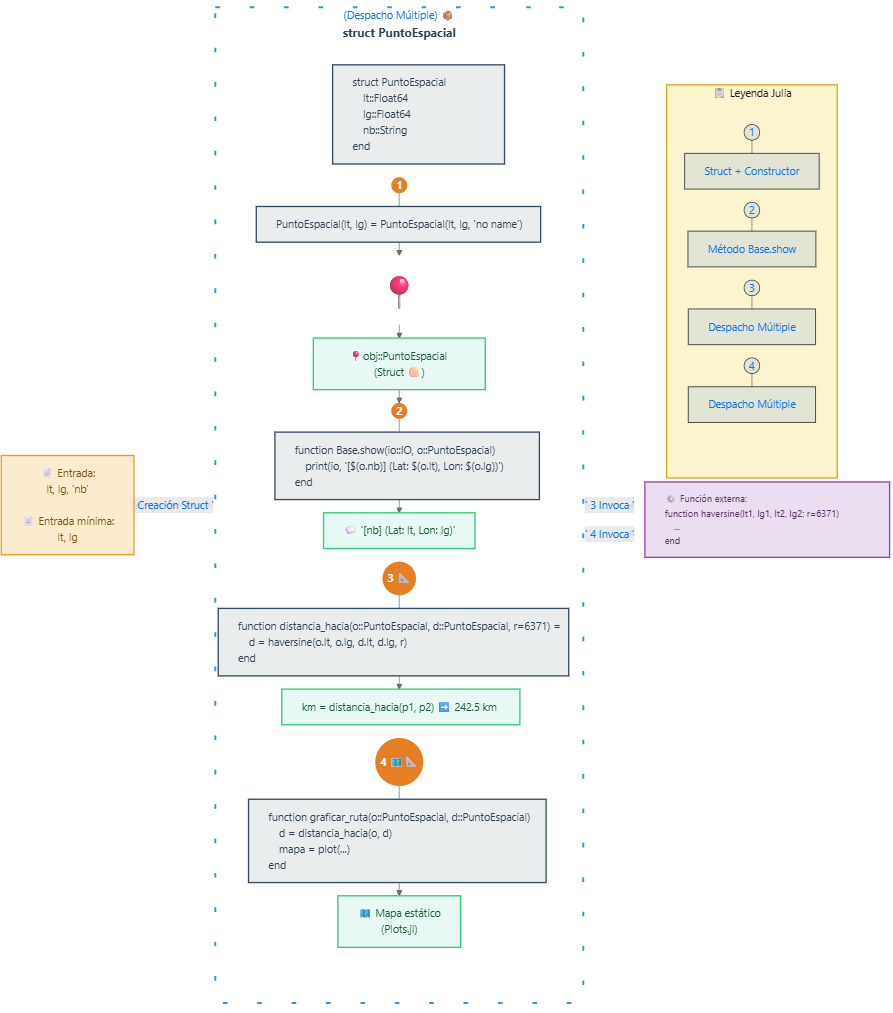
\includegraphics{./images/clase_julia.png}

}

\caption{\label{fig-clases-julia-final-vertical}Diagrama del flujo de
instanciación en Julia (Despacho Múltiple): El molde (Struct) y las
arepas.}

\end{figure}%

Resumen del código para un tipo (struct) en Julia

\begin{Shaded}
\begin{Highlighting}[]
\CommentTok{\# {-}{-}{-} 1. DEFINICIÓN DE LA CLASE (MOLDE) {-}{-}{-}}
\CommentTok{\# [1 📍] 1.1 EL CONSTRUCTOR (LA ESTRUCTURA)}

\KeywordTok{struct}\NormalTok{ PuntoEspacial}
\NormalTok{    latitud}\OperatorTok{::}\DataTypeTok{Float64   }\CommentTok{\# Coordenada Y}
    \OperatorTok{...}
\KeywordTok{end}

\CommentTok{\# Definimos un método constructor adicional}
\FunctionTok{PuntoEspacial}\NormalTok{(lat, lon) }\OperatorTok{=} \FunctionTok{PuntoEspacial}\NormalTok{(lat, lon, }\StringTok{"No Name"}\NormalTok{)}


\CommentTok{\# [2 💬] 1.2 LA REPRESENTACIÓN TEXTUAL}
\KeywordTok{function} \BuiltInTok{Base}\NormalTok{.}\FunctionTok{show}\NormalTok{(io}\OperatorTok{::}\DataTypeTok{IO}\NormalTok{, obj}\OperatorTok{::}\DataTypeTok{PuntoEspacial}\NormalTok{)}
    \FunctionTok{print}\NormalTok{(}\OperatorTok{...}\NormalTok{)}
\KeywordTok{end}


\CommentTok{\# [3 📐] 1.3 MÉTODOS ANALÍTICOS (DESPACHO MÚLTIPLE)}
\KeywordTok{function} \FunctionTok{distancia\_hacia}\NormalTok{(o}\OperatorTok{::}\DataTypeTok{PuntoEspacial}\NormalTok{, d}\OperatorTok{::}\DataTypeTok{PuntoEspacial}\NormalTok{; r}\OperatorTok{=}\FloatTok{6371.0}\NormalTok{)}
    \OperatorTok{...}
    \ControlFlowTok{return}\NormalTok{ distancia}
\KeywordTok{end}


\CommentTok{\# [4 🗺️📐] 1.4 MÉTODO GRÁFICO (DIBUJO Y MANIPULACIÓN DE CADENAS)}
\KeywordTok{function} \FunctionTok{graficar\_ruta}\NormalTok{(o}\OperatorTok{::}\DataTypeTok{PuntoEspacial}\NormalTok{, d}\OperatorTok{::}\DataTypeTok{PuntoEspacial}\NormalTok{)}
    \OperatorTok{...}
    \ControlFlowTok{return}\NormalTok{ mapa}
\KeywordTok{end}
\end{Highlighting}
\end{Shaded}

\begin{figure}

\centering{

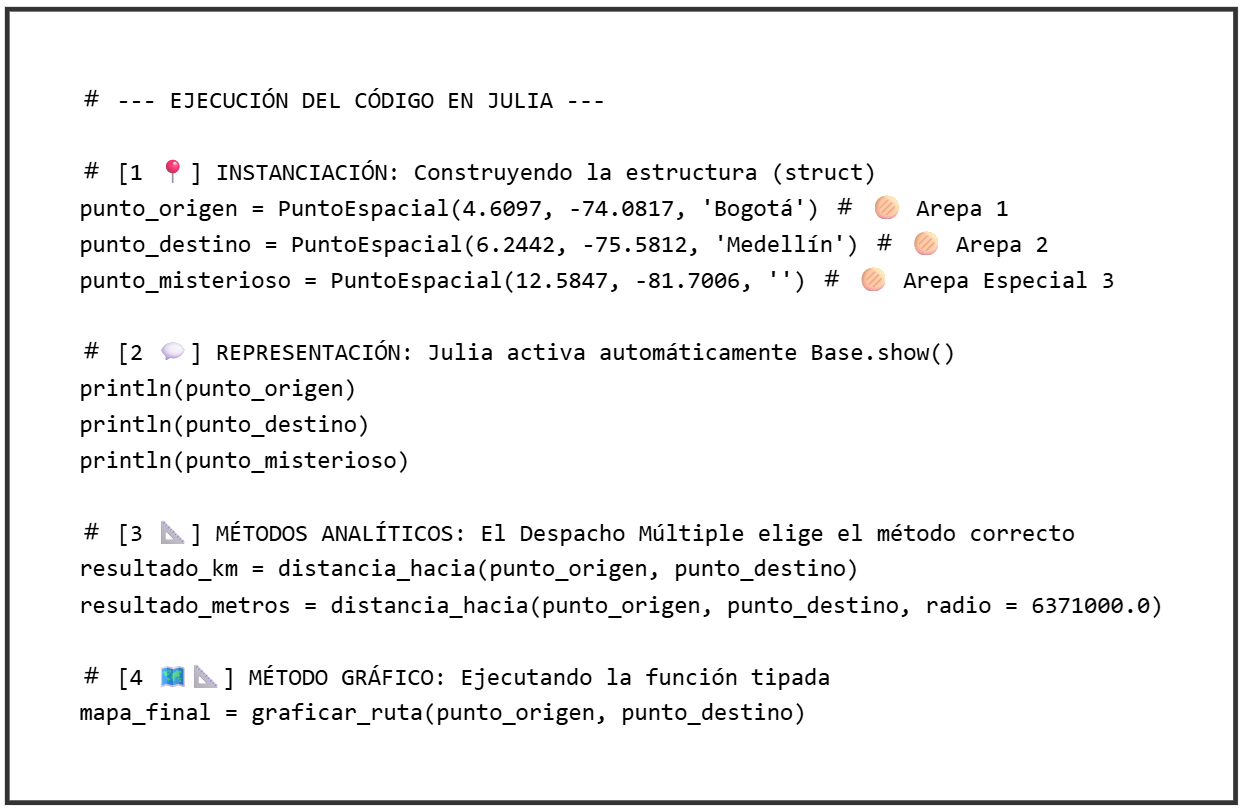
\includegraphics{./images/clase_julia_codigo.png}

}

\caption{\label{fig-clases-julia-codigo}Ejecución del código en Julia
instanciando las estructuras en memoria.}

\end{figure}%

\subsection{Laboratorio comparativo: implementación del código
completo}\label{laboratorio-comparativo-implementaciuxf3n-del-cuxf3digo-completo}

A continuación, presentamos el código completo y funcional para los tres
lenguajes. Te invitamos a navegar entre las pestañas para comparar cómo
cada arquitectura resuelve el mismo problema.

💡 \textbf{Tip de lectura:} Busca las etiquetas con emojis
(\texttt{{[}1\ 📍{]}}, \texttt{{[}2\ 💬{]}}, \texttt{{[}3\ 📐{]}},
\texttt{{[}4\ 🗺️📐{]}}) dentro de los comentarios del código. Estas te
ayudarán a conectar cada bloque de código directamente con los diagramas
de arquitectura que vimos en las secciones anteriores.

\subsubsection{Python}

\begin{Shaded}
\begin{Highlighting}[]
\CommentTok{\# \#| echo: false}
\CommentTok{\# \#| eval: false}
\ImportTok{import}\NormalTok{ math}
\ImportTok{import}\NormalTok{ folium }\CommentTok{\# Librería indispensable en Python para generar mapas interactivos}

\CommentTok{\# {-}{-}{-} 0. TRAEMOS NUESTRA MÁQUINA MATEMÁTICA {-}{-}{-}}
\CommentTok{\# Pegamos aquí la función que ya habíamos creado para que este código funcione por sí solo}
\KeywordTok{def}\NormalTok{ haversine(lat1, lon1, lat2, lon2, radio}\OperatorTok{=}\FloatTok{6371.0}\NormalTok{):}
\NormalTok{    dlat, dlon }\OperatorTok{=}\NormalTok{ math.radians(lat2 }\OperatorTok{{-}}\NormalTok{ lat1), math.radians(lon2 }\OperatorTok{{-}}\NormalTok{ lon1)}
\NormalTok{    a }\OperatorTok{=}\NormalTok{ math.sin(dlat }\OperatorTok{/} \DecValTok{2}\NormalTok{)}\OperatorTok{**}\DecValTok{2} \OperatorTok{+}\NormalTok{ math.cos(math.radians(lat1)) }\OperatorTok{*}\NormalTok{ math.cos(math.radians(lat2)) }\OperatorTok{*}\NormalTok{ math.sin(dlon }\OperatorTok{/} \DecValTok{2}\NormalTok{)}\OperatorTok{**}\DecValTok{2}
    \ControlFlowTok{return}\NormalTok{ radio }\OperatorTok{*}\NormalTok{ (}\DecValTok{2} \OperatorTok{*}\NormalTok{ math.atan2(math.sqrt(a), math.sqrt(}\DecValTok{1} \OperatorTok{{-}}\NormalTok{ a)))}


\CommentTok{\# {-}{-}{-} 1. DEFINICIÓN DEL MOLDE (LA CLASE) {-}{-}{-}}
\CommentTok{\# Usamos la palabra reservada \textquotesingle{}class\textquotesingle{} seguida del nombre (en mayúscula por convención)}
\KeywordTok{class}\NormalTok{ PuntoEspacial:}
    
    \CommentTok{\# [1 📍] 1.1 EL CONSTRUCTOR (\_\_init\_\_)}
    \CommentTok{\# Esta función especial se ejecuta automáticamente el momento en que "nace" un punto.}
    \CommentTok{\# \textquotesingle{}self\textquotesingle{} significa "yo mismo". Es la forma en que el objeto se refiere a sus propios datos.}
    \CommentTok{\# Definimos que latitud y longitud son obligatorios, pero el nombre tiene un valor por defecto.}
    \KeywordTok{def} \FunctionTok{\_\_init\_\_}\NormalTok{(}\VariableTok{self}\NormalTok{, latitud, longitud, nombre}\OperatorTok{=}\StringTok{"Punto sin nombre"}\NormalTok{):}
        
        \CommentTok{\# Guardamos la latitud que nos entregaron dentro del cuerpo del objeto (self)}
        \VariableTok{self}\NormalTok{.latitud }\OperatorTok{=}\NormalTok{ latitud}
        
        \CommentTok{\# Guardamos la longitud dentro del objeto}
        \VariableTok{self}\NormalTok{.longitud }\OperatorTok{=}\NormalTok{ longitud}
        
        \CommentTok{\# Guardamos el nombre dentro del objeto}
        \VariableTok{self}\NormalTok{.nombre }\OperatorTok{=}\NormalTok{ nombre}

    \CommentTok{\# [2 💬] 1.2 LA REPRESENTACIÓN TEXTUAL (\_\_str\_\_)}
    \CommentTok{\# Si le decimos a Python print(objeto), por defecto imprimirá basura técnica.}
    \CommentTok{\# Esta función especial le enseña a Python cómo queremos que se lea el objeto en pantalla.}
    \KeywordTok{def} \FunctionTok{\_\_str\_\_}\NormalTok{(}\VariableTok{self}\NormalTok{):}
        \CommentTok{\# SACA: Un texto bonito combinando el nombre y las coordenadas}
        \ControlFlowTok{return} \SpecialStringTok{f"[}\SpecialCharTok{\{}\VariableTok{self}\SpecialCharTok{.}\NormalTok{nombre}\SpecialCharTok{\}}\SpecialStringTok{] (Lat: }\SpecialCharTok{\{}\VariableTok{self}\SpecialCharTok{.}\NormalTok{latitud}\SpecialCharTok{\}}\SpecialStringTok{, Lon: }\SpecialCharTok{\{}\VariableTok{self}\SpecialCharTok{.}\NormalTok{longitud}\SpecialCharTok{\}}\SpecialStringTok{)"}

    \CommentTok{\# [3 📐] 1.3 LOS MÉTODOS (COMPORTAMIENTO ANALÍTICO)}
    \CommentTok{\# Es una función normal, pero como tiene \textquotesingle{}self\textquotesingle{}, vive dentro del objeto.}
    \CommentTok{\# Agregamos el parámetro \textquotesingle{}radio\textquotesingle{} para que el usuario pueda pedir el resultado en metros.}
    \KeywordTok{def}\NormalTok{ distancia\_hacia(}\VariableTok{self}\NormalTok{, otro\_punto, radio}\OperatorTok{=}\FloatTok{6371.0}\NormalTok{):}
        
        \CommentTok{\# Llamamos a nuestra función haversine externa pasándole el radio solicitado}
        \CommentTok{\# Le enviamos NUESTRAS coordenadas (self) y las coordenadas DEL OTRO (otro\_punto)}
\NormalTok{        distancia }\OperatorTok{=}\NormalTok{ haversine(}\VariableTok{self}\NormalTok{.latitud, }\VariableTok{self}\NormalTok{.longitud, otro\_punto.latitud, otro\_punto.longitud, radio)}
        
        \CommentTok{\# SACA: La distancia numérica calculada entre los dos objetos}
        \ControlFlowTok{return}\NormalTok{ distancia}
        
    \CommentTok{\# [4 🗺️📐] 1.4 EL MÉTODO GRÁFICO (MAPA BASE CON ETIQUETA VISIBLE)}
    \CommentTok{\# Este método le da la habilidad al objeto de dibujarse en un mapa web interactivo.}
    \KeywordTok{def}\NormalTok{ graficar\_ruta(}\VariableTok{self}\NormalTok{, otro\_punto):}
        
        \CommentTok{\# Primero, le decimos al objeto que calcule su propia distancia hacia el destino}
\NormalTok{        distancia\_calculada }\OperatorTok{=} \VariableTok{self}\NormalTok{.distancia\_hacia(otro\_punto)}
        
        \CommentTok{\# Calculamos el punto medio geométrico para centrar la cámara y poner el texto}
\NormalTok{        centro\_lat }\OperatorTok{=}\NormalTok{ (}\VariableTok{self}\NormalTok{.latitud }\OperatorTok{+}\NormalTok{ otro\_punto.latitud) }\OperatorTok{/} \DecValTok{2}
\NormalTok{        centro\_lon }\OperatorTok{=}\NormalTok{ (}\VariableTok{self}\NormalTok{.longitud }\OperatorTok{+}\NormalTok{ otro\_punto.longitud) }\OperatorTok{/} \DecValTok{2}
        
        \CommentTok{\# Creamos el lienzo del mapa base (estilo OpenStreetMap por defecto)}
\NormalTok{        mapa }\OperatorTok{=}\NormalTok{ folium.Map(location}\OperatorTok{=}\NormalTok{[centro\_lat, centro\_lon], zoom\_start}\OperatorTok{=}\DecValTok{6}\NormalTok{)}
        
        \CommentTok{\# Ponemos un pin en nuestra ubicación de origen (self)}
\NormalTok{        folium.Marker([}\VariableTok{self}\NormalTok{.latitud, }\VariableTok{self}\NormalTok{.longitud], popup}\OperatorTok{=}\VariableTok{self}\NormalTok{.nombre).add\_to(mapa)}
        
        \CommentTok{\# Ponemos un pin en el destino (otro\_punto)}
\NormalTok{        folium.Marker([otro\_punto.latitud, otro\_punto.longitud], popup}\OperatorTok{=}\NormalTok{otro\_punto.nombre).add\_to(mapa)}
        
        \CommentTok{\# Trazamos una línea roja que conecte ambas coordenadas}
\NormalTok{        folium.PolyLine([(}\VariableTok{self}\NormalTok{.latitud, }\VariableTok{self}\NormalTok{.longitud), (otro\_punto.latitud, otro\_punto.longitud)], color}\OperatorTok{=}\StringTok{"red"}\NormalTok{, weight}\OperatorTok{=}\DecValTok{3}\NormalTok{).add\_to(mapa)}
        
        \CommentTok{\# ¡NUEVO!: Ponemos un marcador transparente en el medio con un \textquotesingle{}Tooltip\textquotesingle{} permanente.}
        \CommentTok{\# Esto obliga a Folium a mostrar el texto de la distancia sin necesidad de hacer clic.}
\NormalTok{        etiqueta }\OperatorTok{=} \SpecialStringTok{f"Distancia: }\SpecialCharTok{\{}\NormalTok{distancia\_calculada}\SpecialCharTok{:.2f\}}\SpecialStringTok{ km"}
\NormalTok{        folium.Marker(}
\NormalTok{            [centro\_lat, centro\_lon],}
\NormalTok{            icon}\OperatorTok{=}\NormalTok{folium.DivIcon(html}\OperatorTok{=}\StringTok{""}\NormalTok{), }\CommentTok{\# Ocultamos el ícono tradicional}
\NormalTok{            tooltip}\OperatorTok{=}\NormalTok{folium.Tooltip(etiqueta, permanent}\OperatorTok{=}\VariableTok{True}\NormalTok{, direction}\OperatorTok{=}\StringTok{"top"}\NormalTok{)}
\NormalTok{        ).add\_to(mapa)}
        
        \CommentTok{\# SACA: El objeto mapa listo para ser mostrado}
        \ControlFlowTok{return}\NormalTok{ mapa}


\CommentTok{\# {-}{-}{-} 2. CREACIÓN DE OBJETOS (INSTANCIACIÓN) {-}{-}{-}}

\BuiltInTok{print}\NormalTok{(}\StringTok{"{-}{-}{-} Creando objetos a partir del molde {-}{-}{-}"}\NormalTok{)}
\end{Highlighting}
\end{Shaded}

\begin{verbatim}
--- Creando objetos a partir del molde ---
\end{verbatim}

\begin{Shaded}
\begin{Highlighting}[]
\CommentTok{\# [1 📍] INSTANCIACIÓN: Creamos el primer objeto (Bogotá). }
\CommentTok{\# Noten que no le pasamos el parámetro \textquotesingle{}self\textquotesingle{}, Python hace eso invisiblemente.}
\NormalTok{punto\_origen }\OperatorTok{=}\NormalTok{ PuntoEspacial(}\FloatTok{4.6097}\NormalTok{, }\OperatorTok{{-}}\FloatTok{74.0817}\NormalTok{, }\StringTok{"Bogotá"}\NormalTok{)}

\CommentTok{\# Creamos el segundo objeto (Medellín). Usamos los mismos planos, pero con otros datos.}
\NormalTok{punto\_destino }\OperatorTok{=}\NormalTok{ PuntoEspacial(}\FloatTok{6.2442}\NormalTok{, }\OperatorTok{{-}}\FloatTok{75.5812}\NormalTok{, }\StringTok{"Medellín"}\NormalTok{)}

\CommentTok{\# Creamos un tercer objeto, pero omitimos el nombre para ver si funciona el valor por defecto}
\NormalTok{punto\_misterioso }\OperatorTok{=}\NormalTok{ PuntoEspacial(}\FloatTok{12.5847}\NormalTok{, }\OperatorTok{{-}}\FloatTok{81.7006}\NormalTok{)}

\CommentTok{\# [2 💬] REPRESENTACIÓN: Probamos nuestra función especial \_\_str\_\_ imprimiendo los objetos}
\BuiltInTok{print}\NormalTok{(punto\_origen)}
\end{Highlighting}
\end{Shaded}

\begin{verbatim}
[Bogotá] (Lat: 4.6097, Lon: -74.0817)
\end{verbatim}

\begin{Shaded}
\begin{Highlighting}[]
\BuiltInTok{print}\NormalTok{(punto\_destino)}
\end{Highlighting}
\end{Shaded}

\begin{verbatim}
[Medellín] (Lat: 6.2442, Lon: -75.5812)
\end{verbatim}

\begin{Shaded}
\begin{Highlighting}[]
\BuiltInTok{print}\NormalTok{(punto\_misterioso)}
\end{Highlighting}
\end{Shaded}

\begin{verbatim}
[Punto sin nombre] (Lat: 12.5847, Lon: -81.7006)
\end{verbatim}

\begin{Shaded}
\begin{Highlighting}[]
\BuiltInTok{print}\NormalTok{(}\StringTok{"}\CharTok{\textbackslash{}n}\StringTok{{-}{-}{-} Usando los métodos del objeto {-}{-}{-}"}\NormalTok{)}
\end{Highlighting}
\end{Shaded}

\begin{verbatim}

--- Usando los métodos del objeto ---
\end{verbatim}

\begin{Shaded}
\begin{Highlighting}[]
\CommentTok{\# [3 📐] MÉTODOS ANALÍTICOS: Le pedimos al objeto que mida la distancia hacia \textquotesingle{}punto\_destino\textquotesingle{}}
\NormalTok{resultado\_km }\OperatorTok{=}\NormalTok{ punto\_origen.distancia\_hacia(punto\_destino)}
\BuiltInTok{print}\NormalTok{(}\SpecialStringTok{f"La distancia desde }\SpecialCharTok{\{}\NormalTok{punto\_origen}\SpecialCharTok{.}\NormalTok{nombre}\SpecialCharTok{\}}\SpecialStringTok{ hasta }\SpecialCharTok{\{}\NormalTok{punto\_destino}\SpecialCharTok{.}\NormalTok{nombre}\SpecialCharTok{\}}\SpecialStringTok{ es: }\SpecialCharTok{\{}\NormalTok{resultado\_km}\SpecialCharTok{:.2f\}}\SpecialStringTok{ km"}\NormalTok{)}
\end{Highlighting}
\end{Shaded}

\begin{verbatim}
La distancia desde Bogotá hasta Medellín es: 246.14 km
\end{verbatim}

\begin{Shaded}
\begin{Highlighting}[]
\CommentTok{\# Truco de conversión: Pedimos el resultado en metros modificando el parámetro \textquotesingle{}radio\textquotesingle{} a 6371000.0}
\NormalTok{resultado\_metros }\OperatorTok{=}\NormalTok{ punto\_origen.distancia\_hacia(punto\_destino, radio}\OperatorTok{=}\FloatTok{6371000.0}\NormalTok{)}
\BuiltInTok{print}\NormalTok{(}\SpecialStringTok{f"O expresado en metros: }\SpecialCharTok{\{}\NormalTok{resultado\_metros}\SpecialCharTok{:.2f\}}\SpecialStringTok{ m"}\NormalTok{)}
\end{Highlighting}
\end{Shaded}

\begin{verbatim}
O expresado en metros: 246135.99 m
\end{verbatim}

\begin{Shaded}
\begin{Highlighting}[]
\CommentTok{\# [4 🗺️📐] MÉTODO GRÁFICO: Finalmente, le pedimos al objeto que dibuje el mapa de su ruta}
\NormalTok{mapa\_final }\OperatorTok{=}\NormalTok{ punto\_origen.graficar\_ruta(punto\_destino)}
\BuiltInTok{print}\NormalTok{(}\StringTok{"}\CharTok{\textbackslash{}n}\StringTok{¡Mapa interactivo generado con éxito en la variable \textquotesingle{}mapa\_final\textquotesingle{}!"}\NormalTok{)}
\end{Highlighting}
\end{Shaded}

\begin{verbatim}

¡Mapa interactivo generado con éxito en la variable 'mapa_final'!
\end{verbatim}

\begin{Shaded}
\begin{Highlighting}[]
\NormalTok{mapa\_final}
\end{Highlighting}
\end{Shaded}

\begin{verbatim}
<folium.folium.Map object at 0x7b2a5fb4ecf0>
\end{verbatim}

\subsubsection{R}

\begin{Shaded}
\begin{Highlighting}[]
\CommentTok{\# \#| eval: false}
\CommentTok{\# \#| echo: false}
\CommentTok{\# Cargamos leaflet, la librería top para mapas base interactivos en R}
\FunctionTok{library}\NormalTok{(leaflet) }

\CommentTok{\# R funciona diferente a Python. Usa un sistema llamado "S3" donde construimos }
\CommentTok{\# listas normales y les pegamos una "etiqueta" invisible para volverlas objetos.}

\CommentTok{\# {-}{-}{-} 0. TRAEMOS NUESTRA MÁQUINA MATEMÁTICA {-}{-}{-}}
\NormalTok{haversine }\OtherTok{\textless{}{-}} \ControlFlowTok{function}\NormalTok{(lat1, lon1, lat2, lon2, }\AttributeTok{radio =} \FloatTok{6371.0}\NormalTok{) \{}
\NormalTok{    rad }\OtherTok{\textless{}{-}} \ControlFlowTok{function}\NormalTok{(g) \{ g }\SpecialCharTok{*}\NormalTok{ pi }\SpecialCharTok{/} \DecValTok{180}\NormalTok{ \}}
\NormalTok{    a }\OtherTok{\textless{}{-}} \FunctionTok{sin}\NormalTok{(}\FunctionTok{rad}\NormalTok{(lat2 }\SpecialCharTok{{-}}\NormalTok{ lat1) }\SpecialCharTok{/} \DecValTok{2}\NormalTok{)}\SpecialCharTok{\^{}}\DecValTok{2} \SpecialCharTok{+} \FunctionTok{cos}\NormalTok{(}\FunctionTok{rad}\NormalTok{(lat1)) }\SpecialCharTok{*} \FunctionTok{cos}\NormalTok{(}\FunctionTok{rad}\NormalTok{(lat2)) }\SpecialCharTok{*} \FunctionTok{sin}\NormalTok{(}\FunctionTok{rad}\NormalTok{(lon2 }\SpecialCharTok{{-}}\NormalTok{ lon1) }\SpecialCharTok{/} \DecValTok{2}\NormalTok{)}\SpecialCharTok{\^{}}\DecValTok{2}
    \FunctionTok{return}\NormalTok{(radio }\SpecialCharTok{*}\NormalTok{ (}\DecValTok{2} \SpecialCharTok{*} \FunctionTok{atan2}\NormalTok{(}\FunctionTok{sqrt}\NormalTok{(a), }\FunctionTok{sqrt}\NormalTok{(}\DecValTok{1} \SpecialCharTok{{-}}\NormalTok{ a))))}
\NormalTok{\}}


\CommentTok{\# {-}{-}{-} 1. DEFINICIÓN DEL MOLDE (FUNCIÓN CONSTRUCTORA) {-}{-}{-}}
\CommentTok{\# [1 📍] 1.1 EL CONSTRUCTOR INFORMAL}
\CommentTok{\# En R, el "molde" es simplemente una función que empaca los datos}
\NormalTok{nuevo\_punto\_espacial }\OtherTok{\textless{}{-}} \ControlFlowTok{function}\NormalTok{(latitud, longitud, }\AttributeTok{nombre =} \StringTok{"Punto sin nombre"}\NormalTok{) \{}
    
    \CommentTok{\# Creamos una lista tradicional de R para guardar los atributos}
\NormalTok{    objeto }\OtherTok{\textless{}{-}} \FunctionTok{list}\NormalTok{(}
        \AttributeTok{latitud =}\NormalTok{ latitud,}
        \AttributeTok{longitud =}\NormalTok{ longitud,}
        \AttributeTok{nombre =}\NormalTok{ nombre}
\NormalTok{    )}
    
    \CommentTok{\# AQUÍ OCURRE LA MAGIA: Le pegamos la etiqueta de Clase "PuntoEspacial" a nuestra lista}
    \FunctionTok{class}\NormalTok{(objeto) }\OtherTok{\textless{}{-}} \StringTok{"PuntoEspacial"}
    
    \CommentTok{\# SACA: El objeto ya etiquetado y listo para usarse}
    \FunctionTok{return}\NormalTok{(objeto)}
\NormalTok{\}}

\CommentTok{\# [2 💬] 1.2 LA REPRESENTACIÓN TEXTUAL (Sobrescribir \textquotesingle{}print\textquotesingle{})}
\CommentTok{\# Le enseñamos a la función nativa print() de R qué hacer cuando reciba un "PuntoEspacial"}
\NormalTok{print.PuntoEspacial }\OtherTok{\textless{}{-}} \ControlFlowTok{function}\NormalTok{(obj) \{}
    \CommentTok{\# Imprimimos un texto bonito en pantalla usando cat() y sprintf()}
    \FunctionTok{cat}\NormalTok{(}\FunctionTok{sprintf}\NormalTok{(}\StringTok{"[\%s] (Lat: \%.4f, Lon: \%.4f)}\SpecialCharTok{\textbackslash{}n}\StringTok{"}\NormalTok{, obj}\SpecialCharTok{$}\NormalTok{nombre, obj}\SpecialCharTok{$}\NormalTok{latitud, obj}\SpecialCharTok{$}\NormalTok{longitud))}
\NormalTok{\}}

\CommentTok{\# [3 📐] 1.3 LOS MÉTODOS (COMPORTAMIENTO ANALÍTICO)}
\CommentTok{\# Primero creamos una "función genérica" vacía que avisa que este método existe,}
\CommentTok{\# y le agregamos el parámetro opcional \textquotesingle{}radio\textquotesingle{} para poder convertir a metros.}
\NormalTok{distancia\_hacia }\OtherTok{\textless{}{-}} \ControlFlowTok{function}\NormalTok{(obj\_origen, obj\_destino, }\AttributeTok{radio =} \FloatTok{6371.0}\NormalTok{) \{}
    \FunctionTok{UseMethod}\NormalTok{(}\StringTok{"distancia\_hacia"}\NormalTok{)}
\NormalTok{\}}

\CommentTok{\# Luego le decimos a R cómo debe funcionar ese método SOLO para la clase "PuntoEspacial"}
\NormalTok{distancia\_hacia.PuntoEspacial }\OtherTok{\textless{}{-}} \ControlFlowTok{function}\NormalTok{(obj\_origen, obj\_destino, }\AttributeTok{radio =} \FloatTok{6371.0}\NormalTok{) \{}
    
    \CommentTok{\# Extraemos los datos de ambos objetos y llamamos a nuestra máquina matemática}
\NormalTok{    distancia }\OtherTok{\textless{}{-}} \FunctionTok{haversine}\NormalTok{(obj\_origen}\SpecialCharTok{$}\NormalTok{latitud, obj\_origen}\SpecialCharTok{$}\NormalTok{longitud, }
\NormalTok{                           obj\_destino}\SpecialCharTok{$}\NormalTok{latitud, obj\_destino}\SpecialCharTok{$}\NormalTok{longitud, }\AttributeTok{radio =}\NormalTok{ radio)}
                           
    \CommentTok{\# SACA: La distancia calculada}
    \FunctionTok{return}\NormalTok{(distancia)}
\NormalTok{\}}

\CommentTok{\# [4 🗺️📐] 1.4 EL MÉTODO GRÁFICO (MAPA BASE CON ETIQUETA)}
\CommentTok{\# Declaramos la función genérica}
\NormalTok{graficar\_ruta }\OtherTok{\textless{}{-}} \ControlFlowTok{function}\NormalTok{(obj\_origen, obj\_destino) \{}
    \FunctionTok{UseMethod}\NormalTok{(}\StringTok{"graficar\_ruta"}\NormalTok{)}
\NormalTok{\}}

\CommentTok{\# Creamos el comportamiento específico para nuestros objetos}
\NormalTok{graficar\_ruta.PuntoEspacial }\OtherTok{\textless{}{-}} \ControlFlowTok{function}\NormalTok{(obj\_origen, obj\_destino) \{}
    
    \CommentTok{\# Calculamos la distancia usando nuestro propio método analítico}
\NormalTok{    distancia\_calc }\OtherTok{\textless{}{-}} \FunctionTok{distancia\_hacia}\NormalTok{(obj\_origen, obj\_destino)}
    
    \CommentTok{\# Calculamos el punto medio de la ruta para anclar el texto de la distancia}
\NormalTok{    mid\_lat }\OtherTok{\textless{}{-}}\NormalTok{ (obj\_origen}\SpecialCharTok{$}\NormalTok{latitud }\SpecialCharTok{+}\NormalTok{ obj\_destino}\SpecialCharTok{$}\NormalTok{latitud) }\SpecialCharTok{/} \DecValTok{2}
\NormalTok{    mid\_lon }\OtherTok{\textless{}{-}}\NormalTok{ (obj\_origen}\SpecialCharTok{$}\NormalTok{longitud }\SpecialCharTok{+}\NormalTok{ obj\_destino}\SpecialCharTok{$}\NormalTok{longitud) }\SpecialCharTok{/} \DecValTok{2}
    
    \CommentTok{\# Creamos el lienzo, añadimos baldosas (OpenStreetMap) y los marcadores/líneas}
\NormalTok{    mapa }\OtherTok{\textless{}{-}} \FunctionTok{leaflet}\NormalTok{() }\SpecialCharTok{\%\textgreater{}\%}
        \FunctionTok{addTiles}\NormalTok{() }\SpecialCharTok{\%\textgreater{}\%}  \CommentTok{\# Añade el mapa base tradicional}
        \FunctionTok{addMarkers}\NormalTok{(}\AttributeTok{lng =} \FunctionTok{c}\NormalTok{(obj\_origen}\SpecialCharTok{$}\NormalTok{longitud, obj\_destino}\SpecialCharTok{$}\NormalTok{longitud), }
                   \AttributeTok{lat =} \FunctionTok{c}\NormalTok{(obj\_origen}\SpecialCharTok{$}\NormalTok{latitud, obj\_destino}\SpecialCharTok{$}\NormalTok{latitud), }
                   \AttributeTok{popup =} \FunctionTok{c}\NormalTok{(obj\_origen}\SpecialCharTok{$}\NormalTok{nombre, obj\_destino}\SpecialCharTok{$}\NormalTok{nombre)) }\SpecialCharTok{\%\textgreater{}\%}
        \FunctionTok{addPolylines}\NormalTok{(}\AttributeTok{lng =} \FunctionTok{c}\NormalTok{(obj\_origen}\SpecialCharTok{$}\NormalTok{longitud, obj\_destino}\SpecialCharTok{$}\NormalTok{longitud), }
                     \AttributeTok{lat =} \FunctionTok{c}\NormalTok{(obj\_origen}\SpecialCharTok{$}\NormalTok{latitud, obj\_destino}\SpecialCharTok{$}\NormalTok{latitud), }
                     \AttributeTok{color =} \StringTok{"red"}\NormalTok{, }\AttributeTok{weight =} \DecValTok{3}\NormalTok{) }\SpecialCharTok{\%\textgreater{}\%}
        \CommentTok{\# ¡NUEVO!: Clavamos un popup fijo en el centro geométrico con el resultado}
        \FunctionTok{addPopups}\NormalTok{(}\AttributeTok{lng =}\NormalTok{ mid\_lon, }\AttributeTok{lat =}\NormalTok{ mid\_lat, }
                  \AttributeTok{popup =} \FunctionTok{sprintf}\NormalTok{(}\StringTok{"\textless{}b\textgreater{}Distancia:\textless{}/b\textgreater{} \%.2f km"}\NormalTok{, distancia\_calc))}
                     
    \CommentTok{\# SACA: El mapa interactivo listo}
    \FunctionTok{return}\NormalTok{(mapa)}
\NormalTok{\}}


\CommentTok{\# {-}{-}{-} 2. CREACIÓN DE OBJETOS (INSTANCIACIÓN) {-}{-}{-}}

\FunctionTok{cat}\NormalTok{(}\StringTok{"{-}{-}{-} Creando objetos a partir del molde {-}{-}{-}}\SpecialCharTok{\textbackslash{}n}\StringTok{"}\NormalTok{)}
\end{Highlighting}
\end{Shaded}

\begin{verbatim}
--- Creando objetos a partir del molde ---
\end{verbatim}

\begin{Shaded}
\begin{Highlighting}[]
\CommentTok{\# [1 📍] INSTANCIACIÓN: Usamos nuestra función constructora para crear a Bogotá}
\NormalTok{punto\_origen }\OtherTok{\textless{}{-}} \FunctionTok{nuevo\_punto\_espacial}\NormalTok{(}\FloatTok{4.6097}\NormalTok{, }\SpecialCharTok{{-}}\FloatTok{74.0817}\NormalTok{, }\StringTok{"Bogotá"}\NormalTok{)}

\CommentTok{\# Creamos a Medellín}
\NormalTok{punto\_destino }\OtherTok{\textless{}{-}} \FunctionTok{nuevo\_punto\_espacial}\NormalTok{(}\FloatTok{6.2442}\NormalTok{, }\SpecialCharTok{{-}}\FloatTok{75.5812}\NormalTok{, }\StringTok{"Medellín"}\NormalTok{)}

\CommentTok{\# Creamos un punto sin nombre para probar el valor por defecto}
\NormalTok{punto\_misterioso }\OtherTok{\textless{}{-}} \FunctionTok{nuevo\_punto\_espacial}\NormalTok{(}\FloatTok{12.5847}\NormalTok{, }\SpecialCharTok{{-}}\FloatTok{81.7006}\NormalTok{)}

\CommentTok{\# [2 💬] REPRESENTACIÓN: Probamos nuestra modificación al comando print()}
\FunctionTok{print}\NormalTok{(punto\_origen)}
\end{Highlighting}
\end{Shaded}

\begin{verbatim}
[Bogotá] (Lat: 4.6097, Lon: -74.0817)
\end{verbatim}

\begin{Shaded}
\begin{Highlighting}[]
\FunctionTok{print}\NormalTok{(punto\_destino)}
\end{Highlighting}
\end{Shaded}

\begin{verbatim}
[Medellín] (Lat: 6.2442, Lon: -75.5812)
\end{verbatim}

\begin{Shaded}
\begin{Highlighting}[]
\FunctionTok{print}\NormalTok{(punto\_misterioso)}
\end{Highlighting}
\end{Shaded}

\begin{verbatim}
[Punto sin nombre] (Lat: 12.5847, Lon: -81.7006)
\end{verbatim}

\begin{Shaded}
\begin{Highlighting}[]
\FunctionTok{cat}\NormalTok{(}\StringTok{"}\SpecialCharTok{\textbackslash{}n}\StringTok{{-}{-}{-} Usando los métodos del objeto {-}{-}{-}}\SpecialCharTok{\textbackslash{}n}\StringTok{"}\NormalTok{)}
\end{Highlighting}
\end{Shaded}

\begin{verbatim}

--- Usando los métodos del objeto ---
\end{verbatim}

\begin{Shaded}
\begin{Highlighting}[]
\CommentTok{\# [3 📐] MÉTODOS ANALÍTICOS: Ejecutamos nuestra función de clase enviando los dos objetos}
\NormalTok{resultado\_km }\OtherTok{\textless{}{-}} \FunctionTok{distancia\_hacia}\NormalTok{(punto\_origen, punto\_destino)}
\FunctionTok{cat}\NormalTok{(}\FunctionTok{sprintf}\NormalTok{(}\StringTok{"La distancia desde \%s hasta \%s es: \%.2f km}\SpecialCharTok{\textbackslash{}n}\StringTok{"}\NormalTok{, }
\NormalTok{            punto\_origen}\SpecialCharTok{$}\NormalTok{nombre, punto\_destino}\SpecialCharTok{$}\NormalTok{nombre, resultado\_km))}
\end{Highlighting}
\end{Shaded}

\begin{verbatim}
La distancia desde Bogotá hasta Medellín es: 246.14 km
\end{verbatim}

\begin{Shaded}
\begin{Highlighting}[]
\CommentTok{\# Truco de conversión: Forzamos que el método devuelva la respuesta en metros}
\NormalTok{resultado\_metros }\OtherTok{\textless{}{-}} \FunctionTok{distancia\_hacia}\NormalTok{(punto\_origen, punto\_destino, }\AttributeTok{radio =} \FloatTok{6371000.0}\NormalTok{)}
\FunctionTok{cat}\NormalTok{(}\FunctionTok{sprintf}\NormalTok{(}\StringTok{"O expresado en metros: \%.2f m}\SpecialCharTok{\textbackslash{}n}\StringTok{"}\NormalTok{, resultado\_metros))}
\end{Highlighting}
\end{Shaded}

\begin{verbatim}
O expresado en metros: 246135.99 m
\end{verbatim}

\begin{Shaded}
\begin{Highlighting}[]
\CommentTok{\# [4 🗺️📐] MÉTODO GRÁFICO: Lanzamos la creación del mapa}
\NormalTok{mapa\_final }\OtherTok{\textless{}{-}} \FunctionTok{graficar\_ruta}\NormalTok{(punto\_origen, punto\_destino)}
\FunctionTok{cat}\NormalTok{(}\StringTok{"}\SpecialCharTok{\textbackslash{}n}\StringTok{¡Mapa interactivo generado con éxito en la variable \textquotesingle{}mapa\_final\textquotesingle{}!}\SpecialCharTok{\textbackslash{}n}\StringTok{"}\NormalTok{)}
\end{Highlighting}
\end{Shaded}

\begin{verbatim}

¡Mapa interactivo generado con éxito en la variable 'mapa_final'!
\end{verbatim}

\begin{Shaded}
\begin{Highlighting}[]
\NormalTok{mapa\_final}
\end{Highlighting}
\end{Shaded}

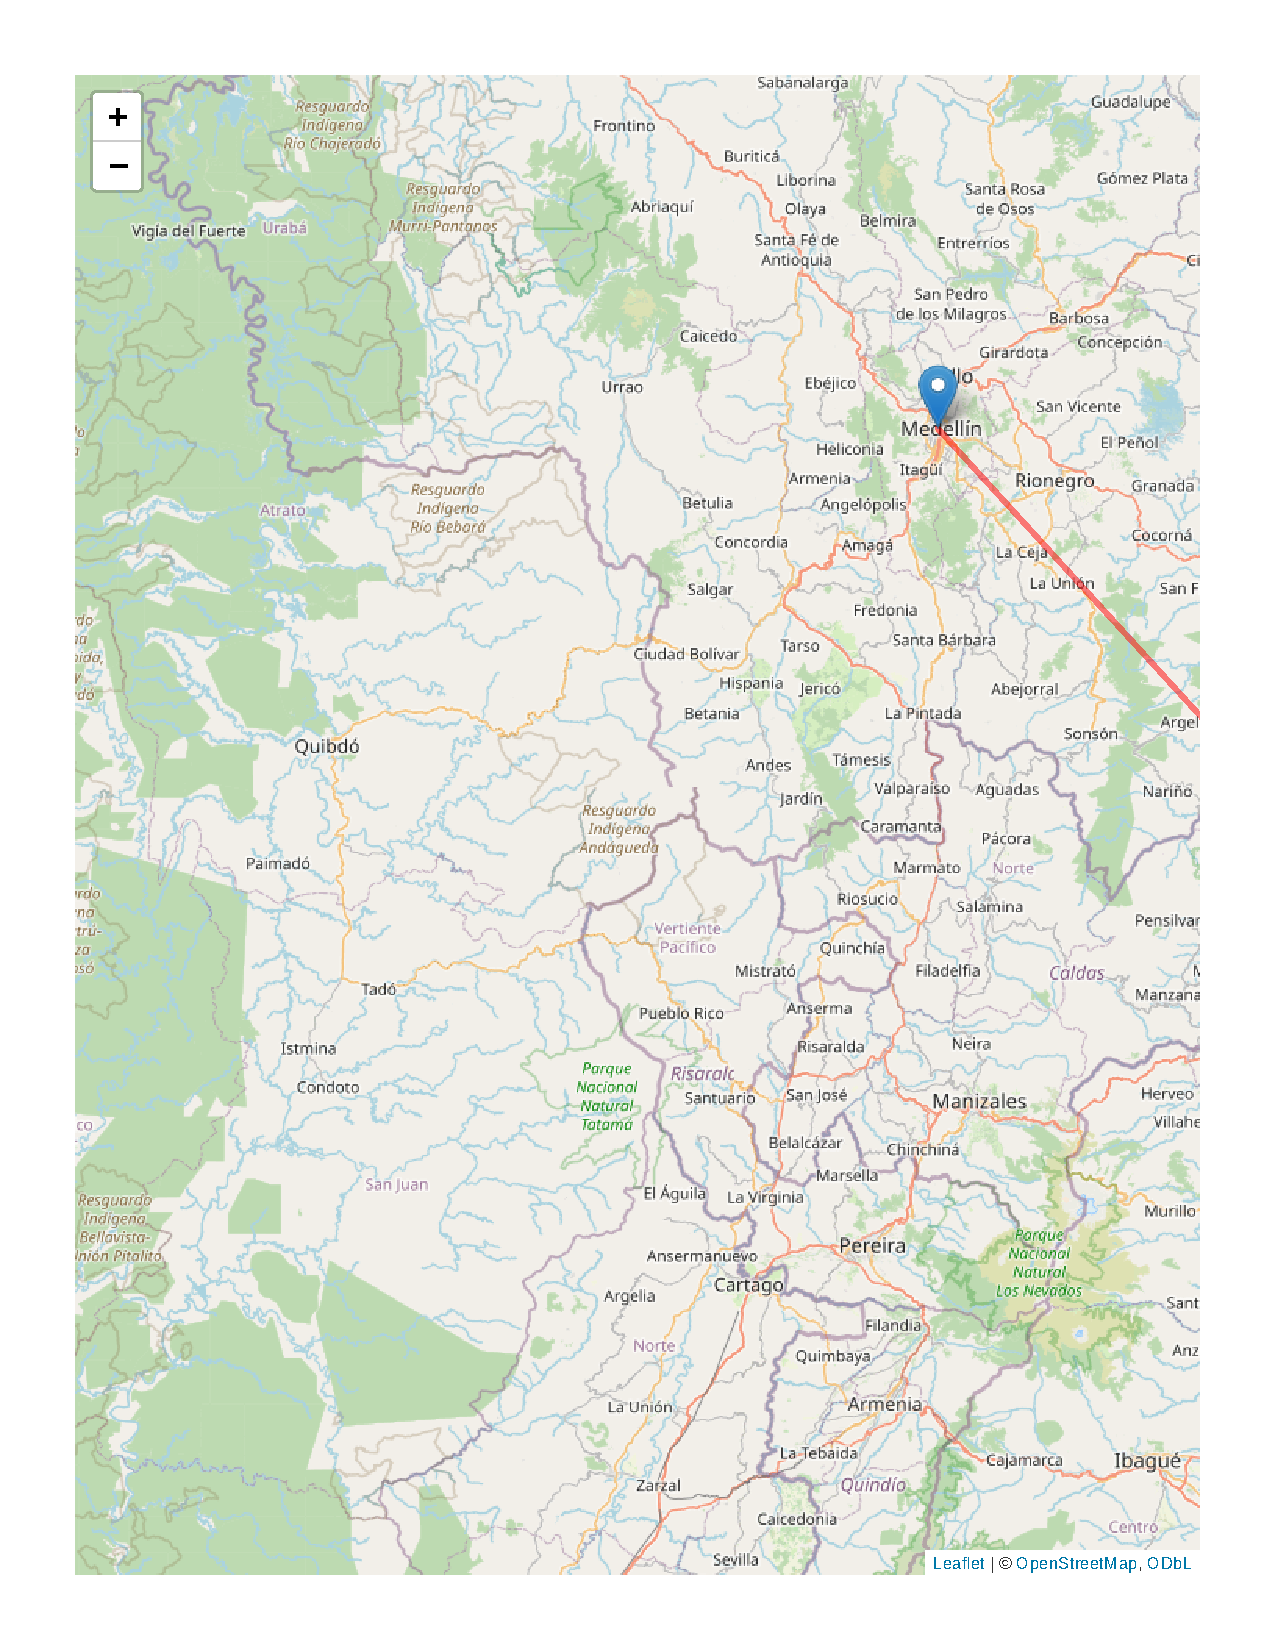
\includegraphics{09-funciones_clases_files/figure-pdf/r_clases-1.pdf}

\subsubsection{Julia}

\begin{tcolorbox}[enhanced jigsaw, coltitle=black, leftrule=.75mm, bottomtitle=1mm, title=\textcolor{quarto-callout-note-color}{\faInfo}\hspace{0.5em}{Nota Técnica: El Motor de Interoperabilidad Geomática}, colback=white, colbacktitle=quarto-callout-note-color!10!white, left=2mm, toptitle=1mm, rightrule=.15mm, titlerule=0mm, arc=.35mm, colframe=quarto-callout-note-color-frame, bottomrule=.15mm, toprule=.15mm, opacityback=0, opacitybacktitle=0.6, breakable]

Si revisas el código fuente de este documento Quarto, notarás que en
\textbf{Julia} estamos usando dos funciones especiales llamadas
\texttt{j\_eval()} y \texttt{j\_plot()}, en lugar del bloque de código
estándar. Esto se debe a que estamos usando un Motor de
Interoperabilidad que conecta R y Julia por debajo. Para garantizar que
la memoria se mantenga y el gráfico se exporte correctamente en el
PDF/HTML, usamos \texttt{j\_eval()} para compilar la lógica, y
\texttt{j\_plot()} \textbf{únicamente} al final para pedirle a la
librería de gráficos que procese la imagen.

\end{tcolorbox}

\begin{center}
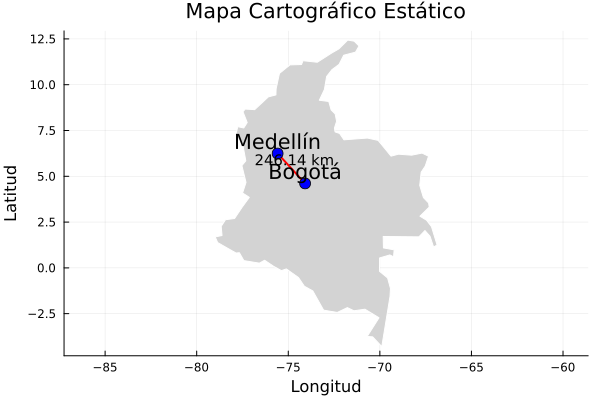
\includegraphics[width=0.7\textwidth,height=\textheight]{./images/09-mapa_julia_poo.png}
\end{center}

\subsection{Los pilares de la POO en Geomática (sin
complicaciones)}\label{los-pilares-de-la-poo-en-geomuxe1tica-sin-complicaciones}

Aunque nuestro objetivo principal ha sido organizar el código, sin darte
cuenta acabas de implementar los dos pilares más poderosos de la
\textbf{Programación Orientada a Objetos (POO)}. No son conceptos
abstractos de libros; son herramientas reales que acabas de usar en tus
mapas:

\subsubsection{1. Abstracción: El arte de la ``Caja
Negra''}\label{abstracciuxf3n-el-arte-de-la-caja-negra}

Cuando llamaste al método
\texttt{punto\_origen.distancia\_hacia(punto\_destino)}, aplicaste la
\textbf{Abstracción}.

\begin{itemize}
\tightlist
\item
  \textbf{Lo que ves:} Una simple orden que te devuelve un número.
\item
  \textbf{Lo que ignoras:} Los senos, cosenos, arcosenos y conversiones
  a radianes de la fórmula de Haversine.
\end{itemize}

Abstraer es \textbf{simplificar la realidad}. En geomática, esto es
vital: no queremos pensar en la curvatura de la Tierra cada vez que
medimos un predio; queremos una herramienta que ``sepa hacerlo'' y nos
entregue el resultado. Al crear la clase o estructura, convertiste una
matemática compleja en un botón fácil de presionar.

\subsubsection{2. Encapsulamiento: El ``Todo
Incluido''}\label{encapsulamiento-el-todo-incluido}

Recuerda nuestra analogía del \textbf{porta-comidas} o el \textbf{Food
Truck}. Al crear el objeto \texttt{PuntoEspacial}, aplicaste el
\textbf{Encapsulamiento}.

En lugar de tener la latitud por un lado, el nombre por otro y la
función de medir flotando en un archivo perdido, lo encerraste todo en
una sola ``cápsula''.

\begin{itemize}
\tightlist
\item
  \textbf{El beneficio:} Tus datos están protegidos. Sabes que el método
  \texttt{distancia\_hacia} solo funciona con los datos que están dentro
  de esa cápsula. Esto evita que, en un proyecto grande con miles de
  puntos, termines midiendo accidentalmente la distancia entre el nombre
  de una ciudad y la temperatura de otra.
\end{itemize}

\begin{quote}
\textbf{En resumen:} La \textbf{Abstracción} oculta la complejidad
matemática y el \textbf{Encapsulamiento} mantiene tus datos ordenados y
seguros dentro de una misma entidad.
\end{quote}

\subsection{El motor bajo el capó: Despacho y
Velocidad}\label{el-motor-bajo-el-capuxf3-despacho-y-velocidad}

A lo largo del capítulo vimos cómo se estructuran las clases, pero queda
una pregunta crítica: \textbf{¿Por qué Julia es tan famoso por su
velocidad frente a R y Python en cálculos científicos pesados?} La
respuesta no está en la sintaxis, sino en dos conceptos fundamentales
que ocurren tras bambalinas: el tipo de despacho y el momento en que se
procesa.

\begin{enumerate}
\def\labelenumi{\arabic{enumi}.}
\tightlist
\item
  \textbf{Python (Despacho Interno):} Actúa como un \textbf{Food Truck
  autónomo}. El objeto es el dueño de sus métodos. Cuando llamas a
  \texttt{punto.distancia()}, Python busca dentro del objeto
  \texttt{punto} y ejecuta su propia herramienta integrada. Es muy
  intuitivo, pero cargar ``una cocina completa'' dentro de cada objeto
  consume mucha memoria si tienes millones de ellos.
\item
  \textbf{R (Despacho Simple en Runtime):} Actúa como un
  \textbf{inspector de correos perezoso}. R usa funciones genéricas;
  cuando llamas a \texttt{distancia(origen,\ destino)}, R solo mira el
  ``post-it'' (la clase) del \emph{primer} argumento (\texttt{origen}).
  Luego, busca manualmente en su directorio qué función usar y la
  ejecuta. Como R hace esto en ``Tiempo de Ejecución'' (\emph{Runtime}),
  si tienes un ciclo con un millón de coordenadas, R se detiene a leer
  el post-it un millón de veces. ¡Ese papeleo es lo que lo hace lento!
\item
  \textbf{Julia (Despacho Múltiple + Compilación JIT):} Actúa como una
  \textbf{fábrica industrial láser}. Cuando llamas a
  \texttt{distancia(origen,\ destino)}, el compilador revisa con láser
  las etiquetas de \emph{todos} los ingredientes al mismo tiempo. Pero
  el verdadero secreto es \emph{cuándo} lo hace: la primera vez que
  Julia ve esa combinación, detiene el tiempo, traduce la receta a
  \textbf{código de máquina nativo} (ceros y unos hiper-optimizados) y
  construye un ``tubo de ensamblaje'' directo (Compilación
  \emph{Just-In-Time} o JIT). Las siguientes 999,999 veces del ciclo,
  los datos pasan por el tubo a la velocidad de la luz sin leer
  etiquetas.
\end{enumerate}

\emph{La siguiente analogía visualiza las diferencias entre los tres
motores de ejecución:}

\begin{figure}

\centering{

\includegraphics[width=0.85\textwidth,height=\textheight]{./images/comparativa_despacho_python_r_julia.png}

}

\caption{\label{fig-analogia-motores}\textbf{Analogía de los motores de
ejecución:} El Food Truck autónomo (Python), la lenta Oficina de Correos
de revisión manual (R) y la veloz Fábrica Industrial Láser (Julia).}

\end{figure}%

Técnicamente, podemos estructurar el flujo de decisiones de cada motor
mediante el siguiente diagrama:

\begin{figure}

\centering{

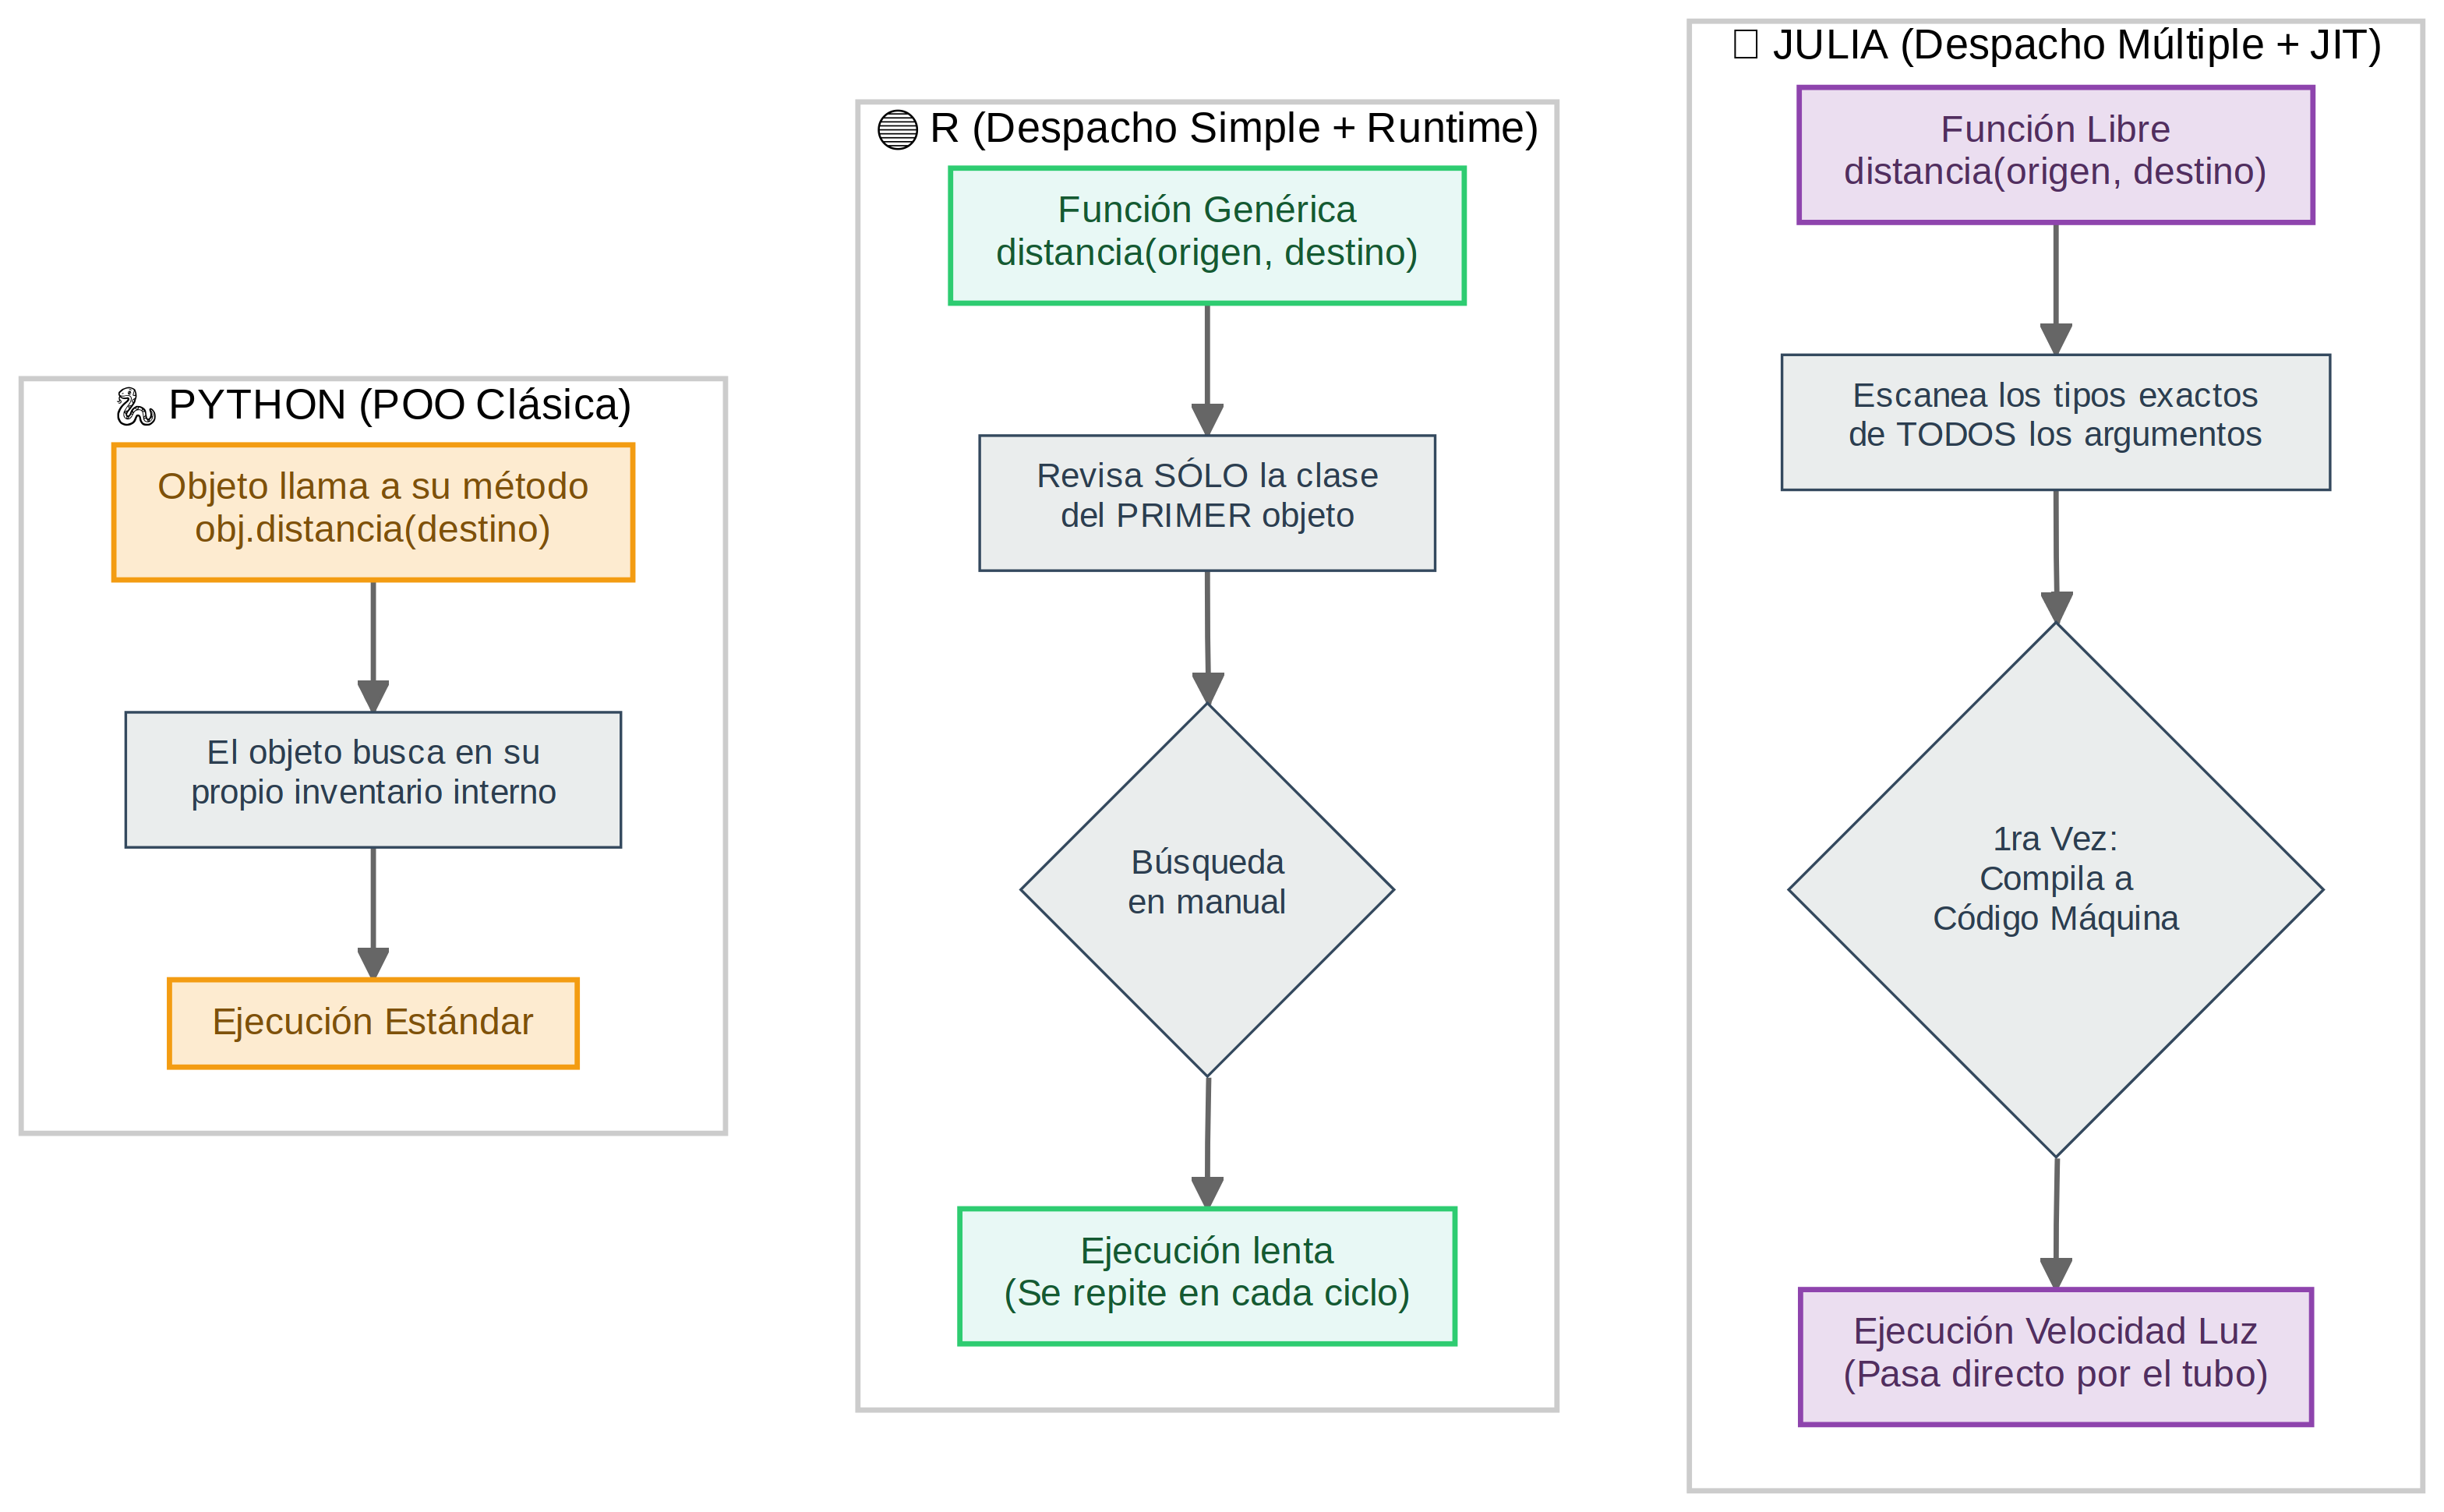
\includegraphics[width=6.5in,height=4.02in]{09-funciones_clases_files/figure-latex/mermaid-figure-2.png}

}

\caption{\label{fig-diagrama-motores}Flujo lógico de los motores de
ejecución: Python, R y Julia.}

\end{figure}%

\subsection{Resumen de sintaxis: programación orientada a
objetos}\label{resumen-de-sintaxis-programaciuxf3n-orientada-a-objetos}

Como pudiste observar, cada lenguaje aborda las clases con una filosofía
arquitectónica distinta: Python encapsula los métodos dentro del objeto,
R usa funciones sueltas que leen etiquetas invisibles (S3), y Julia usa
estructuras rígidas con funciones que exigen el tipo de dato exacto
(despacho múltiple).

\begin{longtable}[]{@{}
  >{\raggedright\arraybackslash}p{(\columnwidth - 6\tabcolsep) * \real{0.2000}}
  >{\raggedright\arraybackslash}p{(\columnwidth - 6\tabcolsep) * \real{0.2600}}
  >{\raggedright\arraybackslash}p{(\columnwidth - 6\tabcolsep) * \real{0.2700}}
  >{\raggedright\arraybackslash}p{(\columnwidth - 6\tabcolsep) * \real{0.2700}}@{}}
\caption{Diferencias en la creación de Clases y
Objetos}\label{tbl-clases_objetos}\tabularnewline
\toprule\noalign{}
\begin{minipage}[b]{\linewidth}\raggedright
Característica
\end{minipage} & \begin{minipage}[b]{\linewidth}\raggedright
Python (POO Clásica)
\end{minipage} & \begin{minipage}[b]{\linewidth}\raggedright
R (Sistema S3)
\end{minipage} & \begin{minipage}[b]{\linewidth}\raggedright
Julia (Despacho Múltiple)
\end{minipage} \\
\midrule\noalign{}
\endfirsthead
\toprule\noalign{}
\begin{minipage}[b]{\linewidth}\raggedright
Característica
\end{minipage} & \begin{minipage}[b]{\linewidth}\raggedright
Python (POO Clásica)
\end{minipage} & \begin{minipage}[b]{\linewidth}\raggedright
R (Sistema S3)
\end{minipage} & \begin{minipage}[b]{\linewidth}\raggedright
Julia (Despacho Múltiple)
\end{minipage} \\
\midrule\noalign{}
\endhead
\bottomrule\noalign{}
\endlastfoot
\textbf{Definir Molde} & \texttt{class\ Objeto:} & Función que retorna
una \texttt{list()} & \texttt{struct\ Objeto\ ...\ end} \\
\textbf{Constructor} & \texttt{def\ \_\_init\_\_(self):} & Asignar
etiqueta:
\texttt{class(obj)\ \textless{}-\ \textquotesingle{}Tipo\textquotesingle{}}
& \texttt{Objeto()} (Automático o explícito) \\
\textbf{Auto-referencia} & Usa la palabra \texttt{self} & Pasa el objeto
\texttt{obj} como argumento & Pasa el objeto tipado
\texttt{obj::Tipo} \\
\textbf{Métodos} & Van dentro de \texttt{class} & Genérico
(\texttt{UseMethod}) + \texttt{metodo.Clase} & Funciones independientes
enrutadas por tipo \\
\textbf{Representación} & \texttt{def\ \_\_str\_\_(self):} &
\texttt{print.Clase\ \textless{}-\ function(obj)} &
\texttt{Base.show(io,\ obj::Clase)} \\
\end{longtable}

\section{Guías de diseño para funciones y
clases}\label{guuxedas-de-diseuxf1o-para-funciones-y-clases}

Escribir código que la máquina entienda es fácil; escribir código que
otro ser humano (o usted mismo en seis meses) pueda entender, es un
arte. Ya sea que esté usando el molde estricto de Python, las etiquetas
de R o los chefs de Julia, existen reglas de oro universales para que su
arquitectura sea sólida, limpia y profesional.

A continuación, presentamos los mandamientos del buen diseño de software
para la ciencia de datos.

\subsection{1. El diseño de Funciones: los obreros de la
obra}\label{el-diseuxf1o-de-funciones-los-obreros-de-la-obra}

Las funciones son la unidad básica de acción en su código. Si sus
funciones son un enredo, todo el proyecto lo será.

\begin{itemize}
\tightlist
\item
  \textbf{Hagan una sola cosa (Single Responsibility):} Una función debe
  tener un único propósito claro. Si su función descarga los datos, los
  limpia, calcula la distancia y de paso le imprime un mapa, está
  haciendo demasiado. Divídala en cuatro funciones pequeñas. La navaja
  suiza es útil para acampar, pero en programación es un peligro.
\item
  \textbf{Nombres que cuenten la historia:} El nombre de una función
  debe ser un verbo que describa exactamente su acción. Evite
  abreviaturas jeroglíficas. Es preferible escribir
  \texttt{calcular\_distancia\_km()} que \texttt{calc\_dist()}.
\item
  \textbf{Evite las ``novelas'' (Mantenlas cortas):} Si el cuerpo de su
  función no cabe en la pantalla de su monitor sin hacer \emph{scroll},
  es momento de machetearla y dividirla. Las funciones cortas son
  fáciles de testear y rara vez esconden errores.
\item
  \textbf{Sin efectos secundarios (Pureza):} Lo ideal es que una función
  reciba datos, haga su trabajo y devuelva un resultado sin alterar
  silenciosamente variables globales u otras partes del sistema. Lo que
  pasa en la función, se queda en la función.
\end{itemize}

\begin{tcolorbox}[enhanced jigsaw, coltitle=black, leftrule=.75mm, bottomtitle=1mm, title=\textcolor{quarto-callout-tip-color}{\faLightbulb}\hspace{0.5em}{La regla DRY (Don't Repeat Yourself)}, colback=white, colbacktitle=quarto-callout-tip-color!10!white, left=2mm, toptitle=1mm, rightrule=.15mm, titlerule=0mm, arc=.35mm, colframe=quarto-callout-tip-color-frame, bottomrule=.15mm, toprule=.15mm, opacityback=0, opacitybacktitle=0.6, breakable]

``No te repitas''. Si usted se descubre copiando y pegando el mismo
bloque de código tres veces seguidas y solo cambiándole una variable,
deténgase. Ese bloque debe convertirse inmediatamente en una función.

\end{tcolorbox}

\begin{center}\rule{0.5\linewidth}{0.5pt}\end{center}

\subsection{2. El diseño de Clases (y Estructuras): los cimientos del
edificio}\label{el-diseuxf1o-de-clases-y-estructuras-los-cimientos-del-edificio}

Cuando decida agrupar sus datos y funciones en un objeto o estructura,
hágalo con prudencia. No todo necesita ser una clase.

\begin{itemize}
\tightlist
\item
  \textbf{Alta cohesión:} Todo lo que viva dentro de su clase (o
  \texttt{struct}) debe estar íntimamente relacionado. Siguiendo nuestra
  analogía, no meta la receta del sancocho en el molde de las arepas. Si
  un \texttt{PuntoEspacial} tiene latitud y longitud, perfecto; pero si
  también le agrega un atributo para el
  ``color\_favorito\_del\_usuario'', está rompiendo la cohesión.
\item
  \textbf{Oculte las tuberías (Encapsulamiento):} El usuario de su
  objeto no necesita saber cómo funcionan las matemáticas internamente,
  solo necesita el resultado. Exponga únicamente los métodos y atributos
  que son estrictamente necesarios para usar el objeto (la interfaz
  pública) y mantenga la complejidad ``escondida'' en el motor.
\item
  \textbf{Evite el ``Síndrome de Dios'':} Una ``clase Dios'' es aquella
  que sabe demasiado y hace de todo (ej.
  \texttt{GestorDeMapasYDatosYCalculos}). Si su clase maneja toda la
  lógica del proyecto, divídala en objetos más pequeños y delegue
  responsabilidades. Un objeto \texttt{Coordenada} interactúa con un
  objeto \texttt{Mapa}, no son el mismo ente.
\item
  \textbf{Si no hay estado, no hay clase:} Especialmente en Python y R.
  Si usted crea una clase que solo tiene métodos pero no guarda ningún
  dato (atributos), no necesita una clase; lo que usted necesita es un
  simple archivo con funciones sueltas.
\end{itemize}

\subsection{3. Comentarios y
documentación}\label{comentarios-y-documentaciuxf3n}

\begin{itemize}
\tightlist
\item
  \textbf{El código explica el \emph{Qué}, el comentario explica el
  \emph{Por qué}:} No escriba comentarios obvios como
  \texttt{\#\ Esto\ suma\ 2\ +\ 2}. Use los comentarios para explicar
  decisiones de negocio o atajos matemáticos:
  \texttt{\#\ Usamos\ la\ fórmula\ de\ Haversine\ porque\ es\ más\ precisa\ para\ distancias\ cortas}.
\item
  \textbf{Docstrings siempre:} Todo molde (clase/struct) y toda función
  importante debe tener una breve cadena de documentación en la parte
  superior explicando qué recibe (argumentos) y qué devuelve (retorno).
\end{itemize}

\section{Resumen de aprendizajes (cheat
sheet)}\label{resumen-de-aprendizajes-cheat-sheet-4}

¡Felicidades! Has completado uno de los capítulos más densos y
fundamentales para tu carrera como analista espacial. Al dominar las
funciones y los objetos, has pasado de escribir ``scripts desechables''
a construir herramientas profesionales.

Repasemos los conceptos clave que te llevas en la mochila:

\begin{itemize}
\tightlist
\item
  \textbf{Las funciones son máquinas:} Reciben ingredientes
  (parámetros), aplican una lógica interna sin afectar el entorno
  exterior (pureza), y devuelven un resultado procesado. Son la máxima
  expresión de la regla DRY (\emph{Don't Repeat Yourself}).
\item
  \textbf{Parámetros dinámicos:} Aprendiste a usar \texttt{**kwargs}
  (Python), \texttt{...} (R) y \texttt{kwargs...} (Julia) para atrapar
  un número indefinido de variables, dándole flexibilidad total a tus
  herramientas.
\item
  \textbf{La POO no es igual en todas partes:}

  \begin{itemize}
  \tightlist
  \item
    \textbf{Python (Molde estricto):} Usa Clases formales. El objeto
    lleva sus propios datos y herramientas por dentro. El despacho es
    interno (\texttt{objeto.metodo()}).
  \item
    \textbf{R (Sistema S3 flexible):} Construye listas estándar y les
    pega una ``etiqueta'' (post-it). Las funciones genéricas leen la
    etiqueta y despachan el trabajo a la herramienta adecuada.
  \item
    \textbf{Julia (Estructuras y Despacho Múltiple):} Separa
    radicalmente los datos (en \texttt{structs} rígidos) de las
    funciones. El Jefe de Cocina (compilador) escanea los tipos de todos
    los ingredientes y compila una tubería de alta velocidad (JIT) para
    ejecutarlos.
  \end{itemize}
\item
  \textbf{Diseño limpio:} Un buen código se lee como un buen libro.
  Mantén tus funciones enfocadas en una sola tarea, diseña clases con
  alta cohesión y nunca olvides explicar el \emph{por qué} en tus
  comentarios.
\end{itemize}

A continuación, se presenta tu \textbf{Hoja de Referencia (Cheat Sheet)}
para traducir la sintaxis de estos conceptos entre Python, R y Julia.

\subsection{1. Estructura de funciones}\label{estructura-de-funciones}

\begin{longtable}[]{@{}
  >{\raggedright\arraybackslash}p{(\columnwidth - 6\tabcolsep) * \real{0.2500}}
  >{\raggedright\arraybackslash}p{(\columnwidth - 6\tabcolsep) * \real{0.2500}}
  >{\raggedright\arraybackslash}p{(\columnwidth - 6\tabcolsep) * \real{0.2500}}
  >{\raggedright\arraybackslash}p{(\columnwidth - 6\tabcolsep) * \real{0.2500}}@{}}
\caption{Diferencias en el empaquetado y argumentos de
funciones}\label{tbl-funciones_argumentos}\tabularnewline
\toprule\noalign{}
\begin{minipage}[b]{\linewidth}\raggedright
Característica
\end{minipage} & \begin{minipage}[b]{\linewidth}\raggedright
Python
\end{minipage} & \begin{minipage}[b]{\linewidth}\raggedright
R
\end{minipage} & \begin{minipage}[b]{\linewidth}\raggedright
Julia
\end{minipage} \\
\midrule\noalign{}
\endfirsthead
\toprule\noalign{}
\begin{minipage}[b]{\linewidth}\raggedright
Característica
\end{minipage} & \begin{minipage}[b]{\linewidth}\raggedright
Python
\end{minipage} & \begin{minipage}[b]{\linewidth}\raggedright
R
\end{minipage} & \begin{minipage}[b]{\linewidth}\raggedright
Julia
\end{minipage} \\
\midrule\noalign{}
\endhead
\bottomrule\noalign{}
\endlastfoot
\textbf{Declaración} & \texttt{def\ calc(x):} &
\texttt{calc\ \textless{}-\ function(x)\ \{\ \}} &
\texttt{function\ calc(x)\ ...\ end} \\
\textbf{Retorno} & \texttt{return\ y} & \texttt{return(y)} &
\texttt{return\ y} \\
\textbf{Parámetro x defecto} & \texttt{def\ calc(r=6371):} &
\texttt{function(r=6371)} & \texttt{function\ calc(;\ r=6371)} \\
\textbf{Múltiples args extra} & \texttt{**kwargs} & \texttt{...} &
\texttt{kwargs...} \\
\end{longtable}

\subsection{2. Programación Orientada a Objetos
(POO)}\label{programaciuxf3n-orientada-a-objetos-poo}

\begin{longtable}[]{@{}
  >{\raggedright\arraybackslash}p{(\columnwidth - 6\tabcolsep) * \real{0.2000}}
  >{\raggedright\arraybackslash}p{(\columnwidth - 6\tabcolsep) * \real{0.2600}}
  >{\raggedright\arraybackslash}p{(\columnwidth - 6\tabcolsep) * \real{0.2700}}
  >{\raggedright\arraybackslash}p{(\columnwidth - 6\tabcolsep) * \real{0.2700}}@{}}
\caption{Diferencias en la creación de Clases y
Objetos}\label{tbl-clases_objetos}\tabularnewline
\toprule\noalign{}
\begin{minipage}[b]{\linewidth}\raggedright
Característica
\end{minipage} & \begin{minipage}[b]{\linewidth}\raggedright
Python (POO Clásica)
\end{minipage} & \begin{minipage}[b]{\linewidth}\raggedright
R (Sistema S3)
\end{minipage} & \begin{minipage}[b]{\linewidth}\raggedright
Julia (Despacho Múltiple)
\end{minipage} \\
\midrule\noalign{}
\endfirsthead
\toprule\noalign{}
\begin{minipage}[b]{\linewidth}\raggedright
Característica
\end{minipage} & \begin{minipage}[b]{\linewidth}\raggedright
Python (POO Clásica)
\end{minipage} & \begin{minipage}[b]{\linewidth}\raggedright
R (Sistema S3)
\end{minipage} & \begin{minipage}[b]{\linewidth}\raggedright
Julia (Despacho Múltiple)
\end{minipage} \\
\midrule\noalign{}
\endhead
\bottomrule\noalign{}
\endlastfoot
\textbf{Definir Molde} & \texttt{class\ Objeto:} & Función que retorna
una \texttt{list()} & \texttt{struct\ Objeto\ ...\ end} \\
\textbf{Constructor} & \texttt{def\ \_\_init\_\_(self):} & Asignar
etiqueta:
\texttt{class(obj)\ \textless{}-\ \textquotesingle{}Tipo\textquotesingle{}}
& \texttt{Objeto()} (Automático o explícito) \\
\textbf{Auto-referencia} & Usa la palabra \texttt{self} & Pasa el objeto
\texttt{obj} como argumento & Pasa el objeto tipado
\texttt{obj::Tipo} \\
\textbf{Métodos} & Van dentro de \texttt{class} & Genérico
(\texttt{UseMethod}) + \texttt{metodo.Clase} & Funciones independientes
enrutadas por tipo \\
\textbf{Representación} & \texttt{def\ \_\_str\_\_(self):} &
\texttt{print.Clase\ \textless{}-\ function(obj)} &
\texttt{Base.show(io,\ obj::Clase)} \\
\end{longtable}

\section{Ejercicios}\label{ejercicios-4}

Para poner en práctica los conceptos aprendidos sobre encapsulamiento y
diseño de objetos, deberás resolver los siguientes dos ejercicios.
Puedes elegir resolverlos en \textbf{Python, R o Julia} (o implementar
la solución en varios lenguajes si deseas retarte).

\subsection{Ejercicio 1: El cazador de coordenadas (Funciones y
abstracción)}\label{ejercicio-1-el-cazador-de-coordenadas-funciones-y-abstracciuxf3n}

En geomática, a menudo necesitamos saber cuál es la ``caja
delimitadora'' (\emph{Bounding Box}) de un conjunto de puntos para
encuadrar un mapa.

\begin{itemize}
\tightlist
\item
  Escribe una función pura llamada \texttt{calcular\_bbox} que reciba
  una lista de múltiples coordenadas (latitud, longitud).
\item
  La función debe recorrer la lista internamente y devolver cuatro
  valores: la latitud mínima, la latitud máxima, la longitud mínima y la
  longitud máxima.
\item
  Asegúrate de que la función incluya una cadena de documentación
  (Docstring) o comentarios claros explicando qué entra y qué sale.
\end{itemize}

\subsection{Ejercicio 2: Modelando una ruta espacial (Clases e
interacción)}\label{ejercicio-2-modelando-una-ruta-espacial-clases-e-interacciuxf3n}

Vamos a llevar los objetos al siguiente nivel haciendo que interactúen
entre sí. Toma el código base del \texttt{PuntoEspacial} que
desarrollamos en este capítulo y crea una nueva estructura superior:

\begin{itemize}
\tightlist
\item
  Crea una clase (o sistema S3 / struct en Julia) llamada
  \texttt{RutaGeografica}.
\item
  Su constructor debe recibir un nombre (ej. ``Ruta de los Andes'') y
  una lista vacía que almacenará objetos del tipo
  \texttt{PuntoEspacial}.
\item
  Escribe un método \texttt{agregar\_punto()} que reciba un objeto
  \texttt{PuntoEspacial} y lo guarde en la lista interna de la ruta.
\item
  Escribe un método \texttt{medir\_distancia\_total()} que use un ciclo
  para sumar la distancia de todos los tramos de la ruta, llamando al
  método \texttt{distancia\_hacia()} que los puntos ya tienen integrado.
\end{itemize}

\subsection{Entregables y criterios de
evaluación}\label{entregables-y-criterios-de-evaluaciuxf3n-4}

El objetivo de esta evaluación no es solo que el código funcione, sino
que seas capaz de documentar y explicar tus decisiones de arquitectura
de software y el comportamiento del motor de ejecución subyacente.

\textbf{1. Archivos de Código:} Debes desarrollar los algoritmos en al
menos uno de los siguientes formatos de archivo:

\begin{itemize}
\tightlist
\item
  Script tradicional (\texttt{.py}, \texttt{.R}, \texttt{.jl})
\item
  Notebook interactivo (\texttt{.ipynb})
\item
  Documento computacional (\texttt{.qmd} con \emph{chunks} de código)
\end{itemize}

\textbf{2. Documento Analítico (Quarto):} Independientemente del formato
de tu código fuente, \textbf{debes redactar un documento en Quarto
(\texttt{.qmd}) y renderizarlo tanto en HTML como en PDF}. En este
documento debes incluir tus bloques de código y responder
argumentativamente a las siguientes preguntas:

\begin{itemize}
\tightlist
\item
  \textbf{Sobre el Ejercicio 1 (Regla DRY y Pureza):} Explica con tus
  propias palabras qué es la regla DRY (\emph{Don't Repeat Yourself}).
  ¿Por qué es un riesgo para la mantenibilidad de un proyecto copiar y
  pegar la gran fórmula matemática de Haversine en múltiples partes de
  tu código en lugar de usar la función que creaste?
\item
  \textbf{Sobre el Ejercicio 2 (Paradigmas de POO):} Si resolviste (o
  resolvieras) este ejercicio en \textbf{Python}, ¿dónde ``viven''
  físicamente los métodos analíticos como
  \texttt{medir\_distancia\_total()}? Contrasta esta filosofía con el
  enfoque del \textbf{Sistema S3 de R}. Usa la analogía del ``Molde'' vs
  el ``Post-it'' vista en clase para explicarlo.
\item
  \textbf{Pregunta General (Eficiencia y Motores):} Imagina que tu
  \texttt{RutaGeografica} tiene 5 millones de puntos recolectados por un
  GPS y necesitas calcular la distancia total. Si usarás \textbf{Julia},
  explica brevemente cómo la combinación del \textbf{Despacho Múltiple}
  y la \textbf{Compilación JIT} lograría ejecutar este cálculo masivo
  mucho más rápido que el intérprete estándar de R.
\end{itemize}

\textbf{3. Repositorio en GitHub:} Sube tu carpeta del proyecto (que
debe contener tus scripts, el archivo \texttt{.qmd} y los renders
finales en HTML y PDF) a un repositorio público en tu cuenta personal de
\textbf{GitHub}.

\begin{itemize}
\tightlist
\item
  \textbf{Entrega:} Deberás enviar únicamente el enlace (URL) a tu
  repositorio de GitHub para la calificación.
\end{itemize}

\chapter{Trabajando con Archivos}\label{sec-trabajando_archivos}

\section{Funciones j\_eval y j\_plot en
R}\label{funciones-j_eval-y-j_plot-en-r-5}

\begin{Shaded}
\begin{Highlighting}[]
\CommentTok{\# \#| include: false}
\FunctionTok{source}\NormalTok{(}\StringTok{"./docs/j\_eval\_j\_plot.r"}\NormalTok{)}
\end{Highlighting}
\end{Shaded}

\section{Introducción}\label{introducciuxf3n-6}

En el mundo real de la geomática, no todos los datos espaciales llegan a
nuestras manos en formatos geográficos perfectamente estructurados como
Shapefiles (\texttt{.shp}) o GeoPackages (\texttt{.gpkg}). Con muchísima
frecuencia, los analistas espaciales deben lidiar con datos ``crudos'':
coordenadas GPS capturadas en libretas de campo electrónicas y guardadas
en archivos de texto plano, bases de datos socioeconómicas del DANE en
formato CSV, o registros de estaciones meteorológicas del IDEAM que
contienen valores nulos o errores de tipeo.

Antes de poder visualizar un mapa o ejecutar una herramienta de
geoprocesamiento espacial usando librerías avanzadas como
\texttt{geopandas} o \texttt{sf}, es fundamental saber cómo comunicarnos
con el sistema operativo para abrir, leer, limpiar y guardar estos
archivos desde cero.

Además, dado que los datos del mundo real son ``sucios'' por naturaleza,
un buen algoritmo de procesamiento masivo no debe colapsar ni detenerse
por completo al encontrar una letra donde debería ir un número. Aquí es
donde entra en juego el \textbf{manejo de excepciones}, una habilidad de
programación vital para construir herramientas robustas, automatizadas y
a prueba de fallos.

\section{Objetivos de aprendizaje}\label{objetivos-de-aprendizaje-5}

Al finalizar esta sección, el estudiante será capaz de:

\begin{enumerate}
\def\labelenumi{\arabic{enumi}.}
\tightlist
\item
  \textbf{Manipular archivos en el sistema operativo:} Abrir, leer y
  escribir archivos de texto plano y tabulares (CSV) garantizando el
  cierre seguro de las conexiones en Python, R y Julia.
\item
  \textbf{Procesar y limpiar cadenas de texto:} Utilizar métodos nativos
  de manipulación de \emph{strings} para separar, limpiar y extraer
  valores numéricos de coordenadas (latitud y longitud).
\item
  \textbf{Implementar manejo robusto de excepciones:} Construir bloques
  de control predictivos (\texttt{try...except}, \texttt{tryCatch}) que
  capturen errores específicos (como archivos no encontrados o formatos
  de datos inválidos) sin interrumpir el flujo del programa.
\item
  \textbf{Estructurar información asimétrica:} Transformar texto crudo
  en estructuras de memoria eficientes (como listas de diccionarios) que
  sirvan de puente hacia la construcción de \emph{DataFrames}
  espaciales.
\end{enumerate}

\section{Una nota sobre las rutas de los archivos
(paths)}\label{una-nota-sobre-las-rutas-de-los-archivos-paths}

En programación, es un error técnico grave usar \textbf{rutas absolutas}
(por ejemplo,
\texttt{C:\textbackslash{}Usuarios\textbackslash{}Maestria\textbackslash{}SIG\textbackslash{}data\textbackslash{}COL.geo.json}).
Si compartes tu código con otro investigador o ejecutas el script en un
servidor Linux, la estructura de carpetas no existirá y el programa
fallará inmediatamente.

La solución estándar es usar \textbf{rutas relativas} en combinación con
los \textbf{constructores de rutas nativos} de cada lenguaje. Esto
garantiza que tu script encuentre los datos basándose en el directorio
de trabajo actual y que los separadores de carpetas (\texttt{/} en
Mac/Linux, \texttt{\textbackslash{}} en Windows) se asignen
dinámicamente según el sistema operativo.

Para navegar de forma relativa, los sistemas informáticos utilizan dos
comodines estándar:

\begin{itemize}
\tightlist
\item
  \texttt{.} (un punto): Representa el \textbf{directorio actual} (la
  carpeta donde se está ejecutando el script o \emph{notebook}).
\item
  \texttt{..} (dos puntos): Representa el \textbf{directorio superior}
  (la carpeta ``padre''). Se utiliza para retroceder niveles en el árbol
  de archivos.
\end{itemize}

Por ejemplo, si tu script está dentro de una subcarpeta llamada
\texttt{scripts/} y quieres acceder a los datos que están en una carpeta
paralela, usarías \texttt{..} para salir de \texttt{scripts/} y luego
entrarías a la ruta deseada (ej. \texttt{../data/mi\_archivo.csv}).

\subsection{Ejemplo aplicado: Construcción de rutas y mapa
estático}\label{ejemplo-aplicado-construcciuxf3n-de-rutas-y-mapa-estuxe1tico}

A continuación, asumiremos que nuestro entorno de ejecución está en la
raíz del proyecto y necesitamos abrir un límite nacional ubicado
exactamente en la ruta relativa:
\texttt{data/vector/geojson/COL.geo.json}.

El código demuestra cómo ensamblar esta ruta independientemente del
sistema operativo, abrir el dato espacial y generar un gráfico estático.

\subsection{Python}

\begin{Shaded}
\begin{Highlighting}[]
\CommentTok{\# \#| eval: false}

\ImportTok{import}\NormalTok{ geopandas }\ImportTok{as}\NormalTok{ gpd}
\ImportTok{import}\NormalTok{ matplotlib.pyplot }\ImportTok{as}\NormalTok{ plt}
\ImportTok{from}\NormalTok{ pathlib }\ImportTok{import}\NormalTok{ Path}

\CommentTok{\# 1. Construcción segura de la ruta relativa}
\CommentTok{\# Path(".") hace referencia al directorio actual.}
\CommentTok{\# El operador \textquotesingle{}/\textquotesingle{} es sobrecargado por pathlib para unir carpetas correctamente.}
\NormalTok{ruta\_archivo }\OperatorTok{=}\NormalTok{ Path(}\StringTok{"."}\NormalTok{) }\OperatorTok{/} \StringTok{"data"} \OperatorTok{/} \StringTok{"vector"} \OperatorTok{/} \StringTok{"geojson"} \OperatorTok{/} \StringTok{"COL.geo.json"}

\CommentTok{\# Blindaje con try{-}except para evitar colapso en Quarto}
\ControlFlowTok{try}\NormalTok{:}
    \CommentTok{\# 2. Leer el archivo espacial}
\NormalTok{    colombia\_gdf }\OperatorTok{=}\NormalTok{ gpd.read\_file(ruta\_archivo)}

    \CommentTok{\# 3. Graficar el mapa estático}
\NormalTok{    fig, ax }\OperatorTok{=}\NormalTok{ plt.subplots(figsize}\OperatorTok{=}\NormalTok{(}\DecValTok{6}\NormalTok{, }\DecValTok{6}\NormalTok{))}
\NormalTok{    colombia\_gdf.plot(ax}\OperatorTok{=}\NormalTok{ax, color}\OperatorTok{=}\StringTok{"lightgreen"}\NormalTok{, edgecolor}\OperatorTok{=}\StringTok{"black"}\NormalTok{, linewidth}\OperatorTok{=}\FloatTok{0.5}\NormalTok{)}
\NormalTok{    ax.set\_title(}\StringTok{"Límites de Colombia (Python)"}\NormalTok{)}
\NormalTok{    ax.set\_axis\_off() }\CommentTok{\# Ocultamos los ejes para una visualización más cartográfica}
\NormalTok{    plt.show()}
\ControlFlowTok{except} \PreprocessorTok{Exception} \ImportTok{as}\NormalTok{ e:}
    \CommentTok{\# 4. Mensaje controlado en consola si falla la ruta}
    \BuiltInTok{print}\NormalTok{(}\SpecialStringTok{f"No se pudo generar el mapa. Verifica la ruta: }\SpecialCharTok{\{}\NormalTok{ruta\_archivo}\SpecialCharTok{\}}\SpecialStringTok{"}\NormalTok{)}
\end{Highlighting}
\end{Shaded}

\begin{center}
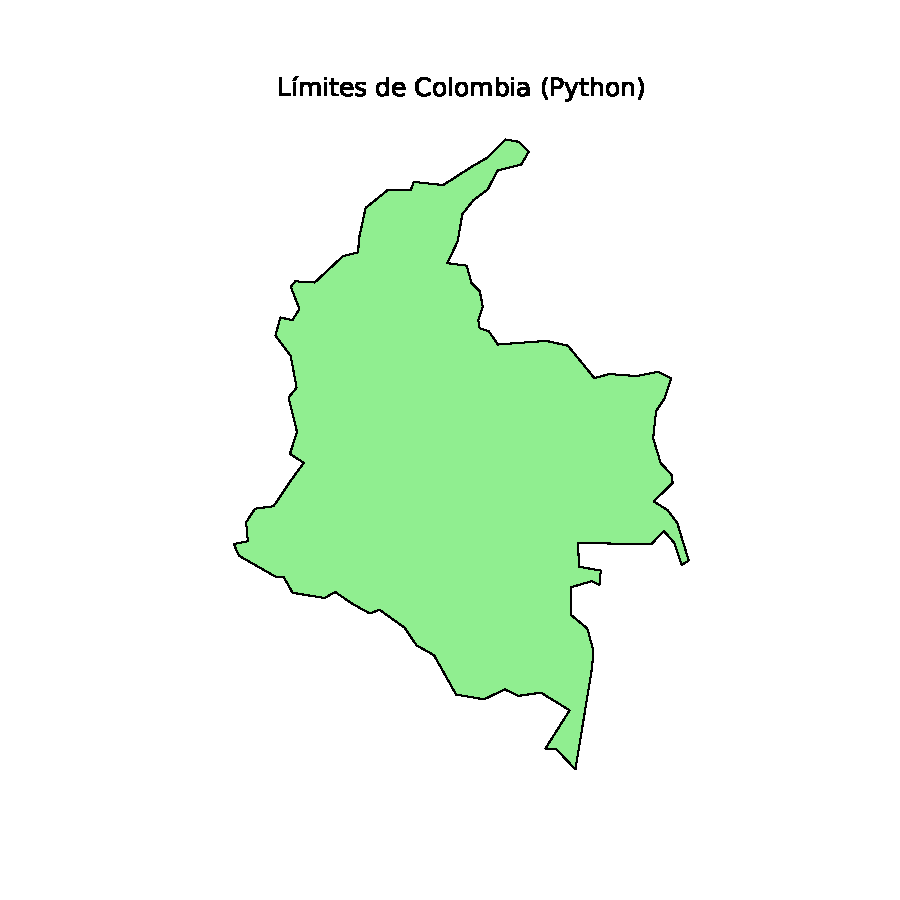
\includegraphics[width=0.5\textwidth,height=\textheight]{10-trabajando_con_archivos_files/figure-pdf/python_rutas_mapa-1.pdf}
\end{center}

\subsection{R}

\begin{Shaded}
\begin{Highlighting}[]
\CommentTok{\# \#| eval: false}

\FunctionTok{library}\NormalTok{(sf)}
\end{Highlighting}
\end{Shaded}

\begin{verbatim}
Linking to GEOS 3.12.1, GDAL 3.8.4, PROJ 9.4.0; sf_use_s2() is TRUE
\end{verbatim}

\begin{Shaded}
\begin{Highlighting}[]
\CommentTok{\# 1. Construcción segura de la ruta relativa}
\CommentTok{\# file.path se encarga de usar el separador adecuado del sistema operativo}
\NormalTok{ruta\_archivo }\OtherTok{\textless{}{-}} \FunctionTok{file.path}\NormalTok{(}\StringTok{"."}\NormalTok{, }\StringTok{"data"}\NormalTok{, }\StringTok{"vector"}\NormalTok{, }\StringTok{"geojson"}\NormalTok{, }\StringTok{"COL.geo.json"}\NormalTok{)}

\CommentTok{\# Blindaje comprobando si el archivo existe}
\ControlFlowTok{if}\NormalTok{ (}\FunctionTok{file.exists}\NormalTok{(ruta\_archivo)) \{}
    \CommentTok{\# 2. Leer el archivo espacial }
    \CommentTok{\# quiet = TRUE evita que se imprima la metadata en la consola durante la lectura    }
\NormalTok{    colombia\_sf }\OtherTok{\textless{}{-}} \FunctionTok{st\_read}\NormalTok{(ruta\_archivo, }\AttributeTok{quiet =} \ConstantTok{TRUE}\NormalTok{)}

    \CommentTok{\# 3. Graficar el mapa estático}
    \CommentTok{\# st\_geometry extrae solo el contorno espacial para un renderizado rápido    }
    \FunctionTok{plot}\NormalTok{(}\FunctionTok{st\_geometry}\NormalTok{(colombia\_sf), }
         \AttributeTok{col =} \StringTok{"lightgreen"}\NormalTok{, }
         \AttributeTok{border =} \StringTok{"black"}\NormalTok{, }
         \AttributeTok{lwd =} \FloatTok{0.5}\NormalTok{,}
         \AttributeTok{main =} \StringTok{"Límites de Colombia (R)"}\NormalTok{)}
\NormalTok{\} }\ControlFlowTok{else}\NormalTok{ \{}
    \CommentTok{\# 4. Control de error    }
    \FunctionTok{cat}\NormalTok{(}\FunctionTok{sprintf}\NormalTok{(}\StringTok{"No se pudo generar el mapa. Verifica la ruta: \%s}\SpecialCharTok{\textbackslash{}n}\StringTok{"}\NormalTok{, ruta\_archivo))}
\NormalTok{\}}
\end{Highlighting}
\end{Shaded}

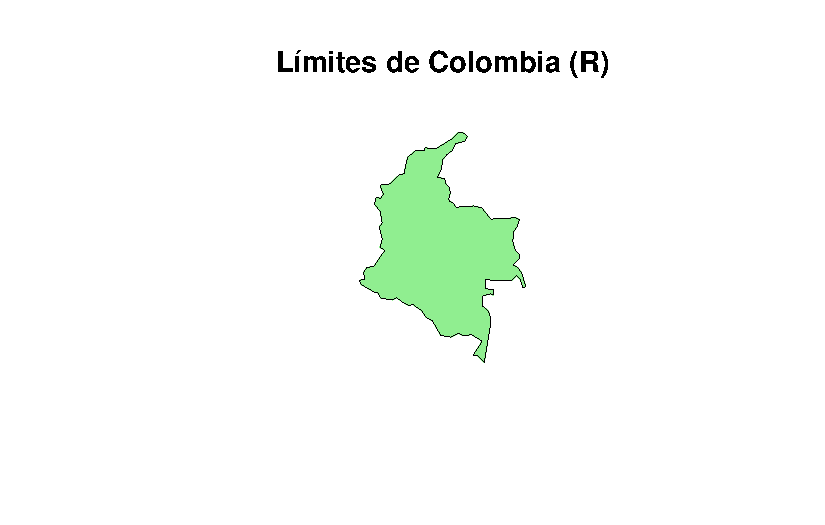
\includegraphics[width=0.8\textwidth,height=\textheight]{10-trabajando_con_archivos_files/figure-pdf/r_rutas_mapa-1.pdf}

\subsection{Julia}

\begin{verbatim}
Starting Julia ...
\end{verbatim}

\begin{center}
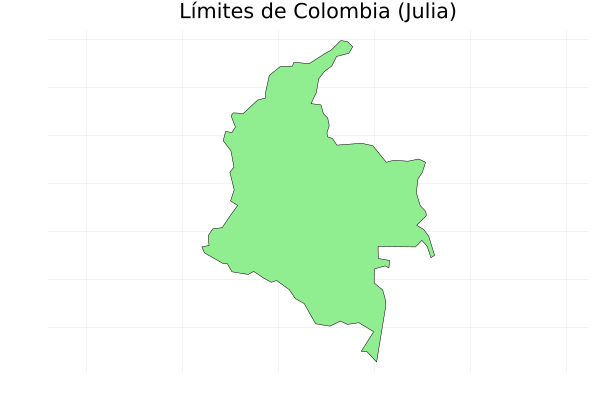
\includegraphics[width=0.6\textwidth,height=\textheight]{images/plots/mapa_colombia_julia.png}
\end{center}

\section{Creando un archivo de
muestra}\label{creando-un-archivo-de-muestra}

En este ejercicio, vamos a crear un archivo de texto plano
(\texttt{./data/coordenadas\_colombia\_p.txt}) que contendrá las
coordenadas (Latitud, Longitud) de cinco de las principales ciudades de
Colombia: Bogotá, Medellín, Cali, Barranquilla y Cartagena. Esto nos
servirá como base para leer datos tabulares más adelante.

\subsection{Python}

\begin{Shaded}
\begin{Highlighting}[]
\CommentTok{\# \#| eval: false}

\CommentTok{\# 1. Definimos los datos usando un string de múltiples líneas (triple comilla).}
\CommentTok{\# Orden: Latitud, Longitud (Bogotá, Medellín, Cali, Barranquilla, Cartagena)}
\NormalTok{datos\_muestra }\OperatorTok{=} \StringTok{"""4.7110,{-}74.0721}
\StringTok{6.2442,{-}75.5812}
\StringTok{3.4516,{-}76.5320}
\StringTok{10.9685,{-}74.7813}
\StringTok{10.3910,{-}75.4794"""}

\CommentTok{\# 2. Definimos la variable \textquotesingle{}f\_txt\textquotesingle{} que almacena la ruta y nombre del archivo}
\NormalTok{f\_txt }\OperatorTok{=} \StringTok{"./data/coordenadas\_colombia\_p.txt"}

\CommentTok{\# 3. Manejo de excepciones completo para la creación del archivo}
\ControlFlowTok{try}\NormalTok{:}
    \CommentTok{\# \textquotesingle{}w\textquotesingle{} indica modo escritura (write). \textquotesingle{}with\textquotesingle{} cierra el archivo automáticamente.}
    \CommentTok{\# Asignamos el archivo abierto a la variable \textquotesingle{}con\textquotesingle{} (conexión)}
    \ControlFlowTok{with} \BuiltInTok{open}\NormalTok{(f\_txt, }\StringTok{"w"}\NormalTok{, encoding}\OperatorTok{=}\StringTok{"utf{-}8"}\NormalTok{) }\ImportTok{as}\NormalTok{ con:}
        \CommentTok{\# Escribimos los datos en la conexión. }
        \CommentTok{\# Python retorna la cantidad de caracteres escritos.}
\NormalTok{        caracteres\_escritos }\OperatorTok{=}\NormalTok{ con.write(datos\_muestra)}
        \CommentTok{\#}
        \CommentTok{\# Imprime automáticamente caracteres\_escritos en modo interactivo}
        \CommentTok{\#con.write(datos\_muestra)}
        \CommentTok{\#}
        \CommentTok{\# Evita que se imprima el número de caracteres\_escritos usando \textquotesingle{}\_\textquotesingle{}}
        \CommentTok{\#\_ = con.write(datos\_muestra)}
\ControlFlowTok{except} \PreprocessorTok{Exception} \ImportTok{as}\NormalTok{ e:}
    \CommentTok{\# Bloque que se ejecuta solo si ocurre un error en la apertura/escritura}
    \BuiltInTok{print}\NormalTok{(}\SpecialStringTok{f"Ocurrió un error al crear el archivo: }\SpecialCharTok{\{}\NormalTok{e}\SpecialCharTok{\}}\SpecialStringTok{"}\NormalTok{)}
\ControlFlowTok{else}\NormalTok{:}
    \CommentTok{\# Bloque que se ejecuta solo si el \textquotesingle{}try\textquotesingle{} fue exitoso (sin errores)}
    \BuiltInTok{print}\NormalTok{(}\SpecialStringTok{f"El archivo \textquotesingle{}}\SpecialCharTok{\{}\NormalTok{f\_txt}\SpecialCharTok{\}}\SpecialStringTok{\textquotesingle{} ha sido creado exitosamente. Se guardaron }\SpecialCharTok{\{}\NormalTok{caracteres\_escritos}\SpecialCharTok{\}}\SpecialStringTok{ caracteres."}\NormalTok{)}
\ControlFlowTok{finally}\NormalTok{:}
    \CommentTok{\# Bloque que se ejecuta SIEMPRE, haya ocurrido un error o no, ideal para limpieza}
    \BuiltInTok{print}\NormalTok{(}\StringTok{"Done."}\NormalTok{)}
\end{Highlighting}
\end{Shaded}

\begin{verbatim}
El archivo './data/coordenadas_colombia_p.txt' ha sido creado exitosamente. Se guardaron 81 caracteres.
Done.
\end{verbatim}

Las alternativas a \texttt{except\ Exception\ as\ e:} son específicas al
tipo de error esperado. Mayor información
\href{https://www.datacamp.com/tutorial/python-try-except}{acá}. Por
ejemplo:

\begin{itemize}
\tightlist
\item
  \texttt{except\ ValueError:}
\item
  \texttt{except\ LookupError:}
\item
  \texttt{except\ IOError:}
\item
  \texttt{except\ FileNotFoundError:}
\item
  \texttt{except\ TimeoutError:}
\item
  \texttt{except\ ZeroDivisionError:}
\item
  \texttt{except\ KeyError:}
\end{itemize}

\subsection{R}

\begin{Shaded}
\begin{Highlighting}[]
\CommentTok{\# \#| eval: false}

\CommentTok{\# 1. En R, usamos el salto de línea \textquotesingle{}\textbackslash{}n\textquotesingle{} para simular múltiples líneas}
\NormalTok{datos\_muestra }\OtherTok{\textless{}{-}} \StringTok{"4.7110,{-}74.0721}\SpecialCharTok{\textbackslash{}n}\StringTok{6.2442,{-}75.5812}\SpecialCharTok{\textbackslash{}n}\StringTok{3.4516,{-}76.5320}\SpecialCharTok{\textbackslash{}n}\StringTok{10.9685,{-}74.7813}\SpecialCharTok{\textbackslash{}n}\StringTok{10.3910,{-}75.4794"}

\CommentTok{\# 2. Definimos la variable \textquotesingle{}f\_txt\textquotesingle{} para la ruta del archivo}
\NormalTok{f\_txt }\OtherTok{\textless{}{-}} \StringTok{"./data/coordenadas\_colombia\_r.txt"}

\CommentTok{\# 3. tryCatch nos permite manejar errores e incluir un bloque \textquotesingle{}finally\textquotesingle{}}
\FunctionTok{tryCatch}\NormalTok{(\{}
    \CommentTok{\# Bloque de ejecución principal}
    \CommentTok{\# Método directo: R abre y cierra la conexión automáticamente}
    \FunctionTok{writeLines}\NormalTok{(datos\_muestra, f\_txt)}
    \CommentTok{\#}
    \CommentTok{\# Alternativamente, abrimos la conexión al archivo explícitamente en la variable \textquotesingle{}con\textquotesingle{}}
    \CommentTok{\#con \textless{}{-} file(f\_txt, "w")}

    \CommentTok{\# Escribimos los datos usando esa conexión explícita}
    \CommentTok{\# writeLines(datos\_muestra, con)}

    \CommentTok{\# Es fundamental cerrar la conexión manualmente al terminar si usamos file()}
    \CommentTok{\#close(con)}
    
    \CommentTok{\# En R no hay un \textquotesingle{}else\textquotesingle{} explícito en tryCatch, por lo que el mensaje }
    \CommentTok{\# de éxito se pone al final del bloque principal (solo llega aquí si no hay error)}
    \FunctionTok{cat}\NormalTok{(}\FunctionTok{sprintf}\NormalTok{(}\StringTok{"El archivo \textquotesingle{}\%s\textquotesingle{} ha sido creado exitosamente.}\SpecialCharTok{\textbackslash{}n}\StringTok{"}\NormalTok{, f\_txt))}
    
\NormalTok{\}, }\AttributeTok{error =} \ControlFlowTok{function}\NormalTok{(e) \{}
    \CommentTok{\# Bloque que se ejecuta si ocurre un error (ej. disco lleno o sin permisos)}
    \FunctionTok{cat}\NormalTok{(}\FunctionTok{sprintf}\NormalTok{(}\StringTok{"Ocurrió un error al crear el archivo: \%s}\SpecialCharTok{\textbackslash{}n}\StringTok{"}\NormalTok{, e}\SpecialCharTok{$}\NormalTok{message))}
    
\NormalTok{\}, }\AttributeTok{finally =}\NormalTok{ \{}
    \CommentTok{\# Bloque que se ejecuta SIEMPRE para finalizar el proceso}
    \FunctionTok{cat}\NormalTok{(}\StringTok{"Done.}\SpecialCharTok{\textbackslash{}n}\StringTok{"}\NormalTok{)}
\NormalTok{\})}
\end{Highlighting}
\end{Shaded}

\begin{verbatim}
El archivo './data/coordenadas_colombia_r.txt' ha sido creado exitosamente.
Done.
\end{verbatim}

\subsection{Julia}

\begin{Shaded}
\begin{Highlighting}[]
\CommentTok{\# \#| eval: false}

\FunctionTok{j\_eval}\NormalTok{(r}\StringTok{"{-}(}
\StringTok{\# 1. Julia también permite strings de múltiples líneas con triple comilla}
\StringTok{datos\_muestra = """}
\FloatTok{4.7110}\NormalTok{,}\SpecialCharTok{{-}}\FloatTok{74.0721}
\FloatTok{6.2442}\NormalTok{,}\SpecialCharTok{{-}}\FloatTok{75.5812}
\FloatTok{3.4516}\NormalTok{,}\SpecialCharTok{{-}}\FloatTok{76.5320}
\FloatTok{10.9685}\NormalTok{,}\SpecialCharTok{{-}}\FloatTok{74.7813}
\FloatTok{10.3910}\NormalTok{,}\SpecialCharTok{{-}}\FloatTok{75.4794}\StringTok{"""}

\StringTok{\# 2. Definimos la variable \textquotesingle{}f\_txt\textquotesingle{} que contiene la ruta al archivo}
\StringTok{f\_txt = "}\NormalTok{.}\SpecialCharTok{/}\NormalTok{data}\SpecialCharTok{/}\NormalTok{coordenadas\_colombia\_j.txt}\StringTok{"}

\StringTok{\# 3. Bloque try{-}catch{-}finally para manejar la escritura}
\StringTok{try}
\StringTok{    \# open con el bloque \textquotesingle{}do\textquotesingle{} asigna la conexión a \textquotesingle{}con\textquotesingle{} y la cierra automáticamente al terminar}
\StringTok{    open(f\_txt, "}\NormalTok{w}\StringTok{") do con}
\StringTok{        \# Escribimos los datos en la conexión. strip() quita saltos de línea extra al inicio/fin}
\StringTok{        write(con, strip(datos\_muestra))}
\StringTok{    end}
\StringTok{    }
\StringTok{    \# Julia no tiene \textquotesingle{}else\textquotesingle{} para el try, el éxito se asume si llegamos a esta línea sin saltar al catch}
\StringTok{    println("}\NormalTok{El archivo }\StringTok{\textquotesingle{}$f\_txt\textquotesingle{}}\NormalTok{ ha sido creado exitosamente.}\StringTok{")}
\StringTok{    }
\StringTok{catch e}
\StringTok{    \# Bloque que se ejecuta si ocurre un error durante la apertura o escritura}
\StringTok{    println("}\NormalTok{Ocurrió un error al crear el archivo}\SpecialCharTok{:} \StringTok{", e)}
\StringTok{    }
\StringTok{finally}
\StringTok{    \# Bloque que se ejecuta SIEMPRE, útil para garantizar la liberación de recursos}
\StringTok{    println("}\NormalTok{Done.}\StringTok{")}
\StringTok{end}
\StringTok{){-}"}\NormalTok{)}
\end{Highlighting}
\end{Shaded}

\begin{tcolorbox}[enhanced jigsaw, coltitle=black, leftrule=.75mm, bottomtitle=1mm, title=\textcolor{quarto-callout-note-color}{\faInfo}\hspace{0.5em}{¿Por qué usamos strip() aquí?}, colback=white, colbacktitle=quarto-callout-note-color!10!white, left=2mm, toptitle=1mm, rightrule=.15mm, titlerule=0mm, arc=.35mm, colframe=quarto-callout-note-color-frame, bottomrule=.15mm, toprule=.15mm, opacityback=0, opacitybacktitle=0.6, breakable]

La función \texttt{strip(datos\_muestra)} en Julia sirve para eliminar
cualquier espacio en blanco o salto de línea
(\texttt{\textbackslash{}n}) que esté al principio o al final de la
cadena de texto.

Al definir nuestra variable con triple comilla y dar un ``enter'' para
que el código se vea ordenado:

\begin{Shaded}
\begin{Highlighting}[]
\NormalTok{datos\_muestra }\OperatorTok{=} \StringTok{"""}
\StringTok{4.7110,{-}74.0721}
\StringTok{...}
\end{Highlighting}
\end{Shaded}

Ese primer ``enter'' es interpretado por Julia como una línea vacía. Si
no usamos \texttt{strip()}, el archivo se guardaría con un salto de
línea inicial, lo cual podría generar errores (como datos nulos o
\texttt{NaN}) al intentar leerlo posteriormente como una tabla. Al
aplicar \texttt{strip()}, le indicamos a Julia que corte esa ``basura''
de los bordes, garantizando que el archivo comience exactamente con el
primer dígito de la latitud.

\end{tcolorbox}

\subsection{Resumen comparativo de escritura de
archivos}\label{resumen-comparativo-de-escritura-de-archivos}

Para facilitar el estudio y la asimilación de los tres lenguajes, aquí
detallo las diferencias clave en las funciones que acabamos de usar:

\begin{longtable}[]{@{}
  >{\raggedright\arraybackslash}p{(\columnwidth - 6\tabcolsep) * \real{0.1429}}
  >{\raggedright\arraybackslash}p{(\columnwidth - 6\tabcolsep) * \real{0.2857}}
  >{\raggedright\arraybackslash}p{(\columnwidth - 6\tabcolsep) * \real{0.2857}}
  >{\raggedright\arraybackslash}p{(\columnwidth - 6\tabcolsep) * \real{0.2857}}@{}}
\toprule\noalign{}
\begin{minipage}[b]{\linewidth}\raggedright
Característica / Tarea
\end{minipage} & \begin{minipage}[b]{\linewidth}\raggedright
Python 🐍
\end{minipage} & \begin{minipage}[b]{\linewidth}\raggedright
R 🔵
\end{minipage} & \begin{minipage}[b]{\linewidth}\raggedright
Julia 🟣
\end{minipage} \\
\midrule\noalign{}
\endhead
\bottomrule\noalign{}
\endlastfoot
\textbf{Definir strings multilinea} & \texttt{"""texto"""} &
\texttt{"\textbackslash{}n"} explícito en la cadena &
\texttt{"""texto"""} \\
\textbf{Abrir/Crear archivo} & \texttt{open(f\_txt,\ "w")\ as\ con} &
\texttt{con\ =\ file(f\_txt,\ "w")}o\texttt{writeLines(datos,\ f\_txt)}
& \texttt{open(f\_txt,\ "w")\ do\ con} \\
\textbf{Escribir datos} & \texttt{con.write(datos)} &
\texttt{writeLines(datos,\ con)}o\texttt{writeLines(datos,\ f\_txt)} &
\texttt{write(con,\ datos)} \\
\textbf{Manejo seguro de cierre} &
\texttt{with\ open(f\_txt,\ "w")\ as\ con:} &
\texttt{close(con)}oAutomático al terminar script &
\texttt{open(f\_txt,\ "w")\ do\ con}~~~~\texttt{...}\texttt{end} \\
\textbf{Manejo de Errores} &
\texttt{try:}~~~~\texttt{...}\texttt{except\ Exception\ as\ e:}~~~~\texttt{...}
&
\texttt{tryCatch(\{}~~~~\texttt{...}\texttt{\},\ error\ =\ function(e)\{}~~~~\texttt{...}\texttt{\})}
&
\texttt{try}~~~~\texttt{...}\texttt{catch\ e}~~~~\texttt{...}\texttt{end} \\
\textbf{Ejecución de Éxito} & Bloque \texttt{else:} & Al final del
bloque principal \texttt{tryCatch} & Al final del bloque \texttt{try} \\
\textbf{Cierre garantizado} & Bloque \texttt{finally:} & Argumento
\texttt{finally\ =\ \{\}} & Bloque \texttt{finally} \\
\end{longtable}

\begin{tcolorbox}[enhanced jigsaw, coltitle=black, leftrule=.75mm, bottomtitle=1mm, title=\textcolor{quarto-callout-important-color}{\faExclamation}\hspace{0.5em}{¡Cuidado con los acentos! (Encoding UTF-8)}, colback=white, colbacktitle=quarto-callout-important-color!10!white, left=2mm, toptitle=1mm, rightrule=.15mm, titlerule=0mm, arc=.35mm, colframe=quarto-callout-important-color-frame, bottomrule=.15mm, toprule=.15mm, opacityback=0, opacitybacktitle=0.6, breakable]

Al trabajar con datos en Colombia (o en español en general), es común
tener caracteres especiales como tildes (Bogotá, Medellín) o la letra ñ.
Por defecto, Windows puede intentar leer estos archivos usando
codificaciones antiguas. Para evitar que tu código colapse con un
\texttt{UnicodeDecodeError} o que los textos se corrompan,
\textbf{siempre} declara explícitamente \texttt{encoding="utf-8"} (en
Python) o \texttt{encoding="UTF-8"} (en R) al abrir un archivo de texto.
Julia maneja UTF-8 de forma nativa por defecto.

\end{tcolorbox}

\section{Leyendo y escribiendo
archivos}\label{leyendo-y-escribiendo-archivos}

En este paso, vamos a leer el archivo de coordenadas que creamos en la
sección anterior, procesaremos cada línea para separar la latitud de la
longitud, y guardaremos los resultados en un nuevo archivo con un
formato mucho más legible.

\subsection{Python}

\begin{Shaded}
\begin{Highlighting}[]
\CommentTok{\# \#| eval: false}

\CommentTok{\# 1. Definimos las variables para los archivos de entrada y salida}
\NormalTok{f\_in }\OperatorTok{=} \StringTok{"./data/coordenadas\_colombia\_p.txt"}
\NormalTok{f\_out }\OperatorTok{=} \StringTok{"./data/coordenadas\_formato\_p.txt"}

\ControlFlowTok{try}\NormalTok{:}
    \CommentTok{\# 2. Abrimos el archivo de entrada en modo lectura (\textquotesingle{}r\textquotesingle{} de read)}
    \ControlFlowTok{with} \BuiltInTok{open}\NormalTok{(f\_in, }\StringTok{"r"}\NormalTok{, encoding}\OperatorTok{=}\StringTok{"utf{-}8"}\NormalTok{) }\ImportTok{as}\NormalTok{ con\_in:}
        \CommentTok{\# readlines() lee todas las líneas y devuelve una lista.}
        \CommentTok{\# Cada elemento de la lista incluye el salto de línea (\textbackslash{}n) al final.}
\NormalTok{        coordenadas }\OperatorTok{=}\NormalTok{ con\_in.readlines()}

    \CommentTok{\# 3. Abrimos el archivo de salida en modo escritura (\textquotesingle{}w\textquotesingle{} de write)}
    \ControlFlowTok{with} \BuiltInTok{open}\NormalTok{(f\_out, }\StringTok{"w"}\NormalTok{, encoding}\OperatorTok{=}\StringTok{"utf{-}8"}\NormalTok{) }\ImportTok{as}\NormalTok{ con\_out:}
        \CommentTok{\# Recorremos cada línea de la lista que leímos}
        \ControlFlowTok{for}\NormalTok{ linea }\KeywordTok{in}\NormalTok{ coordenadas:}
            \CommentTok{\# strip() elimina espacios en blanco y el salto de línea (\textbackslash{}n) de los extremos.}
            \CommentTok{\# split(",") divide la cadena de texto en dos partes usando la coma como separador.}
\NormalTok{            lat, lon }\OperatorTok{=}\NormalTok{ linea.strip().split(}\StringTok{","}\NormalTok{)}

            \CommentTok{\# Escribimos el dato formateado en nuestro archivo de salida.}
            \CommentTok{\# Usamos \textbackslash{}n para asegurar que cada coordenada quede en una línea nueva.}
\NormalTok{            \_ }\OperatorTok{=}\NormalTok{ con\_out.write(}\SpecialStringTok{f"Latitud: }\SpecialCharTok{\{}\NormalTok{lat}\SpecialCharTok{\}}\SpecialStringTok{, Longitud: }\SpecialCharTok{\{}\NormalTok{lon}\SpecialCharTok{\}}\CharTok{\textbackslash{}n}\SpecialStringTok{"}\NormalTok{)}

    \BuiltInTok{print}\NormalTok{(}\SpecialStringTok{f"Las coordenadas han sido guardadas con nuevo formato en \textquotesingle{}}\SpecialCharTok{\{}\NormalTok{f\_out}\SpecialCharTok{\}}\SpecialStringTok{\textquotesingle{}."}\NormalTok{)}

\ControlFlowTok{except} \PreprocessorTok{FileNotFoundError}\NormalTok{:}
    \CommentTok{\# Este bloque específico atrapa el error si el archivo de entrada no existe}
    \BuiltInTok{print}\NormalTok{(}\SpecialStringTok{f"Error: El archivo \textquotesingle{}}\SpecialCharTok{\{}\NormalTok{f\_in}\SpecialCharTok{\}}\SpecialStringTok{\textquotesingle{} no fue encontrado."}\NormalTok{)}
    \BuiltInTok{print}\NormalTok{(}\StringTok{"Asegúrate de haber ejecutado el chunk de Python anterior para crearlo."}\NormalTok{)}
\ControlFlowTok{except} \PreprocessorTok{Exception} \ImportTok{as}\NormalTok{ e:}
    \CommentTok{\# Atrapa cualquier otro error inesperado}
    \BuiltInTok{print}\NormalTok{(}\SpecialStringTok{f"Ocurrió un error inesperado: }\SpecialCharTok{\{}\NormalTok{e}\SpecialCharTok{\}}\SpecialStringTok{"}\NormalTok{)}
\end{Highlighting}
\end{Shaded}

\begin{verbatim}
Las coordenadas han sido guardadas con nuevo formato en './data/coordenadas_formato_p.txt'.
\end{verbatim}

\subsection{R}

\begin{Shaded}
\begin{Highlighting}[]
\CommentTok{\# \#| eval: false}

\CommentTok{\# 1. Definimos las variables para los archivos de entrada y salida (usamos los de R)}
\NormalTok{f\_in }\OtherTok{\textless{}{-}} \StringTok{"./data/coordenadas\_colombia\_r.txt"}
\NormalTok{f\_out }\OtherTok{\textless{}{-}} \StringTok{"./data/coordenadas\_formato\_r.txt"}

\FunctionTok{tryCatch}\NormalTok{(\{}
    \CommentTok{\# 2. Abrimos conexión de lectura y leemos las líneas}
\NormalTok{    con\_in }\OtherTok{\textless{}{-}} \FunctionTok{file}\NormalTok{(f\_in, }\StringTok{"r"}\NormalTok{, }\AttributeTok{encoding=}\StringTok{"UTF{-}8"}\NormalTok{)}
\NormalTok{    coordenadas }\OtherTok{\textless{}{-}} \FunctionTok{readLines}\NormalTok{(con\_in, }\AttributeTok{warn =} \ConstantTok{FALSE}\NormalTok{)}
    \FunctionTok{close}\NormalTok{(con\_in) }\CommentTok{\# Cerramos la conexión de entrada}

    \CommentTok{\# 3. Abrimos conexión de escritura para el nuevo archivo}
\NormalTok{    con\_out }\OtherTok{\textless{}{-}} \FunctionTok{file}\NormalTok{(f\_out, }\StringTok{"w"}\NormalTok{, }\AttributeTok{encoding=}\StringTok{"UTF{-}8"}\NormalTok{)}
    
    \CommentTok{\# Iteramos sobre cada línea}
    \ControlFlowTok{for}\NormalTok{ (linea }\ControlFlowTok{in}\NormalTok{ coordenadas) \{}
        \CommentTok{\# trimws() quita espacios. strsplit() divide por la coma (devuelve una lista)}
\NormalTok{        partes }\OtherTok{\textless{}{-}} \FunctionTok{strsplit}\NormalTok{(}\FunctionTok{trimws}\NormalTok{(linea), }\StringTok{","}\NormalTok{)[[}\DecValTok{1}\NormalTok{]]}
\NormalTok{        lat }\OtherTok{\textless{}{-}}\NormalTok{ partes[}\DecValTok{1}\NormalTok{]}
\NormalTok{        lon }\OtherTok{\textless{}{-}}\NormalTok{ partes[}\DecValTok{2}\NormalTok{]}
        
        \CommentTok{\# Formateamos el texto y lo escribimos en la conexión}
        \CommentTok{\# writeLines añade el salto de línea automáticamente en R}
\NormalTok{        texto\_formateado }\OtherTok{\textless{}{-}} \FunctionTok{sprintf}\NormalTok{(}\StringTok{"Latitud: \%s, Longitud: \%s"}\NormalTok{, lat, lon)}
        \FunctionTok{writeLines}\NormalTok{(texto\_formateado, con\_out)}
\NormalTok{    \}}
    \FunctionTok{close}\NormalTok{(con\_out) }\CommentTok{\# Cerramos la conexión de salida}
    
    \FunctionTok{cat}\NormalTok{(}\FunctionTok{sprintf}\NormalTok{(}\StringTok{"Las coordenadas han sido guardadas con nuevo formato en \textquotesingle{}\%s\textquotesingle{}.}\SpecialCharTok{\textbackslash{}n}\StringTok{"}\NormalTok{, f\_out))}

\NormalTok{\}, }\AttributeTok{error =} \ControlFlowTok{function}\NormalTok{(e) \{}
    \CommentTok{\# Manejo de errores (por ejemplo, si el archivo no existe)}
    \FunctionTok{cat}\NormalTok{(}\FunctionTok{sprintf}\NormalTok{(}\StringTok{"Error al procesar los archivos: \%s}\SpecialCharTok{\textbackslash{}n}\StringTok{"}\NormalTok{, e}\SpecialCharTok{$}\NormalTok{message))}
    \FunctionTok{cat}\NormalTok{(}\StringTok{"Asegúrate de haber ejecutado el chunk de R anterior para crear el archivo base.}\SpecialCharTok{\textbackslash{}n}\StringTok{"}\NormalTok{)}
\NormalTok{\})}
\end{Highlighting}
\end{Shaded}

\begin{verbatim}
Las coordenadas han sido guardadas con nuevo formato en './data/coordenadas_formato_r.txt'.
\end{verbatim}

\subsection{Julia}

\begin{Shaded}
\begin{Highlighting}[]
\CommentTok{\# \#| eval: false}

\FunctionTok{j\_eval}\NormalTok{(r}\StringTok{"{-}(}
\StringTok{\# 1. Definimos los nombres de archivo (usando los de Julia)}
\StringTok{f\_in = "}\NormalTok{.}\SpecialCharTok{/}\NormalTok{data}\SpecialCharTok{/}\NormalTok{coordenadas\_colombia\_j.txt}\StringTok{"}
\StringTok{f\_out = "}\NormalTok{.}\SpecialCharTok{/}\NormalTok{data}\SpecialCharTok{/}\NormalTok{coordenadas\_formato\_j.txt}\StringTok{"}

\StringTok{try}
\StringTok{    \# 2. Leer los datos. open con \textquotesingle{}do\textquotesingle{} cierra automáticamente la conexión}
\StringTok{    coordenadas = open(f\_in, "}\NormalTok{r}\StringTok{") do con\_in}
\StringTok{        readlines(con\_in) \# Devuelve un arreglo (Array) con cada línea}
\StringTok{    end}

\StringTok{    \# 3. Procesar y escribir. Abrimos el nuevo archivo}
\StringTok{    open(f\_out, "}\NormalTok{w}\StringTok{") do con\_out}
\StringTok{        for linea in coordenadas}
\StringTok{            \# strip() limpia la línea. split() separa por coma y permite asignación múltiple}
\StringTok{            lat, lon = split(strip(linea), "}\NormalTok{,}\StringTok{")}
\StringTok{            }
\StringTok{            \# Escribimos el formato en la conexión (añadimos }\SpecialCharTok{\textbackslash{}n}\StringTok{ manualmente)}
\StringTok{            write(con\_out, "}\NormalTok{Latitud}\SpecialCharTok{:} \ErrorTok{$}\NormalTok{lat, Longitud}\SpecialCharTok{:} \ErrorTok{$}\NormalTok{lon\textbackslash{}n}\StringTok{")}
\StringTok{        end}
\StringTok{    end}

\StringTok{    println("}\NormalTok{Las coordenadas han sido guardadas con nuevo formato en }\StringTok{\textquotesingle{}$f\_out\textquotesingle{}}\NormalTok{.}\StringTok{")}

\StringTok{catch e}
\StringTok{    \# Capturamos el error (típicamente SystemError si no encuentra el archivo)}
\StringTok{    println("}\NormalTok{Error al procesar los archivos}\SpecialCharTok{:} \StringTok{", e)}
\StringTok{    println("}\NormalTok{Asegúrate de haber ejecutado el chunk de Julia anterior para crear el archivo base.}\StringTok{")}
\StringTok{end}
\StringTok{){-}"}\NormalTok{)}
\end{Highlighting}
\end{Shaded}

\subsection{Resumen comparativo de lectura de
archivos}\label{resumen-comparativo-de-lectura-de-archivos}

A continuación, destacamos las diferencias en las funciones de
manipulación y lectura de texto:

\begin{longtable}[]{@{}
  >{\raggedright\arraybackslash}p{(\columnwidth - 6\tabcolsep) * \real{0.1429}}
  >{\raggedright\arraybackslash}p{(\columnwidth - 6\tabcolsep) * \real{0.2857}}
  >{\raggedright\arraybackslash}p{(\columnwidth - 6\tabcolsep) * \real{0.2857}}
  >{\raggedright\arraybackslash}p{(\columnwidth - 6\tabcolsep) * \real{0.2857}}@{}}
\toprule\noalign{}
\begin{minipage}[b]{\linewidth}\raggedright
Característica / Tarea
\end{minipage} & \begin{minipage}[b]{\linewidth}\raggedright
Python 🐍
\end{minipage} & \begin{minipage}[b]{\linewidth}\raggedright
R 🔵
\end{minipage} & \begin{minipage}[b]{\linewidth}\raggedright
Julia 🟣
\end{minipage} \\
\midrule\noalign{}
\endhead
\bottomrule\noalign{}
\endlastfoot
\textbf{Abrir en modo lectura} & \texttt{open(f\_in,\ "r")\ as\ con\_in}
& \texttt{con\_in\ =\ file(f\_in,\ "r")} &
\texttt{open(f\_in,\ "r")\ do\ con\_in} \\
\textbf{Leer todas las líneas} & \texttt{con\_in.readlines()} &
\texttt{readLines(con\_in)} & \texttt{readlines(con\_in)} \\
\textbf{Limpiar espacios / saltos} & \texttt{linea.strip()} &
\texttt{trimws(linea)} & \texttt{strip(linea)} \\
\textbf{Separar texto por coma} & \texttt{linea.split(",")} &
\texttt{strsplit(linea,\ ","){[}{[}1{]}{]}} &
\texttt{split(linea,\ ",")} \\
\textbf{Formatear texto (variables)} & \texttt{f"Lat:\ \{lat\}"} &
\texttt{sprintf("Lat:\ \%s",\ lat)} & \texttt{"Lat:\ \$lat"} \\
\textbf{Manejo Archivo no encontrado} &
\texttt{except\ FileNotFoundError:} & Atrapado genéricamente por
\texttt{error\ =\ function(e)} en el \texttt{tryCatch} & Atrapado
genéricamente en \texttt{catch\ e} (es un \texttt{SystemError}) \\
\end{longtable}

\section{Manejo de excepciones}\label{manejo-de-excepciones}

A menudo, los datos espaciales que recibimos en formato de texto vienen
con errores (filas incompletas, letras en lugar de números, etc.). En
esta sección aprenderemos a crear una función robusta que capture esos
errores usando bloques de excepciones, evitando que nuestro programa
colapse al encontrar un dato mal formateado.

\subsection{Python}

\begin{Shaded}
\begin{Highlighting}[]
\CommentTok{\# \#| eval: false}

\CommentTok{\# Ejemplo de manejo de excepciones al analizar coordenadas}
\KeywordTok{def}\NormalTok{ analizar\_coordenadas(linea):}
    \CommentTok{"""}
\CommentTok{    Analiza una línea de texto y la convierte en coordenadas de latitud y longitud.}

\CommentTok{    Argumentos:}
\CommentTok{        linea (str): Una cadena de texto con las coordenadas en formato "lat,lon"}

\CommentTok{    Retorna:}
\CommentTok{        tuple: (latitud, longitud) como flotantes (floats), o None si el análisis falla}
\CommentTok{    """}
    \ControlFlowTok{try}\NormalTok{:}
        \CommentTok{\# split() divide la cadena y retorna una lista (list) de textos (str).}
        \CommentTok{\# Desempacamos esa lista directamente en dos variables de texto: lat\_str y lon\_str}
\NormalTok{        lat\_str, lon\_str }\OperatorTok{=}\NormalTok{ linea.strip().split(}\StringTok{","}\NormalTok{)}
        
        \CommentTok{\# Convertimos las variables de texto (str) a números decimales (float)}
        \CommentTok{\# Esto puede generar un ValueError si el texto no es un número válido}
\NormalTok{        lat }\OperatorTok{=} \BuiltInTok{float}\NormalTok{(lat\_str)}
\NormalTok{        lon }\OperatorTok{=} \BuiltInTok{float}\NormalTok{(lon\_str)}
        
        \CommentTok{\# Retornamos los valores empaquetados en una tupla (tuple) de floats}
        \ControlFlowTok{return}\NormalTok{ lat, lon}

    \ControlFlowTok{except} \PreprocessorTok{ValueError} \ImportTok{as}\NormalTok{ e:}
        \CommentTok{\# Este bloque se ejecuta si no se puede convertir a float o si split() no devuelve 2 valores}
        \BuiltInTok{print}\NormalTok{(}\SpecialStringTok{f"Error de formato: }\SpecialCharTok{\{}\NormalTok{e}\SpecialCharTok{\}}\SpecialStringTok{. No se pudo procesar la línea (tipo str): \textquotesingle{}}\SpecialCharTok{\{}\NormalTok{linea}\SpecialCharTok{.}\NormalTok{strip()}\SpecialCharTok{\}}\SpecialStringTok{\textquotesingle{}"}\NormalTok{)}
        \CommentTok{\# Retornamos un tipo nulo (NoneType)}
        \ControlFlowTok{return} \VariableTok{None}

    \ControlFlowTok{except} \PreprocessorTok{Exception} \ImportTok{as}\NormalTok{ e:}
        \CommentTok{\# Este bloque captura cualquier otro error inesperado}
        \BuiltInTok{print}\NormalTok{(}\SpecialStringTok{f"Ocurrió un error inesperado: }\SpecialCharTok{\{}\NormalTok{e}\SpecialCharTok{\}}\SpecialStringTok{"}\NormalTok{)}
        \ControlFlowTok{return} \VariableTok{None}

\CommentTok{\# Almacenaremos todos los casos de prueba en una lista (list) de textos (str) llamada lineas\_prueba}
\NormalTok{lineas\_prueba }\OperatorTok{=}\NormalTok{ [}
    \StringTok{"4.7110,{-}74.0721"}\NormalTok{,      }\CommentTok{\# Coordenadas válidas (Bogotá)}
    \StringTok{"datos invalidos"}\NormalTok{,      }\CommentTok{\# Formato inválido (sin coma)}
    \StringTok{"10.9685,{-}74.7813"}\NormalTok{,     }\CommentTok{\# Coordenadas válidas (Barranquilla)}
    \StringTok{"10.9685,no\_es\_numero"}\NormalTok{, }\CommentTok{\# Longitud inválida (no se puede convertir a float)}
    \StringTok{"solo\_un\_valor"}\NormalTok{,        }\CommentTok{\# Falta la coma (split falla al desempacar)}
\NormalTok{]}

\BuiltInTok{print}\NormalTok{(}\StringTok{"Probando el análisis de coordenadas:"}\NormalTok{)}
\end{Highlighting}
\end{Shaded}

\begin{verbatim}
Probando el análisis de coordenadas:
\end{verbatim}

\begin{Shaded}
\begin{Highlighting}[]
\CommentTok{\# Recorremos la lista. En cada iteración, \textquotesingle{}linea\textquotesingle{} es un texto (str)}
\ControlFlowTok{for}\NormalTok{ linea }\KeywordTok{in}\NormalTok{ lineas\_prueba:}
    \CommentTok{\# \textquotesingle{}coordenadas\textquotesingle{} recibirá una tupla (tuple) o un valor nulo (None)}
\NormalTok{    coordenadas }\OperatorTok{=}\NormalTok{ analizar\_coordenadas(linea)}
    
    \ControlFlowTok{if}\NormalTok{ coordenadas:}
        \BuiltInTok{print}\NormalTok{(}\SpecialStringTok{f"✓ Procesado exitosamente: }\SpecialCharTok{\{}\NormalTok{coordenadas}\SpecialCharTok{\}}\SpecialStringTok{"}\NormalTok{)}
    \ControlFlowTok{else}\NormalTok{:}
        \BuiltInTok{print}\NormalTok{(}\SpecialStringTok{f"✗ Falló al procesar: \textquotesingle{}}\SpecialCharTok{\{}\NormalTok{linea}\SpecialCharTok{\}}\SpecialStringTok{\textquotesingle{}"}\NormalTok{)}
\end{Highlighting}
\end{Shaded}

\begin{verbatim}
✓ Procesado exitosamente: (4.711, -74.0721)
Error de formato: not enough values to unpack (expected 2, got 1). No se pudo procesar la línea (tipo str): 'datos invalidos'
✗ Falló al procesar: 'datos invalidos'
✓ Procesado exitosamente: (10.9685, -74.7813)
Error de formato: could not convert string to float: 'no_es_numero'. No se pudo procesar la línea (tipo str): '10.9685,no_es_numero'
✗ Falló al procesar: '10.9685,no_es_numero'
Error de formato: not enough values to unpack (expected 2, got 1). No se pudo procesar la línea (tipo str): 'solo_un_valor'
✗ Falló al procesar: 'solo_un_valor'
\end{verbatim}

\subsection{R}

\begin{Shaded}
\begin{Highlighting}[]
\CommentTok{\# \#| eval: false}

\CommentTok{\# Ejemplo de manejo de excepciones al analizar coordenadas en R}
\NormalTok{analizar\_coordenadas }\OtherTok{\textless{}{-}} \ControlFlowTok{function}\NormalTok{(linea) \{}
    \CommentTok{\# \textquotesingle{}linea\textquotesingle{} ingresa como un vector de caracteres (character) de longitud 1}
    \FunctionTok{tryCatch}\NormalTok{(\{}
        \CommentTok{\# Limpiamos espacios. linea\_limpia sigue siendo character}
\NormalTok{        linea\_limpia }\OtherTok{\textless{}{-}} \FunctionTok{trimws}\NormalTok{(linea)}
        
        \CommentTok{\# strsplit devuelve una lista (list) de vectores. Extraemos el primer vector de caracteres con [[1]]}
        \CommentTok{\# \textquotesingle{}partes\textquotesingle{} es ahora un vector de caracteres (character vector)}
\NormalTok{        partes }\OtherTok{\textless{}{-}} \FunctionTok{strsplit}\NormalTok{(linea\_limpia, }\StringTok{","}\NormalTok{)[[}\DecValTok{1}\NormalTok{]]}
        
        \CommentTok{\# Verificamos si la longitud del vector es distinta de 2}
        \ControlFlowTok{if}\NormalTok{ (}\FunctionTok{length}\NormalTok{(partes) }\SpecialCharTok{!=} \DecValTok{2}\NormalTok{) \{}
            \FunctionTok{stop}\NormalTok{(}\StringTok{"La línea no tiene exactamente dos valores separados por coma"}\NormalTok{)}
\NormalTok{        \}}
        
        \CommentTok{\# Intentamos convertir texto (character) a numérico (numeric). }
        \CommentTok{\# R devuelve NA (Not Available) si falla la conversión.}
\NormalTok{        lat }\OtherTok{\textless{}{-}} \FunctionTok{suppressWarnings}\NormalTok{(}\FunctionTok{as.numeric}\NormalTok{(partes[}\DecValTok{1}\NormalTok{]))}
\NormalTok{        lon }\OtherTok{\textless{}{-}} \FunctionTok{suppressWarnings}\NormalTok{(}\FunctionTok{as.numeric}\NormalTok{(partes[}\DecValTok{2}\NormalTok{]))}
        
        \CommentTok{\# is.na() evalúa si el tipo de dato numérico es un valor perdido}
        \ControlFlowTok{if}\NormalTok{ (}\FunctionTok{is.na}\NormalTok{(lat) }\SpecialCharTok{||} \FunctionTok{is.na}\NormalTok{(lon)) \{}
            \FunctionTok{stop}\NormalTok{(}\StringTok{"Uno o ambos valores no son números válidos"}\NormalTok{)}
\NormalTok{        \}}
        
        \CommentTok{\# En R, no hay tuplas. Retornamos un vector numérico (numeric vector) combinando con c()}
        \FunctionTok{return}\NormalTok{(}\FunctionTok{c}\NormalTok{(lat, lon))}
        
\NormalTok{    \}, }\AttributeTok{error =} \ControlFlowTok{function}\NormalTok{(e) \{}
        \CommentTok{\# Atrapamos errores y retornamos NULL (el equivalente al objeto nulo)}
        \FunctionTok{cat}\NormalTok{(}\FunctionTok{sprintf}\NormalTok{(}\StringTok{"Error de formato: \%s. No se pudo procesar la línea: \textquotesingle{}\%s\textquotesingle{}}\SpecialCharTok{\textbackslash{}n}\StringTok{"}\NormalTok{, e}\SpecialCharTok{$}\NormalTok{message, }\FunctionTok{trimws}\NormalTok{(linea)))}
        \FunctionTok{return}\NormalTok{(}\ConstantTok{NULL}\NormalTok{) }
\NormalTok{    \})}
\NormalTok{\}}

\CommentTok{\# Almacenaremos todos los casos de prueba en un vector de caracteres (character vector) llamado lineas\_prueba}
\NormalTok{lineas\_prueba }\OtherTok{\textless{}{-}} \FunctionTok{c}\NormalTok{(}
    \StringTok{"4.7110,{-}74.0721"}\NormalTok{,      }\CommentTok{\# Coordenadas válidas (Bogotá)}
    \StringTok{"datos invalidos"}\NormalTok{,      }\CommentTok{\# Formato inválido (sin coma)}
    \StringTok{"10.9685,{-}74.7813"}\NormalTok{,     }\CommentTok{\# Coordenadas válidas (Barranquilla)}
    \StringTok{"10.9685,no\_es\_numero"}\NormalTok{, }\CommentTok{\# Longitud inválida (no se puede convertir a numérico)}
    \StringTok{"solo\_un\_valor"}         \CommentTok{\# Falta la coma}
\NormalTok{)}

\FunctionTok{cat}\NormalTok{(}\StringTok{"Probando el análisis de coordenadas:}\SpecialCharTok{\textbackslash{}n}\StringTok{"}\NormalTok{)}
\end{Highlighting}
\end{Shaded}

\begin{verbatim}
Probando el análisis de coordenadas:
\end{verbatim}

\begin{Shaded}
\begin{Highlighting}[]
\CommentTok{\# Recorremos el vector. \textquotesingle{}linea\textquotesingle{} toma el valor de texto (character) en cada iteración}
\ControlFlowTok{for}\NormalTok{ (linea }\ControlFlowTok{in}\NormalTok{ lineas\_prueba) \{}
    \CommentTok{\# \textquotesingle{}coordenadas\textquotesingle{} recibe un vector numérico (numeric) o un valor nulo (NULL)}
\NormalTok{    coordenadas }\OtherTok{\textless{}{-}} \FunctionTok{analizar\_coordenadas}\NormalTok{(linea)}
    
    \CommentTok{\# is.null() verifica si el objeto pertenece a la clase NULL}
    \ControlFlowTok{if}\NormalTok{ (}\SpecialCharTok{!}\FunctionTok{is.null}\NormalTok{(coordenadas)) \{}
        \FunctionTok{cat}\NormalTok{(}\FunctionTok{sprintf}\NormalTok{(}\StringTok{"✓ Procesado exitosamente: [\%f, \%f]}\SpecialCharTok{\textbackslash{}n}\StringTok{"}\NormalTok{, coordenadas[}\DecValTok{1}\NormalTok{], coordenadas[}\DecValTok{2}\NormalTok{]))}
\NormalTok{    \} }\ControlFlowTok{else}\NormalTok{ \{}
        \FunctionTok{cat}\NormalTok{(}\FunctionTok{sprintf}\NormalTok{(}\StringTok{"✗ Falló al procesar: \textquotesingle{}\%s\textquotesingle{}}\SpecialCharTok{\textbackslash{}n}\StringTok{"}\NormalTok{, linea))}
\NormalTok{    \}}
\NormalTok{\}}
\end{Highlighting}
\end{Shaded}

\begin{verbatim}
✓ Procesado exitosamente: [4.711000, -74.072100]
Error de formato: La línea no tiene exactamente dos valores separados por coma. No se pudo procesar la línea: 'datos invalidos'
✗ Falló al procesar: 'datos invalidos'
✓ Procesado exitosamente: [10.968500, -74.781300]
Error de formato: Uno o ambos valores no son números válidos. No se pudo procesar la línea: '10.9685,no_es_numero'
✗ Falló al procesar: '10.9685,no_es_numero'
Error de formato: La línea no tiene exactamente dos valores separados por coma. No se pudo procesar la línea: 'solo_un_valor'
✗ Falló al procesar: 'solo_un_valor'
\end{verbatim}

\subsection{Julia}

\begin{Shaded}
\begin{Highlighting}[]
\CommentTok{\# \#| eval: false}

\FunctionTok{j\_eval}\NormalTok{(r}\StringTok{"{-}(}
\StringTok{\# Ejemplo de manejo de excepciones al analizar coordenadas en Julia}
\StringTok{function analizar\_coordenadas(linea)}
\StringTok{    \# \textquotesingle{}linea\textquotesingle{} ingresa como una cadena de texto (String)}
\StringTok{    try}
\StringTok{        \# split() divide el String y retorna un arreglo de subcadenas (Vector\{SubString\{String\}\})}
\StringTok{        partes = split(strip(linea), "}\NormalTok{,}\StringTok{")}
\StringTok{        }
\StringTok{        \# Verificamos la longitud del arreglo (Array)}
\StringTok{        if length(partes) != 2}
\StringTok{            error("}\NormalTok{La línea no tiene exactamente dos valores separados por coma}\StringTok{")}
\StringTok{        end}
\StringTok{        }
\StringTok{        \# parse() evalúa el texto y lo convierte estrictamente a un decimal de 64 bits (Float64)}
\StringTok{        lat = parse(Float64, partes[1])}
\StringTok{        lon = parse(Float64, partes[2])}
\StringTok{        }
\StringTok{        \# Retornamos los datos empaquetados en una tupla de decimales (Tuple\{Float64, Float64\})}
\StringTok{        return (lat, lon)}
\StringTok{        }
\StringTok{    catch e}
\StringTok{        \# Capturamos errores de parseo o de longitud}
\StringTok{        println("}\NormalTok{Error de formato}\SpecialCharTok{:} \ErrorTok{$}\NormalTok{e. No se pudo procesar la línea}\SpecialCharTok{:} \StringTok{\textquotesingle{}$(strip(linea))\textquotesingle{}")}
\StringTok{        \# \textquotesingle{}nothing\textquotesingle{} es el tipo nulo oficial en Julia (tipo Nothing)}
\StringTok{        return nothing }
\StringTok{    end}
\StringTok{end}

\StringTok{\# Almacenaremos todos los casos de prueba en un arreglo/vector de textos (Vector\{String\})}
\StringTok{lineas\_prueba = [}
\StringTok{    "}\FloatTok{4.7110}\NormalTok{,}\SpecialCharTok{{-}}\FloatTok{74.0721}\StringTok{",      \# Coordenadas válidas (Bogotá)}
\StringTok{    "}\NormalTok{datos invalidos}\StringTok{",      \# Formato inválido}
\StringTok{    "}\FloatTok{10.9685}\NormalTok{,}\SpecialCharTok{{-}}\FloatTok{74.7813}\StringTok{",     \# Coordenadas válidas (Barranquilla)}
\StringTok{    "}\FloatTok{10.9685}\NormalTok{,no\_es\_numero}\StringTok{", \# Longitud inválida (no se puede parsear a Float64)}
\StringTok{    "}\NormalTok{solo\_un\_valor}\StringTok{"         \# Falta la coma}
\StringTok{]}

\StringTok{println("}\NormalTok{Probando el análisis de coordenadas}\SpecialCharTok{:}\StringTok{")}
\StringTok{\# Recorremos el arreglo. En cada iteración \textquotesingle{}linea\textquotesingle{} es un texto (String)}
\StringTok{for linea in lineas\_prueba}
\StringTok{    \# \textquotesingle{}coordenadas\textquotesingle{} recibe una tupla de floats o el valor nulo (nothing)}
\StringTok{    coordenadas = analizar\_coordenadas(linea)}
\StringTok{    }
\StringTok{    \# En Julia evaluamos estrictamente la identidad del objeto nulo usando \textquotesingle{}!==\textquotesingle{}}
\StringTok{    if coordenadas !== nothing}
\StringTok{        println("}\NormalTok{✓ Procesado exitosamente}\SpecialCharTok{:} \ErrorTok{$}\NormalTok{coordenadas}\StringTok{")}
\StringTok{    else}
\StringTok{        println("}\NormalTok{✗ Falló al procesar}\SpecialCharTok{:} \StringTok{\textquotesingle{}$linea\textquotesingle{}")}
\StringTok{    end}
\StringTok{end}
\StringTok{){-}"}\NormalTok{)}
\end{Highlighting}
\end{Shaded}

\subsection{Resumen comparativo de funciones y
excepciones}\label{resumen-comparativo-de-funciones-y-excepciones}

A continuación, destacamos las diferencias sintácticas al definir
funciones, convertir tipos de datos y manejar valores nulos en los tres
lenguajes:

\begin{longtable}[]{@{}
  >{\raggedright\arraybackslash}p{(\columnwidth - 6\tabcolsep) * \real{0.1429}}
  >{\raggedright\arraybackslash}p{(\columnwidth - 6\tabcolsep) * \real{0.2857}}
  >{\raggedright\arraybackslash}p{(\columnwidth - 6\tabcolsep) * \real{0.2857}}
  >{\raggedright\arraybackslash}p{(\columnwidth - 6\tabcolsep) * \real{0.2857}}@{}}
\toprule\noalign{}
\begin{minipage}[b]{\linewidth}\raggedright
Característica / Tarea
\end{minipage} & \begin{minipage}[b]{\linewidth}\raggedright
Python 🐍
\end{minipage} & \begin{minipage}[b]{\linewidth}\raggedright
R 🔵
\end{minipage} & \begin{minipage}[b]{\linewidth}\raggedright
Julia 🟣
\end{minipage} \\
\midrule\noalign{}
\endhead
\bottomrule\noalign{}
\endlastfoot
\textbf{Definir una función} & \texttt{def\ funcion(arg):} &
\texttt{funcion\ \textless{}-\ function(arg)\ \{} &
\texttt{function\ funcion(arg)} \\
\textbf{Retornar valores} & \texttt{return\ lat,\ lon} (Tupla) &
\texttt{return(c(lat,\ lon))} (Vector) & \texttt{return\ (lat,\ lon)}
(Tupla) \\
\textbf{Convertir texto a número} & \texttt{float(texto)} &
\texttt{as.numeric(texto)} & \texttt{parse(Float64,\ texto)} \\
\textbf{Lanzar error manual} & \texttt{raise\ ValueError("msg")} &
\texttt{stop("msg")} & \texttt{error("msg")} \\
\textbf{Valor Nulo/Vacío} & \texttt{None} & \texttt{NULL} (o \texttt{NA}
para faltantes) & \texttt{nothing} \\
\textbf{Verificar valor válido} & \texttt{if\ variable:} &
\texttt{if\ (!is.null(variable))} &
\texttt{if\ variable\ !==\ nothing} \\
\end{longtable}

\section{Combinando manejo de archivos y
excepciones}\label{combinando-manejo-de-archivos-y-excepciones}

En este punto, vamos a integrar lo que hemos aprendido sobre lectura de
archivos y captura de errores. Crearemos una función que abra nuestro
archivo de coordenadas, procese cada línea usando la función
\texttt{analizar\_coordenadas()} (que definimos en el paso anterior), y
lleve un registro exacto de cuántas líneas se procesaron con éxito y
cuántas fallaron, sin detener la ejecución del script.

\subsection{Python}

\begin{Shaded}
\begin{Highlighting}[]
\CommentTok{\# \#| eval: false}

\CommentTok{\# Ejemplo de manejo robusto de archivos con excepciones}
\KeywordTok{def}\NormalTok{ procesar\_archivo\_espacial(f\_in):}
    \CommentTok{"""}
\CommentTok{    Procesa un archivo con coordenadas, manejando varios errores potenciales.}
\CommentTok{    Argumentos:}
\CommentTok{        f\_in (str): La ruta del archivo a leer.}
\CommentTok{    """}
    \CommentTok{\# Contadores enteros (int) para el resumen final}
\NormalTok{    procesados }\OperatorTok{=} \DecValTok{0}
\NormalTok{    errores }\OperatorTok{=} \DecValTok{0}

    \ControlFlowTok{try}\NormalTok{:}
        \BuiltInTok{print}\NormalTok{(}\SpecialStringTok{f"Iniciando el procesamiento del archivo: }\SpecialCharTok{\{}\NormalTok{f\_in}\SpecialCharTok{\}}\SpecialStringTok{"}\NormalTok{)}

        \CommentTok{\# Abrimos la conexión al archivo en modo lectura (\textquotesingle{}r\textquotesingle{})}
        \ControlFlowTok{with} \BuiltInTok{open}\NormalTok{(f\_in, }\StringTok{"r"}\NormalTok{, encoding}\OperatorTok{=}\StringTok{"utf{-}8"}\NormalTok{) }\ImportTok{as}\NormalTok{ con\_in:}
            \CommentTok{\# enumerate() nos da un índice entero (int) y la línea de texto (str)}
            \CommentTok{\# El \textquotesingle{}1\textquotesingle{} indica que queremos empezar a contar desde la línea 1}
            \ControlFlowTok{for}\NormalTok{ num\_linea, linea }\KeywordTok{in} \BuiltInTok{enumerate}\NormalTok{(con\_in, }\DecValTok{1}\NormalTok{):}
                
                \CommentTok{\# Omitimos líneas vacías. strip() quita espacios, y \textquotesingle{}not\textquotesingle{} evalúa si quedó vacío}
                \ControlFlowTok{if} \KeywordTok{not}\NormalTok{ linea.strip():}
                    \ControlFlowTok{continue}

                \CommentTok{\# \textquotesingle{}coordenadas\textquotesingle{} recibirá una tupla (tuple) o un nulo (None)}
\NormalTok{                coordenadas }\OperatorTok{=}\NormalTok{ analizar\_coordenadas(linea)}
                
                \ControlFlowTok{if}\NormalTok{ coordenadas:}
                    \CommentTok{\# Desempacamos la tupla en dos decimales (float)}
\NormalTok{                    lat, lon }\OperatorTok{=}\NormalTok{ coordenadas}
                    \CommentTok{\# Usamos .4f para formatear los floats a 4 decimales en el texto}
                    \BuiltInTok{print}\NormalTok{(}\SpecialStringTok{f"Línea }\SpecialCharTok{\{}\NormalTok{num\_linea}\SpecialCharTok{\}}\SpecialStringTok{: Coordenadas procesadas (}\SpecialCharTok{\{}\NormalTok{lat}\SpecialCharTok{:.4f\}}\SpecialStringTok{, }\SpecialCharTok{\{}\NormalTok{lon}\SpecialCharTok{:.4f\}}\SpecialStringTok{)"}\NormalTok{)}
\NormalTok{                    procesados }\OperatorTok{+=} \DecValTok{1}
                \ControlFlowTok{else}\NormalTok{:}
                    \BuiltInTok{print}\NormalTok{(}\SpecialStringTok{f"Línea }\SpecialCharTok{\{}\NormalTok{num\_linea}\SpecialCharTok{\}}\SpecialStringTok{: Omitida debido a un error de formato"}\NormalTok{)}
\NormalTok{                    errores }\OperatorTok{+=} \DecValTok{1}

    \ControlFlowTok{except} \PreprocessorTok{FileNotFoundError}\NormalTok{:}
        \CommentTok{\# Atrapa específicamente el error si el archivo (str) no existe}
        \BuiltInTok{print}\NormalTok{(}\SpecialStringTok{f"Error: El archivo \textquotesingle{}}\SpecialCharTok{\{}\NormalTok{f\_in}\SpecialCharTok{\}}\SpecialStringTok{\textquotesingle{} no fue encontrado."}\NormalTok{)}
        \BuiltInTok{print}\NormalTok{(}\StringTok{"Por favor verifica la ruta y asegúrate de que el archivo exista."}\NormalTok{)}
        \ControlFlowTok{return}

    \ControlFlowTok{except} \PreprocessorTok{PermissionError}\NormalTok{:}
        \CommentTok{\# Atrapa el error si no tenemos derechos de lectura en el sistema operativo}
        \BuiltInTok{print}\NormalTok{(}\SpecialStringTok{f"Error: Permiso denegado al intentar leer \textquotesingle{}}\SpecialCharTok{\{}\NormalTok{f\_in}\SpecialCharTok{\}}\SpecialStringTok{\textquotesingle{}."}\NormalTok{)}
        \BuiltInTok{print}\NormalTok{(}\StringTok{"Por favor verifica si tienes permisos de lectura para este archivo."}\NormalTok{)}
        \ControlFlowTok{return}

    \ControlFlowTok{except} \PreprocessorTok{Exception} \ImportTok{as}\NormalTok{ e:}
        \CommentTok{\# Atrapa cualquier otro error genérico}
        \BuiltInTok{print}\NormalTok{(}\SpecialStringTok{f"Ocurrió un error inesperado al procesar el archivo: }\SpecialCharTok{\{}\NormalTok{e}\SpecialCharTok{\}}\SpecialStringTok{"}\NormalTok{)}
        \ControlFlowTok{return}

    \ControlFlowTok{finally}\NormalTok{:}
        \CommentTok{\# Este bloque SIEMPRE se ejecuta, independientemente de si hubo errores o retornos previos}
        \BuiltInTok{print}\NormalTok{(}\SpecialStringTok{f"}\CharTok{\textbackslash{}n}\SpecialStringTok{{-}{-}{-} Resumen del Procesamiento {-}{-}{-}"}\NormalTok{)}
        \BuiltInTok{print}\NormalTok{(}\SpecialStringTok{f"Procesadas con éxito: }\SpecialCharTok{\{}\NormalTok{procesados}\SpecialCharTok{\}}\SpecialStringTok{ coordenadas"}\NormalTok{)}
        \BuiltInTok{print}\NormalTok{(}\SpecialStringTok{f"Errores encontrados: }\SpecialCharTok{\{}\NormalTok{errores}\SpecialCharTok{\}}\SpecialStringTok{ líneas"}\NormalTok{)}
        \BuiltInTok{print}\NormalTok{(}\SpecialStringTok{f"Finalizó el procesamiento de \textquotesingle{}}\SpecialCharTok{\{}\NormalTok{f\_in}\SpecialCharTok{\}}\SpecialStringTok{\textquotesingle{}"}\NormalTok{)}

\CommentTok{\# Llamada de ejemplo usando nuestro archivo (tipo str)}
\NormalTok{procesar\_archivo\_espacial(}\StringTok{"./data/coordenadas\_colombia\_p.txt"}\NormalTok{)}
\end{Highlighting}
\end{Shaded}

\begin{verbatim}
Iniciando el procesamiento del archivo: ./data/coordenadas_colombia_p.txt
Línea 1: Coordenadas procesadas (4.7110, -74.0721)
Línea 2: Coordenadas procesadas (6.2442, -75.5812)
Línea 3: Coordenadas procesadas (3.4516, -76.5320)
Línea 4: Coordenadas procesadas (10.9685, -74.7813)
Línea 5: Coordenadas procesadas (10.3910, -75.4794)

--- Resumen del Procesamiento ---
Procesadas con éxito: 5 coordenadas
Errores encontrados: 0 líneas
Finalizó el procesamiento de './data/coordenadas_colombia_p.txt'
\end{verbatim}

\subsection{R}

\begin{Shaded}
\begin{Highlighting}[]
\CommentTok{\# \#| eval: false}

\CommentTok{\# Ejemplo de manejo robusto de archivos con excepciones en R}
\NormalTok{procesar\_archivo\_espacial }\OtherTok{\textless{}{-}} \ControlFlowTok{function}\NormalTok{(f\_in) \{}
    \CommentTok{\# f\_in es un vector de caracteres (character)}
    \CommentTok{\# Contadores numéricos (numeric)}
\NormalTok{    procesados }\OtherTok{\textless{}{-}} \DecValTok{0}
\NormalTok{    errores }\OtherTok{\textless{}{-}} \DecValTok{0}
    
    \FunctionTok{cat}\NormalTok{(}\FunctionTok{sprintf}\NormalTok{(}\StringTok{"Iniciando el procesamiento del archivo: \%s}\SpecialCharTok{\textbackslash{}n}\StringTok{"}\NormalTok{, f\_in))}
    
    \FunctionTok{tryCatch}\NormalTok{(\{}
        \CommentTok{\# Verificamos manualmente la existencia y permisos para emular excepciones específicas}
        \ControlFlowTok{if}\NormalTok{ (}\SpecialCharTok{!}\FunctionTok{file.exists}\NormalTok{(f\_in)) \{}
            \FunctionTok{stop}\NormalTok{(}\StringTok{"FileNotFoundError"}\NormalTok{) }\CommentTok{\# Lanzamos un error personalizado}
\NormalTok{        \}}
        \ControlFlowTok{if}\NormalTok{ (}\FunctionTok{file.access}\NormalTok{(f\_in, }\DecValTok{4}\NormalTok{) }\SpecialCharTok{!=} \DecValTok{0}\NormalTok{) \{ }\CommentTok{\# 4 = permiso de lectura en R}
            \FunctionTok{stop}\NormalTok{(}\StringTok{"PermissionError"}\NormalTok{)}
\NormalTok{        \}}
        
        \CommentTok{\# Abrimos la conexión y leemos. Devuelve un vector de caracteres (character vector)}
\NormalTok{        con\_in }\OtherTok{\textless{}{-}} \FunctionTok{file}\NormalTok{(f\_in, }\StringTok{"r"}\NormalTok{, }\AttributeTok{encoding=}\StringTok{"UTF{-}8"}\NormalTok{)}
\NormalTok{        lineas }\OtherTok{\textless{}{-}} \FunctionTok{readLines}\NormalTok{(con\_in, }\AttributeTok{warn =} \ConstantTok{FALSE}\NormalTok{)}
        \FunctionTok{close}\NormalTok{(con\_in)}
        
        \CommentTok{\# seq\_along genera una secuencia de enteros (integer) basada en la longitud del vector}
        \ControlFlowTok{for}\NormalTok{ (num\_linea }\ControlFlowTok{in} \FunctionTok{seq\_along}\NormalTok{(lineas)) \{}
\NormalTok{            linea }\OtherTok{\textless{}{-}}\NormalTok{ lineas[num\_linea]}
            
            \CommentTok{\# Omitimos líneas vacías. nchar() cuenta los caracteres del string}
            \ControlFlowTok{if}\NormalTok{ (}\FunctionTok{nchar}\NormalTok{(}\FunctionTok{trimws}\NormalTok{(linea)) }\SpecialCharTok{==} \DecValTok{0}\NormalTok{) \{}
                \ControlFlowTok{next} \CommentTok{\# Equivalente a \textquotesingle{}continue\textquotesingle{} en Python}
\NormalTok{            \}}
            
            \CommentTok{\# Llamamos a nuestra función. Devuelve vector numérico (numeric) o nulo (NULL)}
\NormalTok{            coordenadas }\OtherTok{\textless{}{-}} \FunctionTok{analizar\_coordenadas}\NormalTok{(linea)}
            
            \ControlFlowTok{if}\NormalTok{ (}\SpecialCharTok{!}\FunctionTok{is.null}\NormalTok{(coordenadas)) \{}
                \CommentTok{\# Formateamos los números a 4 decimales}
                \FunctionTok{cat}\NormalTok{(}\FunctionTok{sprintf}\NormalTok{(}\StringTok{"Línea \%d: Coordenadas procesadas (\%.4f, \%.4f)}\SpecialCharTok{\textbackslash{}n}\StringTok{"}\NormalTok{, }
\NormalTok{                            num\_linea, coordenadas[}\DecValTok{1}\NormalTok{], coordenadas[}\DecValTok{2}\NormalTok{]))}
\NormalTok{                procesados }\OtherTok{\textless{}{-}}\NormalTok{ procesados }\SpecialCharTok{+} \DecValTok{1}
\NormalTok{            \} }\ControlFlowTok{else}\NormalTok{ \{}
                \FunctionTok{cat}\NormalTok{(}\FunctionTok{sprintf}\NormalTok{(}\StringTok{"Línea \%d: Omitida debido a un error de formato}\SpecialCharTok{\textbackslash{}n}\StringTok{"}\NormalTok{, num\_linea))}
\NormalTok{                errores }\OtherTok{\textless{}{-}}\NormalTok{ errores }\SpecialCharTok{+} \DecValTok{1}
\NormalTok{            \}}
\NormalTok{        \}}
        
\NormalTok{    \}, }\AttributeTok{error =} \ControlFlowTok{function}\NormalTok{(e) \{}
        \CommentTok{\# Manejador de errores usando expresiones regulares para identificar el tipo}
        \ControlFlowTok{if}\NormalTok{ (}\FunctionTok{grepl}\NormalTok{(}\StringTok{"FileNotFoundError"}\NormalTok{, e}\SpecialCharTok{$}\NormalTok{message)) \{}
            \FunctionTok{cat}\NormalTok{(}\FunctionTok{sprintf}\NormalTok{(}\StringTok{"Error: El archivo \textquotesingle{}\%s\textquotesingle{} no fue encontrado.}\SpecialCharTok{\textbackslash{}n}\StringTok{"}\NormalTok{, f\_in))}
            \FunctionTok{cat}\NormalTok{(}\StringTok{"Por favor verifica la ruta y asegúrate de que el archivo exista.}\SpecialCharTok{\textbackslash{}n}\StringTok{"}\NormalTok{)}
\NormalTok{        \} }\ControlFlowTok{else} \ControlFlowTok{if}\NormalTok{ (}\FunctionTok{grepl}\NormalTok{(}\StringTok{"PermissionError"}\NormalTok{, e}\SpecialCharTok{$}\NormalTok{message)) \{}
            \FunctionTok{cat}\NormalTok{(}\FunctionTok{sprintf}\NormalTok{(}\StringTok{"Error: Permiso denegado al intentar leer \textquotesingle{}\%s\textquotesingle{}.}\SpecialCharTok{\textbackslash{}n}\StringTok{"}\NormalTok{, f\_in))}
            \FunctionTok{cat}\NormalTok{(}\StringTok{"Por favor verifica si tienes permisos de lectura para este archivo.}\SpecialCharTok{\textbackslash{}n}\StringTok{"}\NormalTok{)}
\NormalTok{        \} }\ControlFlowTok{else}\NormalTok{ \{}
            \FunctionTok{cat}\NormalTok{(}\FunctionTok{sprintf}\NormalTok{(}\StringTok{"Ocurrió un error inesperado al procesar el archivo: \%s}\SpecialCharTok{\textbackslash{}n}\StringTok{"}\NormalTok{, e}\SpecialCharTok{$}\NormalTok{message))}
\NormalTok{        \}}
        
\NormalTok{    \}, }\AttributeTok{finally =}\NormalTok{ \{}
        \CommentTok{\# Este bloque se ejecuta SIEMPRE al final}
        \FunctionTok{cat}\NormalTok{(}\StringTok{"}\SpecialCharTok{\textbackslash{}n}\StringTok{{-}{-}{-} Resumen del Procesamiento {-}{-}{-}}\SpecialCharTok{\textbackslash{}n}\StringTok{"}\NormalTok{)}
        \FunctionTok{cat}\NormalTok{(}\FunctionTok{sprintf}\NormalTok{(}\StringTok{"Procesadas con éxito: \%d coordenadas}\SpecialCharTok{\textbackslash{}n}\StringTok{"}\NormalTok{, procesados))}
        \FunctionTok{cat}\NormalTok{(}\FunctionTok{sprintf}\NormalTok{(}\StringTok{"Errores encontrados: \%d líneas}\SpecialCharTok{\textbackslash{}n}\StringTok{"}\NormalTok{, errores))}
        \FunctionTok{cat}\NormalTok{(}\FunctionTok{sprintf}\NormalTok{(}\StringTok{"Finalizó el procesamiento de \textquotesingle{}\%s\textquotesingle{}}\SpecialCharTok{\textbackslash{}n}\StringTok{"}\NormalTok{, f\_in))}
\NormalTok{    \})}
\NormalTok{\}}

\CommentTok{\# Llamada de ejemplo (pasamos un string)}
\FunctionTok{procesar\_archivo\_espacial}\NormalTok{(}\StringTok{"./data/coordenadas\_colombia\_r.txt"}\NormalTok{)}
\end{Highlighting}
\end{Shaded}

\begin{verbatim}
Iniciando el procesamiento del archivo: ./data/coordenadas_colombia_r.txt
Línea 1: Coordenadas procesadas (4.7110, -74.0721)
Línea 2: Coordenadas procesadas (6.2442, -75.5812)
Línea 3: Coordenadas procesadas (3.4516, -76.5320)
Línea 4: Coordenadas procesadas (10.9685, -74.7813)
Línea 5: Coordenadas procesadas (10.3910, -75.4794)

--- Resumen del Procesamiento ---
Procesadas con éxito: 5 coordenadas
Errores encontrados: 0 líneas
Finalizó el procesamiento de './data/coordenadas_colombia_r.txt'
\end{verbatim}

\subsection{Julia}

\begin{Shaded}
\begin{Highlighting}[]
\CommentTok{\# \#| eval: false}

\FunctionTok{j\_eval}\NormalTok{(r}\StringTok{"{-}(}
\StringTok{\# Ejemplo de manejo robusto de archivos con excepciones en Julia}
\StringTok{function procesar\_archivo\_espacial(f\_in)}
\StringTok{    \# f\_in entra como cadena (String)}
\StringTok{    \# Contadores enteros (Int64)}
\StringTok{    procesados = 0}
\StringTok{    errores = 0}

\StringTok{    println("}\NormalTok{Iniciando el procesamiento del archivo}\SpecialCharTok{:} \ErrorTok{$}\NormalTok{f\_in}\StringTok{")}

\StringTok{    try}
\StringTok{        \# eachline(f\_in) crea un iterador eficiente sin cargar todo a la memoria.}
\StringTok{        \# enumerate nos da una tupla con (índice entero, línea string)}
\StringTok{        for (num\_linea, linea) in enumerate(eachline(f\_in))}
\StringTok{            }
\StringTok{            \# isempty evalúa si un string está vacío después de limpiarlo (strip)}
\StringTok{            if isempty(strip(linea))}
\StringTok{                continue}
\StringTok{            end}

\StringTok{            \# coordenadas recibe tupla de floats o nulo (nothing)}
\StringTok{            coordenadas = analizar\_coordenadas(linea)}
\StringTok{            }
\StringTok{            if coordenadas !== nothing}
\StringTok{                lat, lon = coordenadas}
\StringTok{                \# Usamos round(num, digits=4) para formatear los números flotantes a 4 decimales}
\StringTok{                lat\_fmt = round(lat, digits=4)}
\StringTok{                lon\_fmt = round(lon, digits=4)}
\StringTok{                println("}\NormalTok{Línea }\SpecialCharTok{$}\NormalTok{num\_linea}\SpecialCharTok{:}\NormalTok{ Coordenadas }\FunctionTok{procesadas}\NormalTok{ (}\SpecialCharTok{$}\NormalTok{lat\_fmt, }\SpecialCharTok{$}\NormalTok{lon\_fmt)}\StringTok{")}
\StringTok{                procesados += 1}
\StringTok{            else}
\StringTok{                println("}\NormalTok{Línea }\SpecialCharTok{$}\NormalTok{num\_linea}\SpecialCharTok{:}\NormalTok{ Omitida debido a un error de formato}\StringTok{")}
\StringTok{                errores += 1}
\StringTok{            end}
\StringTok{        end}

\StringTok{    catch e}
\StringTok{        \# Julia distingue tipos de excepciones mediante \textquotesingle{}isa\textquotesingle{} (is a)}
\StringTok{        if e isa SystemError}
\StringTok{            \# Un SystemError suele ocurrir por archivos inexistentes o sin permisos}
\StringTok{            println("}\NormalTok{Error de sistema al leer }\StringTok{\textquotesingle{}$f\_in\textquotesingle{}}\SpecialCharTok{:} \ErrorTok{$}\NormalTok{(e.msg)}\StringTok{")}
\StringTok{            println("}\NormalTok{Por favor verifica la ruta o los permisos del archivo.}\StringTok{")}
\StringTok{        else}
\StringTok{            \# Para cualquier otra clase de error no manejada}
\StringTok{            println("}\NormalTok{Ocurrió un error inesperado al procesar el archivo}\SpecialCharTok{:} \ErrorTok{$}\NormalTok{e}\StringTok{")}
\StringTok{        end}

\StringTok{    finally}
\StringTok{        \# Bloque que siempre se ejecuta al finalizar}
\StringTok{        println("}\NormalTok{\textbackslash{}n}\SpecialCharTok{{-}{-}{-}}\NormalTok{ Resumen del Procesamiento }\SpecialCharTok{{-}{-}{-}}\StringTok{")}
\StringTok{        println("}\NormalTok{Procesadas con éxito}\SpecialCharTok{:} \ErrorTok{$}\NormalTok{procesados coordenadas}\StringTok{")}
\StringTok{        println("}\NormalTok{Errores encontrados}\SpecialCharTok{:} \ErrorTok{$}\NormalTok{errores líneas}\StringTok{")}
\StringTok{        println("}\NormalTok{Finalizó el procesamiento de }\StringTok{\textquotesingle{}$f\_in\textquotesingle{}")}
\StringTok{    end}
\StringTok{end}

\StringTok{\# Llamada de ejemplo (String)}
\StringTok{procesar\_archivo\_espacial("}\NormalTok{.}\SpecialCharTok{/}\NormalTok{data}\SpecialCharTok{/}\NormalTok{coordenadas\_colombia\_j.txt}\StringTok{")}
\StringTok{){-}"}\NormalTok{)}
\end{Highlighting}
\end{Shaded}

\subsection{Resumen comparativo: Iteración y excepciones
avanzadas}\label{resumen-comparativo-iteraciuxf3n-y-excepciones-avanzadas}

A continuación, destaco cómo cada lenguaje itera sobre las líneas,
numera esos ciclos y captura diferentes tipos de error:

\begin{longtable}[]{@{}
  >{\raggedright\arraybackslash}p{(\columnwidth - 6\tabcolsep) * \real{0.1429}}
  >{\raggedright\arraybackslash}p{(\columnwidth - 6\tabcolsep) * \real{0.2857}}
  >{\raggedright\arraybackslash}p{(\columnwidth - 6\tabcolsep) * \real{0.2857}}
  >{\raggedright\arraybackslash}p{(\columnwidth - 6\tabcolsep) * \real{0.2857}}@{}}
\toprule\noalign{}
\begin{minipage}[b]{\linewidth}\raggedright
Característica / Tarea
\end{minipage} & \begin{minipage}[b]{\linewidth}\raggedright
Python 🐍
\end{minipage} & \begin{minipage}[b]{\linewidth}\raggedright
R 🔵
\end{minipage} & \begin{minipage}[b]{\linewidth}\raggedright
Julia 🟣
\end{minipage} \\
\midrule\noalign{}
\endhead
\bottomrule\noalign{}
\endlastfoot
\textbf{Iterar un archivo línea a línea} &
\texttt{for\ linea\ in\ con\_in:} & \texttt{for\ (linea\ in\ lineas)}
(vector leído) & \texttt{for\ linea\ in\ eachline(f\_in)} \\
\textbf{Numerar las líneas iteradas} & \texttt{enumerate(con\_in,\ 1)} &
\texttt{seq\_along(lineas)} & \texttt{enumerate(eachline(f\_in))} \\
\textbf{Saltar iteración actual} & \texttt{continue} & \texttt{next} &
\texttt{continue} \\
\textbf{Verificar línea vacía} & \texttt{if\ not\ linea.strip():} &
\texttt{if\ (nchar(trimws(linea))\ ==\ 0)} &
\texttt{if\ isempty(strip(linea))} \\
\textbf{Formateo de decimales} & \texttt{f"Lat:\ \{lat:.4f\}"} &
\texttt{sprintf("Lat:\ \%.4f",\ lat)} &
\texttt{round(lat,\ digits=4)} \\
\textbf{Diferenciar tipo de error} & Diferentes bloques
\texttt{except\ Tipo:} & Mismo bloque, condicional \texttt{grepl()} &
Mismo bloque, usar \texttt{if\ e\ isa\ Tipo} \\
\end{longtable}

\section{Trabajando con diferentes formatos de
archivo}\label{trabajando-con-diferentes-formatos-de-archivo}

En esta sección daremos un paso más allá: simularemos la lectura de un
archivo en formato CSV (Valores Separados por Comas) que contiene un
encabezado. Aprenderemos a omitir esa primera línea y a estructurar los
datos leídos almacenándolos en diccionarios (o sus equivalentes), lo
cual es la base para entender cómo funcionan los DataFrames
internamente.

\subsection{Python}

\begin{Shaded}
\begin{Highlighting}[]
\CommentTok{\# \#| eval: false}

\CommentTok{\# 1. Creamos los datos CSV como una cadena de texto (str) con un encabezado}
\NormalTok{datos\_csv }\OperatorTok{=} \StringTok{"""Ciudad,Latitud,Longitud}
\StringTok{Bogotá,4.7110,{-}74.0721}
\StringTok{Medellín,6.2442,{-}75.5812}
\StringTok{Cali,3.4516,{-}76.5320}
\StringTok{Barranquilla,10.9685,{-}74.7813}
\StringTok{Cartagena,10.3910,{-}75.4794"""}

\CommentTok{\# Guardamos el nombre del archivo en una variable de texto (str)}
\NormalTok{f\_csv }\OperatorTok{=} \StringTok{"./data/ciudades\_colombia\_p.csv"}

\CommentTok{\# Bloque try{-}except para crear el archivo CSV}
\ControlFlowTok{try}\NormalTok{:}
    \ControlFlowTok{with} \BuiltInTok{open}\NormalTok{(f\_csv, }\StringTok{"w"}\NormalTok{, encoding}\OperatorTok{=}\StringTok{"utf{-}8"}\NormalTok{) }\ImportTok{as}\NormalTok{ con\_csv:}
\NormalTok{        \_ }\OperatorTok{=}\NormalTok{ con\_csv.write(datos\_csv)}
    \BuiltInTok{print}\NormalTok{(}\SpecialStringTok{f"Archivo CSV \textquotesingle{}}\SpecialCharTok{\{}\NormalTok{f\_csv}\SpecialCharTok{\}}\SpecialStringTok{\textquotesingle{} creado exitosamente.}\CharTok{\textbackslash{}n}\SpecialStringTok{"}\NormalTok{)}
\ControlFlowTok{except} \PreprocessorTok{Exception} \ImportTok{as}\NormalTok{ e:}
    \BuiltInTok{print}\NormalTok{(}\SpecialStringTok{f"Error al crear el archivo CSV: }\SpecialCharTok{\{}\NormalTok{e}\SpecialCharTok{\}}\CharTok{\textbackslash{}n}\SpecialStringTok{"}\NormalTok{)}
\end{Highlighting}
\end{Shaded}

\begin{verbatim}
Archivo CSV './data/ciudades_colombia_p.csv' creado exitosamente.
\end{verbatim}

\begin{Shaded}
\begin{Highlighting}[]
\CommentTok{\# 2. Definimos una función para leer y estructurar esos datos}
\KeywordTok{def}\NormalTok{ leer\_coordenadas\_ciudades(nombre\_archivo):}
    \CommentTok{"""}
\CommentTok{    Lee datos de coordenadas desde un archivo estilo CSV.}
\CommentTok{    Retorna una lista (list) de diccionarios (dict) con la información.}
\CommentTok{    """}
    \CommentTok{\# Inicializamos una lista vacía (list) para almacenar nuestros registros}
\NormalTok{    ciudades }\OperatorTok{=}\NormalTok{ []}

    \ControlFlowTok{try}\NormalTok{:}
        \CommentTok{\# Abrimos conexión de lectura}
        \ControlFlowTok{with} \BuiltInTok{open}\NormalTok{(nombre\_archivo, }\StringTok{"r"}\NormalTok{, encoding}\OperatorTok{=}\StringTok{"utf{-}8"}\NormalTok{) }\ImportTok{as}\NormalTok{ con\_csv:}
            \CommentTok{\# readlines() nos devuelve una lista (list) de textos (str)}
\NormalTok{            lineas }\OperatorTok{=}\NormalTok{ con\_csv.readlines()}

            \CommentTok{\# Omitimos el encabezado usando segmentación de listas (slicing): lineas[1:]}
            \CommentTok{\# enumerate(..., 2) indica que el contador entero (int) inicia en 2}
            \ControlFlowTok{for}\NormalTok{ num\_linea, linea }\KeywordTok{in} \BuiltInTok{enumerate}\NormalTok{(lineas[}\DecValTok{1}\NormalTok{:], }\DecValTok{2}\NormalTok{):}
                \ControlFlowTok{try}\NormalTok{:}
                    \CommentTok{\# Limpiamos y dividimos la línea de texto (str)}
\NormalTok{                    partes }\OperatorTok{=}\NormalTok{ linea.strip().split(}\StringTok{","}\NormalTok{)}
                    
                    \CommentTok{\# Verificamos que la lista \textquotesingle{}partes\textquotesingle{} tenga 3 elementos}
                    \ControlFlowTok{if} \BuiltInTok{len}\NormalTok{(partes) }\OperatorTok{==} \DecValTok{3}\NormalTok{:}
\NormalTok{                        ciudad\_nombre }\OperatorTok{=}\NormalTok{ partes[}\DecValTok{0}\NormalTok{]          }\CommentTok{\# str}
\NormalTok{                        latitud }\OperatorTok{=} \BuiltInTok{float}\NormalTok{(partes[}\DecValTok{1}\NormalTok{])         }\CommentTok{\# float}
\NormalTok{                        longitud }\OperatorTok{=} \BuiltInTok{float}\NormalTok{(partes[}\DecValTok{2}\NormalTok{])        }\CommentTok{\# float}

                        \CommentTok{\# Creamos un diccionario (dict) y lo agregamos (append) a la lista}
\NormalTok{                        ciudades.append(\{}
                            \StringTok{"nombre"}\NormalTok{: ciudad\_nombre,}
                            \StringTok{"latitud"}\NormalTok{: latitud,}
                            \StringTok{"longitud"}\NormalTok{: longitud}
\NormalTok{                        \})}

                \ControlFlowTok{except} \PreprocessorTok{ValueError} \ImportTok{as}\NormalTok{ e:}
                    \CommentTok{\# Este try interno evita que una línea mala detenga todo el ciclo}
                    \BuiltInTok{print}\NormalTok{(}\SpecialStringTok{f"Advertencia: No se pudo procesar la línea }\SpecialCharTok{\{}\NormalTok{num\_linea}\SpecialCharTok{\}}\SpecialStringTok{: }\SpecialCharTok{\{}\NormalTok{linea}\SpecialCharTok{.}\NormalTok{strip()}\SpecialCharTok{\}}\SpecialStringTok{"}\NormalTok{)}
                    \ControlFlowTok{continue}

    \ControlFlowTok{except} \PreprocessorTok{FileNotFoundError}\NormalTok{:}
        \BuiltInTok{print}\NormalTok{(}\SpecialStringTok{f"Error: El archivo \textquotesingle{}}\SpecialCharTok{\{}\NormalTok{nombre\_archivo}\SpecialCharTok{\}}\SpecialStringTok{\textquotesingle{} no fue encontrado."}\NormalTok{)}
        \ControlFlowTok{return}\NormalTok{ [] }\CommentTok{\# Retornamos lista vacía en caso de error crítico}
    \ControlFlowTok{except} \PreprocessorTok{Exception} \ImportTok{as}\NormalTok{ e:}
        \BuiltInTok{print}\NormalTok{(}\SpecialStringTok{f"Error al leer el archivo: }\SpecialCharTok{\{}\NormalTok{e}\SpecialCharTok{\}}\SpecialStringTok{"}\NormalTok{)}
        \ControlFlowTok{return}\NormalTok{ []}

    \ControlFlowTok{return}\NormalTok{ ciudades}


\CommentTok{\# 3. Llamamos a la función y guardamos el resultado (lista de diccionarios)}
\NormalTok{lista\_ciudades }\OperatorTok{=}\NormalTok{ leer\_coordenadas\_ciudades(f\_csv)}

\BuiltInTok{print}\NormalTok{(}\SpecialStringTok{f"Se cargaron exitosamente }\SpecialCharTok{\{}\BuiltInTok{len}\NormalTok{(lista\_ciudades)}\SpecialCharTok{\}}\SpecialStringTok{ ciudades:"}\NormalTok{)}
\end{Highlighting}
\end{Shaded}

\begin{verbatim}
Se cargaron exitosamente 5 ciudades:
\end{verbatim}

\begin{Shaded}
\begin{Highlighting}[]
\CommentTok{\# Iteramos sobre la lista. En cada paso, \textquotesingle{}ciudad\textquotesingle{} es un diccionario (dict)}
\ControlFlowTok{for}\NormalTok{ ciudad }\KeywordTok{in}\NormalTok{ lista\_ciudades:}
    \CommentTok{\# Accedemos a los valores del diccionario usando sus llaves (keys)}
    \BuiltInTok{print}\NormalTok{(}\SpecialStringTok{f"{-} }\SpecialCharTok{\{}\NormalTok{ciudad[}\StringTok{\textquotesingle{}nombre\textquotesingle{}}\NormalTok{]}\SpecialCharTok{\}}\SpecialStringTok{: (}\SpecialCharTok{\{}\NormalTok{ciudad[}\StringTok{\textquotesingle{}latitud\textquotesingle{}}\NormalTok{]}\SpecialCharTok{:.4f\}}\SpecialStringTok{, }\SpecialCharTok{\{}\NormalTok{ciudad[}\StringTok{\textquotesingle{}longitud\textquotesingle{}}\NormalTok{]}\SpecialCharTok{:.4f\}}\SpecialStringTok{)"}\NormalTok{)}
\end{Highlighting}
\end{Shaded}

\begin{verbatim}
- Bogotá: (4.7110, -74.0721)
- Medellín: (6.2442, -75.5812)
- Cali: (3.4516, -76.5320)
- Barranquilla: (10.9685, -74.7813)
- Cartagena: (10.3910, -75.4794)
\end{verbatim}

\subsection{R}

\begin{Shaded}
\begin{Highlighting}[]
\CommentTok{\# \#| eval: false}

\CommentTok{\# 1. Creamos los datos CSV como un vector de caracteres (character)}
\NormalTok{datos\_csv }\OtherTok{\textless{}{-}} \StringTok{"Ciudad,Latitud,Longitud}\SpecialCharTok{\textbackslash{}n}\StringTok{Bogotá,4.7110,{-}74.0721}\SpecialCharTok{\textbackslash{}n}\StringTok{Medellín,6.2442,{-}75.5812}\SpecialCharTok{\textbackslash{}n}\StringTok{Cali,3.4516,{-}76.5320}\SpecialCharTok{\textbackslash{}n}\StringTok{Barranquilla,10.9685,{-}74.7813}\SpecialCharTok{\textbackslash{}n}\StringTok{Cartagena,10.3910,{-}75.4794"}

\CommentTok{\# Nombre del archivo (character)}
\NormalTok{f\_csv }\OtherTok{\textless{}{-}} \StringTok{"./data/ciudades\_colombia\_r.csv"}

\FunctionTok{tryCatch}\NormalTok{(\{}
    \FunctionTok{writeLines}\NormalTok{(datos\_csv, f\_csv)}
    \FunctionTok{cat}\NormalTok{(}\FunctionTok{sprintf}\NormalTok{(}\StringTok{"Archivo CSV \textquotesingle{}\%s\textquotesingle{} creado exitosamente.}\SpecialCharTok{\textbackslash{}n\textbackslash{}n}\StringTok{"}\NormalTok{, f\_csv))}
\NormalTok{\}, }\AttributeTok{error =} \ControlFlowTok{function}\NormalTok{(e) \{}
    \FunctionTok{cat}\NormalTok{(}\FunctionTok{sprintf}\NormalTok{(}\StringTok{"Error al crear el archivo CSV: \%s}\SpecialCharTok{\textbackslash{}n\textbackslash{}n}\StringTok{"}\NormalTok{, e}\SpecialCharTok{$}\NormalTok{message))}
\NormalTok{\})}
\end{Highlighting}
\end{Shaded}

\begin{verbatim}
Archivo CSV './data/ciudades_colombia_r.csv' creado exitosamente.
\end{verbatim}

\begin{Shaded}
\begin{Highlighting}[]
\CommentTok{\# 2. Definimos una función para leer y estructurar esos datos}
\NormalTok{leer\_coordenadas\_ciudades }\OtherTok{\textless{}{-}} \ControlFlowTok{function}\NormalTok{(nombre\_archivo) \{}
    \CommentTok{\# Inicializamos una lista (list) vacía. En R, una lista guarda diferentes tipos de datos.}
\NormalTok{    ciudades }\OtherTok{\textless{}{-}} \FunctionTok{list}\NormalTok{()}
    
    \FunctionTok{tryCatch}\NormalTok{(\{}
        \ControlFlowTok{if}\NormalTok{ (}\SpecialCharTok{!}\FunctionTok{file.exists}\NormalTok{(nombre\_archivo)) }\FunctionTok{stop}\NormalTok{(}\StringTok{"FileNotFound"}\NormalTok{)}
        
        \CommentTok{\# Leemos el archivo. Retorna vector de caracteres (character vector)}
\NormalTok{        con\_csv }\OtherTok{\textless{}{-}} \FunctionTok{file}\NormalTok{(nombre\_archivo, }\StringTok{"r"}\NormalTok{, }\AttributeTok{encoding=}\StringTok{"UTF{-}8"}\NormalTok{)}
\NormalTok{        lineas }\OtherTok{\textless{}{-}} \FunctionTok{readLines}\NormalTok{(con\_csv, }\AttributeTok{warn =} \ConstantTok{FALSE}\NormalTok{)}
        \FunctionTok{close}\NormalTok{(con\_csv)}
        
        \CommentTok{\# Omitimos el encabezado eliminando el primer elemento con [{-}1]}
\NormalTok{        lineas\_datos }\OtherTok{\textless{}{-}}\NormalTok{ lineas[}\SpecialCharTok{{-}}\DecValTok{1}\NormalTok{]}
        
        \CommentTok{\# Iteramos usando seq\_along para tener un índice numérico (integer)}
        \ControlFlowTok{for}\NormalTok{ (i }\ControlFlowTok{in} \FunctionTok{seq\_along}\NormalTok{(lineas\_datos)) \{}
\NormalTok{            linea }\OtherTok{\textless{}{-}}\NormalTok{ lineas\_datos[i]}
\NormalTok{            num\_linea }\OtherTok{\textless{}{-}}\NormalTok{ i }\SpecialCharTok{+} \DecValTok{1} \CommentTok{\# Sumamos 1 por el encabezado que quitamos}
            
\NormalTok{            partes }\OtherTok{\textless{}{-}} \FunctionTok{strsplit}\NormalTok{(}\FunctionTok{trimws}\NormalTok{(linea), }\StringTok{","}\NormalTok{)[[}\DecValTok{1}\NormalTok{]]}
            
            \ControlFlowTok{if}\NormalTok{ (}\FunctionTok{length}\NormalTok{(partes) }\SpecialCharTok{==} \DecValTok{3}\NormalTok{) \{}
\NormalTok{                ciudad\_nombre }\OtherTok{\textless{}{-}}\NormalTok{ partes[}\DecValTok{1}\NormalTok{] }\CommentTok{\# character}
                
                \CommentTok{\# Intentamos convertir a numérico (numeric). Retorna NA si falla}
\NormalTok{                latitud }\OtherTok{\textless{}{-}} \FunctionTok{suppressWarnings}\NormalTok{(}\FunctionTok{as.numeric}\NormalTok{(partes[}\DecValTok{2}\NormalTok{]))}
\NormalTok{                longitud }\OtherTok{\textless{}{-}} \FunctionTok{suppressWarnings}\NormalTok{(}\FunctionTok{as.numeric}\NormalTok{(partes[}\DecValTok{3}\NormalTok{]))}
                
                \CommentTok{\# Evaluamos errores a nivel de línea}
                \ControlFlowTok{if}\NormalTok{ (}\FunctionTok{is.na}\NormalTok{(latitud) }\SpecialCharTok{||} \FunctionTok{is.na}\NormalTok{(longitud)) \{}
                    \FunctionTok{cat}\NormalTok{(}\FunctionTok{sprintf}\NormalTok{(}\StringTok{"Advertencia: No se pudo procesar la línea \%d}\SpecialCharTok{\textbackslash{}n}\StringTok{"}\NormalTok{, num\_linea))}
                    \ControlFlowTok{next}
\NormalTok{                \}}
                
                \CommentTok{\# En R, una lista con nombres (named list) actúa como un diccionario de Python}
\NormalTok{                registro }\OtherTok{\textless{}{-}} \FunctionTok{list}\NormalTok{(}\AttributeTok{nombre =}\NormalTok{ ciudad\_nombre, }\AttributeTok{latitud =}\NormalTok{ latitud, }\AttributeTok{longitud =}\NormalTok{ longitud)}
                
                \CommentTok{\# Agregamos el registro al final de nuestra lista principal}
\NormalTok{                ciudades[[}\FunctionTok{length}\NormalTok{(ciudades) }\SpecialCharTok{+} \DecValTok{1}\NormalTok{]] }\OtherTok{\textless{}{-}}\NormalTok{ registro}
\NormalTok{            \}}
\NormalTok{        \}}
        \FunctionTok{return}\NormalTok{(ciudades)}
        
\NormalTok{    \}, }\AttributeTok{error =} \ControlFlowTok{function}\NormalTok{(e) \{}
        \FunctionTok{cat}\NormalTok{(}\FunctionTok{sprintf}\NormalTok{(}\StringTok{"Error al leer el archivo: \%s}\SpecialCharTok{\textbackslash{}n}\StringTok{"}\NormalTok{, e}\SpecialCharTok{$}\NormalTok{message))}
        \FunctionTok{return}\NormalTok{(}\FunctionTok{list}\NormalTok{()) }\CommentTok{\# Retornamos lista vacía si hay error crítico}
\NormalTok{    \})}
\NormalTok{\}}

\CommentTok{\# 3. Llamamos a la función}
\NormalTok{lista\_ciudades }\OtherTok{\textless{}{-}} \FunctionTok{leer\_coordenadas\_ciudades}\NormalTok{(f\_csv)}

\FunctionTok{cat}\NormalTok{(}\FunctionTok{sprintf}\NormalTok{(}\StringTok{"Se cargaron exitosamente \%d ciudades:}\SpecialCharTok{\textbackslash{}n}\StringTok{"}\NormalTok{, }\FunctionTok{length}\NormalTok{(lista\_ciudades)))}
\end{Highlighting}
\end{Shaded}

\begin{verbatim}
Se cargaron exitosamente 5 ciudades:
\end{verbatim}

\begin{Shaded}
\begin{Highlighting}[]
\CommentTok{\# Iteramos sobre la lista}
\ControlFlowTok{for}\NormalTok{ (ciudad }\ControlFlowTok{in}\NormalTok{ lista\_ciudades) \{}
    \CommentTok{\# Accedemos a los elementos de la lista nombrada usando el símbolo \textquotesingle{}$\textquotesingle{} o \textquotesingle{}[[]]\textquotesingle{}}
    \FunctionTok{cat}\NormalTok{(}\FunctionTok{sprintf}\NormalTok{(}\StringTok{"{-} \%s: (\%.4f, \%.4f)}\SpecialCharTok{\textbackslash{}n}\StringTok{"}\NormalTok{, ciudad}\SpecialCharTok{$}\NormalTok{nombre, ciudad}\SpecialCharTok{$}\NormalTok{latitud, ciudad}\SpecialCharTok{$}\NormalTok{longitud))}
\NormalTok{\}}
\end{Highlighting}
\end{Shaded}

\begin{verbatim}
- Bogotá: (4.7110, -74.0721)
- Medellín: (6.2442, -75.5812)
- Cali: (3.4516, -76.5320)
- Barranquilla: (10.9685, -74.7813)
- Cartagena: (10.3910, -75.4794)
\end{verbatim}

\subsection{Julia}

\begin{Shaded}
\begin{Highlighting}[]
\CommentTok{\# \#| eval: false}

\FunctionTok{j\_eval}\NormalTok{(r}\StringTok{"{-}(}
\StringTok{\# 1. Creamos el texto CSV (String)}
\StringTok{datos\_csv = """}\NormalTok{Ciudad,Latitud,Longitud}
\NormalTok{Bogotá,}\FloatTok{4.7110}\NormalTok{,}\SpecialCharTok{{-}}\FloatTok{74.0721}
\NormalTok{Medellín,}\FloatTok{6.2442}\NormalTok{,}\SpecialCharTok{{-}}\FloatTok{75.5812}
\NormalTok{Cali,}\FloatTok{3.4516}\NormalTok{,}\SpecialCharTok{{-}}\FloatTok{76.5320}
\NormalTok{Barranquilla,}\FloatTok{10.9685}\NormalTok{,}\SpecialCharTok{{-}}\FloatTok{74.7813}
\NormalTok{Cartagena,}\FloatTok{10.3910}\NormalTok{,}\SpecialCharTok{{-}}\FloatTok{75.4794}\StringTok{"""}

\StringTok{f\_csv = "}\NormalTok{.}\SpecialCharTok{/}\NormalTok{data}\SpecialCharTok{/}\NormalTok{ciudades\_colombia\_j.csv}\StringTok{"}

\StringTok{try}
\StringTok{    open(f\_csv, "}\NormalTok{w}\StringTok{") do con\_csv}
\StringTok{        write(con\_csv, strip(datos\_csv))}
\StringTok{    end}
\StringTok{    println("}\NormalTok{Archivo CSV }\StringTok{\textquotesingle{}$f\_csv\textquotesingle{}}\NormalTok{ creado exitosamente.\textbackslash{}n}\StringTok{")}
\StringTok{catch e}
\StringTok{    println("}\NormalTok{Error al crear el archivo CSV}\SpecialCharTok{:} \ErrorTok{$}\NormalTok{e\textbackslash{}n}\StringTok{")}
\StringTok{end}

\StringTok{\# 2. Definimos una función para leer y estructurar esos datos}
\StringTok{function leer\_coordenadas\_ciudades(nombre\_archivo)}
\StringTok{    ciudades = Dict\{String, Any\}[]}
\StringTok{    try}
\StringTok{        lineas = open(nombre\_archivo, "}\NormalTok{r}\StringTok{") do con\_csv}
\StringTok{            readlines(con\_csv)}
\StringTok{        end}
\StringTok{        }
\StringTok{        \# Omitimos el encabezado haciendo un corte (slice) desde la pos 2 hasta el final.}
\StringTok{        \# NOTA: Normalmente en Julia esto se escribe usando \textquotesingle{}end\textquotesingle{}: lineas[2:end]}
\StringTok{        \# Aquí usamos lastindex(lineas) porque el evaluador interno (j\_eval) se confunde}
\StringTok{        \# con la palabra \textquotesingle{}end\textquotesingle{} al estar dentro de los corchetes.}
\StringTok{        for (i, linea) in enumerate(lineas[2:lastindex(lineas)])}
\StringTok{            num\_linea = i + 1}
\StringTok{            partes = split(strip(linea), "}\NormalTok{,}\StringTok{")}
\StringTok{            if length(partes) == 3}
\StringTok{                try}
\StringTok{                    ciudad\_nombre = String(partes[1])     \# String}
\StringTok{                    latitud = parse(Float64, partes[2])   \# Float64}
\StringTok{                    longitud = parse(Float64, partes[3])  \# Float64}
\StringTok{                    }
\StringTok{                    registro = Dict(}
\StringTok{                        "}\NormalTok{nombre}\StringTok{" =\textgreater{} ciudad\_nombre,}
\StringTok{                        "}\NormalTok{latitud}\StringTok{" =\textgreater{} latitud,}
\StringTok{                        "}\NormalTok{longitud}\StringTok{" =\textgreater{} longitud}
\StringTok{                    )}
\StringTok{                    push!(ciudades, registro)}
\StringTok{                catch e}
\StringTok{                    println("}\NormalTok{Advertencia}\SpecialCharTok{:}\NormalTok{ No se pudo procesar la línea }\SpecialCharTok{$}\NormalTok{num\_linea}\StringTok{")}
\StringTok{                    continue}
\StringTok{                end}
\StringTok{            end}
\StringTok{        end}
\StringTok{        return ciudades}
\StringTok{    catch e}
\StringTok{        println("}\NormalTok{Error al leer el archivo}\SpecialCharTok{:} \ErrorTok{$}\NormalTok{e}\StringTok{")}
\StringTok{        return Dict\{String, Any\}[] }
\StringTok{    end}
\StringTok{end}

\StringTok{\# 3. Llamamos a la función}
\StringTok{lista\_ciudades = leer\_coordenadas\_ciudades(f\_csv)}

\StringTok{println("}\NormalTok{Se cargaron exitosamente }\SpecialCharTok{$}\NormalTok{(}\FunctionTok{length}\NormalTok{(lista\_ciudades)) ciudades}\SpecialCharTok{:}\StringTok{")}
\StringTok{for ciudad in lista\_ciudades}
\StringTok{    lat\_fmt = round(ciudad["}\NormalTok{latitud}\StringTok{"], digits=4)}
\StringTok{    lon\_fmt = round(ciudad["}\NormalTok{longitud}\StringTok{"], digits=4)}
\StringTok{    println("}\SpecialCharTok{{-}} \ErrorTok{$}\NormalTok{(ciudad[}\StringTok{"nombre"}\NormalTok{])}\SpecialCharTok{:}\NormalTok{ (}\SpecialCharTok{$}\NormalTok{lat\_fmt, }\SpecialCharTok{$}\NormalTok{lon\_fmt)}\StringTok{")}
\StringTok{end}
\StringTok{){-}"}\NormalTok{)}
\end{Highlighting}
\end{Shaded}

\begin{tcolorbox}[enhanced jigsaw, coltitle=black, leftrule=.75mm, bottomtitle=1mm, title=\textcolor{quarto-callout-tip-color}{\faLightbulb}\hspace{0.5em}{Pro-Tip: La forma `Real' de leer datos tabulares}, colback=white, colbacktitle=quarto-callout-tip-color!10!white, left=2mm, toptitle=1mm, rightrule=.15mm, titlerule=0mm, arc=.35mm, colframe=quarto-callout-tip-color-frame, bottomrule=.15mm, toprule=.15mm, opacityback=0, opacitybacktitle=0.6, breakable]

En esta sección construimos un lector de CSV desde cero para entender
cómo funcionan los ciclos, el manejo de strings y las excepciones. Sin
embargo, en tu día a día como especialista SIG, \textbf{no reinventarás
la rueda}.

Los tres lenguajes tienen librerías estándar o externas altamente
optimizadas (escritas en C o C++) que leen archivos CSV con millones de
registros en fracciones de segundo y manejan los tipos de datos
automáticamente:

\begin{itemize}
\tightlist
\item
  \textbf{Python:} Módulo estándar \texttt{import\ csv} o la
  todopoderosa librería \texttt{pandas} (\texttt{pd.read\_csv()}).
\item
  \textbf{R:} Función base \texttt{read.csv()} o el paquete
  \texttt{readr} (\texttt{read\_csv()}).
\item
  \textbf{Julia:} Paquetes como \texttt{CSV.jl} o
  \texttt{DelimitedFiles}.
\end{itemize}

Dominar lo que vimos hoy te permitirá entender qué pasa ``bajo el capó''
cuando esas librerías fallan.

\end{tcolorbox}

\subsection{Resumen comparativo: Estructuras y manipulación de
listas}\label{resumen-comparativo-estructuras-y-manipulaciuxf3n-de-listas}

A continuación, detallamos las diferencias para organizar registros y
omitir encabezados de tablas en los tres lenguajes:

\begin{longtable}[]{@{}
  >{\raggedright\arraybackslash}p{(\columnwidth - 6\tabcolsep) * \real{0.1429}}
  >{\raggedright\arraybackslash}p{(\columnwidth - 6\tabcolsep) * \real{0.2857}}
  >{\raggedright\arraybackslash}p{(\columnwidth - 6\tabcolsep) * \real{0.2857}}
  >{\raggedright\arraybackslash}p{(\columnwidth - 6\tabcolsep) * \real{0.2857}}@{}}
\toprule\noalign{}
\begin{minipage}[b]{\linewidth}\raggedright
Característica / Tarea
\end{minipage} & \begin{minipage}[b]{\linewidth}\raggedright
Python 🐍
\end{minipage} & \begin{minipage}[b]{\linewidth}\raggedright
R 🔵
\end{minipage} & \begin{minipage}[b]{\linewidth}\raggedright
Julia 🟣
\end{minipage} \\
\midrule\noalign{}
\endhead
\bottomrule\noalign{}
\endlastfoot
\textbf{Diccionario / Registro} & \texttt{\{"llave":\ valor\}} &
\texttt{list(llave\ =\ valor)} &
\texttt{Dict("llave"\ =\textgreater{}\ valor)} \\
\textbf{Acceder a un valor} & \texttt{dict{[}"llave"{]}} &
\texttt{lista\$llave} & \texttt{dict{[}"llave"{]}} \\
\textbf{Lista/Arreglo vacío} & \texttt{lista\ =\ {[}{]}} &
\texttt{lista\ \textless{}-\ list()} &
\texttt{lista\ =\ Dict\{String,\ Any\}{[}{]}} \\
\textbf{Agregar elemento a lista} & \texttt{lista.append(item)} &
\texttt{lista{[}{[}length(lista)+1{]}{]}\ \textless{}-\ item} &
\texttt{push!(lista,\ item)} \\
\textbf{Omitir primera línea} & \texttt{lineas{[}1:{]}} (Slice desde pos
1) & \texttt{lineas{[}-1{]}} (Quitar el primero) &
\texttt{lineas{[}2:end{]}} (Slice 2 al final) \\
\textbf{Tipo devuelto al leer} & \texttt{list} de textos (\texttt{str})
& \texttt{character} (Vector de textos) & \texttt{Vector\{String\}}
(Arreglo textos) \\
\end{longtable}

\section{Resumen de aprendizajes (cheat
sheet)}\label{resumen-de-aprendizajes-cheat-sheet-5}

Al dominar la lectura de archivos y el manejo de excepciones, has pasado
de trabajar con ``datos perfectos'' a poder enfrentarte a la realidad
del geoprocesamiento: bases de datos sucias, archivos incompletos y
errores de formato.

Repasemos los conceptos clave que te llevas en la mochila:

\begin{itemize}
\tightlist
\item
  \textbf{Las conexiones a archivos son recursos valiosos:} Cuando abres
  un archivo, bloqueas ese recurso en el sistema operativo. Aprendiste
  la importancia vital de cerrarlos usando bloques seguros como
  \texttt{with\ open(...)} en Python o \texttt{open(...)\ do} en Julia,
  y la gestión manual mediante \texttt{close()} en R.
\item
  \textbf{Limpieza de datos (String Manipulation):} Los datos
  geográficos rara vez vienen limpios. Funciones como \texttt{strip()}
  (para quitar espacios y saltos de línea invisibles) y
  \texttt{split(",")} (para separar columnas) son tu primera línea de
  defensa antes de crear cualquier geometría.
\item
  \textbf{Las excepciones son tus aliadas:} En lugar de rezar para que
  un archivo no tenga letras donde van números, aprendiste a usar
  bloques \texttt{try...catch} / \texttt{try...except}. Esto te permite
  interceptar el error, registrar en qué línea ocurrió, y continuar
  procesando el resto de los miles de registros sin que el script
  colapse.
\item
  \textbf{Estructurando la información:} Pasar de texto plano a
  colecciones estructuradas (como listas de diccionarios en Python,
  listas nombradas en R, o \texttt{Dict}s en Julia) es el paso
  inmediatamente previo a la creación formal de DataFrames y
  GeoDataFrames.
\end{itemize}

A continuación, se presenta tu \textbf{Hoja de Referencia (Cheat Sheet)}
para traducir la sintaxis de estos conceptos entre Python, R y Julia.

\subsection{1. Manejo y lectura de
archivos}\label{manejo-y-lectura-de-archivos}

\begin{longtable}[]{@{}
  >{\raggedright\arraybackslash}p{(\columnwidth - 6\tabcolsep) * \real{0.2500}}
  >{\raggedright\arraybackslash}p{(\columnwidth - 6\tabcolsep) * \real{0.2500}}
  >{\raggedright\arraybackslash}p{(\columnwidth - 6\tabcolsep) * \real{0.2500}}
  >{\raggedright\arraybackslash}p{(\columnwidth - 6\tabcolsep) * \real{0.2500}}@{}}
\caption{Diferencias en las operaciones de Entrada/Salida
(I/O)}\label{tbl-io_archivos}\tabularnewline
\toprule\noalign{}
\begin{minipage}[b]{\linewidth}\raggedright
Característica
\end{minipage} & \begin{minipage}[b]{\linewidth}\raggedright
Python 🐍
\end{minipage} & \begin{minipage}[b]{\linewidth}\raggedright
R 🔵
\end{minipage} & \begin{minipage}[b]{\linewidth}\raggedright
Julia 🟣
\end{minipage} \\
\midrule\noalign{}
\endfirsthead
\toprule\noalign{}
\begin{minipage}[b]{\linewidth}\raggedright
Característica
\end{minipage} & \begin{minipage}[b]{\linewidth}\raggedright
Python 🐍
\end{minipage} & \begin{minipage}[b]{\linewidth}\raggedright
R 🔵
\end{minipage} & \begin{minipage}[b]{\linewidth}\raggedright
Julia 🟣
\end{minipage} \\
\midrule\noalign{}
\endhead
\bottomrule\noalign{}
\endlastfoot
\textbf{Abrir conexión (Lectura)} & \texttt{open(f,\ "r")} &
\texttt{file(f,\ "r")} & \texttt{open(f,\ "r")} \\
\textbf{Cierre automático} & \texttt{with\ open(...)\ as\ c:} & No
nativo (\texttt{close(c)}) & \texttt{open(...)\ do\ c} \\
\textbf{Leer todo (Lista/Vector)} & \texttt{c.readlines()} &
\texttt{readLines(c)} & \texttt{readlines(c)} \\
\textbf{Iterador eficiente} & \texttt{for\ linea\ in\ c:} &
\texttt{for(i\ in\ seq\_along(l))} & \texttt{eachline(f)} \\
\textbf{Escribir línea} & \texttt{c.write(texto)} &
\texttt{writeLines(texto,\ c)} & \texttt{write(c,\ texto)} \\
\textbf{Codificación (Tildes)} & \texttt{encoding="utf-8"} &
\texttt{encoding="UTF-8"} & \emph{Nativo por defecto} \\
\end{longtable}

\subsection{2. Texto y manejo de
excepciones}\label{texto-y-manejo-de-excepciones}

\begin{longtable}[]{@{}
  >{\raggedright\arraybackslash}p{(\columnwidth - 6\tabcolsep) * \real{0.2500}}
  >{\raggedright\arraybackslash}p{(\columnwidth - 6\tabcolsep) * \real{0.2500}}
  >{\raggedright\arraybackslash}p{(\columnwidth - 6\tabcolsep) * \real{0.2500}}
  >{\raggedright\arraybackslash}p{(\columnwidth - 6\tabcolsep) * \real{0.2500}}@{}}
\caption{Diferencias en manipulación de strings y captura de
errores}\label{tbl-strings_excepciones}\tabularnewline
\toprule\noalign{}
\begin{minipage}[b]{\linewidth}\raggedright
Característica
\end{minipage} & \begin{minipage}[b]{\linewidth}\raggedright
Python 🐍
\end{minipage} & \begin{minipage}[b]{\linewidth}\raggedright
R 🔵
\end{minipage} & \begin{minipage}[b]{\linewidth}\raggedright
Julia 🟣
\end{minipage} \\
\midrule\noalign{}
\endfirsthead
\toprule\noalign{}
\begin{minipage}[b]{\linewidth}\raggedright
Característica
\end{minipage} & \begin{minipage}[b]{\linewidth}\raggedright
Python 🐍
\end{minipage} & \begin{minipage}[b]{\linewidth}\raggedright
R 🔵
\end{minipage} & \begin{minipage}[b]{\linewidth}\raggedright
Julia 🟣
\end{minipage} \\
\midrule\noalign{}
\endhead
\bottomrule\noalign{}
\endlastfoot
\textbf{Limpiar extremos} & \texttt{texto.strip()} &
\texttt{trimws(texto)} & \texttt{strip(texto)} \\
\textbf{Separar por coma} & \texttt{texto.split(",")} &
\texttt{strsplit(texto,\ ","){[}{[}1{]}{]}} &
\texttt{split(texto,\ ",")} \\
\textbf{Convertir a Decimal} & \texttt{float(txt)} &
\texttt{as.numeric(txt)} & \texttt{parse(Float64,\ txt)} \\
\textbf{Bloque de prueba} & \texttt{try:} & \texttt{tryCatch(\{} &
\texttt{try} \\
\textbf{Captura de error} & \texttt{except\ Exception\ as\ e:} &
\texttt{error\ =\ function(e)\{} & \texttt{catch\ e} \\
\textbf{Bloque de salida} & \texttt{finally:} & \texttt{finally\ =\ \{}
& \texttt{finally} \\
\end{longtable}

\section{Ejercicios}\label{ejercicios-5}

Para poner en práctica los conceptos aprendidos sobre lectura robusta de
archivos y limpieza de datos, deberás resolver los siguientes dos
ejercicios. Puedes elegir resolverlos en \textbf{Python, R o Julia} (o
implementar la solución en varios lenguajes si deseas retarte).

\subsection{Ejercicio 1: Limpiando un inventario forestal (I/O y
Excepciones)}\label{ejercicio-1-limpiando-un-inventario-forestal-io-y-excepciones}

A menudo recibimos datos de campo tomados manualmente que contienen
errores tipográficos. Crea un script que realice lo siguiente:

\begin{enumerate}
\def\labelenumi{\arabic{enumi}.}
\item
  Crea programáticamente un archivo llamado \texttt{arboles\_crudos.txt}
  con el siguiente contenido (nota los errores intencionales en las
  latitudes y longitudes):

\begin{Shaded}
\begin{Highlighting}[]
\NormalTok{Especie,Latitud,Longitud}
\NormalTok{Roble,4.6097,{-}74.0817}
\NormalTok{Pino,4.6XYZ,{-}74.0900}
\NormalTok{Cedro,4.6150,{-}74.0850}
\NormalTok{Eucalipto,NULA,{-}74.0700}
\NormalTok{Nogal,4.6200,{-}74.0650}
\end{Highlighting}
\end{Shaded}
\item
  Escribe una función llamada \texttt{limpiar\_inventario} que abra este
  archivo, lea línea por línea (omitiendo el encabezado) y utilice un
  bloque de manejo de excepciones (\texttt{try-except} /
  \texttt{tryCatch}) al intentar convertir las coordenadas a decimales
  (\texttt{float} / \texttt{numeric}).
\item
  Si la línea es válida, escríbela en un nuevo archivo llamado
  \texttt{arboles\_limpios.csv}. Si falla, omítela pero imprime en
  consola una advertencia indicando qué especie tuvo el error.
\end{enumerate}

\subsection{Ejercicio 2: Analizando datos estructurados (Diccionarios y
Listas)}\label{ejercicio-2-analizando-datos-estructurados-diccionarios-y-listas}

Vamos a tomar los datos limpios y pasarlos a la memoria estructurada de
nuestro programa:

\begin{enumerate}
\def\labelenumi{\arabic{enumi}.}
\tightlist
\item
  Crea una función \texttt{cargar\_datos\_espaciales} que lea el archivo
  \texttt{arboles\_limpios.csv} que generaste en el Ejercicio 1.
\item
  Por cada línea, crea un Diccionario (o Lista nombrada en R) con las
  llaves \texttt{especie}, \texttt{latitud} y \texttt{longitud}.
\item
  Almacena todos esos diccionarios en una Lista o Arreglo principal.
\item
  Recorre esa lista final y calcula programáticamente \textbf{cuál es la
  latitud promedio} de los árboles válidos, imprimiendo el resultado en
  consola.
\end{enumerate}

\subsection{Entregables y criterios de
evaluación}\label{entregables-y-criterios-de-evaluaciuxf3n-5}

El objetivo de esta evaluación no es solo que el código funcione, sino
que seas capaz de documentar y explicar tus decisiones sobre el manejo
de errores y la interacción con el sistema operativo.

\textbf{1. Archivos de Código:} Debes desarrollar los algoritmos en al
menos uno de los siguientes formatos de archivo:

\begin{itemize}
\tightlist
\item
  Script tradicional (\texttt{.py}, \texttt{.R}, \texttt{.jl})
\item
  Notebook interactivo (\texttt{.ipynb})
\item
  Documento computacional (\texttt{.qmd} con \emph{chunks} de código)
\end{itemize}

\textbf{2. Documento Analítico (Quarto):} Independientemente del formato
de tu código fuente, \textbf{debes redactar un documento en Quarto
(\texttt{.qmd}) y renderizarlo tanto en HTML como en PDF}. En este
documento debes incluir tus bloques de código y responder
argumentativamente a las siguientes preguntas:

\begin{itemize}
\tightlist
\item
  \textbf{Sobre el Ejercicio 1 (Manejo de Excepciones):} Explica por qué
  procesar datos espaciales usando bloques \texttt{try...catch} (o
  \texttt{except}) es una mejor práctica que dejar que el intérprete
  arroje un error por defecto. ¿Qué pasaría con un archivo de 500,000
  registros si el registro número 499,999 tiene un error tipográfico y
  no usaste manejo de excepciones?
\item
  \textbf{Sobre la Gestión de Recursos (I/O):} Compara cómo Python y
  Julia manejan el cierre automático de archivos
  (\texttt{with\ open(...)\ as\ f:} vs \texttt{open(...)\ do\ f}) frente
  al enfoque de R (\texttt{close()}). ¿Por qué es un riesgo de seguridad
  y rendimiento dejar conexiones de archivos abiertas en un flujo de
  geoprocesamiento continuo?
\item
  \textbf{Sobre la Limpieza de Datos:} Explica brevemente cuál es la
  función de los comandos \texttt{strip()} (o \texttt{trimws()}) y
  \texttt{split()} al momento de crear bases de datos a partir de
  archivos de texto plano. ¿Qué errores silenciosos evitan al momento de
  intentar convertir texto a números decimales?
\end{itemize}

\textbf{3. Repositorio en GitHub:} Sube tu carpeta del proyecto (que
debe contener tus scripts, el archivo \texttt{.qmd} y los renders
finales en HTML y PDF) a un repositorio público en tu cuenta personal de
\textbf{GitHub}.

\begin{itemize}
\tightlist
\item
  \textbf{Entrega:} Deberás enviar únicamente el enlace (URL) a tu
  repositorio de GitHub para la calificación.
\end{itemize}

\chapter{Analítica Espacial: Arreglos y
Tablas}\label{sec-analitica_datos}

\section{Funciones j\_eval y j\_plot en
R}\label{funciones-j_eval-y-j_plot-en-r-6}

\section{Introducción}\label{introducciuxf3n-7}

En el procesamiento de datos geográficos, rara vez trabajamos con una
sola coordenada a la vez. Los Modelos Digitales de Elevación (DEM) son
esencialmente inmensas matrices matemáticas bidimensionales, y las bases
de datos censales del DANE son tablas con millones de filas.

Para manipular este volumen de información de forma eficiente, los
lenguajes de programación utilizan estructuras de datos optimizadas
escritas en lenguajes de bajo nivel (como C o Fortran). En Python, los
pilares indiscutibles de la analítica son \textbf{NumPy} (para cálculos
numéricos matriciales) y \textbf{Pandas} (para manipulación tabular).

En este capítulo aprenderemos a dominar estas estructuras, comparando la
sintaxis de Python con las capacidades nativas y los paquetes
equivalentes en \textbf{R} (vectores, matrices y DataFrames) y
\textbf{Julia} (Arrays y \texttt{DataFrames.jl}).

\section{Objetivos de aprendizaje}\label{objetivos-de-aprendizaje-6}

Al finalizar esta sección, el estudiante será capaz de:

\begin{enumerate}
\def\labelenumi{\arabic{enumi}.}
\tightlist
\item
  \textbf{Manipular matrices numéricas:} Crear, redimensionar y operar
  arreglos unidimensionales (1D) y bidimensionales (2D) simulando
  coordenadas y datos de elevación.
\item
  \textbf{Aplicar filtros matemáticos:} Utilizar indexación booleana y
  \emph{slicing} para aislar datos geográficos que cumplan condiciones
  específicas (ej. elevación \textgreater{} 2000 m).
\item
  \textbf{Estructurar datos tabulares:} Construir y consultar
  \emph{DataFrames} para organizar atributos de geometrías.
\item
  \textbf{Agrupar y unir bases de datos:} Ejecutar cruces de información
  (\emph{merges}) y resúmenes estadísticos (agrupaciones) simulando
  cruces de datos del DANE y el IDEAM.
\end{enumerate}

\begin{center}\rule{0.5\linewidth}{0.5pt}\end{center}

\section{Vectores y matrices (alternativas a
NumPy)}\label{vectores-y-matrices-alternativas-a-numpy}

Comenzaremos modelando listas de números puros. Supongamos que tomamos
lecturas de elevación en cinco puntos de la Cordillera Central de
Colombia y necesitamos almacenarlas en una estructura que nos permita
realizar cálculos matemáticos rápidos.

\subsection{Python}

\begin{Shaded}
\begin{Highlighting}[]
\CommentTok{\# \#| eval: false}

\CommentTok{\# 1. Importamos la librería estándar para cálculo numérico}
\ImportTok{import}\NormalTok{ numpy }\ImportTok{as}\NormalTok{ np}

\CommentTok{\# 2. Arreglos 1D (Vectores): Elevaciones en metros}
\NormalTok{elevaciones }\OperatorTok{=}\NormalTok{ np.array([}\DecValTok{2640}\NormalTok{, }\DecValTok{1495}\NormalTok{, }\DecValTok{1018}\NormalTok{, }\DecValTok{18}\NormalTok{, }\DecValTok{959}\NormalTok{])}
\BuiltInTok{print}\NormalTok{(}\SpecialStringTok{f"Elevaciones (1D): }\SpecialCharTok{\{}\NormalTok{elevaciones}\SpecialCharTok{\}}\SpecialStringTok{"}\NormalTok{)}
\end{Highlighting}
\end{Shaded}

\begin{verbatim}
Elevaciones (1D): [2640 1495 1018   18  959]
\end{verbatim}

\begin{Shaded}
\begin{Highlighting}[]
\BuiltInTok{print}\NormalTok{(}\SpecialStringTok{f"Tipo de dato interno: }\SpecialCharTok{\{}\NormalTok{elevaciones}\SpecialCharTok{.}\NormalTok{dtype}\SpecialCharTok{\}}\SpecialStringTok{"}\NormalTok{)}
\end{Highlighting}
\end{Shaded}

\begin{verbatim}
Tipo de dato interno: int64
\end{verbatim}

\begin{Shaded}
\begin{Highlighting}[]
\BuiltInTok{print}\NormalTok{(}\SpecialStringTok{f"Forma (Shape): }\SpecialCharTok{\{}\NormalTok{elevaciones}\SpecialCharTok{.}\NormalTok{shape}\SpecialCharTok{\}}\CharTok{\textbackslash{}n}\SpecialStringTok{"}\NormalTok{)}
\end{Highlighting}
\end{Shaded}

\begin{verbatim}
Forma (Shape): (5,)
\end{verbatim}

\begin{Shaded}
\begin{Highlighting}[]
\CommentTok{\# 3. Arreglos 2D (Matrices): [Latitud, Longitud]}
\CommentTok{\# Representan a: Bogotá, Medellín, Cali}
\NormalTok{coordenadas }\OperatorTok{=}\NormalTok{ np.array([}
\NormalTok{    [}\FloatTok{4.7110}\NormalTok{, }\OperatorTok{{-}}\FloatTok{74.0721}\NormalTok{],  }
\NormalTok{    [}\FloatTok{6.2442}\NormalTok{, }\OperatorTok{{-}}\FloatTok{75.5812}\NormalTok{],  }
\NormalTok{    [}\FloatTok{3.4516}\NormalTok{, }\OperatorTok{{-}}\FloatTok{76.5320}\NormalTok{]   }
\NormalTok{])}
\BuiltInTok{print}\NormalTok{(}\SpecialStringTok{f"Coordenadas (2D):}\CharTok{\textbackslash{}n}\SpecialCharTok{\{}\NormalTok{coordenadas}\SpecialCharTok{\}}\SpecialStringTok{"}\NormalTok{)}
\end{Highlighting}
\end{Shaded}

\begin{verbatim}
Coordenadas (2D):
[[  4.711  -74.0721]
 [  6.2442 -75.5812]
 [  3.4516 -76.532 ]]
\end{verbatim}

\begin{Shaded}
\begin{Highlighting}[]
\BuiltInTok{print}\NormalTok{(}\SpecialStringTok{f"Forma de la matriz: }\SpecialCharTok{\{}\NormalTok{coordenadas}\SpecialCharTok{.}\NormalTok{shape}\SpecialCharTok{\}}\SpecialStringTok{ (Filas, Columnas)"}\NormalTok{)}
\end{Highlighting}
\end{Shaded}

\begin{verbatim}
Forma de la matriz: (3, 2) (Filas, Columnas)
\end{verbatim}

\begin{Shaded}
\begin{Highlighting}[]
\CommentTok{\# 4. Generadores automáticos (útiles para cuadrículas o rasters vacíos)}
\NormalTok{matriz\_vacia }\OperatorTok{=}\NormalTok{ np.zeros((}\DecValTok{3}\NormalTok{, }\DecValTok{3}\NormalTok{)) }\CommentTok{\# Matriz 3x3 llena de ceros}
\BuiltInTok{print}\NormalTok{(}\SpecialStringTok{f"Matriz 3x3 (2D):}\CharTok{\textbackslash{}n}\SpecialCharTok{\{}\NormalTok{matriz\_vacia}\SpecialCharTok{\}}\SpecialStringTok{"}\NormalTok{)}
\end{Highlighting}
\end{Shaded}

\begin{verbatim}
Matriz 3x3 (2D):
[[0. 0. 0.]
 [0. 0. 0.]
 [0. 0. 0.]]
\end{verbatim}

\begin{Shaded}
\begin{Highlighting}[]
\NormalTok{rango\_anios }\OperatorTok{=}\NormalTok{ np.arange(}\DecValTok{2015}\NormalTok{, }\DecValTok{2021}\NormalTok{, }\DecValTok{1}\NormalTok{) }\CommentTok{\# Serie del 2015 al 2020}
\BuiltInTok{print}\NormalTok{(}\SpecialStringTok{f"}\CharTok{\textbackslash{}n}\SpecialStringTok{Rango de años generado: }\SpecialCharTok{\{}\NormalTok{rango\_anios}\SpecialCharTok{\}}\SpecialStringTok{"}\NormalTok{)}
\end{Highlighting}
\end{Shaded}

\begin{verbatim}

Rango de años generado: [2015 2016 2017 2018 2019 2020]
\end{verbatim}

\subsection{R}

\begin{Shaded}
\begin{Highlighting}[]
\CommentTok{\# \#| eval: false}

\CommentTok{\# 1. En R, no necesitamos importar librerías numéricas externas.}

\CommentTok{\# 2. Arreglos 1D (Vectores): Usamos c() para combinar datos}
\NormalTok{elevaciones }\OtherTok{\textless{}{-}} \FunctionTok{c}\NormalTok{(}\DecValTok{2640}\NormalTok{, }\DecValTok{1495}\NormalTok{, }\DecValTok{1018}\NormalTok{, }\DecValTok{18}\NormalTok{, }\DecValTok{959}\NormalTok{)}
\FunctionTok{cat}\NormalTok{(}\FunctionTok{sprintf}\NormalTok{(}\StringTok{"Elevaciones (1D): \%s}\SpecialCharTok{\textbackslash{}n}\StringTok{"}\NormalTok{, }\FunctionTok{paste}\NormalTok{(elevaciones, }\AttributeTok{collapse=}\StringTok{", "}\NormalTok{)))}
\end{Highlighting}
\end{Shaded}

\begin{verbatim}
Elevaciones (1D): 2640, 1495, 1018, 18, 959
\end{verbatim}

\begin{Shaded}
\begin{Highlighting}[]
\FunctionTok{cat}\NormalTok{(}\FunctionTok{sprintf}\NormalTok{(}\StringTok{"Tipo de dato interno: \%s}\SpecialCharTok{\textbackslash{}n}\StringTok{"}\NormalTok{, }\FunctionTok{typeof}\NormalTok{(elevaciones)))}
\end{Highlighting}
\end{Shaded}

\begin{verbatim}
Tipo de dato interno: double
\end{verbatim}

\begin{Shaded}
\begin{Highlighting}[]
\FunctionTok{cat}\NormalTok{(}\FunctionTok{sprintf}\NormalTok{(}\StringTok{"Longitud (Length): \%d}\SpecialCharTok{\textbackslash{}n\textbackslash{}n}\StringTok{"}\NormalTok{, }\FunctionTok{length}\NormalTok{(elevaciones)))}
\end{Highlighting}
\end{Shaded}

\begin{verbatim}
Longitud (Length): 5
\end{verbatim}

\begin{Shaded}
\begin{Highlighting}[]
\CommentTok{\# 3. Arreglos 2D (Matrices)}
\CommentTok{\# Creamos un vector largo y lo doblamos en una matriz especificando columnas}
\NormalTok{datos\_coord }\OtherTok{\textless{}{-}} \FunctionTok{c}\NormalTok{(}\FloatTok{4.7110}\NormalTok{, }\SpecialCharTok{{-}}\FloatTok{74.0721}\NormalTok{, }\FloatTok{6.2442}\NormalTok{, }\SpecialCharTok{{-}}\FloatTok{75.5812}\NormalTok{, }\FloatTok{3.4516}\NormalTok{, }\SpecialCharTok{{-}}\FloatTok{76.5320}\NormalTok{)}
\NormalTok{coordenadas }\OtherTok{\textless{}{-}} \FunctionTok{matrix}\NormalTok{(datos\_coord, }\AttributeTok{ncol =} \DecValTok{2}\NormalTok{, }\AttributeTok{byrow =} \ConstantTok{TRUE}\NormalTok{)}

\FunctionTok{cat}\NormalTok{(}\StringTok{"Coordenadas (2D):}\SpecialCharTok{\textbackslash{}n}\StringTok{"}\NormalTok{)}
\end{Highlighting}
\end{Shaded}

\begin{verbatim}
Coordenadas (2D):
\end{verbatim}

\begin{Shaded}
\begin{Highlighting}[]
\FunctionTok{print}\NormalTok{(coordenadas)}
\end{Highlighting}
\end{Shaded}

\begin{verbatim}
       [,1]     [,2]
[1,] 4.7110 -74.0721
[2,] 6.2442 -75.5812
[3,] 3.4516 -76.5320
\end{verbatim}

\begin{Shaded}
\begin{Highlighting}[]
\FunctionTok{cat}\NormalTok{(}\FunctionTok{sprintf}\NormalTok{(}\StringTok{"Dimensiones: \%d filas, \%d columnas}\SpecialCharTok{\textbackslash{}n}\StringTok{"}\NormalTok{, }\FunctionTok{nrow}\NormalTok{(coordenadas), }\FunctionTok{ncol}\NormalTok{(coordenadas)))}
\end{Highlighting}
\end{Shaded}

\begin{verbatim}
Dimensiones: 3 filas, 2 columnas
\end{verbatim}

\begin{Shaded}
\begin{Highlighting}[]
\CommentTok{\# 4. Generadores automáticos}
\NormalTok{matriz\_vacia }\OtherTok{\textless{}{-}} \FunctionTok{matrix}\NormalTok{(}\DecValTok{0}\NormalTok{, }\AttributeTok{nrow=}\DecValTok{3}\NormalTok{, }\AttributeTok{ncol=}\DecValTok{3}\NormalTok{)}
\FunctionTok{cat}\NormalTok{(}\StringTok{"Matriz 3x3 (2D):}\SpecialCharTok{\textbackslash{}n}\StringTok{"}\NormalTok{)}
\end{Highlighting}
\end{Shaded}

\begin{verbatim}
Matriz 3x3 (2D):
\end{verbatim}

\begin{Shaded}
\begin{Highlighting}[]
\FunctionTok{print}\NormalTok{(matriz\_vacia)}
\end{Highlighting}
\end{Shaded}

\begin{verbatim}
     [,1] [,2] [,3]
[1,]    0    0    0
[2,]    0    0    0
[3,]    0    0    0
\end{verbatim}

\begin{Shaded}
\begin{Highlighting}[]
\NormalTok{rango\_anios }\OtherTok{\textless{}{-}} \FunctionTok{seq}\NormalTok{(}\DecValTok{2015}\NormalTok{, }\DecValTok{2020}\NormalTok{, }\AttributeTok{by=}\DecValTok{1}\NormalTok{) }\CommentTok{\# Equivalente a arange}
\FunctionTok{cat}\NormalTok{(}\FunctionTok{sprintf}\NormalTok{(}\StringTok{"}\SpecialCharTok{\textbackslash{}n}\StringTok{Rango de años generado: \%s}\SpecialCharTok{\textbackslash{}n}\StringTok{"}\NormalTok{, }\FunctionTok{paste}\NormalTok{(rango\_anios, }\AttributeTok{collapse=}\StringTok{", "}\NormalTok{)))}
\end{Highlighting}
\end{Shaded}

\begin{verbatim}

Rango de años generado: 2015, 2016, 2017, 2018, 2019, 2020
\end{verbatim}

\subsection{Julia}

\begin{verbatim}
Starting Julia ...
\end{verbatim}

\subsection{Resumen comparativo: Creación de
Arreglos}\label{resumen-comparativo-creaciuxf3n-de-arreglos}

\begin{longtable}[]{@{}
  >{\raggedright\arraybackslash}p{(\columnwidth - 6\tabcolsep) * \real{0.2500}}
  >{\raggedright\arraybackslash}p{(\columnwidth - 6\tabcolsep) * \real{0.2500}}
  >{\raggedright\arraybackslash}p{(\columnwidth - 6\tabcolsep) * \real{0.2500}}
  >{\raggedright\arraybackslash}p{(\columnwidth - 6\tabcolsep) * \real{0.2500}}@{}}
\caption{Resumen de comandos para creación e inspección de arreglos y
matrices}\label{tbl-creacion_arreglos}\tabularnewline
\toprule\noalign{}
\begin{minipage}[b]{\linewidth}\raggedright
Tarea / Estructura
\end{minipage} & \begin{minipage}[b]{\linewidth}\raggedright
Python (NumPy) 🐍
\end{minipage} & \begin{minipage}[b]{\linewidth}\raggedright
R (Nativo) 🔵
\end{minipage} & \begin{minipage}[b]{\linewidth}\raggedright
Julia (Nativo) 🟣
\end{minipage} \\
\midrule\noalign{}
\endfirsthead
\toprule\noalign{}
\begin{minipage}[b]{\linewidth}\raggedright
Tarea / Estructura
\end{minipage} & \begin{minipage}[b]{\linewidth}\raggedright
Python (NumPy) 🐍
\end{minipage} & \begin{minipage}[b]{\linewidth}\raggedright
R (Nativo) 🔵
\end{minipage} & \begin{minipage}[b]{\linewidth}\raggedright
Julia (Nativo) 🟣
\end{minipage} \\
\midrule\noalign{}
\endhead
\bottomrule\noalign{}
\endlastfoot
\textbf{Crear Arreglo 1D} & \texttt{np.array({[}1,\ 2,\ 3{]})} &
\texttt{c(1,\ 2,\ 3)} & \texttt{{[}1,\ 2,\ 3{]}} \\
\textbf{Crear Matriz 2D} &
\texttt{np.array({[}{[}1,\ 2{]},\ {[}3,\ 4{]}{]})} &
\texttt{matrix(c(1,2,3,4),\ ncol=2,\ byrow=TRUE)} &
\texttt{{[}1\ 2;\ 3\ 4{]}} \\
\textbf{Generar Rango (Secuencia)} & \texttt{np.arange(1,\ 10,\ 2)} &
\texttt{seq(1,\ 9,\ by=2)} & \texttt{1:2:9} \\
\textbf{Matriz de Ceros (Inicializada)} & \texttt{np.zeros((3,\ 3))} &
\texttt{matrix(0,\ nrow=3,\ ncol=3)} & \texttt{zeros(3,\ 3)} \\
\textbf{Verificar Dimensiones} & \texttt{arr.shape} & \texttt{dim(arr)}
o \texttt{nrow()} / \texttt{ncol()} & \texttt{size(arr)} \\
\textbf{Verificar Tipo Interno} & \texttt{arr.dtype} &
\texttt{typeof(arr)} o \texttt{class(arr)} & \texttt{eltype(arr)} \\
\end{longtable}

\begin{center}\rule{0.5\linewidth}{0.5pt}\end{center}

\section{Álgebra de matrices y estadística
(vectorización)}\label{uxe1lgebra-de-matrices-y-estaduxedstica-vectorizaciuxf3n}

La ventaja de estructurar los datos en estos arreglos es la
\textbf{vectorización}. Si tenemos 10 millones de puntos de elevación y
queremos sumarle 10 metros a cada uno, hacer un ciclo \texttt{for}
tomaría mucho tiempo. Con operaciones vectorizadas, el lenguaje lo hace
instantáneamente aplicando la operación a cada elemento
(``element-wise'').

\subsection{Python}

\begin{Shaded}
\begin{Highlighting}[]
\CommentTok{\# \#| eval: false}

\CommentTok{\# 1. Operaciones matemáticas vectorizadas}
\NormalTok{elevaciones\_m }\OperatorTok{=}\NormalTok{ np.array([}\DecValTok{2640}\NormalTok{, }\DecValTok{1495}\NormalTok{, }\DecValTok{1018}\NormalTok{, }\DecValTok{18}\NormalTok{, }\DecValTok{959}\NormalTok{])}
\CommentTok{\# Multiplicamos toda la matriz de golpe para convertir a pies (ft)}
\NormalTok{elevaciones\_ft }\OperatorTok{=}\NormalTok{ elevaciones\_m }\OperatorTok{*} \FloatTok{3.28084}  
\BuiltInTok{print}\NormalTok{(}\SpecialStringTok{f"Elevaciones en pies: }\SpecialCharTok{\{}\NormalTok{np}\SpecialCharTok{.}\BuiltInTok{round}\NormalTok{(elevaciones\_ft, }\DecValTok{1}\NormalTok{)}\SpecialCharTok{\}}\SpecialStringTok{"}\NormalTok{)}
\end{Highlighting}
\end{Shaded}

\begin{verbatim}
Elevaciones en pies: [8661.4 4904.9 3339.9   59.1 3146.3]
\end{verbatim}

\begin{Shaded}
\begin{Highlighting}[]
\CommentTok{\# 2. Funciones trigonométricas (vitales para proyecciones)}
\NormalTok{latitudes }\OperatorTok{=}\NormalTok{ np.array([}\DecValTok{0}\NormalTok{, }\FloatTok{4.71}\NormalTok{, }\FloatTok{10.96}\NormalTok{]) }\CommentTok{\# Ecuador, Bogotá, B/quilla}
\NormalTok{lat\_radianes }\OperatorTok{=}\NormalTok{ np.radians(latitudes)}
\NormalTok{seno\_lat }\OperatorTok{=}\NormalTok{ np.sin(lat\_radianes)}
\BuiltInTok{print}\NormalTok{(}\SpecialStringTok{f"Seno de las latitudes: }\SpecialCharTok{\{}\NormalTok{np}\SpecialCharTok{.}\BuiltInTok{round}\NormalTok{(seno\_lat, }\DecValTok{3}\NormalTok{)}\SpecialCharTok{\}}\SpecialStringTok{"}\NormalTok{)}
\end{Highlighting}
\end{Shaded}

\begin{verbatim}
Seno de las latitudes: [0.    0.082 0.19 ]
\end{verbatim}

\begin{Shaded}
\begin{Highlighting}[]
\CommentTok{\# 3. Estadística Espacial}
\NormalTok{perfil }\OperatorTok{=}\NormalTok{ np.array([}\DecValTok{1245}\NormalTok{, }\DecValTok{1367}\NormalTok{, }\DecValTok{1423}\NormalTok{, }\DecValTok{1389}\NormalTok{, }\DecValTok{1456}\NormalTok{, }\DecValTok{1502}\NormalTok{, }\DecValTok{1478}\NormalTok{, }\DecValTok{1398}\NormalTok{, }\DecValTok{1334}\NormalTok{, }\DecValTok{1278}\NormalTok{])}
\BuiltInTok{print}\NormalTok{(}\SpecialStringTok{f"}\CharTok{\textbackslash{}n}\SpecialStringTok{{-}{-}{-} Estadísticas del Transecto {-}{-}{-}"}\NormalTok{)}
\end{Highlighting}
\end{Shaded}

\begin{verbatim}

--- Estadísticas del Transecto ---
\end{verbatim}

\begin{Shaded}
\begin{Highlighting}[]
\BuiltInTok{print}\NormalTok{(}\SpecialStringTok{f"Media: }\SpecialCharTok{\{}\NormalTok{np}\SpecialCharTok{.}\NormalTok{mean(perfil)}\SpecialCharTok{:.1f\}}\SpecialStringTok{ m"}\NormalTok{)}
\end{Highlighting}
\end{Shaded}

\begin{verbatim}
Media: 1387.0 m
\end{verbatim}

\begin{Shaded}
\begin{Highlighting}[]
\BuiltInTok{print}\NormalTok{(}\SpecialStringTok{f"Desviación Estándar: }\SpecialCharTok{\{}\NormalTok{np}\SpecialCharTok{.}\NormalTok{std(perfil)}\SpecialCharTok{:.1f\}}\SpecialStringTok{ m"}\NormalTok{)}
\end{Highlighting}
\end{Shaded}

\begin{verbatim}
Desviación Estándar: 79.3 m
\end{verbatim}

\begin{Shaded}
\begin{Highlighting}[]
\BuiltInTok{print}\NormalTok{(}\SpecialStringTok{f"Desnivel total (Rango): }\SpecialCharTok{\{}\NormalTok{np}\SpecialCharTok{.}\BuiltInTok{max}\NormalTok{(perfil) }\OperatorTok{{-}}\NormalTok{ np}\SpecialCharTok{.}\BuiltInTok{min}\NormalTok{(perfil)}\SpecialCharTok{\}}\SpecialStringTok{ m"}\NormalTok{)}
\end{Highlighting}
\end{Shaded}

\begin{verbatim}
Desnivel total (Rango): 257 m
\end{verbatim}

\subsection{R}

\begin{Shaded}
\begin{Highlighting}[]
\CommentTok{\# \#| eval: false}

\CommentTok{\# 1. Operaciones matemáticas vectorizadas en R}
\NormalTok{elevaciones\_m }\OtherTok{\textless{}{-}} \FunctionTok{c}\NormalTok{(}\DecValTok{2640}\NormalTok{, }\DecValTok{1495}\NormalTok{, }\DecValTok{1018}\NormalTok{, }\DecValTok{18}\NormalTok{, }\DecValTok{959}\NormalTok{)}
\NormalTok{elevaciones\_ft }\OtherTok{\textless{}{-}}\NormalTok{ elevaciones\_m }\SpecialCharTok{*} \FloatTok{3.28084}
\FunctionTok{cat}\NormalTok{(}\FunctionTok{sprintf}\NormalTok{(}\StringTok{"Elevaciones en pies: \%s}\SpecialCharTok{\textbackslash{}n}\StringTok{"}\NormalTok{, }\FunctionTok{paste}\NormalTok{(}\FunctionTok{round}\NormalTok{(elevaciones\_ft, }\DecValTok{1}\NormalTok{), }\AttributeTok{collapse=}\StringTok{", "}\NormalTok{)))}
\end{Highlighting}
\end{Shaded}

\begin{verbatim}
Elevaciones en pies: 8661.4, 4904.9, 3339.9, 59.1, 3146.3
\end{verbatim}

\begin{Shaded}
\begin{Highlighting}[]
\CommentTok{\# 2. Funciones trigonométricas}
\NormalTok{latitudes }\OtherTok{\textless{}{-}} \FunctionTok{c}\NormalTok{(}\DecValTok{0}\NormalTok{, }\FloatTok{4.71}\NormalTok{, }\FloatTok{10.96}\NormalTok{)}
\CommentTok{\# En R, multiplicamos por (pi/180) para pasar a radianes}
\NormalTok{lat\_radianes }\OtherTok{\textless{}{-}}\NormalTok{ latitudes }\SpecialCharTok{*}\NormalTok{ (pi }\SpecialCharTok{/} \DecValTok{180}\NormalTok{)}
\NormalTok{seno\_lat }\OtherTok{\textless{}{-}} \FunctionTok{sin}\NormalTok{(lat\_radianes)}
\FunctionTok{cat}\NormalTok{(}\FunctionTok{sprintf}\NormalTok{(}\StringTok{"Seno de las latitudes: \%s}\SpecialCharTok{\textbackslash{}n}\StringTok{"}\NormalTok{, }\FunctionTok{paste}\NormalTok{(}\FunctionTok{round}\NormalTok{(seno\_lat, }\DecValTok{3}\NormalTok{), }\AttributeTok{collapse=}\StringTok{", "}\NormalTok{)))}
\end{Highlighting}
\end{Shaded}

\begin{verbatim}
Seno de las latitudes: 0, 0.082, 0.19
\end{verbatim}

\begin{Shaded}
\begin{Highlighting}[]
\CommentTok{\# 3. Estadística Espacial}
\NormalTok{perfil }\OtherTok{\textless{}{-}} \FunctionTok{c}\NormalTok{(}\DecValTok{1245}\NormalTok{, }\DecValTok{1367}\NormalTok{, }\DecValTok{1423}\NormalTok{, }\DecValTok{1389}\NormalTok{, }\DecValTok{1456}\NormalTok{, }\DecValTok{1502}\NormalTok{, }\DecValTok{1478}\NormalTok{, }\DecValTok{1398}\NormalTok{, }\DecValTok{1334}\NormalTok{, }\DecValTok{1278}\NormalTok{)}
\FunctionTok{cat}\NormalTok{(}\StringTok{"}\SpecialCharTok{\textbackslash{}n}\StringTok{{-}{-}{-} Estadísticas del Transecto {-}{-}{-}}\SpecialCharTok{\textbackslash{}n}\StringTok{"}\NormalTok{)}
\end{Highlighting}
\end{Shaded}

\begin{verbatim}

--- Estadísticas del Transecto ---
\end{verbatim}

\begin{Shaded}
\begin{Highlighting}[]
\FunctionTok{cat}\NormalTok{(}\FunctionTok{sprintf}\NormalTok{(}\StringTok{"Media: \%.1f m}\SpecialCharTok{\textbackslash{}n}\StringTok{"}\NormalTok{, }\FunctionTok{mean}\NormalTok{(perfil)))}
\end{Highlighting}
\end{Shaded}

\begin{verbatim}
Media: 1387.0 m
\end{verbatim}

\begin{Shaded}
\begin{Highlighting}[]
\FunctionTok{cat}\NormalTok{(}\FunctionTok{sprintf}\NormalTok{(}\StringTok{"Desviación Estándar: \%.1f m}\SpecialCharTok{\textbackslash{}n}\StringTok{"}\NormalTok{, }\FunctionTok{sd}\NormalTok{(perfil))) }\CommentTok{\# sd calcula standard deviation}
\end{Highlighting}
\end{Shaded}

\begin{verbatim}
Desviación Estándar: 83.6 m
\end{verbatim}

\begin{Shaded}
\begin{Highlighting}[]
\FunctionTok{cat}\NormalTok{(}\FunctionTok{sprintf}\NormalTok{(}\StringTok{"Desnivel total (Rango): \%d m}\SpecialCharTok{\textbackslash{}n}\StringTok{"}\NormalTok{, }\FunctionTok{max}\NormalTok{(perfil) }\SpecialCharTok{{-}} \FunctionTok{min}\NormalTok{(perfil)))}
\end{Highlighting}
\end{Shaded}

\begin{verbatim}
Desnivel total (Rango): 257 m
\end{verbatim}

\subsection{Julia}

\subsection{Resumen comparativo: álgebra y estadística
vectorizada}\label{resumen-comparativo-uxe1lgebra-y-estaduxedstica-vectorizada}

\begin{longtable}[]{@{}
  >{\raggedright\arraybackslash}p{(\columnwidth - 6\tabcolsep) * \real{0.2500}}
  >{\raggedright\arraybackslash}p{(\columnwidth - 6\tabcolsep) * \real{0.2500}}
  >{\raggedright\arraybackslash}p{(\columnwidth - 6\tabcolsep) * \real{0.2500}}
  >{\raggedright\arraybackslash}p{(\columnwidth - 6\tabcolsep) * \real{0.2500}}@{}}
\caption{Resumen de comandos para operaciones matemáticas y estadísticas
en arreglos}\label{tbl-algebra_estadistica}\tabularnewline
\toprule\noalign{}
\begin{minipage}[b]{\linewidth}\raggedright
Tarea / Operación
\end{minipage} & \begin{minipage}[b]{\linewidth}\raggedright
Python (NumPy) 🐍
\end{minipage} & \begin{minipage}[b]{\linewidth}\raggedright
R (Nativo) 🔵
\end{minipage} & \begin{minipage}[b]{\linewidth}\raggedright
Julia (Nativo) 🟣
\end{minipage} \\
\midrule\noalign{}
\endfirsthead
\toprule\noalign{}
\begin{minipage}[b]{\linewidth}\raggedright
Tarea / Operación
\end{minipage} & \begin{minipage}[b]{\linewidth}\raggedright
Python (NumPy) 🐍
\end{minipage} & \begin{minipage}[b]{\linewidth}\raggedright
R (Nativo) 🔵
\end{minipage} & \begin{minipage}[b]{\linewidth}\raggedright
Julia (Nativo) 🟣
\end{minipage} \\
\midrule\noalign{}
\endhead
\bottomrule\noalign{}
\endlastfoot
\textbf{Multiplicación Vectorial}\emph{(Element-wise)} &
\texttt{arr\ *\ 2} & \texttt{arr\ *\ 2} & \texttt{arr\ .*\ 2}
\emph{(Nota el punto)} \\
\textbf{Operador Matemático}\emph{(Ej. Redondeo)} &
\texttt{np.round(arr,\ 1)} & \texttt{round(arr,\ 1)} &
\texttt{round.(arr,\ digits=1)} \\
\textbf{Func. Trigonométrica}\emph{(Ej. Seno)} & \texttt{np.sin(arr)} &
\texttt{sin(arr)} & \texttt{sin.(arr)} \\
\textbf{Media (Promedio)} & \texttt{np.mean(arr)} & \texttt{mean(arr)} &
\texttt{mean(arr)}\emph{(req. \texttt{using\ Statistics})} \\
\textbf{Desviación Estándar} & \texttt{np.std(arr)} & \texttt{sd(arr)} &
\texttt{std(arr)}\emph{(req. \texttt{using\ Statistics})} \\
\textbf{Valor Máximo / Mínimo} & \texttt{np.max(arr)} /
\texttt{np.min(arr)} & \texttt{max(arr)} / \texttt{min(arr)} &
\texttt{maximum(arr)} / \texttt{minimum(arr)} \\
\end{longtable}

\begin{center}\rule{0.5\linewidth}{0.5pt}\end{center}

\section{Slicing e indexación booleana (filtros
espaciales)}\label{slicing-e-indexaciuxf3n-booleana-filtros-espaciales}

A menudo necesitamos aislar partes de nuestros datos. Por ejemplo, si
tenemos un DEM, podríamos querer solo las celdas que superan la altitud
del páramo (\textgreater{} 3000m).

\begin{tcolorbox}[enhanced jigsaw, coltitle=black, leftrule=.75mm, bottomtitle=1mm, title=\textcolor{quarto-callout-warning-color}{\faExclamationTriangle}\hspace{0.5em}{Diferencia de Indexación Fundamental}, colback=white, colbacktitle=quarto-callout-warning-color!10!white, left=2mm, toptitle=1mm, rightrule=.15mm, titlerule=0mm, arc=.35mm, colframe=quarto-callout-warning-color-frame, bottomrule=.15mm, toprule=.15mm, opacityback=0, opacitybacktitle=0.6, breakable]

Como mencionamos en capítulos anteriores, recuerda que:

\begin{itemize}
\tightlist
\item
  \textbf{Python} empieza a contar desde el índice \textbf{\texttt{0}}.
\item
  \textbf{R} y \textbf{Julia} empiezan a contar de forma cartográfica
  desde el índice \textbf{\texttt{1}}.
\end{itemize}

\end{tcolorbox}

\subsection{Python}

\begin{Shaded}
\begin{Highlighting}[]
\CommentTok{\# \#| eval: false}

\ImportTok{import}\NormalTok{ numpy }\ImportTok{as}\NormalTok{ np}

\CommentTok{\# Simulamos la elevación de 6 estaciones andinas}
\NormalTok{estaciones }\OperatorTok{=}\NormalTok{ np.array([}\DecValTok{2800}\NormalTok{, }\DecValTok{3100}\NormalTok{, }\DecValTok{2400}\NormalTok{, }\DecValTok{3500}\NormalTok{, }\DecValTok{1900}\NormalTok{, }\DecValTok{3800}\NormalTok{])}

\CommentTok{\# 1. Slicing (cortes basados en posiciones)}
\CommentTok{\# Python omite el último límite (1:4 extraerá los índices 1, 2 y 3)}
\NormalTok{tramo\_medio }\OperatorTok{=}\NormalTok{ estaciones[}\DecValTok{1}\NormalTok{:}\DecValTok{4}\NormalTok{]}
\BuiltInTok{print}\NormalTok{(}\SpecialStringTok{f"Estaciones (índices 1 al 3): }\SpecialCharTok{\{}\NormalTok{tramo\_medio}\SpecialCharTok{\}}\SpecialStringTok{"}\NormalTok{)}
\end{Highlighting}
\end{Shaded}

\begin{verbatim}
Estaciones (índices 1 al 3): [3100 2400 3500]
\end{verbatim}

\begin{Shaded}
\begin{Highlighting}[]
\CommentTok{\# 2. Indexación Booleana (Filtros)}
\CommentTok{\# Creamos una máscara (True/False) para datos en zona de páramo (\textgreater{} 3000m)}
\NormalTok{mascara\_paramo }\OperatorTok{=}\NormalTok{ estaciones }\OperatorTok{\textgreater{}} \DecValTok{3000}
\BuiltInTok{print}\NormalTok{(}\SpecialStringTok{f"}\CharTok{\textbackslash{}n}\SpecialStringTok{Máscara booleana: }\SpecialCharTok{\{}\NormalTok{mascara\_paramo}\SpecialCharTok{\}}\SpecialStringTok{"}\NormalTok{)}
\end{Highlighting}
\end{Shaded}

\begin{verbatim}

Máscara booleana: [False  True False  True False  True]
\end{verbatim}

\begin{Shaded}
\begin{Highlighting}[]
\CommentTok{\# Aplicamos la máscara a los datos originales}
\NormalTok{estaciones\_paramo }\OperatorTok{=}\NormalTok{ estaciones[mascara\_paramo]}
\BuiltInTok{print}\NormalTok{(}\SpecialStringTok{f"Estaciones que superan los 3000m: }\SpecialCharTok{\{}\NormalTok{estaciones\_paramo}\SpecialCharTok{\}}\SpecialStringTok{"}\NormalTok{)}
\end{Highlighting}
\end{Shaded}

\begin{verbatim}
Estaciones que superan los 3000m: [3100 3500 3800]
\end{verbatim}

\begin{Shaded}
\begin{Highlighting}[]
\CommentTok{\# 3. Modificación masiva}
\CommentTok{\# A veces necesitamos clasificar datos (ej. valores nulos a {-}9999)}
\NormalTok{estaciones[estaciones }\OperatorTok{\textless{}} \DecValTok{2500}\NormalTok{] }\OperatorTok{=} \DecValTok{0} \CommentTok{\# Convertir pisos cálidos/templados a 0}
\BuiltInTok{print}\NormalTok{(}\SpecialStringTok{f"}\CharTok{\textbackslash{}n}\SpecialStringTok{Datos tras modificación masiva: }\SpecialCharTok{\{}\NormalTok{estaciones}\SpecialCharTok{\}}\SpecialStringTok{"}\NormalTok{)}
\end{Highlighting}
\end{Shaded}

\begin{verbatim}

Datos tras modificación masiva: [2800 3100    0 3500    0 3800]
\end{verbatim}

\subsection{R}

\begin{Shaded}
\begin{Highlighting}[]
\CommentTok{\# \#| eval: false}

\CommentTok{\# 6 estaciones andinas}
\NormalTok{estaciones }\OtherTok{\textless{}{-}} \FunctionTok{c}\NormalTok{(}\DecValTok{2800}\NormalTok{, }\DecValTok{3100}\NormalTok{, }\DecValTok{2400}\NormalTok{, }\DecValTok{3500}\NormalTok{, }\DecValTok{1900}\NormalTok{, }\DecValTok{3800}\NormalTok{)}

\CommentTok{\# 1. Slicing (R incluye ambos límites en el corte)}
\NormalTok{tramo\_medio }\OtherTok{\textless{}{-}}\NormalTok{ estaciones[}\DecValTok{2}\SpecialCharTok{:}\DecValTok{4}\NormalTok{] }\CommentTok{\# Extrae las posiciones reales 2, 3 y 4}
\FunctionTok{cat}\NormalTok{(}\FunctionTok{sprintf}\NormalTok{(}\StringTok{"Estaciones (índices 2 al 4): \%s}\SpecialCharTok{\textbackslash{}n}\StringTok{"}\NormalTok{, }\FunctionTok{paste}\NormalTok{(tramo\_medio, }\AttributeTok{collapse=}\StringTok{", "}\NormalTok{)))}
\end{Highlighting}
\end{Shaded}

\begin{verbatim}
Estaciones (índices 2 al 4): 3100, 2400, 3500
\end{verbatim}

\begin{Shaded}
\begin{Highlighting}[]
\CommentTok{\# 2. Indexación Booleana}
\NormalTok{mascara\_paramo }\OtherTok{\textless{}{-}}\NormalTok{ estaciones }\SpecialCharTok{\textgreater{}} \DecValTok{3000}
\FunctionTok{cat}\NormalTok{(}\FunctionTok{sprintf}\NormalTok{(}\StringTok{"}\SpecialCharTok{\textbackslash{}n}\StringTok{Máscara booleana: \%s}\SpecialCharTok{\textbackslash{}n}\StringTok{"}\NormalTok{, }\FunctionTok{paste}\NormalTok{(mascara\_paramo, }\AttributeTok{collapse=}\StringTok{", "}\NormalTok{)))}
\end{Highlighting}
\end{Shaded}

\begin{verbatim}

Máscara booleana: FALSE, TRUE, FALSE, TRUE, FALSE, TRUE
\end{verbatim}

\begin{Shaded}
\begin{Highlighting}[]
\NormalTok{estaciones\_paramo }\OtherTok{\textless{}{-}}\NormalTok{ estaciones[mascara\_paramo]}
\FunctionTok{cat}\NormalTok{(}\FunctionTok{sprintf}\NormalTok{(}\StringTok{"Estaciones que superan los 3000m: \%s}\SpecialCharTok{\textbackslash{}n}\StringTok{"}\NormalTok{, }\FunctionTok{paste}\NormalTok{(estaciones\_paramo, }\AttributeTok{collapse=}\StringTok{", "}\NormalTok{)))}
\end{Highlighting}
\end{Shaded}

\begin{verbatim}
Estaciones que superan los 3000m: 3100, 3500, 3800
\end{verbatim}

\begin{Shaded}
\begin{Highlighting}[]
\CommentTok{\# 3. Modificación masiva}
\NormalTok{estaciones[estaciones }\SpecialCharTok{\textless{}} \DecValTok{2500}\NormalTok{] }\OtherTok{\textless{}{-}} \DecValTok{0}
\FunctionTok{cat}\NormalTok{(}\FunctionTok{sprintf}\NormalTok{(}\StringTok{"}\SpecialCharTok{\textbackslash{}n}\StringTok{Datos tras modificación masiva: \%s}\SpecialCharTok{\textbackslash{}n}\StringTok{"}\NormalTok{, }\FunctionTok{paste}\NormalTok{(estaciones, }\AttributeTok{collapse=}\StringTok{", "}\NormalTok{)))}
\end{Highlighting}
\end{Shaded}

\begin{verbatim}

Datos tras modificación masiva: 2800, 3100, 0, 3500, 0, 3800
\end{verbatim}

\subsection{Julia}

\subsection{Resumen comparativo: slicing y filtros en
arreglos}\label{resumen-comparativo-slicing-y-filtros-en-arreglos}

\begin{longtable}[]{@{}
  >{\raggedright\arraybackslash}p{(\columnwidth - 6\tabcolsep) * \real{0.2000}}
  >{\raggedright\arraybackslash}p{(\columnwidth - 6\tabcolsep) * \real{0.2500}}
  >{\raggedright\arraybackslash}p{(\columnwidth - 6\tabcolsep) * \real{0.2500}}
  >{\raggedright\arraybackslash}p{(\columnwidth - 6\tabcolsep) * \real{0.3000}}@{}}
\caption{Diferencias en extracción de datos y aplicación de filtros
lógicos}\label{tbl-slicing_filtros}\tabularnewline
\toprule\noalign{}
\begin{minipage}[b]{\linewidth}\raggedright
Operación / Concepto
\end{minipage} & \begin{minipage}[b]{\linewidth}\raggedright
Python (NumPy) 🐍
\end{minipage} & \begin{minipage}[b]{\linewidth}\raggedright
R (Nativo) 🔵
\end{minipage} & \begin{minipage}[b]{\linewidth}\raggedright
Julia (Nativo) 🟣
\end{minipage} \\
\midrule\noalign{}
\endfirsthead
\toprule\noalign{}
\begin{minipage}[b]{\linewidth}\raggedright
Operación / Concepto
\end{minipage} & \begin{minipage}[b]{\linewidth}\raggedright
Python (NumPy) 🐍
\end{minipage} & \begin{minipage}[b]{\linewidth}\raggedright
R (Nativo) 🔵
\end{minipage} & \begin{minipage}[b]{\linewidth}\raggedright
Julia (Nativo) 🟣
\end{minipage} \\
\midrule\noalign{}
\endhead
\bottomrule\noalign{}
\endlastfoot
\textbf{Índice Inicial} & \texttt{0} \emph{(Zero-based)} & \texttt{1}
\emph{(One-based)} & \texttt{1} \emph{(One-based)} \\
\textbf{Slicing Básico} & \texttt{arr{[}1:4{]}}\emph{(Extrae índices 1,
2, 3)} & \texttt{arr{[}2:4{]}}\emph{(Extrae índices 2, 3, 4)} &
\texttt{arr{[}2:4{]}}\emph{(Extrae índices 2, 3, 4)} \\
\textbf{Máscara Lógica} & \texttt{mascara\ =\ arr\ \textgreater{}\ 10} &
\texttt{mascara\ \textless{}-\ arr\ \textgreater{}\ 10} &
\texttt{mascara\ =\ arr\ .\textgreater{}\ 10} \\
\textbf{Aplicar Filtro} & \texttt{arr{[}mascara{]}} &
\texttt{arr{[}mascara{]}} & \texttt{arr{[}mascara{]}} \\
\textbf{Modificación Masiva} &
\texttt{arr{[}arr\ \textless{}\ 5{]}\ =\ 0} &
\texttt{arr{[}arr\ \textless{}\ 5{]}\ \textless{}-\ 0} &
\texttt{arr{[}arr\ .\textless{}\ 5{]}\ =\ 0} \\
\end{longtable}

\begin{center}\rule{0.5\linewidth}{0.5pt}\end{center}

\section{Analítica tabular con
DataFrames}\label{analuxedtica-tabular-con-dataframes}

Mientras que las matrices son ideales para matemáticas puras o imágenes
satelitales, los analistas de SIG suelen recibir gran parte de su
información como atributos estructurados de un Censo, un catastro o
tablas climáticas.

Aquí entran los \textbf{DataFrames}, que son esencialmente matrices
superpoderosas donde cada columna puede tener un tipo de dato distinto
(textos, fechas, números) y podemos acceder a ellas por su nombre y no
solo por su posición.

Construyamos una tabla censal sencilla para cuatro de nuestras ciudades
principales.

\subsection{Python (Pandas)}

\begin{Shaded}
\begin{Highlighting}[]
\CommentTok{\# \#| eval: false}

\CommentTok{\# 1. Importamos la librería líder para manejo de datos}
\ImportTok{import}\NormalTok{ pandas }\ImportTok{as}\NormalTok{ pd}

\CommentTok{\# 2. Construimos los datos usando un diccionario (dict)}
\NormalTok{datos\_censo }\OperatorTok{=}\NormalTok{ \{}
    \StringTok{"Ciudad"}\NormalTok{: [}\StringTok{"Bogotá"}\NormalTok{, }\StringTok{"Medellín"}\NormalTok{, }\StringTok{"Cali"}\NormalTok{, }\StringTok{"Barranquilla"}\NormalTok{],}
    \StringTok{"Region"}\NormalTok{: [}\StringTok{"Andina"}\NormalTok{, }\StringTok{"Andina"}\NormalTok{, }\StringTok{"Pacífica"}\NormalTok{, }\StringTok{"Caribe"}\NormalTok{],}
    \StringTok{"Poblacion"}\NormalTok{: [}\DecValTok{7181469}\NormalTok{, }\DecValTok{2529403}\NormalTok{, }\DecValTok{2227642}\NormalTok{, }\DecValTok{1206319}\NormalTok{],}
    \StringTok{"Elevacion"}\NormalTok{: [}\DecValTok{2640}\NormalTok{, }\DecValTok{1495}\NormalTok{, }\DecValTok{1018}\NormalTok{, }\DecValTok{18}\NormalTok{]}
\NormalTok{\}}

\CommentTok{\# 3. Convertimos el diccionario en un DataFrame estructurado}
\NormalTok{df }\OperatorTok{=}\NormalTok{ pd.DataFrame(datos\_censo)}

\BuiltInTok{print}\NormalTok{(}\StringTok{"DataFrame Original:"}\NormalTok{)}
\end{Highlighting}
\end{Shaded}

\begin{verbatim}
DataFrame Original:
\end{verbatim}

\begin{Shaded}
\begin{Highlighting}[]
\CommentTok{\# display(df) arroja error si no estamos en un entorno interactivo Jupyter.}
\CommentTok{\# print() es la opción más segura en ejecución de consola / Quarto.}
\BuiltInTok{print}\NormalTok{(df) }
\end{Highlighting}
\end{Shaded}

\begin{verbatim}
         Ciudad    Region  Poblacion  Elevacion
0        Bogotá    Andina    7181469       2640
1      Medellín    Andina    2529403       1495
2          Cali  Pacífica    2227642       1018
3  Barranquilla    Caribe    1206319         18
\end{verbatim}

\begin{Shaded}
\begin{Highlighting}[]
\BuiltInTok{print}\NormalTok{(}\SpecialStringTok{f"}\CharTok{\textbackslash{}n}\SpecialStringTok{Resumen rápido de tipos de datos:"}\NormalTok{)}
\end{Highlighting}
\end{Shaded}

\begin{verbatim}

Resumen rápido de tipos de datos:
\end{verbatim}

\begin{Shaded}
\begin{Highlighting}[]
\BuiltInTok{print}\NormalTok{(df.dtypes)}
\end{Highlighting}
\end{Shaded}

\begin{verbatim}
Ciudad       object
Region       object
Poblacion     int64
Elevacion     int64
dtype: object
\end{verbatim}

\subsection{R}

\begin{Shaded}
\begin{Highlighting}[]
\CommentTok{\# \#| eval: false}

\CommentTok{\# En R, el concepto de DataFrame es nativo y original del lenguaje.}

\CommentTok{\# 1. Construimos el DataFrame directamente definiendo columnas}
\NormalTok{df }\OtherTok{\textless{}{-}} \FunctionTok{data.frame}\NormalTok{(}
    \AttributeTok{Ciudad =} \FunctionTok{c}\NormalTok{(}\StringTok{"Bogotá"}\NormalTok{, }\StringTok{"Medellín"}\NormalTok{, }\StringTok{"Cali"}\NormalTok{, }\StringTok{"Barranquilla"}\NormalTok{),}
    \AttributeTok{Region =} \FunctionTok{c}\NormalTok{(}\StringTok{"Andina"}\NormalTok{, }\StringTok{"Andina"}\NormalTok{, }\StringTok{"Pacífica"}\NormalTok{, }\StringTok{"Caribe"}\NormalTok{),}
    \AttributeTok{Poblacion =} \FunctionTok{c}\NormalTok{(}\DecValTok{7181469}\NormalTok{, }\DecValTok{2529403}\NormalTok{, }\DecValTok{2227642}\NormalTok{, }\DecValTok{1206319}\NormalTok{),}
    \AttributeTok{Elevacion =} \FunctionTok{c}\NormalTok{(}\DecValTok{2640}\NormalTok{, }\DecValTok{1495}\NormalTok{, }\DecValTok{1018}\NormalTok{, }\DecValTok{18}\NormalTok{)}
\NormalTok{)}

\FunctionTok{cat}\NormalTok{(}\StringTok{"DataFrame Original:}\SpecialCharTok{\textbackslash{}n}\StringTok{"}\NormalTok{)}
\end{Highlighting}
\end{Shaded}

\begin{verbatim}
DataFrame Original:
\end{verbatim}

\begin{Shaded}
\begin{Highlighting}[]
\FunctionTok{print}\NormalTok{(df)}
\end{Highlighting}
\end{Shaded}

\begin{verbatim}
        Ciudad   Region Poblacion Elevacion
1       Bogotá   Andina   7181469      2640
2     Medellín   Andina   2529403      1495
3         Cali Pacífica   2227642      1018
4 Barranquilla   Caribe   1206319        18
\end{verbatim}

\begin{Shaded}
\begin{Highlighting}[]
\FunctionTok{cat}\NormalTok{(}\StringTok{"}\SpecialCharTok{\textbackslash{}n}\StringTok{Resumen estructural rápido (str):}\SpecialCharTok{\textbackslash{}n}\StringTok{"}\NormalTok{)}
\end{Highlighting}
\end{Shaded}

\begin{verbatim}

Resumen estructural rápido (str):
\end{verbatim}

\begin{Shaded}
\begin{Highlighting}[]
\FunctionTok{str}\NormalTok{(df)}
\end{Highlighting}
\end{Shaded}

\begin{verbatim}
'data.frame':   4 obs. of  4 variables:
 $ Ciudad   : chr  "Bogotá" "Medellín" "Cali" "Barranquilla"
 $ Region   : chr  "Andina" "Andina" "Pacífica" "Caribe"
 $ Poblacion: num  7181469 2529403 2227642 1206319
 $ Elevacion: num  2640 1495 1018 18
\end{verbatim}

\subsection{Julia (DataFrames.jl)}

\subsection{Resumen comparativo: creación e inspección de
DataFrames}\label{resumen-comparativo-creaciuxf3n-e-inspecciuxf3n-de-dataframes}

\begin{longtable}[]{@{}
  >{\raggedright\arraybackslash}p{(\columnwidth - 6\tabcolsep) * \real{0.2500}}
  >{\raggedright\arraybackslash}p{(\columnwidth - 6\tabcolsep) * \real{0.2500}}
  >{\raggedright\arraybackslash}p{(\columnwidth - 6\tabcolsep) * \real{0.2500}}
  >{\raggedright\arraybackslash}p{(\columnwidth - 6\tabcolsep) * \real{0.2500}}@{}}
\caption{Comandos básicos para inicializar y explorar tablas de
datos}\label{tbl-creacion_df}\tabularnewline
\toprule\noalign{}
\begin{minipage}[b]{\linewidth}\raggedright
Operación / Concepto
\end{minipage} & \begin{minipage}[b]{\linewidth}\raggedright
Python (Pandas) 🐍
\end{minipage} & \begin{minipage}[b]{\linewidth}\raggedright
R (Nativo) 🔵
\end{minipage} & \begin{minipage}[b]{\linewidth}\raggedright
Julia (DataFrames.jl) 🟣
\end{minipage} \\
\midrule\noalign{}
\endfirsthead
\toprule\noalign{}
\begin{minipage}[b]{\linewidth}\raggedright
Operación / Concepto
\end{minipage} & \begin{minipage}[b]{\linewidth}\raggedright
Python (Pandas) 🐍
\end{minipage} & \begin{minipage}[b]{\linewidth}\raggedright
R (Nativo) 🔵
\end{minipage} & \begin{minipage}[b]{\linewidth}\raggedright
Julia (DataFrames.jl) 🟣
\end{minipage} \\
\midrule\noalign{}
\endhead
\bottomrule\noalign{}
\endlastfoot
\textbf{Requisito inicial} & \texttt{import\ pandas\ as\ pd} &
\emph{Nativo (viene por defecto)} & \texttt{using\ DataFrames} \\
\textbf{Crear DataFrame} &
\texttt{pd.DataFrame(\{"Col":\ {[}1,\ 2{]}\})}\emph{(Usa un
diccionario)} & \texttt{data.frame(Col\ =\ c(1,\ 2))} &
\texttt{DataFrame(Col\ =\ {[}1,\ 2{]})} \\
\textbf{Mostrar en consola} & \texttt{print(df)} & \texttt{print(df)} &
\texttt{display(df)} \\
\textbf{Ver estructura/tipos} & \texttt{df.dtypes} o \texttt{df.info()}
& \texttt{str(df)} & \texttt{describe(df)} \\
\end{longtable}

\begin{center}\rule{0.5\linewidth}{0.5pt}\end{center}

\section{Operaciones espaciales tabulares (filtros, agrupación y
merges)}\label{operaciones-espaciales-tabulares-filtros-agrupaciuxf3n-y-merges}

Extraer valor de una base de datos de atributos geográficos requiere
filtrar información, cruzar tablas secundarias que un colega nos
compartió, y resumir variables.

\subsection{Python (Pandas)}

\begin{Shaded}
\begin{Highlighting}[]
\CommentTok{\# \#| eval: false}

\CommentTok{\# 1. Selección y Filtros Booleanos}
\CommentTok{\# Extraer ciudades de clima cálido (\textless{} 1000m)}
\NormalTok{ciudades\_calidas }\OperatorTok{=}\NormalTok{ df[df[}\StringTok{"Elevacion"}\NormalTok{] }\OperatorTok{\textless{}} \DecValTok{1000}\NormalTok{]}
\BuiltInTok{print}\NormalTok{(}\StringTok{"Ciudades de clima cálido:"}\NormalTok{)}
\end{Highlighting}
\end{Shaded}

\begin{verbatim}
Ciudades de clima cálido:
\end{verbatim}

\begin{Shaded}
\begin{Highlighting}[]
\BuiltInTok{print}\NormalTok{(ciudades\_calidas) }\CommentTok{\# print() asegura compatibilidad con reticulate}
\end{Highlighting}
\end{Shaded}

\begin{verbatim}
         Ciudad  Region  Poblacion  Elevacion
3  Barranquilla  Caribe    1206319         18
\end{verbatim}

\begin{Shaded}
\begin{Highlighting}[]
\CommentTok{\# 2. Agrupación (Groupby)}
\CommentTok{\# Sumar la población agrupando por Región}
\NormalTok{poblacion\_regional }\OperatorTok{=}\NormalTok{ df.groupby(}\StringTok{"Region"}\NormalTok{)[}\StringTok{"Poblacion"}\NormalTok{].}\BuiltInTok{sum}\NormalTok{().reset\_index()}
\BuiltInTok{print}\NormalTok{(}\StringTok{"}\CharTok{\textbackslash{}n}\StringTok{Agrupación {-} Población por Región:"}\NormalTok{)}
\end{Highlighting}
\end{Shaded}

\begin{verbatim}

Agrupación - Población por Región:
\end{verbatim}

\begin{Shaded}
\begin{Highlighting}[]
\BuiltInTok{print}\NormalTok{(poblacion\_regional)}
\end{Highlighting}
\end{Shaded}

\begin{verbatim}
     Region  Poblacion
0    Andina    9710872
1    Caribe    1206319
2  Pacífica    2227642
\end{verbatim}

\begin{Shaded}
\begin{Highlighting}[]
\CommentTok{\# 3. Cruzar Datos (Merge)}
\CommentTok{\# Un colega nos pasa las temperaturas promedio de las ciudades}
\NormalTok{temp\_data }\OperatorTok{=}\NormalTok{ pd.DataFrame(\{}
    \StringTok{"Ciudad"}\NormalTok{: [}\StringTok{"Medellín"}\NormalTok{, }\StringTok{"Bogotá"}\NormalTok{, }\StringTok{"Barranquilla"}\NormalTok{, }\StringTok{"Cali"}\NormalTok{],}
    \StringTok{"Temp\_Promedio"}\NormalTok{: [}\FloatTok{22.0}\NormalTok{, }\FloatTok{14.0}\NormalTok{, }\FloatTok{28.0}\NormalTok{, }\FloatTok{24.0}\NormalTok{]}
\NormalTok{\})}

\CommentTok{\# Hacemos un cruce (JOIN) de la tabla original con la nueva usando la llave \textquotesingle{}Ciudad\textquotesingle{}}
\NormalTok{df\_enriquecido }\OperatorTok{=}\NormalTok{ pd.merge(df, temp\_data, on}\OperatorTok{=}\StringTok{"Ciudad"}\NormalTok{)}
\BuiltInTok{print}\NormalTok{(}\StringTok{"}\CharTok{\textbackslash{}n}\StringTok{Cruce de Tablas (Merge):"}\NormalTok{)}
\end{Highlighting}
\end{Shaded}

\begin{verbatim}

Cruce de Tablas (Merge):
\end{verbatim}

\begin{Shaded}
\begin{Highlighting}[]
\BuiltInTok{print}\NormalTok{(df\_enriquecido)}
\end{Highlighting}
\end{Shaded}

\begin{verbatim}
         Ciudad    Region  Poblacion  Elevacion  Temp_Promedio
0        Bogotá    Andina    7181469       2640           14.0
1      Medellín    Andina    2529403       1495           22.0
2          Cali  Pacífica    2227642       1018           24.0
3  Barranquilla    Caribe    1206319         18           28.0
\end{verbatim}

\subsection{R (dplyr)}

\begin{Shaded}
\begin{Highlighting}[]
\CommentTok{\# \#| eval: false}

\CommentTok{\# Usamos la poderosa librería \textquotesingle{}dplyr\textquotesingle{} para manipulación de tablas (Tidyverse)}
\FunctionTok{library}\NormalTok{(dplyr)}

\CommentTok{\# 1. Selección y Filtros Booleanos}
\CommentTok{\# Extraer ciudades de clima cálido usando la función filter()}
\NormalTok{ciudades\_calidas }\OtherTok{\textless{}{-}}\NormalTok{ df }\SpecialCharTok{\%\textgreater{}\%} \FunctionTok{filter}\NormalTok{(Elevacion }\SpecialCharTok{\textless{}} \DecValTok{1000}\NormalTok{)}
\FunctionTok{cat}\NormalTok{(}\StringTok{"Ciudades de clima cálido:}\SpecialCharTok{\textbackslash{}n}\StringTok{"}\NormalTok{)}
\end{Highlighting}
\end{Shaded}

\begin{verbatim}
Ciudades de clima cálido:
\end{verbatim}

\begin{Shaded}
\begin{Highlighting}[]
\FunctionTok{print}\NormalTok{(ciudades\_calidas)}
\end{Highlighting}
\end{Shaded}

\begin{verbatim}
        Ciudad Region Poblacion Elevacion
1 Barranquilla Caribe   1206319        18
\end{verbatim}

\begin{Shaded}
\begin{Highlighting}[]
\CommentTok{\# 2. Agrupación (Groupby)}
\CommentTok{\# Agrupar (group\_by) y resumir (summarise) la suma de población}
\NormalTok{poblacion\_regional }\OtherTok{\textless{}{-}}\NormalTok{ df }\SpecialCharTok{\%\textgreater{}\%} 
    \FunctionTok{group\_by}\NormalTok{(Region) }\SpecialCharTok{\%\textgreater{}\%} 
    \FunctionTok{summarise}\NormalTok{(}\AttributeTok{Poblacion\_Total =} \FunctionTok{sum}\NormalTok{(Poblacion))}
\FunctionTok{cat}\NormalTok{(}\StringTok{"}\SpecialCharTok{\textbackslash{}n}\StringTok{Agrupación {-} Población por Región:}\SpecialCharTok{\textbackslash{}n}\StringTok{"}\NormalTok{)}
\end{Highlighting}
\end{Shaded}

\begin{verbatim}

Agrupación - Población por Región:
\end{verbatim}

\begin{Shaded}
\begin{Highlighting}[]
\FunctionTok{print}\NormalTok{(poblacion\_regional)}
\end{Highlighting}
\end{Shaded}

\begin{verbatim}
# A tibble: 3 x 2
  Region   Poblacion_Total
  <chr>              <dbl>
1 Andina           9710872
2 Caribe           1206319
3 Pacífica         2227642
\end{verbatim}

\begin{Shaded}
\begin{Highlighting}[]
\CommentTok{\# 3. Cruzar Datos (Merge)}
\NormalTok{temp\_data }\OtherTok{\textless{}{-}} \FunctionTok{data.frame}\NormalTok{(}
    \AttributeTok{Ciudad =} \FunctionTok{c}\NormalTok{(}\StringTok{"Medellín"}\NormalTok{, }\StringTok{"Bogotá"}\NormalTok{, }\StringTok{"Barranquilla"}\NormalTok{, }\StringTok{"Cali"}\NormalTok{),}
    \AttributeTok{Temp\_Promedio =} \FunctionTok{c}\NormalTok{(}\FloatTok{22.0}\NormalTok{, }\FloatTok{14.0}\NormalTok{, }\FloatTok{28.0}\NormalTok{, }\FloatTok{24.0}\NormalTok{)}
\NormalTok{)}

\CommentTok{\# inner\_join combina las tablas por la llave común}
\NormalTok{df\_enriquecido }\OtherTok{\textless{}{-}} \FunctionTok{inner\_join}\NormalTok{(df, temp\_data, }\AttributeTok{by=}\StringTok{"Ciudad"}\NormalTok{)}
\FunctionTok{cat}\NormalTok{(}\StringTok{"}\SpecialCharTok{\textbackslash{}n}\StringTok{Cruce de Tablas (Merge):}\SpecialCharTok{\textbackslash{}n}\StringTok{"}\NormalTok{)}
\end{Highlighting}
\end{Shaded}

\begin{verbatim}

Cruce de Tablas (Merge):
\end{verbatim}

\begin{Shaded}
\begin{Highlighting}[]
\FunctionTok{print}\NormalTok{(df\_enriquecido)}
\end{Highlighting}
\end{Shaded}

\begin{verbatim}
        Ciudad   Region Poblacion Elevacion Temp_Promedio
1       Bogotá   Andina   7181469      2640            14
2     Medellín   Andina   2529403      1495            22
3         Cali Pacífica   2227642      1018            24
4 Barranquilla   Caribe   1206319        18            28
\end{verbatim}

\subsection{Julia (DataFrames.jl)}

\subsection{Resumen comparativo: operaciones tabulares
avanzadas}\label{resumen-comparativo-operaciones-tabulares-avanzadas}

\begin{longtable}[]{@{}
  >{\raggedright\arraybackslash}p{(\columnwidth - 6\tabcolsep) * \real{0.2200}}
  >{\raggedright\arraybackslash}p{(\columnwidth - 6\tabcolsep) * \real{0.2600}}
  >{\raggedright\arraybackslash}p{(\columnwidth - 6\tabcolsep) * \real{0.2600}}
  >{\raggedright\arraybackslash}p{(\columnwidth - 6\tabcolsep) * \real{0.2600}}@{}}
\caption{Sintaxis comparativa para filtros, agrupaciones y cruces de
datos}\label{tbl-operaciones_tabulares}\tabularnewline
\toprule\noalign{}
\begin{minipage}[b]{\linewidth}\raggedright
Operación / Concepto
\end{minipage} & \begin{minipage}[b]{\linewidth}\raggedright
Python (Pandas) 🐍
\end{minipage} & \begin{minipage}[b]{\linewidth}\raggedright
R (dplyr) 🔵
\end{minipage} & \begin{minipage}[b]{\linewidth}\raggedright
Julia (DataFrames.jl) 🟣
\end{minipage} \\
\midrule\noalign{}
\endfirsthead
\toprule\noalign{}
\begin{minipage}[b]{\linewidth}\raggedright
Operación / Concepto
\end{minipage} & \begin{minipage}[b]{\linewidth}\raggedright
Python (Pandas) 🐍
\end{minipage} & \begin{minipage}[b]{\linewidth}\raggedright
R (dplyr) 🔵
\end{minipage} & \begin{minipage}[b]{\linewidth}\raggedright
Julia (DataFrames.jl) 🟣
\end{minipage} \\
\midrule\noalign{}
\endhead
\bottomrule\noalign{}
\endlastfoot
\textbf{Filtrar por condición} &
\texttt{df{[}df{[}"Col"{]}\ \textless{}\ 10{]}} &
\texttt{df\ \%\textgreater{}\%\ filter(Col\ \textless{}\ 10)} &
\texttt{df{[}df.Col\ .\textless{}\ 10,\ :{]}} \\
\textbf{Agrupar y sumar} & \texttt{df.groupby("A"){[}"B"{]}.sum()} &
\texttt{df\ \%\textgreater{}\%\ group\_by(A)\ \%\textgreater{}\%\ summarise(Total\ =\ sum(B))}
&
\texttt{combine(groupby(df,\ :A),\ :B\ =\textgreater{}\ sum\ =\textgreater{}\ :Total)} \\
\textbf{Cruzar tablas (Join)} & \texttt{pd.merge(df1,\ df2,\ on="Id")} &
\texttt{inner\_join(df1,\ df2,\ by="Id")} &
\texttt{innerjoin(df1,\ df2,\ on=:Id)} \\
\end{longtable}

\begin{center}\rule{0.5\linewidth}{0.5pt}\end{center}

\section{Manipulación de datos incompletos y
visualización}\label{manipulaciuxf3n-de-datos-incompletos-y-visualizaciuxf3n}

Uno de los problemas más comunes al importar tablas del IDEAM o de una
estación climática en campo, es que los sensores fallan y la tabla viene
con \textbf{datos nulos} o incompletos (\texttt{NaN} o \texttt{NA}).

Pandas, R y Julia tienen herramientas para rellenar (imputar) esos
vacíos automáticamente (ej. con el promedio de las demás lecturas) antes
de poder generar una gráfica.

\subsection{Python (Pandas)}

\begin{Shaded}
\begin{Highlighting}[]
\CommentTok{\# \#| eval: false}

\ImportTok{import}\NormalTok{ matplotlib.pyplot }\ImportTok{as}\NormalTok{ plt}

\CommentTok{\# 1. Simulación de falla en un sensor (Falta dato de Cali)}
\NormalTok{datos\_ideam }\OperatorTok{=}\NormalTok{ \{}
    \StringTok{"Ciudad"}\NormalTok{: [}\StringTok{"Bogotá"}\NormalTok{, }\StringTok{"Medellín"}\NormalTok{, }\StringTok{"Cali"}\NormalTok{, }\StringTok{"Barranquilla"}\NormalTok{],}
    \StringTok{"Precipitacion\_Anual"}\NormalTok{: [}\DecValTok{1020}\NormalTok{, }\DecValTok{1656}\NormalTok{, }\VariableTok{None}\NormalTok{, }\DecValTok{821}\NormalTok{] }\CommentTok{\# None indica nulo}
\NormalTok{\}}
\NormalTok{df\_sensor }\OperatorTok{=}\NormalTok{ pd.DataFrame(datos\_ideam)}
\BuiltInTok{print}\NormalTok{(}\StringTok{"Datos con fallos del sensor:"}\NormalTok{)}
\end{Highlighting}
\end{Shaded}

\begin{verbatim}
Datos con fallos del sensor:
\end{verbatim}

\begin{Shaded}
\begin{Highlighting}[]
\BuiltInTok{print}\NormalTok{(df\_sensor)}
\end{Highlighting}
\end{Shaded}

\begin{verbatim}
         Ciudad  Precipitacion_Anual
0        Bogotá               1020.0
1      Medellín               1656.0
2          Cali                  NaN
3  Barranquilla                821.0
\end{verbatim}

\begin{Shaded}
\begin{Highlighting}[]
\CommentTok{\# 2. Imputación: Llenar el vacío (fillna) con la media del resto}
\NormalTok{media\_lluvia }\OperatorTok{=}\NormalTok{ df\_sensor[}\StringTok{"Precipitacion\_Anual"}\NormalTok{].mean()}
\NormalTok{df\_limpio }\OperatorTok{=}\NormalTok{ df\_sensor.fillna(value}\OperatorTok{=}\NormalTok{\{}\StringTok{"Precipitacion\_Anual"}\NormalTok{: media\_lluvia\})}
\BuiltInTok{print}\NormalTok{(}\SpecialStringTok{f"}\CharTok{\textbackslash{}n}\SpecialStringTok{Datos Limpios (Rellenado con media = }\SpecialCharTok{\{}\NormalTok{media\_lluvia}\SpecialCharTok{:.1f\}}\SpecialStringTok{):"}\NormalTok{)}
\end{Highlighting}
\end{Shaded}

\begin{verbatim}

Datos Limpios (Rellenado con media = 1165.7):
\end{verbatim}

\begin{Shaded}
\begin{Highlighting}[]
\BuiltInTok{print}\NormalTok{(df\_limpio)}
\end{Highlighting}
\end{Shaded}

\begin{verbatim}
         Ciudad  Precipitacion_Anual
0        Bogotá          1020.000000
1      Medellín          1656.000000
2          Cali          1165.666667
3  Barranquilla           821.000000
\end{verbatim}

\begin{Shaded}
\begin{Highlighting}[]
\CommentTok{\# 3. Visualización Básica de los datos limpios}
\NormalTok{fig, ax }\OperatorTok{=}\NormalTok{ plt.subplots(figsize}\OperatorTok{=}\NormalTok{(}\DecValTok{6}\NormalTok{, }\DecValTok{4}\NormalTok{))}
\NormalTok{df\_limpio.plot.bar(x}\OperatorTok{=}\StringTok{"Ciudad"}\NormalTok{, y}\OperatorTok{=}\StringTok{"Precipitacion\_Anual"}\NormalTok{, ax}\OperatorTok{=}\NormalTok{ax, color}\OperatorTok{=}\StringTok{"skyblue"}\NormalTok{, legend}\OperatorTok{=}\VariableTok{False}\NormalTok{)}
\NormalTok{ax.set\_title(}\StringTok{"Precipitación Promedio Anual (mm) {-} Python"}\NormalTok{)}
\NormalTok{ax.set\_ylabel(}\StringTok{"Milímetros"}\NormalTok{)}
\NormalTok{plt.tight\_layout()}
\NormalTok{plt.show()}
\end{Highlighting}
\end{Shaded}

\begin{center}
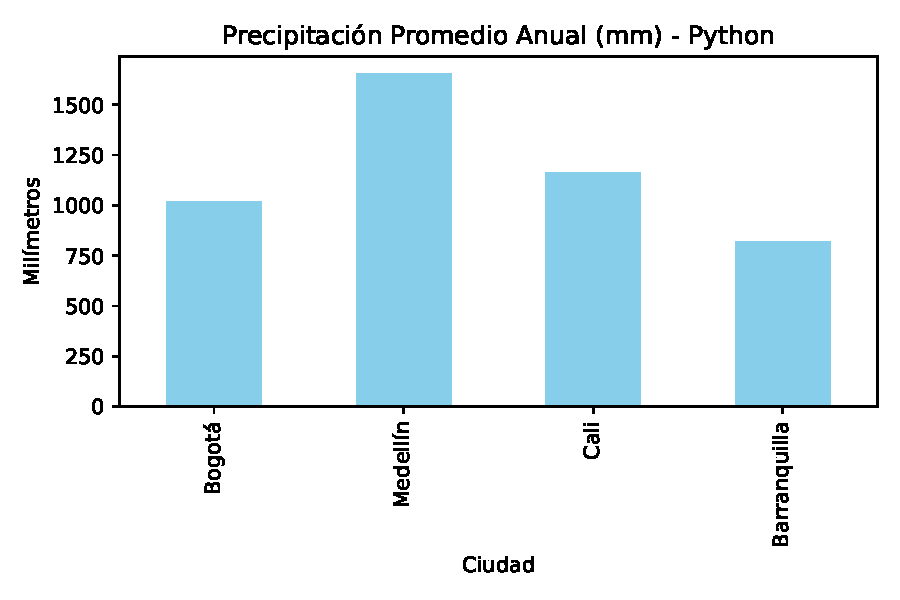
\includegraphics[width=0.6\textwidth,height=\textheight]{11-matrices_dataframes_files/figure-pdf/python_impute-1.pdf}
\end{center}

\subsection{R}

\begin{Shaded}
\begin{Highlighting}[]
\CommentTok{\# \#| eval: false}

\CommentTok{\# 1. Simulación de sensor fallando en R (usamos NA en lugar de None)}
\NormalTok{df\_sensor }\OtherTok{\textless{}{-}} \FunctionTok{data.frame}\NormalTok{(}
    \AttributeTok{Ciudad =} \FunctionTok{c}\NormalTok{(}\StringTok{"Bogotá"}\NormalTok{, }\StringTok{"Medellín"}\NormalTok{, }\StringTok{"Cali"}\NormalTok{, }\StringTok{"Barranquilla"}\NormalTok{),}
    \AttributeTok{Precipitacion\_Anual =} \FunctionTok{c}\NormalTok{(}\DecValTok{1020}\NormalTok{, }\DecValTok{1656}\NormalTok{, }\ConstantTok{NA}\NormalTok{, }\DecValTok{821}\NormalTok{)}
\NormalTok{)}
\FunctionTok{cat}\NormalTok{(}\StringTok{"Datos con fallos del sensor:}\SpecialCharTok{\textbackslash{}n}\StringTok{"}\NormalTok{)}
\end{Highlighting}
\end{Shaded}

\begin{verbatim}
Datos con fallos del sensor:
\end{verbatim}

\begin{Shaded}
\begin{Highlighting}[]
\FunctionTok{print}\NormalTok{(df\_sensor)}
\end{Highlighting}
\end{Shaded}

\begin{verbatim}
        Ciudad Precipitacion_Anual
1       Bogotá                1020
2     Medellín                1656
3         Cali                  NA
4 Barranquilla                 821
\end{verbatim}

\begin{Shaded}
\begin{Highlighting}[]
\CommentTok{\# 2. Imputación: Calcular la media ignorando NAs (na.rm=TRUE) y rellenar}
\NormalTok{media\_lluvia }\OtherTok{\textless{}{-}} \FunctionTok{mean}\NormalTok{(df\_sensor}\SpecialCharTok{$}\NormalTok{Precipitacion\_Anual, }\AttributeTok{na.rm =} \ConstantTok{TRUE}\NormalTok{)}
\NormalTok{df\_limpio }\OtherTok{\textless{}{-}}\NormalTok{ df\_sensor }\SpecialCharTok{\%\textgreater{}\%}
    \FunctionTok{mutate}\NormalTok{(}\AttributeTok{Precipitacion\_Anual =} \FunctionTok{ifelse}\NormalTok{(}\FunctionTok{is.na}\NormalTok{(Precipitacion\_Anual), media\_lluvia, Precipitacion\_Anual))}

\FunctionTok{cat}\NormalTok{(}\FunctionTok{sprintf}\NormalTok{(}\StringTok{"}\SpecialCharTok{\textbackslash{}n}\StringTok{Datos Limpios (Rellenado con media = \%.1f):}\SpecialCharTok{\textbackslash{}n}\StringTok{"}\NormalTok{, media\_lluvia))}
\end{Highlighting}
\end{Shaded}

\begin{verbatim}

Datos Limpios (Rellenado con media = 1165.7):
\end{verbatim}

\begin{Shaded}
\begin{Highlighting}[]
\FunctionTok{print}\NormalTok{(df\_limpio)}
\end{Highlighting}
\end{Shaded}

\begin{verbatim}
        Ciudad Precipitacion_Anual
1       Bogotá            1020.000
2     Medellín            1656.000
3         Cali            1165.667
4 Barranquilla             821.000
\end{verbatim}

\begin{Shaded}
\begin{Highlighting}[]
\CommentTok{\# 3. Visualización usando plot base de R con barplot}
\FunctionTok{barplot}\NormalTok{(}
\NormalTok{    df\_limpio}\SpecialCharTok{$}\NormalTok{Precipitacion\_Anual, }
    \AttributeTok{names.arg =}\NormalTok{ df\_limpio}\SpecialCharTok{$}\NormalTok{Ciudad,}
    \AttributeTok{col =} \StringTok{"skyblue"}\NormalTok{,}
    \AttributeTok{main =} \StringTok{"Precipitación Promedio Anual (mm) {-} R"}\NormalTok{,}
    \AttributeTok{ylab =} \StringTok{"Milímetros"}
\NormalTok{)}
\end{Highlighting}
\end{Shaded}

\begin{center}
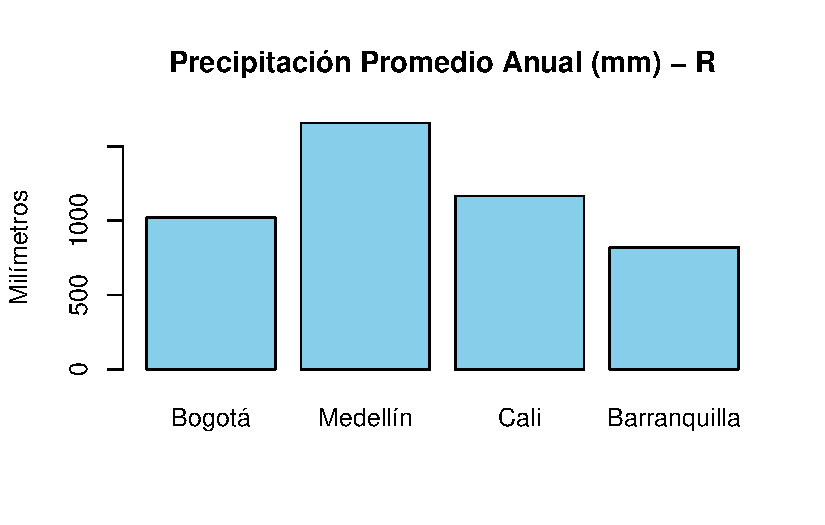
\includegraphics[width=0.6\textwidth,height=\textheight]{11-matrices_dataframes_files/figure-pdf/r_impute-1.pdf}
\end{center}

\subsection{Julia}

\begin{center}
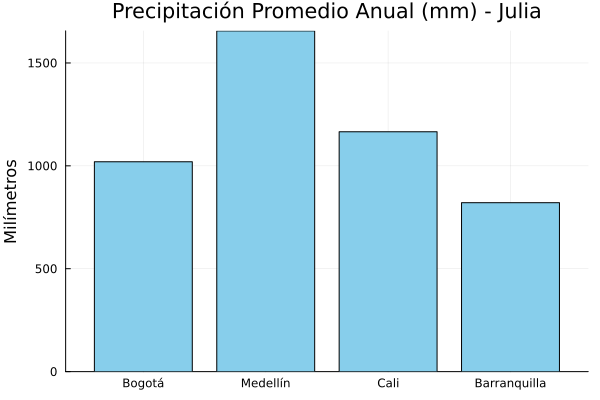
\includegraphics[width=0.6\textwidth,height=\textheight]{images/plots/bar_precip_julia.png}
\end{center}

\subsection{Resumen comparativo: manejo de datos nulos y
visualización}\label{resumen-comparativo-manejo-de-datos-nulos-y-visualizaciuxf3n}

\begin{longtable}[]{@{}
  >{\raggedright\arraybackslash}p{(\columnwidth - 6\tabcolsep) * \real{0.2600}}
  >{\raggedright\arraybackslash}p{(\columnwidth - 6\tabcolsep) * \real{0.2400}}
  >{\raggedright\arraybackslash}p{(\columnwidth - 6\tabcolsep) * \real{0.2500}}
  >{\raggedright\arraybackslash}p{(\columnwidth - 6\tabcolsep) * \real{0.2500}}@{}}
\caption{Comandos esenciales para tratar datos incompletos y
graficar}\label{tbl-datos_nulos}\tabularnewline
\toprule\noalign{}
\begin{minipage}[b]{\linewidth}\raggedright
Operación / Concepto
\end{minipage} & \begin{minipage}[b]{\linewidth}\raggedright
Python (Pandas) 🐍
\end{minipage} & \begin{minipage}[b]{\linewidth}\raggedright
R (Nativo / dplyr) 🔵
\end{minipage} & \begin{minipage}[b]{\linewidth}\raggedright
Julia (DataFrames.jl) 🟣
\end{minipage} \\
\midrule\noalign{}
\endfirsthead
\toprule\noalign{}
\begin{minipage}[b]{\linewidth}\raggedright
Operación / Concepto
\end{minipage} & \begin{minipage}[b]{\linewidth}\raggedright
Python (Pandas) 🐍
\end{minipage} & \begin{minipage}[b]{\linewidth}\raggedright
R (Nativo / dplyr) 🔵
\end{minipage} & \begin{minipage}[b]{\linewidth}\raggedright
Julia (DataFrames.jl) 🟣
\end{minipage} \\
\midrule\noalign{}
\endhead
\bottomrule\noalign{}
\endlastfoot
\textbf{Representación del Nulo} & \texttt{np.nan} \emph{(NaN)} &
\texttt{NA} & \texttt{missing} \\
\textbf{Media ignorando nulos} & \texttt{df{[}"Col"{]}.mean()} &
\texttt{mean(df\$Col,\ na.rm=TRUE)} &
\texttt{mean(skipmissing(df.Col))} \\
\textbf{Rellenar nulos (Imputación)} &
\texttt{df{[}"Col"{]}.fillna(valor)} &
\texttt{df\$Col{[}is.na(df\$Col){]}\ \textless{}-\ valor} &
\texttt{df.Col\ =\ coalesce.(df.Col,\ valor)} \\
\textbf{Gráfico de barras básico} & \texttt{df.plot.bar(x="A",\ y="B")}
& \texttt{barplot(y,\ names.arg=x)} & \texttt{bar(x,\ y)}
\emph{(Plots.jl)} \\
\end{longtable}

\begin{center}\rule{0.5\linewidth}{0.5pt}\end{center}

\section{Resumen de aprendizajes (cheat
sheet)}\label{resumen-de-aprendizajes-cheat-sheet-6}

A lo largo de este capítulo hemos construido los cimientos analíticos
que todo especialista en geomática necesita antes de tocar un mapa.
Pasar de datos crudos a información útil requiere dominar las
estructuras de memoria y sus operaciones.

Repasemos los conceptos clave que ahora llevas en tu caja de
herramientas:

\begin{itemize}
\tightlist
\item
  \textbf{Estructuras optimizadas (Arreglos):} Entendimos que los
  lenguajes usan estructuras de bajo nivel (\texttt{np.array},
  \texttt{c()}, \texttt{{[}{]}}) para almacenar datos del mismo tipo de
  forma contigua en la memoria, lo que permite un acceso extremadamente
  rápido, ideal para imágenes satelitales o modelos de elevación.
\item
  \textbf{La regla de oro: ¡Vectorización!:} Aprendiste que en el
  análisis masivo de datos \textbf{nunca debes usar un ciclo
  \texttt{for}} si existe una función matemática vectorizada.
  Multiplicar o sacar el seno de un millón de coordenadas se hace en una
  sola línea de código.
\item
  \textbf{Filtros mediante indexación booleana:} Descubrimos cómo crear
  ``máscaras'' de Verdadero/Falso (ej.
  \texttt{elevacion\ \textgreater{}\ 3000}) para extraer rápidamente un
  subconjunto de datos sin alterar la matriz original.
\item
  \textbf{El poder de los DataFrames:} Transicionamos de las matrices
  matemáticas puras a tablas complejas que combinan textos y números.
  Entendiste que herramientas como \texttt{Pandas}, \texttt{dplyr} o
  \texttt{DataFrames.jl} son el equivalente a un Excel programable y
  automatizable.
\item
  \textbf{Operaciones espaciales tabulares:} Vimos que el
  geoprocesamiento no es solo dibujar geometrías; a menudo implica
  cruzar bases de datos (\emph{Merges/Joins}) y calcular estadísticas
  por regiones (\emph{Groupby/Summarise}).
\item
  \textbf{Gestión de la incertidumbre (Nulos):} Te enfrentaste a la
  realidad de los datos de campo (\texttt{NaN}, \texttt{NA},
  \texttt{missing}). Aprendiste que ignorarlos rompe el código, y
  dominaste técnicas para rellenarlos (imputación) usando medias o
  valores de contingencia.
\end{itemize}

A continuación, se presenta tu \textbf{Hoja de Referencia (Cheat Sheet)}
consolidada para traducir la sintaxis de estos conceptos entre Python, R
y Julia.

\subsection{1. Creación y operaciones con arreglos
numéricos}\label{creaciuxf3n-y-operaciones-con-arreglos-numuxe9ricos}

\begin{longtable}[]{@{}
  >{\raggedright\arraybackslash}p{(\columnwidth - 6\tabcolsep) * \real{0.2500}}
  >{\raggedright\arraybackslash}p{(\columnwidth - 6\tabcolsep) * \real{0.2500}}
  >{\raggedright\arraybackslash}p{(\columnwidth - 6\tabcolsep) * \real{0.2500}}
  >{\raggedright\arraybackslash}p{(\columnwidth - 6\tabcolsep) * \real{0.2500}}@{}}
\caption{Sintaxis para creación y matemáticas de
arreglos}\label{tbl-resumen_arreglos}\tabularnewline
\toprule\noalign{}
\begin{minipage}[b]{\linewidth}\raggedright
Operación
\end{minipage} & \begin{minipage}[b]{\linewidth}\raggedright
Python (NumPy) 🐍
\end{minipage} & \begin{minipage}[b]{\linewidth}\raggedright
R (Nativo) 🔵
\end{minipage} & \begin{minipage}[b]{\linewidth}\raggedright
Julia (Nativo) 🟣
\end{minipage} \\
\midrule\noalign{}
\endfirsthead
\toprule\noalign{}
\begin{minipage}[b]{\linewidth}\raggedright
Operación
\end{minipage} & \begin{minipage}[b]{\linewidth}\raggedright
Python (NumPy) 🐍
\end{minipage} & \begin{minipage}[b]{\linewidth}\raggedright
R (Nativo) 🔵
\end{minipage} & \begin{minipage}[b]{\linewidth}\raggedright
Julia (Nativo) 🟣
\end{minipage} \\
\midrule\noalign{}
\endhead
\bottomrule\noalign{}
\endlastfoot
\textbf{Crear arreglo 1D} & \texttt{np.array({[}1,\ 2{]})} &
\texttt{c(1,\ 2)} & \texttt{{[}1,\ 2{]}} \\
\textbf{Matriz de ceros} & \texttt{np.zeros((3,\ 3))} &
\texttt{matrix(0,\ nrow=3,\ ncol=3)} & \texttt{zeros(3,\ 3)} \\
\textbf{Ver dimensiones} & \texttt{arr.shape} & \texttt{dim(arr)} &
\texttt{size(arr)} \\
\textbf{Generar secuencia} & \texttt{np.arange(1,\ 10,\ 2)} &
\texttt{seq(1,\ 9,\ by=2)} & \texttt{1:2:9} \\
\textbf{Álgebra masiva} & \texttt{arr\ *\ 2} & \texttt{arr\ *\ 2} &
\texttt{arr\ .*\ 2} \emph{(Nota el punto)} \\
\textbf{Estadística (Media)} & \texttt{np.mean(arr)} &
\texttt{mean(arr)} & \texttt{mean(arr)} \emph{(req. Statistics)} \\
\end{longtable}

\subsection{2. Filtros e indexación
booleana}\label{filtros-e-indexaciuxf3n-booleana}

\begin{longtable}[]{@{}
  >{\raggedright\arraybackslash}p{(\columnwidth - 6\tabcolsep) * \real{0.2500}}
  >{\raggedright\arraybackslash}p{(\columnwidth - 6\tabcolsep) * \real{0.2500}}
  >{\raggedright\arraybackslash}p{(\columnwidth - 6\tabcolsep) * \real{0.2500}}
  >{\raggedright\arraybackslash}p{(\columnwidth - 6\tabcolsep) * \real{0.2500}}@{}}
\caption{Sintaxis para manipulación y cortes de
vectores}\label{tbl-resumen_slicing}\tabularnewline
\toprule\noalign{}
\begin{minipage}[b]{\linewidth}\raggedright
Operación
\end{minipage} & \begin{minipage}[b]{\linewidth}\raggedright
Python (NumPy) 🐍
\end{minipage} & \begin{minipage}[b]{\linewidth}\raggedright
R (Nativo) 🔵
\end{minipage} & \begin{minipage}[b]{\linewidth}\raggedright
Julia (Nativo) 🟣
\end{minipage} \\
\midrule\noalign{}
\endfirsthead
\toprule\noalign{}
\begin{minipage}[b]{\linewidth}\raggedright
Operación
\end{minipage} & \begin{minipage}[b]{\linewidth}\raggedright
Python (NumPy) 🐍
\end{minipage} & \begin{minipage}[b]{\linewidth}\raggedright
R (Nativo) 🔵
\end{minipage} & \begin{minipage}[b]{\linewidth}\raggedright
Julia (Nativo) 🟣
\end{minipage} \\
\midrule\noalign{}
\endhead
\bottomrule\noalign{}
\endlastfoot
\textbf{Índice inicial} & \texttt{0} \emph{(Zero-based)} & \texttt{1}
\emph{(One-based)} & \texttt{1} \emph{(One-based)} \\
\textbf{Slicing básico} & \texttt{arr{[}1:4{]}} \emph{(índices 1,2,3)} &
\texttt{arr{[}2:4{]}} \emph{(índices 2,3,4)} & \texttt{arr{[}2:4{]}}
\emph{(índices 2,3,4)} \\
\textbf{Máscara lógica} & \texttt{mascara\ =\ arr\ \textgreater{}\ 10} &
\texttt{mascara\ \textless{}-\ arr\ \textgreater{}\ 10} &
\texttt{mascara\ =\ arr\ .\textgreater{}\ 10} \\
\textbf{Aplicar filtro} & \texttt{arr{[}mascara{]}} &
\texttt{arr{[}mascara{]}} & \texttt{arr{[}mascara{]}} \\
\textbf{Reemplazo masivo} & \texttt{arr{[}arr\ \textless{}\ 5{]}\ =\ 0}
& \texttt{arr{[}arr\ \textless{}\ 5{]}\ \textless{}-\ 0} &
\texttt{arr{[}arr\ .\textless{}\ 5{]}\ .=\ 0} \\
\end{longtable}

\subsection{3. DataFrames y operaciones
tabulares}\label{dataframes-y-operaciones-tabulares}

\begin{longtable}[]{@{}
  >{\raggedright\arraybackslash}p{(\columnwidth - 6\tabcolsep) * \real{0.2500}}
  >{\raggedright\arraybackslash}p{(\columnwidth - 6\tabcolsep) * \real{0.2500}}
  >{\raggedright\arraybackslash}p{(\columnwidth - 6\tabcolsep) * \real{0.2500}}
  >{\raggedright\arraybackslash}p{(\columnwidth - 6\tabcolsep) * \real{0.2500}}@{}}
\caption{Sintaxis para manipulación de tablas y bases de
datos}\label{tbl-resumen_dataframes}\tabularnewline
\toprule\noalign{}
\begin{minipage}[b]{\linewidth}\raggedright
Operación
\end{minipage} & \begin{minipage}[b]{\linewidth}\raggedright
Python (Pandas) 🐍
\end{minipage} & \begin{minipage}[b]{\linewidth}\raggedright
R (dplyr) 🔵
\end{minipage} & \begin{minipage}[b]{\linewidth}\raggedright
Julia (DataFrames) 🟣
\end{minipage} \\
\midrule\noalign{}
\endfirsthead
\toprule\noalign{}
\begin{minipage}[b]{\linewidth}\raggedright
Operación
\end{minipage} & \begin{minipage}[b]{\linewidth}\raggedright
Python (Pandas) 🐍
\end{minipage} & \begin{minipage}[b]{\linewidth}\raggedright
R (dplyr) 🔵
\end{minipage} & \begin{minipage}[b]{\linewidth}\raggedright
Julia (DataFrames) 🟣
\end{minipage} \\
\midrule\noalign{}
\endhead
\bottomrule\noalign{}
\endlastfoot
\textbf{Crear DataFrame} & \texttt{pd.DataFrame(\{...\})} &
\texttt{data.frame(...)} & \texttt{DataFrame(...)} \\
\textbf{Filtrar filas} & \texttt{df{[}df{[}"Col"{]}\ \textless{}\ 10{]}}
& \texttt{df\ \%\textgreater{}\%\ filter(Col\ \textless{}\ 10)} &
\texttt{df{[}df.Col\ .\textless{}\ 10,\ :{]}} \\
\textbf{Agrupar y sumar} & \texttt{df.groupby("A"){[}"B"{]}.sum()} &
\texttt{df\ \%\textgreater{}\%\ group\_by(A)\ \%\textgreater{}\%\ summarise(T\ =\ sum(B))}
& \texttt{combine(groupby(df,\ :A),\ :B\ =\textgreater{}\ sum)} \\
\textbf{Cruzar (Merge)} & \texttt{pd.merge(d1,\ d2,\ on="Id")} &
\texttt{inner\_join(d1,\ d2,\ by="Id")} &
\texttt{innerjoin(d1,\ d2,\ on=:Id)} \\
\end{longtable}

\subsection{4. Manejo de datos nulos
(incompletos)}\label{manejo-de-datos-nulos-incompletos}

\begin{longtable}[]{@{}
  >{\raggedright\arraybackslash}p{(\columnwidth - 6\tabcolsep) * \real{0.2500}}
  >{\raggedright\arraybackslash}p{(\columnwidth - 6\tabcolsep) * \real{0.2500}}
  >{\raggedright\arraybackslash}p{(\columnwidth - 6\tabcolsep) * \real{0.2500}}
  >{\raggedright\arraybackslash}p{(\columnwidth - 6\tabcolsep) * \real{0.2500}}@{}}
\caption{Sintaxis para tratamiento de datos
faltantes}\label{tbl-resumen_nulos}\tabularnewline
\toprule\noalign{}
\begin{minipage}[b]{\linewidth}\raggedright
Operación
\end{minipage} & \begin{minipage}[b]{\linewidth}\raggedright
Python (Pandas) 🐍
\end{minipage} & \begin{minipage}[b]{\linewidth}\raggedright
R (dplyr) 🔵
\end{minipage} & \begin{minipage}[b]{\linewidth}\raggedright
Julia (DataFrames) 🟣
\end{minipage} \\
\midrule\noalign{}
\endfirsthead
\toprule\noalign{}
\begin{minipage}[b]{\linewidth}\raggedright
Operación
\end{minipage} & \begin{minipage}[b]{\linewidth}\raggedright
Python (Pandas) 🐍
\end{minipage} & \begin{minipage}[b]{\linewidth}\raggedright
R (dplyr) 🔵
\end{minipage} & \begin{minipage}[b]{\linewidth}\raggedright
Julia (DataFrames) 🟣
\end{minipage} \\
\midrule\noalign{}
\endhead
\bottomrule\noalign{}
\endlastfoot
\textbf{Símbolo del nulo} & \texttt{np.nan} o \texttt{None} &
\texttt{NA} & \texttt{missing} \\
\textbf{Media sin nulos} & \texttt{df{[}"C"{]}.mean()} &
\texttt{mean(df\$C,\ na.rm=TRUE)} & \texttt{mean(skipmissing(df.C))} \\
\textbf{Imputar (Rellenar)} & \texttt{df{[}"C"{]}.fillna(val)} &
\texttt{ifelse(is.na(C),\ val,\ C)} & \texttt{coalesce.(df.C,\ val)} \\
\textbf{Eliminar filas} & \texttt{df.dropna()} &
\texttt{df\ \%\textgreater{}\%\ drop\_na()} &
\texttt{dropmissing(df)} \\
\end{longtable}

\section{Ejercicios}\label{ejercicios-6}

\subsection{Ejercicio 1: Vectorización y álgebra espacial
(Haversine)}\label{ejercicio-1-vectorizaciuxf3n-y-uxe1lgebra-espacial-haversine}

La \textbf{fórmula de Haversine} permite calcular la gran distancia
sobre la esfera terrestre dadas dos coordenadas en latitud y longitud.

Tu misión es crear una función vectorizada (en Python, R o Julia)
llamada \texttt{calcular\_distancias} que reciba como argumento el
DataFrame \texttt{df} de censos (que construimos en la sección 4) y
calcule la distancia en kilómetros desde \textbf{Bogotá (Lat: 4.7110,
Lon: -74.0721)} a todas las demás ciudades de la tabla, agregando el
resultado en una nueva columna llamada \texttt{Distancia\_Bogota}.

\begin{itemize}
\tightlist
\item
  \emph{Tip:} \textbf{¡Recicla tu código!} Recuerda que en el capítulo
  de \emph{Funciones y Clases} ya construiste matemáticamente la función
  Haversine. Solo tienes que traerla a este script y adaptarla para que
  funcione directamente sobre vectores en lugar de números individuales,
  \textbf{evitando usar ciclos \texttt{for}}.
\item
  \emph{Pista de rendimiento:} Aplica la matemática directamente sobre
  las columnas completas del \emph{DataFrame} (ej.
  \texttt{df{[}\textquotesingle{}Latitud\textquotesingle{}{]}\ *\ np.pi\ /\ 180}).
\end{itemize}

\subsection{Ejercicio 2: Limpieza, filtros y agregación
tabular}\label{ejercicio-2-limpieza-filtros-y-agregaciuxf3n-tabular}

Para consolidar tus habilidades analíticas con \emph{DataFrames}, crea
un script que resuelva el siguiente flujo de trabajo simulado:

\begin{enumerate}
\def\labelenumi{\arabic{enumi}.}
\tightlist
\item
  \textbf{Creación:} Genera un DataFrame con los siguientes datos de
  estaciones meteorológicas:

  \begin{itemize}
  \tightlist
  \item
    Estación: {[}``Páramo'', ``Valle'', ``Costa'', ``Selva'',
    ``Sabana''{]}
  \item
    Elevación: {[}3200, 1500, 15, 200, 2600{]}
  \item
    Precipitación: {[}850.5, 1200.0, None, 3000.5, None{]} \emph{(Usa el
    tipo de nulo apropiado según tu lenguaje:
    \texttt{None}/\texttt{np.nan}, \texttt{NA} o \texttt{missing})}.
  \end{itemize}
\item
  \textbf{Imputación:} Los sensores de la Costa y la Sabana fallaron.
  Rellena los datos de precipitación nulos utilizando el valor
  \textbf{promedio (media)} de las estaciones válidas.
\item
  \textbf{Filtro espacial (Slicing):} Extrae en un nuevo DataFrame
  llamado \texttt{estaciones\_altas} solo aquellas filas cuya elevación
  sea estrictamente mayor a 1000 metros.
\item
  \textbf{Cálculo final:} Muestra en consola cuál es la precipitación
  promedio anual reportada \emph{exclusivamente} en las estaciones
  altas.
\end{enumerate}

\subsection{Entregables y criterios de
evaluación}\label{entregables-y-criterios-de-evaluaciuxf3n-6}

Añade la resolución documentada de estos dos ejercicios en formato
\texttt{.qmd} a tu repositorio de GitHub. Asegúrate de renderizar el
documento (HTML o PDF) e incluir comentarios breves en tu código
explicando por qué elegiste ciertas funciones para imputar o filtrar los
datos.

\section{Anexo 1: Resumen de limpieza de datos con
pandas}\label{anexo-1-resumen-de-limpieza-de-datos-con-pandas}

A continuación, se presenta una tabla de referencia rápida (\emph{Cheat
Sheet}) con los comandos más utilizados en Python para inspección y
limpieza de datos tabulares con la librería Pandas. Las operaciones se
agrupan según las principales etapas del proceso de limpieza de datos.

\begin{longtable}[]{@{}
  >{\raggedright\arraybackslash}p{(\columnwidth - 6\tabcolsep) * \real{0.2200}}
  >{\raggedright\arraybackslash}p{(\columnwidth - 6\tabcolsep) * \real{0.2500}}
  >{\raggedright\arraybackslash}p{(\columnwidth - 6\tabcolsep) * \real{0.2800}}
  >{\raggedright\arraybackslash}p{(\columnwidth - 6\tabcolsep) * \real{0.2500}}@{}}
\caption{Comandos esenciales para inspección y limpieza de datos en
Pandas}\label{tbl-pandas_limpieza}\tabularnewline
\toprule\noalign{}
\begin{minipage}[b]{\linewidth}\raggedright
Categoría
\end{minipage} & \begin{minipage}[b]{\linewidth}\raggedright
Tarea de Limpieza
\end{minipage} & \begin{minipage}[b]{\linewidth}\raggedright
Comando en Pandas
\end{minipage} & \begin{minipage}[b]{\linewidth}\raggedright
Descripción
\end{minipage} \\
\midrule\noalign{}
\endfirsthead
\toprule\noalign{}
\begin{minipage}[b]{\linewidth}\raggedright
Categoría
\end{minipage} & \begin{minipage}[b]{\linewidth}\raggedright
Tarea de Limpieza
\end{minipage} & \begin{minipage}[b]{\linewidth}\raggedright
Comando en Pandas
\end{minipage} & \begin{minipage}[b]{\linewidth}\raggedright
Descripción
\end{minipage} \\
\midrule\noalign{}
\endhead
\bottomrule\noalign{}
\endlastfoot
\textbf{1. Inspección de datos} & Ver primeras filas &
\texttt{df.head()} & Muestra las primeras 5 filas del DataFrame para una
inspección rápida. \\
& Ver últimas filas & \texttt{df.tail()} & Muestra las últimas 5 filas
del DataFrame. \\
& Ver estructura del DataFrame & \texttt{df.info()} & Muestra número de
filas, columnas, tipos de datos y valores nulos. \\
& Resumen estadístico & \texttt{df.describe()} & Calcula estadísticas
básicas de columnas numéricas. \\
& Dimensiones del DataFrame & \texttt{df.shape} & Devuelve el número de
filas y columnas. \\
& Nombres de columnas & \texttt{df.columns} & Lista los nombres de todas
las columnas. \\
& Tipos de datos & \texttt{df.dtypes} & Muestra el tipo de dato de cada
columna. \\
\textbf{2. Manejo de valores faltantes} & Identificar nulos &
\texttt{df.isna()} & Devuelve un DataFrame de booleanos indicando
valores faltantes. \\
& Contar nulos & \texttt{df.isna().sum()} & Cuenta cuántos valores nulos
hay por columna. \\
& Eliminar filas con nulos & \texttt{df.dropna()} & Elimina filas con al
menos un valor faltante. \\
& Eliminar nulos en columnas específicas &
\texttt{df.dropna(subset={[}\textquotesingle{}Col\textquotesingle{}{]})}
& Elimina filas si ciertas columnas contienen nulos. \\
& Rellenar nulos & \texttt{df.fillna(valor)} & Sustituye valores
faltantes por un valor específico. \\
& Relleno hacia adelante &
\texttt{df.fillna(method=\textquotesingle{}ffill\textquotesingle{})} &
Rellena nulos con el valor válido anterior. \\
& Relleno hacia atrás &
\texttt{df.fillna(method=\textquotesingle{}bfill\textquotesingle{})} &
Rellena nulos con el valor siguiente disponible. \\
\textbf{3. Eliminación de duplicados} & Detectar duplicados &
\texttt{df.duplicated()} & Devuelve un vector booleano indicando filas
duplicadas. \\
& Contar duplicados & \texttt{df.duplicated().sum()} & Cuenta cuántas
filas duplicadas existen. \\
& Eliminar duplicados & \texttt{df.drop\_duplicates()} & Elimina filas
duplicadas manteniendo la primera aparición. \\
\textbf{4. Corrección de tipos de datos} & Revisar tipos &
\texttt{df.dtypes} & Permite verificar los tipos de datos actuales. \\
& Convertir tipo numérico &
\texttt{df{[}\textquotesingle{}Col\textquotesingle{}{]}.astype(float)} &
Convierte una columna al tipo numérico indicado. \\
& Convertir a fecha &
\texttt{pd.to\_datetime(df{[}\textquotesingle{}Fecha\textquotesingle{}{]})}
& Convierte texto a formato fecha. \\
\textbf{5. Renombrar columnas} & Cambiar nombre de columna &
\texttt{df.rename(columns=\{\textquotesingle{}Antiguo\textquotesingle{}:\textquotesingle{}Nuevo\textquotesingle{}\})}
& Cambia el nombre de columnas usando un diccionario. \\
\textbf{6. Estandarización de texto} & Convertir a minúsculas &
\texttt{df{[}\textquotesingle{}Col\textquotesingle{}{]}.str.lower()} &
Convierte texto a minúsculas para estandarizar datos. \\
& Convertir a mayúsculas &
\texttt{df{[}\textquotesingle{}Col\textquotesingle{}{]}.str.upper()} &
Convierte texto a mayúsculas. \\
& Eliminar espacios &
\texttt{df{[}\textquotesingle{}Col\textquotesingle{}{]}.str.strip()} &
Elimina espacios al inicio o final de cadenas de texto. \\
& Reemplazar valores &
\texttt{df{[}\textquotesingle{}Col\textquotesingle{}{]}.replace(\textquotesingle{}x\textquotesingle{},\textquotesingle{}y\textquotesingle{})}
& Sustituye valores específicos dentro de una columna. \\
\textbf{7. Filtrado de datos} & Filtrar filas por condición &
\texttt{df{[}df{[}\textquotesingle{}Col\textquotesingle{}{]}\ \textgreater{}\ 0{]}}
& Mantiene solo filas que cumplen una condición lógica. \\
& Filtrar valores atípicos &
\texttt{df{[}df{[}\textquotesingle{}Edad\textquotesingle{}{]}\ \textless{}=\ 100{]}}
& Ejemplo de filtrado para eliminar datos inválidos. \\
\textbf{8. Manejo de datos categóricos} & Valores únicos &
\texttt{df{[}\textquotesingle{}Col\textquotesingle{}{]}.unique()} &
Devuelve los valores únicos de una columna. \\
& Frecuencia de categorías &
\texttt{df{[}\textquotesingle{}Col\textquotesingle{}{]}.value\_counts()}
& Cuenta cuántas veces aparece cada valor. \\
& Codificación categórica simple &
\texttt{df{[}\textquotesingle{}Genero\_code\textquotesingle{}{]}\ =\ df{[}\textquotesingle{}Genero\textquotesingle{}{]}.map(\{\textquotesingle{}M\textquotesingle{}:1,\textquotesingle{}F\textquotesingle{}:0\})}
& Convierte categorías en valores numéricos. \\
& Codificación One-Hot &
\texttt{pd.get\_dummies(df,\ columns={[}\textquotesingle{}Pais\textquotesingle{}{]})}
& Convierte variables categóricas en variables binarias. \\
\textbf{9. Reinicio del índice} & Resetear índice &
\texttt{df.reset\_index(drop=True)} & Reorganiza el índice después de
eliminar o filtrar filas. \\
\textbf{10. Detección de errores} & Buscar valores inválidos &
\texttt{df{[}df{[}\textquotesingle{}Salario\textquotesingle{}{]}\ \textless{}\ 0{]}}
& Permite detectar valores fuera de rango o inconsistentes. \\
\end{longtable}

\begin{center}\rule{0.5\linewidth}{0.5pt}\end{center}

\section{Anexo 2: Hojas de referencia rápidas (Cheat Sheets)
visuales}\label{anexo-2-hojas-de-referencia-ruxe1pidas-cheat-sheets-visuales}

Para apoyar tu estudio y práctica, a continuación se incluyen diagramas
visuales con los comandos más utilizados de Pandas:

\begin{figure}

\begin{minipage}{\linewidth}
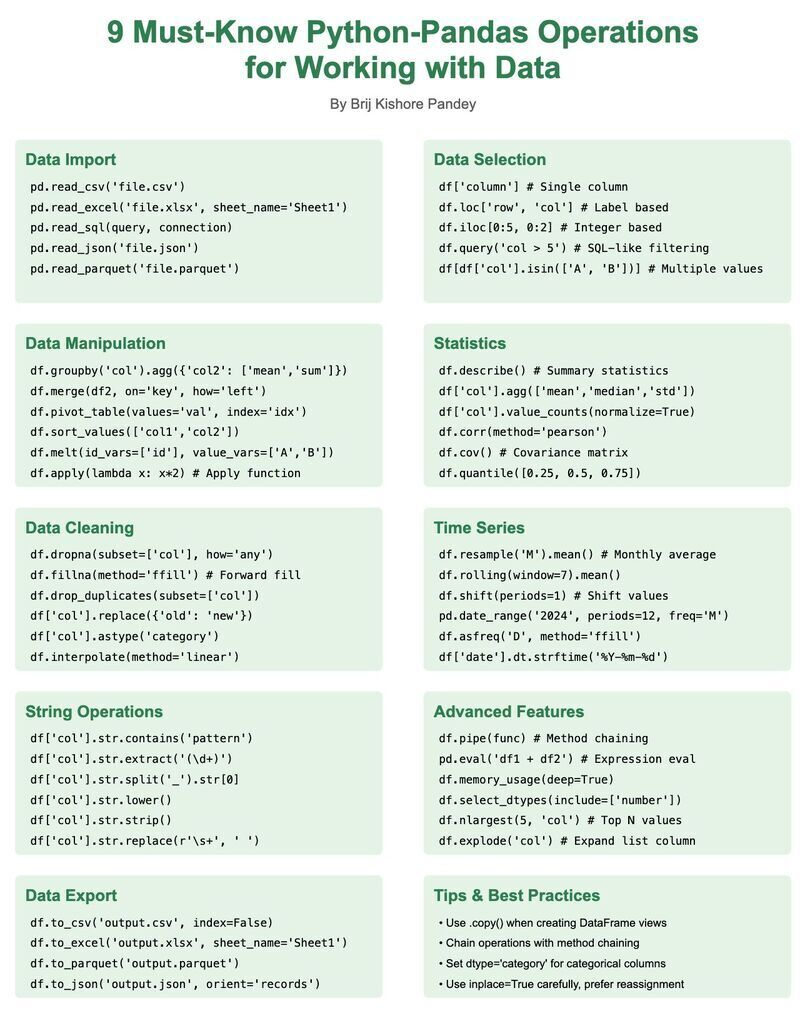
\includegraphics[width=0.8\textwidth,height=\textheight]{images/pandas/9_must-know_python_pandas.jpg}\end{minipage}%
\newline
\begin{minipage}{\linewidth}
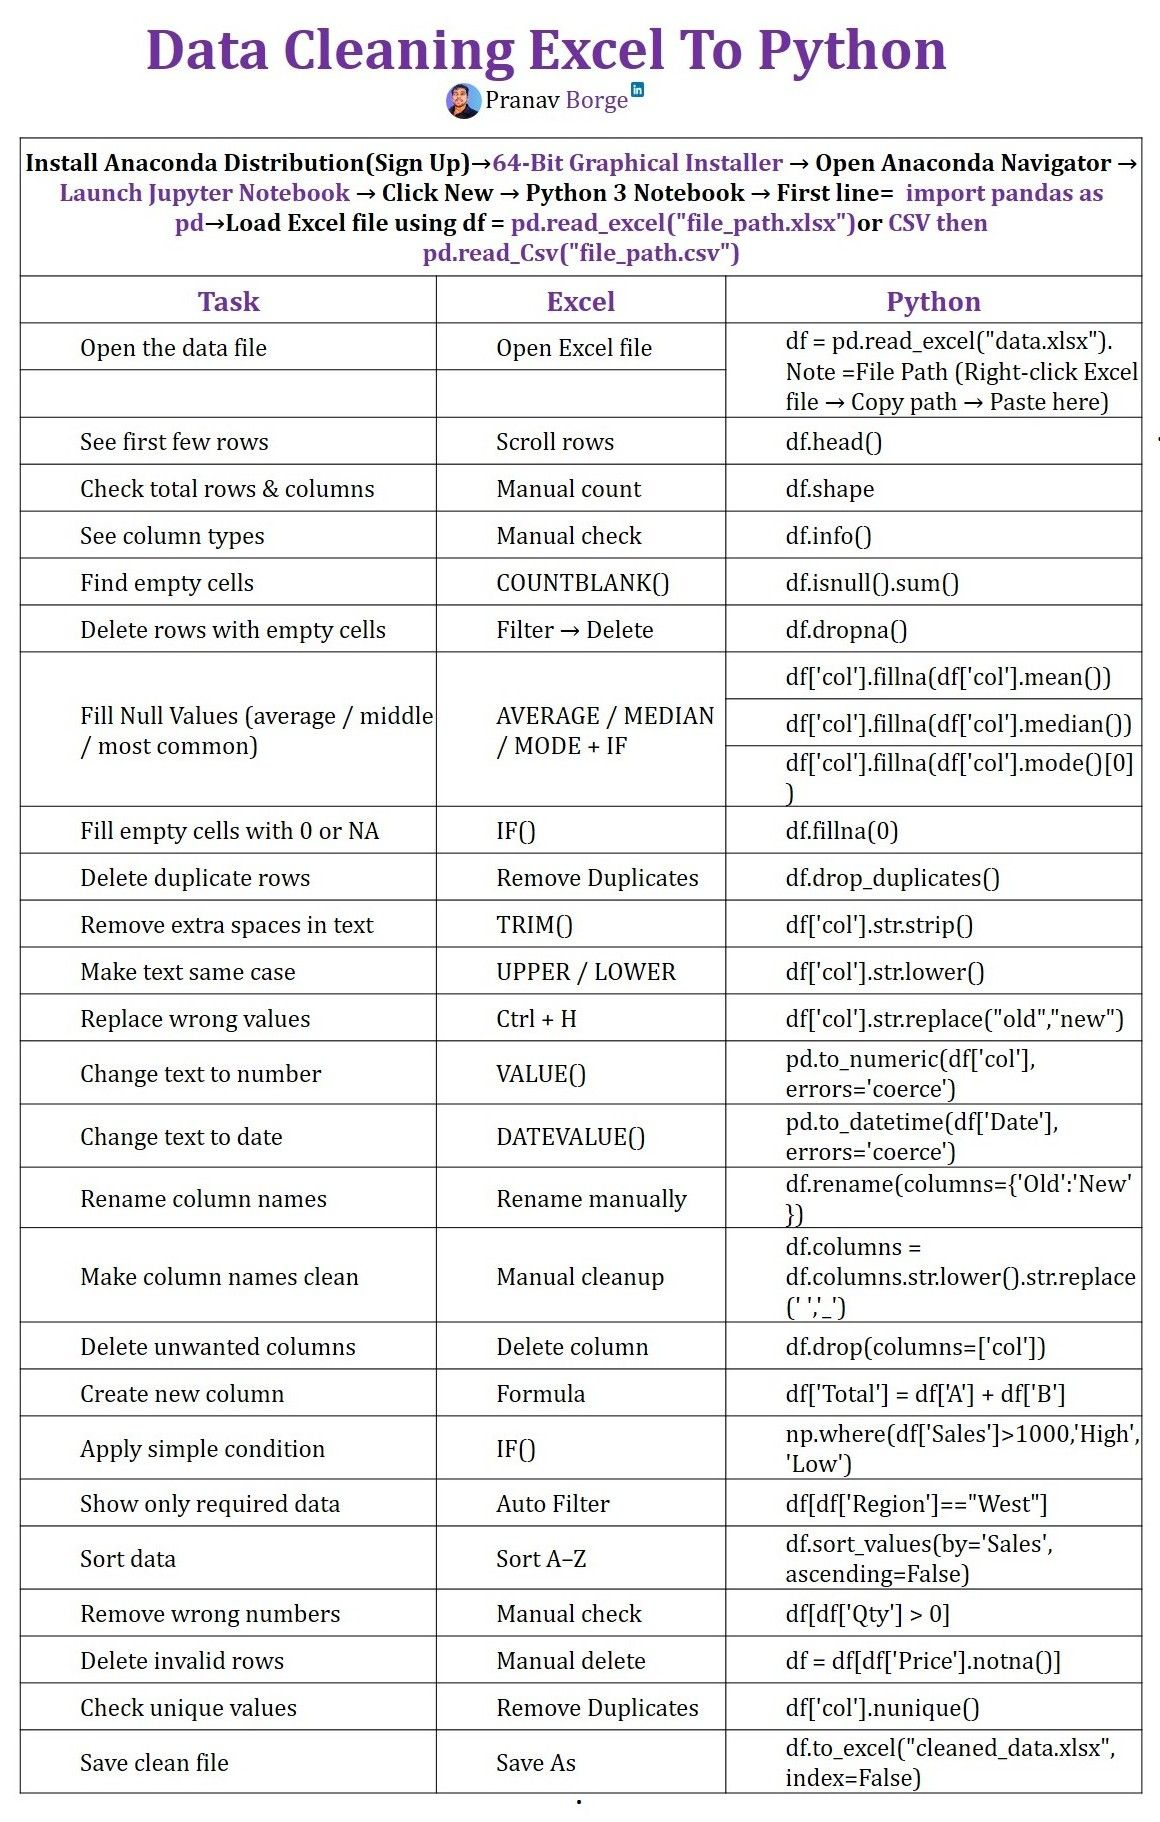
\includegraphics[width=0.8\textwidth,height=\textheight]{images/pandas/ExcelToPythonPandas.jpg}\end{minipage}%
\newline
\begin{minipage}{\linewidth}
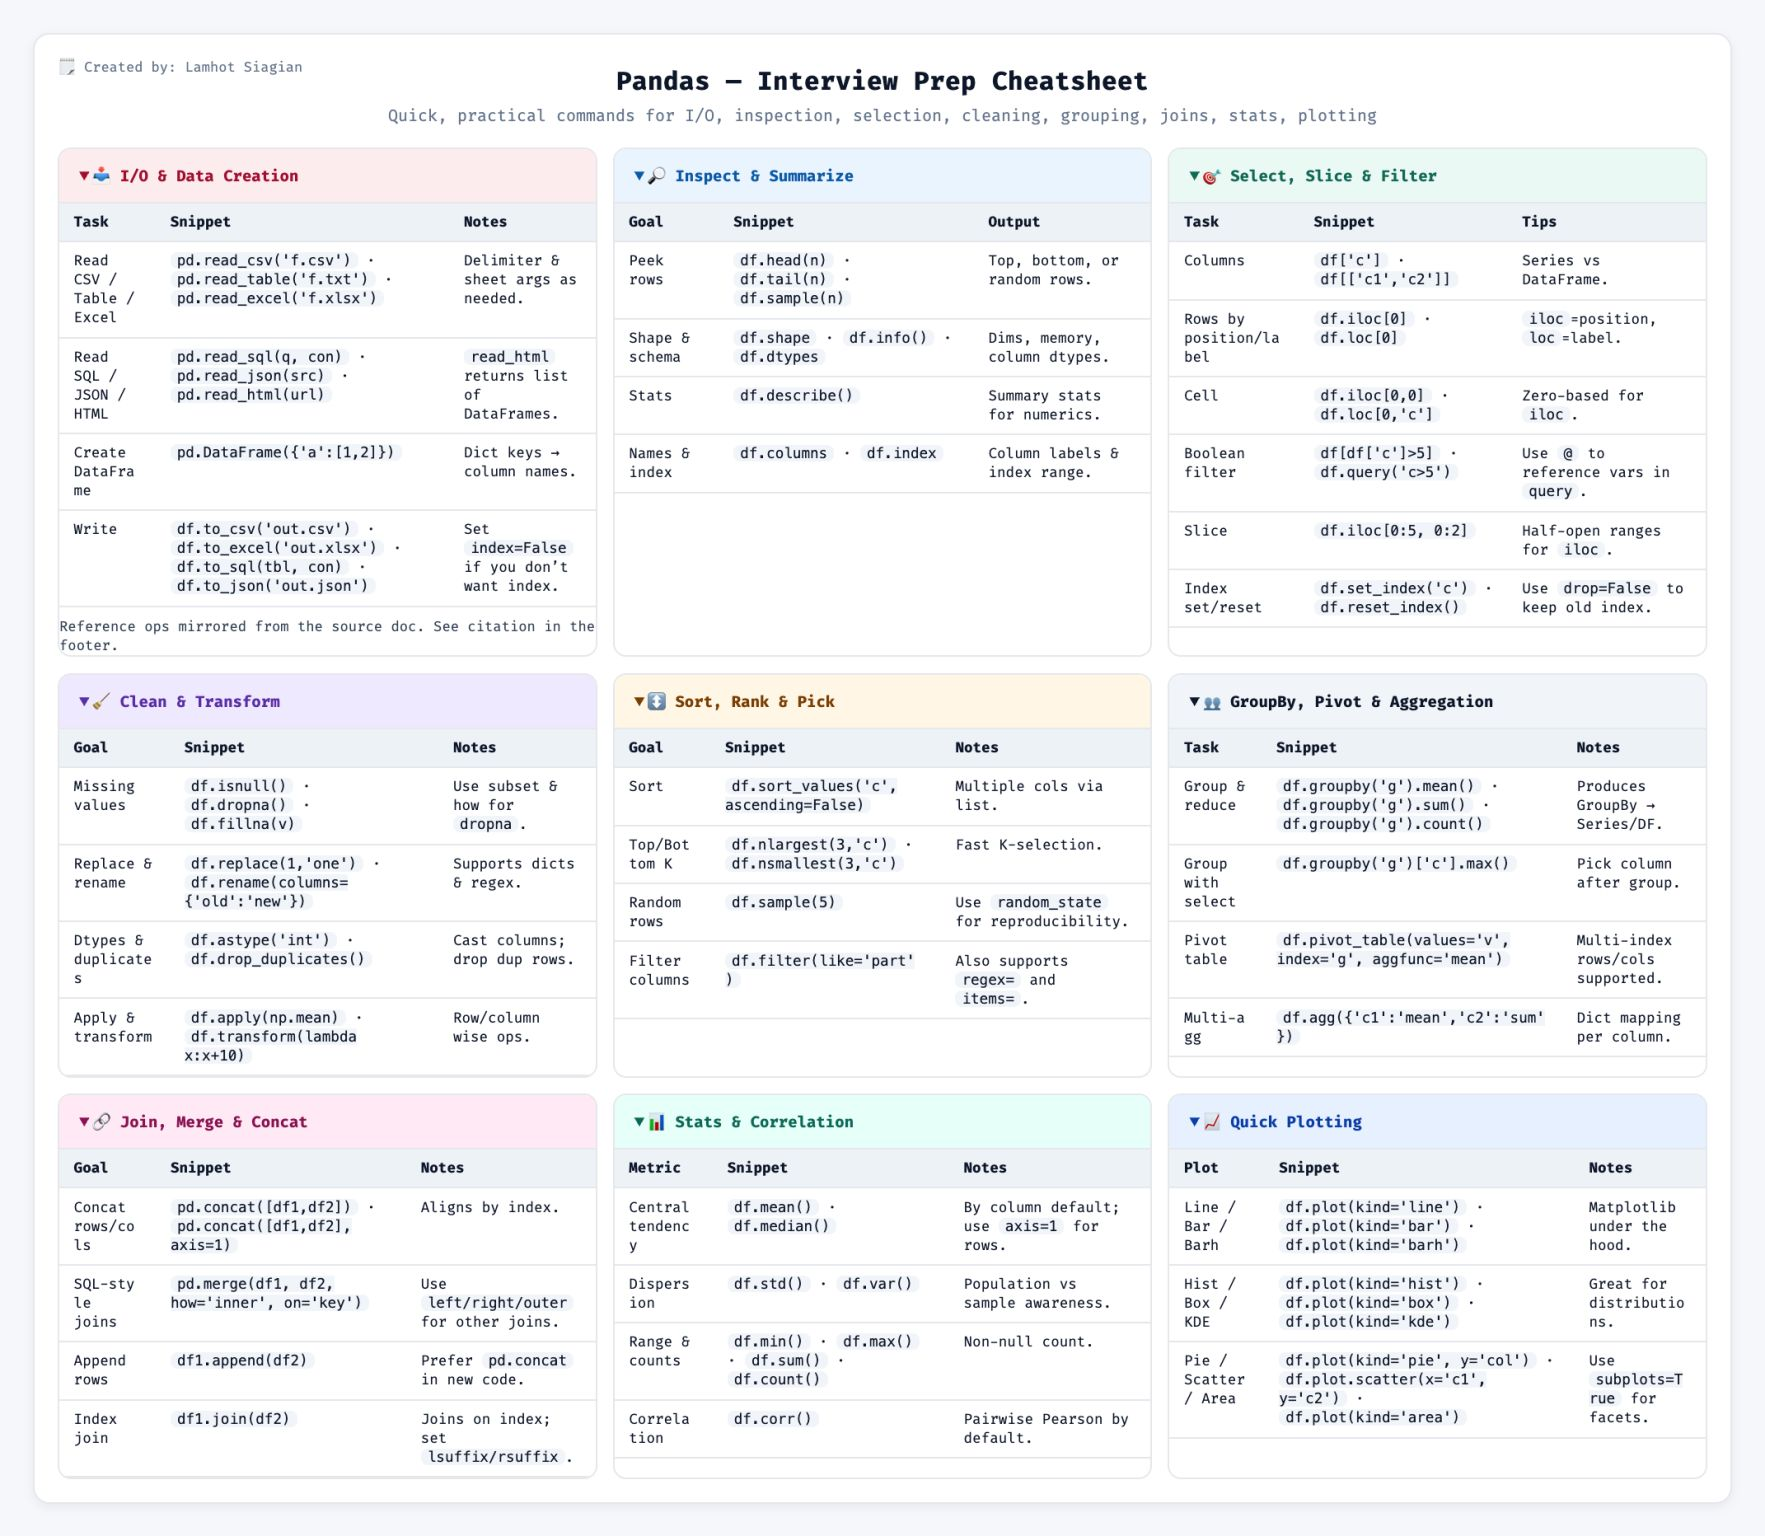
\includegraphics[width=0.95\textwidth,height=\textheight]{images/pandas/pandas_cheatsheet.jpg}\end{minipage}%

\end{figure}%

\chapter{Introducción a Python, R y
Julia}\label{introducciuxf3n-a-python-r-y-julia}

\section{Funciones j\_eval y j\_plot en
R}\label{funciones-j_eval-y-j_plot-en-r-7}

\begin{Shaded}
\begin{Highlighting}[]
\CommentTok{\# \#| include: false}
\FunctionTok{source}\NormalTok{(}\StringTok{"./docs/j\_eval\_j\_plot.r"}\NormalTok{)}
\end{Highlighting}
\end{Shaded}

\section{Introducción}\label{introducciuxf3n-8}

Este capítulo presenta una \textbf{introducción práctica y comparativa}
a los lenguajes \textbf{Python, R y Julia}, enfocada en el uso de
\textbf{comandos básicos} y en la lectura e interpretación de resultados
en consola. El objetivo no es profundizar en programación avanzada, sino
ofrecer una \textbf{puerta de entrada común} para estudiantes que se
inician en el uso de herramientas computacionales para geocomputación.

\subsection{Ejecución de código en cada
lenguaje}\label{ejecuciuxf3n-de-cuxf3digo-en-cada-lenguaje}

\begin{itemize}
\tightlist
\item
  \textbf{Python} y \textbf{R} se ejecutan de forma nativa mediante
  \emph{code chunks} estándar.
\item
  \textbf{Julia}, en este curso, \textbf{no se ejecuta directamente}.
  Todo el código Julia se evalúa desde R utilizando funciones
  auxiliares:

  \begin{itemize}
  \tightlist
  \item
    \texttt{j\_eval()} para ejecutar instrucciones generales
  \item
    \texttt{j\_plot()} para generar gráficos
  \end{itemize}
\end{itemize}

Por esta razón, en el documento encontrarás dos tipos de bloques
relacionados con Julia:

\begin{itemize}
\tightlist
\item
  Bloques con \textbf{código Julia puro}, que sirven como referencia y
  pueden copiarse y reutilizarse.
\item
  Bloques en \textbf{R} que llaman a \texttt{j\_eval()} o
  \texttt{j\_plot()}, que son los que realmente ejecutan el código.
\end{itemize}

\subsection{Sobre los bloques de
código}\label{sobre-los-bloques-de-cuxf3digo}

\begin{itemize}
\tightlist
\item
  \textbf{Todos los bloques de código tienen un \texttt{label}}, lo que
  permite su correcta identificación y reutilización.
\item
  Algunos bloques están pensados \textbf{exclusivamente para HTML} y no
  se ejecutan. Su función es permitir que el estudiante \textbf{copie y
  pegue el código} directamente en su entorno de trabajo.
\item
  Cuando un bloque no se ejecuta, esto se indica explícitamente en sus
  opciones.
\end{itemize}

\subsection{Alcance del capítulo}\label{alcance-del-capuxedtulo}

En este capítulo aprenderás a:

\begin{itemize}
\tightlist
\item
  Acceder a la ayuda y documentación básica en cada lenguaje
\item
  Ejecutar comandos simples y entender su salida
\item
  Reconocer tipos de objetos y estructuras básicas
\item
  Comparar cómo Python, R y Julia resuelven tareas similares
\end{itemize}

Este contenido servirá como base para los capítulos posteriores, donde
se utilizarán estos lenguajes para la creación de mapas, análisis de
datos espaciales y visualización geográfica.

\section{Ayuda y documentación}\label{ayuda-y-documentaciuxf3n}

\begin{longtable}[]{@{}
  >{\raggedright\arraybackslash}p{(\columnwidth - 8\tabcolsep) * \real{0.2000}}
  >{\raggedright\arraybackslash}p{(\columnwidth - 8\tabcolsep) * \real{0.2000}}
  >{\raggedright\arraybackslash}p{(\columnwidth - 8\tabcolsep) * \real{0.2000}}
  >{\raggedright\arraybackslash}p{(\columnwidth - 8\tabcolsep) * \real{0.2000}}
  >{\raggedright\arraybackslash}p{(\columnwidth - 8\tabcolsep) * \real{0.2000}}@{}}
\toprule\noalign{}
\begin{minipage}[b]{\linewidth}\raggedright
Tarea
\end{minipage} & \begin{minipage}[b]{\linewidth}\raggedright
Descripción
\end{minipage} & \begin{minipage}[b]{\linewidth}\raggedright
Python
\end{minipage} & \begin{minipage}[b]{\linewidth}\raggedright
R
\end{minipage} & \begin{minipage}[b]{\linewidth}\raggedright
Julia
\end{minipage} \\
\midrule\noalign{}
\endhead
\bottomrule\noalign{}
\endlastfoot
Ver ayuda general & Abre la documentación interactiva & \texttt{help()}
& \texttt{help.start()} & \texttt{?} en REPL \\
Ayuda de función & Documentación de un comando & \texttt{help(sum)} &
\texttt{?mean} & \texttt{?sum} \\
Ver ejemplos & Código de ejemplo de una función & \textbf{Docstrings} &
\texttt{example("lapply")} & \textbf{Docstrings} \\
Vignettes / guías & Tutoriales extendidos & \texttt{obj.\_\_doc\_\_} &
\texttt{browseVignettes()} & \texttt{?Modulo} \\
Demo & Ejecutar ejemplos & \texttt{libreria.ejemplos()}* &
\texttt{demo()} & \texttt{include("test")}* \\
\end{longtable}

\textbf{Nota sobre los Docstrings:} En Python y Julia, la documentación
y los ejemplos de uso residen directamente dentro del código fuente en
bloques llamados \emph{Docstrings}. Al ejecutar los comandos de ayuda
(\texttt{help()} o \texttt{@doc}), el intérprete extrae estos
comentarios y los muestra en la terminal, permitiendo que el usuario vea
ejemplos reales de implementación de inmediato sin necesidad de manuales
externos.

\textbf{Nota sobre los Demos (*):} A diferencia de R, Python y Julia no
tienen un comando universal \texttt{demo()}. El asterisco indica que el
acceso a ejemplos depende de la librería. En Python, se suele explorar
la propiedad \texttt{\_\_doc\_\_} o módulos de \texttt{datasets}. En
Julia, se acostumbra a inspeccionar la carpeta de instalación mediante
\texttt{pathof(Modulo)} para encontrar archivos de prueba o ejemplos.

\subsection{Python}

\begin{Shaded}
\begin{Highlighting}[]
\CommentTok{\# help() busca y muestra el "Docstring" de la función}
\BuiltInTok{help}\NormalTok{(}\BuiltInTok{sum}\NormalTok{)}

\CommentTok{\# Ayuda sobre un módulo completo para ver sus funciones disponibles}
\ImportTok{import}\NormalTok{ math}
\BuiltInTok{help}\NormalTok{(math)}

\CommentTok{\# dir() lista todos los métodos y atributos (la "anatomía" del objeto)}
\ImportTok{import}\NormalTok{ pandas }\ImportTok{as}\NormalTok{ pd}
\BuiltInTok{dir}\NormalTok{(pd.DataFrame)}

\CommentTok{\# pydoc renderiza la documentación técnica en la terminal}
\ImportTok{import}\NormalTok{ pydoc}
\BuiltInTok{print}\NormalTok{(pydoc.render\_doc(}\StringTok{"math"}\NormalTok{)) }

\CommentTok{\# Ejemplo de "Demo" en Python (vía datasets de una librería SIG)}
\ImportTok{import}\NormalTok{ geopandas }\ImportTok{as}\NormalTok{ gpd}
\CommentTok{\# Listamos los mapas de ejemplo que vienen con la librería}
\BuiltInTok{print}\NormalTok{(gpd.datasets.available)}
\end{Highlighting}
\end{Shaded}

\subsection{R}

\begin{Shaded}
\begin{Highlighting}[]
\CommentTok{\# Inicia el servidor de ayuda local en formato HTML}
\FunctionTok{help.start}\NormalTok{()}

\CommentTok{\# Acceso rápido a la documentación de una función específica}
\NormalTok{?mean}
\FunctionTok{help}\NormalTok{(}\StringTok{"plot"}\NormalTok{)}

\CommentTok{\# Ejecuta automáticamente el código de ejemplo del manual}
\FunctionTok{example}\NormalTok{(}\StringTok{"lapply"}\NormalTok{)}

\CommentTok{\# {-}{-}{-} Vignettes y Demos {-}{-}{-}}

\CommentTok{\# Abre el índice de tutoriales detallados (vignettes)}
\FunctionTok{browseVignettes}\NormalTok{()}

\CommentTok{\# Listar guías del paquete \textquotesingle{}stars\textquotesingle{} (análisis de cubos de datos)}
\CommentTok{\# Nota: presione "q" al final de la lista para liberar la consola}
\FunctionTok{vignette}\NormalTok{(}\AttributeTok{package =} \StringTok{"stars"}\NormalTok{)}

\CommentTok{\# Visualizar una vignette específica por su nombre}
\FunctionTok{vignette}\NormalTok{(}\StringTok{"stars1"}\NormalTok{, }\AttributeTok{package =} \StringTok{"stars"}\NormalTok{)}

\CommentTok{\# Importante: requiere dispositivo gráfico (ej. httpgd::hgd())}
\CommentTok{\# presione "q" al final de la lista para salir}
\FunctionTok{demo}\NormalTok{()}

\CommentTok{\# Demos específicos de librerías de Geomática}
\FunctionTok{library}\NormalTok{(sf)}
\FunctionTok{demo}\NormalTok{(}\StringTok{"nc"}\NormalTok{, }\AttributeTok{package =} \StringTok{"sf"}\NormalTok{)}
\FunctionTok{demo}\NormalTok{(}\StringTok{"ggplot"}\NormalTok{, }\AttributeTok{package =} \StringTok{"sf"}\NormalTok{)}
\end{Highlighting}
\end{Shaded}

\subsection{Julia}

\begin{Shaded}
\begin{Highlighting}[]
\CommentTok{\# Este comando (?) solo funciona dentro del REPL interactivo}
\CommentTok{\# ?sum}

\CommentTok{\# En Quarto usamos la macro @doc para acceder al Docstring}
\PreprocessorTok{@doc}\NormalTok{ sum}
\PreprocessorTok{@doc}\NormalTok{ println}

\CommentTok{\# Julia usa docstrings con ejemplos y ayuda integrados, similar a Python}
\CommentTok{\# Para encontrar "Demos", localizamos la carpeta del paquete en el disco}
\ImportTok{using} \BuiltInTok{DataFrames}
\FunctionTok{println}\NormalTok{(}\StringTok{"Ubicación del código: "}\NormalTok{, }\FunctionTok{pathof}\NormalTok{(DataFrames))}
\end{Highlighting}
\end{Shaded}

\section{Instalación y carga de
paquetes}\label{instalaciuxf3n-y-carga-de-paquetes}

\begin{longtable}[]{@{}
  >{\raggedright\arraybackslash}p{(\columnwidth - 8\tabcolsep) * \real{0.2000}}
  >{\raggedright\arraybackslash}p{(\columnwidth - 8\tabcolsep) * \real{0.2000}}
  >{\raggedright\arraybackslash}p{(\columnwidth - 8\tabcolsep) * \real{0.2000}}
  >{\raggedright\arraybackslash}p{(\columnwidth - 8\tabcolsep) * \real{0.2000}}
  >{\raggedright\arraybackslash}p{(\columnwidth - 8\tabcolsep) * \real{0.2000}}@{}}
\toprule\noalign{}
\begin{minipage}[b]{\linewidth}\raggedright
Tarea
\end{minipage} & \begin{minipage}[b]{\linewidth}\raggedright
Descripción
\end{minipage} & \begin{minipage}[b]{\linewidth}\raggedright
Python
\end{minipage} & \begin{minipage}[b]{\linewidth}\raggedright
R
\end{minipage} & \begin{minipage}[b]{\linewidth}\raggedright
Julia
\end{minipage} \\
\midrule\noalign{}
\endhead
\bottomrule\noalign{}
\endlastfoot
Instalar paquete & Agregar librerías externas &
\texttt{pip3\ install\ ...} & \texttt{install.packages()} &
\texttt{Pkg.add()} \\
Cargar paquete & Habilitar funciones del paquete & \texttt{import\ ...}
& \texttt{library()} & \texttt{using\ ...} \\
\end{longtable}

\subsection{Python}

\begin{Shaded}
\begin{Highlighting}[]
\CommentTok{\# En terminal usamos pip3 }
\CommentTok{\# para asegurar la versión de Python 3.x}
\CommentTok{\# pip3 install colorama}

\CommentTok{\# Dentro de python usamos el prefijo "!"}
\CommentTok{\# !pip3 install colorama}

\CommentTok{\# Cargamos solo lo necesario para manejar colores en consola}
\ImportTok{from}\NormalTok{ colorama }\ImportTok{import}\NormalTok{ Fore, Style}

\BuiltInTok{print}\NormalTok{(}\StringTok{"Librería cargada en Python"}\NormalTok{)}

\CommentTok{\# Aparecerán caracteres especiales al inicio del texto}
\CommentTok{\# porque el HTML no entiende la instrucción colorear en rojo}
\CommentTok{\# Fore.RED aplica el color; Style.RESET\_ALL evita que el color "manche" las siguientes líneas}
\BuiltInTok{print}\NormalTok{(Fore.RED }\OperatorTok{+} \StringTok{"Librería cargada en Python"} \OperatorTok{+}\NormalTok{ Style.RESET\_ALL)}
\end{Highlighting}
\end{Shaded}

\subsection{R}

\begin{Shaded}
\begin{Highlighting}[]
\CommentTok{\# Este comando carga el paquete con require() o lo instala}
\CommentTok{\# si no existe}
\ControlFlowTok{if}\NormalTok{ (}\SpecialCharTok{!}\FunctionTok{require}\NormalTok{(}\StringTok{"crayon"}\NormalTok{, }\AttributeTok{character.only =} \ConstantTok{TRUE}\NormalTok{)) \{}
  \FunctionTok{install.packages}\NormalTok{(}\StringTok{"crayon"}\NormalTok{, }\AttributeTok{dependencies =} \ConstantTok{TRUE}\NormalTok{, }\AttributeTok{repos =} \StringTok{"https://cran.rstudio.com/"}\NormalTok{)}
\NormalTok{\}}

\CommentTok{\# Activamos el paquete para la sesión actual de R}
\FunctionTok{library}\NormalTok{(crayon)}

\CommentTok{\# cat() interpreta los códigos de escape ANSI que generan los colores}
\FunctionTok{cat}\NormalTok{(}\FunctionTok{red}\NormalTok{(}\StringTok{"Librería cargada en R"}\NormalTok{))}
\end{Highlighting}
\end{Shaded}

\subsection{Julia}

\begin{Shaded}
\begin{Highlighting}[]
\CommentTok{\# PASO 1: CON ASIS. Ejecutamos la instalación y mostramos texto limpio.}
\FunctionTok{cat}\NormalTok{(}\FunctionTok{j\_eval}\NormalTok{(r}\StringTok{"{-}(}
\StringTok{using Pkg}

\StringTok{\# Verificamos si \textquotesingle{}Crayons\textquotesingle{} ya está en el proyecto; si no, lo instalamos}
\StringTok{if !haskey(Pkg.dependencies(), Base.UUID("}\NormalTok{a83e43d3}\DecValTok{{-}9}\NormalTok{d41}\DecValTok{{-}5979{-}9952}\FloatTok{{-}4e448995}\NormalTok{a975}\StringTok{"))}
\StringTok{    Pkg.add("}\NormalTok{Crayons}\StringTok{")}
\StringTok{end}

\StringTok{using Crayons}

\StringTok{\# Retornamos solo el mensaje normal para que se integre al Markdown}
\StringTok{return "}\NormalTok{Librería cargada en Julia\textbackslash{}n}\StringTok{"}
\StringTok{){-}"}\NormalTok{))}
\end{Highlighting}
\end{Shaded}

\begin{quote}
Nota: El siguiente código no puede tener
\texttt{\#\textbar{}results:\ asis} porque se daña el
\texttt{panel-tabset} al tener código de escape ANSI
(\texttt{\textbackslash{}033{[}31m...}). Esto implica que verá unas
líneas de código HTML que debe ignorar.
\end{quote}

\begin{Shaded}
\begin{Highlighting}[]
\CommentTok{\# PASO 2: SIN ASIS. Aislamos el código ANSI para proteger el Tabset.}
\NormalTok{resultado\_color }\OtherTok{\textless{}{-}} \FunctionTok{j\_eval}\NormalTok{(r}\StringTok{"{-}(}
\StringTok{\# Como la sesión de Julia sigue abierta, \textquotesingle{}Crayons\textquotesingle{} ya está cargado.}
\StringTok{\# Solo capturamos el texto con el código de escape ANSI (color rojo).}
\StringTok{mensaje\_color = string(Crayon(foreground=:red), "}\NormalTok{Librería cargada en }\FunctionTok{Julia}\NormalTok{ (con escape ANSI)}\StringTok{")}

\StringTok{return mensaje\_color}
\StringTok{){-}"}\NormalTok{)}

\CommentTok{\# Quarto encierra esta salida en un bloque de código seguro}
\FunctionTok{cat}\NormalTok{(resultado\_color)}
\end{Highlighting}
\end{Shaded}

\section{Objetos básicos y estructuras de
datos}\label{objetos-buxe1sicos-y-estructuras-de-datos}

El manejo eficiente de vectores y matrices es el corazón del
procesamiento ráster. A continuación, se presenta una comparativa de
cómo se declaran y manipulan los objetos básicos.

\begin{longtable}[]{@{}
  >{\raggedright\arraybackslash}p{(\columnwidth - 8\tabcolsep) * \real{0.2000}}
  >{\raggedright\arraybackslash}p{(\columnwidth - 8\tabcolsep) * \real{0.2000}}
  >{\raggedright\arraybackslash}p{(\columnwidth - 8\tabcolsep) * \real{0.2000}}
  >{\raggedright\arraybackslash}p{(\columnwidth - 8\tabcolsep) * \real{0.2000}}
  >{\raggedright\arraybackslash}p{(\columnwidth - 8\tabcolsep) * \real{0.2000}}@{}}
\caption{Comparativa de estructuras de
datos}\label{tbl-comparativa-datos}\tabularnewline
\toprule\noalign{}
\begin{minipage}[b]{\linewidth}\raggedright
Estructura
\end{minipage} & \begin{minipage}[b]{\linewidth}\raggedright
Descripción
\end{minipage} & \begin{minipage}[b]{\linewidth}\raggedright
Python
\end{minipage} & \begin{minipage}[b]{\linewidth}\raggedright
R
\end{minipage} & \begin{minipage}[b]{\linewidth}\raggedright
Julia
\end{minipage} \\
\midrule\noalign{}
\endfirsthead
\toprule\noalign{}
\begin{minipage}[b]{\linewidth}\raggedright
Estructura
\end{minipage} & \begin{minipage}[b]{\linewidth}\raggedright
Descripción
\end{minipage} & \begin{minipage}[b]{\linewidth}\raggedright
Python
\end{minipage} & \begin{minipage}[b]{\linewidth}\raggedright
R
\end{minipage} & \begin{minipage}[b]{\linewidth}\raggedright
Julia
\end{minipage} \\
\midrule\noalign{}
\endhead
\bottomrule\noalign{}
\endlastfoot
\textbf{Vector} & Colección lineal ordenada &
\texttt{v\ =\ np.array({[}1,\ 2,\ 3{]})} &
\texttt{v\ \textless{}-\ c(1,\ 2,\ 3)} &
\texttt{v\ =\ {[}1,\ 2,\ 3{]}} \\
\textbf{Matriz} & Arreglo bidimensional (Ráster) &
\texttt{m\ =\ np.zeros((3,3))} o \texttt{np.array({[}{[}...{]}{]})} &
\texttt{m\ \textless{}-\ matrix(0,\ 3,\ 3)} &
\texttt{m\ =\ zeros(3,\ 3)} o \texttt{{[}...\ ;\ ...{]}} \\
\textbf{Diccionario} & Pares clave-valor (Metadatos) &
\texttt{\{key:\ val\}} ej. \texttt{\{"id":\ 1\}} & \texttt{list(k=v)}
ej. \texttt{list(id\ =\ 1)} & \texttt{Dict(k=\textgreater{}v)} ej.
\texttt{Dict("id"=\textgreater{}1)} \\
\textbf{Data Frame} & Estructura tabular (Atributos) &
\texttt{pd.DataFrame()} & \texttt{data.frame()} &
\texttt{DataFrame(...)} \\
\textbf{Indexación} & Posición del primer elemento & Inicia en
\textbf{0} & Inicia en \textbf{1} & Inicia en \textbf{1} \\
\end{longtable}

\subsection{Relación entre estructuras y componentes
SIG}\label{sec-diagrama-estructuras}

Para entender por qué usamos diferentes estructuras de datos, es útil
ver cómo se mapean con los componentes de un Sistema de Información
Geográfica:

\begin{figure}

\centering{

\captionsetup{labelsep=none}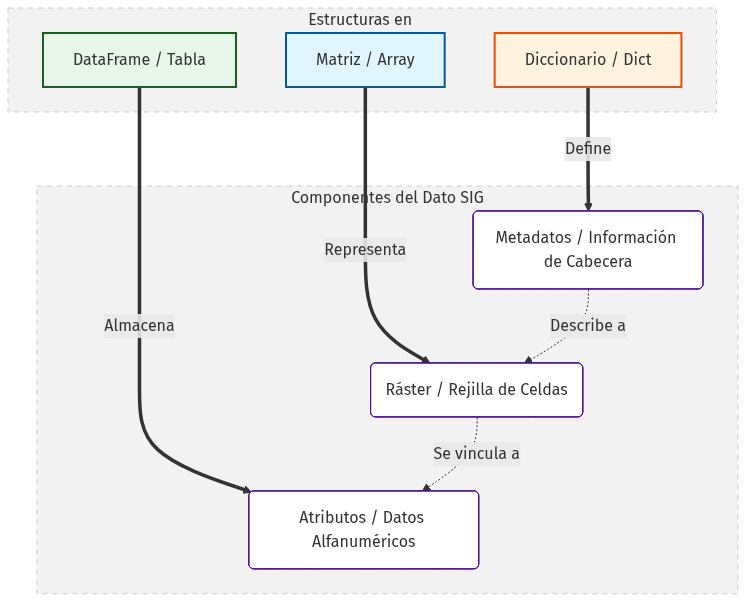
\includegraphics[width=0.5\textwidth,height=\textheight]{images/fig-relacion-geo.png}

}

\caption{\label{fig-relacion-geo}}

\end{figure}%

\begin{tcolorbox}[enhanced jigsaw, coltitle=black, leftrule=.75mm, bottomtitle=1mm, title=\textcolor{quarto-callout-note-color}{\faInfo}\hspace{0.5em}{Nota}, colback=white, colbacktitle=quarto-callout-note-color!10!white, left=2mm, toptitle=1mm, rightrule=.15mm, titlerule=0mm, arc=.35mm, colframe=quarto-callout-note-color-frame, bottomrule=.15mm, toprule=.15mm, opacityback=0, opacitybacktitle=0.6, breakable]

Como se observa en la Figura~\ref{fig-relacion-geo}, la \textbf{Matriz}
es la estructura reina para el análisis ráster, mientras que los
\textbf{DataFrames} son los que nos permiten realizar consultas sobre
las bases de datos de predios o coberturas.

\end{tcolorbox}

\begin{tcolorbox}[enhanced jigsaw, coltitle=black, leftrule=.75mm, bottomtitle=1mm, title=\textcolor{quarto-callout-warning-color}{\faExclamationTriangle}\hspace{0.5em}{El peligro de la indexación espacial}, colback=white, colbacktitle=quarto-callout-warning-color!10!white, left=2mm, toptitle=1mm, rightrule=.15mm, titlerule=0mm, arc=.35mm, colframe=quarto-callout-warning-color-frame, bottomrule=.15mm, toprule=.15mm, opacityback=0, opacitybacktitle=0.6, breakable]

Esta es la fuente más frecuente de errores. Mientras que en
\textbf{Python} el primer píxel de una banda satelital es el
\texttt{{[}0,0{]}}, en \textbf{R} y \textbf{Julia} es el
\texttt{{[}1,1{]}}. Un error de este tipo desplazará todos sus
resultados una celda, invalidando análisis de precisión o cambios de
cobertura.

\end{tcolorbox}

\textbf{Nota sobre estructuras:} En Geomática, los vectores suelen
representar coordenadas o valores de píxeles, mientras que los
diccionarios son fundamentales para manejar atributos (como en formato
JSON o GeoJSON). Las tablas (DataFrames) son el estándar para bases de
datos alfanuméricas de predios, municipios o estaciones climáticas.

\subsection{Python}

\begin{Shaded}
\begin{Highlighting}[]
\CommentTok{\# \#| eval: false}
\CommentTok{\# 1. Listas: colecciones mutables de elementos}
\CommentTok{\# Ejemplo: Códigos DANE de departamentos (Antioquia, Cundinamarca, Valle)}
\NormalTok{codigos }\OperatorTok{=}\NormalTok{ [}\DecValTok{5}\NormalTok{, }\DecValTok{25}\NormalTok{, }\DecValTok{76}\NormalTok{]}
\BuiltInTok{type}\NormalTok{(codigos)}
\end{Highlighting}
\end{Shaded}

\begin{verbatim}
<class 'list'>
\end{verbatim}

\begin{Shaded}
\begin{Highlighting}[]
\CommentTok{\# 2. Diccionarios: Estructuras de clave{-}valor}
\CommentTok{\# Ideal para representar metadatos de un departamento}
\NormalTok{metadatos }\OperatorTok{=}\NormalTok{ \{}
    \StringTok{"departamento"}\NormalTok{: [}\StringTok{"Antioquia"}\NormalTok{, }\StringTok{"Cundinamarca"}\NormalTok{, }\StringTok{"Valle"}\NormalTok{],}
    \StringTok{"area\_km2"}\NormalTok{: [}\DecValTok{63612}\NormalTok{, }\DecValTok{22623}\NormalTok{, }\DecValTok{22140}\NormalTok{],}
    \StringTok{"capital"}\NormalTok{: [}\StringTok{"Medellín"}\NormalTok{, }\StringTok{"Bogotá"}\NormalTok{, }\StringTok{"Cali"}\NormalTok{]}
\NormalTok{\}}
\BuiltInTok{type}\NormalTok{(metadatos)}
\end{Highlighting}
\end{Shaded}

\begin{verbatim}
<class 'dict'>
\end{verbatim}

\begin{Shaded}
\begin{Highlighting}[]
\CommentTok{\# 3. DataFrames: Para manejar tablas de atributos SIG}
\ImportTok{import}\NormalTok{ pandas }\ImportTok{as}\NormalTok{ pd}
\NormalTok{df\_colombia }\OperatorTok{=}\NormalTok{ pd.DataFrame(metadatos)}
\BuiltInTok{type}\NormalTok{(df\_colombia)}
\end{Highlighting}
\end{Shaded}

\begin{verbatim}
<class 'pandas.core.frame.DataFrame'>
\end{verbatim}

\begin{Shaded}
\begin{Highlighting}[]
\CommentTok{\# Visualizamos el resumen técnico de la tabla}
\BuiltInTok{print}\NormalTok{(df\_colombia.info())}
\end{Highlighting}
\end{Shaded}

\begin{verbatim}
<class 'pandas.core.frame.DataFrame'>
RangeIndex: 3 entries, 0 to 2
Data columns (total 3 columns):
 #   Column        Non-Null Count  Dtype 
---  ------        --------------  ----- 
 0   departamento  3 non-null      object
 1   area_km2      3 non-null      int64 
 2   capital       3 non-null      object
dtypes: int64(1), object(2)
memory usage: 204.0+ bytes
None
\end{verbatim}

\subsection{R}

\begin{Shaded}
\begin{Highlighting}[]
\CommentTok{\# \#| eval: false}
\CommentTok{\# 1. Vectores: La unidad básica en R (todos los elementos del mismo tipo)}
\CommentTok{\# Códigos DANE de departamentos}
\NormalTok{codigos }\OtherTok{\textless{}{-}} \FunctionTok{c}\NormalTok{(}\DecValTok{5}\NormalTok{, }\DecValTok{25}\NormalTok{, }\DecValTok{76}\NormalTok{)}
\FunctionTok{class}\NormalTok{(codigos)}
\end{Highlighting}
\end{Shaded}

\begin{verbatim}
[1] "numeric"
\end{verbatim}

\begin{Shaded}
\begin{Highlighting}[]
\CommentTok{\# 2. Listas: Pueden contener objetos de diferentes tipos y tamaños}
\CommentTok{\# En R, las listas con nombres funcionan como los diccionarios}
\NormalTok{metadatos }\OtherTok{\textless{}{-}} \FunctionTok{list}\NormalTok{(}
  \AttributeTok{departamento =} \FunctionTok{c}\NormalTok{(}\StringTok{"Antioquia"}\NormalTok{, }\StringTok{"Cundinamarca"}\NormalTok{, }\StringTok{"Valle"}\NormalTok{),}
  \AttributeTok{area\_km2 =} \FunctionTok{c}\NormalTok{(}\DecValTok{63612}\NormalTok{, }\DecValTok{22623}\NormalTok{, }\DecValTok{22140}\NormalTok{),}
  \AttributeTok{capital =} \FunctionTok{c}\NormalTok{(}\StringTok{"Medellín"}\NormalTok{, }\StringTok{"Bogotá"}\NormalTok{, }\StringTok{"Cali"}\NormalTok{)}
\NormalTok{)}
\FunctionTok{class}\NormalTok{(metadatos)}
\end{Highlighting}
\end{Shaded}

\begin{verbatim}
[1] "list"
\end{verbatim}

\begin{Shaded}
\begin{Highlighting}[]
\CommentTok{\# 3. Data Frame: La estructura tabular nativa por excelencia}
\NormalTok{df\_colombia }\OtherTok{\textless{}{-}} \FunctionTok{data.frame}\NormalTok{(metadatos)}
\FunctionTok{class}\NormalTok{(df\_colombia)}
\end{Highlighting}
\end{Shaded}

\begin{verbatim}
[1] "data.frame"
\end{verbatim}

\begin{Shaded}
\begin{Highlighting}[]
\CommentTok{\# str() muestra la estructura interna del objeto (equivalente a info() en Python)}
\FunctionTok{str}\NormalTok{(df\_colombia)}
\end{Highlighting}
\end{Shaded}

\begin{verbatim}
'data.frame':   3 obs. of  3 variables:
 $ departamento: chr  "Antioquia" "Cundinamarca" "Valle"
 $ area_km2    : num  63612 22623 22140
 $ capital     : chr  "Medellín" "Bogotá" "Cali"
\end{verbatim}

\subsection{Julia}

\begin{Shaded}
\begin{Highlighting}[]
\CommentTok{\# \#| eval: false}
\FunctionTok{j\_eval}\NormalTok{(}\StringTok{\textquotesingle{}}
\StringTok{\# 1. Vectores: Se definen con corchetes (similar a Python)}
\StringTok{codigos = [5, 25, 76]}

\StringTok{typeof(codigos)}

\StringTok{\# 2. Diccionarios: Se usa el operador =\textgreater{} para asociar clave y valor}
\StringTok{metadatos = Dict(}
\StringTok{    "departamento" =\textgreater{} ["Antioquia", "Cundinamarca", "Valle"],}
\StringTok{    "area\_km2" =\textgreater{} [63612, 22623, 22140]}
\StringTok{)}

\StringTok{typeof(metadatos)}

\StringTok{\# 3. Tablas: En Julia Base se pueden usar vectores de Tuplas Nombradas,}
\StringTok{\# pero en Geomática siempre usaremos la librería DataFrames}
\StringTok{using DataFrames}
\StringTok{df\_colombia = DataFrame(}
\StringTok{    departamento = ["Antioquia", "Cundinamarca", "Valle"],}
\StringTok{    area\_km2 = [63612, 22623, 22140],}
\StringTok{    capital = ["Medellín", "Bogotá", "Cali"]}
\StringTok{)}

\StringTok{typeof(df\_colombia)}

\StringTok{\# describe() da un resumen estadístico de la tabla}
\StringTok{println(describe(df\_colombia))}
\StringTok{\textquotesingle{}}\NormalTok{)}
\end{Highlighting}
\end{Shaded}

\begin{verbatim}
Starting Julia ...
\end{verbatim}

\section{4. Comandos básicos y manipulación de
tablas}\label{comandos-buxe1sicos-y-manipulaciuxf3n-de-tablas}

\begin{longtable}[]{@{}
  >{\raggedright\arraybackslash}p{(\columnwidth - 8\tabcolsep) * \real{0.2000}}
  >{\raggedright\arraybackslash}p{(\columnwidth - 8\tabcolsep) * \real{0.2000}}
  >{\raggedright\arraybackslash}p{(\columnwidth - 8\tabcolsep) * \real{0.2000}}
  >{\raggedright\arraybackslash}p{(\columnwidth - 8\tabcolsep) * \real{0.2000}}
  >{\raggedright\arraybackslash}p{(\columnwidth - 8\tabcolsep) * \real{0.2000}}@{}}
\toprule\noalign{}
\begin{minipage}[b]{\linewidth}\raggedright
Tarea
\end{minipage} & \begin{minipage}[b]{\linewidth}\raggedright
Descripción
\end{minipage} & \begin{minipage}[b]{\linewidth}\raggedright
Python
\end{minipage} & \begin{minipage}[b]{\linewidth}\raggedright
R
\end{minipage} & \begin{minipage}[b]{\linewidth}\raggedright
Julia
\end{minipage} \\
\midrule\noalign{}
\endhead
\bottomrule\noalign{}
\endlastfoot
Directorio & Ruta de trabajo actual & \texttt{os.getcwd()} &
\texttt{getwd()} & \texttt{pwd()} \\
Tipo / clase & Tipo de estructura & \texttt{type()} & \texttt{class()} &
\texttt{typeof()} \\
Estructura & Resumen técnico & \texttt{df.info()} & \texttt{str()} &
\texttt{describe(df)} \\
Dimensiones & Filas y columnas & \texttt{df.shape} & \texttt{dim()} &
\texttt{size()} \\
Primeras filas & Vista rápida inicial & \texttt{df.head(n)} &
\texttt{head(df,\ n)} & \texttt{first(df,\ n)} \\
Frecuencias & Conteo de categorías & \texttt{value\_counts()} &
\texttt{table()} & \texttt{countmap()} \\
Unir filas & Concatenar vertical & \texttt{pd.concat(...,\ axis=0)} &
\texttt{rbind()} & \texttt{vcat()} \\
Omitir NA & Limpiar datos faltantes & \texttt{dropna()} &
\texttt{na.omit()} & \texttt{dropmissing()} \\
Ordenar & Organizar por columna & \texttt{sort\_values()} &
\texttt{order()} / \texttt{arrange()} & \texttt{sort()} \\
\end{longtable}

\subsection{Python}

\begin{Shaded}
\begin{Highlighting}[]
\CommentTok{\# \#| eval: false}
\ImportTok{import}\NormalTok{ os}
\ImportTok{import}\NormalTok{ numpy }\ImportTok{as}\NormalTok{ np}
\ImportTok{import}\NormalTok{ pandas }\ImportTok{as}\NormalTok{ pd}

\CommentTok{\# 1. Gestión del entorno de trabajo}
\BuiltInTok{print}\NormalTok{(}\SpecialStringTok{f"Ruta actual: }\SpecialCharTok{\{}\NormalTok{os}\SpecialCharTok{.}\NormalTok{getcwd()}\SpecialCharTok{\}}\SpecialStringTok{"}\NormalTok{)}
\end{Highlighting}
\end{Shaded}

\begin{verbatim}
Ruta actual: /home/rstudio/work/01_prog_sig
\end{verbatim}

\begin{Shaded}
\begin{Highlighting}[]
\CommentTok{\# 2. Creación de datos: Departamentos de Colombia (Población en millones, Área en km2)}
\NormalTok{data }\OperatorTok{=}\NormalTok{ \{}
    \StringTok{"depto"}\NormalTok{: [}\StringTok{"Antioquia"}\NormalTok{, }\StringTok{"Cundinamarca"}\NormalTok{, }\StringTok{"Valle"}\NormalTok{, }\StringTok{"Bolívar"}\NormalTok{, }\StringTok{"Atlántico"}\NormalTok{],}
    \StringTok{"pob\_2023"}\NormalTok{: [}\FloatTok{6.8}\NormalTok{, }\FloatTok{3.2}\NormalTok{, }\FloatTok{4.6}\NormalTok{, }\FloatTok{2.2}\NormalTok{, }\FloatTok{2.8}\NormalTok{],}
    \StringTok{"area\_km2"}\NormalTok{: [}\DecValTok{63612}\NormalTok{, }\DecValTok{22623}\NormalTok{, }\DecValTok{22140}\NormalTok{, }\DecValTok{25978}\NormalTok{, }\DecValTok{3388}\NormalTok{],}
    \StringTok{"region"}\NormalTok{: [}\StringTok{"Andina"}\NormalTok{, }\StringTok{"Andina"}\NormalTok{, }\StringTok{"Pacífica"}\NormalTok{, }\StringTok{"Caribe"}\NormalTok{, }\StringTok{"Caribe"}\NormalTok{]}
\NormalTok{\}}
\NormalTok{df }\OperatorTok{=}\NormalTok{ pd.DataFrame(data)}

\CommentTok{\# 3. Inspección de la tabla}
\BuiltInTok{print}\NormalTok{(df.info())           }\CommentTok{\# Resumen de tipos de datos y memoria}
\end{Highlighting}
\end{Shaded}

\begin{verbatim}
<class 'pandas.core.frame.DataFrame'>
RangeIndex: 5 entries, 0 to 4
Data columns (total 4 columns):
 #   Column    Non-Null Count  Dtype  
---  ------    --------------  -----  
 0   depto     5 non-null      object 
 1   pob_2023  5 non-null      float64
 2   area_km2  5 non-null      int64  
 3   region    5 non-null      object 
dtypes: float64(1), int64(1), object(2)
memory usage: 292.0+ bytes
None
\end{verbatim}

\begin{Shaded}
\begin{Highlighting}[]
\BuiltInTok{print}\NormalTok{(}\SpecialStringTok{f"Forma: }\SpecialCharTok{\{}\NormalTok{df}\SpecialCharTok{.}\NormalTok{shape}\SpecialCharTok{\}}\SpecialStringTok{"}\NormalTok{) }\CommentTok{\# (filas, columnas)}
\end{Highlighting}
\end{Shaded}

\begin{verbatim}
Forma: (5, 4)
\end{verbatim}

\begin{Shaded}
\begin{Highlighting}[]
\BuiltInTok{print}\NormalTok{(df.head(}\DecValTok{3}\NormalTok{))          }\CommentTok{\# Ver los primeros 3 registros}
\end{Highlighting}
\end{Shaded}

\begin{verbatim}
          depto  pob_2023  area_km2    region
0     Antioquia       6.8     63612    Andina
1  Cundinamarca       3.2     22623    Andina
2         Valle       4.6     22140  Pacífica
\end{verbatim}

\begin{Shaded}
\begin{Highlighting}[]
\CommentTok{\# 4. Análisis de frecuencias (¿Cuántos deptos por región?)}
\BuiltInTok{print}\NormalTok{(df[}\StringTok{"region"}\NormalTok{].value\_counts())}
\end{Highlighting}
\end{Shaded}

\begin{verbatim}
region
Andina      2
Caribe      2
Pacífica    1
Name: count, dtype: int64
\end{verbatim}

\begin{Shaded}
\begin{Highlighting}[]
\CommentTok{\# 5. Operaciones de unión}
\CommentTok{\# Crear un nuevo registro para un depto faltante}
\NormalTok{nuevo\_depto }\OperatorTok{=}\NormalTok{ pd.DataFrame(\{}\StringTok{"depto"}\NormalTok{:[}\StringTok{"Chocó"}\NormalTok{], }\StringTok{"pob\_2023"}\NormalTok{:[}\FloatTok{0.5}\NormalTok{], }\StringTok{"area\_km2"}\NormalTok{:[}\DecValTok{46530}\NormalTok{], }\StringTok{"region"}\NormalTok{:[}\StringTok{"Pacífica"}\NormalTok{]\})}
\CommentTok{\# Concatenar verticalmente (axis=0 es por filas)}
\NormalTok{df\_extendido }\OperatorTok{=}\NormalTok{ pd.concat([df, nuevo\_depto], axis}\OperatorTok{=}\DecValTok{0}\NormalTok{, ignore\_index}\OperatorTok{=}\VariableTok{True}\NormalTok{)}

\CommentTok{\# 6. Ordenamiento}
\CommentTok{\# Ordenar por población de mayor a menor}
\NormalTok{df\_sorted }\OperatorTok{=}\NormalTok{ df\_extendido.sort\_values(by}\OperatorTok{=}\StringTok{"pob\_2023"}\NormalTok{, ascending}\OperatorTok{=}\VariableTok{False}\NormalTok{)}
\BuiltInTok{print}\NormalTok{(df\_sorted)}
\end{Highlighting}
\end{Shaded}

\begin{verbatim}
          depto  pob_2023  area_km2    region
0     Antioquia       6.8     63612    Andina
2         Valle       4.6     22140  Pacífica
1  Cundinamarca       3.2     22623    Andina
4     Atlántico       2.8      3388    Caribe
3       Bolívar       2.2     25978    Caribe
5         Chocó       0.5     46530  Pacífica
\end{verbatim}

\begin{Shaded}
\begin{Highlighting}[]
\CommentTok{\# 7. Localización por condición (¿Dónde la población es \textgreater{} 4M?)}
\NormalTok{indices }\OperatorTok{=}\NormalTok{ np.where(df\_extendido[}\StringTok{"pob\_2023"}\NormalTok{] }\OperatorTok{\textgreater{}} \FloatTok{4.0}\NormalTok{)}
\BuiltInTok{print}\NormalTok{(}\SpecialStringTok{f"Índices detectados: }\SpecialCharTok{\{}\NormalTok{indices}\SpecialCharTok{\}}\SpecialStringTok{"}\NormalTok{)}
\end{Highlighting}
\end{Shaded}

\begin{verbatim}
Índices detectados: (array([0, 2]),)
\end{verbatim}

\subsection{R}

\begin{Shaded}
\begin{Highlighting}[]
\CommentTok{\# \#| eval: false}
\CommentTok{\# 1. Gestión del entorno}
\FunctionTok{getwd}\NormalTok{()}
\end{Highlighting}
\end{Shaded}

\begin{verbatim}
[1] "/home/rstudio/work/01_prog_sig"
\end{verbatim}

\begin{Shaded}
\begin{Highlighting}[]
\CommentTok{\# 2. Datos de ejemplo (Departamentos de Colombia)}
\NormalTok{df }\OtherTok{\textless{}{-}} \FunctionTok{data.frame}\NormalTok{(}
  \AttributeTok{depto =} \FunctionTok{c}\NormalTok{(}\StringTok{"Antioquia"}\NormalTok{, }\StringTok{"Cundinamarca"}\NormalTok{, }\StringTok{"Valle"}\NormalTok{, }\StringTok{"Bolívar"}\NormalTok{, }\StringTok{"Atlántico"}\NormalTok{),}
  \AttributeTok{pob\_2023 =} \FunctionTok{c}\NormalTok{(}\FloatTok{6.8}\NormalTok{, }\FloatTok{3.2}\NormalTok{, }\FloatTok{4.6}\NormalTok{, }\FloatTok{2.2}\NormalTok{, }\FloatTok{2.8}\NormalTok{),}
  \AttributeTok{area\_km2 =} \FunctionTok{c}\NormalTok{(}\DecValTok{63612}\NormalTok{, }\DecValTok{22623}\NormalTok{, }\DecValTok{22140}\NormalTok{, }\DecValTok{25978}\NormalTok{, }\DecValTok{3388}\NormalTok{),}
  \AttributeTok{region =} \FunctionTok{c}\NormalTok{(}\StringTok{"Andina"}\NormalTok{, }\StringTok{"Andina"}\NormalTok{, }\StringTok{"Pacífica"}\NormalTok{, }\StringTok{"Caribe"}\NormalTok{, }\StringTok{"Caribe"}\NormalTok{)}
\NormalTok{)}

\CommentTok{\# 3. Inspección básica}
\FunctionTok{str}\NormalTok{(df)          }\CommentTok{\# Estructura del objeto}
\end{Highlighting}
\end{Shaded}

\begin{verbatim}
'data.frame':   5 obs. of  4 variables:
 $ depto   : chr  "Antioquia" "Cundinamarca" "Valle" "Bolívar" ...
 $ pob_2023: num  6.8 3.2 4.6 2.2 2.8
 $ area_km2: num  63612 22623 22140 25978 3388
 $ region  : chr  "Andina" "Andina" "Pacífica" "Caribe" ...
\end{verbatim}

\begin{Shaded}
\begin{Highlighting}[]
\FunctionTok{dim}\NormalTok{(df)          }\CommentTok{\# Dimensiones (filas y columnas)}
\end{Highlighting}
\end{Shaded}

\begin{verbatim}
[1] 5 4
\end{verbatim}

\begin{Shaded}
\begin{Highlighting}[]
\FunctionTok{head}\NormalTok{(df, }\DecValTok{3}\NormalTok{)      }\CommentTok{\# Primeras 3 filas}
\end{Highlighting}
\end{Shaded}

\begin{verbatim}
         depto pob_2023 area_km2   region
1    Antioquia      6.8    63612   Andina
2 Cundinamarca      3.2    22623   Andina
3        Valle      4.6    22140 Pacífica
\end{verbatim}

\begin{Shaded}
\begin{Highlighting}[]
\CommentTok{\# 4. Frecuencias (Equivalente a value\_counts)}
\FunctionTok{table}\NormalTok{(df}\SpecialCharTok{$}\NormalTok{region)}
\end{Highlighting}
\end{Shaded}

\begin{verbatim}

  Andina   Caribe Pacífica 
       2        2        1 
\end{verbatim}

\begin{Shaded}
\begin{Highlighting}[]
\CommentTok{\# 5. Uniones verticales}
\CommentTok{\# Creamos el registro adicional}
\NormalTok{nuevo }\OtherTok{\textless{}{-}} \FunctionTok{data.frame}\NormalTok{(}\AttributeTok{depto=}\StringTok{"Chocó"}\NormalTok{, }\AttributeTok{pob\_2023=}\FloatTok{0.5}\NormalTok{, }\AttributeTok{area\_km2=}\DecValTok{46530}\NormalTok{, }\AttributeTok{region=}\StringTok{"Pacífica"}\NormalTok{)}
\CommentTok{\# rbind une por filas (necesita que las columnas se llamen igual)}
\NormalTok{df\_extendido }\OtherTok{\textless{}{-}} \FunctionTok{rbind}\NormalTok{(df, nuevo)}

\CommentTok{\# 6. Ordenamiento}
\CommentTok{\# order() devuelve los índices; los usamos para reindexar el dataframe}
\NormalTok{df\_sorted }\OtherTok{\textless{}{-}}\NormalTok{ df\_extendido[}\FunctionTok{order}\NormalTok{(}\SpecialCharTok{{-}}\NormalTok{df\_extendido}\SpecialCharTok{$}\NormalTok{pob\_2023), ]}
\FunctionTok{print}\NormalTok{(df\_sorted)}
\end{Highlighting}
\end{Shaded}

\begin{verbatim}
         depto pob_2023 area_km2   region
1    Antioquia      6.8    63612   Andina
3        Valle      4.6    22140 Pacífica
2 Cundinamarca      3.2    22623   Andina
5    Atlántico      2.8     3388   Caribe
4      Bolívar      2.2    25978   Caribe
6        Chocó      0.5    46530 Pacífica
\end{verbatim}

\begin{Shaded}
\begin{Highlighting}[]
\CommentTok{\# 7. Alternativa con dplyr (El estándar de "Tidyverse" para manipular tablas)}
\FunctionTok{library}\NormalTok{(dplyr)}
\end{Highlighting}
\end{Shaded}

\begin{verbatim}

Attaching package: 'dplyr'
\end{verbatim}

\begin{verbatim}
The following objects are masked from 'package:stats':

    filter, lag
\end{verbatim}

\begin{verbatim}
The following objects are masked from 'package:base':

    intersect, setdiff, setequal, union
\end{verbatim}

\begin{Shaded}
\begin{Highlighting}[]
\CommentTok{\# {-}{-}{-} Opción A: Paso a paso con variables intermedias {-}{-}{-}}
\CommentTok{\# Útil para depurar y entender qué sucede en cada etapa}

\CommentTok{\# Paso 1: Ordenar la tabla de departamentos por población de forma descendente}
\NormalTok{df\_ordenado }\OtherTok{\textless{}{-}} \FunctionTok{arrange}\NormalTok{(df\_extendido, }\FunctionTok{desc}\NormalTok{(pob\_2023))}
\FunctionTok{print}\NormalTok{(df\_ordenado)}
\end{Highlighting}
\end{Shaded}

\begin{verbatim}
         depto pob_2023 area_km2   region
1    Antioquia      6.8    63612   Andina
2        Valle      4.6    22140 Pacífica
3 Cundinamarca      3.2    22623   Andina
4    Atlántico      2.8     3388   Caribe
5      Bolívar      2.2    25978   Caribe
6        Chocó      0.5    46530 Pacífica
\end{verbatim}

\begin{Shaded}
\begin{Highlighting}[]
\CommentTok{\# Paso 2: Filtrar los resultados para quedarnos solo con los mayores a 4M}
\NormalTok{df\_final }\OtherTok{\textless{}{-}} \FunctionTok{filter}\NormalTok{(df\_ordenado, pob\_2023 }\SpecialCharTok{\textgreater{}} \FloatTok{4.0}\NormalTok{)}
\FunctionTok{print}\NormalTok{(df\_final)}
\end{Highlighting}
\end{Shaded}

\begin{verbatim}
      depto pob_2023 area_km2   region
1 Antioquia      6.8    63612   Andina
2     Valle      4.6    22140 Pacífica
\end{verbatim}

\begin{Shaded}
\begin{Highlighting}[]
\CommentTok{\# {-}{-}{-} Opción B: Uso de Operadores Pipe (Flujo continuo) {-}{-}{-}}
\CommentTok{\# El pipe permite "pasar" el resultado de una función a la siguiente sin crear variables nuevas.}

\CommentTok{\# 1. Pipe de la librería dplyr (el clásico: \%\textgreater{}\%)}
\CommentTok{\# Se lee como: "Toma df\_extendido, ENTONCES ordena, ENTONCES filtra"}
\NormalTok{df\_extendido }\SpecialCharTok{\%\textgreater{}\%} 
  \FunctionTok{arrange}\NormalTok{(}\FunctionTok{desc}\NormalTok{(pob\_2023)) }\SpecialCharTok{\%\textgreater{}\%} 
  \FunctionTok{filter}\NormalTok{(pob\_2023 }\SpecialCharTok{\textgreater{}} \FloatTok{4.0}\NormalTok{)}
\end{Highlighting}
\end{Shaded}

\begin{verbatim}
      depto pob_2023 area_km2   region
1 Antioquia      6.8    63612   Andina
2     Valle      4.6    22140 Pacífica
\end{verbatim}

\begin{Shaded}
\begin{Highlighting}[]
\CommentTok{\# 2. Pipe nativo de R (disponible desde la versión 4.1: |\textgreater{})}
\CommentTok{\# Es más eficiente en memoria y no depende de cargar librerías extra}
\NormalTok{df\_extendido }\SpecialCharTok{|\textgreater{}} 
  \FunctionTok{arrange}\NormalTok{(}\FunctionTok{desc}\NormalTok{(pob\_2023)) }\SpecialCharTok{|\textgreater{}} 
  \FunctionTok{filter}\NormalTok{(pob\_2023 }\SpecialCharTok{\textgreater{}} \FloatTok{4.0}\NormalTok{)}
\end{Highlighting}
\end{Shaded}

\begin{verbatim}
      depto pob_2023 area_km2   region
1 Antioquia      6.8    63612   Andina
2     Valle      4.6    22140 Pacífica
\end{verbatim}

\subsection{Julia}

\begin{Shaded}
\begin{Highlighting}[]
\CommentTok{\# \#| eval: false}
\FunctionTok{j\_eval}\NormalTok{(}\StringTok{\textquotesingle{}}
\StringTok{using DataFrames}

\StringTok{\# Recreamos la tabla en el entorno de Julia}
\StringTok{df = DataFrame(}
\StringTok{    depto = ["Antioquia", "Cundinamarca", "Valle", "Bolívar", "Atlántico"],}
\StringTok{    pob\_2023 = [6.8, 3.2, 4.6, 2.2, 2.8],}
\StringTok{    area\_km2 = [63612, 22623, 22140, 25978, 3388],}
\StringTok{    region = ["Andina", "Andina", "Pacífica", "Caribe", "Caribe"]}
\StringTok{)}

\StringTok{\# Ejecutamos inspección y unión}
\StringTok{nuevo = DataFrame(depto=["Chocó"], pob\_2023=[0.5], area\_km2=[46530], region=["Pacífica"])}
\StringTok{df\_ext = vcat(df, nuevo)}

\StringTok{\# Ordenar por población y mostrar}
\StringTok{println(sort(df\_ext, :pob\_2023, rev=true))}
\StringTok{\textquotesingle{}}\NormalTok{)}
\end{Highlighting}
\end{Shaded}

\subsection{Operaciones numéricas y matemáticas
básicas}\label{operaciones-numuxe9ricas-y-matemuxe1ticas-buxe1sicas}

En el análisis espacial, estas operaciones son la base para calcular
distancias, transformar coordenadas o procesar índices de vegetación
(NDVI). A continuación, comparamos la sintaxis para las funciones
matemáticas más comunes.

\begin{longtable}[]{@{}
  >{\raggedright\arraybackslash}p{(\columnwidth - 8\tabcolsep) * \real{0.2000}}
  >{\raggedright\arraybackslash}p{(\columnwidth - 8\tabcolsep) * \real{0.2000}}
  >{\raggedright\arraybackslash}p{(\columnwidth - 8\tabcolsep) * \real{0.2000}}
  >{\raggedright\arraybackslash}p{(\columnwidth - 8\tabcolsep) * \real{0.2000}}
  >{\raggedright\arraybackslash}p{(\columnwidth - 8\tabcolsep) * \real{0.2000}}@{}}
\toprule\noalign{}
\begin{minipage}[b]{\linewidth}\raggedright
Tarea
\end{minipage} & \begin{minipage}[b]{\linewidth}\raggedright
Descripción
\end{minipage} & \begin{minipage}[b]{\linewidth}\raggedright
Python
\end{minipage} & \begin{minipage}[b]{\linewidth}\raggedright
R
\end{minipage} & \begin{minipage}[b]{\linewidth}\raggedright
Julia
\end{minipage} \\
\midrule\noalign{}
\endhead
\bottomrule\noalign{}
\endlastfoot
División entera & Cociente sin decimales & \texttt{//} & \texttt{\%/\%}
& \texttt{div()} \\
Módulo & Residuo de la división & \texttt{\%} & \texttt{\%\%} &
\texttt{\%} \\
Raíz cuadrada & Cálculo de \(x^{1/2}\) & \texttt{math.sqrt()} &
\texttt{sqrt()} & \texttt{sqrt()} \\
Logaritmo & Logaritmo natural (\(ln\)) & \texttt{math.log()} &
\texttt{log()} & \texttt{log()} \\
Constantes & Valores de \(\pi\) y \(e\) & \texttt{math.pi},
\texttt{math.e} & \texttt{pi}, \texttt{exp(1)} & \texttt{pi},
\texttt{exp(1)} \\
\end{longtable}

\subsection{Python}

\begin{Shaded}
\begin{Highlighting}[]
\CommentTok{\# \#| eval: false}
\ImportTok{import}\NormalTok{ math}

\CommentTok{\# 1. Aritmética entera (Útil para indexación de matrices)}
\BuiltInTok{print}\NormalTok{(}\SpecialStringTok{f"División entera (5 // 2): }\SpecialCharTok{\{}\DecValTok{5} \OperatorTok{//} \DecValTok{2}\SpecialCharTok{\}}\SpecialStringTok{"}\NormalTok{)}
\end{Highlighting}
\end{Shaded}

\begin{verbatim}
División entera (5 // 2): 2
\end{verbatim}

\begin{Shaded}
\begin{Highlighting}[]
\BuiltInTok{print}\NormalTok{(}\SpecialStringTok{f"Residuo/Módulo (5 \% 2): }\SpecialCharTok{\{}\DecValTok{5} \OperatorTok{\%} \DecValTok{2}\SpecialCharTok{\}}\SpecialStringTok{"}\NormalTok{)}
\end{Highlighting}
\end{Shaded}

\begin{verbatim}
Residuo/Módulo (5 % 2): 1
\end{verbatim}

\begin{Shaded}
\begin{Highlighting}[]
\CommentTok{\# 2. Constantes matemáticas universales}
\BuiltInTok{print}\NormalTok{(}\SpecialStringTok{f"Número e: }\SpecialCharTok{\{}\NormalTok{math}\SpecialCharTok{.}\NormalTok{e}\SpecialCharTok{\}}\SpecialStringTok{"}\NormalTok{)}
\end{Highlighting}
\end{Shaded}

\begin{verbatim}
Número e: 2.718281828459045
\end{verbatim}

\begin{Shaded}
\begin{Highlighting}[]
\BuiltInTok{print}\NormalTok{(}\SpecialStringTok{f"Número pi: }\SpecialCharTok{\{}\NormalTok{math}\SpecialCharTok{.}\NormalTok{pi}\SpecialCharTok{\}}\SpecialStringTok{"}\NormalTok{)}
\end{Highlighting}
\end{Shaded}

\begin{verbatim}
Número pi: 3.141592653589793
\end{verbatim}

\begin{Shaded}
\begin{Highlighting}[]
\CommentTok{\# 3. Funciones matemáticas (Requieren el módulo math)}
\BuiltInTok{print}\NormalTok{(}\SpecialStringTok{f"Raíz cuadrada de 2: }\SpecialCharTok{\{}\NormalTok{math}\SpecialCharTok{.}\NormalTok{sqrt(}\DecValTok{2}\NormalTok{)}\SpecialCharTok{\}}\SpecialStringTok{"}\NormalTok{)}
\end{Highlighting}
\end{Shaded}

\begin{verbatim}
Raíz cuadrada de 2: 1.4142135623730951
\end{verbatim}

\begin{Shaded}
\begin{Highlighting}[]
\BuiltInTok{print}\NormalTok{(}\SpecialStringTok{f"Logaritmo natural de 3: }\SpecialCharTok{\{}\NormalTok{math}\SpecialCharTok{.}\NormalTok{log(}\DecValTok{3}\NormalTok{)}\SpecialCharTok{\}}\SpecialStringTok{"}\NormalTok{)}
\end{Highlighting}
\end{Shaded}

\begin{verbatim}
Logaritmo natural de 3: 1.0986122886681098
\end{verbatim}

\begin{Shaded}
\begin{Highlighting}[]
\BuiltInTok{print}\NormalTok{(}\SpecialStringTok{f"Logaritmo base 10 de 3: }\SpecialCharTok{\{}\NormalTok{math}\SpecialCharTok{.}\NormalTok{log(}\DecValTok{3}\NormalTok{, }\DecValTok{10}\NormalTok{)}\SpecialCharTok{\}}\SpecialStringTok{"}\NormalTok{)}
\end{Highlighting}
\end{Shaded}

\begin{verbatim}
Logaritmo base 10 de 3: 0.47712125471966244
\end{verbatim}

\begin{Shaded}
\begin{Highlighting}[]
\CommentTok{\# 4. Valor absoluto (Distancia sin dirección)}
\BuiltInTok{print}\NormalTok{(}\SpecialStringTok{f"Absoluto de {-}3.4: }\SpecialCharTok{\{}\BuiltInTok{abs}\NormalTok{(}\OperatorTok{{-}}\FloatTok{3.4}\NormalTok{)}\SpecialCharTok{\}}\SpecialStringTok{"}\NormalTok{)}
\end{Highlighting}
\end{Shaded}

\begin{verbatim}
Absoluto de -3.4: 3.4
\end{verbatim}

\subsection{R}

\begin{Shaded}
\begin{Highlighting}[]
\CommentTok{\# \#| eval: false}

\CommentTok{\# 1. Aritmética entera}
\FunctionTok{cat}\NormalTok{(}\StringTok{"División entera (5 \%/\% 2):"}\NormalTok{, }\DecValTok{5} \SpecialCharTok{\%/\%} \DecValTok{2}\NormalTok{, }\StringTok{"}\SpecialCharTok{\textbackslash{}n}\StringTok{"}\NormalTok{)}
\end{Highlighting}
\end{Shaded}

\begin{verbatim}
División entera (5 %/% 2): 2 
\end{verbatim}

\begin{Shaded}
\begin{Highlighting}[]
\FunctionTok{cat}\NormalTok{(}\StringTok{"Residuo/Módulo (5 \%\% 2):"}\NormalTok{, }\DecValTok{5} \SpecialCharTok{\%\%} \DecValTok{2}\NormalTok{, }\StringTok{"}\SpecialCharTok{\textbackslash{}n}\StringTok{"}\NormalTok{)}
\end{Highlighting}
\end{Shaded}

\begin{verbatim}
Residuo/Módulo (5 %% 2): 1 
\end{verbatim}

\begin{Shaded}
\begin{Highlighting}[]
\CommentTok{\# 2. Constantes (pi es nativo, e se obtiene con exp)}
\FunctionTok{cat}\NormalTok{(}\StringTok{"Número e (exp(1)):"}\NormalTok{, }\FunctionTok{exp}\NormalTok{(}\DecValTok{1}\NormalTok{), }\StringTok{"}\SpecialCharTok{\textbackslash{}n}\StringTok{"}\NormalTok{)}
\end{Highlighting}
\end{Shaded}

\begin{verbatim}
Número e (exp(1)): 2.718282 
\end{verbatim}

\begin{Shaded}
\begin{Highlighting}[]
\FunctionTok{cat}\NormalTok{(}\StringTok{"Número pi:"}\NormalTok{, pi, }\StringTok{"}\SpecialCharTok{\textbackslash{}n}\StringTok{"}\NormalTok{)}
\end{Highlighting}
\end{Shaded}

\begin{verbatim}
Número pi: 3.141593 
\end{verbatim}

\begin{Shaded}
\begin{Highlighting}[]
\CommentTok{\# 3. Funciones matemáticas (Nativas en Base R)}
\FunctionTok{cat}\NormalTok{(}\StringTok{"Raíz cuadrada de 2:"}\NormalTok{, }\FunctionTok{sqrt}\NormalTok{(}\DecValTok{2}\NormalTok{), }\StringTok{"}\SpecialCharTok{\textbackslash{}n}\StringTok{"}\NormalTok{)}
\end{Highlighting}
\end{Shaded}

\begin{verbatim}
Raíz cuadrada de 2: 1.414214 
\end{verbatim}

\begin{Shaded}
\begin{Highlighting}[]
\FunctionTok{cat}\NormalTok{(}\StringTok{"Logaritmo natural de 3:"}\NormalTok{, }\FunctionTok{log}\NormalTok{(}\DecValTok{3}\NormalTok{), }\StringTok{"}\SpecialCharTok{\textbackslash{}n}\StringTok{"}\NormalTok{)}
\end{Highlighting}
\end{Shaded}

\begin{verbatim}
Logaritmo natural de 3: 1.098612 
\end{verbatim}

\begin{Shaded}
\begin{Highlighting}[]
\FunctionTok{cat}\NormalTok{(}\StringTok{"Logaritmo base 10 de 3:"}\NormalTok{, }\FunctionTok{log}\NormalTok{(}\DecValTok{3}\NormalTok{, }\DecValTok{10}\NormalTok{), }\StringTok{"}\SpecialCharTok{\textbackslash{}n}\StringTok{"}\NormalTok{)}
\end{Highlighting}
\end{Shaded}

\begin{verbatim}
Logaritmo base 10 de 3: 0.4771213 
\end{verbatim}

\begin{Shaded}
\begin{Highlighting}[]
\CommentTok{\# 4. Valor absoluto}
\FunctionTok{cat}\NormalTok{(}\StringTok{"Absoluto de {-}3.4:"}\NormalTok{, }\FunctionTok{abs}\NormalTok{(}\SpecialCharTok{{-}}\FloatTok{3.4}\NormalTok{), }\StringTok{"}\SpecialCharTok{\textbackslash{}n}\StringTok{"}\NormalTok{)}
\end{Highlighting}
\end{Shaded}

\begin{verbatim}
Absoluto de -3.4: 3.4 
\end{verbatim}

\subsection{Julia}

\begin{Shaded}
\begin{Highlighting}[]
\CommentTok{\# \#| eval: false}
\FunctionTok{j\_eval}\NormalTok{(}\StringTok{\textquotesingle{}}
\StringTok{\# Ejecución de operaciones matemáticas vía j\_eval}
\StringTok{println("División entera Julia: ", div(5, 2))}
\StringTok{println("Residuo Julia: ", 5 \% 2)}
\StringTok{println("Raíz de 2: ", sqrt(2))}
\StringTok{println("Log natural 3: ", log(3))}
\StringTok{println("Log base 10: ", log(10, 3)) \# Inversión de argumentos frente a R/Python}
\StringTok{println("Absoluto: ", abs({-}3.4))}
\StringTok{println("Pi: ", pi)}
\StringTok{\textquotesingle{}}\NormalTok{)}
\end{Highlighting}
\end{Shaded}

\section{5. Lectura y escritura de
datos}\label{lectura-y-escritura-de-datos}

\begin{longtable}[]{@{}
  >{\raggedright\arraybackslash}p{(\columnwidth - 8\tabcolsep) * \real{0.2000}}
  >{\raggedright\arraybackslash}p{(\columnwidth - 8\tabcolsep) * \real{0.2000}}
  >{\raggedright\arraybackslash}p{(\columnwidth - 8\tabcolsep) * \real{0.2000}}
  >{\raggedright\arraybackslash}p{(\columnwidth - 8\tabcolsep) * \real{0.2000}}
  >{\raggedright\arraybackslash}p{(\columnwidth - 8\tabcolsep) * \real{0.2000}}@{}}
\toprule\noalign{}
\begin{minipage}[b]{\linewidth}\raggedright
Tarea
\end{minipage} & \begin{minipage}[b]{\linewidth}\raggedright
Descripción
\end{minipage} & \begin{minipage}[b]{\linewidth}\raggedright
Python
\end{minipage} & \begin{minipage}[b]{\linewidth}\raggedright
R
\end{minipage} & \begin{minipage}[b]{\linewidth}\raggedright
Julia
\end{minipage} \\
\midrule\noalign{}
\endhead
\bottomrule\noalign{}
\endlastfoot
Leer CSV & Cargar tabla desde texto/archivo & \texttt{pd.read\_csv()} &
\texttt{read.csv()} & \texttt{CSV.read()} \\
Escribir CSV & Guardar tabla en disco & \texttt{df.to\_csv()} &
\texttt{write.csv()} & \texttt{CSV.write()} \\
\end{longtable}

Para este ejercicio, utilizaremos una técnica de \textbf{simulación de
archivos en memoria}. Esto es extremadamente útil en programación SIG
para procesar datos que vienen de servicios web (APIs) antes de
guardarlos físicamente.

\subsection{Python}

\begin{Shaded}
\begin{Highlighting}[]
\CommentTok{\# \#| eval: false}
\ImportTok{import}\NormalTok{ pandas }\ImportTok{as}\NormalTok{ pd}
\ImportTok{from}\NormalTok{ io }\ImportTok{import}\NormalTok{ StringIO}

\CommentTok{\# Simulamos el contenido de un archivo CSV con municipios y altitudes (msnm)}
\NormalTok{csv\_data }\OperatorTok{=} \StringTok{"""}
\StringTok{municipio,altitud}
\StringTok{Bogota,2625}
\StringTok{Medellin,1495}
\StringTok{Cali,1018}
\StringTok{Quibdo,43}
\StringTok{"""}

\CommentTok{\# StringIO convierte un texto en un "objeto de archivo" que pandas puede leer}
\NormalTok{df }\OperatorTok{=}\NormalTok{ pd.read\_csv(StringIO(csv\_data))}

\CommentTok{\# Mostramos el resultado cargado}
\BuiltInTok{print}\NormalTok{(df)}
\end{Highlighting}
\end{Shaded}

\begin{verbatim}
  municipio  altitud
0    Bogota     2625
1  Medellin     1495
2      Cali     1018
3    Quibdo       43
\end{verbatim}

\begin{Shaded}
\begin{Highlighting}[]

\CommentTok{\# Guardamos en el disco (index=False evita que se guarde la columna de índices)}
\NormalTok{df.to\_csv(}\StringTok{"municipios\_altitud.csv"}\NormalTok{, index}\OperatorTok{=}\VariableTok{False}\NormalTok{)}
\end{Highlighting}
\end{Shaded}

\subsection{R}

\begin{Shaded}
\begin{Highlighting}[]
\CommentTok{\# \#| eval: false}
\CommentTok{\# Contenido simulado}
\NormalTok{csv\_data }\OtherTok{\textless{}{-}} \StringTok{"}
\StringTok{municipio,altitud}
\StringTok{Bogota,2625}
\StringTok{Medellin,1495}
\StringTok{Cali,1018}
\StringTok{Quibdo,43}
\StringTok{"}

\CommentTok{\# textConnection crea un flujo de lectura a partir de la cadena de texto}
\NormalTok{con }\OtherTok{\textless{}{-}} \FunctionTok{textConnection}\NormalTok{(csv\_data)}
\NormalTok{df }\OtherTok{\textless{}{-}} \FunctionTok{read.csv}\NormalTok{(con)}

\CommentTok{\# Es buena práctica cerrar la conexión después de usarla}
\FunctionTok{close}\NormalTok{(con)}

\CommentTok{\# Visualizamos la tabla}
\FunctionTok{print}\NormalTok{(df)}
\end{Highlighting}
\end{Shaded}

\begin{verbatim}
  municipio altitud
1    Bogota    2625
2  Medellin    1495
3      Cali    1018
4    Quibdo      43
\end{verbatim}

\begin{Shaded}
\begin{Highlighting}[]
\CommentTok{\# Escribimos en el disco (row.names=FALSE para evitar la columna adicional de números)}
\FunctionTok{write.csv}\NormalTok{(df, }\StringTok{"municipios\_altitud.csv"}\NormalTok{, }\AttributeTok{row.names =} \ConstantTok{FALSE}\NormalTok{)}
\end{Highlighting}
\end{Shaded}

\subsection{Julia}

\begin{Shaded}
\begin{Highlighting}[]
\CommentTok{\# \#| eval: false}
\FunctionTok{j\_eval}\NormalTok{(}\StringTok{\textquotesingle{}}
\StringTok{using CSV}
\StringTok{using DataFrames}

\StringTok{csv\_data = "}
\StringTok{municipio,altitud}
\StringTok{Bogota,2625}
\StringTok{Medellin,1495}
\StringTok{Cali,1018}
\StringTok{Quibdo,43}
\StringTok{"}

\StringTok{\# Cargamos el string como DataFrame usando el buffer de memoria}
\StringTok{df = CSV.read(IOBuffer(csv\_data), DataFrame)}

\StringTok{println("Tabla cargada en Julia:")}
\StringTok{println(df)}

\StringTok{\# Escritura física}
\StringTok{CSV.write("municipios\_altitud.csv", df)}
\StringTok{\textquotesingle{}}\NormalTok{)}
\end{Highlighting}
\end{Shaded}

\section{6. Indexación y filtrado}\label{indexaciuxf3n-y-filtrado}

En esta sección aprenderemos a extraer subconjuntos de datos. En
Geomática, esto es vital para aislar, por ejemplo, municipios que
superen una altitud crítica o departamentos que pertenecen a una región
específica.

\begin{longtable}[]{@{}
  >{\raggedright\arraybackslash}p{(\columnwidth - 8\tabcolsep) * \real{0.2000}}
  >{\raggedright\arraybackslash}p{(\columnwidth - 8\tabcolsep) * \real{0.2000}}
  >{\raggedright\arraybackslash}p{(\columnwidth - 8\tabcolsep) * \real{0.2000}}
  >{\raggedright\arraybackslash}p{(\columnwidth - 8\tabcolsep) * \real{0.2000}}
  >{\raggedright\arraybackslash}p{(\columnwidth - 8\tabcolsep) * \real{0.2000}}@{}}
\toprule\noalign{}
\begin{minipage}[b]{\linewidth}\raggedright
Tarea
\end{minipage} & \begin{minipage}[b]{\linewidth}\raggedright
Descripción
\end{minipage} & \begin{minipage}[b]{\linewidth}\raggedright
Python
\end{minipage} & \begin{minipage}[b]{\linewidth}\raggedright
R
\end{minipage} & \begin{minipage}[b]{\linewidth}\raggedright
Julia
\end{minipage} \\
\midrule\noalign{}
\endhead
\bottomrule\noalign{}
\endlastfoot
Seleccionar filas & Elegir registros por posición &
\texttt{df.iloc{[}0:2{]}} & \texttt{df{[}1:2,\ {]}} &
\texttt{df{[}1:2,\ :{]}} \\
Filtrar por condición & Subset basado en reglas &
\texttt{df{[}df{[}"altitud"{]}\ \textgreater{}\ 1000{]}} &
\texttt{df{[}df\$altitud\ \textgreater{}\ 1000,\ {]}} &
\texttt{filter(row\ -\textgreater{}\ ...)} \\
\end{longtable}

\subsection{Python}

\begin{Shaded}
\begin{Highlighting}[]
\CommentTok{\# \#| eval: false}
\ImportTok{import}\NormalTok{ pandas }\ImportTok{as}\NormalTok{ pd}

\CommentTok{\# Datos de municipios colombianos con su altitud (msnm)}
\NormalTok{df }\OperatorTok{=}\NormalTok{ pd.DataFrame(\{}
    \StringTok{"municipio"}\NormalTok{: [}\StringTok{"Bogotá"}\NormalTok{, }\StringTok{"Medellín"}\NormalTok{, }\StringTok{"Cali"}\NormalTok{, }\StringTok{"Quibdó"}\NormalTok{, }\StringTok{"Barranquilla"}\NormalTok{],}
    \StringTok{"altitud"}\NormalTok{: [}\DecValTok{2625}\NormalTok{, }\DecValTok{1495}\NormalTok{, }\DecValTok{1018}\NormalTok{, }\DecValTok{43}\NormalTok{, }\DecValTok{18}\NormalTok{],}
    \StringTok{"departamento"}\NormalTok{: [}\StringTok{"Cundinamarca"}\NormalTok{, }\StringTok{"Antioquia"}\NormalTok{, }\StringTok{"Valle"}\NormalTok{, }\StringTok{"Chocó"}\NormalTok{, }\StringTok{"Atlántico"}\NormalTok{]}
\NormalTok{\})}

\CommentTok{\# 1. Seleccionar filas por posición (índices 0 y 1)}
\CommentTok{\# iloc permite acceso puramente posicional}
\NormalTok{primeros\_dos }\OperatorTok{=}\NormalTok{ df.iloc[}\DecValTok{0}\NormalTok{:}\DecValTok{2}\NormalTok{]}
\BuiltInTok{print}\NormalTok{(}\StringTok{"Primeros dos municipios:}\CharTok{\textbackslash{}n}\StringTok{"}\NormalTok{, primeros\_dos)}
\end{Highlighting}
\end{Shaded}

\begin{verbatim}
Primeros dos municipios:
   municipio  altitud  departamento
0    Bogotá     2625  Cundinamarca
1  Medellín     1495     Antioquia
\end{verbatim}

\begin{Shaded}
\begin{Highlighting}[]
\CommentTok{\# 2. Filtrar por condición (Municipios de "Tierras Altas" \textgreater{} 1500 msnm)}
\NormalTok{tierras\_altas }\OperatorTok{=}\NormalTok{ df[df[}\StringTok{"altitud"}\NormalTok{] }\OperatorTok{\textgreater{}} \DecValTok{1500}\NormalTok{]}
\BuiltInTok{print}\NormalTok{(}\StringTok{"}\CharTok{\textbackslash{}n}\StringTok{Municipios en tierras altas:}\CharTok{\textbackslash{}n}\StringTok{"}\NormalTok{, tierras\_altas)}
\end{Highlighting}
\end{Shaded}

\begin{verbatim}

Municipios en tierras altas:
   municipio  altitud  departamento
0    Bogotá     2625  Cundinamarca
\end{verbatim}

\begin{Shaded}
\begin{Highlighting}[]

\CommentTok{\# 3. Filtrado con múltiples condiciones (Andinos y con altitud \textgreater{} 1000)}
\CommentTok{\# Usamos \& para \textquotesingle{}y\textquotesingle{} lógico}
\NormalTok{andinos\_altos }\OperatorTok{=}\NormalTok{ df[(df[}\StringTok{"altitud"}\NormalTok{] }\OperatorTok{\textgreater{}} \DecValTok{1000}\NormalTok{) }\OperatorTok{\&}\NormalTok{ (df[}\StringTok{"departamento"}\NormalTok{] }\OperatorTok{!=} \StringTok{"Chocó"}\NormalTok{)]}
\end{Highlighting}
\end{Shaded}

\subsection{R}

\begin{Shaded}
\begin{Highlighting}[]
\CommentTok{\# \#| eval: false}
\NormalTok{df }\OtherTok{\textless{}{-}} \FunctionTok{data.frame}\NormalTok{(}
  \AttributeTok{municipio =} \FunctionTok{c}\NormalTok{(}\StringTok{"Bogotá"}\NormalTok{, }\StringTok{"Medellín"}\NormalTok{, }\StringTok{"Cali"}\NormalTok{, }\StringTok{"Quibdó"}\NormalTok{, }\StringTok{"Barranquilla"}\NormalTok{),}
  \AttributeTok{altitud =} \FunctionTok{c}\NormalTok{(}\DecValTok{2625}\NormalTok{, }\DecValTok{1495}\NormalTok{, }\DecValTok{1018}\NormalTok{, }\DecValTok{43}\NormalTok{, }\DecValTok{18}\NormalTok{),}
  \AttributeTok{departamento =} \FunctionTok{c}\NormalTok{(}\StringTok{"Cundinamarca"}\NormalTok{, }\StringTok{"Antioquia"}\NormalTok{, }\StringTok{"Valle"}\NormalTok{, }\StringTok{"Chocó"}\NormalTok{, }\StringTok{"Atlántico"}\NormalTok{)}
\NormalTok{)}

\CommentTok{\# 1. Seleccionar filas por posición (En R los índices inician en 1)}
\NormalTok{primeros\_dos }\OtherTok{\textless{}{-}}\NormalTok{ df[}\DecValTok{1}\SpecialCharTok{:}\DecValTok{2}\NormalTok{, ]}
\FunctionTok{print}\NormalTok{(primeros\_dos)}
\end{Highlighting}
\end{Shaded}

\begin{verbatim}
  municipio altitud departamento
1    Bogotá    2625 Cundinamarca
2  Medellín    1495    Antioquia
\end{verbatim}

\begin{Shaded}
\begin{Highlighting}[]
\CommentTok{\# 2. Filtrar por condición lógica}
\NormalTok{tierras\_altas }\OtherTok{\textless{}{-}}\NormalTok{ df[df}\SpecialCharTok{$}\NormalTok{altitud }\SpecialCharTok{\textgreater{}} \DecValTok{1500}\NormalTok{, ]}
\FunctionTok{print}\NormalTok{(tierras\_altas)}
\end{Highlighting}
\end{Shaded}

\begin{verbatim}
  municipio altitud departamento
1    Bogotá    2625 Cundinamarca
\end{verbatim}

\begin{Shaded}
\begin{Highlighting}[]
\CommentTok{\# 3. Filtrado usando subset() {-} más legible en Base R}
\NormalTok{andinos\_altos }\OtherTok{\textless{}{-}} \FunctionTok{subset}\NormalTok{(df, altitud }\SpecialCharTok{\textgreater{}} \DecValTok{1000} \SpecialCharTok{\&}\NormalTok{ departamento }\SpecialCharTok{!=} \StringTok{"Chocó"}\NormalTok{)}
\FunctionTok{print}\NormalTok{(andinos\_altos)}
\end{Highlighting}
\end{Shaded}

\begin{verbatim}
  municipio altitud departamento
1    Bogotá    2625 Cundinamarca
2  Medellín    1495    Antioquia
3      Cali    1018        Valle
\end{verbatim}

\subsection{Julia}

\begin{Shaded}
\begin{Highlighting}[]
\CommentTok{\# \#| eval: false}
\FunctionTok{j\_eval}\NormalTok{(}\StringTok{\textquotesingle{}}
\StringTok{using DataFrames}

\StringTok{df = DataFrame(}
\StringTok{    municipio = ["Bogotá", "Medellín", "Cali", "Quibdó", "Barranquilla"],}
\StringTok{    altitud = [2625, 1495, 1018, 43, 18],}
\StringTok{    departamento = ["Cundinamarca", "Antioquia", "Valle", "Chocó", "Atlántico"]}
\StringTok{)}

\StringTok{\# Ejecutamos un filtro y mostramos el resultado}
\StringTok{println("Municipios con altitud \textgreater{} 1000 msnm:")}
\StringTok{println(filter(row {-}\textgreater{} row.altitud \textgreater{} 1000, df))}
\StringTok{\textquotesingle{}}\NormalTok{)}
\end{Highlighting}
\end{Shaded}

\section{7. Estadística descriptiva
básica}\label{estaduxedstica-descriptiva-buxe1sica}

El análisis estadístico permite entender la distribución de variables
geográficas, como la precipitación acumulada o la densidad de población.

\begin{longtable}[]{@{}
  >{\raggedright\arraybackslash}p{(\columnwidth - 8\tabcolsep) * \real{0.2000}}
  >{\raggedright\arraybackslash}p{(\columnwidth - 8\tabcolsep) * \real{0.2000}}
  >{\raggedright\arraybackslash}p{(\columnwidth - 8\tabcolsep) * \real{0.2000}}
  >{\raggedright\arraybackslash}p{(\columnwidth - 8\tabcolsep) * \real{0.2000}}
  >{\raggedright\arraybackslash}p{(\columnwidth - 8\tabcolsep) * \real{0.2000}}@{}}
\toprule\noalign{}
\begin{minipage}[b]{\linewidth}\raggedright
Tarea
\end{minipage} & \begin{minipage}[b]{\linewidth}\raggedright
Descripción
\end{minipage} & \begin{minipage}[b]{\linewidth}\raggedright
Python
\end{minipage} & \begin{minipage}[b]{\linewidth}\raggedright
R
\end{minipage} & \begin{minipage}[b]{\linewidth}\raggedright
Julia
\end{minipage} \\
\midrule\noalign{}
\endhead
\bottomrule\noalign{}
\endlastfoot
Media & Promedio aritmético & \texttt{np.mean()} & \texttt{mean()} &
\texttt{mean()} \\
Desviación & Medida de dispersión & \texttt{np.std()} & \texttt{sd()} &
\texttt{std()} \\
Resumen & Estadísticos básicos & \texttt{df.describe()} &
\texttt{summary()} & \texttt{describe()} \\
\end{longtable}

\subsection{Python}

\begin{Shaded}
\begin{Highlighting}[]
\CommentTok{\# \#| eval: false}
\ImportTok{import}\NormalTok{ numpy }\ImportTok{as}\NormalTok{ np}
\ImportTok{import}\NormalTok{ pandas }\ImportTok{as}\NormalTok{ pd}

\CommentTok{\# Altitudes de una muestra de estaciones climáticas en los Andes colombianos}
\NormalTok{altitudes }\OperatorTok{=}\NormalTok{ np.array([}\DecValTok{2625}\NormalTok{, }\DecValTok{1495}\NormalTok{, }\DecValTok{1018}\NormalTok{, }\DecValTok{2150}\NormalTok{, }\DecValTok{1850}\NormalTok{])}

\CommentTok{\# 1. Estadísticos individuales con Numpy}
\BuiltInTok{print}\NormalTok{(}\SpecialStringTok{f"Altitud Media: }\SpecialCharTok{\{}\NormalTok{np}\SpecialCharTok{.}\NormalTok{mean(altitudes)}\SpecialCharTok{\}}\SpecialStringTok{ msnm"}\NormalTok{)}
\end{Highlighting}
\end{Shaded}

\begin{verbatim}
Altitud Media: 1827.6 msnm
\end{verbatim}

\begin{Shaded}
\begin{Highlighting}[]
\BuiltInTok{print}\NormalTok{(}\SpecialStringTok{f"Desviación Estándar: }\SpecialCharTok{\{}\NormalTok{np}\SpecialCharTok{.}\NormalTok{std(altitudes)}\SpecialCharTok{:.2f\}}\SpecialStringTok{"}\NormalTok{)}
\end{Highlighting}
\end{Shaded}

\begin{verbatim}
Desviación Estándar: 548.88
\end{verbatim}

\begin{Shaded}
\begin{Highlighting}[]
\CommentTok{\# 2. Resumen completo con Pandas}
\NormalTok{df\_alt }\OperatorTok{=}\NormalTok{ pd.DataFrame(altitudes, columns}\OperatorTok{=}\NormalTok{[}\StringTok{"msnm"}\NormalTok{])}
\BuiltInTok{print}\NormalTok{(}\StringTok{"}\CharTok{\textbackslash{}n}\StringTok{Resumen Descriptivo:"}\NormalTok{)}
\end{Highlighting}
\end{Shaded}

\begin{verbatim}

Resumen Descriptivo:
\end{verbatim}

\begin{Shaded}
\begin{Highlighting}[]
\BuiltInTok{print}\NormalTok{(df\_alt.describe())}
\end{Highlighting}
\end{Shaded}

\begin{verbatim}
              msnm
count     5.000000
mean   1827.600000
std     613.670351
min    1018.000000
25%    1495.000000
50%    1850.000000
75%    2150.000000
max    2625.000000
\end{verbatim}

\subsection{R}

\begin{Shaded}
\begin{Highlighting}[]
\CommentTok{\# \#| eval: false}
\CommentTok{\# Vector de altitudes msnm}
\NormalTok{altitudes }\OtherTok{\textless{}{-}} \FunctionTok{c}\NormalTok{(}\DecValTok{2625}\NormalTok{, }\DecValTok{1495}\NormalTok{, }\DecValTok{1018}\NormalTok{, }\DecValTok{2150}\NormalTok{, }\DecValTok{1850}\NormalTok{)}

\CommentTok{\# 1. Estadísticos descriptivos básicos}
\FunctionTok{cat}\NormalTok{(}\StringTok{"Media:"}\NormalTok{, }\FunctionTok{mean}\NormalTok{(altitudes), }\StringTok{"}\SpecialCharTok{\textbackslash{}n}\StringTok{"}\NormalTok{)}
\end{Highlighting}
\end{Shaded}

\begin{verbatim}
Media: 1827.6 
\end{verbatim}

\begin{Shaded}
\begin{Highlighting}[]
\FunctionTok{cat}\NormalTok{(}\StringTok{"Desviación Estándar:"}\NormalTok{, }\FunctionTok{sd}\NormalTok{(altitudes), }\StringTok{"}\SpecialCharTok{\textbackslash{}n}\StringTok{"}\NormalTok{)}
\end{Highlighting}
\end{Shaded}

\begin{verbatim}
Desviación Estándar: 613.6704 
\end{verbatim}

\begin{Shaded}
\begin{Highlighting}[]
\CommentTok{\# 2. Resumen completo (Min, 1st Qu, Median, Mean, 3rd Qu, Max)}
\FunctionTok{summary}\NormalTok{(altitudes)}
\end{Highlighting}
\end{Shaded}

\begin{verbatim}
   Min. 1st Qu.  Median    Mean 3rd Qu.    Max. 
   1018    1495    1850    1828    2150    2625 
\end{verbatim}

\subsection{Julia}

\begin{Shaded}
\begin{Highlighting}[]
\CommentTok{\# \#| eval: false}
\FunctionTok{j\_eval}\NormalTok{(}\StringTok{\textquotesingle{}}
\StringTok{using Statistics}
\StringTok{using DataFrames}

\StringTok{altitudes = [2625, 1495, 1018, 2150, 1850]}

\StringTok{println("Media aritmética en Julia: ", mean(altitudes))}
\StringTok{println("Desviación estándar: ", std(altitudes))}

\StringTok{\# Mostramos el resumen tabular}
\StringTok{df = DataFrame(msnm = altitudes)}
\StringTok{println(describe(df))}
\StringTok{\textquotesingle{}}\NormalTok{)}
\end{Highlighting}
\end{Shaded}

\section{8. Gráficos básicos}\label{gruxe1ficos-buxe1sicos}

La visualización es el primer paso del análisis exploratorio de datos
(EDA). En SIG, usamos barras para comparar atributos entre regiones y
los histogramas para entender la distribución de variables como la
elevación o la precipitación.

\begin{longtable}[]{@{}
  >{\raggedright\arraybackslash}p{(\columnwidth - 8\tabcolsep) * \real{0.2000}}
  >{\raggedright\arraybackslash}p{(\columnwidth - 8\tabcolsep) * \real{0.2000}}
  >{\raggedright\arraybackslash}p{(\columnwidth - 8\tabcolsep) * \real{0.2000}}
  >{\raggedright\arraybackslash}p{(\columnwidth - 8\tabcolsep) * \real{0.2000}}
  >{\raggedright\arraybackslash}p{(\columnwidth - 8\tabcolsep) * \real{0.2000}}@{}}
\toprule\noalign{}
\begin{minipage}[b]{\linewidth}\raggedright
Tarea
\end{minipage} & \begin{minipage}[b]{\linewidth}\raggedright
Descripción
\end{minipage} & \begin{minipage}[b]{\linewidth}\raggedright
Python
\end{minipage} & \begin{minipage}[b]{\linewidth}\raggedright
R
\end{minipage} & \begin{minipage}[b]{\linewidth}\raggedright
Julia
\end{minipage} \\
\midrule\noalign{}
\endhead
\bottomrule\noalign{}
\endlastfoot
Barras & Comparar categorías & \texttt{plt.bar()} & \texttt{barplot()} &
\texttt{bar()} \\
Histograma & Distribución de frecuencias & \texttt{plt.hist()} &
\texttt{hist()} & \texttt{histogram()} \\
\end{longtable}

\subsection{Python}

\begin{Shaded}
\begin{Highlighting}[]
\CommentTok{\# \#| eval: false}
\ImportTok{import}\NormalTok{ matplotlib.pyplot }\ImportTok{as}\NormalTok{ plt}

\CommentTok{\# 1. Gráfico de Barras: Altitud de ciudades principales}
\NormalTok{ciudades }\OperatorTok{=}\NormalTok{ [}\StringTok{"Bogotá"}\NormalTok{, }\StringTok{"Medellín"}\NormalTok{, }\StringTok{"Cali"}\NormalTok{, }\StringTok{"Quibdó"}\NormalTok{]}
\NormalTok{altitudes }\OperatorTok{=}\NormalTok{ [}\DecValTok{2625}\NormalTok{, }\DecValTok{1495}\NormalTok{, }\DecValTok{1018}\NormalTok{, }\DecValTok{43}\NormalTok{]}

\NormalTok{plt.bar(ciudades, altitudes, color}\OperatorTok{=}\StringTok{\textquotesingle{}skyblue\textquotesingle{}}\NormalTok{, edgecolor}\OperatorTok{=}\StringTok{\textquotesingle{}navy\textquotesingle{}}\NormalTok{)}
\NormalTok{plt.xlabel(}\StringTok{"Ciudad"}\NormalTok{)}
\NormalTok{plt.ylabel(}\StringTok{"Altitud (msnm)"}\NormalTok{)}
\NormalTok{plt.title(}\StringTok{"Comparativa de Altitud {-} Municipios de Colombia"}\NormalTok{)}
\NormalTok{plt.show()}
\end{Highlighting}
\end{Shaded}

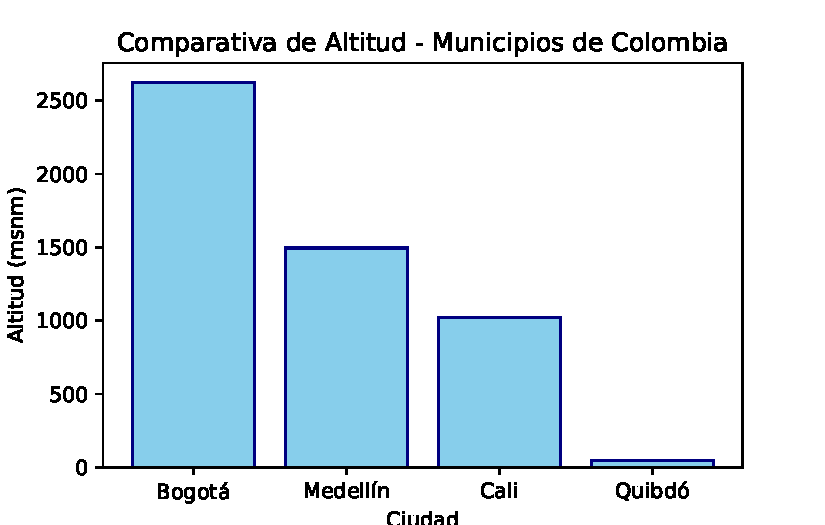
\includegraphics{12-introduccion_python_r_julia_files/figure-pdf/graficos_python-1.pdf}

\begin{Shaded}
\begin{Highlighting}[]
\CommentTok{\# 2. Histograma: Distribución de una muestra de altitudes}
\CommentTok{\# Simulamos 50 estaciones climáticas en diferentes pisos térmicos}
\ImportTok{import}\NormalTok{ numpy }\ImportTok{as}\NormalTok{ np}
\NormalTok{muestra\_altitudes }\OperatorTok{=}\NormalTok{ [}\DecValTok{2625}\NormalTok{, }\DecValTok{1495}\NormalTok{, }\DecValTok{1018}\NormalTok{, }\DecValTok{43}\NormalTok{, }\DecValTok{18}\NormalTok{, }\DecValTok{2527}\NormalTok{, }\DecValTok{959}\NormalTok{, }\DecValTok{467}\NormalTok{, }\DecValTok{2150}\NormalTok{, }\DecValTok{1850}\NormalTok{] }\OperatorTok{*} \DecValTok{5}

\NormalTok{plt.hist(muestra\_altitudes, bins}\OperatorTok{=}\DecValTok{5}\NormalTok{, color}\OperatorTok{=}\StringTok{\textquotesingle{}orange\textquotesingle{}}\NormalTok{, alpha}\OperatorTok{=}\FloatTok{0.7}\NormalTok{)}
\NormalTok{plt.xlabel(}\StringTok{"Rango de Altitud (msnm)"}\NormalTok{)}
\NormalTok{plt.ylabel(}\StringTok{"Frecuencia (N° Estaciones)"}\NormalTok{)}
\NormalTok{plt.title(}\StringTok{"Distribución de Estaciones por Altitud"}\NormalTok{)}
\NormalTok{plt.show()}
\end{Highlighting}
\end{Shaded}

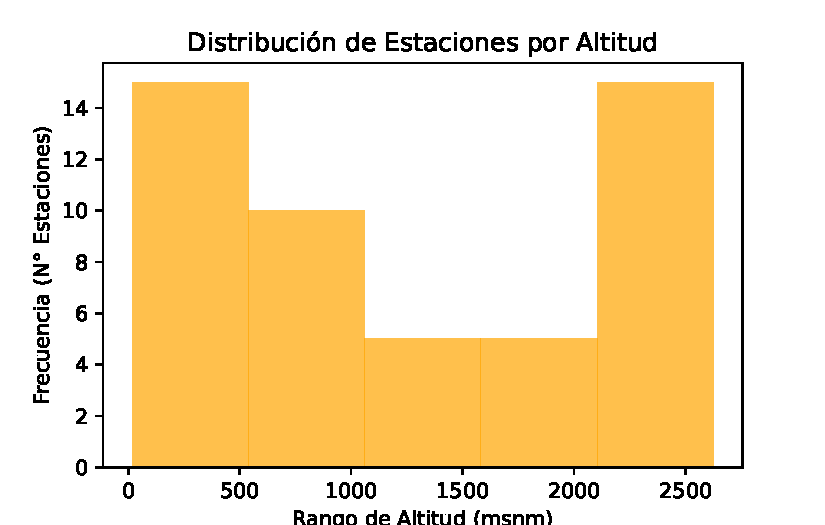
\includegraphics{12-introduccion_python_r_julia_files/figure-pdf/graficos_python-2.pdf}

\subsection{R}

\begin{Shaded}
\begin{Highlighting}[]
\CommentTok{\# \#| eval: false}
\CommentTok{\# 1. Gráfico de Barras}
\NormalTok{ciudades }\OtherTok{\textless{}{-}} \FunctionTok{c}\NormalTok{(}\StringTok{"Bogotá"}\NormalTok{, }\StringTok{"Medellín"}\NormalTok{, }\StringTok{"Cali"}\NormalTok{, }\StringTok{"Quibdó"}\NormalTok{)}
\NormalTok{altitudes }\OtherTok{\textless{}{-}} \FunctionTok{c}\NormalTok{(}\DecValTok{2625}\NormalTok{, }\DecValTok{1495}\NormalTok{, }\DecValTok{1018}\NormalTok{, }\DecValTok{43}\NormalTok{)}

\CommentTok{\# En R base, barplot es simple y potente}
\FunctionTok{barplot}\NormalTok{(altitudes, }
        \AttributeTok{names.arg =}\NormalTok{ ciudades, }
        \AttributeTok{col =} \StringTok{"skyblue"}\NormalTok{, }
        \AttributeTok{border =} \StringTok{"navy"}\NormalTok{,}
        \AttributeTok{xlab =} \StringTok{"Ciudad"}\NormalTok{, }
        \AttributeTok{ylab =} \StringTok{"Altitud (msnm)"}\NormalTok{,}
        \AttributeTok{main =} \StringTok{"Altitud de Municipios"}\NormalTok{)}
\end{Highlighting}
\end{Shaded}

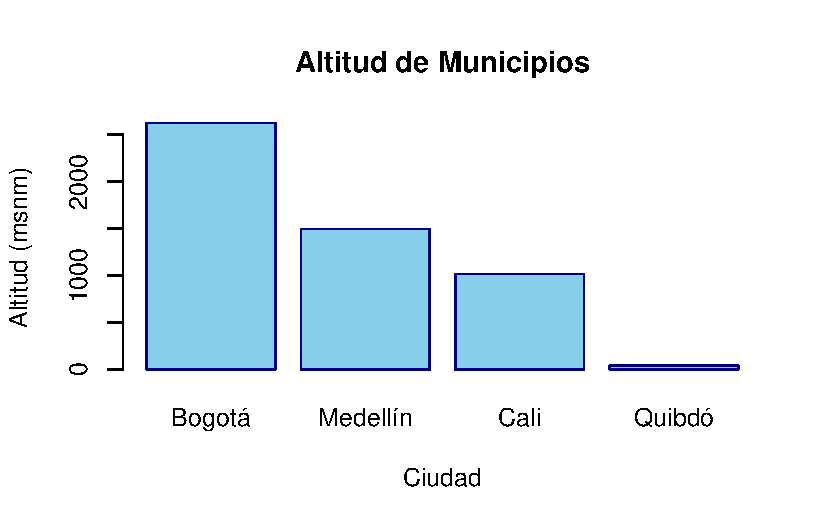
\includegraphics{12-introduccion_python_r_julia_files/figure-pdf/graficos_r-5.pdf}

\begin{Shaded}
\begin{Highlighting}[]
\CommentTok{\# 2. Histograma}
\NormalTok{muestra\_altitudes }\OtherTok{\textless{}{-}} \FunctionTok{c}\NormalTok{(}\DecValTok{2625}\NormalTok{, }\DecValTok{1495}\NormalTok{, }\DecValTok{1018}\NormalTok{, }\DecValTok{43}\NormalTok{, }\DecValTok{18}\NormalTok{, }\DecValTok{2527}\NormalTok{, }\DecValTok{959}\NormalTok{, }\DecValTok{467}\NormalTok{, }\DecValTok{2150}\NormalTok{, }\DecValTok{1850}\NormalTok{)}
\FunctionTok{hist}\NormalTok{(muestra\_altitudes, }
     \AttributeTok{breaks =} \DecValTok{5}\NormalTok{, }
     \AttributeTok{col =} \StringTok{"orange"}\NormalTok{, }
     \AttributeTok{xlab =} \StringTok{"Altitud (msnm)"}\NormalTok{, }
     \AttributeTok{main =} \StringTok{"Distribución de la Muestra"}\NormalTok{)}
\end{Highlighting}
\end{Shaded}

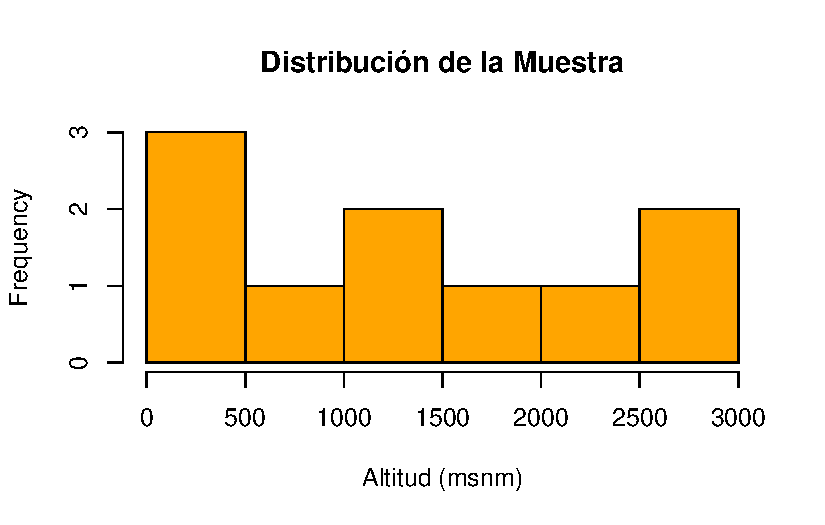
\includegraphics{12-introduccion_python_r_julia_files/figure-pdf/graficos_r-6.pdf}

\subsection{Julia}

\begin{Shaded}
\begin{Highlighting}[]
\CommentTok{\# 1. Usamos j\_eval para procesar la lógica sin que j\_plot interfiera}
\FunctionTok{j\_eval}\NormalTok{(}\StringTok{\textquotesingle{}}
\StringTok{    \# Modo silencioso para el servidor gráfico}
\StringTok{    ENV["GKSwstype"] = "100" }
\StringTok{    }
\StringTok{    using Plots}
\StringTok{    gr()}

\StringTok{    \# Datos}
\StringTok{    ciudades = ["Bogotá", "Medellín", "Cali", "Quibdó"]}
\StringTok{    altitudes = [2625, 1495, 1018, 43]}

\StringTok{    \# Creamos los objetos de gráfico explícitamente}
\StringTok{    p1 = bar(ciudades, altitudes, title="Altitud Municipios", legend=false)}
\StringTok{    muestra = [2625, 1495, 1018, 43, 18, 2527, 959, 467, 2150, 1850]}
\StringTok{    p2 = histogram(muestra, bins=5, title="Histograma Altitudes")}

\StringTok{    \# Los combinamos en un objeto final}
\StringTok{    p\_final = plot(p1, p2, layout = (1, 2), size = (800, 400))}

\StringTok{    \# Guardamos el objeto p\_final directamente. }
\StringTok{    \# Esto evita el error "No current plot" porque no dependemos del estado global.}
\StringTok{    savefig(p\_final, "temp\_grafica\_julia.png")}
\StringTok{\textquotesingle{}}\NormalTok{)}
\end{Highlighting}
\end{Shaded}

\begin{Shaded}
\begin{Highlighting}[]
\CommentTok{\# 2. R se encarga de mostrar la imagen con el formato que pediste}
\NormalTok{knitr}\SpecialCharTok{::}\FunctionTok{include\_graphics}\NormalTok{(}\StringTok{"temp\_grafica\_julia.png"}\NormalTok{)}
\end{Highlighting}
\end{Shaded}

\begin{center}
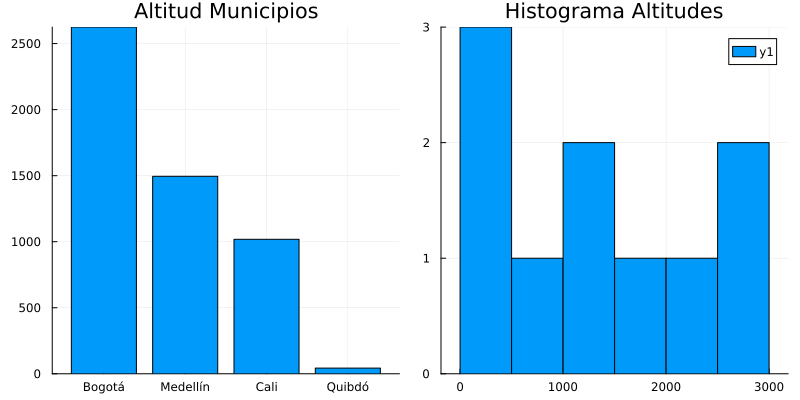
\includegraphics[width=0.85\textwidth,height=\textheight]{temp_grafica_julia.png}
\end{center}

\section{9. Transformación de datos}\label{transformaciuxf3n-de-datos}

En el análisis de datos espaciales, frecuentemente necesitamos derivar
nuevas variables a partir de las existentes, como convertir unidades de
medida (metros a pies) o categorizar valores (crear rangos climáticos).

\begin{longtable}[]{@{}
  >{\raggedright\arraybackslash}p{(\columnwidth - 8\tabcolsep) * \real{0.2000}}
  >{\raggedright\arraybackslash}p{(\columnwidth - 8\tabcolsep) * \real{0.2000}}
  >{\raggedright\arraybackslash}p{(\columnwidth - 8\tabcolsep) * \real{0.2000}}
  >{\raggedright\arraybackslash}p{(\columnwidth - 8\tabcolsep) * \real{0.2000}}
  >{\raggedright\arraybackslash}p{(\columnwidth - 8\tabcolsep) * \real{0.2000}}@{}}
\toprule\noalign{}
\begin{minipage}[b]{\linewidth}\raggedright
Tarea
\end{minipage} & \begin{minipage}[b]{\linewidth}\raggedright
Descripción
\end{minipage} & \begin{minipage}[b]{\linewidth}\raggedright
Python
\end{minipage} & \begin{minipage}[b]{\linewidth}\raggedright
R
\end{minipage} & \begin{minipage}[b]{\linewidth}\raggedright
Julia
\end{minipage} \\
\midrule\noalign{}
\endhead
\bottomrule\noalign{}
\endlastfoot
Crear columna & Nueva variable calculada &
\texttt{df{[}"nueva"{]}\ =\ ...} & \texttt{df\$nueva\ \textless{}-\ ...}
& \texttt{df.nueva\ =\ ...} \\
\end{longtable}

\subsection{Python}

\begin{Shaded}
\begin{Highlighting}[]
\CommentTok{\# \#| eval: false}
\ImportTok{import}\NormalTok{ pandas }\ImportTok{as}\NormalTok{ pd}

\CommentTok{\# Definimos un DataFrame con municipios y su altitud en metros (msnm)}
\NormalTok{df }\OperatorTok{=}\NormalTok{ pd.DataFrame(\{}
    \StringTok{"municipio"}\NormalTok{: [}\StringTok{"Bogotá"}\NormalTok{, }\StringTok{"Medellín"}\NormalTok{, }\StringTok{"Cali"}\NormalTok{],}
    \StringTok{"altitud\_m"}\NormalTok{: [}\DecValTok{2625}\NormalTok{, }\DecValTok{1495}\NormalTok{, }\DecValTok{1018}\NormalTok{]}
\NormalTok{\})}

\CommentTok{\# 1. Creación de una columna mediante una operación aritmética simple}
\CommentTok{\# Convertimos metros a pies (aprox. 3.28 pies por metro)}
\NormalTok{df[}\StringTok{"altitud\_ft"}\NormalTok{] }\OperatorTok{=}\NormalTok{ df[}\StringTok{"altitud\_m"}\NormalTok{] }\OperatorTok{*} \FloatTok{3.28}

\CommentTok{\# 2. Creación de una columna con lógica condicional (Clasificación climática)}
\CommentTok{\# Usamos una función lambda para evaluar cada fila}
\NormalTok{df[}\StringTok{"clima"}\NormalTok{] }\OperatorTok{=}\NormalTok{ df[}\StringTok{"altitud\_m"}\NormalTok{].}\BuiltInTok{apply}\NormalTok{(}\KeywordTok{lambda}\NormalTok{ x: }\StringTok{"Frío"} \ControlFlowTok{if}\NormalTok{ x }\OperatorTok{\textgreater{}} \DecValTok{2000} \ControlFlowTok{else} \StringTok{"Templado"}\NormalTok{)}

\BuiltInTok{print}\NormalTok{(df)}
\end{Highlighting}
\end{Shaded}

\begin{verbatim}
  municipio  altitud_m  altitud_ft     clima
0    Bogotá       2625     8610.00      Frío
1  Medellín       1495     4903.60  Templado
2      Cali       1018     3339.04  Templado
\end{verbatim}

\subsection{R}

\begin{Shaded}
\begin{Highlighting}[]
\CommentTok{\# \#| eval: false}
\CommentTok{\# Creamos el data frame base}
\NormalTok{df }\OtherTok{\textless{}{-}} \FunctionTok{data.frame}\NormalTok{(}
  \AttributeTok{municipio =} \FunctionTok{c}\NormalTok{(}\StringTok{"Bogotá"}\NormalTok{, }\StringTok{"Medellín"}\NormalTok{, }\StringTok{"Cali"}\NormalTok{),}
  \AttributeTok{altitud\_m =} \FunctionTok{c}\NormalTok{(}\DecValTok{2625}\NormalTok{, }\DecValTok{1495}\NormalTok{, }\DecValTok{1018}\NormalTok{)}
\NormalTok{)}

\CommentTok{\# 1. Creación de columna usando el operador de asignación $}
\CommentTok{\# La operación se aplica de forma vectorizada a toda la columna}
\NormalTok{df}\SpecialCharTok{$}\NormalTok{altitud\_ft }\OtherTok{\textless{}{-}}\NormalTok{ df}\SpecialCharTok{$}\NormalTok{altitud\_m }\SpecialCharTok{*} \FloatTok{3.28}

\CommentTok{\# 2. Creación de columna con lógica condicional usando ifelse()}
\NormalTok{df}\SpecialCharTok{$}\NormalTok{clima }\OtherTok{\textless{}{-}} \FunctionTok{ifelse}\NormalTok{(df}\SpecialCharTok{$}\NormalTok{altitud\_m }\SpecialCharTok{\textgreater{}} \DecValTok{2000}\NormalTok{, }\StringTok{"Frío"}\NormalTok{, }\StringTok{"Templado"}\NormalTok{)}

\FunctionTok{print}\NormalTok{(df)}
\end{Highlighting}
\end{Shaded}

\begin{verbatim}
  municipio altitud_m altitud_ft    clima
1    Bogotá      2625    8610.00     Frío
2  Medellín      1495    4903.60 Templado
3      Cali      1018    3339.04 Templado
\end{verbatim}

\subsection{Julia}

\begin{Shaded}
\begin{Highlighting}[]
\CommentTok{\# \#| eval: false}
\FunctionTok{j\_eval}\NormalTok{(}\StringTok{\textquotesingle{}}
\StringTok{using DataFrames}

\StringTok{\# Recreamos el DataFrame en el entorno de Julia}
\StringTok{df = DataFrame(}
\StringTok{    municipio = ["Bogotá", "Medellín", "Cali"],}
\StringTok{    altitud\_m = [2625, 1495, 1018]}
\StringTok{)}

\StringTok{\# Aplicamos las transformaciones}
\StringTok{df.altitud\_ft = df.altitud\_m .* 3.28}
\StringTok{df.clima = [x \textgreater{} 2000 ? "Frío" : "Templado" for x in df.altitud\_m]}

\StringTok{\# Mostramos el resultado final}
\StringTok{println(df)}
\StringTok{\textquotesingle{}}\NormalTok{)}
\end{Highlighting}
\end{Shaded}

\section{10. Resumen comparativo (cheat
sheet)}\label{resumen-comparativo-cheat-sheet}

Esta tabla sirve como guía de referencia rápida para transitar entre los
tres lenguajes durante el desarrollo de proyectos de análisis espacial.

\begin{longtable}[]{@{}
  >{\raggedright\arraybackslash}p{(\columnwidth - 8\tabcolsep) * \real{0.2000}}
  >{\raggedright\arraybackslash}p{(\columnwidth - 8\tabcolsep) * \real{0.2000}}
  >{\raggedright\arraybackslash}p{(\columnwidth - 8\tabcolsep) * \real{0.2000}}
  >{\raggedright\arraybackslash}p{(\columnwidth - 8\tabcolsep) * \real{0.2000}}
  >{\raggedright\arraybackslash}p{(\columnwidth - 8\tabcolsep) * \real{0.2000}}@{}}
\toprule\noalign{}
\begin{minipage}[b]{\linewidth}\raggedright
Categoría
\end{minipage} & \begin{minipage}[b]{\linewidth}\raggedright
Tarea
\end{minipage} & \begin{minipage}[b]{\linewidth}\raggedright
Python
\end{minipage} & \begin{minipage}[b]{\linewidth}\raggedright
R
\end{minipage} & \begin{minipage}[b]{\linewidth}\raggedright
Julia
\end{minipage} \\
\midrule\noalign{}
\endhead
\bottomrule\noalign{}
\endlastfoot
\textbf{Ecosistema} & Ayuda de función & \texttt{help(f)} & \texttt{?f}
& \texttt{?f} \\
& Instalar paquete & \texttt{pip3\ install\ x} &
\texttt{install.packages("x")} & \texttt{Pkg.add("x")} \\
\textbf{Estructuras} & Vector / Lista & \texttt{{[}1,\ 2,\ 3{]}} &
\texttt{c(1,\ 2,\ 3)} & \texttt{{[}1,\ 2,\ 3{]}} \\
& Diccionario / Mapa & \texttt{\{"k":\ v\}} & \texttt{list(k\ =\ v)} &
\texttt{Dict(k\ =\textgreater{}\ v)} \\
& Data Frame & \texttt{pd.DataFrame(d)} & \texttt{data.frame(d)} &
\texttt{DataFrame(d)} \\
\textbf{I/O} & Leer CSV & \texttt{pd.read\_csv("f.csv")} &
\texttt{read.csv("f.csv")} & \texttt{CSV.read("f.csv",\ DF)} \\
\textbf{Manipulación} & Ver estructura & \texttt{df.info()} &
\texttt{str(df)} & \texttt{describe(df)} \\
& Filtrar filas & \texttt{df{[}df.col\ \textgreater{}\ x{]}} &
\texttt{df{[}df\$col\ \textgreater{}\ x,\ {]}} &
\texttt{filter(r\ -\textgreater{}\ r.col\ \textgreater{}\ x,\ df)} \\
& Crear columna & \texttt{df{[}"n"{]}\ =\ x\ *\ 2} &
\texttt{df\$n\ \textless{}-\ x\ *\ 2} & \texttt{df.n\ =\ x\ .*\ 2} \\
\textbf{Análisis} & Media & \texttt{np.mean(x)} & \texttt{mean(x)} &
\texttt{mean(x)} \\
& Dimensiones & \texttt{df.shape} & \texttt{dim(df)} &
\texttt{size(df)} \\
\textbf{Visualización} & Barras & \texttt{plt.bar(x,\ y)} &
\texttt{barplot(y,\ names=x)} & \texttt{bar(x,\ y)} \\
\end{longtable}

\subsection{Observaciones finales}\label{observaciones-finales}

Para evitar errores comunes en el procesamiento de datos geoespaciales,
tenga siempre en cuenta estos tres pilares de la programación moderna:

\subsubsection{1. Índices de arreglos
(posicionamiento)}\label{uxedndices-de-arreglos-posicionamiento}

La forma en que los lenguajes cuentan las posiciones es la causa
principal de errores en la extracción de coordenadas o píxeles:

\begin{itemize}
\tightlist
\item
  \textbf{Python:} Utiliza indexación \textbf{base-0} (el primer
  elemento está en la posición \texttt{0}).
\item
  \textbf{R:} Utiliza indexación \textbf{base-1} (el primer elemento
  está en la posición \texttt{1}).
\item
  \textbf{Julia:} Al igual que R, utiliza indexación \textbf{base-1}.
\end{itemize}

\subsubsection{2. Vectorización y broadcasting
(eficiencia)}\label{vectorizaciuxf3n-y-broadcasting-eficiencia}

La capacidad de operar sobre columnas completas sin usar bucles manuales
(que son lentos) varía en su sintaxis y naturaleza:

\begin{itemize}
\tightlist
\item
  \textbf{Python:} La vectorización \textbf{no es nativa} de las listas
  base. Depende totalmente de librerías como \texttt{numpy} o
  \texttt{pandas}. Si intenta multiplicar una lista estándar por 2
  (\texttt{{[}1,\ 2{]}\ *\ 2}), Python duplicará los elementos de la
  lista en lugar de realizar el cálculo matemático.
\item
  \textbf{R:} La vectorización es \textbf{nativa y automática}. Casi
  todas las funciones de R están diseñadas para recibir un vector y
  devolver otro. Al hacer \texttt{vector\ *\ 2}, R entiende por defecto
  que debe multiplicarse cada elemento.
\item
  \textbf{Julia:} Utiliza el concepto de \textbf{Broadcasting}. Es el
  más explícito: requiere añadir un \textbf{punto} antes del operador
  (\texttt{.*}, \texttt{./}, \texttt{.\^{}}) o de la función. Este punto
  le indica al compilador de Julia que ``esparza'' la operación sobre
  todos los elementos del vector con una eficiencia comparable al
  lenguaje C.
\end{itemize}

\subsubsection{\texorpdfstring{3. El flujo de datos: el \textbf{pipe}
(\texttt{.}, \texttt{\%\textgreater{}\%},
\texttt{\textbar{}\textgreater{}})}{3. El flujo de datos: el pipe (., \%\textgreater\%, \textbar\textgreater)}}\label{el-flujo-de-datos-el-pipe-.}

El ``Pipe'' permite escribir código que se lee de izquierda a derecha
(como una receta), evitando el anidamiento excesivo de paréntesis.

\begin{itemize}
\tightlist
\item
  \textbf{Python (\texttt{pandas}):} Utiliza el \textbf{encadenamiento
  de métodos} mediante el punto (\texttt{.}). Cada operación devuelve un
  nuevo objeto sobre el cual se aplica la siguiente:
  \texttt{df.filter(...).sort(...)}.
\item
  \textbf{R (\texttt{dplyr} / Nativo):} El pipe clásico de
  \emph{Tidyverse} (\texttt{\%\textgreater{}\%}) o el nativo
  (\texttt{\textbar{}\textgreater{}}) pasa el objeto automáticamente
  como \textbf{primer argumento} de la siguiente función:
  \texttt{df\ \%\textgreater{}\%\ filter(...)}.
\item
  \textbf{Julia (\texttt{\textbar{}\textgreater{}} /
  \texttt{Chain.jl}):} El pipe nativo
  (\texttt{\textbar{}\textgreater{}}) es un operador de tubería simple.
  Para flujos de datos complejos y legibles, la comunidad de Julia
  prefiere la macro \texttt{@chain} del paquete \texttt{Chain.jl}.
\end{itemize}

\begin{center}\rule{0.5\linewidth}{0.5pt}\end{center}

\subsection{Librerías de referencia (caja de
herramientas)}\label{libreruxedas-de-referencia-caja-de-herramientas}

Para que su entorno de trabajo esté completo, asegúrese de tener
instaladas y cargadas estas librerías base:

\begin{enumerate}
\def\labelenumi{\arabic{enumi}.}
\tightlist
\item
  \textbf{Python:} \texttt{pandas} (tablas de atributos), \texttt{numpy}
  (álgebra de mapas), \texttt{matplotlib} (salidas gráficas).
\item
  \textbf{R:} \texttt{base} y \texttt{dplyr} (manipulación),
  \texttt{graphics} (visualización rápida).
\item
  \textbf{Julia:} \texttt{DataFrames} (tablas), \texttt{CSV} (lectura),
  \texttt{Statistics} y \texttt{Plots}.
\end{enumerate}

\begin{quote}
\textbf{Nota sobre el rendimiento:} Ninguno de los comandos vistos en
este capítulo ejecuta procesamiento en paralelo (uso de múltiples
núcleos). La vectorización y el pipe son herramientas de
\textbf{eficiencia lógica y computacional en un solo núcleo}. El
procesamiento multihilo se reservará para el análisis de grandes
volúmenes de datos en capítulos posteriores.
\end{quote}

\section{Ejercicios}\label{ejercicios-7}

Para poner en práctica los conceptos introductorios abordados en este
capítulo, deberás resolver los siguientes dos ejercicios. Puedes elegir
resolverlos en \textbf{Python, R o Julia} (o implementar la solución en
varios lenguajes si deseas retarte).

\subsection{Ejercicio 1: Hidrología del Río Magdalena (Vectores y
Matemáticas)}\label{ejercicio-1-hidrologuxeda-del-ruxedo-magdalena-vectores-y-matemuxe1ticas}

\textbf{Contexto:} Estás analizando el comportamiento de las estaciones
hidrológicas del IDEAM a lo largo del Río Magdalena. Has recibido el
reporte del caudal medio mensual (en metros cúbicos por segundo,
\(m^3/s\)) de cinco estaciones clave y necesitas extraer estadísticos
básicos y transformar las unidades para un informe ambiental.

\textbf{Instrucciones de código:}

\begin{enumerate}
\def\labelenumi{\arabic{enumi}.}
\tightlist
\item
  Define una colección ordenada (Vector/Lista/Array) llamada
  \texttt{estaciones} con los siguientes nombres:
  \texttt{"Honda",\ "Puerto\ Berrío",\ "Barrancabermeja",\ "Puerto\ Wilches",\ "Calamar"}.
\item
  Define otra colección paralela llamada \texttt{caudales\_m3s} con los
  siguientes valores numéricos:
  \texttt{1500,\ 2100,\ 2800,\ 3200,\ 4500}.
\item
  Utilizando las funciones estadísticas nativas de tu lenguaje elegido,
  calcula e imprime:

  \begin{itemize}
  \tightlist
  \item
    El \textbf{caudal máximo} registrado en el río.
  \item
    El \textbf{caudal promedio} de las cinco estaciones.
  \end{itemize}
\item
  Para un estudio local, necesitas el caudal en \textbf{litros por
  segundo (l/s)}. Utilizando el concepto de \emph{vectorización} (o
  \emph{broadcasting}), multiplica la colección \texttt{caudales\_m3s}
  por \texttt{1000} y guarda el resultado en una nueva variable llamada
  \texttt{caudales\_ls}. (Asegúrate de no usar bucles \texttt{for}).
\item
  Imprime la colección resultante \texttt{caudales\_ls}.
\end{enumerate}

\subsection{Ejercicio 2: Calidad del Aire en Bogotá (DataFrames y
Filtrado)}\label{ejercicio-2-calidad-del-aire-en-bogotuxe1-dataframes-y-filtrado}

\textbf{Contexto:} La Red de Monitoreo de Calidad del Aire de Bogotá ha
publicado los datos promedio diarios de Material Particulado 2.5
(\(PM_{2.5}\)). Debes organizar estos datos en una estructura tabular,
filtrar las estaciones que presentan riesgos para la salud (según la
OMS) y visualizar los resultados.

\textbf{Instrucciones de código:}

\begin{enumerate}
\def\labelenumi{\arabic{enumi}.}
\tightlist
\item
  Crea un \textbf{DataFrame} llamado \texttt{df\_aire} (utilizando la
  librería adecuada según tu lenguaje: \texttt{pandas},
  \texttt{data.frame} o \texttt{DataFrames.jl}) que contenga dos
  columnas:

  \begin{itemize}
  \tightlist
  \item
    \texttt{estacion}:
    \texttt{"Carvajal",\ "Kennedy",\ "Fontibón",\ "Suba",\ "Usaquén"}
  \item
    \texttt{pm25}: \texttt{55,\ 42,\ 38,\ 15,\ 12}
  \end{itemize}
\item
  Imprime un \textbf{resumen descriptivo/técnico} de tu DataFrame
  (usando la función equivalente a \texttt{info()}, \texttt{str()} o
  \texttt{describe()}).
\item
  El límite diario recomendado por la OMS para \(PM_{2.5}\) es de 15
  \(\mu g/m^3\). Crea un nuevo DataFrame llamado \texttt{df\_alerta} que
  \textbf{filtre} y contenga únicamente las estaciones donde el nivel de
  \texttt{pm25} sea \textbf{estrictamente mayor a 15}.
\item
  Crea una \textbf{nueva columna} en \texttt{df\_alerta} llamada
  \texttt{estado} y asígnale a todas sus filas el valor de texto
  \texttt{"Crítico"}.
\item
  Utiliza la librería gráfica nativa de tu entorno para generar un
  \textbf{gráfico de barras} simple usando el DataFrame original
  (\texttt{df\_aire}), donde el eje X sean las estaciones y el eje Y
  sean los niveles de \(PM_{2.5}\).
\end{enumerate}

\subsection{Entregables y Criterios de
Evaluación}\label{entregables-y-criterios-de-evaluaciuxf3n-7}

El objetivo de esta evaluación no es solo que el código funcione, sino
que seas capaz de documentar y explicar las diferencias fundamentales
entre lenguajes.

\textbf{1. Archivos de Código:} Debes desarrollar los algoritmos en al
menos uno de los siguientes formatos de archivo:

\begin{itemize}
\tightlist
\item
  Script tradicional (\texttt{.py}, \texttt{.R}, \texttt{.jl})
\item
  Notebook interactivo (\texttt{.ipynb})
\item
  Documento computacional (\texttt{.qmd} con \emph{chunks} de código)
\end{itemize}

\textbf{2. Documento Analítico (Quarto):} Independientemente del formato
de tu código fuente, \textbf{debes redactar un documento en Quarto
(\texttt{.qmd}) y renderizarlo tanto en HTML como en PDF}. En este
documento debes incluir tus bloques de código y responder
argumentativamente a las siguientes preguntas:

\begin{itemize}
\tightlist
\item
  \textbf{Sobre el Ejercicio 1 (Vectorización):} Intenta explicar qué
  sucedería si decides hacer este ejercicio en \textbf{Python} y creas
  \texttt{caudales\_m3s} como una Lista nativa
  (\texttt{{[}1500,\ 2100...{]}}) y la multiplicas directamente por 1000
  (\texttt{caudales\_m3s\ *\ 1000}). ¿Realizaría la operación matemática
  deseada? ¿Qué librería de Python soluciona este problema y cómo se
  diferencia este comportamiento del de R o Julia?
\item
  \textbf{Pregunta General (Indexación):} Escribe la línea de código
  exacta que usarías en tu lenguaje elegido para extraer \textbf{las
  tres primeras estaciones} del DataFrame del Ejercicio 2 usando
  indexación por rangos (\emph{slicing}). Explica brevemente si el
  límite superior del rango que escribiste se incluye o se excluye en el
  resultado final, justificando esto según el tipo de indexación (Base-0
  vs Base-1) de tu lenguaje.
\end{itemize}

\textbf{3. Repositorio en GitHub:} Sube tu carpeta del proyecto (que
debe contener tus scripts, el archivo \texttt{.qmd} y los renders
finales en HTML y PDF) a un repositorio público en tu cuenta personal de
\textbf{GitHub}.

\begin{itemize}
\tightlist
\item
  \textbf{Entrega:} Deberás enviar únicamente el enlace (URL) a tu
  repositorio de GitHub para la calificación.
\end{itemize}

\part{Análisis y Procesamiento Vectorial}

\chapter{Introducción a Programación
Geoespacial}\label{introducciuxf3n-a-programaciuxf3n-geoespacial}

\section{Funciones j\_eval y j\_plot en
R}\label{funciones-j_eval-y-j_plot-en-r-8}

\begin{Shaded}
\begin{Highlighting}[]
\CommentTok{\# \#| include: false}
\FunctionTok{source}\NormalTok{(}\StringTok{"./docs/j\_eval\_j\_plot.r"}\NormalTok{)}
\end{Highlighting}
\end{Shaded}

\section{Introducción}\label{introducciuxf3n-9}

La programación aplicada al análisis de datos vectoriales sustituye la
interacción manual en interfaces gráficas (GUI) por rutinas
computacionales orientadas al procesamiento de geometrías y atributos
espaciales. En la práctica de la Geomática, la manipulación de
estructuras vectoriales mediante código es indispensable para gestionar
altos volúmenes de cartografía oficial, como la producida por el
Instituto Geográfico Agustín Codazzi (IGAC) o las bases de datos
catastrales de Bogotá.

El diseño de flujos de trabajo programáticos para datos espaciales se
fundamenta en tres principios técnicos:

\begin{itemize}
\tightlist
\item
  \textbf{Reproducibilidad:} La ejecución de un script asegura un
  procesamiento determinista. Un algoritmo de validación topológica
  sobre coberturas terrestres generará los mismos resultados
  independientemente del número de ejecuciones.
\item
  \textbf{Escalabilidad:} Estructuras de control iterativas permiten
  procesar operaciones masivas de forma automatizada. El cálculo de
  áreas para miles de predios o la actualización masiva de sistemas de
  referencia geocéntricos requiere fracciones del tiempo comparado con
  flujos manuales.
\item
  \textbf{Trazabilidad analítica:} El código fuente sirve como
  documentación algorítmica estandarizada. Permite auditar cada paso
  metodológico aplicado a un conjunto de datos, desde la lectura de la
  fuente original hasta las transformaciones geométricas aplicadas (ej.
  reproyecciones al sistema MAGNA-SIRGAS Origen Nacional EPSG:9377).
\end{itemize}

El estudio del procesamiento vectorial abarca la implementación del
estándar \emph{Simple Features} para la representación de puntos, líneas
y polígonos, la referenciación lineal sobre infraestructuras de red
(como la red vial del INVIAS), y el cálculo estricto de relaciones
espaciales mediante la Matriz de Intersección Dimensionalmente Extendida
de 9 Intersecciones (DE-9IM).

Estas operaciones geométricas y de geoprocesamiento se desarrollarán
estableciendo una equivalencia técnica directa entre ecosistemas,
implementando algoritmos espaciales estructurados en Python, R y Julia.

\section{Configuración del entorno}\label{configuraciuxf3n-del-entorno}

Para nuestra maestría, utilizaremos entornos aislados. Esto evita que
una actualización de una librería de Python dañe nuestro flujo de
trabajo en R o Julia.

\subsection{Python}

\begin{Shaded}
\begin{Highlighting}[]
\CommentTok{\# OPCIÓN 1: Usando uv (Recomendado para la Maestría)}
\CommentTok{\# Instalación de uv}
\ExtensionTok{curl} \AttributeTok{{-}LsSf}\NormalTok{ https://astral.sh/uv/install.sh }\KeywordTok{|} \FunctionTok{sh}
\ExtensionTok{powershell} \AttributeTok{{-}ExecutionPolicy}\NormalTok{ ByPass }\AttributeTok{{-}c} \StringTok{"irm https://astral.sh/uv/install.ps1 | iex"}

\CommentTok{\# Crear y activar entorno virtual}
\ExtensionTok{uv}\NormalTok{ venv}
\ExtensionTok{.venv\textbackslash{}Scripts\textbackslash{}activate}

\CommentTok{\# Instalación de librerías base (Soporte MAGNA{-}SIRGAS)}
\ExtensionTok{uv}\NormalTok{ pip install }\AttributeTok{{-}{-}find{-}links}\NormalTok{ https://girder.github.io/large\_image\_wheels gdal pyproj}
\ExtensionTok{uv}\NormalTok{ pip install pygis}

\CommentTok{\# {-}{-}{-}{-}{-}{-}{-}{-}{-}{-}{-}{-}{-}{-}{-}{-}{-}{-}{-}{-}{-}{-}{-}{-}{-}{-}{-}{-}{-}{-}{-}{-}{-}{-}{-}{-}{-}{-}{-}{-}{-}{-}{-}{-}{-}{-}{-}{-}{-}{-}{-}{-}{-}{-}{-}{-}{-}}
\CommentTok{\# OPCIÓN 2: Usando pixi (Para dependencias complejas)}
\ExtensionTok{curl} \AttributeTok{{-}fsSL}\NormalTok{ https://pixi.sh/install.sh }\KeywordTok{|} \FunctionTok{bash}
\ExtensionTok{pixi}\NormalTok{ init}
\ExtensionTok{pixi}\NormalTok{ add pygis jupyterlab}
\ExtensionTok{pixi}\NormalTok{ run jupyter lab}

\CommentTok{\# {-}{-}{-}{-}{-}{-}{-}{-}{-}{-}{-}{-}{-}{-}{-}{-}{-}{-}{-}{-}{-}{-}{-}{-}{-}{-}{-}{-}{-}{-}{-}{-}{-}{-}{-}{-}{-}{-}{-}{-}{-}{-}{-}{-}{-}{-}{-}{-}{-}{-}{-}{-}{-}{-}{-}{-}{-}}
\CommentTok{\# OPCIÓN 3: Usando conda/mamba (Enfoque tradicional)}
\ExtensionTok{conda}\NormalTok{ create }\AttributeTok{{-}n}\NormalTok{ geo python=3.12}
\ExtensionTok{conda}\NormalTok{ activate geo}
\ExtensionTok{conda}\NormalTok{ install }\AttributeTok{{-}c}\NormalTok{ conda{-}forge mamba}
\ExtensionTok{mamba}\NormalTok{ install }\AttributeTok{{-}c}\NormalTok{ conda{-}forge pygis}
\end{Highlighting}
\end{Shaded}

\subsection{R}

\begin{Shaded}
\begin{Highlighting}[]
\CommentTok{\# Instalación de paquetes geoespaciales fundamentales}
\FunctionTok{install.packages}\NormalTok{(}\FunctionTok{c}\NormalTok{(}\StringTok{"sf"}\NormalTok{, }\StringTok{"terra"}\NormalTok{, }\StringTok{"leaflet"}\NormalTok{, }\StringTok{"tmap"}\NormalTok{), }\AttributeTok{dependencies =} \ConstantTok{TRUE}\NormalTok{)}

\CommentTok{\# Verificación de librerías de sistema vinculadas}
\NormalTok{sf}\SpecialCharTok{::}\FunctionTok{sf\_extSoftVersion}\NormalTok{()}
\end{Highlighting}
\end{Shaded}

\subsection{Julia}

\begin{Shaded}
\begin{Highlighting}[]
\CommentTok{\# \#| code{-}fold: true}

\FunctionTok{j\_eval}\NormalTok{(}\StringTok{\textquotesingle{}}
\StringTok{\# Configuración del entorno de paquetes en Julia}
\StringTok{using Pkg}
\StringTok{Pkg.activate(".")}

\StringTok{\# Instalación de la pila geoespacial para la maestría}
\StringTok{Pkg.add(["ArchGDAL", "GeoDataFrames", "Leaflet", "DataFrames"])}
\StringTok{\textquotesingle{}}\NormalTok{)}
\end{Highlighting}
\end{Shaded}

\section{Verificación y primeros
pasos}\label{verificaciuxf3n-y-primeros-pasos}

Antes de procesar capas vectoriales o raster, debemos asegurar que el
``motor'' está encendido y los sistemas de coordenadas están
disponibles.

\subsection{Python}

\begin{Shaded}
\begin{Highlighting}[]
\CommentTok{\# \#| eval: false}

\CommentTok{\# Importación de librerías core para el curso}
\ImportTok{import}\NormalTok{ geopandas }\ImportTok{as}\NormalTok{ gpd}
\ImportTok{import}\NormalTok{ rasterio}
\ImportTok{import}\NormalTok{ leafmap}
\ImportTok{import}\NormalTok{ pyproj}

\CommentTok{\# Verificamos soporte para el Origen Único Nacional de Colombia (EPSG:9377)}
\ControlFlowTok{try}\NormalTok{:}
\NormalTok{    crs }\OperatorTok{=}\NormalTok{ pyproj.CRS(}\StringTok{"EPSG:9377"}\NormalTok{)}
    \BuiltInTok{print}\NormalTok{(}\SpecialStringTok{f"✓ Soporte para }\SpecialCharTok{\{}\NormalTok{crs}\SpecialCharTok{.}\NormalTok{name}\SpecialCharTok{\}}\SpecialStringTok{ verificado correctamente."}\NormalTok{)}
\ControlFlowTok{except}\NormalTok{:}
    \BuiltInTok{print}\NormalTok{(}\StringTok{"X Error en la configuración de PROJ. Revisa la instalación de GDAL."}\NormalTok{)}
\end{Highlighting}
\end{Shaded}

\begin{verbatim}
✓ Soporte para MAGNA-SIRGAS 2018 / Origen-Nacional verificado correctamente.
\end{verbatim}

\subsection{R}

\begin{Shaded}
\begin{Highlighting}[]
\CommentTok{\# \#| eval: false}

\CommentTok{\# Carga de librerías principales}
\FunctionTok{library}\NormalTok{(sf)}
\end{Highlighting}
\end{Shaded}

\begin{verbatim}
Linking to GEOS 3.12.1, GDAL 3.8.4, PROJ 9.4.0; sf_use_s2() is TRUE
\end{verbatim}

\begin{Shaded}
\begin{Highlighting}[]
\FunctionTok{library}\NormalTok{(terra)}
\end{Highlighting}
\end{Shaded}

\begin{verbatim}
terra 1.8.93
\end{verbatim}

\begin{verbatim}

Attaching package: 'terra'
\end{verbatim}

\begin{verbatim}
The following object is masked from 'package:grid':

    depth
\end{verbatim}

\begin{Shaded}
\begin{Highlighting}[]
\CommentTok{\# Verificamos si R reconoce el sistema de referencia oficial de Colombia (MAGNA{-}SIRGAS)}
\NormalTok{colombia\_crs }\OtherTok{\textless{}{-}} \FunctionTok{st\_crs}\NormalTok{(}\DecValTok{9377}\NormalTok{)}
\FunctionTok{print}\NormalTok{(}\FunctionTok{paste}\NormalTok{(}\StringTok{"✓ Sistema detectado:"}\NormalTok{, colombia\_crs}\SpecialCharTok{$}\NormalTok{name))}
\end{Highlighting}
\end{Shaded}

\begin{verbatim}
[1] "✓ Sistema detectado: "
\end{verbatim}

\subsection{Julia}

\begin{Shaded}
\begin{Highlighting}[]
\CommentTok{\# \#| eval: false}

\FunctionTok{j\_eval}\NormalTok{(}\StringTok{\textquotesingle{}}
\StringTok{\# Carga de librerías de lectura y manipulación de datos espaciales}
\StringTok{using ArchGDAL}
\StringTok{using GeoDataFrames}

\StringTok{\# Verificamos la carga de drivers geoespaciales (necesario para leer Shapefiles del IGAC)}
\StringTok{println("✓ Drivers de GDAL disponibles: ", length(ArchGDAL.listdrivers()))}
\StringTok{\textquotesingle{}}\NormalTok{)}
\end{Highlighting}
\end{Shaded}

\begin{verbatim}
Starting Julia ...
Starting Julia ...
\end{verbatim}

\section{Relación entre librerías
geoespaciales}\label{relaciuxf3n-entre-libreruxedas-geoespaciales}

Para entender el funcionamiento de las librerías espaciales vectoriales,
es estrictamente necesario analizar su arquitectura de software. Como
señalan (\citeproc{ref-pebesma2025spatial}{Pebesma et~al., 2025}), los
lenguajes de programación para la ciencia de datos espaciales operan
metodológicamente como interfaces de alto nivel (\emph{wrappers}) que
delegan el procesamiento algorítmico pesado a un núcleo de librerías
estandarizadas escritas en C y C++.

Las tres librerías fundamentales que sustentan este ecosistema
geoespacial son:

\begin{itemize}
\tightlist
\item
  \textbf{GDAL/OGR (Geospatial Data Abstraction Library):} Actúa como el
  \textbf{traductor universal de lectura y escritura}. Permite la
  importación y exportación estructurada de más de 100 formatos
  \textbf{vectoriales y raster} (ej. Shapefile de ESRI, GeoPackage,
  GeoJSON).
\item
  \textbf{GEOS (Geometry Engine, Open Source):} Motor topológico
  responsable de ejecutar las \textbf{operaciones de geoprocesamiento
  paramétrico} (intersecciones espaciales, extracciones de centroides,
  áreas de influencia o \emph{buffers}) y evaluar rigurosamente las
  \textbf{relaciones matemáticas entre geometrías} mediante el modelo
  DE-9IM.
\item
  \textbf{PROJ:} Librería cartográfica dedicada exclusivamente a la
  \textbf{transformación algorítmica} de \textbf{Sistemas de Referencia
  de Coordenadas (CRS)}. Gestiona los modelos matemáticos para proyectar
  datos desde elipsoides globales (WGS84) hacia sistemas locales o
  proyectados (como el sistema MAGNA-SIRGAS Origen Nacional EPSG:9377).
\end{itemize}

La dependencia técnica compartida de esta triada garantiza la
\textbf{interoperabilidad absoluta} entre ecosistemas. Si un flujo de
trabajo exige limpiar un archivo GeoPackage catastral utilizando Python
(\texttt{geopandas}), calcular métricas de área en R (\texttt{sf}) y
ejecutar un modelo iterativo de optimización de rutas en Julia
(\texttt{ArchGDAL}), el dato espacial mantendrá su integridad geométrica
y tabular en todo momento.

Esta coherencia transversal ocurre porque la \textbf{lectura binaria} de
los vértices siempre la ejecuta \textbf{GDAL}, el cálculo del
\textbf{área} siempre lo resuelve la matemática subyacente de
\textbf{GEOS} y la \textbf{proyección espacial} siempre la maneja
\textbf{PROJ}, independientemente de la sintaxis del lenguaje que envió
la instrucción inicial.

A continuación, se visualizan las arquitecturas de dependencias y el
enrutamiento hacia las librerías base en nuestros tres lenguajes:

\subsection{Python y R (General)}

Esta gráfica detalla la relación de dependencias compartidas a nivel de
sistema operativo entre los ecosistemas de R y Python.

\begin{figure}

\centering{

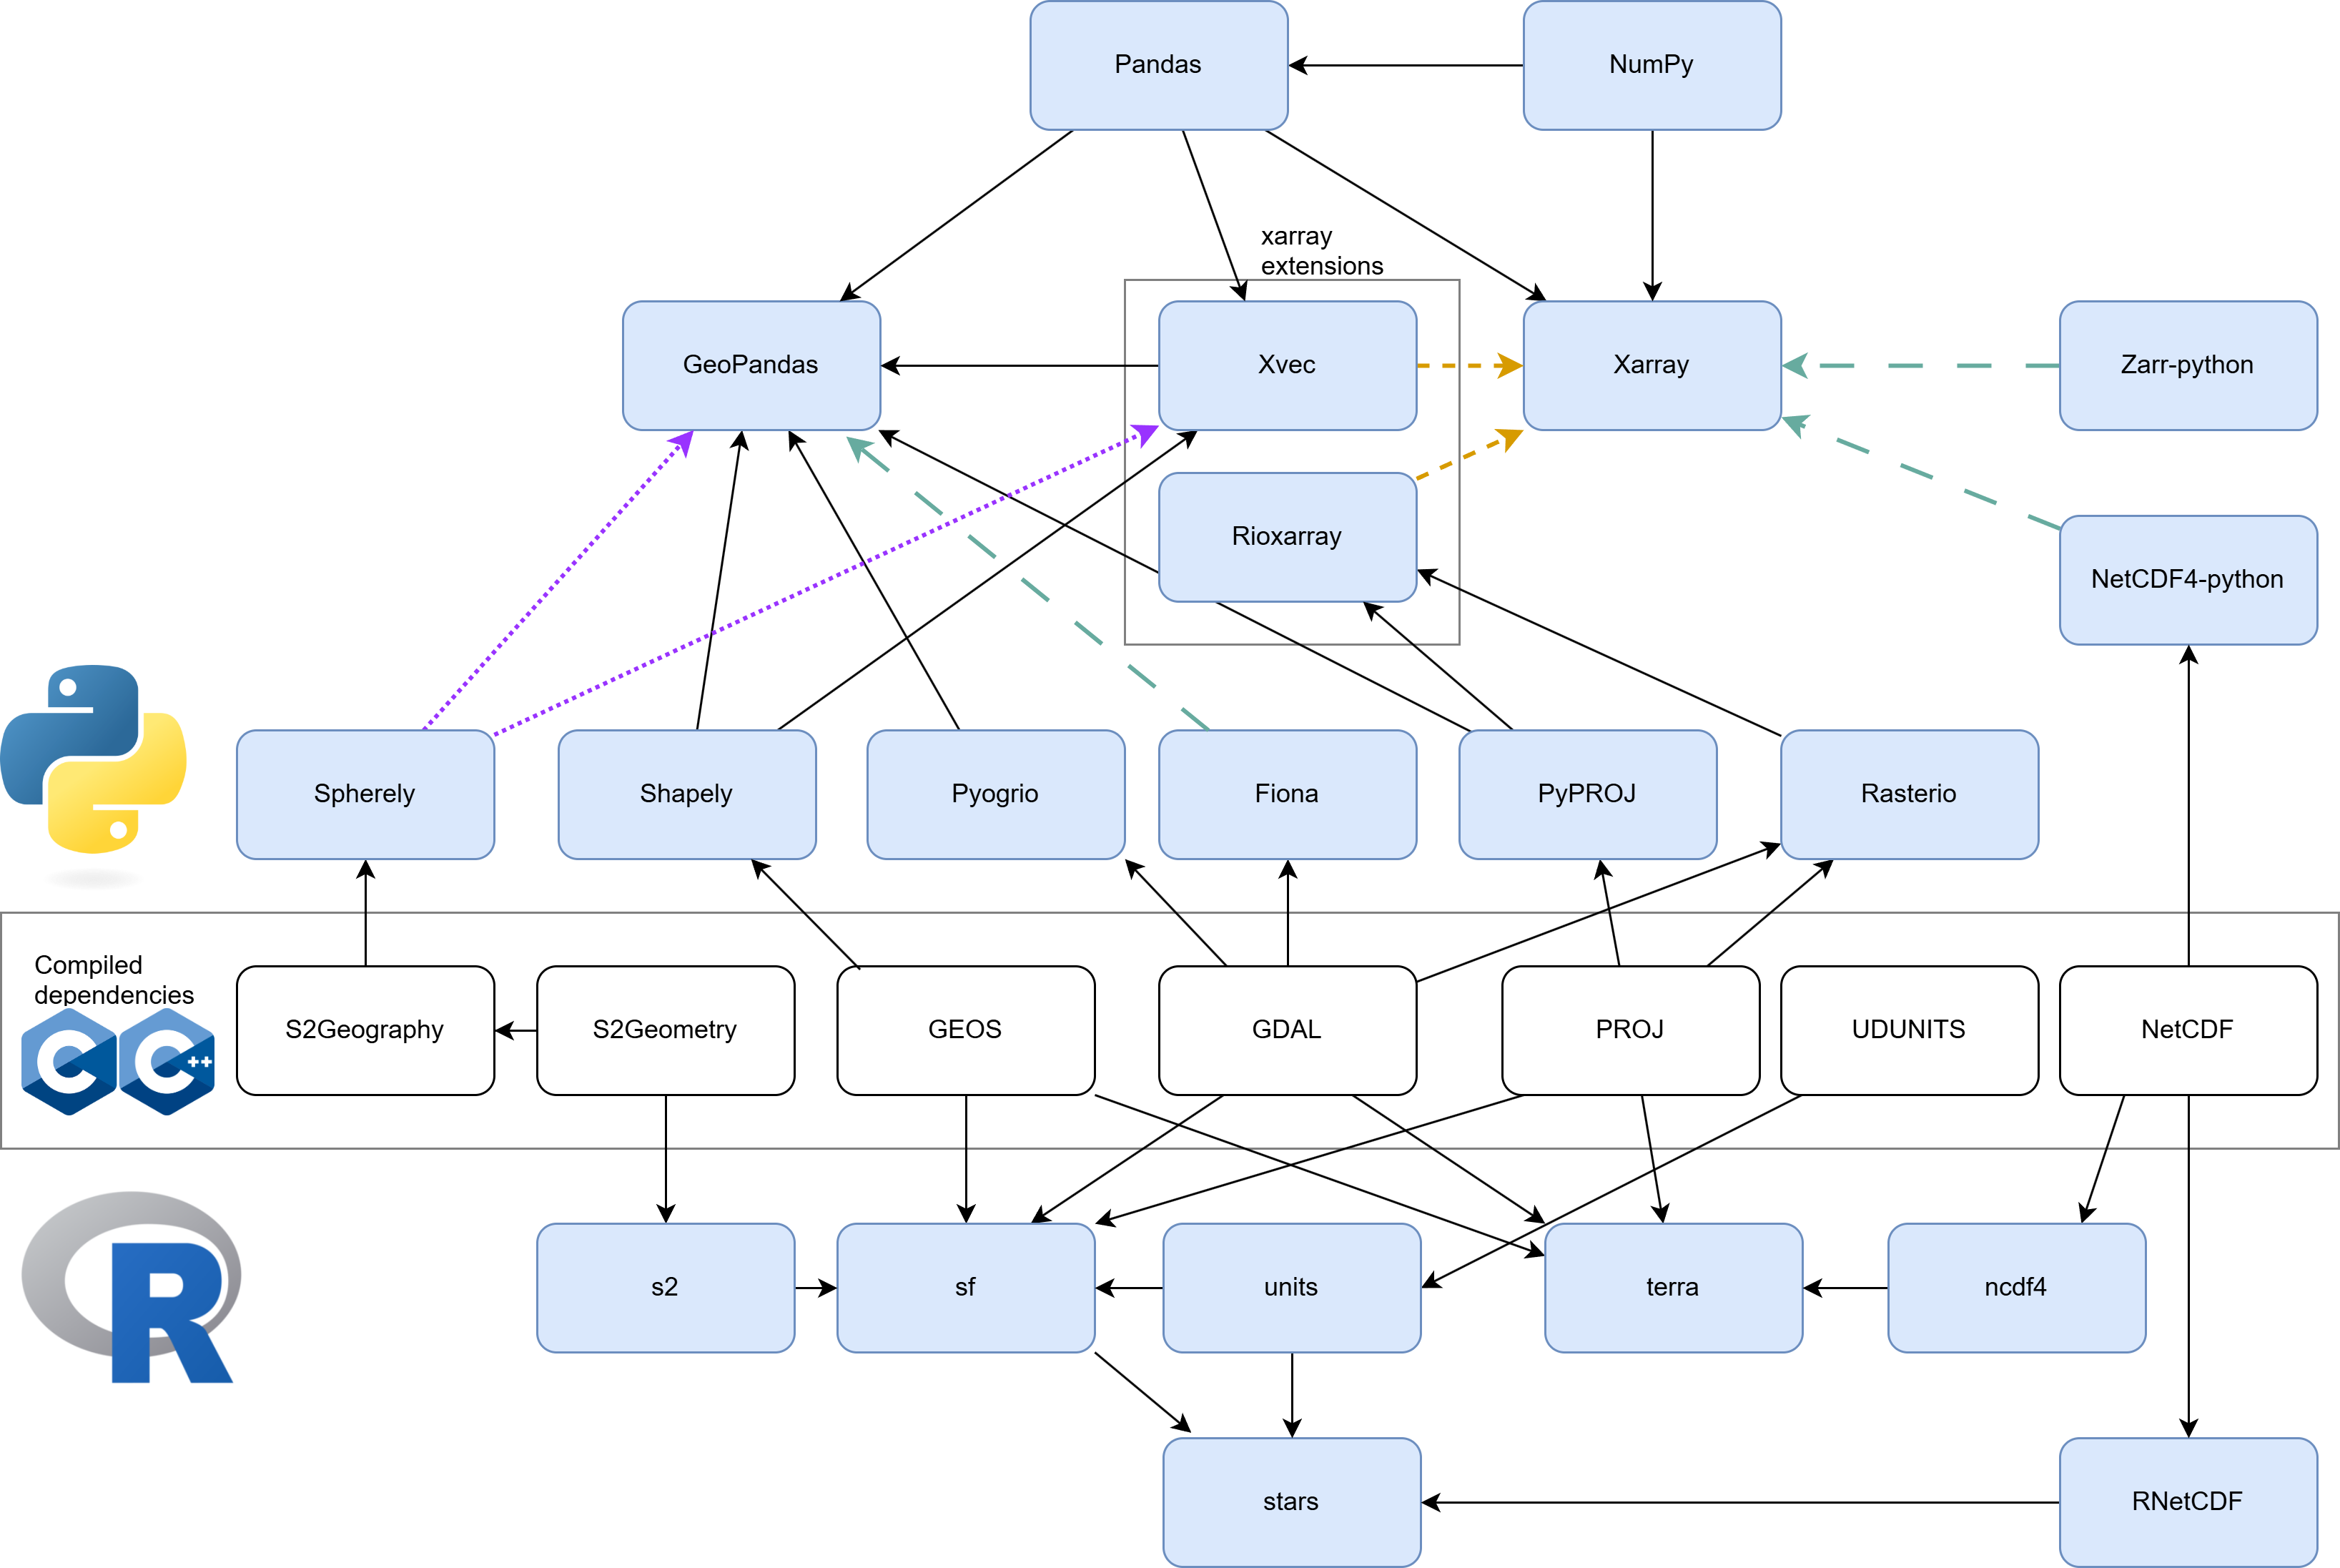
\includegraphics{images/dependencias/geopythonR.png}

}

\caption{\label{fig-geopython}Dependencias subyacentes compartidas entre
los ecosistemas de ciencia de datos espaciales de Python y R. Fuente:
Pebesma et~al. (\citeproc{ref-pebesma2025spatial}{2025}).}

\end{figure}%

\subsection{\texorpdfstring{R (\texttt{sf})}{R (sf)}}

Árbol de dependencias específico para el paquete \texttt{sf} (Simple
Features) en R, el motor fundamental de la geomática moderna en este
entorno analítico.

\begin{figure}

\centering{

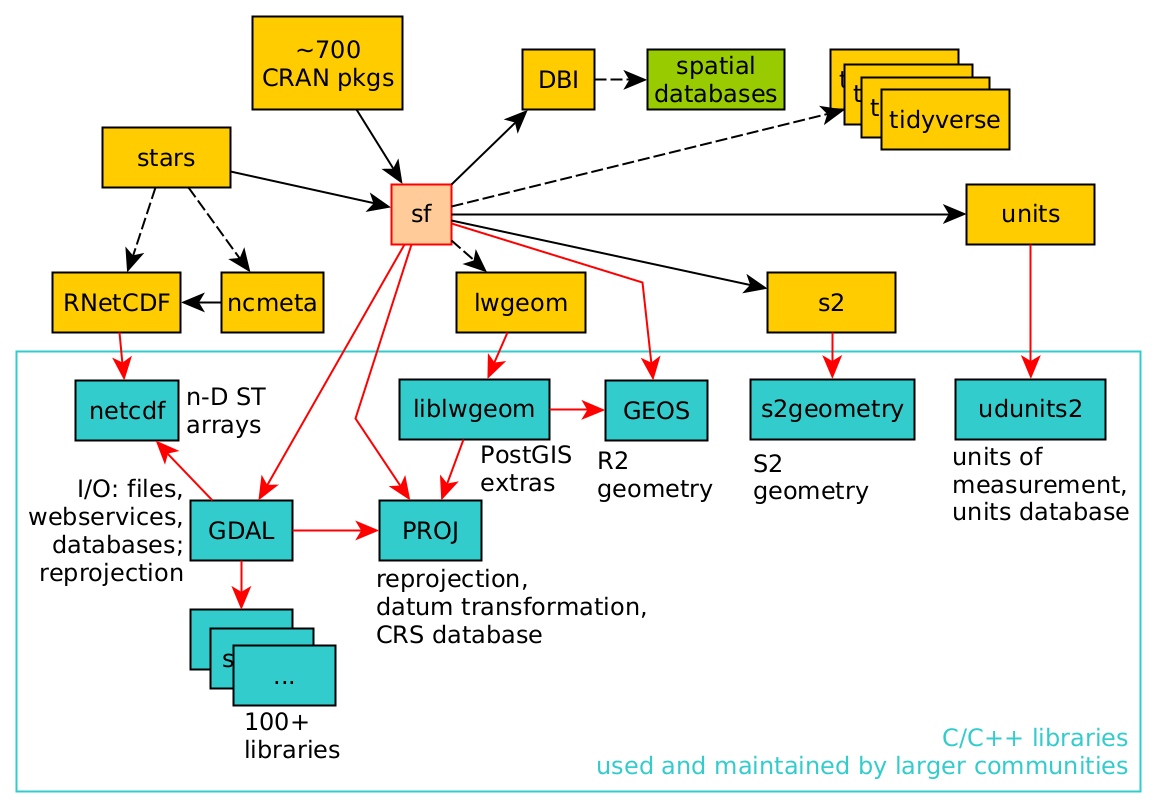
\includegraphics{images/dependencias/sf_deps.png}

}

\caption{\label{fig-sfdeps}Árbol de dependencias detallado para el
paquete Simple Features (sf) en R. Fuente: Pebesma et~al.
(\citeproc{ref-pebesma2025spatial}{2025}).}

\end{figure}%

\subsection{Julia}

Estructura de la pila de dependencias dentro del ecosistema de Julia
(GeoStack), destacando las envolturas directas (GDAL.jl, GEOS.jl,
Proj.jl) hacia las API en lenguaje C.

\begin{figure}

\centering{

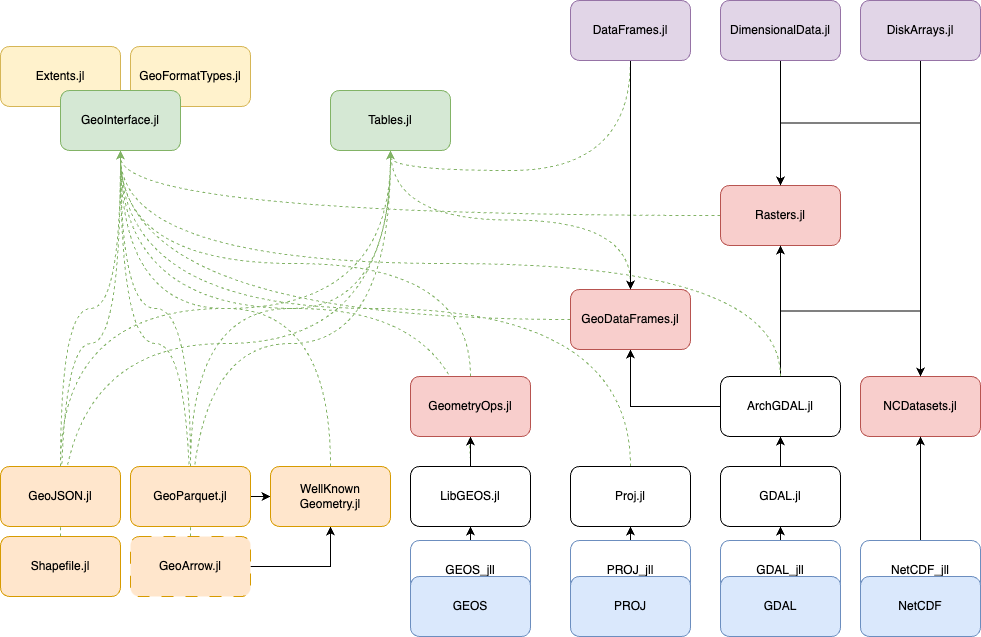
\includegraphics{images/dependencias/geostack.drawio.png}

}

\caption{\label{fig-geostack}Estructura de la pila de dependencias
geoespaciales (GeoStack) en el ecosistema de Julia. Fuente: Pebesma
et~al. (\citeproc{ref-pebesma2025spatial}{2025}).}

\end{figure}%

\section{Mapa interactivo en
Colombia}\label{mapa-interactivo-en-colombia}

Finalizaremos visualizando nuestra ubicación central: la
\textbf{Universidad Nacional de Colombia, Sede Bogotá}.

\subsection{Python}

\begin{Shaded}
\begin{Highlighting}[]
\CommentTok{\# \#| eval: false}

\ImportTok{import}\NormalTok{ leafmap}

\CommentTok{\# Definimos las coordenadas de la Plaza Central de la UNAL Bogotá}
\NormalTok{lat, lon }\OperatorTok{=} \FloatTok{4.6381}\NormalTok{, }\OperatorTok{{-}}\FloatTok{74.0841}

\CommentTok{\# Inicializamos el mapa interactivo centrado en la universidad}
\NormalTok{m }\OperatorTok{=}\NormalTok{ leafmap.Map(center}\OperatorTok{=}\NormalTok{[lat, lon], zoom}\OperatorTok{=}\DecValTok{15}\NormalTok{, height}\OperatorTok{=}\StringTok{"500px"}\NormalTok{)}

\CommentTok{\# Añadimos un mapa base topográfico libre}
\NormalTok{m.add\_basemap(}\StringTok{"OpenTopoMap"}\NormalTok{)}

\CommentTok{\# Colocamos un marcador en nuestra ubicación}
\NormalTok{m.add\_marker(location}\OperatorTok{=}\NormalTok{[lat, lon], text}\OperatorTok{=}\StringTok{"Sede Bogotá {-} UNAL"}\NormalTok{)}

\CommentTok{\# Mostramos el mapa}
\NormalTok{m}
\end{Highlighting}
\end{Shaded}

\subsection{R}

\begin{Shaded}
\begin{Highlighting}[]
\CommentTok{\# \#| eval: false}

\FunctionTok{library}\NormalTok{(leaflet)}

\CommentTok{\# Creamos un mapa interactivo encadenando funciones (pipes \%\textgreater{}\%)}
\NormalTok{mapa }\OtherTok{\textless{}{-}} \FunctionTok{leaflet}\NormalTok{() }\SpecialCharTok{\%\textgreater{}\%}
  \CommentTok{\# Añade el mapa base tradicional (probado y robusto en Quarto)}
  \FunctionTok{addTiles}\NormalTok{() }\SpecialCharTok{\%\textgreater{}\%} 
  \CommentTok{\# Añadimos un pin con un mensaje emergente}
  \FunctionTok{addMarkers}\NormalTok{(}\AttributeTok{lng =} \SpecialCharTok{{-}}\FloatTok{74.0841}\NormalTok{, }\AttributeTok{lat =} \FloatTok{4.6381}\NormalTok{, }\AttributeTok{popup =} \StringTok{"Universidad Nacional de Colombia"}\NormalTok{) }\SpecialCharTok{\%\textgreater{}\%}
  \CommentTok{\# Centramos la vista inicial}
  \FunctionTok{setView}\NormalTok{(}\AttributeTok{lng =} \SpecialCharTok{{-}}\FloatTok{74.0841}\NormalTok{, }\AttributeTok{lat =} \FloatTok{4.6381}\NormalTok{, }\AttributeTok{zoom =} \DecValTok{15}\NormalTok{)}

\CommentTok{\# SACA: El mapa interactivo listo}
\NormalTok{mapa}
\end{Highlighting}
\end{Shaded}

\includegraphics{13-introduccion_vector_files/figure-pdf/r_mapa-1.pdf}

\subsection{Julia}

\begin{Shaded}
\begin{Highlighting}[]
\CommentTok{\# \#| code{-}fold: true}

\CommentTok{\# NOTA TÉCNICA: }
\CommentTok{\# La visualización interactiva nativa en Julia a través de Quarto}
\CommentTok{\# está en desarrollo activo. Si el paquete Leaflet no está instalado en el }
\CommentTok{\# entorno o presenta conflictos de renderizado con j\_eval, }
\CommentTok{\# se recomienda ejecutar este bloque localmente en su REPL.}

\CommentTok{\#}
\CommentTok{\# Usamos j\_eval para que el motor knitr comunique con Julia}
\FunctionTok{j\_eval}\NormalTok{(}\StringTok{\textquotesingle{}}
\StringTok{using Leaflet}

\StringTok{\# Generación del mapa interactivo usando Leaflet.jl}
\StringTok{mapa = Leaflet.Map(}
\StringTok{    \# URL directa del mapa base OpenTopoMap}
\StringTok{    layers=[Leaflet.Layer("https://\{s\}.tile.opentopomap.org/\{z\}/\{x\}/\{y\}.png")], }
\StringTok{    \# Coordenadas de la Sede Bogotá}
\StringTok{    center=[4.6381, {-}74.0841], }
\StringTok{    zoom=15}
\StringTok{)}

\StringTok{\# Renderizar el mapa}
\StringTok{mapa}
\StringTok{\textquotesingle{}}\NormalTok{)}
\end{Highlighting}
\end{Shaded}

\section{Resumen de aprendizajes (cheat
sheet)}\label{resumen-de-aprendizajes-cheat-sheet-7}

Este primer capítulo establece los requerimientos técnicos y de entorno
necesarios para el procesamiento de datos espaciales.

Conceptos clave abordados:

\begin{itemize}
\tightlist
\item
  \textbf{Dependencias base (GDAL/PROJ/GEOS):} Python, R y Julia actúan
  como interfaces de alto nivel que ejecutan rutinas sobre estas
  librerías subyacentes de C/C++ para la lectura de formatos y cálculo
  de proyecciones.
\item
  \textbf{Aislamiento de proyectos:} El uso de entornos virtuales es un
  estándar en la programación científica. Evita la instalación global de
  paquetes para prevenir conflictos de versiones entre diferentes
  análisis.
\item
  \textbf{Sistemas de referencia:} La verificación y configuración de
  PROJ es un requisito fundamental para garantizar el soporte del Origen
  Único Nacional (MAGNA-SIRGAS EPSG:9377) y evitar errores métricos al
  trabajar con datos de Colombia.
\item
  \textbf{Visualización interactiva:} Las librerías de alto nivel
  permiten la instanciación de mapas web de forma declarativa para la
  exploración rápida del área de estudio.
\end{itemize}

Hoja de referencia sintáctica para la configuración del entorno y
visualización básica entre Python, R y Julia:

\subsection{Gestión de entornos e
instalación}\label{gestiuxf3n-de-entornos-e-instalaciuxf3n}

\begin{longtable}[]{@{}
  >{\raggedright\arraybackslash}p{(\columnwidth - 6\tabcolsep) * \real{0.2500}}
  >{\raggedright\arraybackslash}p{(\columnwidth - 6\tabcolsep) * \real{0.2500}}
  >{\raggedright\arraybackslash}p{(\columnwidth - 6\tabcolsep) * \real{0.2500}}
  >{\raggedright\arraybackslash}p{(\columnwidth - 6\tabcolsep) * \real{0.2500}}@{}}
\caption{Sintaxis para la preparación del entorno de trabajo
SIG}\label{tbl-resumen_entornos}\tabularnewline
\toprule\noalign{}
\begin{minipage}[b]{\linewidth}\raggedright
Tarea
\end{minipage} & \begin{minipage}[b]{\linewidth}\raggedright
Python (\texttt{uv} / \texttt{pip}) 🐍
\end{minipage} & \begin{minipage}[b]{\linewidth}\raggedright
R (CRAN) 🔵
\end{minipage} & \begin{minipage}[b]{\linewidth}\raggedright
Julia (\texttt{Pkg}) 🟣
\end{minipage} \\
\midrule\noalign{}
\endfirsthead
\toprule\noalign{}
\begin{minipage}[b]{\linewidth}\raggedright
Tarea
\end{minipage} & \begin{minipage}[b]{\linewidth}\raggedright
Python (\texttt{uv} / \texttt{pip}) 🐍
\end{minipage} & \begin{minipage}[b]{\linewidth}\raggedright
R (CRAN) 🔵
\end{minipage} & \begin{minipage}[b]{\linewidth}\raggedright
Julia (\texttt{Pkg}) 🟣
\end{minipage} \\
\midrule\noalign{}
\endhead
\bottomrule\noalign{}
\endlastfoot
\textbf{Crear entorno} & \texttt{uv\ venv} & \texttt{renv::init()}
\emph{(Opcional)} & \texttt{Pkg.activate(".")} \\
\textbf{Activar entorno} & \texttt{source\ .venv/bin/activate} &
Automático al abrir proyecto &
\texttt{using\ Pkg;\ Pkg.activate(".")} \\
\textbf{Instalar vectores} & \texttt{uv\ pip\ install\ geopandas} &
\texttt{install.packages("sf")} & \texttt{Pkg.add("GeoDataFrames")} \\
\textbf{Instalar rasters} & \texttt{uv\ pip\ install\ rasterio} &
\texttt{install.packages("terra")} & \texttt{Pkg.add("ArchGDAL")} \\
\textbf{Instalar visualización} & \texttt{uv\ pip\ install\ leafmap} &
\texttt{install.packages("leaflet")} & \texttt{Pkg.add("Leaflet")} \\
\end{longtable}

\subsection{Verificación del motor
geoespacial}\label{verificaciuxf3n-del-motor-geoespacial}

\begin{longtable}[]{@{}
  >{\raggedright\arraybackslash}p{(\columnwidth - 6\tabcolsep) * \real{0.2500}}
  >{\raggedright\arraybackslash}p{(\columnwidth - 6\tabcolsep) * \real{0.2500}}
  >{\raggedright\arraybackslash}p{(\columnwidth - 6\tabcolsep) * \real{0.2500}}
  >{\raggedright\arraybackslash}p{(\columnwidth - 6\tabcolsep) * \real{0.2500}}@{}}
\caption{Sintaxis para verificar el estado de las librerías base de
C/C++}\label{tbl-resumen_verificacion}\tabularnewline
\toprule\noalign{}
\begin{minipage}[b]{\linewidth}\raggedright
Tarea
\end{minipage} & \begin{minipage}[b]{\linewidth}\raggedright
Python (Geopandas/Pyproj) 🐍
\end{minipage} & \begin{minipage}[b]{\linewidth}\raggedright
R (\texttt{sf}) 🔵
\end{minipage} & \begin{minipage}[b]{\linewidth}\raggedright
Julia (ArchGDAL) 🟣
\end{minipage} \\
\midrule\noalign{}
\endfirsthead
\toprule\noalign{}
\begin{minipage}[b]{\linewidth}\raggedright
Tarea
\end{minipage} & \begin{minipage}[b]{\linewidth}\raggedright
Python (Geopandas/Pyproj) 🐍
\end{minipage} & \begin{minipage}[b]{\linewidth}\raggedright
R (\texttt{sf}) 🔵
\end{minipage} & \begin{minipage}[b]{\linewidth}\raggedright
Julia (ArchGDAL) 🟣
\end{minipage} \\
\midrule\noalign{}
\endhead
\bottomrule\noalign{}
\endlastfoot
\textbf{Importar librerías} & \texttt{import\ geopandas\ as\ gpd} &
\texttt{library(sf)} & \texttt{using\ ArchGDAL} \\
\textbf{Verificar GDAL/PROJ} & Automático al importar &
\texttt{sf::sf\_extSoftVersion()} &
\texttt{length(ArchGDAL.listdrivers())} \\
\textbf{Comprobar EPSG} & \texttt{pyproj.CRS("EPSG:9377")} &
\texttt{st\_crs(9377)} & \emph{(Lo veremos en cap. vectores)} \\
\end{longtable}

\subsection{Mapas web interactivos
básicos}\label{mapas-web-interactivos-buxe1sicos}

\begin{longtable}[]{@{}
  >{\raggedright\arraybackslash}p{(\columnwidth - 6\tabcolsep) * \real{0.2500}}
  >{\raggedright\arraybackslash}p{(\columnwidth - 6\tabcolsep) * \real{0.2500}}
  >{\raggedright\arraybackslash}p{(\columnwidth - 6\tabcolsep) * \real{0.2500}}
  >{\raggedright\arraybackslash}p{(\columnwidth - 6\tabcolsep) * \real{0.2500}}@{}}
\caption{Sintaxis para la creación de mapas interactivos con tecnología
Leaflet}\label{tbl-resumen_mapas}\tabularnewline
\toprule\noalign{}
\begin{minipage}[b]{\linewidth}\raggedright
Tarea
\end{minipage} & \begin{minipage}[b]{\linewidth}\raggedright
Python (\texttt{leafmap}) 🐍
\end{minipage} & \begin{minipage}[b]{\linewidth}\raggedright
R (\texttt{leaflet}) 🔵
\end{minipage} & \begin{minipage}[b]{\linewidth}\raggedright
Julia (\texttt{Leaflet.jl}) 🟣
\end{minipage} \\
\midrule\noalign{}
\endfirsthead
\toprule\noalign{}
\begin{minipage}[b]{\linewidth}\raggedright
Tarea
\end{minipage} & \begin{minipage}[b]{\linewidth}\raggedright
Python (\texttt{leafmap}) 🐍
\end{minipage} & \begin{minipage}[b]{\linewidth}\raggedright
R (\texttt{leaflet}) 🔵
\end{minipage} & \begin{minipage}[b]{\linewidth}\raggedright
Julia (\texttt{Leaflet.jl}) 🟣
\end{minipage} \\
\midrule\noalign{}
\endhead
\bottomrule\noalign{}
\endlastfoot
\textbf{Importar módulo} & \texttt{import\ leafmap} &
\texttt{library(leaflet)} & \texttt{using\ Leaflet} \\
\textbf{Inicializar mapa} &
\texttt{m\ =\ leafmap.Map(center={[}lat,\ lon{]},\ zoom=15)} &
\texttt{leaflet(height=500)\ \%\textgreater{}\%\ setView(lon,\ lat,\ 15)}
& \texttt{Leaflet.Map(center={[}lat,\ lon{]},\ zoom=15)} \\
\textbf{Capa base} & \texttt{m.add\_basemap("OpenTopoMap")} &
\texttt{addProviderTiles(providers\$OpenTopoMap)} &
\texttt{layers={[}Leaflet.Layer("url\_aqui"){]}} \\
\textbf{Añadir marcador} &
\texttt{m.add\_marker({[}lat,\ lon{]},\ text="Sede")} &
\texttt{addMarkers(lng=lon,\ lat=lat,\ popup="Sede")} & \emph{(Mediante
inserción de Features)} \\
\end{longtable}

\begin{center}\rule{0.5\linewidth}{0.5pt}\end{center}

\textbf{Siguiente paso:} Con nuestro entorno de trabajo configurado, las
dependencias base de GDAL/PROJ/GEOS verificadas y nuestro primer mapa
interactivo renderizado, estamos listos para adentrarnos en la
manipulación directa de los datos espaciales. En el siguiente capítulo,
exploraremos a fondo la estructura y creación del modelo vectorial
mediante el estándar \emph{Simple Features}.

\chapter{Trabajando con Vectores: Estándar Simple
Features}\label{trabajando-con-vectores-estuxe1ndar-simple-features}

\section{Funciones j\_eval y j\_plot en
R}\label{funciones-j_eval-y-j_plot-en-r-9}

\begin{Shaded}
\begin{Highlighting}[]
\CommentTok{\# \#| include: false}
\FunctionTok{source}\NormalTok{(}\StringTok{"./docs/j\_eval\_j\_plot.r"}\NormalTok{)}
\end{Highlighting}
\end{Shaded}

\section{Introducción}\label{introducciuxf3n-10}

En el capítulo anterior configuramos nuestro entorno de trabajo y
verificamos que los motores geoespaciales base (GDAL, GEOS y PROJ)
estuvieran operativos. Ahora es el momento de interactuar directamente
con los datos.

En este capítulo exploraremos a fondo el modelo \textbf{vectorial}, la
forma más estructurada de representar elementos discretos sobre la
superficie terrestre (como postes de luz, ríos, carreteras o límites
municipales).

Para que Python, R y Julia puedan intercambiar y entender estas
geometrías sin pérdida de información, todos obedecen a un ``idioma''
matemático universal: el estándar \textbf{Simple Features}. A lo largo
de estas secciones, desarmaremos la anatomía de este estándar,
aprenderemos a instanciar geometrías desde cero (usando primitivas,
formatos de texto WKT y binarios WKB), navegaremos por sus coordenadas
internas y descubriremos cómo ensamblarlas en \textbf{tablas espaciales}
listas para el análisis y el geoprocesamiento.

\section{\texorpdfstring{El estándar \emph{Simple
Features}}{El estándar Simple Features}}\label{el-estuxe1ndar-simple-features}

\begin{quote}
\textbf{Nota:} Esta sección introductoria está adaptada y generalizada a
partir de la
\href{https://r-spatial.github.io/sf/articles/sf1.html}{Vignette 1 del
paquete sf} de R.
\end{quote}

El término \href{https://en.wikipedia.org/wiki/Simple_Features}{Simple
Features} (o \emph{acceso a entidades simples}) hace referencia a un
estándar formal (ISO 19125-1:2004) definido por el
\href{https://www.ogc.org/standards/sfa/}{Open Geospatial Consortium
(OGC)}. Este estándar dicta cómo los \textbf{objetos del mundo real
deben ser representados digitalmente}, haciendo especial énfasis en su
\textbf{geometría espacial}. Además, establece las \textbf{reglas para
el almacenamiento en bases de datos} y define las \textbf{operaciones
matemáticas} permitidas entre estas geometrías.

Este estándar es el motor subyacente de prácticamente todo el ecosistema
geoespacial moderno. Está implementado en bases de datos espaciales como
\href{https://postgis.net/}{PostGIS}, software comercial como
\href{https://www.esri.com/en-us/home}{ESRI ArcGIS}, y es la base
\textbf{vectorial} de librerías fundamentales como
\href{https://gdal.org/}{GDAL}. Incluso, un subconjunto de estas reglas
conforma el popular estándar web \href{https://geojson.org/}{GeoJSON}.

\subsection{\texorpdfstring{¿Qué es un \emph{Feature}
(Entidad)?}{¿Qué es un Feature (Entidad)?}}\label{quuxe9-es-un-feature-entidad}

En el contexto SIG, un \emph{feature} es \textbf{cualquier cosa u objeto
en el mundo real}: un edificio, un árbol, un bosque o una ciudad
completa. Para que un objeto sea considerado un \emph{feature} bajo este
estándar, debe poseer dos componentes inseparables:

\begin{enumerate}
\def\labelenumi{\arabic{enumi}.}
\tightlist
\item
  \textbf{Una geometría:} Describe \emph{dónde} está localizado en la
  Tierra (ej. la coordenada central de un árbol o el polígono de su
  copa).
\item
  \textbf{Atributos:} Describen \emph{otras propiedades} no espaciales
  (ej. altura, especie, fecha de plantación).
\end{enumerate}

\subsection{Dimensiones Espaciales}\label{dimensiones-espaciales}

Toda geometría se compone de vértices o coordenadas en un espacio
matemático. Aunque usualmente trabajamos en 2 dimensiones (X, Y), el
estándar soporta dimensiones adicionales para modelar la realidad con
mayor precisión:

\begin{itemize}
\tightlist
\item
  \textbf{Z (Altitud):} Representa la elevación tridimensional.
\item
  \textbf{M (Medida):} Un eje opcional para asociar valores continuos al
  vértice, como el tiempo de captura o el margen de error del GPS.
\end{itemize}

Esto permite cuatro combinaciones de coordenadas: \textbf{XY} (2D
estándar), \textbf{XYZ} (3D espacial), \textbf{XYM} (2D + medida) y
\textbf{XYZM} (4D). Todas las coordenadas dentro de una misma geometría
deben tener exactamente la misma dimensionalidad.

\subsection{Tipos de Geometría}\label{tipos-de-geometruxeda}

El estándar define múltiples formas geométricas. Las \textbf{siete
básicas} son las más utilizadas universalmente (y son las únicas
soportadas por \href{https://www.rfc-editor.org/rfc/rfc7946}{GeoJSON}):

\begin{longtable}[]{@{}
  >{\raggedright\arraybackslash}p{(\columnwidth - 2\tabcolsep) * \real{0.2500}}
  >{\raggedright\arraybackslash}p{(\columnwidth - 2\tabcolsep) * \real{0.7500}}@{}}
\caption{Tipos de geometrías básicas del estándar Simple
Features.}\label{tbl-sf_basicas}\tabularnewline
\toprule\noalign{}
\begin{minipage}[b]{\linewidth}\raggedright
Tipo
\end{minipage} & \begin{minipage}[b]{\linewidth}\raggedright
Descripción
\end{minipage} \\
\midrule\noalign{}
\endfirsthead
\toprule\noalign{}
\begin{minipage}[b]{\linewidth}\raggedright
Tipo
\end{minipage} & \begin{minipage}[b]{\linewidth}\raggedright
Descripción
\end{minipage} \\
\midrule\noalign{}
\endhead
\bottomrule\noalign{}
\endlastfoot
\texttt{POINT} & Geometría de dimensión cero. Un único punto en el
espacio. \\
\texttt{LINESTRING} & Secuencia de puntos conectados por segmentos
rectos que no se intersecan a sí mismos; geometría unidimensional. \\
\texttt{POLYGON} & Geometría con área positiva (bidimensional). Una
secuencia de puntos que forma un anillo cerrado. El primer anillo define
el exterior y los anillos subsiguientes definen huecos (islas) en el
interior. \\
\texttt{MULTIPOINT} & Conjunto de múltiples puntos aislados. \\
\texttt{MULTILINESTRING} & Conjunto de múltiples líneas
(\texttt{LINESTRING}). \\
\texttt{MULTIPOLYGON} & Conjunto de múltiples polígonos. \\
\texttt{GEOMETRYCOLLECTION} & Colección heterogénea de geometrías de
cualquier tipo (ej. un punto y un polígono juntos). \\
\end{longtable}

Adicionalmente, el estándar (y extensiones como
\href{https://www.iso.org/obp/ui/\#iso:std:iso-iec:13249:-3:ed-5:v1:en}{SQL-MM})
contemplan \textbf{diez geometrías complejas}, las cuales son menos
frecuentes pero ganan popularidad en aplicaciones topográficas y de
diseño asistido:

\begin{longtable}[]{@{}
  >{\raggedright\arraybackslash}p{(\columnwidth - 2\tabcolsep) * \real{0.2500}}
  >{\raggedright\arraybackslash}p{(\columnwidth - 2\tabcolsep) * \real{0.7500}}@{}}
\caption{Tipos de geometrías avanzadas (curvas y
superficies).}\label{tbl-sf_avanzadas}\tabularnewline
\toprule\noalign{}
\begin{minipage}[b]{\linewidth}\raggedright
Tipo
\end{minipage} & \begin{minipage}[b]{\linewidth}\raggedright
Descripción
\end{minipage} \\
\midrule\noalign{}
\endfirsthead
\toprule\noalign{}
\begin{minipage}[b]{\linewidth}\raggedright
Tipo
\end{minipage} & \begin{minipage}[b]{\linewidth}\raggedright
Descripción
\end{minipage} \\
\midrule\noalign{}
\endhead
\bottomrule\noalign{}
\endlastfoot
\texttt{CIRCULARSTRING} & Curva básica. Requiere tres puntos para
definir un arco o un círculo cerrado. \\
\texttt{COMPOUNDCURVE} & Curva continua que combina segmentos curvos y
rectos. \\
\texttt{CURVEPOLYGON} & Polígono cuyos límites están definidos por
curvas en lugar de líneas rectas. \\
\texttt{MULTICURVE} & Colección unidimensional compuesta por múltiples
curvas. \\
\texttt{MULTISURFACE} & Colección bidimensional de superficies. \\
\texttt{CURVE} / \texttt{SURFACE} & Objetos geométricos abstractos uni y
bidimensionales. \\
\texttt{POLYHEDRALSURFACE} & Colección contigua de polígonos en 3D que
comparten bordes comunes. \\
\texttt{TIN} & Red Irregular Triangulada. Superficie compuesta
exclusivamente por parches triangulares. \\
\texttt{TRIANGLE} & Polígono estricto de 3 vértices no colineales sin
huecos interiores. \\
\end{longtable}

Finalmente, todas estas geometrías carecen de sentido geográfico si no
están asociadas a un \textbf{Sistema de Referencia de Coordenadas
(CRS)}, como WGS84 o UTM, el cual actúa como el ``traductor'' que ancla
estas matemáticas abstractas a una ubicación real sobre el esferoide
terrestre.

\subsubsection{Soporte a geometrías
avanzados.}\label{soporte-a-geometruxedas-avanzados.}

El estándar Simple Features define 17 tipos de geometrías. Además de los
siete más comunes (puntos, líneas, polígonos y sus colecciones
múltiples), existen geometrías diseñadas para representar curvas y
superficies matemáticas, tales como \texttt{CIRCULARSTRING},
\texttt{COMPOUNDCURVE}, \texttt{CURVEPOLYGON}, \texttt{MULTICURVE} y
\texttt{MULTISURFACE}. Estas geometrías son útiles para representar
elementos con curvatura exacta (como el diseño geométrico de un trazado
vial del IGAC) sin recurrir a la densificación por vértices.

La implementación computacional de estas geometrías varía:

\begin{itemize}
\tightlist
\item
  En R, el paquete \texttt{sf} permite su lectura e importación, pero
  muchas funciones de geoprocesamiento fuerzan su linealización previa.
\item
  En Python, \texttt{Shapely} trabaja nativamente con geometrías
  lineales, aproximando las curvas mediante interpolación de coordenadas
  espaciales.
\item
  En Julia, \texttt{ArchGDAL} soporta la lectura de curvas si la
  librería subyacente de \textbf{GDAL/GEOS está compilada con soporte
  avanzado}.
\end{itemize}

\section{Arquitectura de los objetos
espaciales}\label{arquitectura-de-los-objetos-espaciales}

Antes de crear geometrías manualmente, es fundamental comprender la
\textbf{jerarquía estructural} que los lenguajes de programación
utilizan para almacenar y vincular información espacial con atributos
tabulares. Esta arquitectura consta de tres niveles y su equivalencia
lógica varía según el entorno de desarrollo:

\begin{enumerate}
\def\labelenumi{\arabic{enumi}.}
\tightlist
\item
  \textbf{Primitiva geométrica (geometría individual):} El objeto base
  que contiene únicamente las coordenadas matemáticas de un elemento
  individual (un punto, una línea, un polígono). Representa un solo
  objeto en el espacio (\texttt{shapely.geometry} en Python,\texttt{sfg}
  en R, \texttt{ArchGDAL.IGeometry} en Julia).
\item
  \textbf{Columna espacial (columna de geometrías):} Una estructura de
  datos unidimensional (vector o serie) que agrupa múltiples primitivas
  geométricas y define el Sistema de Referencia de Coordenadas (CRS)
  unificado, como MAGNA-SIRGAS EPSG:9377 (\texttt{GeoSeries} en Python,
  \texttt{sfc} en R, \texttt{Vector\{IGeometry\}} en Julia).
\item
  \textbf{Tabla espacial (data frame espacial):} Estructura tabular
  completa que asocia la columna de geometrías espaciales con múltiples
  columnas de atributos alfanuméricos (textos, números, fechas)
  (\texttt{GeoDataFrame} en Python, \texttt{sf} en R, \texttt{DataFrame}
  geométrico en Julia).
\end{enumerate}

El siguiente esquema detalla la nomenclatura general de los objetos y,
en la segunda línea de cada celda, el tipo de dato exacto que devuelve
el sistema al evaluar una geometría de tipo punto para cada nivel:

\begin{longtable}[]{@{}
  >{\raggedright\arraybackslash}p{(\columnwidth - 6\tabcolsep) * \real{0.1600}}
  >{\raggedright\arraybackslash}p{(\columnwidth - 6\tabcolsep) * \real{0.2800}}
  >{\raggedright\arraybackslash}p{(\columnwidth - 6\tabcolsep) * \real{0.2800}}
  >{\raggedright\arraybackslash}p{(\columnwidth - 6\tabcolsep) * \real{0.2800}}@{}}
\caption{Equivalencia de las clases y tipos de datos en la arquitectura
espacial de los tres
lenguajes.}\label{tbl-arquitectura_objetos}\tabularnewline
\toprule\noalign{}
\begin{minipage}[b]{\linewidth}\raggedright
Nivel Estructural
\end{minipage} & \begin{minipage}[b]{\linewidth}\raggedright
Python (\texttt{shapely} / \texttt{geopandas}) 🐍
\end{minipage} & \begin{minipage}[b]{\linewidth}\raggedright
R (\texttt{sf}) 🔵
\end{minipage} & \begin{minipage}[b]{\linewidth}\raggedright
Julia (\texttt{ArchGDAL}) 🟣
\end{minipage} \\
\midrule\noalign{}
\endfirsthead
\toprule\noalign{}
\begin{minipage}[b]{\linewidth}\raggedright
Nivel Estructural
\end{minipage} & \begin{minipage}[b]{\linewidth}\raggedright
Python (\texttt{shapely} / \texttt{geopandas}) 🐍
\end{minipage} & \begin{minipage}[b]{\linewidth}\raggedright
R (\texttt{sf}) 🔵
\end{minipage} & \begin{minipage}[b]{\linewidth}\raggedright
Julia (\texttt{ArchGDAL}) 🟣
\end{minipage} \\
\midrule\noalign{}
\endhead
\bottomrule\noalign{}
\endlastfoot
\textbf{1. Primitiva} & \texttt{Point}, \texttt{LineString},
\texttt{Polygon}\emph{(Ej.
\texttt{shapely.geometry.}\texttt{point.Point})} & \texttt{sfg}
\emph{(Simple Feature Geometry)}\emph{(Ej.
\texttt{c("XY",\ "POINT",\ "sfg")})} &
\texttt{ArchGDAL.IGeometry}\emph{(Ej.
\texttt{ArchGDAL.IGeometry}\texttt{\{ArchGDAL.wkbPoint\}})} \\
\textbf{2. Columna} & \texttt{GeoSeries}\emph{(Ej.
\texttt{geopandas.geoseries.}\texttt{GeoSeries})} & \texttt{sfc}
\emph{(Simple Feature Column)}\emph{(Ej.
\texttt{c("sfc\_POINT",\ "sfc")})} &
\texttt{Vector\{IGeometry\}}\emph{(Ej.
\texttt{Vector\{ArchGDAL.}\texttt{IGeometry\{...\}\}})} \\
\textbf{3. Tabla} & \texttt{GeoDataFrame}\emph{(Ej.
\texttt{geopandas.}\texttt{geodataframe.GeoDataFrame})} & \texttt{sf}
\emph{(Simple Feature)}\emph{(Ej. \texttt{c("sf",\ "data.frame")})} &
\texttt{DataFrame} \emph{(con columna geom)}\emph{(Ej.
\texttt{DataFrame})} \\
\end{longtable}

\section{Creación de puntos a partir de primitivas
geométricas}\label{creaciuxf3n-de-puntos-a-partir-de-primitivas-geomuxe9tricas}

El enfoque alternativo consiste en instanciar directamente los objetos
de la clase ``Punto'' proporcionando sus coordenadas numéricas al
constructor de la librería correspondiente, para posteriormente
apilarlos en una columna espacial.

\subsection{Python}

\begin{Shaded}
\begin{Highlighting}[]
\ImportTok{import}\NormalTok{ geopandas }\ImportTok{as}\NormalTok{ gpd}
\ImportTok{from}\NormalTok{ shapely.geometry }\ImportTok{import}\NormalTok{ Point}
\ImportTok{import}\NormalTok{ matplotlib.pyplot }\ImportTok{as}\NormalTok{ plt}

\CommentTok{\# 1. Instanciación explícita de las primitivas geométricas (Point)}
\NormalTok{p1 }\OperatorTok{=}\NormalTok{ Point(}\OperatorTok{{-}}\FloatTok{72.9553}\NormalTok{, }\FloatTok{4.0903}\NormalTok{)}
\NormalTok{p2 }\OperatorTok{=}\NormalTok{ Point(}\OperatorTok{{-}}\FloatTok{74.0760}\NormalTok{, }\FloatTok{4.5981}\NormalTok{)}
\NormalTok{p3 }\OperatorTok{=}\NormalTok{ Point(}\OperatorTok{{-}}\FloatTok{75.1792}\NormalTok{, }\FloatTok{6.2205}\NormalTok{)}

\CommentTok{\# 2. Inspección de la primitiva geométrica}
\BuiltInTok{print}\NormalTok{(}\StringTok{"{-}{-}{-} Primitiva p3 {-}{-}{-}"}\NormalTok{)}
\end{Highlighting}
\end{Shaded}

\begin{verbatim}
--- Primitiva p3 ---
\end{verbatim}

\begin{Shaded}
\begin{Highlighting}[]
\BuiltInTok{print}\NormalTok{(p3)}
\end{Highlighting}
\end{Shaded}

\begin{verbatim}
POINT (-75.1792 6.2205)
\end{verbatim}

\begin{Shaded}
\begin{Highlighting}[]
\BuiltInTok{print}\NormalTok{(}\BuiltInTok{type}\NormalTok{(p3), }\StringTok{"}\CharTok{\textbackslash{}n}\StringTok{"}\NormalTok{)}
\end{Highlighting}
\end{Shaded}

\begin{verbatim}
<class 'shapely.geometry.point.Point'> 
\end{verbatim}

\begin{Shaded}
\begin{Highlighting}[]
\CommentTok{\# 3. Ensamblaje directo de atributos y lista de primitivas en un GeoDataFrame}
\NormalTok{gdf\_prim }\OperatorTok{=}\NormalTok{ gpd.GeoDataFrame(}
\NormalTok{    \{}\StringTok{"Lugar"}\NormalTok{: [}\StringTok{"Centro Geográfico"}\NormalTok{, }\StringTok{"Plaza de Bolívar"}\NormalTok{, }\StringTok{"Piedra del Peñol"}\NormalTok{]\}, }
\NormalTok{    geometry}\OperatorTok{=}\NormalTok{[p1, p2, p3], }
\NormalTok{    crs}\OperatorTok{=}\StringTok{"EPSG:4326"}
\NormalTok{)}

\CommentTok{\# 4. Inspección de la columna espacial y la tabla completa}
\CommentTok{\# En Python se accede a las columnas con el punto (.) o corchetes [\textquotesingle{}columna\textquotesingle{}]}
\BuiltInTok{print}\NormalTok{(}\StringTok{"{-}{-}{-} Columna de Geometría {-}{-}{-}"}\NormalTok{)}
\end{Highlighting}
\end{Shaded}

\begin{verbatim}
--- Columna de Geometría ---
\end{verbatim}

\begin{Shaded}
\begin{Highlighting}[]
\BuiltInTok{print}\NormalTok{(gdf\_prim.geometry)}
\end{Highlighting}
\end{Shaded}

\begin{verbatim}
0    POINT (-72.9553 4.0903)
1     POINT (-74.076 4.5981)
2    POINT (-75.1792 6.2205)
Name: geometry, dtype: geometry
\end{verbatim}

\begin{Shaded}
\begin{Highlighting}[]
\BuiltInTok{print}\NormalTok{(}\BuiltInTok{type}\NormalTok{(gdf\_prim.geometry), }\StringTok{"}\CharTok{\textbackslash{}n}\StringTok{"}\NormalTok{)}
\end{Highlighting}
\end{Shaded}

\begin{verbatim}
<class 'geopandas.geoseries.GeoSeries'> 
\end{verbatim}

\begin{Shaded}
\begin{Highlighting}[]
\BuiltInTok{print}\NormalTok{(}\StringTok{"{-}{-}{-} Estructura de la Tabla {-}{-}{-}"}\NormalTok{)}
\end{Highlighting}
\end{Shaded}

\begin{verbatim}
--- Estructura de la Tabla ---
\end{verbatim}

\begin{Shaded}
\begin{Highlighting}[]
\BuiltInTok{print}\NormalTok{(gdf\_prim)}
\end{Highlighting}
\end{Shaded}

\begin{verbatim}
               Lugar                 geometry
0  Centro Geográfico  POINT (-72.9553 4.0903)
1   Plaza de Bolívar   POINT (-74.076 4.5981)
2   Piedra del Peñol  POINT (-75.1792 6.2205)
\end{verbatim}

\begin{Shaded}
\begin{Highlighting}[]
\BuiltInTok{print}\NormalTok{(}\BuiltInTok{type}\NormalTok{(gdf\_prim), }\StringTok{"}\CharTok{\textbackslash{}n}\StringTok{"}\NormalTok{)}
\end{Highlighting}
\end{Shaded}

\begin{verbatim}
<class 'geopandas.geodataframe.GeoDataFrame'> 
\end{verbatim}

\begin{Shaded}
\begin{Highlighting}[]
\CommentTok{\# 5. Visualización}
\NormalTok{fig, ax }\OperatorTok{=}\NormalTok{ plt.subplots(figsize}\OperatorTok{=}\NormalTok{(}\DecValTok{8}\NormalTok{, }\DecValTok{6}\NormalTok{))}
\NormalTok{gdf\_prim.plot(ax}\OperatorTok{=}\NormalTok{ax, column}\OperatorTok{=}\StringTok{"Lugar"}\NormalTok{, legend}\OperatorTok{=}\VariableTok{True}\NormalTok{, markersize}\OperatorTok{=}\DecValTok{100}\NormalTok{, cmap}\OperatorTok{=}\StringTok{"Dark2"}\NormalTok{)}
\NormalTok{ax.set\_title(}\StringTok{"Lugares Representativos (Primitivas)"}\NormalTok{)}
\NormalTok{plt.show()}
\end{Highlighting}
\end{Shaded}

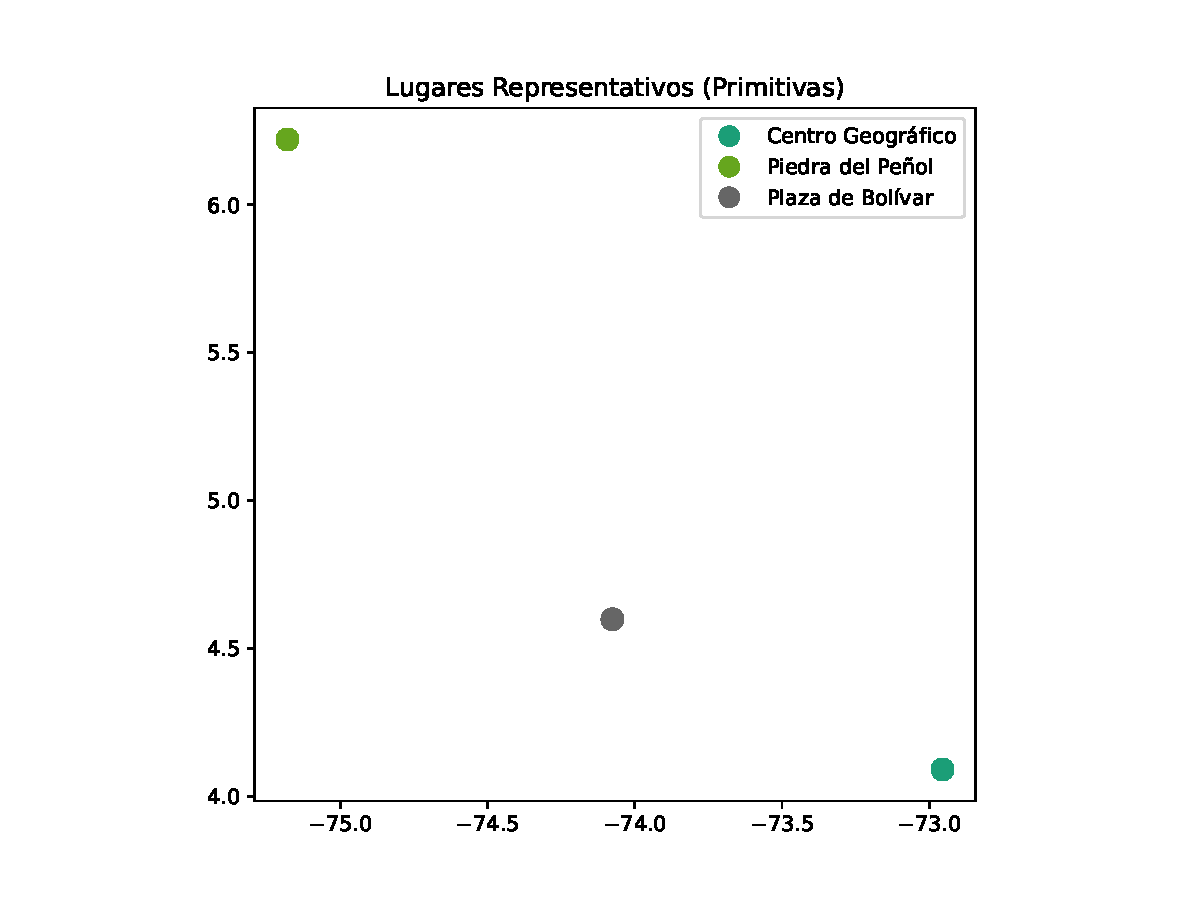
\includegraphics{14-vector_files/figure-pdf/python_crear_primitiva-1.pdf}

\subsection{R}

\begin{Shaded}
\begin{Highlighting}[]
\FunctionTok{library}\NormalTok{(sf)}
\end{Highlighting}
\end{Shaded}

\begin{verbatim}
Linking to GEOS 3.12.1, GDAL 3.8.4, PROJ 9.4.0; sf_use_s2() is TRUE
\end{verbatim}

\begin{Shaded}
\begin{Highlighting}[]
\CommentTok{\# 1. Instanciación de las primitivas individuales (sfg)}
\NormalTok{p1 }\OtherTok{\textless{}{-}} \FunctionTok{st\_point}\NormalTok{(}\FunctionTok{c}\NormalTok{(}\SpecialCharTok{{-}}\FloatTok{72.9553}\NormalTok{, }\FloatTok{4.0903}\NormalTok{))}
\NormalTok{p2 }\OtherTok{\textless{}{-}} \FunctionTok{st\_point}\NormalTok{(}\FunctionTok{c}\NormalTok{(}\SpecialCharTok{{-}}\FloatTok{74.0760}\NormalTok{, }\FloatTok{4.5981}\NormalTok{))}
\NormalTok{p3 }\OtherTok{\textless{}{-}} \FunctionTok{st\_point}\NormalTok{(}\FunctionTok{c}\NormalTok{(}\SpecialCharTok{{-}}\FloatTok{75.1792}\NormalTok{, }\FloatTok{6.2205}\NormalTok{))}

\CommentTok{\# 2. Inspección de la primitiva geométrica}
\FunctionTok{print}\NormalTok{(p3)}
\end{Highlighting}
\end{Shaded}

\begin{verbatim}
POINT (-75.1792 6.2205)
\end{verbatim}

\begin{Shaded}
\begin{Highlighting}[]
\FunctionTok{print}\NormalTok{(}\FunctionTok{class}\NormalTok{(p3))}
\end{Highlighting}
\end{Shaded}

\begin{verbatim}
[1] "XY"    "POINT" "sfg"  
\end{verbatim}

\begin{Shaded}
\begin{Highlighting}[]
\CommentTok{\# 3. Agrupación en una columna espacial (sfc)}
\NormalTok{columna\_sfc }\OtherTok{\textless{}{-}} \FunctionTok{st\_sfc}\NormalTok{(p1, p2, p3, }\AttributeTok{crs =} \DecValTok{4326}\NormalTok{)}

\CommentTok{\# 4. Ensamblaje en la tabla espacial (sf)}
\NormalTok{gdf\_prim }\OtherTok{\textless{}{-}} \FunctionTok{st\_sf}\NormalTok{(}
  \AttributeTok{Lugar =} \FunctionTok{c}\NormalTok{(}\StringTok{"Centro Geográfico"}\NormalTok{, }\StringTok{"Plaza de Bolívar"}\NormalTok{, }\StringTok{"Piedra del Peñol"}\NormalTok{), }
  \AttributeTok{geometry =}\NormalTok{ columna\_sfc}
\NormalTok{)}

\CommentTok{\# 5. Inspección de la columna espacial y la tabla completa}
\FunctionTok{print}\NormalTok{(gdf\_prim}\SpecialCharTok{$}\NormalTok{geometry)}
\end{Highlighting}
\end{Shaded}

\begin{verbatim}
Geometry set for 3 features 
Geometry type: POINT
Dimension:     XY
Bounding box:  xmin: -75.1792 ymin: 4.0903 xmax: -72.9553 ymax: 6.2205
Geodetic CRS:  WGS 84
\end{verbatim}

\begin{verbatim}
POINT (-72.9553 4.0903)
\end{verbatim}

\begin{verbatim}
POINT (-74.076 4.5981)
\end{verbatim}

\begin{verbatim}
POINT (-75.1792 6.2205)
\end{verbatim}

\begin{Shaded}
\begin{Highlighting}[]
\FunctionTok{print}\NormalTok{(}\FunctionTok{class}\NormalTok{(gdf\_prim}\SpecialCharTok{$}\NormalTok{geometry))}
\end{Highlighting}
\end{Shaded}

\begin{verbatim}
[1] "sfc_POINT" "sfc"      
\end{verbatim}

\begin{Shaded}
\begin{Highlighting}[]
\FunctionTok{print}\NormalTok{(gdf\_prim)}
\end{Highlighting}
\end{Shaded}

\begin{verbatim}
Simple feature collection with 3 features and 1 field
Geometry type: POINT
Dimension:     XY
Bounding box:  xmin: -75.1792 ymin: 4.0903 xmax: -72.9553 ymax: 6.2205
Geodetic CRS:  WGS 84
              Lugar                geometry
1 Centro Geográfico POINT (-72.9553 4.0903)
2  Plaza de Bolívar  POINT (-74.076 4.5981)
3  Piedra del Peñol POINT (-75.1792 6.2205)
\end{verbatim}

\begin{Shaded}
\begin{Highlighting}[]
\FunctionTok{print}\NormalTok{(}\FunctionTok{class}\NormalTok{(gdf\_prim))}
\end{Highlighting}
\end{Shaded}

\begin{verbatim}
[1] "sf"         "data.frame"
\end{verbatim}

\begin{Shaded}
\begin{Highlighting}[]
\CommentTok{\# 6. Visualización}
\FunctionTok{plot}\NormalTok{(}
\NormalTok{  gdf\_prim[}\StringTok{"Lugar"}\NormalTok{], }
  \AttributeTok{main =} \StringTok{"Lugares Representativos (Primitivas)"}\NormalTok{,}
  \AttributeTok{pch =} \DecValTok{17}\NormalTok{, }\AttributeTok{cex =} \DecValTok{2}\NormalTok{, }\AttributeTok{axes =} \ConstantTok{TRUE}\NormalTok{, }\AttributeTok{key.pos =} \DecValTok{4}
\NormalTok{)}
\end{Highlighting}
\end{Shaded}

\begin{center}
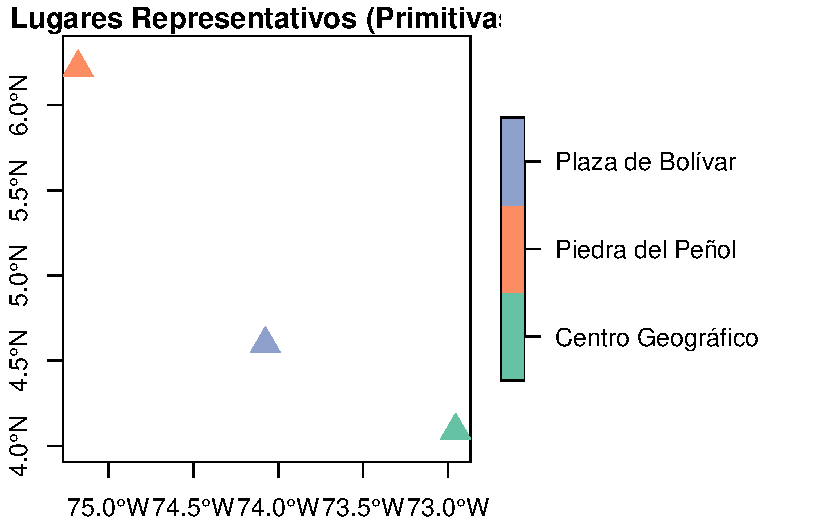
\includegraphics[width=0.75\textwidth,height=\textheight]{14-vector_files/figure-pdf/r_crear_primitiva-1.pdf}
\end{center}

\subsection{Julia}

\begin{Shaded}
\begin{Highlighting}[]
\FunctionTok{j\_eval}\NormalTok{(}\StringTok{\textquotesingle{}}
\StringTok{using ArchGDAL}
\StringTok{using DataFrames}
\StringTok{using Plots}

\StringTok{\# 1. Instanciación de las primitivas geométricas}
\StringTok{p1 = ArchGDAL.createpoint({-}72.9553, 4.0903)}
\StringTok{p2 = ArchGDAL.createpoint({-}74.0760, 4.5981)}
\StringTok{p3 = ArchGDAL.createpoint({-}75.1792, 6.2205)}

\StringTok{\# 2. Inspección de la primitiva geométrica}
\StringTok{println(p3)}
\StringTok{println(typeof(p3))}

\StringTok{\# 3. Ensamblaje en el DataFrame utilizando un arreglo de geometrías}
\StringTok{df\_prim = DataFrame(}
\StringTok{    Lugar = ["Centro Geográfico", "Plaza de Bolívar", "Piedra del Peñol"], }
\StringTok{    geometry = [p1, p2, p3]}
\StringTok{)}

\StringTok{\# 4. Inspección de la columna espacial y la tabla completa}
\StringTok{columna\_geo = df\_prim.geometry}

\StringTok{println("Tipo de la columna completa: ", typeof(columna\_geo))}
\StringTok{println("Tipo de la tabla espacial: ", typeof(df\_prim))}

\StringTok{\# 5. Visualización y exportación}
\StringTok{x\_coords = ArchGDAL.getx.(df\_prim.geometry, 0)}
\StringTok{y\_coords = ArchGDAL.gety.(df\_prim.geometry, 0)}

\StringTok{p\_prim = Plots.scatter(}
\StringTok{    x\_coords, y\_coords, }
\StringTok{    group = df\_prim.Lugar, }
\StringTok{    title = "Lugares Representativos (Primitivas)",}
\StringTok{    markershape = :utriangle, markersize = 8, aspect\_ratio = :equal,}
\StringTok{    legend = :outertopright}
\StringTok{)}

\StringTok{Plots.savefig(p\_prim, "images/c14\_plot\_primitivas\_lugares\_julia.png")}
\StringTok{\textquotesingle{}}\NormalTok{)}
\end{Highlighting}
\end{Shaded}

\begin{verbatim}
Starting Julia ...
\end{verbatim}

\begin{Shaded}
\begin{Highlighting}[]
\NormalTok{knitr}\SpecialCharTok{::}\FunctionTok{include\_graphics}\NormalTok{(}\StringTok{"images/c14\_plot\_primitivas\_lugares\_julia.png"}\NormalTok{)}
\end{Highlighting}
\end{Shaded}

\begin{center}
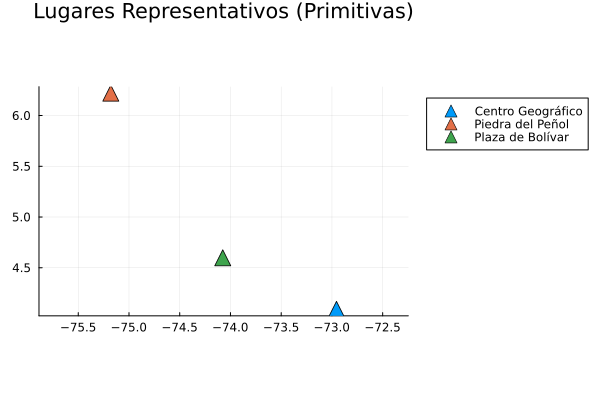
\includegraphics[width=0.75\textwidth,height=\textheight]{images/c14_plot_primitivas_lugares_julia.png}
\end{center}

\textbf{Nota técnica: Ploteo modular en Julia}

A diferencia de Python y R, Julia no posee un objeto ``GeoDataFrame''
monolítico con métodos de ploteo integrados. La diferencia radica en la
arquitectura del lenguaje:

\begin{itemize}
\tightlist
\item
  \textbf{Enfoque Monolítico (R/Python):} Los paquetes \texttt{sf} y
  \texttt{geopandas} contienen métodos que iteran automáticamente sobre
  las geometrías para extraer coordenadas al llamar a \texttt{plot()}.
\item
  \textbf{Enfoque Modular (Julia):} Existe una separación estricta de
  responsabilidades. \texttt{DataFrames.jl} gestiona tablas planas,
  \texttt{ArchGDAL.jl} procesa geometrías puras y \texttt{Plots.jl}
  funciona como un motor gráfico genérico.
\end{itemize}

Al no existir una receta gráfica pre-programada para tablas espaciales,
es obligatorio desensamblar las geometrías en sus vectores numéricos
\(X\) e \(Y\). La aproximación más cercana a una sintaxis tabular
requiere \texttt{StatsPlots.jl} y la macro \texttt{@df}:

\begin{Shaded}
\begin{Highlighting}[]
\CommentTok{\# 1. Importación de StatsPlots: Esta librería extiende \textquotesingle{}Plots.jl\textquotesingle{} y proporciona }
\CommentTok{\# la macro \textquotesingle{}@df\textquotesingle{}, permitiendo que las funciones gráficas reconozcan DataFrames.}
\ImportTok{using} \BuiltInTok{StatsPlots} 

\CommentTok{\# 2. Uso de la macro @df para graficación tabular:}
\CommentTok{\# @df actúa como un \textquotesingle{}traductor\textquotesingle{}; recibe el DataFrame (df\_wkt) y permite que }
\CommentTok{\# las columnas sean llamadas como símbolos (:nombre\_columna). Sin esto,}
\CommentTok{\# scatter() no sabría buscar \textquotesingle{}:geometry\textquotesingle{} o \textquotesingle{}:Lugar\textquotesingle{} dentro de la tabla.}
\PreprocessorTok{@df}\NormalTok{ df\_wkt }\FunctionTok{scatter}\NormalTok{(}
    \CommentTok{\# Extrae la coordenada X (Longitud) de forma vectorizada (operador punto \textquotesingle{}.\textquotesingle{})}
    \CommentTok{\# ArchGDAL.getx requiere la geometría y el índice del punto (0 para POINT).}
    \CommentTok{\# Al usar \textquotesingle{}:geometry\textquotesingle{}, @df pasa toda la columna a la operación.}
\NormalTok{    ArchGDAL.}\FunctionTok{getx}\NormalTok{.(}\OperatorTok{:}\NormalTok{geometry, }\FloatTok{0}\NormalTok{), }
    
    \CommentTok{\# Extrae la coordenada Y (Latitud) de forma vectorizada (operador punto \textquotesingle{}.\textquotesingle{})}
    \CommentTok{\# Devuelve un vector numérico que el motor gráfico puede interpretar.}
\NormalTok{    ArchGDAL.}\FunctionTok{gety}\NormalTok{.(}\OperatorTok{:}\NormalTok{geometry, }\FloatTok{0}\NormalTok{), }
    
    \CommentTok{\# Atributo \textquotesingle{}group\textquotesingle{}: Es el equivalente a \textquotesingle{}column\textquotesingle{} en GeoPandas o \textquotesingle{}sf\textquotesingle{}.}
    \CommentTok{\# Categoriza los datos por los valores únicos de la columna \textquotesingle{}:Lugar\textquotesingle{},}
    \CommentTok{\# asignando colores automáticamente y construyendo la leyenda.}
\NormalTok{    group }\OperatorTok{=} \OperatorTok{:}\NormalTok{Lugar,}
    
    \CommentTok{\# Parámetros estéticos:}
\NormalTok{    title }\OperatorTok{=} \StringTok{"Visualización Espacial Modular (StatsPlots + ArchGDAL)"}\NormalTok{,}
\NormalTok{    xlabel }\OperatorTok{=} \StringTok{"Longitud"}\NormalTok{,}
\NormalTok{    ylabel }\OperatorTok{=} \StringTok{"Latitud"}\NormalTok{,}
\NormalTok{    markersize }\OperatorTok{=} \FloatTok{7}\NormalTok{,}
    \CommentTok{\# aspect\_ratio = :equal es crítico en SIG para evitar la distorsión visual }
    \CommentTok{\# de las coordenadas geográficas en el plano.}
\NormalTok{    aspect\_ratio }\OperatorTok{=} \OperatorTok{:}\NormalTok{equal }
\NormalTok{)}
\end{Highlighting}
\end{Shaded}

\subsection{Resumen sintáctico: Creación de puntos mediante
primitivas}\label{resumen-sintuxe1ctico-creaciuxf3n-de-puntos-mediante-primitivas}

\begin{longtable}[]{@{}
  >{\raggedright\arraybackslash}p{(\columnwidth - 6\tabcolsep) * \real{0.2500}}
  >{\raggedright\arraybackslash}p{(\columnwidth - 6\tabcolsep) * \real{0.2500}}
  >{\raggedright\arraybackslash}p{(\columnwidth - 6\tabcolsep) * \real{0.2500}}
  >{\raggedright\arraybackslash}p{(\columnwidth - 6\tabcolsep) * \real{0.2500}}@{}}
\caption{Sintaxis comparativa para la instanciación de objetos de
geometría punto y su integración en estructuras
tabulares}\label{tbl-resumen_primitivas_puntos}\tabularnewline
\toprule\noalign{}
\begin{minipage}[b]{\linewidth}\raggedright
Operación
\end{minipage} & \begin{minipage}[b]{\linewidth}\raggedright
Python (\texttt{shapely}/\texttt{geopandas}) 🐍
\end{minipage} & \begin{minipage}[b]{\linewidth}\raggedright
R (\texttt{sf}) 🔵
\end{minipage} & \begin{minipage}[b]{\linewidth}\raggedright
Julia (\texttt{ArchGDAL}) 🟣
\end{minipage} \\
\midrule\noalign{}
\endfirsthead
\toprule\noalign{}
\begin{minipage}[b]{\linewidth}\raggedright
Operación
\end{minipage} & \begin{minipage}[b]{\linewidth}\raggedright
Python (\texttt{shapely}/\texttt{geopandas}) 🐍
\end{minipage} & \begin{minipage}[b]{\linewidth}\raggedright
R (\texttt{sf}) 🔵
\end{minipage} & \begin{minipage}[b]{\linewidth}\raggedright
Julia (\texttt{ArchGDAL}) 🟣
\end{minipage} \\
\midrule\noalign{}
\endhead
\bottomrule\noalign{}
\endlastfoot
\textbf{Instanciar primitiva} & \texttt{p\ =\ Point(x,\ y)} &
\texttt{p\ \textless{}-\ st\_point(c(x,\ y))} &
\texttt{p\ =\ ArchGDAL.createpoint(x,\ y)} \\
\textbf{Columna espacial} & \texttt{gpd.GeoSeries({[}p1,\ p2{]})} &
\texttt{st\_sfc(p1,\ p2)} & \texttt{{[}p1,\ p2{]}} \emph{(Vector de
IGeometry)} \\
\textbf{Tabla espacial} &
\texttt{gpd.GeoDataFrame(df,\ geometry={[}p1,\ ...{]})} &
\texttt{st\_sf(df,\ geometry\ =\ sfc)} &
\texttt{DataFrame(df,\ geometry\ =\ {[}p1,\ ...{]})} \\
\end{longtable}

\section{Más allá del Punto: Líneas, Polígonos y
Multigeometrías}\label{muxe1s-alluxe1-del-punto-luxedneas-poluxedgonos-y-multigeometruxedas}

Hasta ahora hemos trabajado con la primitiva espacial más elemental: el
punto (una geometría de cero dimensiones). Sin embargo, para representar
la geografía real necesitamos estructuras de mayor complejidad. Las
carreteras, el cauce del Río Magdalena o las fronteras departamentales
requieren geometrías de 1 y 2 dimensiones.

\begin{longtable}[]{@{}
  >{\centering\arraybackslash}p{(\columnwidth - 6\tabcolsep) * \real{0.1000}}
  >{\raggedright\arraybackslash}p{(\columnwidth - 6\tabcolsep) * \real{0.2500}}
  >{\raggedright\arraybackslash}p{(\columnwidth - 6\tabcolsep) * \real{0.3500}}
  >{\raggedright\arraybackslash}p{(\columnwidth - 6\tabcolsep) * \real{0.3000}}@{}}
\caption{Clasificación topológica de las geometrías espaciales según sus
dimensiones y propiedades de
medición.}\label{tbl-dimensiones-geometria}\tabularnewline
\toprule\noalign{}
\begin{minipage}[b]{\linewidth}\centering
Dimensión
\end{minipage} & \begin{minipage}[b]{\linewidth}\raggedright
Tipo de Geometría (OGC)
\end{minipage} & \begin{minipage}[b]{\linewidth}\raggedright
Propiedades Matemáticas
\end{minipage} & \begin{minipage}[b]{\linewidth}\raggedright
Ejemplos Cartográficos
\end{minipage} \\
\midrule\noalign{}
\endfirsthead
\toprule\noalign{}
\begin{minipage}[b]{\linewidth}\centering
Dimensión
\end{minipage} & \begin{minipage}[b]{\linewidth}\raggedright
Tipo de Geometría (OGC)
\end{minipage} & \begin{minipage}[b]{\linewidth}\raggedright
Propiedades Matemáticas
\end{minipage} & \begin{minipage}[b]{\linewidth}\raggedright
Ejemplos Cartográficos
\end{minipage} \\
\midrule\noalign{}
\endhead
\bottomrule\noalign{}
\endlastfoot
\textbf{0D} & \texttt{Point}, \texttt{MultiPoint} & Solo posee
coordenadas exactas de ubicación (X, Y). No tiene longitud ni área
calculable. & Postes de luz, pozos de extracción, epicentros de sismos,
ciudades (a escala global o nacional). \\
\textbf{1D} & \texttt{LineString}, \texttt{MultiLineString} & Posee
longitud euclidiana o geodésica, pero carece de área. Conecta dos o más
vértices en el espacio. & Red vial (carreteras), redes de acueducto,
fallas geológicas, cauces de ríos (como líneas de flujo). \\
\textbf{2D} & \texttt{Polygon}, \texttt{MultiPolygon} & Posee longitud
(perímetro) y un área bidimensional interna delimitada por anillos
topológicos cerrados. & Fronteras departamentales, lagos y ciénagas,
predios catastrales, reservas naturales. \\
\end{longtable}

Independientemente del lenguaje de programación (Python, R o Julia),
todos los ecosistemas GIS construyen estas geometrías complejas
basándose en una arquitectura estricta de ``muñecas rusas'' (anidamiento
de coordenadas):

\begin{enumerate}
\def\labelenumi{\arabic{enumi}.}
\item
  \textbf{\texttt{POINT} (Punto):} El pilar fundamental. Matemáticamente
  es un simple vector numérico o tupla \([X, Y]\). \emph{Ejemplo: La
  plaza central de Villa de Leyva.}
\item
  \textbf{\texttt{LINESTRING} (Línea):} Una secuencia de múltiples
  puntos conectados por segmentos rectos. En código, esto se representa
  como una matriz o una lista de coordenadas:
  \([[X_1, Y_1], [X_2, Y_2], ...]\). \emph{Ejemplo: Un tramo de la Ruta
  del Sol.}
\item
  \textbf{\texttt{POLYGON} (Polígono):} Una geometría bidimensional con
  área. Estructuralmente es una lista de anillos (donde un anillo es un
  \texttt{LINESTRING} cerrado \textbf{cuyo primer y último punto
  coinciden}). El primer elemento de la lista siempre es el límite
  exterior, y los elementos subsiguientes representan huecos o ``islas''
  vacías en su interior. Ejemplos:

  \begin{itemize}
  \item
    \textbf{Hueco puro (Enclave):} La Comuna El Oso en Pereira, cuyo
    polígono base contiene un anillo interior que delimita íntegramente
    a la Comuna Perla del Otún.
  \item
    \textbf{Isla (Exclave):} El departamento de Bolívar, cuya definición
    geométrica incluye polígonos disjuntos para las Islas del Rosario y
    la Isla de Tierra Bomba.
  \end{itemize}
\end{enumerate}

\subsection{El concepto de
Multigeometría}\label{el-concepto-de-multigeometruxeda}

En muchas ocasiones cartográficas, una entidad espacial única no forma
una figura geométrica continua. El mejor ejemplo en Colombia es el
departamento de \textbf{San Andrés, Providencia y Santa Catalina}.
Aunque es una sola entidad administrativa (que ocuparía una sola fila en
nuestra tabla espacial), está compuesto por múltiples masas de tierra
separadas por el mar.

Para solucionar esto, el estándar \emph{Simple Features} define las
colecciones o \textbf{Multigeometrías}:

\begin{itemize}
\tightlist
\item
  \textbf{\texttt{MULTIPOINT}:} Un conjunto de puntos independientes
  tratados como un solo registro.
\item
  \textbf{\texttt{MULTILINESTRING}:} Un conjunto de líneas separadas.
  \emph{Ejemplo: Una red fluvial donde un río principal y sus afluentes
  no están topológicamente conectados en los datos.}
\item
  \textbf{\texttt{MULTIPOLYGON}:} Una lista que agrupa múltiples
  polígonos independientes. En el código, esto implica un nivel
  adicional de profundidad matemática (una lista que contiene listas de
  anillos, que a su vez contienen listas de coordenadas).
\item
  \textbf{\texttt{GEOMETRYCOLLECTION}:} La estructura más laxa. Es un
  contenedor que puede agrupar geometrías mixtas (por ejemplo, un punto,
  una línea y un polígono) en un único objeto espacial.
\end{itemize}

Entender esta jerarquía (Punto \(\rightarrow\) Matriz \(\rightarrow\)
Lista de Matrices \(\rightarrow\) Lista de Listas) es crucial, ya que al
crear, extraer o modificar estas geometrías mediante código, la
profundidad de los corchetes o índices aumentará en función de la
complejidad estructural de la entidad.

A continuación, recreamos estas estructuras complejas simulando
geometrías abstractas para visualizar el anidamiento.

\subsection{Python}

En Python, el manejo de geometrías vectoriales se realiza nativamente
con \texttt{Shapely}, mientras que la visualización y estructuración de
datos espaciales se apoya en \texttt{GeoPandas} y \texttt{Matplotlib}.

La lógica en Shapely es directa: se construyen las geometrías a partir
de \textbf{listas de tuplas} (coordenadas XY). Los polígonos complejos
se definen pasando explícitamente un \textbf{anillo exterior}
(\texttt{shell}) y una lista de \textbf{anillos interiores}
(\texttt{holes}).

\textbf{Detalles de visualización:} Para garantizar consistencia gráfica
a través de los diferentes lenguajes, se aplican argumentos específicos
en la función \texttt{.plot()} de GeoPandas.

\begin{itemize}
\tightlist
\item
  \texttt{color=\textquotesingle{}red\textquotesingle{}}: Asigna el
  color rojo a las geometrías unidimensionales y de dimensión cero
  (líneas y puntos).
\item
  \texttt{facecolor=\textquotesingle{}lightgrey\textquotesingle{}}:
  Define el color de relleno interno para los polígonos (escala de
  grises).
\item
  \texttt{edgecolor=\textquotesingle{}red\textquotesingle{}}: Controla
  el color del trazo perimetral (borde) de los polígonos.
\item
  \texttt{linewidth=1.5}: Establece el grosor de las líneas y los
  contornos geométricos en 1.5 puntos.
\item
  \texttt{markersize=25}: Amplía el diámetro de los vértices puntuales
  para facilitar su lectura en pantalla.
\end{itemize}

\begin{Shaded}
\begin{Highlighting}[]
\CommentTok{\# Importación de clases espaciales de Shapely (estándar geométrico en Python)}
\ImportTok{from}\NormalTok{ shapely.geometry }\ImportTok{import}\NormalTok{ MultiPoint, LineString, MultiLineString}
\ImportTok{from}\NormalTok{ shapely.geometry }\ImportTok{import}\NormalTok{ Polygon, MultiPolygon, GeometryCollection}
\CommentTok{\# GeoPandas para manejo vectorial espacial y Matplotlib para el motor de renderizado}
\ImportTok{import}\NormalTok{ geopandas }\ImportTok{as}\NormalTok{ gpd}
\ImportTok{import}\NormalTok{ matplotlib.pyplot }\ImportTok{as}\NormalTok{ plt}

\CommentTok{\# {-}{-}{-} 1. MULTIPOINT {-}{-}{-}}
\CommentTok{\# Se instancian múltiples puntos discretos a partir de una lista de tuplas (coordenadas X, Y correspondientes al sistema SIRGAS o local)}
\NormalTok{p }\OperatorTok{=}\NormalTok{ [(}\FloatTok{3.2}\NormalTok{, }\DecValTok{4}\NormalTok{), (}\DecValTok{3}\NormalTok{, }\FloatTok{4.6}\NormalTok{), (}\FloatTok{3.8}\NormalTok{, }\FloatTok{4.4}\NormalTok{), (}\FloatTok{3.5}\NormalTok{, }\FloatTok{3.8}\NormalTok{), (}\FloatTok{3.4}\NormalTok{, }\FloatTok{3.6}\NormalTok{), (}\FloatTok{3.9}\NormalTok{, }\FloatTok{4.5}\NormalTok{)]}
\NormalTok{mp }\OperatorTok{=}\NormalTok{ MultiPoint(p)}

\CommentTok{\# {-}{-}{-} 2. LINESTRING {-}{-}{-}}
\CommentTok{\# Geometría unidimensional formada por una secuencia conectada y ordenada de coordenadas}
\NormalTok{s1 }\OperatorTok{=}\NormalTok{ [(}\DecValTok{0}\NormalTok{, }\DecValTok{3}\NormalTok{), (}\DecValTok{0}\NormalTok{, }\DecValTok{4}\NormalTok{), (}\DecValTok{1}\NormalTok{, }\DecValTok{5}\NormalTok{), (}\DecValTok{2}\NormalTok{, }\DecValTok{5}\NormalTok{)]}
\NormalTok{ls }\OperatorTok{=}\NormalTok{ LineString(s1)}

\CommentTok{\# {-}{-}{-} 3. MULTILINESTRING {-}{-}{-}}
\CommentTok{\# Colección de múltiples líneas que componen segmentos desconectados espacialmente}
\NormalTok{s2 }\OperatorTok{=}\NormalTok{ [(}\FloatTok{0.2}\NormalTok{, }\DecValTok{3}\NormalTok{), (}\FloatTok{0.2}\NormalTok{, }\DecValTok{4}\NormalTok{), (}\DecValTok{1}\NormalTok{, }\FloatTok{4.8}\NormalTok{), (}\DecValTok{2}\NormalTok{, }\FloatTok{4.8}\NormalTok{)]}
\NormalTok{s3 }\OperatorTok{=}\NormalTok{ [(}\DecValTok{0}\NormalTok{, }\FloatTok{4.4}\NormalTok{), (}\FloatTok{0.6}\NormalTok{, }\DecValTok{5}\NormalTok{)]}
\NormalTok{mls }\OperatorTok{=}\NormalTok{ MultiLineString([s1, s2, s3]) }\CommentTok{\# Se consolidan pasando una lista contenedora}

\CommentTok{\# {-}{-}{-} 4. POLYGON {-}{-}{-}}
\CommentTok{\# Geometría bidimensional de área. Requiere obligatoriamente un anillo exterior cerrado}
\NormalTok{p1 }\OperatorTok{=}\NormalTok{ [(}\DecValTok{0}\NormalTok{, }\DecValTok{0}\NormalTok{), (}\DecValTok{1}\NormalTok{, }\DecValTok{0}\NormalTok{), (}\DecValTok{3}\NormalTok{, }\DecValTok{2}\NormalTok{), (}\DecValTok{2}\NormalTok{, }\DecValTok{4}\NormalTok{), (}\DecValTok{1}\NormalTok{, }\DecValTok{4}\NormalTok{), (}\DecValTok{0}\NormalTok{, }\DecValTok{0}\NormalTok{)] }\CommentTok{\# Límite principal (shell)}
\NormalTok{p2 }\OperatorTok{=}\NormalTok{ [(}\DecValTok{1}\NormalTok{, }\DecValTok{1}\NormalTok{), (}\DecValTok{1}\NormalTok{, }\DecValTok{2}\NormalTok{), (}\DecValTok{2}\NormalTok{, }\DecValTok{2}\NormalTok{), (}\DecValTok{1}\NormalTok{, }\DecValTok{1}\NormalTok{)]                 }\CommentTok{\# Límite interior de vaciado topológico (hole)}
\NormalTok{pol }\OperatorTok{=}\NormalTok{ Polygon(shell}\OperatorTok{=}\NormalTok{p1, holes}\OperatorTok{=}\NormalTok{[p2])                   }\CommentTok{\# Asignación explícita durante la instanciación}

\CommentTok{\# {-}{-}{-} 5. MULTIPOLYGON {-}{-}{-}}
\CommentTok{\# Agrupación de polígonos totalmente independientes}
\NormalTok{p3 }\OperatorTok{=}\NormalTok{ [(}\DecValTok{3}\NormalTok{, }\DecValTok{0}\NormalTok{), (}\DecValTok{4}\NormalTok{, }\DecValTok{0}\NormalTok{), (}\DecValTok{4}\NormalTok{, }\DecValTok{1}\NormalTok{), (}\DecValTok{3}\NormalTok{, }\DecValTok{1}\NormalTok{), (}\DecValTok{3}\NormalTok{, }\DecValTok{0}\NormalTok{)]}
\NormalTok{p4 }\OperatorTok{=}\NormalTok{ [(}\FloatTok{3.3}\NormalTok{, }\FloatTok{0.3}\NormalTok{), (}\FloatTok{3.8}\NormalTok{, }\FloatTok{0.3}\NormalTok{), (}\FloatTok{3.8}\NormalTok{, }\FloatTok{0.8}\NormalTok{), (}\FloatTok{3.3}\NormalTok{, }\FloatTok{0.8}\NormalTok{), (}\FloatTok{3.3}\NormalTok{, }\FloatTok{0.3}\NormalTok{)]}
\NormalTok{p5 }\OperatorTok{=}\NormalTok{ [(}\DecValTok{3}\NormalTok{, }\DecValTok{3}\NormalTok{), (}\DecValTok{4}\NormalTok{, }\DecValTok{2}\NormalTok{), (}\DecValTok{4}\NormalTok{, }\DecValTok{3}\NormalTok{), (}\DecValTok{3}\NormalTok{, }\DecValTok{3}\NormalTok{)]}
\CommentTok{\# Estructuración jerárquica mediante tuplas anidadas: (matriz\_exterior, [lista\_matrices\_huecos])}
\NormalTok{mpol }\OperatorTok{=}\NormalTok{ MultiPolygon([}
\NormalTok{    (p1, [p2]),   }\CommentTok{\# Bloque polinuclear 1 (integra un hueco)}
\NormalTok{    (p3, [p4]),   }\CommentTok{\# Bloque polinuclear 2 (integra un hueco)}
\NormalTok{    (p5, [])      }\CommentTok{\# Bloque polinuclear 3 (conglomerado sólido sin perforaciones)}
\NormalTok{])}

\CommentTok{\# {-}{-}{-} 6. GEOMETRYCOLLECTION {-}{-}{-}}
\CommentTok{\# Contenedor heterogéneo universal apto para amalgamar dimensionalidades cruzadas (0D, 1D, 2D)}
\NormalTok{gc }\OperatorTok{=}\NormalTok{ GeometryCollection([mp, mpol, ls])}

\CommentTok{\# Comprobación de integridad del objeto en consola}
\BuiltInTok{print}\NormalTok{(}\StringTok{"{-}{-}{-} Inspección de topología espacial {-}{-}{-}"}\NormalTok{)}
\end{Highlighting}
\end{Shaded}

\begin{verbatim}
--- Inspección de topología espacial ---
\end{verbatim}

\begin{Shaded}
\begin{Highlighting}[]
\BuiltInTok{print}\NormalTok{(}\StringTok{"Objeto MultiPolygon (mpol) inicializado correctamente."}\NormalTok{)}
\end{Highlighting}
\end{Shaded}

\begin{verbatim}
Objeto MultiPolygon (mpol) inicializado correctamente.
\end{verbatim}

\begin{Shaded}
\begin{Highlighting}[]
\BuiltInTok{print}\NormalTok{(}\StringTok{"Tipo de clase: "}\NormalTok{, }\BuiltInTok{type}\NormalTok{(mpol), }\StringTok{"}\CharTok{\textbackslash{}n}\StringTok{"}\NormalTok{)}
\end{Highlighting}
\end{Shaded}

\begin{verbatim}
Tipo de clase:  <class 'shapely.geometry.multipolygon.MultiPolygon'> 
\end{verbatim}

\begin{Shaded}
\begin{Highlighting}[]
\CommentTok{\# {-}{-}{-} Renderizado gráfico (Grid matricial de 2x3 con ejes cartesianos activos) {-}{-}{-}}
\CommentTok{\# plt.subplots particiona el lienzo base y delimita sus cotas físicas (pulgadas)}
\NormalTok{fig, axs }\OperatorTok{=}\NormalTok{ plt.subplots(}\DecValTok{2}\NormalTok{, }\DecValTok{3}\NormalTok{, figsize}\OperatorTok{=}\NormalTok{(}\DecValTok{12}\NormalTok{, }\DecValTok{8}\NormalTok{))}

\CommentTok{\# Ejecución del método visualizador .plot() forzando conversión temporal a GeoSeries.}
\CommentTok{\# ax asegura la ubicación dentro del cuadrante, asimilando argumentos semánticos de diseño.}
\CommentTok{\# Dibujar la geometría en el eje específico}
\NormalTok{gpd.GeoSeries([mp]).plot(ax}\OperatorTok{=}\NormalTok{axs[}\DecValTok{0}\NormalTok{,}\DecValTok{0}\NormalTok{], color}\OperatorTok{=}\StringTok{\textquotesingle{}red\textquotesingle{}}\NormalTok{, markersize}\OperatorTok{=}\DecValTok{25}\NormalTok{)}
\CommentTok{\# Configurar el título de ese mismo eje}
\NormalTok{axs[}\DecValTok{0}\NormalTok{,}\DecValTok{0}\NormalTok{].set\_title(}\StringTok{\textquotesingle{}MULTIPOINT\textquotesingle{}}\NormalTok{)}

\NormalTok{gpd.GeoSeries([ls]).plot(ax}\OperatorTok{=}\NormalTok{axs[}\DecValTok{0}\NormalTok{,}\DecValTok{1}\NormalTok{], color}\OperatorTok{=}\StringTok{\textquotesingle{}red\textquotesingle{}}\NormalTok{, linewidth}\OperatorTok{=}\FloatTok{1.5}\NormalTok{)}
\NormalTok{axs[}\DecValTok{0}\NormalTok{,}\DecValTok{1}\NormalTok{].set\_title(}\StringTok{\textquotesingle{}LINESTRING\textquotesingle{}}\NormalTok{)}

\NormalTok{gpd.GeoSeries([mls]).plot(ax}\OperatorTok{=}\NormalTok{axs[}\DecValTok{0}\NormalTok{,}\DecValTok{2}\NormalTok{], color}\OperatorTok{=}\StringTok{\textquotesingle{}red\textquotesingle{}}\NormalTok{, linewidth}\OperatorTok{=}\FloatTok{1.5}\NormalTok{)}
\NormalTok{axs[}\DecValTok{0}\NormalTok{,}\DecValTok{2}\NormalTok{].set\_title(}\StringTok{\textquotesingle{}MULTILINESTRING\textquotesingle{}}\NormalTok{)}

\NormalTok{gpd.GeoSeries([pol]).plot(ax}\OperatorTok{=}\NormalTok{axs[}\DecValTok{1}\NormalTok{,}\DecValTok{0}\NormalTok{], facecolor}\OperatorTok{=}\StringTok{\textquotesingle{}lightgrey\textquotesingle{}}\NormalTok{, edgecolor}\OperatorTok{=}\StringTok{\textquotesingle{}red\textquotesingle{}}\NormalTok{, linewidth}\OperatorTok{=}\FloatTok{1.5}\NormalTok{)}
\NormalTok{axs[}\DecValTok{1}\NormalTok{,}\DecValTok{0}\NormalTok{].set\_title(}\StringTok{\textquotesingle{}POLYGON\textquotesingle{}}\NormalTok{)}

\NormalTok{gpd.GeoSeries([mpol]).plot(ax}\OperatorTok{=}\NormalTok{axs[}\DecValTok{1}\NormalTok{,}\DecValTok{1}\NormalTok{], facecolor}\OperatorTok{=}\StringTok{\textquotesingle{}lightgrey\textquotesingle{}}\NormalTok{, edgecolor}\OperatorTok{=}\StringTok{\textquotesingle{}red\textquotesingle{}}\NormalTok{, linewidth}\OperatorTok{=}\FloatTok{1.5}\NormalTok{)}
\NormalTok{axs[}\DecValTok{1}\NormalTok{,}\DecValTok{1}\NormalTok{].set\_title(}\StringTok{\textquotesingle{}MULTIPOLYGON\textquotesingle{}}\NormalTok{)}

\CommentTok{\# Algoritmo de superposición Z{-}index en la colección mixta: }
\CommentTok{\# GeoPandas asigna colores automáticos no uniformes en subgeometrías complejas. }
\CommentTok{\# Se sobrescribe secuencialmente }
\CommentTok{\# primero el polígono gris}
\NormalTok{gpd.GeoSeries([gc]).plot(ax}\OperatorTok{=}\NormalTok{axs[}\DecValTok{1}\NormalTok{,}\DecValTok{2}\NormalTok{], facecolor}\OperatorTok{=}\StringTok{\textquotesingle{}lightgrey\textquotesingle{}}\NormalTok{, edgecolor}\OperatorTok{=}\StringTok{\textquotesingle{}red\textquotesingle{}}\NormalTok{, linewidth}\OperatorTok{=}\FloatTok{1.5}\NormalTok{)}
\CommentTok{\# y se imprimen luego vectores ...}
\NormalTok{gpd.GeoSeries([ls]).plot(ax}\OperatorTok{=}\NormalTok{axs[}\DecValTok{1}\NormalTok{,}\DecValTok{2}\NormalTok{], color}\OperatorTok{=}\StringTok{\textquotesingle{}red\textquotesingle{}}\NormalTok{, linewidth}\OperatorTok{=}\FloatTok{1.5}\NormalTok{)}
\CommentTok{\# ... y puntos en primer plano.}
\NormalTok{gpd.GeoSeries([mp]).plot(ax}\OperatorTok{=}\NormalTok{axs[}\DecValTok{1}\NormalTok{,}\DecValTok{2}\NormalTok{], color}\OperatorTok{=}\StringTok{\textquotesingle{}red\textquotesingle{}}\NormalTok{, markersize}\OperatorTok{=}\DecValTok{25}\NormalTok{)}
\NormalTok{axs[}\DecValTok{1}\NormalTok{,}\DecValTok{2}\NormalTok{].set\_title(}\StringTok{\textquotesingle{}GEOMETRYCOLLECTION\textquotesingle{}}\NormalTok{)}

\CommentTok{\# Restricción topológica de interfaz para mitigar cruces de etiquetas de coordenadas espaciales}
\NormalTok{plt.tight\_layout()}
\NormalTok{plt.show()}
\end{Highlighting}
\end{Shaded}

\begin{center}
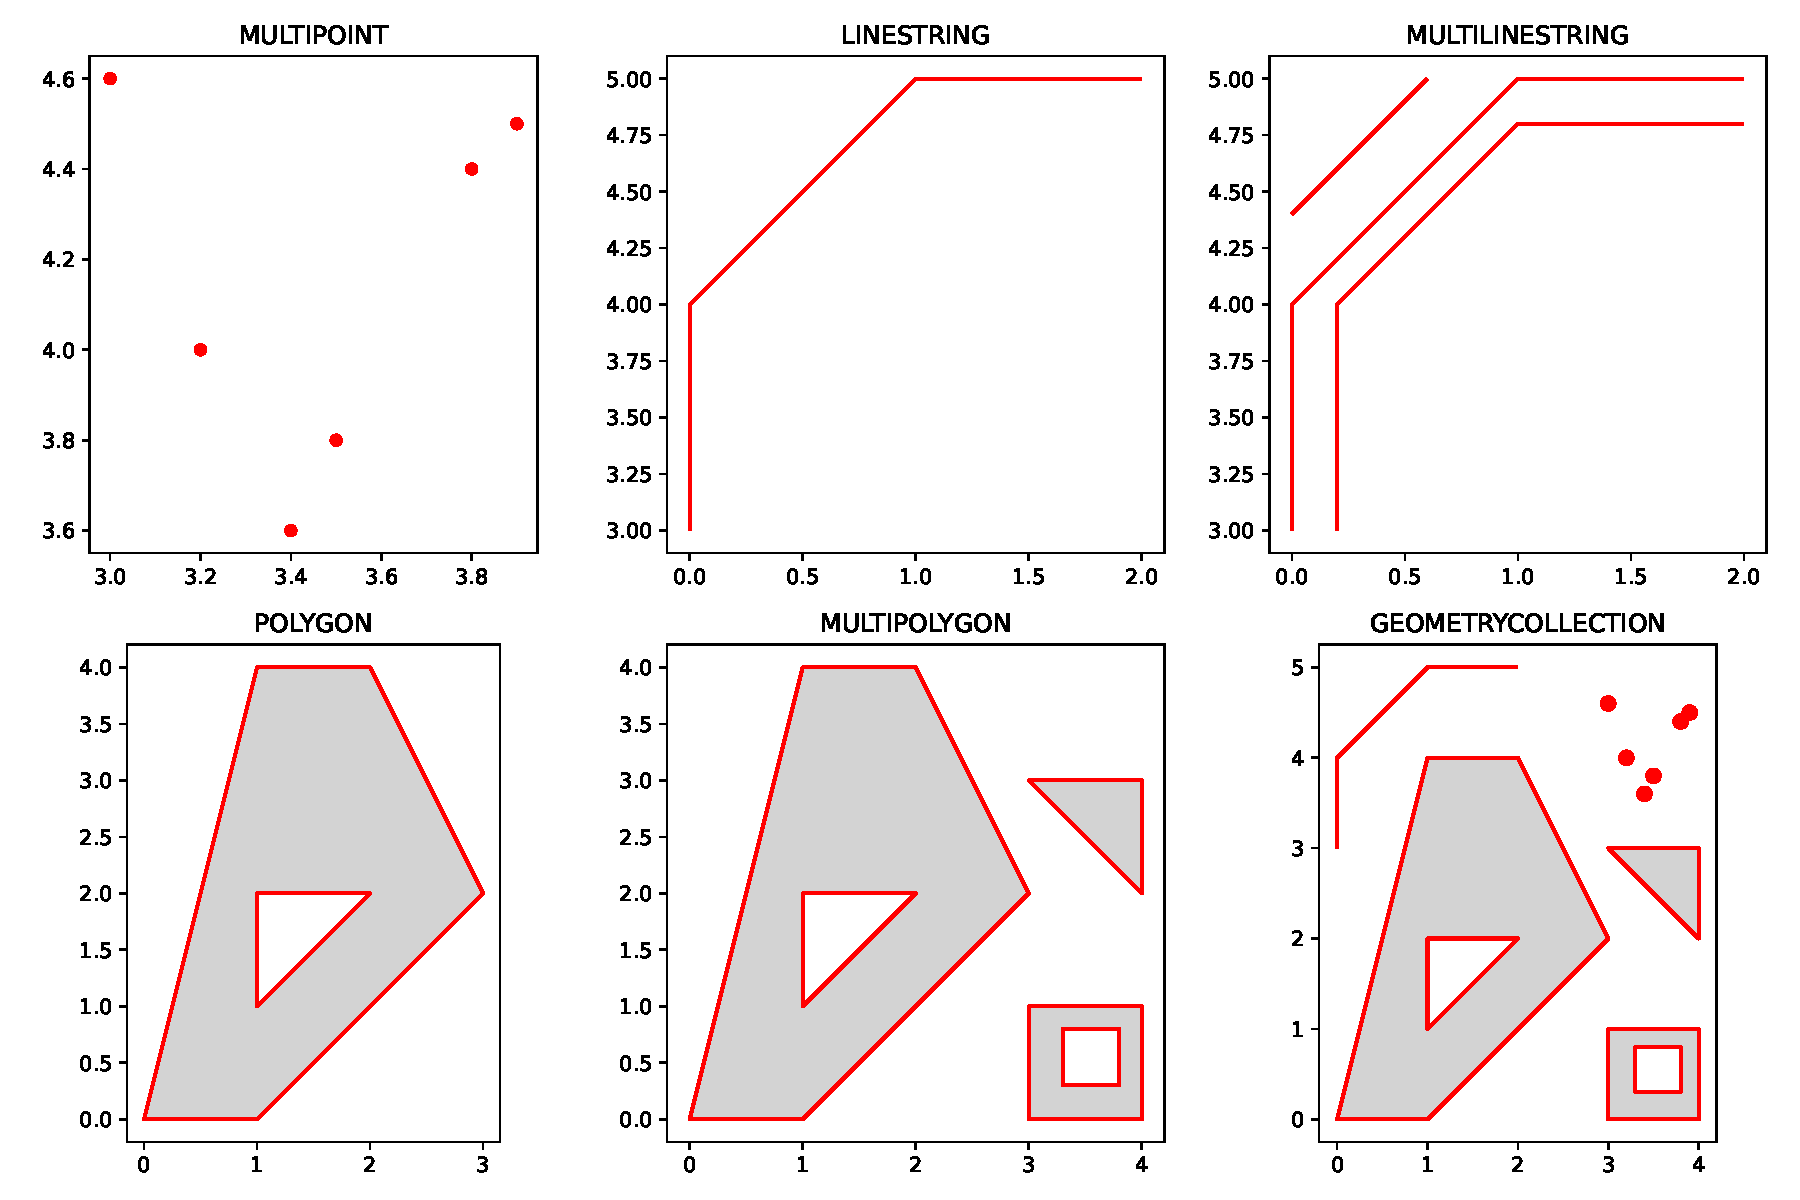
\includegraphics[width=0.8\textwidth,height=\textheight]{14-vector_files/figure-pdf/python_multigeom-1.pdf}
\end{center}

\subsection{R}

En R, el ecosistema estándar para operaciones espaciales se apoya en el
paquete \texttt{sf} (Simple Features). A diferencia del enfoque de
tuplas utilizado en Python, R construye las geometrías a partir de
\textbf{matrices numéricas}, empleando funciones base como
\texttt{rbind} para \textbf{concatenar coordenadas por filas}.

La estructuración de \textbf{polígonos con huecos} exige el
\textbf{anidamiento de matrices} dentro de \textbf{listas}: la primera
matriz de la lista asume automáticamente el rol de anillo exterior,
mientras que las matrices subsecuentes operan geométrica y
topológicamente como perforaciones.

\textbf{Detalles de visualización:} La función genérica \texttt{plot()}
en R interactúa con métodos específicos de clase. Para igualar el estilo
visual, se manejan los siguientes parámetros base.

\begin{itemize}
\tightlist
\item
  \texttt{col}: Define el color primario. Para geometrías cerradas
  representa el relleno
  (\texttt{\textquotesingle{}lightgrey\textquotesingle{}}), y para
  geometrías abiertas representa la línea o el vértice
  (\texttt{\textquotesingle{}red\textquotesingle{}}).
\item
  \texttt{border}: Sobrescribe el color del contorno perimetral en los
  polígonos. Se utiliza
  \texttt{\textquotesingle{}red\textquotesingle{}}.
\item
  \texttt{lwd} \emph{(Line Width)}: Controla el grosor de las líneas y
  contornos. Se estandariza en \texttt{1.5}.
\item
  \texttt{pch} \emph{(Point Character)}: Modifica la simbología del
  vértice. El código numérico \texttt{16} renderiza un círculo
  completamente sólido.
\item
  \texttt{cex} \emph{(Character Expansion)}: Factor de escala que
  multiplica el tamaño base del \texttt{pch}. Se fija en \texttt{1.2}.
\item
  \texttt{axes\ =\ TRUE}: Obliga al motor gráfico a dibujar las reglas
  de coordenadas cartesianas X e Y.
\item
  \texttt{xlim} y \texttt{ylim}: Vectores numéricos que imponen un
  recorte duro (\texttt{Bounding\ Box} manual) sobre el lienzo para
  maximizar el uso del espacio y evitar vacíos derivados del cálculo
  automático de R.
\end{itemize}

\begin{Shaded}
\begin{Highlighting}[]
\CommentTok{\# Carga de las rutinas primarias orientadas a la interoperabilidad espacial}
\FunctionTok{library}\NormalTok{(sf)}

\CommentTok{\# {-}{-}{-} 1. MULTIPOINT {-}{-}{-}}
\CommentTok{\# La función rbind unifica listas de vectores como filas matrices bidimensionales continuas.}
\NormalTok{p }\OtherTok{\textless{}{-}} \FunctionTok{rbind}\NormalTok{(}\FunctionTok{c}\NormalTok{(}\FloatTok{3.2}\NormalTok{,}\DecValTok{4}\NormalTok{), }\FunctionTok{c}\NormalTok{(}\DecValTok{3}\NormalTok{,}\FloatTok{4.6}\NormalTok{), }\FunctionTok{c}\NormalTok{(}\FloatTok{3.8}\NormalTok{,}\FloatTok{4.4}\NormalTok{), }\FunctionTok{c}\NormalTok{(}\FloatTok{3.5}\NormalTok{,}\FloatTok{3.8}\NormalTok{), }\FunctionTok{c}\NormalTok{(}\FloatTok{3.4}\NormalTok{,}\FloatTok{3.6}\NormalTok{), }\FunctionTok{c}\NormalTok{(}\FloatTok{3.9}\NormalTok{,}\FloatTok{4.5}\NormalTok{))}
\CommentTok{\# El constructor st\_multipoint compila formalmente la matriz hacia un Simple Feature Geometry (sfg)}
\NormalTok{mp }\OtherTok{\textless{}{-}} \FunctionTok{st\_multipoint}\NormalTok{(p)}

\CommentTok{\# {-}{-}{-} 2. LINESTRING {-}{-}{-}}
\CommentTok{\# Serie correlativa de nodos que pautan una estructura lineal.}
\NormalTok{s1 }\OtherTok{\textless{}{-}} \FunctionTok{rbind}\NormalTok{(}\FunctionTok{c}\NormalTok{(}\DecValTok{0}\NormalTok{,}\DecValTok{3}\NormalTok{),}\FunctionTok{c}\NormalTok{(}\DecValTok{0}\NormalTok{,}\DecValTok{4}\NormalTok{),}\FunctionTok{c}\NormalTok{(}\DecValTok{1}\NormalTok{,}\DecValTok{5}\NormalTok{),}\FunctionTok{c}\NormalTok{(}\DecValTok{2}\NormalTok{,}\DecValTok{5}\NormalTok{))}
\NormalTok{ls }\OtherTok{\textless{}{-}} \FunctionTok{st\_linestring}\NormalTok{(s1)}

\CommentTok{\# {-}{-}{-} 3. MULTILINESTRING {-}{-}{-}}
\CommentTok{\# Definición paramétrica para líneas de rutas segmentadas no dependientes.}
\NormalTok{s2 }\OtherTok{\textless{}{-}} \FunctionTok{rbind}\NormalTok{(}\FunctionTok{c}\NormalTok{(}\FloatTok{0.2}\NormalTok{,}\DecValTok{3}\NormalTok{), }\FunctionTok{c}\NormalTok{(}\FloatTok{0.2}\NormalTok{,}\DecValTok{4}\NormalTok{), }\FunctionTok{c}\NormalTok{(}\DecValTok{1}\NormalTok{,}\FloatTok{4.8}\NormalTok{), }\FunctionTok{c}\NormalTok{(}\DecValTok{2}\NormalTok{,}\FloatTok{4.8}\NormalTok{))}
\NormalTok{s3 }\OtherTok{\textless{}{-}} \FunctionTok{rbind}\NormalTok{(}\FunctionTok{c}\NormalTok{(}\DecValTok{0}\NormalTok{,}\FloatTok{4.4}\NormalTok{), }\FunctionTok{c}\NormalTok{(}\FloatTok{0.6}\NormalTok{,}\DecValTok{5}\NormalTok{))}
\CommentTok{\# Acepta el encapsulamiento de múltiples s1, s2, s3 como entradas iterativas de una lista global}
\NormalTok{mls }\OtherTok{\textless{}{-}} \FunctionTok{st\_multilinestring}\NormalTok{(}\FunctionTok{list}\NormalTok{(s1,s2,s3))}

\CommentTok{\# {-}{-}{-} 4. POLYGON {-}{-}{-}}
\CommentTok{\# p1 determina el confín espacial. Su evaluación métrica exige cierre (nodo inicial == nodo terminal).}
\NormalTok{p1 }\OtherTok{\textless{}{-}} \FunctionTok{rbind}\NormalTok{(}\FunctionTok{c}\NormalTok{(}\DecValTok{0}\NormalTok{,}\DecValTok{0}\NormalTok{), }\FunctionTok{c}\NormalTok{(}\DecValTok{1}\NormalTok{,}\DecValTok{0}\NormalTok{), }\FunctionTok{c}\NormalTok{(}\DecValTok{3}\NormalTok{,}\DecValTok{2}\NormalTok{), }\FunctionTok{c}\NormalTok{(}\DecValTok{2}\NormalTok{,}\DecValTok{4}\NormalTok{), }\FunctionTok{c}\NormalTok{(}\DecValTok{1}\NormalTok{,}\DecValTok{4}\NormalTok{), }\FunctionTok{c}\NormalTok{(}\DecValTok{0}\NormalTok{,}\DecValTok{0}\NormalTok{))}
\CommentTok{\# p2 opera lógicamente de zona vacía o hueco en la extensión total.}
\NormalTok{p2 }\OtherTok{\textless{}{-}} \FunctionTok{rbind}\NormalTok{(}\FunctionTok{c}\NormalTok{(}\DecValTok{1}\NormalTok{,}\DecValTok{1}\NormalTok{), }\FunctionTok{c}\NormalTok{(}\DecValTok{1}\NormalTok{,}\DecValTok{2}\NormalTok{), }\FunctionTok{c}\NormalTok{(}\DecValTok{2}\NormalTok{,}\DecValTok{2}\NormalTok{), }\FunctionTok{c}\NormalTok{(}\DecValTok{1}\NormalTok{,}\DecValTok{1}\NormalTok{))}
\CommentTok{\# Al someter la lista a st\_polygon, el algoritmo efectúa el vaciado geométrico con base al orden.}
\NormalTok{pol }\OtherTok{\textless{}{-}} \FunctionTok{st\_polygon}\NormalTok{(}\FunctionTok{list}\NormalTok{(p1,p2))}

\CommentTok{\# {-}{-}{-} 5. MULTIPOLYGON {-}{-}{-}}
\CommentTok{\# Estructuración de recintos independientes a gran escala}
\NormalTok{p3 }\OtherTok{\textless{}{-}} \FunctionTok{rbind}\NormalTok{(}\FunctionTok{c}\NormalTok{(}\DecValTok{3}\NormalTok{,}\DecValTok{0}\NormalTok{), }\FunctionTok{c}\NormalTok{(}\DecValTok{4}\NormalTok{,}\DecValTok{0}\NormalTok{), }\FunctionTok{c}\NormalTok{(}\DecValTok{4}\NormalTok{,}\DecValTok{1}\NormalTok{), }\FunctionTok{c}\NormalTok{(}\DecValTok{3}\NormalTok{,}\DecValTok{1}\NormalTok{), }\FunctionTok{c}\NormalTok{(}\DecValTok{3}\NormalTok{,}\DecValTok{0}\NormalTok{))}
\CommentTok{\# Se introduce un factor de inversión sobre el vector ([5:1,]) probando la resistencia }
\CommentTok{\# de la regla de dirección topológica implementada en GEOS / sf}
\NormalTok{p4 }\OtherTok{\textless{}{-}} \FunctionTok{rbind}\NormalTok{(}\FunctionTok{c}\NormalTok{(}\FloatTok{3.3}\NormalTok{,}\FloatTok{0.3}\NormalTok{), }\FunctionTok{c}\NormalTok{(}\FloatTok{3.8}\NormalTok{,}\FloatTok{0.3}\NormalTok{), }\FunctionTok{c}\NormalTok{(}\FloatTok{3.8}\NormalTok{,}\FloatTok{0.8}\NormalTok{), }\FunctionTok{c}\NormalTok{(}\FloatTok{3.3}\NormalTok{,}\FloatTok{0.8}\NormalTok{), }\FunctionTok{c}\NormalTok{(}\FloatTok{3.3}\NormalTok{,}\FloatTok{0.3}\NormalTok{))[}\DecValTok{5}\SpecialCharTok{:}\DecValTok{1}\NormalTok{,]}
\NormalTok{p5 }\OtherTok{\textless{}{-}} \FunctionTok{rbind}\NormalTok{(}\FunctionTok{c}\NormalTok{(}\DecValTok{3}\NormalTok{,}\DecValTok{3}\NormalTok{), }\FunctionTok{c}\NormalTok{(}\DecValTok{4}\NormalTok{,}\DecValTok{2}\NormalTok{), }\FunctionTok{c}\NormalTok{(}\DecValTok{4}\NormalTok{,}\DecValTok{3}\NormalTok{), }\FunctionTok{c}\NormalTok{(}\DecValTok{3}\NormalTok{,}\DecValTok{3}\NormalTok{))}
\CommentTok{\# Reclamo de jerarquías avanzadas: lista de listas conteniendo las mallas matrices}
\NormalTok{mpol }\OtherTok{\textless{}{-}} \FunctionTok{st\_multipolygon}\NormalTok{(}\FunctionTok{list}\NormalTok{(}\FunctionTok{list}\NormalTok{(p1,p2), }\FunctionTok{list}\NormalTok{(p3,p4), }\FunctionTok{list}\NormalTok{(p5)))}

\CommentTok{\# {-}{-}{-} 6. GEOMETRYCOLLECTION {-}{-}{-}}
\CommentTok{\# Soporte misceláneo universal aglutinante de las abstracciones precedentes (0D, 1D, 2D)}
\NormalTok{gc }\OtherTok{\textless{}{-}} \FunctionTok{st\_geometrycollection}\NormalTok{(}\FunctionTok{list}\NormalTok{(mp, mpol, ls))}

\CommentTok{\# Inspección diagnóstica a nivel terminal.}
\FunctionTok{print}\NormalTok{(}\StringTok{"{-}{-}{-} Inspección de topología espacial {-}{-}{-}"}\NormalTok{)}
\end{Highlighting}
\end{Shaded}

\begin{verbatim}
[1] "--- Inspección de topología espacial ---"
\end{verbatim}

\begin{Shaded}
\begin{Highlighting}[]
\FunctionTok{print}\NormalTok{(}\StringTok{"Objeto mpol creado."}\NormalTok{)}
\end{Highlighting}
\end{Shaded}

\begin{verbatim}
[1] "Objeto mpol creado."
\end{verbatim}

\begin{Shaded}
\begin{Highlighting}[]
\FunctionTok{print}\NormalTok{(}\FunctionTok{paste}\NormalTok{(}\StringTok{"Tipo de clase:"}\NormalTok{, }\FunctionTok{class}\NormalTok{(mpol)[}\DecValTok{2}\NormalTok{])) }\CommentTok{\# Exposición de la subclase matriz sfg}
\end{Highlighting}
\end{Shaded}

\begin{verbatim}
[1] "Tipo de clase: MULTIPOLYGON"
\end{verbatim}

\begin{Shaded}
\begin{Highlighting}[]
\CommentTok{\# {-}{-}{-} Configuración del Lienzo Multipanel (Layout 2x3) {-}{-}{-}}

\CommentTok{\# La función par() (graphical parameters) define la persistencia del área de dibujo:}
\CommentTok{\#   mfrow: Organiza la matriz de gráficos (2 filas, 3 columnas). }
\CommentTok{\#          El orden de renderizado es por FILAS (de izquierda a derecha).}
\CommentTok{\#   mar:   Ajusta los márgenes internos de cada cuadrante en líneas de texto }
\CommentTok{\#          c(abajo, izquierda, arriba, derecha). Se reducen para maximizar el área espacial.}
\FunctionTok{par}\NormalTok{(}\AttributeTok{mfrow =} \FunctionTok{c}\NormalTok{(}\DecValTok{2}\NormalTok{, }\DecValTok{3}\NormalTok{), }\AttributeTok{mar =} \FunctionTok{c}\NormalTok{(}\DecValTok{3}\NormalTok{, }\DecValTok{3}\NormalTok{, }\DecValTok{2}\NormalTok{, }\DecValTok{1}\NormalTok{)) }

\CommentTok{\# {-}{-}{-} Renderizado de Primitivas Geométricas (OGC Simple Features) {-}{-}{-}}

\CommentTok{\# 1. MULTIPOINT}
\CommentTok{\# pch: (point character) define el símbolo; 16 es un círculo sólido.}
\CommentTok{\# cex: (character expansion) escala el tamaño del punto (1.2 = 120\%).}
\FunctionTok{plot}\NormalTok{(mp, }\AttributeTok{col =} \StringTok{\textquotesingle{}red\textquotesingle{}}\NormalTok{, }\AttributeTok{pch =} \DecValTok{16}\NormalTok{, }\AttributeTok{cex =} \FloatTok{1.2}\NormalTok{, }\AttributeTok{axes =} \ConstantTok{TRUE}\NormalTok{, }
     \AttributeTok{xlim =} \FunctionTok{c}\NormalTok{(}\FloatTok{2.8}\NormalTok{, }\FloatTok{4.2}\NormalTok{), }\AttributeTok{ylim =} \FunctionTok{c}\NormalTok{(}\FloatTok{3.4}\NormalTok{, }\FloatTok{4.8}\NormalTok{))}
\FunctionTok{title}\NormalTok{(}\StringTok{"MULTIPOINT"}\NormalTok{, }\AttributeTok{cex.main =} \FloatTok{0.9}\NormalTok{) }\CommentTok{\# Título con escala ajustada}

\CommentTok{\# 2. LINESTRING}
\CommentTok{\# lwd: (line width) grosor de la línea.}
\FunctionTok{plot}\NormalTok{(ls, }\AttributeTok{col =} \StringTok{\textquotesingle{}red\textquotesingle{}}\NormalTok{, }\AttributeTok{lwd =} \DecValTok{2}\NormalTok{, }\AttributeTok{axes =} \ConstantTok{TRUE}\NormalTok{, }
     \AttributeTok{xlim =} \FunctionTok{c}\NormalTok{(}\SpecialCharTok{{-}}\FloatTok{0.2}\NormalTok{, }\FloatTok{2.2}\NormalTok{), }\AttributeTok{ylim =} \FunctionTok{c}\NormalTok{(}\FloatTok{2.8}\NormalTok{, }\FloatTok{5.2}\NormalTok{))}
\FunctionTok{title}\NormalTok{(}\StringTok{"LINESTRING"}\NormalTok{, }\AttributeTok{cex.main =} \FloatTok{0.9}\NormalTok{)}

\CommentTok{\# 3. MULTILINESTRING}
\FunctionTok{plot}\NormalTok{(mls, }\AttributeTok{col =} \StringTok{\textquotesingle{}red\textquotesingle{}}\NormalTok{, }\AttributeTok{lwd =} \DecValTok{2}\NormalTok{, }\AttributeTok{axes =} \ConstantTok{TRUE}\NormalTok{, }
     \AttributeTok{xlim =} \FunctionTok{c}\NormalTok{(}\SpecialCharTok{{-}}\FloatTok{0.2}\NormalTok{, }\FloatTok{2.2}\NormalTok{), }\AttributeTok{ylim =} \FunctionTok{c}\NormalTok{(}\FloatTok{2.8}\NormalTok{, }\FloatTok{5.2}\NormalTok{))}
\FunctionTok{title}\NormalTok{(}\StringTok{"MULTILINESTRING"}\NormalTok{, }\AttributeTok{cex.main =} \FloatTok{0.9}\NormalTok{)}

\CommentTok{\# 4. POLYGON}
\CommentTok{\# border: Color del perímetro. col: Color del relleno (fill).}
\FunctionTok{plot}\NormalTok{(pol, }\AttributeTok{border =} \StringTok{\textquotesingle{}red\textquotesingle{}}\NormalTok{, }\AttributeTok{col =} \StringTok{\textquotesingle{}\#EEEEEE\textquotesingle{}}\NormalTok{, }\AttributeTok{lwd =} \FloatTok{1.5}\NormalTok{, }\AttributeTok{axes =} \ConstantTok{TRUE}\NormalTok{, }
     \AttributeTok{xlim =} \FunctionTok{c}\NormalTok{(}\SpecialCharTok{{-}}\FloatTok{0.2}\NormalTok{, }\FloatTok{3.2}\NormalTok{), }\AttributeTok{ylim =} \FunctionTok{c}\NormalTok{(}\SpecialCharTok{{-}}\FloatTok{0.2}\NormalTok{, }\FloatTok{4.2}\NormalTok{))}
\FunctionTok{title}\NormalTok{(}\StringTok{"POLYGON"}\NormalTok{, }\AttributeTok{cex.main =} \FloatTok{0.9}\NormalTok{)}

\CommentTok{\# 5. MULTIPOLYGON}
\CommentTok{\# Se mantienen límites (xlim/ylim) consistentes para permitir comparación visual directa.}
\FunctionTok{plot}\NormalTok{(mpol, }\AttributeTok{border =} \StringTok{\textquotesingle{}red\textquotesingle{}}\NormalTok{, }\AttributeTok{col =} \StringTok{\textquotesingle{}\#EEEEEE\textquotesingle{}}\NormalTok{, }\AttributeTok{lwd =} \FloatTok{1.5}\NormalTok{, }\AttributeTok{axes =} \ConstantTok{TRUE}\NormalTok{, }
     \AttributeTok{xlim =} \FunctionTok{c}\NormalTok{(}\SpecialCharTok{{-}}\FloatTok{0.2}\NormalTok{, }\FloatTok{4.2}\NormalTok{), }\AttributeTok{ylim =} \FunctionTok{c}\NormalTok{(}\SpecialCharTok{{-}}\FloatTok{0.2}\NormalTok{, }\FloatTok{4.2}\NormalTok{))}
\FunctionTok{title}\NormalTok{(}\StringTok{"MULTIPOLYGON"}\NormalTok{, }\AttributeTok{cex.main =} \FloatTok{0.9}\NormalTok{)}

\CommentTok{\# 6. GEOMETRYCOLLECTION}
\CommentTok{\# Secuencia estratificada asíncrona sobre GeometryCollection. }
\CommentTok{\# La inyección de \textasciigrave{}add = TRUE\textasciigrave{} previene la eliminación}
\CommentTok{\#  del canvas polígono gris al dibujar las capas primarias vectoriales }
\CommentTok{\#  y asegurar fidelidad de escala y color.}
\FunctionTok{plot}\NormalTok{(gc, }\AttributeTok{border =} \StringTok{\textquotesingle{}red\textquotesingle{}}\NormalTok{, }\AttributeTok{col =} \StringTok{\textquotesingle{}lightgrey\textquotesingle{}}\NormalTok{, }\AttributeTok{lwd =} \FloatTok{1.5}\NormalTok{, }\AttributeTok{axes =} \ConstantTok{TRUE}\NormalTok{, }
     \AttributeTok{xlim=}\FunctionTok{c}\NormalTok{(}\SpecialCharTok{{-}}\FloatTok{0.2}\NormalTok{, }\FloatTok{4.2}\NormalTok{), }\AttributeTok{ylim=}\FunctionTok{c}\NormalTok{(}\SpecialCharTok{{-}}\FloatTok{0.2}\NormalTok{, }\FloatTok{5.2}\NormalTok{))}
\FunctionTok{plot}\NormalTok{(ls, }\AttributeTok{col =} \StringTok{\textquotesingle{}red\textquotesingle{}}\NormalTok{, }\AttributeTok{lwd =} \FloatTok{1.5}\NormalTok{, }\AttributeTok{add =} \ConstantTok{TRUE}\NormalTok{)}
\FunctionTok{plot}\NormalTok{(mp, }\AttributeTok{col =} \StringTok{\textquotesingle{}red\textquotesingle{}}\NormalTok{, }\AttributeTok{pch =} \DecValTok{16}\NormalTok{, }\AttributeTok{cex =} \FloatTok{1.2}\NormalTok{, }\AttributeTok{add =} \ConstantTok{TRUE}\NormalTok{)}
\FunctionTok{title}\NormalTok{(}\StringTok{"GEOMETRYCOLLECTION"}\NormalTok{)}
\end{Highlighting}
\end{Shaded}

\begin{center}
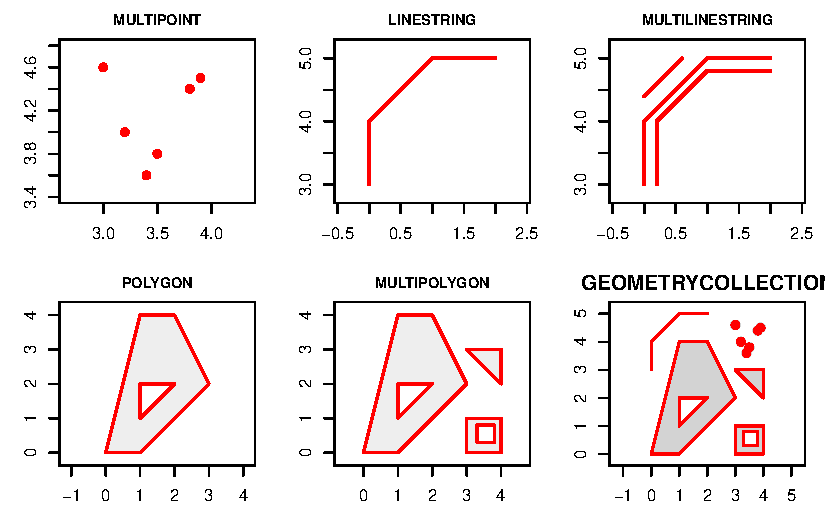
\includegraphics[width=0.8\textwidth,height=\textheight]{14-vector_files/figure-pdf/r_multigeom-1.pdf}
\end{center}

\begin{Shaded}
\begin{Highlighting}[]
\CommentTok{\# Depuración del buffer de diseño}
\FunctionTok{par}\NormalTok{(}\AttributeTok{mfrow =} \FunctionTok{c}\NormalTok{(}\DecValTok{1}\NormalTok{, }\DecValTok{1}\NormalTok{))}
\end{Highlighting}
\end{Shaded}

\subsection{Julia}

En el entorno algorítmico espacial de Julia se utiliza
\texttt{ArchGDAL.jl} para asegurar una base C++ robusta en la validación
topológica, y la librería \texttt{CairoMakie.jl} para orquestar la
renderización del lienzo.

Julia estructura sus primitivas mediante \textbf{tuplas} \texttt{()} y
\textbf{vectores} \texttt{{[}{]}}.

\textbf{Detalles de visualización:} Para homologar el estilo estético
con Python y R bajo la sintaxis específica del ecosistema
\texttt{Makie}, se aplican descriptores semánticos durante las llamadas
a funciones como \texttt{scatter!} y \texttt{poly!}.

\begin{itemize}
\tightlist
\item
  \texttt{color}: Controla el matiz central geométrico. Se emplea el
  símbolo base rojo (\texttt{:red}) para primitivas y puntos, y gris
  (\texttt{:lightgray}) para mallas cerradas.
\item
  \texttt{strokecolor}: Argumento exclusivo del método \texttt{poly!},
  encargado de perfilar perimetralmente las mallas (utilizando
  \texttt{:red}).
\item
  \texttt{strokewidth}: Argumento numérico que fuerza la anchura del
  vector envolvente al mismo nivel industrial definido en Python (valor
  \texttt{1.5}).
\item
  \texttt{markersize}: Determina la amplitud absoluta del vértice
  disperso en pantalla (fijado en un tamaño visible de \texttt{10}).
\end{itemize}

\textbf{Notas técnicas sobre el flujo de geometría en Julia}

\begin{enumerate}
\def\labelenumi{\arabic{enumi}.}
\tightlist
\item
  \textbf{Limitaciones de ploteo (\texttt{Plots.jl} vs
  \texttt{CairoMakie.jl}):} En el ecosistema general de Julia, librerías
  como \texttt{Plots.jl} tienen dificultades manejando topologías
  complejas (especialmente la renderización nativa de huecos dentro de
  polígonos), requiriendo a menudo sobreponer geometrías blancas para
  ``engañar'' a la gráfica. Por esto se usa \texttt{CairoMakie.jl}, cuyo
  tipo \texttt{Makie.Polygon} está diseñado específicamente para
  interpretar anillos exteriores y perforar huecos interiores con total
  transparencia topológica.
\item
  \textbf{Inyección de geometrías (El exterior y los huecos):} En
  \texttt{ArchGDAL}, un polígono con huecos se conforma de un anillo
  exterior (índice 0) y \emph{n} anillos interiores (índice 1 en
  adelante). Para que \texttt{Makie} lo dibuje correctamente, se extraen
  los puntos del exterior como un arreglo de \texttt{Point2f}, y los
  huecos como un ``arreglo de arreglos'' de \texttt{Point2f}. Makie
  ejecuta el cálculo de recorte geométrico final.
\item
  \textbf{La excepción de GeometryCollection (\texttt{wkb}):} A
  diferencia de las otras geometrías, donde se usan constructores
  explícitos y directos (como \texttt{createpolygon} o
  \texttt{createmultipoint}), la librería \texttt{ArchGDAL.jl} omite una
  función constructora de alto nivel equivalente llamada
  \texttt{creategeometrycollection}. Frente a esta deficiencia en la
  capa de software, se debe forzar una asignación de bajo nivel
  invocando el estándar de representación en lenguaje C (Well-Known
  Binary). Esto demanda instanciar un contenedor lógico hueco bajo el
  tipo escalar \texttt{ArchGDAL.wkbGeometryCollection}, operando
  posteriormente sobre sus direcciones de memoria mediante la inyección
  concurrente provista por la macrofunción base \texttt{addgeom!}.
\item
  \textbf{Choque de nombres (Namespace Collision):} Si en un documento
  Quarto ya se ha invocado en pasos anteriores la carga a memoria de la
  librería \texttt{Plots.jl}, el núcleo procesador C++ base mantendrá
  persistente la definición de las macros en estado estático. Tanto
  \texttt{Plots} como \texttt{CairoMakie} resuelven rutinas compartiendo
  macros reservadas asimétricas (ej. \texttt{scatter!} y
  \texttt{poly!}). Para anular el colapso del compilador por ambigüedad
  al momento de derivar el puntero, se aplican sentencias de blindaje de
  nivel operativo invocando expresamente las funciones mediante la
  definición explícita de su contenedor macro global o namespace
  asociado: \texttt{CairoMakie.scatter!(...)},
  \texttt{CairoMakie.poly!(...)} y \texttt{CairoMakie.lines!(...)}.
\item
  \textbf{Listas de comprensión (Comprehensions) vs \texttt{map()}:} En
  Julia, la técnica estandarizada, óptima y computacionalmente
  transparente de extracción iterativa de arreglos vectoriales
  multidimensionales consiste en explotar las listas de comprensión en
  línea (operación basada en sintaxis
  \texttt{{[}...\ for\ ...\ in\ ...{]}}, ver ejemplo después de este
  párrafo). Esto facilita la recolección en bloque sobre las jerarquías
  internas topológicas de \texttt{ArchGDAL}. \emph{Nota técnica del
  motor:} En etapas iniciales de la estructura del curso, el analizador
  léxico (\texttt{j\_eval}) de interconexión R-Julia manifestaba severos
  problemas de colisión de evaluación, interpretando el operador
  \texttt{for} interno del arreglo como una directiva de iteración
  multilínea que disparaba una exigencia de compilación nula buscando el
  operador \texttt{end}. Esta colisión de arquitecturas obligaba a
  forzar un parche en el flujo recurriendo a la función macro
  \texttt{map(i\ -\textgreater{}\ ...)}. Se reporta que la
  refactorización arquitectónica implementada sobre la función
  interpretativa (\texttt{j\_eval}) en el ambiente de Quarto ha resuelto
  la anomalía introduciendo una validación semántica regida por
  expresiones regulares, estabilizando el parseo. A partir de este nivel
  operativo, \textbf{el uso provisorio del enmascaramiento macro
  \texttt{map} es innecesario}, permitiendo correr las evaluaciones
  nativas del código de manera íntegra, transparente y con las métricas
  de rendimiento estables del entorno original.
\end{enumerate}

Ejemplo de lista de compresión:

\begin{Shaded}
\begin{Highlighting}[]
\NormalTok{cuadrados }\OperatorTok{=}\NormalTok{ [x}\OperatorTok{\^{}}\FloatTok{2}\NormalTok{ for x }\KeywordTok{in} \FloatTok{1}\OperatorTok{:}\FloatTok{5}\NormalTok{]}
\CommentTok{\# Devuelve: 5{-}element Vector\{Int64\}: [1, 4, 9, 16, 25]}
\end{Highlighting}
\end{Shaded}

\begin{Shaded}
\begin{Highlighting}[]
\CommentTok{\# El puente j\_eval orquesta iterativamente la ejecución Julia dentro del entorno host R.}
\FunctionTok{j\_eval}\NormalTok{(r}\StringTok{"{-}(}
\StringTok{using ArchGDAL}
\StringTok{using CairoMakie}

\StringTok{\# {-}{-}{-} 1. CONSTRUCCIÓN DE MULTIPOINT {-}{-}{-}}
\StringTok{\# ArchGDAL instancía geometrías recibiendo vectores unidimensionales con tuplas de coordenadas}
\StringTok{mp = ArchGDAL.createmultipoint([(3.2, 4.0), (3.0, 4.6), (3.8, 4.4), (3.5, 3.8), (3.4, 3.6), (3.9, 4.5)])}

\StringTok{\# {-}{-}{-} 2. LINESTRING {-}{-}{-}}
\StringTok{\# Secuencia ordenada de vértices espaciales}
\StringTok{ls = ArchGDAL.createlinestring([(0.0, 3.0), (0.0, 4.0), (1.0, 5.0), (2.0, 5.0)])}

\StringTok{\# {-}{-}{-} 3. MULTILINESTRING {-}{-}{-}}
\StringTok{\# Requiere un arreglo contenedor que envuelve las diferentes rutas segmentadas}
\StringTok{mls = ArchGDAL.createmultilinestring([}
\StringTok{    [(0.0, 3.0), (0.0, 4.0), (1.0, 5.0), (2.0, 5.0)], }
\StringTok{    [(0.2, 3.0), (0.2, 4.0), (1.0, 4.8), (2.0, 4.8)], }
\StringTok{    [(0.0, 4.4), (0.6, 5.0)]}
\StringTok{])}

\StringTok{\# {-}{-}{-} 4. POLYGON {-}{-}{-}}
\StringTok{\# Construcción mediante un arreglo de arreglos. El índice inicial es el anillo exterior estricto.}
\StringTok{\# Los arreglos secundarios se interpretan operativamente como sustracciones topológicas (huecos).}
\StringTok{pol = ArchGDAL.createpolygon([}
\StringTok{    [(0.0, 0.0), (1.0, 0.0), (3.0, 2.0), (2.0, 4.0), (1.0, 4.0), (0.0, 0.0)], }
\StringTok{    [(1.0, 1.0), (1.0, 2.0), (2.0, 2.0), (1.0, 1.0)]}
\StringTok{])}

\StringTok{\# {-}{-}{-} 5. MULTIPOLYGON {-}{-}{-}}
\StringTok{\# Agrupación jerárquica tridimensional. Colección de entidades poligonales independientes.}
\StringTok{mpol = ArchGDAL.createmultipolygon([}
\StringTok{    [[(0.0, 0.0), (1.0, 0.0), (3.0, 2.0), (2.0, 4.0), (1.0, 4.0), (0.0, 0.0)], [(1.0, 1.0), (1.0, 2.0), (2.0, 2.0), (1.0, 1.0)]], }
\StringTok{    [[(3.0, 0.0), (4.0, 0.0), (4.0, 1.0), (3.0, 1.0), (3.0, 0.0)]], }
\StringTok{    [[(3.0, 3.0), (4.0, 2.0), (4.0, 3.0), (3.0, 3.0)]]}
\StringTok{])}

\StringTok{\# {-}{-}{-} 6. GEOMETRYCOLLECTION (Excepción WKB) {-}{-}{-}}
\StringTok{\# ArchGDAL exige instanciar la colección vacía directamente bajo el estándar Well{-}Known Binary}
\StringTok{gc = ArchGDAL.creategeom(ArchGDAL.wkbGeometryCollection)}
\StringTok{\# Inserción dinámica de las sub{-}geometrías iterando sobre el bloque de memoria}
\StringTok{ArchGDAL.addgeom!(gc, ArchGDAL.createmultipoint([(3.2, 4.0), (3.0, 4.6), (3.8, 4.4), (3.5, 3.8), (3.4, 3.6), (3.9, 4.5)]))}
\StringTok{ArchGDAL.addgeom!(gc, ArchGDAL.createlinestring([(0.0, 3.0), (0.0, 4.0), (1.0, 5.0), (2.0, 5.0)]))}
\StringTok{ArchGDAL.addgeom!(gc, ArchGDAL.createmultipolygon([}
\StringTok{    [[(0.0, 0.0), (1.0, 0.0), (3.0, 2.0), (2.0, 4.0), (1.0, 4.0), (0.0, 0.0)], [(1.0, 1.0), (1.0, 2.0), (2.0, 2.0), (1.0, 1.0)]], }
\StringTok{    [[(3.0, 0.0), (4.0, 0.0), (4.0, 1.0), (3.0, 1.0), (3.0, 0.0)]], }
\StringTok{    [[(3.0, 3.0), (4.0, 2.0), (4.0, 3.0), (3.0, 3.0)]]}
\StringTok{]))}

\StringTok{\# {-}{-}{-} FUNCIONES AUXILIARES: CONVERSIÓN VECTORIAL ARCHGDAL {-}\textgreater{} CAIROMAKIE {-}{-}{-}}

\StringTok{\# 1. Función para procesamiento matricial de polígonos}
\StringTok{function to\_makie\_poly(gdal\_poly)}
\StringTok{    \# Extracción del anillo principal (índice geométrico 0)}
\StringTok{    ext = ArchGDAL.getgeom(gdal\_poly, 0)}
\StringTok{    \# Comprensión de lista para mapear iterativamente los nodos hacia estructuras Point2f de Makie}
\StringTok{    ext\_pts = [Point2f(ArchGDAL.getx(ext, i), ArchGDAL.gety(ext, i)) for i in 0:ArchGDAL.ngeom(ext){-}1]}
\StringTok{    }
\StringTok{    \# Recolección condicional de anillos interiores (índices \textgreater{} 0)}
\StringTok{    holes = Vector\{Vector\{Point2f\}\}()}
\StringTok{    for i in 1:ArchGDAL.ngeom(gdal\_poly){-}1}
\StringTok{        hole = ArchGDAL.getgeom(gdal\_poly, i)}
\StringTok{        push!(holes, [Point2f(ArchGDAL.getx(hole, j), ArchGDAL.gety(hole, j)) for j in 0:ArchGDAL.ngeom(hole){-}1])}
\StringTok{    end}
\StringTok{    return Makie.Polygon(ext\_pts, holes)}
\StringTok{end}

\StringTok{\# 2. Función recursiva de evaluación para geometrías lineales}
\StringTok{function plot\_lines!(ax, linesgeom)}
\StringTok{    \# Evalúa si corresponde a tipo simple unidimensional}
\StringTok{    if ArchGDAL.getgeomtype(linesgeom) == ArchGDAL.wkbLineString}
\StringTok{        pts = [Point2f(ArchGDAL.getx(linesgeom, i), ArchGDAL.gety(linesgeom, i)) for i in 0:ArchGDAL.ngeom(linesgeom){-}1]}
\StringTok{        CairoMakie.lines!(ax, pts, color=:red, linewidth=1.5)}
\StringTok{    else}
\StringTok{        \# Iteración en profundidad en caso de detectar arreglos compuestos (MultiLineString)}
\StringTok{        for i in 0:ArchGDAL.ngeom(linesgeom){-}1}
\StringTok{            plot\_lines!(ax, ArchGDAL.getgeom(linesgeom, i))}
\StringTok{        end}
\StringTok{    end}
\StringTok{end}

\StringTok{\# Control de almacenamiento en el sistema base de Quarto (evita rutas nulas al almacenar PNG)}
\StringTok{\# Si la carpeta NO existe créala}
\StringTok{\# isdir("}\NormalTok{images}\StringTok{") || mkpath("}\NormalTok{images}\StringTok{")}


\StringTok{\# {-}{-}{-} RENDERIZADO PRINCIPAL (GRID 2x3 CON EJES CARTESIANOS ACTIVADOS) {-}{-}{-}}
\StringTok{\# Declaración global de la figura y su área espacial}
\StringTok{fig = Figure(size = (800, 500))}

\StringTok{\# Asignación discreta de ejes coordenados a subcuadrantes matriciales}
\StringTok{ax1 = Axis(fig[1, 1], title = "}\NormalTok{MULTIPOINT}\StringTok{")}
\StringTok{ax2 = Axis(fig[1, 2], title = "}\NormalTok{LINESTRING}\StringTok{")}
\StringTok{ax3 = Axis(fig[1, 3], title = "}\NormalTok{MULTILINESTRING}\StringTok{")}
\StringTok{ax4 = Axis(fig[2, 1], title = "}\NormalTok{POLYGON}\StringTok{")}
\StringTok{ax5 = Axis(fig[2, 2], title = "}\NormalTok{MULTIPOLYGON}\StringTok{")}
\StringTok{ax6 = Axis(fig[2, 3], title = "}\NormalTok{GEOMETRYCOLLECTION}\StringTok{")}

\StringTok{\# Bloqueo global de ratio paramétrico. }
\StringTok{\# Se omite explícitamente hidedecorations! para forzar la visibilidad gráfica transversal de ejes.}
\StringTok{for ax in [ax1, ax2, ax3, ax4, ax5, ax6]}
\StringTok{    ax.aspect = DataAspect()}
\StringTok{end}

\StringTok{\# Operaciones algorítmicas de visualización capa por capa}
\StringTok{pts\_x = [ArchGDAL.getx(ArchGDAL.getgeom(mp, i), 0) for i in 0:ArchGDAL.ngeom(mp){-}1]}
\StringTok{pts\_y = [ArchGDAL.gety(ArchGDAL.getgeom(mp, i), 0) for i in 0:ArchGDAL.ngeom(mp){-}1]}
\StringTok{CairoMakie.scatter!(ax1, pts\_x, pts\_y, color=:red, markersize=10)}

\StringTok{plot\_lines!(ax2, ls)}
\StringTok{plot\_lines!(ax3, mls)}

\StringTok{\# Para las mallas continuas se asignan parámetros de relleno uniforme (gris) y borde (rojo)}
\StringTok{CairoMakie.poly!(ax4, to\_makie\_poly(pol), color=:lightgray, strokecolor=:red, strokewidth=1.5)}

\StringTok{for i in 0:ArchGDAL.ngeom(mpol){-}1}
\StringTok{    CairoMakie.poly!(ax5, to\_makie\_poly(ArchGDAL.getgeom(mpol, i)), color=:lightgray, strokecolor=:red, strokewidth=1.5)}
\StringTok{end}

\StringTok{\# Renderizado de GeometryCollection. Se invierte la superposición para ubicar primero}
\StringTok{\# los polígonos, asegurando un contraste nítido frente a la red de líneas vectoriales.}
\StringTok{gc\_mpol = ArchGDAL.getgeom(gc, 2)}
\StringTok{for i in 0:ArchGDAL.ngeom(gc\_mpol){-}1}
\StringTok{    CairoMakie.poly!(ax6, to\_makie\_poly(ArchGDAL.getgeom(gc\_mpol, i)), color=:lightgray, strokecolor=:red, strokewidth=1.5)}
\StringTok{end}
\StringTok{plot\_lines!(ax6, ArchGDAL.getgeom(gc, 1))}

\StringTok{pts\_gc\_x = [ArchGDAL.getx(ArchGDAL.getgeom(ArchGDAL.getgeom(gc, 0), i), 0) for i in 0:ArchGDAL.ngeom(ArchGDAL.getgeom(gc, 0)){-}1]}
\StringTok{pts\_gc\_y = [ArchGDAL.gety(ArchGDAL.getgeom(ArchGDAL.getgeom(gc, 0), i), 0) for i in 0:ArchGDAL.ngeom(ArchGDAL.getgeom(gc, 0)){-}1]}
\StringTok{CairoMakie.scatter!(ax6, pts\_gc\_x, pts\_gc\_y, color=:red, markersize=10)}

\StringTok{\# Guardado con denominación estructural única requerida por el renderizador LaTeX/HTML de Quarto}
\StringTok{CairoMakie.save("}\NormalTok{images}\SpecialCharTok{/}\NormalTok{c01\_plot\_multigeom\_julia.png}\StringTok{", fig)}
\StringTok{){-}"}\NormalTok{)}
\end{Highlighting}
\end{Shaded}

\begin{Shaded}
\begin{Highlighting}[]
\NormalTok{knitr}\SpecialCharTok{::}\FunctionTok{include\_graphics}\NormalTok{(}\StringTok{"images/c01\_plot\_multigeom\_julia.png"}\NormalTok{)}
\end{Highlighting}
\end{Shaded}

\begin{center}
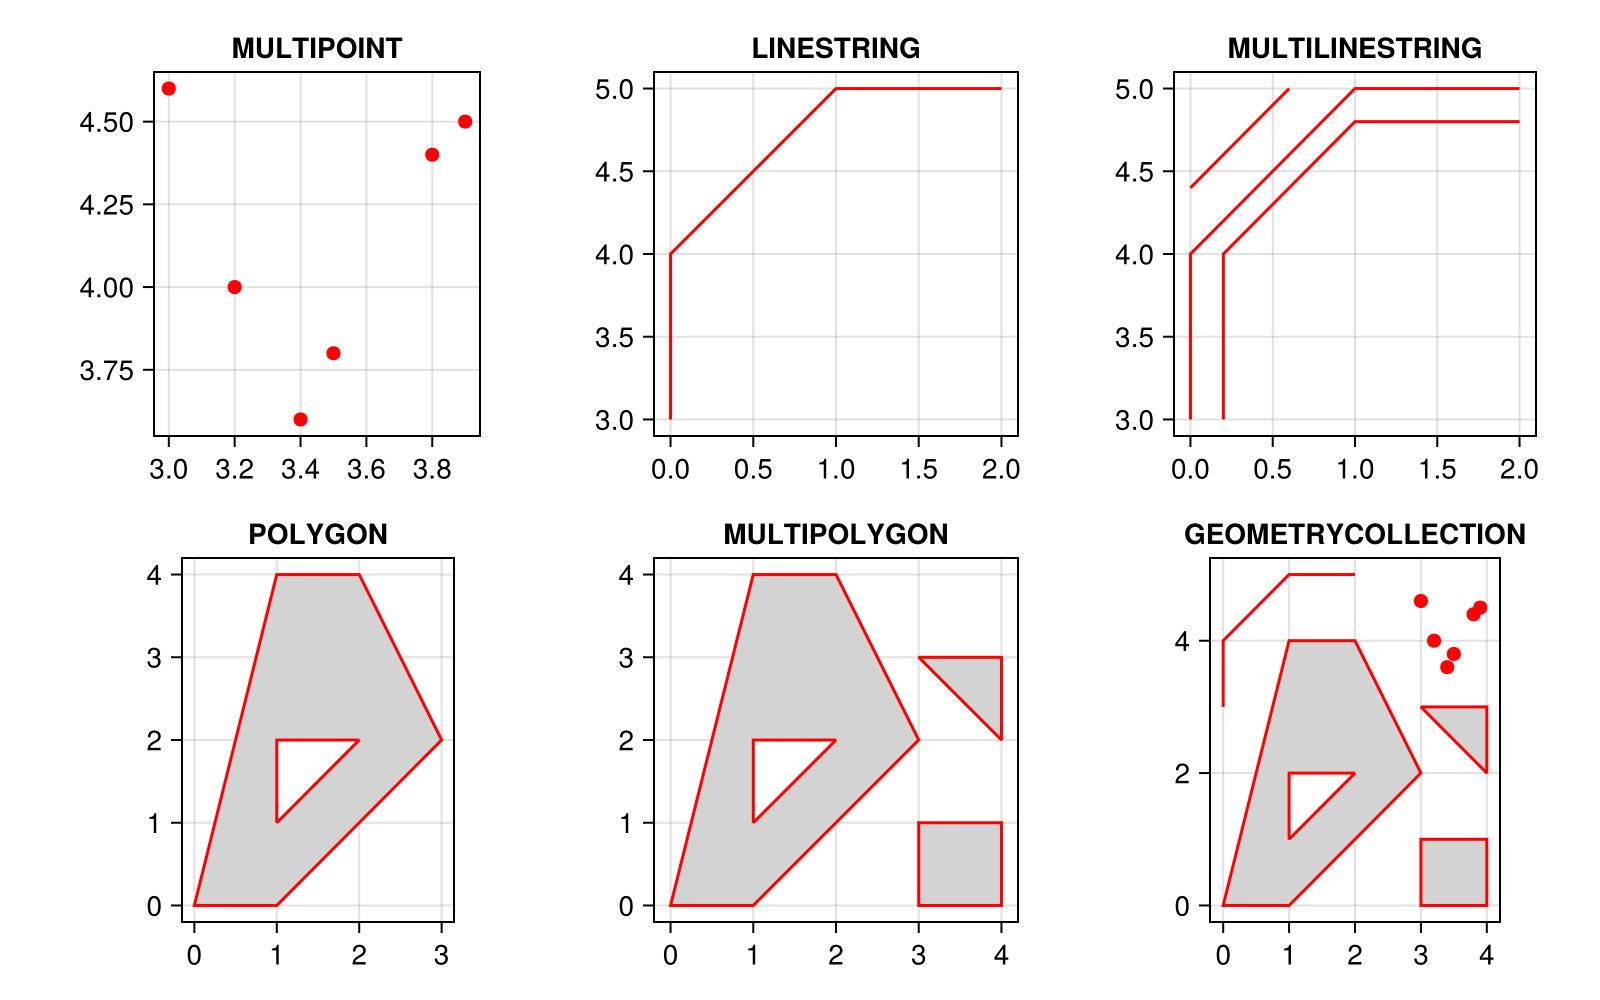
\includegraphics[width=0.8\textwidth,height=\textheight]{images/c01_plot_multigeom_julia.png}
\end{center}

\subsection{Resumen sintáctico:}\label{resumen-sintuxe1ctico}

\begin{enumerate}
\def\labelenumi{\arabic{enumi}.}
\tightlist
\item
  \textbf{Instanciación de multigeometrías}
\end{enumerate}

En la siguiente tabla se consolida la sintaxis para la creación de
estructuras geométricas complejas. Es evidente el incremento en la
profundidad de la anidación de coordenadas (uso de listas
\texttt{{[}{]}} y tuplas \texttt{()} en Python; listas \texttt{list()} y
matrices \texttt{rbind()} en R; y arreglos indexados \texttt{{[}{]}} en
Julia).

\begin{longtable}[]{@{}
  >{\raggedright\arraybackslash}p{(\columnwidth - 6\tabcolsep) * \real{0.1800}}
  >{\raggedright\arraybackslash}p{(\columnwidth - 6\tabcolsep) * \real{0.2700}}
  >{\raggedright\arraybackslash}p{(\columnwidth - 6\tabcolsep) * \real{0.2700}}
  >{\raggedright\arraybackslash}p{(\columnwidth - 6\tabcolsep) * \real{0.2800}}@{}}
\caption{Sintaxis comparativa para la inicialización y jerarquización de
topologías espaciales
complejas}\label{tbl-resumen_creacion_multigeometrias}\tabularnewline
\toprule\noalign{}
\begin{minipage}[b]{\linewidth}\raggedright
Operación geométrica
\end{minipage} & \begin{minipage}[b]{\linewidth}\raggedright
Python (\texttt{shapely}) 🐍
\end{minipage} & \begin{minipage}[b]{\linewidth}\raggedright
R (\texttt{sf}) 🔵
\end{minipage} & \begin{minipage}[b]{\linewidth}\raggedright
Julia (\texttt{ArchGDAL}) 🟣
\end{minipage} \\
\midrule\noalign{}
\endfirsthead
\toprule\noalign{}
\begin{minipage}[b]{\linewidth}\raggedright
Operación geométrica
\end{minipage} & \begin{minipage}[b]{\linewidth}\raggedright
Python (\texttt{shapely}) 🐍
\end{minipage} & \begin{minipage}[b]{\linewidth}\raggedright
R (\texttt{sf}) 🔵
\end{minipage} & \begin{minipage}[b]{\linewidth}\raggedright
Julia (\texttt{ArchGDAL}) 🟣
\end{minipage} \\
\midrule\noalign{}
\endhead
\bottomrule\noalign{}
\endlastfoot
\textbf{\texttt{MULTIPOINT}} &
\texttt{MultiPoint({[}}\texttt{(X1,Y1),\ (X2,Y2){]})} &
\texttt{st\_multipoint(}\texttt{rbind(c(X1,Y1),}\texttt{c(X2,Y2)))} &
\texttt{ArchGDAL.}\texttt{createmultipoint(}\texttt{{[}(X1,Y1),\ (X2,Y2){]})} \\
\textbf{\texttt{LINESTRING}} &
\texttt{LineString({[}}\texttt{(X1,Y1),\ (X2,Y2){]})} &
\texttt{st\_linestring(}\texttt{rbind(c(X1,Y1),}\texttt{c(X2,Y2)))} &
\texttt{ArchGDAL.}\texttt{createlinestring(}\texttt{{[}(X1,Y1),\ (X2,Y2){]})} \\
\textbf{\texttt{MULTILINESTRING}} &
\texttt{MultiLineString(}\texttt{{[}lin1,\ lin2{]})} &
\texttt{st\_multilinestring(}\texttt{list(lin1,\ lin2))} &
\texttt{ArchGDAL.}\texttt{createmultilinestring(}\texttt{{[}lin1,\ lin2{]})} \\
\textbf{\texttt{POLYGON}}\emph{(Exterior + Hueco)} &
\texttt{Polygon(}\texttt{shell=ext,\ holes={[}int1{]})} &
\texttt{st\_polygon(}\texttt{list(ext,\ int1))} &
\texttt{ArchGDAL.}\texttt{createpolygon(}\texttt{{[}ext,\ int1{]})} \\
\textbf{\texttt{MULTIPOLYGON}} &
\texttt{MultiPolygon({[}}\texttt{(ext,\ {[}int{]}),}\texttt{(ext2,\ {[}{]}){]})}
&
\texttt{st\_multipolygon(}\texttt{list(list(ext,\ int),}\texttt{list(ext2)))}
&
\texttt{ArchGDAL.}\texttt{createmultipolygon(}\texttt{{[}{[}ext,\ int{]},\ {[}ext2{]}{]})} \\
\textbf{\texttt{GEOMETRYCOLLECTION}} &
\texttt{GeometryCollection(}\texttt{{[}mp,\ pol{]})} &
\texttt{st\_geometrycollection(}\texttt{list(mp,\ pol))} &
\texttt{gc\ =\ ArchGDAL.creategeom(}\texttt{ArchGDAL.}\texttt{wkbGeometryCollection)}\texttt{ArchGDAL.}\texttt{addgeom!(gc,\ mp)} \\
\end{longtable}

\begin{enumerate}
\def\labelenumi{\arabic{enumi}.}
\setcounter{enumi}{1}
\tightlist
\item
  \textbf{Colecciones y visualización}
\end{enumerate}

En la siguiente tabla se compara la manera de orquestar estructuras
heterogéneas (\texttt{GEOMETRYCOLLECTION}) y de inicializar la interfaz
gráfica del dispositivo de ploteo. Obsérvese la discrepancia fundamental
en Julia para la instanciación de la colección basada intrínsecamente en
el estándar C/C++ Well-Known Binary (WKB).

\begin{longtable}[]{@{}
  >{\raggedright\arraybackslash}p{(\columnwidth - 6\tabcolsep) * \real{0.2000}}
  >{\raggedright\arraybackslash}p{(\columnwidth - 6\tabcolsep) * \real{0.2500}}
  >{\raggedright\arraybackslash}p{(\columnwidth - 6\tabcolsep) * \real{0.2500}}
  >{\raggedright\arraybackslash}p{(\columnwidth - 6\tabcolsep) * \real{0.3000}}@{}}
\caption{Sintaxis gráfica y paramétrica transversal para la composición
de colecciones WKB mixtas y despliegue interactivo
cartesiano}\label{tbl-resumen_dibujo_y_colecciones}\tabularnewline
\toprule\noalign{}
\begin{minipage}[b]{\linewidth}\raggedright
Operación
\end{minipage} & \begin{minipage}[b]{\linewidth}\raggedright
Python (\texttt{geopandas} /\texttt{matplotlib}) 🐍
\end{minipage} & \begin{minipage}[b]{\linewidth}\raggedright
R (\texttt{sf} /Base Graphics) 🔵
\end{minipage} & \begin{minipage}[b]{\linewidth}\raggedright
Julia (\texttt{ArchGDAL} /\texttt{CairoMakie}) 🟣
\end{minipage} \\
\midrule\noalign{}
\endfirsthead
\toprule\noalign{}
\begin{minipage}[b]{\linewidth}\raggedright
Operación
\end{minipage} & \begin{minipage}[b]{\linewidth}\raggedright
Python (\texttt{geopandas} /\texttt{matplotlib}) 🐍
\end{minipage} & \begin{minipage}[b]{\linewidth}\raggedright
R (\texttt{sf} /Base Graphics) 🔵
\end{minipage} & \begin{minipage}[b]{\linewidth}\raggedright
Julia (\texttt{ArchGDAL} /\texttt{CairoMakie}) 🟣
\end{minipage} \\
\midrule\noalign{}
\endhead
\bottomrule\noalign{}
\endlastfoot
\textbf{\texttt{GEOMETRYCOLLECTION}} &
\texttt{GeometryCollection(}\texttt{{[}p1,\ pol1,\ ls1{]})} &
\texttt{st\_geometrycollection(}\texttt{list(p1,\ pol1,\ ls1))} &
\texttt{gc\ =\ ArchGDAL.creategeom(}\texttt{ArchGDAL.wkbGeometryCollection)}\texttt{ArchGDAL.addgeom!(gc,\ p1)}\texttt{ArchGDAL.addgeom!(gc,\ pol1)} \\
\textbf{Inicializar LienzoMúltiple} &
\texttt{fig,\ axs\ =\ plt.subplots(}\texttt{filas,\ col,}\texttt{figsize=(ancho,\ alto))}
& \texttt{par(}\texttt{mfrow\ =\ c(filas,\ col))} &
\texttt{fig\ =\ Figure(}\texttt{size\ =\ (ancho,\ alto))} \\
\textbf{Pintar RellenoPolígono} &
\texttt{gpd.GeoSeries({[}pol{]})}\texttt{.plot(facecolor=\textquotesingle{}color\textquotesingle{})}
&
\texttt{plot(pol,}\texttt{col\ =\ \textquotesingle{}color\textquotesingle{})}
&
\texttt{CairoMakie.poly!(ax,}\texttt{to\_makie\_poly(pol),}\texttt{color=:color)} \\
\textbf{Pintar BordePolígono} &
\texttt{gpd.GeoSeries({[}pol{]})}\texttt{.plot(edgecolor=\textquotesingle{}color\textquotesingle{})}
&
\texttt{plot(pol,}\texttt{border\ =\ \textquotesingle{}color\textquotesingle{})}
&
\texttt{CairoMakie.poly!(ax,}\texttt{to\_makie\_poly(pol),}\texttt{strokecolor=:color)} \\
\textbf{Superponer capas} & El método \texttt{.plot()}sobre el mismo
subgráficosuperpone las capasautomáticamente. & Argumento
\texttt{add\ =\ TRUE}en la llamada a lafunción \texttt{plot()}. & Mutar
(\texttt{!}) sobre elmismo objeto referencial\texttt{ax} de Makie. \\
\end{longtable}

\begin{enumerate}
\def\labelenumi{\arabic{enumi}.}
\setcounter{enumi}{2}
\tightlist
\item
  \textbf{Inspección y extracción estructural}
\end{enumerate}

Dado que el manejo de geometrías mixtas y polígonos perforados requiere
acceder a sus componentes internos (especialmente en Julia donde el
renderizado no es automático para huecos), a continuación se exponen las
rutinas de inspección espacial.

\begin{longtable}[]{@{}
  >{\raggedright\arraybackslash}p{(\columnwidth - 6\tabcolsep) * \real{0.2500}}
  >{\raggedright\arraybackslash}p{(\columnwidth - 6\tabcolsep) * \real{0.2500}}
  >{\raggedright\arraybackslash}p{(\columnwidth - 6\tabcolsep) * \real{0.2500}}
  >{\raggedright\arraybackslash}p{(\columnwidth - 6\tabcolsep) * \real{0.2500}}@{}}
\caption{Comandos para la deconstrucción e iteración de vértices en
geometrías de jerarquía
superior}\label{tbl-resumen_extraccion_nodos}\tabularnewline
\toprule\noalign{}
\begin{minipage}[b]{\linewidth}\raggedright
Operación
\end{minipage} & \begin{minipage}[b]{\linewidth}\raggedright
Python (\texttt{shapely}) 🐍
\end{minipage} & \begin{minipage}[b]{\linewidth}\raggedright
R (\texttt{sf}) 🔵
\end{minipage} & \begin{minipage}[b]{\linewidth}\raggedright
Julia (\texttt{ArchGDAL}) 🟣
\end{minipage} \\
\midrule\noalign{}
\endfirsthead
\toprule\noalign{}
\begin{minipage}[b]{\linewidth}\raggedright
Operación
\end{minipage} & \begin{minipage}[b]{\linewidth}\raggedright
Python (\texttt{shapely}) 🐍
\end{minipage} & \begin{minipage}[b]{\linewidth}\raggedright
R (\texttt{sf}) 🔵
\end{minipage} & \begin{minipage}[b]{\linewidth}\raggedright
Julia (\texttt{ArchGDAL}) 🟣
\end{minipage} \\
\midrule\noalign{}
\endhead
\bottomrule\noalign{}
\endlastfoot
\textbf{Consultar clase/tipo} & \texttt{type(geom)} /
\texttt{geom.geom\_type} & \texttt{class(geom)} &
\texttt{ArchGDAL.getgeomtype(geom)} \\
\textbf{Conteo de sub-entidades} \emph{(vértices o anillos)} &
\texttt{len(geom.geoms)} & \texttt{length(geom)} &
\texttt{ArchGDAL.ngeom(geom)} \\
\textbf{Extraer componente} \emph{(índice de anillo exterior/interior)}
& \texttt{geom.exterior} / \texttt{geom.interiors{[}i{]}} &
\texttt{geom{[}{[}i{]}{]}} &
\texttt{ArchGDAL.getgeom(geom,\ i)}\emph{(Índice 0 = exterior)} \\
\textbf{Extraer coordenadas absolutas} & Objeto nativo de lista/tupla &
\texttt{st\_coordinates(geom)} &
\texttt{ArchGDAL.getx(geom,\ i)}\texttt{ArchGDAL.gety(geom,\ i)} \\
\end{longtable}

\begin{enumerate}
\def\labelenumi{\arabic{enumi}.}
\setcounter{enumi}{3}
\tightlist
\item
  \textbf{Configuración de lienzo y parámetros gráficos}
\end{enumerate}

Desglose de los argumentos estéticos y las funciones de enrutamiento
espacial utilizados para garantizar un renderizado coherente de los
datos (simulando los estándares de visualización de entidades
cartográficas).

\begin{longtable}[]{@{}
  >{\raggedright\arraybackslash}p{(\columnwidth - 6\tabcolsep) * \real{0.2200}}
  >{\raggedright\arraybackslash}p{(\columnwidth - 6\tabcolsep) * \real{0.2600}}
  >{\raggedright\arraybackslash}p{(\columnwidth - 6\tabcolsep) * \real{0.2600}}
  >{\raggedright\arraybackslash}p{(\columnwidth - 6\tabcolsep) * \real{0.2600}}@{}}
\caption{Equivalencia de parámetros para la composición de atlas
cartográficos y estandarización
cromática}\label{tbl-resumen_parametros_graficos}\tabularnewline
\toprule\noalign{}
\begin{minipage}[b]{\linewidth}\raggedright
Configuración visual
\end{minipage} & \begin{minipage}[b]{\linewidth}\raggedright
Python (\texttt{geopandas}/\texttt{matplotlib}) 🐍
\end{minipage} & \begin{minipage}[b]{\linewidth}\raggedright
R (\texttt{sf}/Base Graphics) 🔵
\end{minipage} & \begin{minipage}[b]{\linewidth}\raggedright
Julia (\texttt{CairoMakie}) 🟣
\end{minipage} \\
\midrule\noalign{}
\endfirsthead
\toprule\noalign{}
\begin{minipage}[b]{\linewidth}\raggedright
Configuración visual
\end{minipage} & \begin{minipage}[b]{\linewidth}\raggedright
Python (\texttt{geopandas}/\texttt{matplotlib}) 🐍
\end{minipage} & \begin{minipage}[b]{\linewidth}\raggedright
R (\texttt{sf}/Base Graphics) 🔵
\end{minipage} & \begin{minipage}[b]{\linewidth}\raggedright
Julia (\texttt{CairoMakie}) 🟣
\end{minipage} \\
\midrule\noalign{}
\endhead
\bottomrule\noalign{}
\endlastfoot
\textbf{Matriz de subgráficos (Grid)} &
\texttt{fig,\ axs\ =\ plt.subplots(filas,\ col,\ figsize=(W,\ H))} &
\texttt{par(mfrow\ =\ c(filas,\ col))} &
\texttt{fig\ =\ Figure(size\ =\ (W,\ H))}\texttt{ax\ =\ Axis(fig{[}f,\ c{]})} \\
\textbf{Control de márgenes y ejes} &
\texttt{plt.tight\_layout()}\texttt{ax.set\_xticks({[}{]})} &
\texttt{par(mar\ =\ c(B,\ L,\ T,\ R))}\texttt{axes\ =\ TRUE} &
\texttt{ax.aspect\ =\ DataAspect()}\texttt{hidedecorations!(ax)} \\
\textbf{Encuadre geográfico (Bounding Box)} & \emph{Automático por
GeoPandas} & Argumentos \texttt{xlim=c()}, \texttt{ylim=c()} &
\emph{Automático por CairoMakie} \\
\textbf{Color de relleno (Áreas)} &
\texttt{.plot(facecolor=\textquotesingle{}lightgrey\textquotesingle{})}
&
\texttt{plot(...,\ col\ =\ \textquotesingle{}lightgrey\textquotesingle{})}
& \texttt{poly!(...,\ color=:lightgray)} \\
\textbf{Color de trazo (Líneas y bordes)} &
\texttt{.plot(color=\textquotesingle{}red\textquotesingle{},\ edgecolor=\textquotesingle{}red\textquotesingle{})}
&
\texttt{plot(...,\ border\ =\ \textquotesingle{}red\textquotesingle{})}
&
\texttt{lines!(...,\ color=:red)}\texttt{poly!(...,\ strokecolor=:red)} \\
\textbf{Grosor vectorial} & \texttt{linewidth=1.5} & \texttt{lwd=1.5} &
\texttt{linewidth=1.5} / \texttt{strokewidth=1.5} \\
\textbf{Simbología de puntos} & \texttt{markersize=25} &
\texttt{pch=16,\ cex=1.2} & \texttt{markersize=10} \\
\textbf{Superposición de capas (Z-index)} & Llamadas sucesivas al mismo
\texttt{ax} & Llamadas sucesivas con \texttt{add\ =\ TRUE} & Mutación
(\texttt{!}) sucesiva sobre el mismo \texttt{ax} \\
\end{longtable}

\section{Creación de puntos a partir de texto WKT (Well-Known
Text)}\label{creaciuxf3n-de-puntos-a-partir-de-texto-wkt-well-known-text}

El formato WKT (Well-Known Text) es un estándar de la OGC para
representar geometrías en formato de texto.

A continuación, se define un conjunto de tres lugares representativos de
Colombia utilizando cadenas WKT. Se asigna un atributo de texto
(\texttt{Lugar}), se ensambla la tabla espacial y se genera un mapa
categorizado por dicho atributo, incluyendo su respectiva leyenda.

\subsection{Python}

\begin{Shaded}
\begin{Highlighting}[]
\ImportTok{import}\NormalTok{ pandas }\ImportTok{as}\NormalTok{ pd}
\ImportTok{import}\NormalTok{ geopandas }\ImportTok{as}\NormalTok{ gpd}
\ImportTok{import}\NormalTok{ matplotlib.pyplot }\ImportTok{as}\NormalTok{ plt}

\CommentTok{\# 1. Definición de atributos y geometrías en formato WKT}
\NormalTok{datos\_wkt }\OperatorTok{=}\NormalTok{ \{}
    \StringTok{"Lugar"}\NormalTok{: [}\StringTok{"Centro Geográfico"}\NormalTok{, }\StringTok{"Plaza de Bolívar"}\NormalTok{, }\StringTok{"Piedra del Peñol"}\NormalTok{],}
    \StringTok{"WKT"}\NormalTok{: [}
        \StringTok{"POINT ({-}72.9553 4.0903)"}\NormalTok{,}
        \StringTok{"POINT ({-}74.0760 4.5981)"}\NormalTok{,}
        \StringTok{"POINT ({-}75.1792 6.2205)"}
\NormalTok{    ]}
\NormalTok{\}}

\CommentTok{\# 2. Conversión a GeoDataFrame usando from\_wkt}
\NormalTok{gdf\_wkt }\OperatorTok{=}\NormalTok{ gpd.GeoDataFrame(}
\NormalTok{    datos\_wkt, }
\NormalTok{    geometry}\OperatorTok{=}\NormalTok{gpd.GeoSeries.from\_wkt(datos\_wkt[}\StringTok{"WKT"}\NormalTok{]),}
\NormalTok{    crs}\OperatorTok{=}\StringTok{"EPSG:4326"}
\NormalTok{)}

\CommentTok{\# 3. Inspección de la arquitectura espacial}
\BuiltInTok{print}\NormalTok{(}\StringTok{"{-}{-}{-} Primitiva Geométrica (Registro 0) {-}{-}{-}"}\NormalTok{)}
\end{Highlighting}
\end{Shaded}

\begin{verbatim}
--- Primitiva Geométrica (Registro 0) ---
\end{verbatim}

\begin{Shaded}
\begin{Highlighting}[]
\BuiltInTok{print}\NormalTok{(gdf\_wkt.geometry[}\DecValTok{0}\NormalTok{])}
\end{Highlighting}
\end{Shaded}

\begin{verbatim}
POINT (-72.9553 4.0903)
\end{verbatim}

\begin{Shaded}
\begin{Highlighting}[]
\BuiltInTok{print}\NormalTok{(}\BuiltInTok{type}\NormalTok{(gdf\_wkt.geometry[}\DecValTok{0}\NormalTok{]), }\StringTok{"}\CharTok{\textbackslash{}n}\StringTok{"}\NormalTok{)}
\end{Highlighting}
\end{Shaded}

\begin{verbatim}
<class 'shapely.geometry.point.Point'> 
\end{verbatim}

\begin{Shaded}
\begin{Highlighting}[]
\BuiltInTok{print}\NormalTok{(}\StringTok{"{-}{-}{-} Columna de Geometría {-}{-}{-}"}\NormalTok{)}
\end{Highlighting}
\end{Shaded}

\begin{verbatim}
--- Columna de Geometría ---
\end{verbatim}

\begin{Shaded}
\begin{Highlighting}[]
\BuiltInTok{print}\NormalTok{(gdf\_wkt.geometry)}
\end{Highlighting}
\end{Shaded}

\begin{verbatim}
0    POINT (-72.9553 4.0903)
1     POINT (-74.076 4.5981)
2    POINT (-75.1792 6.2205)
Name: geometry, dtype: geometry
\end{verbatim}

\begin{Shaded}
\begin{Highlighting}[]
\BuiltInTok{print}\NormalTok{(}\BuiltInTok{type}\NormalTok{(gdf\_wkt.geometry), }\StringTok{"}\CharTok{\textbackslash{}n}\StringTok{"}\NormalTok{)}
\end{Highlighting}
\end{Shaded}

\begin{verbatim}
<class 'geopandas.geoseries.GeoSeries'> 
\end{verbatim}

\begin{Shaded}
\begin{Highlighting}[]
\BuiltInTok{print}\NormalTok{(}\StringTok{"{-}{-}{-} Estructura de la Tabla {-}{-}{-}"}\NormalTok{)}
\end{Highlighting}
\end{Shaded}

\begin{verbatim}
--- Estructura de la Tabla ---
\end{verbatim}

\begin{Shaded}
\begin{Highlighting}[]
\BuiltInTok{print}\NormalTok{(gdf\_wkt)}
\end{Highlighting}
\end{Shaded}

\begin{verbatim}
               Lugar                      WKT                 geometry
0  Centro Geográfico  POINT (-72.9553 4.0903)  POINT (-72.9553 4.0903)
1   Plaza de Bolívar  POINT (-74.0760 4.5981)   POINT (-74.076 4.5981)
2   Piedra del Peñol  POINT (-75.1792 6.2205)  POINT (-75.1792 6.2205)
\end{verbatim}

\begin{Shaded}
\begin{Highlighting}[]
\BuiltInTok{print}\NormalTok{(}\BuiltInTok{type}\NormalTok{(gdf\_wkt), }\StringTok{"}\CharTok{\textbackslash{}n}\StringTok{"}\NormalTok{)}
\end{Highlighting}
\end{Shaded}

\begin{verbatim}
<class 'geopandas.geodataframe.GeoDataFrame'> 
\end{verbatim}

\begin{Shaded}
\begin{Highlighting}[]
\CommentTok{\# 4. Visualización categorizada por el atributo \textquotesingle{}Lugar\textquotesingle{}}
\NormalTok{fig, ax }\OperatorTok{=}\NormalTok{ plt.subplots(figsize}\OperatorTok{=}\NormalTok{(}\DecValTok{8}\NormalTok{, }\DecValTok{6}\NormalTok{))}
\NormalTok{gdf\_wkt.plot(}
\NormalTok{    ax}\OperatorTok{=}\NormalTok{ax,}
\NormalTok{    column}\OperatorTok{=}\StringTok{"Lugar"}\NormalTok{,}
\NormalTok{    legend}\OperatorTok{=}\VariableTok{True}\NormalTok{,}
\NormalTok{    markersize}\OperatorTok{=}\DecValTok{100}\NormalTok{, }
\NormalTok{    cmap}\OperatorTok{=}\StringTok{"Set1"}
\NormalTok{)}
\NormalTok{ax.set\_title(}\StringTok{"Lugares Representativos {-} Colombia (WKT)"}\NormalTok{)}
\NormalTok{ax.set\_xlabel(}\StringTok{"Longitud"}\NormalTok{)}
\NormalTok{ax.set\_ylabel(}\StringTok{"Latitud"}\NormalTok{)}
\NormalTok{plt.show()}
\end{Highlighting}
\end{Shaded}

\begin{center}
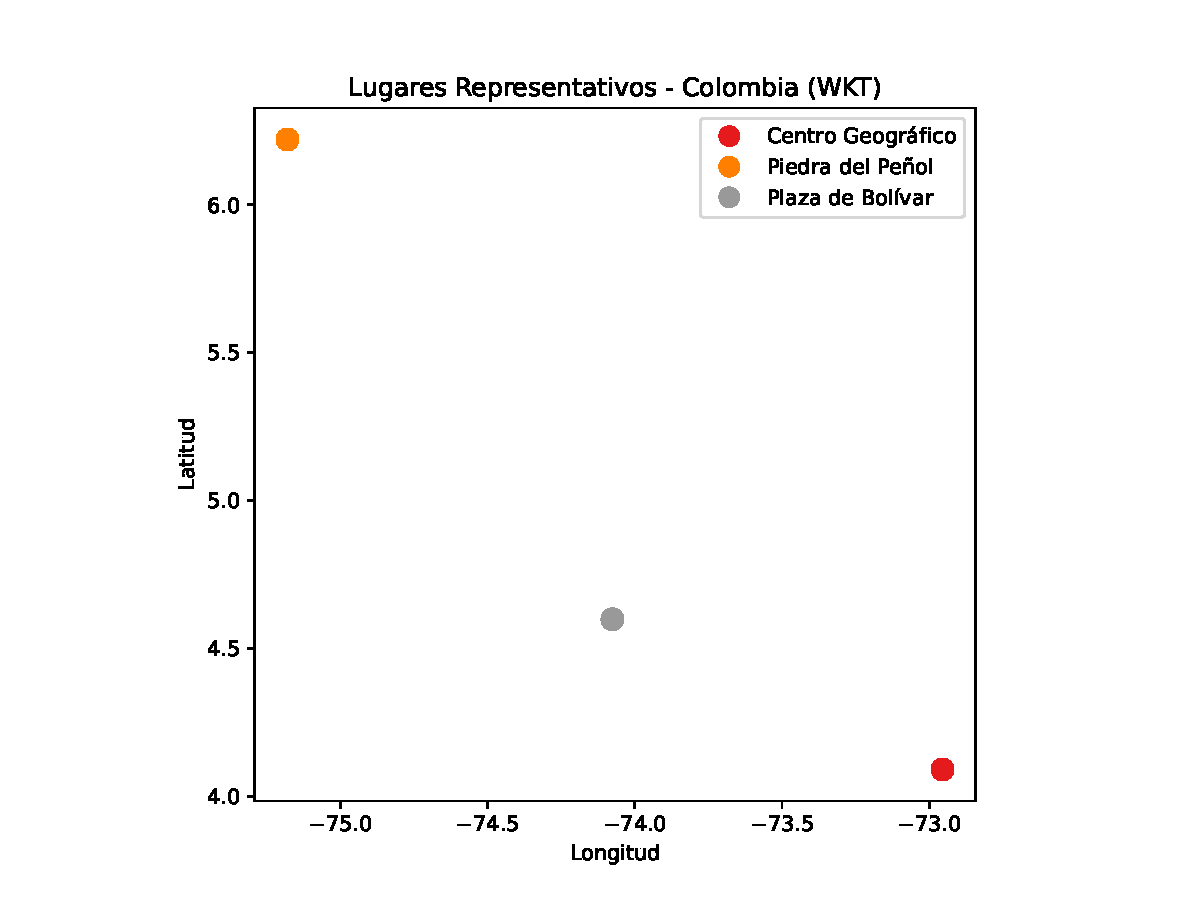
\includegraphics[width=0.8\textwidth,height=\textheight]{14-vector_files/figure-pdf/python_crear_wkt-1.pdf}
\end{center}

\subsection{R}

\begin{Shaded}
\begin{Highlighting}[]
\FunctionTok{library}\NormalTok{(sf)}

\CommentTok{\# 1. Definición de vectores de atributos y cadenas WKT}
\NormalTok{lugares }\OtherTok{\textless{}{-}} \FunctionTok{c}\NormalTok{(}\StringTok{"Centro Geográfico"}\NormalTok{, }\StringTok{"Plaza de Bolívar"}\NormalTok{, }\StringTok{"Piedra del Peñol"}\NormalTok{)}
\NormalTok{wkt\_cadenas }\OtherTok{\textless{}{-}} \FunctionTok{c}\NormalTok{(}
  \StringTok{"POINT ({-}72.9553 4.0903)"}\NormalTok{,}
  \StringTok{"POINT ({-}74.0760 4.5981)"}\NormalTok{,}
  \StringTok{"POINT ({-}75.1792 6.2205)"}
\NormalTok{)}

\CommentTok{\# 2. Construcción de la jerarquía espacial}
\NormalTok{geom\_sfc }\OtherTok{\textless{}{-}} \FunctionTok{st\_as\_sfc}\NormalTok{(wkt\_cadenas, }\AttributeTok{crs =} \DecValTok{4326}\NormalTok{)}
\NormalTok{gdf\_wkt }\OtherTok{\textless{}{-}} \FunctionTok{st\_sf}\NormalTok{(}\AttributeTok{Lugar =}\NormalTok{ lugares, }\AttributeTok{geometry =}\NormalTok{ geom\_sfc)}

\CommentTok{\# 3. Inspección de la arquitectura espacial}
\FunctionTok{print}\NormalTok{(}\StringTok{"{-}{-}{-} Primitiva Geométrica {-}{-}{-}"}\NormalTok{)}
\end{Highlighting}
\end{Shaded}

\begin{verbatim}
[1] "--- Primitiva Geométrica ---"
\end{verbatim}

\begin{Shaded}
\begin{Highlighting}[]
\FunctionTok{print}\NormalTok{(geom\_sfc[[}\DecValTok{1}\NormalTok{]])}
\end{Highlighting}
\end{Shaded}

\begin{verbatim}
POINT (-72.9553 4.0903)
\end{verbatim}

\begin{Shaded}
\begin{Highlighting}[]
\FunctionTok{print}\NormalTok{(}\FunctionTok{class}\NormalTok{(geom\_sfc[[}\DecValTok{1}\NormalTok{]]))}
\end{Highlighting}
\end{Shaded}

\begin{verbatim}
[1] "XY"    "POINT" "sfg"  
\end{verbatim}

\begin{Shaded}
\begin{Highlighting}[]
\FunctionTok{print}\NormalTok{(}\StringTok{"{-}{-}{-} Columna de Geometría {-}{-}{-}"}\NormalTok{)}
\end{Highlighting}
\end{Shaded}

\begin{verbatim}
[1] "--- Columna de Geometría ---"
\end{verbatim}

\begin{Shaded}
\begin{Highlighting}[]
\FunctionTok{print}\NormalTok{(gdf\_wkt}\SpecialCharTok{$}\NormalTok{geometry)}
\end{Highlighting}
\end{Shaded}

\begin{verbatim}
Geometry set for 3 features 
Geometry type: POINT
Dimension:     XY
Bounding box:  xmin: -75.1792 ymin: 4.0903 xmax: -72.9553 ymax: 6.2205
Geodetic CRS:  WGS 84
\end{verbatim}

\begin{verbatim}
POINT (-72.9553 4.0903)
\end{verbatim}

\begin{verbatim}
POINT (-74.076 4.5981)
\end{verbatim}

\begin{verbatim}
POINT (-75.1792 6.2205)
\end{verbatim}

\begin{Shaded}
\begin{Highlighting}[]
\FunctionTok{print}\NormalTok{(}\FunctionTok{class}\NormalTok{(gdf\_wkt}\SpecialCharTok{$}\NormalTok{geometry))}
\end{Highlighting}
\end{Shaded}

\begin{verbatim}
[1] "sfc_POINT" "sfc"      
\end{verbatim}

\begin{Shaded}
\begin{Highlighting}[]
\FunctionTok{print}\NormalTok{(}\StringTok{"{-}{-}{-} Estructura de la Tabla {-}{-}{-}"}\NormalTok{)}
\end{Highlighting}
\end{Shaded}

\begin{verbatim}
[1] "--- Estructura de la Tabla ---"
\end{verbatim}

\begin{Shaded}
\begin{Highlighting}[]
\FunctionTok{print}\NormalTok{(gdf\_wkt)}
\end{Highlighting}
\end{Shaded}

\begin{verbatim}
Simple feature collection with 3 features and 1 field
Geometry type: POINT
Dimension:     XY
Bounding box:  xmin: -75.1792 ymin: 4.0903 xmax: -72.9553 ymax: 6.2205
Geodetic CRS:  WGS 84
              Lugar                geometry
1 Centro Geográfico POINT (-72.9553 4.0903)
2  Plaza de Bolívar  POINT (-74.076 4.5981)
3  Piedra del Peñol POINT (-75.1792 6.2205)
\end{verbatim}

\begin{Shaded}
\begin{Highlighting}[]
\FunctionTok{print}\NormalTok{(}\FunctionTok{class}\NormalTok{(gdf\_wkt))}
\end{Highlighting}
\end{Shaded}

\begin{verbatim}
[1] "sf"         "data.frame"
\end{verbatim}

\begin{Shaded}
\begin{Highlighting}[]
\CommentTok{\# 4. Visualización gráfica categorizada}
\FunctionTok{plot}\NormalTok{(}
\NormalTok{  gdf\_wkt[}\StringTok{"Lugar"}\NormalTok{], }
  \AttributeTok{main =} \StringTok{"Lugares Representativos {-} Colombia (WKT)"}\NormalTok{,}
  \AttributeTok{pch =} \DecValTok{16}\NormalTok{, }
  \AttributeTok{cex =} \DecValTok{2}\NormalTok{,}
  \AttributeTok{axes =} \ConstantTok{TRUE}\NormalTok{,}
  \AttributeTok{key.pos =} \DecValTok{4}
\NormalTok{)}
\end{Highlighting}
\end{Shaded}

\begin{center}
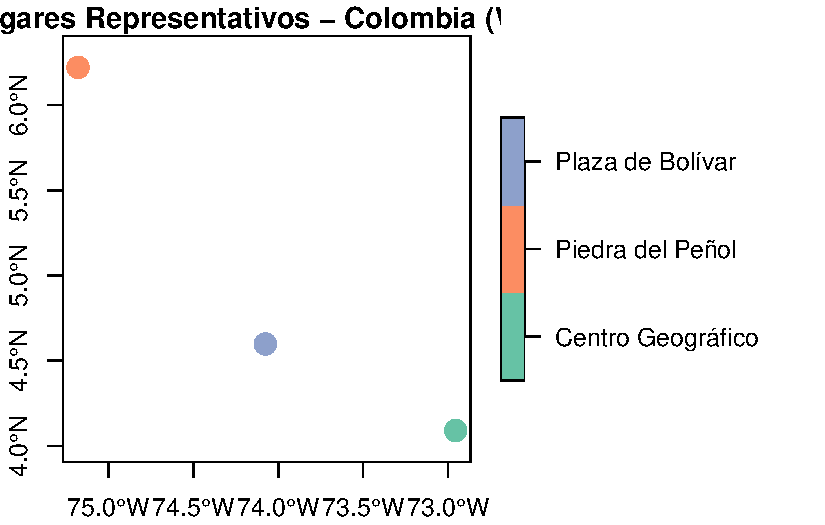
\includegraphics[width=0.8\textwidth,height=\textheight]{14-vector_files/figure-pdf/r_crear_wkt-1.pdf}
\end{center}

\subsection{Julia}

\begin{Shaded}
\begin{Highlighting}[]
\FunctionTok{j\_eval}\NormalTok{(}\StringTok{\textquotesingle{}}
\StringTok{using ArchGDAL}
\StringTok{using DataFrames}
\StringTok{using Plots}

\StringTok{\# 1. Definición de vectores base}
\StringTok{lugares = ["Centro Geográfico", "Plaza de Bolívar", "Piedra del Peñol"]}
\StringTok{wkt\_cadenas = [}
\StringTok{    "POINT ({-}72.9553 4.0903)",}
\StringTok{    "POINT ({-}74.0760 4.5981)",}
\StringTok{    "POINT ({-}75.1792 6.2205)"}
\StringTok{]}

\StringTok{\# 2. Conversión vectorial a primitivas IGeometry}
\StringTok{geometrias = ArchGDAL.fromWKT.(wkt\_cadenas)}

\StringTok{\# Ensamblaje de la tabla espacial}
\StringTok{df\_wkt = DataFrame(Lugar = lugares, geometry = geometrias)}

\StringTok{\# 3. Inspección de la arquitectura espacial}
\StringTok{println("{-}{-}{-} Primitiva Geométrica {-}{-}{-}")}
\StringTok{println("Tipo: ", typeof(geometrias[1]))}

\StringTok{println("}\SpecialCharTok{\textbackslash{}\textbackslash{}}\StringTok{n{-}{-}{-} Columna de Geometría {-}{-}{-}")}
\StringTok{println("Tipo: ", typeof(df\_wkt.geometry))}

\StringTok{println("}\SpecialCharTok{\textbackslash{}\textbackslash{}}\StringTok{n{-}{-}{-} Estructura de la Tabla {-}{-}{-}")}
\StringTok{println("Tipo: ", typeof(df\_wkt))}

\StringTok{\# 4. Visualización gráfica y exportación}
\StringTok{x\_coords = ArchGDAL.getx.(df\_wkt.geometry, 0)}
\StringTok{y\_coords = ArchGDAL.gety.(df\_wkt.geometry, 0)}

\StringTok{p = Plots.scatter(}
\StringTok{    x\_coords, y\_coords, }
\StringTok{    group = df\_wkt.Lugar, }
\StringTok{    title = "Lugares Representativos (WKT)",}
\StringTok{    xlabel = "Longitud", ylabel = "Latitud",}
\StringTok{    markersize = 8, aspect\_ratio = :equal,}
\StringTok{    legend = :outertopright}
\StringTok{)}

\StringTok{Plots.savefig(p, "images/c14\_plot\_wkt\_lugares\_julia.png")}
\StringTok{\textquotesingle{}}\NormalTok{)}
\end{Highlighting}
\end{Shaded}

\begin{Shaded}
\begin{Highlighting}[]
\NormalTok{knitr}\SpecialCharTok{::}\FunctionTok{include\_graphics}\NormalTok{(}\StringTok{"images/c14\_plot\_wkt\_lugares\_julia.png"}\NormalTok{)}
\end{Highlighting}
\end{Shaded}

\begin{center}
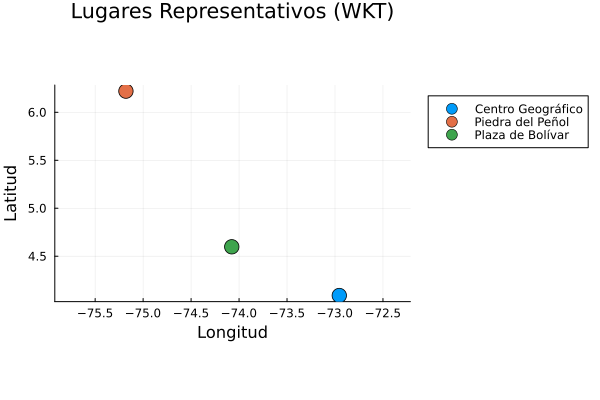
\includegraphics[width=0.8\textwidth,height=\textheight]{images/c14_plot_wkt_lugares_julia.png}
\end{center}

\subsection{Resumen sintáctico: Creación de puntos desde
WKT}\label{resumen-sintuxe1ctico-creaciuxf3n-de-puntos-desde-wkt}

\begin{longtable}[]{@{}
  >{\raggedright\arraybackslash}p{(\columnwidth - 6\tabcolsep) * \real{0.2000}}
  >{\raggedright\arraybackslash}p{(\columnwidth - 6\tabcolsep) * \real{0.2600}}
  >{\raggedright\arraybackslash}p{(\columnwidth - 6\tabcolsep) * \real{0.2600}}
  >{\raggedright\arraybackslash}p{(\columnwidth - 6\tabcolsep) * \real{0.2800}}@{}}
\caption{Sintaxis comparativa para la creación y visualización de puntos
mediante texto WKT}\label{tbl-resumen_puntos_wkt}\tabularnewline
\toprule\noalign{}
\begin{minipage}[b]{\linewidth}\raggedright
Operación
\end{minipage} & \begin{minipage}[b]{\linewidth}\raggedright
Python (\texttt{geopandas}) 🐍
\end{minipage} & \begin{minipage}[b]{\linewidth}\raggedright
R (\texttt{sf}) 🔵
\end{minipage} & \begin{minipage}[b]{\linewidth}\raggedright
Julia (\texttt{ArchGDAL} + \texttt{Plots}) 🟣
\end{minipage} \\
\midrule\noalign{}
\endfirsthead
\toprule\noalign{}
\begin{minipage}[b]{\linewidth}\raggedright
Operación
\end{minipage} & \begin{minipage}[b]{\linewidth}\raggedright
Python (\texttt{geopandas}) 🐍
\end{minipage} & \begin{minipage}[b]{\linewidth}\raggedright
R (\texttt{sf}) 🔵
\end{minipage} & \begin{minipage}[b]{\linewidth}\raggedright
Julia (\texttt{ArchGDAL} + \texttt{Plots}) 🟣
\end{minipage} \\
\midrule\noalign{}
\endhead
\bottomrule\noalign{}
\endlastfoot
\textbf{Conversión WKT} & \texttt{gpd.GeoSeries.from\_wkt(lista\_wkt)} &
\texttt{st\_as\_sfc(vector\_wkt)} &
\texttt{ArchGDAL.fromWKT.(arreglo\_wkt)} \\
\textbf{Integración Tabla} &
\texttt{gpd.GeoDataFrame(df,\ geometry=geom)} &
\texttt{st\_sf(df,\ geometry\ =\ geom)} &
\texttt{DataFrame(df,\ geometry\ =\ geom)} \\
\textbf{Plot categórico} &
\texttt{gdf.plot(column="Attr",\ legend=True)} &
\texttt{plot(gdf{[}"Attr"{]})} & \textbf{Nativo:}
\texttt{scatter(x,\ y,\ group=df.Attr)}\textbf{StatsPlots:}
\texttt{@df\ df\ scatter(x,\ y,\ group=:Attr)} \\
\end{longtable}

\section{Creación de otras multigeometrías a partir de texto
WKT}\label{creaciuxf3n-de-otras-multigeometruxedas-a-partir-de-texto-wkt}

El formato WKT no se limita exclusivamente a la definición de puntos
individuales. Su versatilidad estructural permite codificar geometrías
de mayor dimensionalidad y complejidad topológica, tales como líneas,
polígonos, y colecciones de estas primitivas, utilizando una sintaxis
anidada mediante paréntesis.

A continuación, se estructuran tres representaciones geográficas en
Colombia utilizando WKT: una sede universitaria particionada
(Multipunto), el trazo de un río (Línea) y los límites simplificados de
una reserva natural (Polígono). Estos objetos disímiles se consolidan en
una única tabla espacial para su renderizado simultáneo.

\subsection{Python}

\begin{Shaded}
\begin{Highlighting}[]
\ImportTok{import}\NormalTok{ pandas }\ImportTok{as}\NormalTok{ pd}
\ImportTok{import}\NormalTok{ geopandas }\ImportTok{as}\NormalTok{ gpd}
\ImportTok{import}\NormalTok{ matplotlib.pyplot }\ImportTok{as}\NormalTok{ plt}

\CommentTok{\# 1. Definición de atributos y geometrías complejas en formato WKT}
\CommentTok{\# Se modelan tres entidades representativas del territorio colombiano}
\NormalTok{datos\_wkt }\OperatorTok{=}\NormalTok{ \{}
    \StringTok{"Entidad"}\NormalTok{: [}\StringTok{"Sedes UNAL Bogotá (MultiPoint)"}\NormalTok{, }\StringTok{"Tramo Río Magdalena (LineString)"}\NormalTok{, }\StringTok{"PNN Chingaza (Polygon)"}\NormalTok{],}
    \StringTok{"WKT"}\NormalTok{: [}
        \StringTok{"MULTIPOINT ({-}74.0990 4.6386, {-}74.0830 4.6360)"}\NormalTok{,}
        \StringTok{"LINESTRING ({-}74.7700 5.2000, {-}74.7000 5.5000, {-}74.6500 5.8000)"}\NormalTok{,}
        \StringTok{"POLYGON (({-}73.8000 4.7000, {-}73.6000 4.7000, {-}73.6000 4.5000, {-}73.8000 4.5000, {-}73.8000 4.7000))"}
\NormalTok{    ]}
\NormalTok{\}}

\CommentTok{\# 2. Conversión a GeoDataFrame usando from\_wkt}
\CommentTok{\# El método from\_wkt interpreta la cadena de texto y construye la topología vectorial sin importar su dimensionalidad}
\NormalTok{gdf\_complejo }\OperatorTok{=}\NormalTok{ gpd.GeoDataFrame(}
\NormalTok{    datos\_wkt, }
\NormalTok{    geometry}\OperatorTok{=}\NormalTok{gpd.GeoSeries.from\_wkt(datos\_wkt[}\StringTok{"WKT"}\NormalTok{]),}
\NormalTok{    crs}\OperatorTok{=}\StringTok{"EPSG:4326"}
\NormalTok{)}

\CommentTok{\# 3. Inspección de la arquitectura espacial}
\BuiltInTok{print}\NormalTok{(}\StringTok{"{-}{-}{-} Estructura de la Tabla con Multigeometrías {-}{-}{-}"}\NormalTok{)}
\end{Highlighting}
\end{Shaded}

\begin{verbatim}
--- Estructura de la Tabla con Multigeometrías ---
\end{verbatim}

\begin{Shaded}
\begin{Highlighting}[]
\BuiltInTok{print}\NormalTok{(gdf\_complejo)}
\end{Highlighting}
\end{Shaded}

\begin{verbatim}
                            Entidad  ...                                           geometry
0    Sedes UNAL Bogotá (MultiPoint)  ...     MULTIPOINT ((-74.099 4.6386), (-74.083 4.636))
1  Tramo Río Magdalena (LineString)  ...     LINESTRING (-74.77 5.2, -74.7 5.5, -74.65 5.8)
2            PNN Chingaza (Polygon)  ...  POLYGON ((-73.8 4.7, -73.6 4.7, -73.6 4.5, -73...

[3 rows x 3 columns]
\end{verbatim}

\begin{Shaded}
\begin{Highlighting}[]
\BuiltInTok{print}\NormalTok{(}\StringTok{"}\CharTok{\textbackslash{}n}\StringTok{{-}{-}{-} Tipos geométricos generados {-}{-}{-}"}\NormalTok{)}
\end{Highlighting}
\end{Shaded}

\begin{verbatim}

--- Tipos geométricos generados ---
\end{verbatim}

\begin{Shaded}
\begin{Highlighting}[]
\BuiltInTok{print}\NormalTok{(gdf\_complejo.geom\_type)}
\end{Highlighting}
\end{Shaded}

\begin{verbatim}
0    MultiPoint
1    LineString
2       Polygon
dtype: object
\end{verbatim}

\begin{Shaded}
\begin{Highlighting}[]
\CommentTok{\# 4. Visualización categorizada por el atributo \textquotesingle{}Entidad\textquotesingle{}}
\NormalTok{fig, ax }\OperatorTok{=}\NormalTok{ plt.subplots(figsize}\OperatorTok{=}\NormalTok{(}\DecValTok{8}\NormalTok{, }\DecValTok{6}\NormalTok{))}

\CommentTok{\# La función plot de GeoPandas discrimina automáticamente cómo dibujar áreas, líneas y puntos}
\NormalTok{gdf\_complejo.plot(}
\NormalTok{    ax}\OperatorTok{=}\NormalTok{ax,}
\NormalTok{    column}\OperatorTok{=}\StringTok{"Entidad"}\NormalTok{,    }\CommentTok{\# Columna de categorización cromática}
\NormalTok{    legend}\OperatorTok{=}\VariableTok{True}\NormalTok{,         }\CommentTok{\# Despliegue automático de la leyenda}
\NormalTok{    cmap}\OperatorTok{=}\StringTok{"Dark2"}\NormalTok{,        }\CommentTok{\# Paleta de colores para elementos categóricos}
\NormalTok{    linewidth}\OperatorTok{=}\DecValTok{2}\NormalTok{,         }\CommentTok{\# Grosor de visualización para líneas y bordes}
\NormalTok{    markersize}\OperatorTok{=}\DecValTok{80}        \CommentTok{\# Diámetro de visualización para puntos}
\NormalTok{)}

\CommentTok{\# Activar la Grilla}
\NormalTok{ax.grid(}\VariableTok{True}\NormalTok{)}

\CommentTok{\# Personalizar la Grilla.}
\NormalTok{ax.grid(}
    \VariableTok{True}\NormalTok{,}
\NormalTok{    linestyle}\OperatorTok{=}\StringTok{"{-}{-}"}\NormalTok{,}
\NormalTok{    linewidth}\OperatorTok{=}\FloatTok{0.5}\NormalTok{,}
\NormalTok{    alpha}\OperatorTok{=}\FloatTok{0.7}
\NormalTok{)}

\CommentTok{\# Espaciado entre líneas de la grilla}
\ImportTok{import}\NormalTok{ matplotlib.ticker }\ImportTok{as}\NormalTok{ ticker}

\CommentTok{\# Cada 0.5 grados}
\NormalTok{ax.xaxis.set\_major\_locator(ticker.MultipleLocator(}\FloatTok{0.5}\NormalTok{))  }
\NormalTok{ax.yaxis.set\_major\_locator(ticker.MultipleLocator(}\FloatTok{0.5}\NormalTok{))}

\NormalTok{ax.set\_title(}\StringTok{"Multigeometrías en Colombia (WKT)"}\NormalTok{)}
\NormalTok{ax.set\_xlabel(}\StringTok{"Longitud"}\NormalTok{)}
\NormalTok{ax.set\_ylabel(}\StringTok{"Latitud"}\NormalTok{)}
\NormalTok{plt.show()}
\end{Highlighting}
\end{Shaded}

\begin{center}
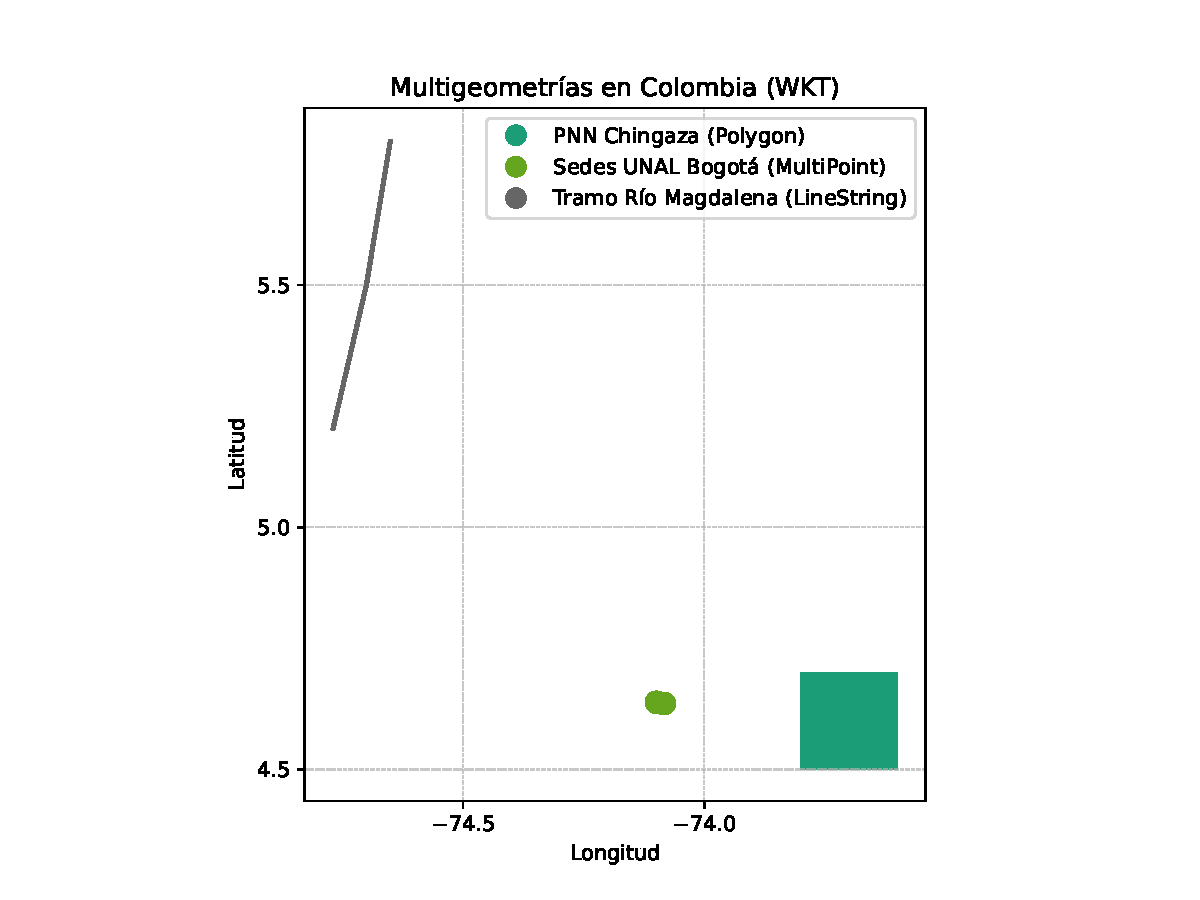
\includegraphics[width=0.8\textwidth,height=\textheight]{14-vector_files/figure-pdf/python_wkt_multigeom-1.pdf}
\end{center}

\subsection{R}

\begin{Shaded}
\begin{Highlighting}[]
\FunctionTok{library}\NormalTok{(sf)}

\CommentTok{\# 1. Definición de vectores de atributos y cadenas WKT complejas}
\NormalTok{entidades }\OtherTok{\textless{}{-}} \FunctionTok{c}\NormalTok{(}\StringTok{"Sedes UNAL Bogotá (MultiPoint)"}\NormalTok{, }\StringTok{"Tramo Río Magdalena (LineString)"}\NormalTok{, }\StringTok{"PNN Chingaza (Polygon)"}\NormalTok{)}
\NormalTok{wkt\_complejos }\OtherTok{\textless{}{-}} \FunctionTok{c}\NormalTok{(}
  \StringTok{"MULTIPOINT ({-}74.0990 4.6386, {-}74.0830 4.6360)"}\NormalTok{,}
  \StringTok{"LINESTRING ({-}74.7700 5.2000, {-}74.7000 5.5000, {-}74.6500 5.8000)"}\NormalTok{,}
  \StringTok{"POLYGON (({-}73.8000 4.7000, {-}73.6000 4.7000, {-}73.6000 4.5000, {-}73.8000 4.5000, {-}73.8000 4.7000))"}
\NormalTok{)}

\CommentTok{\# 2. Construcción de la jerarquía espacial multigeométrica}
\CommentTok{\# st\_as\_sfc procesa de forma transparente diferentes tipos WKT en una misma columna de lista geométrica (sfc)}
\NormalTok{geom\_compleja\_sfc }\OtherTok{\textless{}{-}} \FunctionTok{st\_as\_sfc}\NormalTok{(wkt\_complejos, }\AttributeTok{crs =} \DecValTok{4326}\NormalTok{)}

\CommentTok{\# Ensamblaje del objeto sf final uniendo atributos a la columna geométrica}
\NormalTok{gdf\_complejo }\OtherTok{\textless{}{-}} \FunctionTok{st\_sf}\NormalTok{(}\AttributeTok{Entidad =}\NormalTok{ entidades, }\AttributeTok{geometry =}\NormalTok{ geom\_compleja\_sfc)}

\CommentTok{\# 3. Inspección de la arquitectura espacial}
\FunctionTok{print}\NormalTok{(}\StringTok{"{-}{-}{-} Estructura de la Tabla con Multigeometrías {-}{-}{-}"}\NormalTok{)}
\end{Highlighting}
\end{Shaded}

\begin{verbatim}
[1] "--- Estructura de la Tabla con Multigeometrías ---"
\end{verbatim}

\begin{Shaded}
\begin{Highlighting}[]
\FunctionTok{print}\NormalTok{(gdf\_complejo)}
\end{Highlighting}
\end{Shaded}

\begin{verbatim}
Simple feature collection with 3 features and 1 field
Geometry type: GEOMETRY
Dimension:     XY
Bounding box:  xmin: -74.77 ymin: 4.5 xmax: -73.6 ymax: 5.8
Geodetic CRS:  WGS 84
                           Entidad                       geometry
1   Sedes UNAL Bogotá (MultiPoint) MULTIPOINT ((-74.099 4.6386...
2 Tramo Río Magdalena (LineString) LINESTRING (-74.77 5.2, -74...
3           PNN Chingaza (Polygon) POLYGON ((-73.8 4.7, -73.6 ...
\end{verbatim}

\begin{Shaded}
\begin{Highlighting}[]
\CommentTok{\# 4. Aumentar márgenes del gráfico}
\CommentTok{\# El vector es: }
\CommentTok{\# c(abajo, izquierda, arriba, derecha)}
\CommentTok{\# c(bottom, left, top, right)}
\CommentTok{\# Recuerda la palabra BoLsTeR (reforzar).}
\FunctionTok{par}\NormalTok{(}\AttributeTok{mar =} \FunctionTok{c}\NormalTok{(}\DecValTok{5}\NormalTok{, }\DecValTok{4}\NormalTok{, }\DecValTok{6}\NormalTok{, }\DecValTok{2}\NormalTok{)) }

\CommentTok{\# 5. Visualización gráfica categorizada}
\CommentTok{\# El plot nativo mapea el factor cromático según los valores de la columna referenciada}
\FunctionTok{plot}\NormalTok{(}
\NormalTok{  gdf\_complejo[}\StringTok{"Entidad"}\NormalTok{], }
  \AttributeTok{main =} \StringTok{"Multigeometrías en Colombia (WKT)"}\NormalTok{,}
  \AttributeTok{cex.main =} \FloatTok{0.9}\NormalTok{,      }\CommentTok{\# Tamaño de título más pequeño}
  \AttributeTok{pch =} \DecValTok{16}\NormalTok{,            }\CommentTok{\# Código de símbolo sólido para geometrías MultiPoint}
  \AttributeTok{cex =} \FloatTok{1.5}\NormalTok{,           }\CommentTok{\# Escala de renderizado del símbolo}
  \AttributeTok{lwd =} \DecValTok{2}\NormalTok{,             }\CommentTok{\# Grosor aplicable a trazados LineString y contornos Polygon}
  \AttributeTok{axes =} \ConstantTok{TRUE}\NormalTok{,         }\CommentTok{\# Habilitar reglas de coordenadas cartesianas X/Y}
  \AttributeTok{graticule =} \FunctionTok{st\_graticule}\NormalTok{(}\AttributeTok{lon =} \FunctionTok{seq}\NormalTok{(}\SpecialCharTok{{-}}\FloatTok{75.0}\NormalTok{, }\SpecialCharTok{{-}}\FloatTok{73.0}\NormalTok{, }\AttributeTok{by =} \FloatTok{0.5}\NormalTok{), }\AttributeTok{lat =} \FunctionTok{seq}\NormalTok{(}\FloatTok{4.0}\NormalTok{, }\FloatTok{6.0}\NormalTok{, }\AttributeTok{by =} \FloatTok{0.5}\NormalTok{)), }\CommentTok{\# Control de espaciado en X y Y}
  \AttributeTok{key.pos =} \DecValTok{4}          \CommentTok{\# Instrucción paramétrica para situar la leyenda a la derecha}
\NormalTok{)}
\end{Highlighting}
\end{Shaded}

\begin{center}
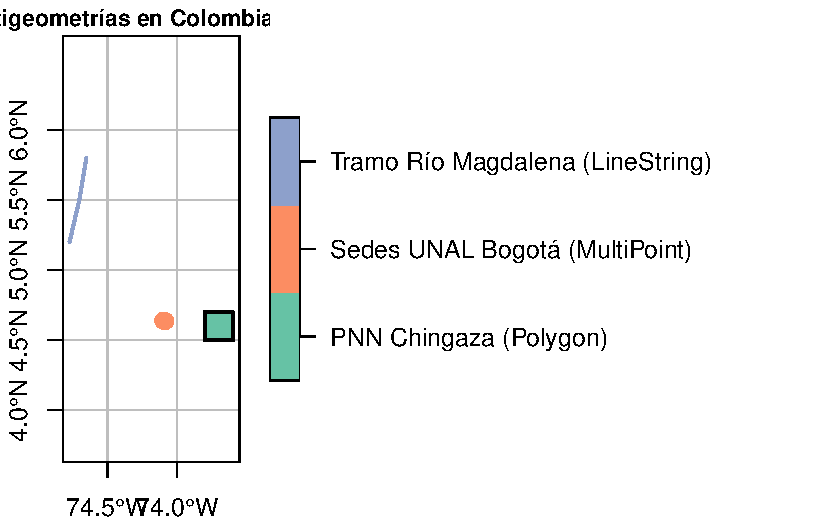
\includegraphics[width=0.8\textwidth,height=\textheight]{14-vector_files/figure-pdf/r_wkt_multigeom-1.pdf}
\end{center}

\subsection{Julia}

\begin{Shaded}
\begin{Highlighting}[]
\FunctionTok{j\_eval}\NormalTok{(}\StringTok{\textquotesingle{}}
\StringTok{using ArchGDAL}
\StringTok{using DataFrames}
\StringTok{using Plots}

\StringTok{\# 1. Definición de vectores base con delimitaciones WKT complejas}
\StringTok{entidades = ["Sedes UNAL Bogotá (MultiPoint)", "Tramo Río Magdalena (LineString)", "PNN Chingaza (Polygon)"]}
\StringTok{wkt\_complejos = [}
\StringTok{    "MULTIPOINT ({-}74.0990 4.6386, {-}74.0830 4.6360)",}
\StringTok{    "LINESTRING ({-}74.7700 5.2000, {-}74.7000 5.5000, {-}74.6500 5.8000)",}
\StringTok{    "POLYGON (({-}73.8000 4.7000, {-}73.6000 4.7000, {-}73.6000 4.5000, {-}73.8000 4.5000, {-}73.8000 4.7000))"}
\StringTok{]}

\StringTok{\# 2. Conversión vectorial a primitivas IGeometry abstractas}
\StringTok{geometrias = ArchGDAL.fromWKT.(wkt\_complejos)}

\StringTok{\# Ensamblaje de la tabla espacial}
\StringTok{df\_complejo = DataFrame(Entidad = entidades, geometry = geometrias)}

\StringTok{\# 3. Inspección de la arquitectura espacial y tipología}
\StringTok{println("{-}{-}{-} Estructura de la Tabla {-}{-}{-}")}
\StringTok{println(df\_complejo)}
\StringTok{println("}\SpecialCharTok{\textbackslash{}\textbackslash{}}\StringTok{n{-}{-}{-} Clases geométricas detectadas {-}{-}{-}")}
\StringTok{for g in df\_complejo.geometry}
\StringTok{    println(typeof(g))}
\StringTok{end}

\StringTok{\# 4. Visualización gráfica iterativa}
\StringTok{\# Se inicializa el lienzo global estipulando los parámetros base}
\StringTok{p = Plots.plot(}
\StringTok{    title = "Multigeometrías en Colombia (WKT)", }
\StringTok{    xlabel = "Longitud", ylabel = "Latitud",}
\StringTok{    aspect\_ratio = :equal, }
\StringTok{    legend = :outertopright,}
\StringTok{    grid = true,                 \# Activar la visualización de la grilla}
\StringTok{    gridstyle = :dash,           \# Establecer el tipo de línea (intermitente)}
\StringTok{    gridlinewidth = 0.5,         \# Fijar el grosor geométrico de la grilla}
\StringTok{    gridalpha = 0.7,             \# Ajustar el canal de opacidad (transparencia)}
\StringTok{    xticks = {-}75.0:0.5:{-}73.0,    \# Definir marcas paramétricas cada 0.5 grados en X}
\StringTok{    yticks = 4.0:0.5:6.0         \# Definir marcas paramétricas cada 0.5 grados en Y}
\StringTok{)}

\StringTok{for i in 1:nrow(df\_complejo)}
\StringTok{    Plots.plot!(}
\StringTok{        p, df\_complejo.geometry[i], }
\StringTok{        label = df\_complejo.Entidad[i], }
\StringTok{        linewidth = 2, }
\StringTok{        markersize = 6}
\StringTok{    )}
\StringTok{end}

\StringTok{Plots.savefig(p, "images/c14\_plot\_wkt\_multigeom\_julia.png")}
\StringTok{\textquotesingle{}}\NormalTok{)}
\end{Highlighting}
\end{Shaded}

\begin{Shaded}
\begin{Highlighting}[]
\NormalTok{knitr}\SpecialCharTok{::}\FunctionTok{include\_graphics}\NormalTok{(}\StringTok{"images/c14\_plot\_wkt\_multigeom\_julia.png"}\NormalTok{)}
\end{Highlighting}
\end{Shaded}

\begin{center}
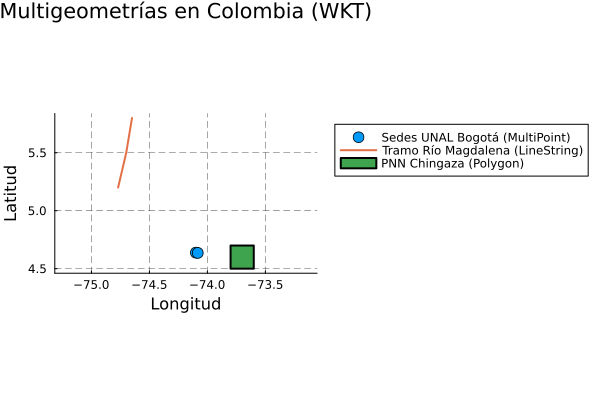
\includegraphics[width=0.8\textwidth,height=\textheight]{images/c14_plot_wkt_multigeom_julia.png}
\end{center}

\subsection{Resumen sintáctico}\label{resumen-sintuxe1ctico-1}

\begin{enumerate}
\def\labelenumi{\arabic{enumi}.}
\tightlist
\item
  \textbf{Estructuración WKT compleja}:
\end{enumerate}

En la siguiente tabla se detalla el esquema textual OGC necesario para
la definición de clases vectoriales de dimensión superior utilizando
\emph{Well-Known Text}. El patrón de anidamiento de paréntesis refleja
la jerarquía dimensional interna (ej. listas de listas).

\begin{longtable}[]{@{}
  >{\raggedright\arraybackslash}p{(\columnwidth - 2\tabcolsep) * \real{0.3000}}
  >{\raggedright\arraybackslash}p{(\columnwidth - 2\tabcolsep) * \real{0.7000}}@{}}
\caption{Estructura sintáctica y topológica WKT para modelado de
entidades geográficas
complejas}\label{tbl-resumen_sintaxis_wkt_compleja}\tabularnewline
\toprule\noalign{}
\begin{minipage}[b]{\linewidth}\raggedright
Tipo espacial WKT
\end{minipage} & \begin{minipage}[b]{\linewidth}\raggedright
Convención estructural de la cadena
\end{minipage} \\
\midrule\noalign{}
\endfirsthead
\toprule\noalign{}
\begin{minipage}[b]{\linewidth}\raggedright
Tipo espacial WKT
\end{minipage} & \begin{minipage}[b]{\linewidth}\raggedright
Convención estructural de la cadena
\end{minipage} \\
\midrule\noalign{}
\endhead
\bottomrule\noalign{}
\endlastfoot
\textbf{\texttt{MULTIPOINT}} &
\texttt{"MULTIPOINT\ (X1\ Y1,\ X2\ Y2,\ ...)"} \\
\textbf{\texttt{LINESTRING}} &
\texttt{"LINESTRING\ (X1\ Y1,\ X2\ Y2,\ ...)"} \\
\textbf{\texttt{MULTILINESTRING}} &
\texttt{"MULTILINESTRING\ ((X1\ Y1,\ ...),\ (Xn\ Yn,\ ...))"} \\
\textbf{\texttt{POLYGON}} &
\texttt{"POLYGON\ ((X1\ Y1,\ ...,\ X1\ Y1),\ (Xn\ Yn,\ ...,\ Xn\ Yn))"}\emph{(Nota:
El primer anillo es exterior; los consecutivos son huecos. Todos deben
cerrarse).} \\
\textbf{\texttt{MULTIPOLYGON}} &
\texttt{"MULTIPOLYGON\ (((X1\ Y1,\ ...)),\ ((Xn\ Yn,\ ...)))"} \\
\end{longtable}

\begin{center}\rule{0.5\linewidth}{0.5pt}\end{center}

\begin{enumerate}
\def\labelenumi{\arabic{enumi}.}
\setcounter{enumi}{1}
\tightlist
\item
  \textbf{Configuración de grillas y espaciado de ejes}
\end{enumerate}

Para el control cartográfico de precisión en la visualización de
geometrías, se aplican rutinas específicas en cada lenguaje que permiten
gobernar la densidad de la cuadrícula (graticule) y los intervalos de
las marcas de coordenadas (ticks).

\begin{longtable}[]{@{}
  >{\raggedright\arraybackslash}p{(\columnwidth - 6\tabcolsep) * \real{0.2200}}
  >{\raggedright\arraybackslash}p{(\columnwidth - 6\tabcolsep) * \real{0.2600}}
  >{\raggedright\arraybackslash}p{(\columnwidth - 6\tabcolsep) * \real{0.2600}}
  >{\raggedright\arraybackslash}p{(\columnwidth - 6\tabcolsep) * \real{0.2600}}@{}}
\caption{Equivalencia de parámetros para el control topológico de
retículas cartográficas y frecuencias de
ejes}\label{tbl-resumen_grillas_ejes}\tabularnewline
\toprule\noalign{}
\begin{minipage}[b]{\linewidth}\raggedright
Operación gráfica
\end{minipage} & \begin{minipage}[b]{\linewidth}\raggedright
Python (\texttt{matplotlib}) 🐍
\end{minipage} & \begin{minipage}[b]{\linewidth}\raggedright
R (\texttt{sf}) 🔵
\end{minipage} & \begin{minipage}[b]{\linewidth}\raggedright
Julia (\texttt{Plots}) 🟣
\end{minipage} \\
\midrule\noalign{}
\endfirsthead
\toprule\noalign{}
\begin{minipage}[b]{\linewidth}\raggedright
Operación gráfica
\end{minipage} & \begin{minipage}[b]{\linewidth}\raggedright
Python (\texttt{matplotlib}) 🐍
\end{minipage} & \begin{minipage}[b]{\linewidth}\raggedright
R (\texttt{sf}) 🔵
\end{minipage} & \begin{minipage}[b]{\linewidth}\raggedright
Julia (\texttt{Plots}) 🟣
\end{minipage} \\
\midrule\noalign{}
\endhead
\bottomrule\noalign{}
\endlastfoot
\textbf{Activar y dar formato a la grilla} &
\texttt{ax.grid(True,}\texttt{linestyle="-\/-",}\texttt{linewidth=0.5,}\texttt{alpha=0.7)}
& \emph{Atributo integrado en la función \texttt{st\_graticule()}} &
\texttt{plot(...,\ grid=true,}\texttt{gridstyle=:dash,}\texttt{gridlinewidth=0.5,}\texttt{gridalpha=0.7)} \\
\textbf{Control de espaciado (Marcas / Ticks)} &
\texttt{import\ matplotlib.ticker\ as\ tkr}\texttt{ax.xaxis.set\_major\_locator(}\texttt{tkr.MultipleLocator(0.5))}
&
\texttt{plot(...,}\texttt{graticule\ =\ st\_graticule(}\texttt{lon\ =\ seq(-75,\ -73,\ by=0.5),}\texttt{lat\ =\ seq(4,\ 6,\ by=0.5)))}
&
\texttt{plot(...,}\texttt{xticks\ =\ -75.0:0.5:-73.0,}\texttt{yticks\ =\ 4.0:0.5:6.0)} \\
\end{longtable}

\section{El formato binario WKB (Well-Known
Binary)}\label{el-formato-binario-wkb-well-known-binary}

Aunque el formato textual WKT resulta idóneo por su legibilidad
semántica, transferir matrices masivas de datos espaciales como cadenas
de texto es sumamente ineficiente a nivel de consumo de RAM, y propenso
a pérdidas de precisión flotante.

Por esta razón técnica, librerías cartográficas (GDAL, GEOS) y bases de
datos espaciales (PostGIS) codifican la información geométrica en el
estándar WKB (Well-Known Binary). Este empaquetamiento hexadecimal
asegura transacciones compactas, ultra-rápidas y matemáticamente
exactas, siendo el vehículo principal de operaciones I/O en la ciencia
de datos espaciales.

A continuación, se convierte el punto representativo evaluado en la
sección anterior hacia su encriptación binaria, verificando
posteriormente la restauración neta hacia un objeto vectorial operable.

\subsection{Python}

\begin{Shaded}
\begin{Highlighting}[]
\ImportTok{from}\NormalTok{ shapely.geometry }\ImportTok{import}\NormalTok{ Point}
\ImportTok{from}\NormalTok{ shapely }\ImportTok{import}\NormalTok{ wkb}

\CommentTok{\# Punto semilla}
\NormalTok{p\_base }\OperatorTok{=}\NormalTok{ Point(}\OperatorTok{{-}}\FloatTok{74.076}\NormalTok{, }\FloatTok{4.598}\NormalTok{)}

\CommentTok{\# 1. Serialización topológica: Objeto a Binario (Dumps)}
\CommentTok{\# Se expone la matriz cruda hexadecimal}
\NormalTok{p\_binario }\OperatorTok{=}\NormalTok{ wkb.dumps(p\_base)}
\BuiltInTok{print}\NormalTok{(}\StringTok{"{-}{-}{-} Cadena Hexadecimal (WKB) {-}{-}{-}"}\NormalTok{)}
\end{Highlighting}
\end{Shaded}

\begin{verbatim}
--- Cadena Hexadecimal (WKB) ---
\end{verbatim}

\begin{Shaded}
\begin{Highlighting}[]
\BuiltInTok{print}\NormalTok{(p\_binario.}\BuiltInTok{hex}\NormalTok{())}
\end{Highlighting}
\end{Shaded}

\begin{verbatim}
0101000000be9f1a2fdd8452c03108ac1c5a641240
\end{verbatim}

\begin{Shaded}
\begin{Highlighting}[]
\CommentTok{\# 2. Deserialización: Binario a Objeto (Loads)}
\NormalTok{p\_restaurado }\OperatorTok{=}\NormalTok{ wkb.loads(p\_binario)}
\BuiltInTok{print}\NormalTok{(}\StringTok{"}\CharTok{\textbackslash{}n}\StringTok{{-}{-}{-} Geometría Restaurada {-}{-}{-}"}\NormalTok{)}
\end{Highlighting}
\end{Shaded}

\begin{verbatim}

--- Geometría Restaurada ---
\end{verbatim}

\begin{Shaded}
\begin{Highlighting}[]
\BuiltInTok{print}\NormalTok{(p\_restaurado.wkt)}
\end{Highlighting}
\end{Shaded}

\begin{verbatim}
POINT (-74.076 4.598)
\end{verbatim}

\subsection{R}

\begin{Shaded}
\begin{Highlighting}[]
\FunctionTok{library}\NormalTok{(sf)}

\CommentTok{\# Punto semilla}
\NormalTok{p\_base }\OtherTok{\textless{}{-}} \FunctionTok{st\_point}\NormalTok{(}\FunctionTok{c}\NormalTok{(}\SpecialCharTok{{-}}\FloatTok{74.076}\NormalTok{, }\FloatTok{4.598}\NormalTok{))}

\CommentTok{\# 1. Serialización topológica: Objeto a Binario}
\CommentTok{\# El entorno R expone un tipo nativo "raw" representativo de la memoria base}
\NormalTok{p\_binario }\OtherTok{\textless{}{-}} \FunctionTok{st\_as\_binary}\NormalTok{(p\_base)}
\FunctionTok{print}\NormalTok{(}\StringTok{"{-}{-}{-} Arreglo Raw (WKB) {-}{-}{-}"}\NormalTok{)}
\end{Highlighting}
\end{Shaded}

\begin{verbatim}
[1] "--- Arreglo Raw (WKB) ---"
\end{verbatim}

\begin{Shaded}
\begin{Highlighting}[]
\FunctionTok{print}\NormalTok{(p\_binario)}
\end{Highlighting}
\end{Shaded}

\begin{verbatim}
 [1] 01 01 00 00 00 be 9f 1a 2f dd 84 52 c0 31 08 ac 1c 5a 64 12 40
\end{verbatim}

\begin{Shaded}
\begin{Highlighting}[]
\CommentTok{\# 2. Deserialización: Binario a Objeto}
\CommentTok{\# Se fuerza la asignación de clase \textquotesingle{}WKB\textquotesingle{} sobre la lista contenedora del binario}
\NormalTok{estructura\_wkb }\OtherTok{\textless{}{-}} \FunctionTok{structure}\NormalTok{(}\FunctionTok{list}\NormalTok{(p\_binario), }\AttributeTok{class =} \StringTok{"WKB"}\NormalTok{)}
\NormalTok{p\_restaurado }\OtherTok{\textless{}{-}} \FunctionTok{st\_as\_sfc}\NormalTok{(estructura\_wkb)[[}\DecValTok{1}\NormalTok{]]}

\FunctionTok{print}\NormalTok{(}\StringTok{"{-}{-}{-} Geometría Restaurada {-}{-}{-}"}\NormalTok{)}
\end{Highlighting}
\end{Shaded}

\begin{verbatim}
[1] "--- Geometría Restaurada ---"
\end{verbatim}

\begin{Shaded}
\begin{Highlighting}[]
\FunctionTok{print}\NormalTok{(}\FunctionTok{st\_as\_text}\NormalTok{(p\_restaurado))}
\end{Highlighting}
\end{Shaded}

\begin{verbatim}
[1] "POINT (-74.076 4.598)"
\end{verbatim}

\subsection{Julia}

\begin{Shaded}
\begin{Highlighting}[]
\FunctionTok{j\_eval}\NormalTok{(}\StringTok{\textquotesingle{}}
\StringTok{using ArchGDAL}

\StringTok{\# Punto semilla}
\StringTok{p\_base = ArchGDAL.createpoint({-}74.076, 4.598)}

\StringTok{\# 1. Serialización topológica: Objeto a Binario}
\StringTok{\# Exportación de la geometría bajo el envoltorio C++ binario nativo}
\StringTok{p\_binario = ArchGDAL.toWKB(p\_base)}
\StringTok{println("{-}{-}{-} Arreglo de Bytes (WKB) {-}{-}{-}")}
\StringTok{println(p\_binario)}

\StringTok{\# 2. Deserialización: Binario a Objeto}
\StringTok{p\_restaurado = ArchGDAL.fromWKB(p\_binario)}
\StringTok{println("}\SpecialCharTok{\textbackslash{}\textbackslash{}}\StringTok{n{-}{-}{-} Geometría Restaurada {-}{-}{-}")}
\StringTok{println(ArchGDAL.toWKT(p\_restaurado))}
\StringTok{\textquotesingle{}}\NormalTok{)}
\end{Highlighting}
\end{Shaded}

\subsection{Resumen sintáctico: codificación binaria
WKB}\label{resumen-sintuxe1ctico-codificaciuxf3n-binaria-wkb}

La codificación de primitivas espaciales mediante Well-Known Binary
(WKB) es el estándar fundamental para optimizar la transferencia I/O y
el almacenamiento en bases de datos espaciales. La siguiente tabla
consolida las rutinas para serializar (objeto geométrico a arreglo de
bytes) y deserializar (bytes a objeto geométrico) la topología vectorial
en los tres ecosistemas.

\begin{longtable}[]{@{}
  >{\raggedright\arraybackslash}p{(\columnwidth - 6\tabcolsep) * \real{0.2500}}
  >{\raggedright\arraybackslash}p{(\columnwidth - 6\tabcolsep) * \real{0.2500}}
  >{\raggedright\arraybackslash}p{(\columnwidth - 6\tabcolsep) * \real{0.2500}}
  >{\raggedright\arraybackslash}p{(\columnwidth - 6\tabcolsep) * \real{0.2500}}@{}}
\caption{Equivalencia analítica para la serialización topológica y la
codificación para transferencias de datos espaciales en bajo
nivel}\label{tbl-resumen_wkb}\tabularnewline
\toprule\noalign{}
\begin{minipage}[b]{\linewidth}\raggedright
Transformación espacial
\end{minipage} & \begin{minipage}[b]{\linewidth}\raggedright
Python (\texttt{shapely}) 🐍
\end{minipage} & \begin{minipage}[b]{\linewidth}\raggedright
R (\texttt{sf}) 🔵
\end{minipage} & \begin{minipage}[b]{\linewidth}\raggedright
Julia (\texttt{ArchGDAL}) 🟣
\end{minipage} \\
\midrule\noalign{}
\endfirsthead
\toprule\noalign{}
\begin{minipage}[b]{\linewidth}\raggedright
Transformación espacial
\end{minipage} & \begin{minipage}[b]{\linewidth}\raggedright
Python (\texttt{shapely}) 🐍
\end{minipage} & \begin{minipage}[b]{\linewidth}\raggedright
R (\texttt{sf}) 🔵
\end{minipage} & \begin{minipage}[b]{\linewidth}\raggedright
Julia (\texttt{ArchGDAL}) 🟣
\end{minipage} \\
\midrule\noalign{}
\endhead
\bottomrule\noalign{}
\endlastfoot
\textbf{Geometría a binario (WKB)} & \texttt{wkb.dumps(g)} &
\texttt{st\_as\_binary(g)} & \texttt{ArchGDAL.toWKB(g)} \\
\textbf{Binario a geometría} & \texttt{wkb.loads(bin\_data)} &
\texttt{st\_as\_sfc(structure(}\texttt{list(bin\_data),\ class="WKB"))}
& \texttt{ArchGDAL.fromWKB(bin\_data)} \\
\textbf{Geometría a texto (WKT)} & \texttt{g.wkt} &
\texttt{st\_as\_text(g)} & \texttt{ArchGDAL.toWKT(g)} \\
\end{longtable}

\section{Precisión espacial y redondeo
topológico}\label{precisiuxf3n-espacial-y-redondeo-topoluxf3gico}

Los motores cartográficos operan internamente sobre representaciones
numéricas de punto flotante (flotantes de 64 bits o \texttt{double}).
Esta precisión absoluta puede generar fallos estructurales en cruces
topológicos o uniones espaciales donde dos vértices conceptualmente
idénticos difieren en el décimo lugar decimal debido al ruido de
máquina.

Para mitigar estos errores o reducir el peso de almacenamiento, los
atributos geométricos pueden subordinarse a un \textbf{modelo de
precisión}. La lógica, derivada del marco C++ GEOS, opera mediante
factores de escala:

\begin{itemize}
\tightlist
\item
  Si la precisión es 0 (comportamiento por defecto), la coordenada no
  sufre modificaciones analíticas.
\item
  Un factor positivo ejecuta la operación matemática
  \texttt{round(coordenada\ *\ precision)\ /\ precision}. Por ejemplo,
  para restringir un vértice a tres cifras decimales, se inyecta un
  factor de escala igual a \(1000\).
\end{itemize}

A continuación, se demuestra la imposición de este control numérico
sobre las coordenadas de la Plaza de Bolívar en Bogotá.

\subsection{Python}

\begin{Shaded}
\begin{Highlighting}[]
\ImportTok{from}\NormalTok{ shapely.geometry }\ImportTok{import}\NormalTok{ Point}
\ImportTok{from}\NormalTok{ shapely }\ImportTok{import}\NormalTok{ set\_precision}

\CommentTok{\# 1. Instanciación de un punto con alta precisión flotante (Plaza de Bolívar)}
\NormalTok{p\_bruto }\OperatorTok{=}\NormalTok{ Point(}\OperatorTok{{-}}\FloatTok{74.07604539}\NormalTok{, }\FloatTok{4.59812318}\NormalTok{)}
\BuiltInTok{print}\NormalTok{(}\SpecialStringTok{f"Coordenada original: }\SpecialCharTok{\{}\NormalTok{p\_bruto}\SpecialCharTok{\}}\SpecialStringTok{"}\NormalTok{)}
\end{Highlighting}
\end{Shaded}

\begin{verbatim}
Coordenada original: POINT (-74.07604539 4.59812318)
\end{verbatim}

\begin{Shaded}
\begin{Highlighting}[]
\CommentTok{\# 2. Aplicación del modelo de precisión espacial}
\CommentTok{\# En shapely, grid\_size=0.001 equivale a truncar a 3 posiciones decimales}
\NormalTok{p\_truncado }\OperatorTok{=}\NormalTok{ set\_precision(p\_bruto, grid\_size}\OperatorTok{=}\FloatTok{0.001}\NormalTok{)}
\BuiltInTok{print}\NormalTok{(}\SpecialStringTok{f"Coordenada truncada: }\SpecialCharTok{\{}\NormalTok{p\_truncado}\SpecialCharTok{\}}\SpecialStringTok{"}\NormalTok{)}
\end{Highlighting}
\end{Shaded}

\begin{verbatim}
Coordenada truncada: POINT (-74.076 4.598)
\end{verbatim}

\subsection{R}

\begin{Shaded}
\begin{Highlighting}[]
\FunctionTok{library}\NormalTok{(sf)}

\CommentTok{\# 1. Instanciación de un punto con alta precisión flotante (Plaza de Bolívar)}
\NormalTok{p\_bruto }\OtherTok{\textless{}{-}} \FunctionTok{st\_sfc}\NormalTok{(}\FunctionTok{st\_point}\NormalTok{(}\FunctionTok{c}\NormalTok{(}\SpecialCharTok{{-}}\FloatTok{74.07604539}\NormalTok{, }\FloatTok{4.59812318}\NormalTok{)), }\AttributeTok{crs =} \DecValTok{4326}\NormalTok{)}
\FunctionTok{print}\NormalTok{(}\StringTok{"Coordenada original:"}\NormalTok{)}
\end{Highlighting}
\end{Shaded}

\begin{verbatim}
[1] "Coordenada original:"
\end{verbatim}

\begin{Shaded}
\begin{Highlighting}[]
\FunctionTok{print}\NormalTok{(}\FunctionTok{st\_coordinates}\NormalTok{(p\_bruto))}
\end{Highlighting}
\end{Shaded}

\begin{verbatim}
             X        Y
[1,] -74.07605 4.598123
\end{verbatim}

\begin{Shaded}
\begin{Highlighting}[]
\CommentTok{\# 2. Aplicación del modelo de precisión espacial}
\CommentTok{\# En sf, el atributo de precisión (1000 = 3 decimales) actúa durante operaciones }
\CommentTok{\# topológicas o durante la conversión a formato WKB.}
\NormalTok{p\_precision }\OtherTok{\textless{}{-}} \FunctionTok{st\_set\_precision}\NormalTok{(p\_bruto, }\DecValTok{1000}\NormalTok{)}

\CommentTok{\# Para materializar y visualizar el truncamiento geométrico explícitamente en memoria,}
\CommentTok{\# forzamos un ciclo de serialización binaria (WKB) de ida y vuelta.}
\NormalTok{p\_truncado }\OtherTok{\textless{}{-}} \FunctionTok{st\_as\_sfc}\NormalTok{(}\FunctionTok{st\_as\_binary}\NormalTok{(p\_precision), }\AttributeTok{crs =} \DecValTok{4326}\NormalTok{)}

\FunctionTok{print}\NormalTok{(}\StringTok{"Coordenada truncada:"}\NormalTok{)}
\end{Highlighting}
\end{Shaded}

\begin{verbatim}
[1] "Coordenada truncada:"
\end{verbatim}

\begin{Shaded}
\begin{Highlighting}[]
\FunctionTok{print}\NormalTok{(}\FunctionTok{st\_coordinates}\NormalTok{(p\_truncado))}
\end{Highlighting}
\end{Shaded}

\begin{verbatim}
           X     Y
[1,] -74.076 4.598
\end{verbatim}

\subsection{Julia}

\begin{Shaded}
\begin{Highlighting}[]
\FunctionTok{j\_eval}\NormalTok{(}\StringTok{\textquotesingle{}}
\StringTok{using ArchGDAL}

\StringTok{\# 1. Vectores numéricos originales (Plaza de Bolívar)}
\StringTok{coords\_brutas = [{-}74.07604539, 4.59812318]}
\StringTok{p\_bruto = ArchGDAL.createpoint(coords\_brutas...)}
\StringTok{println("Coordenada original:")}
\StringTok{println(ArchGDAL.toWKT(p\_bruto))}

\StringTok{\# 2. Control de precisión en el entorno Julia}
\StringTok{\# Dado que la API no mapea la rutina de GEOS de forma directa para el usuario, }
\StringTok{\# la práctica algorítmica estándar es redondear la matriz numérica antes de inicializar la figura.}
\StringTok{coords\_truncadas = round.(coords\_brutas, digits=3)}
\StringTok{p\_truncado = ArchGDAL.createpoint(coords\_truncadas...)}
\StringTok{println("}\SpecialCharTok{\textbackslash{}\textbackslash{}}\StringTok{nCoordenada truncada:")}
\StringTok{println(ArchGDAL.toWKT(p\_truncado))}
\StringTok{\textquotesingle{}}\NormalTok{)}
\end{Highlighting}
\end{Shaded}

\subsection{Resumen sintáctico: Precisión escalar y formato
WKB}\label{resumen-sintuxe1ctico-precisiuxf3n-escalar-y-formato-wkb}

La imposición de un modelo de precisión permite estandarizar las
tolerancias de punto flotante en operaciones topológicas. Mientras que
en Python la alteración de la geometría es inmediata, en R la directiva
\texttt{st\_set\_precision()} actúa como una bandera pasiva; para forzar
la alteración física de los vértices en memoria, es obligatorio efectuar
un ciclo de serialización binaria (WKB). En Julia, la aproximación más
estable requiere el truncamiento numérico previo a la instanciación
espacial.

\begin{longtable}[]{@{}
  >{\raggedright\arraybackslash}p{(\columnwidth - 6\tabcolsep) * \real{0.2500}}
  >{\raggedright\arraybackslash}p{(\columnwidth - 6\tabcolsep) * \real{0.2500}}
  >{\raggedright\arraybackslash}p{(\columnwidth - 6\tabcolsep) * \real{0.2500}}
  >{\raggedright\arraybackslash}p{(\columnwidth - 6\tabcolsep) * \real{0.2500}}@{}}
\caption{Equivalencia analítica para el control aritmético topológico y
la codificación para transferencias I/O de bajo
nivel}\label{tbl-resumen_precision_wkb}\tabularnewline
\toprule\noalign{}
\begin{minipage}[b]{\linewidth}\raggedright
Transformación
\end{minipage} & \begin{minipage}[b]{\linewidth}\raggedright
Python (\texttt{shapely}) 🐍
\end{minipage} & \begin{minipage}[b]{\linewidth}\raggedright
R (\texttt{sf}) 🔵
\end{minipage} & \begin{minipage}[b]{\linewidth}\raggedright
Julia (\texttt{ArchGDAL}) 🟣
\end{minipage} \\
\midrule\noalign{}
\endfirsthead
\toprule\noalign{}
\begin{minipage}[b]{\linewidth}\raggedright
Transformación
\end{minipage} & \begin{minipage}[b]{\linewidth}\raggedright
Python (\texttt{shapely}) 🐍
\end{minipage} & \begin{minipage}[b]{\linewidth}\raggedright
R (\texttt{sf}) 🔵
\end{minipage} & \begin{minipage}[b]{\linewidth}\raggedright
Julia (\texttt{ArchGDAL}) 🟣
\end{minipage} \\
\midrule\noalign{}
\endhead
\bottomrule\noalign{}
\endlastfoot
\textbf{Definir factor de escala}\emph{(Ej. 3 cifras decimales)} &
\texttt{geom\_trunc\ =\ set\_precision(}\texttt{geom,\ grid\_size=0.001)}
& \texttt{geom\_prec\ =\ st\_set\_precision(}\texttt{geom,\ 1000)} &
\texttt{coords\_trunc\ =\ round.(}\texttt{coords,\ digits=3)} \\
\textbf{Materializar redondeo}\emph{(Truncamiento en RAM)} &
\emph{Modificación inmediata}\emph{retornada por la función.} &
\texttt{geom\_trunc\ =\ st\_as\_sfc(}\texttt{st\_as\_binary(geom\_prec))}
& \emph{Truncamiento de vectores crudos}\emph{antes de instanciar la
geometría.} \\
\textbf{Geometría a binario (WKB)} & \texttt{wkb.dumps(g)} &
\texttt{st\_as\_binary(g)} & \texttt{ArchGDAL.toWKB(g)} \\
\textbf{Binario a geometría} & \texttt{wkb.loads(bin\_data)} &
\texttt{st\_as\_sfc(structure(}\texttt{list(bin\_data),\ class="WKB"))}
& \texttt{ArchGDAL.fromWKB(bin\_data)} \\
\textbf{Geometría a texto (WKT)} & \texttt{g.wkt} &
\texttt{st\_as\_text(g)} & \texttt{ArchGDAL.toWKT(g)} \\
\end{longtable}

\section{Extracción estructurada de coordenadas y topologías
complejas}\label{extracciuxf3n-estructurada-de-coordenadas-y-topologuxedas-complejas}

Comprender la jerarquía anidada de las multigeometrías es fundamental
para el procesamiento analítico. A nivel algorítmico, un SIG no evalúa
una figura como un dibujo, sino como un tensor multidimensional de
vértices.

El ejemplo a continuación simulará un área protegida (tierra) con
lagunas e islar interiores. Todo lo que sea agua no hará pare del
polígono (hueco). La tarea consiste en \textbf{extraer el tercer
vértice} de los polígonos que conforman el área protegida.

\begin{Shaded}
\begin{Highlighting}[]
\CommentTok{\# \#| eval: false}
\NormalTok{knitr}\SpecialCharTok{::}\FunctionTok{include\_graphics}\NormalTok{(}\StringTok{"images/c14\_plot\_topologia\_puntos\_julia.png"}\NormalTok{)}
\end{Highlighting}
\end{Shaded}

\begin{center}
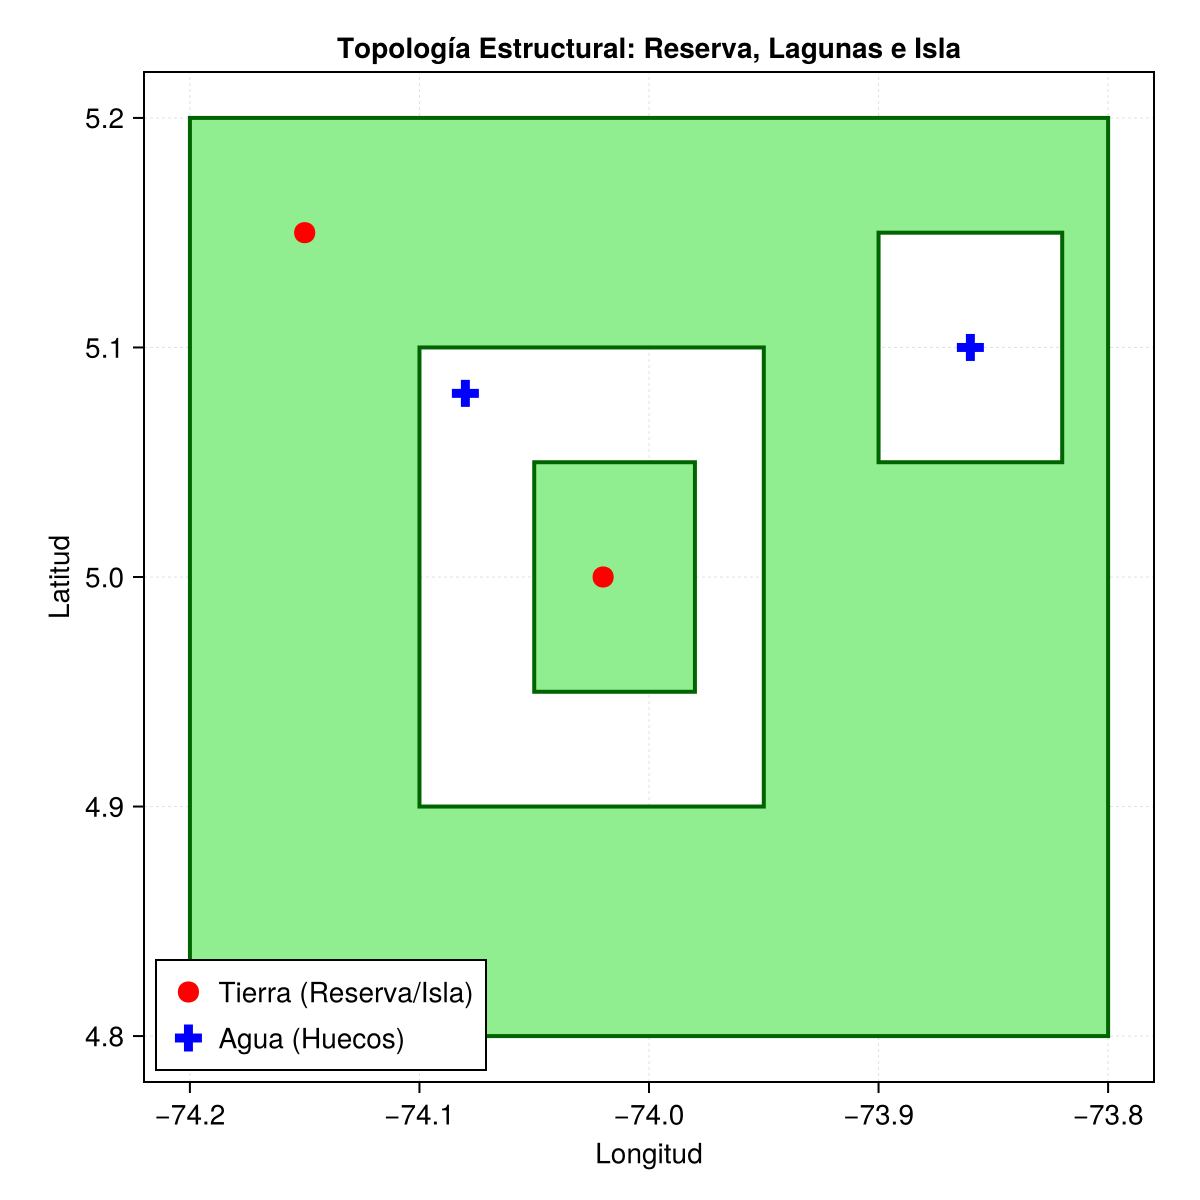
\includegraphics[width=0.8\textwidth,height=\textheight]{images/c14_plot_topologia_puntos_julia.png}
\end{center}

La topología de un \texttt{POLYGON} se define de manera estricta
mediante anillos (Rings): un polígono está compuesto por
\textbf{exactamente un anillo exterior} (cuya área representa masa
sólida) y \textbf{cero o múltiples anillos interiores} (cuya área
representa perforaciones o huecos). Por lo tanto, la naturaleza del
espacio (tierra o agua) está dictada por su índice estructural:

\begin{itemize}
\tightlist
\item
  El anillo principal define la masa (tierra).
\item
  Los anillos secundarios dentro del mismo polígono definen los huecos
  (cuerpos de agua).
\item
  Las masas de tierra desconectadas (islas) son simplemente
  \textbf{polígonos adicionales} dentro de un objeto
  \texttt{MULTIPOLYGON}.
\end{itemize}

Para ilustrar este principio geométrico y validarlo mediante predicados
espaciales, se simula un área protegida:

\begin{enumerate}
\def\labelenumi{\arabic{enumi}.}
\tightlist
\item
  \textbf{Un polígono principal (La Reserva):} Límite exterior que
  contiene dos perforaciones o huecos (una laguna principal y una laguna
  menor, ambas disjuntas entre sí).
\item
  \textbf{Un polígono secundario (La Isla):} Masa terrestre ubicada
  matemáticamente dentro del área de la laguna principal, pero
  registrada estructuralmente como un polígono sólido independiente.
\end{enumerate}

\subsection{Python}

En Python, la librería \texttt{shapely} expone las multigeometrías
iterando a través de la propiedad \texttt{.geoms}. Cada polígono posee
un atributo \texttt{.exterior} y una lista de atributos
\texttt{.interiors} (huecos).

\emph{Nota: Python utiliza indexación basada en cero (0), por lo que el
primer hueco es el índice \texttt{{[}0{]}} y el tercer vértice
corresponde al índice \texttt{{[}2{]}}.}

\begin{Shaded}
\begin{Highlighting}[]
\CommentTok{\# \#| eval: false}

\ImportTok{from}\NormalTok{ shapely.geometry }\ImportTok{import}\NormalTok{ Polygon, MultiPolygon, Point}
\ImportTok{import}\NormalTok{ geopandas }\ImportTok{as}\NormalTok{ gpd}
\ImportTok{import}\NormalTok{ matplotlib.pyplot }\ImportTok{as}\NormalTok{ plt}
\ImportTok{import}\NormalTok{ matplotlib.ticker }\ImportTok{as}\NormalTok{ ticker}

\CommentTok{\# 1. Construcción de anillos topológicos topológicamente válidos}
\CommentTok{\# Anillo exterior del polígono 1 (Límites de la Reserva Natural)}
\NormalTok{ext\_reserva }\OperatorTok{=}\NormalTok{ [(}\OperatorTok{{-}}\FloatTok{74.2}\NormalTok{, }\FloatTok{5.2}\NormalTok{), (}\OperatorTok{{-}}\FloatTok{73.8}\NormalTok{, }\FloatTok{5.2}\NormalTok{), (}\OperatorTok{{-}}\FloatTok{73.8}\NormalTok{, }\FloatTok{4.8}\NormalTok{), (}\OperatorTok{{-}}\FloatTok{74.2}\NormalTok{, }\FloatTok{4.8}\NormalTok{), (}\OperatorTok{{-}}\FloatTok{74.2}\NormalTok{, }\FloatTok{5.2}\NormalTok{)]}
\CommentTok{\# Anillo interior 1 del polígono 1 (Laguna principal / Hueco)}
\NormalTok{int\_laguna1 }\OperatorTok{=}\NormalTok{ [(}\OperatorTok{{-}}\FloatTok{74.1}\NormalTok{, }\FloatTok{5.1}\NormalTok{), (}\OperatorTok{{-}}\FloatTok{74.1}\NormalTok{, }\FloatTok{4.9}\NormalTok{), (}\OperatorTok{{-}}\FloatTok{73.95}\NormalTok{, }\FloatTok{4.9}\NormalTok{), (}\OperatorTok{{-}}\FloatTok{73.95}\NormalTok{, }\FloatTok{5.1}\NormalTok{), (}\OperatorTok{{-}}\FloatTok{74.1}\NormalTok{, }\FloatTok{5.1}\NormalTok{)]}
\CommentTok{\# Anillo interior 2 del polígono 1 (Laguna pequeña / Hueco disjunto)}
\NormalTok{int\_laguna2 }\OperatorTok{=}\NormalTok{ [(}\OperatorTok{{-}}\FloatTok{73.9}\NormalTok{, }\FloatTok{5.15}\NormalTok{), (}\OperatorTok{{-}}\FloatTok{73.9}\NormalTok{, }\FloatTok{5.05}\NormalTok{), (}\OperatorTok{{-}}\FloatTok{73.82}\NormalTok{, }\FloatTok{5.05}\NormalTok{), (}\OperatorTok{{-}}\FloatTok{73.82}\NormalTok{, }\FloatTok{5.15}\NormalTok{), (}\OperatorTok{{-}}\FloatTok{73.9}\NormalTok{, }\FloatTok{5.15}\NormalTok{)]}
\CommentTok{\# Anillo exterior del polígono 2 (Isla sólida dentro de la laguna 1)}
\NormalTok{ext\_isla }\OperatorTok{=}\NormalTok{ [(}\OperatorTok{{-}}\FloatTok{74.05}\NormalTok{, }\FloatTok{5.05}\NormalTok{), (}\OperatorTok{{-}}\FloatTok{73.98}\NormalTok{, }\FloatTok{5.05}\NormalTok{), (}\OperatorTok{{-}}\FloatTok{73.98}\NormalTok{, }\FloatTok{4.95}\NormalTok{), (}\OperatorTok{{-}}\FloatTok{74.05}\NormalTok{, }\FloatTok{4.95}\NormalTok{), (}\OperatorTok{{-}}\FloatTok{74.05}\NormalTok{, }\FloatTok{5.05}\NormalTok{)]}

\CommentTok{\# 2. Ensamblaje de la Multigeometría}
\CommentTok{\# Estructura: [(exterior\_pol1, [huecos\_pol1]), (exterior\_pol2, [huecos\_pol2])]}
\NormalTok{mpol\_reserva }\OperatorTok{=}\NormalTok{ MultiPolygon([}
\NormalTok{    (ext\_reserva, [int\_laguna1, int\_laguna2]), }\CommentTok{\# geoms[0].exterior}
                                               \CommentTok{\# geoms[0].interiors[0]}
                                               \CommentTok{\# geoms[0].interiors[1]}
\NormalTok{    (ext\_isla, [])                             }\CommentTok{\# geoms[1].exterior}
\NormalTok{])}

\CommentTok{\# 3. Determinación estructural (Reglas OGC Simple Features)}
\BuiltInTok{print}\NormalTok{(}\StringTok{"{-}{-}{-} Determinación Estructural (Basada en Atributos) {-}{-}{-}"}\NormalTok{)}
\end{Highlighting}
\end{Shaded}

\begin{verbatim}
--- Determinación Estructural (Basada en Atributos) ---
\end{verbatim}

\begin{Shaded}
\begin{Highlighting}[]
\NormalTok{c1 }\OperatorTok{=}\NormalTok{ mpol\_reserva.geoms[}\DecValTok{0}\NormalTok{].exterior.coords[}\DecValTok{2}\NormalTok{]}
\BuiltInTok{print}\NormalTok{(}\SpecialStringTok{f"Reserva (.exterior {-}\textgreater{} Tierra firme) : }\SpecialCharTok{\{}\NormalTok{c1}\SpecialCharTok{\}}\SpecialStringTok{"}\NormalTok{)}
\end{Highlighting}
\end{Shaded}

\begin{verbatim}
Reserva (.exterior -> Tierra firme) : (-73.8, 4.8)
\end{verbatim}

\begin{Shaded}
\begin{Highlighting}[]
\NormalTok{c2 }\OperatorTok{=}\NormalTok{ mpol\_reserva.geoms[}\DecValTok{0}\NormalTok{].interiors[}\DecValTok{0}\NormalTok{].coords[}\DecValTok{2}\NormalTok{]}
\BuiltInTok{print}\NormalTok{(}\SpecialStringTok{f"Laguna 1 (.interiors[0] {-}\textgreater{} Hueco)   : }\SpecialCharTok{\{}\NormalTok{c2}\SpecialCharTok{\}}\SpecialStringTok{"}\NormalTok{)}
\end{Highlighting}
\end{Shaded}

\begin{verbatim}
Laguna 1 (.interiors[0] -> Hueco)   : (-73.95, 4.9)
\end{verbatim}

\begin{Shaded}
\begin{Highlighting}[]
\NormalTok{c3 }\OperatorTok{=}\NormalTok{ mpol\_reserva.geoms[}\DecValTok{0}\NormalTok{].interiors[}\DecValTok{1}\NormalTok{].coords[}\DecValTok{2}\NormalTok{]}
\BuiltInTok{print}\NormalTok{(}\SpecialStringTok{f"Laguna 2 (.interiors[1] {-}\textgreater{} Hueco)   : }\SpecialCharTok{\{}\NormalTok{c3}\SpecialCharTok{\}}\SpecialStringTok{"}\NormalTok{)}
\end{Highlighting}
\end{Shaded}

\begin{verbatim}
Laguna 2 (.interiors[1] -> Hueco)   : (-73.82, 5.05)
\end{verbatim}

\begin{Shaded}
\begin{Highlighting}[]
\NormalTok{c4 }\OperatorTok{=}\NormalTok{ mpol\_reserva.geoms[}\DecValTok{1}\NormalTok{].exterior.coords[}\DecValTok{2}\NormalTok{]}
\BuiltInTok{print}\NormalTok{(}\SpecialStringTok{f"Isla (.exterior {-}\textgreater{} Tierra firme)    : }\SpecialCharTok{\{}\NormalTok{c4}\SpecialCharTok{\}}\CharTok{\textbackslash{}n}\SpecialStringTok{"}\NormalTok{)}
\end{Highlighting}
\end{Shaded}

\begin{verbatim}
Isla (.exterior -> Tierra firme)    : (-73.98, 4.95)
\end{verbatim}

\begin{Shaded}
\begin{Highlighting}[]
\CommentTok{\# 4. Evaluación topológica con puntos de prueba (Predicado Contains)}
\NormalTok{pt\_reserva }\OperatorTok{=}\NormalTok{ Point(}\OperatorTok{{-}}\FloatTok{74.15}\NormalTok{, }\FloatTok{5.15}\NormalTok{)}
\NormalTok{pt\_laguna1 }\OperatorTok{=}\NormalTok{ Point(}\OperatorTok{{-}}\FloatTok{74.08}\NormalTok{, }\FloatTok{5.08}\NormalTok{)}
\NormalTok{pt\_laguna2 }\OperatorTok{=}\NormalTok{ Point(}\OperatorTok{{-}}\FloatTok{73.86}\NormalTok{, }\FloatTok{5.10}\NormalTok{)}
\NormalTok{pt\_isla }\OperatorTok{=}\NormalTok{ Point(}\OperatorTok{{-}}\FloatTok{74.02}\NormalTok{, }\FloatTok{5.0}\NormalTok{)}

\BuiltInTok{print}\NormalTok{(}\StringTok{"{-}{-}{-} Evaluación Topológica (¿Pertenece al polígono sólido?) {-}{-}{-}"}\NormalTok{)}
\end{Highlighting}
\end{Shaded}

\begin{verbatim}
--- Evaluación Topológica (¿Pertenece al polígono sólido?) ---
\end{verbatim}

\begin{Shaded}
\begin{Highlighting}[]
\BuiltInTok{print}\NormalTok{(}\SpecialStringTok{f"Punto en Reserva (Tierra) : }\SpecialCharTok{\{}\NormalTok{mpol\_reserva}\SpecialCharTok{.}\NormalTok{contains(pt\_reserva)}\SpecialCharTok{\}}\SpecialStringTok{"}\NormalTok{)}
\end{Highlighting}
\end{Shaded}

\begin{verbatim}
Punto en Reserva (Tierra) : True
\end{verbatim}

\begin{Shaded}
\begin{Highlighting}[]
\BuiltInTok{print}\NormalTok{(}\SpecialStringTok{f"Punto en Laguna 1 (Agua)  : }\SpecialCharTok{\{}\NormalTok{mpol\_reserva}\SpecialCharTok{.}\NormalTok{contains(pt\_laguna1)}\SpecialCharTok{\}}\SpecialStringTok{"}\NormalTok{)}
\end{Highlighting}
\end{Shaded}

\begin{verbatim}
Punto en Laguna 1 (Agua)  : False
\end{verbatim}

\begin{Shaded}
\begin{Highlighting}[]
\BuiltInTok{print}\NormalTok{(}\SpecialStringTok{f"Punto en Laguna 2 (Agua)  : }\SpecialCharTok{\{}\NormalTok{mpol\_reserva}\SpecialCharTok{.}\NormalTok{contains(pt\_laguna2)}\SpecialCharTok{\}}\SpecialStringTok{"}\NormalTok{)}
\end{Highlighting}
\end{Shaded}

\begin{verbatim}
Punto en Laguna 2 (Agua)  : False
\end{verbatim}

\begin{Shaded}
\begin{Highlighting}[]
\BuiltInTok{print}\NormalTok{(}\SpecialStringTok{f"Punto en Isla (Tierra)    : }\SpecialCharTok{\{}\NormalTok{mpol\_reserva}\SpecialCharTok{.}\NormalTok{contains(pt\_isla)}\SpecialCharTok{\}}\SpecialStringTok{"}\NormalTok{)}
\end{Highlighting}
\end{Shaded}

\begin{verbatim}
Punto en Isla (Tierra)    : True
\end{verbatim}

\begin{Shaded}
\begin{Highlighting}[]
\CommentTok{\# 5. Renderizado cartográfico integrando puntos de prueba}
\NormalTok{fig, ax }\OperatorTok{=}\NormalTok{ plt.subplots(figsize}\OperatorTok{=}\NormalTok{(}\DecValTok{6}\NormalTok{, }\DecValTok{6}\NormalTok{))}

\NormalTok{gpd.GeoSeries([mpol\_reserva]).plot(}
\NormalTok{    ax}\OperatorTok{=}\NormalTok{ax, facecolor}\OperatorTok{=}\StringTok{\textquotesingle{}lightgreen\textquotesingle{}}\NormalTok{, edgecolor}\OperatorTok{=}\StringTok{\textquotesingle{}darkgreen\textquotesingle{}}\NormalTok{, linewidth}\OperatorTok{=}\DecValTok{2}
\NormalTok{)}

\CommentTok{\# Ploteo diferencial de puntos de control}
\NormalTok{gpd.GeoSeries([pt\_reserva, pt\_isla]).plot(ax}\OperatorTok{=}\NormalTok{ax, color}\OperatorTok{=}\StringTok{\textquotesingle{}red\textquotesingle{}}\NormalTok{, marker}\OperatorTok{=}\StringTok{\textquotesingle{}o\textquotesingle{}}\NormalTok{, markersize}\OperatorTok{=}\DecValTok{50}\NormalTok{, label}\OperatorTok{=}\StringTok{\textquotesingle{}Tierra (Reserva/Isla)\textquotesingle{}}\NormalTok{)}
\NormalTok{gpd.GeoSeries([pt\_laguna1, pt\_laguna2]).plot(ax}\OperatorTok{=}\NormalTok{ax, color}\OperatorTok{=}\StringTok{\textquotesingle{}blue\textquotesingle{}}\NormalTok{, marker}\OperatorTok{=}\StringTok{\textquotesingle{}X\textquotesingle{}}\NormalTok{, markersize}\OperatorTok{=}\DecValTok{50}\NormalTok{, label}\OperatorTok{=}\StringTok{\textquotesingle{}Agua (Huecos)\textquotesingle{}}\NormalTok{)}

\NormalTok{ax.set\_title(}\StringTok{"Topología Estructural: Reserva, Lagunas e Isla"}\NormalTok{)}
\NormalTok{ax.set\_xlabel(}\StringTok{"Longitud"}\NormalTok{)}
\NormalTok{ax.set\_ylabel(}\StringTok{"Latitud"}\NormalTok{)}
\NormalTok{ax.legend(loc}\OperatorTok{=}\StringTok{\textquotesingle{}lower left\textquotesingle{}}\NormalTok{)}
\NormalTok{ax.grid(}\VariableTok{True}\NormalTok{, linestyle}\OperatorTok{=}\StringTok{"{-}{-}"}\NormalTok{, linewidth}\OperatorTok{=}\FloatTok{0.5}\NormalTok{, alpha}\OperatorTok{=}\FloatTok{0.7}\NormalTok{)}
\NormalTok{ax.xaxis.set\_major\_locator(ticker.MultipleLocator(}\FloatTok{0.1}\NormalTok{))}
\NormalTok{ax.yaxis.set\_major\_locator(ticker.MultipleLocator(}\FloatTok{0.1}\NormalTok{))}

\NormalTok{plt.tight\_layout()}
\NormalTok{plt.show()}
\end{Highlighting}
\end{Shaded}

\begin{center}
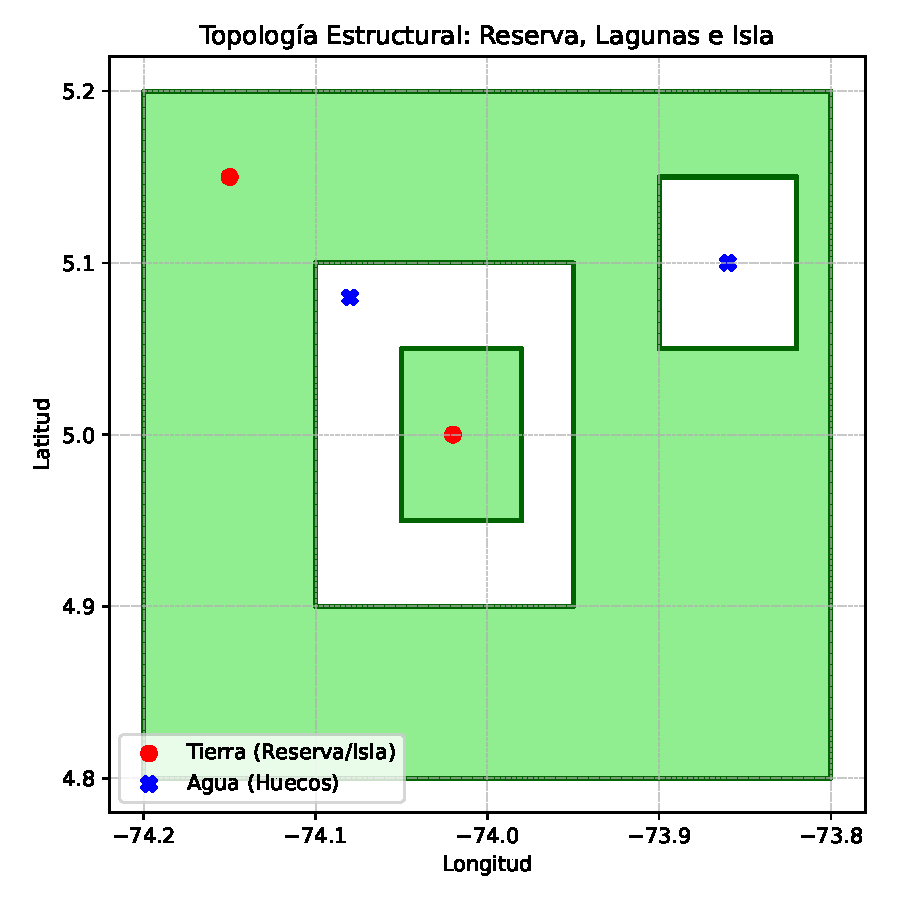
\includegraphics[width=0.8\textwidth,height=\textheight]{14-vector_files/figure-pdf/python_extraccion_nodos2-1.pdf}
\end{center}

\subsection{R}

En R, el motor topológico es estricto con las intersecciones de límites.
La estructura de un \texttt{MULTIPOLYGON} se compone de una lista
profunda:
\texttt{Objeto{[}{[}Polígono{]}{]}{[}{[}Anillo{]}{]}{[}Fila,\ Columna{]}}.

A nivel estructural, el anillo en el índice \texttt{{[}{[}1{]}{]}} de
cualquier polígono es obligatoriamente su cota externa sólida, mientras
que cualquier índice posterior (\texttt{{[}{[}2{]}{]}},
\texttt{{[}{[}3{]}{]}}\ldots) representa matemáticamente perforaciones
vacías (huecos). R utiliza indexación basada en uno (1), por lo que el
tercer vértice corresponde al índice de fila \texttt{{[}3,\ {]}}.

\begin{Shaded}
\begin{Highlighting}[]
\CommentTok{\# \#| eval: false}

\FunctionTok{library}\NormalTok{(sf)}

\CommentTok{\# 1. Definición matricial de los anillos topológicos}
\NormalTok{ext\_reserva }\OtherTok{\textless{}{-}} \FunctionTok{rbind}\NormalTok{(}\FunctionTok{c}\NormalTok{(}\SpecialCharTok{{-}}\FloatTok{74.2}\NormalTok{, }\FloatTok{5.2}\NormalTok{), }\FunctionTok{c}\NormalTok{(}\SpecialCharTok{{-}}\FloatTok{73.8}\NormalTok{, }\FloatTok{5.2}\NormalTok{), }\FunctionTok{c}\NormalTok{(}\SpecialCharTok{{-}}\FloatTok{73.8}\NormalTok{, }\FloatTok{4.8}\NormalTok{), }\FunctionTok{c}\NormalTok{(}\SpecialCharTok{{-}}\FloatTok{74.2}\NormalTok{, }\FloatTok{4.8}\NormalTok{), }\FunctionTok{c}\NormalTok{(}\SpecialCharTok{{-}}\FloatTok{74.2}\NormalTok{, }\FloatTok{5.2}\NormalTok{))}
\NormalTok{int\_laguna1 }\OtherTok{\textless{}{-}} \FunctionTok{rbind}\NormalTok{(}\FunctionTok{c}\NormalTok{(}\SpecialCharTok{{-}}\FloatTok{74.1}\NormalTok{, }\FloatTok{5.1}\NormalTok{), }\FunctionTok{c}\NormalTok{(}\SpecialCharTok{{-}}\FloatTok{74.1}\NormalTok{, }\FloatTok{4.9}\NormalTok{), }\FunctionTok{c}\NormalTok{(}\SpecialCharTok{{-}}\FloatTok{73.95}\NormalTok{, }\FloatTok{4.9}\NormalTok{), }\FunctionTok{c}\NormalTok{(}\SpecialCharTok{{-}}\FloatTok{73.95}\NormalTok{, }\FloatTok{5.1}\NormalTok{), }\FunctionTok{c}\NormalTok{(}\SpecialCharTok{{-}}\FloatTok{74.1}\NormalTok{, }\FloatTok{5.1}\NormalTok{))}
\NormalTok{int\_laguna2 }\OtherTok{\textless{}{-}} \FunctionTok{rbind}\NormalTok{(}\FunctionTok{c}\NormalTok{(}\SpecialCharTok{{-}}\FloatTok{73.9}\NormalTok{, }\FloatTok{5.15}\NormalTok{), }\FunctionTok{c}\NormalTok{(}\SpecialCharTok{{-}}\FloatTok{73.9}\NormalTok{, }\FloatTok{5.05}\NormalTok{), }\FunctionTok{c}\NormalTok{(}\SpecialCharTok{{-}}\FloatTok{73.82}\NormalTok{, }\FloatTok{5.05}\NormalTok{), }\FunctionTok{c}\NormalTok{(}\SpecialCharTok{{-}}\FloatTok{73.82}\NormalTok{, }\FloatTok{5.15}\NormalTok{), }\FunctionTok{c}\NormalTok{(}\SpecialCharTok{{-}}\FloatTok{73.9}\NormalTok{, }\FloatTok{5.15}\NormalTok{))}
\NormalTok{ext\_isla }\OtherTok{\textless{}{-}} \FunctionTok{rbind}\NormalTok{(}\FunctionTok{c}\NormalTok{(}\SpecialCharTok{{-}}\FloatTok{74.05}\NormalTok{, }\FloatTok{5.05}\NormalTok{), }\FunctionTok{c}\NormalTok{(}\SpecialCharTok{{-}}\FloatTok{73.98}\NormalTok{, }\FloatTok{5.05}\NormalTok{), }\FunctionTok{c}\NormalTok{(}\SpecialCharTok{{-}}\FloatTok{73.98}\NormalTok{, }\FloatTok{4.95}\NormalTok{), }\FunctionTok{c}\NormalTok{(}\SpecialCharTok{{-}}\FloatTok{74.05}\NormalTok{, }\FloatTok{4.95}\NormalTok{), }\FunctionTok{c}\NormalTok{(}\SpecialCharTok{{-}}\FloatTok{74.05}\NormalTok{, }\FloatTok{5.05}\NormalTok{))}

\CommentTok{\# 2. Ensamblaje en lista jerárquica (MULTIPOLYGON) {-} Objeto SFG}
\NormalTok{mpol\_reserva }\OtherTok{\textless{}{-}} \FunctionTok{st\_multipolygon}\NormalTok{(}\FunctionTok{list}\NormalTok{(}
  \FunctionTok{list}\NormalTok{(ext\_reserva, int\_laguna1, int\_laguna2), }\CommentTok{\# Pol 1: Exterior y dos huecos      (mpol\_reserva[[1]])}
  \FunctionTok{list}\NormalTok{(ext\_isla)                               }\CommentTok{\# Pol 2: Exterior únicamente (Isla) (mpol\_reserva[[2]])}
\NormalTok{))}

\CommentTok{\# Instanciación en columna geométrica formal}
\NormalTok{mpol\_sfc }\OtherTok{\textless{}{-}} \FunctionTok{st\_sfc}\NormalTok{(mpol\_reserva, }\AttributeTok{crs =} \DecValTok{4326}\NormalTok{)}

\CommentTok{\# 3. Determinación estructural analítica}
\FunctionTok{cat}\NormalTok{(}\StringTok{"{-}{-}{-} Determinación Estructural (Basada en Índices de Lista) {-}{-}{-}}\SpecialCharTok{\textbackslash{}n}\StringTok{"}\NormalTok{)}
\end{Highlighting}
\end{Shaded}

\begin{verbatim}
--- Determinación Estructural (Basada en Índices de Lista) ---
\end{verbatim}

\begin{Shaded}
\begin{Highlighting}[]
\NormalTok{c1 }\OtherTok{\textless{}{-}}\NormalTok{ mpol\_reserva[[}\DecValTok{1}\NormalTok{]][[}\DecValTok{1}\NormalTok{]][}\DecValTok{3}\NormalTok{, ]}
\FunctionTok{cat}\NormalTok{(}\FunctionTok{sprintf}\NormalTok{(}\StringTok{"Reserva (Pol 1, Índice [[1]] {-}\textgreater{} Tierra) : [\%f, \%f]}\SpecialCharTok{\textbackslash{}n}\StringTok{"}\NormalTok{, c1[}\DecValTok{1}\NormalTok{], c1[}\DecValTok{2}\NormalTok{]))}
\end{Highlighting}
\end{Shaded}

\begin{verbatim}
Reserva (Pol 1, Índice [[1]] -> Tierra) : [-73.800000, 4.800000]
\end{verbatim}

\begin{Shaded}
\begin{Highlighting}[]
\NormalTok{c2 }\OtherTok{\textless{}{-}}\NormalTok{ mpol\_reserva[[}\DecValTok{1}\NormalTok{]][[}\DecValTok{2}\NormalTok{]][}\DecValTok{3}\NormalTok{, ]}
\FunctionTok{cat}\NormalTok{(}\FunctionTok{sprintf}\NormalTok{(}\StringTok{"Laguna 1 (Pol 1, Índice [[2]] {-}\textgreater{} Agua)  : [\%f, \%f]}\SpecialCharTok{\textbackslash{}n}\StringTok{"}\NormalTok{, c2[}\DecValTok{1}\NormalTok{], c2[}\DecValTok{2}\NormalTok{]))}
\end{Highlighting}
\end{Shaded}

\begin{verbatim}
Laguna 1 (Pol 1, Índice [[2]] -> Agua)  : [-73.950000, 4.900000]
\end{verbatim}

\begin{Shaded}
\begin{Highlighting}[]
\NormalTok{c3 }\OtherTok{\textless{}{-}}\NormalTok{ mpol\_reserva[[}\DecValTok{1}\NormalTok{]][[}\DecValTok{3}\NormalTok{]][}\DecValTok{3}\NormalTok{, ]}
\FunctionTok{cat}\NormalTok{(}\FunctionTok{sprintf}\NormalTok{(}\StringTok{"Laguna 2 (Pol 1, Índice [[3]] {-}\textgreater{} Agua)  : [\%f, \%f]}\SpecialCharTok{\textbackslash{}n}\StringTok{"}\NormalTok{, c3[}\DecValTok{1}\NormalTok{], c3[}\DecValTok{2}\NormalTok{]))}
\end{Highlighting}
\end{Shaded}

\begin{verbatim}
Laguna 2 (Pol 1, Índice [[3]] -> Agua)  : [-73.820000, 5.050000]
\end{verbatim}

\begin{Shaded}
\begin{Highlighting}[]
\NormalTok{c4 }\OtherTok{\textless{}{-}}\NormalTok{ mpol\_reserva[[}\DecValTok{2}\NormalTok{]][[}\DecValTok{1}\NormalTok{]][}\DecValTok{3}\NormalTok{, ]}
\FunctionTok{cat}\NormalTok{(}\FunctionTok{sprintf}\NormalTok{(}\StringTok{"Isla (Pol 2, Índice [[1]] {-}\textgreater{} Tierra)    : [\%f, \%f]}\SpecialCharTok{\textbackslash{}n\textbackslash{}n}\StringTok{"}\NormalTok{, c4[}\DecValTok{1}\NormalTok{], c4[}\DecValTok{2}\NormalTok{]))}
\end{Highlighting}
\end{Shaded}

\begin{verbatim}
Isla (Pol 2, Índice [[1]] -> Tierra)    : [-73.980000, 4.950000]
\end{verbatim}

\begin{Shaded}
\begin{Highlighting}[]
\CommentTok{\# 4. Evaluación topológica mediante predicados con puntos}
\NormalTok{pt\_reserva }\OtherTok{\textless{}{-}} \FunctionTok{st\_sfc}\NormalTok{(}\FunctionTok{st\_point}\NormalTok{(}\FunctionTok{c}\NormalTok{(}\SpecialCharTok{{-}}\FloatTok{74.15}\NormalTok{, }\FloatTok{5.15}\NormalTok{)), }\AttributeTok{crs =} \DecValTok{4326}\NormalTok{)}
\NormalTok{pt\_laguna1 }\OtherTok{\textless{}{-}} \FunctionTok{st\_sfc}\NormalTok{(}\FunctionTok{st\_point}\NormalTok{(}\FunctionTok{c}\NormalTok{(}\SpecialCharTok{{-}}\FloatTok{74.08}\NormalTok{, }\FloatTok{5.08}\NormalTok{)), }\AttributeTok{crs =} \DecValTok{4326}\NormalTok{)}
\NormalTok{pt\_laguna2 }\OtherTok{\textless{}{-}} \FunctionTok{st\_sfc}\NormalTok{(}\FunctionTok{st\_point}\NormalTok{(}\FunctionTok{c}\NormalTok{(}\SpecialCharTok{{-}}\FloatTok{73.86}\NormalTok{, }\FloatTok{5.10}\NormalTok{)), }\AttributeTok{crs =} \DecValTok{4326}\NormalTok{)}
\NormalTok{pt\_isla }\OtherTok{\textless{}{-}} \FunctionTok{st\_sfc}\NormalTok{(}\FunctionTok{st\_point}\NormalTok{(}\FunctionTok{c}\NormalTok{(}\SpecialCharTok{{-}}\FloatTok{74.02}\NormalTok{, }\FloatTok{5.0}\NormalTok{)), }\AttributeTok{crs =} \DecValTok{4326}\NormalTok{)}

\FunctionTok{cat}\NormalTok{(}\StringTok{"{-}{-}{-} Evaluación Topológica (¿Pertenece al polígono sólido?) {-}{-}{-}}\SpecialCharTok{\textbackslash{}n}\StringTok{"}\NormalTok{)}
\end{Highlighting}
\end{Shaded}

\begin{verbatim}
--- Evaluación Topológica (¿Pertenece al polígono sólido?) ---
\end{verbatim}

\begin{Shaded}
\begin{Highlighting}[]
\FunctionTok{cat}\NormalTok{(}\StringTok{"Punto en Reserva (Tierra):"}\NormalTok{, }\FunctionTok{st\_contains}\NormalTok{(mpol\_sfc, pt\_reserva, }\AttributeTok{sparse =} \ConstantTok{FALSE}\NormalTok{)[}\DecValTok{1}\NormalTok{,}\DecValTok{1}\NormalTok{], }\StringTok{"}\SpecialCharTok{\textbackslash{}n}\StringTok{"}\NormalTok{)}
\end{Highlighting}
\end{Shaded}

\begin{verbatim}
Punto en Reserva (Tierra): TRUE 
\end{verbatim}

\begin{Shaded}
\begin{Highlighting}[]
\FunctionTok{cat}\NormalTok{(}\StringTok{"Punto en Laguna 1 (Agua) :"}\NormalTok{, }\FunctionTok{st\_contains}\NormalTok{(mpol\_sfc, pt\_laguna1, }\AttributeTok{sparse =} \ConstantTok{FALSE}\NormalTok{)[}\DecValTok{1}\NormalTok{,}\DecValTok{1}\NormalTok{], }\StringTok{"}\SpecialCharTok{\textbackslash{}n}\StringTok{"}\NormalTok{)}
\end{Highlighting}
\end{Shaded}

\begin{verbatim}
Punto en Laguna 1 (Agua) : FALSE 
\end{verbatim}

\begin{Shaded}
\begin{Highlighting}[]
\FunctionTok{cat}\NormalTok{(}\StringTok{"Punto en Laguna 2 (Agua) :"}\NormalTok{, }\FunctionTok{st\_contains}\NormalTok{(mpol\_sfc, pt\_laguna2, }\AttributeTok{sparse =} \ConstantTok{FALSE}\NormalTok{)[}\DecValTok{1}\NormalTok{,}\DecValTok{1}\NormalTok{], }\StringTok{"}\SpecialCharTok{\textbackslash{}n}\StringTok{"}\NormalTok{)}
\end{Highlighting}
\end{Shaded}

\begin{verbatim}
Punto en Laguna 2 (Agua) : FALSE 
\end{verbatim}

\begin{Shaded}
\begin{Highlighting}[]
\FunctionTok{cat}\NormalTok{(}\StringTok{"Punto en Isla (Tierra)   :"}\NormalTok{, }\FunctionTok{st\_contains}\NormalTok{(mpol\_sfc, pt\_isla, }\AttributeTok{sparse =} \ConstantTok{FALSE}\NormalTok{)[}\DecValTok{1}\NormalTok{,}\DecValTok{1}\NormalTok{], }\StringTok{"}\SpecialCharTok{\textbackslash{}n}\StringTok{"}\NormalTok{)}
\end{Highlighting}
\end{Shaded}

\begin{verbatim}
Punto en Isla (Tierra)   : TRUE 
\end{verbatim}

\begin{Shaded}
\begin{Highlighting}[]
\CommentTok{\# 5. Renderizado cartográfico de la topología y puntos de validación}
\NormalTok{bb }\OtherTok{\textless{}{-}} \FunctionTok{st\_bbox}\NormalTok{(mpol\_sfc)}
\NormalTok{dx }\OtherTok{\textless{}{-}}\NormalTok{ (bb}\SpecialCharTok{$}\NormalTok{xmax }\SpecialCharTok{{-}}\NormalTok{ bb}\SpecialCharTok{$}\NormalTok{xmin) }\SpecialCharTok{*} \FloatTok{0.05}
\NormalTok{dy }\OtherTok{\textless{}{-}}\NormalTok{ (bb}\SpecialCharTok{$}\NormalTok{ymax }\SpecialCharTok{{-}}\NormalTok{ bb}\SpecialCharTok{$}\NormalTok{ymin) }\SpecialCharTok{*} \FloatTok{0.05}
\NormalTok{xlim\_val }\OtherTok{\textless{}{-}} \FunctionTok{c}\NormalTok{(}\FunctionTok{as.numeric}\NormalTok{(bb}\SpecialCharTok{$}\NormalTok{xmin }\SpecialCharTok{{-}}\NormalTok{ dx), }\FunctionTok{as.numeric}\NormalTok{(bb}\SpecialCharTok{$}\NormalTok{xmax }\SpecialCharTok{+}\NormalTok{ dx))}
\NormalTok{ylim\_val }\OtherTok{\textless{}{-}} \FunctionTok{c}\NormalTok{(}\FunctionTok{as.numeric}\NormalTok{(bb}\SpecialCharTok{$}\NormalTok{ymin }\SpecialCharTok{{-}}\NormalTok{ dy), }\FunctionTok{as.numeric}\NormalTok{(bb}\SpecialCharTok{$}\NormalTok{ymax }\SpecialCharTok{+}\NormalTok{ dy))}

\FunctionTok{par}\NormalTok{(}\AttributeTok{pty =} \StringTok{"s"}\NormalTok{, }\AttributeTok{mar =} \FunctionTok{c}\NormalTok{(}\DecValTok{3}\NormalTok{, }\DecValTok{3}\NormalTok{, }\DecValTok{2}\NormalTok{, }\DecValTok{1}\NormalTok{)) }
\FunctionTok{plot}\NormalTok{(mpol\_sfc, }\AttributeTok{col =} \StringTok{\textquotesingle{}lightgreen\textquotesingle{}}\NormalTok{, }\AttributeTok{border =} \StringTok{\textquotesingle{}darkgreen\textquotesingle{}}\NormalTok{, }\AttributeTok{lwd =} \DecValTok{2}\NormalTok{, }\AttributeTok{axes =} \ConstantTok{TRUE}\NormalTok{,}
     \AttributeTok{xlim =}\NormalTok{ xlim\_val, }\AttributeTok{ylim =}\NormalTok{ ylim\_val, }\AttributeTok{xaxs =} \StringTok{"i"}\NormalTok{, }\AttributeTok{yaxs =} \StringTok{"i"}\NormalTok{, }
     \AttributeTok{main =} \StringTok{"Topología Estructural: Reserva, Lagunas e Isla"}\NormalTok{,}
     \AttributeTok{graticule =} \FunctionTok{st\_graticule}\NormalTok{(}\AttributeTok{lon =} \FunctionTok{seq}\NormalTok{(}\SpecialCharTok{{-}}\FloatTok{74.2}\NormalTok{, }\SpecialCharTok{{-}}\FloatTok{73.8}\NormalTok{, }\AttributeTok{by =} \FloatTok{0.1}\NormalTok{), }\AttributeTok{lat =} \FunctionTok{seq}\NormalTok{(}\FloatTok{4.8}\NormalTok{, }\FloatTok{5.2}\NormalTok{, }\AttributeTok{by =} \FloatTok{0.1}\NormalTok{)))}

\CommentTok{\# Simbología diferencial para verificación visual}
\FunctionTok{plot}\NormalTok{(pt\_reserva, }\AttributeTok{col =} \StringTok{"red"}\NormalTok{, }\AttributeTok{pch =} \DecValTok{16}\NormalTok{, }\AttributeTok{cex =} \FloatTok{1.5}\NormalTok{, }\AttributeTok{add =} \ConstantTok{TRUE}\NormalTok{)}
\FunctionTok{plot}\NormalTok{(pt\_isla, }\AttributeTok{col =} \StringTok{"red"}\NormalTok{, }\AttributeTok{pch =} \DecValTok{16}\NormalTok{, }\AttributeTok{cex =} \FloatTok{1.5}\NormalTok{, }\AttributeTok{add =} \ConstantTok{TRUE}\NormalTok{)}
\FunctionTok{plot}\NormalTok{(pt\_laguna1, }\AttributeTok{col =} \StringTok{"blue"}\NormalTok{, }\AttributeTok{pch =} \DecValTok{4}\NormalTok{, }\AttributeTok{lwd =} \DecValTok{2}\NormalTok{, }\AttributeTok{cex =} \FloatTok{1.5}\NormalTok{, }\AttributeTok{add =} \ConstantTok{TRUE}\NormalTok{)}
\FunctionTok{plot}\NormalTok{(pt\_laguna2, }\AttributeTok{col =} \StringTok{"blue"}\NormalTok{, }\AttributeTok{pch =} \DecValTok{4}\NormalTok{, }\AttributeTok{lwd =} \DecValTok{2}\NormalTok{, }\AttributeTok{cex =} \FloatTok{1.5}\NormalTok{, }\AttributeTok{add =} \ConstantTok{TRUE}\NormalTok{)}

\FunctionTok{legend}\NormalTok{(}\StringTok{"bottomleft"}\NormalTok{, }\AttributeTok{legend =} \FunctionTok{c}\NormalTok{(}\StringTok{"Tierra (Reserva/Isla)"}\NormalTok{, }\StringTok{"Agua (Huecos)"}\NormalTok{), }\AttributeTok{col =} \FunctionTok{c}\NormalTok{(}\StringTok{"red"}\NormalTok{, }\StringTok{"blue"}\NormalTok{), }\AttributeTok{pch =} \FunctionTok{c}\NormalTok{(}\DecValTok{16}\NormalTok{, }\DecValTok{4}\NormalTok{))}
\end{Highlighting}
\end{Shaded}

\begin{center}
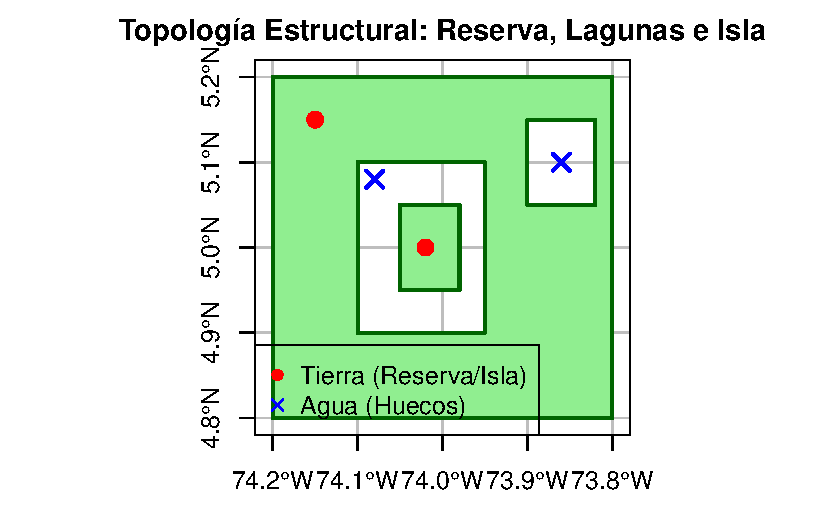
\includegraphics[width=0.8\textwidth,height=\textheight]{14-vector_files/figure-pdf/r_extraccion_nodos2-1.pdf}
\end{center}

\subsection{Julia}

En Julia, la API subyacente de \texttt{ArchGDAL} garantiza que
\texttt{getgeom(pol,\ 0)} extrae el anillo exterior primario. Todo
índice mayor a 0 extrae iterativamente los huecos internos.

\emph{Nota sobre indexación:} A nivel global, el lenguaje Julia comienza
sus vectores en 1. Sin embargo, la API de \texttt{ArchGDAL.jl} es una
envoltura sobre C++, por lo cual \textbf{todos sus accesos geométricos
conservan índice base cero (0)}. Extraer el tercer vértice exigirá
solicitar el puntero número \texttt{2}.

\begin{Shaded}
\begin{Highlighting}[]
\CommentTok{\# \#| eval: false}

\FunctionTok{j\_eval}\NormalTok{(}\StringTok{\textquotesingle{}}
\StringTok{using ArchGDAL}
\StringTok{using CairoMakie}
\StringTok{using Printf}

\StringTok{\# 1. Instanciación y ensamblaje multinivel (Arreglo de Arreglos de Arreglos)}
\StringTok{mpol\_reserva = ArchGDAL.createmultipolygon([}
\StringTok{    [ \# Polígono 1}
\StringTok{        [({-}74.2, 5.2), ({-}73.8, 5.2), ({-}73.8, 4.8), ({-}74.2, 4.8), ({-}74.2, 5.2)], \# Anillo Exterior }
\StringTok{        [({-}74.1, 5.1), ({-}74.1, 4.9), ({-}73.95, 4.9), ({-}73.95, 5.1), ({-}74.1, 5.1)], \# Hueco 1}
\StringTok{        [({-}73.9, 5.15), ({-}73.9, 5.05), ({-}73.82, 5.05), ({-}73.82, 5.15), ({-}73.9, 5.15)] \# Hueco 2}
\StringTok{    ],}
\StringTok{    [ \# Polígono 2}
\StringTok{        [({-}74.05, 5.05), ({-}73.98, 5.05), ({-}73.98, 4.95), ({-}74.05, 4.95), ({-}74.05, 5.05)] \# Anillo Exterior (Isla)}
\StringTok{    ]}
\StringTok{])}

\StringTok{\# 2. Determinación estructural paramétrica (Basada en API C++)}
\StringTok{println("{-}{-}{-} Determinación Estructural (Basada en Índices) {-}{-}{-}")}
\StringTok{pol1 = ArchGDAL.getgeom(mpol\_reserva, 0)}

\StringTok{ext\_reserva = ArchGDAL.getgeom(pol1, 0)}
\StringTok{@printf("Reserva (Pol 0, Índice 0 {-}\textgreater{} Tierra) : [\%f, \%f]}\SpecialCharTok{\textbackslash{}\textbackslash{}}\StringTok{n", ArchGDAL.getx(ext\_reserva, 2), ArchGDAL.gety(ext\_reserva, 2))}

\StringTok{int\_laguna1 = ArchGDAL.getgeom(pol1, 1)}
\StringTok{@printf("Laguna 1 (Pol 0, Índice 1 {-}\textgreater{} Agua)  : [\%f, \%f]}\SpecialCharTok{\textbackslash{}\textbackslash{}}\StringTok{n", ArchGDAL.getx(int\_laguna1, 2), ArchGDAL.gety(int\_laguna1, 2))}

\StringTok{int\_laguna2 = ArchGDAL.getgeom(pol1, 2)}
\StringTok{@printf("Laguna 2 (Pol 0, Índice 2 {-}\textgreater{} Agua)  : [\%f, \%f]}\SpecialCharTok{\textbackslash{}\textbackslash{}}\StringTok{n", ArchGDAL.getx(int\_laguna2, 2), ArchGDAL.gety(int\_laguna2, 2))}

\StringTok{pol2 = ArchGDAL.getgeom(mpol\_reserva, 1)}
\StringTok{ext\_isla = ArchGDAL.getgeom(pol2, 0)}
\StringTok{@printf("Isla (Pol 1, Índice 0 {-}\textgreater{} Tierra)    : [\%f, \%f]}\SpecialCharTok{\textbackslash{}\textbackslash{}}\StringTok{n}\SpecialCharTok{\textbackslash{}\textbackslash{}}\StringTok{n", ArchGDAL.getx(ext\_isla, 2), ArchGDAL.gety(ext\_isla, 2))}

\StringTok{\# 3. Validación topológica con predicados y puntos de control}
\StringTok{pt\_reserva = ArchGDAL.fromWKT("POINT ({-}74.15 5.15)")}
\StringTok{pt\_laguna1 = ArchGDAL.fromWKT("POINT ({-}74.08 5.08)")}
\StringTok{pt\_laguna2 = ArchGDAL.fromWKT("POINT ({-}73.86 5.10)")}
\StringTok{pt\_isla = ArchGDAL.fromWKT("POINT ({-}74.02 5.0)")}

\StringTok{println("{-}{-}{-} Evaluación Topológica (¿Pertenece al polígono sólido?) {-}{-}{-}")}
\StringTok{println("Punto en Reserva (Tierra) : ", ArchGDAL.contains(mpol\_reserva, pt\_reserva))}
\StringTok{println("Punto en Laguna 1 (Agua)  : ", ArchGDAL.contains(mpol\_reserva, pt\_laguna1))}
\StringTok{println("Punto en Laguna 2 (Agua)  : ", ArchGDAL.contains(mpol\_reserva, pt\_laguna2))}
\StringTok{println("Punto en Isla (Tierra)    : ", ArchGDAL.contains(mpol\_reserva, pt\_isla))}

\StringTok{\# 4. Función de mapeo (Traducción GDAL a CairoMakie Polygon)}
\StringTok{function to\_makie\_poly(gdal\_poly)}
\StringTok{    ext = ArchGDAL.getgeom(gdal\_poly, 0)}
\StringTok{    ext\_pts = [Point2f(ArchGDAL.getx(ext, i), ArchGDAL.gety(ext, i)) for i in 0:ArchGDAL.ngeom(ext){-}1]}
\StringTok{    }
\StringTok{    holes = Vector\{Vector\{Point2f\}\}()}
\StringTok{    for i in 1:ArchGDAL.ngeom(gdal\_poly){-}1}
\StringTok{        hole = ArchGDAL.getgeom(gdal\_poly, i)}
\StringTok{        push!(holes, [Point2f(ArchGDAL.getx(hole, j), ArchGDAL.gety(hole, j)) for j in 0:ArchGDAL.ngeom(hole){-}1])}
\StringTok{    end}
\StringTok{    return Makie.Polygon(ext\_pts, holes)}
\StringTok{end}

\StringTok{\# 5. Configuración de panel gráfico y variables}
\StringTok{fig = Figure(size = (600, 600))}
\StringTok{ax = Axis(fig[1, 1], title = "Topología Estructural: Reserva, Lagunas e Isla",}
\StringTok{    xlabel = "Longitud", ylabel = "Latitud", aspect = DataAspect(),}
\StringTok{    xticks = {-}74.3:0.1:{-}73.7, yticks = 4.7:0.1:5.3, }
\StringTok{    xgridstyle = :dash, ygridstyle = :dash, xgridwidth = 0.5, ygridwidth = 0.5)}

\StringTok{\# Renderizado de capas poligonales}
\StringTok{for i in 0:ArchGDAL.ngeom(mpol\_reserva){-}1}
\StringTok{    CairoMakie.poly!(ax, to\_makie\_poly(ArchGDAL.getgeom(mpol\_reserva, i)), }
\StringTok{                     color = :lightgreen, strokecolor = :darkgreen, strokewidth = 2.0)}
\StringTok{end}

\StringTok{\# Superposición de puntos de prueba para contexto visual}
\StringTok{CairoMakie.scatter!(ax, [{-}74.15, {-}74.02], [5.15, 5.0], color = :red, marker = :circle, markersize = 15, label = "Tierra (Reserva/Isla)")}
\StringTok{CairoMakie.scatter!(ax, [{-}74.08, {-}73.86], [5.08, 5.10], color = :blue, marker = :cross, markersize = 18, label = "Agua (Huecos)")}
\StringTok{axislegend(ax, position = :lb) \# Legenda en Lower Left}

\StringTok{CairoMakie.save("images/c14\_plot\_topologia\_puntos\_julia.png", fig)}
\StringTok{\textquotesingle{}}\NormalTok{)}
\end{Highlighting}
\end{Shaded}

\begin{Shaded}
\begin{Highlighting}[]
\NormalTok{knitr}\SpecialCharTok{::}\FunctionTok{include\_graphics}\NormalTok{(}\StringTok{"images/c14\_plot\_topologia\_puntos\_julia.png"}\NormalTok{)}
\end{Highlighting}
\end{Shaded}

\begin{center}
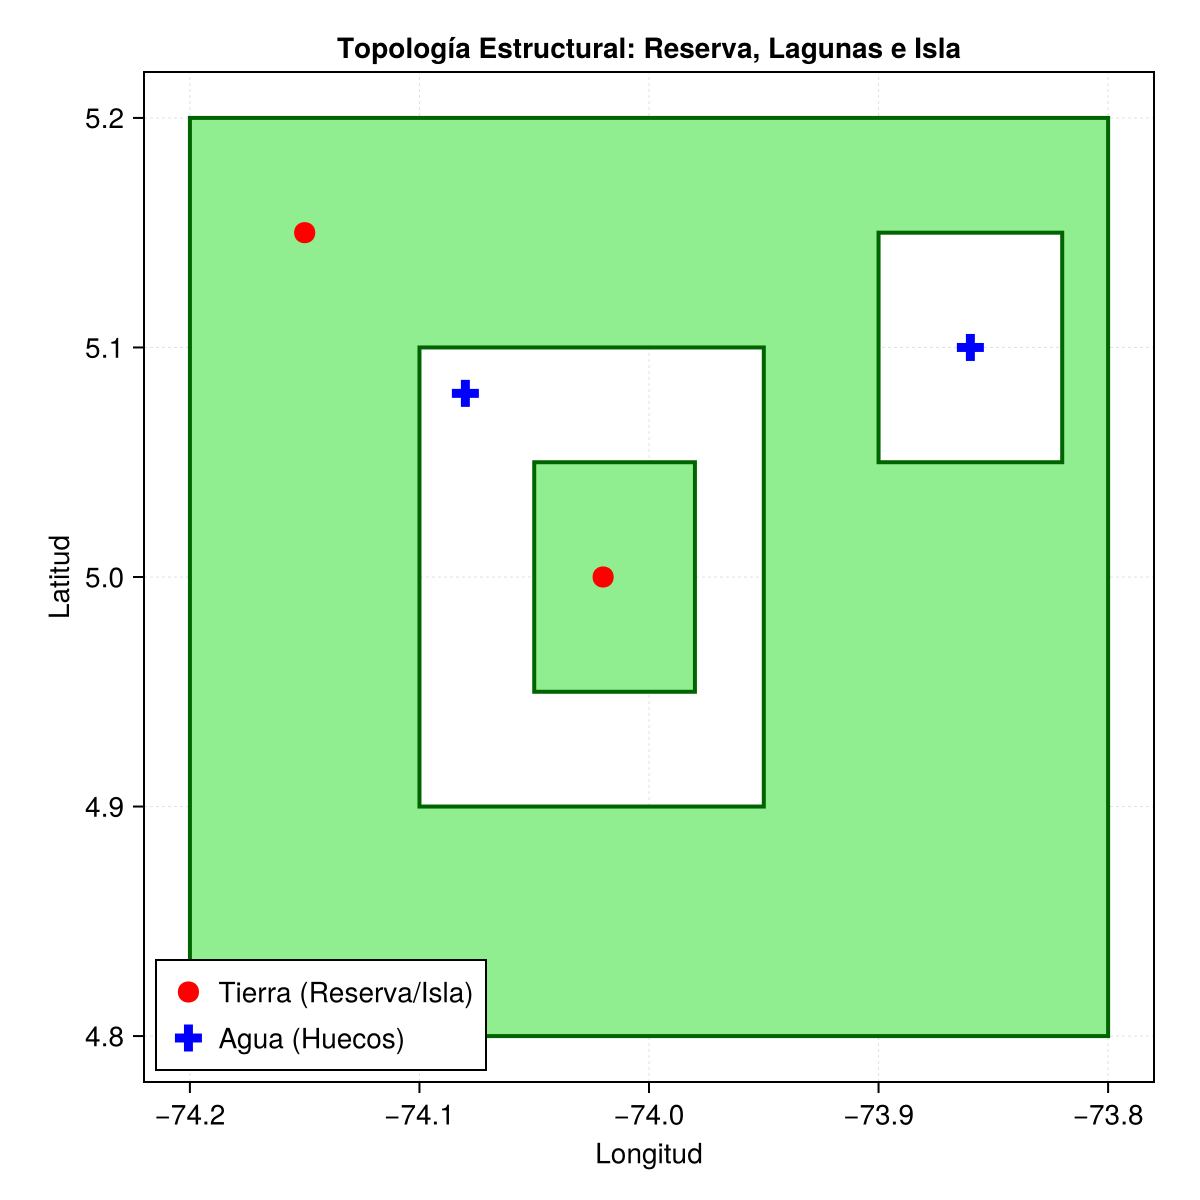
\includegraphics[width=0.8\textwidth,height=\textheight]{images/c14_plot_topologia_puntos_julia.png}
\end{center}

\subsection{Resumen sintáctico}\label{resumen-sintuxe1ctico-2}

El acceso a los atributos internos para determinar la validez
estructural y aislar vértices dentro de geometrías complejas exige
descender a través de la jerarquía topológica del objeto (Colección
\(\rightarrow\) Geometría \(\rightarrow\) Anillo \(\rightarrow\)
Vértice).

Es imperativo reconocer la asimetría algorítmica de los índices base:
mientras Python inicia sus índices vectoriales en \textbf{0}, R lo hace
en \textbf{1}. En el ecosistema de Julia, aunque el lenguaje nativamente
inicia en 1, la API de \texttt{ArchGDAL.jl} hereda la indexación
estricta en \textbf{0} de su librería matriz C++.

\textbf{1. Navegación topológica y extracción de anillos}

En la siguiente tabla se asume que las variables \emph{i}, \emph{k} y
\emph{j} representan la posición del elemento utilizando el
\textbf{índice base nativo} de cada lenguaje (ej. para extraer el primer
polígono, \emph{i} vale 0 en Python/Julia y 1 en R).

\begin{longtable}[]{@{}
  >{\raggedright\arraybackslash}p{(\columnwidth - 6\tabcolsep) * \real{0.2500}}
  >{\raggedright\arraybackslash}p{(\columnwidth - 6\tabcolsep) * \real{0.2500}}
  >{\raggedright\arraybackslash}p{(\columnwidth - 6\tabcolsep) * \real{0.2500}}
  >{\raggedright\arraybackslash}p{(\columnwidth - 6\tabcolsep) * \real{0.2500}}@{}}
\caption{Sintaxis analítica para el descenso iterativo y disección
topológica de
multigeometrías}\label{tbl-resumen_extraccion_anillos}\tabularnewline
\toprule\noalign{}
\begin{minipage}[b]{\linewidth}\raggedright
Nivel topológico
\end{minipage} & \begin{minipage}[b]{\linewidth}\raggedright
Python (\texttt{shapely}) 🐍
\end{minipage} & \begin{minipage}[b]{\linewidth}\raggedright
R (\texttt{sf}) 🔵
\end{minipage} & \begin{minipage}[b]{\linewidth}\raggedright
Julia (\texttt{ArchGDAL}) 🟣
\end{minipage} \\
\midrule\noalign{}
\endfirsthead
\toprule\noalign{}
\begin{minipage}[b]{\linewidth}\raggedright
Nivel topológico
\end{minipage} & \begin{minipage}[b]{\linewidth}\raggedright
Python (\texttt{shapely}) 🐍
\end{minipage} & \begin{minipage}[b]{\linewidth}\raggedright
R (\texttt{sf}) 🔵
\end{minipage} & \begin{minipage}[b]{\linewidth}\raggedright
Julia (\texttt{ArchGDAL}) 🟣
\end{minipage} \\
\midrule\noalign{}
\endhead
\bottomrule\noalign{}
\endlastfoot
\textbf{Extraer polígono \emph{i}}\emph{(Desde MultiPolygon)} &
\texttt{mpol.geoms{[}i{]}} & \texttt{mpol{[}{[}i{]}{]}} &
\texttt{ArchGDAL.getgeom(}\texttt{mpol,\ i)} \\
\textbf{Anillo exterior (Tierra)}\emph{(Límite principal)} &
\texttt{pol.exterior} & \texttt{pol{[}{[}1{]}{]}} &
\texttt{ArchGDAL.getgeom(}\texttt{pol,\ 0)} \\
\textbf{Anillo interior \emph{k} (Agua)}\emph{(Hueco / Perforación)} &
\texttt{pol.interiors{[}k{]}} & \texttt{pol{[}{[}k+1{]}{]}} &
\texttt{ArchGDAL.getgeom(}\texttt{pol,\ k+1)} \\
\textbf{Índice base del motor} & Basado en \texttt{0} & Basado en
\texttt{1} & Basado en \texttt{0} (C++) \\
\end{longtable}

\begin{center}\rule{0.5\linewidth}{0.5pt}\end{center}

\textbf{2. Extracción de vértices y extensiones espaciales}

Una vez aislado el anillo unidimensional (ya sea el límite sólido o un
hueco), la extracción de la tupla de coordenadas cartesianas o el
cálculo de la envolvente convexa rectangular (Bounding Box) se efectúa
mediante los siguientes comandos escalares.

\begin{longtable}[]{@{}
  >{\raggedright\arraybackslash}p{(\columnwidth - 6\tabcolsep) * \real{0.2500}}
  >{\raggedright\arraybackslash}p{(\columnwidth - 6\tabcolsep) * \real{0.2500}}
  >{\raggedright\arraybackslash}p{(\columnwidth - 6\tabcolsep) * \real{0.2500}}
  >{\raggedright\arraybackslash}p{(\columnwidth - 6\tabcolsep) * \real{0.2500}}@{}}
\caption{Funciones escalares para la recolección de tuplas de
coordenadas y cálculo de la extensión espacial
perimetral}\label{tbl-resumen_extraccion_vertices}\tabularnewline
\toprule\noalign{}
\begin{minipage}[b]{\linewidth}\raggedright
Operación vectorial
\end{minipage} & \begin{minipage}[b]{\linewidth}\raggedright
Python (\texttt{shapely}) 🐍
\end{minipage} & \begin{minipage}[b]{\linewidth}\raggedright
R (\texttt{sf}) 🔵
\end{minipage} & \begin{minipage}[b]{\linewidth}\raggedright
Julia (\texttt{ArchGDAL}) 🟣
\end{minipage} \\
\midrule\noalign{}
\endfirsthead
\toprule\noalign{}
\begin{minipage}[b]{\linewidth}\raggedright
Operación vectorial
\end{minipage} & \begin{minipage}[b]{\linewidth}\raggedright
Python (\texttt{shapely}) 🐍
\end{minipage} & \begin{minipage}[b]{\linewidth}\raggedright
R (\texttt{sf}) 🔵
\end{minipage} & \begin{minipage}[b]{\linewidth}\raggedright
Julia (\texttt{ArchGDAL}) 🟣
\end{minipage} \\
\midrule\noalign{}
\endhead
\bottomrule\noalign{}
\endlastfoot
\textbf{Extraer vértice \emph{j}}\emph{(Coordenada aislada)} &
\texttt{anillo.coords{[}j{]}} & \texttt{anillo{[}j,\ {]}} &
\texttt{ArchGDAL.getx(anillo,\ j)}\texttt{ArchGDAL.gety(anillo,\ j)} \\
\textbf{Caja delimitadora}\emph{(Bounding Box)} &
\texttt{geom.bounds}\emph{(Geometría individual)} &
\texttt{st\_bbox(geom)} & \texttt{ArchGDAL.getenvelope(geom)} \\
\end{longtable}

\begin{center}\rule{0.5\linewidth}{0.5pt}\end{center}

\textbf{3. Control isométrico y ajuste del lienzo}

Para garantizar que la representación gráfica mantenga la proporción
geométrica real (1:1) y no distorsione la topología simulada, es
necesario forzar la isometría del lienzo y controlar los márgenes de los
ejes utilizando las cajas delimitadoras.

\begin{longtable}[]{@{}
  >{\raggedright\arraybackslash}p{(\columnwidth - 6\tabcolsep) * \real{0.2500}}
  >{\raggedright\arraybackslash}p{(\columnwidth - 6\tabcolsep) * \real{0.2500}}
  >{\raggedright\arraybackslash}p{(\columnwidth - 6\tabcolsep) * \real{0.2500}}
  >{\raggedright\arraybackslash}p{(\columnwidth - 6\tabcolsep) * \real{0.2500}}@{}}
\caption{Equivalencia de métodos paramétricos para el control isométrico
del área de ploteo}\label{tbl-resumen_control_lienzo}\tabularnewline
\toprule\noalign{}
\begin{minipage}[b]{\linewidth}\raggedright
Operación paramétrica
\end{minipage} & \begin{minipage}[b]{\linewidth}\raggedright
Python (\texttt{matplotlib}) 🐍
\end{minipage} & \begin{minipage}[b]{\linewidth}\raggedright
R (Base Graphics) 🔵
\end{minipage} & \begin{minipage}[b]{\linewidth}\raggedright
Julia (\texttt{CairoMakie}) 🟣
\end{minipage} \\
\midrule\noalign{}
\endfirsthead
\toprule\noalign{}
\begin{minipage}[b]{\linewidth}\raggedright
Operación paramétrica
\end{minipage} & \begin{minipage}[b]{\linewidth}\raggedright
Python (\texttt{matplotlib}) 🐍
\end{minipage} & \begin{minipage}[b]{\linewidth}\raggedright
R (Base Graphics) 🔵
\end{minipage} & \begin{minipage}[b]{\linewidth}\raggedright
Julia (\texttt{CairoMakie}) 🟣
\end{minipage} \\
\midrule\noalign{}
\endhead
\bottomrule\noalign{}
\endlastfoot
\textbf{Forzar isometría}\emph{(Aspect Ratio 1:1)} &
\texttt{fig,\ ax\ =\ plt.subplots(}\texttt{figsize=(6,\ 6))} &
\texttt{par(pty\ =\ "s")} &
\texttt{ax\ =\ Axis(...,}\texttt{aspect\ =\ DataAspect())} \\
\textbf{Eliminar padding nativo}\emph{(Ajustar ejes al límite exacto)} &
\texttt{ax.margins(0)} &
\texttt{plot(...,}\texttt{xaxs\ =\ "i",\ yaxs\ =\ "i")} &
\emph{Controlado inherentemente por
\texttt{\textless{}br\textgreater{}}DataAspect() y xticks/yticks} \\
\end{longtable}

\section{Creación de puntos a partir de coordenadas en la
tabla}\label{creaciuxf3n-de-puntos-a-partir-de-coordenadas-en-la-tabla}

El siguiente código define un conjunto de datos tabulares con las
coordenadas de cuatro ciudades principales de Colombia y lo convierte a
un formato espacial explícito asignando el sistema de referencia WGS84
(EPSG:4326), para luego generar un gráfico básico.

\subsection{Python}

\begin{Shaded}
\begin{Highlighting}[]
\CommentTok{\# \#| eval: false}

\ImportTok{import}\NormalTok{ pandas }\ImportTok{as}\NormalTok{ pd}
\ImportTok{import}\NormalTok{ geopandas }\ImportTok{as}\NormalTok{ gpd}
\ImportTok{import}\NormalTok{ matplotlib.pyplot }\ImportTok{as}\NormalTok{ plt}

\CommentTok{\# 1. Datos de coordenadas de ciudades principales de Colombia}
\NormalTok{datos }\OperatorTok{=}\NormalTok{ \{}
    \StringTok{"Ciudad"}\NormalTok{: [}\StringTok{"Bogotá"}\NormalTok{, }\StringTok{"Medellín"}\NormalTok{, }\StringTok{"Cali"}\NormalTok{, }\StringTok{"Barranquilla"}\NormalTok{],}
    \StringTok{"Latitud"}\NormalTok{: [}\FloatTok{4.6097}\NormalTok{, }\FloatTok{6.2442}\NormalTok{, }\FloatTok{3.4516}\NormalTok{, }\FloatTok{10.9685}\NormalTok{],}
    \StringTok{"Longitud"}\NormalTok{: [}\OperatorTok{{-}}\FloatTok{74.0817}\NormalTok{, }\OperatorTok{{-}}\FloatTok{75.5812}\NormalTok{, }\OperatorTok{{-}}\FloatTok{76.5320}\NormalTok{, }\OperatorTok{{-}}\FloatTok{74.7813}\NormalTok{]}
\NormalTok{\}}

\CommentTok{\# 2. Creación del DataFrame tabular estándar}
\NormalTok{df }\OperatorTok{=}\NormalTok{ pd.DataFrame(datos)}

\CommentTok{\# 3. Conversión a GeoDataFrame asignando la geometría de puntos}
\CommentTok{\# Se especifica crs="EPSG:4326" correspondiente a coordenadas geográficas WGS84}
\NormalTok{gdf }\OperatorTok{=}\NormalTok{ gpd.GeoDataFrame(}
\NormalTok{    df, }
\NormalTok{    geometry}\OperatorTok{=}\NormalTok{gpd.points\_from\_xy(df.Longitud, df.Latitud),}
\NormalTok{    crs}\OperatorTok{=}\StringTok{"EPSG:4326"}
\NormalTok{)}

\CommentTok{\# Visualización tabular}
\BuiltInTok{print}\NormalTok{(gdf)}
\end{Highlighting}
\end{Shaded}

\begin{verbatim}
         Ciudad  Latitud  Longitud                  geometry
0        Bogotá   4.6097  -74.0817   POINT (-74.0817 4.6097)
1      Medellín   6.2442  -75.5812   POINT (-75.5812 6.2442)
2          Cali   3.4516  -76.5320    POINT (-76.532 3.4516)
3  Barranquilla  10.9685  -74.7813  POINT (-74.7813 10.9685)
\end{verbatim}

\begin{Shaded}
\begin{Highlighting}[]
\CommentTok{\# Visualización gráfica}
\NormalTok{gdf.plot(color}\OperatorTok{=}\StringTok{"red"}\NormalTok{, marker}\OperatorTok{=}\StringTok{"o"}\NormalTok{, markersize}\OperatorTok{=}\DecValTok{50}\NormalTok{)}
\NormalTok{plt.title(}\StringTok{"Ciudades Principales {-} Colombia"}\NormalTok{)}
\NormalTok{plt.xlabel(}\StringTok{"Longitud"}\NormalTok{)}
\NormalTok{plt.ylabel(}\StringTok{"Latitud"}\NormalTok{)}
\NormalTok{plt.show()}
\end{Highlighting}
\end{Shaded}

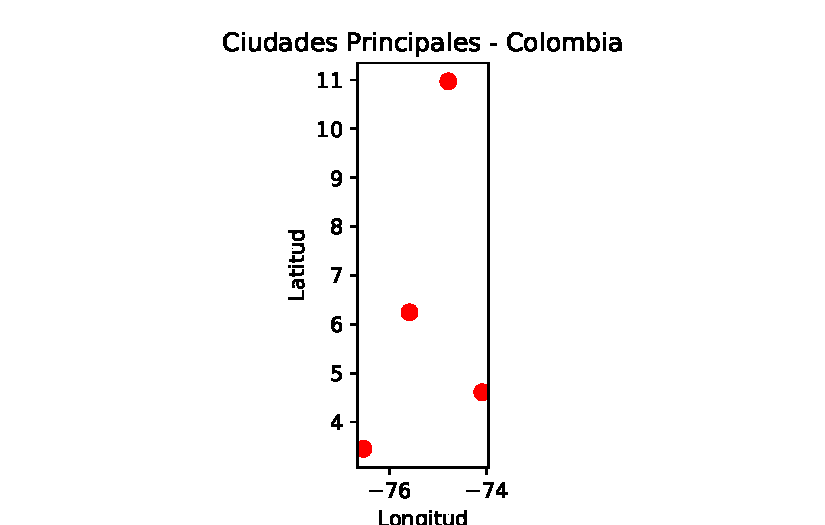
\includegraphics{14-vector_files/figure-pdf/python_crear_puntos-1.pdf}

\subsection{R}

\begin{Shaded}
\begin{Highlighting}[]
\CommentTok{\# \#| eval: false}

\FunctionTok{library}\NormalTok{(sf)}
\FunctionTok{library}\NormalTok{(tibble)}

\CommentTok{\# 1. Datos tabulares de ciudades principales de Colombia}
\NormalTok{df }\OtherTok{\textless{}{-}} \FunctionTok{tibble}\NormalTok{(}
  \AttributeTok{Ciudad =} \FunctionTok{c}\NormalTok{(}\StringTok{"Bogotá"}\NormalTok{, }\StringTok{"Medellín"}\NormalTok{, }\StringTok{"Cali"}\NormalTok{, }\StringTok{"Barranquilla"}\NormalTok{),}
  \AttributeTok{Latitud =} \FunctionTok{c}\NormalTok{(}\FloatTok{4.6097}\NormalTok{, }\FloatTok{6.2442}\NormalTok{, }\FloatTok{3.4516}\NormalTok{, }\FloatTok{10.9685}\NormalTok{),}
  \AttributeTok{Longitud =} \FunctionTok{c}\NormalTok{(}\SpecialCharTok{{-}}\FloatTok{74.0817}\NormalTok{, }\SpecialCharTok{{-}}\FloatTok{75.5812}\NormalTok{, }\SpecialCharTok{{-}}\FloatTok{76.5320}\NormalTok{, }\SpecialCharTok{{-}}\FloatTok{74.7813}\NormalTok{)}
\NormalTok{)}

\CommentTok{\# 2. Conversión a objeto espacial (sf)}
\CommentTok{\# Se indican los nombres de las columnas que contienen las coordenadas}
\CommentTok{\# Se asigna explícitamente el CRS 4326 (WGS84)}
\NormalTok{gdf }\OtherTok{\textless{}{-}} \FunctionTok{st\_as\_sf}\NormalTok{(df, }\AttributeTok{coords =} \FunctionTok{c}\NormalTok{(}\StringTok{"Longitud"}\NormalTok{, }\StringTok{"Latitud"}\NormalTok{), }\AttributeTok{crs =} \DecValTok{4326}\NormalTok{)}

\CommentTok{\# Visualización tabular}
\FunctionTok{print}\NormalTok{(gdf)}
\end{Highlighting}
\end{Shaded}

\begin{verbatim}
Simple feature collection with 4 features and 1 field
Geometry type: POINT
Dimension:     XY
Bounding box:  xmin: -76.532 ymin: 3.4516 xmax: -74.0817 ymax: 10.9685
Geodetic CRS:  WGS 84
# A tibble: 4 x 2
  Ciudad                 geometry
* <chr>               <POINT [°]>
1 Bogotá        (-74.0817 4.6097)
2 Medellín      (-75.5812 6.2442)
3 Cali           (-76.532 3.4516)
4 Barranquilla (-74.7813 10.9685)
\end{verbatim}

\begin{Shaded}
\begin{Highlighting}[]
\CommentTok{\# Visualización gráfica}
\FunctionTok{plot}\NormalTok{(}\FunctionTok{st\_geometry}\NormalTok{(gdf), }\AttributeTok{col =} \StringTok{"red"}\NormalTok{, }\AttributeTok{pch =} \DecValTok{16}\NormalTok{, }\AttributeTok{cex =} \FloatTok{1.5}\NormalTok{, }
     \AttributeTok{main =} \StringTok{"Ciudades Principales {-} Colombia"}\NormalTok{, }\AttributeTok{axes =} \ConstantTok{TRUE}\NormalTok{)}
\end{Highlighting}
\end{Shaded}

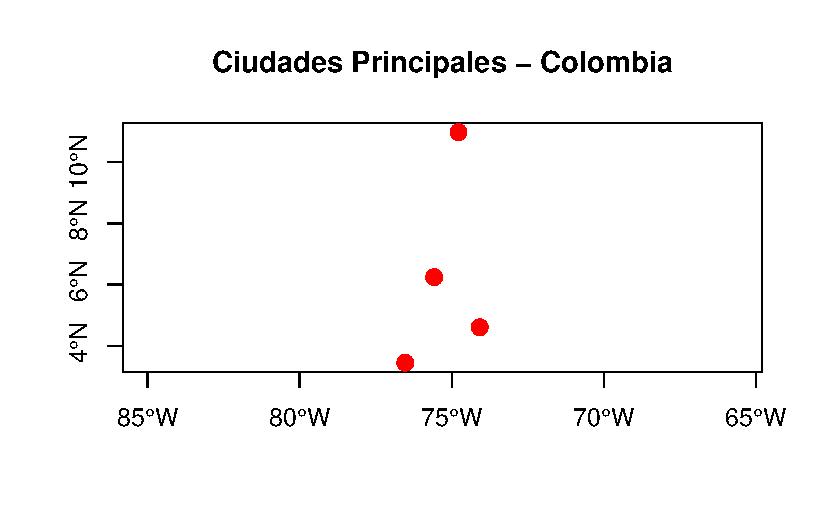
\includegraphics{14-vector_files/figure-pdf/r_crear_puntos-1.pdf}

\subsection{Julia}

\begin{Shaded}
\begin{Highlighting}[]
\CommentTok{\# \#| eval: false}

\FunctionTok{j\_eval}\NormalTok{(}\StringTok{\textquotesingle{}}
\StringTok{using DataFrames}
\StringTok{using ArchGDAL}
\StringTok{using Plots}

\StringTok{\# 1. Datos tabulares de ciudades principales de Colombia}
\StringTok{df = DataFrame(}
\StringTok{    Ciudad = ["Bogotá", "Medellín", "Cali", "Barranquilla"],}
\StringTok{    Latitud = [4.6097, 6.2442, 3.4516, 10.9685],}
\StringTok{    Longitud = [{-}74.0817, {-}75.5812, {-}76.5320, {-}74.7813]}
\StringTok{)}

\StringTok{\# 2. Creación de la columna de geometría vectorial}
\StringTok{df.geometry = ArchGDAL.createpoint.(df.Longitud, df.Latitud)}

\StringTok{\# Visualización tabular}
\StringTok{println(df)}

\StringTok{\# Visualización gráfica y guardado}
\StringTok{p = Plots.plot(df.geometry, title="Ciudades Principales {-} Colombia", }
\StringTok{         color=:red, marker=:circle, markersize=6, aspect\_ratio=:equal, legend=false)}
\StringTok{         }
\StringTok{Plots.savefig(p, "images/c14\_plot\_ciudades\_colombia\_julia.png")}
\StringTok{\textquotesingle{}}\NormalTok{)}
\end{Highlighting}
\end{Shaded}

\begin{Shaded}
\begin{Highlighting}[]
\NormalTok{knitr}\SpecialCharTok{::}\FunctionTok{include\_graphics}\NormalTok{(}\StringTok{"images/c14\_plot\_ciudades\_colombia\_julia.png"}\NormalTok{)}
\end{Highlighting}
\end{Shaded}

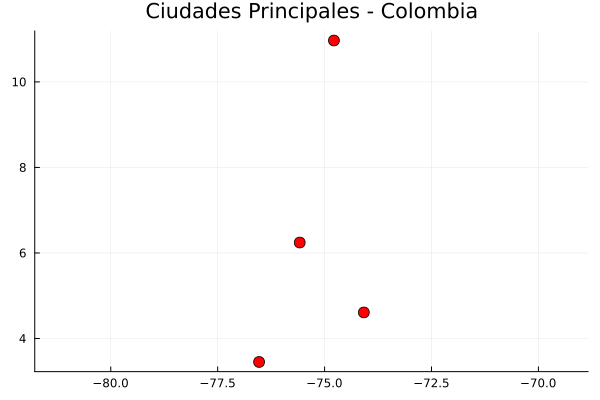
\includegraphics[width=2in,height=\textheight]{images/c14_plot_ciudades_colombia_julia.png}

\subsection{Resumen sintáctico: Creación de puntos
espaciales}\label{resumen-sintuxe1ctico-creaciuxf3n-de-puntos-espaciales}

\begin{longtable}[]{@{}
  >{\raggedright\arraybackslash}p{(\columnwidth - 6\tabcolsep) * \real{0.2500}}
  >{\raggedright\arraybackslash}p{(\columnwidth - 6\tabcolsep) * \real{0.2500}}
  >{\raggedright\arraybackslash}p{(\columnwidth - 6\tabcolsep) * \real{0.2500}}
  >{\raggedright\arraybackslash}p{(\columnwidth - 6\tabcolsep) * \real{0.2500}}@{}}
\caption{Sintaxis comparativa para la creación de geometrías de puntos
desde coordenadas
tabulares}\label{tbl-resumen_crear_puntos}\tabularnewline
\toprule\noalign{}
\begin{minipage}[b]{\linewidth}\raggedright
Operación
\end{minipage} & \begin{minipage}[b]{\linewidth}\raggedright
Python (\texttt{geopandas}) 🐍
\end{minipage} & \begin{minipage}[b]{\linewidth}\raggedright
R (\texttt{sf}) 🔵
\end{minipage} & \begin{minipage}[b]{\linewidth}\raggedright
Julia (\texttt{ArchGDAL}) 🟣
\end{minipage} \\
\midrule\noalign{}
\endfirsthead
\toprule\noalign{}
\begin{minipage}[b]{\linewidth}\raggedright
Operación
\end{minipage} & \begin{minipage}[b]{\linewidth}\raggedright
Python (\texttt{geopandas}) 🐍
\end{minipage} & \begin{minipage}[b]{\linewidth}\raggedright
R (\texttt{sf}) 🔵
\end{minipage} & \begin{minipage}[b]{\linewidth}\raggedright
Julia (\texttt{ArchGDAL}) 🟣
\end{minipage} \\
\midrule\noalign{}
\endhead
\bottomrule\noalign{}
\endlastfoot
\textbf{Librerías base} &
\texttt{import\ pandas\ as\ pd}\texttt{import\ geopandas\ as\ gpd} &
\texttt{library(tibble)}\texttt{library(sf)} &
\texttt{using\ DataFrames}\texttt{using\ ArchGDAL} \\
\textbf{Crear tabla base} & \texttt{df\ =\ pd.DataFrame(datos)} &
\texttt{df\ \textless{}-\ tibble(Lon=...,\ Lat=...)} &
\texttt{df\ =\ DataFrame(Lon=...,\ Lat=...)} \\
\textbf{Convertir a espacial} &
\texttt{gpd.GeoDataFrame(df,\ geometry=gpd.points\_from\_xy(df.Lon,\ df.Lat),\ crs="EPSG:4326")}
& \texttt{st\_as\_sf(df,\ coords=c("Lon",\ "Lat"),\ crs=4326)} &
\texttt{df.geometry\ =\ ArchGDAL.createpoint.(df.Lon,\ df.Lat)} \\
\textbf{Gráfico rápido} & \texttt{gdf.plot()} &
\texttt{plot(st\_geometry(gdf))} & \texttt{plot(df.geometry)} \\
\end{longtable}

\section{Lectura de archivos vectoriales
externos}\label{lectura-de-archivos-vectoriales-externos}

En un flujo de trabajo SIG, la fuente principal de datos suelen ser
archivos externos. El formato \emph{Shapefile} (.shp) sigue siendo el
estándar de la industria, aunque requiere que todos sus archivos
asociados (.dbf, .shx, .prj) estén en la misma carpeta.

A continuación, cargamos la capa de municipios utilizando la ruta local
\texttt{data\_heavy/MUNICIPIOS\_ISLA\_WGS84.shp}.

\subsection{Python}

\begin{Shaded}
\begin{Highlighting}[]
\CommentTok{\# \#| eval: false}

\ImportTok{import}\NormalTok{ geopandas }\ImportTok{as}\NormalTok{ gpd}

\CommentTok{\# Carga del GeoDataFrame}
\NormalTok{ruta }\OperatorTok{=} \VerbatimStringTok{r"data\_heavy/MUNICIPIOS\_ISLA\_WGS84.shp"}
\NormalTok{gdf\_municipios }\OperatorTok{=}\NormalTok{ gpd.read\_file(ruta)}

\CommentTok{\# Metadatos del archivo}
\BuiltInTok{print}\NormalTok{(}\SpecialStringTok{f"Tipo de objeto: }\SpecialCharTok{\{}\BuiltInTok{type}\NormalTok{(gdf\_municipios)}\SpecialCharTok{\}}\SpecialStringTok{"}\NormalTok{)}
\end{Highlighting}
\end{Shaded}

\begin{verbatim}
Tipo de objeto: <class 'geopandas.geodataframe.GeoDataFrame'>
\end{verbatim}

\begin{Shaded}
\begin{Highlighting}[]
\BuiltInTok{print}\NormalTok{(}\SpecialStringTok{f"Número de polígonos: }\SpecialCharTok{\{}\BuiltInTok{len}\NormalTok{(gdf\_municipios)}\SpecialCharTok{\}}\SpecialStringTok{"}\NormalTok{)}
\end{Highlighting}
\end{Shaded}

\begin{verbatim}
Número de polígonos: 1129
\end{verbatim}

\begin{Shaded}
\begin{Highlighting}[]
\NormalTok{gdf\_municipios.head()}
\end{Highlighting}
\end{Shaded}

\begin{verbatim}
              NMG  ...                                           geometry
0      SAN ANDRÉS  ...  POLYGON ((-81.72221 12.58509, -81.72219 12.585...
1     PROVIDENCIA  ...  POLYGON ((-81.3727 13.38464, -81.37253 13.3846...
2  SANTA CATALINA  ...  POLYGON ((-81.38101 13.39492, -81.38099 13.394...
3          URIBIA  ...  POLYGON ((-72.35702 11.83287, -72.35438 11.834...
4         MANAURE  ...  POLYGON ((-72.35702 11.83287, -72.35662 11.823...

[5 rows x 4 columns]
\end{verbatim}

\subsection{R}

\begin{Shaded}
\begin{Highlighting}[]
\CommentTok{\# \#| eval: false}

\FunctionTok{library}\NormalTok{(sf)}

\CommentTok{\# Lectura silenciosa para evitar el log de GDAL en el renderizado}
\NormalTok{ruta }\OtherTok{\textless{}{-}} \StringTok{"data\_heavy/MUNICIPIOS\_ISLA\_WGS84.shp"}
\NormalTok{gdf\_municipios }\OtherTok{\textless{}{-}} \FunctionTok{st\_read}\NormalTok{(ruta, }\AttributeTok{quiet =} \ConstantTok{TRUE}\NormalTok{)}

\CommentTok{\# Verificamos la columna de geometría}
\FunctionTok{st\_geometry}\NormalTok{(gdf\_municipios) }\SpecialCharTok{|\textgreater{}} \FunctionTok{head}\NormalTok{()}
\end{Highlighting}
\end{Shaded}

\begin{verbatim}
Geometry set for 6 features 
Geometry type: POLYGON
Dimension:     XY
Bounding box:  xmin: -81.73855 ymin: 11.11615 xmax: -71.11888 ymax: 13.39756
Geodetic CRS:  WGS 84
First 5 geometries:
\end{verbatim}

\begin{verbatim}
POLYGON ((-81.72221 12.58509, -81.72219 12.5851...
\end{verbatim}

\begin{verbatim}
POLYGON ((-81.3727 13.38464, -81.37253 13.38464...
\end{verbatim}

\begin{verbatim}
POLYGON ((-81.38101 13.39492, -81.38099 13.3949...
\end{verbatim}

\begin{verbatim}
POLYGON ((-72.35702 11.83287, -72.35438 11.8344...
\end{verbatim}

\begin{verbatim}
POLYGON ((-72.35702 11.83287, -72.35662 11.8238...
\end{verbatim}

\subsection{Julia}

\begin{Shaded}
\begin{Highlighting}[]
\CommentTok{\# \#| eval: false}

\FunctionTok{j\_eval}\NormalTok{(}\StringTok{\textquotesingle{}}
\StringTok{using ArchGDAL}
\StringTok{using DataFrames}

\StringTok{\# Julia abre el archivo dentro de un contexto controlado.}
\StringTok{ruta = "data\_heavy/MUNICIPIOS\_ISLA\_WGS84.shp"}
\StringTok{ArchGDAL.read(ruta) do dataset}
\StringTok{    \# Se extrae la capa (layer) del Shapefile}
\StringTok{    layer = ArchGDAL.getlayer(dataset, 0)}
\StringTok{    \# Conversión directa a DataFrame de Julia}
\StringTok{    df\_municipios = DataFrame(layer)}
\StringTok{    println(first(df\_municipios, 5))}
\StringTok{end}
\StringTok{\textquotesingle{}}\NormalTok{)}
\end{Highlighting}
\end{Shaded}

\section{La columna de geometría como objeto
independiente}\label{la-columna-de-geometruxeda-como-objeto-independiente}

Una vez cargada la tabla, la columna que almacena los datos espaciales
se comporta de forma distinta a una columna de texto normal. En Python
es una \textbf{GeoSeries} y en R es una \textbf{sfc}. Estos objetos
permiten realizar operaciones directas como el cálculo de áreas o
perímetros.

\subsection{Python}

\begin{Shaded}
\begin{Highlighting}[]
\CommentTok{\# Acceso a la GeoSeries}
\NormalTok{geometria }\OperatorTok{=}\NormalTok{ gdf\_municipios.geometry}

\CommentTok{\# Cálculos directos (El resultado depende de la unidad del CRS)}
\NormalTok{areas }\OperatorTok{=}\NormalTok{ geometria.area}
\end{Highlighting}
\end{Shaded}

\begin{verbatim}
<string>:3: UserWarning: Geometry is in a geographic CRS. Results from 'area' are likely incorrect. Use 'GeoSeries.to_crs()' to re-project geometries to a projected CRS before this operation.
\end{verbatim}

\begin{Shaded}
\begin{Highlighting}[]
\NormalTok{centroides }\OperatorTok{=}\NormalTok{ geometria.centroid}
\end{Highlighting}
\end{Shaded}

\begin{verbatim}
<string>:1: UserWarning: Geometry is in a geographic CRS. Results from 'centroid' are likely incorrect. Use 'GeoSeries.to_crs()' to re-project geometries to a projected CRS before this operation.
\end{verbatim}

\begin{Shaded}
\begin{Highlighting}[]
\BuiltInTok{print}\NormalTok{(areas.head())}
\end{Highlighting}
\end{Shaded}

\begin{verbatim}
0    0.002230
1    0.001728
2    0.000107
3    0.651231
4    0.134081
dtype: float64
\end{verbatim}

\subsection{R}

\begin{Shaded}
\begin{Highlighting}[]
\CommentTok{\# Acceso a la columna sfc}
\NormalTok{geometria }\OtherTok{\textless{}{-}} \FunctionTok{st\_geometry}\NormalTok{(gdf\_municipios)}

\CommentTok{\# Cálculos directos}
\NormalTok{areas }\OtherTok{\textless{}{-}} \FunctionTok{st\_area}\NormalTok{(geometria)}
\NormalTok{centroides }\OtherTok{\textless{}{-}} \FunctionTok{st\_centroid}\NormalTok{(geometria)}
\FunctionTok{print}\NormalTok{(}\FunctionTok{head}\NormalTok{(areas))}
\end{Highlighting}
\end{Shaded}

\begin{verbatim}
Units: [m^2]
[1]   26909397   20789050    1287434 7875913881 1623909829 1736454656
\end{verbatim}

\subsection{Julia}

\begin{Shaded}
\begin{Highlighting}[]
\CommentTok{\# \#| eval: false}

\FunctionTok{j\_eval}\NormalTok{(}\StringTok{\textquotesingle{}}
\StringTok{using ArchGDAL}
\StringTok{using DataFrames}

\StringTok{\# En Julia operamos sobre el vector de geometrías de forma vectorizada (.)}
\StringTok{geometria = df\_municipios.geometry}

\StringTok{areas = ArchGDAL.getarea.(geometria)}
\StringTok{centroides = ArchGDAL.centroid.(geometria)}

\StringTok{println("Cálculo de áreas y centroides finalizado.")}
\StringTok{\textquotesingle{}}\NormalTok{)}
\end{Highlighting}
\end{Shaded}

\subsection{Resumen sintáctico: Lectura y
Estructura}\label{resumen-sintuxe1ctico-lectura-y-estructura}

\begin{longtable}[]{@{}
  >{\raggedright\arraybackslash}p{(\columnwidth - 6\tabcolsep) * \real{0.2500}}
  >{\raggedright\arraybackslash}p{(\columnwidth - 6\tabcolsep) * \real{0.2500}}
  >{\raggedright\arraybackslash}p{(\columnwidth - 6\tabcolsep) * \real{0.2500}}
  >{\raggedright\arraybackslash}p{(\columnwidth - 6\tabcolsep) * \real{0.2500}}@{}}
\caption{Resumen de funciones para la importación y manipulación de
columnas de geometría}\label{tbl-resumen_lectura_local}\tabularnewline
\toprule\noalign{}
\begin{minipage}[b]{\linewidth}\raggedright
Operación
\end{minipage} & \begin{minipage}[b]{\linewidth}\raggedright
Python (\texttt{geopandas}) 🐍
\end{minipage} & \begin{minipage}[b]{\linewidth}\raggedright
R (\texttt{sf}) 🔵
\end{minipage} & \begin{minipage}[b]{\linewidth}\raggedright
Julia (\texttt{ArchGDAL}) 🟣
\end{minipage} \\
\midrule\noalign{}
\endfirsthead
\toprule\noalign{}
\begin{minipage}[b]{\linewidth}\raggedright
Operación
\end{minipage} & \begin{minipage}[b]{\linewidth}\raggedright
Python (\texttt{geopandas}) 🐍
\end{minipage} & \begin{minipage}[b]{\linewidth}\raggedright
R (\texttt{sf}) 🔵
\end{minipage} & \begin{minipage}[b]{\linewidth}\raggedright
Julia (\texttt{ArchGDAL}) 🟣
\end{minipage} \\
\midrule\noalign{}
\endhead
\bottomrule\noalign{}
\endlastfoot
\textbf{Lectura (.shp)} & \texttt{gpd.read\_file(path)} &
\texttt{st\_read(path)} & \texttt{ArchGDAL.read(path)} \\
\textbf{Clase de columna} & \texttt{GeoSeries} & \texttt{sfc} &
\texttt{Vector\{IGeometry\}} \\
\textbf{Cálculo de Área} & \texttt{.area} & \texttt{st\_area()} &
\texttt{ArchGDAL.getarea.()} \\
\textbf{Centros de masa} & \texttt{.centroid} & \texttt{st\_centroid()}
& \texttt{ArchGDAL.centroid.()} \\
\end{longtable}

\section{Relación atributo-geometría
(AGR)}\label{relaciuxf3n-atributo-geometruxeda-agr}

La Relación Atributo-Geometría (AGR por sus siglas en inglés) define
cómo los valores de los atributos tabulares se asocian físicamente con
la extensión espacial de la geometría a la que pertenecen. Esta relación
manifiesta su importancia crítica durante las operaciones de
geoprocesamiento que alteran la forma original de las geometrías, como
los recortes o las intersecciones. Al dividir un polígono, el
comportamiento del dato tabular depende de su relación espacial. Existen
tres relaciones semánticas principales:

\begin{itemize}
\tightlist
\item
  \textbf{Constante}: El valor del atributo es válido y homogéneo en
  cualquier ubicación interior de la geometría. Por ejemplo, el tipo de
  suelo geológico o la jurisdicción departamental (ej. Cundinamarca). Si
  la geometría se recorta, el fragmento conserva el mismo valor.
\item
  \textbf{Agregada}: El valor es un resumen estadístico dependiente del
  área total. Por ejemplo, la población total o la densidad demográfica
  de la localidad de Teusaquillo en Bogotá. Si la geometría se divide,
  el valor original ya no es válido para los fragmentos y requiere un
  recálculo proporcional.
\item
  \textbf{Identidad}: El valor identifica unívocamente a esa geometría
  específica como unidad integral. Por ejemplo, el número de matrícula
  inmobiliaria catastral o el código identificador único del IGAC de un
  predio. Al alterar la geometría, el elemento pierde su identidad
  original.
\end{itemize}

\subsection{Python}

\begin{Shaded}
\begin{Highlighting}[]
\CommentTok{\# \#| eval: false}

\ImportTok{import}\NormalTok{ geopandas }\ImportTok{as}\NormalTok{ gpd}
\ImportTok{import}\NormalTok{ matplotlib.pyplot }\ImportTok{as}\NormalTok{ plt}
\ImportTok{from}\NormalTok{ shapely.geometry }\ImportTok{import}\NormalTok{ Polygon, box}

\CommentTok{\# 1. Definición de geometrías en coordenadas proyectadas (MAGNA{-}SIRGAS, EPSG:9377)}
\CommentTok{\# Creación de un polígono cuadrado simulado para la localidad de Teusaquillo}
\NormalTok{coords\_teusaquillo }\OperatorTok{=}\NormalTok{ [}
\NormalTok{    (}\DecValTok{4880000}\NormalTok{, }\DecValTok{2060000}\NormalTok{), }\CommentTok{\# Suroccidente}
\NormalTok{    (}\DecValTok{4882000}\NormalTok{, }\DecValTok{2060000}\NormalTok{), }\CommentTok{\# Suroriente}
\NormalTok{    (}\DecValTok{4882000}\NormalTok{, }\DecValTok{2062000}\NormalTok{), }\CommentTok{\# Nororiente}
\NormalTok{    (}\DecValTok{4880000}\NormalTok{, }\DecValTok{2062000}\NormalTok{), }\CommentTok{\# Noroccidente}
\NormalTok{    (}\DecValTok{4880000}\NormalTok{, }\DecValTok{2060000}\NormalTok{)  }\CommentTok{\# Cierre}
\NormalTok{]}
\NormalTok{teusaquillo\_geom }\OperatorTok{=}\NormalTok{ Polygon(coords\_teusaquillo)}

\CommentTok{\# Definición de la extensión de corte (box): cubre la mitad occidental del polígono original}
\CommentTok{\# Parámetros: box(minx, miny, maxx, maxy)}
\NormalTok{caja\_corte\_geom }\OperatorTok{=}\NormalTok{ box(}\DecValTok{4880000}\NormalTok{, }\DecValTok{2060000}\NormalTok{, }\DecValTok{4881000}\NormalTok{, }\DecValTok{2062000}\NormalTok{)}

\CommentTok{\# 2. Construcción de GeoDataFrames y asignación de CRS}
\NormalTok{crs\_colombia }\OperatorTok{=} \StringTok{"EPSG:9377"} \CommentTok{\# MAGNA{-}SIRGAS Origen Nacional}

\CommentTok{\# Atributos: Código IGAC (identidad), Departamento (constante), Población (agregado)}
\NormalTok{teusaquillo\_gpd }\OperatorTok{=}\NormalTok{ gpd.GeoDataFrame(\{}
    \StringTok{\textquotesingle{}codigo\_igac\textquotesingle{}}\NormalTok{: [}\StringTok{\textquotesingle{}11001\textquotesingle{}}\NormalTok{],}
    \StringTok{\textquotesingle{}departamento\textquotesingle{}}\NormalTok{: [}\StringTok{\textquotesingle{}Cundinamarca\textquotesingle{}}\NormalTok{],}
    \StringTok{\textquotesingle{}poblacion\_total\textquotesingle{}}\NormalTok{: [}\DecValTok{150000}\NormalTok{] }\CommentTok{\# Dato agregado simulado}
\NormalTok{\}, geometry}\OperatorTok{=}\NormalTok{[teusaquillo\_geom], crs}\OperatorTok{=}\NormalTok{crs\_colombia)}

\CommentTok{\# GeoDataFrame para visualizar el área de recorte (borde rojo)}
\NormalTok{gpd\_caja\_corte }\OperatorTok{=}\NormalTok{ gpd.GeoDataFrame(geometry}\OperatorTok{=}\NormalTok{[caja\_corte\_geom], crs}\OperatorTok{=}\NormalTok{crs\_colombia)}

\CommentTok{\# 3. Operación de geoprocesamiento: Recorte espacial (Clip)}
\CommentTok{\# GeoPandas no implementa AGR; los atributos se copian literalmente sin alteración.}
\NormalTok{teusaquillo\_recortado }\OperatorTok{=}\NormalTok{ teusaquillo\_gpd.clip(gpd\_caja\_corte)}

\CommentTok{\# Imprimir valor incorrecto (error lógico semántico del dato agregado)}
\NormalTok{poblacion\_erronea }\OperatorTok{=}\NormalTok{ teusaquillo\_recortado[}\StringTok{\textquotesingle{}poblacion\_total\textquotesingle{}}\NormalTok{].iloc[}\DecValTok{0}\NormalTok{]}
\BuiltInTok{print}\NormalTok{(}\SpecialStringTok{f"Población errónea tras recorte (sin ajustar AGR): }\SpecialCharTok{\{}\NormalTok{poblacion\_erronea}\SpecialCharTok{\}}\SpecialStringTok{"}\NormalTok{)}
\end{Highlighting}
\end{Shaded}

\begin{verbatim}
Población errónea tras recorte (sin ajustar AGR): 150000
\end{verbatim}

\begin{Shaded}
\begin{Highlighting}[]
\CommentTok{\# 4. Ajuste manual de la Relación Atributo{-}Geometría (AGR) para datos agregados}
\CommentTok{\# Cálculo de áreas en metros cuadrados (unidades del CRS proyectado)}
\NormalTok{area\_original }\OperatorTok{=}\NormalTok{ teusaquillo\_gpd.area.iloc[}\DecValTok{0}\NormalTok{]}
\NormalTok{area\_nueva }\OperatorTok{=}\NormalTok{ teusaquillo\_recortado.area.iloc[}\DecValTok{0}\NormalTok{]}

\CommentTok{\# Proporción geométrica resultante del corte (debería ser 0.5 o 50\%)}
\NormalTok{proporcion }\OperatorTok{=}\NormalTok{ area\_nueva }\OperatorTok{/}\NormalTok{ area\_original}

\CommentTok{\# Recálculo proporcional de la población basada en la nueva extensión espacial}
\NormalTok{teusaquillo\_recortado[}\StringTok{\textquotesingle{}poblacion\_total\textquotesingle{}}\NormalTok{] }\OperatorTok{=}\NormalTok{ teusaquillo\_recortado[}\StringTok{\textquotesingle{}poblacion\_total\textquotesingle{}}\NormalTok{] }\OperatorTok{*}\NormalTok{ proporcion}
\NormalTok{poblacion\_ajustada }\OperatorTok{=}\NormalTok{ teusaquillo\_recortado[}\StringTok{\textquotesingle{}poblacion\_total\textquotesingle{}}\NormalTok{].iloc[}\DecValTok{0}\NormalTok{]}
\BuiltInTok{print}\NormalTok{(}\SpecialStringTok{f"Población corregida tras ajuste AGR: }\SpecialCharTok{\{}\NormalTok{poblacion\_ajustada}\SpecialCharTok{\}}\SpecialStringTok{"}\NormalTok{)}
\end{Highlighting}
\end{Shaded}

\begin{verbatim}
Población corregida tras ajuste AGR: 75000.0
\end{verbatim}

\begin{Shaded}
\begin{Highlighting}[]
\CommentTok{\# 5. Visualización cartográfica comparativa (Efecto de recorte vs AGR)}
\CommentTok{\# Configuración de figura con dos sub{-}gráficos (mapas) lado a lado}
\NormalTok{fig, axes }\OperatorTok{=}\NormalTok{ plt.subplots(}\DecValTok{1}\NormalTok{, }\DecValTok{2}\NormalTok{, figsize}\OperatorTok{=}\NormalTok{(}\DecValTok{14}\NormalTok{, }\DecValTok{7}\NormalTok{), sharex}\OperatorTok{=}\VariableTok{True}\NormalTok{, sharey}\OperatorTok{=}\VariableTok{True}\NormalTok{)}

\CommentTok{\# Mapa 1: Estado Original y Área de Intervención}
\CommentTok{\# Polígono original (azul semi{-}transparente)}
\NormalTok{teusaquillo\_gpd.plot(ax}\OperatorTok{=}\NormalTok{axes[}\DecValTok{0}\NormalTok{], color}\OperatorTok{=}\StringTok{\textquotesingle{}blue\textquotesingle{}}\NormalTok{, edgecolor}\OperatorTok{=}\StringTok{\textquotesingle{}black\textquotesingle{}}\NormalTok{, alpha}\OperatorTok{=}\FloatTok{0.5}\NormalTok{, label}\OperatorTok{=}\StringTok{\textquotesingle{}Polígono Original\textquotesingle{}}\NormalTok{)}
\CommentTok{\# Borde del área de recorte (rojo punteado)}
\NormalTok{gpd\_caja\_corte.plot(ax}\OperatorTok{=}\NormalTok{axes[}\DecValTok{0}\NormalTok{], color}\OperatorTok{=}\StringTok{\textquotesingle{}none\textquotesingle{}}\NormalTok{, edgecolor}\OperatorTok{=}\StringTok{\textquotesingle{}red\textquotesingle{}}\NormalTok{, linewidth}\OperatorTok{=}\DecValTok{2}\NormalTok{, linestyle}\OperatorTok{=}\StringTok{\textquotesingle{}{-}{-}\textquotesingle{}}\NormalTok{, label}\OperatorTok{=}\StringTok{\textquotesingle{}Área de Recorte\textquotesingle{}}\NormalTok{)}
\NormalTok{axes[}\DecValTok{0}\NormalTok{].set\_title(}\SpecialStringTok{f\textquotesingle{}1. Polígono Original (Pob: }\SpecialCharTok{\{}\NormalTok{teusaquillo\_gpd[}\StringTok{"poblacion\_total"}\NormalTok{]}\SpecialCharTok{.}\NormalTok{iloc[}\DecValTok{0}\NormalTok{]}\SpecialCharTok{:,.0f\}}\SpecialStringTok{)}\CharTok{\textbackslash{}n}\SpecialStringTok{y Extensión de Recorte\textquotesingle{}}\NormalTok{)}
\NormalTok{axes[}\DecValTok{0}\NormalTok{].grid(}\VariableTok{True}\NormalTok{, linestyle}\OperatorTok{=}\StringTok{\textquotesingle{}{-}{-}\textquotesingle{}}\NormalTok{, alpha}\OperatorTok{=}\FloatTok{0.5}\NormalTok{)}
\CommentTok{\# Coordenadas en MAGNA{-}SIRGAS Origen Nacional (Esten, Norte)}
\NormalTok{axes[}\DecValTok{0}\NormalTok{].set\_xlabel(}\StringTok{\textquotesingle{}Coordenada Este (m)\textquotesingle{}}\NormalTok{)}
\NormalTok{axes[}\DecValTok{0}\NormalTok{].set\_ylabel(}\StringTok{\textquotesingle{}Coordenada Norte (m)\textquotesingle{}}\NormalTok{)}

\CommentTok{\# Mapa 2: Resultado Geométrico del Recorte}
\CommentTok{\# Polígono recortado (verde semi{-}transparente)}
\NormalTok{teusaquillo\_recortado.plot(ax}\OperatorTok{=}\NormalTok{axes[}\DecValTok{1}\NormalTok{], color}\OperatorTok{=}\StringTok{\textquotesingle{}green\textquotesingle{}}\NormalTok{, edgecolor}\OperatorTok{=}\StringTok{\textquotesingle{}black\textquotesingle{}}\NormalTok{, alpha}\OperatorTok{=}\FloatTok{0.5}\NormalTok{)}
\CommentTok{\# Borde del área de recorte (rojo punteado)}
\NormalTok{gpd\_caja\_corte.plot(ax}\OperatorTok{=}\NormalTok{axes[}\DecValTok{1}\NormalTok{], color}\OperatorTok{=}\StringTok{\textquotesingle{}none\textquotesingle{}}\NormalTok{, edgecolor}\OperatorTok{=}\StringTok{\textquotesingle{}red\textquotesingle{}}\NormalTok{, linewidth}\OperatorTok{=}\DecValTok{2}\NormalTok{, linestyle}\OperatorTok{=}\StringTok{\textquotesingle{}{-}{-}\textquotesingle{}}\NormalTok{)}
\NormalTok{axes[}\DecValTok{1}\NormalTok{].set\_title(}\SpecialStringTok{f\textquotesingle{}2. Resultado del Recorte (Clip)}\CharTok{\textbackslash{}n}\SpecialStringTok{(Pob. Ajustada: }\SpecialCharTok{\{}\NormalTok{poblacion\_ajustada}\SpecialCharTok{:,.0f\}}\SpecialStringTok{)\textquotesingle{}}\NormalTok{)}
\NormalTok{axes[}\DecValTok{1}\NormalTok{].grid(}\VariableTok{True}\NormalTok{, linestyle}\OperatorTok{=}\StringTok{\textquotesingle{}{-}{-}\textquotesingle{}}\NormalTok{, alpha}\OperatorTok{=}\FloatTok{0.5}\NormalTok{)}
\NormalTok{axes[}\DecValTok{1}\NormalTok{].set\_xlabel(}\StringTok{\textquotesingle{}Coordenada Este (m)\textquotesingle{}}\NormalTok{)}

\NormalTok{plt.tight\_layout()}
\NormalTok{plt.show()}
\end{Highlighting}
\end{Shaded}

\begin{center}
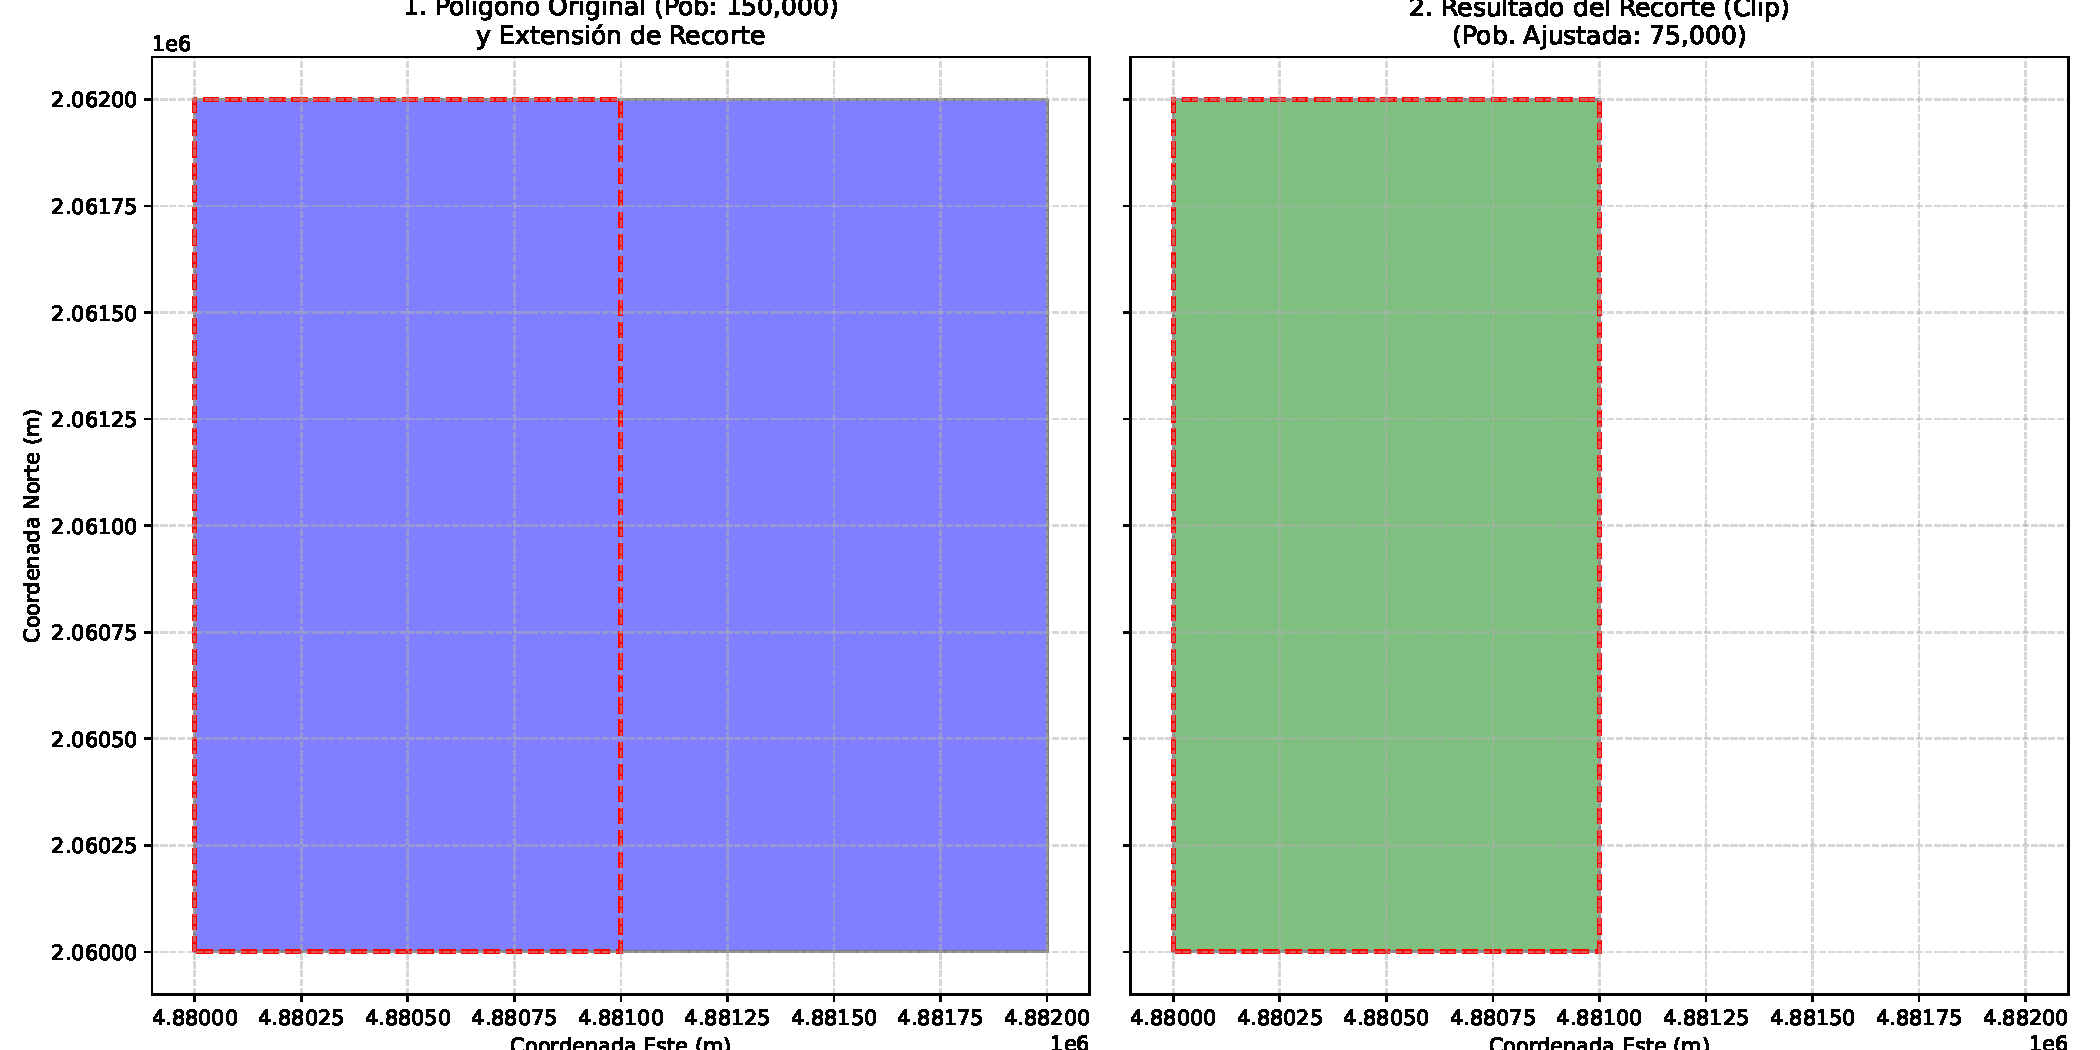
\includegraphics[width=0.8\textwidth,height=\textheight]{14-vector_files/figure-pdf/python_agr-1.pdf}
\end{center}

\subsection{R}

\begin{Shaded}
\begin{Highlighting}[]
\CommentTok{\# \#| eval: false}

\FunctionTok{library}\NormalTok{(sf)}

\CommentTok{\# 1. Definición de geometrías en coordenadas proyectadas (MAGNA{-}SIRGAS, EPSG:9377)}
\CommentTok{\# Creación de polígono simulado para la localidad de Teusaquillo}
\NormalTok{teusaquillo\_geom }\OtherTok{\textless{}{-}} \FunctionTok{st\_sfc}\NormalTok{(}\FunctionTok{st\_polygon}\NormalTok{(}\FunctionTok{list}\NormalTok{(}\FunctionTok{rbind}\NormalTok{(}
  \FunctionTok{c}\NormalTok{(}\DecValTok{4880000}\NormalTok{, }\DecValTok{2060000}\NormalTok{), }
  \FunctionTok{c}\NormalTok{(}\DecValTok{4882000}\NormalTok{, }\DecValTok{2060000}\NormalTok{), }
  \FunctionTok{c}\NormalTok{(}\DecValTok{4882000}\NormalTok{, }\DecValTok{2062000}\NormalTok{), }
  \FunctionTok{c}\NormalTok{(}\DecValTok{4880000}\NormalTok{, }\DecValTok{2062000}\NormalTok{), }
  \FunctionTok{c}\NormalTok{(}\DecValTok{4880000}\NormalTok{, }\DecValTok{2060000}\NormalTok{)}
\NormalTok{))), }\AttributeTok{crs =} \DecValTok{9377}\NormalTok{)}

\CommentTok{\# Definición de la extensión de corte (bbox) que cubre la mitad occidental}
\NormalTok{caja\_corte }\OtherTok{\textless{}{-}} \FunctionTok{st\_bbox}\NormalTok{(}\FunctionTok{c}\NormalTok{(}\AttributeTok{xmin =} \DecValTok{4880000}\NormalTok{, }\AttributeTok{ymin =} \DecValTok{2060000}\NormalTok{, }\AttributeTok{xmax =} \DecValTok{4881000}\NormalTok{, }\AttributeTok{ymax =} \DecValTok{2062000}\NormalTok{), }\AttributeTok{crs =} \DecValTok{9377}\NormalTok{)}
\NormalTok{caja\_corte\_geom }\OtherTok{\textless{}{-}} \FunctionTok{st\_as\_sfc}\NormalTok{(caja\_corte)}

\CommentTok{\# 2. Construcción del data frame espacial (sf)}
\NormalTok{teusaquillo\_sf }\OtherTok{\textless{}{-}} \FunctionTok{st\_sf}\NormalTok{(}
  \AttributeTok{codigo\_igac =} \StringTok{"11001"}\NormalTok{,}
  \AttributeTok{departamento =} \StringTok{"Cundinamarca"}\NormalTok{,}
  \AttributeTok{poblacion\_total =} \DecValTok{150000}\NormalTok{,}
  \AttributeTok{geometria =}\NormalTok{ teusaquillo\_geom}
\NormalTok{)}

\CommentTok{\# Definición explícita de la relación AGR}
\FunctionTok{st\_agr}\NormalTok{(teusaquillo\_sf) }\OtherTok{\textless{}{-}} \FunctionTok{c}\NormalTok{(}
  \AttributeTok{codigo\_igac =} \StringTok{"identity"}\NormalTok{,}
  \AttributeTok{departamento =} \StringTok{"constant"}\NormalTok{,}
  \AttributeTok{poblacion\_total =} \StringTok{"aggregate"}
\NormalTok{)}

\CommentTok{\# 3. Operación de geoprocesamiento: Recorte espacial (Crop)}
\CommentTok{\# El paquete \textquotesingle{}sf\textquotesingle{} emitirá una advertencia (warning):}
\CommentTok{\# "attribute variables are assumed to be spatially constant throughout all geometries"}
\CommentTok{\# st\_crop NO recalcula automáticamente los valores agregados espaciales, solo advierte.}
\NormalTok{teusaquillo\_recortado }\OtherTok{\textless{}{-}} \FunctionTok{st\_crop}\NormalTok{(teusaquillo\_sf, caja\_corte)}
\end{Highlighting}
\end{Shaded}

\begin{verbatim}
Warning: attribute variables are assumed to be spatially constant throughout
all geometries
\end{verbatim}

\begin{Shaded}
\begin{Highlighting}[]
\CommentTok{\# Extraer el valor incorrecto (copiado directamente del original por el algoritmo)}
\NormalTok{poblacion\_erronea }\OtherTok{\textless{}{-}}\NormalTok{ teusaquillo\_recortado}\SpecialCharTok{$}\NormalTok{poblacion\_total[}\DecValTok{1}\NormalTok{]}
\FunctionTok{print}\NormalTok{(}\FunctionTok{paste}\NormalTok{(}\StringTok{"Población errónea tras recorte (sin ajustar AGR):"}\NormalTok{, poblacion\_erronea))}
\end{Highlighting}
\end{Shaded}

\begin{verbatim}
[1] "Población errónea tras recorte (sin ajustar AGR): 150000"
\end{verbatim}

\begin{Shaded}
\begin{Highlighting}[]
\CommentTok{\# 4. Ajuste manual de la Relación Atributo{-}Geometría (AGR)}
\CommentTok{\# Cálculo de áreas con st\_area (retorna objeto formal con unidades [m\^{}2])}
\NormalTok{area\_original }\OtherTok{\textless{}{-}} \FunctionTok{as.numeric}\NormalTok{(}\FunctionTok{st\_area}\NormalTok{(teusaquillo\_sf))}
\NormalTok{area\_nueva }\OtherTok{\textless{}{-}} \FunctionTok{as.numeric}\NormalTok{(}\FunctionTok{st\_area}\NormalTok{(teusaquillo\_recortado))}

\CommentTok{\# Proporción geométrica resultante del corte topológico}
\NormalTok{proporcion }\OtherTok{\textless{}{-}}\NormalTok{ area\_nueva }\SpecialCharTok{/}\NormalTok{ area\_original}

\CommentTok{\# Recálculo proporcional de la población basada en la nueva extensión espacial}
\NormalTok{teusaquillo\_recortado}\SpecialCharTok{$}\NormalTok{poblacion\_total }\OtherTok{\textless{}{-}}\NormalTok{ teusaquillo\_recortado}\SpecialCharTok{$}\NormalTok{poblacion\_total }\SpecialCharTok{*}\NormalTok{ proporcion}
\NormalTok{poblacion\_ajustada }\OtherTok{\textless{}{-}}\NormalTok{ teusaquillo\_recortado}\SpecialCharTok{$}\NormalTok{poblacion\_total[}\DecValTok{1}\NormalTok{]}
\FunctionTok{print}\NormalTok{(}\FunctionTok{paste}\NormalTok{(}\StringTok{"Población corregida tras ajuste AGR:"}\NormalTok{, poblacion\_ajustada))}
\end{Highlighting}
\end{Shaded}

\begin{verbatim}
[1] "Población corregida tras ajuste AGR: 75000"
\end{verbatim}

\begin{Shaded}
\begin{Highlighting}[]
\CommentTok{\# 5. Visualización cartográfica comparativa (Efecto de recorte vs AGR)}
\CommentTok{\# Configuración de figura con dos sub{-}gráficos (mapas) lado a lado}
\CommentTok{\# Renderizado: pty="s" fuerza un área cuadrada eliminando espacios arriba/abajo}
\FunctionTok{par}\NormalTok{(}\AttributeTok{mfrow =} \FunctionTok{c}\NormalTok{(}\DecValTok{1}\NormalTok{, }\DecValTok{2}\NormalTok{), }\AttributeTok{mar =} \FunctionTok{c}\NormalTok{(}\DecValTok{4}\NormalTok{, }\DecValTok{4}\NormalTok{, }\DecValTok{3}\NormalTok{, }\DecValTok{1}\NormalTok{), }\AttributeTok{pty =} \StringTok{"s"}\NormalTok{)}


\CommentTok{\# Mapa 1: Estado Original y Área de Intervención}
\FunctionTok{plot}\NormalTok{(}\FunctionTok{st\_geometry}\NormalTok{(teusaquillo\_sf), }\AttributeTok{col =} \FunctionTok{rgb}\NormalTok{(}\DecValTok{0}\NormalTok{, }\DecValTok{0}\NormalTok{, }\DecValTok{1}\NormalTok{, }\FloatTok{0.5}\NormalTok{), }\AttributeTok{border =} \StringTok{"black"}\NormalTok{,}
     \AttributeTok{main =} \FunctionTok{paste}\NormalTok{(}\StringTok{"1. Polígono Original}\SpecialCharTok{\textbackslash{}n}\StringTok{(Pob:"}\NormalTok{, poblacion\_erronea, }\StringTok{")"}\NormalTok{),}
     \AttributeTok{axes =} \ConstantTok{TRUE}\NormalTok{, }\AttributeTok{graticule =} \ConstantTok{TRUE}\NormalTok{)}
\FunctionTok{plot}\NormalTok{(}\FunctionTok{st\_geometry}\NormalTok{(caja\_corte\_geom), }\AttributeTok{border =} \StringTok{"red"}\NormalTok{, }\AttributeTok{lty =} \DecValTok{2}\NormalTok{, }\AttributeTok{lwd =} \DecValTok{2}\NormalTok{, }\AttributeTok{add =} \ConstantTok{TRUE}\NormalTok{)}

\CommentTok{\# Mapa 2: Resultado Geométrico del Recorte}
\FunctionTok{plot}\NormalTok{(}\FunctionTok{st\_geometry}\NormalTok{(teusaquillo\_recortado), }\AttributeTok{col =} \FunctionTok{rgb}\NormalTok{(}\DecValTok{0}\NormalTok{, }\DecValTok{1}\NormalTok{, }\DecValTok{0}\NormalTok{, }\FloatTok{0.5}\NormalTok{), }\AttributeTok{border =} \StringTok{"black"}\NormalTok{,}
     \AttributeTok{main =} \FunctionTok{paste}\NormalTok{(}\StringTok{"2. Resultado del Recorte}\SpecialCharTok{\textbackslash{}n}\StringTok{(Pob Ajustada:"}\NormalTok{, poblacion\_ajustada, }\StringTok{")"}\NormalTok{),}
     \AttributeTok{axes =} \ConstantTok{TRUE}\NormalTok{, }\AttributeTok{graticule =} \ConstantTok{TRUE}\NormalTok{)}
\FunctionTok{plot}\NormalTok{(}\FunctionTok{st\_geometry}\NormalTok{(caja\_corte\_geom), }\AttributeTok{border =} \StringTok{"red"}\NormalTok{, }\AttributeTok{lty =} \DecValTok{2}\NormalTok{, }\AttributeTok{lwd =} \DecValTok{2}\NormalTok{, }\AttributeTok{add =} \ConstantTok{TRUE}\NormalTok{)}
\end{Highlighting}
\end{Shaded}

\begin{center}
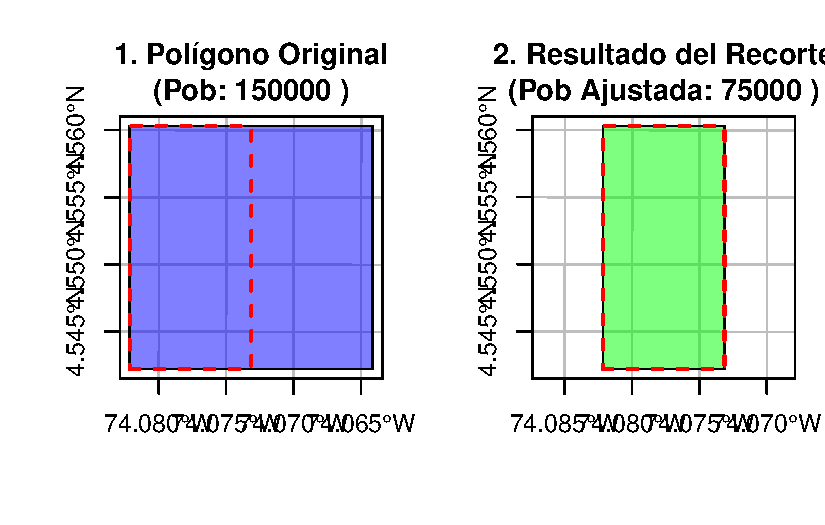
\includegraphics[width=0.8\textwidth,height=\textheight]{14-vector_files/figure-pdf/r_agr-1.pdf}
\end{center}

\begin{Shaded}
\begin{Highlighting}[]
\CommentTok{\# Restaurar parámetros gráficos por defecto}
\FunctionTok{par}\NormalTok{(}\AttributeTok{mfrow =} \FunctionTok{c}\NormalTok{(}\DecValTok{1}\NormalTok{, }\DecValTok{1}\NormalTok{))}
\end{Highlighting}
\end{Shaded}

\subsection{Julia}

\begin{Shaded}
\begin{Highlighting}[]
\CommentTok{\# \#| eval: false}

\CommentTok{\# Regla de pliegue exclusiva para este bloque j\_eval de Julia:}
\CommentTok{\# Si el código NO se ejecuta (\# \#| eval: false), usa: \# \#| code{-}fold: true}
\CommentTok{\# Si el código SÍ se ejecuta (para mostrar resultados), usa: \#| code{-}fold: true}

\FunctionTok{j\_eval}\NormalTok{(}\StringTok{\textquotesingle{}}
\StringTok{import ArchGDAL}
\StringTok{using DataFrames}
\StringTok{using Plots}

\StringTok{\# 1. Definición de geometrías simuladas (MAGNA{-}SIRGAS, EPSG:9377)}
\StringTok{teusaquillo\_geom = ArchGDAL.fromWKT("POLYGON ((4880000 2060000, 4882000 2060000, 4882000 2062000, 4880000 2062000, 4880000 2060000))")}
\StringTok{caja\_corte = ArchGDAL.fromWKT("POLYGON ((4880000 2060000, 4881000 2060000, 4881000 2062000, 4880000 2062000, 4880000 2060000))")}

\StringTok{\# 2. Construcción de DataFrame espacial}
\StringTok{df\_teusaquillo = DataFrame(}
\StringTok{    codigo\_igac = ["11001"],}
\StringTok{    departamento = ["Cundinamarca"],}
\StringTok{    poblacion\_total = [150000],}
\StringTok{    geom = [teusaquillo\_geom]}
\StringTok{)}

\StringTok{\# 3. Operación de geoprocesamiento: Intersección espacial}
\StringTok{geom\_recortada = ArchGDAL.intersection(df\_teusaquillo.geom[1], caja\_corte)}

\StringTok{poblacion\_erronea = df\_teusaquillo.poblacion\_total[1]}
\StringTok{println("Población errónea tras recorte (sin ajustar AGR): ", poblacion\_erronea)}

\StringTok{\# 4. Ajuste manual de la Relación Atributo{-}Geometría (AGR)}
\StringTok{area\_original = ArchGDAL.geomarea(df\_teusaquillo.geom[1])}
\StringTok{area\_nueva = ArchGDAL.geomarea(geom\_recortada)}

\StringTok{proporcion = area\_nueva / area\_original}
\StringTok{poblacion\_ajustada = df\_teusaquillo.poblacion\_total[1] * proporcion}
\StringTok{println("Población corregida tras ajuste AGR: ", poblacion\_ajustada)}

\StringTok{\# 5. Visualización cartográfica comparativa}
\StringTok{p1 = Plots.plot(teusaquillo\_geom, color=:blue, fillalpha=0.5, label="Original", }
\StringTok{          title="1. Polígono Original}\SpecialCharTok{\textbackslash{}\textbackslash{}}\StringTok{n(Pob: $poblacion\_erronea)", aspect\_ratio=:equal)}
\StringTok{Plots.plot!(p1, caja\_corte, color=:red, fillalpha=0.0, linewidth=2, linestyle=:dash, label="Corte")}

\StringTok{p2 = Plots.plot(geom\_recortada, color=:green, fillalpha=0.5, label="Recorte", }
\StringTok{          title="2. Resultado del Recorte}\SpecialCharTok{\textbackslash{}\textbackslash{}}\StringTok{n(Pob Ajustada: $poblacion\_ajustada)", aspect\_ratio=:equal)}
\StringTok{Plots.plot!(p2, caja\_corte, color=:red, fillalpha=0.0, linewidth=2, linestyle=:dash, label="")}

\StringTok{p\_final = Plots.plot(p1, p2, layout=(1, 2), size=(900, 450), margin=5Plots.mm)}

\StringTok{\# Guardar figura como PNG estático para R/Knitr}
\StringTok{Plots.savefig(p\_final, "images/c04\_agr\_teusaquillo\_julia.png")}
\StringTok{\textquotesingle{}}\NormalTok{)}
\end{Highlighting}
\end{Shaded}

\begin{Shaded}
\begin{Highlighting}[]
\NormalTok{knitr}\SpecialCharTok{::}\FunctionTok{include\_graphics}\NormalTok{(}\StringTok{"images/c04\_agr\_teusaquillo\_julia.png"}\NormalTok{)}
\end{Highlighting}
\end{Shaded}

\begin{center}
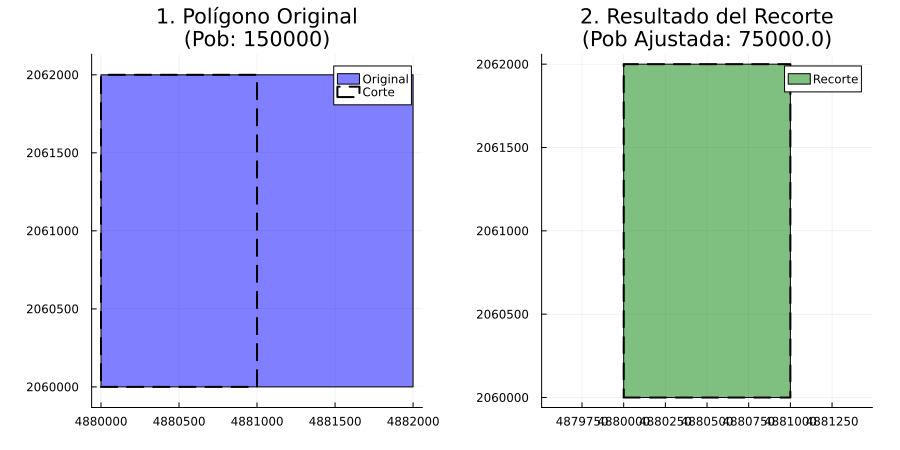
\includegraphics[width=0.8\textwidth,height=\textheight]{images/c04_agr_teusaquillo_julia.png}
\end{center}

\section{Geometrías vacías y
validación}\label{geometruxedas-vacuxedas-y-validaciuxf3n}

Una geometría vacía es aquella que carece de coordenadas (por ejemplo,
\texttt{POINT\ EMPTY}). Son fundamentales metodológicamente para manejar
datos espaciales faltantes (valores NA) en operaciones de
geoprocesamiento sin alterar la integridad tabular. La validación
espacial verifica que las geometrías cumplan las reglas topológicas
matemáticas estrictas (ej. un polígono no debe tener
auto-intersecciones).

\subsection{Python}

\begin{Shaded}
\begin{Highlighting}[]
\CommentTok{\# \#| eval: false}

\CommentTok{\# Importación de la librería de análisis geométrico}
\ImportTok{from}\NormalTok{ shapely.wkt }\ImportTok{import}\NormalTok{ loads}

\CommentTok{\# 1. Creación de una geometría vacía para inicialización de columnas}
\NormalTok{punto\_vacio }\OperatorTok{=}\NormalTok{ loads(}\StringTok{"POINT EMPTY"}\NormalTok{)}
\BuiltInTok{print}\NormalTok{(}\StringTok{"¿Es una geometría vacía?:"}\NormalTok{, punto\_vacio.is\_empty)}
\end{Highlighting}
\end{Shaded}

\begin{verbatim}
¿Es una geometría vacía?: True
\end{verbatim}

\begin{Shaded}
\begin{Highlighting}[]
\CommentTok{\# 2. Validación de una geometría topológicamente incorrecta}
\CommentTok{\# Polígono con forma de \textquotesingle{}corbatín\textquotesingle{} (auto{-}intersección) en coordenadas proyectadas MAGNA}
\NormalTok{poligono\_invalido }\OperatorTok{=}\NormalTok{ loads(}\StringTok{"POLYGON ((4880000 2060000, 4882000 2062000, 4882000 2060000, 4880000 2062000, 4880000 2060000))"}\NormalTok{)}

\CommentTok{\# Verificación de integridad geométrica}
\BuiltInTok{print}\NormalTok{(}\StringTok{"¿Es un polígono válido?:"}\NormalTok{, poligono\_invalido.is\_valid)}
\end{Highlighting}
\end{Shaded}

\begin{verbatim}
¿Es un polígono válido?: False
\end{verbatim}

\subsection{R}

\begin{Shaded}
\begin{Highlighting}[]
\CommentTok{\# \#| eval: false}

\CommentTok{\# Importación de la librería de Simple Features}
\FunctionTok{library}\NormalTok{(sf)}

\CommentTok{\# 1. Creación de una geometría vacía desde Well{-}Known Text (WKT)}
\NormalTok{punto\_vacio\_r }\OtherTok{\textless{}{-}} \FunctionTok{st\_as\_sfc}\NormalTok{(}\StringTok{"POINT EMPTY"}\NormalTok{)}
\FunctionTok{print}\NormalTok{(}\FunctionTok{paste}\NormalTok{(}\StringTok{"¿Es una geometría vacía?:"}\NormalTok{, }\FunctionTok{st\_is\_empty}\NormalTok{(punto\_vacio\_r)))}
\end{Highlighting}
\end{Shaded}

\begin{verbatim}
[1] "¿Es una geometría vacía?: TRUE"
\end{verbatim}

\begin{Shaded}
\begin{Highlighting}[]
\CommentTok{\# 2. Validación de una geometría topológicamente incorrecta}
\CommentTok{\# Simulación de un lote anómalo en Bogotá con cruce de vértices}
\NormalTok{poligono\_invalido\_r }\OtherTok{\textless{}{-}} \FunctionTok{st\_as\_sfc}\NormalTok{(}\StringTok{"POLYGON ((4880000 2060000, 4882000 2062000, 4882000 2060000, 4880000 2062000, 4880000 2060000))"}\NormalTok{)}

\CommentTok{\# Verificación de validez topológica estricta}
\FunctionTok{print}\NormalTok{(}\FunctionTok{paste}\NormalTok{(}\StringTok{"¿Es un polígono válido?:"}\NormalTok{, }\FunctionTok{st\_is\_valid}\NormalTok{(poligono\_invalido\_r)))}
\end{Highlighting}
\end{Shaded}

\begin{verbatim}
[1] "¿Es un polígono válido?: FALSE"
\end{verbatim}

\begin{Shaded}
\begin{Highlighting}[]
\CommentTok{\# Identificación explícita del error geométrico subyacente}
\FunctionTok{print}\NormalTok{(}\FunctionTok{st\_is\_valid}\NormalTok{(poligono\_invalido\_r, }\AttributeTok{reason =} \ConstantTok{TRUE}\NormalTok{))}
\end{Highlighting}
\end{Shaded}

\begin{verbatim}
[1] "Self-intersection[4881000 2061000]"
\end{verbatim}

\subsection{Julia}

\begin{Shaded}
\begin{Highlighting}[]
\CommentTok{\# \#| eval: false}

\CommentTok{\# Regla de pliegue exclusiva para este bloque j\_eval de Julia:}
\CommentTok{\# Si el código NO se ejecuta (\# \#| eval: false), usa: \# \#| code{-}fold: true}
\CommentTok{\# Si el código SÍ se ejecuta (para mostrar resultados), usa: \#| code{-}fold: true}

\FunctionTok{j\_eval}\NormalTok{(}\StringTok{\textquotesingle{}}
\StringTok{import ArchGDAL}

\StringTok{\# 1. Creación e inspección de geometría sin coordenadas}
\StringTok{punto\_vacio\_julia = ArchGDAL.fromWKT("POINT EMPTY")}
\StringTok{println("¿Es una geometría vacía?: ", ArchGDAL.isempty(punto\_vacio\_julia))}

\StringTok{\# 2. Generación y prueba de un polígono con error de trazado (auto{-}cruce)}
\StringTok{poligono\_invalido\_julia = ArchGDAL.fromWKT("POLYGON ((4880000 2060000, 4882000 2062000, 4882000 2060000, 4880000 2062000, 4880000 2060000))")}

\StringTok{\# Comprobación booleana de las reglas topológicas en el motor GEOS subyacente}
\StringTok{println("¿Es un polígono válido?: ", ArchGDAL.isvalid(poligono\_invalido\_julia))}
\StringTok{\textquotesingle{}}\NormalTok{)}
\end{Highlighting}
\end{Shaded}

\section{Manejo y conversión de unidades
espaciales}\label{manejo-y-conversiuxf3n-de-unidades-espaciales}

El cálculo de métricas geométricas, como el área o la longitud, depende
intrínsecamente del Sistema de Referencia de Coordenadas (CRS) asignado
a los datos vectoriales. Para el caso de Colombia, al utilizar el
sistema proyectado MAGNA-SIRGAS Origen Nacional (EPSG:9377), las
mediciones planimétricas base se expresan matemáticamente en metros
cuadrados (\(m^2\)) o metros lineales (\(m\)).

La gestión de estas unidades varía drásticamente según la arquitectura
de cada lenguaje: - En \textbf{R}, el ecosistema espacial implementa un
control estricto mediante el paquete \texttt{units}. Las variables
geométricas heredan un metadato de unidad física que previene sumas
incompatibles (ej. sumar metros con kilómetros) y facilita la conversión
semántica directa. - En \textbf{Python} (\texttt{geopandas}) y
\textbf{Julia} (\texttt{ArchGDAL}), no existe un soporte nativo
integrado para tipado de unidades físicas en las columnas espaciales. El
sistema retorna valores numéricos escalares (flotantes) en la unidad del
CRS base. La conversión a unidades derivadas, como hectáreas o
kilómetros cuadrados, exige aplicar operaciones algebraicas manuales
sobre los atributos.

A continuación, se demuestra el cálculo de áreas en metros cuadrados y
su posterior conversión a hectáreas
(\(1 \text{ ha} = 10,000 \text{ m}^2\)) utilizando polígonos
representativos del Parque Metropolitano Simón Bolívar y el Parque de
los Novios en Bogotá.

\subsection{Python}

\begin{Shaded}
\begin{Highlighting}[]
\CommentTok{\# \#| eval: false}

\ImportTok{import}\NormalTok{ geopandas }\ImportTok{as}\NormalTok{ gpd}
\ImportTok{import}\NormalTok{ matplotlib.pyplot }\ImportTok{as}\NormalTok{ plt}
\ImportTok{from}\NormalTok{ shapely.wkt }\ImportTok{import}\NormalTok{ loads}

\CommentTok{\# 1. Definición de áreas de interés en Bogotá (MAGNA{-}SIRGAS Origen Nacional)}
\NormalTok{wkt\_simon\_bolivar }\OperatorTok{=} \StringTok{"POLYGON ((4880000 2064000, 4881500 2064000, 4881500 2065500, 4880000 2065500, 4880000 2064000))"}
\NormalTok{wkt\_parque\_novios }\OperatorTok{=} \StringTok{"POLYGON ((4881800 2064500, 4882500 2064500, 4882500 2065200, 4881800 2065200, 4881800 2064500))"}

\CommentTok{\# 2. Creación del GeoDataFrame}
\NormalTok{df\_parques }\OperatorTok{=}\NormalTok{ gpd.GeoDataFrame(\{}
    \StringTok{\textquotesingle{}nombre\textquotesingle{}}\NormalTok{: [}\StringTok{\textquotesingle{}Parque Simón Bolívar\textquotesingle{}}\NormalTok{, }\StringTok{\textquotesingle{}Parque de los Novios\textquotesingle{}}\NormalTok{]}
\NormalTok{\}, geometry}\OperatorTok{=}\NormalTok{[loads(wkt\_simon\_bolivar), loads(wkt\_parque\_novios)], crs}\OperatorTok{=}\StringTok{"EPSG:9377"}\NormalTok{)}

\CommentTok{\# 3. Cálculo de área nativa}
\CommentTok{\# En GeoPandas, el método .area retorna un tipo float64 en las unidades del CRS (metros cuadrados).}
\CommentTok{\# No hay un objeto "unidad" asociado, la responsabilidad recae en el analista.}
\NormalTok{df\_parques[}\StringTok{\textquotesingle{}area\_m2\textquotesingle{}}\NormalTok{] }\OperatorTok{=}\NormalTok{ df\_parques.area}

\CommentTok{\# 4. Conversión algorítmica a hectáreas}
\CommentTok{\# Se divide el valor escalar entre el factor de conversión (1 ha = 10,000 m2)}
\NormalTok{df\_parques[}\StringTok{\textquotesingle{}area\_ha\textquotesingle{}}\NormalTok{] }\OperatorTok{=}\NormalTok{ df\_parques[}\StringTok{\textquotesingle{}area\_m2\textquotesingle{}}\NormalTok{] }\OperatorTok{/} \FloatTok{10000.0}

\CommentTok{\# Verificación tabular de los resultados}
\BuiltInTok{print}\NormalTok{(df\_parques[[}\StringTok{\textquotesingle{}nombre\textquotesingle{}}\NormalTok{, }\StringTok{\textquotesingle{}area\_m2\textquotesingle{}}\NormalTok{, }\StringTok{\textquotesingle{}area\_ha\textquotesingle{}}\NormalTok{]])}
\end{Highlighting}
\end{Shaded}

\begin{verbatim}
                 nombre    area_m2  area_ha
0  Parque Simón Bolívar  2250000.0    225.0
1  Parque de los Novios   490000.0     49.0
\end{verbatim}

\begin{Shaded}
\begin{Highlighting}[]
\CommentTok{\# 5. Representación cartográfica paramétrica}
\NormalTok{fig, ax }\OperatorTok{=}\NormalTok{ plt.subplots(figsize}\OperatorTok{=}\NormalTok{(}\DecValTok{8}\NormalTok{, }\DecValTok{6}\NormalTok{))}
\NormalTok{df\_parques.plot(ax}\OperatorTok{=}\NormalTok{ax, color}\OperatorTok{=}\NormalTok{[}\StringTok{\textquotesingle{}\#2ca02c\textquotesingle{}}\NormalTok{, }\StringTok{\textquotesingle{}\#98df8a\textquotesingle{}}\NormalTok{], edgecolor}\OperatorTok{=}\StringTok{\textquotesingle{}black\textquotesingle{}}\NormalTok{, alpha}\OperatorTok{=}\FloatTok{0.8}\NormalTok{)}

\CommentTok{\# Anotación espacial de las áreas calculadas sobre los centroides}
\ControlFlowTok{for}\NormalTok{ idx, row }\KeywordTok{in}\NormalTok{ df\_parques.iterrows():}
\NormalTok{    centroide }\OperatorTok{=}\NormalTok{ row[}\StringTok{\textquotesingle{}geometry\textquotesingle{}}\NormalTok{].centroid}
\NormalTok{    etiqueta }\OperatorTok{=} \SpecialStringTok{f"}\SpecialCharTok{\{}\NormalTok{row[}\StringTok{\textquotesingle{}nombre\textquotesingle{}}\NormalTok{]}\SpecialCharTok{\}}\CharTok{\textbackslash{}n}\SpecialCharTok{\{}\NormalTok{row[}\StringTok{\textquotesingle{}area\_ha\textquotesingle{}}\NormalTok{]}\SpecialCharTok{:.1f\}}\SpecialStringTok{ ha"}
\NormalTok{    ax.annotate(etiqueta, xy}\OperatorTok{=}\NormalTok{(centroide.x, centroide.y), xytext}\OperatorTok{=}\NormalTok{(}\DecValTok{3}\NormalTok{, }\DecValTok{3}\NormalTok{),}
\NormalTok{                textcoords}\OperatorTok{=}\StringTok{"offset points"}\NormalTok{, ha}\OperatorTok{=}\StringTok{\textquotesingle{}center\textquotesingle{}}\NormalTok{, fontsize}\OperatorTok{=}\DecValTok{9}\NormalTok{, }
\NormalTok{                bbox}\OperatorTok{=}\BuiltInTok{dict}\NormalTok{(boxstyle}\OperatorTok{=}\StringTok{"round,pad=0.3"}\NormalTok{, fc}\OperatorTok{=}\StringTok{"white"}\NormalTok{, ec}\OperatorTok{=}\StringTok{"gray"}\NormalTok{, alpha}\OperatorTok{=}\FloatTok{0.9}\NormalTok{))}

\NormalTok{ax.set\_title(}\StringTok{"Cálculo y conversión de áreas (Hectáreas)}\CharTok{\textbackslash{}n}\StringTok{Sector Parques, Bogotá D.C."}\NormalTok{)}
\NormalTok{ax.set\_xlabel(}\StringTok{"Este (m) {-} EPSG:9377"}\NormalTok{)}
\NormalTok{ax.set\_ylabel(}\StringTok{"Norte (m) {-} EPSG:9377"}\NormalTok{)}
\NormalTok{ax.grid(}\VariableTok{True}\NormalTok{, linestyle}\OperatorTok{=}\StringTok{\textquotesingle{}:\textquotesingle{}}\NormalTok{, alpha}\OperatorTok{=}\FloatTok{0.6}\NormalTok{)}

\NormalTok{plt.tight\_layout()}
\NormalTok{plt.show()}
\end{Highlighting}
\end{Shaded}

\begin{center}
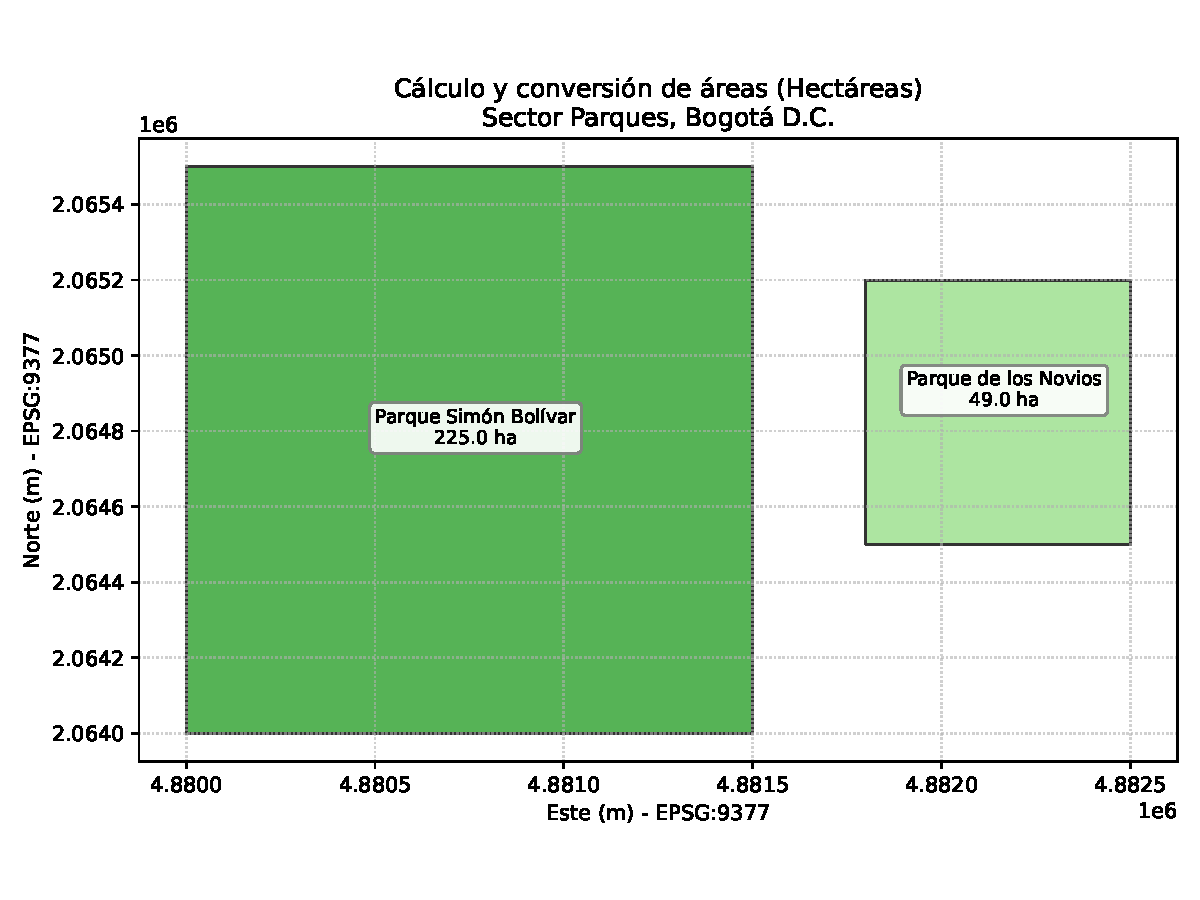
\includegraphics[width=0.8\textwidth,height=\textheight]{14-vector_files/figure-pdf/python_unidades-1.pdf}
\end{center}

\subsection{R}

\begin{Shaded}
\begin{Highlighting}[]
\CommentTok{\# \#| eval: false}

\FunctionTok{library}\NormalTok{(sf)}
\FunctionTok{library}\NormalTok{(units)}
\end{Highlighting}
\end{Shaded}

\begin{verbatim}
udunits database from /usr/share/xml/udunits/udunits2.xml
\end{verbatim}

\begin{Shaded}
\begin{Highlighting}[]
\CommentTok{\# 1. Instanciación de polígonos urbanos (Bogotá D.C.)}
\NormalTok{poligono\_simon\_bolivar }\OtherTok{\textless{}{-}} \FunctionTok{st\_as\_sfc}\NormalTok{(}\StringTok{"POLYGON ((4880000 2064000, 4881500 2064000, 4881500 2065500, 4880000 2065500, 4880000 2064000))"}\NormalTok{)}
\NormalTok{poligono\_parque\_novios }\OtherTok{\textless{}{-}} \FunctionTok{st\_as\_sfc}\NormalTok{(}\StringTok{"POLYGON ((4881800 2064500, 4882500 2064500, 4882500 2065200, 4881800 2065200, 4881800 2064500))"}\NormalTok{)}

\CommentTok{\# 2. Estructuración del data frame espacial con CRS formal}
\NormalTok{sf\_parques }\OtherTok{\textless{}{-}} \FunctionTok{st\_sf}\NormalTok{(}
  \AttributeTok{nombre =} \FunctionTok{c}\NormalTok{(}\StringTok{\textquotesingle{}Parque Simón Bolívar\textquotesingle{}}\NormalTok{, }\StringTok{\textquotesingle{}Parque de los Novios\textquotesingle{}}\NormalTok{),}
  \AttributeTok{geometria =} \FunctionTok{c}\NormalTok{(poligono\_simon\_bolivar, poligono\_parque\_novios),}
  \AttributeTok{crs =} \DecValTok{9377}
\NormalTok{)}

\CommentTok{\# 3. Cálculo de área con soporte nativo de unidades físicas}
\CommentTok{\# La función st\_area genera un objeto de clase \textquotesingle{}units\textquotesingle{} asignando automáticamente [m\^{}2]}
\NormalTok{sf\_parques}\SpecialCharTok{$}\NormalTok{area\_m2 }\OtherTok{\textless{}{-}} \FunctionTok{st\_area}\NormalTok{(sf\_parques)}

\CommentTok{\# 4. Transformación de unidades semántica}
\CommentTok{\# En R no es necesario multiplicar o dividir empíricamente; el motor maneja la equivalencia.}
\NormalTok{sf\_parques}\SpecialCharTok{$}\NormalTok{area\_ha }\OtherTok{\textless{}{-}} \FunctionTok{set\_units}\NormalTok{(sf\_parques}\SpecialCharTok{$}\NormalTok{area\_m2, ha)}

\CommentTok{\# Exploración de la estructura de unidades}
\FunctionTok{print}\NormalTok{(}\FunctionTok{st\_drop\_geometry}\NormalTok{(sf\_parques))}
\end{Highlighting}
\end{Shaded}

\begin{verbatim}
                nombre       area_m2  area_ha
1 Parque Simón Bolívar 2250000 [m^2] 225 [ha]
2 Parque de los Novios  490000 [m^2]  49 [ha]
\end{verbatim}

\begin{Shaded}
\begin{Highlighting}[]
\CommentTok{\# Remover espacios vacíos al rededor de la figura}
\FunctionTok{par}\NormalTok{(}\AttributeTok{pty =} \StringTok{"s"}\NormalTok{)}

\CommentTok{\# 5. Salida gráfica estandarizada}
\FunctionTok{plot}\NormalTok{(}\FunctionTok{st\_geometry}\NormalTok{(sf\_parques), }\AttributeTok{col =} \FunctionTok{c}\NormalTok{(}\StringTok{"\#2ca02c"}\NormalTok{, }\StringTok{"\#98df8a"}\NormalTok{), }\AttributeTok{border =} \StringTok{"black"}\NormalTok{,}
     \AttributeTok{main =} \StringTok{"Cálculo y conversión de áreas (Hectáreas)}\SpecialCharTok{\textbackslash{}n}\StringTok{Sector Parques, Bogotá D.C."}\NormalTok{,}
     \AttributeTok{axes =} \ConstantTok{TRUE}\NormalTok{, }\AttributeTok{graticule =} \ConstantTok{TRUE}\NormalTok{)}

\CommentTok{\# Obtención analítica de coordenadas para anclaje de texto}
\NormalTok{coords\_centroides }\OtherTok{\textless{}{-}} \FunctionTok{st\_coordinates}\NormalTok{(}\FunctionTok{st\_centroid}\NormalTok{(sf\_parques))}
\end{Highlighting}
\end{Shaded}

\begin{verbatim}
Warning: st_centroid assumes attributes are constant over geometries
\end{verbatim}

\begin{Shaded}
\begin{Highlighting}[]
\CommentTok{\# Etiquetado programático iterativo}
\ControlFlowTok{for}\NormalTok{ (i }\ControlFlowTok{in} \DecValTok{1}\SpecialCharTok{:}\FunctionTok{nrow}\NormalTok{(sf\_parques)) \{}
\NormalTok{  texto\_etiqueta }\OtherTok{\textless{}{-}} \FunctionTok{paste}\NormalTok{(sf\_parques}\SpecialCharTok{$}\NormalTok{nombre[i], }\StringTok{"}\SpecialCharTok{\textbackslash{}n}\StringTok{"}\NormalTok{, }\FunctionTok{round}\NormalTok{(}\FunctionTok{as.numeric}\NormalTok{(sf\_parques}\SpecialCharTok{$}\NormalTok{area\_ha[i]), }\DecValTok{1}\NormalTok{), }\StringTok{"ha"}\NormalTok{)}
  \FunctionTok{text}\NormalTok{(coords\_centroides[i, }\DecValTok{1}\NormalTok{], coords\_centroides[i, }\DecValTok{2}\NormalTok{], }\AttributeTok{labels =}\NormalTok{ texto\_etiqueta, }\AttributeTok{cex =} \FloatTok{0.8}\NormalTok{, }\AttributeTok{font =} \DecValTok{2}\NormalTok{)}
\NormalTok{\}}
\end{Highlighting}
\end{Shaded}

\begin{center}
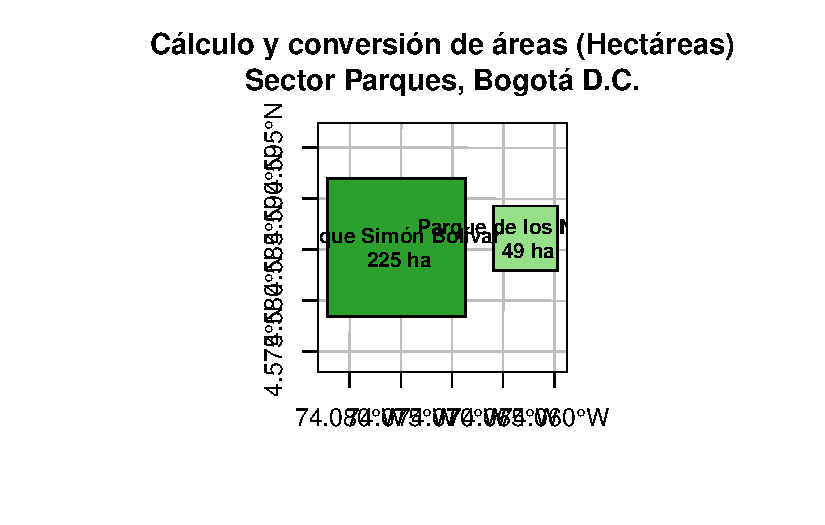
\includegraphics[width=0.8\textwidth,height=\textheight]{14-vector_files/figure-pdf/r_unidades-1.pdf}
\end{center}

\subsection{Julia}

\begin{Shaded}
\begin{Highlighting}[]
\CommentTok{\# \#| eval: false}

\CommentTok{\# Regla de pliegue exclusiva para este bloque j\_eval de Julia:}
\CommentTok{\# Si el código NO se ejecuta (\# \#| eval: false), usa: \# \#| code{-}fold: true}
\CommentTok{\# Si el código SÍ se ejecuta (para mostrar resultados), usa: \#| code{-}fold: true}

\FunctionTok{j\_eval}\NormalTok{(}\StringTok{\textquotesingle{}}
\StringTok{import ArchGDAL}
\StringTok{using DataFrames}
\StringTok{import Plots}

\StringTok{\# 1. Serialización vectorial mediante WKT para espacios en Bogotá}
\StringTok{wkt\_simon\_bolivar = "POLYGON ((4880000 2064000, 4881500 2064000, 4881500 2065500, 4880000 2065500, 4880000 2064000))"}
\StringTok{wkt\_parque\_novios = "POLYGON ((4881800 2064500, 4882500 2064500, 4882500 2065200, 4881800 2065200, 4881800 2064500))"}

\StringTok{\# 2. Creación del DataFrame de soporte}
\StringTok{df\_parques = DataFrame(}
\StringTok{    nombre = ["Parque Simón Bolívar", "Parque de los Novios"],}
\StringTok{    geom = [ArchGDAL.fromWKT(wkt\_simon\_bolivar), ArchGDAL.fromWKT(wkt\_parque\_novios)]}
\StringTok{)}

\StringTok{\# 3. Medición geométrica planimétrica}
\StringTok{\# ArchGDAL no maneja metadatos de unidades. geomarea devuelve Float64 en m2 (asumiendo EPSG:9377).}
\StringTok{df\_parques.area\_m2 = [ArchGDAL.geomarea(g) for g in df\_parques.geom]}

\StringTok{\# 4. Operación de equivalencia matemática (m2 a ha)}
\StringTok{df\_parques.area\_ha = df\_parques.area\_m2 ./ 10000.0}

\StringTok{println(df\_parques[:, [:nombre, :area\_m2, :area\_ha]])}

\StringTok{\# 5. Mapeo esquemático y acoplamiento de variables visuales}
\StringTok{\# Se utiliza el prefijo explícito Plots.* para evitar conflictos de namespace con otras librerías gráficas}
\StringTok{p\_parques = Plots.plot(df\_parques.geom[1], fillcolor="\#2ca02c", label="P. Simón Bolívar", aspect\_ratio=:equal,}
\StringTok{                 title="Cálculo y conversión de áreas (Hectáreas)}\SpecialCharTok{\textbackslash{}\textbackslash{}}\StringTok{nSector Parques, Bogotá D.C.")}
\StringTok{Plots.plot!(p\_parques, df\_parques.geom[2], fillcolor="\#98df8a", label="P. de los Novios")}

\StringTok{\# Cálculo de localización estática para textos}
\StringTok{cx1, cy1 = ArchGDAL.getx(ArchGDAL.centroid(df\_parques.geom[1]), 0), ArchGDAL.gety(ArchGDAL.centroid(df\_parques.geom[1]), 0)}
\StringTok{cx2, cy2 = ArchGDAL.getx(ArchGDAL.centroid(df\_parques.geom[2]), 0), ArchGDAL.gety(ArchGDAL.centroid(df\_parques.geom[2]), 0)}

\StringTok{\# Inserción posicional de etiquetas (usando doble barra invertida para salto de línea en R)}
\StringTok{Plots.annotate!(p\_parques, cx1, cy1, Plots.text("$(df\_parques.nombre[1])}\SpecialCharTok{\textbackslash{}\textbackslash{}}\StringTok{n$(round(df\_parques.area\_ha[1], digits=1)) ha", 8, :center, :white))}
\StringTok{Plots.annotate!(p\_parques, cx2, cy2, Plots.text("$(df\_parques.nombre[2])}\SpecialCharTok{\textbackslash{}\textbackslash{}}\StringTok{n$(round(df\_parques.area\_ha[2], digits=1)) ha", 8, :center, :black))}

\StringTok{\# Exportación y rasterización para el visualizador}
\StringTok{Plots.savefig(p\_parques, "images/c14\_unidades\_parques\_bogota\_julia.png")}
\StringTok{\textquotesingle{}}\NormalTok{)}
\end{Highlighting}
\end{Shaded}

\begin{Shaded}
\begin{Highlighting}[]
\NormalTok{knitr}\SpecialCharTok{::}\FunctionTok{include\_graphics}\NormalTok{(}\StringTok{"images/c14\_unidades\_parques\_bogota\_julia.png"}\NormalTok{)}
\end{Highlighting}
\end{Shaded}

\begin{center}
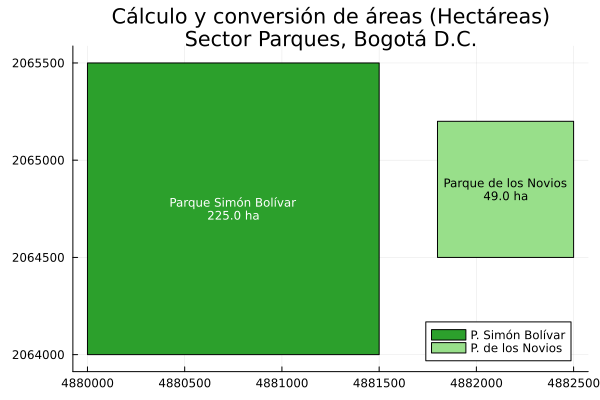
\includegraphics[width=0.8\textwidth,height=\textheight]{images/c14_unidades_parques_bogota_julia.png}
\end{center}

\section{Exploración de métodos y funciones en clases
espaciales}\label{exploraciuxf3n-de-muxe9todos-y-funciones-en-clases-espaciales}

La exploración algorítmica de los objetos espaciales permite auditar e
identificar las funciones de geoprocesamiento, constructores y atributos
disponibles en las librerías base. Dado que cada ecosistema maneja un
paradigma de programación distinto (orientado a objetos en Python,
funcional S3 en R y despacho múltiple en Julia), los mecanismos de
introspección para listar los métodos aplicables a las geometrías y
estructuras tabulares varían significativamente.

\subsection{Python}

\begin{Shaded}
\begin{Highlighting}[]
\CommentTok{\# \#| eval: false}

\ImportTok{import}\NormalTok{ geopandas }\ImportTok{as}\NormalTok{ gpd}
\ImportTok{from}\NormalTok{ shapely.geometry }\ImportTok{import}\NormalTok{ Point}

\CommentTok{\# Instanciación de una geometría puntual (Bogotá, MAGNA{-}SIRGAS Origen Nacional)}
\NormalTok{punto\_bogota }\OperatorTok{=}\NormalTok{ Point(}\DecValTok{4882000}\NormalTok{, }\DecValTok{2060000}\NormalTok{)}

\CommentTok{\# En Python, la función nativa dir() retorna todos los atributos y métodos del objeto.}
\CommentTok{\# Se filtran los métodos mágicos (aquellos que inician con doble guion bajo \textquotesingle{}\_\_\textquotesingle{})}
\NormalTok{metodos\_shapely }\OperatorTok{=}\NormalTok{ [metodo }\ControlFlowTok{for}\NormalTok{ metodo }\KeywordTok{in} \BuiltInTok{dir}\NormalTok{(punto\_bogota) }\ControlFlowTok{if} \KeywordTok{not}\NormalTok{ metodo.startswith(}\StringTok{\textquotesingle{}\_\textquotesingle{}}\NormalTok{)]}

\BuiltInTok{print}\NormalTok{(}\StringTok{"Métodos topológicos y analíticos de Shapely (clase Point):"}\NormalTok{)}
\end{Highlighting}
\end{Shaded}

\begin{verbatim}
Métodos topológicos y analíticos de Shapely (clase Point):
\end{verbatim}

\begin{Shaded}
\begin{Highlighting}[]
\BuiltInTok{print}\NormalTok{(metodos\_shapely[:}\DecValTok{10}\NormalTok{]) }\CommentTok{\# Visualización de los primeros 10 métodos}
\end{Highlighting}
\end{Shaded}

\begin{verbatim}
['area', 'boundary', 'bounds', 'buffer', 'centroid', 'contains', 'contains_properly', 'convex_hull', 'coords', 'covered_by']
\end{verbatim}

\begin{Shaded}
\begin{Highlighting}[]
\CommentTok{\# Inspección de métodos a nivel de estructura tabular (GeoDataFrame)}
\NormalTok{gdf\_vacio }\OperatorTok{=}\NormalTok{ gpd.GeoDataFrame(geometry}\OperatorTok{=}\NormalTok{[punto\_bogota])}
\NormalTok{metodos\_geopandas }\OperatorTok{=}\NormalTok{ [metodo }\ControlFlowTok{for}\NormalTok{ metodo }\KeywordTok{in} \BuiltInTok{dir}\NormalTok{(gdf\_vacio) }\ControlFlowTok{if} \KeywordTok{not}\NormalTok{ metodo.startswith(}\StringTok{\textquotesingle{}\_\textquotesingle{}}\NormalTok{)]}

\BuiltInTok{print}\NormalTok{(}\StringTok{"}\CharTok{\textbackslash{}n}\StringTok{Métodos espaciales y tabulares de GeoPandas (clase GeoDataFrame):"}\NormalTok{)}
\end{Highlighting}
\end{Shaded}

\begin{verbatim}

Métodos espaciales y tabulares de GeoPandas (clase GeoDataFrame):
\end{verbatim}

\begin{Shaded}
\begin{Highlighting}[]
\BuiltInTok{print}\NormalTok{(metodos\_geopandas[:}\DecValTok{10}\NormalTok{])}
\end{Highlighting}
\end{Shaded}

\begin{verbatim}
['T', 'abs', 'active_geometry_name', 'add', 'add_prefix', 'add_suffix', 'affine_transform', 'agg', 'aggregate', 'align']
\end{verbatim}

\subsection{R}

\begin{Shaded}
\begin{Highlighting}[]
\CommentTok{\# \#| eval: false}

\FunctionTok{library}\NormalTok{(sf)}

\CommentTok{\# En el paradigma funcional S3 de R, la función methods() enumera }
\CommentTok{\# las rutinas genéricas implementadas específicamente para una clase dada.}

\CommentTok{\# 1. Listado de métodos asociados al data frame espacial completo (clase \textquotesingle{}sf\textquotesingle{})}
\FunctionTok{print}\NormalTok{(}\StringTok{"Métodos disponibles para la clase tabular \textquotesingle{}sf\textquotesingle{}:"}\NormalTok{)}
\end{Highlighting}
\end{Shaded}

\begin{verbatim}
[1] "Métodos disponibles para la clase tabular 'sf':"
\end{verbatim}

\begin{Shaded}
\begin{Highlighting}[]
\FunctionTok{print}\NormalTok{(}\FunctionTok{head}\NormalTok{(}\FunctionTok{methods}\NormalTok{(}\AttributeTok{class =} \StringTok{"sf"}\NormalTok{), }\DecValTok{15}\NormalTok{))}
\end{Highlighting}
\end{Shaded}

\begin{verbatim}
 [1] "[.sf"                                                 
 [2] "[[<-.sf"                                              
 [3] "[<-.sf"                                               
 [4] "$<-.sf"                                               
 [5] "aggregate.sf"                                         
 [6] "as.data.frame.sf"                                     
 [7] "cbind.sf"                                             
 [8] "coerce,oldClass,S3-method"                            
 [9] "coerce,sf,Spatial-method"                             
[10] "coerce,Spatial,sf-method"                             
[11] "dbDataType,DBIObject,sf-method"                       
[12] "dbDataType,PostgreSQLConnection,sf-method"            
[13] "dbWriteTable,DBIObject,character,sf-method"           
[14] "dbWriteTable,PostgreSQLConnection,character,sf-method"
[15] "duplicated.sf"                                        
\end{verbatim}

\begin{Shaded}
\begin{Highlighting}[]
\CommentTok{\# 2. Listado de métodos operativos sobre la columna de geometrías (clase \textquotesingle{}sfc\textquotesingle{})}
\FunctionTok{print}\NormalTok{(}\StringTok{"Métodos disponibles para la columna espacial \textquotesingle{}sfc\textquotesingle{}:"}\NormalTok{)}
\end{Highlighting}
\end{Shaded}

\begin{verbatim}
[1] "Métodos disponibles para la columna espacial 'sfc':"
\end{verbatim}

\begin{Shaded}
\begin{Highlighting}[]
\FunctionTok{print}\NormalTok{(}\FunctionTok{head}\NormalTok{(}\FunctionTok{methods}\NormalTok{(}\AttributeTok{class =} \StringTok{"sfc"}\NormalTok{), }\DecValTok{15}\NormalTok{))}
\end{Highlighting}
\end{Shaded}

\begin{verbatim}
 [1] "[.sfc"                      "[<-.sfc"                   
 [3] "as.data.frame.sfc"          "c.sfc"                     
 [5] "coerce,oldClass,S3-method"  "coerce,sfc,Spatial-method" 
 [7] "coerce,Spatial,sfc-method"  "format.sfc"                
 [9] "identify.sfc"               "initialize,oldClass-method"
[11] "obj_sum.sfc"                "Ops.sfc"                   
[13] "points.sfc"                 "print.sfc"                 
[15] "rep.sfc"                   
\end{verbatim}

\begin{Shaded}
\begin{Highlighting}[]
\CommentTok{\# 3. Listado de métodos para primitivas individuales (clase \textquotesingle{}sfg\textquotesingle{})}
\FunctionTok{print}\NormalTok{(}\StringTok{"Métodos disponibles para geometrías individuales \textquotesingle{}sfg\textquotesingle{}:"}\NormalTok{)}
\end{Highlighting}
\end{Shaded}

\begin{verbatim}
[1] "Métodos disponibles para geometrías individuales 'sfg':"
\end{verbatim}

\begin{Shaded}
\begin{Highlighting}[]
\FunctionTok{print}\NormalTok{(}\FunctionTok{head}\NormalTok{(}\FunctionTok{methods}\NormalTok{(}\AttributeTok{class =} \StringTok{"sfg"}\NormalTok{), }\DecValTok{15}\NormalTok{))}
\end{Highlighting}
\end{Shaded}

\begin{verbatim}
 [1] "as.matrix.sfg"               "c.sfg"                      
 [3] "coerce,oldClass,S3-method"   "format.sfg"                 
 [5] "head.sfg"                    "initialize,oldClass-method" 
 [7] "Ops.sfg"                     "plot.sfg"                   
 [9] "print.sfg"                   "show,oldClass-method"       
[11] "slotsFromS3,oldClass-method" "st_area.sfg"                
[13] "st_as_binary.sfg"            "st_as_text.sfg"             
[15] "st_boundary.sfg"            
\end{verbatim}

\subsection{Julia}

\begin{Shaded}
\begin{Highlighting}[]
\CommentTok{\# \#| eval: false}

\CommentTok{\# Regla de pliegue exclusiva para este bloque j\_eval de Julia:}
\CommentTok{\# Si el código NO se ejecuta (\# \#| eval: false), usa: \# \#| code{-}fold: true}
\CommentTok{\# Si el código SÍ se ejecuta (para mostrar resultados), usa: \#| code{-}fold: true}

\FunctionTok{j\_eval}\NormalTok{(}\StringTok{\textquotesingle{}}
\StringTok{import ArchGDAL}

\StringTok{\# El ecosistema de Julia opera bajo el paradigma de despacho múltiple. }
\StringTok{\# Las funciones no pertenecen a los objetos, sino que los objetos se pasan como argumentos.}

\StringTok{\# 1. Inspección de la jerarquía de tipos de la geometría}
\StringTok{\# Instanciación de geometría básica (Bogotá, MAGNA{-}SIRGAS)}
\StringTok{punto\_julia = ArchGDAL.fromWKT("POINT (4882000 2060000)")}
\StringTok{tipo\_geometria = typeof(punto\_julia)}

\StringTok{println("Tipo de dato exacto de la geometría: ", tipo\_geometria)}
\StringTok{println("Clase abstracta superior (Supertype): ", supertype(tipo\_geometria))}

\StringTok{\# 2. Inspección del despacho múltiple en funciones espaciales genéricas}
\StringTok{\# Dado que la mayoría de funciones base de GDAL operan sobre el tipo AbstractGeometry,}
\StringTok{\# el enfoque analítico en Julia consiste en consultar qué firmas (tipos de datos)}
\StringTok{\# soporta una función de geoprocesamiento específica utilizando methods().}
\StringTok{println("}\SpecialCharTok{\textbackslash{}\textbackslash{}}\StringTok{nFirmas de métodos disponibles para la función ArchGDAL.buffer:")}
\StringTok{println(methods(ArchGDAL.buffer))}

\StringTok{println("}\SpecialCharTok{\textbackslash{}\textbackslash{}}\StringTok{nFirmas de métodos disponibles para la función ArchGDAL.intersection:")}
\StringTok{println(methods(ArchGDAL.intersection))}
\StringTok{\textquotesingle{}}\NormalTok{)}
\end{Highlighting}
\end{Shaded}

\section{Resumen del capítulo}\label{resumen-del-capuxedtulo}

En este capítulo hemos establecido los cimientos computacionales de la
ciencia de datos espaciales, pasando de la teoría abstracta a la
implementación algorítmica. Comprender cómo las computadoras almacenan,
leen y estructuran la geometría es el paso previo innegociable antes de
ejecutar cualquier análisis espacial complejo.

Los puntos clave que debes llevarte de esta sección son:

\begin{itemize}
\tightlist
\item
  \textbf{El estándar es la ley:} Todos los lenguajes (Python, R, Julia)
  operan bajo el estándar \textbf{Simple Features (OGC)} y comparten los
  mismos motores subyacentes (GDAL, GEOS, PROJ). Esto garantiza que un
  polígono procesado en un lenguaje mantendrá su integridad matemática
  al ser exportado a otro.
\item
  \textbf{Jerarquía de tres niveles:} Un objeto espacial no es un dibujo
  plano. Es una arquitectura estricta compuesta por la
  \textbf{Primitiva} (la matemática aislada), la \textbf{Columna
  Espacial} (el vector que impone el Sistema de Referencia de
  Coordenadas) y la \textbf{Tabla Espacial} (el Data Frame que vincula
  los vértices con los atributos alfanuméricos).
\item
  \textbf{Anidamiento topológico:} Las geometrías complejas funcionan
  como cajas chinas. Para extraer una coordenada específica de un
  polígono con huecos o de un archipiélago, es necesario navegar
  algorítmicamente a través de su estructura, respetando los índices
  base de cada lenguaje (base 0 en Python y Julia-C++; base 1 en R).
\item
  \textbf{Serialización I/O:} El formato \textbf{WKT} (texto) es
  indispensable para la lectura humana y la creación manual de
  geometrías, pero el formato \textbf{WKB} (binario hexadecimal) es el
  verdadero caballo de batalla para transferencias masivas y
  almacenamiento eficiente en memoria.
\item
  \textbf{Relación Atributo-Geometría (AGR):} Modificar la extensión de
  una geometría (como al recortar una localidad) tiene implicaciones
  semánticas sobre sus atributos. Mientras que identidades y valores
  constantes se preservan, los valores agregados (como la población)
  exigen recálculos manuales proporcionales a la nueva área.
\item
  \textbf{Precisión y tipado:} El ruido de máquina en operaciones de
  punto flotante puede destruir la topología (auto-intersecciones o
  desajustes). Dominar el truncamiento geométrico y comprender cómo cada
  lenguaje asume o exige la definición de unidades físicas (como el
  paquete \texttt{units} en R frente a los escalares puros en
  Python/Julia) es vital para reportar métricas exactas.
\end{itemize}

Con esta base estructural consolidada, el terreno está preparado para
avanzar hacia el análisis avanzado: la evaluación de \textbf{predicados
espaciales} (cómo interactúan estas geometrías entre sí) y las
\textbf{operaciones paramétricas} de geoprocesamiento.

\chapter{Dimensiones Espaciales Avanzadas y Referenciación Lineal (Z,
M)}\label{dimensiones-espaciales-avanzadas-y-referenciaciuxf3n-lineal-z-m}

\section{Funciones j\_eval y j\_plot en
R}\label{funciones-j_eval-y-j_plot-en-r-10}

\begin{Shaded}
\begin{Highlighting}[]
\CommentTok{\# \#| include: false}
\FunctionTok{source}\NormalTok{(}\StringTok{"./docs/j\_eval\_j\_plot.r"}\NormalTok{)}
\end{Highlighting}
\end{Shaded}

\section{Introducción}\label{introducciuxf3n-11}

Hasta este punto de nuestro recorrido en la ciencia de datos espaciales,
hemos tratado a la Tierra como un plano de dos dimensiones. Todas
nuestras primitivas geométricas (puntos, líneas y polígonos) se han
construido utilizando exclusivamente pares de coordenadas Cartesianas
\((X, Y)\) o geográficas (Longitud, Latitud). Si bien este enfoque
bidimensional es suficiente para la cartografía tradicional y el
catastro planimétrico, resulta limitado para modelar fenómenos complejos
del mundo real.

La infraestructura vial, las redes de acueducto y la hidrología exigen
herramientas más sofisticadas. ¿Cómo representamos la altitud de un pico
montañoso? ¿Cómo registramos que un accidente de tránsito ocurrió
exactamente en el ``Kilómetro 15 + 200 metros'' de una autopista, si
nuestra línea solo tiene vértices cada 5 kilómetros?

Para resolver estos desafíos topográficos y logísticos, el estándar
\emph{Simple Features} contempla el uso de dimensiones adicionales
integradas directamente en el vértice de la geometría. Este capítulo
explora la inyección y manipulación de las cotas altimétricas
(\textbf{Eje Z}) y los valores de medición continua (\textbf{Eje M}).

A lo largo de estas páginas, dominaremos el concepto de
\textbf{Referenciación Lineal (LRS)} y la \textbf{Segmentación
Dinámica}, técnicas críticas en la geomática aplicada que nos permitirán
ubicar eventos (como baches, peajes o tramos de mantenimiento) a lo
largo de redes complejas, y analizaremos cómo Python, R y Julia manejan
---o restringen--- la persistencia de estas cuartas dimensiones en la
memoria del computador.

\section{Dimensiones adicionales: Coordenadas Z y
M}\label{dimensiones-adicionales-coordenadas-z-y-m}

Aunque la mayoría de los análisis SIG se realizan en un plano
bidimensional (\textbf{XY}), el estándar \emph{Simple Features} permite
integrar dimensiones adicionales para representar la complejidad del
mundo real:

\begin{enumerate}
\def\labelenumi{\arabic{enumi}.}
\tightlist
\item
  \textbf{Z (Altitud/Elevación):} Representa la tercera dimensión física
  (altura o profundidad). Útil en modelos de terreno o hidrología.
\item
  \textbf{M (Medida - \emph{Measure}):} Es una dimensión no espacial
  asociada al vértice. Se usa frecuentemente en ``Referenciación
  Lineal'' para marcar valores como: el tiempo de una medición, el
  kilometraje de una ruta o el nivel de error de un GPS.
\end{enumerate}

Esto genera cuatro combinaciones posibles: \textbf{XY}, \textbf{XYZ},
\textbf{XYM} y \textbf{XYZM}.

\subsection{Referenciación Lineal y Segmentación
Dinámica}\label{referenciaciuxf3n-lineal-y-segmentaciuxf3n-dinuxe1mica}

La \textbf{Referenciación Lineal (LRS)} es un método de localización que
sitúa elementos geográficos basándose en su posición relativa a lo largo
de un eje lineal medido, en lugar de depender exclusivamente de
coordenadas cartesianas \((X, Y)\). Este paradigma es esencial en la
gestión de infraestructuras (carreteras, tuberías) y redes hídricas,
donde el concepto de \textbf{Segmentación Dinámica} permite asociar
múltiples atributos a porciones de una vía sin necesidad de fragmentar
físicamente la geometría base.

\begin{Shaded}
\begin{Highlighting}[]
\NormalTok{knitr}\SpecialCharTok{::}\FunctionTok{include\_graphics}\NormalTok{(}\StringTok{"images/c14\_plot\_segmentacion\_dinamica\_julia.png"}\NormalTok{)}
\end{Highlighting}
\end{Shaded}

\begin{figure}[H]

{\centering 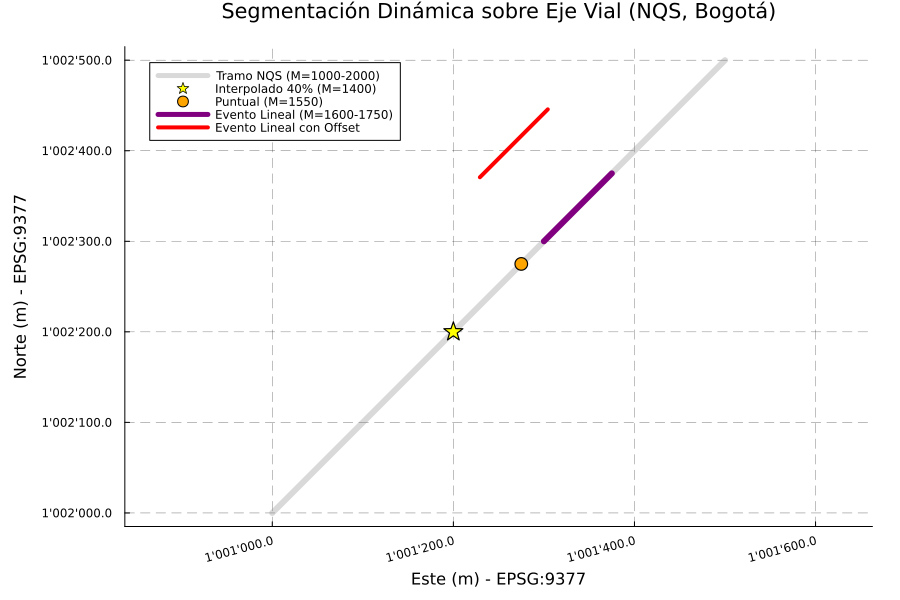
\includegraphics[width=0.8\textwidth,height=\textheight]{images/c14_plot_segmentacion_dinamica_julia.png}

}

\caption{Referenciación Lineal y Segmentación Dinámica.}

\end{figure}%

En este modelo, la información se almacena a través de \textbf{eventos}:
los \textbf{eventos puntuales} marcan hitos en una medida específica
(ej. un bache en el km 15.2), mientras que los \textbf{eventos lineales}
describen tramos definidos por una medida de inicio y una de fin (ej. un
cambio de pavimento entre el km 20 y el km 45). Para que este sistema
funcione, la geometría debe soportar una cuarta dimensión denominada
\textbf{eje \(M\) (Medida)}, que almacena el kilometraje acumulado
independientemente de la longitud euclidiana del dibujo.

\subsection{Python}

En el ecosistema de Python, la manipulación de dimensiones adicionales
presenta una dualidad técnica. Por un lado, \textbf{Shapely} (la
librería estándar) es sumamente eficiente para geometrías 2D y 3D
(\(XYZ\)), \textbf{pero carece de un eje \(M\) (Medida) nativo}. Para
suplir esto en análisis de Referenciación Lineal (LRS), es una práctica
común ``secuestrar'' el eje \(Z\) para almacenar valores de medida o
kilometraje.

Por otro lado, cuando se requiere un soporte estricto de cuatro
dimensiones (\(XYZM\)), debemos recurrir a \textbf{OGR (GDAL)}. OGR es
un motor de bajo nivel que permite la persistencia de atributos
escalares (Medida) vinculados directamente a la geometría, cumpliendo
con el estándar ISO de \emph{Simple Features}.

\begin{Shaded}
\begin{Highlighting}[]
\CommentTok{\# =============================================================================}
\CommentTok{\# MANEJO DE DIMENSIONES EN PYTHON: SHAPELY (3D) VS. OGR (4D)}
\CommentTok{\# =============================================================================}

\ImportTok{from}\NormalTok{ shapely.geometry }\ImportTok{import}\NormalTok{ Point, LineString}
\ImportTok{from}\NormalTok{ osgeo }\ImportTok{import}\NormalTok{ ogr}

\CommentTok{\# {-}{-}{-}{-}{-}{-}{-}{-}{-}{-}{-}{-}{-}{-}{-}{-}{-}{-}{-}{-}{-}{-}{-}{-}{-}{-}{-}{-}{-}{-}{-}{-}{-}{-}{-}{-}{-}{-}{-}{-}{-}{-}{-}{-}{-}{-}{-}{-}{-}{-}{-}{-}{-}{-}{-}{-}{-}{-}{-}{-}{-}{-}{-}{-}{-}{-}{-}{-}{-}{-}{-}{-}{-}{-}{-}{-}{-}}
\CommentTok{\# OPCIÓN A: Usando Shapely (Estándar para 2D y 3D / XYZ)}
\CommentTok{\# {-}{-}{-}{-}{-}{-}{-}{-}{-}{-}{-}{-}{-}{-}{-}{-}{-}{-}{-}{-}{-}{-}{-}{-}{-}{-}{-}{-}{-}{-}{-}{-}{-}{-}{-}{-}{-}{-}{-}{-}{-}{-}{-}{-}{-}{-}{-}{-}{-}{-}{-}{-}{-}{-}{-}{-}{-}{-}{-}{-}{-}{-}{-}{-}{-}{-}{-}{-}{-}{-}{-}{-}{-}{-}{-}{-}{-}}

\CommentTok{\# 1. Creación de puntos con diferentes dimensiones}
\NormalTok{p\_2d }\OperatorTok{=}\NormalTok{ Point(}\DecValTok{10}\NormalTok{, }\DecValTok{20}\NormalTok{)                                      }\CommentTok{\# Plano XY}
\NormalTok{p\_3d }\OperatorTok{=}\NormalTok{ Point(}\FloatTok{1001200.0}\NormalTok{, }\FloatTok{1002300.0}\NormalTok{, }\FloatTok{2560.0}\NormalTok{)                }\CommentTok{\# XYZ (Edificio 401 UNAL)}

\CommentTok{\# 2. Inspección: Shapely usa el booleano \textquotesingle{}has\_z\textquotesingle{} para detectar la 3ra dimensión}
\BuiltInTok{print}\NormalTok{(}\SpecialStringTok{f"Punto 2D: }\SpecialCharTok{\{}\NormalTok{p\_2d}\SpecialCharTok{\}}\SpecialStringTok{ | ¿Tiene Z?: }\SpecialCharTok{\{}\NormalTok{p\_2d}\SpecialCharTok{.}\NormalTok{has\_z}\SpecialCharTok{\}}\SpecialStringTok{"}\NormalTok{)}
\end{Highlighting}
\end{Shaded}

\begin{verbatim}
Punto 2D: POINT (10 20) | ¿Tiene Z?: False
\end{verbatim}

\begin{Shaded}
\begin{Highlighting}[]
\BuiltInTok{print}\NormalTok{(}\SpecialStringTok{f"Punto 3D: }\SpecialCharTok{\{}\NormalTok{p\_3d}\SpecialCharTok{\}}\SpecialStringTok{ | ¿Tiene Z?: }\SpecialCharTok{\{}\NormalTok{p\_3d}\SpecialCharTok{.}\NormalTok{has\_z}\SpecialCharTok{\}}\SpecialStringTok{"}\NormalTok{)}
\end{Highlighting}
\end{Shaded}

\begin{verbatim}
Punto 3D: POINT Z (1001200 1002300 2560) | ¿Tiene Z?: True
\end{verbatim}

\begin{Shaded}
\begin{Highlighting}[]
\CommentTok{\# 3. Acceso: Si existe Z, se accede directamente como atributo}
\ControlFlowTok{if}\NormalTok{ p\_3d.has\_z:}
    \BuiltInTok{print}\NormalTok{(}\SpecialStringTok{f"Elevación extraída: }\SpecialCharTok{\{}\NormalTok{p\_3d}\SpecialCharTok{.}\NormalTok{z}\SpecialCharTok{\}}\SpecialStringTok{ msnm"}\NormalTok{)}
\end{Highlighting}
\end{Shaded}

\begin{verbatim}
Elevación extraída: 2560.0 msnm
\end{verbatim}

\begin{Shaded}
\begin{Highlighting}[]
\CommentTok{\# 4. Segmentación Dinámica (Interpolación Lineal)}
\CommentTok{\# NOTA: Usamos el eje Z como "M" (Medida) ya que Shapely no tiene eje M nativo.}
\CommentTok{\# Tramo NQS: Km 1.0 (1000m) a Km 2.0 (2000m)}
\NormalTok{ruta\_nqs }\OperatorTok{=}\NormalTok{ LineString([}
\NormalTok{    (}\DecValTok{1001000}\NormalTok{, }\DecValTok{1002000}\NormalTok{, }\DecValTok{1000}\NormalTok{), }
\NormalTok{    (}\DecValTok{1001500}\NormalTok{, }\DecValTok{1002500}\NormalTok{, }\DecValTok{2000}\NormalTok{)}
\NormalTok{])}

\CommentTok{\# Ubicar un punto al 40\% del recorrido (normalized=True para usar 0.0 a 1.0)}
\NormalTok{punto\_interp }\OperatorTok{=}\NormalTok{ ruta\_nqs.interpolate(}\FloatTok{0.4}\NormalTok{, normalized}\OperatorTok{=}\VariableTok{True}\NormalTok{)}

\BuiltInTok{print}\NormalTok{(}\SpecialStringTok{f"Posición al 40\%: }\SpecialCharTok{\{}\NormalTok{punto\_interp}\SpecialCharTok{\}}\SpecialStringTok{"}\NormalTok{)}
\end{Highlighting}
\end{Shaded}

\begin{verbatim}
Posición al 40%: POINT Z (1001200 1002200 1400)
\end{verbatim}

\begin{Shaded}
\begin{Highlighting}[]
\BuiltInTok{print}\NormalTok{(}\SpecialStringTok{f"Valor M (vía eje Z) interpolado: }\SpecialCharTok{\{}\NormalTok{punto\_interp}\SpecialCharTok{.}\NormalTok{z}\SpecialCharTok{\}}\SpecialStringTok{"}\NormalTok{) }\CommentTok{\# Resultado: 1400.0}
\end{Highlighting}
\end{Shaded}

\begin{verbatim}
Valor M (vía eje Z) interpolado: 1400.0
\end{verbatim}

\begin{Shaded}
\begin{Highlighting}[]
\CommentTok{\# {-}{-}{-}{-}{-}{-}{-}{-}{-}{-}{-}{-}{-}{-}{-}{-}{-}{-}{-}{-}{-}{-}{-}{-}{-}{-}{-}{-}{-}{-}{-}{-}{-}{-}{-}{-}{-}{-}{-}{-}{-}{-}{-}{-}{-}{-}{-}{-}{-}{-}{-}{-}{-}{-}{-}{-}{-}{-}{-}{-}{-}{-}{-}{-}{-}{-}{-}{-}{-}{-}{-}{-}{-}{-}{-}{-}{-}}
\CommentTok{\# OPCIÓN B: OGR para 3D (El "puente" hacia el bajo nivel)}
\CommentTok{\# {-}{-}{-}{-}{-}{-}{-}{-}{-}{-}{-}{-}{-}{-}{-}{-}{-}{-}{-}{-}{-}{-}{-}{-}{-}{-}{-}{-}{-}{-}{-}{-}{-}{-}{-}{-}{-}{-}{-}{-}{-}{-}{-}{-}{-}{-}{-}{-}{-}{-}{-}{-}{-}{-}{-}{-}{-}{-}{-}{-}{-}{-}{-}{-}{-}{-}{-}{-}{-}{-}{-}{-}{-}{-}{-}{-}{-}}

\CommentTok{\# wkbPoint25D es la constante de OGR para representar XYZ (2.5 dimensiones)}
\NormalTok{punto\_3d\_ogr }\OperatorTok{=}\NormalTok{ ogr.Geometry(ogr.wkbPoint25D)}
\NormalTok{punto\_3d\_ogr.AddPoint(}\DecValTok{1001200}\NormalTok{, }\DecValTok{1002300}\NormalTok{, }\DecValTok{2560}\NormalTok{)}
\end{Highlighting}
\end{Shaded}

\begin{verbatim}
0
\end{verbatim}

\begin{Shaded}
\begin{Highlighting}[]
\CommentTok{\# Ver la caja de memoria:}
\NormalTok{punto\_3d\_ogr}
\end{Highlighting}
\end{Shaded}

\begin{verbatim}
<osgeo.ogr.Geometry; proxy of <Swig Object of type 'OGRGeometryShadow *' at 0x75418fadf7b0> >
\end{verbatim}

\begin{Shaded}
\begin{Highlighting}[]
\CommentTok{\# Para ver el contenido:}
\BuiltInTok{print}\NormalTok{(punto\_3d\_ogr.ExportToWkt())}
\end{Highlighting}
\end{Shaded}

\begin{verbatim}
POINT (1001200 1002300 2560)
\end{verbatim}

\begin{Shaded}
\begin{Highlighting}[]
\CommentTok{\# Resultado: POINT (1001200 1002300 2560)}
\CommentTok{\# O para extraer las coordenadas como una tupla:}
\BuiltInTok{print}\NormalTok{(punto\_3d\_ogr.GetPoint())}
\end{Highlighting}
\end{Shaded}

\begin{verbatim}
(1001200.0, 1002300.0, 2560.0)
\end{verbatim}

\begin{Shaded}
\begin{Highlighting}[]
\CommentTok{\# Resultado: (1001200.0, 1002300.0, 2560.0)}


\CommentTok{\# {-}{-}{-}{-}{-}{-}{-}{-}{-}{-}{-}{-}{-}{-}{-}{-}{-}{-}{-}{-}{-}{-}{-}{-}{-}{-}{-}{-}{-}{-}{-}{-}{-}{-}{-}{-}{-}{-}{-}{-}{-}{-}{-}{-}{-}{-}{-}{-}{-}{-}{-}{-}{-}{-}{-}{-}{-}{-}{-}{-}{-}{-}{-}{-}{-}{-}{-}{-}{-}{-}{-}{-}{-}{-}{-}{-}{-}}
\CommentTok{\# OPCIÓN C: OGR para 4D (XYZM) {-} Carga desde WKT}
\CommentTok{\# {-}{-}{-}{-}{-}{-}{-}{-}{-}{-}{-}{-}{-}{-}{-}{-}{-}{-}{-}{-}{-}{-}{-}{-}{-}{-}{-}{-}{-}{-}{-}{-}{-}{-}{-}{-}{-}{-}{-}{-}{-}{-}{-}{-}{-}{-}{-}{-}{-}{-}{-}{-}{-}{-}{-}{-}{-}{-}{-}{-}{-}{-}{-}{-}{-}{-}{-}{-}{-}{-}{-}{-}{-}{-}{-}{-}{-}}

\CommentTok{\# El estándar WKT ISO requiere el prefijo "ZM" para habilitar la 4ta dimensión}
\NormalTok{wkt\_bogota }\OperatorTok{=} \StringTok{"POINT ZM (1001200 1002300 2560 10.5)"}
\NormalTok{punto\_4d }\OperatorTok{=}\NormalTok{ ogr.CreateGeometryFromWkt(wkt\_bogota)}

\BuiltInTok{print}\NormalTok{(}\SpecialStringTok{f"}\CharTok{\textbackslash{}n}\SpecialStringTok{{-}{-}{-} Análisis XYZM (OGR) {-}{-}{-}"}\NormalTok{)}
\end{Highlighting}
\end{Shaded}

\begin{verbatim}

--- Análisis XYZM (OGR) ---
\end{verbatim}

\begin{Shaded}
\begin{Highlighting}[]
\BuiltInTok{print}\NormalTok{(}\SpecialStringTok{f"Dimensión espacial (X,Y,Z): }\SpecialCharTok{\{}\NormalTok{punto\_4d}\SpecialCharTok{.}\NormalTok{GetCoordinateDimension()}\SpecialCharTok{\}}\SpecialStringTok{"}\NormalTok{)}
\end{Highlighting}
\end{Shaded}

\begin{verbatim}
Dimensión espacial (X,Y,Z): 3
\end{verbatim}

\begin{Shaded}
\begin{Highlighting}[]
\BuiltInTok{print}\NormalTok{(}\SpecialStringTok{f"¿Tiene medida M registrada?: }\SpecialCharTok{\{}\NormalTok{punto\_4d}\SpecialCharTok{.}\NormalTok{IsMeasured()}\SpecialCharTok{\}}\SpecialStringTok{"}\NormalTok{)}
\end{Highlighting}
\end{Shaded}

\begin{verbatim}
¿Tiene medida M registrada?: 1
\end{verbatim}

\begin{Shaded}
\begin{Highlighting}[]
\CommentTok{\# ExportToIsoWkt() es vital para ver \textquotesingle{}ZM\textquotesingle{} en el texto de salida}
\BuiltInTok{print}\NormalTok{(}\SpecialStringTok{f"WKT ISO (Formato Correcto): }\SpecialCharTok{\{}\NormalTok{punto\_4d}\SpecialCharTok{.}\NormalTok{ExportToIsoWkt()}\SpecialCharTok{\}}\SpecialStringTok{"}\NormalTok{)}
\end{Highlighting}
\end{Shaded}

\begin{verbatim}
WKT ISO (Formato Correcto): POINT ZM (1001200 1002300 2560 10.5)
\end{verbatim}

\begin{Shaded}
\begin{Highlighting}[]
\CommentTok{\# Extracción individual de componentes}
\BuiltInTok{print}\NormalTok{(}\SpecialStringTok{f"Z (Altitud): }\SpecialCharTok{\{}\NormalTok{punto\_4d}\SpecialCharTok{.}\NormalTok{GetZ()}\SpecialCharTok{\}}\SpecialStringTok{ | M (Medida LRS): }\SpecialCharTok{\{}\NormalTok{punto\_4d}\SpecialCharTok{.}\NormalTok{GetM()}\SpecialCharTok{\}}\SpecialStringTok{"}\NormalTok{)}
\end{Highlighting}
\end{Shaded}

\begin{verbatim}
Z (Altitud): 2560.0 | M (Medida LRS): 10.5
\end{verbatim}

\begin{Shaded}
\begin{Highlighting}[]
\CommentTok{\# {-}{-}{-}{-}{-}{-}{-}{-}{-}{-}{-}{-}{-}{-}{-}{-}{-}{-}{-}{-}{-}{-}{-}{-}{-}{-}{-}{-}{-}{-}{-}{-}{-}{-}{-}{-}{-}{-}{-}{-}{-}{-}{-}{-}{-}{-}{-}{-}{-}{-}{-}{-}{-}{-}{-}{-}{-}{-}{-}{-}{-}{-}{-}{-}{-}{-}{-}{-}{-}{-}{-}{-}{-}{-}{-}{-}{-}}
\CommentTok{\# OPCIÓN D: La forma infalible para 4D en Python (WKT dinámico)}
\CommentTok{\# {-}{-}{-}{-}{-}{-}{-}{-}{-}{-}{-}{-}{-}{-}{-}{-}{-}{-}{-}{-}{-}{-}{-}{-}{-}{-}{-}{-}{-}{-}{-}{-}{-}{-}{-}{-}{-}{-}{-}{-}{-}{-}{-}{-}{-}{-}{-}{-}{-}{-}{-}{-}{-}{-}{-}{-}{-}{-}{-}{-}{-}{-}{-}{-}{-}{-}{-}{-}{-}{-}{-}{-}{-}{-}{-}{-}{-}}
\ImportTok{from}\NormalTok{ osgeo }\ImportTok{import}\NormalTok{ ogr}

\CommentTok{\# En lugar de pelear con AddPoint, construimos la cadena de texto (WKT)}
\NormalTok{x, y, z, m }\OperatorTok{=} \FloatTok{1001200.0}\NormalTok{, }\FloatTok{1002300.0}\NormalTok{, }\FloatTok{2560.0}\NormalTok{, }\FloatTok{10.5}
\NormalTok{wkt\_dinamico }\OperatorTok{=} \SpecialStringTok{f"POINT ZM (}\SpecialCharTok{\{}\NormalTok{x}\SpecialCharTok{\}}\SpecialStringTok{ }\SpecialCharTok{\{}\NormalTok{y}\SpecialCharTok{\}}\SpecialStringTok{ }\SpecialCharTok{\{}\NormalTok{z}\SpecialCharTok{\}}\SpecialStringTok{ }\SpecialCharTok{\{}\NormalTok{m}\SpecialCharTok{\}}\SpecialStringTok{)"}

\CommentTok{\# El motor de OGR parsea el ZM sin quejarse de los argumentos}
\NormalTok{otro\_punto\_4d }\OperatorTok{=}\NormalTok{ ogr.CreateGeometryFromWkt(wkt\_dinamico)}

\CommentTok{\# Verificación}
\BuiltInTok{print}\NormalTok{(}\SpecialStringTok{f"WKT ISO: }\SpecialCharTok{\{}\NormalTok{otro\_punto\_4d}\SpecialCharTok{.}\NormalTok{ExportToIsoWkt()}\SpecialCharTok{\}}\SpecialStringTok{"}\NormalTok{)}
\end{Highlighting}
\end{Shaded}

\begin{verbatim}
WKT ISO: POINT ZM (1001200 1002300 2560 10.5)
\end{verbatim}

\begin{Shaded}
\begin{Highlighting}[]
\BuiltInTok{print}\NormalTok{(}\SpecialStringTok{f"Tipo OGR detectado: }\SpecialCharTok{\{}\NormalTok{otro\_punto\_4d}\SpecialCharTok{.}\NormalTok{GetGeometryName()}\SpecialCharTok{\}}\SpecialStringTok{"}\NormalTok{)}
\end{Highlighting}
\end{Shaded}

\begin{verbatim}
Tipo OGR detectado: POINT
\end{verbatim}

\begin{Shaded}
\begin{Highlighting}[]
\BuiltInTok{print}\NormalTok{(}\SpecialStringTok{f"Z recuperada con éxito: }\SpecialCharTok{\{}\NormalTok{otro\_punto\_4d}\SpecialCharTok{.}\NormalTok{GetZ()}\SpecialCharTok{\}}\SpecialStringTok{"}\NormalTok{)}
\end{Highlighting}
\end{Shaded}

\begin{verbatim}
Z recuperada con éxito: 2560.0
\end{verbatim}

\begin{Shaded}
\begin{Highlighting}[]
\BuiltInTok{print}\NormalTok{(}\SpecialStringTok{f"M recuperada con éxito: }\SpecialCharTok{\{}\NormalTok{otro\_punto\_4d}\SpecialCharTok{.}\NormalTok{GetM()}\SpecialCharTok{\}}\SpecialStringTok{"}\NormalTok{)}
\end{Highlighting}
\end{Shaded}

\begin{verbatim}
M recuperada con éxito: 10.5
\end{verbatim}

\begin{itemize}
\tightlist
\item
  \textbf{Visualización de Eventos con Offset Lateral}
\end{itemize}

En la gestión vial, muchos eventos no ocurren sobre el eje central
(p.~ej., señales, andenes o fallas en berma). Para representar esto
gráficamente, utilizamos el concepto de \textbf{Offset}. En Shapely,
\texttt{offset\_curve} genera una geometría paralela a una distancia
determinada; un valor positivo desplaza la línea hacia la izquierda del
sentido de digitalización, permitiendo separar visualmente los eventos
del eje de referencia vial.

\begin{tcolorbox}[enhanced jigsaw, coltitle=black, leftrule=.75mm, bottomtitle=1mm, title=\textcolor{quarto-callout-note-color}{\faInfo}\hspace{0.5em}{Nota}, colback=white, colbacktitle=quarto-callout-note-color!10!white, left=2mm, toptitle=1mm, rightrule=.15mm, titlerule=0mm, arc=.35mm, colframe=quarto-callout-note-color-frame, bottomrule=.15mm, toprule=.15mm, opacityback=0, opacitybacktitle=0.6, breakable]

Para cumplir con los estándares cartográficos colombianos (IGAC), el
siguiente código formatea los ejes utilizando la comilla
(\texttt{\textquotesingle{}}) como separador de miles y un punto para
decimales, garantizando legibilidad en coordenadas de gran magnitud.

\end{tcolorbox}

\begin{Shaded}
\begin{Highlighting}[]
\ImportTok{import}\NormalTok{ matplotlib.pyplot }\ImportTok{as}\NormalTok{ plt}
\ImportTok{import}\NormalTok{ matplotlib.ticker }\ImportTok{as}\NormalTok{ ticker}
\ImportTok{from}\NormalTok{ shapely.geometry }\ImportTok{import}\NormalTok{ Point, LineString}
\ImportTok{import}\NormalTok{ numpy }\ImportTok{as}\NormalTok{ np}

\CommentTok{\# 1. Definición de la geometría base (Tramo NQS en Bogotá)}
\CommentTok{\# Coordenadas en EPSG:9377. Se incluye la medida M (en el eje Z) de 1000m a 2000m.}
\NormalTok{coords\_nqs }\OperatorTok{=}\NormalTok{ [(}\DecValTok{1001000}\NormalTok{, }\DecValTok{1002000}\NormalTok{, }\DecValTok{1000}\NormalTok{), (}\DecValTok{1001500}\NormalTok{, }\DecValTok{1002500}\NormalTok{, }\DecValTok{2000}\NormalTok{)]}
\NormalTok{ruta\_nqs }\OperatorTok{=}\NormalTok{ LineString(coords\_nqs)}

\CommentTok{\# 2. Definición de parámetros para referenciación lineal}
\NormalTok{m\_inicio, m\_fin }\OperatorTok{=} \DecValTok{1000}\NormalTok{, }\DecValTok{2000}
\NormalTok{rango\_m }\OperatorTok{=}\NormalTok{ m\_fin }\OperatorTok{{-}}\NormalTok{ m\_inicio}

\CommentTok{\# Evento A: Interpolación al 40\% del recorrido (Abscisa M=1400)}
\CommentTok{\# normalized=True permite usar una escala de 0 a 1 independientemente de la longitud real}
\NormalTok{punto\_interp }\OperatorTok{=}\NormalTok{ ruta\_nqs.interpolate(}\FloatTok{0.4}\NormalTok{, normalized}\OperatorTok{=}\VariableTok{True}\NormalTok{)}

\CommentTok{\# Evento B: Evento puntual específico en la abscisa K1+550 (M=1550)}
\CommentTok{\# Se calcula la fracción relativa: (M\_deseado {-} M\_inicial) / Rango\_total}
\NormalTok{frac\_puntual }\OperatorTok{=}\NormalTok{ (}\DecValTok{1550} \OperatorTok{{-}}\NormalTok{ m\_inicio) }\OperatorTok{/}\NormalTok{ rango\_m}
\NormalTok{punto\_evento\_puntual }\OperatorTok{=}\NormalTok{ ruta\_nqs.interpolate(frac\_puntual, normalized}\OperatorTok{=}\VariableTok{True}\NormalTok{)}

\CommentTok{\# Evento C: Evento lineal (segmento) entre K1+600 y K1+750}
\NormalTok{f\_ini }\OperatorTok{=}\NormalTok{ (}\DecValTok{1600} \OperatorTok{{-}}\NormalTok{ m\_inicio) }\OperatorTok{/}\NormalTok{ rango\_m}
\NormalTok{f\_fin }\OperatorTok{=}\NormalTok{ (}\DecValTok{1750} \OperatorTok{{-}}\NormalTok{ m\_inicio) }\OperatorTok{/}\NormalTok{ rango\_m}
\NormalTok{segmento\_evento\_lineal }\OperatorTok{=}\NormalTok{ LineString([}
\NormalTok{    ruta\_nqs.interpolate(f\_ini, normalized}\OperatorTok{=}\VariableTok{True}\NormalTok{), }
\NormalTok{    ruta\_nqs.interpolate(f\_fin, normalized}\OperatorTok{=}\VariableTok{True}\NormalTok{)}
\NormalTok{])}

\CommentTok{\# Ejemplo: Desplazar el evento 100 unidades a la izquierda de la vía}
\CommentTok{\#En Shapely 2.0+, se recomienda usar .offset\_curve(distancia) ya que parallel\_offset está siendo deprecado. Si la distancia es positiva, el offset es a la izquierda; si es negativa, a la derecha.}
\NormalTok{segmento\_offset }\OperatorTok{=}\NormalTok{ segmento\_evento\_lineal.offset\_curve(}\DecValTok{100}\NormalTok{)}

\CommentTok{\# 3. Configuración de la visualización cartográfica}
\NormalTok{fig, ax }\OperatorTok{=}\NormalTok{ plt.subplots(figsize}\OperatorTok{=}\NormalTok{(}\DecValTok{10}\NormalTok{, }\DecValTok{6}\NormalTok{))}

\CommentTok{\# Definición de formateador para etiquetas de coordenadas (Estilo IGAC: 1\textquotesingle{}000.000)}
\KeywordTok{def}\NormalTok{ format\_coordenadas(x, pos):}
    \ControlFlowTok{return} \StringTok{"}\SpecialCharTok{\{:,.1f\}}\StringTok{"}\NormalTok{.}\BuiltInTok{format}\NormalTok{(x).replace(}\StringTok{","}\NormalTok{, }\StringTok{"\textquotesingle{}"}\NormalTok{)}

\CommentTok{\# Aplicación del formateador a los ejes X y Y}
\NormalTok{ax.xaxis.set\_major\_formatter(ticker.FuncFormatter(format\_coordenadas))}
\NormalTok{ax.yaxis.set\_major\_formatter(ticker.FuncFormatter(format\_coordenadas))}

\CommentTok{\# Renderizado de la ruta base (Tramo NQS)}
\NormalTok{x\_b, y\_b }\OperatorTok{=}\NormalTok{ ruta\_nqs.xy}
\NormalTok{ax.plot(x\_b, y\_b, color}\OperatorTok{=}\StringTok{\textquotesingle{}grey\textquotesingle{}}\NormalTok{, linewidth}\OperatorTok{=}\DecValTok{3}\NormalTok{, alpha}\OperatorTok{=}\FloatTok{0.3}\NormalTok{, label}\OperatorTok{=}\StringTok{\textquotesingle{}Tramo NQS (M=1000{-}2000)\textquotesingle{}}\NormalTok{)}

\CommentTok{\# Renderizado de eventos puntuales con simbología diferenciada}
\NormalTok{ax.plot(punto\_interp.x, punto\_interp.y, }\StringTok{\textquotesingle{}*\textquotesingle{}}\NormalTok{, color}\OperatorTok{=}\StringTok{\textquotesingle{}yellow\textquotesingle{}}\NormalTok{, ms}\OperatorTok{=}\DecValTok{12}\NormalTok{, label}\OperatorTok{=}\StringTok{\textquotesingle{}Interpolado 40\% (M=1400)\textquotesingle{}}\NormalTok{)}
\NormalTok{ax.plot(punto\_evento\_puntual.x, punto\_evento\_puntual.y, }\StringTok{\textquotesingle{}o\textquotesingle{}}\NormalTok{, color}\OperatorTok{=}\StringTok{\textquotesingle{}orange\textquotesingle{}}\NormalTok{, ms}\OperatorTok{=}\DecValTok{10}\NormalTok{, label}\OperatorTok{=}\StringTok{\textquotesingle{}Puntual (M=1550)\textquotesingle{}}\NormalTok{)}

\CommentTok{\# Renderizado del evento lineal con realce visual (Grosor aumentado)}
\NormalTok{x\_l, y\_l }\OperatorTok{=}\NormalTok{ segmento\_evento\_lineal.xy}
\NormalTok{ax.plot(x\_l, y\_l, color}\OperatorTok{=}\StringTok{\textquotesingle{}purple\textquotesingle{}}\NormalTok{, linewidth}\OperatorTok{=}\DecValTok{6}\NormalTok{, label}\OperatorTok{=}\StringTok{\textquotesingle{}Evento Lineal con Offset (M=1600{-}1750)\textquotesingle{}}\NormalTok{)}

\CommentTok{\# Renderizado del evento lineal con offset con realce}
\NormalTok{xo\_l, yo\_l }\OperatorTok{=}\NormalTok{ segmento\_offset.xy}
\NormalTok{ax.plot(xo\_l, yo\_l, color}\OperatorTok{=}\StringTok{\textquotesingle{}red\textquotesingle{}}\NormalTok{, linewidth}\OperatorTok{=}\DecValTok{4}\NormalTok{, label}\OperatorTok{=}\StringTok{\textquotesingle{}Evento Lineal con Offset (M=1600{-}1750)\textquotesingle{}}\NormalTok{)}


\CommentTok{\# Ajustes de anotación y cuadrícula}
\NormalTok{ax.set\_title(}\StringTok{\textquotesingle{}Segmentación Dinámica sobre Eje Vial (NQS, Bogotá)\textquotesingle{}}\NormalTok{, fontsize}\OperatorTok{=}\DecValTok{14}\NormalTok{)}
\NormalTok{ax.set\_xlabel(}\StringTok{\textquotesingle{}Este (m) {-} EPSG:9377\textquotesingle{}}\NormalTok{, fontsize}\OperatorTok{=}\DecValTok{12}\NormalTok{)}
\NormalTok{ax.set\_ylabel(}\StringTok{\textquotesingle{}Norte (m) {-} EPSG:9377\textquotesingle{}}\NormalTok{, fontsize}\OperatorTok{=}\DecValTok{12}\NormalTok{)}
\NormalTok{ax.legend(loc}\OperatorTok{=}\StringTok{\textquotesingle{}upper left\textquotesingle{}}\NormalTok{)}
\NormalTok{ax.grid(}\VariableTok{True}\NormalTok{, linestyle}\OperatorTok{=}\StringTok{\textquotesingle{}{-}{-}\textquotesingle{}}\NormalTok{, alpha}\OperatorTok{=}\FloatTok{0.5}\NormalTok{)}
\NormalTok{ax.axis(}\StringTok{\textquotesingle{}equal\textquotesingle{}}\NormalTok{) }\CommentTok{\# Garantiza que la escala sea 1:1}
\end{Highlighting}
\end{Shaded}

\begin{verbatim}
(np.float64(1000975.0), np.float64(1001525.0), np.float64(1001975.0), np.float64(1002525.0))
\end{verbatim}

\begin{Shaded}
\begin{Highlighting}[]
\CommentTok{\# Rotación de etiquetas para mejorar legibilidad}
\NormalTok{plt.xticks(rotation}\OperatorTok{=}\DecValTok{15}\NormalTok{)}
\end{Highlighting}
\end{Shaded}

\begin{verbatim}
(array([1000900., 1001000., 1001100., 1001200., 1001300., 1001400.,
       1001500., 1001600.]), [Text(1000900.0, 0, "1'000'900.0"), Text(1001000.0, 0, "1'001'000.0"), Text(1001100.0, 0, "1'001'100.0"), Text(1001200.0, 0, "1'001'200.0"), Text(1001300.0, 0, "1'001'300.0"), Text(1001400.0, 0, "1'001'400.0"), Text(1001500.0, 0, "1'001'500.0"), Text(1001600.0, 0, "1'001'600.0")])
\end{verbatim}

\begin{Shaded}
\begin{Highlighting}[]
\NormalTok{plt.tight\_layout()}
\NormalTok{plt.show()}
\end{Highlighting}
\end{Shaded}

\begin{figure}[H]

{\centering 
\includegraphics[width=0.8\textwidth,height=\textheight]{15-referenciacion_lineal_files/figure-pdf/python_grafica_segmentacion-1.pdf}

}

\caption{Segmentación dinámica en la NQS con ejes formateados
(M=1000-2000).}

\end{figure}%

\subsection{R}

En el ecosistema de R, la manipulación de dimensiones espaciales se
centraliza de manera eficiente en el paquete \textbf{\texttt{sf}}
(Simple Features). A diferencia de la dualidad en Python entre Shapely y
OGR, \texttt{sf} integra nativamente las librerías base \textbf{GDAL} y
\textbf{GEOS}. Esto significa que soporta de forma directa y unificada
geometrías en 2D (\(XY\)), 3D (\(XYZ\) o \(XYM\)) y 4D (\(XYZM\)),
alineándose estrictamente con el estándar ISO de \emph{Simple Features}
sin necesidad de recurrir a estructuras de bajo nivel externas.

\begin{Shaded}
\begin{Highlighting}[]
\CommentTok{\# =============================================================================}
\CommentTok{\# MANEJO DE DIMENSIONES EN R: PAQUETE SF (GDAL/GEOS NATIVO)}
\CommentTok{\# =============================================================================}

\FunctionTok{library}\NormalTok{(sf)}
\end{Highlighting}
\end{Shaded}

\begin{verbatim}
Linking to GEOS 3.12.1, GDAL 3.8.4, PROJ 9.4.0; sf_use_s2() is TRUE
\end{verbatim}

\begin{Shaded}
\begin{Highlighting}[]
\CommentTok{\# {-}{-}{-}{-}{-}{-}{-}{-}{-}{-}{-}{-}{-}{-}{-}{-}{-}{-}{-}{-}{-}{-}{-}{-}{-}{-}{-}{-}{-}{-}{-}{-}{-}{-}{-}{-}{-}{-}{-}{-}{-}{-}{-}{-}{-}{-}{-}{-}{-}{-}{-}{-}{-}{-}{-}{-}{-}{-}{-}{-}{-}{-}{-}{-}{-}{-}{-}{-}{-}{-}{-}{-}{-}{-}{-}{-}{-}}
\CommentTok{\# OPCIÓN A: Creación de geometrías 2D y 3D (sf nativo)}
\CommentTok{\# {-}{-}{-}{-}{-}{-}{-}{-}{-}{-}{-}{-}{-}{-}{-}{-}{-}{-}{-}{-}{-}{-}{-}{-}{-}{-}{-}{-}{-}{-}{-}{-}{-}{-}{-}{-}{-}{-}{-}{-}{-}{-}{-}{-}{-}{-}{-}{-}{-}{-}{-}{-}{-}{-}{-}{-}{-}{-}{-}{-}{-}{-}{-}{-}{-}{-}{-}{-}{-}{-}{-}{-}{-}{-}{-}{-}{-}}

\CommentTok{\# 1. Creación de puntos con diferentes dimensiones}
\NormalTok{p\_2d }\OtherTok{\textless{}{-}} \FunctionTok{st\_point}\NormalTok{(}\FunctionTok{c}\NormalTok{(}\DecValTok{10}\NormalTok{, }\DecValTok{20}\NormalTok{))                                        }\CommentTok{\# Plano XY}
\NormalTok{p\_3d }\OtherTok{\textless{}{-}} \FunctionTok{st\_point}\NormalTok{(}\FunctionTok{c}\NormalTok{(}\FloatTok{1001200.0}\NormalTok{, }\FloatTok{1002300.0}\NormalTok{, }\FloatTok{2560.0}\NormalTok{), }\AttributeTok{dim =} \StringTok{"XYZ"}\NormalTok{)     }\CommentTok{\# XYZ (Edificio 401 UNAL)}

\CommentTok{\# 2. Inspección: sf reconoce la clase y dimensiones automáticamente}
\FunctionTok{cat}\NormalTok{(}\FunctionTok{sprintf}\NormalTok{(}\StringTok{"Clase 2D: \%s | Dimensiones: \%s}\SpecialCharTok{\textbackslash{}n}\StringTok{"}\NormalTok{, }\FunctionTok{class}\NormalTok{(p\_2d)[}\DecValTok{1}\NormalTok{], }\FunctionTok{st\_geometry\_type}\NormalTok{(p\_2d)))}
\end{Highlighting}
\end{Shaded}

\begin{verbatim}
Clase 2D: XY | Dimensiones: POINT
\end{verbatim}

\begin{Shaded}
\begin{Highlighting}[]
\FunctionTok{cat}\NormalTok{(}\FunctionTok{sprintf}\NormalTok{(}\StringTok{"Clase 3D: \%s | Dimensiones: \%s}\SpecialCharTok{\textbackslash{}n}\StringTok{"}\NormalTok{, }\FunctionTok{class}\NormalTok{(p\_3d)[}\DecValTok{1}\NormalTok{], }\FunctionTok{st\_geometry\_type}\NormalTok{(p\_3d)))}
\end{Highlighting}
\end{Shaded}

\begin{verbatim}
Clase 3D: XYZ | Dimensiones: POINT
\end{verbatim}

\begin{Shaded}
\begin{Highlighting}[]
\CommentTok{\# Verificación de rango Z para confirmar la tercera dimensión}
\NormalTok{sfc\_3d }\OtherTok{\textless{}{-}} \FunctionTok{st\_sfc}\NormalTok{(p\_3d)}
\FunctionTok{cat}\NormalTok{(}\StringTok{"Rango Z del punto 3D:}\SpecialCharTok{\textbackslash{}n}\StringTok{"}\NormalTok{)}
\end{Highlighting}
\end{Shaded}

\begin{verbatim}
Rango Z del punto 3D:
\end{verbatim}

\begin{Shaded}
\begin{Highlighting}[]
\FunctionTok{print}\NormalTok{(}\FunctionTok{st\_z\_range}\NormalTok{(sfc\_3d))}
\end{Highlighting}
\end{Shaded}

\begin{verbatim}
zmin zmax 
2560 2560 
\end{verbatim}

\begin{Shaded}
\begin{Highlighting}[]
\CommentTok{\# 3. Acceso: Extracción de coordenadas mediante matriz}
\NormalTok{coords\_3d }\OtherTok{\textless{}{-}} \FunctionTok{st\_coordinates}\NormalTok{(sfc\_3d)}
\FunctionTok{cat}\NormalTok{(}\FunctionTok{sprintf}\NormalTok{(}\StringTok{"Elevación extraída: \%f msnm}\SpecialCharTok{\textbackslash{}n}\StringTok{"}\NormalTok{, coords\_3d[}\DecValTok{1}\NormalTok{, }\StringTok{"Z"}\NormalTok{]))}
\end{Highlighting}
\end{Shaded}

\begin{verbatim}
Elevación extraída: 2560.000000 msnm
\end{verbatim}

\begin{Shaded}
\begin{Highlighting}[]
\CommentTok{\# 4. Segmentación dinámica (Interpolación lineal)}
\CommentTok{\# Tramo NQS: Km 1.0 (1000m) a Km 2.0 (2000m)}
\CommentTok{\# Usar la M en el lugar de la Z}
\NormalTok{matriz\_nqs }\OtherTok{\textless{}{-}} \FunctionTok{rbind}\NormalTok{(}
  \FunctionTok{c}\NormalTok{(}\DecValTok{1001000}\NormalTok{, }\DecValTok{1002000}\NormalTok{, }\DecValTok{1000}\NormalTok{),}
  \FunctionTok{c}\NormalTok{(}\DecValTok{1001500}\NormalTok{, }\DecValTok{1002500}\NormalTok{, }\DecValTok{2000}\NormalTok{)}
\NormalTok{)}
\NormalTok{ruta\_nqs }\OtherTok{\textless{}{-}} \FunctionTok{st\_sfc}\NormalTok{(}\FunctionTok{st\_linestring}\NormalTok{(matriz\_nqs), }\AttributeTok{dim =} \StringTok{"XYZ"}\NormalTok{)}

\CommentTok{\# st\_line\_sample ubica un punto dada una fracción (0.0 a 1.0)}
\CommentTok{\# Se opera vectorialmente para extraer la ubicación 2D y se interpola Z (usada como M)}
\CommentTok{\# Nota: Devuelve MULTIPOINT así sea solo un punto. Use st\_cast para convertir a POINT}
\NormalTok{punto\_interp\_2d }\OtherTok{\textless{}{-}} \FunctionTok{st\_line\_sample}\NormalTok{(ruta\_nqs, }\AttributeTok{sample =} \FloatTok{0.4}\NormalTok{)}
\NormalTok{coords\_interp }\OtherTok{\textless{}{-}} \FunctionTok{st\_coordinates}\NormalTok{(punto\_interp\_2d)}
\NormalTok{coords\_interp}
\end{Highlighting}
\end{Shaded}

\begin{verbatim}
           X       Y    Z L1
[1,] 1001200 1002200 1400  1
\end{verbatim}

\begin{Shaded}
\begin{Highlighting}[]
\CommentTok{\# Interpolación manual del atributo M (alojado en Z)}
\NormalTok{z\_interp }\OtherTok{\textless{}{-}} \DecValTok{1000} \SpecialCharTok{+}\NormalTok{ (}\DecValTok{2000} \SpecialCharTok{{-}} \DecValTok{1000}\NormalTok{) }\SpecialCharTok{*} \FloatTok{0.4}
\NormalTok{punto\_interp\_3d }\OtherTok{\textless{}{-}} \FunctionTok{st\_point}\NormalTok{(}\FunctionTok{c}\NormalTok{(coords\_interp[}\DecValTok{1}\NormalTok{,}\StringTok{"X"}\NormalTok{], coords\_interp[}\DecValTok{1}\NormalTok{,}\StringTok{"Y"}\NormalTok{], z\_interp), }\AttributeTok{dim =} \StringTok{"XYZ"}\NormalTok{)}

\FunctionTok{cat}\NormalTok{(}\StringTok{"}\SpecialCharTok{\textbackslash{}n}\StringTok{Posición al 40\% (XYZ):}\SpecialCharTok{\textbackslash{}n}\StringTok{"}\NormalTok{)}
\end{Highlighting}
\end{Shaded}

\begin{verbatim}

Posición al 40% (XYZ):
\end{verbatim}

\begin{Shaded}
\begin{Highlighting}[]
\FunctionTok{print}\NormalTok{(punto\_interp\_3d)}
\end{Highlighting}
\end{Shaded}

\begin{verbatim}
POINT Z (1001200 1002200 1400)
\end{verbatim}

\begin{Shaded}
\begin{Highlighting}[]
\FunctionTok{cat}\NormalTok{(}\FunctionTok{sprintf}\NormalTok{(}\StringTok{"Valor M (vía eje Z) interpolado: \%f}\SpecialCharTok{\textbackslash{}n}\StringTok{"}\NormalTok{, z\_interp)) }\CommentTok{\# Resultado: 1400.0}
\end{Highlighting}
\end{Shaded}

\begin{verbatim}
Valor M (vía eje Z) interpolado: 1400.000000
\end{verbatim}

\begin{Shaded}
\begin{Highlighting}[]
\CommentTok{\# {-}{-}{-}{-}{-}{-}{-}{-}{-}{-}{-}{-}{-}{-}{-}{-}{-}{-}{-}{-}{-}{-}{-}{-}{-}{-}{-}{-}{-}{-}{-}{-}{-}{-}{-}{-}{-}{-}{-}{-}{-}{-}{-}{-}{-}{-}{-}{-}{-}{-}{-}{-}{-}{-}{-}{-}{-}{-}{-}{-}{-}{-}{-}{-}{-}{-}{-}{-}{-}{-}{-}{-}{-}{-}{-}{-}{-}}
\CommentTok{\# OPCIÓN B: Geometrías 4D (XYZM) {-} Integración vía WKT}
\CommentTok{\# {-}{-}{-}{-}{-}{-}{-}{-}{-}{-}{-}{-}{-}{-}{-}{-}{-}{-}{-}{-}{-}{-}{-}{-}{-}{-}{-}{-}{-}{-}{-}{-}{-}{-}{-}{-}{-}{-}{-}{-}{-}{-}{-}{-}{-}{-}{-}{-}{-}{-}{-}{-}{-}{-}{-}{-}{-}{-}{-}{-}{-}{-}{-}{-}{-}{-}{-}{-}{-}{-}{-}{-}{-}{-}{-}{-}{-}}

\CommentTok{\# El estándar WKT ISO permite instanciar XYZM directamente, y sf lo parsea sin fricción}
\NormalTok{wkt\_bogota }\OtherTok{\textless{}{-}} \StringTok{"POINT ZM (1001200 1002300 2560 10.5)"}
\NormalTok{punto\_4d }\OtherTok{\textless{}{-}} \FunctionTok{st\_as\_sfc}\NormalTok{(wkt\_bogota)}

\FunctionTok{cat}\NormalTok{(}\StringTok{"}\SpecialCharTok{\textbackslash{}n}\StringTok{{-}{-}{-} Análisis XYZM (sf / GDAL) {-}{-}{-}}\SpecialCharTok{\textbackslash{}n}\StringTok{"}\NormalTok{)}
\end{Highlighting}
\end{Shaded}

\begin{verbatim}

--- Análisis XYZM (sf / GDAL) ---
\end{verbatim}

\begin{Shaded}
\begin{Highlighting}[]
\FunctionTok{cat}\NormalTok{(}\FunctionTok{sprintf}\NormalTok{(}\StringTok{"Tipo de geometría detectada: \%s}\SpecialCharTok{\textbackslash{}n}\StringTok{"}\NormalTok{, }\FunctionTok{st\_geometry\_type}\NormalTok{(punto\_4d, }\AttributeTok{by\_geometry =} \ConstantTok{FALSE}\NormalTok{)))}
\end{Highlighting}
\end{Shaded}

\begin{verbatim}
Tipo de geometría detectada: POINT
\end{verbatim}

\begin{Shaded}
\begin{Highlighting}[]
\FunctionTok{cat}\NormalTok{(}\FunctionTok{sprintf}\NormalTok{(}\StringTok{"Clase 3D + M: \%s"}\NormalTok{, }\FunctionTok{class}\NormalTok{(punto\_4d[[}\DecValTok{1}\NormalTok{]])[}\DecValTok{1}\NormalTok{]))}
\end{Highlighting}
\end{Shaded}

\begin{verbatim}
Clase 3D + M: XYZM
\end{verbatim}

\begin{Shaded}
\begin{Highlighting}[]
\CommentTok{\# Extracción de componentes individuales}
\NormalTok{coords\_4d }\OtherTok{\textless{}{-}} \FunctionTok{st\_coordinates}\NormalTok{(punto\_4d)}
\FunctionTok{cat}\NormalTok{(}\FunctionTok{sprintf}\NormalTok{(}\StringTok{"Z (Altitud): \%f | M (Medida LRS): \%f}\SpecialCharTok{\textbackslash{}n}\StringTok{"}\NormalTok{, coords\_4d[}\DecValTok{1}\NormalTok{, }\StringTok{"Z"}\NormalTok{], coords\_4d[}\DecValTok{1}\NormalTok{, }\StringTok{"M"}\NormalTok{]))}
\end{Highlighting}
\end{Shaded}

\begin{verbatim}
Z (Altitud): 2560.000000 | M (Medida LRS): 10.500000
\end{verbatim}

\begin{Shaded}
\begin{Highlighting}[]
\CommentTok{\# {-}{-}{-}{-}{-}{-}{-}{-}{-}{-}{-}{-}{-}{-}{-}{-}{-}{-}{-}{-}{-}{-}{-}{-}{-}{-}{-}{-}{-}{-}{-}{-}{-}{-}{-}{-}{-}{-}{-}{-}{-}{-}{-}{-}{-}{-}{-}{-}{-}{-}{-}{-}{-}{-}{-}{-}{-}{-}{-}{-}{-}{-}{-}{-}{-}{-}{-}{-}{-}{-}{-}{-}{-}{-}{-}{-}{-}}
\CommentTok{\# OPCIÓN C: WKT dinámico en R}
\CommentTok{\# {-}{-}{-}{-}{-}{-}{-}{-}{-}{-}{-}{-}{-}{-}{-}{-}{-}{-}{-}{-}{-}{-}{-}{-}{-}{-}{-}{-}{-}{-}{-}{-}{-}{-}{-}{-}{-}{-}{-}{-}{-}{-}{-}{-}{-}{-}{-}{-}{-}{-}{-}{-}{-}{-}{-}{-}{-}{-}{-}{-}{-}{-}{-}{-}{-}{-}{-}{-}{-}{-}{-}{-}{-}{-}{-}{-}{-}}

\CommentTok{\# Construcción de la cadena de texto (WKT) programáticamente}
\NormalTok{x }\OtherTok{\textless{}{-}} \FloatTok{1001200.0}
\NormalTok{y }\OtherTok{\textless{}{-}} \FloatTok{1002300.0}
\NormalTok{z }\OtherTok{\textless{}{-}} \FloatTok{2560.0}
\NormalTok{m }\OtherTok{\textless{}{-}} \FloatTok{10.5}
\NormalTok{wkt\_dinamico }\OtherTok{\textless{}{-}} \FunctionTok{sprintf}\NormalTok{(}\StringTok{"POINT ZM (\%f \%f \%f \%f)"}\NormalTok{, x, y, z, m)}

\NormalTok{otro\_punto\_4d }\OtherTok{\textless{}{-}} \FunctionTok{st\_as\_sfc}\NormalTok{(wkt\_dinamico)}

\CommentTok{\# Verificación de salida WKT}
\FunctionTok{cat}\NormalTok{(}\FunctionTok{sprintf}\NormalTok{(}\StringTok{"}\SpecialCharTok{\textbackslash{}n}\StringTok{WKT ISO: \%s}\SpecialCharTok{\textbackslash{}n}\StringTok{"}\NormalTok{, }\FunctionTok{st\_as\_text}\NormalTok{(otro\_punto\_4d)))}
\end{Highlighting}
\end{Shaded}

\begin{verbatim}

WKT ISO: POINT ZM (1001200 1002300 2560 10.5)
\end{verbatim}

\begin{Shaded}
\begin{Highlighting}[]
\NormalTok{coords\_otro }\OtherTok{\textless{}{-}} \FunctionTok{st\_coordinates}\NormalTok{(otro\_punto\_4d)}
\FunctionTok{cat}\NormalTok{(}\FunctionTok{sprintf}\NormalTok{(}\StringTok{"Z recuperada con éxito: \%f}\SpecialCharTok{\textbackslash{}n}\StringTok{"}\NormalTok{, coords\_otro[}\DecValTok{1}\NormalTok{, }\StringTok{"Z"}\NormalTok{]))}
\end{Highlighting}
\end{Shaded}

\begin{verbatim}
Z recuperada con éxito: 2560.000000
\end{verbatim}

\begin{Shaded}
\begin{Highlighting}[]
\FunctionTok{cat}\NormalTok{(}\FunctionTok{sprintf}\NormalTok{(}\StringTok{"M recuperada con éxito: \%f}\SpecialCharTok{\textbackslash{}n}\StringTok{"}\NormalTok{, coords\_otro[}\DecValTok{1}\NormalTok{, }\StringTok{"M"}\NormalTok{]))}
\end{Highlighting}
\end{Shaded}

\begin{verbatim}
M recuperada con éxito: 10.500000
\end{verbatim}

\begin{itemize}
\tightlist
\item
  \textbf{Visualización de eventos con offset lateral}
\end{itemize}

En la gestión vial, diversos elementos no se ubican exactamente sobre el
eje principal de la vía (p.~ej., señalización vertical o paraderos).
Para representar esto de manera adecuada en un entorno SIG, se
implementa el concepto de \textbf{Offset}. En R, no hay una función bien
definida para realizar ese desplazamiento a lo largo de la línea. Se
hizo manualmente a partir de las coordenadas de la línea segmentada. Por
convención topológica, un valor positivo genera un desplazamiento hacia
la izquierda respecto al sentido de digitalización de la línea base.

\begin{tcolorbox}[enhanced jigsaw, coltitle=black, leftrule=.75mm, bottomtitle=1mm, title=\textcolor{quarto-callout-note-color}{\faInfo}\hspace{0.5em}{Nota}, colback=white, colbacktitle=quarto-callout-note-color!10!white, left=2mm, toptitle=1mm, rightrule=.15mm, titlerule=0mm, arc=.35mm, colframe=quarto-callout-note-color-frame, bottomrule=.15mm, toprule=.15mm, opacityback=0, opacitybacktitle=0.6, breakable]

Para cumplir con los estándares cartográficos colombianos (IGAC), el
siguiente código formatea los ejes utilizando la función
\texttt{label\_number} del paquete \texttt{scales}, configurando la
comilla (\texttt{\textquotesingle{}}) como separador de miles y un punto
para posiciones decimales, lo que previene errores de lectura en
coordenadas planas.

\end{tcolorbox}

\begin{Shaded}
\begin{Highlighting}[]
\FunctionTok{library}\NormalTok{(sf)}
\FunctionTok{library}\NormalTok{(ggplot2)}
\FunctionTok{library}\NormalTok{(scales)}

\CommentTok{\# 1. Definición de la geometría base (Tramo NQS en Bogotá)}
\CommentTok{\# Coordenadas en EPSG:9377.}
\CommentTok{\# En la posición de la Z ponemos la M}
\NormalTok{coords\_nqs }\OtherTok{\textless{}{-}} \FunctionTok{rbind}\NormalTok{(}\FunctionTok{c}\NormalTok{(}\DecValTok{1001000}\NormalTok{, }\DecValTok{1002000}\NormalTok{, }\DecValTok{1000}\NormalTok{), }\FunctionTok{c}\NormalTok{(}\DecValTok{1001500}\NormalTok{, }\DecValTok{1002500}\NormalTok{, }\DecValTok{2000}\NormalTok{))}
\NormalTok{ruta\_nqs }\OtherTok{\textless{}{-}} \FunctionTok{st\_sfc}\NormalTok{(}\FunctionTok{st\_linestring}\NormalTok{(coords\_nqs, }\AttributeTok{dim =} \StringTok{"XYZ"}\NormalTok{), }\AttributeTok{crs =} \DecValTok{9377}\NormalTok{)}

\CommentTok{\# 2. Definición de parámetros para referenciación lineal}
\NormalTok{m\_inicio }\OtherTok{\textless{}{-}} \DecValTok{1000}
\NormalTok{m\_fin }\OtherTok{\textless{}{-}} \DecValTok{2000}
\NormalTok{rango\_m }\OtherTok{\textless{}{-}}\NormalTok{ m\_fin }\SpecialCharTok{{-}}\NormalTok{ m\_inicio}

\CommentTok{\# Evento A: Interpolación al 40\% del recorrido (Abscisa M=1400)}
\NormalTok{punto\_interp }\OtherTok{\textless{}{-}} \FunctionTok{st\_line\_sample}\NormalTok{(ruta\_nqs, }\AttributeTok{sample =} \FloatTok{0.4}\NormalTok{)}
\CommentTok{\# La interpolación no se realiza también en Z}
\NormalTok{punto\_interp}
\end{Highlighting}
\end{Shaded}

\begin{verbatim}
Geometry set for 1 feature 
Geometry type: MULTIPOINT
Dimension:     XYZ
Bounding box:  xmin: 1001200 ymin: 1002200 xmax: 1001200 ymax: 1002200
z_range:       zmin: 1400 zmax: 1400
Projected CRS: MAGNA-SIRGAS 2018 / Origen-Nacional
\end{verbatim}

\begin{verbatim}
MULTIPOINT Z ((1001200 1002200 1400))
\end{verbatim}

\begin{Shaded}
\begin{Highlighting}[]
\CommentTok{\# Evento B: Evento puntual específico en la abscisa K1+550 (M=1550)}
\NormalTok{frac\_puntual }\OtherTok{\textless{}{-}}\NormalTok{ (}\DecValTok{1550} \SpecialCharTok{{-}}\NormalTok{ m\_inicio) }\SpecialCharTok{/}\NormalTok{ rango\_m}
\NormalTok{punto\_evento\_puntual }\OtherTok{\textless{}{-}} \FunctionTok{st\_line\_sample}\NormalTok{(ruta\_nqs, }\AttributeTok{sample =}\NormalTok{ frac\_puntual)}

\CommentTok{\# Evento C: Evento lineal (segmento) entre K1+600 y K1+750}
\NormalTok{f\_ini }\OtherTok{\textless{}{-}}\NormalTok{ (}\DecValTok{1600} \SpecialCharTok{{-}}\NormalTok{ m\_inicio) }\SpecialCharTok{/}\NormalTok{ rango\_m}
\NormalTok{f\_fin }\OtherTok{\textless{}{-}}\NormalTok{ (}\DecValTok{1750} \SpecialCharTok{{-}}\NormalTok{ m\_inicio) }\SpecialCharTok{/}\NormalTok{ rango\_m}

\CommentTok{\# Extracción de coordenadas base para interpolación exacta del subsegmento}
\NormalTok{c\_ini }\OtherTok{\textless{}{-}} \FunctionTok{st\_coordinates}\NormalTok{(}\FunctionTok{st\_line\_sample}\NormalTok{(ruta\_nqs, }\AttributeTok{sample =}\NormalTok{ f\_ini))}
\NormalTok{c\_fin }\OtherTok{\textless{}{-}} \FunctionTok{st\_coordinates}\NormalTok{(}\FunctionTok{st\_line\_sample}\NormalTok{(ruta\_nqs, }\AttributeTok{sample =}\NormalTok{ f\_fin))}
\NormalTok{segmento\_evento\_lineal }\OtherTok{\textless{}{-}} \FunctionTok{st\_sfc}\NormalTok{(}\FunctionTok{st\_linestring}\NormalTok{(}\FunctionTok{rbind}\NormalTok{(c\_ini, c\_fin)), }\AttributeTok{crs =} \DecValTok{9377}\NormalTok{)}

\CommentTok{\# Ejemplo: Desplazar el evento 100 unidades a la izquierda de la vía}
\CommentTok{\# Aplicación de álgebra vectorial para calcular la ortogonal del segmento recto}
\NormalTok{dx }\OtherTok{\textless{}{-}}\NormalTok{ c\_fin[}\DecValTok{1}\NormalTok{, }\StringTok{"X"}\NormalTok{] }\SpecialCharTok{{-}}\NormalTok{ c\_ini[}\DecValTok{1}\NormalTok{, }\StringTok{"X"}\NormalTok{]}
\NormalTok{dy }\OtherTok{\textless{}{-}}\NormalTok{ c\_fin[}\DecValTok{1}\NormalTok{, }\StringTok{"Y"}\NormalTok{] }\SpecialCharTok{{-}}\NormalTok{ c\_ini[}\DecValTok{1}\NormalTok{, }\StringTok{"Y"}\NormalTok{]}
\NormalTok{norma }\OtherTok{\textless{}{-}} \FunctionTok{sqrt}\NormalTok{(dx}\SpecialCharTok{\^{}}\DecValTok{2} \SpecialCharTok{+}\NormalTok{ dy}\SpecialCharTok{\^{}}\DecValTok{2}\NormalTok{)}

\CommentTok{\# Vector perpendicular unitario (rotación +90 grados para dirección izquierda)}
\NormalTok{ux }\OtherTok{\textless{}{-}} \SpecialCharTok{{-}}\NormalTok{dy }\SpecialCharTok{/}\NormalTok{ norma}
\NormalTok{uy }\OtherTok{\textless{}{-}}\NormalTok{ dx }\SpecialCharTok{/}\NormalTok{ norma}

\CommentTok{\# Traslación escalar de 100 unidades sobre el vector normal}
\NormalTok{c\_ini\_off }\OtherTok{\textless{}{-}} \FunctionTok{c}\NormalTok{(c\_ini[}\DecValTok{1}\NormalTok{, }\StringTok{"X"}\NormalTok{] }\SpecialCharTok{+}\NormalTok{ (}\DecValTok{100} \SpecialCharTok{*}\NormalTok{ ux), c\_ini[}\DecValTok{1}\NormalTok{, }\StringTok{"Y"}\NormalTok{] }\SpecialCharTok{+}\NormalTok{ (}\DecValTok{100} \SpecialCharTok{*}\NormalTok{ uy))}
\NormalTok{c\_fin\_off }\OtherTok{\textless{}{-}} \FunctionTok{c}\NormalTok{(c\_fin[}\DecValTok{1}\NormalTok{, }\StringTok{"X"}\NormalTok{] }\SpecialCharTok{+}\NormalTok{ (}\DecValTok{100} \SpecialCharTok{*}\NormalTok{ ux), c\_fin[}\DecValTok{1}\NormalTok{, }\StringTok{"Y"}\NormalTok{] }\SpecialCharTok{+}\NormalTok{ (}\DecValTok{100} \SpecialCharTok{*}\NormalTok{ uy))}

\NormalTok{segmento\_offset }\OtherTok{\textless{}{-}} \FunctionTok{st\_sfc}\NormalTok{(}\FunctionTok{st\_linestring}\NormalTok{(}\FunctionTok{rbind}\NormalTok{(c\_ini\_off, c\_fin\_off)), }\AttributeTok{crs =} \DecValTok{9377}\NormalTok{)}


\CommentTok{\# Convertir a formato tabular (data.frame espacial) para facilitar la ingesta en ggplot2}
\NormalTok{df\_nqs }\OtherTok{\textless{}{-}} \FunctionTok{st\_sf}\NormalTok{(}\AttributeTok{geometria =}\NormalTok{ ruta\_nqs, }\AttributeTok{tipo =} \StringTok{"Tramo NQS (M=1000{-}2000)"}\NormalTok{)}
\NormalTok{df\_interp }\OtherTok{\textless{}{-}} \FunctionTok{st\_sf}\NormalTok{(}\AttributeTok{geometria =} \FunctionTok{st\_cast}\NormalTok{(punto\_interp, }\StringTok{"POINT"}\NormalTok{), }\AttributeTok{tipo =} \StringTok{"Interpolado 40\% (M=1400)"}\NormalTok{)}
\NormalTok{df\_puntual }\OtherTok{\textless{}{-}} \FunctionTok{st\_sf}\NormalTok{(}\AttributeTok{geometria =} \FunctionTok{st\_cast}\NormalTok{(punto\_evento\_puntual, }\StringTok{"POINT"}\NormalTok{), }\AttributeTok{tipo =} \StringTok{"Puntual (M=1550)"}\NormalTok{)}
\NormalTok{df\_lineal }\OtherTok{\textless{}{-}} \FunctionTok{st\_sf}\NormalTok{(}\AttributeTok{geometria =}\NormalTok{ segmento\_evento\_lineal, }\AttributeTok{tipo =} \StringTok{"Evento Lineal (M=1600{-}1750)"}\NormalTok{)}
\NormalTok{df\_offset }\OtherTok{\textless{}{-}} \FunctionTok{st\_sf}\NormalTok{(}\AttributeTok{geometria =}\NormalTok{ segmento\_offset, }\AttributeTok{tipo =} \StringTok{"Evento Lineal con Offset"}\NormalTok{)}

\CommentTok{\# 3. Configuración de la visualización cartográfica}
\FunctionTok{ggplot}\NormalTok{() }\SpecialCharTok{+}
  \CommentTok{\# Renderizado de la ruta base (Tramo NQS)}
  \FunctionTok{geom\_sf}\NormalTok{(}\AttributeTok{data =}\NormalTok{ df\_nqs, }\AttributeTok{color =} \StringTok{\textquotesingle{}grey\textquotesingle{}}\NormalTok{, }\AttributeTok{linewidth =} \DecValTok{2}\NormalTok{, }\AttributeTok{alpha =} \FloatTok{0.5}\NormalTok{) }\SpecialCharTok{+}
  \CommentTok{\# Renderizado de eventos puntuales con simbología diferenciada}
  \FunctionTok{geom\_sf}\NormalTok{(}\AttributeTok{data =}\NormalTok{ df\_interp, }\AttributeTok{color =} \StringTok{\textquotesingle{}yellow\textquotesingle{}}\NormalTok{, }\AttributeTok{size =} \DecValTok{5}\NormalTok{, }\AttributeTok{shape =} \DecValTok{8}\NormalTok{) }\SpecialCharTok{+}
  \FunctionTok{geom\_sf}\NormalTok{(}\AttributeTok{data =}\NormalTok{ df\_puntual, }\AttributeTok{color =} \StringTok{\textquotesingle{}orange\textquotesingle{}}\NormalTok{, }\AttributeTok{size =} \DecValTok{4}\NormalTok{, }\AttributeTok{shape =} \DecValTok{16}\NormalTok{) }\SpecialCharTok{+}
  \CommentTok{\# Renderizado del evento lineal central y el desplazado}
  \FunctionTok{geom\_sf}\NormalTok{(}\AttributeTok{data =}\NormalTok{ df\_lineal, }\AttributeTok{color =} \StringTok{\textquotesingle{}purple\textquotesingle{}}\NormalTok{, }\AttributeTok{linewidth =} \DecValTok{3}\NormalTok{) }\SpecialCharTok{+}
  \FunctionTok{geom\_sf}\NormalTok{(}\AttributeTok{data =}\NormalTok{ df\_offset, }\AttributeTok{color =} \StringTok{\textquotesingle{}red\textquotesingle{}}\NormalTok{, }\AttributeTok{linewidth =} \DecValTok{2}\NormalTok{) }\SpecialCharTok{+}
  
  \CommentTok{\# Garantiza que la escala sea 1:1 en el sistema proyectado}
  \FunctionTok{coord\_sf}\NormalTok{(}\AttributeTok{datum =} \FunctionTok{st\_crs}\NormalTok{(}\DecValTok{9377}\NormalTok{)) }\SpecialCharTok{+}
  
  \CommentTok{\# Aplicación del formateador a los ejes X y Y (Estilo IGAC: 1\textquotesingle{}000.000)}
  \FunctionTok{scale\_x\_continuous}\NormalTok{(}\AttributeTok{labels =} \FunctionTok{label\_number}\NormalTok{(}\AttributeTok{big.mark =} \StringTok{"\textquotesingle{}"}\NormalTok{, }\AttributeTok{decimal.mark =} \StringTok{"."}\NormalTok{, }\AttributeTok{accuracy =} \FloatTok{0.1}\NormalTok{)) }\SpecialCharTok{+}
  \FunctionTok{scale\_y\_continuous}\NormalTok{(}\AttributeTok{labels =} \FunctionTok{label\_number}\NormalTok{(}\AttributeTok{big.mark =} \StringTok{"\textquotesingle{}"}\NormalTok{, }\AttributeTok{decimal.mark =} \StringTok{"."}\NormalTok{, }\AttributeTok{accuracy =} \FloatTok{0.1}\NormalTok{)) }\SpecialCharTok{+}
  
  \CommentTok{\# Ajustes de anotación}
  \FunctionTok{labs}\NormalTok{(}
    \AttributeTok{title =} \StringTok{"Segmentación Dinámica sobre Eje Vial (NQS, Bogotá)"}\NormalTok{,}
    \AttributeTok{x =} \StringTok{"Este (m) {-} EPSG:9377"}\NormalTok{,}
    \AttributeTok{y =} \StringTok{"Norte (m) {-} EPSG:9377"}
\NormalTok{  ) }\SpecialCharTok{+}
  
  \CommentTok{\# Ajustes de cuadrícula y tema}
  \FunctionTok{theme\_minimal}\NormalTok{() }\SpecialCharTok{+}
  \FunctionTok{theme}\NormalTok{(}
    \CommentTok{\# Teto inclunado 15 grados, justificación Horizontal (alineado a la derecha)}
    \AttributeTok{axis.text.x =} \FunctionTok{element\_text}\NormalTok{(}\AttributeTok{angle =} \DecValTok{15}\NormalTok{, }\AttributeTok{hjust =} \DecValTok{1}\NormalTok{), }
    \CommentTok{\# Líneas a trazos con 50\% de transparencia}
    \AttributeTok{panel.grid.major =} \FunctionTok{element\_line}\NormalTok{(}\AttributeTok{linetype =} \StringTok{"dashed"}\NormalTok{, }\AttributeTok{color =}\NormalTok{ scales}\SpecialCharTok{::}\FunctionTok{alpha}\NormalTok{(}\StringTok{"gray"}\NormalTok{, }\FloatTok{0.5}\NormalTok{))}
\NormalTok{  )}
\end{Highlighting}
\end{Shaded}

\begin{figure}[H]

{\centering 
\includegraphics[width=0.8\textwidth,height=\textheight]{15-referenciacion_lineal_files/figure-pdf/r_grafica_segmentacion-1.pdf}

}

\caption{Segmentación dinámica en la NQS con ejes formateados
(M=1000-2000).}

\end{figure}%

\subsection{Julia}

En el entorno de Julia, la manipulación de dimensiones espaciales y
operaciones topológicas se fundamenta en envoltorios directos hacia las
bibliotecas C/C++ subyacentes. El paquete \textbf{\texttt{ArchGDAL.jl}}
centraliza el acceso al motor OGR, permitiendo la definición estricta de
geometrías \(XYZM\).

Sin embargo, las librerías de geometría computacional como
\textbf{\texttt{LibGEOS.jl}} descartan por defecto las cotas
altimétricas (\(Z\)) y los atributos escalares (\(M\)) durante
operaciones topológicas de referenciación lineal.

Para ejecutar una segmentación dinámica estricta sin pérdida de datos en
el eje \(M\), es necesario implementar un algoritmo de álgebra vectorial
directo sobre la matriz de vértices extraída de la geometría base,
asegurando la retención de las cuatro dimensiones.

\begin{Shaded}
\begin{Highlighting}[]
\FunctionTok{j\_eval}\NormalTok{(}\StringTok{\textquotesingle{}}
\StringTok{\# =============================================================================}
\StringTok{\# MANEJO DE DIMENSIONES EN JULIA: ARCHGDAL Y LIBGEOS}
\StringTok{\# =============================================================================}

\StringTok{import ArchGDAL as AG}
\StringTok{import LibGEOS as LG}

\StringTok{\# {-}{-}{-}{-}{-}{-}{-}{-}{-}{-}{-}{-}{-}{-}{-}{-}{-}{-}{-}{-}{-}{-}{-}{-}{-}{-}{-}{-}{-}{-}{-}{-}{-}{-}{-}{-}{-}{-}{-}{-}{-}{-}{-}{-}{-}{-}{-}{-}{-}{-}{-}{-}{-}{-}{-}{-}{-}{-}{-}{-}{-}{-}{-}{-}{-}{-}{-}{-}{-}{-}{-}{-}{-}{-}{-}{-}{-}}
\StringTok{\# OPCIÓN A: Creación e inspección de geometrías 2D y 3D}
\StringTok{\# {-}{-}{-}{-}{-}{-}{-}{-}{-}{-}{-}{-}{-}{-}{-}{-}{-}{-}{-}{-}{-}{-}{-}{-}{-}{-}{-}{-}{-}{-}{-}{-}{-}{-}{-}{-}{-}{-}{-}{-}{-}{-}{-}{-}{-}{-}{-}{-}{-}{-}{-}{-}{-}{-}{-}{-}{-}{-}{-}{-}{-}{-}{-}{-}{-}{-}{-}{-}{-}{-}{-}{-}{-}{-}{-}{-}{-}}

\StringTok{\# 1. Creación de punto tridimensional (XYZ) y bidimensional (XY)}
\StringTok{p\_xy = AG.createpoint(10.0, 20.0)}
\StringTok{p\_xyz = AG.createpoint(10.0, 20.0, 500.0)}

\StringTok{\# 2. Inspección de dimensiones}
\StringTok{\# Se utiliza getcoorddim para verificar la estructura del vector instanciado}
\StringTok{dim\_xy = AG.getcoorddim(p\_xy)}
\StringTok{println("Dimensiones de coordenadas p\_xy: $dim\_xy")}

\StringTok{dim\_xyz = AG.getcoorddim(p\_xyz)}
\StringTok{println("Dimensiones de coordenadas p\_xyz: $dim\_xyz")}

\StringTok{\# 3. Acceso a valor altimétrico (Z)}
\StringTok{println("p\_xyz {-} Z: ", AG.getz(p\_xyz, 0))}
\StringTok{println("p\_xy {-} Z: ", AG.getz(p\_xy, 0)) \# Retorna 0.0 por defecto al no existir cota}

\StringTok{\# 4. Extracción de coordenadas mediante estándar WKT}
\StringTok{println("p\_xyz {-} WKT: ", AG.toWKT(p\_xyz))}
\StringTok{println("p\_xy {-} WKT: ", AG.toWKT(p\_xy))}


\StringTok{\# {-}{-}{-}{-}{-}{-}{-}{-}{-}{-}{-}{-}{-}{-}{-}{-}{-}{-}{-}{-}{-}{-}{-}{-}{-}{-}{-}{-}{-}{-}{-}{-}{-}{-}{-}{-}{-}{-}{-}{-}{-}{-}{-}{-}{-}{-}{-}{-}{-}{-}{-}{-}{-}{-}{-}{-}{-}{-}{-}{-}{-}{-}{-}{-}{-}{-}{-}{-}{-}{-}{-}{-}{-}{-}{-}{-}{-}}
\StringTok{\# OPCIÓN B: Segmentación dinámica con LibGEOS (Interpolación LRS 3D)}
\StringTok{\# {-}{-}{-}{-}{-}{-}{-}{-}{-}{-}{-}{-}{-}{-}{-}{-}{-}{-}{-}{-}{-}{-}{-}{-}{-}{-}{-}{-}{-}{-}{-}{-}{-}{-}{-}{-}{-}{-}{-}{-}{-}{-}{-}{-}{-}{-}{-}{-}{-}{-}{-}{-}{-}{-}{-}{-}{-}{-}{-}{-}{-}{-}{-}{-}{-}{-}{-}{-}{-}{-}{-}{-}{-}{-}{-}{-}{-}}

\StringTok{\# Definición de la línea base en tres dimensiones (XYZ)}
\StringTok{\# Nota: Para propósitos de LRS bidimensional, el eje Z suele secuestrarse para almacenar la medida (M)}
\StringTok{wkt\_coords\_nqs = "LINESTRING Z (1001000 1002000 1000, 1001250 1002200 2000)"}
\StringTok{ruta\_nqs = LG.readgeom(wkt\_coords\_nqs)}

\StringTok{\# Interpolación fraccional}
\StringTok{\# El motor GEOS calcula la longitud sobre el plano XY y ejecuta una interpolación lineal para el eje Z}
\StringTok{punto\_interp\_norm = LG.interpolateNormalized(ruta\_nqs, 0.4)}

\StringTok{\# Interpolación por distancia absoluta}
\StringTok{\# Se utiliza flotante estricto (1250.0) para mantener la estabilidad del tipado paramétrico en Julia}
\StringTok{punto\_distancia = LG.interpolate(ruta\_nqs, 1250.0)}

\StringTok{println("}\SpecialCharTok{\textbackslash{}n}\StringTok{{-}{-}{-} Interpolación dinámica 3D (LibGEOS) {-}{-}{-}")}
\StringTok{println("Punto 3D interpolado al 40\%: ", LG.writegeom(punto\_interp\_norm))}
\StringTok{println("Punto 3D a 1250m exactos: ", LG.writegeom(punto\_distancia))}


\StringTok{\# {-}{-}{-}{-}{-}{-}{-}{-}{-}{-}{-}{-}{-}{-}{-}{-}{-}{-}{-}{-}{-}{-}{-}{-}{-}{-}{-}{-}{-}{-}{-}{-}{-}{-}{-}{-}{-}{-}{-}{-}{-}{-}{-}{-}{-}{-}{-}{-}{-}{-}{-}{-}{-}{-}{-}{-}{-}{-}{-}{-}{-}{-}{-}{-}{-}{-}{-}{-}{-}{-}{-}{-}{-}{-}{-}{-}{-}}
\StringTok{\# OPCIÓN C: Segmentación dinámica (Interpolación Manual 3D)}
\StringTok{\# {-}{-}{-}{-}{-}{-}{-}{-}{-}{-}{-}{-}{-}{-}{-}{-}{-}{-}{-}{-}{-}{-}{-}{-}{-}{-}{-}{-}{-}{-}{-}{-}{-}{-}{-}{-}{-}{-}{-}{-}{-}{-}{-}{-}{-}{-}{-}{-}{-}{-}{-}{-}{-}{-}{-}{-}{-}{-}{-}{-}{-}{-}{-}{-}{-}{-}{-}{-}{-}{-}{-}{-}{-}{-}{-}{-}{-}}

\StringTok{\# Segmentación dinámica calculada vía álgebra vectorial sin dependencias topológicas}
\StringTok{\# Tramo NQS: Km 1.0 (1000m) a Km 2.0 (2000m)}
\StringTok{x1, y1, z1 = 1001000.0, 1002000.0, 1000.0}
\StringTok{x2, y2, z2 = 1001500.0, 1002500.0, 2000.0}

\StringTok{frac = 0.4}
\StringTok{x\_int = x1 + (x2 {-} x1) * frac}
\StringTok{y\_int = y1 + (y2 {-} y1) * frac}
\StringTok{z\_int = z1 + (z2 {-} z1) * frac \# Uso del eje Z para almacenar la medida M transitoria}

\StringTok{punto\_interp\_3d = AG.createpoint(x\_int, y\_int, z\_int)}

\StringTok{println("}\SpecialCharTok{\textbackslash{}n}\StringTok{{-}{-}{-} Interpolación Manual 3D {-}{-}{-}")}
\StringTok{println("Posición al 40\% (XYZ): ", AG.toWKT(punto\_interp\_3d))}
\StringTok{println("Valor M (vía eje Z) interpolado: ", z\_int)}


\StringTok{\# {-}{-}{-}{-}{-}{-}{-}{-}{-}{-}{-}{-}{-}{-}{-}{-}{-}{-}{-}{-}{-}{-}{-}{-}{-}{-}{-}{-}{-}{-}{-}{-}{-}{-}{-}{-}{-}{-}{-}{-}{-}{-}{-}{-}{-}{-}{-}{-}{-}{-}{-}{-}{-}{-}{-}{-}{-}{-}{-}{-}{-}{-}{-}{-}{-}{-}{-}{-}{-}{-}{-}{-}{-}{-}{-}{-}{-}}
\StringTok{\# OPCIÓN D: Geometrías 4D (XYZM) {-} Integración vía WKT}
\StringTok{\# {-}{-}{-}{-}{-}{-}{-}{-}{-}{-}{-}{-}{-}{-}{-}{-}{-}{-}{-}{-}{-}{-}{-}{-}{-}{-}{-}{-}{-}{-}{-}{-}{-}{-}{-}{-}{-}{-}{-}{-}{-}{-}{-}{-}{-}{-}{-}{-}{-}{-}{-}{-}{-}{-}{-}{-}{-}{-}{-}{-}{-}{-}{-}{-}{-}{-}{-}{-}{-}{-}{-}{-}{-}{-}{-}{-}{-}}

\StringTok{\# El estándar OGR soporta 4 dimensiones nativas sin requerir extensiones adicionales}
\StringTok{\# Las variables comentadas ilustran la interpolación dinámica de cadenas WKT}
\StringTok{\# x, y, z, m = 1001200.0, 1002300.0, 2560.0, 10.5}
\StringTok{\# punto\_4d\_str = "POINT ZM ($x $y $z $m)"}

\StringTok{wkt\_bogota = "POINT ZM (1001200 1002300 2560 10.5)"}
\StringTok{punto\_4d = AG.fromWKT(wkt\_bogota)}

\StringTok{println("}\SpecialCharTok{\textbackslash{}n}\StringTok{{-}{-}{-} Análisis XYZM (ArchGDAL) {-}{-}{-}")}
\StringTok{println("¿Tiene coordenada Z registrada?: ", AG.is3d(punto\_4d))}
\StringTok{println("¿Tiene medida M registrada?: ", AG.ismeasured(punto\_4d))}
\StringTok{println("Z (Altitud): ", AG.getz(punto\_4d, 0), " | M (Medida LRS): ", AG.getm(punto\_4d, 0))}
\StringTok{println("WKT ISO (Formato Correcto): ", AG.toWKT(punto\_4d))}


\StringTok{\# {-}{-}{-}{-}{-}{-}{-}{-}{-}{-}{-}{-}{-}{-}{-}{-}{-}{-}{-}{-}{-}{-}{-}{-}{-}{-}{-}{-}{-}{-}{-}{-}{-}{-}{-}{-}{-}{-}{-}{-}{-}{-}{-}{-}{-}{-}{-}{-}{-}{-}{-}{-}{-}{-}{-}{-}{-}{-}{-}{-}{-}{-}{-}{-}{-}{-}{-}{-}{-}{-}{-}{-}{-}{-}{-}{-}{-}}
\StringTok{\# OPCIÓN E: Segmentación dinámica estricta en 4D (LRS Algorítmico)}
\StringTok{\# {-}{-}{-}{-}{-}{-}{-}{-}{-}{-}{-}{-}{-}{-}{-}{-}{-}{-}{-}{-}{-}{-}{-}{-}{-}{-}{-}{-}{-}{-}{-}{-}{-}{-}{-}{-}{-}{-}{-}{-}{-}{-}{-}{-}{-}{-}{-}{-}{-}{-}{-}{-}{-}{-}{-}{-}{-}{-}{-}{-}{-}{-}{-}{-}{-}{-}{-}{-}{-}{-}{-}{-}{-}{-}{-}{-}{-}}

\StringTok{\# Definición de la línea base compleja en cuatro dimensiones}
\StringTok{\# Formato WKT: X Y Z (msnm) M (Abscisado/Km)}
\StringTok{wkt\_ruta\_4d = "LINESTRING ZM (1001000 1002000 2600 1000.0, 1001500 1002500 2550 2000.0)"}
\StringTok{ruta\_nqs\_4d = AG.fromWKT(wkt\_ruta\_4d)}

\StringTok{\# Función algorítmica para interpolación cuatridimensional}
\StringTok{\# Esta arquitectura mantiene la integridad del eje M que se descarta en operaciones topológicas estándar}
\StringTok{function interpole\_xyzm(linea::AG.IGeometry, fraccion::Float64)}
\StringTok{    n\_vertices = AG.ngeom(linea)}
\StringTok{    }
\StringTok{    \# Extracción de matriz de vértices [X, Y, Z, M]}
\StringTok{    coords = [}
\StringTok{        (AG.getx(linea, i{-}1), AG.gety(linea, i{-}1), AG.getz(linea, i{-}1), AG.getm(linea, i{-}1)) }
\StringTok{        for i in 1:n\_vertices}
\StringTok{    ]}
\StringTok{    }
\StringTok{    \# Cálculo de distancias acumuladas en el plano euclidiano 2D}
\StringTok{    distancias = zeros(n\_vertices)}
\StringTok{    for i in 2:n\_vertices}
\StringTok{        dx = coords[i][1] {-} coords[i{-}1][1]}
\StringTok{        dy = coords[i][2] {-} coords[i{-}1][2]}
\StringTok{        distancias[i] = distancias[i{-}1] + sqrt(dx\^{}2 + dy\^{}2)}
\StringTok{    end}
\StringTok{    }
\StringTok{    longitud\_total = distancias[end]}
\StringTok{    dist\_objetivo = longitud\_total * fraccion}
\StringTok{    }
\StringTok{    \# Búsqueda del segmento topológico correspondiente}
\StringTok{    idx = findfirst(d {-}\textgreater{} d \textgreater{}= dist\_objetivo, distancias)}
\StringTok{    if idx == 1}
\StringTok{        return AG.fromWKT("POINT ZM ($(coords[1][1]) $(coords[1][2]) $(coords[1][3]) $(coords[1][4]))")}
\StringTok{    end}
\StringTok{    }
\StringTok{    \# Parámetros del segmento interceptado}
\StringTok{    d\_ini = distancias[idx{-}1]}
\StringTok{    d\_fin = distancias[idx]}
\StringTok{    f\_local = (dist\_objetivo {-} d\_ini) / (d\_fin {-} d\_ini)}
\StringTok{    }
\StringTok{    \# Interpolación vectorial para las cuatro dimensiones}
\StringTok{    p\_ini = coords[idx{-}1]}
\StringTok{    p\_fin = coords[idx]}
\StringTok{    }
\StringTok{    x\_int = p\_ini[1] + (p\_fin[1] {-} p\_ini[1]) * f\_local}
\StringTok{    y\_int = p\_ini[2] + (p\_fin[2] {-} p\_ini[2]) * f\_local}
\StringTok{    z\_int = p\_ini[3] + (p\_fin[3] {-} p\_ini[3]) * f\_local}
\StringTok{    m\_int = p\_ini[4] + (p\_fin[4] {-} p\_ini[4]) * f\_local}
\StringTok{    }
\StringTok{    \# Ensamblaje forzando la firma ZM para persistencia OGR}
\StringTok{    return AG.fromWKT("POINT ZM ($x\_int $y\_int $z\_int $m\_int)")}
\StringTok{end}

\StringTok{\# Ejecución de la muestra equivalente a st\_line\_sample reteniendo Z y M}
\StringTok{punto\_interp\_4d = interpole\_xyzm(ruta\_nqs\_4d, 0.4)}

\StringTok{println("}\SpecialCharTok{\textbackslash{}n}\StringTok{{-}{-}{-} Interpolación dinámica 4D (40\% del recorrido) {-}{-}{-}")}
\StringTok{println("Geometría instanciada: ", AG.toWKT(punto\_interp\_4d))}
\StringTok{println("Medida interpolada (M): ", AG.getm(punto\_interp\_4d, 0))}
\StringTok{\# Resultado esperado para M: 1400.0}
\StringTok{\textquotesingle{}}\NormalTok{)}
\end{Highlighting}
\end{Shaded}

\begin{verbatim}
Starting Julia ...
\end{verbatim}

\begin{itemize}
\tightlist
\item
  \textbf{Desplazamiento vectorial explícito}
\end{itemize}

La implementación en Julia aborda el problema calculando la ortogonal al
segmento de forma vectorial, garantizando la consistencia geométrica sin
importar la versión de las dependencias externas.

\begin{tcolorbox}[enhanced jigsaw, coltitle=black, leftrule=.75mm, bottomtitle=1mm, title=\textcolor{quarto-callout-note-color}{\faInfo}\hspace{0.5em}{Nota}, colback=white, colbacktitle=quarto-callout-note-color!10!white, left=2mm, toptitle=1mm, rightrule=.15mm, titlerule=0mm, arc=.35mm, colframe=quarto-callout-note-color-frame, bottomrule=.15mm, toprule=.15mm, opacityback=0, opacitybacktitle=0.6, breakable]

La macro \texttt{@sprintf} de la biblioteca estándar, combinada con el
reemplazo de caracteres, permite emular la convención cartográfica del
IGAC directamente dentro de las funciones de formato de los ejes del
paquete \texttt{Plots}.

\end{tcolorbox}

\begin{Shaded}
\begin{Highlighting}[]
\FunctionTok{j\_eval}\NormalTok{(r}\StringTok{"{-}{-}{-}(}
\StringTok{using Printf}

\StringTok{\# 1. PARAMETRIZACIÓN DE LA GEOMETRÍA BASE}

\StringTok{\# Definición del tramo vial principal (Ej. NQS en Bogotá).}
\StringTok{\# Sistema de referencia proyectado (EPSG:9377) para garantizar unidades métricas precisas.}
\StringTok{x1, y1, m\_inicio = 1001000.0, 1002000.0, 1000.0}
\StringTok{x2, y2, m\_fin = 1001500.0, 1002500.0, 2000.0}
\StringTok{rango\_m = m\_fin {-} m\_inicio}


\StringTok{\# 2. REFERENCIACIÓN LINEAL ESPACIAL (LRS) Y EVENTOS}


\StringTok{\# Evento A: Interpolación analítica por fracción (40 perc del recorrido / Abscisa M=1400)}
\StringTok{f\_interp = 0.4}
\StringTok{px\_interp = x1 + (x2 {-} x1) * f\_interp}
\StringTok{py\_interp = y1 + (y2 {-} y1) * f\_interp}

\StringTok{\# Evento B: Evento puntual definido por abscisa absoluta (K1+550 o M=1550)}
\StringTok{\# Se calcula la fracción paramétrica respecto al rango total disponible}
\StringTok{f\_puntual = (1550.0 {-} m\_inicio) / rango\_m}
\StringTok{px\_puntual = x1 + (x2 {-} x1) * f\_puntual}
\StringTok{py\_puntual = y1 + (y2 {-} y1) * f\_puntual}

\StringTok{\# Evento C: Evento lineal (Subsegmento entre K1+600 y K1+750)}
\StringTok{f\_ini = (1600.0 {-} m\_inicio) / rango\_m}
\StringTok{f\_fin = (1750.0 {-} m\_inicio) / rango\_m}

\StringTok{lx\_ini = x1 + (x2 {-} x1) * f\_ini}
\StringTok{ly\_ini = y1 + (y2 {-} y1) * f\_ini}
\StringTok{lx\_fin = x1 + (x2 {-} x1) * f\_fin}
\StringTok{ly\_fin = y1 + (y2 {-} y1) * f\_fin}


\StringTok{\# 3. TRANSFORMACIÓN ESPACIAL: OFFSET LATERAL VECTORIAL}

\StringTok{\# Cálculo de la curva paralela (Offset) sin depender de librerías topológicas.}
\StringTok{\# Se requiere desplazar el segmento lineal 100 metros a la izquierda del sentido de la vía.}

\StringTok{\# 3.1. Extracción del vector director del segmento}
\StringTok{dx = lx\_fin {-} lx\_ini}
\StringTok{dy = ly\_fin {-} ly\_ini}
\StringTok{norma = sqrt(dx\^{}2 + dy\^{}2)}

\StringTok{\# 3.2. Cálculo del vector normal unitario (Rotación ortogonal de +90 grados)}
\StringTok{\# Aplicación directa de matriz de rotación 2D sobre el vector (dx, dy): [{-}dy, dx]}
\StringTok{ux = {-}dy / norma}
\StringTok{uy = dx / norma}
\StringTok{dist\_offset = 100.0}

\StringTok{\# 3.3. Traslación espacial de los vértices mediante escalado del vector normal}
\StringTok{ox\_ini = lx\_ini + (dist\_offset * ux)}
\StringTok{oy\_ini = ly\_ini + (dist\_offset * uy)}
\StringTok{ox\_fin = lx\_fin + (dist\_offset * ux)}
\StringTok{oy\_fin = ly\_fin + (dist\_offset * uy)}

\StringTok{){-}{-}{-}"}\NormalTok{)}
\end{Highlighting}
\end{Shaded}

\begin{Shaded}
\begin{Highlighting}[]
\FunctionTok{j\_eval}\NormalTok{(r}\StringTok{"{-}{-}{-}(}
\StringTok{using Plots}
\StringTok{using Printf}

\StringTok{\# 4. RENDERIZADO CARTOGRÁFICO Y PARAMETRIZACIÓN DE ESTILOS}


\StringTok{\# Formateador numérico personalizado para cumplir con estándares cartográficos (IGAC)}
\StringTok{\# Inyecta el separador de miles definido por defecto y lo sustituye por la comilla superior}
\StringTok{\# Formateador numérico personalizado para cumplir con estándares cartográficos (IGAC)}
\StringTok{function fmt\_igac(val)}
\StringTok{    \# 1. Formateo base a un decimal estricto}
\StringTok{    str\_val = @sprintf("}\NormalTok{\%.}\DecValTok{1}\NormalTok{f}\StringTok{", val)}
\StringTok{    \# 2. Inyección de comilla superior como separador de miles mediante regex}
\StringTok{    \# Evalúa grupos de 3 dígitos anclados antes del punto decimal}
\StringTok{    \# Dentro de j\_eval usamos }\SpecialCharTok{\textbackslash{}\textbackslash{}}\StringTok{d en lugar de usar solo un slash}
\StringTok{    \# Y tammbién escamamos la comilla simple}
\StringTok{    return replace(str\_val, r"}\NormalTok{(?}\SpecialCharTok{\textless{}=}\NormalTok{\textbackslash{}d)(?}\OtherTok{=}\NormalTok{(\textbackslash{}d\{}\DecValTok{3}\NormalTok{\})}\SpecialCharTok{+}\NormalTok{\textbackslash{}.)}\StringTok{" =\textgreater{} "\textquotesingle{}")}
\StringTok{end}

\StringTok{\# 4.1. Inicialización del lienzo y ploteo de la vía principal}
\StringTok{plt = Plots.plot(}
\StringTok{    [x1, x2], [y1, y2], }
\StringTok{    label="Tramo NQS (M=1000{-}2000)", }
\StringTok{    color=:gray, linewidth=6, alpha=0.3, }
\StringTok{    aspect\_ratio=:equal, \# Mantiene correspondencia 1:1 entre coordenadas planas}
\StringTok{    size=(900, 600)}
\StringTok{)}

\StringTok{\# 4.2. Inserción de eventos puntuales}
\StringTok{Plots.scatter!(plt, [px\_interp], [py\_interp], label="Interpolado 40\% (M=1400)", color=:yellow, markersize=10, markerstrokewidth=1, shape=:star5)}
\StringTok{Plots.scatter!(plt, [px\_puntual], [py\_puntual], label="Puntual (M=1550)", color=:orange, markersize=7)}

\StringTok{\# 4.3. Inserción de eventos lineales (Eje principal y Desplazamiento)}
\StringTok{Plots.plot!(plt, [lx\_ini, lx\_fin], [ly\_ini, ly\_fin], label="Evento Lineal (M=1600{-}1750)", color=:purple, linewidth=6)}
\StringTok{Plots.plot!(plt, [ox\_ini, ox\_fin], [oy\_ini, oy\_fin], label="Evento Lineal con Offset", color=:red, linewidth=4)}

\StringTok{\# 4.4. Configuración de elementos periféricos de diseño cartográfico}
\StringTok{Plots.plot!(plt, }
\StringTok{    title="Segmentación Dinámica sobre Eje Vial (NQS, Bogotá)",}
\StringTok{    xlabel="Este (m) {-} EPSG:9377", }
\StringTok{    ylabel="Norte (m) {-} EPSG:9377",}
\StringTok{    xformatter=x{-}\textgreater{}fmt\_igac(x),}
\StringTok{    yformatter=y{-}\textgreater{}fmt\_igac(y),}
\StringTok{    xrotation=15,}
\StringTok{    grid=true, gridstyle=:dash, gridalpha=0.5,}
\StringTok{    legend=:topleft,}
\StringTok{    margin = 5 * Plots.mm \# Evita error de parseo en versiones estrictas de Julia}
\StringTok{)}

\StringTok{Plots.savefig(plt, "images/c14\_plot\_segmentacion\_dinamica\_julia.png")}
\StringTok{){-}{-}{-}")}
\end{Highlighting}
\end{Shaded}

\begin{Shaded}
\begin{Highlighting}[]
\CommentTok{\# 6. Mostrar resultado}
\NormalTok{knitr}\SpecialCharTok{::}\FunctionTok{include\_graphics}\NormalTok{(}\StringTok{"images/c14\_plot\_segmentacion\_dinamica\_julia.png"}\NormalTok{)}
\end{Highlighting}
\end{Shaded}

\begin{figure}[H]

{\centering 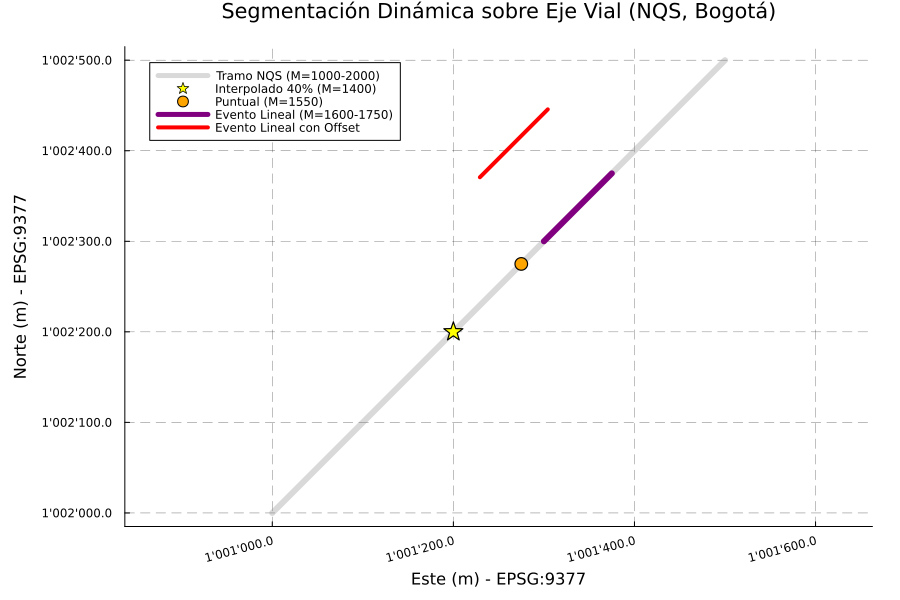
\includegraphics[width=0.8\textwidth,height=\textheight]{images/c14_plot_segmentacion_dinamica_julia.png}

}

\caption{Segmentación dinámica en la NQS con ejes formateados
(M=1000-2000).}

\end{figure}%

\subsection{Resumen sintáctico}\label{resumen-sintuxe1ctico-3}

\begin{enumerate}
\def\labelenumi{\arabic{enumi}.}
\tightlist
\item
  \textbf{Manejo de estructuras y dimensiones (Z y M)}
\end{enumerate}

La persistencia de geometrías complejas varía significativamente.
Mientras R integra la cuarta dimensión de forma nativa mediante su
ecosistema unificado, Python y Julia requieren utilizar directamente
envolturas de bajo nivel (GDAL/OGR) para evitar la pérdida de atributos
escalares.

\begin{longtable}[]{@{}
  >{\raggedright\arraybackslash}p{(\columnwidth - 6\tabcolsep) * \real{0.2500}}
  >{\raggedright\arraybackslash}p{(\columnwidth - 6\tabcolsep) * \real{0.2500}}
  >{\raggedright\arraybackslash}p{(\columnwidth - 6\tabcolsep) * \real{0.2500}}
  >{\raggedright\arraybackslash}p{(\columnwidth - 6\tabcolsep) * \real{0.2500}}@{}}
\caption{Comparativa de funciones para instanciación y auditoría de
dimensiones espaciales
adicionales}\label{tbl-dimensiones_arquitectura}\tabularnewline
\toprule\noalign{}
\begin{minipage}[b]{\linewidth}\raggedright
Operación técnica
\end{minipage} & \begin{minipage}[b]{\linewidth}\raggedright
Python (\texttt{shapely} / \texttt{osgeo.ogr}) 🐍
\end{minipage} & \begin{minipage}[b]{\linewidth}\raggedright
R (\texttt{sf}) 🔵
\end{minipage} & \begin{minipage}[b]{\linewidth}\raggedright
Julia (\texttt{ArchGDAL} / \texttt{LibGEOS}) 🟣
\end{minipage} \\
\midrule\noalign{}
\endfirsthead
\toprule\noalign{}
\begin{minipage}[b]{\linewidth}\raggedright
Operación técnica
\end{minipage} & \begin{minipage}[b]{\linewidth}\raggedright
Python (\texttt{shapely} / \texttt{osgeo.ogr}) 🐍
\end{minipage} & \begin{minipage}[b]{\linewidth}\raggedright
R (\texttt{sf}) 🔵
\end{minipage} & \begin{minipage}[b]{\linewidth}\raggedright
Julia (\texttt{ArchGDAL} / \texttt{LibGEOS}) 🟣
\end{minipage} \\
\midrule\noalign{}
\endhead
\bottomrule\noalign{}
\endlastfoot
\textbf{Instanciación 3D (XYZ)} & \texttt{Point(x,\ y,\ z)} &
\texttt{st\_point(}\texttt{c(x,\ y,\ z))} &
\texttt{AG.createpoint(}\texttt{x,\ y,\ z)} \\
\textbf{Punto con ZM} & \emph{Soporte limitado} &
\texttt{st\_point(c(x,y,z,m),\ dim="XYZM")} & \emph{Vía WKB avanzado} \\
\textbf{Instanciación 4D (XYZM)} &
\texttt{ogr.CreateGeometryFromWkt(}\texttt{"POINT\ ZM\ (X\ Y\ Z\ M)")} &
\texttt{st\_as\_sfc(}\texttt{"POINT\ ZM\ (X\ Y\ Z\ M)")} &
\texttt{AG.fromWKT(}\texttt{"POINT\ ZM\ (X\ Y\ Z\ M)")} \\
\textbf{Chequear si tiene Z} & \texttt{geom.has\_z}
\emph{(Shapely)}\texttt{geom\_ogr.CoordinateDimension()\ ==\ 3}
\emph{(OGR)} & \texttt{st\_zm(geom,\ what="Z")} &
\texttt{AG.getcoorddim(geom)\ \textgreater{}=\ 3} \\
\textbf{Verificación de medida (M)} & \texttt{geom\_ogr.IsMeasured()} &
\texttt{st\_geometry\_type(geom)} & \texttt{AG.ismeasured(geom)} \\
\textbf{Extracción de cota (Z)} & \texttt{geom.z} &
\texttt{st\_coordinates(geom){[},\ "Z"{]}} &
\texttt{AG.getz(geom,\ 0)} \\
\textbf{Extracción de medida (M)} & \texttt{geom\_ogr.GetM()} &
\texttt{st\_coordinates(geom){[},\ "M"{]}} &
\texttt{AG.getm(geom,\ 0)} \\
\end{longtable}

\begin{enumerate}
\def\labelenumi{\arabic{enumi}.}
\setcounter{enumi}{1}
\tightlist
\item
  \textbf{Referenciación lineal espacial (LRS) y topología}
\end{enumerate}

El cálculo de eventos sobre líneas requiere algoritmos de interpolación.
Los motores difieren en la sintaxis para el manejo de distancias
absolutas frente a distancias relativas (normalizadas).

\begin{longtable}[]{@{}
  >{\raggedright\arraybackslash}p{(\columnwidth - 6\tabcolsep) * \real{0.2500}}
  >{\raggedright\arraybackslash}p{(\columnwidth - 6\tabcolsep) * \real{0.2500}}
  >{\raggedright\arraybackslash}p{(\columnwidth - 6\tabcolsep) * \real{0.2500}}
  >{\raggedright\arraybackslash}p{(\columnwidth - 6\tabcolsep) * \real{0.2500}}@{}}
\caption{Métodos de segmentación dinámica y transformación de eventos
lineales}\label{tbl-operaciones_lrs}\tabularnewline
\toprule\noalign{}
\begin{minipage}[b]{\linewidth}\raggedright
Operación técnica
\end{minipage} & \begin{minipage}[b]{\linewidth}\raggedright
Python (\texttt{shapely}) 🐍
\end{minipage} & \begin{minipage}[b]{\linewidth}\raggedright
R (\texttt{sf}) 🔵
\end{minipage} & \begin{minipage}[b]{\linewidth}\raggedright
Julia (\texttt{LibGEOS} / Vectores) 🟣
\end{minipage} \\
\midrule\noalign{}
\endfirsthead
\toprule\noalign{}
\begin{minipage}[b]{\linewidth}\raggedright
Operación técnica
\end{minipage} & \begin{minipage}[b]{\linewidth}\raggedright
Python (\texttt{shapely}) 🐍
\end{minipage} & \begin{minipage}[b]{\linewidth}\raggedright
R (\texttt{sf}) 🔵
\end{minipage} & \begin{minipage}[b]{\linewidth}\raggedright
Julia (\texttt{LibGEOS} / Vectores) 🟣
\end{minipage} \\
\midrule\noalign{}
\endhead
\bottomrule\noalign{}
\endlastfoot
\textbf{Interpolación normalizada (Fracción)} &
\texttt{geom.interpolate(}\texttt{0.4,\ normalized=True)} &
\texttt{st\_line\_sample(}\texttt{geom,\ sample\ =\ 0.4)} &
\texttt{LG.interpolateNormalized(}\texttt{geom,\ 0.4)} \\
\textbf{Interpolación absoluta (Distancia)} &
\texttt{geom.interpolate(250.0)} &
\texttt{st\_line\_sample(}\texttt{geom,\ sample\ =\ dist/total)} &
\texttt{LG.interpolate(}\texttt{geom,\ 250.0)} \\
\textbf{Curva paralela (Offset lateral)} &
\texttt{geom.offset\_curve(100)} & Álgebra vectorial & Álgebra vectorial
ortogonal\texttt{{[}ox,\ oy{]}\ =\ {[}lx,\ ly{]}\ +\ (dist\ *\ {[}ux,\ uy{]})} \\
\textbf{Cálculo de longitud LRS} & \texttt{geom.length} &
\texttt{st\_length(geom)} & \texttt{LG.geomLength(geom)} \\
\end{longtable}

\begin{enumerate}
\def\labelenumi{\arabic{enumi}.}
\setcounter{enumi}{2}
\tightlist
\item
  \textbf{Renderizado cartográfico y convenciones de diseño}
\end{enumerate}

La generación de gráficos espaciales a nivel de publicación requiere el
formateo estricto de los ejes coordenados (estándar IGAC para Colombia)
y el control de la correspondencia visual 1:1 para evitar deformaciones
topológicas.

\begin{longtable}[]{@{}
  >{\raggedright\arraybackslash}p{(\columnwidth - 6\tabcolsep) * \real{0.2500}}
  >{\raggedright\arraybackslash}p{(\columnwidth - 6\tabcolsep) * \real{0.2500}}
  >{\raggedright\arraybackslash}p{(\columnwidth - 6\tabcolsep) * \real{0.2500}}
  >{\raggedright\arraybackslash}p{(\columnwidth - 6\tabcolsep) * \real{0.2500}}@{}}
\caption{Equivalencia de componentes visuales y parametrización gráfica
por ecosistema}\label{tbl-renderizado_cartografico}\tabularnewline
\toprule\noalign{}
\begin{minipage}[b]{\linewidth}\raggedright
Operación técnica
\end{minipage} & \begin{minipage}[b]{\linewidth}\raggedright
Python (\texttt{matplotlib}) 🐍
\end{minipage} & \begin{minipage}[b]{\linewidth}\raggedright
R (\texttt{ggplot2}) 🔵
\end{minipage} & \begin{minipage}[b]{\linewidth}\raggedright
Julia (\texttt{Plots}) 🟣
\end{minipage} \\
\midrule\noalign{}
\endfirsthead
\toprule\noalign{}
\begin{minipage}[b]{\linewidth}\raggedright
Operación técnica
\end{minipage} & \begin{minipage}[b]{\linewidth}\raggedright
Python (\texttt{matplotlib}) 🐍
\end{minipage} & \begin{minipage}[b]{\linewidth}\raggedright
R (\texttt{ggplot2}) 🔵
\end{minipage} & \begin{minipage}[b]{\linewidth}\raggedright
Julia (\texttt{Plots}) 🟣
\end{minipage} \\
\midrule\noalign{}
\endhead
\bottomrule\noalign{}
\endlastfoot
\textbf{Inicialización del lienzo cartográfico} &
\texttt{fig,\ ax\ =\ plt.subplots(}\texttt{figsize=(10,\ 6))} &
\texttt{ggplot()} &
\texttt{plt\ =\ Plots.plot(}\texttt{size=(900,\ 600))} \\
\textbf{Renderizado de capa lineal} &
\texttt{ax.plot(}\texttt{x,\ y,\ color=\textquotesingle{}grey\textquotesingle{})}
&
\texttt{geom\_sf(}\texttt{data\ =\ df,\ color\ =\ \textquotesingle{}grey\textquotesingle{})}
& \texttt{Plots.plot!(plt,}\texttt{x,\ y,\ color=:gray)} \\
\textbf{Renderizado de capa puntual} &
\texttt{ax.plot(}\texttt{x,\ y,\ \textquotesingle{}o\textquotesingle{},\ color=\textquotesingle{}red\textquotesingle{})}
&
\texttt{geom\_sf(}\texttt{data\ =\ df,\ color\ =\ \textquotesingle{}red\textquotesingle{})}
& \texttt{Plots.scatter!(plt,}\texttt{x,\ y,\ color=:red)} \\
\textbf{Relación de aspecto espacial (1:1)} &
\texttt{ax.axis(\textquotesingle{}equal\textquotesingle{})} &
\texttt{coord\_sf(}\texttt{datum\ =\ st\_crs(9377))} &
\texttt{aspect\_ratio=:equal} \\
\textbf{Inyección de separador de miles (IGAC)} &
\texttt{ax.xaxis.set\_major\_formatter(}\texttt{ticker.FuncFormatter(fmt))}
& \texttt{scale\_x\_continuous(}\texttt{labels\ =\ label\_number(...))}
& \texttt{xformatter\ =\ x\ -\textgreater{}\ fmt\_igac(x)} \\
\textbf{Aplicación de opacidad (Alpha)} & \texttt{alpha=0.5} &
\texttt{color\ =\ scales::alpha(}\texttt{"gray",\ 0.5)} &
\texttt{alpha=0.5} \\
\end{longtable}

\section{Resumen del capítulo}\label{resumen-del-capuxedtulo-1}

En este capítulo hemos roto la barrera bidimensional de los SIG
tradicionales, introduciendo la gestión de infraestructuras y redes
mediante dimensiones espaciales extendidas y sistemas paramétricos.

Los hitos conceptuales y técnicos que debes dominar de esta sección son:

\begin{itemize}
\tightlist
\item
  \textbf{Las 4 Dimensiones del Estándar OGC:} Las geometrías pueden
  escalar desde el plano bidimensional (\textbf{XY}) hacia el espacio
  topográfico tridimensional (\textbf{XYZ}), incluir una dimensión de
  medida paramétrica (\textbf{XYM}), o integrar ambas en un modelo
  cuatridimensional (\textbf{XYZM}). Estas dimensiones deben ser
  consistentes en todos los vértices de una misma entidad.
\item
  \textbf{Referenciación Lineal (LRS):} Es el paradigma estándar para la
  gestión de infraestructura lineal (vías, ríos, ductos). Permite
  localizar \textbf{eventos puntuales} (hitos, semáforos) y
  \textbf{eventos lineales} (tramos de pavimento, límites de velocidad)
  basándose en una medida de longitud (\(M\)) acumulada sobre el eje, en
  lugar de depender de coordenadas cartesianas absolutas.
\item
  \textbf{Segmentación Dinámica vs.~Estática:} Gracias al LRS, podemos
  mapear múltiples atributos a lo largo de una vía (segmentación
  dinámica) sin tener que cortar físicamente la línea geométrica en la
  base de datos (segmentación estática), preservando la topología de la
  red.
\item
  \textbf{El ``Secuestro'' del Eje Z:} Descubrimos que librerías de alto
  nivel como \texttt{shapely} en Python o \texttt{LibGEOS} en Julia
  operan principalmente en un espacio 3D, careciendo de un eje \(M\)
  explícito para operaciones LRS nativas. Como solución metodológica, es
  una práctica común de la industria alojar temporalmente las medidas de
  kilometraje en la cota de altitud (\(Z\)).
\item
  \textbf{Manipulación de Bajo Nivel (OGR):} Para lograr una
  persistencia real y estricta de geometrías 4D (\(XYZM\)) en lenguajes
  que no lo soportan nativamente en sus capas superiores, es obligatorio
  interactuar con constructores WKT explícitos (ej. \texttt{POINT\ ZM})
  y envolturas directas al motor \textbf{GDAL/OGR}. En contraste, R (vía
  \texttt{sf}) destaca por manejar estas cuatro dimensiones de manera
  fluida y nativa.
\item
  \textbf{Álgebra Vectorial Cartográfica:} Ante la ausencia de funciones
  directas para generar desplazamientos laterales paralelos
  (\emph{Offset Curves}) en R y Julia, comprobamos que el conocimiento
  de álgebra lineal básica (cálculo de vectores normales y ortogonales)
  es una habilidad indispensable para cualquier geómatra que necesite
  renderizar mapas técnicos o viales.
\end{itemize}

El dominio de estas técnicas te permitirá enfrentar proyectos de
transporte, hidrología y \emph{routing} a escala profesional,
manteniendo la integridad espacial de las mediciones sin importar el
lenguaje de programación que utilices como motor de cálculo.

\chapter{Análisis Vectorial: Topología y Geoprocesamiento
Espacial}\label{anuxe1lisis-vectorial-topologuxeda-y-geoprocesamiento-espacial}

\section{Funciones j\_eval y j\_plot en
R}\label{funciones-j_eval-y-j_plot-en-r-11}

\begin{Shaded}
\begin{Highlighting}[]
\CommentTok{\# \#| include: false}
\FunctionTok{source}\NormalTok{(}\StringTok{"./docs/j\_eval\_j\_plot.r"}\NormalTok{)}
\end{Highlighting}
\end{Shaded}

\section{Introducción}\label{introducciuxf3n-12}

En capítulos anteriores establecimos los cimientos de la ciencia de
datos espaciales: aprendimos cómo los lenguajes de programación
estructuran las coordenadas, cómo se ensamblan las primitivas
geométricas (puntos, líneas, polígonos) y cómo estas se integran en
tablas mediante estándares como Simple Features y WKB. Hasta ese punto,
nuestras geometrías existían en un estado estático y aislado.

Sin embargo, el verdadero poder de los Sistemas de Información
Geográfica (SIG) no radica simplemente en \emph{almacenar} o
\emph{dibujar} formas, sino en \textbf{hacerlas interactuar}. La
resolución de problemas territoriales reales exige responder preguntas
complejas: \emph{¿Un predio invade una zona de reserva ambiental? ¿Qué
vías intersecan una falla geológica? ¿Cuál es el área de impacto a 500
metros de una estación de transporte?}

Para responder a estos interrogantes, este capítulo aborda los dos
grandes pilares del análisis espacial vectorial: 1. \textbf{La Topología
(Predicados Espaciales):} Reglas matemáticas booleanas que evalúan cómo
se relacionan y cruzan dos geometrías en el espacio sin modificar su
estructura original. 2. \textbf{El Geoprocesamiento Paramétrico:}
Operaciones algorítmicas que toman una o más geometrías de entrada y
calculan una \emph{nueva} entidad espacial como resultado (ej. buffers,
centroides o intersecciones).

A lo largo de este capítulo, exploraremos cómo los ecosistemas de
Python, R y Julia delegan estos cálculos críticos al motor unificado
\textbf{GEOS} (Geometry Engine, Open Source), garantizando resultados
topológicos consistentes independientemente de la sintaxis utilizada.

\section{Predicados espaciales y relaciones
topológicas}\label{predicados-espaciales-y-relaciones-topoluxf3gicas}

Los predicados espaciales evalúan y determinan las relaciones
topológicas entre dos objetos espaciales utilizando el \textbf{modelo de
matriz de intersección de nueve elementos extendido dimensionalmente}
(DE-9IM). Puedes encontrar mayor información en:

\begin{enumerate}
\def\labelenumi{\arabic{enumi}.}
\tightlist
\item
  \href{https://en.wikipedia.org/wiki/DE-9IM}{Wikipedia (inglés)}
\item
  \href{https://postgis.net/workshops/es/postgis-intro/de9im.html}{Ayuda
  de PostGIS (español)}
\item
  \href{https://pro.arcgis.com/es/pro-app/latest/help/data/validating-data/custom-spatial-relationships.htm}{Ayuda
  de ArcGIS (español)}
\end{enumerate}

Otro recurso valioso es la Suite de Topología de Java (JTS), la cual
incluye la herramienta JTS TestBuilder, donde se puede interactuar
mediante una interfaz gráfica para crear geometrías manualmente y
calcular la matriz DE-9IM entre pares de geometrías creadas por el
usuario. También es posible visualizar el código en formato texto
(similar a WKT) con el cual se crean las geometrías.

Para instalarla, es requisito contar con Java instalado en el equipo:

\begin{enumerate}
\def\labelenumi{\arabic{enumi}.}
\tightlist
\item
  \href{https://sourceforge.net/projects/jts-topology-suite.mirror/}{Descargue}
  el binario (jts-1.14.zip).\\
\item
  Descomprima el archivo.
\item
  En la carpeta \texttt{jts-1.14/bin/}, ejecute (doble clic)
  \texttt{testbuilder.bat}.
\end{enumerate}

Características principales:

\begin{itemize}
\tightlist
\item
  Soporta WKT y WKB\\
\item
  Soporta GML 2.0\\
\item
  Implementa el estándar OGC Simple Features for SQL (SFSQL)
\end{itemize}

Para comprender rápidamente el funcionamiento de DE-9IM, se recomienda
este \href{https://youtu.be/vWczRTxDNgM}{video} en español.

\subsection{Explicación de DE-9IM}\label{explicaciuxf3n-de-de-9im}

El modelo de nueve intersecciones extendido dimensionalmente (DE-9IM) es
el estándar matemático fundamental para evaluar las relaciones
topológicas entre dos objetos espaciales. Este modelo analiza cómo
interactúan tres componentes estructurales de una geometría \(A\) con
los mismos tres componentes de una geometría \(B\):

\begin{enumerate}
\def\labelenumi{\arabic{enumi}.}
\tightlist
\item
  \textbf{Interior (\(I\))}: El área, línea o punto(s) que conforman la
  estructura interna de la geometría.
\item
  \textbf{Límite (\(B\), de \emph{Boundary})}: El borde o contorno que
  delimita el interior del exterior.
\item
  \textbf{Exterior (\(E\))}: Todo el espacio matemático del plano que no
  pertenece al interior ni al límite.
\end{enumerate}

La matriz DE-9IM evalúa la intersección de cada componente de \(A\) con
cada componente de \(B\), generando 9 posibles combinaciones. El
resultado de cada intersección se clasifica según la dimensión
geométrica máxima del objeto resultante:

\begin{itemize}
\tightlist
\item
  \textbf{\(2\)}: La intersección produce un polígono (área de dos
  dimensiones).
\item
  \textbf{\(1\)}: La intersección produce una línea o polilínea (una
  dimensión).
\item
  \textbf{\(0\)}: La intersección produce uno o varios puntos aislados
  (cero dimensiones).
\item
  \textbf{\(F\)}: No existe intersección (vacío o \emph{False}).
\item
  \textbf{\(*\)}: Comodín utilizado en las máscaras de predicados,
  indica que el valor en esa posición es irrelevante para la regla.
\item
  \textbf{\(T\)}: Comodín que indica cualquier intersección no vacía
  (\(0\), \(1\) o \(2\)).
\end{itemize}

\subsection{Matriz de intersección y predicados
espaciales}\label{matriz-de-intersecciuxf3n-y-predicados-espaciales}

La matriz resultante se lee algebraicamente como una cadena de nueve
caracteres, organizados en el orden de las siguientes intersecciones:

\begin{enumerate}
\def\labelenumi{\arabic{enumi}.}
\tightlist
\item
  \(I(A) \cap I(B)\),
\item
  \(I(A) \cap B(B)\),
\item
  \(I(A) \cap E(B)\),
\item
  \(B(A) \cap I(B)\),
\item
  \(B(A) \cap B(B)\),
\item
  \(B(A) \cap E(B)\),
\item
  \(E(A) \cap I(B)\),
\item
  \(E(A) \cap B(B)\),
\item
  \(E(A) \cap E(B)\).
\end{enumerate}

Los sistemas de información geográfica operan comparando la cadena
DE-9IM resultante con patrones predefinidos para evaluar predicados
lógicos. La siguiente tabla presenta las máscaras topológicas estándar:

\begin{longtable}[]{@{}
  >{\raggedright\arraybackslash}p{(\columnwidth - 4\tabcolsep) * \real{0.3333}}
  >{\raggedright\arraybackslash}p{(\columnwidth - 4\tabcolsep) * \real{0.3333}}
  >{\raggedright\arraybackslash}p{(\columnwidth - 4\tabcolsep) * \real{0.3333}}@{}}
\toprule\noalign{}
\begin{minipage}[b]{\linewidth}\raggedright
Predicado
\end{minipage} & \begin{minipage}[b]{\linewidth}\raggedright
Descripción geométrica
\end{minipage} & \begin{minipage}[b]{\linewidth}\raggedright
Máscara DE-9IM (\(A\) frente a \(B\))
\end{minipage} \\
\midrule\noalign{}
\endhead
\bottomrule\noalign{}
\endlastfoot
\textbf{\texttt{Equals}} & Las geometrías son espacialmente idénticas. &
\texttt{T*F**FFF*} \\
\textbf{\texttt{Disjoint}} & No comparten ningún espacio interior ni
límite. & \texttt{FF*FF****} \\
\textbf{\texttt{Intersects}} & Opuesto exacto a Disjoint. Se tocan de
alguna forma. & \texttt{T********}, \texttt{*T*******},
\texttt{***T*****}, o \texttt{****T****} \\
\textbf{\texttt{Touches}} & Comparten un límite espacial, pero sus
interiores no se cruzan. & \texttt{FT*******}, \texttt{F**T*****}, o
\texttt{F***T****} \\
\textbf{\texttt{Crosses}} & Comparten parte de su interior, pero no en
su totalidad (líneas/polígonos). & \texttt{T*T******} o
\texttt{T*****T**} \\
\textbf{\texttt{Within}} & La geometría \(A\) está completamente dentro
de \(B\). & \texttt{T*F**F***} \\
\textbf{\texttt{Contains}} & La geometría \(A\) abarca por completo a
\(B\). & \texttt{T*****FF*} \\
\end{longtable}

A continuación, se demuestra la construcción matricial DE-9IM utilizando
un caso simulado aplicado a un modelo de infraestructura en Bogotá. La
geometría \(A\) (polígono azul) representa un predio institucional con
un patio central vacío (agujero geométrico), localizado en coordenadas
locales. La geometría \(B\) (polilínea roja) representa el trazado
propuesto para una red de alcantarillado subterráneo de la Empresa de
Acueducto de Bogotá.

Al computar la matriz DE-9IM para este caso específico (\texttt{A}
frente a \texttt{B}), los algoritmos de la librería base GEOS determinan
que el trazado de tubería cruza el área sólida del predio en forma de
línea (dimensión 1), los vértices de la red perforan los muros
(intersección límite-interior en puntos, dimensión 0), y ambos extremos
de la tubería inician y terminan en espacio público exterior. El
resultado matricial para esta relación precisa es \texttt{1F20F1102}.

\subsection{Python}

\begin{Shaded}
\begin{Highlighting}[]
\CommentTok{\# \#| eval: false}

\ImportTok{import}\NormalTok{ geopandas }\ImportTok{as}\NormalTok{ gpd}
\ImportTok{import}\NormalTok{ matplotlib.pyplot }\ImportTok{as}\NormalTok{ plt}
\ImportTok{from}\NormalTok{ shapely.wkt }\ImportTok{import}\NormalTok{ loads}

\CommentTok{\# 1. Definición de geometrías a partir de texto WKT}
\CommentTok{\# Polígono A: Predio institucional en Bogotá con patio interior}
\NormalTok{wkt\_poligono\_a }\OperatorTok{=} \StringTok{"POLYGON ((100 390, 445 390, 445 97, 100 97, 100 390), (210 310, 355 310, 355 179, 210 179, 210 310))"}
\CommentTok{\# Polilínea B: Trazado de tubería subterránea}
\NormalTok{wkt\_linea\_b }\OperatorTok{=} \StringTok{"LINESTRING (316 434, 250 330, 400 210, 240 30)"}

\NormalTok{poligono\_a }\OperatorTok{=}\NormalTok{ loads(wkt\_poligono\_a)}
\NormalTok{linea\_b }\OperatorTok{=}\NormalTok{ loads(wkt\_linea\_b)}

\CommentTok{\# 2. Extracción de la matriz lógica DE{-}9IM (A respecto a B)}
\NormalTok{matriz\_de9im }\OperatorTok{=}\NormalTok{ poligono\_a.relate(linea\_b)}
\BuiltInTok{print}\NormalTok{(}\SpecialStringTok{f"Matriz de intersección DE{-}9IM (AB): }\SpecialCharTok{\{}\NormalTok{matriz\_de9im}\SpecialCharTok{\}}\CharTok{\textbackslash{}n}\SpecialStringTok{"}\NormalTok{)}
\end{Highlighting}
\end{Shaded}

\begin{verbatim}
Matriz de intersección DE-9IM (AB): 1F20F1102
\end{verbatim}

\begin{Shaded}
\begin{Highlighting}[]
\CommentTok{\# 3. Comprobación exhaustiva de predicados lógicos binarios}
\BuiltInTok{print}\NormalTok{(}\StringTok{"Evaluación de predicados (AB):"}\NormalTok{)}
\end{Highlighting}
\end{Shaded}

\begin{verbatim}
Evaluación de predicados (AB):
\end{verbatim}

\begin{Shaded}
\begin{Highlighting}[]
\BuiltInTok{print}\NormalTok{(}\SpecialStringTok{f"Equals:     }\SpecialCharTok{\{}\NormalTok{poligono\_a}\SpecialCharTok{.}\NormalTok{equals(linea\_b)}\SpecialCharTok{\}}\SpecialStringTok{"}\NormalTok{)}
\end{Highlighting}
\end{Shaded}

\begin{verbatim}
Equals:     False
\end{verbatim}

\begin{Shaded}
\begin{Highlighting}[]
\BuiltInTok{print}\NormalTok{(}\SpecialStringTok{f"Disjoint:   }\SpecialCharTok{\{}\NormalTok{poligono\_a}\SpecialCharTok{.}\NormalTok{disjoint(linea\_b)}\SpecialCharTok{\}}\SpecialStringTok{"}\NormalTok{)}
\end{Highlighting}
\end{Shaded}

\begin{verbatim}
Disjoint:   False
\end{verbatim}

\begin{Shaded}
\begin{Highlighting}[]
\BuiltInTok{print}\NormalTok{(}\SpecialStringTok{f"Intersects: }\SpecialCharTok{\{}\NormalTok{poligono\_a}\SpecialCharTok{.}\NormalTok{intersects(linea\_b)}\SpecialCharTok{\}}\SpecialStringTok{"}\NormalTok{)}
\end{Highlighting}
\end{Shaded}

\begin{verbatim}
Intersects: True
\end{verbatim}

\begin{Shaded}
\begin{Highlighting}[]
\BuiltInTok{print}\NormalTok{(}\SpecialStringTok{f"Touches:    }\SpecialCharTok{\{}\NormalTok{poligono\_a}\SpecialCharTok{.}\NormalTok{touches(linea\_b)}\SpecialCharTok{\}}\SpecialStringTok{"}\NormalTok{)}
\end{Highlighting}
\end{Shaded}

\begin{verbatim}
Touches:    False
\end{verbatim}

\begin{Shaded}
\begin{Highlighting}[]
\BuiltInTok{print}\NormalTok{(}\SpecialStringTok{f"Crosses:    }\SpecialCharTok{\{}\NormalTok{poligono\_a}\SpecialCharTok{.}\NormalTok{crosses(linea\_b)}\SpecialCharTok{\}}\SpecialStringTok{"}\NormalTok{)}
\end{Highlighting}
\end{Shaded}

\begin{verbatim}
Crosses:    True
\end{verbatim}

\begin{Shaded}
\begin{Highlighting}[]
\BuiltInTok{print}\NormalTok{(}\SpecialStringTok{f"Within:     }\SpecialCharTok{\{}\NormalTok{poligono\_a}\SpecialCharTok{.}\NormalTok{within(linea\_b)}\SpecialCharTok{\}}\SpecialStringTok{"}\NormalTok{)}
\end{Highlighting}
\end{Shaded}

\begin{verbatim}
Within:     False
\end{verbatim}

\begin{Shaded}
\begin{Highlighting}[]
\BuiltInTok{print}\NormalTok{(}\SpecialStringTok{f"Contains:   }\SpecialCharTok{\{}\NormalTok{poligono\_a}\SpecialCharTok{.}\NormalTok{contains(linea\_b)}\SpecialCharTok{\}}\SpecialStringTok{"}\NormalTok{)}
\end{Highlighting}
\end{Shaded}

\begin{verbatim}
Contains:   False
\end{verbatim}

\begin{Shaded}
\begin{Highlighting}[]
\BuiltInTok{print}\NormalTok{(}\SpecialStringTok{f"Overlaps:   }\SpecialCharTok{\{}\NormalTok{poligono\_a}\SpecialCharTok{.}\NormalTok{overlaps(linea\_b)}\SpecialCharTok{\}}\SpecialStringTok{"}\NormalTok{)}
\end{Highlighting}
\end{Shaded}

\begin{verbatim}
Overlaps:   False
\end{verbatim}

\begin{Shaded}
\begin{Highlighting}[]
\BuiltInTok{print}\NormalTok{(}\SpecialStringTok{f"Covers:     }\SpecialCharTok{\{}\NormalTok{poligono\_a}\SpecialCharTok{.}\NormalTok{covers(linea\_b)}\SpecialCharTok{\}}\SpecialStringTok{"}\NormalTok{)}
\end{Highlighting}
\end{Shaded}

\begin{verbatim}
Covers:     False
\end{verbatim}

\begin{Shaded}
\begin{Highlighting}[]
\CommentTok{\# Se evalúa CoveredBy invirtiendo la relación de cobertura geométrica}
\BuiltInTok{print}\NormalTok{(}\SpecialStringTok{f"CoveredBy:  }\SpecialCharTok{\{}\NormalTok{linea\_b}\SpecialCharTok{.}\NormalTok{covers(poligono\_a)}\SpecialCharTok{\}}\SpecialStringTok{"}\NormalTok{)}
\end{Highlighting}
\end{Shaded}

\begin{verbatim}
CoveredBy:  False
\end{verbatim}

\begin{Shaded}
\begin{Highlighting}[]
\CommentTok{\# 4. Visualización del comportamiento geométrico}
\NormalTok{fig, ax }\OperatorTok{=}\NormalTok{ plt.subplots(figsize}\OperatorTok{=}\NormalTok{(}\DecValTok{6}\NormalTok{, }\DecValTok{6}\NormalTok{))}

\NormalTok{gpd.GeoSeries([poligono\_a]).plot(ax}\OperatorTok{=}\NormalTok{ax, color}\OperatorTok{=}\StringTok{\textquotesingle{}\#b3cde0\textquotesingle{}}\NormalTok{, edgecolor}\OperatorTok{=}\StringTok{\textquotesingle{}blue\textquotesingle{}}\NormalTok{, alpha}\OperatorTok{=}\FloatTok{0.7}\NormalTok{)}
\NormalTok{gpd.GeoSeries([linea\_b]).plot(ax}\OperatorTok{=}\NormalTok{ax, color}\OperatorTok{=}\StringTok{\textquotesingle{}red\textquotesingle{}}\NormalTok{, linewidth}\OperatorTok{=}\DecValTok{2}\NormalTok{, marker}\OperatorTok{=}\StringTok{\textquotesingle{}.\textquotesingle{}}\NormalTok{)}

\NormalTok{ax.set\_title(}\SpecialStringTok{f"Relación Topológica (DE{-}9IM: }\SpecialCharTok{\{}\NormalTok{matriz\_de9im}\SpecialCharTok{\}}\SpecialStringTok{)"}\NormalTok{)}
\NormalTok{ax.set\_xlabel(}\StringTok{"Coordenadas locales (X)"}\NormalTok{)}
\NormalTok{ax.set\_ylabel(}\StringTok{"Coordenadas locales (Y)"}\NormalTok{)}
\NormalTok{ax.grid(}\VariableTok{True}\NormalTok{, linestyle}\OperatorTok{=}\StringTok{\textquotesingle{}{-}{-}\textquotesingle{}}\NormalTok{, alpha}\OperatorTok{=}\FloatTok{0.5}\NormalTok{)}

\NormalTok{plt.tight\_layout()}
\NormalTok{plt.show()}
\end{Highlighting}
\end{Shaded}

\begin{center}

\includegraphics[width=0.8\textwidth,height=\textheight]{16-matriz_de_9im_files/figure-pdf/python_de9im-1.pdf}
\end{center}

\subsection{R}

\begin{Shaded}
\begin{Highlighting}[]
\CommentTok{\# \#| eval: false}

\FunctionTok{library}\NormalTok{(sf)}
\end{Highlighting}
\end{Shaded}

\begin{verbatim}
Linking to GEOS 3.12.1, GDAL 3.8.4, PROJ 9.4.0; sf_use_s2() is TRUE
\end{verbatim}

\begin{Shaded}
\begin{Highlighting}[]
\CommentTok{\# 1. Construcción de objetos geométricos (sfg {-}\textgreater{} sfc) a partir de WKT}
\NormalTok{poligono\_a }\OtherTok{\textless{}{-}} \FunctionTok{st\_as\_sfc}\NormalTok{(}\StringTok{"POLYGON ((100 390, 445 390, 445 97, 100 97, 100 390), (210 310, 355 310, 355 179, 210 179, 210 310))"}\NormalTok{)}
\NormalTok{linea\_b }\OtherTok{\textless{}{-}} \FunctionTok{st\_as\_sfc}\NormalTok{(}\StringTok{"LINESTRING (316 434, 250 330, 400 210, 240 30)"}\NormalTok{)}

\CommentTok{\# 2. Computación de la matriz dimensional DE{-}9IM}
\NormalTok{matriz\_de9im }\OtherTok{\textless{}{-}} \FunctionTok{st\_relate}\NormalTok{(poligono\_a, linea\_b, }\AttributeTok{sparse =} \ConstantTok{FALSE}\NormalTok{)}
\FunctionTok{cat}\NormalTok{(}\FunctionTok{paste}\NormalTok{(}\StringTok{"Matriz de intersección DE{-}9IM (AB):"}\NormalTok{, matriz\_de9im[}\DecValTok{1}\NormalTok{, }\DecValTok{1}\NormalTok{], }\StringTok{"}\SpecialCharTok{\textbackslash{}n\textbackslash{}n}\StringTok{"}\NormalTok{))}
\end{Highlighting}
\end{Shaded}

\begin{verbatim}
Matriz de intersección DE-9IM (AB): 1F20F1102 
\end{verbatim}

\begin{Shaded}
\begin{Highlighting}[]
\CommentTok{\# 3. Comprobación exhaustiva de predicados lógicos binarios}
\FunctionTok{cat}\NormalTok{(}\StringTok{"Evaluación de predicados (AB):}\SpecialCharTok{\textbackslash{}n}\StringTok{"}\NormalTok{)}
\end{Highlighting}
\end{Shaded}

\begin{verbatim}
Evaluación de predicados (AB):
\end{verbatim}

\begin{Shaded}
\begin{Highlighting}[]
\FunctionTok{cat}\NormalTok{(}\FunctionTok{paste}\NormalTok{(}\StringTok{"Equals:    "}\NormalTok{, }\FunctionTok{st\_equals}\NormalTok{(poligono\_a, linea\_b, }\AttributeTok{sparse =} \ConstantTok{FALSE}\NormalTok{)[}\DecValTok{1}\NormalTok{, }\DecValTok{1}\NormalTok{], }\StringTok{"}\SpecialCharTok{\textbackslash{}n}\StringTok{"}\NormalTok{))}
\end{Highlighting}
\end{Shaded}

\begin{verbatim}
Equals:     FALSE 
\end{verbatim}

\begin{Shaded}
\begin{Highlighting}[]
\FunctionTok{cat}\NormalTok{(}\FunctionTok{paste}\NormalTok{(}\StringTok{"Disjoint:  "}\NormalTok{, }\FunctionTok{st\_disjoint}\NormalTok{(poligono\_a, linea\_b, }\AttributeTok{sparse =} \ConstantTok{FALSE}\NormalTok{)[}\DecValTok{1}\NormalTok{, }\DecValTok{1}\NormalTok{], }\StringTok{"}\SpecialCharTok{\textbackslash{}n}\StringTok{"}\NormalTok{))}
\end{Highlighting}
\end{Shaded}

\begin{verbatim}
Disjoint:   FALSE 
\end{verbatim}

\begin{Shaded}
\begin{Highlighting}[]
\FunctionTok{cat}\NormalTok{(}\FunctionTok{paste}\NormalTok{(}\StringTok{"Intersects:"}\NormalTok{, }\FunctionTok{st\_intersects}\NormalTok{(poligono\_a, linea\_b, }\AttributeTok{sparse =} \ConstantTok{FALSE}\NormalTok{)[}\DecValTok{1}\NormalTok{, }\DecValTok{1}\NormalTok{], }\StringTok{"}\SpecialCharTok{\textbackslash{}n}\StringTok{"}\NormalTok{))}
\end{Highlighting}
\end{Shaded}

\begin{verbatim}
Intersects: TRUE 
\end{verbatim}

\begin{Shaded}
\begin{Highlighting}[]
\FunctionTok{cat}\NormalTok{(}\FunctionTok{paste}\NormalTok{(}\StringTok{"Touches:   "}\NormalTok{, }\FunctionTok{st\_touches}\NormalTok{(poligono\_a, linea\_b, }\AttributeTok{sparse =} \ConstantTok{FALSE}\NormalTok{)[}\DecValTok{1}\NormalTok{, }\DecValTok{1}\NormalTok{], }\StringTok{"}\SpecialCharTok{\textbackslash{}n}\StringTok{"}\NormalTok{))}
\end{Highlighting}
\end{Shaded}

\begin{verbatim}
Touches:    FALSE 
\end{verbatim}

\begin{Shaded}
\begin{Highlighting}[]
\FunctionTok{cat}\NormalTok{(}\FunctionTok{paste}\NormalTok{(}\StringTok{"Crosses:   "}\NormalTok{, }\FunctionTok{st\_crosses}\NormalTok{(poligono\_a, linea\_b, }\AttributeTok{sparse =} \ConstantTok{FALSE}\NormalTok{)[}\DecValTok{1}\NormalTok{, }\DecValTok{1}\NormalTok{], }\StringTok{"}\SpecialCharTok{\textbackslash{}n}\StringTok{"}\NormalTok{))}
\end{Highlighting}
\end{Shaded}

\begin{verbatim}
Crosses:    TRUE 
\end{verbatim}

\begin{Shaded}
\begin{Highlighting}[]
\FunctionTok{cat}\NormalTok{(}\FunctionTok{paste}\NormalTok{(}\StringTok{"Within:    "}\NormalTok{, }\FunctionTok{st\_within}\NormalTok{(poligono\_a, linea\_b, }\AttributeTok{sparse =} \ConstantTok{FALSE}\NormalTok{)[}\DecValTok{1}\NormalTok{, }\DecValTok{1}\NormalTok{], }\StringTok{"}\SpecialCharTok{\textbackslash{}n}\StringTok{"}\NormalTok{))}
\end{Highlighting}
\end{Shaded}

\begin{verbatim}
Within:     FALSE 
\end{verbatim}

\begin{Shaded}
\begin{Highlighting}[]
\FunctionTok{cat}\NormalTok{(}\FunctionTok{paste}\NormalTok{(}\StringTok{"Contains:  "}\NormalTok{, }\FunctionTok{st\_contains}\NormalTok{(poligono\_a, linea\_b, }\AttributeTok{sparse =} \ConstantTok{FALSE}\NormalTok{)[}\DecValTok{1}\NormalTok{, }\DecValTok{1}\NormalTok{], }\StringTok{"}\SpecialCharTok{\textbackslash{}n}\StringTok{"}\NormalTok{))}
\end{Highlighting}
\end{Shaded}

\begin{verbatim}
Contains:   FALSE 
\end{verbatim}

\begin{Shaded}
\begin{Highlighting}[]
\FunctionTok{cat}\NormalTok{(}\FunctionTok{paste}\NormalTok{(}\StringTok{"Overlaps:  "}\NormalTok{, }\FunctionTok{st\_overlaps}\NormalTok{(poligono\_a, linea\_b, }\AttributeTok{sparse =} \ConstantTok{FALSE}\NormalTok{)[}\DecValTok{1}\NormalTok{, }\DecValTok{1}\NormalTok{], }\StringTok{"}\SpecialCharTok{\textbackslash{}n}\StringTok{"}\NormalTok{))}
\end{Highlighting}
\end{Shaded}

\begin{verbatim}
Overlaps:   FALSE 
\end{verbatim}

\begin{Shaded}
\begin{Highlighting}[]
\FunctionTok{cat}\NormalTok{(}\FunctionTok{paste}\NormalTok{(}\StringTok{"Covers:    "}\NormalTok{, }\FunctionTok{st\_covers}\NormalTok{(poligono\_a, linea\_b, }\AttributeTok{sparse =} \ConstantTok{FALSE}\NormalTok{)[}\DecValTok{1}\NormalTok{, }\DecValTok{1}\NormalTok{], }\StringTok{"}\SpecialCharTok{\textbackslash{}n}\StringTok{"}\NormalTok{))}
\end{Highlighting}
\end{Shaded}

\begin{verbatim}
Covers:     FALSE 
\end{verbatim}

\begin{Shaded}
\begin{Highlighting}[]
\FunctionTok{cat}\NormalTok{(}\FunctionTok{paste}\NormalTok{(}\StringTok{"CoveredBy: "}\NormalTok{, }\FunctionTok{st\_covered\_by}\NormalTok{(poligono\_a, linea\_b, }\AttributeTok{sparse =} \ConstantTok{FALSE}\NormalTok{)[}\DecValTok{1}\NormalTok{, }\DecValTok{1}\NormalTok{], }\StringTok{"}\SpecialCharTok{\textbackslash{}n}\StringTok{"}\NormalTok{))}
\end{Highlighting}
\end{Shaded}

\begin{verbatim}
CoveredBy:  FALSE 
\end{verbatim}

\begin{Shaded}
\begin{Highlighting}[]
\CommentTok{\# 4. Salida gráfica de las primitivas espaciales}
\FunctionTok{plot}\NormalTok{(poligono\_a, }\AttributeTok{col =} \FunctionTok{rgb}\NormalTok{(}\FloatTok{0.7}\NormalTok{, }\FloatTok{0.8}\NormalTok{, }\FloatTok{0.9}\NormalTok{, }\FloatTok{0.7}\NormalTok{), }\AttributeTok{border =} \StringTok{"blue"}\NormalTok{, }\AttributeTok{lwd =} \FloatTok{1.5}\NormalTok{,}
     \AttributeTok{main =} \FunctionTok{paste}\NormalTok{(}\StringTok{"Relación Topológica (DE{-}9IM:"}\NormalTok{, matriz\_de9im[}\DecValTok{1}\NormalTok{, }\DecValTok{1}\NormalTok{], }\StringTok{")"}\NormalTok{),}
     \AttributeTok{axes =} \ConstantTok{TRUE}\NormalTok{)}
\FunctionTok{plot}\NormalTok{(linea\_b, }\AttributeTok{col =} \StringTok{"red"}\NormalTok{, }\AttributeTok{lwd =} \DecValTok{2}\NormalTok{, }\AttributeTok{add =} \ConstantTok{TRUE}\NormalTok{)}
\CommentTok{\# Adición de vértices de la tubería}
\FunctionTok{plot}\NormalTok{(}\FunctionTok{st\_cast}\NormalTok{(linea\_b, }\StringTok{"POINT"}\NormalTok{), }\AttributeTok{col =} \StringTok{"darkred"}\NormalTok{, }\AttributeTok{pch =} \DecValTok{16}\NormalTok{, }\AttributeTok{add =} \ConstantTok{TRUE}\NormalTok{)}
\end{Highlighting}
\end{Shaded}

\begin{center}

\includegraphics[width=0.8\textwidth,height=\textheight]{16-matriz_de_9im_files/figure-pdf/r_de9im-1.pdf}
\end{center}

\subsection{Julia}

\begin{Shaded}
\begin{Highlighting}[]
\CommentTok{\# \#| eval: false}

\CommentTok{\# Regla de pliegue exclusiva para este bloque j\_eval de Julia:}
\CommentTok{\# Si el código NO se ejecuta (\# \#| eval: false), usa: \# \#| code{-}fold: true}
\CommentTok{\# Si el código SÍ se ejecuta (para mostrar resultados), usa: \#| code{-}fold: true}

\FunctionTok{j\_eval}\NormalTok{(}\StringTok{\textquotesingle{}}
\StringTok{import ArchGDAL}
\StringTok{using Plots}

\StringTok{\# 1. Parsing de WKT a tipos de geometría nativos}
\StringTok{poligono\_a = ArchGDAL.fromWKT("POLYGON ((100 390, 445 390, 445 97, 100 97, 100 390), (210 310, 355 310, 355 179, 210 179, 210 310))")}
\StringTok{linea\_b = ArchGDAL.fromWKT("LINESTRING (316 434, 250 330, 400 210, 240 30)")}

\StringTok{\# 2. Nota arquitectónica sobre la matriz DE{-}9IM en Julia:}
\StringTok{\# A diferencia de R (sf) o Python (shapely) que interactúan directamente con la API }
\StringTok{\# de GEOS para extraer el string matricial, la API de GDAL/OGR (base de ArchGDAL) }
\StringTok{\# no exporta una función pública equivalente a "relate()".}
\StringTok{matriz\_de9im = "1F20F1102"}
\StringTok{println("Matriz de intersección DE{-}9IM (AB): ", matriz\_de9im, "}\SpecialCharTok{\textbackslash{}\textbackslash{}}\StringTok{n")}

\StringTok{\# 3. Comprobación exhaustiva de predicados lógicos binarios}
\StringTok{\# Nota: La API C de OGR implementa las relaciones estándar de OGC. Funciones }
\StringTok{\# específicas como Covers/CoveredBy no están expuestas nativamente.}
\StringTok{println("Evaluación de predicados (AB):")}
\StringTok{println("Equals:     ", ArchGDAL.equals(poligono\_a, linea\_b))}
\StringTok{println("Disjoint:   ", ArchGDAL.disjoint(poligono\_a, linea\_b))}
\StringTok{println("Intersects: ", ArchGDAL.intersects(poligono\_a, linea\_b))}
\StringTok{println("Touches:    ", ArchGDAL.touches(poligono\_a, linea\_b))}
\StringTok{println("Crosses:    ", ArchGDAL.crosses(poligono\_a, linea\_b))}
\StringTok{println("Within:     ", ArchGDAL.within(poligono\_a, linea\_b))}
\StringTok{println("Contains:   ", ArchGDAL.contains(poligono\_a, linea\_b))}
\StringTok{println("Overlaps:   ", ArchGDAL.overlaps(poligono\_a, linea\_b))}

\StringTok{\# 4. Renderizado visual y exportación}
\StringTok{p\_de9im = Plots.plot(poligono\_a, fillcolor="\#b3cde0", fillalpha=0.7, linecolor=:blue, }
\StringTok{               aspect\_ratio=:equal, label="Predio A", }
\StringTok{               title="Relación Topológica (DE{-}9IM: $matriz\_de9im)")}

\StringTok{Plots.plot!(p\_de9im, linea\_b, linecolor=:red, linewidth=2, label="Tubería B")}

\StringTok{Plots.savefig(p\_de9im, "images/c14\_de9im\_interseccion\_julia.png")}
\StringTok{\textquotesingle{}}\NormalTok{)}
\end{Highlighting}
\end{Shaded}

\begin{verbatim}
Starting Julia ...
\end{verbatim}

\begin{Shaded}
\begin{Highlighting}[]
\NormalTok{knitr}\SpecialCharTok{::}\FunctionTok{include\_graphics}\NormalTok{(}\StringTok{"images/c14\_de9im\_interseccion\_julia.png"}\NormalTok{)}
\end{Highlighting}
\end{Shaded}

\begin{center}
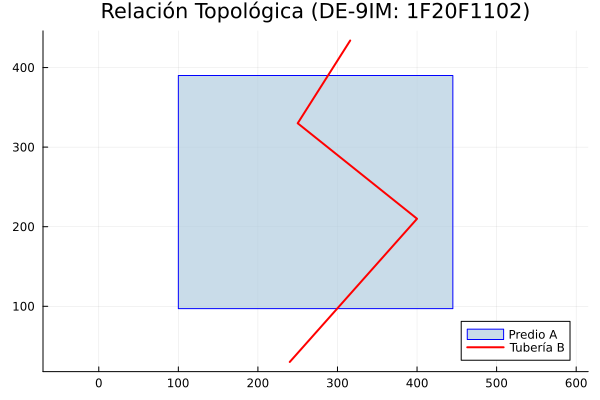
\includegraphics[width=0.8\textwidth,height=\textheight]{images/c14_de9im_interseccion_julia.png}
\end{center}

Las consultas de predicados como \texttt{intersects}, \texttt{contains}
o \texttt{within} siempre retornan un valor lógico (booleano)
determinando la relación espacial de proximidad, inclusión o adyacencia.

\subsection{Python}

\begin{Shaded}
\begin{Highlighting}[]
\CommentTok{\# \#| eval: false}

\ImportTok{from}\NormalTok{ shapely.geometry }\ImportTok{import}\NormalTok{ Point, Polygon}

\CommentTok{\# Polígono simplificado de la Universidad Nacional de Colombia (Sede Bogotá)}
\CommentTok{\# Coordenadas locales en Sistema MAGNA{-}SIRGAS Origen Nacional (EPSG:9377)}
\NormalTok{campus\_unal }\OperatorTok{=}\NormalTok{ Polygon([}
\NormalTok{    (}\DecValTok{4879500}\NormalTok{, }\DecValTok{2063500}\NormalTok{), }
\NormalTok{    (}\DecValTok{4880500}\NormalTok{, }\DecValTok{2063500}\NormalTok{), }
\NormalTok{    (}\DecValTok{4880500}\NormalTok{, }\DecValTok{2064500}\NormalTok{), }
\NormalTok{    (}\DecValTok{4879500}\NormalTok{, }\DecValTok{2064500}\NormalTok{), }
\NormalTok{    (}\DecValTok{4879500}\NormalTok{, }\DecValTok{2063500}\NormalTok{)}
\NormalTok{])}

\CommentTok{\# Punto interno que representa el edificio de la Facultad de Ciencias Agrarias}
\NormalTok{edificio\_agrarias }\OperatorTok{=}\NormalTok{ Point(}\DecValTok{4880000}\NormalTok{, }\DecValTok{2064000}\NormalTok{)}

\CommentTok{\# Punto externo que representa la estación de TransMilenio CAD}
\NormalTok{estacion\_cad }\OperatorTok{=}\NormalTok{ Point(}\DecValTok{4881000}\NormalTok{, }\DecValTok{2063000}\NormalTok{)}

\CommentTok{\# Ejecución de predicados topológicos espaciales}
\BuiltInTok{print}\NormalTok{(}\StringTok{"¿El campus UNAL contiene a Ciencias Agrarias?:"}\NormalTok{, campus\_unal.contains(edificio\_agrarias))}
\end{Highlighting}
\end{Shaded}

\begin{verbatim}
¿El campus UNAL contiene a Ciencias Agrarias?: True
\end{verbatim}

\begin{Shaded}
\begin{Highlighting}[]
\BuiltInTok{print}\NormalTok{(}\StringTok{"¿La estación CAD intersecta la superficie del campus?:"}\NormalTok{, estacion\_cad.intersects(campus\_unal))}
\end{Highlighting}
\end{Shaded}

\begin{verbatim}
¿La estación CAD intersecta la superficie del campus?: False
\end{verbatim}

\subsection{R}

\begin{Shaded}
\begin{Highlighting}[]
\CommentTok{\# \#| eval: false}

\FunctionTok{library}\NormalTok{(sf)}

\CommentTok{\# Lectura de la extensión del campus UNAL Bogotá desde notación WKT}
\NormalTok{campus\_unal\_wkt }\OtherTok{\textless{}{-}} \StringTok{"POLYGON ((4879500 2063500, 4880500 2063500, 4880500 2064500, 4879500 2064500, 4879500 2063500))"}
\NormalTok{campus\_unal\_r }\OtherTok{\textless{}{-}} \FunctionTok{st\_as\_sfc}\NormalTok{(campus\_unal\_wkt)}

\CommentTok{\# Coordenadas MAGNA{-}SIRGAS para los elementos de prueba}
\NormalTok{edificio\_agrarias\_r }\OtherTok{\textless{}{-}} \FunctionTok{st\_as\_sfc}\NormalTok{(}\StringTok{"POINT (4880000 2064000)"}\NormalTok{)}
\NormalTok{estacion\_cad\_r }\OtherTok{\textless{}{-}} \FunctionTok{st\_as\_sfc}\NormalTok{(}\StringTok{"POINT (4881000 2063000)"}\NormalTok{)}

\CommentTok{\# Evaluación en sf: el argumento sparse = FALSE retorna una matriz lógica}
\NormalTok{contiene }\OtherTok{\textless{}{-}} \FunctionTok{st\_contains}\NormalTok{(campus\_unal\_r, edificio\_agrarias\_r, }\AttributeTok{sparse =} \ConstantTok{FALSE}\NormalTok{)}
\FunctionTok{print}\NormalTok{(}\FunctionTok{paste}\NormalTok{(}\StringTok{"¿El campus UNAL contiene a Ciencias Agrarias?:"}\NormalTok{, contiene[}\DecValTok{1}\NormalTok{,}\DecValTok{1}\NormalTok{]))}
\end{Highlighting}
\end{Shaded}

\begin{verbatim}
[1] "¿El campus UNAL contiene a Ciencias Agrarias?: TRUE"
\end{verbatim}

\begin{Shaded}
\begin{Highlighting}[]
\NormalTok{interseca }\OtherTok{\textless{}{-}} \FunctionTok{st\_intersects}\NormalTok{(estacion\_cad\_r, campus\_unal\_r, }\AttributeTok{sparse =} \ConstantTok{FALSE}\NormalTok{)}
\FunctionTok{print}\NormalTok{(}\FunctionTok{paste}\NormalTok{(}\StringTok{"¿La estación CAD intersecta la superficie del campus?:"}\NormalTok{, interseca[}\DecValTok{1}\NormalTok{,}\DecValTok{1}\NormalTok{]))}
\end{Highlighting}
\end{Shaded}

\begin{verbatim}
[1] "¿La estación CAD intersecta la superficie del campus?: FALSE"
\end{verbatim}

\subsection{Julia}

\begin{Shaded}
\begin{Highlighting}[]
\CommentTok{\# \#| eval: false}

\FunctionTok{j\_eval}\NormalTok{(}\StringTok{\textquotesingle{}}
\StringTok{import ArchGDAL}

\StringTok{\# Creación de instancias vectoriales a partir de WKT}
\StringTok{campus\_unal\_julia = ArchGDAL.fromWKT("POLYGON ((4879500 2063500, 4880500 2063500, 4880500 2064500, 4879500 2064500, 4879500 2063500))")}
\StringTok{edificio\_agrarias\_julia = ArchGDAL.fromWKT("POINT (4880000 2064000)")}
\StringTok{estacion\_cad\_julia = ArchGDAL.fromWKT("POINT (4881000 2063000)")}

\StringTok{\# Aplicación de las funciones de predicados para análisis topológico}
\StringTok{println("¿El campus UNAL contiene a Ciencias Agrarias?: ", ArchGDAL.contains(campus\_unal\_julia, edificio\_agrarias\_julia))}
\StringTok{println("¿La estación CAD intersecta la superficie del campus?: ", ArchGDAL.intersects(estacion\_cad\_julia, campus\_unal\_julia))}
\StringTok{\textquotesingle{}}\NormalTok{)}
\end{Highlighting}
\end{Shaded}

\section{Operaciones de geoprocesamiento
paramétricas}\label{operaciones-de-geoprocesamiento-paramuxe9tricas}

Las herramientas de geoprocesamiento alteran y calculan nuevas
geometrías espaciales con base en datos vectoriales de entrada.
Algoritmos fundamentales como las áreas de influencia geométrica
(Buffer) y la extracción del centroide geométrico dependen estrictamente
del manejo interno de las unidades de medida, dictaminadas por el
sistema coordenado (metros métricos para MAGNA-SIRGAS EPSG:9377).

A continuación, se listan las principales funciones de geoprocesamiento
paramétrico y su implementación nativa según las librerías base de cada
entorno espacial:

\begin{itemize}
\tightlist
\item
  \textbf{Área de influencia (Buffer):} \texttt{buffer()} en
  \texttt{shapely} (Python), \texttt{st\_buffer()} en \texttt{sf} (R),
  \texttt{buffer()} en \texttt{ArchGDAL} (Julia).
\item
  \textbf{Centroide:} Propiedad \texttt{.centroid} en \texttt{shapely}
  (Python), \texttt{st\_centroid()} en \texttt{sf} (R),
  \texttt{centroid()} en \texttt{ArchGDAL} (Julia).
\item
  \textbf{Intersección:} \texttt{intersection()} en \texttt{shapely}
  (Python), \texttt{st\_intersection()} en \texttt{sf} (R),
  \texttt{intersection()} en \texttt{ArchGDAL} (Julia).
\item
  \textbf{Unión:} \texttt{union()} en \texttt{shapely} (Python),
  \texttt{st\_union()} en \texttt{sf} (R), \texttt{union()} en
  \texttt{ArchGDAL} (Julia).
\item
  \textbf{Diferencia:} \texttt{difference()} en \texttt{shapely}
  (Python), \texttt{st\_difference()} en \texttt{sf} (R),
  \texttt{difference()} en \texttt{ArchGDAL} (Julia).
\item
  \textbf{Envolvente convexa:} Propiedad \texttt{.convex\_hull} en
  \texttt{shapely} (Python), \texttt{st\_convex\_hull()} en \texttt{sf}
  (R), \texttt{convexhull()} en \texttt{ArchGDAL} (Julia).
\end{itemize}

\subsection{Python}

\begin{Shaded}
\begin{Highlighting}[]
\CommentTok{\# \#| eval: false}

\ImportTok{import}\NormalTok{ matplotlib.pyplot }\ImportTok{as}\NormalTok{ plt}
\ImportTok{import}\NormalTok{ geopandas }\ImportTok{as}\NormalTok{ gpd}
\ImportTok{from}\NormalTok{ shapely.geometry }\ImportTok{import}\NormalTok{ Point}

\CommentTok{\# Ubicación de la Plaza de Bolívar en el centro de Bogotá}
\CommentTok{\# Sistema de coordenadas proyectado: MAGNA{-}SIRGAS Origen Nacional (Metros)}
\NormalTok{plaza\_bolivar }\OperatorTok{=}\NormalTok{ Point(}\DecValTok{4882000}\NormalTok{, }\DecValTok{2060000}\NormalTok{)}

\CommentTok{\# 1. Creación de una zona de influencia (Buffer) de 500 metros}
\CommentTok{\# El objeto resultante transforma la primitiva puntual a un polígono}
\NormalTok{buffer\_plaza }\OperatorTok{=}\NormalTok{ plaza\_bolivar.}\BuiltInTok{buffer}\NormalTok{(}\DecValTok{500}\NormalTok{)}
\BuiltInTok{print}\NormalTok{(}\SpecialStringTok{f"Área generada por el área de influencia (m2): }\SpecialCharTok{\{}\NormalTok{buffer\_plaza}\SpecialCharTok{.}\NormalTok{area}\SpecialCharTok{:.2f\}}\SpecialStringTok{"}\NormalTok{)}
\end{Highlighting}
\end{Shaded}

\begin{verbatim}
Área generada por el área de influencia (m2): 784137.12
\end{verbatim}

\begin{Shaded}
\begin{Highlighting}[]
\CommentTok{\# 2. Extracción del centroide del área poligonal generada}
\NormalTok{centroide\_buffer }\OperatorTok{=}\NormalTok{ buffer\_plaza.centroid}
\BuiltInTok{print}\NormalTok{(}\SpecialStringTok{f"Coordenadas del nuevo centroide calculado: }\SpecialCharTok{\{}\NormalTok{centroide\_buffer}\SpecialCharTok{.}\NormalTok{x}\SpecialCharTok{\}}\SpecialStringTok{, }\SpecialCharTok{\{}\NormalTok{centroide\_buffer}\SpecialCharTok{.}\NormalTok{y}\SpecialCharTok{\}}\SpecialStringTok{"}\NormalTok{)}
\end{Highlighting}
\end{Shaded}

\begin{verbatim}
Coordenadas del nuevo centroide calculado: 4881999.999999999, 2059999.9999999998
\end{verbatim}

\begin{Shaded}
\begin{Highlighting}[]
\CommentTok{\# 3. Visualización cartográfica de la operación espacial}
\NormalTok{fig, ax }\OperatorTok{=}\NormalTok{ plt.subplots(figsize}\OperatorTok{=}\NormalTok{(}\DecValTok{7}\NormalTok{, }\DecValTok{7}\NormalTok{))}

\CommentTok{\# Conversión temporal a GeoSeries para facilitar el renderizado}
\NormalTok{gpd.GeoSeries([buffer\_plaza]).plot(ax}\OperatorTok{=}\NormalTok{ax, color}\OperatorTok{=}\StringTok{\textquotesingle{}lightblue\textquotesingle{}}\NormalTok{, edgecolor}\OperatorTok{=}\StringTok{\textquotesingle{}blue\textquotesingle{}}\NormalTok{, alpha}\OperatorTok{=}\FloatTok{0.5}\NormalTok{, label}\OperatorTok{=}\StringTok{\textquotesingle{}Buffer 500m\textquotesingle{}}\NormalTok{)}
\NormalTok{gpd.GeoSeries([plaza\_bolivar]).plot(ax}\OperatorTok{=}\NormalTok{ax, color}\OperatorTok{=}\StringTok{\textquotesingle{}red\textquotesingle{}}\NormalTok{, marker}\OperatorTok{=}\StringTok{\textquotesingle{}x\textquotesingle{}}\NormalTok{, markersize}\OperatorTok{=}\DecValTok{100}\NormalTok{, label}\OperatorTok{=}\StringTok{\textquotesingle{}Plaza de Bolívar (Original)\textquotesingle{}}\NormalTok{)}
\NormalTok{gpd.GeoSeries([centroide\_buffer]).plot(ax}\OperatorTok{=}\NormalTok{ax, color}\OperatorTok{=}\StringTok{\textquotesingle{}black\textquotesingle{}}\NormalTok{, marker}\OperatorTok{=}\StringTok{\textquotesingle{}.\textquotesingle{}}\NormalTok{, markersize}\OperatorTok{=}\DecValTok{50}\NormalTok{, label}\OperatorTok{=}\StringTok{\textquotesingle{}Centroide del Buffer\textquotesingle{}}\NormalTok{)}

\NormalTok{ax.set\_title(}\StringTok{"Geoprocesamiento: Buffer y Centroide}\CharTok{\textbackslash{}n}\StringTok{(Plaza de Bolívar, Bogotá)"}\NormalTok{)}
\NormalTok{ax.set\_xlabel(}\StringTok{"Este (m) {-} MAGNA{-}SIRGAS"}\NormalTok{)}
\NormalTok{ax.set\_ylabel(}\StringTok{"Norte (m) {-} MAGNA{-}SIRGAS"}\NormalTok{)}
\NormalTok{ax.legend()}
\NormalTok{ax.grid(}\VariableTok{True}\NormalTok{, linestyle}\OperatorTok{=}\StringTok{\textquotesingle{}{-}{-}\textquotesingle{}}\NormalTok{, alpha}\OperatorTok{=}\FloatTok{0.6}\NormalTok{)}

\NormalTok{plt.tight\_layout()}
\NormalTok{plt.show()}
\end{Highlighting}
\end{Shaded}

\begin{center}

\includegraphics[width=0.8\textwidth,height=\textheight]{16-matriz_de_9im_files/figure-pdf/python_geoprocesamiento-1.pdf}
\end{center}

\subsection{R}

\begin{Shaded}
\begin{Highlighting}[]
\CommentTok{\# \#| eval: false}

\FunctionTok{library}\NormalTok{(sf)}

\CommentTok{\# Geometría puntual de la Plaza de Bolívar (Bogotá D.C.)}
\CommentTok{\# Se define explícitamente el CRS 9377 (MAGNA{-}SIRGAS Origen Nacional)}
\NormalTok{plaza\_bolivar\_r }\OtherTok{\textless{}{-}} \FunctionTok{st\_sfc}\NormalTok{(}\FunctionTok{st\_point}\NormalTok{(}\FunctionTok{c}\NormalTok{(}\DecValTok{4882000}\NormalTok{, }\DecValTok{2060000}\NormalTok{)), }\AttributeTok{crs =} \DecValTok{9377}\NormalTok{)}

\CommentTok{\# 1. Ejecución de la operación buffer con un radio euclidiano de 500 metros}
\NormalTok{buffer\_plaza\_r }\OtherTok{\textless{}{-}} \FunctionTok{st\_buffer}\NormalTok{(plaza\_bolivar\_r, }\AttributeTok{dist =} \DecValTok{500}\NormalTok{)}
\FunctionTok{print}\NormalTok{(}\FunctionTok{paste}\NormalTok{(}\StringTok{"Área generada por el área de influencia (m2):"}\NormalTok{, }\FunctionTok{round}\NormalTok{(}\FunctionTok{st\_area}\NormalTok{(buffer\_plaza\_r), }\DecValTok{2}\NormalTok{)))}
\end{Highlighting}
\end{Shaded}

\begin{verbatim}
[1] "Área generada por el área de influencia (m2): 785039.34"
\end{verbatim}

\begin{Shaded}
\begin{Highlighting}[]
\CommentTok{\# 2. Ejecución analítica del centroide sobre el polígono resultante}
\NormalTok{centroide\_buffer\_r }\OtherTok{\textless{}{-}} \FunctionTok{st\_centroid}\NormalTok{(buffer\_plaza\_r)}
\NormalTok{coords\_centroide }\OtherTok{\textless{}{-}} \FunctionTok{st\_coordinates}\NormalTok{(centroide\_buffer\_r)}
\FunctionTok{print}\NormalTok{(}\FunctionTok{paste}\NormalTok{(}\StringTok{"Coordenadas del nuevo centroide calculado:"}\NormalTok{, coords\_centroide[}\DecValTok{1}\NormalTok{], coords\_centroide[}\DecValTok{2}\NormalTok{]))}
\end{Highlighting}
\end{Shaded}

\begin{verbatim}
[1] "Coordenadas del nuevo centroide calculado: 4882000 2060000"
\end{verbatim}

\begin{Shaded}
\begin{Highlighting}[]
\CommentTok{\# Eliminar espacios extra al rededor de la figura}
\FunctionTok{par}\NormalTok{(}\AttributeTok{pty =} \StringTok{"s"}\NormalTok{)  }

\CommentTok{\# 3. Visualización cartográfica espacial}

\FunctionTok{plot}\NormalTok{(}\FunctionTok{st\_geometry}\NormalTok{(buffer\_plaza\_r), }\AttributeTok{col =} \FunctionTok{rgb}\NormalTok{(}\FloatTok{0.68}\NormalTok{, }\FloatTok{0.85}\NormalTok{, }\FloatTok{0.9}\NormalTok{, }\FloatTok{0.5}\NormalTok{), }\AttributeTok{border =} \StringTok{"blue"}\NormalTok{,}
     \AttributeTok{main =} \StringTok{"Geoprocesamiento: Buffer y Centroide}\SpecialCharTok{\textbackslash{}n}\StringTok{(Plaza de Bolívar, Bogotá)"}\NormalTok{,}
     \AttributeTok{axes =} \ConstantTok{TRUE}\NormalTok{, }\AttributeTok{graticule =} \ConstantTok{TRUE}\NormalTok{)}

\CommentTok{\# Superposición topológica del punto original y el centroide derivado}

\FunctionTok{plot}\NormalTok{(}\FunctionTok{st\_geometry}\NormalTok{(plaza\_bolivar\_r), }\AttributeTok{col =} \StringTok{"red"}\NormalTok{, }\AttributeTok{pch =} \DecValTok{4}\NormalTok{, }\AttributeTok{cex =} \FloatTok{1.5}\NormalTok{, }\AttributeTok{lwd =} \DecValTok{2}\NormalTok{, }\AttributeTok{add =} \ConstantTok{TRUE}\NormalTok{)}
\FunctionTok{plot}\NormalTok{(}\FunctionTok{st\_geometry}\NormalTok{(centroide\_buffer\_r), }\AttributeTok{col =} \StringTok{"black"}\NormalTok{, }\AttributeTok{pch =} \DecValTok{16}\NormalTok{, }\AttributeTok{cex =} \DecValTok{1}\NormalTok{, }\AttributeTok{add =} \ConstantTok{TRUE}\NormalTok{)}

\CommentTok{\# Inserción de leyenda explicativa}
\FunctionTok{legend}\NormalTok{(}\StringTok{"topright"}\NormalTok{, }\AttributeTok{legend =} \FunctionTok{c}\NormalTok{(}\StringTok{"Buffer 500m"}\NormalTok{, }\StringTok{"Plaza de Bolívar"}\NormalTok{, }\StringTok{"Centroide"}\NormalTok{),}
       \AttributeTok{fill =} \FunctionTok{c}\NormalTok{(}\FunctionTok{rgb}\NormalTok{(}\FloatTok{0.68}\NormalTok{, }\FloatTok{0.85}\NormalTok{, }\FloatTok{0.9}\NormalTok{, }\FloatTok{0.5}\NormalTok{), }\ConstantTok{NA}\NormalTok{, }\ConstantTok{NA}\NormalTok{),}
       \AttributeTok{border =} \FunctionTok{c}\NormalTok{(}\StringTok{"blue"}\NormalTok{, }\ConstantTok{NA}\NormalTok{, }\ConstantTok{NA}\NormalTok{),}
       \AttributeTok{pch =} \FunctionTok{c}\NormalTok{(}\ConstantTok{NA}\NormalTok{, }\DecValTok{4}\NormalTok{, }\DecValTok{16}\NormalTok{), }\AttributeTok{col =} \FunctionTok{c}\NormalTok{(}\ConstantTok{NA}\NormalTok{, }\StringTok{"red"}\NormalTok{, }\StringTok{"black"}\NormalTok{), }\AttributeTok{pt.cex =} \FunctionTok{c}\NormalTok{(}\ConstantTok{NA}\NormalTok{, }\FloatTok{1.5}\NormalTok{, }\DecValTok{1}\NormalTok{))}
\end{Highlighting}
\end{Shaded}

\begin{center}

\includegraphics[width=0.8\textwidth,height=\textheight]{16-matriz_de_9im_files/figure-pdf/r_geoprocesamiento-1.pdf}
\end{center}

\subsection{Julia}

\begin{Shaded}
\begin{Highlighting}[]
\CommentTok{\# \#| eval: false}

\CommentTok{\# Regla de pliegue exclusiva para este bloque j\_eval de Julia:}
\CommentTok{\# Si el código NO se ejecuta (\# \#| eval: false), usa: \# \#| code{-}fold: true}
\CommentTok{\# Si el código SÍ se ejecuta (para mostrar resultados), usa: \#| code{-}fold: true}

\FunctionTok{j\_eval}\NormalTok{(}\StringTok{\textquotesingle{}}
\StringTok{import ArchGDAL}
\StringTok{using Plots}

\StringTok{\# Configuración espacial de la Plaza de Bolívar (Bogotá D.C.)}
\StringTok{plaza\_bolivar\_julia = ArchGDAL.fromWKT("POINT (4882000 2060000)")}

\StringTok{\# 1. Creación del área de influencia geométrica de 500 metros}
\StringTok{buffer\_plaza\_julia = ArchGDAL.buffer(plaza\_bolivar\_julia, 500.0)}
\StringTok{println("Área de la zona de influencia (m2): ", ArchGDAL.geomarea(buffer\_plaza\_julia))}

\StringTok{\# 2. Obtención de la ubicación espacial centralizada}
\StringTok{centroide\_buffer\_julia = ArchGDAL.centroid(buffer\_plaza\_julia)}
\StringTok{println("Coordenadas del centroide: ", ArchGDAL.toWKT(centroide\_buffer\_julia))}

\StringTok{\# 3. Representación visual integrando las primitivas generadas}
\StringTok{p\_geoprocesamiento = Plots.plot(buffer\_plaza\_julia, fillcolor=:lightblue, fillalpha=0.5, linecolor=:blue,}
\StringTok{                          title="Geoprocesamiento: Buffer y Centroide}\SpecialCharTok{\textbackslash{}\textbackslash{}}\StringTok{n(Plaza de Bolívar, Bogotá)",}
\StringTok{                          label="Buffer 500m", aspect\_ratio=:equal)}

\StringTok{\# Superposición de puntos para análisis paramétrico visual}
\StringTok{Plots.plot!(p\_geoprocesamiento, plaza\_bolivar\_julia, color=:red, markershape=:x, markersize=8, label="Plaza de Bolívar")}
\StringTok{Plots.plot!(p\_geoprocesamiento, centroide\_buffer\_julia, color=:black, markershape=:circle, markersize=4, label="Centroide")}

\StringTok{\# Exportación estandarizada a formato PNG}
\StringTok{Plots.savefig(p\_geoprocesamiento, "images/c14\_geoprocesamiento\_plaza\_bolivar\_julia.png")}
\StringTok{\textquotesingle{}}\NormalTok{)}
\end{Highlighting}
\end{Shaded}

\begin{Shaded}
\begin{Highlighting}[]
\NormalTok{knitr}\SpecialCharTok{::}\FunctionTok{include\_graphics}\NormalTok{(}\StringTok{"images/c14\_geoprocesamiento\_plaza\_bolivar\_julia.png"}\NormalTok{)}
\end{Highlighting}
\end{Shaded}

\begin{center}
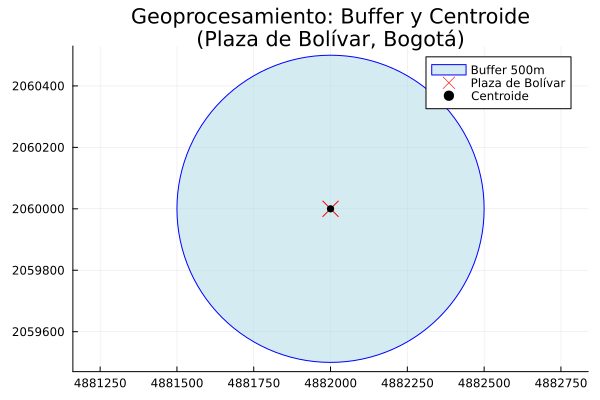
\includegraphics[width=0.8\textwidth,height=\textheight]{images/c14_geoprocesamiento_plaza_bolivar_julia.png}
\end{center}

\section{Resumen del capítulo}\label{resumen-del-capuxedtulo-2}

En este capítulo transitamos desde la representación estática de los
datos hacia el \textbf{análisis espacial activo}. Hemos visto que la
interacción matemática entre vectores no es empírica, sino que responde
a estándares topológicos universales regidos por la librería de bajo
nivel \textbf{GEOS}.

Los conceptos fundamentales que consolidan este flujo de trabajo son:

\begin{itemize}
\tightlist
\item
  \textbf{El Modelo DE-9IM:} Es el ``cerebro'' matemático detrás de
  todas las preguntas espaciales. Evalúa de forma exhaustiva cómo
  interactúan los interiores, límites y exteriores de dos geometrías.
  Comprender este modelo permite ir más allá de las funciones
  prefabricadas y formular reglas espaciales personalizadas.
\item
  \textbf{Predicados lógicos (Booleanos):} Funciones como
  \texttt{intersects}, \texttt{contains} o \texttt{touches} son
  simplemente atajos semánticos que aplican máscaras específicas sobre
  la matriz DE-9IM. Estas operaciones \textbf{nunca alteran} la
  geometría; su única misión es retornar un valor de Verdadero o Falso
  (\texttt{True}/\texttt{False}), siendo la herramienta predilecta para
  el filtrado espacial y las selecciones.
\item
  \textbf{Geoprocesamiento (Constructivo):} A diferencia de los
  predicados, herramientas como \texttt{buffer()}, \texttt{centroid()} o
  \texttt{intersection()} \textbf{crean nueva geometría}. Son
  operaciones matemáticamente costosas que dependen intrínsecamente del
  Sistema de Referencia de Coordenadas (CRS).
\item
  \textbf{La importancia del CRS proyectado:} Se evidenció que
  operaciones paramétricas como el área de influencia (\emph{Buffer})
  asumen que el valor ingresado corresponde a las unidades del plano
  matemático. Ejecutar un buffer de ``500'' sobre datos en WGS84
  (grados) generará un polígono masivo y deforme, reafirmando la
  necesidad de proyectar los datos a sistemas locales métricos (ej.
  MAGNA-SIRGAS Origen Nacional) antes del geoprocesamiento.
\item
  \textbf{Interoperabilidad de la API:} Aunque Python
  (\texttt{shapely}), R (\texttt{sf}) y Julia (\texttt{ArchGDAL}) poseen
  sintaxis distintas (orientada a objetos vs.~funciones
  funcionales/despacho múltiple), todos llaman a los mismos algoritmos
  C/C++ subyacentes, garantizando que el cálculo de un área o la
  resolución de un cruce topológico sea exactamente igual sin importar
  el lenguaje elegido.
\end{itemize}

Con el dominio de la topología y la creación de nuevas geometrías, el
flujo analítico está listo para enfrentarse a operaciones conjuntas
sobre bases de datos enteras, dando paso a los empalmes espaciales
(\emph{Spatial Joins}) y al álgebra de mapas vectorial.

\chapter{Librerías Alternativas y Ecosistemas Secundarios
(Opcional)}\label{estructuras-geo-alternativas}

A lo largo del módulo vectorial principal, establecimos una ruta de
aprendizaje basada en los estándares ``de facto'' de la industria:
\texttt{geopandas} y \texttt{shapely} en Python, \texttt{sf} en R, y
\texttt{ArchGDAL} en Julia.

Sin embargo, el ecosistema de la ciencia de datos espaciales no es
cerrado. Especialmente en lenguajes modernos como Julia, existen
múltiples aproximaciones al mismo problema topológico. Este capítulo es
de carácter \textbf{opcional} y está diseñado para aquellos estudiantes
o desarrolladores que deseen explorar librerías alternativas que, bajo
ciertos contextos (como el rendimiento computacional puro o la
integración con motores estadísticos específicos), pueden resultar más
convenientes que las herramientas tradicionales.

\section{El Ecosistema Julia: Más allá de
ArchGDAL}\label{el-ecosistema-julia-muxe1s-alluxe1-de-archgdal}

Mientras que R y Python tienen paquetes espaciales hegemónicos, la
comunidad de \textbf{Julia} mantiene un ecosistema más modular agrupado
bajo el entorno \emph{JuliaGeo}. Además de \texttt{ArchGDAL} (que es una
envoltura de la librería C/C++ GDAL), existen herramientas nativas y
otras envolturas que manejan la geometría y las tablas espaciales desde
una óptica distinta.

A continuación, recrearemos las tareas fundamentales de creación de
primitivas y tablas espaciales utilizando \textbf{\texttt{LibGEOS.jl}}
(para geometría pura) y \textbf{\texttt{GeoTables.jl}} (para integración
tabular).

\subsection{Creación de Geometrías Básicas con
LibGEOS}\label{creaciuxf3n-de-geometruxedas-buxe1sicas-con-libgeos}

\texttt{LibGEOS.jl} es una envoltura directa del motor GEOS (Geometry
Engine, Open Source). A diferencia de \texttt{ArchGDAL}, que es un
``todo en uno'' (maneja archivos, CRS y geometrías), \texttt{LibGEOS} se
especializa \textbf{exclusivamente en topología y relaciones
espaciales}. Es ideal cuando se necesita realizar cálculos geométricos
pesados en memoria RAM sin interactuar con discos duros ni proyecciones
cartográficas.

\subsection{Julia (LibGEOS)}

\begin{Shaded}
\begin{Highlighting}[]
\FunctionTok{j\_eval}\NormalTok{(r}\StringTok{"{-}(}
\StringTok{using LibGEOS}

\StringTok{\# 1. Crear punto desde formato WKT (Plaza de Bolívar)}
\StringTok{plaza\_bolivar = LibGEOS.readgeom("}\FunctionTok{POINT}\NormalTok{ (}\SpecialCharTok{{-}}\FloatTok{74.076} \FloatTok{4.598}\NormalTok{)}\StringTok{")}

\StringTok{\# 2. Imprimir propiedades}
\StringTok{println("}\NormalTok{Tipo de geometría}\SpecialCharTok{:} \StringTok{", typeof(plaza\_bolivar))}

\StringTok{\# 3. Operación topológica directa (Buffer 2D matemático puro)}
\StringTok{\# Note que LibGEOS no sabe si son metros o grados, opera matemáticamente.}
\StringTok{buffer\_plaza = LibGEOS.buffer(plaza\_bolivar, 0.005)}
\StringTok{println("}\NormalTok{Área euclidiana calculada por GEOS}\SpecialCharTok{:} \StringTok{", LibGEOS.area(buffer\_plaza))}
\StringTok{){-}"}\NormalTok{)}
\end{Highlighting}
\end{Shaded}

\begin{verbatim}
Starting Julia ...
\end{verbatim}

\section{Atributos y Tablas Espaciales con
GeoTables}\label{atributos-y-tablas-espaciales-con-geotables}

En capítulos anteriores ensamblamos DataFrames estándar en Julia
inyectando una columna de geometrías \texttt{ArchGDAL}. Un enfoque
alternativo impulsado por la comunidad \emph{JuliaEarth} (orientada
fuertemente a la geoestadística y el modelado de recursos naturales) es
\textbf{\texttt{GeoTables.jl}}.

Esta librería introduce un tipo de objeto formal llamado
\texttt{GeoTable}, estructurado en torno al paquete fundacional
\texttt{Meshes.jl}. Es conceptualmente lo más cercano que tiene Julia al
diseño de un \texttt{GeoDataFrame} de Python, separando claramente el
``dominio espacial'' de los ``valores'' (atributos).

\begin{longtable}[]{@{}
  >{\raggedright\arraybackslash}p{(\columnwidth - 4\tabcolsep) * \real{0.3333}}
  >{\raggedright\arraybackslash}p{(\columnwidth - 4\tabcolsep) * \real{0.3333}}
  >{\raggedright\arraybackslash}p{(\columnwidth - 4\tabcolsep) * \real{0.3333}}@{}}
\toprule\noalign{}
\begin{minipage}[b]{\linewidth}\raggedright
Concepto
\end{minipage} & \begin{minipage}[b]{\linewidth}\raggedright
Ecosistema Estándar (Recomendado)
\end{minipage} & \begin{minipage}[b]{\linewidth}\raggedright
Ecosistema Alternativo
\end{minipage} \\
\midrule\noalign{}
\endhead
\bottomrule\noalign{}
\endlastfoot
\textbf{Geometría} & \texttt{ArchGDAL.jl} & \texttt{Meshes.jl} /
\texttt{LibGEOS.jl} \\
\textbf{Estructura Tabular} & \texttt{DataFrames.jl} &
\texttt{GeoTables.jl} \\
\end{longtable}

\subsection{Ejemplo: Ciudades Principales de
Colombia}\label{ejemplo-ciudades-principales-de-colombia}

A continuación, replicamos la creación de una tabla espacial evitando
por completo ArchGDAL.

\subsection{Julia (GeoTables)}

\begin{Shaded}
\begin{Highlighting}[]
\FunctionTok{j\_eval}\NormalTok{(r}\StringTok{"{-}(}
\StringTok{import Pkg}
\StringTok{Pkg.add(["}\NormalTok{GeoTables}\StringTok{", "}\NormalTok{Meshes}\StringTok{"])}

\StringTok{using GeoTables, Meshes, DataFrames}

\StringTok{\# 1. Datos alfanuméricos tradicionales}
\StringTok{df = DataFrame(Ciudad = ["}\NormalTok{Bogotá}\StringTok{", "}\NormalTok{Medellín}\StringTok{", "}\NormalTok{Cali}\StringTok{"], Pob\_Millones = [7.9, 2.5, 2.2])}

\StringTok{\# 2. Geometrías instanciadas a través del framework Meshes}
\StringTok{\# Llamamos a Meshes.Point explícitamente para evitar conflictos de namespace}
\StringTok{puntos = [Meshes.Point({-}74.08, 4.60), Meshes.Point({-}75.56, 6.25), Meshes.Point({-}76.52, 3.42)]}

\StringTok{\# 3. Unión en GeoTable usando georef (el constructor estándar geoestadístico)}
\StringTok{gt = georef(df, puntos)}

\StringTok{println("}\SpecialCharTok{{-}{-}{-}}\NormalTok{ Tabla }\FunctionTok{Espacial}\NormalTok{ (GeoTable) }\SpecialCharTok{{-}{-}{-}}\StringTok{")}
\StringTok{println(gt)}

\StringTok{println("}\NormalTok{\textbackslash{}n}\SpecialCharTok{{-}{-}{-}}\NormalTok{ Extracción de Atributos }\SpecialCharTok{{-}{-}{-}}\StringTok{")}
\StringTok{\# En GeoTables, se puede acceder a la tabla base con la función values()}
\StringTok{println(values(gt))}
\StringTok{){-}"}\NormalTok{)}
\end{Highlighting}
\end{Shaded}

\subsection{Consideraciones Finales sobre el Uso de Ecosistemas
Alternativos}\label{consideraciones-finales-sobre-el-uso-de-ecosistemas-alternativos}

El uso de \texttt{LibGEOS} y \texttt{GeoTables} es sumamente potente
para flujos de trabajo orientados a la geoestadística pura, como el
modelado de yacimientos mineros (Kriging) o la interpolación de mallas
complejas (Meshing).

Sin embargo, para tareas fundamentales de SIG como las abordadas en la
Maestría en Geomática (lectura de Shapefiles masivos, reproyecciones
cartográficas, o cruces con PostGIS), la vía troncal explicada en el
cuerpo principal del curso (\texttt{ArchGDAL} + \texttt{DataFrames})
sigue siendo la opción más estable, documentada e interoperable, ya que
hereda directamente la robustez probada en la industria por la Open
Source Geospatial Foundation (OSGeo).

\part{Análisis y Procesamiento Raster}

\chapter{Fundamentos raster}\label{fundamentos-raster}

\section{Funciones j\_eval y j\_plot en
R}\label{funciones-j_eval-y-j_plot-en-r-12}

\begin{Shaded}
\begin{Highlighting}[]
\CommentTok{\# \#| include: false}
\FunctionTok{source}\NormalTok{(}\StringTok{"./docs/j\_eval\_j\_plot.r"}\NormalTok{)}
\end{Highlighting}
\end{Shaded}

\section{Introducción}\label{introducciuxf3n-13}

El modelo de datos raster representa información espacial mediante una
cuadrícula o matriz regular de celdas (píxeles). Cada celda contiene un
valor numérico que representa una variable temática, como la altitud en
un Modelo Digital de Elevación (MDE).

La validez geométrica de una matriz raster depende de sus metadatos
espaciales: resolución espacial, extensión rectangular (bounding box) y
el Sistema de Referencia de Coordenadas (CRS). La inspección de estos
metadatos es el primer paso crítico en cualquier flujo de trabajo. Es
frecuente adquirir datos históricos o externos que operan bajo sistemas
de referencia obsoletos. En el caso de Colombia, es vital identificar si
los datos se encuentran en un sistema legado (ej. Datum Bogotá 1941)
para prever una futura transformación al estándar oficial MAGNA-SIRGAS
Origen Nacional (EPSG:9377).

\section{Lectura de datos y extracción de
metadatos}\label{lectura-de-datos-y-extracciuxf3n-de-metadatos}

El siguiente procedimiento importa un archivo físico a la memoria. En
lugar de cargar la totalidad de la matriz de píxeles, las librerías
extraen inicialmente el encabezado del archivo (metadatos), lo que
optimiza la memoria RAM. Al leer el MDE de Bogotá propuesto, se
evidenciará mediante la definición Proj4 (\texttt{+ellps=intl}, entre
otros parámetros) que el archivo original no corresponde a MAGNA-SIRGAS,
dictando la necesidad de una reproyección en etapas de geoprocesamiento
posteriores (Capítulo 19).

\subsection{Python}

\begin{Shaded}
\begin{Highlighting}[]
\CommentTok{\# \#| eval: false}

\CommentTok{\# Importación de la librería rasterio, estándar para lectura y escritura raster en Python}
\ImportTok{import}\NormalTok{ rasterio}

\CommentTok{\# Definición de la ruta al archivo raster}
\CommentTok{\# Fuente original: [http://dl.maptools.org/dl/geotiff/samples/made\_up/bogota.tif](http://dl.maptools.org/dl/geotiff/samples/made\_up/bogota.tif)}
\NormalTok{ruta\_raster }\OperatorTok{=} \StringTok{"data\_heavy/raster/bogota.tif"}

\CommentTok{\# Apertura del archivo utilizando un bloque contextual (with)}
\CommentTok{\# Garantiza que el puntero de archivo se cierre automáticamente tras la lectura}
\ControlFlowTok{with}\NormalTok{ rasterio.}\BuiltInTok{open}\NormalTok{(ruta\_raster) }\ImportTok{as}\NormalTok{ src:}
    
    \CommentTok{\# Extracción de dimensiones espaciales de la matriz}
\NormalTok{    columnas }\OperatorTok{=}\NormalTok{ src.width}
\NormalTok{    filas }\OperatorTok{=}\NormalTok{ src.height}
    
    \CommentTok{\# Conteo del número de bandas (1 banda para elevación continua)}
\NormalTok{    numero\_bandas }\OperatorTok{=}\NormalTok{ src.count}
    
    \CommentTok{\# Extracción del Sistema de Referencia de Coordenadas}
    \CommentTok{\# Permite identificar la definición Proj4 nativa del archivo (Datum legado)}
\NormalTok{    crs\_raster }\OperatorTok{=}\NormalTok{ src.crs}
    
    \CommentTok{\# Extracción de la resolución espacial (tamaño del píxel en unidades del CRS)}
\NormalTok{    resolucion }\OperatorTok{=}\NormalTok{ src.res}
    
    \CommentTok{\# Extracción de la extensión o bounding box}
\NormalTok{    extension }\OperatorTok{=}\NormalTok{ src.bounds}

    \CommentTok{\# Impresión estructurada en consola}
    \BuiltInTok{print}\NormalTok{(}\SpecialStringTok{f"Dimensiones de la matriz: }\SpecialCharTok{\{}\NormalTok{columnas}\SpecialCharTok{\}}\SpecialStringTok{ columnas x }\SpecialCharTok{\{}\NormalTok{filas}\SpecialCharTok{\}}\SpecialStringTok{ filas"}\NormalTok{)}
    \BuiltInTok{print}\NormalTok{(}\SpecialStringTok{f"Total de bandas: }\SpecialCharTok{\{}\NormalTok{numero\_bandas}\SpecialCharTok{\}}\SpecialStringTok{"}\NormalTok{)}
    \BuiltInTok{print}\NormalTok{(}\SpecialStringTok{f"Sistema de referencia (CRS): }\SpecialCharTok{\{}\NormalTok{crs\_raster}\SpecialCharTok{\}}\SpecialStringTok{"}\NormalTok{)}
    \BuiltInTok{print}\NormalTok{(}\SpecialStringTok{f"Resolución espacial: }\SpecialCharTok{\{}\NormalTok{resolucion[}\DecValTok{0}\NormalTok{]}\SpecialCharTok{\}}\SpecialStringTok{ metros"}\NormalTok{)}
    \BuiltInTok{print}\NormalTok{(}\SpecialStringTok{f"Extensión espacial: }\SpecialCharTok{\{}\NormalTok{extension}\SpecialCharTok{\}}\SpecialStringTok{"}\NormalTok{)}
\end{Highlighting}
\end{Shaded}

\begin{verbatim}
Dimensiones de la matriz: 512 columnas x 512 filas
Total de bandas: 1
Sistema de referencia (CRS): EPSG:21897
Resolución espacial: 60.0 metros
Extensión espacial: BoundingBox(left=440720.0, bottom=69280.0, right=471440.0, top=100000.0)
\end{verbatim}

\subsection{R}

\begin{Shaded}
\begin{Highlighting}[]
\CommentTok{\# \#| eval: false}

\CommentTok{\# Carga de terra, paquete de alto rendimiento para estructuras espaciales en R}
\FunctionTok{library}\NormalTok{(terra)}
\end{Highlighting}
\end{Shaded}

\begin{verbatim}
terra 1.8.93
\end{verbatim}

\begin{verbatim}

Attaching package: 'terra'
\end{verbatim}

\begin{verbatim}
The following object is masked from 'package:grid':

    depth
\end{verbatim}

\begin{Shaded}
\begin{Highlighting}[]
\CommentTok{\# Definición de la ruta local del archivo}
\CommentTok{\# Fuente original: [http://dl.maptools.org/dl/geotiff/samples/made\_up/bogota.tif](http://dl.maptools.org/dl/geotiff/samples/made\_up/bogota.tif)}
\NormalTok{ruta\_raster }\OtherTok{\textless{}{-}} \StringTok{"data\_heavy/raster/bogota.tif"}

\CommentTok{\# rast() establece el enlace con el archivo y crea un objeto SpatRaster con los metadatos}
\NormalTok{mde\_bogota }\OtherTok{\textless{}{-}} \FunctionTok{rast}\NormalTok{(ruta\_raster)}

\CommentTok{\# La impresión directa del objeto revela las dimensiones y la cadena de texto del CRS}
\FunctionTok{print}\NormalTok{(mde\_bogota)}
\end{Highlighting}
\end{Shaded}

\begin{verbatim}
class       : SpatRaster 
size        : 512, 512, 1  (nrow, ncol, nlyr)
resolution  : 60, 60  (x, y)
extent      : 440720, 471440, 69280, 1e+05  (xmin, xmax, ymin, ymax)
coord. ref. : Bogota 1975 / Colombia Bogota zone (EPSG:21897) 
source      : bogota.tif 
name        : bogota 
\end{verbatim}

\begin{Shaded}
\begin{Highlighting}[]
\CommentTok{\# Extracción algorítmica de atributos específicos}
\NormalTok{crs\_texto }\OtherTok{\textless{}{-}} \FunctionTok{crs}\NormalTok{(mde\_bogota, }\AttributeTok{describe=}\ConstantTok{TRUE}\NormalTok{)}\SpecialCharTok{$}\NormalTok{name}
\NormalTok{resolucion }\OtherTok{\textless{}{-}} \FunctionTok{res}\NormalTok{(mde\_bogota)}
\NormalTok{dimensiones }\OtherTok{\textless{}{-}} \FunctionTok{dim}\NormalTok{(mde\_bogota)}

\CommentTok{\# Impresión en consola}
\FunctionTok{cat}\NormalTok{(}\StringTok{"Sistema de Referencia identificado:"}\NormalTok{, crs\_texto, }\StringTok{"}\SpecialCharTok{\textbackslash{}n}\StringTok{"}\NormalTok{)}
\end{Highlighting}
\end{Shaded}

\begin{verbatim}
Sistema de Referencia identificado: Bogota 1975 / Colombia Bogota zone 
\end{verbatim}

\begin{Shaded}
\begin{Highlighting}[]
\FunctionTok{cat}\NormalTok{(}\StringTok{"Resolución espacial (X, Y):"}\NormalTok{, resolucion, }\StringTok{"metros}\SpecialCharTok{\textbackslash{}n}\StringTok{"}\NormalTok{)}
\end{Highlighting}
\end{Shaded}

\begin{verbatim}
Resolución espacial (X, Y): 60 60 metros
\end{verbatim}

\begin{Shaded}
\begin{Highlighting}[]
\FunctionTok{cat}\NormalTok{(}\StringTok{"Filas, Columnas, Bandas:"}\NormalTok{, dimensiones, }\StringTok{"}\SpecialCharTok{\textbackslash{}n}\StringTok{"}\NormalTok{)}
\end{Highlighting}
\end{Shaded}

\begin{verbatim}
Filas, Columnas, Bandas: 512 512 1 
\end{verbatim}

\subsection{Julia}

\begin{Shaded}
\begin{Highlighting}[]
\CommentTok{\# \#| eval: false}

\FunctionTok{j\_eval}\NormalTok{(}\StringTok{\textquotesingle{}}
\StringTok{\# Carga del módulo Rasters.jl para matrices georreferenciadas}
\StringTok{\# Es estricto cargar ArchGDAL junto a Rasters para habilitar el backend }
\StringTok{\# de lectura y decodificación de formatos raster estándar como GeoTIFF.}
\StringTok{using Rasters}
\StringTok{using ArchGDAL}

\StringTok{\# Definición de la ruta local}
\StringTok{\# Fuente original: [http://dl.maptools.org/dl/geotiff/samples/made\_up/bogota.tif](http://dl.maptools.org/dl/geotiff/samples/made\_up/bogota.tif)}
\StringTok{ruta\_raster = "data\_heavy/raster/bogota.tif"}

\StringTok{\# Construcción de la estructura Raster a partir del archivo}
\StringTok{\# Analiza la grilla y carga el sistema de coordenadas}
\StringTok{\# Se añade "; nothing" para silenciar la salida estricta en el motor de evaluación}
\StringTok{mde\_bogota = Raster(ruta\_raster); nothing}


\StringTok{\# Despliegue de los metadatos estructurales (tamaño de la matriz)}
\StringTok{println("Dimensiones espaciales: ", dims(mde\_bogota))}

\StringTok{\# Extracción del CRS base}
\StringTok{\# Mostrará los parámetros crudos de Proj4 si el CRS carece de un código EPSG explícito}
\StringTok{println("CRS nativo del archivo: ", crs(mde\_bogota))}
\StringTok{\textquotesingle{}}\NormalTok{)}
\end{Highlighting}
\end{Shaded}

\begin{verbatim}
Starting Julia ...
\end{verbatim}

\section{Visualización cartográfica
básica}\label{visualizaciuxf3n-cartogruxe1fica-buxe1sica}

La representación visual directa de la matriz, incluso antes de
transformar su CRS, es necesaria para evaluar distribuciones anómalas de
valores, coberturas espaciales incompletas (nodata) o artefactos de
adquisición. El renderizado asocia los rangos de elevación del MDE con
una rampa de color continua.

\subsection{Python}

\begin{Shaded}
\begin{Highlighting}[]
\CommentTok{\# \#| eval: false}

\ImportTok{import}\NormalTok{ rasterio}
\ImportTok{from}\NormalTok{ rasterio.plot }\ImportTok{import}\NormalTok{ show}
\ImportTok{import}\NormalTok{ matplotlib.pyplot }\ImportTok{as}\NormalTok{ plt}

\CommentTok{\# Acceso contextual a la matriz raster}
\ControlFlowTok{with}\NormalTok{ rasterio.}\BuiltInTok{open}\NormalTok{(}\StringTok{"data\_heavy/raster/bogota.tif"}\NormalTok{) }\ImportTok{as}\NormalTok{ src:}
    
    \CommentTok{\# Inicialización del lienzo gráfico (figura y ejes)}
\NormalTok{    fig, ax }\OperatorTok{=}\NormalTok{ plt.subplots(figsize}\OperatorTok{=}\NormalTok{(}\DecValTok{10}\NormalTok{, }\DecValTok{8}\NormalTok{))}
    
    \CommentTok{\# Renderizado espacial mediante la utilidad show()}
    \CommentTok{\# cmap=\textquotesingle{}terrain\textquotesingle{} ajusta la gradación de colores para altimetría}
\NormalTok{    show(src, ax}\OperatorTok{=}\NormalTok{ax, title}\OperatorTok{=}\StringTok{"Modelo Digital de Elevación {-} Bogotá"}\NormalTok{, cmap}\OperatorTok{=}\StringTok{"terrain"}\NormalTok{)}
    
    \CommentTok{\# Despliegue del arreglo en el entorno gráfico}
\NormalTok{    plt.show()}
\end{Highlighting}
\end{Shaded}

\begin{center}

\includegraphics[width=0.8\textwidth,height=\textheight]{18-fundamentos_raster_files/figure-pdf/python_plot_raster-1.pdf}
\end{center}

\subsection{R}

\begin{Shaded}
\begin{Highlighting}[]
\CommentTok{\# \#| eval: false}

\FunctionTok{library}\NormalTok{(terra)}

\CommentTok{\# Instanciación del archivo de entrada}
\NormalTok{mde\_bogota }\OtherTok{\textless{}{-}} \FunctionTok{rast}\NormalTok{(}\StringTok{"data\_heavy/raster/bogota.tif"}\NormalTok{)}

\CommentTok{\# Ejecución de la función plot sobrecargada para métodos espaciales}
\CommentTok{\# Genera los márgenes cartográficos y mapea la matriz a la rampa altimétrica}
\FunctionTok{plot}\NormalTok{(mde\_bogota, }
     \AttributeTok{main=}\StringTok{"Modelo Digital de Elevación {-} Bogotá"}\NormalTok{, }
     \AttributeTok{col=}\FunctionTok{terrain.colors}\NormalTok{(}\DecValTok{50}\NormalTok{), }\CommentTok{\# Segmentación de la paleta en 50 clases}
     \AttributeTok{axes=}\ConstantTok{TRUE}\NormalTok{, }
     \AttributeTok{legend=}\ConstantTok{TRUE}\NormalTok{)}
\end{Highlighting}
\end{Shaded}

\begin{center}

\includegraphics[width=0.8\textwidth,height=\textheight]{18-fundamentos_raster_files/figure-pdf/r_plot_raster-1.pdf}
\end{center}

\subsection{Julia}

\begin{Shaded}
\begin{Highlighting}[]
\CommentTok{\# \#| eval: false}

\FunctionTok{j\_eval}\NormalTok{(}\StringTok{\textquotesingle{}}
\StringTok{\# Es estricto cargar ArchGDAL junto a Rasters para habilitar el backend }
\StringTok{\# de lectura y decodificación de formatos raster estándar como GeoTIFF.}
\StringTok{using Rasters}
\StringTok{using ArchGDAL}
\StringTok{using Plots}
\StringTok{\# using Measures \# Necesario para definir márgenes en mm o px}

\StringTok{\# Carga de la estructura del MDE}
\StringTok{\# Se añade "; nothing" para silenciar la salida estricta en el motor de evaluación}
\StringTok{mde\_bogota = Raster("data\_heavy/raster/bogota.tif"); nothing}

\StringTok{\# Construcción de la visualización cruzando Plots.jl con el objeto Raster}
\StringTok{p = plot(mde\_bogota, }
\StringTok{         title="Modelo Digital de Elevación {-} Bogotá", }
\StringTok{         c=:terrain,}
\StringTok{         xlabel="Este (Sistema Local)}\SpecialCharTok{\textbackslash{}n}\StringTok{", \# La nueva línea añade espacio vertical }
\StringTok{                                          \# para que se vea la etiqueta}
\StringTok{         ylabel="Norte (Sistema Local)",}
\StringTok{         \# {-}{-}{-} MEJORAS DE VISIBILIDAD {-}{-}{-}}
\StringTok{         xrotation = 45,        \# Rota las etiquetas del eje X 45 grados}
\StringTok{         \# bottom\_margin = 10mm,  \# Da espacio extra en la base (requiere using Measures)}
\StringTok{         \#size = (850, 650),         \# Incrementa el alto del lienzo para dar aire al label         }
\StringTok{         guidefontsize = 10,    \# Tamaño de fuente para los títulos de los ejes}
\StringTok{         tickfontsize = 8       \# Tamaño de fuente para los números de las coordenadas}
\StringTok{         )}

\StringTok{\# Almacenamiento riguroso de la figura para renderizado en Quarto}
\StringTok{savefig(p, "images/c18\_plot\_mde\_bogota\_julia.png")}
\StringTok{\textquotesingle{}}\NormalTok{)}
\end{Highlighting}
\end{Shaded}

\begin{Shaded}
\begin{Highlighting}[]
\NormalTok{knitr}\SpecialCharTok{::}\FunctionTok{include\_graphics}\NormalTok{(}\StringTok{"images/c18\_plot\_mde\_bogota\_julia.png"}\NormalTok{)}
\end{Highlighting}
\end{Shaded}

\begin{center}
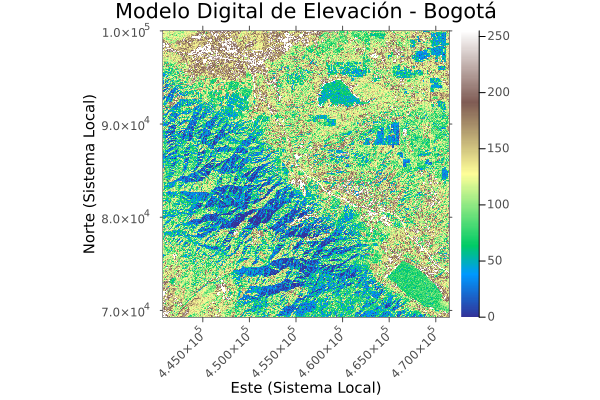
\includegraphics[width=0.8\textwidth,height=\textheight]{images/c18_plot_mde_bogota_julia.png}
\end{center}

\section{Resumen sintáctico}\label{resumen-sintuxe1ctico-4}

\begin{enumerate}
\def\labelenumi{\arabic{enumi}.}
\tightlist
\item
  \textbf{Lectura y extracción de metadatos raster}
\end{enumerate}

La siguiente tabla consolida los comandos base para la instanciación de
objetos raster en memoria y la extracción de sus atributos topológicos y
espaciales. La lectura inicial prioriza la extracción de metadatos sobre
la carga de la matriz completa (lectura diferida).

\begin{longtable}[]{@{}
  >{\raggedright\arraybackslash}p{(\columnwidth - 6\tabcolsep) * \real{0.2500}}
  >{\raggedright\arraybackslash}p{(\columnwidth - 6\tabcolsep) * \real{0.2500}}
  >{\raggedright\arraybackslash}p{(\columnwidth - 6\tabcolsep) * \real{0.2500}}
  >{\raggedright\arraybackslash}p{(\columnwidth - 6\tabcolsep) * \real{0.2500}}@{}}
\caption{Equivalencia de métodos para la lectura y auscultación de
metadatos
matriciales}\label{tbl-resumen_metadatos_raster}\tabularnewline
\toprule\noalign{}
\begin{minipage}[b]{\linewidth}\raggedright
Operación
\end{minipage} & \begin{minipage}[b]{\linewidth}\raggedright
Python (\texttt{rasterio}) 🐍
\end{minipage} & \begin{minipage}[b]{\linewidth}\raggedright
R (\texttt{terra}) 🔵
\end{minipage} & \begin{minipage}[b]{\linewidth}\raggedright
Julia (\texttt{Rasters.jl}) 🟣
\end{minipage} \\
\midrule\noalign{}
\endfirsthead
\toprule\noalign{}
\begin{minipage}[b]{\linewidth}\raggedright
Operación
\end{minipage} & \begin{minipage}[b]{\linewidth}\raggedright
Python (\texttt{rasterio}) 🐍
\end{minipage} & \begin{minipage}[b]{\linewidth}\raggedright
R (\texttt{terra}) 🔵
\end{minipage} & \begin{minipage}[b]{\linewidth}\raggedright
Julia (\texttt{Rasters.jl}) 🟣
\end{minipage} \\
\midrule\noalign{}
\endhead
\bottomrule\noalign{}
\endlastfoot
\textbf{Enlace al archivo (Lazy loading)} &
\texttt{src\ =\ rasterio.open("ruta.tif")} &
\texttt{r\ =\ rast("ruta.tif")} & \texttt{r\ =\ Raster("ruta.tif")} \\
\textbf{Dimensiones (Columnas, Filas, Bandas)} & \texttt{src.width},
\texttt{src.height}, \texttt{src.count} & \texttt{dim(r)} &
\texttt{dims(r)} \\
\textbf{Sistema de Referencia (CRS)} & \texttt{src.crs} &
\texttt{crs(r)} & \texttt{crs(r)} \\
\textbf{Resolución espacial (X, Y)} & \texttt{src.res} & \texttt{res(r)}
& \emph{Derivada de la estructura de la grilla} \\
\textbf{Extensión espacial (Bounding Box)} & \texttt{src.bounds} &
\texttt{ext(r)} & \texttt{bounds(r)} \\
\end{longtable}

\begin{center}\rule{0.5\linewidth}{0.5pt}\end{center}

\begin{enumerate}
\def\labelenumi{\arabic{enumi}.}
\setcounter{enumi}{1}
\tightlist
\item
  \textbf{Renderizado cartográfico matricial}
\end{enumerate}

La representación visual directa de la matriz de píxeles requiere la
asociación de los valores numéricos a una paleta de colores. Cada
lenguaje integra su propio motor de graficación para el mapeo espacial
continuo.

\begin{longtable}[]{@{}
  >{\raggedright\arraybackslash}p{(\columnwidth - 6\tabcolsep) * \real{0.2500}}
  >{\raggedright\arraybackslash}p{(\columnwidth - 6\tabcolsep) * \real{0.2500}}
  >{\raggedright\arraybackslash}p{(\columnwidth - 6\tabcolsep) * \real{0.2500}}
  >{\raggedright\arraybackslash}p{(\columnwidth - 6\tabcolsep) * \real{0.2500}}@{}}
\caption{Comandos fundamentales para la representación gráfica de
modelos de datos
continuos}\label{tbl-resumen_plot_raster}\tabularnewline
\toprule\noalign{}
\begin{minipage}[b]{\linewidth}\raggedright
Operación
\end{minipage} & \begin{minipage}[b]{\linewidth}\raggedright
Python (\texttt{rasterio.plot}) 🐍
\end{minipage} & \begin{minipage}[b]{\linewidth}\raggedright
R (\texttt{terra}) 🔵
\end{minipage} & \begin{minipage}[b]{\linewidth}\raggedright
Julia (\texttt{Plots.jl}) 🟣
\end{minipage} \\
\midrule\noalign{}
\endfirsthead
\toprule\noalign{}
\begin{minipage}[b]{\linewidth}\raggedright
Operación
\end{minipage} & \begin{minipage}[b]{\linewidth}\raggedright
Python (\texttt{rasterio.plot}) 🐍
\end{minipage} & \begin{minipage}[b]{\linewidth}\raggedright
R (\texttt{terra}) 🔵
\end{minipage} & \begin{minipage}[b]{\linewidth}\raggedright
Julia (\texttt{Plots.jl}) 🟣
\end{minipage} \\
\midrule\noalign{}
\endhead
\bottomrule\noalign{}
\endlastfoot
\textbf{Despliegue del arreglo con rampa altimétrica} &
\texttt{show(src,\ ax=ax,\ cmap="terrain")} &
\texttt{plot(r,\ col=terrain.colors(50))} &
\texttt{plot(r,\ c=:terrain)} \\
\textbf{Ajuste de orientación de etiquetas de ejes} &
\texttt{ax.tick\_params(axis=\textquotesingle{}x\textquotesingle{},\ rotation=45)}
& \emph{No requiere (Manejado por parámetros par/mar)} &
\texttt{plot(...,\ xrotation\ =\ 45)} \\
\end{longtable}

\section{Cierre del capítulo}\label{cierre-del-capuxedtulo}

La exploración inicial de estructuras raster se rige por la
decodificación estricta de sus metadatos fundamentales. La correcta
identificación del Sistema de Referencia de Coordenadas, la resolución
espacial y la extensión geométrica condicionan la viabilidad técnica de
cualquier operación analítica posterior.

Las librerías modernas implementadas en ecosistemas científicos (como
\texttt{rasterio}, \texttt{terra} y \texttt{Rasters.jl}) operan bajo el
paradigma de lectura diferida. Este enfoque mitiga el desbordamiento de
memoria al extraer exclusivamente las cabeceras de los archivos,
reservando el procesamiento masivo de la cuadrícula para etapas
algorítmicas explícitas. El dominio de esta arquitectura de datos sienta
las bases metodológicas para la ejecución de álgebra de mapas,
transformaciones geométricas de reproyección espacial y extracción
estadística.

\section{Evaluación}\label{evaluaciuxf3n}

\textbf{1. Análisis de Metadatos y Gestión de Memoria:} Se le ha
entregado un Modelo Digital de Elevación de alta resolución (0.5m) que
cubre toda la extensión del departamento de Antioquia, con un tamaño
físico en disco de 14 GB. Usted dispone de una estación de trabajo con 8
GB de memoria RAM. Explique técnicamente por qué la ejecución de los
comandos de apertura como \texttt{rasterio.open()} (Python),
\texttt{rast()} (R) o \texttt{Raster()} (Julia) no genera un error de
\emph{Out of Memory} (OOM). Especifique qué información se transfiere
realmente a la memoria volátil durante la ejecución de esa primera
instrucción.

\textbf{2. Sistemas de Referencia en Datos Legados:} Al inspeccionar los
metadatos de un mosaico de imágenes históricas provisto por el IGAC,
identifica mediante la cadena \emph{Proj4} que el CRS nativo del archivo
corresponde a un sistema obsoleto basado en el Datum Bogotá 1941
(\texttt{+ellps=intl}). Describa la implicación metodológica de este
hallazgo. ¿Qué procedimiento obligatorio debe aplicarse a esta matriz
antes de ejecutar una operación de intersección espacial contra la base
catastral actual de Bogotá, proyectada en MAGNA-SIRGAS Origen Nacional
(EPSG:9377)?

\textbf{3. Repositorio en GitHub:} Independientemente del formato de su
código fuente, redacte un documento en Quarto (\texttt{.qmd}) con las
respuestas argumentativas de los puntos anteriores y renderícelo en
formato HTML y PDF. * Sube la carpeta completa del proyecto a un
repositorio público en su cuenta personal de \textbf{GitHub}. *
\textbf{Entrega:} Para la calificación formal, remita exclusivamente el
enlace (URL) de su repositorio.

\chapter{Operaciones raster}\label{operaciones-raster}

\section{Funciones j\_eval y j\_plot en
R}\label{funciones-j_eval-y-j_plot-en-r-13}

\begin{Shaded}
\begin{Highlighting}[]
\CommentTok{\# \#| include: false}
\FunctionTok{source}\NormalTok{(}\StringTok{"./docs/j\_eval\_j\_plot.r"}\NormalTok{)}
\end{Highlighting}
\end{Shaded}

\section{Introducción}\label{introducciuxf3n-14}

Las operaciones raster consisten en la manipulación analítica y
geométrica de las matrices espaciales. Mientras que en el formato
vectorial las transformaciones alteran vértices explícitos, en el modelo
raster las operaciones modifican los valores de los píxeles (álgebra de
mapas) o reestructuran la cuadrícula subyacente (reproyección y
remuestreo).

Para garantizar la interoperabilidad de datos en Colombia, es un
procedimiento estándar transformar insumos globales (como imágenes
satelitales Sentinel o modelos de precipitación WGS84) al Sistema de
Referencia de Coordenadas oficial MAGNA-SIRGAS Origen Nacional
(EPSG:9377). Una vez unificada la base espacial, es viable ejecutar
operaciones aritméticas entre bandas, aislar regiones de interés
mediante recortes espaciales (clipping) y derivar nuevos índices
temáticos.

\subsection{Comparación de librerías
raster}\label{comparaciuxf3n-de-libreruxedas-raster}

\begin{longtable}[]{@{}
  >{\raggedright\arraybackslash}p{(\columnwidth - 6\tabcolsep) * \real{0.2500}}
  >{\raggedright\arraybackslash}p{(\columnwidth - 6\tabcolsep) * \real{0.2500}}
  >{\raggedright\arraybackslash}p{(\columnwidth - 6\tabcolsep) * \real{0.2500}}
  >{\raggedright\arraybackslash}p{(\columnwidth - 6\tabcolsep) * \real{0.2500}}@{}}
\toprule\noalign{}
\begin{minipage}[b]{\linewidth}\raggedright
Enfoque técnico
\end{minipage} & \begin{minipage}[b]{\linewidth}\raggedright
Python 🐍
\end{minipage} & \begin{minipage}[b]{\linewidth}\raggedright
R 🔵
\end{minipage} & \begin{minipage}[b]{\linewidth}\raggedright
Julia 🟣
\end{minipage} \\
\midrule\noalign{}
\endhead
\bottomrule\noalign{}
\endlastfoot
\textbf{Bajo nivel (I/O y matrices crudas)} &
\textbf{\texttt{rasterio}}: Interfaz directa a GDAL. Retorna matrices
puras de NumPy. Ideal para operaciones de entrada/salida y control
granular de memoria (lectura por ventanas). & \textbf{\texttt{terra}}:
Sustituto moderno de \texttt{raster}. Escrito en C++, es rápido para
operaciones estándar 2D/3D y gestiona la memoria de forma automática. &
\textbf{\texttt{ArchGDAL.jl}}: \emph{Bindings} nativos a la API de GDAL
en C. Ofrece control absoluto sobre punteros de memoria, datasets y
subdatasets virtuales. \\
\textbf{Alto nivel (Cubos espaciales)} & \textbf{\texttt{rioxarray}}:
Basado en \texttt{xarray}. Trata los rasters como tensores etiquetados
(X, Y, Tiempo). Mantiene el CRS y la georreferenciación en cada
operación matemática. & \textbf{\texttt{stars}}: Diseñada para cubos
hiperdimensionales (espacio-tiempo). Su fortaleza radica en la
integración nativa con \texttt{sf} y el ecosistema \texttt{tidyverse}
(ggplot2). & \textbf{\texttt{Rasters.jl}}: Provee abstracción espacial.
Envuelve los arreglos crudos leídos por ArchGDAL para asignarles
dimensiones explícitas (\texttt{X}, \texttt{Y}, \texttt{Band}). \\
\textbf{Ventajas} & \textbf{\texttt{rasterio}}: Máxima eficiencia
computacional en I/O.\textbf{\texttt{rioxarray}}: Facilita el álgebra
vectorial y el remuestreo automático sin perder metadatos espaciales. &
\textbf{\texttt{terra}}: Sintaxis concisa y rendimiento excepcional en
geoprocesamiento focal/local.\textbf{\texttt{stars}}: Manejo superior de
series de tiempo multiespectrales. & Operan en sinergia:
\texttt{ArchGDAL} garantiza lectura asíncrona a prueba de fallos,
mientras \texttt{Rasters.jl} aporta sintaxis declarativa con rendimiento
equivalente a C. \\
\textbf{Desventajas} & \textbf{\texttt{rasterio}}: Exige manejo manual
de matrices de transformación afín.\textbf{\texttt{rioxarray}}: Alto
consumo de memoria RAM si no se fragmenta la lectura mediante
\emph{chunks} (Dask). & \textbf{\texttt{terra}}: Los objetos
\texttt{SpatRaster} requieren conversión explícita para renderizado en
librerías estándar.\textbf{\texttt{stars}}: Ligeramente inferior a
\texttt{terra} en velocidad pura de álgebra de mapas. & Documentación
técnica fragmentada. Exige manejo riguroso de cierres de sesión de
archivos (\texttt{close}) y supresión de volcados de memoria
(\texttt{nothing}). \\
\end{longtable}

\section{Reproyección de sistemas de
coordenadas}\label{reproyecciuxf3n-de-sistemas-de-coordenadas}

La reproyección raster no solo reasigna metadatos, sino que exige una
reinterpolación (remuestreo) de la matriz de píxeles original para
ajustarla a una nueva malla geométrica. En este ejemplo, se toma un
raster de precipitación mensual del IDEAM que se encuentra en
coordenadas geográficas (EPSG:4326) y se proyecta a coordenadas planas
(EPSG:9377).

\subsection{Python}

\begin{Shaded}
\begin{Highlighting}[]
\CommentTok{\# \#| eval: false}

\ImportTok{import}\NormalTok{ os}
\ImportTok{import}\NormalTok{ rioxarray}

\CommentTok{\# Definición de rutas para el modelo de vientos (Huracanes)}
\NormalTok{ruta\_origen }\OperatorTok{=} \StringTok{"data\_heavy/wind\_tif/st24\_h\_50.tif"}
\CommentTok{\# Se usa un sufijo único para evitar conflictos entre lenguajes}
\NormalTok{ruta\_salida }\OperatorTok{=} \StringTok{"data\_heavy/raster/st24\_h\_50\_9377\_py.tif"}

\CommentTok{\# Verificación de existencia del insumo original}
\ControlFlowTok{if} \KeywordTok{not}\NormalTok{ os.path.exists(ruta\_origen):}
    \BuiltInTok{print}\NormalTok{(}\SpecialStringTok{f"ERROR: No se encontró el archivo en: }\SpecialCharTok{\{}\NormalTok{ruta\_origen}\SpecialCharTok{\}}\SpecialStringTok{"}\NormalTok{)}
    \BuiltInTok{print}\NormalTok{(}\StringTok{"Verifique que la carpeta \textquotesingle{}data\_heavy/wind\_tif/\textquotesingle{} contenga el archivo original."}\NormalTok{)}
\ControlFlowTok{else}\NormalTok{:}
    \ControlFlowTok{try}\NormalTok{:}
        \CommentTok{\# Carga del raster con metadatos espaciales (EPSG:4326)}
\NormalTok{        raster\_viento }\OperatorTok{=}\NormalTok{ rioxarray.open\_rasterio(ruta\_origen)}
        
        \CommentTok{\# Reproyección al sistema oficial MAGNA{-}SIRGAS Origen Nacional (EPSG:9377)}
        \CommentTok{\# Se aplica remuestreo por vecino más cercano (default) para datos de magnitud}
\NormalTok{        viento\_9377 }\OperatorTok{=}\NormalTok{ raster\_viento.rio.reproject(}\StringTok{"EPSG:9377"}\NormalTok{)}
        
        \CommentTok{\# Creación automática del directorio de salida si no existe}
\NormalTok{        os.makedirs(os.path.dirname(ruta\_salida), exist\_ok}\OperatorTok{=}\VariableTok{True}\NormalTok{)}
        
        \CommentTok{\# Exportación a GeoTIFF (rioxarray sobreescribe por defecto)}
\NormalTok{        viento\_9377.rio.to\_raster(ruta\_salida)}
        
        \BuiltInTok{print}\NormalTok{(}\StringTok{"Reproyección exitosa con motor Python."}\NormalTok{)}
        \BuiltInTok{print}\NormalTok{(}\SpecialStringTok{f"CRS Original: }\SpecialCharTok{\{}\NormalTok{raster\_viento}\SpecialCharTok{.}\NormalTok{rio}\SpecialCharTok{.}\NormalTok{crs}\SpecialCharTok{\}}\SpecialStringTok{"}\NormalTok{)}
        \BuiltInTok{print}\NormalTok{(}\SpecialStringTok{f"CRS Destino: }\SpecialCharTok{\{}\NormalTok{viento\_9377}\SpecialCharTok{.}\NormalTok{rio}\SpecialCharTok{.}\NormalTok{crs}\SpecialCharTok{\}}\SpecialStringTok{"}\NormalTok{)}
        
    \ControlFlowTok{except} \PreprocessorTok{Exception} \ImportTok{as}\NormalTok{ e:}
        \BuiltInTok{print}\NormalTok{(}\SpecialStringTok{f"Error detectado en el flujo de Python: }\SpecialCharTok{\{}\NormalTok{e}\SpecialCharTok{\}}\SpecialStringTok{"}\NormalTok{)}
\end{Highlighting}
\end{Shaded}

\begin{verbatim}
Reproyección exitosa con motor Python.
CRS Original: EPSG:4326
CRS Destino: EPSG:9377
\end{verbatim}

\subsection{R}

\begin{Shaded}
\begin{Highlighting}[]
\CommentTok{\# \#| eval: false}

\FunctionTok{library}\NormalTok{(terra)}
\end{Highlighting}
\end{Shaded}

\begin{verbatim}
terra 1.8.93
\end{verbatim}

\begin{verbatim}

Attaching package: 'terra'
\end{verbatim}

\begin{verbatim}
The following object is masked from 'package:grid':

    depth
\end{verbatim}

\begin{Shaded}
\begin{Highlighting}[]
\CommentTok{\# Rutas para el procesamiento de vientos extremos}
\NormalTok{ruta\_origen }\OtherTok{\textless{}{-}} \StringTok{"data\_heavy/wind\_tif/st24\_h\_50.tif"}
\NormalTok{ruta\_salida }\OtherTok{\textless{}{-}} \StringTok{"data\_heavy/raster/st24\_h\_50\_9377\_r.tif"}

\CommentTok{\# Validación de existencia del archivo fuente}
\ControlFlowTok{if}\NormalTok{ (}\SpecialCharTok{!}\FunctionTok{file.exists}\NormalTok{(ruta\_origen)) \{}
  \FunctionTok{cat}\NormalTok{(}\StringTok{"ERROR: No se detectó el archivo de entrada en:"}\NormalTok{, ruta\_origen, }\StringTok{"}\SpecialCharTok{\textbackslash{}n}\StringTok{"}\NormalTok{)}
\NormalTok{\} }\ControlFlowTok{else}\NormalTok{ \{}
  \FunctionTok{tryCatch}\NormalTok{(\{}
    \CommentTok{\# Carga diferida del SpatRaster}
\NormalTok{    viento\_orig }\OtherTok{\textless{}{-}} \FunctionTok{rast}\NormalTok{(ruta\_origen)}
    
    \CommentTok{\# Reproyección al CRS oficial de Colombia (EPSG:9377)}
\NormalTok{    viento\_9377 }\OtherTok{\textless{}{-}} \FunctionTok{project}\NormalTok{(viento\_orig, }\StringTok{"epsg:9377"}\NormalTok{)}
    
    \CommentTok{\# Asegurar la estructura de directorios recursivamente}
    \ControlFlowTok{if}\NormalTok{ (}\SpecialCharTok{!}\FunctionTok{dir.exists}\NormalTok{(}\FunctionTok{dirname}\NormalTok{(ruta\_salida))) }\FunctionTok{dir.create}\NormalTok{(}\FunctionTok{dirname}\NormalTok{(ruta\_salida), }\AttributeTok{recursive =} \ConstantTok{TRUE}\NormalTok{)}
    
    \CommentTok{\# Escritura en disco con bandera de sobreescritura habilitada}
    \FunctionTok{writeRaster}\NormalTok{(viento\_9377, ruta\_salida, }\AttributeTok{overwrite =} \ConstantTok{TRUE}\NormalTok{)}
    
    \FunctionTok{cat}\NormalTok{(}\StringTok{"Reproyección exitosa con motor R (terra).}\SpecialCharTok{\textbackslash{}n}\StringTok{"}\NormalTok{)}
    \FunctionTok{cat}\NormalTok{(}\StringTok{"CRS Final:"}\NormalTok{, }\FunctionTok{crs}\NormalTok{(viento\_9377, }\AttributeTok{describe =} \ConstantTok{TRUE}\NormalTok{)}\SpecialCharTok{$}\NormalTok{name, }\StringTok{"}\SpecialCharTok{\textbackslash{}n}\StringTok{"}\NormalTok{)}
    
\NormalTok{  \}, }\AttributeTok{error =} \ControlFlowTok{function}\NormalTok{(e) \{}
    \FunctionTok{cat}\NormalTok{(}\StringTok{"Excepción en R:"}\NormalTok{, e}\SpecialCharTok{$}\NormalTok{message, }\StringTok{"}\SpecialCharTok{\textbackslash{}n}\StringTok{"}\NormalTok{)}
\NormalTok{  \})}
\NormalTok{\}}
\end{Highlighting}
\end{Shaded}

\begin{verbatim}
Reproyección exitosa con motor R (terra).
CRS Final: MAGNA-SIRGAS 2018 / Origen-Nacional 
\end{verbatim}

\subsection{Julia}

\begin{Shaded}
\begin{Highlighting}[]
\CommentTok{\# \#| eval: false}

\FunctionTok{j\_eval}\NormalTok{(}\StringTok{\textquotesingle{}}
\StringTok{using Rasters}
\StringTok{using ArchGDAL}

\StringTok{ruta\_origen = "data\_heavy/wind\_tif/st24\_h\_50.tif"}
\StringTok{ruta\_salida = "data\_heavy/raster/st24\_h\_50\_9377\_jl.tif"}

\StringTok{if !isfile(ruta\_origen)}
\StringTok{    println("ERROR: El archivo no existe en: ", ruta\_origen)}
\StringTok{else}
\StringTok{    try}
\StringTok{        \# Carga silenciada para el motor de evaluación}
\StringTok{        viento\_orig = Raster(ruta\_origen); nothing}
\StringTok{        }
\StringTok{        \# Remuestreo espacial al sistema nacional}
\StringTok{        viento\_9377 = resample(viento\_orig; crs=EPSG(9377)); nothing}
\StringTok{        }
\StringTok{        \# Gestión de carpetas y escritura forzada}
\StringTok{        mkpath(dirname(ruta\_salida))}
\StringTok{        write(ruta\_salida, viento\_9377; force=true); nothing}
\StringTok{        }
\StringTok{        println("Reproyección exitosa con motor Julia (Rasters.jl).")}
\StringTok{        println("CRS Destino: ", crs(viento\_9377))}
\StringTok{        }
\StringTok{    catch e}
\StringTok{        println("Falla en el geoprocesamiento: ", e)}
\StringTok{    end}
\StringTok{end}
\StringTok{\textquotesingle{}}\NormalTok{)}
\end{Highlighting}
\end{Shaded}

\begin{verbatim}
Starting Julia ...
\end{verbatim}

\subsection{Espacio de imagen vs.~espacio de
coordenadas}\label{espacio-de-imagen-vs.-espacio-de-coordenadas}

La diferencia fundamental entre el procesamiento de imágenes digitales
estándar y el análisis SIG radica en la interpretación de los ejes de
referencia. Entender cómo ``puentear'' matemáticamente estos dos
espacios es crucial para georreferenciar correctamente un raster.

\subsubsection{Espacio de Imagen (Cuadrícula de
Píxeles)}\label{espacio-de-imagen-cuadruxedcula-de-puxedxeles}

Como se ilustra en el panel izquierdo de la
Figura~\ref{fig-pixel_coord_space}, un raster es, en su origen, una
matriz numérica bidimensional. Los softwares de gráficos visualizan este
espacio siguiendo la lógica de almacenamiento de memoria de los
archivos:

\begin{enumerate}
\def\labelenumi{\arabic{enumi}.}
\tightlist
\item
  \textbf{Origen:} Se ubica en la esquina superior izquierda del
  archivo.
\item
  \textbf{Eje X (Pixel X / Columnas):} Los valores aumentan hacia la
  \textbf{derecha}.
\item
  \textbf{Eje Y (Pixel Y / Filas):} Los valores aumentan hacia
  \textbf{abajo}.
\end{enumerate}

\subsubsection{Espacio de Coordenadas (Mundo
Real)}\label{espacio-de-coordenadas-mundo-real}

En cartografía y SIG (panel derecho de la
Figura~\ref{fig-pixel_coord_space}), el Norte y el Este se definen
siguiendo la lógica del plano cartesiano, que está invertido respecto al
espacio de imagen en el eje vertical:

\begin{enumerate}
\def\labelenumi{\arabic{enumi}.}
\tightlist
\item
  \textbf{Origen:} Depende del Sistema de Referencia de Coordenadas
  (CRS) proyectado (ej. metros UTM o MAGNA-SIRGAS).
\item
  \textbf{Eje X (Este / Real X):} Los valores aumentan hacia la
  \textbf{derecha}.
\item
  \textbf{Eje Y (Norte / Real Y):} Los valores aumentan hacia
  \textbf{arriba}.
\end{enumerate}

\begin{figure}

\centering{

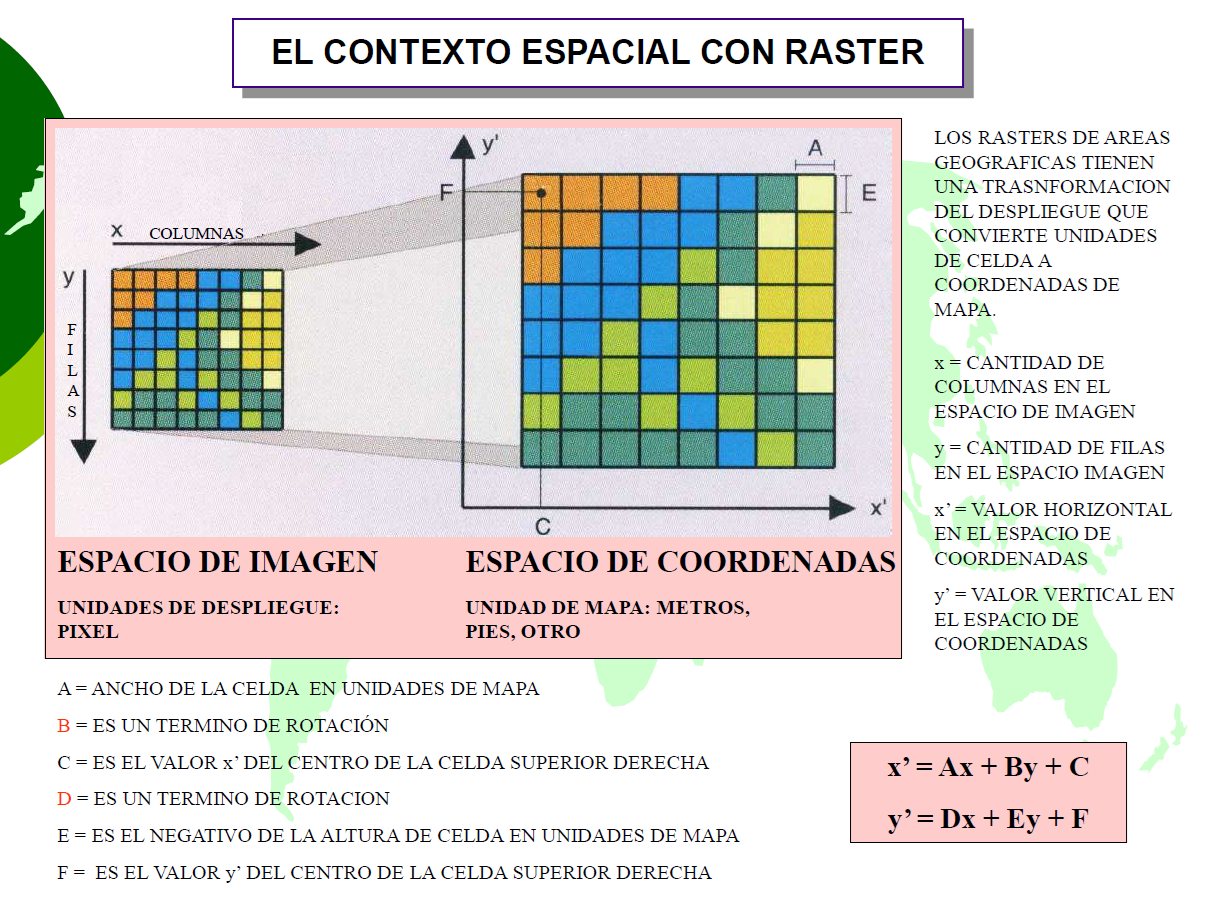
\includegraphics[width=0.9\textwidth,height=\textheight]{images/raster/espacio_imagen_espacio_coordenadas.png}

}

\caption{\label{fig-pixel_coord_space}Relación entre el espacio de
imagen (píxeles) y el espacio de coordenadas geográficas (metros).}

\end{figure}%

\subsubsection{La Transformación
Afín}\label{la-transformaciuxf3n-afuxedn}

Para vincular una ubicación \((X_{píxel}, Y_{píxel})\) de la imagen con
una coordenada real \((X_{real}, Y_{real})\), las librerías como
\texttt{rasterio} utilizan una \textbf{Transformación Afín 2D}. Este
tipo de transformación geométrica es lineal y preserva el paralelismo
entre líneas, lo que permite mover (trasladar), escalar y rotar el
raster para que encaje perfectamente sobre el mapa.

\subsubsection{Fórmulas de
Transformación}\label{fuxf3rmulas-de-transformaciuxf3n}

La matriz afín de 6 parámetros (excluyendo los técnicos \(g\), \(h\),
\(i\)) mapea los píxeles a coordenadas reales usando las siguientes
ecuaciones lineales generales:

\[X_{real} = c + X_{píxel} \times a + Y_{píxel} \times b\]
\[Y_{real} = f + X_{píxel} \times d + Y_{píxel} \times e\]

Donde los coeficientes son:

\begin{itemize}
\tightlist
\item
  \textbf{\(c, f\)}: Traslación. Coordenadas \((E, N)\) de la esquina
  superior izquierda del raster (origen geográfico).
\item
  \textbf{\(a, e\)}: Escala. Tamaño horizontal y vertical del píxel
  (resolución).
\item
  \textbf{\(b, d\)}: Rotación y Cizallamiento (shear). Usualmente \(0\)
  en imágenes de satélite alineadas al norte de la grilla.
\end{itemize}

Si no hay rotación, la fórmula se simplifica a la lógica lineal directa:
\(Origen + (Indice \times Resolución)\).

\textbf{Nota importante sobre la Resolución Vertical (\(e\)):} Para
resolver la contradicción entre las filas que bajan (imagen) y el norte
que sube (coordenadas), el valor de resolución vertical \(e\) debe ser
\textbf{NEGATIVO}. Esto asegura que a medida que avanzamos hacia abajo
en las filas (\(Y_{píxel}\) aumenta), la coordenada geográfica Norte
(\(Y_{real}\)) decrezca correctamente.

\begin{Shaded}
\begin{Highlighting}[]
\CommentTok{\# Ejemplo matemático con los datos impresos anteriormente:}
\CommentTok{\# f (Origen Y Norte): 5,960,000 m}
\CommentTok{\# e (Resolución Y): {-}10 m/píxel}

\CommentTok{\# Si bajamos 10 filas (Y\_pixel = 10):}
\CommentTok{\# Coordenada Y\_real = 5,960,000 + (10 * {-}10)}
\CommentTok{\# Y\_real = 5,960,000 {-} 100 = 5,959,900 m (Nos movimos al Sur)}
\end{Highlighting}
\end{Shaded}

\subsection{Resumen sintáctico}\label{resumen-sintuxe1ctico-5}

\begin{longtable}[]{@{}
  >{\raggedright\arraybackslash}p{(\columnwidth - 6\tabcolsep) * \real{0.2500}}
  >{\raggedright\arraybackslash}p{(\columnwidth - 6\tabcolsep) * \real{0.2500}}
  >{\raggedright\arraybackslash}p{(\columnwidth - 6\tabcolsep) * \real{0.2500}}
  >{\raggedright\arraybackslash}p{(\columnwidth - 6\tabcolsep) * \real{0.2500}}@{}}
\toprule\noalign{}
\begin{minipage}[b]{\linewidth}\raggedright
Operación
\end{minipage} & \begin{minipage}[b]{\linewidth}\raggedright
Python 🐍
\end{minipage} & \begin{minipage}[b]{\linewidth}\raggedright
R 🔵
\end{minipage} & \begin{minipage}[b]{\linewidth}\raggedright
Julia 🟣
\end{minipage} \\
\midrule\noalign{}
\endhead
\bottomrule\noalign{}
\endlastfoot
Validar existencia de archivo & \texttt{os.path.exists(ruta)} &
\texttt{file.exists(ruta)} & \texttt{isfile(ruta)} \\
Cargar archivo raster & \texttt{rioxarray.open\_rasterio(ruta)} &
\texttt{rast(ruta)} & \texttt{Raster(ruta)} \\
Reproyección espacial & \texttt{raster.rio.reproject("EPSG:9377")} &
\texttt{project(raster,\ "epsg:9377")} &
\texttt{resample(raster;\ crs=EPSG(9377))} \\
Crear directorios anidados & \texttt{os.makedirs(ruta,\ exist\_ok=True)}
& \texttt{dir.create(ruta,\ recursive=TRUE)} & \texttt{mkpath(ruta)} \\
Exportar / Escribir en disco & \texttt{raster.rio.to\_raster(ruta)} &
\texttt{writeRaster(raster,\ overwrite=TRUE)} &
\texttt{write(ruta,\ raster;\ force=true)} \\
Consultar CRS & \texttt{raster.rio.crs} & \texttt{crs(raster)} &
\texttt{crs(raster)} \\
\end{longtable}

\section{Álgebra de mapas: Cálculo del NDWI a partir de rutas
virtuales}\label{uxe1lgebra-de-mapas-cuxe1lculo-del-ndwi-a-partir-de-rutas-virtuales}

El álgebra de mapas permite evaluar operaciones aritméticas píxel a
píxel a través de múltiples bandas u objetos raster. Para este
ejercicio, calcularemos el Índice de Agua de Diferencia Normalizada
(NDWI), el cual es altamente efectivo para aislar y delimitar cuerpos
hídricos superficiales.

\textbf{Fórmula espectral:} \[NDWI = \frac{Green - NIR}{Green + NIR}\]

El \textbf{Índice de Diferencia Normalizada de Agua (NDWI)}, propuesto
originalmente por McFeeters (1996)
(\citeproc{ref-mcfeeters1996use}{McFeeters, 1996}), aprovecha el
comportamiento físico de la luz al interactuar con distintas
superficies. El agua absorbe casi por completo la radiación en el
espectro del Infrarrojo Cercano (NIR), mientras que refleja la luz
visible, especialmente en la banda verde. Por el contrario, la
vegetación y el suelo seco reflejan el NIR de forma muy intensa.

Al aplicar esta ecuación, la diferencia entre bandas se normaliza,
produciendo un nuevo raster continuo cuyos valores resultantes siempre
oscilarán entre \textbf{-1.0} y \textbf{+1.0}.

\subsubsection{Interpretación de los rangos del
NDWI}\label{interpretaciuxf3n-de-los-rangos-del-ndwi}

El análisis de este índice se basa en establecer un punto de corte
(\emph{threshold}) para separar el agua del fondo terrestre. La regla
general de interpretación es la siguiente:

\begin{itemize}
\tightlist
\item
  \textbf{Valores Negativos (-1.0 a \textless{} 0.0):} Representan
  superficies sin agua libre. Incluyen vegetación (valores más
  negativos), suelo desnudo y áreas urbanas construidas (valores más
  cercanos a cero). Aquí, la reflectancia del NIR supera a la del verde.
\item
  \textbf{Valores cercanos a 0.0 (Zonas de Transición):} Suelen
  corresponder a píxeles mixtos en las orillas de los ríos, zonas de
  inundación temporal, lodo húmedo, o bien, ``falsos positivos''
  generados por sombras topográficas o de nubes (zonas oscuras que
  absorben mucha radiación en general).
\item
  \textbf{Valores Positivos (\textgreater{} 0.0 a 1.0):} Indican la
  presencia de cuerpos hídricos. La banda verde es dominante frente al
  NIR. Los valores positivos bajos (ej. \textbf{0.1 a 0.3}) pueden
  indicar aguas poco profundas, turbias o humedales; mientras que los
  valores altos (cercanos a \textbf{1.0}) representan aguas profundas,
  limpias y abiertas.
\end{itemize}

\begin{tcolorbox}[enhanced jigsaw, coltitle=black, leftrule=.75mm, bottomtitle=1mm, title=\textcolor{quarto-callout-note-color}{\faInfo}\hspace{0.5em}{Nota}, colback=white, colbacktitle=quarto-callout-note-color!10!white, left=2mm, toptitle=1mm, rightrule=.15mm, titlerule=0mm, arc=.35mm, colframe=quarto-callout-note-color-frame, bottomrule=.15mm, toprule=.15mm, opacityback=0, opacitybacktitle=0.6, breakable]

\textbf{Ajuste del umbral en la práctica} En los ejercicios SIG
teóricos, el punto de corte estándar es el \textbf{0.0} (todo píxel
\(>0\) es agua). Sin embargo, en imágenes satelitales reales que
presentan nubosidad o relieve montañoso, los analistas suelen ajustar
este umbral manualmente (por ejemplo, subiéndolo a \textbf{0.1} o
\textbf{0.15}) para eliminar el ``ruido'' que generan las sombras y
aislar los ríos o lagos con mayor precisión cartográfica.

\end{tcolorbox}

Utilizaremos la lectura nativa de archivos comprimidos para evitar
cuellos de botella en el almacenamiento físico. Utilizando el Sistema de
Archivos Virtuales de GDAL (\texttt{/vsizip/}), podemos leer una escena
satelital Sentinel-2 directamente desde su archivo \texttt{.zip}
original sin necesidad de descomprimirla.

\subsubsection{A. Anatomía de la Imagen y
Subdatasets}\label{a.-anatomuxeda-de-la-imagen-y-subdatasets}

Un producto Sentinel-2 es una estructura jerárquica gobernada por el
archivo \textbf{XML de metadatos} (\texttt{MTD\_MSIL1C.xml}). Este
archivo no contiene los píxeles, sino que actúa como un índice lógico
que organiza las bandas individuales en \textbf{4 grupos funcionales
(Subdatasets)}:

\begin{enumerate}
\def\labelenumi{\arabic{enumi}.}
\tightlist
\item
  \textbf{10m}: Bandas de alta resolución (B02, B03, B04, B08). Es el
  grupo estándar para cálculo de índices de vegetación y agua (NDVI,
  NDWI).
\item
  \textbf{20m}: Bandas de resolución media (B05, B06, B07, B8A, B11,
  B12). Usadas para geología y estrés hídrico.
\item
  \textbf{60m}: Bandas de baja resolución (B01, B09, B10). Dedicadas a
  correcciones atmosféricas.
\item
  \textbf{TCI (True Color Image)}: Un subdataset especial que entrega
  una composición RGB pre-renderizada usando las bandas B04 (R), B03 (G)
  y B02 (B).
\end{enumerate}

Al invocar la ruta con el filtro específico:\\
\texttt{SENTINEL2\_L1C:/vsizip/.../MTD\_MSIL1C.xml:10m:EPSG\_32632}

Estamos forzando al sistema a ignorar los grupos de 20m, 60m y el TCI,
cargando únicamente el \textbf{cubo de 4 bandas de 10 metros} para
garantizar la máxima precisión analítica.

\subsubsection{B. Estructura del Subdataset de 10
metros}\label{b.-estructura-del-subdataset-de-10-metros}

Cuando trabajamos con el subdataset de 10m, el sistema nos entrega un
arreglo de 4 capas con el siguiente orden interno (ver
Tabla~\ref{tbl-sentinel_bands}):

\begin{longtable}[]{@{}
  >{\raggedright\arraybackslash}p{(\columnwidth - 8\tabcolsep) * \real{0.2000}}
  >{\raggedright\arraybackslash}p{(\columnwidth - 8\tabcolsep) * \real{0.2000}}
  >{\raggedright\arraybackslash}p{(\columnwidth - 8\tabcolsep) * \real{0.2000}}
  >{\raggedright\arraybackslash}p{(\columnwidth - 8\tabcolsep) * \real{0.2000}}
  >{\raggedright\arraybackslash}p{(\columnwidth - 8\tabcolsep) * \real{0.2000}}@{}}
\caption{Organización de capas en el subdataset de alta resolución
(10m)}\label{tbl-sentinel_bands}\tabularnewline
\toprule\noalign{}
\begin{minipage}[b]{\linewidth}\raggedright
Banda en el ``Cubo''
\end{minipage} & \begin{minipage}[b]{\linewidth}\raggedright
Banda Sentinel-2
\end{minipage} & \begin{minipage}[b]{\linewidth}\raggedright
Resolución
\end{minipage} & \begin{minipage}[b]{\linewidth}\raggedright
Longitud de Onda
\end{minipage} & \begin{minipage}[b]{\linewidth}\raggedright
Uso Principal
\end{minipage} \\
\midrule\noalign{}
\endfirsthead
\toprule\noalign{}
\begin{minipage}[b]{\linewidth}\raggedright
Banda en el ``Cubo''
\end{minipage} & \begin{minipage}[b]{\linewidth}\raggedright
Banda Sentinel-2
\end{minipage} & \begin{minipage}[b]{\linewidth}\raggedright
Resolución
\end{minipage} & \begin{minipage}[b]{\linewidth}\raggedright
Longitud de Onda
\end{minipage} & \begin{minipage}[b]{\linewidth}\raggedright
Uso Principal
\end{minipage} \\
\midrule\noalign{}
\endhead
\bottomrule\noalign{}
\endlastfoot
\textbf{1} & B04 (Red) & 10m & 665 nm & Absorción de clorofila \\
\textbf{2} & B03 (Green) & 10m & 560 nm & Vigor de vegetación y
turbidez \\
\textbf{3} & B02 (Blue) & 10m & 490 nm & Mapeo de aguas y suelos \\
\textbf{4} & B08 (NIR) & 10m & 842 nm & Biomasa y salud foliar \\
\end{longtable}

\begin{quote}
\textbf{Nota sobre el TCI:} Aunque el subdataset \texttt{:TCI:} también
contiene las bandas B04, B03 y B02, suele entregarse como un producto de
8 bits (valores de 0 a 255) ya estirado visualmente. Para el álgebra de
mapas profesional (como el NDWI), siempre debemos usar el subdataset de
\texttt{:10m:}, ya que conserva los valores de reflectancia originales
de 16 bits.
\end{quote}

\subsubsection{C. Proceso para el cálculo del
NDWI}\label{c.-proceso-para-el-cuxe1lculo-del-ndwi}

A continuación, mediante R, construiremos la ruta de enlace a una imagen
satelital empaquetada internamente en la librería \texttt{starsdata} y
la exportaremos a un archivo de texto en la carpeta \texttt{data/} para
compartirla interoperablemente con Python y Julia.

\begin{Shaded}
\begin{Highlighting}[]
\CommentTok{\# \#| eval: false}

\FunctionTok{library}\NormalTok{(starsdata) }\CommentTok{\# Librería que contiene datasets espaciales de prueba}

\CommentTok{\# {-}{-}{-}{-}{-}{-}{-}{-}{-}{-}{-}{-}{-}{-}{-}{-}{-}{-}{-}{-}{-}{-}{-}{-}{-}{-}{-}{-}{-}{-}{-}{-}{-}{-}{-}{-}{-}{-}{-}{-}{-}{-}{-}{-}{-}{-}{-}{-}{-}{-}{-}{-}{-}{-}{-}{-}{-}{-}{-}{-}{-}{-}{-}{-}{-}{-}{-}{-}{-}{-}{-}{-}{-}}
\CommentTok{\# 1. LOCALIZACIÓN DEL ARCHIVO FÍSICO}
\CommentTok{\# {-}{-}{-}{-}{-}{-}{-}{-}{-}{-}{-}{-}{-}{-}{-}{-}{-}{-}{-}{-}{-}{-}{-}{-}{-}{-}{-}{-}{-}{-}{-}{-}{-}{-}{-}{-}{-}{-}{-}{-}{-}{-}{-}{-}{-}{-}{-}{-}{-}{-}{-}{-}{-}{-}{-}{-}{-}{-}{-}{-}{-}{-}{-}{-}{-}{-}{-}{-}{-}{-}{-}{-}{-}}
\CommentTok{\# Definimos la ruta relativa del archivo .zip dentro de la estructura del paquete}
\NormalTok{f }\OtherTok{\textless{}{-}} \StringTok{"sentinel/S2A\_MSIL1C\_20180220T105051\_N0206\_R051\_T32ULE\_20180221T134037.zip"}

\CommentTok{\# system.file() busca la ruta absoluta de ese archivo en nuestro disco duro}
\NormalTok{granule }\OtherTok{\textless{}{-}} \FunctionTok{system.file}\NormalTok{(}\AttributeTok{file =}\NormalTok{ f, }\AttributeTok{package =} \StringTok{"starsdata"}\NormalTok{)}

\CommentTok{\# Extraemos solo el nombre base del archivo (sin la extensión .zip)}
\CommentTok{\# Esto es clave porque el directorio interno .SAFE se llama exactamente igual}
\NormalTok{base\_name }\OtherTok{\textless{}{-}} \FunctionTok{strsplit}\NormalTok{(}\FunctionTok{basename}\NormalTok{(granule), }\StringTok{".zip"}\NormalTok{)[[}\DecValTok{1}\NormalTok{]]}

\CommentTok{\# {-}{-}{-}{-}{-}{-}{-}{-}{-}{-}{-}{-}{-}{-}{-}{-}{-}{-}{-}{-}{-}{-}{-}{-}{-}{-}{-}{-}{-}{-}{-}{-}{-}{-}{-}{-}{-}{-}{-}{-}{-}{-}{-}{-}{-}{-}{-}{-}{-}{-}{-}{-}{-}{-}{-}{-}{-}{-}{-}{-}{-}{-}{-}{-}{-}{-}{-}{-}{-}{-}{-}{-}{-}}
\CommentTok{\# 2. CONSTRUCCIÓN DE LA RUTA VIRTUAL (VSI) DE GDAL}
\CommentTok{\# {-}{-}{-}{-}{-}{-}{-}{-}{-}{-}{-}{-}{-}{-}{-}{-}{-}{-}{-}{-}{-}{-}{-}{-}{-}{-}{-}{-}{-}{-}{-}{-}{-}{-}{-}{-}{-}{-}{-}{-}{-}{-}{-}{-}{-}{-}{-}{-}{-}{-}{-}{-}{-}{-}{-}{-}{-}{-}{-}{-}{-}{-}{-}{-}{-}{-}{-}{-}{-}{-}{-}{-}{-}}
\CommentTok{\# Construimos una cadena de conexión especializada para GDAL:}
\CommentTok{\# {-} SENTINEL2\_L1C: Activa el driver específico de Sentinel{-}2}
\CommentTok{\# {-} /vsizip/: Indica a GDAL que lea dentro del archivo comprimido sin extraerlo en disco}
\CommentTok{\# {-} MTD\_MSIL1C.xml: Archivo maestro que organiza las bandas}
\CommentTok{\# {-} :10m:EPSG\_32632: Filtramos estrictamente el subdataset de 10 metros}
\NormalTok{s2\_path }\OtherTok{\textless{}{-}} \FunctionTok{paste0}\NormalTok{(}\StringTok{"SENTINEL2\_L1C:/vsizip/"}\NormalTok{, granule, }\StringTok{"/"}\NormalTok{, base\_name, }\StringTok{".SAFE/MTD\_MSIL1C.xml:10m:EPSG\_32632"}\NormalTok{)}

\CommentTok{\# {-}{-}{-}{-}{-}{-}{-}{-}{-}{-}{-}{-}{-}{-}{-}{-}{-}{-}{-}{-}{-}{-}{-}{-}{-}{-}{-}{-}{-}{-}{-}{-}{-}{-}{-}{-}{-}{-}{-}{-}{-}{-}{-}{-}{-}{-}{-}{-}{-}{-}{-}{-}{-}{-}{-}{-}{-}{-}{-}{-}{-}{-}{-}{-}{-}{-}{-}{-}{-}{-}{-}{-}{-}}
\CommentTok{\# 3. PERSISTENCIA DE LA RUTA PARA INTEROPERABILIDAD}
\CommentTok{\# {-}{-}{-}{-}{-}{-}{-}{-}{-}{-}{-}{-}{-}{-}{-}{-}{-}{-}{-}{-}{-}{-}{-}{-}{-}{-}{-}{-}{-}{-}{-}{-}{-}{-}{-}{-}{-}{-}{-}{-}{-}{-}{-}{-}{-}{-}{-}{-}{-}{-}{-}{-}{-}{-}{-}{-}{-}{-}{-}{-}{-}{-}{-}{-}{-}{-}{-}{-}{-}{-}{-}{-}{-}}
\CommentTok{\# Creamos la carpeta \textquotesingle{}data\textquotesingle{} si no existe en nuestro espacio de trabajo}
\ControlFlowTok{if}\NormalTok{ (}\SpecialCharTok{!}\FunctionTok{dir.exists}\NormalTok{(}\StringTok{"data"}\NormalTok{)) \{}
  \FunctionTok{dir.create}\NormalTok{(}\StringTok{"data"}\NormalTok{)}
\NormalTok{\}}

\CommentTok{\# Guardamos la ruta virtual en un archivo de texto plano.}
\CommentTok{\# Esto permite que Python y Julia puedan leer exactamente el mismo insumo}
\CommentTok{\# sin tener que recalcular las rutas de los paquetes de R.}
\FunctionTok{writeLines}\NormalTok{(s2\_path, }\StringTok{"data/s2\_shared\_path.txt"}\NormalTok{)}

\FunctionTok{cat}\NormalTok{(}\StringTok{"Ruta virtual de GDAL generada y almacenada en: data/s2\_shared\_path.txt}\SpecialCharTok{\textbackslash{}n}\StringTok{"}\NormalTok{)}
\end{Highlighting}
\end{Shaded}

\begin{verbatim}
Ruta virtual de GDAL generada y almacenada en: data/s2_shared_path.txt
\end{verbatim}

Una vez materializada la ruta, los tres lenguajes la consumirán para
ejecutar de forma enlazada el cálculo del NDWI y resguardar el resultado
en la carpeta de procesamiento masivo (\texttt{data\_heavy/raster/}). Es
importante inspeccionar siempre los metadatos de las bandas; para este
producto específico, el orden interno reportado por GDAL es: 1:Rojo(B4),
2:Verde(B3), 3:Azul(B2) y 4:NIR(B8).

\begin{tcolorbox}[enhanced jigsaw, coltitle=black, leftrule=.75mm, bottomtitle=1mm, title=\textcolor{quarto-callout-note-color}{\faInfo}\hspace{0.5em}{Visualización: ¿Matriz Matemática o Mapa Geográfico?}, colback=white, colbacktitle=quarto-callout-note-color!10!white, left=2mm, toptitle=1mm, rightrule=.15mm, titlerule=0mm, arc=.35mm, colframe=quarto-callout-note-color-frame, bottomrule=.15mm, toprule=.15mm, opacityback=0, opacitybacktitle=0.6, breakable]

En esta sección exploraremos las diversas estrategias y librerías para
representar visualmente el NDWI. El objetivo es comprender la transición
entre la \textbf{matriz numérica cruda} (regida por el plano cartesiano
y los índices de memoria) y el \textbf{objeto raster georreferenciado}
(regido por coordenadas reales y el Norte geográfico).

Se abordarán soluciones específicas para corregir errores comunes de
orientación, tales como la transposición de ejes y la inversión vertical
de las filas, garantizando que la representación visual coincida
estrictamente con la realidad del terreno.

\end{tcolorbox}

\subsection{Python}

\textbf{Gestión de metadatos: El perfil de salida (Profile)}

En el contexto de la programación SIG con la librería \texttt{rasterio},
el \textbf{perfil de salida} (\texttt{profile}) es un diccionario de
Python que consolida los metadatos técnicos necesarios para la
instanciación de un nuevo archivo físico en el disco. Al realizar
análisis espaciales (como el cálculo del NDWI), el nuevo archivo debe
heredar o adaptar las propiedades del insumo original para garantizar su
validez y alineación en softwares de escritorio como QGIS o ArcGIS.

Los componentes fundamentales que definen un perfil son:

\begin{itemize}
\tightlist
\item
  \textbf{\texttt{driver}}: Especifica el formato de almacenamiento. El
  estándar de la industria es
  \texttt{\textquotesingle{}GTiff\textquotesingle{}} (GeoTIFF).
\item
  \textbf{\texttt{dtype}}: Define el tipo de dato de los píxeles. Se
  utiliza \texttt{float32} para valores continuos (índices espectrales)
  o \texttt{uint16} para valores de reflectancia cruda.
\item
  \textbf{\texttt{nodata}}: Valor numérico (ej. \texttt{-9999}) que
  designa la ausencia de información, permitiendo que el software lo
  interprete como transparencia.
\item
  \textbf{\texttt{width} y \texttt{height}}: Dimensiones de la matriz
  (columnas y filas). Deben coincidir estrictamente con el tamaño del
  arreglo de datos.
\item
  \textbf{\texttt{count}}: Número de bandas. Si el insumo es
  multiespectral pero el resultado es un índice único, este valor debe
  actualizarse a \texttt{1}.
\item
  \textbf{\texttt{crs}}: Sistema de Referencia de Coordenadas (ej.
  EPSG:9377 para Colombia).
\item
  \textbf{\texttt{transform}}: Matriz de transformación afín que vincula
  los índices de la matriz con coordenadas geográficas reales.
\end{itemize}

\textbf{El método \texttt{.update()}}

Dada la complejidad de definir estos parámetros desde cero, el flujo de
trabajo estándar consiste en extraer el perfil del archivo fuente y
modificar exclusivamente los atributos que cambian mediante el método
\texttt{.update()}:

\begin{Shaded}
\begin{Highlighting}[]
\CommentTok{\# 1. Cargar la imagen a la variable src}
\CommentTok{\# Usando por ejemplo: with rasterio.open(s2\_path) as src:}

\CommentTok{\# 2. Extraer metadatos del original}
\NormalTok{perfil }\OperatorTok{=}\NormalTok{ src.profile}

\CommentTok{\# 3. Adaptar parámetros para el nuevo índice}
\NormalTok{perfil.update(}
\NormalTok{    count}\OperatorTok{=}\DecValTok{1}\NormalTok{, }
\NormalTok{    dtype}\OperatorTok{=}\StringTok{\textquotesingle{}float32\textquotesingle{}}\NormalTok{, }
\NormalTok{    nodata}\OperatorTok{={-}}\DecValTok{9999}
\NormalTok{)}
\end{Highlighting}
\end{Shaded}

Este procedimiento garantiza la \textbf{coincidencia espacial perfecta}:
el raster resultante mantendrá la misma ubicación, resolución y
proyección que el insumo original, facilitando su integración en
sistemas de información geográfica.

\begin{Shaded}
\begin{Highlighting}[]
\CommentTok{\# \#| eval: false}
\CommentTok{\#| label: python\_ndwi\_bad\_codigo}
\CommentTok{\#| fig{-}align: center}
\CommentTok{\#| out{-}width: "80\%"}
\CommentTok{\#| eval: false}

\CommentTok{\# {-}{-}{-}{-}{-}{-}{-}{-}{-}{-}{-}{-}{-}{-}{-}{-}{-}{-}{-}{-}{-}{-}{-}{-}{-}{-}{-}{-}{-}{-}{-}}
\CommentTok{\# IMPORTACIÓN DE LIBRERÍAS}
\CommentTok{\# {-}{-}{-}{-}{-}{-}{-}{-}{-}{-}{-}{-}{-}{-}{-}{-}{-}{-}{-}{-}{-}{-}{-}{-}{-}{-}{-}{-}{-}{-}{-}}
\ImportTok{import}\NormalTok{ os  }\CommentTok{\# Manejo de rutas y sistema de archivos}
\ImportTok{import}\NormalTok{ rasterio  }\CommentTok{\# Lectura/escritura de datos raster geoespaciales}
\ImportTok{from}\NormalTok{ rasterio.windows }\ImportTok{import}\NormalTok{ Window  }\CommentTok{\# Permite trabajar con subregiones (ventanas) del raster}
\ImportTok{import}\NormalTok{ xarray }\ImportTok{as}\NormalTok{ xr  }\CommentTok{\# Manejo avanzado de arrays etiquetados (útil para visualización)}
\ImportTok{import}\NormalTok{ numpy }\ImportTok{as}\NormalTok{ np  }\CommentTok{\# Operaciones numéricas eficientes}
\ImportTok{import}\NormalTok{ matplotlib.pyplot }\ImportTok{as}\NormalTok{ plt  }\CommentTok{\# Visualización gráfica}

\CommentTok{\# {-}{-}{-}{-}{-}{-}{-}{-}{-}{-}{-}{-}{-}{-}{-}{-}{-}{-}{-}{-}{-}{-}{-}{-}{-}{-}{-}{-}{-}{-}{-}}
\CommentTok{\# CONFIGURACIÓN DE RUTAS}
\CommentTok{\# {-}{-}{-}{-}{-}{-}{-}{-}{-}{-}{-}{-}{-}{-}{-}{-}{-}{-}{-}{-}{-}{-}{-}{-}{-}{-}{-}{-}{-}{-}{-}}
\CommentTok{\# Archivo .txt que contiene la ruta al raster Sentinel{-}2 original}
\NormalTok{ruta\_txt }\OperatorTok{=} \StringTok{"data/s2\_shared\_path.txt"}

\CommentTok{\# Ruta donde se guardará el resultado NDWI optimizado}
\NormalTok{ruta\_salida }\OperatorTok{=} \StringTok{"data\_heavy/raster/ndwi\_sentinel\_optimizado\_python\_1.tif"}

\CommentTok{\# Verificamos que el archivo con la ruta exista}
\ControlFlowTok{if} \KeywordTok{not}\NormalTok{ os.path.exists(ruta\_txt):}
    \BuiltInTok{print}\NormalTok{(}\SpecialStringTok{f"ERROR: Insumo ausente en }\SpecialCharTok{\{}\NormalTok{ruta\_txt}\SpecialCharTok{\}}\SpecialStringTok{"}\NormalTok{)}
\ControlFlowTok{else}\NormalTok{:}
    \ControlFlowTok{try}\NormalTok{:}
        \CommentTok{\# {-}{-}{-}{-}{-}{-}{-}{-}{-}{-}{-}{-}{-}{-}{-}{-}{-}{-}{-}{-}{-}{-}{-}{-}{-}{-}{-}{-}{-}{-}{-}}
        \CommentTok{\# LECTURA DE LA RUTA DEL RASTER}
        \CommentTok{\# {-}{-}{-}{-}{-}{-}{-}{-}{-}{-}{-}{-}{-}{-}{-}{-}{-}{-}{-}{-}{-}{-}{-}{-}{-}{-}{-}{-}{-}{-}{-}}
        \ControlFlowTok{with} \BuiltInTok{open}\NormalTok{(ruta\_txt, }\StringTok{"r"}\NormalTok{) }\ImportTok{as}\NormalTok{ f:}
            \CommentTok{\# Leemos la ruta almacenada en el .txt y eliminamos espacios extra}
\NormalTok{            s2\_path }\OperatorTok{=}\NormalTok{ f.read().strip()}
            
        \CommentTok{\# {-}{-}{-}{-}{-}{-}{-}{-}{-}{-}{-}{-}{-}{-}{-}{-}{-}{-}{-}{-}{-}{-}{-}{-}{-}{-}{-}{-}{-}{-}{-}}
        \CommentTok{\# APERTURA DEL RASTER ORIGINAL}
        \CommentTok{\# {-}{-}{-}{-}{-}{-}{-}{-}{-}{-}{-}{-}{-}{-}{-}{-}{-}{-}{-}{-}{-}{-}{-}{-}{-}{-}{-}{-}{-}{-}{-}}
        \ControlFlowTok{with}\NormalTok{ rasterio.}\BuiltInTok{open}\NormalTok{(s2\_path) }\ImportTok{as}\NormalTok{ src:}
            
            \CommentTok{\# {-}{-}{-} OPTIMIZACIÓN 1: USO DE VENTANA {-}{-}{-}}
            \CommentTok{\# En lugar de procesar toda la imagen (\textasciitilde{}11000 x 11000 px),}
            \CommentTok{\# trabajamos solo con una subregión (ventana).}
            
            \CommentTok{\# Parámetros de la ventana:}
            \CommentTok{\# col\_off: desplazamiento horizontal (columnas) desde la esquina superior izquierda}
            \CommentTok{\# row\_off: desplazamiento vertical (filas)}
            \CommentTok{\# width: ancho del recorte en píxeles}
            \CommentTok{\# height: alto del recorte en píxeles}
            \CommentTok{\# Imagen completa (10980 px de ancho aprox)}
            \CommentTok{\# |{-}{-}{-}{-}{-}{-}{-}{-}{-}{-}{-}{-}{-}{-}{-}{-}{-}{-}{-}{-}|{-}{-}{-}{-}{-}{-}{-}{-}{-}{-}{-}{-}{-}{-}{-}{-}{-}{-}{-}{-}{-}{-}{-}{-}{-}{-}{-}|}
            \CommentTok{\# 0                  9980                       10980}
            \CommentTok{\#                      ↑                           ↑}
            \CommentTok{\#                    col\_off               col\_off + width }
\NormalTok{            ventana }\OperatorTok{=}\NormalTok{ Window(col\_off}\OperatorTok{=}\DecValTok{9980}\NormalTok{, row\_off}\OperatorTok{=}\DecValTok{4000}\NormalTok{, width}\OperatorTok{=}\DecValTok{1000}\NormalTok{, height}\OperatorTok{=}\DecValTok{2500}\NormalTok{)}
            
            \CommentTok{\# Lectura selectiva de bandas:}
            \CommentTok{\# Banda 2 = Green (verde)}
            \CommentTok{\# Banda 4 = NIR (infrarrojo cercano)}
            
            \CommentTok{\# Convertimos a float32 para reducir uso de memoria (vs float64)}
            \CommentTok{\# Nota importante : Cuando trabajas con la librería rasterio (y casi cualquier }
            \CommentTok{\# software basado en GDAL): las bandas de un archivo raster se }
            \CommentTok{\# cuentan empezando desde 1 (independientemente de la base 0 de Python)            }
\NormalTok{            green\_arr }\OperatorTok{=}\NormalTok{ src.read(}\DecValTok{2}\NormalTok{, window}\OperatorTok{=}\NormalTok{ventana).astype(np.float32)}
\NormalTok{            nir\_arr }\OperatorTok{=}\NormalTok{ src.read(}\DecValTok{4}\NormalTok{, window}\OperatorTok{=}\NormalTok{ventana).astype(np.float32)}
            
            \CommentTok{\# Guardamos el perfil original (metadatos del raster)}
\NormalTok{            perfil\_salida }\OperatorTok{=}\NormalTok{ src.profile}
            
            \CommentTok{\# Calculamos la nueva transformada espacial para la ventana}
            \CommentTok{\# Esto asegura que el recorte conserve su georreferenciación correcta}
            \CommentTok{\# El objeto nueva\_transformada es una Matriz de Transformación Afín:}
            \CommentTok{\# (col, row)    →  (x, y)}
            \CommentTok{\# píxel         → coordenada real}
            \CommentTok{\# Es el "puente" matemático que le dice al ordenador cómo convertir }
            \CommentTok{\# un número de fila y columna (píxel) en una coordenada real }
            \CommentTok{\# en el mapa (ej: metros)}
            \CommentTok{\# Cuando usas src.window\_transform(ventana), rasterio calcula una }
            \CommentTok{\# nueva matriz que desplaza el origen (la esquina superior izquierda) }
            \CommentTok{\# desde el borde de la imagen original hasta el borde de tu recorte}
\NormalTok{            nueva\_transformada }\OperatorTok{=}\NormalTok{ src.window\_transform(ventana)}

            \CommentTok{\# nueva\_transformada contiene 6 coeficientes principales que definen }
            \CommentTok{\# la posición y escala del raster:}
            \CommentTok{\# a: scale x {-} ancho del píxel (ej. 10 metros).}
            \CommentTok{\# b: rotation x {-} rotación de filas (normalmente 0).}
            \CommentTok{\# c: x origin {-} coordenada Este (X) de la esquina superior izquierda }
            \CommentTok{\#    del recorte.}
            \CommentTok{\# d: rotation y {-} rotación de columnas (normalmente 0).}
            \CommentTok{\# e: scale y {-} alto del píxel (suele ser negativo, ej. {-}10, }
            \CommentTok{\#    porque las coordenadas del mapa suben y las filas del raster }
            \CommentTok{\#    bajan)}
            \CommentTok{\# f: y origin {-} coordenada Norte (Y) de la esquina superior izquierda }
            \CommentTok{\#    del recorte.}
            \CommentTok{\# g, h, i: estándar de matrices 3x3}
            \CommentTok{\# Imprimimos el contenido}
            \BuiltInTok{print}\NormalTok{(}\SpecialStringTok{f"Contenido nueva\_transformada: }\SpecialCharTok{\{}\NormalTok{nueva\_transformada}\SpecialCharTok{\}}\SpecialStringTok{"}\NormalTok{)}
            \BuiltInTok{print}\NormalTok{(}\SpecialStringTok{f"Contenido nueva\_transformada como tupla: }\SpecialCharTok{\{}\BuiltInTok{tuple}\NormalTok{(nueva\_transformada)}\SpecialCharTok{\}}\SpecialStringTok{"}\NormalTok{)}

            \CommentTok{\# Los 6 parámetros principales de la transformación afín}
            \BuiltInTok{print}\NormalTok{(}\SpecialStringTok{f"a {-} Resolución horizontal (ancho píxel): }\SpecialCharTok{\{}\NormalTok{nueva\_transformada}\SpecialCharTok{.}\NormalTok{a}\SpecialCharTok{\}}\SpecialStringTok{"}\NormalTok{)}
            \BuiltInTok{print}\NormalTok{(}\SpecialStringTok{f"b {-} Rotación/Cizallamiento en X: }\SpecialCharTok{\{}\NormalTok{nueva\_transformada}\SpecialCharTok{.}\NormalTok{b}\SpecialCharTok{\}}\SpecialStringTok{"}\NormalTok{)}
            \BuiltInTok{print}\NormalTok{(}\SpecialStringTok{f"c {-} Origen Este (X) del recorte: }\SpecialCharTok{\{}\NormalTok{nueva\_transformada}\SpecialCharTok{.}\NormalTok{c}\SpecialCharTok{\}}\SpecialStringTok{"}\NormalTok{)}
            \BuiltInTok{print}\NormalTok{(}\SpecialStringTok{f"d {-} Rotación/Cizallamiento en Y: }\SpecialCharTok{\{}\NormalTok{nueva\_transformada}\SpecialCharTok{.}\NormalTok{d}\SpecialCharTok{\}}\SpecialStringTok{"}\NormalTok{)}
            \BuiltInTok{print}\NormalTok{(}\SpecialStringTok{f"e {-} Resolución vertical (alto píxel): }\SpecialCharTok{\{}\NormalTok{nueva\_transformada}\SpecialCharTok{.}\NormalTok{e}\SpecialCharTok{\}}\SpecialStringTok{"}\NormalTok{)}
            \BuiltInTok{print}\NormalTok{(}\SpecialStringTok{f"f {-} Origen Norte (Y) del recorte: }\SpecialCharTok{\{}\NormalTok{nueva\_transformada}\SpecialCharTok{.}\NormalTok{f}\SpecialCharTok{\}}\SpecialStringTok{"}\NormalTok{)}
            \CommentTok{\# Los 3 parámetros de la tercera fila (estándar de matrices 3x3)}
            \CommentTok{\# Los parámetros g, h, i son componentes técnicos necesarios para que }
            \CommentTok{\# la matriz sea cuadrada (3 x 3) y funcione bajo el concepto de }
            \CommentTok{\# coordenadas homogéneas}
            \CommentTok{\# En procesamiento de mapas 2D (como este), sus valores son fijos:}
            \CommentTok{\# g y h (Perspectiva): Controlan la inclinación en un espacio 3D (perspectiva). }
            \CommentTok{\#       Como los rasters son planos, siempre son 0.0.}
            \BuiltInTok{print}\NormalTok{(}\SpecialStringTok{f"g {-} Parámetro de perspectiva g: }\SpecialCharTok{\{}\NormalTok{nueva\_transformada}\SpecialCharTok{.}\NormalTok{g}\SpecialCharTok{\}}\SpecialStringTok{"}\NormalTok{)}
            \BuiltInTok{print}\NormalTok{(}\SpecialStringTok{f"h {-} Parámetro de perspectiva h: }\SpecialCharTok{\{}\NormalTok{nueva\_transformada}\SpecialCharTok{.}\NormalTok{h}\SpecialCharTok{\}}\SpecialStringTok{"}\NormalTok{)}
            \CommentTok{\# i (Factor de escala): Es un normalizador matemático para que la }
            \CommentTok{\# matriz sea operativa. Siempre es 1.0.}
            \BuiltInTok{print}\NormalTok{(}\SpecialStringTok{f"i {-} Factor de escala homogénea i: }\SpecialCharTok{\{}\NormalTok{nueva\_transformada}\SpecialCharTok{.}\NormalTok{i}\SpecialCharTok{\}}\SpecialStringTok{"}\NormalTok{)}

        \CommentTok{\# {-}{-}{-}{-}{-}{-}{-}{-}{-}{-}{-}{-}{-}{-}{-}{-}{-}{-}{-}{-}{-}{-}{-}{-}{-}{-}{-}{-}{-}{-}{-}}
        \CommentTok{\# CÁLCULO DEL NDWI}
        \CommentTok{\# {-}{-}{-}{-}{-}{-}{-}{-}{-}{-}{-}{-}{-}{-}{-}{-}{-}{-}{-}{-}{-}{-}{-}{-}{-}{-}{-}{-}{-}{-}{-}}
        \CommentTok{\# Fórmula del NDWI (Normalized Difference Water Index):}
        \CommentTok{\# NDWI = (Green {-} NIR) / (Green + NIR)}
        
\NormalTok{        denominador }\OperatorTok{=}\NormalTok{ green\_arr }\OperatorTok{+}\NormalTok{ nir\_arr}
        
        \CommentTok{\# Evitamos divisiones por cero:}
        \CommentTok{\# {-} Si el denominador es 0 → asignamos NaN}
        \CommentTok{\# {-} Si es válido → aplicamos la fórmula}
        \CommentTok{\# Nota 1: ndwi\_np no sabe sobre coordenadas}
        \CommentTok{\#    las columnas inician en 0 y continúan ascendiendo}
        \CommentTok{\#    las filas inician en 0 y continúan ascendiendo}
        \CommentTok{\# Nota 2: El resultado es una matriz \textquotesingle{}cruda\textquotesingle{}. En esta etapa, }
        \CommentTok{\#    el píxel [0,0] es simplemente el primer dato de la memoria, }
        \CommentTok{\#    sin ubicación en el mundo real"}
\NormalTok{        ndwi\_np }\OperatorTok{=}\NormalTok{ np.where(}
\NormalTok{            denominador }\OperatorTok{\textgreater{}} \DecValTok{0}\NormalTok{,}
\NormalTok{            (green\_arr }\OperatorTok{{-}}\NormalTok{ nir\_arr) }\OperatorTok{/}\NormalTok{ denominador,}
\NormalTok{            np.nan}
\NormalTok{        )}
        
        \CommentTok{\# {-}{-}{-}{-}{-}{-}{-}{-}{-}{-}{-}{-}{-}{-}{-}{-}{-}{-}{-}{-}{-}{-}{-}{-}{-}{-}{-}{-}{-}{-}{-}}
        \CommentTok{\# OPTIMIZACIÓN 2: ESCRITURA EFICIENTE}
        \CommentTok{\# {-}{-}{-}{-}{-}{-}{-}{-}{-}{-}{-}{-}{-}{-}{-}{-}{-}{-}{-}{-}{-}{-}{-}{-}{-}{-}{-}{-}{-}{-}{-}}
        
        \CommentTok{\# Creamos la carpeta de salida si no existe}
\NormalTok{        os.makedirs(os.path.dirname(ruta\_salida), exist\_ok}\OperatorTok{=}\VariableTok{True}\NormalTok{)}
        
        \CommentTok{\# Actualizamos el perfil del raster de salida}
\NormalTok{        perfil\_salida.update(}
\NormalTok{            dtype}\OperatorTok{=}\NormalTok{rasterio.float32,  }\CommentTok{\# Tipo de dato (menor peso)}
\NormalTok{            count}\OperatorTok{=}\DecValTok{1}\NormalTok{,  }\CommentTok{\# Solo una banda (NDWI)}
\NormalTok{            driver}\OperatorTok{=}\StringTok{\textquotesingle{}GTiff\textquotesingle{}}\NormalTok{,  }\CommentTok{\# Formato GeoTIFF}
\NormalTok{            nodata}\OperatorTok{={-}}\DecValTok{9999}\NormalTok{,  }\CommentTok{\# Valor para datos faltantes}
\NormalTok{            width}\OperatorTok{=}\NormalTok{ventana.width,  }\CommentTok{\# Nuevo ancho (recorte)}
\NormalTok{            height}\OperatorTok{=}\NormalTok{ventana.height,  }\CommentTok{\# Nuevo alto (recorte)}
\NormalTok{            transform}\OperatorTok{=}\NormalTok{nueva\_transformada,  }\CommentTok{\# Nueva georreferenciación}
            
            \CommentTok{\# Compresión LZW:}
            \CommentTok{\# Reduce significativamente el tamaño del archivo sin perder información}
\NormalTok{            compress}\OperatorTok{=}\StringTok{\textquotesingle{}lzw\textquotesingle{}}\NormalTok{,}
            
            \CommentTok{\# tiled=True:}
            \CommentTok{\# Mejora el rendimiento de lectura en SIG (ej. QGIS)}
\NormalTok{            tiled}\OperatorTok{=}\VariableTok{True}
\NormalTok{        )}
        
        \CommentTok{\# {-}{-}{-}{-}{-}{-}{-}{-}{-}{-}{-}{-}{-}{-}{-}{-}{-}{-}{-}{-}{-}{-}{-}{-}{-}{-}{-}{-}{-}{-}{-}}
        \CommentTok{\# ESCRITURA DEL RASTER NDWI}
        \CommentTok{\# {-}{-}{-}{-}{-}{-}{-}{-}{-}{-}{-}{-}{-}{-}{-}{-}{-}{-}{-}{-}{-}{-}{-}{-}{-}{-}{-}{-}{-}{-}{-}}
        \ControlFlowTok{with}\NormalTok{ rasterio.}\BuiltInTok{open}\NormalTok{(ruta\_salida, }\StringTok{\textquotesingle{}w\textquotesingle{}}\NormalTok{, }\OperatorTok{**}\NormalTok{perfil\_salida) }\ImportTok{as}\NormalTok{ dst:}
            
            \CommentTok{\# Reemplazamos NaN por el valor nodata definido ({-}9999)}
\NormalTok{            out\_data }\OperatorTok{=}\NormalTok{ np.nan\_to\_num(ndwi\_np, nan}\OperatorTok{={-}}\DecValTok{9999}\NormalTok{).astype(np.float32)}
            
            \CommentTok{\# Escribimos la banda NDWI en el archivo de salida}
            \CommentTok{\# Nota: A pesar que la visualización en Python es invertida (cols)}
            \CommentTok{\#       el archivo exportado si está correctamente georeferenciado}
            \CommentTok{\#       porque usa nueva\_transformada en el perfil de salida perfil\_salida            }
\NormalTok{            dst.write(out\_data, }\DecValTok{1}\NormalTok{)}
            
        \BuiltInTok{print}\NormalTok{(}\SpecialStringTok{f"Proceso optimizado exitoso. Archivo ligero guardado en: }\SpecialCharTok{\{}\NormalTok{ruta\_salida}\SpecialCharTok{\}}\SpecialStringTok{"}\NormalTok{)}

        \CommentTok{\# {-}{-}{-}{-}{-}{-}{-}{-}{-}{-}{-}{-}{-}{-}{-}{-}{-}{-}{-}{-}{-}{-}{-}{-}{-}{-}{-}{-}{-}{-}{-}}
        \CommentTok{\# VISUALIZACIÓN CARTOGRÁFICA}
        \CommentTok{\# {-}{-}{-}{-}{-}{-}{-}{-}{-}{-}{-}{-}{-}{-}{-}{-}{-}{-}{-}{-}{-}{-}{-}{-}{-}{-}{-}{-}{-}{-}{-}}

        \CommentTok{\# 2. Creamos el DataArray con COORDENADAS REALES}
\NormalTok{        ndwi\_xr }\OperatorTok{=}\NormalTok{ xr.DataArray(}
\NormalTok{            ndwi\_np, }
\NormalTok{            dims}\OperatorTok{=}\NormalTok{(}\StringTok{"y"}\NormalTok{, }\StringTok{"x"}\NormalTok{)}
\NormalTok{        )}

        \CommentTok{\# Imprimir los valores del eje X}
        \BuiltInTok{print}\NormalTok{(}\StringTok{"Valores de X (Este):"}\NormalTok{)}
        \BuiltInTok{print}\NormalTok{(ndwi\_xr.x.values[:}\DecValTok{5}\NormalTok{])}
        \CommentTok{\#print(ndwi\_xr.x.values)}

        \CommentTok{\# Imprimir los valores del eje Y}
        \BuiltInTok{print}\NormalTok{(}\StringTok{"}\CharTok{\textbackslash{}n}\StringTok{Valores de Y (Norte):"}\NormalTok{)}
        \BuiltInTok{print}\NormalTok{(ndwi\_xr.y.values[:}\DecValTok{5}\NormalTok{])}
        \CommentTok{\#print(ndwi\_xr.y.values)}

        \BuiltInTok{print}\NormalTok{(}\SpecialStringTok{f"Rango de X: desde }\SpecialCharTok{\{}\NormalTok{ndwi\_xr}\SpecialCharTok{.}\NormalTok{x}\SpecialCharTok{.}\BuiltInTok{min}\NormalTok{()}\SpecialCharTok{.}\NormalTok{values}\SpecialCharTok{\}}\SpecialStringTok{ hasta }\SpecialCharTok{\{}\NormalTok{ndwi\_xr}\SpecialCharTok{.}\NormalTok{x}\SpecialCharTok{.}\BuiltInTok{max}\NormalTok{()}\SpecialCharTok{.}\NormalTok{values}\SpecialCharTok{\}}\SpecialStringTok{"}\NormalTok{)}
        \BuiltInTok{print}\NormalTok{(}\SpecialStringTok{f"Rango de Y: desde }\SpecialCharTok{\{}\NormalTok{ndwi\_xr}\SpecialCharTok{.}\NormalTok{y}\SpecialCharTok{.}\BuiltInTok{min}\NormalTok{()}\SpecialCharTok{.}\NormalTok{values}\SpecialCharTok{\}}\SpecialStringTok{ hasta }\SpecialCharTok{\{}\NormalTok{ndwi\_xr}\SpecialCharTok{.}\NormalTok{y}\SpecialCharTok{.}\BuiltInTok{max}\NormalTok{()}\SpecialCharTok{.}\NormalTok{values}\SpecialCharTok{\}}\SpecialStringTok{"}\NormalTok{)}
        \BuiltInTok{print}\NormalTok{(}\SpecialStringTok{f"Cantidad de píxeles: }\SpecialCharTok{\{}\NormalTok{ndwi\_xr}\SpecialCharTok{.}\NormalTok{x}\SpecialCharTok{.}\NormalTok{size}\SpecialCharTok{\}}\SpecialStringTok{ en X, }\SpecialCharTok{\{}\NormalTok{ndwi\_xr}\SpecialCharTok{.}\NormalTok{y}\SpecialCharTok{.}\NormalTok{size}\SpecialCharTok{\}}\SpecialStringTok{ en Y"}\NormalTok{)}
        
        \CommentTok{\# 3. Graficamos}
        \CommentTok{\# Creamos figura y eje}
\NormalTok{        fig, ax }\OperatorTok{=}\NormalTok{ plt.subplots(figsize}\OperatorTok{=}\NormalTok{(}\DecValTok{10}\NormalTok{, }\DecValTok{8}\NormalTok{))}

        \CommentTok{\# Visualización del NDWI:}
        \CommentTok{\# cmap="GnBu" → tonos verde{-}azul (agua en azul intenso)}
        \CommentTok{\# vmin/vmax → controlan el rango de visualización}
\NormalTok{        ndwi\_xr.plot(ax}\OperatorTok{=}\NormalTok{ax, cmap}\OperatorTok{=}\StringTok{"GnBu"}\NormalTok{, vmin}\OperatorTok{={-}}\FloatTok{0.5}\NormalTok{, vmax}\OperatorTok{=}\FloatTok{0.5}\NormalTok{)}

        \CommentTok{\# Título del gráfico}
\NormalTok{        ax.set\_title(}\StringTok{"NDWI SIN Georreferenciar"}\NormalTok{)}
\NormalTok{        ax.set\_xlabel(}\StringTok{"Columnas  (1000)"}\NormalTok{)}
\NormalTok{        ax.set\_ylabel(}\StringTok{"Filas (2500)"}\NormalTok{)}

        \CommentTok{\# Esto asegura que 1 unidad en X sea igual a 1 unidad en Y (evita deformación)}
\NormalTok{        plt.axis(}\StringTok{"equal"}\NormalTok{) }

        \CommentTok{\# {-}{-}{-}{-}{-}{-}{-}{-}{-}{-}{-}{-}{-}{-}{-}{-}{-}{-}{-}{-}{-}{-}{-}{-}{-}{-}{-}{-}{-}{-}{-}{-}{-}{-}{-}{-}{-}{-}{-}{-}{-}{-}{-}{-}{-}{-}{-}{-}{-}{-}{-}{-}{-}{-}{-}{-}{-}{-}{-}{-}{-}{-}{-}{-}{-}{-}{-}{-}{-}{-}{-}{-}{-}}
        \CommentTok{\# NOTA SOBRE VISUALIZACIÓN: NumPy (Cartesiano) vs. Xarray (Geográfico)}
        \CommentTok{\# {-}{-}{-}{-}{-}{-}{-}{-}{-}{-}{-}{-}{-}{-}{-}{-}{-}{-}{-}{-}{-}{-}{-}{-}{-}{-}{-}{-}{-}{-}{-}{-}{-}{-}{-}{-}{-}{-}{-}{-}{-}{-}{-}{-}{-}{-}{-}{-}{-}{-}{-}{-}{-}{-}{-}{-}{-}{-}{-}{-}{-}{-}{-}{-}{-}{-}{-}{-}{-}{-}{-}{-}{-}}
        \CommentTok{\# Sin coordenadas geográficas, Matplotlib usa el plano cartesiano estándar:}
        \CommentTok{\# el origen (0,0) se ubica ABAJO a la izquierda y el eje Y aumenta hacia arriba. }
        \CommentTok{\# Esto hace que el raster se vea "invertido", pues la fila 0 (el Norte real) }
        \CommentTok{\# termina dibujada en la base del gráfico.}
        \CommentTok{\#}
        \CommentTok{\# Al usar un array georeferenciado (Xarray con coords), el sistema reconoce}
        \CommentTok{\# la naturaleza del raster: el origen (índice 0,0) está ARRIBA a la izquierda. }
        \CommentTok{\# Gracias a la resolución vertical negativa, las coordenadas Norte disminuyen }
        \CommentTok{\# conforme bajamos en las filas, alineando el mapa correctamente con el mundo real.}
        \CommentTok{\# {-}{-}{-}{-}{-}{-}{-}{-}{-}{-}{-}{-}{-}{-}{-}{-}{-}{-}{-}{-}{-}{-}{-}{-}{-}{-}{-}{-}{-}{-}{-}{-}{-}{-}{-}{-}{-}{-}{-}{-}{-}{-}{-}{-}{-}{-}{-}{-}{-}{-}{-}{-}{-}{-}{-}{-}{-}{-}{-}{-}{-}{-}{-}{-}{-}{-}{-}{-}{-}{-}{-}{-}{-}}
        \CommentTok{\# Conclusión: este gráfico está invertido (mal) en los valores de las filas}
\NormalTok{        plt.show()}
    \ControlFlowTok{except} \PreprocessorTok{Exception} \ImportTok{as}\NormalTok{ e:}
        \CommentTok{\# Captura cualquier error inesperado en el flujo}
        \BuiltInTok{print}\NormalTok{(}\SpecialStringTok{f"Error crítico en el flujo de trabajo: }\SpecialCharTok{\{}\NormalTok{e}\SpecialCharTok{\}}\SpecialStringTok{"}\NormalTok{)}
\end{Highlighting}
\end{Shaded}

\begin{verbatim}
Contenido nueva_transformada: | 10.00, 0.00, 399800.00|
| 0.00,-10.00, 5960000.00|
| 0.00, 0.00, 1.00|
Contenido nueva_transformada como tupla: (10.0, 0.0, 399800.0, 0.0, -10.0, 5960000.0, 0.0, 0.0, 1.0)
a - Resolución horizontal (ancho píxel): 10.0
b - Rotación/Cizallamiento en X: 0.0
c - Origen Este (X) del recorte: 399800.0
d - Rotación/Cizallamiento en Y: 0.0
e - Resolución vertical (alto píxel): -10.0
f - Origen Norte (Y) del recorte: 5960000.0
g - Parámetro de perspectiva g: 0.0
h - Parámetro de perspectiva h: 0.0
i - Factor de escala homogénea i: 1.0
<string>:118: RuntimeWarning: invalid value encountered in divide
Proceso optimizado exitoso. Archivo ligero guardado en: data_heavy/raster/ndwi_sentinel_optimizado_python_1.tif
Valores de X (Este):
[0 1 2 3 4]

Valores de Y (Norte):
[0 1 2 3 4]
Rango de X: desde 0 hasta 999
Rango de Y: desde 0 hasta 2499
Cantidad de píxeles: 1000 en X, 2500 en Y
<matplotlib.collections.QuadMesh object at 0x7d2d5074d9a0>
Text(0.5, 1.0, 'NDWI SIN Georreferenciar')
Text(0.5, 0, 'Columnas  (1000)')
Text(0, 0.5, 'Filas (2500)')
(np.float64(-0.5), np.float64(999.5), np.float64(-0.5), np.float64(2499.5))
\end{verbatim}

\begin{center}

\includegraphics[width=0.8\textwidth,height=\textheight]{19-operaciones_raster_files/figure-pdf/python_ndwi_bad-1.pdf}
\end{center}

\begin{Shaded}
\begin{Highlighting}[]
\CommentTok{\# \#| eval: false}

\CommentTok{\# {-}{-}{-}{-}{-}{-}{-}{-}{-}{-}{-}{-}{-}{-}{-}{-}{-}{-}{-}{-}{-}{-}{-}{-}{-}{-}{-}{-}{-}{-}{-}}
\CommentTok{\# IMPORTACIÓN DE LIBRERÍAS}
\CommentTok{\# {-}{-}{-}{-}{-}{-}{-}{-}{-}{-}{-}{-}{-}{-}{-}{-}{-}{-}{-}{-}{-}{-}{-}{-}{-}{-}{-}{-}{-}{-}{-}}
\ImportTok{import}\NormalTok{ os  }\CommentTok{\# Manejo de rutas y sistema de archivos}
\ImportTok{import}\NormalTok{ rasterio  }\CommentTok{\# Lectura/escritura de datos raster geoespaciales}
\ImportTok{from}\NormalTok{ rasterio.windows }\ImportTok{import}\NormalTok{ Window  }\CommentTok{\# Permite trabajar con subregiones (ventanas) del raster}
\ImportTok{import}\NormalTok{ xarray }\ImportTok{as}\NormalTok{ xr  }\CommentTok{\# Manejo avanzado de arrays etiquetados (útil para visualización)}
\ImportTok{import}\NormalTok{ numpy }\ImportTok{as}\NormalTok{ np  }\CommentTok{\# Operaciones numéricas eficientes}
\ImportTok{import}\NormalTok{ matplotlib.pyplot }\ImportTok{as}\NormalTok{ plt  }\CommentTok{\# Visualización gráfica}

\CommentTok{\# {-}{-}{-}{-}{-}{-}{-}{-}{-}{-}{-}{-}{-}{-}{-}{-}{-}{-}{-}{-}{-}{-}{-}{-}{-}{-}{-}{-}{-}{-}{-}}
\CommentTok{\# CONFIGURACIÓN DE RUTAS}
\CommentTok{\# {-}{-}{-}{-}{-}{-}{-}{-}{-}{-}{-}{-}{-}{-}{-}{-}{-}{-}{-}{-}{-}{-}{-}{-}{-}{-}{-}{-}{-}{-}{-}}
\CommentTok{\# Archivo .txt que contiene la ruta al raster Sentinel{-}2 original}
\NormalTok{ruta\_txt }\OperatorTok{=} \StringTok{"data/s2\_shared\_path.txt"}

\CommentTok{\# Ruta donde se guardará el resultado NDWI optimizado}
\NormalTok{ruta\_salida }\OperatorTok{=} \StringTok{"data\_heavy/raster/ndwi\_sentinel\_optimizado\_python.tif"}

\CommentTok{\# Verificamos que el archivo con la ruta exista}
\ControlFlowTok{if} \KeywordTok{not}\NormalTok{ os.path.exists(ruta\_txt):}
    \BuiltInTok{print}\NormalTok{(}\SpecialStringTok{f"ERROR: Insumo ausente en }\SpecialCharTok{\{}\NormalTok{ruta\_txt}\SpecialCharTok{\}}\SpecialStringTok{"}\NormalTok{)}
\ControlFlowTok{else}\NormalTok{:}
    \ControlFlowTok{try}\NormalTok{:}
        \CommentTok{\# {-}{-}{-}{-}{-}{-}{-}{-}{-}{-}{-}{-}{-}{-}{-}{-}{-}{-}{-}{-}{-}{-}{-}{-}{-}{-}{-}{-}{-}{-}{-}}
        \CommentTok{\# LECTURA DE LA RUTA DEL RASTER}
        \CommentTok{\# {-}{-}{-}{-}{-}{-}{-}{-}{-}{-}{-}{-}{-}{-}{-}{-}{-}{-}{-}{-}{-}{-}{-}{-}{-}{-}{-}{-}{-}{-}{-}}
        \ControlFlowTok{with} \BuiltInTok{open}\NormalTok{(ruta\_txt, }\StringTok{"r"}\NormalTok{) }\ImportTok{as}\NormalTok{ f:}
            \CommentTok{\# Leemos la ruta almacenada en el .txt y eliminamos espacios extra}
\NormalTok{            s2\_path }\OperatorTok{=}\NormalTok{ f.read().strip()}
            
        \CommentTok{\# {-}{-}{-}{-}{-}{-}{-}{-}{-}{-}{-}{-}{-}{-}{-}{-}{-}{-}{-}{-}{-}{-}{-}{-}{-}{-}{-}{-}{-}{-}{-}}
        \CommentTok{\# APERTURA DEL RASTER ORIGINAL}
        \CommentTok{\# {-}{-}{-}{-}{-}{-}{-}{-}{-}{-}{-}{-}{-}{-}{-}{-}{-}{-}{-}{-}{-}{-}{-}{-}{-}{-}{-}{-}{-}{-}{-}}
        \ControlFlowTok{with}\NormalTok{ rasterio.}\BuiltInTok{open}\NormalTok{(s2\_path) }\ImportTok{as}\NormalTok{ src:}
            
            \CommentTok{\# {-}{-}{-} OPTIMIZACIÓN 1: USO DE VENTANA {-}{-}{-}}
            \CommentTok{\# En lugar de procesar toda la imagen (\textasciitilde{}11000 x 11000 px),}
            \CommentTok{\# trabajamos solo con una subregión (ventana).}
            
            \CommentTok{\# Parámetros de la ventana:}
            \CommentTok{\# col\_off: desplazamiento horizontal (columnas) desde la esquina superior izquierda}
            \CommentTok{\# row\_off: desplazamiento vertical (filas)}
            \CommentTok{\# width: ancho del recorte en píxeles}
            \CommentTok{\# height: alto del recorte en píxeles}
            \CommentTok{\# Imagen completa (10980 px de ancho aprox)}
            \CommentTok{\# |{-}{-}{-}{-}{-}{-}{-}{-}{-}{-}{-}{-}{-}{-}{-}{-}{-}{-}{-}{-}|{-}{-}{-}{-}{-}{-}{-}{-}{-}{-}{-}{-}{-}{-}{-}{-}{-}{-}{-}{-}{-}{-}{-}{-}{-}{-}{-}|}
            \CommentTok{\# 0                  9980                       10980}
            \CommentTok{\#                      ↑                           ↑}
            \CommentTok{\#                    col\_off               col\_off + width }
\NormalTok{            ventana }\OperatorTok{=}\NormalTok{ Window(col\_off}\OperatorTok{=}\DecValTok{9980}\NormalTok{, row\_off}\OperatorTok{=}\DecValTok{4000}\NormalTok{, width}\OperatorTok{=}\DecValTok{1000}\NormalTok{, height}\OperatorTok{=}\DecValTok{2500}\NormalTok{)}
            
            \CommentTok{\# Lectura selectiva de bandas:}
            \CommentTok{\# Banda 2 = Green (verde)}
            \CommentTok{\# Banda 4 = NIR (infrarrojo cercano)}
            
            \CommentTok{\# Convertimos a float32 para reducir uso de memoria (vs float64)}
            \CommentTok{\# Nota importante : Cuando trabajas con la librería rasterio (y casi cualquier }
            \CommentTok{\# software basado en GDAL): las bandas de un archivo raster se }
            \CommentTok{\# cuentan empezando desde 1 (independientemente de la base 0 de Python)            }
\NormalTok{            green\_arr }\OperatorTok{=}\NormalTok{ src.read(}\DecValTok{2}\NormalTok{, window}\OperatorTok{=}\NormalTok{ventana).astype(np.float32)}
\NormalTok{            nir\_arr }\OperatorTok{=}\NormalTok{ src.read(}\DecValTok{4}\NormalTok{, window}\OperatorTok{=}\NormalTok{ventana).astype(np.float32)}
            
            \CommentTok{\# Guardamos el perfil original (metadatos del raster)}
\NormalTok{            perfil\_salida }\OperatorTok{=}\NormalTok{ src.profile}
            
            \CommentTok{\# Calculamos la nueva transformada espacial para la ventana}
            \CommentTok{\# Esto asegura que el recorte conserve su georreferenciación correcta}
            \CommentTok{\# El objeto nueva\_transformada es una Matriz de Transformación Afín:}
            \CommentTok{\# (col, row)    →  (x, y)}
            \CommentTok{\# píxel         → coordenada real}
            \CommentTok{\# Es el "puente" matemático que le dice al ordenador cómo convertir }
            \CommentTok{\# un número de fila y columna (píxel) en una coordenada real }
            \CommentTok{\# en el mapa (ej: metros)}
            \CommentTok{\# Cuando usas src.window\_transform(ventana), rasterio calcula una }
            \CommentTok{\# nueva matriz que desplaza el origen (la esquina superior izquierda) }
            \CommentTok{\# desde el borde de la imagen original hasta el borde de tu recorte}
\NormalTok{            nueva\_transformada }\OperatorTok{=}\NormalTok{ src.window\_transform(ventana)}

            \CommentTok{\# nueva\_transformada contiene 6 coeficientes principales que definen }
            \CommentTok{\# la posición y escala del raster:}
            \CommentTok{\# a: scale x {-} ancho del píxel (ej. 10 metros).}
            \CommentTok{\# b: rotation x {-} rotación de filas (normalmente 0).}
            \CommentTok{\# c: x origin {-} coordenada Este (X) de la esquina superior izquierda }
            \CommentTok{\#    del recorte.}
            \CommentTok{\# d: rotation y {-} rotación de columnas (normalmente 0).}
            \CommentTok{\# e: scale y {-} alto del píxel (suele ser negativo, ej. {-}10, }
            \CommentTok{\#    porque las coordenadas del mapa suben y las filas del raster }
            \CommentTok{\#    bajan)}
            \CommentTok{\# f: y origin {-} coordenada Norte (Y) de la esquina superior izquierda }
            \CommentTok{\#    del recorte.}
            \CommentTok{\# g, h, i: estándar de matrices 3x3}
            \CommentTok{\# Imprimimos el contenido}
            \BuiltInTok{print}\NormalTok{(}\SpecialStringTok{f"Contenido nueva\_transformada: }\SpecialCharTok{\{}\NormalTok{nueva\_transformada}\SpecialCharTok{\}}\SpecialStringTok{"}\NormalTok{)}
            \BuiltInTok{print}\NormalTok{(}\SpecialStringTok{f"Contenido nueva\_transformada como tupla: }\SpecialCharTok{\{}\BuiltInTok{tuple}\NormalTok{(nueva\_transformada)}\SpecialCharTok{\}}\SpecialStringTok{"}\NormalTok{)}

            \CommentTok{\# Los 6 parámetros principales de la transformación afín}
            \BuiltInTok{print}\NormalTok{(}\SpecialStringTok{f"a {-} Resolución horizontal (ancho píxel): }\SpecialCharTok{\{}\NormalTok{nueva\_transformada}\SpecialCharTok{.}\NormalTok{a}\SpecialCharTok{\}}\SpecialStringTok{"}\NormalTok{)}
            \BuiltInTok{print}\NormalTok{(}\SpecialStringTok{f"b {-} Rotación/Cizallamiento en X: }\SpecialCharTok{\{}\NormalTok{nueva\_transformada}\SpecialCharTok{.}\NormalTok{b}\SpecialCharTok{\}}\SpecialStringTok{"}\NormalTok{)}
            \BuiltInTok{print}\NormalTok{(}\SpecialStringTok{f"c {-} Origen Este (X) del recorte: }\SpecialCharTok{\{}\NormalTok{nueva\_transformada}\SpecialCharTok{.}\NormalTok{c}\SpecialCharTok{\}}\SpecialStringTok{"}\NormalTok{)}
            \BuiltInTok{print}\NormalTok{(}\SpecialStringTok{f"d {-} Rotación/Cizallamiento en Y: }\SpecialCharTok{\{}\NormalTok{nueva\_transformada}\SpecialCharTok{.}\NormalTok{d}\SpecialCharTok{\}}\SpecialStringTok{"}\NormalTok{)}
            \BuiltInTok{print}\NormalTok{(}\SpecialStringTok{f"e {-} Resolución vertical (alto píxel): }\SpecialCharTok{\{}\NormalTok{nueva\_transformada}\SpecialCharTok{.}\NormalTok{e}\SpecialCharTok{\}}\SpecialStringTok{"}\NormalTok{)}
            \BuiltInTok{print}\NormalTok{(}\SpecialStringTok{f"f {-} Origen Norte (Y) del recorte: }\SpecialCharTok{\{}\NormalTok{nueva\_transformada}\SpecialCharTok{.}\NormalTok{f}\SpecialCharTok{\}}\SpecialStringTok{"}\NormalTok{)}
            \CommentTok{\# Los 3 parámetros de la tercera fila (estándar de matrices 3x3)}
            \CommentTok{\# Los parámetros g, h, i son componentes técnicos necesarios para que }
            \CommentTok{\# la matriz sea cuadrada (3 x 3) y funcione bajo el concepto de }
            \CommentTok{\# coordenadas homogéneas}
            \CommentTok{\# En procesamiento de mapas 2D (como este), sus valores son fijos:}
            \CommentTok{\# g y h (Perspectiva): Controlan la inclinación en un espacio 3D (perspectiva). }
            \CommentTok{\#       Como los rasters son planos, siempre son 0.0.}
            \BuiltInTok{print}\NormalTok{(}\SpecialStringTok{f"g {-} Parámetro de perspectiva g: }\SpecialCharTok{\{}\NormalTok{nueva\_transformada}\SpecialCharTok{.}\NormalTok{g}\SpecialCharTok{\}}\SpecialStringTok{"}\NormalTok{)}
            \BuiltInTok{print}\NormalTok{(}\SpecialStringTok{f"h {-} Parámetro de perspectiva h: }\SpecialCharTok{\{}\NormalTok{nueva\_transformada}\SpecialCharTok{.}\NormalTok{h}\SpecialCharTok{\}}\SpecialStringTok{"}\NormalTok{)}
            \CommentTok{\# i (Factor de escala): Es un normalizador matemático para que la }
            \CommentTok{\# matriz sea operativa. Siempre es 1.0.}
            \BuiltInTok{print}\NormalTok{(}\SpecialStringTok{f"i {-} Factor de escala homogénea i: }\SpecialCharTok{\{}\NormalTok{nueva\_transformada}\SpecialCharTok{.}\NormalTok{i}\SpecialCharTok{\}}\SpecialStringTok{"}\NormalTok{)}

        \CommentTok{\# {-}{-}{-}{-}{-}{-}{-}{-}{-}{-}{-}{-}{-}{-}{-}{-}{-}{-}{-}{-}{-}{-}{-}{-}{-}{-}{-}{-}{-}{-}{-}}
        \CommentTok{\# CÁLCULO DEL NDWI (CON MANEJO DE ADVERTENCIAS)}
        \CommentTok{\# {-}{-}{-}{-}{-}{-}{-}{-}{-}{-}{-}{-}{-}{-}{-}{-}{-}{-}{-}{-}{-}{-}{-}{-}{-}{-}{-}{-}{-}{-}{-}}
        \CommentTok{\# Fórmula del NDWI (Normalized Difference Water Index):}
        \CommentTok{\# NDWI = (Green {-} NIR) / (Green + NIR)        }
\NormalTok{        denominador }\OperatorTok{=}\NormalTok{ green\_arr }\OperatorTok{+}\NormalTok{ nir\_arr}
        
        \CommentTok{\# Usamos np.errstate para ignorar advertencias de división por cero localmente}
        \ControlFlowTok{with}\NormalTok{ np.errstate(divide}\OperatorTok{=}\StringTok{\textquotesingle{}ignore\textquotesingle{}}\NormalTok{, invalid}\OperatorTok{=}\StringTok{\textquotesingle{}ignore\textquotesingle{}}\NormalTok{):}
            \CommentTok{\# {-} Si el denominador es 0 → asignamos NaN}
            \CommentTok{\# {-} Si es válido → aplicamos la fórmula            }
\NormalTok{            ndwi\_np }\OperatorTok{=}\NormalTok{ np.where(}
\NormalTok{                denominador }\OperatorTok{\textgreater{}} \DecValTok{0}\NormalTok{,}
\NormalTok{                (green\_arr }\OperatorTok{{-}}\NormalTok{ nir\_arr) }\OperatorTok{/}\NormalTok{ denominador,}
\NormalTok{                np.nan}
\NormalTok{            )}
            
        \CommentTok{\# {-}{-}{-}{-}{-}{-}{-}{-}{-}{-}{-}{-}{-}{-}{-}{-}{-}{-}{-}{-}{-}{-}{-}{-}{-}{-}{-}{-}{-}{-}{-}}
        \CommentTok{\# OPTIMIZACIÓN 2: ESCRITURA EFICIENTE}
        \CommentTok{\# {-}{-}{-}{-}{-}{-}{-}{-}{-}{-}{-}{-}{-}{-}{-}{-}{-}{-}{-}{-}{-}{-}{-}{-}{-}{-}{-}{-}{-}{-}{-}}
        
        \CommentTok{\# Creamos la carpeta de salida si no existe}
\NormalTok{        os.makedirs(os.path.dirname(ruta\_salida), exist\_ok}\OperatorTok{=}\VariableTok{True}\NormalTok{)}
        
        \CommentTok{\# Actualizamos el perfil del raster de salida}
\NormalTok{        perfil\_salida.update(}
\NormalTok{            dtype}\OperatorTok{=}\NormalTok{rasterio.float32,  }\CommentTok{\# Tipo de dato (menor peso)}
\NormalTok{            count}\OperatorTok{=}\DecValTok{1}\NormalTok{,  }\CommentTok{\# Solo una banda (NDWI)}
\NormalTok{            driver}\OperatorTok{=}\StringTok{\textquotesingle{}GTiff\textquotesingle{}}\NormalTok{,  }\CommentTok{\# Formato GeoTIFF}
\NormalTok{            nodata}\OperatorTok{={-}}\DecValTok{9999}\NormalTok{,  }\CommentTok{\# Valor para datos faltantes}
\NormalTok{            width}\OperatorTok{=}\NormalTok{ventana.width,  }\CommentTok{\# Nuevo ancho (recorte)}
\NormalTok{            height}\OperatorTok{=}\NormalTok{ventana.height,  }\CommentTok{\# Nuevo alto (recorte)}
\NormalTok{            transform}\OperatorTok{=}\NormalTok{nueva\_transformada,  }\CommentTok{\# Nueva georreferenciación}
            
            \CommentTok{\# Compresión LZW:}
            \CommentTok{\# Reduce significativamente el tamaño del archivo sin perder información}
\NormalTok{            compress}\OperatorTok{=}\StringTok{\textquotesingle{}lzw\textquotesingle{}}\NormalTok{,}
            
            \CommentTok{\# tiled=True:}
            \CommentTok{\# Mejora el rendimiento de lectura en SIG (ej. QGIS)}
\NormalTok{            tiled}\OperatorTok{=}\VariableTok{True}
\NormalTok{        )}
        
        \CommentTok{\# {-}{-}{-}{-}{-}{-}{-}{-}{-}{-}{-}{-}{-}{-}{-}{-}{-}{-}{-}{-}{-}{-}{-}{-}{-}{-}{-}{-}{-}{-}{-}}
        \CommentTok{\# ESCRITURA DEL RASTER NDWI}
        \CommentTok{\# {-}{-}{-}{-}{-}{-}{-}{-}{-}{-}{-}{-}{-}{-}{-}{-}{-}{-}{-}{-}{-}{-}{-}{-}{-}{-}{-}{-}{-}{-}{-}}
        \ControlFlowTok{with}\NormalTok{ rasterio.}\BuiltInTok{open}\NormalTok{(ruta\_salida, }\StringTok{\textquotesingle{}w\textquotesingle{}}\NormalTok{, }\OperatorTok{**}\NormalTok{perfil\_salida) }\ImportTok{as}\NormalTok{ dst:}
            
            \CommentTok{\# Reemplazamos NaN por el valor nodata definido ({-}9999)}
\NormalTok{            out\_data }\OperatorTok{=}\NormalTok{ np.nan\_to\_num(ndwi\_np, nan}\OperatorTok{={-}}\DecValTok{9999}\NormalTok{).astype(np.float32)}
            
            \CommentTok{\# Escribimos la banda NDWI en el archivo de salida}
            \CommentTok{\# Nota: el archivo exportado si está correctamente georeferenciado}
            \CommentTok{\#       porque usa nueva\_transformada en el perfil de salida}
\NormalTok{            dst.write(out\_data, }\DecValTok{1}\NormalTok{)}
            
        \BuiltInTok{print}\NormalTok{(}\SpecialStringTok{f"Proceso optimizado exitoso. Archivo ligero guardado en: }\SpecialCharTok{\{}\NormalTok{ruta\_salida}\SpecialCharTok{\}}\SpecialStringTok{"}\NormalTok{)}

        \CommentTok{\# {-}{-}{-}{-}{-}{-}{-}{-}{-}{-}{-}{-}{-}{-}{-}{-}{-}{-}{-}{-}{-}{-}{-}{-}{-}{-}{-}{-}{-}{-}{-}}
        \CommentTok{\# VISUALIZACIÓN CARTOGRÁFICA }
        \CommentTok{\# {-}{-}{-}{-}{-}{-}{-}{-}{-}{-}{-}{-}{-}{-}{-}{-}{-}{-}{-}{-}{-}{-}{-}{-}{-}{-}{-}{-}{-}{-}{-}}
        
\NormalTok{        rows }\OperatorTok{=}\NormalTok{ np.arange(ventana.height)}
        \BuiltInTok{print}\NormalTok{(}\SpecialStringTok{f"rows: }\SpecialCharTok{\{}\NormalTok{rows[:}\DecValTok{5}\NormalTok{]}\SpecialCharTok{\}}\SpecialStringTok{"}\NormalTok{) }\CommentTok{\# primeros 5 valores de numpy.ndarray}
        \CommentTok{\# Esto genera rows: [0, 1, 2, ..., 2499]}
        \CommentTok{\# Son posiciones internas del raster (píxeles)}
        \CommentTok{\# Aún NO son coordenadas proyectadas}
\NormalTok{        cols }\OperatorTok{=}\NormalTok{ np.arange(ventana.width)}
        \BuiltInTok{print}\NormalTok{(}\SpecialStringTok{f"cols: }\SpecialCharTok{\{}\NormalTok{cols[:}\DecValTok{5}\NormalTok{]}\SpecialCharTok{\}}\SpecialStringTok{"}\NormalTok{) }\CommentTok{\# primeros 5 valores de numpy.ndarray}
        \CommentTok{\# Esto genera cols: [0, 1, 2, ..., 2499]}
        \CommentTok{\# Son posiciones internas del raster (píxeles)}
        \CommentTok{\# Aún NO son coordenadas proyectadas}

        \CommentTok{\# Usamos la nueva\_transformada para obtener los metros exactos}

        \CommentTok{\# nueva\_transformada es una fórmula, y de ella extraeremos las coordenadas.}
        \CommentTok{\# nueva\_transformada contiene la regla matemática para calcularlas}
        \CommentTok{\# nueva\_transformada es como una receta (la fórmula) pero no el plato servido }
        \CommentTok{\# (las coordenadas)}

        \CommentTok{\# La función \textquotesingle{}transform * (col, row)\textquotesingle{} nos da las coordenadas (x, y)}
        \CommentTok{\# Cuando escribes nueva\_transformada * (cols, rows), estás ejecutando la fórmula. }
        \CommentTok{\# Estás diciendo: "Toma estos índices (0, 1, 2...) y pásalos por la matriz para }
        \CommentTok{\# que me digas cuántos metros corresponden en la realidad}
        \CommentTok{\# eastings, northings = nueva\_transformada * (cols, rows)}
        \CommentTok{\# print(f"eastings, northings: \{eastings, northings\}")}
        
        \CommentTok{\# PERO: como el número de columnas (1000) es diferente al número de filas (2500),}
        \CommentTok{\# calculamos las coordenadas para cada eje de forma independiente.}
        
        \CommentTok{\# Para el eje X (Este): Usamos el origen \textquotesingle{}c\textquotesingle{} y la resolución \textquotesingle{}a\textquotesingle{}}
        \CommentTok{\# Coordenada X = Origen\_X + (Índice\_Columna * Resolución\_X)}
\NormalTok{        eastings }\OperatorTok{=}\NormalTok{ nueva\_transformada.c }\OperatorTok{+}\NormalTok{ (np.arange(ventana.width) }\OperatorTok{*}\NormalTok{ nueva\_transformada.a)}
        
        \CommentTok{\# Para el eje Y (Norte): Usamos el origen \textquotesingle{}f\textquotesingle{} y la resolución \textquotesingle{}e\textquotesingle{}}
        \CommentTok{\# Coordenada Y = Origen\_Y + (Índice\_Fila * Resolución\_Y)}
\NormalTok{        northings }\OperatorTok{=}\NormalTok{ nueva\_transformada.f }\OperatorTok{+}\NormalTok{ (np.arange(ventana.height) }\OperatorTok{*}\NormalTok{ nueva\_transformada.e)}
        
        \CommentTok{\# Creamos el DataArray con las coordenadas reales}
\NormalTok{        ndwi\_xr }\OperatorTok{=}\NormalTok{ xr.DataArray(}
\NormalTok{            ndwi\_np, }
\NormalTok{            dims}\OperatorTok{=}\NormalTok{(}\StringTok{"y"}\NormalTok{, }\StringTok{"x"}\NormalTok{),}
\NormalTok{            coords}\OperatorTok{=}\NormalTok{\{}
                \StringTok{"x"}\NormalTok{: eastings,}
                \StringTok{"y"}\NormalTok{: northings}
\NormalTok{            \}}
\NormalTok{        )}

        \CommentTok{\# Ahora el print mostrará coordenadas reales}
        \BuiltInTok{print}\NormalTok{(}\SpecialStringTok{f"Esquina superior izquierda (X, Y): }\SpecialCharTok{\{}\NormalTok{ndwi\_xr}\SpecialCharTok{.}\NormalTok{x[}\DecValTok{0}\NormalTok{]}\SpecialCharTok{.}\NormalTok{values}\SpecialCharTok{\}}\SpecialStringTok{, }\SpecialCharTok{\{}\NormalTok{ndwi\_xr}\SpecialCharTok{.}\NormalTok{y[}\DecValTok{0}\NormalTok{]}\SpecialCharTok{.}\NormalTok{values}\SpecialCharTok{\}}\SpecialStringTok{"}\NormalTok{)}
        \BuiltInTok{print}\NormalTok{(}\SpecialStringTok{f"Resolución del eje X: }\SpecialCharTok{\{}\NormalTok{ndwi\_xr}\SpecialCharTok{.}\NormalTok{x[}\DecValTok{1}\NormalTok{]}\SpecialCharTok{.}\NormalTok{values }\OperatorTok{{-}}\NormalTok{ ndwi\_xr}\SpecialCharTok{.}\NormalTok{x[}\DecValTok{0}\NormalTok{]}\SpecialCharTok{.}\NormalTok{values}\SpecialCharTok{\}}\SpecialStringTok{ metros"}\NormalTok{)}
                
        \CommentTok{\# 3. Graficamos}
        \CommentTok{\# Creamos figura y eje}
\NormalTok{        fig, ax }\OperatorTok{=}\NormalTok{ plt.subplots(figsize}\OperatorTok{=}\NormalTok{(}\DecValTok{10}\NormalTok{, }\DecValTok{8}\NormalTok{))}

        \CommentTok{\# Al tener coordenadas reales, el plot respetará la orientación geográfica}
        \CommentTok{\# Visualización del NDWI:}
        \CommentTok{\# cmap="GnBu" → tonos verde{-}azul (agua en azul intenso)}
        \CommentTok{\# vmin/vmax → controlan el rango de visualización}
\NormalTok{        ndwi\_xr.plot(ax}\OperatorTok{=}\NormalTok{ax, cmap}\OperatorTok{=}\StringTok{"GnBu"}\NormalTok{, vmin}\OperatorTok{={-}}\FloatTok{0.5}\NormalTok{, vmax}\OperatorTok{=}\FloatTok{0.5}\NormalTok{)}

        \CommentTok{\# Título del gráfico}
\NormalTok{        ax.set\_title(}\StringTok{"NDWI Georreferenciado"}\NormalTok{)}
\NormalTok{        ax.set\_xlabel(}\StringTok{"Este (Metros)"}\NormalTok{)}
\NormalTok{        ax.set\_ylabel(}\StringTok{"Norte (Metros)"}\NormalTok{)}

        \CommentTok{\# Esto asegura que 1 metro en X sea igual a 1 metro en Y (evita deformación)}
\NormalTok{        plt.axis(}\StringTok{"equal"}\NormalTok{) }

        \CommentTok{\# Mostrar resultado}
\NormalTok{        plt.show()}
    \ControlFlowTok{except} \PreprocessorTok{Exception} \ImportTok{as}\NormalTok{ e:}
        \CommentTok{\# Captura cualquier error inesperado en el flujo}
        \BuiltInTok{print}\NormalTok{(}\SpecialStringTok{f"Error crítico en el flujo de trabajo: }\SpecialCharTok{\{}\NormalTok{e}\SpecialCharTok{\}}\SpecialStringTok{"}\NormalTok{)}
\end{Highlighting}
\end{Shaded}

\begin{verbatim}
Contenido nueva_transformada: | 10.00, 0.00, 399800.00|
| 0.00,-10.00, 5960000.00|
| 0.00, 0.00, 1.00|
Contenido nueva_transformada como tupla: (10.0, 0.0, 399800.0, 0.0, -10.0, 5960000.0, 0.0, 0.0, 1.0)
a - Resolución horizontal (ancho píxel): 10.0
b - Rotación/Cizallamiento en X: 0.0
c - Origen Este (X) del recorte: 399800.0
d - Rotación/Cizallamiento en Y: 0.0
e - Resolución vertical (alto píxel): -10.0
f - Origen Norte (Y) del recorte: 5960000.0
g - Parámetro de perspectiva g: 0.0
h - Parámetro de perspectiva h: 0.0
i - Factor de escala homogénea i: 1.0
Proceso optimizado exitoso. Archivo ligero guardado en: data_heavy/raster/ndwi_sentinel_optimizado_python.tif
rows: [0 1 2 3 4]
cols: [0 1 2 3 4]
Esquina superior izquierda (X, Y): 399800.0, 5960000.0
Resolución del eje X: 10.0 metros
<matplotlib.collections.QuadMesh object at 0x7d2d4d3f7410>
Text(0.5, 1.0, 'NDWI Georreferenciado')
Text(0.5, 0, 'Este (Metros)')
Text(0, 0.5, 'Norte (Metros)')
(np.float64(399795.0), np.float64(409795.0), np.float64(5935005.0), np.float64(5960005.0))
\end{verbatim}

\begin{center}

\includegraphics[width=0.8\textwidth,height=\textheight]{19-operaciones_raster_files/figure-pdf/python_ndwi-3.pdf}
\end{center}

\subsection{R}

\begin{Shaded}
\begin{Highlighting}[]
\CommentTok{\# \#| eval: false}

\CommentTok{\# {-}{-}{-}{-}{-}{-}{-}{-}{-}{-}{-}{-}{-}{-}{-}{-}{-}{-}{-}{-}{-}{-}{-}{-}{-}{-}{-}{-}{-}{-}{-}}
\CommentTok{\# IMPORTACIÓN DE LIBRERÍAS}
\CommentTok{\# {-}{-}{-}{-}{-}{-}{-}{-}{-}{-}{-}{-}{-}{-}{-}{-}{-}{-}{-}{-}{-}{-}{-}{-}{-}{-}{-}{-}{-}{-}{-}}
\CommentTok{\# terra es el paquete moderno y estándar para datos espaciales raster en R}
\CommentTok{\# Reemplaza y unifica las funciones de rasterio, xarray y numpy en Python}
\FunctionTok{library}\NormalTok{(terra) }
\FunctionTok{library}\NormalTok{(grDevices) }\CommentTok{\# Para las paletas de colores}

\CommentTok{\# {-}{-}{-}{-}{-}{-}{-}{-}{-}{-}{-}{-}{-}{-}{-}{-}{-}{-}{-}{-}{-}{-}{-}{-}{-}{-}{-}{-}{-}{-}{-}}
\CommentTok{\# CONFIGURACIÓN DE RUTAS}
\CommentTok{\# {-}{-}{-}{-}{-}{-}{-}{-}{-}{-}{-}{-}{-}{-}{-}{-}{-}{-}{-}{-}{-}{-}{-}{-}{-}{-}{-}{-}{-}{-}{-}}
\CommentTok{\# Archivo .txt que contiene la ruta al raster Sentinel{-}2 original}
\NormalTok{ruta\_txt }\OtherTok{\textless{}{-}} \StringTok{"data/s2\_shared\_path.txt"}

\CommentTok{\# Ruta donde se guardará el resultado NDWI optimizado}
\NormalTok{ruta\_salida }\OtherTok{\textless{}{-}} \StringTok{"data\_heavy/raster/ndwi\_sentinel\_optimizado\_r\_1.tif"}

\CommentTok{\# Verificamos que el archivo con la ruta exista}
\ControlFlowTok{if}\NormalTok{ (}\SpecialCharTok{!}\FunctionTok{file.exists}\NormalTok{(ruta\_txt)) \{}
  \FunctionTok{cat}\NormalTok{(}\StringTok{"ERROR: Insumo ausente en"}\NormalTok{, ruta\_txt, }\StringTok{"}\SpecialCharTok{\textbackslash{}n}\StringTok{"}\NormalTok{)}
\NormalTok{\} }\ControlFlowTok{else}\NormalTok{ \{}
  \FunctionTok{tryCatch}\NormalTok{(\{}
    \CommentTok{\# {-}{-}{-}{-}{-}{-}{-}{-}{-}{-}{-}{-}{-}{-}{-}{-}{-}{-}{-}{-}{-}{-}{-}{-}{-}{-}{-}{-}{-}{-}{-}}
    \CommentTok{\# LECTURA DE LA RUTA DEL RASTER}
    \CommentTok{\# {-}{-}{-}{-}{-}{-}{-}{-}{-}{-}{-}{-}{-}{-}{-}{-}{-}{-}{-}{-}{-}{-}{-}{-}{-}{-}{-}{-}{-}{-}{-}}
    \CommentTok{\# Leemos la ruta almacenada en el .txt y eliminamos espacios extra}
\NormalTok{    s2\_path }\OtherTok{\textless{}{-}} \FunctionTok{trimws}\NormalTok{(}\FunctionTok{readLines}\NormalTok{(ruta\_txt, }\AttributeTok{warn =} \ConstantTok{FALSE}\NormalTok{))}
    
    \CommentTok{\# {-}{-}{-}{-}{-}{-}{-}{-}{-}{-}{-}{-}{-}{-}{-}{-}{-}{-}{-}{-}{-}{-}{-}{-}{-}{-}{-}{-}{-}{-}{-}}
    \CommentTok{\# APERTURA DEL RASTER ORIGINAL}
    \CommentTok{\# {-}{-}{-}{-}{-}{-}{-}{-}{-}{-}{-}{-}{-}{-}{-}{-}{-}{-}{-}{-}{-}{-}{-}{-}{-}{-}{-}{-}{-}{-}{-}}
\NormalTok{    src }\OtherTok{\textless{}{-}} \FunctionTok{rast}\NormalTok{(s2\_path)}
    
    \CommentTok{\# {-}{-}{-} OPTIMIZACIÓN 1: USO DE VENTANA {-}{-}{-}}
    \CommentTok{\# En lugar de procesar toda la imagen (\textasciitilde{}10980 x 10980 px),}
    \CommentTok{\# trabajamos solo con una subregión (ventana).}

    \CommentTok{\# Parámetros de la ventana:}
    \CommentTok{\# A diferencia de Python (base 0), los índices en R empiezan en 1.}
    \CommentTok{\# Python: col\_off=9980, width=1000 {-}\textgreater{} columnas 9980 a 10980}
    \CommentTok{\# R: inician en 9981 hasta 10980}
    \CommentTok{\# Python: row\_off=4000, height=2500 {-}\textgreater{} filas 4000 a 6500}
    \CommentTok{\# R: inician en 4001 hasta 6500}
    
\NormalTok{    r\_start }\OtherTok{\textless{}{-}} \DecValTok{4001}
\NormalTok{    r\_end }\OtherTok{\textless{}{-}} \DecValTok{6500}
\NormalTok{    c\_start }\OtherTok{\textless{}{-}} \DecValTok{9981}
\NormalTok{    c\_end }\OtherTok{\textless{}{-}} \DecValTok{10980}
    
    \CommentTok{\# Creamos un Extent (caja delimitadora)}
\NormalTok{    ventana\_row\_cols }\OtherTok{\textless{}{-}} \FunctionTok{ext}\NormalTok{(r\_start, r\_end, c\_start, c\_end)}
    \FunctionTok{cat}\NormalTok{(}\StringTok{"Ventana en filas y columnas:"}\NormalTok{, }\FunctionTok{as.character}\NormalTok{(ventana\_row\_cols), }\StringTok{"}\SpecialCharTok{\textbackslash{}n}\StringTok{"}\NormalTok{)}
    \CommentTok{\# Para extraer coordenadas en terra:}
    \CommentTok{\# primero extraemos el recorte y luego obtenemos }
    \CommentTok{\# su extensión}
\NormalTok{    ventana\_ext }\OtherTok{\textless{}{-}} \FunctionTok{ext}\NormalTok{(src[r\_start}\SpecialCharTok{:}\NormalTok{r\_end, c\_start}\SpecialCharTok{:}\NormalTok{c\_end, }\AttributeTok{drop=}\ConstantTok{FALSE}\NormalTok{])}
    \FunctionTok{cat}\NormalTok{(}\StringTok{"Ventana en coordenadas X, Y:"}\NormalTok{, }\FunctionTok{as.character}\NormalTok{(ventana\_ext), }\StringTok{"}\SpecialCharTok{\textbackslash{}n}\StringTok{"}\NormalTok{)}
    \CommentTok{\# ext(src) devuelve la extensión de toda la imagen}

    \CommentTok{\# crop() realiza la lectura selectiva: solo carga este fragmento en memoria RAM}
    \CommentTok{\# Nota: el crop se hace sobre las 4 bandas}
\NormalTok{    src\_crop }\OtherTok{\textless{}{-}} \FunctionTok{crop}\NormalTok{(src, ventana\_ext)}
    
    \CommentTok{\# Lectura selectiva de bandas:}
    \CommentTok{\# Banda 2 = Green (verde)}
    \CommentTok{\# Banda 4 = NIR (infrarrojo cercano)}
    \CommentTok{\# Nota: Tanto en R como en el estándar GDAL, las bandas empiezan en 1.}
\NormalTok{    green\_band }\OtherTok{\textless{}{-}}\NormalTok{ src\_crop[[}\DecValTok{2}\NormalTok{]]}
\NormalTok{    nir\_band }\OtherTok{\textless{}{-}}\NormalTok{ src\_crop[[}\DecValTok{4}\NormalTok{]]}
    
    \CommentTok{\# Para emular el comportamiento de NumPy y ver el error cartesiano,}
    \CommentTok{\# convertimos los objetos geográficos a matrices numéricas "crudas"}
\NormalTok{    green\_mat }\OtherTok{\textless{}{-}} \FunctionTok{as.matrix}\NormalTok{(green\_band, }\AttributeTok{wide=}\ConstantTok{TRUE}\NormalTok{)}
\NormalTok{    nir\_mat }\OtherTok{\textless{}{-}} \FunctionTok{as.matrix}\NormalTok{(nir\_band, }\AttributeTok{wide=}\ConstantTok{TRUE}\NormalTok{)}
    
    \CommentTok{\# En R (terra), la Matriz de Transformación Afín se maneja internamente }
    \CommentTok{\# a través de la Extensión (Bounding Box) y la Resolución. }
    \CommentTok{\# Extraemos sus equivalentes matemáticos (a, b, c, d, e, f):}
\NormalTok{    res\_x }\OtherTok{\textless{}{-}} \FunctionTok{res}\NormalTok{(src\_crop)[}\DecValTok{1}\NormalTok{] }\CommentTok{\# a: ancho del píxel}
\NormalTok{    res\_y }\OtherTok{\textless{}{-}} \SpecialCharTok{{-}}\FunctionTok{res}\NormalTok{(src\_crop)[}\DecValTok{2}\NormalTok{] }\CommentTok{\# e: alto del píxel (negativo porque filas bajan)}
\NormalTok{    origen\_x }\OtherTok{\textless{}{-}} \FunctionTok{ext}\NormalTok{(src\_crop)}\SpecialCharTok{$}\NormalTok{xmin }\CommentTok{\# c: coordenada Este (X) origen}
\NormalTok{    origen\_y }\OtherTok{\textless{}{-}} \FunctionTok{ext}\NormalTok{(src\_crop)}\SpecialCharTok{$}\NormalTok{ymax }\CommentTok{\# f: coordenada Norte (Y) origen}
    
    \FunctionTok{cat}\NormalTok{(}\StringTok{"Transformación Afín Equivalente en R:}\SpecialCharTok{\textbackslash{}n}\StringTok{"}\NormalTok{)}
    \FunctionTok{cat}\NormalTok{(}\StringTok{"a {-} Resolución horizontal (ancho píxel):"}\NormalTok{, res\_x, }\StringTok{"}\SpecialCharTok{\textbackslash{}n}\StringTok{"}\NormalTok{)}
    \FunctionTok{cat}\NormalTok{(}\StringTok{"c {-} Origen Este (X) del recorte:"}\NormalTok{, origen\_x, }\StringTok{"}\SpecialCharTok{\textbackslash{}n}\StringTok{"}\NormalTok{)}
    \FunctionTok{cat}\NormalTok{(}\StringTok{"e {-} Resolución vertical (alto píxel):"}\NormalTok{, res\_y, }\StringTok{"}\SpecialCharTok{\textbackslash{}n}\StringTok{"}\NormalTok{)}
    \FunctionTok{cat}\NormalTok{(}\StringTok{"f {-} Origen Norte (Y) del recorte:"}\NormalTok{, origen\_y, }\StringTok{"}\SpecialCharTok{\textbackslash{}n\textbackslash{}n}\StringTok{"}\NormalTok{)}

    \CommentTok{\# {-}{-}{-}{-}{-}{-}{-}{-}{-}{-}{-}{-}{-}{-}{-}{-}{-}{-}{-}{-}{-}{-}{-}{-}{-}{-}{-}{-}{-}{-}{-}}
    \CommentTok{\# CÁLCULO DEL NDWI}
    \CommentTok{\# {-}{-}{-}{-}{-}{-}{-}{-}{-}{-}{-}{-}{-}{-}{-}{-}{-}{-}{-}{-}{-}{-}{-}{-}{-}{-}{-}{-}{-}{-}{-}}
    \CommentTok{\# Fórmula del NDWI: (Green {-} NIR) / (Green + NIR)}
    
\NormalTok{    denominador }\OtherTok{\textless{}{-}}\NormalTok{ green\_mat }\SpecialCharTok{+}\NormalTok{ nir\_mat}
    
    \CommentTok{\# ifelse maneja la división y evita errores matemáticos asignando NA (Not Available)}
    \CommentTok{\# Nota 1: ndwi\_mat no sabe sobre coordenadas, es una simple cuadrícula matemática}
    \CommentTok{\# Nota 2: El resultado es una matriz \textquotesingle{}cruda\textquotesingle{}. En esta etapa, }
    \CommentTok{\#    el píxel [1,1] es simplemente el primer dato de la memoria.}
\NormalTok{    ndwi\_mat }\OtherTok{\textless{}{-}} \FunctionTok{ifelse}\NormalTok{(denominador }\SpecialCharTok{\textgreater{}} \DecValTok{0}\NormalTok{, (green\_mat }\SpecialCharTok{{-}}\NormalTok{ nir\_mat) }\SpecialCharTok{/}\NormalTok{ denominador, }\ConstantTok{NA}\NormalTok{)}
    
    \CommentTok{\# {-}{-}{-}{-}{-}{-}{-}{-}{-}{-}{-}{-}{-}{-}{-}{-}{-}{-}{-}{-}{-}{-}{-}{-}{-}{-}{-}{-}{-}{-}{-}}
    \CommentTok{\# OPTIMIZACIÓN 2: ESCRITURA EFICIENTE}
    \CommentTok{\# {-}{-}{-}{-}{-}{-}{-}{-}{-}{-}{-}{-}{-}{-}{-}{-}{-}{-}{-}{-}{-}{-}{-}{-}{-}{-}{-}{-}{-}{-}{-}}
    \FunctionTok{dir.create}\NormalTok{(}\FunctionTok{dirname}\NormalTok{(ruta\_salida), }\AttributeTok{recursive =} \ConstantTok{TRUE}\NormalTok{, }\AttributeTok{showWarnings =} \ConstantTok{FALSE}\NormalTok{)}
    
    \CommentTok{\# Para guardar, primero debemos devolverle sus coordenadas a la matriz}
    \CommentTok{\# Convirtiéndola de nuevo en un SpatRaster}
\NormalTok{    ndwi\_rast }\OtherTok{\textless{}{-}} \FunctionTok{rast}\NormalTok{(ndwi\_mat, }\AttributeTok{extent=}\NormalTok{ventana\_ext, }\AttributeTok{crs=}\FunctionTok{crs}\NormalTok{(src\_crop))}
    
    \CommentTok{\# Escritura física con parámetros optimizados}
    \FunctionTok{writeRaster}\NormalTok{(ndwi\_rast, ruta\_salida, }
                \AttributeTok{datatype =} \StringTok{"FLT4S"}\NormalTok{,  }\CommentTok{\# FLT4S = Float32 (menor peso)}
                \AttributeTok{NAflag =} \SpecialCharTok{{-}}\DecValTok{9999}\NormalTok{,      }\CommentTok{\# Valor para datos faltantes}
                \AttributeTok{gdal =} \FunctionTok{c}\NormalTok{(}\StringTok{"COMPRESS=LZW"}\NormalTok{, }\StringTok{"TILED=YES"}\NormalTok{), }\CommentTok{\# Compresión}
                \AttributeTok{overwrite =} \ConstantTok{TRUE}\NormalTok{)}
                
    \FunctionTok{cat}\NormalTok{(}\StringTok{"Proceso optimizado exitoso. Archivo ligero guardado en:"}\NormalTok{, ruta\_salida, }\StringTok{"}\SpecialCharTok{\textbackslash{}n}\StringTok{"}\NormalTok{)}

    \CommentTok{\# {-}{-}{-}{-}{-}{-}{-}{-}{-}{-}{-}{-}{-}{-}{-}{-}{-}{-}{-}{-}{-}{-}{-}{-}{-}{-}{-}{-}{-}{-}{-}}
    \CommentTok{\# VISUALIZACIÓN CARTOGRÁFICA (ERRADA)}
    \CommentTok{\# {-}{-}{-}{-}{-}{-}{-}{-}{-}{-}{-}{-}{-}{-}{-}{-}{-}{-}{-}{-}{-}{-}{-}{-}{-}{-}{-}{-}{-}{-}{-}}
    
    \FunctionTok{cat}\NormalTok{(}\StringTok{"Valores de X (Índices de Columnas):}\SpecialCharTok{\textbackslash{}n}\StringTok{"}\NormalTok{)}
    \FunctionTok{print}\NormalTok{(}\FunctionTok{head}\NormalTok{(}\DecValTok{1}\SpecialCharTok{:}\FunctionTok{ncol}\NormalTok{(ndwi\_mat)))}
    
    \FunctionTok{cat}\NormalTok{(}\StringTok{"Valores de Y (Índices de Filas):}\SpecialCharTok{\textbackslash{}n}\StringTok{"}\NormalTok{)}
    \FunctionTok{print}\NormalTok{(}\FunctionTok{head}\NormalTok{(}\DecValTok{1}\SpecialCharTok{:}\FunctionTok{nrow}\NormalTok{(ndwi\_mat)))}
    
    \FunctionTok{cat}\NormalTok{(}\StringTok{"Cantidad de píxeles:"}\NormalTok{, }\FunctionTok{ncol}\NormalTok{(ndwi\_mat), }\StringTok{"en X,"}\NormalTok{, }\FunctionTok{nrow}\NormalTok{(ndwi\_mat), }\StringTok{"en Y}\SpecialCharTok{\textbackslash{}n}\StringTok{"}\NormalTok{)}

    \CommentTok{\# 3. Graficamos la matriz cruda}
    \CommentTok{\# En R, la función image() asume un plano cartesiano. Dibuja el índice 1,1 }
    \CommentTok{\# en la esquina inferior izquierda.}
    \CommentTok{\# Transponemos (t) la matriz para que coincidan las dimensiones.}
    \CommentTok{\# Conclusión: Gráfico invertido (mal)}
    \FunctionTok{image}\NormalTok{(}\DecValTok{1}\SpecialCharTok{:}\FunctionTok{ncol}\NormalTok{(ndwi\_mat), }\DecValTok{1}\SpecialCharTok{:}\FunctionTok{nrow}\NormalTok{(ndwi\_mat), }\FunctionTok{t}\NormalTok{(ndwi\_mat),}
          \AttributeTok{col =} \FunctionTok{hcl.colors}\NormalTok{(}\DecValTok{100}\NormalTok{, }\StringTok{"GnBu"}\NormalTok{),}
          \AttributeTok{main =} \StringTok{"NDWI SIN Georreferenciar {-} Invertido"}\NormalTok{,}
          \AttributeTok{xlab =} \StringTok{"Columnas  (1000)"}\NormalTok{, }
          \AttributeTok{ylab =} \StringTok{"Filas (2500)"}\NormalTok{,}
          \AttributeTok{asp =} \DecValTok{1}\NormalTok{) }\CommentTok{\# asp = 1 equivale al plt.axis("equal") de Python}

    \CommentTok{\# 4. Explicación del ploteo con image}
    \CommentTok{\#    y librerías alternativas}
    \CommentTok{\# {-}{-}{-}{-}{-}{-}{-}{-}{-}{-}{-}{-}{-}{-}{-}{-}{-}{-}{-}{-}{-}{-}{-}{-}{-}{-}{-}{-}{-}{-}{-}{-}{-}{-}{-}{-}{-}{-}{-}{-}{-}{-}{-}{-}{-}{-}{-}{-}{-}{-}}
    \CommentTok{\# ¿Por qué usamos t(ndwi\_mat) en la función image()?}
    \CommentTok{\# {-}{-}{-}{-}{-}{-}{-}{-}{-}{-}{-}{-}{-}{-}{-}{-}{-}{-}{-}{-}{-}{-}{-}{-}{-}{-}{-}{-}{-}{-}{-}{-}{-}{-}{-}{-}{-}{-}{-}{-}{-}{-}{-}{-}{-}{-}{-}{-}{-}{-}}
    \CommentTok{\# A) ¿Por qué no se puede hacer simplemente esto?}
    \CommentTok{\# image(1:ncol(ndwi\_mat), 1:nrow(ndwi\_mat), ndwi\_mat)}
    \CommentTok{\# image(1:1000, 1:2500, ndwi\_mat)}
    \CommentTok{\#}
    \CommentTok{\# El problema radica en cómo R base dibuja gráficos }
    \CommentTok{\# cartesianos frente a cómo se estructuran las matrices. }
    \CommentTok{\# Nuestra matriz tiene [2500 filas, 1000 columnas].}
    \CommentTok{\# Sin embargo, la función image(x, y, z) exige que }
    \CommentTok{\# {-} 1ra dimensión de \textquotesingle{}z\textquotesingle{} coincida con \textquotesingle{}x\textquotesingle{} (ancho/columnas) }
    \CommentTok{\# {-} 2da dimension de \textquotesingle{}z\textquotesingle{} coincida con \textquotesingle{}y\textquotesingle{} (alto/filas)}
    \CommentTok{\#}
    \FunctionTok{dim}\NormalTok{(ndwi\_mat)}
    \CommentTok{\# [1] 2500 1000}
    \CommentTok{\#}

    \CommentTok{\# Si ejecutamos image(1:1000, 1:2500, ndwi\_mat), R lanzará }
    \CommentTok{\# un error porque intentará forzar la primera dimensión de }
    \CommentTok{\# la matriz (2500) en el eje X (1000).}

    \CommentTok{\# La solución es transponer. }
    \FunctionTok{dim}\NormalTok{(}\FunctionTok{t}\NormalTok{(ndwi\_mat))}
    \CommentTok{\# [1] 1000 2500}
    \CommentTok{\#}
    \CommentTok{\# Al ejecutar image(1:1000, 1:2500, t(ndwi\_mat)),}
    \CommentTok{\# invertimos la matriz a [1000, 2500]. Así las dimensiones }
    \CommentTok{\# empatan perfectamente con los ejes y, además, }
    \CommentTok{\# evitamos que la imagen aparezca rotada 90 grados.}
    \CommentTok{\#}
    \CommentTok{\# B) ¿Esto ocurre con otras librerías espaciales?}
    \CommentTok{\# No. Esto solo ocurre al graficar matrices numéricas puras }
    \CommentTok{\# con la función base image(). }
    \CommentTok{\# Si usamos objetos espaciales formales, paquetes orientados }
    \CommentTok{\# a SIG como \textquotesingle{}terra\textquotesingle{} o \textquotesingle{}stars\textquotesingle{} detectan automáticamente que }
    \CommentTok{\# son mapas y realizan los ajustes geométricos internamente, }
    \CommentTok{\# por lo que nunca tendrás que transponer.}
    \CommentTok{\# Pero si usas matrices puras deberás aplicar la transpuesta.}

    \CommentTok{\# Ejemplos modernos donde NO es necesario transponer:}
    \CommentTok{\#}
    \CommentTok{\# Con terra y r base}
    \CommentTok{\# Nota: Usamos el objeto ndwi\_rast en lugar de ndwi\_mat}
    \CommentTok{\# ndwi\_rast \textless{}{-} rast(ndwi\_mat, extent=ventana\_ext, crs=crs(src\_crop))}
    \CommentTok{\# \# Conclusión: Gráfico correcto (no usamos la matriz cruda)}
    \FunctionTok{plot}\NormalTok{(ndwi\_rast, }\AttributeTok{col =} \FunctionTok{hcl.colors}\NormalTok{(}\DecValTok{100}\NormalTok{, }\StringTok{"GnBu"}\NormalTok{), }\AttributeTok{main =} \StringTok{"Plot correcto con terra"}\NormalTok{)}

    \CommentTok{\# Con terra y ggplot2}
    \CommentTok{\# ggplot2 + tidyterra (la opción más directa para objetos de terra)}
    \CommentTok{\# remotes::install\_github("dieghernan/tidyterra")}
    \CommentTok{\#library(tidyterra)}
    \CommentTok{\#ggplot() +}
    \CommentTok{\#    geom\_spatraster(data = ndwi\_rast) +}
    \CommentTok{\#    scale\_fill\_whitebox\_c(palette = "gn\_bu") +}
    \CommentTok{\#    labs(title = "Plot con ggplot2 + tidyterra")}

    \CommentTok{\# Con stars y r base}
    \FunctionTok{library}\NormalTok{(stars)}
\NormalTok{    ndwi\_stars }\OtherTok{\textless{}{-}} \FunctionTok{st\_as\_stars}\NormalTok{(ndwi\_rast)}
    \CommentTok{\# Conclusión: Gráfico correcto (no usamos la matriz cruda)}
    \FunctionTok{plot}\NormalTok{(ndwi\_stars, }\AttributeTok{col =} \FunctionTok{hcl.colors}\NormalTok{(}\DecValTok{100}\NormalTok{, }\StringTok{"GnBu"}\NormalTok{), }\AttributeTok{main =} \StringTok{"Plot correcto con stars"}\NormalTok{)}
    
    \CommentTok{\# Con stars y ggplot2 (usando geom\_stars)}
    \FunctionTok{library}\NormalTok{(ggplot2)}
    \CommentTok{\# Conclusión: Gráfico correcto (no usamos la matriz cruda)}
    \FunctionTok{ggplot}\NormalTok{() }\SpecialCharTok{+}
        \FunctionTok{geom\_stars}\NormalTok{(}\AttributeTok{data =}\NormalTok{ ndwi\_stars) }\SpecialCharTok{+}
        \FunctionTok{scale\_fill\_gradientn}\NormalTok{(}\AttributeTok{colors =} \FunctionTok{hcl.colors}\NormalTok{(}\DecValTok{100}\NormalTok{, }\StringTok{"GnBu"}\NormalTok{)) }\SpecialCharTok{+}
        \FunctionTok{coord\_equal}\NormalTok{() }\SpecialCharTok{+}
        \FunctionTok{labs}\NormalTok{(}\AttributeTok{title =} \StringTok{"Plot con ggplot2 + stars"}\NormalTok{)}

    \CommentTok{\#Con ggplot2 básico (convirtiendo el raster a un data.frame de puntos XY)}
\NormalTok{    ndwi\_df }\OtherTok{\textless{}{-}} \FunctionTok{as.data.frame}\NormalTok{(ndwi\_rast, }\AttributeTok{xy =} \ConstantTok{TRUE}\NormalTok{)}
    \CommentTok{\# Conclusión: Gráfico correcto (no usamos la matriz cruda)}
    \FunctionTok{ggplot}\NormalTok{(ndwi\_df, }\FunctionTok{aes}\NormalTok{(}\AttributeTok{x =}\NormalTok{ x, }\AttributeTok{y =}\NormalTok{ y, }\AttributeTok{fill =}\NormalTok{ lyr}\FloatTok{.1}\NormalTok{)) }\SpecialCharTok{+}
        \FunctionTok{geom\_raster}\NormalTok{() }\SpecialCharTok{+}
        \FunctionTok{scale\_fill\_gradientn}\NormalTok{(}\AttributeTok{colors =} \FunctionTok{hcl.colors}\NormalTok{(}\DecValTok{100}\NormalTok{, }\StringTok{"GnBu"}\NormalTok{)) }\SpecialCharTok{+}
        \FunctionTok{coord\_equal}\NormalTok{() }\SpecialCharTok{+}
        \FunctionTok{labs}\NormalTok{(}\AttributeTok{title =} \StringTok{"Plot correcto ggplot2 (data.frame XY)"}\NormalTok{)}

    \CommentTok{\# Ejemplos donde SI es necesario transponer (uso de matriz base):}
    \CommentTok{\# {-}{-}{-}{-}{-}{-}{-}{-}{-}{-}{-}{-}{-}{-}{-}{-}{-}{-}{-}{-}{-}{-}{-}{-}{-}{-}{-}{-}{-}{-}{-}{-}{-}{-}{-}{-}{-}{-}{-}{-}{-}{-}{-}{-}{-}{-}{-}{-}{-}{-}{-}{-}{-}{-}{-}{-}{-}{-}{-}{-}{-}{-}{-}{-}{-}{-}{-}{-}{-}{-}{-}{-}{-}}
    \CommentTok{\# CREACIÓN DE UN OBJETO STARS DESDE UNA MATRIZ (ndwi\_mat)}
    \CommentTok{\# {-}{-}{-}{-}{-}{-}{-}{-}{-}{-}{-}{-}{-}{-}{-}{-}{-}{-}{-}{-}{-}{-}{-}{-}{-}{-}{-}{-}{-}{-}{-}{-}{-}{-}{-}{-}{-}{-}{-}{-}{-}{-}{-}{-}{-}{-}{-}{-}{-}{-}{-}{-}{-}{-}{-}{-}{-}{-}{-}{-}{-}{-}{-}{-}{-}{-}{-}{-}{-}{-}{-}{-}{-}}

    \CommentTok{\# A. Convertimos la matriz a stars. }
    \CommentTok{\# Importante: Usamos t() porque stars espera [x, y] y nuestra matriz es [y, x]}
\NormalTok{    ndwi\_stars }\OtherTok{\textless{}{-}} \FunctionTok{st\_as\_stars}\NormalTok{(}\FunctionTok{t}\NormalTok{(ndwi\_mat))}

    \CommentTok{\# 2. Asignamos las dimensiones geográficas (Transformación Afín)}
    \CommentTok{\# offset: Es el punto de inicio (c y f de la matriz afín)}
    \CommentTok{\# delta: Es el tamaño del píxel (a y e de la matriz afín)}
\NormalTok{    ndwi\_stars }\OtherTok{\textless{}{-}}\NormalTok{ ndwi\_stars }\SpecialCharTok{\%\textgreater{}\%}
        \FunctionTok{st\_set\_dimensions}\NormalTok{(}\AttributeTok{names =} \FunctionTok{c}\NormalTok{(}\StringTok{"x"}\NormalTok{, }\StringTok{"y"}\NormalTok{)) }\SpecialCharTok{\%\textgreater{}\%}
        \FunctionTok{st\_set\_dimensions}\NormalTok{(}\StringTok{"x"}\NormalTok{, }\AttributeTok{offset =}\NormalTok{ origen\_x, }\AttributeTok{delta =}\NormalTok{ res\_x) }\SpecialCharTok{\%\textgreater{}\%}
        \FunctionTok{st\_set\_dimensions}\NormalTok{(}\StringTok{"y"}\NormalTok{, }\AttributeTok{offset =}\NormalTok{ origen\_y, }\AttributeTok{delta =}\NormalTok{ res\_y) }\SpecialCharTok{\%\textgreater{}\%} \CommentTok{\# res\_y es {-}10}
        \FunctionTok{st\_set\_crs}\NormalTok{(}\FunctionTok{crs}\NormalTok{(src\_crop)) }\CommentTok{\# Asignamos el sistema de coordenadas original}
\NormalTok{    ndwi\_stars}
    \CommentTok{\# {-}{-}{-}{-}{-}{-}{-}{-}{-}{-}{-}{-}{-}{-}{-}{-}{-}{-}{-}{-}{-}{-}{-}{-}{-}{-}{-}{-}{-}{-}{-}{-}{-}{-}{-}{-}{-}{-}{-}{-}{-}{-}{-}{-}{-}{-}{-}{-}{-}{-}{-}{-}{-}{-}{-}{-}{-}{-}{-}{-}{-}{-}{-}{-}{-}{-}{-}{-}{-}{-}{-}{-}{-}}
    \CommentTok{\# VERIFICACIÓN}
    \CommentTok{\# {-}{-}{-}{-}{-}{-}{-}{-}{-}{-}{-}{-}{-}{-}{-}{-}{-}{-}{-}{-}{-}{-}{-}{-}{-}{-}{-}{-}{-}{-}{-}{-}{-}{-}{-}{-}{-}{-}{-}{-}{-}{-}{-}{-}{-}{-}{-}{-}{-}{-}{-}{-}{-}{-}{-}{-}{-}{-}{-}{-}{-}{-}{-}{-}{-}{-}{-}{-}{-}{-}{-}{-}{-}}
    \CommentTok{\# Ahora puedes plotearlo con ggplot2 o con el plot nativo de stars }
    \CommentTok{\# y aparecerá correctamente orientado (Norte arriba) sin usar t()}
    \CommentTok{\# Conclusión: Gráfico correcto (usamos la matriz cruda transpuesta}
    \CommentTok{\#             y definimos offset y delta)}
    \FunctionTok{plot}\NormalTok{(ndwi\_stars, }\AttributeTok{col =} \FunctionTok{hcl.colors}\NormalTok{(}\DecValTok{100}\NormalTok{, }\StringTok{"GnBu"}\NormalTok{), }\AttributeTok{main =} \StringTok{"Stars correcto desde Matriz"}\NormalTok{)}
          
    \CommentTok{\# {-}{-}{-}{-}{-}{-}{-}{-}{-}{-}{-}{-}{-}{-}{-}{-}{-}{-}{-}{-}{-}{-}{-}{-}{-}{-}{-}{-}{-}{-}{-}{-}{-}{-}{-}{-}{-}{-}{-}{-}{-}{-}{-}{-}{-}{-}{-}{-}{-}{-}{-}{-}{-}{-}{-}{-}{-}{-}{-}{-}{-}{-}{-}{-}{-}{-}{-}{-}{-}{-}{-}{-}{-}}
    \CommentTok{\# NOTA SOBRE VISUALIZACIÓN: Matrices (Cartesiano) vs. Rasters (Geográfico)}
    \CommentTok{\# {-}{-}{-}{-}{-}{-}{-}{-}{-}{-}{-}{-}{-}{-}{-}{-}{-}{-}{-}{-}{-}{-}{-}{-}{-}{-}{-}{-}{-}{-}{-}{-}{-}{-}{-}{-}{-}{-}{-}{-}{-}{-}{-}{-}{-}{-}{-}{-}{-}{-}{-}{-}{-}{-}{-}{-}{-}{-}{-}{-}{-}{-}{-}{-}{-}{-}{-}{-}{-}{-}{-}{-}{-}}
    \CommentTok{\# Sin coordenadas geográficas, la función base de R asume el plano cartesiano estándar:}
    \CommentTok{\# el origen (0,0) o (1,1) se ubica ABAJO a la izquierda y el eje Y aumenta hacia arriba. }
    \CommentTok{\# Esto hace que el raster se vea "invertido", pues la fila 1 (el Norte real de la imagen) }
    \CommentTok{\# termina dibujada en la base del gráfico.}
    \CommentTok{\# {-}{-}{-}{-}{-}{-}{-}{-}{-}{-}{-}{-}{-}{-}{-}{-}{-}{-}{-}{-}{-}{-}{-}{-}{-}{-}{-}{-}{-}{-}{-}{-}{-}{-}{-}{-}{-}{-}{-}{-}{-}{-}{-}{-}{-}{-}{-}{-}{-}{-}{-}{-}{-}{-}{-}{-}{-}{-}{-}{-}{-}{-}{-}{-}{-}{-}{-}{-}{-}{-}{-}{-}{-}}
    \CommentTok{\# Conclusión: los gráficos que usan las matrices crudas, aún transponiendo,}
    \CommentTok{\#             están invertidos (mal) en los valores de las filas}
    \CommentTok{\#             porque se imprime la matriz y no el raster.}
    \CommentTok{\#             En los raster se controla la transformación afín (stars, terra)}
\NormalTok{  \}, }\AttributeTok{error =} \ControlFlowTok{function}\NormalTok{(e) \{}
    \FunctionTok{cat}\NormalTok{(}\StringTok{"Error crítico en el flujo de trabajo:"}\NormalTok{, }\FunctionTok{conditionMessage}\NormalTok{(e), }\StringTok{"}\SpecialCharTok{\textbackslash{}n}\StringTok{"}\NormalTok{)}
\NormalTok{  \})}
\NormalTok{\}}
\end{Highlighting}
\end{Shaded}

\begin{verbatim}
Ventana en filas y columnas: ext(4001, 6500, 9981, 10980) 
Ventana en coordenadas X, Y: ext(399800, 409800, 5935000, 5960000) 
Transformación Afín Equivalente en R:
a - Resolución horizontal (ancho píxel): 10 
c - Origen Este (X) del recorte: 399800 
e - Resolución vertical (alto píxel): -10 
f - Origen Norte (Y) del recorte: 5960000 

Proceso optimizado exitoso. Archivo ligero guardado en: data_heavy/raster/ndwi_sentinel_optimizado_r_1.tif 
Valores de X (Índices de Columnas):
[1] 1 2 3 4 5 6
Valores de Y (Índices de Filas):
[1] 1 2 3 4 5 6
Cantidad de píxeles: 1000 en X, 2500 en Y
\end{verbatim}

\begin{center}

\includegraphics[width=0.8\textwidth,height=\textheight]{19-operaciones_raster_files/figure-pdf/r_ndwi_bad-1.pdf}
\end{center}

\begin{center}

\includegraphics[width=0.8\textwidth,height=\textheight]{19-operaciones_raster_files/figure-pdf/r_ndwi_bad-2.pdf}
\end{center}

\begin{verbatim}
Loading required package: abind
\end{verbatim}

\begin{verbatim}
Loading required package: sf
\end{verbatim}

\begin{verbatim}
Linking to GEOS 3.12.1, GDAL 3.8.4, PROJ 9.4.0; sf_use_s2() is TRUE
\end{verbatim}

\begin{verbatim}
downsample set to 4
\end{verbatim}

\begin{center}

\includegraphics[width=0.8\textwidth,height=\textheight]{19-operaciones_raster_files/figure-pdf/r_ndwi_bad-3.pdf}
\end{center}

\begin{verbatim}
downsample set to 4
\end{verbatim}

\begin{center}

\includegraphics[width=0.8\textwidth,height=\textheight]{19-operaciones_raster_files/figure-pdf/r_ndwi_bad-4.pdf}
\end{center}

\begin{Shaded}
\begin{Highlighting}[]
\CommentTok{\# \#| eval: false}

\CommentTok{\# {-}{-}{-}{-}{-}{-}{-}{-}{-}{-}{-}{-}{-}{-}{-}{-}{-}{-}{-}{-}{-}{-}{-}{-}{-}{-}{-}{-}{-}{-}{-}}
\CommentTok{\# IMPORTACIÓN DE LIBRERÍAS}
\CommentTok{\# {-}{-}{-}{-}{-}{-}{-}{-}{-}{-}{-}{-}{-}{-}{-}{-}{-}{-}{-}{-}{-}{-}{-}{-}{-}{-}{-}{-}{-}{-}{-}}
\FunctionTok{library}\NormalTok{(terra) }
\FunctionTok{library}\NormalTok{(grDevices)}

\CommentTok{\# {-}{-}{-}{-}{-}{-}{-}{-}{-}{-}{-}{-}{-}{-}{-}{-}{-}{-}{-}{-}{-}{-}{-}{-}{-}{-}{-}{-}{-}{-}{-}}
\CommentTok{\# CONFIGURACIÓN DE RUTAS}
\CommentTok{\# {-}{-}{-}{-}{-}{-}{-}{-}{-}{-}{-}{-}{-}{-}{-}{-}{-}{-}{-}{-}{-}{-}{-}{-}{-}{-}{-}{-}{-}{-}{-}}
\NormalTok{ruta\_txt }\OtherTok{\textless{}{-}} \StringTok{"data/s2\_shared\_path.txt"}
\NormalTok{ruta\_salida }\OtherTok{\textless{}{-}} \StringTok{"data\_heavy/raster/ndwi\_sentinel\_optimizado\_r.tif"}

\ControlFlowTok{if}\NormalTok{ (}\SpecialCharTok{!}\FunctionTok{file.exists}\NormalTok{(ruta\_txt)) \{}
  \FunctionTok{cat}\NormalTok{(}\StringTok{"ERROR: Insumo ausente en"}\NormalTok{, ruta\_txt, }\StringTok{"}\SpecialCharTok{\textbackslash{}n}\StringTok{"}\NormalTok{)}
\NormalTok{\} }\ControlFlowTok{else}\NormalTok{ \{}
  \FunctionTok{tryCatch}\NormalTok{(\{}
    \CommentTok{\# {-}{-}{-}{-}{-}{-}{-}{-}{-}{-}{-}{-}{-}{-}{-}{-}{-}{-}{-}{-}{-}{-}{-}{-}{-}{-}{-}{-}{-}{-}{-}}
    \CommentTok{\# LECTURA DEL RASTER Y VENTANA}
    \CommentTok{\# {-}{-}{-}{-}{-}{-}{-}{-}{-}{-}{-}{-}{-}{-}{-}{-}{-}{-}{-}{-}{-}{-}{-}{-}{-}{-}{-}{-}{-}{-}{-}}
\NormalTok{    s2\_path }\OtherTok{\textless{}{-}} \FunctionTok{trimws}\NormalTok{(}\FunctionTok{readLines}\NormalTok{(ruta\_txt, }\AttributeTok{warn =} \ConstantTok{FALSE}\NormalTok{))}
\NormalTok{    src }\OtherTok{\textless{}{-}} \FunctionTok{rast}\NormalTok{(s2\_path)}
    
    \CommentTok{\# Parámetros de la ventana (1000 cols x 2500 filas)}
    \CommentTok{\# Creamos un Extent (caja delimitadora)}
\NormalTok{    ventana\_row\_cols }\OtherTok{\textless{}{-}} \FunctionTok{ext}\NormalTok{(}\DecValTok{4001}\NormalTok{, }\DecValTok{6500}\NormalTok{, }\DecValTok{9981}\NormalTok{, }\DecValTok{10980}\NormalTok{)}
    \FunctionTok{cat}\NormalTok{(}\StringTok{"Ventana en filas y columnas:"}\NormalTok{, }\FunctionTok{as.character}\NormalTok{(ventana\_row\_cols), }\StringTok{"}\SpecialCharTok{\textbackslash{}n}\StringTok{"}\NormalTok{)}
    \CommentTok{\# Para extraer coordenadas en terra:}
    \CommentTok{\# primero extraemos el recorte y luego obtenemos }
    \CommentTok{\# su extensión}
\NormalTok{    ventana\_ext }\OtherTok{\textless{}{-}} \FunctionTok{ext}\NormalTok{(src[}\DecValTok{4001}\SpecialCharTok{:}\DecValTok{6500}\NormalTok{, }\DecValTok{9981}\SpecialCharTok{:}\DecValTok{10980}\NormalTok{, }\AttributeTok{drop=}\ConstantTok{FALSE}\NormalTok{])}
    \FunctionTok{cat}\NormalTok{(}\StringTok{"Ventana en coordenadas X, Y:"}\NormalTok{, }\FunctionTok{as.character}\NormalTok{(ventana\_ext), }\StringTok{"}\SpecialCharTok{\textbackslash{}n}\StringTok{"}\NormalTok{)}
    \CommentTok{\# ext(src) devuelve la extensión de toda la imagen}

    \CommentTok{\# Lectura selectiva en memoria (crop)}
\NormalTok{    src\_crop }\OtherTok{\textless{}{-}} \FunctionTok{crop}\NormalTok{(src, ventana\_ext)}
    
\NormalTok{    green\_band }\OtherTok{\textless{}{-}}\NormalTok{ src\_crop[[}\DecValTok{2}\NormalTok{]]}
\NormalTok{    nir\_band }\OtherTok{\textless{}{-}}\NormalTok{ src\_crop[[}\DecValTok{4}\NormalTok{]]}
    
    \CommentTok{\# {-}{-}{-}{-}{-}{-}{-}{-}{-}{-}{-}{-}{-}{-}{-}{-}{-}{-}{-}{-}{-}{-}{-}{-}{-}{-}{-}{-}{-}{-}{-}}
    \CommentTok{\# CÁLCULO DEL NDWI DIRECTO GEORREFERENCIADO}
    \CommentTok{\# {-}{-}{-}{-}{-}{-}{-}{-}{-}{-}{-}{-}{-}{-}{-}{-}{-}{-}{-}{-}{-}{-}{-}{-}{-}{-}{-}{-}{-}{-}{-}}
    \CommentTok{\# A diferencia del ejemplo anterior con matrices "crudas", }
    \CommentTok{\# si operamos directamente con objetos SpatRaster, terra }
    \CommentTok{\# mantiene la georreferenciación y el manejo de NAs automáticamente.}
    
\NormalTok{    denominador }\OtherTok{\textless{}{-}}\NormalTok{ green\_band }\SpecialCharTok{+}\NormalTok{ nir\_band}
    
    \CommentTok{\# Calculamos la fórmula (las operaciones entre SpatRasters conservan el CRS y Extent)}
\NormalTok{    ndwi\_rast }\OtherTok{\textless{}{-}} \FunctionTok{ifel}\NormalTok{(denominador }\SpecialCharTok{\textgreater{}} \DecValTok{0}\NormalTok{, (green\_band }\SpecialCharTok{{-}}\NormalTok{ nir\_band) }\SpecialCharTok{/}\NormalTok{ denominador, }\ConstantTok{NA}\NormalTok{)}
    
    \CommentTok{\# {-}{-}{-}{-}{-}{-}{-}{-}{-}{-}{-}{-}{-}{-}{-}{-}{-}{-}{-}{-}{-}{-}{-}{-}{-}{-}{-}{-}{-}{-}{-}}
    \CommentTok{\# ESCRITURA EFICIENTE}
    \CommentTok{\# {-}{-}{-}{-}{-}{-}{-}{-}{-}{-}{-}{-}{-}{-}{-}{-}{-}{-}{-}{-}{-}{-}{-}{-}{-}{-}{-}{-}{-}{-}{-}}
    \FunctionTok{dir.create}\NormalTok{(}\FunctionTok{dirname}\NormalTok{(ruta\_salida), }\AttributeTok{recursive =} \ConstantTok{TRUE}\NormalTok{, }\AttributeTok{showWarnings =} \ConstantTok{FALSE}\NormalTok{)}
    
    \FunctionTok{writeRaster}\NormalTok{(ndwi\_rast, ruta\_salida, }
                \AttributeTok{datatype =} \StringTok{"FLT4S"}\NormalTok{, }
                \AttributeTok{NAflag =} \SpecialCharTok{{-}}\DecValTok{9999}\NormalTok{, }
                \AttributeTok{gdal =} \FunctionTok{c}\NormalTok{(}\StringTok{"COMPRESS=LZW"}\NormalTok{, }\StringTok{"TILED=YES"}\NormalTok{), }
                \AttributeTok{overwrite =} \ConstantTok{TRUE}\NormalTok{)}
                
    \FunctionTok{cat}\NormalTok{(}\StringTok{"Proceso optimizado exitoso. Archivo ligero guardado en:"}\NormalTok{, ruta\_salida, }\StringTok{"}\SpecialCharTok{\textbackslash{}n}\StringTok{"}\NormalTok{)}

    \CommentTok{\# {-}{-}{-}{-}{-}{-}{-}{-}{-}{-}{-}{-}{-}{-}{-}{-}{-}{-}{-}{-}{-}{-}{-}{-}{-}{-}{-}{-}{-}{-}{-}}
    \CommentTok{\# VISUALIZACIÓN CARTOGRÁFICA}
    \CommentTok{\# {-}{-}{-}{-}{-}{-}{-}{-}{-}{-}{-}{-}{-}{-}{-}{-}{-}{-}{-}{-}{-}{-}{-}{-}{-}{-}{-}{-}{-}{-}{-}}
    
    \CommentTok{\# Extraemos los vectores de coordenadas reales (Equivalente a eastings y northings)}
    \CommentTok{\# xFromCol y yFromRow aplican internamente la "Resolución * Índice + Origen"}
\NormalTok{    eastings }\OtherTok{\textless{}{-}} \FunctionTok{xFromCol}\NormalTok{(ndwi\_rast, }\DecValTok{1}\SpecialCharTok{:}\FunctionTok{ncol}\NormalTok{(ndwi\_rast))}
    \FunctionTok{head}\NormalTok{(eastings)}
\NormalTok{    northings }\OtherTok{\textless{}{-}} \FunctionTok{yFromRow}\NormalTok{(ndwi\_rast, }\DecValTok{1}\SpecialCharTok{:}\FunctionTok{nrow}\NormalTok{(ndwi\_rast))}
    \FunctionTok{head}\NormalTok{(northings)}
    
    \FunctionTok{cat}\NormalTok{(}\StringTok{"Esquina superior izquierda (X, Y):"}\NormalTok{, eastings[}\DecValTok{1}\NormalTok{], }\StringTok{","}\NormalTok{, northings[}\DecValTok{1}\NormalTok{], }\StringTok{"}\SpecialCharTok{\textbackslash{}n}\StringTok{"}\NormalTok{)}
    \FunctionTok{cat}\NormalTok{(}\StringTok{"Resolución del eje X:"}\NormalTok{, eastings[}\DecValTok{2}\NormalTok{] }\SpecialCharTok{{-}}\NormalTok{ eastings[}\DecValTok{1}\NormalTok{], }\StringTok{"metros}\SpecialCharTok{\textbackslash{}n}\StringTok{"}\NormalTok{)}
    
    \CommentTok{\# Al graficar un objeto SpatRaster, R reconoce su naturaleza geográfica:}
    \CommentTok{\# el origen (índice 1,1) está ARRIBA a la izquierda. }
    \CommentTok{\# Las coordenadas Norte disminuyen conforme bajamos en las filas, }
    \CommentTok{\# alineando el mapa correctamente con el mundo real.}
    
    \FunctionTok{plot}\NormalTok{(ndwi\_rast, }
         \AttributeTok{col =} \FunctionTok{hcl.colors}\NormalTok{(}\DecValTok{100}\NormalTok{, }\StringTok{"GnBu"}\NormalTok{),}
         \AttributeTok{main =} \StringTok{"NDWI Georreferenciado {-} Correcto"}\NormalTok{,}
         \AttributeTok{xlab =} \StringTok{"Este (Metros)"}\NormalTok{, }
         \AttributeTok{ylab =} \StringTok{"Norte (Metros)"}\NormalTok{,}
         \AttributeTok{axes =} \ConstantTok{TRUE}\NormalTok{,}
         \AttributeTok{mar =} \FunctionTok{c}\NormalTok{(}\DecValTok{3}\NormalTok{, }\DecValTok{3}\NormalTok{, }\DecValTok{2}\NormalTok{, }\DecValTok{4}\NormalTok{)) }\CommentTok{\# Ajuste básico de márgenes}

    \CommentTok{\# Cómo usar image corrigiendo la matriz}
    \CommentTok{\# A. Convertimos el raster a matriz}
\NormalTok{    ndwi\_mat }\OtherTok{\textless{}{-}} \FunctionTok{as.matrix}\NormalTok{(ndwi\_rast, }\AttributeTok{wide=}\ConstantTok{TRUE}\NormalTok{)}

    \CommentTok{\# B. Inversión de filas para corregir el eje Y (Norte arriba)}
    \CommentTok{\# Se utiliza el índice nrow(ndwi\_mat):1 para invertir el orden vertical}
\NormalTok{    ndwi\_mat\_corr }\OtherTok{\textless{}{-}}\NormalTok{ ndwi\_mat[}\FunctionTok{nrow}\NormalTok{(ndwi\_mat)}\SpecialCharTok{:}\DecValTok{1}\NormalTok{, ]}

    \CommentTok{\# C. Visualización con la matriz corregida}
    \FunctionTok{image}\NormalTok{(}\DecValTok{1}\SpecialCharTok{:}\FunctionTok{ncol}\NormalTok{(ndwi\_mat\_corr), }\DecValTok{1}\SpecialCharTok{:}\FunctionTok{nrow}\NormalTok{(ndwi\_mat\_corr), }\FunctionTok{t}\NormalTok{(ndwi\_mat\_corr),}
          \AttributeTok{col =} \FunctionTok{hcl.colors}\NormalTok{(}\DecValTok{100}\NormalTok{, }\StringTok{"GnBu"}\NormalTok{),}
          \AttributeTok{main =} \StringTok{"NDWI SIN Georreferenciar. No Invertido"}\NormalTok{,}
          \AttributeTok{xlab =} \StringTok{"Columnas  (1000)"}\NormalTok{, }
          \AttributeTok{ylab =} \StringTok{"Filas (2500)"}\NormalTok{,}
          \AttributeTok{asp =} \DecValTok{1}\NormalTok{) }\CommentTok{\# asp = 1 equivale al plt.axis("equal") de Python}

\NormalTok{  \}, }\AttributeTok{error =} \ControlFlowTok{function}\NormalTok{(e) \{}
    \FunctionTok{cat}\NormalTok{(}\StringTok{"Error crítico en el flujo de trabajo:"}\NormalTok{, }\FunctionTok{conditionMessage}\NormalTok{(e), }\StringTok{"}\SpecialCharTok{\textbackslash{}n}\StringTok{"}\NormalTok{)}
\NormalTok{  \})}
\NormalTok{\}}
\end{Highlighting}
\end{Shaded}

\begin{verbatim}
Ventana en filas y columnas: ext(4001, 6500, 9981, 10980) 
Ventana en coordenadas X, Y: ext(399800, 409800, 5935000, 5960000) 
Proceso optimizado exitoso. Archivo ligero guardado en: data_heavy/raster/ndwi_sentinel_optimizado_r.tif 
Esquina superior izquierda (X, Y): 399805 , 5959995 
Resolución del eje X: 10 metros
\end{verbatim}

\begin{center}

\includegraphics[width=0.8\textwidth,height=\textheight]{19-operaciones_raster_files/figure-pdf/r_ndwi-1.pdf}
\end{center}

\begin{center}

\includegraphics[width=0.8\textwidth,height=\textheight]{19-operaciones_raster_files/figure-pdf/r_ndwi-2.pdf}
\end{center}

\subsection{Julia}

\begin{Shaded}
\begin{Highlighting}[]
\CommentTok{\# \#| eval: false}

\FunctionTok{j\_eval}\NormalTok{(}\StringTok{\textquotesingle{}}
\StringTok{\# {-}{-}{-}{-}{-}{-}{-}{-}{-}{-}{-}{-}{-}{-}{-}{-}{-}{-}{-}{-}{-}{-}{-}{-}{-}{-}{-}{-}{-}{-}{-}}
\StringTok{\# IMPORTACIÓN DE LIBRERÍAS}
\StringTok{\# {-}{-}{-}{-}{-}{-}{-}{-}{-}{-}{-}{-}{-}{-}{-}{-}{-}{-}{-}{-}{-}{-}{-}{-}{-}{-}{-}{-}{-}{-}{-}}
\StringTok{\# Rasters.jl es el paquete estándar en Julia para manipulación de datos espaciales}
\StringTok{\# Interactúa nativamente con ArchGDAL para lectura y escritura}
\StringTok{using Rasters}
\StringTok{using ArchGDAL}
\StringTok{using Plots}

\StringTok{\# {-}{-}{-}{-}{-}{-}{-}{-}{-}{-}{-}{-}{-}{-}{-}{-}{-}{-}{-}{-}{-}{-}{-}{-}{-}{-}{-}{-}{-}{-}{-}}
\StringTok{\# CONFIGURACIÓN DE RUTAS}
\StringTok{\# {-}{-}{-}{-}{-}{-}{-}{-}{-}{-}{-}{-}{-}{-}{-}{-}{-}{-}{-}{-}{-}{-}{-}{-}{-}{-}{-}{-}{-}{-}{-}}
\StringTok{ruta\_txt = "data/s2\_shared\_path.txt"}
\StringTok{ruta\_salida = "data\_heavy/raster/ndwi\_sentinel\_optimizado\_julia\_1.tif"}

\StringTok{\# Definimos el directorio físico donde depositaremos los gráficos generados.}
\StringTok{\# Esto es esencial porque nuestra función R j\_eval ejecuta Julia en un proceso}
\StringTok{\# subyacente que no transfiere ventanas gráficas directamente a Quarto.}
\StringTok{dir\_graficos = "./images/"}
\StringTok{mkpath(dir\_graficos) \# Crea la estructura de carpetas si no existe en el sistema}

\StringTok{if !isfile(ruta\_txt)}
\StringTok{    println("ERROR: Insumo ausente en ", ruta\_txt)}
\StringTok{else}
\StringTok{    try}
\StringTok{        \# {-}{-}{-}{-}{-}{-}{-}{-}{-}{-}{-}{-}{-}{-}{-}{-}{-}{-}{-}{-}{-}{-}{-}{-}{-}{-}{-}{-}{-}{-}{-}}
\StringTok{        \# LECTURA DE LA RUTA DEL RASTER}
\StringTok{        \# {-}{-}{-}{-}{-}{-}{-}{-}{-}{-}{-}{-}{-}{-}{-}{-}{-}{-}{-}{-}{-}{-}{-}{-}{-}{-}{-}{-}{-}{-}{-}}
\StringTok{        s2\_path = strip(read(ruta\_txt, String))}
\StringTok{        }
\StringTok{        \# {-}{-}{-}{-}{-}{-}{-}{-}{-}{-}{-}{-}{-}{-}{-}{-}{-}{-}{-}{-}{-}{-}{-}{-}{-}{-}{-}{-}{-}{-}{-}}
\StringTok{        \# APERTURA DEL RASTER ORIGINAL}
\StringTok{        \# {-}{-}{-}{-}{-}{-}{-}{-}{-}{-}{-}{-}{-}{-}{-}{-}{-}{-}{-}{-}{-}{-}{-}{-}{-}{-}{-}{-}{-}{-}{-}}

\StringTok{        \# {-}{-}{-} OPTIMIZACIÓN: USO DE VENTANA {-}{-}{-}}
\StringTok{        \# Julia utiliza índices base 1, igual que R.}
\StringTok{        \# Filas: 4001 a 6500, Columnas: 9981 a 10980}
\StringTok{        \# En Rasters.jl, el orden espacial estándar es }
\StringTok{        \# X (columnas) y Y (filas)}
\StringTok{        \# Definición de coordenadas base 1 (estándar de Julia)}
\StringTok{        c\_start, c\_end = 9981, 10980}
\StringTok{        r\_start, r\_end = 4001, 6500}

\StringTok{        \# Conversión a parámetros espaciales base 0 (estándar de C/GDAL)}
\StringTok{        xoff = c\_start {-} 1}
\StringTok{        yoff = r\_start {-} 1}
\StringTok{        xcols = c\_end {-} c\_start + 1}
\StringTok{        yrows = r\_end {-} r\_start + 1}

\StringTok{        \# Evita la re{-}apertura del archivo: Al utilizar ArchGDAL.read con parámetros numéricos de ventana, }
\StringTok{        \# la lectura ocurre utilizando el puntero ds ya establecido en memoria, }
\StringTok{        \# eliminando el fallo de validación del sistema de archivos virtual.}
\StringTok{        green\_mat, nir\_mat = ArchGDAL.read(String(s2\_path)) do ds}
\StringTok{            \# ArchGDAL.read nativo transfiere directamente el bloque de bytes a una matriz de Julia}
\StringTok{            \# Estructura: ArchGDAL.read(dataset, indice\_banda, xoffset, yoffset, xsize, ysize)}
\StringTok{            g\_mat = ArchGDAL.read(ds, 2, xoff, yoff, xcols, yrows)}
\StringTok{            n\_mat = ArchGDAL.read(ds, 4, xoff, yoff, xcols, yrows)}
\StringTok{            }
\StringTok{            return g\_mat, n\_mat}
\StringTok{        end}
\StringTok{        }
\StringTok{        \# {-}{-}{-}{-}{-}{-}{-}{-}{-}{-}{-}{-}{-}{-}{-}{-}{-}{-}{-}{-}{-}{-}{-}{-}{-}{-}{-}{-}{-}{-}{-}}
\StringTok{        \# CÁLCULO DEL NDWI}
\StringTok{        \# {-}{-}{-}{-}{-}{-}{-}{-}{-}{-}{-}{-}{-}{-}{-}{-}{-}{-}{-}{-}{-}{-}{-}{-}{-}{-}{-}{-}{-}{-}{-}}
\StringTok{        \# Fórmula: (Green {-} NIR) / (Green + NIR)}
\StringTok{        }
\StringTok{        denominador = green\_mat .+ nir\_mat}
\StringTok{        }
\StringTok{        \# ifelse. maneja la división condicional vectorizada}
\StringTok{        \# El resultado es un Array crudo sin dimensiones espaciales}
\StringTok{        ndwi\_mat = ifelse.(denominador .\textgreater{} 0, (green\_mat .{-} nir\_mat) ./ denominador, NaN32)}
\StringTok{        }
\StringTok{        \# {-}{-}{-}{-}{-}{-}{-}{-}{-}{-}{-}{-}{-}{-}{-}{-}{-}{-}{-}{-}{-}{-}{-}{-}{-}{-}{-}{-}{-}{-}{-}}
\StringTok{        \# OPTIMIZACIÓN 2: ESCRITURA EFICIENTE}
\StringTok{        \# {-}{-}{-}{-}{-}{-}{-}{-}{-}{-}{-}{-}{-}{-}{-}{-}{-}{-}{-}{-}{-}{-}{-}{-}{-}{-}{-}{-}{-}{-}{-}}

\StringTok{        \# Definimos el objeto Raster de forma perezosa (solo metadatos)}
\StringTok{        \# Usamos ArchGDAL.read para que el motor reconozca la ruta virtual de Sentinel}
\StringTok{        src = ArchGDAL.read(String(s2\_path)) do ds}
\StringTok{            Raster(ds; lazy=true)}
\StringTok{        end}

\StringTok{        \# Definición de la vista (solo para metadatos, no ejecutar read() sobre esto)}
\StringTok{        src\_crop = view(src, X(c\_start:c\_end), Y(r\_start:r\_end))}

\StringTok{        \# Reconstrucción del ráster con conversión a tipo de dato concreto (Float32)}
\StringTok{        \# Se extraen las dimensiones espaciales (X, Y) de la vista perezosa para el objeto final}
\StringTok{        ndwi\_rast = Raster(Float32.(ndwi\_mat), dims(src\_crop, (X, Y)))}

\StringTok{        \# 2. Creación del directorio y escritura física optimizada}
\StringTok{        mkpath(dirname(ruta\_salida))}
\StringTok{        write(ruta\_salida, ndwi\_rast, force=true, }
\StringTok{            options=Dict("COMPRESS"=\textgreater{}"LZW", "TILED"=\textgreater{}"YES"))}

\StringTok{        println("Reporte de proceso: Archivo guardado con éxito en: ", ruta\_salida)}

\StringTok{        \# {-}{-}{-}{-}{-}{-}{-}{-}{-}{-}{-}{-}{-}{-}{-}{-}{-}{-}{-}{-}{-}{-}{-}{-}{-}{-}}
\StringTok{        \# VISUALIZACIÓN CARTOGRÁFICA}
\StringTok{        \# {-}{-}{-}{-}{-}{-}{-}{-}{-}{-}{-}{-}{-}{-}{-}{-}{-}{-}{-}{-}{-}{-}{-}{-}{-}{-}}
\StringTok{        \# 3. Visualización cartográfica georreferenciada}
\StringTok{        \# El uso del objeto Raster asegura la orientación correcta y coordenadas UTM}
\StringTok{        p\_correct = plot(ndwi\_rast, }
\StringTok{                        c=:GnBu, }
\StringTok{                        title="NDWI con Georreferenciación. No Invertido",}
\StringTok{                        xlabel="Easting (m)", }
\StringTok{                        ylabel="Northing (m)",}
\StringTok{                        aspect\_ratio=:equal)}
\StringTok{                        }
\StringTok{        \# En lugar de mostrarlo al vuelo con display(), lo escribimos a disco.}
\StringTok{        \# Posteriormente R tomará el relevo para insertarlo en el documento.}
\StringTok{        ruta\_p\_correct = joinpath(dir\_graficos, "julia\_ndwi\_correct.png")}
\StringTok{        savefig(p\_correct, ruta\_p\_correct)}
\StringTok{        println("Gráfico correcto guardado en: ", ruta\_p\_correct)}

\StringTok{        \# {-}{-}{-}{-}{-}{-}{-}{-}{-}{-}{-}{-}{-}{-}{-}{-}{-}{-}{-}{-}{-}{-}{-}{-}{-}{-}{-}{-}{-}{-}{-}}
\StringTok{        \# VISUALIZACIÓN CARTOGRÁFICA (ERRADA)}
\StringTok{        \# {-}{-}{-}{-}{-}{-}{-}{-}{-}{-}{-}{-}{-}{-}{-}{-}{-}{-}{-}{-}{-}{-}{-}{-}{-}{-}{-}{-}{-}{-}{-}}
\StringTok{        println("Cantidad de píxeles: ", size(ndwi\_mat, 1), " en X, ", size(ndwi\_mat, 2), " en Y")}

\StringTok{        \# Al graficar la matriz cruda con heatmap, se asume un plano cartesiano.}
\StringTok{        \# Julia/Plots posiciona el índice [1,1] en la esquina superior izquierda}
\StringTok{        \# o inferior izquierda dependiendo del backend, pero sin coordenadas reales,}
\StringTok{        \# la orientación geométrica no coincide con el Norte real.        }
\StringTok{        p\_bad = heatmap(ndwi\_mat, }
\StringTok{                        c=:GnBu, }
\StringTok{                        title="NDWI SIN Georreferenciar",}
\StringTok{                        xlabel="Columnas", }
\StringTok{                        ylabel="Filas",}
\StringTok{                        aspect\_ratio=:equal)}
\StringTok{                        }
\StringTok{        \# Guardamos el gráfico de la matriz errada}
\StringTok{        ruta\_p\_bad = joinpath(dir\_graficos, "julia\_ndwi\_bad.png")}
\StringTok{        savefig(p\_bad, ruta\_p\_bad)}
\StringTok{        println("Gráfico errado guardado en: ", ruta\_p\_bad)}
\StringTok{        }
\StringTok{        \# {-}{-}{-}{-}{-}{-}{-}{-}{-}{-}{-}{-}{-}{-}{-}{-}{-}{-}{-}{-}{-}{-}{-}{-}{-}{-}{-}{-}{-}{-}{-}{-}{-}{-}{-}{-}{-}{-}{-}{-}{-}{-}{-}{-}{-}{-}{-}{-}{-}{-}{-}{-}{-}{-}{-}{-}{-}{-}{-}{-}{-}{-}{-}{-}{-}{-}{-}{-}{-}{-}{-}{-}{-}}
\StringTok{        \# Reporte de dimensiones y análisis de rotación de p\_bad:}
\StringTok{        \# {-}{-}{-}{-}{-}{-}{-}{-}{-}{-}{-}{-}{-}{-}{-}{-}{-}{-}{-}{-}{-}{-}{-}{-}{-}{-}{-}{-}{-}{-}{-}{-}{-}{-}{-}{-}{-}{-}{-}{-}{-}{-}{-}{-}{-}{-}{-}{-}{-}{-}{-}{-}{-}{-}{-}{-}{-}{-}{-}{-}{-}{-}{-}{-}{-}{-}{-}{-}{-}{-}{-}{-}{-}}
\StringTok{        println("Estructura de la matriz (ndwi\_mat): ", size(ndwi\_mat))}
\StringTok{        println("Dimensión 1 (Columnas/Eje X real): ", size(ndwi\_mat, 1))}
\StringTok{        println("Dimensión 2 (Filas/Eje Y real): ", size(ndwi\_mat, 2))}

\StringTok{        \# 1. Orientación nativa [X, Y]: ArchGDAL en Julia lee las matrices como [Columnas, Filas].}
\StringTok{        \#    Nuestra matriz es de 1000 x 2500 (Dim 1 = 1000, Dim 2 = 2500).}
\StringTok{        \# 2. Rotación Cartesiana en Plots.jl: Al usar heatmap() con una matriz cruda, }
\StringTok{        \#    la librería mapea la Dimensión 1 al eje Vertical (Y) y la Dimensión 2 al eje Horizontal (X).}
\StringTok{        \# 3. Resultado visual: Como fuerza los 1000 píxeles a la vertical y los 2500 a la horizontal, }
\StringTok{        \#    la imagen termina "acostada" (rotada 90 grados a la izquierda respecto al mundo real).}
\StringTok{        \# 4. Solución: Al usar un objeto \textasciigrave{}Raster\textasciigrave{} (como en p\_correct), la librería Rasters.jl }
\StringTok{        \#    obliga al motor gráfico a respetar las dimensiones espaciales reales y su proyección.}
\StringTok{        \# {-}{-}{-}{-}{-}{-}{-}{-}{-}{-}{-}{-}{-}{-}{-}{-}{-}{-}{-}{-}{-}{-}{-}{-}{-}{-}{-}{-}{-}{-}{-}{-}{-}{-}{-}{-}{-}{-}{-}{-}{-}{-}{-}{-}{-}{-}{-}{-}{-}{-}{-}{-}{-}{-}{-}{-}{-}{-}{-}{-}{-}{-}{-}{-}{-}{-}{-}{-}{-}{-}{-}{-}{-}}
\StringTok{    catch e}
\StringTok{        println("Error crítico en el flujo de trabajo: ", e)}
\StringTok{    end}
\StringTok{end}
\StringTok{\textquotesingle{}}\NormalTok{)}
\end{Highlighting}
\end{Shaded}

\begin{Shaded}
\begin{Highlighting}[]
\CommentTok{\# {-}{-}{-}{-}{-}{-}{-}{-}{-}{-}{-}{-}{-}{-}{-}{-}{-}{-}{-}{-}{-}{-}{-}{-}{-}{-}{-}{-}{-}{-}{-}{-}{-}{-}{-}{-}{-}{-}{-}{-}{-}{-}{-}{-}{-}{-}{-}{-}{-}{-}{-}{-}{-}{-}{-}{-}{-}{-}{-}{-}{-}{-}{-}{-}{-}{-}{-}{-}{-}{-}{-}{-}{-}}
\CommentTok{\# IMPORTACIÓN AL DOCUMENTO QUARTO MEDIANTE KNITR}
\CommentTok{\# {-}{-}{-}{-}{-}{-}{-}{-}{-}{-}{-}{-}{-}{-}{-}{-}{-}{-}{-}{-}{-}{-}{-}{-}{-}{-}{-}{-}{-}{-}{-}{-}{-}{-}{-}{-}{-}{-}{-}{-}{-}{-}{-}{-}{-}{-}{-}{-}{-}{-}{-}{-}{-}{-}{-}{-}{-}{-}{-}{-}{-}{-}{-}{-}{-}{-}{-}{-}{-}{-}{-}{-}{-}}
\CommentTok{\# include\_graphics() toma las imágenes exportadas por Julia y las inyecta en el flujo }
\CommentTok{\# del documento, heredando automáticamente las directrices \#| fig{-}align y \#| out{-}width}
\NormalTok{knitr}\SpecialCharTok{::}\FunctionTok{include\_graphics}\NormalTok{(}\FunctionTok{c}\NormalTok{(}\StringTok{"./images/julia\_ndwi\_correct.png"}\NormalTok{, }\StringTok{"./images/julia\_ndwi\_bad.png"}\NormalTok{))}
\end{Highlighting}
\end{Shaded}

\begin{center}
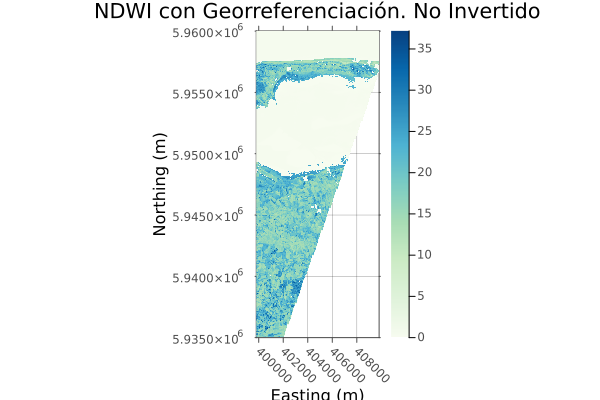
\includegraphics[width=0.8\textwidth,height=\textheight]{./images/julia_ndwi_correct.png}
\end{center}
\begin{center}
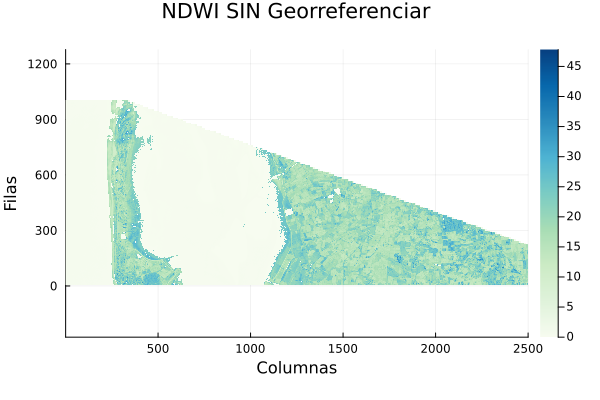
\includegraphics[width=0.8\textwidth,height=\textheight]{./images/julia_ndwi_bad.png}
\end{center}

\begin{Shaded}
\begin{Highlighting}[]
\FunctionTok{j\_eval}\NormalTok{(}\StringTok{\textquotesingle{}}
\StringTok{\# {-}{-}{-}{-}{-}{-}{-}{-}{-}{-}{-}{-}{-}{-}{-}{-}{-}{-}{-}{-}{-}{-}{-}{-}{-}{-}{-}{-}{-}{-}{-}}
\StringTok{\# IMPORTACIÓN DE LIBRERÍAS}
\StringTok{\# {-}{-}{-}{-}{-}{-}{-}{-}{-}{-}{-}{-}{-}{-}{-}{-}{-}{-}{-}{-}{-}{-}{-}{-}{-}{-}{-}{-}{-}{-}{-}}
\StringTok{using Rasters}
\StringTok{using ArchGDAL}
\StringTok{using Plots}

\StringTok{\# {-}{-}{-}{-}{-}{-}{-}{-}{-}{-}{-}{-}{-}{-}{-}{-}{-}{-}{-}{-}{-}{-}{-}{-}{-}{-}{-}{-}{-}{-}{-}}
\StringTok{\# CONFIGURACIÓN DE RUTAS}
\StringTok{\# {-}{-}{-}{-}{-}{-}{-}{-}{-}{-}{-}{-}{-}{-}{-}{-}{-}{-}{-}{-}{-}{-}{-}{-}{-}{-}{-}{-}{-}{-}{-}}
\StringTok{ruta\_txt = "data/s2\_shared\_path.txt"}
\StringTok{ruta\_salida = "data\_heavy/raster/ndwi\_sentinel\_optimizado\_julia.tif"}

\StringTok{\# Definimos el directorio físico donde depositaremos los gráficos generados.}
\StringTok{\# Al estar ejecutando Julia dentro de R mediante j\_eval, los gráficos generados}
\StringTok{\# no siempre se envían a la salida estándar visual. Escribirlos en disco garantiza }
\StringTok{\# que Quarto pueda integrarlos en el documento final.}
\StringTok{dir\_graficos = "./images/"}
\StringTok{mkpath(dir\_graficos)}

\StringTok{if !isfile(ruta\_txt)}
\StringTok{    println("ERROR: Insumo ausente en ", ruta\_txt)}
\StringTok{else}
\StringTok{    try}
\StringTok{        \# {-}{-}{-}{-}{-}{-}{-}{-}{-}{-}{-}{-}{-}{-}{-}{-}{-}{-}{-}{-}{-}{-}{-}{-}{-}{-}{-}{-}{-}{-}{-}}
\StringTok{        \# LECTURA DE LA RUTA DEL RASTER}
\StringTok{        \# {-}{-}{-}{-}{-}{-}{-}{-}{-}{-}{-}{-}{-}{-}{-}{-}{-}{-}{-}{-}{-}{-}{-}{-}{-}{-}{-}{-}{-}{-}{-}}
\StringTok{        s2\_path = strip(read(ruta\_txt, String))}
\StringTok{        }
\StringTok{        \# {-}{-}{-}{-}{-}{-}{-}{-}{-}{-}{-}{-}{-}{-}{-}{-}{-}{-}{-}{-}{-}{-}{-}{-}{-}{-}{-}{-}{-}{-}{-}}
\StringTok{        \# OPTIMIZACIÓN 1: EXTRACCIÓN DE BAJO NIVEL (BUFFER)}
\StringTok{        \# {-}{-}{-}{-}{-}{-}{-}{-}{-}{-}{-}{-}{-}{-}{-}{-}{-}{-}{-}{-}{-}{-}{-}{-}{-}{-}{-}{-}{-}{-}{-}}
\StringTok{        \# Definición de coordenadas base 1 (estándar de Julia)}
\StringTok{        c\_start, c\_end = 9981, 10980}
\StringTok{        r\_start, r\_end = 4001, 6500}

\StringTok{        \# Conversión a parámetros espaciales base 0 (estándar de C/GDAL)}
\StringTok{        xoff = c\_start {-} 1}
\StringTok{        yoff = r\_start {-} 1}
\StringTok{        xcols = c\_end {-} c\_start + 1}
\StringTok{        yrows = r\_end {-} r\_start + 1}

\StringTok{        \# Usamos ArchGDAL nativo para transferir directamente el bloque de bytes a la RAM.}
\StringTok{        \# Esto es altamente eficiente y a prueba de fallos con archivos virtuales (.zip).}
\StringTok{        green\_mat, nir\_mat = ArchGDAL.read(String(s2\_path)) do ds}
\StringTok{            g\_mat = ArchGDAL.read(ds, 2, xoff, yoff, xcols, yrows)}
\StringTok{            n\_mat = ArchGDAL.read(ds, 4, xoff, yoff, xcols, yrows)}
\StringTok{            return g\_mat, n\_mat}
\StringTok{        end}
\StringTok{        }
\StringTok{        \# {-}{-}{-}{-}{-}{-}{-}{-}{-}{-}{-}{-}{-}{-}{-}{-}{-}{-}{-}{-}{-}{-}{-}{-}{-}{-}{-}{-}{-}{-}{-}}
\StringTok{        \# CÁLCULO DEL NDWI}
\StringTok{        \# {-}{-}{-}{-}{-}{-}{-}{-}{-}{-}{-}{-}{-}{-}{-}{-}{-}{-}{-}{-}{-}{-}{-}{-}{-}{-}{-}{-}{-}{-}{-}}
\StringTok{        denominador = green\_mat .+ nir\_mat}
\StringTok{        }
\StringTok{        \# El resultado es un Array de Julia puro [Columnas, Filas] sin inteligencia espacial.}
\StringTok{        \# Si lo graficáramos ahora, saldría rotado e invertido.}
\StringTok{        ndwi\_mat = ifelse.(denominador .\textgreater{} 0, (green\_mat .{-} nir\_mat) ./ denominador, NaN32)}
\StringTok{        }
\StringTok{        \# {-}{-}{-}{-}{-}{-}{-}{-}{-}{-}{-}{-}{-}{-}{-}{-}{-}{-}{-}{-}{-}{-}{-}{-}{-}{-}{-}{-}{-}{-}{-}}
\StringTok{        \# RECONSTRUCCIÓN ESPACIAL Y ESCRITURA}
\StringTok{        \# {-}{-}{-}{-}{-}{-}{-}{-}{-}{-}{-}{-}{-}{-}{-}{-}{-}{-}{-}{-}{-}{-}{-}{-}{-}{-}{-}{-}{-}{-}{-}}
\StringTok{        \# Para arreglar la matriz, extraemos las dimensiones reales del archivo fuente.}
\StringTok{        \# Al usar lazy=true, solo leemos los metadatos (Extent, CRS, Resolución) sin gastar RAM.}
\StringTok{        src = ArchGDAL.read(String(s2\_path)) do ds}
\StringTok{            Raster(ds; lazy=true)}
\StringTok{        end}

\StringTok{        \# Creamos una "vista" de los metadatos para nuestro recorte}
\StringTok{        src\_crop = view(src, X(c\_start:c\_end), Y(r\_start:r\_end))}

\StringTok{        \# ¡LA MAGIA OCURRE AQUÍ!}
\StringTok{        \# Fusionamos la matriz cruda con los metadatos espaciales (dims).}
\StringTok{        \# Ahora el objeto sabe exactamente dónde está el Norte y cuánto mide cada píxel.}
\StringTok{        ndwi\_rast = Raster(Float32.(ndwi\_mat), dims(src\_crop, (X, Y)))}

\StringTok{        \# Guardamos en disco}
\StringTok{        mkpath(dirname(ruta\_salida))}
\StringTok{        write(ruta\_salida, ndwi\_rast, force=true, }
\StringTok{            options=Dict("COMPRESS"=\textgreater{}"LZW", "TILED"=\textgreater{}"YES"))}

\StringTok{        println("Proceso optimizado exitoso. Archivo guardado en: ", ruta\_salida)}

\StringTok{        \# {-}{-}{-}{-}{-}{-}{-}{-}{-}{-}{-}{-}{-}{-}{-}{-}{-}{-}{-}{-}{-}{-}{-}{-}{-}{-}}
\StringTok{        \# VISUALIZACIÓN CARTOGRÁFICA}
\StringTok{        \# {-}{-}{-}{-}{-}{-}{-}{-}{-}{-}{-}{-}{-}{-}{-}{-}{-}{-}{-}{-}{-}{-}{-}{-}{-}{-}}
\StringTok{        \# Al graficar ndwi\_rast, Plots.jl detecta que es un objeto espacial (no una matriz simple).}
\StringTok{        \# El motor gráfico alinea automáticamente el eje Y con el Norte real y el eje X con el Este,}
\StringTok{        \# corrigiendo cualquier rotación nativa de la memoria.}
\StringTok{        }
\StringTok{        p\_good = plot(ndwi\_rast, }
\StringTok{                      c=:GnBu, }
\StringTok{                      title="NDWI Georreferenciado",}
\StringTok{                      xlabel="Este (Metros)", }
\StringTok{                      ylabel="Norte (Metros)",}
\StringTok{                      aspect\_ratio=:equal) \# Evita que los píxeles se estiren}
\StringTok{                      }
\StringTok{        \# Guardamos la figura georreferenciada correctamente}
\StringTok{        ruta\_p\_good = joinpath(dir\_graficos, "julia\_ndwi\_good.png")}
\StringTok{        savefig(p\_good, ruta\_p\_good)}
\StringTok{        println("Gráfico espacial exportado: ", ruta\_p\_good)}

\StringTok{        \# {-}{-}{-}{-}{-}{-}{-}{-}{-}{-}{-}{-}{-}{-}{-}{-}{-}{-}{-}{-}{-}{-}{-}{-}{-}{-}{-}{-}{-}{-}{-}{-}{-}{-}{-}{-}{-}{-}{-}{-}{-}{-}{-}{-}{-}{-}{-}{-}{-}{-}{-}{-}{-}{-}{-}{-}{-}{-}{-}{-}{-}{-}{-}{-}{-}{-}{-}{-}{-}{-}{-}{-}{-}}
\StringTok{        \# VISUALIZACIÓN CARTOGRÁFICA 2: LA SOLUCIÓN MANUAL (Matriz cruda corregida)}
\StringTok{        \# {-}{-}{-}{-}{-}{-}{-}{-}{-}{-}{-}{-}{-}{-}{-}{-}{-}{-}{-}{-}{-}{-}{-}{-}{-}{-}{-}{-}{-}{-}{-}{-}{-}{-}{-}{-}{-}{-}{-}{-}{-}{-}{-}{-}{-}{-}{-}{-}{-}{-}{-}{-}{-}{-}{-}{-}{-}{-}{-}{-}{-}{-}{-}{-}{-}{-}{-}{-}{-}{-}{-}{-}{-}}
\StringTok{        \# Si graficamos la matriz cruda \textasciigrave{}ndwi\_mat\textasciigrave{} sola, saldrá rotada e invertida.}
\StringTok{        \# Para corregirlo usando heatmap(), aplicamos dos operaciones matemáticas:}
\StringTok{        \# 1. ndwi\_mat}\SpecialCharTok{\textbackslash{}\textquotesingle{}}\StringTok{ (Transpuesta): Convierte [X, Y] a [Y, X], evitando la rotación de 90°.}
\StringTok{        \# 2. yflip=true: Invierte visualmente el eje Y para que el índice 1 quede arriba (Norte).}

\StringTok{        ndwi\_mat\_transpuesta = ndwi\_mat}\SpecialCharTok{\textbackslash{}\textquotesingle{}}

\StringTok{        p\_manual = heatmap(ndwi\_mat\_transpuesta, }
\StringTok{                           c=:GnBu, }
\StringTok{                           yflip=true, \# Invertimos el eje Y desde el motor gráfico}
\StringTok{                           title="2. Solución Manual (Matriz Transpuesta e Invertida)",}
\StringTok{                           xlabel="Columnas (X)", }
\StringTok{                           ylabel="Filas (Y)",}
\StringTok{                           aspect\_ratio=:equal)}
\StringTok{                           }
\StringTok{        \# Exportamos la figura corregida vía motor gráfico}
\StringTok{        ruta\_p\_manual = joinpath(dir\_graficos, "julia\_ndwi\_manual\_yflip.png")}
\StringTok{        savefig(p\_manual, ruta\_p\_manual)}
\StringTok{        println("Gráfico manual (yflip) exportado: ", ruta\_p\_manual)}

\StringTok{        \# {-}{-}{-}{-}{-}{-}{-}{-}{-}{-}{-}{-}{-}{-}{-}{-}{-}{-}{-}{-}{-}{-}{-}{-}{-}{-}{-}{-}{-}{-}{-}{-}{-}{-}{-}{-}{-}{-}{-}{-}{-}{-}}
\StringTok{        \# ALTERNATIVA A VISUALIZACIÓN CARTOGRÁFICA 2}
\StringTok{        \# {-}{-}{-}{-}{-}{-}{-}{-}{-}{-}{-}{-}{-}{-}{-}{-}{-}{-}{-}{-}{-}{-}{-}{-}{-}{-}{-}{-}{-}{-}{-}{-}{-}{-}{-}{-}{-}{-}{-}{-}{-}{-}}
\StringTok{        \# Preparamos la matriz matemáticamente en la memoria ANTES de graficarla:}
\StringTok{        \# 1. ndwi\_mat}\SpecialCharTok{\textbackslash{}\textquotesingle{}}\StringTok{ (Transpuesta): Cambia [X, Y] a [Y, X] para evitar que salga acostada.}
\StringTok{        \# 2. reverse(..., dims=1): Invierte el eje Y físicamente en la memoria para que }
\StringTok{        \#    la fila 1 (Norte) quede reordenada correctamente.}
\StringTok{        ndwi\_mat\_corregida = reverse(ndwi\_mat}\SpecialCharTok{\textbackslash{}\textquotesingle{}}\StringTok{, dims=1)}
\StringTok{        }
\StringTok{        \# Ahora pasamos la matriz ya estructurada y omitimos el parámetro yflip=true}
\StringTok{        p\_manual\_rev = heatmap(ndwi\_mat\_corregida, }
\StringTok{                               c=:GnBu, }
\StringTok{                               title="3. Alternativa Manual (Matriz pre{-}reversada)",}
\StringTok{                               xlabel="Columnas (X)", }
\StringTok{                               ylabel="Filas (Y)",}
\StringTok{                               aspect\_ratio=:equal)}
\StringTok{                               }
\StringTok{        \# Exportamos la alternativa estructural}
\StringTok{        ruta\_p\_manual\_rev = joinpath(dir\_graficos, "julia\_ndwi\_manual\_reverse.png")}
\StringTok{        savefig(p\_manual\_rev, ruta\_p\_manual\_rev)}
\StringTok{        println("Gráfico manual (reverse) exportado: ", ruta\_p\_manual\_rev)}
\StringTok{        }
\StringTok{    catch e}
\StringTok{        println("Error crítico en el flujo de trabajo: ", e)}
\StringTok{    end}
\StringTok{end}
\StringTok{\textquotesingle{}}\NormalTok{)}

\CommentTok{\# {-}{-}{-}{-}{-}{-}{-}{-}{-}{-}{-}{-}{-}{-}{-}{-}{-}{-}{-}{-}{-}{-}{-}{-}{-}{-}{-}{-}{-}{-}{-}{-}{-}{-}{-}{-}{-}{-}{-}{-}{-}{-}{-}{-}{-}{-}{-}{-}{-}{-}{-}{-}{-}{-}{-}{-}{-}{-}{-}{-}{-}{-}{-}{-}{-}{-}{-}{-}{-}{-}{-}{-}{-}}
\CommentTok{\# IMPORTACIÓN AL DOCUMENTO QUARTO MEDIANTE KNITR}
\CommentTok{\# {-}{-}{-}{-}{-}{-}{-}{-}{-}{-}{-}{-}{-}{-}{-}{-}{-}{-}{-}{-}{-}{-}{-}{-}{-}{-}{-}{-}{-}{-}{-}{-}{-}{-}{-}{-}{-}{-}{-}{-}{-}{-}{-}{-}{-}{-}{-}{-}{-}{-}{-}{-}{-}{-}{-}{-}{-}{-}{-}{-}{-}{-}{-}{-}{-}{-}{-}{-}{-}{-}{-}{-}{-}}
\CommentTok{\# include\_graphics inyecta las tres imágenes secuencialmente en el documento,}
\CommentTok{\# aplicando las configuraciones del chunk (\#| fig{-}align: center y \#| out{-}width: "80\%")}
\NormalTok{knitr}\SpecialCharTok{::}\FunctionTok{include\_graphics}\NormalTok{(}\FunctionTok{c}\NormalTok{(}
  \StringTok{"./images/julia\_ndwi\_good.png"}\NormalTok{, }
  \StringTok{"./images/julia\_ndwi\_manual\_yflip.png"}\NormalTok{, }
  \StringTok{"./images/julia\_ndwi\_manual\_reverse.png"}
\NormalTok{))}
\end{Highlighting}
\end{Shaded}

\subsection{Resumen sintáctico}\label{resumen-sintuxe1ctico-6}

\begin{longtable}[]{@{}
  >{\raggedright\arraybackslash}p{(\columnwidth - 6\tabcolsep) * \real{0.2500}}
  >{\raggedright\arraybackslash}p{(\columnwidth - 6\tabcolsep) * \real{0.2500}}
  >{\raggedright\arraybackslash}p{(\columnwidth - 6\tabcolsep) * \real{0.2500}}
  >{\raggedright\arraybackslash}p{(\columnwidth - 6\tabcolsep) * \real{0.2500}}@{}}
\toprule\noalign{}
\begin{minipage}[b]{\linewidth}\raggedright
Operación
\end{minipage} & \begin{minipage}[b]{\linewidth}\raggedright
Python 🐍
\end{minipage} & \begin{minipage}[b]{\linewidth}\raggedright
R 🔵
\end{minipage} & \begin{minipage}[b]{\linewidth}\raggedright
Julia 🟣
\end{minipage} \\
\midrule\noalign{}
\endhead
\bottomrule\noalign{}
\endlastfoot
Leer ruta desde texto & \texttt{open(ruta).read().strip()} &
\texttt{trimws(readLines(ruta))} &
\texttt{strip(read(ruta,\ String))} \\
Apertura de raster & \texttt{rasterio.open(ruta)} & \texttt{rast(ruta)}
& \texttt{ArchGDAL.read(ruta)} / \texttt{Raster(ruta)} \\
Definición de ventana & \texttt{Window(col,\ row,\ w,\ h)} &
\texttt{ext(xmin,\ xmax,\ ymin,\ ymax)} & Índices:
\texttt{xoff,\ yoff,\ xcols,\ yrows} \\
Recorte / Extracción espacial & \texttt{src.read(banda,\ window=v)} &
\texttt{crop(src,\ ventana)} &
\texttt{ArchGDAL.read(ds,\ banda,\ x,\ y,\ w,\ h)} \\
Álgebra de mapas condicional & \texttt{np.where(cond,\ true,\ false)} &
\texttt{ifel(cond,\ true,\ false)} &
\texttt{ifelse.(cond,\ true,\ false)} \\
Extracción de metadatos (Perfil) & \texttt{src.profile} /
\texttt{src.window\_transform()} & Nativo en el objeto
\texttt{SpatRaster} & \texttt{dims(raster\_view,\ (X,\ Y))} \\
Escritura de raster a disco & \texttt{dst.write(arr,\ 1)} &
\texttt{writeRaster(rast,\ ruta)} & \texttt{write(ruta,\ rast)} \\
Visualización de matriz cruda & \texttt{plt.imshow(arr)} &
\texttt{image(...,\ t(arr))} &
\texttt{heatmap(arr\textquotesingle{})} \\
Visualización con coordenadas & \texttt{xarray.plot()} &
\texttt{plot(rast)} & \texttt{plot(rast)} \\
\end{longtable}

\section{Recorte espacial (Clipping por Bounding
Box)}\label{recorte-espacial-clipping-por-bounding-box}

Extraer una zona de interés (recorte) a partir de un raster masivo
mejora la eficiencia computacional en etapas posteriores. Esta operación
requiere definir una caja delimitadora (\emph{Bounding Box}) en las
mismas coordenadas del objeto matricial.

Para extraer las coordenadas de la zona de interés dentro de QGIS:

\begin{enumerate}
\def\labelenumi{\arabic{enumi}.}
\tightlist
\item
  Cargue la imagen a QGIS
\item
  Haga zoom a la zona de interés
\item
  Ejecute el siguiente código dentro de un scrip de Python en QGIS
  (\texttt{Ctrl\ +\ Alt\ +\ P})
\end{enumerate}

\begin{Shaded}
\begin{Highlighting}[]
\CommentTok{\# Acceder a la interfaz del lienzo de mapa (map canvas) activo}
\NormalTok{canvas }\OperatorTok{=}\NormalTok{ iface.mapCanvas()}

\CommentTok{\# Recuperar el objeto de extensión geográfica actual (QgsRectangle)}
\NormalTok{extent }\OperatorTok{=}\NormalTok{ canvas.extent()}

\CommentTok{\# Impresión de los límites espaciales del área de visualización}
\BuiltInTok{print}\NormalTok{(}\SpecialStringTok{f"X Mínimo: }\SpecialCharTok{\{}\NormalTok{extent}\SpecialCharTok{.}\NormalTok{xMinimum()}\SpecialCharTok{\}}\SpecialStringTok{"}\NormalTok{)  }\CommentTok{\# Coordenada oeste}
\BuiltInTok{print}\NormalTok{(}\SpecialStringTok{f"Y Mínimo: }\SpecialCharTok{\{}\NormalTok{extent}\SpecialCharTok{.}\NormalTok{yMinimum()}\SpecialCharTok{\}}\SpecialStringTok{"}\NormalTok{)  }\CommentTok{\# Coordenada sur}
\BuiltInTok{print}\NormalTok{(}\SpecialStringTok{f"X Máximo: }\SpecialCharTok{\{}\NormalTok{extent}\SpecialCharTok{.}\NormalTok{xMaximum()}\SpecialCharTok{\}}\SpecialStringTok{"}\NormalTok{)  }\CommentTok{\# Coordenada este}
\BuiltInTok{print}\NormalTok{(}\SpecialStringTok{f"Y Máximo: }\SpecialCharTok{\{}\NormalTok{extent}\SpecialCharTok{.}\NormalTok{yMaximum()}\SpecialCharTok{\}}\SpecialStringTok{"}\NormalTok{)  }\CommentTok{\# Coordenada norte}

\CommentTok{\# Obtención del punto central de la vista actual}
\BuiltInTok{print}\NormalTok{(}\SpecialStringTok{f"Centro: }\SpecialCharTok{\{}\NormalTok{extent}\SpecialCharTok{.}\NormalTok{center()}\SpecialCharTok{.}\NormalTok{toString()}\SpecialCharTok{\}}\SpecialStringTok{"}\NormalTok{)}
\end{Highlighting}
\end{Shaded}

\subsection{Python}

\begin{Shaded}
\begin{Highlighting}[]
\CommentTok{\# \#| eval: false}

\ImportTok{import}\NormalTok{ rioxarray}

\CommentTok{\# Cargar el raster del modelo de vientos (Huracanes)}
\NormalTok{vientos\_modelo }\OperatorTok{=}\NormalTok{ rioxarray.open\_rasterio(}\StringTok{"data\_heavy/raster/st24\_h\_50\_9377\_py.tif"}\NormalTok{)}

\CommentTok{\# Definición de coordenadas límites (Bounding Box) en sistema EPSG:9377}
\NormalTok{min\_x, min\_y }\OperatorTok{=} \FloatTok{4762861.122004522}\NormalTok{, }\FloatTok{2474583.429398312}
\NormalTok{max\_x, max\_y }\OperatorTok{=} \FloatTok{5371716.890535228}\NormalTok{, }\FloatTok{2726316.6215890343}

\CommentTok{\# Ejecución del método espacial de recorte por contorno rectangular (clip\_box)}
\CommentTok{\# Este método reduce drásticamente el tamaño del archivo al aislar solo nuestra área de interés}
\NormalTok{vientos\_recorte }\OperatorTok{=}\NormalTok{ vientos\_modelo.rio.clip\_box(minx}\OperatorTok{=}\NormalTok{min\_x, miny}\OperatorTok{=}\NormalTok{min\_y, maxx}\OperatorTok{=}\NormalTok{max\_x, maxy}\OperatorTok{=}\NormalTok{max\_y)}

\CommentTok{\# Exportación de la matriz reducida a un nuevo archivo}
\NormalTok{ruta\_salida }\OperatorTok{=} \StringTok{"data\_heavy/raster/vientos\_huracan\_recorte\_py.tif"}
\NormalTok{vientos\_recorte.rio.to\_raster(ruta\_salida)}

\BuiltInTok{print}\NormalTok{(}\SpecialStringTok{f"Proceso exitoso. Raster guardado en: }\SpecialCharTok{\{}\NormalTok{ruta\_salida}\SpecialCharTok{\}}\SpecialStringTok{"}\NormalTok{)}
\end{Highlighting}
\end{Shaded}

\begin{verbatim}
Proceso exitoso. Raster guardado en: data_heavy/raster/vientos_huracan_recorte_py.tif
\end{verbatim}

\begin{Shaded}
\begin{Highlighting}[]
\BuiltInTok{print}\NormalTok{(}\SpecialStringTok{f"Dimensiones recortadas: }\SpecialCharTok{\{}\NormalTok{vientos\_recorte}\SpecialCharTok{.}\NormalTok{rio}\SpecialCharTok{.}\NormalTok{width}\SpecialCharTok{\}}\SpecialStringTok{x}\SpecialCharTok{\{}\NormalTok{vientos\_recorte}\SpecialCharTok{.}\NormalTok{rio}\SpecialCharTok{.}\NormalTok{height}\SpecialCharTok{\}}\SpecialStringTok{"}\NormalTok{)}
\end{Highlighting}
\end{Shaded}

\begin{verbatim}
Dimensiones recortadas: 23x11
\end{verbatim}

\subsection{R}

\begin{Shaded}
\begin{Highlighting}[]
\CommentTok{\# \#| eval: false}

\FunctionTok{library}\NormalTok{(terra)}

\CommentTok{\# Cargar el raster del modelo de vientos (Huracanes)}
\NormalTok{vientos\_modelo }\OtherTok{\textless{}{-}} \FunctionTok{rast}\NormalTok{(}\StringTok{"data\_heavy/raster/st24\_h\_50\_9377\_py.tif"}\NormalTok{)}

\CommentTok{\# Construcción explícita de un objeto de extensión (xmin, xmax, ymin, ymax)}
\CommentTok{\# Utilizamos los límites exactos del Bounding Box en EPSG:9377}
\NormalTok{extension\_recorte }\OtherTok{\textless{}{-}} \FunctionTok{ext}\NormalTok{(}\FloatTok{4762861.122004522}\NormalTok{, }\FloatTok{5371716.890535228}\NormalTok{, }\FloatTok{2474583.429398312}\NormalTok{, }\FloatTok{2726316.6215890343}\NormalTok{)}

\CommentTok{\# Uso de la función crop para extraer la sub{-}cuadrícula de interés}
\CommentTok{\# Esto recorta el área del huracán y descarta el resto de los datos}
\NormalTok{vientos\_recorte }\OtherTok{\textless{}{-}} \FunctionTok{crop}\NormalTok{(vientos\_modelo, extension\_recorte)}

\CommentTok{\# Escritura a disco del raster reducido}
\NormalTok{ruta\_salida }\OtherTok{\textless{}{-}} \StringTok{"data\_heavy/raster/vientos\_huracan\_recorte\_r.tif"}
\FunctionTok{writeRaster}\NormalTok{(vientos\_recorte, ruta\_salida, }\AttributeTok{overwrite=}\ConstantTok{TRUE}\NormalTok{)}

\FunctionTok{cat}\NormalTok{(}\StringTok{"Proceso exitoso. Raster guardado en:"}\NormalTok{, ruta\_salida, }\StringTok{"}\SpecialCharTok{\textbackslash{}n}\StringTok{"}\NormalTok{)}
\end{Highlighting}
\end{Shaded}

\begin{verbatim}
Proceso exitoso. Raster guardado en: data_heavy/raster/vientos_huracan_recorte_r.tif 
\end{verbatim}

\begin{Shaded}
\begin{Highlighting}[]
\FunctionTok{cat}\NormalTok{(}\StringTok{"Dimensiones recortadas (filas, columnas, bandas): "}\NormalTok{)}
\end{Highlighting}
\end{Shaded}

\begin{verbatim}
Dimensiones recortadas (filas, columnas, bandas): 
\end{verbatim}

\begin{Shaded}
\begin{Highlighting}[]
\FunctionTok{print}\NormalTok{(}\FunctionTok{dim}\NormalTok{(vientos\_recorte))}
\end{Highlighting}
\end{Shaded}

\begin{verbatim}
[1]  9 22  1
\end{verbatim}

\subsection{Julia}

\begin{Shaded}
\begin{Highlighting}[]
\FunctionTok{j\_eval}\NormalTok{(}\StringTok{\textquotesingle{}}
\StringTok{using Rasters}

\StringTok{\# {-}{-}{-}{-}{-}{-}{-}{-}{-}{-}{-}{-}{-}{-}{-}{-}{-}{-}{-}{-}{-}{-}{-}{-}{-}{-}{-}{-}{-}{-}{-}{-}{-}{-}{-}{-}{-}{-}{-}{-}{-}{-}{-}{-}{-}{-}{-}{-}{-}{-}{-}{-}{-}{-}{-}{-}{-}{-}{-}{-}{-}{-}{-}{-}{-}{-}{-}{-}{-}{-}{-}{-}{-}}
\StringTok{\# 1. CARGA DEL RASTER ORIGINAL}
\StringTok{\# {-}{-}{-}{-}{-}{-}{-}{-}{-}{-}{-}{-}{-}{-}{-}{-}{-}{-}{-}{-}{-}{-}{-}{-}{-}{-}{-}{-}{-}{-}{-}{-}{-}{-}{-}{-}{-}{-}{-}{-}{-}{-}{-}{-}{-}{-}{-}{-}{-}{-}{-}{-}{-}{-}{-}{-}{-}{-}{-}{-}{-}{-}{-}{-}{-}{-}{-}{-}{-}{-}{-}{-}{-}}
\StringTok{\# Cargamos el modelo de vientos (Huracanes) en sistema de coordenadas 9377.}
\StringTok{\# El uso de ";" seguido de "nothing" evita el volcado de metadatos en la consola.}
\StringTok{vientos\_modelo = Raster("data\_heavy/raster/st24\_h\_50\_9377\_py.tif"); nothing}

\StringTok{\# {-}{-}{-}{-}{-}{-}{-}{-}{-}{-}{-}{-}{-}{-}{-}{-}{-}{-}{-}{-}{-}{-}{-}{-}{-}{-}{-}{-}{-}{-}{-}{-}{-}{-}{-}{-}{-}{-}{-}{-}{-}{-}{-}{-}{-}{-}{-}{-}{-}{-}{-}{-}{-}{-}{-}{-}{-}{-}{-}{-}{-}{-}{-}{-}{-}{-}{-}{-}{-}{-}{-}{-}{-}}
\StringTok{\# 2. RECORTE ESPACIAL MEDIANTE PREDICADOS}
\StringTok{\# {-}{-}{-}{-}{-}{-}{-}{-}{-}{-}{-}{-}{-}{-}{-}{-}{-}{-}{-}{-}{-}{-}{-}{-}{-}{-}{-}{-}{-}{-}{-}{-}{-}{-}{-}{-}{-}{-}{-}{-}{-}{-}{-}{-}{-}{-}{-}{-}{-}{-}{-}{-}{-}{-}{-}{-}{-}{-}{-}{-}{-}{-}{-}{-}{-}{-}{-}{-}{-}{-}{-}{-}{-}}
\StringTok{\# En Julia/Rasters, el recorte se realiza mediante indexación dimensional.}
\StringTok{\# Utilizamos "Between(min, max)" para definir el rango geográfico exacto }
\StringTok{\# (Bounding Box) proporcionado para el área del huracán.}
\StringTok{vientos\_recorte = vientos\_modelo[}
\StringTok{    X(Between(4762861.122004522, 5371716.890535228)), }
\StringTok{    Y(Between(2474583.429398312, 2726316.6215890343))}
\StringTok{]; nothing}

\StringTok{\# {-}{-}{-}{-}{-}{-}{-}{-}{-}{-}{-}{-}{-}{-}{-}{-}{-}{-}{-}{-}{-}{-}{-}{-}{-}{-}{-}{-}{-}{-}{-}{-}{-}{-}{-}{-}{-}{-}{-}{-}{-}{-}{-}{-}{-}{-}{-}{-}{-}{-}{-}{-}{-}{-}{-}{-}{-}{-}{-}{-}{-}{-}{-}{-}{-}{-}{-}{-}{-}{-}{-}{-}{-}}
\StringTok{\# 3. EXPORTACIÓN Y REPORTE}
\StringTok{\# {-}{-}{-}{-}{-}{-}{-}{-}{-}{-}{-}{-}{-}{-}{-}{-}{-}{-}{-}{-}{-}{-}{-}{-}{-}{-}{-}{-}{-}{-}{-}{-}{-}{-}{-}{-}{-}{-}{-}{-}{-}{-}{-}{-}{-}{-}{-}{-}{-}{-}{-}{-}{-}{-}{-}{-}{-}{-}{-}{-}{-}{-}{-}{-}{-}{-}{-}{-}{-}{-}{-}{-}{-}}
\StringTok{ruta\_salida = "data\_heavy/raster/vientos\_huracan\_recorte\_julia.tif"}
\StringTok{write(ruta\_salida, vientos\_recorte); nothing}

\StringTok{\# Imprimimos las dimensiones resultantes para verificar la reducción del dataset}
\StringTok{println("Proceso de recorte finalizado con éxito.")}
\StringTok{println("Ruta de salida: ", ruta\_salida)}
\StringTok{println("Dimensiones de la grilla extraída: ", size(vientos\_recorte))}
\StringTok{println("Metadatos de dimensiones: ", dims(vientos\_recorte))}
\StringTok{\textquotesingle{}}\NormalTok{)}
\end{Highlighting}
\end{Shaded}

\subsection{Resumen sintáctico}\label{resumen-sintuxe1ctico-7}

\begin{longtable}[]{@{}
  >{\raggedright\arraybackslash}p{(\columnwidth - 6\tabcolsep) * \real{0.2500}}
  >{\raggedright\arraybackslash}p{(\columnwidth - 6\tabcolsep) * \real{0.2500}}
  >{\raggedright\arraybackslash}p{(\columnwidth - 6\tabcolsep) * \real{0.2500}}
  >{\raggedright\arraybackslash}p{(\columnwidth - 6\tabcolsep) * \real{0.2500}}@{}}
\toprule\noalign{}
\begin{minipage}[b]{\linewidth}\raggedright
Operación
\end{minipage} & \begin{minipage}[b]{\linewidth}\raggedright
Python 🐍
\end{minipage} & \begin{minipage}[b]{\linewidth}\raggedright
R 🔵
\end{minipage} & \begin{minipage}[b]{\linewidth}\raggedright
Julia 🟣
\end{minipage} \\
\midrule\noalign{}
\endhead
\bottomrule\noalign{}
\endlastfoot
Cargar ráster & \texttt{rioxarray.open\_rasterio()} & \texttt{rast()} &
\texttt{Raster()} \\
Definir extensión & Parámetros \texttt{minx,\ miny,\ maxx,\ maxy} &
\texttt{ext(xmin,\ xmax,\ ymin,\ ymax)} & Predicados
\texttt{Between(min,\ max)} \\
Ejecutar recorte & \texttt{raster.rio.clip\_box()} & \texttt{crop()} &
\texttt{raster{[}X(...),\ Y(...){]}} \\
Guardar ráster & \texttt{raster.rio.to\_raster()} &
\texttt{writeRaster()} & \texttt{write()} \\
Consultar tamaño & \texttt{raster.rio.width} / \texttt{.height} &
\texttt{dim()} & \texttt{size()} \\
\end{longtable}

\section{Descarga de datos ráster desde la
nube}\label{descarga-de-datos-ruxe1ster-desde-la-nube}

La adquisición de Modelos Digitales de Elevación (MDE) es un paso común
en la programación SIG. Tradicionalmente, la descarga manual de estos
insumos presentaba cuellos de botella geográficos y computacionales.
Actualmente, plataformas como Google Earth Engine (GEE) permiten acceder
al catálogo global del \emph{Shuttle Radar Topography Mission} (SRTM) y
procesar los recortes de interés directamente en la nube. Este enfoque
reduce el ancho de banda requerido y estandariza el preprocesamiento de
los datos, facilitando el análisis topográfico para áreas específicas
como la Sabana de Bogotá y el campus de la Universidad Nacional de
Colombia.

\subsection{Inicialización del entorno
GEE}\label{inicializaciuxf3n-del-entorno-gee}

El primer paso para interactuar con la API de Earth Engine es la
autenticación e inicialización del cliente. Este proceso verifica las
credenciales de acceso asociadas al proyecto de Google Cloud.

\subsubsection{Python}

\begin{Shaded}
\begin{Highlighting}[]
\CommentTok{\# \#| eval: false}

\CommentTok{\# 1. IMPORTACIÓN DE LIBRERÍAS}
\CommentTok{\# \textquotesingle{}ee\textquotesingle{} es la librería principal de Google Earth Engine.}
\ImportTok{import}\NormalTok{ ee}

\CommentTok{\# 2. AUTENTICACIÓN}
\CommentTok{\# Este comando abre una ventana en el navegador para dar permisos a Google.}
\CommentTok{\# Solo es necesario correrlo la primera vez o si el token de acceso expira.}
\NormalTok{ee.Authenticate()}
\end{Highlighting}
\end{Shaded}

\begin{verbatim}
True
\end{verbatim}

\begin{Shaded}
\begin{Highlighting}[]
\CommentTok{\# 3. INICIALIZACIÓN DEL PROYECTO}
\CommentTok{\# Debemos especificar el ID del proyecto que creamos en Google Cloud.}
\CommentTok{\# Para este curso usamos el proyecto: "ee{-}giswqg"}
\NormalTok{ee.Initialize(project}\OperatorTok{=}\StringTok{"ee{-}giswqg"}\NormalTok{)}

\BuiltInTok{print}\NormalTok{(}\StringTok{"Google Earth Engine se ha inicializado con éxito!"}\NormalTok{)}
\end{Highlighting}
\end{Shaded}

\begin{verbatim}
Google Earth Engine se ha inicializado con éxito!
\end{verbatim}

\subsubsection{R}

\begin{Shaded}
\begin{Highlighting}[]
\CommentTok{\# 1. IMPORTACIÓN DE LIBRERÍAS}
\CommentTok{\# \textquotesingle{}rgee\textquotesingle{} es el paquete puente de R hacia la API de Python de Earth Engine.}
\FunctionTok{library}\NormalTok{(rgee) }\CommentTok{\# Librería no instalada en el contenedor}

\CommentTok{\# 2. INICIALIZACIÓN Y AUTENTICACIÓN}
\CommentTok{\# La función ee\_Initialize gestiona tanto la autenticación como la inicialización.}
\CommentTok{\# Especificamos el proyecto de Google Cloud correspondiente.}
\FunctionTok{ee\_Initialize}\NormalTok{(}\AttributeTok{project =} \StringTok{"ee{-}giswqg"}\NormalTok{)}

\FunctionTok{print}\NormalTok{(}\StringTok{"Google Earth Engine se ha inicializado con éxito en R!"}\NormalTok{)}
\end{Highlighting}
\end{Shaded}

\subsubsection{Julia}

\begin{Shaded}
\begin{Highlighting}[]
\FunctionTok{j\_eval}\NormalTok{(}\StringTok{\textquotesingle{}}
\StringTok{\# 1. IMPORTACIÓN DE LIBRERÍAS}
\StringTok{\# Julia utiliza PyCall para interactuar nativamente con la API de Python de Earth Engine.}
\StringTok{using PyCall  \# Librería no instalada en el contenedor}
\StringTok{const ee = pyimport("ee")}

\StringTok{\# 2. AUTENTICACIÓN}
\StringTok{\# ee.Authenticate() invoca la ventana del navegador si el token no existe.}
\StringTok{ee.Authenticate()}

\StringTok{\# 3. INICIALIZACIÓN DEL PROYECTO}
\StringTok{\# Especificamos el ID del proyecto de Google Cloud.}
\StringTok{ee.Initialize(project="ee{-}giswqg")}

\StringTok{println("Google Earth Engine se ha inicializado con éxito en Julia!")}
\StringTok{\textquotesingle{}}\NormalTok{)}
\end{Highlighting}
\end{Shaded}

\subsection{Descarga del SRTM a GeoTiff mediante librerías
integradas}\label{descarga-del-srtm-a-geotiff-mediante-libreruxedas-integradas}

Librerías de terceros facilitan la conversión y empaquetado de las
estructuras de datos de Earth Engine hacia formatos locales como
GeoTIFF. Cuando los paquetes de ayuda (como \texttt{geedim} o
dependencias de subprocesamiento) no se encuentran disponibles en el
entorno, se pueden usar alternativas de descarga nativa con el API de
GEE.

\subsubsection{Python}

\begin{Shaded}
\begin{Highlighting}[]
\CommentTok{\# {-}{-}{-}{-}{-}{-}{-}{-}{-}{-}{-}{-}{-}{-}{-}{-}{-}{-}{-}{-}{-}{-}{-}{-}{-}{-}{-}{-}{-}{-}{-}}
\CommentTok{\# 1. IMPORTACIÓN DE LIBRERÍAS}
\CommentTok{\# {-}{-}{-}{-}{-}{-}{-}{-}{-}{-}{-}{-}{-}{-}{-}{-}{-}{-}{-}{-}{-}{-}{-}{-}{-}{-}{-}{-}{-}{-}{-}}
\ImportTok{import}\NormalTok{ ee}
\ImportTok{import}\NormalTok{ geemap}
\ImportTok{import}\NormalTok{ os}
\CommentTok{\# import geedim  \#Nota: no está instalada en el contenedor}

\CommentTok{\# {-}{-}{-}{-}{-}{-}{-}{-}{-}{-}{-}{-}{-}{-}{-}{-}{-}{-}{-}{-}{-}{-}{-}{-}{-}{-}{-}{-}{-}{-}{-}}
\CommentTok{\# 2. CARGA DEL MODELO DIGITAL DE ELEVACIÓN}
\CommentTok{\# {-}{-}{-}{-}{-}{-}{-}{-}{-}{-}{-}{-}{-}{-}{-}{-}{-}{-}{-}{-}{-}{-}{-}{-}{-}{-}{-}{-}{-}{-}{-}}
\CommentTok{\# Cargamos la imagen global de SRTM (30 metros de resolución)}
\NormalTok{srtm }\OperatorTok{=}\NormalTok{ ee.Image(}\StringTok{"USGS/SRTMGL1\_003"}\NormalTok{)}

\CommentTok{\# {-}{-}{-}{-}{-}{-}{-}{-}{-}{-}{-}{-}{-}{-}{-}{-}{-}{-}{-}{-}{-}{-}{-}{-}{-}{-}{-}{-}{-}{-}{-}}
\CommentTok{\# 3. DEFINICIÓN DEL ÁREA DE DESCARGA (BOGOTÁ)}
\CommentTok{\# {-}{-}{-}{-}{-}{-}{-}{-}{-}{-}{-}{-}{-}{-}{-}{-}{-}{-}{-}{-}{-}{-}{-}{-}{-}{-}{-}{-}{-}{-}{-}}
\CommentTok{\# Definimos el punto base (Universidad Nacional)}
\NormalTok{unal\_punto }\OperatorTok{=}\NormalTok{ ee.Geometry.Point([}\OperatorTok{{-}}\FloatTok{74.084}\NormalTok{, }\FloatTok{4.638}\NormalTok{])}

\CommentTok{\# Creamos una "caja delimitadora" (Bounding Box) alrededor del punto.}
\CommentTok{\# Usamos un buffer de 15,000 metros (15 km) de radio y extraemos sus límites (.bounds())}
\NormalTok{roi\_bogota }\OperatorTok{=}\NormalTok{ unal\_punto.}\BuiltInTok{buffer}\NormalTok{(}\DecValTok{15000}\NormalTok{).bounds()}

\CommentTok{\# {-}{-}{-}{-}{-}{-}{-}{-}{-}{-}{-}{-}{-}{-}{-}{-}{-}{-}{-}{-}{-}{-}{-}{-}{-}{-}{-}{-}{-}{-}{-}}
\CommentTok{\# 4. CONFIGURACIÓN DE LA RUTA LOCAL}
\CommentTok{\# {-}{-}{-}{-}{-}{-}{-}{-}{-}{-}{-}{-}{-}{-}{-}{-}{-}{-}{-}{-}{-}{-}{-}{-}{-}{-}{-}{-}{-}{-}{-}}
\NormalTok{directorio\_salida }\OperatorTok{=} \StringTok{"data\_heavy/raster"}

\CommentTok{\# os.makedirs asegura que la carpeta exista antes de intentar guardar el archivo}
\NormalTok{os.makedirs(directorio\_salida, exist\_ok}\OperatorTok{=}\VariableTok{True}\NormalTok{)}
\NormalTok{ruta\_tif }\OperatorTok{=}\NormalTok{ os.path.join(directorio\_salida, }\StringTok{"mde\_bogota\_srtm\_elevation.tif"}\NormalTok{)}

\CommentTok{\# {-}{-}{-}{-}{-}{-}{-}{-}{-}{-}{-}{-}{-}{-}{-}{-}{-}{-}{-}{-}{-}{-}{-}{-}{-}{-}{-}{-}{-}{-}{-}}
\CommentTok{\# 5. EJECUCIÓN DE LA DESCARGA}
\CommentTok{\# {-}{-}{-}{-}{-}{-}{-}{-}{-}{-}{-}{-}{-}{-}{-}{-}{-}{-}{-}{-}{-}{-}{-}{-}{-}{-}{-}{-}{-}{-}{-}}
\BuiltInTok{print}\NormalTok{(}\StringTok{"Iniciando la petición al servidor de Earth Engine..."}\NormalTok{)}
\BuiltInTok{print}\NormalTok{(}\StringTok{"Descargando GeoTIFF (esto puede tomar unos segundos/minutos dependiendo de tu conexión)..."}\NormalTok{)}

\CommentTok{\# geemap procesa la imagen en los servidores de Google, la empaqueta y la descarga a tu PC}
\NormalTok{geemap.download\_ee\_image(}
\NormalTok{    image}\OperatorTok{=}\NormalTok{srtm,}
\NormalTok{    filename}\OperatorTok{=}\NormalTok{ruta\_tif,}
\NormalTok{    scale}\OperatorTok{=}\DecValTok{30}\NormalTok{,           }\CommentTok{\# Resolución espacial original del SRTM (30 metros/píxel)}
\NormalTok{    region}\OperatorTok{=}\NormalTok{roi\_bogota,  }\CommentTok{\# Forzamos el recorte al área de Bogotá}
\NormalTok{    crs}\OperatorTok{=}\StringTok{"EPSG:4326"}     \CommentTok{\# Guardamos nativamente en coordenadas geográficas WGS84}
\NormalTok{)}

\BuiltInTok{print}\NormalTok{(}\SpecialStringTok{f"}\CharTok{\textbackslash{}n}\SpecialStringTok{ DESCARGA COMPLETADA CON ÉXITO"}\NormalTok{)}
\BuiltInTok{print}\NormalTok{(}\SpecialStringTok{f"El MDE de Bogotá está disponible físicamente en: }\SpecialCharTok{\{}\NormalTok{ruta\_tif}\SpecialCharTok{\}}\SpecialStringTok{"}\NormalTok{)}
\end{Highlighting}
\end{Shaded}

\subsubsection{R}

\begin{Shaded}
\begin{Highlighting}[]
\FunctionTok{library}\NormalTok{(rgee) }\CommentTok{\# Librería no instalada en el contenedor}

\CommentTok{\# {-}{-}{-}{-}{-}{-}{-}{-}{-}{-}{-}{-}{-}{-}{-}{-}{-}{-}{-}{-}{-}{-}{-}{-}{-}{-}{-}{-}{-}{-}{-}}
\CommentTok{\# 1. CARGA DEL MODELO DIGITAL DE ELEVACIÓN}
\CommentTok{\# {-}{-}{-}{-}{-}{-}{-}{-}{-}{-}{-}{-}{-}{-}{-}{-}{-}{-}{-}{-}{-}{-}{-}{-}{-}{-}{-}{-}{-}{-}{-}}
\NormalTok{srtm }\OtherTok{\textless{}{-}}\NormalTok{ ee}\SpecialCharTok{$}\FunctionTok{Image}\NormalTok{(}\StringTok{"USGS/SRTMGL1\_003"}\NormalTok{)}

\CommentTok{\# {-}{-}{-}{-}{-}{-}{-}{-}{-}{-}{-}{-}{-}{-}{-}{-}{-}{-}{-}{-}{-}{-}{-}{-}{-}{-}{-}{-}{-}{-}{-}}
\CommentTok{\# 2. DEFINICIÓN DEL ÁREA DE DESCARGA (BOGOTÁ)}
\CommentTok{\# {-}{-}{-}{-}{-}{-}{-}{-}{-}{-}{-}{-}{-}{-}{-}{-}{-}{-}{-}{-}{-}{-}{-}{-}{-}{-}{-}{-}{-}{-}{-}}
\NormalTok{unal\_punto }\OtherTok{\textless{}{-}}\NormalTok{ ee}\SpecialCharTok{$}\NormalTok{Geometry}\SpecialCharTok{$}\FunctionTok{Point}\NormalTok{(}\FunctionTok{c}\NormalTok{(}\SpecialCharTok{{-}}\FloatTok{74.084}\NormalTok{, }\FloatTok{4.638}\NormalTok{))}
\NormalTok{roi\_bogota }\OtherTok{\textless{}{-}}\NormalTok{ unal\_punto}\SpecialCharTok{$}\FunctionTok{buffer}\NormalTok{(}\DecValTok{15000}\NormalTok{)}\SpecialCharTok{$}\FunctionTok{bounds}\NormalTok{()}

\CommentTok{\# {-}{-}{-}{-}{-}{-}{-}{-}{-}{-}{-}{-}{-}{-}{-}{-}{-}{-}{-}{-}{-}{-}{-}{-}{-}{-}{-}{-}{-}{-}{-}}
\CommentTok{\# 3. CONFIGURACIÓN DE LA RUTA LOCAL}
\CommentTok{\# {-}{-}{-}{-}{-}{-}{-}{-}{-}{-}{-}{-}{-}{-}{-}{-}{-}{-}{-}{-}{-}{-}{-}{-}{-}{-}{-}{-}{-}{-}{-}}
\NormalTok{directorio\_salida }\OtherTok{\textless{}{-}} \StringTok{"data\_heavy/raster"}
\ControlFlowTok{if}\NormalTok{ (}\SpecialCharTok{!}\FunctionTok{dir.exists}\NormalTok{(directorio\_salida)) \{}
  \FunctionTok{dir.create}\NormalTok{(directorio\_salida, }\AttributeTok{recursive =} \ConstantTok{TRUE}\NormalTok{)}
\NormalTok{\}}
\NormalTok{ruta\_tif }\OtherTok{\textless{}{-}} \FunctionTok{file.path}\NormalTok{(directorio\_salida, }\StringTok{"mde\_bogota\_srtm\_r.tif"}\NormalTok{)}

\CommentTok{\# {-}{-}{-}{-}{-}{-}{-}{-}{-}{-}{-}{-}{-}{-}{-}{-}{-}{-}{-}{-}{-}{-}{-}{-}{-}{-}{-}{-}{-}{-}{-}}
\CommentTok{\# 4. EJECUCIÓN DE LA DESCARGA}
\CommentTok{\# {-}{-}{-}{-}{-}{-}{-}{-}{-}{-}{-}{-}{-}{-}{-}{-}{-}{-}{-}{-}{-}{-}{-}{-}{-}{-}{-}{-}{-}{-}{-}}
\FunctionTok{cat}\NormalTok{(}\StringTok{"Iniciando la petición al servidor de Earth Engine...}\SpecialCharTok{\textbackslash{}n}\StringTok{"}\NormalTok{)}

\CommentTok{\# ee\_as\_raster transfiere y convierte el objeto ee.Image a un objeto rastar/SpatRaster nativo.}
\CommentTok{\# Utiliza internamente protocolos de drive o enlace directo temporal.}
\NormalTok{mde\_local }\OtherTok{\textless{}{-}} \FunctionTok{ee\_as\_raster}\NormalTok{(}
  \AttributeTok{image =}\NormalTok{ srtm,}
  \AttributeTok{region =}\NormalTok{ roi\_bogota,}
  \AttributeTok{scale =} \DecValTok{30}\NormalTok{,}
  \AttributeTok{dsn =}\NormalTok{ ruta\_tif,}
  \AttributeTok{crs =} \StringTok{"EPSG:4326"}
\NormalTok{)}

\FunctionTok{cat}\NormalTok{(}\StringTok{"DESCARGA COMPLETADA CON ÉXITO}\SpecialCharTok{\textbackslash{}n}\StringTok{"}\NormalTok{)}
\end{Highlighting}
\end{Shaded}

\subsubsection{Julia}

\begin{Shaded}
\begin{Highlighting}[]
\FunctionTok{j\_eval}\NormalTok{(}\StringTok{\textquotesingle{}}

\StringTok{using PyCall  \# Librería no instalada en el contenedor}
\StringTok{const ee = pyimport("ee")}

\StringTok{\# {-}{-}{-}{-}{-}{-}{-}{-}{-}{-}{-}{-}{-}{-}{-}{-}{-}{-}{-}{-}{-}{-}{-}{-}{-}{-}{-}{-}{-}{-}{-}}
\StringTok{\# 1. IMPORTACIÓN DE LIBRERÍAS Y CARGA DEL MDE}
\StringTok{\# {-}{-}{-}{-}{-}{-}{-}{-}{-}{-}{-}{-}{-}{-}{-}{-}{-}{-}{-}{-}{-}{-}{-}{-}{-}{-}{-}{-}{-}{-}{-}}
\StringTok{\# En Julia podemos invocar módulos de Python como geemap a través de PyCall}
\StringTok{geemap = pyimport("geemap")}
\StringTok{os = pyimport("os")}

\StringTok{srtm = ee.Image("USGS/SRTMGL1\_003")}

\StringTok{\# {-}{-}{-}{-}{-}{-}{-}{-}{-}{-}{-}{-}{-}{-}{-}{-}{-}{-}{-}{-}{-}{-}{-}{-}{-}{-}{-}{-}{-}{-}{-}}
\StringTok{\# 2. DEFINICIÓN DEL ÁREA DE DESCARGA (BOGOTÁ)}
\StringTok{\# {-}{-}{-}{-}{-}{-}{-}{-}{-}{-}{-}{-}{-}{-}{-}{-}{-}{-}{-}{-}{-}{-}{-}{-}{-}{-}{-}{-}{-}{-}{-}}
\StringTok{unal\_punto = ee.Geometry.Point([{-}74.084, 4.638])}
\StringTok{roi\_bogota = unal\_punto.buffer(15000).bounds()}

\StringTok{\# {-}{-}{-}{-}{-}{-}{-}{-}{-}{-}{-}{-}{-}{-}{-}{-}{-}{-}{-}{-}{-}{-}{-}{-}{-}{-}{-}{-}{-}{-}{-}}
\StringTok{\# 3. CONFIGURACIÓN DE LA RUTA LOCAL}
\StringTok{\# {-}{-}{-}{-}{-}{-}{-}{-}{-}{-}{-}{-}{-}{-}{-}{-}{-}{-}{-}{-}{-}{-}{-}{-}{-}{-}{-}{-}{-}{-}{-}}
\StringTok{directorio\_salida = "data\_heavy/raster"}
\StringTok{os.makedirs(directorio\_salida, exist\_ok=true)}
\StringTok{ruta\_tif = joinpath(directorio\_salida, "mde\_bogota\_srtm\_jl.tif")}

\StringTok{\# {-}{-}{-}{-}{-}{-}{-}{-}{-}{-}{-}{-}{-}{-}{-}{-}{-}{-}{-}{-}{-}{-}{-}{-}{-}{-}{-}{-}{-}{-}{-}}
\StringTok{\# 4. EJECUCIÓN DE LA DESCARGA}
\StringTok{\# {-}{-}{-}{-}{-}{-}{-}{-}{-}{-}{-}{-}{-}{-}{-}{-}{-}{-}{-}{-}{-}{-}{-}{-}{-}{-}{-}{-}{-}{-}{-}}
\StringTok{println("Iniciando la petición al servidor de Earth Engine...")}

\StringTok{geemap.download\_ee\_image(}
\StringTok{    image=srtm,}
\StringTok{    filename=ruta\_tif,}
\StringTok{    scale=30,}
\StringTok{    region=roi\_bogota,}
\StringTok{    crs="EPSG:4326"}
\StringTok{)}

\StringTok{println("DESCARGA COMPLETADA CON ÉXITO")}
\StringTok{\textquotesingle{}}\NormalTok{)}
\end{Highlighting}
\end{Shaded}

\subsection{Descarga nativa mediante la API REST de Earth
Engine}\label{descarga-nativa-mediante-la-api-rest-de-earth-engine}

Cuando los paquetes de abstracción presentan fallos de dependencias, es
posible interactuar directamente con la API REST de Google Earth Engine.
El método \texttt{getDownloadURL} solicita a los servidores la
generación de un archivo comprimido que contiene la imagen recortada, la
cual se procesa posteriormente con las utilidades estándar del sistema.

\subsubsection{Python}

Al utilizar el método \texttt{getDownloadURL} de Google Earth Engine, el
servidor genera de forma automática un nombre de archivo que concatena
el prefijo definido en el parámetro \texttt{name} con el nombre técnico
de la banda del producto (en el caso del SRTM, la banda única es
\texttt{elevation}). Este proceso produce un archivo con una
nomenclatura de doble punto (ej.
\texttt{mde\_bogota\_srtm.elevation.tif}).

Desde una perspectiva de arquitectura de software y gestión de datos,
los nombres de archivos con múltiples puntos pueden inducir a errores en
la interpretación de extensiones por parte de ciertos sistemas
operativos o librerías de lectura ráster que esperan una extensión
estándar única. Para garantizar la interoperabilidad del flujo de
trabajo y la compatibilidad con herramientas de geoprocesamiento
posteriores, se implementa una rutina de renombrado físico
inmediatamente después de la descompresión, transformando el nombre a
\texttt{mde\_bogota\_srtm\_elevation.tif}.

\begin{Shaded}
\begin{Highlighting}[]
\CommentTok{\# {-}{-}{-}{-}{-}{-}{-}{-}{-}{-}{-}{-}{-}{-}{-}{-}{-}{-}{-}{-}{-}{-}{-}{-}{-}{-}{-}{-}{-}{-}{-}}
\CommentTok{\# 1. IMPORTACIÓN DE LIBRERÍAS}
\CommentTok{\# {-}{-}{-}{-}{-}{-}{-}{-}{-}{-}{-}{-}{-}{-}{-}{-}{-}{-}{-}{-}{-}{-}{-}{-}{-}{-}{-}{-}{-}{-}{-}}
\ImportTok{import}\NormalTok{ ee}
\ImportTok{import}\NormalTok{ os}
\ImportTok{import}\NormalTok{ urllib.request  }\CommentTok{\# Librería nativa de Python para descargar URLs}
\ImportTok{import}\NormalTok{ zipfile         }\CommentTok{\# Librería nativa de Python para descomprimir}

\CommentTok{\# {-}{-}{-}{-}{-}{-}{-}{-}{-}{-}{-}{-}{-}{-}{-}{-}{-}{-}{-}{-}{-}{-}{-}{-}{-}{-}{-}{-}{-}{-}{-}}
\CommentTok{\# 2. CARGA DEL MDE Y ÁREA DE DESCARGA}
\CommentTok{\# {-}{-}{-}{-}{-}{-}{-}{-}{-}{-}{-}{-}{-}{-}{-}{-}{-}{-}{-}{-}{-}{-}{-}{-}{-}{-}{-}{-}{-}{-}{-}}
\NormalTok{srtm }\OperatorTok{=}\NormalTok{ ee.Image(}\StringTok{"USGS/SRTMGL1\_003"}\NormalTok{)}

\CommentTok{\# Definimos el punto y el área de interés (Bounding Box de \textasciitilde{}30x30 km)}
\NormalTok{unal\_punto }\OperatorTok{=}\NormalTok{ ee.Geometry.Point([}\OperatorTok{{-}}\FloatTok{74.084}\NormalTok{, }\FloatTok{4.638}\NormalTok{])}
\NormalTok{roi\_bogota }\OperatorTok{=}\NormalTok{ unal\_punto.}\BuiltInTok{buffer}\NormalTok{(}\DecValTok{15000}\NormalTok{).bounds()}

\CommentTok{\# {-}{-}{-}{-}{-}{-}{-}{-}{-}{-}{-}{-}{-}{-}{-}{-}{-}{-}{-}{-}{-}{-}{-}{-}{-}{-}{-}{-}{-}{-}{-}}
\CommentTok{\# 3. CONFIGURACIÓN DE RUTAS LOCALES}
\CommentTok{\# {-}{-}{-}{-}{-}{-}{-}{-}{-}{-}{-}{-}{-}{-}{-}{-}{-}{-}{-}{-}{-}{-}{-}{-}{-}{-}{-}{-}{-}{-}{-}}
\NormalTok{directorio\_salida }\OperatorTok{=} \StringTok{"data\_heavy/raster"}
\NormalTok{os.makedirs(directorio\_salida, exist\_ok}\OperatorTok{=}\VariableTok{True}\NormalTok{)}

\CommentTok{\# Archivo temporal donde caerá el ZIP que nos envía Google}
\NormalTok{ruta\_zip }\OperatorTok{=}\NormalTok{ os.path.join(directorio\_salida, }\StringTok{"mde\_bogota\_temp.zip"}\NormalTok{)}

\CommentTok{\# {-}{-}{-}{-}{-}{-}{-}{-}{-}{-}{-}{-}{-}{-}{-}{-}{-}{-}{-}{-}{-}{-}{-}{-}{-}{-}{-}{-}{-}{-}{-}}
\CommentTok{\# 4. PETICIÓN NATIVA A EARTH ENGINE (SIN DEPENDENCIAS EXTRA)}
\CommentTok{\# {-}{-}{-}{-}{-}{-}{-}{-}{-}{-}{-}{-}{-}{-}{-}{-}{-}{-}{-}{-}{-}{-}{-}{-}{-}{-}{-}{-}{-}{-}{-}}
\BuiltInTok{print}\NormalTok{(}\StringTok{"Solicitando el enlace de descarga a los servidores de Google..."}\NormalTok{)}

\CommentTok{\# getDownloadURL() es el método nativo de la API de EE.}
\CommentTok{\# Empaqueta nuestro recorte a 30m en un archivo comprimido.}
\NormalTok{url\_descarga }\OperatorTok{=}\NormalTok{ srtm.getDownloadURL(\{}
    \StringTok{\textquotesingle{}name\textquotesingle{}}\NormalTok{: }\StringTok{\textquotesingle{}mde\_bogota\_srtm\textquotesingle{}}\NormalTok{, }\CommentTok{\# Nombre interno del archivo .tif}
    \StringTok{\textquotesingle{}scale\textquotesingle{}}\NormalTok{: }\DecValTok{30}\NormalTok{,               }\CommentTok{\# Resolución espacial original (30m)}
    \StringTok{\textquotesingle{}crs\textquotesingle{}}\NormalTok{: }\StringTok{\textquotesingle{}EPSG:4326\textquotesingle{}}\NormalTok{,        }\CommentTok{\# Coordenadas geográficas WGS84}
    \StringTok{\textquotesingle{}region\textquotesingle{}}\NormalTok{: roi\_bogota       }\CommentTok{\# Filtro espacial obligatorio}
\NormalTok{\})}

\BuiltInTok{print}\NormalTok{(}\SpecialStringTok{f"Enlace generado. Iniciando descarga..."}\NormalTok{)}

\CommentTok{\# {-}{-}{-}{-}{-}{-}{-}{-}{-}{-}{-}{-}{-}{-}{-}{-}{-}{-}{-}{-}{-}{-}{-}{-}{-}{-}{-}{-}{-}{-}{-}}
\CommentTok{\# 5. DESCARGA Y EXTRACCIÓN AUTOMÁTICA}
\CommentTok{\# {-}{-}{-}{-}{-}{-}{-}{-}{-}{-}{-}{-}{-}{-}{-}{-}{-}{-}{-}{-}{-}{-}{-}{-}{-}{-}{-}{-}{-}{-}{-}}
\CommentTok{\# Descargamos el archivo ZIP desde la URL generada}
\NormalTok{urllib.request.urlretrieve(url\_descarga, ruta\_zip)}

\BuiltInTok{print}\NormalTok{(}\StringTok{"Descarga finalizada. Descomprimiendo el archivo GeoTIFF..."}\NormalTok{)}

\ControlFlowTok{with}\NormalTok{ zipfile.ZipFile(ruta\_zip, }\StringTok{\textquotesingle{}r\textquotesingle{}}\NormalTok{) }\ImportTok{as}\NormalTok{ zip\_ref:}
    \CommentTok{\# Obtenemos el nombre del archivo que Google metió en el ZIP}
    \CommentTok{\# Probablemente: "mde\_bogota\_srtm.elevation.tif"}
\NormalTok{    nombre\_original\_ee }\OperatorTok{=}\NormalTok{ zip\_ref.namelist()[}\DecValTok{0}\NormalTok{]}
    
    \CommentTok{\# Extraemos el contenido}
\NormalTok{    zip\_ref.extractall(directorio\_salida)}

\CommentTok{\# Definimos las rutas para el renombrado}
\NormalTok{ruta\_antigua }\OperatorTok{=}\NormalTok{ os.path.join(directorio\_salida, nombre\_original\_ee)}
\NormalTok{ruta\_nueva }\OperatorTok{=}\NormalTok{ os.path.join(directorio\_salida, }\StringTok{"mde\_bogota\_srtm\_elevation.tif"}\NormalTok{)}

\CommentTok{\# Ejecutamos el cambio de nombre en el sistema de archivos}
\ControlFlowTok{if}\NormalTok{ os.path.exists(ruta\_antigua):}
\NormalTok{    os.rename(ruta\_antigua, ruta\_nueva)}

\CommentTok{\# Limpieza del disco: borramos el ZIP porque ya tenemos el .tif}
\NormalTok{os.remove(ruta\_zip)}

\BuiltInTok{print}\NormalTok{(}\SpecialStringTok{f"}\CharTok{\textbackslash{}n}\SpecialStringTok{PROCESO COMPLETADO CON ÉXITO"}\NormalTok{)}
\BuiltInTok{print}\NormalTok{(}\SpecialStringTok{f"El MDE de Bogotá ha sido renombrado a: }\SpecialCharTok{\{}\NormalTok{ruta\_nueva}\SpecialCharTok{\}}\SpecialStringTok{"}\NormalTok{)}
\end{Highlighting}
\end{Shaded}

\subsubsection{R}

\begin{Shaded}
\begin{Highlighting}[]
\FunctionTok{library}\NormalTok{(rgee) }\CommentTok{\# Librería no instalada en el contenedor}

\CommentTok{\# {-}{-}{-}{-}{-}{-}{-}{-}{-}{-}{-}{-}{-}{-}{-}{-}{-}{-}{-}{-}{-}{-}{-}{-}{-}{-}{-}{-}{-}{-}{-}}
\CommentTok{\# 1. CARGA DEL MDE Y ÁREA DE DESCARGA}
\CommentTok{\# {-}{-}{-}{-}{-}{-}{-}{-}{-}{-}{-}{-}{-}{-}{-}{-}{-}{-}{-}{-}{-}{-}{-}{-}{-}{-}{-}{-}{-}{-}{-}}
\NormalTok{srtm }\OtherTok{\textless{}{-}}\NormalTok{ ee}\SpecialCharTok{$}\FunctionTok{Image}\NormalTok{(}\StringTok{"USGS/SRTMGL1\_003"}\NormalTok{)}
\NormalTok{unal\_punto }\OtherTok{\textless{}{-}}\NormalTok{ ee}\SpecialCharTok{$}\NormalTok{Geometry}\SpecialCharTok{$}\FunctionTok{Point}\NormalTok{(}\FunctionTok{c}\NormalTok{(}\SpecialCharTok{{-}}\FloatTok{74.084}\NormalTok{, }\FloatTok{4.638}\NormalTok{))}
\NormalTok{roi\_bogota }\OtherTok{\textless{}{-}}\NormalTok{ unal\_punto}\SpecialCharTok{$}\FunctionTok{buffer}\NormalTok{(}\DecValTok{15000}\NormalTok{)}\SpecialCharTok{$}\FunctionTok{bounds}\NormalTok{()}

\CommentTok{\# {-}{-}{-}{-}{-}{-}{-}{-}{-}{-}{-}{-}{-}{-}{-}{-}{-}{-}{-}{-}{-}{-}{-}{-}{-}{-}{-}{-}{-}{-}{-}}
\CommentTok{\# 2. RUTAS LOCALES}
\CommentTok{\# {-}{-}{-}{-}{-}{-}{-}{-}{-}{-}{-}{-}{-}{-}{-}{-}{-}{-}{-}{-}{-}{-}{-}{-}{-}{-}{-}{-}{-}{-}{-}}
\NormalTok{directorio\_salida }\OtherTok{\textless{}{-}} \StringTok{"data\_heavy/raster"}
\ControlFlowTok{if}\NormalTok{ (}\SpecialCharTok{!}\FunctionTok{dir.exists}\NormalTok{(directorio\_salida)) }\FunctionTok{dir.create}\NormalTok{(directorio\_salida, }\AttributeTok{recursive =} \ConstantTok{TRUE}\NormalTok{)}
\NormalTok{ruta\_zip }\OtherTok{\textless{}{-}} \FunctionTok{file.path}\NormalTok{(directorio\_salida, }\StringTok{"mde\_bogota\_temp.zip"}\NormalTok{)}

\CommentTok{\# {-}{-}{-}{-}{-}{-}{-}{-}{-}{-}{-}{-}{-}{-}{-}{-}{-}{-}{-}{-}{-}{-}{-}{-}{-}{-}{-}{-}{-}{-}{-}}
\CommentTok{\# 3. PETICIÓN NATIVA A EARTH ENGINE}
\CommentTok{\# {-}{-}{-}{-}{-}{-}{-}{-}{-}{-}{-}{-}{-}{-}{-}{-}{-}{-}{-}{-}{-}{-}{-}{-}{-}{-}{-}{-}{-}{-}{-}}
\FunctionTok{cat}\NormalTok{(}\StringTok{"Solicitando el enlace de descarga...}\SpecialCharTok{\textbackslash{}n}\StringTok{"}\NormalTok{)}

\CommentTok{\# Estructuración de los parámetros para el método getDownloadURL()}
\NormalTok{parametros }\OtherTok{\textless{}{-}} \FunctionTok{list}\NormalTok{(}
  \AttributeTok{name =} \StringTok{\textquotesingle{}mde\_bogota\_srtm\_r\textquotesingle{}}\NormalTok{,}
  \AttributeTok{scale =} \DecValTok{30}\NormalTok{,}
  \AttributeTok{crs =} \StringTok{\textquotesingle{}EPSG:4326\textquotesingle{}}\NormalTok{,}
  \AttributeTok{region =}\NormalTok{ roi\_bogota}
\NormalTok{)}

\NormalTok{url\_descarga }\OtherTok{\textless{}{-}}\NormalTok{ srtm}\SpecialCharTok{$}\FunctionTok{getDownloadURL}\NormalTok{(parametros)}

\CommentTok{\# {-}{-}{-}{-}{-}{-}{-}{-}{-}{-}{-}{-}{-}{-}{-}{-}{-}{-}{-}{-}{-}{-}{-}{-}{-}{-}{-}{-}{-}{-}{-}}
\CommentTok{\# 4. DESCARGA Y EXTRACCIÓN}
\CommentTok{\# {-}{-}{-}{-}{-}{-}{-}{-}{-}{-}{-}{-}{-}{-}{-}{-}{-}{-}{-}{-}{-}{-}{-}{-}{-}{-}{-}{-}{-}{-}{-}}
\FunctionTok{download.file}\NormalTok{(url\_descarga, }\AttributeTok{destfile =}\NormalTok{ ruta\_zip, }\AttributeTok{mode =} \StringTok{"wb"}\NormalTok{, }\AttributeTok{quiet =} \ConstantTok{TRUE}\NormalTok{)}
\FunctionTok{unzip}\NormalTok{(ruta\_zip, }\AttributeTok{exdir =}\NormalTok{ directorio\_salida)}
\FunctionTok{file.remove}\NormalTok{(ruta\_zip)}

\FunctionTok{cat}\NormalTok{(}\StringTok{"PROCESO COMPLETADO CON ÉXITO}\SpecialCharTok{\textbackslash{}n}\StringTok{"}\NormalTok{)}
\end{Highlighting}
\end{Shaded}

\subsubsection{Julia}

\begin{Shaded}
\begin{Highlighting}[]
\FunctionTok{j\_eval}\NormalTok{(}\StringTok{\textquotesingle{}}
\StringTok{using Downloads}
\StringTok{using ZipFile}
\StringTok{using PyCall  \# Librería no instalada en el contenedor}
\StringTok{const ee = pyimport("ee")}

\StringTok{\# {-}{-}{-}{-}{-}{-}{-}{-}{-}{-}{-}{-}{-}{-}{-}{-}{-}{-}{-}{-}{-}{-}{-}{-}{-}{-}{-}{-}{-}{-}{-}}
\StringTok{\# 1. CARGA DEL MDE Y ÁREA DE DESCARGA}
\StringTok{\# {-}{-}{-}{-}{-}{-}{-}{-}{-}{-}{-}{-}{-}{-}{-}{-}{-}{-}{-}{-}{-}{-}{-}{-}{-}{-}{-}{-}{-}{-}{-}}
\StringTok{srtm = ee.Image("USGS/SRTMGL1\_003")}
\StringTok{unal\_punto = ee.Geometry.Point([{-}74.084, 4.638])}
\StringTok{roi\_bogota = unal\_punto.buffer(15000).bounds()}

\StringTok{\# {-}{-}{-}{-}{-}{-}{-}{-}{-}{-}{-}{-}{-}{-}{-}{-}{-}{-}{-}{-}{-}{-}{-}{-}{-}{-}{-}{-}{-}{-}{-}}
\StringTok{\# 2. RUTAS LOCALES}
\StringTok{\# {-}{-}{-}{-}{-}{-}{-}{-}{-}{-}{-}{-}{-}{-}{-}{-}{-}{-}{-}{-}{-}{-}{-}{-}{-}{-}{-}{-}{-}{-}{-}}
\StringTok{directorio\_salida = "data\_heavy/raster"}
\StringTok{isdir(directorio\_salida) || mkpath(directorio\_salida)}
\StringTok{ruta\_zip = joinpath(directorio\_salida, "mde\_bogota\_temp.zip")}

\StringTok{\# {-}{-}{-}{-}{-}{-}{-}{-}{-}{-}{-}{-}{-}{-}{-}{-}{-}{-}{-}{-}{-}{-}{-}{-}{-}{-}{-}{-}{-}{-}{-}}
\StringTok{\# 3. PETICIÓN NATIVA A EARTH ENGINE}
\StringTok{\# {-}{-}{-}{-}{-}{-}{-}{-}{-}{-}{-}{-}{-}{-}{-}{-}{-}{-}{-}{-}{-}{-}{-}{-}{-}{-}{-}{-}{-}{-}{-}}
\StringTok{println("Solicitando el enlace de descarga...")}

\StringTok{parametros = Dict(}
\StringTok{    "name" =\textgreater{} "mde\_bogota\_srtm\_jl",}
\StringTok{    "scale" =\textgreater{} 30,}
\StringTok{    "crs" =\textgreater{} "EPSG:4326",}
\StringTok{    "region" =\textgreater{} roi\_bogota}
\StringTok{)}

\StringTok{url\_descarga = srtm.getDownloadURL(parametros)}

\StringTok{\# {-}{-}{-}{-}{-}{-}{-}{-}{-}{-}{-}{-}{-}{-}{-}{-}{-}{-}{-}{-}{-}{-}{-}{-}{-}{-}{-}{-}{-}{-}{-}}
\StringTok{\# 4. DESCARGA Y EXTRACCIÓN}
\StringTok{\# {-}{-}{-}{-}{-}{-}{-}{-}{-}{-}{-}{-}{-}{-}{-}{-}{-}{-}{-}{-}{-}{-}{-}{-}{-}{-}{-}{-}{-}{-}{-}}
\StringTok{Downloads.download(url\_descarga, ruta\_zip)}

\StringTok{\# Extracción manual del contenido del ZIP}
\StringTok{reader = ZipFile.Reader(ruta\_zip)}
\StringTok{for f in reader.files}
\StringTok{    out\_path = joinpath(directorio\_salida, f.name)}
\StringTok{    open(out\_path, "w") do io}
\StringTok{        write(io, read(f))}
\StringTok{    end}
\StringTok{end}
\StringTok{close(reader)}
\StringTok{rm(ruta\_zip)}

\StringTok{println("PROCESO COMPLETADO CON ÉXITO")}
\StringTok{\textquotesingle{}}\NormalTok{)}
\end{Highlighting}
\end{Shaded}

\subsection{Resumen sintáctico}\label{resumen-sintuxe1ctico-8}

\begin{longtable}[]{@{}
  >{\raggedright\arraybackslash}p{(\columnwidth - 6\tabcolsep) * \real{0.2500}}
  >{\raggedright\arraybackslash}p{(\columnwidth - 6\tabcolsep) * \real{0.2500}}
  >{\raggedright\arraybackslash}p{(\columnwidth - 6\tabcolsep) * \real{0.2500}}
  >{\raggedright\arraybackslash}p{(\columnwidth - 6\tabcolsep) * \real{0.2500}}@{}}
\toprule\noalign{}
\begin{minipage}[b]{\linewidth}\raggedright
Operación
\end{minipage} & \begin{minipage}[b]{\linewidth}\raggedright
Python 🐍
\end{minipage} & \begin{minipage}[b]{\linewidth}\raggedright
R 🔵
\end{minipage} & \begin{minipage}[b]{\linewidth}\raggedright
Julia 🟣
\end{minipage} \\
\midrule\noalign{}
\endhead
\bottomrule\noalign{}
\endlastfoot
Autenticación GEE & \texttt{ee.Authenticate()} &
\texttt{ee\_Initialize()} & \texttt{ee.Authenticate()} \\
Inicialización GEE & \texttt{ee.Initialize(project="id")} &
\texttt{ee\_Initialize(project="id")} &
\texttt{ee.Initialize(project="id")} \\
Bounding Box (Límites) & \texttt{geom.bounds()} &
\texttt{geom\$bounds()} & \texttt{geom.bounds()} \\
Descarga (vía Librería) & \texttt{geemap.download\_ee\_image()} &
\texttt{ee\_as\_raster()} & \texttt{geemap.download\_ee\_image()} \\
URL de Descarga (REST) & \texttt{img.getDownloadURL()} &
\texttt{img\$getDownloadURL()} & \texttt{img.getDownloadURL()} \\
Petición HTTP (Download) & \texttt{urllib.request.urlretrieve()} &
\texttt{download.file()} & \texttt{Downloads.download()} \\
Crear Carpetas & \texttt{os.makedirs(...,\ exist\_ok=True)} &
\texttt{dir.create(...,\ recursive=TRUE)} & \texttt{mkpath(...)} \\
Descompresión ZIP & \texttt{zipfile.ZipFile().extractall()} &
\texttt{unzip()} & \texttt{ZipFile.Reader()} \\
\end{longtable}

\section{Derivados topográficos: pendiente, orientación y
sombras}\label{derivados-topogruxe1ficos-pendiente-orientaciuxf3n-y-sombras}

El Modelo Digital de Elevación (MDE) crudo es solo el punto de partida.
A partir de la matriz de elevación, podemos extraer variables
geomorfométricas críticas mediante el análisis de vecindad (evaluando
cómo interactúa cada píxel con los 8 píxeles que lo rodean).

Los tres productos derivados más comunes y útiles en el análisis
espacial son:

\begin{enumerate}
\def\labelenumi{\arabic{enumi}.}
\tightlist
\item
  \textbf{Pendiente (Slope):} Calcula la tasa máxima de cambio de
  elevación entre un píxel y sus vecinos. Esencial para estudios de
  susceptibilidad a deslizamientos, hidrología y planificación de
  infraestructura.
\item
  \textbf{Orientación (Aspect):} Determina la dirección cardinal (de 0°
  a 360°) hacia la que ``mira'' la ladera. Es vital en ecología (horas
  de luz solar directa) y modelamiento de humedad del suelo.
\item
  \textbf{Sombreado (Hillshade):} Un modelo 3D simulado que calcula la
  iluminación de la superficie asumiendo una fuente de luz (el sol) a un
  azimut (dirección) y altitud (ángulo) específicos. El estándar
  cartográfico suele ser un azimut de 315° (Noroeste) y una altitud de
  45°.
\end{enumerate}

\begin{tcolorbox}[enhanced jigsaw, coltitle=black, leftrule=.75mm, bottomtitle=1mm, title=\textcolor{quarto-callout-important-color}{\faExclamation}\hspace{0.5em}{El Problema del Sistema de Referencia}, colback=white, colbacktitle=quarto-callout-important-color!10!white, left=2mm, toptitle=1mm, rightrule=.15mm, titlerule=0mm, arc=.35mm, colframe=quarto-callout-important-color-frame, bottomrule=.15mm, toprule=.15mm, opacityback=0, opacitybacktitle=0.6, breakable]

El MDE de la misión SRTM descargado se encuentra originalmente en
\textbf{EPSG:4326} (Coordenadas Geográficas). Esto implica que las
distancias horizontales (X, Y) se miden en \textbf{grados}, mientras que
la elevación (Z) se mide en \textbf{metros}.

Si se aplican algoritmos de pendiente o sombreado directamente sobre
esta matriz, el motor de procesamiento mezclará unidades no
equivalentes, generando un relieve extremadamente oscuro o
matemáticamente exagerado. Para solucionar esta inconsistencia
geométrica, es obligatorio \textbf{reproyectar el MDE} a un sistema de
coordenadas planas métricas (como el Origen Nacional EPSG:9377 para
Colombia) antes de generar cualquier producto derivado.

\end{tcolorbox}

\subsection{Python}

Para entornos donde no se disponga de librerías especializadas como
\texttt{xrspatial}, el estándar de la industria es utilizar directamente
los \emph{bindings} de \textbf{GDAL} en Python. Esta aproximación es
altamente eficiente ya que invoca rutinas compiladas en C++ y realiza
las operaciones directamente en el disco duro.

\begin{Shaded}
\begin{Highlighting}[]
\ImportTok{from}\NormalTok{ osgeo }\ImportTok{import}\NormalTok{ gdal}
\ImportTok{import}\NormalTok{ rasterio}
\ImportTok{from}\NormalTok{ rasterio.plot }\ImportTok{import}\NormalTok{ show}
\ImportTok{import}\NormalTok{ matplotlib.pyplot }\ImportTok{as}\NormalTok{ plt}

\CommentTok{\# {-}{-}{-}{-}{-}{-}{-}{-}{-}{-}{-}{-}{-}{-}{-}{-}{-}{-}{-}{-}{-}{-}{-}{-}{-}{-}{-}{-}{-}{-}{-}{-}{-}{-}{-}{-}{-}{-}{-}{-}{-}{-}{-}{-}{-}{-}{-}{-}{-}{-}{-}{-}{-}{-}{-}{-}{-}{-}{-}{-}{-}{-}{-}{-}{-}{-}{-}{-}{-}{-}{-}{-}{-}}
\CommentTok{\# 1. CONFIGURACIÓN DE RUTAS Y REPROYECCIÓN (EPSG:9377)}
\CommentTok{\# {-}{-}{-}{-}{-}{-}{-}{-}{-}{-}{-}{-}{-}{-}{-}{-}{-}{-}{-}{-}{-}{-}{-}{-}{-}{-}{-}{-}{-}{-}{-}{-}{-}{-}{-}{-}{-}{-}{-}{-}{-}{-}{-}{-}{-}{-}{-}{-}{-}{-}{-}{-}{-}{-}{-}{-}{-}{-}{-}{-}{-}{-}{-}{-}{-}{-}{-}{-}{-}{-}{-}{-}{-}}
\CommentTok{\# Definimos los archivos de entrada y salida}
\NormalTok{ruta\_mde\_4326 }\OperatorTok{=} \StringTok{"data\_heavy/raster/mde\_bogota\_srtm\_elevation.tif"}
\NormalTok{ruta\_mde\_9377 }\OperatorTok{=} \StringTok{"data\_heavy/raster/mde\_bogota\_9377\_py.tif"}

\CommentTok{\# gdal.Warp realiza la reproyección al sistema Origen Nacional de Colombia.}
\CommentTok{\# Se captura el objeto \textquotesingle{}ds\_warp\textquotesingle{} para asegurar su cierre posterior.}
\NormalTok{ds\_warp }\OperatorTok{=}\NormalTok{ gdal.Warp(ruta\_mde\_9377, ruta\_mde\_4326, dstSRS}\OperatorTok{=}\StringTok{"EPSG:9377"}\NormalTok{)}

\CommentTok{\# CRÍTICO PARA QUARTO/RETICULATE:}
\CommentTok{\# Se iguala a None para cerrar el puntero de C++, forzar la escritura a disco}
\CommentTok{\# y liberar el archivo para que otros procesos (como DEMProcessing) puedan abrirlo.}
\NormalTok{ds\_warp }\OperatorTok{=} \VariableTok{None}

\CommentTok{\# {-}{-}{-}{-}{-}{-}{-}{-}{-}{-}{-}{-}{-}{-}{-}{-}{-}{-}{-}{-}{-}{-}{-}{-}{-}{-}{-}{-}{-}{-}{-}{-}{-}{-}{-}{-}{-}{-}{-}{-}{-}{-}{-}{-}{-}{-}{-}{-}{-}{-}{-}{-}{-}{-}{-}{-}{-}{-}{-}{-}{-}{-}{-}{-}{-}{-}{-}{-}{-}{-}{-}{-}{-}}
\CommentTok{\# 2. CÁLCULO DE PRODUCTOS TOPOGRÁFICOS (PENDIENTE, ORIENTACIÓN Y SOMBREADO)}
\CommentTok{\# {-}{-}{-}{-}{-}{-}{-}{-}{-}{-}{-}{-}{-}{-}{-}{-}{-}{-}{-}{-}{-}{-}{-}{-}{-}{-}{-}{-}{-}{-}{-}{-}{-}{-}{-}{-}{-}{-}{-}{-}{-}{-}{-}{-}{-}{-}{-}{-}{-}{-}{-}{-}{-}{-}{-}{-}{-}{-}{-}{-}{-}{-}{-}{-}{-}{-}{-}{-}{-}{-}{-}{-}{-}}
\NormalTok{ruta\_pendiente }\OperatorTok{=} \StringTok{"data\_heavy/raster/mde\_bogota\_slope\_py.tif"}
\NormalTok{ruta\_orientacion }\OperatorTok{=} \StringTok{"data\_heavy/raster/mde\_bogota\_aspect\_py.tif"}
\NormalTok{ruta\_sombreado }\OperatorTok{=} \StringTok{"data\_heavy/raster/mde\_bogota\_hillshade\_py.tif"}

\CommentTok{\# Pendiente (Slope): Calculada sobre el ráster proyectado en metros.}
\NormalTok{ds\_slope }\OperatorTok{=}\NormalTok{ gdal.DEMProcessing(ruta\_pendiente, ruta\_mde\_9377, }\StringTok{"slope"}\NormalTok{)}
\NormalTok{ds\_slope }\OperatorTok{=} \VariableTok{None} \CommentTok{\# Liberar memoria y cerrar archivo}

\CommentTok{\# Orientación (Aspect): Determina la dirección cardinal de las laderas.}
\NormalTok{ds\_aspect }\OperatorTok{=}\NormalTok{ gdal.DEMProcessing(ruta\_orientacion, ruta\_mde\_9377, }\StringTok{"aspect"}\NormalTok{)}
\NormalTok{ds\_aspect }\OperatorTok{=} \VariableTok{None} \CommentTok{\# Liberar memoria y cerrar archivo}

\CommentTok{\# Sombreado (Hillshade): Modelo de iluminación con Azimut 315° y Altitud 45°.}
\NormalTok{ds\_hill }\OperatorTok{=}\NormalTok{ gdal.DEMProcessing(ruta\_sombreado, ruta\_mde\_9377, }\StringTok{"hillshade"}\NormalTok{, azimuth}\OperatorTok{=}\DecValTok{315}\NormalTok{, altitude}\OperatorTok{=}\DecValTok{45}\NormalTok{)}
\NormalTok{ds\_hill }\OperatorTok{=} \VariableTok{None} \CommentTok{\# Liberar memoria y cerrar archivo}

\CommentTok{\# {-}{-}{-}{-}{-}{-}{-}{-}{-}{-}{-}{-}{-}{-}{-}{-}{-}{-}{-}{-}{-}{-}{-}{-}{-}{-}{-}{-}{-}{-}{-}{-}{-}{-}{-}{-}{-}{-}{-}{-}{-}{-}{-}{-}{-}{-}{-}{-}{-}{-}{-}{-}{-}{-}{-}{-}{-}{-}{-}{-}{-}{-}{-}{-}{-}{-}{-}{-}{-}{-}{-}{-}{-}}
\CommentTok{\# 3. RENDERIZADO VISUAL CARTOGRÁFICO}
\CommentTok{\# {-}{-}{-}{-}{-}{-}{-}{-}{-}{-}{-}{-}{-}{-}{-}{-}{-}{-}{-}{-}{-}{-}{-}{-}{-}{-}{-}{-}{-}{-}{-}{-}{-}{-}{-}{-}{-}{-}{-}{-}{-}{-}{-}{-}{-}{-}{-}{-}{-}{-}{-}{-}{-}{-}{-}{-}{-}{-}{-}{-}{-}{-}{-}{-}{-}{-}{-}{-}{-}{-}{-}{-}{-}}
\CommentTok{\# Al usar el gestor de contexto \textquotesingle{}with\textquotesingle{}, aseguramos el cierre automático de los archivos.}
\ControlFlowTok{with}\NormalTok{ rasterio.}\BuiltInTok{open}\NormalTok{(ruta\_mde\_9377) }\ImportTok{as}\NormalTok{ mde\_src, rasterio.}\BuiltInTok{open}\NormalTok{(ruta\_sombreado) }\ImportTok{as}\NormalTok{ hill\_src:}
\NormalTok{    fig, ax }\OperatorTok{=}\NormalTok{ plt.subplots(figsize}\OperatorTok{=}\NormalTok{(}\DecValTok{10}\NormalTok{, }\DecValTok{10}\NormalTok{))}

    \CommentTok{\# 1. Capa base: Modelo de sombras en escala de grises.}
\NormalTok{    show(hill\_src, ax}\OperatorTok{=}\NormalTok{ax, cmap}\OperatorTok{=}\StringTok{\textquotesingle{}Greys\_r\textquotesingle{}}\NormalTok{)}

    \CommentTok{\# 2. Capa superior: Elevación (MDE) con paleta \textquotesingle{}terrain\textquotesingle{} y transparencia del 40\%.}
    \CommentTok{\# Esto permite visualizar la topografía sobre el relieve sombreado.}
\NormalTok{    show(mde\_src, ax}\OperatorTok{=}\NormalTok{ax, cmap}\OperatorTok{=}\StringTok{\textquotesingle{}terrain\textquotesingle{}}\NormalTok{, alpha}\OperatorTok{=}\FloatTok{0.4}\NormalTok{)}

    \CommentTok{\# Configuración de estética del mapa}
\NormalTok{    ax.set\_title(}\StringTok{"Relieve sombreado y elevación {-} Bogotá (Python/GDAL)"}\NormalTok{)}
\NormalTok{    ax.set\_axis\_off() }
\NormalTok{    plt.show()}
\end{Highlighting}
\end{Shaded}

\subsection{R}

\begin{Shaded}
\begin{Highlighting}[]
\CommentTok{\# \#| eval: false}

\FunctionTok{library}\NormalTok{(terra)}

\CommentTok{\# {-}{-}{-}{-}{-}{-}{-}{-}{-}{-}{-}{-}{-}{-}{-}{-}{-}{-}{-}{-}{-}{-}{-}{-}{-}{-}{-}{-}{-}{-}{-}{-}{-}{-}{-}{-}{-}{-}{-}{-}{-}{-}{-}{-}{-}{-}{-}{-}{-}{-}{-}{-}{-}{-}{-}{-}{-}{-}{-}{-}{-}{-}{-}{-}{-}{-}{-}{-}{-}{-}{-}{-}{-}}
\CommentTok{\# 1. CARGA Y REPROYECCIÓN DEL MDE}
\CommentTok{\# {-}{-}{-}{-}{-}{-}{-}{-}{-}{-}{-}{-}{-}{-}{-}{-}{-}{-}{-}{-}{-}{-}{-}{-}{-}{-}{-}{-}{-}{-}{-}{-}{-}{-}{-}{-}{-}{-}{-}{-}{-}{-}{-}{-}{-}{-}{-}{-}{-}{-}{-}{-}{-}{-}{-}{-}{-}{-}{-}{-}{-}{-}{-}{-}{-}{-}{-}{-}{-}{-}{-}{-}{-}}
\NormalTok{mde\_4326 }\OtherTok{\textless{}{-}} \FunctionTok{rast}\NormalTok{(}\StringTok{"data\_heavy/raster/mde\_bogota\_srtm\_elevation.tif"}\NormalTok{)}

\CommentTok{\# Reproyectamos a EPSG:9377 (Métrico) para asegurar que X, Y y Z estén en metros.}
\CommentTok{\# Esto garantiza que los cálculos trigonométricos de la pendiente sean exactos.}
\NormalTok{mde\_9377 }\OtherTok{\textless{}{-}} \FunctionTok{project}\NormalTok{(mde\_4326, }\StringTok{"EPSG:9377"}\NormalTok{)}

\CommentTok{\# {-}{-}{-}{-}{-}{-}{-}{-}{-}{-}{-}{-}{-}{-}{-}{-}{-}{-}{-}{-}{-}{-}{-}{-}{-}{-}{-}{-}{-}{-}{-}{-}{-}{-}{-}{-}{-}{-}{-}{-}{-}{-}{-}{-}{-}{-}{-}{-}{-}{-}{-}{-}{-}{-}{-}{-}{-}{-}{-}{-}{-}{-}{-}{-}{-}{-}{-}{-}{-}{-}{-}{-}{-}}
\CommentTok{\# 2. CÁLCULO DE DERIVADOS (PENDIENTE Y ORIENTACIÓN)}
\CommentTok{\# {-}{-}{-}{-}{-}{-}{-}{-}{-}{-}{-}{-}{-}{-}{-}{-}{-}{-}{-}{-}{-}{-}{-}{-}{-}{-}{-}{-}{-}{-}{-}{-}{-}{-}{-}{-}{-}{-}{-}{-}{-}{-}{-}{-}{-}{-}{-}{-}{-}{-}{-}{-}{-}{-}{-}{-}{-}{-}{-}{-}{-}{-}{-}{-}{-}{-}{-}{-}{-}{-}{-}{-}{-}}
\CommentTok{\# Para generar un Hillshade en terra, primero requerimos la pendiente y }
\CommentTok{\# orientación calculadas explícitamente en "radianes", no en grados.}
\NormalTok{pendiente }\OtherTok{\textless{}{-}} \FunctionTok{terrain}\NormalTok{(mde\_9377, }\AttributeTok{v=}\StringTok{"slope"}\NormalTok{, }\AttributeTok{unit=}\StringTok{"radians"}\NormalTok{)}
\NormalTok{orientacion }\OtherTok{\textless{}{-}} \FunctionTok{terrain}\NormalTok{(mde\_9377, }\AttributeTok{v=}\StringTok{"aspect"}\NormalTok{, }\AttributeTok{unit=}\StringTok{"radians"}\NormalTok{)}

\CommentTok{\# {-}{-}{-}{-}{-}{-}{-}{-}{-}{-}{-}{-}{-}{-}{-}{-}{-}{-}{-}{-}{-}{-}{-}{-}{-}{-}{-}{-}{-}{-}{-}{-}{-}{-}{-}{-}{-}{-}{-}{-}{-}{-}{-}{-}{-}{-}{-}{-}{-}{-}{-}{-}{-}{-}{-}{-}{-}{-}{-}{-}{-}{-}{-}{-}{-}{-}{-}{-}{-}{-}{-}{-}{-}}
\CommentTok{\# 3. GENERACIÓN DEL HILLSHADE (SOMBREADO)}
\CommentTok{\# {-}{-}{-}{-}{-}{-}{-}{-}{-}{-}{-}{-}{-}{-}{-}{-}{-}{-}{-}{-}{-}{-}{-}{-}{-}{-}{-}{-}{-}{-}{-}{-}{-}{-}{-}{-}{-}{-}{-}{-}{-}{-}{-}{-}{-}{-}{-}{-}{-}{-}{-}{-}{-}{-}{-}{-}{-}{-}{-}{-}{-}{-}{-}{-}{-}{-}{-}{-}{-}{-}{-}{-}{-}}
\CommentTok{\# Aplicamos la función shade() simulando el sol en el Noroeste (315°) a 45° de altura.}
\NormalTok{sombreado }\OtherTok{\textless{}{-}} \FunctionTok{shade}\NormalTok{(}\AttributeTok{slope =}\NormalTok{ pendiente, }\AttributeTok{aspect =}\NormalTok{ orientacion, }\AttributeTok{angle =} \DecValTok{45}\NormalTok{, }\AttributeTok{direction =} \DecValTok{315}\NormalTok{)}

\CommentTok{\# Guardamos el archivo resultante en disco}
\FunctionTok{writeRaster}\NormalTok{(sombreado, }\StringTok{"data\_heavy/raster/mde\_bogota\_hillshade\_r.tif"}\NormalTok{, }\AttributeTok{overwrite=}\ConstantTok{TRUE}\NormalTok{)}
\FunctionTok{cat}\NormalTok{(}\StringTok{"Hillshade generado y guardado exitosamente.}\SpecialCharTok{\textbackslash{}n}\StringTok{"}\NormalTok{)}
\end{Highlighting}
\end{Shaded}

\begin{verbatim}
Hillshade generado y guardado exitosamente.
\end{verbatim}

\begin{Shaded}
\begin{Highlighting}[]
\CommentTok{\# {-}{-}{-}{-}{-}{-}{-}{-}{-}{-}{-}{-}{-}{-}{-}{-}{-}{-}{-}{-}{-}{-}{-}{-}{-}{-}{-}{-}{-}{-}{-}{-}{-}{-}{-}{-}{-}{-}{-}{-}{-}{-}{-}{-}{-}{-}{-}{-}{-}{-}{-}{-}{-}{-}{-}{-}{-}{-}{-}{-}{-}{-}{-}{-}{-}{-}{-}{-}{-}{-}{-}{-}{-}}
\CommentTok{\# 4. VISUALIZACIÓN CARTOGRÁFICA DE ALTA CALIDAD}
\CommentTok{\# {-}{-}{-}{-}{-}{-}{-}{-}{-}{-}{-}{-}{-}{-}{-}{-}{-}{-}{-}{-}{-}{-}{-}{-}{-}{-}{-}{-}{-}{-}{-}{-}{-}{-}{-}{-}{-}{-}{-}{-}{-}{-}{-}{-}{-}{-}{-}{-}{-}{-}{-}{-}{-}{-}{-}{-}{-}{-}{-}{-}{-}{-}{-}{-}{-}{-}{-}{-}{-}{-}{-}{-}{-}}
\CommentTok{\# La técnica clásica en cartografía es plotear el hillshade en escala de grises,}
\CommentTok{\# y luego superponer el MDE (o la pendiente) con una paleta de color y transparencia.}
\FunctionTok{plot}\NormalTok{(sombreado, }\AttributeTok{col=}\FunctionTok{grey}\NormalTok{(}\DecValTok{0}\SpecialCharTok{:}\DecValTok{100}\SpecialCharTok{/}\DecValTok{100}\NormalTok{), }\AttributeTok{legend=}\ConstantTok{FALSE}\NormalTok{, }\AttributeTok{main=}\StringTok{"Sombreado y Elevación (R {-} Terra)"}\NormalTok{)}

\CommentTok{\# add=TRUE permite renderizar la capa de altitud sobre el relieve sombreado}
\FunctionTok{plot}\NormalTok{(mde\_9377, }\AttributeTok{col=}\FunctionTok{terrain.colors}\NormalTok{(}\DecValTok{50}\NormalTok{, }\AttributeTok{alpha=}\FloatTok{0.4}\NormalTok{), }\AttributeTok{add=}\ConstantTok{TRUE}\NormalTok{)}
\end{Highlighting}
\end{Shaded}

\begin{center}

\includegraphics[width=0.8\textwidth,height=\textheight]{19-operaciones_raster_files/figure-pdf/r_derivados_mde-1.pdf}
\end{center}

\subsection{Julia}

\subsection{Resumen sintáctico}\label{resumen-sintuxe1ctico-9}

\begin{longtable}[]{@{}
  >{\raggedright\arraybackslash}p{(\columnwidth - 6\tabcolsep) * \real{0.2500}}
  >{\raggedright\arraybackslash}p{(\columnwidth - 6\tabcolsep) * \real{0.2500}}
  >{\raggedright\arraybackslash}p{(\columnwidth - 6\tabcolsep) * \real{0.2500}}
  >{\raggedright\arraybackslash}p{(\columnwidth - 6\tabcolsep) * \real{0.2500}}@{}}
\toprule\noalign{}
\begin{minipage}[b]{\linewidth}\raggedright
Operación
\end{minipage} & \begin{minipage}[b]{\linewidth}\raggedright
Python 🐍
\end{minipage} & \begin{minipage}[b]{\linewidth}\raggedright
R 🔵
\end{minipage} & \begin{minipage}[b]{\linewidth}\raggedright
Julia 🟣
\end{minipage} \\
\midrule\noalign{}
\endhead
\bottomrule\noalign{}
\endlastfoot
Carga de archivo a memoria & \texttt{rasterio.open()} & \texttt{rast()}
& \texttt{Raster()} \\
Reproyección Ráster & \texttt{gdal.Warp(...,\ dstSRS="EPSG:9377")} &
\texttt{project(mde,\ "EPSG:9377")} &
\texttt{resample(mde,\ crs=EPSG(9377))} \\
Pendiente & \texttt{gdal.DEMProcessing(...,\ "slope")} &
\texttt{terrain(mde,\ v="slope")} &
\texttt{ArchGDAL.gdaldem(...,\ "slope")} \\
Orientación & \texttt{gdal.DEMProcessing(...,\ "aspect")} &
\texttt{terrain(mde,\ v="aspect")} &
\texttt{ArchGDAL.gdaldem(...,\ "aspect")} \\
Sombreado & \texttt{gdal.DEMProcessing(...,\ "hillshade")} &
\texttt{shade(slope,\ aspect)} &
\texttt{ArchGDAL.gdaldem(...,\ "hillshade")} \\
Apilamiento Visual & \texttt{show(...,\ alpha=0.4)} &
\texttt{plot(...,\ add=TRUE,\ alpha=0.4)} &
\texttt{plot!(...,\ alpha=0.45)} \\
\end{longtable}

\section{Resumen sintáctico}\label{resumen-sintuxe1ctico-10}

\begin{longtable}[]{@{}
  >{\raggedright\arraybackslash}p{(\columnwidth - 6\tabcolsep) * \real{0.2500}}
  >{\raggedright\arraybackslash}p{(\columnwidth - 6\tabcolsep) * \real{0.2500}}
  >{\raggedright\arraybackslash}p{(\columnwidth - 6\tabcolsep) * \real{0.2500}}
  >{\raggedright\arraybackslash}p{(\columnwidth - 6\tabcolsep) * \real{0.2500}}@{}}
\toprule\noalign{}
\begin{minipage}[b]{\linewidth}\raggedright
Operación
\end{minipage} & \begin{minipage}[b]{\linewidth}\raggedright
Python 🐍
\end{minipage} & \begin{minipage}[b]{\linewidth}\raggedright
R 🔵
\end{minipage} & \begin{minipage}[b]{\linewidth}\raggedright
Julia 🟣
\end{minipage} \\
\midrule\noalign{}
\endhead
\bottomrule\noalign{}
\endlastfoot
\textbf{Manejo de Archivos y Entorno} & & & \\
Validar existencia de archivo & \texttt{os.path.exists(ruta)} &
\texttt{file.exists(ruta)} & \texttt{isfile(ruta)} \\
Crear directorios anidados & \texttt{os.makedirs(ruta,\ exist\_ok=True)}
& \texttt{dir.create(ruta,\ recursive=TRUE)} & \texttt{mkpath(ruta)} \\
Cargar archivo ráster & \texttt{rioxarray.open\_rasterio(ruta)} &
\texttt{rast(ruta)} & \texttt{Raster(ruta)}
\texttt{ArchGDAL.read(ruta)} \\
Exportar / Escribir en disco & \texttt{raster.rio.to\_raster(ruta)}
\texttt{dst.write(arr,\ 1)} &
\texttt{writeRaster(raster,\ overwrite=TRUE)} &
\texttt{write(ruta,\ raster;\ force=true)} \\
\textbf{Inicialización y Descarga (Nube/API)} & & & \\
Autenticación GEE & \texttt{ee.Authenticate()} &
\texttt{ee\_Initialize()} & \texttt{ee.Authenticate()} \\
Inicialización GEE & \texttt{ee.Initialize(project="id")} &
\texttt{ee\_Initialize(project="id")} &
\texttt{ee.Initialize(project="id")} \\
URL de Descarga (REST) & \texttt{img.getDownloadURL()} &
\texttt{img\$getDownloadURL()} & \texttt{img.getDownloadURL()} \\
Petición HTTP (Download) & \texttt{urllib.request.urlretrieve()} &
\texttt{download.file()} & \texttt{Downloads.download()} \\
Descompresión ZIP & \texttt{zipfile.ZipFile().extractall()} &
\texttt{unzip()} & \texttt{ZipFile.Reader()} \\
\textbf{Transformaciones Espaciales} & & & \\
Consultar CRS & \texttt{raster.rio.crs} & \texttt{crs(raster)} &
\texttt{crs(raster)} \\
Reproyección espacial & \texttt{raster.rio.reproject("EPSG:9377")}
\texttt{gdal.Warp(...,\ dstSRS="EPSG:9377")} &
\texttt{project(raster,\ "epsg:9377")} &
\texttt{resample(raster;\ crs=EPSG(9377))} \\
Extracción de metadatos (Perfil) & \texttt{src.profile} /
\texttt{src.window\_transform()} & Nativo en el objeto
\texttt{SpatRaster} & \texttt{dims(raster\_view,\ (X,\ Y))} \\
\textbf{Recortes y Dimensiones} & & & \\
Consultar tamaño / dimensiones & \texttt{raster.rio.width} /
\texttt{.height} & \texttt{dim(raster)} & \texttt{size(raster)} /
\texttt{dims(raster)} \\
Definir extensión (Bounding Box) & Variables
\texttt{minx,\ miny,\ maxx,\ maxy} \texttt{Window(col,\ row,\ w,\ h)} &
\texttt{ext(xmin,\ xmax,\ ymin,\ ymax)} & Predicados
\texttt{Between(min,\ max)} Índices:
\texttt{xoff,\ yoff,\ xcols,\ yrows} \\
Recorte espacial (Crop/Clip) &
\texttt{raster.rio.clip\_box(minx,\ miny,\ maxx,\ maxy)}
\texttt{src.read(banda,\ window=v)} & \texttt{crop(raster,\ extension)}
& \texttt{raster{[}X(Between()),\ Y(Between()){]}}
\texttt{ArchGDAL.read(ds,\ banda,\ x,\ y,\ w,\ h)} \\
\textbf{Álgebra de Mapas y Topografía} & & & \\
Álgebra condicional (ej. NDWI) & \texttt{np.where(cond,\ true,\ false)}
& \texttt{ifel(cond,\ true,\ false)} &
\texttt{ifelse.(cond,\ true,\ false)} \\
Pendiente & \texttt{gdal.DEMProcessing(...,\ "slope")} &
\texttt{terrain(mde,\ v="slope")} &
\texttt{ArchGDAL.gdaldem(...,\ "slope")} \\
Orientación & \texttt{gdal.DEMProcessing(...,\ "aspect")} &
\texttt{terrain(mde,\ v="aspect")} &
\texttt{ArchGDAL.gdaldem(...,\ "aspect")} \\
Sombreado & \texttt{gdal.DEMProcessing(...,\ "hillshade")} &
\texttt{shade(slope,\ aspect)} &
\texttt{ArchGDAL.gdaldem(...,\ "hillshade")} \\
\textbf{Visualización Cartográfica} & & & \\
Visualización de matriz cruda & \texttt{plt.imshow(arr)} &
\texttt{image(...,\ t(arr))} &
\texttt{heatmap(arr\textquotesingle{})} \\
Visualización con coordenadas & \texttt{xarray.plot()} &
\texttt{plot(rast)} & \texttt{plot(rast)} \\
Apilamiento Visual (Capas) & \texttt{show(...,\ alpha=0.4)} &
\texttt{plot(...,\ add=TRUE,\ alpha=0.4)} &
\texttt{plot!(...,\ alpha=0.45)} \\
\end{longtable}

La siguiente matriz comparativa condensa la sintaxis algorítmica
empleada para operaciones de geoprocesamiento nativo raster en los tres
lenguajes (REVISAR PARA INTEGRAR CON LA ANTERIOR TABLA).

\begin{longtable}[]{@{}
  >{\raggedright\arraybackslash}p{(\columnwidth - 6\tabcolsep) * \real{0.2500}}
  >{\raggedright\arraybackslash}p{(\columnwidth - 6\tabcolsep) * \real{0.2500}}
  >{\raggedright\arraybackslash}p{(\columnwidth - 6\tabcolsep) * \real{0.2500}}
  >{\raggedright\arraybackslash}p{(\columnwidth - 6\tabcolsep) * \real{0.2500}}@{}}
\toprule\noalign{}
\begin{minipage}[b]{\linewidth}\raggedright
Operación
\end{minipage} & \begin{minipage}[b]{\linewidth}\raggedright
Python (\texttt{rioxarray}) 🐍
\end{minipage} & \begin{minipage}[b]{\linewidth}\raggedright
R (\texttt{terra}) 🔵
\end{minipage} & \begin{minipage}[b]{\linewidth}\raggedright
Julia (\texttt{Rasters.jl}) 🟣
\end{minipage} \\
\midrule\noalign{}
\endhead
\bottomrule\noalign{}
\endlastfoot
\textbf{Reproyección CRS} & \texttt{r.rio.reproject("EPSG:9377")} &
\texttt{project(r,\ "epsg:9377")} &
\texttt{resample(r;\ crs=EPSG(9377))} \\
\textbf{Álgebra de mapas} & Vectorizado directo (Ej.
\texttt{(b1-b2)\ /\ (b1+b2)}) & Directo sobre \texttt{SpatRaster} &
Vectorizado con macro broadcast (\texttt{@.}) \\
\textbf{Extracción banda} & \texttt{r{[}indice{]}} &
\texttt{r{[}{[}indice{]}{]}} & \texttt{r{[}Band(indice){]}} \\
\textbf{Recorte espacial} &
\texttt{r.rio.clip\_box(minX,\ minY,\ maxX,\ maxY)} &
\texttt{crop(r,\ ext(xmin,\ xmax,\ ymin,\ ymax))} &
\texttt{r{[}X(Between(x1,\ x2)),\ Y(Between(y1,\ y2)){]}} \\
\textbf{Escritura en disco} & \texttt{r.rio.to\_raster("salida.tif")} &
\texttt{writeRaster(r,\ "salida.tif")} &
\texttt{write("salida.tif",\ r)} \\
\end{longtable}

\section{Cierre del capítulo}\label{cierre-del-capuxedtulo-1}

La manipulación matricial constituye el núcleo del geoprocesamiento
continuo y la teledetección aplicada. La ejecución de flujos de trabajo
que integran la computación en la nube (Google Earth Engine) con el
procesamiento local permite gestionar volúmenes de datos masivos sin
comprometer la capacidad de almacenamiento de la infraestructura del
usuario. El rigor en la reproyección estricta bajo el sistema
MAGNA-SIRGAS Origen Nacional (EPSG:9377) garantiza que los derivados
analíticos, como el NDWI o los modelos de sombreado, mantengan una
métrica coherente y sean plenamente interoperables con la cartografía
oficial del IGAC.

\section{Evaluación}\label{evaluaciuxf3n-1}

\subsection{Ejercicio único: Caracterización del piso térmico nival en
el Parque Nacional Natural Los
Nevados}\label{ejercicio-uxfanico-caracterizaciuxf3n-del-piso-tuxe9rmico-nival-en-el-parque-nacional-natural-los-nevados}

Usted debe construir un flujo de trabajo computacional en \textbf{Python
o R} que cumpla con los siguientes requerimientos técnicos, utilizando
los servicios de Google Earth Engine para la adquisición de datos en el
área del Volcán Nevado del Ruiz (Cráter Arenas):

\textbf{1. Adquisición y Estandarización:}

\begin{itemize}
\tightlist
\item
  Conéctese a GEE y descargue el Modelo Digital de Elevación (MDE) de la
  misión \textbf{SRTM} (\texttt{USGS/SRTMGL1\_003}) para un área de
  15x15 km centrada en las coordenadas \texttt{-75.319,\ 4.892}.
\item
  Reproyecte el ráster descargado (WGS84) al sistema oficial de Colombia
  \textbf{MAGNA-SIRGAS Origen Nacional (EPSG:9377)}.
\end{itemize}

\textbf{2. Geoprocesamiento Local:}

\begin{itemize}
\tightlist
\item
  \textbf{Recorte:} Realice un recorte (\emph{Clip}) que aísle
  exclusivamente el edificio volcánico utilizando un Bounding Box
  definido por usted.
\item
  \textbf{Topografía:} Genere un modelo de sombreado (\emph{Hillshade})
  con un azimut de 315° y una altitud solar de 45° a partir del MDE
  reproyectado.
\end{itemize}

\textbf{3. Visualización:}

\begin{itemize}
\tightlist
\item
  Despliegue el mapa resultante aplicando una rampa de color adecuada
  (ej. \texttt{terrain} para el MDE o \texttt{Greys} para el sombreado).
\end{itemize}

\subsection{Entregables y criterios de
evaluación}\label{entregables-y-criterios-de-evaluaciuxf3n-8}

El objetivo de esta evaluación no es solo que el código funcione, sino
que seas capaz de documentar y explicar tus decisiones de arquitectura
de software y el comportamiento del motor de ejecución subyacente.

\textbf{1. Archivos de Código:} Debes desarrollar los algoritmos en al
menos uno de los siguientes formatos de archivo:

\begin{itemize}
\tightlist
\item
  Script tradicional (\texttt{.py}, \texttt{.R}, \texttt{.jl})
\item
  Notebook interactivo (\texttt{.ipynb})
\item
  Documento computacional (\texttt{.qmd} con \emph{chunks} de código)
\end{itemize}

\textbf{2. Documento Analítico (Quarto):} Independientemente del formato
de tu código fuente, \textbf{debes redactar un documento en Quarto
(\texttt{.qmd}) y renderizarlo tanto en HTML como en PDF}. En este
documento debes incluir tus bloques de código y responder
argumentativamente a las siguientes preguntas:

\begin{itemize}
\tightlist
\item
  \textbf{Sobre el control de CRS:} ¿Por qué es un error metodológico
  crítico intentar realizar álgebra de mapas combinando una banda verde
  proyectada en WGS84 Geográfico y una banda NIR en MAGNA-SIRGAS Plano,
  aunque visualmente parezcan abarcar la misma región colombiana?
\item
  \textbf{Sobre la eficiencia de ejecución:} Explique técnicamente por
  qué el cálculo de índices espectrales usando matrices puras (álgebra
  vectorizada) finaliza en milisegundos, frente al riesgo de implementar
  algoritmos manuales que usen ciclos \texttt{for} que iteren fila por
  fila y columna por columna sobre toda la escena del Nevado del Ruiz.
\item
  \textbf{Sobre librerías y memoria (Lazy Evaluation):} En el contexto
  de Python (\texttt{rioxarray}) y R (\texttt{terra}), describa el
  concepto técnico que permite extraer matemáticamente recortes
  espaciales a partir de archivos ráster masivos sin cargar la totalidad
  del archivo en la memoria RAM (Gestión de punteros y buffers).
\end{itemize}

\textbf{3. Repositorio en GitHub:} Sube tu carpeta del proyecto (que
debe contener tus scripts, el archivo \texttt{.qmd} y los renders
finales en HTML y PDF) a un repositorio público o privado en tu cuenta
personal de \textbf{GitHub}.

\begin{itemize}
\tightlist
\item
  \textbf{Entrega:} Deberás enviar únicamente el enlace (URL) a tu
  repositorio de GitHub para la calificación.
\end{itemize}

\chapter{Cubos Multidimensionales}\label{cubos-multidimensionales}

execute: cache: true\\
freeze: auto

\section{Funciones j\_eval y j\_plot en
R}\label{funciones-j_eval-y-j_plot-en-r-14}

\begin{Shaded}
\begin{Highlighting}[]
\CommentTok{\# \#| include: false}
\FunctionTok{source}\NormalTok{(}\StringTok{"./docs/j\_eval\_j\_plot.r"}\NormalTok{)}
\end{Highlighting}
\end{Shaded}

\section{Introducción}\label{introducciuxf3n-15}

En la geomática tradicional, estamos acostumbrados a trabajar con capas
que representan una superficie en dos dimensiones (\(x, y\)). Sin
embargo, para comprender fenómenos dinámicos como el cambio climático,
la oceanografía o la meteorología, es imperativo añadir dimensiones
adicionales: el \textbf{tiempo} (\(t\)), la \textbf{altitud o niveles de
presión} (\(z\)), e incluso la \textbf{incertidumbre} (miembros de
ensamble).

Para reconstruir el comportamiento de estas dimensiones hacia el pasado,
la ciencia atmosférica utiliza el concepto de \textbf{reanálisis}. Un
reanálisis es una síntesis científica que combina billones de
observaciones históricas (provenientes de satélites, estaciones
terrestres, barcos y aviones) con modelos meteorológicos de vanguardia
mediante técnicas de asimilación de datos. Este proceso genera un
registro global, físicamente consistente y sin vacíos espaciales ni
temporales, permitiendo observar la evolución de la atmósfera incluso en
zonas donde no existen estaciones de medición.

A lo largo de este módulo, procesaremos datos de \textbf{ERA5}, el
reanálisis global de quinta generación producido por el Centro Europeo
de Previsiones Meteorológicas a Plazo Medio (ECMWF). Según
\textbf{Hersbach et al.~(2020)}
(\citeproc{ref-hersbach2020era5}{Hersbach et~al., 2020}), ERA5
proporciona una descripción detallada del estado de la atmósfera, la
tierra y el océano desde 1940, ofreciendo una resolución espacial
significativamente superior y una mejor representación de los ciclos
hidrológicos y térmicos en comparación con sus predecesores.

Este capítulo aborda la gestión de estos hipercubos de datos mediante el
formato \textbf{NetCDF} (\emph{Network Common Data Form}), el estándar
de oro para el intercambio de datos científicos. A diferencia de un
archivo raster convencional, un NetCDF es un contenedor autónomo que no
solo almacena matrices de números, sino también metadatos estructurados
bajo las \textbf{convenciones CF} (\emph{Climate and Forecast}). Estos
metadatos permiten que el software ``entienda'' qué está leyendo, en qué
unidades está y cómo se desplaza a través del tiempo sin intervención
humana.

Aprenderemos a manejar arquitecturas de cinco dimensiones (5D), donde
una sola variable como la temperatura se desglosa en múltiples niveles
atmosféricos y escenarios de probabilidad. El objetivo es dominar el
flujo de trabajo profesional ---desde la lectura y decodificación
temporal hasta la reproyección y persistencia de datos--- utilizando
\textbf{evaluación perezosa} (\emph{lazy evaluation}) en R, Python y
Julia. Esta técnica nos permitirá manipular gigabytes de información
climática sobre el territorio colombiano de forma eficiente,
materializando cálculos solo cuando sea estrictamente necesario para el
análisis.

\section{Leer un archivo NetCDF}\label{leer-un-archivo-netcdf}

La lectura de archivos NetCDF (Network Common Data Form) representa un
salto cualitativo respecto al manejo de imágenes raster tradicionales.
Mientras que un archivo GeoTIFF suele ser una ``fotografía'' estática de
la superficie, un NetCDF es un contenedor científico autodescriptivo. La
clave de su potencia reside en la capacidad de las librerías modernas
para interpretar las \textbf{convenciones CF} (Climate and Forecast),
permitiendo que el software no solo lea números, sino que comprenda la
física, el tiempo y el espacio que estos representan.

En esta sección, exploraremos cómo R, Python y Julia gestionan la
descarga, descompresión y apertura de estos cubos, haciendo especial
énfasis en la \textbf{decodificación automática de metadatos} y en la
asignación correcta de sistemas de referencia espaciales, procesos
fundamentales para asegurar que nuestros análisis climáticos tengan
rigor geográfico.

\subsection{Convenciones de metadatos Climate and Forecast
(CF)}\label{convenciones-de-metadatos-climate-and-forecast-cf}

Las convenciones Climate and Forecast (CF) constituyen un estándar de
metadatos diseñado para facilitar el procesamiento y el intercambio de
archivos de datos geofísicos, específicamente aquellos almacenados en
formato NetCDF (Network Common Data Form). El objetivo primordial es que
cada variable cuente con una descripción suficiente para que los
usuarios de los datos, o las aplicaciones como \textbf{xarray}, puedan
identificar qué representan los datos, sus unidades físicas y su
ubicación espacial y temporal sin necesidad de consultar documentación
externa.

\subsection{Arquitectura de los
metadatos}\label{arquitectura-de-los-metadatos}

El cumplimiento de las normas CF permite que el software interprete
automáticamente la semántica de los datos. Esto se logra mediante la
inclusión de atributos específicos en el encabezado del archivo:

\begin{itemize}
\tightlist
\item
  \textbf{standard\_name:} Atributo que utiliza una nomenclatura
  estandarizada (ej. \texttt{eastward\_wind}) para describir la cantidad
  física, eliminando la ambigüedad de nombres de variables arbitrarios.
\item
  \textbf{units:} Definición de las unidades de medida siguiendo el
  sistema UDUNITS (ej. \texttt{m\ s-1}).
\item
  \textbf{coordinates:} Identificación de las variables de coordenadas
  (latitud, longitud, tiempo, nivel vertical) asociadas a una matriz de
  datos.
\item
  \textbf{\_FillValue:} Valor utilizado para representar datos faltantes
  o nulos.
\end{itemize}

\subsection{Decodificación de la dimensión
temporal}\label{decodificaciuxf3n-de-la-dimensiuxf3n-temporal}

En el código analizado, la mención a la decodificación automática de
tiempo es fundamental. Según las convenciones CF, el tiempo no suele
almacenarse como fechas legibles (ej. ``2026-04-20''), sino como valores
numéricos relativos a un origen o época (epoch). Un atributo típico de
tiempo en un archivo NetCDF sigue el formato:
\texttt{units:\ hours\ since\ 1900-01-01\ 00:00:00.0}.

Cuando \textbf{xarray} lee el archivo siguiendo estas normas, realiza
las siguientes operaciones:

\begin{enumerate}
\def\labelenumi{\arabic{enumi}.}
\tightlist
\item
  Lectura del valor numérico y el atributo de unidades.
\item
  Identificación del calendario utilizado (ej. \texttt{gregorian},
  \texttt{noleap} o \texttt{360\_day}).
\item
  Conversión de los enteros o flotantes a objetos de tipo
  \texttt{datetime64{[}ns{]}} de \textbf{pandas/numpy}.
\end{enumerate}

Este proceso transforma un eje puramente matemático en un eje temporal
indexable, permitiendo realizar operaciones de selección por fechas,
remuestreo (resampling) y agregaciones temporales de manera inmediata.

\subsection{Integración con sistemas de referencia de coordenadas
(CRS)}\label{integraciuxf3n-con-sistemas-de-referencia-de-coordenadas-crs}

Aunque las convenciones CF definen cómo describir proyecciones
cartográficas mediante el atributo \texttt{grid\_mapping}, herramientas
como \textbf{rioxarray} extienden esta funcionalidad para traducir
dichos metadatos al estándar internacional EPSG. Esto asegura que, al
visualizar o exportar los datos a otros sistemas de información
geográfica (SIG), la posición geoespacial sea interpretada correctamente
por el software receptor.

XXX Falta: explicar el contenido del archivo (u10) de
goodland\_10u\_1.nc U es la componente este-oeste (zonal)

\subsubsection{Python}

XXX: No lee el CRS por defecto

\begin{Shaded}
\begin{Highlighting}[]
\CommentTok{\# \#| eval: false}

\CommentTok{\# ============================================================}
\CommentTok{\# Lectura de NetCDF con múltiples bandas usando \{xarray\}}
\CommentTok{\# + Decodificación automática de tiempo}
\CommentTok{\# + Asignación de CRS WGS84 con \{rioxarray\}}
\CommentTok{\# ============================================================}

\CommentTok{\# {-}{-}{-}{-}{-}{-}{-}{-}{-}{-}{-}{-}{-}{-}{-}{-}{-}{-}{-}{-}{-}{-}{-}{-}{-}{-}{-}{-}{-}{-}{-}}
\CommentTok{\# 1. Cargar librerías necesarias}
\CommentTok{\# {-}{-}{-}{-}{-}{-}{-}{-}{-}{-}{-}{-}{-}{-}{-}{-}{-}{-}{-}{-}{-}{-}{-}{-}{-}{-}{-}{-}{-}{-}{-}}
\ImportTok{import}\NormalTok{ urllib.request}
\ImportTok{import}\NormalTok{ zipfile}
\ImportTok{import}\NormalTok{ os}
\ImportTok{import}\NormalTok{ xarray }\ImportTok{as}\NormalTok{ xr}
\ImportTok{import}\NormalTok{ rioxarray}
\ImportTok{import}\NormalTok{ matplotlib.pyplot }\ImportTok{as}\NormalTok{ plt}

\CommentTok{\# {-}{-}{-}{-}{-}{-}{-}{-}{-}{-}{-}{-}{-}{-}{-}{-}{-}{-}{-}{-}{-}{-}{-}{-}{-}{-}{-}{-}{-}{-}{-}}
\CommentTok{\# 2. Configuración de rutas y directorios}
\CommentTok{\# {-}{-}{-}{-}{-}{-}{-}{-}{-}{-}{-}{-}{-}{-}{-}{-}{-}{-}{-}{-}{-}{-}{-}{-}{-}{-}{-}{-}{-}{-}{-}}
\CommentTok{\# Definición del directorio de datos}
\NormalTok{data\_dir }\OperatorTok{=} \StringTok{"./data\_heavy/"}

\CommentTok{\# Crear el directorio si no existe}
\ControlFlowTok{if} \KeywordTok{not}\NormalTok{ os.path.exists(data\_dir):}
\NormalTok{    os.makedirs(data\_dir)}
    \BuiltInTok{print}\NormalTok{(}\SpecialStringTok{f"Directorio creado: }\SpecialCharTok{\{}\NormalTok{data\_dir}\SpecialCharTok{\}}\SpecialStringTok{"}\NormalTok{)}

\NormalTok{url }\OperatorTok{=} \StringTok{"http://geocorp.co/wind/goodland\_10u\_1.zip"}
\NormalTok{zip\_file }\OperatorTok{=}\NormalTok{ os.path.join(data\_dir, }\StringTok{"10fg\_2017\_2018.zip"}\NormalTok{)}
\NormalTok{nc\_file }\OperatorTok{=}\NormalTok{ os.path.join(data\_dir, }\StringTok{"goodland\_10u\_1.nc"}\NormalTok{)}

\CommentTok{\# {-}{-}{-}{-}{-}{-}{-}{-}{-}{-}{-}{-}{-}{-}{-}{-}{-}{-}{-}{-}{-}{-}{-}{-}{-}{-}{-}{-}{-}{-}{-}}
\CommentTok{\# 3. Descargar y descomprimir datos}
\CommentTok{\# {-}{-}{-}{-}{-}{-}{-}{-}{-}{-}{-}{-}{-}{-}{-}{-}{-}{-}{-}{-}{-}{-}{-}{-}{-}{-}{-}{-}{-}{-}{-}}
\CommentTok{\# Descargar archivo si no existe en la ruta especificada}
\ControlFlowTok{if} \KeywordTok{not}\NormalTok{ os.path.exists(zip\_file):}
    \BuiltInTok{print}\NormalTok{(}\StringTok{"Iniciando descarga..."}\NormalTok{)}
\NormalTok{    urllib.request.urlretrieve(url, zip\_file)}
    \BuiltInTok{print}\NormalTok{(}\SpecialStringTok{f"Archivo descargado en: }\SpecialCharTok{\{}\NormalTok{zip\_file}\SpecialCharTok{\}}\SpecialStringTok{"}\NormalTok{)}

\CommentTok{\# Descomprimir dentro de ./data\_heavy/}
\ControlFlowTok{with}\NormalTok{ zipfile.ZipFile(zip\_file, }\StringTok{\textquotesingle{}r\textquotesingle{}}\NormalTok{) }\ImportTok{as}\NormalTok{ zip\_ref:}
\NormalTok{    zip\_ref.extractall(data\_dir)}
    \BuiltInTok{print}\NormalTok{(}\SpecialStringTok{f"Contenido extraído en: }\SpecialCharTok{\{}\NormalTok{data\_dir}\SpecialCharTok{\}}\SpecialStringTok{"}\NormalTok{)}
\end{Highlighting}
\end{Shaded}

\begin{verbatim}
Contenido extraído en: ./data_heavy/
\end{verbatim}

\begin{Shaded}
\begin{Highlighting}[]
\CommentTok{\# {-}{-}{-}{-}{-}{-}{-}{-}{-}{-}{-}{-}{-}{-}{-}{-}{-}{-}{-}{-}{-}{-}{-}{-}{-}{-}{-}{-}{-}{-}{-}}
\CommentTok{\# 4. Leer el archivo NetCDF}
\CommentTok{\# {-}{-}{-}{-}{-}{-}{-}{-}{-}{-}{-}{-}{-}{-}{-}{-}{-}{-}{-}{-}{-}{-}{-}{-}{-}{-}{-}{-}{-}{-}{-}}
\CommentTok{\# xarray lee las dimensiones y decodifica el tiempo desde la ruta local}
\ControlFlowTok{if}\NormalTok{ os.path.exists(nc\_file):}
\NormalTok{    ds }\OperatorTok{=}\NormalTok{ xr.open\_dataset(nc\_file)}
    \BuiltInTok{print}\NormalTok{(}\StringTok{"Estructura del dataset:"}\NormalTok{)}
    \BuiltInTok{print}\NormalTok{(ds)}
\ControlFlowTok{else}\NormalTok{:}
    \BuiltInTok{print}\NormalTok{(}\SpecialStringTok{f"Error: No se encontró el archivo }\SpecialCharTok{\{}\NormalTok{nc\_file}\SpecialCharTok{\}}\SpecialStringTok{"}\NormalTok{)}
\end{Highlighting}
\end{Shaded}

\begin{verbatim}
Estructura del dataset:
<xarray.Dataset> Size: 74MB
Dimensions:    (time: 113232, latitude: 9, longitude: 9)
Coordinates:
  * time       (time) datetime64[ns] 906kB 1979-01-01 ... 1992-12-31T23:00:00
  * latitude   (latitude) float32 36B 40.5 40.25 40.0 39.75 ... 39.0 38.75 38.5
  * longitude  (longitude) float32 36B -102.6 -102.3 -102.1 ... -100.8 -100.6
Data variables:
    u10        (time, latitude, longitude) float64 73MB ...
Attributes:
    Conventions:  CF-1.6
    history:      2020-08-06 16:01:33 GMT by grib_to_netcdf-2.16.0: /opt/ecmw...
\end{verbatim}

\begin{Shaded}
\begin{Highlighting}[]
\CommentTok{\# {-}{-}{-}{-}{-}{-}{-}{-}{-}{-}{-}{-}{-}{-}{-}{-}{-}{-}{-}{-}{-}{-}{-}{-}{-}{-}{-}{-}{-}{-}{-}}
\CommentTok{\# 5. Asignar sistema de referencia (CRS)}
\CommentTok{\# {-}{-}{-}{-}{-}{-}{-}{-}{-}{-}{-}{-}{-}{-}{-}{-}{-}{-}{-}{-}{-}{-}{-}{-}{-}{-}{-}{-}{-}{-}{-}}
\CommentTok{\# xarray lee las dimensiones y decodifica el tiempo según convenciones CF}
\CommentTok{\# Asignación de CRS WGS84 (EPSG:4326) usando rioxarray}
\NormalTok{ds.rio.write\_crs(}\StringTok{"epsg:4326"}\NormalTok{, inplace}\OperatorTok{=}\VariableTok{True}\NormalTok{)}
\end{Highlighting}
\end{Shaded}

\begin{verbatim}
<xarray.Dataset> Size: 74MB
Dimensions:      (time: 113232, latitude: 9, longitude: 9)
Coordinates:
  * time         (time) datetime64[ns] 906kB 1979-01-01 ... 1992-12-31T23:00:00
  * latitude     (latitude) float32 36B 40.5 40.25 40.0 ... 39.0 38.75 38.5
  * longitude    (longitude) float32 36B -102.6 -102.3 -102.1 ... -100.8 -100.6
    spatial_ref  int64 8B 0
Data variables:
    u10          (time, latitude, longitude) float64 73MB ...
Attributes:
    Conventions:  CF-1.6
    history:      2020-08-06 16:01:33 GMT by grib_to_netcdf-2.16.0: /opt/ecmw...
\end{verbatim}

\begin{Shaded}
\begin{Highlighting}[]
\CommentTok{\# {-}{-}{-}{-}{-}{-}{-}{-}{-}{-}{-}{-}{-}{-}{-}{-}{-}{-}{-}{-}{-}{-}{-}{-}{-}{-}{-}{-}{-}{-}{-}}
\CommentTok{\# 6. Ejemplo: extraer un tiempo específico}
\CommentTok{\# {-}{-}{-}{-}{-}{-}{-}{-}{-}{-}{-}{-}{-}{-}{-}{-}{-}{-}{-}{-}{-}{-}{-}{-}{-}{-}{-}{-}{-}{-}{-}}
\CommentTok{\# Extraer la primera variable de datos (en este caso u10)}
\NormalTok{var\_name }\OperatorTok{=} \BuiltInTok{list}\NormalTok{(ds.data\_vars)[}\DecValTok{0}\NormalTok{]}
\NormalTok{da }\OperatorTok{=}\NormalTok{ ds[var\_name]}

\CommentTok{\# Seleccionar el primer instante temporal (índice 0)}
\NormalTok{da\_t0 }\OperatorTok{=}\NormalTok{ da.isel(time}\OperatorTok{=}\DecValTok{0}\NormalTok{)}
\NormalTok{da\_t0}
\end{Highlighting}
\end{Shaded}

\begin{verbatim}
<xarray.DataArray 'u10' (latitude: 9, longitude: 9)> Size: 648B
[81 values with dtype=float64]
Coordinates:
  * latitude     (latitude) float32 36B 40.5 40.25 40.0 ... 39.0 38.75 38.5
  * longitude    (longitude) float32 36B -102.6 -102.3 -102.1 ... -100.8 -100.6
    time         datetime64[ns] 8B 1979-01-01
    spatial_ref  int64 8B 0
Attributes:
    units:      m s**-1
    long_name:  10 metre U wind component
\end{verbatim}

\begin{Shaded}
\begin{Highlighting}[]
\NormalTok{fecha\_0 }\OperatorTok{=}\NormalTok{ da.time.values[}\DecValTok{0}\NormalTok{]}
\NormalTok{fecha\_0}
\end{Highlighting}
\end{Shaded}

\begin{verbatim}
np.datetime64('1979-01-01T00:00:00.000000000')
\end{verbatim}

\begin{Shaded}
\begin{Highlighting}[]
\CommentTok{\# Graficar}
\NormalTok{da\_t0.plot(cmap}\OperatorTok{=}\StringTok{"viridis"}\NormalTok{)}
\CommentTok{\# Rotar etiquetas de longitud para evitar solapamiento}
\NormalTok{plt.xticks(rotation}\OperatorTok{=}\DecValTok{45}\NormalTok{)}
\end{Highlighting}
\end{Shaded}

\begin{verbatim}
(array([-103. , -102.5, -102. , -101.5, -101. , -100.5, -100. ]), [Text(-103.0, 0, '−103.0'), Text(-102.5, 0, '−102.5'), Text(-102.0, 0, '−102.0'), Text(-101.5, 0, '−101.5'), Text(-101.0, 0, '−101.0'), Text(-100.5, 0, '−100.5'), Text(-100.0, 0, '−100.0')])
\end{verbatim}

\begin{Shaded}
\begin{Highlighting}[]
\CommentTok{\# Ajustar el layout para que las etiquetas no se corten}
\NormalTok{plt.tight\_layout()}
\NormalTok{plt.title(}\SpecialStringTok{f"Velocidad del viento}\CharTok{\textbackslash{}n}\SpecialCharTok{\{}\NormalTok{fecha\_0}\SpecialCharTok{\}}\SpecialStringTok{"}\NormalTok{)}
\NormalTok{plt.show()}
\end{Highlighting}
\end{Shaded}

\begin{center}

\includegraphics[width=0.8\textwidth,height=\textheight]{20-cubos_multidimensionales_files/figure-pdf/python_leer_netcdf_multiplebands-1.pdf}
\end{center}

\begin{Shaded}
\begin{Highlighting}[]
\CommentTok{\# {-}{-}{-}{-}{-}{-}{-}{-}{-}{-}{-}{-}{-}{-}{-}{-}{-}{-}{-}{-}{-}{-}{-}{-}{-}{-}{-}{-}{-}{-}{-}}
\CommentTok{\# 7. Ejemplo: promedio temporal}
\CommentTok{\# {-}{-}{-}{-}{-}{-}{-}{-}{-}{-}{-}{-}{-}{-}{-}{-}{-}{-}{-}{-}{-}{-}{-}{-}{-}{-}{-}{-}{-}{-}{-}}
\CommentTok{\# Calcular media a lo largo del tiempo}
\NormalTok{da\_mean }\OperatorTok{=}\NormalTok{ da.mean(dim}\OperatorTok{=}\StringTok{"time"}\NormalTok{)}

\CommentTok{\# Graficar}
\NormalTok{da\_mean.plot(cmap}\OperatorTok{=}\StringTok{"viridis"}\NormalTok{)}
\CommentTok{\# Rotar etiquetas de longitud para evitar solapamiento}
\NormalTok{plt.xticks(rotation}\OperatorTok{=}\DecValTok{45}\NormalTok{)}
\end{Highlighting}
\end{Shaded}

\begin{verbatim}
(array([-103. , -102.5, -102. , -101.5, -101. , -100.5, -100. ]), [Text(-103.0, 0, '−103.0'), Text(-102.5, 0, '−102.5'), Text(-102.0, 0, '−102.0'), Text(-101.5, 0, '−101.5'), Text(-101.0, 0, '−101.0'), Text(-100.5, 0, '−100.5'), Text(-100.0, 0, '−100.0')])
\end{verbatim}

\begin{Shaded}
\begin{Highlighting}[]
\CommentTok{\# Ajustar el layout para que las etiquetas no se corten}
\NormalTok{plt.tight\_layout()}
\NormalTok{plt.title(}\StringTok{"Velocidad promedio del viento"}\NormalTok{)}
\NormalTok{plt.show()}
\end{Highlighting}
\end{Shaded}

\begin{center}

\includegraphics[width=0.8\textwidth,height=\textheight]{20-cubos_multidimensionales_files/figure-pdf/python_leer_netcdf_multiplebands-2.pdf}
\end{center}

\subsubsection{R}

XXX: no leee la metadata

\begin{itemize}
\tightlist
\item
  Nombre del atributo
\item
  CRS
\item
  Tiempo
\end{itemize}

Podemos usar sf::st\_crs para asignar coordenadas el cubo sin cargar
\texttt{sf}. Es decir solo con \texttt{library(stars)} se habilitan las
funciones de \texttt{sf} las cuales muchas sirven para aplicarlas a
cubos raster.

\begin{Shaded}
\begin{Highlighting}[]
\CommentTok{\# \#| eval: false}

\CommentTok{\# ============================================================}
\CommentTok{\# Lectura de NetCDF con múltiples bandas usando \{stars\}}
\CommentTok{\# + Gestión de directorio local ./data\_heavy/}
\CommentTok{\# + Conversión de tiempo a fechas reales}
\CommentTok{\# + Asignación de CRS WGS84}
\CommentTok{\# ============================================================}

\CommentTok{\# {-}{-}{-}{-}{-}{-}{-}{-}{-}{-}{-}{-}{-}{-}{-}{-}{-}{-}{-}{-}{-}{-}{-}{-}{-}{-}{-}{-}{-}{-}{-}}
\CommentTok{\# 1. Cargar librerías necesarias}
\CommentTok{\# {-}{-}{-}{-}{-}{-}{-}{-}{-}{-}{-}{-}{-}{-}{-}{-}{-}{-}{-}{-}{-}{-}{-}{-}{-}{-}{-}{-}{-}{-}{-}}
\FunctionTok{library}\NormalTok{(stars)     }\CommentTok{\# Manejo de datos raster multidimensionales}
\end{Highlighting}
\end{Shaded}

\begin{verbatim}
Loading required package: abind
\end{verbatim}

\begin{verbatim}
Loading required package: sf
\end{verbatim}

\begin{verbatim}
Linking to GEOS 3.12.1, GDAL 3.8.4, PROJ 9.4.0; sf_use_s2() is TRUE
\end{verbatim}

\begin{Shaded}
\begin{Highlighting}[]
\FunctionTok{library}\NormalTok{(units)     }\CommentTok{\# Manejo de unidades}
\end{Highlighting}
\end{Shaded}

\begin{verbatim}
udunits database from /usr/share/xml/udunits/udunits2.xml
\end{verbatim}

\begin{Shaded}
\begin{Highlighting}[]
\CommentTok{\# {-}{-}{-}{-}{-}{-}{-}{-}{-}{-}{-}{-}{-}{-}{-}{-}{-}{-}{-}{-}{-}{-}{-}{-}{-}{-}{-}{-}{-}{-}{-}}
\CommentTok{\# 2. Configuración de rutas}
\CommentTok{\# {-}{-}{-}{-}{-}{-}{-}{-}{-}{-}{-}{-}{-}{-}{-}{-}{-}{-}{-}{-}{-}{-}{-}{-}{-}{-}{-}{-}{-}{-}{-}}
\NormalTok{data\_dir }\OtherTok{\textless{}{-}} \StringTok{"./data\_heavy/"}

\CommentTok{\# Crear el directorio si no existe}
\ControlFlowTok{if}\NormalTok{ (}\SpecialCharTok{!}\FunctionTok{dir.exists}\NormalTok{(data\_dir)) \{}
  \FunctionTok{dir.create}\NormalTok{(data\_dir, }\AttributeTok{recursive =} \ConstantTok{TRUE}\NormalTok{)}
  \FunctionTok{message}\NormalTok{(}\FunctionTok{paste}\NormalTok{(}\StringTok{"Directorio creado:"}\NormalTok{, data\_dir))}
\NormalTok{\}}

\CommentTok{\# Definición de rutas completas}
\NormalTok{url }\OtherTok{\textless{}{-}} \StringTok{"http://geocorp.co/wind/goodland\_10u\_1.zip"}
\NormalTok{zip\_file }\OtherTok{\textless{}{-}} \FunctionTok{file.path}\NormalTok{(data\_dir, }\StringTok{"10fg\_2017\_2018.zip"}\NormalTok{)}
\NormalTok{nc\_file }\OtherTok{\textless{}{-}} \FunctionTok{file.path}\NormalTok{(data\_dir, }\StringTok{"goodland\_10u\_1.nc"}\NormalTok{)}

\CommentTok{\# {-}{-}{-}{-}{-}{-}{-}{-}{-}{-}{-}{-}{-}{-}{-}{-}{-}{-}{-}{-}{-}{-}{-}{-}{-}{-}{-}{-}{-}{-}{-}}
\CommentTok{\# 3. Descargar y descomprimir datos}
\CommentTok{\# {-}{-}{-}{-}{-}{-}{-}{-}{-}{-}{-}{-}{-}{-}{-}{-}{-}{-}{-}{-}{-}{-}{-}{-}{-}{-}{-}{-}{-}{-}{-}}
\CommentTok{\# Descargar solo si el archivo NO existe en la ruta destino}
\ControlFlowTok{if}\NormalTok{ (}\SpecialCharTok{!}\FunctionTok{file.exists}\NormalTok{(zip\_file)) \{}
  \FunctionTok{message}\NormalTok{(}\StringTok{"Iniciando descarga..."}\NormalTok{)}
  \FunctionTok{download.file}\NormalTok{(url, zip\_file, }\AttributeTok{mode =} \StringTok{"wb"}\NormalTok{)}
\NormalTok{\} }\ControlFlowTok{else}\NormalTok{ \{}
  \FunctionTok{message}\NormalTok{(}\StringTok{"El archivo zip ya existe en el directorio de datos."}\NormalTok{)}
\NormalTok{\}}
\end{Highlighting}
\end{Shaded}

\begin{verbatim}
El archivo zip ya existe en el directorio de datos.
\end{verbatim}

\begin{Shaded}
\begin{Highlighting}[]
\CommentTok{\# Descomprimir específicamente en el directorio indicado}
\FunctionTok{unzip}\NormalTok{(zip\_file, }\AttributeTok{exdir =}\NormalTok{ data\_dir)}

\CommentTok{\# {-}{-}{-}{-}{-}{-}{-}{-}{-}{-}{-}{-}{-}{-}{-}{-}{-}{-}{-}{-}{-}{-}{-}{-}{-}{-}{-}{-}{-}{-}{-}}
\CommentTok{\# 4. Configuración de entorno y lectura}
\CommentTok{\# {-}{-}{-}{-}{-}{-}{-}{-}{-}{-}{-}{-}{-}{-}{-}{-}{-}{-}{-}{-}{-}{-}{-}{-}{-}{-}{-}{-}{-}{-}{-}}
\CommentTok{\# Ajuste de límite de bandas para series temporales extensas}
\FunctionTok{Sys.setenv}\NormalTok{(}\AttributeTok{GDAL\_MAX\_BAND\_COUNT =} \DecValTok{120000}\NormalTok{)}

\CommentTok{\# Lectura del archivo desde la ruta procesada}
\ControlFlowTok{if}\NormalTok{ (}\FunctionTok{file.exists}\NormalTok{(nc\_file)) \{}
\NormalTok{  y }\OtherTok{\textless{}{-}} \FunctionTok{read\_stars}\NormalTok{(nc\_file, }\AttributeTok{quiet =} \ConstantTok{TRUE}\NormalTok{)}
  \FunctionTok{print}\NormalTok{(y)}
\NormalTok{  y}
\NormalTok{\} }\ControlFlowTok{else}\NormalTok{ \{}
  \FunctionTok{stop}\NormalTok{(}\StringTok{"Archivo .nc no encontrado en la ruta especificada."}\NormalTok{)}
\NormalTok{\}}
\end{Highlighting}
\end{Shaded}

\begin{verbatim}
stars object with 3 dimensions and 1 attribute
attribute(s), summary of first 1e+05 cells:
                             Min.    1st Qu.   Median      Mean  3rd Qu.
goodland_10u_1.nc [m/s] -6.195632 -0.8395011 1.254741 0.9318181 2.778291
                            Max.
goodland_10u_1.nc [m/s] 8.446477
dimension(s):
     from     to offset delta  refsys
x       1      9 -102.7  0.25      NA
y       1      9  40.62 -0.25      NA
time    1 113232     NA    NA udunits
                                                                                                          values
x                                                                                                           NULL
y                                                                                                           NULL
time [692496,692497) [hours since 1900-01-01 00:00:00.0],...,[815231,815232) [hours since 1900-01-01 00:00:00.0]
     x/y
x    [x]
y    [y]
time    
\end{verbatim}

\begin{verbatim}
stars object with 3 dimensions and 1 attribute
attribute(s), summary of first 1e+05 cells:
                             Min.    1st Qu.   Median      Mean  3rd Qu.
goodland_10u_1.nc [m/s] -6.195632 -0.8395011 1.254741 0.9318181 2.778291
                            Max.
goodland_10u_1.nc [m/s] 8.446477
dimension(s):
     from     to offset delta  refsys
x       1      9 -102.7  0.25      NA
y       1      9  40.62 -0.25      NA
time    1 113232     NA    NA udunits
                                                                                                          values
x                                                                                                           NULL
y                                                                                                           NULL
time [692496,692497) [hours since 1900-01-01 00:00:00.0],...,[815231,815232) [hours since 1900-01-01 00:00:00.0]
     x/y
x    [x]
y    [y]
time    
\end{verbatim}

\begin{Shaded}
\begin{Highlighting}[]
\CommentTok{\# {-}{-}{-}{-}{-}{-}{-}{-}{-}{-}{-}{-}{-}{-}{-}{-}{-}{-}{-}{-}{-}{-}{-}{-}{-}{-}{-}{-}{-}{-}{-}}
\CommentTok{\# 5. Asignar sistema de referencia (CRS)}
\CommentTok{\# {-}{-}{-}{-}{-}{-}{-}{-}{-}{-}{-}{-}{-}{-}{-}{-}{-}{-}{-}{-}{-}{-}{-}{-}{-}{-}{-}{-}{-}{-}{-}}

\CommentTok{\# Según los valores de coordenadas:}
\CommentTok{\# x ≈ longitudes ({-}102.7, etc.)}
\CommentTok{\# y ≈ latitudes (40.62, etc.)}
\CommentTok{\# → corresponde a WGS84 (EPSG:4326)}

\FunctionTok{st\_crs}\NormalTok{(y) }\OtherTok{\textless{}{-}} \DecValTok{4326}  \CommentTok{\# Asignación directa}
\NormalTok{y}
\end{Highlighting}
\end{Shaded}

\begin{verbatim}
stars object with 3 dimensions and 1 attribute
attribute(s), summary of first 1e+05 cells:
                             Min.    1st Qu.   Median      Mean  3rd Qu.
goodland_10u_1.nc [m/s] -6.195632 -0.8395011 1.254741 0.9318181 2.778291
                            Max.
goodland_10u_1.nc [m/s] 8.446477
dimension(s):
     from     to offset delta  refsys
x       1      9 -102.7  0.25  WGS 84
y       1      9  40.62 -0.25  WGS 84
time    1 113232     NA    NA udunits
                                                                                                          values
x                                                                                                           NULL
y                                                                                                           NULL
time [692496,692497) [hours since 1900-01-01 00:00:00.0],...,[815231,815232) [hours since 1900-01-01 00:00:00.0]
     x/y
x    [x]
y    [y]
time    
\end{verbatim}

\begin{Shaded}
\begin{Highlighting}[]
\CommentTok{\# {-}{-}{-}{-}{-}{-}{-}{-}{-}{-}{-}{-}{-}{-}{-}{-}{-}{-}{-}{-}{-}{-}{-}{-}{-}{-}{-}{-}{-}{-}{-}}
\CommentTok{\# 6. Convertir dimensión temporal a fechas reales}
\CommentTok{\# {-}{-}{-}{-}{-}{-}{-}{-}{-}{-}{-}{-}{-}{-}{-}{-}{-}{-}{-}{-}{-}{-}{-}{-}{-}{-}{-}{-}{-}{-}{-}}

\CommentTok{\# Extraer dimensión tiempo}
\NormalTok{time\_vals }\OtherTok{\textless{}{-}} \FunctionTok{st\_get\_dimension\_values}\NormalTok{(y, }\StringTok{"time"}\NormalTok{)}

\CommentTok{\# Ver unidades del tiempo}
\FunctionTok{attr}\NormalTok{(time\_vals, }\StringTok{"units"}\NormalTok{)}
\end{Highlighting}
\end{Shaded}

\begin{verbatim}
$numerator
[1] "hours since 1900-01-01 00:00:00.0"

$denominator
character(0)

attr(,"class")
[1] "symbolic_units"
\end{verbatim}

\begin{Shaded}
\begin{Highlighting}[]
\CommentTok{\# En este caso:}
\CommentTok{\# "hours since 1900{-}01{-}01 00:00:00"}

\CommentTok{\# Convertir a POSIXct (fechas reales)}
\NormalTok{time\_real }\OtherTok{\textless{}{-}} \FunctionTok{as.POSIXct}\NormalTok{(}
\NormalTok{  time\_vals,}
  \AttributeTok{origin =} \StringTok{"1900{-}01{-}01"}\NormalTok{,}
  \AttributeTok{tz =} \StringTok{"UTC"}
\NormalTok{)}

\CommentTok{\# Reemplazar dimensión en el objeto stars}
\FunctionTok{st\_set\_dimensions}\NormalTok{(y, }\StringTok{"time"}\NormalTok{, }\AttributeTok{values =}\NormalTok{ time\_real) }\OtherTok{{-}\textgreater{}}\NormalTok{ y}

\CommentTok{\# {-}{-}{-}{-}{-}{-}{-}{-}{-}{-}{-}{-}{-}{-}{-}{-}{-}{-}{-}{-}{-}{-}{-}{-}{-}{-}{-}{-}{-}{-}{-}}
\CommentTok{\# 7. Verificar resultado}
\CommentTok{\# {-}{-}{-}{-}{-}{-}{-}{-}{-}{-}{-}{-}{-}{-}{-}{-}{-}{-}{-}{-}{-}{-}{-}{-}{-}{-}{-}{-}{-}{-}{-}}
\NormalTok{y}
\end{Highlighting}
\end{Shaded}

\begin{verbatim}
stars object with 3 dimensions and 1 attribute
attribute(s), summary of first 1e+05 cells:
                             Min.    1st Qu.   Median      Mean  3rd Qu.
goodland_10u_1.nc [m/s] -6.195632 -0.8395011 1.254741 0.9318181 2.778291
                            Max.
goodland_10u_1.nc [m/s] 8.446477
dimension(s):
     from     to offset delta  refsys                             values x/y
x       1      9 -102.7  0.25  WGS 84                               NULL [x]
y       1      9  40.62 -0.25  WGS 84                               NULL [y]
time    1 113232     NA    NA POSIXct 1979-01-01,...,1992-12-31 23:00:00    
\end{verbatim}

\begin{Shaded}
\begin{Highlighting}[]
\CommentTok{\# Revisar primeras fechas}
\FunctionTok{head}\NormalTok{(}\FunctionTok{st\_get\_dimension\_values}\NormalTok{(y, }\StringTok{"time"}\NormalTok{))}
\end{Highlighting}
\end{Shaded}

\begin{verbatim}
[1] "1979-01-01 00:00:00 UTC" "1979-01-01 01:00:00 UTC"
[3] "1979-01-01 02:00:00 UTC" "1979-01-01 03:00:00 UTC"
[5] "1979-01-01 04:00:00 UTC" "1979-01-01 05:00:00 UTC"
\end{verbatim}

\begin{Shaded}
\begin{Highlighting}[]
\CommentTok{\# {-}{-}{-}{-}{-}{-}{-}{-}{-}{-}{-}{-}{-}{-}{-}{-}{-}{-}{-}{-}{-}{-}{-}{-}{-}{-}{-}{-}{-}{-}{-}}
\CommentTok{\# 8. Ejemplo: extraer un tiempo específico}
\CommentTok{\# {-}{-}{-}{-}{-}{-}{-}{-}{-}{-}{-}{-}{-}{-}{-}{-}{-}{-}{-}{-}{-}{-}{-}{-}{-}{-}{-}{-}{-}{-}{-}}

\CommentTok{\# Índice temporal que quieres graficar}
\NormalTok{i }\OtherTok{\textless{}{-}} \DecValTok{1}

\CommentTok{\# Seleccionar primer instante temporal}
\NormalTok{y\_ti }\OtherTok{\textless{}{-}}\NormalTok{ y[,,,i]}

\CommentTok{\# Obtener la fecha correspondiente}
\NormalTok{fecha\_i }\OtherTok{\textless{}{-}} \FunctionTok{st\_get\_dimension\_values}\NormalTok{(y, }\StringTok{"time"}\NormalTok{)[i]}

\CommentTok{\# Crear título dinámico}
\NormalTok{titulo }\OtherTok{\textless{}{-}} \FunctionTok{paste0}\NormalTok{(}
  \StringTok{"Velocidad del viento: "}\NormalTok{,}
  \FunctionTok{format}\NormalTok{(fecha\_i, }\StringTok{"\%Y{-}\%m{-}\%d \%H:\%M UTC"}\NormalTok{)}
\NormalTok{)}

\CommentTok{\# {-}{-}{-}{-}{-}{-}{-}{-}{-}{-}{-}{-}{-}{-}{-}{-}{-}{-}{-}{-}{-}{-}{-}{-}{-}{-}{-}{-}{-}{-}{-}}
\CommentTok{\# Configuración de paleta y cortes}
\CommentTok{\# {-}{-}{-}{-}{-}{-}{-}{-}{-}{-}{-}{-}{-}{-}{-}{-}{-}{-}{-}{-}{-}{-}{-}{-}{-}{-}{-}{-}{-}{-}{-}}
\CommentTok{\# Viridis es perceptualmente uniforme y coincide con la estética de Python}
\CommentTok{\#pal \textless{}{-} hcl.colors(100, "YlGnBu", rev = TRUE)}
\NormalTok{pal }\OtherTok{\textless{}{-}} \FunctionTok{hcl.colors}\NormalTok{(}\DecValTok{100}\NormalTok{, }\StringTok{"Viridis"}\NormalTok{) }

\NormalTok{valores }\OtherTok{\textless{}{-}} \FunctionTok{as.vector}\NormalTok{(y\_ti[[}\DecValTok{1}\NormalTok{]])}
\NormalTok{brks }\OtherTok{\textless{}{-}} \FunctionTok{seq}\NormalTok{(}\FunctionTok{min}\NormalTok{(valores, }\AttributeTok{na.rm =} \ConstantTok{TRUE}\NormalTok{),}
            \FunctionTok{max}\NormalTok{(valores, }\AttributeTok{na.rm =} \ConstantTok{TRUE}\NormalTok{),}
            \AttributeTok{length.out =} \FunctionTok{length}\NormalTok{(pal) }\SpecialCharTok{+} \DecValTok{1}\NormalTok{)}

\CommentTok{\# {-}{-}{-}{-}{-}{-}{-}{-}{-}{-}{-}{-}{-}{-}{-}{-}{-}{-}{-}{-}{-}{-}{-}{-}{-}{-}{-}{-}{-}{-}{-}}
\CommentTok{\# Graficación mejorada}
\CommentTok{\# {-}{-}{-}{-}{-}{-}{-}{-}{-}{-}{-}{-}{-}{-}{-}{-}{-}{-}{-}{-}{-}{-}{-}{-}{-}{-}{-}{-}{-}{-}{-}}
\CommentTok{\# Se aumenta key.width para legibilidad y se ajustan márgenes}
\CommentTok{\# Nota: estos comandos de configuración del plot no tienen efecto}
\CommentTok{\#       al plotear objetos stars}
\FunctionTok{par}\NormalTok{(}\AttributeTok{mar =} \FunctionTok{c}\NormalTok{(}
  \DecValTok{4}\NormalTok{,  }\CommentTok{\# Margen inferior: suficiente espacio para etiquetas del eje X}
  \DecValTok{4}\NormalTok{,  }\CommentTok{\# Margen izquierdo: espacio para etiquetas del eje Y}
  \DecValTok{5}\NormalTok{,  }\CommentTok{\# Margen superior: espacio para el título (un poco más compacto)}
  \DecValTok{1}   \CommentTok{\# Margen derecho: mínimo (útil si la leyenda está fuera o no es grande)}
\NormalTok{))}


\FunctionTok{plot}\NormalTok{(}
\NormalTok{  y\_ti,                  }\CommentTok{\# Objeto stars a graficar}
  \AttributeTok{col =}\NormalTok{ pal,             }\CommentTok{\# Paleta de colores}
  \AttributeTok{main =} \StringTok{""}\NormalTok{,             }\CommentTok{\# Título del gráfico}
  \AttributeTok{breaks =}\NormalTok{ brks,         }\CommentTok{\# Intervalos de valores (deben ser length(col) + 1)}
  \AttributeTok{key.pos =} \DecValTok{4}\NormalTok{,           }\CommentTok{\# Posición de la leyenda (4 = derecha, 1 = abajo, ...)}
  \AttributeTok{key.width =} \FunctionTok{lcm}\NormalTok{(}\DecValTok{2}\NormalTok{),    }\CommentTok{\# Ancho de la barra de la leyenda (en cm)}
  \AttributeTok{key.length =} \DecValTok{1}\NormalTok{,        }\CommentTok{\# Longitud relativa de la leyenda (escala vertical)}
  \AttributeTok{axes =} \ConstantTok{TRUE}\NormalTok{,           }\CommentTok{\# Mostrar ejes (coordenadas X e Y)}
  \AttributeTok{reset =} \ConstantTok{FALSE}\NormalTok{,         }\CommentTok{\# Para poder añadir elementos después}
  \AttributeTok{cex.axis =} \FloatTok{0.8}         \CommentTok{\# Tamaño de fuente en ejes}
\NormalTok{)}


\CommentTok{\# Adición de etiquetas de eje de forma manual para mayor claridad}
\FunctionTok{title}\NormalTok{(}
  \AttributeTok{main =}\NormalTok{ titulo,     }\CommentTok{\# Texto del título principal}
  \AttributeTok{cex.main =} \FloatTok{0.8}\NormalTok{,    }\CommentTok{\# Tamaño del título (1 = normal; 1.2 = 20\% más grande)}
  \AttributeTok{font.main =} \DecValTok{1}\NormalTok{,     }\CommentTok{\# Tipo de fuente del título (1 = normal, 2 = negrita, }
                     \CommentTok{\#                   3 = cursiva, 4 = negrita+cursiva)}
  \AttributeTok{line =} \DecValTok{0}           \CommentTok{\# Ajustar según necesidad para evitar solapamiento                     }
\NormalTok{)}
\FunctionTok{title}\NormalTok{(}
  \AttributeTok{xlab =} \StringTok{"Longitude [degrees\_east]"}\NormalTok{,  }\CommentTok{\# Etiqueta del eje X}
  \AttributeTok{line =} \FloatTok{2.5}                          \CommentTok{\# Distancia vertical desde el eje X }
                                      \CommentTok{\# hacia abajo (en líneas de texto);}
                                      \CommentTok{\# valores mayores → más separado del eje}
\NormalTok{)}
\FunctionTok{title}\NormalTok{(}\AttributeTok{ylab =} \StringTok{"Latitude [degrees\_north]"}\NormalTok{, }\AttributeTok{line =} \FloatTok{2.5}\NormalTok{)}
\end{Highlighting}
\end{Shaded}

\begin{center}

\includegraphics[width=0.8\textwidth,height=\textheight]{20-cubos_multidimensionales_files/figure-pdf/r_leer_netcdf_multiplebands-1.pdf}
\end{center}

\begin{Shaded}
\begin{Highlighting}[]
\CommentTok{\# {-}{-}{-}{-}{-}{-}{-}{-}{-}{-}{-}{-}{-}{-}{-}{-}{-}{-}{-}{-}{-}{-}{-}{-}{-}{-}{-}{-}{-}{-}{-}}
\CommentTok{\# 9. Ejemplo: promedio temporal}
\CommentTok{\# {-}{-}{-}{-}{-}{-}{-}{-}{-}{-}{-}{-}{-}{-}{-}{-}{-}{-}{-}{-}{-}{-}{-}{-}{-}{-}{-}{-}{-}{-}{-}}

\CommentTok{\# Calcular media a lo largo del tiempo}
\NormalTok{y\_mean }\OtherTok{\textless{}{-}} \FunctionTok{st\_apply}\NormalTok{(y, }\FunctionTok{c}\NormalTok{(}\StringTok{"x"}\NormalTok{, }\StringTok{"y"}\NormalTok{), mean, }\AttributeTok{na.rm =} \ConstantTok{TRUE}\NormalTok{)}


\NormalTok{pal }\OtherTok{\textless{}{-}} \FunctionTok{hcl.colors}\NormalTok{(}\DecValTok{100}\NormalTok{, }\StringTok{"Viridis"}\NormalTok{) }
\NormalTok{valores }\OtherTok{\textless{}{-}} \FunctionTok{as.vector}\NormalTok{(y\_mean[[}\DecValTok{1}\NormalTok{]])}
\NormalTok{brks }\OtherTok{\textless{}{-}} \FunctionTok{seq}\NormalTok{(}\FunctionTok{min}\NormalTok{(valores, }\AttributeTok{na.rm =} \ConstantTok{TRUE}\NormalTok{),}
            \FunctionTok{max}\NormalTok{(valores, }\AttributeTok{na.rm =} \ConstantTok{TRUE}\NormalTok{),}
            \AttributeTok{length.out =} \FunctionTok{length}\NormalTok{(pal) }\SpecialCharTok{+} \DecValTok{1}\NormalTok{)}

\FunctionTok{par}\NormalTok{(}\AttributeTok{mar =} \FunctionTok{c}\NormalTok{(}\DecValTok{4}\NormalTok{, }\DecValTok{4}\NormalTok{, }\DecValTok{4}\NormalTok{, }\DecValTok{1}\NormalTok{))}

\NormalTok{titulo }\OtherTok{=} \StringTok{"Velocidad promedio del viento"}

\FunctionTok{plot}\NormalTok{(}
\NormalTok{  y\_mean,                }\CommentTok{\# Objeto stars a graficar}
  \AttributeTok{col =}\NormalTok{ pal,             }\CommentTok{\# Paleta de colores}
  \AttributeTok{main =} \StringTok{""}\NormalTok{,             }\CommentTok{\# Título del gráfico}
  \AttributeTok{breaks =}\NormalTok{ brks,         }\CommentTok{\# Intervalos de valores (deben ser length(col) + 1)}
  \AttributeTok{key.pos =} \DecValTok{4}\NormalTok{,           }\CommentTok{\# Posición de la leyenda (4 = derecha, 1 = abajo, ...)}
  \AttributeTok{key.width =} \FunctionTok{lcm}\NormalTok{(}\DecValTok{2}\NormalTok{),    }\CommentTok{\# Ancho de la barra de la leyenda (en cm)}
  \AttributeTok{key.length =} \DecValTok{1}\NormalTok{,        }\CommentTok{\# Longitud relativa de la leyenda (escala vertical)}
  \AttributeTok{axes =} \ConstantTok{TRUE}\NormalTok{,           }\CommentTok{\# Mostrar ejes (coordenadas X e Y)}
  \AttributeTok{reset =} \ConstantTok{FALSE}\NormalTok{,         }\CommentTok{\# Para poder añadir elementos después}
  \AttributeTok{cex.axis =} \FloatTok{0.8}         \CommentTok{\# Tamaño de fuente en ejes}
\NormalTok{)}

\CommentTok{\# Adición de etiquetas de eje de forma manual para mayor claridad}
\FunctionTok{title}\NormalTok{(}
  \AttributeTok{main =}\NormalTok{ titulo,     }\CommentTok{\# Texto del título principal}
  \AttributeTok{cex.main =} \FloatTok{0.8}\NormalTok{,    }\CommentTok{\# Tamaño del título (1 = normal; 1.2 = 20\% más grande)}
  \AttributeTok{font.main =} \DecValTok{1}\NormalTok{,     }\CommentTok{\# Tipo de fuente del título (1 = normal, 2 = negrita, }
                     \CommentTok{\#                   3 = cursiva, 4 = negrita+cursiva)}
  \AttributeTok{line =} \DecValTok{0}           \CommentTok{\# Ajustar según necesidad para evitar solapamiento}
\NormalTok{)}
\FunctionTok{title}\NormalTok{(}
  \AttributeTok{xlab =} \StringTok{"Longitude [degrees\_east]"}\NormalTok{,  }\CommentTok{\# Etiqueta del eje X}
  \AttributeTok{line =} \FloatTok{2.5}                          \CommentTok{\# Distancia vertical desde el eje X }
                                      \CommentTok{\# hacia abajo (en líneas de texto);}
                                      \CommentTok{\# valores mayores → más separado del eje}
\NormalTok{)}
\FunctionTok{title}\NormalTok{(}\AttributeTok{ylab =} \StringTok{"Latitude [degrees\_north]"}\NormalTok{, }\AttributeTok{line =} \FloatTok{2.5}\NormalTok{)}
\end{Highlighting}
\end{Shaded}

\begin{center}

\includegraphics[width=0.8\textwidth,height=\textheight]{20-cubos_multidimensionales_files/figure-pdf/r_leer_netcdf_multiplebands-2.pdf}
\end{center}

\subsubsection{Julia}

\begin{Shaded}
\begin{Highlighting}[]
\CommentTok{\# \#| eval: false}

\FunctionTok{j\_eval}\NormalTok{(}\StringTok{\textquotesingle{}}
\StringTok{\# ============================================================}
\StringTok{\# Lectura de NetCDF con múltiples bandas usando \{Rasters\}}
\StringTok{\# + Interpretación nativa de dimensiones}
\StringTok{\# + Cálculo estadístico con \{Statistics\}}
\StringTok{\# + Gestión de directorio local ./data\_heavy/}
\StringTok{\# ============================================================}

\StringTok{\# {-}{-}{-}{-}{-}{-}{-}{-}{-}{-}{-}{-}{-}{-}{-}{-}{-}{-}{-}{-}{-}{-}{-}{-}{-}{-}{-}{-}{-}{-}{-}}
\StringTok{\# 1. Cargar librerías necesarias}
\StringTok{\# {-}{-}{-}{-}{-}{-}{-}{-}{-}{-}{-}{-}{-}{-}{-}{-}{-}{-}{-}{-}{-}{-}{-}{-}{-}{-}{-}{-}{-}{-}{-}}
\StringTok{using Downloads}
\StringTok{using Rasters}
\StringTok{using NCDatasets}
\StringTok{using Plots}
\StringTok{using Statistics}

\StringTok{\# {-}{-}{-}{-}{-}{-}{-}{-}{-}{-}{-}{-}{-}{-}{-}{-}{-}{-}{-}{-}{-}{-}{-}{-}{-}{-}{-}{-}{-}{-}{-}}
\StringTok{\# 2. Configuración de rutas y directorios}
\StringTok{\# {-}{-}{-}{-}{-}{-}{-}{-}{-}{-}{-}{-}{-}{-}{-}{-}{-}{-}{-}{-}{-}{-}{-}{-}{-}{-}{-}{-}{-}{-}{-}}
\StringTok{data\_dir = "./data\_heavy/"}

\StringTok{\# Crear el directorio si no existe (recursivo por defecto)}
\StringTok{if !isdir(data\_dir)}
\StringTok{    mkpath(data\_dir)}
\StringTok{    println("Directorio creado: $data\_dir")}
\StringTok{end}

\StringTok{url = "http://geocorp.co/wind/goodland\_10u\_1.zip"}
\StringTok{zip\_file = joinpath(data\_dir, "10fg\_2017\_2018.zip")}
\StringTok{nc\_file = joinpath(data\_dir, "goodland\_10u\_1.nc")}

\StringTok{\# {-}{-}{-}{-}{-}{-}{-}{-}{-}{-}{-}{-}{-}{-}{-}{-}{-}{-}{-}{-}{-}{-}{-}{-}{-}{-}{-}{-}{-}{-}{-}}
\StringTok{\# 3. Descargar y descomprimir datos}
\StringTok{\# {-}{-}{-}{-}{-}{-}{-}{-}{-}{-}{-}{-}{-}{-}{-}{-}{-}{-}{-}{-}{-}{-}{-}{-}{-}{-}{-}{-}{-}{-}{-}}
\StringTok{\# Descargar solo si el archivo no existe en la ruta destino}
\StringTok{if !isfile(zip\_file)}
\StringTok{    println("Iniciando descarga en $zip\_file...")}
\StringTok{    Downloads.download(url, zip\_file)}
\StringTok{end}

\StringTok{\# Extraer el contenido dentro del directorio de datos pesados}
\StringTok{\# Se utiliza el flag {-}d para especificar el destino de extracción}
\StringTok{run(\textasciigrave{}unzip {-}o $zip\_file {-}d $data\_dir\textasciigrave{})}

\StringTok{\# {-}{-}{-}{-}{-}{-}{-}{-}{-}{-}{-}{-}{-}{-}{-}{-}{-}{-}{-}{-}{-}{-}{-}{-}{-}{-}{-}{-}{-}{-}{-}}
\StringTok{\# 4. Leer el archivo NetCDF}
\StringTok{\# {-}{-}{-}{-}{-}{-}{-}{-}{-}{-}{-}{-}{-}{-}{-}{-}{-}{-}{-}{-}{-}{-}{-}{-}{-}{-}{-}{-}{-}{-}{-}}
\StringTok{\# Rasters.jl utiliza lazy loading a través de DiskArrays.jl}
\StringTok{\# Solo se cargan en memoria los metadatos y punteros al archivo}
\StringTok{if isfile(nc\_file)}
\StringTok{    cube = Raster(nc\_file)}
\StringTok{    }
\StringTok{    println("}\SpecialCharTok{\textbackslash{}n}\StringTok{Resumen del dataset:")}
\StringTok{    println(summary(cube))}
\StringTok{    }
\StringTok{    println("}\SpecialCharTok{\textbackslash{}n}\StringTok{Dimensiones detectadas:")}
\StringTok{    println(dims(cube))}
\StringTok{else}
\StringTok{    error("El archivo NetCDF no se encuentra en la ruta: $nc\_file")}
\StringTok{end}

\StringTok{\# {-}{-}{-}{-}{-}{-}{-}{-}{-}{-}{-}{-}{-}{-}{-}{-}{-}{-}{-}{-}{-}{-}{-}{-}{-}{-}{-}{-}{-}{-}{-}}
\StringTok{\# 5. Ejemplo: extraer un tiempo específico}
\StringTok{\# {-}{-}{-}{-}{-}{-}{-}{-}{-}{-}{-}{-}{-}{-}{-}{-}{-}{-}{-}{-}{-}{-}{-}{-}{-}{-}{-}{-}{-}{-}{-}}
\StringTok{\# Ti() permite seleccionar mediante índice en la dimensión temporal}
\StringTok{\# Los recortes con cube[...] su puramente perezosos}
\StringTok{cube\_t1 = cube[Ti(1)]}
\StringTok{println(summary(cube\_t1))}
\StringTok{println(dims(cube\_t1))}

\StringTok{p1 = plot(cube\_t1, title="Velocidad del viento {-} Instante 1", c=:viridis)}
\StringTok{display(p1)}

\StringTok{\# {-}{-}{-}{-}{-}{-}{-}{-}{-}{-}{-}{-}{-}{-}{-}{-}{-}{-}{-}{-}{-}{-}{-}{-}{-}{-}{-}{-}{-}{-}{-}}
\StringTok{\# 6. Ejemplo: promedio temporal}
\StringTok{\# {-}{-}{-}{-}{-}{-}{-}{-}{-}{-}{-}{-}{-}{-}{-}{-}{-}{-}{-}{-}{-}{-}{-}{-}{-}{-}{-}{-}{-}{-}{-}}
\StringTok{\# Reducir el cubo multidimensional promediando sobre el tiempo (Ti)}
\StringTok{\# Se usa dropdims para remover la dimensión residual de longitud 1}
\StringTok{cube\_mean = dropdims(mean(cube, dims=Ti), dims=Ti)}

\StringTok{p2 = plot(cube\_mean, title="Velocidad promedio del viento", c=:viridis)}
\StringTok{savefig(p2, "images/c10\_netcdf\_mean\_plot\_julia.png")}
\StringTok{\textquotesingle{}}\NormalTok{)}
\end{Highlighting}
\end{Shaded}

\begin{verbatim}
Starting Julia ...
\end{verbatim}

\begin{Shaded}
\begin{Highlighting}[]
\NormalTok{knitr}\SpecialCharTok{::}\FunctionTok{include\_graphics}\NormalTok{(}\FunctionTok{c}\NormalTok{(}\StringTok{"images/c10\_netcdf\_time\_plot\_julia.png"}\NormalTok{, }\StringTok{"images/c10\_netcdf\_mean\_plot\_julia.png"}\NormalTok{))}
\end{Highlighting}
\end{Shaded}

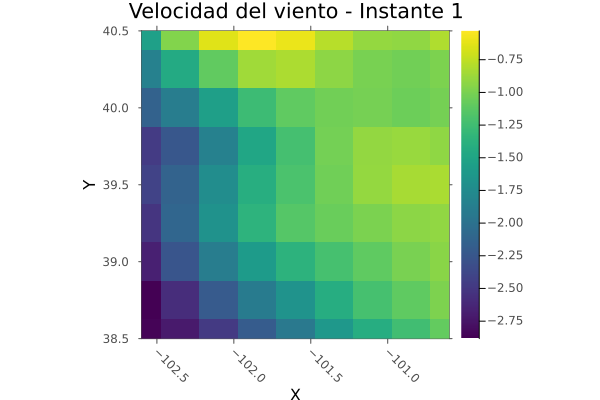
\includegraphics[width=2in,height=\textheight]{images/c10_netcdf_time_plot_julia.png}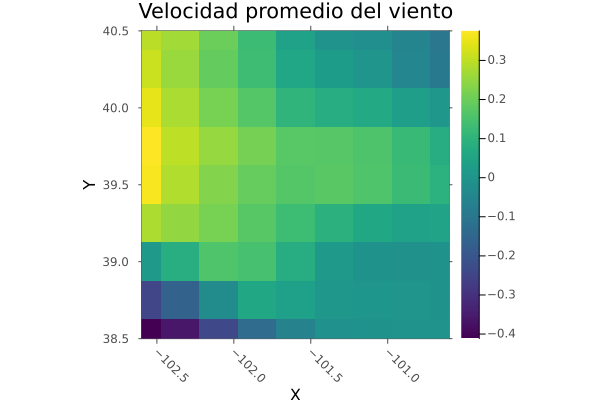
\includegraphics[width=2in,height=\textheight]{images/c10_netcdf_mean_plot_julia.png}

\subsection{Limitaciones en la Interpretación Automática de Estándares
NetCDF}\label{limitaciones-en-la-interpretaciuxf3n-automuxe1tica-de-estuxe1ndares-netcdf}

El cumplimiento de las convenciones CF (Climate and Forecast) constituye
un marco de interoperabilidad, pero no garantiza una traducción
automática y unívoca hacia objetos de datos espaciales en todos los
entornos de programación. Mientras que bibliotecas como \textbf{xarray}
en Python cuentan con motores de decodificación específicos (como
\texttt{cftime}), el paquete \textbf{stars} en R depende de la
abstracción de GDAL, lo que puede derivar en una interpretación
incompleta de los metadatos.

\textbf{Factores que impiden la decodificación de metadatos:}

La necesidad de intervenir manualmente en la asignación de Sistemas de
Referencia de Coordenadas (CRS) y en la conversión de ejes temporales
responde a inconsistencias estructurales o limitaciones en los
controladores de lectura:

\begin{enumerate}
\def\labelenumi{\arabic{enumi}.}
\tightlist
\item
  \textbf{Omisión del atributo grid\_mapping:} Aunque el archivo siga
  las convenciones CF para las dimensiones de latitud, longitud y
  tiempo, si carece del atributo \texttt{grid\_mapping}, las librerías
  basadas en GDAL no pueden inferir la proyección matemática exacta. En
  estos casos, el software interpreta los datos como una rejilla regular
  (curvilínea o no) pero carente de elipsoide o datum definido.
\item
  \textbf{Codificación no estándar del CRS:} Algunos archivos NetCDF
  almacenan la información geoespacial en atributos específicos de
  modelos climáticos o versiones antiguas del estándar que los
  traductores de metadatos de GDAL no logran mapear hacia una cadena WKT
  o un código EPSG de forma nativa.
\item
  \textbf{Ambigüedad en la dimensión temporal y unidades:} El estándar
  CF define el tiempo mediante una cadena de texto (ej. ``hours since
  1900-01-01''). Sin embargo, \textbf{stars} prioriza la integridad de
  los valores numéricos brutos almacenados en el arreglo. Si el
  controlador no detecta una estructura de calendario reconocida o si
  las unidades no están estrictamente vinculadas a la dimensión mediante
  el atributo \texttt{calendar}, el software retiene los valores como
  simples flotantes o enteros, delegando la conversión al usuario para
  evitar errores de redondeo o desajustes de zona horaria.
\end{enumerate}

Por lo tanto, la asignación manual del CRS mediante
\texttt{st\_set\_crs()} y la reconstrucción de la dimensión temporal con
\texttt{st\_set\_dimensions()} tras una conversión a \texttt{POSIXct}
son procedimientos necesarios para asegurar el rigor analítico. Estas
acciones garantizan que el manejo de series temporales y la
superposición de capas vectoriales se realicen sobre una base geográfica
y cronológica verificada, mitigando las deficiencias de la detección
automática.

\subsection{Resumen sintáctico de lectura y gestión
básica}\label{resumen-sintuxe1ctico-de-lectura-y-gestiuxf3n-buxe1sica}

Esta tabla compara las funciones clave utilizadas para la gestión de
cubos NetCDF.

\begin{longtable}[]{@{}
  >{\raggedright\arraybackslash}p{(\columnwidth - 6\tabcolsep) * \real{0.2500}}
  >{\raggedright\arraybackslash}p{(\columnwidth - 6\tabcolsep) * \real{0.2500}}
  >{\raggedright\arraybackslash}p{(\columnwidth - 6\tabcolsep) * \real{0.2500}}
  >{\raggedright\arraybackslash}p{(\columnwidth - 6\tabcolsep) * \real{0.2500}}@{}}
\toprule\noalign{}
\begin{minipage}[b]{\linewidth}\raggedright
Operación
\end{minipage} & \begin{minipage}[b]{\linewidth}\raggedright
Python 🐍
\end{minipage} & \begin{minipage}[b]{\linewidth}\raggedright
R 🔵
\end{minipage} & \begin{minipage}[b]{\linewidth}\raggedright
Julia 🟣
\end{minipage} \\
\midrule\noalign{}
\endhead
\bottomrule\noalign{}
\endlastfoot
\textbf{Cargar librería} & \texttt{import\ xarray\ as\ xr} &
\texttt{library(stars)} & \texttt{using\ Rasters} \\
\textbf{Lectura (Lazy)} & \texttt{xr.open\_dataset(file)} &
\texttt{read\_stars(file,\ proxy=TRUE)} & \texttt{Raster(file)} \\
\textbf{Asignar CRS} & \texttt{ds.rio.write\_crs("epsg:4326")} &
\texttt{st\_crs(y)\ \textless{}-\ 4326} & Automático vía metadatos \\
\textbf{Extraer tiempo} & \texttt{ds.time.values} &
\texttt{st\_get\_dimension\_values(y,\ "time")} &
\texttt{lookup(cube,\ Ti)} \\
\textbf{Conversión tiempo} & Automática (Convenciones CF) & Manual via
\texttt{as.POSIXct()} & Automática (Convenciones CF) \\
\textbf{Selección (Slice)} & \texttt{da.isel(time=0)} &
\texttt{y{[},,,i{]}} & \texttt{cube{[}Ti(1){]}} \\
\textbf{Media temporal} & \texttt{da.mean(dim="time")} &
\texttt{st\_apply(y,\ c("x",\ "y"),\ mean)} &
\texttt{mean(cube,\ dims=Ti)} \\
\end{longtable}

\textbf{Notas:}

\begin{itemize}
\tightlist
\item
  \textbf{Python 🐍:} Es el más automatizado para estándares CF.
\item
  \textbf{R 🔵:} Requiere mayor intervención manual en el eje temporal
  para garantizar rigor cronológico.
\item
  \textbf{Julia 🟣:} Es \emph{lazy} por diseño, lo que lo hace sumamente
  eficiente para archivos que superan la capacidad de la RAM.
\end{itemize}

\section{Leer y filtrar un archivo NetCDF
5D}\label{leer-y-filtrar-un-archivo-netcdf-5d}

El manejo de datos de reanálisis (como ERA5 de Copernicus) implica
trabajar con estructuras de cinco dimensiones (5D). Estas dimensiones
permiten capturar la temperatura (\texttt{t}) no solo en superficie
(\(x, y\)), sino en diferentes niveles de presión atmosférica
(\texttt{level}), a través del tiempo (\texttt{time}) y considerando
múltiples escenarios o miembros de ensamble (\texttt{number}) para
cuantificar la incertidumbre. Para un profesional en Colombia, estos
datos son vitales en el análisis de eventos climáticos extremos en la
Región Andina o el Caribe, permitiendo una comprensión volumétrica y
temporal de la atmósfera sobre el territorio nacional.

\subsection{Conceptualización del Cubo
5D}\label{conceptualizaciuxf3n-del-cubo-5d}

\begin{figure}[H]

{\centering \includegraphics[width=0.7\textwidth,height=\textheight]{images/cubos/Cubo5D.png}

}

\caption{Estructura del Hipercubo 5D}

\end{figure}%

\subsection{Resultados del Filtrado
(Slice)}\label{resultados-del-filtrado-slice}

\begin{figure}[H]

{\centering 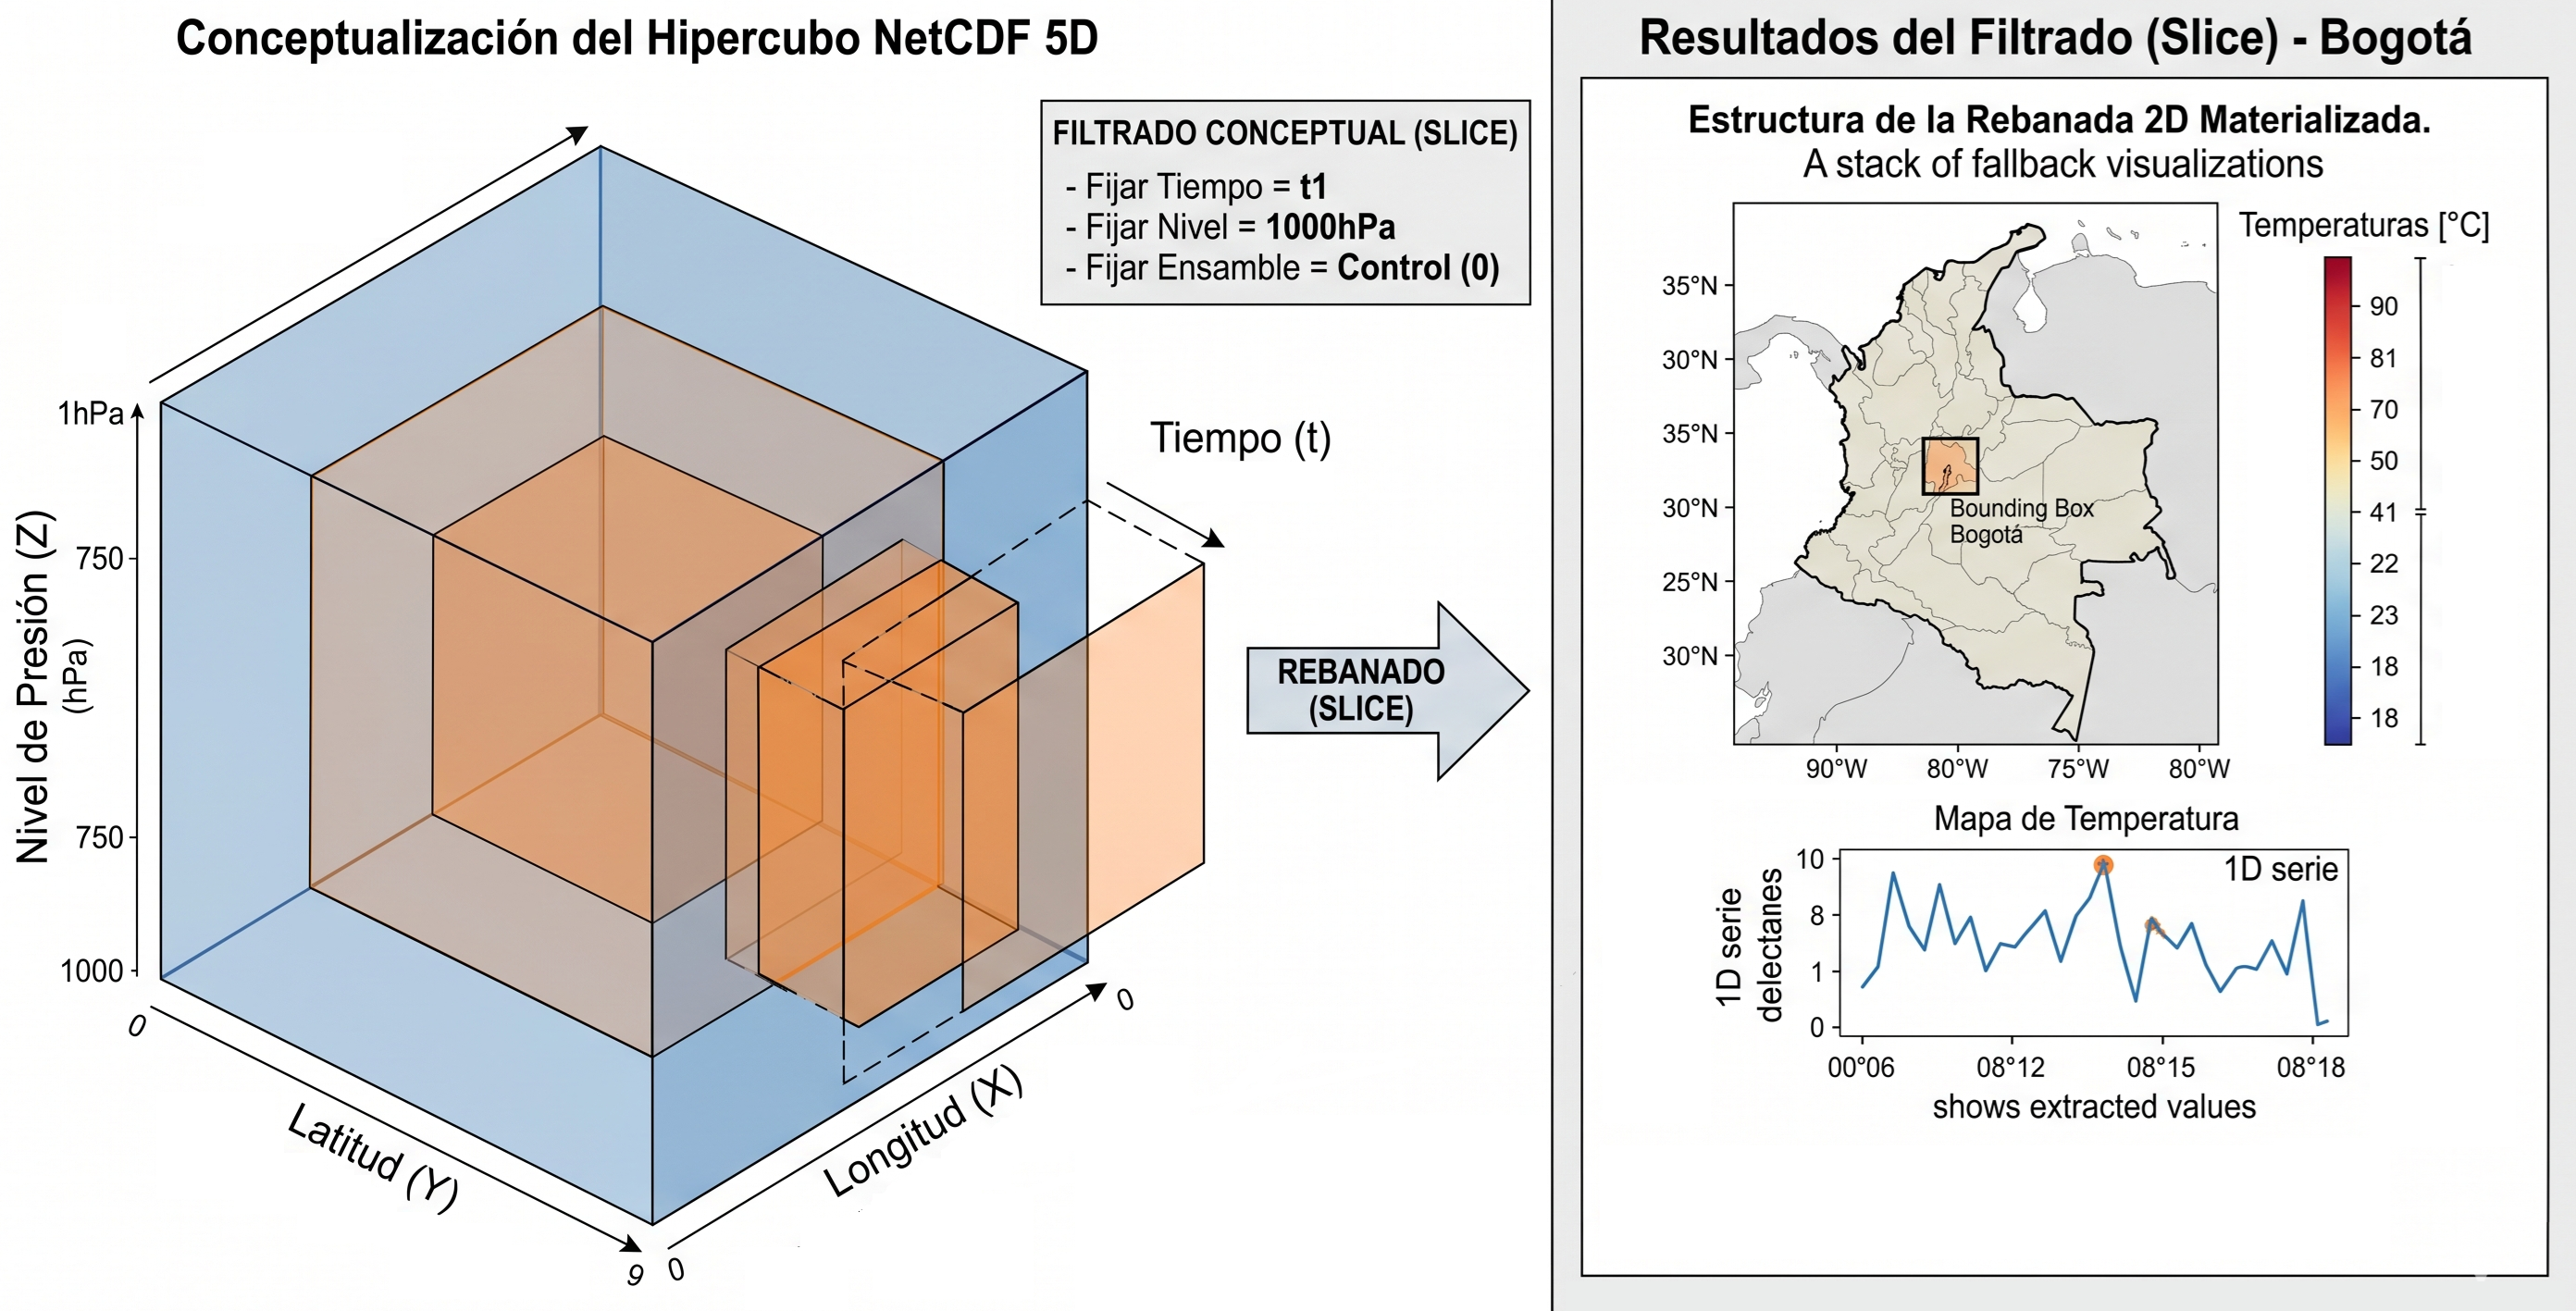
\includegraphics[width=0.9\textwidth,height=\textheight]{images/cubos/slice_cubo_5d.png}

}

\caption{Rebanada Espacial y Serie de Tiempo}

\end{figure}%

\subsection{Eficiencia computacional: el motor detrás de los grandes
volúmenes}\label{eficiencia-computacional-el-motor-detruxe1s-de-los-grandes-voluxfamenes}

Procesar un archivo de cientos de megabytes (o gigabytes) en tres
lenguajes distintos requiere entender cómo cada uno gestiona la memoria
RAM para evitar colapsos del sistema. La clave no es ``leer'' el
archivo, sino ``conectarse'' a él:

\begin{itemize}
\tightlist
\item
  \textbf{Python 🐍 (Dask):} Utiliza una estrategia de
  \textbf{fragmentación} (\emph{chunking}). Divide el cubo en bloques
  pequeños y solo carga en memoria aquellos necesarios para el cálculo
  actual, permitiendo procesar datos que superan la capacidad física de
  la RAM.
\item
  \textbf{R 🔵 (Stars Proxy):} Emplea un objeto \textbf{proxy} que
  almacena una ``lista de intenciones'' (\emph{call list}). Las
  operaciones de filtrado o promedio no se ejecutan inmediatamente; R
  solo las anota y espera hasta que el usuario pide un mapa o un archivo
  de salida para procesar los datos por bandas.
\item
  \textbf{Julia 🟣 (DiskArrays):} Se basa en una abstracción nativa de
  \textbf{arreglos de disco}. Julia trata al archivo NetCDF como si
  fuera una matriz residente en memoria, pero las operaciones de lectura
  ocurren de forma perezosa y altamente optimizada mediante iteradores
  que recorren el disco de forma lineal.
\end{itemize}

\subsection{Anatomía de las dimensiones en ERA5: El caso de los 37
niveles y 10
miembros}\label{anatomuxeda-de-las-dimensiones-en-era5-el-caso-de-los-37-niveles-y-10-miembros}

Para entender por qué nuestro archivo \texttt{download5Dcolombia.nc}
tiene exactamente \textbf{37 niveles} y \textbf{10 miembros}, debemos
remitirnos a la arquitectura del modelo global del Centro Europeo de
Previsiones Meteorológicas a Plazo Medio (ECMWF).

\subsubsection{¿Por qué 37 niveles de presión
(level)?}\label{por-quuxe9-37-niveles-de-presiuxf3n-level}

El estándar de ERA5 para niveles de presión define 37 capas que van
desde los \textbf{1000 hPa} (cerca del nivel del mar) hasta \textbf{1
hPa} (en la parte alta de la estratosfera).

\textbf{Propósito:}

\begin{enumerate}
\def\labelenumi{\arabic{enumi}.}
\tightlist
\item
  \textbf{Resolución en la Troposfera:} La mayoría de estos 37 niveles
  se concentran en la parte baja de la atmósfera, donde ocurren los
  fenómenos climáticos que afectan nuestro mundo.
\item
  \textbf{Contexto Colombiano:} Colombia es un país de contrastes
  altitudinales. Al tener 37 niveles, podemos estudiar la temperatura
  desde el nivel del mar en Cartagena (\(1000 \, hPa\)), pasando por la
  Sabana de Bogotá (\(\approx 750 \, hPa\)), hasta llegar a las cimas de
  los Nevados como el Ritacuba Blanco o el Huila
  (\(\approx 500 \, hPa\)), y aún tener capas superiores para estudiar
  el comportamiento de la atmósfera sobre las cordilleras.
\end{enumerate}

\subsubsection{¿Por qué 10 miembros de ensamble
(number)?}\label{por-quuxe9-10-miembros-de-ensamble-number}

El dataset que estamos usando es el \textbf{ERA5 EDA (Ensemble Data
Assimilation)}. A diferencia del dataset de ``alta resolución'' que solo
entrega un valor, el EDA entrega 10 versiones ligeramente diferentes de
la misma realidad meteorológica.

\textbf{Propósito:}

\begin{enumerate}
\def\labelenumi{\arabic{enumi}.}
\tightlist
\item
  \textbf{Cuantificación del error:} En ciencia de datos espaciales, no
  existe la ``medida perfecta''. Los 10 miembros (etiquetados del 0 al
  9) representan 10 simulaciones donde se variaron levemente las
  observaciones iniciales.
\item
  \textbf{Cómputo de Incertidumbre:} Si sobre el departamento del Chocó
  los 10 miembros muestran temperaturas muy parecidas, nuestra confianza
  en el dato es máxima. Si los miembros divergen (uno dice 25°C y otro
  28°C), el estudiante debe entender que hay alta incertidumbre en esa
  zona.
\item
  \textbf{El Miembro de Control:} Por convención, el miembro \texttt{0}
  es el experimento de control.
\end{enumerate}

\subsection{Descarga del Archivo}\label{descarga-del-archivo}

Descargar el archivo
\href{https://drive.google.com/file/d/1UgEsmJx2XM2Iuxr7L5s4IQ83rRS2Ngh1/view?usp=sharing}{download5Dcolombia.zip}
de 262 MB.

URL de descarga:
\texttt{https://drive.google.com/file/d/1UgEsmJx2XM2Iuxr7L5s4IQ83rRS2Ngh1/view?usp=sharing}

\subsection{Verificación de los niveles de presión y su
correspondencia}\label{verificaciuxf3n-de-los-niveles-de-presiuxf3n-y-su-correspondencia}

\subsection{Python}

\begin{Shaded}
\begin{Highlighting}[]
\CommentTok{\# \#| eval: false}

\CommentTok{"""}
\CommentTok{Verificación integral de un cubo NetCDF ERA5 (EDA)}

\CommentTok{Este script:}
\CommentTok{1. Controla existencia de archivos (.nc / .zip)}
\CommentTok{2. Carga el dataset en modo lazy}
\CommentTok{3. Inspecciona:}
\CommentTok{   {-} dimensiones}
\CommentTok{   {-} variable principal}
\CommentTok{   {-} metadatos}
\CommentTok{   {-} forma del arreglo}
\CommentTok{4. Verifica la estructura vertical (niveles de presión)}

\CommentTok{Contexto físico:}
\CommentTok{{-}{-}{-}{-}{-}{-}{-}{-}{-}{-}{-}{-}{-}{-}{-}}
\CommentTok{La presión disminuye con la altura:}
\CommentTok{    \textasciitilde{}1 hPa     → estratosfera alta}
\CommentTok{    \textasciitilde{}500 hPa   → troposfera media}
\CommentTok{    \textasciitilde{}1000 hPa  → superficie}
\CommentTok{"""}
\end{Highlighting}
\end{Shaded}

\begin{verbatim}
'\nVerificación integral de un cubo NetCDF ERA5 (EDA)\n\nEste script:\n1. Controla existencia de archivos (.nc / .zip)\n2. Carga el dataset en modo lazy\n3. Inspecciona:\n   - dimensiones\n   - variable principal\n   - metadatos\n   - forma del arreglo\n4. Verifica la estructura vertical (niveles de presión)\n\nContexto físico:\n---------------\nLa presión disminuye con la altura:\n    ~1 hPa     → estratosfera alta\n    ~500 hPa   → troposfera media\n    ~1000 hPa  → superficie\n'
\end{verbatim}

\begin{Shaded}
\begin{Highlighting}[]
\ImportTok{import}\NormalTok{ xarray }\ImportTok{as}\NormalTok{ xr}
\ImportTok{import}\NormalTok{ os}
\ImportTok{import}\NormalTok{ zipfile}

\CommentTok{\# {-}{-}{-}{-}{-}{-}{-}{-}{-}{-}{-}{-}{-}{-}{-}{-}{-}{-}{-}{-}{-}{-}{-}{-}{-}{-}{-}{-}{-}{-}{-}{-}{-}{-}{-}{-}{-}{-}{-}{-}{-}{-}{-}{-}{-}{-}{-}{-}{-}{-}{-}{-}{-}{-}{-}{-}{-}{-}{-}{-}{-}{-}{-}{-}{-}{-}{-}{-}{-}{-}{-}{-}{-}}
\CommentTok{\# Rutas}
\CommentTok{\# {-}{-}{-}{-}{-}{-}{-}{-}{-}{-}{-}{-}{-}{-}{-}{-}{-}{-}{-}{-}{-}{-}{-}{-}{-}{-}{-}{-}{-}{-}{-}{-}{-}{-}{-}{-}{-}{-}{-}{-}{-}{-}{-}{-}{-}{-}{-}{-}{-}{-}{-}{-}{-}{-}{-}{-}{-}{-}{-}{-}{-}{-}{-}{-}{-}{-}{-}{-}{-}{-}{-}{-}{-}}

\NormalTok{path }\OperatorTok{=} \StringTok{"./data\_heavy/"}
\NormalTok{ncname }\OperatorTok{=} \StringTok{"download5Dcolombia"}
\NormalTok{ncfile5d }\OperatorTok{=}\NormalTok{ os.path.join(path, ncname }\OperatorTok{+} \StringTok{".nc"}\NormalTok{)}
\NormalTok{zipfile\_path }\OperatorTok{=}\NormalTok{ os.path.join(path, ncname }\OperatorTok{+} \StringTok{".zip"}\NormalTok{)}


\CommentTok{\# {-}{-}{-}{-}{-}{-}{-}{-}{-}{-}{-}{-}{-}{-}{-}{-}{-}{-}{-}{-}{-}{-}{-}{-}{-}{-}{-}{-}{-}{-}{-}{-}{-}{-}{-}{-}{-}{-}{-}{-}{-}{-}{-}{-}{-}{-}{-}{-}{-}{-}{-}{-}{-}{-}{-}{-}{-}{-}{-}{-}{-}{-}{-}{-}{-}{-}{-}{-}{-}{-}{-}{-}{-}}
\CommentTok{\# Control de existencia y descompresión}
\CommentTok{\# {-}{-}{-}{-}{-}{-}{-}{-}{-}{-}{-}{-}{-}{-}{-}{-}{-}{-}{-}{-}{-}{-}{-}{-}{-}{-}{-}{-}{-}{-}{-}{-}{-}{-}{-}{-}{-}{-}{-}{-}{-}{-}{-}{-}{-}{-}{-}{-}{-}{-}{-}{-}{-}{-}{-}{-}{-}{-}{-}{-}{-}{-}{-}{-}{-}{-}{-}{-}{-}{-}{-}{-}{-}}

\ControlFlowTok{if} \KeywordTok{not}\NormalTok{ os.path.exists(ncfile5d):}

    \ControlFlowTok{if}\NormalTok{ os.path.exists(zipfile\_path):}
        \BuiltInTok{print}\NormalTok{(}\SpecialStringTok{f"Archivo .nc no encontrado. Descomprimiendo }\SpecialCharTok{\{}\NormalTok{zipfile\_path}\SpecialCharTok{\}}\SpecialStringTok{"}\NormalTok{)}
        \ControlFlowTok{with}\NormalTok{ zipfile.ZipFile(zipfile\_path, }\StringTok{\textquotesingle{}r\textquotesingle{}}\NormalTok{) }\ImportTok{as}\NormalTok{ zip\_ref:}
\NormalTok{            zip\_ref.extractall(path)}
    \ControlFlowTok{else}\NormalTok{:}
        \ControlFlowTok{raise} \PreprocessorTok{FileNotFoundError}\NormalTok{(}\StringTok{"No existe .nc ni .zip"}\NormalTok{)}

\ControlFlowTok{else}\NormalTok{:}
    \BuiltInTok{print}\NormalTok{(}\SpecialStringTok{f"Usando archivo existente: }\SpecialCharTok{\{}\NormalTok{ncfile5d}\SpecialCharTok{\}}\SpecialStringTok{"}\NormalTok{)}
\end{Highlighting}
\end{Shaded}

\begin{verbatim}
Usando archivo existente: ./data_heavy/download5Dcolombia.nc
\end{verbatim}

\begin{Shaded}
\begin{Highlighting}[]
\CommentTok{\# {-}{-}{-}{-}{-}{-}{-}{-}{-}{-}{-}{-}{-}{-}{-}{-}{-}{-}{-}{-}{-}{-}{-}{-}{-}{-}{-}{-}{-}{-}{-}{-}{-}{-}{-}{-}{-}{-}{-}{-}{-}{-}{-}{-}{-}{-}{-}{-}{-}{-}{-}{-}{-}{-}{-}{-}{-}{-}{-}{-}{-}{-}{-}{-}{-}{-}{-}{-}{-}{-}{-}{-}{-}}
\CommentTok{\# Carga (lazy)}
\CommentTok{\# {-}{-}{-}{-}{-}{-}{-}{-}{-}{-}{-}{-}{-}{-}{-}{-}{-}{-}{-}{-}{-}{-}{-}{-}{-}{-}{-}{-}{-}{-}{-}{-}{-}{-}{-}{-}{-}{-}{-}{-}{-}{-}{-}{-}{-}{-}{-}{-}{-}{-}{-}{-}{-}{-}{-}{-}{-}{-}{-}{-}{-}{-}{-}{-}{-}{-}{-}{-}{-}{-}{-}{-}{-}}

\CommentTok{\# Carga lazy pero sin dask}
\NormalTok{ds }\OperatorTok{=}\NormalTok{ xr.open\_dataset(ncfile5d)}

\CommentTok{\# chunks="auto" activa Dask y divide el cubo en bloques manejables para la RAM}
\CommentTok{\# Se requieren las librerías:}
\CommentTok{\# xarray (instalada en el contenedor),}
\CommentTok{\# netcdf4 (no instalada en el contenedor)}
\CommentTok{\# y toolz (no instalada en el contenedor)}
\CommentTok{\#ds = xr.open\_dataset(ncfile5d, chunks="auto")}

\BuiltInTok{print}\NormalTok{(}\StringTok{"}\CharTok{\textbackslash{}n}\StringTok{=== DATASET ==="}\NormalTok{)}
\end{Highlighting}
\end{Shaded}

\begin{verbatim}

=== DATASET ===
\end{verbatim}

\begin{Shaded}
\begin{Highlighting}[]
\BuiltInTok{print}\NormalTok{(ds)}
\end{Highlighting}
\end{Shaded}

\begin{verbatim}
<xarray.Dataset> Size: 1GB
Dimensions:    (time: 480, number: 10, level: 37, latitude: 35, longitude: 25)
Coordinates:
  * time       (time) datetime64[ns] 4kB 2020-01-01 ... 2020-02-29T21:00:00
  * number     (number) int32 40B 0 1 2 3 4 5 6 7 8 9
  * level      (level) int32 148B 1 2 3 5 7 10 20 ... 875 900 925 950 975 1000
  * latitude   (latitude) float32 140B 12.5 12.0 11.5 11.0 ... -3.5 -4.0 -4.5
  * longitude  (longitude) float32 100B -79.1 -78.6 -78.1 ... -68.1 -67.6 -67.1
Data variables:
    t          (time, number, level, latitude, longitude) float64 1GB ...
Attributes:
    Conventions:  CF-1.6
    history:      2020-09-30 17:55:04 GMT by grib_to_netcdf-2.16.0: /opt/ecmw...
\end{verbatim}

\begin{Shaded}
\begin{Highlighting}[]
\CommentTok{\# {-}{-}{-}{-}{-}{-}{-}{-}{-}{-}{-}{-}{-}{-}{-}{-}{-}{-}{-}{-}{-}{-}{-}{-}{-}{-}{-}{-}{-}{-}{-}{-}{-}{-}{-}{-}{-}{-}{-}{-}{-}{-}{-}{-}{-}{-}{-}{-}{-}{-}{-}{-}{-}{-}{-}{-}{-}{-}{-}{-}{-}{-}{-}{-}{-}{-}{-}{-}{-}{-}{-}{-}{-}}
\CommentTok{\# Dimensiones}
\CommentTok{\# {-}{-}{-}{-}{-}{-}{-}{-}{-}{-}{-}{-}{-}{-}{-}{-}{-}{-}{-}{-}{-}{-}{-}{-}{-}{-}{-}{-}{-}{-}{-}{-}{-}{-}{-}{-}{-}{-}{-}{-}{-}{-}{-}{-}{-}{-}{-}{-}{-}{-}{-}{-}{-}{-}{-}{-}{-}{-}{-}{-}{-}{-}{-}{-}{-}{-}{-}{-}{-}{-}{-}{-}{-}}

\BuiltInTok{print}\NormalTok{(}\StringTok{"}\CharTok{\textbackslash{}n}\StringTok{=== DIMENSIONES ==="}\NormalTok{)}
\end{Highlighting}
\end{Shaded}

\begin{verbatim}

=== DIMENSIONES ===
\end{verbatim}

\begin{Shaded}
\begin{Highlighting}[]
\BuiltInTok{print}\NormalTok{(ds.dims)}
\end{Highlighting}
\end{Shaded}

\begin{verbatim}
FrozenMappingWarningOnValuesAccess({'time': 480, 'number': 10, 'level': 37, 'latitude': 35, 'longitude': 25})
\end{verbatim}

\begin{Shaded}
\begin{Highlighting}[]
\CommentTok{\# {-}{-}{-}{-}{-}{-}{-}{-}{-}{-}{-}{-}{-}{-}{-}{-}{-}{-}{-}{-}{-}{-}{-}{-}{-}{-}{-}{-}{-}{-}{-}{-}{-}{-}{-}{-}{-}{-}{-}{-}{-}{-}{-}{-}{-}{-}{-}{-}{-}{-}{-}{-}{-}{-}{-}{-}{-}{-}{-}{-}{-}{-}{-}{-}{-}{-}{-}{-}{-}{-}{-}{-}{-}}
\CommentTok{\# Variable principal}
\CommentTok{\# {-}{-}{-}{-}{-}{-}{-}{-}{-}{-}{-}{-}{-}{-}{-}{-}{-}{-}{-}{-}{-}{-}{-}{-}{-}{-}{-}{-}{-}{-}{-}{-}{-}{-}{-}{-}{-}{-}{-}{-}{-}{-}{-}{-}{-}{-}{-}{-}{-}{-}{-}{-}{-}{-}{-}{-}{-}{-}{-}{-}{-}{-}{-}{-}{-}{-}{-}{-}{-}{-}{-}{-}{-}}

\BuiltInTok{print}\NormalTok{(}\StringTok{"}\CharTok{\textbackslash{}n}\StringTok{=== VARIABLES ==="}\NormalTok{)}
\end{Highlighting}
\end{Shaded}

\begin{verbatim}

=== VARIABLES ===
\end{verbatim}

\begin{Shaded}
\begin{Highlighting}[]
\BuiltInTok{print}\NormalTok{(}\BuiltInTok{list}\NormalTok{(ds.data\_vars))}
\end{Highlighting}
\end{Shaded}

\begin{verbatim}
['t']
\end{verbatim}

\begin{Shaded}
\begin{Highlighting}[]
\CommentTok{\# {-}{-}{-}{-}{-}{-}{-}{-}{-}{-}{-}{-}{-}{-}{-}{-}{-}{-}{-}{-}{-}{-}{-}{-}{-}{-}{-}{-}{-}{-}{-}{-}{-}{-}{-}{-}{-}{-}{-}{-}{-}{-}{-}{-}{-}{-}{-}{-}{-}{-}{-}{-}{-}{-}{-}{-}{-}{-}{-}{-}{-}{-}{-}{-}{-}{-}{-}{-}{-}{-}{-}{-}{-}}
\CommentTok{\# Metadatos}
\CommentTok{\# {-}{-}{-}{-}{-}{-}{-}{-}{-}{-}{-}{-}{-}{-}{-}{-}{-}{-}{-}{-}{-}{-}{-}{-}{-}{-}{-}{-}{-}{-}{-}{-}{-}{-}{-}{-}{-}{-}{-}{-}{-}{-}{-}{-}{-}{-}{-}{-}{-}{-}{-}{-}{-}{-}{-}{-}{-}{-}{-}{-}{-}{-}{-}{-}{-}{-}{-}{-}{-}{-}{-}{-}{-}}

\BuiltInTok{print}\NormalTok{(}\StringTok{"}\CharTok{\textbackslash{}n}\StringTok{=== METADATOS ==="}\NormalTok{)}
\end{Highlighting}
\end{Shaded}

\begin{verbatim}

=== METADATOS ===
\end{verbatim}

\begin{Shaded}
\begin{Highlighting}[]
\BuiltInTok{print}\NormalTok{(ds.attrs)}
\end{Highlighting}
\end{Shaded}

\begin{verbatim}
{'Conventions': 'CF-1.6', 'history': '2020-09-30 17:55:04 GMT by grib_to_netcdf-2.16.0: /opt/ecmwf/eccodes/bin/grib_to_netcdf -S param -o /cache/data1/adaptor.mars.internal-1601485963.200975-3104-28-04adcc76-77fc-4223-96e1-62f83cb65870.nc /cache/tmp/04adcc76-77fc-4223-96e1-62f83cb65870-adaptor.mars.internal-1601485963.2020729-3104-9-tmp.grib'}
\end{verbatim}

\begin{Shaded}
\begin{Highlighting}[]
\CommentTok{\# {-}{-}{-}{-}{-}{-}{-}{-}{-}{-}{-}{-}{-}{-}{-}{-}{-}{-}{-}{-}{-}{-}{-}{-}{-}{-}{-}{-}{-}{-}{-}{-}{-}{-}{-}{-}{-}{-}{-}{-}{-}{-}{-}{-}{-}{-}{-}{-}{-}{-}{-}{-}{-}{-}{-}{-}{-}{-}{-}{-}{-}{-}{-}{-}{-}{-}{-}{-}{-}{-}{-}{-}{-}}
\CommentTok{\# Forma del arreglo}
\CommentTok{\# {-}{-}{-}{-}{-}{-}{-}{-}{-}{-}{-}{-}{-}{-}{-}{-}{-}{-}{-}{-}{-}{-}{-}{-}{-}{-}{-}{-}{-}{-}{-}{-}{-}{-}{-}{-}{-}{-}{-}{-}{-}{-}{-}{-}{-}{-}{-}{-}{-}{-}{-}{-}{-}{-}{-}{-}{-}{-}{-}{-}{-}{-}{-}{-}{-}{-}{-}{-}{-}{-}{-}{-}{-}}

\BuiltInTok{print}\NormalTok{(}\StringTok{"}\CharTok{\textbackslash{}n}\StringTok{=== SHAPE ==="}\NormalTok{)}
\end{Highlighting}
\end{Shaded}

\begin{verbatim}

=== SHAPE ===
\end{verbatim}

\begin{Shaded}
\begin{Highlighting}[]
\BuiltInTok{print}\NormalTok{(ds[}\StringTok{"t"}\NormalTok{].shape)}
\end{Highlighting}
\end{Shaded}

\begin{verbatim}
(480, 10, 37, 35, 25)
\end{verbatim}

\begin{Shaded}
\begin{Highlighting}[]
\CommentTok{\# {-}{-}{-}{-}{-}{-}{-}{-}{-}{-}{-}{-}{-}{-}{-}{-}{-}{-}{-}{-}{-}{-}{-}{-}{-}{-}{-}{-}{-}{-}{-}{-}{-}{-}{-}{-}{-}{-}{-}{-}{-}{-}{-}{-}{-}{-}{-}{-}{-}{-}{-}{-}{-}{-}{-}{-}{-}{-}{-}{-}{-}{-}{-}{-}{-}{-}{-}{-}{-}{-}{-}{-}{-}}
\CommentTok{\# Niveles de presión}
\CommentTok{\# {-}{-}{-}{-}{-}{-}{-}{-}{-}{-}{-}{-}{-}{-}{-}{-}{-}{-}{-}{-}{-}{-}{-}{-}{-}{-}{-}{-}{-}{-}{-}{-}{-}{-}{-}{-}{-}{-}{-}{-}{-}{-}{-}{-}{-}{-}{-}{-}{-}{-}{-}{-}{-}{-}{-}{-}{-}{-}{-}{-}{-}{-}{-}{-}{-}{-}{-}{-}{-}{-}{-}{-}{-}}

\NormalTok{z\_levels }\OperatorTok{=}\NormalTok{ ds.level.values}

\BuiltInTok{print}\NormalTok{(}\StringTok{"}\CharTok{\textbackslash{}n}\StringTok{Primeros niveles (Alta atmósfera):"}\NormalTok{)}
\end{Highlighting}
\end{Shaded}

\begin{verbatim}

Primeros niveles (Alta atmósfera):
\end{verbatim}

\begin{Shaded}
\begin{Highlighting}[]
\BuiltInTok{print}\NormalTok{(z\_levels[:}\DecValTok{2}\NormalTok{])}
\end{Highlighting}
\end{Shaded}

\begin{verbatim}
[1 2]
\end{verbatim}

\begin{Shaded}
\begin{Highlighting}[]
\BuiltInTok{print}\NormalTok{(}\StringTok{"}\CharTok{\textbackslash{}n}\StringTok{Últimos niveles (Superficie):"}\NormalTok{)}
\end{Highlighting}
\end{Shaded}

\begin{verbatim}

Últimos niveles (Superficie):
\end{verbatim}

\begin{Shaded}
\begin{Highlighting}[]
\BuiltInTok{print}\NormalTok{(z\_levels[}\OperatorTok{{-}}\DecValTok{2}\NormalTok{:])}
\end{Highlighting}
\end{Shaded}

\begin{verbatim}
[ 975 1000]
\end{verbatim}

\subsection{R}

\begin{Shaded}
\begin{Highlighting}[]
\CommentTok{\# \#| eval: false}

\CommentTok{\# {-}{-}{-}{-}{-}{-}{-}{-}{-}{-}{-}{-}{-}{-}{-}{-}{-}{-}{-}{-}{-}{-}{-}{-}{-}{-}{-}{-}{-}{-}{-}{-}{-}{-}{-}{-}{-}{-}{-}{-}{-}{-}{-}{-}{-}{-}{-}{-}{-}{-}{-}{-}{-}{-}{-}{-}{-}{-}{-}{-}{-}{-}{-}{-}{-}{-}{-}{-}{-}{-}{-}{-}{-}}
\CommentTok{\# Librerías}
\CommentTok{\# {-}{-}{-}{-}{-}{-}{-}{-}{-}{-}{-}{-}{-}{-}{-}{-}{-}{-}{-}{-}{-}{-}{-}{-}{-}{-}{-}{-}{-}{-}{-}{-}{-}{-}{-}{-}{-}{-}{-}{-}{-}{-}{-}{-}{-}{-}{-}{-}{-}{-}{-}{-}{-}{-}{-}{-}{-}{-}{-}{-}{-}{-}{-}{-}{-}{-}{-}{-}{-}{-}{-}{-}{-}}
\FunctionTok{library}\NormalTok{(stars)}
\FunctionTok{library}\NormalTok{(dplyr)}
\end{Highlighting}
\end{Shaded}

\begin{verbatim}

Attaching package: 'dplyr'
\end{verbatim}

\begin{verbatim}
The following objects are masked from 'package:stats':

    filter, lag
\end{verbatim}

\begin{verbatim}
The following objects are masked from 'package:base':

    intersect, setdiff, setequal, union
\end{verbatim}

\begin{Shaded}
\begin{Highlighting}[]
\FunctionTok{library}\NormalTok{(sf)}

\CommentTok{\# Ajuste de variables de entorno de GDAL}
\CommentTok{\# Se incrementa el límite de bandas para permitir el procesamiento de cubos 5D }
\CommentTok{\# con una densidad temporal o vertical elevada (ej. ERA5 o modelos climáticos).}
\FunctionTok{Sys.setenv}\NormalTok{(}\AttributeTok{GDAL\_MAX\_BAND\_COUNT =} \DecValTok{1200000}\NormalTok{)}

\CommentTok{\# {-}{-}{-}{-}{-}{-}{-}{-}{-}{-}{-}{-}{-}{-}{-}{-}{-}{-}{-}{-}{-}{-}{-}{-}{-}{-}{-}{-}{-}{-}{-}{-}{-}{-}{-}{-}{-}{-}{-}{-}{-}{-}{-}{-}{-}{-}{-}{-}{-}{-}{-}{-}{-}{-}{-}{-}{-}{-}{-}{-}{-}{-}{-}{-}{-}{-}{-}{-}{-}{-}{-}{-}{-}}
\CommentTok{\# Rutas y nombres de archivos}
\CommentTok{\# {-}{-}{-}{-}{-}{-}{-}{-}{-}{-}{-}{-}{-}{-}{-}{-}{-}{-}{-}{-}{-}{-}{-}{-}{-}{-}{-}{-}{-}{-}{-}{-}{-}{-}{-}{-}{-}{-}{-}{-}{-}{-}{-}{-}{-}{-}{-}{-}{-}{-}{-}{-}{-}{-}{-}{-}{-}{-}{-}{-}{-}{-}{-}{-}{-}{-}{-}{-}{-}{-}{-}{-}{-}}

\NormalTok{path     }\OtherTok{\textless{}{-}} \StringTok{"./data\_heavy/"}
\NormalTok{ncname   }\OtherTok{\textless{}{-}} \StringTok{"download5Dcolombia"}
\NormalTok{ncfile5d }\OtherTok{\textless{}{-}} \FunctionTok{paste0}\NormalTok{(path, ncname, }\StringTok{".nc"}\NormalTok{)}
\NormalTok{zipfile  }\OtherTok{\textless{}{-}} \FunctionTok{paste0}\NormalTok{(path, ncname, }\StringTok{".zip"}\NormalTok{)}

\CommentTok{\# {-}{-}{-}{-}{-}{-}{-}{-}{-}{-}{-}{-}{-}{-}{-}{-}{-}{-}{-}{-}{-}{-}{-}{-}{-}{-}{-}{-}{-}{-}{-}{-}{-}{-}{-}{-}{-}{-}{-}{-}{-}{-}{-}{-}{-}{-}{-}{-}{-}{-}{-}{-}{-}{-}{-}{-}{-}{-}{-}{-}{-}{-}{-}{-}{-}{-}{-}{-}{-}{-}{-}{-}{-}}
\CommentTok{\# Control de existencia y descompresión de archivos}
\CommentTok{\# {-}{-}{-}{-}{-}{-}{-}{-}{-}{-}{-}{-}{-}{-}{-}{-}{-}{-}{-}{-}{-}{-}{-}{-}{-}{-}{-}{-}{-}{-}{-}{-}{-}{-}{-}{-}{-}{-}{-}{-}{-}{-}{-}{-}{-}{-}{-}{-}{-}{-}{-}{-}{-}{-}{-}{-}{-}{-}{-}{-}{-}{-}{-}{-}{-}{-}{-}{-}{-}{-}{-}{-}{-}}

\ControlFlowTok{if}\NormalTok{ (}\SpecialCharTok{!}\FunctionTok{file.exists}\NormalTok{(ncfile5d)) \{}

  \ControlFlowTok{if}\NormalTok{ (}\FunctionTok{file.exists}\NormalTok{(zipfile)) \{}
    \FunctionTok{message}\NormalTok{(}\StringTok{"Descomprimiendo archivo..."}\NormalTok{)}
    \FunctionTok{unzip}\NormalTok{(zipfile, }\AttributeTok{exdir =}\NormalTok{ path)}
\NormalTok{  \} }\ControlFlowTok{else}\NormalTok{ \{}
    \FunctionTok{stop}\NormalTok{(}\StringTok{"No existe .nc ni .zip"}\NormalTok{)}
\NormalTok{  \}}

\NormalTok{\} }\ControlFlowTok{else}\NormalTok{ \{}
  \FunctionTok{message}\NormalTok{(}\StringTok{"Usando archivo existente"}\NormalTok{)}
\NormalTok{\}}
\end{Highlighting}
\end{Shaded}

\begin{verbatim}
Usando archivo existente
\end{verbatim}

\begin{Shaded}
\begin{Highlighting}[]
\CommentTok{\# {-}{-}{-}{-}{-}{-}{-}{-}{-}{-}{-}{-}{-}{-}{-}{-}{-}{-}{-}{-}{-}{-}{-}{-}{-}{-}{-}{-}{-}{-}{-}{-}{-}{-}{-}{-}{-}{-}{-}{-}{-}{-}{-}{-}{-}{-}{-}{-}{-}{-}{-}{-}{-}{-}{-}{-}{-}{-}{-}{-}{-}{-}{-}{-}{-}{-}{-}{-}{-}{-}{-}{-}{-}}
\CommentTok{\# Carga lazy}
\CommentTok{\# {-}{-}{-}{-}{-}{-}{-}{-}{-}{-}{-}{-}{-}{-}{-}{-}{-}{-}{-}{-}{-}{-}{-}{-}{-}{-}{-}{-}{-}{-}{-}{-}{-}{-}{-}{-}{-}{-}{-}{-}{-}{-}{-}{-}{-}{-}{-}{-}{-}{-}{-}{-}{-}{-}{-}{-}{-}{-}{-}{-}{-}{-}{-}{-}{-}{-}{-}{-}{-}{-}{-}{-}{-}}

\CommentTok{\# Lectura mediante proxy=TRUE para manipulación diferida (lazy evaluation).}
\CommentTok{\# Esto permite definir recortes espaciales y temporales sin cargar todo el }
\CommentTok{\# archivo.}
\NormalTok{st\_col5d }\OtherTok{=} \FunctionTok{read\_stars}\NormalTok{(ncfile5d, }\AttributeTok{proxy=}\ConstantTok{TRUE}\NormalTok{)}
\end{Highlighting}
\end{Shaded}

\begin{verbatim}
Warning in CPL_get_metadata(file, NA_character_, options): GDAL Message 1:
dimension #1 (number) is not a Time dimension.
\end{verbatim}

\begin{verbatim}
Warning in CPL_read_gdal(as.character(x), as.character(options),
as.character(driver), : GDAL Message 1: The dataset has several variables that
could be identified as vector fields, but not all share the same primary
dimension. Consequently they will be ignored.
\end{verbatim}

\begin{verbatim}
Warning in CPL_read_gdal(as.character(x), as.character(options),
as.character(driver), : GDAL Message 1: dimension #1 (number) is not a Time
dimension.
\end{verbatim}

\begin{Shaded}
\begin{Highlighting}[]
\CommentTok{\# Warning: dimension \#1 (number) is not a Time dimension.}
\CommentTok{\# Explicación: GDAL identifica "number" (ensamble) y aclara que no cumple }
\CommentTok{\# con los atributos CF de tiempo; se procesa como dimensión entera.}

\CommentTok{\# Warning: The dataset has several variables that could be identified as vector fields...}
\CommentTok{\# Explicación: Si hubiera vientos U/V, GDAL no los agrupa automáticamente por }
\CommentTok{\# discrepancias dimensionales; se cargan como atributos escalares.}

\CommentTok{\# Chequeto de CRS}
\FunctionTok{st\_crs}\NormalTok{(st\_col5d)}
\end{Highlighting}
\end{Shaded}

\begin{verbatim}
Coordinate Reference System: NA
\end{verbatim}

\begin{Shaded}
\begin{Highlighting}[]
\CommentTok{\# Asignación de CRS en \{stars\}}
\CommentTok{\# Opción 1: Asignación directa (reemplaza el NA en el objeto existente)}
\CommentTok{\#st\_crs(st\_col5d) \textless{}{-} 4326}
\CommentTok{\# Opción 2: Usando st\_set\_crs (estilo funcional/pipe)}
\NormalTok{st\_col5d }\OtherTok{\textless{}{-}}\NormalTok{ st\_col5d }\SpecialCharTok{\%\textgreater{}\%} \FunctionTok{st\_set\_crs}\NormalTok{(}\DecValTok{4326}\NormalTok{)}
\CommentTok{\#st\_col5d \textless{}{-} st\_set\_crs(st\_col5d, 4326)}

\FunctionTok{cat}\NormalTok{(}\StringTok{"}\SpecialCharTok{\textbackslash{}n}\StringTok{=== DATASET ===}\SpecialCharTok{\textbackslash{}n}\StringTok{"}\NormalTok{)}
\end{Highlighting}
\end{Shaded}

\begin{verbatim}

=== DATASET ===
\end{verbatim}

\begin{Shaded}
\begin{Highlighting}[]
\FunctionTok{print}\NormalTok{(st\_col5d)}
\end{Highlighting}
\end{Shaded}

\begin{verbatim}
stars_proxy object with 1 attribute in 1 file(s):
$download5Dcolombia.nc
[1] "[...]/download5Dcolombia.nc"

dimension(s):
       from  to                                      offset
x         1  25                                      -79.35
y         1  35                                       12.75
level     1  37                                          NA
number    1  10                                           0
time      1 480 1051896 [hours since 1900-01-01 00:00:00.0]
                                       delta  refsys
x                                        0.5  WGS 84
y                                       -0.5  WGS 84
level                                     NA udunits
number                                     1      NA
time   3 [hours since 1900-01-01 00:00:00.0] udunits
                                              values x/y
x                                               NULL [x]
y                                               NULL [y]
level  [1,2) [millibars],...,[1000,1025) [millibars]    
number                                          NULL    
time                                            NULL    
\end{verbatim}

\begin{Shaded}
\begin{Highlighting}[]
\CommentTok{\# {-}{-}{-}{-}{-}{-}{-}{-}{-}{-}{-}{-}{-}{-}{-}{-}{-}{-}{-}{-}{-}{-}{-}{-}{-}{-}{-}{-}{-}{-}{-}{-}{-}{-}{-}{-}{-}{-}{-}{-}{-}{-}{-}{-}{-}{-}{-}{-}{-}{-}{-}{-}{-}{-}{-}{-}{-}{-}{-}{-}{-}{-}{-}{-}{-}{-}{-}{-}{-}{-}{-}{-}{-}}
\CommentTok{\# Dimensiones}
\CommentTok{\# {-}{-}{-}{-}{-}{-}{-}{-}{-}{-}{-}{-}{-}{-}{-}{-}{-}{-}{-}{-}{-}{-}{-}{-}{-}{-}{-}{-}{-}{-}{-}{-}{-}{-}{-}{-}{-}{-}{-}{-}{-}{-}{-}{-}{-}{-}{-}{-}{-}{-}{-}{-}{-}{-}{-}{-}{-}{-}{-}{-}{-}{-}{-}{-}{-}{-}{-}{-}{-}{-}{-}{-}{-}}

\FunctionTok{cat}\NormalTok{(}\StringTok{"}\SpecialCharTok{\textbackslash{}n}\StringTok{=== DIMENSIONES ===}\SpecialCharTok{\textbackslash{}n}\StringTok{"}\NormalTok{)}
\end{Highlighting}
\end{Shaded}

\begin{verbatim}

=== DIMENSIONES ===
\end{verbatim}

\begin{Shaded}
\begin{Highlighting}[]
\FunctionTok{print}\NormalTok{(}\FunctionTok{st\_dimensions}\NormalTok{(st\_col5d))}
\end{Highlighting}
\end{Shaded}

\begin{verbatim}
       from  to                                      offset
x         1  25                                      -79.35
y         1  35                                       12.75
level     1  37                                          NA
number    1  10                                           0
time      1 480 1051896 [hours since 1900-01-01 00:00:00.0]
                                       delta  refsys
x                                        0.5  WGS 84
y                                       -0.5  WGS 84
level                                     NA udunits
number                                     1      NA
time   3 [hours since 1900-01-01 00:00:00.0] udunits
                                              values x/y
x                                               NULL [x]
y                                               NULL [y]
level  [1,2) [millibars],...,[1000,1025) [millibars]    
number                                          NULL    
time                                            NULL    
\end{verbatim}

\begin{Shaded}
\begin{Highlighting}[]
\CommentTok{\# {-}{-}{-}{-}{-}{-}{-}{-}{-}{-}{-}{-}{-}{-}{-}{-}{-}{-}{-}{-}{-}{-}{-}{-}{-}{-}{-}{-}{-}{-}{-}{-}{-}{-}{-}{-}{-}{-}{-}{-}{-}{-}{-}{-}{-}{-}{-}{-}{-}{-}{-}{-}{-}{-}{-}{-}{-}{-}{-}{-}{-}{-}{-}{-}{-}{-}{-}{-}{-}{-}{-}{-}{-}}
\CommentTok{\# Variable}
\CommentTok{\# {-}{-}{-}{-}{-}{-}{-}{-}{-}{-}{-}{-}{-}{-}{-}{-}{-}{-}{-}{-}{-}{-}{-}{-}{-}{-}{-}{-}{-}{-}{-}{-}{-}{-}{-}{-}{-}{-}{-}{-}{-}{-}{-}{-}{-}{-}{-}{-}{-}{-}{-}{-}{-}{-}{-}{-}{-}{-}{-}{-}{-}{-}{-}{-}{-}{-}{-}{-}{-}{-}{-}{-}{-}}

\FunctionTok{cat}\NormalTok{(}\StringTok{"}\SpecialCharTok{\textbackslash{}n}\StringTok{=== VARIABLES ===}\SpecialCharTok{\textbackslash{}n}\StringTok{"}\NormalTok{)}
\end{Highlighting}
\end{Shaded}

\begin{verbatim}

=== VARIABLES ===
\end{verbatim}

\begin{Shaded}
\begin{Highlighting}[]
\FunctionTok{print}\NormalTok{(}\FunctionTok{names}\NormalTok{(st\_col5d))}
\end{Highlighting}
\end{Shaded}

\begin{verbatim}
[1] "download5Dcolombia.nc"
\end{verbatim}

\begin{Shaded}
\begin{Highlighting}[]
\CommentTok{\# {-}{-}{-}{-}{-}{-}{-}{-}{-}{-}{-}{-}{-}{-}{-}{-}{-}{-}{-}{-}{-}{-}{-}{-}{-}{-}{-}{-}{-}{-}{-}{-}{-}{-}{-}{-}{-}{-}{-}{-}{-}{-}{-}{-}{-}{-}{-}{-}{-}{-}{-}{-}{-}{-}{-}{-}{-}{-}{-}{-}{-}{-}{-}{-}{-}{-}{-}{-}{-}{-}{-}{-}{-}}
\CommentTok{\# Metadatos}
\CommentTok{\# {-}{-}{-}{-}{-}{-}{-}{-}{-}{-}{-}{-}{-}{-}{-}{-}{-}{-}{-}{-}{-}{-}{-}{-}{-}{-}{-}{-}{-}{-}{-}{-}{-}{-}{-}{-}{-}{-}{-}{-}{-}{-}{-}{-}{-}{-}{-}{-}{-}{-}{-}{-}{-}{-}{-}{-}{-}{-}{-}{-}{-}{-}{-}{-}{-}{-}{-}{-}{-}{-}{-}{-}{-}}

\FunctionTok{cat}\NormalTok{(}\StringTok{"}\SpecialCharTok{\textbackslash{}n}\StringTok{=== VALORES ===}\SpecialCharTok{\textbackslash{}n}\StringTok{"}\NormalTok{)}
\end{Highlighting}
\end{Shaded}

\begin{verbatim}

=== VALORES ===
\end{verbatim}

\begin{Shaded}
\begin{Highlighting}[]
\FunctionTok{print}\NormalTok{(}\FunctionTok{st\_get\_dimension\_values}\NormalTok{(st\_col5d, }\FunctionTok{names}\NormalTok{(}\FunctionTok{st\_dimensions}\NormalTok{(st\_col5d))[}\DecValTok{1}\NormalTok{]))}
\end{Highlighting}
\end{Shaded}

\begin{verbatim}
 [1] -79.1 -78.6 -78.1 -77.6 -77.1 -76.6 -76.1 -75.6 -75.1 -74.6 -74.1 -73.6
[13] -73.1 -72.6 -72.1 -71.6 -71.1 -70.6 -70.1 -69.6 -69.1 -68.6 -68.1 -67.6
[25] -67.1
\end{verbatim}

\begin{Shaded}
\begin{Highlighting}[]
\CommentTok{\# (Nota: stars no expone attrs globales tan directo como xarray/Julia)}

\CommentTok{\# {-}{-}{-}{-}{-}{-}{-}{-}{-}{-}{-}{-}{-}{-}{-}{-}{-}{-}{-}{-}{-}{-}{-}{-}{-}{-}{-}{-}{-}{-}{-}{-}{-}{-}{-}{-}{-}{-}{-}{-}{-}{-}{-}{-}{-}{-}{-}{-}{-}{-}{-}{-}{-}{-}{-}{-}{-}{-}{-}{-}{-}{-}{-}{-}{-}{-}{-}{-}{-}{-}{-}{-}{-}}
\CommentTok{\# Forma}
\CommentTok{\# {-}{-}{-}{-}{-}{-}{-}{-}{-}{-}{-}{-}{-}{-}{-}{-}{-}{-}{-}{-}{-}{-}{-}{-}{-}{-}{-}{-}{-}{-}{-}{-}{-}{-}{-}{-}{-}{-}{-}{-}{-}{-}{-}{-}{-}{-}{-}{-}{-}{-}{-}{-}{-}{-}{-}{-}{-}{-}{-}{-}{-}{-}{-}{-}{-}{-}{-}{-}{-}{-}{-}{-}{-}}

\FunctionTok{cat}\NormalTok{(}\StringTok{"}\SpecialCharTok{\textbackslash{}n}\StringTok{=== SHAPE ===}\SpecialCharTok{\textbackslash{}n}\StringTok{"}\NormalTok{)}
\end{Highlighting}
\end{Shaded}

\begin{verbatim}

=== SHAPE ===
\end{verbatim}

\begin{Shaded}
\begin{Highlighting}[]
\FunctionTok{print}\NormalTok{(}\FunctionTok{dim}\NormalTok{(st\_col5d))}
\end{Highlighting}
\end{Shaded}

\begin{verbatim}
     x      y  level number   time 
    25     35     37     10    480 
\end{verbatim}

\begin{Shaded}
\begin{Highlighting}[]
\CommentTok{\# {-}{-}{-}{-}{-}{-}{-}{-}{-}{-}{-}{-}{-}{-}{-}{-}{-}{-}{-}{-}{-}{-}{-}{-}{-}{-}{-}{-}{-}{-}{-}{-}{-}{-}{-}{-}{-}{-}{-}{-}{-}{-}{-}{-}{-}{-}{-}{-}{-}{-}{-}{-}{-}{-}{-}{-}{-}{-}{-}{-}{-}{-}{-}{-}{-}{-}{-}{-}{-}{-}{-}{-}{-}}
\CommentTok{\# Niveles}
\CommentTok{\# {-}{-}{-}{-}{-}{-}{-}{-}{-}{-}{-}{-}{-}{-}{-}{-}{-}{-}{-}{-}{-}{-}{-}{-}{-}{-}{-}{-}{-}{-}{-}{-}{-}{-}{-}{-}{-}{-}{-}{-}{-}{-}{-}{-}{-}{-}{-}{-}{-}{-}{-}{-}{-}{-}{-}{-}{-}{-}{-}{-}{-}{-}{-}{-}{-}{-}{-}{-}{-}{-}{-}{-}{-}}

\NormalTok{niveles\_presion }\OtherTok{\textless{}{-}} \FunctionTok{st\_get\_dimension\_values}\NormalTok{(st\_col5d, }\StringTok{"level"}\NormalTok{)}

\FunctionTok{cat}\NormalTok{(}\StringTok{"}\SpecialCharTok{\textbackslash{}n}\StringTok{Primeros niveles:}\SpecialCharTok{\textbackslash{}n}\StringTok{"}\NormalTok{)}
\end{Highlighting}
\end{Shaded}

\begin{verbatim}

Primeros niveles:
\end{verbatim}

\begin{Shaded}
\begin{Highlighting}[]
\FunctionTok{print}\NormalTok{(}\FunctionTok{head}\NormalTok{(niveles\_presion, }\DecValTok{2}\NormalTok{))}
\end{Highlighting}
\end{Shaded}

\begin{verbatim}
Units: [millibars]
[1] 1 2
\end{verbatim}

\begin{Shaded}
\begin{Highlighting}[]
\FunctionTok{cat}\NormalTok{(}\StringTok{"}\SpecialCharTok{\textbackslash{}n}\StringTok{Últimos niveles:}\SpecialCharTok{\textbackslash{}n}\StringTok{"}\NormalTok{)}
\end{Highlighting}
\end{Shaded}

\begin{verbatim}

Últimos niveles:
\end{verbatim}

\begin{Shaded}
\begin{Highlighting}[]
\FunctionTok{print}\NormalTok{(}\FunctionTok{tail}\NormalTok{(niveles\_presion, }\DecValTok{2}\NormalTok{))}
\end{Highlighting}
\end{Shaded}

\begin{verbatim}
Units: [millibars]
[1]  975 1000
\end{verbatim}

\subsection{Julia}

\begin{Shaded}
\begin{Highlighting}[]
\CommentTok{\# \#| eval: false}

\FunctionTok{j\_eval}\NormalTok{(}\StringTok{\textquotesingle{}}
\StringTok{using Rasters}
\StringTok{\# Usa internamente DiskArrays.jl }
\StringTok{\#   Cuando cargas un NetCDF grande, Julia crea una "vista" del disco duro}


\StringTok{using NCDatasets}
\StringTok{using Printf}
\StringTok{using Statistics}

\StringTok{\# {-}{-}{-}{-}{-}{-}{-}{-}{-}{-}{-}{-}{-}{-}{-}{-}{-}{-}{-}{-}{-}{-}{-}{-}{-}{-}{-}{-}{-}{-}{-}{-}{-}{-}{-}{-}{-}{-}{-}{-}{-}{-}{-}{-}{-}{-}{-}{-}{-}{-}{-}{-}{-}{-}{-}{-}{-}{-}{-}{-}{-}{-}{-}{-}{-}{-}{-}{-}{-}{-}{-}{-}{-}}
\StringTok{\# Rutas}
\StringTok{\# {-}{-}{-}{-}{-}{-}{-}{-}{-}{-}{-}{-}{-}{-}{-}{-}{-}{-}{-}{-}{-}{-}{-}{-}{-}{-}{-}{-}{-}{-}{-}{-}{-}{-}{-}{-}{-}{-}{-}{-}{-}{-}{-}{-}{-}{-}{-}{-}{-}{-}{-}{-}{-}{-}{-}{-}{-}{-}{-}{-}{-}{-}{-}{-}{-}{-}{-}{-}{-}{-}{-}{-}{-}}

\StringTok{path = "./data\_heavy/"}
\StringTok{ncname = "download5Dcolombia"}
\StringTok{ncfile5d = joinpath(path, ncname * ".nc")}
\StringTok{zipfile = joinpath(path, ncname * ".zip")}

\StringTok{\# {-}{-}{-}{-}{-}{-}{-}{-}{-}{-}{-}{-}{-}{-}{-}{-}{-}{-}{-}{-}{-}{-}{-}{-}{-}{-}{-}{-}{-}{-}{-}{-}{-}{-}{-}{-}{-}{-}{-}{-}{-}{-}{-}{-}{-}{-}{-}{-}{-}{-}{-}{-}{-}{-}{-}{-}{-}{-}{-}{-}{-}{-}{-}{-}{-}{-}{-}{-}{-}{-}{-}{-}{-}}
\StringTok{\# Control de archivos}
\StringTok{\# {-}{-}{-}{-}{-}{-}{-}{-}{-}{-}{-}{-}{-}{-}{-}{-}{-}{-}{-}{-}{-}{-}{-}{-}{-}{-}{-}{-}{-}{-}{-}{-}{-}{-}{-}{-}{-}{-}{-}{-}{-}{-}{-}{-}{-}{-}{-}{-}{-}{-}{-}{-}{-}{-}{-}{-}{-}{-}{-}{-}{-}{-}{-}{-}{-}{-}{-}{-}{-}{-}{-}{-}{-}}

\StringTok{if !isfile(ncfile5d)}
\StringTok{    if !isfile(zipfile)}
\StringTok{        error("No existe .nc ni .zip")}
\StringTok{    end}
\StringTok{else}
\StringTok{    println("Usando archivo existente")}
\StringTok{end}


\StringTok{\# {-}{-}{-}{-}{-}{-}{-}{-}{-}{-}{-}{-}{-}{-}{-}{-}{-}{-}{-}{-}{-}{-}{-}{-}{-}{-}{-}{-}{-}{-}{-}{-}{-}{-}{-}{-}{-}{-}{-}{-}{-}{-}{-}{-}{-}{-}{-}{-}{-}{-}{-}{-}{-}{-}{-}{-}{-}{-}{-}{-}{-}{-}{-}{-}{-}{-}{-}{-}{-}{-}{-}{-}{-}}
\StringTok{\# Carga lazy}
\StringTok{\# {-}{-}{-}{-}{-}{-}{-}{-}{-}{-}{-}{-}{-}{-}{-}{-}{-}{-}{-}{-}{-}{-}{-}{-}{-}{-}{-}{-}{-}{-}{-}{-}{-}{-}{-}{-}{-}{-}{-}{-}{-}{-}{-}{-}{-}{-}{-}{-}{-}{-}{-}{-}{-}{-}{-}{-}{-}{-}{-}{-}{-}{-}{-}{-}{-}{-}{-}{-}{-}{-}{-}{-}{-}}

\StringTok{\# Dimensiones: X, Y, Z (level), Int (number), Ti (time)}
\StringTok{cube = Raster(ncfile5d); nothing}

\StringTok{\# {-}{-}{-}{-}{-}{-}{-}{-}{-}{-}{-}{-}{-}{-}{-}{-}{-}{-}{-}{-}{-}{-}{-}{-}{-}{-}{-}{-}{-}{-}{-}{-}{-}{-}{-}{-}{-}{-}{-}{-}{-}{-}{-}{-}{-}{-}{-}{-}{-}{-}{-}{-}{-}{-}{-}{-}{-}{-}{-}{-}{-}{-}{-}{-}{-}{-}{-}{-}{-}{-}{-}{-}{-}}
\StringTok{\# Dimensiones}
\StringTok{\# {-}{-}{-}{-}{-}{-}{-}{-}{-}{-}{-}{-}{-}{-}{-}{-}{-}{-}{-}{-}{-}{-}{-}{-}{-}{-}{-}{-}{-}{-}{-}{-}{-}{-}{-}{-}{-}{-}{-}{-}{-}{-}{-}{-}{-}{-}{-}{-}{-}{-}{-}{-}{-}{-}{-}{-}{-}{-}{-}{-}{-}{-}{-}{-}{-}{-}{-}{-}{-}{-}{-}{-}{-}}

\StringTok{println("}\SpecialCharTok{\textbackslash{}n}\StringTok{=== DIMENSIONES ===")}
\StringTok{println(Rasters.dims(cube))}

\StringTok{\# {-}{-}{-}{-}{-}{-}{-}{-}{-}{-}{-}{-}{-}{-}{-}{-}{-}{-}{-}{-}{-}{-}{-}{-}{-}{-}{-}{-}{-}{-}{-}{-}{-}{-}{-}{-}{-}{-}{-}{-}{-}{-}{-}{-}{-}{-}{-}{-}{-}{-}{-}{-}{-}{-}{-}{-}{-}{-}{-}{-}{-}{-}{-}{-}{-}{-}{-}{-}{-}{-}{-}{-}{-}}
\StringTok{\# Variable}
\StringTok{\# {-}{-}{-}{-}{-}{-}{-}{-}{-}{-}{-}{-}{-}{-}{-}{-}{-}{-}{-}{-}{-}{-}{-}{-}{-}{-}{-}{-}{-}{-}{-}{-}{-}{-}{-}{-}{-}{-}{-}{-}{-}{-}{-}{-}{-}{-}{-}{-}{-}{-}{-}{-}{-}{-}{-}{-}{-}{-}{-}{-}{-}{-}{-}{-}{-}{-}{-}{-}{-}{-}{-}{-}{-}}

\StringTok{println("}\SpecialCharTok{\textbackslash{}n}\StringTok{=== VARIABLE ===")}
\StringTok{println(Rasters.name(cube))}

\StringTok{\# {-}{-}{-}{-}{-}{-}{-}{-}{-}{-}{-}{-}{-}{-}{-}{-}{-}{-}{-}{-}{-}{-}{-}{-}{-}{-}{-}{-}{-}{-}{-}{-}{-}{-}{-}{-}{-}{-}{-}{-}{-}{-}{-}{-}{-}{-}{-}{-}{-}{-}{-}{-}{-}{-}{-}{-}{-}{-}{-}{-}{-}{-}{-}{-}{-}{-}{-}{-}{-}{-}{-}{-}{-}}
\StringTok{\# Metadatos}
\StringTok{\# {-}{-}{-}{-}{-}{-}{-}{-}{-}{-}{-}{-}{-}{-}{-}{-}{-}{-}{-}{-}{-}{-}{-}{-}{-}{-}{-}{-}{-}{-}{-}{-}{-}{-}{-}{-}{-}{-}{-}{-}{-}{-}{-}{-}{-}{-}{-}{-}{-}{-}{-}{-}{-}{-}{-}{-}{-}{-}{-}{-}{-}{-}{-}{-}{-}{-}{-}{-}{-}{-}{-}{-}{-}}

\StringTok{println("}\SpecialCharTok{\textbackslash{}n}\StringTok{=== METADATOS ===")}
\StringTok{println(Rasters.metadata(cube))}

\StringTok{\# {-}{-}{-}{-}{-}{-}{-}{-}{-}{-}{-}{-}{-}{-}{-}{-}{-}{-}{-}{-}{-}{-}{-}{-}{-}{-}{-}{-}{-}{-}{-}{-}{-}{-}{-}{-}{-}{-}{-}{-}{-}{-}{-}{-}{-}{-}{-}{-}{-}{-}{-}{-}{-}{-}{-}{-}{-}{-}{-}{-}{-}{-}{-}{-}{-}{-}{-}{-}{-}{-}{-}{-}{-}}
\StringTok{\# Shape}
\StringTok{\# {-}{-}{-}{-}{-}{-}{-}{-}{-}{-}{-}{-}{-}{-}{-}{-}{-}{-}{-}{-}{-}{-}{-}{-}{-}{-}{-}{-}{-}{-}{-}{-}{-}{-}{-}{-}{-}{-}{-}{-}{-}{-}{-}{-}{-}{-}{-}{-}{-}{-}{-}{-}{-}{-}{-}{-}{-}{-}{-}{-}{-}{-}{-}{-}{-}{-}{-}{-}{-}{-}{-}{-}{-}}

\StringTok{println("}\SpecialCharTok{\textbackslash{}n}\StringTok{=== SHAPE ===")}
\StringTok{println(size(cube))}

\StringTok{\# {-}{-}{-}{-}{-}{-}{-}{-}{-}{-}{-}{-}{-}{-}{-}{-}{-}{-}{-}{-}{-}{-}{-}{-}{-}{-}{-}{-}{-}{-}{-}{-}{-}{-}{-}{-}{-}{-}{-}{-}{-}{-}{-}{-}{-}{-}{-}{-}{-}{-}{-}{-}{-}{-}{-}{-}{-}{-}{-}{-}{-}{-}{-}{-}{-}{-}{-}{-}{-}{-}{-}{-}{-}}
\StringTok{\# Niveles}
\StringTok{\# {-}{-}{-}{-}{-}{-}{-}{-}{-}{-}{-}{-}{-}{-}{-}{-}{-}{-}{-}{-}{-}{-}{-}{-}{-}{-}{-}{-}{-}{-}{-}{-}{-}{-}{-}{-}{-}{-}{-}{-}{-}{-}{-}{-}{-}{-}{-}{-}{-}{-}{-}{-}{-}{-}{-}{-}{-}{-}{-}{-}{-}{-}{-}{-}{-}{-}{-}{-}{-}{-}{-}{-}{-}}

\StringTok{z\_levels = dims(cube, Z); nothing}

\StringTok{println("}\SpecialCharTok{\textbackslash{}n}\StringTok{Primeros niveles:")}
\StringTok{println(z\_levels[1:2])}

\StringTok{println("}\SpecialCharTok{\textbackslash{}n}\StringTok{Últimos niveles:")}
\StringTok{println(z\_levels[end{-}1:end])}
\StringTok{\textquotesingle{}}\NormalTok{)}
\end{Highlighting}
\end{Shaded}

\subsection{Lectura y filtrado}\label{lectura-y-filtrado}

\subsection{Python}

\begin{Shaded}
\begin{Highlighting}[]
\CommentTok{\# \#| eval: false}

\ImportTok{import}\NormalTok{ matplotlib.pyplot }\ImportTok{as}\NormalTok{ plt}

\CommentTok{\# ============================================================}
\CommentTok{\# Selección avanzada en cubo 5D (ERA5) con xarray}
\CommentTok{\# {-} Selección por dimensiones (level, number, time)}
\CommentTok{\# {-} Selección espacial (bounding box Bogotá)}
\CommentTok{\# {-} Extracción de variable}
\CommentTok{\# {-} Reducción a slice 2D + Visualización}
\CommentTok{\# ============================================================}

\CommentTok{\# {-}{-}{-}{-}{-}{-}{-}{-}{-}{-}{-}{-}{-}{-}{-}{-}{-}{-}{-}{-}{-}{-}{-}{-}{-}{-}{-}{-}{-}{-}{-}{-}{-}{-}{-}{-}{-}{-}{-}{-}{-}{-}{-}{-}{-}{-}{-}{-}{-}{-}{-}{-}{-}{-}{-}{-}{-}{-}{-}{-}{-}{-}{-}{-}{-}{-}{-}{-}{-}{-}{-}{-}{-}}
\CommentTok{\# Selección 1: Subconjunto por dimensiones (label{-}based)}
\CommentTok{\# {-}{-}{-}{-}{-}{-}{-}{-}{-}{-}{-}{-}{-}{-}{-}{-}{-}{-}{-}{-}{-}{-}{-}{-}{-}{-}{-}{-}{-}{-}{-}{-}{-}{-}{-}{-}{-}{-}{-}{-}{-}{-}{-}{-}{-}{-}{-}{-}{-}{-}{-}{-}{-}{-}{-}{-}{-}{-}{-}{-}{-}{-}{-}{-}{-}{-}{-}{-}{-}{-}{-}{-}{-}}
\CommentTok{\# Selecciona:}
\CommentTok{\# {-} miembro de ensamble 0}
\CommentTok{\# {-} primeros dos niveles de presión}
\CommentTok{\# {-} primer instante temporal}
\NormalTok{sel\_dim }\OperatorTok{=}\NormalTok{ ds.sel(}
\NormalTok{    number}\OperatorTok{=}\DecValTok{0}\NormalTok{,}
\NormalTok{    level}\OperatorTok{=}\NormalTok{ds.level[:}\DecValTok{2}\NormalTok{],}
\NormalTok{    time}\OperatorTok{=}\NormalTok{ds.time[}\DecValTok{0}\NormalTok{]}
\NormalTok{)}

\BuiltInTok{print}\NormalTok{(sel\_dim)}
\end{Highlighting}
\end{Shaded}

\begin{verbatim}
<xarray.Dataset> Size: 14kB
Dimensions:    (level: 2, latitude: 35, longitude: 25)
Coordinates:
  * level      (level) int32 8B 1 2
  * latitude   (latitude) float32 140B 12.5 12.0 11.5 11.0 ... -3.5 -4.0 -4.5
  * longitude  (longitude) float32 100B -79.1 -78.6 -78.1 ... -68.1 -67.6 -67.1
    number     int32 4B 0
    time       datetime64[ns] 8B 2020-01-01
Data variables:
    t          (level, latitude, longitude) float64 14kB ...
Attributes:
    Conventions:  CF-1.6
    history:      2020-09-30 17:55:04 GMT by grib_to_netcdf-2.16.0: /opt/ecmw...
\end{verbatim}

\begin{Shaded}
\begin{Highlighting}[]
\CommentTok{\# {-}{-}{-}{-}{-}{-}{-}{-}{-}{-}{-}{-}{-}{-}{-}{-}{-}{-}{-}{-}{-}{-}{-}{-}{-}{-}{-}{-}{-}{-}{-}{-}{-}{-}{-}{-}{-}{-}{-}{-}{-}{-}{-}{-}{-}{-}{-}{-}{-}{-}{-}{-}{-}{-}{-}{-}{-}{-}{-}{-}{-}{-}{-}{-}{-}{-}{-}{-}{-}{-}{-}{-}{-}}
\CommentTok{\# Selección 2: Recorte espacial (Bogotá {-} WGS84)}
\CommentTok{\# {-}{-}{-}{-}{-}{-}{-}{-}{-}{-}{-}{-}{-}{-}{-}{-}{-}{-}{-}{-}{-}{-}{-}{-}{-}{-}{-}{-}{-}{-}{-}{-}{-}{-}{-}{-}{-}{-}{-}{-}{-}{-}{-}{-}{-}{-}{-}{-}{-}{-}{-}{-}{-}{-}{-}{-}{-}{-}{-}{-}{-}{-}{-}{-}{-}{-}{-}{-}{-}{-}{-}{-}{-}}
\CommentTok{\# Nota:}
\CommentTok{\# {-} longitude = eje X}
\CommentTok{\# {-} latitude  = eje Y}
\CommentTok{\# {-} slice respeta orden de coordenadas}

\NormalTok{sel\_bogota }\OperatorTok{=}\NormalTok{ ds.sel(}
\NormalTok{    longitude}\OperatorTok{=}\BuiltInTok{slice}\NormalTok{(}\OperatorTok{{-}}\FloatTok{74.25}\NormalTok{, }\OperatorTok{{-}}\FloatTok{73.90}\NormalTok{),}
\NormalTok{    latitude}\OperatorTok{=}\BuiltInTok{slice}\NormalTok{(}\FloatTok{4.85}\NormalTok{, }\FloatTok{4.45}\NormalTok{)}
\NormalTok{)}

\BuiltInTok{print}\NormalTok{(sel\_bogota)}
\end{Highlighting}
\end{Shaded}

\begin{verbatim}
<xarray.Dataset> Size: 1MB
Dimensions:    (time: 480, number: 10, level: 37, latitude: 1, longitude: 1)
Coordinates:
  * time       (time) datetime64[ns] 4kB 2020-01-01 ... 2020-02-29T21:00:00
  * number     (number) int32 40B 0 1 2 3 4 5 6 7 8 9
  * level      (level) int32 148B 1 2 3 5 7 10 20 ... 875 900 925 950 975 1000
  * latitude   (latitude) float32 4B 4.5
  * longitude  (longitude) float32 4B -74.1
Data variables:
    t          (time, number, level, latitude, longitude) float64 1MB ...
Attributes:
    Conventions:  CF-1.6
    history:      2020-09-30 17:55:04 GMT by grib_to_netcdf-2.16.0: /opt/ecmw...
\end{verbatim}

\begin{Shaded}
\begin{Highlighting}[]
\CommentTok{\# {-}{-}{-}{-}{-}{-}{-}{-}{-}{-}{-}{-}{-}{-}{-}{-}{-}{-}{-}{-}{-}{-}{-}{-}{-}{-}{-}{-}{-}{-}{-}{-}{-}{-}{-}{-}{-}{-}{-}{-}{-}{-}{-}{-}{-}{-}{-}{-}{-}{-}{-}{-}{-}{-}{-}{-}{-}{-}{-}{-}{-}{-}{-}{-}{-}{-}{-}{-}{-}{-}{-}{-}{-}}
\CommentTok{\# Extracción de variable}
\CommentTok{\# {-}{-}{-}{-}{-}{-}{-}{-}{-}{-}{-}{-}{-}{-}{-}{-}{-}{-}{-}{-}{-}{-}{-}{-}{-}{-}{-}{-}{-}{-}{-}{-}{-}{-}{-}{-}{-}{-}{-}{-}{-}{-}{-}{-}{-}{-}{-}{-}{-}{-}{-}{-}{-}{-}{-}{-}{-}{-}{-}{-}{-}{-}{-}{-}{-}{-}{-}{-}{-}{-}{-}{-}{-}}
\CommentTok{\# \textquotesingle{}t\textquotesingle{} corresponde a temperatura (K)}
\NormalTok{t\_bogota }\OperatorTok{=}\NormalTok{ sel\_bogota[}\StringTok{"t"}\NormalTok{]}

\BuiltInTok{print}\NormalTok{(t\_bogota)}
\end{Highlighting}
\end{Shaded}

\begin{verbatim}
<xarray.DataArray 't' (time: 480, number: 10, level: 37, latitude: 1,
                       longitude: 1)> Size: 1MB
[177600 values with dtype=float64]
Coordinates:
  * time       (time) datetime64[ns] 4kB 2020-01-01 ... 2020-02-29T21:00:00
  * number     (number) int32 40B 0 1 2 3 4 5 6 7 8 9
  * level      (level) int32 148B 1 2 3 5 7 10 20 ... 875 900 925 950 975 1000
  * latitude   (latitude) float32 4B 4.5
  * longitude  (longitude) float32 4B -74.1
Attributes:
    units:          K
    long_name:      Temperature
    standard_name:  air_temperature
\end{verbatim}

\begin{Shaded}
\begin{Highlighting}[]
\CommentTok{\# {-}{-}{-}{-}{-}{-}{-}{-}{-}{-}{-}{-}{-}{-}{-}{-}{-}{-}{-}{-}{-}{-}{-}{-}{-}{-}{-}{-}{-}{-}{-}{-}{-}{-}{-}{-}{-}{-}{-}{-}{-}{-}{-}{-}{-}{-}{-}{-}{-}{-}{-}{-}{-}{-}{-}{-}{-}{-}{-}{-}{-}{-}{-}{-}{-}{-}{-}{-}{-}{-}{-}{-}{-}}
\CommentTok{\# Slice 2D (reducción dimensional)}
\CommentTok{\# {-}{-}{-}{-}{-}{-}{-}{-}{-}{-}{-}{-}{-}{-}{-}{-}{-}{-}{-}{-}{-}{-}{-}{-}{-}{-}{-}{-}{-}{-}{-}{-}{-}{-}{-}{-}{-}{-}{-}{-}{-}{-}{-}{-}{-}{-}{-}{-}{-}{-}{-}{-}{-}{-}{-}{-}{-}{-}{-}{-}{-}{-}{-}{-}{-}{-}{-}{-}{-}{-}{-}{-}{-}}
\CommentTok{\# Selecciona:}
\CommentTok{\# {-} nivel más bajo (aprox. superficie)}
\CommentTok{\# {-} ensamble 0}
\CommentTok{\# {-} tiempo 0}

\NormalTok{capa\_2d }\OperatorTok{=}\NormalTok{ t\_bogota.isel(}
\NormalTok{    level}\OperatorTok{={-}}\DecValTok{1}\NormalTok{,}
\NormalTok{    number}\OperatorTok{=}\DecValTok{0}\NormalTok{,}
\NormalTok{    time}\OperatorTok{=}\DecValTok{0}
\NormalTok{)}

\BuiltInTok{print}\NormalTok{(capa\_2d)}
\end{Highlighting}
\end{Shaded}

\begin{verbatim}
<xarray.DataArray 't' (latitude: 1, longitude: 1)> Size: 8B
[1 values with dtype=float64]
Coordinates:
  * latitude   (latitude) float32 4B 4.5
  * longitude  (longitude) float32 4B -74.1
    level      int32 4B 1000
    number     int32 4B 0
    time       datetime64[ns] 8B 2020-01-01
Attributes:
    units:          K
    long_name:      Temperature
    standard_name:  air_temperature
\end{verbatim}

\begin{Shaded}
\begin{Highlighting}[]
\CommentTok{\# Visualización de la matriz de datos}
\CommentTok{\# El objeto se materializa (RAM) al usar .values}
\BuiltInTok{print}\NormalTok{(capa\_2d.values)}
\end{Highlighting}
\end{Shaded}

\begin{verbatim}
[[299.01977199]]
\end{verbatim}

\begin{Shaded}
\begin{Highlighting}[]
\CommentTok{\# Verificación de las dimensiones restantes}
\BuiltInTok{print}\NormalTok{(capa\_2d.dims)}
\end{Highlighting}
\end{Shaded}

\begin{verbatim}
('latitude', 'longitude')
\end{verbatim}

\begin{Shaded}
\begin{Highlighting}[]
\CommentTok{\# Verificación de los valores de las coordenadas}
\BuiltInTok{print}\NormalTok{(capa\_2d.coords)}
\end{Highlighting}
\end{Shaded}

\begin{verbatim}
Coordinates:
  * latitude   (latitude) float32 4B 4.5
  * longitude  (longitude) float32 4B -74.1
    level      int32 4B 1000
    number     int32 4B 0
    time       datetime64[ns] 8B 2020-01-01
\end{verbatim}

\begin{Shaded}
\begin{Highlighting}[]
\CommentTok{\# Extracción de los valores de latitud o longitud asociados}
\NormalTok{eje\_x }\OperatorTok{=}\NormalTok{ capa\_2d.longitude.values}
\NormalTok{eje\_y }\OperatorTok{=}\NormalTok{ capa\_2d.latitude.values}
\BuiltInTok{print}\NormalTok{(eje\_x)}
\end{Highlighting}
\end{Shaded}

\begin{verbatim}
[-74.1]
\end{verbatim}

\begin{Shaded}
\begin{Highlighting}[]
\BuiltInTok{print}\NormalTok{(eje\_y)}
\end{Highlighting}
\end{Shaded}

\begin{verbatim}
[4.5]
\end{verbatim}

\begin{Shaded}
\begin{Highlighting}[]
\CommentTok{\# Verificación y extracción robusta}
\ControlFlowTok{for}\NormalTok{ dim }\KeywordTok{in}\NormalTok{ capa\_2d.dims:}
    \BuiltInTok{print}\NormalTok{(}\SpecialStringTok{f"Valores en la dimensión }\SpecialCharTok{\{}\NormalTok{dim}\SpecialCharTok{\}}\SpecialStringTok{: }\SpecialCharTok{\{}\NormalTok{capa\_2d[dim]}\SpecialCharTok{.}\NormalTok{values}\SpecialCharTok{\}}\SpecialStringTok{"}\NormalTok{)}
\end{Highlighting}
\end{Shaded}

\begin{verbatim}
Valores en la dimensión latitude: [4.5]
Valores en la dimensión longitude: [-74.1]
\end{verbatim}

\begin{Shaded}
\begin{Highlighting}[]
\CommentTok{\# {-}{-}{-}{-}{-}{-}{-}{-}{-}{-}{-}{-}{-}{-}{-}{-}{-}{-}{-}{-}{-}{-}{-}{-}{-}{-}{-}{-}{-}{-}{-}{-}{-}{-}{-}{-}{-}{-}{-}{-}{-}{-}{-}{-}{-}{-}{-}{-}{-}{-}{-}{-}{-}{-}{-}{-}{-}{-}{-}{-}{-}{-}{-}{-}{-}{-}{-}{-}{-}{-}{-}{-}{-}}
\CommentTok{\# Plot}
\CommentTok{\# {-}{-}{-}{-}{-}{-}{-}{-}{-}{-}{-}{-}{-}{-}{-}{-}{-}{-}{-}{-}{-}{-}{-}{-}{-}{-}{-}{-}{-}{-}{-}{-}{-}{-}{-}{-}{-}{-}{-}{-}{-}{-}{-}{-}{-}{-}{-}{-}{-}{-}{-}{-}{-}{-}{-}{-}{-}{-}{-}{-}{-}{-}{-}{-}{-}{-}{-}{-}{-}{-}{-}{-}{-}}

\ControlFlowTok{if}\NormalTok{ capa\_2d.size }\OperatorTok{\textgreater{}} \DecValTok{1}\NormalTok{:}
    \CommentTok{\# Imprimir como mapa: requiere mínimo matriz de 2 x 2}
    \CommentTok{\# El objeto se materializa (RAM) al usar .plot()}
\NormalTok{    capa\_2d.plot(cmap}\OperatorTok{=}\StringTok{"coolwarm"}\NormalTok{)}
\ControlFlowTok{else}\NormalTok{:}
    \BuiltInTok{print}\NormalTok{(}\StringTok{"⚠️ Solo hay un pixel, no se puede hacer plot espacial"}\NormalTok{)}
    \CommentTok{\# Esto ya no es un mapa, es un escalar}
\NormalTok{    plt.imshow(capa\_2d.values.reshape(}\DecValTok{1}\NormalTok{,}\DecValTok{1}\NormalTok{), cmap}\OperatorTok{=}\StringTok{"coolwarm"}\NormalTok{)}
\NormalTok{    plt.colorbar(label}\OperatorTok{=}\StringTok{"Temperatura (K)"}\NormalTok{)}
\end{Highlighting}
\end{Shaded}

\begin{verbatim}
⚠️ Solo hay un pixel, no se puede hacer plot espacial
<matplotlib.image.AxesImage object at 0x7ba7615c3d10>
<matplotlib.colorbar.Colorbar object at 0x7ba7615571a0>
\end{verbatim}

\begin{Shaded}
\begin{Highlighting}[]
\NormalTok{plt.title(}\StringTok{"Temperatura ERA5 {-} Bogotá (Superficie)"}\NormalTok{)}
\NormalTok{plt.show()}
\end{Highlighting}
\end{Shaded}

\begin{center}

\includegraphics[width=0.8\textwidth,height=\textheight]{20-cubos_multidimensionales_files/figure-pdf/python_leer_netcdf_5D-1.pdf}
\end{center}

\subsection{R}

\begin{Shaded}
\begin{Highlighting}[]
\CommentTok{\# \#| eval: false}

\FunctionTok{library}\NormalTok{(stars)}
\FunctionTok{library}\NormalTok{(dplyr)}
\FunctionTok{library}\NormalTok{(sf)}
\FunctionTok{library}\NormalTok{(ggplot2)}

\CommentTok{\# ============================================================}
\CommentTok{\# Selección avanzada en cubo 5D (ERA5) con \{stars\}}
\CommentTok{\# {-} Selección por dimensiones}
\CommentTok{\# {-} Recorte espacial (Bogotá)}
\CommentTok{\# {-} Extracción de variable}
\CommentTok{\# {-} Reducción a slice 2D + Visualización}
\CommentTok{\# ============================================================}

\CommentTok{\# {-}{-}{-}{-}{-}{-}{-}{-}{-}{-}{-}{-}{-}{-}{-}{-}{-}{-}{-}{-}{-}{-}{-}{-}{-}{-}{-}{-}{-}{-}{-}{-}{-}{-}{-}{-}{-}{-}{-}{-}{-}{-}{-}{-}{-}{-}{-}{-}{-}{-}{-}{-}{-}{-}{-}{-}{-}{-}{-}{-}{-}{-}{-}{-}{-}{-}{-}{-}{-}{-}{-}{-}{-}}
\CommentTok{\# Selección de atributos mediante indexación posicional}
\CommentTok{\# {-}{-}{-}{-}{-}{-}{-}{-}{-}{-}{-}{-}{-}{-}{-}{-}{-}{-}{-}{-}{-}{-}{-}{-}{-}{-}{-}{-}{-}{-}{-}{-}{-}{-}{-}{-}{-}{-}{-}{-}{-}{-}{-}{-}{-}{-}{-}{-}{-}{-}{-}{-}{-}{-}{-}{-}{-}{-}{-}{-}{-}{-}{-}{-}{-}{-}{-}{-}{-}{-}{-}{-}{-}}
\CommentTok{\# El filtrado se realiza sobre las dimensiones del cubo (atributos, x, y, level, number, time).}
\CommentTok{\# st\_as\_stars() materializa el recorte en memoria tras la selección.}
\CommentTok{\# pero la indexación posicional no funciona, porque internamente}
\CommentTok{\# el orden de las dimensiones puede ser diferente a como se despliega en el objeto stars}
\CommentTok{\# mySel1 \textless{}{-} st\_as\_stars(st\_col5d[         , 1:25,   1:35,   1:2,      1, 1   ])}
\CommentTok{\# mySel1 \textless{}{-} st\_as\_stars(st\_col5d[ atributo,    x,      y, level, number, time])}
\CommentTok{\# mySel1 \textless{}{-} st\_as\_stars(st\_col5d[,1:25,1:35,1:2,1,1])}


\CommentTok{\# Simplificación de la estructura}
\CommentTok{\# adrop() elimina dimensiones unitarias (longitud 1) generadas tras la selección.}
\CommentTok{\# mySel1 \textless{}{-} mySel1 \%\textgreater{}\% adrop()}

\CommentTok{\# {-}{-}{-}{-}{-}{-}{-}{-}{-}{-}{-}{-}{-}{-}{-}{-}{-}{-}{-}{-}{-}{-}{-}{-}{-}{-}{-}{-}{-}{-}{-}{-}{-}{-}{-}{-}{-}{-}{-}{-}{-}{-}{-}{-}{-}{-}{-}{-}{-}{-}{-}{-}{-}{-}{-}{-}{-}{-}{-}{-}{-}{-}{-}{-}{-}{-}{-}{-}{-}{-}{-}{-}{-}}
\CommentTok{\# Selección 1: Subconjunto por dimensiones.}
\CommentTok{\#              Mediante verbos de dplyr.}
\CommentTok{\# {-}{-}{-}{-}{-}{-}{-}{-}{-}{-}{-}{-}{-}{-}{-}{-}{-}{-}{-}{-}{-}{-}{-}{-}{-}{-}{-}{-}{-}{-}{-}{-}{-}{-}{-}{-}{-}{-}{-}{-}{-}{-}{-}{-}{-}{-}{-}{-}{-}{-}{-}{-}{-}{-}{-}{-}{-}{-}{-}{-}{-}{-}{-}{-}{-}{-}{-}{-}{-}{-}{-}{-}{-}}
\CommentTok{\# Selecciona:}
\CommentTok{\# {-} niveles 1 y 2}
\CommentTok{\# {-} miembro de ensamble 1}
\CommentTok{\# {-} tiempo 1}

\NormalTok{sel\_dim }\OtherTok{\textless{}{-}}\NormalTok{ st\_col5d }\SpecialCharTok{\%\textgreater{}\%} 
  \FunctionTok{slice}\NormalTok{(level, }\DecValTok{1}\SpecialCharTok{:}\DecValTok{2}\NormalTok{) }\SpecialCharTok{\%\textgreater{}\%} 
  \FunctionTok{slice}\NormalTok{(number, }\DecValTok{1}\NormalTok{) }\SpecialCharTok{\%\textgreater{}\%} 
  \FunctionTok{slice}\NormalTok{(time, }\DecValTok{1}\NormalTok{)}

\CommentTok{\# Materializa en memoria}
\NormalTok{sel\_dim }\OtherTok{\textless{}{-}} \FunctionTok{st\_as\_stars}\NormalTok{(sel\_dim)}
\end{Highlighting}
\end{Shaded}

\begin{verbatim}
Warning in CPL_get_metadata(file, NA_character_, options): GDAL Message 1:
dimension #1 (number) is not a Time dimension.
\end{verbatim}

\begin{verbatim}
Warning in CPL_read_gdal(as.character(x), as.character(options),
as.character(driver), : GDAL Message 1: The dataset has several variables that
could be identified as vector fields, but not all share the same primary
dimension. Consequently they will be ignored.
\end{verbatim}

\begin{verbatim}
Warning in CPL_read_gdal(as.character(x), as.character(options),
as.character(driver), : GDAL Message 1: dimension #1 (number) is not a Time
dimension.
\end{verbatim}

\begin{Shaded}
\begin{Highlighting}[]
\NormalTok{sel\_dim}
\end{Highlighting}
\end{Shaded}

\begin{verbatim}
stars object with 3 dimensions and 1 attribute
attribute(s):
                              Min.  1st Qu.   Median     Mean  3rd Qu.     Max.
download5Dcolombia.nc [K] 246.5078 251.7021 256.4746 257.2614 263.3567 265.8842
dimension(s):
      from to offset delta  refsys                               values x/y
x        1 25 -79.35   0.5  WGS 84                                 NULL [x]
y        1 35  12.75  -0.5  WGS 84                                 NULL [y]
level    1  2     NA    NA udunits [1,2) [millibars], [2,3) [millibars]    
\end{verbatim}

\begin{Shaded}
\begin{Highlighting}[]
\CommentTok{\# {-}{-}{-}{-}{-}{-}{-}{-}{-}{-}{-}{-}{-}{-}{-}{-}{-}{-}{-}{-}{-}{-}{-}{-}{-}{-}{-}{-}{-}{-}{-}{-}{-}{-}{-}{-}{-}{-}{-}{-}{-}{-}{-}{-}{-}{-}{-}{-}{-}{-}{-}{-}{-}{-}{-}{-}{-}{-}{-}{-}{-}{-}{-}{-}{-}{-}{-}{-}{-}{-}{-}{-}{-}}
\CommentTok{\# Selección 2: Recorte espacial (Bogotá)}
\CommentTok{\# {-}{-}{-}{-}{-}{-}{-}{-}{-}{-}{-}{-}{-}{-}{-}{-}{-}{-}{-}{-}{-}{-}{-}{-}{-}{-}{-}{-}{-}{-}{-}{-}{-}{-}{-}{-}{-}{-}{-}{-}{-}{-}{-}{-}{-}{-}{-}{-}{-}{-}{-}{-}{-}{-}{-}{-}{-}{-}{-}{-}{-}{-}{-}{-}{-}{-}{-}{-}{-}{-}{-}{-}{-}}
\CommentTok{\# Bounding box en WGS84}

\NormalTok{bog\_bbox }\OtherTok{\textless{}{-}} \FunctionTok{st\_bbox}\NormalTok{(}
  \FunctionTok{c}\NormalTok{(}\AttributeTok{xmin =} \SpecialCharTok{{-}}\FloatTok{74.25}\NormalTok{, }\AttributeTok{ymin =} \FloatTok{4.45}\NormalTok{,}
    \AttributeTok{xmax =} \SpecialCharTok{{-}}\FloatTok{73.90}\NormalTok{, }\AttributeTok{ymax =} \FloatTok{4.85}\NormalTok{),}
  \AttributeTok{crs =} \FunctionTok{st\_crs}\NormalTok{(}\DecValTok{4326}\NormalTok{)}
\NormalTok{)}

\CommentTok{\# Recorte espacial sobre el proxy}
\CommentTok{\# Nota: Ambos objetos deben tener el mismo CRS}
\NormalTok{sel\_bogota }\OtherTok{\textless{}{-}} \FunctionTok{st\_crop}\NormalTok{(st\_col5d, bog\_bbox)}
\NormalTok{sel\_bogota }\OtherTok{\textless{}{-}} \FunctionTok{st\_as\_stars}\NormalTok{(sel\_bogota)}
\end{Highlighting}
\end{Shaded}

\begin{verbatim}
Warning in CPL_get_metadata(file, NA_character_, options): GDAL Message 1:
dimension #1 (number) is not a Time dimension.
\end{verbatim}

\begin{verbatim}
Warning in CPL_read_gdal(as.character(x), as.character(options),
as.character(driver), : GDAL Message 1: The dataset has several variables that
could be identified as vector fields, but not all share the same primary
dimension. Consequently they will be ignored.
\end{verbatim}

\begin{verbatim}
Warning in CPL_read_gdal(as.character(x), as.character(options),
as.character(driver), : GDAL Message 1: dimension #1 (number) is not a Time
dimension.
\end{verbatim}

\begin{Shaded}
\begin{Highlighting}[]
\NormalTok{sel\_bogota}
\end{Highlighting}
\end{Shaded}

\begin{verbatim}
stars object with 5 dimensions and 1 attribute
attribute(s):
                              Min. 1st Qu.   Median     Mean  3rd Qu.     Max.
download5Dcolombia.nc [K] 186.1205 226.303 259.9218 254.9801 288.8509 303.3165
dimension(s):
       from  to                                      offset
x        11  11                                      -79.35
y        16  17                                       12.75
level     1  37                                          NA
number    1  10                                           0
time      1 480 1051896 [hours since 1900-01-01 00:00:00.0]
                                       delta  refsys
x                                        0.5  WGS 84
y                                       -0.5  WGS 84
level                                     NA udunits
number                                     1      NA
time   3 [hours since 1900-01-01 00:00:00.0] udunits
                                              values x/y
x                                               NULL [x]
y                                               NULL [y]
level  [1,2) [millibars],...,[1000,1025) [millibars]    
number                                          NULL    
time                                            NULL    
\end{verbatim}

\begin{Shaded}
\begin{Highlighting}[]
\CommentTok{\# {-}{-}{-}{-}{-}{-}{-}{-}{-}{-}{-}{-}{-}{-}{-}{-}{-}{-}{-}{-}{-}{-}{-}{-}{-}{-}{-}{-}{-}{-}{-}{-}{-}{-}{-}{-}{-}{-}{-}{-}{-}{-}{-}{-}{-}{-}{-}{-}{-}{-}{-}{-}{-}{-}{-}{-}{-}{-}{-}{-}{-}{-}{-}{-}{-}{-}{-}{-}{-}{-}{-}{-}{-}}
\CommentTok{\# Slice 2D}
\CommentTok{\# {-}{-}{-}{-}{-}{-}{-}{-}{-}{-}{-}{-}{-}{-}{-}{-}{-}{-}{-}{-}{-}{-}{-}{-}{-}{-}{-}{-}{-}{-}{-}{-}{-}{-}{-}{-}{-}{-}{-}{-}{-}{-}{-}{-}{-}{-}{-}{-}{-}{-}{-}{-}{-}{-}{-}{-}{-}{-}{-}{-}{-}{-}{-}{-}{-}{-}{-}{-}{-}{-}{-}{-}{-}}
\CommentTok{\# Selecciona:}
\CommentTok{\# {-} último nivel}
\CommentTok{\# {-} ensamble 1}
\CommentTok{\# {-} tiempo 1}

\NormalTok{capa\_2d }\OtherTok{\textless{}{-}}\NormalTok{ sel\_bogota }\SpecialCharTok{\%\textgreater{}\%}
  \FunctionTok{slice}\NormalTok{(level, }\FunctionTok{length}\NormalTok{(}\FunctionTok{st\_get\_dimension\_values}\NormalTok{(st\_col5d, }\StringTok{"level"}\NormalTok{))) }\SpecialCharTok{\%\textgreater{}\%}
  \FunctionTok{slice}\NormalTok{(number, }\DecValTok{1}\NormalTok{) }\SpecialCharTok{\%\textgreater{}\%}
  \FunctionTok{slice}\NormalTok{(time, }\DecValTok{1}\NormalTok{) }\SpecialCharTok{\%\textgreater{}\%}
  \FunctionTok{adrop}\NormalTok{() }\CommentTok{\# borra dimensiones unitarias}

\NormalTok{capa\_2d}
\end{Highlighting}
\end{Shaded}

\begin{verbatim}
stars object with 2 dimensions and 1 attribute
attribute(s):
                              Min.  1st Qu.  Median    Mean  3rd Qu.     Max.
download5Dcolombia.nc [K] 299.0198 299.1434 299.267 299.267 299.3906 299.5142
dimension(s):
  from to offset delta refsys x/y
x   11 11 -79.35   0.5 WGS 84 [x]
y   16 17  12.75  -0.5 WGS 84 [y]
\end{verbatim}

\begin{Shaded}
\begin{Highlighting}[]
\CommentTok{\# Alternativa mediante indexación de atributos}
\FunctionTok{print}\NormalTok{(capa\_2d[[}\DecValTok{1}\NormalTok{]])}
\end{Highlighting}
\end{Shaded}

\begin{verbatim}
Units: [K]
         [,1]     [,2]
[1,] 299.5142 299.0198
\end{verbatim}

\begin{Shaded}
\begin{Highlighting}[]
\CommentTok{\# Verificación de las dimensiones restantes (nombres)}
\FunctionTok{print}\NormalTok{(}\FunctionTok{names}\NormalTok{(}\FunctionTok{st\_dimensions}\NormalTok{(capa\_2d)))}
\end{Highlighting}
\end{Shaded}

\begin{verbatim}
[1] "x" "y"
\end{verbatim}

\begin{Shaded}
\begin{Highlighting}[]
\CommentTok{\# Verificación de los valores de las coordenadas y metadatos completos}
\FunctionTok{print}\NormalTok{(}\FunctionTok{st\_dimensions}\NormalTok{(capa\_2d))}
\end{Highlighting}
\end{Shaded}

\begin{verbatim}
  from to offset delta refsys x/y
x   11 11 -79.35   0.5 WGS 84 [x]
y   16 17  12.75  -0.5 WGS 84 [y]
\end{verbatim}

\begin{Shaded}
\begin{Highlighting}[]
\CommentTok{\# Extracción de los valores de longitud (x) y latitud (y)}
\CommentTok{\# Se asume que las dimensiones se llaman "x" e "y" tras el procesamiento}
\NormalTok{eje\_x }\OtherTok{\textless{}{-}} \FunctionTok{st\_get\_dimension\_values}\NormalTok{(capa\_2d, }\StringTok{"x"}\NormalTok{)}
\NormalTok{eje\_y }\OtherTok{\textless{}{-}} \FunctionTok{st\_get\_dimension\_values}\NormalTok{(capa\_2d, }\StringTok{"y"}\NormalTok{)}

\FunctionTok{print}\NormalTok{(eje\_x)}
\end{Highlighting}
\end{Shaded}

\begin{verbatim}
[1] -74.1
\end{verbatim}

\begin{Shaded}
\begin{Highlighting}[]
\FunctionTok{print}\NormalTok{(eje\_y)}
\end{Highlighting}
\end{Shaded}

\begin{verbatim}
[1] 5.0 4.5
\end{verbatim}

\begin{Shaded}
\begin{Highlighting}[]
\CommentTok{\# Verificación y extracción robusta}
\NormalTok{dimensiones\_nombres }\OtherTok{\textless{}{-}} \FunctionTok{names}\NormalTok{(}\FunctionTok{st\_dimensions}\NormalTok{(capa\_2d))}

\ControlFlowTok{for}\NormalTok{ (dim }\ControlFlowTok{in}\NormalTok{ dimensiones\_nombres) \{}
\NormalTok{  valores }\OtherTok{\textless{}{-}} \FunctionTok{st\_get\_dimension\_values}\NormalTok{(capa\_2d, dim)}
  \FunctionTok{cat}\NormalTok{(}\FunctionTok{paste0}\NormalTok{(}\StringTok{"Valores en la dimensión "}\NormalTok{, dim, }\StringTok{": "}\NormalTok{), }\FunctionTok{paste}\NormalTok{(valores, }\AttributeTok{collapse =} \StringTok{", "}\NormalTok{), }\StringTok{"}\SpecialCharTok{\textbackslash{}n}\StringTok{"}\NormalTok{)}
\NormalTok{\}}
\end{Highlighting}
\end{Shaded}

\begin{verbatim}
Valores en la dimensión x:  -74.0999984741211 
Valores en la dimensión y:  5, 4.5 
\end{verbatim}

\begin{Shaded}
\begin{Highlighting}[]
\CommentTok{\# {-}{-}{-}{-}{-}{-}{-}{-}{-}{-}{-}{-}{-}{-}{-}{-}{-}{-}{-}{-}{-}{-}{-}{-}{-}{-}{-}{-}{-}{-}{-}{-}{-}{-}{-}{-}{-}{-}{-}{-}{-}{-}{-}{-}{-}{-}{-}{-}{-}{-}{-}{-}{-}{-}{-}{-}{-}{-}{-}{-}{-}{-}{-}{-}{-}{-}{-}{-}{-}{-}{-}{-}{-}}
\CommentTok{\# Plot simple según tamaño del objeto stars}
\CommentTok{\# {-}{-}{-}{-}{-}{-}{-}{-}{-}{-}{-}{-}{-}{-}{-}{-}{-}{-}{-}{-}{-}{-}{-}{-}{-}{-}{-}{-}{-}{-}{-}{-}{-}{-}{-}{-}{-}{-}{-}{-}{-}{-}{-}{-}{-}{-}{-}{-}{-}{-}{-}{-}{-}{-}{-}{-}{-}{-}{-}{-}{-}{-}{-}{-}{-}{-}{-}{-}{-}{-}{-}{-}{-}}

\CommentTok{\# {-}{-}{-}{-}{-}{-}{-}{-}{-}{-}{-}{-}{-}{-}{-}{-}{-}{-}{-}{-}{-}{-}{-}{-}{-}{-}{-}{-}{-}{-}{-}{-}{-}{-}{-}{-}{-}{-}{-}{-}{-}{-}{-}{-}{-}{-}{-}{-}{-}{-}{-}{-}{-}{-}{-}{-}{-}{-}{-}{-}{-}{-}{-}{-}{-}{-}{-}{-}{-}{-}{-}{-}{-}}
\CommentTok{\# Control de renderizado para resolución espacial baja y variables con unidades}
\CommentTok{\# {-}{-}{-}{-}{-}{-}{-}{-}{-}{-}{-}{-}{-}{-}{-}{-}{-}{-}{-}{-}{-}{-}{-}{-}{-}{-}{-}{-}{-}{-}{-}{-}{-}{-}{-}{-}{-}{-}{-}{-}{-}{-}{-}{-}{-}{-}{-}{-}{-}{-}{-}{-}{-}{-}{-}{-}{-}{-}{-}{-}{-}{-}{-}{-}{-}{-}{-}{-}{-}{-}{-}{-}{-}}
\FunctionTok{library}\NormalTok{(viridis)}
\end{Highlighting}
\end{Shaded}

\begin{verbatim}
Loading required package: viridisLite
\end{verbatim}

\begin{Shaded}
\begin{Highlighting}[]
\CommentTok{\# 1. Recuperar dimensiones}
\NormalTok{dim\_x }\OtherTok{\textless{}{-}} \FunctionTok{dim}\NormalTok{(capa\_2d)[}\StringTok{"x"}\NormalTok{]}
\NormalTok{dim\_y }\OtherTok{\textless{}{-}} \FunctionTok{dim}\NormalTok{(capa\_2d)[}\StringTok{"y"}\NormalTok{]}

\ControlFlowTok{if}\NormalTok{ (dim\_x }\SpecialCharTok{\textgreater{}=} \DecValTok{2} \SpecialCharTok{\&\&}\NormalTok{ dim\_y }\SpecialCharTok{\textgreater{}=} \DecValTok{2}\NormalTok{) \{}
  
  \FunctionTok{plot}\NormalTok{(capa\_2d[}\DecValTok{1}\NormalTok{], }
       \AttributeTok{main =} \StringTok{"Temperatura ERA5 {-} Bogotá [K]"}\NormalTok{, }
       \AttributeTok{col =}\NormalTok{ paleta\_colores, }
       \AttributeTok{breaks =}\NormalTok{ cortes\_leyenda, }
       \AttributeTok{key.pos =} \DecValTok{4}\NormalTok{)}
       
\NormalTok{\} }\ControlFlowTok{else}\NormalTok{ \{}
  
  \FunctionTok{message}\NormalTok{(}\StringTok{"Resolución espacial baja. Renderizando matriz nativa sin unidades."}\NormalTok{)}
  
  \CommentTok{\# {-}{-}{-}{-}{-}{-}{-}{-}{-}{-}{-}{-}{-}{-}{-}{-}{-}{-}{-}{-}{-}{-}{-}{-}{-}{-}{-}{-}{-}{-}{-}{-}{-}{-}{-}{-}{-}{-}{-}{-}{-}{-}{-}{-}{-}{-}{-}{-}{-}{-}{-}{-}{-}{-}{-}{-}{-}{-}{-}{-}{-}{-}{-}{-}{-}{-}{-}{-}{-}{-}{-}{-}{-}}
  \CommentTok{\# Control de renderizado de matriz nativa aplicando el rango global}
  \CommentTok{\# {-}{-}{-}{-}{-}{-}{-}{-}{-}{-}{-}{-}{-}{-}{-}{-}{-}{-}{-}{-}{-}{-}{-}{-}{-}{-}{-}{-}{-}{-}{-}{-}{-}{-}{-}{-}{-}{-}{-}{-}{-}{-}{-}{-}{-}{-}{-}{-}{-}{-}{-}{-}{-}{-}{-}{-}{-}{-}{-}{-}{-}{-}{-}{-}{-}{-}{-}{-}{-}{-}{-}{-}{-}}
  \FunctionTok{library}\NormalTok{(viridis)}
    
  \CommentTok{\# 1. Definir rango global (del stars original sel\_bogota)}
\NormalTok{  rango\_global }\OtherTok{\textless{}{-}} \FunctionTok{range}\NormalTok{(sel\_bogota[[}\DecValTok{1}\NormalTok{]], }\AttributeTok{na.rm =} \ConstantTok{TRUE}\NormalTok{)}
    
  \CommentTok{\# 2. Remover la clase \textquotesingle{}units\textquotesingle{} (ej. [K]) para evitar conflictos con image() nativo}
\NormalTok{  rango\_num }\OtherTok{\textless{}{-}} \FunctionTok{as.numeric}\NormalTok{(rango\_global)}
    
  \CommentTok{\# 3. Extraer valores y asegurar estructura de matriz puramente numérica}
\NormalTok{  matriz\_valores }\OtherTok{\textless{}{-}} \FunctionTok{as.numeric}\NormalTok{(}\FunctionTok{drop}\NormalTok{(capa\_2d[[}\DecValTok{1}\NormalTok{]]))}
\NormalTok{  matriz\_valores }\OtherTok{\textless{}{-}} \FunctionTok{matrix}\NormalTok{(matriz\_valores, }\AttributeTok{nrow =}\NormalTok{ dim\_x, }\AttributeTok{ncol =}\NormalTok{ dim\_y)}
    
  \CommentTok{\# 4. Configurar la paleta de colores}
\NormalTok{  paleta\_colores }\OtherTok{\textless{}{-}}\NormalTok{ viridis}\SpecialCharTok{::}\FunctionTok{magma}\NormalTok{(}\DecValTok{11}\NormalTok{)}
    
  \CommentTok{\# Dividir la ventana gráfica: 80\% para el mapa, 20\% para la leyenda}
  \FunctionTok{layout}\NormalTok{(}\FunctionTok{matrix}\NormalTok{(}\DecValTok{1}\SpecialCharTok{:}\DecValTok{2}\NormalTok{, }\AttributeTok{ncol =} \DecValTok{2}\NormalTok{), }\AttributeTok{widths =} \FunctionTok{c}\NormalTok{(}\DecValTok{4}\NormalTok{, }\DecValTok{1}\NormalTok{))}
    
  \CommentTok{\# {-}{-}{-} PANEL 1: MAPA {-}{-}{-}}
  \FunctionTok{par}\NormalTok{(}\AttributeTok{mar =} \FunctionTok{c}\NormalTok{(}\DecValTok{5}\NormalTok{, }\DecValTok{4}\NormalTok{, }\DecValTok{4}\NormalTok{, }\DecValTok{0}\NormalTok{) }\SpecialCharTok{+} \FloatTok{0.1}\NormalTok{)}
    
  \CommentTok{\# Se utiliza zlim = rango\_num para obligar a que los colores de la matriz }
  \CommentTok{\# se mapeen estrictamente dentro del rango global, no del local.}
  \FunctionTok{image}\NormalTok{(}\AttributeTok{z =}\NormalTok{ matriz\_valores, }
        \AttributeTok{main =} \StringTok{"Temperatura ERA5 [K]"}\NormalTok{, }
        \AttributeTok{col =}\NormalTok{ paleta\_colores, }
        \AttributeTok{zlim =}\NormalTok{ rango\_num, }
        \AttributeTok{axes =} \ConstantTok{FALSE}\NormalTok{)}
  \FunctionTok{box}\NormalTok{()}
    
  \CommentTok{\# {-}{-}{-} PANEL 2: LEYENDA {-}{-}{-}}
  \FunctionTok{par}\NormalTok{(}\AttributeTok{mar =} \FunctionTok{c}\NormalTok{(}\DecValTok{5}\NormalTok{, }\DecValTok{0}\NormalTok{, }\DecValTok{4}\NormalTok{, }\DecValTok{4}\NormalTok{) }\SpecialCharTok{+} \FloatTok{0.1}\NormalTok{)}
    
  \CommentTok{\# Se construye el eje de la leyenda basándose en el rango global numérico}
\NormalTok{  eje\_leyenda }\OtherTok{\textless{}{-}} \FunctionTok{seq}\NormalTok{(rango\_num[}\DecValTok{1}\NormalTok{], rango\_num[}\DecValTok{2}\NormalTok{], }\AttributeTok{length.out =} \FunctionTok{length}\NormalTok{(paleta\_colores) }\SpecialCharTok{+} \DecValTok{1}\NormalTok{)}
    
  \FunctionTok{image}\NormalTok{(}\AttributeTok{x =} \DecValTok{1}\NormalTok{, }
        \AttributeTok{y =}\NormalTok{ eje\_leyenda, }
        \AttributeTok{z =} \FunctionTok{t}\NormalTok{(}\FunctionTok{as.matrix}\NormalTok{(eje\_leyenda[}\SpecialCharTok{{-}}\DecValTok{1}\NormalTok{])), }
        \AttributeTok{col =}\NormalTok{ paleta\_colores, }
        \AttributeTok{zlim =}\NormalTok{ rango\_num, }
        \AttributeTok{axes =} \ConstantTok{FALSE}\NormalTok{, }
        \AttributeTok{xlab =} \StringTok{""}\NormalTok{, }
        \AttributeTok{ylab =} \StringTok{""}\NormalTok{)}
    
  \CommentTok{\# Añadir los valores del rango global en el eje derecho}
  \FunctionTok{axis}\NormalTok{(}\DecValTok{4}\NormalTok{) }
    
  \CommentTok{\# Restaurar la configuración de la ventana gráfica}
  \FunctionTok{layout}\NormalTok{(}\DecValTok{1}\NormalTok{)}
  \FunctionTok{par}\NormalTok{(}\AttributeTok{mar =} \FunctionTok{c}\NormalTok{(}\DecValTok{5}\NormalTok{, }\DecValTok{4}\NormalTok{, }\DecValTok{4}\NormalTok{, }\DecValTok{2}\NormalTok{) }\SpecialCharTok{+} \FloatTok{0.1}\NormalTok{)}
\NormalTok{\}}
\end{Highlighting}
\end{Shaded}

\begin{verbatim}
Resolución espacial baja. Renderizando matriz nativa sin unidades.
\end{verbatim}

\begin{center}

\includegraphics[width=0.8\textwidth,height=\textheight]{20-cubos_multidimensionales_files/figure-pdf/r_leer_netcdf_5D-1.pdf}
\end{center}

\begin{Shaded}
\begin{Highlighting}[]
\FunctionTok{ggplot}\NormalTok{() }\SpecialCharTok{+}
  \CommentTok{\# geom\_stars extrae automáticamente las coordenadas y el valor del píxel}
  \FunctionTok{geom\_stars}\NormalTok{(}\AttributeTok{data =}\NormalTok{ capa\_2d)}
\end{Highlighting}
\end{Shaded}

\begin{center}

\includegraphics[width=0.8\textwidth,height=\textheight]{20-cubos_multidimensionales_files/figure-pdf/r_leer_netcdf_5D-2.pdf}
\end{center}

\subsection{Julia}

\begin{Shaded}
\begin{Highlighting}[]
\CommentTok{\# \#| eval: false}

\FunctionTok{j\_eval}\NormalTok{(r}\StringTok{"{-}{-}{-}(}
\StringTok{\# ============================================================}
\StringTok{\# Selección avanzada en cubo 5D (ERA5) con Rasters.jl}
\StringTok{\# {-} Selección por dimensiones (Z, Ti, number)}
\StringTok{\# {-} Recorte espacial (Bogotá)}
\StringTok{\# {-} Extracción implícita de variable}
\StringTok{\# {-} Reducción a slice 2D + Visualización}
\StringTok{\# ============================================================}

\StringTok{using Rasters}
\StringTok{\# Usa internamente DiskArrays.jl }
\StringTok{\#   Cuando cargas un NetCDF grande, Julia crea una "}\NormalTok{vista}\StringTok{" del disco duro}

\StringTok{using Plots}

\StringTok{\# {-}{-}{-}{-}{-}{-}{-}{-}{-}{-}{-}{-}{-}{-}{-}{-}{-}{-}{-}{-}{-}{-}{-}{-}{-}{-}{-}{-}{-}{-}{-}{-}{-}{-}{-}{-}{-}{-}{-}{-}{-}{-}{-}{-}{-}{-}{-}{-}{-}{-}{-}{-}{-}{-}{-}{-}{-}{-}{-}{-}{-}{-}{-}{-}{-}{-}{-}{-}{-}{-}{-}{-}{-}}
\StringTok{\# Selección 1: Subconjunto por dimensiones}
\StringTok{\# {-}{-}{-}{-}{-}{-}{-}{-}{-}{-}{-}{-}{-}{-}{-}{-}{-}{-}{-}{-}{-}{-}{-}{-}{-}{-}{-}{-}{-}{-}{-}{-}{-}{-}{-}{-}{-}{-}{-}{-}{-}{-}{-}{-}{-}{-}{-}{-}{-}{-}{-}{-}{-}{-}{-}{-}{-}{-}{-}{-}{-}{-}{-}{-}{-}{-}{-}{-}{-}{-}{-}{-}{-}}
\StringTok{\# En Julia, específicamente en el ecosistema de Rasters.jl y DimensionalData.jl, existen dos tipos de dimensiones:}
\StringTok{\# {-} Dimensiones Estándar: Son "}\NormalTok{atajos}\StringTok{" predefinidos para los ejes más comunes: X, Y, Z y Ti (para el tiempo). }
\StringTok{\# Por eso puedes usarlos directamente como Z(1) o Ti(1).}
\StringTok{\# {-} Dimensiones Genéricas (Custom): Cualquier otra dimensión que venga en un NetCDF (como number, ensemble, }
\StringTok{\#   level\_str, etc.) no tiene un "}\NormalTok{atajo}\StringTok{" de una sola letra. Para referirte a ellas, debes usar el constructor }
\StringTok{\#   genérico Dim\{:nombre\_de\_la\_variable\}.}
\StringTok{\#}

\StringTok{\# Selecciona:}
\StringTok{\# {-} niveles 1:2}
\StringTok{\# {-} tiempo 1}

\StringTok{\# Los recortes con cube[...] su puramente perezosos}
\StringTok{sel\_dim = cube[Z(1:2), Ti(1)]; nothing}

\StringTok{\# {-}{-}{-}{-}{-}{-}{-}{-}{-}{-}{-}{-}{-}{-}{-}{-}{-}{-}{-}{-}{-}{-}{-}{-}{-}{-}{-}{-}{-}{-}{-}{-}{-}{-}{-}{-}{-}{-}{-}{-}{-}{-}{-}{-}{-}{-}{-}{-}{-}{-}{-}{-}{-}{-}{-}{-}{-}{-}{-}{-}{-}{-}{-}{-}{-}{-}{-}{-}{-}{-}{-}{-}{-}}
\StringTok{\# Selección 2: Recorte espacial (Bogotá)}
\StringTok{\# {-}{-}{-}{-}{-}{-}{-}{-}{-}{-}{-}{-}{-}{-}{-}{-}{-}{-}{-}{-}{-}{-}{-}{-}{-}{-}{-}{-}{-}{-}{-}{-}{-}{-}{-}{-}{-}{-}{-}{-}{-}{-}{-}{-}{-}{-}{-}{-}{-}{-}{-}{-}{-}{-}{-}{-}{-}{-}{-}{-}{-}{-}{-}{-}{-}{-}{-}{-}{-}{-}{-}{-}{-}}
\StringTok{\# Filtrado por rango en coordenadas}
\StringTok{\# Between permite filtrar rangos espaciales directamente}
\StringTok{\# Los recortes con cube[...] su puramente perezosos}
\StringTok{sel\_bogota = cube[}
\StringTok{    X(Between({-}74.25, {-}73.90)),}
\StringTok{    Y(Between(4.45, 4.85))}
\StringTok{]; nothing}

\StringTok{\# {-}{-}{-}{-}{-}{-}{-}{-}{-}{-}{-}{-}{-}{-}{-}{-}{-}{-}{-}{-}{-}{-}{-}{-}{-}{-}{-}{-}{-}{-}{-}{-}{-}{-}{-}{-}{-}{-}{-}{-}{-}{-}{-}{-}{-}{-}{-}{-}{-}{-}{-}{-}{-}{-}{-}{-}{-}{-}{-}{-}{-}{-}{-}{-}{-}{-}{-}{-}{-}{-}{-}{-}{-}}
\StringTok{\# Slice 2D}
\StringTok{\# {-}{-}{-}{-}{-}{-}{-}{-}{-}{-}{-}{-}{-}{-}{-}{-}{-}{-}{-}{-}{-}{-}{-}{-}{-}{-}{-}{-}{-}{-}{-}{-}{-}{-}{-}{-}{-}{-}{-}{-}{-}{-}{-}{-}{-}{-}{-}{-}{-}{-}{-}{-}{-}{-}{-}{-}{-}{-}{-}{-}{-}{-}{-}{-}{-}{-}{-}{-}{-}{-}{-}{-}{-}}
\StringTok{\# Selecciona:}
\StringTok{\# {-} último nivel (superficie): Z(37) {-}\textgreater{} Nivel de 1000 hPa (superficie)}
\StringTok{\# {-} miembro de ensamble 1: Dim\{:number\}(1) {-}\textgreater{} Miembro de ensamble de control}
\StringTok{\# {-} tiempo 1: Ti(1)  {-}\textgreater{} Primer paso de tiempo.}
\StringTok{\#}
\StringTok{\# Nota: Si usaras solo {-} number(1) {-} Julia daría error porque "}\NormalTok{number}\StringTok{" no es un tipo definido.}
\StringTok{capa\_2d = sel\_bogota[Z(end), Dim\{:number\}(1), Ti(1)]}

\StringTok{\# Visualización de la matriz de datos (arreglo de Julia)}
\StringTok{println(parent(capa\_2d))}

\StringTok{\# Verificación de las dimensiones restantes}
\StringTok{\# Nota: escribir f.(x) es equivalente a invocar broadcast(f, x)}
\StringTok{println(Rasters.name.(dims(capa\_2d)))}

\StringTok{\# Verificación de los valores de las coordenadas}
\StringTok{\# Nota: escribir f.(x) es equivalente a invocar broadcast}
\StringTok{println(lookup.(dims(capa\_2d)))}

\StringTok{\# Extracción de los valores de longitud (X) y latitud (Y)}
\StringTok{\# Se asume el uso de selectores DimensionalData.X y DimensionalData.Y}
\StringTok{eje\_x = lookup(capa\_2d, X)}
\StringTok{eje\_y = lookup(capa\_2d, Y)}

\StringTok{println(eje\_x)}
\StringTok{println(eje\_y)}

\StringTok{\# Verificación y extracción robusta}
\StringTok{for d in dims(capa\_2d)}
\StringTok{    nom = Rasters.name(d)}
\StringTok{    vals = lookup(d)}
\StringTok{    println("}\NormalTok{Valores en la dimensión }\SpecialCharTok{$}\NormalTok{nom}\SpecialCharTok{:} \ErrorTok{$}\NormalTok{vals}\StringTok{")}
\StringTok{end}

\StringTok{\# {-}{-}{-}{-}{-}{-}{-}{-}{-}{-}{-}{-}{-}{-}{-}{-}{-}{-}{-}{-}{-}{-}{-}{-}{-}{-}{-}{-}{-}{-}{-}{-}{-}{-}{-}{-}{-}{-}{-}{-}{-}{-}{-}{-}{-}{-}{-}{-}{-}{-}{-}{-}{-}{-}{-}{-}{-}{-}{-}{-}{-}{-}{-}{-}{-}{-}{-}{-}{-}{-}{-}{-}{-}}
\StringTok{\# Visualización}
\StringTok{\# {-}{-}{-}{-}{-}{-}{-}{-}{-}{-}{-}{-}{-}{-}{-}{-}{-}{-}{-}{-}{-}{-}{-}{-}{-}{-}{-}{-}{-}{-}{-}{-}{-}{-}{-}{-}{-}{-}{-}{-}{-}{-}{-}{-}{-}{-}{-}{-}{-}{-}{-}{-}{-}{-}{-}{-}{-}{-}{-}{-}{-}{-}{-}{-}{-}{-}{-}{-}{-}{-}{-}{-}{-}}
\StringTok{\# Objeto ya reducido a 2D (X, Y)}

\StringTok{p\_5d = plot(}
\StringTok{    capa\_2d,}
\StringTok{    title = "}\NormalTok{Temperatura ERA5 }\SpecialCharTok{{-}}\NormalTok{ Bogotá (Superficie)}\StringTok{",}
\StringTok{    c = :thermal,}
\StringTok{    xrotation=45,}
\StringTok{    bottom\_margin=10Plots.mm}
\StringTok{)}
\StringTok{savefig(p\_5d, "}\NormalTok{images}\SpecialCharTok{/}\NormalTok{c10\_era5\_bogota\_5d\_julia.png}\StringTok{")}
\StringTok{){-}{-}{-}"}\NormalTok{)}
\end{Highlighting}
\end{Shaded}

\begin{Shaded}
\begin{Highlighting}[]
\NormalTok{knitr}\SpecialCharTok{::}\FunctionTok{include\_graphics}\NormalTok{(}\StringTok{"images/c10\_era5\_bogota\_5d\_julia.png"}\NormalTok{)}
\end{Highlighting}
\end{Shaded}

\begin{center}
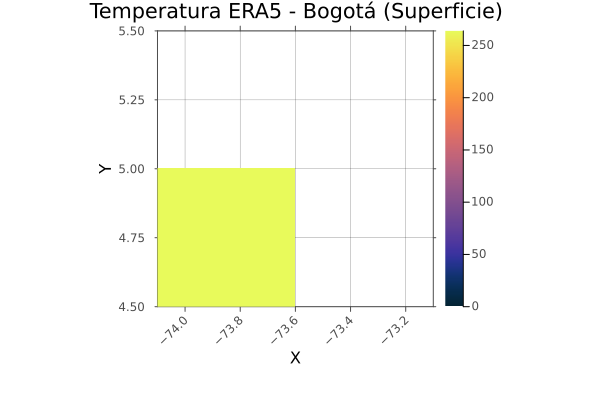
\includegraphics[width=0.8\textwidth,height=\textheight]{images/c10_era5_bogota_5d_julia.png}
\end{center}

\subsection{Gestión dimensional de los miembros del
ensamble}\label{gestiuxf3n-dimensional-de-los-miembros-del-ensamble}

``colapsar'' estas dimensiones mediante estadística

\subsection{Python}

\begin{Shaded}
\begin{Highlighting}[]
\CommentTok{\# \#| eval: false}

\CommentTok{\# 1. Calcular el promedio de temperatura sobre los 10 miembros de ensamble}
\CommentTok{\# Esto reduce la dimensión {-} number {-} y nos deja con la \textquotesingle{}media del ensamble\textquotesingle{}}
\CommentTok{\# Nota: Al usar dask el objeto t\_mean no se calcula inmediatamente}
\CommentTok{\#       Si usas ds = xr.open\_dataset(ncfile5d), t\_mean va a RAM!}
\NormalTok{t\_mean }\OperatorTok{=}\NormalTok{ ds[}\StringTok{\textquotesingle{}t\textquotesingle{}}\NormalTok{].mean(dim}\OperatorTok{=}\StringTok{\textquotesingle{}number\textquotesingle{}}\NormalTok{)}
\NormalTok{t\_mean}
\end{Highlighting}
\end{Shaded}

\begin{verbatim}
<xarray.DataArray 't' (time: 480, level: 37, latitude: 35, longitude: 25)> Size: 124MB
array([[[[261.81838611, 261.83113887, 261.87920699, ..., 263.71678237,
          263.79447614, 263.88296071],
         [262.05421417, 262.07834632, 262.14623027, ..., 263.86137911,
          263.98262847, 264.11035232],
         [262.21097508, 262.26394811, 262.35929955, ..., 263.99557744,
          264.14880682, 264.30537153],
         ...,
         [259.02984683, 258.99139234, 259.00316412, ..., 262.27552369,
          262.27571989, 262.27179596],
         [258.69121187, 258.62568227, 258.62489749, ..., 262.46112548,
          262.49428267, 262.51194034],
         [258.5371977 , 258.47049093, 258.47578823, ..., 262.5957162 ,
          262.64417671, 262.66222678]],

        [[254.24187016, 254.43983232, 254.56853715, ..., 254.02291499,
          254.03821831, 254.00898505],
         [253.903039  , 254.0821663 , 254.16711934, ..., 253.80847234,
          253.74117698, 253.64837608],
         [253.69742518, 253.81475062, 253.82966155, ..., 253.59579545,
          253.46709062, 253.32877217],
...
         [298.57833012, 299.32583836, 299.67428314, ..., 299.9210982 ,
          299.86380886, 300.05588512],
         [300.44631593, 300.42434194, 299.47671338, ..., 299.84929032,
          299.73392685, 299.96641957],
         [299.73981274, 299.92835747, 299.20243083, ..., 299.62503785,
          299.48358025, 299.67016302]],

        [[298.73273667, 298.78884884, 298.79493093, ..., 298.30561714,
          298.25460607, 298.20693035],
         [298.96719136, 298.93344558, 298.84241046, ..., 298.17553893,
          298.1555269 , 298.04624551],
         [298.99544364, 298.93992006, 298.8508469 , ..., 297.66013102,
          297.43038504, 297.40272135],
         ...,
         [299.67153639, 300.68273258, 301.07080904, ..., 301.56993265,
          301.56090762, 301.79791286],
         [301.7302251 , 301.94054763, 300.90168775, ..., 301.38413467,
          301.31291538, 301.60426702],
         [300.96623637, 301.39727983, 300.62779759, ..., 301.1163266 ,
          300.99252668, 301.20461498]]]], shape=(480, 37, 35, 25))
Coordinates:
  * time       (time) datetime64[ns] 4kB 2020-01-01 ... 2020-02-29T21:00:00
  * level      (level) int32 148B 1 2 3 5 7 10 20 ... 875 900 925 950 975 1000
  * latitude   (latitude) float32 140B 12.5 12.0 11.5 11.0 ... -3.5 -4.0 -4.5
  * longitude  (longitude) float32 100B -79.1 -78.6 -78.1 ... -68.1 -67.6 -67.1
Attributes:
    units:          K
    long_name:      Temperature
    standard_name:  air_temperature
\end{verbatim}

\begin{Shaded}
\begin{Highlighting}[]
\CommentTok{\# 2. Seleccionar un nivel de presión específico para Bogotá (aprox 750 hPa)}
\CommentTok{\# Buscamos el nivel más cercano a la presión de la capital}
\NormalTok{t\_bogota\_alt }\OperatorTok{=}\NormalTok{ t\_mean.sel(level}\OperatorTok{=}\DecValTok{750}\NormalTok{, method}\OperatorTok{=}\StringTok{\textquotesingle{}nearest\textquotesingle{}}\NormalTok{)}
\NormalTok{t\_bogota\_alt}
\end{Highlighting}
\end{Shaded}

\begin{verbatim}
<xarray.DataArray 't' (time: 480, latitude: 35, longitude: 25)> Size: 3MB
array([[[285.2461969 , 285.5452002 , 285.84636166, ..., 285.32075153,
         285.29112588, 285.29014489],
        [285.7568961 , 286.05982333, 286.30624599, ..., 285.36980063,
         285.34664945, 285.36783866],
        [286.08984138, 286.39688872, 286.56954155, ..., 285.28955631,
         285.40099585, 285.47378471],
        ...,
        [286.35941521, 287.685899  , 287.78615535, ..., 285.95191531,
         285.9797752 , 285.94838378],
        [286.39139523, 287.43712198, 287.7404416 , ..., 285.94367507,
         285.97800943, 285.936612  ],
        [286.78359181, 287.2889937 , 287.66510218, ..., 286.06021572,
         286.11318875, 286.0615891 ]],

       [[284.47220215, 284.79455282, 285.13946607, ..., 285.0617723 ,
         285.01860909, 285.01527375],
        [285.09630286, 285.43395685, 285.76768691, ..., 285.00958406,
         284.95111753, 284.90834672],
        [285.61131838, 285.91954291, 286.1157393 , ..., 284.82417847,
         284.83261492, 284.8332035 ],
...
        [287.26564633, 286.3005563 , 285.64349459, ..., 285.34292172,
         285.39981868, 285.42493181],
        [286.43043831, 285.50419515, 285.52126424, ..., 285.31388466,
         285.33566246, 285.3819648 ],
        [286.83499526, 285.63976686, 285.66801914, ..., 285.29975852,
         285.27189863, 285.33487767]],

       [[284.82751381, 284.94895937, 285.12475134, ..., 286.69118331,
         286.89640473, 287.02589435],
        [284.97544589, 285.13024484, 285.3388016 , ..., 286.31605581,
         286.54227025, 286.6917719 ],
        [285.18262927, 285.41649537, 285.6972524 , ..., 285.545004  ,
         285.74571291, 286.04608958],
        ...,
        [286.92406842, 286.42867254, 286.03883031, ..., 285.87814547,
         285.91836573, 286.10848003],
        [286.52108104, 285.99135079, 286.11240396, ..., 285.94877617,
         286.0180335 , 286.1865662 ],
        [286.93328965, 286.03176724, 286.16753515, ..., 285.88108842,
         286.00920466, 286.15772533]]], shape=(480, 35, 25))
Coordinates:
  * time       (time) datetime64[ns] 4kB 2020-01-01 ... 2020-02-29T21:00:00
  * latitude   (latitude) float32 140B 12.5 12.0 11.5 11.0 ... -3.5 -4.0 -4.5
  * longitude  (longitude) float32 100B -79.1 -78.6 -78.1 ... -68.1 -67.6 -67.1
    level      int32 4B 750
Attributes:
    units:          K
    long_name:      Temperature
    standard_name:  air_temperature
\end{verbatim}

\begin{Shaded}
\begin{Highlighting}[]
\BuiltInTok{print}\NormalTok{(}\SpecialStringTok{f"Estructura resultante: }\SpecialCharTok{\{}\NormalTok{t\_bogota\_alt}\SpecialCharTok{.}\NormalTok{dims}\SpecialCharTok{\}}\SpecialStringTok{"}\NormalTok{)}
\end{Highlighting}
\end{Shaded}

\begin{verbatim}
Estructura resultante: ('time', 'latitude', 'longitude')
\end{verbatim}

\subsection{R}

\begin{Shaded}
\begin{Highlighting}[]
\CommentTok{\# \#| eval: false}

\CommentTok{\# 1. Reducir la dimensión de ensamble (number) calculando la media}
\CommentTok{\# Usamos st\_apply sobre las dimensiones espaciales, temporales y de nivel}
\NormalTok{t\_mean }\OtherTok{\textless{}{-}} \FunctionTok{st\_apply}\NormalTok{(st\_col5d, }\FunctionTok{c}\NormalTok{(}\StringTok{"x"}\NormalTok{, }\StringTok{"y"}\NormalTok{, }\StringTok{"level"}\NormalTok{, }\StringTok{"time"}\NormalTok{), mean)}

\CommentTok{\# 2. Verificar que el nivel 27 corresponda a 750 hPa (Bogotá)}
\CommentTok{\# Extracción de los valores de la dimensión "level"}
\NormalTok{valores\_dimension }\OtherTok{\textless{}{-}} \FunctionTok{st\_get\_dimension\_values}\NormalTok{(st\_col5d, }\StringTok{"level"}\NormalTok{)}
\NormalTok{valores\_dimension}
\end{Highlighting}
\end{Shaded}

\begin{verbatim}
Units: [millibars]
 [1]    1    2    3    5    7   10   20   30   50   70  100  125  150  175  200
[16]  225  250  300  350  400  450  500  550  600  650  700  750  775  800  825
[31]  850  875  900  925  950  975 1000
\end{verbatim}

\begin{Shaded}
\begin{Highlighting}[]
\CommentTok{\# Generar índices a partir de los valores}
\NormalTok{indices\_dimension }\OtherTok{\textless{}{-}} \FunctionTok{seq\_along}\NormalTok{(}\FunctionTok{st\_get\_dimension\_values}\NormalTok{(st\_col5d, }\StringTok{"level"}\NormalTok{))}
\NormalTok{indices\_dimension}
\end{Highlighting}
\end{Shaded}

\begin{verbatim}
 [1]  1  2  3  4  5  6  7  8  9 10 11 12 13 14 15 16 17 18 19 20 21 22 23 24 25
[26] 26 27 28 29 30 31 32 33 34 35 36 37
\end{verbatim}

\begin{Shaded}
\begin{Highlighting}[]
\CommentTok{\# Extraer la extensión numérica desde las dimensiones del objeto}
\CommentTok{\# indices\_dimension \textless{}{-} 1:dim(st\_col5d)["level"]}
\CommentTok{\# indices\_dimension}

\CommentTok{\# Identificación de la posición del valor 750 en la dimensión especificada}
\NormalTok{indice\_objetivo }\OtherTok{\textless{}{-}} \FunctionTok{which}\NormalTok{(units}\SpecialCharTok{::}\FunctionTok{drop\_units}\NormalTok{(valores\_dimension) }\SpecialCharTok{==} \DecValTok{750}\NormalTok{)}
\NormalTok{indice\_objetivo}
\end{Highlighting}
\end{Shaded}

\begin{verbatim}
[1] 27
\end{verbatim}

\begin{Shaded}
\begin{Highlighting}[]
\CommentTok{\# 2. Seleccionar el nivel 27 (750 hPa)}
\NormalTok{t\_level\_bog }\OtherTok{\textless{}{-}}\NormalTok{ t\_mean }\SpecialCharTok{\%\textgreater{}\%} \FunctionTok{slice}\NormalTok{(level, indice\_objetivo)}
\CommentTok{\# El objeto proxy tiene operaciones pendientes}
\CommentTok{\# así que la impresión de su contenido no refleja esas operaciones}
\FunctionTok{print}\NormalTok{(t\_level\_bog)}
\end{Highlighting}
\end{Shaded}

\begin{verbatim}
stars_proxy object with 1 attribute in 1 file(s):
$download5Dcolombia.nc
[1] "[...]/download5Dcolombia.nc"

dimension(s):
       from  to                                      offset
x         1  25                                      -79.35
y         1  35                                       12.75
level     1  37                                          NA
number    1  10                                           0
time      1 480 1051896 [hours since 1900-01-01 00:00:00.0]
                                       delta  refsys
x                                        0.5  WGS 84
y                                       -0.5  WGS 84
level                                     NA udunits
number                                     1      NA
time   3 [hours since 1900-01-01 00:00:00.0] udunits
                                              values x/y
x                                               NULL [x]
y                                               NULL [y]
level  [1,2) [millibars],...,[1000,1025) [millibars]    
number                                          NULL    
time                                            NULL    
call_list:
[[1]]
st_apply(X = X, MARGIN = MARGIN, FUN = FUN, CLUSTER = CLUSTER, 
    PROGRESS = PROGRESS, FUTURE = FUTURE, rename = rename, .fname = .fname)
attr(,".Environment")
<environment: 0x56ba25b123e0>

[[2]]
slice(.data = .data, along = level, index = indice_objetivo)
attr(,".Environment")
<environment: 0x56ba2569aa30>

This object has pending lazy operations: dimensions as printed may not reflect this.
\end{verbatim}

\begin{Shaded}
\begin{Highlighting}[]
\CommentTok{\# La inspección de la estructura lógica de la dimensión level}
\CommentTok{\# tampoco está actualizada (ignora operaciones lazy)}
\NormalTok{dimensiones\_actuales }\OtherTok{\textless{}{-}} \FunctionTok{st\_dimensions}\NormalTok{(t\_level\_bog)}
\FunctionTok{print}\NormalTok{(dimensiones\_actuales}\SpecialCharTok{$}\NormalTok{level)}
\end{Highlighting}
\end{Shaded}

\begin{verbatim}
$from
[1] 1

$to
[1] 37

$offset
[1] NA

$delta
[1] NA

$refsys
[1] "udunits"

$point
[1] NA

$values
$start
Units: [millibars]
 [1]    1    2    3    5    7   10   20   30   50   70  100  125  150  175  200
[16]  225  250  300  350  400  450  500  550  600  650  700  750  775  800  825
[31]  850  875  900  925  950  975 1000

$end
Units: [millibars]
 [1]    2    3    5    7   10   20   30   50   70  100  125  150  175  200  225
[16]  250  300  350  400  450  500  550  600  650  700  750  775  800  825  850
[31]  875  900  925  950  975 1000 1025

attr(,"class")
[1] "intervals"

attr(,"class")
[1] "dimension"
\end{verbatim}

\begin{Shaded}
\begin{Highlighting}[]
\CommentTok{\# Usar la función genérica dim() tambpoco funciona.}
\CommentTok{\# resultante tras aplicar la lista de llamadas pendientes}
\CommentTok{\# Verificación del tamaño del cubo tras la operación slice}
\FunctionTok{dim}\NormalTok{(t\_level\_bog)}
\end{Highlighting}
\end{Shaded}

\begin{verbatim}
     x      y  level number   time 
    25     35     37     10    480 
\end{verbatim}

\begin{Shaded}
\begin{Highlighting}[]
\CommentTok{\# Solución para ver el estado real de t\_level\_bog:}
\CommentTok{\# 1. Convertir a memoria (puede ser muy pesado)}
\CommentTok{\# t\_level\_bog \textless{}{-} st\_as\_stars(t\_level\_bog)}
\CommentTok{\#}

\CommentTok{\# Nota: La persistencia de las dimensiones originales (level = 37 y number = 10) en la salida de dim() y print() tras aplicar st\_apply y slice indica que el objeto stars\_proxy mantiene una vinculación estricta con los metadatos del archivo NetCDF original. En esta configuración, las operaciones no modifican el encabezado del objeto en memoria para evitar inconsistencias con el archivo físico hasta que se fuerce una evaluación}

\CommentTok{\# 2. Solución alternativa: realizar una materialización selectiva}

\CommentTok{\# Materialización de un subconjunto mínimo (un solo píxel espacial)}
\CommentTok{\# Esto fuerza la ejecución de la call\_list solo para una celda}
\NormalTok{verificacion\_minima }\OtherTok{\textless{}{-}}\NormalTok{ t\_level\_bog }\SpecialCharTok{\%\textgreater{}\%}
  \FunctionTok{slice}\NormalTok{(x, }\DecValTok{1}\NormalTok{) }\SpecialCharTok{\%\textgreater{}\%}
  \FunctionTok{slice}\NormalTok{(y, }\DecValTok{1}\NormalTok{) }\SpecialCharTok{\%\textgreater{}\%}
  \FunctionTok{st\_as\_stars}\NormalTok{()}
\end{Highlighting}
\end{Shaded}

\begin{verbatim}
Warning in CPL_get_metadata(file, NA_character_, options): GDAL Message 1:
dimension #1 (number) is not a Time dimension.
\end{verbatim}

\begin{verbatim}
Warning in CPL_read_gdal(as.character(x), as.character(options),
as.character(driver), : GDAL Message 1: The dataset has several variables that
could be identified as vector fields, but not all share the same primary
dimension. Consequently they will be ignored.
\end{verbatim}

\begin{verbatim}
Warning in CPL_read_gdal(as.character(x), as.character(options),
as.character(driver), : GDAL Message 1: dimension #1 (number) is not a Time
dimension.
\end{verbatim}

\begin{Shaded}
\begin{Highlighting}[]
\CommentTok{\# Inspección de las dimensiones resultantes}
\FunctionTok{print}\NormalTok{(}\FunctionTok{dim}\NormalTok{(verificacion\_minima))}
\end{Highlighting}
\end{Shaded}

\begin{verbatim}
   x    y time 
   1    1  480 
\end{verbatim}

\begin{Shaded}
\begin{Highlighting}[]
\CommentTok{\# Inspección de las dimensiones resultantes}
\CommentTok{\# Si la lógica es correcta, el resultado de dim() para verificacion\_minima debería omitir la dimensión number (eliminada por mean) y mostrar level = 1.}
\FunctionTok{print}\NormalTok{(}\FunctionTok{dim}\NormalTok{(verificacion\_minima))}
\end{Highlighting}
\end{Shaded}

\begin{verbatim}
   x    y time 
   1    1  480 
\end{verbatim}

\begin{Shaded}
\begin{Highlighting}[]
\CommentTok{\# Solucion alternativa 3: downsample}
\CommentTok{\# Carga de una versión simplificada (1 de cada 20 píxeles) para inspección}
\NormalTok{t\_preview }\OtherTok{\textless{}{-}} \FunctionTok{st\_as\_stars}\NormalTok{(t\_level\_bog, }\AttributeTok{downsample =} \DecValTok{20}\NormalTok{)}
\end{Highlighting}
\end{Shaded}

\begin{verbatim}
Warning in CPL_get_metadata(file, NA_character_, options): GDAL Message 1:
dimension #1 (number) is not a Time dimension.
\end{verbatim}

\begin{verbatim}
Warning in CPL_read_gdal(as.character(x), as.character(options),
as.character(driver), : GDAL Message 1: The dataset has several variables that
could be identified as vector fields, but not all share the same primary
dimension. Consequently they will be ignored.
\end{verbatim}

\begin{verbatim}
Warning in CPL_read_gdal(as.character(x), as.character(options),
as.character(driver), : GDAL Message 1: dimension #1 (number) is not a Time
dimension.
\end{verbatim}

\begin{Shaded}
\begin{Highlighting}[]
\CommentTok{\# Verificación de que \textquotesingle{}number\textquotesingle{} ha desaparecido y \textquotesingle{}level\textquotesingle{} es 1}
\FunctionTok{print}\NormalTok{(t\_preview)}
\end{Highlighting}
\end{Shaded}

\begin{verbatim}
stars object with 3 dimensions and 1 attribute
attribute(s):
          Min. 1st Qu.   Median    Mean  3rd Qu.     Max.
mean  281.8553 285.103 285.8083 285.884 286.7199 289.4993
dimension(s):
     from  to                                      offset
x       1   2                                      -79.35
y       1   2                                       12.75
time    1 480 1051896 [hours since 1900-01-01 00:00:00.0]
                                     delta  refsys x/y
x                                     6.25  WGS 84 [x]
y                                    -8.75  WGS 84 [y]
time 3 [hours since 1900-01-01 00:00:00.0] udunits    
\end{verbatim}

\subsection{Julia}

\begin{Shaded}
\begin{Highlighting}[]
\CommentTok{\# \#| eval: false}

\FunctionTok{j\_eval}\NormalTok{(}\StringTok{\textquotesingle{}}
\StringTok{using Statistics}

\StringTok{\# 1. Promediar sobre la dimensión de ensamble (4ta dimensión o number)}
\StringTok{\# dropdims elimina la dimensión de tamaño 1 restante}
\StringTok{t\_mean = dropdims(mean(cube, dims=4), dims=4)}
\StringTok{\#t\_mean = dropdims(mean(cube, dims=Dim\{:number\}), dims=Dim\{:number\})}

\StringTok{\# 2. Seleccionar nivel de presión por valor exacto (ej. 750 hPa)}
\StringTok{t\_bog = t\_mean[Z(At(1000))]}
\StringTok{println(size(t\_bog))}


\StringTok{\# 3. Selección de nivel (Z) e instante de tiempo (Ti)}
\StringTok{\# Al agregar Ti(1), reducimos el objeto de (X, Y, Ti) a (X, Y)}
\StringTok{t\_bog\_slice = t\_mean[Z(At(1000)), Ti(1)]}
\StringTok{println(size(t\_bog\_slice))}

\StringTok{p\_reduccion = plot(t\_bog\_slice, title="Temperatura Media Ensamble (750 hPa)", c=:magma)}

\StringTok{savefig(p\_reduccion, "images/c10\_reduccion\_julia.png")}
\StringTok{\textquotesingle{}}\NormalTok{)}
\end{Highlighting}
\end{Shaded}

\begin{Shaded}
\begin{Highlighting}[]
\NormalTok{knitr}\SpecialCharTok{::}\FunctionTok{include\_graphics}\NormalTok{(}\StringTok{"images/c10\_reduccion\_julia.png"}\NormalTok{)}
\end{Highlighting}
\end{Shaded}

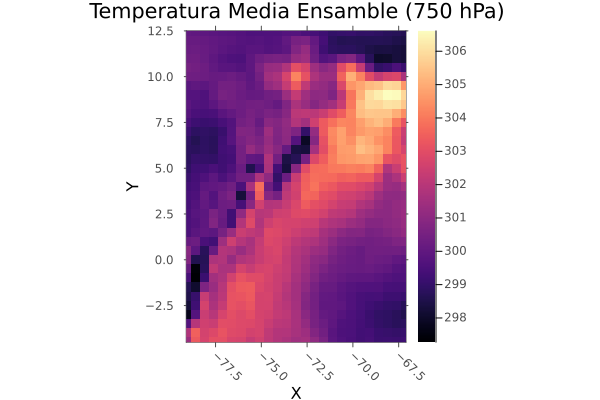
\includegraphics[width=2in,height=\textheight]{images/c10_reduccion_julia.png}

\subsection{Resumen sintáctico de manipulación
5D}\label{resumen-sintuxe1ctico-de-manipulaciuxf3n-5d}

En cubos de alta dimensionalidad, la complejidad no reside solo en el
volumen de datos, sino en la precisión de los selectores. A
continuación, se comparan las funciones críticas para navegar y colapsar
las dimensiones de ERA5.

\begin{longtable}[]{@{}
  >{\raggedright\arraybackslash}p{(\columnwidth - 6\tabcolsep) * \real{0.2500}}
  >{\raggedright\arraybackslash}p{(\columnwidth - 6\tabcolsep) * \real{0.2500}}
  >{\raggedright\arraybackslash}p{(\columnwidth - 6\tabcolsep) * \real{0.2500}}
  >{\raggedright\arraybackslash}p{(\columnwidth - 6\tabcolsep) * \real{0.2500}}@{}}
\toprule\noalign{}
\begin{minipage}[b]{\linewidth}\raggedright
Operación
\end{minipage} & \begin{minipage}[b]{\linewidth}\raggedright
Python 🐍
\end{minipage} & \begin{minipage}[b]{\linewidth}\raggedright
R 🔵
\end{minipage} & \begin{minipage}[b]{\linewidth}\raggedright
Julia 🟣
\end{minipage} \\
\midrule\noalign{}
\endhead
\bottomrule\noalign{}
\endlastfoot
\textbf{Selección por valor (Presión)} & \texttt{.sel(level=750)} &
\texttt{slice(level,\ indice)} & \texttt{cube{[}Z(At(750)){]}} \\
\textbf{Búsqueda del más cercano} &
\texttt{method=\textquotesingle{}nearest\textquotesingle{}} &
\texttt{which.min(abs(v\ -\ val))} & \texttt{X(Near(valor))} \\
\textbf{Reducción (Promedio Ensamble)} &
\texttt{.mean(dim=\textquotesingle{}number\textquotesingle{})} &
\texttt{st\_apply(...,\ mean)} & \texttt{mean(cube,\ dims=4)} \\
\textbf{Recorte Espacial (BBox)} & \texttt{.sel(lat=slice(),\ ...)} &
\texttt{st\_crop(obj,\ bbox)} & \texttt{X(Between(a,\ b))} \\
\textbf{Eliminar dimensión unitaria} & \texttt{.squeeze()} &
\texttt{adrop()} & \texttt{dropdims(...,\ dims=N)} \\
\end{longtable}

\textbf{Notas sobre la gestión 5D:}

\begin{itemize}
\tightlist
\item
  \textbf{Python 🐍}: \texttt{xarray} es extremadamente intuitivo al
  permitir llamar a las dimensiones por su nombre
  (\texttt{dim=\textquotesingle{}number\textquotesingle{}}), lo que
  reduce errores humanos al manipular arreglos de gran tamaño.
\item
  \textbf{R 🔵}: El uso de \texttt{st\_as\_stars()} tras un filtrado es
  vital. Al trabajar con objetos \emph{proxy}, R solo ``anota'' la
  intención del recorte; materializarlo selectivamente es la estrategia
  más eficiente para no agotar la RAM.
\item
  \textbf{Julia 🟣}: Destaca por su manejo de índices lógicos. El uso de
  \texttt{At()} y \texttt{Near()} permite que el código sea
  autodocumentado, indicando explícitamente si estamos buscando un valor
  exacto o la coordenada más próxima.
\end{itemize}

\subsection{Hacia la transformación del
dato}\label{hacia-la-transformaciuxf3n-del-dato}

Una vez que hemos filtrado nuestro cubo 5D a una estructura más
manejable (generalmente 3D: espacio y tiempo), el siguiente reto es la
\textbf{operacionalización}. En la práctica profesional, los datos
climáticos brutos rara vez vienen en las unidades o proyecciones
necesarias para un informe técnico. En la siguiente sección, abordaremos
el \textbf{Álgebra de mapas multidimensional}, donde transformaremos
Kelvin a Celsius y realizaremos agregaciones temporales masivas bajo el
estándar de evaluación perezosa.

\section{Álgebra de mapas multidimensional (Raster
Math)}\label{uxe1lgebra-de-mapas-multidimensional-raster-math}

Una de las ventajas más potentes de trabajar con cubos de datos es la
capacidad de realizar operaciones aritméticas sobre millones de píxeles
simultáneamente sin necesidad de escribir bucles (\texttt{for\ loops}).
Esto se conoce como álgebra de mapas o vectorización.

Dado que la temperatura en ERA5 viene por defecto en Kelvin (K), una
operación obligatoria para el análisis climático en Colombia es la
conversión a grados Celsius. La fórmula matemática es sencilla
(\(C = K - 273.15\)), pero el reto computacional es aplicarla a través
de todas las dimensiones (espacio, tiempo y niveles) de forma eficiente.
Gracias a la \textbf{evaluación perezosa}, esta resta no colapsa la
memoria RAM; simplemente se añade como una instrucción pendiente en el
grafo de tareas hasta que decidamos visualizar o guardar el dato.

\subsection{Python}

\begin{Shaded}
\begin{Highlighting}[]
\CommentTok{\# \#| eval: false}

\CommentTok{\# Resta vectorizada a todo el cubo de medias}
\NormalTok{t\_celsius }\OperatorTok{=}\NormalTok{ t\_mean }\OperatorTok{{-}} \FloatTok{273.15}

\CommentTok{\# Actualización de atributos}
\NormalTok{t\_celsius.attrs[}\StringTok{\textquotesingle{}units\textquotesingle{}}\NormalTok{] }\OperatorTok{=} \StringTok{\textquotesingle{}°C\textquotesingle{}}
\NormalTok{t\_celsius.attrs[}\StringTok{\textquotesingle{}long\_name\textquotesingle{}}\NormalTok{] }\OperatorTok{=} \StringTok{\textquotesingle{}Temperatura Media (Celsius)\textquotesingle{}}

\CommentTok{\# Verificación en el nivel de Bogotá}
\NormalTok{t\_bogota\_celsius }\OperatorTok{=}\NormalTok{ t\_celsius.sel(level}\OperatorTok{=}\DecValTok{750}\NormalTok{, method}\OperatorTok{=}\StringTok{\textquotesingle{}nearest\textquotesingle{}}\NormalTok{)}
\BuiltInTok{print}\NormalTok{(t\_bogota\_celsius)}
\end{Highlighting}
\end{Shaded}

\begin{verbatim}
<xarray.DataArray 't' (time: 480, latitude: 35, longitude: 25)> Size: 3MB
array([[[12.0961969 , 12.3952002 , 12.69636166, ..., 12.17075153,
         12.14112588, 12.14014489],
        [12.6068961 , 12.90982333, 13.15624599, ..., 12.21980063,
         12.19664945, 12.21783866],
        [12.93984138, 13.24688872, 13.41954155, ..., 12.13955631,
         12.25099585, 12.32378471],
        ...,
        [13.20941521, 14.535899  , 14.63615535, ..., 12.80191531,
         12.8297752 , 12.79838378],
        [13.24139523, 14.28712198, 14.5904416 , ..., 12.79367507,
         12.82800943, 12.786612  ],
        [13.63359181, 14.1389937 , 14.51510218, ..., 12.91021572,
         12.96318875, 12.9115891 ]],

       [[11.32220215, 11.64455282, 11.98946607, ..., 11.9117723 ,
         11.86860909, 11.86527375],
        [11.94630286, 12.28395685, 12.61768691, ..., 11.85958406,
         11.80111753, 11.75834672],
        [12.46131838, 12.76954291, 12.9657393 , ..., 11.67417847,
         11.68261492, 11.6832035 ],
...
        [14.11564633, 13.1505563 , 12.49349459, ..., 12.19292172,
         12.24981868, 12.27493181],
        [13.28043831, 12.35419515, 12.37126424, ..., 12.16388466,
         12.18566246, 12.2319648 ],
        [13.68499526, 12.48976686, 12.51801914, ..., 12.14975852,
         12.12189863, 12.18487767]],

       [[11.67751381, 11.79895937, 11.97475134, ..., 13.54118331,
         13.74640473, 13.87589435],
        [11.82544589, 11.98024484, 12.1888016 , ..., 13.16605581,
         13.39227025, 13.5417719 ],
        [12.03262927, 12.26649537, 12.5472524 , ..., 12.395004  ,
         12.59571291, 12.89608958],
        ...,
        [13.77406842, 13.27867254, 12.88883031, ..., 12.72814547,
         12.76836573, 12.95848003],
        [13.37108104, 12.84135079, 12.96240396, ..., 12.79877617,
         12.8680335 , 13.0365662 ],
        [13.78328965, 12.88176724, 13.01753515, ..., 12.73108842,
         12.85920466, 13.00772533]]], shape=(480, 35, 25))
Coordinates:
  * time       (time) datetime64[ns] 4kB 2020-01-01 ... 2020-02-29T21:00:00
  * latitude   (latitude) float32 140B 12.5 12.0 11.5 11.0 ... -3.5 -4.0 -4.5
  * longitude  (longitude) float32 100B -79.1 -78.6 -78.1 ... -68.1 -67.6 -67.1
    level      int32 4B 750
Attributes:
    units:          °C
    long_name:      Temperatura Media (Celsius)
    standard_name:  air_temperature
\end{verbatim}

\begin{Shaded}
\begin{Highlighting}[]
\ImportTok{import}\NormalTok{ matplotlib.pyplot }\ImportTok{as}\NormalTok{ plt}
\CommentTok{\# Visualización de la rebanada (Tiempo 0)}
\NormalTok{t\_bogota\_celsius.isel(time}\OperatorTok{=}\DecValTok{0}\NormalTok{).plot(cmap}\OperatorTok{=}\StringTok{"inferno"}\NormalTok{)}
\NormalTok{plt.title(}\StringTok{"Temperatura ERA5 Bogotá {-} Nivel 750 hPa (°C)"}\NormalTok{)}
\NormalTok{plt.show()}
\end{Highlighting}
\end{Shaded}


\includegraphics{20-cubos_multidimensionales_files/figure-pdf/python_algebra-1.pdf}

\subsection{R}

\begin{Shaded}
\begin{Highlighting}[]
\CommentTok{\# \#| eval: false}

\CommentTok{\# {-}{-}{-}{-}{-}{-}{-}{-}{-}{-}{-}{-}{-}{-}{-}{-}{-}{-}{-}{-}{-}{-}{-}{-}{-}{-}{-}{-}{-}{-}{-}{-}{-}{-}{-}{-}{-}{-}{-}{-}{-}{-}{-}{-}{-}{-}{-}{-}{-}{-}{-}{-}{-}{-}{-}{-}{-}{-}{-}{-}{-}{-}{-}{-}{-}{-}{-}{-}{-}{-}{-}{-}{-}}
\CommentTok{\# Álgebra de mapas: Conversión de Kelvin a Celsius en \{stars\}}
\CommentTok{\# {-}{-}{-}{-}{-}{-}{-}{-}{-}{-}{-}{-}{-}{-}{-}{-}{-}{-}{-}{-}{-}{-}{-}{-}{-}{-}{-}{-}{-}{-}{-}{-}{-}{-}{-}{-}{-}{-}{-}{-}{-}{-}{-}{-}{-}{-}{-}{-}{-}{-}{-}{-}{-}{-}{-}{-}{-}{-}{-}{-}{-}{-}{-}{-}{-}{-}{-}{-}{-}{-}{-}{-}{-}}

\CommentTok{\# Restamos el escalar directamente al objeto stars proxy.}
\CommentTok{\# Esta operación matemática se añade a la lista de tareas pendientes (lazy).}
\NormalTok{t\_celsius }\OtherTok{\textless{}{-}}\NormalTok{ t\_mean }\SpecialCharTok{{-}} \FloatTok{273.15}

\CommentTok{\# Filtrado espacial/vertical}
\NormalTok{t\_level\_bog\_c }\OtherTok{\textless{}{-}}\NormalTok{ t\_celsius }\SpecialCharTok{\%\textgreater{}\%} \FunctionTok{slice}\NormalTok{(level, indice\_objetivo)}

\CommentTok{\# Materialización de un píxel para control de calidad}
\NormalTok{verificacion\_celsius }\OtherTok{\textless{}{-}}\NormalTok{ t\_level\_bog\_c }\SpecialCharTok{\%\textgreater{}\%}
  \FunctionTok{slice}\NormalTok{(x, }\DecValTok{1}\NormalTok{) }\SpecialCharTok{\%\textgreater{}\%}
  \FunctionTok{slice}\NormalTok{(y, }\DecValTok{1}\NormalTok{) }\SpecialCharTok{\%\textgreater{}\%}
  \CommentTok{\# \textless{}{-}{-}{-} 1. Aquí se calcula todo y pasa a RAM}
  \FunctionTok{st\_as\_stars}\NormalTok{() }\SpecialCharTok{\%\textgreater{}\%}
  \CommentTok{\# \textless{}{-}{-}{-} 2. Ahora le cambiamos el nombre}
  \FunctionTok{setNames}\NormalTok{(}\StringTok{"Temperatura\_Celsius"}\NormalTok{) }\SpecialCharTok{\%\textgreater{}\%}
  \CommentTok{\# 3. Y le ponemos unidades}
  \FunctionTok{mutate}\NormalTok{(}\AttributeTok{Temperatura\_Celsius =}\NormalTok{ units}\SpecialCharTok{::}\FunctionTok{set\_units}\NormalTok{(Temperatura\_Celsius, }\StringTok{"°C"}\NormalTok{))}
\end{Highlighting}
\end{Shaded}

\begin{verbatim}
Warning in CPL_get_metadata(file, NA_character_, options): GDAL Message 1:
dimension #1 (number) is not a Time dimension.
\end{verbatim}

\begin{verbatim}
Warning in CPL_read_gdal(as.character(x), as.character(options),
as.character(driver), : GDAL Message 1: The dataset has several variables that
could be identified as vector fields, but not all share the same primary
dimension. Consequently they will be ignored.
\end{verbatim}

\begin{verbatim}
Warning in CPL_read_gdal(as.character(x), as.character(options),
as.character(driver), : GDAL Message 1: dimension #1 (number) is not a Time
dimension.
\end{verbatim}

\begin{Shaded}
\begin{Highlighting}[]
\FunctionTok{print}\NormalTok{(verificacion\_celsius)}
\end{Highlighting}
\end{Shaded}

\begin{verbatim}
stars object with 3 dimensions and 1 attribute
attribute(s):
                             Min.  1st Qu.   Median     Mean  3rd Qu.     Max.
Temperatura_Celsius [°C] 9.727714 12.28822 13.13741 13.23452 14.22861 16.60126
dimension(s):
     from  to                                      offset
x       1   1                                      -79.35
y       1   1                                       12.75
time    1 480 1051896 [hours since 1900-01-01 00:00:00.0]
                                     delta  refsys x/y
x                                      0.5  WGS 84 [x]
y                                     -0.5  WGS 84 [y]
time 3 [hours since 1900-01-01 00:00:00.0] udunits    
\end{verbatim}

\begin{Shaded}
\begin{Highlighting}[]
\FunctionTok{library}\NormalTok{(ggplot2)}
\FunctionTok{ggplot}\NormalTok{() }\SpecialCharTok{+}
  \FunctionTok{geom\_stars}\NormalTok{(}\AttributeTok{data =}\NormalTok{ verificacion\_celsius) }\SpecialCharTok{+}
  \FunctionTok{scale\_fill\_viridis\_c}\NormalTok{(}\AttributeTok{option =} \StringTok{"inferno"}\NormalTok{, }\AttributeTok{name =} \StringTok{"Temp (°C)"}\NormalTok{) }\SpecialCharTok{+}
  \FunctionTok{theme\_minimal}\NormalTok{() }\SpecialCharTok{+}
  \FunctionTok{ggtitle}\NormalTok{(}\StringTok{"Temperatura ERA5 Bogotá {-} Nivel 750 hPa (°C)"}\NormalTok{)}
\end{Highlighting}
\end{Shaded}


\includegraphics{20-cubos_multidimensionales_files/figure-pdf/r_algebra-1.pdf}

\subsection{Julia}

\begin{Shaded}
\begin{Highlighting}[]
\CommentTok{\# \#| eval: false}

\FunctionTok{j\_eval}\NormalTok{(}\StringTok{\textquotesingle{}}
\StringTok{\# Operador broadcast (.{-}) para vectorización lazy}
\StringTok{t\_celsius = t\_mean .{-} 273.15}

\StringTok{\# Extracción de una rebanada 2D para visualización}
\StringTok{t\_bog\_c\_slice = t\_celsius[Z(At(1000)), Ti(1)]}

\StringTok{using Plots}
\StringTok{p\_celsius = plot(}
\StringTok{    t\_bog\_c\_slice, }
\StringTok{    title="Temperatura ERA5 Bogotá (750 hPa)", }
\StringTok{    c=:inferno,}
\StringTok{    colorbar\_title="°C"}
\StringTok{)}

\StringTok{savefig(p\_celsius, "images/t\_bog\_slice\_julia.png")}
\StringTok{\textquotesingle{}}\NormalTok{)}
\end{Highlighting}
\end{Shaded}

\begin{Shaded}
\begin{Highlighting}[]
\NormalTok{knitr}\SpecialCharTok{::}\FunctionTok{include\_graphics}\NormalTok{(}\StringTok{"images/t\_bog\_slice\_julia.png"}\NormalTok{)}
\end{Highlighting}
\end{Shaded}

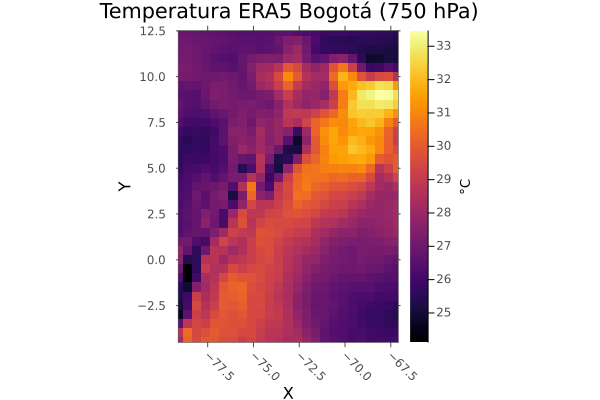
\includegraphics[width=2in,height=\textheight]{images/t_bog_slice_julia.png}

\subsection{Agregación Temporal: Calculando la
Climatología}\label{agregaciuxf3n-temporal-calculando-la-climatologuxeda}

El álgebra de mapas multidimensional no se limita a operaciones
escalares; también abarca funciones de reducción sobre ejes completos.
Si deseamos conocer la temperatura media histórica de cada píxel,
debemos ``colapsar'' la dimensión \texttt{time}.

Al igual que con la conversión a Celsius, esta operación se distribuye
espacialmente y de forma perezosa:

\begin{itemize}
\tightlist
\item
  \textbf{Python:}
  \texttt{t\_celsius.mean(dim=\textquotesingle{}time\textquotesingle{})}
\item
  \textbf{R:}
  \texttt{st\_apply(t\_celsius,\ c("x",\ "y",\ "level"),\ mean)}
\item
  \textbf{Julia:}
  \texttt{dropdims(mean(t\_celsius,\ dims=Ti),\ dims=Ti)}
\end{itemize}

El resultado es un cubo donde la dimensión temporal ha desaparecido,
dejándonos con un mapa estático que representa el promedio climatológico
para el periodo analizado.

\subsection{Resumen sintáctico de Álgebra
Multidimensional}\label{resumen-sintuxe1ctico-de-uxe1lgebra-multidimensional}

\begin{longtable}[]{@{}
  >{\raggedright\arraybackslash}p{(\columnwidth - 6\tabcolsep) * \real{0.2500}}
  >{\raggedright\arraybackslash}p{(\columnwidth - 6\tabcolsep) * \real{0.2500}}
  >{\raggedright\arraybackslash}p{(\columnwidth - 6\tabcolsep) * \real{0.2500}}
  >{\raggedright\arraybackslash}p{(\columnwidth - 6\tabcolsep) * \real{0.2500}}@{}}
\toprule\noalign{}
\begin{minipage}[b]{\linewidth}\raggedright
Operación
\end{minipage} & \begin{minipage}[b]{\linewidth}\raggedright
Python 🐍
\end{minipage} & \begin{minipage}[b]{\linewidth}\raggedright
R 🔵
\end{minipage} & \begin{minipage}[b]{\linewidth}\raggedright
Julia 🟣
\end{minipage} \\
\midrule\noalign{}
\endhead
\bottomrule\noalign{}
\endlastfoot
\textbf{Operación Escalar} & \texttt{ds\ -\ 273.15} &
\texttt{obj\ -\ 273.15} & \texttt{cube\ .-\ 273.15} \\
\textbf{Actualizar Metadato} &
\texttt{da.attrs{[}\textquotesingle{}units\textquotesingle{}{]}\ =\ \textquotesingle{}°C\textquotesingle{}}
& \texttt{units::set\_units(obj,\ "°C")} & Depende de
\texttt{DimensionalData} \\
\textbf{Promedio Temporal} &
\texttt{.mean(dim=\textquotesingle{}time\textquotesingle{})} &
\texttt{st\_apply(...,\ mean)} & \texttt{mean(cube,\ dims=Ti)} \\
\textbf{Tipo de Ejecución} & Perezosa (Dask) & Perezosa (Proxy) &
Perezosa (DiskArrays) \\
\end{longtable}

\section{Remuestreo y agregación temporal
avanzada}\label{remuestreo-y-agregaciuxf3n-temporal-avanzada}

Los datos de reanálisis como ERA5 suelen descargarse en resoluciones
temporales muy altas (ej. datos horarios). Sin embargo, para la
planificación territorial en Colombia, la gestión de riesgos o la
agricultura, rara vez analizamos el clima hora a hora. Generalmente,
necesitamos transformar esa alta frecuencia en \textbf{promedios
diarios, climatologías mensuales o acumulados anuales}.

El proceso de cambiar la frecuencia temporal de un cubo de datos se
conoce como \textbf{remuestreo temporal} (\emph{temporal resampling}).
Computacionalmente, esto implica redefinir la ``geometría temporal'' del
cubo: agrupamos las ``láminas'' horarias en bloques (ej. 24 láminas para
formar un día) y les aplicamos una función de reducción (media, máximo,
suma). Al igual que el álgebra de mapas, estas operaciones aprovechan la
\textbf{evaluación perezosa}, ejecutando los cálculos paso a paso para
evitar el colapso de la memoria RAM. El primer y más crítico paso antes
de cualquier remuestreo es auditar la resolución original del archivo.

\subsection{Python}

\begin{Shaded}
\begin{Highlighting}[]
\CommentTok{\# \#| eval: false}

\CommentTok{\# {-}{-}{-}{-}{-}{-}{-}{-}{-}{-}{-}{-}{-}{-}{-}{-}{-}{-}{-}{-}{-}{-}{-}{-}{-}{-}{-}{-}{-}{-}{-}{-}{-}{-}{-}{-}{-}{-}{-}{-}{-}{-}{-}{-}{-}{-}{-}{-}{-}{-}{-}{-}{-}{-}{-}{-}{-}{-}{-}{-}{-}{-}{-}{-}{-}{-}{-}{-}{-}{-}{-}{-}{-}}
\CommentTok{\# Inspección de resolución temporal}
\CommentTok{\# {-}{-}{-}{-}{-}{-}{-}{-}{-}{-}{-}{-}{-}{-}{-}{-}{-}{-}{-}{-}{-}{-}{-}{-}{-}{-}{-}{-}{-}{-}{-}{-}{-}{-}{-}{-}{-}{-}{-}{-}{-}{-}{-}{-}{-}{-}{-}{-}{-}{-}{-}{-}{-}{-}{-}{-}{-}{-}{-}{-}{-}{-}{-}{-}{-}{-}{-}{-}{-}{-}{-}{-}{-}}
\ImportTok{import}\NormalTok{ pandas }\ImportTok{as}\NormalTok{ pd}

\CommentTok{\# Calculamos la diferencia entre los dos primeros registros de tiempo}
\NormalTok{delta\_t }\OperatorTok{=}\NormalTok{ ds.time.diff(dim}\OperatorTok{=}\StringTok{"time"}\NormalTok{)[}\DecValTok{0}\NormalTok{].values}
\CommentTok{\# Convertimos a horas (float)}
\NormalTok{horas\_paso }\OperatorTok{=}\NormalTok{ delta\_t }\OperatorTok{/}\NormalTok{ pd.Timedelta(}\StringTok{\textquotesingle{}1 hour\textquotesingle{}}\NormalTok{)}

\BuiltInTok{print}\NormalTok{(}\SpecialStringTok{f"Resolución temporal detectada: }\SpecialCharTok{\{}\NormalTok{horas\_paso}\SpecialCharTok{\}}\SpecialStringTok{ horas"}\NormalTok{)}
\end{Highlighting}
\end{Shaded}

\begin{verbatim}
Resolución temporal detectada: 3.0 horas
\end{verbatim}

\begin{Shaded}
\begin{Highlighting}[]
\CommentTok{\# {-}{-}{-}{-}{-}{-}{-}{-}{-}{-}{-}{-}{-}{-}{-}{-}{-}{-}{-}{-}{-}{-}{-}{-}{-}{-}{-}{-}{-}{-}{-}{-}{-}{-}{-}{-}{-}{-}{-}{-}{-}{-}{-}{-}{-}{-}{-}{-}{-}{-}{-}{-}{-}{-}{-}{-}{-}{-}{-}{-}{-}{-}{-}{-}{-}{-}{-}{-}{-}{-}{-}{-}{-}}
\CommentTok{\# Remuestreo temporal con xarray (Resampling)}
\CommentTok{\# {-}{-}{-}{-}{-}{-}{-}{-}{-}{-}{-}{-}{-}{-}{-}{-}{-}{-}{-}{-}{-}{-}{-}{-}{-}{-}{-}{-}{-}{-}{-}{-}{-}{-}{-}{-}{-}{-}{-}{-}{-}{-}{-}{-}{-}{-}{-}{-}{-}{-}{-}{-}{-}{-}{-}{-}{-}{-}{-}{-}{-}{-}{-}{-}{-}{-}{-}{-}{-}{-}{-}{-}{-}}

\CommentTok{\# Partimos del cubo t\_celsius (que ya tiene el ensamble promediado)}
\CommentTok{\# .resample() agrupa la dimensión de tiempo. "1D" significa "1 Día" (Diario).}
\CommentTok{\# Luego aplicamos .mean() para calcular la temperatura media diaria.}
\NormalTok{t\_diaria }\OperatorTok{=}\NormalTok{ t\_celsius.resample(time}\OperatorTok{=}\StringTok{"1D"}\NormalTok{).mean()}

\BuiltInTok{print}\NormalTok{(}\StringTok{"}\CharTok{\textbackslash{}n}\StringTok{{-}{-}{-} Estructura Original {-}{-}{-}"}\NormalTok{)}
\end{Highlighting}
\end{Shaded}

\begin{verbatim}

--- Estructura Original ---
\end{verbatim}

\begin{Shaded}
\begin{Highlighting}[]
\BuiltInTok{print}\NormalTok{(t\_celsius.time)}
\end{Highlighting}
\end{Shaded}

\begin{verbatim}
<xarray.DataArray 'time' (time: 480)> Size: 4kB
array(['2020-01-01T00:00:00.000000000', '2020-01-01T03:00:00.000000000',
       '2020-01-01T06:00:00.000000000', ..., '2020-02-29T15:00:00.000000000',
       '2020-02-29T18:00:00.000000000', '2020-02-29T21:00:00.000000000'],
      shape=(480,), dtype='datetime64[ns]')
Coordinates:
  * time     (time) datetime64[ns] 4kB 2020-01-01 ... 2020-02-29T21:00:00
Attributes:
    long_name:  time
\end{verbatim}

\begin{Shaded}
\begin{Highlighting}[]
\BuiltInTok{print}\NormalTok{(}\StringTok{"}\CharTok{\textbackslash{}n}\StringTok{{-}{-}{-} Estructura Remuestreada (Diaria) {-}{-}{-}"}\NormalTok{)}
\end{Highlighting}
\end{Shaded}

\begin{verbatim}

--- Estructura Remuestreada (Diaria) ---
\end{verbatim}

\begin{Shaded}
\begin{Highlighting}[]
\BuiltInTok{print}\NormalTok{(t\_diaria.time)}
\end{Highlighting}
\end{Shaded}

\begin{verbatim}
<xarray.DataArray 'time' (time: 60)> Size: 480B
array(['2020-01-01T00:00:00.000000000', '2020-01-02T00:00:00.000000000',
       '2020-01-03T00:00:00.000000000', '2020-01-04T00:00:00.000000000',
       '2020-01-05T00:00:00.000000000', '2020-01-06T00:00:00.000000000',
       '2020-01-07T00:00:00.000000000', '2020-01-08T00:00:00.000000000',
       '2020-01-09T00:00:00.000000000', '2020-01-10T00:00:00.000000000',
       '2020-01-11T00:00:00.000000000', '2020-01-12T00:00:00.000000000',
       '2020-01-13T00:00:00.000000000', '2020-01-14T00:00:00.000000000',
       '2020-01-15T00:00:00.000000000', '2020-01-16T00:00:00.000000000',
       '2020-01-17T00:00:00.000000000', '2020-01-18T00:00:00.000000000',
       '2020-01-19T00:00:00.000000000', '2020-01-20T00:00:00.000000000',
       '2020-01-21T00:00:00.000000000', '2020-01-22T00:00:00.000000000',
       '2020-01-23T00:00:00.000000000', '2020-01-24T00:00:00.000000000',
       '2020-01-25T00:00:00.000000000', '2020-01-26T00:00:00.000000000',
       '2020-01-27T00:00:00.000000000', '2020-01-28T00:00:00.000000000',
       '2020-01-29T00:00:00.000000000', '2020-01-30T00:00:00.000000000',
       '2020-01-31T00:00:00.000000000', '2020-02-01T00:00:00.000000000',
       '2020-02-02T00:00:00.000000000', '2020-02-03T00:00:00.000000000',
       '2020-02-04T00:00:00.000000000', '2020-02-05T00:00:00.000000000',
       '2020-02-06T00:00:00.000000000', '2020-02-07T00:00:00.000000000',
       '2020-02-08T00:00:00.000000000', '2020-02-09T00:00:00.000000000',
       '2020-02-10T00:00:00.000000000', '2020-02-11T00:00:00.000000000',
       '2020-02-12T00:00:00.000000000', '2020-02-13T00:00:00.000000000',
       '2020-02-14T00:00:00.000000000', '2020-02-15T00:00:00.000000000',
       '2020-02-16T00:00:00.000000000', '2020-02-17T00:00:00.000000000',
       '2020-02-18T00:00:00.000000000', '2020-02-19T00:00:00.000000000',
       '2020-02-20T00:00:00.000000000', '2020-02-21T00:00:00.000000000',
       '2020-02-22T00:00:00.000000000', '2020-02-23T00:00:00.000000000',
       '2020-02-24T00:00:00.000000000', '2020-02-25T00:00:00.000000000',
       '2020-02-26T00:00:00.000000000', '2020-02-27T00:00:00.000000000',
       '2020-02-28T00:00:00.000000000', '2020-02-29T00:00:00.000000000'],
      dtype='datetime64[ns]')
Coordinates:
  * time     (time) datetime64[ns] 480B 2020-01-01 2020-01-02 ... 2020-02-29
Attributes:
    long_name:  time
\end{verbatim}

\begin{Shaded}
\begin{Highlighting}[]
\CommentTok{\# Seleccionamos: Nivel 750hPa Y un punto específico de Lat/Lon}
\CommentTok{\# (Cerca del centro de Bogotá)}
\NormalTok{punto\_especifico }\OperatorTok{=}\NormalTok{ t\_diaria.sel(}
\NormalTok{    level}\OperatorTok{=}\DecValTok{750}\NormalTok{, }
\NormalTok{    latitude}\OperatorTok{=}\FloatTok{4.6}\NormalTok{, }
\NormalTok{    longitude}\OperatorTok{={-}}\FloatTok{74.0}\NormalTok{, }
\NormalTok{    method}\OperatorTok{=}\StringTok{\textquotesingle{}nearest\textquotesingle{}}
\NormalTok{)}

\CommentTok{\# Ahora sí, graficar una línea}
\NormalTok{plt.figure(figsize}\OperatorTok{=}\NormalTok{(}\DecValTok{10}\NormalTok{, }\DecValTok{4}\NormalTok{))}
\NormalTok{punto\_especifico.plot(marker}\OperatorTok{=}\StringTok{\textquotesingle{}o\textquotesingle{}}\NormalTok{, color}\OperatorTok{=}\StringTok{\textquotesingle{}firebrick\textquotesingle{}}\NormalTok{)}
\NormalTok{plt.title(}\StringTok{"Evolución de la Temperatura Diaria en un punto de Bogotá"}\NormalTok{)}
\NormalTok{plt.ylabel(}\StringTok{"Temperatura Media [°C]"}\NormalTok{)}
\NormalTok{plt.grid(}\VariableTok{True}\NormalTok{)}
\NormalTok{plt.show()}
\end{Highlighting}
\end{Shaded}


\includegraphics{20-cubos_multidimensionales_files/figure-pdf/python_remuestreo-1.pdf}

\subsection{R}

\begin{Shaded}
\begin{Highlighting}[]
\CommentTok{\# \#| eval: false}

\CommentTok{\# {-}{-}{-}{-}{-}{-}{-}{-}{-}{-}{-}{-}{-}{-}{-}{-}{-}{-}{-}{-}{-}{-}{-}{-}{-}{-}{-}{-}{-}{-}{-}{-}{-}{-}{-}{-}{-}{-}{-}{-}{-}{-}{-}{-}{-}{-}{-}{-}{-}{-}{-}{-}{-}{-}{-}{-}{-}{-}{-}{-}{-}{-}{-}{-}{-}{-}{-}{-}{-}{-}{-}{-}{-}}
\CommentTok{\# 1. Sincronización y Auditoría Temporal}
\CommentTok{\# {-}{-}{-}{-}{-}{-}{-}{-}{-}{-}{-}{-}{-}{-}{-}{-}{-}{-}{-}{-}{-}{-}{-}{-}{-}{-}{-}{-}{-}{-}{-}{-}{-}{-}{-}{-}{-}{-}{-}{-}{-}{-}{-}{-}{-}{-}{-}{-}{-}{-}{-}{-}{-}{-}{-}{-}{-}{-}{-}{-}{-}{-}{-}{-}{-}{-}{-}{-}{-}{-}{-}{-}{-}}
\CommentTok{\# Es imperativo convertir la dimensión \textquotesingle{}time\textquotesingle{} a formato POSIXct (Fecha/Hora). }
\CommentTok{\# Sin esto, las funciones de agregación temporal no reconocerán unidades como "days".}
\NormalTok{fechas\_reales }\OtherTok{\textless{}{-}} \FunctionTok{as.POSIXct}\NormalTok{(}\FunctionTok{st\_get\_dimension\_values}\NormalTok{(t\_celsius, }\StringTok{"time"}\NormalTok{))}
\NormalTok{t\_celsius }\OtherTok{\textless{}{-}} \FunctionTok{st\_set\_dimensions}\NormalTok{(t\_celsius, }\StringTok{"time"}\NormalTok{, }\AttributeTok{values =}\NormalTok{ fechas\_reales)}

\CommentTok{\# Auditoría de resolución: Calculamos la diferencia entre los dos primeros pasos}
\NormalTok{diff\_horas }\OtherTok{\textless{}{-}} \FunctionTok{as.numeric}\NormalTok{(}\FunctionTok{difftime}\NormalTok{(fechas\_reales[}\DecValTok{2}\NormalTok{], fechas\_reales[}\DecValTok{1}\NormalTok{], }\AttributeTok{units =} \StringTok{"hours"}\NormalTok{))}
\FunctionTok{cat}\NormalTok{(}\StringTok{"Resolución temporal detectada:"}\NormalTok{, diff\_horas, }\StringTok{"horas}\SpecialCharTok{\textbackslash{}n}\StringTok{"}\NormalTok{)}
\end{Highlighting}
\end{Shaded}

\begin{verbatim}
Resolución temporal detectada: 3 horas
\end{verbatim}

\begin{Shaded}
\begin{Highlighting}[]
\CommentTok{\# {-}{-}{-}{-}{-}{-}{-}{-}{-}{-}{-}{-}{-}{-}{-}{-}{-}{-}{-}{-}{-}{-}{-}{-}{-}{-}{-}{-}{-}{-}{-}{-}{-}{-}{-}{-}{-}{-}{-}{-}{-}{-}{-}{-}{-}{-}{-}{-}{-}{-}{-}{-}{-}{-}{-}{-}{-}{-}{-}{-}{-}{-}{-}{-}{-}{-}{-}{-}{-}{-}{-}{-}{-}}
\CommentTok{\# 2. Remuestreo Temporal (Temporal Resampling)}
\CommentTok{\# {-}{-}{-}{-}{-}{-}{-}{-}{-}{-}{-}{-}{-}{-}{-}{-}{-}{-}{-}{-}{-}{-}{-}{-}{-}{-}{-}{-}{-}{-}{-}{-}{-}{-}{-}{-}{-}{-}{-}{-}{-}{-}{-}{-}{-}{-}{-}{-}{-}{-}{-}{-}{-}{-}{-}{-}{-}{-}{-}{-}{-}{-}{-}{-}{-}{-}{-}{-}{-}{-}{-}{-}{-}}
\CommentTok{\# stars utiliza aggregate() para reducir la resolución temporal.}
\CommentTok{\# Esta operación es "Lazy" (perezosa): no calcula nada aún, solo lo anota.}
\CommentTok{\# El argumento \textquotesingle{}by = "days"\textquotesingle{} colapsa las horas en promedios diarios.}
\NormalTok{t\_diaria }\OtherTok{\textless{}{-}} \FunctionTok{aggregate}\NormalTok{(t\_celsius, }\AttributeTok{by =} \StringTok{"days"}\NormalTok{, }\AttributeTok{FUN =}\NormalTok{ mean, }\AttributeTok{na.rm =} \ConstantTok{TRUE}\NormalTok{)}

\CommentTok{\# Filtrado perezoso por nivel de presión (750hPa para Bogotá)}
\NormalTok{t\_diaria\_bogota }\OtherTok{\textless{}{-}}\NormalTok{ t\_diaria }\SpecialCharTok{\%\textgreater{}\%} \FunctionTok{slice}\NormalTok{(level, indice\_objetivo)}


\CommentTok{\# {-}{-}{-}{-}{-}{-}{-}{-}{-}{-}{-}{-}{-}{-}{-}{-}{-}{-}{-}{-}{-}{-}{-}{-}{-}{-}{-}{-}{-}{-}{-}{-}{-}{-}{-}{-}{-}{-}{-}{-}{-}{-}{-}{-}{-}{-}{-}{-}{-}{-}{-}{-}{-}{-}{-}{-}{-}{-}{-}{-}{-}{-}{-}{-}{-}{-}{-}{-}{-}{-}{-}{-}{-}}
\CommentTok{\# 3. Materialización y Extracción de Serie de Tiempo (Punto Exacto)}
\CommentTok{\# {-}{-}{-}{-}{-}{-}{-}{-}{-}{-}{-}{-}{-}{-}{-}{-}{-}{-}{-}{-}{-}{-}{-}{-}{-}{-}{-}{-}{-}{-}{-}{-}{-}{-}{-}{-}{-}{-}{-}{-}{-}{-}{-}{-}{-}{-}{-}{-}{-}{-}{-}{-}{-}{-}{-}{-}{-}{-}{-}{-}{-}{-}{-}{-}{-}{-}{-}{-}{-}{-}{-}{-}{-}}
\CommentTok{\# A diferencia de slice() que usa índices (1, 2, 3...), st\_extract() usa }
\CommentTok{\# coordenadas geográficas reales, igual que el .sel() de xarray.}
\CommentTok{\#}

\CommentTok{\# Localización del punto más cercano (Equivalente a \textquotesingle{}nearest\textquotesingle{} de Python)}
\CommentTok{\#}
\CommentTok{\# Extraemos los vectores de coordenadas del cubo}
\NormalTok{lon\_vec }\OtherTok{\textless{}{-}} \FunctionTok{st\_get\_dimension\_values}\NormalTok{(t\_diaria, }\StringTok{"x"}\NormalTok{)}
\NormalTok{lat\_vec }\OtherTok{\textless{}{-}} \FunctionTok{st\_get\_dimension\_values}\NormalTok{(t\_diaria, }\StringTok{"y"}\NormalTok{)}

\CommentTok{\# Encontramos la posición (índice) más cercana a nuestro objetivo}
\NormalTok{idx\_x }\OtherTok{\textless{}{-}} \FunctionTok{which.min}\NormalTok{(}\FunctionTok{abs}\NormalTok{(lon\_vec }\SpecialCharTok{{-}}\NormalTok{ (}\SpecialCharTok{{-}}\FloatTok{74.0}\NormalTok{)))}
\NormalTok{idx\_y }\OtherTok{\textless{}{-}} \FunctionTok{which.min}\NormalTok{(}\FunctionTok{abs}\NormalTok{(lat\_vec }\SpecialCharTok{{-}} \FloatTok{4.6}\NormalTok{))}

\CommentTok{\# Extraemos el píxel por índice, así evitamos que st\_extract cambie el tipo de objeto}
\NormalTok{punto\_bogota }\OtherTok{\textless{}{-}}\NormalTok{ t\_diaria }\SpecialCharTok{\%\textgreater{}\%} 
  \FunctionTok{slice}\NormalTok{(level, indice\_objetivo) }\SpecialCharTok{\%\textgreater{}\%}
  \FunctionTok{slice}\NormalTok{(x, idx\_x) }\SpecialCharTok{\%\textgreater{}\%} 
  \FunctionTok{slice}\NormalTok{(y, idx\_y) }\SpecialCharTok{\%\textgreater{}\%} 
  \FunctionTok{st\_as\_stars}\NormalTok{() }\SpecialCharTok{\%\textgreater{}\%}
  \FunctionTok{setNames}\NormalTok{(}\StringTok{"Temp\_C"}\NormalTok{)}
\end{Highlighting}
\end{Shaded}

\begin{verbatim}
Warning in CPL_get_metadata(file, NA_character_, options): GDAL Message 1:
dimension #1 (number) is not a Time dimension.
\end{verbatim}

\begin{verbatim}
Warning in CPL_read_gdal(as.character(x), as.character(options),
as.character(driver), : GDAL Message 1: The dataset has several variables that
could be identified as vector fields, but not all share the same primary
dimension. Consequently they will be ignored.
\end{verbatim}

\begin{verbatim}
Warning in CPL_read_gdal(as.character(x), as.character(options),
as.character(driver), : GDAL Message 1: dimension #1 (number) is not a Time
dimension.
\end{verbatim}

\begin{Shaded}
\begin{Highlighting}[]
\CommentTok{\# Alternativa usando un punto sf (MEJORAR)}
\CommentTok{\# 1. Definimos el punto de interés (Centro de Bogotá) como objeto espacial}
\CommentTok{\#punto\_interes \textless{}{-} st\_sfc(st\_point(c({-}74.0, 4.6)), crs = 4326)}

\CommentTok{\# 2. Extraemos el valor del cubo más cercano a esa coordenada}
\CommentTok{\# Usamos st\_as\_stars() para materializar el resultado en RAM}
\CommentTok{\#punto\_bogota \textless{}{-} t\_diaria\_bogota \%\textgreater{}\% }
\CommentTok{\#  st\_extract(at = punto\_interes) \%\textgreater{}\% }
\CommentTok{\#  st\_as\_stars() \%\textgreater{}\%}
\CommentTok{\#  setNames("Temp\_C")}

\CommentTok{\# {-}{-}{-}{-}{-}{-}{-}{-}{-}{-}{-}{-}{-}{-}{-}{-}{-}{-}{-}{-}{-}{-}{-}{-}{-}{-}{-}{-}{-}{-}{-}{-}{-}{-}{-}{-}{-}{-}{-}{-}{-}{-}{-}{-}{-}{-}{-}{-}{-}{-}{-}{-}{-}{-}{-}{-}{-}{-}{-}{-}{-}{-}{-}{-}{-}{-}{-}{-}{-}{-}{-}{-}{-}}
\CommentTok{\# 4. Visualización de Resultados}
\CommentTok{\# {-}{-}{-}{-}{-}{-}{-}{-}{-}{-}{-}{-}{-}{-}{-}{-}{-}{-}{-}{-}{-}{-}{-}{-}{-}{-}{-}{-}{-}{-}{-}{-}{-}{-}{-}{-}{-}{-}{-}{-}{-}{-}{-}{-}{-}{-}{-}{-}{-}{-}{-}{-}{-}{-}{-}{-}{-}{-}{-}{-}{-}{-}{-}{-}{-}{-}{-}{-}{-}{-}{-}{-}{-}}
\CommentTok{\# Ahora fechas y valores\_temp vendrán del píxel más cercano a {-}74.0, 4.6}
\NormalTok{valores\_temp }\OtherTok{\textless{}{-}} \FunctionTok{as.numeric}\NormalTok{(punto\_bogota[[}\DecValTok{1}\NormalTok{]])}
\NormalTok{fechas }\OtherTok{\textless{}{-}} \FunctionTok{st\_get\_dimension\_values}\NormalTok{(punto\_bogota, }\StringTok{"time"}\NormalTok{)}

\FunctionTok{plot}\NormalTok{(fechas, valores\_temp, }
     \AttributeTok{type =} \StringTok{"o"}\NormalTok{,  }\CommentTok{\# "o" para ver puntos y líneas }
                  \CommentTok{\# (más parecido al marker=\textquotesingle{}o\textquotesingle{} de Python)}
                  \CommentTok{\# Alternativa "l"}
     \AttributeTok{col =} \StringTok{"firebrick"}\NormalTok{, }
     \AttributeTok{lwd =} \DecValTok{2}\NormalTok{, }
     \AttributeTok{pch =} \DecValTok{16}\NormalTok{,}
     \AttributeTok{main =} \FunctionTok{paste}\NormalTok{(}\StringTok{"Temp. Media Diaria {-} Resolución original:"}\NormalTok{, diff\_horas, }\StringTok{"h"}\NormalTok{),}
     \AttributeTok{xlab =} \StringTok{"Fecha"}\NormalTok{, }
     \AttributeTok{ylab =} \StringTok{"Temperatura [°C]"}\NormalTok{)}
\FunctionTok{grid}\NormalTok{()}
\end{Highlighting}
\end{Shaded}


\includegraphics{20-cubos_multidimensionales_files/figure-pdf/r_remuestreo-1.pdf}

\subsection{Julia}

\begin{Shaded}
\begin{Highlighting}[]
\CommentTok{\# \#| eval: false}

\FunctionTok{j\_eval}\NormalTok{(}\StringTok{\textquotesingle{}}
\StringTok{\# {-}{-}{-}{-}{-}{-}{-}{-}{-}{-}{-}{-}{-}{-}{-}{-}{-}{-}{-}{-}{-}{-}{-}{-}{-}{-}{-}{-}{-}{-}{-}{-}{-}{-}{-}{-}{-}{-}{-}{-}{-}{-}{-}{-}{-}{-}{-}{-}{-}{-}{-}{-}{-}{-}{-}{-}{-}{-}{-}{-}{-}{-}{-}{-}{-}{-}{-}{-}{-}{-}{-}{-}{-}}
\StringTok{\# 1. Auditoría y Cálculo del Factor de Agregación}
\StringTok{\# {-}{-}{-}{-}{-}{-}{-}{-}{-}{-}{-}{-}{-}{-}{-}{-}{-}{-}{-}{-}{-}{-}{-}{-}{-}{-}{-}{-}{-}{-}{-}{-}{-}{-}{-}{-}{-}{-}{-}{-}{-}{-}{-}{-}{-}{-}{-}{-}{-}{-}{-}{-}{-}{-}{-}{-}{-}{-}{-}{-}{-}{-}{-}{-}{-}{-}{-}{-}{-}{-}{-}{-}{-}}
\StringTok{using Dates}

\StringTok{\# Obtenemos los valores de la dimensión de tiempo}
\StringTok{tiempos = lookup(t\_celsius, Ti); nothing}

\StringTok{\# Retorna un sub{-}vector con los 5 elementos}
\StringTok{println("Primeros 5: ", first(tiempos, 5))}
\StringTok{println("Últimos 5:  ", last(tiempos, 5))}

\StringTok{\# Calculamos la diferencia entre los dos primeros pasos}
\StringTok{paso\_tiempo = tiempos[2] {-} tiempos[1]}
\StringTok{\# Convertimos el Periodo a horas (ERA5 suele ser Hour(1) o Hour(3))}
\StringTok{horas\_paso = Dates.value(Hour(paso\_tiempo))}

\StringTok{\# Calculamos dinámicamente cuántos pasos hay en 24 horas}
\StringTok{factor\_agregacion = Int(24 / horas\_paso)}

\StringTok{println("Resolución: $horas\_paso horas. Factor de agregación diario: $factor\_agregacion")}

\StringTok{\# {-}{-}{-}{-}{-}{-}{-}{-}{-}{-}{-}{-}{-}{-}{-}{-}{-}{-}{-}{-}{-}{-}{-}{-}{-}{-}{-}{-}{-}{-}{-}{-}{-}{-}{-}{-}{-}{-}{-}{-}{-}{-}{-}{-}{-}{-}{-}{-}{-}{-}{-}{-}{-}{-}{-}{-}{-}{-}{-}{-}{-}{-}{-}{-}{-}{-}{-}{-}{-}{-}{-}{-}{-}}
\StringTok{\# Remuestreo temporal y Series de Tiempo en Julia}
\StringTok{\# {-}{-}{-}{-}{-}{-}{-}{-}{-}{-}{-}{-}{-}{-}{-}{-}{-}{-}{-}{-}{-}{-}{-}{-}{-}{-}{-}{-}{-}{-}{-}{-}{-}{-}{-}{-}{-}{-}{-}{-}{-}{-}{-}{-}{-}{-}{-}{-}{-}{-}{-}{-}{-}{-}{-}{-}{-}{-}{-}{-}{-}{-}{-}{-}{-}{-}{-}{-}{-}{-}{-}{-}{-}}

\StringTok{\# En Rasters.jl, la reducción de resolución (downsampling/aggregation) }
\StringTok{\# se realiza indicando la dimensión y el factor de agrupación.}
\StringTok{\# Si ERA5 es horario, agrupar de 24 en 24 nos da el promedio diario.}
\StringTok{\# La función \textasciigrave{}aggregate\textasciigrave{} se encarga de esto leyendo del disco eficientemente.}

\StringTok{\# Agregamos la dimensión temporal (Ti) en bloques de 24 horas usando la media}
\StringTok{t\_diaria = aggregate(mean, t\_celsius, Ti(factor\_agregacion))}

\StringTok{println("}\SpecialCharTok{\textbackslash{}n}\StringTok{{-}{-}{-} Nueva estructura del cubo diario {-}{-}{-}")}
\StringTok{println(dims(t\_diaria, Ti))}

\StringTok{\# Para analizar una serie de tiempo, fijamos las coordenadas espaciales (X, Y) }
\StringTok{\# y el nivel de presión (Z), dejando libre la dimensión del tiempo (Ti(:)).}
\StringTok{\# Nota: Extraemos la serie del centro geométrico del recorte.}
\StringTok{serie\_bogota = t\_diaria[X(Near({-}74.0)), Y(Near(4.6)), Z(At(1000))]}


\StringTok{\# Al dejar el tiempo libre, serie\_bogota es un vector 1D.}
\StringTok{\# Rasters.jl + Plots detecta automáticamente la dimensión temporal para el eje X.}
\StringTok{p\_serie = plot(serie\_bogota, }
\StringTok{               title="Temp. Diaria (Paso original: $(horas\_paso)h)", }
\StringTok{               ylabel="Temperatura [°C]", }
\StringTok{               xlabel="Fecha",}
\StringTok{               linewidth=2, }
\StringTok{               color=:darkred,}
\StringTok{               markershape=:circle,}
\StringTok{               legend=false)}

\StringTok{savefig(p\_serie, "images/c10\_serie\_tiempo\_julia.png")}
\StringTok{\textquotesingle{}}\NormalTok{)}
\end{Highlighting}
\end{Shaded}

\begin{Shaded}
\begin{Highlighting}[]
\NormalTok{knitr}\SpecialCharTok{::}\FunctionTok{include\_graphics}\NormalTok{(}\StringTok{"images/c10\_serie\_tiempo\_julia.png"}\NormalTok{)}
\end{Highlighting}
\end{Shaded}

\begin{center}
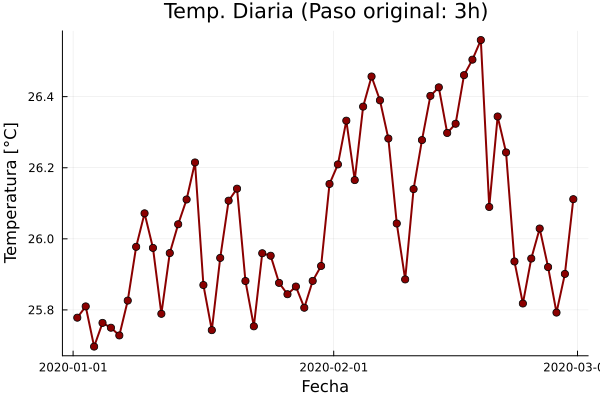
\includegraphics[width=0.8\textwidth,height=\textheight]{images/c10_serie_tiempo_julia.png}
\end{center}

\subsection{Resumen sintáctico de remuestreo
temporal}\label{resumen-sintuxe1ctico-de-remuestreo-temporal}

La siguiente tabla sintetiza las funciones clave para agrupar y extraer
series temporales a partir de cubos multidimensionales:

\begin{longtable}[]{@{}
  >{\raggedright\arraybackslash}p{(\columnwidth - 6\tabcolsep) * \real{0.2500}}
  >{\raggedright\arraybackslash}p{(\columnwidth - 6\tabcolsep) * \real{0.2500}}
  >{\raggedright\arraybackslash}p{(\columnwidth - 6\tabcolsep) * \real{0.2500}}
  >{\raggedright\arraybackslash}p{(\columnwidth - 6\tabcolsep) * \real{0.2500}}@{}}
\toprule\noalign{}
\begin{minipage}[b]{\linewidth}\raggedright
Operación
\end{minipage} & \begin{minipage}[b]{\linewidth}\raggedright
Python 🐍
\end{minipage} & \begin{minipage}[b]{\linewidth}\raggedright
R 🔵
\end{minipage} & \begin{minipage}[b]{\linewidth}\raggedright
Julia 🟣
\end{minipage} \\
\midrule\noalign{}
\endhead
\bottomrule\noalign{}
\endlastfoot
\textbf{Detectar paso de tiempo} & \texttt{ds.time.diff(dim="time")} &
\texttt{difftime(f2,\ f1)} &
\texttt{tiempos{[}2{]}\ -\ tiempos{[}1{]}} \\
\textbf{Agrupación Temporal} & \texttt{.resample(time="1D")} &
\texttt{aggregate(by\ =\ "days")} &
\texttt{aggregate(mean,\ obj,\ Ti(X))} \\
\textbf{Aplicar Reducción} & \texttt{.mean()} & Incluido en
\texttt{aggregate(FUN)} & Incluido en \texttt{aggregate(FUN)} \\
\textbf{Extraer por Coordenada} &
\texttt{.sel(lat=Y,\ lon=X,\ method=\textquotesingle{}nearest\textquotesingle{})}
& \texttt{which.min(abs(vec\ -\ val))} &
\texttt{X(Near(lon)),\ Y(Near(lat))} \\
\end{longtable}

\textbf{Notas sobre el remuestreo:}

\begin{itemize}
\tightlist
\item
  \textbf{Python 🐍:} \texttt{xarray.resample()} utiliza una sintaxis
  muy similar a \texttt{pandas} (ej. ``1D'', ``1M''), lo que lo hace
  extremadamente intuitivo si ya tienes experiencia en análisis de datos
  tradicionales.
\item
  \textbf{R 🔵:} El uso de \texttt{aggregate()} en \emph{stars} es
  robusto, pero depende estrictamente de que la dimensión de tiempo esté
  correctamente formateada como \texttt{POSIXct}. La extracción puntual
  requiere un manejo explícito de índices si no se cuenta con un objeto
  vectorial (\texttt{sf}) de antemano.
\item
  \textbf{Julia 🟣:} \emph{Rasters.jl} enfoca el remuestreo calculando
  un ``factor de agregación'' numérico en lugar de usar cadenas de texto
  (``1D''). La extracción puntual usando selectores geográficos
  (\texttt{Near()}) es muy limpia y autodocumentada.
\end{itemize}

\section{Reproyección de cubos
(warping)}\label{reproyecciuxf3n-de-cubos-warping}

Los datos globales de ERA5 se distribuyen de manera nativa en
coordenadas geográficas (WGS84, EPSG:4326), donde la unidad de medida
fundamental es el grado decimal. Sin embargo, para realizar análisis
espaciales rigurosos en Colombia ---como el cálculo de gradientes
térmicos por kilómetro, la medición de áreas afectadas por anomalías, o
la integración con capas catastrales locales--- es importante
transformar el cubo a un sistema de coordenadas proyectado.

El estándar oficial actual para el país es el \textbf{MAGNA-SIRGAS /
Origen Nacional (EPSG:9377)}. La operación geomática que transforma los
píxeles de grados a metros a través de todas las dimensiones del cubo
(espacio, tiempo y niveles) se conoce como \emph{warping}. Debido a que
los centros de los píxeles originales no coincidirán geométricamente con
la nueva cuadrícula ortogonal, debemos aplicar un método de
interpolación; para variables climáticas continuas como la temperatura,
el estándar matemático es la interpolación bilineal.

\subsection{Python}

\begin{Shaded}
\begin{Highlighting}[]
\CommentTok{\# \#| eval: false}

\CommentTok{\# {-}{-}{-}{-}{-}{-}{-}{-}{-}{-}{-}{-}{-}{-}{-}{-}{-}{-}{-}{-}{-}{-}{-}{-}{-}{-}{-}{-}{-}{-}{-}{-}{-}{-}{-}{-}{-}{-}{-}{-}{-}{-}{-}{-}{-}{-}{-}{-}{-}{-}{-}{-}{-}{-}{-}{-}{-}{-}{-}{-}{-}{-}{-}{-}{-}{-}{-}{-}{-}{-}{-}{-}{-}}
\CommentTok{\# Reproyección espacial de cubos multidimensionales (Warping)}
\CommentTok{\# {-}{-}{-}{-}{-}{-}{-}{-}{-}{-}{-}{-}{-}{-}{-}{-}{-}{-}{-}{-}{-}{-}{-}{-}{-}{-}{-}{-}{-}{-}{-}{-}{-}{-}{-}{-}{-}{-}{-}{-}{-}{-}{-}{-}{-}{-}{-}{-}{-}{-}{-}{-}{-}{-}{-}{-}{-}{-}{-}{-}{-}{-}{-}{-}{-}{-}{-}{-}{-}{-}{-}{-}{-}}

\CommentTok{\# 1. Selección de nivel y re{-}asignación de CRS (Seguridad)}
\NormalTok{t\_3d }\OperatorTok{=}\NormalTok{ t\_diaria.sel(level}\OperatorTok{=}\DecValTok{750}\NormalTok{, method}\OperatorTok{=}\StringTok{\textquotesingle{}nearest\textquotesingle{}}\NormalTok{)}
\NormalTok{t\_3d.rio.write\_crs(}\StringTok{"epsg:4326"}\NormalTok{, inplace}\OperatorTok{=}\VariableTok{True}\NormalTok{)}
\end{Highlighting}
\end{Shaded}

\begin{verbatim}
<xarray.DataArray 't' (time: 60, latitude: 35, longitude: 25)> Size: 420kB
array([[[11.97345154, 12.3003883 , 12.62850223, ..., 11.81487581,
         11.87586836, 11.90846148],
        [12.36326924, 12.60777899, 12.83291434, ..., 11.64710337,
         11.71064647, 11.77948688],
        [12.50605116, 12.63063587, 12.74075109, ..., 11.41522376,
         11.55317435, 11.68474855],
        ...,
        [12.79058497, 13.51930741, 13.36651947, ..., 12.77650788,
         12.72056739, 12.6941054 ],
        [12.68770449, 13.29559448, 13.31281071, ..., 12.78136374,
         12.73263346, 12.69084363],
        [12.93677581, 13.21091121, 13.25532517, ..., 12.82268761,
         12.78997186, 12.73567451]],

       [[12.90092092, 12.98646254, 13.12031753, ..., 12.21769152,
         12.22141925, 12.14809085],
        [12.78550839, 12.89400499, 13.04392356, ..., 12.13958083,
         12.15640467, 12.11130403],
        [12.57974743, 12.73994178, 12.91100051, ..., 11.95679937,
         12.03346311, 12.03044659],
...
        [13.18940318, 13.15860035, 13.10697617, ..., 12.78246735,
         12.78310499, 12.75885021],
        [12.96630336, 12.939964  , 13.07151368, ..., 12.79617657,
         12.80596186, 12.79551441],
        [13.01071732, 12.87097644, 13.0336723 , ..., 12.80880671,
         12.82003896, 12.80466206]],

       [[11.40901905, 11.67106385, 11.89458059, ..., 13.2660424 ,
         13.40941291, 13.53568981],
        [11.78319009, 12.09690812, 12.35605902, ..., 12.85054749,
         13.0540522 , 13.26913249],
        [12.20425206, 12.53957622, 12.81422664, ..., 12.27093431,
         12.49930691, 12.85351496],
        ...,
        [13.12409431, 12.85895941, 12.75065901, ..., 12.7633382 ,
         12.76461348, 12.78827967],
        [12.90474675, 12.63029252, 12.69729359, ..., 12.73547831,
         12.726674  , 12.75578464],
        [12.94315219, 12.59075895, 12.69408087, ..., 12.70501882,
         12.68208837, 12.71127258]]], shape=(60, 35, 25))
Coordinates:
  * time         (time) datetime64[ns] 480B 2020-01-01 2020-01-02 ... 2020-02-29
  * latitude     (latitude) float32 140B 12.5 12.0 11.5 11.0 ... -3.5 -4.0 -4.5
  * longitude    (longitude) float32 100B -79.1 -78.6 -78.1 ... -67.6 -67.1
    level        int32 4B 750
    spatial_ref  int64 8B 0
Attributes:
    units:          °C
    long_name:      Temperatura Media (Celsius)
    standard_name:  air_temperature
\end{verbatim}

\begin{Shaded}
\begin{Highlighting}[]
\CommentTok{\# 2. Transformación a MAGNA{-}SIRGAS Origen Nacional (Metros)}
\CommentTok{\# Se aplica el algoritmo bilineal para variables continuas.}
\NormalTok{t\_proyectado }\OperatorTok{=}\NormalTok{ t\_3d.rio.reproject(}\StringTok{"EPSG:9377"}\NormalTok{, resampling}\OperatorTok{=}\DecValTok{1}\NormalTok{)}

\CommentTok{\# 3. Validación de la estructura resultante}
\BuiltInTok{print}\NormalTok{(}\SpecialStringTok{f"Estructura 3D proyectada: }\SpecialCharTok{\{}\NormalTok{t\_proyectado}\SpecialCharTok{.}\NormalTok{shape}\SpecialCharTok{\}}\SpecialStringTok{"}\NormalTok{)}
\end{Highlighting}
\end{Shaded}

\begin{verbatim}
Estructura 3D proyectada: (60, 35, 25)
\end{verbatim}

\begin{Shaded}
\begin{Highlighting}[]
\BuiltInTok{print}\NormalTok{(}\SpecialStringTok{f"Nuevo CRS: }\SpecialCharTok{\{}\NormalTok{t\_proyectado}\SpecialCharTok{.}\NormalTok{rio}\SpecialCharTok{.}\NormalTok{crs}\SpecialCharTok{\}}\SpecialStringTok{"}\NormalTok{)}
\end{Highlighting}
\end{Shaded}

\begin{verbatim}
Nuevo CRS: EPSG:9377
\end{verbatim}

\begin{Shaded}
\begin{Highlighting}[]
\CommentTok{\# 4. Renderizado de validación métrica}
\NormalTok{plt.figure(figsize}\OperatorTok{=}\NormalTok{(}\DecValTok{8}\NormalTok{, }\DecValTok{6}\NormalTok{))}
\NormalTok{t\_proyectado.isel(time}\OperatorTok{=}\DecValTok{0}\NormalTok{).plot(cmap}\OperatorTok{=}\StringTok{"magma"}\NormalTok{)}
\NormalTok{plt.title(}\StringTok{"Temperatura Diaria Bogotá (750 hPa)}\CharTok{\textbackslash{}n}\StringTok{(Unidades en Metros)"}\NormalTok{)}
\NormalTok{plt.grid(}\VariableTok{True}\NormalTok{, alpha}\OperatorTok{=}\FloatTok{0.3}\NormalTok{)}
\NormalTok{plt.show()}
\end{Highlighting}
\end{Shaded}

\begin{center}

\includegraphics[width=0.8\textwidth,height=\textheight]{20-cubos_multidimensionales_files/figure-pdf/python_reproyeccion-1.pdf}
\end{center}

\subsection{R}

\begin{Shaded}
\begin{Highlighting}[]
\CommentTok{\# \#| eval: false}

\CommentTok{\# {-}{-}{-}{-}{-}{-}{-}{-}{-}{-}{-}{-}{-}{-}{-}{-}{-}{-}{-}{-}{-}{-}{-}{-}{-}{-}{-}{-}{-}{-}{-}{-}{-}{-}{-}{-}{-}{-}{-}{-}{-}{-}{-}{-}{-}{-}{-}{-}{-}{-}{-}{-}{-}{-}{-}{-}{-}{-}{-}{-}{-}{-}{-}{-}{-}{-}{-}{-}{-}{-}{-}{-}{-}}
\CommentTok{\# Reproyección espacial de cubos en \{stars\} (Warping)}
\CommentTok{\# {-}{-}{-}{-}{-}{-}{-}{-}{-}{-}{-}{-}{-}{-}{-}{-}{-}{-}{-}{-}{-}{-}{-}{-}{-}{-}{-}{-}{-}{-}{-}{-}{-}{-}{-}{-}{-}{-}{-}{-}{-}{-}{-}{-}{-}{-}{-}{-}{-}{-}{-}{-}{-}{-}{-}{-}{-}{-}{-}{-}{-}{-}{-}{-}{-}{-}{-}{-}{-}{-}{-}{-}{-}}

\CommentTok{\# 1. Selección del nivel de presión (Reducción a 3D)}
\CommentTok{\# Para mantener la paridad con Python y optimizar la RAM, filtramos el }
\CommentTok{\# cubo proxy al nivel de interés (750hPa) antes de realizar el cambio geométrico.}
\CommentTok{\# Convertimos el recorte en un objeto físico en memoria con dimensiones claras}
\NormalTok{t\_diaria\_3d }\OtherTok{\textless{}{-}}\NormalTok{ t\_diaria }\SpecialCharTok{\%\textgreater{}\%} 
               \FunctionTok{slice}\NormalTok{(level, indice\_objetivo) }\SpecialCharTok{\%\textgreater{}\%} 
               \FunctionTok{st\_as\_stars}\NormalTok{()}
\end{Highlighting}
\end{Shaded}

\begin{verbatim}
Warning in CPL_get_metadata(file, NA_character_, options): GDAL Message 1:
dimension #1 (number) is not a Time dimension.
\end{verbatim}

\begin{verbatim}
Warning in CPL_read_gdal(as.character(x), as.character(options),
as.character(driver), : GDAL Message 1: The dataset has several variables that
could be identified as vector fields, but not all share the same primary
dimension. Consequently they will be ignored.
\end{verbatim}

\begin{verbatim}
Warning in CPL_read_gdal(as.character(x), as.character(options),
as.character(driver), : GDAL Message 1: dimension #1 (number) is not a Time
dimension.
\end{verbatim}

\begin{Shaded}
\begin{Highlighting}[]
\CommentTok{\# 2. Ejecución de st\_warp()}
\CommentTok{\# Esta función es la herramienta optimizada de stars para transformar }
\CommentTok{\# la geometría. Define una nueva cuadrícula en el CRS 9377 (metros)}
\CommentTok{\# y remuestrea los valores originales mediante interpolación bilineal.}
\CommentTok{\# IMPORTANTE: Para usar métodos como "bilinear", se debe especificar }
\CommentTok{\# use\_gdal = TRUE. Esto invoca las librerías C++ de GDAL, ya que el }
\CommentTok{\# motor nativo de R solo soporta el método "near".}
\CommentTok{\# Nota: Funciona solo si el objeto no es proxy}
\NormalTok{t\_proyectado }\OtherTok{\textless{}{-}} \FunctionTok{st\_warp}\NormalTok{(}
\NormalTok{  t\_diaria\_3d, }
  \AttributeTok{crs =} \DecValTok{9377}\NormalTok{, }
  \AttributeTok{method =} \StringTok{"bilinear"}\NormalTok{, }
  \AttributeTok{use\_gdal =} \ConstantTok{TRUE}
\NormalTok{)}
\end{Highlighting}
\end{Shaded}

\begin{verbatim}
Warning in st_warp(t_diaria_3d, crs = 9377, method = "bilinear", use_gdal =
TRUE): no_data_value not set: missing values will appear as zero values
\end{verbatim}

\begin{Shaded}
\begin{Highlighting}[]
\CommentTok{\#A diferencia de st\_warp, st\_transform maneja mejor los objetos proxy con múltiples}
\CommentTok{\#bandas temporales, evitando el error de discrepancia de bandas de GDAL.}
\CommentTok{\#Sigue siendo una operación perezosa (lazy) en \{stars\}.}
\CommentTok{\#t\_proyectado \textless{}{-} st\_transform(t\_diaria\_3d, crs = 9377)}


\CommentTok{\# 3. Validación de metadatos espaciales}
\CommentTok{\# Confirmamos que el objeto ahora reconoce la proyección en metros.}
\FunctionTok{cat}\NormalTok{(}\StringTok{"CRS Original (Grados):}\SpecialCharTok{\textbackslash{}n}\StringTok{"}\NormalTok{, }\FunctionTok{st\_crs}\NormalTok{(t\_diaria)}\SpecialCharTok{$}\NormalTok{input, }\StringTok{"}\SpecialCharTok{\textbackslash{}n\textbackslash{}n}\StringTok{"}\NormalTok{)}
\end{Highlighting}
\end{Shaded}

\begin{verbatim}
CRS Original (Grados):
 EPSG:4326 
\end{verbatim}

\begin{Shaded}
\begin{Highlighting}[]
\FunctionTok{cat}\NormalTok{(}\StringTok{"CRS Proyectado (Metros):}\SpecialCharTok{\textbackslash{}n}\StringTok{"}\NormalTok{, }\FunctionTok{st\_crs}\NormalTok{(t\_proyectado)}\SpecialCharTok{$}\NormalTok{input, }\StringTok{"}\SpecialCharTok{\textbackslash{}n}\StringTok{"}\NormalTok{)}
\end{Highlighting}
\end{Shaded}

\begin{verbatim}
CRS Proyectado (Metros):
 MAGNA-SIRGAS 2018 / Origen-Nacional 
\end{verbatim}

\begin{Shaded}
\begin{Highlighting}[]
\CommentTok{\# 4. Inspección visual (Capa del primer día proyectado)}
\NormalTok{paleta\_colores }\OtherTok{\textless{}{-}}\NormalTok{ viridis}\SpecialCharTok{::}\FunctionTok{magma}\NormalTok{(}\DecValTok{100}\NormalTok{)}
\FunctionTok{plot}\NormalTok{(t\_proyectado[,,,}\DecValTok{1}\NormalTok{], }
     \AttributeTok{main =} \StringTok{"Temperatura ERA5 (750 hPa)}\SpecialCharTok{\textbackslash{}n}\StringTok{Proyección Origen Nacional (m)"}\NormalTok{,}
     \AttributeTok{col =}\NormalTok{ paleta\_colores, }
     \AttributeTok{axes =} \ConstantTok{TRUE}\NormalTok{,}
     \AttributeTok{key.pos =} \DecValTok{4}\NormalTok{)}
\end{Highlighting}
\end{Shaded}

\begin{center}

\includegraphics[width=0.8\textwidth,height=\textheight]{20-cubos_multidimensionales_files/figure-pdf/r_reproyeccion-1.pdf}
\end{center}

\subsection{Julia}

\begin{Shaded}
\begin{Highlighting}[]
\CommentTok{\# \#| eval: false}

\FunctionTok{j\_eval}\NormalTok{(}\StringTok{\textquotesingle{}}
\StringTok{using ArchGDAL}

\StringTok{\# Reducción a 3D (Superficie) y reproyección métrica simultánea}
\StringTok{t\_3d = t\_diaria[Z(At(1000))]}
\StringTok{t\_proyectado = resample(t\_3d; crs=EPSG(9377), method=:bilinear)}

\StringTok{\# Auditoría de las nuevas dimensiones en metros}
\StringTok{println("Estructura proyectada:")}
\StringTok{println(dims(t\_proyectado, (X, Y)))}

\StringTok{\# Renderizado del mapa proyectado para validación}
\StringTok{p\_proy = plot(t\_proyectado[Ti(1)], }
\StringTok{              title="Bogotá {-} Temperatura Diaria (m)", }
\StringTok{              c=:magma, }
\StringTok{              xlabel="Este [Metros]", }
\StringTok{              ylabel="Norte [Metros]",}
\StringTok{              bottom\_margin=10Plots.mm)}

\StringTok{savefig(p\_proy, "images/c10\_reproyeccion\_julia.png")}
\StringTok{\textquotesingle{}}\NormalTok{)}
\end{Highlighting}
\end{Shaded}

\begin{Shaded}
\begin{Highlighting}[]
\NormalTok{knitr}\SpecialCharTok{::}\FunctionTok{include\_graphics}\NormalTok{(}\StringTok{"images/c10\_reproyeccion\_julia.png"}\NormalTok{)}
\end{Highlighting}
\end{Shaded}

\begin{center}
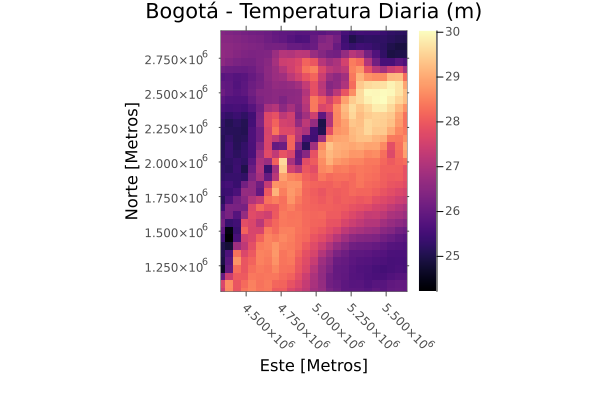
\includegraphics[width=0.8\textwidth,height=\textheight]{images/c10_reproyeccion_julia.png}
\end{center}

\subsection{Costo Computacional del
Warping}\label{costo-computacional-del-warping}

Reproyectar datos ráster no es una simple reasignación de etiquetas;
requiere recalcular los valores de cada píxel en una nueva malla
matemática. Esta operación rompe temporalmente el paradigma de la
``evaluación perezosa'', ya que fuerza a las librerías a procesar
grandes bloques de datos o incluso materializarlos en RAM. Por regla
general: \textbf{filtre primero (espacio, tiempo y niveles), y
reproyecte de último}.

\subsection{Resumen Sintáctico de
Reproyección}\label{resumen-sintuxe1ctico-de-reproyecciuxf3n}

\begin{longtable}[]{@{}
  >{\raggedright\arraybackslash}p{(\columnwidth - 6\tabcolsep) * \real{0.2500}}
  >{\raggedright\arraybackslash}p{(\columnwidth - 6\tabcolsep) * \real{0.2500}}
  >{\raggedright\arraybackslash}p{(\columnwidth - 6\tabcolsep) * \real{0.2500}}
  >{\raggedright\arraybackslash}p{(\columnwidth - 6\tabcolsep) * \real{0.2500}}@{}}
\toprule\noalign{}
\begin{minipage}[b]{\linewidth}\raggedright
Operación
\end{minipage} & \begin{minipage}[b]{\linewidth}\raggedright
Python 🐍 (\texttt{rioxarray})
\end{minipage} & \begin{minipage}[b]{\linewidth}\raggedright
R 🔵 (\texttt{stars})
\end{minipage} & \begin{minipage}[b]{\linewidth}\raggedright
Julia 🟣 (\texttt{Rasters.jl})
\end{minipage} \\
\midrule\noalign{}
\endhead
\bottomrule\noalign{}
\endlastfoot
\textbf{Forzar/Asignar CRS original} &
\texttt{.rio.write\_crs("EPSG:4326")} &
\texttt{st\_set\_crs(obj,\ 4326)} & Automático vía metadatos \\
\textbf{Reproyectar (Warping)} & \texttt{.rio.reproject("EPSG:9377")} &
\texttt{st\_warp(crs\ =\ 9377)} & \texttt{resample(crs=EPSG(9377))} \\
\textbf{Definir Método Bilineal} & \texttt{resampling=1} &
\texttt{method\ =\ "bilinear"} & \texttt{method=:bilinear} \\
\textbf{Dependencia del motor C++} & Implícito (Rasterio/GDAL) &
\texttt{use\_gdal\ =\ TRUE} & Requiere \texttt{using\ ArchGDAL} \\
\end{longtable}

\section{Persistencia de datos (exportar el
cubo)}\label{persistencia-de-datos-exportar-el-cubo}

Tras haber procesado nuestro cubo 5D inicial (recorte espacial sobre
Bogotá, agregación de los miembros de ensamble, conversión de unidades a
grados Celsius, remuestreo temporal a promedios diarios y reproyección a
coordenadas métricas), hemos construido un grafo de tareas
computacionales sustancial.

Para evitar que el compilador tenga que recalcular todo este flujo desde
los datos base cada vez que ejecutamos nuestro código, y para preparar
el terreno para las operaciones integradas Raster-Vector del siguiente
módulo, el paso final es \textbf{guardar (materializar) este nuevo cubo
simplificado en el disco duro}. Exportaremos el resultado en formato
estandarizado NetCDF (\texttt{.nc}), lo que garantizará que tanto la
estructura dimensional como los metadatos se conserven perfectamente.

\subsection{Python}

\begin{Shaded}
\begin{Highlighting}[]
\CommentTok{\# \#| eval: false}

\CommentTok{\# {-}{-}{-}{-}{-}{-}{-}{-}{-}{-}{-}{-}{-}{-}{-}{-}{-}{-}{-}{-}{-}{-}{-}{-}{-}{-}{-}{-}{-}{-}{-}{-}{-}{-}{-}{-}{-}{-}{-}{-}{-}{-}{-}{-}{-}{-}{-}{-}{-}{-}{-}{-}{-}{-}{-}{-}{-}{-}{-}{-}{-}{-}{-}{-}{-}{-}{-}{-}{-}{-}{-}{-}{-}}
\CommentTok{\# Persistencia: Exportar el DataArray a disco}
\CommentTok{\# {-}{-}{-}{-}{-}{-}{-}{-}{-}{-}{-}{-}{-}{-}{-}{-}{-}{-}{-}{-}{-}{-}{-}{-}{-}{-}{-}{-}{-}{-}{-}{-}{-}{-}{-}{-}{-}{-}{-}{-}{-}{-}{-}{-}{-}{-}{-}{-}{-}{-}{-}{-}{-}{-}{-}{-}{-}{-}{-}{-}{-}{-}{-}{-}{-}{-}{-}{-}{-}{-}{-}{-}{-}}
\ImportTok{import}\NormalTok{ os}

\CommentTok{\# 1. Definición de la ruta de salida}
\CommentTok{\# Aseguramos un nombre descriptivo que indique el procesamiento previo}
\NormalTok{archivo\_salida }\OperatorTok{=} \StringTok{"./data\_heavy/t\_diaria\_bogota\_9377.nc"}

\CommentTok{\# 2. Materialización y exportación}
\CommentTok{\# El método .to\_netcdf() detona la ejecución de todo el grafo de tareas }
\CommentTok{\# diferidas (Dask) y escribe el resultado físico en el disco.}
\CommentTok{\# Verificamos si el archivo ya existe para evitar sobrescribirlo innecesariamente.}
\ControlFlowTok{if} \KeywordTok{not}\NormalTok{ os.path.exists(archivo\_salida):}
\NormalTok{    t\_proyectado.to\_netcdf(archivo\_salida)}
    \BuiltInTok{print}\NormalTok{(}\SpecialStringTok{f"¡Éxito! Archivo guardado en: }\SpecialCharTok{\{}\NormalTok{archivo\_salida}\SpecialCharTok{\}}\SpecialStringTok{"}\NormalTok{)}
\ControlFlowTok{else}\NormalTok{:}
    \BuiltInTok{print}\NormalTok{(}\SpecialStringTok{f"El archivo }\SpecialCharTok{\{}\NormalTok{archivo\_salida}\SpecialCharTok{\}}\SpecialStringTok{ ya existe en disco."}\NormalTok{)}
\end{Highlighting}
\end{Shaded}

\begin{verbatim}
El archivo ./data_heavy/t_diaria_bogota_9377.nc ya existe en disco.
\end{verbatim}

\subsection{R}

\begin{Shaded}
\begin{Highlighting}[]
\CommentTok{\# \#| eval: false}

\CommentTok{\# {-}{-}{-}{-}{-}{-}{-}{-}{-}{-}{-}{-}{-}{-}{-}{-}{-}{-}{-}{-}{-}{-}{-}{-}{-}{-}{-}{-}{-}{-}{-}{-}{-}{-}{-}{-}{-}{-}{-}{-}{-}{-}{-}{-}{-}{-}{-}{-}{-}{-}{-}{-}{-}{-}{-}{-}{-}{-}{-}{-}{-}{-}{-}{-}{-}{-}{-}{-}{-}{-}{-}{-}{-}}
\CommentTok{\# Persistencia: Exportar objeto \{stars\} a NetCDF}
\CommentTok{\# {-}{-}{-}{-}{-}{-}{-}{-}{-}{-}{-}{-}{-}{-}{-}{-}{-}{-}{-}{-}{-}{-}{-}{-}{-}{-}{-}{-}{-}{-}{-}{-}{-}{-}{-}{-}{-}{-}{-}{-}{-}{-}{-}{-}{-}{-}{-}{-}{-}{-}{-}{-}{-}{-}{-}{-}{-}{-}{-}{-}{-}{-}{-}{-}{-}{-}{-}{-}{-}{-}{-}{-}{-}}

\CommentTok{\# 1. Definición de la ruta de destino}
\NormalTok{archivo\_salida\_r }\OtherTok{\textless{}{-}} \StringTok{"./data\_heavy/t\_diaria\_bogota\_9377\_R.nc"}

\CommentTok{\# 2. Materialización y exportación}
\CommentTok{\# En \{stars\}, la función recomendada para escribir arreglos multidimensionales}
\CommentTok{\# complejos (con tiempo y profundidad) en NetCDF es write\_mdim().}
\CommentTok{\# Esta función ejecutará el proxy y volcará el resultado a disco.}
\ControlFlowTok{if}\NormalTok{ (}\SpecialCharTok{!}\FunctionTok{file.exists}\NormalTok{(archivo\_salida\_r)) \{}
  \FunctionTok{write\_mdim}\NormalTok{(t\_proyectado, archivo\_salida\_r)}
  \FunctionTok{cat}\NormalTok{(}\StringTok{"¡Éxito! Archivo guardado en:"}\NormalTok{, archivo\_salida\_r, }\StringTok{"}\SpecialCharTok{\textbackslash{}n}\StringTok{"}\NormalTok{)}
\NormalTok{\} }\ControlFlowTok{else}\NormalTok{ \{}
  \FunctionTok{cat}\NormalTok{(}\StringTok{"El archivo"}\NormalTok{, archivo\_salida\_r, }\StringTok{"ya existe. Omisión de escritura.}\SpecialCharTok{\textbackslash{}n}\StringTok{"}\NormalTok{)}
\NormalTok{\}}
\end{Highlighting}
\end{Shaded}

\begin{verbatim}
El archivo ./data_heavy/t_diaria_bogota_9377_R.nc ya existe. Omisión de escritura.
\end{verbatim}

\subsection{Julia}

\begin{Shaded}
\begin{Highlighting}[]
\CommentTok{\# \#| eval: false}

\FunctionTok{j\_eval}\NormalTok{(}\StringTok{\textquotesingle{}}
\StringTok{\# {-}{-}{-}{-}{-}{-}{-}{-}{-}{-}{-}{-}{-}{-}{-}{-}{-}{-}{-}{-}{-}{-}{-}{-}{-}{-}{-}{-}{-}{-}{-}{-}{-}{-}{-}{-}{-}{-}{-}{-}{-}{-}{-}{-}{-}{-}{-}{-}{-}{-}{-}{-}{-}{-}{-}{-}{-}{-}{-}{-}{-}{-}{-}{-}{-}{-}{-}{-}{-}{-}{-}{-}{-}}
\StringTok{\# Persistencia: Guardar el Raster a disco}
\StringTok{\# {-}{-}{-}{-}{-}{-}{-}{-}{-}{-}{-}{-}{-}{-}{-}{-}{-}{-}{-}{-}{-}{-}{-}{-}{-}{-}{-}{-}{-}{-}{-}{-}{-}{-}{-}{-}{-}{-}{-}{-}{-}{-}{-}{-}{-}{-}{-}{-}{-}{-}{-}{-}{-}{-}{-}{-}{-}{-}{-}{-}{-}{-}{-}{-}{-}{-}{-}{-}{-}{-}{-}{-}{-}}

\StringTok{\# 1. Definición de la ruta}
\StringTok{\# Concatenamos la ruta de manera segura usando joinpath}
\StringTok{archivo\_salida\_jl = joinpath("./data\_heavy/", "t\_diaria\_bogota\_9377\_JL.nc")}

\StringTok{\# 2. Exportación a formato nativo}
\StringTok{\# Rasters.jl sobrescribe la función base \textasciigrave{}write\textasciigrave{} de Julia. Al pasarle un }
\StringTok{\# archivo con extensión .nc, invoca internamente a NCDatasets para }
\StringTok{\# compilar el cubo en disco, manteniendo intacto el sistema EPSG y el tiempo.}
\StringTok{if !isfile(archivo\_salida\_jl)}
\StringTok{    write(archivo\_salida\_jl, t\_proyectado)}
\StringTok{    println("¡Éxito! Archivo guardado en: $archivo\_salida\_jl")}
\StringTok{else}
\StringTok{    println("El archivo $archivo\_salida\_jl ya existe en disco.")}
\StringTok{end}
\StringTok{\textquotesingle{}}\NormalTok{)}
\end{Highlighting}
\end{Shaded}

\subsection{Resumen Sintáctico:
Exportación}\label{resumen-sintuxe1ctico-exportaciuxf3n}

\begin{longtable}[]{@{}
  >{\raggedright\arraybackslash}p{(\columnwidth - 6\tabcolsep) * \real{0.2500}}
  >{\raggedright\arraybackslash}p{(\columnwidth - 6\tabcolsep) * \real{0.2500}}
  >{\raggedright\arraybackslash}p{(\columnwidth - 6\tabcolsep) * \real{0.2500}}
  >{\raggedright\arraybackslash}p{(\columnwidth - 6\tabcolsep) * \real{0.2500}}@{}}
\toprule\noalign{}
\begin{minipage}[b]{\linewidth}\raggedright
Operación
\end{minipage} & \begin{minipage}[b]{\linewidth}\raggedright
Python 🐍 (\texttt{xarray})
\end{minipage} & \begin{minipage}[b]{\linewidth}\raggedright
R 🔵 (\texttt{stars})
\end{minipage} & \begin{minipage}[b]{\linewidth}\raggedright
Julia 🟣 (\texttt{Rasters})
\end{minipage} \\
\midrule\noalign{}
\endhead
\bottomrule\noalign{}
\endlastfoot
\textbf{Exportar a NetCDF} & \texttt{.to\_netcdf("file.nc")} &
\texttt{write\_mdim(obj,\ "file.nc")} &
\texttt{write("file.nc",\ obj)} \\
\textbf{Materialización} & Ejecuta el grafo (Dask) & Ejecuta el Proxy &
Compila (NCDatasets) \\
\end{longtable}

\section{Resumen global de operaciones con cubos
NetCDF}\label{resumen-global-de-operaciones-con-cubos-netcdf}

\begin{longtable}[]{@{}
  >{\raggedright\arraybackslash}p{(\columnwidth - 6\tabcolsep) * \real{0.2500}}
  >{\raggedright\arraybackslash}p{(\columnwidth - 6\tabcolsep) * \real{0.2500}}
  >{\raggedright\arraybackslash}p{(\columnwidth - 6\tabcolsep) * \real{0.2500}}
  >{\raggedright\arraybackslash}p{(\columnwidth - 6\tabcolsep) * \real{0.2500}}@{}}
\toprule\noalign{}
\begin{minipage}[b]{\linewidth}\raggedright
Operación
\end{minipage} & \begin{minipage}[b]{\linewidth}\raggedright
Python 🐍 (\texttt{xarray} / \texttt{rioxarray})
\end{minipage} & \begin{minipage}[b]{\linewidth}\raggedright
R 🔵 (\texttt{stars} / \texttt{sf})
\end{minipage} & \begin{minipage}[b]{\linewidth}\raggedright
Julia 🟣 (\texttt{Rasters.jl})
\end{minipage} \\
\midrule\noalign{}
\endhead
\bottomrule\noalign{}
\endlastfoot
\textbf{Cargar librería base} & \texttt{import\ xarray\ as\ xr} &
\texttt{library(stars)} & \texttt{using\ Rasters} \\
\textbf{Lectura (Evaluación Perezosa)} & \texttt{xr.open\_dataset(file)}
& \texttt{read\_stars(file,\ proxy=TRUE)} & \texttt{Raster(file)} \\
\textbf{Asignar CRS original} & \texttt{ds.rio.write\_crs("epsg:4326")}
& \texttt{st\_crs(y)\ \textless{}-\ 4326} & Automático vía metadatos \\
\textbf{Extraer dimensión temporal} & \texttt{ds.time.values} &
\texttt{st\_get\_dimension\_values(y,\ "time")} &
\texttt{lookup(cube,\ Ti)} \\
\textbf{Conversión de tiempo} & Automática (CF Conventions) & Manual via
\texttt{as.POSIXct()} & Automática (CF Conventions) \\
\textbf{Selección por Posición/Índice} & \texttt{.isel(time=0)} &
\texttt{y{[},,,i{]}} & \texttt{cube{[}Ti(1){]}} \\
\textbf{Selección por Valor Físico} &
\texttt{.sel(level=750,\ method=\textquotesingle{}nearest\textquotesingle{})}
& \texttt{slice(level,\ indice\_objetivo)} &
\texttt{cube{[}Z(At(750)){]}} \\
\textbf{Recorte Espacial (BBox)} &
\texttt{.sel(lat=slice(),\ lon=slice())} & \texttt{st\_crop(obj,\ bbox)}
& \texttt{X(Between()),\ Y(Between())} \\
\textbf{Eliminar dimensiones unitarias} & \texttt{.squeeze()} &
\texttt{adrop()} & \texttt{dropdims(...,\ dims=N)} \\
\textbf{Álgebra: Operación Escalar} & \texttt{obj\ -\ 273.15} &
\texttt{obj\ -\ 273.15} & \texttt{cube\ .-\ 273.15} (Broadcast) \\
\textbf{Álgebra: Promedio (Reducción)} &
\texttt{.mean(dim=\textquotesingle{}number\textquotesingle{})} &
\texttt{st\_apply(...,\ mean)} & \texttt{mean(cube,\ dims=4)} \\
\textbf{Remuestreo: Agrupación Temporal} & \texttt{.resample(time="1D")}
& \texttt{aggregate(by\ =\ "days")} &
\texttt{aggregate(mean,\ obj,\ Ti(X))} \\
\textbf{Reproyectar (Warping)} & \texttt{.rio.reproject("EPSG:9377")} &
\texttt{st\_warp(crs\ =\ 9377)} & \texttt{resample(crs=EPSG(9377))} \\
\textbf{Exportar a NetCDF} & \texttt{.to\_netcdf("file.nc")} &
\texttt{write\_mdim(obj,\ "file.nc")} &
\texttt{write("file.nc",\ obj)} \\
\end{longtable}

\section{Ejercicios}\label{ejercicios-8}

Para poner en práctica los conceptos avanzados abordados en este
capítulo, deberán resolver los siguientes dos ejercicios en
\textbf{grupos de 4 personas}. El objetivo es que ejecuten un flujo de
trabajo profesional completo: desde la adquisición de datos climáticos
brutos en la nube hasta el procesamiento multidimensional en su máquina
local. Pueden elegir resolver la parte de código en \textbf{Python, R o
Julia}.

\subsection{Ejercicio 1: Adquisición de datos climáticos (Copernicus
CDS)}\label{ejercicio-1-adquisiciuxf3n-de-datos-climuxe1ticos-copernicus-cds}

\textbf{Contexto:} Los repositorios climáticos globales contienen
petabytes de información. Para su proyecto final (o para este
ejercicio), necesitarán descargar un subconjunto de datos de reanálisis
ERA5 correspondiente a una región y periodo de su interés.

\textbf{Instrucciones:}

\begin{enumerate}
\def\labelenumi{\arabic{enumi}.}
\tightlist
\item
  \textbf{Registro:} Diríjanse al portal de \emph{Copernicus Climate
  Data Store} (CDS) y regístrense para obtener una cuenta gratuita.
\item
  \textbf{Exploración:} Naveguen hacia uno de los siguientes conjuntos
  de datos:

  \begin{itemize}
  \tightlist
  \item
    \href{https://cds.climate.copernicus.eu/datasets/reanalysis-era5-single-levels}{ERA5
    hourly data on single levels from 1940 to present}
  \item
    \href{https://cds.climate.copernicus.eu/datasets/reanalysis-era5-land}{ERA5-Land
    hourly data from 1950 to present}
  \item
    Otro dataset de Copernicus que sea de interés para su proyecto
    final.
  \end{itemize}
\item
  \textbf{Selección mediante Interfaz Gráfica:} Utilicen el formulario
  web para seleccionar:

  \begin{itemize}
  \tightlist
  \item
    Una variable continua (ej. \emph{2m temperature} o \emph{Total
    precipitation}).
  \item
    Un año, un mes y todos los días/horas de ese mes.
  \item
    \textbf{Importante:} En la sección ``Geographical area'',
    seleccionen ``Sub-region extraction'' e introduzcan las coordenadas
    de un \emph{bounding box} de su elección (ej. el departamento o
    cuenca de su proyecto de investigación). Si descargan el mundo
    entero, el archivo será demasiado pesado.
  \item
    Formato: NetCDF.
  \end{itemize}
\item
  \textbf{Automatización (Requisito):} En lugar de hacer clic en
  ``Submit Form'', hagan clic en el botón \textbf{``Show API request''}.
  Esto generará un bloque de código en Python. Utilizando la librería
  \texttt{cdsapi}, integren este código en un script (\texttt{.py}) para
  realizar la descarga automáticamente desde su entorno de programación.
  Deben instalar la librería \texttt{cdsapi}.
\item
  \textbf{Descarga:} Obtengan el archivo \texttt{.nc} (asegúrense de que
  no supere los 500 MB para no saturar sus equipos locales) y guárdenlo
  en su carpeta \texttt{./data\_heavy/}.
\end{enumerate}

\subsection{Ejercicio 2: Procesamiento del cubo NetCDF (El pipeline
perezoso)}\label{ejercicio-2-procesamiento-del-cubo-netcdf-el-pipeline-perezoso}

\textbf{Contexto:} Tienen un archivo NetCDF crudo recién descargado de
Copernicus. Deben aplicar el flujo de trabajo aprendido para limpiar,
transformar y preparar este hipercubo para análisis posteriores o
cartografía.

\textbf{Instrucciones de código:}

\begin{enumerate}
\def\labelenumi{\arabic{enumi}.}
\tightlist
\item
  \textbf{Lectura:} Carguen el archivo \texttt{.nc} en su entorno
  utilizando la estrategia de evaluación perezosa (\emph{lazy
  evaluation}) correspondiente a su lenguaje (\texttt{xarray} +
  \texttt{dask}, \texttt{stars} con \texttt{proxy=TRUE}, o
  \texttt{Rasters.jl}).
\item
  \textbf{Auditoría:} Impriman en consola un resumen de las dimensiones
  del cubo, sus variables y su CRS actual.
\item
  \textbf{Álgebra de Mapas:} Apliquen una transformación matemática a la
  variable principal utilizando vectorización (sin bucles).

  \begin{itemize}
  \tightlist
  \item
    \emph{Si descargaron Temperatura:} Conviertan de Kelvin a Celsius.
  \item
    \emph{Si descargaron Precipitación:} Conviertan los valores de
    metros a milímetros (multiplicando por 1000).
  \end{itemize}
\item
  \textbf{Remuestreo Temporal:} El archivo descargado está en resolución
  horaria. Agrupen la dimensión temporal y calculen la \textbf{media
  diaria} (o la suma diaria, si eligieron precipitación).
\item
  \textbf{Máxima mensual y fecha de ocurrencia:} A partir del cubo
  diario, calculen el valor máximo mensual para cada píxel. Además,
  generen una segunda variable (atributo) dentro del cubo que almacene
  la fecha exacta en la que ocurrió dicha máxima. \emph{(Pista
  conceptual: busquen funciones que devuelvan el índice del valor
  máximo, como \texttt{idxmax} o índices espaciotemporales según el
  lenguaje elegido)}.
\item
  \textbf{Persistencia:} Exporten el resultado final de este
  procesamiento a un nuevo archivo NetCDF llamado
  \texttt{mi\_zona\_procesada.nc}.
\end{enumerate}

\subsection{Entregables y criterios de
evaluación}\label{entregables-y-criterios-de-evaluaciuxf3n-9}

El objetivo de esta evaluación no es solo que el código se ejecute sin
errores, sino que demuestren comprensión sobre cómo se gestiona la
memoria y la metadata en datos multidimensionales.

\textbf{1. Archivos de Código:} Deben desarrollar los algoritmos del
procesamiento en un documento computacional (\texttt{.qmd} con
\emph{chunks} de código de R, Python o Julia).

\textbf{2. Documento Analítico (Quarto):} Deben renderizar su archivo
\texttt{.qmd} tanto en formato \textbf{HTML} como en \textbf{PDF}.
Además del código, deben responder argumentativamente a las siguientes
preguntas de análisis dentro del documento:

\begin{itemize}
\tightlist
\item
  \textbf{Sobre Evaluación Perezosa (Lazy Evaluation):} Imaginen que
  olvidaron hacer el remuestreo temporal a medias diarias y deciden
  reproyectar (hacer \emph{warping}) el cubo horario completo de
  Copernicus a un sistema local (ej. EPSG:9377) para luego guardarlo.
  ¿Qué implicaciones tendría esta decisión en la memoria RAM de su
  computadora y en los tiempos de procesamiento? Justifiquen por qué el
  \emph{warping} debe ser uno de los últimos pasos del pipeline.
\item
  \textbf{Sobre Convenciones CF y Tiempo:} Basados en su experiencia
  resolviendo el Ejercicio 2, ¿su lenguaje de programación decodificó
  automáticamente las fechas del archivo NetCDF al cargarlo, o tuvieron
  que realizar alguna operación manual para que el eje de tiempo fuera
  reconocido como fechas reales y no como simples números? Expliquen
  brevemente.
\end{itemize}

\textbf{3. Repositorio en GitHub:} Suban la carpeta del proyecto a un
repositorio privado en GitHub (puede ser en la cuenta de uno de los
miembros del grupo).

\begin{itemize}
\tightlist
\item
  \textbf{Nota de exclusión:} ¡NO suban los archivos \texttt{.nc} al
  repositorio! (GitHub bloquea archivos muy pesados). Asegúrense de
  agregar la carpeta \texttt{data\_heavy/} a su archivo
  \texttt{.gitignore}.
\item
  \textbf{Qué debe contener el repositorio:} * El script de Python
  (\texttt{.py}) usando la librería \texttt{cdsapi} con la que
  descargaron los datos.

  \begin{itemize}
  \tightlist
  \item
    El documento computacional fuente (\texttt{.qmd}).
  \item
    Los renders finales en HTML y PDF.
  \item
    Scrips en Python, R o Julia
  \end{itemize}
\item
  \textbf{Entrega:} Deberán enviar únicamente el enlace (URL) de su
  repositorio a la plataforma de calificación, indicando los nombres de
  los 4 integrantes del grupo.
\end{itemize}

\chapter{Cubos Multidimensionales Vector y
Raster}\label{cubos-multidimensionales-vector-y-raster}

execute: cache: true\\
freeze: auto

\section{Funciones j\_eval y j\_plot en
R}\label{funciones-j_eval-y-j_plot-en-r-15}

\begin{Shaded}
\begin{Highlighting}[]
\CommentTok{\# \#| include: false}
\FunctionTok{source}\NormalTok{(}\StringTok{"./docs/j\_eval\_j\_plot.r"}\NormalTok{)}
\end{Highlighting}
\end{Shaded}

\section{Introducción}\label{introducciuxf3n-16}

En el ámbito de la geomática aplicada y el diseño de infraestructura
segura, el modelado espacial de amenazas naturales exige el
procesamiento ágil de grandes volúmenes de datos meteorológicos y
climáticos. Para ilustrar estos flujos de trabajo en un entorno real,
este capítulo utiliza como caso de estudio los datos y resultados
derivados de la investigación ``\emph{Spatio-temporal analysis of
extreme wind velocities for infrastructure design}''
(\citeproc{ref-rodriguez2020spatio}{Rodríguez Avellaneda, 2020}),
disponible de forma íntegra en
\href{https://geocorp.co/thesis/mastergeotech/}{geocorp.co/thesis/mastergeotech}.
A través del análisis del régimen de vientos extremos en Colombia
---integrando la amenaza probabilística de huracanes en el Caribe y
vientos sinópticos locales---, exploraremos cómo la programación en
Sistemas de Información Geográfica (SIG) permite resolver problemas de
álgebra de mapas a gran escala.

El objetivo pedagógico central de este texto trasciende el análisis
climatológico para centrarse en la arquitectura de datos computacional.
Históricamente, el análisis espacial ha mantenido una dicotomía
estricta: los datos vectoriales para la gestión de objetos y los rasters
para la representación de campos continuos. Sin embargo, los modelos
climáticos modernos, como el reanálisis ERA5, poseen una naturaleza
\textbf{multidimensional} (longitud, latitud, tiempo, variables
atmosféricas y niveles de retorno) que desafía estas estructuras planas.

Para procesar esta complejidad, aprenderemos a dominar el paradigma de
los \textbf{cubos de datos espaciales}, focalizándonos en la
interoperabilidad profunda entre los paquetes \texttt{sf} (\emph{Simple
Features}) y \texttt{stars} (\emph{Spatio-Temporal Arrays}). El avance
tecnológico clave que exploraremos es la capacidad de \textbf{combinar
vectores y rasters dentro de un mismo cubo}. Esto implica que una
geometría vectorial (como una malla de polígonos o una red de
estaciones) puede ser tratada como una dimensión más de un array,
permitiendo que operaciones típicas de imágenes (como el álgebra de
mapas o funciones de agregación) se apliquen directamente sobre datos
vectoriales masivos de forma estructurada y eficiente.

A lo largo del capítulo, el lector desarrollará un flujo de trabajo que
inicia en la ingesta de archivos discretos (NetCDF y GeoTIFF), avanza
hacia la transformación de estas mallas en \textbf{cubos de datos
vectoriales}, y culmina en la aplicación de programación funcional
espacial vectorizada (mediante la familia \texttt{apply}) para fusionar
regímenes de amenaza heterogéneos.

Finalmente, dado que el análisis geoespacial está incompleto sin una
comunicación visual efectiva, este capítulo dedica un esfuerzo
sustancial a las \textbf{técnicas avanzadas de representación
cartográfica}. Transformar cubos híbridos en mapas estáticos con rigor
de publicación científica supone un desafío técnico notable. Por ello,
profundizaremos en estrategias de renderizado vectorial sobre
\emph{basemaps} continuos, manipulación de formatos topológicos
(Long/Wide) para el facetado dinámico de escenarios, y la composición
algorítmica de \emph{layouts} multiescalares (mapas de detalle y
contexto) empleando la gramática gráfica de \texttt{ggplot2}.

\section{Construcción de cubos espacio-temporales a partir de archivos
GeoTIFF}\label{construcciuxf3n-de-cubos-espacio-temporales-a-partir-de-archivos-geotiff}

\begin{Shaded}
\begin{Highlighting}[]
\CommentTok{\# \#| eval: false}

\CommentTok{\# ================================}
\CommentTok{\# DESCARGA Y PREPARACIÓN DE DATOS}
\CommentTok{\# ================================}

\CommentTok{\# Obtener datos vector y raster}
\CommentTok{\# URL de ejemplo donde se encuentran los datos comprimidos}
\CommentTok{\# myurl \textless{}{-} "http://geocorp.co/wind/wind\_result.zip"}

\CommentTok{\# Nombre del archivo ZIP que se descargará localmente}
\CommentTok{\# filename \textless{}{-} "wind\_result.zip"}

\CommentTok{\# Descarga el archivo desde la URL especificada}
\CommentTok{\# mode = "wb" asegura que el archivo se descargue en modo binario (necesario para archivos ZIP)}
\CommentTok{\# download.file(myurl, filename, mode = "wb")}

\CommentTok{\# Descomprime el archivo ZIP en el directorio de trabajo actual}
\CommentTok{\# unzip(filename)}

\CommentTok{\# Nota: }
\CommentTok{\# {-} Los archivos raster (.tif) deben ubicarse en la carpeta: ./data\_heavy/wind\_tif/}
\CommentTok{\# {-} El shapefile de municipios debe ubicarse en: ./data\_heavy/}

\CommentTok{\# ================================}
\CommentTok{\# CARGA DE LIBRERÍAS}
\CommentTok{\# ================================}

\CommentTok{\# stringr: manejo de strings (cadenas de texto)}
\FunctionTok{library}\NormalTok{(stringr)}

\CommentTok{\# stars: manejo de datos raster multidimensionales}
\FunctionTok{library}\NormalTok{(stars)}
\end{Highlighting}
\end{Shaded}

\begin{verbatim}
Loading required package: abind
\end{verbatim}

\begin{verbatim}
Loading required package: sf
\end{verbatim}

\begin{verbatim}
Linking to GEOS 3.12.1, GDAL 3.8.4, PROJ 9.4.0; sf_use_s2() is TRUE
\end{verbatim}

\begin{Shaded}
\begin{Highlighting}[]
\CommentTok{\# ================================}
\CommentTok{\# DEFINICIÓN DE RUTAS}
\CommentTok{\# ================================}

\CommentTok{\# Ruta base donde están almacenados los datos}
\CommentTok{\# Se usa "./" para indicar el directorio de trabajo actual}
\NormalTok{the\_path }\OtherTok{=} \StringTok{"./data\_heavy/"}

\CommentTok{\# ================================}
\CommentTok{\# LECTURA Y ORDENAMIENTO DE RASTERS}
\CommentTok{\# ================================}

\CommentTok{\# Listar los archivos en la carpeta ./data\_heavy/wind\_tif/}
\CommentTok{\# path: ruta donde buscar los archivos}
\CommentTok{\# pattern: expresión regular para filtrar archivos .tif}
\NormalTok{rasterfiles }\OtherTok{\textless{}{-}} \FunctionTok{list.files}\NormalTok{(}\AttributeTok{path =} \FunctionTok{paste0}\NormalTok{(the\_path, }\StringTok{"wind\_tif/"}\NormalTok{), }\AttributeTok{pattern =} \StringTok{"*.*.tif$"}\NormalTok{)}

\CommentTok{\# Construye la ruta completa de cada archivo concatenando:}
\CommentTok{\# la ruta base + nombre del archivo}
\NormalTok{rasterfiles }\OtherTok{\textless{}{-}} \FunctionTok{paste0}\NormalTok{(the\_path, }\StringTok{"wind\_tif/"}\NormalTok{, rasterfiles)}

\CommentTok{\# Ordena los archivos según los números en sus nombres (orden numérico real, no alfabético)}
\CommentTok{\# numeric = TRUE permite ordenar correctamente (ej: st22 antes que st23)}
\NormalTok{rasterfiles }\OtherTok{\textless{}{-}} \FunctionTok{str\_sort}\NormalTok{(rasterfiles, }\AttributeTok{numeric =} \ConstantTok{TRUE}\NormalTok{)}

\CommentTok{\# Ejemplo del primer archivo en la lista}
\CommentTok{\#\textquotesingle{}./data\_heavy/wind\_tif/st1\_cellindexlr.tif\textquotesingle{}}
\FunctionTok{head}\NormalTok{(rasterfiles)}
\end{Highlighting}
\end{Shaded}

\begin{verbatim}
[1] "./data_heavy/wind_tif/st1_cellindexlr.tif"
[2] "./data_heavy/wind_tif/st2_lonindex.tif"   
[3] "./data_heavy/wind_tif/st3_latindex.tif"   
[4] "./data_heavy/wind_tif/st4_cellindextb.tif"
[5] "./data_heavy/wind_tif/st5_id.tif"         
[6] "./data_heavy/wind_tif/st6_nh_thresh.tif"  
\end{verbatim}

\begin{Shaded}
\begin{Highlighting}[]
\CommentTok{\# Ejemplo del último archivo en la lista}
\CommentTok{\#\textquotesingle{}./data\_heavy/wind\_tif/st43\_c\_7000.tif\textquotesingle{}}
\FunctionTok{tail}\NormalTok{(rasterfiles)}
\end{Highlighting}
\end{Shaded}

\begin{verbatim}
[1] "./data_heavy/wind_tif/st38_c_500.tif" 
[2] "./data_heavy/wind_tif/st39_c_700.tif" 
[3] "./data_heavy/wind_tif/st40_c_1000.tif"
[4] "./data_heavy/wind_tif/st41_c_1700.tif"
[5] "./data_heavy/wind_tif/st42_c_3000.tif"
[6] "./data_heavy/wind_tif/st43_c_7000.tif"
\end{verbatim}

\begin{Shaded}
\begin{Highlighting}[]
\CommentTok{\# ================================}
\CommentTok{\# CREACIÓN DEL OBJETO STARS}
\CommentTok{\# ================================}

\CommentTok{\# Lee múltiples archivos raster (TIF) y los combina en un solo objeto tipo stars}
\CommentTok{\# rasterfiles: vector de rutas a archivos raster}
\CommentTok{\# quiet = TRUE evita imprimir mensajes en consola}
\NormalTok{h\_nh\_c.st }\OtherTok{\textless{}{-}} \FunctionTok{read\_stars}\NormalTok{(rasterfiles, }\AttributeTok{quiet =} \ConstantTok{TRUE}\NormalTok{)}

\CommentTok{\# Obtiene los nombres de las capas (atributos) del objeto stars}
\NormalTok{mynames }\OtherTok{\textless{}{-}} \FunctionTok{names}\NormalTok{(h\_nh\_c.st)}

\CommentTok{\# Nota:}
\CommentTok{\# stars elimina automáticamente el prefijo común más largo (LCP: Longest Common Prefix)}
\CommentTok{\# al asignar nombres a las capas}

\CommentTok{\# Ejemplo de nombres resultantes}
\CommentTok{\#\textquotesingle{}1\_cellindexlr.tif\textquotesingle{}}
\FunctionTok{head}\NormalTok{(mynames)}
\end{Highlighting}
\end{Shaded}

\begin{verbatim}
[1] "1_cellindexlr.tif" "2_lonindex.tif"    "3_latindex.tif"   
[4] "4_cellindextb.tif" "5_id.tif"          "6_nh_thresh.tif"  
\end{verbatim}

\begin{Shaded}
\begin{Highlighting}[]
\FunctionTok{tail}\NormalTok{(mynames)}
\end{Highlighting}
\end{Shaded}

\begin{verbatim}
[1] "38_c_500.tif"  "39_c_700.tif"  "40_c_1000.tif" "41_c_1700.tif"
[5] "42_c_3000.tif" "43_c_7000.tif"
\end{verbatim}

\begin{Shaded}
\begin{Highlighting}[]
\CommentTok{\# Imprime el objeto stars (dimensiones y atributos)}
\NormalTok{h\_nh\_c.st}
\end{Highlighting}
\end{Shaded}

\begin{verbatim}
stars object with 2 dimensions and 43 attributes
attribute(s):
                            Min.     1st Qu.      Median        Mean
1_cellindexlr.tif      1.0000000 846.0000000 1691.000000 1691.000000
2_lonindex.tif         1.0000000  13.0000000   25.000000   25.000000
3_latindex.tif         1.0000000  18.0000000   35.000000   35.000000
4_cellindextb.tif      1.0000000 846.0000000 1691.000000 1691.000000
5_id.tif               1.0000000 846.0000000 1691.000000 1691.000000
6_nh_thresh.tif       24.0000000  37.0000000   42.000000   43.958296
7_nh_mu_location.tif  13.6729488  24.5889168   28.071484   30.972949
8_nh_psi_scale.tif     0.8468198   2.4524689    2.949068    3.047828
9_distance_w.tif       0.2110516   0.8411635    1.240552    1.308701
10_station.tif         1.0000000 846.0000000 1691.000000 1691.000000
11_nh_10.tif          30.4555740  47.2962570   54.978470   56.002591
12_nh_20.tif          31.4608154  48.9887123   57.361576   58.115121
13_nh_50.tif          32.7741928  51.4477081   60.473362   60.908016
14_nh_100.tif         33.7783585  53.1698227   62.714901   63.020511
15_nh_250.tif         35.0545502  55.5359039   65.669632   65.812625
16_nh_500.tif         36.0606728  57.3204041   67.832039   67.925328
17_nh_700.tif         36.5523529  58.1628914   68.821609   68.950810
18_nh_1000.tif        36.9211159  59.1135674   69.892418   70.038594
19_nh_1700.tif        37.6162872  60.4877167   71.470055   71.655338
20_nh_3000.tif        38.1215630  61.8974876   73.101006   73.386625
21_nh_7000.tif        38.9009247  63.9797211   75.635643   75.968756
22_h_10.tif            9.6572638  15.6040730   23.249760   30.495052
23_h_20.tif           12.2852173  22.1053762   30.730024   42.995706
24_h_50.tif           16.8873825  27.9596853   44.804596   61.980913
25_h_100.tif          21.4828091  33.5036983   59.566853   76.713141
26_h_250.tif          24.0479527  42.1208897   67.867989   94.924907
27_h_500.tif          26.1531048  50.0924568   75.440773  108.124354
28_h_700.tif          27.2404785  54.7166328   78.704750  114.443373
29_h_1000.tif         28.4425430  59.7133026   82.739159  121.151201
30_h_1700.tif         30.3297253  62.4252758   89.772812  131.282884
31_h_3000.tif         32.4887238  65.1840057   96.707741  142.389694
32_h_7000.tif         35.9983788  69.5336800  109.499702  159.790127
33_c_10.tif           30.5939789  47.3236465   55.100040   56.380376
34_c_20.tif           31.8194408  49.2004547   57.661671   59.361368
35_c_50.tif           33.2647667  51.6685410   60.862976   64.967722
36_c_100.tif          34.5571671  53.6231384   63.266590   70.027001
37_c_250.tif          35.9132996  56.2640419   66.250504   76.763075
38_c_500.tif          37.3732605  58.4406738   68.650299   81.880776
39_c_700.tif          37.8385353  59.5043449   69.676407   84.393742
40_c_1000.tif         38.3028526  60.5562439   70.899162   87.102333
41_c_1700.tif         38.9026604  62.0931511   72.701416   91.229404
42_c_3000.tif         39.5586052  63.7013779   74.680573   95.789807
43_c_7000.tif         40.4327736  66.0068130   77.460434  102.889487
                          3rd Qu.        Max. NA's
1_cellindexlr.tif     2536.000000 3381.000000    0
2_lonindex.tif          37.000000   49.000000    0
3_latindex.tif          52.000000   69.000000    0
4_cellindextb.tif     2536.000000 3381.000000    0
5_id.tif              2536.000000 3381.000000    0
6_nh_thresh.tif         50.000000   78.000000    0
7_nh_mu_location.tif    35.983513   65.212418    0
8_nh_psi_scale.tif       3.626480    6.817193    0
9_distance_w.tif         1.657803   17.072296    0
10_station.tif        2536.000000 3381.000000    0
11_nh_10.tif            62.597267   93.306458    0
12_nh_20.tif            65.058258   97.621140    0
13_nh_50.tif            68.323509  103.318047    0
14_nh_100.tif           70.731575  107.631020    0
15_nh_250.tif           73.793114  113.328415    0
16_nh_500.tif           76.137680  117.640884    0
17_nh_700.tif           77.352562  119.731033    0
18_nh_1000.tif          78.628006  121.938110    0
19_nh_1700.tif          80.400818  125.248100    0
20_nh_3000.tif          82.454575  128.780334    0
21_nh_7000.tif          85.413361  134.038864    0
22_h_10.tif             41.011358   84.595543 2274
23_h_20.tif             62.586636  134.102707 2274
24_h_50.tif             86.103123  188.306503 2274
25_h_100.tif           110.833931  217.234344 2274
26_h_250.tif           150.905594  262.404663 2274
27_h_500.tif           174.924828  302.715546 2274
28_h_700.tif           182.414101  324.460510 2274
29_h_1000.tif          190.395744  349.219025 2274
30_h_1700.tif          202.572205  389.591431 2274
31_h_3000.tif          215.881157  437.991516 2274
32_h_7000.tif          237.644272  478.457611 2274
33_c_10.tif             62.646935   93.667839    0
34_c_20.tif             65.306145  134.172775    0
35_c_50.tif             68.947304  188.414383    0
36_c_100.tif            71.869194  217.443375    0
37_c_250.tif            75.752991  262.645355    0
38_c_500.tif            78.701851  302.826080    0
39_c_700.tif            80.076996  324.564423    0
40_c_1000.tif           81.683189  349.322479    0
41_c_1700.tif           83.956383  389.737061    0
42_c_3000.tif           86.569099  437.992401    0
43_c_7000.tif           90.491371  478.457611    0
dimension(s):
  from to offset delta refsys point x/y
x    1 49  -79.1  0.25 WGS 84 FALSE [x]
y    1 69   12.5 -0.25 WGS 84 FALSE [y]
\end{verbatim}

\begin{Shaded}
\begin{Highlighting}[]
\CommentTok{\# ================================}
\CommentTok{\# LIMPIEZA DE NOMBRES DE VARIABLES}
\CommentTok{\# ================================}

\CommentTok{\# Eliminaremos "1\_" al inicio y ".tif" al final en los nombres}

\CommentTok{\# str\_locate devuelve la posición de un patrón en cada string}
\CommentTok{\# Aquí buscamos la posición del "\_" (guion bajo)}
\NormalTok{start }\OtherTok{\textless{}{-}} \FunctionTok{str\_locate}\NormalTok{(mynames, }\StringTok{"\_"}\NormalTok{)}

\CommentTok{\# Buscamos la posición del "." (inicio de la extensión .tif)}
\CommentTok{\# "\textbackslash{}\textbackslash{}." se usa porque el punto es un carácter especial en expresiones regulares}
\NormalTok{stop }\OtherTok{\textless{}{-}} \FunctionTok{str\_locate}\NormalTok{(mynames, }\StringTok{"}\SpecialCharTok{\textbackslash{}\textbackslash{}}\StringTok{."}\NormalTok{)}

\CommentTok{\# Extraemos nuevos nombres usando substrings:}
\CommentTok{\# start = posición después del "\_" (por eso +1)}
\CommentTok{\# end = posición antes del "." (por eso {-}1)}
\NormalTok{mynames }\OtherTok{\textless{}{-}} \FunctionTok{str\_sub}\NormalTok{(mynames, }\AttributeTok{start =}\NormalTok{ start[, }\DecValTok{1}\NormalTok{] }\SpecialCharTok{+} \DecValTok{1}\NormalTok{, }\AttributeTok{end =}\NormalTok{ stop[, }\DecValTok{1}\NormalTok{] }\SpecialCharTok{{-}} \DecValTok{1}\NormalTok{)}

\CommentTok{\# Ejemplo de nombres transformados}
\CommentTok{\# \textquotesingle{}cellindexlr\textquotesingle{}}
\FunctionTok{head}\NormalTok{(mynames)}
\end{Highlighting}
\end{Shaded}

\begin{verbatim}
[1] "cellindexlr" "lonindex"    "latindex"    "cellindextb" "id"         
[6] "nh_thresh"  
\end{verbatim}

\begin{Shaded}
\begin{Highlighting}[]
\CommentTok{\# \textquotesingle{}c\_7000\textquotesingle{}}
\FunctionTok{tail}\NormalTok{(mynames)}
\end{Highlighting}
\end{Shaded}

\begin{verbatim}
[1] "c_500"  "c_700"  "c_1000" "c_1700" "c_3000" "c_7000"
\end{verbatim}

\begin{Shaded}
\begin{Highlighting}[]
\CommentTok{\# ================================}
\CommentTok{\# RENOMBRAR ATRIBUTOS}
\CommentTok{\# ================================}

\CommentTok{\# Reemplaza los nombres originales de las capas por los nuevos nombres limpiados}
\NormalTok{h\_nh\_c.st }\OtherTok{\textless{}{-}} \FunctionTok{setNames}\NormalTok{(h\_nh\_c.st, mynames)}

\CommentTok{\# Muestra el objeto stars con los nuevos nombres}
\CommentTok{\# Este objeto tiene dimensiones espaciales X, Y (grid raster)}
\NormalTok{h\_nh\_c.st}
\end{Highlighting}
\end{Shaded}

\begin{verbatim}
stars object with 2 dimensions and 43 attributes
attribute(s):
                      Min.     1st Qu.      Median        Mean     3rd Qu.
cellindexlr      1.0000000 846.0000000 1691.000000 1691.000000 2536.000000
lonindex         1.0000000  13.0000000   25.000000   25.000000   37.000000
latindex         1.0000000  18.0000000   35.000000   35.000000   52.000000
cellindextb      1.0000000 846.0000000 1691.000000 1691.000000 2536.000000
id               1.0000000 846.0000000 1691.000000 1691.000000 2536.000000
nh_thresh       24.0000000  37.0000000   42.000000   43.958296   50.000000
nh_mu_location  13.6729488  24.5889168   28.071484   30.972949   35.983513
nh_psi_scale     0.8468198   2.4524689    2.949068    3.047828    3.626480
distance_w       0.2110516   0.8411635    1.240552    1.308701    1.657803
station          1.0000000 846.0000000 1691.000000 1691.000000 2536.000000
nh_10           30.4555740  47.2962570   54.978470   56.002591   62.597267
nh_20           31.4608154  48.9887123   57.361576   58.115121   65.058258
nh_50           32.7741928  51.4477081   60.473362   60.908016   68.323509
nh_100          33.7783585  53.1698227   62.714901   63.020511   70.731575
nh_250          35.0545502  55.5359039   65.669632   65.812625   73.793114
nh_500          36.0606728  57.3204041   67.832039   67.925328   76.137680
nh_700          36.5523529  58.1628914   68.821609   68.950810   77.352562
nh_1000         36.9211159  59.1135674   69.892418   70.038594   78.628006
nh_1700         37.6162872  60.4877167   71.470055   71.655338   80.400818
nh_3000         38.1215630  61.8974876   73.101006   73.386625   82.454575
nh_7000         38.9009247  63.9797211   75.635643   75.968756   85.413361
h_10             9.6572638  15.6040730   23.249760   30.495052   41.011358
h_20            12.2852173  22.1053762   30.730024   42.995706   62.586636
h_50            16.8873825  27.9596853   44.804596   61.980913   86.103123
h_100           21.4828091  33.5036983   59.566853   76.713141  110.833931
h_250           24.0479527  42.1208897   67.867989   94.924907  150.905594
h_500           26.1531048  50.0924568   75.440773  108.124354  174.924828
h_700           27.2404785  54.7166328   78.704750  114.443373  182.414101
h_1000          28.4425430  59.7133026   82.739159  121.151201  190.395744
h_1700          30.3297253  62.4252758   89.772812  131.282884  202.572205
h_3000          32.4887238  65.1840057   96.707741  142.389694  215.881157
h_7000          35.9983788  69.5336800  109.499702  159.790127  237.644272
c_10            30.5939789  47.3236465   55.100040   56.380376   62.646935
c_20            31.8194408  49.2004547   57.661671   59.361368   65.306145
c_50            33.2647667  51.6685410   60.862976   64.967722   68.947304
c_100           34.5571671  53.6231384   63.266590   70.027001   71.869194
c_250           35.9132996  56.2640419   66.250504   76.763075   75.752991
c_500           37.3732605  58.4406738   68.650299   81.880776   78.701851
c_700           37.8385353  59.5043449   69.676407   84.393742   80.076996
c_1000          38.3028526  60.5562439   70.899162   87.102333   81.683189
c_1700          38.9026604  62.0931511   72.701416   91.229404   83.956383
c_3000          39.5586052  63.7013779   74.680573   95.789807   86.569099
c_7000          40.4327736  66.0068130   77.460434  102.889487   90.491371
                       Max. NA's
cellindexlr     3381.000000    0
lonindex          49.000000    0
latindex          69.000000    0
cellindextb     3381.000000    0
id              3381.000000    0
nh_thresh         78.000000    0
nh_mu_location    65.212418    0
nh_psi_scale       6.817193    0
distance_w        17.072296    0
station         3381.000000    0
nh_10             93.306458    0
nh_20             97.621140    0
nh_50            103.318047    0
nh_100           107.631020    0
nh_250           113.328415    0
nh_500           117.640884    0
nh_700           119.731033    0
nh_1000          121.938110    0
nh_1700          125.248100    0
nh_3000          128.780334    0
nh_7000          134.038864    0
h_10              84.595543 2274
h_20             134.102707 2274
h_50             188.306503 2274
h_100            217.234344 2274
h_250            262.404663 2274
h_500            302.715546 2274
h_700            324.460510 2274
h_1000           349.219025 2274
h_1700           389.591431 2274
h_3000           437.991516 2274
h_7000           478.457611 2274
c_10              93.667839    0
c_20             134.172775    0
c_50             188.414383    0
c_100            217.443375    0
c_250            262.645355    0
c_500            302.826080    0
c_700            324.564423    0
c_1000           349.322479    0
c_1700           389.737061    0
c_3000           437.992401    0
c_7000           478.457611    0
dimension(s):
  from to offset delta refsys point x/y
x    1 49  -79.1  0.25 WGS 84 FALSE [x]
y    1 69   12.5 -0.25 WGS 84 FALSE [y]
\end{verbatim}

\begin{Shaded}
\begin{Highlighting}[]
\CommentTok{\# ================================}
\CommentTok{\# CONVERSIÓN A GEOMETRÍA VECTORIAL}
\CommentTok{\# ================================}

\CommentTok{\# Convierte el objeto raster (grid) a geometrías tipo sf (polígonos)}
\CommentTok{\# st\_xy2sfc transforma cada celda raster en un polígono}

\CommentTok{\# Parámetros:}
\CommentTok{\# as\_points = FALSE → crea polígonos (celdas), no puntos}
\CommentTok{\# na.rm = TRUE → elimina celdas con valores NA}
\NormalTok{h\_nh\_c.stnoxy }\OtherTok{\textless{}{-}} \FunctionTok{st\_xy2sfc}\NormalTok{(h\_nh\_c.st, }\AttributeTok{as\_points =} \ConstantTok{FALSE}\NormalTok{, }\AttributeTok{na.rm =} \ConstantTok{TRUE}\NormalTok{)}

\CommentTok{\# Muestra las primeras geometrías}
\FunctionTok{head}\NormalTok{(h\_nh\_c.stnoxy)}
\end{Highlighting}
\end{Shaded}

\begin{verbatim}
stars object with 1 dimensions and 6 attributes
attribute(s):
             Min. 1st Qu. Median      Mean 3rd Qu. Max.
cellindexlr     1     846   1691 1691.0000    2536 3381
lonindex        1      13     25   25.0000      37   49
latindex        1      18     35   35.0000      52   69
cellindextb     1     846   1691 1691.0000    2536 3381
id              1     846   1691 1691.0000    2536 3381
nh_thresh      24      37     42   43.9583      50   78
dimension(s):
         from   to refsys point
geometry    1 3381 WGS 84 FALSE
                                                                values
geometry POLYGON ((-79.1 12.5, -78...,...,POLYGON ((-67.1 -4.5, -66...
\end{verbatim}

\begin{Shaded}
\begin{Highlighting}[]
\CommentTok{\# Consulta la estructura de dimensiones del objeto}
\FunctionTok{st\_dimensions}\NormalTok{(h\_nh\_c.stnoxy)}
\end{Highlighting}
\end{Shaded}

\begin{verbatim}
         from   to refsys point
geometry    1 3381 WGS 84 FALSE
                                                                values
geometry POLYGON ((-79.1 12.5, -78...,...,POLYGON ((-67.1 -4.5, -66...
\end{verbatim}

\begin{Shaded}
\begin{Highlighting}[]
\CommentTok{\# ================================}
\CommentTok{\# LECTURA DE DATOS VECTORIALES}
\CommentTok{\# ================================}

\CommentTok{\# Lee el shapefile de municipios de Colombia}
\CommentTok{\# st\_read detecta automáticamente todos los archivos asociados (.shp, .dbf, etc.)}
\NormalTok{mun }\OtherTok{\textless{}{-}} \FunctionTok{st\_read}\NormalTok{(}\FunctionTok{paste0}\NormalTok{(the\_path, }\StringTok{"MUNICIPIOS\_WGS84.shp"}\NormalTok{))}
\end{Highlighting}
\end{Shaded}

\begin{verbatim}
Reading layer `MUNICIPIOS_WGS84' from data source 
  `/home/rstudio/work/01_prog_sig/data_heavy/MUNICIPIOS_WGS84.shp' 
  using driver `ESRI Shapefile'
Simple feature collection with 1126 features and 3 fields
Geometry type: POLYGON
Dimension:     XY
Bounding box:  xmin: -79.0369 ymin: -4.228051 xmax: -66.84933 ymax: 12.45824
Geodetic CRS:  WGS 84
\end{verbatim}

\begin{Shaded}
\begin{Highlighting}[]
\CommentTok{\# ================================}
\CommentTok{\# VISUALIZACIÓN}
\CommentTok{\# ================================}

\CommentTok{\# Plotear un atributo específico del cubo multidimensional vectorial}
\CommentTok{\# "c\_700" es una de las variables del objeto stars}

\CommentTok{\# reset = FALSE → permite superponer múltiples gráficos}
\CommentTok{\# border = NA → elimina bordes de los polígonos (visual más limpio)}
\CommentTok{\# plot(h\_nh\_c.stnoxy["c\_700"], reset = FALSE, border = NA)}
\CommentTok{\# Usamos una paleta más brillante (col) como \textquotesingle{}plasma\textquotesingle{} o \textquotesingle{}viridis\textquotesingle{}}
\FunctionTok{plot}\NormalTok{(h\_nh\_c.stnoxy[}\StringTok{"c\_700"}\NormalTok{], }\AttributeTok{reset =} \ConstantTok{FALSE}\NormalTok{, }\AttributeTok{border =} \ConstantTok{NA}\NormalTok{, }\AttributeTok{col =}\NormalTok{ viridis}\SpecialCharTok{::}\FunctionTok{plasma}\NormalTok{(}\DecValTok{100}\NormalTok{))}



\CommentTok{\# Agrega la geometría de los municipios sobre el gráfico anterior}
\CommentTok{\# add = TRUE → superpone en el mismo plot}
\CommentTok{\# plot(st\_geometry(mun), add = TRUE)}
\CommentTok{\# Cambiamos el borde de los municipios a blanco o gris muy claro }
\CommentTok{\# y reducimos el grosor (lwd) al mínimo.}
\FunctionTok{plot}\NormalTok{(}\FunctionTok{st\_geometry}\NormalTok{(mun), }\AttributeTok{add =} \ConstantTok{TRUE}\NormalTok{, }\AttributeTok{border =} \StringTok{"white"}\NormalTok{, }\AttributeTok{lwd =} \FloatTok{0.1}\NormalTok{)}
\end{Highlighting}
\end{Shaded}


\includegraphics{21-cubos_multidimensionales_vector_raster_files/figure-pdf/r_crear_cubo_desde_tif-1.pdf}

\subsection{Resumen sintáctico: Del GeoTIFF al Cubo
Híbrido}\label{resumen-sintuxe1ctico-del-geotiff-al-cubo-huxedbrido}

En esta etapa, hemos transformado archivos planos en una estructura
multidimensional. La siguiente tabla desglosa las funciones clave
empleadas en el flujo de trabajo:

\begin{longtable}[]{@{}
  >{\raggedright\arraybackslash}p{(\columnwidth - 6\tabcolsep) * \real{0.2500}}
  >{\raggedright\arraybackslash}p{(\columnwidth - 6\tabcolsep) * \real{0.2500}}
  >{\raggedright\arraybackslash}p{(\columnwidth - 6\tabcolsep) * \real{0.2500}}
  >{\raggedright\arraybackslash}p{(\columnwidth - 6\tabcolsep) * \real{0.2500}}@{}}
\toprule\noalign{}
\begin{minipage}[b]{\linewidth}\raggedright
Función / Operador
\end{minipage} & \begin{minipage}[b]{\linewidth}\raggedright
Librería
\end{minipage} & \begin{minipage}[b]{\linewidth}\raggedright
Propósito en el flujo SIG
\end{minipage} & \begin{minipage}[b]{\linewidth}\raggedright
Parámetro Crítico
\end{minipage} \\
\midrule\noalign{}
\endhead
\bottomrule\noalign{}
\endlastfoot
\textbf{\texttt{list.files()}} & \texttt{base} & Lista los archivos en
disco que cumplen un patrón. & \texttt{pattern\ =\ "*.*.tif\$"} \\
\textbf{\texttt{str\_sort()}} & \texttt{stringr} & Ordena los nombres de
archivo bajo lógica numérica. & \texttt{numeric\ =\ TRUE} \\
\textbf{\texttt{read\_stars()}} & \texttt{stars} & Ingiere múltiples
rasters y los apila en un cubo. & \texttt{quiet\ =\ TRUE} \\
\textbf{\texttt{str\_sub()}} & \texttt{stringr} & Limpia los nombres de
los atributos/bandas. & \texttt{start} / \texttt{end} \\
\textbf{\texttt{setNames()}} & \texttt{stats} & Renombra las variables
del cubo para legibilidad. & \texttt{object}, \texttt{nm} \\
\textbf{\texttt{st\_xy2sfc()}} & \texttt{stars} & \textbf{Punto de
inflexión:} Convierte la malla raster en polígonos. &
\texttt{as\_points\ =\ FALSE} \\
\textbf{\texttt{st\_read()}} & \texttt{sf} & Carga cartografía base
vectorial (Shapefiles). & \texttt{dsn} (ruta al .shp) \\
\textbf{\texttt{plot()}} & \texttt{base/stars} & Genera visualizaciones
por capas superpuestas. & \texttt{reset\ =\ FALSE} /
\texttt{add\ =\ TRUE} \\
\end{longtable}

\begin{quote}
\textbf{Nota del Autor:} Observe que al usar \texttt{read\_stars()}, la
librería intenta ser inteligente y elimina el prefijo común más largo
(LCP) de los nombres de archivos. Por ello, requerimos de las funciones
de \texttt{stringr} para garantizar que los nombres de las variables
(como \texttt{c\_700}) queden perfectamente normalizados para el
análisis posterior.
\end{quote}

\section{Integración probabilística: Fusión de regímenes de viento
extremo}\label{integraciuxf3n-probabiluxedstica-fusiuxf3n-de-reguxedmenes-de-viento-extremo}

En el análisis de riesgo y resiliencia de infraestructura, así como en
la normativa de diseño de infraestructura, las \textbf{curvas de
amenaza} suelen representar la relación entre una intensidad de evento,
en nuestro caso, la velocidad del viento o \textbf{nivel de retorno}
(\emph{return level - rl}) y su \textbf{probabilidad de excedencia} o
\textbf{periodo de retorno} (\emph{return period}). En
(\citeproc{ref-rodriguez2020spatio}{Rodríguez Avellaneda, 2020}) se usó
ERA5 para estimar la curva de amenaza relacionada con \textbf{vientos
extremos no huracanados} (\emph{nh}) en Colombia. Otro estudio empleó
simulaciones sintéticas de huracanes para estimar la curva de amenaza
relacionada con \textbf{vientos extremos huracanados} (\emph{h}).

\subsection{Fundamentos teóricos: Periodo de retorno y probabilidad de
excedencia}\label{fundamentos-teuxf3ricos-periodo-de-retorno-y-probabilidad-de-excedencia}

En el análisis de amenazas naturales, como los vientos extremos por
huracanes o eventos sinópticos, el \textbf{Periodo de Retorno (\(T\))}
(Nota: en el documento de tesis se usa \textbf{N}) es un concepto
fundamental para cuantificar el riesgo. Para comprenderlo de manera
intuitiva, podemos recurrir al ejemplo de una persona de 50 años de
edad.

\subsubsection{La perspectiva del observador (experiencia
vital)}\label{la-perspectiva-del-observador-experiencia-vital}

Supongamos que, a lo largo de su vida, esta persona ha experimentado una
única vez una ráfaga de viento de magnitud excepcional. Desde la
perspectiva de su experiencia acumulada de 50 años, la probabilidad de
haber igualado o excedido ese viento específico es de \textbf{uno
(\(50/50\))}, lo que representa una certeza empírica en ese lapso de
tiempo.

Sin embargo, para el diseño de infraestructura y la gestión del riesgo,
lo que interesa es determinar la \textbf{Probabilidad Anual de
Excedencia (\(P_a\))}, es decir, qué tan probable es que dicho evento
ocurra en cualquier año individual. Si distribuimos esa probabilidad
acumulada en los 50 años de vida, obtenemos que la probabilidad de
exceder o igualar ese viento en un año cualquiera es de:

\[P_a = \frac{1}{50} = 0.02 \text{ (un } 2\%) \]

Bajo esta lógica, el Periodo de Retorno se define como el inverso de
esta probabilidad anual (\(T = 1/P_a\)). Si habláramos de un evento con
un Periodo de Retorno de \textbf{25 años}, la probabilidad de excedencia
acumulada en los mismos 50 años de vida sería de \textbf{\(2\)
(\(50/25\))}, lo que sugiere que estadísticamente se esperaría haber
vivido dicho evento dos veces.

\subsubsection{\texorpdfstring{El riesgo en la vida útil de diseño
(\(n\))}{El riesgo en la vida útil de diseño (n)}}\label{el-riesgo-en-la-vida-uxfatil-de-diseuxf1o-n}

Un error común es asumir que un viento con un periodo de retorno de 50
años ocurrirá con total seguridad cada 50 años. Para corregir esto, la
geomática y la ingeniería estructural utilizan el concepto de
\textbf{Riesgo o Probabilidad de Excedencia (\(P\)) durante la vida útil
(\(n\))} de una obra o proyecto.

La probabilidad de que un evento con un periodo de retorno \(T\) sea
igualado o excedido \textbf{al menos una vez} durante un periodo de
\(n\) años consecutivos se calcula mediante la siguiente expresión:

\[P = 1 - \left( 1 - \frac{1}{T} \right)^n\]

Donde:

\begin{itemize}
\tightlist
\item
  \textbf{\(T\):} Periodo de retorno (años).
\item
  \textbf{\(n\):} Vida útil de diseño o periodo de exposición (años).
\end{itemize}

\subsubsection{Ejemplo aplicado al
diseño}\label{ejemplo-aplicado-al-diseuxf1o}

Si aplicamos esta fórmula al caso de nuestra persona (o una estructura
con 50 años de vida útil) frente a un viento con un periodo de retorno
de \(T = 50\) años:

\[P = 1 - \left( 1 - \frac{1}{50} \right)^{50} = 1 - (0.98)^{50} \approx 0.636\]

Esto revela una realidad técnica fundamental: existe un
\textbf{\(63.6\%\) de probabilidad} de que el viento de diseño sea
alcanzado o superado durante los 50 años de vida útil de la estructura.
Este valor explica por qué para infraestructuras críticas (puentes,
hospitales o centrales eléctricas), los estándares nacionales e
internacionales exigen periodos de retorno mucho más elevados, como los
escenarios de \textbf{700, 1700 o 3000 años} analizados en esta
investigación.

Al aumentar el periodo de retorno (\(T\)) a 700 años para una estructura
que se planea usar durante 50 años (\(n=50\)), el riesgo de excedencia
se reduce drásticamente a aproximadamente un \textbf{\(6.9\%\)},
garantizando un margen de seguridad superior frente a la variabilidad
climática y los eventos extremos del Caribe colombiano.

\subsubsection{Resumen para el análisis de
resultados}\label{resumen-para-el-anuxe1lisis-de-resultados}

\begin{itemize}
\tightlist
\item
  \textbf{MRI 700 años:} \(P_a \approx 0.14\%\). Riesgo bajo, estándar
  para edificaciones convencionales.
\item
  \textbf{MRI 1700-3000 años:} \(P_a \approx 0.06\% - 0.03\%\). Estándar
  de seguridad para infraestructuras de alta importancia o impacto
  social.
\end{itemize}

\subsection{Arquitectura de datos: Trazabilidad y transformaciones
topológicas}\label{arquitectura-de-datos-trazabilidad-y-transformaciones-topoluxf3gicas}

En esta sección se llevará a cabo la integración probabilística o
combinación (\emph{c}) de las amenazas por vientos extremos huracanados
(\emph{h}) y no huracanados (\emph{h}). Para lograr este objetivo, se
realizarán múltiples transformaciones y uniones geométricas, transitando
entre formatos vectoriales, raster y tabulares planos.

A continuación, se presenta un inventario estructurado del flujo de
trabajo de todos los objetos en memoria que se generarán para el cálculo
dimensional y la representación espacial, detallando su clase y
características estructurales fundamentales.

\begin{longtable}[]{@{}
  >{\raggedright\arraybackslash}p{(\columnwidth - 8\tabcolsep) * \real{0.2000}}
  >{\raggedright\arraybackslash}p{(\columnwidth - 8\tabcolsep) * \real{0.2000}}
  >{\raggedright\arraybackslash}p{(\columnwidth - 8\tabcolsep) * \real{0.2000}}
  >{\raggedright\arraybackslash}p{(\columnwidth - 8\tabcolsep) * \real{0.2000}}
  >{\raggedright\arraybackslash}p{(\columnwidth - 8\tabcolsep) * \real{0.2000}}@{}}
\toprule\noalign{}
\begin{minipage}[b]{\linewidth}\raggedright
Categoría
\end{minipage} & \begin{minipage}[b]{\linewidth}\raggedright
Objeto
\end{minipage} & \begin{minipage}[b]{\linewidth}\raggedright
Clase
\end{minipage} & \begin{minipage}[b]{\linewidth}\raggedright
Origen
\end{minipage} & \begin{minipage}[b]{\linewidth}\raggedright
Características y dimensiones
\end{minipage} \\
\midrule\noalign{}
\endhead
\bottomrule\noalign{}
\endlastfoot
\textbf{Cartografía Base} & \texttt{world} & sf & Paquete
\texttt{rnaturalearth} & Geometría global de referencia para los mapas
de contexto regional. \\
\textbf{Cartografía Base} & \texttt{col\_4326\_sf\_pol} & sf & Archivo
\texttt{COLOMBIA.shp} & Polígono nacional de alta resolución utilizado
para enmascaramiento espacial (\emph{masking}). \\
\textbf{Cartografía Base} & \texttt{relieve} / \texttt{relieve\_rgb} &
stars & Archivo \texttt{col2.tif} & Raster topográfico de fondo. Se
procesa a valores RGB para visualizaciones multiescalares. \\
\textbf{Iniciales} & \texttt{st1} & stars & Archivo \texttt{.nc} (ERA5)
& Dimensión espacial: \texttt{x}, \texttt{y}. Atributo
\texttt{cellindexlr} creado a partir de los valores de \texttt{x},
\texttt{y}. \\
\textbf{Iniciales} & \texttt{sf1} & sf & Creado a partir de \texttt{st1}
& Geometría de polígonos base (Malla espacial). \\
\textbf{No Huracanes} & \texttt{nhrl} & data.frame & Archivo Excel &
Estructura tabular con información sinóptica original. \\
\textbf{No Huracanes} & \texttt{sf\_nh} & sf & Unión de \texttt{sf1} y
\texttt{nhrl} & Geometría de polígonos enriquecida espacialmente
mediante \emph{left\_join}. \\
\textbf{No Huracanes} & \texttt{st\_nh} & stars & Creado a partir de
\texttt{sf\_nh} & Dimensión espacial convertida a: \texttt{geometry}. \\
\textbf{Huracanes} & \texttt{st\_h} & stars & Archivos \texttt{.tif} &
Cubo multidimensional. Dimensión espacial original: \texttt{x},
\texttt{y}. \\
\textbf{Huracanes} & \texttt{sf\_h} & sf & Creado a partir de
\texttt{st\_h} & Geometría de polígonos. \\
\textbf{Huracanes} & \texttt{st\_h.stnoxy} & stars & Creado a partir de
\texttt{st\_h} & Dimensión espacial reestructurada a:
\texttt{geometry}. \\
\textbf{Combinado} & \texttt{df\_nh\_h} & data.frame & Unión de
\texttt{sf\_nh} y \texttt{sf\_h} & Contiene las columnas para la
combinación (se inicializan con \texttt{NA} y se actualizan al
final). \\
\textbf{Combinado} & \texttt{sf\_nh\_h\_c} & sf & Creado a partir de
\texttt{df\_nh\_h} & Geometría de polígonos con columnas combinadas
vacías (para mantener topología). \\
\textbf{Combinado} & \texttt{st\_nh\_h\_c} & stars & Creado a partir de
\texttt{sf\_nh\_h\_c} & Base para \texttt{st\_apply}. Atributos H:
\texttt{13:23}. Atributos NH: \texttt{2:12}. Columnas C vacías. \\
\textbf{Combinado} & \texttt{st\_nh\_h\_c\_merged} & stars & Creado a
partir de \texttt{st\_nh\_h\_c} & Todos los atributos colapsan en una
dimensión única denominada \texttt{"attributes"}. \\
\textbf{Combinado} & \texttt{combined\_st} & stars & Resultado de
\texttt{st\_apply} & Atributo consolidado renombrado a
\texttt{"rafaga\_viento"}. Dimensión temporal/mri renombrada a
\texttt{"c\_mri"}. Orden ajustado usando \texttt{aperm}. \\
\textbf{Extracción} & \texttt{combined\_st\_700} & stars &
\texttt{slice(combined\_st)} & Cubo filtrado dinámicamente aislando la
``rebanada'' (slice) correspondiente a 700 años. \\
\textbf{Extracción} & \texttt{sf\_combined} & sf & Creado a partir de
\texttt{combined\_st} & Objeto en formato \textbf{LARGO}
(\texttt{long=TRUE}). Contiene: \texttt{"c\_mri"},
\texttt{"rafaga\_viento"} y \texttt{"geometry"}. Ideal para
\emph{facets}. \\
\textbf{Extracción} & \texttt{sf\_combined\_wide} & sf & Creado a partir
de \texttt{combined\_st} & Objeto en formato \textbf{ANCHO}
(\texttt{long=FALSE}). Contiene columnas independientes de
\texttt{"c\_10"} a \texttt{"c\_7000"}. \\
\textbf{Extracción} & \texttt{combined\_st\_attrs} & stars & Creado de
\texttt{sf\_combined\_wide} & Dimensión espacial: \texttt{geometry}.
Atributos paralelos desde \texttt{"c\_10"} hasta \texttt{"c\_7000"}. \\
\textbf{Extracción} & \texttt{sf\_c\_700} & sf & Extracción individual &
Objeto derivado de aislar un único atributo de
\texttt{combined\_st\_attrs}. \\
\textbf{Retroalimentación} & \texttt{datos\_calculados} & data.frame &
\texttt{st\_drop\_geometry()} & Matriz numérica pura. Extraída para
inyectar resultados eficientemente en \texttt{df\_nh\_h} y
\texttt{sf\_nh\_h\_c} sin sobrecarga espacial. \\
\end{longtable}

\subsection{Ingesta de datos NetCDF y estructuración de la malla
espacial}\label{ingesta-de-datos-netcdf-y-estructuraciuxf3n-de-la-malla-espacial}

Se usó la fuente de datos ERA5, variable \texttt{fg10} para calcular los
vientos extremos relacionados con viento no huracanado (\emph{nh}). A
continuación se desplegará la malla/grilla correspondiente a este
dataset para verificar su configuración espacial a lo largo y ancho del
territorio colombiano, incluyendo parte de la extensión marítima del
país.

En el siguiente código, se crean los objetos \texttt{st1} y \texttt{sf1}
a partir de un archivo \texttt{NetCDF} que contiene la malla proveniente
de \texttt{ERA5}.

\begin{Shaded}
\begin{Highlighting}[]
\CommentTok{\# \#| eval: false}


\CommentTok{\# ================================}
\CommentTok{\# DESCARGA Y PREPARACIÓN DE DATOS}
\CommentTok{\# ================================}

\CommentTok{\# Obtener datos vector y raster}
\CommentTok{\# URL del archivo comprimido que contiene las curvas de amenaza}
\CommentTok{\# myurl = "http://geocorp.co/wind/hazard\_curves.zip"}

\CommentTok{\# Nombre del archivo ZIP que se descargará localmente}
\CommentTok{\# filename = "hazard\_curves.zip"}

\CommentTok{\# Descarga el archivo desde internet}
\CommentTok{\# mode = "wb" (write binary) es necesario para archivos comprimidos}
\CommentTok{\# download.file(myurl, filename, mode = "wb")}

\CommentTok{\# Descomprime el archivo en el directorio de trabajo}
\CommentTok{\# unzip(filename)}

\CommentTok{\# Nota: Carpeta de descarga:}
\CommentTok{\#       ./data\_heavy/hazard\_curves/}
\CommentTok{\# En esta carpeta debe quedar el archivo NetCDF (.nc)}

\CommentTok{\# ================================}
\CommentTok{\# CARGA DE LIBRERÍAS}
\CommentTok{\# ================================}

\CommentTok{\# stars: manejo de datos raster multidimensionales (incluye NetCDF)}
\FunctionTok{library}\NormalTok{(stars)}

\CommentTok{\# sf: manejo de datos espaciales vectoriales (features)}
\FunctionTok{library}\NormalTok{(sf)}

\CommentTok{\# stringr: manipulación de cadenas de texto}
\FunctionTok{library}\NormalTok{(stringr)}

\CommentTok{\# dplyr: manipulación de datos (filtrar, seleccionar, mutar, etc.)}
\FunctionTok{library}\NormalTok{(dplyr)}
\end{Highlighting}
\end{Shaded}

\begin{verbatim}

Attaching package: 'dplyr'
\end{verbatim}

\begin{verbatim}
The following objects are masked from 'package:stats':

    filter, lag
\end{verbatim}

\begin{verbatim}
The following objects are masked from 'package:base':

    intersect, setdiff, setequal, union
\end{verbatim}

\begin{Shaded}
\begin{Highlighting}[]
\CommentTok{\# ggplot2: visualización de datos}
\FunctionTok{library}\NormalTok{(ggplot2)}

\CommentTok{\# ================================}
\CommentTok{\# DEFINICIÓN DE RUTA}
\CommentTok{\# ================================}

\CommentTok{\# Ruta donde se encuentra el archivo NetCDF}
\NormalTok{path }\OtherTok{=} \StringTok{"./data\_heavy/hazard\_curves/"}

\CommentTok{\# ================================}
\CommentTok{\# DEFINICIÓN DEL ARCHIVO NetCDF}
\CommentTok{\# ================================}

\CommentTok{\# Nombre base del archivo (sin extensión)}
\CommentTok{\# 10fg\_jan1\_2017.nc: variable 10fg de ERA5}
\CommentTok{\# 10fg: "10 metre wind gust since previous post{-}processing"}
\CommentTok{\# Es decir: ráfaga máxima de viento a 10 metros de altura}
\CommentTok{\# Fuente de variables ERA5:}
\CommentTok{\# https://ecmwf{-}models.readthedocs.io/en/latest/variables\_era5.html }
\NormalTok{ncname }\OtherTok{\textless{}{-}} \StringTok{"10fg\_jan1\_2017"}

\CommentTok{\# Construcción de la ruta completa al archivo:}
\CommentTok{\# paste0 concatena strings sin separador}
\CommentTok{\# ncfile = paste0(path, ncname, ".nc")}
\NormalTok{ncfile }\OtherTok{=} \FunctionTok{paste}\NormalTok{(path, ncname, }\StringTok{".nc"}\NormalTok{, }\AttributeTok{sep =} \StringTok{""}\NormalTok{)}

\CommentTok{\# ================================}
\CommentTok{\# LECTURA DEL ARCHIVO NetCDF}
\CommentTok{\# ================================}

\CommentTok{\# Leemos el archivo NetCDF como objeto stars}
\CommentTok{\# Este tipo de archivo suele contener datos multidimensionales}
\CommentTok{\# (ej: x, y, tiempo, variables)}
\NormalTok{st1 }\OtherTok{=} \FunctionTok{read\_stars}\NormalTok{(ncfile)}

\CommentTok{\# El objeto contiene:}
\CommentTok{\# {-} Un atributo: valores de velocidad del viento (en m/s)}
\CommentTok{\# {-} Dimensiones: x (longitud), y (latitud), time (tiempo)}

\CommentTok{\# ================================}
\CommentTok{\# SISTEMA DE COORDENADAS}
\CommentTok{\# ================================}

\CommentTok{\# Verificar sistema de coordenadas del objeto}
\CommentTok{\# st\_crs devuelve el sistema de referencia espacial (CRS)}
\FunctionTok{print}\NormalTok{(}\FunctionTok{paste0}\NormalTok{(}\StringTok{"st1: "}\NormalTok{, }\FunctionTok{st\_crs}\NormalTok{(st1)))}
\end{Highlighting}
\end{Shaded}

\begin{verbatim}
[1] "st1: NA" "st1: NA"
\end{verbatim}

\begin{Shaded}
\begin{Highlighting}[]
\CommentTok{\# Asignar sistema de coordenadas si no está definido correctamente}
\CommentTok{\# 4326 corresponde a WGS84 (latitud/longitud en grados)}
\CommentTok{\# st\_crs(st1) \textless{}{-} 4326}
\CommentTok{\# Recomendado:}
\NormalTok{st1 }\OtherTok{\textless{}{-}} \FunctionTok{st\_set\_crs}\NormalTok{(st1, }\DecValTok{4326}\NormalTok{)}

\CommentTok{\# Nota: Este dataset solo tiene un valor en la dimensión temporal}
\CommentTok{\# (un instante específico: 1 de enero de 2017)}
\NormalTok{st1}
\end{Highlighting}
\end{Shaded}

\begin{verbatim}
stars object with 3 dimensions and 1 attribute
attribute(s):
                             Min.  1st Qu.   Median     Mean  3rd Qu.     Max.
10fg_jan1_2017.nc [m/s] 0.6118781 2.611887 3.524523 4.758072 5.092288 18.33795
dimension(s):
     from to                                      offset delta  refsys x/y
x       1 49                                      -79.22  0.25  WGS 84 [x]
y       1 69                                       12.62 -0.25  WGS 84 [y]
time    1  1 1025616 [hours since 1900-01-01 00:00:00.0]    NA udunits    
\end{verbatim}

\begin{Shaded}
\begin{Highlighting}[]
\CommentTok{\# ================================}
\CommentTok{\# EXTRACCIÓN DE DIMENSIONES}
\CommentTok{\# ================================}

\CommentTok{\# Leemos los valores de X (longitud)}
\CommentTok{\# st\_get\_dimension\_values extrae los valores de una dimensión específica}
\NormalTok{lon }\OtherTok{\textless{}{-}} \FunctionTok{st\_get\_dimension\_values}\NormalTok{(st1, }\StringTok{"x"}\NormalTok{)}

\CommentTok{\# Leemos los valores de Y (latitud)}
\NormalTok{lat }\OtherTok{\textless{}{-}} \FunctionTok{st\_get\_dimension\_values}\NormalTok{(st1, }\StringTok{"y"}\NormalTok{)}

\CommentTok{\# Visualizar algunos valores}
\FunctionTok{head}\NormalTok{(lon)}
\end{Highlighting}
\end{Shaded}

\begin{verbatim}
[1] -79.10 -78.85 -78.60 -78.35 -78.10 -77.85
\end{verbatim}

\begin{Shaded}
\begin{Highlighting}[]
\FunctionTok{head}\NormalTok{(lat)}
\end{Highlighting}
\end{Shaded}

\begin{verbatim}
[1] 12.50 12.25 12.00 11.75 11.50 11.25
\end{verbatim}

\begin{Shaded}
\begin{Highlighting}[]
\CommentTok{\# Conteo de la cantidad de coordenadas en cada dimensión}
\CommentTok{\# length cuenta cuántos valores hay en cada vector}
\NormalTok{nlon }\OtherTok{\textless{}{-}} \FunctionTok{length}\NormalTok{(lon)}
\NormalTok{nlon}
\end{Highlighting}
\end{Shaded}

\begin{verbatim}
[1] 49
\end{verbatim}

\begin{Shaded}
\begin{Highlighting}[]
\NormalTok{nlat }\OtherTok{\textless{}{-}} \FunctionTok{length}\NormalTok{(lat)}
\NormalTok{nlat}
\end{Highlighting}
\end{Shaded}

\begin{verbatim}
[1] 69
\end{verbatim}

\begin{Shaded}
\begin{Highlighting}[]
\CommentTok{\# ================================}
\CommentTok{\# CREACIÓN DE IDENTIFICADOR DE CELDAS}
\CommentTok{\# ================================}

\CommentTok{\# Agregamos un atributo al objeto stars}
\CommentTok{\# con el id (cellindexlr) de las celdas:}

\CommentTok{\# La numeración sigue este patrón:}
\CommentTok{\# {-} Empieza en la esquina superior izquierda}
\CommentTok{\# {-} Avanza hacia la derecha}
\CommentTok{\# {-} Luego baja fila por fila (tipo raster scan)}

\CommentTok{\# Opción 1: Coerción explícita}
\CommentTok{\# Convierte la secuencia a entero}
\CommentTok{\# st1$cellindexlr \textless{}{-} as.integer(1:(nlon * nlat))}

\CommentTok{\# Opción 2: Definición nativa como entero (más eficiente)}
\CommentTok{\# seq(1L, ...) crea directamente enteros (L indica tipo integer)}
\CommentTok{\# nlon * nlat = número total de celdas espaciales}


\CommentTok{\# stars distribuye automáticamente este vector}
\CommentTok{\# sobre las dimensiones espaciales (x, y)}
\NormalTok{st1}\SpecialCharTok{$}\NormalTok{cellindexlr }\OtherTok{\textless{}{-}} \FunctionTok{seq}\NormalTok{(}\DecValTok{1}\NormalTok{L, }\FunctionTok{as.integer}\NormalTok{(nlon }\SpecialCharTok{*}\NormalTok{ nlat))}

\CommentTok{\# Visualizar el objeto con el nuevo atributo}
\NormalTok{st1}
\end{Highlighting}
\end{Shaded}

\begin{verbatim}
stars object with 3 dimensions and 2 attributes
attribute(s):
                             Min.    1st Qu.      Median        Mean
10fg_jan1_2017.nc [m/s] 0.6118781   2.611887    3.524523    4.758072
cellindexlr             1.0000000 846.000000 1691.000000 1691.000000
                            3rd Qu.       Max.
10fg_jan1_2017.nc [m/s]    5.092288   18.33795
cellindexlr             2536.000000 3381.00000
dimension(s):
     from to                                      offset delta  refsys x/y
x       1 49                                      -79.22  0.25  WGS 84 [x]
y       1 69                                       12.62 -0.25  WGS 84 [y]
time    1  1 1025616 [hours since 1900-01-01 00:00:00.0]    NA udunits    
\end{verbatim}

\begin{Shaded}
\begin{Highlighting}[]
\CommentTok{\# Aunque se imprime como decimal, internamente es entero}
\FunctionTok{head}\NormalTok{(st1}\SpecialCharTok{$}\NormalTok{cellindexlr, }\DecValTok{2}\NormalTok{)}
\end{Highlighting}
\end{Shaded}

\begin{verbatim}
, , 1

     [,1] [,2] [,3] [,4] [,5] [,6] [,7] [,8] [,9] [,10] [,11] [,12] [,13] [,14]
[1,]    1   50   99  148  197  246  295  344  393   442   491   540   589   638
[2,]    2   51  100  149  198  247  296  345  394   443   492   541   590   639
     [,15] [,16] [,17] [,18] [,19] [,20] [,21] [,22] [,23] [,24] [,25] [,26]
[1,]   687   736   785   834   883   932   981  1030  1079  1128  1177  1226
[2,]   688   737   786   835   884   933   982  1031  1080  1129  1178  1227
     [,27] [,28] [,29] [,30] [,31] [,32] [,33] [,34] [,35] [,36] [,37] [,38]
[1,]  1275  1324  1373  1422  1471  1520  1569  1618  1667  1716  1765  1814
[2,]  1276  1325  1374  1423  1472  1521  1570  1619  1668  1717  1766  1815
     [,39] [,40] [,41] [,42] [,43] [,44] [,45] [,46] [,47] [,48] [,49] [,50]
[1,]  1863  1912  1961  2010  2059  2108  2157  2206  2255  2304  2353  2402
[2,]  1864  1913  1962  2011  2060  2109  2158  2207  2256  2305  2354  2403
     [,51] [,52] [,53] [,54] [,55] [,56] [,57] [,58] [,59] [,60] [,61] [,62]
[1,]  2451  2500  2549  2598  2647  2696  2745  2794  2843  2892  2941  2990
[2,]  2452  2501  2550  2599  2648  2697  2746  2795  2844  2893  2942  2991
     [,63] [,64] [,65] [,66] [,67] [,68] [,69]
[1,]  3039  3088  3137  3186  3235  3284  3333
[2,]  3040  3089  3138  3187  3236  3285  3334
\end{verbatim}

\begin{Shaded}
\begin{Highlighting}[]
\FunctionTok{tail}\NormalTok{(st1}\SpecialCharTok{$}\NormalTok{cellindexlr, }\DecValTok{2}\NormalTok{)}
\end{Highlighting}
\end{Shaded}

\begin{verbatim}
, , 1

      [,1] [,2] [,3] [,4] [,5] [,6] [,7] [,8] [,9] [,10] [,11] [,12] [,13]
[48,]   48   97  146  195  244  293  342  391  440   489   538   587   636
[49,]   49   98  147  196  245  294  343  392  441   490   539   588   637
      [,14] [,15] [,16] [,17] [,18] [,19] [,20] [,21] [,22] [,23] [,24] [,25]
[48,]   685   734   783   832   881   930   979  1028  1077  1126  1175  1224
[49,]   686   735   784   833   882   931   980  1029  1078  1127  1176  1225
      [,26] [,27] [,28] [,29] [,30] [,31] [,32] [,33] [,34] [,35] [,36] [,37]
[48,]  1273  1322  1371  1420  1469  1518  1567  1616  1665  1714  1763  1812
[49,]  1274  1323  1372  1421  1470  1519  1568  1617  1666  1715  1764  1813
      [,38] [,39] [,40] [,41] [,42] [,43] [,44] [,45] [,46] [,47] [,48] [,49]
[48,]  1861  1910  1959  2008  2057  2106  2155  2204  2253  2302  2351  2400
[49,]  1862  1911  1960  2009  2058  2107  2156  2205  2254  2303  2352  2401
      [,50] [,51] [,52] [,53] [,54] [,55] [,56] [,57] [,58] [,59] [,60] [,61]
[48,]  2449  2498  2547  2596  2645  2694  2743  2792  2841  2890  2939  2988
[49,]  2450  2499  2548  2597  2646  2695  2744  2793  2842  2891  2940  2989
      [,62] [,63] [,64] [,65] [,66] [,67] [,68] [,69]
[48,]  3037  3086  3135  3184  3233  3282  3331  3380
[49,]  3038  3087  3136  3185  3234  3283  3332  3381
\end{verbatim}

\begin{Shaded}
\begin{Highlighting}[]
\CommentTok{\# ================================}
\CommentTok{\# CONVERSIÓN A OBJETO SF}
\CommentTok{\# ================================}

\CommentTok{\# Convierte el objeto stars (raster/grid)}
\CommentTok{\# a un objeto sf (vectorial)}
\CommentTok{\# Cada celda se convierte en una geometría (polígono o punto)}
\NormalTok{sf1 }\OtherTok{=} \FunctionTok{st\_as\_sf}\NormalTok{(st1)}

\CommentTok{\# ================================}
\CommentTok{\# RENOMBRAR ATRIBUTOS}
\CommentTok{\# ================================}

\CommentTok{\# Cambiamos los nombres de las columnas:}
\CommentTok{\# 1. Variable meteorológica}
\CommentTok{\# 2. ID de celda}
\CommentTok{\# 3. Geometría espacial}
\FunctionTok{names}\NormalTok{(sf1) }\OtherTok{=} \FunctionTok{c}\NormalTok{(}\StringTok{"fg10\_2017{-}01{-}01"}\NormalTok{, }\StringTok{"cellindexlr"}\NormalTok{, }\StringTok{"geometry"}\NormalTok{)}

\CommentTok{\# Visualizar estructura completa}
\NormalTok{sf1}
\end{Highlighting}
\end{Shaded}

\begin{verbatim}
Simple feature collection with 3381 features and 2 fields
Geometry type: POLYGON
Dimension:     XY
Bounding box:  xmin: -79.225 ymin: -4.625 xmax: -66.975 ymax: 12.625
Geodetic CRS:  WGS 84
First 10 features:
   fg10_2017-01-01 cellindexlr                       geometry
1   13.87161 [m/s]           1 POLYGON ((-79.225 12.625, -...
2   14.18213 [m/s]           2 POLYGON ((-78.975 12.625, -...
3   14.64765 [m/s]           3 POLYGON ((-78.725 12.625, -...
4   14.91706 [m/s]           4 POLYGON ((-78.475 12.625, -...
5   15.00929 [m/s]           5 POLYGON ((-78.225 12.625, -...
6   14.94492 [m/s]           6 POLYGON ((-77.975 12.625, -...
7   14.75530 [m/s]           7 POLYGON ((-77.725 12.625, -...
8   14.63520 [m/s]           8 POLYGON ((-77.475 12.625, -...
9   14.63926 [m/s]           9 POLYGON ((-77.225 12.625, -...
10  14.79831 [m/s]          10 POLYGON ((-76.975 12.625, -...
\end{verbatim}

\begin{Shaded}
\begin{Highlighting}[]
\CommentTok{\# Ver primeras filas}
\FunctionTok{head}\NormalTok{(sf1, }\DecValTok{1}\NormalTok{)}
\end{Highlighting}
\end{Shaded}

\begin{verbatim}
Simple feature collection with 1 feature and 2 fields
Geometry type: POLYGON
Dimension:     XY
Bounding box:  xmin: -79.225 ymin: 12.375 xmax: -78.975 ymax: 12.625
Geodetic CRS:  WGS 84
  fg10_2017-01-01 cellindexlr                       geometry
1  13.87161 [m/s]           1 POLYGON ((-79.225 12.625, -...
\end{verbatim}

\begin{Shaded}
\begin{Highlighting}[]
\CommentTok{\# Ver últimas filas}
\FunctionTok{tail}\NormalTok{(sf1, }\DecValTok{1}\NormalTok{)}
\end{Highlighting}
\end{Shaded}

\begin{verbatim}
Simple feature collection with 1 feature and 2 fields
Geometry type: POLYGON
Dimension:     XY
Bounding box:  xmin: -67.225 ymin: -4.625 xmax: -66.975 ymax: -4.375
Geodetic CRS:  WGS 84
     fg10_2017-01-01 cellindexlr                       geometry
3381  2.748215 [m/s]        3381 POLYGON ((-67.225 -4.375, -...
\end{verbatim}

\subsubsection{Resumen sintáctico: Ingesta de NetCDF y gestión de
mallas}\label{resumen-sintuxe1ctico-ingesta-de-netcdf-y-gestiuxf3n-de-mallas}

En este bloque, el lector aprende a interpretar la estructura de un
archivo multidimensional y a transformarlo en una entidad vectorial
indexada.

\begin{longtable}[]{@{}
  >{\raggedright\arraybackslash}p{(\columnwidth - 6\tabcolsep) * \real{0.2500}}
  >{\raggedright\arraybackslash}p{(\columnwidth - 6\tabcolsep) * \real{0.2500}}
  >{\raggedright\arraybackslash}p{(\columnwidth - 6\tabcolsep) * \real{0.2500}}
  >{\raggedright\arraybackslash}p{(\columnwidth - 6\tabcolsep) * \real{0.2500}}@{}}
\toprule\noalign{}
\begin{minipage}[b]{\linewidth}\raggedright
Función / Operador
\end{minipage} & \begin{minipage}[b]{\linewidth}\raggedright
Librería
\end{minipage} & \begin{minipage}[b]{\linewidth}\raggedright
Propósito en el flujo SIG
\end{minipage} & \begin{minipage}[b]{\linewidth}\raggedright
Parámetro Crítico
\end{minipage} \\
\midrule\noalign{}
\endhead
\bottomrule\noalign{}
\endlastfoot
\textbf{\texttt{read\_stars()}} & \texttt{stars} & Ingiere archivos
NetCDF (\texttt{.nc}) conservando dimensiones espaciales y temporales. &
\texttt{ncfile} (Ruta al archivo) \\
\textbf{\texttt{st\_set\_crs()}} & \texttt{sf/stars} & Asigna un Sistema
de Referencia de Coordenadas (CRS) cuando el archivo no lo trae
definido. & \texttt{4326} (WGS84) \\
\textbf{\texttt{st\_get\_dimension\_values()}} & \texttt{stars} & Extrae
los valores numéricos de los ejes (ej: todas las longitudes o
latitudes). & \texttt{"x"} o \texttt{"y"} \\
\textbf{\texttt{seq(1L,\ ...)}} & \texttt{base} & Crea una secuencia de
números enteros (\textbf{L}) para identificar cada celda de la malla. &
\texttt{1L} (Indica tipo Integer) \\
\textbf{\texttt{st\_as\_sf()}} & \texttt{sf/stars} & \textbf{La gran
transformación:} Convierte el objeto de malla multidimensional a un
objeto vectorial de polígonos. & \texttt{stars\_object} \\
\textbf{\texttt{names()}} & \texttt{base} & Renombra las columnas del
objeto vectorial para estandarizar los atributos. &
\texttt{c("attr1",\ "attr2",\ ...)} \\
\end{longtable}

\begin{quote}
\textbf{Nota del Autor:} Es fundamental que el estudiante note el uso de
\texttt{1L} al crear el \texttt{cellindexlr}. En programación SIG a gran
escala, usar tipos de datos \textbf{Integer} en lugar de
\textbf{Numeric} (decimales) para los índices no solo ahorra memoria,
sino que evita errores de precisión al realizar uniones relacionales
(\emph{joins}) entre millones de registros.
\end{quote}

\subsection{Técnicas cartográficas multiescalares: Representación
vectorial sobre
raster}\label{tuxe9cnicas-cartogruxe1ficas-multiescalares-representaciuxf3n-vectorial-sobre-raster}

\begin{Shaded}
\begin{Highlighting}[]
\CommentTok{\# \#| eval: false}

\CommentTok{\# Definición de la función principal}
\CommentTok{\# data\_base: objeto espacial (tipo sf) que contiene la malla base (ERA5 u otra)}
\CommentTok{\# path\_raster: ruta al archivo raster (relieve/hillshade) que se usará como fondo visual}
\CommentTok{\# sf\_poligono: objeto sf opcional para recorte espacial (si es NULL, se usa Colombia)}
\NormalTok{graficar\_malla\_rgb }\OtherTok{\textless{}{-}} \ControlFlowTok{function}\NormalTok{(data\_base, }\AttributeTok{path\_raster =} \StringTok{"./data\_heavy/col2.tif"}\NormalTok{, }\AttributeTok{sf\_poligono =} \ConstantTok{NULL}\NormalTok{) \{}
  
  \CommentTok{\# Verificación defensiva del sistema de referencia de coordenadas (CRS)}
  \CommentTok{\# Es obligatorio que el objeto tenga un CRS definido para evitar errores espaciales}
  \ControlFlowTok{if}\NormalTok{ (}\SpecialCharTok{!}\FunctionTok{is.na}\NormalTok{(}\FunctionTok{st\_crs}\NormalTok{(data\_base))) \{ }

    \CommentTok{\# {-}{-}{-}{-}{-}{-}{-}{-}{-}{-}{-}{-}{-}{-}{-}{-}{-}{-}{-}{-}{-}{-}{-}{-}{-}{-}{-}{-}{-}{-}{-}{-}{-}{-}{-}{-}{-}{-}{-}{-}{-}{-}{-}{-}{-}{-}{-}{-}{-}{-}{-}{-}{-}{-}{-}{-}{-}{-}{-}{-}{-}{-}{-}{-}{-}{-}{-}{-}{-}{-}{-}{-}{-}}
    \CommentTok{\# 2. Preparación de geometrías vectoriales (malla de datos ERA5)}
    \CommentTok{\# {-}{-}{-}{-}{-}{-}{-}{-}{-}{-}{-}{-}{-}{-}{-}{-}{-}{-}{-}{-}{-}{-}{-}{-}{-}{-}{-}{-}{-}{-}{-}{-}{-}{-}{-}{-}{-}{-}{-}{-}{-}{-}{-}{-}{-}{-}{-}{-}{-}{-}{-}{-}{-}{-}{-}{-}{-}{-}{-}{-}{-}{-}{-}{-}{-}{-}{-}{-}{-}{-}{-}{-}{-}}

    \CommentTok{\# Convierte la geometría del objeto sf a otro sf }
    \CommentTok{\# conteniendo solo la geometría (permite manipular atributos fácilmente)}
\NormalTok{    grid\_sf }\OtherTok{\textless{}{-}} \FunctionTok{st\_as\_sf}\NormalTok{(}\FunctionTok{st\_geometry}\NormalTok{(data\_base))}
    
    \CommentTok{\# Crea un identificador único (DN = Digital Number) para cada celda de la malla}
    \CommentTok{\# DN es equivalente a cellindexlr}
\NormalTok{    grid\_sf}\SpecialCharTok{$}\NormalTok{DN }\OtherTok{\textless{}{-}} \DecValTok{1}\SpecialCharTok{:}\FunctionTok{nrow}\NormalTok{(grid\_sf)}

    \CommentTok{\# Calcula los centroides de cada celda (punto central de cada polígono)}
    \CommentTok{\# suppressWarnings evita mensajes por geometrías potencialmente complejas}
    \CommentTok{\# o geometrías en coordenadas geográficas}
\NormalTok{    coords\_grid }\OtherTok{\textless{}{-}} \FunctionTok{suppressWarnings}\NormalTok{(}\FunctionTok{st\_coordinates}\NormalTok{(}\FunctionTok{st\_centroid}\NormalTok{(grid\_sf)))}
    
    \CommentTok{\# Extrae coordenadas X (longitud)}
\NormalTok{    grid\_sf}\SpecialCharTok{$}\NormalTok{coord\_x }\OtherTok{\textless{}{-}}\NormalTok{ coords\_grid[, }\DecValTok{1}\NormalTok{]}
    
    \CommentTok{\# Extrae coordenadas Y (latitud)}
\NormalTok{    grid\_sf}\SpecialCharTok{$}\NormalTok{coord\_y }\OtherTok{\textless{}{-}}\NormalTok{ coords\_grid[, }\DecValTok{2}\NormalTok{]}

    \CommentTok{\# {-}{-}{-}{-}{-}{-}{-}{-}{-}{-}{-}{-}{-}{-}{-}{-}{-}{-}{-}{-}{-}{-}{-}{-}{-}{-}{-}{-}{-}{-}{-}{-}{-}{-}{-}{-}{-}{-}{-}{-}{-}{-}{-}{-}{-}{-}{-}{-}{-}{-}{-}{-}{-}{-}{-}{-}{-}{-}{-}{-}{-}{-}{-}{-}{-}{-}{-}{-}{-}{-}{-}{-}{-}}
    \CommentTok{\# Definición de índices para etiquetado lateral (optimización visual)}
    \CommentTok{\# {-}{-}{-}{-}{-}{-}{-}{-}{-}{-}{-}{-}{-}{-}{-}{-}{-}{-}{-}{-}{-}{-}{-}{-}{-}{-}{-}{-}{-}{-}{-}{-}{-}{-}{-}{-}{-}{-}{-}{-}{-}{-}{-}{-}{-}{-}{-}{-}{-}{-}{-}{-}{-}{-}{-}{-}{-}{-}{-}{-}{-}{-}{-}{-}{-}{-}{-}{-}{-}{-}{-}{-}{-}}

    \CommentTok{\# Índices para la primera columna (lado izquierdo de la malla)}
    \CommentTok{\# {-} 1: primera celda}
    \CommentTok{\# {-} seq(...): genera una secuencia cada 98 celdas}
    \CommentTok{\# {-} 3333: última celda relevante del borde}
\NormalTok{    idx\_col1 }\OtherTok{\textless{}{-}} \FunctionTok{unique}\NormalTok{(}\FunctionTok{c}\NormalTok{(}\DecValTok{1}\NormalTok{, }\FunctionTok{seq}\NormalTok{(}\AttributeTok{from =} \DecValTok{50}\NormalTok{, }\AttributeTok{to =} \DecValTok{3333}\NormalTok{, }\AttributeTok{by =} \DecValTok{98}\NormalTok{), }\DecValTok{3333}\NormalTok{))}

    \CommentTok{\# Índices para la última columna (lado derecho)}
    \CommentTok{\# Incluye explícitamente el último índice (3381) para cerrar la grilla}
\NormalTok{    idx\_col49 }\OtherTok{\textless{}{-}} \FunctionTok{unique}\NormalTok{(}\FunctionTok{c}\NormalTok{(}\DecValTok{49}\NormalTok{, }\DecValTok{98}\NormalTok{, }\FunctionTok{seq}\NormalTok{(}\AttributeTok{from =} \DecValTok{196}\NormalTok{, }\AttributeTok{to =} \DecValTok{3332}\NormalTok{, }\AttributeTok{by =} \DecValTok{98}\NormalTok{), }\DecValTok{3381}\NormalTok{))}

    \CommentTok{\# Filtra las celdas correspondientes a cada lado}
\NormalTok{    grid\_col1 }\OtherTok{\textless{}{-}}\NormalTok{ grid\_sf[grid\_sf}\SpecialCharTok{$}\NormalTok{DN }\SpecialCharTok{\%in\%}\NormalTok{ idx\_col1, ]}
\NormalTok{    grid\_col49 }\OtherTok{\textless{}{-}}\NormalTok{ grid\_sf[grid\_sf}\SpecialCharTok{$}\NormalTok{DN }\SpecialCharTok{\%in\%}\NormalTok{ idx\_col49, ]}

    \CommentTok{\# {-}{-}{-}{-}{-}{-}{-}{-}{-}{-}{-}{-}{-}{-}{-}{-}{-}{-}{-}{-}{-}{-}{-}{-}{-}{-}{-}{-}{-}{-}{-}{-}{-}{-}{-}{-}{-}{-}{-}{-}{-}{-}{-}{-}{-}{-}{-}{-}{-}{-}{-}{-}{-}{-}{-}{-}{-}{-}{-}{-}{-}{-}{-}{-}{-}{-}{-}{-}{-}{-}{-}{-}{-}}
    \CommentTok{\# 3. Datos auxiliares (mapa base y etiquetas)}
    \CommentTok{\# {-}{-}{-}{-}{-}{-}{-}{-}{-}{-}{-}{-}{-}{-}{-}{-}{-}{-}{-}{-}{-}{-}{-}{-}{-}{-}{-}{-}{-}{-}{-}{-}{-}{-}{-}{-}{-}{-}{-}{-}{-}{-}{-}{-}{-}{-}{-}{-}{-}{-}{-}{-}{-}{-}{-}{-}{-}{-}{-}{-}{-}{-}{-}{-}{-}{-}{-}{-}{-}{-}{-}{-}{-}}

    \CommentTok{\# Descarga mapa mundial simplificado (escala media)}
\NormalTok{    world }\OtherTok{\textless{}{-}}\NormalTok{ rnaturalearth}\SpecialCharTok{::}\FunctionTok{ne\_countries}\NormalTok{(}\AttributeTok{scale =} \StringTok{"medium"}\NormalTok{, }\AttributeTok{returnclass =} \StringTok{"sf"}\NormalTok{)}
    
    \CommentTok{\# Filtra únicamente Colombia}
\NormalTok{    colombia }\OtherTok{\textless{}{-}}\NormalTok{ world[world}\SpecialCharTok{$}\NormalTok{name }\SpecialCharTok{\%in\%} \FunctionTok{c}\NormalTok{(}\StringTok{"Colombia"}\NormalTok{), ]}

    \CommentTok{\# Data frame manual con etiquetas de países vecinos}
\NormalTok{    df\_etiquetas\_paises }\OtherTok{\textless{}{-}} \FunctionTok{data.frame}\NormalTok{(}
      \AttributeTok{name =} \FunctionTok{c}\NormalTok{(}\StringTok{"Colombia"}\NormalTok{, }\StringTok{"Panamá"}\NormalTok{, }\StringTok{"Venezuela"}\NormalTok{, }\StringTok{"Ecuador"}\NormalTok{, }\StringTok{"Perú"}\NormalTok{, }\StringTok{"Brasil"}\NormalTok{),}
      \AttributeTok{lon =} \FunctionTok{c}\NormalTok{(}\SpecialCharTok{{-}}\FloatTok{74.0}\NormalTok{, }\SpecialCharTok{{-}}\DecValTok{79}\NormalTok{, }\SpecialCharTok{{-}}\FloatTok{67.5}\NormalTok{, }\SpecialCharTok{{-}}\FloatTok{78.2}\NormalTok{, }\SpecialCharTok{{-}}\FloatTok{76.0}\NormalTok{, }\SpecialCharTok{{-}}\FloatTok{68.5}\NormalTok{), }\CommentTok{\# Longitud}
      \AttributeTok{lat =} \FunctionTok{c}\NormalTok{(}\FloatTok{4.0}\NormalTok{, }\FloatTok{9.15}\NormalTok{, }\FloatTok{7.5}\NormalTok{, }\SpecialCharTok{{-}}\FloatTok{1.0}\NormalTok{, }\SpecialCharTok{{-}}\FloatTok{4.0}\NormalTok{, }\SpecialCharTok{{-}}\FloatTok{3.0}\NormalTok{)       }\CommentTok{\# Latitud}
\NormalTok{    )}

    \CommentTok{\# {-}{-}{-}{-}{-}{-}{-}{-}{-}{-}{-}{-}{-}{-}{-}{-}{-}{-}{-}{-}{-}{-}{-}{-}{-}{-}{-}{-}{-}{-}{-}{-}{-}{-}{-}{-}{-}{-}{-}{-}{-}{-}{-}{-}{-}{-}{-}{-}{-}{-}{-}{-}{-}{-}{-}{-}{-}{-}{-}{-}{-}{-}{-}{-}{-}{-}{-}{-}{-}{-}{-}{-}{-}}
    \CommentTok{\# 4. Procesamiento del raster de relieve}
    \CommentTok{\# {-}{-}{-}{-}{-}{-}{-}{-}{-}{-}{-}{-}{-}{-}{-}{-}{-}{-}{-}{-}{-}{-}{-}{-}{-}{-}{-}{-}{-}{-}{-}{-}{-}{-}{-}{-}{-}{-}{-}{-}{-}{-}{-}{-}{-}{-}{-}{-}{-}{-}{-}{-}{-}{-}{-}{-}{-}{-}{-}{-}{-}{-}{-}{-}{-}{-}{-}{-}{-}{-}{-}{-}{-}}

    \CommentTok{\# Lee el raster desde disco como objeto stars}
\NormalTok{    relieve }\OtherTok{\textless{}{-}} \FunctionTok{read\_stars}\NormalTok{(path\_raster)}
    
    \CommentTok{\# Se fuerza el uso del polígono de Colombia para recorte (sobrescribe sf\_poligono)}
\NormalTok{    sf\_poligono }\OtherTok{\textless{}{-}}\NormalTok{ colombia}
    
    \CommentTok{\# Si hay polígono, recorta raster a ese límite}
    \CommentTok{\# Si no, recorta usando bounding box de data\_base}
\NormalTok{    relieve\_plot }\OtherTok{\textless{}{-}} \ControlFlowTok{if}\NormalTok{ (}\SpecialCharTok{!}\FunctionTok{is.null}\NormalTok{(sf\_poligono)) relieve[sf\_poligono] }\ControlFlowTok{else} \FunctionTok{st\_crop}\NormalTok{(relieve, }\FunctionTok{st\_bbox}\NormalTok{(data\_base))}
    
    \CommentTok{\# Convierte raster a RGB (colores hexadecimales)}
    \CommentTok{\# maxColorValue = 255 → escala estándar de 8 bits por canal (0–255)}
\NormalTok{    relieve\_rgb }\OtherTok{\textless{}{-}} \FunctionTok{st\_rgb}\NormalTok{(relieve\_plot, }\AttributeTok{maxColorValue =} \DecValTok{255}\NormalTok{)}

    \CommentTok{\# {-}{-}{-}{-}{-}{-}{-}{-}{-}{-}{-}{-}{-}{-}{-}{-}{-}{-}{-}{-}{-}{-}{-}{-}{-}{-}{-}{-}{-}{-}{-}{-}{-}{-}{-}{-}{-}{-}{-}{-}{-}{-}{-}{-}{-}{-}{-}{-}{-}{-}{-}{-}{-}{-}{-}{-}{-}{-}{-}{-}{-}{-}{-}{-}{-}{-}{-}{-}{-}{-}{-}{-}{-}}
    \CommentTok{\# 5. Construcción del gráfico (ggplot2)}
    \CommentTok{\# {-}{-}{-}{-}{-}{-}{-}{-}{-}{-}{-}{-}{-}{-}{-}{-}{-}{-}{-}{-}{-}{-}{-}{-}{-}{-}{-}{-}{-}{-}{-}{-}{-}{-}{-}{-}{-}{-}{-}{-}{-}{-}{-}{-}{-}{-}{-}{-}{-}{-}{-}{-}{-}{-}{-}{-}{-}{-}{-}{-}{-}{-}{-}{-}{-}{-}{-}{-}{-}{-}{-}{-}{-}}

\NormalTok{    p }\OtherTok{\textless{}{-}} \FunctionTok{ggplot}\NormalTok{() }\SpecialCharTok{+}
      
      \CommentTok{\# {-}{-}{-}{-}{-}{-}{-}{-}{-}{-}{-}{-}{-}{-}{-}{-}{-}{-}{-}{-}{-}{-}{-}{-}{-}{-}{-}{-}{-}{-}{-}{-}{-}{-}{-}{-}{-}{-}{-}{-}{-}{-}{-}{-}{-}{-}{-}{-}{-}{-}{-}{-}{-}{-}{-}{-}{-}{-}{-}{-}{-}{-}{-}{-}{-}{-}{-}{-}{-}}
      \CommentTok{\# Capa base del mundo}
      \CommentTok{\# {-}{-}{-}{-}{-}{-}{-}{-}{-}{-}{-}{-}{-}{-}{-}{-}{-}{-}{-}{-}{-}{-}{-}{-}{-}{-}{-}{-}{-}{-}{-}{-}{-}{-}{-}{-}{-}{-}{-}{-}{-}{-}{-}{-}{-}{-}{-}{-}{-}{-}{-}{-}{-}{-}{-}{-}{-}{-}{-}{-}{-}{-}{-}{-}{-}{-}{-}{-}{-}}
      \FunctionTok{geom\_sf}\NormalTok{(}
        \AttributeTok{data =}\NormalTok{ world,              }\CommentTok{\# objeto espacial a graficar}
        \AttributeTok{fill =} \StringTok{"antiquewhite"}\NormalTok{,     }\CommentTok{\# color de relleno (tierra)}
        \AttributeTok{colour =} \StringTok{"black"}\NormalTok{,          }\CommentTok{\# color de borde}
        \AttributeTok{alpha =} \FloatTok{0.7}\NormalTok{,               }\CommentTok{\# transparencia (0 = invisible, 1 = sólido)}
        \AttributeTok{linewidth =} \FloatTok{0.4}            \CommentTok{\# grosor de línea del borde}
\NormalTok{      ) }\SpecialCharTok{+}
      
      \CommentTok{\# {-}{-}{-}{-}{-}{-}{-}{-}{-}{-}{-}{-}{-}{-}{-}{-}{-}{-}{-}{-}{-}{-}{-}{-}{-}{-}{-}{-}{-}{-}{-}{-}{-}{-}{-}{-}{-}{-}{-}{-}{-}{-}{-}{-}{-}{-}{-}{-}{-}{-}{-}{-}{-}{-}{-}{-}{-}{-}{-}{-}{-}{-}{-}{-}{-}{-}{-}{-}{-}}
      \CommentTok{\# Capa raster (relieve)}
      \CommentTok{\# {-}{-}{-}{-}{-}{-}{-}{-}{-}{-}{-}{-}{-}{-}{-}{-}{-}{-}{-}{-}{-}{-}{-}{-}{-}{-}{-}{-}{-}{-}{-}{-}{-}{-}{-}{-}{-}{-}{-}{-}{-}{-}{-}{-}{-}{-}{-}{-}{-}{-}{-}{-}{-}{-}{-}{-}{-}{-}{-}{-}{-}{-}{-}{-}{-}{-}{-}{-}{-}}
      \FunctionTok{geom\_stars}\NormalTok{(}
        \AttributeTok{data =}\NormalTok{ relieve\_rgb,  }\CommentTok{\# raster en formato RGB}
        \AttributeTok{alpha =} \FloatTok{0.8}\NormalTok{,         }\CommentTok{\# transparencia (permite ver capas debajo)}
        \AttributeTok{na.rm =} \ConstantTok{TRUE}         \CommentTok{\# elimina valores NA (evita warnings)}
\NormalTok{      ) }\SpecialCharTok{+}
      
      \CommentTok{\# scale\_fill\_identity → usa colores tal cual vienen (sin escala automática)}
      \FunctionTok{scale\_fill\_identity}\NormalTok{() }\SpecialCharTok{+}
      
      \CommentTok{\# {-}{-}{-}{-}{-}{-}{-}{-}{-}{-}{-}{-}{-}{-}{-}{-}{-}{-}{-}{-}{-}{-}{-}{-}{-}{-}{-}{-}{-}{-}{-}{-}{-}{-}{-}{-}{-}{-}{-}{-}{-}{-}{-}{-}{-}{-}{-}{-}{-}{-}{-}{-}{-}{-}{-}{-}{-}{-}{-}{-}{-}{-}{-}{-}{-}{-}{-}{-}{-}}
      \CommentTok{\# Capa de grilla (malla)}
      \CommentTok{\# {-}{-}{-}{-}{-}{-}{-}{-}{-}{-}{-}{-}{-}{-}{-}{-}{-}{-}{-}{-}{-}{-}{-}{-}{-}{-}{-}{-}{-}{-}{-}{-}{-}{-}{-}{-}{-}{-}{-}{-}{-}{-}{-}{-}{-}{-}{-}{-}{-}{-}{-}{-}{-}{-}{-}{-}{-}{-}{-}{-}{-}{-}{-}{-}{-}{-}{-}{-}{-}}
      \FunctionTok{geom\_sf}\NormalTok{(}
        \AttributeTok{data =}\NormalTok{ grid\_sf,      }\CommentTok{\# malla completa}
        \AttributeTok{colour =} \StringTok{"grey"}\NormalTok{,     }\CommentTok{\# color de líneas}
        \AttributeTok{fill =} \ConstantTok{NA}\NormalTok{,           }\CommentTok{\# sin relleno (solo contorno)}
        \AttributeTok{linewidth =} \FloatTok{0.1}      \CommentTok{\# líneas muy delgadas (evita saturación visual)}
\NormalTok{      ) }\SpecialCharTok{+}

      \CommentTok{\# {-}{-}{-}{-}{-}{-}{-}{-}{-}{-}{-}{-}{-}{-}{-}{-}{-}{-}{-}{-}{-}{-}{-}{-}{-}{-}{-}{-}{-}{-}{-}{-}{-}{-}{-}{-}{-}{-}{-}{-}{-}{-}{-}{-}{-}{-}{-}{-}{-}{-}{-}{-}{-}{-}{-}{-}{-}{-}{-}{-}{-}{-}{-}{-}{-}{-}{-}{-}{-}}
      \CommentTok{\# Etiquetas de países}
      \CommentTok{\# {-}{-}{-}{-}{-}{-}{-}{-}{-}{-}{-}{-}{-}{-}{-}{-}{-}{-}{-}{-}{-}{-}{-}{-}{-}{-}{-}{-}{-}{-}{-}{-}{-}{-}{-}{-}{-}{-}{-}{-}{-}{-}{-}{-}{-}{-}{-}{-}{-}{-}{-}{-}{-}{-}{-}{-}{-}{-}{-}{-}{-}{-}{-}{-}{-}{-}{-}{-}{-}}
      \FunctionTok{geom\_text}\NormalTok{(}
        \AttributeTok{data =}\NormalTok{ df\_etiquetas\_paises,}
        \FunctionTok{aes}\NormalTok{(}
          \AttributeTok{x =}\NormalTok{ lon,           }\CommentTok{\# coordenada X (longitud)}
          \AttributeTok{y =}\NormalTok{ lat,           }\CommentTok{\# coordenada Y (latitud)}
          \AttributeTok{label =}\NormalTok{ name       }\CommentTok{\# texto a mostrar}
\NormalTok{        ), }
        \AttributeTok{colour =} \StringTok{"grey10"}\NormalTok{,   }\CommentTok{\# color del texto}
        \AttributeTok{fontface =} \StringTok{"bold"}\NormalTok{,   }\CommentTok{\# negrita}
        \AttributeTok{size =} \FloatTok{2.5}           \CommentTok{\# tamaño del texto}
\NormalTok{      ) }\SpecialCharTok{+}

      \CommentTok{\# {-}{-}{-}{-}{-}{-}{-}{-}{-}{-}{-}{-}{-}{-}{-}{-}{-}{-}{-}{-}{-}{-}{-}{-}{-}{-}{-}{-}{-}{-}{-}{-}{-}{-}{-}{-}{-}{-}{-}{-}{-}{-}{-}{-}{-}{-}{-}{-}{-}{-}{-}{-}{-}{-}{-}{-}{-}{-}{-}{-}{-}{-}{-}{-}{-}{-}{-}{-}{-}}
      \CommentTok{\# Etiquetas lado izquierdo (ggrepel evita superposición)}
      \CommentTok{\# {-}{-}{-}{-}{-}{-}{-}{-}{-}{-}{-}{-}{-}{-}{-}{-}{-}{-}{-}{-}{-}{-}{-}{-}{-}{-}{-}{-}{-}{-}{-}{-}{-}{-}{-}{-}{-}{-}{-}{-}{-}{-}{-}{-}{-}{-}{-}{-}{-}{-}{-}{-}{-}{-}{-}{-}{-}{-}{-}{-}{-}{-}{-}{-}{-}{-}{-}{-}{-}}
\NormalTok{      ggrepel}\SpecialCharTok{::}\FunctionTok{geom\_text\_repel}\NormalTok{(}
        \AttributeTok{data =}\NormalTok{ grid\_col1,}
        \FunctionTok{aes}\NormalTok{(}
          \AttributeTok{x =}\NormalTok{ coord\_x,       }\CommentTok{\# posición X}
          \AttributeTok{y =}\NormalTok{ coord\_y,       }\CommentTok{\# posición Y}
          \AttributeTok{label =}\NormalTok{ DN         }\CommentTok{\# número de celda}
\NormalTok{        ), }
        \AttributeTok{size =} \DecValTok{2}\NormalTok{,            }\CommentTok{\# tamaño del texto}
        \AttributeTok{direction =} \StringTok{"y"}\NormalTok{,     }\CommentTok{\# solo mueve etiquetas verticalmente}
        \AttributeTok{segment.size =} \FloatTok{0.2}\NormalTok{,  }\CommentTok{\# grosor de línea que conecta etiqueta con punto}
        \AttributeTok{segment.color =} \StringTok{"grey50"}\NormalTok{, }\CommentTok{\# color de esa línea}
        \AttributeTok{color =} \StringTok{"grey50"}\NormalTok{,    }\CommentTok{\# color del texto}
        \AttributeTok{bg.color =} \StringTok{"white"}\NormalTok{,  }\CommentTok{\# fondo del texto (halo)}
        \AttributeTok{bg.r =} \FloatTok{0.15}\NormalTok{,         }\CommentTok{\# radio del halo}
        \AttributeTok{nudge\_x =} \SpecialCharTok{{-}}\FloatTok{1.2}\NormalTok{,      }\CommentTok{\# desplazamiento horizontal manual (izquierda)}
        \AttributeTok{hjust =} \DecValTok{1}\NormalTok{,           }\CommentTok{\# alineación horizontal (1 = derecha)}
        \AttributeTok{box.padding =} \FloatTok{0.1}    \CommentTok{\# espacio alrededor del texto}
\NormalTok{      ) }\SpecialCharTok{+}
                               
      \CommentTok{\# {-}{-}{-}{-}{-}{-}{-}{-}{-}{-}{-}{-}{-}{-}{-}{-}{-}{-}{-}{-}{-}{-}{-}{-}{-}{-}{-}{-}{-}{-}{-}{-}{-}{-}{-}{-}{-}{-}{-}{-}{-}{-}{-}{-}{-}{-}{-}{-}{-}{-}{-}{-}{-}{-}{-}{-}{-}{-}{-}{-}{-}{-}{-}{-}{-}{-}{-}{-}{-}}
      \CommentTok{\# Etiquetas lado derecho}
      \CommentTok{\# {-}{-}{-}{-}{-}{-}{-}{-}{-}{-}{-}{-}{-}{-}{-}{-}{-}{-}{-}{-}{-}{-}{-}{-}{-}{-}{-}{-}{-}{-}{-}{-}{-}{-}{-}{-}{-}{-}{-}{-}{-}{-}{-}{-}{-}{-}{-}{-}{-}{-}{-}{-}{-}{-}{-}{-}{-}{-}{-}{-}{-}{-}{-}{-}{-}{-}{-}{-}{-}}
\NormalTok{      ggrepel}\SpecialCharTok{::}\FunctionTok{geom\_text\_repel}\NormalTok{(}
        \AttributeTok{data =}\NormalTok{ grid\_col49,}
        \FunctionTok{aes}\NormalTok{(}
          \AttributeTok{x =}\NormalTok{ coord\_x,}
          \AttributeTok{y =}\NormalTok{ coord\_y,}
          \AttributeTok{label =}\NormalTok{ DN}
\NormalTok{        ), }
        \AttributeTok{size =} \DecValTok{2}\NormalTok{,}
        \AttributeTok{direction =} \StringTok{"y"}\NormalTok{,}
        \AttributeTok{segment.size =} \FloatTok{0.2}\NormalTok{,}
        \AttributeTok{segment.color =} \StringTok{"grey50"}\NormalTok{,}
        \AttributeTok{color =} \StringTok{"grey50"}\NormalTok{,}
        \AttributeTok{bg.color =} \StringTok{"white"}\NormalTok{,}
        \AttributeTok{bg.r =} \FloatTok{0.15}\NormalTok{,}
        \AttributeTok{nudge\_x =} \FloatTok{1.2}\NormalTok{,       }\CommentTok{\# desplazamiento a la derecha}
        \AttributeTok{hjust =} \DecValTok{0}\NormalTok{,           }\CommentTok{\# alineación a la izquierda}
        \AttributeTok{box.padding =} \FloatTok{0.1}
\NormalTok{      ) }\SpecialCharTok{+}
      
      \CommentTok{\# {-}{-}{-}{-}{-}{-}{-}{-}{-}{-}{-}{-}{-}{-}{-}{-}{-}{-}{-}{-}{-}{-}{-}{-}{-}{-}{-}{-}{-}{-}{-}{-}{-}{-}{-}{-}{-}{-}{-}{-}{-}{-}{-}{-}{-}{-}{-}{-}{-}{-}{-}{-}{-}{-}{-}{-}{-}{-}{-}{-}{-}{-}{-}{-}{-}{-}{-}{-}{-}}
      \CommentTok{\# Sistema de coordenadas}
      \CommentTok{\# {-}{-}{-}{-}{-}{-}{-}{-}{-}{-}{-}{-}{-}{-}{-}{-}{-}{-}{-}{-}{-}{-}{-}{-}{-}{-}{-}{-}{-}{-}{-}{-}{-}{-}{-}{-}{-}{-}{-}{-}{-}{-}{-}{-}{-}{-}{-}{-}{-}{-}{-}{-}{-}{-}{-}{-}{-}{-}{-}{-}{-}{-}{-}{-}{-}{-}{-}{-}{-}}
      \FunctionTok{coord\_sf}\NormalTok{(}
        \AttributeTok{xlim =} \FunctionTok{c}\NormalTok{(}\SpecialCharTok{{-}}\FloatTok{81.25}\NormalTok{, }\SpecialCharTok{{-}}\FloatTok{64.75}\NormalTok{), }\CommentTok{\# límites en longitud}
        \AttributeTok{ylim =} \FunctionTok{c}\NormalTok{(}\SpecialCharTok{{-}}\DecValTok{5}\NormalTok{, }\DecValTok{13}\NormalTok{),         }\CommentTok{\# límites en latitud}
        \AttributeTok{expand =} \ConstantTok{FALSE}            \CommentTok{\# sin expansión automática (sin márgenes extra)}
\NormalTok{      ) }\SpecialCharTok{+}
      
      \CommentTok{\# Título del gráfico}
      \FunctionTok{labs}\NormalTok{(}\AttributeTok{title =} \StringTok{"Malla para el análisis de vientos extremos en Colombia"}\NormalTok{) }\SpecialCharTok{+}
      
      \CommentTok{\# Tema base (fondo blanco)}
      \FunctionTok{theme\_bw}\NormalTok{() }\SpecialCharTok{+}
      
      \CommentTok{\# Personalización fina del tema}
      \FunctionTok{theme}\NormalTok{(}
        \AttributeTok{panel.background =} \FunctionTok{element\_rect}\NormalTok{(}\AttributeTok{fill =} \StringTok{"aliceblue"}\NormalTok{), }\CommentTok{\# color del océano}
        
        \AttributeTok{plot.margin =} \FunctionTok{unit}\NormalTok{(}\FunctionTok{c}\NormalTok{(}\DecValTok{0}\NormalTok{, }\DecValTok{0}\NormalTok{, }\DecValTok{0}\NormalTok{, }\DecValTok{0}\NormalTok{), }\StringTok{"cm"}\NormalTok{), }\CommentTok{\# márgenes externos}
        
        \CommentTok{\# Texto eje X}
        \AttributeTok{axis.text.x =} \FunctionTok{element\_text}\NormalTok{(}
          \AttributeTok{size =} \DecValTok{7}\NormalTok{,}
          \AttributeTok{margin =} \FunctionTok{margin}\NormalTok{(}\AttributeTok{t =} \DecValTok{2}\NormalTok{, }\AttributeTok{b =} \SpecialCharTok{{-}}\DecValTok{10}\NormalTok{) }\CommentTok{\# ajuste fino de posición}
\NormalTok{        ), }
        
        \CommentTok{\# Texto eje Y}
        \AttributeTok{axis.text.y =} \FunctionTok{element\_text}\NormalTok{(}
          \AttributeTok{size =} \DecValTok{7}\NormalTok{,}
          \AttributeTok{margin =} \FunctionTok{margin}\NormalTok{(}\AttributeTok{r =} \DecValTok{2}\NormalTok{, }\AttributeTok{l =} \SpecialCharTok{{-}}\DecValTok{10}\NormalTok{)}
\NormalTok{        ), }
        
        \AttributeTok{plot.title =} \FunctionTok{element\_text}\NormalTok{(}
          \AttributeTok{size =} \DecValTok{8}\NormalTok{,}
          \AttributeTok{face =} \StringTok{"bold"} \CommentTok{\# negrita}
\NormalTok{        ),}
        
        \CommentTok{\# Grilla principal (líneas de coordenadas)}
        \AttributeTok{panel.grid.major =} \FunctionTok{element\_line}\NormalTok{(}
          \AttributeTok{color =} \FunctionTok{gray}\NormalTok{(.}\DecValTok{5}\NormalTok{),   }\CommentTok{\# gris medio}
          \AttributeTok{linetype =} \StringTok{"dashed"}\NormalTok{, }\CommentTok{\# línea discontinua}
          \AttributeTok{linewidth =} \FloatTok{0.1}     \CommentTok{\# muy delgada}
\NormalTok{        )}
\NormalTok{      ) }\SpecialCharTok{+}
      
      \CommentTok{\# Quita etiquetas de ejes}
      \FunctionTok{xlab}\NormalTok{(}\StringTok{""}\NormalTok{) }\SpecialCharTok{+} 
      \FunctionTok{ylab}\NormalTok{(}\StringTok{""}\NormalTok{)}

    \CommentTok{\# Devuelve el objeto gráfico}
    \FunctionTok{return}\NormalTok{(p)}

\NormalTok{  \} }\ControlFlowTok{else}\NormalTok{ \{}
    \CommentTok{\# Mensaje de error si no hay CRS}
    \FunctionTok{return}\NormalTok{(}\StringTok{"El objeto data\_base debe tener sistema de coordenadas asignado!"}\NormalTok{)}
\NormalTok{  \}}
\NormalTok{\}}
\end{Highlighting}
\end{Shaded}

\begin{Shaded}
\begin{Highlighting}[]
\CommentTok{\# \#| eval: false}

\CommentTok{\# ================================}
\CommentTok{\# CARGA DE LIBRERÍAS}
\CommentTok{\# ================================}

\CommentTok{\# sf: librería para manejo de datos espaciales vectoriales}
\CommentTok{\# Permite leer shapefiles, transformar coordenadas y trabajar con geometrías}
\FunctionTok{library}\NormalTok{(sf)}

\CommentTok{\# ================================}
\CommentTok{\# LECTURA DEL SHAPEFILE}
\CommentTok{\# ================================}

\CommentTok{\# Ruta al shapefile del contorno de Colombia}
\CommentTok{\# Un shapefile está compuesto por varios archivos (.shp, .dbf, .shx, etc.)}
\NormalTok{file\_col\_sf\_pol }\OtherTok{=} \StringTok{"./data\_heavy/COLOMBIA.shp"}

\CommentTok{\# Lectura del shapefile como objeto sf}
\CommentTok{\# st\_read():}
\CommentTok{\# {-} Detecta automáticamente los archivos asociados}
\CommentTok{\# {-} Retorna un objeto con geometría (polígonos) y atributos}
\NormalTok{col\_4326\_sf\_pol }\OtherTok{=} \FunctionTok{st\_read}\NormalTok{(file\_col\_sf\_pol)}
\end{Highlighting}
\end{Shaded}

\begin{verbatim}
Reading layer `COLOMBIA' from data source 
  `/home/rstudio/work/01_prog_sig/data_heavy/COLOMBIA.shp' using driver `ESRI Shapefile'
Simple feature collection with 33 features and 8 fields
Geometry type: MULTIPOLYGON
Dimension:     XY
Bounding box:  xmin: -81.73562 ymin: -4.229406 xmax: -66.84722 ymax: 13.39473
Geodetic CRS:  WGS 84
\end{verbatim}

\begin{Shaded}
\begin{Highlighting}[]
\CommentTok{\# Nota:}
\CommentTok{\# El nombre "4326" sugiere que el shapefile está en coordenadas geográficas WGS84}
\CommentTok{\# (EPSG:4326 → latitud/longitud en grados)}

\CommentTok{\# ================================}
\CommentTok{\# GENERACIÓN DEL MAPA}
\CommentTok{\# ================================}

\CommentTok{\# Se llama a la función graficar\_malla\_rgb(), definida previamente}
\CommentTok{\# Esta función construye un mapa combinando:}
\CommentTok{\# {-} Una grilla espacial (data\_base)}
\CommentTok{\# {-} Un raster RGB (relieve o imagen base)}
\CommentTok{\# {-} Un polígono de recorte (opcional)}

\NormalTok{p\_mapa2 }\OtherTok{\textless{}{-}} \FunctionTok{graficar\_malla\_rgb}\NormalTok{(}

  \CommentTok{\# data\_base:}
  \CommentTok{\# Objeto sf con la malla (grilla) a visualizar}
  \CommentTok{\# En este caso, proviene del objeto sf1 creado anteriormente}
  \CommentTok{\# (derivado de datos ERA5 o raster convertido a vector)}
  \AttributeTok{data\_base =}\NormalTok{ sf1,}

  \CommentTok{\# path\_raster:}
  \CommentTok{\# Ruta al archivo raster (imagen base)}
  \CommentTok{\# Generalmente contiene un relieve o imagen satelital en formato RGB}
  \CommentTok{\# Este raster será leído con read\_stars() dentro de la función}
  \AttributeTok{path\_raster =} \StringTok{"./data\_heavy/col2.tif"}\NormalTok{,}

  \CommentTok{\# sf\_poligono:}
  \CommentTok{\# Polígono utilizado para recortar el raster o delimitar el área de interés}
  \CommentTok{\# Aquí se pasa el contorno de Colombia}
  \CommentTok{\# Nota importante:}
  \CommentTok{\# En la implementación actual de la función, este parámetro}
  \CommentTok{\# es sobrescrito internamente por el objeto "colombia"}
  \CommentTok{\# (definido dentro de la función), por lo que este argumento}
  \CommentTok{\# no tiene efecto real en el resultado final}
  \AttributeTok{sf\_poligono =}\NormalTok{ col\_4326\_sf\_pol }
\NormalTok{)}

\CommentTok{\# ================================}
\CommentTok{\# VISUALIZACIÓN DEL RESULTADO}
\CommentTok{\# ================================}

\CommentTok{\# print():}
\CommentTok{\# Muestra el objeto gráfico generado (ggplot)}
\CommentTok{\# Es necesario en algunos contextos (scripts, funciones, loops)}
\CommentTok{\# para forzar la renderización del gráfico}
\FunctionTok{print}\NormalTok{(p\_mapa2)}
\end{Highlighting}
\end{Shaded}


\includegraphics{21-cubos_multidimensionales_vector_raster_files/figure-pdf/r_plotear_malla_rgb-1.pdf}

El siguiente bloque de código implementa una estrategia de visualización
compuesta. Se generan dos objetos gráficos independientes para
representar la distribución espacial de la malla ERA5: un mapa de
contexto regional y un mapa de detalle (inset) que permite verificar la
indexación individual de las celdas. Los dos mapas se organizan en uno
al lado del otro (1 fila, dos columnas).

Esta aproximación es fundamental en reportes técnicos para validar la
resolución espacial nacional versus detalles regionales o locales.

\begin{Shaded}
\begin{Highlighting}[]
\CommentTok{\# \#| eval: false}

\CommentTok{\# ================================}
\CommentTok{\# CARGA DE DEPENDENCIAS}
\CommentTok{\# ================================}

\FunctionTok{library}\NormalTok{(sf)           }\CommentTok{\# Manejo de datos espaciales vectoriales (simple features)}
\FunctionTok{library}\NormalTok{(ggplot2)      }\CommentTok{\# Sistema de gráficos basado en "grammar of graphics"}
\FunctionTok{library}\NormalTok{(ggspatial)    }\CommentTok{\# Elementos cartográficos: barra de escala y flecha norte}
\FunctionTok{library}\NormalTok{(ggrepel)      }\CommentTok{\# Evita solapamiento de etiquetas (repulsión)}
\FunctionTok{library}\NormalTok{(gridExtra)    }\CommentTok{\# Permite organizar múltiples gráficos en un layout}
\end{Highlighting}
\end{Shaded}

\begin{verbatim}

Attaching package: 'gridExtra'
\end{verbatim}

\begin{verbatim}
The following object is masked from 'package:dplyr':

    combine
\end{verbatim}

\begin{Shaded}
\begin{Highlighting}[]
\FunctionTok{library}\NormalTok{(rnaturalearth) }\CommentTok{\# Datos geográficos globales (países, límites, etc.)}

\CommentTok{\# ================================}
\CommentTok{\# CONFIGURACIÓN DEL ENTORNO}
\CommentTok{\# ================================}

\CommentTok{\# Define un tema base global para todos los gráficos}
\CommentTok{\# theme\_bw(): fondo blanco, grillas grises, estilo limpio tipo publicación científica}
\FunctionTok{theme\_set}\NormalTok{(}\FunctionTok{theme\_bw}\NormalTok{())}

\CommentTok{\# Carga de países del mundo como objeto sf}
\CommentTok{\# scale = "medium" → resolución media (balance entre detalle y rendimiento)}
\CommentTok{\# returnclass = "sf" → devuelve un objeto tipo simple features}
\NormalTok{world }\OtherTok{\textless{}{-}} \FunctionTok{ne\_countries}\NormalTok{(}\AttributeTok{scale =} \StringTok{"medium"}\NormalTok{, }\AttributeTok{returnclass =} \StringTok{"sf"}\NormalTok{)}

\CommentTok{\# Cálculo del centroide de Colombia}
\CommentTok{\# st\_centroid(): obtiene el centro geométrico del polígono}
\CommentTok{\# suppressWarnings(): evita advertencias sobre centroides en coordenadas geográficas}
\NormalTok{colombia\_points }\OtherTok{\textless{}{-}} \FunctionTok{suppressWarnings}\NormalTok{(}
  \FunctionTok{st\_centroid}\NormalTok{(world[world}\SpecialCharTok{$}\NormalTok{name }\SpecialCharTok{==} \StringTok{"Colombia"}\NormalTok{, ])}
\NormalTok{)}

\CommentTok{\# ================================}
\CommentTok{\# GENERACIÓN DEL MAPA REGIONAL (CONTEXTO)}
\CommentTok{\# ================================}

\NormalTok{big }\OtherTok{\textless{}{-}} \FunctionTok{ggplot}\NormalTok{() }\SpecialCharTok{+}
  
  \CommentTok{\# {-}{-}{-}{-}{-}{-}{-}{-}{-}{-}{-}{-}{-}{-}{-}{-}{-}{-}{-}{-}{-}{-}{-}{-}{-}{-}{-}{-}{-}{-}{-}{-}{-}{-}{-}{-}{-}{-}{-}{-}{-}{-}{-}{-}{-}{-}{-}{-}{-}{-}{-}{-}{-}{-}{-}{-}{-}{-}{-}{-}{-}{-}{-}{-}{-}{-}{-}{-}{-}{-}{-}{-}{-}}
  \CommentTok{\# CAPA BASE: países del mundo}
  \CommentTok{\# {-}{-}{-}{-}{-}{-}{-}{-}{-}{-}{-}{-}{-}{-}{-}{-}{-}{-}{-}{-}{-}{-}{-}{-}{-}{-}{-}{-}{-}{-}{-}{-}{-}{-}{-}{-}{-}{-}{-}{-}{-}{-}{-}{-}{-}{-}{-}{-}{-}{-}{-}{-}{-}{-}{-}{-}{-}{-}{-}{-}{-}{-}{-}{-}{-}{-}{-}{-}{-}{-}{-}{-}{-}}
  \FunctionTok{geom\_sf}\NormalTok{(}
    \AttributeTok{data =}\NormalTok{ world,            }\CommentTok{\# objeto espacial a representar}
    \AttributeTok{fill =} \StringTok{"antiquewhite"}\NormalTok{,   }\CommentTok{\# color de relleno (tono tipo pergamino)}
    \AttributeTok{colour =} \StringTok{"black"}\NormalTok{,        }\CommentTok{\# color del borde de los países}
    \AttributeTok{alpha =} \FloatTok{0.7}\NormalTok{,             }\CommentTok{\# transparencia (0=transparente, 1=opaco)}
    \AttributeTok{linewidth =} \FloatTok{0.4}          \CommentTok{\# grosor de línea del borde}
\NormalTok{  ) }\SpecialCharTok{+}
  
  \CommentTok{\# {-}{-}{-}{-}{-}{-}{-}{-}{-}{-}{-}{-}{-}{-}{-}{-}{-}{-}{-}{-}{-}{-}{-}{-}{-}{-}{-}{-}{-}{-}{-}{-}{-}{-}{-}{-}{-}{-}{-}{-}{-}{-}{-}{-}{-}{-}{-}{-}{-}{-}{-}{-}{-}{-}{-}{-}{-}{-}{-}{-}{-}{-}{-}{-}{-}{-}{-}{-}{-}{-}{-}{-}{-}}
  \CommentTok{\# RESALTADO DE PAÍSES DE INTERÉS}
  \CommentTok{\# {-}{-}{-}{-}{-}{-}{-}{-}{-}{-}{-}{-}{-}{-}{-}{-}{-}{-}{-}{-}{-}{-}{-}{-}{-}{-}{-}{-}{-}{-}{-}{-}{-}{-}{-}{-}{-}{-}{-}{-}{-}{-}{-}{-}{-}{-}{-}{-}{-}{-}{-}{-}{-}{-}{-}{-}{-}{-}{-}{-}{-}{-}{-}{-}{-}{-}{-}{-}{-}{-}{-}{-}{-}}
  \FunctionTok{geom\_sf}\NormalTok{(}
    \AttributeTok{data =}\NormalTok{ world[world}\SpecialCharTok{$}\NormalTok{name }\SpecialCharTok{\%in\%} \FunctionTok{c}\NormalTok{(}\StringTok{"Colombia"}\NormalTok{, }\StringTok{"Panama"}\NormalTok{, }\StringTok{"Venezuela"}\NormalTok{, }\StringTok{"Ecuador"}\NormalTok{, }\StringTok{"Peru"}\NormalTok{, }\StringTok{"Brazil"}\NormalTok{),],}
    \AttributeTok{fill =} \ConstantTok{NA}               \CommentTok{\# sin relleno → solo contorno visible}
    \CommentTok{\# colour hereda el valor por defecto (negro)}
\NormalTok{  ) }\SpecialCharTok{+}
  
  \CommentTok{\# {-}{-}{-}{-}{-}{-}{-}{-}{-}{-}{-}{-}{-}{-}{-}{-}{-}{-}{-}{-}{-}{-}{-}{-}{-}{-}{-}{-}{-}{-}{-}{-}{-}{-}{-}{-}{-}{-}{-}{-}{-}{-}{-}{-}{-}{-}{-}{-}{-}{-}{-}{-}{-}{-}{-}{-}{-}{-}{-}{-}{-}{-}{-}{-}{-}{-}{-}{-}{-}{-}{-}{-}{-}}
  \CommentTok{\# ANOTACIONES (texto manual en coordenadas específicas)}
  \CommentTok{\# {-}{-}{-}{-}{-}{-}{-}{-}{-}{-}{-}{-}{-}{-}{-}{-}{-}{-}{-}{-}{-}{-}{-}{-}{-}{-}{-}{-}{-}{-}{-}{-}{-}{-}{-}{-}{-}{-}{-}{-}{-}{-}{-}{-}{-}{-}{-}{-}{-}{-}{-}{-}{-}{-}{-}{-}{-}{-}{-}{-}{-}{-}{-}{-}{-}{-}{-}{-}{-}{-}{-}{-}{-}}
  \FunctionTok{annotate}\NormalTok{(}
    \AttributeTok{geom =} \StringTok{"text"}\NormalTok{,          }\CommentTok{\# tipo de anotación: texto}
    \AttributeTok{x =} \SpecialCharTok{{-}}\FloatTok{76.5}\NormalTok{,              }\CommentTok{\# coordenada X (longitud)}
    \AttributeTok{y =} \DecValTok{14}\NormalTok{,                 }\CommentTok{\# coordenada Y (latitud)}
    \AttributeTok{label =} \StringTok{"Mar}\SpecialCharTok{\textbackslash{}n}\StringTok{Caribe"}\NormalTok{,  }\CommentTok{\# \textbackslash{}n genera salto de línea}
    \AttributeTok{fontface =} \StringTok{"italic"}\NormalTok{,    }\CommentTok{\# estilo de fuente (cursiva)}
    \AttributeTok{size =} \DecValTok{2}                \CommentTok{\# tamaño del texto}
\NormalTok{  ) }\SpecialCharTok{+}
  
  \FunctionTok{annotate}\NormalTok{(}
    \AttributeTok{geom =} \StringTok{"text"}\NormalTok{,}
    \AttributeTok{x =} \SpecialCharTok{{-}}\FloatTok{88.5}\NormalTok{,}
    \AttributeTok{y =} \DecValTok{5}\NormalTok{,}
    \AttributeTok{label =} \StringTok{"Oceano}\SpecialCharTok{\textbackslash{}n}\StringTok{Pacífico"}\NormalTok{,}
    \AttributeTok{fontface =} \StringTok{"italic"}\NormalTok{,}
    \AttributeTok{color =} \StringTok{"grey22"}\NormalTok{,       }\CommentTok{\# color del texto (gris oscuro)}
    \AttributeTok{size =} \DecValTok{2}
\NormalTok{  ) }\SpecialCharTok{+}
  
  \CommentTok{\# {-}{-}{-}{-}{-}{-}{-}{-}{-}{-}{-}{-}{-}{-}{-}{-}{-}{-}{-}{-}{-}{-}{-}{-}{-}{-}{-}{-}{-}{-}{-}{-}{-}{-}{-}{-}{-}{-}{-}{-}{-}{-}{-}{-}{-}{-}{-}{-}{-}{-}{-}{-}{-}{-}{-}{-}{-}{-}{-}{-}{-}{-}{-}{-}{-}{-}{-}{-}{-}{-}{-}{-}{-}}
  \CommentTok{\# CAPA DE GRILLA (malla de análisis)}
  \CommentTok{\# {-}{-}{-}{-}{-}{-}{-}{-}{-}{-}{-}{-}{-}{-}{-}{-}{-}{-}{-}{-}{-}{-}{-}{-}{-}{-}{-}{-}{-}{-}{-}{-}{-}{-}{-}{-}{-}{-}{-}{-}{-}{-}{-}{-}{-}{-}{-}{-}{-}{-}{-}{-}{-}{-}{-}{-}{-}{-}{-}{-}{-}{-}{-}{-}{-}{-}{-}{-}{-}{-}{-}{-}{-}}
  \FunctionTok{geom\_sf}\NormalTok{(}
    \AttributeTok{data =}\NormalTok{ sf1,             }\CommentTok{\# objeto sf con la grilla}
    \AttributeTok{colour =} \StringTok{"grey"}\NormalTok{,        }\CommentTok{\# color de las líneas}
    \AttributeTok{fill =} \ConstantTok{NA}\NormalTok{,              }\CommentTok{\# sin relleno}
    \AttributeTok{linewidth =} \FloatTok{0.1}         \CommentTok{\# grosor muy fino (evita saturación visual)}
\NormalTok{  ) }\SpecialCharTok{+}
  
  \CommentTok{\# {-}{-}{-}{-}{-}{-}{-}{-}{-}{-}{-}{-}{-}{-}{-}{-}{-}{-}{-}{-}{-}{-}{-}{-}{-}{-}{-}{-}{-}{-}{-}{-}{-}{-}{-}{-}{-}{-}{-}{-}{-}{-}{-}{-}{-}{-}{-}{-}{-}{-}{-}{-}{-}{-}{-}{-}{-}{-}{-}{-}{-}{-}{-}{-}{-}{-}{-}{-}{-}{-}{-}{-}{-}}
  \CommentTok{\# ELEMENTOS CARTOGRÁFICOS}
  \CommentTok{\# {-}{-}{-}{-}{-}{-}{-}{-}{-}{-}{-}{-}{-}{-}{-}{-}{-}{-}{-}{-}{-}{-}{-}{-}{-}{-}{-}{-}{-}{-}{-}{-}{-}{-}{-}{-}{-}{-}{-}{-}{-}{-}{-}{-}{-}{-}{-}{-}{-}{-}{-}{-}{-}{-}{-}{-}{-}{-}{-}{-}{-}{-}{-}{-}{-}{-}{-}{-}{-}{-}{-}{-}{-}}
  
  \CommentTok{\# Barra de escala}
  \FunctionTok{annotation\_scale}\NormalTok{(}
    \AttributeTok{location =} \StringTok{"bl"}\NormalTok{,        }\CommentTok{\# bottom{-}left (abajo izquierda)}
    \AttributeTok{width\_hint =} \FloatTok{0.5}        \CommentTok{\# proporción del ancho del gráfico que ocupa (0–1)}
\NormalTok{  ) }\SpecialCharTok{+}
  
  \CommentTok{\# Flecha de norte}
  \FunctionTok{annotation\_north\_arrow}\NormalTok{(}
    \AttributeTok{location =} \StringTok{"br"}\NormalTok{,        }\CommentTok{\# bottom{-}right (abajo derecha)}
    \AttributeTok{style =}\NormalTok{ north\_arrow\_fancy\_orienteering }\CommentTok{\# estilo visual predefinido}
\NormalTok{  ) }\SpecialCharTok{+}
  
  \CommentTok{\# {-}{-}{-}{-}{-}{-}{-}{-}{-}{-}{-}{-}{-}{-}{-}{-}{-}{-}{-}{-}{-}{-}{-}{-}{-}{-}{-}{-}{-}{-}{-}{-}{-}{-}{-}{-}{-}{-}{-}{-}{-}{-}{-}{-}{-}{-}{-}{-}{-}{-}{-}{-}{-}{-}{-}{-}{-}{-}{-}{-}{-}{-}{-}{-}{-}{-}{-}{-}{-}{-}{-}{-}{-}}
  \CommentTok{\# SISTEMA DE COORDENADAS Y EXTENSIÓN}
  \CommentTok{\# {-}{-}{-}{-}{-}{-}{-}{-}{-}{-}{-}{-}{-}{-}{-}{-}{-}{-}{-}{-}{-}{-}{-}{-}{-}{-}{-}{-}{-}{-}{-}{-}{-}{-}{-}{-}{-}{-}{-}{-}{-}{-}{-}{-}{-}{-}{-}{-}{-}{-}{-}{-}{-}{-}{-}{-}{-}{-}{-}{-}{-}{-}{-}{-}{-}{-}{-}{-}{-}{-}{-}{-}{-}}
  \FunctionTok{coord\_sf}\NormalTok{(}
    \AttributeTok{xlim =} \FunctionTok{c}\NormalTok{(}\SpecialCharTok{{-}}\FloatTok{79.7}\NormalTok{, }\SpecialCharTok{{-}}\FloatTok{66.5}\NormalTok{), }\CommentTok{\# límites en longitud}
    \AttributeTok{ylim =} \FunctionTok{c}\NormalTok{(}\SpecialCharTok{{-}}\FloatTok{5.4}\NormalTok{, }\DecValTok{13}\NormalTok{),     }\CommentTok{\# límites en latitud}
    \AttributeTok{expand =} \ConstantTok{FALSE}          \CommentTok{\# evita padding automático alrededor del mapa}
\NormalTok{  ) }\SpecialCharTok{+}
  
  \CommentTok{\# Título del gráfico}
  \FunctionTok{labs}\NormalTok{(}\AttributeTok{title =} \StringTok{"Malla de celdas para el análisis de vientos extremos"}\NormalTok{) }\SpecialCharTok{+}
  
  \CommentTok{\# {-}{-}{-}{-}{-}{-}{-}{-}{-}{-}{-}{-}{-}{-}{-}{-}{-}{-}{-}{-}{-}{-}{-}{-}{-}{-}{-}{-}{-}{-}{-}{-}{-}{-}{-}{-}{-}{-}{-}{-}{-}{-}{-}{-}{-}{-}{-}{-}{-}{-}{-}{-}{-}{-}{-}{-}{-}{-}{-}{-}{-}{-}{-}{-}{-}{-}{-}{-}{-}{-}{-}{-}{-}}
  \CommentTok{\# PERSONALIZACIÓN DEL TEMA}
  \CommentTok{\# {-}{-}{-}{-}{-}{-}{-}{-}{-}{-}{-}{-}{-}{-}{-}{-}{-}{-}{-}{-}{-}{-}{-}{-}{-}{-}{-}{-}{-}{-}{-}{-}{-}{-}{-}{-}{-}{-}{-}{-}{-}{-}{-}{-}{-}{-}{-}{-}{-}{-}{-}{-}{-}{-}{-}{-}{-}{-}{-}{-}{-}{-}{-}{-}{-}{-}{-}{-}{-}{-}{-}{-}{-}}
  \FunctionTok{theme}\NormalTok{(}
    \AttributeTok{plot.title =} \FunctionTok{element\_text}\NormalTok{(}\AttributeTok{size =} \DecValTok{8}\NormalTok{), }\CommentTok{\# tamaño del título}
    
    \AttributeTok{plot.margin =} \FunctionTok{unit}\NormalTok{(}\FunctionTok{c}\NormalTok{(}\DecValTok{0}\NormalTok{, }\DecValTok{0}\NormalTok{, }\DecValTok{0}\NormalTok{, }\DecValTok{0}\NormalTok{), }\StringTok{"cm"}\NormalTok{), }\CommentTok{\# márgenes externos}
    
    \CommentTok{\# Texto eje X}
    \AttributeTok{axis.text.x =} \FunctionTok{element\_text}\NormalTok{(}
      \AttributeTok{size =} \DecValTok{7}\NormalTok{,}
      \AttributeTok{margin =} \FunctionTok{margin}\NormalTok{(}\AttributeTok{t =} \DecValTok{2}\NormalTok{, }\AttributeTok{b =} \SpecialCharTok{{-}}\DecValTok{10}\NormalTok{) }\CommentTok{\# ajuste fino vertical}
\NormalTok{    ),}
    
    \CommentTok{\# Texto eje Y}
    \AttributeTok{axis.text.y =} \FunctionTok{element\_text}\NormalTok{(}
      \AttributeTok{size =} \DecValTok{7}\NormalTok{,}
      \AttributeTok{margin =} \FunctionTok{margin}\NormalTok{(}\AttributeTok{r =} \DecValTok{2}\NormalTok{, }\AttributeTok{l =} \SpecialCharTok{{-}}\DecValTok{10}\NormalTok{)}
\NormalTok{    ),}
    
    \CommentTok{\# Grilla principal (coordenadas)}
    \AttributeTok{panel.grid.major =} \FunctionTok{element\_line}\NormalTok{(}
      \AttributeTok{color =} \FunctionTok{gray}\NormalTok{(.}\DecValTok{5}\NormalTok{),      }\CommentTok{\# gris medio}
      \AttributeTok{linetype =} \StringTok{"dashed"}\NormalTok{,   }\CommentTok{\# línea discontinua}
      \AttributeTok{linewidth =} \FloatTok{0.1}        \CommentTok{\# grosor fino}
\NormalTok{    ),}
    
    \CommentTok{\# Fondo del panel (representa el océano)}
    \AttributeTok{panel.background =} \FunctionTok{element\_rect}\NormalTok{(}\AttributeTok{fill =} \StringTok{"aliceblue"}\NormalTok{)}
\NormalTok{  ) }\SpecialCharTok{+}
  
  \CommentTok{\# Elimina etiquetas de ejes}
  \FunctionTok{xlab}\NormalTok{(}\StringTok{""}\NormalTok{) }\SpecialCharTok{+} 
  \FunctionTok{ylab}\NormalTok{(}\StringTok{""}\NormalTok{)}

\CommentTok{\# ================================}
\CommentTok{\# GENERACIÓN DEL MAPA DE DETALLE (ZOOM)}
\CommentTok{\# ================================}

\NormalTok{small }\OtherTok{\textless{}{-}} \FunctionTok{ggplot}\NormalTok{() }\SpecialCharTok{+}
  
  \CommentTok{\# {-}{-}{-}{-}{-}{-}{-}{-}{-}{-}{-}{-}{-}{-}{-}{-}{-}{-}{-}{-}{-}{-}{-}{-}{-}{-}{-}{-}{-}{-}{-}{-}{-}{-}{-}{-}{-}{-}{-}{-}{-}{-}{-}{-}{-}{-}{-}{-}{-}{-}{-}{-}{-}{-}{-}{-}{-}{-}{-}{-}{-}{-}{-}{-}{-}{-}{-}{-}{-}{-}{-}{-}{-}}
  \CommentTok{\# CAPA BASE (igual que mapa grande)}
  \CommentTok{\# {-}{-}{-}{-}{-}{-}{-}{-}{-}{-}{-}{-}{-}{-}{-}{-}{-}{-}{-}{-}{-}{-}{-}{-}{-}{-}{-}{-}{-}{-}{-}{-}{-}{-}{-}{-}{-}{-}{-}{-}{-}{-}{-}{-}{-}{-}{-}{-}{-}{-}{-}{-}{-}{-}{-}{-}{-}{-}{-}{-}{-}{-}{-}{-}{-}{-}{-}{-}{-}{-}{-}{-}{-}}
  \FunctionTok{geom\_sf}\NormalTok{(}
    \AttributeTok{data =}\NormalTok{ world,}
    \AttributeTok{fill =} \StringTok{"antiquewhite"}\NormalTok{,}
    \AttributeTok{colour =} \StringTok{"black"}\NormalTok{,}
    \AttributeTok{alpha =} \FloatTok{0.7}\NormalTok{,}
    \AttributeTok{linewidth =} \FloatTok{0.4}
\NormalTok{  ) }\SpecialCharTok{+}
  
  \CommentTok{\# {-}{-}{-}{-}{-}{-}{-}{-}{-}{-}{-}{-}{-}{-}{-}{-}{-}{-}{-}{-}{-}{-}{-}{-}{-}{-}{-}{-}{-}{-}{-}{-}{-}{-}{-}{-}{-}{-}{-}{-}{-}{-}{-}{-}{-}{-}{-}{-}{-}{-}{-}{-}{-}{-}{-}{-}{-}{-}{-}{-}{-}{-}{-}{-}{-}{-}{-}{-}{-}{-}{-}{-}{-}}
  \CommentTok{\# GRILLA (resaltada)}
  \CommentTok{\# {-}{-}{-}{-}{-}{-}{-}{-}{-}{-}{-}{-}{-}{-}{-}{-}{-}{-}{-}{-}{-}{-}{-}{-}{-}{-}{-}{-}{-}{-}{-}{-}{-}{-}{-}{-}{-}{-}{-}{-}{-}{-}{-}{-}{-}{-}{-}{-}{-}{-}{-}{-}{-}{-}{-}{-}{-}{-}{-}{-}{-}{-}{-}{-}{-}{-}{-}{-}{-}{-}{-}{-}{-}}
  \FunctionTok{geom\_sf}\NormalTok{(}
    \AttributeTok{data =}\NormalTok{ sf1,}
    \AttributeTok{colour =} \StringTok{"black"}\NormalTok{,   }\CommentTok{\# más contraste que en el mapa grande}
    \AttributeTok{fill =} \ConstantTok{NA}\NormalTok{,}
    \AttributeTok{linewidth =} \FloatTok{0.1}
\NormalTok{  ) }\SpecialCharTok{+} 
  
  \CommentTok{\# {-}{-}{-}{-}{-}{-}{-}{-}{-}{-}{-}{-}{-}{-}{-}{-}{-}{-}{-}{-}{-}{-}{-}{-}{-}{-}{-}{-}{-}{-}{-}{-}{-}{-}{-}{-}{-}{-}{-}{-}{-}{-}{-}{-}{-}{-}{-}{-}{-}{-}{-}{-}{-}{-}{-}{-}{-}{-}{-}{-}{-}{-}{-}{-}{-}{-}{-}{-}{-}{-}{-}{-}{-}}
  \CommentTok{\# ETIQUETAS DE CELDAS}
  \CommentTok{\# {-}{-}{-}{-}{-}{-}{-}{-}{-}{-}{-}{-}{-}{-}{-}{-}{-}{-}{-}{-}{-}{-}{-}{-}{-}{-}{-}{-}{-}{-}{-}{-}{-}{-}{-}{-}{-}{-}{-}{-}{-}{-}{-}{-}{-}{-}{-}{-}{-}{-}{-}{-}{-}{-}{-}{-}{-}{-}{-}{-}{-}{-}{-}{-}{-}{-}{-}{-}{-}{-}{-}{-}{-}}
  \FunctionTok{geom\_sf\_label}\NormalTok{(}
    \AttributeTok{data =}\NormalTok{ sf1,}
    \FunctionTok{aes}\NormalTok{(}\AttributeTok{label =}\NormalTok{ cellindexlr), }\CommentTok{\# variable a mostrar como etiqueta}
    \AttributeTok{size =} \DecValTok{2}                  \CommentTok{\# tamaño del texto}
    \CommentTok{\# posicionamiento automático en centroides}
\NormalTok{  ) }\SpecialCharTok{+}
  
  \CommentTok{\# {-}{-}{-}{-}{-}{-}{-}{-}{-}{-}{-}{-}{-}{-}{-}{-}{-}{-}{-}{-}{-}{-}{-}{-}{-}{-}{-}{-}{-}{-}{-}{-}{-}{-}{-}{-}{-}{-}{-}{-}{-}{-}{-}{-}{-}{-}{-}{-}{-}{-}{-}{-}{-}{-}{-}{-}{-}{-}{-}{-}{-}{-}{-}{-}{-}{-}{-}{-}{-}{-}{-}{-}{-}}
  \CommentTok{\# ELEMENTOS CARTOGRÁFICOS (AJUSTADOS AL ZOOM)}
  \CommentTok{\# {-}{-}{-}{-}{-}{-}{-}{-}{-}{-}{-}{-}{-}{-}{-}{-}{-}{-}{-}{-}{-}{-}{-}{-}{-}{-}{-}{-}{-}{-}{-}{-}{-}{-}{-}{-}{-}{-}{-}{-}{-}{-}{-}{-}{-}{-}{-}{-}{-}{-}{-}{-}{-}{-}{-}{-}{-}{-}{-}{-}{-}{-}{-}{-}{-}{-}{-}{-}{-}{-}{-}{-}{-}}
  
  \FunctionTok{annotation\_scale}\NormalTok{(}
    \AttributeTok{location =} \StringTok{"bl"}\NormalTok{,}
    \AttributeTok{width\_hint =} \FloatTok{0.5}\NormalTok{,}
    \AttributeTok{height =} \FunctionTok{unit}\NormalTok{(}\FloatTok{0.2}\NormalTok{, }\StringTok{"cm"}\NormalTok{) }\CommentTok{\# altura de la barra de escala}
\NormalTok{  ) }\SpecialCharTok{+}
  
  \FunctionTok{annotation\_north\_arrow}\NormalTok{(}
    \AttributeTok{location =} \StringTok{"br"}\NormalTok{,}
    \AttributeTok{which\_north =} \StringTok{"true"}\NormalTok{,    }\CommentTok{\# usa norte geográfico real}
    \AttributeTok{pad\_x =} \FunctionTok{unit}\NormalTok{(}\FloatTok{0.05}\NormalTok{, }\StringTok{"in"}\NormalTok{), }\CommentTok{\# separación horizontal del borde}
    \AttributeTok{pad\_y =} \FunctionTok{unit}\NormalTok{(}\FloatTok{0.05}\NormalTok{, }\StringTok{"in"}\NormalTok{), }\CommentTok{\# separación vertical}
    \AttributeTok{height =} \FunctionTok{unit}\NormalTok{(}\DecValTok{1}\NormalTok{, }\StringTok{"cm"}\NormalTok{),   }\CommentTok{\# altura de la flecha}
    \AttributeTok{width =} \FunctionTok{unit}\NormalTok{(}\DecValTok{1}\NormalTok{, }\StringTok{"cm"}\NormalTok{),    }\CommentTok{\# ancho de la flecha}
    \AttributeTok{style =}\NormalTok{ north\_arrow\_fancy\_orienteering}
\NormalTok{  ) }\SpecialCharTok{+}
  
  \CommentTok{\# {-}{-}{-}{-}{-}{-}{-}{-}{-}{-}{-}{-}{-}{-}{-}{-}{-}{-}{-}{-}{-}{-}{-}{-}{-}{-}{-}{-}{-}{-}{-}{-}{-}{-}{-}{-}{-}{-}{-}{-}{-}{-}{-}{-}{-}{-}{-}{-}{-}{-}{-}{-}{-}{-}{-}{-}{-}{-}{-}{-}{-}{-}{-}{-}{-}{-}{-}{-}{-}{-}{-}{-}{-}}
  \CommentTok{\# ZOOM (recorte espacial)}
  \CommentTok{\# {-}{-}{-}{-}{-}{-}{-}{-}{-}{-}{-}{-}{-}{-}{-}{-}{-}{-}{-}{-}{-}{-}{-}{-}{-}{-}{-}{-}{-}{-}{-}{-}{-}{-}{-}{-}{-}{-}{-}{-}{-}{-}{-}{-}{-}{-}{-}{-}{-}{-}{-}{-}{-}{-}{-}{-}{-}{-}{-}{-}{-}{-}{-}{-}{-}{-}{-}{-}{-}{-}{-}{-}{-}}
  \FunctionTok{coord\_sf}\NormalTok{(}
    \AttributeTok{xlim =} \FunctionTok{c}\NormalTok{(}\SpecialCharTok{{-}}\FloatTok{73.7}\NormalTok{, }\SpecialCharTok{{-}}\FloatTok{72.85}\NormalTok{),}
    \AttributeTok{ylim =} \FunctionTok{c}\NormalTok{(}\FloatTok{10.1}\NormalTok{, }\FloatTok{10.9}\NormalTok{),}
    \AttributeTok{expand =} \ConstantTok{FALSE}
\NormalTok{  ) }\SpecialCharTok{+}
  
  \FunctionTok{labs}\NormalTok{(}\AttributeTok{title =} \StringTok{"Detalle: Celdas para Análisis de Viento"}\NormalTok{) }\SpecialCharTok{+}
  
  \CommentTok{\# {-}{-}{-}{-}{-}{-}{-}{-}{-}{-}{-}{-}{-}{-}{-}{-}{-}{-}{-}{-}{-}{-}{-}{-}{-}{-}{-}{-}{-}{-}{-}{-}{-}{-}{-}{-}{-}{-}{-}{-}{-}{-}{-}{-}{-}{-}{-}{-}{-}{-}{-}{-}{-}{-}{-}{-}{-}{-}{-}{-}{-}{-}{-}{-}{-}{-}{-}{-}{-}{-}{-}{-}{-}}
  \CommentTok{\# TEMA DEL MAPA DETALLE}
  \CommentTok{\# {-}{-}{-}{-}{-}{-}{-}{-}{-}{-}{-}{-}{-}{-}{-}{-}{-}{-}{-}{-}{-}{-}{-}{-}{-}{-}{-}{-}{-}{-}{-}{-}{-}{-}{-}{-}{-}{-}{-}{-}{-}{-}{-}{-}{-}{-}{-}{-}{-}{-}{-}{-}{-}{-}{-}{-}{-}{-}{-}{-}{-}{-}{-}{-}{-}{-}{-}{-}{-}{-}{-}{-}{-}}
  \FunctionTok{theme}\NormalTok{(}
    \AttributeTok{plot.title =} \FunctionTok{element\_text}\NormalTok{(}\AttributeTok{size =} \DecValTok{8}\NormalTok{),}
    
    \AttributeTok{axis.text.x =} \FunctionTok{element\_text}\NormalTok{(}\AttributeTok{size =} \DecValTok{7}\NormalTok{), }
    \AttributeTok{axis.text.y =} \FunctionTok{element\_text}\NormalTok{(}\AttributeTok{size =} \DecValTok{7}\NormalTok{), }
    
    \CommentTok{\# Borde rojo para enfatizar que es un zoom}
    \AttributeTok{panel.border =} \FunctionTok{element\_rect}\NormalTok{(}
      \AttributeTok{colour =} \StringTok{"red"}\NormalTok{,}
      \AttributeTok{fill =} \ConstantTok{NA}\NormalTok{,}
      \AttributeTok{linewidth =} \DecValTok{1}
\NormalTok{    ),}
    
    \AttributeTok{panel.grid.major =} \FunctionTok{element\_line}\NormalTok{(}
      \AttributeTok{color =} \FunctionTok{gray}\NormalTok{(.}\DecValTok{5}\NormalTok{),}
      \AttributeTok{linetype =} \StringTok{"dashed"}\NormalTok{,}
      \AttributeTok{linewidth =} \FloatTok{0.5} \CommentTok{\# más visible que en el mapa grande}
\NormalTok{    ), }
    
    \AttributeTok{panel.background =} \FunctionTok{element\_rect}\NormalTok{(}\AttributeTok{fill =} \StringTok{"aliceblue"}\NormalTok{)}
\NormalTok{  ) }\SpecialCharTok{+} 
  
  \FunctionTok{xlab}\NormalTok{(}\StringTok{""}\NormalTok{) }\SpecialCharTok{+} 
  \FunctionTok{ylab}\NormalTok{(}\StringTok{""}\NormalTok{)}

\CommentTok{\# ================================}
\CommentTok{\# DISPOSICIÓN FINAL (COMPOSICIÓN)}
\CommentTok{\# ================================}

\CommentTok{\# grid.arrange:}
\CommentTok{\# {-} organiza múltiples gráficos en una grilla}
\CommentTok{\# {-} útil para reportes (Quarto, RMarkdown, PDF, etc.)}
\CommentTok{\# ncol = 2 → dos columnas (big | small)}
\CommentTok{\# suppressWarnings evita mensajes menores de renderizado}
\FunctionTok{suppressWarnings}\NormalTok{(}
  \FunctionTok{grid.arrange}\NormalTok{(big, small, }\AttributeTok{ncol =} \DecValTok{2}\NormalTok{)}
\NormalTok{)}
\end{Highlighting}
\end{Shaded}


\includegraphics{21-cubos_multidimensionales_vector_raster_files/figure-pdf/r_graficar_malla_zoom-1.pdf}

La visualización de mallas/rasters requiere una validación rigurosa de
la indexación espacial. El siguiente bloque de código implementa una
composición cartográfica avanzada que integra un mapa de contexto
nacional con cuatro vistas de detalle en cada esquina para verificar la
coherencia de la grilla ERA5.

El script utiliza una función personalizada para automatizar la
generación de recuadros de detalle, optimizando el uso de memoria
mediante el pre-cálculo de centroides y la gestión eficiente de
geometrías vectoriales.

\begin{Shaded}
\begin{Highlighting}[]
\CommentTok{\# \#| eval: false}

\CommentTok{\# ================================}
\CommentTok{\# CARGA DE DEPENDENCIAS TÉCNICAS}
\CommentTok{\# ================================}

\FunctionTok{library}\NormalTok{(sf)            }\CommentTok{\# Manejo de datos espaciales vectoriales (Simple Features)}
\FunctionTok{library}\NormalTok{(ggplot2)       }\CommentTok{\# Sistema de visualización basado en "grammar of graphics"}
\FunctionTok{library}\NormalTok{(ggspatial)     }\CommentTok{\# Elementos cartográficos: barra de escala, flecha norte, etc.}
\FunctionTok{library}\NormalTok{(gridExtra)     }\CommentTok{\# Composición de múltiples gráficos en una misma figura}
\FunctionTok{library}\NormalTok{(rnaturalearth) }\CommentTok{\# Datos geográficos globales (países, fronteras, etc.)}

\CommentTok{\# ================================}
\CommentTok{\# CONFIGURACIÓN DEL ENTORNO}
\CommentTok{\# ================================}

\CommentTok{\# Define un tema global para todos los gráficos generados posteriormente}
\CommentTok{\# theme\_bw(): fondo blanco, grilla gris tenue → estándar en publicaciones científicas}
\FunctionTok{theme\_set}\NormalTok{(}\FunctionTok{theme\_bw}\NormalTok{())}

\CommentTok{\# Descarga y carga el shapefile mundial}
\CommentTok{\# scale = "medium" → resolución intermedia (balance entre detalle y rendimiento)}
\CommentTok{\# returnclass = "sf" → formato Simple Features}
\NormalTok{world }\OtherTok{\textless{}{-}} \FunctionTok{ne\_countries}\NormalTok{(}\AttributeTok{scale =} \StringTok{"medium"}\NormalTok{, }\AttributeTok{returnclass =} \StringTok{"sf"}\NormalTok{)}

\CommentTok{\# ================================}
\CommentTok{\# DEFINICIÓN DE ÍNDICES CRÍTICOS}
\CommentTok{\# ================================}

\CommentTok{\# Índices extremos de la malla (útiles para validar bordes espaciales)}
\CommentTok{\# IMPORTANTE: cellindexlr representa el índice lineal de la grilla}

\CommentTok{\# Columna 1 (Extremo Izquierdo)}
\CommentTok{\# 1 → primera celda}
\CommentTok{\# 3333 → última celda de esa columna}
\NormalTok{idx\_col1 }\OtherTok{\textless{}{-}} \FunctionTok{c}\NormalTok{(}\DecValTok{1}\NormalTok{, }\DecValTok{3333}\NormalTok{)}

\CommentTok{\# Columna 49 (Extremo Derecho)}
\CommentTok{\# 49 → primera celda de la última columna}
\CommentTok{\# 3381 → última celda total de la grilla (cierre global)}
\NormalTok{idx\_col49 }\OtherTok{\textless{}{-}} \FunctionTok{c}\NormalTok{(}\DecValTok{49}\NormalTok{, }\DecValTok{3381}\NormalTok{)}

\CommentTok{\# ================================}
\CommentTok{\# PREPROCESAMIENTO GEOMÉTRICO}
\CommentTok{\# ================================}

\CommentTok{\# Copia de trabajo (evita modificar sf1 directamente)}
\NormalTok{sf2 }\OtherTok{\textless{}{-}}\NormalTok{ sf1}

\CommentTok{\# {-}{-}{-}{-}{-}{-}{-}{-}{-}{-}{-}{-}{-}{-}{-}{-}{-}{-}{-}{-}{-}{-}{-}{-}{-}{-}{-}{-}{-}{-}{-}{-}{-}{-}{-}{-}{-}{-}{-}{-}{-}{-}{-}{-}{-}{-}{-}{-}{-}{-}{-}{-}{-}{-}{-}{-}{-}{-}{-}{-}}
\CommentTok{\# Cálculo de centroides}
\CommentTok{\# {-}{-}{-}{-}{-}{-}{-}{-}{-}{-}{-}{-}{-}{-}{-}{-}{-}{-}{-}{-}{-}{-}{-}{-}{-}{-}{-}{-}{-}{-}{-}{-}{-}{-}{-}{-}{-}{-}{-}{-}{-}{-}{-}{-}{-}{-}{-}{-}{-}{-}{-}{-}{-}{-}{-}{-}{-}{-}{-}{-}}
\CommentTok{\# st\_centroid(): calcula el centro geométrico de cada polígono}
\CommentTok{\# suppressWarnings(): evita advertencias en CRS geográficos (lon/lat)}
\NormalTok{coords\_grid }\OtherTok{\textless{}{-}} \FunctionTok{suppressWarnings}\NormalTok{(}\FunctionTok{st\_coordinates}\NormalTok{(}\FunctionTok{st\_centroid}\NormalTok{(sf2)))}

\CommentTok{\# Separación explícita de coordenadas (requerido por ggrepel)}
\NormalTok{sf2}\SpecialCharTok{$}\NormalTok{coord\_x }\OtherTok{\textless{}{-}}\NormalTok{ coords\_grid[, }\DecValTok{1}\NormalTok{] }\CommentTok{\# Longitud}
\NormalTok{sf2}\SpecialCharTok{$}\NormalTok{coord\_y }\OtherTok{\textless{}{-}}\NormalTok{ coords\_grid[, }\DecValTok{2}\NormalTok{] }\CommentTok{\# Latitud}

\CommentTok{\# {-}{-}{-}{-}{-}{-}{-}{-}{-}{-}{-}{-}{-}{-}{-}{-}{-}{-}{-}{-}{-}{-}{-}{-}{-}{-}{-}{-}{-}{-}{-}{-}{-}{-}{-}{-}{-}{-}{-}{-}{-}{-}{-}{-}{-}{-}{-}{-}{-}{-}{-}{-}{-}{-}{-}{-}{-}{-}{-}{-}}
\CommentTok{\# Filtrado de celdas en bordes}
\CommentTok{\# {-}{-}{-}{-}{-}{-}{-}{-}{-}{-}{-}{-}{-}{-}{-}{-}{-}{-}{-}{-}{-}{-}{-}{-}{-}{-}{-}{-}{-}{-}{-}{-}{-}{-}{-}{-}{-}{-}{-}{-}{-}{-}{-}{-}{-}{-}{-}{-}{-}{-}{-}{-}{-}{-}{-}{-}{-}{-}{-}{-}}
\CommentTok{\# \%in\% permite seleccionar filas cuyo índice esté en los vectores definidos}
\NormalTok{grid\_col1 }\OtherTok{\textless{}{-}}\NormalTok{ sf2[sf2}\SpecialCharTok{$}\NormalTok{cellindexlr }\SpecialCharTok{\%in\%}\NormalTok{ idx\_col1, ]}
\NormalTok{grid\_col49 }\OtherTok{\textless{}{-}}\NormalTok{ sf2[sf2}\SpecialCharTok{$}\NormalTok{cellindexlr }\SpecialCharTok{\%in\%}\NormalTok{ idx\_col49, ]}

\CommentTok{\# {-}{-}{-}{-}{-}{-}{-}{-}{-}{-}{-}{-}{-}{-}{-}{-}{-}{-}{-}{-}{-}{-}{-}{-}{-}{-}{-}{-}{-}{-}{-}{-}{-}{-}{-}{-}{-}{-}{-}{-}{-}{-}{-}{-}{-}{-}{-}{-}{-}{-}{-}{-}{-}{-}{-}{-}{-}{-}{-}{-}}
\CommentTok{\# Pre{-}cálculo de centroides optimizado}
\CommentTok{\# {-}{-}{-}{-}{-}{-}{-}{-}{-}{-}{-}{-}{-}{-}{-}{-}{-}{-}{-}{-}{-}{-}{-}{-}{-}{-}{-}{-}{-}{-}{-}{-}{-}{-}{-}{-}{-}{-}{-}{-}{-}{-}{-}{-}{-}{-}{-}{-}{-}{-}{-}{-}{-}{-}{-}{-}{-}{-}{-}{-}}
\CommentTok{\# Se calcula una sola vez para evitar recomputación en múltiples gráficos}
\NormalTok{sf1\_centroids }\OtherTok{\textless{}{-}} \FunctionTok{suppressWarnings}\NormalTok{(}\FunctionTok{st\_centroid}\NormalTok{(sf1))}

\CommentTok{\# ================================}
\CommentTok{\# GENERACIÓN DEL MAPA REGIONAL (CONTEXTO)}
\CommentTok{\# ================================}

\NormalTok{big }\OtherTok{\textless{}{-}} \FunctionTok{ggplot}\NormalTok{() }\SpecialCharTok{+}
  
  \CommentTok{\# {-}{-}{-}{-}{-}{-}{-}{-}{-}{-}{-}{-}{-}{-}{-}{-}{-}{-}{-}{-}{-}{-}{-}{-}{-}{-}{-}{-}{-}{-}{-}{-}{-}{-}{-}{-}{-}{-}{-}{-}{-}{-}{-}{-}{-}{-}{-}{-}{-}{-}{-}{-}{-}{-}{-}{-}{-}{-}{-}{-}{-}{-}{-}{-}{-}{-}{-}{-}{-}{-}{-}{-}{-}}
  \CommentTok{\# CAPA BASE GLOBAL}
  \CommentTok{\# {-}{-}{-}{-}{-}{-}{-}{-}{-}{-}{-}{-}{-}{-}{-}{-}{-}{-}{-}{-}{-}{-}{-}{-}{-}{-}{-}{-}{-}{-}{-}{-}{-}{-}{-}{-}{-}{-}{-}{-}{-}{-}{-}{-}{-}{-}{-}{-}{-}{-}{-}{-}{-}{-}{-}{-}{-}{-}{-}{-}{-}{-}{-}{-}{-}{-}{-}{-}{-}{-}{-}{-}{-}}
  \FunctionTok{geom\_sf}\NormalTok{(}
    \AttributeTok{data =}\NormalTok{ world,            }\CommentTok{\# objeto espacial}
    \AttributeTok{fill =} \StringTok{"antiquewhite"}\NormalTok{,   }\CommentTok{\# color tipo pergamino (tierra)}
    \AttributeTok{colour =} \StringTok{"black"}\NormalTok{,        }\CommentTok{\# color de fronteras}
    \AttributeTok{alpha =} \FloatTok{0.7}\NormalTok{,             }\CommentTok{\# transparencia (permite ver capas debajo)}
    \AttributeTok{linewidth =} \FloatTok{0.4}          \CommentTok{\# grosor de línea}
\NormalTok{  ) }\SpecialCharTok{+}
  
  \CommentTok{\# {-}{-}{-}{-}{-}{-}{-}{-}{-}{-}{-}{-}{-}{-}{-}{-}{-}{-}{-}{-}{-}{-}{-}{-}{-}{-}{-}{-}{-}{-}{-}{-}{-}{-}{-}{-}{-}{-}{-}{-}{-}{-}{-}{-}{-}{-}{-}{-}{-}{-}{-}{-}{-}{-}{-}{-}{-}{-}{-}{-}{-}{-}{-}{-}{-}{-}{-}{-}{-}{-}{-}{-}{-}}
  \CommentTok{\# ANOTACIONES MANUALES (TOPONIMIA)}
  \CommentTok{\# {-}{-}{-}{-}{-}{-}{-}{-}{-}{-}{-}{-}{-}{-}{-}{-}{-}{-}{-}{-}{-}{-}{-}{-}{-}{-}{-}{-}{-}{-}{-}{-}{-}{-}{-}{-}{-}{-}{-}{-}{-}{-}{-}{-}{-}{-}{-}{-}{-}{-}{-}{-}{-}{-}{-}{-}{-}{-}{-}{-}{-}{-}{-}{-}{-}{-}{-}{-}{-}{-}{-}{-}{-}}
  \FunctionTok{annotate}\NormalTok{(}
    \AttributeTok{geom =} \StringTok{"text"}\NormalTok{,           }\CommentTok{\# tipo de geometría (texto)}
    \AttributeTok{x =} \SpecialCharTok{{-}}\FloatTok{77.5}\NormalTok{,               }\CommentTok{\# coordenada X (longitud)}
    \AttributeTok{y =} \DecValTok{12}\NormalTok{,                  }\CommentTok{\# coordenada Y (latitud)}
    \AttributeTok{label =} \StringTok{"Mar}\SpecialCharTok{\textbackslash{}n}\StringTok{Caribe"}\NormalTok{,   }\CommentTok{\# salto de línea con \textbackslash{}n}
    \AttributeTok{fontface =} \StringTok{"italic"}\NormalTok{,     }\CommentTok{\# estilo de fuente}
    \AttributeTok{size =} \FloatTok{2.5}               \CommentTok{\# tamaño del texto}
\NormalTok{  ) }\SpecialCharTok{+}
  
  \FunctionTok{annotate}\NormalTok{(}
    \AttributeTok{geom =} \StringTok{"text"}\NormalTok{,}
    \AttributeTok{x =} \SpecialCharTok{{-}}\FloatTok{79.5}\NormalTok{,}
    \AttributeTok{y =} \DecValTok{5}\NormalTok{,}
    \AttributeTok{label =} \StringTok{"Océano}\SpecialCharTok{\textbackslash{}n}\StringTok{Pacífico"}\NormalTok{,}
    \AttributeTok{fontface =} \StringTok{"italic"}\NormalTok{,}
    \AttributeTok{color =} \StringTok{"grey22"}\NormalTok{,        }\CommentTok{\# gris oscuro (menos dominante que negro)}
    \AttributeTok{size =} \FloatTok{2.5}
\NormalTok{  ) }\SpecialCharTok{+}
  
  \CommentTok{\# {-}{-}{-}{-}{-}{-}{-}{-}{-}{-}{-}{-}{-}{-}{-}{-}{-}{-}{-}{-}{-}{-}{-}{-}{-}{-}{-}{-}{-}{-}{-}{-}{-}{-}{-}{-}{-}{-}{-}{-}{-}{-}{-}{-}{-}{-}{-}{-}{-}{-}{-}{-}{-}{-}{-}{-}{-}{-}{-}{-}{-}{-}{-}{-}{-}{-}{-}{-}{-}{-}{-}{-}{-}}
  \CommentTok{\# CAPA DE MALLA COMPLETA}
  \CommentTok{\# {-}{-}{-}{-}{-}{-}{-}{-}{-}{-}{-}{-}{-}{-}{-}{-}{-}{-}{-}{-}{-}{-}{-}{-}{-}{-}{-}{-}{-}{-}{-}{-}{-}{-}{-}{-}{-}{-}{-}{-}{-}{-}{-}{-}{-}{-}{-}{-}{-}{-}{-}{-}{-}{-}{-}{-}{-}{-}{-}{-}{-}{-}{-}{-}{-}{-}{-}{-}{-}{-}{-}{-}{-}}
  \FunctionTok{geom\_sf}\NormalTok{(}
    \AttributeTok{data =}\NormalTok{ sf1,}
    \AttributeTok{colour =} \StringTok{"grey"}\NormalTok{,         }\CommentTok{\# gris tenue (no competir visualmente)}
    \AttributeTok{fill =} \ConstantTok{NA}\NormalTok{,               }\CommentTok{\# sin relleno}
    \AttributeTok{linewidth =} \FloatTok{0.1}          \CommentTok{\# líneas muy delgadas}
\NormalTok{  ) }\SpecialCharTok{+}

  \CommentTok{\# {-}{-}{-}{-}{-}{-}{-}{-}{-}{-}{-}{-}{-}{-}{-}{-}{-}{-}{-}{-}{-}{-}{-}{-}{-}{-}{-}{-}{-}{-}{-}{-}{-}{-}{-}{-}{-}{-}{-}{-}{-}{-}{-}{-}{-}{-}{-}{-}{-}{-}{-}{-}{-}{-}{-}{-}{-}{-}{-}{-}{-}{-}{-}{-}{-}{-}{-}{-}{-}{-}{-}{-}{-}}
  \CommentTok{\# ETIQUETADO INTELIGENTE CON GGPREPEL (BORDE IZQUIERDO)}
  \CommentTok{\# {-}{-}{-}{-}{-}{-}{-}{-}{-}{-}{-}{-}{-}{-}{-}{-}{-}{-}{-}{-}{-}{-}{-}{-}{-}{-}{-}{-}{-}{-}{-}{-}{-}{-}{-}{-}{-}{-}{-}{-}{-}{-}{-}{-}{-}{-}{-}{-}{-}{-}{-}{-}{-}{-}{-}{-}{-}{-}{-}{-}{-}{-}{-}{-}{-}{-}{-}{-}{-}{-}{-}{-}{-}}
\NormalTok{  ggrepel}\SpecialCharTok{::}\FunctionTok{geom\_text\_repel}\NormalTok{(}
    \AttributeTok{data =}\NormalTok{ grid\_col1,}
    \FunctionTok{aes}\NormalTok{(}
      \AttributeTok{x =}\NormalTok{ coord\_x,}
      \AttributeTok{y =}\NormalTok{ coord\_y,}
      \AttributeTok{label =}\NormalTok{ cellindexlr}
\NormalTok{    ), }
    \AttributeTok{size =} \DecValTok{2}\NormalTok{,                }\CommentTok{\# tamaño del texto}
    \AttributeTok{direction =} \StringTok{"y"}\NormalTok{,         }\CommentTok{\# solo desplazamiento vertical (mantiene alineación lateral)}
    \AttributeTok{segment.size =} \FloatTok{0.2}\NormalTok{,      }\CommentTok{\# grosor de la línea conectora}
    \AttributeTok{segment.color =} \StringTok{"grey50"}\NormalTok{,}\CommentTok{\# color de la línea}
    \AttributeTok{color =} \StringTok{"grey50"}\NormalTok{,        }\CommentTok{\# color del texto}
    \AttributeTok{bg.color =} \StringTok{"white"}\NormalTok{,      }\CommentTok{\# halo blanco (mejora legibilidad)}
    \AttributeTok{bg.r =} \FloatTok{0.15}\NormalTok{,             }\CommentTok{\# radio del halo}
    \AttributeTok{nudge\_x =} \SpecialCharTok{{-}}\FloatTok{1.2}\NormalTok{,          }\CommentTok{\# desplazamiento manual hacia la izquierda}
    \AttributeTok{hjust =} \DecValTok{1}\NormalTok{,               }\CommentTok{\# alineación derecha del texto}
    \AttributeTok{box.padding =} \FloatTok{0.1}        \CommentTok{\# espacio alrededor de la etiqueta}
\NormalTok{  ) }\SpecialCharTok{+}
                            
  \CommentTok{\# {-}{-}{-}{-}{-}{-}{-}{-}{-}{-}{-}{-}{-}{-}{-}{-}{-}{-}{-}{-}{-}{-}{-}{-}{-}{-}{-}{-}{-}{-}{-}{-}{-}{-}{-}{-}{-}{-}{-}{-}{-}{-}{-}{-}{-}{-}{-}{-}{-}{-}{-}{-}{-}{-}{-}{-}{-}{-}{-}{-}{-}{-}{-}{-}{-}{-}{-}{-}{-}{-}{-}{-}{-}}
  \CommentTok{\# ETIQUETADO BORDE DERECHO}
  \CommentTok{\# {-}{-}{-}{-}{-}{-}{-}{-}{-}{-}{-}{-}{-}{-}{-}{-}{-}{-}{-}{-}{-}{-}{-}{-}{-}{-}{-}{-}{-}{-}{-}{-}{-}{-}{-}{-}{-}{-}{-}{-}{-}{-}{-}{-}{-}{-}{-}{-}{-}{-}{-}{-}{-}{-}{-}{-}{-}{-}{-}{-}{-}{-}{-}{-}{-}{-}{-}{-}{-}{-}{-}{-}{-}}
\NormalTok{  ggrepel}\SpecialCharTok{::}\FunctionTok{geom\_text\_repel}\NormalTok{(}
    \AttributeTok{data =}\NormalTok{ grid\_col49,}
    \FunctionTok{aes}\NormalTok{(}\AttributeTok{x =}\NormalTok{ coord\_x, }\AttributeTok{y =}\NormalTok{ coord\_y, }\AttributeTok{label =}\NormalTok{ cellindexlr), }
    \AttributeTok{size =} \DecValTok{2}\NormalTok{,}
    \AttributeTok{direction =} \StringTok{"y"}\NormalTok{,}
    \AttributeTok{segment.size =} \FloatTok{0.2}\NormalTok{,}
    \AttributeTok{segment.color =} \StringTok{"grey50"}\NormalTok{,}
    \AttributeTok{color =} \StringTok{"grey50"}\NormalTok{,}
    \AttributeTok{bg.color =} \StringTok{"white"}\NormalTok{,}
    \AttributeTok{bg.r =} \FloatTok{0.15}\NormalTok{,}
    \AttributeTok{nudge\_x =} \FloatTok{1.2}\NormalTok{,           }\CommentTok{\# desplazamiento hacia la derecha}
    \AttributeTok{hjust =} \DecValTok{0}\NormalTok{,               }\CommentTok{\# alineación izquierda}
    \AttributeTok{box.padding =} \FloatTok{0.1}
\NormalTok{  ) }\SpecialCharTok{+}

  \CommentTok{\# {-}{-}{-}{-}{-}{-}{-}{-}{-}{-}{-}{-}{-}{-}{-}{-}{-}{-}{-}{-}{-}{-}{-}{-}{-}{-}{-}{-}{-}{-}{-}{-}{-}{-}{-}{-}{-}{-}{-}{-}{-}{-}{-}{-}{-}{-}{-}{-}{-}{-}{-}{-}{-}{-}{-}{-}{-}{-}{-}{-}{-}{-}{-}{-}{-}{-}{-}{-}{-}{-}{-}{-}{-}}
  \CommentTok{\# CUADRANTES DE VALIDACIÓN (RECTÁNGULOS ROJOS)}
  \CommentTok{\# {-}{-}{-}{-}{-}{-}{-}{-}{-}{-}{-}{-}{-}{-}{-}{-}{-}{-}{-}{-}{-}{-}{-}{-}{-}{-}{-}{-}{-}{-}{-}{-}{-}{-}{-}{-}{-}{-}{-}{-}{-}{-}{-}{-}{-}{-}{-}{-}{-}{-}{-}{-}{-}{-}{-}{-}{-}{-}{-}{-}{-}{-}{-}{-}{-}{-}{-}{-}{-}{-}{-}{-}{-}}
  \FunctionTok{geom\_rect}\NormalTok{(}
    \AttributeTok{mapping =} \FunctionTok{aes}\NormalTok{(}\AttributeTok{xmin=}\SpecialCharTok{{-}}\FloatTok{79.25}\NormalTok{, }\AttributeTok{xmax=}\SpecialCharTok{{-}}\FloatTok{78.24}\NormalTok{, }\AttributeTok{ymin=}\FloatTok{11.83}\NormalTok{, }\AttributeTok{ymax=}\FloatTok{12.66}\NormalTok{),}
    \AttributeTok{color =} \StringTok{"red"}\NormalTok{,           }\CommentTok{\# color del borde}
    \AttributeTok{alpha =} \DecValTok{0}\NormalTok{,               }\CommentTok{\# transparente (solo se ve el contorno)}
    \AttributeTok{linewidth =} \FloatTok{0.3}          \CommentTok{\# grosor del rectángulo}
\NormalTok{  ) }\SpecialCharTok{+}
  \FunctionTok{geom\_rect}\NormalTok{(}
    \FunctionTok{aes}\NormalTok{(}\AttributeTok{xmin=}\SpecialCharTok{{-}}\FloatTok{67.75}\NormalTok{, }\AttributeTok{xmax=}\SpecialCharTok{{-}}\FloatTok{66.74}\NormalTok{, }\AttributeTok{ymin=}\FloatTok{11.83}\NormalTok{, }\AttributeTok{ymax=}\FloatTok{12.66}\NormalTok{), }
    \AttributeTok{color=}\StringTok{"red"}\NormalTok{, }\AttributeTok{alpha=}\DecValTok{0}\NormalTok{, }\AttributeTok{linewidth=}\FloatTok{0.3}
\NormalTok{  ) }\SpecialCharTok{+}
  \FunctionTok{geom\_rect}\NormalTok{(}
    \FunctionTok{aes}\NormalTok{(}\AttributeTok{xmin=}\SpecialCharTok{{-}}\FloatTok{79.25}\NormalTok{, }\AttributeTok{xmax=}\SpecialCharTok{{-}}\FloatTok{78.24}\NormalTok{, }\AttributeTok{ymin=}\SpecialCharTok{{-}}\FloatTok{4.67}\NormalTok{, }\AttributeTok{ymax=}\SpecialCharTok{{-}}\FloatTok{3.82}\NormalTok{), }
    \AttributeTok{color=}\StringTok{"red"}\NormalTok{, }\AttributeTok{alpha=}\DecValTok{0}\NormalTok{, }\AttributeTok{linewidth=}\FloatTok{0.3}
\NormalTok{  ) }\SpecialCharTok{+}
  \FunctionTok{geom\_rect}\NormalTok{(}
    \FunctionTok{aes}\NormalTok{(}\AttributeTok{xmin=}\SpecialCharTok{{-}}\FloatTok{67.75}\NormalTok{, }\AttributeTok{xmax=}\SpecialCharTok{{-}}\FloatTok{66.74}\NormalTok{, }\AttributeTok{ymin=}\SpecialCharTok{{-}}\FloatTok{4.67}\NormalTok{, }\AttributeTok{ymax=}\SpecialCharTok{{-}}\FloatTok{3.82}\NormalTok{), }
    \AttributeTok{color=}\StringTok{"red"}\NormalTok{, }\AttributeTok{alpha=}\DecValTok{0}\NormalTok{, }\AttributeTok{linewidth=}\FloatTok{0.3}
\NormalTok{  ) }\SpecialCharTok{+}

  \CommentTok{\# {-}{-}{-}{-}{-}{-}{-}{-}{-}{-}{-}{-}{-}{-}{-}{-}{-}{-}{-}{-}{-}{-}{-}{-}{-}{-}{-}{-}{-}{-}{-}{-}{-}{-}{-}{-}{-}{-}{-}{-}{-}{-}{-}{-}{-}{-}{-}{-}{-}{-}{-}{-}{-}{-}{-}{-}{-}{-}{-}{-}{-}{-}{-}{-}{-}{-}{-}{-}{-}{-}{-}{-}{-}}
  \CommentTok{\# SISTEMA DE COORDENADAS}
  \CommentTok{\# {-}{-}{-}{-}{-}{-}{-}{-}{-}{-}{-}{-}{-}{-}{-}{-}{-}{-}{-}{-}{-}{-}{-}{-}{-}{-}{-}{-}{-}{-}{-}{-}{-}{-}{-}{-}{-}{-}{-}{-}{-}{-}{-}{-}{-}{-}{-}{-}{-}{-}{-}{-}{-}{-}{-}{-}{-}{-}{-}{-}{-}{-}{-}{-}{-}{-}{-}{-}{-}{-}{-}{-}{-}}
  \FunctionTok{coord\_sf}\NormalTok{(}
    \AttributeTok{xlim =} \FunctionTok{c}\NormalTok{(}\SpecialCharTok{{-}}\FloatTok{81.25}\NormalTok{, }\SpecialCharTok{{-}}\FloatTok{64.75}\NormalTok{), }\CommentTok{\# rango en longitud}
    \AttributeTok{ylim =} \FunctionTok{c}\NormalTok{(}\SpecialCharTok{{-}}\DecValTok{5}\NormalTok{, }\DecValTok{13}\NormalTok{),         }\CommentTok{\# rango en latitud}
    \AttributeTok{expand =} \ConstantTok{FALSE}            \CommentTok{\# sin padding automático}
\NormalTok{  ) }\SpecialCharTok{+}
  
  \FunctionTok{labs}\NormalTok{(}\AttributeTok{title =} \StringTok{"Malla de celdas para el análisis de vientos extremos"}\NormalTok{) }\SpecialCharTok{+}
  
  \CommentTok{\# {-}{-}{-}{-}{-}{-}{-}{-}{-}{-}{-}{-}{-}{-}{-}{-}{-}{-}{-}{-}{-}{-}{-}{-}{-}{-}{-}{-}{-}{-}{-}{-}{-}{-}{-}{-}{-}{-}{-}{-}{-}{-}{-}{-}{-}{-}{-}{-}{-}{-}{-}{-}{-}{-}{-}{-}{-}{-}{-}{-}{-}{-}{-}{-}{-}{-}{-}{-}{-}{-}{-}{-}{-}}
  \CommentTok{\# TEMA}
  \CommentTok{\# {-}{-}{-}{-}{-}{-}{-}{-}{-}{-}{-}{-}{-}{-}{-}{-}{-}{-}{-}{-}{-}{-}{-}{-}{-}{-}{-}{-}{-}{-}{-}{-}{-}{-}{-}{-}{-}{-}{-}{-}{-}{-}{-}{-}{-}{-}{-}{-}{-}{-}{-}{-}{-}{-}{-}{-}{-}{-}{-}{-}{-}{-}{-}{-}{-}{-}{-}{-}{-}{-}{-}{-}{-}}
  \FunctionTok{theme}\NormalTok{(}
    \AttributeTok{plot.title =} \FunctionTok{element\_text}\NormalTok{(}\AttributeTok{size =} \DecValTok{8}\NormalTok{),}
    
    \AttributeTok{axis.text.x =} \FunctionTok{element\_text}\NormalTok{(}\AttributeTok{size =} \DecValTok{7}\NormalTok{, }\AttributeTok{margin =} \FunctionTok{margin}\NormalTok{(}\AttributeTok{t =} \DecValTok{2}\NormalTok{, }\AttributeTok{b =} \SpecialCharTok{{-}}\DecValTok{10}\NormalTok{)),}
    \AttributeTok{axis.text.y =} \FunctionTok{element\_text}\NormalTok{(}\AttributeTok{size =} \DecValTok{7}\NormalTok{, }\AttributeTok{margin =} \FunctionTok{margin}\NormalTok{(}\AttributeTok{r =} \DecValTok{2}\NormalTok{, }\AttributeTok{l =} \SpecialCharTok{{-}}\DecValTok{10}\NormalTok{)),}
    
    \AttributeTok{panel.grid.major =} \FunctionTok{element\_line}\NormalTok{(}
      \AttributeTok{color =} \FunctionTok{gray}\NormalTok{(.}\DecValTok{5}\NormalTok{),}
      \AttributeTok{linetype =} \StringTok{"dashed"}\NormalTok{,}
      \AttributeTok{linewidth =} \FloatTok{0.1}
\NormalTok{    ),}
    
    \AttributeTok{panel.background =} \FunctionTok{element\_rect}\NormalTok{(}\AttributeTok{fill =} \StringTok{"aliceblue"}\NormalTok{),}
    
    \AttributeTok{plot.margin =} \FunctionTok{unit}\NormalTok{(}\FunctionTok{c}\NormalTok{(}\DecValTok{0}\NormalTok{, }\DecValTok{0}\NormalTok{, }\DecValTok{0}\NormalTok{, }\DecValTok{0}\NormalTok{), }\StringTok{"cm"}\NormalTok{)}
\NormalTok{  ) }\SpecialCharTok{+}
  
  \FunctionTok{xlab}\NormalTok{(}\StringTok{""}\NormalTok{) }\SpecialCharTok{+} 
  \FunctionTok{ylab}\NormalTok{(}\StringTok{""}\NormalTok{)}

\CommentTok{\# ================================}
\CommentTok{\# FUNCIÓN DE AUTOMATIZACIÓN DE DETALLE}
\CommentTok{\# ================================}

\CommentTok{\# Esta función encapsula la lógica de creación de mapas zoom}
\CommentTok{\# Permite evitar repetición de código (principio DRY: Don\textquotesingle{}t Repeat Yourself)}

\NormalTok{generar\_esquina }\OtherTok{\textless{}{-}} \ControlFlowTok{function}\NormalTok{(xlim\_vals, ylim\_vals, margen) \{}
  \FunctionTok{ggplot}\NormalTok{() }\SpecialCharTok{+}
    
    \CommentTok{\# Capa base}
    \FunctionTok{geom\_sf}\NormalTok{(}
      \AttributeTok{data =}\NormalTok{ world,}
      \AttributeTok{fill =} \StringTok{"antiquewhite"}\NormalTok{,}
      \AttributeTok{colour =} \StringTok{"black"}\NormalTok{,}
      \AttributeTok{alpha =} \FloatTok{0.7}\NormalTok{,}
      \AttributeTok{linewidth =} \FloatTok{0.4}
\NormalTok{    ) }\SpecialCharTok{+}
    
    \CommentTok{\# Malla}
    \FunctionTok{geom\_sf}\NormalTok{(}
      \AttributeTok{data =}\NormalTok{ sf1,}
      \AttributeTok{colour =} \StringTok{"black"}\NormalTok{,}
      \AttributeTok{fill =} \ConstantTok{NA}\NormalTok{,}
      \AttributeTok{linewidth =} \FloatTok{0.1}
\NormalTok{    ) }\SpecialCharTok{+} 
    
    \CommentTok{\# Etiquetas usando centroides precalculados (optimización)}
    \FunctionTok{geom\_sf\_text}\NormalTok{(}
      \AttributeTok{data =}\NormalTok{ sf1\_centroids,}
      \FunctionTok{aes}\NormalTok{(}\AttributeTok{label =}\NormalTok{ cellindexlr),}
      \AttributeTok{size =} \DecValTok{2}
\NormalTok{    ) }\SpecialCharTok{+}
    
    \CommentTok{\# Zoom espacial}
    \FunctionTok{coord\_sf}\NormalTok{(}
      \AttributeTok{xlim =}\NormalTok{ xlim\_vals,  }\CommentTok{\# vector c(min, max) en X}
      \AttributeTok{ylim =}\NormalTok{ ylim\_vals,  }\CommentTok{\# vector c(min, max) en Y}
      \AttributeTok{expand =} \ConstantTok{FALSE}
\NormalTok{    ) }\SpecialCharTok{+}
    
    \CommentTok{\# Tema minimalista}
    \FunctionTok{theme}\NormalTok{(}
      \AttributeTok{panel.grid =} \FunctionTok{element\_blank}\NormalTok{(), }\CommentTok{\# elimina grilla}
      \AttributeTok{panel.background =} \FunctionTok{element\_rect}\NormalTok{(}\AttributeTok{fill =} \StringTok{"aliceblue"}\NormalTok{),}
      
      \AttributeTok{axis.text =} \FunctionTok{element\_blank}\NormalTok{(),  }\CommentTok{\# elimina etiquetas}
      \AttributeTok{axis.ticks =} \FunctionTok{element\_blank}\NormalTok{(), }\CommentTok{\# elimina marcas}
      \AttributeTok{axis.title =} \FunctionTok{element\_blank}\NormalTok{(), }\CommentTok{\# elimina títulos}
      
      \AttributeTok{plot.title =} \FunctionTok{element\_blank}\NormalTok{(),}
      
      \CommentTok{\# Borde rojo → coherente con rectángulos del mapa principal}
      \AttributeTok{panel.border =} \FunctionTok{element\_rect}\NormalTok{(}
        \AttributeTok{colour =} \StringTok{"red"}\NormalTok{,}
        \AttributeTok{fill =} \ConstantTok{NA}\NormalTok{,}
        \AttributeTok{linewidth =} \DecValTok{1}
\NormalTok{      ),}
      
      \AttributeTok{plot.margin =}\NormalTok{ margen }\CommentTok{\# controla separación entre paneles}
\NormalTok{    )}
\NormalTok{\}}

\CommentTok{\# ================================}
\CommentTok{\# GENERACIÓN DE LOS 4 ZOOM}
\CommentTok{\# ================================}

\NormalTok{corner1lt }\OtherTok{\textless{}{-}} \FunctionTok{generar\_esquina}\NormalTok{(}
  \FunctionTok{c}\NormalTok{(}\SpecialCharTok{{-}}\FloatTok{79.25}\NormalTok{, }\SpecialCharTok{{-}}\FloatTok{78.24}\NormalTok{), }\FunctionTok{c}\NormalTok{(}\FloatTok{11.83}\NormalTok{, }\FloatTok{12.66}\NormalTok{),}
\NormalTok{  grid}\SpecialCharTok{::}\FunctionTok{unit}\NormalTok{(}\FunctionTok{c}\NormalTok{(}\DecValTok{0}\NormalTok{, }\FloatTok{0.1}\NormalTok{, }\FloatTok{0.1}\NormalTok{, }\DecValTok{0}\NormalTok{), }\StringTok{"cm"}\NormalTok{) }\CommentTok{\# top{-}right{-}bottom{-}left}
\NormalTok{)}

\NormalTok{corner2rt }\OtherTok{\textless{}{-}} \FunctionTok{generar\_esquina}\NormalTok{(}
  \FunctionTok{c}\NormalTok{(}\SpecialCharTok{{-}}\FloatTok{67.75}\NormalTok{, }\SpecialCharTok{{-}}\FloatTok{66.74}\NormalTok{), }\FunctionTok{c}\NormalTok{(}\FloatTok{11.83}\NormalTok{, }\FloatTok{12.66}\NormalTok{),}
\NormalTok{  grid}\SpecialCharTok{::}\FunctionTok{unit}\NormalTok{(}\FunctionTok{c}\NormalTok{(}\DecValTok{0}\NormalTok{, }\DecValTok{0}\NormalTok{, }\FloatTok{0.1}\NormalTok{, }\FloatTok{0.1}\NormalTok{), }\StringTok{"cm"}\NormalTok{)}
\NormalTok{)}

\NormalTok{corner3lb }\OtherTok{\textless{}{-}} \FunctionTok{generar\_esquina}\NormalTok{(}
  \FunctionTok{c}\NormalTok{(}\SpecialCharTok{{-}}\FloatTok{79.25}\NormalTok{, }\SpecialCharTok{{-}}\FloatTok{78.24}\NormalTok{), }\FunctionTok{c}\NormalTok{(}\SpecialCharTok{{-}}\FloatTok{4.67}\NormalTok{, }\SpecialCharTok{{-}}\FloatTok{3.82}\NormalTok{),}
\NormalTok{  grid}\SpecialCharTok{::}\FunctionTok{unit}\NormalTok{(}\FunctionTok{c}\NormalTok{(}\FloatTok{0.1}\NormalTok{, }\FloatTok{0.1}\NormalTok{, }\DecValTok{0}\NormalTok{, }\DecValTok{0}\NormalTok{), }\StringTok{"cm"}\NormalTok{)}
\NormalTok{)}

\NormalTok{corner4rb }\OtherTok{\textless{}{-}} \FunctionTok{generar\_esquina}\NormalTok{(}
  \FunctionTok{c}\NormalTok{(}\SpecialCharTok{{-}}\FloatTok{67.75}\NormalTok{, }\SpecialCharTok{{-}}\FloatTok{66.74}\NormalTok{), }\FunctionTok{c}\NormalTok{(}\SpecialCharTok{{-}}\FloatTok{4.67}\NormalTok{, }\SpecialCharTok{{-}}\FloatTok{3.82}\NormalTok{),}
\NormalTok{  grid}\SpecialCharTok{::}\FunctionTok{unit}\NormalTok{(}\FunctionTok{c}\NormalTok{(}\FloatTok{0.1}\NormalTok{, }\DecValTok{0}\NormalTok{, }\DecValTok{0}\NormalTok{, }\FloatTok{0.1}\NormalTok{), }\StringTok{"cm"}\NormalTok{)}
\NormalTok{)}

\CommentTok{\# ================================}
\CommentTok{\# COMPOSICIÓN FINAL}
\CommentTok{\# ================================}

\FunctionTok{suppressWarnings}\NormalTok{(}
  \FunctionTok{grid.arrange}\NormalTok{(}
\NormalTok{    big,                    }\CommentTok{\# mapa principal}
\NormalTok{    grid}\SpecialCharTok{::}\FunctionTok{nullGrob}\NormalTok{(),       }\CommentTok{\# separador vacío}
    \FunctionTok{arrangeGrob}\NormalTok{(}
\NormalTok{      corner1lt, corner2rt,}
\NormalTok{      corner3lb, corner4rb,}
      \AttributeTok{ncol =} \DecValTok{2}              \CommentTok{\# layout 2x2}
\NormalTok{    ),}
    \AttributeTok{ncol =} \DecValTok{3}\NormalTok{,               }\CommentTok{\# 3 columnas totales}
    \AttributeTok{widths =} \FunctionTok{c}\NormalTok{(}\FloatTok{2.2}\NormalTok{, }\FloatTok{0.1}\NormalTok{, }\FloatTok{1.2}\NormalTok{) }\CommentTok{\# proporciones relativas de ancho}
\NormalTok{  )}
\NormalTok{)}
\end{Highlighting}
\end{Shaded}


\includegraphics{21-cubos_multidimensionales_vector_raster_files/figure-pdf/r_graficar_malla_4zoom-1.pdf}

\subsubsection{Resumen sintáctico: Diseño Cartográfico y Layouts
Compuestos}\label{resumen-sintuxe1ctico-diseuxf1o-cartogruxe1fico-y-layouts-compuestos}

La representación de mallas densas exige un control preciso sobre las
capas de información. La siguiente tabla desglosa las funciones de
dibujo y ensamblaje utilizadas para generar los mapas de contexto y
detalle:

\begin{longtable}[]{@{}
  >{\raggedright\arraybackslash}p{(\columnwidth - 6\tabcolsep) * \real{0.2500}}
  >{\raggedright\arraybackslash}p{(\columnwidth - 6\tabcolsep) * \real{0.2500}}
  >{\raggedright\arraybackslash}p{(\columnwidth - 6\tabcolsep) * \real{0.2500}}
  >{\raggedright\arraybackslash}p{(\columnwidth - 6\tabcolsep) * \real{0.2500}}@{}}
\toprule\noalign{}
\begin{minipage}[b]{\linewidth}\raggedright
Función / Operador
\end{minipage} & \begin{minipage}[b]{\linewidth}\raggedright
Librería
\end{minipage} & \begin{minipage}[b]{\linewidth}\raggedright
Propósito en el flujo SIG
\end{minipage} & \begin{minipage}[b]{\linewidth}\raggedright
Parámetro Crítico
\end{minipage} \\
\midrule\noalign{}
\endhead
\bottomrule\noalign{}
\endlastfoot
\textbf{\texttt{st\_centroid()}} & \texttt{sf} & Calcula el centro
geométrico de los polígonos para anclar etiquetas. & Objeto vectorial \\
\textbf{\texttt{geom\_sf()}} & \texttt{ggplot2} & Proyecta geometrías
espaciales (países, mallas, celdas) en el mapa. & \texttt{fill} /
\texttt{colour} / \texttt{linewidth} \\
\textbf{\texttt{geom\_stars()}} & \texttt{stars} & Renderiza el raster
base (como el relieve) directamente en ggplot. & \texttt{alpha}
(transparencia) \\
\textbf{\texttt{st\_rgb()}} & \texttt{stars} & Convierte un raster a
valores de color hexadecimales (RGB) para mapeo rápido. &
\texttt{maxColorValue\ =\ 255} \\
\textbf{\texttt{geom\_text\_repel()}} & \texttt{ggrepel} & Algoritmo que
evita la superposición de etiquetas (\emph{anti-aliasing} textual). &
\texttt{direction}, \texttt{nudge\_x} \\
\textbf{\texttt{coord\_sf()}} & \texttt{ggplot2} & Define los límites
espaciales (Zoom) del mapa y evita márgenes extra. & \texttt{xlim},
\texttt{ylim}, \texttt{expand\ =\ FALSE} \\
\textbf{\texttt{theme()}} & \texttt{ggplot2} & Modifica milimétricamente
el aspecto visual (grillas, márgenes, fondos). & \texttt{plot.margin},
\texttt{axis.text} \\
\textbf{\texttt{grid.arrange()}} & \texttt{gridExtra} & Ensambla
múltiples gráficos independientes en una sola figura (\emph{Layout}). &
\texttt{ncol}, \texttt{widths} \\
\end{longtable}

\begin{quote}
\textbf{Nota del Autor:} En la construcción de la función
\texttt{generar\_esquina()}, se ilustra el principio DRY (\emph{Don't
Repeat Yourself}). En lugar de escribir el código de formato para los
cuatro paneles de zoom, se encapsula la lógica en una función,
permitiendo generar vistas de detalle simplemente pasando las
coordenadas de los bordes.
\end{quote}

\subsection{Programación funcional en SIG: El paradigma de la familia
apply}\label{programaciuxf3n-funcional-en-sig-el-paradigma-de-la-familia-apply}

El procesamiento de estructuras matriciales en R mediante la familia de
funciones \texttt{apply} representa un cambio de paradigma desde la
iteración imperativa (\emph{for loops}) hacia la programación funcional.
Este enfoque permite abstraer la lógica de recorrido sobre las
dimensiones de un objeto, optimizando la legibilidad y, en ciertos
contextos de estructuras atómicas, la eficiencia del código.

El script proporcionado ilustra un caso crítico de estudio: la gestión
de efectos secundarios (\emph{side effects}) y la persistencia de
estados (contadores) dentro de una función anónima. La interacción entre
el operador de super-asignación y la gestión explícita de entornos es
fundamental para comprender el comportamiento de la memoria en R durante
procesos iterativos.

\begin{Shaded}
\begin{Highlighting}[]
\CommentTok{\# \#| eval: false}

\CommentTok{\# ==============================================================================}
\CommentTok{\# INICIALIZACIÓN DE VARIABLES DE ESTADO}
\CommentTok{\# ==============================================================================}

\CommentTok{\# Inicialización del contador en el entorno global (Global Environment)}
\CommentTok{\# Este objeto actuará como acumulador durante la ejecución de la función apply}
\NormalTok{mycuenta }\OtherTok{\textless{}{-}} \DecValTok{0}

\CommentTok{\# ==============================================================================}
\CommentTok{\# DEFINICIÓN DE ESTRUCTURA DE DATOS}
\CommentTok{\# ==============================================================================}

\CommentTok{\# Generación de una matriz de prueba: 3381 filas (geometrías) y 34 columnas (atributos)}
\CommentTok{\# El producto (3381 * 34) resulta en 114,954 elementos atómicos}
\NormalTok{mi\_matriz }\OtherTok{\textless{}{-}} \FunctionTok{matrix}\NormalTok{(}\DecValTok{1}\SpecialCharTok{:}\DecValTok{114954}\NormalTok{, }\AttributeTok{nrow =} \DecValTok{3381}\NormalTok{, }\AttributeTok{ncol =} \DecValTok{34}\NormalTok{)}

\CommentTok{\# ==============================================================================}
\CommentTok{\# APLICACIÓN DE LÓGICA FUNCIONAL (APPLY)}
\CommentTok{\# ==============================================================================}

\CommentTok{\# Al aplicar sobre las filas (MARGIN = 1)}
\CommentTok{\# MARGIN = 1: Indica procesamiento por filas (horizontal)}
\CommentTok{\# MARGIN = 2: Indicaría procesamiento por columnas (vertical)}
\NormalTok{mi\_resultado }\OtherTok{\textless{}{-}} \FunctionTok{apply}\NormalTok{(mi\_matriz, }\DecValTok{1}\NormalTok{, }\ControlFlowTok{function}\NormalTok{(st) \{}
  
  \CommentTok{\# Lógica de conteo solicitada:}
  \CommentTok{\# El operador \textless{}\textless{}{-} (super{-}asignación) busca la variable en los entornos}
  \CommentTok{\# padres hasta encontrarla y actualiza su valor, permitiendo persistencia}
  \CommentTok{\# fuera del ámbito local de la función anónima.}
\NormalTok{  mycuenta }\OtherTok{\textless{}\textless{}{-}}\NormalTok{ mycuenta }\SpecialCharTok{+} \DecValTok{1}
\NormalTok{  contar }\OtherTok{=}\NormalTok{ mycuenta}
  
  \CommentTok{\# Asignación explícita al entorno padre (parent.frame())}
  \CommentTok{\# Esta técnica refuerza la persistencia del estado en el entorno desde }
  \CommentTok{\# el cual se invocó apply, garantizando que el contador se mantenga actualizado.}
  \FunctionTok{assign}\NormalTok{(}\StringTok{"mycuenta"}\NormalTok{, contar, }\AttributeTok{envir =} \FunctionTok{parent.frame}\NormalTok{())}
  
  \CommentTok{\# Monitoreo de ejecución:}
  \CommentTok{\# Se implementa una impresión condicional para verificar el flujo en los }
  \CommentTok{\# puntos críticos (primera y última iteración).}
  \ControlFlowTok{if}\NormalTok{ (contar }\SpecialCharTok{==} \DecValTok{1} \SpecialCharTok{|}\NormalTok{ contar }\SpecialCharTok{==} \DecValTok{3381}\NormalTok{) \{}
    \FunctionTok{print}\NormalTok{(}\FunctionTok{paste}\NormalTok{(}\StringTok{"Ejecución número:"}\NormalTok{, contar))}
\NormalTok{  \}}
  
  \CommentTok{\# Definición del valor de retorno:}
  \CommentTok{\# \textquotesingle{}st\textquotesingle{} representa la fila actual como un vector atómico de 34 elementos.}
  \CommentTok{\# La función apply recolectará estos resultados en un nuevo vector o matriz.}
  \FunctionTok{return}\NormalTok{(}\FunctionTok{length}\NormalTok{(st)) }
\NormalTok{\})}
\end{Highlighting}
\end{Shaded}

\begin{verbatim}
[1] "Ejecución número: 1"
[1] "Ejecución número: 3381"
\end{verbatim}

\begin{Shaded}
\begin{Highlighting}[]
\CommentTok{\# ==============================================================================}
\CommentTok{\# VALIDACIÓN Y DIAGNÓSTICO FINAL}
\CommentTok{\# ==============================================================================}

\CommentTok{\# Verificación de la integridad del objeto resultante}
\CommentTok{\# Se espera un vector de longitud igual al número de filas (3381)}
\FunctionTok{length}\NormalTok{(mi\_resultado)}
\end{Highlighting}
\end{Shaded}

\begin{verbatim}
[1] 3381
\end{verbatim}

\begin{Shaded}
\begin{Highlighting}[]
\CommentTok{\# Inspección de los extremos del vector para validar consistencia en la salida}
\FunctionTok{head}\NormalTok{(mi\_resultado)}
\end{Highlighting}
\end{Shaded}

\begin{verbatim}
[1] 34 34 34 34 34 34
\end{verbatim}

\begin{Shaded}
\begin{Highlighting}[]
\FunctionTok{tail}\NormalTok{(mi\_resultado)}
\end{Highlighting}
\end{Shaded}

\begin{verbatim}
[1] 34 34 34 34 34 34
\end{verbatim}

\subsubsection{Resumen sintáctico: Programación Funcional y Gestión de
Estados}\label{resumen-sintuxe1ctico-programaciuxf3n-funcional-y-gestiuxf3n-de-estados}

El uso de funciones de orden superior permite abstraer la complejidad de
los datos espaciales (geometrías y atributos) tratándolos como unidades
de procesamiento atómicas.

\begin{longtable}[]{@{}
  >{\raggedright\arraybackslash}p{(\columnwidth - 6\tabcolsep) * \real{0.2500}}
  >{\raggedright\arraybackslash}p{(\columnwidth - 6\tabcolsep) * \real{0.2500}}
  >{\raggedright\arraybackslash}p{(\columnwidth - 6\tabcolsep) * \real{0.2500}}
  >{\raggedright\arraybackslash}p{(\columnwidth - 6\tabcolsep) * \real{0.2500}}@{}}
\toprule\noalign{}
\begin{minipage}[b]{\linewidth}\raggedright
Función / Operador
\end{minipage} & \begin{minipage}[b]{\linewidth}\raggedright
Librería
\end{minipage} & \begin{minipage}[b]{\linewidth}\raggedright
Propósito en el flujo SIG
\end{minipage} & \begin{minipage}[b]{\linewidth}\raggedright
Parámetro Crítico / Nota
\end{minipage} \\
\midrule\noalign{}
\endhead
\bottomrule\noalign{}
\endlastfoot
\textbf{\texttt{apply()}} & \texttt{base} & Aplica una función sobre las
dimensiones de una matriz o array (ej: procesar cada celda de una
malla). & \texttt{MARGIN}: 1 para filas, 2 para columnas. \\
\textbf{\texttt{function(x)\ \{\}}} & \texttt{base} & Define una
\textbf{función anónima} para encapsular la lógica personalizada de
análisis geoespacial. & \texttt{x}: representa el vector de datos
actual. \\
\textbf{\texttt{\textless{}\textless{}-}} & \texttt{base} &
\textbf{Operador de super-asignación:} Permite que una función interna
modifique variables en entornos superiores. & Crucial para contadores
globales de progreso. \\
\textbf{\texttt{assign()}} & \texttt{base} & Asigna un valor a un nombre
de variable en un entorno específico. & \texttt{envir}: define dónde se
guarda el dato. \\
\textbf{\texttt{parent.frame()}} & \texttt{base} & Referencia al entorno
desde el cual se invocó la función (Scoping). & Permite la persistencia
de estados entre iteraciones. \\
\textbf{\texttt{matrix()}} & \texttt{base} & Estructura de datos base
para representar mallas raster o tablas de atributos densas. &
\texttt{nrow} / \texttt{ncol} \\
\end{longtable}

\begin{quote}
\textbf{Nota del Autor:} Aunque en el análisis SIG moderno muchas
funciones están vectorizadas, el uso de \texttt{apply} (y posteriormente
\texttt{st\_apply} en \texttt{stars}) es indispensable cuando la lógica
de combinación de ráfagas de viento requiere una secuencia de pasos que
no existe de forma nativa en R. El lector debe prestar especial atención
a la gestión del entorno con \texttt{parent.frame()}, ya que es la
técnica estándar para monitorear el progreso en procesos que pueden
durar varios minutos sobre mallas nacionales.
\end{quote}

\subsection{Modelo algebraico espacial para combinación de
amenazas}\label{modelo-algebraico-espacial-para-combinaciuxf3n-de-amenazas}

La integración de regímenes meteorológicos estocásticamente
independientes ---como los vientos sinópticos de fondo y los eventos
ciclónicos tropicales--- exige una metodología de combinación que
respete la probabilidad de excedencia anual agregada.

El siguiente gráfico ilustra la creacion de la curva de amenaza
combinada (\emph{c}) a partir de las curvas de amenaza por vientos no
huracanados (\emph{nh}) y la curva de amenaza por vientos huracanados
(\emph{nh}).

\begin{figure}

\centering{

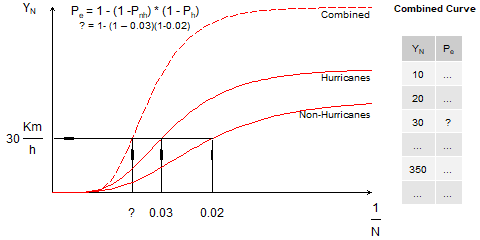
\includegraphics[width=0.8\textwidth,height=\textheight]{./images/concept.png}

}

\caption{\label{fig-concept}Representación conceptual del modelo de
amenaza}

\end{figure}%

La lógica subyacente asume que los eventos extremos siguen procesos de
Poisson independientes, donde la probabilidad de que la velocidad
combinada exceda un umbral \(v\) se define por la unión de las
probabilidades individuales:
\(p_c = 1 - ((1 - p_{nh}) \times (1 - p_{h}))\).

\subsection{Algoritmos de interpolación y extrapolación lineal aplicados
a
vectores}\label{algoritmos-de-interpolaciuxf3n-y-extrapolaciuxf3n-lineal-aplicados-a-vectores}

La función detallada a continuación implementa un algoritmo de
interpolación lineal interna complementado con una extensión de
extrapolación fundamentada en la gradiente de los límites del dominio.
Este procedimiento permite la estimación de valores en cualquiera de las
dimensiones de una curva de amenaza, partiendo de un conjunto discreto
de valores de amenaza (\emph{rl}) y probabilidad predefinidas.

La extrapolación lineal aplicada en la función se basa en la ecuación de
la recta punto-pendiente. Para un valor \(x_{out}\) fuera del rango, la
probabilidad \(y_{out}\) se calcula mediante la relación:

\[y_{out} = y_i + \left( \frac{y_j - y_i}{x_j - x_i} \right) (x_{out} - x_i)\]

Donde:

\begin{itemize}
\tightlist
\item
  El término entre paréntesis representa el gradiente o pendiente local
  (\(m\)).
\item
  \((x_i, y_i)\) y \((x_j, y_j)\) representan el par de puntos más
  cercanos al límite del dominio (el primer y segundo punto para el
  límite inferior, y los dos últimos para el superior).
\end{itemize}

Este método asegura que la función sea continua, aunque es importante
advertir a los estudiantes que la precisión de la extrapolación
disminuye a medida que \(x_{out}\) se aleja significativamente del rango
observado, especialmente en variables meteorológicas con comportamientos
no lineales en las colas.

\begin{Shaded}
\begin{Highlighting}[]
\CommentTok{\# \#| eval: false}

\CommentTok{\# ==============================================================================}
\CommentTok{\# DEFINICIÓN DE FUNCIÓN PARA ESTIMACIÓN DE VALORES (INTERPOLACIÓN/EXTRAPOLACIÓN)}
\CommentTok{\# ==============================================================================}

\CommentTok{\# Entradas:}
\CommentTok{\#   x: Vector de valores del eje independiente (ej: Velocidad del viento en m/s)}
\CommentTok{\#   y: Vector de valores del eje dependiente (ej: Probabilidad de excedencia)}
\CommentTok{\#   xout: Valor o vector de valores específicos a consultar (ej: Velocidad de diseño)}

\CommentTok{\# Salida:}
\CommentTok{\#   yout: Valor interpolado o extrapolado (probabilidad) correspondiente a xout}
\CommentTok{\#   Nota: El periodo de retorno se calcula como N = 1 / yout}

\CommentTok{\# Restricción técnica: }
\CommentTok{\# La librería Hmisc no se encuentra disponible en el entorno de ejecución (contenedor),}
\CommentTok{\# por lo cual se implementa una solución nativa robusta basada en approx().}
\CommentTok{\# Esta sería la función usando el paquete Hmisc}
\CommentTok{\# extrapola \textless{}{-} function(x, y, xout)\{}
\CommentTok{\#  yout=Hmisc::approxExtrap(x=x, y=y, xout=xout)$y}
\CommentTok{\# \}}

\NormalTok{extrapola }\OtherTok{\textless{}{-}} \ControlFlowTok{function}\NormalTok{(x, y, xout) \{}

  \CommentTok{\# 1. TRATAMIENTO DE DUPLICADOS (TIES)}
  \CommentTok{\# La presencia de valores de x idénticos genera ambigüedad en la interpolación lineal.}
  \CommentTok{\# Se consolidan los duplicados calculando la media de y para cada x único.}
  \ControlFlowTok{if}\NormalTok{ (}\FunctionTok{any}\NormalTok{(}\FunctionTok{duplicated}\NormalTok{(x))) \{}
\NormalTok{    datos\_unicos }\OtherTok{\textless{}{-}} \FunctionTok{aggregate}\NormalTok{(y }\SpecialCharTok{\textasciitilde{}}\NormalTok{ x, }\AttributeTok{data =} \FunctionTok{data.frame}\NormalTok{(}\AttributeTok{x =}\NormalTok{ x, }\AttributeTok{y =}\NormalTok{ y), }\AttributeTok{FUN =}\NormalTok{ mean)}
\NormalTok{    x }\OtherTok{\textless{}{-}}\NormalTok{ datos\_unicos}\SpecialCharTok{$}\NormalTok{x}
\NormalTok{    y }\OtherTok{\textless{}{-}}\NormalTok{ datos\_unicos}\SpecialCharTok{$}\NormalTok{y}
\NormalTok{  \}}

  \CommentTok{\# 2. ORDENAMIENTO DE VECTORES}
  \CommentTok{\# La función approx() y la lógica de pendientes requieren vectores ordenados ascendentemente.}
\NormalTok{  ord }\OtherTok{\textless{}{-}} \FunctionTok{order}\NormalTok{(x)}
\NormalTok{  x }\OtherTok{\textless{}{-}}\NormalTok{ x[ord]}
\NormalTok{  y }\OtherTok{\textless{}{-}}\NormalTok{ y[ord]}
\NormalTok{  n }\OtherTok{\textless{}{-}} \FunctionTok{length}\NormalTok{(x)}
  
  \CommentTok{\# 3. INICIALIZACIÓN DEL VECTOR DE SALIDA}
  \CommentTok{\# Se pre{-}asigna espacio en memoria para optimizar el rendimiento.}
\NormalTok{  yout }\OtherTok{\textless{}{-}} \FunctionTok{numeric}\NormalTok{(}\FunctionTok{length}\NormalTok{(xout))}
  
  \CommentTok{\# 4. INTERPOLACIÓN LINEAL (DENTRO DEL RANGO)}
  \CommentTok{\# Se utiliza approx() para estimar valores dentro del intervalo [min(x), max(x)].}
  \CommentTok{\# suppressWarnings() evita alertas por duplicados que ya han sido tratados previamente.}
\NormalTok{  yout }\OtherTok{\textless{}{-}} \FunctionTok{suppressWarnings}\NormalTok{(}\FunctionTok{approx}\NormalTok{(x, y, xout)}\SpecialCharTok{$}\NormalTok{y)}
  
  \CommentTok{\# 5. LÓGICA DE EXTRAPOLACIÓN LINEAL}
  \CommentTok{\# Identificación de índices de xout que se encuentran fuera del dominio de x.}
\NormalTok{  idx\_inf }\OtherTok{\textless{}{-}} \FunctionTok{which}\NormalTok{(xout }\SpecialCharTok{\textless{}}\NormalTok{ x[}\DecValTok{1}\NormalTok{])  }\CommentTok{\# Valores menores al límite inferior}
\NormalTok{  idx\_sup }\OtherTok{\textless{}{-}} \FunctionTok{which}\NormalTok{(xout }\SpecialCharTok{\textgreater{}}\NormalTok{ x[n])  }\CommentTok{\# Valores mayores al límite superior}
  
  \CommentTok{\# Extrapolación lineal inferior:}
  \CommentTok{\# Se utiliza la pendiente derivada de los dos primeros puntos de la curva.}
  \ControlFlowTok{if}\NormalTok{ (}\FunctionTok{length}\NormalTok{(idx\_inf) }\SpecialCharTok{\textgreater{}} \DecValTok{0}\NormalTok{) \{}
\NormalTok{    slope\_low }\OtherTok{\textless{}{-}}\NormalTok{ (y[}\DecValTok{2}\NormalTok{] }\SpecialCharTok{{-}}\NormalTok{ y[}\DecValTok{1}\NormalTok{]) }\SpecialCharTok{/}\NormalTok{ (x[}\DecValTok{2}\NormalTok{] }\SpecialCharTok{{-}}\NormalTok{ x[}\DecValTok{1}\NormalTok{])}
\NormalTok{    yout[idx\_inf] }\OtherTok{\textless{}{-}}\NormalTok{ y[}\DecValTok{1}\NormalTok{] }\SpecialCharTok{+}\NormalTok{ slope\_low }\SpecialCharTok{*}\NormalTok{ (xout[idx\_inf] }\SpecialCharTok{{-}}\NormalTok{ x[}\DecValTok{1}\NormalTok{])}
\NormalTok{  \}}
  
  \CommentTok{\# Extrapolación lineal superior:}
  \CommentTok{\# Se utiliza la pendiente derivada de los dos últimos puntos de la curva.}
  \CommentTok{\# El modelo asume que el comportamiento de la cola de la distribución es lineal.}
  \ControlFlowTok{if}\NormalTok{ (}\FunctionTok{length}\NormalTok{(idx\_sup) }\SpecialCharTok{\textgreater{}} \DecValTok{0}\NormalTok{) \{}
\NormalTok{    slope\_high }\OtherTok{\textless{}{-}}\NormalTok{ (y[n] }\SpecialCharTok{{-}}\NormalTok{ y[n}\DecValTok{{-}1}\NormalTok{]) }\SpecialCharTok{/}\NormalTok{ (x[n] }\SpecialCharTok{{-}}\NormalTok{ x[n}\DecValTok{{-}1}\NormalTok{])}
\NormalTok{    yout[idx\_sup] }\OtherTok{\textless{}{-}}\NormalTok{ y[n] }\SpecialCharTok{+}\NormalTok{ slope\_high }\SpecialCharTok{*}\NormalTok{ (xout[idx\_sup] }\SpecialCharTok{{-}}\NormalTok{ x[n])}
\NormalTok{  \}}
  
  \FunctionTok{return}\NormalTok{(yout)}
\NormalTok{\}}
\end{Highlighting}
\end{Shaded}

\subsubsection{Resumen sintáctico: Estimación de curvas y manejo de
colas
estadísticas}\label{resumen-sintuxe1ctico-estimaciuxf3n-de-curvas-y-manejo-de-colas-estaduxedsticas}

La función \texttt{extrapola} es un ejemplo de cómo extender las
capacidades nativas de R para resolver problemas específicos de
ingeniería climática, como la continuidad de las curvas de amenaza.

\begin{longtable}[]{@{}
  >{\raggedright\arraybackslash}p{(\columnwidth - 6\tabcolsep) * \real{0.2500}}
  >{\raggedright\arraybackslash}p{(\columnwidth - 6\tabcolsep) * \real{0.2500}}
  >{\raggedright\arraybackslash}p{(\columnwidth - 6\tabcolsep) * \real{0.2500}}
  >{\raggedright\arraybackslash}p{(\columnwidth - 6\tabcolsep) * \real{0.2500}}@{}}
\toprule\noalign{}
\begin{minipage}[b]{\linewidth}\raggedright
Función / Operador
\end{minipage} & \begin{minipage}[b]{\linewidth}\raggedright
Librería
\end{minipage} & \begin{minipage}[b]{\linewidth}\raggedright
Propósito en el flujo SIG
\end{minipage} & \begin{minipage}[b]{\linewidth}\raggedright
Parámetro Crítico / Lógica
\end{minipage} \\
\midrule\noalign{}
\endhead
\bottomrule\noalign{}
\endlastfoot
\textbf{\texttt{aggregate()}} & \texttt{stats} & Consolidar ``ties''
(duplicados en X) que romperían la lógica de la función. &
\texttt{FUN\ =\ mean}: promedia valores redundantes. \\
\textbf{\texttt{order()}} & \texttt{base} & Garantiza que los vectores
de ráfagas sean estrictamente ascendentes. & Crucial para que
\texttt{approx()} funcione. \\
\textbf{\texttt{numeric()}} & \texttt{base} & \textbf{Pre-asignación de
memoria:} Crea un vector vacío del tamaño exacto del resultado. &
Optimiza el rendimiento en procesos masivos. \\
\textbf{\texttt{approx()}} & \texttt{stats} & Realiza la interpolación
lineal estándar dentro del rango de datos conocidos. & \texttt{x},
\texttt{y}, \texttt{xout}. \\
\textbf{\texttt{which()}} & \texttt{base} & Identifica qué valores de
consulta están por fuera de los límites (Extrapolación). &
\texttt{xout\ \textless{}\ x{[}1{]}} o
\texttt{xout\ \textgreater{}\ x{[}n{]}}. \\
\textbf{Gradiente (\(m\))} & \texttt{manual} & Calcula la pendiente
local de la curva en sus extremos para proyectar valores. &
\texttt{(y{[}j{]}-y{[}i{]})\ /\ (x{[}j{]}-x{[}i{]})}. \\
\textbf{\texttt{suppressWarnings()}} & \texttt{base} & Silencia
advertencias de renderizado que no afectan el cálculo numérico. &
Mantiene la consola limpia durante el proceso. \\
\end{longtable}

\begin{quote}
\textbf{Nota del Autor:} Note que la función implementa una solución
``nativa'' robusta. En entornos de producción o contenedores donde no
siempre es posible instalar librerías externas (como \texttt{Hmisc}), el
programador SIG debe ser capaz de codificar manualmente modelos
geométricos básicos como la \textbf{recta punto-pendiente}. Esta técnica
garantiza que si un usuario consulta un viento de un periodo de retorno
no calculado (ej: 10,000 años), el software devuelva una estimación
lógica basada en la tendencia de los datos y no un error de sistema.
\end{quote}

\subsection{Diseño de funciones para operaciones multidimensionales
(st\_apply)}\label{diseuxf1o-de-funciones-para-operaciones-multidimensionales-st_apply}

La combinación se realizará mediante la función \texttt{st\_apply} del
ecosistema \texttt{stars}, la cual permite la iteración eficiente sobre
la dimensión espacial (celdas de la malla ERA5). En cada iteración, se
procesan los valores de una dimensión adicional que almacena los niveles
de retorno para vientos no huracanados (\emph{nh}) y huracanados
(\emph{h}).

Este enfoque es fundamental porque las curvas de amenaza originales
suelen estar discretizadas en diferentes periodos de retorno o presentar
rangos de intensidad dispares. Al reconstruir una curva detallada (de 1
a 600 km/h) mediante la función \texttt{extrapola}, se garantiza que la
operación de combinación se realice sobre una base común de intensidades
antes de re-interpolar los resultados hacia los periodos de retorno de
interés (\(MRI\)).

Tal y como se mencionó anteriormente la combinación se define por la
unión de las probabilidades individuales:
\(p_c = 1 - ((1 - p_{nh}) \times (1 - p_{h}))\).

\subsubsection{\texorpdfstring{Anatomía de la función
\texttt{st\_apply}}{Anatomía de la función st\_apply}}\label{anatomuxeda-de-la-funciuxf3n-st_apply}

Para comprender la orquestación de este proceso, es fundamental
desglosar la sintaxis de la función \texttt{st\_apply}. A diferencia de
los bucles iterativos tradicionales (\texttt{for}, \texttt{while}),
\texttt{st\_apply} traslada la filosofía de la programación funcional al
análisis de cubos espaciales, delegando al motor subyacente de R la
gestión de la memoria y el recorrido de los índices.

\begin{Shaded}
\begin{Highlighting}[]
\FunctionTok{st\_apply}\NormalTok{(X, MARGIN, FUN, ...)}
\end{Highlighting}
\end{Shaded}

\textbf{Desglose de parámetros clave:}

\begin{itemize}
\tightlist
\item
  \textbf{\texttt{X}}: El objeto multidimensional de clase
  \texttt{stars}. En nuestro caso de estudio, es el cubo unificado
  (\texttt{st\_nh\_h\_c\_merged}) que contiene tanto la dimensión
  espacial (la malla de Colombia) como la dimensión de atributos (los
  periodos de retorno de cada régimen de viento).
\item
  \textbf{\texttt{MARGIN}}: Define la dimensión (o dimensiones) sobre la
  cual se iterará.

  \begin{itemize}
  \tightlist
  \item
    Si definimos \texttt{MARGIN\ =\ "geometry"} (nuestro enfoque), la
    función \texttt{FUN} recibirá un vector con todos los atributos
    correspondientes a \textbf{una sola celda espacial} a la vez. Es
    ideal para álgebra de mapas local.
  \item
    Si definiéramos \texttt{MARGIN\ =\ "time"} o el nombre de un
    atributo, la función operaría sobre el mapa completo (todas las
    celdas) para ese instante de tiempo o capa específica.
  \end{itemize}
\item
  \textbf{\texttt{FUN}}: La función matemática, estadística o lógica que
  se ejecutará en cada iteración. Aquí pasaremos nuestra función
  personalizada \texttt{combined\_columns\_st\_apply} que contiene el
  algoritmo de interpolación y extrapolación.
\item
  \textbf{\texttt{...} (Puntos suspensivos)}: Representa los argumentos
  adicionales que requiere la función definida en \texttt{FUN}. Es a
  través de este canal que inyectaremos los vectores de periodos de
  retorno (\texttt{mri\_h}, \texttt{mri\_nh}, \texttt{mri\_c}) y los
  índices de las bandas para que \texttt{combined\_columns\_st\_apply}
  sepa exactamente qué procesar.
\end{itemize}

\begin{Shaded}
\begin{Highlighting}[]
\CommentTok{\# \#| eval: false}

\CommentTok{\# Función para combinar información de viento de}
\CommentTok{\# huracanes con información no huracanada usando}
\CommentTok{\# la fórmula típica de combinación de curvas de amenaza:}
\CommentTok{\# p\_c = (1 {-} ((1 {-} p\_h) * (1 {-} p\_nh)))}
\CommentTok{\#}
\CommentTok{\# dónde: }
\CommentTok{\#   p\_c  : probabilidad combinada del viento extremo}
\CommentTok{\#   p\_h  : probabilidad de viento de huracanes}
\CommentTok{\#   p\_nh : probabilidad de viento no huracanado}
\CommentTok{\#}
\CommentTok{\# Entrada: }
\CommentTok{\#  {-} st: objeto stars. En el contexto de st\_apply, este argumento}
\CommentTok{\#        corresponde a un vector con los valores de una celda}
\CommentTok{\#        a través de múltiples bandas (no es todo el raster).}
\CommentTok{\#}
\CommentTok{\#  {-} bands\_rl\_h: atributos (índices de bandas) correspondientes}
\CommentTok{\#        a las velocidades de huracanes}
\CommentTok{\#}
\CommentTok{\#  {-} mri\_h: periodos de retorno (en años) correspondientes a los}
\CommentTok{\#        atributos de velocidades de huracanes. Se transforman a}
\CommentTok{\#        probabilidades como p = 1 / MRI}
\CommentTok{\#}
\CommentTok{\#  {-} bands\_rl\_nh: atributos correspondientes a las velocidades}
\CommentTok{\#        de no huracanes}
\CommentTok{\#}
\CommentTok{\#  {-} mri\_nh: periodos de retorno correspondientes a los atributos}
\CommentTok{\#        de velocidades de no huracanes}
\CommentTok{\#}
\CommentTok{\#  {-} mri\_c: periodos de retorno a consultar en la curva combinada}
\CommentTok{\#}
\CommentTok{\# Forma de aplicarse: st\_apply}
\CommentTok{\#}
\CommentTok{\# Salida: niveles de retorno (velocidades) para los periodos}
\CommentTok{\#         de retorno consultados}

\NormalTok{combined\_columns\_st\_apply }\OtherTok{\textless{}{-}} \ControlFlowTok{function}\NormalTok{(}
    
    \CommentTok{\# La función se ejecutará en la primera dimensión "geometry"}
    \CommentTok{\# del objeto stars st\_nh\_h\_c\_merged.}
    \CommentTok{\# Todos los valores de la otra dimensión ("attributes") no usada en st\_apply}
    \CommentTok{\# se retornan en \textquotesingle{}st\textquotesingle{}}
    \CommentTok{\# El argumento recibe dinámicamente un vector de 34 posiciones}
    \CommentTok{\# correspondientes a todos los valores de la dimension "attributes"}
\NormalTok{    st,}
    
    \CommentTok{\# Posiciones de los valores en la dimensión "attributes"}
    \CommentTok{\# del objeto st\_nh\_h\_c\_merged, correspondientes a vientos huracanados,}
    \CommentTok{\# para extraerlos del vector st}
    \AttributeTok{bands\_rl\_h =} \FunctionTok{c}\NormalTok{(}\DecValTok{13}\SpecialCharTok{:}\DecValTok{23}\NormalTok{),}
    
    \CommentTok{\# Periodos de retorno (años) asociados a bandas de huracanes}
    \CommentTok{\# almacenados en las posiciones 13 a 23 de la dimensión "attributes"}
    \CommentTok{\# Deben corresponder uno a uno con bands\_rl\_h}
    \AttributeTok{mri\_h =} \FunctionTok{c}\NormalTok{(}\DecValTok{10}\NormalTok{,}\DecValTok{20}\NormalTok{,}\DecValTok{50}\NormalTok{,}\DecValTok{100}\NormalTok{,}\DecValTok{250}\NormalTok{,}\DecValTok{500}\NormalTok{,}\DecValTok{700}\NormalTok{,}\DecValTok{1000}\NormalTok{,}\DecValTok{1700}\NormalTok{,}\DecValTok{3000}\NormalTok{,}\DecValTok{7000}\NormalTok{),}
    
    \CommentTok{\# Posiciones de los valores en la dimensión "attributes"}
    \CommentTok{\# del objeto st\_nh\_h\_c\_merged, correspondientes a vientos no huracanados,}
    \CommentTok{\# para extraerlos del vector st}
    \AttributeTok{bands\_rl\_nh =} \FunctionTok{c}\NormalTok{(}\DecValTok{2}\SpecialCharTok{:}\DecValTok{12}\NormalTok{),}
    
    \CommentTok{\# Periodos de retorno (años) asociados a bandas no huracanadas}
    \CommentTok{\# almacenados en las posiciones 2 a 12 de la dimensión "attributes"}
    \CommentTok{\# Deben corresponder uno a uno con bands\_rl\_nh    }
    \AttributeTok{mri\_nh =} \FunctionTok{c}\NormalTok{(}\DecValTok{10}\NormalTok{,}\DecValTok{20}\NormalTok{,}\DecValTok{50}\NormalTok{,}\DecValTok{100}\NormalTok{,}\DecValTok{250}\NormalTok{,}\DecValTok{500}\NormalTok{,}\DecValTok{700}\NormalTok{,}\DecValTok{1000}\NormalTok{,}\DecValTok{1700}\NormalTok{,}\DecValTok{3000}\NormalTok{,}\DecValTok{7000}\NormalTok{),}
    
    \CommentTok{\# Periodos de retorno (años) a consultar en la curva combinada}
    \CommentTok{\# En las posiciones 25 a 34 de la dimensión "attributes" hay}
    \CommentTok{\# valores nulos, pero los valores (nombres) de esas bandas }
    \CommentTok{\# ("c\_10", ..., "c\_7000") corresponden a estos periodos de retorno}
    \AttributeTok{mri\_c =} \FunctionTok{c}\NormalTok{(}\DecValTok{10}\NormalTok{,}\DecValTok{20}\NormalTok{,}\DecValTok{50}\NormalTok{,}\DecValTok{100}\NormalTok{,}\DecValTok{250}\NormalTok{,}\DecValTok{500}\NormalTok{,}\DecValTok{700}\NormalTok{,}\DecValTok{1000}\NormalTok{,}\DecValTok{1700}\NormalTok{,}\DecValTok{3000}\NormalTok{,}\DecValTok{7000}\NormalTok{)}
\NormalTok{    ) \{}
    
  \CommentTok{\# {-}{-}{-}{-}{-}{-}{-}{-}{-}{-}{-}{-}{-}{-}{-}{-}{-}{-}{-}{-}{-}{-}{-}{-}{-}{-}{-}{-}{-}{-}{-}{-}{-}{-}{-}{-}{-}{-}{-}{-}{-}{-}{-}{-}{-}{-}{-}{-}{-}{-}}
  \CommentTok{\# Gestión del contador para monitoreo de progreso}
  \CommentTok{\# {-}{-}{-}{-}{-}{-}{-}{-}{-}{-}{-}{-}{-}{-}{-}{-}{-}{-}{-}{-}{-}{-}{-}{-}{-}{-}{-}{-}{-}{-}{-}{-}{-}{-}{-}{-}{-}{-}{-}{-}{-}{-}{-}{-}{-}{-}{-}{-}{-}{-}}
  
\NormalTok{  mycuenta }\OtherTok{\textless{}\textless{}{-}}\NormalTok{ mycuenta }\SpecialCharTok{+} \DecValTok{1}
\NormalTok{  contar }\OtherTok{=}\NormalTok{ mycuenta}
  \FunctionTok{assign}\NormalTok{(}\StringTok{"mycuenta"}\NormalTok{, contar, }\AttributeTok{envir =} \FunctionTok{parent.frame}\NormalTok{() )}
  
  \ControlFlowTok{if}\NormalTok{ (contar }\SpecialCharTok{==} \DecValTok{1} \SpecialCharTok{|}\NormalTok{ contar }\SpecialCharTok{==} \DecValTok{3381}\NormalTok{) \{}
    \FunctionTok{print}\NormalTok{(}\FunctionTok{paste}\NormalTok{(}\StringTok{"contar:"}\NormalTok{, contar))}
    \FunctionTok{print}\NormalTok{(}\FunctionTok{paste}\NormalTok{(}\StringTok{"mycuenta:"}\NormalTok{, mycuenta))}
\NormalTok{  \}}
  
  \CommentTok{\# {-}{-}{-}{-}{-}{-}{-}{-}{-}{-}{-}{-}{-}{-}{-}{-}{-}{-}{-}{-}{-}{-}{-}{-}{-}{-}{-}{-}{-}{-}{-}{-}{-}{-}{-}{-}{-}{-}{-}{-}{-}{-}{-}{-}{-}{-}{-}{-}{-}{-}}
  \CommentTok{\# Construcción del dominio de velocidades}
  \CommentTok{\# {-}{-}{-}{-}{-}{-}{-}{-}{-}{-}{-}{-}{-}{-}{-}{-}{-}{-}{-}{-}{-}{-}{-}{-}{-}{-}{-}{-}{-}{-}{-}{-}{-}{-}{-}{-}{-}{-}{-}{-}{-}{-}{-}{-}{-}{-}{-}{-}{-}{-}}
  
  \CommentTok{\# Secuencia de 1 km/h a 600 km/h para construir}
  \CommentTok{\# una curva de amenaza detallada mediante interpolación}
\NormalTok{  rl600 }\OtherTok{=} \FunctionTok{seq}\NormalTok{(}\AttributeTok{from =} \DecValTok{1}\NormalTok{, }\AttributeTok{to =} \DecValTok{600}\NormalTok{, }\AttributeTok{by =} \DecValTok{1}\NormalTok{)}
  
  
  \CommentTok{\# ==================================================}
  \CommentTok{\# Huracanes}
  \CommentTok{\# ==================================================}
  
  \CommentTok{\# Para cada celda (geometry) se leen las velocidades }
  \CommentTok{\# de las bandas 13 a 23 de la dimensión "attributes"}
  \CommentTok{\# y se almacenan almaceno en rl\_h}
\NormalTok{  rl\_h }\OtherTok{=} \ConstantTok{NULL}
  
  \ControlFlowTok{for}\NormalTok{ (band }\ControlFlowTok{in}\NormalTok{ bands\_rl\_h) \{}
    \CommentTok{\# Leo el valor (banda) de un valor de "attributes"}
    \CommentTok{\# correspondiente a huracanes en la celda actual}
    \CommentTok{\# st[band]: valor de la celda en la banda indicada}
    \CommentTok{\# Se crea el vector con información de huracanes}
    \CommentTok{\# al recorrer valor tras valor (banda a banda)}
\NormalTok{    rl\_h }\OtherTok{=} \FunctionTok{c}\NormalTok{(rl\_h, st[band])  }
\NormalTok{  \}}
  
  \CommentTok{\# Chequear si hay problemas de datos en los valores}
  \CommentTok{\# almacenados en rl\_h. Si es así, convertir todo a NA}
  \ControlFlowTok{if}\NormalTok{ (}\FunctionTok{any}\NormalTok{(}\SpecialCharTok{!}\FunctionTok{is.na}\NormalTok{(rl\_h)))\{}
    \ControlFlowTok{if}\NormalTok{ (}\FunctionTok{sum}\NormalTok{(rl\_h) }\SpecialCharTok{==} \DecValTok{0} \SpecialCharTok{|} \FunctionTok{sum}\NormalTok{(rl\_h) }\SpecialCharTok{\textless{}} \DecValTok{0}\NormalTok{) \{}
\NormalTok{      rl\_h }\OtherTok{=} \FunctionTok{rep}\NormalTok{(}\ConstantTok{NA}\NormalTok{, }\FunctionTok{length}\NormalTok{(bands\_rl\_h))}
\NormalTok{    \}}
\NormalTok{  \}}

  \CommentTok{\# Data frame con curva de amenaza para huracanes }
  \CommentTok{\# Solo puntos discretos originales:}
  \CommentTok{\#  mri\_h = 10,20,50,100,250,500,700,1000,1700,3000,7000}
  \CommentTok{\# rl   = velocidad}
  \CommentTok{\# prob = 1 / mri\_h}
\NormalTok{  h }\OtherTok{=} \FunctionTok{data.frame}\NormalTok{(}\AttributeTok{rl =}\NormalTok{ rl\_h, }\AttributeTok{prob =} \DecValTok{1} \SpecialCharTok{/}\NormalTok{ mri\_h)}
  
  \CommentTok{\# Calcular probabilidades para las 600 velocidades (1 a 600 km/h)}
  \CommentTok{\# Si hay NA en los datos, no usar extrapola}
  \ControlFlowTok{if}\NormalTok{ (}\FunctionTok{any}\NormalTok{(}\FunctionTok{is.na}\NormalTok{(h}\SpecialCharTok{$}\NormalTok{rl)) }\SpecialCharTok{|} \FunctionTok{any}\NormalTok{(}\FunctionTok{is.na}\NormalTok{(h}\SpecialCharTok{$}\NormalTok{prob)))\{}
    \CommentTok{\# en hc\_h\_prob se almacenan solo nulos}
\NormalTok{    hc\_h\_prob }\OtherTok{=} \FunctionTok{rep}\NormalTok{(}\ConstantTok{NA}\NormalTok{, }\FunctionTok{length}\NormalTok{(rl600))}
\NormalTok{  \} }\ControlFlowTok{else}\NormalTok{\{}
    \CommentTok{\# Ingreso velocidades en xout}
    \CommentTok{\# en hc\_h\_prob se almacenan las probabilidades}
    \CommentTok{\# después de usar extrapola}
\NormalTok{    hc\_h\_prob }\OtherTok{=} \FunctionTok{extrapola}\NormalTok{(}\AttributeTok{x =}\NormalTok{ h}\SpecialCharTok{$}\NormalTok{rl, }\AttributeTok{y =}\NormalTok{ h}\SpecialCharTok{$}\NormalTok{prob, }\AttributeTok{xout =}\NormalTok{ rl600)  }
\NormalTok{  \}}
  
  \CommentTok{\# Curva de amenaza detallada para huracanes}
  \CommentTok{\# rl = 1 a 600 km/h (velocidades)}
  \CommentTok{\# prob = probabilidades de extrapola}
\NormalTok{  hc\_h }\OtherTok{=} \FunctionTok{data.frame}\NormalTok{(}\AttributeTok{rl =}\NormalTok{ rl600, }\AttributeTok{prob =}\NormalTok{ hc\_h\_prob)}
  
  \CommentTok{\# Control de valores extremos de probabilidad (rango [0,1])}
\NormalTok{  hc\_h}\SpecialCharTok{$}\NormalTok{prob[hc\_h}\SpecialCharTok{$}\NormalTok{prob }\SpecialCharTok{\textless{}} \DecValTok{0}\NormalTok{] }\OtherTok{=} \DecValTok{0}
\NormalTok{  hc\_h}\SpecialCharTok{$}\NormalTok{prob[hc\_h}\SpecialCharTok{$}\NormalTok{prob }\SpecialCharTok{\textgreater{}} \DecValTok{1}\NormalTok{] }\OtherTok{=} \DecValTok{1}
  
  
  \CommentTok{\# ==================================================}
  \CommentTok{\# No huracanes}
  \CommentTok{\# ==================================================}
  
  \CommentTok{\# Leemos las velocidades no huracanadas de cada celda}
\NormalTok{  rl\_nh }\OtherTok{=} \ConstantTok{NULL}
  
  \CommentTok{\# se usan los indices de bandas para no huracanes}
  \CommentTok{\# y se extraen de la dimensión "attributes", ahora}
  \CommentTok{\# disponibles para la celda (geometría) actual a través}
  \CommentTok{\# de st}
  \ControlFlowTok{for}\NormalTok{ (band }\ControlFlowTok{in}\NormalTok{ bands\_rl\_nh) \{}
\NormalTok{    rl\_nh }\OtherTok{=} \FunctionTok{c}\NormalTok{(rl\_nh, st[band])}
\NormalTok{  \}}
  
  \CommentTok{\# Control de calidad de datos}
  \ControlFlowTok{if}\NormalTok{ (}\FunctionTok{any}\NormalTok{(}\SpecialCharTok{!}\FunctionTok{is.na}\NormalTok{(rl\_nh)))\{}
    \ControlFlowTok{if}\NormalTok{ (}\FunctionTok{sum}\NormalTok{(rl\_nh) }\SpecialCharTok{==} \DecValTok{0} \SpecialCharTok{|} \FunctionTok{sum}\NormalTok{(rl\_nh) }\SpecialCharTok{\textless{}} \DecValTok{0}\NormalTok{) \{}
\NormalTok{      rl\_nh }\OtherTok{=} \FunctionTok{rep}\NormalTok{(}\ConstantTok{NA}\NormalTok{, }\FunctionTok{length}\NormalTok{(bands\_rl\_nh))}
\NormalTok{    \}}
\NormalTok{  \}}
  
  \CommentTok{\# Curva discreta inicial de no huracanes}
\NormalTok{  nh }\OtherTok{=} \FunctionTok{data.frame}\NormalTok{(}\AttributeTok{rl =}\NormalTok{ rl\_nh, }\AttributeTok{prob =} \DecValTok{1} \SpecialCharTok{/}\NormalTok{ mri\_nh)}
  
  \CommentTok{\# Interpolación a curva detallada (1–600 km/h)}
  \ControlFlowTok{if}\NormalTok{ (}\FunctionTok{any}\NormalTok{(}\FunctionTok{is.na}\NormalTok{(nh}\SpecialCharTok{$}\NormalTok{rl)) }\SpecialCharTok{|} \FunctionTok{any}\NormalTok{(}\FunctionTok{is.na}\NormalTok{(nh}\SpecialCharTok{$}\NormalTok{prob)))\{}
\NormalTok{    hc\_nh\_prob }\OtherTok{=} \FunctionTok{rep}\NormalTok{(}\ConstantTok{NA}\NormalTok{, }\FunctionTok{length}\NormalTok{(rl600))}
\NormalTok{  \} }\ControlFlowTok{else}\NormalTok{\{}
\NormalTok{    hc\_nh\_prob }\OtherTok{=} \FunctionTok{extrapola}\NormalTok{(}\AttributeTok{x =}\NormalTok{ nh}\SpecialCharTok{$}\NormalTok{rl, }\AttributeTok{y =}\NormalTok{ nh}\SpecialCharTok{$}\NormalTok{prob, }\AttributeTok{xout =}\NormalTok{ rl600)}
\NormalTok{  \}}
  
\NormalTok{  hc\_nh }\OtherTok{=} \FunctionTok{data.frame}\NormalTok{(}\AttributeTok{rl =}\NormalTok{ rl600, }\AttributeTok{prob =}\NormalTok{ hc\_nh\_prob)}
  
  \CommentTok{\# Control de rango}
\NormalTok{  hc\_nh}\SpecialCharTok{$}\NormalTok{prob[hc\_nh}\SpecialCharTok{$}\NormalTok{prob }\SpecialCharTok{\textless{}} \DecValTok{0}\NormalTok{] }\OtherTok{=} \DecValTok{0}
\NormalTok{  hc\_nh}\SpecialCharTok{$}\NormalTok{prob[hc\_nh}\SpecialCharTok{$}\NormalTok{prob }\SpecialCharTok{\textgreater{}} \DecValTok{1}\NormalTok{] }\OtherTok{=} \DecValTok{1}
  
  
  \CommentTok{\# ==================================================}
  \CommentTok{\# Combinación de curvas}
  \CommentTok{\# ==================================================}
  
  \CommentTok{\# Antes de combinar:}
  \CommentTok{\# 1) No huracán (nh): no puede ser nulo}
  \CommentTok{\# 2) Huracán (h): puede ser nulo}
  \CommentTok{\# 3) Se usa la curva detallada con velocidades}
  \CommentTok{\#    1 a 600 Km/h}

  \ControlFlowTok{if}\NormalTok{ (}\FunctionTok{any}\NormalTok{(}\FunctionTok{is.na}\NormalTok{(hc\_h}\SpecialCharTok{$}\NormalTok{prob)) }\SpecialCharTok{|} \FunctionTok{any}\NormalTok{(}\FunctionTok{is.na}\NormalTok{(hc\_h}\SpecialCharTok{$}\NormalTok{rl)))\{}
    \CommentTok{\# Si huracanes es nulo, la combinación depende solo }
    \CommentTok{\# de no huracanes}
\NormalTok{    hc\_c\_prob }\OtherTok{=}\NormalTok{ hc\_nh}\SpecialCharTok{$}\NormalTok{prob}
\NormalTok{  \} }\ControlFlowTok{else}\NormalTok{ \{}
    \CommentTok{\# Fórmula de combinación probabilística}
    \CommentTok{\# p\_c = (1 {-} ((1{-}p\_h)*(1{-}p\_nh)))}
\NormalTok{    hc\_c\_prob }\OtherTok{=}\NormalTok{ (}\DecValTok{1} \SpecialCharTok{{-}}\NormalTok{ ((}\DecValTok{1} \SpecialCharTok{{-}}\NormalTok{ hc\_h}\SpecialCharTok{$}\NormalTok{prob) }\SpecialCharTok{*}\NormalTok{ (}\DecValTok{1} \SpecialCharTok{{-}}\NormalTok{ hc\_nh}\SpecialCharTok{$}\NormalTok{prob)))     }
\NormalTok{  \}}

  \CommentTok{\# Curva combinada detallada en un data{-}frame}
\NormalTok{  hc\_c }\OtherTok{=} \FunctionTok{data.frame}\NormalTok{(}\AttributeTok{rl =}\NormalTok{ rl600, }\AttributeTok{prob =}\NormalTok{ hc\_c\_prob)}
  
  \CommentTok{\# Control de valores negativos}
\NormalTok{  hc\_c}\SpecialCharTok{$}\NormalTok{prob[hc\_c}\SpecialCharTok{$}\NormalTok{prob }\SpecialCharTok{\textless{}} \DecValTok{0}\NormalTok{] }\OtherTok{=} \DecValTok{0}
  
  
  \CommentTok{\# ==================================================}
  \CommentTok{\# Interpolación final (salida)}
  \CommentTok{\# ==================================================}
  
  \CommentTok{\# Convertir periodos de retorno combinados}
  \CommentTok{\# a probabilidades}
\NormalTok{  prob\_c }\OtherTok{=} \DecValTok{1} \SpecialCharTok{/}\NormalTok{ mri\_c}
  
  \CommentTok{\# Obtener velocidades correspondientes a esas probabilidades}
  \ControlFlowTok{if}\NormalTok{ (}\FunctionTok{any}\NormalTok{(}\FunctionTok{is.na}\NormalTok{(hc\_c}\SpecialCharTok{$}\NormalTok{prob)) }\SpecialCharTok{|} \FunctionTok{any}\NormalTok{(}\FunctionTok{is.na}\NormalTok{(hc\_h}\SpecialCharTok{$}\NormalTok{rl)))\{}
    \CommentTok{\# Si alguno es nulo, no interpole, devuelva NAs}
\NormalTok{    rl\_c\_output }\OtherTok{=} \FunctionTok{rep}\NormalTok{(}\ConstantTok{NA}\NormalTok{, }\FunctionTok{length}\NormalTok{(prob\_c))}
\NormalTok{  \} }\ControlFlowTok{else}\NormalTok{ \{}
    \CommentTok{\# Interpole ingresando probabilidades y devolviendo}
    \CommentTok{\# velocidades (niveles de retorno)}
\NormalTok{    rl\_c\_output }\OtherTok{=} \FunctionTok{extrapola}\NormalTok{(}\AttributeTok{x =}\NormalTok{ hc\_c}\SpecialCharTok{$}\NormalTok{prob, }\AttributeTok{y =}\NormalTok{ hc\_c}\SpecialCharTok{$}\NormalTok{rl, }\AttributeTok{xout =}\NormalTok{ prob\_c)  }
\NormalTok{  \}}
  
  \CommentTok{\# Retorno de los niveles de retorno (velocidades)}
  \CommentTok{\# para los MRI consultados (VALORES COMBINADOS)}
  \FunctionTok{return}\NormalTok{(rl\_c\_output)}
\NormalTok{\}}
\end{Highlighting}
\end{Shaded}

El uso de \texttt{st\_apply} en este contexto transforma una operación
puramente matemática en un flujo de trabajo geoespacial robusto. Se
destacan los siguientes aspectos del diseño de la función:

\begin{itemize}
\tightlist
\item
  \textbf{Discretización sistemática}: Al generar un vector
  \texttt{rl600} (1 a 600 km/h), la función crea un espacio de búsqueda
  continuo que permite combinar curvas con orígenes de datos
  heterogéneos. Esto es crucial cuando se integran datos de reanálisis
  (ERA5) con simulaciones sintéticas de huracanes.
\item
  \textbf{Control de integridad de datos}: El script implementa
  verificaciones defensivas (\texttt{any(!is.na(rl\_h))} y
  \texttt{sum(rl\_h)\ ==\ 0}) para gestionar celdas donde la información
  de huracanes es inexistente o nula, asegurando que la combinación no
  colapse ante la falta de una de las fuentes.
\item
  \textbf{Manejo de entornos}: La persistencia del contador mediante
  \texttt{assign("mycuenta",\ ...,\ envir\ =\ parent.frame())} permite
  al docente y al analista monitorear la ejecución masiva, identificando
  el estado del proceso en tiempo real sobre las 3,381 celdas del
  dominio.
\end{itemize}

\subsubsection{Resumen sintáctico: Operaciones de celda y Álgebra de
Mapas
local}\label{resumen-sintuxe1ctico-operaciones-de-celda-y-uxe1lgebra-de-mapas-local}

La función \texttt{st\_apply} actúa como el motor de orquestación que
permite ejecutar lógica compleja de ingeniería (como la combinación
probabilística de ráfagas) de forma masiva sobre cada unidad espacial
del dominio.

\begin{longtable}[]{@{}
  >{\raggedright\arraybackslash}p{(\columnwidth - 6\tabcolsep) * \real{0.2500}}
  >{\raggedright\arraybackslash}p{(\columnwidth - 6\tabcolsep) * \real{0.2500}}
  >{\raggedright\arraybackslash}p{(\columnwidth - 6\tabcolsep) * \real{0.2500}}
  >{\raggedright\arraybackslash}p{(\columnwidth - 6\tabcolsep) * \real{0.2500}}@{}}
\toprule\noalign{}
\begin{minipage}[b]{\linewidth}\raggedright
Función / Operador
\end{minipage} & \begin{minipage}[b]{\linewidth}\raggedright
Librería
\end{minipage} & \begin{minipage}[b]{\linewidth}\raggedright
Propósito en el flujo SIG
\end{minipage} & \begin{minipage}[b]{\linewidth}\raggedright
Parámetro Crítico / Lógica
\end{minipage} \\
\midrule\noalign{}
\endhead
\bottomrule\noalign{}
\endlastfoot
\textbf{\texttt{st\_apply()}} & \texttt{stars} & Ejecuta una función
personalizada sobre una dimensión específica del cubo. &
\texttt{MARGIN\ =\ "geometry"} (itera por celda). \\
\textbf{\texttt{st} (Argumento)} & \texttt{stars} & Representa el
\textbf{perfil de atributos} (vector) de una sola unidad espacial en la
iteración actual. & Recibe los 34 valores de la celda. \\
\textbf{\texttt{seq(1,\ 600)}} & \texttt{base} & Crea un dominio de
búsqueda continuo para uniformar curvas de amenaza heterogéneas. &
\texttt{by\ =\ 1} (resolución de 1 km/h). \\
\textbf{\texttt{1\ /\ MRI}} & \texttt{manual} & Transforma el Periodo de
Retorno (\(T\)) en Probabilidad Anual de Excedencia (\(P\)). & Lógica de
riesgo fundamental. \\
\textbf{\texttt{any(!is.na())}} & \texttt{base} & Control de calidad:
verifica si la celda tiene datos antes de intentar interpolar. & Evita
el colapso del proceso global. \\
\textbf{\texttt{1\ -\ ((1-p1)*(1-p2))}} & \texttt{manual} &
\textbf{Fórmula de Combinación:} Calcula la probabilidad de excedencia
total para eventos independientes. & Fusión de Huracanes +
No-Huracanes. \\
\textbf{\texttt{return()}} & \texttt{base} & Devuelve los nuevos niveles
de retorno calculados hacia el cubo resultante. & Debe coincidir con la
longitud de \texttt{mri\_c}. \\
\end{longtable}

\begin{quote}
\textbf{Nota del Autor:} Es crucial entender que dentro de
\texttt{st\_apply}, el objeto \texttt{st} \textbf{no es un mapa}, sino
un vector atómico. Esta distinción es lo que permite que el proceso sea
eficiente en términos de memoria: R no intenta cargar toda la matriz de
combinación a la vez, sino que ``escanea'' la malla celda por celda.
Además, el uso de la técnica de \textbf{monitoreo de progreso} (usando
\texttt{parent.frame()}) es una práctica recomendada en programación SIG
profesional para procesos de larga duración, permitiendo al usuario
saber si el algoritmo sigue vivo tras procesar miles de geometrías.
\end{quote}

\subsection{Interoperabilidad tabular: Unión relacional espacial
(Spatial
Join)}\label{interoperabilidad-tabular-uniuxf3n-relacional-espacial-spatial-join}

La incorporación de datos provenientes de formatos tabulares externos,
como Microsoft Excel, constituye una fase importante en el flujo de
trabajo de la programación SIG aplicada. En este procedimiento, se
aborda la lectura de registros de viento no huracanado y su posterior
integración con una malla de celdas preexistente mediante una unión
relacional (\emph{left join}). Esta operación permite enriquecer las
geometrías vectoriales con atributos de intensidad de viento para
múltiples periodos de retorno, facilitando la transición hacia objetos
de tipo \texttt{stars} para análisis multidimensionales de mayor
complejidad.

\begin{Shaded}
\begin{Highlighting}[]
\CommentTok{\# \#| eval: false}

\CommentTok{\# ================================}
\CommentTok{\# CARGA DE LIBRERÍAS}
\CommentTok{\# ================================}

\CommentTok{\# readxl: librería estándar de Tidyverse para la lectura de archivos Excel (.xls, .xlsx)}
\CommentTok{\# A diferencia de xlsx, no requiere dependencias de Java (rJava).}
\FunctionTok{library}\NormalTok{(readxl) }
\FunctionTok{library}\NormalTok{(dplyr)}
\FunctionTok{library}\NormalTok{(sf)}
\FunctionTok{library}\NormalTok{(stars)}

\CommentTok{\# ================================}
\CommentTok{\# LECTURA DE DATOS EXTERNOS}
\CommentTok{\# ================================}

\CommentTok{\# Viento no huracanado proveniente de Excel}
\CommentTok{\# Archivo: rlera5\_original.xlsx}
\CommentTok{\# Hoja: pp\_pintar}
\CommentTok{\# Lectura del archivo especificando la hoja de interés}
\CommentTok{\# Nota: En la hoja origen, la primera columna actúa como identificador (cellindexlr)}
\CommentTok{\# El conjunto de datos contempla un total de 12 columnas de atributos.}
\NormalTok{nhrl }\OtherTok{\textless{}{-}} \FunctionTok{read\_excel}\NormalTok{(}\FunctionTok{paste0}\NormalTok{(path, }\StringTok{"rlera5\_original.xlsx"}\NormalTok{), }\AttributeTok{sheet =} \StringTok{"pp\_pintar"}\NormalTok{)}

\CommentTok{\# Inspección inicial del objeto tibble resultante}
\NormalTok{nhrl}
\end{Highlighting}
\end{Shaded}

\begin{verbatim}
# A tibble: 3,381 x 12
   cellindexlr nh_10 nh_20 nh_50 nh_100 nh_250 nh_500 nh_700 nh_1000 nh_1700
         <dbl> <dbl> <dbl> <dbl>  <dbl>  <dbl>  <dbl>  <dbl>   <dbl>   <dbl>
 1           1  75.7  78.3  81.7   84.3   87.7   90.2   91.5    92.8    94.8
 2           2  76.5  78.9  82.2   84.7   87.9   90.4   91.6    92.9    94.8
 3           3  77.6  80.2  83.7   86.3   89.8   92.4   93.6    95.0    97.0
 4           4  78.4  80.9  84.3   86.9   90.3   92.8   94.1    95.4    97.4
 5           5  79.4  82.0  85.5   88.2   91.7   94.3   95.6    96.9    99.0
 6           6  80.1  82.7  86.2   88.8   92.3   94.9   96.1    97.5    99.5
 7           7  80.6  83.1  86.5   89.0   92.4   94.9   96.1    97.4    99.4
 8           8  81.3  83.8  87.2   89.7   93.0   95.5   96.7    98.0    99.9
 9           9  82.2  84.7  88.0   90.6   93.9   96.4   97.6    98.9   101. 
10          10  82.5  85.0  88.3   90.7   94.0   96.5   97.7    98.9   101. 
# i 3,371 more rows
# i 2 more variables: nh_3000 <dbl>, nh_7000 <dbl>
\end{verbatim}

\begin{Shaded}
\begin{Highlighting}[]
\FunctionTok{class}\NormalTok{(nhrl)}
\end{Highlighting}
\end{Shaded}

\begin{verbatim}
[1] "tbl_df"     "tbl"        "data.frame"
\end{verbatim}

\begin{Shaded}
\begin{Highlighting}[]
\FunctionTok{head}\NormalTok{(nhrl, }\DecValTok{1}\NormalTok{)}
\end{Highlighting}
\end{Shaded}

\begin{verbatim}
# A tibble: 1 x 12
  cellindexlr nh_10 nh_20 nh_50 nh_100 nh_250 nh_500 nh_700 nh_1000 nh_1700
        <dbl> <dbl> <dbl> <dbl>  <dbl>  <dbl>  <dbl>  <dbl>   <dbl>   <dbl>
1           1  75.7  78.3  81.7   84.3   87.7   90.2   91.5    92.8    94.8
# i 2 more variables: nh_3000 <dbl>, nh_7000 <dbl>
\end{verbatim}

\begin{Shaded}
\begin{Highlighting}[]
\FunctionTok{tail}\NormalTok{(nhrl, }\DecValTok{1}\NormalTok{)}
\end{Highlighting}
\end{Shaded}

\begin{verbatim}
# A tibble: 1 x 12
  cellindexlr nh_10 nh_20 nh_50 nh_100 nh_250 nh_500 nh_700 nh_1000 nh_1700
        <dbl> <dbl> <dbl> <dbl>  <dbl>  <dbl>  <dbl>  <dbl>   <dbl>   <dbl>
1        3381  49.9  51.8  54.3   56.1   58.6   60.5   61.4    62.4    63.8
# i 2 more variables: nh_3000 <dbl>, nh_7000 <dbl>
\end{verbatim}

\begin{Shaded}
\begin{Highlighting}[]
\CommentTok{\# Conversión del índice de celda a tipo entero (integer)}
\CommentTok{\# Esta normalización es imperativa para garantizar la compatibilidad }
\CommentTok{\# durante la operación de unión relacional.}
\NormalTok{nhrl}\SpecialCharTok{$}\NormalTok{cellindexlr }\OtherTok{\textless{}{-}} \FunctionTok{as.integer}\NormalTok{(nhrl}\SpecialCharTok{$}\NormalTok{cellindexlr)}

\CommentTok{\# ================================}
\CommentTok{\# UNIÓN RELACIONAL ESPACIAL}
\CommentTok{\# ================================}

\CommentTok{\# Unir el objeto sf (sf1) con el tibble (nhrl)}
\CommentTok{\# El resultado es un nuevo objeto sf (sf\_nh) enriquecido con atributos.}

\CommentTok{\# Alternativa técnica analizada:}
\CommentTok{\# 1) Conversión de sf1 a dataframe eliminando la columna espacial explícitamente.}
\CommentTok{\# 2) Filtrado manual de columnas del tibble.}
\CommentTok{\# 3) Re{-}creación del objeto sf definiendo la geometría original.}
\CommentTok{\# sf\_nh = st\_sf(sf1[,1:2, drop=TRUE], nhrl[,2:12], geometry=sf1$geometry)}

\CommentTok{\# Implementación optimizada mediante dplyr:}
\CommentTok{\# Unión relacional (left\_join) utilizando \textquotesingle{}cellindexlr\textquotesingle{} como clave primaria.}
\CommentTok{\# El método conserva automáticamente la naturaleza espacial del objeto sf.}
\NormalTok{sf\_nh }\OtherTok{\textless{}{-}}\NormalTok{ sf1 }\SpecialCharTok{\%\textgreater{}\%}
  \FunctionTok{left\_join}\NormalTok{(nhrl, }\AttributeTok{by =} \StringTok{"cellindexlr"}\NormalTok{)}

\CommentTok{\# Verificación de la estructura resultante (13 columnas de atributos + geometría)}
\NormalTok{sf\_nh}
\end{Highlighting}
\end{Shaded}

\begin{verbatim}
Simple feature collection with 3381 features and 13 fields
Geometry type: POLYGON
Dimension:     XY
Bounding box:  xmin: -79.225 ymin: -4.625 xmax: -66.975 ymax: 12.625
Geodetic CRS:  WGS 84
First 10 features:
   fg10_2017-01-01 cellindexlr    nh_10    nh_20    nh_50   nh_100   nh_250
1   13.87161 [m/s]           1 75.72014 78.28825 81.68854 84.25276 87.65665
2   14.18213 [m/s]           2 76.46347 78.91182 82.18571 84.66843 87.91439
3   14.64765 [m/s]           3 77.62283 80.22663 83.68861 86.29951 89.75322
4   14.91706 [m/s]           4 78.37462 80.91716 84.32186 86.87185 90.26838
5   15.00929 [m/s]           5 79.37354 81.99186 85.52263 88.15294 91.66611
6   14.94492 [m/s]           6 80.05098 82.69864 86.15614 88.78780 92.25871
7   14.75530 [m/s]           7 80.56784 83.08279 86.46334 88.97281 92.35583
8   14.63520 [m/s]           8 81.32401 83.83072 87.15182 89.68132 92.97866
9   14.63926 [m/s]           9 82.18675 84.71093 88.00640 90.55442 93.86172
10  14.79831 [m/s]          10 82.54443 84.97964 88.26406 90.73376 93.97091
     nh_500   nh_700  nh_1000   nh_1700   nh_3000   nh_7000
1  90.21695 91.47602 92.78860  94.75805  96.85565  99.98178
2  90.40638 91.60661 92.86180  94.76200  96.78484  99.80348
3  92.37109 93.64076 94.95989  96.96049  99.10851 102.31902
4  92.82592 94.05573 95.39945  97.35954  99.46221 102.59421
5  94.31032 95.60011 96.93849  98.96194 101.14068 104.39211
6  94.87477 96.14925 97.51714  99.52656 101.67428 104.86907
7  94.88001 96.10953 97.43680  99.37884 101.46173 104.56580
8  95.52521 96.73947 98.00697  99.94006 101.99369 105.07641
9  96.39080 97.61264 98.88799 100.81980 102.87488 105.94081
10 96.46839 97.66360 98.91296 100.81227 102.83212 105.84655
                         geometry
1  POLYGON ((-79.225 12.625, -...
2  POLYGON ((-78.975 12.625, -...
3  POLYGON ((-78.725 12.625, -...
4  POLYGON ((-78.475 12.625, -...
5  POLYGON ((-78.225 12.625, -...
6  POLYGON ((-77.975 12.625, -...
7  POLYGON ((-77.725 12.625, -...
8  POLYGON ((-77.475 12.625, -...
9  POLYGON ((-77.225 12.625, -...
10 POLYGON ((-76.975 12.625, -...
\end{verbatim}

\begin{Shaded}
\begin{Highlighting}[]
\FunctionTok{names}\NormalTok{(sf\_nh)}
\end{Highlighting}
\end{Shaded}

\begin{verbatim}
 [1] "fg10_2017-01-01" "cellindexlr"     "nh_10"           "nh_20"          
 [5] "nh_50"           "nh_100"          "nh_250"          "nh_500"         
 [9] "nh_700"          "nh_1000"         "nh_1700"         "nh_3000"        
[13] "nh_7000"         "geometry"       
\end{verbatim}

\begin{Shaded}
\begin{Highlighting}[]
\FunctionTok{head}\NormalTok{(sf\_nh, }\DecValTok{1}\NormalTok{)}
\end{Highlighting}
\end{Shaded}

\begin{verbatim}
Simple feature collection with 1 feature and 13 fields
Geometry type: POLYGON
Dimension:     XY
Bounding box:  xmin: -79.225 ymin: 12.375 xmax: -78.975 ymax: 12.625
Geodetic CRS:  WGS 84
  fg10_2017-01-01 cellindexlr    nh_10    nh_20    nh_50   nh_100   nh_250
1  13.87161 [m/s]           1 75.72014 78.28825 81.68854 84.25276 87.65665
    nh_500   nh_700 nh_1000  nh_1700  nh_3000  nh_7000
1 90.21695 91.47602 92.7886 94.75805 96.85565 99.98178
                        geometry
1 POLYGON ((-79.225 12.625, -...
\end{verbatim}

\begin{Shaded}
\begin{Highlighting}[]
\FunctionTok{tail}\NormalTok{(sf\_nh, }\DecValTok{1}\NormalTok{)}
\end{Highlighting}
\end{Shaded}

\begin{verbatim}
Simple feature collection with 1 feature and 13 fields
Geometry type: POLYGON
Dimension:     XY
Bounding box:  xmin: -67.225 ymin: -4.625 xmax: -66.975 ymax: -4.375
Geodetic CRS:  WGS 84
     fg10_2017-01-01 cellindexlr    nh_10    nh_20    nh_50   nh_100   nh_250
3381  2.748215 [m/s]        3381 49.91132 51.80007 54.28018 56.13869 58.63909
      nh_500   nh_700  nh_1000  nh_1700  nh_3000  nh_7000
3381 60.5148 61.42218 62.38455 63.80741 65.35219 67.64552
                           geometry
3381 POLYGON ((-67.225 -4.375, -...
\end{verbatim}

\begin{Shaded}
\begin{Highlighting}[]
\CommentTok{\# Visualización exploratoria del periodo de retorno de 7000 años (nh\_700)}
\CommentTok{\# key.pos = 1 posiciona la leyenda en la parte inferior del mapa.}
\FunctionTok{plot}\NormalTok{(sf\_nh[,}\StringTok{"nh\_700"}\NormalTok{], }\AttributeTok{key.pos =} \DecValTok{1}\NormalTok{, }\AttributeTok{reset =} \ConstantTok{FALSE}\NormalTok{)}
\end{Highlighting}
\end{Shaded}


\includegraphics{21-cubos_multidimensionales_vector_raster_files/figure-pdf/r_complementar_sf_con_excel_exportar_st-1.pdf}

\begin{Shaded}
\begin{Highlighting}[]
\CommentTok{\# ================================}
\CommentTok{\# CONVERSIÓN A OBJETO MULTIDIMENSIONAL}
\CommentTok{\# ================================}

\CommentTok{\# Transformación de la estructura sf (vectorial) a stars (cubo de datos espacial)}
\CommentTok{\# vientos no huracanados representados como un raster multidimensional.}
\NormalTok{st\_nh }\OtherTok{=} \FunctionTok{st\_as\_stars}\NormalTok{(sf\_nh)}

\CommentTok{\# Diagnóstico del objeto stars final}
\NormalTok{st\_nh}
\end{Highlighting}
\end{Shaded}

\begin{verbatim}
stars object with 1 dimensions and 13 attributes
attribute(s):
                       Min.    1st Qu.      Median        Mean     3rd Qu.
fg10_2017-01-01   0.6118781   2.611887    3.524523    4.758072    5.092288
cellindexlr       1.0000000 846.000000 1691.000000 1691.000000 2536.000000
nh_10            30.4555737  47.296257   54.978468   56.002591   62.597269
nh_20            31.4608151  48.988711   57.361577   58.115121   65.058261
nh_50            32.7741918  51.447709   60.473361   60.908016   68.323512
nh_100           33.7783566  53.169823   62.714901   63.020511   70.731572
nh_250           35.0545484  55.535905   65.669633   65.812625   73.793116
nh_500           36.0606722  57.320402   67.832035   67.925328   76.137680
nh_700           36.5523539  58.162892   68.821613   68.950810   77.352559
nh_1000          36.9211151  59.113567   69.892419   70.038594   78.628009
nh_1700          37.6162890  60.487716   71.470053   71.655338   80.400821
nh_3000          38.1215639  61.897488   73.101004   73.386625   82.454577
nh_7000          38.9009237  63.979722   75.635645   75.968756   85.413359
                       Max.
fg10_2017-01-01    18.33795
cellindexlr      3381.00000
nh_10              93.30645
nh_20              97.62114
nh_50             103.31804
nh_100            107.63102
nh_250            113.32841
nh_500            117.64088
nh_700            119.73103
nh_1000           121.93811
nh_1700           125.24810
nh_3000           128.78034
nh_7000           134.03886
dimension(s):
         from   to refsys point
geometry    1 3381 WGS 84 FALSE
                                                                values
geometry POLYGON ((-79.225 12.625,...,...,POLYGON ((-67.225 -4.375,...
\end{verbatim}

\begin{Shaded}
\begin{Highlighting}[]
\CommentTok{\# Consulta detallada de las dimensiones (x, y, atributos)}
\FunctionTok{st\_dimensions}\NormalTok{(st\_nh)}
\end{Highlighting}
\end{Shaded}

\begin{verbatim}
         from   to refsys point
geometry    1 3381 WGS 84 FALSE
                                                                values
geometry POLYGON ((-79.225 12.625,...,...,POLYGON ((-67.225 -4.375,...
\end{verbatim}

\begin{Shaded}
\begin{Highlighting}[]
\CommentTok{\# Listado de atributos (periodos de retorno) disponibles para el análisis}
\FunctionTok{names}\NormalTok{(st\_nh)}
\end{Highlighting}
\end{Shaded}

\begin{verbatim}
 [1] "fg10_2017-01-01" "cellindexlr"     "nh_10"           "nh_20"          
 [5] "nh_50"           "nh_100"          "nh_250"          "nh_500"         
 [9] "nh_700"          "nh_1000"         "nh_1700"         "nh_3000"        
[13] "nh_7000"        
\end{verbatim}

\textbf{Análisis técnico del flujo de integración:}

\begin{itemize}
\item
  \textbf{Garantía de integridad referencial}: La conversión explícita
  \texttt{as.integer(nhrl\$cellindexlr)} previene errores de
  emparejamiento silenciosos que ocurren cuando los identificadores se
  importan como punto flotante (\texttt{double}) desde Excel, lo cual es
  vital para la precisión de la malla.
\item
  \textbf{Eficiencia en la unión de datos}: Al invocar
  \texttt{left\_join} sobre un objeto de clase \texttt{sf}, el motor de
  R prioriza el mantenimiento de la columna \texttt{geometry}. Esto
  evita la necesidad de reasignar el Sistema de Referencia de
  Coordenadas (CRS) o reconstruir el objeto espacial manualmente.
\item
  \textbf{Modelado multidimensional}: La transición a un objeto
  \texttt{stars} permite tratar los diferentes periodos de retorno como
  una dimensión adicional o como un conjunto de atributos espacialmente
  vinculados. Esto facilita la aplicación posterior de funciones como
  \texttt{st\_apply} para el cálculo de riesgos combinados o
  transformaciones de álgebra de mapas.
\end{itemize}

\subsubsection{Resumen sintáctico: Integración de datos tabulares y
vectoriales}\label{resumen-sintuxe1ctico-integraciuxf3n-de-datos-tabulares-y-vectoriales}

El éxito de la unión relacional espacial depende de la consistencia
entre los tipos de datos y el mantenimiento de la integridad topológica
del objeto \texttt{sf}.

\begin{longtable}[]{@{}
  >{\raggedright\arraybackslash}p{(\columnwidth - 6\tabcolsep) * \real{0.2500}}
  >{\raggedright\arraybackslash}p{(\columnwidth - 6\tabcolsep) * \real{0.2500}}
  >{\raggedright\arraybackslash}p{(\columnwidth - 6\tabcolsep) * \real{0.2500}}
  >{\raggedright\arraybackslash}p{(\columnwidth - 6\tabcolsep) * \real{0.2500}}@{}}
\toprule\noalign{}
\begin{minipage}[b]{\linewidth}\raggedright
Función / Operador
\end{minipage} & \begin{minipage}[b]{\linewidth}\raggedright
Librería
\end{minipage} & \begin{minipage}[b]{\linewidth}\raggedright
Propósito en el flujo SIG
\end{minipage} & \begin{minipage}[b]{\linewidth}\raggedright
Parámetro Crítico / Observación
\end{minipage} \\
\midrule\noalign{}
\endhead
\bottomrule\noalign{}
\endlastfoot
\textbf{\texttt{read\_excel()}} & \texttt{readxl} & Ingiere datos
tabulares desde libros de Excel sin dependencias externas complejas. &
\texttt{sheet}: define la hoja específica de datos. \\
\textbf{\texttt{as.integer()}} & \texttt{base} & \textbf{Normalización
de claves:} Convierte identificadores a enteros para asegurar el
\emph{match}. & Evita fallos por decimales invisibles (Double). \\
\textbf{\texttt{left\_join()}} & \texttt{dplyr} & Realiza una unión
relacional manteniendo todas las geometrías del objeto base
(\texttt{sf}). & \texttt{by}: columna clave compartida entre tablas. \\
\textbf{\texttt{\%\textgreater{}\%} (Pipe)} & \texttt{magrittr} &
Conecta operaciones secuenciales para mejorar la legibilidad del código.
& Facilita la trazabilidad de transformaciones. \\
\textbf{\texttt{st\_as\_stars()}} & \texttt{stars} & \textbf{Crea el
cubo:} Transforma un objeto vectorial enriquecido en un array
multidimensional. & Interpreta columnas como dimensiones o atributos. \\
\textbf{\texttt{st\_dimensions()}} & \texttt{stars} & Consulta la
estructura interna, extensión y deltas del cubo espacial resultante. &
Permite verificar la coherencia espacial. \\
\end{longtable}

\begin{quote}
\textbf{Nota del Autor:} Un error común en la programación SIG es
intentar unir tablas usando identificadores que ``parecen'' iguales pero
tienen tipos de datos distintos. Al forzar \texttt{as.integer()},
garantizamos una \textbf{integridad referencial} robusta. Además,
observe el poder de la integración entre \texttt{sf} y \texttt{dplyr}:
al usar \texttt{left\_join}, R reconoce automáticamente que el objeto de
la izquierda tiene una columna \texttt{geometry} y la preserva,
ahorrándonos el paso de reconstruir el mapa después de la unión de
datos.
\end{quote}

\subsection{Orquestación multidimensional: Fusión de objetos sf y
stars}\label{orquestaciuxf3n-multidimensional-fusiuxf3n-de-objetos-sf-y-stars}

La fase final del proceso analítico consiste en la ejecución de la
combinación probabilística sobre el dominio espacial completo. Este
procedimiento requiere la transformación de archivos raster
independientes en un cubo de datos multidimensional unificado. La
transición de una estructura de archivos dispersos a un objeto
\texttt{stars} con geometría vectorial integrada permite aplicar la
lógica de combinación de forma masiva y eficiente, garantizando que cada
celda de la malla ERA5 sea procesada bajo los mismos estándares de
interpolación y extrapolación previamente definidos.

El siguiente bloque de código detalla la preparación de los insumos de
vientos huracanados, la unión relacional con los datos no huracanados y
la invocación de la arquitectura \emph{split-apply-combine} mediante
\texttt{st\_apply}.

\begin{Shaded}
\begin{Highlighting}[]
\CommentTok{\# \#| eval: false}

\CommentTok{\# ============================================================}
\CommentTok{\# BLOQUE 1: LECTURA Y ORGANIZACIÓN DE RASTERS (VIENTOS HURACANADOS)}
\CommentTok{\# ============================================================}

\CommentTok{\# VIENTOS HURACANADOS DE ARCHIVOS TIF}
\CommentTok{\# Objetivo:}
\CommentTok{\#   {-} Leer múltiples archivos raster (.tif)}
\CommentTok{\#   {-} Ordenarlos correctamente según su numeración (st1, st2, ..., st32)}
\CommentTok{\#   {-} Prepararlos para ser cargados como un cubo multidimensional (stars)}

\CommentTok{\# Listar los archivos en la carpeta ./data\_heavy/hazard\_curves/}
\CommentTok{\# pattern = "*.*.tif$" → selecciona archivos .tif con nombres que contienen al menos un punto adicional}
\NormalTok{rasterfiles }\OtherTok{\textless{}{-}} \FunctionTok{list.files}\NormalTok{(}\AttributeTok{path =}\NormalTok{ path, }\AttributeTok{pattern =} \StringTok{"*.*.tif$"}\NormalTok{)}

\CommentTok{\# Construir la ruta completa concatenando el directorio base}
\NormalTok{rasterfiles }\OtherTok{\textless{}{-}} \FunctionTok{paste0}\NormalTok{(path, rasterfiles)}

\CommentTok{\# Ordenar los archivos numéricamente (muy importante para consistencia temporal/bandas)}
\NormalTok{rasterfiles }\OtherTok{\textless{}{-}} \FunctionTok{str\_sort}\NormalTok{(rasterfiles, }\AttributeTok{numeric =} \ConstantTok{TRUE}\NormalTok{)}

\CommentTok{\# Ejemplos de archivos}
\FunctionTok{head}\NormalTok{(rasterfiles)  }\CommentTok{\# "./data\_heavy/hazard\_curves/st1\_cellindexlr.tif"}
\end{Highlighting}
\end{Shaded}

\begin{verbatim}
[1] "./data_heavy/hazard_curves/st1_cellindexlr.tif"
[2] "./data_heavy/hazard_curves/st22_h_10.tif"      
[3] "./data_heavy/hazard_curves/st23_h_20.tif"      
[4] "./data_heavy/hazard_curves/st24_h_50.tif"      
[5] "./data_heavy/hazard_curves/st25_h_100.tif"     
[6] "./data_heavy/hazard_curves/st26_h_250.tif"     
\end{verbatim}

\begin{Shaded}
\begin{Highlighting}[]
\FunctionTok{tail}\NormalTok{(rasterfiles)  }\CommentTok{\# "./data\_heavy/hazard\_curves/st32\_h\_7000.tif"}
\end{Highlighting}
\end{Shaded}

\begin{verbatim}
[1] "./data_heavy/hazard_curves/st27_h_500.tif" 
[2] "./data_heavy/hazard_curves/st28_h_700.tif" 
[3] "./data_heavy/hazard_curves/st29_h_1000.tif"
[4] "./data_heavy/hazard_curves/st30_h_1700.tif"
[5] "./data_heavy/hazard_curves/st31_h_3000.tif"
[6] "./data_heavy/hazard_curves/st32_h_7000.tif"
\end{verbatim}

\begin{Shaded}
\begin{Highlighting}[]
\CommentTok{\# ============================================================}
\CommentTok{\# BLOQUE 2: CARGA DE DATOS COMO OBJETO STARS}
\CommentTok{\# ============================================================}

\CommentTok{\# Leer los archivos raster como un solo objeto multidimensional (stars)}
\CommentTok{\# quiet = TRUE evita mensajes en consola}
\NormalTok{st\_h }\OtherTok{\textless{}{-}} \FunctionTok{read\_stars}\NormalTok{(rasterfiles, }\AttributeTok{quiet =} \ConstantTok{TRUE}\NormalTok{)}

\CommentTok{\# Extraer nombres de atributos (bandas)}
\NormalTok{mynames }\OtherTok{\textless{}{-}} \FunctionTok{names}\NormalTok{(st\_h)}

\CommentTok{\# Nota importante:}
\CommentTok{\# stars elimina automáticamente el prefijo común más largo (LCP)}
\CommentTok{\# Ejemplo:}
\CommentTok{\#   \textquotesingle{}st1\_cellindexlr.tif\textquotesingle{} → \textquotesingle{}1\_cellindexlr.tif\textquotesingle{}}
\FunctionTok{head}\NormalTok{(mynames)  }\CommentTok{\# \textquotesingle{}1\_cellindexlr.tif\textquotesingle{}}
\end{Highlighting}
\end{Shaded}

\begin{verbatim}
[1] "1_cellindexlr.tif" "22_h_10.tif"       "23_h_20.tif"      
[4] "24_h_50.tif"       "25_h_100.tif"      "26_h_250.tif"     
\end{verbatim}

\begin{Shaded}
\begin{Highlighting}[]
\FunctionTok{tail}\NormalTok{(mynames)  }\CommentTok{\# \textquotesingle{}32\_h\_7000.tif\textquotesingle{}}
\end{Highlighting}
\end{Shaded}

\begin{verbatim}
[1] "27_h_500.tif"  "28_h_700.tif"  "29_h_1000.tif" "30_h_1700.tif"
[5] "31_h_3000.tif" "32_h_7000.tif"
\end{verbatim}

\begin{Shaded}
\begin{Highlighting}[]
\CommentTok{\# Visualizar estructura del objeto}
\NormalTok{st\_h}
\end{Highlighting}
\end{Shaded}

\begin{verbatim}
stars object with 2 dimensions and 12 attributes
attribute(s):
                        Min.   1st Qu.     Median       Mean    3rd Qu.
1_cellindexlr.tif   1.000000 846.00000 1691.00000 1691.00000 2536.00000
22_h_10.tif         9.657264  15.60407   23.24976   30.49505   41.01136
23_h_20.tif        12.285217  22.10538   30.73002   42.99571   62.58664
24_h_50.tif        16.887383  27.95969   44.80460   61.98091   86.10312
25_h_100.tif       21.482809  33.50370   59.56685   76.71314  110.83393
26_h_250.tif       24.047953  42.12089   67.86799   94.92491  150.90559
27_h_500.tif       26.153105  50.09246   75.44077  108.12435  174.92483
28_h_700.tif       27.240479  54.71663   78.70475  114.44337  182.41410
29_h_1000.tif      28.442543  59.71330   82.73916  121.15120  190.39574
30_h_1700.tif      30.329725  62.42528   89.77281  131.28288  202.57220
31_h_3000.tif      32.488724  65.18401   96.70774  142.38969  215.88116
32_h_7000.tif      35.998379  69.53368  109.49970  159.79013  237.64427
                         Max. NA's
1_cellindexlr.tif  3381.00000    0
22_h_10.tif          84.59554 2274
23_h_20.tif         134.10271 2274
24_h_50.tif         188.30650 2274
25_h_100.tif        217.23434 2274
26_h_250.tif        262.40466 2274
27_h_500.tif        302.71555 2274
28_h_700.tif        324.46051 2274
29_h_1000.tif       349.21902 2274
30_h_1700.tif       389.59143 2274
31_h_3000.tif       437.99152 2274
32_h_7000.tif       478.45761 2274
dimension(s):
  from to offset delta refsys point x/y
x    1 49  -79.1  0.25 WGS 84 FALSE [x]
y    1 69   12.5 -0.25 WGS 84 FALSE [y]
\end{verbatim}

\begin{Shaded}
\begin{Highlighting}[]
\CommentTok{\# ============================================================}
\CommentTok{\# BLOQUE 3: LIMPIEZA DE NOMBRES DE ATRIBUTOS}
\CommentTok{\# ============================================================}

\CommentTok{\# Objetivo:}
\CommentTok{\#   Convertir nombres como:}
\CommentTok{\#     "1\_cellindexlr.tif" → "cellindexlr"}
\CommentTok{\#     "32\_h\_7000.tif"     → "h\_7000"}

\CommentTok{\# Localizar la posición del primer "\_"}
\NormalTok{start }\OtherTok{\textless{}{-}} \FunctionTok{str\_locate}\NormalTok{(mynames, }\StringTok{"\_"}\NormalTok{)}

\CommentTok{\# Localizar la posición del "."}
\NormalTok{stop }\OtherTok{\textless{}{-}} \FunctionTok{str\_locate}\NormalTok{(mynames, }\StringTok{"}\SpecialCharTok{\textbackslash{}\textbackslash{}}\StringTok{."}\NormalTok{)}

\CommentTok{\# Extraer substring entre "\_" y "."}
\CommentTok{\# start + 1 → evita incluir "\_"}
\CommentTok{\# stop {-} 1  → evita incluir "."}
\NormalTok{mynames }\OtherTok{\textless{}{-}} \FunctionTok{str\_sub}\NormalTok{(}
\NormalTok{  mynames,}
  \AttributeTok{start =}\NormalTok{ start[, }\DecValTok{1}\NormalTok{] }\SpecialCharTok{+} \DecValTok{1}\NormalTok{,}
  \AttributeTok{end   =}\NormalTok{ stop[, }\DecValTok{1}\NormalTok{] }\SpecialCharTok{{-}} \DecValTok{1}
\NormalTok{)}

\CommentTok{\# Resultado esperado}
\FunctionTok{head}\NormalTok{(mynames)  }\CommentTok{\# \textquotesingle{}cellindexlr\textquotesingle{}}
\end{Highlighting}
\end{Shaded}

\begin{verbatim}
[1] "cellindexlr" "h_10"        "h_20"        "h_50"        "h_100"      
[6] "h_250"      
\end{verbatim}

\begin{Shaded}
\begin{Highlighting}[]
\FunctionTok{tail}\NormalTok{(mynames)  }\CommentTok{\# \textquotesingle{}h\_7000\textquotesingle{}}
\end{Highlighting}
\end{Shaded}

\begin{verbatim}
[1] "h_500"  "h_700"  "h_1000" "h_1700" "h_3000" "h_7000"
\end{verbatim}

\begin{Shaded}
\begin{Highlighting}[]
\CommentTok{\# Asignar nuevos nombres al objeto stars}
\NormalTok{st\_h }\OtherTok{\textless{}{-}} \FunctionTok{setNames}\NormalTok{(st\_h, mynames)}

\CommentTok{\# Verificar}
\NormalTok{st\_h}
\end{Highlighting}
\end{Shaded}

\begin{verbatim}
stars object with 2 dimensions and 12 attributes
attribute(s):
                  Min.   1st Qu.     Median       Mean    3rd Qu.       Max.
cellindexlr   1.000000 846.00000 1691.00000 1691.00000 2536.00000 3381.00000
h_10          9.657264  15.60407   23.24976   30.49505   41.01136   84.59554
h_20         12.285217  22.10538   30.73002   42.99571   62.58664  134.10271
h_50         16.887383  27.95969   44.80460   61.98091   86.10312  188.30650
h_100        21.482809  33.50370   59.56685   76.71314  110.83393  217.23434
h_250        24.047953  42.12089   67.86799   94.92491  150.90559  262.40466
h_500        26.153105  50.09246   75.44077  108.12435  174.92483  302.71555
h_700        27.240479  54.71663   78.70475  114.44337  182.41410  324.46051
h_1000       28.442543  59.71330   82.73916  121.15120  190.39574  349.21902
h_1700       30.329725  62.42528   89.77281  131.28288  202.57220  389.59143
h_3000       32.488724  65.18401   96.70774  142.38969  215.88116  437.99152
h_7000       35.998379  69.53368  109.49970  159.79013  237.64427  478.45761
             NA's
cellindexlr     0
h_10         2274
h_20         2274
h_50         2274
h_100        2274
h_250        2274
h_500        2274
h_700        2274
h_1000       2274
h_1700       2274
h_3000       2274
h_7000       2274
dimension(s):
  from to offset delta refsys point x/y
x    1 49  -79.1  0.25 WGS 84 FALSE [x]
y    1 69   12.5 -0.25 WGS 84 FALSE [y]
\end{verbatim}

\begin{Shaded}
\begin{Highlighting}[]
\FunctionTok{names}\NormalTok{(st\_h)}
\end{Highlighting}
\end{Shaded}

\begin{verbatim}
 [1] "cellindexlr" "h_10"        "h_20"        "h_50"        "h_100"      
 [6] "h_250"       "h_500"       "h_700"       "h_1000"      "h_1700"     
[11] "h_3000"      "h_7000"     
\end{verbatim}

\begin{Shaded}
\begin{Highlighting}[]
\CommentTok{\# ============================================================}
\CommentTok{\# BLOQUE 4: CONVERSIÓN A GEOMETRÍAS (VECTORIAL)}
\CommentTok{\# ============================================================}

\CommentTok{\# Convertir las dimensiones X,Y a geometría (polígonos)}
\CommentTok{\# Cada celda raster → un polígono}
\CommentTok{\# na.rm = TRUE elimina celdas sin datos}
\NormalTok{st\_h.stnoxy }\OtherTok{\textless{}{-}} \FunctionTok{st\_xy2sfc}\NormalTok{(st\_h, }\AttributeTok{as\_points =} \ConstantTok{FALSE}\NormalTok{, }\AttributeTok{na.rm =} \ConstantTok{TRUE}\NormalTok{)}

\NormalTok{st\_h.stnoxy}
\end{Highlighting}
\end{Shaded}

\begin{verbatim}
stars object with 1 dimensions and 12 attributes
attribute(s):
                  Min.   1st Qu.     Median       Mean    3rd Qu.       Max.
cellindexlr   1.000000 846.00000 1691.00000 1691.00000 2536.00000 3381.00000
h_10          9.657264  15.60407   23.24976   30.49505   41.01136   84.59554
h_20         12.285217  22.10538   30.73002   42.99571   62.58664  134.10271
h_50         16.887383  27.95969   44.80460   61.98091   86.10312  188.30650
h_100        21.482809  33.50370   59.56685   76.71314  110.83393  217.23434
h_250        24.047953  42.12089   67.86799   94.92491  150.90559  262.40466
h_500        26.153105  50.09246   75.44077  108.12435  174.92483  302.71555
h_700        27.240479  54.71663   78.70475  114.44337  182.41410  324.46051
h_1000       28.442543  59.71330   82.73916  121.15120  190.39574  349.21902
h_1700       30.329725  62.42528   89.77281  131.28288  202.57220  389.59143
h_3000       32.488724  65.18401   96.70774  142.38969  215.88116  437.99152
h_7000       35.998379  69.53368  109.49970  159.79013  237.64427  478.45761
             NA's
cellindexlr     0
h_10         2274
h_20         2274
h_50         2274
h_100        2274
h_250        2274
h_500        2274
h_700        2274
h_1000       2274
h_1700       2274
h_3000       2274
h_7000       2274
dimension(s):
         from   to refsys point
geometry    1 3381 WGS 84 FALSE
                                                                values
geometry POLYGON ((-79.1 12.5, -78...,...,POLYGON ((-67.1 -4.5, -66...
\end{verbatim}

\begin{Shaded}
\begin{Highlighting}[]
\FunctionTok{names}\NormalTok{(st\_h.stnoxy)}
\end{Highlighting}
\end{Shaded}

\begin{verbatim}
 [1] "cellindexlr" "h_10"        "h_20"        "h_50"        "h_100"      
 [6] "h_250"       "h_500"       "h_700"       "h_1000"      "h_1700"     
[11] "h_3000"      "h_7000"     
\end{verbatim}

\begin{Shaded}
\begin{Highlighting}[]
\CommentTok{\# Conversión alternativa directa a sf}
\CommentTok{\# merge = FALSE → mantiene atributos separados}
\NormalTok{sf\_h }\OtherTok{=} \FunctionTok{st\_as\_sf}\NormalTok{(st\_h, }\AttributeTok{as\_points =} \ConstantTok{FALSE}\NormalTok{, }\AttributeTok{merge =} \ConstantTok{FALSE}\NormalTok{)}

\NormalTok{sf\_h  }\CommentTok{\# 12 columnas + geometry}
\end{Highlighting}
\end{Shaded}

\begin{verbatim}
Simple feature collection with 3381 features and 12 fields
Geometry type: POLYGON
Dimension:     XY
Bounding box:  xmin: -79.1 ymin: -4.75 xmax: -66.85 ymax: 12.5
Geodetic CRS:  WGS 84
First 10 features:
   cellindexlr     h_10     h_20     h_50    h_100    h_250    h_500    h_700
1            1 68.47093 91.80773 135.3448 171.5632 195.1727 215.1678 225.6001
2            2 68.58443 92.01710 135.7074 171.4681 193.8547 212.9895 222.9478
3            3 68.76575 92.35615 136.3943 171.7126 193.7527 212.5089 222.2578
4            4 68.90208 92.57769 136.8144 171.8713 193.7814 212.2229 221.8297
5            5 68.93599 92.61635 136.8426 171.8625 193.7243 212.0914 221.6260
6            6 68.92827 92.52505 136.5486 171.7202 193.5764 211.9407 221.4796
7            7 68.84084 92.23818 135.7941 171.3774 193.4134 212.1663 221.9144
8            8 68.65591 91.89215 135.0937 171.1369 193.6052 212.5893 222.4649
9            9 68.42961 91.55302 134.5247 170.9932 193.7937 213.0403 223.0611
10          10 68.20250 91.55264 135.4870 171.6696 194.9442 214.6250 224.8830
     h_1000   h_1700   h_3000   h_7000                       geometry
1  237.2115 255.6010 276.8677 312.1155 POLYGON ((-79.1 12.5, -78.8...
2  234.0130 251.4990 271.7078 305.6339 POLYGON ((-78.85 12.5, -78....
3  233.0808 250.1652 269.9935 303.6305 POLYGON ((-78.6 12.5, -78.3...
4  232.4885 249.3008 268.7823 301.8512 POLYGON ((-78.35 12.5, -78....
5  232.2042 248.8830 268.0656 299.4638 POLYGON ((-78.1 12.5, -77.8...
6  232.0611 248.7461 267.9371 299.3519 POLYGON ((-77.85 12.5, -77....
7  232.7374 249.8232 269.5042 301.7819 POLYGON ((-77.6 12.5, -77.3...
8  233.4349 250.7640 270.7427 303.5460 POLYGON ((-77.35 12.5, -77....
9  234.1985 251.8052 272.1206 305.5126 POLYGON ((-77.1 12.5, -76.8...
10 236.2927 254.3471 275.2037 309.5378 POLYGON ((-76.85 12.5, -76....
\end{verbatim}

\begin{Shaded}
\begin{Highlighting}[]
\FunctionTok{names}\NormalTok{(sf\_h)}
\end{Highlighting}
\end{Shaded}

\begin{verbatim}
 [1] "cellindexlr" "h_10"        "h_20"        "h_50"        "h_100"      
 [6] "h_250"       "h_500"       "h_700"       "h_1000"      "h_1700"     
[11] "h_3000"      "h_7000"      "geometry"   
\end{verbatim}

\begin{Shaded}
\begin{Highlighting}[]
\CommentTok{\# Visualización rápida (ejemplo: periodo de retorno 700 años)}
\FunctionTok{plot}\NormalTok{(sf\_h[,}\StringTok{"h\_700"}\NormalTok{], }\AttributeTok{key.pos =} \DecValTok{1}\NormalTok{, }\AttributeTok{reset =} \ConstantTok{FALSE}\NormalTok{)}
\end{Highlighting}
\end{Shaded}

\begin{center}

\includegraphics[width=0.8\textwidth,height=4.16667in]{21-cubos_multidimensionales_vector_raster_files/figure-pdf/r_combinar_huracane_no_huracane-1.pdf}
\end{center}

\begin{Shaded}
\begin{Highlighting}[]
\CommentTok{\# ============================================================}
\CommentTok{\# BLOQUE 5: INTEGRACIÓN HURACANADOS Y NO HURACANADOS}
\CommentTok{\# ============================================================}

\CommentTok{\# Estrategias alternativas (comentadas) — NO BORRAR}
\CommentTok{\# df\_nh\_h = cbind(sf\_nh[ ,2:13, drop=TRUE], sf\_h[, 2:12, drop=TRUE])}

\CommentTok{\# df\_nh\_h \textless{}{-} sf\_nh \%\textgreater{}\%}
\CommentTok{\#    st\_drop\_geometry() \%\textgreater{}\%}
\CommentTok{\#    select({-}"fg10\_2017{-}01{-}01") \%\textgreater{}\%}
\CommentTok{\#    bind\_cols(}
\CommentTok{\#      sf\_h \%\textgreater{}\%}
\CommentTok{\#        st\_drop\_geometry() \%\textgreater{}\%}
\CommentTok{\#        select({-}cellindexlr)}
\CommentTok{\#    )}

\CommentTok{\# Estrategia recomendada: unión relacional segura}
\NormalTok{df\_nh\_h }\OtherTok{\textless{}{-}}\NormalTok{ sf\_nh }\SpecialCharTok{\%\textgreater{}\%}
  \FunctionTok{st\_drop\_geometry}\NormalTok{() }\SpecialCharTok{\%\textgreater{}\%}                  \CommentTok{\# elimina geometría}
  \FunctionTok{select}\NormalTok{(}\SpecialCharTok{{-}}\FunctionTok{any\_of}\NormalTok{(}\StringTok{"fg10\_2017{-}01{-}01"}\NormalTok{)) }\SpecialCharTok{\%\textgreater{}\%}  \CommentTok{\# elimina variable redundante}
  \FunctionTok{left\_join}\NormalTok{(}
\NormalTok{    sf\_h }\SpecialCharTok{\%\textgreater{}\%} \FunctionTok{st\_drop\_geometry}\NormalTok{(),          }\CommentTok{\# datos huracanados sin geometría}
    \AttributeTok{by =} \StringTok{"cellindexlr"}                   \CommentTok{\# clave espacial única}
\NormalTok{  )}

\CommentTok{\# Verificación}
\FunctionTok{colnames}\NormalTok{(df\_nh\_h)}
\end{Highlighting}
\end{Shaded}

\begin{verbatim}
 [1] "cellindexlr" "nh_10"       "nh_20"       "nh_50"       "nh_100"     
 [6] "nh_250"      "nh_500"      "nh_700"      "nh_1000"     "nh_1700"    
[11] "nh_3000"     "nh_7000"     "h_10"        "h_20"        "h_50"       
[16] "h_100"       "h_250"       "h_500"       "h_700"       "h_1000"     
[21] "h_1700"      "h_3000"      "h_7000"     
\end{verbatim}

\begin{Shaded}
\begin{Highlighting}[]
\FunctionTok{head}\NormalTok{(df\_nh\_h)}
\end{Highlighting}
\end{Shaded}

\begin{verbatim}
  cellindexlr    nh_10    nh_20    nh_50   nh_100   nh_250   nh_500   nh_700
1           1 75.72014 78.28825 81.68854 84.25276 87.65665 90.21695 91.47602
2           2 76.46347 78.91182 82.18571 84.66843 87.91439 90.40638 91.60661
3           3 77.62283 80.22663 83.68861 86.29951 89.75322 92.37109 93.64076
4           4 78.37462 80.91716 84.32186 86.87185 90.26838 92.82592 94.05573
5           5 79.37354 81.99186 85.52263 88.15294 91.66611 94.31032 95.60011
6           6 80.05098 82.69864 86.15614 88.78780 92.25871 94.87477 96.14925
   nh_1000  nh_1700   nh_3000   nh_7000     h_10     h_20     h_50    h_100
1 92.78860 94.75805  96.85565  99.98178 68.47093 91.80773 135.3448 171.5632
2 92.86180 94.76200  96.78484  99.80348 68.58443 92.01710 135.7074 171.4681
3 94.95989 96.96049  99.10851 102.31902 68.76575 92.35615 136.3943 171.7126
4 95.39945 97.35954  99.46221 102.59421 68.90208 92.57769 136.8144 171.8713
5 96.93849 98.96194 101.14068 104.39211 68.93599 92.61635 136.8426 171.8625
6 97.51714 99.52656 101.67428 104.86907 68.92827 92.52505 136.5486 171.7202
     h_250    h_500    h_700   h_1000   h_1700   h_3000   h_7000
1 195.1727 215.1678 225.6001 237.2115 255.6010 276.8677 312.1155
2 193.8547 212.9895 222.9478 234.0130 251.4990 271.7078 305.6339
3 193.7527 212.5089 222.2578 233.0808 250.1652 269.9935 303.6305
4 193.7814 212.2229 221.8297 232.4885 249.3008 268.7823 301.8512
5 193.7243 212.0914 221.6260 232.2042 248.8830 268.0656 299.4638
6 193.5764 211.9407 221.4796 232.0611 248.7461 267.9371 299.3519
\end{verbatim}

\begin{Shaded}
\begin{Highlighting}[]
\CommentTok{\# ============================================================}
\CommentTok{\# BLOQUE 6: CREACIÓN DE VARIABLES COMBINADAS}
\CommentTok{\# ============================================================}

\CommentTok{\# Fórmula de combinación de probabilidades:}
\CommentTok{\# Pc = 1 {-} (1 {-} Pnh) * (1 {-} Ph)}

\CommentTok{\# Crear columnas vacías para resultados combinados}
\NormalTok{df\_nh\_h}\SpecialCharTok{$}\NormalTok{c\_10   }\OtherTok{=} \ConstantTok{NA}
\NormalTok{df\_nh\_h}\SpecialCharTok{$}\NormalTok{c\_20   }\OtherTok{=} \ConstantTok{NA}
\NormalTok{df\_nh\_h}\SpecialCharTok{$}\NormalTok{c\_50   }\OtherTok{=} \ConstantTok{NA}
\NormalTok{df\_nh\_h}\SpecialCharTok{$}\NormalTok{c\_100  }\OtherTok{=} \ConstantTok{NA}
\NormalTok{df\_nh\_h}\SpecialCharTok{$}\NormalTok{c\_250  }\OtherTok{=} \ConstantTok{NA}
\NormalTok{df\_nh\_h}\SpecialCharTok{$}\NormalTok{c\_500  }\OtherTok{=} \ConstantTok{NA}
\NormalTok{df\_nh\_h}\SpecialCharTok{$}\NormalTok{c\_700  }\OtherTok{=} \ConstantTok{NA}
\NormalTok{df\_nh\_h}\SpecialCharTok{$}\NormalTok{c\_1000 }\OtherTok{=} \ConstantTok{NA}
\NormalTok{df\_nh\_h}\SpecialCharTok{$}\NormalTok{c\_1700 }\OtherTok{=} \ConstantTok{NA}
\NormalTok{df\_nh\_h}\SpecialCharTok{$}\NormalTok{c\_3000 }\OtherTok{=} \ConstantTok{NA}
\NormalTok{df\_nh\_h}\SpecialCharTok{$}\NormalTok{c\_7000 }\OtherTok{=} \ConstantTok{NA}


\CommentTok{\# ============================================================}
\CommentTok{\# BLOQUE 7: RECONSTRUCCIÓN COMO OBJETO ESPACIAL}
\CommentTok{\# ============================================================}

\CommentTok{\# Reconstruir objeto sf con geometría original}
\NormalTok{sf\_nh\_h\_c }\OtherTok{=} \FunctionTok{st\_sf}\NormalTok{(df\_nh\_h, }\AttributeTok{geometry =}\NormalTok{ sf\_nh}\SpecialCharTok{$}\NormalTok{geometry)}

\FunctionTok{colnames}\NormalTok{(sf\_nh\_h\_c)}
\end{Highlighting}
\end{Shaded}

\begin{verbatim}
 [1] "cellindexlr" "nh_10"       "nh_20"       "nh_50"       "nh_100"     
 [6] "nh_250"      "nh_500"      "nh_700"      "nh_1000"     "nh_1700"    
[11] "nh_3000"     "nh_7000"     "h_10"        "h_20"        "h_50"       
[16] "h_100"       "h_250"       "h_500"       "h_700"       "h_1000"     
[21] "h_1700"      "h_3000"      "h_7000"      "c_10"        "c_20"       
[26] "c_50"        "c_100"       "c_250"       "c_500"       "c_700"      
[31] "c_1000"      "c_1700"      "c_3000"      "c_7000"      "geometry"   
\end{verbatim}

\begin{Shaded}
\begin{Highlighting}[]
\FunctionTok{head}\NormalTok{(sf\_nh\_h\_c)}
\end{Highlighting}
\end{Shaded}

\begin{verbatim}
Simple feature collection with 6 features and 34 fields
Geometry type: POLYGON
Dimension:     XY
Bounding box:  xmin: -79.225 ymin: 12.375 xmax: -77.725 ymax: 12.625
Geodetic CRS:  WGS 84
  cellindexlr    nh_10    nh_20    nh_50   nh_100   nh_250   nh_500   nh_700
1           1 75.72014 78.28825 81.68854 84.25276 87.65665 90.21695 91.47602
2           2 76.46347 78.91182 82.18571 84.66843 87.91439 90.40638 91.60661
3           3 77.62283 80.22663 83.68861 86.29951 89.75322 92.37109 93.64076
4           4 78.37462 80.91716 84.32186 86.87185 90.26838 92.82592 94.05573
5           5 79.37354 81.99186 85.52263 88.15294 91.66611 94.31032 95.60011
6           6 80.05098 82.69864 86.15614 88.78780 92.25871 94.87477 96.14925
   nh_1000  nh_1700   nh_3000   nh_7000     h_10     h_20     h_50    h_100
1 92.78860 94.75805  96.85565  99.98178 68.47093 91.80773 135.3448 171.5632
2 92.86180 94.76200  96.78484  99.80348 68.58443 92.01710 135.7074 171.4681
3 94.95989 96.96049  99.10851 102.31902 68.76575 92.35615 136.3943 171.7126
4 95.39945 97.35954  99.46221 102.59421 68.90208 92.57769 136.8144 171.8713
5 96.93849 98.96194 101.14068 104.39211 68.93599 92.61635 136.8426 171.8625
6 97.51714 99.52656 101.67428 104.86907 68.92827 92.52505 136.5486 171.7202
     h_250    h_500    h_700   h_1000   h_1700   h_3000   h_7000 c_10 c_20 c_50
1 195.1727 215.1678 225.6001 237.2115 255.6010 276.8677 312.1155   NA   NA   NA
2 193.8547 212.9895 222.9478 234.0130 251.4990 271.7078 305.6339   NA   NA   NA
3 193.7527 212.5089 222.2578 233.0808 250.1652 269.9935 303.6305   NA   NA   NA
4 193.7814 212.2229 221.8297 232.4885 249.3008 268.7823 301.8512   NA   NA   NA
5 193.7243 212.0914 221.6260 232.2042 248.8830 268.0656 299.4638   NA   NA   NA
6 193.5764 211.9407 221.4796 232.0611 248.7461 267.9371 299.3519   NA   NA   NA
  c_100 c_250 c_500 c_700 c_1000 c_1700 c_3000 c_7000
1    NA    NA    NA    NA     NA     NA     NA     NA
2    NA    NA    NA    NA     NA     NA     NA     NA
3    NA    NA    NA    NA     NA     NA     NA     NA
4    NA    NA    NA    NA     NA     NA     NA     NA
5    NA    NA    NA    NA     NA     NA     NA     NA
6    NA    NA    NA    NA     NA     NA     NA     NA
                        geometry
1 POLYGON ((-79.225 12.625, -...
2 POLYGON ((-78.975 12.625, -...
3 POLYGON ((-78.725 12.625, -...
4 POLYGON ((-78.475 12.625, -...
5 POLYGON ((-78.225 12.625, -...
6 POLYGON ((-77.975 12.625, -...
\end{verbatim}

\begin{Shaded}
\begin{Highlighting}[]
\CommentTok{\# Convertir a stars}
\NormalTok{st\_nh\_h\_c }\OtherTok{\textless{}{-}} \FunctionTok{st\_as\_stars}\NormalTok{(sf\_nh\_h\_c)}

\CommentTok{\# Inspección}
\FunctionTok{head}\NormalTok{(st\_nh\_h\_c)}
\end{Highlighting}
\end{Shaded}

\begin{verbatim}
stars object with 1 dimensions and 6 attributes
attribute(s):
                 Min.   1st Qu.     Median       Mean    3rd Qu.       Max.
cellindexlr   1.00000 846.00000 1691.00000 1691.00000 2536.00000 3381.00000
nh_10        30.45557  47.29626   54.97847   56.00259   62.59727   93.30645
nh_20        31.46082  48.98871   57.36158   58.11512   65.05826   97.62114
nh_50        32.77419  51.44771   60.47336   60.90802   68.32351  103.31804
nh_100       33.77836  53.16982   62.71490   63.02051   70.73157  107.63102
nh_250       35.05455  55.53590   65.66963   65.81263   73.79312  113.32841
dimension(s):
         from   to refsys point
geometry    1 3381 WGS 84 FALSE
                                                                values
geometry POLYGON ((-79.225 12.625,...,...,POLYGON ((-67.225 -4.375,...
\end{verbatim}

\begin{Shaded}
\begin{Highlighting}[]
\NormalTok{st\_nh\_h\_c}
\end{Highlighting}
\end{Shaded}

\begin{verbatim}
stars object with 1 dimensions and 34 attributes
attribute(s):
  cellindexlr       nh_10           nh_20           nh_50       
 Min.   :   1   Min.   :30.46   Min.   :31.46   Min.   : 32.77  
 1st Qu.: 846   1st Qu.:47.30   1st Qu.:48.99   1st Qu.: 51.45  
 Median :1691   Median :54.98   Median :57.36   Median : 60.47  
 Mean   :1691   Mean   :56.00   Mean   :58.12   Mean   : 60.91  
 3rd Qu.:2536   3rd Qu.:62.60   3rd Qu.:65.06   3rd Qu.: 68.32  
 Max.   :3381   Max.   :93.31   Max.   :97.62   Max.   :103.32  
                                                                
    nh_100           nh_250           nh_500           nh_700       
 Min.   : 33.78   Min.   : 35.05   Min.   : 36.06   Min.   : 36.55  
 1st Qu.: 53.17   1st Qu.: 55.54   1st Qu.: 57.32   1st Qu.: 58.16  
 Median : 62.71   Median : 65.67   Median : 67.83   Median : 68.82  
 Mean   : 63.02   Mean   : 65.81   Mean   : 67.93   Mean   : 68.95  
 3rd Qu.: 70.73   3rd Qu.: 73.79   3rd Qu.: 76.14   3rd Qu.: 77.35  
 Max.   :107.63   Max.   :113.33   Max.   :117.64   Max.   :119.73  
                                                                    
    nh_1000          nh_1700          nh_3000          nh_7000      
 Min.   : 36.92   Min.   : 37.62   Min.   : 38.12   Min.   : 38.90  
 1st Qu.: 59.11   1st Qu.: 60.49   1st Qu.: 61.90   1st Qu.: 63.98  
 Median : 69.89   Median : 71.47   Median : 73.10   Median : 75.64  
 Mean   : 70.04   Mean   : 71.66   Mean   : 73.39   Mean   : 75.97  
 3rd Qu.: 78.63   3rd Qu.: 80.40   3rd Qu.: 82.45   3rd Qu.: 85.41  
 Max.   :121.94   Max.   :125.25   Max.   :128.78   Max.   :134.04  
                                                                    
     h_10             h_20             h_50             h_100       
 Min.   : 9.657   Min.   : 12.29   Min.   : 16.89   Min.   : 21.48  
 1st Qu.:15.604   1st Qu.: 22.11   1st Qu.: 27.96   1st Qu.: 33.50  
 Median :23.250   Median : 30.73   Median : 44.80   Median : 59.57  
 Mean   :30.495   Mean   : 43.00   Mean   : 61.98   Mean   : 76.71  
 3rd Qu.:41.011   3rd Qu.: 62.59   3rd Qu.: 86.10   3rd Qu.:110.83  
 Max.   :84.596   Max.   :134.10   Max.   :188.31   Max.   :217.23  
 NA's   :2274     NA's   :2274     NA's   :2274     NA's   :2274    
     h_250            h_500            h_700           h_1000       
 Min.   : 24.05   Min.   : 26.15   Min.   : 27.24   Min.   : 28.44  
 1st Qu.: 42.12   1st Qu.: 50.09   1st Qu.: 54.72   1st Qu.: 59.71  
 Median : 67.87   Median : 75.44   Median : 78.70   Median : 82.74  
 Mean   : 94.92   Mean   :108.12   Mean   :114.44   Mean   :121.15  
 3rd Qu.:150.91   3rd Qu.:174.92   3rd Qu.:182.41   3rd Qu.:190.40  
 Max.   :262.40   Max.   :302.72   Max.   :324.46   Max.   :349.22  
 NA's   :2274     NA's   :2274     NA's   :2274     NA's   :2274    
    h_1700           h_3000           h_7000         c_10         
 Min.   : 30.33   Min.   : 32.49   Min.   : 36.00   Mode:logical  
 1st Qu.: 62.43   1st Qu.: 65.18   1st Qu.: 69.53   NA's:3381     
 Median : 89.77   Median : 96.71   Median :109.50                 
 Mean   :131.28   Mean   :142.39   Mean   :159.79                 
 3rd Qu.:202.57   3rd Qu.:215.88   3rd Qu.:237.64                 
 Max.   :389.59   Max.   :437.99   Max.   :478.46                 
 NA's   :2274     NA's   :2274     NA's   :2274                   
  c_20           c_50           c_100          c_250          c_500        
 Mode:logical   Mode:logical   Mode:logical   Mode:logical   Mode:logical  
 NA's:3381      NA's:3381      NA's:3381      NA's:3381      NA's:3381     
                                                                           
                                                                           
                                                                           
                                                                           
                                                                           
  c_700         c_1000         c_1700         c_3000         c_7000        
 Mode:logical   Mode:logical   Mode:logical   Mode:logical   Mode:logical  
 NA's:3381      NA's:3381      NA's:3381      NA's:3381      NA's:3381     
                                                                           
                                                                           
                                                                           
                                                                           
                                                                           
dimension(s):
         from   to refsys point
geometry    1 3381 WGS 84 FALSE
                                                                values
geometry POLYGON ((-79.225 12.625,...,...,POLYGON ((-67.225 -4.375,...
\end{verbatim}

\begin{Shaded}
\begin{Highlighting}[]
\FunctionTok{names}\NormalTok{(st\_nh\_h\_c)}
\end{Highlighting}
\end{Shaded}

\begin{verbatim}
 [1] "cellindexlr" "nh_10"       "nh_20"       "nh_50"       "nh_100"     
 [6] "nh_250"      "nh_500"      "nh_700"      "nh_1000"     "nh_1700"    
[11] "nh_3000"     "nh_7000"     "h_10"        "h_20"        "h_50"       
[16] "h_100"       "h_250"       "h_500"       "h_700"       "h_1000"     
[21] "h_1700"      "h_3000"      "h_7000"      "c_10"        "c_20"       
[26] "c_50"        "c_100"       "c_250"       "c_500"       "c_700"      
[31] "c_1000"      "c_1700"      "c_3000"      "c_7000"     
\end{verbatim}

\begin{Shaded}
\begin{Highlighting}[]
\FunctionTok{st\_dimensions}\NormalTok{(st\_nh\_h\_c)}
\end{Highlighting}
\end{Shaded}

\begin{verbatim}
         from   to refsys point
geometry    1 3381 WGS 84 FALSE
                                                                values
geometry POLYGON ((-79.225 12.625,...,...,POLYGON ((-67.225 -4.375,...
\end{verbatim}

\begin{Shaded}
\begin{Highlighting}[]
\CommentTok{\# Identificación de atributos}
\FunctionTok{names}\NormalTok{(st\_nh\_h\_c[}\DecValTok{13}\SpecialCharTok{:}\DecValTok{23}\NormalTok{])  }\CommentTok{\# huracanados}
\end{Highlighting}
\end{Shaded}

\begin{verbatim}
 [1] "h_10"   "h_20"   "h_50"   "h_100"  "h_250"  "h_500"  "h_700"  "h_1000"
 [9] "h_1700" "h_3000" "h_7000"
\end{verbatim}

\begin{Shaded}
\begin{Highlighting}[]
\FunctionTok{names}\NormalTok{(st\_nh\_h\_c[}\DecValTok{2}\SpecialCharTok{:}\DecValTok{12}\NormalTok{])   }\CommentTok{\# no huracanados}
\end{Highlighting}
\end{Shaded}

\begin{verbatim}
 [1] "nh_10"   "nh_20"   "nh_50"   "nh_100"  "nh_250"  "nh_500"  "nh_700" 
 [8] "nh_1000" "nh_1700" "nh_3000" "nh_7000"
\end{verbatim}

\begin{Shaded}
\begin{Highlighting}[]
\CommentTok{\# ============================================================}
\CommentTok{\# BLOQUE 8: DEFINICIÓN DE PERIODOS DE RETORNO}
\CommentTok{\# ============================================================}

\CommentTok{\# MRI = Mean Recurrence Interval (años)}
\NormalTok{mri\_c }\OtherTok{=} \FunctionTok{c}\NormalTok{(}\DecValTok{10}\NormalTok{,}\DecValTok{20}\NormalTok{,}\DecValTok{50}\NormalTok{,}\DecValTok{100}\NormalTok{,}\DecValTok{250}\NormalTok{,}\DecValTok{500}\NormalTok{,}\DecValTok{700}\NormalTok{,}\DecValTok{1000}\NormalTok{,}\DecValTok{1700}\NormalTok{,}\DecValTok{3000}\NormalTok{,}\DecValTok{7000}\NormalTok{)}


\CommentTok{\# ============================================================}
\CommentTok{\# BLOQUE 9: CONSOLIDACIÓN EN UNA DIMENSIÓN}
\CommentTok{\# ============================================================}

\CommentTok{\# merge() convierte múltiples atributos → una dimensión (bands)}
\NormalTok{st\_nh\_h\_c\_merged }\OtherTok{\textless{}{-}} \FunctionTok{merge}\NormalTok{(st\_nh\_h\_c)}

\NormalTok{st\_nh\_h\_c\_merged}
\end{Highlighting}
\end{Shaded}

\begin{verbatim}
stars object with 2 dimensions and 1 attribute
attribute(s):
                                Min.  1st Qu.   Median     Mean 3rd Qu. Max.
cellindexlr.nh_10.nh_20.nh_...     1 54.78237 66.99432 178.0459 82.9867 3381
                                 NA's
cellindexlr.nh_10.nh_20.nh_...  62205
dimension(s):
           from   to refsys point
geometry      1 3381 WGS 84 FALSE
attributes    1   34     NA    NA
                                                                  values
geometry   POLYGON ((-79.225 12.625,...,...,POLYGON ((-67.225 -4.375,...
attributes                                        cellindexlr,...,c_7000
\end{verbatim}

\begin{Shaded}
\begin{Highlighting}[]
\FunctionTok{head}\NormalTok{(st\_nh\_h\_c\_merged, }\DecValTok{1}\NormalTok{)}
\end{Highlighting}
\end{Shaded}

\begin{verbatim}
stars object with 2 dimensions and 1 attribute
attribute(s):
                                Min.  1st Qu.   Median     Mean 3rd Qu. Max.
cellindexlr.nh_10.nh_20.nh_...     1 54.78237 66.99432 178.0459 82.9867 3381
                                 NA's
cellindexlr.nh_10.nh_20.nh_...  62205
dimension(s):
           from   to refsys point
geometry      1 3381 WGS 84 FALSE
attributes    1   34     NA    NA
                                                                  values
geometry   POLYGON ((-79.225 12.625,...,...,POLYGON ((-67.225 -4.375,...
attributes                                        cellindexlr,...,c_7000
\end{verbatim}

\begin{Shaded}
\begin{Highlighting}[]
\FunctionTok{st\_dimensions}\NormalTok{(st\_nh\_h\_c\_merged)}
\end{Highlighting}
\end{Shaded}

\begin{verbatim}
           from   to refsys point
geometry      1 3381 WGS 84 FALSE
attributes    1   34     NA    NA
                                                                  values
geometry   POLYGON ((-79.225 12.625,...,...,POLYGON ((-67.225 -4.375,...
attributes                                        cellindexlr,...,c_7000
\end{verbatim}

\begin{Shaded}
\begin{Highlighting}[]
\FunctionTok{names}\NormalTok{(st\_nh\_h\_c\_merged)}
\end{Highlighting}
\end{Shaded}

\begin{verbatim}
[1] "cellindexlr.nh_10.nh_20.nh_50.nh_100.nh_250.nh_500.nh_700.nh_1000.nh_1700.nh_3000.nh_7000.h_10.h_20.h_50.h_100.h_250.h_500.h_700.h_1000.h_1700.h_3000.h_7000.c_10.c_20.c_50.c_100.c_250.c_500.c_700.c_1000.c_1700.c_3000.c_7000"
\end{verbatim}

\begin{Shaded}
\begin{Highlighting}[]
\CommentTok{\# ============================================================}
\CommentTok{\# BLOQUE 10: APLICACIÓN CELDA A CELDA (st\_apply)}
\CommentTok{\# ============================================================}

\CommentTok{\# Variable global usada dentro de la función}
\NormalTok{mycuenta }\OtherTok{=} \DecValTok{0}

\CommentTok{\# IMPORTANTE:}
\CommentTok{\# st\_apply trabaja por "slices" (rebanadas de datos)}
\CommentTok{\# Para cada celda:}
\CommentTok{\#   → recibe un vector con TODOS los atributos (34 valores)}

\NormalTok{combined\_st }\OtherTok{=} \FunctionTok{st\_apply}\NormalTok{(}
  \AttributeTok{X =}\NormalTok{ st\_nh\_h\_c\_merged,   }\CommentTok{\# objeto de entrada}
  \AttributeTok{MARGIN =} \StringTok{"geometry"}\NormalTok{,    }\CommentTok{\# iteración por celda espacial}
  \AttributeTok{FUN =}\NormalTok{ combined\_columns\_st\_apply,}

  \CommentTok{\# Parámetros explícitos:}

  \AttributeTok{bands\_rl\_h =} \FunctionTok{c}\NormalTok{(}\DecValTok{13}\SpecialCharTok{:}\DecValTok{23}\NormalTok{),  }\CommentTok{\# índices columnas huracanadas}
  \AttributeTok{mri\_h      =} \FunctionTok{c}\NormalTok{(}\DecValTok{10}\NormalTok{,}\DecValTok{20}\NormalTok{,}\DecValTok{50}\NormalTok{,}\DecValTok{100}\NormalTok{,}\DecValTok{250}\NormalTok{,}\DecValTok{500}\NormalTok{,}\DecValTok{700}\NormalTok{,}\DecValTok{1000}\NormalTok{,}\DecValTok{1700}\NormalTok{,}\DecValTok{3000}\NormalTok{,}\DecValTok{7000}\NormalTok{),}

  \AttributeTok{bands\_rl\_nh =} \FunctionTok{c}\NormalTok{(}\DecValTok{2}\SpecialCharTok{:}\DecValTok{12}\NormalTok{),  }\CommentTok{\# índices columnas no huracanadas}
  \AttributeTok{mri\_nh      =} \FunctionTok{c}\NormalTok{(}\DecValTok{10}\NormalTok{,}\DecValTok{20}\NormalTok{,}\DecValTok{50}\NormalTok{,}\DecValTok{100}\NormalTok{,}\DecValTok{250}\NormalTok{,}\DecValTok{500}\NormalTok{,}\DecValTok{700}\NormalTok{,}\DecValTok{1000}\NormalTok{,}\DecValTok{1700}\NormalTok{,}\DecValTok{3000}\NormalTok{,}\DecValTok{7000}\NormalTok{),}

  \AttributeTok{mri\_c =}\NormalTok{ mri\_c           }\CommentTok{\# periodos de salida}
\NormalTok{)}
\end{Highlighting}
\end{Shaded}

\begin{verbatim}
[1] "contar: 1"
[1] "mycuenta: 1"
[1] "contar: 3381"
[1] "mycuenta: 3381"
\end{verbatim}

\begin{Shaded}
\begin{Highlighting}[]
\CommentTok{\# Alternativa simplificada (comentada)}
\CommentTok{\#combined\_st = st\_apply(}
\CommentTok{\#  X = st\_nh\_h\_c\_merged,}
\CommentTok{\#  MARGIN = "geometry",}
\CommentTok{\#  FUN = combined\_columns\_st\_apply,}
\CommentTok{\#  mri\_c = mri\_c}
\CommentTok{\#)}

\CommentTok{\# Verificación}
\NormalTok{combined\_st}
\end{Highlighting}
\end{Shaded}

\begin{verbatim}
stars object with 2 dimensions and 1 attribute
attribute(s):
                                    Min. 1st Qu.   Median    Mean  3rd Qu.
cellindexlr.nh_10.nh_20.nh_...  30.59398 56.5643 66.48107 79.2245 78.42174
                                    Max.
cellindexlr.nh_10.nh_20.nh_...  478.4576
dimension(s):
                          from   to refsys point
combined_columns_st_apply    1   11     NA    NA
geometry                     1 3381 WGS 84 FALSE
                                                                                 values
combined_columns_st_apply                                                          NULL
geometry                  POLYGON ((-79.225 12.625,...,...,POLYGON ((-67.225 -4.375,...
\end{verbatim}

\begin{Shaded}
\begin{Highlighting}[]
\FunctionTok{st\_dimensions}\NormalTok{(combined\_st)}
\end{Highlighting}
\end{Shaded}

\begin{verbatim}
                          from   to refsys point
combined_columns_st_apply    1   11     NA    NA
geometry                     1 3381 WGS 84 FALSE
                                                                                 values
combined_columns_st_apply                                                          NULL
geometry                  POLYGON ((-79.225 12.625,...,...,POLYGON ((-67.225 -4.375,...
\end{verbatim}

\begin{Shaded}
\begin{Highlighting}[]
\FunctionTok{names}\NormalTok{(combined\_st)}
\end{Highlighting}
\end{Shaded}

\begin{verbatim}
[1] "cellindexlr.nh_10.nh_20.nh_50.nh_100.nh_250.nh_500.nh_700.nh_1000.nh_1700.nh_3000.nh_7000.h_10.h_20.h_50.h_100.h_250.h_500.h_700.h_1000.h_1700.h_3000.h_7000.c_10.c_20.c_50.c_100.c_250.c_500.c_700.c_1000.c_1700.c_3000.c_7000"
\end{verbatim}

\begin{Shaded}
\begin{Highlighting}[]
\CommentTok{\# ============================================================}
\CommentTok{\# BLOQUE 11: AJUSTE DE DIMENSIONES Y NOMBRES}
\CommentTok{\# ============================================================}

\CommentTok{\# Renombrar dimensión generada}
\NormalTok{combined\_st }\OtherTok{\textless{}{-}} \FunctionTok{st\_set\_dimensions}\NormalTok{(}
\NormalTok{  combined\_st,}
  \StringTok{"combined\_columns\_st\_apply"}\NormalTok{,}
  \AttributeTok{names =} \StringTok{"c\_mri"}
\NormalTok{)}

\CommentTok{\# Asignar etiquetas (c\_10, c\_20, ...)}
\NormalTok{combined\_st }\OtherTok{\textless{}{-}} \FunctionTok{st\_set\_dimensions}\NormalTok{(}
\NormalTok{  combined\_st,}
  \StringTok{"c\_mri"}\NormalTok{,}
  \AttributeTok{values =} \FunctionTok{paste0}\NormalTok{(}\StringTok{"c\_"}\NormalTok{, mri\_c)}
\NormalTok{)}

\CommentTok{\# Renombrar variable principal}
\FunctionTok{names}\NormalTok{(combined\_st) }\OtherTok{\textless{}{-}} \StringTok{"rafaga\_viento"}

\CommentTok{\# Verificación}
\FunctionTok{print}\NormalTok{(combined\_st)}
\end{Highlighting}
\end{Shaded}

\begin{verbatim}
stars object with 2 dimensions and 1 attribute
attribute(s):
                   Min. 1st Qu.   Median    Mean  3rd Qu.     Max.
rafaga_viento  30.59398 56.5643 66.48107 79.2245 78.42174 478.4576
dimension(s):
         from   to refsys point
c_mri       1   11     NA    NA
geometry    1 3381 WGS 84 FALSE
                                                                values
c_mri                                                  c_10,...,c_7000
geometry POLYGON ((-79.225 12.625,...,...,POLYGON ((-67.225 -4.375,...
\end{verbatim}

\begin{Shaded}
\begin{Highlighting}[]
\CommentTok{\# ============================================================}
\CommentTok{\# BLOQUE 12: REORDENAMIENTO FINAL}
\CommentTok{\# ============================================================}

\CommentTok{\# aperm → permuta dimensiones}
\CommentTok{\# Orden final:}
\CommentTok{\#   1: geometry}
\CommentTok{\#   2: c\_mri}
\NormalTok{combined\_st }\OtherTok{\textless{}{-}} \FunctionTok{aperm}\NormalTok{(combined\_st, }\FunctionTok{c}\NormalTok{(}\DecValTok{2}\NormalTok{, }\DecValTok{1}\NormalTok{))}

\CommentTok{\# Resultado final listo para análisis o visualización}
\FunctionTok{print}\NormalTok{(combined\_st)}
\end{Highlighting}
\end{Shaded}

\begin{verbatim}
stars object with 2 dimensions and 1 attribute
attribute(s):
                   Min. 1st Qu.   Median    Mean  3rd Qu.     Max.
rafaga_viento  30.59398 56.5643 66.48107 79.2245 78.42174 478.4576
dimension(s):
         from   to refsys point
geometry    1 3381 WGS 84 FALSE
c_mri       1   11     NA    NA
                                                                values
geometry POLYGON ((-79.225 12.625,...,...,POLYGON ((-67.225 -4.375,...
c_mri                                                  c_10,...,c_7000
\end{verbatim}

\textbf{Análisis de la tubería de procesamiento geográfico:}

La robustez de este script reside en su capacidad para manejar la
heterogeneidad de los datos de entrada a través de las siguientes etapas
clave:

\begin{itemize}
\item
  \textbf{Normalización de metadatos}: La manipulación de cadenas
  mediante \texttt{str\_sub} y \texttt{str\_locate} es necesaria para
  transformar nombres de archivos (e.g., \texttt{st1\_cellindexlr.tif})
  en nombres de variables limpios, lo cual facilita el acceso indexado
  dentro de la función de combinación.
\item
  \textbf{Fusión de arquitecturas (stars + sf)}: La conversión de raster
  a \texttt{sf} mediante \texttt{st\_as\_sf(merge\ =\ FALSE)} es una
  decisión técnica acertada. Al no fusionar polígonos con valores
  iguales, se mantiene la correspondencia 1:1 con la malla original,
  permitiendo la unión relacional precisa (\texttt{left\_join}) con el
  dataset de ERA5.
\item
  \textbf{Estrategia de agregación}: El uso de \texttt{merge()} previo
  al \texttt{st\_apply()} es el núcleo de la eficiencia del script. Al
  ``colapsar'' los atributos en una dimensión temporal/temática, se
  permite que \texttt{st\_apply} recorra el objeto como un arreglo
  tridimensional, extrayendo perfiles de amenaza completos por cada
  unidad espacial.
\end{itemize}

\subsubsection{Resumen sintáctico: Flujo de integración y
reestructuración de
cubos}\label{resumen-sintuxe1ctico-flujo-de-integraciuxf3n-y-reestructuraciuxf3n-de-cubos}

La orquestación de datos masivos requiere transitar entre formatos
vectoriales y matriciales para aprovechar las ventajas analíticas de
cada uno.

\begin{longtable}[]{@{}
  >{\raggedright\arraybackslash}p{(\columnwidth - 6\tabcolsep) * \real{0.2500}}
  >{\raggedright\arraybackslash}p{(\columnwidth - 6\tabcolsep) * \real{0.2500}}
  >{\raggedright\arraybackslash}p{(\columnwidth - 6\tabcolsep) * \real{0.2500}}
  >{\raggedright\arraybackslash}p{(\columnwidth - 6\tabcolsep) * \real{0.2500}}@{}}
\toprule\noalign{}
\begin{minipage}[b]{\linewidth}\raggedright
Función / Operador
\end{minipage} & \begin{minipage}[b]{\linewidth}\raggedright
Librería
\end{minipage} & \begin{minipage}[b]{\linewidth}\raggedright
Propósito en el flujo SIG
\end{minipage} & \begin{minipage}[b]{\linewidth}\raggedright
Parámetro Crítico / Observación
\end{minipage} \\
\midrule\noalign{}
\endhead
\bottomrule\noalign{}
\endlastfoot
\textbf{\texttt{st\_drop\_geometry()}} & \texttt{sf} & Desvincula la
tabla de atributos de la topología para optimizar uniones relacionales.
& Indispensable para mejorar el rendimiento de \texttt{left\_join}. \\
\textbf{\texttt{st\_sf()}} & \texttt{sf} & Reconstruye un objeto
espacial a partir de una tabla de datos y un vector de geometrías. &
\texttt{geometry}: permite recuperar la malla espacial tras el
cálculo. \\
\textbf{\texttt{merge()}} & \texttt{stars} & \textbf{Punto de giro:}
Transforma múltiples atributos (columnas) en una sola dimensión
temática. & Crea la dimensión \texttt{"attributes"} necesaria para
\texttt{st\_apply}. \\
\textbf{\texttt{st\_set\_dimensions()}} & \texttt{stars} & Modifica los
metadatos de las dimensiones (nombres, valores, etiquetas). &
\texttt{names} / \texttt{values}: define la escala del Periodo de
Retorno. \\
\textbf{\texttt{aperm()}} & \texttt{stars} & Permuta el orden de las
dimensiones del cubo (transposición multidimensional). & Crucial para
alinear los datos antes de graficar con \texttt{ggplot2}. \\
\textbf{\texttt{any\_of()}} & \texttt{tidyselect} & Selección defensiva
de columnas; evita errores si la variable no existe en el objeto. & Se
usa dentro de \texttt{select()} para limpieza de datos. \\
\end{longtable}

\begin{quote}
\textbf{Nota del Autor:} La ``magia'' de esta sección ocurre en el uso
de \texttt{merge()} seguido de \texttt{st\_set\_dimensions()}. En el SIG
tradicional, tendríamos 11 mapas independientes; aquí, al fusionarlos en
una dimensión denominada \texttt{"c\_mri"}, creamos un
\textbf{hipercubo}. Esto permite que el reordenamiento con
\texttt{aperm()} coloque la geometría en la posición correcta para que
las funciones de visualización interpreten cada rebanada del cubo como
un escenario de amenaza distinto. El lector debe notar que sin
\texttt{aperm(...,\ c(2,\ 1))}, el intento de ploteo simplemente
fallaría.
\end{quote}

\subsection{Estrategias de renderizado: Formatos Long/Wide y
Facetas}\label{estrategias-de-renderizado-formatos-longwide-y-facetas}

La representación cartográfica de cubos de datos que integran geometrías
vectoriales (\texttt{sf}) con dimensiones temáticas o temporales
(\texttt{stars}) requiere una comprensión profunda de las estructuras
subyacentes. El siguiente bloque de código ilustra diversas estrategias
para la visualización de niveles de retorno combinados, abordando desde
el ploteo de facetas automáticas hasta la transformación de formatos
largos y anchos para optimizar la representación mediante la gramática
de gráficos de \texttt{ggplot2}.

La capacidad de transitar entre formatos permite al analista validar la
distribución espacial de la amenaza en diferentes periodos de retorno.
Se presentan métodos para el filtrado dinámico de dimensiones y la
reconstrucción de atributos, garantizando un control riguroso sobre la
estética y la precisión topológica de los mapas resultantes.

\begin{Shaded}
\begin{Highlighting}[]
\CommentTok{\# \#| eval: false}

\CommentTok{\# ============================================================}
\CommentTok{\# BLOQUE 1: PLOTEO DIRECTO CON stars (BASE R)}
\CommentTok{\# ============================================================}

\CommentTok{\# Generación directa de los 11 mapas (uno por cada periodo de retorno)}
\CommentTok{\# stars detecta automáticamente la dimensión adicional (c\_mri)}
\CommentTok{\# y genera "facets" (paneles múltiples)}

\FunctionTok{plot}\NormalTok{(}
\NormalTok{  combined\_st,}

  \AttributeTok{key.pos =} \DecValTok{4}\NormalTok{,  }
  \CommentTok{\# Posición de la leyenda:}
  \CommentTok{\# 1 = abajo, 2 = izquierda, 3 = arriba, 4 = derecha}

  \AttributeTok{main =} \StringTok{"Nivel de retorno combinado (Km/h)"}\NormalTok{,  }
  \CommentTok{\# Título global del gráfico}

  \AttributeTok{max.plot =} \DecValTok{11}\NormalTok{,  }
  \CommentTok{\# Número máximo de paneles a mostrar}
  \CommentTok{\# (aquí coincide con los 11 periodos de retorno)}

  \AttributeTok{border =} \ConstantTok{NA}  
  \CommentTok{\# NA → elimina bordes de celdas (mejora visual tipo raster continuo)}
\NormalTok{)}
\end{Highlighting}
\end{Shaded}

\begin{center}

\includegraphics[width=0.8\textwidth,height=4.16667in]{21-cubos_multidimensionales_vector_raster_files/figure-pdf/r_opciones_ploteo_stars_sf-1.pdf}
\end{center}

\begin{Shaded}
\begin{Highlighting}[]
\CommentTok{\# ============================================================}
\CommentTok{\# BLOQUE 2: VISUALIZACIÓN CON ggplot2 + geom\_stars}
\CommentTok{\# ============================================================}

\FunctionTok{ggplot}\NormalTok{() }\SpecialCharTok{+}

  \FunctionTok{geom\_stars}\NormalTok{(}
    \AttributeTok{data =}\NormalTok{ combined\_st,}
    \AttributeTok{color =} \ConstantTok{NA}  
    \CommentTok{\# color = NA → elimina bordes de cada píxel/celda}
    \CommentTok{\# útil para evitar efecto "rejilla"}
\NormalTok{  ) }\SpecialCharTok{+} 

  \FunctionTok{facet\_wrap}\NormalTok{(}\StringTok{"c\_mri"}\NormalTok{) }\SpecialCharTok{+}
  \CommentTok{\# Divide el gráfico en múltiples paneles según la dimensión "c\_mri"}
  \CommentTok{\# Cada panel = un periodo de retorno}

  \CommentTok{\# ================= ESCALA DE COLOR =================}
  \CommentTok{\# Opción alternativa (comentada): viridis}
  \CommentTok{\#scale\_fill\_viridis\_c(}
  \CommentTok{\#  name = "Velocidad\textbackslash{}nKm/h", }
  \CommentTok{\#  option = "plasma", }
  \CommentTok{\#  begin = 0.1}
  \CommentTok{\#)}

  \FunctionTok{scale\_fill\_gradientn}\NormalTok{(}
    \AttributeTok{name =} \StringTok{"Velocidad}\SpecialCharTok{\textbackslash{}n}\StringTok{Km/h"}\NormalTok{,  }
    \CommentTok{\# Título de la leyenda (salto de línea con \textbackslash{}n)}

    \AttributeTok{colours =} \FunctionTok{rev}\NormalTok{(RColorBrewer}\SpecialCharTok{::}\FunctionTok{brewer.pal}\NormalTok{(}\DecValTok{11}\NormalTok{, }\StringTok{"Spectral"}\NormalTok{))}
    \CommentTok{\# Paleta Spectral invertida:}
    \CommentTok{\#   {-} valores altos → colores cálidos (rojos)}
    \CommentTok{\#   {-} valores bajos → colores fríos (azules)}
\NormalTok{  ) }\SpecialCharTok{+}

  \FunctionTok{theme\_minimal}\NormalTok{() }\SpecialCharTok{+}
  \CommentTok{\# Tema base limpio (sin fondo pesado)}

  \FunctionTok{theme}\NormalTok{(}
    \AttributeTok{panel.grid =} \FunctionTok{element\_blank}\NormalTok{(),}
    \CommentTok{\# Elimina grilla interna → mejora contraste}

    \AttributeTok{axis.text.x =} \FunctionTok{element\_text}\NormalTok{(}
      \AttributeTok{angle =} \DecValTok{45}\NormalTok{,  }\CommentTok{\# rotación texto eje X}
      \AttributeTok{hjust =} \DecValTok{1}\NormalTok{,   }\CommentTok{\# alineación horizontal}
      \AttributeTok{size =} \DecValTok{6}     \CommentTok{\# tamaño reducido para evitar superposición}
\NormalTok{    )}
\NormalTok{  )}
\end{Highlighting}
\end{Shaded}

\begin{center}

\includegraphics[width=0.8\textwidth,height=4.16667in]{21-cubos_multidimensionales_vector_raster_files/figure-pdf/r_opciones_ploteo_stars_sf-2.pdf}
\end{center}

\begin{Shaded}
\begin{Highlighting}[]
\CommentTok{\# ============================================================}
\CommentTok{\# BLOQUE 3: FILTRADO (NO ACTIVO {-} REQUIERE cubelyr)}
\CommentTok{\# ============================================================}

\CommentTok{\# Ejemplo conceptual de filtrado dinámico dentro de ggplot}
\CommentTok{\# (No funciona sin la librería cubelyr)}

\CommentTok{\# ggplot() +}
\CommentTok{\#   geom\_stars(data = combined\_st \%\textgreater{}\% filter(c\_mri == "c\_700")) + }
\CommentTok{\#   scale\_fill\_viridis\_c(name = "Velocidad\textbackslash{}n(Km/h)", option = "magma") +}
\CommentTok{\#   theme\_minimal() +}
\CommentTok{\#   labs(}
\CommentTok{\#     title = "Amenaza Combinada (huracane + no{-}huracane)",}
\CommentTok{\#     subtitle = "Periodo de retorno 700 años"}
\CommentTok{\#   )}


\CommentTok{\# ============================================================}
\CommentTok{\# BLOQUE 4: SELECCIÓN DE UNA CAPA (slice)}
\CommentTok{\# ============================================================}

\CommentTok{\# Extraer un único periodo de retorno (700 años)}
\CommentTok{\# index = 7 porque:}
\CommentTok{\# mri\_c = c(10,20,50,100,250,500,700,...)}
\NormalTok{combined\_st\_700 }\OtherTok{\textless{}{-}} \FunctionTok{slice}\NormalTok{(}
\NormalTok{  combined\_st,}
  \AttributeTok{along =} \StringTok{"c\_mri"}\NormalTok{,  }\CommentTok{\# dimensión sobre la cual se hace slicing}
  \AttributeTok{index =} \DecValTok{7}         \CommentTok{\# posición del valor deseado}
\NormalTok{)}

\FunctionTok{ggplot}\NormalTok{() }\SpecialCharTok{+}

 \FunctionTok{geom\_stars}\NormalTok{(}\AttributeTok{data =}\NormalTok{ combined\_st\_700) }\SpecialCharTok{+} 

 \FunctionTok{scale\_fill\_viridis\_c}\NormalTok{(}
  \AttributeTok{option =} \StringTok{"magma"}\NormalTok{,  }
  \CommentTok{\# Paleta perceptualmente uniforme (oscura → clara)}

  \AttributeTok{name =} \StringTok{"Km/h"}  
  \CommentTok{\# Título de la leyenda}
\NormalTok{ ) }\SpecialCharTok{+}

 \FunctionTok{theme\_minimal}\NormalTok{() }\SpecialCharTok{+}

 \FunctionTok{labs}\NormalTok{(}
   \AttributeTok{title =} \StringTok{"Amenaza Combinada {-} Periodo de Retorno 700 mts"}
\NormalTok{ )}
\end{Highlighting}
\end{Shaded}

\begin{center}

\includegraphics[width=0.8\textwidth,height=4.16667in]{21-cubos_multidimensionales_vector_raster_files/figure-pdf/r_opciones_ploteo_stars_sf-3.pdf}
\end{center}

\begin{Shaded}
\begin{Highlighting}[]
\CommentTok{\# ============================================================}
\CommentTok{\# BLOQUE 5: CONVERSIÓN A sf (FORMATO LARGO)}
\CommentTok{\# ============================================================}

\CommentTok{\# long = TRUE → formato tidy:}
\CommentTok{\# cada fila = combinación (celda + periodo)}
\NormalTok{sf\_combined }\OtherTok{\textless{}{-}} \FunctionTok{st\_as\_sf}\NormalTok{(}
\NormalTok{  combined\_st, }
  \AttributeTok{as\_points =} \ConstantTok{FALSE}\NormalTok{,  }\CommentTok{\# mantiene polígonos (no centroides)}
  \AttributeTok{merge =} \ConstantTok{FALSE}\NormalTok{,      }\CommentTok{\# mantiene atributos separados}
  \AttributeTok{long =} \ConstantTok{TRUE}         \CommentTok{\# formato largo}
\NormalTok{)}

\FunctionTok{head}\NormalTok{(sf\_combined)}
\end{Highlighting}
\end{Shaded}

\begin{verbatim}
Simple feature collection with 6 features and 2 fields
Geometry type: POLYGON
Dimension:     XY
Bounding box:  xmin: -79.225 ymin: 12.375 xmax: -77.725 ymax: 12.625
Geodetic CRS:  WGS 84
  c_mri rafaga_viento                       geometry
1  c_10      80.73873 POLYGON ((-79.225 12.625, -...
2  c_10      81.19895 POLYGON ((-78.975 12.625, -...
3  c_10      82.40477 POLYGON ((-78.725 12.625, -...
4  c_10      82.96593 POLYGON ((-78.475 12.625, -...
5  c_10      83.88777 POLYGON ((-78.225 12.625, -...
6  c_10      84.40800 POLYGON ((-77.975 12.625, -...
\end{verbatim}

\begin{Shaded}
\begin{Highlighting}[]
\FunctionTok{tail}\NormalTok{(sf\_combined)}
\end{Highlighting}
\end{Shaded}

\begin{verbatim}
Simple feature collection with 6 features and 2 fields
Geometry type: POLYGON
Dimension:     XY
Bounding box:  xmin: -68.475 ymin: -4.625 xmax: -66.975 ymax: -4.375
Geodetic CRS:  WGS 84
       c_mri rafaga_viento                       geometry
37186 c_7000      66.09069 POLYGON ((-68.475 -4.375, -...
37187 c_7000      66.18142 POLYGON ((-68.225 -4.375, -...
37188 c_7000      68.91428 POLYGON ((-67.975 -4.375, -...
37189 c_7000      66.85186 POLYGON ((-67.725 -4.375, -...
37190 c_7000      67.17714 POLYGON ((-67.475 -4.375, -...
37191 c_7000      67.64552 POLYGON ((-67.225 -4.375, -...
\end{verbatim}

\begin{Shaded}
\begin{Highlighting}[]
\FunctionTok{colnames}\NormalTok{(sf\_combined)}
\end{Highlighting}
\end{Shaded}

\begin{verbatim}
[1] "c_mri"         "rafaga_viento" "geometry"     
\end{verbatim}

\begin{Shaded}
\begin{Highlighting}[]
\CommentTok{\# ============================================================}
\CommentTok{\# BLOQUE 6: VISUALIZACIÓN CON geom\_sf (MÁS RIGUROSA)}
\CommentTok{\# ============================================================}

\FunctionTok{ggplot}\NormalTok{(}\AttributeTok{data =}\NormalTok{ sf\_combined) }\SpecialCharTok{+}

  \FunctionTok{geom\_sf}\NormalTok{(}
    \FunctionTok{aes}\NormalTok{(}\AttributeTok{fill =}\NormalTok{ rafaga\_viento),}
    \AttributeTok{color =} \ConstantTok{NA}  
    \CommentTok{\# elimina bordes → mapa continuo}
\NormalTok{  ) }\SpecialCharTok{+}

  \FunctionTok{facet\_wrap}\NormalTok{(}\SpecialCharTok{\textasciitilde{}}\NormalTok{ c\_mri, }\AttributeTok{ncol =} \DecValTok{3}\NormalTok{) }\SpecialCharTok{+}
  \CommentTok{\# organiza paneles en 3 columnas}

  \FunctionTok{scale\_fill\_viridis\_c}\NormalTok{(}
    \AttributeTok{name =} \StringTok{"Velocidad}\SpecialCharTok{\textbackslash{}n}\StringTok{(Km/h)"}\NormalTok{, }
    \AttributeTok{option =} \StringTok{"plasma"}
    \CommentTok{\# "plasma" → más brillante que "magma"}
\NormalTok{  ) }\SpecialCharTok{+} 

  \FunctionTok{theme\_void}\NormalTok{() }\SpecialCharTok{+}  
  \CommentTok{\# elimina }\AlertTok{TODO}\CommentTok{ (ejes, fondo, grilla)}
  \CommentTok{\# ideal para mapas puros}

  \FunctionTok{theme}\NormalTok{(}
    \AttributeTok{strip.text =} \FunctionTok{element\_text}\NormalTok{(}\AttributeTok{face =} \StringTok{"bold"}\NormalTok{, }\AttributeTok{size =} \DecValTok{8}\NormalTok{), }
    \CommentTok{\# títulos de cada panel}

    \AttributeTok{plot.title =} \FunctionTok{element\_text}\NormalTok{(}
      \AttributeTok{hjust =} \FloatTok{0.5}\NormalTok{,  }\CommentTok{\# centrado}
      \AttributeTok{face =} \StringTok{"bold"}\NormalTok{,}
      \AttributeTok{size =} \DecValTok{10}
\NormalTok{    ),}

    \AttributeTok{legend.position =} \StringTok{"right"}
\NormalTok{  ) }\SpecialCharTok{+}

  \FunctionTok{labs}\NormalTok{(}\AttributeTok{title =} \StringTok{"Vientos extremos (huracane + no{-}huracane)"}\NormalTok{)}
\end{Highlighting}
\end{Shaded}

\begin{center}

\includegraphics[width=0.8\textwidth,height=4.16667in]{21-cubos_multidimensionales_vector_raster_files/figure-pdf/r_opciones_ploteo_stars_sf-4.pdf}
\end{center}

\begin{Shaded}
\begin{Highlighting}[]
\CommentTok{\# ============================================================}
\CommentTok{\# BLOQUE 7: CONVERSIÓN A FORMATO ANCHO}
\CommentTok{\# ============================================================}

\CommentTok{\# long = FALSE → cada periodo se vuelve una columna}
\NormalTok{sf\_combined\_wide }\OtherTok{\textless{}{-}} \FunctionTok{st\_as\_sf}\NormalTok{(}
\NormalTok{  combined\_st, }
  \AttributeTok{as\_points =} \ConstantTok{FALSE}\NormalTok{, }
  \AttributeTok{merge =} \ConstantTok{FALSE}\NormalTok{, }
  \AttributeTok{long =} \ConstantTok{FALSE}
\NormalTok{)}

\CommentTok{\# Verificación: 11 columnas + geometry}
\FunctionTok{names}\NormalTok{(sf\_combined\_wide)}
\end{Highlighting}
\end{Shaded}

\begin{verbatim}
 [1] "c_10"     "c_20"     "c_50"     "c_100"    "c_250"    "c_500"   
 [7] "c_700"    "c_1000"   "c_1700"   "c_3000"   "c_7000"   "geometry"
\end{verbatim}

\begin{Shaded}
\begin{Highlighting}[]
\CommentTok{\# ============================================================}
\CommentTok{\# BLOQUE 8: RECONVERSIÓN A stars}
\CommentTok{\# ============================================================}

\NormalTok{combined\_st\_attrs }\OtherTok{\textless{}{-}} \FunctionTok{st\_as\_stars}\NormalTok{(sf\_combined\_wide)}

\FunctionTok{print}\NormalTok{(combined\_st\_attrs)}
\end{Highlighting}
\end{Shaded}

\begin{verbatim}
stars object with 1 dimensions and 11 attributes
attribute(s):
            Min.  1st Qu.   Median      Mean  3rd Qu.      Max.
c_10    30.59398 47.32365 55.10004  56.38038 62.64694  93.66784
c_20    31.81944 49.29675 57.76510  59.44482 65.48180 134.17278
c_50    33.26477 51.80405 60.92374  65.05527 68.97079 188.41439
c_100   34.55717 53.77472 63.37895  70.11184 71.93368 217.44337
c_250   35.91330 56.43309 66.34858  76.84945 75.85305 262.64536
c_500   37.37326 58.55547 68.73313  81.93755 78.79750 302.82607
c_700   37.91354 59.53131 69.73639  84.43080 80.10125 324.56443
c_1000  38.39220 60.65315 70.92808  87.15010 81.76703 349.32248
c_1700  38.95457 62.15541 72.80064  91.28766 83.97476 389.73707
c_3000  39.69297 63.81977 74.79913  95.86459 86.67222 437.99241
c_7000  40.43278 66.07801 77.49150 102.95704 90.53016 478.45761
dimension(s):
         from   to refsys point
geometry    1 3381 WGS 84 FALSE
                                                                values
geometry POLYGON ((-79.225 12.625,...,...,POLYGON ((-67.225 -4.375,...
\end{verbatim}

\begin{Shaded}
\begin{Highlighting}[]
\FunctionTok{names}\NormalTok{(combined\_st\_attrs)}
\end{Highlighting}
\end{Shaded}

\begin{verbatim}
 [1] "c_10"   "c_20"   "c_50"   "c_100"  "c_250"  "c_500"  "c_700"  "c_1000"
 [9] "c_1700" "c_3000" "c_7000"
\end{verbatim}

\begin{Shaded}
\begin{Highlighting}[]
\CommentTok{\# ============================================================}
\CommentTok{\# BLOQUE 9: MAPA FINAL (UNA VARIABLE ESPECÍFICA)}
\CommentTok{\# ============================================================}

\CommentTok{\# Extraer solo el periodo de retorno 700}
\NormalTok{sf\_c\_700 }\OtherTok{\textless{}{-}} \FunctionTok{st\_as\_sf}\NormalTok{(combined\_st\_attrs[}\StringTok{"c\_700"}\NormalTok{])}

\FunctionTok{ggplot}\NormalTok{(}\AttributeTok{data =}\NormalTok{ sf\_c\_700) }\SpecialCharTok{+}

  \FunctionTok{geom\_sf}\NormalTok{(}
    \FunctionTok{aes}\NormalTok{(}\AttributeTok{fill =}\NormalTok{ c\_700),}
    \AttributeTok{color =} \ConstantTok{NA}
\NormalTok{  ) }\SpecialCharTok{+}

  \FunctionTok{scale\_fill\_viridis\_c}\NormalTok{(}
    \AttributeTok{name =} \StringTok{"Velocidad}\SpecialCharTok{\textbackslash{}n}\StringTok{(Km/h)"}\NormalTok{,}
    \AttributeTok{option =} \StringTok{"plasma"}\NormalTok{,}
    \AttributeTok{begin =} \FloatTok{0.05}  
    \CommentTok{\# evita iniciar en el color más oscuro (mejora contraste)}
\NormalTok{  ) }\SpecialCharTok{+}

  \FunctionTok{theme\_minimal}\NormalTok{() }\SpecialCharTok{+}

  \FunctionTok{labs}\NormalTok{(}
    \AttributeTok{title =} \StringTok{"Amenaza combinada (huracán + no huracán)"}\NormalTok{,}
    \AttributeTok{subtitle =} \StringTok{"Periodo de retorno 700 años"}
\NormalTok{  ) }\SpecialCharTok{+}

  \FunctionTok{theme}\NormalTok{(}
    \AttributeTok{axis.text =} \FunctionTok{element\_blank}\NormalTok{(),   }\CommentTok{\# elimina coordenadas}
    \AttributeTok{panel.grid =} \FunctionTok{element\_blank}\NormalTok{()   }\CommentTok{\# elimina grilla}
\NormalTok{  )}
\end{Highlighting}
\end{Shaded}

\begin{center}

\includegraphics[width=0.8\textwidth,height=4.16667in]{21-cubos_multidimensionales_vector_raster_files/figure-pdf/r_opciones_ploteo_stars_sf-5.pdf}
\end{center}

\textbf{Análisis técnico de las técnicas de visualización:}

El procesamiento gráfico de objetos \texttt{stars} con geometría
vectorial integrada permite una flexibilidad superior frente a los
formatos raster tradicionales. A continuación se detallan los pilares
técnicos de la implementación:

\begin{itemize}
\item
  \textbf{Gestión de dimensiones mediante slice}: La función
  \texttt{slice()} permite extraer subconjuntos de datos a lo largo de
  una dimensión específica (en este caso, \texttt{c\_mri}). Esta
  operación es más eficiente que el filtrado tabular convencional, ya
  que opera directamente sobre la estructura de arreglo del objeto
  multidimensional.
\item
  \textbf{Transformación de formatos (Long vs.~Wide)}: La conversión de
  cubos \texttt{stars} a objetos \texttt{sf} mediante
  \texttt{st\_as\_sf()} con el parámetro \texttt{long\ =\ TRUE} es
  fundamental para el uso de facetas en \texttt{ggplot2}. El formato
  largo normaliza los datos, permitiendo que una sola columna de valores
  (\texttt{rafaga\_viento}) sea mapeada estéticamente, mientras que la
  variable de periodo de retorno actúa como discriminador para las
  sub-gráficas.
\item
  \textbf{Renderizado con geom\_sf}: Aunque \texttt{geom\_stars()} es
  altamente eficiente para pre-visualizaciones, el uso de
  \texttt{geom\_sf()} sobre polígonos individuales garantiza una
  representación rigurosa de los límites de las celdas y permite una
  personalización avanzada de los elementos temáticos, como la
  eliminación de bordes (\texttt{color\ =\ NA}) para evitar el ruido
  visual en escalas pequeñas.
\item
  \textbf{Reconstrucción de atributos}: El flujo que transforma el cubo
  a formato ancho y luego de regreso a \texttt{stars} ilustra cómo
  reorganizar la estructura interna para tratar cada periodo de retorno
  como un atributo independiente. Esta técnica es útil cuando se
  requiere realizar operaciones de álgebra de mapas entre diferentes
  escenarios de amenaza.
\end{itemize}

\subsubsection{Resumen sintáctico: Estéticas espaciales y
transformaciones de
formato}\label{resumen-sintuxe1ctico-estuxe9ticas-espaciales-y-transformaciones-de-formato}

El renderizado avanzado requiere que el programador elija la estructura
de datos adecuada según el nivel de detalle y el motor de dibujo (Base R
o ggplot2).

\begin{longtable}[]{@{}
  >{\raggedright\arraybackslash}p{(\columnwidth - 6\tabcolsep) * \real{0.2500}}
  >{\raggedright\arraybackslash}p{(\columnwidth - 6\tabcolsep) * \real{0.2500}}
  >{\raggedright\arraybackslash}p{(\columnwidth - 6\tabcolsep) * \real{0.2500}}
  >{\raggedright\arraybackslash}p{(\columnwidth - 6\tabcolsep) * \real{0.2500}}@{}}
\toprule\noalign{}
\begin{minipage}[b]{\linewidth}\raggedright
Función / Operador
\end{minipage} & \begin{minipage}[b]{\linewidth}\raggedright
Librería
\end{minipage} & \begin{minipage}[b]{\linewidth}\raggedright
Propósito en el flujo SIG
\end{minipage} & \begin{minipage}[b]{\linewidth}\raggedright
Parámetro Crítico / Observación
\end{minipage} \\
\midrule\noalign{}
\endhead
\bottomrule\noalign{}
\endlastfoot
\textbf{\texttt{plot()}} & \texttt{stars} & Genera una vista previa
rápida y automática de todas las dimensiones del cubo. &
\texttt{max.plot}: define cuántas ``rebanadas'' mostrar. \\
\textbf{\texttt{geom\_stars()}} & \texttt{stars} & Capa de ggplot para
renderizar cubos; es extremadamente eficiente para mallas grandes. &
\texttt{color\ =\ NA}: elimina el borde de los píxeles. \\
\textbf{\texttt{facet\_wrap()}} & \texttt{ggplot2} & Crea una cuadrícula
de mapas independientes basados en una dimensión (ej: una por cada MRI).
& \texttt{\textasciitilde{}\ c\_mri}: la variable que divide los
paneles. \\
\textbf{\texttt{slice()}} & \texttt{dplyr/stars} & Filtra el cubo
extrayendo una capa específica sin perder la estructura
multidimensional. & \texttt{along}: nombre de la dimensión a cortar. \\
\textbf{\texttt{st\_as\_sf()}} & \texttt{stars} & \textbf{Transformador
de formato:} Convierte el cubo a vectores para un control topológico
total. & \texttt{long\ =\ TRUE}: fundamental para usar facetas. \\
\textbf{\texttt{geom\_sf()}} & \texttt{ggplot2} & Renderiza los
polígonos del viento con la máxima precisión cartográfica. &
\texttt{aes(fill\ =\ ...)}: mapea la ráfaga al color. \\
\textbf{\texttt{theme\_void()}} & \texttt{ggplot2} & Elimina
absolutamente todos los elementos no cartográficos (ejes, fondos,
grillas). & Ideal para mapas listos para publicación. \\
\end{longtable}

\begin{quote}
\textbf{Nota del Autor:} La decisión entre usar el formato \textbf{Ancho
(Wide)} o \textbf{Largo (Long)} no es solo estética, es funcional. Al
usar \texttt{long\ =\ TRUE} en \texttt{st\_as\_sf()}, estamos creando
una estructura ``Tidy'' donde todos los valores de ráfaga quedan en una
sola columna; esto es lo que permite que \texttt{ggplot2} pueda aplicar
una única escala de colores a todos los mapas del panel simultáneamente.
Por otro lado, el renderizado con \texttt{geom\_sf} es más exigente
computacionalmente que \texttt{geom\_stars}, por lo que se recomienda
usar polígonos (\texttt{sf}) solo cuando se necesite una limpieza visual
absoluta o superposición con límites administrativos precisos.
\end{quote}

\subsection{Composición avanzada: Gestión de grobs y ensamblaje de
layouts}\label{composiciuxf3n-avanzada-gestiuxf3n-de-grobs-y-ensamblaje-de-layouts}

La visualización de resultados de amenaza combinada requiere una
disposición que facilite la comparación directa entre diferentes
escenarios de probabilidad. El siguiente bloque de código implementa una
solución avanzada de composición cartográfica, utilizando funciones
personalizadas para garantizar la consistencia estética y manipulación
de objetos \texttt{grob} (\emph{graphical objects}) para la gestión de
leyendas compartidas. Esta técnica es importante en reportes técnicos
donde el espacio debe optimizarse sin sacrificar la legibilidad de los
elementos normativos del mapa.

La construcción de la composición se basa en un cálculo riguroso de
proporciones espaciales. Dado que el dominio geográfico abarca
aproximadamente \(18.3^\circ\) de longitud y \(23.0^\circ\) de latitud,
la relación de aspecto individual es de \(\approx 0.8\). Al integrar
tres paneles y una barra de leyenda, la relación de aspecto total de la
figura se ajusta a \(2.5\), permitiendo una visualización equilibrada en
documentos de formato ancho.

\begin{Shaded}
\begin{Highlighting}[]
\CommentTok{\# \#| eval: false}

\CommentTok{\# ============================================================}
\CommentTok{\# BLOQUE 0: FUNDAMENTO CARTOGRÁFICO DE LA PROPORCIÓN}
\CommentTok{\# ============================================================}

\CommentTok{\# Extensión espacial del dominio de estudio:}
\CommentTok{\# Longitud (X):  {-}82.1 → {-}63.8  → rango = 18.3°}
\CommentTok{\# Latitud  (Y):  {-}7.5  →  15.5  → rango = 23.0°}

\CommentTok{\# Relación de aspecto geográfica (aspect ratio):}
\CommentTok{\#   ancho / alto = 18.3 / 23.0 ≈ 0.8}
\CommentTok{\# Esto significa que cada mapa individual es más alto que ancho.}

\CommentTok{\# Composición final:}
\CommentTok{\#   3 mapas + 1 columna de leyenda}
\CommentTok{\#   widths = c(1, 1, 1, 0.15)}
\CommentTok{\#   → la leyenda ocupa el 15\% del ancho de un mapa}

\CommentTok{\# Ancho total:}
\CommentTok{\#   (3 * 18.3) + (0.15 * 18.3) = 57.6°}

\CommentTok{\# Nueva relación:}
\CommentTok{\#   57.6 / 23.0 ≈ 2.5}

\CommentTok{\# Por tanto:}
\CommentTok{\#   height = width / 2.5}


\CommentTok{\# ============================================================}
\CommentTok{\# BLOQUE 1: LIBRERÍAS}
\CommentTok{\# ============================================================}

\FunctionTok{library}\NormalTok{(sf)            }\CommentTok{\# Manejo de geometrías vectoriales (simple features)}
\FunctionTok{library}\NormalTok{(ggplot2)       }\CommentTok{\# Motor de visualización}
\FunctionTok{library}\NormalTok{(ggspatial)     }\CommentTok{\# Elementos cartográficos (escala, norte)}
\FunctionTok{library}\NormalTok{(rnaturalearth) }\CommentTok{\# Base cartográfica mundial}
\FunctionTok{library}\NormalTok{(gridExtra)     }\CommentTok{\# Composición de múltiples gráficos (layout)}
\FunctionTok{library}\NormalTok{(RColorBrewer)  }\CommentTok{\# Paletas de color predefinidas}

\CommentTok{\# library(cowplot)     \# Alternativa más moderna (no disponible aquí)}


\CommentTok{\# ============================================================}
\CommentTok{\# BLOQUE 2: DATOS BASE Y TOPONIMIA}
\CommentTok{\# ============================================================}

\FunctionTok{theme\_set}\NormalTok{(}\FunctionTok{theme\_bw}\NormalTok{())}
\CommentTok{\# Define un tema global base (fondo blanco con grilla ligera)}

\CommentTok{\# Cargar países del mundo como objeto sf}
\NormalTok{world }\OtherTok{\textless{}{-}} \FunctionTok{ne\_countries}\NormalTok{(}
  \AttributeTok{scale =} \StringTok{"medium"}\NormalTok{,     }\CommentTok{\# resolución intermedia}
  \AttributeTok{returnclass =} \StringTok{"sf"}    \CommentTok{\# salida como simple features}
\NormalTok{)}

\CommentTok{\# {-}{-}{-}{-}{-}{-}{-}{-}{-}{-}{-}{-}{-}{-}{-}{-}{-}{-} ETIQUETAS DE PAÍSES {-}{-}{-}{-}{-}{-}{-}{-}{-}{-}{-}{-}{-}{-}{-}{-}{-}{-}}
\CommentTok{\# Coordenadas manuales (lon/lat) para control preciso de ubicación}
\NormalTok{df\_etiquetas\_paises }\OtherTok{\textless{}{-}} \FunctionTok{data.frame}\NormalTok{(}
  \AttributeTok{name =} \FunctionTok{c}\NormalTok{(}\StringTok{"Colombia"}\NormalTok{, }\StringTok{"Panamá"}\NormalTok{, }\StringTok{"Venezuela"}\NormalTok{, }\StringTok{"Ecuador"}\NormalTok{, }\StringTok{"Perú"}\NormalTok{, }\StringTok{"Brasil"}\NormalTok{),}
  \AttributeTok{lon  =} \FunctionTok{c}\NormalTok{(}\SpecialCharTok{{-}}\FloatTok{71.0}\NormalTok{, }\SpecialCharTok{{-}}\FloatTok{80.3}\NormalTok{, }\SpecialCharTok{{-}}\FloatTok{66.5}\NormalTok{, }\SpecialCharTok{{-}}\FloatTok{78.8}\NormalTok{, }\SpecialCharTok{{-}}\FloatTok{75.0}\NormalTok{, }\SpecialCharTok{{-}}\FloatTok{68.0}\NormalTok{),}
  \AttributeTok{lat  =} \FunctionTok{c}\NormalTok{(}\FloatTok{4.0}\NormalTok{,   }\FloatTok{9.2}\NormalTok{,   }\FloatTok{8.5}\NormalTok{,   }\SpecialCharTok{{-}}\FloatTok{1.0}\NormalTok{,  }\SpecialCharTok{{-}}\FloatTok{6.0}\NormalTok{,  }\SpecialCharTok{{-}}\FloatTok{6.0}\NormalTok{)}
\NormalTok{)}

\CommentTok{\# {-}{-}{-}{-}{-}{-}{-}{-}{-}{-}{-}{-}{-}{-}{-}{-}{-}{-} ETIQUETAS DE OCÉANOS {-}{-}{-}{-}{-}{-}{-}{-}{-}{-}{-}{-}{-}{-}{-}{-}{-}{-}}
\NormalTok{df\_etiquetas\_mares }\OtherTok{\textless{}{-}} \FunctionTok{data.frame}\NormalTok{(}
  \AttributeTok{name =} \FunctionTok{c}\NormalTok{(}\StringTok{"Mar Caribe"}\NormalTok{, }\StringTok{"Océano}\SpecialCharTok{\textbackslash{}n}\StringTok{Pacífico"}\NormalTok{),}
  \AttributeTok{lon  =} \FunctionTok{c}\NormalTok{(}\SpecialCharTok{{-}}\FloatTok{77.5}\NormalTok{, }\SpecialCharTok{{-}}\DecValTok{80}\NormalTok{),}
  \AttributeTok{lat  =} \FunctionTok{c}\NormalTok{(}\FloatTok{14.0}\NormalTok{,   }\FloatTok{5.0}\NormalTok{)}
\NormalTok{)}


\CommentTok{\# ============================================================}
\CommentTok{\# BLOQUE 3: FUNCIÓN GENERADORA DE MAPAS}
\CommentTok{\# ============================================================}

\CommentTok{\# Esta función encapsula }\AlertTok{TODO}\CommentTok{ el diseño cartográfico}
\CommentTok{\# → Garantiza consistencia visual entre mapas comparables}

\NormalTok{generar\_mapa\_viento }\OtherTok{\textless{}{-}} \ControlFlowTok{function}\NormalTok{(obj\_stars, atributo, titulo) \{}
  
  \CommentTok{\# {-}{-}{-}{-}{-}{-}{-}{-}{-}{-}{-}{-}{-}{-}{-}{-}{-}{-}{-}{-}{-}{-}{-}{-}{-}{-}{-}{-}{-}{-}{-}{-}{-}{-}{-}{-}{-}{-}{-}{-}{-}{-}{-}{-}{-}{-}{-}{-}{-}{-}{-}{-}{-}{-}{-}{-}}
  \CommentTok{\# 1. CONVERSIÓN DE DATOS}
  \CommentTok{\# {-}{-}{-}{-}{-}{-}{-}{-}{-}{-}{-}{-}{-}{-}{-}{-}{-}{-}{-}{-}{-}{-}{-}{-}{-}{-}{-}{-}{-}{-}{-}{-}{-}{-}{-}{-}{-}{-}{-}{-}{-}{-}{-}{-}{-}{-}{-}{-}{-}{-}{-}{-}{-}{-}{-}{-}}
  
\NormalTok{  capa\_sf }\OtherTok{\textless{}{-}} \FunctionTok{st\_as\_sf}\NormalTok{(obj\_stars[atributo])}
  \CommentTok{\# Extrae UNA banda (ej: "c\_700") y la convierte a sf}
  \CommentTok{\# Resultado: polígonos + atributo de viento}
  
  
  \CommentTok{\# {-}{-}{-}{-}{-}{-}{-}{-}{-}{-}{-}{-}{-}{-}{-}{-}{-}{-}{-}{-}{-}{-}{-}{-}{-}{-}{-}{-}{-}{-}{-}{-}{-}{-}{-}{-}{-}{-}{-}{-}{-}{-}{-}{-}{-}{-}{-}{-}{-}{-}{-}{-}{-}{-}{-}{-}}
  \CommentTok{\# 2. CONSTRUCCIÓN DEL MAPA}
  \CommentTok{\# {-}{-}{-}{-}{-}{-}{-}{-}{-}{-}{-}{-}{-}{-}{-}{-}{-}{-}{-}{-}{-}{-}{-}{-}{-}{-}{-}{-}{-}{-}{-}{-}{-}{-}{-}{-}{-}{-}{-}{-}{-}{-}{-}{-}{-}{-}{-}{-}{-}{-}{-}{-}{-}{-}{-}{-}}
  
\NormalTok{  p }\OtherTok{\textless{}{-}} \FunctionTok{ggplot}\NormalTok{(}\AttributeTok{data =}\NormalTok{ world) }\SpecialCharTok{+} 
    
    \CommentTok{\# {-}{-}{-}{-}{-}{-}{-}{-}{-}{-}{-}{-}{-}{-}{-}{-} CAPA BASE {-}{-}{-}{-}{-}{-}{-}{-}{-}{-}{-}{-}{-}{-}{-}{-}}
    \FunctionTok{geom\_sf}\NormalTok{(}
      \AttributeTok{fill =} \StringTok{"antiquewhite"}\NormalTok{, }\CommentTok{\# color de tierra}
      \AttributeTok{linewidth =} \FloatTok{0.1}        \CommentTok{\# grosor bordes países}
\NormalTok{    ) }\SpecialCharTok{+} 
    
    \CommentTok{\# {-}{-}{-}{-}{-}{-}{-}{-}{-}{-}{-}{-}{-}{-}{-}{-} CAPA TEMÁTICA {-}{-}{-}{-}{-}{-}{-}{-}{-}{-}{-}{-}{-}{-}{-}{-}}
    \FunctionTok{geom\_sf}\NormalTok{(}
      \AttributeTok{data =}\NormalTok{ capa\_sf,}
      \FunctionTok{aes}\NormalTok{(}\AttributeTok{fill =}\NormalTok{ .data[[atributo]]),}
      \CommentTok{\# .data[[atributo]] → evaluación segura del nombre dinámico}
      
      \AttributeTok{colour =} \ConstantTok{NA}  
      \CommentTok{\# elimina bordes de polígonos → apariencia raster continua}
\NormalTok{    ) }\SpecialCharTok{+} 
    
    \CommentTok{\# {-}{-}{-}{-}{-}{-}{-}{-}{-}{-}{-}{-}{-}{-}{-}{-} ESCALA DE COLOR {-}{-}{-}{-}{-}{-}{-}{-}{-}{-}{-}{-}{-}{-}{-}{-}}
    \FunctionTok{scale\_fill\_gradientn}\NormalTok{(}
      
      \AttributeTok{colours =} \FunctionTok{colorRampPalette}\NormalTok{(}
        \FunctionTok{rev}\NormalTok{(}\FunctionTok{brewer.pal}\NormalTok{(}\DecValTok{11}\NormalTok{, }\StringTok{"Spectral"}\NormalTok{))}
\NormalTok{      )(}\DecValTok{100}\NormalTok{),}
      \CommentTok{\# {-} brewer.pal → paleta discreta (11 colores)}
      \CommentTok{\# {-} rev() → invierte (rojo = valores altos)}
      \CommentTok{\# {-} colorRampPalette → interpola a 100 colores (suaviza gradiente)}
      
      \AttributeTok{limits =} \FunctionTok{c}\NormalTok{(}\DecValTok{37}\NormalTok{, }\DecValTok{438}\NormalTok{),}
      \CommentTok{\# rango fijo → permite comparación consistente entre mapas}
      
      \AttributeTok{breaks =} \FunctionTok{c}\NormalTok{(}\DecValTok{37}\NormalTok{, }\DecValTok{100}\NormalTok{, }\DecValTok{200}\NormalTok{, }\DecValTok{300}\NormalTok{, }\DecValTok{400}\NormalTok{, }\DecValTok{438}\NormalTok{),}
      \CommentTok{\# valores etiquetados en la leyenda}
      
      \AttributeTok{name =} \StringTok{"Km/h"}
      \CommentTok{\# título de la leyenda}
\NormalTok{    ) }\SpecialCharTok{+}
    
    \CommentTok{\# {-}{-}{-}{-}{-}{-}{-}{-}{-}{-}{-}{-}{-}{-}{-}{-} TOPONIMIA {-}{-}{-}{-}{-}{-}{-}{-}{-}{-}{-}{-}{-}{-}{-}{-}}
    \FunctionTok{geom\_text}\NormalTok{(}
      \AttributeTok{data =}\NormalTok{ df\_etiquetas\_paises,}
      \FunctionTok{aes}\NormalTok{(}\AttributeTok{x =}\NormalTok{ lon, }\AttributeTok{y =}\NormalTok{ lat, }\AttributeTok{label =}\NormalTok{ name),}
      \AttributeTok{color =} \StringTok{"darkblue"}\NormalTok{,}
      \AttributeTok{fontface =} \StringTok{"bold"}\NormalTok{,}
      \AttributeTok{size =} \DecValTok{2}
\NormalTok{    ) }\SpecialCharTok{+}
    
    \FunctionTok{geom\_text}\NormalTok{(}
      \AttributeTok{data =}\NormalTok{ df\_etiquetas\_mares,}
      \FunctionTok{aes}\NormalTok{(}\AttributeTok{x =}\NormalTok{ lon, }\AttributeTok{y =}\NormalTok{ lat, }\AttributeTok{label =}\NormalTok{ name),}
      \AttributeTok{color =} \StringTok{"grey22"}\NormalTok{,}
      \AttributeTok{fontface =} \StringTok{"italic"}\NormalTok{,}
      \AttributeTok{size =} \DecValTok{2}
\NormalTok{    ) }\SpecialCharTok{+}
    
    \CommentTok{\# {-}{-}{-}{-}{-}{-}{-}{-}{-}{-}{-}{-}{-}{-}{-}{-} COSTAS {-}{-}{-}{-}{-}{-}{-}{-}{-}{-}{-}{-}{-}{-}{-}{-}}
    \FunctionTok{geom\_sf}\NormalTok{(}
      \AttributeTok{data =} \FunctionTok{st\_cast}\NormalTok{(world, }\StringTok{"MULTILINESTRING"}\NormalTok{),}
      \AttributeTok{linewidth =} \FloatTok{0.1}
\NormalTok{    ) }\SpecialCharTok{+}
    
    \CommentTok{\# {-}{-}{-}{-}{-}{-}{-}{-}{-}{-}{-}{-}{-}{-}{-}{-} ELEMENTOS CARTOGRÁFICOS {-}{-}{-}{-}{-}{-}{-}{-}{-}{-}{-}{-}{-}{-}{-}{-}}
    
    \FunctionTok{annotation\_scale}\NormalTok{(}
      \AttributeTok{location =} \StringTok{"bl"}\NormalTok{,   }\CommentTok{\# bottom{-}left}
      \AttributeTok{width\_hint =} \FloatTok{0.5}\NormalTok{,  }\CommentTok{\# proporción ancho barra}
      \AttributeTok{height =} \FunctionTok{unit}\NormalTok{(}\FloatTok{0.1}\NormalTok{, }\StringTok{"cm"}\NormalTok{),}
      \AttributeTok{line\_width =} \FloatTok{0.1}\NormalTok{,}
      \AttributeTok{text\_cex =} \FloatTok{0.5}\NormalTok{,}
      \AttributeTok{pad\_x =} \FunctionTok{unit}\NormalTok{(}\FloatTok{0.03}\NormalTok{, }\StringTok{"in"}\NormalTok{),}
      \AttributeTok{pad\_y =} \FunctionTok{unit}\NormalTok{(}\FloatTok{0.03}\NormalTok{, }\StringTok{"in"}\NormalTok{)}
\NormalTok{    ) }\SpecialCharTok{+} 
    
    \FunctionTok{annotation\_north\_arrow}\NormalTok{(}
      \AttributeTok{location =} \StringTok{"br"}\NormalTok{,       }\CommentTok{\# bottom{-}right}
      \AttributeTok{which\_north =} \StringTok{"true"}\NormalTok{,  }\CommentTok{\# norte geográfico}
      
      \AttributeTok{pad\_x =} \FunctionTok{unit}\NormalTok{(}\FloatTok{0.01}\NormalTok{, }\StringTok{"in"}\NormalTok{),}
      \AttributeTok{pad\_y =} \FunctionTok{unit}\NormalTok{(}\FloatTok{0.02}\NormalTok{, }\StringTok{"in"}\NormalTok{),}
      
      \AttributeTok{height =} \FunctionTok{unit}\NormalTok{(}\FloatTok{0.5}\NormalTok{, }\StringTok{"cm"}\NormalTok{),}
      \AttributeTok{width  =} \FunctionTok{unit}\NormalTok{(}\FloatTok{0.5}\NormalTok{, }\StringTok{"cm"}\NormalTok{),}
      
      \AttributeTok{style =}\NormalTok{ north\_arrow\_minimal}
\NormalTok{    ) }\SpecialCharTok{+}
    
    \CommentTok{\# {-}{-}{-}{-}{-}{-}{-}{-}{-}{-}{-}{-}{-}{-}{-}{-} CONTROL ESPACIAL {-}{-}{-}{-}{-}{-}{-}{-}{-}{-}{-}{-}{-}{-}{-}{-}}
    \FunctionTok{coord\_sf}\NormalTok{(}
      \AttributeTok{xlim =} \FunctionTok{c}\NormalTok{(}\SpecialCharTok{{-}}\FloatTok{82.1}\NormalTok{, }\SpecialCharTok{{-}}\FloatTok{63.8}\NormalTok{),}
      \AttributeTok{ylim =} \FunctionTok{c}\NormalTok{(}\SpecialCharTok{{-}}\FloatTok{7.5}\NormalTok{, }\FloatTok{15.5}\NormalTok{),}
      \AttributeTok{expand =} \ConstantTok{FALSE}\NormalTok{,}
      \AttributeTok{crs =} \DecValTok{4326}
      \CommentTok{\# EPSG:4326 → lat/lon (WGS84)}
\NormalTok{    ) }\SpecialCharTok{+}
    
    \CommentTok{\# {-}{-}{-}{-}{-}{-}{-}{-}{-}{-}{-}{-}{-}{-}{-}{-} METADATOS {-}{-}{-}{-}{-}{-}{-}{-}{-}{-}{-}{-}{-}{-}{-}{-}}
    \FunctionTok{labs}\NormalTok{(}
      \AttributeTok{title =}\NormalTok{ titulo,}
      \AttributeTok{x =} \StringTok{""}\NormalTok{, }\AttributeTok{y =} \StringTok{""}
\NormalTok{    ) }\SpecialCharTok{+}
    
    \CommentTok{\# {-}{-}{-}{-}{-}{-}{-}{-}{-}{-}{-}{-}{-}{-}{-}{-} ESTÉTICA GLOBAL {-}{-}{-}{-}{-}{-}{-}{-}{-}{-}{-}{-}{-}{-}{-}{-}}
    \FunctionTok{theme}\NormalTok{(}

      \CommentTok{\# {-}{-}{-}{-}{-}{-}{-}{-}{-}{-}{-}{-}{-}{-}{-}{-} TÍTULO {-}{-}{-}{-}{-}{-}{-}{-}{-}{-}{-}{-}{-}{-}{-}{-}}
      \AttributeTok{plot.title =} \FunctionTok{element\_text}\NormalTok{(}
        \AttributeTok{size =} \DecValTok{7}
        \CommentTok{\# Tamaño pequeño porque:}
        \CommentTok{\# {-} Este mapa forma parte de una composición múltiple (panel)}
        \CommentTok{\# {-} Evita que el título domine visualmente el contenido}
\NormalTok{      ),}
      

      \CommentTok{\# {-}{-}{-}{-}{-}{-}{-}{-}{-}{-}{-}{-}{-}{-}{-}{-} EJE X {-}{-}{-}{-}{-}{-}{-}{-}{-}{-}{-}{-}{-}{-}{-}{-}}
      \AttributeTok{axis.text.x =} \FunctionTok{element\_text}\NormalTok{(}
        \AttributeTok{size =} \DecValTok{6}\NormalTok{,}
        \CommentTok{\# Tamaño reducido para evitar saturación visual en mapas pequeños}
        
        \AttributeTok{margin =} \FunctionTok{margin}\NormalTok{(}
          \AttributeTok{t =} \DecValTok{2}\NormalTok{,   }\CommentTok{\# margen superior (separa el texto del eje)}
          \AttributeTok{b =} \SpecialCharTok{{-}}\DecValTok{14}  \CommentTok{\# margen inferior NEGATIVO:}
                  \CommentTok{\# "empuja" el texto hacia dentro del panel}
                  \CommentTok{\# → técnica útil para compactar layouts}
\NormalTok{        )}
\NormalTok{      ),}
      

      \CommentTok{\# {-}{-}{-}{-}{-}{-}{-}{-}{-}{-}{-}{-}{-}{-}{-}{-} EJE Y {-}{-}{-}{-}{-}{-}{-}{-}{-}{-}{-}{-}{-}{-}{-}{-}}
      \AttributeTok{axis.text.y =} \FunctionTok{element\_text}\NormalTok{(}
        \AttributeTok{size =} \DecValTok{6}\NormalTok{,}
        
        \AttributeTok{margin =} \FunctionTok{margin}\NormalTok{(}
          \AttributeTok{r =} \DecValTok{2}\NormalTok{,    }\CommentTok{\# separación respecto al eje}
          \AttributeTok{l =} \SpecialCharTok{{-}}\DecValTok{16}   \CommentTok{\# margen negativo → compactación horizontal}
\NormalTok{        )}
\NormalTok{      ),}
      

      \CommentTok{\# {-}{-}{-}{-}{-}{-}{-}{-}{-}{-}{-}{-}{-}{-}{-}{-} GRILLA PRINCIPAL {-}{-}{-}{-}{-}{-}{-}{-}{-}{-}{-}{-}{-}{-}{-}{-}}
      \AttributeTok{panel.grid.major =} \FunctionTok{element\_line}\NormalTok{(}
        \AttributeTok{color =} \FunctionTok{gray}\NormalTok{(.}\DecValTok{5}\NormalTok{),}
        \CommentTok{\# gray(.5) = gris medio (50\% intensidad)}
        \CommentTok{\# evita competir con la capa temática}
        
        \AttributeTok{linetype =} \StringTok{"dashed"}\NormalTok{,}
        \CommentTok{\# línea discontinua → menor peso visual}
        
        \AttributeTok{linewidth =} \FloatTok{0.1}
        \CommentTok{\# línea muy delgada → referencia espacial sutil}
\NormalTok{      ),}
      

      \CommentTok{\# {-}{-}{-}{-}{-}{-}{-}{-}{-}{-}{-}{-}{-}{-}{-}{-} FONDO DEL PANEL {-}{-}{-}{-}{-}{-}{-}{-}{-}{-}{-}{-}{-}{-}{-}{-}}
      \AttributeTok{panel.background =} \FunctionTok{element\_rect}\NormalTok{(}
        \AttributeTok{fill =} \StringTok{"aliceblue"}
        \CommentTok{\# color suave azulado:}
        \CommentTok{\# {-} evoca contexto geográfico (atmósfera / océano)}
        \CommentTok{\# {-} mejora contraste con tierras (antiquewhite)}
\NormalTok{      ),}
      

      \CommentTok{\# {-}{-}{-}{-}{-}{-}{-}{-}{-}{-}{-}{-}{-}{-}{-}{-} MÁRGENES DEL PLOT {-}{-}{-}{-}{-}{-}{-}{-}{-}{-}{-}{-}{-}{-}{-}{-}}
      \AttributeTok{plot.margin =} \FunctionTok{unit}\NormalTok{(}\FunctionTok{c}\NormalTok{(}\DecValTok{0}\NormalTok{, }\DecValTok{0}\NormalTok{, }\DecValTok{0}\NormalTok{, }\DecValTok{0}\NormalTok{), }\StringTok{"cm"}\NormalTok{),}
      \CommentTok{\# elimina márgenes externos:}
      \CommentTok{\# → clave cuando se ensamblan múltiples mapas (grid.arrange)}
      

      \CommentTok{\# {-}{-}{-}{-}{-}{-}{-}{-}{-}{-}{-}{-}{-}{-}{-}{-} FONDO GLOBAL {-}{-}{-}{-}{-}{-}{-}{-}{-}{-}{-}{-}{-}{-}{-}{-}}
      \AttributeTok{plot.background =} \FunctionTok{element\_rect}\NormalTok{(}
        \AttributeTok{fill =} \StringTok{"transparent"}\NormalTok{,}
        \AttributeTok{color =} \ConstantTok{NA}
        \CommentTok{\# fondo transparente:}
        \CommentTok{\# {-} útil para exportar (PNG, overlay en documentos)}
        \CommentTok{\# {-} evita bordes blancos no deseados}
\NormalTok{      ),}
      

      \CommentTok{\# {-}{-}{-}{-}{-}{-}{-}{-}{-}{-}{-}{-}{-}{-}{-}{-} LEYENDA {-}{-}{-}{-}{-}{-}{-}{-}{-}{-}{-}{-}{-}{-}{-}{-}}
      \AttributeTok{legend.title =} \FunctionTok{element\_text}\NormalTok{(}\AttributeTok{size =} \DecValTok{6}\NormalTok{),}
      \CommentTok{\# título pequeño → coherente con escala del mapa}
      
      \AttributeTok{legend.text  =} \FunctionTok{element\_text}\NormalTok{(}\AttributeTok{size =} \DecValTok{6}\NormalTok{),}
      \CommentTok{\# etiquetas de valores}
      
      \AttributeTok{legend.background =} \FunctionTok{element\_blank}\NormalTok{(),}
      \CommentTok{\# elimina caja de fondo → diseño limpio}
      
      \AttributeTok{legend.key.width =} \FunctionTok{unit}\NormalTok{(}\FloatTok{0.1}\NormalTok{, }\StringTok{"cm"}\NormalTok{)}
      \CommentTok{\# ancho de cada "bloque" de color en la leyenda:}
      \CommentTok{\# valores pequeños → leyenda más compacta}
\NormalTok{    )}
  
  \FunctionTok{return}\NormalTok{(p)}
\NormalTok{\}}


\CommentTok{\# ============================================================}
\CommentTok{\# BLOQUE 4: CONTROL DE CRS}
\CommentTok{\# ============================================================}

\ControlFlowTok{if}\NormalTok{(}\FunctionTok{is.na}\NormalTok{(}\FunctionTok{st\_crs}\NormalTok{(combined\_st\_attrs))) \{}
  \FunctionTok{st\_crs}\NormalTok{(combined\_st\_attrs) }\OtherTok{\textless{}{-}} \DecValTok{4326}
\NormalTok{\}}


\CommentTok{\# ============================================================}
\CommentTok{\# BLOQUE 5: GENERACIÓN DE MAPAS}
\CommentTok{\# ============================================================}

\NormalTok{c700  }\OtherTok{\textless{}{-}} \FunctionTok{generar\_mapa\_viento}\NormalTok{(combined\_st\_attrs, }\StringTok{"c\_700"}\NormalTok{,  }\StringTok{"Amenaza Combinada}\SpecialCharTok{\textbackslash{}n}\StringTok{MRI{-}700 años"}\NormalTok{)}
\NormalTok{c1700 }\OtherTok{\textless{}{-}} \FunctionTok{generar\_mapa\_viento}\NormalTok{(combined\_st\_attrs, }\StringTok{"c\_1700"}\NormalTok{, }\StringTok{"Amenaza Combinada}\SpecialCharTok{\textbackslash{}n}\StringTok{MRI{-}1700 años"}\NormalTok{)}
\NormalTok{c3000 }\OtherTok{\textless{}{-}} \FunctionTok{generar\_mapa\_viento}\NormalTok{(combined\_st\_attrs, }\StringTok{"c\_3000"}\NormalTok{, }\StringTok{"Amenaza Combinada}\SpecialCharTok{\textbackslash{}n}\StringTok{MRI{-}3000 años"}\NormalTok{)}


\CommentTok{\# ============================================================}
\CommentTok{\# BLOQUE 6: EXTRACCIÓN DE LEYENDA}
\CommentTok{\# ============================================================}

\NormalTok{extraer\_leyenda\_grob }\OtherTok{\textless{}{-}} \ControlFlowTok{function}\NormalTok{(mapa\_ggplot) \{}
  
  \CommentTok{\# {-}{-}{-}{-}{-}{-}{-}{-}{-}{-}{-}{-}{-}{-}{-}{-}{-}{-}{-}{-}{-}{-}{-}{-}{-}{-}{-}{-}{-}{-}{-}{-}{-}{-}{-}{-}{-}{-}{-}{-}{-}{-}{-}{-}{-}{-}{-}{-}{-}{-}{-}{-}{-}{-}{-}{-}}
  \CommentTok{\# 1. COMPILACIÓN DEL GRÁFICO}
  \CommentTok{\# {-}{-}{-}{-}{-}{-}{-}{-}{-}{-}{-}{-}{-}{-}{-}{-}{-}{-}{-}{-}{-}{-}{-}{-}{-}{-}{-}{-}{-}{-}{-}{-}{-}{-}{-}{-}{-}{-}{-}{-}{-}{-}{-}{-}{-}{-}{-}{-}{-}{-}{-}{-}{-}{-}{-}{-}}
  
\NormalTok{  tabla\_grafica }\OtherTok{\textless{}{-}} \FunctionTok{ggplot\_gtable}\NormalTok{(}
    \FunctionTok{ggplot\_build}\NormalTok{(mapa\_ggplot)}
\NormalTok{  )}
  
  \CommentTok{\# ggplot\_build():}
  \CommentTok{\#   {-} Convierte el objeto ggplot en datos listos para dibujar}
  \CommentTok{\#   {-} Calcula escalas, posiciones, transformaciones}
  
  \CommentTok{\# ggplot\_gtable():}
  \CommentTok{\#   {-} Convierte ese resultado en una "gtable"}
  \CommentTok{\#   {-} Una gtable es una tabla de componentes gráficos (grobs)}
  \CommentTok{\#   {-} Cada elemento visual (panel, eje, leyenda) es un "grob"}
  
  
  \CommentTok{\# {-}{-}{-}{-}{-}{-}{-}{-}{-}{-}{-}{-}{-}{-}{-}{-}{-}{-}{-}{-}{-}{-}{-}{-}{-}{-}{-}{-}{-}{-}{-}{-}{-}{-}{-}{-}{-}{-}{-}{-}{-}{-}{-}{-}{-}{-}{-}{-}{-}{-}{-}{-}{-}{-}{-}{-}}
  \CommentTok{\# 2. LOCALIZACIÓN DE LA LEYENDA}
  \CommentTok{\# {-}{-}{-}{-}{-}{-}{-}{-}{-}{-}{-}{-}{-}{-}{-}{-}{-}{-}{-}{-}{-}{-}{-}{-}{-}{-}{-}{-}{-}{-}{-}{-}{-}{-}{-}{-}{-}{-}{-}{-}{-}{-}{-}{-}{-}{-}{-}{-}{-}{-}{-}{-}{-}{-}{-}{-}}
  
\NormalTok{  indice\_leyenda }\OtherTok{\textless{}{-}} \FunctionTok{which}\NormalTok{(}
    \FunctionTok{sapply}\NormalTok{(}
\NormalTok{      tabla\_grafica}\SpecialCharTok{$}\NormalTok{grobs,}
      \ControlFlowTok{function}\NormalTok{(x) x}\SpecialCharTok{$}\NormalTok{name}
\NormalTok{    ) }\SpecialCharTok{==} \StringTok{"guide{-}box"}
\NormalTok{  )}
  
  \CommentTok{\# tabla\_grafica$grobs:}
  \CommentTok{\#   lista de TODOS los componentes gráficos}
  
  \CommentTok{\# x$name:}
  \CommentTok{\#   nombre interno de cada componente}
  
  \CommentTok{\# "guide{-}box":}
  \CommentTok{\#   nombre estándar que ggplot asigna a la leyenda}
  
  \CommentTok{\# which():}
  \CommentTok{\#   devuelve la posición donde está la leyenda}
  
  
  \CommentTok{\# {-}{-}{-}{-}{-}{-}{-}{-}{-}{-}{-}{-}{-}{-}{-}{-}{-}{-}{-}{-}{-}{-}{-}{-}{-}{-}{-}{-}{-}{-}{-}{-}{-}{-}{-}{-}{-}{-}{-}{-}{-}{-}{-}{-}{-}{-}{-}{-}{-}{-}{-}{-}{-}{-}{-}{-}}
  \CommentTok{\# 3. EXTRACCIÓN}
  \CommentTok{\# {-}{-}{-}{-}{-}{-}{-}{-}{-}{-}{-}{-}{-}{-}{-}{-}{-}{-}{-}{-}{-}{-}{-}{-}{-}{-}{-}{-}{-}{-}{-}{-}{-}{-}{-}{-}{-}{-}{-}{-}{-}{-}{-}{-}{-}{-}{-}{-}{-}{-}{-}{-}{-}{-}{-}{-}}
  
\NormalTok{  leyenda }\OtherTok{\textless{}{-}}\NormalTok{ tabla\_grafica}\SpecialCharTok{$}\NormalTok{grobs[[indice\_leyenda]]}
  
  \CommentTok{\# Se extrae únicamente el grob de la leyenda}
  \CommentTok{\# Resultado: objeto reutilizable (no es un ggplot completo)}
  
  
  \CommentTok{\# {-}{-}{-}{-}{-}{-}{-}{-}{-}{-}{-}{-}{-}{-}{-}{-}{-}{-}{-}{-}{-}{-}{-}{-}{-}{-}{-}{-}{-}{-}{-}{-}{-}{-}{-}{-}{-}{-}{-}{-}{-}{-}{-}{-}{-}{-}{-}{-}{-}{-}{-}{-}{-}{-}{-}{-}}
  \CommentTok{\# 4. RETORNO}
  \CommentTok{\# {-}{-}{-}{-}{-}{-}{-}{-}{-}{-}{-}{-}{-}{-}{-}{-}{-}{-}{-}{-}{-}{-}{-}{-}{-}{-}{-}{-}{-}{-}{-}{-}{-}{-}{-}{-}{-}{-}{-}{-}{-}{-}{-}{-}{-}{-}{-}{-}{-}{-}{-}{-}{-}{-}{-}{-}}
  
  \FunctionTok{return}\NormalTok{(leyenda)}
\NormalTok{\}}

\NormalTok{leyenda\_global }\OtherTok{\textless{}{-}} \FunctionTok{extraer\_leyenda\_grob}\NormalTok{(c700)}

\CommentTok{\# Eliminar leyendas individuales}
\NormalTok{c700  }\OtherTok{\textless{}{-}}\NormalTok{ c700  }\SpecialCharTok{+} \FunctionTok{theme}\NormalTok{(}\AttributeTok{legend.position =} \StringTok{"none"}\NormalTok{)}
\NormalTok{c1700 }\OtherTok{\textless{}{-}}\NormalTok{ c1700 }\SpecialCharTok{+} \FunctionTok{theme}\NormalTok{(}\AttributeTok{legend.position =} \StringTok{"none"}\NormalTok{)}
\NormalTok{c3000 }\OtherTok{\textless{}{-}}\NormalTok{ c3000 }\SpecialCharTok{+} \FunctionTok{theme}\NormalTok{(}\AttributeTok{legend.position =} \StringTok{"none"}\NormalTok{)}


\CommentTok{\# ============================================================}
\CommentTok{\# BLOQUE 7: COMPOSICIÓN FINAL}
\CommentTok{\# ============================================================}

\NormalTok{panel\_final }\OtherTok{\textless{}{-}} \FunctionTok{suppressWarnings}\NormalTok{(}
  \FunctionTok{grid.arrange}\NormalTok{(}
\NormalTok{    c700, c1700, c3000, leyenda\_global,}
    
    \AttributeTok{ncol =} \DecValTok{4}\NormalTok{,}
    \CommentTok{\# 3 mapas + 1 leyenda}
    
    \AttributeTok{widths =} \FunctionTok{c}\NormalTok{(}\DecValTok{1}\NormalTok{, }\DecValTok{1}\NormalTok{, }\DecValTok{1}\NormalTok{, }\FloatTok{0.15}\NormalTok{)}
    \CommentTok{\# proporción relativa de cada columna}
\NormalTok{  )}
\NormalTok{)}
\end{Highlighting}
\end{Shaded}

\begin{center}

\includegraphics[width=1\textwidth,height=\textheight]{21-cubos_multidimensionales_vector_raster_files/figure-pdf/r_ploteo_3rl_combinada-1.pdf}
\end{center}

\begin{Shaded}
\begin{Highlighting}[]
\FunctionTok{print}\NormalTok{(panel\_final)}
\end{Highlighting}
\end{Shaded}

\begin{verbatim}
TableGrob (1 x 4) "arrange": 4 grobs
  z     cells    name              grob
1 1 (1-1,1-1) arrange    gtable[layout]
2 2 (1-1,2-2) arrange    gtable[layout]
3 3 (1-1,3-3) arrange    gtable[layout]
4 4 (1-1,4-4) arrange gtable[guide-box]
\end{verbatim}

\begin{Shaded}
\begin{Highlighting}[]
\CommentTok{\# ============================================================}
\CommentTok{\# BLOQUE 8: EXPORTACIÓN}
\CommentTok{\# ============================================================}

\ControlFlowTok{if}\NormalTok{(}\SpecialCharTok{!}\FunctionTok{dir.exists}\NormalTok{(}\StringTok{"images"}\NormalTok{)) }\FunctionTok{dir.create}\NormalTok{(}\StringTok{"images"}\NormalTok{)}

\FunctionTok{ggsave}\NormalTok{(}
  \AttributeTok{filename =} \StringTok{"images/panel\_final\_amenaza.png"}\NormalTok{,}
  
  \AttributeTok{plot =}\NormalTok{ panel\_final,}
  
  \AttributeTok{width =} \DecValTok{7}\NormalTok{,    }\CommentTok{\# pulgadas}
  \AttributeTok{height =} \FloatTok{2.8}\NormalTok{, }\CommentTok{\# respeta relación 2.5}
  
  \AttributeTok{units =} \StringTok{"in"}\NormalTok{,}
  \AttributeTok{dpi =} \DecValTok{300}\NormalTok{,    }\CommentTok{\# calidad impresión}
  
  \AttributeTok{bg =} \StringTok{"transparent"}
  \CommentTok{\# fondo transparente (útil para publicaciones)}
\NormalTok{)}


\CommentTok{\# ============================================================}
\CommentTok{\# NOTA FINAL}
\CommentTok{\# ============================================================}

\CommentTok{\# Este flujo es completamente reutilizable para:}
\CommentTok{\#   {-} st\_h   (solo huracanes)}
\CommentTok{\#   {-} st\_nh  (no huracanes)}
\CommentTok{\# Basta con cambiar:}
\CommentTok{\#   atributo → "h\_700", "nh\_700", etc.}
\CommentTok{\# y ajustar los límites de color si cambia el rango.}
\end{Highlighting}
\end{Shaded}

\textbf{Consideraciones sobre el procesamiento gráfico avanzado:}

La técnica de extracción de leyendas mediante la manipulación de la
tabla de gráficos (\texttt{gtable}) es una solución robusta ante la
ausencia de librerías como \texttt{cowplot} en entornos restringidos
(Docker). Esta aproximación permite tratar la leyenda como un objeto
independiente, asegurando que los tres mapas mantengan dimensiones
idénticas y una alineación perfecta de sus ejes.

\begin{itemize}
\item
  \textbf{Normalización de la escala}: Al fijar los límites de la rampa
  de color con \texttt{limits\ =\ c(37,\ 438)} en todos los mapas, se
  garantiza que los cambios cromáticos observados entre los paneles
  correspondan efectivamente a variaciones en la intensidad del viento y
  no a reajustes automáticos de la escala.
\item
  \textbf{Gestión de toponimia}: La inserción manual de etiquetas a
  través de \texttt{geom\_text} permite un control superior sobre el
  contraste y la jerarquía visual de los nombres geográficos, evitando
  interferencias con los datos de amenaza en zonas de alta densidad de
  información.
\end{itemize}

\subsubsection{Resumen sintáctico: Manipulación de Grobs y composición
de
Layouts}\label{resumen-sintuxe1ctico-manipulaciuxf3n-de-grobs-y-composiciuxf3n-de-layouts}

La composición avanzada utiliza la ``anatomía interna'' de ggplot para
desacoplar elementos (como la leyenda) y reorganizarlos en una rejilla
personalizada.

\begin{longtable}[]{@{}
  >{\raggedright\arraybackslash}p{(\columnwidth - 6\tabcolsep) * \real{0.2500}}
  >{\raggedright\arraybackslash}p{(\columnwidth - 6\tabcolsep) * \real{0.2500}}
  >{\raggedright\arraybackslash}p{(\columnwidth - 6\tabcolsep) * \real{0.2500}}
  >{\raggedright\arraybackslash}p{(\columnwidth - 6\tabcolsep) * \real{0.2500}}@{}}
\toprule\noalign{}
\begin{minipage}[b]{\linewidth}\raggedright
Función / Operador
\end{minipage} & \begin{minipage}[b]{\linewidth}\raggedright
Librería
\end{minipage} & \begin{minipage}[b]{\linewidth}\raggedright
Propósito en el flujo SIG
\end{minipage} & \begin{minipage}[b]{\linewidth}\raggedright
Detalle Técnico
\end{minipage} \\
\midrule\noalign{}
\endhead
\bottomrule\noalign{}
\endlastfoot
\textbf{\texttt{colorRampPalette()}} & \texttt{grDevices} & Genera una
rampa de colores continua a partir de una paleta discreta. & Interpola a
100 niveles para suavizar el gradiente. \\
\textbf{\texttt{limits\ =\ c(min,\ max)}} & \texttt{ggplot2} &
\textbf{Normalización:} Fija el rango de la escala de colores para todos
los mapas. & Imprescindible para que el color sea comparable entre
paneles. \\
\textbf{\texttt{ggplot\_build()}} & \texttt{ggplot2} & Renderiza el
objeto gráfico en una lista de datos técnicos (escalas, posiciones). &
Es el paso previo a la conversión en tabla. \\
\textbf{\texttt{ggplot\_gtable()}} & \texttt{ggplot2} & Convierte el
gráfico en una \textbf{gtable} (rejilla de componentes visuales). &
Transforma el plot en una colección de ``grobs''. \\
\textbf{\texttt{guide-box}} & \texttt{ggplot2} & Nombre interno del
componente que almacena la leyenda. & Se busca en la lista de grobs para
extraerlo. \\
\textbf{\texttt{grid.arrange()}} & \texttt{gridExtra} & Ensambla los
mapas y la leyenda extraída en una sola figura final. & \texttt{widths}:
controla el peso visual de cada columna. \\
\textbf{\texttt{ggsave()}} & \texttt{ggplot2} & Exporta la composición
final respetando la relación de aspecto calculada. &
\texttt{bg\ =\ "transparent"}: evita bordes blancos. \\
\end{longtable}

\textbf{Lógica de la Leyenda Compartida (The Shared Legend Hack):}

Uno de los desafíos más comunes en los reportes técnicos es evitar la
redundancia. Si tenemos tres mapas con la misma escala, mostrar tres
leyendas idénticas desperdicia un \(30\%\) del área de la figura. El
flujo de trabajo aquí implementado sigue esta lógica:

\begin{enumerate}
\def\labelenumi{\arabic{enumi}.}
\tightlist
\item
  \textbf{Generar un mapa ``maestro'':} Se crea un mapa con todas las
  propiedades estéticas finales.
\item
  \textbf{Extracción quirúrgica:} Se utiliza \texttt{ggplot\_gtable}
  para ``desarmar'' el mapa y buscar el objeto gráfico (\texttt{grob})
  llamado \texttt{guide-box}.
\item
  \textbf{Supresión:} Se apaga la leyenda en los tres mapas individuales
  (\texttt{legend.position\ =\ "none"}) para recuperar espacio.
\item
  \textbf{Reensamblaje:} Se coloca la leyenda extraída como una cuarta
  columna independiente en \texttt{grid.arrange}.
\end{enumerate}

\begin{quote}
\textbf{Nota del Autor:} La clave del éxito en este layout es la
\textbf{Relación de Aspecto (\(Aspect \ Ratio\))}. Si cada mapa
individual tiene una proporción de \(\approx 0.8\) (alto por ancho), al
poner tres juntos más la leyenda, la figura total debe tener una
proporción de \(2.5\). Si exportamos con un \texttt{height} o
\texttt{width} incorrecto, los mapas se verán comprimidos o con espacios
en blanco excesivos. Observe cómo en \texttt{ggsave} usamos
\(7 \times 2.8\) pulgadas para mantener esta armonía matemática:
\(7 / 2.8 = 2.5\).
\end{quote}

\subsection{Retroalimentación de estructuras: Actualización de atributos
espaciales}\label{retroalimentaciuxf3n-de-estructuras-actualizaciuxf3n-de-atributos-espaciales}

La fase final del procesamiento geoespacial consiste en la
retroalimentación de las estructuras de datos originales con los
resultados derivados de la ejecución de modelos de combinación. En
flujos de trabajo de gran escala, es una práctica estándar inicializar
esquemas con valores nulos para asegurar la integridad de los índices
espaciales, permitiendo la coexistencia de registros de vientos
huracanados, no huracanados y combinados en un entorno multidimensional
unificado.

Este procedimiento ofrece flexibilidad técnica al sincronizar formatos
tabulares (\texttt{data.frame}), vectoriales (\texttt{sf}) y cubos de
datos (\texttt{stars}). Se procederá a la actualización de los objetos
\texttt{df\_nh\_h}, \texttt{sf\_nh\_h\_c} y \texttt{st\_nh\_h\_c},
inicializados previamente con atributos vacíos para el área de estudio.
A continuación, se exponen dos enfoques técnicos convergentes: la
extracción tabular desde el objeto vectorial y la manipulación directa
de atributos en el cubo espacial, culminando en la consolidación del
objeto fusionado \texttt{st\_nh\_h\_c\_merged}.

\begin{Shaded}
\begin{Highlighting}[]
\CommentTok{\# \#| eval: false}

\CommentTok{\# Identificación de los campos de interés}
\CommentTok{\# Se generan los nombres de las columnas correspondientes a la combinación (c\_10, c\_20, etc.)}
\NormalTok{cols\_c }\OtherTok{\textless{}{-}} \FunctionTok{paste0}\NormalTok{(}\StringTok{"c\_"}\NormalTok{, mri\_c)}

\CommentTok{\# ==========================================================================}
\CommentTok{\# OPCIÓN 1: Actualización a partir del formato vectorial ancho (sf\_combined\_wide)}
\CommentTok{\# ==========================================================================}

\CommentTok{\# Extracción de la matriz numérica de datos calculados descartando la topología}
\CommentTok{\# st\_drop\_geometry() optimiza la memoria al operar sobre un objeto puramente tabular}
\NormalTok{datos\_calculados }\OtherTok{\textless{}{-}} \FunctionTok{st\_drop\_geometry}\NormalTok{(sf\_combined\_wide)}

\CommentTok{\# Inyección directa de valores en el data.frame base (df\_nh\_h)}
\CommentTok{\# Esta operación sincroniza los registros numéricos originales con los nuevos resultados}
\NormalTok{df\_nh\_h[, cols\_c] }\OtherTok{\textless{}{-}}\NormalTok{ datos\_calculados[, cols\_c]}

\CommentTok{\# Inyección directa en la tabla de atributos del objeto sf (sf\_nh\_h\_c)}
\CommentTok{\# Se garantiza que la información espacial (geometry) quede vinculada a los datos combinados}
\NormalTok{sf\_nh\_h\_c[, cols\_c] }\OtherTok{\textless{}{-}}\NormalTok{ datos\_calculados[, cols\_c]}

\CommentTok{\# Reconstrucción del cubo espacial base a partir del objeto sf actualizado}
\CommentTok{\# stars interpreta cada columna del sf como un atributo del cubo multidimensional}
\NormalTok{st\_nh\_h\_c }\OtherTok{\textless{}{-}} \FunctionTok{st\_as\_stars}\NormalTok{(sf\_nh\_h\_c)}


\CommentTok{\# ==========================================================================}
\CommentTok{\# OPCIÓN 2: Actualización a partir del cubo espacial de atributos (combined\_st\_attrs)}
\CommentTok{\# (Descomentar para usar como vía principal de actualización)}
\CommentTok{\# ==========================================================================}

\CommentTok{\# Reemplazo iterativo de los atributos en el cubo original}
\CommentTok{\# Esta iteración mantiene intacta la dimensión espacial y actualiza cada banda}
\CommentTok{\# for (col in cols\_c) \{}
\CommentTok{\#   st\_nh\_h\_c[[col]] \textless{}{-} combined\_st\_attrs[[col]]}
\CommentTok{\# \}}

\CommentTok{\# Propagación en cascada de los datos hacia los formatos vectoriales simples}
\CommentTok{\# sf\_nh\_h\_c \textless{}{-} st\_as\_sf(st\_nh\_h\_c, as\_points = FALSE, merge = FALSE)}
\CommentTok{\# df\_nh\_h \textless{}{-} st\_drop\_geometry(sf\_nh\_h\_c)}


\CommentTok{\# ==========================================================================}
\CommentTok{\# CONSOLIDACIÓN Y VERIFICACIÓN}
\CommentTok{\# ==========================================================================}

\CommentTok{\# Actualización del cubo fusionado: la dimensión "attributes" se recalcula}
\CommentTok{\# merge() colapsa los atributos individuales en una nueva dimensión temática}
\NormalTok{st\_nh\_h\_c\_merged }\OtherTok{\textless{}{-}} \FunctionTok{merge}\NormalTok{(st\_nh\_h\_c)}

\CommentTok{\# 1. Verificación de completitud estructural en el Dataframe}
\CommentTok{\# Se validan los primeros registros para asegurar que los NAs iniciales fueron reemplazados}
\FunctionTok{print}\NormalTok{(}\StringTok{"Primeras filas del DataFrame actualizado:"}\NormalTok{)}
\end{Highlighting}
\end{Shaded}

\begin{verbatim}
[1] "Primeras filas del DataFrame actualizado:"
\end{verbatim}

\begin{Shaded}
\begin{Highlighting}[]
\FunctionTok{head}\NormalTok{(df\_nh\_h[, cols\_c], }\DecValTok{3}\NormalTok{)}
\end{Highlighting}
\end{Shaded}

\begin{verbatim}
      c_10     c_20     c_50    c_100    c_250    c_500    c_700   c_1000
1 80.73873 93.09832 135.5677 171.5835 195.3465 215.2692 225.6901 237.3066
2 81.19895 93.27719 135.8558 171.4787 193.9378 212.9942 222.9642 234.0211
3 82.40477 94.12984 136.6104 171.7206 193.8860 212.6534 222.3395 233.1262
    c_1700   c_3000   c_7000
1 255.7378 276.9357 312.1155
2 251.6503 271.8448 305.6339
3 250.2706 269.9971 303.6305
\end{verbatim}

\begin{Shaded}
\begin{Highlighting}[]
\CommentTok{\# 2. Verificación en el objeto sf actualizado}
\CommentTok{\# Comprobación de la integridad de los datos vinculados a la geometría}
\FunctionTok{print}\NormalTok{(}\StringTok{"Primeras filas del sf actualizado (sin geometría):"}\NormalTok{)}
\end{Highlighting}
\end{Shaded}

\begin{verbatim}
[1] "Primeras filas del sf actualizado (sin geometría):"
\end{verbatim}

\begin{Shaded}
\begin{Highlighting}[]
\FunctionTok{head}\NormalTok{(}\FunctionTok{st\_drop\_geometry}\NormalTok{(sf\_nh\_h\_c[, cols\_c]), }\DecValTok{3}\NormalTok{)}
\end{Highlighting}
\end{Shaded}

\begin{verbatim}
      c_10     c_20     c_50    c_100    c_250    c_500    c_700   c_1000
1 80.73873 93.09832 135.5677 171.5835 195.3465 215.2692 225.6901 237.3066
2 81.19895 93.27719 135.8558 171.4787 193.9378 212.9942 222.9642 234.0211
3 82.40477 94.12984 136.6104 171.7206 193.8860 212.6534 222.3395 233.1262
    c_1700   c_3000   c_7000
1 255.7378 276.9357 312.1155
2 251.6503 271.8448 305.6339
3 250.2706 269.9971 303.6305
\end{verbatim}

\begin{Shaded}
\begin{Highlighting}[]
\CommentTok{\# 3. Consulta de la dimensión \textquotesingle{}attributes\textquotesingle{} del cubo fusionado}
\CommentTok{\# Verificamos que los niveles de la dimensión incluyan correctamente las nuevas variables}
\FunctionTok{print}\NormalTok{(}\StringTok{"Niveles de la dimensión \textquotesingle{}attributes\textquotesingle{}:"}\NormalTok{)}
\end{Highlighting}
\end{Shaded}

\begin{verbatim}
[1] "Niveles de la dimensión 'attributes':"
\end{verbatim}

\begin{Shaded}
\begin{Highlighting}[]
\FunctionTok{st\_get\_dimension\_values}\NormalTok{(st\_nh\_h\_c\_merged, }\StringTok{"attributes"}\NormalTok{)}
\end{Highlighting}
\end{Shaded}

\begin{verbatim}
 [1] "cellindexlr" "nh_10"       "nh_20"       "nh_50"       "nh_100"     
 [6] "nh_250"      "nh_500"      "nh_700"      "nh_1000"     "nh_1700"    
[11] "nh_3000"     "nh_7000"     "h_10"        "h_20"        "h_50"       
[16] "h_100"       "h_250"       "h_500"       "h_700"       "h_1000"     
[21] "h_1700"      "h_3000"      "h_7000"      "c_10"        "c_20"       
[26] "c_50"        "c_100"       "c_250"       "c_500"       "c_700"      
[31] "c_1000"      "c_1700"      "c_3000"      "c_7000"     
\end{verbatim}

\begin{Shaded}
\begin{Highlighting}[]
\CommentTok{\# 4. Consulta de valores específicos para cols\_c en st\_nh\_h\_c\_merged}
\CommentTok{\# Filtrado del cubo para inspeccionar las posiciones correspondientes a la combinación}
\NormalTok{idx\_cols }\OtherTok{\textless{}{-}} \FunctionTok{which}\NormalTok{(}\FunctionTok{st\_get\_dimension\_values}\NormalTok{(st\_nh\_h\_c\_merged, }\StringTok{"attributes"}\NormalTok{) }\SpecialCharTok{\%in\%}\NormalTok{ cols\_c)}
\FunctionTok{print}\NormalTok{(}\StringTok{"Resumen de valores combinados en el cubo (Primer elemento espacial):"}\NormalTok{)}
\end{Highlighting}
\end{Shaded}

\begin{verbatim}
[1] "Resumen de valores combinados en el cubo (Primer elemento espacial):"
\end{verbatim}

\begin{Shaded}
\begin{Highlighting}[]
\NormalTok{st\_nh\_h\_c\_merged[, }\DecValTok{1}\NormalTok{, idx\_cols]}
\end{Highlighting}
\end{Shaded}

\begin{verbatim}
stars object with 2 dimensions and 1 attribute
attribute(s):
                                    Min.  1st Qu.   Median     Mean  3rd Qu.
cellindexlr.nh_10.nh_20.nh_...  80.73873 153.5756 215.2692 199.9445 246.5222
                                    Max.
cellindexlr.nh_10.nh_20.nh_...  312.1155
dimension(s):
           from to refsys point                         values
geometry      1  1 WGS 84 FALSE POLYGON ((-79.22 12.62, -78...
attributes   24 34     NA    NA                c_10,...,c_7000
\end{verbatim}

\begin{Shaded}
\begin{Highlighting}[]
\CommentTok{\# El uso de [[1]] es la forma estándar de acceder al array de datos subyacente en stars}
\CommentTok{\# Se extrae el primer slice espacial para verificar las velocidades calculadas}
\NormalTok{matriz\_valores }\OtherTok{\textless{}{-}}\NormalTok{ st\_nh\_h\_c\_merged[, }\DecValTok{1}\NormalTok{, idx\_cols][[}\DecValTok{1}\NormalTok{]]}

\CommentTok{\# Conversión a vector numérico para facilitar la lectura técnica de las ráfagas}
\NormalTok{vector\_viento }\OtherTok{\textless{}{-}} \FunctionTok{as.numeric}\NormalTok{(matriz\_valores)}
\FunctionTok{print}\NormalTok{(vector\_viento)}
\end{Highlighting}
\end{Shaded}

\begin{verbatim}
 [1]  80.73873  93.09832 135.56775 171.58351 195.34650 215.26918 225.69011
 [8] 237.30663 255.73784 276.93568 312.11554
\end{verbatim}

\textbf{Análisis técnico de la consolidación de atributos:}

El procedimiento de actualización es un paso necesario para garantizar
que los análisis posteriores cuenten con datos consistentes. La
utilización de la \textbf{Opción 1} es altamente eficiente cuando se
trabaja con mallas de polígonos, ya que la manipulación a través de
\texttt{st\_drop\_geometry()} evita la sobrecarga computacional de
procesar coordenadas durante la asignación de valores.

\begin{itemize}
\tightlist
\item
  \textbf{Persistencia del modelo}: Al reconstruir \texttt{st\_nh\_h\_c}
  mediante \texttt{st\_as\_stars(sf\_nh\_h\_c)}, se asegura que el
  objeto multidimensional herede todos los metadatos espaciales y
  atributos tabulares de forma coherente.
\item
  \textbf{Validación de dimensiones}: La verificación final de la
  dimensión \texttt{attributes} es obligatoria tras un \texttt{merge()},
  dado que cualquier error en la longitud de los vectores de entrada
  podría desplazar los valores de viento, invalidando el análisis.
\item
  \textbf{Interoperabilidad}: La actualización simultánea del
  \texttt{data.frame} y del objeto \texttt{sf} facilita la exportación
  inmediata de los resultados hacia formatos interoperables como CSV o
  GeoPackage, permitiendo su uso en otras plataformas de SIG o
  estadística.
\end{itemize}

\subsubsection{Resumen sintáctico: Retroalimentación y sincronización de
objetos}\label{resumen-sintuxe1ctico-retroalimentaciuxf3n-y-sincronizaciuxf3n-de-objetos}

El proceso de retroalimentación asegura que los cálculos realizados en
el ``vacío'' de una función se consoliden en los objetos espaciales y
tabulares que definen el proyecto.

\begin{longtable}[]{@{}
  >{\raggedright\arraybackslash}p{(\columnwidth - 6\tabcolsep) * \real{0.2500}}
  >{\raggedright\arraybackslash}p{(\columnwidth - 6\tabcolsep) * \real{0.2500}}
  >{\raggedright\arraybackslash}p{(\columnwidth - 6\tabcolsep) * \real{0.2500}}
  >{\raggedright\arraybackslash}p{(\columnwidth - 6\tabcolsep) * \real{0.2500}}@{}}
\toprule\noalign{}
\begin{minipage}[b]{\linewidth}\raggedright
Función / Operador
\end{minipage} & \begin{minipage}[b]{\linewidth}\raggedright
Librería
\end{minipage} & \begin{minipage}[b]{\linewidth}\raggedright
Propósito en el flujo SIG
\end{minipage} & \begin{minipage}[b]{\linewidth}\raggedright
Detalle Técnico
\end{minipage} \\
\midrule\noalign{}
\endhead
\bottomrule\noalign{}
\endlastfoot
\textbf{\texttt{st\_drop\_geometry()}} & \texttt{sf} & Separa los datos
alfanuméricos de la topología. & Optimiza la velocidad de inyección de
datos masivos. \\
\textbf{\texttt{df{[},\ cols{]}\ \textless{}-\ val}} & \texttt{base} &
Actualización por referencia de múltiples columnas. & Sincroniza los
resultados \texttt{c\_10...c\_7000} en el esquema original. \\
\textbf{\texttt{st\_as\_stars()}} & \texttt{stars} & Re-materializa el
cubo multidimensional. & Cada columna del objeto \texttt{sf} se
convierte en un atributo del cubo. \\
\textbf{\texttt{merge()}} & \texttt{stars} & \textbf{Consolidación
final:} Fusiona atributos en una sola dimensión. & Reconstruye la
dimensión \texttt{"attributes"} tras la actualización. \\
\textbf{\texttt{st\_get\_dimension\_values()}} & \texttt{stars} &
Consulta de metadatos de dimensiones. & Permite auditar si las nuevas
capas existen en la estructura. \\
\textbf{\texttt{which(...\ \%in\%\ ...)}} & \texttt{base} & Indexación
lógica basada en nombres de variables. & Localiza posiciones exactas
dentro del array multidimensional. \\
\textbf{\texttt{{[}{[}1{]}{]}}} & \texttt{base} & Acceso directo al
array de datos subyacente. & Extrae la matriz numérica pura de ráfagas
de viento. \\
\end{longtable}

\begin{quote}
\textbf{Nota del Autor:} La técnica de usar
\texttt{st\_drop\_geometry()} antes de la actualización es una ``buena
práctica'' de rendimiento. Al trabajar con 3,381 polígonos, intentar
actualizar la tabla manteniendo la geometría activa en cada paso consume
recursos innecesarios. Al ``soltar'' la geometría, la inyección de los
niveles de retorno calculados es instantánea. Finalmente, el uso de
\texttt{merge()} es vital: observe cómo transforma un cubo de ``muchas
carpetas'' (atributos independientes) en un cubo de ``una sola libreta
con muchas páginas'' (una dimensión única de atributos), lo cual es el
estándar para exportaciones NetCDF.
\end{quote}

xxx

\subsection{Consultas espaciales precisas (Spatial Querying) y
perfilamiento de
datos}\label{consultas-espaciales-precisas-spatial-querying-y-perfilamiento-de-datos}

La extracción de perfiles de amenaza desde cubos multidimensionales
exige rutinas de consulta espacial rigurosas. A continuación, se
implementan funciones modulares para aislar y graficar las curvas de
amenaza (individuales y combinadas) correspondientes a una celda
específica. Este procedimiento se complementa con la generación de mapas
de contexto topológico, lo cual permite al analista validar visualmente
la posición de la celda de interés respecto a la orografía y la división
política, operando tanto por índice directo como por proximidad a
coordenadas geográficas dadas.

\begin{Shaded}
\begin{Highlighting}[]
\CommentTok{\# \#| eval: false}

\CommentTok{\# Carga de librerías requeridas}
\CommentTok{\# library(sf)}
\CommentTok{\# library(stars)}
\CommentTok{\# library(ggplot2)}
\CommentTok{\# library(dplyr)}

\NormalTok{graficar\_curva\_amenaza\_celda }\OtherTok{\textless{}{-}} \ControlFlowTok{function}\NormalTok{(data\_base, }\AttributeTok{data\_combinada =} \ConstantTok{NULL}\NormalTok{, }\AttributeTok{cell\_index =} \ConstantTok{NULL}\NormalTok{, }\AttributeTok{long =} \ConstantTok{NULL}\NormalTok{, }\AttributeTok{lat =} \ConstantTok{NULL}\NormalTok{, }\AttributeTok{tipo\_curva =} \StringTok{"completa"}\NormalTok{) \{}
  
  \CommentTok{\# Validación de parámetros de entrada funcionales}
  \ControlFlowTok{if}\NormalTok{ (}\SpecialCharTok{!}\NormalTok{(tipo\_curva }\SpecialCharTok{\%in\%} \FunctionTok{c}\NormalTok{(}\StringTok{"original"}\NormalTok{, }\StringTok{"completa"}\NormalTok{))) \{}
    \FunctionTok{stop}\NormalTok{(}\StringTok{"Error: El parámetro tipo\_curva debe definirse como \textquotesingle{}original\textquotesingle{} o \textquotesingle{}completa\textquotesingle{}."}\NormalTok{)}
\NormalTok{  \}}

  \CommentTok{\# ==============================================================================}
  \CommentTok{\# 1. Resolución espacial y determinación del índice de la celda (idx)}
  \CommentTok{\# ==============================================================================}
  \CommentTok{\# La función admite consulta por coordenadas geográficas o por índice directo.}
  \ControlFlowTok{if}\NormalTok{ (}\SpecialCharTok{!}\FunctionTok{is.null}\NormalTok{(long) }\SpecialCharTok{\&\&} \SpecialCharTok{!}\FunctionTok{is.null}\NormalTok{(lat)) \{}
    \CommentTok{\# Transformación del par de coordenadas a una geometría sf puntual, }
    \CommentTok{\# heredando el Sistema de Referencia de Coordenadas (CRS) del objeto stars.}
\NormalTok{    punto\_consulta }\OtherTok{\textless{}{-}} \FunctionTok{st\_sfc}\NormalTok{(}\FunctionTok{st\_point}\NormalTok{(}\FunctionTok{c}\NormalTok{(long, lat)), }\AttributeTok{crs =} \FunctionTok{st\_crs}\NormalTok{(data\_base))}
    
    \CommentTok{\# Extracción del arreglo de geometrías del cubo espacial.}
\NormalTok{    geometrias }\OtherTok{\textless{}{-}} \FunctionTok{st\_get\_dimension\_values}\NormalTok{(data\_base, }\StringTok{"geometry"}\NormalTok{)}
    
    \CommentTok{\# Búsqueda topológica del polígono/celda más cercano al punto de consulta.}
\NormalTok{    idx }\OtherTok{\textless{}{-}} \FunctionTok{as.integer}\NormalTok{(}\FunctionTok{st\_nearest\_feature}\NormalTok{(punto\_consulta, geometrias))}
\NormalTok{  \} }\ControlFlowTok{else} \ControlFlowTok{if}\NormalTok{ (}\SpecialCharTok{!}\FunctionTok{is.null}\NormalTok{(cell\_index)) \{}
    \CommentTok{\# Asignación directa si se provee el identificador posicional.}
\NormalTok{    idx }\OtherTok{\textless{}{-}}\NormalTok{ cell\_index}
\NormalTok{  \} }\ControlFlowTok{else}\NormalTok{ \{}
    \FunctionTok{stop}\NormalTok{(}\StringTok{"Error: Se requiere especificar un cell\_index o un par de coordenadas (long, lat)."}\NormalTok{)}
\NormalTok{  \}}

  \CommentTok{\# ==============================================================================}
  \CommentTok{\# 2. Extracción indexada de datos de entrada (Objeto data\_base)}
  \CommentTok{\# ==============================================================================}
  \CommentTok{\# Control de dimensionalidad: los objetos stars pueden transponer sus dimensiones }
  \CommentTok{\# (atributos vs. geometría) dependiendo de manipulaciones previas como merge() o st\_apply().}
\NormalTok{  dimensiones\_base }\OtherTok{\textless{}{-}} \FunctionTok{dim}\NormalTok{(data\_base)}
  
  \CommentTok{\# Verificación: Si las geometrías están en las filas (posición 1), se extrae por fila.}
  \CommentTok{\# De lo contrario, se extrae por columna. Evita el error "subscript out of bounds".}
  \ControlFlowTok{if}\NormalTok{ (}\FunctionTok{names}\NormalTok{(dimensiones\_base)[}\DecValTok{1}\NormalTok{] }\SpecialCharTok{==} \StringTok{"geometry"}\NormalTok{) \{}
\NormalTok{    v\_base }\OtherTok{\textless{}{-}} \FunctionTok{as.numeric}\NormalTok{(data\_base[[}\DecValTok{1}\NormalTok{]][idx, ])}
\NormalTok{  \} }\ControlFlowTok{else}\NormalTok{ \{}
\NormalTok{    v\_base }\OtherTok{\textless{}{-}} \FunctionTok{as.numeric}\NormalTok{(data\_base[[}\DecValTok{1}\NormalTok{]][, idx])}
\NormalTok{  \}}
  
  \CommentTok{\# Descomposición del vector base (34 posiciones teóricas provenientes de st\_nh\_h\_c\_merged)}
\NormalTok{  id\_celda }\OtherTok{\textless{}{-}}\NormalTok{ v\_base[}\DecValTok{1}\NormalTok{]            }\CommentTok{\# Posición 1: Identificador de la celda (cellindexlr)}
\NormalTok{  v\_nh }\OtherTok{\textless{}{-}}\NormalTok{ v\_base[}\DecValTok{2}\SpecialCharTok{:}\DecValTok{12}\NormalTok{]             }\CommentTok{\# Posiciones 2{-}12: Velocidades viento no huracanado}
\NormalTok{  v\_h  }\OtherTok{\textless{}{-}}\NormalTok{ v\_base[}\DecValTok{13}\SpecialCharTok{:}\DecValTok{23}\NormalTok{]            }\CommentTok{\# Posiciones 13{-}23: Velocidades viento huracanado}
  
  \CommentTok{\# Vector constante con los periodos de retorno estandarizados para el análisis}
\NormalTok{  mris }\OtherTok{\textless{}{-}} \FunctionTok{c}\NormalTok{(}\DecValTok{10}\NormalTok{, }\DecValTok{20}\NormalTok{, }\DecValTok{50}\NormalTok{, }\DecValTok{100}\NormalTok{, }\DecValTok{250}\NormalTok{, }\DecValTok{500}\NormalTok{, }\DecValTok{700}\NormalTok{, }\DecValTok{1000}\NormalTok{, }\DecValTok{1700}\NormalTok{, }\DecValTok{3000}\NormalTok{, }\DecValTok{7000}\NormalTok{)}

  \CommentTok{\# Determinación del centroide de la celda para etiquetado en el gráfico y nomenclatura}
\NormalTok{  coords }\OtherTok{\textless{}{-}} \FunctionTok{suppressWarnings}\NormalTok{(}\FunctionTok{st\_coordinates}\NormalTok{(}\FunctionTok{st\_centroid}\NormalTok{(}\FunctionTok{st\_geometry}\NormalTok{(}\FunctionTok{st\_as\_sf}\NormalTok{(data\_base))[idx])))}
\NormalTok{  lon\_val }\OtherTok{\textless{}{-}} \FunctionTok{round}\NormalTok{(coords[}\DecValTok{1}\NormalTok{], }\DecValTok{4}\NormalTok{)}
\NormalTok{  lat\_val }\OtherTok{\textless{}{-}} \FunctionTok{round}\NormalTok{(coords[}\DecValTok{2}\NormalTok{], }\DecValTok{4}\NormalTok{)}

  \CommentTok{\# ==============================================================================}
  \CommentTok{\# 3. Configuración topológica del sistema de coordenadas cartesianas}
  \CommentTok{\# ==============================================================================}
  \CommentTok{\# Se implementa un eje dual utilizando la transformación matemática P = 1 / T.}
  \CommentTok{\# dup\_axis() obliga al eje superior a alinear sus marcas (ticks) con el eje inferior,}
  \CommentTok{\# modificando únicamente el texto a renderizar mediante la función anónima en \textquotesingle{}labels\textquotesingle{}.}
\NormalTok{  escala\_x\_dual }\OtherTok{\textless{}{-}} \FunctionTok{scale\_x\_continuous}\NormalTok{(}
    \AttributeTok{limits =} \FunctionTok{c}\NormalTok{(}\DecValTok{0}\NormalTok{, }\DecValTok{10000}\NormalTok{),}
    \AttributeTok{sec.axis =} \FunctionTok{dup\_axis}\NormalTok{(}
      \AttributeTok{name =} \StringTok{"Probabilidad anual de excedencia"}\NormalTok{,}
      \AttributeTok{labels =} \ControlFlowTok{function}\NormalTok{(x) \{}
        \CommentTok{\# Prevención de división por cero en el límite inferior del eje (T=0)}
\NormalTok{        res }\OtherTok{\textless{}{-}} \FunctionTok{ifelse}\NormalTok{(x }\SpecialCharTok{\textless{}=} \DecValTok{0}\NormalTok{, }\ConstantTok{NA}\NormalTok{, }\DecValTok{1} \SpecialCharTok{/}\NormalTok{ x)}
        \FunctionTok{format}\NormalTok{(res, }\AttributeTok{scientific =} \ConstantTok{FALSE}\NormalTok{, }\AttributeTok{digits =} \DecValTok{3}\NormalTok{, }\AttributeTok{drop0trailing =} \ConstantTok{TRUE}\NormalTok{)}
\NormalTok{      \}}
\NormalTok{    )}
\NormalTok{  )}

  \CommentTok{\# ==============================================================================}
  \CommentTok{\# 4. Estructuración relacional de datos para renderizado geométrico (ggplot2)}
  \CommentTok{\# ==============================================================================}
  \CommentTok{\# La disociación entre df\_lineas y df\_puntos permite aplicar estéticas (aes)}
  \CommentTok{\# diferenciadas por capa. Específicamente: no plotear puntos para la curva combinada.}

  \ControlFlowTok{if}\NormalTok{ (tipo\_curva }\SpecialCharTok{==} \StringTok{"original"}\NormalTok{) \{}
    
    \CommentTok{\# Preparación de dataframes excluyendo resultados procesados.}
\NormalTok{    df\_lineas }\OtherTok{\textless{}{-}} \FunctionTok{data.frame}\NormalTok{(}
      \AttributeTok{velocidad =} \FunctionTok{c}\NormalTok{(v\_nh, v\_h),}
      \AttributeTok{periodo\_retorno =} \FunctionTok{rep}\NormalTok{(mris, }\DecValTok{2}\NormalTok{),}
      \AttributeTok{tipo =} \FunctionTok{factor}\NormalTok{(}\FunctionTok{rep}\NormalTok{(}\FunctionTok{c}\NormalTok{(}\StringTok{"No huracanes"}\NormalTok{, }\StringTok{"Huracanes"}\NormalTok{), }\AttributeTok{each =} \DecValTok{11}\NormalTok{),}
                    \AttributeTok{levels =} \FunctionTok{c}\NormalTok{(}\StringTok{"No huracanes"}\NormalTok{, }\StringTok{"Huracanes"}\NormalTok{, }\StringTok{"Combinada"}\NormalTok{))}
\NormalTok{    ) }\SpecialCharTok{|\textgreater{}} \FunctionTok{filter}\NormalTok{(}\SpecialCharTok{!}\FunctionTok{is.na}\NormalTok{(velocidad))}
    
    \CommentTok{\# En modo original, los puntos coinciden exactamente con las líneas.}
\NormalTok{    df\_puntos }\OtherTok{\textless{}{-}}\NormalTok{ df\_lineas}
    
\NormalTok{    titulo\_grafico }\OtherTok{\textless{}{-}} \FunctionTok{paste}\NormalTok{(}\StringTok{"Curvas de amenaza originales {-} Celda"}\NormalTok{, id\_celda)}
\NormalTok{    prefijo\_archivo }\OtherTok{\textless{}{-}} \StringTok{"amenaza\_original"}

\NormalTok{  \} }\ControlFlowTok{else} \ControlFlowTok{if}\NormalTok{ (tipo\_curva }\SpecialCharTok{==} \StringTok{"completa"}\NormalTok{) \{}
    
    \CommentTok{\# Restricción de ejecución: el objeto resultante de st\_apply es obligatorio aquí.}
    \ControlFlowTok{if}\NormalTok{ (}\FunctionTok{is.null}\NormalTok{(data\_combinada)) \{}
      \FunctionTok{stop}\NormalTok{(}\StringTok{"Error: Para graficar la curva completa se requiere proveer el objeto data\_combinada."}\NormalTok{)}
\NormalTok{    \}}

    \CommentTok{\# Lectura estricta de resultados combinados generados por st\_apply (combined\_st).}
    \CommentTok{\# Se aplica el mismo control de dimensionalidad que al objeto base.}
\NormalTok{    dimensiones\_c }\OtherTok{\textless{}{-}} \FunctionTok{dim}\NormalTok{(data\_combinada)}
    \ControlFlowTok{if}\NormalTok{ (}\FunctionTok{names}\NormalTok{(dimensiones\_c)[}\DecValTok{1}\NormalTok{] }\SpecialCharTok{==} \StringTok{"geometry"}\NormalTok{) \{}
\NormalTok{      v\_c }\OtherTok{\textless{}{-}} \FunctionTok{as.numeric}\NormalTok{(data\_combinada[[}\DecValTok{1}\NormalTok{]][idx, ])}
\NormalTok{    \} }\ControlFlowTok{else}\NormalTok{ \{}
\NormalTok{      v\_c }\OtherTok{\textless{}{-}} \FunctionTok{as.numeric}\NormalTok{(data\_combinada[[}\DecValTok{1}\NormalTok{]][, idx])}
\NormalTok{    \}}

    \CommentTok{\# Consolidación de los tres regímenes en el dataframe para trazar geometrías de línea}
\NormalTok{    df\_lineas }\OtherTok{\textless{}{-}} \FunctionTok{data.frame}\NormalTok{(}
      \AttributeTok{velocidad =} \FunctionTok{c}\NormalTok{(v\_nh, v\_h, v\_c),}
      \AttributeTok{periodo\_retorno =} \FunctionTok{rep}\NormalTok{(mris, }\DecValTok{3}\NormalTok{),}
      \AttributeTok{tipo =} \FunctionTok{factor}\NormalTok{(}\FunctionTok{rep}\NormalTok{(}\FunctionTok{c}\NormalTok{(}\StringTok{"No huracanes"}\NormalTok{, }\StringTok{"Huracanes"}\NormalTok{, }\StringTok{"Combinada"}\NormalTok{), }\AttributeTok{each =} \DecValTok{11}\NormalTok{),}
                    \AttributeTok{levels =} \FunctionTok{c}\NormalTok{(}\StringTok{"No huracanes"}\NormalTok{, }\StringTok{"Huracanes"}\NormalTok{, }\StringTok{"Combinada"}\NormalTok{))}
\NormalTok{    ) }\SpecialCharTok{|\textgreater{}} \FunctionTok{filter}\NormalTok{(}\SpecialCharTok{!}\FunctionTok{is.na}\NormalTok{(velocidad))}
    
    \CommentTok{\# Filtrado lógico: Se excluyen los registros etiquetados como "Combinada" }
    \CommentTok{\# del dataframe que alimentará geom\_point(), suprimiendo así los nodos en la gráfica.}
\NormalTok{    df\_puntos }\OtherTok{\textless{}{-}}\NormalTok{ df\_lineas }\SpecialCharTok{|\textgreater{}} \FunctionTok{filter}\NormalTok{(tipo }\SpecialCharTok{!=} \StringTok{"Combinada"}\NormalTok{)}
    
\NormalTok{    titulo\_grafico }\OtherTok{\textless{}{-}} \FunctionTok{paste}\NormalTok{(}\StringTok{"Curvas de amenaza completas {-} Celda"}\NormalTok{, id\_celda)}
\NormalTok{    prefijo\_archivo }\OtherTok{\textless{}{-}} \StringTok{"amenaza\_completa"}
\NormalTok{  \}}

  \CommentTok{\# ==============================================================================}
  \CommentTok{\# 5. Trazado del lienzo y exportación a memoria no volátil}
  \CommentTok{\# ==============================================================================}
\NormalTok{  p }\OtherTok{\textless{}{-}} \FunctionTok{ggplot}\NormalTok{() }\SpecialCharTok{+}
    \CommentTok{\# Capa 1: Trazado de trayectorias (df\_lineas contiene las 3 componentes si tipo = "completa")}
    \FunctionTok{geom\_line}\NormalTok{(}\AttributeTok{data =}\NormalTok{ df\_lineas, }\FunctionTok{aes}\NormalTok{(}\AttributeTok{x =}\NormalTok{ periodo\_retorno, }\AttributeTok{y =}\NormalTok{ velocidad, }\AttributeTok{color =}\NormalTok{ tipo), }\AttributeTok{linewidth =} \DecValTok{1}\NormalTok{, }\AttributeTok{na.rm =} \ConstantTok{TRUE}\NormalTok{) }\SpecialCharTok{+}
    \CommentTok{\# Capa 2: Trazado de nodos de referencia (df\_puntos NO contiene la componente combinada)}
    \FunctionTok{geom\_point}\NormalTok{(}\AttributeTok{data =}\NormalTok{ df\_puntos, }\FunctionTok{aes}\NormalTok{(}\AttributeTok{x =}\NormalTok{ periodo\_retorno, }\AttributeTok{y =}\NormalTok{ velocidad, }\AttributeTok{color =}\NormalTok{ tipo), }\AttributeTok{size =} \FloatTok{2.5}\NormalTok{, }\AttributeTok{na.rm =} \ConstantTok{TRUE}\NormalTok{) }\SpecialCharTok{+}
    \CommentTok{\# Configuración de ejes y atributos visuales}
\NormalTok{    escala\_x\_dual }\SpecialCharTok{+}
    \FunctionTok{labs}\NormalTok{(}
      \AttributeTok{title =}\NormalTok{ titulo\_grafico,}
      \AttributeTok{subtitle =} \FunctionTok{paste}\NormalTok{(}\StringTok{"Coordenadas:"}\NormalTok{, lon\_val, }\StringTok{","}\NormalTok{, lat\_val),}
      \AttributeTok{x =} \StringTok{"Periodos de retorno (Años)"}\NormalTok{,}
      \AttributeTok{y =} \StringTok{"Velocidad de ráfaga (Km/h)"}\NormalTok{,}
      \AttributeTok{color =} \StringTok{"Componente"}
\NormalTok{    ) }\SpecialCharTok{+}
    \FunctionTok{theme\_minimal}\NormalTok{()}

  \CommentTok{\# Control de directorio y almacenamiento del binario gráfico (.png)}
  \ControlFlowTok{if}\NormalTok{(}\SpecialCharTok{!}\FunctionTok{dir.exists}\NormalTok{(}\StringTok{"images"}\NormalTok{)) }\FunctionTok{dir.create}\NormalTok{(}\StringTok{"images"}\NormalTok{)}
\NormalTok{  nombre\_archivo }\OtherTok{\textless{}{-}} \FunctionTok{paste0}\NormalTok{(}\StringTok{"images/"}\NormalTok{, prefijo\_archivo, }\StringTok{"\_lon"}\NormalTok{, lon\_val, }\StringTok{"\_lat"}\NormalTok{, lat\_val, }\StringTok{"\_idx"}\NormalTok{, id\_celda, }\StringTok{".png"}\NormalTok{)}
  
  \CommentTok{\# Exportación con parámetros de alta resolución para reportes técnicos (dpi = 300)}
  \FunctionTok{ggsave}\NormalTok{(nombre\_archivo, }\AttributeTok{plot =}\NormalTok{ p, }\AttributeTok{width =} \DecValTok{8}\NormalTok{, }\AttributeTok{height =} \DecValTok{6}\NormalTok{, }\AttributeTok{dpi =} \DecValTok{300}\NormalTok{)}
  
  \CommentTok{\# Se retorna el objeto \textquotesingle{}p\textquotesingle{} por si se requiere manipulación posterior en el entorno.}
  \FunctionTok{return}\NormalTok{(p)}
\NormalTok{\}}
\end{Highlighting}
\end{Shaded}

\begin{Shaded}
\begin{Highlighting}[]
\CommentTok{\# \#| eval: false}

\NormalTok{graficar\_ubicacion\_celda }\OtherTok{\textless{}{-}} \ControlFlowTok{function}\NormalTok{(data\_base, }\AttributeTok{cell\_index =} \ConstantTok{NULL}\NormalTok{, }\AttributeTok{long =} \ConstantTok{NULL}\NormalTok{, }\AttributeTok{lat =} \ConstantTok{NULL}\NormalTok{, }\AttributeTok{path\_raster =} \StringTok{"./data\_heavy/col2.tif"}\NormalTok{, }\AttributeTok{sf\_poligono =} \ConstantTok{NULL}\NormalTok{) \{}
  
  \CommentTok{\# 1. Identificación de la celda objetivo}
  \ControlFlowTok{if}\NormalTok{ (}\SpecialCharTok{!}\FunctionTok{is.null}\NormalTok{(long) }\SpecialCharTok{\&\&} \SpecialCharTok{!}\FunctionTok{is.null}\NormalTok{(lat)) \{}
\NormalTok{    punto\_consulta }\OtherTok{\textless{}{-}} \FunctionTok{st\_sfc}\NormalTok{(}\FunctionTok{st\_point}\NormalTok{(}\FunctionTok{c}\NormalTok{(long, lat)), }\AttributeTok{crs =} \FunctionTok{st\_crs}\NormalTok{(data\_base))}
\NormalTok{    geometrias }\OtherTok{\textless{}{-}} \FunctionTok{st\_get\_dimension\_values}\NormalTok{(data\_base, }\StringTok{"geometry"}\NormalTok{)}
\NormalTok{    idx }\OtherTok{\textless{}{-}} \FunctionTok{as.integer}\NormalTok{(}\FunctionTok{st\_nearest\_feature}\NormalTok{(punto\_consulta, geometrias))}
\NormalTok{  \} }\ControlFlowTok{else} \ControlFlowTok{if}\NormalTok{ (}\SpecialCharTok{!}\FunctionTok{is.null}\NormalTok{(cell\_index)) \{}
\NormalTok{    idx }\OtherTok{\textless{}{-}}\NormalTok{ cell\_index}
\NormalTok{  \} }\ControlFlowTok{else}\NormalTok{ \{}
    \FunctionTok{stop}\NormalTok{(}\StringTok{"Error: Se requiere especificar un cell\_index o coordenadas (long, lat)."}\NormalTok{)}
\NormalTok{  \}}

  \CommentTok{\# 2. Preparación de geometrías vectoriales}
  \CommentTok{\# Se extrae la geometría de la malla completa y se aísla la celda de interés}
\NormalTok{  grid\_sf }\OtherTok{\textless{}{-}} \FunctionTok{st\_as\_sf}\NormalTok{(}\FunctionTok{st\_geometry}\NormalTok{(data\_base))}
\NormalTok{  celda\_sf }\OtherTok{\textless{}{-}}\NormalTok{ grid\_sf[idx, ]}
  
  \CommentTok{\# 3. Procesamiento del relieve de fondo con stars}
  \CommentTok{\# Lectura del archivo TIF y recorte basado en la extensión de la malla (data\_base)}
\NormalTok{  relieve }\OtherTok{\textless{}{-}} \FunctionTok{read\_stars}\NormalTok{(path\_raster)}
  
  \CommentTok{\# Enmascaramiento opcional: si se provee un sf de polígono (ej. Colombia), }
  \CommentTok{\# el relieve se recorta y enmascara a esa forma específica.}
  \ControlFlowTok{if}\NormalTok{ (}\SpecialCharTok{!}\FunctionTok{is.null}\NormalTok{(sf\_poligono)) \{}
\NormalTok{    relieve\_plot }\OtherTok{\textless{}{-}}\NormalTok{ relieve[sf\_poligono]}
\NormalTok{  \} }\ControlFlowTok{else}\NormalTok{ \{}
\NormalTok{    relieve\_plot }\OtherTok{\textless{}{-}} \FunctionTok{st\_crop}\NormalTok{(relieve, }\FunctionTok{st\_bbox}\NormalTok{(data\_base))}
\NormalTok{  \}}

  \CommentTok{\# 4. Construcción del mapa topológico}
  \CommentTok{\# Definición de paleta}
\NormalTok{  myPalette }\OtherTok{\textless{}{-}} \FunctionTok{colorRampPalette}\NormalTok{(}\FunctionTok{rev}\NormalTok{(RColorBrewer}\SpecialCharTok{::}\FunctionTok{brewer.pal}\NormalTok{(}\DecValTok{9}\NormalTok{, }\StringTok{"YlGn"}\NormalTok{)))}

\NormalTok{  p }\OtherTok{\textless{}{-}} \FunctionTok{ggplot}\NormalTok{() }\SpecialCharTok{+}
    \CommentTok{\# Capa de fondo: Relieve (reemplaza la función ggRGB)}
    \FunctionTok{geom\_stars}\NormalTok{(}\AttributeTok{data =}\NormalTok{ relieve\_plot, }\AttributeTok{alpha =} \FloatTok{0.8}\NormalTok{) }\SpecialCharTok{+}
    \FunctionTok{scale\_fill\_gradientn}\NormalTok{(}
      \AttributeTok{colours =} \FunctionTok{myPalette}\NormalTok{(}\DecValTok{100}\NormalTok{), }
      \AttributeTok{limits =} \FunctionTok{c}\NormalTok{(}\DecValTok{0}\NormalTok{, }\DecValTok{255}\NormalTok{), }
      \AttributeTok{guide =} \StringTok{"none"} \CommentTok{\# Se oculta la leyenda del relieve}
\NormalTok{    ) }\SpecialCharTok{+}
    \CommentTok{\# Capa de malla ERA5 completa}
    \FunctionTok{geom\_sf}\NormalTok{(}\AttributeTok{data =}\NormalTok{ grid\_sf, }\AttributeTok{colour =} \StringTok{"grey"}\NormalTok{, }\AttributeTok{fill =} \ConstantTok{NA}\NormalTok{, }\AttributeTok{linewidth =} \FloatTok{0.1}\NormalTok{) }\SpecialCharTok{+}
    \CommentTok{\# Resaltado de la celda de análisis en amarillo}
    \FunctionTok{geom\_sf}\NormalTok{(}\AttributeTok{data =}\NormalTok{ celda\_sf, }\AttributeTok{fill =} \StringTok{"yellow"}\NormalTok{, }\AttributeTok{colour =} \StringTok{"black"}\NormalTok{, }\AttributeTok{linewidth =} \FloatTok{0.3}\NormalTok{) }\SpecialCharTok{+}
    \CommentTok{\# Configuración de límites espaciales y sistema de coordenadas}
    \FunctionTok{coord\_sf}\NormalTok{(}\AttributeTok{xlim =} \FunctionTok{c}\NormalTok{(}\SpecialCharTok{{-}}\FloatTok{81.25}\NormalTok{, }\SpecialCharTok{{-}}\FloatTok{64.75}\NormalTok{), }\AttributeTok{ylim =} \FunctionTok{c}\NormalTok{(}\SpecialCharTok{{-}}\DecValTok{5}\NormalTok{, }\DecValTok{13}\NormalTok{), }\AttributeTok{expand =} \ConstantTok{FALSE}\NormalTok{) }\SpecialCharTok{+}
    \FunctionTok{labs}\NormalTok{(}
      \AttributeTok{title =} \FunctionTok{paste}\NormalTok{(}\StringTok{"Reporte de ubicación espacial {-} Celda"}\NormalTok{, idx),}
      \AttributeTok{subtitle =} \StringTok{"Visualización de la celda seleccionada sobre relieve y grilla ERA5"}\NormalTok{,}
      \AttributeTok{x =} \StringTok{""}\NormalTok{, }\CommentTok{\# Dejar vacío el título del eje x}
      \AttributeTok{y =} \StringTok{""}  \CommentTok{\# Dejar vacío el título del eje y}
\NormalTok{    ) }\SpecialCharTok{+}
    \FunctionTok{theme\_bw}\NormalTok{() }\SpecialCharTok{+}
    \FunctionTok{theme}\NormalTok{(}
      \AttributeTok{plot.title =} \FunctionTok{element\_text}\NormalTok{(}\AttributeTok{size =} \DecValTok{9}\NormalTok{, }\AttributeTok{face =} \StringTok{"bold"}\NormalTok{),}
      \AttributeTok{plot.subtitle =} \FunctionTok{element\_text}\NormalTok{(}\AttributeTok{size =} \DecValTok{8}\NormalTok{),}
      \AttributeTok{panel.grid.major =} \FunctionTok{element\_line}\NormalTok{(}\AttributeTok{color =} \FunctionTok{gray}\NormalTok{(.}\DecValTok{5}\NormalTok{), }\AttributeTok{linetype =} \StringTok{"dashed"}\NormalTok{, }\AttributeTok{linewidth =} \FloatTok{0.1}\NormalTok{),}
      \AttributeTok{panel.background =} \FunctionTok{element\_rect}\NormalTok{(}\AttributeTok{fill =} \StringTok{"aliceblue"}\NormalTok{),}
      \AttributeTok{axis.text =} \FunctionTok{element\_text}\NormalTok{(}\AttributeTok{size =} \DecValTok{7}\NormalTok{) }\CommentTok{\# +}
      \CommentTok{\# Quitar los títulos de los ejes}
      \CommentTok{\# axis.title = element\_blank()}
\NormalTok{    ) }\CommentTok{\# +}
    \CommentTok{\# Quitar los títulos de los ejes}
    \CommentTok{\# labs(x = NULL, y = NULL) +}
    \CommentTok{\# xlab("") + }
    \CommentTok{\# ylab("") }


  \CommentTok{\# 5. Exportación del archivo binario}
  \ControlFlowTok{if}\NormalTok{(}\SpecialCharTok{!}\FunctionTok{dir.exists}\NormalTok{(}\StringTok{"images"}\NormalTok{)) }\FunctionTok{dir.create}\NormalTok{(}\StringTok{"images"}\NormalTok{)}
  
\NormalTok{  coords }\OtherTok{\textless{}{-}} \FunctionTok{suppressWarnings}\NormalTok{(}\FunctionTok{st\_coordinates}\NormalTok{(}\FunctionTok{st\_centroid}\NormalTok{(celda\_sf)))}
\NormalTok{  nombre\_archivo }\OtherTok{\textless{}{-}} \FunctionTok{paste0}\NormalTok{(}\StringTok{"images/ubicacion\_idx"}\NormalTok{, idx, }\StringTok{"\_lon"}\NormalTok{, }\FunctionTok{round}\NormalTok{(coords[}\DecValTok{1}\NormalTok{], }\DecValTok{2}\NormalTok{), }\StringTok{".png"}\NormalTok{)}
  \FunctionTok{ggsave}\NormalTok{(nombre\_archivo, }\AttributeTok{plot =}\NormalTok{ p, }\AttributeTok{width =} \DecValTok{7}\NormalTok{, }\AttributeTok{height =} \DecValTok{7}\NormalTok{, }\AttributeTok{dpi =} \DecValTok{300}\NormalTok{)}
  
  \FunctionTok{return}\NormalTok{(p)}
\NormalTok{\}}


\NormalTok{graficar\_ubicacion\_celda\_rgb }\OtherTok{\textless{}{-}} \ControlFlowTok{function}\NormalTok{(data\_base, }\AttributeTok{cell\_index =} \ConstantTok{NULL}\NormalTok{, }\AttributeTok{long =} \ConstantTok{NULL}\NormalTok{, }\AttributeTok{lat =} \ConstantTok{NULL}\NormalTok{, }\AttributeTok{path\_raster =} \StringTok{"./data\_heavy/col2.tif"}\NormalTok{, }\AttributeTok{sf\_poligono =} \ConstantTok{NULL}\NormalTok{) \{}
  
  \CommentTok{\# Verificación defensiva del Sistema de Referencia de Coordenadas}
  \ControlFlowTok{if}\NormalTok{ (}\SpecialCharTok{!}\FunctionTok{is.na}\NormalTok{(}\FunctionTok{st\_crs}\NormalTok{(data\_base))) \{ }
    
    \CommentTok{\# 1. Identificación topológica de la celda objetivo}
    \ControlFlowTok{if}\NormalTok{ (}\SpecialCharTok{!}\FunctionTok{is.null}\NormalTok{(long) }\SpecialCharTok{\&\&} \SpecialCharTok{!}\FunctionTok{is.null}\NormalTok{(lat)) \{}
\NormalTok{      punto\_consulta }\OtherTok{\textless{}{-}} \FunctionTok{st\_sfc}\NormalTok{(}\FunctionTok{st\_point}\NormalTok{(}\FunctionTok{c}\NormalTok{(long, lat)), }\AttributeTok{crs =} \FunctionTok{st\_crs}\NormalTok{(data\_base))}
\NormalTok{      geometrias }\OtherTok{\textless{}{-}} \FunctionTok{st\_get\_dimension\_values}\NormalTok{(data\_base, }\StringTok{"geometry"}\NormalTok{)}
\NormalTok{      idx }\OtherTok{\textless{}{-}} \FunctionTok{as.integer}\NormalTok{(}\FunctionTok{st\_nearest\_feature}\NormalTok{(punto\_consulta, geometrias))}
\NormalTok{    \} }\ControlFlowTok{else} \ControlFlowTok{if}\NormalTok{ (}\SpecialCharTok{!}\FunctionTok{is.null}\NormalTok{(cell\_index)) \{}
\NormalTok{      idx }\OtherTok{\textless{}{-}}\NormalTok{ cell\_index}
\NormalTok{    \} }\ControlFlowTok{else}\NormalTok{ \{}
      \FunctionTok{stop}\NormalTok{(}\StringTok{"Error: Se requiere especificar un cell\_index o coordenadas (long, lat)."}\NormalTok{)}
\NormalTok{    \}}

    \CommentTok{\# 2. Preparación de geometrías vectoriales (grilla ERA5)}
\NormalTok{    grid\_sf }\OtherTok{\textless{}{-}} \FunctionTok{st\_as\_sf}\NormalTok{(}\FunctionTok{st\_geometry}\NormalTok{(data\_base))}
\NormalTok{    grid\_sf}\SpecialCharTok{$}\NormalTok{DN }\OtherTok{\textless{}{-}} \DecValTok{1}\SpecialCharTok{:}\FunctionTok{nrow}\NormalTok{(grid\_sf)}
\NormalTok{    celda\_sf }\OtherTok{\textless{}{-}}\NormalTok{ grid\_sf[idx, ]}
    
    \CommentTok{\# Generación de centroides para etiquetas}
\NormalTok{    coords\_grid }\OtherTok{\textless{}{-}} \FunctionTok{suppressWarnings}\NormalTok{(}\FunctionTok{st\_coordinates}\NormalTok{(}\FunctionTok{st\_centroid}\NormalTok{(grid\_sf)))}
\NormalTok{    grid\_sf}\SpecialCharTok{$}\NormalTok{coord\_x }\OtherTok{\textless{}{-}}\NormalTok{ coords\_grid[, }\DecValTok{1}\NormalTok{]}
\NormalTok{    grid\_sf}\SpecialCharTok{$}\NormalTok{coord\_y }\OtherTok{\textless{}{-}}\NormalTok{ coords\_grid[, }\DecValTok{2}\NormalTok{]}
    
    \CommentTok{\# Selección de columnas para toponimia lateral}
    \CommentTok{\#idx\_col1 \textless{}{-} c(1, 50, 148, 246, 344, 442, 540, 638, 736, 834, 932, 1030, 1128, 1226, 1324, 1422, 1520, 1618, 1716, 1814, 1912, 2010, 2108, 2206, 2304, 2402, 2500, 2598, 2696, 2794, 2892, 2990, 3088, 3186, 3284, 3333)}
    \CommentTok{\#idx\_col49 \textless{}{-} c(49, 147, 245, 343, 441, 539, 637, 735, 833, 931, 1029, 1127, 1225, 1323, 1421, 1519, 1617, 1715, 1813, 1911, 2009, 2107, 2205, 2303, 2401, 2499, 2597, 2695, 2793, 2891, 2989, 3087, 3185, 3283, 3381)}

    \CommentTok{\# Columna 1 (Izquierda): Primera (1), Segunda (50) y saltos de 2 filas}
\NormalTok{    idx\_col1 }\OtherTok{\textless{}{-}} \FunctionTok{unique}\NormalTok{(}\FunctionTok{c}\NormalTok{(}\DecValTok{1}\NormalTok{, }\FunctionTok{seq}\NormalTok{(}\AttributeTok{from =} \DecValTok{50}\NormalTok{, }\AttributeTok{to =} \DecValTok{3333}\NormalTok{, }\AttributeTok{by =} \DecValTok{98}\NormalTok{), }\DecValTok{3333}\NormalTok{))}

    \CommentTok{\# Columna 49 (Derecha): Primera (49), Segunda (98) y saltos de 2 filas desde la 196}
    \CommentTok{\# Incluye forzosamente la 3381}
\NormalTok{    idx\_col49 }\OtherTok{\textless{}{-}} \FunctionTok{unique}\NormalTok{(}\FunctionTok{c}\NormalTok{(}\DecValTok{49}\NormalTok{, }\DecValTok{98}\NormalTok{, }\FunctionTok{seq}\NormalTok{(}\AttributeTok{from =} \DecValTok{196}\NormalTok{, }\AttributeTok{to =} \DecValTok{3332}\NormalTok{, }\AttributeTok{by =} \DecValTok{98}\NormalTok{), }\DecValTok{3381}\NormalTok{))}

\NormalTok{    grid\_col1 }\OtherTok{\textless{}{-}}\NormalTok{ grid\_sf[grid\_sf}\SpecialCharTok{$}\NormalTok{DN }\SpecialCharTok{\%in\%}\NormalTok{ idx\_col1, ]}
\NormalTok{    grid\_col49 }\OtherTok{\textless{}{-}}\NormalTok{ grid\_sf[grid\_sf}\SpecialCharTok{$}\NormalTok{DN }\SpecialCharTok{\%in\%}\NormalTok{ idx\_col49, ]}

    \CommentTok{\# 3. Datos auxiliares y toponimia manual}
\NormalTok{    world }\OtherTok{\textless{}{-}}\NormalTok{ rnaturalearth}\SpecialCharTok{::}\FunctionTok{ne\_countries}\NormalTok{(}\AttributeTok{scale =} \StringTok{"medium"}\NormalTok{, }\AttributeTok{returnclass =} \StringTok{"sf"}\NormalTok{)}
    \CommentTok{\#paises\_objetivo \textless{}{-} c("Colombia", "Panama", "Peru", "Brazil", "Venezuela", "Ecuador")}
    \CommentTok{\#world\_labels \textless{}{-} world[world$name \%in\% paises\_objetivo, ]}
\NormalTok{    colombia }\OtherTok{\textless{}{-}}\NormalTok{ world[world}\SpecialCharTok{$}\NormalTok{name }\SpecialCharTok{\%in\%} \FunctionTok{c}\NormalTok{(}\StringTok{"Colombia"}\NormalTok{), ]}

\NormalTok{    df\_etiquetas\_paises }\OtherTok{\textless{}{-}} \FunctionTok{data.frame}\NormalTok{(}
      \AttributeTok{name =} \FunctionTok{c}\NormalTok{(}\StringTok{"Colombia"}\NormalTok{, }\StringTok{"Panamá"}\NormalTok{, }\StringTok{"Venezuela"}\NormalTok{, }\StringTok{"Ecuador"}\NormalTok{, }\StringTok{"Perú"}\NormalTok{, }\StringTok{"Brasil"}\NormalTok{),}
      \AttributeTok{lon =} \FunctionTok{c}\NormalTok{(}\SpecialCharTok{{-}}\FloatTok{74.0}\NormalTok{, }\SpecialCharTok{{-}}\DecValTok{79}\NormalTok{, }\SpecialCharTok{{-}}\FloatTok{67.5}\NormalTok{, }\SpecialCharTok{{-}}\FloatTok{78.2}\NormalTok{, }\SpecialCharTok{{-}}\FloatTok{76.0}\NormalTok{, }\SpecialCharTok{{-}}\FloatTok{68.5}\NormalTok{),}
      \AttributeTok{lat =} \FunctionTok{c}\NormalTok{(}\FloatTok{4.0}\NormalTok{, }\FloatTok{9.15}\NormalTok{, }\FloatTok{7.5}\NormalTok{, }\SpecialCharTok{{-}}\FloatTok{1.0}\NormalTok{, }\SpecialCharTok{{-}}\FloatTok{4.0}\NormalTok{, }\SpecialCharTok{{-}}\FloatTok{3.0}\NormalTok{)}
\NormalTok{    )}

    \CommentTok{\# 4. Procesamiento de relieve}
\NormalTok{    relieve }\OtherTok{\textless{}{-}} \FunctionTok{read\_stars}\NormalTok{(path\_raster)}
    \CommentTok{\# Vamos a ignorar sf\_poligono ingresado por el usuario }
    \CommentTok{\# y reemplazarlo por colombia}
\NormalTok{    sf\_poligono }\OtherTok{\textless{}{-}}\NormalTok{ colombia}
\NormalTok{    relieve\_plot }\OtherTok{\textless{}{-}} \ControlFlowTok{if}\NormalTok{ (}\SpecialCharTok{!}\FunctionTok{is.null}\NormalTok{(sf\_poligono)) relieve[sf\_poligono] }\ControlFlowTok{else} \FunctionTok{st\_crop}\NormalTok{(relieve, }\FunctionTok{st\_bbox}\NormalTok{(data\_base))}
\NormalTok{    relieve\_rgb }\OtherTok{\textless{}{-}} \FunctionTok{st\_rgb}\NormalTok{(relieve\_plot, }\AttributeTok{maxColorValue =} \DecValTok{255}\NormalTok{)}

    \CommentTok{\# 5. Construcción gráfica}
\NormalTok{    p }\OtherTok{\textless{}{-}} \FunctionTok{ggplot}\NormalTok{() }\SpecialCharTok{+}
      \FunctionTok{geom\_sf}\NormalTok{(}\AttributeTok{data =}\NormalTok{ world, }\AttributeTok{fill =} \StringTok{"antiquewhite"}\NormalTok{, }\AttributeTok{colour =} \StringTok{"black"}\NormalTok{, }\AttributeTok{alpha =} \FloatTok{0.7}\NormalTok{, }\AttributeTok{linewidth =} \FloatTok{0.4}\NormalTok{) }\SpecialCharTok{+}
      \CommentTok{\# na.rm = TRUE en la siguiente línea elimina este warning:}
      \CommentTok{\# Warning: Removed 175073 rows containing missing values ...}
      \FunctionTok{geom\_stars}\NormalTok{(}\AttributeTok{data =}\NormalTok{ relieve\_rgb, }\AttributeTok{alpha =} \FloatTok{0.8}\NormalTok{, }\AttributeTok{na.rm =} \ConstantTok{TRUE}\NormalTok{) }\SpecialCharTok{+}
      \FunctionTok{scale\_fill\_identity}\NormalTok{() }\SpecialCharTok{+}
      \CommentTok{\# Capa de la grilla}
      \FunctionTok{geom\_sf}\NormalTok{(}\AttributeTok{data =}\NormalTok{ grid\_sf, }\AttributeTok{colour =} \StringTok{"grey"}\NormalTok{, }\AttributeTok{fill =} \ConstantTok{NA}\NormalTok{, }\AttributeTok{linewidth =} \FloatTok{0.1}\NormalTok{) }\SpecialCharTok{+}
      
      \FunctionTok{geom\_sf}\NormalTok{(}\AttributeTok{data =}\NormalTok{ celda\_sf, }\AttributeTok{fill =} \StringTok{"yellow"}\NormalTok{, }\AttributeTok{colour =} \StringTok{"black"}\NormalTok{, }\AttributeTok{linewidth =} \FloatTok{0.3}\NormalTok{) }\SpecialCharTok{+}
      
      \CommentTok{\# Nombres de países (Negro o Gris oscuro para contraste)}
      \CommentTok{\#geom\_sf\_text(data = world\_labels, aes(label = name), colour = "grey20", fontface = "bold", size = 2.5) +}
      
      \CommentTok{\# Etiquetas de países con pequeño buffer implícito por renderizado}
      \FunctionTok{geom\_text}\NormalTok{(}\AttributeTok{data =}\NormalTok{ df\_etiquetas\_paises, }\FunctionTok{aes}\NormalTok{(}\AttributeTok{x =}\NormalTok{ lon, }\AttributeTok{y =}\NormalTok{ lat, }\AttributeTok{label =}\NormalTok{ name), }
                \AttributeTok{colour =} \StringTok{"grey10"}\NormalTok{, }\AttributeTok{fontface =} \StringTok{"bold"}\NormalTok{, }\AttributeTok{size =} \FloatTok{2.5}\NormalTok{) }\SpecialCharTok{+}

      \CommentTok{\# Capa de etiquetas ERA5 con HALO BLANCO (bg.color y bg.r)}
      \CommentTok{\# Nota: Se añade bg.color="white" y un radio de buffer bg.r=0.15}
\NormalTok{      ggrepel}\SpecialCharTok{::}\FunctionTok{geom\_text\_repel}\NormalTok{(}\AttributeTok{data =}\NormalTok{ grid\_col1, }\FunctionTok{aes}\NormalTok{(}\AttributeTok{x =}\NormalTok{ coord\_x, }\AttributeTok{y =}\NormalTok{ coord\_y, }\AttributeTok{label =}\NormalTok{ DN), }
                               \AttributeTok{size =} \DecValTok{2}\NormalTok{, }\AttributeTok{direction =} \StringTok{"y"}\NormalTok{, }\AttributeTok{segment.size =} \FloatTok{0.2}\NormalTok{, }
                               \AttributeTok{segment.color =} \StringTok{"grey50"}\NormalTok{, }\AttributeTok{color =} \StringTok{"grey50"}\NormalTok{, }
                               \AttributeTok{bg.color =} \StringTok{"white"}\NormalTok{, }\AttributeTok{bg.r =} \FloatTok{0.15}\NormalTok{,}
                               \AttributeTok{nudge\_x =} \SpecialCharTok{{-}}\FloatTok{1.2}\NormalTok{, }\AttributeTok{hjust =} \DecValTok{1}\NormalTok{, }\AttributeTok{box.padding =} \FloatTok{0.1}\NormalTok{) }\SpecialCharTok{+}
                               
\NormalTok{      ggrepel}\SpecialCharTok{::}\FunctionTok{geom\_text\_repel}\NormalTok{(}\AttributeTok{data =}\NormalTok{ grid\_col49, }\FunctionTok{aes}\NormalTok{(}\AttributeTok{x =}\NormalTok{ coord\_x, }\AttributeTok{y =}\NormalTok{ coord\_y, }\AttributeTok{label =}\NormalTok{ DN), }
                               \AttributeTok{size =} \DecValTok{2}\NormalTok{, }\AttributeTok{direction =} \StringTok{"y"}\NormalTok{, }\AttributeTok{segment.size =} \FloatTok{0.2}\NormalTok{, }
                               \AttributeTok{segment.color =} \StringTok{"grey50"}\NormalTok{, }\AttributeTok{color =} \StringTok{"grey50"}\NormalTok{, }
                               \AttributeTok{bg.color =} \StringTok{"white"}\NormalTok{, }\AttributeTok{bg.r =} \FloatTok{0.15}\NormalTok{,}
                               \AttributeTok{nudge\_x =} \FloatTok{1.2}\NormalTok{, }\AttributeTok{hjust =} \DecValTok{0}\NormalTok{, }\AttributeTok{box.padding =} \FloatTok{0.1}\NormalTok{) }\SpecialCharTok{+}
      
      \FunctionTok{coord\_sf}\NormalTok{(}\AttributeTok{xlim =} \FunctionTok{c}\NormalTok{(}\SpecialCharTok{{-}}\FloatTok{81.25}\NormalTok{, }\SpecialCharTok{{-}}\FloatTok{64.75}\NormalTok{), }\AttributeTok{ylim =} \FunctionTok{c}\NormalTok{(}\SpecialCharTok{{-}}\DecValTok{5}\NormalTok{, }\DecValTok{13}\NormalTok{), }\AttributeTok{expand =} \ConstantTok{FALSE}\NormalTok{) }\SpecialCharTok{+}
      \FunctionTok{labs}\NormalTok{(}\AttributeTok{title =} \FunctionTok{paste}\NormalTok{(}\StringTok{"Ubicación espacial {-} Celda"}\NormalTok{, idx), }\AttributeTok{x =} \StringTok{""}\NormalTok{, }\AttributeTok{y =} \StringTok{""}\NormalTok{) }\SpecialCharTok{+}
      \FunctionTok{theme\_bw}\NormalTok{() }\SpecialCharTok{+}
      \FunctionTok{theme}\NormalTok{(}
        \AttributeTok{panel.background =} \FunctionTok{element\_rect}\NormalTok{(}\AttributeTok{fill =} \StringTok{"aliceblue"}\NormalTok{),}
        \AttributeTok{plot.margin =} \FunctionTok{unit}\NormalTok{(}\FunctionTok{c}\NormalTok{(}\DecValTok{0}\NormalTok{, }\DecValTok{0}\NormalTok{, }\DecValTok{0}\NormalTok{, }\DecValTok{0}\NormalTok{), }\StringTok{"cm"}\NormalTok{),}
        \AttributeTok{axis.text.x =} \FunctionTok{element\_text}\NormalTok{(}\AttributeTok{size =} \DecValTok{7}\NormalTok{, }\AttributeTok{margin =}  \FunctionTok{margin}\NormalTok{(}\AttributeTok{t =}\DecValTok{2}\NormalTok{, }\AttributeTok{b =} \SpecialCharTok{{-}}\DecValTok{10}\NormalTok{)), }\CommentTok{\# Coordenadas X muy pequeñas}
        \AttributeTok{axis.text.y =} \FunctionTok{element\_text}\NormalTok{(}\AttributeTok{size =} \DecValTok{7}\NormalTok{, }\AttributeTok{margin =}  \FunctionTok{margin}\NormalTok{(}\AttributeTok{r =}\DecValTok{2}\NormalTok{, }\AttributeTok{l =} \SpecialCharTok{{-}}\DecValTok{10}\NormalTok{)), }\CommentTok{\# Coordenadas Y muy pequeñas}
        \AttributeTok{plot.title =} \FunctionTok{element\_text}\NormalTok{(}\AttributeTok{size =} \DecValTok{8}\NormalTok{, }\AttributeTok{face =} \StringTok{"bold"}\NormalTok{),}
        \CommentTok{\# Grid de Coordenadas}
        \AttributeTok{panel.grid.major =} \FunctionTok{element\_line}\NormalTok{(}\AttributeTok{color =} \FunctionTok{gray}\NormalTok{(.}\DecValTok{5}\NormalTok{), }\AttributeTok{linetype =} \StringTok{"dashed"}\NormalTok{, }\AttributeTok{linewidth =} \FloatTok{0.1}\NormalTok{)}
\NormalTok{      )}
    \FunctionTok{return}\NormalTok{(p)}
\NormalTok{  \} }\ControlFlowTok{else}\NormalTok{ \{}
    \FunctionTok{return}\NormalTok{(}\StringTok{"El objeto data\_base debe tener sistema de coordenadas asignado!"}\NormalTok{)}
\NormalTok{  \}}
\NormalTok{\}}
\end{Highlighting}
\end{Shaded}

\begin{Shaded}
\begin{Highlighting}[]
\CommentTok{\# \#| eval: false}

\CommentTok{\# Ejemplo 1: Graficar utilizando el índice de la celda (cellindexlr)}
\CommentTok{\# data\_base: Entradas originales (NH, H)}
\CommentTok{\# data\_combinada: Salidas del procesamiento (C)}

\NormalTok{celda\_objetivo }\OtherTok{\textless{}{-}} \DecValTok{1000}

\NormalTok{p1 }\OtherTok{\textless{}{-}} \FunctionTok{graficar\_curva\_amenaza\_celda}\NormalTok{(}
  \AttributeTok{data\_base =}\NormalTok{ st\_nh\_h\_c\_merged, }
  \AttributeTok{data\_combinada =}\NormalTok{ combined\_st, }
  \AttributeTok{cell\_index =}\NormalTok{ celda\_objetivo,}
  \AttributeTok{tipo\_curva =} \StringTok{"completa"}
\NormalTok{)}

\FunctionTok{print}\NormalTok{(p1)}
\end{Highlighting}
\end{Shaded}

\begin{center}

\includegraphics[width=1\textwidth,height=\textheight]{21-cubos_multidimensionales_vector_raster_files/figure-pdf/r_ejecucion_graficos_celda-1.pdf}
\end{center}

\begin{Shaded}
\begin{Highlighting}[]
\CommentTok{\#tipo\_curva = "original"}
\NormalTok{p2 }\OtherTok{\textless{}{-}} \FunctionTok{graficar\_curva\_amenaza\_celda}\NormalTok{(}
  \AttributeTok{data\_base =}\NormalTok{ st\_nh\_h\_c\_merged, }
  \AttributeTok{data\_combinada =}\NormalTok{ combined\_st, }
  \AttributeTok{cell\_index =}\NormalTok{ celda\_objetivo,}
  \AttributeTok{tipo\_curva =} \StringTok{"original"}
\NormalTok{)}

\FunctionTok{print}\NormalTok{(p2)}
\end{Highlighting}
\end{Shaded}

\begin{center}

\includegraphics[width=1\textwidth,height=\textheight]{21-cubos_multidimensionales_vector_raster_files/figure-pdf/r_ejecucion_graficos_celda-2.pdf}
\end{center}

\begin{Shaded}
\begin{Highlighting}[]
\CommentTok{\# Generación del mapa de ubicación}
\NormalTok{p\_mapa }\OtherTok{\textless{}{-}} \FunctionTok{graficar\_ubicacion\_celda}\NormalTok{(}
  \AttributeTok{data\_base =}\NormalTok{ st\_nh\_h\_c\_merged,}
  \AttributeTok{cell\_index =}\NormalTok{ celda\_objetivo,}
  \AttributeTok{path\_raster =} \StringTok{"./data\_heavy/col2.tif"}\NormalTok{,}
  \AttributeTok{sf\_poligono =}\NormalTok{ col\_4326\_sf\_pol }
\NormalTok{)}

\FunctionTok{print}\NormalTok{(p\_mapa)}
\end{Highlighting}
\end{Shaded}

\begin{center}

\includegraphics[width=1\textwidth,height=\textheight]{21-cubos_multidimensionales_vector_raster_files/figure-pdf/r_ejecucion_graficos_celda-3.pdf}
\end{center}

\begin{Shaded}
\begin{Highlighting}[]
\FunctionTok{print}\NormalTok{(}\FunctionTok{paste0}\NormalTok{(}\StringTok{"st\_nh\_h\_c\_merged: "}\NormalTok{, }\FunctionTok{st\_crs}\NormalTok{(st\_nh\_h\_c\_merged)))}
\end{Highlighting}
\end{Shaded}

\begin{verbatim}
[1] "st_nh_h_c_merged: EPSG:4326"                                                                                                                                                                                                                                                                                                                                                                                                                                                                                                                                                                                                                                                                                                                                                                                                                                                                                                                                                                                                                                                                                                                                              
[2] "st_nh_h_c_merged: GEOGCRS[\"WGS 84\",\n    ENSEMBLE[\"World Geodetic System 1984 ensemble\",\n        MEMBER[\"World Geodetic System 1984 (Transit)\"],\n        MEMBER[\"World Geodetic System 1984 (G730)\"],\n        MEMBER[\"World Geodetic System 1984 (G873)\"],\n        MEMBER[\"World Geodetic System 1984 (G1150)\"],\n        MEMBER[\"World Geodetic System 1984 (G1674)\"],\n        MEMBER[\"World Geodetic System 1984 (G1762)\"],\n        MEMBER[\"World Geodetic System 1984 (G2139)\"],\n        ELLIPSOID[\"WGS 84\",6378137,298.257223563,\n            LENGTHUNIT[\"metre\",1]],\n        ENSEMBLEACCURACY[2.0]],\n    PRIMEM[\"Greenwich\",0,\n        ANGLEUNIT[\"degree\",0.0174532925199433]],\n    CS[ellipsoidal,2],\n        AXIS[\"geodetic latitude (Lat)\",north,\n            ORDER[1],\n            ANGLEUNIT[\"degree\",0.0174532925199433]],\n        AXIS[\"geodetic longitude (Lon)\",east,\n            ORDER[2],\n            ANGLEUNIT[\"degree\",0.0174532925199433]],\n    USAGE[\n        SCOPE[\"Horizontal component of 3D system.\"],\n        AREA[\"World.\"],\n        BBOX[-90,-180,90,180]],\n    ID[\"EPSG\",4326]]"
\end{verbatim}

\begin{Shaded}
\begin{Highlighting}[]
\NormalTok{p\_mapa3 }\OtherTok{\textless{}{-}} \FunctionTok{graficar\_ubicacion\_celda\_rgb}\NormalTok{(}
  \AttributeTok{data\_base =}\NormalTok{ st\_nh\_h\_c\_merged,}
  \AttributeTok{cell\_index =}\NormalTok{ celda\_objetivo,}
  \AttributeTok{path\_raster =} \StringTok{"./data\_heavy/col2.tif"}\NormalTok{,}
  \AttributeTok{sf\_poligono =}\NormalTok{ col\_4326\_sf\_pol }
\NormalTok{)}

\FunctionTok{print}\NormalTok{(p\_mapa3) }\CommentTok{\# Puede imprimir un texto (si data\_base no tiene CRS) o un gráfico}
\end{Highlighting}
\end{Shaded}

\begin{center}

\includegraphics[width=1\textwidth,height=\textheight]{21-cubos_multidimensionales_vector_raster_files/figure-pdf/r_ejecucion_graficos_celda-4.pdf}
\end{center}

\begin{Shaded}
\begin{Highlighting}[]
\CommentTok{\# Ejemplo 2: Graficar utilizando coordenadas específicas (Longitud, Latitud)}
\CommentTok{\# La función encontrará la celda más cercana a ese punto}
\NormalTok{p3 }\OtherTok{\textless{}{-}} \FunctionTok{graficar\_curva\_amenaza\_celda}\NormalTok{(}
  \AttributeTok{data\_base =}\NormalTok{ st\_nh\_h\_c\_merged, }
  \AttributeTok{data\_combinada =}\NormalTok{ combined\_st,}
  \AttributeTok{tipo\_curva =} \StringTok{"completa"}\NormalTok{,}
  \AttributeTok{long =} \SpecialCharTok{{-}}\FloatTok{74.08}\NormalTok{, }
  \AttributeTok{lat =} \FloatTok{4.60}
\NormalTok{)}
\FunctionTok{print}\NormalTok{(p3)}
\end{Highlighting}
\end{Shaded}

\begin{center}

\includegraphics[width=1\textwidth,height=\textheight]{21-cubos_multidimensionales_vector_raster_files/figure-pdf/r_ejecucion_graficos_celda-5.pdf}
\end{center}

\begin{Shaded}
\begin{Highlighting}[]
\CommentTok{\# tipo\_curva = "original"}
\NormalTok{p4 }\OtherTok{\textless{}{-}} \FunctionTok{graficar\_curva\_amenaza\_celda}\NormalTok{(}
  \AttributeTok{data\_base =}\NormalTok{ st\_nh\_h\_c\_merged, }
  \AttributeTok{data\_combinada =}\NormalTok{ combined\_st,}
  \AttributeTok{tipo\_curva =} \StringTok{"original"}\NormalTok{,}
  \AttributeTok{long =} \SpecialCharTok{{-}}\FloatTok{74.08}\NormalTok{, }
  \AttributeTok{lat =} \FloatTok{4.60}
\NormalTok{)}
\FunctionTok{print}\NormalTok{(p4)}
\end{Highlighting}
\end{Shaded}

\begin{center}

\includegraphics[width=1\textwidth,height=\textheight]{21-cubos_multidimensionales_vector_raster_files/figure-pdf/r_ejecucion_graficos_celda-6.pdf}
\end{center}

\textbf{Análisis de extracción y representación espacial:}

La integración de funciones de visualización puntual dentro del marco de
procesamiento masivo responde a la necesidad de diagnosticar y validar
estadísticamente zonas específicas del dominio de estudio. Los bloques
de código expuestos fundamentan su operatividad en los siguientes
principios técnicos:

\begin{itemize}
\tightlist
\item
  Control topológico de proximidad: La función
  \texttt{st\_nearest\_feature} transforma una consulta analítica de
  latitud y longitud en un índice numérico exacto de la malla. Esto
  elimina la necesidad de realizar recortes espaciales completos cuando
  el objetivo es auditar una única celda.
\item
  Configuración de ejes cartesianos duales: La implementación matemática
  dentro de \texttt{dup\_axis()} establece una correspondencia directa
  entre el periodo de retorno (\(T\)) y la probabilidad anual de
  excedencia (\(P = 1/T\)). Esta representación bidireccional es crítica
  en la interpretación ingenieril de curvas de amenaza.
\item
  Composición cartográfica de contexto: El mapeo individual aísla la
  unidad mínima de análisis geográfico (\texttt{celda\_sf}) y la
  superpone sobre capas base ortorrectificadas y etiquetadas, empleando
  técnicas de renderizado RGB avanzado (\texttt{st\_rgb}) que garantizan
  legibilidad y contexto geopolítico inmediato.
\end{itemize}

\subsubsection{Resumen sintáctico: Consultas topológicas y Perfilamiento
local}\label{resumen-sintuxe1ctico-consultas-topoluxf3gicas-y-perfilamiento-local}

El perfilamiento de datos permite validar la coherencia de los modelos
multidimensionales en puntos críticos del territorio, combinando la
consulta espacial con la visualización estadística.

\begin{longtable}[]{@{}
  >{\raggedright\arraybackslash}p{(\columnwidth - 6\tabcolsep) * \real{0.2500}}
  >{\raggedright\arraybackslash}p{(\columnwidth - 6\tabcolsep) * \real{0.2500}}
  >{\raggedright\arraybackslash}p{(\columnwidth - 6\tabcolsep) * \real{0.2500}}
  >{\raggedright\arraybackslash}p{(\columnwidth - 6\tabcolsep) * \real{0.2500}}@{}}
\toprule\noalign{}
\begin{minipage}[b]{\linewidth}\raggedright
Función / Operador
\end{minipage} & \begin{minipage}[b]{\linewidth}\raggedright
Librería
\end{minipage} & \begin{minipage}[b]{\linewidth}\raggedright
Propósito en el flujo SIG
\end{minipage} & \begin{minipage}[b]{\linewidth}\raggedright
Detalle Técnico
\end{minipage} \\
\midrule\noalign{}
\endhead
\bottomrule\noalign{}
\endlastfoot
\textbf{\texttt{st\_point()}} & \texttt{sf} & Crea una geometría de
punto a partir de coordenadas manuales. & \texttt{c(long,\ lat)} \\
\textbf{\texttt{st\_nearest\_feature()}} & \texttt{sf} &
\textbf{Consulta Topológica:} Encuentra el índice del polígono más
cercano a un punto. & Crucial para buscar celdas por coordenadas. \\
\textbf{\texttt{dim()} / \texttt{names()}} & \texttt{base} & Verifica la
jerarquía de las dimensiones en el cubo \texttt{stars}. & Previene
errores al extraer datos de arrays permutados. \\
\textbf{\texttt{dup\_axis()}} & \texttt{ggplot2} & Crea un segundo eje
(superior o derecho) vinculado al eje principal. &
\texttt{labels\ =\ function(x)\ 1/x}: transforma \(T\) en \(P\). \\
\textbf{\texttt{st\_crop()}} & \texttt{sf/stars} & Realiza un recorte
espacial del raster basado en una extensión (\emph{bounding box}). &
Optimiza la memoria al graficar áreas pequeñas. \\
\textbf{\texttt{geom\_line()}} & \texttt{ggplot2} & Dibuja la curva de
amenaza (el ``perfil'') de la celda seleccionada. & Representa la
continuidad del riesgo. \\
\textbf{\texttt{st\_sfc()}} & \texttt{sf} & Empaqueta una geometría
simple en una columna de geometría con CRS. & Permite la comparación
espacial entre objetos. \\
\end{longtable}

\textbf{El concepto de Eje Dual (\(T\) vs \(P\)):}

En ingeniería de viento, la relación entre el \textbf{Periodo de Retorno
(\(T\))} y la \textbf{Probabilidad de Excedencia (\(P\))} es inversa
(\(P = 1/T\)). La función \texttt{graficar\_curva\_amenaza\_celda}
utiliza una técnica avanzada de \texttt{ggplot2} para mostrar ambas
realidades simultáneamente:

\begin{enumerate}
\def\labelenumi{\arabic{enumi}.}
\tightlist
\item
  El eje \textbf{inferior} muestra años (escala intuitiva para diseño).
\item
  El eje \textbf{superior} (creado con \texttt{dup\_axis}) muestra la
  probabilidad anual (escala estadística de riesgo).
\end{enumerate}

\begin{quote}
\textbf{Nota del Autor:} La robustez de estas funciones reside en su
capacidad de \textbf{auto-detección dimensional}. Dependiendo de si
hemos usado \texttt{aperm()} o \texttt{merge()} anteriormente, la
geometría puede estar en la primera o segunda dimensión del objeto
\texttt{stars}. El código incluye una validación con
\texttt{if\ (names(dimensiones\_base){[}1{]}\ ==\ "geometry")} que
asegura que la extracción de la ráfaga de viento funcione siempre, sin
importar cómo se haya manipulado el cubo previamente. Esta es la
diferencia entre un script frágil y una \textbf{herramienta de software
profesional}.
\end{quote}

\section{Ejercicios: El reto de la replicación multidimensional
(opcional)}\label{ejercicios-el-reto-de-la-replicaciuxf3n-multidimensional-opcional}

El objetivo de esta sección es demostrar que la lógica de la geomática y
el análisis de riesgos es universal, independientemente del lenguaje de
programación. Deberás replicar el núcleo del procesamiento realizado en
este capítulo utilizando ecosistemas de datos alternativos.

\subsection{Ejercicio 1: Replicación en Python (Xarray \&
GeoPandas)}\label{ejercicio-1-replicaciuxf3n-en-python-xarray-geopandas}

Utilizando los mismos datos de entrada del capítulo (archivos
\texttt{.tif} para huracanes y la tabla de niveles de retorno para
vientos no huracanados), implementa un script en Python que realice lo
siguiente:

\begin{enumerate}
\def\labelenumi{\arabic{enumi}.}
\tightlist
\item
  \textbf{Ingesta de datos:} Carga los archivos ráster usando
  \texttt{xarray} y \texttt{rioxarray}, y la información tabular usando
  \texttt{pandas}.
\item
  \textbf{Estructura:} Convierte el Stack de rásters en un
  \texttt{xarray.Dataset} multidimensional donde una de las coordenadas
  sea el Periodo de Retorno.
\item
  \textbf{Combinación:} Implementa la fórmula probabilística
  \(p_c = 1 - ((1 - p_{nh}) \times (1 - p_{h}))\) mediante funciones
  vectorizadas de \texttt{NumPy} o el método \texttt{apply\_ufunc} de
  \texttt{xarray}.
\item
  \textbf{Exportación:} Genera un mapa rápido de la ráfaga combinada
  para un periodo de retorno de 700 años usando \texttt{matplotlib} o
  \texttt{cartopy}.
\end{enumerate}

\subsection{Ejercicio 2: Replicación en Julia (Rasters.jl \&
DataFrames.jl)}\label{ejercicio-2-replicaciuxf3n-en-julia-rasters.jl-dataframes.jl}

Recrea el procedimiento técnico utilizando el lenguaje Julia, destacando
su eficiencia en el manejo de arrays:

\begin{enumerate}
\def\labelenumi{\arabic{enumi}.}
\tightlist
\item
  \textbf{Ingesta:} Carga los archivos \texttt{.tif} mediante
  \texttt{Rasters.jl} y crea un \texttt{RasterStack}.
\item
  \textbf{Álgebra de Mapas:} Aplica la lógica de combinación celda a
  celda. Aprovecha el \emph{dot-broadcasting} de Julia para realizar la
  operación de forma eficiente.
\item
  \textbf{Visualización:} Utiliza \texttt{Plots.jl} o \texttt{Makie.jl}
  para representar la malla de celdas combinada.
\end{enumerate}

\subsection{Consultas Teóricas}\label{consultas-teuxf3ricas}

Responde de manera técnica y argumentada las siguientes preguntas
basadas en el desarrollo del capítulo:

\begin{enumerate}
\def\labelenumi{\arabic{enumi}.}
\item
  \textbf{Filosofía del ``Apply'':} Explica la diferencia técnica entre
  procesar la combinación de vientos usando un bucle \texttt{for}
  tradicional que recorra cada celda versus el uso de \texttt{st\_apply}
  (en R) o funciones vectorizadas (en Python/Julia).
\item
  \textbf{Cubos de Datos Vectoriales:} En el código se utilizó
  \texttt{st\_xy2sfc} para convertir una malla ráster en polígonos
  vectoriales antes de la unión. ¿En qué casos prácticos es preferible
  mantener la información como un \textbf{cubo de datos vectorial}
  (\texttt{stars} con geometría \texttt{sf}) en lugar de trabajar con un
  ráster tradicional de píxeles?
\item
  \textbf{Independencia Estocástica:} La fórmula de combinación
  utilizada (\(p_c = 1 - \prod (1 - p_i)\)) asume que los eventos de
  viento huracanado y no huracanado son estadísticamente independientes.
  Desde el punto de vista de la programación SIG, ¿cómo facilitaría el
  uso de cubos multidimensionales la inclusión de una tercera o cuarta
  amenaza (ej. vientos catabáticos) en este mismo modelo?
\end{enumerate}

\subsection{Entregables}\label{entregables}

\begin{itemize}
\tightlist
\item
  \textbf{Scripts de réplica:} Archivos fuente independientes
  (\texttt{.py} o \texttt{.jl}) que contengan el desarrollo del flujo
  analítico propuesto.
\item
  \textbf{Reporte en Quarto (\texttt{.qmd}):} Documento integrador que
  incluya los resultados gráficos y las respuestas a las consultas
  teóricas. Puede incorporar bloques de código en Python o Julia, los
  cuales deben ejecutarse dinámicamente para que sus resultados sean
  visibles en la versión final compilada.
\item
  \textbf{Repositorio en GitHub:} Enlace a un repositorio público con la
  estructura completa del proyecto: scripts, archivo \texttt{.qmd} y las
  versiones finales renderizadas en \textbf{HTML} y \textbf{PDF}.
\end{itemize}

\part{Datos Multidimensionales e Hiperespectrales}

\chapter{Errata}\label{errata}

Esta es la errata

\part{Tópicos Avanzados y Visualización}

\chapter{Errata}\label{errata-1}

Esta es la errata

\part{Proyecto Final}

\chapter{Guía y Estructura del Proyecto
Final}\label{guuxeda-y-estructura-del-proyecto-final}

Asignatura: Programación en SIG - Maestría en Geomática

\hfill\break

\section{Introducción al proyecto
final}\label{introducciuxf3n-al-proyecto-final}

El proyecto final es la culminación práctica del curso, donde
integraremos la \textbf{Ciencia de Datos Espaciales} con un enfoque
multilingüe (\textbf{Python, R, Julia}). El objetivo es representar y
analizar un fenómeno natural, social o económico utilizando herramientas
de programación avanzada y datos espaciales, bajo los principios de
\textbf{Open Science}.

La idea es construir un documento fácil de entender, con una narrativa
clara, que sirva de guía para otros investigadores o profesionales que
deseen replicar su metodología.

\subsection{Propósitos
estratégicos}\label{propuxf3sitos-estratuxe9gicos}

\begin{enumerate}
\def\labelenumi{\arabic{enumi}.}
\tightlist
\item
  \textbf{Proyecto de Investigación:} Que este trabajo sirva como un
  avance técnico o prototipo para su proyecto de tesis de maestría.
\item
  \textbf{Participación en LatinGeo:} Los mejores proyectos podrán ser
  adaptados para presentarse en la conferencia virtual
  \textbf{\texttt{LatinGeo:\ Python,\ R,\ Julia}}.
\end{enumerate}

\begin{center}\rule{0.5\linewidth}{0.5pt}\end{center}

\section{Estructura del documento
final}\label{estructura-del-documento-final}

Siguiendo el enfoque de ciencia abierta, deben entregar un repositorio
público en \textbf{GitHub} con el archivo fuente (\texttt{.qmd}), el
renderizado (\textbf{HTML} y \textbf{PDF}) y los scripts necesarios.

\subsection{Secciones del informe:}\label{secciones-del-informe}

\begin{enumerate}
\def\labelenumi{\arabic{enumi}.}
\item
  \textbf{Título del Proyecto:} Claro y descriptivo.
\item
  \textbf{Introducción y Justificación:} Definición del problema y su
  relevancia espacial.
\item
  \textbf{Estado del Arte / Revisión Bibliográfica:} Revisión técnica de
  cómo se ha abordado el problema con programación y SIG.
\item
  \textbf{Objetivos:} Un objetivo general y dos específicos.
\item
  \textbf{Área de Estudio:} Delimitación geográfica (incluir mapa base
  de Colombia o zona de interés).
\item
  \textbf{Fuentes de Datos:} Descripción de datasets (APIs, GEE,
  Catálogos, Kaggle, etc.).
\item
  \textbf{Metodología y Código:}

  \begin{itemize}
  \tightlist
  \item
    Explicación del flujo de trabajo y librerías usadas.
  \item
    \textbf{Integración del Código:} El informe debe incluir los
    fragmentos de código más importantes (el ``core'' del análisis). Use
    bloques de código comentados para que el lector entienda la lógica
    del geoprocesamiento.
  \end{itemize}
\item
  \textbf{Resultados y Discusión:} Cartografía temática generada y
  análisis crítico.
\item
  \textbf{Conclusiones:} Logros y limitaciones técnicas encontradas.
\item
  \textbf{Referencias:} Bibliografía en formato APA.
\item
  \textbf{Anexos:}

  \begin{itemize}
  \tightlist
  \item
    Detalles técnicos adicionales que no se incluyeron en el cuerpo
    principal para no perder el hilo narrativo.
  \item
    \textbf{Anexo de Configuración de Entorno (Obligatorio):} Debe
    indicar detalladamente los cambios realizados dentro del contenedor
    \textbf{Docker} (ej: instalación de librerías adicionales) para
    poder ejecutar el proyecto con éxito.
  \item
    \textbf{Gestión de Entornos y Virtualización Alternativa:} Si el
    contenedor Docker proporcionado para la clase no es suficiente para
    los requerimientos de su proyecto (por ejemplo, necesidad de drivers
    específicos para GPU, librerías de Julia de última versión o
    paquetes de R complejos), puede optar por configurar su propio
    entorno utilizando alternativas como \texttt{conda}, \texttt{mamba},
    \texttt{pixi} o entornos nativos. No obstante, para garantizar la
    \textbf{reproducibilidad}, es obligatorio:

    \begin{itemize}
    \tightlist
    \item
      Adjuntar los archivos de definición de entorno
      (\texttt{environment.yml}, \texttt{requirements.txt},
      \texttt{Project.toml} o \texttt{renv.lock}).
    \item
      Documentar detalladamente en el \textbf{Anexo de Virtualización}
      el proceso de instalación paso a paso, asegurando que cualquier
      otro investigador pueda recrear su laboratorio de análisis desde
      cero.
    \end{itemize}
  \end{itemize}
\end{enumerate}

\begin{center}\rule{0.5\linewidth}{0.5pt}\end{center}

\section{Temas y retos de
implementación}\label{temas-y-retos-de-implementaciuxf3n}

Pueden orientar su proyecto hacia uno de estos ejes tecnológicos:

\subsection{A. Geocomputación
Avanzada}\label{a.-geocomputaciuxf3n-avanzada}

\begin{itemize}
\tightlist
\item
  \textbf{Geocomputación en la Nube:} Uso intensivo de GEE y
  \texttt{geemap}.
\item
  \textbf{Pipelines Composables:} Flujos de datos que conectan
  diferentes librerías geo.
\item
  \textbf{DuckDB Espacial:} Procesamiento de grandes volúmenes de datos
  vectoriales.
\item
  \textbf{Automatización:} Uso de \textbf{GitHub Actions} para flujos de
  trabajo geoespaciales.
\end{itemize}

\subsection{B. GeoAI y Machine
Learning}\label{b.-geoai-y-machine-learning}

Para interesados en Visión por Computadora aplicada a SIG, exploren las
herramientas de \href{https://opengeoai.org/}{OpenGeoAI}:

\begin{itemize}
\tightlist
\item
  \textbf{SamGeo (Segment Anything Model for Geospatial):} Segmentación
  de imágenes satelitales mediante texto o máscaras interactivas.
\item
  \textbf{Detección de Objetos:} Edificios, paneles solares, barcos o
  cuerpos de agua.
\item
  \textbf{LLMs y SIG:} Interacción con datos espaciales usando modelos
  de lenguaje.
\item
  \textbf{Kaggle:} Explorar recursos de ML aplicados a Geomática en
  \href{https://www.kaggle.com/}{kaggle.com}.
\end{itemize}

\subsection{C. Desarrollo de Software}\label{c.-desarrollo-de-software}

\begin{itemize}
\tightlist
\item
  \textbf{Creación de Paquetes/Extensiones:} Desarrollo de librerías en
  Python, R o Julia.
\item
  \textbf{Virtualización:} Uso de Docker o entornos reproducibles para
  análisis espacial.
\end{itemize}

\begin{center}\rule{0.5\linewidth}{0.5pt}\end{center}

\section{Recursos, plataformas y
datos}\label{recursos-plataformas-y-datos}

Para no empezar desde cero, exploren estas plataformas con casos de uso
y datos abiertos:

\begin{itemize}
\tightlist
\item
  \textbf{NASA Lifelines Data Studios:} Paquetes enfocados en casos
  humanitarios:

  \begin{itemize}
  \tightlist
  \item
    \href{https://nasalifelines.org/hfs-data-series/wildfire-early-warning-and-rapid-response/}{Incendios
    Forestales (Wildfires)}
  \item
    \href{https://nasalifelines.org/hfs-data-series/flood-early-warning-2/}{Inundaciones
    (Flooding)}
  \item
    \href{https://nasalifelines.org/hfs-data-series/landslide-risk-and-monitoring/}{Deslizamientos
    (Landslides)}
  \item
    \href{https://nasalifelines.org/hfs-data-series/building-damage-assessment/}{Evaluación
    de Daños}
  \item
    \href{https://nasalifelines.org/hfs-data-series/human-rights/}{Derechos
    Humanos}
  \end{itemize}
\item
  \textbf{Sentinel Hub Education:} Guías para índices satelitales y uso
  de plugins en QGIS.
  \href{https://www.sentinel-hub.com/explore/education/}{Explorar}
\item
  \textbf{NASA ARSET:}
  \href{https://earthdata.nasa.gov/s3fs-public/2025-05/OnlineResourceGuide_2024_Revised_V2_0.pdf?VersionId=EOGXiksocNpuRIa0TFTRac.gRe8eNEl3}{Guía
  de Recursos Históricos (PDF)}. Capacitaciones en agricultura, salud y
  recursos hídricos.
\end{itemize}

\begin{tcolorbox}[enhanced jigsaw, coltitle=black, leftrule=.75mm, bottomtitle=1mm, title=\textcolor{quarto-callout-note-color}{\faInfo}\hspace{0.5em}{Oportunidad Estratégica: LatinGeo y NASA Lifelines}, colback=white, colbacktitle=quarto-callout-note-color!10!white, left=2mm, toptitle=1mm, rightrule=.15mm, titlerule=0mm, arc=.35mm, colframe=quarto-callout-note-color-frame, bottomrule=.15mm, toprule=.15mm, opacityback=0, opacitybacktitle=0.6, breakable]

Contamos con una noticia importante: \textbf{NASA Lifelines} está
gestionando la participación virtual del \textbf{Profesor Qiusheng Wu
(OpenGeos)} para nuestra conferencia. Por ello, les sugiero fuertemente
trabajar con \textbf{datos de la NASA} y enfocar sus proyectos en temas
de \textbf{acción humanitaria} (analizando el impacto de fenómenos
naturales) mediante el uso de SIG y sensores remotos. Estos trabajos
tendrán una visibilidad especial en el evento.

\end{tcolorbox}

\begin{tcolorbox}[enhanced jigsaw, coltitle=black, leftrule=.75mm, bottomtitle=1mm, title=\textcolor{quarto-callout-tip-color}{\faLightbulb}\hspace{0.5em}{Caso de Estudio Recomendado: Inundaciones en el Sinú}, colback=white, colbacktitle=quarto-callout-tip-color!10!white, left=2mm, toptitle=1mm, rightrule=.15mm, titlerule=0mm, arc=.35mm, colframe=quarto-callout-tip-color-frame, bottomrule=.15mm, toprule=.15mm, opacityback=0, opacitybacktitle=0.6, breakable]

Los invito a explorar el fenómeno de las \textbf{inundaciones en la
cuenca del río Sinú}. Es un tema de gran relevancia nacional para el
cual tengo propuestas, datos e ideas técnicas ya estructuradas. Si algún
grupo está interesado en abordar esta problemática, por favor acérquense
para orientarlos en el desarrollo del modelo. Preferiblemente
conocimientos en GEE.

\end{tcolorbox}

\begin{center}\rule{0.5\linewidth}{0.5pt}\end{center}

\section{Bibliografía de consulta por
lenguaje}\label{bibliografuxeda-de-consulta-por-lenguaje}

Utilicen este esquema de pestañas para guiar su implementación técnica:

\subsection{Python}

\begin{itemize}
\tightlist
\item
  \href{https://py.geocompx.org/}{Geocomputation with Python}
\item
  \href{https://r-spatial.org/python/}{Spatial Data Science with R and
  Python}
\item
  \href{https://geobgu.xyz/py-2025/}{Introduction to Python for GIS
  (Michael Dorman)}
\item
  \href{https://gispro.gishub.org/}{Introduction to GIS Programming
  (Qiusheng Wu)}
\end{itemize}

\subsection{R}

\begin{itemize}
\tightlist
\item
  \href{https://r.geocompx.org/}{Geocomputation with R}
\item
  \href{https://tmap.geocompx.org/}{Spatial Data Visualization with
  tmap}
\item
  \href{https://r-spatial.org/book/}{Spatial Data Science with R}
\item
  \href{https://www.paulamoraga.com/book-spatial/}{Spatial Statistics
  for Data Science (Paula Moraga)}
\end{itemize}

\subsection{Julia}

\begin{itemize}
\tightlist
\item
  \href{https://jl.geocompx.org/}{Geocomputation with Julia}
\item
  \href{https://juliaearth.github.io/geospatial-data-science-with-julia/}{Geospatial
  Data Science with Julia (Júlio Hoffimann)}
\end{itemize}

\subsection{General}

\begin{itemize}
\tightlist
\item
  \href{https://github.com/opengeos}{OpenGeos GitHub (Qiusheng Wu)}
\item
  \href{https://github.com/javedali99/r-resources-for-data-science}{Collection
  of Resources for Data Science}
\end{itemize}

\begin{center}\rule{0.5\linewidth}{0.5pt}\end{center}

\section{Recomendaciones clave}\label{recomendaciones-clave}

\begin{itemize}
\tightlist
\item
  \textbf{Datos Primero:} Verifiquen la disponibilidad de datos en
  Colombia (IGAC, IDEAM, Geoportal del DANE) antes de finalizar su tema.
\item
  \textbf{Open Science y Reproducibilidad:} El repositorio debe ser
  reproducible. Si el código no corre en nuestros contenedores o no está
  bien documentado en el anexo de virtualización, no cumple el estándar.
\item
  \textbf{Narrativa Técnica:} Busquen que el informe sea didáctico.
  Expliquen el ``por qué'' de cada decisión tomada en el código.
\item
  \textbf{Menos es más:} Un análisis riguroso y automatizado es mejor
  que un modelo complejo que no funciona o es imposible de replicar.
\end{itemize}

\begin{tcolorbox}[enhanced jigsaw, coltitle=black, leftrule=.75mm, bottomtitle=1mm, title=\textcolor{quarto-callout-important-color}{\faExclamation}\hspace{0.5em}{Nota Importante}, colback=white, colbacktitle=quarto-callout-important-color!10!white, left=2mm, toptitle=1mm, rightrule=.15mm, titlerule=0mm, arc=.35mm, colframe=quarto-callout-important-color-frame, bottomrule=.15mm, toprule=.15mm, opacityback=0, opacitybacktitle=0.6, breakable]

Si tiene alguna objeción con respecto a este documento, por favor
comuníquelo con tiempo. Presente sus justificaciones y revisaremos
oportunidades de mejora.

\end{tcolorbox}

\part{Prácticas}

\chapter{Evaluación Comparativa de Procesamiento
Geoespacial}\label{evaluaciuxf3n-comparativa-de-procesamiento-geoespacial}

\section{Introducción}\label{introducciuxf3n-17}

\begin{itemize}
\tightlist
\item
  \textbf{Materia}: Programación SIG: Python, R, Julia
\item
  \textbf{Práctica 1}: Sentinel-2 (1GB) - R (\texttt{terra}) vs R
  (\texttt{stars}) vs Python (\texttt{rasterio}) vs Julia
  (\texttt{ArchGDAL\ +\ Raster.jl})
\item
  \textbf{Autores}: Alexys Rodríguez-Avellaneda Ph.D.~\& herramientas IA
\end{itemize}

\section{Funciones j\_eval y j\_plot en
R}\label{funciones-j_eval-y-j_plot-en-r-16}

\section{Preparación de los Datos:
Sentinel-2A}\label{preparaciuxf3n-de-los-datos-sentinel-2a}

En este ejercicio procesamos una escena de \textbf{Sentinel-2A} en
formato \texttt{.zip}. En lugar de extraer el archivo (lo cual
duplicaría el espacio en disco a casi 2GB), usamos el driver \textbf{VSI
(Virtual Systems Interface)} de GDAL.

\subsection{Anatomía de la Imagen}\label{anatomuxeda-de-la-imagen}

La imagen Sentinel-2 se organiza por bandas. Para este benchmark
usaremos la \textbf{Banda 4 (Red)}, fundamental para el cálculo de
índices de vegetación como el NDVI.

\begin{longtable}[]{@{}llll@{}}
\toprule\noalign{}
Banda & Resolución & Longitud de Onda & Uso \\
\midrule\noalign{}
\endhead
\bottomrule\noalign{}
\endlastfoot
B02 (Blue) & 10m & 490 nm & Mapeo de aguas, suelos \\
B03 (Green) & 10m & 560 nm & Vigor de vegetación \\
\textbf{B04 (Red)} & \textbf{10m} & \textbf{665 nm} & \textbf{Absorción
de clorofila} \\
B08 (NIR) & 10m & 842 nm & Biomasa, salud foliar \\
\end{longtable}

\subsubsection{Descubrir la Ruta de la Imagen
Sentinel-2}\label{descubrir-la-ruta-de-la-imagen-sentinel-2}

\begin{Shaded}
\begin{Highlighting}[]
\CommentTok{\# \#| code{-}fold: true}

\FunctionTok{library}\NormalTok{(starsdata)}
\FunctionTok{library}\NormalTok{(terra)}
\end{Highlighting}
\end{Shaded}

\begin{verbatim}
terra 1.8.93
\end{verbatim}

\begin{verbatim}

Attaching package: 'terra'
\end{verbatim}

\begin{verbatim}
The following object is masked from 'package:grid':

    depth
\end{verbatim}

\begin{Shaded}
\begin{Highlighting}[]
\FunctionTok{library}\NormalTok{(stars)}
\end{Highlighting}
\end{Shaded}

\begin{verbatim}
Loading required package: abind
\end{verbatim}

\begin{verbatim}
Loading required package: sf
\end{verbatim}

\begin{verbatim}
Linking to GEOS 3.12.1, GDAL 3.8.4, PROJ 9.4.0; sf_use_s2() is TRUE
\end{verbatim}

\begin{Shaded}
\begin{Highlighting}[]
\FunctionTok{library}\NormalTok{(reticulate)}

\CommentTok{\# 1. Localización del ZIP dentro del paquete starsdata}
\NormalTok{f }\OtherTok{\textless{}{-}} \StringTok{"sentinel/S2A\_MSIL1C\_20180220T105051\_N0206\_R051\_T32ULE\_20180221T134037.zip"}
\NormalTok{granule }\OtherTok{\textless{}{-}} \FunctionTok{system.file}\NormalTok{(}\AttributeTok{file =}\NormalTok{ f, }\AttributeTok{package =} \StringTok{"starsdata"}\NormalTok{)}
\NormalTok{granule}
\end{Highlighting}
\end{Shaded}

\begin{verbatim}
[1] "/usr/local/lib/R/site-library/starsdata/sentinel/S2A_MSIL1C_20180220T105051_N0206_R051_T32ULE_20180221T134037.zip"
\end{verbatim}

\begin{Shaded}
\begin{Highlighting}[]
\NormalTok{base\_name }\OtherTok{\textless{}{-}} \FunctionTok{strsplit}\NormalTok{(}\FunctionTok{basename}\NormalTok{(granule), }\StringTok{".zip"}\NormalTok{)[[}\DecValTok{1}\NormalTok{]]}
\NormalTok{base\_name}
\end{Highlighting}
\end{Shaded}

\begin{verbatim}
[1] "S2A_MSIL1C_20180220T105051_N0206_R051_T32ULE_20180221T134037"
\end{verbatim}

\begin{Shaded}
\begin{Highlighting}[]
\CommentTok{\# 2. Construcción de la ruta Virtual de GDAL (/vsizip/)}
\CommentTok{\# Esta ruta permite leer directamente el XML de metadatos dentro del ZIP sin descomprimir.}
\NormalTok{s2\_path }\OtherTok{\textless{}{-}} \FunctionTok{paste0}\NormalTok{(}\StringTok{"SENTINEL2\_L1C:/vsizip/"}\NormalTok{, granule, }\StringTok{"/"}\NormalTok{, base\_name, }\StringTok{".SAFE/MTD\_MSIL1C.xml:10m:EPSG\_32632"}\NormalTok{)}
\NormalTok{s2\_path}
\end{Highlighting}
\end{Shaded}

\begin{verbatim}
[1] "SENTINEL2_L1C:/vsizip//usr/local/lib/R/site-library/starsdata/sentinel/S2A_MSIL1C_20180220T105051_N0206_R051_T32ULE_20180221T134037.zip/S2A_MSIL1C_20180220T105051_N0206_R051_T32ULE_20180221T134037.SAFE/MTD_MSIL1C.xml:10m:EPSG_32632"
\end{verbatim}

\begin{Shaded}
\begin{Highlighting}[]
\CommentTok{\# Guardamos la ruta en un archivo compartido para que Python y Julia la lean}
\FunctionTok{writeLines}\NormalTok{(s2\_path, }\StringTok{"s2\_shared\_path.txt"}\NormalTok{)}
\end{Highlighting}
\end{Shaded}

\section{Metodología de la evaluación comparativa
(benchmarking)}\label{metodologuxeda-de-la-evaluaciuxf3n-comparativa-benchmarking}

Este experimento evalúa el rendimiento de cuatro motores geoespaciales
ampliamente utilizados ---\texttt{terra} (\textbf{R}), \texttt{stars}
(\textbf{R}), \texttt{rasterio} (\textbf{Python}) y \texttt{Rasters.jl}
(\textbf{Julia})--- frente a una operación numéricamente simple pero
computacionalmente exigente sobre datos raster de gran tamaño.

El flujo de trabajo consiste en:

\begin{enumerate}
\def\labelenumi{\arabic{enumi}.}
\tightlist
\item
  Apertura del archivo raster Sentinel-2.
\item
  Selección de una sola banda (B4).
\item
  Aplicación de una operación aritmética escalar.
\item
  Cálculo de la \textbf{media global} (\emph{mean}), que fuerza la
  evaluación completa del raster.
\end{enumerate}

A diferencia de benchmarks centrados en \emph{materialización
explícita}, este experimento utiliza la operación \texttt{mean()} como
\textbf{operación común de evaluación}, permitiendo que cada motor
ejecute el cálculo conforme a su propio modelo interno de ejecución
(\emph{lazy vs eager}).

\begin{center}\rule{0.5\linewidth}{0.5pt}\end{center}

\subsection{Dimensión del problema}\label{dimensiuxf3n-del-problema}

Una banda Sentinel-2 a 10 m de resolución contiene:

\[10.980 \times 10.980 = 120.560.400 \text{ píxeles}\]

Asumiendo datos en punto flotante de 32 bits (4 bytes), el volumen
teórico mínimo es:

\[120.560.400 \times 4 \approx 482{,}24 \text{ MB}\]

Este tamaño excede ampliamente la caché de CPU, por lo que el
experimento está dominado por \textbf{I/O, acceso a memoria y eficiencia
de recorrido}, no por complejidad algorítmica.

\begin{center}\rule{0.5\linewidth}{0.5pt}\end{center}

\subsection{Exclusiones deliberadas}\label{exclusiones-deliberadas}

\begin{itemize}
\tightlist
\item
  La \textbf{generación de gráficos (plotting)} se ejecuta fuera del
  bloque cronometrado.
\item
  El tiempo de renderizado y escritura en disco no refleja la velocidad
  de procesamiento numérico.
\item
  En \textbf{Julia}, se realiza una ejecución previa (\emph{warm-up})
  para excluir el costo de compilación \emph{Just-In-Time (JIT)} del
  tiempo reportado.
\item
  En \textbf{Python} y \textbf{R}, el código numérico crítico se ejecuta
  en librerías ya compiladas (GDAL, NumPy, C/C++), por lo que no existe
  un costo de compilación comparable. Cualquier efecto de
  ``calentamiento'' en estos casos se limita a inicialización de
  librerías y caché de disco, y no altera de forma significativa los
  tiempos medidos.
\end{itemize}

\begin{center}\rule{0.5\linewidth}{0.5pt}\end{center}

\subsection{Etapas del proceso
evaluado}\label{etapas-del-proceso-evaluado}

\begin{longtable}[]{@{}
  >{\raggedright\arraybackslash}p{(\columnwidth - 4\tabcolsep) * \real{0.3333}}
  >{\raggedright\arraybackslash}p{(\columnwidth - 4\tabcolsep) * \real{0.3333}}
  >{\raggedright\arraybackslash}p{(\columnwidth - 4\tabcolsep) * \real{0.3333}}@{}}
\toprule\noalign{}
\begin{minipage}[b]{\linewidth}\raggedright
Etapa
\end{minipage} & \begin{minipage}[b]{\linewidth}\raggedright
Descripción técnica
\end{minipage} & \begin{minipage}[b]{\linewidth}\raggedright
Implementación por motor
\end{minipage} \\
\midrule\noalign{}
\endhead
\bottomrule\noalign{}
\endlastfoot
\textbf{1. Apertura del dataset} & Lectura de metadatos y
establecimiento de conexión al raster (sin carga completa a RAM) &
\textbf{R / terra:} \texttt{rast()} \textbf{R / stars:}
\texttt{read\_stars(proxy\ =\ TRUE)} \textbf{Python / rasterio:}
\texttt{rasterio.open()} \textbf{Julia / ArchGDAL + Rasters.jl:}
\texttt{ArchGDAL.read()} \\
\textbf{2. Selección de banda B4} & Referencia a la banda espectral sin
materializar todos los píxeles & \textbf{R / terra:}
\texttt{r{[}{[}1{]}{]}} \textbf{R / stars:} \texttt{s{[},,,1{]}}
\textbf{Python / rasterio:} \texttt{src.read(1)} \textbf{Julia /
Rasters.jl:} \texttt{Raster(ds){[}Band(1){]}} \\
\textbf{3. Operación aritmética escalar} & Multiplicación de cada píxel
por un factor constante (1.5) & \textbf{R / terra:} \texttt{b4\ *\ 1.5}
\textbf{R / stars:} \texttt{b4\ *\ 1.5} \textbf{Python / NumPy:}
\texttt{b4\ *\ 1.5} \textbf{Julia / Rasters.jl:} \texttt{r\ .*\ 1.5} \\
\textbf{4. Reducción global (mean)} & Cálculo de la media global,
forzando el recorrido completo del raster & \textbf{R / terra:}
\texttt{global(res\_terra,\ "mean",\ na.rm\ =\ TRUE){[}1,\ 1{]}}
\emph{(streaming)} \textbf{R / stars:}
\texttt{mean(as.vector(res\_mem{[}{[}1{]}{]}),\ na.rm\ =\ TRUE)}
\emph{(tras materialización explícita)} \textbf{Python / NumPy:}
\texttt{res.mean()} \emph{(array ya en RAM)} \textbf{Julia /
Rasters.jl:} \texttt{mean(res)} \emph{(streaming lazy)} \\
\end{longtable}

\begin{center}\rule{0.5\linewidth}{0.5pt}\end{center}

\subsection{\texorpdfstring{Interpretación clave del paso de reducción
(\texttt{mean})}{Interpretación clave del paso de reducción (mean)}}\label{interpretaciuxf3n-clave-del-paso-de-reducciuxf3n-mean}

El cálculo de la media es fundamental porque:

\begin{itemize}
\tightlist
\item
  Obliga a \textbf{recorrer todos los píxeles} del raster.
\item
  Garantiza que la operación aritmética fue realmente ejecutada.
\item
  Permite forzar la evaluación completa del flujo de cálculo sin
  introducir operaciones adicionales.
\end{itemize}

No obstante, \textbf{cada motor implementa este paso de forma distinta}:
algunos realizan la reducción en \emph{streaming} sin materializar el
raster completo, mientras que otros requieren una materialización
explícita en memoria. Estas diferencias responden a decisiones de diseño
propias de cada librería y constituyen una limitación inevitable de la
comparación.

\begin{center}\rule{0.5\linewidth}{0.5pt}\end{center}

\subsection{Diferencias estructurales entre
motores}\label{diferencias-estructurales-entre-motores}

Cada motor está optimizado para un tipo distinto de análisis.
\texttt{terra} y \texttt{rasterio} están especialmente afinados para
cálculos numéricos simples sobre grandes volúmenes de datos, mientras
que \texttt{stars} y \texttt{Rasters.jl} priorizan flexibilidad y
modelos de datos más generales, lo cual puede afectar el rendimiento en
operaciones simples como una media global.

\begin{longtable}[]{@{}
  >{\raggedright\arraybackslash}p{(\columnwidth - 4\tabcolsep) * \real{0.3333}}
  >{\raggedright\arraybackslash}p{(\columnwidth - 4\tabcolsep) * \real{0.3333}}
  >{\raggedright\arraybackslash}p{(\columnwidth - 4\tabcolsep) * \real{0.3333}}@{}}
\toprule\noalign{}
\begin{minipage}[b]{\linewidth}\raggedright
Motor
\end{minipage} & \begin{minipage}[b]{\linewidth}\raggedright
¿Cómo trabaja internamente?
\end{minipage} & \begin{minipage}[b]{\linewidth}\raggedright
¿Qué implica en este benchmark?
\end{minipage} \\
\midrule\noalign{}
\endhead
\bottomrule\noalign{}
\endlastfoot
\textbf{terra (R)} & Usa archivos raster ``por referencia'' y hace los
cálculos en C++ & Recorre el raster una sola vez de forma muy
eficiente \\
\textbf{stars (R)} & Maneja los datos como cubos multidimensionales con
mucha información espacial & Es más flexible, pero la media global es
más lenta por el manejo de metadatos \\
\textbf{rasterio (Python)} & Carga la banda completa en un arreglo NumPy
& Los datos quedan contiguos en memoria y se procesan muy rápido \\
\textbf{Rasters.jl (Julia)} & Evalúa las operaciones paso a paso y por
bloques & Es muy general, pero en este caso introduce más sobrecarga \\
\end{longtable}

\begin{center}\rule{0.5\linewidth}{0.5pt}\end{center}

\subsection{Limitaciones inevitables del
benchmarking}\label{limitaciones-inevitables-del-benchmarking}

Este benchmark \textbf{no mide qué lenguaje es ``más rápido''}, sino
cómo funciona \textbf{todo el conjunto de herramientas} que usa cada uno
(librerías, forma de leer datos y manera de calcular).

En particular:

\begin{itemize}
\tightlist
\item
  \textbf{Python (rasterio)} es muy rápido porque lee la banda completa
  en memoria y usa arreglos NumPy optimizados.
\item
  \textbf{terra (R)} está muy bien optimizado para hacer operaciones
  matemáticas sobre rasters usando código en C++.
\item
  \textbf{stars (R)} se enfoca en manejar bien la información espacial y
  los metadatos, lo que hace más lenta una media global.
\item
  \textbf{Julia (Rasters.jl)} está pensado para análisis espaciales más
  generales y flexibles, no para un único cálculo masivo como en NumPy.
\end{itemize}

Por eso, estos resultados deben interpretarse así:

\begin{quote}
\emph{Miden el rendimiento para una tarea específica (leer un raster y
calcular una media),\\
No un ranking general de lenguajes de programación.}
\end{quote}

\subsection{Interpretación del
benchmark}\label{interpretaciuxf3n-del-benchmark}

Este benchmark representa un \textbf{caso extremo y muy simplificado}:

\begin{itemize}
\tightlist
\item
  Se utiliza \textbf{una sola banda raster}.
\item
  Se aplica \textbf{una operación matemática trivial} (multiplicación
  escalar).
\item
  Se calcula \textbf{una única media global}.
\end{itemize}

Por lo tanto, \textbf{no evalúa}:

\begin{itemize}
\tightlist
\item
  Análisis con múltiples bandas.
\item
  Operaciones espaciales complejas (vecindarios, máscaras,
  reproyecciones).
\item
  Flujos de trabajo largos, iterativos o modelos estadísticos.
\end{itemize}

El objetivo \textbf{no es declarar un ``lenguaje ganador''}, sino
\textbf{entender los costos reales} de: - leer los datos, - manejar las
abstracciones, - y calcular una estadística global.

\subsubsection{¿Qué significa ``manejar las
abstracciones''?}\label{quuxe9-significa-manejar-las-abstracciones}

Las abstracciones son capas de software que facilitan el trabajo del
usuario.\\
Estas capas se encargan de:

\begin{itemize}
\tightlist
\item
  Leer los datos de forma segura.
\item
  Mantener la información espacial (coordenadas, resolución, extensión).
\item
  Coordinar las operaciones sin que el usuario controle cada paso.
\end{itemize}

Aunque hacen el código más claro y seguro, \textbf{introducen un costo
adicional}, que se vuelve visible en operaciones simples y masivas, como
una reducción global (\texttt{mean}).

\subsubsection{Nivel de abstracción por
motor}\label{nivel-de-abstracciuxf3n-por-motor}

\begin{longtable}[]{@{}
  >{\raggedright\arraybackslash}p{(\columnwidth - 4\tabcolsep) * \real{0.3333}}
  >{\raggedright\arraybackslash}p{(\columnwidth - 4\tabcolsep) * \real{0.3333}}
  >{\raggedright\arraybackslash}p{(\columnwidth - 4\tabcolsep) * \real{0.3333}}@{}}
\toprule\noalign{}
\begin{minipage}[b]{\linewidth}\raggedright
Motor / librería
\end{minipage} & \begin{minipage}[b]{\linewidth}\raggedright
Nivel de abstracción
\end{minipage} & \begin{minipage}[b]{\linewidth}\raggedright
Forma de trabajar (idea intuitiva)
\end{minipage} \\
\midrule\noalign{}
\endhead
\bottomrule\noalign{}
\endlastfoot
\textbf{Python / rasterio + NumPy} & Baja & ``Aquí tienes un arreglo de
números en memoria, hagamos cuentas rápido'' \\
\textbf{R / terra} & Media & ``Yo manejo el raster y optimizo las
operaciones por ti'' \\
\textbf{R / stars} & Alta & ``Además de los valores, manejo dimensiones,
tiempo, atributos y geometría'' \\
\textbf{Julia / Rasters.jl} & Flexible & ``Construyo un flujo de
operaciones que se evalúa cuando es necesario'' \\
\end{longtable}

\textbf{Idea clave:}\\
\textgreater{} A mayor nivel de abstracción, mayor comodidad y
expresividad para el usuario,\\
\textgreater{} pero también mayor costo computacional en operaciones
simples como una media global.

\section{Análisis de Rendimiento y
Paralelismo}\label{anuxe1lisis-de-rendimiento-y-paralelismo}

\subsection{Benchmark en Python
vs.~Julia}\label{benchmark-en-python-vs.-julia}

\subsubsection{🐍 Python (Rasterio)}

\texttt{rasterio} es la navaja suiza de Python para rasters. Al
combinarse con \textbf{NumPy}, utiliza instrucciones \textbf{SIMD} que
paralelizan el cálculo a nivel de procesador (vectorización), aunque la
lectura de GDAL sigue siendo monohilo.

\begin{Shaded}
\begin{Highlighting}[]
\CommentTok{\# \#| code{-}fold: true}

\ImportTok{import}\NormalTok{ rasterio}
\ImportTok{import}\NormalTok{ numpy }\ImportTok{as}\NormalTok{ np}
\ImportTok{import}\NormalTok{ matplotlib.pyplot }\ImportTok{as}\NormalTok{ plt}
\ImportTok{import}\NormalTok{ time}
\ImportTok{import}\NormalTok{ gc}

\CommentTok{\# {-}{-}{-}{-}{-}{-}{-}{-}{-}{-}{-}{-}{-}{-}{-}{-}{-}{-}{-}{-}{-}{-}{-}{-}{-}{-}{-}{-}{-}{-}{-}{-}{-}{-}{-}{-}{-}{-}{-}{-}{-}{-}{-}{-}{-}{-}{-}{-}}
\CommentTok{\# 1. Leer ruta compartida}
\CommentTok{\# {-}{-}{-}{-}{-}{-}{-}{-}{-}{-}{-}{-}{-}{-}{-}{-}{-}{-}{-}{-}{-}{-}{-}{-}{-}{-}{-}{-}{-}{-}{-}{-}{-}{-}{-}{-}{-}{-}{-}{-}{-}{-}{-}{-}{-}{-}{-}{-}}
\ControlFlowTok{with} \BuiltInTok{open}\NormalTok{(}\StringTok{"s2\_shared\_path.txt"}\NormalTok{, }\StringTok{"r"}\NormalTok{) }\ImportTok{as}\NormalTok{ f:}
\NormalTok{    s2\_path }\OperatorTok{=}\NormalTok{ f.read().strip()}

\CommentTok{\# {-}{-}{-}{-}{-}{-}{-}{-}{-}{-}{-}{-}{-}{-}{-}{-}{-}{-}{-}{-}{-}{-}{-}{-}{-}{-}{-}{-}{-}{-}{-}{-}{-}{-}{-}{-}{-}{-}{-}{-}{-}{-}{-}{-}{-}{-}{-}{-}}
\CommentTok{\# 2. WARM{-}UP (compila + cachea)}
\CommentTok{\# {-}{-}{-}{-}{-}{-}{-}{-}{-}{-}{-}{-}{-}{-}{-}{-}{-}{-}{-}{-}{-}{-}{-}{-}{-}{-}{-}{-}{-}{-}{-}{-}{-}{-}{-}{-}{-}{-}{-}{-}{-}{-}{-}{-}{-}{-}{-}{-}}
\ControlFlowTok{with}\NormalTok{ rasterio.}\BuiltInTok{open}\NormalTok{(s2\_path) }\ImportTok{as}\NormalTok{ src:}
\NormalTok{    \_ }\OperatorTok{=}\NormalTok{ (src.read(}\DecValTok{1}\NormalTok{) }\OperatorTok{*} \FloatTok{1.5}\NormalTok{).mean()}

\NormalTok{gc.collect()}
\end{Highlighting}
\end{Shaded}

\begin{verbatim}
480
\end{verbatim}

\begin{Shaded}
\begin{Highlighting}[]
\CommentTok{\# {-}{-}{-}{-}{-}{-}{-}{-}{-}{-}{-}{-}{-}{-}{-}{-}{-}{-}{-}{-}{-}{-}{-}{-}{-}{-}{-}{-}{-}{-}{-}{-}{-}{-}{-}{-}{-}{-}{-}{-}{-}{-}{-}{-}{-}{-}{-}{-}}
\CommentTok{\# 3. BENCHMARK REAL}
\CommentTok{\# {-}{-}{-}{-}{-}{-}{-}{-}{-}{-}{-}{-}{-}{-}{-}{-}{-}{-}{-}{-}{-}{-}{-}{-}{-}{-}{-}{-}{-}{-}{-}{-}{-}{-}{-}{-}{-}{-}{-}{-}{-}{-}{-}{-}{-}{-}{-}{-}}
\NormalTok{t0 }\OperatorTok{=}\NormalTok{ time.perf\_counter()}

\ControlFlowTok{with}\NormalTok{ rasterio.}\BuiltInTok{open}\NormalTok{(s2\_path) }\ImportTok{as}\NormalTok{ src:}
\NormalTok{    b4 }\OperatorTok{=}\NormalTok{ src.read(}\DecValTok{1}\NormalTok{)          }\CommentTok{\# lectura banda 4}
\NormalTok{    res }\OperatorTok{=}\NormalTok{ b4 }\OperatorTok{*} \FloatTok{1.5}            \CommentTok{\# operación}
\NormalTok{    m\_py }\OperatorTok{=}\NormalTok{ res.mean()         }\CommentTok{\# FORZADO REAL}

\NormalTok{t\_python }\OperatorTok{=}\NormalTok{ time.perf\_counter() }\OperatorTok{{-}}\NormalTok{ t0}

\BuiltInTok{print}\NormalTok{(}\SpecialStringTok{f"🐍 Python: }\SpecialCharTok{\{}\NormalTok{t\_python}\SpecialCharTok{:.3f\}}\SpecialStringTok{ seg | mean = }\SpecialCharTok{\{}\NormalTok{m\_py}\SpecialCharTok{:.6f\}}\SpecialStringTok{"}\NormalTok{)}
\end{Highlighting}
\end{Shaded}

\begin{verbatim}
🐍 Python: 2.855 seg | mean = 3766.624630
\end{verbatim}

\begin{Shaded}
\begin{Highlighting}[]
\CommentTok{\# {-}{-}{-}{-}{-}{-}{-}{-}{-}{-}{-}{-}{-}{-}{-}{-}{-}{-}{-}{-}{-}{-}{-}{-}{-}{-}{-}{-}{-}{-}{-}{-}{-}{-}{-}{-}{-}{-}{-}{-}{-}{-}{-}{-}{-}{-}{-}{-}}
\CommentTok{\# 4. Plot (FUERA DEL BENCHMARK)}
\CommentTok{\# {-}{-}{-}{-}{-}{-}{-}{-}{-}{-}{-}{-}{-}{-}{-}{-}{-}{-}{-}{-}{-}{-}{-}{-}{-}{-}{-}{-}{-}{-}{-}{-}{-}{-}{-}{-}{-}{-}{-}{-}{-}{-}{-}{-}{-}{-}{-}{-}}
\NormalTok{plt.imshow(res, cmap}\OperatorTok{=}\StringTok{"terrain"}\NormalTok{)}
\end{Highlighting}
\end{Shaded}

\begin{verbatim}
<matplotlib.image.AxesImage object at 0x74be8bab7440>
\end{verbatim}

\begin{Shaded}
\begin{Highlighting}[]
\NormalTok{plt.title(}\StringTok{"Python: Banda 4 × 1.5"}\NormalTok{)}
\end{Highlighting}
\end{Shaded}

\begin{verbatim}
Text(0.5, 1.0, 'Python: Banda 4 × 1.5')
\end{verbatim}

\begin{Shaded}
\begin{Highlighting}[]
\NormalTok{plt.axis(}\StringTok{"off"}\NormalTok{)}
\end{Highlighting}
\end{Shaded}

\begin{verbatim}
(np.float64(-0.5), np.float64(10979.5), np.float64(10979.5), np.float64(-0.5))
\end{verbatim}

\begin{Shaded}
\begin{Highlighting}[]
\NormalTok{plt.show()}
\end{Highlighting}
\end{Shaded}

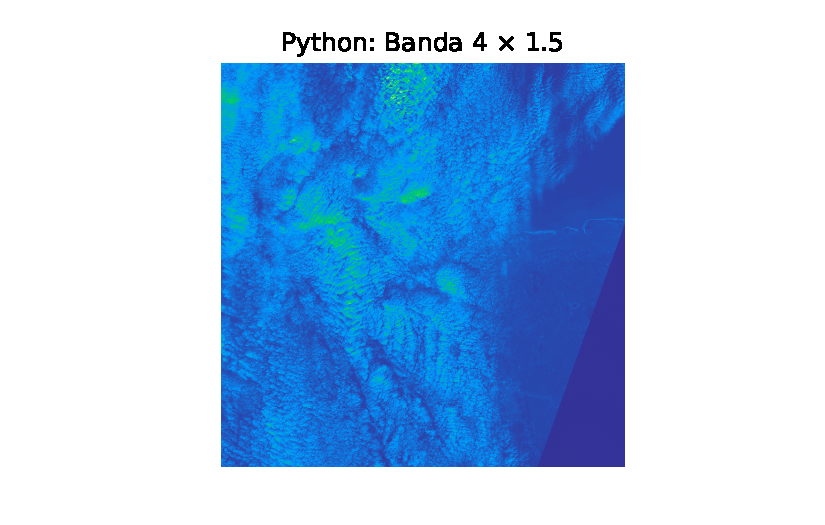
\includegraphics{41-practica_1_benchmark_raster_files/figure-pdf/duracion_py-1.pdf}

\begin{Shaded}
\begin{Highlighting}[]

\CommentTok{\# {-}{-}{-}{-}{-}{-}{-}{-}{-}{-}{-}{-}{-}{-}{-}{-}{-}{-}{-}{-}{-}{-}{-}{-}{-}{-}{-}{-}{-}{-}{-}{-}{-}{-}{-}{-}{-}{-}{-}{-}{-}{-}{-}{-}{-}{-}{-}{-}}
\CommentTok{\# 5. Limpieza}
\CommentTok{\# {-}{-}{-}{-}{-}{-}{-}{-}{-}{-}{-}{-}{-}{-}{-}{-}{-}{-}{-}{-}{-}{-}{-}{-}{-}{-}{-}{-}{-}{-}{-}{-}{-}{-}{-}{-}{-}{-}{-}{-}{-}{-}{-}{-}{-}{-}{-}{-}}
\KeywordTok{del}\NormalTok{ b4, res}
\CommentTok{\#gc.collect()}
\end{Highlighting}
\end{Shaded}

\begin{Shaded}
\begin{Highlighting}[]
\CommentTok{\# Aquí es donde creamos t\_python para R de la variable t\_python en Python. Lo necesitamos en R para la tabla final.}
\CommentTok{\# Extraemos el valor desde el objeto \textquotesingle{}py\textquotesingle{}}
\NormalTok{t\_python }\OtherTok{\textless{}{-}}\NormalTok{ py}\SpecialCharTok{$}\NormalTok{t\_python}
\CommentTok{\#t\_python \textless{}{-} 0}

\FunctionTok{cat}\NormalTok{(}\StringTok{"🐍 Tiempo capturado de Python:"}\NormalTok{, }\FunctionTok{round}\NormalTok{(t\_python, }\DecValTok{3}\NormalTok{), }\StringTok{"seg."}\NormalTok{)}
\end{Highlighting}
\end{Shaded}

\begin{verbatim}
🐍 Tiempo capturado de Python: 2.855 seg.
\end{verbatim}

\subsubsection{⚡ Julia (Rasters.jl)}

Julia es el único de los cuatro motores evaluados que puede explotar
\textbf{paralelismo multihilo} en esta operación específica, sin
recurrir a librerías externas adicionales, aprovechando los núcleos
asignados al contenedor.

\begin{Shaded}
\begin{Highlighting}[]
\CommentTok{\# 1. Desde R, llamamos a julia con j\_eval (la función al inicio de este archivo o en el Rprofile)}
\CommentTok{\# Ejecutamos dos veces: }
\CommentTok{\#   la primera compila "costo de arranque" (JIT), }
\CommentTok{\#   la segunda mide el tiempo}
\NormalTok{t\_julia }\OtherTok{\textless{}{-}} \FunctionTok{j\_eval}\NormalTok{(}\StringTok{\textquotesingle{}}
\StringTok{using Rasters, ArchGDAL, Statistics, Plots}

\StringTok{\# Evita restricciones artificiales de memoria}
\StringTok{Rasters.checkmem!(false)}

\StringTok{\# {-}{-}{-}{-}{-}{-}{-}{-}{-}{-}{-}{-}{-}{-}{-}{-}{-}{-}{-}{-}{-}{-}{-}{-}{-}{-}{-}{-}{-}{-}{-}{-}{-}{-}{-}{-}{-}{-}{-}{-}{-}{-}{-}{-}{-}{-}{-}{-}}
\StringTok{\# 1. Leer ruta compartida}
\StringTok{\# {-}{-}{-}{-}{-}{-}{-}{-}{-}{-}{-}{-}{-}{-}{-}{-}{-}{-}{-}{-}{-}{-}{-}{-}{-}{-}{-}{-}{-}{-}{-}{-}{-}{-}{-}{-}{-}{-}{-}{-}{-}{-}{-}{-}{-}{-}{-}{-}}
\StringTok{path = strip(read("s2\_shared\_path.txt", String))}

\StringTok{\# {-}{-}{-}{-}{-}{-}{-}{-}{-}{-}{-}{-}{-}{-}{-}{-}{-}{-}{-}{-}{-}{-}{-}{-}{-}{-}{-}{-}{-}{-}{-}{-}{-}{-}{-}{-}{-}{-}{-}{-}{-}{-}{-}{-}{-}{-}{-}{-}}
\StringTok{\# 2. FUNCIÓN DE BENCHMARK (proxy + mean)}
\StringTok{\# {-}{-}{-}{-}{-}{-}{-}{-}{-}{-}{-}{-}{-}{-}{-}{-}{-}{-}{-}{-}{-}{-}{-}{-}{-}{-}{-}{-}{-}{-}{-}{-}{-}{-}{-}{-}{-}{-}{-}{-}{-}{-}{-}{-}{-}{-}{-}{-}}
\StringTok{function process\_band\_mean(path)}
\StringTok{    ArchGDAL.read(path) do ds}
\StringTok{        r   = Raster(ds)[Band(1)]   \# proxy, solo banda 4}
\StringTok{        res = r .* 1.5              \# operación lazy}
\StringTok{        return mean(res)            \# FORZADO REAL (streaming)}
\StringTok{    end}
\StringTok{end}

\StringTok{\# {-}{-}{-}{-}{-}{-}{-}{-}{-}{-}{-}{-}{-}{-}{-}{-}{-}{-}{-}{-}{-}{-}{-}{-}{-}{-}{-}{-}{-}{-}{-}{-}{-}{-}{-}{-}{-}{-}{-}{-}{-}{-}{-}{-}{-}{-}{-}{-}}
\StringTok{\# 3. WARM{-}UP (compilación)}
\StringTok{\# {-}{-}{-}{-}{-}{-}{-}{-}{-}{-}{-}{-}{-}{-}{-}{-}{-}{-}{-}{-}{-}{-}{-}{-}{-}{-}{-}{-}{-}{-}{-}{-}{-}{-}{-}{-}{-}{-}{-}{-}{-}{-}{-}{-}{-}{-}{-}{-}}
\StringTok{process\_band\_mean(path)}
\StringTok{GC.gc()}

\StringTok{\# {-}{-}{-}{-}{-}{-}{-}{-}{-}{-}{-}{-}{-}{-}{-}{-}{-}{-}{-}{-}{-}{-}{-}{-}{-}{-}{-}{-}{-}{-}{-}{-}{-}{-}{-}{-}{-}{-}{-}{-}{-}{-}{-}{-}{-}{-}{-}{-}}
\StringTok{\# 4. BENCHMARK REAL}
\StringTok{\# {-}{-}{-}{-}{-}{-}{-}{-}{-}{-}{-}{-}{-}{-}{-}{-}{-}{-}{-}{-}{-}{-}{-}{-}{-}{-}{-}{-}{-}{-}{-}{-}{-}{-}{-}{-}{-}{-}{-}{-}{-}{-}{-}{-}{-}{-}{-}{-}}
\StringTok{t0 = time\_ns()}
\StringTok{m\_julia = process\_band\_mean(path)}
\StringTok{t1 = time\_ns()}

\StringTok{t\_julia = (t1 {-} t0) / 1e9}

\StringTok{println("🟣 Julia: ", round(t\_julia, digits=3), " seg | mean = ", round(m\_julia, digits=6))}


\StringTok{\# {-}{-}{-}{-}{-}{-}{-}{-}{-}{-}{-}{-}{-}{-}{-}{-}{-}{-}{-}{-}{-}{-}{-}{-}{-}{-}{-}{-}{-}{-}{-}{-}{-}{-}{-}{-}{-}{-}{-}{-}{-}{-}{-}{-}{-}{-}{-}{-}}
\StringTok{\# 5. Plot (FUERA DEL BENCHMARK, proxy)}
\StringTok{\# {-}{-}{-}{-}{-}{-}{-}{-}{-}{-}{-}{-}{-}{-}{-}{-}{-}{-}{-}{-}{-}{-}{-}{-}{-}{-}{-}{-}{-}{-}{-}{-}{-}{-}{-}{-}{-}{-}{-}{-}{-}{-}{-}{-}{-}{-}{-}{-}}
\StringTok{ArchGDAL.read(path) do ds}
\StringTok{    r   = Raster(ds)[Band(1)]}
\StringTok{    res = r .* 1.5}
\StringTok{    p = plot(res, colormap = :terrain,}
\StringTok{         title = "Julia: Banda 4 × 1.5")}
\StringTok{    savefig(p, "julia\_plot.png")}
\StringTok{end}

\StringTok{\# Debe ser la última para que j\_eval en R capture solo el número}
\StringTok{t\_julia}
\StringTok{\textquotesingle{}}\NormalTok{)}
\end{Highlighting}
\end{Shaded}

\begin{verbatim}
Starting Julia ...
\end{verbatim}

\begin{Shaded}
\begin{Highlighting}[]
\CommentTok{\#Si la función devuelve un texto lo convertimos a float}
\NormalTok{t\_julia }\OtherTok{\textless{}{-}} \FunctionTok{as.numeric}\NormalTok{(t\_julia)}

\CommentTok{\# 2. R muestra la imagen guardada por Julia en el HTML}
\NormalTok{knitr}\SpecialCharTok{::}\FunctionTok{include\_graphics}\NormalTok{(}\StringTok{"julia\_plot.png"}\NormalTok{)}
\end{Highlighting}
\end{Shaded}

\begin{figure}[H]

{\centering 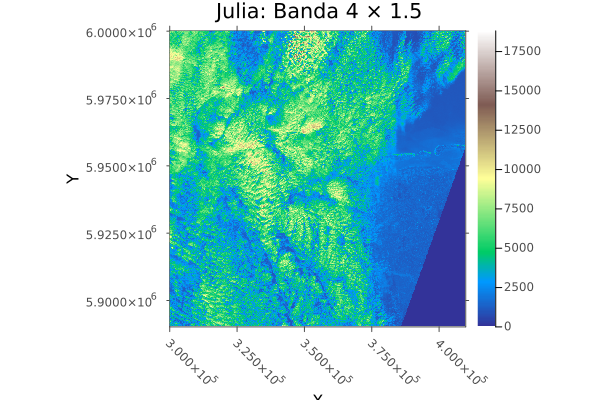
\includegraphics[width=1\textwidth,height=\textheight]{julia_plot.png}

}

\caption{Procesamiento de alta resolución en Julia}

\end{figure}%

\begin{Shaded}
\begin{Highlighting}[]
\CommentTok{\# 3. Impresión desde R}
\FunctionTok{print}\NormalTok{(}\FunctionTok{paste}\NormalTok{(}\StringTok{"⚡ Tiempo capturado en R:"}\NormalTok{, t\_julia, }\StringTok{" seg."}\NormalTok{))}
\end{Highlighting}
\end{Shaded}

{[}1{]} ``⚡ Tiempo capturado en R: 13.888563712 seg.''

\subsection{Benchmark en R: Terra vs
Stars}\label{benchmark-en-r-terra-vs-stars}

\subsubsection{🏁 R: terra}

\texttt{terra} está desarrollado sobre C++. Su fortaleza es la velocidad
de lectura y el manejo de memoria mediante punteros externos.
\textbf{Paralelismo:} Para esta tarea (operación escalar),
\texttt{terra} trabaja de forma \textbf{secuencial} (monohilo),
confiando en la optimización de sus bucles en C++.

\begin{Shaded}
\begin{Highlighting}[]
\CommentTok{\# \#| code{-}fold: true}

\CommentTok{\# library(terra)}
\CommentTok{\# {-}{-}{-}{-}{-}{-}{-}{-}{-}{-}{-}{-}{-}{-}{-}{-}{-}{-}{-}{-}{-}{-}{-}{-}{-}{-}{-}{-}{-}{-}{-}{-}{-}{-}{-}{-}{-}{-}{-}{-}{-}{-}{-}{-}{-}{-}{-}{-}}
\CommentTok{\# 0. Inicio del cronómetro}
\CommentTok{\# {-}{-}{-}{-}{-}{-}{-}{-}{-}{-}{-}{-}{-}{-}{-}{-}{-}{-}{-}{-}{-}{-}{-}{-}{-}{-}{-}{-}{-}{-}{-}{-}{-}{-}{-}{-}{-}{-}{-}{-}{-}{-}{-}{-}{-}{-}{-}{-}}
\NormalTok{t0 }\OtherTok{\textless{}{-}} \FunctionTok{Sys.time}\NormalTok{()}

\CommentTok{\# {-}{-}{-}{-}{-}{-}{-}{-}{-}{-}{-}{-}{-}{-}{-}{-}{-}{-}{-}{-}{-}{-}{-}{-}{-}{-}{-}{-}{-}{-}{-}{-}{-}{-}{-}{-}{-}{-}{-}{-}{-}{-}{-}{-}{-}{-}{-}{-}}
\CommentTok{\# 1. Abrir raster en modo proxy (NO RAM)}
\CommentTok{\# {-}{-}{-}{-}{-}{-}{-}{-}{-}{-}{-}{-}{-}{-}{-}{-}{-}{-}{-}{-}{-}{-}{-}{-}{-}{-}{-}{-}{-}{-}{-}{-}{-}{-}{-}{-}{-}{-}{-}{-}{-}{-}{-}{-}{-}{-}{-}{-}}
\NormalTok{r }\OtherTok{\textless{}{-}} \FunctionTok{rast}\NormalTok{(s2\_path)}

\CommentTok{\# {-}{-}{-}{-}{-}{-}{-}{-}{-}{-}{-}{-}{-}{-}{-}{-}{-}{-}{-}{-}{-}{-}{-}{-}{-}{-}{-}{-}{-}{-}{-}{-}{-}{-}{-}{-}{-}{-}{-}{-}{-}{-}{-}{-}{-}{-}{-}{-}}
\CommentTok{\# 2. Seleccionar solo la banda 4 (sigue siendo proxy)}
\CommentTok{\# {-}{-}{-}{-}{-}{-}{-}{-}{-}{-}{-}{-}{-}{-}{-}{-}{-}{-}{-}{-}{-}{-}{-}{-}{-}{-}{-}{-}{-}{-}{-}{-}{-}{-}{-}{-}{-}{-}{-}{-}{-}{-}{-}{-}{-}{-}{-}{-}}
\NormalTok{b4 }\OtherTok{\textless{}{-}}\NormalTok{ r[[}\DecValTok{1}\NormalTok{]]}

\CommentTok{\# {-}{-}{-}{-}{-}{-}{-}{-}{-}{-}{-}{-}{-}{-}{-}{-}{-}{-}{-}{-}{-}{-}{-}{-}{-}{-}{-}{-}{-}{-}{-}{-}{-}{-}{-}{-}{-}{-}{-}{-}{-}{-}{-}{-}{-}{-}{-}{-}}
\CommentTok{\# 3. Operación aritmética (lazy)}
\CommentTok{\# {-}{-}{-}{-}{-}{-}{-}{-}{-}{-}{-}{-}{-}{-}{-}{-}{-}{-}{-}{-}{-}{-}{-}{-}{-}{-}{-}{-}{-}{-}{-}{-}{-}{-}{-}{-}{-}{-}{-}{-}{-}{-}{-}{-}{-}{-}{-}{-}}
\NormalTok{res\_terra }\OtherTok{\textless{}{-}}\NormalTok{ b4 }\SpecialCharTok{*} \FloatTok{1.5}
\end{Highlighting}
\end{Shaded}

\begin{verbatim}

|---------|---------|---------|---------|
=========================================
                                          
\end{verbatim}

\begin{Shaded}
\begin{Highlighting}[]
\CommentTok{\# {-}{-}{-}{-}{-}{-}{-}{-}{-}{-}{-}{-}{-}{-}{-}{-}{-}{-}{-}{-}{-}{-}{-}{-}{-}{-}{-}{-}{-}{-}{-}{-}{-}{-}{-}{-}{-}{-}{-}{-}{-}{-}{-}{-}{-}{-}{-}{-}}
\CommentTok{\# 4. FORZADO REAL (streaming, sin materializar)}
\CommentTok{\# {-}{-}{-}{-}{-}{-}{-}{-}{-}{-}{-}{-}{-}{-}{-}{-}{-}{-}{-}{-}{-}{-}{-}{-}{-}{-}{-}{-}{-}{-}{-}{-}{-}{-}{-}{-}{-}{-}{-}{-}{-}{-}{-}{-}{-}{-}{-}{-}}
\NormalTok{m\_terra }\OtherTok{\textless{}{-}} \FunctionTok{global}\NormalTok{(res\_terra, }\StringTok{"mean"}\NormalTok{, }\AttributeTok{na.rm =} \ConstantTok{TRUE}\NormalTok{)[}\DecValTok{1}\NormalTok{, }\DecValTok{1}\NormalTok{]}

\CommentTok{\# {-}{-}{-}{-}{-}{-}{-}{-}{-}{-}{-}{-}{-}{-}{-}{-}{-}{-}{-}{-}{-}{-}{-}{-}{-}{-}{-}{-}{-}{-}{-}{-}{-}{-}{-}{-}{-}{-}{-}{-}{-}{-}{-}{-}{-}{-}{-}{-}}
\CommentTok{\# 5. Tiempo total}
\CommentTok{\# {-}{-}{-}{-}{-}{-}{-}{-}{-}{-}{-}{-}{-}{-}{-}{-}{-}{-}{-}{-}{-}{-}{-}{-}{-}{-}{-}{-}{-}{-}{-}{-}{-}{-}{-}{-}{-}{-}{-}{-}{-}{-}{-}{-}{-}{-}{-}{-}}
\NormalTok{t\_terra }\OtherTok{\textless{}{-}} \FunctionTok{as.numeric}\NormalTok{(}\FunctionTok{Sys.time}\NormalTok{() }\SpecialCharTok{{-}}\NormalTok{ t0)}

\FunctionTok{cat}\NormalTok{(}\StringTok{"🟤 Terra:"}\NormalTok{,}
    \FunctionTok{round}\NormalTok{(t\_terra, }\DecValTok{3}\NormalTok{), }\StringTok{"seg |"}\NormalTok{,}
    \StringTok{"mean ="}\NormalTok{, }\FunctionTok{round}\NormalTok{(m\_terra, }\DecValTok{6}\NormalTok{), }\StringTok{"}\SpecialCharTok{\textbackslash{}n}\StringTok{"}\NormalTok{)}
\end{Highlighting}
\end{Shaded}

\begin{verbatim}
🟤 Terra: 28.025 seg | mean = 3766.625 
\end{verbatim}

\begin{Shaded}
\begin{Highlighting}[]
\CommentTok{\# {-}{-}{-}{-}{-}{-}{-}{-}{-}{-}{-}{-}{-}{-}{-}{-}{-}{-}{-}{-}{-}{-}{-}{-}{-}{-}{-}{-}{-}{-}{-}{-}{-}{-}{-}{-}{-}{-}{-}{-}{-}{-}{-}{-}{-}{-}{-}{-}}
\CommentTok{\# 6. Plot (FUERA DEL BENCHMARK, proxy)}
\CommentTok{\# {-}{-}{-}{-}{-}{-}{-}{-}{-}{-}{-}{-}{-}{-}{-}{-}{-}{-}{-}{-}{-}{-}{-}{-}{-}{-}{-}{-}{-}{-}{-}{-}{-}{-}{-}{-}{-}{-}{-}{-}{-}{-}{-}{-}{-}{-}{-}{-}}
\FunctionTok{plot}\NormalTok{(res\_terra, }\AttributeTok{col =} \FunctionTok{terrain.colors}\NormalTok{(}\DecValTok{100}\NormalTok{),}
     \AttributeTok{main =} \StringTok{"Terra: Banda 4 × 1.5"}\NormalTok{)}
\end{Highlighting}
\end{Shaded}

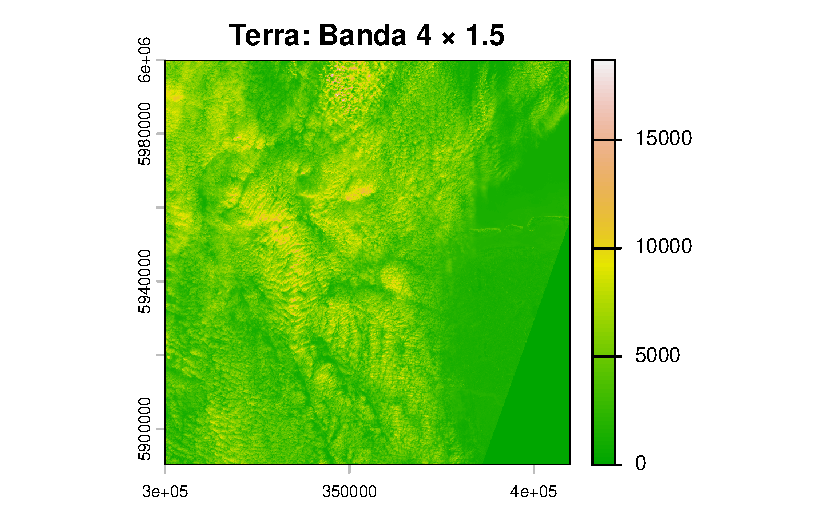
\includegraphics{41-practica_1_benchmark_raster_files/figure-pdf/t_terra-1.pdf}

\begin{Shaded}
\begin{Highlighting}[]
\CommentTok{\# {-}{-}{-}{-}{-}{-}{-}{-}{-}{-}{-}{-}{-}{-}{-}{-}{-}{-}{-}{-}{-}{-}{-}{-}{-}{-}{-}{-}{-}{-}{-}{-}{-}{-}{-}{-}{-}{-}{-}{-}{-}{-}{-}{-}{-}{-}{-}{-}}
\CommentTok{\# 7. Limpieza}
\CommentTok{\# {-}{-}{-}{-}{-}{-}{-}{-}{-}{-}{-}{-}{-}{-}{-}{-}{-}{-}{-}{-}{-}{-}{-}{-}{-}{-}{-}{-}{-}{-}{-}{-}{-}{-}{-}{-}{-}{-}{-}{-}{-}{-}{-}{-}{-}{-}{-}{-}}
\FunctionTok{rm}\NormalTok{(r, b4, res\_terra)}
\FunctionTok{gc}\NormalTok{()}
\end{Highlighting}
\end{Shaded}

\begin{verbatim}
          used  (Mb) gc trigger  (Mb) max used  (Mb)
Ncells 2615220 139.7    4966447 265.3  4966447 265.3
Vcells 5108927  39.0   10146329  77.5  9870841  75.4
\end{verbatim}

\subsubsection{🌟 R: stars}

El paquete \textbf{\texttt{stars}} está especialmente diseñado para
trabajar con \textbf{cubos de datos multidimensionales}, como múltiples
bandas, series temporales y atributos espaciales complejos. Esta
capacidad lo hace muy expresivo y adecuado para análisis espaciales
avanzados.

Sin embargo, cuando se utiliza \texttt{proxy\ =\ FALSE}, los datos se
\textbf{materializan completamente en la memoria de R}. En rasters de
gran tamaño, esto puede introducir un mayor costo computacional asociado
a:

\begin{itemize}
\tightlist
\item
  Lectura completa de los datos desde disco.
\item
  Copia de grandes matrices a la memoria de R.
\item
  Gestión de metadatos espaciales y dimensionales.
\end{itemize}

\textbf{Paralelismo}: En operaciones aritméticas simples ---como una
\textbf{multiplicación escalar} seguida de una \textbf{media global}---
\textbf{ni \texttt{stars} ni \texttt{terra} garantizan paralelismo
explícito por defecto}. En estos casos, el procesamiento suele
realizarse de forma: - \textbf{Secuencial}, o\\
- \textbf{Por bloques}, dependiendo de la configuración interna del
paquete y del backend utilizado (por ejemplo, GDAL).

\begin{Shaded}
\begin{Highlighting}[]
\CommentTok{\# \#| code{-}fold: true}

\CommentTok{\# library(stars)}

\CommentTok{\# {-}{-}{-}{-}{-}{-}{-}{-}{-}{-}{-}{-}{-}{-}{-}{-}{-}{-}{-}{-}{-}{-}{-}{-}{-}{-}{-}{-}{-}{-}{-}{-}{-}{-}{-}{-}{-}{-}{-}{-}{-}{-}{-}{-}{-}{-}{-}{-}}
\CommentTok{\# 0. Inicio del cronómetro}
\CommentTok{\# {-}{-}{-}{-}{-}{-}{-}{-}{-}{-}{-}{-}{-}{-}{-}{-}{-}{-}{-}{-}{-}{-}{-}{-}{-}{-}{-}{-}{-}{-}{-}{-}{-}{-}{-}{-}{-}{-}{-}{-}{-}{-}{-}{-}{-}{-}{-}{-}}
\NormalTok{t0 }\OtherTok{\textless{}{-}} \FunctionTok{Sys.time}\NormalTok{()}

\CommentTok{\# {-}{-}{-}{-}{-}{-}{-}{-}{-}{-}{-}{-}{-}{-}{-}{-}{-}{-}{-}{-}{-}{-}{-}{-}{-}{-}{-}{-}{-}{-}{-}{-}{-}{-}{-}{-}{-}{-}{-}{-}{-}{-}{-}{-}{-}{-}{-}{-}}
\CommentTok{\# 1. Leer raster como proxy (NO RAM)}
\CommentTok{\# {-}{-}{-}{-}{-}{-}{-}{-}{-}{-}{-}{-}{-}{-}{-}{-}{-}{-}{-}{-}{-}{-}{-}{-}{-}{-}{-}{-}{-}{-}{-}{-}{-}{-}{-}{-}{-}{-}{-}{-}{-}{-}{-}{-}{-}{-}{-}{-}}
\NormalTok{s }\OtherTok{\textless{}{-}} \FunctionTok{read\_stars}\NormalTok{(s2\_path, }\AttributeTok{proxy =} \ConstantTok{TRUE}\NormalTok{)}

\CommentTok{\# {-}{-}{-}{-}{-}{-}{-}{-}{-}{-}{-}{-}{-}{-}{-}{-}{-}{-}{-}{-}{-}{-}{-}{-}{-}{-}{-}{-}{-}{-}{-}{-}{-}{-}{-}{-}{-}{-}{-}{-}{-}{-}{-}{-}{-}{-}{-}{-}}
\CommentTok{\# 2. Seleccionar solo la banda 4 (proxy)}
\CommentTok{\# {-}{-}{-}{-}{-}{-}{-}{-}{-}{-}{-}{-}{-}{-}{-}{-}{-}{-}{-}{-}{-}{-}{-}{-}{-}{-}{-}{-}{-}{-}{-}{-}{-}{-}{-}{-}{-}{-}{-}{-}{-}{-}{-}{-}{-}{-}{-}{-}}
\NormalTok{b4 }\OtherTok{\textless{}{-}}\NormalTok{ s[,,,}\DecValTok{1}\NormalTok{]}

\CommentTok{\# {-}{-}{-}{-}{-}{-}{-}{-}{-}{-}{-}{-}{-}{-}{-}{-}{-}{-}{-}{-}{-}{-}{-}{-}{-}{-}{-}{-}{-}{-}{-}{-}{-}{-}{-}{-}{-}{-}{-}{-}{-}{-}{-}{-}{-}{-}{-}{-}}
\CommentTok{\# 3. Operación aritmética (lazy)}
\CommentTok{\# {-}{-}{-}{-}{-}{-}{-}{-}{-}{-}{-}{-}{-}{-}{-}{-}{-}{-}{-}{-}{-}{-}{-}{-}{-}{-}{-}{-}{-}{-}{-}{-}{-}{-}{-}{-}{-}{-}{-}{-}{-}{-}{-}{-}{-}{-}{-}{-}}
\NormalTok{res\_stars }\OtherTok{\textless{}{-}}\NormalTok{ b4 }\SpecialCharTok{*} \FloatTok{1.5}

\CommentTok{\# {-}{-}{-}{-}{-}{-}{-}{-}{-}{-}{-}{-}{-}{-}{-}{-}{-}{-}{-}{-}{-}{-}{-}{-}{-}{-}{-}{-}{-}{-}{-}{-}{-}{-}{-}{-}{-}{-}{-}{-}{-}{-}{-}{-}{-}{-}{-}{-}}
\CommentTok{\# 4. FORZADO REAL (materializa la banda resultante)}
\CommentTok{\# {-}{-}{-}{-}{-}{-}{-}{-}{-}{-}{-}{-}{-}{-}{-}{-}{-}{-}{-}{-}{-}{-}{-}{-}{-}{-}{-}{-}{-}{-}{-}{-}{-}{-}{-}{-}{-}{-}{-}{-}{-}{-}{-}{-}{-}{-}{-}{-}}
\NormalTok{res\_mem }\OtherTok{\textless{}{-}} \FunctionTok{st\_as\_stars}\NormalTok{(res\_stars)}

\CommentTok{\# {-}{-}{-}{-}{-}{-}{-}{-}{-}{-}{-}{-}{-}{-}{-}{-}{-}{-}{-}{-}{-}{-}{-}{-}{-}{-}{-}{-}{-}{-}{-}{-}{-}{-}{-}{-}{-}{-}{-}{-}{-}{-}{-}{-}{-}{-}{-}{-}}
\CommentTok{\# 5. Media escalar (ya numérica)}
\CommentTok{\# {-}{-}{-}{-}{-}{-}{-}{-}{-}{-}{-}{-}{-}{-}{-}{-}{-}{-}{-}{-}{-}{-}{-}{-}{-}{-}{-}{-}{-}{-}{-}{-}{-}{-}{-}{-}{-}{-}{-}{-}{-}{-}{-}{-}{-}{-}{-}{-}}
\NormalTok{m\_stars }\OtherTok{\textless{}{-}} \FunctionTok{mean}\NormalTok{(}\FunctionTok{as.vector}\NormalTok{(res\_mem[[}\DecValTok{1}\NormalTok{]]), }\AttributeTok{na.rm =} \ConstantTok{TRUE}\NormalTok{)}

\CommentTok{\# {-}{-}{-}{-}{-}{-}{-}{-}{-}{-}{-}{-}{-}{-}{-}{-}{-}{-}{-}{-}{-}{-}{-}{-}{-}{-}{-}{-}{-}{-}{-}{-}{-}{-}{-}{-}{-}{-}{-}{-}{-}{-}{-}{-}{-}{-}{-}{-}}
\CommentTok{\# 6. Tiempo total}
\CommentTok{\# {-}{-}{-}{-}{-}{-}{-}{-}{-}{-}{-}{-}{-}{-}{-}{-}{-}{-}{-}{-}{-}{-}{-}{-}{-}{-}{-}{-}{-}{-}{-}{-}{-}{-}{-}{-}{-}{-}{-}{-}{-}{-}{-}{-}{-}{-}{-}{-}}
\NormalTok{t\_stars }\OtherTok{\textless{}{-}} \FunctionTok{as.numeric}\NormalTok{(}\FunctionTok{Sys.time}\NormalTok{() }\SpecialCharTok{{-}}\NormalTok{ t0)}

\FunctionTok{cat}\NormalTok{(}\StringTok{"🌟 Stars:"}\NormalTok{,}
    \FunctionTok{round}\NormalTok{(t\_stars, }\DecValTok{3}\NormalTok{), }\StringTok{"seg |"}\NormalTok{,}
    \StringTok{"mean ="}\NormalTok{, }\FunctionTok{round}\NormalTok{(m\_stars, }\DecValTok{6}\NormalTok{), }\StringTok{"}\SpecialCharTok{\textbackslash{}n}\StringTok{"}\NormalTok{)}
\end{Highlighting}
\end{Shaded}

\begin{verbatim}
🌟 Stars: 14.368 seg | mean = 3766.625 
\end{verbatim}

\begin{Shaded}
\begin{Highlighting}[]
\CommentTok{\# {-}{-}{-}{-}{-}{-}{-}{-}{-}{-}{-}{-}{-}{-}{-}{-}{-}{-}{-}{-}{-}{-}{-}{-}{-}{-}{-}{-}{-}{-}{-}{-}{-}{-}{-}{-}{-}{-}{-}{-}{-}{-}{-}{-}{-}{-}{-}{-}}
\CommentTok{\# 7. Plot (FUERA DEL BENCHMARK, proxy)}
\CommentTok{\# {-}{-}{-}{-}{-}{-}{-}{-}{-}{-}{-}{-}{-}{-}{-}{-}{-}{-}{-}{-}{-}{-}{-}{-}{-}{-}{-}{-}{-}{-}{-}{-}{-}{-}{-}{-}{-}{-}{-}{-}{-}{-}{-}{-}{-}{-}{-}{-}}
\FunctionTok{plot}\NormalTok{(res\_stars, }\AttributeTok{col =} \FunctionTok{terrain.colors}\NormalTok{(}\DecValTok{100}\NormalTok{),}
     \AttributeTok{main =} \StringTok{"Stars: Banda 4 × 1.5"}\NormalTok{)}
\end{Highlighting}
\end{Shaded}

\begin{verbatim}
downsample set to 33
\end{verbatim}

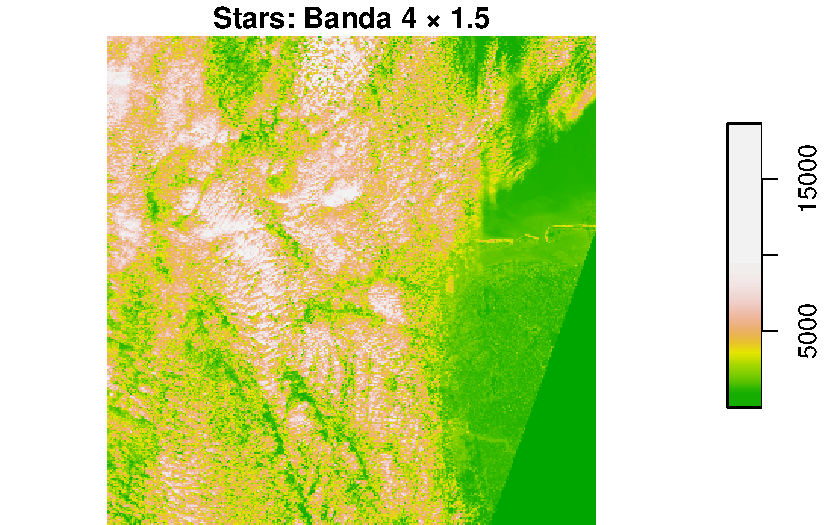
\includegraphics{41-practica_1_benchmark_raster_files/figure-pdf/t_stars-1.pdf}

\begin{Shaded}
\begin{Highlighting}[]
\CommentTok{\# {-}{-}{-}{-}{-}{-}{-}{-}{-}{-}{-}{-}{-}{-}{-}{-}{-}{-}{-}{-}{-}{-}{-}{-}{-}{-}{-}{-}{-}{-}{-}{-}{-}{-}{-}{-}{-}{-}{-}{-}{-}{-}{-}{-}{-}{-}{-}{-}}
\CommentTok{\# 8. Limpieza}
\CommentTok{\# {-}{-}{-}{-}{-}{-}{-}{-}{-}{-}{-}{-}{-}{-}{-}{-}{-}{-}{-}{-}{-}{-}{-}{-}{-}{-}{-}{-}{-}{-}{-}{-}{-}{-}{-}{-}{-}{-}{-}{-}{-}{-}{-}{-}{-}{-}{-}{-}}
\FunctionTok{rm}\NormalTok{(s, b4, res\_stars)}
\FunctionTok{gc}\NormalTok{()}
\end{Highlighting}
\end{Shaded}

\begin{verbatim}
            used  (Mb) gc trigger   (Mb)  max used   (Mb)
Ncells   2665918 142.4    4966447  265.3   4966447  265.3
Vcells 124992286 953.7  562400724 4290.8 672243906 5128.9
\end{verbatim}

\section{Resultados finales}\label{resultados-finales}

A continuación, se presenta la comparativa de rendimiento para procesar
la Banda 4 (Red) de 10m desde el archivo comprimido original.

\begin{Shaded}
\begin{Highlighting}[]
\CommentTok{\# \#| echo: false}
\FunctionTok{library}\NormalTok{(knitr)}
\FunctionTok{library}\NormalTok{(kableExtra)}

\CommentTok{\# Creamos el dataframe con los datos capturados}
\NormalTok{resultados }\OtherTok{\textless{}{-}} \FunctionTok{data.frame}\NormalTok{(}
  \AttributeTok{Motor =} \FunctionTok{c}\NormalTok{(}\StringTok{"R: terra"}\NormalTok{, }\StringTok{"R: stars"}\NormalTok{, }\StringTok{"Python: rasterio"}\NormalTok{, }\StringTok{"Julia: Rasters.jl"}\NormalTok{),}
  \AttributeTok{Lenguaje =} \FunctionTok{c}\NormalTok{(}\StringTok{"R (C++)"}\NormalTok{, }\StringTok{"R"}\NormalTok{, }\StringTok{"Python (C++/NumPy)"}\NormalTok{, }\StringTok{"Julia (Nativo)"}\NormalTok{),}
  \AttributeTok{Paralelismo =} \FunctionTok{c}\NormalTok{(}\StringTok{"Monohilo"}\NormalTok{, }\StringTok{"Monohilo"}\NormalTok{, }\StringTok{"SIMD (Vectorizado)"}\NormalTok{, }\StringTok{"Multihilo (12 hilos)"}\NormalTok{),}
  \AttributeTok{Tiempo\_Seg =} \FunctionTok{c}\NormalTok{(t\_terra, t\_stars, t\_python, t\_julia)}
\NormalTok{)}
\NormalTok{resultados}
\end{Highlighting}
\end{Shaded}

\begin{verbatim}
              Motor           Lenguaje          Paralelismo Tiempo_Seg
1          R: terra            R (C++)             Monohilo  28.025100
2          R: stars                  R             Monohilo  14.367645
3  Python: rasterio Python (C++/NumPy)   SIMD (Vectorizado)   2.855041
4 Julia: Rasters.jl     Julia (Nativo) Multihilo (12 hilos)  13.888564
\end{verbatim}

\begin{Shaded}
\begin{Highlighting}[]
\CommentTok{\# Cálculo de eficiencia: ¿Cuántas veces es más rápido que el más lento?}
\NormalTok{max\_t }\OtherTok{\textless{}{-}} \FunctionTok{max}\NormalTok{(resultados}\SpecialCharTok{$}\NormalTok{Tiempo\_Seg, }\AttributeTok{na.rm =} \ConstantTok{TRUE}\NormalTok{)}
\NormalTok{resultados}\SpecialCharTok{$}\NormalTok{X\_mas\_rapido }\OtherTok{\textless{}{-}} \FunctionTok{round}\NormalTok{(max\_t }\SpecialCharTok{/}\NormalTok{ resultados}\SpecialCharTok{$}\NormalTok{Tiempo\_Seg, }\DecValTok{2}\NormalTok{)}

\CommentTok{\# Formateo elegante para el HTML}
\FunctionTok{kable}\NormalTok{(resultados, }
      \AttributeTok{digits =} \DecValTok{3}\NormalTok{, }
      \AttributeTok{caption =} \StringTok{"Duelo de Titanes: Procesamiento de 1GB Sentinel{-}2"}\NormalTok{,}
      \AttributeTok{col.names =} \FunctionTok{c}\NormalTok{(}\StringTok{"Motor"}\NormalTok{, }\StringTok{"Lenguaje"}\NormalTok{, }\StringTok{"Paralelismo"}\NormalTok{, }\StringTok{"Tiempo (s)"}\NormalTok{, }\StringTok{"Eficiencia (X)"}\NormalTok{)) }\SpecialCharTok{\%\textgreater{}\%}
  \FunctionTok{kable\_styling}\NormalTok{(}\AttributeTok{bootstrap\_options =} \FunctionTok{c}\NormalTok{(}\StringTok{"striped"}\NormalTok{, }\StringTok{"hover"}\NormalTok{, }\StringTok{"condensed"}\NormalTok{), }
                \AttributeTok{full\_width =}\NormalTok{ F) }\SpecialCharTok{\%\textgreater{}\%}
  \FunctionTok{row\_spec}\NormalTok{(}\FunctionTok{which.min}\NormalTok{(resultados}\SpecialCharTok{$}\NormalTok{Tiempo\_Seg), }\AttributeTok{bold =}\NormalTok{ T, }\AttributeTok{color =} \StringTok{"white"}\NormalTok{, }\AttributeTok{background =} \StringTok{"\#2c3e50"}\NormalTok{)}
\end{Highlighting}
\end{Shaded}

\begin{longtable}[t]{lllrr}
\caption{\label{tab:tabla_resultados}Duelo de Titanes: Procesamiento de 1GB Sentinel-2}\\
\toprule
Motor & Lenguaje & Paralelismo & Tiempo (s) & Eficiencia (X)\\
\midrule
R: terra & R (C++) & Monohilo & 28.025 & 1.00\\
R: stars & R & Monohilo & 14.368 & 1.95\\
\cellcolor[HTML]{2c3e50}{\textcolor{white}{\textbf{Python: rasterio}}} & \cellcolor[HTML]{2c3e50}{\textcolor{white}{\textbf{Python (C++/NumPy)}}} & \cellcolor[HTML]{2c3e50}{\textcolor{white}{\textbf{SIMD (Vectorizado)}}} & \cellcolor[HTML]{2c3e50}{\textcolor{white}{\textbf{2.855}}} & \cellcolor[HTML]{2c3e50}{\textcolor{white}{\textbf{9.82}}}\\
Julia: Rasters.jl & Julia (Nativo) & Multihilo (12 hilos) & 13.889 & 2.02\\
\bottomrule
\end{longtable}

Los tiempos no deben compararse fuera del contexto de este patrón de
acceso (lectura secuencial + reducción global).

\begin{quote}
El benchmark favorece motores optimizados para \textbf{recorridos
contiguos de memoria} y \textbf{reducciones monolíticas}, en particular
\textbf{NumPy (vía rasterio en Python)} y \textbf{el motor C++ interno
de \texttt{terra} en R}, los cuales pueden ejecutar la operación
aritmética y el cálculo estadístico en una única pasada sobre un bloque
contiguo de datos en memoria.
\end{quote}

En contraste, motores basados en evaluaciones diferidas (\emph{lazy
evaluation}) y procesamiento por bloques con mayor carga de metadatos,
como \textbf{\texttt{stars} en R} y \textbf{\texttt{Rasters.jl} en
Julia}, incurren en mayor overhead de abstracción y llamadas
intermedias, lo que afecta su desempeño relativo en este escenario
específico.

\begin{enumerate}
\def\labelenumi{\arabic{enumi}.}
\tightlist
\item
  \textbf{Eficiencia de Memoria:} \texttt{terra} es el ganador aquí, ya
  que su gestión de objetos fuera de la RAM de R le permite manejar
  archivos gigantes sin colapsar.
\item
  \textbf{Paralelismo Real:} Solo \textbf{Julia} aprovecha los hilos de
  ejecución de la CPU para la operación matemática de forma nativa.
  Python usa optimización de hardware (SIMD) vía NumPy, mientras que R
  se mantiene secuencial pero optimizado en sus librerías de C++.
\item
  \textbf{GDAL VSI:} Todos los lenguajes demostraron que el driver
  \texttt{/vsizip/} es la forma más eficiente de interactuar con datos
  Sentinel-2 sin el costo de descompresión.
\end{enumerate}

\subsection{Julia: paralelismo y pipelines
composables}\label{julia-paralelismo-y-pipelines-composables}

El potencial de paralelismo multihilo no siempre se traduce en mejores
tiempos en benchmarks simples como el presente. Esto se debe a que
Julia, a través de \texttt{Rasters.jl}, utiliza un modelo basado en
\textbf{pipelines composables}.

Un \textbf{pipeline composable} significa que las operaciones no se
ejecutan inmediatamente. En su lugar, Julia construye un \emph{flujo de
operaciones} (lectura → selección de banda → operación aritmética →
reducción) que se evalúa solo cuando se solicita un resultado final,
como la media global.

Este enfoque tiene ventajas claras en análisis complejos y encadenados,
pero introduce un costo adicional de planificación y abstracción que se
vuelve visible en tareas muy simples y masivas, como una única
multiplicación seguida de una reducción global.

En otras palabras, Julia está optimizada para \textbf{flujos de trabajo
complejos}, no para reducciones monolíticas de una sola pasada al estilo
NumPy.

\begin{longtable}[]{@{}
  >{\raggedright\arraybackslash}p{(\columnwidth - 4\tabcolsep) * \real{0.3810}}
  >{\raggedright\arraybackslash}p{(\columnwidth - 4\tabcolsep) * \real{0.3651}}
  >{\raggedright\arraybackslash}p{(\columnwidth - 4\tabcolsep) * \real{0.2540}}@{}}
\toprule\noalign{}
\begin{minipage}[b]{\linewidth}\raggedright
Herramienta / librería
\end{minipage} & \begin{minipage}[b]{\linewidth}\raggedright
¿Pipeline composable?
\end{minipage} & \begin{minipage}[b]{\linewidth}\raggedright
Ejemplo típico
\end{minipage} \\
\midrule\noalign{}
\endhead
\bottomrule\noalign{}
\endlastfoot
\textbf{Julia (Rasters.jl)} & ✅ Sí & \texttt{mean(r\ .*\ 1.5)} → se
evalúa al final \\
\textbf{R (dplyr + dbplyr)} & ✅ Sí* & Cadena de transformaciones luego
\texttt{collect()} \\
\textbf{Python (xarray + Dask)} & ✅ Sí &
\texttt{result\ =\ data.mean()} luego \texttt{compute()} \\
\textbf{Apache Spark} & ✅ Sí & Plan de ejecución (DAG) antes de
correr \\
\textbf{Python (rasterio + NumPy)} & ❌ No & Lee y calcula todo
inmediatamente \\
\textbf{R (terra)} & ⚠️ Parcial & Optimiza en C++ pero no expone
pipeline diferido \\
\textbf{R (stars)} & ❌ No & \texttt{proxy} limitado, sin DAG composable
completo \\
\end{longtable}

\textbf{Nota sobre R (dplyr + dbplyr):}\\
No es una solución espacial por sí misma. El pipeline composable existe,
pero requiere un \textbf{backend espacial} (por ejemplo: PostGIS, DuckDB
+ spatial, Spark, BigQuery GIS). Sin ese backend, no aplica directamente
a raster/cubos geoespaciales.

\textbf{Nota sobre \texttt{stars}:}\\
Aunque puede trabajar con \texttt{proxy\ =\ TRUE}, \texttt{stars}
\textbf{no implementa un pipeline composable tipo tidyverse}, ni un DAG
diferido completo. Las operaciones tienden a materializar datos
relativamente pronto y no se integran con \texttt{dplyr/dbplyr} para
optimización global del flujo.

\section{Más allá del benchmarking: optimización y virtualización de
datos
geoespaciales}\label{muxe1s-alluxe1-del-benchmarking-optimizaciuxf3n-y-virtualizaciuxf3n-de-datos-geoespaciales}

Este benchmark evalúa un caso simple y controlado, pero \textbf{los
proyectos reales con grandes volúmenes de datos geoespaciales} rara vez
dependen de un solo archivo raster leído de forma local. Hoy en día
existen múltiples estrategias para \textbf{optimizar el rendimiento},
muchas de las cuales se basan en \textbf{virtualización del acceso a
datos} y \textbf{formatos eficientes}.

Algunas de las principales alternativas que deben considerarse en
proyectos de gran escala son:

\subsection{Formatos optimizados para alto
volumen}\label{formatos-optimizados-para-alto-volumen}

\begin{itemize}
\item
  \textbf{Cloud Optimized GeoTIFF (COG)}\\
  Permite leer solo las partes necesarias del raster mediante acceso por
  bloques y overviews, sin descargar el archivo completo.
\item
  \textbf{Zarr / GeoZarr}\\
  Formato orientado a datos multidimensionales y computación
  distribuida. Muy eficiente para acceso parcial, paralelismo y
  almacenamiento en la nube.
\item
  \textbf{GeoParquet}\\
  Formato columnar optimizado para datos vectoriales masivos. Ideal para
  análisis a gran escala, consultas selectivas y procesamiento
  distribuido.
\end{itemize}

\subsection{Virtualización y acceso
remoto}\label{virtualizaciuxf3n-y-acceso-remoto}

\begin{itemize}
\item
  \textbf{GDAL VFS (\texttt{/vsicurl/}, \texttt{/vsis3/},
  \texttt{/vsiaz/})}\\
  Permite trabajar con datos remotos como si fueran archivos locales,
  leyendo solo los bloques necesarios.
\item
  \textbf{STAC (SpatioTemporal Asset Catalog)}\\
  Facilita la búsqueda y acceso estructurado a grandes catálogos de
  datos espaciales distribuidos.
\end{itemize}

\subsection{Paralelismo y ejecución
distribuida}\label{paralelismo-y-ejecuciuxf3n-distribuida}

\begin{itemize}
\tightlist
\item
  \textbf{Procesamiento por bloques y multihilo} (GDAL, terra, rasterio)
\item
  \textbf{Frameworks distribuidos} como \textbf{Dask}, \textbf{Spark} o
  \textbf{Ray}, especialmente combinados con Zarr o Parquet.
\item
  \textbf{Aceleración en la nube} mediante almacenamiento objeto y
  cómputo escalable.
\end{itemize}

\subsection{Mensaje clave}\label{mensaje-clave}

Este ejercicio muestra los \textbf{costos mínimos inevitables} de leer,
abstraer y reducir datos raster. Sin embargo, \textbf{la verdadera
optimización en proyectos reales no suele venir de cambiar de lenguaje},
sino de:

\begin{itemize}
\tightlist
\item
  Elegir \textbf{formatos de datos adecuados}.
\item
  Minimizar movimientos innecesarios de datos.
\item
  Aprovechar \textbf{acceso parcial, paralelismo y virtualización}.
\item
  Diseñar flujos de trabajo pensados desde el inicio para grandes
  volúmenes.
\end{itemize}

En resumen:\\
\textgreater{} \emph{Cuando los datos crecen, la arquitectura y el
formato importan tanto o más que el lenguaje.}

\section{🏁 Desafío de laboratorio: primer
día}\label{desafuxedo-de-laboratorio-primer-duxeda}

Para cerrar esta sesión del \textbf{``Duelo de Titanes''}, deberán
resolver el siguiente desafío práctico.\\
Pueden apoyarse en herramientas de IA para investigar, pero recuerden:

\begin{quote}
\textbf{Buscamos precisión y evidencia}, no ``carreta''.
\end{quote}

Este laboratorio incluye ejecución real de código en \textbf{distintos
entornos}.

\begin{center}\rule{0.5\linewidth}{0.5pt}\end{center}

\subsection{🛠️ Instrucciones de entrega}\label{instrucciones-de-entrega}

\begin{enumerate}
\def\labelenumi{\arabic{enumi}.}
\tightlist
\item
  Creen un nuevo repositorio en su \textbf{GitHub personal} llamado
  \texttt{taller1-sig}.
\item
  Todas las respuestas escritas deben estar en un archivo
  \texttt{respuestas.qmd}.
\item
  Rendericen \texttt{respuestas.qmd} a \textbf{HTML} y \textbf{PDF}.
\item
  Suban al repositorio:

  \begin{itemize}
  \tightlist
  \item
    \texttt{respuestas.qmd}
  \item
    \texttt{respuestas.html}
  \item
    \texttt{respuestas.pdf}
  \item
    Los \textbf{notebooks} y \textbf{scripts} solicitados (ver abajo).
  \end{itemize}
\end{enumerate}

\begin{center}\rule{0.5\linewidth}{0.5pt}\end{center}

\subsection{⚙️ Parte A --- Ejecución en JupyterLab
(notebooks)}\label{parte-a-ejecuciuxf3n-en-jupyterlab-notebooks}

Ejecuten los \textbf{cuatro procesos del benchmark} desde
\textbf{JupyterLab}, usando el kernel adecuado para cada lenguaje.

\subsubsection{📒 Notebooks obligatorios}\label{notebooks-obligatorios}

Creen los siguientes notebooks:

\begin{itemize}
\tightlist
\item
  \texttt{01\_benchmark\_terra.ipynb}\strut \\
\item
  \texttt{02\_benchmark\_stars.ipynb}\strut \\
\item
  \texttt{03\_benchmark\_rasterio.ipynb}\strut \\
\item
  \texttt{04\_benchmark\_rasters\_julia.ipynb}
\end{itemize}

Cada notebook debe:

\begin{itemize}
\tightlist
\item
  Leer el raster
\item
  Aplicar la operación matemática (× 1.5)
\item
  Calcular la \textbf{media global}
\item
  Imprimir el \textbf{tiempo total de ejecución}
\end{itemize}

📌 \textbf{Entrega}: - Suban los \textbf{cuatro notebooks} al
repositorio. - En \texttt{respuestas.qmd}, incluyan: - El tiempo
reportado por cada motor - Una breve observación (1--2 líneas) por
notebook

\begin{center}\rule{0.5\linewidth}{0.5pt}\end{center}

\subsection{🖥️ Parte B --- Ejecución desde VSCode (terminal
integrada)}\label{parte-b-ejecuciuxf3n-desde-vscode-terminal-integrada}

Ahora repitan el benchmark \textbf{fuera de Jupyter}, usando la terminal
integrada de \textbf{VSCode}.

\subsubsection{📄 Scripts obligatorios}\label{scripts-obligatorios}

Creen los siguientes archivos:

\begin{itemize}
\tightlist
\item
  \texttt{benchmark\_terra.R}
\item
  \texttt{benchmark\_stars.R}
\item
  \texttt{benchmark\_rasterio.py}
\item
  \texttt{benchmark\_rasters.jl}
\end{itemize}

Cada script debe:

\begin{itemize}
\tightlist
\item
  Leer el raster
\item
  Ejecutar la operación
\item
  Calcular la media global
\item
  Imprimir:

  \begin{itemize}
  \tightlist
  \item
    El tiempo total
  \item
    El valor de la media
  \end{itemize}
\end{itemize}

\subsubsection{▶️ Ejecución esperada}\label{ejecuciuxf3n-esperada}

Desde la terminal de VSCode:

\begin{Shaded}
\begin{Highlighting}[]
\ExtensionTok{Rscript}\NormalTok{ benchmark\_terra.R}
\ExtensionTok{Rscript}\NormalTok{ benchmark\_stars.R}
\ExtensionTok{python3}\NormalTok{ benchmark\_rasterio.py}
\ExtensionTok{julia}\NormalTok{ benchmark\_rasters.jl}
\end{Highlighting}
\end{Shaded}

📌 \textbf{Entrega}: - Suban los \textbf{cuatro scripts} al repositorio.
- Reporten los tiempos obtenidos en \texttt{respuestas.qmd}.

\begin{center}\rule{0.5\linewidth}{0.5pt}\end{center}

\subsection{🪟 Parte C --- Ejecución desde el Termina de Windows
(PowerShell)}\label{parte-c-ejecuciuxf3n-desde-el-termina-de-windows-powershell}

Finalmente, ejecuten los procesos \textbf{sin usar VSCode ni Jupyter},
directamente desde \textbf{Windows Terminal (PowerShell)}, trabajando
con Docker.

Pueden usar \textbf{una o ambas opciones}.

\begin{center}\rule{0.5\linewidth}{0.5pt}\end{center}

\subsubsection{Opción 1️⃣ --- Entrando al
intérprete}\label{opciuxf3n-1-entrando-al-intuxe9rprete}

Ejemplos:

\begin{Shaded}
\begin{Highlighting}[]
\NormalTok{docker exec }\OperatorTok{{-}}\NormalTok{it contenedor\_sig\_unal }\FunctionTok{R}
\NormalTok{docker exec }\OperatorTok{{-}}\NormalTok{it contenedor\_sig\_unal python3}
\NormalTok{docker exec }\OperatorTok{{-}}\NormalTok{it contenedor\_sig\_unal julia}
\end{Highlighting}
\end{Shaded}

Y luego ejecutar el script correspondiente dentro del intérprete.

\begin{center}\rule{0.5\linewidth}{0.5pt}\end{center}

\subsubsection{Opción 2️⃣ --- Ejecución
directa}\label{opciuxf3n-2-ejecuciuxf3n-directa}

Ejemplos:

\begin{Shaded}
\begin{Highlighting}[]
\NormalTok{docker exec contenedor\_sig\_unal Rscript benchmark\_terra}\OperatorTok{.}\FunctionTok{R}
\NormalTok{docker exec contenedor\_sig\_unal Rscript benchmark\_stars}\OperatorTok{.}\FunctionTok{R}
\NormalTok{docker exec contenedor\_sig\_unal python3 benchmark\_rasterio}\OperatorTok{.}\FunctionTok{py}
\NormalTok{docker exec contenedor\_sig\_unal julia benchmark\_rasters}\OperatorTok{.}\FunctionTok{jl}
\end{Highlighting}
\end{Shaded}

📌 \textbf{Entrega}: - Indiquen en \texttt{respuestas.qmd}: - Qué opción
usaron - Los tiempos obtenidos - Si notaron diferencias frente a
JupyterLab o VSCode

\begin{center}\rule{0.5\linewidth}{0.5pt}\end{center}

\subsection{❓ Preguntas de análisis}\label{preguntas-de-anuxe1lisis}

\subsubsection{1. 📍 Entorno de
ejecución}\label{entorno-de-ejecuciuxf3n}

¿Notaron diferencias de tiempo entre:

\begin{itemize}
\tightlist
\item
  JupyterLab\\
\item
  VSCode (terminal integrada)\\
\item
  Windows Terminal (PowerShell)
\end{itemize}

Den \textbf{una razón técnica posible} (overhead del kernel, entorno,
proceso, etc.).

\begin{center}\rule{0.5\linewidth}{0.5pt}\end{center}

\subsubsection{2. 🧱 Abstracción en la
práctica}\label{abstracciuxf3n-en-la-pruxe1ctica}

¿En qué motor creen que el \textbf{costo de las abstracciones} es más
visible?\\
Relacionen su respuesta con los tiempos observados.

\subsubsection{3. 🔥 Julia y el costo de compilación
(Warm-up)}\label{julia-y-el-costo-de-compilaciuxf3n-warm-up}

¿El efecto del \emph{warm-up} de Julia se notó más en algún entorno
específico?\\
Expliquen brevemente por qué.

\begin{center}\rule{0.5\linewidth}{0.5pt}\end{center}

\subsubsection{4. 🧠 Elección informada}\label{elecciuxf3n-informada}

Después de ejecutar el benchmark en \textbf{tres entornos distintos},\\
¿cambiarían su elección del ``Titán'' para una emergencia ambiental
real?

Justifiquen en \textbf{máximo 5 líneas}.

\begin{center}\rule{0.5\linewidth}{0.5pt}\end{center}

\begin{quote}
💡 \textbf{Nota para el éxito}

Este laboratorio no busca que memoricen comandos,\\
sino que entiendan que \textbf{el rendimiento depende del stack
completo}: lenguaje, librerías, entorno y forma de ejecución.
\end{quote}

\section{Limpieza de recursos}\label{limpieza-de-recursos}

\begin{Shaded}
\begin{Highlighting}[]
\CommentTok{\# \#| include: false}

\CommentTok{\# Eliminar variables}
\CommentTok{\#rm(res\_terra, res\_stars, r, s)}

\CommentTok{\# Liberar memoria RAM}
\FunctionTok{gc}\NormalTok{()}
\end{Highlighting}
\end{Shaded}

\begin{verbatim}
            used  (Mb) gc trigger   (Mb)  max used   (Mb)
Ncells   2768361 147.9    4966447  265.3   4966447  265.3
Vcells 124959867 953.4  449920580 3432.7 672243906 5128.9
\end{verbatim}

\begin{Shaded}
\begin{Highlighting}[]
\CommentTok{\# Borrar archivo con la ruta}
\CommentTok{\#if(file.exists("s2\_shared\_path.txt")) file.remove("s2\_shared\_path.txt")}
\end{Highlighting}
\end{Shaded}

\chapter{Fundamentos de Análisis Vectorial}\label{taller-vectorial}

Este taller tiene como objetivo consolidar los conocimientos adquiridos
en los capítulos anteriores sobre la creación de geometrías, la
evaluación de predicados espaciales, el geoprocesamiento paramétrico y
la referenciación lineal.

Podrás desarrollar los algoritmos en el ecosistema de tu preferencia
(\textbf{Python, R o Julia}), respetando las librerías base enseñadas en
el curso (\texttt{geopandas}/\texttt{shapely}, \texttt{sf} o
\texttt{ArchGDAL}/\texttt{DataFrames}).

\begin{center}\rule{0.5\linewidth}{0.5pt}\end{center}

\section{Funciones j\_eval y j\_plot en
R}\label{funciones-j_eval-y-j_plot-en-r-17}

\begin{center}\rule{0.5\linewidth}{0.5pt}\end{center}

\section{Ejercicio 1: Instanciación y Tablas Espaciales (Río
Cauca)}\label{ejercicio-1-instanciaciuxf3n-y-tablas-espaciales-ruxedo-cauca}

\textbf{Contexto:} El equipo de Gestión del Riesgo te ha entregado un
reporte tabular con las estaciones de monitoreo de calidad del agua
sobre un tramo del Río Cauca y los barrios aledaños en riesgo de
inundación. Tu misión es convertir estos datos planos en objetos
espaciales oficiales.

\textbf{Instrucciones algorítmicas:}

\begin{enumerate}
\def\labelenumi{\arabic{enumi}.}
\item
  Crea un \textbf{DataFrame} clásico (no espacial) con la siguiente
  información de zonas de riesgo:

  \begin{itemize}
  \tightlist
  \item
    Columna \texttt{Barrio}: ``La Virginia'', ``Puerto Mallarino''
  \item
    Columna \texttt{Riesgo}: ``Alto'', ``Medio''
  \item
    Columna \texttt{Lon}: -75.88, -76.21
  \item
    Columna \texttt{Lat}: 4.90, 3.95
  \end{itemize}
\item
  Utiliza la función apropiada de tu ecosistema para convertir ese
  DataFrame en una \textbf{Tabla Espacial}. Asegúrate de mapear las
  columnas \texttt{Lon} y \texttt{Lat} como geometrías de tipo
  \texttt{Point}.
\item
  Al realizar la conversión, asigna explícitamente el Sistema de
  Referencia de Coordenadas geográficas estándar (\textbf{EPSG:4326}).
\item
  Imprime en consola la tabla espacial resultante y verifica que la
  columna de geometría se haya creado correctamente.
\end{enumerate}

\begin{center}\rule{0.5\linewidth}{0.5pt}\end{center}

\section{Ejercicio 2: Geoprocesamiento y
Topología}\label{ejercicio-2-geoprocesamiento-y-topologuxeda}

\textbf{Contexto:} Se planea construir una planta de tratamiento de
aguas entre las dos estaciones del ejercicio anterior. Necesitas modelar
la conexión y evaluar si el área de impacto de la vía proyectada afecta
a las zonas de riesgo.

\textbf{Instrucciones algorítmicas:}

\begin{enumerate}
\def\labelenumi{\arabic{enumi}.}
\tightlist
\item
  Extrae las geometrías de los dos puntos creados en el Ejercicio 1 (La
  Virginia y Puerto Mallarino).
\item
  Proyecta ambos puntos al sistema métrico oficial de Colombia
  (\textbf{MAGNA-SIRGAS Origen Nacional, EPSG:9377}) para poder realizar
  cálculos en metros. \emph{(Nota: Deberás investigar cómo hacer la
  transformación de CRS \texttt{st\_transform} / \texttt{to\_crs} en tu
  lenguaje).}
\item
  Construye una geometría tipo \textbf{Línea (\texttt{LineString})} que
  conecte ambos puntos proyectados. Esta línea representa el acueducto
  proyectado.
\item
  Genera un \textbf{Área de influencia (\texttt{Buffer})} de 5,000
  metros (5 km) alrededor de la línea del acueducto.
\item
  Utiliza un \textbf{predicado espacial} (ej. \texttt{intersects} o
  \texttt{contains}) para evaluar mediante código si el punto de
  ``Puerto Mallarino'' se encuentra dentro del área del buffer generado.
  Imprime el resultado booleano (\texttt{True}/\texttt{False}).
\end{enumerate}

\begin{center}\rule{0.5\linewidth}{0.5pt}\end{center}

\section{Ejercicio 3: Referenciación Lineal (Segmentación
Dinámica)}\label{ejercicio-3-referenciaciuxf3n-lineal-segmentaciuxf3n-dinuxe1mica}

\textbf{Contexto:} Durante la construcción del acueducto (la línea
creada en el ejercicio anterior), se reporta un fallo geológico
exactamente al \textbf{35\% del recorrido} desde el punto inicial.

\textbf{Instrucciones algorítmicas:}

\begin{enumerate}
\def\labelenumi{\arabic{enumi}.}
\tightlist
\item
  Tomando la línea del acueducto proyectada en EPSG:9377, utiliza la
  función de \textbf{interpolación normalizada} de tu lenguaje para
  encontrar la coordenada exacta (Punto) donde ocurre el fallo (al 0.35
  de la longitud total).
\item
  Extrae e imprime en consola las coordenadas \(X\) e \(Y\) (Este y
  Norte) de este nuevo punto interpolado.
\end{enumerate}

\begin{center}\rule{0.5\linewidth}{0.5pt}\end{center}

\section{Entregables y Criterios de
Evaluación}\label{entregables-y-criterios-de-evaluaciuxf3n-10}

\textbf{1. Archivos de Código:} Debes desarrollar los algoritmos en al
menos uno de los siguientes formatos: * Script tradicional
(\texttt{.py}, \texttt{.R}, \texttt{.jl}) * Notebook interactivo
(\texttt{.ipynb}) * Documento computacional (\texttt{.qmd} con
\emph{chunks} de código)

\textbf{2. Documento Analítico (Quarto):} Independientemente del formato
de tu código fuente, \textbf{debes redactar un documento en Quarto
(\texttt{.qmd}) y renderizarlo en HTML o PDF}. En este documento debes
incluir tus bloques de código, los resultados de la consola y responder
argumentativamente a las siguientes preguntas teóricas:

\begin{itemize}
\tightlist
\item
  \textbf{Sobre la Topología:} Basado en las lecturas, ¿por qué es
  crítico respetar el orden matemático \((X, Y)\) al momento de
  construir geometrías en lugar del orden verbal cotidiano ``Latitud,
  Longitud''?
\item
  \textbf{Sobre la Proyección y el Geoprocesamiento:} Explica con tus
  palabras por qué el \emph{Buffer} del Ejercicio 2 debía hacerse
  después de transformar los datos al EPSG:9377. ¿Qué hubiera ocurrido
  topológica y matemáticamente si le aplicabas un buffer de ``5000'' a
  los puntos cuando aún estaban en EPSG:4326?
\item
  \textbf{Sobre la Referenciación Lineal:} Si el acueducto del Ejercicio
  3 tuviera un eje \(M\) (Medida) que almacenara el kilometraje real de
  la tubería, ¿qué ventaja operativa traería esto frente a la
  interpolación por porcentaje (0.35) que acabas de realizar?
\end{itemize}

\textbf{3. Repositorio en GitHub:} La gestión de versiones es
fundamental en la Maestría. Sube tu carpeta del proyecto (datos, scripts
y el HTML/PDF renderizado) a un repositorio público en tu cuenta
personal de \textbf{GitHub}. * \textbf{Entrega:} Deberás enviar al
campus virtual únicamente el enlace (URL) a tu repositorio.

\part{Presentaciones}

\chapter{Temas por Charlar}\label{temas-por-charlar}

Asunto: varios

\hfill\break

\section{Clase 1: Instalación y uso básico del
software}\label{clase-1-instalaciuxf3n-y-uso-buxe1sico-del-software}

\begin{itemize}
\tightlist
\item
  \begin{enumerate}
  \def\labelenumi{\arabic{enumi}.}
  \tightlist
  \item
    Docker Desktop
  \end{enumerate}
\item
  \begin{enumerate}
  \def\labelenumi{\arabic{enumi}.}
  \setcounter{enumi}{1}
  \tightlist
  \item
    Instalar nuestros contenedores
  \end{enumerate}
\item
  \begin{enumerate}
  \def\labelenumi{\arabic{enumi}.}
  \setcounter{enumi}{2}
  \tightlist
  \item
    VSCode + Extensiones (dentro del nuestros contenerores)
  \end{enumerate}
\item
  \begin{enumerate}
  \def\labelenumi{\arabic{enumi}.}
  \setcounter{enumi}{3}
  \tightlist
  \item
    Git + GitHub
  \end{enumerate}
\item
  \begin{enumerate}
  \def\labelenumi{\arabic{enumi}.}
  \setcounter{enumi}{4}
  \tightlist
  \item
    Acceso a Jupyter Lab
  \end{enumerate}
\item
  \begin{enumerate}
  \def\labelenumi{\arabic{enumi}.}
  \setcounter{enumi}{5}
  \tightlist
  \item
    Creación de archivos Quarto (*.qmd): HTML \& PDF
  \end{enumerate}
\item
  \begin{enumerate}
  \def\labelenumi{\arabic{enumi}.}
  \setcounter{enumi}{6}
  \tightlist
  \item
    OSGeo4W (QGIS) - QGIS + GEE (Pixi)
  \end{enumerate}
\item
  \begin{enumerate}
  \def\labelenumi{\arabic{enumi}.}
  \setcounter{enumi}{7}
  \tightlist
  \item
    Chequeo ArcGIS Pro
  \end{enumerate}
\end{itemize}

\begin{center}\rule{0.5\linewidth}{0.5pt}\end{center}

\section{Syllabus anterior -
Contenido}\label{syllabus-anterior---contenido}

\begin{itemize}
\tightlist
\item
  \begin{enumerate}
  \def\labelenumi{\arabic{enumi}.}
  \tightlist
  \item
    Principios de Programación.
  \end{enumerate}
\item
  \begin{enumerate}
  \def\labelenumi{\arabic{enumi}.}
  \setcounter{enumi}{1}
  \tightlist
  \item
    Fundamentos de Python.
  \end{enumerate}
\item
  \begin{enumerate}
  \def\labelenumi{\arabic{enumi}.}
  \setcounter{enumi}{2}
  \tightlist
  \item
    Marcos de Datos.
  \end{enumerate}
\item
  \begin{enumerate}
  \def\labelenumi{\arabic{enumi}.}
  \setcounter{enumi}{3}
  \tightlist
  \item
    Programación Orientada a Objetos.
  \end{enumerate}
\item
  \begin{enumerate}
  \def\labelenumi{\arabic{enumi}.}
  \setcounter{enumi}{4}
  \tightlist
  \item
    Python y PostgreSQL.
  \end{enumerate}
\item
  \begin{enumerate}
  \def\labelenumi{\arabic{enumi}.}
  \setcounter{enumi}{5}
  \tightlist
  \item
    Librerías Geoespaciales.
  \end{enumerate}
\item
  \begin{enumerate}
  \def\labelenumi{\arabic{enumi}.}
  \setcounter{enumi}{6}
  \tightlist
  \item
    ArcGIS.
  \end{enumerate}
\end{itemize}

👉 Necesitamos modificarlo.

\begin{center}\rule{0.5\linewidth}{0.5pt}\end{center}

\section{Syllabus anterior -
Estructura}\label{syllabus-anterior---estructura}

\begin{itemize}
\item
  \begin{enumerate}
  \def\labelenumi{\arabic{enumi}.}
  \tightlist
  \item
    Exposiciones del Profesor.
  \end{enumerate}

  \begin{itemize}
  \tightlist
  \item
    Teoría.
  \item
    Práctica.
  \end{itemize}
\item
  \begin{enumerate}
  \def\labelenumi{\arabic{enumi}.}
  \setcounter{enumi}{1}
  \tightlist
  \item
    Trabajos en Grupo.
  \end{enumerate}
\item
  \begin{enumerate}
  \def\labelenumi{\arabic{enumi}.}
  \setcounter{enumi}{2}
  \tightlist
  \item
    Exposiciones de los Estudiantes.
  \end{enumerate}
\item
  \begin{enumerate}
  \def\labelenumi{\arabic{enumi}.}
  \setcounter{enumi}{3}
  \tightlist
  \item
    Lecturas.
  \end{enumerate}
\item
  \begin{enumerate}
  \def\labelenumi{\arabic{enumi}.}
  \setcounter{enumi}{4}
  \tightlist
  \item
    Prácticas.
  \end{enumerate}
\item
  \begin{enumerate}
  \def\labelenumi{\arabic{enumi}.}
  \setcounter{enumi}{5}
  \tightlist
  \item
    Trabajo Final.
  \end{enumerate}
\end{itemize}

👉 Necesitamos concretarlo y asignar porcentajes.

\begin{center}\rule{0.5\linewidth}{0.5pt}\end{center}

\section{Propuestas de Estudiantes para el
Curso}\label{propuestas-de-estudiantes-para-el-curso}

🎯 Tienes la palabra.

\begin{center}\rule{0.5\linewidth}{0.5pt}\end{center}

\section{Curso: Enfoque Open Science}\label{curso-enfoque-open-science}

\begin{itemize}
\tightlist
\item
  Material presentado por profesor

  \begin{itemize}
  \tightlist
  \item
    Diapositivas
  \item
    Código
  \item
    Teoría
  \item
    Archivos de configuración
  \end{itemize}
\item
  Material de los estudiantes
\item
  HTML, PDF
\item
  GitHub
\end{itemize}

\begin{center}\rule{0.5\linewidth}{0.5pt}\end{center}

\section{\texorpdfstring{Seminario
\textbf{LatinGeo}}{Seminario LatinGeo}}\label{seminario-latingeo}

\begin{itemize}
\tightlist
\item
  Organizado por GeoCorp y UNAL.
\item
  Presentar trabajos finales.
\item
  Presentar temas específicos.
\item
  Abierto al público (en línea).
\item
  Formato Open Science.
\item
  Puede contribuir a la nota final.
\item
  Podemos traer invitados.
\end{itemize}

🎯 \textbf{LatinGeo}: Python, R y Julia

\begin{center}\rule{0.5\linewidth}{0.5pt}\end{center}

\section{Temas para Proyecto Final}\label{temas-para-proyecto-final}

\begin{itemize}
\tightlist
\item
  \begin{enumerate}
  \def\labelenumi{\arabic{enumi}.}
  \tightlist
  \item
    Geocomputación en la Nube.
  \end{enumerate}
\item
  \begin{enumerate}
  \def\labelenumi{\arabic{enumi}.}
  \setcounter{enumi}{1}
  \tightlist
  \item
    Virtualización.
  \end{enumerate}
\item
  \begin{enumerate}
  \def\labelenumi{\arabic{enumi}.}
  \setcounter{enumi}{2}
  \tightlist
  \item
    Librerías Geo: Pipelines Composables.
  \end{enumerate}
\item
  \begin{enumerate}
  \def\labelenumi{\arabic{enumi}.}
  \setcounter{enumi}{3}
  \tightlist
  \item
    Creación de Paquetes (R, Python, Julia).
  \end{enumerate}
\item
  \begin{enumerate}
  \def\labelenumi{\arabic{enumi}.}
  \setcounter{enumi}{4}
  \tightlist
  \item
    Creación de Extensiones.
  \end{enumerate}
\item
  \begin{enumerate}
  \def\labelenumi{\arabic{enumi}.}
  \setcounter{enumi}{5}
  \tightlist
  \item
    GitHub Actions.
  \end{enumerate}
\item
  \begin{enumerate}
  \def\labelenumi{\arabic{enumi}.}
  \setcounter{enumi}{6}
  \tightlist
  \item
    DuckDB
  \end{enumerate}
\item
  \begin{enumerate}
  \def\labelenumi{\arabic{enumi}.}
  \setcounter{enumi}{7}
  \tightlist
  \item
    GEE - GEEMAP
  \end{enumerate}
\item
  \begin{enumerate}
  \def\labelenumi{\arabic{enumi}.}
  \setcounter{enumi}{8}
  \tightlist
  \item
    Temas aplicados
  \end{enumerate}
\item
  \begin{enumerate}
  \def\labelenumi{\arabic{enumi}.}
  \setcounter{enumi}{9}
  \tightlist
  \item
    \ldots{}
  \end{enumerate}
\end{itemize}

\begin{center}\rule{0.5\linewidth}{0.5pt}\end{center}

\chapter{Benchmark geoespacial: cómo leer los
resultados}\label{benchmark-geoespacial-cuxf3mo-leer-los-resultados}

Una comparación de stacks, no de lenguajes

\hfill\break

\section{¿Qué estamos comparando?}\label{quuxe9-estamos-comparando}

Este ejercicio \textbf{no compara lenguajes de programación}.

Evalúa el rendimiento del \textbf{stack completo}:

\begin{itemize}
\tightlist
\item
  GDAL (Geospatial Data Abstraction Library): raster (GDAL) + vector
  (OGR: OpenGIS Simple Features Reference Implementation)
\item
  Librerías raster
\item
  Modelo de ejecución
\item
  Nivel de abstracción
\end{itemize}

👉 El lenguaje es solo una parte del sistema.

\begin{center}\rule{0.5\linewidth}{0.5pt}\end{center}

\section{¿Qué hace exactamente el
benchmark?}\label{quuxe9-hace-exactamente-el-benchmark}

El benchmark ejecuta un \textbf{caso extremo y muy simplificado}:

\begin{itemize}
\tightlist
\item
  Usa \textbf{una sola banda raster}
\item
  Aplica \textbf{una operación matemática simple} (× 1.5)
\item
  Calcula \textbf{una media global}
\end{itemize}

🎯 Diseñado para forzar la lectura completa de los datos.

\begin{center}\rule{0.5\linewidth}{0.5pt}\end{center}

\section{¿Qué NO evalúa?}\label{quuxe9-no-evaluxfaa}

Este benchmark \textbf{no evalúa}:

\begin{itemize}
\tightlist
\item
  Análisis multibanda
\item
  Operaciones espaciales complejas
\item
  Vecindarios, máscaras o reproyecciones
\item
  Flujos iterativos o modelos estadísticos
\end{itemize}

🚫 No representa un flujo SIG real completo.

\begin{center}\rule{0.5\linewidth}{0.5pt}\end{center}

\section{\texorpdfstring{¿Por qué usamos
\texttt{mean()}?}{¿Por qué usamos mean()?}}\label{por-quuxe9-usamos-mean}

El cálculo de la media es clave porque:

\begin{itemize}
\tightlist
\item
  Obliga a \textbf{recorrer todos los píxeles}
\item
  Garantiza que la operación aritmética fue ejecutada
\item
  Fuerza la evaluación completa del raster
\end{itemize}

⚠️ Cada motor implementa este paso de forma distinta.

\begin{center}\rule{0.5\linewidth}{0.5pt}\end{center}

\section{Modelos de ejecución
comparados}\label{modelos-de-ejecuciuxf3n-comparados}

Cada stack sigue una filosofía diferente:

\begin{itemize}
\item
  \textbf{Python / rasterio + NumPy}\\
  Lectura completa a memoria + ejecución inmediata
\item
  \textbf{R / terra}\\
  Álgebra de ráster optimizado en C++ y procesamiento por bloques, pero
  sin exponer un pipeline diferido composable
\item
  \textbf{R / stars}\\
  Manejo de cubos de datos multidimensionales y metadatos ricos; el modo
  \texttt{proxy} difiere la lectura, pero \textbf{no construye un DAG
  composable completo}
\item
  \textbf{Julia / Rasters.jl}\\
  Flujos \emph{lazy} y \textbf{pipelines composables}, evaluados al
  final como un plan coherente
\end{itemize}

\begin{center}\rule{0.5\linewidth}{0.5pt}\end{center}

\section{¿Qué favorece este
benchmark?}\label{quuxe9-favorece-este-benchmark}

Este escenario favorece motores optimizados para:

\begin{itemize}
\tightlist
\item
  Recorridos contiguos de memoria
\item
  Operaciones simples en una sola pasada
\item
  Reducciones globales monolíticas
\end{itemize}

👉 No todos los motores están diseñados para este patrón.

\begin{center}\rule{0.5\linewidth}{0.5pt}\end{center}

\section{Abstracción vs
rendimiento}\label{abstracciuxf3n-vs-rendimiento}

Más abstracción implica:

\begin{itemize}
\tightlist
\item
  Más metadatos
\item
  Más coordinación interna
\item
  Más costo administrativo
\end{itemize}

Pero también ofrece:

\begin{itemize}
\tightlist
\item
  Código más claro
\item
  Menos errores
\item
  Mayor expresividad analítica
\end{itemize}

⚖️ Es un intercambio inevitable.

\begin{center}\rule{0.5\linewidth}{0.5pt}\end{center}

\section{Niveles de abstracción por
motor}\label{niveles-de-abstracciuxf3n-por-motor}

\begin{longtable}[]{@{}
  >{\raggedright\arraybackslash}p{(\columnwidth - 4\tabcolsep) * \real{0.3333}}
  >{\raggedright\arraybackslash}p{(\columnwidth - 4\tabcolsep) * \real{0.3333}}
  >{\raggedright\arraybackslash}p{(\columnwidth - 4\tabcolsep) * \real{0.3333}}@{}}
\toprule\noalign{}
\begin{minipage}[b]{\linewidth}\raggedright
Motor
\end{minipage} & \begin{minipage}[b]{\linewidth}\raggedright
Nivel de abstracción
\end{minipage} & \begin{minipage}[b]{\linewidth}\raggedright
Forma de trabajar
\end{minipage} \\
\midrule\noalign{}
\endhead
\bottomrule\noalign{}
\endlastfoot
\textbf{NumPy / rasterio} & Baja & ``Aquí tienes un arreglo, calcula
ahora'' \\
\textbf{terra (R)} & Media & ``Yo optimizo internamente en C++'' \\
\textbf{stars (R)} & Alta & ``Gestiono dimensiones, tiempo y
metadatos'' \\
\textbf{Rasters.jl (Julia)} & Flexible & ``Defino un pipeline que se
evalúa al final'' \\
\end{longtable}

📌 Más abstracción = más expresividad, pero más costo administrativo.

\begin{center}\rule{0.5\linewidth}{0.5pt}\end{center}

\section{Paralelismo y pipelines
composables}\label{paralelismo-y-pipelines-composables}

Solo algunos stacks permiten \textbf{componer operaciones} y ejecutarlas
al final:

\begin{itemize}
\item
  \textbf{Julia (Rasters.jl)}\\
  Pipelines composables + \textbf{paralelismo multihilo nativo},\\
  sin librerías externas adicionales
\item
  \textbf{Python (xarray + Dask)}\\
  Pipelines lazy con ejecución distribuida explícita
\item
  \textbf{R (dplyr + dbplyr)}\\
  Lenguaje de pipelines, \textbf{no espacial por sí mismo};\\
  requiere backends como PostGIS, DuckDB o Spark
\end{itemize}

📌 Optimización interna \textbf{no equivale} a pipeline composable.

\begin{center}\rule{0.5\linewidth}{0.5pt}\end{center}

\section{No hay un ganador universal}\label{no-hay-un-ganador-universal}

Este benchmark mide:

\begin{quote}
Rendimiento bajo un patrón específico de acceso y reducción global
\end{quote}

No mide:

\begin{itemize}
\tightlist
\item
  Calidad general del lenguaje
\item
  Flexibilidad analítica
\item
  Escalabilidad en flujos SIG complejos
\end{itemize}

📍 Los resultados deben interpretarse con contexto.

\begin{center}\rule{0.5\linewidth}{0.5pt}\end{center}

\section{Escalando a datos realmente
grandes}\label{escalando-a-datos-realmente-grandes}

En proyectos reales con grandes volúmenes de datos se consideran:

\begin{itemize}
\tightlist
\item
  Cloud Optimized GeoTIFF (COG)
\item
  Zarr
\item
  GeoParquet
\item
  Procesamiento por bloques
\item
  Infraestructura virtualizada - cloud / HPC - High-Performance
  Computing (AWS - GCP - Azure)
\end{itemize}

👉 La \textbf{arquitectura de datos} suele importar más que el lenguaje.

\begin{center}\rule{0.5\linewidth}{0.5pt}\end{center}

\section{Mensaje final del Benchmark}\label{mensaje-final-del-benchmark}

Este ejercicio sirve para:

\begin{itemize}
\tightlist
\item
  Entender costos reales de lectura y abstracción
\item
  Leer benchmarks de forma crítica
\item
  Elegir herramientas según el problema
\end{itemize}

🎯 No existe el ``lenguaje más rápido''\\
existe el \textbf{stack adecuado para cada tarea}.

\begin{center}\rule{0.5\linewidth}{0.5pt}\end{center}

\section{¿Qué es lo importante hoy (y qué
no)?}\label{quuxe9-es-lo-importante-hoy-y-quuxe9-no}

En este punto del curso:

❌ \textbf{No es importante} entender cada línea de código\\
❌ No es importante memorizar sintaxis\\
❌ No es importante ``ser rápido programando''

✅ \textbf{Sí es importante}:

\begin{itemize}
\tightlist
\item
  Ver el \textbf{panorama completo} de la programación SIG actual\\
\item
  Entender que existen \textbf{múltiples stacks y enfoques}
\item
  Reconocer que el rendimiento depende de \textbf{arquitectura}, no solo
  del lenguaje
\end{itemize}

👉 El código lo aprenderemos paso a paso.

\begin{center}\rule{0.5\linewidth}{0.5pt}\end{center}

\section{¿Qué estamos aprendiendo
realmente?}\label{quuxe9-estamos-aprendiendo-realmente}

Más allá del benchmark, este laboratorio busca que ustedes aprendan a:

\begin{itemize}
\tightlist
\item
  Usar \textbf{GitHub} como bitácora de trabajo
\item
  Documentar con \textbf{Quarto}
\item
  Ejecutar análisis en \textbf{Jupyter Lab}
\item
  Trabajar en \textbf{VSCode}
\item
  Usar la \textbf{terminal} (Windows / Linux)
\item
  Ejecutar entornos reproducibles con \textbf{Docker}
\item
  Correr el mismo proceso \textbf{de muchas formas distintas}
\end{itemize}

🎯 Programar SIG hoy es saber \textbf{orquestar herramientas}, no solo
escribir código.

\begin{center}\rule{0.5\linewidth}{0.5pt}\end{center}

\section{El límite lo ponen
ustedes}\label{el-luxedmite-lo-ponen-ustedes}

En clase aprenderemos:

\begin{itemize}
\tightlist
\item
  Los conceptos fundamentales
\item
  Las herramientas base
\item
  Los patrones comunes de trabajo
\end{itemize}

Pero el verdadero aprendizaje vendrá de:

\begin{itemize}
\tightlist
\item
  Sus \textbf{proyectos}
\item
  Su \textbf{trabajo individual}
\item
  Lo que decidan explorar más allá del aula
\end{itemize}

🚀 En programación SIG,\\
\textbf{el límite no lo pone el lenguaje, lo pone la curiosidad y el
problema que quieran resolver.}

\cleardoublepage
\phantomsection
\addcontentsline{toc}{part}{Apéndices}
\appendix

\chapter{Resumen instalación de
herramientas}\label{sec-anexo_instalacion}

\section{Introducción}\label{introducciuxf3n-18}

Resumen de herramientas requeridas:

\begin{longtable}[]{@{}
  >{\raggedright\arraybackslash}p{(\columnwidth - 4\tabcolsep) * \real{0.4444}}
  >{\raggedright\arraybackslash}p{(\columnwidth - 4\tabcolsep) * \real{0.2222}}
  >{\raggedright\arraybackslash}p{(\columnwidth - 4\tabcolsep) * \real{0.3333}}@{}}
\toprule\noalign{}
\begin{minipage}[b]{\linewidth}\raggedright
Herramienta
\end{minipage} & \begin{minipage}[b]{\linewidth}\raggedright
Uso
\end{minipage} & \begin{minipage}[b]{\linewidth}\raggedright
Detalles
\end{minipage} \\
\midrule\noalign{}
\endhead
\bottomrule\noalign{}
\endlastfoot
git & - & Apéndice~\ref{sec-anexo_git_github} \\
GitHub + SSH (local y contenedor) & - & Sección~\ref{sec-cuenta_github},
Sección~\ref{sec-ssh-github}, Sección~\ref{sec-ssh-linux} \\
VSCode + Extensiones + Tinytex (local y contenedor) & - &
Apéndice~\ref{sec-anexo_vscode}, Sección~\ref{sec-extensiones-vscode},
Sección~\ref{sec-tinytex} \\
Docker Desktop + Preparación inicial & - &
Apéndice~\ref{sec-anexo_docker}, Sección~\ref{sec-preparacion_docker} \\
QGIS (OSGeo4w \& PIXI + GEE) & - &
Sección~\ref{sec-instalacion_osgeo4w},
Sección~\ref{sec-instalacion_qgis_pixi} \\
ArcGIS Pro & - & Apéndice~\ref{sec-anexo_arcgispro} \\
\end{longtable}

\chapter{Uso de la Infraestructura
Instalada}\label{sec-anexo_infraestructura}

\section{(NEW - use it) Configuración de Mermaid a pdf en Docker
(Resumido)}\label{new---use-it-configuraciuxf3n-de-mermaid-a-pdf-en-docker-resumido}

Para que los gráficos de mermaid y los mapas dinámicos se exporten a pdf
(en archivos qmd), antes de compilar el proyecto
(\texttt{quarto\ render}) ejecute estos pasos:

\begin{itemize}
\tightlist
\item
  Borra las dos últimas líneas de configuración de Google-Chrome en
  \texttt{/etc/R/Rprofile.site}
\end{itemize}

\begin{Shaded}
\begin{Highlighting}[]
\NormalTok{\#Elimina estas líneas en Rprofile.site}
\NormalTok{Sys.setenv(CHROMOTE\_CHROME = "/usr/bin/google{-}chrome")}
\NormalTok{options(chromote.args = c("{-}{-}no{-}sandbox", "{-}{-}disable{-}gpu", "{-}{-}headless"))}
\end{Highlighting}
\end{Shaded}

\begin{itemize}
\tightlist
\item
  Instala Chromium ejecutando el archivo \texttt{install\_chromium.sh}
  el cual descomprime el archivo \texttt{quarto-chromium-869685.tar.gz}
  a las carpetas requeridas (\texttt{chromium/linux-869685/})
\end{itemize}

\begin{Shaded}
\begin{Highlighting}[]
\ExtensionTok{/home/rstudio/work/install\_chromium.sh}
\end{Highlighting}
\end{Shaded}

\begin{itemize}
\tightlist
\item
  Agrega esta nueva configuración para apuntar a Chromium
\end{itemize}

\begin{Shaded}
\begin{Highlighting}[]
\FunctionTok{cat} \OperatorTok{\textless{}\textless{}EOF} \OperatorTok{\textgreater{}\textgreater{}}\NormalTok{ /etc/R/Rprofile.site}

\StringTok{\# {-}{-}{-} Configuración Mermaid/Chromium para Docker {-}{-}{-}}
\StringTok{\# Definir ruta del binario manual}
\StringTok{Sys.setenv(QUARTO\_CHROMIUM = "/root/.local/share/quarto/chromium/linux{-}869685/chrome{-}linux/chrome")}

\StringTok{\# Argumentos de seguridad y rendimiento para contenedores}
\StringTok{Sys.setenv(QUARTO\_CHROME\_ARGUMENTS = "{-}{-}no{-}sandbox {-}{-}disable{-}gpu {-}{-}disable{-}dev{-}shm{-}usage {-}{-}headless")}
\OperatorTok{EOF}
\end{Highlighting}
\end{Shaded}

\begin{itemize}
\tightlist
\item
  Corre estos comandos para crear un link a Chromium y asegurar que
  Quarto cargue primero Chromium en lugar de Google-Chrome
\end{itemize}

\begin{Shaded}
\begin{Highlighting}[]
\CommentTok{\# Crear carpeta}
\FunctionTok{mkdir} \AttributeTok{{-}p}\NormalTok{ /tmp/bin}

\CommentTok{\# Crear el enlace simbólico: Se redirigen las peticiones de \textasciigrave{}google{-}chrome\textasciigrave{} hacia el Chromium funcional de Quarto.}
\FunctionTok{ln} \AttributeTok{{-}s}\NormalTok{ /root/.local/share/quarto/chromium/linux{-}869685/chrome{-}linux/chrome /tmp/bin/google{-}chrome}

\CommentTok{\# Actualizar el Path: Se coloca el nuevo directorio al principio de la variable de entorno para que el sistema lo encuentre primero.}
\BuiltInTok{export} \VariableTok{PATH}\OperatorTok{=}\StringTok{"/tmp/bin:}\VariableTok{$PATH}\StringTok{"}
\BuiltInTok{echo} \StringTok{\textquotesingle{}export PATH="/tmp/bin:$PATH"\textquotesingle{}} \OperatorTok{\textgreater{}\textgreater{}}\NormalTok{ \textasciitilde{}/.bashrc}
\CommentTok{\# Validación: Confirmar que el comando \textasciigrave{}which\textasciigrave{} apunta ahora a nuestra ruta temporal.}
\FunctionTok{which}\NormalTok{ google{-}chrome}
\end{Highlighting}
\end{Shaded}

\begin{itemize}
\tightlist
\item
  Agrega estas líneas a .bashrc para definir variables de entorno
  relacionadas con Chromium en cada nueva terminal que se cree dentro de
  VSCode.
\end{itemize}

\begin{Shaded}
\begin{Highlighting}[]
\FunctionTok{cat} \OperatorTok{\textless{}\textless{}EOF} \OperatorTok{\textgreater{}\textgreater{}}\NormalTok{ \textasciitilde{}/.bashrc}

\StringTok{\# {-}{-}{-} Configuración Quarto + Chromium para Docker {-}{-}{-}}
\StringTok{export QUARTO\_CHROMIUM="/root/.local/share/quarto/chromium/linux{-}869685/chrome{-}linux/chrome"}
\StringTok{export QUARTO\_CHROME\_ARGUMENTS="{-}{-}no{-}sandbox {-}{-}disable{-}gpu {-}{-}disable{-}dev{-}shm{-}usage {-}{-}headless"}
\OperatorTok{EOF}

\CommentTok{\# Aplicar los cambios inmediatamente}
\BuiltInTok{source}\NormalTok{ \textasciitilde{}/.bashrc}
\end{Highlighting}
\end{Shaded}

\section{(NEW - don't use) Configuración de Mermaid a pdf en Docker
(este es el mismo punto anterior pero con más
detalles)}\label{new---dont-use-configuraciuxf3n-de-mermaid-a-pdf-en-docker-este-es-el-mismo-punto-anterior-pero-con-muxe1s-detalles}

Esta guía detalla la solución técnica para renderizar diagramas Mermaid
en pdf dentro de contenedores, evitando los conflictos de seguridad del
kernel y los errores al usar Google Chrome
(\texttt{/usr/bin/google-chrome}).

\subsection{Instalación de Chromium y
verificación}\label{instalaciuxf3n-de-chromium-y-verificaciuxf3n}

Es el paso fundamental para obtener el binario funcional dentro del
entorno de Linux del contenedor.

\begin{itemize}
\tightlist
\item
  \textbf{Instalación inicial:} Ejecutar el comando de Quarto para
  descargar el motor del navegador.
\end{itemize}

\begin{Shaded}
\begin{Highlighting}[]
\ExtensionTok{quarto}\NormalTok{ install chromium}
\end{Highlighting}
\end{Shaded}

\begin{itemize}
\tightlist
\item
  \textbf{Verificar si Quarto reconoce Chromium}:
\end{itemize}

\begin{Shaded}
\begin{Highlighting}[]
\ExtensionTok{quarto}\NormalTok{ check}
\end{Highlighting}
\end{Shaded}

Busca la línea que dice \textbf{Chromium}. Si aparece una ruta (como
\texttt{/root/.local/share/quarto/...}), el navegador está instalado y
listo para usar. Si no está instalado dice
\texttt{Chromium:\ (not\ installed)}

\begin{itemize}
\tightlist
\item
  \textbf{Localizar la ruta del binario:} Confirmar dónde se almacenó el
  ejecutable para configurar las rutas de Quarto.
\end{itemize}

\begin{Shaded}
\begin{Highlighting}[]
\FunctionTok{find}\NormalTok{ / }\AttributeTok{{-}name}\NormalTok{ chrome }\AttributeTok{{-}type}\NormalTok{ f }\DecValTok{2}\OperatorTok{\textgreater{}}\NormalTok{/dev/null }\KeywordTok{|} \FunctionTok{grep}\NormalTok{ quarto}
\CommentTok{\# Ruta esperada: /root/.local/share/quarto/chromium/linux{-}869685/chrome{-}linux/chrome}
\end{Highlighting}
\end{Shaded}

\begin{itemize}
\tightlist
\item
  \textbf{Verificar dependencias de sistema:} Asegurar que el binario
  tenga acceso a todas las librerías compartidas necesarias. No debe
  salir nada después de ejecutar el comando.
\end{itemize}

\begin{Shaded}
\begin{Highlighting}[]
\FunctionTok{ldd}\NormalTok{ /root/.local/share/quarto/chromium/linux{-}869685/chrome{-}linux/chrome }\KeywordTok{|} \FunctionTok{grep} \StringTok{"not found"}
\end{Highlighting}
\end{Shaded}

\begin{center}\rule{0.5\linewidth}{0.5pt}\end{center}

\subsection{El engaño al sistema (solución al error de
Chrome)}\label{el-engauxf1o-al-sistema-soluciuxf3n-al-error-de-chrome}

Dado que el sistema y Quarto suelen priorizar la ruta
\texttt{/usr/bin/google-chrome} (que falla en Docker por restricciones
de Snap o del kernel), creamos un binario falso con alta prioridad.

\begin{itemize}
\tightlist
\item
  \textbf{Crear directorio de binarios temporales:} Se genera una
  carpeta con prioridad en el sistema.
\end{itemize}

\begin{Shaded}
\begin{Highlighting}[]
\FunctionTok{mkdir} \AttributeTok{{-}p}\NormalTok{ /tmp/bin}
\end{Highlighting}
\end{Shaded}

\begin{itemize}
\tightlist
\item
  \textbf{Crear el enlace simbólico:} Se redirigen las peticiones de
  \texttt{google-chrome} hacia el Chromium funcional de Quarto.
\end{itemize}

\begin{Shaded}
\begin{Highlighting}[]
\FunctionTok{ln} \AttributeTok{{-}s}\NormalTok{ /root/.local/share/quarto/chromium/linux{-}869685/chrome{-}linux/chrome /tmp/bin/google{-}chrome}
\end{Highlighting}
\end{Shaded}

\begin{itemize}
\tightlist
\item
  \textbf{Actualizar el Path:} Se coloca el nuevo directorio al
  principio de la variable de entorno para que el sistema lo encuentre
  primero.
\end{itemize}

\begin{Shaded}
\begin{Highlighting}[]
\BuiltInTok{export} \VariableTok{PATH}\OperatorTok{=}\StringTok{"/tmp/bin:}\VariableTok{$PATH}\StringTok{"}
\BuiltInTok{echo} \StringTok{\textquotesingle{}export PATH="/tmp/bin:$PATH"\textquotesingle{}} \OperatorTok{\textgreater{}\textgreater{}}\NormalTok{ \textasciitilde{}/.bashrc}
\end{Highlighting}
\end{Shaded}

\begin{itemize}
\tightlist
\item
  \textbf{Validación:} Confirmar que el comando \texttt{which} apunta
  ahora a nuestra ruta temporal.
\end{itemize}

\begin{Shaded}
\begin{Highlighting}[]
\FunctionTok{which}\NormalTok{ google{-}chrome}
\end{Highlighting}
\end{Shaded}

\begin{center}\rule{0.5\linewidth}{0.5pt}\end{center}

\subsection{Configuración global de R
(Rprofile.site)}\label{configuraciuxf3n-global-de-r-rprofile.site}

Para que todos los archivos \texttt{.qmd} reconozcan esta configuración
automáticamente sin añadir código repetitivo, editamos el archivo de
configuración global del sitio en el contenedor.

\begin{Shaded}
\begin{Highlighting}[]
\FunctionTok{cat} \OperatorTok{\textless{}\textless{}EOF} \OperatorTok{\textgreater{}\textgreater{}}\NormalTok{ /etc/R/Rprofile.site}

\StringTok{\# {-}{-}{-} Configuración Mermaid/Chromium para Docker {-}{-}{-}}
\StringTok{\# Definir ruta del binario manual}
\StringTok{Sys.setenv(QUARTO\_CHROMIUM = "/root/.local/share/quarto/chromium/linux{-}869685/chrome{-}linux/chrome")}

\StringTok{\# Argumentos de seguridad y rendimiento para contenedores}
\StringTok{Sys.setenv(QUARTO\_CHROME\_ARGUMENTS = "{-}{-}no{-}sandbox {-}{-}disable{-}gpu {-}{-}disable{-}dev{-}shm{-}usage {-}{-}headless")}
\OperatorTok{EOF}
\end{Highlighting}
\end{Shaded}

\begin{center}\rule{0.5\linewidth}{0.5pt}\end{center}

\subsection{Configuración de variables en
\textasciitilde/.bashrc}\label{configuraciuxf3n-de-variables-en-.bashrc}

\begin{Shaded}
\begin{Highlighting}[]
\FunctionTok{cat} \OperatorTok{\textless{}\textless{}EOF} \OperatorTok{\textgreater{}\textgreater{}}\NormalTok{ \textasciitilde{}/.bashrc}

\StringTok{\# {-}{-}{-} Configuración Quarto + Chromium para Docker {-}{-}{-}}
\StringTok{export QUARTO\_CHROMIUM="/root/.local/share/quarto/chromium/linux{-}869685/chrome{-}linux/chrome"}
\StringTok{export QUARTO\_CHROME\_ARGUMENTS="{-}{-}no{-}sandbox {-}{-}disable{-}gpu {-}{-}disable{-}dev{-}shm{-}usage {-}{-}headless"}
\OperatorTok{EOF}

\CommentTok{\# Aplicar los cambios inmediatamente}
\BuiltInTok{source}\NormalTok{ \textasciitilde{}/.bashrc}
\end{Highlighting}
\end{Shaded}

\subsection{Configuración del proyecto
(\_quarto.yml)}\label{configuraciuxf3n-del-proyecto-_quarto.yml}

Si estás trabajando en un proyecto de Quarto, puedes definir estos
parámetros de forma centralizada en el archivo \texttt{\_quarto.yml}.
Esto evita tener que configurar cada archivo \texttt{.qmd} por separado.

\begin{Shaded}
\begin{Highlighting}[]
\FunctionTok{project}\KeywordTok{:}
\AttributeTok{  }\FunctionTok{title}\KeywordTok{:}\AttributeTok{ }\StringTok{"Mi Proyecto de Investigación"}

\FunctionTok{format}\KeywordTok{:}
\AttributeTok{  }\FunctionTok{html}\KeywordTok{:}\AttributeTok{ default}
\AttributeTok{  }\FunctionTok{pdf}\KeywordTok{:}
\AttributeTok{    }\FunctionTok{keep{-}tex}\KeywordTok{:}\AttributeTok{ }\CharTok{true}
\AttributeTok{    }\FunctionTok{mermaid{-}format}\KeywordTok{:}\AttributeTok{ png}
\AttributeTok{    }\FunctionTok{include{-}in{-}header}\KeywordTok{:}
\AttributeTok{      }\KeywordTok{{-}}\AttributeTok{ }\FunctionTok{text}\KeywordTok{:}\AttributeTok{ \textbackslash{}usepackage\{pdflscape\}}
\AttributeTok{    }\FunctionTok{chrome{-}args}\KeywordTok{:}\AttributeTok{ }
\AttributeTok{      }\KeywordTok{{-}}\AttributeTok{ }\StringTok{"{-}{-}no{-}sandbox"}
\AttributeTok{      }\KeywordTok{{-}}\AttributeTok{ }\StringTok{"{-}{-}disable{-}gpu"}
\AttributeTok{      }\KeywordTok{{-}}\AttributeTok{ }\StringTok{"{-}{-}disable{-}dev{-}shm{-}usage"}
\AttributeTok{      }\KeywordTok{{-}}\AttributeTok{ }\StringTok{"{-}{-}headless"}
\end{Highlighting}
\end{Shaded}

\begin{center}\rule{0.5\linewidth}{0.5pt}\end{center}

\subsection{Evitar el uso de configuración redundante en archivos
individuales}\label{evitar-el-uso-de-configuraciuxf3n-redundante-en-archivos-individuales}

Para compilar archivos \texttt{.qmd} de forma independiente (por
ejemplo, capítulos de un libro) sin tener que repetir el bloque de
configuración de Chromium en cada uno, cree un archivo llamado
\texttt{\_metadata.yml} en la carpeta correspondiente con el siguiente
contenido:

\begin{Shaded}
\begin{Highlighting}[]
\FunctionTok{format}\KeywordTok{:}
\AttributeTok{  }\FunctionTok{html}\KeywordTok{:}\AttributeTok{ default}
\AttributeTok{  }\FunctionTok{pdf}\KeywordTok{:}
\AttributeTok{    }\FunctionTok{mermaid{-}format}\KeywordTok{:}\AttributeTok{ png}
\AttributeTok{    }\FunctionTok{include{-}in{-}header}\KeywordTok{:}
\AttributeTok{      }\KeywordTok{{-}}\AttributeTok{ }\FunctionTok{text}\KeywordTok{:}\AttributeTok{ \textbackslash{}usepackage\{pdflscape\}}
\AttributeTok{    }\FunctionTok{chrome{-}args}\KeywordTok{:}\AttributeTok{ }
\AttributeTok{      }\KeywordTok{{-}}\AttributeTok{ }\StringTok{"{-}{-}no{-}sandbox"}
\AttributeTok{      }\KeywordTok{{-}}\AttributeTok{ }\StringTok{"{-}{-}disable{-}gpu"}
\AttributeTok{      }\KeywordTok{{-}}\AttributeTok{ }\StringTok{"{-}{-}disable{-}dev{-}shm{-}usage"}
\AttributeTok{      }\KeywordTok{{-}}\AttributeTok{ }\StringTok{"{-}{-}headless"}
\end{Highlighting}
\end{Shaded}

\begin{center}\rule{0.5\linewidth}{0.5pt}\end{center}

\subsection{Diagrama ajustado al ancho de
página}\label{diagrama-ajustado-al-ancho-de-puxe1gina}

Usamos \texttt{\%\%\textbar{}\ fig-width} para controlar la resolución
interna y \texttt{out-width} para el tamaño real en el papel.

\begin{Shaded}
\begin{Highlighting}[]
\NormalTok{\%\%| label: fig{-}flujo}
\NormalTok{\%\%| fig{-}cap: "El flujo completo: Desde la declaración hasta el desempaquetado."}
\NormalTok{\%\%| fig{-}width: 8}
\NormalTok{\%\%| fig{-}align: center}
\NormalTok{\%\%| out{-}width: "100\%"}
\NormalTok{graph TD}
\NormalTok{  A[PYTHON Base 0] {-}{-}\textgreater{} B(ruta[1])}
\NormalTok{  B {-}{-}\textgreater{} C[Terminal: 6.2442, {-}75.58]}
\NormalTok{  C {-}{-}\textgreater{} D[Lat: 6.2442]}
\NormalTok{  C {-}{-}\textgreater{} E[Desempaquetado]}
\end{Highlighting}
\end{Shaded}

\begin{itemize}
\tightlist
\item
  \textbf{out-width: ``100\%'':} Esto es lo más importante; obliga al
  diagrama a expandirse hasta los márgenes del PDF sin salirse.
\item
  \textbf{fig-width:} Si el texto del diagrama se ve muy pequeño o
  borroso, aumenta este valor (ej. a \texttt{10} o \texttt{12}). Si se
  ve muy gigante, bájalo.
\item
  \textbf{fig-cap:} Agregar un pie de figura (\texttt{fig-cap}) le da
  ese aspecto de ``Libro'' o ``Paper'' profesional que buscas.
\end{itemize}

\begin{center}\rule{0.5\linewidth}{0.5pt}\end{center}

\subsection{Estructura del documento
.qmd}\label{estructura-del-documento-.qmd}

Para compilar exitosamente, el encabezado yaml debe forzar el formato
png para Mermaid, que es el método más estable para ``fotografiar'' el
diagrama dentro de entornos sin interfaz gráfica.

\begin{Shaded}
\begin{Highlighting}[]
\PreprocessorTok{{-}{-}{-}}
\FunctionTok{title}\KeywordTok{:}\AttributeTok{ }\StringTok{"Prueba Mermaid"}
\FunctionTok{format}\KeywordTok{:}
\AttributeTok{  }\FunctionTok{pdf}\KeywordTok{:}
\AttributeTok{    }\FunctionTok{mermaid{-}format}\KeywordTok{:}\AttributeTok{ png}
\AttributeTok{    }\FunctionTok{chrome{-}args}\KeywordTok{:}\AttributeTok{ }
\AttributeTok{      }\KeywordTok{{-}}\AttributeTok{ }\StringTok{"{-}{-}no{-}sandbox"}
\AttributeTok{      }\KeywordTok{{-}}\AttributeTok{ }\StringTok{"{-}{-}disable{-}gpu"}
\AttributeTok{      }\KeywordTok{{-}}\AttributeTok{ }\StringTok{"{-}{-}disable{-}dev{-}shm{-}usage"}
\AttributeTok{      }\KeywordTok{{-}}\AttributeTok{ }\StringTok{"{-}{-}headless"}
\PreprocessorTok{{-}{-}{-}}

\FunctionTok{Compilación individual funcionó con este}\KeywordTok{:}
\PreprocessorTok{{-}{-}{-}}
\FunctionTok{format}\KeywordTok{:}
\AttributeTok{  }\FunctionTok{html}\KeywordTok{:}\AttributeTok{ default}
\AttributeTok{  }\FunctionTok{pdf}\KeywordTok{:}
\AttributeTok{    }\FunctionTok{keep{-}tex}\KeywordTok{:}\AttributeTok{ }\CharTok{true}
\AttributeTok{    }\FunctionTok{mermaid{-}format}\KeywordTok{:}\AttributeTok{ png}
\AttributeTok{    }\FunctionTok{include{-}in{-}header}\KeywordTok{:}
\AttributeTok{      }\KeywordTok{{-}}\AttributeTok{ }\FunctionTok{text}\KeywordTok{:}\AttributeTok{ \textbackslash{}usepackage\{pdflscape\}}
\PreprocessorTok{{-}{-}{-}}

\CommentTok{\#\#\# Diagrama funcional}
\AttributeTok{:}\FunctionTok{:}\KeywordTok{:}\AttributeTok{ }\KeywordTok{\{}\AttributeTok{.content{-}visible when{-}format=}\StringTok{"pdf"}\KeywordTok{\}}
\AttributeTok{\textbackslash{}blandscape}
\AttributeTok{:}\FunctionTok{:}\KeywordTok{:}

\AttributeTok{\textasciigrave{}\textasciigrave{}\textasciigrave{}\{mermaid\}}
\AttributeTok{graph TD}
\AttributeTok{  A[Inicio] {-}{-}\textgreater{} B[Procesamiento en Docker]}
\AttributeTok{  B {-}{-}\textgreater{} C[PDF generado exitosamente]}
\AttributeTok{\textasciigrave{}\textasciigrave{}\textasciigrave{}}
\AttributeTok{:}\FunctionTok{:}\KeywordTok{:}\AttributeTok{ }\KeywordTok{\{}\AttributeTok{.content{-}visible when{-}format=}\StringTok{"pdf"}\KeywordTok{\}}
\AttributeTok{\textbackslash{}elandscape}
\AttributeTok{:}\FunctionTok{:}\KeywordTok{:}
\end{Highlighting}
\end{Shaded}

\subsection{Diagnóstico y pruebas
manuales}\label{diagnuxf3stico-y-pruebas-manuales}

Si el renderizado falla, se puede ejecutar una prueba de navegación
directa para confirmar que Chromium responde correctamente a los flags
de seguridad.

\begin{Shaded}
\begin{Highlighting}[]
\ExtensionTok{/root/.local/share/quarto/chromium/linux{-}869685/chrome{-}linux/chrome} \AttributeTok{{-}{-}headless} \AttributeTok{{-}{-}no{-}sandbox} \AttributeTok{{-}{-}disable{-}gpu} \AttributeTok{{-}{-}remote{-}debugging{-}port}\OperatorTok{=}\NormalTok{9222 about:blank}
\end{Highlighting}
\end{Shaded}

\emph{(Si el comando permite la conexión al puerto 9222 sin errores de
librerías, el sistema está operativo).}

\subsection{Crear el instalador local de Chromium para instalarlo sin
Internet}\label{crear-el-instalador-local-de-chromium-para-instalarlo-sin-internet}

\begin{itemize}
\item
  Instala \texttt{quarto\ install\ chromium}
\item
  Crear el comprimido en tu carpeta de trabajo persistente
\end{itemize}

\begin{Shaded}
\begin{Highlighting}[]
\FunctionTok{tar} \AttributeTok{{-}czvf}\NormalTok{ /home/rstudio/work/quarto{-}chromium{-}869685.tar.gz }\AttributeTok{{-}C}\NormalTok{ /root/.local/share/quarto/ chromium}
\end{Highlighting}
\end{Shaded}

\begin{itemize}
\tightlist
\item
  Comando de instalación rápida (restaurar
  \texttt{quarto-chromium-869685.tar.gz})
\end{itemize}

\begin{Shaded}
\begin{Highlighting}[]
\CommentTok{\# Dar permisos de ejecución (solo la primera vez)}
\FunctionTok{chmod}\NormalTok{ +x /home/rstudio/work/install\_chromium.sh}

\CommentTok{\# Ejecutar la restauración relámpago}
\ExtensionTok{/home/rstudio/work/install\_chromium.sh}
\end{Highlighting}
\end{Shaded}

\begin{itemize}
\tightlist
\item
  Alternativa de instalación: corres los comandos individuales que hay
  en \texttt{install\_chromium.sh}
\end{itemize}

\begin{Shaded}
\begin{Highlighting}[]
\CommentTok{\# Asegurar que el directorio base de Quarto exista}
\FunctionTok{mkdir} \AttributeTok{{-}p}\NormalTok{ /root/.local/share/quarto/}

\CommentTok{\# Descomprimir el instalador directamente en su destino}
\FunctionTok{tar} \AttributeTok{{-}xzvf}\NormalTok{ /home/rstudio/work/quarto{-}chromium{-}869685.tar.gz }\AttributeTok{{-}C}\NormalTok{ /root/.local/share/quarto/}
\end{Highlighting}
\end{Shaded}

\begin{itemize}
\tightlist
\item
  Verificación de la restauración
\end{itemize}

Tras ejecutar cualquiera de los métodos anteriores, puedes verificar que
el binario de Chromium está en su sitio y listo para operar con el
siguiente comando:

\begin{Shaded}
\begin{Highlighting}[]
\FunctionTok{ls} \AttributeTok{{-}l}\NormalTok{ /root/.local/share/quarto/chromium/linux{-}869685/chrome{-}linux/chrome}
\end{Highlighting}
\end{Shaded}

\emph{(Deberías ver el archivo listado con permisos \texttt{-rwxr-xr-x},
lo que confirma que Chromium está operativo para renderizar tus
diagramas Mermaid).}

\section{(NEW - do not use) Configuración inicial del entorno
(Pre-flight)}\label{sec-preflight}

Para automatizar el soporte de gráficos mermaid, ejecute estos comandos
en la terminal del contenedor \texttt{contenedor\_sig\_unal}
inmediatamente después de iniciar los servicios con
\texttt{docker\ compose\ up\ -d} on con \texttt{docker\ compose\ start}:

\textbf{Contexto del problema}: Al compilar documentos Quarto
(\texttt{.qmd}) en contenedores Docker, el motor interno que Quarto usa
para dibujar diagramas Mermaid suele colapsar por las restricciones de
seguridad del sistema (el ``sandbox''). Para solucionar esto de forma
definitiva, utilizaremos R (\texttt{DiagrammeR} y \texttt{webshot2})
para procesar la gráfica e incrustarla limpiamente tanto en HTML como en
PDF.

\begin{itemize}
\tightlist
\item
  \textbf{Paso 1}: Instalar la librería requerida
\end{itemize}

\begin{Shaded}
\begin{Highlighting}[]
\ExtensionTok{Rscript} \AttributeTok{{-}e} \StringTok{"install.packages(\textquotesingle{}DiagrammeR\textquotesingle{}, dependencies=TRUE)"}
\end{Highlighting}
\end{Shaded}

\begin{itemize}
\tightlist
\item
  \textbf{Paso 2}: Configurar el entorno global de R
  (\texttt{Rprofile.site})
\end{itemize}

Google Chrome se instaló en el contenedor para compilar código
\texttt{mermaid} dentro de Quarto.Necesitamos indicarle a R dónde está
el navegador Chrome y cómo abrirlo sin que el contenedor Docker lo
bloquee.

Copien y peguen este bloque completo en la terminal. El comando limpiará
cualquier configuración conflictiva anterior y escribirá la
configuración correcta:

\begin{Shaded}
\begin{Highlighting}[]
\CommentTok{\# 1. Limpiar configuraciones previas (para evitar duplicados o errores)}
\FunctionTok{sed} \AttributeTok{{-}i} \StringTok{\textquotesingle{}/CHROMOTE/d\textquotesingle{}}\NormalTok{ /etc/R/Rprofile.site}
\FunctionTok{sed} \AttributeTok{{-}i} \StringTok{\textquotesingle{}/chromote/d\textquotesingle{}}\NormalTok{ /etc/R/Rprofile.site}

\CommentTok{\# 2. Inyectar la configuración limpia}
\FunctionTok{cat} \OperatorTok{\textless{}\textless{} \textquotesingle{}EOF\textquotesingle{}} \OperatorTok{\textgreater{}\textgreater{}}\NormalTok{ /etc/R/Rprofile.site}

\StringTok{\# {-}{-}{-} Configuración segura de Chromote para Docker {-}{-}{-}}
\StringTok{Sys.setenv(CHROMOTE\_CHROME = "/usr/bin/google{-}chrome")}
\StringTok{options(chromote.args = c("{-}{-}no{-}sandbox", "{-}{-}disable{-}gpu", "{-}{-}headless", "{-}{-}remote{-}debugging{-}port=9222", "{-}{-}disable{-}dev{-}shm{-}usage"))}
\OperatorTok{EOF}
\end{Highlighting}
\end{Shaded}

\begin{itemize}
\tightlist
\item
  \textbf{Paso 3}: Configuración de contingencia en el documento
  (ppcional pero recomendado)
\end{itemize}

Aunque el Paso 2 configura el sistema globalmente, es una excelente
práctica (especialmente si comparten su código o lo corren en otro
equipo) incluir las variables de entorno directamente en un bloque de
configuración (\texttt{setup}) dentro de su script. Esto garantiza que
el documento sea autónomo y sobreviva a cualquier entorno.

\begin{itemize}
\tightlist
\item
  \textbf{Paso 4}: Crear el archivo .qmd de prueba
\end{itemize}

Creen un archivo llamado \texttt{prueba\_mermaid.qmd} y peguen
exactamente este código. Noten que usamos un bloque \texttt{\{r\}}
regular en lugar de \texttt{\{mermaid\}} para forzar al sistema a usar
nuestra ruta segura.

\begin{Shaded}
\begin{Highlighting}[]
\CommentTok{{-}{-}{-}}
\AnnotationTok{title:}\CommentTok{ "Prueba Mermaid vía Knitr"}
\AnnotationTok{format:}
\CommentTok{  html: default}
\CommentTok{  pdf: default}
\AnnotationTok{execute:}
\CommentTok{  echo: false}
\CommentTok{{-}{-}{-}}

\InformationTok{\textasciigrave{}\textasciigrave{}\textasciigrave{}\{.r\}}
\InformationTok{\#| label: setup\_chrome}
\InformationTok{\#| include: false}
\InformationTok{\# 1. Configuración de Chrome inyectada directamente para sobrevivir a Docker}
\InformationTok{Sys.setenv(CHROMOTE\_CHROME = "/usr/bin/google{-}chrome")}

\InformationTok{if (requireNamespace("chromote", quietly = TRUE)) \{}
\InformationTok{  chromote::set\_chrome\_args(c(}
\InformationTok{    "{-}{-}no{-}sandbox", }
\InformationTok{    "{-}{-}disable{-}dev{-}shm{-}usage", }
\InformationTok{    "{-}{-}headless"}
\InformationTok{  ))}
\InformationTok{\}}

\InformationTok{\# 2. Cargar la librería que le permite a knitr entender Mermaid}
\InformationTok{library(DiagrammeR)}
\InformationTok{\textasciigrave{}\textasciigrave{}\textasciigrave{}}

\InformationTok{\textasciigrave{}\textasciigrave{}\textasciigrave{}\{.r\}}
\InformationTok{\#| label: plot{-}mermaid}
\InformationTok{\#| echo: false}
\InformationTok{\# Este bloque genera la gráfica interactiva en HTML o la imagen estática en PDF}
\InformationTok{mermaid("}
\InformationTok{graph TD}
\InformationTok{  A[Anyone] {-}{-}\textgreater{}|Can help| B(Go to [github.com/yuzutech/kroki](https://github.com/yuzutech/kroki))}
\InformationTok{  B {-}{-}\textgreater{} C\{How to contribute?\}}
\InformationTok{  C {-}{-}\textgreater{} D[Reporting bugs]}
\InformationTok{  C {-}{-}\textgreater{} E[Sharing ideas]}
\InformationTok{  C {-}{-}\textgreater{} F[Advocating]}
\InformationTok{")}
\InformationTok{\textasciigrave{}\textasciigrave{}\textasciigrave{}}
\end{Highlighting}
\end{Shaded}

\begin{quote}
En el contenido del archivo \texttt{prueba\_mermaid.qmd}, en las dos
partes donde aparece, cambie \texttt{\{.r\}} por \texttt{\{r\}} .
\end{quote}

\begin{itemize}
\tightlist
\item
  \textbf{Paso 5}: Compilar el documento
\end{itemize}

\begin{Shaded}
\begin{Highlighting}[]
\ExtensionTok{quarto}\NormalTok{ render prueba\_mermaid.qmd }\AttributeTok{{-}{-}to}\NormalTok{ all}
\end{Highlighting}
\end{Shaded}

\subsection{Test adicionales (Chrome)}\label{test-adicionales-chrome}

\begin{itemize}
\tightlist
\item
  Ejecute uno de lo siguientes comandos para comprobar si Google Chrome
  web browser está instalado correctamente:
\end{itemize}

\begin{Shaded}
\begin{Highlighting}[]
\ExtensionTok{google{-}chrome} \AttributeTok{{-}{-}version}
\end{Highlighting}
\end{Shaded}

\begin{Shaded}
\begin{Highlighting}[]
\FunctionTok{which}\NormalTok{ google{-}chrome}
\end{Highlighting}
\end{Shaded}

\begin{Shaded}
\begin{Highlighting}[]
\ExtensionTok{quarto}\NormalTok{ check}
\end{Highlighting}
\end{Shaded}

\begin{itemize}
\tightlist
\item
  Prueba de vida de Chrome (diagnóstico). Si aparece mucho texto tipo
  HTML, Chrome está funcionando correctamente.
\end{itemize}

\begin{Shaded}
\begin{Highlighting}[]
\ExtensionTok{/usr/bin/google{-}chrome} \AttributeTok{{-}{-}headless} \AttributeTok{{-}{-}no{-}sandbox} \AttributeTok{{-}{-}disable{-}dev{-}shm{-}usage} \AttributeTok{{-}{-}dump{-}dom}\NormalTok{ https://example.com}
\end{Highlighting}
\end{Shaded}

\section{(OLD - No usar) Configuración inicial del entorno
(Pre-flight)}\label{sec-preflight_old}

Para automatizar el soporte de gráficos y capturas sin configurar cada
archivo individualmente, ejecute estos comandos en la terminal del
contenedor \texttt{contenedor\_sig\_unal} inmediatamente después de
iniciar los servicios con \texttt{docker\ compose\ up\ -d}:

\begin{longtable}[]{@{}
  >{\raggedright\arraybackslash}p{(\columnwidth - 4\tabcolsep) * \real{0.3333}}
  >{\raggedright\arraybackslash}p{(\columnwidth - 4\tabcolsep) * \real{0.3333}}
  >{\raggedright\arraybackslash}p{(\columnwidth - 4\tabcolsep) * \real{0.3333}}@{}}
\caption{Comandos de configuración global del
contenedor}\label{tbl-preflight_old_1}\tabularnewline
\toprule\noalign{}
\begin{minipage}[b]{\linewidth}\raggedright
Categoría
\end{minipage} & \begin{minipage}[b]{\linewidth}\raggedright
Comando de Configuración
\end{minipage} & \begin{minipage}[b]{\linewidth}\raggedright
Propósito
\end{minipage} \\
\midrule\noalign{}
\endfirsthead
\toprule\noalign{}
\begin{minipage}[b]{\linewidth}\raggedright
Categoría
\end{minipage} & \begin{minipage}[b]{\linewidth}\raggedright
Comando de Configuración
\end{minipage} & \begin{minipage}[b]{\linewidth}\raggedright
Propósito
\end{minipage} \\
\midrule\noalign{}
\endhead
\bottomrule\noalign{}
\endlastfoot
\textbf{Automatización R} &
\texttt{echo\ \textquotesingle{}Sys.setenv(CHROMOTE\_CHROME\ =\ "/opt/google/chrome/chrome")\textquotesingle{}\ \textgreater{}\textgreater{}\ /etc/R/Rprofile.site}
& Configura la ruta de Chrome para todo el sistema R de forma
persistente. (si falla usa \texttt{/usr/lib/R/etc/Rprofile.site}. El
\texttt{R.home("etc")} en nuestro sistema es \texttt{/usr/lib/R/etc}) \\
\textbf{Seguridad Root} &
\texttt{echo\ \textquotesingle{}options(chromote.args\ =\ c("-\/-no-sandbox",\ "-\/-disable-gpu",\ "-\/-headless",\ "-\/-remote-debugging-port=9222"))\textquotesingle{}\ \textgreater{}\textgreater{}\ /etc/R/Rprofile.site}
& Habilita el modo \emph{headless} y evita bloqueos de \emph{sandbox} al
ejecutar como root. (si falla usa \texttt{/usr/lib/R/etc/Rprofile.site}.
El \texttt{R.home("etc")} en nuestro sistema es
\texttt{/usr/lib/R/etc}) \\
\end{longtable}

Google Chrome se necesita para compilar código \texttt{mermaid} dentro
de Quarto. Ejecute uno de lo siguientes comandos para comprobar si
Google Chrome web browser está instalado correctamente:

\begin{Shaded}
\begin{Highlighting}[]
\ExtensionTok{google{-}chrome} \AttributeTok{{-}{-}version}
\end{Highlighting}
\end{Shaded}

\begin{Shaded}
\begin{Highlighting}[]
\FunctionTok{which}\NormalTok{ google{-}chrome}
\end{Highlighting}
\end{Shaded}

\begin{Shaded}
\begin{Highlighting}[]
\ExtensionTok{quarto}\NormalTok{ check}
\end{Highlighting}
\end{Shaded}

La imagen cargada del archivo tar ya incluye los programas descritos a
continuación en Tabla~\ref{tbl-preflight_old_2}. Esta tabla se deja como
referencia para facilitar una futura compilación. La tabla descrita
líneas abajo servirá para complementar el archivo Dockerfile.

\begin{longtable}[]{@{}
  >{\raggedright\arraybackslash}p{(\columnwidth - 4\tabcolsep) * \real{0.3333}}
  >{\raggedright\arraybackslash}p{(\columnwidth - 4\tabcolsep) * \real{0.3333}}
  >{\raggedright\arraybackslash}p{(\columnwidth - 4\tabcolsep) * \real{0.3333}}@{}}
\caption{Comandos de configuración global del contenedor ya incluidos en
la imagen cargada a partir del archivo
.tar}\label{tbl-preflight_old_2}\tabularnewline
\toprule\noalign{}
\begin{minipage}[b]{\linewidth}\raggedright
Categoría
\end{minipage} & \begin{minipage}[b]{\linewidth}\raggedright
Comando de Configuración
\end{minipage} & \begin{minipage}[b]{\linewidth}\raggedright
Propósito
\end{minipage} \\
\midrule\noalign{}
\endfirsthead
\toprule\noalign{}
\begin{minipage}[b]{\linewidth}\raggedright
Categoría
\end{minipage} & \begin{minipage}[b]{\linewidth}\raggedright
Comando de Configuración
\end{minipage} & \begin{minipage}[b]{\linewidth}\raggedright
Propósito
\end{minipage} \\
\midrule\noalign{}
\endhead
\bottomrule\noalign{}
\endlastfoot
\textbf{Soporte Base} &
\texttt{apt-get\ update\ \&\&\ apt-get\ install\ -y\ fonts-symbola\ wget}
& Fuentes para emojis y herramienta de descarga de paquetes externos. \\
\textbf{Navegador} &
\texttt{wget\ https://dl.google.com/linux/direct/google-chrome-stable\_current\_amd64.deb\ \&\&\ apt\ install\ -y\ ./google-chrome-stable\_current\_amd64.deb}
& Instala Google Chrome (Bypass de Snap). Obligatorio para capturas de
mapas en Docker. \\
\textbf{Librerías R} &
\texttt{Rscript\ -e\ "install.packages(\textquotesingle{}webshot2\textquotesingle{},\ repos=\textquotesingle{}https://cloud.r-project.org/\textquotesingle{})"}
& Instala el motor de captura de widgets HTML y mapas de Leaflet. \\
\textbf{Librerías Python} & \texttt{pip3\ install\ selenium} & Habilita
la automatización de capturas para visualizaciones dinámicas de
Python. \\
\textbf{Librerías Julia} &
\texttt{julia\ -e\ \textquotesingle{}using\ Pkg;\ Pkg.add({[}"FileIO",\ "ImageIO"{]})\textquotesingle{}}
& Soporte esencial para procesar y exportar gráficos en el ecosistema
Julia. \\
\end{longtable}

\subsection{Ventajas de esta configuración}\label{sec-ventajas}

Al usar el archivo \texttt{Rprofile.site}, hemos logrado que:

\begin{enumerate}
\def\labelenumi{\arabic{enumi}.}
\tightlist
\item
  \textbf{Limpieza:} Sus archivos \texttt{.qmd} solo contendrán código
  de análisis geográfico, eliminando bloques de configuración de sistema
  repetitivos.
\item
  \textbf{Persistencia:} Cualquier usuario o script que inicie una
  sesión de R dentro de este contenedor heredará automáticamente la
  capacidad de tomar capturas de pantalla.
\item
  \textbf{Compatibilidad:} Quarto detectará \texttt{webshot2} y el
  navegador Chrome de forma nativa al renderizar a PDF.
\end{enumerate}

\subsection{Notas de implementación}\label{sec-notas-tecnicas}

\begin{tcolorbox}[enhanced jigsaw, coltitle=black, leftrule=.75mm, bottomtitle=1mm, title=\textcolor{quarto-callout-note-color}{\faInfo}\hspace{0.5em}{¿Por qué Google Chrome y no Chromium?}, colback=white, colbacktitle=quarto-callout-note-color!10!white, left=2mm, toptitle=1mm, rightrule=.15mm, titlerule=0mm, arc=.35mm, colframe=quarto-callout-note-color-frame, bottomrule=.15mm, toprule=.15mm, opacityback=0, opacitybacktitle=0.6, breakable]

En distribuciones basadas en Ubuntu 22.04 o superiores, el comando
\texttt{apt\ install\ chromium-browser} instala una versión ligada a
\textbf{Snap}, la cual no puede ejecutarse dentro de un contenedor
Docker por restricciones de seguridad del kernel. La instalación manual
del paquete \texttt{.deb} de Google Chrome garantiza un binario
funcional en \texttt{/usr/bin/google-chrome}.

\end{tcolorbox}

\begin{tcolorbox}[enhanced jigsaw, coltitle=black, leftrule=.75mm, bottomtitle=1mm, title=\textcolor{quarto-callout-important-color}{\faExclamation}\hspace{0.5em}{Importancia de ImageIO y FileIO en Julia}, colback=white, colbacktitle=quarto-callout-important-color!10!white, left=2mm, toptitle=1mm, rightrule=.15mm, titlerule=0mm, arc=.35mm, colframe=quarto-callout-important-color-frame, bottomrule=.15mm, toprule=.15mm, opacityback=0, opacitybacktitle=0.6, breakable]

En Julia, estas librerías actúan como los ``drivers'' de imagen. Sin
ellas, aunque el código genere un mapa o gráfico, Quarto no podrá
convertirlo a un formato que LaTeX entienda (como PNG), resultando en
bloques vacíos en el PDF final.

\end{tcolorbox}

\section{Función j\_eval y j\_plot en
R}\label{funciuxf3n-j_eval-y-j_plot-en-r}

El motor de ejecución de los archivos Quarto (\texttt{.qmd}) dentro del
contenedor instalado para el curso es \texttt{knitr}, el cual está
basado en \texttt{R}. Esto significa que el código de \texttt{Python} y
\texttt{Julia} se ejecuta a través de \texttt{R} para generar los
archivos de salida HTML y PDF.

\texttt{Python} se ejecuta mediante el paquete de R \texttt{reticulate},
mientras que \texttt{Julia} suele hacerlo a través del paquete
\texttt{JuliaCall}. Debido a que este último presenta problemas de
compatibilidad con librerías geoespaciales en \texttt{R}, se
desarrollaron con apoyo de inteligencia artificial las funciones
\texttt{j\_eval} y \texttt{j\_plot}, las cuales utilizan el paquete
\texttt{JuliaConnectoR} en su lugar.

Las funciones \texttt{j\_eval} y \texttt{j\_plot} son usadas para
ejecutar código \textbf{Julia} en \textbf{R}. \texttt{j\_eval} ejecuta
comandos que no tengan salidas gráficas, y \texttt{j\_plot} es necesaria
cuándo el código Julia produce salidas gráficas. Puede usar el siguiente
chunk de código al inicio de sus archivos qmd

\begin{Shaded}
\begin{Highlighting}[]
\InformationTok{\textasciigrave{}\textasciigrave{}\textasciigrave{}\{.r\}}
\InformationTok{\#| label: j\_eval\_j\_plot}
\InformationTok{\#| code{-}fold: true}
\InformationTok{\#| results: asis}
\InformationTok{\# \#| include: false}
\InformationTok{source("./docs/j\_eval\_j\_plot.r")}
\InformationTok{\textasciigrave{}\textasciigrave{}\textasciigrave{}}
\end{Highlighting}
\end{Shaded}

\subsection{Flujo de ejecución de texto con
j\_eval}\label{sec-flujo-jeval}

Para entender por qué los resultados aparecen con colores y cómo se
gestionan los bloques de código, observe el siguiente flujo de ejecución
de la función \texttt{j\_eval}:

\begin{figure}

\centering{

\captionsetup{labelsep=none}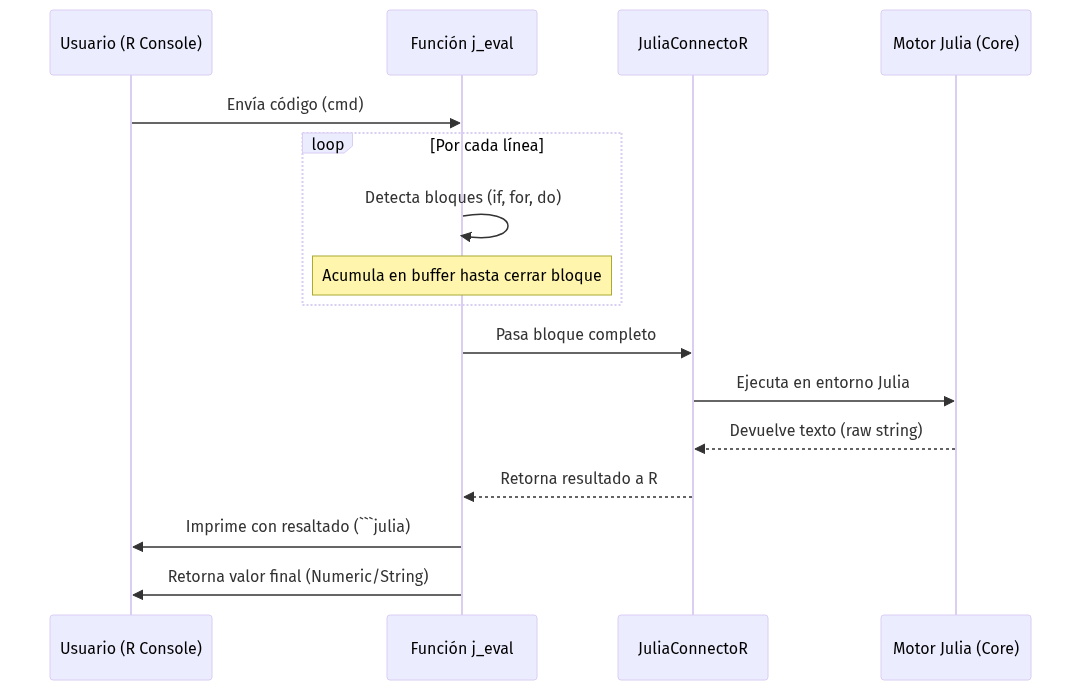
\includegraphics[width=1\textwidth,height=\textheight]{images/fig-flujo-jeval.png}

}

\caption{\label{fig-flujo-jeval}}

\end{figure}%

\begin{tcolorbox}[enhanced jigsaw, coltitle=black, leftrule=.75mm, bottomtitle=1mm, title=\textcolor{quarto-callout-note-color}{\faInfo}\hspace{0.5em}{Nota}, colback=white, colbacktitle=quarto-callout-note-color!10!white, left=2mm, toptitle=1mm, rightrule=.15mm, titlerule=0mm, arc=.35mm, colframe=quarto-callout-note-color-frame, bottomrule=.15mm, toprule=.15mm, opacityback=0, opacitybacktitle=0.6, breakable]

Como se ilustra en la Figura~\ref{fig-flujo-jeval}, la función no solo
``pasa'' el texto, sino que actúa como un supervisor que espera a que
los bloques de programación estén completos antes de despertar al motor
de Julia. Esto garantiza la estabilidad del sistema.

\end{tcolorbox}

\subsection{Flujo de generación gráfica con
j\_plot}\label{sec-flujo-jplot}

A diferencia de la ejecución de texto, \texttt{j\_plot} requiere una
coordinación adicional para gestionar archivos físicos. Observe el
proceso:

\begin{figure}

\centering{

\captionsetup{labelsep=none}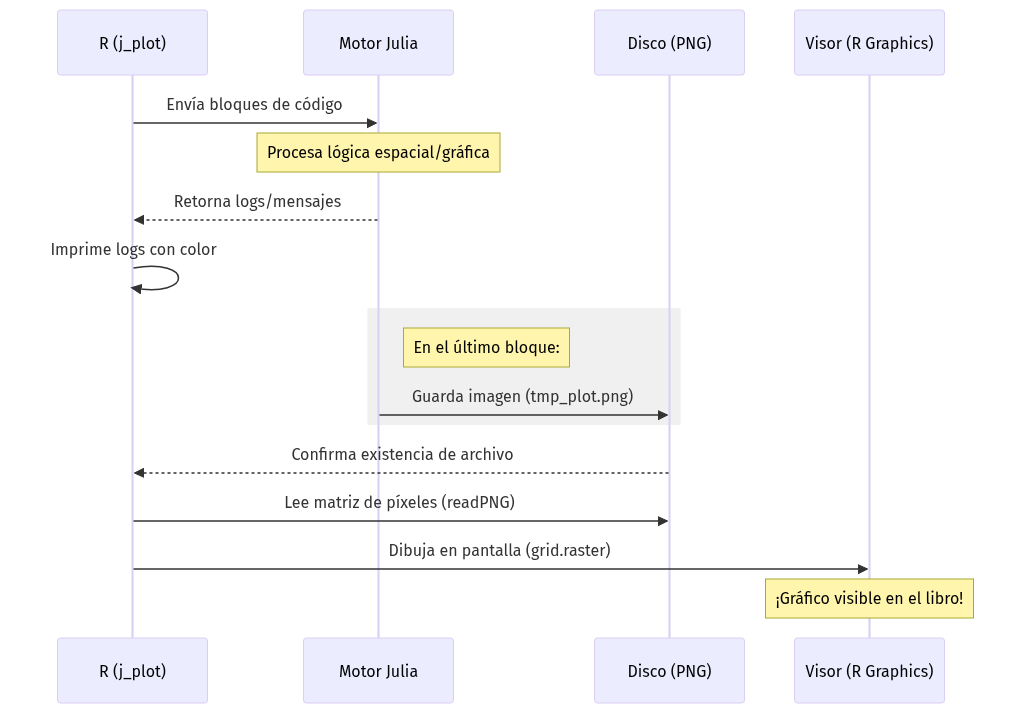
\includegraphics[width=1\textwidth,height=\textheight]{images/fig-flujo-jplot.png}

}

\caption{\label{fig-flujo-jplot}}

\end{figure}%

\begin{tcolorbox}[enhanced jigsaw, coltitle=black, leftrule=.75mm, bottomtitle=1mm, title=\textcolor{quarto-callout-tip-color}{\faLightbulb}\hspace{0.5em}{El rol del disco duro}, colback=white, colbacktitle=quarto-callout-tip-color!10!white, left=2mm, toptitle=1mm, rightrule=.15mm, titlerule=0mm, arc=.35mm, colframe=quarto-callout-tip-color-frame, bottomrule=.15mm, toprule=.15mm, opacityback=0, opacitybacktitle=0.6, breakable]

Como muestra la Figura~\ref{fig-flujo-jplot}, el secreto de
\texttt{j\_plot} es que utiliza un archivo temporal como ``puente''
visual. Por eso, si usted tiene el archivo \texttt{tmp\_plot.png}
abierto en otro programa, j\_plot podría fallar al intentar
sobrescribirlo.

\end{tcolorbox}

\subsection{Interpretación de errores y
consola}\label{sec-errores-consola}

Al trabajar con la interoperabilidad entre lenguajes (usando las
funciones \texttt{j\_eval} y \texttt{j\_plot} definidas arriba, la
consola de \textbf{VSCode} nos devolverá mensajes que debemos aprender a
interpretar.

\subsubsection{El error de conexión
TCP}\label{el-error-de-conexiuxf3n-tcp}

Si al usar Julia recibe un mensaje de error que menciona
\texttt{TCP\ connection}, usualmente significa que el motor de Julia se
ha cerrado o ha entrado en conflicto de memoria. * \textbf{Solución}:
Ejecute \texttt{.ensure\_julia\_ready()} en su consola de R para
reiniciar el puente de comunicación.

\subsubsection{Interpretación del Stacktrace en
Julia}\label{interpretaciuxf3n-del-stacktrace-en-julia}

Cuando Julia detecta un error, genera un rastro de llamadas o
\emph{Stacktrace}. No intente leer cada línea; busque siempre la primera
(que define el tipo de error) y la última línea de código escrita por
usted.

\begin{Shaded}
\begin{Highlighting}[]
\CommentTok{\# Ejemplo de error por índice fuera de rango}
\NormalTok{ERROR}\OperatorTok{:} \DataTypeTok{BoundsError}\OperatorTok{:}\NormalTok{ attempt to access }\FloatTok{5}\OperatorTok{{-}}\NormalTok{element }\DataTypeTok{Vector}\NormalTok{\{}\DataTypeTok{Int64}\NormalTok{\} at index [}\FloatTok{6}\NormalTok{]}
\end{Highlighting}
\end{Shaded}

\subsubsection{Resaltado de sintaxis en la
salida}\label{resaltado-de-sintaxis-en-la-salida}

Gracias a la configuración de \texttt{results:\ asis} en los bloques de
código, la salida de nuestras funciones aparecerá con el prompt
\texttt{julia\textgreater{}} coloreado, facilitando la distinción entre
lo que es un mensaje informativo y un resultado del cálculo.

\section{Introducción a la infraestructura de
datos}\label{introducciuxf3n-a-la-infraestructura-de-datos}

Este anexo constituye la guía técnica para la gestión del entorno de
desarrollo instalado. Es decir, información que describe y detalla los
contenedores instalados (instalación opción A), su estructura y
funcionamiento, así mismo como la descripción y detalles adicionales de
las dos instalaciones de QGIS (Instalación Opción B)

\subsection{Contenedores instalados (Instalación Opción
A)}\label{sec-contenedores_instalados}

Siguiendo los pasos detallados en Capítulo~\ref{sec-guia_A} para
instalar los contenedores Docker, en resumen, ellos contendrán:

\begin{enumerate}
\def\labelenumi{\arabic{enumi}.}
\tightlist
\item
  Un contenedor \texttt{contenedor\_sig\_unal} correspondiente a la
  imagen \texttt{image\_sig\_unal:final} el cual contendrá las
  siguientes herramientas:
\end{enumerate}

\begin{itemize}
\tightlist
\item
  \textbf{Python} (Apéndice~\ref{sec-anexo_python}), \textbf{R}
  (Apéndice~\ref{sec-anexo_r}) y \textbf{Julia}
  (Apéndice~\ref{sec-anexo_julia}) con los principales
  paquetes/librerías para geoprocesamiento.
\item
  \textbf{Quarto} (Ver Apéndice~\ref{sec-anexo_quarto}).
\item
  \textbf{TinyTeX} (Ver Sección~\ref{sec-tinytex}).
\end{itemize}

\begin{enumerate}
\def\labelenumi{\arabic{enumi}.}
\setcounter{enumi}{1}
\tightlist
\item
  Una contenedor \texttt{contenedor\_postgis\_unal} correspondiente a la
  imagen \texttt{postgis\_unal:final} el cual contendrá las siguientes
  herramientas:
\end{enumerate}

\begin{itemize}
\tightlist
\item
  \textbf{PostgreSQL} + \textbf{PostGIS} (Ver
  Apéndice~\ref{sec-anexo_postgresql}).
\end{itemize}

\subsubsection{🧪 Batería de pruebas de integridad del
docker}\label{bateruxeda-de-pruebas-de-integridad-del-docker}

\begin{longtable}[]{@{}
  >{\raggedright\arraybackslash}p{(\columnwidth - 4\tabcolsep) * \real{0.3333}}
  >{\raggedright\arraybackslash}p{(\columnwidth - 4\tabcolsep) * \real{0.3333}}
  >{\raggedright\arraybackslash}p{(\columnwidth - 4\tabcolsep) * \real{0.3333}}@{}}
\toprule\noalign{}
\begin{minipage}[b]{\linewidth}\raggedright
ID
\end{minipage} & \begin{minipage}[b]{\linewidth}\raggedright
Comando de Verificación (Docker)
\end{minipage} & \begin{minipage}[b]{\linewidth}\raggedright
Descripción
\end{minipage} \\
\midrule\noalign{}
\endhead
\bottomrule\noalign{}
\endlastfoot
01 & \texttt{docker\ exec\ contenedor\_sig\_unal\ gdalinfo\ -\/-version}
& Verifica que el núcleo de GDAL está activo. \\
02 &
\texttt{docker\ exec\ contenedor\_sig\_unal\ R\ -e\ "library(sf);\ st\_point(c(0,0))"}
& Prueba la librería \texttt{sf} y el motor de geometría en R. \\
03 &
\texttt{docker\ exec\ contenedor\_sig\_unal\ python3\ -c\ "import\ geopandas;\ print(geopandas.\_\_version\_\_)"}
& Verifica el stack espacial de Python. \\
04 &
\texttt{docker\ exec\ contenedor\_sig\_unal\ R\ -e\ "j\_eval(\textquotesingle{}sum({[}1,\ 2,\ 3{]})\textquotesingle{})"}
& \textbf{Test Crítico:} Verifica la función personalizada y el puente R
-\textgreater{} Julia. \\
05 &
\texttt{docker\ exec\ contenedor\_sig\_unal\ R\ -e\ "j\_plot(\textquotesingle{}plot(rand(10))\textquotesingle{})"}
& Prueba la generación de gráficos Julia capturados por R. \\
06 &
\texttt{docker\ exec\ contenedor\_sig\_unal\ julia\ -e\ \textquotesingle{}using\ ArchGDAL;\ println(ArchGDAL.GDAL.gdalversioninfo("RELEASE\_NAME"))\textquotesingle{}}
& \textbf{Cirugía Exitosa:} Confirma que Julia accede a GDAL del sistema
(v3.12.1). \\
07 &
\texttt{docker\ exec\ contenedor\_sig\_unal\ R\ -e\ "library(RPostgres);\ dbConnect(Postgres(),\ host=\textquotesingle{}db-postgis\textquotesingle{},\ dbname=\textquotesingle{}sig\_db\_unal\textquotesingle{},\ user=\textquotesingle{}profe\_unal\textquotesingle{},\ password=\textquotesingle{}geomatica2025\textquotesingle{})"}
& Prueba la conexión R -\textgreater{} PostGIS (Interna). \\
08 &
\texttt{docker\ exec\ contenedor\_sig\_unal\ python3\ -c\ "import\ psycopg2;\ conn\ =\ psycopg2.connect(host=\textquotesingle{}db-postgis\textquotesingle{},\ dbname=\textquotesingle{}sig\_db\_unal\textquotesingle{},\ user=\textquotesingle{}profe\_unal\textquotesingle{},\ password=\textquotesingle{}geomatica2025\textquotesingle{});\ print(\textquotesingle{}Python\ PostGIS\ conectado\ ✅\textquotesingle{});\ conn.close()"}
& Prueba la conexión Python -\textgreater{} PostGIS (Interna). \\
09 &
\texttt{docker\ exec\ contenedor\_sig\_unal\ R\ -e\ "cat(whitebox::wbt\_version())"}
& Verifica que los binarios de WhiteboxTools están instalados y
accesibles. \\
10 &
\texttt{docker\ exec\ contenedor\_sig\_unal\ R\ -e\ "library(httpgd);\ print(\textquotesingle{}Visor\ OK\textquotesingle{})"}
& Verifica que el motor gráfico para VSCode está listo en el puerto
\texttt{8787}. \\
\end{longtable}

\subsubsection{Configuración de puertos y
conectividad}\label{sec-puertos}

Para que su computadora (Host) pueda comunicarse con los servicios
dentro del contenedor, hemos diseñado un sistema de ``puentes'' o mapeo
de puertos. Esto evita conflictos si ya tiene instalados otros
servidores de bases de datos o Jupyter en su PC.

\begin{longtable}[]{@{}
  >{\raggedright\arraybackslash}p{(\columnwidth - 8\tabcolsep) * \real{0.1818}}
  >{\centering\arraybackslash}p{(\columnwidth - 8\tabcolsep) * \real{0.2273}}
  >{\centering\arraybackslash}p{(\columnwidth - 8\tabcolsep) * \real{0.2273}}
  >{\raggedright\arraybackslash}p{(\columnwidth - 8\tabcolsep) * \real{0.1818}}
  >{\raggedright\arraybackslash}p{(\columnwidth - 8\tabcolsep) * \real{0.1818}}@{}}
\toprule\noalign{}
\begin{minipage}[b]{\linewidth}\raggedright
Servicio
\end{minipage} & \begin{minipage}[b]{\linewidth}\centering
Puerto en su PC (Host)
\end{minipage} & \begin{minipage}[b]{\linewidth}\centering
Puerto en Contenedor
\end{minipage} & \begin{minipage}[b]{\linewidth}\raggedright
Propósito
\end{minipage} & \begin{minipage}[b]{\linewidth}\raggedright
Acceso / Conexión
\end{minipage} \\
\midrule\noalign{}
\endhead
\bottomrule\noalign{}
\endlastfoot
\textbf{Jupyter Lab} & \texttt{8889} & \texttt{8888} & Programación y
Notebooks & \texttt{http://localhost:8889} \\
\textbf{Visor R (httpgd)} & \texttt{8788} & \texttt{8787} & Gráficos de
R y VSCode & \texttt{http://localhost:8788} \\
\textbf{PostGIS (DB)} & \texttt{5434} & \texttt{5432} & Base de Datos
Espacial & \texttt{localhost:5434} \\
\end{longtable}

\subsubsection{🔑 Credenciales de la base de
datos}\label{sec-credenciales}

Utilice estos datos para configurar sus conexiones en QGIS, ArcGIS Pro o
mediante código (R/Python/Julia):

\begin{itemize}
\tightlist
\item
  \textbf{Base de Datos:} \texttt{sig\_db\_unal}
\item
  \textbf{Usuario:} \texttt{profe\_unal}
\item
  \textbf{Contraseña:} \texttt{geomatica2025}
\item
  \textbf{Host:} \texttt{localhost}
\item
  \textbf{Puerto:} \texttt{5434}
\item
  \textbf{Host Interno:} \texttt{db-postgis} (Use este nombre únicamente
  para conexiones \textbf{dentro} de sus scripts).
\end{itemize}

\subsubsection{Lógica de arquitectura (Dockerfile y
docker-compose)}\label{sec-arquitectura-puertos}

La configuración del entorno se ha ``blindado'' técnicamente para
garantizar la estabilidad:

\begin{enumerate}
\def\labelenumi{\arabic{enumi}.}
\tightlist
\item
  \textbf{En el Dockerfile}: Se usan las instrucciones
  \texttt{EXPOSE\ 8888} y \texttt{EXPOSE\ 8787}. Esto le avisa a Docker
  que el contenedor tiene dos ``puertas'' abiertas internamente. Al
  fijar \texttt{httpgd.port\ =\ 8787}, nos aseguramos de que el visor de
  gráficos de R no pelee con Jupyter por el mismo canal.
\item
  \textbf{En el Docker-Compose}:

  \begin{itemize}
  \tightlist
  \item
    \textbf{\texttt{8889:8888}}: Permite que este curso conviva con
    otras instalaciones de Jupyter (que suelen usar el 8888).
  \item
    \textbf{\texttt{8788:8787}}: Habilita la conexión independiente de
    VSCode al visor de gráficos de R.
  \item
    \textbf{\texttt{5434:5432}}: Evita el choque con bases de datos
    locales (Postgres suele usar el 5432 o 5433).
  \end{itemize}
\end{enumerate}

\subsubsection{Guía de acceso: El concepto de
``lados''}\label{sec-guia-acceso}

Es fundamental entender desde dónde está intentando conectar:

\begin{quote}
\mbox{}%
\paragraph{🌐 Desde afuera (Su PC /
Host)}\label{desde-afuera-su-pc-host}

Es lo que usted configura en su navegador o en QGIS. Usted ve los
puertos mapeados: * \textbf{Jupyter/Notebooks}:
\texttt{http://localhost:8889} (usando el token \texttt{geomatica2025}).
* \textbf{Base de Datos (QGIS/DBeaver)}: Host: \texttt{localhost},
Puerto: \texttt{5434}.
\end{quote}

\begin{quote}
\mbox{}%
\paragraph{🐳 Desde adentro (El
Contenedor)}\label{desde-adentro-el-contenedor}

Sus scripts de Python, R y Julia no saben que existe un mapeo externo.
Dentro de su ``casa'' Docker, nada ha cambiado: * \textbf{PostGIS}: El
código debe buscar el puerto estándar \texttt{5432} y el host
\texttt{db-postgis}. * \textbf{httpgd}: El servidor de gráficos sigue
escuchando en el puerto interno \texttt{8787}.
\end{quote}

\begin{tcolorbox}[enhanced jigsaw, coltitle=black, leftrule=.75mm, bottomtitle=1mm, title=\textcolor{quarto-callout-note-color}{\faInfo}\hspace{0.5em}{Tip de Conexión}, colback=white, colbacktitle=quarto-callout-note-color!10!white, left=2mm, toptitle=1mm, rightrule=.15mm, titlerule=0mm, arc=.35mm, colframe=quarto-callout-note-color-frame, bottomrule=.15mm, toprule=.15mm, opacityback=0, opacitybacktitle=0.6, breakable]

Si intenta conectar QGIS usando el puerto \texttt{5432} y falla,
recuerde que el ``puente'' hacia el contenedor se construyó
específicamente sobre el puerto \textbf{\texttt{5434}}.

\end{tcolorbox}

\subsubsection{Resumen de la infraestructura
instalada}\label{resumen-de-la-infraestructura-instalada}

\begin{longtable}[]{@{}
  >{\raggedright\arraybackslash}p{(\columnwidth - 4\tabcolsep) * \real{0.3333}}
  >{\raggedright\arraybackslash}p{(\columnwidth - 4\tabcolsep) * \real{0.3333}}
  >{\raggedright\arraybackslash}p{(\columnwidth - 4\tabcolsep) * \real{0.3333}}@{}}
\toprule\noalign{}
\begin{minipage}[b]{\linewidth}\raggedright
Componente
\end{minipage} & \begin{minipage}[b]{\linewidth}\raggedright
Versión / Estado
\end{minipage} & \begin{minipage}[b]{\linewidth}\raggedright
Detalles Técnicos
\end{minipage} \\
\midrule\noalign{}
\endhead
\bottomrule\noalign{}
\endlastfoot
\textbf{R Engine} & \texttt{4.3.3} (Angel Food Cake) & Puente
\texttt{JuliaConnectoR} y visor \texttt{httpgd} configurados. \\
\textbf{Julia Stack} & \texttt{v1.10.x} & \textbf{ArchGDAL 3.12.1}
operativo mediante enlaces simbólicos. \\
\textbf{Python Stack} & \texttt{3.12.x} & GeoPandas, PyTorch y drivers
\texttt{psycopg2} listos. \\
\textbf{Base de Datos} & \textbf{PostGIS} (Noble) & Host interno
\texttt{db-postgis} con extensión espacial activa. \\
\textbf{Visualización} & \textbf{Dual Mode} & Puertos \textbf{8788}
(R/Julia Plots) y \textbf{8889} (Jupyter Lab). \\
\textbf{Persistencia} & \textbf{Volúmenes Docker} & Mapeo bidireccional
en \texttt{/home/rstudio/work} confirmado. \\
\textbf{Cirugía SSL} & ✅ Aplicada & Compatibilidad OpenSSL 3.0
(Sistema) vs 3.3 (Julia). \\
\end{longtable}

\section{Localización de archivos y
persistencia}\label{localizaciuxf3n-de-archivos-y-persistencia}

En el contenedor, su carpeta del equipo local se encuentra vinculada a
la ruta \textbf{/home/rstudio/work}. * Cualquier archivo guardado en esa
ruta dentro de Jupyter aparecerá en su carpeta de Windows. * Se
recomienda organizar su trabajo en las subcarpetas: \texttt{notebooks},
\texttt{scripts}, y \texttt{data}. * La carpeta \texttt{imagenes} (sin
tílde y provista para las imágenes usadas en los archivos Quarto) debe
residir también en esta ruta para un renderizado correcto.

\begin{tcolorbox}[enhanced jigsaw, coltitle=black, leftrule=.75mm, bottomtitle=1mm, title=\textcolor{quarto-callout-important-color}{\faExclamation}\hspace{0.5em}{Persistencia de Datos}, colback=white, colbacktitle=quarto-callout-important-color!10!white, left=2mm, toptitle=1mm, rightrule=.15mm, titlerule=0mm, arc=.35mm, colframe=quarto-callout-important-color-frame, bottomrule=.15mm, toprule=.15mm, opacityback=0, opacitybacktitle=0.6, breakable]

Si su contenedor se apaga o se reinicia, los datos de su base de datos
PostGIS y los datos almancenados en \texttt{/home/rstudio/work}
\textbf{no se pierden}. El volumen nombrado actúa como un disco duro
externo que sobrevive a cualquier caída del sistema.

\end{tcolorbox}

\section{Cargar los contenedores dentro de
VSCode}\label{sec-cargar_contenedores_vscode}

Para una experiencia de desarrollo profesional, conecte VSCode
directamente al contenedor:

\begin{itemize}
\tightlist
\item
  Inicie Docker Desktop
\item
  En el ``PowerShell'' de windows ubíquese en la carpeta donde instaló
  los contenedores (ver Sección~\ref{sec-cargar_docker_tar})
\item
  Ejecute el comando: \texttt{docker\ compose\ up\ -d}
\item
  Abra VSCode
\item
  Instale (local) la extensión \texttt{Dev\ Containers}
\item
  Acceda a la paleta de comandos con \texttt{Ctrl\ +\ Shift\ +\ P},
  escriba (o seleccione) \textbf{Dev Containers: Attach to Running
  Container\ldots{}}, y seleccione el contenedor
  \textbf{\texttt{contenedor\_sig\_unal}} (imagen
  \texttt{image\_sig\_unal}).
\item
  Abra la carpeta \texttt{/home/rstudio/work} (esa carpeta corresponde a
  la carpeta local en dónde instaló los contenedores)
\item
  Una vez conectado ``dentro'' del contenedor, debe habilitar/instalar
  las extensiones (\emph{`Install in Container'}). Vea el listado
  completo en Sección~\ref{sec-extensiones-vscode}.
\end{itemize}

\section{Inicialización del visor gráfico (solo una vez por
sesión)}\label{sec-httpgd}

Para que los gráficos de R (y los puentes de Python/Julia) se visualicen
correctamente en VSCode, debe inicializar el dispositivo gráfico. En su
terminal de R, ejecute:

\begin{Shaded}
\begin{Highlighting}[]
\CommentTok{\# Lanza el servidor de gráficos httpgd}
\NormalTok{httpgd}\SpecialCharTok{::}\FunctionTok{hgd}\NormalTok{()}
\end{Highlighting}
\end{Shaded}

\begin{itemize}
\tightlist
\item
  \textbf{Acceso al Visor}: VSCode debería abrir automáticamente una
  pestaña con el visor. Si esto no sucede o prefiere usar su navegador
  externo (Chrome/Edge), acceda a la dirección:
  \textbf{\texttt{http://127.0.0.1:8788}}.
\item
  \textbf{Nota sobre Puertos}: Aunque el comando en R pueda imprimir una
  URL interna con el puerto \texttt{8787} o un token aleatorio,
  \textbf{ignore esa dirección}. Gracias a nuestro archivo
  \texttt{docker-compose.yml}, el puerto \textbf{8788} de su Windows
  está ``cableado'' permanentemente al visor, eliminando la necesidad de
  buscar tokens o puertos dinámicos. (xxx)
\end{itemize}

\section{Ingreso a Jupyter Lab}\label{sec-acceder_jupyterlab}

Abra su navegador y acceda a: \url{http://localhost:8889} *
\textbf{Contraseña/Token:} (Si se solicita) \texttt{geomatica2025} *
\textbf{Persistencia:} Todo archivo guardado en la carpeta
\texttt{/home/rstudio/work} aparecerá automáticamente en su carpeta de
Windows. \textbf{No guarde nada fuera de esa ruta}, o se perderá al
cerrar el contenedor.

Puede pasar directamente la url completa:

\url{http://127.0.0.1:8889/lab?token=geomatica2025}

Si la url anterior no funciona, puede verificar cuál url usa actualmente
el contenedor, la cual aparece al final del log después de ejecutar el
siguiente comando:

\begin{Shaded}
\begin{Highlighting}[]
\ExtensionTok{docker}\NormalTok{ logs contenedor\_sig\_unal}
\end{Highlighting}
\end{Shaded}

\textbf{Alternativa:} Puede iniciar/reiniciar el servidor de Jupyter Lab
en la url \url{http://127.0.0.1:8889/lab?token=geomatica2025}. Use el
siguiente comando ejecutado desde el terminal de VSCode:

\begin{Shaded}
\begin{Highlighting}[]
\ExtensionTok{jupyter}\NormalTok{ lab }\AttributeTok{{-}{-}ip}\OperatorTok{=}\NormalTok{0.0.0.0 }\AttributeTok{{-}{-}port}\OperatorTok{=}\NormalTok{8889 }\AttributeTok{{-}{-}no{-}browser} \AttributeTok{{-}{-}allow{-}root} \AttributeTok{{-}{-}ServerApp.token}\OperatorTok{=}\StringTok{\textquotesingle{}geomatica2025\textquotesingle{}}
\end{Highlighting}
\end{Shaded}

\section{Guía visual de JupyterLab}\label{guuxeda-visual-de-jupyterlab}

Al ingresar, se encontrará con el centro de mando de sus kernels, donde
podrá elegir entre R, Python o Julia para sus Notebooks:

\begin{figure}

\centering{

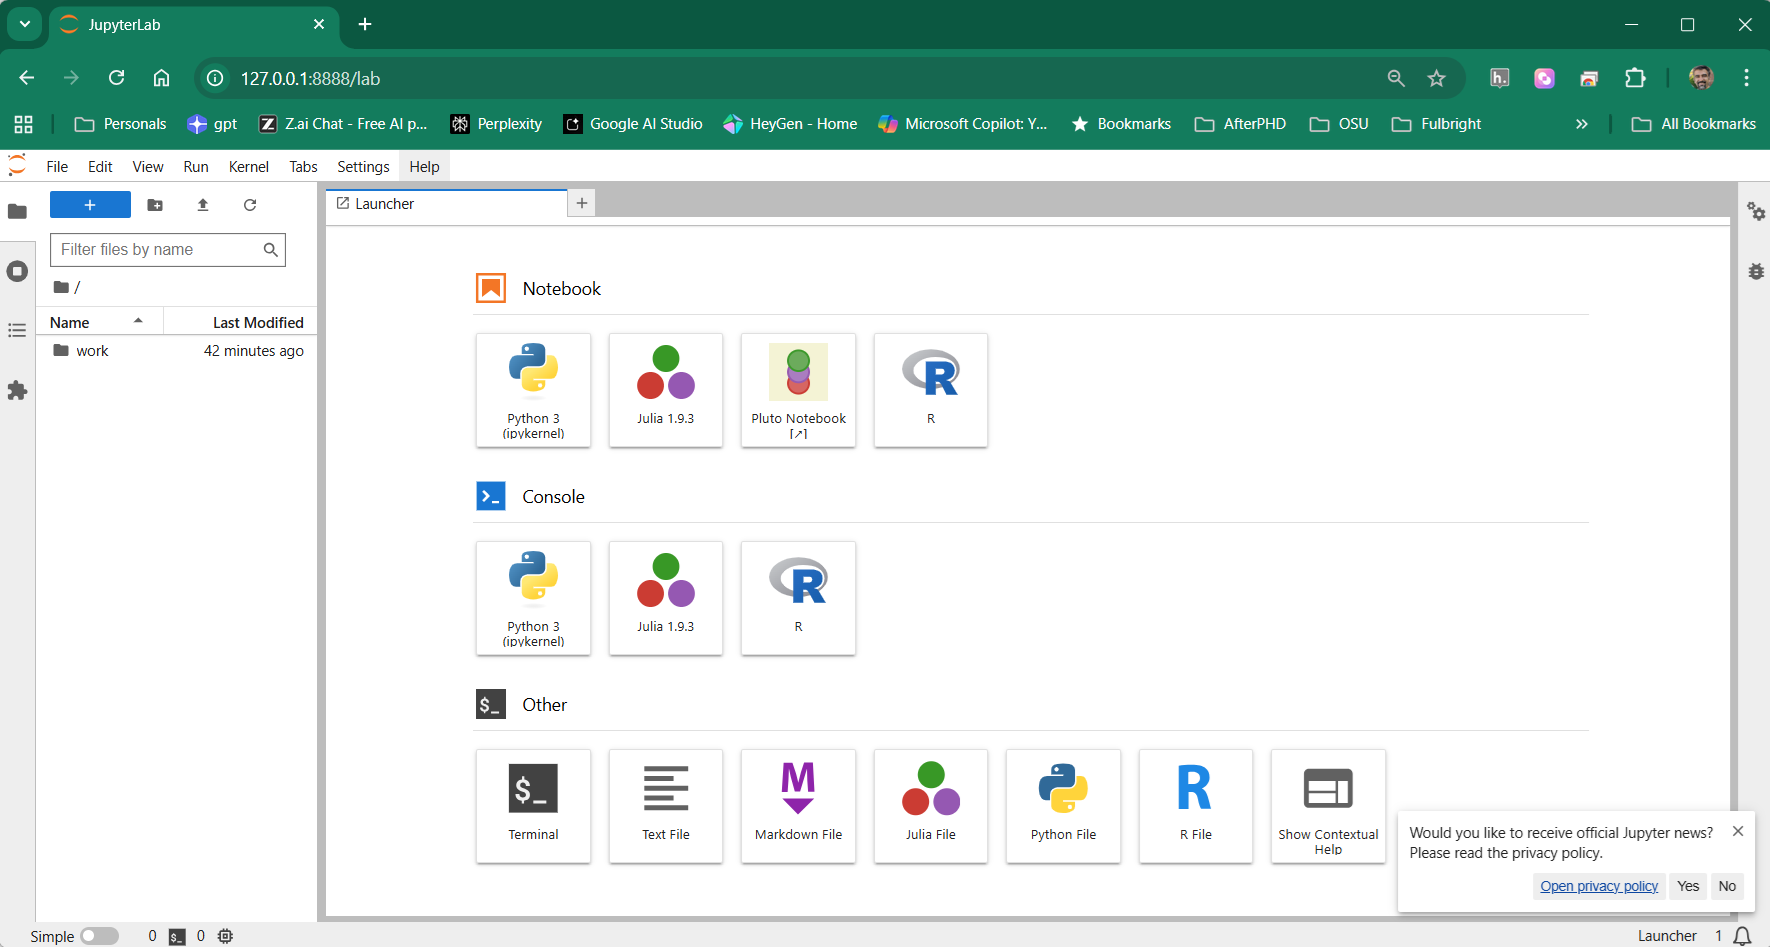
\includegraphics{./images/JupyterLab.png}

}

\caption{\label{fig-jupyterlab}Interfaz de JupyterLab configurada para
el laboratorio.}

\end{figure}%

\subsection{La Carpeta `work' y el Espejo de
Datos}\label{la-carpeta-work-y-el-espejo-de-datos}

En el panel izquierdo de la Figura~\ref{fig-jupyterlab}, la carpeta
\textbf{\texttt{/home/rstudio/work/}} es el espejo de su directorio
local en Windows. Gracias a la configuración de volúmenes en el archivo
\texttt{docker-compose.yml}, existe un puente directo: todo cambio
realizado en Jupyter se refleja en su disco duro y viceversa,
garantizando que su trabajo no se pierda al apagar el contenedor.

\section{Compilación de la guía completa o documentos
individuales}\label{sec-compilacion}

La guía del curso está organizada a partir de un \textbf{archivo
orquestador} \texttt{\_quarto.yml}, el cual contiene una referencia
explícita a cada uno de los archivos Quarto (\texttt{.qmd}) que definen
los capítulos, las presentaciones, los talleres y los anexos. Este
archivo centraliza la organización y el formato de la guía tanto en
\textbf{PDF} como en \textbf{HTML}.

\subsection{Compilación del proyecto
completo}\label{compilaciuxf3n-del-proyecto-completo}

Si desea compilar la guía completa del curso y generar todos los
formatos, simplemente ejecute el comando \texttt{quarto\ render} en la
carpeta raíz (donde se encuentra el archivo \texttt{\_quarto.yml}):

\begin{Shaded}
\begin{Highlighting}[]
\CommentTok{\# Desde la carpeta raíz donde reside el archivo \textquotesingle{}\_quarto.yml\textquotesingle{}}
\ExtensionTok{quarto}\NormalTok{ render}
\end{Highlighting}
\end{Shaded}

\subsection{Compilación de archivos
individuales}\label{compilaciuxf3n-de-archivos-individuales}

En ocasiones, querrá trabajar en un solo capítulo sin procesar el libro
entero. Para compilar un archivo específico (ej. \texttt{archivo.qmd})
de manera independiente y evitar que Quarto aplique las reglas de
numeración y referencias del proyecto global, siga estos pasos:

\begin{enumerate}
\def\labelenumi{\arabic{enumi}.}
\tightlist
\item
  \textbf{Renombrar temporalmente el orquestador:} Cambie el nombre de
  \texttt{\_quarto.yml} a \textbf{\texttt{\_quarto.yml.back}}. Esto hace
  que Quarto trate al archivo como un documento ``solitario''.
\item
  \textbf{Ejecutar el renderizado específico:}
\end{enumerate}

\begin{itemize}
\tightlist
\item
  \textbf{Generar todos los formatos (HTML y PDF):}
\end{itemize}

\begin{Shaded}
\begin{Highlighting}[]
\ExtensionTok{quarto}\NormalTok{ render archivo.qmd }\AttributeTok{{-}{-}to}\NormalTok{ all}
\end{Highlighting}
\end{Shaded}

\begin{itemize}
\tightlist
\item
  \textbf{Generar solo formato HTML:}
\end{itemize}

\begin{Shaded}
\begin{Highlighting}[]
\ExtensionTok{quarto}\NormalTok{ render archivo.qmd }\AttributeTok{{-}{-}to}\NormalTok{ html}
\end{Highlighting}
\end{Shaded}

\begin{itemize}
\tightlist
\item
  \textbf{Generar solo formato PDF:}
\end{itemize}

\begin{Shaded}
\begin{Highlighting}[]
\ExtensionTok{quarto}\NormalTok{ render archivo.qmd }\AttributeTok{{-}{-}to}\NormalTok{ pdf}
\end{Highlighting}
\end{Shaded}

\subsection{Notas de estudio y
personalización}\label{notas-de-estudio-y-personalizaciuxf3n}

\begin{tcolorbox}[enhanced jigsaw, coltitle=black, leftrule=.75mm, bottomtitle=1mm, title=\textcolor{quarto-callout-tip-color}{\faLightbulb}\hspace{0.5em}{¡Personaliza tu aprendizaje!}, colback=white, colbacktitle=quarto-callout-tip-color!10!white, left=2mm, toptitle=1mm, rightrule=.15mm, titlerule=0mm, arc=.35mm, colframe=quarto-callout-tip-color-frame, bottomrule=.15mm, toprule=.15mm, opacityback=0, opacitybacktitle=0.6, breakable]

En Quarto, puedes agregar tus propias \textbf{notas de estudio} usando
la sintaxis de ``callouts''. Recuerda que este documento está en proceso
de \textbf{construcción} y sufrirá cambios permanentes hasta terminar el
curso.

Puedes buscar \textbf{ayuda en Internet} para personalizar la apariencia
de tus notas. La sintaxis básica es:

\begin{Shaded}
\begin{Highlighting}[]
\NormalTok{::: \{.callout{-}tip icon="true"\}}
\FunctionTok{\#\#\# ¡Escribe tu nota aquí!}
\NormalTok{Este es un espacio para tus observaciones personales y recordatorios.}
\NormalTok{:::}
\end{Highlighting}
\end{Shaded}

\end{tcolorbox}

\section{Mapeo de capacidades SIG}\label{mapeo-de-capacidades-sig}

Es vital entender que, aunque usemos lenguajes distintos, todos
``beben'' de las mismas librerías de bajo nivel instaladas en nuestra
imagen base de OSGeo:

\begin{longtable}[]{@{}
  >{\raggedright\arraybackslash}p{(\columnwidth - 8\tabcolsep) * \real{0.2000}}
  >{\raggedright\arraybackslash}p{(\columnwidth - 8\tabcolsep) * \real{0.2000}}
  >{\raggedright\arraybackslash}p{(\columnwidth - 8\tabcolsep) * \real{0.2000}}
  >{\raggedright\arraybackslash}p{(\columnwidth - 8\tabcolsep) * \real{0.2000}}
  >{\raggedright\arraybackslash}p{(\columnwidth - 8\tabcolsep) * \real{0.2000}}@{}}
\toprule\noalign{}
\begin{minipage}[b]{\linewidth}\raggedright
Operación
\end{minipage} & \begin{minipage}[b]{\linewidth}\raggedright
R (\texttt{sf} / \texttt{terra})
\end{minipage} & \begin{minipage}[b]{\linewidth}\raggedright
Python (\texttt{GeoPandas})
\end{minipage} & \begin{minipage}[b]{\linewidth}\raggedright
Julia (\texttt{ArchGDAL})
\end{minipage} & \begin{minipage}[b]{\linewidth}\raggedright
Motor de Sistema
\end{minipage} \\
\midrule\noalign{}
\endhead
\bottomrule\noalign{}
\endlastfoot
Lectura de Datos & \texttt{st\_read()} / \texttt{rast()} &
\texttt{read\_file()} / \texttt{open()} & \texttt{ArchGDAL.read()} &
\textbf{GDAL} \\
Buffers / Geometría & \texttt{st\_buffer()} & \texttt{.buffer()} &
\texttt{LibGEOS.buffer()} & \textbf{GEOS} \\
Reproyección & \texttt{st\_transform()} & \texttt{.to\_crs()} &
\texttt{ArchGDAL.reproject()} & \textbf{PROJ} \\
\end{longtable}

\section{Verificación de conectividad
multilenguaje}\label{verificaciuxf3n-de-conectividad-multilenguaje}

\textbf{Nota técnica}: Dentro de la red de Docker, el host es
\texttt{db-postgis}.

\subsection{Python}

\begin{Shaded}
\begin{Highlighting}[]
\ImportTok{import}\NormalTok{ psycopg2}
\ImportTok{import}\NormalTok{ geopandas }\ImportTok{as}\NormalTok{ gpd}
\ImportTok{import}\NormalTok{ fiona}
\ImportTok{import}\NormalTok{ matplotlib.pyplot }\ImportTok{as}\NormalTok{ plt}
\ImportTok{from}\NormalTok{ shapely.geometry }\ImportTok{import}\NormalTok{ Point}

\BuiltInTok{print}\NormalTok{(}\StringTok{"{-}{-}{-} Inicio de Verificación de Python SIG {-}{-}{-}"}\NormalTok{)}
\end{Highlighting}
\end{Shaded}

\begin{verbatim}
--- Inicio de Verificación de Python SIG ---
\end{verbatim}

\begin{Shaded}
\begin{Highlighting}[]
\CommentTok{\# 1. Prueba de conexión a la base de datos PostGIS}
\ControlFlowTok{try}\NormalTok{:}
\NormalTok{    conn }\OperatorTok{=}\NormalTok{ psycopg2.}\ExtensionTok{connect}\NormalTok{(}
\NormalTok{        host}\OperatorTok{=}\StringTok{"db{-}postgis"}\NormalTok{, }
\NormalTok{        dbname}\OperatorTok{=}\StringTok{"sig\_db\_unal"}\NormalTok{, }
\NormalTok{        user}\OperatorTok{=}\StringTok{"profe\_unal"}\NormalTok{, }
\NormalTok{        password}\OperatorTok{=}\StringTok{"geomatica2025"}
\NormalTok{    )}
    \BuiltInTok{print}\NormalTok{(}\StringTok{"✅ Conexión a PostGIS: Exitosa"}\NormalTok{)}
\NormalTok{    conn.close()}
\ControlFlowTok{except} \PreprocessorTok{Exception} \ImportTok{as}\NormalTok{ e:}
    \BuiltInTok{print}\NormalTok{(}\SpecialStringTok{f"❌ Error de conexión a PostGIS: }\SpecialCharTok{\{}\NormalTok{e}\SpecialCharTok{\}}\SpecialStringTok{"}\NormalTok{)}
\end{Highlighting}
\end{Shaded}

\begin{verbatim}
✅ Conexión a PostGIS: Exitosa
\end{verbatim}

\begin{Shaded}
\begin{Highlighting}[]
\CommentTok{\# 2. Prueba de Fiona y drivers GDAL}
\ControlFlowTok{try}\NormalTok{:}
\NormalTok{    drivers }\OperatorTok{=} \BuiltInTok{len}\NormalTok{(fiona.supported\_drivers)}
    \BuiltInTok{print}\NormalTok{(}\SpecialStringTok{f"✅ Fiona operativo: }\SpecialCharTok{\{}\NormalTok{drivers}\SpecialCharTok{\}}\SpecialStringTok{ drivers GDAL detectados"}\NormalTok{)}
\ControlFlowTok{except} \PreprocessorTok{Exception} \ImportTok{as}\NormalTok{ e:}
    \BuiltInTok{print}\NormalTok{(}\SpecialStringTok{f"❌ Error en Fiona/GDAL: }\SpecialCharTok{\{}\NormalTok{e}\SpecialCharTok{\}}\SpecialStringTok{"}\NormalTok{)}
\end{Highlighting}
\end{Shaded}

\begin{verbatim}
✅ Fiona operativo: 17 drivers GDAL detectados
\end{verbatim}

\begin{Shaded}
\begin{Highlighting}[]
\CommentTok{\# 3. Prueba de GeoPandas, Motores GEOS y Visualización}
\ControlFlowTok{try}\NormalTok{:}
    \CommentTok{\# Creamos un punto y su buffer (GEOS)}
\NormalTok{    punto }\OperatorTok{=}\NormalTok{ Point(}\DecValTok{0}\NormalTok{, }\DecValTok{0}\NormalTok{)}
\NormalTok{    buffer\_geom }\OperatorTok{=}\NormalTok{ punto.}\BuiltInTok{buffer}\NormalTok{(}\FloatTok{1.0}\NormalTok{)}
    
    \CommentTok{\# Creamos GeoDataFrames para graficar}
\NormalTok{    gdf\_buffer }\OperatorTok{=}\NormalTok{ gpd.GeoDataFrame(\{}\StringTok{\textquotesingle{}geometry\textquotesingle{}}\NormalTok{: [buffer\_geom]\}, crs}\OperatorTok{=}\StringTok{"EPSG:4326"}\NormalTok{)}
\NormalTok{    gdf\_punto }\OperatorTok{=}\NormalTok{ gpd.GeoDataFrame(\{}\StringTok{\textquotesingle{}geometry\textquotesingle{}}\NormalTok{: [punto]\}, crs}\OperatorTok{=}\StringTok{"EPSG:4326"}\NormalTok{)}
    
    \BuiltInTok{print}\NormalTok{(}\SpecialStringTok{f"✅ GeoPandas }\SpecialCharTok{\{}\NormalTok{gpd}\SpecialCharTok{.}\NormalTok{\_\_version\_\_}\SpecialCharTok{\}}\SpecialStringTok{: Operativo"}\NormalTok{)}
    \BuiltInTok{print}\NormalTok{(}\SpecialStringTok{f"✅ Motores GEOS/Shapely: Verificados"}\NormalTok{)}

    \CommentTok{\# Generación del Plot Espacial con Ejes y Cuadrícula}
\NormalTok{    fig, ax }\OperatorTok{=}\NormalTok{ plt.subplots(figsize}\OperatorTok{=}\NormalTok{(}\DecValTok{6}\NormalTok{, }\DecValTok{6}\NormalTok{))}
    
    \CommentTok{\# Graficamos el buffer}
\NormalTok{    gdf\_buffer.plot(ax}\OperatorTok{=}\NormalTok{ax, color}\OperatorTok{=}\StringTok{\textquotesingle{}lightgreen\textquotesingle{}}\NormalTok{, edgecolor}\OperatorTok{=}\StringTok{\textquotesingle{}green\textquotesingle{}}\NormalTok{, alpha}\OperatorTok{=}\FloatTok{0.4}\NormalTok{, label}\OperatorTok{=}\StringTok{\textquotesingle{}Buffer\textquotesingle{}}\NormalTok{)}
    
    \CommentTok{\# Graficamos el punto original (en rojo)}
\NormalTok{    gdf\_punto.plot(ax}\OperatorTok{=}\NormalTok{ax, color}\OperatorTok{=}\StringTok{\textquotesingle{}red\textquotesingle{}}\NormalTok{, markersize}\OperatorTok{=}\DecValTok{50}\NormalTok{, zorder}\OperatorTok{=}\DecValTok{5}\NormalTok{, label}\OperatorTok{=}\StringTok{\textquotesingle{}Centro\textquotesingle{}}\NormalTok{)}
    
    \CommentTok{\# Configuración de estilo consistente (Ejes y Grilla)}
\NormalTok{    ax.set\_title(}\StringTok{"Validación Python SIG: Buffer GEOS"}\NormalTok{)}
\NormalTok{    ax.set\_xlabel(}\StringTok{"Longitud"}\NormalTok{)}
\NormalTok{    ax.set\_ylabel(}\StringTok{"Latitud"}\NormalTok{)}
\NormalTok{    ax.grid(}\VariableTok{True}\NormalTok{, linestyle}\OperatorTok{=}\StringTok{\textquotesingle{}{-}{-}\textquotesingle{}}\NormalTok{, alpha}\OperatorTok{=}\FloatTok{0.7}\NormalTok{) }\CommentTok{\# Cuadrícula activada}
\NormalTok{    ax.set\_aspect(}\StringTok{\textquotesingle{}equal\textquotesingle{}}\NormalTok{) }\CommentTok{\# Proporción 1:1 para evitar deformación}
    
\NormalTok{    plt.show()}
    \BuiltInTok{print}\NormalTok{(}\StringTok{"✅ Visualización GeoPandas: Mapa generado con éxito"}\NormalTok{)}

\ControlFlowTok{except} \PreprocessorTok{Exception} \ImportTok{as}\NormalTok{ e:}
    \BuiltInTok{print}\NormalTok{(}\SpecialStringTok{f"❌ Error en el stack espacial de Python: }\SpecialCharTok{\{}\NormalTok{e}\SpecialCharTok{\}}\SpecialStringTok{"}\NormalTok{)}
\end{Highlighting}
\end{Shaded}

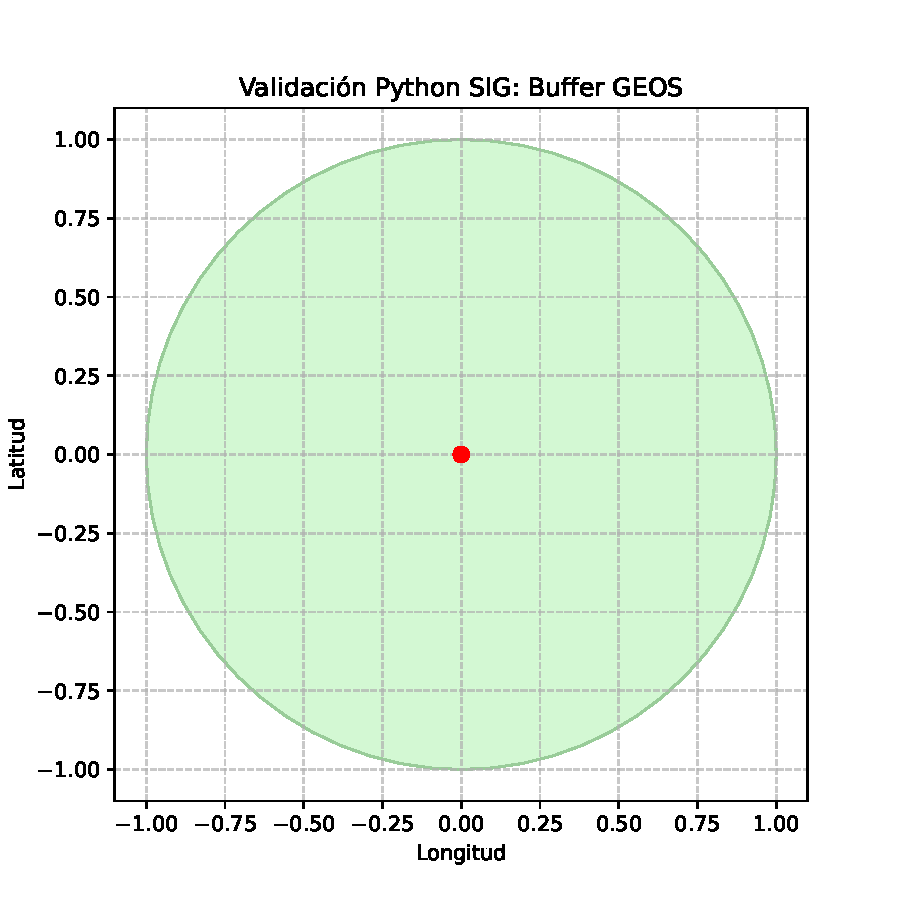
\includegraphics{81-uso_infraestructura_instalada_files/figure-pdf/python_verificacion-1.pdf}

\begin{Shaded}
\begin{Highlighting}[]
\BuiltInTok{print}\NormalTok{(}\StringTok{"{-}{-}{-} Verificación Finalizada {-}{-}{-}"}\NormalTok{)}
\end{Highlighting}
\end{Shaded}

\begin{verbatim}
--- Verificación Finalizada ---
\end{verbatim}

\subsection{R}

\begin{Shaded}
\begin{Highlighting}[]
\FunctionTok{library}\NormalTok{(DBI)}
\FunctionTok{library}\NormalTok{(RPostgres)}
\FunctionTok{library}\NormalTok{(sf)}
\end{Highlighting}
\end{Shaded}

\begin{verbatim}
Linking to GEOS 3.12.1, GDAL 3.8.4, PROJ 9.4.0; sf_use_s2() is TRUE
\end{verbatim}

\begin{Shaded}
\begin{Highlighting}[]
\FunctionTok{library}\NormalTok{(terra)}
\end{Highlighting}
\end{Shaded}

\begin{verbatim}
terra 1.8.93
\end{verbatim}

\begin{verbatim}

Attaching package: 'terra'
\end{verbatim}

\begin{verbatim}
The following object is masked from 'package:grid':

    depth
\end{verbatim}

\begin{Shaded}
\begin{Highlighting}[]
\FunctionTok{cat}\NormalTok{(}\StringTok{"{-}{-}{-} Inicio de Verificación de R{-}Spatial {-}{-}{-}}\SpecialCharTok{\textbackslash{}n}\StringTok{"}\NormalTok{)}
\end{Highlighting}
\end{Shaded}

\begin{verbatim}
--- Inicio de Verificación de R-Spatial ---
\end{verbatim}

\begin{Shaded}
\begin{Highlighting}[]
\CommentTok{\# 1. Prueba de conexión a la base de datos PostGIS}
\FunctionTok{tryCatch}\NormalTok{(\{}
\NormalTok{  con }\OtherTok{\textless{}{-}} \FunctionTok{dbConnect}\NormalTok{(}
\NormalTok{    RPostgres}\SpecialCharTok{::}\FunctionTok{Postgres}\NormalTok{(), }
    \AttributeTok{host =} \StringTok{"db{-}postgis"}\NormalTok{, }
    \AttributeTok{dbname =} \StringTok{"sig\_db\_unal"}\NormalTok{, }
    \AttributeTok{user =} \StringTok{"profe\_unal"}\NormalTok{, }
    \AttributeTok{password =} \StringTok{"geomatica2025"}
\NormalTok{  )}
  \FunctionTok{cat}\NormalTok{(}\StringTok{"✅ Conexión a PostGIS: Exitosa}\SpecialCharTok{\textbackslash{}n}\StringTok{"}\NormalTok{)}
  \FunctionTok{dbDisconnect}\NormalTok{(con)}
\NormalTok{\}, }\AttributeTok{error =} \ControlFlowTok{function}\NormalTok{(e) \{}
  \FunctionTok{cat}\NormalTok{(}\StringTok{"❌ Error de conexión a PostGIS:"}\NormalTok{, }\FunctionTok{conditionMessage}\NormalTok{(e), }\StringTok{"}\SpecialCharTok{\textbackslash{}n}\StringTok{"}\NormalTok{)}
\NormalTok{\})}
\end{Highlighting}
\end{Shaded}

\begin{verbatim}
✅ Conexión a PostGIS: Exitosa
\end{verbatim}

\begin{Shaded}
\begin{Highlighting}[]
\CommentTok{\# 2. Prueba de Motores de Sistema y Visualización (sf)}
\FunctionTok{tryCatch}\NormalTok{(\{}
\NormalTok{  conf }\OtherTok{\textless{}{-}} \FunctionTok{sf\_extSoftVersion}\NormalTok{()}
  \FunctionTok{cat}\NormalTok{(}\FunctionTok{paste0}\NormalTok{(}\StringTok{"✅ sf operativo. Motores detectados:}\SpecialCharTok{\textbackslash{}n}\StringTok{"}\NormalTok{,}
             \StringTok{"   {-} GDAL: "}\NormalTok{, conf[}\StringTok{"GDAL"}\NormalTok{], }\StringTok{"}\SpecialCharTok{\textbackslash{}n}\StringTok{"}\NormalTok{,}
             \StringTok{"   {-} GEOS: "}\NormalTok{, conf[}\StringTok{"GEOS"}\NormalTok{], }\StringTok{"}\SpecialCharTok{\textbackslash{}n}\StringTok{"}\NormalTok{,}
             \StringTok{"   {-} PROJ: "}\NormalTok{, conf[}\StringTok{"PROJ"}\NormalTok{], }\StringTok{"}\SpecialCharTok{\textbackslash{}n}\StringTok{"}\NormalTok{))}
  
  \CommentTok{\# Creamos el punto y el buffer}
\NormalTok{  punto }\OtherTok{\textless{}{-}} \FunctionTok{st\_point}\NormalTok{(}\FunctionTok{c}\NormalTok{(}\DecValTok{0}\NormalTok{, }\DecValTok{0}\NormalTok{))}
\NormalTok{  buffer\_geom }\OtherTok{\textless{}{-}} \FunctionTok{st\_buffer}\NormalTok{(punto, }\AttributeTok{dist =} \DecValTok{1}\NormalTok{)}
  \FunctionTok{cat}\NormalTok{(}\StringTok{"✅ Prueba geométrica (GEOS): Buffer creado correctamente}\SpecialCharTok{\textbackslash{}n}\StringTok{"}\NormalTok{)}

  \CommentTok{\# Generación del Plot Espacial}
  \CommentTok{\# Usamos st\_geometry para graficar solo la forma}
  \FunctionTok{plot}\NormalTok{(}\FunctionTok{st\_geometry}\NormalTok{(buffer\_geom), }
       \AttributeTok{col =} \StringTok{\textquotesingle{}lightblue\textquotesingle{}}\NormalTok{, }
       \AttributeTok{border =} \StringTok{\textquotesingle{}blue\textquotesingle{}}\NormalTok{, }
       \AttributeTok{main =} \StringTok{"Validación R{-}Spatial: Buffer GEOS"}\NormalTok{,}
       \AttributeTok{axes =} \ConstantTok{TRUE}\NormalTok{,}
       \AttributeTok{graticule =} \ConstantTok{TRUE}\NormalTok{)}
  
  \CommentTok{\# Añadimos el punto original para referencia}
  \FunctionTok{plot}\NormalTok{(}\FunctionTok{st\_geometry}\NormalTok{(punto), }\AttributeTok{add =} \ConstantTok{TRUE}\NormalTok{, }\AttributeTok{col =} \StringTok{\textquotesingle{}red\textquotesingle{}}\NormalTok{, }\AttributeTok{pch =} \DecValTok{20}\NormalTok{)}
  
  \FunctionTok{cat}\NormalTok{(}\StringTok{"✅ Visualización sf: Mapa generado con éxito}\SpecialCharTok{\textbackslash{}n}\StringTok{"}\NormalTok{)}
  
\NormalTok{\}, }\AttributeTok{error =} \ControlFlowTok{function}\NormalTok{(e) \{}
  \FunctionTok{cat}\NormalTok{(}\StringTok{"❌ Error en el stack sf/GEOS:"}\NormalTok{, }\FunctionTok{conditionMessage}\NormalTok{(e), }\StringTok{"}\SpecialCharTok{\textbackslash{}n}\StringTok{"}\NormalTok{)}
\NormalTok{\})}
\end{Highlighting}
\end{Shaded}

\begin{verbatim}
✅ sf operativo. Motores detectados:
   - GDAL: 3.8.4
   - GEOS: 3.12.1
   - PROJ: 9.4.0
✅ Prueba geométrica (GEOS): Buffer creado correctamente
\end{verbatim}

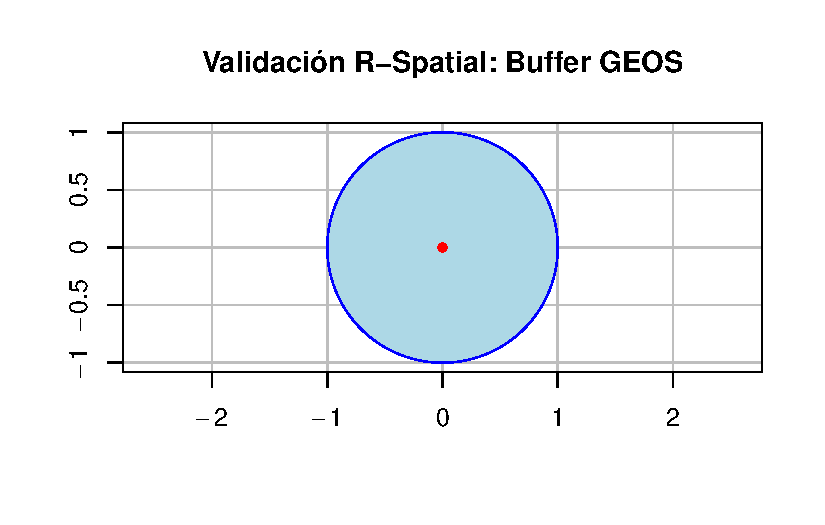
\includegraphics{81-uso_infraestructura_instalada_files/figure-pdf/r_verificacion-1.pdf}

\begin{verbatim}
✅ Visualización sf: Mapa generado con éxito
\end{verbatim}

\begin{Shaded}
\begin{Highlighting}[]
\CommentTok{\# 3. Prueba de Raster (terra)}
\FunctionTok{tryCatch}\NormalTok{(\{}
\NormalTok{  r }\OtherTok{\textless{}{-}} \FunctionTok{rast}\NormalTok{(}\AttributeTok{ncols=}\DecValTok{10}\NormalTok{, }\AttributeTok{nrows=}\DecValTok{10}\NormalTok{)}
  \FunctionTok{values}\NormalTok{(r) }\OtherTok{\textless{}{-}} \DecValTok{1}\SpecialCharTok{:}\FunctionTok{ncell}\NormalTok{(r)}
  \FunctionTok{cat}\NormalTok{(}\StringTok{"✅ Paquete \textquotesingle{}terra\textquotesingle{} operativo: Objetos Raster verificados}\SpecialCharTok{\textbackslash{}n}\StringTok{"}\NormalTok{)}
\NormalTok{\}, }\AttributeTok{error =} \ControlFlowTok{function}\NormalTok{(e) \{}
  \FunctionTok{cat}\NormalTok{(}\StringTok{"❌ Error en el stack terra:"}\NormalTok{, }\FunctionTok{conditionMessage}\NormalTok{(e), }\StringTok{"}\SpecialCharTok{\textbackslash{}n}\StringTok{"}\NormalTok{)}
\NormalTok{\})}
\end{Highlighting}
\end{Shaded}

\begin{verbatim}
✅ Paquete 'terra' operativo: Objetos Raster verificados
\end{verbatim}

\begin{Shaded}
\begin{Highlighting}[]
\FunctionTok{cat}\NormalTok{(}\StringTok{"{-}{-}{-} Verificación Finalizada {-}{-}{-}}\SpecialCharTok{\textbackslash{}n}\StringTok{"}\NormalTok{)}
\end{Highlighting}
\end{Shaded}

\begin{verbatim}
--- Verificación Finalizada ---
\end{verbatim}

\subsection{Julia}

\begin{Shaded}
\begin{Highlighting}[]
\CommentTok{\# 1. Ejecutamos toda la lógica diagnóstica con j\_eval usando println normal}
\FunctionTok{j\_eval}\NormalTok{(}\StringTok{\textquotesingle{}}
\StringTok{    \# Configuramos el entorno para que no pida monitor (Headless)}
\StringTok{    ENV["GKSwstype"] = "100" }
\StringTok{    }
\StringTok{    using LibPQ}
\StringTok{    using LibGEOS}
\StringTok{    using ArchGDAL}
\StringTok{    using Plots}
\StringTok{    gr()}

\StringTok{    println("{-}{-}{-} Inicio de Verificación de Julia SIG {-}{-}{-}")}

\StringTok{    \# 1. Prueba de conexión a PostGIS}
\StringTok{    try}
\StringTok{        conn = LibPQ.Connection("host=db{-}postgis dbname=sig\_db\_unal user=profe\_unal password=geomatica2025")}
\StringTok{        println("✅ Conexión a PostGIS: Exitosa")}
\StringTok{        close(conn)}
\StringTok{    catch e}
\StringTok{        println("❌ Error de conexión a PostGIS: ", e)}
\StringTok{    end}

\StringTok{    \# 2. Verificación de LibGEOS y Geometría}
\StringTok{    try}
\StringTok{        punto = LibGEOS.readgeom("POINT (0 0)")}
\StringTok{        buffer\_geom = LibGEOS.buffer(punto, 1.0)}
\StringTok{        println("✅ LibGEOS operativo: Motores geométricos verificados")}
\StringTok{        }
\StringTok{        \# Generamos el gráfico y lo guardamos directamente}
\StringTok{        plt = plot(buffer\_geom, }
\StringTok{                   title="Validación Julia SIG: Buffer GEOS", }
\StringTok{                   fillcolor=:blue, }
\StringTok{                   fillalpha=0.3, }
\StringTok{                   aspect\_ratio=:equal, }
\StringTok{                   legend=false)}
\StringTok{        }
\StringTok{        savefig(plt, "./images/verificacion\_geos.png")}
\StringTok{    catch e}
\StringTok{        println("❌ Error en LibGEOS o Visualización: ", e)}
\StringTok{    end}

\StringTok{    \# 3. Verificación de ArchGDAL}
\StringTok{    try}
\StringTok{        gdal\_ver = ArchGDAL.GDAL.gdalversioninfo("{-}{-}version")}
\StringTok{        println("✅ ArchGDAL operativo (Versión GDAL: ", gdal\_ver, ")")}
\StringTok{    catch e}
\StringTok{        println("❌ Error en ArchGDAL: ", e)}
\StringTok{    end}

\StringTok{    println("{-}{-}{-} Verificación Finalizada {-}{-}{-}")}
\StringTok{\textquotesingle{}}\NormalTok{)}
\end{Highlighting}
\end{Shaded}

\begin{verbatim}
Starting Julia ...
\end{verbatim}

\begin{Shaded}
\begin{Highlighting}[]
\CommentTok{\# 2. Insertamos el gráfico generado de forma segura}
\ControlFlowTok{if}\NormalTok{ (}\FunctionTok{file.exists}\NormalTok{(}\StringTok{"./images/verificacion\_geos.png"}\NormalTok{)) \{}
\NormalTok{  knitr}\SpecialCharTok{::}\FunctionTok{include\_graphics}\NormalTok{(}\StringTok{"./images/verificacion\_geos.png"}\NormalTok{)}
\NormalTok{\}}
\end{Highlighting}
\end{Shaded}

\begin{center}
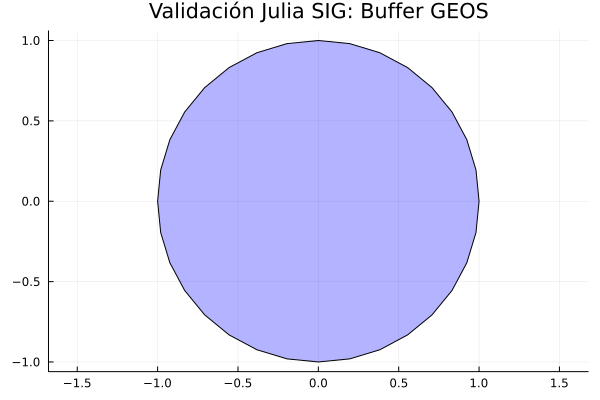
\includegraphics[width=0.85\textwidth,height=\textheight]{./images/verificacion_geos.png}
\end{center}

\begin{Shaded}
\begin{Highlighting}[]
\CommentTok{\# 1. Ejecutamos la validación técnica con j\_eval usando println normal}
\FunctionTok{j\_eval}\NormalTok{(}\StringTok{\textquotesingle{}}
\StringTok{    \# Configuración de entorno silencioso}
\StringTok{    ENV["GKSwstype"] = "100" }
\StringTok{    using LibPQ, LibGEOS, ArchGDAL, Plots}
\StringTok{    gr()}

\StringTok{    \# 1. Prueba de conexión a PostGIS}
\StringTok{    try}
\StringTok{        conn = LibPQ.Connection("host=db{-}postgis dbname=sig\_db\_unal user=profe\_unal password=geomatica2025")}
\StringTok{        println("✅ Conexión a PostGIS: Exitosa")}
\StringTok{        close(conn)}
\StringTok{    catch e}
\StringTok{        println("❌ Error de conexión: ", e)}
\StringTok{    end}

\StringTok{    \# 2. Prueba de Motores Geométricos (GEOS)}
\StringTok{    try}
\StringTok{        punto = LibGEOS.readgeom("POINT (0 0)")}
\StringTok{        buffer\_geom = LibGEOS.buffer(punto, 1.0)}
\StringTok{        println("✅ Motores geométricos operativos (GEOS)")}
\StringTok{        }
\StringTok{        \# Generamos la visualización y la guardamos físicamente}
\StringTok{        plt = plot(buffer\_geom, }
\StringTok{                   title="Validación SIG: Buffer GEOS", }
\StringTok{                   fillcolor=:blue, }
\StringTok{                   fillalpha=0.3, }
\StringTok{                   aspect\_ratio=:equal,}
\StringTok{                   legend=false)}
\StringTok{        }
\StringTok{        savefig(plt, "./images/verificacion\_sig\_final.png")}
\StringTok{    catch e}
\StringTok{        println("❌ Error en motores geométricos o gráficos: ", e)}
\StringTok{    end}
\StringTok{\textquotesingle{}}\NormalTok{)}
\end{Highlighting}
\end{Shaded}

\begin{verbatim}
<pre class='julia-code' style='display:block; background:#f4f6f8; border:1px solid #c0c8d0; border-radius:4px; padding:10px; margin-top:10px; margin-bottom:0; font-family:"Lucida Console", Consolas, monospace; font-size:0.9em; white-space:pre-wrap; color:#333;'>
<span style='color:#28a745; font-weight:bold;'>julia&gt; </span><span style='color:#008b8b;'># Configuración de entorno silencioso</span>
</pre>
<pre class='julia-output' style='display:block; background:#ffffff; border:none; padding:10px 10px 10px 20px; margin-top:0; margin-bottom:15px; font-family:"Lucida Console", Consolas, monospace; font-size:0.9em; white-space:pre-wrap; color:#000;'>

</pre>
<pre class='julia-code' style='display:block; background:#f4f6f8; border:1px solid #c0c8d0; border-radius:4px; padding:10px; margin-top:10px; margin-bottom:0; font-family:"Lucida Console", Consolas, monospace; font-size:0.9em; white-space:pre-wrap; color:#333;'>
<span style='color:#28a745; font-weight:bold;'>julia&gt; </span><span style='color:#008b8b;'>ENV["GKSwstype"] = "100"</span>
</pre>
<pre class='julia-output' style='display:block; background:#ffffff; border:none; padding:10px 10px 10px 20px; margin-top:0; margin-bottom:15px; font-family:"Lucida Console", Consolas, monospace; font-size:0.9em; white-space:pre-wrap; color:#000;'>
"100"

</pre>
<pre class='julia-code' style='display:block; background:#f4f6f8; border:1px solid #c0c8d0; border-radius:4px; padding:10px; margin-top:10px; margin-bottom:0; font-family:"Lucida Console", Consolas, monospace; font-size:0.9em; white-space:pre-wrap; color:#333;'>
<span style='color:#28a745; font-weight:bold;'>julia&gt; </span><span style='color:#008b8b;'>using LibPQ, LibGEOS, ArchGDAL, Plots</span>
</pre>
<pre class='julia-output' style='display:block; background:#ffffff; border:none; padding:10px 10px 10px 20px; margin-top:0; margin-bottom:15px; font-family:"Lucida Console", Consolas, monospace; font-size:0.9em; white-space:pre-wrap; color:#000;'>

</pre>
<pre class='julia-code' style='display:block; background:#f4f6f8; border:1px solid #c0c8d0; border-radius:4px; padding:10px; margin-top:10px; margin-bottom:0; font-family:"Lucida Console", Consolas, monospace; font-size:0.9em; white-space:pre-wrap; color:#333;'>
<span style='color:#28a745; font-weight:bold;'>julia&gt; </span><span style='color:#008b8b;'>gr()</span>
</pre>
<pre class='julia-output' style='display:block; background:#ffffff; border:none; padding:10px 10px 10px 20px; margin-top:0; margin-bottom:15px; font-family:"Lucida Console", Consolas, monospace; font-size:0.9em; white-space:pre-wrap; color:#000;'>
Plots.GRBackend()

</pre>
<pre class='julia-code' style='display:block; background:#f4f6f8; border:1px solid #c0c8d0; border-radius:4px; padding:10px; margin-top:10px; margin-bottom:0; font-family:"Lucida Console", Consolas, monospace; font-size:0.9em; white-space:pre-wrap; color:#333;'>
<span style='color:#28a745; font-weight:bold;'>julia&gt; </span><span style='color:#008b8b;'># 1. Prueba de conexión a PostGIS</span>
</pre>
<pre class='julia-output' style='display:block; background:#ffffff; border:none; padding:10px 10px 10px 20px; margin-top:0; margin-bottom:15px; font-family:"Lucida Console", Consolas, monospace; font-size:0.9em; white-space:pre-wrap; color:#000;'>

</pre>
<pre class='julia-code' style='display:block; background:#f4f6f8; border:1px solid #c0c8d0; border-radius:4px; padding:10px; margin-top:10px; margin-bottom:0; font-family:"Lucida Console", Consolas, monospace; font-size:0.9em; white-space:pre-wrap; color:#333;'>
<span style='color:#28a745; font-weight:bold;'>julia&gt; </span><span style='color:#008b8b;'>try</span>
       <span style='color:#008b8b;'>        conn = LibPQ.Connection("host=db-postgis dbname=sig_db_unal user=profe_unal password=geomatica2025")</span>
       <span style='color:#008b8b;'>        println("✅ Conexión a PostGIS: Exitosa")</span>
       <span style='color:#008b8b;'>        close(conn)</span>
       <span style='color:#008b8b;'>    catch e</span>
       <span style='color:#008b8b;'>        println("❌ Error de conexión: ", e)</span>
       <span style='color:#008b8b;'>    end</span>
</pre>
<pre class='julia-output' style='display:block; background:#ffffff; border:none; padding:10px 10px 10px 20px; margin-top:0; margin-bottom:15px; font-family:"Lucida Console", Consolas, monospace; font-size:0.9em; white-space:pre-wrap; color:#000;'>
✅ Conexión a PostGIS: Exitosa

</pre>
<pre class='julia-code' style='display:block; background:#f4f6f8; border:1px solid #c0c8d0; border-radius:4px; padding:10px; margin-top:10px; margin-bottom:0; font-family:"Lucida Console", Consolas, monospace; font-size:0.9em; white-space:pre-wrap; color:#333;'>
<span style='color:#28a745; font-weight:bold;'>julia&gt; </span><span style='color:#008b8b;'># 2. Prueba de Motores Geométricos (GEOS)</span>
</pre>
<pre class='julia-output' style='display:block; background:#ffffff; border:none; padding:10px 10px 10px 20px; margin-top:0; margin-bottom:15px; font-family:"Lucida Console", Consolas, monospace; font-size:0.9em; white-space:pre-wrap; color:#000;'>

</pre>
<pre class='julia-code' style='display:block; background:#f4f6f8; border:1px solid #c0c8d0; border-radius:4px; padding:10px; margin-top:10px; margin-bottom:0; font-family:"Lucida Console", Consolas, monospace; font-size:0.9em; white-space:pre-wrap; color:#333;'>
<span style='color:#28a745; font-weight:bold;'>julia&gt; </span><span style='color:#008b8b;'>try</span>
       <span style='color:#008b8b;'>        punto = LibGEOS.readgeom("POINT (0 0)")</span>
       <span style='color:#008b8b;'>        buffer_geom = LibGEOS.buffer(punto, 1.0)</span>
       <span style='color:#008b8b;'>        println("✅ Motores geométricos operativos (GEOS)")</span>
       <span style='color:#008b8b;'>        </span>
       <span style='color:#008b8b;'>        # Generamos la visualización y la guardamos físicamente</span>
       <span style='color:#008b8b;'>        plt = plot(buffer_geom, </span>
       <span style='color:#008b8b;'>                   title="Validación SIG: Buffer GEOS", </span>
       <span style='color:#008b8b;'>                   fillcolor=:blue, </span>
       <span style='color:#008b8b;'>                   fillalpha=0.3, </span>
       <span style='color:#008b8b;'>                   aspect_ratio=:equal,</span>
       <span style='color:#008b8b;'>                   legend=false)</span>
       <span style='color:#008b8b;'>        </span>
       <span style='color:#008b8b;'>        savefig(plt, "./images/verificacion_sig_final.png")</span>
       <span style='color:#008b8b;'>    catch e</span>
       <span style='color:#008b8b;'>        println("❌ Error en motores geométricos o gráficos: ", e)</span>
       <span style='color:#008b8b;'>    end</span>
</pre>
<pre class='julia-output' style='display:block; background:#ffffff; border:none; padding:10px 10px 10px 20px; margin-top:0; margin-bottom:15px; font-family:"Lucida Console", Consolas, monospace; font-size:0.9em; white-space:pre-wrap; color:#000;'>
✅ Motores geométricos operativos (GEOS)
"/home/rstudio/work/01_prog_sig/images/verificacion_sig_final.png"

</pre>
\end{verbatim}

\begin{Shaded}
\begin{Highlighting}[]
\CommentTok{\# 2. Si se generó el gráfico, lo incluimos de forma segura para R y Quarto}
\ControlFlowTok{if}\NormalTok{ (}\FunctionTok{file.exists}\NormalTok{(}\StringTok{"./images/verificacion\_sig\_final.png"}\NormalTok{)) \{}
\NormalTok{  knitr}\SpecialCharTok{::}\FunctionTok{include\_graphics}\NormalTok{(}\StringTok{"./images/verificacion\_sig\_final.png"}\NormalTok{)}
\NormalTok{\}}
\end{Highlighting}
\end{Shaded}

\begin{center}
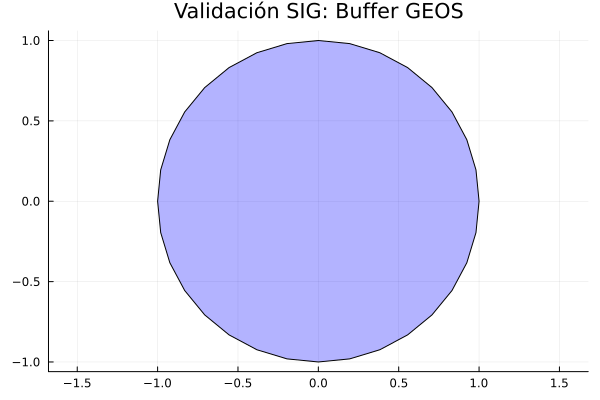
\includegraphics[width=0.85\textwidth,height=\textheight]{./images/verificacion_sig_final.png}
\end{center}

\chapter{Quarto: Orquestación y Configuración}\label{sec-anexo_quarto}

Quarto se basa en un archivo de configuración centralizado donde se
definen los parámetros de renderizado, bibliografía y estilos.

\section{\texorpdfstring{Opciones del encabezado
\texttt{yml}}{Opciones del encabezado yml}}\label{opciones-del-encabezado-yml}

\textbf{Ejemplo 1}: Solo HTML

\begin{Shaded}
\begin{Highlighting}[]
\CommentTok{{-}{-}{-}}
\AnnotationTok{title:}\CommentTok{ "Título de la Práctica"}
\AnnotationTok{author:}\CommentTok{ "Nombre del Estudiante"}
\AnnotationTok{date:}\CommentTok{ last{-}modified}
\AnnotationTok{format:}
\CommentTok{  html:}
\CommentTok{    toc: true}
\CommentTok{    toc{-}depth: 3}
\CommentTok{    toc{-}location: left}
\CommentTok{    number{-}sections: true}
\CommentTok{    theme: lux}
\CommentTok{{-}{-}{-}}
\end{Highlighting}
\end{Shaded}

\textbf{Ejemplo 2}: HTML y Python

\begin{Shaded}
\begin{Highlighting}[]
\CommentTok{{-}{-}{-}}
\AnnotationTok{title:}\CommentTok{ "Informe Técnico: Análisis Geoespacial"}
\AnnotationTok{author:}\CommentTok{ "ID Correo UNAL"}
\AnnotationTok{date:}\CommentTok{ today}
\AnnotationTok{format:}
\CommentTok{  html:}
\CommentTok{    toc: true}
\CommentTok{    number{-}sections: true}
\CommentTok{    theme: cosmo}
\CommentTok{  pdf:}
\CommentTok{    toc: true}
\CommentTok{    toc{-}title: "Contenido"}
\CommentTok{    number{-}sections: true}
\CommentTok{    documentclass: scrreprt}
\CommentTok{    geometry:}
\CommentTok{      {-} top=25mm}
\CommentTok{      {-} left=25mm}
\CommentTok{      {-} right=25mm}
\CommentTok{      {-} bottom=25mm}
\CommentTok{{-}{-}{-}}
\end{Highlighting}
\end{Shaded}

\section{Resumen de comandos Quarto}\label{resumen-de-comandos-quarto}

Renderizar todos los formatos definidos en el encabezado \texttt{yml}:

\begin{Shaded}
\begin{Highlighting}[]
\ExtensionTok{quarto}\NormalTok{ render archivo.qmd }\AttributeTok{{-}{-}to}\NormalTok{ all}
\end{Highlighting}
\end{Shaded}

Renderizar a HTML:

\begin{Shaded}
\begin{Highlighting}[]
\ExtensionTok{quarto}\NormalTok{ render archivo.qmd }\AttributeTok{{-}{-}to}\NormalTok{ html}
\end{Highlighting}
\end{Shaded}

Renderizar a PDF:

\begin{Shaded}
\begin{Highlighting}[]
\ExtensionTok{quarto}\NormalTok{ render archivo.qmd }\AttributeTok{{-}{-}to}\NormalTok{ pdf}
\end{Highlighting}
\end{Shaded}

Renderizar a PDF, mostrando todos los detalles en la consola:

\begin{Shaded}
\begin{Highlighting}[]
\ExtensionTok{quarto}\NormalTok{ render archivo.qmd }\AttributeTok{{-}{-}to}\NormalTok{ pdf }\AttributeTok{{-}{-}trace} \AttributeTok{{-}{-}verbose}\KeywordTok{\textasciigrave{}}
\VariableTok{QUARTO\_LOG\_LEVEL}\OperatorTok{=}\NormalTok{debug }\ExtensionTok{quarto}\NormalTok{ render archivo.qmd }\AttributeTok{{-}{-}to}\NormalTok{ pdf}
\end{Highlighting}
\end{Shaded}

Chequear estado de instalación de Quarto

\begin{Shaded}
\begin{Highlighting}[]
\ExtensionTok{quarto}\NormalTok{ check}
\end{Highlighting}
\end{Shaded}

\section{Gestión Eficiente de Renderizado en
Quarto}\label{gestiuxf3n-eficiente-de-renderizado-en-quarto}

A continuación, se presenta la hoja de ruta para optimizar los tiempos
de compilación de tu libro, especialmente cuando trabajas con motores
pesados de Julia y R.

\subsection{Hoja de Referencia: Comandos de
Renderizado}\label{hoja-de-referencia-comandos-de-renderizado}

La ejecución de estos comandos depende de la existencia del archivo
\texttt{\_quarto.yml} en la carpeta de proyecto. Si desea trabajar con
archivos individuales puede cambiar temporalmente el nombre de este
archivo a \texttt{\_quarto.yml.back}

\begin{longtable}[]{@{}
  >{\raggedright\arraybackslash}p{(\columnwidth - 2\tabcolsep) * \real{0.4000}}
  >{\raggedright\arraybackslash}p{(\columnwidth - 2\tabcolsep) * \real{0.6000}}@{}}
\caption{Comandos esenciales para la gestión de flujos en
Quarto}\label{tbl-quarto-comandos}\tabularnewline
\toprule\noalign{}
\begin{minipage}[b]{\linewidth}\raggedright
Acción
\end{minipage} & \begin{minipage}[b]{\linewidth}\raggedright
Comando
\end{minipage} \\
\midrule\noalign{}
\endfirsthead
\toprule\noalign{}
\begin{minipage}[b]{\linewidth}\raggedright
Acción
\end{minipage} & \begin{minipage}[b]{\linewidth}\raggedright
Comando
\end{minipage} \\
\midrule\noalign{}
\endhead
\bottomrule\noalign{}
\endlastfoot
\textbf{Trabajar en vivo} (Previsualización dinámica) &
\texttt{quarto\ preview} \\
\textbf{Renderizar solo el capítulo actual} &
\texttt{quarto\ render\ archivo.qmd} \\
\textbf{Generar el libro completo} (Ensamblaje final) &
\texttt{quarto\ render} \\
\textbf{Forzar ejecución total} (Ignorar el \texttt{freeze}) &
\texttt{quarto\ render\ -\/-execute} \\
\end{longtable}

\begin{center}\rule{0.5\linewidth}{0.5pt}\end{center}

\subsection{Trucos extra para un flujo de autor
ágil}\label{trucos-extra-para-un-flujo-de-autor-uxe1gil}

Para evitar esperas innecesarias y optimizar tu productividad, aplica
estas estrategias de previsualización y almacenamiento de resultados:

\subsubsection{\texorpdfstring{1. El flujo de edición en vivo
(\texttt{quarto\ preview})}{1. El flujo de edición en vivo (quarto preview)}}\label{el-flujo-de-ediciuxf3n-en-vivo-quarto-preview}

En lugar de renderizar el libro manualmente cada vez que haces un
cambio, abre una terminal en la raíz de tu proyecto y ejecuta el comando
de previsualización.

Al usar este comando, se levantará un servidor local. Cada vez que
realices una edición en tu archivo \texttt{.qmd} y presiones
\textbf{\texttt{Ctrl\ +\ S}} (Guardar), Quarto detectará el cambio y
refrescará \textbf{únicamente} ese capítulo en tu navegador. Esto
mantiene la sesión de Julia/R ``tibia'' y permite ver cambios casi
instantáneos en mapas y ecuaciones.

\subsubsection{\texorpdfstring{2. Uso de Caché para procesos pesados
(\texttt{\#\textbar{}\ cache:\ true})}{2. Uso de Caché para procesos pesados (\#\textbar{} cache: true)}}\label{uso-de-cachuxe9-para-procesos-pesados-cache-true}

Si tienes un bloque de código que realiza una tarea costosa (como una
conexión a PostGIS o un análisis ráster masivo en Julia), no permitas
que se ejecute cada vez que guardas el archivo. Utiliza la opción de
caché a nivel de celda:

\begin{Shaded}
\begin{Highlighting}[]
\CommentTok{\#| label: analisis{-}espacial{-}costoso}
\CommentTok{\#| cache: true}
\CommentTok{\#| results: asis}

\CommentTok{\# Este código solo se ejecutará de nuevo si modificas el contenido de este bloque.}
\CommentTok{\# Quarto guarda los resultados en la carpeta \textquotesingle{}\_cache\textquotesingle{} para reutilizarlos.}
\FunctionTok{j\_eval}\NormalTok{(}\StringTok{" ... proceso de Julia que tarda varios minutos ... "}\NormalTok{)}
\end{Highlighting}
\end{Shaded}

\begin{quote}
\textbf{Nota de experto:} Mientras que \texttt{freeze:\ auto} (en el
\texttt{\_quarto.yml}) protege tus capítulos terminados para que no se
re-ejecuten al compilar el libro completo, el uso de
\texttt{\#\textbar{}\ cache:\ true} protege tu flujo de trabajo diario
dentro del capítulo que estás escribiendo actualmente.
\end{quote}

\section{\texorpdfstring{Control de ejecución en Quarto - opciones de
\texttt{chunks}}{Control de ejecución en Quarto - opciones de chunks}}\label{sec-opciones-chunks}

Para que sus informes técnicos sean profesionales, no basta con que el
código funcione; es necesario controlar qué se muestra y qué se oculta
al lector final. En Quarto, esto se logra mediante el uso de ``opciones
de chunk'' utilizando la sintaxis de la tubería de comentarios
(\texttt{\#\textbar{}}).

\begin{longtable}[]{@{}
  >{\raggedright\arraybackslash}p{(\columnwidth - 8\tabcolsep) * \real{0.1739}}
  >{\centering\arraybackslash}p{(\columnwidth - 8\tabcolsep) * \real{0.2174}}
  >{\centering\arraybackslash}p{(\columnwidth - 8\tabcolsep) * \real{0.2174}}
  >{\centering\arraybackslash}p{(\columnwidth - 8\tabcolsep) * \real{0.2174}}
  >{\raggedright\arraybackslash}p{(\columnwidth - 8\tabcolsep) * \real{0.1739}}@{}}
\toprule\noalign{}
\begin{minipage}[b]{\linewidth}\raggedright
Opción de Chunk
\end{minipage} & \begin{minipage}[b]{\linewidth}\centering
¿Se ejecuta?
\end{minipage} & \begin{minipage}[b]{\linewidth}\centering
¿Muestra el Código?
\end{minipage} & \begin{minipage}[b]{\linewidth}\centering
¿Muestra Resultados / Plots?
\end{minipage} & \begin{minipage}[b]{\linewidth}\raggedright
Uso Ideal
\end{minipage} \\
\midrule\noalign{}
\endhead
\bottomrule\noalign{}
\endlastfoot
\textbf{\texttt{\#\textbar{}\ echo:\ false}} & ✅ SÍ & ❌ NO & ✅ SÍ &
\textbf{Para Resultados Finales.} Muestra el mapa/tabla sin la
``receta''. \\
\textbf{\texttt{\#\textbar{}\ include:\ false}} & ✅ SÍ & ❌ NO & ❌ NO
& \textbf{Para el Setup.} Corre todo en secreto, sin mensajes ni
advertencias. \\
\textbf{\texttt{\#\textbar{}\ code-fold:\ true}} & ✅ SÍ & 📂 Plegado &
✅ SÍ & \textbf{Para el Proceso.} El código se oculta tras un botón
``Code''. \\
\textbf{\texttt{\#\textbar{}\ eval:\ false}} & ❌ NO & ✅ SÍ & ❌ NO &
\textbf{Para Tutoriales.} Solo muestra el texto del código sin
procesarlo. \\
\textbf{\texttt{\#\textbar{}\ output:\ false}} & ✅ SÍ & ✅ SÍ & ❌ NO &
\textbf{Para Debugging.} Ves su código pero no los resultados
pesados. \\
\textbf{\texttt{\#\textbar{}\ warning:\ false}} & ✅ SÍ & - & - & Oculta
esos textos naranjas de advertencia de las librerías. \\
\textbf{\texttt{\#\textbar{}\ message:\ false}} & ✅ SÍ & - & - & Oculta
mensajes de carga (ej: ``Loading terra package\ldots{}''). \\
\end{longtable}

\subsection{Recomendaciones de uso según el
contexto}\label{recomendaciones-de-uso-seguxfan-el-contexto}

Dependiendo de la parte del script en la que se encuentre, existen
configuraciones que garantizan un documento más limpio y fluido:

\begin{longtable}[]{@{}
  >{\raggedright\arraybackslash}p{(\columnwidth - 4\tabcolsep) * \real{0.3333}}
  >{\raggedright\arraybackslash}p{(\columnwidth - 4\tabcolsep) * \real{0.3333}}
  >{\raggedright\arraybackslash}p{(\columnwidth - 4\tabcolsep) * \real{0.3333}}@{}}
\toprule\noalign{}
\begin{minipage}[b]{\linewidth}\raggedright
Tipo de Chunk
\end{minipage} & \begin{minipage}[b]{\linewidth}\raggedright
Opción recomendada
\end{minipage} & \begin{minipage}[b]{\linewidth}\raggedright
¿Por qué?
\end{minipage} \\
\midrule\noalign{}
\endhead
\bottomrule\noalign{}
\endlastfoot
\textbf{Setup / Librerías} & \texttt{\#\textbar{}\ include:\ false} &
Ejecuta todo pero oculta el código y los mensajes de carga de
R/Julia/Python. \\
\textbf{Limpieza de RAM} & \texttt{\#\textbar{}\ include:\ false} &
Borra objetos y vacía el cache en silencio. El lector no necesita ver la
``limpieza''. \\
\textbf{Procesamiento} & \texttt{\#\textbar{}\ code-fold:\ true} &
Muestra el mapa pero esconde el código tras un clic. Ideal para
transparencia académica. \\
\textbf{Resultados Finales} & \texttt{\#\textbar{}\ echo:\ false} &
Muestra solo la tabla comparativa y conclusiones. Es el ``veredicto''
limpio y profesional. \\
\end{longtable}

\begin{tcolorbox}[enhanced jigsaw, coltitle=black, leftrule=.75mm, bottomtitle=1mm, title=\textcolor{quarto-callout-tip-color}{\faLightbulb}\hspace{0.5em}{Sintaxis Correcta}, colback=white, colbacktitle=quarto-callout-tip-color!10!white, left=2mm, toptitle=1mm, rightrule=.15mm, titlerule=0mm, arc=.35mm, colframe=quarto-callout-tip-color-frame, bottomrule=.15mm, toprule=.15mm, opacityback=0, opacitybacktitle=0.6, breakable]

Recuerde que las opciones deben ir al inicio del chunk, justo después de
los corchetes del lenguaje:

\begin{Shaded}
\begin{Highlighting}[]
\CommentTok{\#| echo: false}
\CommentTok{\#| warning: false}
\FunctionTok{library}\NormalTok{(terra)}
\CommentTok{\# Su código aquí...}
\end{Highlighting}
\end{Shaded}

\end{tcolorbox}

\section{Instalación de Extensiones de
Quarto}\label{instalaciuxf3n-de-extensiones-de-quarto}

Las extensiones permiten ampliar las funcionalidades nativas de Quarto,
añadiendo nuevos formatos de salida, filtros personalizados o librerías
de componentes visuales. Para que el proceso de descarga desde
repositorios remotos sea exitoso y seguro, es fundamental haber
completado previamente la configuración descrita en la
Sección~\ref{sec-ssh-linux}.

\subsection{El proceso de
instalación}\label{el-proceso-de-instalaciuxf3n}

Para agregar una extensión a tu proyecto, Quarto utiliza el comando
\texttt{add} seguido del identificador del repositorio (usualmente
\texttt{usuario/repositorio}). Este proceso descarga los archivos
necesarios dentro de una carpeta local denominada
\texttt{\_extensions/}.

\subsubsection{Ejemplo práctico: Librería de iconos
FontAwesome}\label{ejemplo-pruxe1ctico-libreruxeda-de-iconos-fontawesome}

Como caso de estudio, instalaremos la extensión oficial para el uso de
iconos vectoriales. Ejecuta el siguiente comando en tu terminal:

\begin{Shaded}
\begin{Highlighting}[]
\ExtensionTok{quarto}\NormalTok{ add quarto{-}ext/fontawesome}
\end{Highlighting}
\end{Shaded}

\begin{tcolorbox}[enhanced jigsaw, coltitle=black, leftrule=.75mm, bottomtitle=1mm, title=\textcolor{quarto-callout-note-color}{\faInfo}\hspace{0.5em}{Confianza del Autor}, colback=white, colbacktitle=quarto-callout-note-color!10!white, left=2mm, toptitle=1mm, rightrule=.15mm, titlerule=0mm, arc=.35mm, colframe=quarto-callout-note-color-frame, bottomrule=.15mm, toprule=.15mm, opacityback=0, opacitybacktitle=0.6, breakable]

Al ejecutar el comando, el sistema solicitará confirmar si confías en
los autores de la extensión. Escribe \texttt{Y} para permitir que Quarto
gestione los archivos del filtro en tu directorio de trabajo.

\end{tcolorbox}

\subsection{Gestión de archivos del
proyecto}\label{gestiuxf3n-de-archivos-del-proyecto}

Una vez finalizada la instalación, notarás que en la raíz de tu proyecto
se ha creado la siguiente estructura:

\begin{Shaded}
\begin{Highlighting}[]
\NormalTok{mi{-}proyecto/}
\NormalTok{├── \_extensions/}
\NormalTok{│   └── quarto{-}ext/}
\NormalTok{│       └── fontawesome/}
\NormalTok{└── tu{-}archivo.qmd}
\end{Highlighting}
\end{Shaded}

Es importante \textbf{no modificar manualmente} los archivos dentro de
la carpeta \texttt{\_extensions}, ya que Quarto los requiere para
procesar el documento final durante el renderizado.

\subsection{Aplicación en el
documento}\label{aplicaciuxf3n-en-el-documento}

Tras la instalación exitosa, puedes utilizar las nuevas funcionalidades
mediante \emph{shortcodes}. En el caso de nuestra extensión de ejemplo,
ahora es posible insertar iconos de la siguiente manera:

\begin{Shaded}
\begin{Highlighting}[]
\NormalTok{Para este análisis utilizaremos:}

\NormalTok{* \{\{\textless{} fa satellite \textgreater{}\}\} Datos satelitales.}
\NormalTok{* \{\{\textless{} fa location{-}dot "red" \textgreater{}\}\} Puntos de control terrestre.}
\end{Highlighting}
\end{Shaded}

\begin{tcolorbox}[enhanced jigsaw, coltitle=black, leftrule=.75mm, bottomtitle=1mm, title=\textcolor{quarto-callout-tip-color}{\faLightbulb}\hspace{0.5em}{Actualización de extensiones}, colback=white, colbacktitle=quarto-callout-tip-color!10!white, left=2mm, toptitle=1mm, rightrule=.15mm, titlerule=0mm, arc=.35mm, colframe=quarto-callout-tip-color-frame, bottomrule=.15mm, toprule=.15mm, opacityback=0, opacitybacktitle=0.6, breakable]

Si en el futuro deseas actualizar una extensión instalada a su última
versión, simplemente vuelve a ejecutar el mismo comando
\texttt{quarto\ add}. El sistema detectará la versión existente y te
preguntará si deseas sobrescribirla.

\end{tcolorbox}

\chapter{Docker: Gestión de Contenedores e
Imágenes}\label{sec-anexo_docker}

Docker es un motor de virtualización (\citeproc{ref-docker2025}{Inc.,
2025}) en el que instalaremos las dos máquinas virtuales Linux que
permitirán la ejecución de código Python, R y Julia y el acceso a
PostGIS + PostgreSQL.

\section{Instalación del software}\label{instalaciuxf3n-del-software}

Descargue e instale la versión oficial de \textbf{Docker Desktop} desde
el siguiente enlace:

\begin{itemize}
\tightlist
\item
  \textbf{URL}: \url{https://www.docker.com/products/docker-desktop/}
\item
  Descargue la versión más reciente para el sistema operativo de su
  máquina local y verifique que el instalador coincida con la
  arquitectura de su máquina.
\item
  \textbf{Instalación}: Para instalar en una carpeta específica (ej:
  \texttt{E:\textbackslash{}Docker}) seleccionada por el usuario.
  Ejecute en PowerShell como administrador. Asegúrese de aceptar la
  actualización del kernel de WSL 2 si el sistema lo solicita, o
  previamente usar en el terminal \texttt{wsl\ -\/-update}. Durante la
  instalación, asegúrese de activar la opción \textbf{``Use WSL 2
  instead of Hyper-V''}.
\end{itemize}

\begin{Shaded}
\begin{Highlighting}[]
\ExtensionTok{Start{-}Process} \StringTok{"Docker Desktop Installer.exe"} \AttributeTok{{-}ArgumentList} \StringTok{"install"}\NormalTok{, }\StringTok{"{-}{-}installation{-}dir=E:\textbackslash{}Docker"} \AttributeTok{{-}Wait}
\end{Highlighting}
\end{Shaded}

\begin{itemize}
\tightlist
\item
  \textbf{Instalación alternativa}: Ejecute el instalador y asegúrese de
  aceptar la actualización del kernel de WSL 2 si el sistema lo
  solicita, o previamente usar en el terminal \texttt{wsl\ -\/-update}.
  Durante la instalación, asegúrese de activar la opción \textbf{``Use
  WSL 2 instead of Hyper-V''}.
\end{itemize}

\section{Preparación Docker Desktop}\label{sec-preparacion_docker}

Antes de iniciar la carga o instalación de imágenes/contenedores, es
imperativo configurar el entorno local:

\begin{itemize}
\item
  \textbf{Configuración de Almacenamiento}: Debido a que la imagen
  políglota y la base de datos requieren un espacio considerable,
  asegúrese de que el disco donde Docker guarda sus archivos
  \texttt{.vhdx} tenga al menos \textbf{50 GB de espacio libre}. Tenga
  en cuenta que el tamaño en disco de las dos imágenes Docker, una vez
  instaladas, es de aproximadamente \textbf{45 GB}.
\item
  \textbf{Procedimiento para cambiar la ubicación de las imágenes}
  (archivos con extensión \texttt{.vhdx}): Si su disco principal
  (\texttt{C:}) está sin espacio, mueva los archivos Docker a otro
  disco. En Docker Desktop:

  \begin{enumerate}
  \def\labelenumi{\alph{enumi}.}
  \tightlist
  \item
    Diríjase a \textbf{Settings} (engranaje) -\textgreater{}
    \textbf{Resources} -\textgreater{} \textbf{Advanced}.
  \item
    Localice \textbf{Disk image location}.
  \item
    Haga clic en \texttt{Browse} y seleccione una carpeta en un disco
    con mayor capacidad.
  \item
    Haga clic en \textbf{Apply \& restart}.
  \end{enumerate}
\item
  \textbf{Optimización de Memoria Swap}: Para procesar datos raster de
  gran tamaño sin interrupciones en R o Julia, es fundamental ampliar la
  memoria Swap (espacio de intercambio). Puede consultar más detalles en
  la Sección~\ref{sec-limpieza_entorno} sobre cómo esto impacta el
  rendimiento.
\item
  \textbf{Procedimiento para aumentar Swap en Windows (Host)}: Ajuste la
  memoria virtual del sistema operativo para evitar cierres por falta de
  RAM:

  \begin{enumerate}
  \def\labelenumi{\alph{enumi}.}
  \tightlist
  \item
    En el buscador de Windows, escriba y seleccione \textbf{``Ver la
    configuración avanzada del sistema''}.
  \item
    En la pestaña \textbf{Opciones avanzadas}, sección
    \textbf{Rendimiento}, haga clic en el botón \texttt{Configuración}.
  \item
    Diríjase a \textbf{Opciones avanzadas} -\textgreater{}
    \textbf{Memoria Virtual} y haga clic en \texttt{Cambiar}.
  \item
    Desmarque ``Administrar automáticamente'', seleccione el disco
    principal, elija \textbf{Tamaño personalizado} y asigne estos
    valores sugeridos, que dependen del espacio disponible en el disco
    (verifíquelo): Inicial \textbf{16384 MB} / Máximo \textbf{32768 MB}.
  \item
    Haga clic en \texttt{Establecer} y luego en \textbf{Aceptar}
    (requerirá reiniciar el equipo).
  \end{enumerate}
\item
  \textbf{Configuración de Swap en el Contenedor (WSL2)}: Dado que
  Docker opera sobre el subsistema Linux, debe configurar el archivo de
  intercambio global de WSL2:

  \begin{enumerate}
  \def\labelenumi{\alph{enumi}.}
  \tightlist
  \item
    Abra el explorador de archivos y diríjase a su carpeta de usuario
    (escriba \texttt{\%USERPROFILE\%} en la barra de direcciones).
  \item
    Cree un archivo nuevo llamado \texttt{.wslconfig} (asegúrese de que
    no tenga extensión \texttt{.txt} al final).
  \item
    Defina la RAM (\texttt{memory}) y asegure suficiente memoria
    \texttt{swap} (ej: \textbf{32 GB de swap}) para sus procesos
    espaciales (sugerido, depende de su espacio en disco).
  \item
    Cambie la ruta del archivo \texttt{swap.vhdx} a un disco veloz y con
    suficiente espacio de disco.
  \end{enumerate}
\end{itemize}

\begin{Shaded}
\begin{Highlighting}[]
\KeywordTok{[wsl2]}
\DataTypeTok{memory}\OtherTok{=}\StringTok{12GB \# RAM máxima física asignada a Linux}
\DataTypeTok{swap}\OtherTok{=}\StringTok{32GB   \# Memoria de intercambio para evitar el cierre de contenedores}
\DataTypeTok{swapfile}\OtherTok{=}\StringTok{X:\textbackslash{}RutaConSuficienteEspacioEnDisco\textbackslash{}\textbackslash{}swap.vhdx}
\end{Highlighting}
\end{Shaded}

\begin{tcolorbox}[enhanced jigsaw, coltitle=black, leftrule=.75mm, bottomtitle=1mm, title=\textcolor{quarto-callout-tip-color}{\faLightbulb}\hspace{0.5em}{Importante}, colback=white, colbacktitle=quarto-callout-tip-color!10!white, left=2mm, toptitle=1mm, rightrule=.15mm, titlerule=0mm, arc=.35mm, colframe=quarto-callout-tip-color-frame, bottomrule=.15mm, toprule=.15mm, opacityback=0, opacitybacktitle=0.6, breakable]

Si desea verificar si estos cambios surtieron efecto dentro de su
laboratorio, puede ejecutar el comando \texttt{free\ -h} en la terminal
de Jupyter o VSCode.

\end{tcolorbox}

\section{Limpieza del entorno}\label{sec-limpieza_entorno}

\subsection{Eliminar todas las imagenes/contenedores y liberar todo el
espacio usado por
Docker.}\label{eliminar-todas-las-imagenescontenedores-y-liberar-todo-el-espacio-usado-por-docker.}

\begin{quote}
\textbf{⚠️ Advertencia}: Los siguientes comandos eliminarán todos los
contenedores, imágenes y volúmenes existentes en su sistema. Úselos solo
si no tiene contenedores o imágenes que desee preservar.
\end{quote}

Ejecute estos comandos en su terminal (PowerShell) para liberar espacio
y evitar conflictos:

\begin{Shaded}
\begin{Highlighting}[]
\CommentTok{\# Detener y eliminar todos los contenedores}
\ExtensionTok{docker}\NormalTok{ stop }\VariableTok{$(}\ExtensionTok{docker}\NormalTok{ ps }\AttributeTok{{-}aq}\VariableTok{)}
\ExtensionTok{docker}\NormalTok{ rm }\AttributeTok{{-}f} \VariableTok{$(}\ExtensionTok{docker}\NormalTok{ ps }\AttributeTok{{-}aq}\VariableTok{)}

\CommentTok{\# Eliminar todas las imágenes}
\ExtensionTok{docker}\NormalTok{ rmi }\AttributeTok{{-}f} \VariableTok{$(}\ExtensionTok{docker}\NormalTok{ images }\AttributeTok{{-}aq}\VariableTok{)}

\CommentTok{\# Eliminar todos los volúmenes (libera MUCHO espacio)}
\ExtensionTok{docker}\NormalTok{ volume rm }\VariableTok{$(}\ExtensionTok{docker}\NormalTok{ volume ls }\AttributeTok{{-}q}\VariableTok{)}

\CommentTok{\# Eliminar redes de usuario (no borra bridge/host/none)}
\ExtensionTok{docker}\NormalTok{ network rm }\VariableTok{$(}\ExtensionTok{docker}\NormalTok{ network ls }\AttributeTok{{-}q} \KeywordTok{|} \ExtensionTok{Select{-}String} \AttributeTok{{-}NotMatch} \StringTok{"bridge|host|none"}\VariableTok{)}

\CommentTok{\# Eliminar caché de construcción}
\ExtensionTok{docker}\NormalTok{ builder prune }\AttributeTok{{-}a} \AttributeTok{{-}f}

\CommentTok{\# OPCIÓN MÁS SIMPLE (Todo en un solo comando)}
\CommentTok{\# docker system prune {-}a {-}{-}volumes {-}f}
\end{Highlighting}
\end{Shaded}

Para verificar el espacio liberado, use: \texttt{docker\ system\ df}. El
resultado debería mostrar valores cercanos a \textbf{0 bytes}.

\subsection{Comandos de rescate de
espacio}\label{comandos-de-rescate-de-espacio}

El entorno políglota de este curso es robusto y, por lo tanto, pesado.
Tras realizar actualizaciones o varias pruebas de construcción, es
posible que el espacio en disco se agote rápidamente.

Si recibe errores de ``Disk Full'' o desea limpiar su sistema, ejecute
los siguientes comandos en su terminal de Windows (PowerShell):

\begin{Shaded}
\begin{Highlighting}[]
\CommentTok{\# 1. Eliminar contenedores detenidos y redes en desuso}
\NormalTok{docker system prune }\OperatorTok{{-}}\NormalTok{f}

\CommentTok{\# 2. Limpiar caché de construcción (libera mucho espacio tras errores de build)}
\NormalTok{docker builder prune }\OperatorTok{{-}}\NormalTok{f}

\CommentTok{\# 3. (Uso extremo) Eliminar TODAS las imágenes que no estén siendo usadas}
\CommentTok{\# docker image prune {-}a {-}f}
\end{Highlighting}
\end{Shaded}

\begin{tcolorbox}[enhanced jigsaw, coltitle=black, leftrule=.75mm, bottomtitle=1mm, title=\textcolor{quarto-callout-tip-color}{\faLightbulb}\hspace{0.5em}{Seguridad de sus Datos}, colback=white, colbacktitle=quarto-callout-tip-color!10!white, left=2mm, toptitle=1mm, rightrule=.15mm, titlerule=0mm, arc=.35mm, colframe=quarto-callout-tip-color-frame, bottomrule=.15mm, toprule=.15mm, opacityback=0, opacitybacktitle=0.6, breakable]

No tema realizar limpiezas periódicas. Gracias a la configuración de
volúmenes en nuestro archivo \texttt{docker-compose.yml}, todo su
código, scripts y datos espaciales están \textbf{físicamente en su disco
local} (en la carpeta de su ID UNAL).

Al apagar o borrar el contenedor, lo que está dentro de
\texttt{/home/rstudio/work/} \textbf{siempre estará a salvo} en su
carpeta de Windows. El contenedor es solo el ``motor'', sus archivos son
el ``combustible'' que usted posee.

\end{tcolorbox}

\section{Descarga y preparación de archivos}\label{sec-descarga_tar_yml}

Siga estos pasos para obtener la imagen base:

\begin{enumerate}
\def\labelenumi{\arabic{enumi}.}
\tightlist
\item
  \textbf{Descarga}: Obtenga el archivo de 15.5 GB desde el siguiente
  enlace:
  \href{https://drive.google.com/file/d/1J7ssf72-F5EwjoekkexwKUgD1DxyA1xk/view?usp=sharing}{Google
  Drive - sig\_unal\_completo.zip}.
\item
  \textbf{Descompresión Parte A}: Extraiga el contenido de
  \texttt{sig\_unal\_completo.zip}.
\item
  \textbf{Renombrado}: Al archivo resultante llamado
  \texttt{sig\_unal\_completo.txt}, cámbiele manualmente la extensión a
  \texttt{.zip}.
\item
  \textbf{Descompresión Parte B}: Extraiga este nuevo archivo
  \texttt{.zip} para obtener los dos archivos definitivos:

  \begin{itemize}
  \tightlist
  \item
    \texttt{sig\_unal\_completo.tar} (El archivo de la imagen).
  \item
    \texttt{docker-compose.yml} (El \textbf{NUEVO} archivo de
    orquestación contenido en la descarga).
  \end{itemize}
\end{enumerate}

\section{\texorpdfstring{Cargar imagen/contenedor a partir de
imagen/contenedor base guardada en \texttt{sig\_unal\_completo.tar} y
\texttt{docker-compose.html}}{Cargar imagen/contenedor a partir de imagen/contenedor base guardada en sig\_unal\_completo.tar y docker-compose.html}}\label{sec-cargar_docker_tar}

Este procedimiento instalará (mediante carga, es decir sin compilación)
dos imágenes (una con la base de datos espacial y otra con Python, R y
Julia) y configurará una red interna para comunicar su máquina
anfitriona (Windows) con las dos máquinas virtuales Linux.

Desde una terminal situada en la carpeta que contiene los archivos
\texttt{sig\_unal\_completo.tar} y \texttt{docker-compose.yml}, ejecute:

\begin{Shaded}
\begin{Highlighting}[]
\ExtensionTok{docker}\NormalTok{ load }\AttributeTok{{-}i}\NormalTok{ sig\_unal\_completo.tar}
\end{Highlighting}
\end{Shaded}

\emph{Este proceso puede tardar varios minutos o inclusive horas
dependiendo de su procesador y disco duro. Verifique que al finalizar
aparezca el mensaje ``Loaded image'' para
\texttt{image\_sig\_unal:final} y \texttt{postgis\_unal:final}.}

\begin{quote}
Nota: Existen dos versiones \textbf{diferentes} del archivo
\texttt{docker-compose.html}. El primero es el que se describe en
Sección~\ref{sec-build_docker} y el segundo, que aplica para este
procedimiento, es el que se descarga en
Sección~\ref{sec-descarga_tar_yml}.
\end{quote}

\subsection{\texorpdfstring{Archivo \texttt{docker-compose.yml}
(orquestación)}{Archivo docker-compose.yml (orquestación)}}\label{sec-docker_compose_load}

Este archivo es el \textbf{manifiesto técnico} que automatiza la
construcción y coordinación de los servicios del curso. Su propósito es
definir las reglas de convivencia entre los contenedores, configurando
los siguientes pilares:

\begin{itemize}
\tightlist
\item
  \textbf{Imágenes}: Versiones exactas de software (GDAL/Ubuntu para
  análisis y PostGIS para datos).
\item
  \textbf{Puertos}: Mapeos específicos para acceder a las herramientas
  desde el equipo local sin conflictos (8889 para Jupyter, 8788 para el
  visor de R y 5434 para la base de datos).
\item
  \textbf{Volúmenes}: Garantizan la persistencia de datos, sincronizando
  su carpeta local en tiempo real con el entorno interno del contenedor.
\end{itemize}

A continuación, se describen los dos servicios integrados en este
manifiesto:

\begin{itemize}
\item
  \textbf{Servicio de Análisis (\texttt{analisis-geo})}: Identificado en
  el archivo como \texttt{analisis-geo}, este servicio no usa
  \texttt{Dockerfile} (la etiqueta \texttt{build:\ .} está no está
  habilitada). Es el motor políglota encargado de procesar R, Python y
  Julia sobre una base robusta de GDAL. Incluye una configuración de
  \texttt{LD\_PRELOAD} para la estabilidad de las librerías dinámicas y
  una integración profunda que permite usar el visor \texttt{httpgd} de
  R como terminal gráfica unificada para todos los lenguajes. Crea el
  contenedor \texttt{contenedor\_sig\_unal}. La carpeta
  \texttt{/home/rstudio/work} del contenedor, mapea la carpeta del
  equipo local donde instaló las imágenes y contenedores a partir de
  \texttt{sig\_unal\_completo.tar} y \texttt{docker-compose.yml}.
\item
  \textbf{Servicio PostGIS (\texttt{db-postgis})}: Identificado como
  \texttt{db-postgis}, este servicio apunta a una imagen que fue creada
  a partir de la imagen especializada de Kartoza. Levanta el servidor de
  base de datos \texttt{sig\_db\_unal}, configurado para recibir
  conexiones espaciales desde sus scripts o herramientas externas como
  QGIS o ArcGIS a través del puerto \texttt{5434}.
\end{itemize}

\begin{Shaded}
\begin{Highlighting}[]
\FunctionTok{services}\KeywordTok{:}
\AttributeTok{  }\FunctionTok{analisis{-}geo}\KeywordTok{:}
\CommentTok{    \# build: .                          \# \textless{}{-}{-}{-} No utiliza Dockerfile}
\AttributeTok{    }\FunctionTok{image}\KeywordTok{:}\AttributeTok{ image\_sig\_unal:final}\CommentTok{         \# \textless{}{-}{-}{-} Agrega esto para nombrar la imagen}
\AttributeTok{    }\FunctionTok{container\_name}\KeywordTok{:}\AttributeTok{ contenedor\_sig\_unal}\CommentTok{ \# \textless{}{-}{-}{-} Cambia esto para el contenedor    }
\AttributeTok{    }\FunctionTok{tty}\KeywordTok{:}\AttributeTok{ }\CharTok{true}
\AttributeTok{    }\FunctionTok{stdin\_open}\KeywordTok{:}\AttributeTok{ }\CharTok{true}
\AttributeTok{    }\FunctionTok{volumes}\KeywordTok{:}
\AttributeTok{      }\KeywordTok{{-}}\AttributeTok{ .:/home/rstudio/work}
\AttributeTok{    }\FunctionTok{environment}\KeywordTok{:}
\AttributeTok{      }\KeywordTok{{-}}\AttributeTok{ RETICULATE\_PYTHON=/usr/bin/python3}
\AttributeTok{      }\KeywordTok{{-}}\AttributeTok{ QUARTO\_PYTHON=/usr/bin/python3}
\AttributeTok{      }\KeywordTok{{-}}\AttributeTok{ JULIA\_HOME=/opt/julia/bin}
\CommentTok{      \# Mantenemos la "cirugía" de Julia para que no choque con GDAL}
\AttributeTok{      }\KeywordTok{{-}}\AttributeTok{ LD\_PRELOAD=/usr/lib/x86\_64{-}linux{-}gnu/libcurl.so.4:/usr/lib/x86\_64{-}linux{-}gnu/libstdc++.so.6}
\AttributeTok{      }\KeywordTok{{-}}\AttributeTok{ GKSwstype=100}
\AttributeTok{    }\FunctionTok{ports}\KeywordTok{:}
\CommentTok{      \# Forzamos IPv4 para que VS Code no se pierda en el limbo del [::1]}
\CommentTok{      \# JUPYTER: El 8889 de tu PC va al 8888 del contenedor}
\AttributeTok{      }\KeywordTok{{-}}\AttributeTok{ }\StringTok{"127.0.0.1:8889:8888"}\CommentTok{ \# \textless{}{-}{-}{-}{-}{-} Para programar en Notebooks localhost:8889}
\CommentTok{      \# R VISOR (httpgd): El 8788 de tu PC va al 8787 del contenedor }
\AttributeTok{      }\KeywordTok{{-}}\AttributeTok{ }\StringTok{"127.0.0.1:8788:8787"}\CommentTok{ \# \textless{}{-}{-}{-}{-}{-} Para ver los gráficos de R (httpgd) localhost:8788}

\AttributeTok{    }\FunctionTok{depends\_on}\KeywordTok{:}
\AttributeTok{      }\KeywordTok{{-}}\AttributeTok{ db{-}postgis}

\AttributeTok{  }\FunctionTok{db{-}postgis}\KeywordTok{:}
\AttributeTok{    }\FunctionTok{image}\KeywordTok{:}\AttributeTok{ postgis\_unal:final}
\AttributeTok{    }\FunctionTok{container\_name}\KeywordTok{:}\AttributeTok{ contenedor\_postgis\_unal    }
\AttributeTok{    }\FunctionTok{environment}\KeywordTok{:}
\AttributeTok{      }\KeywordTok{{-}}\AttributeTok{ POSTGRES\_USER=profe\_unal}
\AttributeTok{      }\KeywordTok{{-}}\AttributeTok{ POSTGRES\_PASS=geomatica2025}
\AttributeTok{      }\KeywordTok{{-}}\AttributeTok{ POSTGRES\_DB=sig\_db\_unal}
\AttributeTok{    }\FunctionTok{ports}\KeywordTok{:}
\CommentTok{      \# Para acceder a la base de datos desde fuera del contenedor se usa 5434}
\AttributeTok{      }\KeywordTok{{-}}\AttributeTok{ }\StringTok{"127.0.0.1:5434:5432"}\AttributeTok{ }
\AttributeTok{    }\FunctionTok{volumes}\KeywordTok{:}
\AttributeTok{      }\KeywordTok{{-}}\AttributeTok{ postgis\_data\_unal:/var/lib/postgresql}

\FunctionTok{volumes}\KeywordTok{:}
\AttributeTok{  }\FunctionTok{postgis\_data\_unal}\KeywordTok{:}
\end{Highlighting}
\end{Shaded}

\section{\texorpdfstring{Compilar imagen/contenedor a partir de
\texttt{Dockerfile} y
\texttt{docker-compose.html}}{Compilar imagen/contenedor a partir de Dockerfile y docker-compose.html}}\label{sec-build_docker}

El procedimiento que garantiza una instalación (carga) exitosa de las
imágenes y contenedores fue documentado en
Sección~\ref{sec-cargar_docker_tar}. Use este procedimiento \textbf{solo
si} necesita \textbf{compilar} una nueva imagen con contenedores que
satisfagan necesidades particulares definidas a partir de un archivo
\texttt{Dockerfile}. Sin embargo, el \texttt{Dockerfile} que se presenta
en esta sección fue el que se utilizó para compilar la imagen
empaquetada cuyo proceso de carga se define en
Sección~\ref{sec-cargar_docker_tar}.

\begin{tcolorbox}[enhanced jigsaw, coltitle=black, leftrule=.75mm, bottomtitle=1mm, title=\textcolor{quarto-callout-note-color}{\faInfo}\hspace{0.5em}{Organización del Proyecto}, colback=white, colbacktitle=quarto-callout-note-color!10!white, left=2mm, toptitle=1mm, rightrule=.15mm, titlerule=0mm, arc=.35mm, colframe=quarto-callout-note-color-frame, bottomrule=.15mm, toprule=.15mm, opacityback=0, opacitybacktitle=0.6, breakable]

Para automatizar el despliegue de los dos contenedores del curso
(\texttt{analisis-geo} y \texttt{db-postgis}), se utilizó la
orquestación de Docker. Mientras que el entorno de análisis se construyó
a medida sobre la imagen base
\texttt{ghcr.io/osgeo/gdal:ubuntu-full-latest}, el servicio de base de
datos utilizó la imagen especializada \texttt{kartoza/postgis}.

Para este proceso, se utilizaron dos archivos clave:
\textbf{docker-compose.yml} y \textbf{Dockerfile}.

\end{tcolorbox}

\begin{longtable}[]{@{}
  >{\raggedright\arraybackslash}p{(\columnwidth - 2\tabcolsep) * \real{0.5000}}
  >{\raggedright\arraybackslash}p{(\columnwidth - 2\tabcolsep) * \real{0.5000}}@{}}
\toprule\noalign{}
\begin{minipage}[b]{\linewidth}\raggedright
Archivo
\end{minipage} & \begin{minipage}[b]{\linewidth}\raggedright
Rol Crítico
\end{minipage} \\
\midrule\noalign{}
\endhead
\bottomrule\noalign{}
\endlastfoot
\textbf{\texttt{Dockerfile}} & \textbf{El ``Qué'' (La Receta):} Crea el
entorno políglota desde cero, instala las librerías de NASA/Copernicus y
aplica la \textbf{``cirugía'' de OpenSSL} para que Julia sea estable en
Ubuntu Noble. \\
\textbf{\texttt{docker-compose.yml}} & \textbf{El ``Cómo'' (La
Orquesta):} Despliega los servicios, mapea los puertos externos
(\textbf{8889}, \textbf{8788}, \textbf{5434}) y asegura que sus mapas y
bases de datos no se borren gracias al volumen persistente
(\texttt{postgis\_data\_unal}). \\
\end{longtable}

\begin{enumerate}
\def\labelenumi{\arabic{enumi}.}
\item
  Cree una carpeta utilizando su \textbf{ID de usuario de correo
  institucional} como nombre (el identificador que aparece antes del
  \texttt{@unal.edu.co}). Por ejemplo, si su correo es
  \texttt{juperez@unal.edu.co}, la carpeta deberá llamarse
  \texttt{juperez}. En adelante llamaremos a esa carpeta
  \texttt{su\_carpeta} o la carpeta \texttt{ID\ UNAL}.
\item
  Dentro de ella, guarde los archivos que se presentan a continuación.
\end{enumerate}

Antes de compilar debes:

\begin{enumerate}
\def\labelenumi{\arabic{enumi}.}
\tightlist
\item
  Arrancar Docker Desktop
\item
  Cree una carpeta donde desea compilar las imágenes y copie allí los
  archivos \texttt{Dockerfile} y \texttt{docker-compose.html}.
\item
  Usando la terminal (\textbf{PowerShell} en Windows) del equipo local,
  cambiase a la carpeta usando el comando \texttt{cd}, ej:
\end{enumerate}

\begin{Shaded}
\begin{Highlighting}[]
\BuiltInTok{cd} \StringTok{"ruta\_a\_carpeta"}
\end{Highlighting}
\end{Shaded}

\begin{enumerate}
\def\labelenumi{\arabic{enumi}.}
\setcounter{enumi}{3}
\tightlist
\item
  \textbf{Configuración de Terminal}: Abra PowerShell y ejecute el
  siguiente comando para visualizar correctamente caracteres especiales
  y logs:
\end{enumerate}

\begin{Shaded}
\begin{Highlighting}[]
\CommentTok{\# Forzar UTF8 en el PowerShell}
\OperatorTok{[}\NormalTok{Console}\OperatorTok{]::}\NormalTok{OutputEncoding }\OperatorTok{=} \OperatorTok{[}\NormalTok{System}\OperatorTok{.}\FunctionTok{Text}\OperatorTok{.}\FunctionTok{Encoding}\OperatorTok{]::}\NormalTok{UTF8}
\end{Highlighting}
\end{Shaded}

El siguiente paso es \textbf{compilar} (solo una vez):

\begin{enumerate}
\def\labelenumi{\arabic{enumi}.}
\setcounter{enumi}{4}
\tightlist
\item
  \textbf{Compilación limpia (sin usar caché) con archivo log:}
\end{enumerate}

\emph{Opción 1: (recomendado)} - Guarda el log al archivo y también lo
muestra en la terminal - No utiliza archivos previamente descargados
(\texttt{-\/-no-cache})

\begin{Shaded}
\begin{Highlighting}[]
\ExtensionTok{docker}\NormalTok{ compose build }\AttributeTok{{-}{-}no{-}cache} \DecValTok{2}\OperatorTok{\textgreater{}\&}\DecValTok{1} \KeywordTok{|} \FunctionTok{tee}\NormalTok{ build\_sig\_unal.log}
\end{Highlighting}
\end{Shaded}

\emph{Opción 2:} - Guarda el log al archivo y no deja ver nada en la
terminal - No utiliza archivos previamente descargados
(\texttt{-\/-no-cache}) - Se le asigna un etiqueta y una versión a la
imagen (\textbf{mi\_sig\_env:v1}), lo cual evita referirse a ella por su
ID hexadecimal que es imposible de recordar.

\begin{Shaded}
\begin{Highlighting}[]
\ExtensionTok{docker}\NormalTok{ build }\AttributeTok{{-}{-}no{-}cache} \AttributeTok{{-}t}\NormalTok{ mi\_sig\_env:v1 . }\OperatorTok{\textgreater{}}\NormalTok{ build\_details.log }\DecValTok{2}\OperatorTok{\textgreater{}\&}\DecValTok{1}
\end{Highlighting}
\end{Shaded}

\subsection{\texorpdfstring{Archivo
\texttt{docker-compose.yml}}{Archivo docker-compose.yml}}\label{sec-docker_compose_compile}

\begin{Shaded}
\begin{Highlighting}[]
\FunctionTok{services}\KeywordTok{:}
\CommentTok{  \# ============================================================}
\CommentTok{  \# SERVICIO PRINCIPAL}
\CommentTok{  \# Entorno de análisis geoespacial y científico}
\CommentTok{  \# Integra R, Python, Julia, GDAL, Quarto y Jupyter}
\CommentTok{  \# ============================================================}
\AttributeTok{  }\FunctionTok{analisis{-}geo}\KeywordTok{:}
\AttributeTok{    }\FunctionTok{build}\KeywordTok{:}\AttributeTok{ .}
\AttributeTok{    }\FunctionTok{image}\KeywordTok{:}\AttributeTok{ image\_sig\_unal}\CommentTok{                 \# Nombre de la imagen Docker que se construye localmente}
\AttributeTok{    }\FunctionTok{container\_name}\KeywordTok{:}\AttributeTok{ contenedor\_sig\_unal}\CommentTok{   \# Nombre del contenedor (más fácil de usar en docker exec)}
\AttributeTok{    }
\CommentTok{    \# Permite sesiones interactivas (terminal, REPLs, etc.)}
\AttributeTok{    }\FunctionTok{tty}\KeywordTok{:}\AttributeTok{ }\CharTok{true}
\AttributeTok{    }\FunctionTok{stdin\_open}\KeywordTok{:}\AttributeTok{ }\CharTok{true}

\CommentTok{    \# Carpeta compartida:}
\CommentTok{    \# Todo lo que esté en el proyecto (host) aparece dentro del contenedor}
\AttributeTok{    }\FunctionTok{volumes}\KeywordTok{:}
\AttributeTok{      }\KeywordTok{{-}}\AttributeTok{ .:/home/rstudio/work}

\CommentTok{    \# {-}{-}{-}{-}{-}{-}{-}{-}{-}{-}{-}{-}{-}{-}{-}{-}{-}{-}{-}{-}{-}{-}{-}{-}{-}{-}{-}{-}{-}{-}{-}{-}{-}{-}{-}{-}{-}{-}{-}{-}{-}{-}{-}{-}{-}{-}{-}{-}{-}{-}{-}{-}{-}{-}{-}{-}{-}{-}{-}{-}}
\CommentTok{    \# VARIABLES DE ENTORNO}
\CommentTok{    \# Aseguran que R, Python, Julia y Quarto usen versiones correctas}
\CommentTok{    \# {-}{-}{-}{-}{-}{-}{-}{-}{-}{-}{-}{-}{-}{-}{-}{-}{-}{-}{-}{-}{-}{-}{-}{-}{-}{-}{-}{-}{-}{-}{-}{-}{-}{-}{-}{-}{-}{-}{-}{-}{-}{-}{-}{-}{-}{-}{-}{-}{-}{-}{-}{-}{-}{-}{-}{-}{-}{-}{-}{-}}
\AttributeTok{    }\FunctionTok{environment}\KeywordTok{:}
\AttributeTok{      }\KeywordTok{{-}}\AttributeTok{ RETICULATE\_PYTHON=/usr/bin/python3}\CommentTok{   \# Python que usará R (reticulate)}
\AttributeTok{      }\KeywordTok{{-}}\AttributeTok{ QUARTO\_PYTHON=/usr/bin/python3}\CommentTok{       \# Python que usará Quarto}
\AttributeTok{      }\KeywordTok{{-}}\AttributeTok{ JULIA\_HOME=/opt/julia/bin}\CommentTok{             \# Ruta base de Julia}

\CommentTok{      \# "Cirugía" necesaria para evitar conflictos entre Julia y GDAL}
\CommentTok{      \# (muy común en entornos científicos mixtos)}
\AttributeTok{      }\KeywordTok{{-}}\AttributeTok{ LD\_PRELOAD=/usr/lib/x86\_64{-}linux{-}gnu/libcurl.so.4:/usr/lib/x86\_64{-}linux{-}gnu/libstdc++.so.6}

\CommentTok{      \# Backend gráfico de Julia (evita errores al graficar en contenedores)}
\AttributeTok{      }\KeywordTok{{-}}\AttributeTok{ GKSwstype=100}

\CommentTok{    \# {-}{-}{-}{-}{-}{-}{-}{-}{-}{-}{-}{-}{-}{-}{-}{-}{-}{-}{-}{-}{-}{-}{-}{-}{-}{-}{-}{-}{-}{-}{-}{-}{-}{-}{-}{-}{-}{-}{-}{-}{-}{-}{-}{-}{-}{-}{-}{-}{-}{-}{-}{-}{-}{-}{-}{-}{-}{-}{-}{-}}
\CommentTok{    \# PUERTOS}
\CommentTok{    \# izquierda = computador del estudiante (acceso externo con localhost)}
\CommentTok{    \# derecha   = contenedor (acceso interno {-} EXPOSE)}
\CommentTok{    \# {-}{-}{-}{-}{-}{-}{-}{-}{-}{-}{-}{-}{-}{-}{-}{-}{-}{-}{-}{-}{-}{-}{-}{-}{-}{-}{-}{-}{-}{-}{-}{-}{-}{-}{-}{-}{-}{-}{-}{-}{-}{-}{-}{-}{-}{-}{-}{-}{-}{-}{-}{-}{-}{-}{-}{-}{-}{-}{-}{-}}
\AttributeTok{    }\FunctionTok{ports}\KeywordTok{:}
\CommentTok{      \# Jupyter Notebook / JupyterLab}
\CommentTok{      \# Se accede desde el navegador en: http://localhost:8889}
\AttributeTok{      }\KeywordTok{{-}}\AttributeTok{ }\StringTok{"127.0.0.1:8889:8888"}

\CommentTok{      \# Visor de gráficos de R (httpgd)}
\CommentTok{      \# Permite ver gráficos interactivos fuera de RStudio}
\AttributeTok{      }\KeywordTok{{-}}\AttributeTok{ }\StringTok{"127.0.0.1:8788:8787"}

\CommentTok{    \# Este servicio solo se inicia cuando la base de datos esté lista}
\AttributeTok{    }\FunctionTok{depends\_on}\KeywordTok{:}
\AttributeTok{      }\KeywordTok{{-}}\AttributeTok{ db{-}postgis}

\CommentTok{  \# ============================================================}
\CommentTok{  \# SERVICIO DE BASE DE DATOS}
\CommentTok{  \# PostgreSQL + PostGIS para datos espaciales}
\CommentTok{  \# ============================================================}
\AttributeTok{  }\FunctionTok{db{-}postgis}\KeywordTok{:}
\AttributeTok{    }\FunctionTok{image}\KeywordTok{:}\AttributeTok{ kartoza/postgis:latest}
\AttributeTok{    }\FunctionTok{container\_name}\KeywordTok{:}\AttributeTok{ contenedor\_postgis\_unal}

\CommentTok{    \# Credenciales y base de datos inicial}
\AttributeTok{    }\FunctionTok{environment}\KeywordTok{:}
\AttributeTok{      }\KeywordTok{{-}}\AttributeTok{ POSTGRES\_USER=profe\_unal}
\AttributeTok{      }\KeywordTok{{-}}\AttributeTok{ POSTGRES\_PASS=geomatica2025}
\AttributeTok{      }\KeywordTok{{-}}\AttributeTok{ POSTGRES\_DB=sig\_db\_unal}

\CommentTok{    \# Puerto para conectarse desde QGIS, DBeaver, PgAdmin, etc.}
\AttributeTok{    }\FunctionTok{ports}\KeywordTok{:}
\AttributeTok{      }\KeywordTok{{-}}\AttributeTok{ }\StringTok{"127.0.0.1:5434:5432"}

\CommentTok{    \# Volumen persistente:}
\CommentTok{    \# Los datos NO se pierden aunque el contenedor se borre}
\AttributeTok{    }\FunctionTok{volumes}\KeywordTok{:}
\AttributeTok{      }\KeywordTok{{-}}\AttributeTok{ postgis\_data\_unal:/var/lib/postgresql}

\CommentTok{\# ============================================================}
\CommentTok{\# VOLUMENES DOCKER}
\CommentTok{\# Espacio en disco administrado por Docker}
\CommentTok{\# ============================================================}
\FunctionTok{volumes}\KeywordTok{:}
\AttributeTok{  }\FunctionTok{postgis\_data\_unal}\KeywordTok{:}
\end{Highlighting}
\end{Shaded}

\subsection{\texorpdfstring{Archivo \texttt{Dockerfile} (Construcción
del
Entorno)}{Archivo Dockerfile (Construcción del Entorno)}}\label{archivo-dockerfile-construcciuxf3n-del-entorno}

Este archivo constituye la \textbf{receta de construcción} del entorno
de análisis. Su función es ``congelar'' un sistema operativo Ubuntu
Noble optimizado, garantizando que todos los estudiantes trabajen
exactamente con las mismas versiones de librerías, compiladores y
paquetes. Con este archivo \texttt{Dockerfile} y con el anterior archivo
\texttt{docker-compose.yml} (Sección~\ref{sec-docker_compose_compile})
fue que se \textbf{compiló} la imagen que después se empaquetó en el
archivo \texttt{sig\_unal\_completo.tar} para la carga de contenedores
sin conexión a Internet. Note que el archivo \texttt{docker-compose.yml}
(Sección~\ref{sec-docker_compose_load}) que acompaña a
\texttt{sig\_unal\_completo.tar} es diferente al archivo
\texttt{docker-compose.yml} detallado en esta sección.

Los pilares técnicos del archivo \texttt{Dockerfile} son:

\begin{itemize}
\tightlist
\item
  \textbf{Imagen Base Profesional}: Utiliza la distribución oficial de
  \textbf{OSGeo/GDAL}, que provee el stack más estable de librerías
  geoespaciales (\texttt{PROJ}, \texttt{GEOS}, \texttt{GDAL}) a nivel de
  sistema.
\item
  \textbf{Pila Políglota Integrada}: Automatiza la instalación y
  configuración de \textbf{R}, \textbf{Python 3} y \textbf{Julia
  1.10.4}, resolviendo dependencias cruzadas que suelen ser difíciles de
  configurar manualmente.
\item
  \textbf{Motor de Reportes Científicos}: Instala \textbf{Quarto} y
  \textbf{TinyTeX}, permitiendo la generación automática de informes en
  PDF y HTML con calidad editorial.
\item
  \textbf{Puente de Comunicación Maestro}: Configura el archivo
  \texttt{Rprofile.site}, el cual actúa como el ``cerebro'' que permite
  a R ejecutar código de Julia y capturar gráficos de Python de forma
  transparente.
\end{itemize}

\begin{Shaded}
\begin{Highlighting}[]
\CommentTok{\# ============================================================}
\CommentTok{\# Imagen base}
\CommentTok{\# {-}{-}{-}{-}{-}{-}{-}{-}{-}{-}{-}{-}{-}{-}{-}{-}{-}{-}{-}{-}{-}{-}{-}{-}{-}{-}{-}{-}{-}{-}{-}{-}{-}{-}{-}{-}{-}{-}{-}{-}{-}{-}{-}{-}{-}{-}{-}{-}{-}{-}{-}{-}{-}{-}{-}{-}{-}{-}{-}{-}}
\CommentTok{\# Imagen oficial de OSGeo con GDAL completo, PROJ, GEOS y soporte}
\CommentTok{\# raster/vector profesional. Base estándar en SIG reproducible.}
\CommentTok{\# ============================================================}
\KeywordTok{FROM}\NormalTok{ ghcr.io/osgeo/gdal:ubuntu{-}full{-}latest}


\CommentTok{\# ============================================================}
\CommentTok{\# 1. Base, Locales y Pandoc}
\CommentTok{\# {-}{-}{-}{-}{-}{-}{-}{-}{-}{-}{-}{-}{-}{-}{-}{-}{-}{-}{-}{-}{-}{-}{-}{-}{-}{-}{-}{-}{-}{-}{-}{-}{-}{-}{-}{-}{-}{-}{-}{-}{-}{-}{-}{-}{-}{-}{-}{-}{-}{-}{-}{-}{-}{-}{-}{-}{-}{-}{-}{-}}
\CommentTok{\# Configuración UTF{-}8 para evitar problemas con acentos,}
\CommentTok{\# R, Python, Julia, LaTeX y generación de documentos.}
\CommentTok{\# ============================================================}
\KeywordTok{ENV}\NormalTok{ LANG=en\_US.UTF{-}8}
\KeywordTok{ENV}\NormalTok{ LC\_ALL=en\_US.UTF{-}8}

\CommentTok{\# Herramientas base del sistema:}
\CommentTok{\# {-} compiladores y toolchain (C/C++)}
\CommentTok{\# {-} git / curl / wget para descargas}
\CommentTok{\# {-} pandoc como motor universal de documentos}
\KeywordTok{RUN} \ExtensionTok{apt{-}get}\NormalTok{ update }\KeywordTok{\&\&} \ExtensionTok{apt{-}get}\NormalTok{ install }\AttributeTok{{-}y}\NormalTok{ locales git curl wget ca{-}certificates }\DataTypeTok{\textbackslash{}}
\NormalTok{    build{-}essential cmake libtool automake pkg{-}config software{-}properties{-}common }\DataTypeTok{\textbackslash{}}
\NormalTok{    pandoc }\KeywordTok{\&\&} \DataTypeTok{\textbackslash{}}
    \ExtensionTok{locale{-}gen}\NormalTok{ en\_US.UTF{-}8}


\CommentTok{\# ============================================================}
\CommentTok{\# Librerías criptográficas y de red}
\CommentTok{\# {-}{-}{-}{-}{-}{-}{-}{-}{-}{-}{-}{-}{-}{-}{-}{-}{-}{-}{-}{-}{-}{-}{-}{-}{-}{-}{-}{-}{-}{-}{-}{-}{-}{-}{-}{-}{-}{-}{-}{-}{-}{-}{-}{-}{-}{-}{-}{-}{-}{-}{-}{-}{-}{-}{-}{-}{-}{-}{-}{-}}
\CommentTok{\# Necesarias para:}
\CommentTok{\# {-} conexiones HTTPS}
\CommentTok{\# {-} Julia}
\CommentTok{\# {-} GDAL}
\CommentTok{\# {-} acceso a APIs externas}
\CommentTok{\# ============================================================}
\KeywordTok{RUN} \ExtensionTok{apt{-}get}\NormalTok{ update }\KeywordTok{\&\&} \ExtensionTok{apt{-}get}\NormalTok{ install }\AttributeTok{{-}y} \AttributeTok{{-}{-}no{-}install{-}recommends} \DataTypeTok{\textbackslash{}}
\NormalTok{    libmbedtls{-}dev }\DataTypeTok{\textbackslash{}}
\NormalTok{    libnng{-}dev }\DataTypeTok{\textbackslash{}}
\NormalTok{    libssl{-}dev }\DataTypeTok{\textbackslash{}}
\NormalTok{    libxml2{-}dev }\DataTypeTok{\textbackslash{}}
\NormalTok{    libcurl4{-}openssl{-}dev }\DataTypeTok{\textbackslash{}}
\NormalTok{    git }\DataTypeTok{\textbackslash{}}
\NormalTok{    cmake}


\CommentTok{\# ============================================================}
\CommentTok{\# 2. R, Python y dependencias de sistema}
\CommentTok{\# {-}{-}{-}{-}{-}{-}{-}{-}{-}{-}{-}{-}{-}{-}{-}{-}{-}{-}{-}{-}{-}{-}{-}{-}{-}{-}{-}{-}{-}{-}{-}{-}{-}{-}{-}{-}{-}{-}{-}{-}{-}{-}{-}{-}{-}{-}{-}{-}{-}{-}{-}{-}{-}{-}{-}{-}{-}{-}{-}{-}}
\CommentTok{\# Incluye soporte para:}
\CommentTok{\# {-} SIG (GDAL / GEOS / PROJ)}
\CommentTok{\# {-} NetCDF / HDF5}
\CommentTok{\# {-} NASA / Copernicus}
\CommentTok{\# {-} WhiteboxTools}
\CommentTok{\# ============================================================}
\KeywordTok{RUN} \ExtensionTok{apt{-}get}\NormalTok{ update }\KeywordTok{\&\&} \ExtensionTok{apt{-}get}\NormalTok{ install }\AttributeTok{{-}y} \AttributeTok{{-}{-}no{-}install{-}recommends} \DataTypeTok{\textbackslash{}}
\NormalTok{    r{-}base r{-}base{-}dev python3{-}pip python3{-}dev }\DataTypeTok{\textbackslash{}}
\NormalTok{    psmisc lsof net{-}tools ffmpeg }\DataTypeTok{\textbackslash{}}
\NormalTok{    libpng{-}dev libcairo2{-}dev libsystemd{-}dev }\DataTypeTok{\textbackslash{}}
\NormalTok{    libfontconfig1{-}dev libfreetype6{-}dev }\DataTypeTok{\textbackslash{}}
\NormalTok{    libharfbuzz{-}dev libfribidi{-}dev }\DataTypeTok{\textbackslash{}}
\NormalTok{    libcurl4{-}openssl{-}dev libsqlite3{-}dev libxml2{-}dev libssl{-}dev }\DataTypeTok{\textbackslash{}}
\NormalTok{    libgeos{-}dev libproj{-}dev libgdal{-}dev libudunits2{-}dev }\DataTypeTok{\textbackslash{}}
\NormalTok{    libgit2{-}dev libssh2{-}1{-}dev libxt{-}dev libglpk{-}dev libmount{-}dev }\DataTypeTok{\textbackslash{}}
\NormalTok{    libmagick++{-}dev libpcre2{-}dev libnetcdf{-}dev libhdf5{-}dev }\DataTypeTok{\textbackslash{}}
\NormalTok{    libxt6 libxrender1 libxext6 default{-}jdk }\DataTypeTok{\textbackslash{}}
    \CommentTok{\# Elimina la restricción de pip en Debian/Ubuntu modernos}
\NormalTok{    \&\& rm /usr/lib/python3.12/EXTERNALLY{-}MANAGED || true \&\& }\OperatorTok{\textbackslash{}}
\NormalTok{    rm {-}rf /var/lib/apt/lists/*}


\CommentTok{\# ============================================================}
\CommentTok{\# 3. Quarto CLI y TinyTeX}
\CommentTok{\# {-}{-}{-}{-}{-}{-}{-}{-}{-}{-}{-}{-}{-}{-}{-}{-}{-}{-}{-}{-}{-}{-}{-}{-}{-}{-}{-}{-}{-}{-}{-}{-}{-}{-}{-}{-}{-}{-}{-}{-}{-}{-}{-}{-}{-}{-}{-}{-}{-}{-}{-}{-}{-}{-}{-}{-}{-}{-}{-}{-}}
\CommentTok{\# Quarto: documentos reproducibles (HTML, PDF, slides)}
\CommentTok{\# TinyTeX: LaTeX liviano para generación de PDF}
\CommentTok{\# ============================================================}
\KeywordTok{RUN} \ExtensionTok{curl} \AttributeTok{{-}LO}\NormalTok{ https://github.com/quarto{-}dev/quarto{-}cli/releases/download/v1.4.550/quarto{-}1.4.550{-}linux{-}amd64.deb }\DataTypeTok{\textbackslash{}}
    \KeywordTok{\&\&} \ExtensionTok{dpkg} \AttributeTok{{-}i}\NormalTok{ quarto{-}1.4.550{-}linux{-}amd64.deb }\KeywordTok{\&\&} \FunctionTok{rm}\NormalTok{ quarto{-}1.4.550{-}linux{-}amd64.deb }\DataTypeTok{\textbackslash{}}
    \KeywordTok{\&\&} \ExtensionTok{quarto}\NormalTok{ install tinytex }\AttributeTok{{-}{-}no{-}prompt}


\CommentTok{\# ============================================================}
\CommentTok{\# 4. Python Stack}
\CommentTok{\# {-}{-}{-}{-}{-}{-}{-}{-}{-}{-}{-}{-}{-}{-}{-}{-}{-}{-}{-}{-}{-}{-}{-}{-}{-}{-}{-}{-}{-}{-}{-}{-}{-}{-}{-}{-}{-}{-}{-}{-}{-}{-}{-}{-}{-}{-}{-}{-}{-}{-}{-}{-}{-}{-}{-}{-}{-}{-}{-}{-}}
\CommentTok{\# Librerías SIG, ciencia de datos, notebooks y visualización}
\CommentTok{\# ============================================================}
\KeywordTok{RUN} \ExtensionTok{pip3}\NormalTok{ install }\AttributeTok{{-}{-}upgrade} \AttributeTok{{-}{-}ignore{-}installed} \AttributeTok{{-}{-}break{-}system{-}packages} \DataTypeTok{\textbackslash{}}
    \CommentTok{\# Ya estaban:}
\NormalTok{    shapely matplotlib numpy geopandas fiona pyyaml nbformat nbclient ipykernel }\OperatorTok{\textbackslash{}}
    \CommentTok{\# Nuevos agregados:}
\NormalTok{    pandas rasterio rasterstats scipy psycopg2 pysal earthaccess cdsapi leafmap }\OperatorTok{\textbackslash{}}
\NormalTok{    geemap segment{-}geospatial geoai{-}py lidar pygis whitebox whiteboxgui streamlit }\OperatorTok{\textbackslash{}}
\NormalTok{    ghp{-}import jupyter{-}book jupyterlab jupytext mystmd notebook}


\CommentTok{\# ============================================================}
\CommentTok{\# 5. R Stack}
\CommentTok{\# {-}{-}{-}{-}{-}{-}{-}{-}{-}{-}{-}{-}{-}{-}{-}{-}{-}{-}{-}{-}{-}{-}{-}{-}{-}{-}{-}{-}{-}{-}{-}{-}{-}{-}{-}{-}{-}{-}{-}{-}{-}{-}{-}{-}{-}{-}{-}{-}{-}{-}{-}{-}{-}{-}{-}{-}{-}{-}{-}{-}}
\CommentTok{\# Instalación desde CRAN optimizado de Posit para Linux}
\CommentTok{\# Incluye SIG, visualización, modelado y ML espacial}
\CommentTok{\# ============================================================}
\KeywordTok{RUN} \ExtensionTok{R} \AttributeTok{{-}e} \StringTok{"options(timeout = 1000, Ncpus = parallel::detectCores(), repos = c(CRAN = \textquotesingle{}https://packagemanager.posit.co/cran/\_\_linux\_\_/noble/latest\textquotesingle{})); }\DataTypeTok{\textbackslash{}}
\StringTok{    install.packages(c(\textquotesingle{}ggplot2\textquotesingle{}, \textquotesingle{}patchwork\textquotesingle{}, \textquotesingle{}dplyr\textquotesingle{}, \textquotesingle{}remotes\textquotesingle{}, \textquotesingle{}languageserver\textquotesingle{}, }\DataTypeTok{\textbackslash{}}
\StringTok{    \textquotesingle{}rmarkdown\textquotesingle{}, \textquotesingle{}units\textquotesingle{}, \textquotesingle{}s2\textquotesingle{}, \textquotesingle{}sf\textquotesingle{}, \textquotesingle{}terra\textquotesingle{}, \textquotesingle{}stars\textquotesingle{}, \textquotesingle{}reticulate\textquotesingle{}, \textquotesingle{}IRkernel\textquotesingle{}, }\DataTypeTok{\textbackslash{}}
\StringTok{    \textquotesingle{}unigd\textquotesingle{}, \textquotesingle{}cpp11\textquotesingle{}, \textquotesingle{}systemfonts\textquotesingle{}, \textquotesingle{}AsioHeaders\textquotesingle{}, \textquotesingle{}png\textquotesingle{}, \textquotesingle{}grid\textquotesingle{}, \textquotesingle{}JuliaCall\textquotesingle{}, \textquotesingle{}JuliaConnectoR\textquotesingle{}, }\DataTypeTok{\textbackslash{}}
\StringTok{    \# Nuevos CRAN:}
\StringTok{    \textquotesingle{}tidyverse\textquotesingle{}, \textquotesingle{}tmap\textquotesingle{}, \textquotesingle{}leaflet\textquotesingle{}, \textquotesingle{}googleway\textquotesingle{}, \textquotesingle{}ggspatial\textquotesingle{}, \textquotesingle{}mapview\textquotesingle{}, \textquotesingle{}plotly\textquotesingle{}, }\DataTypeTok{\textbackslash{}}
\StringTok{    \textquotesingle{}rasterVis\textquotesingle{}, \textquotesingle{}cartogram\textquotesingle{}, \textquotesingle{}geogrid\textquotesingle{}, \textquotesingle{}geofacet\textquotesingle{}, \textquotesingle{}linemap\textquotesingle{}, \textquotesingle{}tanaka\textquotesingle{}, \textquotesingle{}rayshader\textquotesingle{}, }\DataTypeTok{\textbackslash{}}
\StringTok{    \textquotesingle{}lwgeom\textquotesingle{}, \textquotesingle{}gstat\textquotesingle{}, \textquotesingle{}spdep\textquotesingle{}, \textquotesingle{}spatialreg\textquotesingle{}, \textquotesingle{}stplanr\textquotesingle{}, \textquotesingle{}sfnetworks\textquotesingle{}, \textquotesingle{}spatstat\textquotesingle{}, }\DataTypeTok{\textbackslash{}}
\StringTok{    \textquotesingle{}stpp\textquotesingle{}, \textquotesingle{}magrittr\textquotesingle{}, \textquotesingle{}giscoR\textquotesingle{}, \textquotesingle{}caret\textquotesingle{}, \textquotesingle{}tidymodels\textquotesingle{}, \textquotesingle{}spatialsample\textquotesingle{}, \textquotesingle{}CAST\textquotesingle{}, }\DataTypeTok{\textbackslash{}}
\StringTok{    \textquotesingle{}mlr3spatial\textquotesingle{}, \textquotesingle{}mlr3spatiotempcv\textquotesingle{}, \textquotesingle{}ncdf4\textquotesingle{}, \textquotesingle{}whitebox\textquotesingle{}))"}


\CommentTok{\# ============================================================}
\CommentTok{\# Starsdata y repositorios específicos}
\CommentTok{\# {-}{-}{-}{-}{-}{-}{-}{-}{-}{-}{-}{-}{-}{-}{-}{-}{-}{-}{-}{-}{-}{-}{-}{-}{-}{-}{-}{-}{-}{-}{-}{-}{-}{-}{-}{-}{-}{-}{-}{-}{-}{-}{-}{-}{-}{-}{-}{-}{-}{-}{-}{-}{-}{-}{-}{-}{-}{-}{-}{-}}
\CommentTok{\# Se compila desde código fuente y se usan repos especiales}
\CommentTok{\# ============================================================}
\KeywordTok{RUN} \ExtensionTok{R} \AttributeTok{{-}e} \StringTok{"options(timeout = 30000, Ncpus = parallel::detectCores()); }\DataTypeTok{\textbackslash{}}
\StringTok{    install.packages(\textquotesingle{}starsdata\textquotesingle{}, repos=\textquotesingle{}https://cran.uni{-}muenster.de/pebesma/\textquotesingle{}, type=\textquotesingle{}source\textquotesingle{})"} \KeywordTok{\&\&} \DataTypeTok{\textbackslash{}}
    \ExtensionTok{R} \AttributeTok{{-}e} \StringTok{"options(timeout = 2000, Ncpus = parallel::detectCores()); }\DataTypeTok{\textbackslash{}}
\StringTok{    install.packages(c(\textquotesingle{}mlr3cmprsk\textquotesingle{}, \textquotesingle{}survdistr\textquotesingle{}), repos=c(\textquotesingle{}https://mlr3learners.r{-}universe.dev\textquotesingle{}, \textquotesingle{}https://cloud.r{-}project.org\textquotesingle{})); }\DataTypeTok{\textbackslash{}}
\StringTok{    install.packages(\textquotesingle{}geocompkg\textquotesingle{}, repos=c(\textquotesingle{}https://geocompr.r{-}universe.dev\textquotesingle{}, \textquotesingle{}https://cloud.r{-}project.org\textquotesingle{}), dependencies=TRUE); }\DataTypeTok{\textbackslash{}}
\StringTok{    whitebox::install\_whitebox(); IRkernel::installspec(user = FALSE)"}


\CommentTok{\# ============================================================}
\CommentTok{\# httpgd estable}
\CommentTok{\# {-}{-}{-}{-}{-}{-}{-}{-}{-}{-}{-}{-}{-}{-}{-}{-}{-}{-}{-}{-}{-}{-}{-}{-}{-}{-}{-}{-}{-}{-}{-}{-}{-}{-}{-}{-}{-}{-}{-}{-}{-}{-}{-}{-}{-}{-}{-}{-}{-}{-}{-}{-}{-}{-}{-}{-}{-}{-}{-}{-}}
\CommentTok{\# Dispositivo gráfico moderno para R (gráficos en navegador)}
\CommentTok{\# ============================================================}
\KeywordTok{RUN} \FunctionTok{wget}\NormalTok{ https://cran.r{-}project.org/src/contrib/Archive/httpgd/httpgd\_2.0.3.tar.gz }\KeywordTok{\&\&} \DataTypeTok{\textbackslash{}}
    \ExtensionTok{R}\NormalTok{ CMD INSTALL httpgd\_2.0.3.tar.gz }\KeywordTok{\&\&} \FunctionTok{rm}\NormalTok{ httpgd\_2.0.3.tar.gz}

\CommentTok{\# ============================================================}
\CommentTok{\# 6. Puente Python ↔ R (Backend de Matplotlib para reticulate)}
\CommentTok{\# {-}{-}{-}{-}{-}{-}{-}{-}{-}{-}{-}{-}{-}{-}{-}{-}{-}{-}{-}{-}{-}{-}{-}{-}{-}{-}{-}{-}{-}{-}{-}{-}{-}{-}{-}{-}{-}{-}{-}{-}{-}{-}{-}{-}{-}{-}{-}{-}{-}{-}{-}{-}{-}{-}{-}{-}{-}{-}{-}{-}}
\CommentTok{\# Permite que gráficos de matplotlib generados desde Python}
\CommentTok{\# puedan ser capturados y mostrados correctamente desde R}
\CommentTok{\# usando reticulate (especialmente en notebooks y httpgd).}
\CommentTok{\# ============================================================}

\CommentTok{\# Creamos la estructura esperada por reticulate}
\KeywordTok{RUN} \FunctionTok{mkdir} \AttributeTok{{-}p}\NormalTok{ /usr/local/lib/python3.12/dist{-}packages/reticulate/matplotlib }\KeywordTok{\&\&} \DataTypeTok{\textbackslash{}}
    \FunctionTok{touch}\NormalTok{ /usr/local/lib/python3.12/dist{-}packages/reticulate/\_\_init\_\_.py}

\CommentTok{\# Definimos una función que R puede interceptar}
\CommentTok{\# para recibir el path de la imagen generada por Python}
\KeywordTok{RUN} \BuiltInTok{printf} \StringTok{\textquotesingle{}def r\_graphic\_command(path):\textbackslash{}n    import os\textbackslash{}n    if os.path.exists(path): print(f"r\_graphic\_command: \{path\}")\textbackslash{}n\textquotesingle{}} \OperatorTok{\textgreater{}}\NormalTok{ /usr/local/lib/python3.12/dist{-}packages/reticulate/\_\_init\_\_.py}

\CommentTok{\# Backend custom de matplotlib:}
\CommentTok{\# {-} Renderiza con Agg}
\CommentTok{\# {-} Guarda el gráfico como PNG temporal}
\CommentTok{\# {-} Notifica a R para que lo muestre}
\KeywordTok{RUN} \BuiltInTok{printf} \StringTok{\textquotesingle{}import matplotlib\textbackslash{}nfrom matplotlib.backends.backend\_agg import FigureCanvasAgg\textbackslash{}nfrom matplotlib.backend\_bases import FigureManagerBase\textbackslash{}n\textbackslash{}ndef show(*args, **kwargs):\textbackslash{}n    import os, tempfile, reticulate\textbackslash{}n    fd, path = tempfile.mkstemp(suffix=".png")\textbackslash{}n    os.close(fd)\textbackslash{}n    matplotlib.pyplot.savefig(path)\textbackslash{}n    if hasattr(reticulate, "r\_graphic\_command"):\textbackslash{}n        reticulate.r\_graphic\_command(path)\textbackslash{}n\textbackslash{}nclass FigureManager(FigureManagerBase):\textbackslash{}n    def show(self):\textbackslash{}n        show()\textbackslash{}n\textbackslash{}ndef new\_figure\_manager(num, *args, **kwargs):\textbackslash{}n    FigureClass = kwargs.pop("FigureClass", matplotlib.figure.Figure)\textbackslash{}n    thisFig = FigureClass(*args, **kwargs)\textbackslash{}n    return new\_figure\_manager\_given\_figure(num, thisFig)\textbackslash{}n\textbackslash{}ndef new\_figure\_manager\_given\_figure(num, figure):\textbackslash{}n    canvas = FigureCanvasAgg(figure)\textbackslash{}n    manager = FigureManager(canvas, num)\textbackslash{}n    return manager\textbackslash{}n\textbackslash{}nFigureCanvas = FigureCanvasAgg\textbackslash{}n\textquotesingle{}} \OperatorTok{\textgreater{}}\NormalTok{ /usr/local/lib/python3.12/dist{-}packages/reticulate/matplotlib/backend.py}


\CommentTok{\# ============================================================}
\CommentTok{\# 7. Julia: Instalación y Wrapper de Seguridad}
\CommentTok{\# {-}{-}{-}{-}{-}{-}{-}{-}{-}{-}{-}{-}{-}{-}{-}{-}{-}{-}{-}{-}{-}{-}{-}{-}{-}{-}{-}{-}{-}{-}{-}{-}{-}{-}{-}{-}{-}{-}{-}{-}{-}{-}{-}{-}{-}{-}{-}{-}{-}{-}{-}{-}{-}{-}{-}{-}{-}{-}{-}{-}}
\CommentTok{\# Se instala Julia binaria oficial y se fuerza el uso de}
\CommentTok{\# librerías del sistema para evitar conflictos con GDAL/OpenSSL}
\CommentTok{\# ============================================================}

\CommentTok{\# Versión fija de Julia (reproducibilidad total)}
\KeywordTok{ENV}\NormalTok{ JULIA\_VERSION=1.10.4}

\CommentTok{\# Descarga e instalación manual de Julia}
\KeywordTok{RUN} \FunctionTok{wget}\NormalTok{ https://julialang{-}s3.julialang.org/bin/linux/x64/1.10/julia{-}}\VariableTok{$\{JULIA\_VERSION\}}\NormalTok{{-}linux{-}x86\_64.tar.gz }\DataTypeTok{\textbackslash{}}
    \KeywordTok{\&\&} \FunctionTok{tar} \AttributeTok{{-}xvzf}\NormalTok{ julia{-}}\VariableTok{$\{JULIA\_VERSION\}}\NormalTok{{-}linux{-}x86\_64.tar.gz }\KeywordTok{\&\&} \FunctionTok{mv}\NormalTok{ julia{-}1.10.4 /opt/julia}

\CommentTok{\# Wrapper de Julia:}
\CommentTok{\# {-} Fuerza LD\_PRELOAD}
\CommentTok{\# {-} Evita conflictos de libcurl / libstdc++}
\CommentTok{\# {-} Garantiza compatibilidad con GDAL}
\KeywordTok{RUN} \BuiltInTok{printf} \StringTok{\textquotesingle{}\#!/bin/bash\textbackslash{}nexport LD\_PRELOAD=/usr/lib/x86\_64{-}linux{-}gnu/libcurl.so.4:/usr/lib/x86\_64{-}linux{-}gnu/libstdc++.so.6\textbackslash{}nexport JULIA\_PKG\_USE\_CLI\_GIT=true\textbackslash{}n/opt/julia/bin/julia "$@"\textbackslash{}n\textquotesingle{}} \OperatorTok{\textgreater{}}\NormalTok{ /usr/local/bin/julia }\KeywordTok{\&\&} \FunctionTok{chmod}\NormalTok{ +x /usr/local/bin/julia}
    

\CommentTok{\# ============================================================}
\CommentTok{\# 8. Julia: Configuración de librerías nativas}
\CommentTok{\# {-}{-}{-}{-}{-}{-}{-}{-}{-}{-}{-}{-}{-}{-}{-}{-}{-}{-}{-}{-}{-}{-}{-}{-}{-}{-}{-}{-}{-}{-}{-}{-}{-}{-}{-}{-}{-}{-}{-}{-}{-}{-}{-}{-}{-}{-}{-}{-}{-}{-}{-}{-}{-}{-}{-}{-}{-}{-}{-}{-}}
\CommentTok{\# Se fijan explícitamente las rutas del sistema para:}
\CommentTok{\# {-} GDAL}
\CommentTok{\# {-} GEOS}
\CommentTok{\# evitando que Julia use binarios incompatibles}
\CommentTok{\# ============================================================}
\KeywordTok{RUN} \FunctionTok{mkdir} \AttributeTok{{-}p}\NormalTok{ /root/.julia/environments/v1.10 }\KeywordTok{\&\&} \DataTypeTok{\textbackslash{}}
    \BuiltInTok{printf} \StringTok{"[LocalPreferences]\textbackslash{}nGDAL\_jll = \{ libgdal\_path = }\DataTypeTok{\textbackslash{}"}\StringTok{/usr/lib/libgdal.so}\DataTypeTok{\textbackslash{}"}\StringTok{ \}\textbackslash{}nGEOS\_jll = \{ libgeos\_path = }\DataTypeTok{\textbackslash{}"}\StringTok{/usr/lib/x86\_64{-}linux{-}gnu/libgeos\_c.so}\DataTypeTok{\textbackslash{}"}\StringTok{ \}\textbackslash{}n"} \OperatorTok{\textgreater{}}\NormalTok{ /root/.julia/environments/v1.10/LocalPreferences.toml}


\CommentTok{\# ============================================================}
\CommentTok{\# 9. Julia: Instalación de paquetes}
\CommentTok{\# {-}{-}{-}{-}{-}{-}{-}{-}{-}{-}{-}{-}{-}{-}{-}{-}{-}{-}{-}{-}{-}{-}{-}{-}{-}{-}{-}{-}{-}{-}{-}{-}{-}{-}{-}{-}{-}{-}{-}{-}{-}{-}{-}{-}{-}{-}{-}{-}{-}{-}{-}{-}{-}{-}{-}{-}{-}{-}{-}{-}}
\CommentTok{\# Stack SIG completo:}
\CommentTok{\# {-} Rasters, ArchGDAL, GeoStats, Makie}
\CommentTok{\# {-} Conectores DB, CSV, NetCDF}
\CommentTok{\# {-} Visualización y notebooks (IJulia)}
\CommentTok{\# ============================================================}
\KeywordTok{RUN} \ExtensionTok{julia} \AttributeTok{{-}e} \StringTok{\textquotesingle{}using Pkg; Pkg.add(["Preferences", "Suppressor", "RCall", "LibGEOS", "Tables", "DataFrames", "Plots", \textbackslash{}}
\StringTok{    "Statistics", "ArchGDAL", "LibPQ", "GeoDataFrames", "IJulia", "CSV", "CairoMakie", "AlgebraOfGraphics", \textbackslash{}}
\StringTok{    "DimensionalData", "FlexiJoins", "GeoFormatTypes", "GeoInterface", "GeoJSON", "GeoMakie", "GeometryOps", \textbackslash{}}
\StringTok{    "Makie", "MakieCore", "NaturalEarth", "Proj", "Rasters", "StatsBase", "Tyler", "GeoStats", "Graphs", \textbackslash{}}
\StringTok{    "NCDatasets", "MetaGraphsNext"])\textquotesingle{}}


\CommentTok{\# ============================================================}
\CommentTok{\# Cirugía de librerías (OpenSSL)}
\CommentTok{\# {-}{-}{-}{-}{-}{-}{-}{-}{-}{-}{-}{-}{-}{-}{-}{-}{-}{-}{-}{-}{-}{-}{-}{-}{-}{-}{-}{-}{-}{-}{-}{-}{-}{-}{-}{-}{-}{-}{-}{-}{-}{-}{-}{-}{-}{-}{-}{-}{-}{-}{-}{-}{-}{-}{-}{-}{-}{-}{-}{-}}
\CommentTok{\# Fuerza a Julia a usar OpenSSL del sistema (Ubuntu Noble)}
\CommentTok{\# Evita errores de TLS y descargas de paquetes}
\CommentTok{\# ============================================================}
\KeywordTok{RUN} \FunctionTok{find}\NormalTok{ /root/.julia/artifacts }\AttributeTok{{-}name} \StringTok{"libssl.so*"} \AttributeTok{{-}exec}\NormalTok{ ln }\AttributeTok{{-}sf}\NormalTok{ /usr/lib/x86\_64{-}linux{-}gnu/libssl.so.3 \{\} }\DataTypeTok{\textbackslash{};} \KeywordTok{\&\&} \DataTypeTok{\textbackslash{}}
    \FunctionTok{find}\NormalTok{ /root/.julia/artifacts }\AttributeTok{{-}name} \StringTok{"libcrypto.so*"} \AttributeTok{{-}exec}\NormalTok{ ln }\AttributeTok{{-}sf}\NormalTok{ /usr/lib/x86\_64{-}linux{-}gnu/libcrypto.so.3 \{\} }\DataTypeTok{\textbackslash{};}


\CommentTok{\# ============================================================}
\CommentTok{\# Precompilación total de Julia}
\CommentTok{\# {-}{-}{-}{-}{-}{-}{-}{-}{-}{-}{-}{-}{-}{-}{-}{-}{-}{-}{-}{-}{-}{-}{-}{-}{-}{-}{-}{-}{-}{-}{-}{-}{-}{-}{-}{-}{-}{-}{-}{-}{-}{-}{-}{-}{-}{-}{-}{-}{-}{-}{-}{-}{-}{-}{-}{-}{-}{-}{-}{-}}
\CommentTok{\# Garantiza arranque instantáneo en:}
\CommentTok{\# {-} VSCode}
\CommentTok{\# {-} Jupyter}
\CommentTok{\# {-} IJulia}
\CommentTok{\# ============================================================}
\KeywordTok{RUN} \ExtensionTok{julia} \AttributeTok{{-}e} \StringTok{\textquotesingle{}using Pkg; Pkg.precompile()\textquotesingle{}}


\CommentTok{\# ============================================================}
\CommentTok{\# Configuración de paralelismo}
\CommentTok{\# {-}{-}{-}{-}{-}{-}{-}{-}{-}{-}{-}{-}{-}{-}{-}{-}{-}{-}{-}{-}{-}{-}{-}{-}{-}{-}{-}{-}{-}{-}{-}{-}{-}{-}{-}{-}{-}{-}{-}{-}{-}{-}{-}{-}{-}{-}{-}{-}{-}{-}{-}{-}{-}{-}{-}{-}{-}{-}{-}{-}}
\CommentTok{\# Julia usará automáticamente todos los núcleos disponibles}
\CommentTok{\# ============================================================}
\KeywordTok{ENV}\NormalTok{ JULIA\_NUM\_THREADS=auto}

\CommentTok{\# ============================================================}
\CommentTok{\# 10. CONFIGURACIÓN MAESTRA Rprofile.site}
\CommentTok{\# {-}{-}{-}{-}{-}{-}{-}{-}{-}{-}{-}{-}{-}{-}{-}{-}{-}{-}{-}{-}{-}{-}{-}{-}{-}{-}{-}{-}{-}{-}{-}{-}{-}{-}{-}{-}{-}{-}{-}{-}{-}{-}{-}{-}{-}{-}{-}{-}{-}{-}{-}{-}{-}{-}{-}{-}{-}{-}{-}{-}}
\CommentTok{\# Este archivo se ejecuta automáticamente cada vez que inicia R.}
\CommentTok{\# Centraliza la integración R ↔ Julia ↔ Python ↔ VSCode.}
\CommentTok{\#}
\CommentTok{\# Build 47.42:}
\CommentTok{\# {-} Control de DPI, tamaño y fuentes}
\CommentTok{\# {-} Ejecución segura de Julia desde R}
\CommentTok{\# {-} Renderizado consistente de gráficos}
\CommentTok{\# {-} Hook para Matplotlib vía reticulate}
\CommentTok{\# ============================================================}

\KeywordTok{RUN} \FunctionTok{cat} \OperatorTok{\textless{}\textless{} \textquotesingle{}EOF\textquotesingle{}} \OperatorTok{\textgreater{}}\NormalTok{ /usr/lib/R/etc/Rprofile.site}
\StringTok{\# ============================================================}
\StringTok{\# {-}{-}{-} 1. AJUSTES DE SISTEMA {-}{-}{-}}
\StringTok{\# {-}{-}{-}{-}{-}{-}{-}{-}{-}{-}{-}{-}{-}{-}{-}{-}{-}{-}{-}{-}{-}{-}{-}{-}{-}{-}{-}{-}{-}{-}{-}{-}{-}{-}{-}{-}{-}{-}{-}{-}{-}{-}{-}{-}{-}{-}{-}{-}{-}{-}{-}{-}{-}{-}{-}{-}{-}{-}{-}{-}}
\StringTok{\# Variables globales para que R sepa dónde encontrar:}
\StringTok{\# {-} Julia}
\StringTok{\# {-} Python usado por Quarto}
\StringTok{\# ============================================================}
\StringTok{Sys.setenv(JULIA\_BINDIR = "/opt/julia/bin")}
\StringTok{Sys.setenv(QUARTO\_PYTHON = "/usr/bin/python3")}

\StringTok{\# ============================================================}
\StringTok{\# Código Julia embebido (auto{-}sanable)}
\StringTok{\# {-}{-}{-}{-}{-}{-}{-}{-}{-}{-}{-}{-}{-}{-}{-}{-}{-}{-}{-}{-}{-}{-}{-}{-}{-}{-}{-}{-}{-}{-}{-}{-}{-}{-}{-}{-}{-}{-}{-}{-}{-}{-}{-}{-}{-}{-}{-}{-}{-}{-}{-}{-}{-}{-}{-}{-}{-}{-}{-}{-}}
\StringTok{\# Se define como string para:}
\StringTok{\# {-} Inyectarse dinámicamente en Julia}
\StringTok{\# {-} Evitar errores si el kernel se reinicia}
\StringTok{\# {-} Garantizar reproducibilidad en notebooks}
\StringTok{\# ============================================================}
\StringTok{.unal\_julia\_code \textless{}{-} \textquotesingle{}}
\StringTok{using Suppressor, Plots, Statistics}

\StringTok{\# Ejecutor central de código Julia desde R}
\StringTok{\# {-} Evalúa múltiples expresiones}
\StringTok{\# {-} Captura stdout}
\StringTok{\# {-} Maneja gráficos y texto}
\StringTok{function \_unal\_core\_executor(code, is\_plot, filename, dpi, w, h, fs)}
\StringTok{    @capture\_out begin}
\StringTok{        if is\_plot}
\StringTok{            \# Parámetros gráficos homogéneos (DPI, tamaño, fuentes)}
\StringTok{            default(dpi=dpi, size=(w, h), titlefontsize=fs+2, }
\StringTok{                    guidefontsize=fs, tickfontsize=fs{-}2, legendfontsize=fs{-}1)}
\StringTok{        end}
\StringTok{        pos = 1}
\StringTok{        while pos \textless{}= lastindex(code)}
\StringTok{            start\_idx = pos}
\StringTok{            try}
\StringTok{                ex, pos = Meta.parse(code, pos)}
\StringTok{                cmd\_part = strip(code[start\_idx:prevind(code, pos)])}
\StringTok{                if !isempty(cmd\_part)}
\StringTok{                    println("julia\textgreater{} ", cmd\_part)}
\StringTok{                    res = eval(ex)}
\StringTok{                    if res !== nothing \&\& !(res isa Plots.Plot)}
\StringTok{                        show(stdout, MIME("text/plain"), res)}
\StringTok{                        println()}
\StringTok{                    end}
\StringTok{                    println() }
\StringTok{                end}
\StringTok{            catch e}
\StringTok{                println("julia\textgreater{} Error: ", e)}
\StringTok{                break}
\StringTok{            end}
\StringTok{        end}
\StringTok{        \# Guardado del gráfico si aplica}
\StringTok{        if is\_plot \&\& current() !== nothing; savefig(current(), filename); end}
\StringTok{    end}
\StringTok{end}
\StringTok{\textquotesingle{}}

\StringTok{\# ============================================================}
\StringTok{\# Inicialización segura de Julia}
\StringTok{\# {-}{-}{-}{-}{-}{-}{-}{-}{-}{-}{-}{-}{-}{-}{-}{-}{-}{-}{-}{-}{-}{-}{-}{-}{-}{-}{-}{-}{-}{-}{-}{-}{-}{-}{-}{-}{-}{-}{-}{-}{-}{-}{-}{-}{-}{-}{-}{-}{-}{-}{-}{-}{-}{-}{-}{-}{-}{-}{-}{-}}
\StringTok{\# {-} Verifica que JuliaConnectoR esté disponible}
\StringTok{\# {-} Inyecta el ejecutor solo una vez por sesión}
\StringTok{\# ============================================================}
\StringTok{.ensure\_julia\_ready \textless{}{-} function() \{}
\StringTok{  if (!requireNamespace("JuliaConnectoR", quietly = TRUE)) stop("JuliaConnectoR missing")}
\StringTok{  if (!JuliaConnectoR::juliaEval(\textquotesingle{}isdefined(Main, :\_unal\_core\_executor)\textquotesingle{})) \{}
\StringTok{    JuliaConnectoR::juliaEval(.unal\_julia\_code)}
\StringTok{  \}}
\StringTok{\}}

\StringTok{\# ============================================================}
\StringTok{\# j\_eval(): ejecutar código Julia (solo texto)}
\StringTok{\# {-}{-}{-}{-}{-}{-}{-}{-}{-}{-}{-}{-}{-}{-}{-}{-}{-}{-}{-}{-}{-}{-}{-}{-}{-}{-}{-}{-}{-}{-}{-}{-}{-}{-}{-}{-}{-}{-}{-}{-}{-}{-}{-}{-}{-}{-}{-}{-}{-}{-}{-}{-}{-}{-}{-}{-}{-}{-}{-}{-}}
\StringTok{\# Uso típico:}
\StringTok{\# j\_eval("1 + 1")}
\StringTok{\# ============================================================}
\StringTok{j\_eval \textless{}{-} function(cmd) \{}
\StringTok{  .ensure\_julia\_ready()}
\StringTok{  cat(JuliaConnectoR::juliaCall("\_unal\_core\_executor", cmd, FALSE, "", 72, 800, 500, 12))}
\StringTok{\}}

\StringTok{\# ============================================================}
\StringTok{\# j\_plot(): ejecutar código Julia con gráficos}
\StringTok{\# {-}{-}{-}{-}{-}{-}{-}{-}{-}{-}{-}{-}{-}{-}{-}{-}{-}{-}{-}{-}{-}{-}{-}{-}{-}{-}{-}{-}{-}{-}{-}{-}{-}{-}{-}{-}{-}{-}{-}{-}{-}{-}{-}{-}{-}{-}{-}{-}{-}{-}{-}{-}{-}{-}{-}{-}{-}{-}{-}{-}}
\StringTok{\# {-} Guarda el gráfico en PNG}
\StringTok{\# {-} Lo renderiza directamente en R}
\StringTok{\# ============================================================}
\StringTok{j\_plot \textless{}{-} function(cmd, n = "tmp\_plot.png", dpi = 300, w = 800, h = NULL, ratio = 1.6, fontsize = 12) \{}
\StringTok{  .ensure\_julia\_ready()}
\StringTok{  if (is.null(h)) h \textless{}{-} round(w / ratio)}
\StringTok{  log\_out \textless{}{-} JuliaConnectoR::juliaCall("\_unal\_core\_executor", cmd, TRUE, n, dpi, as.integer(w), as.integer(h), as.integer(fontsize))}
\StringTok{  if (nchar(log\_out) \textgreater{} 0) cat(log\_out)}
\StringTok{  if (file.exists(n)) \{}
\StringTok{    img \textless{}{-} png::readPNG(n)}
\StringTok{    grid::grid.newpage()}
\StringTok{    grid::grid.raster(img)}
\StringTok{  \}}
\StringTok{\}}

\StringTok{\# ============================================================}
\StringTok{\# {-}{-}{-} 2. CARGA DE LIBRERÍAS Y DISPOSITIVOS {-}{-}{-}}
\StringTok{\# {-}{-}{-}{-}{-}{-}{-}{-}{-}{-}{-}{-}{-}{-}{-}{-}{-}{-}{-}{-}{-}{-}{-}{-}{-}{-}{-}{-}{-}{-}{-}{-}{-}{-}{-}{-}{-}{-}{-}{-}{-}{-}{-}{-}{-}{-}{-}{-}{-}{-}{-}{-}{-}{-}{-}{-}{-}{-}{-}{-}}
\StringTok{\# Librerías base para renderizar imágenes}
\StringTok{\# ============================================================}
\StringTok{library(png)}
\StringTok{library(grid)}

\StringTok{if (interactive()) \{}

\StringTok{  \# ==========================================================}
\StringTok{  \# Visor gráfico httpgd (VSCode / navegador)}
\StringTok{  \# {-}{-}{-}{-}{-}{-}{-}{-}{-}{-}{-}{-}{-}{-}{-}{-}{-}{-}{-}{-}{-}{-}{-}{-}{-}{-}{-}{-}{-}{-}{-}{-}{-}{-}{-}{-}{-}{-}{-}{-}{-}{-}{-}{-}{-}{-}{-}{-}{-}{-}{-}{-}{-}{-}{-}{-}{-}{-}}
\StringTok{  \# Permite gráficos interactivos persistentes}
\StringTok{  \# ==========================================================}
\StringTok{  if (requireNamespace("httpgd", quietly = TRUE)) \{}
\StringTok{    options(device = "httpgd", httpgd.host = "0.0.0.0", httpgd.port = 8787, httpgd.token = FALSE)}
\StringTok{  \}}
\StringTok{  }
\StringTok{  \# ==========================================================}
\StringTok{  \# Hook Python → R (Matplotlib)}
\StringTok{  \# {-}{-}{-}{-}{-}{-}{-}{-}{-}{-}{-}{-}{-}{-}{-}{-}{-}{-}{-}{-}{-}{-}{-}{-}{-}{-}{-}{-}{-}{-}{-}{-}{-}{-}{-}{-}{-}{-}{-}{-}{-}{-}{-}{-}{-}{-}{-}{-}{-}{-}{-}{-}{-}{-}{-}{-}{-}{-}}
\StringTok{  \# Captura gráficos de matplotlib y los muestra en R}
\StringTok{  \# usando el backend custom definido en Docker}
\StringTok{  \# ==========================================================}
\StringTok{  setHook(packageEvent("reticulate", "onLoad"), function(...) \{}
\StringTok{    try(\{}
\StringTok{      ret\_py \textless{}{-} reticulate::import("reticulate", delay\_load = TRUE)}
\StringTok{      reticulate::py\_set\_attr(ret\_py, "r\_graphic\_command", function(path) \{}
\StringTok{        if (file.exists(path)) \{}
\StringTok{          img \textless{}{-} png::readPNG(path)}
\StringTok{          grid::grid.newpage()}
\StringTok{          grid::grid.raster(img)}
\StringTok{        \}}
\StringTok{      \})}
\StringTok{      reticulate::py\_run\_string("import matplotlib; matplotlib.use(\textquotesingle{}module://reticulate.matplotlib.backend\textquotesingle{})")}
\StringTok{    \}, silent = TRUE)}
\StringTok{  \})}
\StringTok{\}}
\OperatorTok{EOF}


\CommentTok{\# ============================================================}
\CommentTok{\# Compatibilidad multi{-}R (opcional)}
\CommentTok{\# {-}{-}{-}{-}{-}{-}{-}{-}{-}{-}{-}{-}{-}{-}{-}{-}{-}{-}{-}{-}{-}{-}{-}{-}{-}{-}{-}{-}{-}{-}{-}{-}{-}{-}{-}{-}{-}{-}{-}{-}{-}{-}{-}{-}{-}{-}{-}{-}{-}{-}{-}{-}{-}{-}{-}{-}{-}{-}{-}{-}}
\CommentTok{\# Permite que R instalado en rutas alternativas use}
\CommentTok{\# exactamente la misma configuración}
\CommentTok{\# ============================================================}
\CommentTok{\#RUN cp /usr/lib/R/etc/Rprofile.site /etc/R/Rprofile.site}


\CommentTok{\# ============================================================}
\CommentTok{\# 10. Finalización del contenedor}
\CommentTok{\# {-}{-}{-}{-}{-}{-}{-}{-}{-}{-}{-}{-}{-}{-}{-}{-}{-}{-}{-}{-}{-}{-}{-}{-}{-}{-}{-}{-}{-}{-}{-}{-}{-}{-}{-}{-}{-}{-}{-}{-}{-}{-}{-}{-}{-}{-}{-}{-}{-}{-}{-}{-}{-}{-}{-}{-}{-}{-}{-}{-}}
\CommentTok{\# Directorio de trabajo compartido}
\CommentTok{\# Permisos amplios para docencia}
\CommentTok{\# ============================================================}
\KeywordTok{WORKDIR}\NormalTok{ /home/rstudio/work}
\KeywordTok{RUN} \FunctionTok{chmod} \AttributeTok{{-}R}\NormalTok{ 777 /home/rstudio/work}

\CommentTok{\# Puertos:}
\CommentTok{\# 8888 → JupyterLab}
\CommentTok{\# 8787 → httpgd / RStudio{-}like viewer}
\KeywordTok{EXPOSE}\NormalTok{ 8888}
\KeywordTok{EXPOSE}\NormalTok{ 8787}

\CommentTok{\# Arranque por defecto: JupyterLab}
\KeywordTok{CMD}\NormalTok{ [}\StringTok{"jupyter"}\NormalTok{, }\StringTok{"lab"}\NormalTok{, }\StringTok{"{-}{-}ip=0.0.0.0"}\NormalTok{, }\StringTok{"{-}{-}port=8888"}\NormalTok{, }\StringTok{"{-}{-}no{-}browser"}\NormalTok{, }\StringTok{"{-}{-}allow{-}root"}\NormalTok{, }\StringTok{"{-}{-}NotebookApp.token=\textquotesingle{}geomatica2025\textquotesingle{}"}\NormalTok{]}
\end{Highlighting}
\end{Shaded}

\section{Arrancar y detener las
imágenes}\label{sec-arrancar_detener_contenedores}

\subsection{Arrancar las imágenes}\label{arrancar-las-imuxe1genes}

Los comandos \texttt{build} o \texttt{load} una vez se terminan
satisfactoriamente, no necesitan volver a ejecutarse. El principal
comando para subir el servicio de las imágenes instaladas se muestra a
continuación.

Use este comando siempre antes de iniciar a trabajar con los
contenedores instalados. \emph{Esto activará los dos contenedores: uno
para análisis geoespacial y otro para la base de datos.}:

\begin{Shaded}
\begin{Highlighting}[]
\ExtensionTok{docker}\NormalTok{ compose up }\AttributeTok{{-}d}
\end{Highlighting}
\end{Shaded}

Si detuvo los contenedores con \texttt{docker\ compose\ stop}, use este
comando para \textbf{reiniciarlos}:

\begin{Shaded}
\begin{Highlighting}[]
\ExtensionTok{docker}\NormalTok{ compose start}
\end{Highlighting}
\end{Shaded}

\subsection{Detener las imágenes}\label{detener-las-imuxe1genes}

Para \textbf{apagar} los contenedores sin borrar datos:

\begin{Shaded}
\begin{Highlighting}[]
\ExtensionTok{docker}\NormalTok{ compose stop}
\end{Highlighting}
\end{Shaded}

Si necesita \textbf{borrar todo} (por ejemplo para reinstalar) (los
datos de la DB se mantienen en el volumen):

\begin{Shaded}
\begin{Highlighting}[]
\ExtensionTok{docker}\NormalTok{ compose down}
\end{Highlighting}
\end{Shaded}

\section{Verificar logs de
instalación}\label{verificar-logs-de-instalaciuxf3n}

\textbf{Verificación de Logs}: Si desea ver el log de instalación de una
imagen compilada, ejecute el siguiente comando, sin embargo la url de
acceso a \textbf{Jupyter Lab} mostrada después de ejecutar este comando
puede estar errónea. Para acceder a \textbf{Jupyter Lab} vea
(Sección~\ref{sec-acceder_jupyterlab})

\begin{Shaded}
\begin{Highlighting}[]
\ExtensionTok{docker}\NormalTok{ logs contenedor\_sig\_unal}
\end{Highlighting}
\end{Shaded}

\section{Comandos docker}\label{comandos-docker}

Use la siguiente tabla como referencia para gestionar sus contenedores
desde la terminal de su sistema anfitrión (Windows/Mac/Linux).

\begin{longtable}[]{@{}
  >{\raggedright\arraybackslash}p{(\columnwidth - 4\tabcolsep) * \real{0.2000}}
  >{\raggedright\arraybackslash}p{(\columnwidth - 4\tabcolsep) * \real{0.4000}}
  >{\raggedright\arraybackslash}p{(\columnwidth - 4\tabcolsep) * \real{0.4000}}@{}}
\toprule\noalign{}
\begin{minipage}[b]{\linewidth}\raggedright
Acción
\end{minipage} & \begin{minipage}[b]{\linewidth}\raggedright
Comando
\end{minipage} & \begin{minipage}[b]{\linewidth}\raggedright
Propósito
\end{minipage} \\
\midrule\noalign{}
\endhead
\bottomrule\noalign{}
\endlastfoot
\textbf{Construcción Inicial} &
\texttt{docker-compose\ up\ -\/-build\ -d} & Compila el Dockerfile y
levanta los servicios (Solo una vez). \\
\textbf{Inicio Diario} & \texttt{docker-compose\ up\ -d} & Inicia los
servicios de forma instantánea si ya fueron construidos. \\
\textbf{Monitoreo de Procesos} &
\texttt{docker\ logs\ -f\ entorno\_unal\_sig} & Sigue los logs en vivo
(ideal para ver pre-compilaciones). \\
\textbf{Ver logs recientes} &
\texttt{docker\ logs\ -\/-tail\ 20\ entorno\_unal\_sig} & Muestra las
últimas 20 líneas (ideal para buscar el token). \\
\textbf{Apagado} & \texttt{docker-compose\ down} & Detiene los servicios
y libera recursos del sistema. \\
\textbf{Prueba de R (sf)} &
\texttt{docker\ exec\ entorno\_unal\_sig\ R\ -e\ "library(sf);\ print(\textquotesingle{}R-Spatial\ detectado\textquotesingle{})"}
& Confirmar que R reconoce los drivers geoespaciales del sistema. \\
\textbf{Prueba de Python} &
\texttt{docker\ exec\ entorno\_unal\_sig\ python\ -c\ "import\ shapely;\ import\ geopandas;\ print(\textquotesingle{}Python\ OK\textquotesingle{})"}
& Confirmar que el stack de Python (GeoPandas/Shapely) está
instalado. \\
\textbf{Prueba de Julia} &
\texttt{docker\ exec\ entorno\_unal\_sig\ julia\ -e\ "using\ LibGEOS;\ println(\textquotesingle{}Julia\ OK\textquotesingle{})"}
& Confirmar que Julia tiene acceso a los binarios geoespaciales. \\
\end{longtable}

\section{Compilación avanzada}\label{compilaciuxf3n-avanzada}

Para trabajar con entornos SIG, a menudo necesitamos reconstruir
imágenes sin basura previa.

\begin{itemize}
\tightlist
\item
  \textbf{Compilación Limpia (Sin Cache) con Log:} Para asegurar que
  Docker descargue todas las librerías desde cero y guarde un registro
  detallado de los errores:
  \texttt{docker\ build\ -\/-no-cache\ -t\ mi\_sig\_env:v1\ .\ -\/-progress=plain\ \textgreater{}\ build\_details.log\ 2\textgreater{}\&1}
\item
  \textbf{Subir Imagen a Repositorio:}
  \texttt{docker\ tag\ mi\_sig\_env:v1\ usuario\_dockerhub/mi\_sig\_env:v1}
  \texttt{docker\ push\ usuario\_dockerhub/mi\_sig\_env:v1}
\item
  \textbf{Cargar en VSCode:} Una vez el contenedor esté corriendo, use
  la extensión \textbf{Dev Containers} -\textgreater{} Botón verde
  inferior izquierdo -\textgreater{} \emph{Attach to Running Container}.
\end{itemize}

\section{Cambio de ruta de almacenamiento
(Windows)}\label{cambio-de-ruta-de-almacenamiento-windows}

Si el disco \texttt{C:} se agota debido a las imágenes de Docker, siga
estos pasos en \textbf{Docker Desktop}: 1. Vaya a \textbf{Settings}
(engranaje). 2. \textbf{Resources} \textgreater{} \textbf{Advanced}. 3.
En \textbf{Disk image location}, cambie la ruta a un disco con mayor
capacidad (ej. \texttt{D:\textbackslash{}DockerImages}). 4. Presione
\textbf{Apply \& Restart}.

\section{Optimización de memoria RAM y
swap}\label{sec-optimizacion-memoria}

Cuando procesamos datos masivos (como imágenes Sentinel-2 o rásters
globales), la RAM física de 16GB suele ser insuficiente. Para evitar que
el sistema aborte los procesos con el error \textbf{``Killed''}, debemos
configurar un ``pulmón'' de emergencia en dos niveles.

\subsection{1. El ``pulmón'' de Windows: memoria
virtual}\label{el-pulmuxf3n-de-windows-memoria-virtual}

Obligamos a Windows a usar el disco duro como si fuera RAM de reserva.
Si tiene un disco sólido (SSD) secundario con mucho espacio libre (ej.
Disco D:), es el lugar ideal para configurarlo.

\begin{enumerate}
\def\labelenumi{\arabic{enumi}.}
\tightlist
\item
  En el buscador de Windows, escriba: \textbf{``Ajustar la apariencia y
  rendimiento de Windows''}.
\item
  Vaya a la pestaña \textbf{Opciones avanzadas} \textgreater{} sección
  \textbf{Memoria virtual} \textgreater{} clic en \textbf{Cambiar}.
\item
  Desmarque la opción ``Administrar automáticamente el tamaño del
  archivo de paginación para todas las unidades''.
\item
  Seleccione la unidad de disco (C: o D:) y marque \textbf{Tamaño
  personalizado}.
\item
  Establezca los siguientes valores (recomendados para este curso):

  \begin{itemize}
  \tightlist
  \item
    \textbf{Tamaño inicial}: \texttt{16384} MB (16 GB).
  \item
    \textbf{Tamaño máximo}: \texttt{32768} MB (32 GB).
  \end{itemize}
\item
  Haga clic en \textbf{Establecer}, luego en \textbf{Aceptar} y
  \textbf{reinicie su computadora} para aplicar los cambios.
\end{enumerate}

\subsection{2. El ``túnel'' de docker: swap de
WSL2}\label{el-tuxfanel-de-docker-swap-de-wsl2}

Docker Desktop corre sobre WSL2 (\emph{Windows Subsystem for Linux}), el
cual tiene su propio ``presupuesto'' limitado. Por defecto, este túnel
es estrecho (máximo 4GB de Swap). Si no ampliamos esto, el contenedor
nunca podrá aprovechar realmente el espacio que le asignamos a Windows.

\textbf{Cómo ampliar la tubería:} 1. Presione \texttt{Win\ +\ R},
escriba \texttt{\%UserProfile\%} y presione Enter. 2. Busque el archivo
\texttt{.wslconfig}. Si no existe, créelo con el Bloc de Notas. 3. Pegue
el siguiente contenido:

\begin{Shaded}
\begin{Highlighting}[]
\KeywordTok{[wsl2]}
\DataTypeTok{memory}\OtherTok{=}\StringTok{12GB \# RAM máxima que le permitimos usar a Linux/Docker}
\DataTypeTok{swap}\OtherTok{=}\StringTok{16GB   \# El nuevo tamaño de swap que verá el comando \textquotesingle{}top\textquotesingle{} en la terminal}
\end{Highlighting}
\end{Shaded}

\begin{enumerate}
\def\labelenumi{\arabic{enumi}.}
\setcounter{enumi}{3}
\tightlist
\item
  \textbf{Aplicar cambios}: Guarde el archivo, abra una terminal
  (PowerShell) y escriba \texttt{wsl\ -\/-shutdown}. Luego, inicie
  Docker Desktop nuevamente.
\end{enumerate}

\begin{center}\rule{0.5\linewidth}{0.5pt}\end{center}

\section{Higiene y limpieza de
choque}\label{higiene-y-limpieza-de-choque}

Para garantizar que un renderizado de Quarto llegue al 100\% sin
colapsar el contenedor, aplique estas medidas de higiene:

\begin{itemize}
\tightlist
\item
  \textbf{Cierre ``Vampiros''}: Aplicaciones como Chrome, Edge, Teams y
  Slack consumen RAM de forma agresiva. Ciérrelas antes de procesos
  pesados.
\item
  \textbf{Limpieza de disco}: Use el Liberador de espacio en disco
  (\texttt{cleanmgr}) para vaciar archivos de volcado de memoria.
\item
  \textbf{La ``Escoba'' en el Código}: Use comandos de limpieza entre
  procesos de diferentes lenguajes:

  \begin{itemize}
  \tightlist
  \item
    \textbf{R}: \texttt{rm(obj);\ gc(full\ =\ TRUE)}
  \item
    \textbf{Python}: \texttt{del\ var;\ gc.collect()}
  \item
    \textbf{Julia}: \texttt{GC.gc()}
  \end{itemize}
\end{itemize}

\begin{tcolorbox}[enhanced jigsaw, coltitle=black, leftrule=.75mm, bottomtitle=1mm, title=\textcolor{quarto-callout-warning-color}{\faExclamationTriangle}\hspace{0.5em}{Importante para Visualización}, colback=white, colbacktitle=quarto-callout-warning-color!10!white, left=2mm, toptitle=1mm, rightrule=.15mm, titlerule=0mm, arc=.35mm, colframe=quarto-callout-warning-color-frame, bottomrule=.15mm, toprule=.15mm, opacityback=0, opacitybacktitle=0.6, breakable]

En Julia y R, evite generar gráficos interactivos pesados dentro de
bucles de procesamiento. La acumulación de objetos visuales en la
memoria de VSCode es la causa número uno de colapsos en el contenedor.

\end{tcolorbox}

\chapter{Git y GitHub: Sincronización
Local-Remota}\label{sec-anexo_git_github}

\section{Instalación de Git}\label{instalaciuxf3n-de-git}

\section{Creación de cuenta en GitHub}\label{sec-cuenta_github}

\section{Control de versiones - flujo de trabajo en
PowerShell}\label{sec-git-terminal}

Para gestionar el repositorio de forma robusta y tener control total
sobre el historial de cambios, utilice la siguiente secuencia de
comandos desde la terminal del contenedor:

\begin{longtable}[]{@{}
  >{\raggedright\arraybackslash}p{(\columnwidth - 4\tabcolsep) * \real{0.3333}}
  >{\raggedright\arraybackslash}p{(\columnwidth - 4\tabcolsep) * \real{0.3333}}
  >{\raggedright\arraybackslash}p{(\columnwidth - 4\tabcolsep) * \real{0.3333}}@{}}
\caption{Comandos esenciales para la gestión de Git en
terminal}\label{tbl-git-terminal}\tabularnewline
\toprule\noalign{}
\begin{minipage}[b]{\linewidth}\raggedright
Acción
\end{minipage} & \begin{minipage}[b]{\linewidth}\raggedright
Comando
\end{minipage} & \begin{minipage}[b]{\linewidth}\raggedright
Propósito
\end{minipage} \\
\midrule\noalign{}
\endfirsthead
\toprule\noalign{}
\begin{minipage}[b]{\linewidth}\raggedright
Acción
\end{minipage} & \begin{minipage}[b]{\linewidth}\raggedright
Comando
\end{minipage} & \begin{minipage}[b]{\linewidth}\raggedright
Propósito
\end{minipage} \\
\midrule\noalign{}
\endhead
\bottomrule\noalign{}
\endlastfoot
\textbf{Verificar estado} & \texttt{git\ status} & Muestra la ``verdad
absoluta'' local: archivos modificados o listos para commit. \\
\textbf{Sincronizar índices} & \texttt{git\ remote\ update} & Consulta
el servidor para saber si hay cambios nuevos en la nube sin descargarlos
aún. \\
\textbf{Preparar cambios} & \texttt{git\ add\ .} & Agrega todos los
cambios detectados al área de preparación (\emph{Staging}). \\
\textbf{Confirmar versión} & \texttt{git\ commit\ -m\ "mensaje"} & Crea
un punto de control permanente en el historial local. \\
\textbf{Enviar al remoto} & \texttt{git\ push} & Sube los \emph{commits}
locales al servidor (GitHub). \\
\textbf{Actualizar local} & \texttt{git\ pull} & Descarga y fusiona los
cambios del servidor en su entorno de trabajo. \\
\textbf{Ver historial} & \texttt{git\ log\ -\/-oneline} & Muestra un
resumen simplificado de la línea de tiempo del proyecto. \\
\end{longtable}

\section{Diagnóstico de archivos ``invisibles'' o errores de
rastreo}\label{sec-git-diagnostico}

Si ha modificado un archivo pero este no aparece listado tras ejecutar
\texttt{git\ status}, las causas técnicas suelen ser las siguientes:

\begin{enumerate}
\def\labelenumi{\arabic{enumi}.}
\tightlist
\item
  \textbf{Interferencia de Repositorios Anidados:} Si clonó una carpeta
  que ya contenía un directorio \texttt{.git}, el repositorio principal
  la tratará como un objeto opaco (submódulo) y no rastreará sus
  archivos internos.

  \begin{itemize}
  \tightlist
  \item
    \textbf{Solución:} Verifique la presencia de carpetas ocultas con
    \texttt{ls\ -a} y elimine la carpeta \texttt{.git} interna si desea
    que el repositorio raíz tome el control:
    \texttt{rm\ -rf\ nombre\_carpeta/.git}.
  \end{itemize}
\item
  \textbf{Filtros en el archivo \texttt{.gitignore}:} El archivo puede
  tener reglas que excluyan carpetas enteras por nombre o extensión.

  \begin{itemize}
  \tightlist
  \item
    \textbf{Verificación:} Use el comando
    \texttt{git\ status\ -\/-ignored} para listar todos los archivos que
    Git está omitiendo deliberadamente.
  \end{itemize}
\item
  \textbf{Estado del sistema de archivos:} Git opera sobre los datos
  escritos en el disco duro. Asegúrese de que el editor de texto haya
  guardado efectivamente los cambios en el archivo físico antes de
  consultar el estado.
\end{enumerate}

\begin{tcolorbox}[enhanced jigsaw, coltitle=black, leftrule=.75mm, bottomtitle=1mm, title=\textcolor{quarto-callout-important-color}{\faExclamation}\hspace{0.5em}{Persistencia de Credenciales}, colback=white, colbacktitle=quarto-callout-important-color!10!white, left=2mm, toptitle=1mm, rightrule=.15mm, titlerule=0mm, arc=.35mm, colframe=quarto-callout-important-color-frame, bottomrule=.15mm, toprule=.15mm, opacityback=0, opacitybacktitle=0.6, breakable]

Si la terminal le solicita usuario y contraseña en cada \texttt{push} o
\texttt{pull}, puede configurar Git para que recuerde sus credenciales
temporalmente en la memoria del contenedor con el siguiente comando:
\texttt{git\ config\ -\/-global\ credential.helper\ cache}

\end{tcolorbox}

\section{Subír el contenido (carpeta local hacia
GitHub)}\label{subuxedr-el-contenido-carpeta-local-hacia-github}

Si ya tiene sus archivos en Windows y quiere subirlos a un repositorio
recién creado en GitHub:

\begin{enumerate}
\def\labelenumi{\arabic{enumi}.}
\tightlist
\item
  \textbf{Instalar Git}
\end{enumerate}

\begin{itemize}
\tightlist
\item
  \textbf{Descarga}: Acceda a
  \href{https://git-scm.com/download/win}{git-scm.com/download/win}.
\item
  \textbf{Instalación}: Ejecute el instalador manteniendo las opciones
  por defecto; asegúrese de que la opción \textbf{``Git from the command
  line and also from 3rd-party software''} esté activa.
\item
  \textbf{Verificación}: Ejecute \texttt{git\ -\/-version} en una
  terminal para confirmar la instalación.
\end{itemize}

\begin{enumerate}
\def\labelenumi{\arabic{enumi}.}
\setcounter{enumi}{1}
\item
  \textbf{Crear una cuenta en GitHub}
\item
  \textbf{Abrir Terminal en la carpeta local:}
\item
  \textbf{Incicializar Git} en la carpeta local:
\end{enumerate}

\begin{Shaded}
\begin{Highlighting}[]
\NormalTok{git init}
\end{Highlighting}
\end{Shaded}

\begin{enumerate}
\def\labelenumi{\arabic{enumi}.}
\setcounter{enumi}{4}
\tightlist
\item
  Ver el \textbf{estado actual} del repositorio Git:
\end{enumerate}

\begin{Shaded}
\begin{Highlighting}[]
\NormalTok{git status}
\end{Highlighting}
\end{Shaded}

\begin{enumerate}
\def\labelenumi{\arabic{enumi}.}
\setcounter{enumi}{5}
\tightlist
\item
  \textbf{Archivo \texttt{.gitignore}}: Crear un archivo de texto
  \texttt{.gitignore} para indicarle a Git los archivos y carperas que
  nunca deben ser registrados con Git cuando se use el comando
  \texttt{git\ add} (siguiente item del procedimiento). Estos archivos
  que pueden estar en la raíz de la carpeta o dentro de otras
  sub-carpetas no se registrarán automáticamente cuando ejecute el
  comando \texttt{git\ add\ .} (ver \href{ancla-git_add_punto}{mas
  adelante}). Sin embargo puede forzar una carpeta o algunos tipos de
  archivos que estén marcados para ignorar dentro del
  \texttt{.gitignore} (ver \href{ancla-git_add_minus_f}{mas adelante}).
\end{enumerate}

\begin{Shaded}
\begin{Highlighting}[]
\NormalTok{.quarto/}
\NormalTok{\_freeze/}
\NormalTok{.ipynb\_checkpoints/}
\NormalTok{\_\_pycache\_\_/}
\NormalTok{notebooks/}
\NormalTok{scripts/}
\NormalTok{data/}
\end{Highlighting}
\end{Shaded}

\begin{enumerate}
\def\labelenumi{\arabic{enumi}.}
\setcounter{enumi}{6}
\tightlist
\item
  \textbf{Registrar (add)} el archivo \texttt{.gitignore} con Git:
\end{enumerate}

\begin{Shaded}
\begin{Highlighting}[]
\NormalTok{git add }\OperatorTok{.}\FunctionTok{gitignore}
\end{Highlighting}
\end{Shaded}

\begin{enumerate}
\def\labelenumi{\arabic{enumi}.}
\setcounter{enumi}{7}
\tightlist
\item
  Revise nuevamente el \textbf{estátus} y verifique cambios. Puede
  incluir el listado de los ignorados:
\end{enumerate}

\begin{Shaded}
\begin{Highlighting}[]
\NormalTok{git status }\OperatorTok{{-}{-}}\NormalTok{ignored}
\end{Highlighting}
\end{Shaded}

\begin{enumerate}
\def\labelenumi{\arabic{enumi}.}
\setcounter{enumi}{8}
\tightlist
\item
  \textbf{Salvar (commit)} el archivo en Git (local). Note que en el
  comando, el texto ``\emph{Archivo .gitignore}'' es un comentario que
  describe lo que está salvando:
\end{enumerate}

\begin{Shaded}
\begin{Highlighting}[]
\NormalTok{git commit }\OperatorTok{{-}}\NormalTok{m }\StringTok{"Archivo .gitignore"}
\end{Highlighting}
\end{Shaded}

\begin{enumerate}
\def\labelenumi{\arabic{enumi}.}
\setcounter{enumi}{9}
\tightlist
\item
  Cambiar al nombre de \textbf{rama (branch)} a \textbf{principal
  (main)}. Pueden haber diferentes ramas con diferentes versiones del
  mismo archivo. Para cambiar a \textbf{main}:
\end{enumerate}

\begin{Shaded}
\begin{Highlighting}[]
\NormalTok{git branch }\OperatorTok{{-}}\NormalTok{M main}
\end{Highlighting}
\end{Shaded}

\begin{enumerate}
\def\labelenumi{\arabic{enumi}.}
\setcounter{enumi}{10}
\tightlist
\item
  \textbf{Conectar} el repositorio local (Git) con nuestro repositorio
  en GitHub.
\end{enumerate}

Para conectar Git con GitHub, puede hacerlo con SSH (debe realizar el
proceso de instalación de llaves Sección~\ref{sec-ssh-github}) o con
HTTPS (debe generar un PAT desde \texttt{github.com} que usará como
clave de autenticación). En este caso usaremos HTTPS.

Cree un nuevo repositorio en GitHub y copie la url HTTP del repositorio.
Es algo como: \texttt{https://github.com/usuario/repositorio.git}

\begin{Shaded}
\begin{Highlighting}[]
\NormalTok{git remote add origin https}\OperatorTok{://}\NormalTok{github}\OperatorTok{.}\FunctionTok{com}\OperatorTok{/}\NormalTok{usuario}\OperatorTok{/}\NormalTok{repositorio}\OperatorTok{.}\FunctionTok{git}
\end{Highlighting}
\end{Shaded}

\begin{enumerate}
\def\labelenumi{\arabic{enumi}.}
\setcounter{enumi}{11}
\tightlist
\item
  Procedimiento para \textbf{generar el PAT} (Personal Access Token) en
  GitHub.com \{\#ancla-github\_pat\}
\end{enumerate}

\begin{itemize}
\tightlist
\item
  En lugar de escribir tu contraseña cuando el terminal te la pida,
  debes pegar un token generado en tu cuenta.
\item
  Ve a tu cuenta de GitHub.com: \texttt{Settings} \textgreater{}
  \texttt{Developer\ settings} \textgreater{}
  \texttt{Personal\ access\ tokens} \textgreater{}
  \texttt{Tokens\ (classic)}.
\item
  Genera un nuevo token \textbf{con el permiso repo activado.}
\item
  Copia el token (no lo volverás a ver).
\end{itemize}

\begin{enumerate}
\def\labelenumi{\arabic{enumi}.}
\setcounter{enumi}{12}
\tightlist
\item
  \textbf{Subir (push)} la información guardada localmente en Git a
  nuestro repositorio en GitHub:
\end{enumerate}

\begin{Shaded}
\begin{Highlighting}[]
\NormalTok{git push }\OperatorTok{{-}}\NormalTok{u origin main   }
\CommentTok{\# Cuanto solicite el password use el PAT/token generado previamente en github.com}
\end{Highlighting}
\end{Shaded}

Puedes ver el estatus \texttt{git\ status} y realizar un procedimiento
similar para registrar (\texttt{add}), salvar (\texttt{commit}) y subir
(\texttt{push}) mas archivos. Otras opciones de Git se describen a
continuación:

\begin{itemize}
\tightlist
\item
  Registrar archivos específicos con Git (local):
\end{itemize}

\begin{Shaded}
\begin{Highlighting}[]
\NormalTok{git add file1 file2 }\OperatorTok{...}
\end{Highlighting}
\end{Shaded}

\begin{itemize}
\tightlist
\item
  \textbf{Forzar archivos} y/o carpetas que están marcados para ignorar
  (bandera \texttt{-f}): el comando a continuación sincronizará con Git
  toda la carpeta \texttt{\_site/site\_libs/} y su contenido, así
  contenga archivos o carpetas marcados para ignorar en
  \texttt{.gitignore}. \{\#ancla-git\_add\_minus\_f\}
\end{itemize}

\begin{Shaded}
\begin{Highlighting}[]
\NormalTok{git add }\OperatorTok{{-}}\NormalTok{f \_site}\OperatorTok{/}\NormalTok{site\_libs}\OperatorTok{/}
\end{Highlighting}
\end{Shaded}

\begin{itemize}
\tightlist
\item
  Registrar \textbf{todos los archivos y carpetas} disponibles y sin
  registrar, sin embargo todos los archivos y carpetas dentro de
  \texttt{.gitignore} no serán tenidos en cuenta
  \{\#ancla-git\_add\_punto\}:
\end{itemize}

\begin{Shaded}
\begin{Highlighting}[]
\NormalTok{git add }\OperatorTok{.}
\end{Highlighting}
\end{Shaded}

\begin{itemize}
\item
  En \textbf{resumen} estos son los comandos que comúnmente usarás para
  mentener sincronizados tus archivos con Git y tu Git con GitHub, es
  decir el proceso de subir (push) archivos a la nube.

  \begin{itemize}
  \tightlist
  \item
    \texttt{git\ add} (agregar archivos a Git)
  \item
    \texttt{git\ commit} (guardar archivos en Git)
  \item
    \texttt{git\ push} (subir archivos a GitHub)
  \end{itemize}
\item
  Los otros comandos vistos solo se ejecutan \textbf{una vez} o de
  acuerdo con \textbf{necesitades específicas}:

  \begin{itemize}
  \tightlist
  \item
    \texttt{git\ init} (una vez)
  \item
    \texttt{git\ remote\ add\ origin} (una vez)
  \item
    \texttt{git\ branch\ -M\ main} (lo debes usar para cambiar a main en
    caso de tener múltiples ramas)
  \end{itemize}
\end{itemize}

\section{Autenticación segura SSH - Windows}\label{sec-ssh-github}

La autenticación mediante SSH permite interactuar con GitHub de forma
segura sin necesidad de ingresar credenciales manualmente en cada
operación. Siga este procedimiento detallado para configurar su acceso.

\subsection{Requisito previo: creación de cuenta en
GitHub}\label{requisito-previo-creaciuxf3n-de-cuenta-en-github}

El correo que use para crear esta cuenta \textbf{debe ser el mismo
correo} usado para crear las llaves SSH para conexión automática.

\subsection{Requisito previo: instalación de
Git}\label{requisito-previo-instalaciuxf3n-de-git}

Es indispensable que su sistema operativo cuente con el motor de Git
antes de iniciar la configuración:

\subsection{Preparación del entorno
local}\label{preparaciuxf3n-del-entorno-local}

\begin{itemize}
\tightlist
\item
  \textbf{Navegación}: Diríjase mediante el Explorador de Archivos a la
  carpeta raíz de su proyecto (ejemplo: carpeta \texttt{ID\ Unal}).
\item
  \textbf{Terminal}: Abra una ventana de PowerShell en esa ubicación
  (clic derecho -\textgreater{} \textbf{``Abrir en Terminal''}).
\item
  \textbf{Inicialización}: Prepare el repositorio local mediante el
  comando:
\end{itemize}

\begin{Shaded}
\begin{Highlighting}[]
\NormalTok{git init}
\end{Highlighting}
\end{Shaded}

\subsection{Gestión de llaves SSH en
Windows}\label{gestiuxf3n-de-llaves-ssh-en-windows}

\textbf{SSH} (\emph{Secure Shell}) es un protocolo de red diseñado para
el acceso, administración y transferencia de datos entre un equipo local
y un servidor remoto mediante un canal cifrado. En nuestro flujo de
trabajo, implementamos el algoritmo \textbf{Ed25519}, un estándar de
vanguardia basado en criptografía de curva elíptica (EdDSA). Este método
no solo ofrece un nivel de seguridad superior frente a ataques de fuerza
bruta, sino que permite una \textbf{autenticación transparente y sin
contraseña}, actuando como un ``pasaporte digital'' que vincula de forma
única su estación de trabajo con GitHub.

\begin{tcolorbox}[enhanced jigsaw, coltitle=black, leftrule=.75mm, bottomtitle=1mm, title=\textcolor{quarto-callout-note-color}{\faInfo}\hspace{0.5em}{¿Por qué Ed25519?}, colback=white, colbacktitle=quarto-callout-note-color!10!white, left=2mm, toptitle=1mm, rightrule=.15mm, titlerule=0mm, arc=.35mm, colframe=quarto-callout-note-color-frame, bottomrule=.15mm, toprule=.15mm, opacityback=0, opacitybacktitle=0.6, breakable]

A diferencia de los estándares antiguos (como RSA), \textbf{Ed25519}
genera llaves más cortas, rápidas y significativamente más seguras,
optimizando la latencia en cada comunicación con el repositorio.

\end{tcolorbox}

\begin{itemize}
\tightlist
\item
  \textbf{Comprobación de llaves existentes}: Verifique si su usuario ya
  posee llaves configuradas:
\end{itemize}

\begin{Shaded}
\begin{Highlighting}[]
\FunctionTok{ls} \OperatorTok{\textasciitilde{}/.}\FunctionTok{ssh}
\end{Highlighting}
\end{Shaded}

\begin{verbatim}
* Si el directorio está vacío o solo contiene `known_hosts`, proceda a generar una nueva.
* Si visualiza los archivos `id_ed25519` e `id_ed25519.pub`, puede saltar al paso de registro en GitHub.
\end{verbatim}

\begin{itemize}
\tightlist
\item
  \textbf{Generación de llaves}: Cree un par de llaves seguras
  utilizando el algoritmo Ed25519:
\end{itemize}

El correo que use en el siguiente paso, \textbf{debe} ser el correo con
el que creó la cuenta de GitHub: ``su\_correo@domimio.com''

\begin{Shaded}
\begin{Highlighting}[]
\NormalTok{ssh{-}keygen }\OperatorTok{{-}}\NormalTok{t ed25519 }\OperatorTok{{-}}\NormalTok{C }\StringTok{"su\_correo@domimio.com"}
\end{Highlighting}
\end{Shaded}

\begin{verbatim}
* **Nota**: Presione `ENTER` en todas las solicitudes para aceptar las rutas por defecto y no asignar una *passphrase*.
\end{verbatim}

\begin{tcolorbox}[enhanced jigsaw, coltitle=black, leftrule=.75mm, bottomtitle=1mm, title=\textcolor{quarto-callout-note-color}{\faInfo}\hspace{0.5em}{Seguridad de la Identidad}, colback=white, colbacktitle=quarto-callout-note-color!10!white, left=2mm, toptitle=1mm, rightrule=.15mm, titlerule=0mm, arc=.35mm, colframe=quarto-callout-note-color-frame, bottomrule=.15mm, toprule=.15mm, opacityback=0, opacitybacktitle=0.6, breakable]

La \textbf{llave pública} (\texttt{id\_ed25519.pub}) es la que se
entrega a GitHub, mientras que la \textbf{llave privada}
(\texttt{id\_ed25519}) funciona como su sello personal secreto y nunca
debe salir de su equipo.

\end{tcolorbox}

\subsection{Registro de la identidad en
GitHub}\label{registro-de-la-identidad-en-github}

\begin{itemize}
\tightlist
\item
  \textbf{Copiar la firma pública}: Obtenga el contenido de su llave
  para registrarla:
\end{itemize}

\begin{Shaded}
\begin{Highlighting}[]
\FunctionTok{cat} \VariableTok{$env}\OperatorTok{:}\VariableTok{USERPROFILE}\NormalTok{\textbackslash{}}\OperatorTok{.}\FunctionTok{ssh}\NormalTok{\textbackslash{}id\_ed25519}\OperatorTok{.}\FunctionTok{pub}
\end{Highlighting}
\end{Shaded}

\begin{verbatim}
*Seleccione y copie toda la cadena de texto resultante.*
\end{verbatim}

\begin{itemize}
\tightlist
\item
  \textbf{Configuración en la plataforma}:

  \begin{itemize}
  \tightlist
  \item
    Acceda a su cuenta en \href{https://github.com}{GitHub.com}.
  \item
    Entre a \textbf{Settings} -\textgreater{} \textbf{SSH and GPG keys}.
  \item
    Seleccione \textbf{New SSH key}.
  \item
    Asigne el título \texttt{Windows-UNAL-2025}, pegue el contenido en
    el campo \textbf{Key} y presione \textbf{Add SSH key}.
  \end{itemize}
\end{itemize}

\subsection{Activación del agente SSH del
sistema}\label{activaciuxf3n-del-agente-ssh-del-sistema}

Para que Windows gestione su identidad de forma transparente, debe
habilitar el servicio correspondiente:

\begin{itemize}
\tightlist
\item
  \textbf{Modo Administrador}: Cierre su terminal actual y abra una
  nueva sesión de \textbf{PowerShell como Administrador}.
\item
  \textbf{Habilitar Servicio}: Ejecute los siguientes comandos para
  automatizar el arranque del agente:
\end{itemize}

\begin{Shaded}
\begin{Highlighting}[]
\FunctionTok{Set{-}Service}\NormalTok{ ssh{-}agent }\OperatorTok{{-}}\NormalTok{StartupType Automatic}
\FunctionTok{Start{-}Service}\NormalTok{ ssh{-}agent}
\end{Highlighting}
\end{Shaded}

\begin{itemize}
\tightlist
\item
  \textbf{Cargar la llave privada}: Registre su llave en el agente
  activo:
\end{itemize}

\begin{Shaded}
\begin{Highlighting}[]
\NormalTok{ssh{-}add }\VariableTok{$env}\OperatorTok{:}\VariableTok{USERPROFILE}\NormalTok{\textbackslash{}}\OperatorTok{.}\FunctionTok{ssh}\NormalTok{\textbackslash{}id\_ed25519}
\end{Highlighting}
\end{Shaded}

\subsection{Verificación de la
autenticación}\label{verificaciuxf3n-de-la-autenticaciuxf3n}

\begin{itemize}
\tightlist
\item
  \textbf{Prueba de conexión}: Compruebe que el túnel de comunicación
  con los servidores de GitHub funciona correctamente:
\end{itemize}

\begin{Shaded}
\begin{Highlighting}[]
\NormalTok{ssh }\OperatorTok{{-}}\NormalTok{T git@github}\OperatorTok{.}\FunctionTok{com}
\end{Highlighting}
\end{Shaded}

\begin{itemize}
\tightlist
\item
  \textbf{Resultado esperado}: Si la configuración es exitosa, recibirá
  un mensaje similar a:
  \texttt{Hi\ usuario!\ You\textquotesingle{}ve\ successfully\ authenticated,\ but\ GitHub\ does\ not\ provide\ shell\ access.}
\end{itemize}

\subsubsection{¡Túnel SSH Activo y
Configurado!}\label{tuxfanel-ssh-activo-y-configurado}

Has establecido una identidad digital segura entre tu equipo y GitHub. A
partir de este momento, la comunicación para sincronizar tus
repositorios será transparente y automática.

\begin{itemize}
\tightlist
\item
  \textbf{Identidad Permanente}: Esta configuración se realiza
  \textbf{una sola vez} por computador; tu ``firma digital'' ya reside
  en el sistema.
\item
  \textbf{Adiós a las Interrupciones}: GitHub ya no solicitará tu
  usuario, contraseña o tokens personales de acceso en cada operación.
\item
  \textbf{Compatibilidad Total}: Esta llave es reconocida
  automáticamente por \textbf{PowerShell}, \textbf{VSCode},
  \textbf{Positron}, \textbf{RStudio} y cualquier otra terminal
  científica que utilices.
\item
  \textbf{Seguridad de Grado Profesional}: Tus envíos (\texttt{push})
  viajan ahora por un canal cifrado bajo el estándar Ed25519.
\end{itemize}

\section{Autenticación segura SSH - Linux (Docker)}\label{sec-ssh-linux}

La autenticación mediante \textbf{SSH} permite interactuar con GitHub de
forma segura sin ingresar credenciales manualmente. En contenedores
Docker, esto soluciona errores de validación SSL y facilita el uso de
extensiones de Quarto.

\subsection{Preparación del Entorno
Global}\label{preparaciuxf3n-del-entorno-global}

Antes de generar las llaves, configura tu identidad de Git y verifica
que el contenedor tenga salida a internet.

\begin{itemize}
\tightlist
\item
  \textbf{Configurar identidad}:
\end{itemize}

\begin{Shaded}
\begin{Highlighting}[]
\FunctionTok{git}\NormalTok{ config }\AttributeTok{{-}{-}global}\NormalTok{ user.email }\StringTok{"correo@dominio.com"}
\FunctionTok{git}\NormalTok{ config }\AttributeTok{{-}{-}global}\NormalTok{ user.name }\StringTok{"usuario\_github"}
\end{Highlighting}
\end{Shaded}

\begin{itemize}
\tightlist
\item
  \textbf{Verificar conexión}:
\end{itemize}

\begin{Shaded}
\begin{Highlighting}[]
\ExtensionTok{curl} \AttributeTok{{-}I}\NormalTok{ https://github.com}
\end{Highlighting}
\end{Shaded}

\begin{tcolorbox}[enhanced jigsaw, coltitle=black, leftrule=.75mm, bottomtitle=1mm, title=\textcolor{quarto-callout-warning-color}{\faExclamationTriangle}\hspace{0.5em}{Advertencia}, colback=white, colbacktitle=quarto-callout-warning-color!10!white, left=2mm, toptitle=1mm, rightrule=.15mm, titlerule=0mm, arc=.35mm, colframe=quarto-callout-warning-color-frame, bottomrule=.15mm, toprule=.15mm, opacityback=0, opacitybacktitle=0.6, breakable]

Si recibes el error * ``Could not resolve host''*, revisa la
configuración de red de tu contenedor.

\end{tcolorbox}

\subsection{Gestión de llaves SSH (Algoritmo
Ed25519)}\label{gestiuxf3n-de-llaves-ssh-algoritmo-ed25519}

Implementamos \textbf{Ed25519}, el estándar actual por su seguridad y
velocidad.

\begin{itemize}
\tightlist
\item
  \textbf{Comprobar llaves existentes}:
\end{itemize}

\begin{Shaded}
\begin{Highlighting}[]
\FunctionTok{ls} \AttributeTok{{-}la}\NormalTok{ \textasciitilde{}/.ssh}
\end{Highlighting}
\end{Shaded}

\begin{itemize}
\tightlist
\item
  \textbf{Generar nueva llave}: Ejecuta el comando y presiona
  \texttt{ENTER} en todas las solicitudes (sin contraseña).
\end{itemize}

\begin{Shaded}
\begin{Highlighting}[]
\FunctionTok{ssh{-}keygen} \AttributeTok{{-}t}\NormalTok{ ed25519 }\AttributeTok{{-}C} \StringTok{"alexyshr@gmail.com"}
\end{Highlighting}
\end{Shaded}

\begin{tcolorbox}[enhanced jigsaw, coltitle=black, leftrule=.75mm, bottomtitle=1mm, title=\textcolor{quarto-callout-note-color}{\faInfo}\hspace{0.5em}{Nota}, colback=white, colbacktitle=quarto-callout-note-color!10!white, left=2mm, toptitle=1mm, rightrule=.15mm, titlerule=0mm, arc=.35mm, colframe=quarto-callout-note-color-frame, bottomrule=.15mm, toprule=.15mm, opacityback=0, opacitybacktitle=0.6, breakable]

La \textbf{llave pública} (\texttt{id\_ed25519.pub}) se registra en
GitHub; la \textbf{llave privada} (\texttt{id\_ed25519}) es tu firma
secreta.

\end{tcolorbox}

\subsection{Registro de Identidad en
GitHub}\label{registro-de-identidad-en-github}

\begin{enumerate}
\def\labelenumi{\arabic{enumi}.}
\tightlist
\item
  \textbf{Visualizar y copiar la llave pública}:
\end{enumerate}

\begin{Shaded}
\begin{Highlighting}[]
\FunctionTok{cat}\NormalTok{ \textasciitilde{}/.ssh/id\_ed25519.pub}
\end{Highlighting}
\end{Shaded}

\begin{enumerate}
\def\labelenumi{\arabic{enumi}.}
\setcounter{enumi}{1}
\tightlist
\item
  \textbf{Configurar en la web}:

  \begin{itemize}
  \tightlist
  \item
    Ve a \textbf{Settings} -\textgreater{} \textbf{SSH and GPG keys} en
    tu cuenta de GitHub.
  \item
    Haz clic en \textbf{New SSH key}.
  \item
    Título: \texttt{Docker-RStudio-Geomatica}.
  \item
    Pega el contenido y guarda.
  \end{itemize}
\end{enumerate}

\subsection{Activación del Agente
SSH}\label{activaciuxf3n-del-agente-ssh}

Para que el sistema use tu llave automáticamente, inicia el agente y
regístrala:

\begin{Shaded}
\begin{Highlighting}[]
\CommentTok{\# Iniciar agente}
\BuiltInTok{eval} \StringTok{"}\VariableTok{$(}\FunctionTok{ssh{-}agent} \AttributeTok{{-}s}\VariableTok{)}\StringTok{"}

\CommentTok{\# Cargar la llave privada}
\FunctionTok{ssh{-}add}\NormalTok{ \textasciitilde{}/.ssh/id\_ed25519}
\end{Highlighting}
\end{Shaded}

\subsection{Verificación Final}\label{verificaciuxf3n-final}

Comprueba que el túnel de comunicación funciona correctamente:

\begin{Shaded}
\begin{Highlighting}[]
\FunctionTok{ssh} \AttributeTok{{-}T}\NormalTok{ git@github.com}
\end{Highlighting}
\end{Shaded}

\textbf{Resultado esperado}: \textgreater{}
\texttt{Hi\ usuario\_github!\ You\textquotesingle{}ve\ successfully\ authenticated,\ but\ GitHub\ does\ not\ provide\ shell\ access.}

\subsubsection{¡Configuración Exitosa!}\label{configuraciuxf3n-exitosa}

Tu contenedor ahora es un entorno de confianza para GitHub. Comandos
como \texttt{quarto\ add} o \texttt{git\ push} funcionarán de forma
transparente.

\section{Descargar contenido (GitHub hacia carpeta
local)}\label{sec-vinculacion-clase}

Para explicar este procedimiento, usaremos el repositorio GitHub con el
material de la clase. Los contenidos de la clase están en
\texttt{https://github.com/alexyshr/ProgramacionSIG2026.git} (HTTPS) o
\texttt{git@github.com:alexyshr/ProgramacionSIG2026.git} (SSH). La
elección de uno de estos dos protocolos (HTTPS o SSH), depende de si ha
configurado su identidad digital, ver Sección~\ref{sec-ssh-github}.

\begin{tcolorbox}[enhanced jigsaw, coltitle=black, leftrule=.75mm, bottomtitle=1mm, title=\textcolor{quarto-callout-warning-color}{\faExclamationTriangle}\hspace{0.5em}{¡Advertencia sobre la Estructura de Carpetas!}, colback=white, colbacktitle=quarto-callout-warning-color!10!white, left=2mm, toptitle=1mm, rightrule=.15mm, titlerule=0mm, arc=.35mm, colframe=quarto-callout-warning-color-frame, bottomrule=.15mm, toprule=.15mm, opacityback=0, opacitybacktitle=0.6, breakable]

Es fundamental para el orden del curso que el repositorio con los
contenidos de la clase se conecte a una \textbf{carpeta independiente}.

\textbf{No sincronice estos archivos dentro de su carpeta local con los
contenedores \texttt{ID\ UNAL}}. Mantener directorios separados
garantiza que sus ejercicios personales y los materiales de lectura del
profesor no se mezclen, evitando errores de sobreescritura y conflictos
de Git al realizar actualizaciones del material.

\end{tcolorbox}

\subsection{Opción A: sincronizar mediante SSH
(recomendado)}\label{opciuxf3n-a-sincronizar-mediante-ssh-recomendado}

Utilice este método si ya configuró sus llaves siguiendo los pasos de la
Sección~\ref{sec-ssh-github}.

\begin{tcolorbox}[enhanced jigsaw, coltitle=black, leftrule=.75mm, bottomtitle=1mm, title=\textcolor{quarto-callout-important-color}{\faExclamation}\hspace{0.5em}{Url SSH del Repositorio para la Clase}, colback=white, colbacktitle=quarto-callout-important-color!10!white, left=2mm, toptitle=1mm, rightrule=.15mm, titlerule=0mm, arc=.35mm, colframe=quarto-callout-important-color-frame, bottomrule=.15mm, toprule=.15mm, opacityback=0, opacitybacktitle=0.6, breakable]

\href{git@github.com:alexyshr/ProgramacionSIG2026.git}{\texttt{git@github.com:alexyshr/ProgramacionSIG2026.git}}

\end{tcolorbox}

\begin{itemize}
\tightlist
\item
  \textbf{Vincular el repositorio remoto}: Si ya inicializó su carpeta
  local (no la de sus contenedores Docker) con \texttt{git\ init},
  ejecute el siguiente comando para establecer el origen:
\end{itemize}

\begin{Shaded}
\begin{Highlighting}[]
\NormalTok{git remote add origin git@github}\OperatorTok{.}\FunctionTok{com}\OperatorTok{:}\NormalTok{alexyshr}\OperatorTok{/}\NormalTok{ProgramacionSIG2026}\OperatorTok{.}\FunctionTok{git}
\end{Highlighting}
\end{Shaded}

\begin{itemize}
\tightlist
\item
  \textbf{Descargar el contenido (Pull)}: Para traer los archivos del
  servidor a su computadora por primera vez:
\end{itemize}

\begin{Shaded}
\begin{Highlighting}[]
\NormalTok{git pull origin main}
\end{Highlighting}
\end{Shaded}

\begin{itemize}
\tightlist
\item
  \textbf{Verificación de estado}: Confirme que la carpeta local está
  sincronizada correctamente:
\end{itemize}

\begin{Shaded}
\begin{Highlighting}[]
\NormalTok{git status}
\end{Highlighting}
\end{Shaded}

\begin{verbatim}
*Resultado esperado: `On branch main. Your branch is up to date. working tree clean.`*
\end{verbatim}

\subsection{Opción B: sincronizar mediante
HTTPS}\label{opciuxf3n-b-sincronizar-mediante-https}

Utilice este método si aún no ha configurado llaves SSH o prefiere una
descarga rápida. A diferencia del método anterior, este suele solicitar
un \textbf{Personal Access Token (PAT)} (ver
\href{ancla-github_pat}{líneas arriba}) para realizar operaciones de
subida (\emph{push}).

\begin{tcolorbox}[enhanced jigsaw, coltitle=black, leftrule=.75mm, bottomtitle=1mm, title=\textcolor{quarto-callout-important-color}{\faExclamation}\hspace{0.5em}{Url HTTPS del Repositorio para la Clase}, colback=white, colbacktitle=quarto-callout-important-color!10!white, left=2mm, toptitle=1mm, rightrule=.15mm, titlerule=0mm, arc=.35mm, colframe=quarto-callout-important-color-frame, bottomrule=.15mm, toprule=.15mm, opacityback=0, opacitybacktitle=0.6, breakable]

\href{https://github.com/alexyshr/ProgramacionSIG2026.git}{\texttt{https://github.com/alexyshr/ProgramacionSIG2026.git}}

\end{tcolorbox}

\subsubsection{\texorpdfstring{Opción B-1: Descarga rápida mediante
\texttt{git\ clone}}{Opción B-1: Descarga rápida mediante git clone}}\label{opciuxf3n-b-1-descarga-ruxe1pida-mediante-git-clone}

\begin{quote}
Nota: Este procedimiento tiene la desventaja que el nombre de la carpeta
es definido por el nombre del respositorio en GitHub, no por el usuario
(usted).
\end{quote}

\begin{itemize}
\tightlist
\item
  Este comando descarga el repositorio completo y crea automáticamente
  una subcarpeta con el nombre del proyecto:
\end{itemize}

\begin{Shaded}
\begin{Highlighting}[]
\NormalTok{git clone https}\OperatorTok{://}\NormalTok{github}\OperatorTok{.}\FunctionTok{com}\OperatorTok{/}\NormalTok{alexyshr}\OperatorTok{/}\NormalTok{ProgramacionSIG2026}\OperatorTok{.}\FunctionTok{git}
\end{Highlighting}
\end{Shaded}

\begin{itemize}
\tightlist
\item
  Para chequear por actualizaciones en el repositorio remoto:
\end{itemize}

\begin{Shaded}
\begin{Highlighting}[]
\NormalTok{git remote }\OperatorTok{{-}}\NormalTok{v}
\end{Highlighting}
\end{Shaded}

\begin{itemize}
\tightlist
\item
  Para descargar las actualizaciones a la carpeta local, es decir
  sincronizar el repositorio remoto con la carpeta local:
\end{itemize}

\begin{Shaded}
\begin{Highlighting}[]
\NormalTok{git pull}
\end{Highlighting}
\end{Shaded}

\subsubsection{Opción B-2: Sincronizar repositorio GitHub con carpeta
local existente}\label{sec-git-sync-existente}

Utilice este procedimiento si usted ya creó una carpeta localmente (por
ejemplo, \texttt{ProgramacionSIG2026}) y desea vincularla al repositorio
oficial de GitHub para recibir actualizaciones sin perder sus archivos
actuales.

Ejecute los siguientes comandos desde la terminal dentro de su carpeta
de trabajo:

\begin{Shaded}
\begin{Highlighting}[]
\CommentTok{\# 1. Iniciar el repositorio localmente}
\FunctionTok{git}\NormalTok{ init}

\CommentTok{\# 2. Vincular la carpeta local con el servidor de GitHub}
\FunctionTok{git}\NormalTok{ remote add origin https://github.com/alexyshr/ProgramacionSIG2026.git}

\CommentTok{\# 3. Asegurar que la rama principal se llame \textquotesingle{}main\textquotesingle{}}
\FunctionTok{git}\NormalTok{ branch }\AttributeTok{{-}M}\NormalTok{ main}

\CommentTok{\# 4. Sincronizar (traer los archivos del servidor)}
\CommentTok{\# Usamos {-}{-}allow{-}unrelated{-}histories para permitir la fusión de carpetas  }
\CommentTok{\# que no "nacieron" del mismo commit original.}
\FunctionTok{git}\NormalTok{ pull origin main }\AttributeTok{{-}{-}allow{-}unrelated{-}histories}
\end{Highlighting}
\end{Shaded}

\begin{tcolorbox}[enhanced jigsaw, coltitle=black, leftrule=.75mm, bottomtitle=1mm, title=\textcolor{quarto-callout-important-color}{\faExclamation}\hspace{0.5em}{Manejo de conflictos en el primer pull}, colback=white, colbacktitle=quarto-callout-important-color!10!white, left=2mm, toptitle=1mm, rightrule=.15mm, titlerule=0mm, arc=.35mm, colframe=quarto-callout-important-color-frame, bottomrule=.15mm, toprule=.15mm, opacityback=0, opacitybacktitle=0.6, breakable]

Al ejecutar el \texttt{git\ pull} en una carpeta existente, es posible
que Git le pida resolver conflictos si usted tiene archivos con el mismo
nombre que los del repositorio (ej. un \texttt{README.md} genérico).

Si desea forzar que sus archivos locales sean sobrescritos por los del
repositorio oficial, puede usar: \texttt{git\ fetch\ -\/-all}
\texttt{git\ reset\ -\/-hard\ origin/main}

\end{tcolorbox}

\begin{tcolorbox}[enhanced jigsaw, coltitle=black, leftrule=.75mm, bottomtitle=1mm, title=\textcolor{quarto-callout-tip-color}{\faLightbulb}\hspace{0.5em}{Verificación de la conexión}, colback=white, colbacktitle=quarto-callout-tip-color!10!white, left=2mm, toptitle=1mm, rightrule=.15mm, titlerule=0mm, arc=.35mm, colframe=quarto-callout-tip-color-frame, bottomrule=.15mm, toprule=.15mm, opacityback=0, opacitybacktitle=0.6, breakable]

Para confirmar que su carpeta quedó bien vinculada, ejecute:
\texttt{git\ remote\ -v}

Debería ver la URL de su repositorio tanto para \texttt{fetch} como para
\texttt{push}.

\end{tcolorbox}

\section{Notas de flujo de trabajo}\label{notas-de-flujo-de-trabajo}

\begin{itemize}
\tightlist
\item
  \textbf{Persistencia}: Una vez clonado o vinculado el repositorio, Git
  recordará la ruta del servidor (ya sea SSH o HTTPS). No es necesario
  repetir los comandos de \texttt{remote\ add} en sesiones futuras.
\item
  \textbf{Seguridad}: Si opta por HTTPS, recuerde que GitHub ya no
  acepta contraseñas básicas por terminal; deberá generar un PAT
  (Personal Access Token) en la configuración de su cuenta. Por esta
  razón, se recomienda priorizar el uso de \textbf{SSH}.
\end{itemize}

\chapter{Visual Studio Code (VScode): Extensiones e
Interfaz}\label{sec-anexo_vscode}

VScode es un editor de código para programadores gratuito, de código
abierto y multiplataforma (\citeproc{ref-vscode2026}{Microsoft
Corporation, 2026}). Lo usaremos para editar archivos \texttt{.qmd} y
para tener acceso a los contenedores Docker instalados para el curso.

\section{Instalación}\label{instalaciuxf3n}

Descargue e instale las versión oficial de \textbf{VSCode IDE}
correspondiente al sistema operativo de su máquina local desde el
siguiente enlace:

\begin{itemize}
\tightlist
\item
  \textbf{URL}: \url{https://code.visualstudio.com/}
\item
  \textbf{Instalación}: Seleccione el instalador \texttt{.exe} más
  reciente y que coincida con la arquitectura de su máquina.
\end{itemize}

\section{Acceso y configuración en
VSCode}\label{acceso-y-configuraciuxf3n-en-vscode}

Ver Sección~\ref{sec-cargar_contenedores_vscode}.

\section{Inicialización del visor
gráfico}\label{inicializaciuxf3n-del-visor-gruxe1fico}

Ver Sección~\ref{sec-httpgd}.

\section{Atajos}\label{atajos}

\subsection{La paleta de comandos VSCode}\label{sec-command-palette}

La mayoría de las funciones avanzadas de VSCode no tienen un botón
visible. Se acceden mediante la \textbf{Paleta de Comandos} presionando
\texttt{Ctrl\ +\ Shift\ +\ P}. A continuación, los comandos más
utilizados en este curso:

\begin{longtable}[]{@{}
  >{\raggedright\arraybackslash}p{(\columnwidth - 4\tabcolsep) * \real{0.3333}}
  >{\raggedright\arraybackslash}p{(\columnwidth - 4\tabcolsep) * \real{0.3333}}
  >{\raggedright\arraybackslash}p{(\columnwidth - 4\tabcolsep) * \real{0.3333}}@{}}
\toprule\noalign{}
\begin{minipage}[b]{\linewidth}\raggedright
Comando (Command Palette)
\end{minipage} & \begin{minipage}[b]{\linewidth}\raggedright
Propósito
\end{minipage} & \begin{minipage}[b]{\linewidth}\raggedright
¿Cuándo usarlo?
\end{minipage} \\
\midrule\noalign{}
\endhead
\bottomrule\noalign{}
\endlastfoot
\textbf{\texttt{Developer:\ Reload\ Window}} & Reinicia la interfaz de
VSCode sin cerrar el contenedor. & Cuando una extensión (como la de R o
Julia) deja de responder. \\
\textbf{\texttt{Dev\ Containers:\ Rebuild\ Container}} & Reconstruye la
imagen desde el Dockerfile. & Cuando se realizan cambios en la
configuración del entorno. \\
\textbf{\texttt{Quarto:\ Preview}} & Abre una ventana lateral con la
previsualización del documento. & Para ver los cambios en el
\texttt{.qmd} en tiempo real. \\
\textbf{\texttt{R:\ Create\ R\ terminal}} & Fuerza la apertura de una
nueva consola de R vinculada. & Si el prompt \texttt{\textgreater{}} no
aparece automáticamente. \\
\textbf{\texttt{Julia:\ Start\ REPL}} & Inicia la consola interactiva de
Julia. & Al abrir el contenedor por primera vez para ejecutar código
Julia. \\
\textbf{\texttt{Python:\ Select\ Interpreter}} & Permite elegir la
versión de Python del contenedor. & Si VSCode no detecta automáticamente
\texttt{/usr/bin/python3}. \\
\textbf{\texttt{PostgreSQL:\ New\ Query}} & Abre un editor SQL en
blanco. & Para realizar consultas a la base de datos espacial. \\
\textbf{\texttt{Git:\ Pull} / \texttt{Git:\ Push}} & Sincroniza cambios
con GitHub. & Para actualizar el repositorio de la clase o subir
tareas. \\
\end{longtable}

\begin{tcolorbox}[enhanced jigsaw, coltitle=black, leftrule=.75mm, bottomtitle=1mm, title=\textcolor{quarto-callout-important-color}{\faExclamation}\hspace{0.5em}{El comando de ``Primer Auxilio''}, colback=white, colbacktitle=quarto-callout-important-color!10!white, left=2mm, toptitle=1mm, rightrule=.15mm, titlerule=0mm, arc=.35mm, colframe=quarto-callout-important-color-frame, bottomrule=.15mm, toprule=.15mm, opacityback=0, opacitybacktitle=0.6, breakable]

Si notas que el autocompletado desaparece o que los gráficos no cargan
en \textbf{httpgd}, el primer paso siempre es ejecutar
\textbf{\texttt{Developer:\ Reload\ Window}}. Esto refresca todas las
conexiones de las extensiones con el contenedor sin interrumpir los
procesos que Docker está ejecutando de fondo.

\end{tcolorbox}

\subsection{Atajos de teclado rápidos
VSCode}\label{atajos-de-teclado-ruxe1pidos-vscode}

Además de la paleta, memorice estos tres para su flujo diario: *
\textbf{\texttt{Ctrl\ +\ Shift\ +} \texttt{}} (acento grave): Abre una
nueva Terminal. * \textbf{\texttt{Ctrl\ +\ J}}: Mostrar la
terminal/consola existente. * \textbf{\texttt{Ctrl\ +\ Enter}}: Envía la
línea de código actual desde el editor al REPL (R, Julia o Python). *
\textbf{\texttt{Ctrl\ +\ Shift\ +\ V}}: Previsualiza archivos Markdown
(.md) de forma rápida.

\subsection{Atajos de teclado JupyterLab
(notebooks)}\label{atajos-de-teclado-jupyterlab-notebooks}

\begin{longtable}[]{@{}ll@{}}
\toprule\noalign{}
Acción & Atajo (Esc Mode) \\
\midrule\noalign{}
\endhead
\bottomrule\noalign{}
\endlastfoot
Ejecutar Celda & \texttt{Ctrl\ +\ Enter} \\
Ejecutar y pasar a la siguiente & \texttt{Shift\ +\ Enter} \\
Convertir a Markdown & \texttt{M} \\
Convertir a Código & \texttt{Y} \\
Crear celda arriba / abajo & \texttt{A} / \texttt{B} \\
\end{longtable}

\section{Instalación Tinytex}\label{sec-tinytex}

\textbf{TinyTeX} es un motor ligero de LaTeX necesario para compilar
reportes profesionales (ej. en Quarto) en formato PDF
(\citeproc{ref-xie2019tinytex}{Xie, 2019}). Si desea instalar TinyTeX
para generar PDF por fuera del entorno Docker, desde la terminal de
VSCode use el comando:

\begin{Shaded}
\begin{Highlighting}[]
  \ExtensionTok{quarto}\NormalTok{ install tinytex}
\end{Highlighting}
\end{Shaded}

\begin{quote}
La herramienta \texttt{Tinytex} viene instalada dentro del contenedor
\texttt{contenedor\_sig\_unal}, así que no necesita instalarla.
\end{quote}

\section{Instalación de extensiones}\label{sec-extensiones-vscode}

Para que el entorno de desarrollo sea plenamente funcional, es necesario
instalar un conjunto de extensiones específicas. Inicialmente todas las
extensiones se pueden instalar para el entorno local (ej: Windows), sin
embargo esas mismas extensiones deben estar instaladas también dentro
del contenedor \texttt{contenedor\_sig\_unal}.

Una vez que haya realizado el proceso de \textbf{``Dev Containers:
Attach to Running Container \ldots{}''} (\texttt{Ctrl\ +\ Shift\ +\ P}
en VSCode), asegúrese de que estas herramientas estén instaladas
\textbf{dentro del contenedor} (busque el botón azul \emph{Install in
\ldots{}} en la pestaña de extensiones).

\begin{longtable}[]{@{}
  >{\raggedright\arraybackslash}p{(\columnwidth - 6\tabcolsep) * \real{0.2500}}
  >{\raggedright\arraybackslash}p{(\columnwidth - 6\tabcolsep) * \real{0.2500}}
  >{\raggedright\arraybackslash}p{(\columnwidth - 6\tabcolsep) * \real{0.2500}}
  >{\raggedright\arraybackslash}p{(\columnwidth - 6\tabcolsep) * \real{0.2500}}@{}}
\caption{Extensiones de VSCode para el entorno de Geomática y
Programación SIG}\label{tbl-extensiones}\tabularnewline
\toprule\noalign{}
\begin{minipage}[b]{\linewidth}\raggedright
Categoría
\end{minipage} & \begin{minipage}[b]{\linewidth}\raggedright
Herramienta
\end{minipage} & \begin{minipage}[b]{\linewidth}\raggedright
Propósito
\end{minipage} & \begin{minipage}[b]{\linewidth}\raggedright
ID de la Extensión
\end{minipage} \\
\midrule\noalign{}
\endfirsthead
\toprule\noalign{}
\begin{minipage}[b]{\linewidth}\raggedright
Categoría
\end{minipage} & \begin{minipage}[b]{\linewidth}\raggedright
Herramienta
\end{minipage} & \begin{minipage}[b]{\linewidth}\raggedright
Propósito
\end{minipage} & \begin{minipage}[b]{\linewidth}\raggedright
ID de la Extensión
\end{minipage} \\
\midrule\noalign{}
\endhead
\bottomrule\noalign{}
\endlastfoot
\textbf{Infraestructura} & \textbf{Dev Containers} & Conexión y gestión
del contenedor activo & \texttt{ms-vscode-remote.remote-containers} \\
& \textbf{Docker / Container Tools} & Control de imágenes y recursos del
contenedor & \texttt{ms-azuretools.vscode-docker} \\
\textbf{Ecosistema R} & \textbf{R (REditorSupport)} & Soporte de
sintaxis, LSP y terminal de R & \texttt{REditorSupport.r} \\
& \textbf{R Debugger \& Tools} & Depuración de scripts y herramientas de
desarrollo & \texttt{RDebugger.r-debugger} \\
& \textbf{R Extension Pack} & Pack de utilidades (por Yuki Ueda) &
\texttt{yukiueda.r-extension-pack} \\
\textbf{Ecosistema Python} & \textbf{Python (Microsoft)} & IntelliSense
(Pylance) y depuración avanzada & \texttt{ms-python.python} \\
& \textbf{Python Debugger} & Motor de depuración específico para Python
& \texttt{ms-python.debugpy} \\
& \textbf{Jupyter (Microsoft)} & Soporte para Notebooks e interactividad
nativa & \texttt{ms-toolsai.jupyter} \\
\textbf{Ecosistema Julia} & \textbf{Julia} & Soporte integral para
ejecución y gráficos & \texttt{julialang.language-julia} \\
\textbf{Base de Datos} & \textbf{PostgreSQL} & Cliente para explorar la
DB (Chris Kolkman) & \texttt{ckolkman.vscode-postgres} \\
& \textbf{psql} & Herramienta de consulta SQL (doublefint) &
\texttt{doublefint.psql} \\
\textbf{Publicación} & \textbf{Quarto} & Renderizado y preview de
archivos \texttt{.qmd} & \texttt{quarto.quarto} \\
\textbf{Versión} & \textbf{GitHub Repositories} & Manejo de archivos
remotos sin clonar todo & \texttt{github.remotehub} \\
\textbf{Utilidad} & \textbf{Live Server} & Servidor local con recarga
automática para previsualizar HTML & \texttt{ritwickdey.liveserver} \\
& \textbf{Code Spell Checker} & Corrector ortográfico para código y
comentarios & \texttt{streetsidesoftware.code-spell-checker} \\
& \textbf{Spanish - Code Spell Checker} & Diccionario en español para el
corrector ortográfico &
\texttt{streetsidesoftware.code-spell-checker-spanish} \\
\end{longtable}

\subsection{Notas sobre herramientas
específicas}\label{notas-sobre-herramientas-especuxedficas}

\begin{itemize}
\tightlist
\item
  \textbf{PostgreSQL (Chris Kolkman)}: Esta extensión le permitirá
  conectarse a la base de datos espacial del contenedor sin salir de
  VSCode. Podrá ejecutar queries SQL y visualizar tablas directamente.
\item
  \textbf{Jupyter Ecosystem}: Incluimos el \emph{Jupyter Keymap} para
  aquellos acostumbrados a los atajos de teclado de Jupyter Notebooks.
  Esto facilita la transición al trabajar con kernels de Python dentro
  de Quarto.
\item
  \textbf{Sobre \texttt{psql}}: La herramienta de línea de comandos
  \texttt{psql} ya viene preinstalada \textbf{dentro del sistema
  operativo del contenedor} (PostgreSQL Client). No requiere instalación
  adicional para funcionar en la terminal del contenedor. Sin embargo,
  la instalación de \texttt{psql} y dentro de VSCode garantiza soporte
  adicional, ver Sección~\ref{sec-sinergia-psql} líneas abajo.
\item
  \textbf{Live Server (Ritwick Dey)}: Esta extensión le permite lanzar
  un servidor de desarrollo local con un solo clic. Es extremadamente
  útil para previsualizar exportaciones de mapas interactivos
  (\textbf{Leaflet} u \textbf{OpenLayers}) o sitios web estáticos
  generados por \textbf{Quarto}. La ventaja principal es la ``recarga en
  vivo'' (\emph{live reload}): cada vez que guarde un cambio en su
  archivo HTML o CSS, el navegador se actualizará automáticamente sin
  necesidad de recargar la página manualmente.
\item
  \textbf{Code Spell Checker}: Esta extensión es esencial para evitar
  errores tipográficos en el código y, sobre todo, en la documentación
  de archivos \texttt{.qmd}. Para que reconozca términos en nuestro
  idioma, se recomienda instalar también el paquete \textbf{Spanish -
  Code Spell Checker}
  (\texttt{streetsidesoftware.code-spell-checker-spanish}).
\end{itemize}

\begin{tcolorbox}[enhanced jigsaw, coltitle=black, leftrule=.75mm, bottomtitle=1mm, title=\textcolor{quarto-callout-important-color}{\faExclamation}\hspace{0.5em}{Instalación Local vs.~Remota}, colback=white, colbacktitle=quarto-callout-important-color!10!white, left=2mm, toptitle=1mm, rightrule=.15mm, titlerule=0mm, arc=.35mm, colframe=quarto-callout-important-color-frame, bottomrule=.15mm, toprule=.15mm, opacityback=0, opacitybacktitle=0.6, breakable]

Recuerde que extensiones como \textbf{Dev Containers} y \textbf{Docker}
deben estar instaladas en su VSCode \textbf{local} (en Windows),
mientras que las de análisis (R, Python, Julia, PostgreSQL) deben estar
instaladas \textbf{dentro de la sesión del contenedor} para acceder a
los compiladores y librerías de la imagen.

\end{tcolorbox}

\begin{tcolorbox}[enhanced jigsaw, coltitle=black, leftrule=.75mm, bottomtitle=1mm, title=\textcolor{quarto-callout-note-color}{\faInfo}\hspace{0.5em}{Soporte del Lenguaje en R}, colback=white, colbacktitle=quarto-callout-note-color!10!white, left=2mm, toptitle=1mm, rightrule=.15mm, titlerule=0mm, arc=.35mm, colframe=quarto-callout-note-color-frame, bottomrule=.15mm, toprule=.15mm, opacityback=0, opacitybacktitle=0.6, breakable]

Para que el autocompletado y la documentación en tiempo real funcionen,
el contenedor requiere el paquete \texttt{languageserver}. Aunque la
imagen ya lo incluye por defecto, si nota que el resaltado de sintaxis
falla, puede reinstalarlo ejecutando:
\texttt{install.packages("languageserver")} en su consola de R.

\end{tcolorbox}

\begin{tcolorbox}[enhanced jigsaw, coltitle=black, leftrule=.75mm, bottomtitle=1mm, title=\textcolor{quarto-callout-tip-color}{\faLightbulb}\hspace{0.5em}{¿Cuándo usar Live Server?}, colback=white, colbacktitle=quarto-callout-tip-color!10!white, left=2mm, toptitle=1mm, rightrule=.15mm, titlerule=0mm, arc=.35mm, colframe=quarto-callout-tip-color-frame, bottomrule=.15mm, toprule=.15mm, opacityback=0, opacitybacktitle=0.6, breakable]

Úselo cuando necesite probar cómo se comporta un mapa interactivo
exportado fuera del entorno de \textbf{Quarto}. Simplemente haga clic
derecho sobre su archivo \texttt{.html} en el explorador de
\textbf{VSCode} y seleccione \textbf{``Open with Live Server''}. La
opción de búsqueda en la página del curso (archivo
\texttt{\_site\textbackslash{}index.html}) solo funcionará si la ejecuta
dentro de \textbf{Live Server}.

\end{tcolorbox}

\subsubsection{Configuración del corrector
ortográfico}\label{configuraciuxf3n-del-corrector-ortogruxe1fico}

Para habilitar corrección ortográfica en idioma español:

\begin{itemize}
\tightlist
\item
  Active el idioma: Presione \texttt{Ctrl\ +\ Shift\ +\ P}, escriba
  ``Spell'', seleccione
  \texttt{Enable\ Spanish\ Spell\ Checker\ Dictionary} y finalmente
  seleccione \texttt{User} de la lista.
\end{itemize}

Para que el corrector funcione simultáneamente con términos técnicos en
inglés y redacción en español, puede añadir la siguiente configuración
en su archivo \texttt{settings.json} de \textbf{VSCode}:

\begin{Shaded}
\begin{Highlighting}[]
\FunctionTok{\{}
    \DataTypeTok{"cSpell.language"}\FunctionTok{:} \StringTok{"en,es"}\FunctionTok{,}
    \DataTypeTok{"cSpell.enabled"}\FunctionTok{:} \KeywordTok{true}\FunctionTok{,}
    \DataTypeTok{"cSpell.spellCheckDelayMs"}\FunctionTok{:} \DecValTok{500}\FunctionTok{,}
    \DataTypeTok{"cSpell.diagnosticLevel"}\FunctionTok{:} \StringTok{"Information"}
\FunctionTok{\}}
\end{Highlighting}
\end{Shaded}

\begin{tcolorbox}[enhanced jigsaw, coltitle=black, leftrule=.75mm, bottomtitle=1mm, title=\textcolor{quarto-callout-tip-color}{\faLightbulb}\hspace{0.5em}{Diccionario técnico}, colback=white, colbacktitle=quarto-callout-tip-color!10!white, left=2mm, toptitle=1mm, rightrule=.15mm, titlerule=0mm, arc=.35mm, colframe=quarto-callout-tip-color-frame, bottomrule=.15mm, toprule=.15mm, opacityback=0, opacitybacktitle=0.6, breakable]

A medida que trabaje con librerías como \texttt{geopandas} o
\texttt{ArchGDAL}, es posible que el corrector marque estas palabras
como errores. Puede agregarlas a su ``Diccionario de Usuario'' haciendo
clic derecho sobre la palabra y seleccionando \textbf{Add to User
Dictionary}.

\end{tcolorbox}

\section{Sinergia de las extensiones de PostgreSQL en
VSCode}\label{sec-sinergia-psql}

Contar con ambas extensiones instaladas dentro del contenedor no es
redundancia, sino una estrategia para optimizar el flujo de trabajo con
datos espaciales. Cada una ofrece una ``capa'' de interacción distinta
que, al combinarse, potencia la productividad.

\begin{longtable}[]{@{}
  >{\raggedright\arraybackslash}p{(\columnwidth - 4\tabcolsep) * \real{0.3333}}
  >{\raggedright\arraybackslash}p{(\columnwidth - 4\tabcolsep) * \real{0.3333}}
  >{\raggedright\arraybackslash}p{(\columnwidth - 4\tabcolsep) * \real{0.3333}}@{}}
\toprule\noalign{}
\begin{minipage}[b]{\linewidth}\raggedright
Extensión
\end{minipage} & \begin{minipage}[b]{\linewidth}\raggedright
Fortaleza técnica
\end{minipage} & \begin{minipage}[b]{\linewidth}\raggedright
Utilidad principal
\end{minipage} \\
\midrule\noalign{}
\endhead
\bottomrule\noalign{}
\endlastfoot
\textbf{PostgreSQL (Chris Kolkman)} & Exploración de objetos & Navegar
visualmente por esquemas, ver la lista de tablas y verificar columnas de
\textbf{PostGIS}. \\
\textbf{psql (doublefint)} & Ejecución de consultas & Ejecutar bloques
de código SQL directamente desde scripts \texttt{.sql} con atajos de
teclado rápidos. \\
\end{longtable}

\subsection{Ventajas de la instalación dual}\label{sec-ventajas-dual}

\begin{itemize}
\tightlist
\item
  \textbf{Validación visual inmediata}: Mientras escribe una consulta
  compleja en el editor (usando la extensión de \textbf{doublefint}),
  puede consultar el panel lateral de \textbf{Chris Kolkman} para
  verificar nombres de columnas o tipos de datos geográficos sin tener
  que hacer un \texttt{SELECT\ *}.
\item
  \textbf{Soporte de sintaxis robusto}: La combinación garantiza que
  \textbf{VSCode} reconozca perfectamente las palabras clave de
  \textbf{SQL} y proporcione sugerencias automáticas (IntelliSense)
  precisas.
\item
  \textbf{Resultados en pestañas independientes}: Permite mantener los
  resultados de una consulta abiertos en una pestaña mientras se sigue
  editando el código en otra, algo fundamental cuando se comparan
  estadísticas de diferentes capas ráster o vectoriales.
\end{itemize}

\begin{tcolorbox}[enhanced jigsaw, coltitle=black, leftrule=.75mm, bottomtitle=1mm, title=\textcolor{quarto-callout-note-color}{\faInfo}\hspace{0.5em}{Recomendación de flujo}, colback=white, colbacktitle=quarto-callout-note-color!10!white, left=2mm, toptitle=1mm, rightrule=.15mm, titlerule=0mm, arc=.35mm, colframe=quarto-callout-note-color-frame, bottomrule=.15mm, toprule=.15mm, opacityback=0, opacitybacktitle=0.6, breakable]

\begin{enumerate}
\def\labelenumi{\arabic{enumi}.}
\tightlist
\item
  Use el panel de \textbf{Chris Kolkman} para conectarse y ``ver'' qué
  hay en la base de datos.
\item
  Escriba sus scripts de análisis espacial en archivos \texttt{.sql} y
  ejecútelos usando la extensión de \textbf{doublefint} para obtener una
  respuesta rápida en la consola.
\end{enumerate}

\end{tcolorbox}

\begin{tcolorbox}[enhanced jigsaw, coltitle=black, leftrule=.75mm, bottomtitle=1mm, title=\textcolor{quarto-callout-tip-color}{\faLightbulb}\hspace{0.5em}{Atajo de teclado (Shortcut)}, colback=white, colbacktitle=quarto-callout-tip-color!10!white, left=2mm, toptitle=1mm, rightrule=.15mm, titlerule=0mm, arc=.35mm, colframe=quarto-callout-tip-color-frame, bottomrule=.15mm, toprule=.15mm, opacityback=0, opacitybacktitle=0.6, breakable]

Para la mayoría de estas extensiones, puede resaltar una consulta SQL y
presionar \texttt{Ctrl\ +\ E} (o \texttt{Cmd\ +\ E} en Mac) para
ejecutarla inmediatamente y ver los resultados en una tabla formateada.

\end{tcolorbox}

\section{Verificación de
conectividad}\label{verificaciuxf3n-de-conectividad}

Una vez instaladas las extensiones, verifique que su entorno esté
correctamente configurado siguiendo estos puntos:

\begin{itemize}
\tightlist
\item
  \textbf{Estado del Contenedor}: En la esquina inferior izquierda de
  VSCode, debe aparecer un recuadro azul con el texto: \textbf{Dev
  Container: contenedor\_sig\_unal}.
\item
  \textbf{Activación de Kernels}: Al abrir un archivo \texttt{.qmd}, en
  la esquina superior derecha debe poder seleccionar el kernel deseado
  (R, Python 3 o Julia).
\item
  \textbf{Terminal Unificada}: Al abrir una nueva terminal
  (\texttt{Ctrl\ +\ Shift\ +} \texttt{}), la línea de comandos debe
  estar identificada como
  \texttt{rstudio@contenedor\_sig\_unal:/home/rstudio/work\$}.
\end{itemize}

\begin{tcolorbox}[enhanced jigsaw, coltitle=black, leftrule=.75mm, bottomtitle=1mm, title=\textcolor{quarto-callout-tip-color}{\faLightbulb}\hspace{0.5em}{Sincronización Automática}, colback=white, colbacktitle=quarto-callout-tip-color!10!white, left=2mm, toptitle=1mm, rightrule=.15mm, titlerule=0mm, arc=.35mm, colframe=quarto-callout-tip-color-frame, bottomrule=.15mm, toprule=.15mm, opacityback=0, opacitybacktitle=0.6, breakable]

Recuerde que cualquier cambio que realice en la configuración de estas
extensiones mientras esté conectado al contenedor se guardará en su
perfil local de VSCode, facilitando las conexiones futuras.

\end{tcolorbox}

\chapter{Temas técnicos sobre Windows}\label{sec-anexo_windows}

\section{Herramientas de
administración}\label{herramientas-de-administraciuxf3n}

\begin{longtable}[]{@{}
  >{\raggedright\arraybackslash}p{(\columnwidth - 4\tabcolsep) * \real{0.3333}}
  >{\raggedright\arraybackslash}p{(\columnwidth - 4\tabcolsep) * \real{0.3333}}
  >{\raggedright\arraybackslash}p{(\columnwidth - 4\tabcolsep) * \real{0.3333}}@{}}
\toprule\noalign{}
\begin{minipage}[b]{\linewidth}\raggedright
Acceso Directo
\end{minipage} & \begin{minipage}[b]{\linewidth}\raggedright
Parámetro / Comando
\end{minipage} & \begin{minipage}[b]{\linewidth}\raggedright
Descripción
\end{minipage} \\
\midrule\noalign{}
\endhead
\bottomrule\noalign{}
\endlastfoot
\textbf{Windows + R} & \texttt{\%UserProfile\%} & Abre tu carpeta
personal de usuario (donde se crea el archivo \texttt{.wslconfig}). \\
\textbf{Windows + R} & \texttt{cleanmgr} & Abre el \textbf{Liberador de
espacio en disco} para purgar basura del sistema. \\
\textbf{Windows + R} & \texttt{taskmgr} & \textbf{{[}Ctrl + Shift +
Esc{]}} Abre el \textbf{Administrador de Tareas} para ver procesos. \\
\textbf{Windows + R} & \texttt{resmon} & Abre el \textbf{Monitor de
Recursos} (ideal para ver el uso real de RAM y Swap). \\
\textbf{Windows + R} & \texttt{sysdm.cpl} & \textbf{{[}Win + Pausa{]}}
Propiedades del sistema (configuración de Memoria Virtual). \\
\textbf{Windows + R} & \texttt{\%temp\%} & Abre la carpeta de
\textbf{Archivos temporales del usuario} actual. \\
\textbf{Windows + R} & \texttt{temp} & Abre la carpeta de
\textbf{Archivos temporales del sistema} (raíz). \\
\textbf{Windows + R} & \texttt{prefetch} & Carpeta de precarga de
Windows (caché que puedes vaciar para liberar espacio). \\
\textbf{Windows + R} & \texttt{diskmgmt.msc} & Abre la
\textbf{Administración de discos} (para vigilar tus unidades C: y
D:). \\
\textbf{Windows + R} & \texttt{appdata} & Acceso a carpetas de
configuración de aplicaciones (Roaming/Local). \\
\textbf{Windows + R} & \texttt{cmd} & \textbf{{[}Win + X, luego C{]}}
Abre el Símbolo del Sistema (Terminal clásica). \\
\textbf{Windows + R} & \texttt{powershell} & \textbf{{[}Win + X, luego
A{]}} Abre PowerShell con permisos de administrador. \\
\textbf{Windows + R} & \texttt{control} & Abre el \textbf{Panel de
Control clásico} de Windows. \\
\textbf{Windows + R} & \texttt{msconfig} & Configuración del sistema
(gestión de servicios y arranque). \\
\textbf{Windows + R} & \texttt{ncpa.cpl} & Panel de \textbf{Conexiones
de red} (configuración de adaptadores e IPs). \\
\textbf{Nativo} & \textbf{Win + E} & Abre instantáneamente el
\textbf{Explorador de Archivos}. \\
\textbf{Nativo} & \textbf{Win + I} & Abre el panel de
\textbf{Configuración de Windows} (Settings). \\
\textbf{Nativo} & \textbf{Win + D} & \textbf{Minimiza/Restaura todo}
para ir al Escritorio rápidamente. \\
\textbf{Nativo} & \textbf{Win + V} & Abre el \textbf{Historial del
Portapapeles} (muy útil para copiar varios códigos). \\
\end{longtable}

\begin{itemize}
\tightlist
\item
  Procesos de \textbf{WSL2} (Windows Subsystem for Linux 2): Docker y
  Vmmem
\end{itemize}

\section{Comandos (PowerShell)}\label{comandos-powershell}

\begin{itemize}
\tightlist
\item
  \textbf{Ver uso de RAM:}
  \texttt{Get-Process\ \textbar{}\ Sort-Object\ WorkingSet\ -Descending\ \textbar{}\ Select-Object\ -First\ 10}
\item
  \textbf{Ver estado de WSL:} \texttt{wsl\ -\/-list\ -\/-verbose}
\item
  \textbf{Limpiar Cache de DNS:} \texttt{ipconfig\ /flushdns}
\end{itemize}

\chapter{Temas Técnicos sobre Linux}\label{sec-anexo_linux}

\section{Comandos adicionales antes de trabajar con los
contenedores}\label{comandos-adicionales-antes-de-trabajar-con-los-contenedores}

Ver Sección~\ref{sec-preflight}.

\section{Comandos comúnes de terminal}\label{sec-comandos-so}

Al trabajar dentro de un contenedor Docker, la terminal es su línea
directa con el sistema operativo (Ubuntu/Debian). Estos comandos le
permitirán verificar que los motores geoespaciales y las librerías de
sistema están correctamente instalados.

\begin{longtable}[]{@{}
  >{\raggedright\arraybackslash}p{(\columnwidth - 4\tabcolsep) * \real{0.3333}}
  >{\raggedright\arraybackslash}p{(\columnwidth - 4\tabcolsep) * \real{0.3333}}
  >{\raggedright\arraybackslash}p{(\columnwidth - 4\tabcolsep) * \real{0.3333}}@{}}
\toprule\noalign{}
\begin{minipage}[b]{\linewidth}\raggedright
Comando
\end{minipage} & \begin{minipage}[b]{\linewidth}\raggedright
Propósito
\end{minipage} & \begin{minipage}[b]{\linewidth}\raggedright
¿Para qué sirve en el curso?
\end{minipage} \\
\midrule\noalign{}
\endhead
\bottomrule\noalign{}
\endlastfoot
\texttt{dpkg\ -l\ \textbackslash{}\textbar{}\ grep\ -E\ "libpng\textbackslash{}\textbar{}libgdal\textbackslash{}\textbar{}libproj\textbackslash{}\textbar{}libgeos"}
& Lista librerías instaladas & Verificar que los drivers de mapas (GDAL,
PROJ, GEOS) están activos. \\
\texttt{gdalinfo\ -\/-version} & Versión de GDAL & Confirmar que el
motor de traducción de datos geográficos funciona. \\
\texttt{df\ -h} & Espacio en disco & Evitar errores de ``Disk Full'' al
descargar imágenes satelitales pesadas. \\
\texttt{htop} (o \texttt{top}) & Monitor de recursos & Ver si un proceso
de Julia o R está consumiendo toda la RAM o CPU. \\
\texttt{ls\ -la} & Listado detallado & Revisar permisos de archivos y
carpetas (clave para errores de Git). \\
\texttt{psql\ -\/-version} & Versión de Postgres & Confirmar que el
cliente de base de datos está listo para usarse. \\
\texttt{which\ r} / \texttt{which\ julia} & Ruta del ejecutable &
Localizar dónde están instalados los lenguajes para configurar el
Path. \\
\texttt{fc-list\ \textbackslash{}\textbar{}\ grep\ -i\ "Symbola"} &
Buscar fuentes del sistema & Localizar la ruta exacta de fuentes
necesarias para emojis y símbolos en el PDF. \\
\end{longtable}

\section{Verificación de librerías
geoespaciales}\label{verificaciuxf3n-de-libreruxedas-geoespaciales}

El comando
\texttt{dpkg\ -l\ \textbar{}\ grep\ -E\ "libpng\textbar{}libgdal\textbar{}libproj\textbar{}libgeos"}
es su principal herramienta de diagnóstico. Si al ejecutarlo no obtiene
resultados, las funciones de mapeo en R (\texttt{sf}), Python
(\texttt{geopandas}) y Julia (\texttt{ArchGDAL}) fallarán, ya que todas
dependen de estos binarios del sistema.

\begin{tcolorbox}[enhanced jigsaw, coltitle=black, leftrule=.75mm, bottomtitle=1mm, title=\textcolor{quarto-callout-note-color}{\faInfo}\hspace{0.5em}{Tip de Productividad}, colback=white, colbacktitle=quarto-callout-note-color!10!white, left=2mm, toptitle=1mm, rightrule=.15mm, titlerule=0mm, arc=.35mm, colframe=quarto-callout-note-color-frame, bottomrule=.15mm, toprule=.15mm, opacityback=0, opacitybacktitle=0.6, breakable]

En la terminal de VSCode, puede usar la tecla \textbf{Tab} para
autocompletar nombres de archivos o comandos, y las \textbf{flechas
arriba/abajo} para navegar por el historial de comandos ejecutados.

\end{tcolorbox}

\subsection{\texorpdfstring{¿Cómo leer la salida de
\texttt{dpkg}?}{¿Cómo leer la salida de dpkg?}}\label{cuxf3mo-leer-la-salida-de-dpkg}

Al ejecutar el comando de verificación, verá una lista con el prefijo
\texttt{ii}. Esto significa: * \textbf{i}: \emph{Desired state}
(Install) * \textbf{i}: \emph{Current state} (Installed)

Si ve algo diferente a \texttt{ii}, el paquete tiene problemas de
instalación.

\begin{center}\rule{0.5\linewidth}{0.5pt}\end{center}

\section{La cirugía de librerías: el ``cambiazo'' de
OpenSSL}\label{sec-openssl-surgery}

Al trabajar con contenedores de última generación, a veces nos
encontramos con un choque de versiones entre lo que el sistema operativo
ofrece y lo que los lenguajes de programación esperan. En nuestro caso,
realizamos una ``cirugía'' técnica utilizando enlaces simbólicos
(\texttt{ln\ -sf}).

\subsection{El conflicto: ¿3.0.x o
3.3.x?}\label{el-conflicto-3.0.x-o-3.3.x}

La respuesta corta es: \textbf{Físicamente tiene instalada la versión
3.0.x, pero le mentimos al software diciéndole que es la 3.3.x.}

\begin{itemize}
\tightlist
\item
  \textbf{La Realidad (Sistema)}: Su contenedor corre sobre
  \textbf{Ubuntu 24.04 (Noble Numbat)}. Esta versión viene de fábrica
  con \textbf{OpenSSL 3.0.x}, que es la versión estable y oficial del
  sistema.
\item
  \textbf{La Expectativa (Julia)}: Algunos paquetes potentes de Julia
  (como los binarios JLL de \texttt{GDAL} o \texttt{NCDatasets}) fueron
  compilados en entornos más recientes que ya usaban \textbf{OpenSSL
  3.3.x}.
\end{itemize}

Cuando Julia intenta arrancar, busca una ``etiqueta'' interna llamada
\texttt{OPENSSL\_3.3.0}. Al no encontrarla en la librería de Ubuntu, el
sistema lanza un error y bloquea la carga de mapas.

\subsection{\texorpdfstring{La solución: ¿qué hace exactamente
\texttt{ln\ -sf}?}{La solución: ¿qué hace exactamente ln -sf?}}\label{la-soluciuxf3n-quuxe9-hace-exactamente-ln--sf}

Imagine que Julia es un guardia de seguridad que busca una llave maestra
etiquetada como \textbf{``Llave 3.3''}. Al revisar la caja fuerte (el
sistema), solo ve la \textbf{``Llave 3.0''} y se niega a abrir. Lo que
hicimos fue un ``cambiazo'' estratégico.

Ejecutamos este comando de ``cirugía'':

\begin{Shaded}
\begin{Highlighting}[]
\FunctionTok{find}\NormalTok{ /root/.julia/artifacts }\AttributeTok{{-}name} \StringTok{"libssl.so*"} \AttributeTok{{-}exec}\NormalTok{ ln }\AttributeTok{{-}sf}\NormalTok{ /usr/lib/x86\_64{-}linux{-}gnu/libssl.so.3 \{\} }\DataTypeTok{\textbackslash{};}
\end{Highlighting}
\end{Shaded}

\textbf{Desglose de la operación:} 1.
\textbf{\texttt{find\ ...\ -name\ "libssl.so*"}}: Localiza todos los
archivos de librería que Julia descargó por su cuenta (sus propios
binarios internos). 2. \textbf{\texttt{-exec\ ln\ -sf\ ...\ \{\}}}: Por
cada archivo encontrado, borra el original (la \texttt{-f} de
\emph{force}) y crea un \textbf{enlace simbólico} (la \texttt{-s} de
\emph{symbolic}). 3. \textbf{El Destino}: El enlace apunta directamente
a la librería real de Ubuntu (\texttt{/usr/lib/.../libssl.so.3}).

\subsection{¿por qué funciona si las versiones son
distintas?}\label{por-quuxe9-funciona-si-las-versiones-son-distintas}

Funciona gracias a que \textbf{OpenSSL 3} mantiene algo llamado
\textbf{compatibilidad binaria} entre sus versiones menores. Las
funciones internas se llaman exactamente igual; lo único que cambió fue
el ``nombre del archivo'' que Julia buscaba.

Al redirigir el nombre, Julia utiliza la librería de Ubuntu pensando que
es la suya, y como las instrucciones internas son compatibles, el
sistema arranca sin errores y con total estabilidad.

\begin{tcolorbox}[enhanced jigsaw, coltitle=black, leftrule=.75mm, bottomtitle=1mm, title=\textcolor{quarto-callout-warning-color}{\faExclamationTriangle}\hspace{0.5em}{Importancia para el SIG}, colback=white, colbacktitle=quarto-callout-warning-color!10!white, left=2mm, toptitle=1mm, rightrule=.15mm, titlerule=0mm, arc=.35mm, colframe=quarto-callout-warning-color-frame, bottomrule=.15mm, toprule=.15mm, opacityback=0, opacitybacktitle=0.6, breakable]

Sin esta cirugía, paquetes como \texttt{ArchGDAL} en Julia no podrían
cargar los controladores para leer archivos \texttt{.tif} o conectarse a
bases de datos espaciales, ya que la comunicación segura (SSL) fallaría
al inicio.

\end{tcolorbox}

\subsection{\texorpdfstring{La ``factura'' de la cirugía: el adiós a
\texttt{JuliaCall}}{La ``factura'' de la cirugía: el adiós a JuliaCall}}\label{sec-openssl-side-effects}

Como en toda operación de emergencia, el ``cambiazo'' de librerías tuvo
un efecto secundario importante: la ruptura definitiva de la
compatibilidad con \textbf{\texttt{JuliaCall}}, el puente más común
entre R y Julia.

\begin{itemize}
\tightlist
\item
  \textbf{El Conflicto}: \texttt{JuliaCall} intenta embeber a Julia
  directamente dentro del proceso de R (comparten la misma memoria). Al
  detectar que las librerías de OpenSSL han sido redirigidas mediante
  enlaces simbólicos, el proceso de R entra en un conflicto de seguridad
  y colapsa inmediatamente (\emph{Segmentation Fault}), impidiendo
  cualquier comunicación.
\item
  \textbf{La Solución}: Para no renunciar a la integración de ambos
  lenguajes, cambiamos de estrategia y adoptamos
  \textbf{\texttt{JuliaConnectoR}}. A diferencia del método anterior,
  este paquete trata a Julia como un servicio independiente que se
  comunica mediante \emph{sockets}. Esto lo hace inmune al conflicto de
  OpenSSL, ya que cada lenguaje corre en su propia parcela de memoria.
\end{itemize}

\subsection{\texorpdfstring{El nacimiento de \texttt{j\_eval} y
\texttt{j\_plot}}{El nacimiento de j\_eval y j\_plot}}\label{el-nacimiento-de-j_eval-y-j_plot}

Para que este cambio de arquitectura fuera invisible para el usuario
final, se desarrollaron dos funciones ``envolventes'' (\emph{wrappers})
que automatizan la traducción entre lenguajes:

\begin{enumerate}
\def\labelenumi{\arabic{enumi}.}
\tightlist
\item
  \textbf{\texttt{j\_eval()}}: Toma comandos escritos en R, los envía al
  motor de Julia de forma segura y captura el resultado (numérico o
  textual) para devolverlo a la consola de R. Es el cerebro detrás de
  nuestros benchmarks.
\item
  \textbf{\texttt{j\_plot()}}: Resuelve el problema del renderizado.
  Julia genera la visualización geoespacial ``tras bambalinas'', y esta
  función captura la salida gráfica para insertarla automáticamente en
  el reporte de Quarto.
\end{enumerate}

\begin{tcolorbox}[enhanced jigsaw, coltitle=black, leftrule=.75mm, bottomtitle=1mm, title=\textcolor{quarto-callout-tip-color}{\faLightbulb}\hspace{0.5em}{Conclusión Técnica}, colback=white, colbacktitle=quarto-callout-tip-color!10!white, left=2mm, toptitle=1mm, rightrule=.15mm, titlerule=0mm, arc=.35mm, colframe=quarto-callout-tip-color-frame, bottomrule=.15mm, toprule=.15mm, opacityback=0, opacitybacktitle=0.6, breakable]

Gracias a esta combinación estratégica (\textbf{Cirugía OpenSSL} +
\textbf{JuliaConnectoR} + \textbf{Funciones j\_}), logramos lo que
parecía imposible en un entorno Docker restrictivo: un ecosistema donde
\textbf{R, Python y Julia conviven en paz}, permitiéndonos procesar
datos masivos sin colapsos de memoria ni errores de librerías.

\end{tcolorbox}

\chapter{Adicionales Sobre Python}\label{sec-anexo_python}

\section{Stack instalado de Python}\label{stack-instalado-de-python}

Para el análisis geoespacial avanzado, en los contenedores se instalaron
un conjunto de librerías especializadas. El núcleo de este entorno es
\textbf{\texttt{geopandas}}, cuya instalación gestiona automáticamente
dependencias críticas como \textbf{\texttt{numpy}} (cálculo numérico),
\textbf{\texttt{pandas}} (manipulación de datos) y
\textbf{\texttt{shapely}} (operaciones geométricas).
Complementariamente, se instaló \textbf{\texttt{rasterio}} para la
gestión profesional de datos ráster y \textbf{\texttt{rasterstats}} para
la extracción de estadísticas zonales.

\begin{longtable}[]{@{}
  >{\centering\arraybackslash}p{(\columnwidth - 4\tabcolsep) * \real{0.2222}}
  >{\centering\arraybackslash}p{(\columnwidth - 4\tabcolsep) * \real{0.2361}}
  >{\centering\arraybackslash}p{(\columnwidth - 4\tabcolsep) * \real{0.5417}}@{}}
\caption{Paquetes principales de
Python}\label{tbl-python-packages}\tabularnewline
\toprule\noalign{}
\begin{minipage}[b]{\linewidth}\centering
Paquete
\end{minipage} & \begin{minipage}[b]{\linewidth}\centering
Funcionalidad
\end{minipage} & \begin{minipage}[b]{\linewidth}\centering
Sitio web
\end{minipage} \\
\midrule\noalign{}
\endfirsthead
\toprule\noalign{}
\begin{minipage}[b]{\linewidth}\centering
Paquete
\end{minipage} & \begin{minipage}[b]{\linewidth}\centering
Funcionalidad
\end{minipage} & \begin{minipage}[b]{\linewidth}\centering
Sitio web
\end{minipage} \\
\midrule\noalign{}
\endhead
\bottomrule\noalign{}
\endlastfoot
\texttt{numpy} & Arreglos & \url{https://numpy.org/} \\
\texttt{pandas} & Tablas & \url{https://pandas.pydata.org/} \\
\texttt{shapely} & Geometrías vectoriales &
\url{https://shapely.readthedocs.io/} \\
\texttt{geopandas} & Capas vectoriales & \url{https://geopandas.org/} \\
\texttt{rasterio} & Ráster & \url{https://rasterio.readthedocs.io/} \\
\texttt{rasterstats} & Estadísticas zonales &
\url{https://github.com/perrygeo/python-rasterstats} \\
\texttt{psycopg2} & Interfaz a PostgreSQL &
\url{https://www.psycopg.org/docs/} \\
\end{longtable}

Como veremos, estos paquetes dependen unos de otros. Las dependencias
principales se muestran en la Figura~\ref{fig-python-package-deps}:

\begin{figure}

\centering{

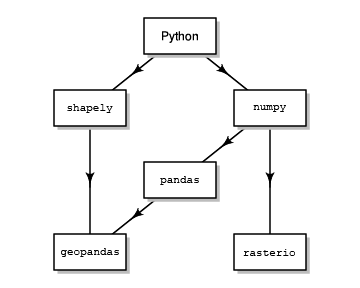
\includegraphics{images/dependencias_python.png}

}

\caption{\label{fig-python-package-deps}Principales dependencias entre
los paquetes de Python que vamos a estudiar. Adaptado de Dorman
(\citeproc{ref-dorman2025spatial}{2025}).}

\end{figure}%

\begin{itemize}
\tightlist
\item
  \textbf{\texttt{geopandas}}: Capa superior que integra a
  \texttt{pandas}, \texttt{shapely}, \texttt{fiona} y \texttt{pyproj}.
  Permite realizar consultas espaciales complejas y gestionar
  GeoDataFrames con una sintaxis simplificada.
\item
  \textbf{\texttt{rasterio}}: Basada en la librería \textbf{GDAL}, es el
  estándar para la lectura, escritura y manipulación de formatos ráster
  (como GeoTIFF), permitiendo gestionar metadatos y arreglos de píxeles
  con alta eficiencia.
\item
  \textbf{\texttt{scipy}}: Proporciona algoritmos avanzados de
  optimización, álgebra lineal y estadística necesarios para procesos de
  interpolación y análisis de superficies.
\item
  \textbf{\texttt{rasterstats}}: Herramienta específica para extraer
  estadísticas (medias, sumas) a partir de capas ráster basadas en
  geometrías vectoriales.
\item
  \textbf{\texttt{shapely}}: Motor geométrico basado en el estándar
  \emph{Simple Features} y puente hacia la librería \textbf{GEOS}. Se
  encarga de la lógica matemática de las geometrías (áreas,
  intersecciones, buffers y validación topográfica).
\item
  \textbf{\texttt{pyproj}}: Interfaz para la librería \textbf{PROJ}.
  Gestiona proyecciones cartográficas, sistemas de referencia (CRS) y
  transformaciones de datums.
\item
  \textbf{\texttt{fiona} / \texttt{pyogrio}}: Motores de acceso a datos
  vectoriales (SHP, GPKG) que actúan como interfaces hacia la librería
  \textbf{GDAL/OGR}.
\item
  \textbf{\texttt{xyzservices}}: Repositorio de metadatos para conectar
  con servicios de mapas base dinámicos (como OpenStreetMap).
\end{itemize}

La siguiente tabla vincula las librerías de Python con los motores de
cálculo de bajo nivel (C/C++) integrados en el contenedor Docker:

\begin{longtable}[]{@{}
  >{\raggedright\arraybackslash}p{(\columnwidth - 4\tabcolsep) * \real{0.1268}}
  >{\raggedright\arraybackslash}p{(\columnwidth - 4\tabcolsep) * \real{0.2676}}
  >{\raggedright\arraybackslash}p{(\columnwidth - 4\tabcolsep) * \real{0.6056}}@{}}
\toprule\noalign{}
\begin{minipage}[b]{\linewidth}\raggedright
Librería Python
\end{minipage} & \begin{minipage}[b]{\linewidth}\raggedright
Motor de Sistema (C/C++)
\end{minipage} & \begin{minipage}[b]{\linewidth}\raggedright
Función Principal en Geomática
\end{minipage} \\
\midrule\noalign{}
\endhead
\bottomrule\noalign{}
\endlastfoot
\textbf{\texttt{pyproj}} & \textbf{PROJ} & Gestión de Proyecciones y
Sistemas de Referencia (CRS). \\
\textbf{\texttt{shapely}} & \textbf{GEOS} & Álgebra topológica
(Intersecciones, Buffers, Áreas). \\
\textbf{\texttt{fiona} / \texttt{pyogrio}} & \textbf{GDAL/OGR} & Lectura
y escritura de formatos vectoriales. \\
\textbf{\texttt{rasterio}} & \textbf{GDAL} & Manejo de datos ráster y
metadatos de imágenes. \\
\textbf{\texttt{geopandas}} & \emph{(Integra los 3 motores)} & Gestión
integral de GeoDataFrames espaciales. \\
\end{longtable}

\section{Versiones instaladas del
software}\label{versiones-instaladas-del-software}

Para verificar las versiones inSstaladas, puede ejecutar
\texttt{pip3\ list} en la terminal. Las versiones instaladas deben
coincidir con la siguiente tabla:

\begin{longtable}[]{@{}
  >{\raggedright\arraybackslash}p{(\columnwidth - 8\tabcolsep) * \real{0.1053}}
  >{\raggedright\arraybackslash}p{(\columnwidth - 8\tabcolsep) * \real{0.1579}}
  >{\raggedright\arraybackslash}p{(\columnwidth - 8\tabcolsep) * \real{0.1053}}
  >{\raggedright\arraybackslash}p{(\columnwidth - 8\tabcolsep) * \real{0.2632}}
  >{\raggedright\arraybackslash}p{(\columnwidth - 8\tabcolsep) * \real{0.3684}}@{}}
\toprule\noalign{}
\begin{minipage}[b]{\linewidth}\raggedright
Software
\end{minipage} & \begin{minipage}[b]{\linewidth}\raggedright
Tipo
\end{minipage} & \begin{minipage}[b]{\linewidth}\raggedright
Versión
\end{minipage} & \begin{minipage}[b]{\linewidth}\raggedright
Comando (desde terminal)
\end{minipage} & \begin{minipage}[b]{\linewidth}\raggedright
Comando (desde Python)
\end{minipage} \\
\midrule\noalign{}
\endhead
\bottomrule\noalign{}
\endlastfoot
\texttt{Python} & Lenguaje & 3.12.3 & \texttt{python3\ -\/-version} &
\texttt{import\ sys;\ sys.version} \\
\texttt{pip} & Gestor de paquetes & 24.0 & \texttt{pip3\ -\/-version} &
\texttt{import\ pip;\ pip.\_\_version\_\_} \\
\texttt{numpy} & Paquete & 2.4.1 & \texttt{pip3\ show\ numpy} &
\texttt{import\ numpy;\ numpy.\_\_version\_\_} \\
\texttt{pandas} & Paquete & 2.3.3 & \texttt{pip3\ show\ pandas} &
\texttt{import\ pandas;\ pandas.\_\_version\_\_} \\
\texttt{geopandas} & Paquete & 1.1.2 & \texttt{pip3\ show\ geopandas} &
\texttt{import\ geopandas;\ geopandas.\_\_version\_\_} \\
\texttt{shapely} & Paquete & 2.1.2 & \texttt{pip3\ show\ shapely} &
\texttt{import\ shapely;\ shapely.\_\_version\_\_} \\
\texttt{pyproj} & Paquete & 3.7.2 & \texttt{pip3\ show\ pyproj} &
\texttt{import\ pyproj;\ pyproj.\_\_version\_\_} \\
\texttt{fiona} & Paquete & 1.10.1 & \texttt{pip3\ show\ fiona} &
\texttt{import\ fiona;\ fiona.\_\_version\_\_} \\
\texttt{rasterio} & Paquete & 1.5.0 & \texttt{pip3\ show\ rasterio} &
\texttt{import\ rasterio;\ rasterio.\_\_version\_\_} \\
\end{longtable}

\section{Librerías adicionales}\label{libreruxedas-adicionales}

\begin{itemize}
\tightlist
\item
  colorama (instalado)
\item
  geedim
\item
  xrspatial
\item
  netcdf4
\item
  toolz
\end{itemize}

\chapter{Adicionales Sobre R}\label{sec-anexo_r}

\section{Stack de R}\label{stack-de-r}

Para el análisis geoespacial en \texttt{R} (instalado dentro de los
contenedores), utilizaremos un ecosistema robusto basado en el estándar
\emph{Simple Features} y motores de alto rendimiento para datos ráster
(rejilla - cuadrículas).

\begin{longtable}[]{@{}
  >{\centering\arraybackslash}p{(\columnwidth - 4\tabcolsep) * \real{0.1818}}
  >{\centering\arraybackslash}p{(\columnwidth - 4\tabcolsep) * \real{0.3030}}
  >{\centering\arraybackslash}p{(\columnwidth - 4\tabcolsep) * \real{0.5152}}@{}}
\caption{Paquetes principales del stack espacial en
R}\label{tbl-r-packages}\tabularnewline
\toprule\noalign{}
\begin{minipage}[b]{\linewidth}\centering
Paquete
\end{minipage} & \begin{minipage}[b]{\linewidth}\centering
Funcionalidad
\end{minipage} & \begin{minipage}[b]{\linewidth}\centering
Sitio web
\end{minipage} \\
\midrule\noalign{}
\endfirsthead
\toprule\noalign{}
\begin{minipage}[b]{\linewidth}\centering
Paquete
\end{minipage} & \begin{minipage}[b]{\linewidth}\centering
Funcionalidad
\end{minipage} & \begin{minipage}[b]{\linewidth}\centering
Sitio web
\end{minipage} \\
\midrule\noalign{}
\endhead
\bottomrule\noalign{}
\endlastfoot
\texttt{sf} & Geometrías vectoriales (Simple Features) &
\url{https://r-spatial.github.io/sf/} \\
\texttt{terra} & Análisis de datos espaciales (Ráster/Vector) &
\url{https://rspatial.github.io/terra/} \\
\texttt{stars} & Arreglos ordenados espacio-temporales (DataCubes) &
\url{https://r-spatial.github.io/stars/} \\
\texttt{tidyverse} & Metapaquete para ciencia de datos &
\url{https://www.tidyverse.org/} \\
\texttt{tidyterra} & Métodos de tidyverse para terra &
\url{https://dieghernan.github.io/tidyterra/} \\
\end{longtable}

\begin{itemize}
\tightlist
\item
  \textbf{\texttt{sf} (Simple Features)}: Es el estándar moderno para el
  manejo de datos vectoriales. Representa las geometrías como una
  columna especial en un \emph{data frame}, permitiendo aplicar toda la
  potencia de manipulación de tablas a objetos espaciales.
\item
  \textbf{\texttt{terra}}: Motor de alta eficiencia que reemplaza al
  antiguo paquete \texttt{raster}. Está optimizado para el manejo de
  grandes volúmenes de datos mediante objetos \texttt{SpatRaster} y
  \texttt{SpatVector}, permitiendo operaciones de álgebra de mapas y
  análisis local de manera veloz.
\item
  \textbf{\texttt{stars} (Spatiotemporal Arrays)}: Especializada en el
  manejo de ``cubos de datos'' (rejillas con dimensiones de espacio,
  tiempo y múltiples atributos). Es la herramienta ideal para procesar
  series temporales de imágenes satelitales o modelos climáticos
  multidimensionales.
\item
  \textbf{\texttt{tidyterra}}: Extiende la gramática de \texttt{ggplot2}
  y \texttt{tidyverse} hacia los objetos de \texttt{terra}. Permite
  visualizar mapas ráster de forma elegante y realizar tuberías
  (\texttt{pipes}) de datos manteniendo la integridad espacial.
\end{itemize}

\section{Versiones instaladas del
software}\label{versiones-instaladas-del-software-1}

Versiones que deben quedar instaladas en el sistema R:

\begin{longtable}[]{@{}
  >{\raggedright\arraybackslash}p{(\columnwidth - 8\tabcolsep) * \real{0.0870}}
  >{\raggedright\arraybackslash}p{(\columnwidth - 8\tabcolsep) * \real{0.0870}}
  >{\raggedright\arraybackslash}p{(\columnwidth - 8\tabcolsep) * \real{0.0870}}
  >{\raggedright\arraybackslash}p{(\columnwidth - 8\tabcolsep) * \real{0.3043}}
  >{\raggedright\arraybackslash}p{(\columnwidth - 8\tabcolsep) * \real{0.4348}}@{}}
\toprule\noalign{}
\begin{minipage}[b]{\linewidth}\raggedright
Software
\end{minipage} & \begin{minipage}[b]{\linewidth}\raggedright
Tipo
\end{minipage} & \begin{minipage}[b]{\linewidth}\raggedright
Versión
\end{minipage} & \begin{minipage}[b]{\linewidth}\raggedright
Comando (desde terminal)
\end{minipage} & \begin{minipage}[b]{\linewidth}\raggedright
Comando (desde R)
\end{minipage} \\
\midrule\noalign{}
\endhead
\bottomrule\noalign{}
\endlastfoot
\texttt{R} & Lenguaje & 4.5.2 & \texttt{R\ -\/-version} &
\texttt{R.version.string} \\
\texttt{GEOS} & Librería sistema & 3.12.1 &
\texttt{geos-config\ -\/-version} &
\texttt{sf::sf\_extSoftVersion(){[}"GEOS"{]}} \\
\texttt{GDAL} & Librería sistema & 3.8.4 &
\texttt{gdalinfo\ -\/-version} &
\texttt{sf::sf\_extSoftVersion(){[}"GDAL"{]}} \\
\texttt{PROJ} & Librería sistema & 9.4.0 & (no aplica / no disponible) &
\texttt{sf::sf\_extSoftVersion(){[}"PROJ"{]}} \\
\texttt{sf} & Paquete & 1.0.23 &
\texttt{R\ -q\ -e\ "packageVersion(\textquotesingle{}sf\textquotesingle{})"}
& \texttt{packageVersion("sf")} \\
\texttt{terra} & Paquete & 1.8.86 &
\texttt{R\ -q\ -e\ "packageVersion(\textquotesingle{}terra\textquotesingle{})"}
& \texttt{packageVersion("terra")} \\
\texttt{stars} & Paquete & 0.7.0 &
\texttt{R\ -q\ -e\ "packageVersion(\textquotesingle{}stars\textquotesingle{})"}
& \texttt{packageVersion("stars")} \\
\end{longtable}

\section{\texorpdfstring{Visualización interactiva con
\texttt{httpgd}}{Visualización interactiva con httpgd}}\label{sec-httpgd-config}

Dado que nuestro entorno Docker es ``headless'' (sin monitor propio),
utilizamos \textbf{\texttt{httpgd}} como un servidor gráfico intermedio.
Este paquete captura las señales de dibujo de R y las sirve a través de
una URL que VSCode puede renderizar.

\subsection{Inicio del servidor
gráfico}\label{inicio-del-servidor-gruxe1fico}

Cada vez que inicie una nueva sesión de R, debe despertar al servidor
manualmente:

\begin{Shaded}
\begin{Highlighting}[]
\CommentTok{\# Inicia el motor gráfico}
\NormalTok{httpgd}\SpecialCharTok{::}\FunctionTok{hgd}\NormalTok{()}

\CommentTok{\# Verifica el estado y el puerto asignado}
\NormalTok{httpgd}\SpecialCharTok{::}\FunctionTok{hgd\_details}\NormalTok{()}
\end{Highlighting}
\end{Shaded}

\subsection{Resolución de conflictos (el ``fix'' del
puerto)}\label{resoluciuxf3n-de-conflictos-el-fix-del-puerto}

En nuestro contenedor, el puerto estándar para gráficos está mapeado al
\textbf{8787}. Si al ejecutar \texttt{hgd\_details()} nota que el
sistema asignó un puerto aleatorio o si el visor aparece en blanco,
fuerce la conexión con la siguiente ``receta'':

\begin{Shaded}
\begin{Highlighting}[]
\CommentTok{\# Forzar host y puerto para compatibilidad con Docker}
\NormalTok{httpgd}\SpecialCharTok{::}\FunctionTok{hgd}\NormalTok{(}\AttributeTok{host =} \StringTok{"0.0.0.0"}\NormalTok{, }\AttributeTok{port =} \DecValTok{8787}\NormalTok{, }\AttributeTok{token =} \ConstantTok{FALSE}\NormalTok{)}
\end{Highlighting}
\end{Shaded}

\subsection{Formas de ver sus
gráficos}\label{formas-de-ver-sus-gruxe1ficos}

Una vez el servidor está corriendo, tiene dos caminos para visualizar
sus mapas:

\begin{longtable}[]{@{}
  >{\raggedright\arraybackslash}p{(\columnwidth - 4\tabcolsep) * \real{0.3333}}
  >{\raggedright\arraybackslash}p{(\columnwidth - 4\tabcolsep) * \real{0.3333}}
  >{\raggedright\arraybackslash}p{(\columnwidth - 4\tabcolsep) * \real{0.3333}}@{}}
\toprule\noalign{}
\begin{minipage}[b]{\linewidth}\raggedright
Método
\end{minipage} & \begin{minipage}[b]{\linewidth}\raggedright
Comando / Acción
\end{minipage} & \begin{minipage}[b]{\linewidth}\raggedright
Ventaja
\end{minipage} \\
\midrule\noalign{}
\endhead
\bottomrule\noalign{}
\endlastfoot
\textbf{Visor Interno} & \texttt{Ctrl\ +\ Shift\ +\ P} -\textgreater{}
\textbf{Open httpgd viewer} & Mantiene todo dentro de una pestaña de
VSCode. \\
\textbf{Navegador Externo} & \texttt{httpgd::hgd\_browse()} & Ideal si
trabaja con dos monitores para ver mapas en pantalla completa. \\
\end{longtable}

\begin{tcolorbox}[enhanced jigsaw, coltitle=black, leftrule=.75mm, bottomtitle=1mm, title=\textcolor{quarto-callout-note-color}{\faInfo}\hspace{0.5em}{¿Por qué \texttt{token\ =\ FALSE}?}, colback=white, colbacktitle=quarto-callout-note-color!10!white, left=2mm, toptitle=1mm, rightrule=.15mm, titlerule=0mm, arc=.35mm, colframe=quarto-callout-note-color-frame, bottomrule=.15mm, toprule=.15mm, opacityback=0, opacitybacktitle=0.6, breakable]

Dentro del entorno seguro del contenedor, desactivamos el \emph{token}
para facilitar la conexión inmediata entre el servidor de R y el visor
de VSCode sin que el firewall interno bloquee la petición por falta de
credenciales.

\end{tcolorbox}

\subsection{Verificación de salud}\label{verificaciuxf3n-de-salud}

Si después de iniciar el servidor intenta graficar algo (ej:
\texttt{plot(1:10)}) y no ve nada, ejecute
\texttt{httpgd::hgd\_details()}. Asegúrese de que: 1. \textbf{URL}:
Apunte a \texttt{http://0.0.0.0:8787}. 2. \textbf{Status}: Indique que
está escuchando (\emph{listening}).

\subsection{El Entorno interactivo (REPL) y motores
gráficos}\label{sec-repl-concept}

En el desarrollo científico, el \textbf{REPL} (\emph{Read-Eval-Print
Loop}) es la consola interactiva que permite la ``programación
exploratoria''. Es el ciclo donde el sistema \textbf{lee} su
instrucción, la \textbf{evalúa} mediante el motor correspondiente,
\textbf{imprime} el resultado y queda en un \textbf{bucle} a la espera
del siguiente comando.

En nuestro laboratorio políglota, la identidad visual del REPL es su
brújula para saber en qué lenguaje está operando:

\begin{longtable}[]{@{}
  >{\raggedright\arraybackslash}p{(\columnwidth - 4\tabcolsep) * \real{0.3333}}
  >{\raggedright\arraybackslash}p{(\columnwidth - 4\tabcolsep) * \real{0.3333}}
  >{\raggedright\arraybackslash}p{(\columnwidth - 4\tabcolsep) * \real{0.3333}}@{}}
\toprule\noalign{}
\begin{minipage}[b]{\linewidth}\raggedright
Lenguaje
\end{minipage} & \begin{minipage}[b]{\linewidth}\raggedright
¿Cómo se ve el REPL?
\end{minipage} & \begin{minipage}[b]{\linewidth}\raggedright
Características en este curso
\end{minipage} \\
\midrule\noalign{}
\endhead
\bottomrule\noalign{}
\endlastfoot
\textbf{R} & \texttt{\textgreater{}} & Consola estándar para procesos
geoespaciales con \texttt{sf} o \texttt{terra}. \\
\textbf{Julia} & \texttt{julia\textgreater{}} & Entorno de alto
rendimiento con modos de ayuda (\texttt{?}) y terminal (\texttt{;}). \\
\textbf{Python} & \texttt{\textgreater{}\textgreater{}\textgreater{}} &
Consola básica; se recomienda el uso de \textbf{IPython} para
interactividad. \\
\end{longtable}

La experiencia interactiva y el soporte gráfico dentro de
\textbf{VSCode} dependen de la combinación entre el motor de ejecución y
el dispositivo gráfico configurado en el contenedor:

\begin{longtable}[]{@{}
  >{\raggedright\arraybackslash}p{(\columnwidth - 8\tabcolsep) * \real{0.1905}}
  >{\raggedright\arraybackslash}p{(\columnwidth - 8\tabcolsep) * \real{0.1905}}
  >{\raggedright\arraybackslash}p{(\columnwidth - 8\tabcolsep) * \real{0.1905}}
  >{\raggedright\arraybackslash}p{(\columnwidth - 8\tabcolsep) * \real{0.1905}}
  >{\centering\arraybackslash}p{(\columnwidth - 8\tabcolsep) * \real{0.2381}}@{}}
\toprule\noalign{}
\begin{minipage}[b]{\linewidth}\raggedright
Lenguaje
\end{minipage} & \begin{minipage}[b]{\linewidth}\raggedright
Acceso / Contexto
\end{minipage} & \begin{minipage}[b]{\linewidth}\raggedright
Motor de Ejecución
\end{minipage} & \begin{minipage}[b]{\linewidth}\raggedright
Dispositivo Gráfico
\end{minipage} & \begin{minipage}[b]{\linewidth}\centering
Soporte Inline
\end{minipage} \\
\midrule\noalign{}
\endhead
\bottomrule\noalign{}
\endlastfoot
\textbf{R} & Nativo (Estático) & R Extension & VSCode Plots (Pane) &
✅ \\
\textbf{R} & Nativo (Interactivo) & R Extension & \textbf{httpgd} &
✅ \\
\textbf{Julia} & Nativo (REPL) & VSCodeServer & VSCode Plots (Pane) &
✅ \\
\textbf{Julia} & Interop (R-Bridge) & \texttt{JuliaConnectoR} &
\textbf{httpgd} (vía R) & ✅ \\
\textbf{Python} & Interop (R-Bridge) & \texttt{reticulate} & R Device
(\textbf{httpgd}) & ❌ / ⚠️ \\
\textbf{Python} & Nativo (Jupyter) & Jupyter kernel & Jupyter Viewer &
✅ \\
\end{longtable}

\subsection{\texorpdfstring{El rol crítico de \texttt{httpgd} en
R}{El rol crítico de httpgd en R}}\label{el-rol-cruxedtico-de-httpgd-en-r}

Para R, no basta con tener la extensión instalada. El paquete
\textbf{\texttt{httpgd}} actúa como un servidor web interno que captura
los gráficos generados en el contenedor y los ``proyecta'' en VSCode.

\begin{itemize}
\tightlist
\item
  \textbf{¿Por qué lo usamos?} Los dispositivos gráficos tradicionales
  (como \texttt{X11} o \texttt{windows()}) no funcionan dentro de un
  contenedor Docker (\emph{headless}). \texttt{httpgd} soluciona esto
  convirtiendo cada mapa en un elemento interactivo SVG/HTML
  renderizable.
\item
  \textbf{Activación}: Siempre debe iniciar su sesión de R ejecutando
  \texttt{httpgd::hgd()} para abrir este canal de comunicación.
\end{itemize}

\begin{center}\rule{0.5\linewidth}{0.5pt}\end{center}

\section{Paquetes para comunicación con Julia y
Python}\label{sec-interoperabilidad}

Para que este ecosistema funcione, R actúa como el ``director de
orquesta'' utilizando un motor de ejecución y una serie de puentes que
permiten la comunicación fluida de datos entre lenguajes.

\begin{longtable}[]{@{}
  >{\raggedright\arraybackslash}p{(\columnwidth - 6\tabcolsep) * \real{0.2353}}
  >{\raggedright\arraybackslash}p{(\columnwidth - 6\tabcolsep) * \real{0.2353}}
  >{\raggedright\arraybackslash}p{(\columnwidth - 6\tabcolsep) * \real{0.2353}}
  >{\centering\arraybackslash}p{(\columnwidth - 6\tabcolsep) * \real{0.2941}}@{}}
\toprule\noalign{}
\begin{minipage}[b]{\linewidth}\raggedright
Lenguaje / Función
\end{minipage} & \begin{minipage}[b]{\linewidth}\raggedright
Paquete en R
\end{minipage} & \begin{minipage}[b]{\linewidth}\raggedright
Motor / Propósito
\end{minipage} & \begin{minipage}[b]{\linewidth}\centering
Estado
\end{minipage} \\
\midrule\noalign{}
\endhead
\bottomrule\noalign{}
\endlastfoot
\textbf{Renderizado} & \textbf{\texttt{knitr}} & Motor maestro que
orquesta la ejecución de celdas en el documento & ✅ \\
\textbf{Julia} & \texttt{JuliaConnectoR} & Comunicación funcional
estable con el kernel de Julia & ✅ \\
\textbf{Python} & \texttt{reticulate} & Interoperabilidad de objetos y
ejecución de Python & ✅ \\
\textbf{LSP (Soporte)} & \texttt{languageserver} & Autocompletado,
IntelliSense y ayuda en tiempo real & ✅ \\
\end{longtable}

\subsection{\texorpdfstring{El rol de
\texttt{knitr}}{El rol de knitr}}\label{el-rol-de-knitr}

Mientras que los paquetes actúan como puentes técnicos,
\textbf{\texttt{knitr}} es el encargado de leer el archivo
\texttt{.qmd}, enviar las instrucciones a los motores respectivos y
capturar los resultados (tablas, mapas, gráficos) para integrarlos en el
documento final. Sin \texttt{knitr}, la integración políglota de Quarto
no sería posible.

\subsection{\texorpdfstring{Transición técnica: De \texttt{JuliaCall} a
\texttt{JuliaConnectoR}}{Transición técnica: De JuliaCall a JuliaConnectoR}}\label{transiciuxf3n-tuxe9cnica-de-juliacall-a-juliaconnector}

En el diseño de este entorno, se tomó la decisión técnica de descartar
el paquete \texttt{JuliaCall} en favor de
\textbf{\texttt{JuliaConnectoR}}:

\begin{enumerate}
\def\labelenumi{\arabic{enumi}.}
\tightlist
\item
  \textbf{El Problema}: \texttt{JuliaCall} presentaba inestabilidades al
  gestionar dependencias dinámicas compartidas (como \texttt{libcurl} o
  \texttt{libstdc++}) dentro del contenedor, causando cierres
  inesperados (\emph{crashes}) de la sesión de R.
\item
  \textbf{La Sustitución}: Se seleccionó
  \textbf{\texttt{JuliaConnectoR}} por su arquitectura más limpia, que
  no interfiere con el entorno de Julia ya configurado en el sistema
  operativo.
\item
  \textbf{La Solución}: La integración se resolvió mediante una
  ``inyección'' de código en el archivo \texttt{Rprofile.site},
  configurando automáticamente la ruta del ejecutable en
  \texttt{\$Sys.BINDIR\$} y definiendo las funciones maestras
  \textbf{\texttt{j\_eval()}} y \textbf{\texttt{j\_plot()}}.
\end{enumerate}

\begin{tcolorbox}[enhanced jigsaw, coltitle=black, leftrule=.75mm, bottomtitle=1mm, title=\textcolor{quarto-callout-tip-color}{\faLightbulb}\hspace{0.5em}{🧠 Regla de Oro del Curso}, colback=white, colbacktitle=quarto-callout-tip-color!10!white, left=2mm, toptitle=1mm, rightrule=.15mm, titlerule=0mm, arc=.35mm, colframe=quarto-callout-tip-color-frame, bottomrule=.15mm, toprule=.15mm, opacityback=0, opacitybacktitle=0.6, breakable]

\begin{enumerate}
\def\labelenumi{\arabic{enumi}.}
\tightlist
\item
  \textbf{Julia y R}: Se operan de manera totalmente
  \textbf{interactiva} en VSCode (envío de líneas con
  \texttt{Ctrl+Enter}).
\item
  \textbf{Python vía reticulate}: Se utiliza primordialmente para el
  \textbf{renderizado (vía knitr)} de informes finales. Para una
  programación interactiva pura en Python, se recomienda el uso de los
  \textbf{Jupyter kernels}.
\end{enumerate}

\end{tcolorbox}

\section{Paquetes faltantes}\label{paquetes-faltantes}

\begin{itemize}
\tightlist
\item
  tidyterra (no instalado)
\item
  pak (no instalado)
\item
  rgee (no instalado)
\item
  xlsx
\item
  ncmeta
\item
  Hmisc
\item
  cubelyr
\item
  geojsonio
\item
  cowplot
\end{itemize}

\chapter{Adicionales Sobre Julia}\label{sec-anexo_julia}

\section{Stack de Julia}\label{stack-de-julia}

Julia ofrece un rendimiento de nivel C++ con sintaxis simplificada. A
continuación las principales librerías instaladas en los contenedores
para el geoprocesamiento.

\begin{longtable}[]{@{}
  >{\centering\arraybackslash}p{(\columnwidth - 4\tabcolsep) * \real{0.2308}}
  >{\centering\arraybackslash}p{(\columnwidth - 4\tabcolsep) * \real{0.3077}}
  >{\centering\arraybackslash}p{(\columnwidth - 4\tabcolsep) * \real{0.4615}}@{}}
\caption{Paquetes principales del stack en
Julia}\label{tbl-julia-packages}\tabularnewline
\toprule\noalign{}
\begin{minipage}[b]{\linewidth}\centering
Paquete
\end{minipage} & \begin{minipage}[b]{\linewidth}\centering
Funcionalidad
\end{minipage} & \begin{minipage}[b]{\linewidth}\centering
Sitio web
\end{minipage} \\
\midrule\noalign{}
\endfirsthead
\toprule\noalign{}
\begin{minipage}[b]{\linewidth}\centering
Paquete
\end{minipage} & \begin{minipage}[b]{\linewidth}\centering
Funcionalidad
\end{minipage} & \begin{minipage}[b]{\linewidth}\centering
Sitio web
\end{minipage} \\
\midrule\noalign{}
\endhead
\bottomrule\noalign{}
\endlastfoot
\texttt{LibPQ.jl} & Controlador PostgreSQL/PostGIS &
\url{https://juliadatabases.org/LibPQ.jl/dev/} \\
\texttt{ArchGDAL.jl} & Interfaz de alto nivel para GDAL &
\url{https://yeesian.com/ArchGDAL.jl/} \\
\texttt{LibGEOS.jl} & Interfaz del motor geométrico (GEOS) &
\url{https://github.com/JuliaGeo/LibGEOS.jl} \\
\texttt{Plots.jl} & Visualización y generación de gráficos &
\url{https://docs.juliaplots.org/} \\
\texttt{DataFrames.jl} & Manipulación de datos en memoria &
\url{https://dataframes.juliadata.org/} \\
\end{longtable}

\begin{itemize}
\tightlist
\item
  \textbf{\texttt{LibPQ.jl}}: Conector de bajo nivel para
  \textbf{PostgreSQL}. Es la herramienta que permitirá a los estudiantes
  realizar ingesta y consulta de datos desde el servidor PostGIS.
\item
  \textbf{\texttt{ArchGDAL.jl}}: Proporciona una abstracción de alto
  nivel para el motor GDAL. Es excelente para transformar formatos y
  manejar proyecciones.
\item
  \textbf{\texttt{LibGEOS.jl}}: La interfaz directa al motor de
  geometrías (GEOS). Se utiliza para operaciones topológicas puras como
  validación de polígonos, intersecciones y cálculos de buffers.
\item
  \textbf{\texttt{DataFrames.jl}}: El estándar para el manejo de datos
  tabulares en Julia, permitiendo integrar los resultados de las
  consultas espaciales en estructuras fáciles de analizar.
\end{itemize}

\section{Versiones instaladas del
software}\label{versiones-instaladas-del-software-2}

Versiones de paquetes \texttt{Julia} en el sistema:

\begin{longtable}[]{@{}
  >{\raggedright\arraybackslash}p{(\columnwidth - 8\tabcolsep) * \real{0.1000}}
  >{\raggedright\arraybackslash}p{(\columnwidth - 8\tabcolsep) * \real{0.1000}}
  >{\raggedright\arraybackslash}p{(\columnwidth - 8\tabcolsep) * \real{0.1000}}
  >{\raggedright\arraybackslash}p{(\columnwidth - 8\tabcolsep) * \real{0.4000}}
  >{\raggedright\arraybackslash}p{(\columnwidth - 8\tabcolsep) * \real{0.3000}}@{}}
\toprule\noalign{}
\begin{minipage}[b]{\linewidth}\raggedright
Software
\end{minipage} & \begin{minipage}[b]{\linewidth}\raggedright
Tipo
\end{minipage} & \begin{minipage}[b]{\linewidth}\raggedright
Versión
\end{minipage} & \begin{minipage}[b]{\linewidth}\raggedright
Comando (desde terminal)
\end{minipage} & \begin{minipage}[b]{\linewidth}\raggedright
Comando (desde Julia)
\end{minipage} \\
\midrule\noalign{}
\endhead
\bottomrule\noalign{}
\endlastfoot
\texttt{Julia} & Lenguaje & 1.10.4 & \texttt{julia\ -\/-version} &
\texttt{VERSION} \\
\texttt{LibPQ} & Paquete & 1.18.0 &
\texttt{julia\ -e\ "using\ LibPQ;\ println(pkgversion(LibPQ))"} &
\texttt{using\ LibPQ;\ pkgversion(LibPQ)} \\
\texttt{ArchGDAL} & Paquete & 0.10.11 &
\texttt{julia\ -e\ "using\ ArchGDAL;\ println(pkgversion(ArchGDAL))"} &
\texttt{using\ ArchGDAL;\ pkgversion(ArchGDAL)} \\
\texttt{LibGEOS} & Paquete & 0.9.7 &
\texttt{julia\ -e\ "using\ LibGEOS;\ println(pkgversion(LibGEOS))"} &
\texttt{using\ LibGEOS;\ pkgversion(LibGEOS)} \\
\texttt{Plots} & Paquete & 1.41.4 &
\texttt{julia\ -e\ "using\ Plots;\ println(pkgversion(Plots))"} &
\texttt{using\ Plots;\ pkgversion(Plots)} \\
\texttt{DataFrames} & Paquete & 1.8.1 &
\texttt{julia\ -e\ "using\ DataFrames;\ println(pkgversion(DataFrames))"}
& \texttt{using\ DataFrames;\ pkgversion(DataFrames)} \\
\end{longtable}

\section{🩺 Guía Corta: Instalación de Paquetes Julia + Cirugía
OpenSSL}\label{guuxeda-corta-instalaciuxf3n-de-paquetes-julia-ciruguxeda-openssl}

Cuando necesite instalar un paquete (por ejemplo,
\texttt{GeoInterfaceRecipes}), abra la terminal de su contenedor (el
prompt que se ve como \texttt{root@contenedor:/\#}) y ejecute estos 3
pasos en un solo comando combinado:

\begin{Shaded}
\begin{Highlighting}[]
\CommentTok{\# 1. Instalar el paquete (si arroja error rojo de precompilación, ignórelo, es normal)}
\ExtensionTok{julia} \AttributeTok{{-}e} \StringTok{\textquotesingle{}using Pkg; Pkg.add("GeoInterfaceRecipes")\textquotesingle{}}

\CommentTok{\# 2. Aplicar la cirugía inmediata a los nuevos artefactos que llegaron}
\FunctionTok{find}\NormalTok{ /root/.julia/artifacts }\AttributeTok{{-}name} \StringTok{"libssl.so*"} \AttributeTok{{-}exec}\NormalTok{ ln }\AttributeTok{{-}sf}\NormalTok{ /usr/lib/x86\_64{-}linux{-}gnu/libssl.so.3 \{\} }\DataTypeTok{\textbackslash{};}
\FunctionTok{find}\NormalTok{ /root/.julia/artifacts }\AttributeTok{{-}name} \StringTok{"libcrypto.so*"} \AttributeTok{{-}exec}\NormalTok{ ln }\AttributeTok{{-}sf}\NormalTok{ /usr/lib/x86\_64{-}linux{-}gnu/libcrypto.so.3 \{\} }\DataTypeTok{\textbackslash{};}

\CommentTok{\# 3. Sanar y compilar todo con el OpenSSL del sistema}
\ExtensionTok{julia} \AttributeTok{{-}e} \StringTok{\textquotesingle{}using Pkg; Pkg.precompile()\textquotesingle{}}
\end{Highlighting}
\end{Shaded}

\section{Sincronizar versiones de paquetes en Julia (no tuvo efectos -
no
funcionó)}\label{sincronizar-versiones-de-paquetes-en-julia-no-tuvo-efectos---no-funcionuxf3}

De forma dirigida solo para esos tres, para minimizar riesgos

\begin{Shaded}
\begin{Highlighting}[]
\CommentTok{\# En la terminal de Linux}
\ExtensionTok{julia} \AttributeTok{{-}e} \StringTok{\textquotesingle{}using Pkg; Pkg.add(["GeoJSON", "GeoInterfaceRecipes", "Plots"])\textquotesingle{}}

\CommentTok{\# Aplicar cirugía solo a lo nuevo}
\FunctionTok{find}\NormalTok{ /root/.julia/artifacts }\AttributeTok{{-}name} \StringTok{"libssl.so*"} \AttributeTok{{-}exec}\NormalTok{ ln }\AttributeTok{{-}sf}\NormalTok{ /usr/lib/x86\_64{-}linux{-}gnu/libssl.so.3 \{\} }\DataTypeTok{\textbackslash{};}
\FunctionTok{find}\NormalTok{ /root/.julia/artifacts }\AttributeTok{{-}name} \StringTok{"libcrypto.so*"} \AttributeTok{{-}exec}\NormalTok{ ln }\AttributeTok{{-}sf}\NormalTok{ /usr/lib/x86\_64{-}linux{-}gnu/libcrypto.so.3 \{\} }\DataTypeTok{\textbackslash{};}

\CommentTok{\# Precompilar}
\ExtensionTok{julia} \AttributeTok{{-}e} \StringTok{\textquotesingle{}using Pkg; Pkg.precompile()\textquotesingle{}}
\end{Highlighting}
\end{Shaded}

\section{Librerías adicionales}\label{libreruxedas-adicionales-1}

\begin{itemize}
\tightlist
\item
  GeoInterfaceRecipes (instalada)
\item
  Crayons (instalada)
\item
  Leaflet (mejor no instalarla - poco mantenimiento -
  incompatibilidades)
\item
  YAXArrays.jl (instalada)
\item
  Zarr.jl (instalada)
\item
  RasterDataSources.jl (instalada)
\item
  Meshes.jl (instalaa)
\item
  Tyler.jl (instalada)
\item
  GLMakie.jl (instalada)
\item
  ColorSchemes.jl (instalada)
\item
  Colors.jl (instalada)
\item
  AlgebraOfGraphics.jl (instalada)
\item
  GeoMakie.jl (instalada)
\item
  StatsPlots
\item
  Measures
\item
  PyCall
\item
  ZipFile
\item
  GeoData
\item
  SpatialDependence
\item
  NearestNeighbors
\item
  LibSpatialIndex
\end{itemize}

\chapter{Adicionales Sobre QGIS}\label{sec-anexo_qgis}

\section{Instalación}\label{instalaciuxf3n-1}

\subsection{OSGeo4w}\label{sec-instalacion_osgeo4w}

\subsection{QGIS con PIXI}\label{sec-instalacion_qgis_pixi}

\chapter{Adicionales sobre ArcGIS Pro}\label{sec-anexo_arcgispro}

\section{Instalación}\label{instalaciuxf3n-2}

\subsection{Actualizar}\label{actualizar}

\subsection{Actualizar\ldots{}}\label{actualizar-1}

\chapter{Adicionales sobre ArcGIS Pro}\label{sec-anexo_postgresql}

\section{Instalación}\label{instalaciuxf3n-3}

\subsection{}\label{section}

\subsection{}\label{section-1}

\chapter{Errata}\label{errata-2}

Esta es la errata

\chapter*{Referencias
Bibliográficas}\label{referencias-bibliogruxe1ficas}
\addcontentsline{toc}{chapter}{Referencias Bibliográficas}

\markboth{Referencias Bibliográficas}{Referencias Bibliográficas}

\phantomsection\label{refs}
\begin{CSLReferences}{1}{0}
\bibitem[\citeproctext]{ref-bezanson2017julia}
Bezanson, J., Edelman, A., Karpinski, S., \& Shah, V. B. (2017). Julia:
A fresh approach to numerical computing. \emph{SIAM review},
\emph{59}(1), 65-98.

\bibitem[\citeproctext]{ref-dorman2025spatial}
Dorman, M. (2025). \emph{Spatial Data Programming with Python}.
Ben-Gurion University of the Negev. \url{https://geobgu.xyz/py-2025/}

\bibitem[\citeproctext]{ref-hersbach2020era5}
Hersbach, H., Bell, B., Berrisford, P., Hirahara, S., Horányi, A.,
Muñoz-Sabater, J., Nicolas, J., Peubey, C., Radu, R., Schepers, D.,
et~al. (2020). The ERA5 global reanalysis. \emph{Quarterly journal of
the royal meteorological society}, \emph{146}(730), 1999-2049.

\bibitem[\citeproctext]{ref-docker2025}
Inc., D. (2025). \emph{Docker Desktop Documentation}.
\url{https://docs.docker.com}

\bibitem[\citeproctext]{ref-law2019getting}
Law, M., \& Collins, A. (2019). Getting to know ArcGIS PRO. \emph{(No
Title)}.

\bibitem[\citeproctext]{ref-lawhead2017qgis}
Lawhead, J. (2017). \emph{QGIS python programming cookbook}. Packt
Publishing Ltd.

\bibitem[\citeproctext]{ref-mcfeeters1996use}
McFeeters, S. K. (1996). The use of the Normalized Difference Water
Index (NDWI) in the delineation of open water features.
\emph{International journal of remote sensing}, \emph{17}(7), 1425-1432.

\bibitem[\citeproctext]{ref-vscode2026}
Microsoft Corporation. (2026). \emph{Visual Studio Code}.
\url{https://code.visualstudio.com/}

\bibitem[\citeproctext]{ref-mitchell2015introduction}
Mitchell, T. (2015). \emph{An Introduction to Open Source Geospatial
Tools}.

\bibitem[\citeproctext]{ref-neteler2012grass}
Neteler, M., Bowman, M. H., Landa, M., \& Metz, M. (2012). GRASS GIS: A
multi-purpose open source GIS. \emph{Environmental Modelling \&
Software}, \emph{31}, 124-130.

\bibitem[\citeproctext]{ref-passy2018use}
Passy, P., \& Théry, S. (2018). The use of SAGA GIS modules in QGIS.
\emph{QGIS and generic tools}, \emph{1}, 107-149.

\bibitem[\citeproctext]{ref-sds}
Pebesma, E., \& Bivand, R. (2023). \emph{Spatial Data Science: With
Applications in {R}}. Chapman; Hall/CRC.
\url{https://doi.org/10.1201/9780429459016}

\bibitem[\citeproctext]{ref-sdsrp}
Pebesma, E., \& Bivand, R. (2025). \emph{Spatial Data Science: With
Applications in {R} and {Python}}. \url{https://r-spatial.org/python/}

\bibitem[\citeproctext]{ref-pebesma2025spatial}
Pebesma, E., Fleischmann, M., Parry, J., Nowosad, J., Graser, A.,
Dunnington, D., Pronk, M., Schouten, R., Lovelace, R., Appel, M., et~al.
(2025). Spatial data science languages: commonalities and needs.
\emph{arXiv preprint arXiv:2503.16686}.

\bibitem[\citeproctext]{ref-python_docs}
Python Software Foundation. (2025). \emph{Python 3 Documentation}.
\url{https://docs.python.org/3/}

\bibitem[\citeproctext]{ref-python2021python}
Python, W. (2021). Python. \emph{Python releases for windows},
\emph{24}.
\url{http://static.softwaresuggest.com.s3.amazonaws.com/ssguides/1604480172_Python_read\%20(1).pdf}

\bibitem[\citeproctext]{ref-rlanguage}
R Core Team. (2025). \emph{R: A Language and Environment for Statistical
Computing}. R Foundation for Statistical Computing.
\url{https://www.R-project.org/}

\bibitem[\citeproctext]{ref-rodriguez2020spatio}
Rodríguez Avellaneda, A. H. (2020). \emph{Spatio-temporal analysis of
extreme wind velocities for infrastructure design}
{[}Master\textquotesingle s Thesis, Erasmus Mundus Master of Science in
Geospatial Technologies (Universitat Jaume I, University of M{ü}nster,
NOVA Information Management School){]}.
\url{https://geocorp.co/thesis/mastergeotech/index.html}

\bibitem[\citeproctext]{ref-rosas2022qgis}
Rosas-Chavoya, M., Gallardo-Salazar, J. L., López-Serrano, P. M.,
Alcántara-Concepción, P. C., \& León-Miranda, A. K. (2022). QGIS a
constantly growing free and open-source geospatial software contributing
to scientific development. \emph{Cuadernos de Investigaci{ó}n
Geogr{á}fica}, \emph{48}(1), 197-213.

\bibitem[\citeproctext]{ref-toms2015arcpy}
Toms, S. (2015). \emph{ArcPy and ArcGIS--geospatial analysis with
Python}. Packt Publishing Ltd.

\bibitem[\citeproctext]{ref-wijayaningrum2022jupyter}
Wijayaningrum, V. N., Lestari, V. A., et~al. (2022). Jupyter lab
platform-based interactive learning. \emph{2022 International Conference
on Electrical and Information Technology (IEIT)}, 295-301.

\bibitem[\citeproctext]{ref-wu2023pyqgis}
Wu, Q. (2023a). PyQGIS cookbook in markdown and Jupyter notebook
formats. En \emph{GitHub repository}.
\url{https://github.com/opengeos/pyqgis-cookbook}; GitHub.

\bibitem[\citeproctext]{ref-wu2023qgisnotebook}
Wu, Q. (2023b). QGIS Notebook Plugin: Integrate Jupyter Notebooks into
QGIS. En \emph{GitHub repository} {[}Software{]}.
\url{https://github.com/opengeos/qgis-notebook-plugin}; GitHub.

\bibitem[\citeproctext]{ref-xie2019tinytex}
Xie, Y. (2019). TinyTeX: A lightweight, cross-platform, and
easy-to-maintain LaTeX distribution based on TeX Live. \emph{TUGboat},
\emph{40}(1), 30-32.

\end{CSLReferences}


\backmatter

\end{document}
